\documentclass[twoside]{book}

% Packages required by doxygen
\usepackage{calc}
\usepackage{doxygen}
\usepackage{graphicx}
\usepackage[utf8]{inputenc}
\usepackage{makeidx}
\usepackage{multicol}
\usepackage{multirow}
\usepackage{fixltx2e}
\PassOptionsToPackage{warn}{textcomp}
\usepackage{textcomp}
\usepackage[nointegrals]{wasysym}
\usepackage[table]{xcolor}

% Font selection
\usepackage[T1]{fontenc}
\usepackage{mathptmx}
\usepackage[scaled=.90]{helvet}
\usepackage{courier}
\usepackage{amssymb}
\usepackage{sectsty}
\renewcommand{\familydefault}{\sfdefault}
\allsectionsfont{%
  \fontseries{bc}\selectfont%
  \color{darkgray}%
}
\renewcommand{\DoxyLabelFont}{%
  \fontseries{bc}\selectfont%
  \color{darkgray}%
}
\newcommand{\+}{\discretionary{\mbox{\scriptsize$\hookleftarrow$}}{}{}}

% Page & text layout
\usepackage{geometry}
\geometry{%
  a4paper,%
  top=2.5cm,%
  bottom=2.5cm,%
  left=2.5cm,%
  right=2.5cm%
}
\tolerance=750
\hfuzz=15pt
\hbadness=750
\setlength{\emergencystretch}{15pt}
\setlength{\parindent}{0cm}
\setlength{\parskip}{0.2cm}
\makeatletter
\renewcommand{\paragraph}{%
  \@startsection{paragraph}{4}{0ex}{-1.0ex}{1.0ex}{%
    \normalfont\normalsize\bfseries\SS@parafont%
  }%
}
\renewcommand{\subparagraph}{%
  \@startsection{subparagraph}{5}{0ex}{-1.0ex}{1.0ex}{%
    \normalfont\normalsize\bfseries\SS@subparafont%
  }%
}
\makeatother

% Headers & footers
\usepackage{fancyhdr}
\pagestyle{fancyplain}
\fancyhead[LE]{\fancyplain{}{\bfseries\thepage}}
\fancyhead[CE]{\fancyplain{}{}}
\fancyhead[RE]{\fancyplain{}{\bfseries\leftmark}}
\fancyhead[LO]{\fancyplain{}{\bfseries\rightmark}}
\fancyhead[CO]{\fancyplain{}{}}
\fancyhead[RO]{\fancyplain{}{\bfseries\thepage}}
\fancyfoot[LE]{\fancyplain{}{}}
\fancyfoot[CE]{\fancyplain{}{}}
\fancyfoot[RE]{\fancyplain{}{\bfseries\scriptsize Generated on Wed Dec 3 2014 14\+:56\+:40 for M3\+Sym by Doxygen }}
\fancyfoot[LO]{\fancyplain{}{\bfseries\scriptsize Generated on Wed Dec 3 2014 14\+:56\+:40 for M3\+Sym by Doxygen }}
\fancyfoot[CO]{\fancyplain{}{}}
\fancyfoot[RO]{\fancyplain{}{}}
\renewcommand{\footrulewidth}{0.4pt}
\renewcommand{\chaptermark}[1]{%
  \markboth{#1}{}%
}
\renewcommand{\sectionmark}[1]{%
  \markright{\thesection\ #1}%
}

% Indices & bibliography
\usepackage{natbib}
\usepackage[titles]{tocloft}
\setcounter{tocdepth}{3}
\setcounter{secnumdepth}{5}
\makeindex

% Hyperlinks (required, but should be loaded last)
\usepackage{ifpdf}
\ifpdf
  \usepackage[pdftex,pagebackref=true]{hyperref}
\else
  \usepackage[ps2pdf,pagebackref=true]{hyperref}
\fi
\hypersetup{%
  colorlinks=true,%
  linkcolor=blue,%
  citecolor=blue,%
  unicode%
}

% Custom commands
\newcommand{\clearemptydoublepage}{%
  \newpage{\pagestyle{empty}\cleardoublepage}%
}


%===== C O N T E N T S =====

\begin{document}

% Titlepage & ToC
\hypersetup{pageanchor=false,
             bookmarks=true,
             bookmarksnumbered=true,
             pdfencoding=unicode
            }
\pagenumbering{roman}
\begin{titlepage}
\vspace*{7cm}
\begin{center}%
{\Large M3\+Sym \\[1ex]\large 0.\+05 }\\
\vspace*{1cm}
{\large Generated by Doxygen 1.8.7}\\
\vspace*{0.5cm}
{\small Wed Dec 3 2014 14:56:40}\\
\end{center}
\end{titlepage}
\clearemptydoublepage
\tableofcontents
\clearemptydoublepage
\pagenumbering{arabic}
\hypersetup{pageanchor=true}

%--- Begin generated contents ---
\chapter{M3\+S\+Y\+M software package}
\label{index}\hypertarget{index}{}\hypertarget{index_intro_sec}{}\section{Introduction}\label{index_intro_sec}
Cell motility plays a key role in human biology and disease, contributing ubiquitously to such important processes as embryonic development, wound repair and cancer metastasis. Papoian laboratory is interested in gaining deeper understanding of the physical chemistry behind these complex, far-\/from-\/equilibrium mechano-\/chemical processes. His approach and model, named Mechano-\/chemical Dynamics of Active Networks, 3rd Generation (M\+E\+D\+Y\+A\+N3), is based on combining stochastic reaction-\/diffusion treatment of cellular biochemical processes with polymer physics of cytoskeletal filament network growth, while explicitly coupling chemistry and mechanics.

Papoian laboratory has developed {\bfseries M3\+S\+Y\+M}, a software package based on the M\+E\+D\+Y\+A\+N3 model, to simulate growth dynamics of actin based filamentous networks {\itshape in vitro} and {\itshape in vivo}. Recent papers where {\bfseries M3\+S\+Y\+M} or its predecessor, {\bfseries Stoch\+Tools}, were used can be found on the publication section of \href{http://papoian.chem.umd.edu/}{\tt the Papoian group's main web page\+:}. The {\bfseries M3\+S\+Y\+M} package can also be extended to simulate the dynamics of any active matter network.\hypertarget{index_install_sec}{}\section{Installation}\label{index_install_sec}
\hypertarget{index_step1}{}\subsection{Step 1\+: Prerequisites}\label{index_step1}
The following software packages need to be installed first\+:


\begin{DoxyItemize}
\item Boost 1.\+49
\item G\+S\+L ...
\end{DoxyItemize}\hypertarget{index_step2}{}\subsection{Step 2\+: Installation of M3\+S\+Y\+M itself}\label{index_step2}
Untar the {\bfseries M3\+S\+Y\+M} source code into some directory, enter into the \char`\"{}\+M3\+S\+Y\+M\char`\"{} and execute \char`\"{}make\char`\"{} from the command line. 
\chapter{Namespace Index}
\section{Namespace List}
Here is a list of all namespaces with brief descriptions\+:\begin{DoxyCompactList}
\item\contentsline{section}{\hyperlink{namespaceA__B__C__Cycle}{A\+\_\+\+B\+\_\+\+C\+\_\+\+Cycle} }{\pageref{namespaceA__B__C__Cycle}}{}
\item\contentsline{section}{\hyperlink{namespaceA__reversible__B__numeric}{A\+\_\+reversible\+\_\+\+B\+\_\+numeric} }{\pageref{namespaceA__reversible__B__numeric}}{}
\item\contentsline{section}{\hyperlink{namespacemathfunc}{mathfunc} \\*Used for the mathematics module for the entire codebase mathfunc includes functions to calculate distances, products, and midpoints }{\pageref{namespacemathfunc}}{}
\end{DoxyCompactList}

\chapter{Hierarchical Index}
\section{Class Hierarchy}
This inheritance list is sorted roughly, but not completely, alphabetically\-:\begin{DoxyCompactList}
\item \contentsline{section}{Object}{\pageref{classObject}}{}
\begin{DoxyCompactList}
\item \contentsline{section}{Species}{\pageref{classSpecies}}{}
\begin{DoxyCompactList}
\item \contentsline{section}{S\-Bulk}{\pageref{classSBulk}}{}
\end{DoxyCompactList}
\end{DoxyCompactList}
\item \contentsline{section}{species\-\_\-type\-\_\-tag}{\pageref{structspecies__type__tag}}{}
\item \contentsline{section}{Species\-D\-B}{\pageref{classSpeciesDB}}{}
\item \contentsline{section}{Species\-Factory}{\pageref{classSpeciesFactory}}{}
\end{DoxyCompactList}

\chapter{Class Index}
\section{Class List}
Here are the classes, structs, unions and interfaces with brief descriptions\-:\begin{DoxyCompactList}
\item\contentsline{section}{\hyperlink{classObject}{Object} }{\pageref{classObject}}{}
\item\contentsline{section}{\hyperlink{classSBulk}{S\-Bulk} \\*This class represent Bulk species that have no spatial component, i.\-e. are not connected to any Compartmens }{\pageref{classSBulk}}{}
\item\contentsline{section}{\hyperlink{classSpecies}{Species} }{\pageref{classSpecies}}{}
\item\contentsline{section}{\hyperlink{structspecies__type__tag}{species\-\_\-type\-\_\-tag} \\*Create a tag for the corresponding Species\-Type flywheights }{\pageref{structspecies__type__tag}}{}
\item\contentsline{section}{\hyperlink{classSpeciesDB}{Species\-D\-B} \\*\hyperlink{classSpeciesDB}{Species\-D\-B} should be used for obtaining new objects of the \hyperlink{classSpecies}{Species} hieararchy }{\pageref{classSpeciesDB}}{}
\item\contentsline{section}{\hyperlink{classSpeciesFactory}{Species\-Factory} \\*This is the standard implentation of the \hyperlink{classSpecies}{Species} Factory Method, which can be further subclassed to either specialize or introduce other construction behaviors }{\pageref{classSpeciesFactory}}{}
\end{DoxyCompactList}

\chapter{File Index}
\section{File List}
Here is a list of all files with brief descriptions\-:\begin{DoxyCompactList}
\item\contentsline{section}{Cyto\-Sim/\hyperlink{ChemNRMImpl_8cpp}{Chem\-N\-R\-M\-Impl.\-cpp} }{\pageref{ChemNRMImpl_8cpp}}{}
\item\contentsline{section}{Cyto\-Sim/\hyperlink{ChemNRMImpl_8h}{Chem\-N\-R\-M\-Impl.\-h} }{\pageref{ChemNRMImpl_8h}}{}
\item\contentsline{section}{Cyto\-Sim/\hyperlink{ChemRNode_8h}{Chem\-R\-Node.\-h} }{\pageref{ChemRNode_8h}}{}
\item\contentsline{section}{Cyto\-Sim/\hyperlink{ChemSim_8cpp}{Chem\-Sim.\-cpp} }{\pageref{ChemSim_8cpp}}{}
\item\contentsline{section}{Cyto\-Sim/\hyperlink{ChemSim_8h}{Chem\-Sim.\-h} }{\pageref{ChemSim_8h}}{}
\item\contentsline{section}{Cyto\-Sim/\hyperlink{ChemSimImpl_8h}{Chem\-Sim\-Impl.\-h} }{\pageref{ChemSimImpl_8h}}{}
\item\contentsline{section}{Cyto\-Sim/\hyperlink{common_8cpp}{common.\-cpp} }{\pageref{common_8cpp}}{}
\item\contentsline{section}{Cyto\-Sim/\hyperlink{common_8h}{common.\-h} }{\pageref{common_8h}}{}
\item\contentsline{section}{Cyto\-Sim/\hyperlink{Compartment_8cpp}{Compartment.\-cpp} }{\pageref{Compartment_8cpp}}{}
\item\contentsline{section}{Cyto\-Sim/\hyperlink{Compartment_8h}{Compartment.\-h} }{\pageref{Compartment_8h}}{}
\item\contentsline{section}{Cyto\-Sim/\hyperlink{Component_8cpp}{Component.\-cpp} }{\pageref{Component_8cpp}}{}
\item\contentsline{section}{Cyto\-Sim/\hyperlink{Component_8h}{Component.\-h} }{\pageref{Component_8h}}{}
\item\contentsline{section}{Cyto\-Sim/\hyperlink{Composite_8cpp}{Composite.\-cpp} }{\pageref{Composite_8cpp}}{}
\item\contentsline{section}{Cyto\-Sim/\hyperlink{Composite_8h}{Composite.\-h} }{\pageref{Composite_8h}}{}
\item\contentsline{section}{Cyto\-Sim/\hyperlink{main_8cpp}{main.\-cpp} }{\pageref{main_8cpp}}{}
\item\contentsline{section}{Cyto\-Sim/\hyperlink{Reaction_8cpp}{Reaction.\-cpp} }{\pageref{Reaction_8cpp}}{}
\item\contentsline{section}{Cyto\-Sim/\hyperlink{Reaction_8h}{Reaction.\-h} }{\pageref{Reaction_8h}}{}
\item\contentsline{section}{Cyto\-Sim/\hyperlink{RSpecies_8cpp}{R\-Species.\-cpp} }{\pageref{RSpecies_8cpp}}{}
\item\contentsline{section}{Cyto\-Sim/\hyperlink{RSpecies_8h}{R\-Species.\-h} }{\pageref{RSpecies_8h}}{}
\item\contentsline{section}{Cyto\-Sim/\hyperlink{Species_8cpp}{Species.\-cpp} }{\pageref{Species_8cpp}}{}
\item\contentsline{section}{Cyto\-Sim/\hyperlink{Species_8h}{Species.\-h} \\*This header file will contain defininition of the Species hieararchy and associated D\-B and helper classes }{\pageref{Species_8h}}{}
\item\contentsline{section}{Cyto\-Sim/\hyperlink{System_8cpp}{System.\-cpp} }{\pageref{System_8cpp}}{}
\item\contentsline{section}{Cyto\-Sim/\hyperlink{System_8h}{System.\-h} }{\pageref{System_8h}}{}
\item\contentsline{section}{Cyto\-Sim/\hyperlink{utility_8h}{utility.\-h} }{\pageref{utility_8h}}{}
\item\contentsline{section}{Cyto\-Sim/\hyperlink{Visitor_8h}{Visitor.\-h} }{\pageref{Visitor_8h}}{}
\item\contentsline{section}{Cyto\-Sim/\hyperlink{VisitorConcrete_8h}{Visitor\-Concrete.\-h} }{\pageref{VisitorConcrete_8h}}{}
\end{DoxyCompactList}

\chapter{Namespace Documentation}
\hypertarget{namespaceA__B__C__Cycle}{\section{A\+\_\+\+B\+\_\+\+C\+\_\+\+Cycle Namespace Reference}
\label{namespaceA__B__C__Cycle}\index{A\+\_\+\+B\+\_\+\+C\+\_\+\+Cycle@{A\+\_\+\+B\+\_\+\+C\+\_\+\+Cycle}}
}
\subsection*{Functions}
\begin{DoxyCompactItemize}
\item 
def \hyperlink{namespaceA__B__C__Cycle_a5185de4b3f647f2c0fd827dc61787e74}{compute\+\_\+\+T}
\item 
def \hyperlink{namespaceA__B__C__Cycle_a59ce12842045f3ad4619feb145abdcf8}{propagate}
\end{DoxyCompactItemize}
\subsection*{Variables}
\begin{DoxyCompactItemize}
\item 
tuple \hyperlink{namespaceA__B__C__Cycle_a23b7c1024d319feae9e3a687526aeb94}{R}
\item 
float \hyperlink{namespaceA__B__C__Cycle_ab55624a349d5a1ba164d1dde7d24524d}{t} = 1.\+23
\item 
tuple \hyperlink{namespaceA__B__C__Cycle_af487b8de68dc3e23fe5f16f3580525a7}{T} = \hyperlink{namespaceA__B__C__Cycle_a5185de4b3f647f2c0fd827dc61787e74}{compute\+\_\+\+T}(\hyperlink{namespaceA__B__C__Cycle_a23b7c1024d319feae9e3a687526aeb94}{R},\hyperlink{namespaceA__B__C__Cycle_ab55624a349d5a1ba164d1dde7d24524d}{t})
\item 
tuple \hyperlink{namespaceA__B__C__Cycle_a11169d0a2c42df806b8825edefea9f4d}{alpha} = sqrt(3)
\item 
tuple \hyperlink{namespaceA__B__C__Cycle_a2e58583729f8a298b9a4fa611c0ac787}{A} = cos(\hyperlink{namespaceA__B__C__Cycle_a11169d0a2c42df806b8825edefea9f4d}{alpha}$\ast$\hyperlink{namespaceA__B__C__Cycle_ab55624a349d5a1ba164d1dde7d24524d}{t})
\item 
tuple \hyperlink{namespaceA__B__C__Cycle_a9771d340c90ea87ee784c884fe2de3dc}{B} = cos(\hyperlink{namespaceA__B__C__Cycle_a11169d0a2c42df806b8825edefea9f4d}{alpha}$\ast$\hyperlink{namespaceA__B__C__Cycle_ab55624a349d5a1ba164d1dde7d24524d}{t}-\/2$\ast$pi/3)
\item 
tuple \hyperlink{namespaceA__B__C__Cycle_a6b1467f9bbedb7a62110239efb9e068b}{C} = cos(\hyperlink{namespaceA__B__C__Cycle_a11169d0a2c42df806b8825edefea9f4d}{alpha}$\ast$\hyperlink{namespaceA__B__C__Cycle_ab55624a349d5a1ba164d1dde7d24524d}{t}-\/4$\ast$pi/3)
\item 
int \hyperlink{namespaceA__B__C__Cycle_ada302b2e3d775f1258d503301d1c2377}{xx1} = 1
\item 
int \hyperlink{namespaceA__B__C__Cycle_a9a299d8ac16b9cdc11b6643776732552}{xx2} = 2
\item 
\hyperlink{namespaceA__B__C__Cycle_a36440b61a4f8a38a160c7d71c35e0af3}{T\+\_\+analyt} = \hyperlink{namespaceA__B__C__Cycle_ada302b2e3d775f1258d503301d1c2377}{xx1}+\hyperlink{namespaceA__B__C__Cycle_a9a299d8ac16b9cdc11b6643776732552}{xx2}
\end{DoxyCompactItemize}


\subsection{Function Documentation}
\hypertarget{namespaceA__B__C__Cycle_a5185de4b3f647f2c0fd827dc61787e74}{\index{A\+\_\+\+B\+\_\+\+C\+\_\+\+Cycle@{A\+\_\+\+B\+\_\+\+C\+\_\+\+Cycle}!compute\+\_\+\+T@{compute\+\_\+\+T}}
\index{compute\+\_\+\+T@{compute\+\_\+\+T}!A\+\_\+\+B\+\_\+\+C\+\_\+\+Cycle@{A\+\_\+\+B\+\_\+\+C\+\_\+\+Cycle}}
\subsubsection[{compute\+\_\+\+T}]{\setlength{\rightskip}{0pt plus 5cm}def A\+\_\+\+B\+\_\+\+C\+\_\+\+Cycle.\+compute\+\_\+\+T (
\begin{DoxyParamCaption}
\item[{}]{R, }
\item[{}]{t}
\end{DoxyParamCaption}
)}}\label{namespaceA__B__C__Cycle_a5185de4b3f647f2c0fd827dc61787e74}


Definition at line 7 of file A\+\_\+\+B\+\_\+\+C\+\_\+\+Cycle.\+py.



Referenced by propagate().

\hypertarget{namespaceA__B__C__Cycle_a59ce12842045f3ad4619feb145abdcf8}{\index{A\+\_\+\+B\+\_\+\+C\+\_\+\+Cycle@{A\+\_\+\+B\+\_\+\+C\+\_\+\+Cycle}!propagate@{propagate}}
\index{propagate@{propagate}!A\+\_\+\+B\+\_\+\+C\+\_\+\+Cycle@{A\+\_\+\+B\+\_\+\+C\+\_\+\+Cycle}}
\subsubsection[{propagate}]{\setlength{\rightskip}{0pt plus 5cm}def A\+\_\+\+B\+\_\+\+C\+\_\+\+Cycle.\+propagate (
\begin{DoxyParamCaption}
\item[{}]{p0, }
\item[{}]{R, }
\item[{}]{t}
\end{DoxyParamCaption}
)}}\label{namespaceA__B__C__Cycle_a59ce12842045f3ad4619feb145abdcf8}


Definition at line 21 of file A\+\_\+\+B\+\_\+\+C\+\_\+\+Cycle.\+py.



References compute\+\_\+\+T().



\subsection{Variable Documentation}
\hypertarget{namespaceA__B__C__Cycle_a2e58583729f8a298b9a4fa611c0ac787}{\index{A\+\_\+\+B\+\_\+\+C\+\_\+\+Cycle@{A\+\_\+\+B\+\_\+\+C\+\_\+\+Cycle}!A@{A}}
\index{A@{A}!A\+\_\+\+B\+\_\+\+C\+\_\+\+Cycle@{A\+\_\+\+B\+\_\+\+C\+\_\+\+Cycle}}
\subsubsection[{A}]{\setlength{\rightskip}{0pt plus 5cm}tuple A\+\_\+\+B\+\_\+\+C\+\_\+\+Cycle.\+A = cos({\bf alpha}$\ast${\bf t})}}\label{namespaceA__B__C__Cycle_a2e58583729f8a298b9a4fa611c0ac787}


Definition at line 39 of file A\+\_\+\+B\+\_\+\+C\+\_\+\+Cycle.\+py.



Referenced by Filament\+Bending\+Harmonic.\+forces(), Filament\+Bending\+Harmonic.\+forces\+Aux(), Reaction$<$ M, N $>$.\+is\+\_\+equal(), and operator==().

\hypertarget{namespaceA__B__C__Cycle_a11169d0a2c42df806b8825edefea9f4d}{\index{A\+\_\+\+B\+\_\+\+C\+\_\+\+Cycle@{A\+\_\+\+B\+\_\+\+C\+\_\+\+Cycle}!alpha@{alpha}}
\index{alpha@{alpha}!A\+\_\+\+B\+\_\+\+C\+\_\+\+Cycle@{A\+\_\+\+B\+\_\+\+C\+\_\+\+Cycle}}
\subsubsection[{alpha}]{\setlength{\rightskip}{0pt plus 5cm}tuple A\+\_\+\+B\+\_\+\+C\+\_\+\+Cycle.\+alpha = sqrt(3)}}\label{namespaceA__B__C__Cycle_a11169d0a2c42df806b8825edefea9f4d}


Definition at line 38 of file A\+\_\+\+B\+\_\+\+C\+\_\+\+Cycle.\+py.

\hypertarget{namespaceA__B__C__Cycle_a9771d340c90ea87ee784c884fe2de3dc}{\index{A\+\_\+\+B\+\_\+\+C\+\_\+\+Cycle@{A\+\_\+\+B\+\_\+\+C\+\_\+\+Cycle}!B@{B}}
\index{B@{B}!A\+\_\+\+B\+\_\+\+C\+\_\+\+Cycle@{A\+\_\+\+B\+\_\+\+C\+\_\+\+Cycle}}
\subsubsection[{B}]{\setlength{\rightskip}{0pt plus 5cm}tuple A\+\_\+\+B\+\_\+\+C\+\_\+\+Cycle.\+B = cos({\bf alpha}$\ast${\bf t}-\/2$\ast$pi/3)}}\label{namespaceA__B__C__Cycle_a9771d340c90ea87ee784c884fe2de3dc}


Definition at line 40 of file A\+\_\+\+B\+\_\+\+C\+\_\+\+Cycle.\+py.



Referenced by Filament\+Bending\+Harmonic.\+forces(), Filament\+Bending\+Harmonic.\+forces\+Aux(), Reaction$<$ M, N $>$.\+is\+\_\+equal(), and operator==().

\hypertarget{namespaceA__B__C__Cycle_a6b1467f9bbedb7a62110239efb9e068b}{\index{A\+\_\+\+B\+\_\+\+C\+\_\+\+Cycle@{A\+\_\+\+B\+\_\+\+C\+\_\+\+Cycle}!C@{C}}
\index{C@{C}!A\+\_\+\+B\+\_\+\+C\+\_\+\+Cycle@{A\+\_\+\+B\+\_\+\+C\+\_\+\+Cycle}}
\subsubsection[{C}]{\setlength{\rightskip}{0pt plus 5cm}tuple A\+\_\+\+B\+\_\+\+C\+\_\+\+Cycle.\+C = cos({\bf alpha}$\ast${\bf t}-\/4$\ast$pi/3)}}\label{namespaceA__B__C__Cycle_a6b1467f9bbedb7a62110239efb9e068b}


Definition at line 41 of file A\+\_\+\+B\+\_\+\+C\+\_\+\+Cycle.\+py.



Referenced by G\+Controller.\+activate\+Compartments(), Compartment\+Grid.\+add\+Chem\+Sim\+Reactions(), Compartment.\+clone(), Filament\+Bending\+Harmonic.\+forces(), Filament\+Bending\+Harmonic.\+forces\+Aux(), Compartment.\+generate\+All\+Diffusion\+Reactions(), Simple\+Manager\+Impl.\+initialize(), and main().

\hypertarget{namespaceA__B__C__Cycle_a23b7c1024d319feae9e3a687526aeb94}{\index{A\+\_\+\+B\+\_\+\+C\+\_\+\+Cycle@{A\+\_\+\+B\+\_\+\+C\+\_\+\+Cycle}!R@{R}}
\index{R@{R}!A\+\_\+\+B\+\_\+\+C\+\_\+\+Cycle@{A\+\_\+\+B\+\_\+\+C\+\_\+\+Cycle}}
\subsubsection[{R}]{\setlength{\rightskip}{0pt plus 5cm}tuple A\+\_\+\+B\+\_\+\+C\+\_\+\+Cycle.\+R}}\label{namespaceA__B__C__Cycle_a23b7c1024d319feae9e3a687526aeb94}


Definition at line 31 of file A\+\_\+\+B\+\_\+\+C\+\_\+\+Cycle.\+py.



Referenced by Boundary\+Repulsion\+Exp.\+compute\+Energy(), Boundary\+Repulsion\+Exp.\+compute\+Forces(), Boundary\+Repulsion\+Exp.\+compute\+Forces\+Aux(), Compartment.\+generate\+Diffusion\+Reactions(), and Reaction\+Ptr\+Container\+Vector.\+remove\+Reaction().

\hypertarget{namespaceA__B__C__Cycle_ab55624a349d5a1ba164d1dde7d24524d}{\index{A\+\_\+\+B\+\_\+\+C\+\_\+\+Cycle@{A\+\_\+\+B\+\_\+\+C\+\_\+\+Cycle}!t@{t}}
\index{t@{t}!A\+\_\+\+B\+\_\+\+C\+\_\+\+Cycle@{A\+\_\+\+B\+\_\+\+C\+\_\+\+Cycle}}
\subsubsection[{t}]{\setlength{\rightskip}{0pt plus 5cm}float A\+\_\+\+B\+\_\+\+C\+\_\+\+Cycle.\+t = 1.\+23}}\label{namespaceA__B__C__Cycle_ab55624a349d5a1ba164d1dde7d24524d}


Definition at line 35 of file A\+\_\+\+B\+\_\+\+C\+\_\+\+Cycle.\+py.

\hypertarget{namespaceA__B__C__Cycle_af487b8de68dc3e23fe5f16f3580525a7}{\index{A\+\_\+\+B\+\_\+\+C\+\_\+\+Cycle@{A\+\_\+\+B\+\_\+\+C\+\_\+\+Cycle}!T@{T}}
\index{T@{T}!A\+\_\+\+B\+\_\+\+C\+\_\+\+Cycle@{A\+\_\+\+B\+\_\+\+C\+\_\+\+Cycle}}
\subsubsection[{T}]{\setlength{\rightskip}{0pt plus 5cm}tuple A\+\_\+\+B\+\_\+\+C\+\_\+\+Cycle.\+T = {\bf compute\+\_\+\+T}({\bf R},{\bf t})}}\label{namespaceA__B__C__Cycle_af487b8de68dc3e23fe5f16f3580525a7}


Definition at line 36 of file A\+\_\+\+B\+\_\+\+C\+\_\+\+Cycle.\+py.



Referenced by Species\+Ptr\+Container\+Vector.\+add\+Species(), is\+Same(), and make\+\_\+unique().

\hypertarget{namespaceA__B__C__Cycle_a36440b61a4f8a38a160c7d71c35e0af3}{\index{A\+\_\+\+B\+\_\+\+C\+\_\+\+Cycle@{A\+\_\+\+B\+\_\+\+C\+\_\+\+Cycle}!T\+\_\+analyt@{T\+\_\+analyt}}
\index{T\+\_\+analyt@{T\+\_\+analyt}!A\+\_\+\+B\+\_\+\+C\+\_\+\+Cycle@{A\+\_\+\+B\+\_\+\+C\+\_\+\+Cycle}}
\subsubsection[{T\+\_\+analyt}]{\setlength{\rightskip}{0pt plus 5cm}A\+\_\+\+B\+\_\+\+C\+\_\+\+Cycle.\+T\+\_\+analyt = {\bf xx1}+{\bf xx2}}}\label{namespaceA__B__C__Cycle_a36440b61a4f8a38a160c7d71c35e0af3}


Definition at line 49 of file A\+\_\+\+B\+\_\+\+C\+\_\+\+Cycle.\+py.

\hypertarget{namespaceA__B__C__Cycle_ada302b2e3d775f1258d503301d1c2377}{\index{A\+\_\+\+B\+\_\+\+C\+\_\+\+Cycle@{A\+\_\+\+B\+\_\+\+C\+\_\+\+Cycle}!xx1@{xx1}}
\index{xx1@{xx1}!A\+\_\+\+B\+\_\+\+C\+\_\+\+Cycle@{A\+\_\+\+B\+\_\+\+C\+\_\+\+Cycle}}
\subsubsection[{xx1}]{\setlength{\rightskip}{0pt plus 5cm}int A\+\_\+\+B\+\_\+\+C\+\_\+\+Cycle.\+xx1 = 1}}\label{namespaceA__B__C__Cycle_ada302b2e3d775f1258d503301d1c2377}


Definition at line 43 of file A\+\_\+\+B\+\_\+\+C\+\_\+\+Cycle.\+py.

\hypertarget{namespaceA__B__C__Cycle_a9a299d8ac16b9cdc11b6643776732552}{\index{A\+\_\+\+B\+\_\+\+C\+\_\+\+Cycle@{A\+\_\+\+B\+\_\+\+C\+\_\+\+Cycle}!xx2@{xx2}}
\index{xx2@{xx2}!A\+\_\+\+B\+\_\+\+C\+\_\+\+Cycle@{A\+\_\+\+B\+\_\+\+C\+\_\+\+Cycle}}
\subsubsection[{xx2}]{\setlength{\rightskip}{0pt plus 5cm}int A\+\_\+\+B\+\_\+\+C\+\_\+\+Cycle.\+xx2 = 2}}\label{namespaceA__B__C__Cycle_a9a299d8ac16b9cdc11b6643776732552}


Definition at line 46 of file A\+\_\+\+B\+\_\+\+C\+\_\+\+Cycle.\+py.


\hypertarget{namespaceA__reversible__B__numeric}{\section{A\+\_\+reversible\+\_\+\+B\+\_\+numeric Namespace Reference}
\label{namespaceA__reversible__B__numeric}\index{A\+\_\+reversible\+\_\+\+B\+\_\+numeric@{A\+\_\+reversible\+\_\+\+B\+\_\+numeric}}
}
\subsection*{Variables}
\begin{DoxyCompactItemize}
\item 
int \hyperlink{namespaceA__reversible__B__numeric_ac17162d2d7790ca7d605541ee4c919bb}{N} = 10
\item 
float \hyperlink{namespaceA__reversible__B__numeric_a63df2169b3cb7b9db0743a51320bbf4f}{t} = 0.\+48
\item 
float \hyperlink{namespaceA__reversible__B__numeric_a772b5e72a16864c6d0d2895bf2bb5ada}{kf} = 2.\+5
\item 
float \hyperlink{namespaceA__reversible__B__numeric_a2f4e77a45b10e727874ecd0a83be77fd}{kb} = 2.\+5
\item 
tuple \hyperlink{namespaceA__reversible__B__numeric_a7095a52e98b19868ca09b3ea24726258}{R} = zeros(\mbox{[}\hyperlink{namespaceA__reversible__B__numeric_ac17162d2d7790ca7d605541ee4c919bb}{N}+1,\hyperlink{namespaceA__reversible__B__numeric_ac17162d2d7790ca7d605541ee4c919bb}{N}+1\mbox{]})
\item 
tuple \hyperlink{namespaceA__reversible__B__numeric_ab14192a58d248288a57a53a88e824aa1}{O\+N\+E\+S} = ones(\hyperlink{namespaceA__reversible__B__numeric_ac17162d2d7790ca7d605541ee4c919bb}{N}+1)
\item 
tuple \hyperlink{namespaceA__reversible__B__numeric_a238e2ae63555f68c3395add1edad1692}{T} = linalg.\+expm2(\hyperlink{namespaceA__reversible__B__numeric_a7095a52e98b19868ca09b3ea24726258}{R}$\ast$\hyperlink{namespaceA__reversible__B__numeric_a63df2169b3cb7b9db0743a51320bbf4f}{t})
\item 
tuple \hyperlink{namespaceA__reversible__B__numeric_ad5efb9fc14774d8a02dccd90d7978214}{p0} = zeros(\hyperlink{namespaceA__reversible__B__numeric_ac17162d2d7790ca7d605541ee4c919bb}{N}+1)
\item 
tuple \hyperlink{namespaceA__reversible__B__numeric_aae033c0920890d37257bb86daf8996f8}{pt} = dot(\hyperlink{namespaceA__reversible__B__numeric_a238e2ae63555f68c3395add1edad1692}{T},\hyperlink{namespaceA__reversible__B__numeric_ad5efb9fc14774d8a02dccd90d7978214}{p0})
\item 
tuple \hyperlink{namespaceA__reversible__B__numeric_a2f98730f45b559f9aece65c8682734bf}{p\+\_\+analyt} = array(\mbox{[}0.\+002327151517,0.\+1940040583e-\/1, 0.\+7277956968e-\/1, .\+1617947293, .\+2360416130, .\+2361326132, .\+1640442006, 0.\+781464013e-\/1, 0.\+244301648e-\/1, 0.\+4525850e-\/2, 0.\+377291e-\/3\mbox{]})
\end{DoxyCompactItemize}


\subsection{Variable Documentation}
\hypertarget{namespaceA__reversible__B__numeric_a2f4e77a45b10e727874ecd0a83be77fd}{\index{A\+\_\+reversible\+\_\+\+B\+\_\+numeric@{A\+\_\+reversible\+\_\+\+B\+\_\+numeric}!kb@{kb}}
\index{kb@{kb}!A\+\_\+reversible\+\_\+\+B\+\_\+numeric@{A\+\_\+reversible\+\_\+\+B\+\_\+numeric}}
\subsubsection[{kb}]{\setlength{\rightskip}{0pt plus 5cm}float A\+\_\+reversible\+\_\+\+B\+\_\+numeric.\+kb = 2.\+5}}\label{namespaceA__reversible__B__numeric_a2f4e77a45b10e727874ecd0a83be77fd}


Definition at line 22 of file A\+\_\+reversible\+\_\+\+B\+\_\+numeric.\+py.

\hypertarget{namespaceA__reversible__B__numeric_a772b5e72a16864c6d0d2895bf2bb5ada}{\index{A\+\_\+reversible\+\_\+\+B\+\_\+numeric@{A\+\_\+reversible\+\_\+\+B\+\_\+numeric}!kf@{kf}}
\index{kf@{kf}!A\+\_\+reversible\+\_\+\+B\+\_\+numeric@{A\+\_\+reversible\+\_\+\+B\+\_\+numeric}}
\subsubsection[{kf}]{\setlength{\rightskip}{0pt plus 5cm}float A\+\_\+reversible\+\_\+\+B\+\_\+numeric.\+kf = 2.\+5}}\label{namespaceA__reversible__B__numeric_a772b5e72a16864c6d0d2895bf2bb5ada}


Definition at line 21 of file A\+\_\+reversible\+\_\+\+B\+\_\+numeric.\+py.

\hypertarget{namespaceA__reversible__B__numeric_ac17162d2d7790ca7d605541ee4c919bb}{\index{A\+\_\+reversible\+\_\+\+B\+\_\+numeric@{A\+\_\+reversible\+\_\+\+B\+\_\+numeric}!N@{N}}
\index{N@{N}!A\+\_\+reversible\+\_\+\+B\+\_\+numeric@{A\+\_\+reversible\+\_\+\+B\+\_\+numeric}}
\subsubsection[{N}]{\setlength{\rightskip}{0pt plus 5cm}int A\+\_\+reversible\+\_\+\+B\+\_\+numeric.\+N = 10}}\label{namespaceA__reversible__B__numeric_ac17162d2d7790ca7d605541ee4c919bb}


Definition at line 19 of file A\+\_\+reversible\+\_\+\+B\+\_\+numeric.\+py.



Referenced by Compartment\+Grid.\+add\+Bulk(), Compartment\+Grid.\+add\+Bulk\+Reaction(), Compartment.\+add\+Internal(), Compartment.\+add\+Internal\+Reaction(), Reaction$<$ M, N $>$.\+get\+N\+Impl(), Reaction$<$ M, N $>$.\+get\+Product\+Of\+Products\+Impl(), Reaction$<$ M, N $>$.\+initialize\+Species(), Reaction$<$ M, N $>$.\+make\+Step\+Impl(), Reaction$<$ M, N $>$.\+print\+To\+Stream(), and Reaction$<$ M, N $>$.\+size\+Impl().

\hypertarget{namespaceA__reversible__B__numeric_ab14192a58d248288a57a53a88e824aa1}{\index{A\+\_\+reversible\+\_\+\+B\+\_\+numeric@{A\+\_\+reversible\+\_\+\+B\+\_\+numeric}!O\+N\+E\+S@{O\+N\+E\+S}}
\index{O\+N\+E\+S@{O\+N\+E\+S}!A\+\_\+reversible\+\_\+\+B\+\_\+numeric@{A\+\_\+reversible\+\_\+\+B\+\_\+numeric}}
\subsubsection[{O\+N\+E\+S}]{\setlength{\rightskip}{0pt plus 5cm}tuple A\+\_\+reversible\+\_\+\+B\+\_\+numeric.\+O\+N\+E\+S = ones({\bf N}+1)}}\label{namespaceA__reversible__B__numeric_ab14192a58d248288a57a53a88e824aa1}


Definition at line 44 of file A\+\_\+reversible\+\_\+\+B\+\_\+numeric.\+py.

\hypertarget{namespaceA__reversible__B__numeric_ad5efb9fc14774d8a02dccd90d7978214}{\index{A\+\_\+reversible\+\_\+\+B\+\_\+numeric@{A\+\_\+reversible\+\_\+\+B\+\_\+numeric}!p0@{p0}}
\index{p0@{p0}!A\+\_\+reversible\+\_\+\+B\+\_\+numeric@{A\+\_\+reversible\+\_\+\+B\+\_\+numeric}}
\subsubsection[{p0}]{\setlength{\rightskip}{0pt plus 5cm}tuple A\+\_\+reversible\+\_\+\+B\+\_\+numeric.\+p0 = zeros({\bf N}+1)}}\label{namespaceA__reversible__B__numeric_ad5efb9fc14774d8a02dccd90d7978214}


Definition at line 61 of file A\+\_\+reversible\+\_\+\+B\+\_\+numeric.\+py.

\hypertarget{namespaceA__reversible__B__numeric_a2f98730f45b559f9aece65c8682734bf}{\index{A\+\_\+reversible\+\_\+\+B\+\_\+numeric@{A\+\_\+reversible\+\_\+\+B\+\_\+numeric}!p\+\_\+analyt@{p\+\_\+analyt}}
\index{p\+\_\+analyt@{p\+\_\+analyt}!A\+\_\+reversible\+\_\+\+B\+\_\+numeric@{A\+\_\+reversible\+\_\+\+B\+\_\+numeric}}
\subsubsection[{p\+\_\+analyt}]{\setlength{\rightskip}{0pt plus 5cm}tuple A\+\_\+reversible\+\_\+\+B\+\_\+numeric.\+p\+\_\+analyt = array(\mbox{[}0.\+002327151517,0.\+1940040583e-\/1, 0.\+7277956968e-\/1, .\+1617947293, .\+2360416130, .\+2361326132, .\+1640442006, 0.\+781464013e-\/1, 0.\+244301648e-\/1, 0.\+4525850e-\/2, 0.\+377291e-\/3\mbox{]})}}\label{namespaceA__reversible__B__numeric_a2f98730f45b559f9aece65c8682734bf}


Definition at line 80 of file A\+\_\+reversible\+\_\+\+B\+\_\+numeric.\+py.

\hypertarget{namespaceA__reversible__B__numeric_aae033c0920890d37257bb86daf8996f8}{\index{A\+\_\+reversible\+\_\+\+B\+\_\+numeric@{A\+\_\+reversible\+\_\+\+B\+\_\+numeric}!pt@{pt}}
\index{pt@{pt}!A\+\_\+reversible\+\_\+\+B\+\_\+numeric@{A\+\_\+reversible\+\_\+\+B\+\_\+numeric}}
\subsubsection[{pt}]{\setlength{\rightskip}{0pt plus 5cm}tuple A\+\_\+reversible\+\_\+\+B\+\_\+numeric.\+pt = dot({\bf T},{\bf p0})}}\label{namespaceA__reversible__B__numeric_aae033c0920890d37257bb86daf8996f8}


Definition at line 67 of file A\+\_\+reversible\+\_\+\+B\+\_\+numeric.\+py.

\hypertarget{namespaceA__reversible__B__numeric_a7095a52e98b19868ca09b3ea24726258}{\index{A\+\_\+reversible\+\_\+\+B\+\_\+numeric@{A\+\_\+reversible\+\_\+\+B\+\_\+numeric}!R@{R}}
\index{R@{R}!A\+\_\+reversible\+\_\+\+B\+\_\+numeric@{A\+\_\+reversible\+\_\+\+B\+\_\+numeric}}
\subsubsection[{R}]{\setlength{\rightskip}{0pt plus 5cm}tuple A\+\_\+reversible\+\_\+\+B\+\_\+numeric.\+R = zeros(\mbox{[}{\bf N}+1,{\bf N}+1\mbox{]})}}\label{namespaceA__reversible__B__numeric_a7095a52e98b19868ca09b3ea24726258}


Definition at line 26 of file A\+\_\+reversible\+\_\+\+B\+\_\+numeric.\+py.

\hypertarget{namespaceA__reversible__B__numeric_a63df2169b3cb7b9db0743a51320bbf4f}{\index{A\+\_\+reversible\+\_\+\+B\+\_\+numeric@{A\+\_\+reversible\+\_\+\+B\+\_\+numeric}!t@{t}}
\index{t@{t}!A\+\_\+reversible\+\_\+\+B\+\_\+numeric@{A\+\_\+reversible\+\_\+\+B\+\_\+numeric}}
\subsubsection[{t}]{\setlength{\rightskip}{0pt plus 5cm}float A\+\_\+reversible\+\_\+\+B\+\_\+numeric.\+t = 0.\+48}}\label{namespaceA__reversible__B__numeric_a63df2169b3cb7b9db0743a51320bbf4f}


Definition at line 20 of file A\+\_\+reversible\+\_\+\+B\+\_\+numeric.\+py.

\hypertarget{namespaceA__reversible__B__numeric_a238e2ae63555f68c3395add1edad1692}{\index{A\+\_\+reversible\+\_\+\+B\+\_\+numeric@{A\+\_\+reversible\+\_\+\+B\+\_\+numeric}!T@{T}}
\index{T@{T}!A\+\_\+reversible\+\_\+\+B\+\_\+numeric@{A\+\_\+reversible\+\_\+\+B\+\_\+numeric}}
\subsubsection[{T}]{\setlength{\rightskip}{0pt plus 5cm}tuple A\+\_\+reversible\+\_\+\+B\+\_\+numeric.\+T = linalg.\+expm2({\bf R}$\ast${\bf t})}}\label{namespaceA__reversible__B__numeric_a238e2ae63555f68c3395add1edad1692}


Definition at line 53 of file A\+\_\+reversible\+\_\+\+B\+\_\+numeric.\+py.


\hypertarget{namespacemathfunc}{\section{mathfunc Namespace Reference}
\label{namespacemathfunc}\index{mathfunc@{mathfunc}}
}


is used for the mathematics module for the entire codebase mathfunc includes functions to calculate distances, products, and midpoints  


\subsection*{Functions}
\begin{DoxyCompactItemize}
\item 
double \hyperlink{namespacemathfunc_a4f2e296612642f3ac1b4789f85b02c41}{Two\+Segment\+Distance} (const vector$<$ double $>$ \&v1, const vector$<$ double $>$ \&v2, const vector$<$ double $>$ \&v3, const vector$<$ double $>$ \&v4)
\begin{DoxyCompactList}\small\item\em Function to calculate a diatance between two segments. \end{DoxyCompactList}\item 
double \hyperlink{namespacemathfunc_a43b9be958a97530eba2073e9816881eb}{Two\+Point\+Distance} (const vector$<$ double $>$ \&v1, const vector$<$ double $>$ \&v2)
\begin{DoxyCompactList}\small\item\em Compute distance between two points with coordinates\+: (x1,y1,z1) and (x2,y2,z3);. \end{DoxyCompactList}\item 
double \hyperlink{namespacemathfunc_a79cd843c8fc2ad6513a091c86744e9f4}{Two\+Point\+Distance\+Stretched} (const vector$<$ double $>$ \&v1, const vector$<$ double $>$ \&p1, const vector$<$ double $>$ \&v2, const vector$<$ double $>$ \&p2, double d)
\begin{DoxyCompactList}\small\item\em Compute distance between two points with coordinates (x1 -\/d$\ast$p1x,y1-\/d$\ast$p1y,z1-\/d$\ast$p1z) and (x2-\/d$\ast$p2x,y2-\/d$\ast$p2y,z2-\/d$\ast$p2z) \end{DoxyCompactList}\item 
vector$<$ double $>$ \hyperlink{namespacemathfunc_aa45b754771ac16d546864a1a7fb9bf59}{Two\+Point\+Direction} (const vector$<$ double $>$ \&v1, const vector$<$ double $>$ \&v2)
\begin{DoxyCompactList}\small\item\em Calculates a normal to a line starting at (x1,y1,z1) and ending at (x2,y2,z2);. \end{DoxyCompactList}\item 
double \hyperlink{namespacemathfunc_a003be58c2f6df9098c88b2ae33d5b5d4}{Scalar\+Product} (const vector$<$ double $>$ \&v1, const vector$<$ double $>$ \&v2, const vector$<$ double $>$ \&v3, const vector$<$ double $>$ \&v4)
\begin{DoxyCompactList}\small\item\em Scalar product of two vectors with coordinates\+: (x2-\/x1,y2-\/y1,z2-\/z1) and (x4-\/x3,y4-\/y3,z4-\/z3) \end{DoxyCompactList}\item 
double \hyperlink{namespacemathfunc_a3dffb1288c676c7809d4a6caae9601bb}{Scalar\+Product\+Stretched} (const vector$<$ double $>$ \&v1, const vector$<$ double $>$ \&p1, const vector$<$ double $>$ \&v2, const vector$<$ double $>$ \&p2, const vector$<$ double $>$ \&v3, const vector$<$ double $>$ \&p3, const vector$<$ double $>$ \&v4, const vector$<$ double $>$ \&p4, double d)
\begin{DoxyCompactList}\small\item\em Scalar product of two vectors with coordinates\+: (x2-\/x1,y2-\/y1,z2-\/z1) and (x4-\/x3,y4-\/y3,z4-\/z3) but with x-\/d$\ast$p coordinates. \end{DoxyCompactList}\item 
vector$<$ double $>$ \hyperlink{namespacemathfunc_a1781854650a2eb9e2d88ad0ee14a8a69}{Next\+Point\+Projection} (const vector$<$ double $>$ \&coordinate, double d, const vector$<$ double $>$ \&\hyperlink{common_8h_abca55e6a21e0401c42bfb5da79ad3ad5}{tau})
\begin{DoxyCompactList}\small\item\em Projection of a new point based on a given direction and starting point. \end{DoxyCompactList}\item 
vector$<$ double $>$ \hyperlink{namespacemathfunc_a5c9392edbc56add20a4f95d7406a6757}{Mid\+Point\+Coordinate} (const vector$<$ double $>$ \&v1, const vector$<$ double $>$ \&v2, double alpha)
\begin{DoxyCompactList}\small\item\em Returns coordinates of a point v located on a line between v1 and v2. $\vert$v-\/v1$\vert$/$\vert$v2-\/v$\vert$ = alpha. \end{DoxyCompactList}\item 
vector$<$ double $>$ \hyperlink{namespacemathfunc_aaaf523827e15939d17307f0c3724973c}{Mid\+Point\+Coordinate\+Stretched} (const vector$<$ double $>$ \&v1, const vector$<$ double $>$ \&p1, const vector$<$ double $>$ \&v2, const vector$<$ double $>$ \&p2, double alpha, double d)
\begin{DoxyCompactList}\small\item\em Returns coordinates of a point v located on a line between v1 and v2. \end{DoxyCompactList}\end{DoxyCompactItemize}


\subsection{Detailed Description}
is used for the mathematics module for the entire codebase mathfunc includes functions to calculate distances, products, and midpoints 

\subsection{Function Documentation}
\hypertarget{namespacemathfunc_a5c9392edbc56add20a4f95d7406a6757}{\index{mathfunc@{mathfunc}!Mid\+Point\+Coordinate@{Mid\+Point\+Coordinate}}
\index{Mid\+Point\+Coordinate@{Mid\+Point\+Coordinate}!mathfunc@{mathfunc}}
\subsubsection[{Mid\+Point\+Coordinate}]{\setlength{\rightskip}{0pt plus 5cm}vector$<$double$>$ mathfunc\+::\+Mid\+Point\+Coordinate (
\begin{DoxyParamCaption}
\item[{const vector$<$ double $>$ \&}]{v1, }
\item[{const vector$<$ double $>$ \&}]{v2, }
\item[{double}]{alpha}
\end{DoxyParamCaption}
)\hspace{0.3cm}{\ttfamily [inline]}}}\label{namespacemathfunc_a5c9392edbc56add20a4f95d7406a6757}


Returns coordinates of a point v located on a line between v1 and v2. $\vert$v-\/v1$\vert$/$\vert$v2-\/v$\vert$ = alpha. 



Definition at line 87 of file Math\+Functions.\+h.



Referenced by Cylinder\+::\+Cylinder(), Linker\+Stretching\+Harmonic\+::energy(), Motor\+Ghost\+Stretching\+Harmonic\+::energy(), Linker\+Stretching\+Harmonic\+::forces(), Motor\+Ghost\+Stretching\+Harmonic\+::forces(), Linker\+Stretching\+Harmonic\+::forces\+Aux(), Motor\+Ghost\+Stretching\+Harmonic\+::forces\+Aux(), Linker\+::\+Linker(), M\+Linker\+::\+M\+Linker(), M\+Motor\+Ghost\+::\+M\+Motor\+Ghost(), Motor\+Ghost\+::\+Motor\+Ghost(), Output\+::print\+Basic\+Snapshot(), Linker\+::update\+Position(), Motor\+Ghost\+::update\+Position(), and Cylinder\+::update\+Position().

\hypertarget{namespacemathfunc_aaaf523827e15939d17307f0c3724973c}{\index{mathfunc@{mathfunc}!Mid\+Point\+Coordinate\+Stretched@{Mid\+Point\+Coordinate\+Stretched}}
\index{Mid\+Point\+Coordinate\+Stretched@{Mid\+Point\+Coordinate\+Stretched}!mathfunc@{mathfunc}}
\subsubsection[{Mid\+Point\+Coordinate\+Stretched}]{\setlength{\rightskip}{0pt plus 5cm}vector$<$double$>$ mathfunc\+::\+Mid\+Point\+Coordinate\+Stretched (
\begin{DoxyParamCaption}
\item[{const vector$<$ double $>$ \&}]{v1, }
\item[{const vector$<$ double $>$ \&}]{p1, }
\item[{const vector$<$ double $>$ \&}]{v2, }
\item[{const vector$<$ double $>$ \&}]{p2, }
\item[{double}]{alpha, }
\item[{double}]{d}
\end{DoxyParamCaption}
)\hspace{0.3cm}{\ttfamily [inline]}}}\label{namespacemathfunc_aaaf523827e15939d17307f0c3724973c}


Returns coordinates of a point v located on a line between v1 and v2. 

$\vert$v-\/v1$\vert$/$\vert$v2-\/v$\vert$ = alpha, but with x-\/d$\ast$p coordinates 

Definition at line 98 of file Math\+Functions.\+h.



Referenced by Linker\+Stretching\+Harmonic\+::energy(), and Motor\+Ghost\+Stretching\+Harmonic\+::energy().

\hypertarget{namespacemathfunc_a1781854650a2eb9e2d88ad0ee14a8a69}{\index{mathfunc@{mathfunc}!Next\+Point\+Projection@{Next\+Point\+Projection}}
\index{Next\+Point\+Projection@{Next\+Point\+Projection}!mathfunc@{mathfunc}}
\subsubsection[{Next\+Point\+Projection}]{\setlength{\rightskip}{0pt plus 5cm}vector$<$double$>$ mathfunc\+::\+Next\+Point\+Projection (
\begin{DoxyParamCaption}
\item[{const vector$<$ double $>$ \&}]{coordinate, }
\item[{double}]{d, }
\item[{const vector$<$ double $>$ \&}]{tau}
\end{DoxyParamCaption}
)\hspace{0.3cm}{\ttfamily [inline]}}}\label{namespacemathfunc_a1781854650a2eb9e2d88ad0ee14a8a69}


Projection of a new point based on a given direction and starting point. 



Definition at line 78 of file Math\+Functions.\+h.



Referenced by Filament\+::depolymerize\+Back(), Filament\+::depolymerize\+Front(), Filament\+::extend\+Back(), Filament\+::extend\+Front(), Filament\+::\+Filament(), Controller\+::initialize(), Filament\+::polymerize\+Back(), and Filament\+::polymerize\+Front().

\hypertarget{namespacemathfunc_a003be58c2f6df9098c88b2ae33d5b5d4}{\index{mathfunc@{mathfunc}!Scalar\+Product@{Scalar\+Product}}
\index{Scalar\+Product@{Scalar\+Product}!mathfunc@{mathfunc}}
\subsubsection[{Scalar\+Product}]{\setlength{\rightskip}{0pt plus 5cm}double mathfunc\+::\+Scalar\+Product (
\begin{DoxyParamCaption}
\item[{const vector$<$ double $>$ \&}]{v1, }
\item[{const vector$<$ double $>$ \&}]{v2, }
\item[{const vector$<$ double $>$ \&}]{v3, }
\item[{const vector$<$ double $>$ \&}]{v4}
\end{DoxyParamCaption}
)\hspace{0.3cm}{\ttfamily [inline]}}}\label{namespacemathfunc_a003be58c2f6df9098c88b2ae33d5b5d4}


Scalar product of two vectors with coordinates\+: (x2-\/x1,y2-\/y1,z2-\/z1) and (x4-\/x3,y4-\/y3,z4-\/z3) 



Definition at line 55 of file Math\+Functions.\+h.



Referenced by Cylinder\+Excl\+Vol\+Repulsion\+::energy(), Filament\+Bending\+Harmonic\+::energy(), Filament\+Bending\+Harmonic\+::forces(), Cylinder\+Excl\+Vol\+Repulsion\+::forces(), Filament\+Bending\+Harmonic\+::forces\+Aux(), Cylinder\+Excl\+Vol\+Repulsion\+::forces\+Aux(), and Two\+Segment\+Distance().

\hypertarget{namespacemathfunc_a3dffb1288c676c7809d4a6caae9601bb}{\index{mathfunc@{mathfunc}!Scalar\+Product\+Stretched@{Scalar\+Product\+Stretched}}
\index{Scalar\+Product\+Stretched@{Scalar\+Product\+Stretched}!mathfunc@{mathfunc}}
\subsubsection[{Scalar\+Product\+Stretched}]{\setlength{\rightskip}{0pt plus 5cm}double mathfunc\+::\+Scalar\+Product\+Stretched (
\begin{DoxyParamCaption}
\item[{const vector$<$ double $>$ \&}]{v1, }
\item[{const vector$<$ double $>$ \&}]{p1, }
\item[{const vector$<$ double $>$ \&}]{v2, }
\item[{const vector$<$ double $>$ \&}]{p2, }
\item[{const vector$<$ double $>$ \&}]{v3, }
\item[{const vector$<$ double $>$ \&}]{p3, }
\item[{const vector$<$ double $>$ \&}]{v4, }
\item[{const vector$<$ double $>$ \&}]{p4, }
\item[{double}]{d}
\end{DoxyParamCaption}
)\hspace{0.3cm}{\ttfamily [inline]}}}\label{namespacemathfunc_a3dffb1288c676c7809d4a6caae9601bb}


Scalar product of two vectors with coordinates\+: (x2-\/x1,y2-\/y1,z2-\/z1) and (x4-\/x3,y4-\/y3,z4-\/z3) but with x-\/d$\ast$p coordinates. 



Definition at line 64 of file Math\+Functions.\+h.



Referenced by Cylinder\+Excl\+Vol\+Repulsion\+::energy(), and Filament\+Bending\+Harmonic\+::energy().

\hypertarget{namespacemathfunc_aa45b754771ac16d546864a1a7fb9bf59}{\index{mathfunc@{mathfunc}!Two\+Point\+Direction@{Two\+Point\+Direction}}
\index{Two\+Point\+Direction@{Two\+Point\+Direction}!mathfunc@{mathfunc}}
\subsubsection[{Two\+Point\+Direction}]{\setlength{\rightskip}{0pt plus 5cm}vector$<$double$>$ mathfunc\+::\+Two\+Point\+Direction (
\begin{DoxyParamCaption}
\item[{const vector$<$ double $>$ \&}]{v1, }
\item[{const vector$<$ double $>$ \&}]{v2}
\end{DoxyParamCaption}
)\hspace{0.3cm}{\ttfamily [inline]}}}\label{namespacemathfunc_aa45b754771ac16d546864a1a7fb9bf59}


Calculates a normal to a line starting at (x1,y1,z1) and ending at (x2,y2,z2);. 



Definition at line 45 of file Math\+Functions.\+h.



References tau(), and Two\+Point\+Distance().



Referenced by Sub\+System\+::add\+New\+Filament(), Sub\+System\+::add\+New\+Filaments(), Filament\+::depolymerize\+Back(), Filament\+::depolymerize\+Front(), Filament\+::extend\+Back(), Filament\+::extend\+Front(), Sphere\+Boundary\+Element\+::normal(), Cylindrical\+Z\+Boundary\+Element\+::normal(), Half\+Sphere\+Z\+Boundary\+Element\+::normal(), Filament\+::polymerize\+Back(), and Filament\+::polymerize\+Front().

\hypertarget{namespacemathfunc_a43b9be958a97530eba2073e9816881eb}{\index{mathfunc@{mathfunc}!Two\+Point\+Distance@{Two\+Point\+Distance}}
\index{Two\+Point\+Distance@{Two\+Point\+Distance}!mathfunc@{mathfunc}}
\subsubsection[{Two\+Point\+Distance}]{\setlength{\rightskip}{0pt plus 5cm}double mathfunc\+::\+Two\+Point\+Distance (
\begin{DoxyParamCaption}
\item[{const vector$<$ double $>$ \&}]{v1, }
\item[{const vector$<$ double $>$ \&}]{v2}
\end{DoxyParamCaption}
)\hspace{0.3cm}{\ttfamily [inline]}}}\label{namespacemathfunc_a43b9be958a97530eba2073e9816881eb}


Compute distance between two points with coordinates\+: (x1,y1,z1) and (x2,y2,z3);. 



Definition at line 27 of file Math\+Functions.\+h.



Referenced by Sub\+System\+::add\+New\+Filament(), Sub\+System\+::add\+New\+Filaments(), Sphere\+Boundary\+Element\+::distance(), Cylindrical\+Z\+Boundary\+Element\+::distance(), Half\+Sphere\+Z\+Boundary\+Element\+::distance(), Motor\+Ghost\+Stretching\+Harmonic\+::energy(), Linker\+Stretching\+Harmonic\+::energy(), Filament\+Stretching\+Harmonic\+::energy(), G\+Controller\+::find\+Compartments(), Filament\+Stretching\+Harmonic\+::forces(), Motor\+Ghost\+Stretching\+Harmonic\+::forces(), Linker\+Stretching\+Harmonic\+::forces(), Linker\+Stretching\+Harmonic\+::forces\+Aux(), Filament\+Stretching\+Harmonic\+::forces\+Aux(), Motor\+Ghost\+Stretching\+Harmonic\+::forces\+Aux(), M\+Linker\+::\+M\+Linker(), M\+Motor\+Ghost\+::\+M\+Motor\+Ghost(), Filament\+::straight\+Filament\+Projection(), Sphere\+Boundary\+Element\+::stretched\+Distance(), Cylindrical\+Z\+Boundary\+Element\+::stretched\+Distance(), Half\+Sphere\+Z\+Boundary\+Element\+::stretched\+Distance(), Two\+Point\+Direction(), Cylinder\+Neighbor\+List\+::update\+Neighbors(), and Filament\+::zig\+Zag\+Filament\+Projection().

\hypertarget{namespacemathfunc_a79cd843c8fc2ad6513a091c86744e9f4}{\index{mathfunc@{mathfunc}!Two\+Point\+Distance\+Stretched@{Two\+Point\+Distance\+Stretched}}
\index{Two\+Point\+Distance\+Stretched@{Two\+Point\+Distance\+Stretched}!mathfunc@{mathfunc}}
\subsubsection[{Two\+Point\+Distance\+Stretched}]{\setlength{\rightskip}{0pt plus 5cm}double mathfunc\+::\+Two\+Point\+Distance\+Stretched (
\begin{DoxyParamCaption}
\item[{const vector$<$ double $>$ \&}]{v1, }
\item[{const vector$<$ double $>$ \&}]{p1, }
\item[{const vector$<$ double $>$ \&}]{v2, }
\item[{const vector$<$ double $>$ \&}]{p2, }
\item[{double}]{d}
\end{DoxyParamCaption}
)\hspace{0.3cm}{\ttfamily [inline]}}}\label{namespacemathfunc_a79cd843c8fc2ad6513a091c86744e9f4}


Compute distance between two points with coordinates (x1 -\/d$\ast$p1x,y1-\/d$\ast$p1y,z1-\/d$\ast$p1z) and (x2-\/d$\ast$p2x,y2-\/d$\ast$p2y,z2-\/d$\ast$p2z) 



Definition at line 35 of file Math\+Functions.\+h.



Referenced by Filament\+Stretching\+Harmonic\+::energy().

\hypertarget{namespacemathfunc_a4f2e296612642f3ac1b4789f85b02c41}{\index{mathfunc@{mathfunc}!Two\+Segment\+Distance@{Two\+Segment\+Distance}}
\index{Two\+Segment\+Distance@{Two\+Segment\+Distance}!mathfunc@{mathfunc}}
\subsubsection[{Two\+Segment\+Distance}]{\setlength{\rightskip}{0pt plus 5cm}double mathfunc\+::\+Two\+Segment\+Distance (
\begin{DoxyParamCaption}
\item[{const vector$<$ double $>$ \&}]{v1, }
\item[{const vector$<$ double $>$ \&}]{v2, }
\item[{const vector$<$ double $>$ \&}]{v3, }
\item[{const vector$<$ double $>$ \&}]{v4}
\end{DoxyParamCaption}
)}}\label{namespacemathfunc_a4f2e296612642f3ac1b4789f85b02c41}


Function to calculate a diatance between two segments. 

segment 1\+: l1 = v2 -\/ v1; segment 2\+: l2 = v3 -\/ v4; distance betwin begining of l1 nd l2\+: l0 = v3 -\/ v1; a = (l1,l1); b = (l1,l2); c = (ls,vls); d = (l1,l0); e = (l2,l0); f = (l0,l0); D = a$\ast$c -\/ b$\ast$b;

lines are given by a parametric equation v1 + s$\ast$(v2-\/v1) and v3 + t$\ast$(v4-\/v3). Closes distance is given by l = l0 + sc$\ast$l1 -\/ tc$\ast$l2, where tc and sc are numbers between\mbox{[}0,1\mbox{]}, so points are withing the segments. Algorithm is the following\+: find closes points between infinite lines and then move tc and sc to 0 or 1 if they are out of \mbox{[}0,1\mbox{]}.

Definition at line 21 of file Math\+Functions.\+cpp.



References Scalar\+Product().


\chapter{Class Documentation}
\hypertarget{classBasicBindingManager}{\section{Basic\+Binding\+Manager Class Reference}
\label{classBasicBindingManager}\index{Basic\+Binding\+Manager@{Basic\+Binding\+Manager}}
}


Manager for basic binding.  




{\ttfamily \#include $<$Reaction\+Manager.\+h$>$}



Inheritance diagram for Basic\+Binding\+Manager\+:\nopagebreak
\begin{figure}[H]
\begin{center}
\leavevmode
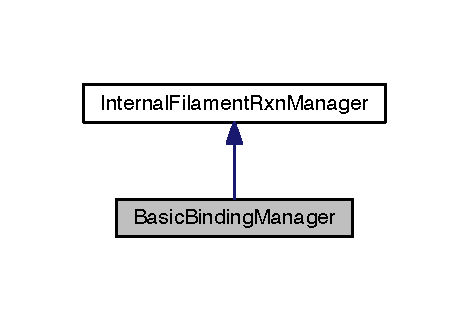
\includegraphics[width=225pt]{classBasicBindingManager__inherit__graph}
\end{center}
\end{figure}


Collaboration diagram for Basic\+Binding\+Manager\+:
\nopagebreak
\begin{figure}[H]
\begin{center}
\leavevmode
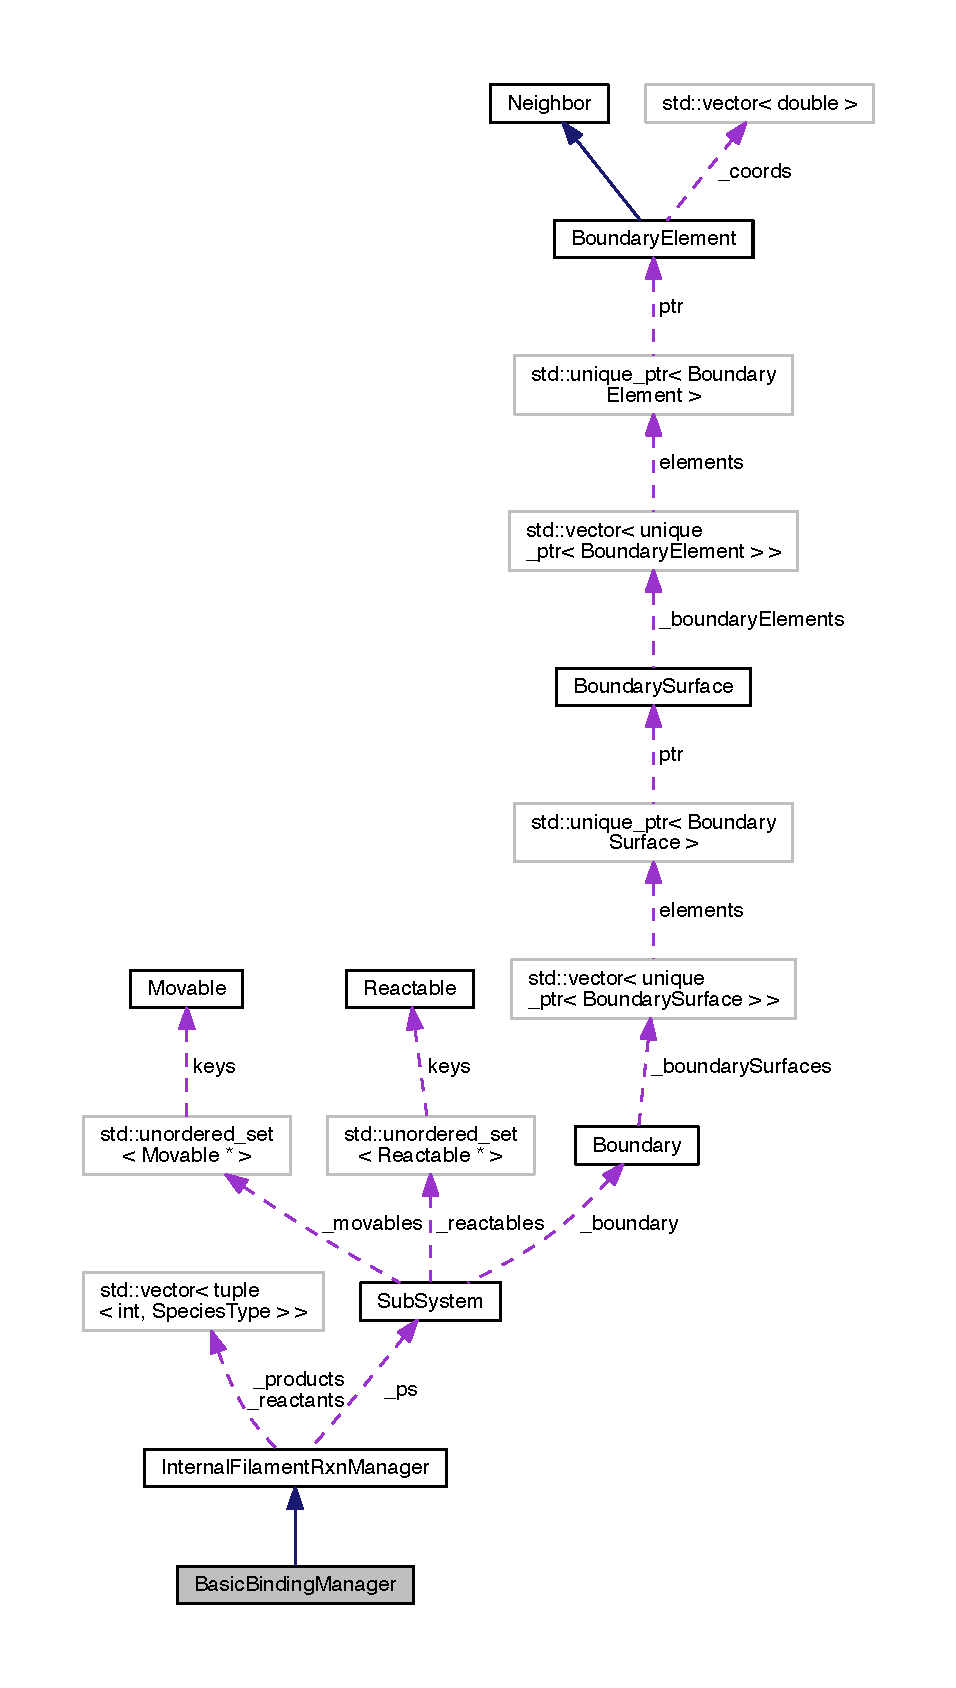
\includegraphics[height=550pt]{classBasicBindingManager__coll__graph}
\end{center}
\end{figure}
\subsection*{Public Member Functions}
\begin{DoxyCompactItemize}
\item 
\hyperlink{classBasicBindingManager_ad57b38f098621ae0408069c49c17db52}{Basic\+Binding\+Manager} (vector$<$ tuple$<$ int, \hyperlink{Species_8h_a50651af47c56ea0e27235468d23542cf}{Species\+Type} $>$$>$ reactants, vector$<$ tuple$<$ int, \hyperlink{Species_8h_a50651af47c56ea0e27235468d23542cf}{Species\+Type} $>$$>$ products, float rate)
\item 
\hyperlink{classBasicBindingManager_ab382b0c661238e95df9d64f556ddc6d4}{$\sim$\+Basic\+Binding\+Manager} ()
\item 
virtual void \hyperlink{classBasicBindingManager_a9dbb688abc218187913b23fa3dccd97d}{add\+Reaction} (\hyperlink{classCCylinder}{C\+Cylinder} $\ast$cc)
\begin{DoxyCompactList}\small\item\em Add this chemical reaction to a \hyperlink{classCCylinder}{C\+Cylinder}. Adds all extension and retraction callbacks needed. \end{DoxyCompactList}\item 
virtual void \hyperlink{classBasicBindingManager_aea22a428f792f83f02ba58796ccd882e}{add\+Reaction} (\hyperlink{classCCylinder}{C\+Cylinder} $\ast$cc1, \hyperlink{classCCylinder}{C\+Cylinder} $\ast$cc2)
\begin{DoxyCompactList}\small\item\em Add this chemical reaction cross two \hyperlink{classCCylinder}{C\+Cylinders}. \end{DoxyCompactList}\end{DoxyCompactItemize}
\subsection*{Protected Attributes}
\begin{DoxyCompactItemize}
\item 
vector$<$ tuple$<$ int, \hyperlink{Species_8h_a50651af47c56ea0e27235468d23542cf}{Species\+Type} $>$ $>$ \hyperlink{classInternalFilamentRxnManager_a63de9061c3da4ad03cf4c530d2774979}{\+\_\+reactants}
\begin{DoxyCompactList}\small\item\em \hyperlink{classSpecies}{Species} identifier vectors. \end{DoxyCompactList}\item 
vector$<$ tuple$<$ int, \hyperlink{Species_8h_a50651af47c56ea0e27235468d23542cf}{Species\+Type} $>$ $>$ \hyperlink{classInternalFilamentRxnManager_afd213da1a3706e2e88962e5da886a5dc}{\+\_\+products}
\begin{DoxyCompactList}\small\item\em Products in this reaction. \end{DoxyCompactList}\item 
float \hyperlink{classInternalFilamentRxnManager_a8b98dd9e6f5d016149f5434b891806df}{\+\_\+rate}
\begin{DoxyCompactList}\small\item\em Rate of reaction. \end{DoxyCompactList}\end{DoxyCompactItemize}
\subsection*{Static Protected Attributes}
\begin{DoxyCompactItemize}
\item 
static \hyperlink{classSubSystem}{Sub\+System} $\ast$ \hyperlink{classInternalFilamentRxnManager_a973ce9cc2aae811e6867afa46193c5f2}{\+\_\+ps} = 0
\begin{DoxyCompactList}\small\item\em A subsystem pointer to initialize and call chemical callbacks. \end{DoxyCompactList}\end{DoxyCompactItemize}


\subsection{Detailed Description}
Manager for basic binding. 

Definition at line 126 of file Reaction\+Manager.\+h.



\subsection{Constructor \& Destructor Documentation}
\hypertarget{classBasicBindingManager_ad57b38f098621ae0408069c49c17db52}{\index{Basic\+Binding\+Manager@{Basic\+Binding\+Manager}!Basic\+Binding\+Manager@{Basic\+Binding\+Manager}}
\index{Basic\+Binding\+Manager@{Basic\+Binding\+Manager}!Basic\+Binding\+Manager@{Basic\+Binding\+Manager}}
\subsubsection[{Basic\+Binding\+Manager}]{\setlength{\rightskip}{0pt plus 5cm}Basic\+Binding\+Manager\+::\+Basic\+Binding\+Manager (
\begin{DoxyParamCaption}
\item[{vector$<$ tuple$<$ int, {\bf Species\+Type} $>$$>$}]{reactants, }
\item[{vector$<$ tuple$<$ int, {\bf Species\+Type} $>$$>$}]{products, }
\item[{float}]{rate}
\end{DoxyParamCaption}
)\hspace{0.3cm}{\ttfamily [inline]}}}\label{classBasicBindingManager_ad57b38f098621ae0408069c49c17db52}


Definition at line 129 of file Reaction\+Manager.\+h.

\hypertarget{classBasicBindingManager_ab382b0c661238e95df9d64f556ddc6d4}{\index{Basic\+Binding\+Manager@{Basic\+Binding\+Manager}!````~Basic\+Binding\+Manager@{$\sim$\+Basic\+Binding\+Manager}}
\index{````~Basic\+Binding\+Manager@{$\sim$\+Basic\+Binding\+Manager}!Basic\+Binding\+Manager@{Basic\+Binding\+Manager}}
\subsubsection[{$\sim$\+Basic\+Binding\+Manager}]{\setlength{\rightskip}{0pt plus 5cm}Basic\+Binding\+Manager\+::$\sim$\+Basic\+Binding\+Manager (
\begin{DoxyParamCaption}
{}
\end{DoxyParamCaption}
)\hspace{0.3cm}{\ttfamily [inline]}}}\label{classBasicBindingManager_ab382b0c661238e95df9d64f556ddc6d4}


Definition at line 132 of file Reaction\+Manager.\+h.



\subsection{Member Function Documentation}
\hypertarget{classBasicBindingManager_a9dbb688abc218187913b23fa3dccd97d}{\index{Basic\+Binding\+Manager@{Basic\+Binding\+Manager}!add\+Reaction@{add\+Reaction}}
\index{add\+Reaction@{add\+Reaction}!Basic\+Binding\+Manager@{Basic\+Binding\+Manager}}
\subsubsection[{add\+Reaction}]{\setlength{\rightskip}{0pt plus 5cm}void Basic\+Binding\+Manager\+::add\+Reaction (
\begin{DoxyParamCaption}
\item[{{\bf C\+Cylinder} $\ast$}]{cc}
\end{DoxyParamCaption}
)\hspace{0.3cm}{\ttfamily [virtual]}}}\label{classBasicBindingManager_a9dbb688abc218187913b23fa3dccd97d}


Add this chemical reaction to a \hyperlink{classCCylinder}{C\+Cylinder}. Adds all extension and retraction callbacks needed. 



Implements \hyperlink{classInternalFilamentRxnManager_a45f1ff9c676e41db408669ab6c5242e9}{Internal\+Filament\+Rxn\+Manager}.



Definition at line 605 of file Reaction\+Manager.\+cpp.



References C\+Cylinder\+::add\+Internal\+Reaction(), B\+A\+S\+I\+C\+B\+I\+N\+D\+I\+N\+G, B\+U\+L\+K, D\+I\+F\+F\+U\+S\+I\+N\+G, Compartment\+::find\+Species\+By\+Molecule(), C\+Cylinder\+::get\+C\+Monomer(), C\+Cylinder\+::get\+Compartment(), C\+Cylinder\+::get\+Size(), Compartment\+Grid\+::instance(), Reaction\+Base\+::set\+Reaction\+Type(), and C\+Monomer\+::species\+Bound().

\hypertarget{classBasicBindingManager_aea22a428f792f83f02ba58796ccd882e}{\index{Basic\+Binding\+Manager@{Basic\+Binding\+Manager}!add\+Reaction@{add\+Reaction}}
\index{add\+Reaction@{add\+Reaction}!Basic\+Binding\+Manager@{Basic\+Binding\+Manager}}
\subsubsection[{add\+Reaction}]{\setlength{\rightskip}{0pt plus 5cm}virtual void Basic\+Binding\+Manager\+::add\+Reaction (
\begin{DoxyParamCaption}
\item[{{\bf C\+Cylinder} $\ast$}]{cc1, }
\item[{{\bf C\+Cylinder} $\ast$}]{cc2}
\end{DoxyParamCaption}
)\hspace{0.3cm}{\ttfamily [inline]}, {\ttfamily [virtual]}}}\label{classBasicBindingManager_aea22a428f792f83f02ba58796ccd882e}


Add this chemical reaction cross two \hyperlink{classCCylinder}{C\+Cylinders}. 

\begin{DoxyNote}{Note}
assumes cc1 and cc2 are in order, that is, cc2 is the next cylinder after cc1 
\end{DoxyNote}


Implements \hyperlink{classInternalFilamentRxnManager_ac8152bcd9f6aa5d69f85a98cff86d2b0}{Internal\+Filament\+Rxn\+Manager}.



Definition at line 135 of file Reaction\+Manager.\+h.



\subsection{Member Data Documentation}
\hypertarget{classInternalFilamentRxnManager_afd213da1a3706e2e88962e5da886a5dc}{\index{Basic\+Binding\+Manager@{Basic\+Binding\+Manager}!\+\_\+products@{\+\_\+products}}
\index{\+\_\+products@{\+\_\+products}!Basic\+Binding\+Manager@{Basic\+Binding\+Manager}}
\subsubsection[{\+\_\+products}]{\setlength{\rightskip}{0pt plus 5cm}vector$<$tuple$<$int,{\bf Species\+Type}$>$ $>$ Internal\+Filament\+Rxn\+Manager\+::\+\_\+products\hspace{0.3cm}{\ttfamily [protected]}, {\ttfamily [inherited]}}}\label{classInternalFilamentRxnManager_afd213da1a3706e2e88962e5da886a5dc}


Products in this reaction. 



Definition at line 54 of file Reaction\+Manager.\+h.

\hypertarget{classInternalFilamentRxnManager_a973ce9cc2aae811e6867afa46193c5f2}{\index{Basic\+Binding\+Manager@{Basic\+Binding\+Manager}!\+\_\+ps@{\+\_\+ps}}
\index{\+\_\+ps@{\+\_\+ps}!Basic\+Binding\+Manager@{Basic\+Binding\+Manager}}
\subsubsection[{\+\_\+ps}]{\setlength{\rightskip}{0pt plus 5cm}{\bf Sub\+System} $\ast$ Internal\+Filament\+Rxn\+Manager\+::\+\_\+ps = 0\hspace{0.3cm}{\ttfamily [static]}, {\ttfamily [protected]}, {\ttfamily [inherited]}}}\label{classInternalFilamentRxnManager_a973ce9cc2aae811e6867afa46193c5f2}


A subsystem pointer to initialize and call chemical callbacks. 



Definition at line 50 of file Reaction\+Manager.\+h.



Referenced by Simple\+Manager\+Impl\+::initialize().

\hypertarget{classInternalFilamentRxnManager_a8b98dd9e6f5d016149f5434b891806df}{\index{Basic\+Binding\+Manager@{Basic\+Binding\+Manager}!\+\_\+rate@{\+\_\+rate}}
\index{\+\_\+rate@{\+\_\+rate}!Basic\+Binding\+Manager@{Basic\+Binding\+Manager}}
\subsubsection[{\+\_\+rate}]{\setlength{\rightskip}{0pt plus 5cm}float Internal\+Filament\+Rxn\+Manager\+::\+\_\+rate\hspace{0.3cm}{\ttfamily [protected]}, {\ttfamily [inherited]}}}\label{classInternalFilamentRxnManager_a8b98dd9e6f5d016149f5434b891806df}


Rate of reaction. 



Definition at line 56 of file Reaction\+Manager.\+h.

\hypertarget{classInternalFilamentRxnManager_a63de9061c3da4ad03cf4c530d2774979}{\index{Basic\+Binding\+Manager@{Basic\+Binding\+Manager}!\+\_\+reactants@{\+\_\+reactants}}
\index{\+\_\+reactants@{\+\_\+reactants}!Basic\+Binding\+Manager@{Basic\+Binding\+Manager}}
\subsubsection[{\+\_\+reactants}]{\setlength{\rightskip}{0pt plus 5cm}vector$<$tuple$<$int,{\bf Species\+Type}$>$ $>$ Internal\+Filament\+Rxn\+Manager\+::\+\_\+reactants\hspace{0.3cm}{\ttfamily [protected]}, {\ttfamily [inherited]}}}\label{classInternalFilamentRxnManager_a63de9061c3da4ad03cf4c530d2774979}


\hyperlink{classSpecies}{Species} identifier vectors. 

Reactants in this reaction 

Definition at line 53 of file Reaction\+Manager.\+h.



The documentation for this class was generated from the following files\+:\begin{DoxyCompactItemize}
\item 
M3\+S\+Y\+M/\+Chemistry/\hyperlink{ReactionManager_8h}{Reaction\+Manager.\+h}\item 
M3\+S\+Y\+M/\+Chemistry/\hyperlink{ReactionManager_8cpp}{Reaction\+Manager.\+cpp}\end{DoxyCompactItemize}

\hypertarget{classBead}{\section{Bead Class Reference}
\label{classBead}\index{Bead@{Bead}}
}


Represents a single coordinate between \hyperlink{classCylinder}{Cylinders}, and holds forces needed for mechanical equilibration.  




{\ttfamily \#include $<$Bead.\+h$>$}



Inheritance diagram for Bead\+:\nopagebreak
\begin{figure}[H]
\begin{center}
\leavevmode
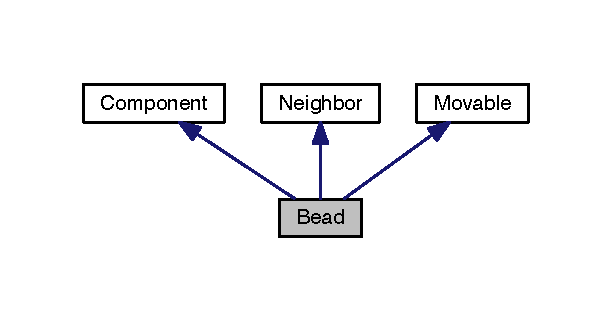
\includegraphics[width=294pt]{classBead__inherit__graph}
\end{center}
\end{figure}


Collaboration diagram for Bead\+:\nopagebreak
\begin{figure}[H]
\begin{center}
\leavevmode
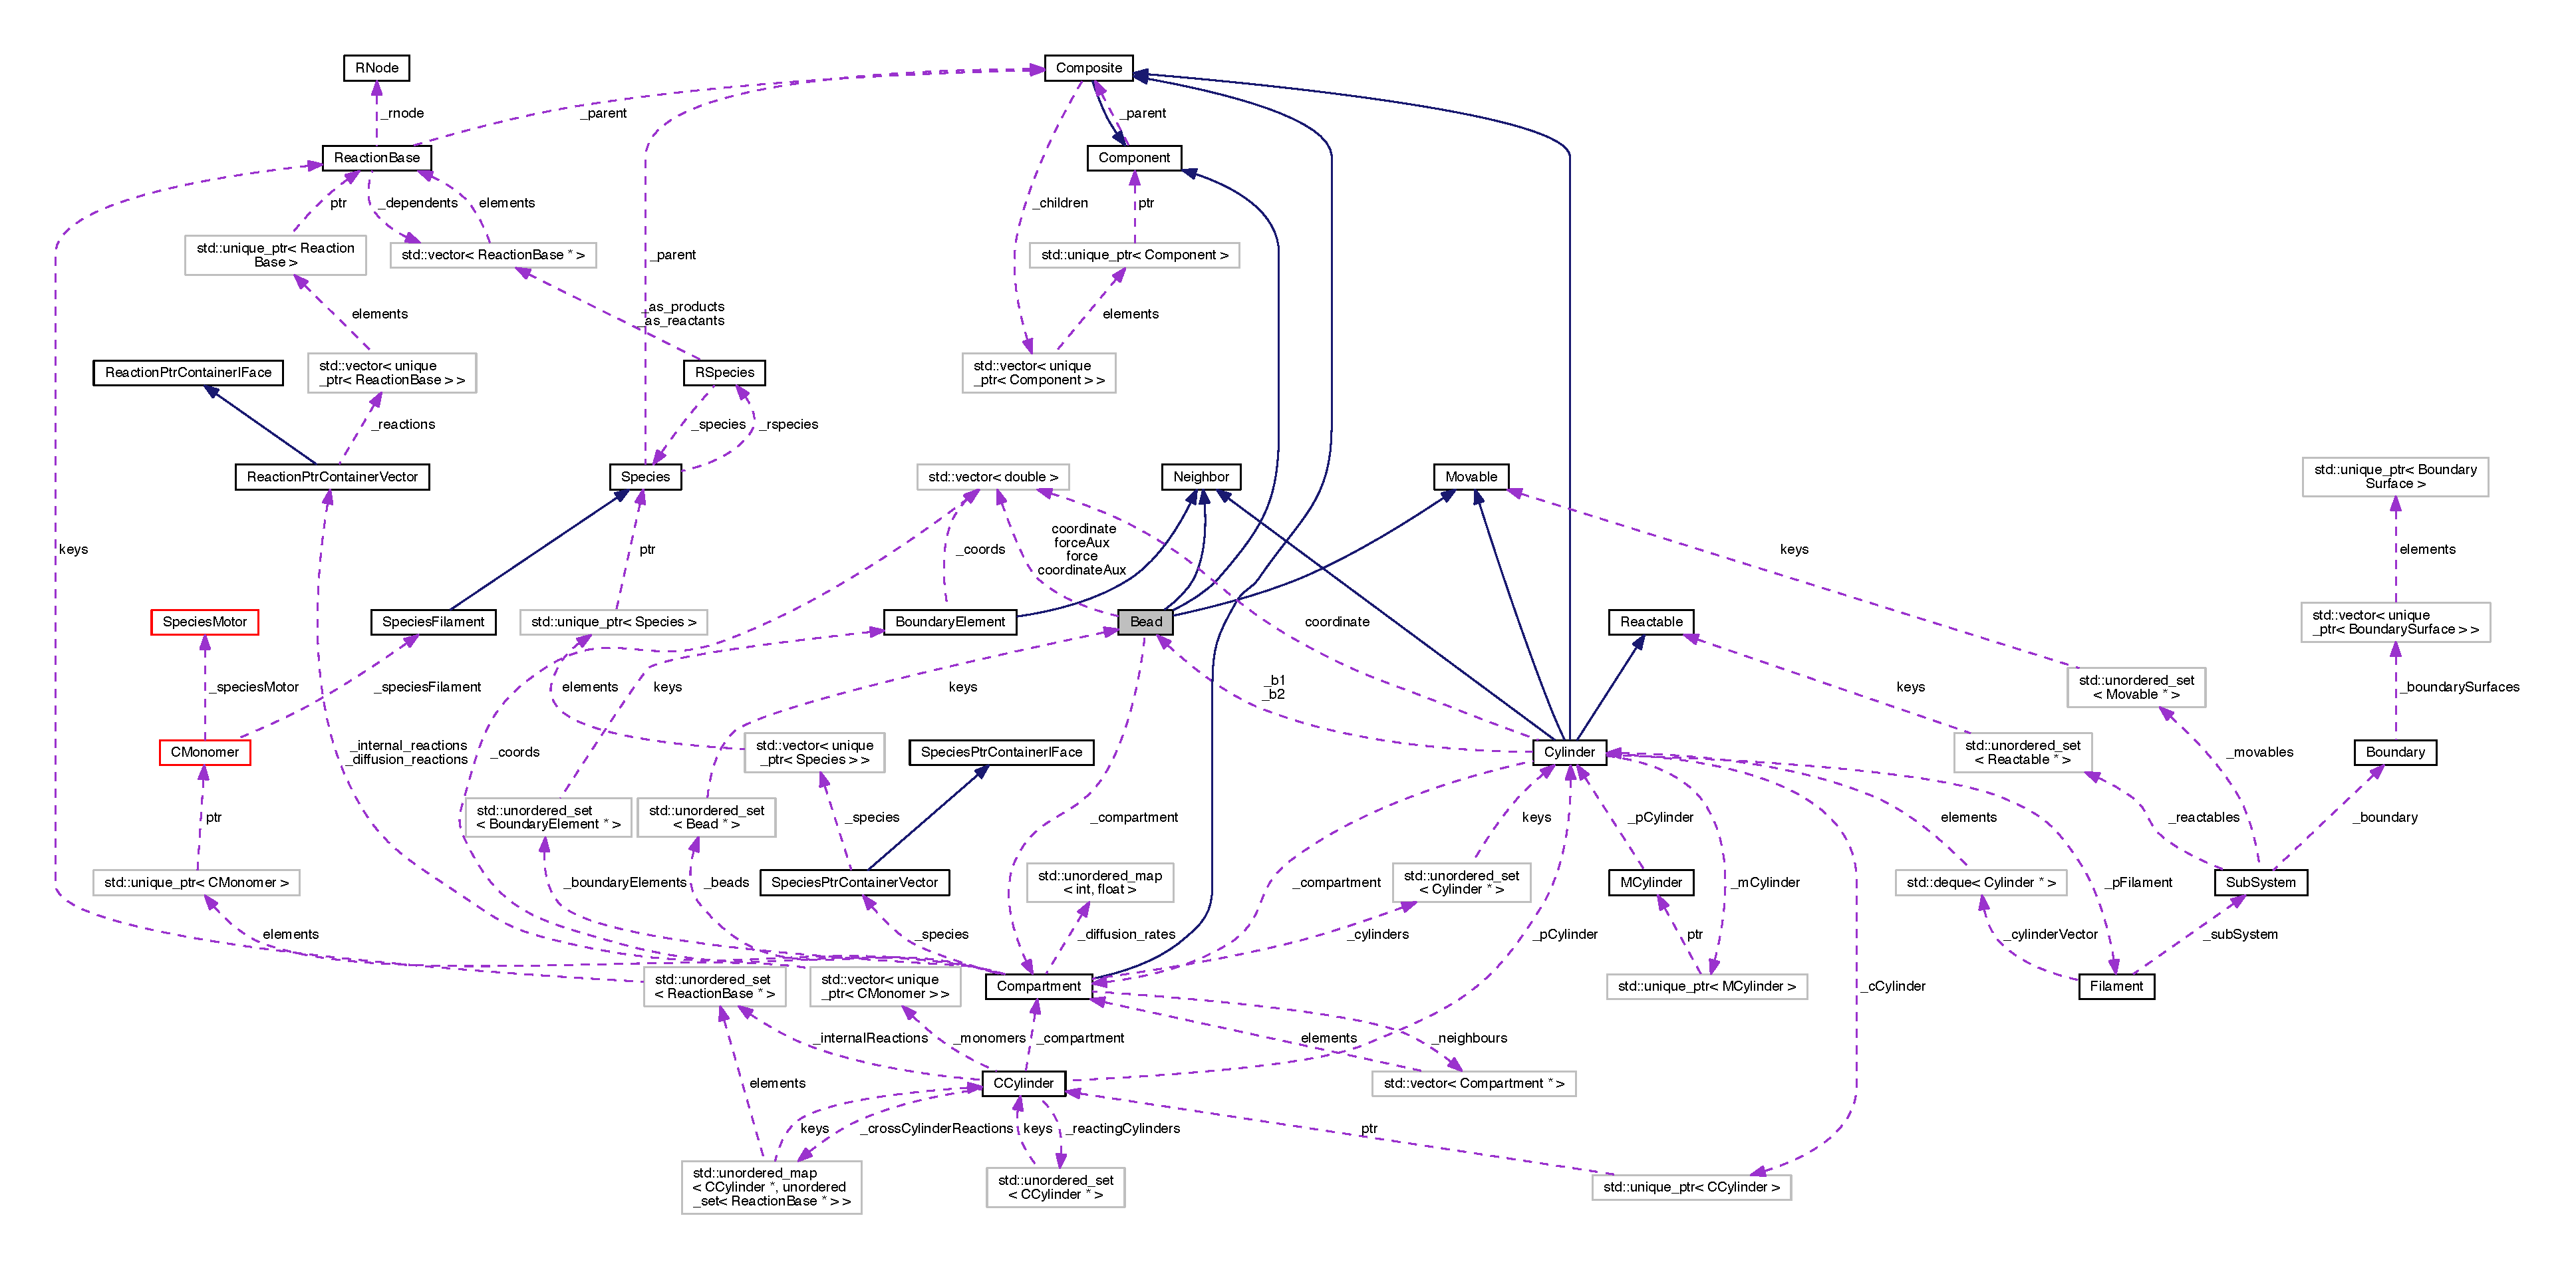
\includegraphics[width=350pt]{classBead__coll__graph}
\end{center}
\end{figure}
\subsection*{Public Member Functions}
\begin{DoxyCompactItemize}
\item 
\hyperlink{classBead_aa91581c9111d101b95bec920798e22ac}{Bead} (vector$<$ double $>$ v, int position\+Filament)
\begin{DoxyCompactList}\small\item\em Main constructor. \end{DoxyCompactList}\item 
\hyperlink{classBead_a5bb15ab11fee13f78721759cadb5a5b4}{Bead} (int position\+Filament)
\begin{DoxyCompactList}\small\item\em Default constructor. \end{DoxyCompactList}\item 
\hyperlink{classBead_a21f0ccd7041f56c4038171d0da3a58ed}{$\sim$\+Bead} ()
\item 
\hyperlink{classCompartment}{Compartment} $\ast$ \hyperlink{classBead_ae6cfcc2936a2e12a3887c9fd824c6343}{get\+Compartment} ()
\begin{DoxyCompactList}\small\item\em Get compartment. \end{DoxyCompactList}\item 
virtual void \hyperlink{classBead_adfda91d08764f284b4a23c05da34c84c}{update\+Position} ()
\begin{DoxyCompactList}\small\item\em Update the position of this bead. \end{DoxyCompactList}\item 
void \hyperlink{classBead_a3178379864ec93ff5e9f8a2e7916c94a}{set\+Position\+Filament} (int position\+Filament)
\begin{DoxyCompactList}\small\item\em Set position on the local filament. \end{DoxyCompactList}\item 
int \hyperlink{classBead_a3df2bf2b6063545ba9a68b890004057e}{get\+Position\+Filament} ()
\begin{DoxyCompactList}\small\item\em Get position on the local filament. \end{DoxyCompactList}\item 
float \hyperlink{classBead_afa239062c738d1db95a1456c9b357a68}{get\+Birth\+Time} ()
\begin{DoxyCompactList}\small\item\em Get the birth time of this bead. \end{DoxyCompactList}\item 
virtual bool \hyperlink{classComponent_a06be9328d615af20a155e9060def1470}{apply} (\hyperlink{classVisitor}{Visitor} \&v)
\begin{DoxyCompactList}\small\item\em When this function is applied to a Conditional\+Visitor v, the corresponding v.\+visit(this) is called, and v is further applied to all children of this node recursively. \end{DoxyCompactList}\item 
virtual bool \hyperlink{classComponent_a0f1cd7534ba27c165a1574adc8d422dd}{apply} (\hyperlink{classSpeciesVisitor}{Species\+Visitor} \&v)
\begin{DoxyCompactList}\small\item\em Implements the apply\+\_\+if() method of the \hyperlink{classComponent}{Component} class by recursively applying it to itself and all its children that contain \hyperlink{classSpecies}{Species}. \end{DoxyCompactList}\item 
virtual bool \hyperlink{classComponent_aa911f6c2be71a33eeeb44f03c82cd421}{apply} (\hyperlink{classReactionVisitor}{Reaction\+Visitor} \&v)
\begin{DoxyCompactList}\small\item\em Implements the apply\+\_\+if() method of the \hyperlink{classComponent}{Component} class by recursively applying it to itself and all its children that contain \hyperlink{classReactionBase}{Reaction\+Base}. \end{DoxyCompactList}\item 
virtual bool \hyperlink{classComponent_a20f6f5a1f7da3238c069dfc35f174a4b}{apply\+\_\+impl} (\hyperlink{classSpeciesVisitor}{Species\+Visitor} \&v)
\begin{DoxyCompactList}\small\item\em Applies \hyperlink{classSpeciesVisitor}{Species\+Visitor} v to every Species$\ast$ object directly owned by this node. \end{DoxyCompactList}\item 
virtual bool \hyperlink{classComponent_ac9296f41e0b9c254d5adea9df3b4b07a}{apply\+\_\+impl} (\hyperlink{classReactionVisitor}{Reaction\+Visitor} \&v)
\begin{DoxyCompactList}\small\item\em Applies Reaction\+Base\+Visitor v to every Reaction\+Base$\ast$ object directly owned by this node. \end{DoxyCompactList}\item 
\hyperlink{classComposite}{Composite} $\ast$ \hyperlink{classComponent_a4bb9041a7f3854f25f45060e81bb4e4e}{get\+Parent} ()
\begin{DoxyCompactList}\small\item\em Returns the pointer to the parent node. The returned value could be a nullptr if a parent does not exist. \end{DoxyCompactList}\item 
void \hyperlink{classComponent_a9d5b03697a653cda24d5688af1d105f8}{set\+Parent} (\hyperlink{classComposite}{Composite} $\ast$other)
\begin{DoxyCompactList}\small\item\em Sets the parent of this node to other. \end{DoxyCompactList}\item 
bool \hyperlink{classComponent_a4f0bed8144509d6565a30b548fac0fe7}{is\+Root} () const 
\begin{DoxyCompactList}\small\item\em Returns true if this node is the root node. \end{DoxyCompactList}\item 
\hyperlink{classComposite}{Composite} $\ast$ \hyperlink{classComponent_abcb3746cb8b4afcecf437dce40c0c772}{get\+Root} ()
\begin{DoxyCompactList}\small\item\em Returns the root node of the hieararchy to which this node belongs to. \end{DoxyCompactList}\item 
virtual size\+\_\+t \hyperlink{classComponent_a42566ba7ad92afe0d84d9d1d4e05745e}{number\+Of\+Children} () const 
\begin{DoxyCompactList}\small\item\em Returns the number of children of this node. \end{DoxyCompactList}\item 
virtual bool \hyperlink{classComponent_a14bcb60799865752cd293fba2076d84a}{is\+Composite} () const 
\begin{DoxyCompactList}\small\item\em Returns true if this node is a \hyperlink{classComposite}{Composite} node. \end{DoxyCompactList}\item 
virtual bool \hyperlink{classComponent_a0daf865ff32aff9e68316c65b681cbf9}{is\+Species\+Container} () const 
\begin{DoxyCompactList}\small\item\em Returns true if this node contains non-\/zero number of \hyperlink{classSpecies}{Species}. \end{DoxyCompactList}\item 
virtual bool \hyperlink{classComponent_a506e080028078ef9a753d854c60904a3}{is\+Reactions\+Container} () const 
\begin{DoxyCompactList}\small\item\em Returns true if this node contains non-\/zero number of reactions (i.\+e. \hyperlink{classReactionBase}{Reaction\+Base} pointers) \end{DoxyCompactList}\item 
virtual size\+\_\+t \hyperlink{classComponent_ae99bcb165a9403e64ffea2b840192b4c}{number\+Of\+Species} () const 
\begin{DoxyCompactList}\small\item\em Returns the number of \hyperlink{classSpecies}{Species} being immediately managed by this node (i.\+e. \end{DoxyCompactList}\item 
virtual size\+\_\+t \hyperlink{classComponent_a116a02dd48baa6bf46c1162998548814}{number\+Of\+Reactions} () const 
\begin{DoxyCompactList}\small\item\em Returns the number of \hyperlink{classReactionBase}{Reaction\+Base} objets being immediately managed by this node (i.\+e. \end{DoxyCompactList}\item 
virtual string \hyperlink{classComponent_a42dd891a934150f6d6ef74b9850d4b5c}{get\+Full\+Name} () const 
\begin{DoxyCompactList}\small\item\em Return a string indicating the full name of this node (presumably used mainly for debugging) \end{DoxyCompactList}\item 
virtual size\+\_\+t \hyperlink{classComponent_a38336c92dacb78175dfc7746bde5055d}{count\+Descendents} () const 
\begin{DoxyCompactList}\small\item\em Return the total number of nodes contained under this node's hieararchy. \end{DoxyCompactList}\item 
virtual size\+\_\+t \hyperlink{classComponent_ae4b35cc8ce749e1219bec0eeea16b4bc}{count\+Species} () const 
\begin{DoxyCompactList}\small\item\em Return the number of \hyperlink{classSpecies}{Species} contained under this node's hieararchy. \end{DoxyCompactList}\item 
virtual size\+\_\+t \hyperlink{classComponent_a446ee3fa9e36a6b56642a9d2a14d983d}{count\+Reactions} () const 
\begin{DoxyCompactList}\small\item\em Return the number of \hyperlink{classReactionBase}{Reaction\+Base} objects contained under this node's hieararchy. \end{DoxyCompactList}\item 
virtual void \hyperlink{classComponent_a871fbdc783ea600ed667dd37eb8adf1e}{print\+Self} ()
\begin{DoxyCompactList}\small\item\em Prints information about this node. Useful for debugging. \end{DoxyCompactList}\end{DoxyCompactItemize}
{\bf }\par
\begin{DoxyCompactItemize}
\item 
double \hyperlink{classBead_a8f10459bad94f72599f2e239644c4421}{calc\+Force\+Square} ()
\begin{DoxyCompactList}\small\item\em Auxiliary method for C\+G minimization. \end{DoxyCompactList}\item 
double \hyperlink{classBead_a82e3c084cb26f343b5de59619c854f2b}{calc\+Force\+Aux\+Square} ()
\item 
double \hyperlink{classBead_a3df6e55d379663d002c73651a24718f5}{calc\+Dot\+Force\+Product} ()
\end{DoxyCompactItemize}

\subsection*{Public Attributes}
\begin{DoxyCompactItemize}
\item 
vector$<$ double $>$ \hyperlink{classBead_a8c9c7d97a682694bf3b16a0922b23786}{coordinate}
\begin{DoxyCompactList}\small\item\em Coordinates of the bead. \end{DoxyCompactList}\item 
vector$<$ double $>$ \hyperlink{classBead_a4d46596f52ee0ce95e3e717483e1a921}{coordinate\+Aux}
\begin{DoxyCompactList}\small\item\em An auxiliary coordinate field needed during C\+G minimization. \end{DoxyCompactList}\item 
vector$<$ double $>$ \hyperlink{classBead_afc556d77d1d80e11c1256e89bba0db66}{force}
\begin{DoxyCompactList}\small\item\em Forces based on curent coordinates. Forces should always correspond to current coordinates. \end{DoxyCompactList}\item 
vector$<$ double $>$ \hyperlink{classBead_a59758227cd7afbb3ec5fbcafe32773b8}{force\+Aux}
\begin{DoxyCompactList}\small\item\em An auxiliary field needed during C\+G minimization. \end{DoxyCompactList}\end{DoxyCompactItemize}
\subsection*{Private Attributes}
\begin{DoxyCompactItemize}
\item 
\hyperlink{classCompartment}{Compartment} $\ast$ \hyperlink{classBead_ac9d2080d5d8f80f60535dfeea9cd38e9}{\+\_\+compartment} = nullptr
\begin{DoxyCompactList}\small\item\em Pointer to the compartment that this bead is in. \end{DoxyCompactList}\item 
int \hyperlink{classBead_a0eafb8f259549846d4714e6120cbc87c}{\+\_\+position\+Filament}
\begin{DoxyCompactList}\small\item\em Position of bead on filament. \end{DoxyCompactList}\item 
float \hyperlink{classBead_a356c8525fcf176bca4cd539f735c1de6}{\+\_\+birth\+Time}
\begin{DoxyCompactList}\small\item\em Time of birth of bead;. \end{DoxyCompactList}\end{DoxyCompactItemize}


\subsection{Detailed Description}
Represents a single coordinate between \hyperlink{classCylinder}{Cylinders}, and holds forces needed for mechanical equilibration. 

Beads are the \char`\"{}hinges\char`\"{} between \hyperlink{classCylinder}{Cylinders}. In the minimization algorithms, beads are moved corresponding to external forces, for example, filament stretching and bending. The bead class contains currernt coordinates and forces, and has functions to calculate dot products for the minimization algorithms. 

Definition at line 38 of file Bead.\+h.



\subsection{Constructor \& Destructor Documentation}
\hypertarget{classBead_aa91581c9111d101b95bec920798e22ac}{\index{Bead@{Bead}!Bead@{Bead}}
\index{Bead@{Bead}!Bead@{Bead}}
\subsubsection[{Bead}]{\setlength{\rightskip}{0pt plus 5cm}Bead\+::\+Bead (
\begin{DoxyParamCaption}
\item[{vector$<$ double $>$}]{v, }
\item[{int}]{position\+Filament}
\end{DoxyParamCaption}
)}}\label{classBead_aa91581c9111d101b95bec920798e22ac}


Main constructor. 



Definition at line 23 of file Bead.\+cpp.



References \+\_\+birth\+Time, \+\_\+compartment, Bead\+D\+B\+::add\+Bead(), Compartment\+::add\+Bead(), G\+Controller\+::get\+Compartment(), Bead\+D\+B\+::instance(), and tau().

\hypertarget{classBead_a5bb15ab11fee13f78721759cadb5a5b4}{\index{Bead@{Bead}!Bead@{Bead}}
\index{Bead@{Bead}!Bead@{Bead}}
\subsubsection[{Bead}]{\setlength{\rightskip}{0pt plus 5cm}Bead\+::\+Bead (
\begin{DoxyParamCaption}
\item[{int}]{position\+Filament}
\end{DoxyParamCaption}
)\hspace{0.3cm}{\ttfamily [inline]}}}\label{classBead_a5bb15ab11fee13f78721759cadb5a5b4}


Default constructor. 



Definition at line 50 of file Bead.\+h.

\hypertarget{classBead_a21f0ccd7041f56c4038171d0da3a58ed}{\index{Bead@{Bead}!````~Bead@{$\sim$\+Bead}}
\index{````~Bead@{$\sim$\+Bead}!Bead@{Bead}}
\subsubsection[{$\sim$\+Bead}]{\setlength{\rightskip}{0pt plus 5cm}Bead\+::$\sim$\+Bead (
\begin{DoxyParamCaption}
{}
\end{DoxyParamCaption}
)}}\label{classBead_a21f0ccd7041f56c4038171d0da3a58ed}


Definition at line 39 of file Bead.\+cpp.



References \+\_\+compartment, Bead\+D\+B\+::instance(), Bead\+D\+B\+::remove\+Bead(), and Compartment\+::remove\+Bead().



\subsection{Member Function Documentation}
\hypertarget{classComponent_a06be9328d615af20a155e9060def1470}{\index{Bead@{Bead}!apply@{apply}}
\index{apply@{apply}!Bead@{Bead}}
\subsubsection[{apply}]{\setlength{\rightskip}{0pt plus 5cm}bool Component\+::apply (
\begin{DoxyParamCaption}
\item[{{\bf Visitor} \&}]{v}
\end{DoxyParamCaption}
)\hspace{0.3cm}{\ttfamily [virtual]}, {\ttfamily [inherited]}}}\label{classComponent_a06be9328d615af20a155e9060def1470}


When this function is applied to a Conditional\+Visitor v, the corresponding v.\+visit(this) is called, and v is further applied to all children of this node recursively. 

However, the Conditional\+Visitor allows the visit() function to be applied only selectively to nodes that conform to specific criteria. 

Reimplemented in \hyperlink{classComposite_a58123ab346f6621a187bebe456e383ea}{Composite}.



Definition at line 26 of file Component.\+cpp.



References Visitor\+::visit().

\hypertarget{classComponent_a0f1cd7534ba27c165a1574adc8d422dd}{\index{Bead@{Bead}!apply@{apply}}
\index{apply@{apply}!Bead@{Bead}}
\subsubsection[{apply}]{\setlength{\rightskip}{0pt plus 5cm}virtual bool Component\+::apply (
\begin{DoxyParamCaption}
\item[{{\bf Species\+Visitor} \&}]{v}
\end{DoxyParamCaption}
)\hspace{0.3cm}{\ttfamily [inline]}, {\ttfamily [virtual]}, {\ttfamily [inherited]}}}\label{classComponent_a0f1cd7534ba27c165a1574adc8d422dd}


Implements the apply\+\_\+if() method of the \hyperlink{classComponent}{Component} class by recursively applying it to itself and all its children that contain \hyperlink{classSpecies}{Species}. 



Reimplemented in \hyperlink{classComposite_a18937a1f6f84a159e77ba83dd34b2e20}{Composite}.



Definition at line 57 of file Component.\+h.



References Component\+::apply\+\_\+impl().

\hypertarget{classComponent_aa911f6c2be71a33eeeb44f03c82cd421}{\index{Bead@{Bead}!apply@{apply}}
\index{apply@{apply}!Bead@{Bead}}
\subsubsection[{apply}]{\setlength{\rightskip}{0pt plus 5cm}virtual bool Component\+::apply (
\begin{DoxyParamCaption}
\item[{{\bf Reaction\+Visitor} \&}]{v}
\end{DoxyParamCaption}
)\hspace{0.3cm}{\ttfamily [inline]}, {\ttfamily [virtual]}, {\ttfamily [inherited]}}}\label{classComponent_aa911f6c2be71a33eeeb44f03c82cd421}


Implements the apply\+\_\+if() method of the \hyperlink{classComponent}{Component} class by recursively applying it to itself and all its children that contain \hyperlink{classReactionBase}{Reaction\+Base}. 



Reimplemented in \hyperlink{classComposite_aa4a608ee92aaaa6e0d63278595707474}{Composite}.



Definition at line 65 of file Component.\+h.



References Component\+::apply\+\_\+impl().

\hypertarget{classComponent_a20f6f5a1f7da3238c069dfc35f174a4b}{\index{Bead@{Bead}!apply\+\_\+impl@{apply\+\_\+impl}}
\index{apply\+\_\+impl@{apply\+\_\+impl}!Bead@{Bead}}
\subsubsection[{apply\+\_\+impl}]{\setlength{\rightskip}{0pt plus 5cm}virtual bool Component\+::apply\+\_\+impl (
\begin{DoxyParamCaption}
\item[{{\bf Species\+Visitor} \&}]{v}
\end{DoxyParamCaption}
)\hspace{0.3cm}{\ttfamily [inline]}, {\ttfamily [virtual]}, {\ttfamily [inherited]}}}\label{classComponent_a20f6f5a1f7da3238c069dfc35f174a4b}


Applies \hyperlink{classSpeciesVisitor}{Species\+Visitor} v to every Species$\ast$ object directly owned by this node. 

This method needs to be overriden by descendent classes that contain \hyperlink{classSpecies}{Species}. 

Reimplemented in \hyperlink{classCompartment_ae9bdaf50db8e780d3614be3bc50e9171}{Compartment}.



Definition at line 61 of file Component.\+h.



Referenced by Component\+::apply(), and Composite\+::apply().

\hypertarget{classComponent_ac9296f41e0b9c254d5adea9df3b4b07a}{\index{Bead@{Bead}!apply\+\_\+impl@{apply\+\_\+impl}}
\index{apply\+\_\+impl@{apply\+\_\+impl}!Bead@{Bead}}
\subsubsection[{apply\+\_\+impl}]{\setlength{\rightskip}{0pt plus 5cm}virtual bool Component\+::apply\+\_\+impl (
\begin{DoxyParamCaption}
\item[{{\bf Reaction\+Visitor} \&}]{v}
\end{DoxyParamCaption}
)\hspace{0.3cm}{\ttfamily [inline]}, {\ttfamily [virtual]}, {\ttfamily [inherited]}}}\label{classComponent_ac9296f41e0b9c254d5adea9df3b4b07a}


Applies Reaction\+Base\+Visitor v to every Reaction\+Base$\ast$ object directly owned by this node. 

This method needs to be overriden by descendent classes that contain \hyperlink{classReactionBase}{Reaction\+Base}. 

Reimplemented in \hyperlink{classCompartment_a37bd8d3a6d3a21bf50716979c6694adb}{Compartment}.



Definition at line 69 of file Component.\+h.

\hypertarget{classBead_a3df6e55d379663d002c73651a24718f5}{\index{Bead@{Bead}!calc\+Dot\+Force\+Product@{calc\+Dot\+Force\+Product}}
\index{calc\+Dot\+Force\+Product@{calc\+Dot\+Force\+Product}!Bead@{Bead}}
\subsubsection[{calc\+Dot\+Force\+Product}]{\setlength{\rightskip}{0pt plus 5cm}double Bead\+::calc\+Dot\+Force\+Product (
\begin{DoxyParamCaption}
{}
\end{DoxyParamCaption}
)\hspace{0.3cm}{\ttfamily [inline]}}}\label{classBead_a3df6e55d379663d002c73651a24718f5}


Definition at line 64 of file Bead.\+h.



References force, and force\+Aux.

\hypertarget{classBead_a82e3c084cb26f343b5de59619c854f2b}{\index{Bead@{Bead}!calc\+Force\+Aux\+Square@{calc\+Force\+Aux\+Square}}
\index{calc\+Force\+Aux\+Square@{calc\+Force\+Aux\+Square}!Bead@{Bead}}
\subsubsection[{calc\+Force\+Aux\+Square}]{\setlength{\rightskip}{0pt plus 5cm}double Bead\+::calc\+Force\+Aux\+Square (
\begin{DoxyParamCaption}
{}
\end{DoxyParamCaption}
)\hspace{0.3cm}{\ttfamily [inline]}}}\label{classBead_a82e3c084cb26f343b5de59619c854f2b}


Definition at line 60 of file Bead.\+h.



References force\+Aux.

\hypertarget{classBead_a8f10459bad94f72599f2e239644c4421}{\index{Bead@{Bead}!calc\+Force\+Square@{calc\+Force\+Square}}
\index{calc\+Force\+Square@{calc\+Force\+Square}!Bead@{Bead}}
\subsubsection[{calc\+Force\+Square}]{\setlength{\rightskip}{0pt plus 5cm}double Bead\+::calc\+Force\+Square (
\begin{DoxyParamCaption}
{}
\end{DoxyParamCaption}
)\hspace{0.3cm}{\ttfamily [inline]}}}\label{classBead_a8f10459bad94f72599f2e239644c4421}


Auxiliary method for C\+G minimization. 



Definition at line 56 of file Bead.\+h.

\hypertarget{classComponent_a38336c92dacb78175dfc7746bde5055d}{\index{Bead@{Bead}!count\+Descendents@{count\+Descendents}}
\index{count\+Descendents@{count\+Descendents}!Bead@{Bead}}
\subsubsection[{count\+Descendents}]{\setlength{\rightskip}{0pt plus 5cm}virtual size\+\_\+t Component\+::count\+Descendents (
\begin{DoxyParamCaption}
{}
\end{DoxyParamCaption}
) const\hspace{0.3cm}{\ttfamily [inline]}, {\ttfamily [virtual]}, {\ttfamily [inherited]}}}\label{classComponent_a38336c92dacb78175dfc7746bde5055d}


Return the total number of nodes contained under this node's hieararchy. 

\begin{DoxyNote}{Note}
This is a recursive call, and all nodes under this node are visited. 
\end{DoxyNote}


Reimplemented in \hyperlink{classComposite_aad7cea9220c003254233ec9dc6bcb24e}{Composite}.



Definition at line 110 of file Component.\+h.

\hypertarget{classComponent_a446ee3fa9e36a6b56642a9d2a14d983d}{\index{Bead@{Bead}!count\+Reactions@{count\+Reactions}}
\index{count\+Reactions@{count\+Reactions}!Bead@{Bead}}
\subsubsection[{count\+Reactions}]{\setlength{\rightskip}{0pt plus 5cm}virtual size\+\_\+t Component\+::count\+Reactions (
\begin{DoxyParamCaption}
{}
\end{DoxyParamCaption}
) const\hspace{0.3cm}{\ttfamily [inline]}, {\ttfamily [virtual]}, {\ttfamily [inherited]}}}\label{classComponent_a446ee3fa9e36a6b56642a9d2a14d983d}


Return the number of \hyperlink{classReactionBase}{Reaction\+Base} objects contained under this node's hieararchy. 

\begin{DoxyNote}{Note}
This is a recursive call, and all nodes under this node are visited. 
\end{DoxyNote}


Reimplemented in \hyperlink{classComposite_a14108b9a4f9e903ba0fd9cc40fbbd8ae}{Composite}.



Definition at line 118 of file Component.\+h.

\hypertarget{classComponent_ae4b35cc8ce749e1219bec0eeea16b4bc}{\index{Bead@{Bead}!count\+Species@{count\+Species}}
\index{count\+Species@{count\+Species}!Bead@{Bead}}
\subsubsection[{count\+Species}]{\setlength{\rightskip}{0pt plus 5cm}virtual size\+\_\+t Component\+::count\+Species (
\begin{DoxyParamCaption}
{}
\end{DoxyParamCaption}
) const\hspace{0.3cm}{\ttfamily [inline]}, {\ttfamily [virtual]}, {\ttfamily [inherited]}}}\label{classComponent_ae4b35cc8ce749e1219bec0eeea16b4bc}


Return the number of \hyperlink{classSpecies}{Species} contained under this node's hieararchy. 

\begin{DoxyNote}{Note}
This is a recursive call, and all nodes under this node are visited. 
\end{DoxyNote}


Reimplemented in \hyperlink{classComposite_ad3162a869285627b04c5388dc28e2719}{Composite}.



Definition at line 114 of file Component.\+h.

\hypertarget{classBead_afa239062c738d1db95a1456c9b357a68}{\index{Bead@{Bead}!get\+Birth\+Time@{get\+Birth\+Time}}
\index{get\+Birth\+Time@{get\+Birth\+Time}!Bead@{Bead}}
\subsubsection[{get\+Birth\+Time}]{\setlength{\rightskip}{0pt plus 5cm}float Bead\+::get\+Birth\+Time (
\begin{DoxyParamCaption}
{}
\end{DoxyParamCaption}
)\hspace{0.3cm}{\ttfamily [inline]}}}\label{classBead_afa239062c738d1db95a1456c9b357a68}


Get the birth time of this bead. 



Definition at line 81 of file Bead.\+h.



References \+\_\+birth\+Time.

\hypertarget{classBead_ae6cfcc2936a2e12a3887c9fd824c6343}{\index{Bead@{Bead}!get\+Compartment@{get\+Compartment}}
\index{get\+Compartment@{get\+Compartment}!Bead@{Bead}}
\subsubsection[{get\+Compartment}]{\setlength{\rightskip}{0pt plus 5cm}{\bf Compartment}$\ast$ Bead\+::get\+Compartment (
\begin{DoxyParamCaption}
{}
\end{DoxyParamCaption}
)\hspace{0.3cm}{\ttfamily [inline]}}}\label{classBead_ae6cfcc2936a2e12a3887c9fd824c6343}


Get compartment. 



Definition at line 70 of file Bead.\+h.



References \+\_\+compartment.

\hypertarget{classComponent_a42dd891a934150f6d6ef74b9850d4b5c}{\index{Bead@{Bead}!get\+Full\+Name@{get\+Full\+Name}}
\index{get\+Full\+Name@{get\+Full\+Name}!Bead@{Bead}}
\subsubsection[{get\+Full\+Name}]{\setlength{\rightskip}{0pt plus 5cm}virtual string Component\+::get\+Full\+Name (
\begin{DoxyParamCaption}
{}
\end{DoxyParamCaption}
) const\hspace{0.3cm}{\ttfamily [inline]}, {\ttfamily [virtual]}, {\ttfamily [inherited]}}}\label{classComponent_a42dd891a934150f6d6ef74b9850d4b5c}


Return a string indicating the full name of this node (presumably used mainly for debugging) 



Reimplemented in \hyperlink{classCompartment_aee4d7b2def05be8e5e75f6744c7b3940}{Compartment}, \hyperlink{classCompartmentGrid_ae388f0cfd0d78d0ebbe0583bc3d9ec41}{Compartment\+Grid}, and \hyperlink{classComposite_a0219bb2449696a3ab84ff24e4462e2c2}{Composite}.



Definition at line 106 of file Component.\+h.

\hypertarget{classComponent_a4bb9041a7f3854f25f45060e81bb4e4e}{\index{Bead@{Bead}!get\+Parent@{get\+Parent}}
\index{get\+Parent@{get\+Parent}!Bead@{Bead}}
\subsubsection[{get\+Parent}]{\setlength{\rightskip}{0pt plus 5cm}{\bf Composite}$\ast$ Component\+::get\+Parent (
\begin{DoxyParamCaption}
{}
\end{DoxyParamCaption}
)\hspace{0.3cm}{\ttfamily [inline]}, {\ttfamily [inherited]}}}\label{classComponent_a4bb9041a7f3854f25f45060e81bb4e4e}


Returns the pointer to the parent node. The returned value could be a nullptr if a parent does not exist. 



Definition at line 72 of file Component.\+h.



References Component\+::\+\_\+parent.



Referenced by Component\+::get\+Root().

\hypertarget{classBead_a3df2bf2b6063545ba9a68b890004057e}{\index{Bead@{Bead}!get\+Position\+Filament@{get\+Position\+Filament}}
\index{get\+Position\+Filament@{get\+Position\+Filament}!Bead@{Bead}}
\subsubsection[{get\+Position\+Filament}]{\setlength{\rightskip}{0pt plus 5cm}int Bead\+::get\+Position\+Filament (
\begin{DoxyParamCaption}
{}
\end{DoxyParamCaption}
)\hspace{0.3cm}{\ttfamily [inline]}}}\label{classBead_a3df2bf2b6063545ba9a68b890004057e}


Get position on the local filament. 



Definition at line 78 of file Bead.\+h.



References \+\_\+position\+Filament.



Referenced by Filament\+::extend\+Back(), and Filament\+::extend\+Front().

\hypertarget{classComponent_abcb3746cb8b4afcecf437dce40c0c772}{\index{Bead@{Bead}!get\+Root@{get\+Root}}
\index{get\+Root@{get\+Root}!Bead@{Bead}}
\subsubsection[{get\+Root}]{\setlength{\rightskip}{0pt plus 5cm}{\bf Composite} $\ast$ Component\+::get\+Root (
\begin{DoxyParamCaption}
{}
\end{DoxyParamCaption}
)\hspace{0.3cm}{\ttfamily [inherited]}}}\label{classComponent_abcb3746cb8b4afcecf437dce40c0c772}


Returns the root node of the hieararchy to which this node belongs to. 



Definition at line 19 of file Component.\+cpp.



References Component\+::get\+Parent(), Component\+::get\+Root(), and Component\+::is\+Root().



Referenced by Component\+::get\+Root(), Reaction\+Base\+::get\+Root(), and Species\+::get\+Root().

\hypertarget{classComponent_a14bcb60799865752cd293fba2076d84a}{\index{Bead@{Bead}!is\+Composite@{is\+Composite}}
\index{is\+Composite@{is\+Composite}!Bead@{Bead}}
\subsubsection[{is\+Composite}]{\setlength{\rightskip}{0pt plus 5cm}virtual bool Component\+::is\+Composite (
\begin{DoxyParamCaption}
{}
\end{DoxyParamCaption}
) const\hspace{0.3cm}{\ttfamily [inline]}, {\ttfamily [virtual]}, {\ttfamily [inherited]}}}\label{classComponent_a14bcb60799865752cd293fba2076d84a}


Returns true if this node is a \hyperlink{classComposite}{Composite} node. 



Reimplemented in \hyperlink{classComposite_ae2c806010c5c1d2d166ce01f2710c271}{Composite}.



Definition at line 89 of file Component.\+h.

\hypertarget{classComponent_a506e080028078ef9a753d854c60904a3}{\index{Bead@{Bead}!is\+Reactions\+Container@{is\+Reactions\+Container}}
\index{is\+Reactions\+Container@{is\+Reactions\+Container}!Bead@{Bead}}
\subsubsection[{is\+Reactions\+Container}]{\setlength{\rightskip}{0pt plus 5cm}virtual bool Component\+::is\+Reactions\+Container (
\begin{DoxyParamCaption}
{}
\end{DoxyParamCaption}
) const\hspace{0.3cm}{\ttfamily [inline]}, {\ttfamily [virtual]}, {\ttfamily [inherited]}}}\label{classComponent_a506e080028078ef9a753d854c60904a3}


Returns true if this node contains non-\/zero number of reactions (i.\+e. \hyperlink{classReactionBase}{Reaction\+Base} pointers) 



Reimplemented in \hyperlink{classCompartment_a87a624dd83cc42e752454645a5484f6e}{Compartment}.



Definition at line 95 of file Component.\+h.



Referenced by Composite\+::count\+Reactions().

\hypertarget{classComponent_a4f0bed8144509d6565a30b548fac0fe7}{\index{Bead@{Bead}!is\+Root@{is\+Root}}
\index{is\+Root@{is\+Root}!Bead@{Bead}}
\subsubsection[{is\+Root}]{\setlength{\rightskip}{0pt plus 5cm}bool Component\+::is\+Root (
\begin{DoxyParamCaption}
{}
\end{DoxyParamCaption}
) const\hspace{0.3cm}{\ttfamily [inline]}, {\ttfamily [inherited]}}}\label{classComponent_a4f0bed8144509d6565a30b548fac0fe7}


Returns true if this node is the root node. 

A root node has no parent, and the corresponding \hyperlink{classComponent_a4bb9041a7f3854f25f45060e81bb4e4e}{get\+Parent()} call would return a nullptr. 

Definition at line 79 of file Component.\+h.



References Component\+::\+\_\+parent.



Referenced by Component\+::get\+Root().

\hypertarget{classComponent_a0daf865ff32aff9e68316c65b681cbf9}{\index{Bead@{Bead}!is\+Species\+Container@{is\+Species\+Container}}
\index{is\+Species\+Container@{is\+Species\+Container}!Bead@{Bead}}
\subsubsection[{is\+Species\+Container}]{\setlength{\rightskip}{0pt plus 5cm}virtual bool Component\+::is\+Species\+Container (
\begin{DoxyParamCaption}
{}
\end{DoxyParamCaption}
) const\hspace{0.3cm}{\ttfamily [inline]}, {\ttfamily [virtual]}, {\ttfamily [inherited]}}}\label{classComponent_a0daf865ff32aff9e68316c65b681cbf9}


Returns true if this node contains non-\/zero number of \hyperlink{classSpecies}{Species}. 



Reimplemented in \hyperlink{classCompartment_ac26aefc0e11a0bf2065626bc47b5de08}{Compartment}.



Definition at line 92 of file Component.\+h.



Referenced by Composite\+::count\+Species().

\hypertarget{classComponent_a42566ba7ad92afe0d84d9d1d4e05745e}{\index{Bead@{Bead}!number\+Of\+Children@{number\+Of\+Children}}
\index{number\+Of\+Children@{number\+Of\+Children}!Bead@{Bead}}
\subsubsection[{number\+Of\+Children}]{\setlength{\rightskip}{0pt plus 5cm}virtual size\+\_\+t Component\+::number\+Of\+Children (
\begin{DoxyParamCaption}
{}
\end{DoxyParamCaption}
) const\hspace{0.3cm}{\ttfamily [inline]}, {\ttfamily [virtual]}, {\ttfamily [inherited]}}}\label{classComponent_a42566ba7ad92afe0d84d9d1d4e05745e}


Returns the number of children of this node. 

\begin{DoxyNote}{Note}
\hyperlink{classSpecies}{Species} and \hyperlink{classReactionBase}{Reaction\+Base} objects are not counted. 
\end{DoxyNote}


Reimplemented in \hyperlink{classComposite_ab00f34ad7c8f7cd90ea9392bd54fd62a}{Composite}.



Definition at line 86 of file Component.\+h.

\hypertarget{classComponent_a116a02dd48baa6bf46c1162998548814}{\index{Bead@{Bead}!number\+Of\+Reactions@{number\+Of\+Reactions}}
\index{number\+Of\+Reactions@{number\+Of\+Reactions}!Bead@{Bead}}
\subsubsection[{number\+Of\+Reactions}]{\setlength{\rightskip}{0pt plus 5cm}virtual size\+\_\+t Component\+::number\+Of\+Reactions (
\begin{DoxyParamCaption}
{}
\end{DoxyParamCaption}
) const\hspace{0.3cm}{\ttfamily [inline]}, {\ttfamily [virtual]}, {\ttfamily [inherited]}}}\label{classComponent_a116a02dd48baa6bf46c1162998548814}


Returns the number of \hyperlink{classReactionBase}{Reaction\+Base} objets being immediately managed by this node (i.\+e. 

not counting reactions belonging to children nodes, etc. 

Reimplemented in \hyperlink{classCompartment_a2a8090f8a6df14b5d8ab528425333cca}{Compartment}, and \hyperlink{classComposite_aee77e531ab9ccb8dcea12a307bd75539}{Composite}.



Definition at line 103 of file Component.\+h.

\hypertarget{classComponent_ae99bcb165a9403e64ffea2b840192b4c}{\index{Bead@{Bead}!number\+Of\+Species@{number\+Of\+Species}}
\index{number\+Of\+Species@{number\+Of\+Species}!Bead@{Bead}}
\subsubsection[{number\+Of\+Species}]{\setlength{\rightskip}{0pt plus 5cm}virtual size\+\_\+t Component\+::number\+Of\+Species (
\begin{DoxyParamCaption}
{}
\end{DoxyParamCaption}
) const\hspace{0.3cm}{\ttfamily [inline]}, {\ttfamily [virtual]}, {\ttfamily [inherited]}}}\label{classComponent_ae99bcb165a9403e64ffea2b840192b4c}


Returns the number of \hyperlink{classSpecies}{Species} being immediately managed by this node (i.\+e. 

not counting \hyperlink{classSpecies}{Species} belonging to children nodes, etc. 

Reimplemented in \hyperlink{classCompartment_a9658205238f8d417eb29c5d966026844}{Compartment}, and \hyperlink{classComposite_af36fb9ed49f7fc262c68b41f2b9a56f6}{Composite}.



Definition at line 99 of file Component.\+h.



Referenced by main().

\hypertarget{classComponent_a871fbdc783ea600ed667dd37eb8adf1e}{\index{Bead@{Bead}!print\+Self@{print\+Self}}
\index{print\+Self@{print\+Self}!Bead@{Bead}}
\subsubsection[{print\+Self}]{\setlength{\rightskip}{0pt plus 5cm}virtual void Component\+::print\+Self (
\begin{DoxyParamCaption}
{}
\end{DoxyParamCaption}
)\hspace{0.3cm}{\ttfamily [inline]}, {\ttfamily [virtual]}, {\ttfamily [inherited]}}}\label{classComponent_a871fbdc783ea600ed667dd37eb8adf1e}


Prints information about this node. Useful for debugging. 



Reimplemented in \hyperlink{classCompartment_a79ff3378bf4da9e9fe88669ef1a91ad0}{Compartment}, and \hyperlink{classCompartmentGrid_a1c94761f08339f43d77cc6b90504dc49}{Compartment\+Grid}.



Definition at line 121 of file Component.\+h.

\hypertarget{classComponent_a9d5b03697a653cda24d5688af1d105f8}{\index{Bead@{Bead}!set\+Parent@{set\+Parent}}
\index{set\+Parent@{set\+Parent}!Bead@{Bead}}
\subsubsection[{set\+Parent}]{\setlength{\rightskip}{0pt plus 5cm}void Component\+::set\+Parent (
\begin{DoxyParamCaption}
\item[{{\bf Composite} $\ast$}]{other}
\end{DoxyParamCaption}
)\hspace{0.3cm}{\ttfamily [inline]}, {\ttfamily [inherited]}}}\label{classComponent_a9d5b03697a653cda24d5688af1d105f8}


Sets the parent of this node to other. 



Definition at line 75 of file Component.\+h.



References Component\+::\+\_\+parent.

\hypertarget{classBead_a3178379864ec93ff5e9f8a2e7916c94a}{\index{Bead@{Bead}!set\+Position\+Filament@{set\+Position\+Filament}}
\index{set\+Position\+Filament@{set\+Position\+Filament}!Bead@{Bead}}
\subsubsection[{set\+Position\+Filament}]{\setlength{\rightskip}{0pt plus 5cm}void Bead\+::set\+Position\+Filament (
\begin{DoxyParamCaption}
\item[{int}]{position\+Filament}
\end{DoxyParamCaption}
)\hspace{0.3cm}{\ttfamily [inline]}}}\label{classBead_a3178379864ec93ff5e9f8a2e7916c94a}


Set position on the local filament. 



Definition at line 76 of file Bead.\+h.



References \+\_\+position\+Filament.

\hypertarget{classBead_adfda91d08764f284b4a23c05da34c84c}{\index{Bead@{Bead}!update\+Position@{update\+Position}}
\index{update\+Position@{update\+Position}!Bead@{Bead}}
\subsubsection[{update\+Position}]{\setlength{\rightskip}{0pt plus 5cm}void Bead\+::update\+Position (
\begin{DoxyParamCaption}
{}
\end{DoxyParamCaption}
)\hspace{0.3cm}{\ttfamily [virtual]}}}\label{classBead_adfda91d08764f284b4a23c05da34c84c}


Update the position of this bead. 



Implements \hyperlink{classMovable_ac46982b0e79d846334e8cf15ba0b543d}{Movable}.



Definition at line 48 of file Bead.\+cpp.



References \+\_\+compartment, Compartment\+::add\+Bead(), coordinate, G\+Controller\+::get\+Compartment(), and Compartment\+::remove\+Bead().



\subsection{Member Data Documentation}
\hypertarget{classBead_a356c8525fcf176bca4cd539f735c1de6}{\index{Bead@{Bead}!\+\_\+birth\+Time@{\+\_\+birth\+Time}}
\index{\+\_\+birth\+Time@{\+\_\+birth\+Time}!Bead@{Bead}}
\subsubsection[{\+\_\+birth\+Time}]{\setlength{\rightskip}{0pt plus 5cm}float Bead\+::\+\_\+birth\+Time\hspace{0.3cm}{\ttfamily [private]}}}\label{classBead_a356c8525fcf176bca4cd539f735c1de6}


Time of birth of bead;. 



Definition at line 88 of file Bead.\+h.



Referenced by Bead(), and get\+Birth\+Time().

\hypertarget{classBead_ac9d2080d5d8f80f60535dfeea9cd38e9}{\index{Bead@{Bead}!\+\_\+compartment@{\+\_\+compartment}}
\index{\+\_\+compartment@{\+\_\+compartment}!Bead@{Bead}}
\subsubsection[{\+\_\+compartment}]{\setlength{\rightskip}{0pt plus 5cm}{\bf Compartment}$\ast$ Bead\+::\+\_\+compartment = nullptr\hspace{0.3cm}{\ttfamily [private]}}}\label{classBead_ac9d2080d5d8f80f60535dfeea9cd38e9}


Pointer to the compartment that this bead is in. 



Definition at line 85 of file Bead.\+h.



Referenced by Bead(), get\+Compartment(), update\+Position(), and $\sim$\+Bead().

\hypertarget{classBead_a0eafb8f259549846d4714e6120cbc87c}{\index{Bead@{Bead}!\+\_\+position\+Filament@{\+\_\+position\+Filament}}
\index{\+\_\+position\+Filament@{\+\_\+position\+Filament}!Bead@{Bead}}
\subsubsection[{\+\_\+position\+Filament}]{\setlength{\rightskip}{0pt plus 5cm}int Bead\+::\+\_\+position\+Filament\hspace{0.3cm}{\ttfamily [private]}}}\label{classBead_a0eafb8f259549846d4714e6120cbc87c}


Position of bead on filament. 



Definition at line 87 of file Bead.\+h.



Referenced by get\+Position\+Filament(), and set\+Position\+Filament().

\hypertarget{classBead_a8c9c7d97a682694bf3b16a0922b23786}{\index{Bead@{Bead}!coordinate@{coordinate}}
\index{coordinate@{coordinate}!Bead@{Bead}}
\subsubsection[{coordinate}]{\setlength{\rightskip}{0pt plus 5cm}vector$<$double$>$ Bead\+::coordinate}}\label{classBead_a8c9c7d97a682694bf3b16a0922b23786}


Coordinates of the bead. 



Definition at line 41 of file Bead.\+h.



Referenced by Boundary\+Repulsion$<$ B\+Repulsion\+Interaction\+Type $>$\+::compute\+Energy(), Boundary\+Repulsion$<$ B\+Repulsion\+Interaction\+Type $>$\+::compute\+Forces(), Cylinder\+::\+Cylinder(), Filament\+::depolymerize\+Back(), Filament\+::depolymerize\+Front(), Linker\+Stretching\+Harmonic\+::energy(), Filament\+Bending\+Harmonic\+::energy(), Motor\+Ghost\+Stretching\+Harmonic\+::energy(), Cylinder\+Excl\+Vol\+Repulsion\+::energy(), Filament\+Stretching\+Harmonic\+::energy(), Filament\+::extend\+Back(), Filament\+::extend\+Front(), Filament\+Stretching\+Harmonic\+::forces(), Cylinder\+Excl\+Vol\+Repulsion\+::forces(), Linker\+Stretching\+Harmonic\+::forces(), Filament\+Bending\+Harmonic\+::forces(), Motor\+Ghost\+Stretching\+Harmonic\+::forces(), Linker\+::\+Linker(), Motor\+Ghost\+::\+Motor\+Ghost(), Filament\+::polymerize\+Back(), Filament\+::polymerize\+Front(), update\+Position(), Linker\+::update\+Position(), Cylinder\+::update\+Position(), and Motor\+Ghost\+::update\+Position().

\hypertarget{classBead_a4d46596f52ee0ce95e3e717483e1a921}{\index{Bead@{Bead}!coordinate\+Aux@{coordinate\+Aux}}
\index{coordinate\+Aux@{coordinate\+Aux}!Bead@{Bead}}
\subsubsection[{coordinate\+Aux}]{\setlength{\rightskip}{0pt plus 5cm}vector$<$double$>$ Bead\+::coordinate\+Aux}}\label{classBead_a4d46596f52ee0ce95e3e717483e1a921}


An auxiliary coordinate field needed during C\+G minimization. 



Definition at line 42 of file Bead.\+h.



Referenced by Boundary\+Repulsion$<$ B\+Repulsion\+Interaction\+Type $>$\+::compute\+Forces\+Aux(), Cylinder\+Excl\+Vol\+Repulsion\+::forces(), Linker\+Stretching\+Harmonic\+::forces\+Aux(), Filament\+Stretching\+Harmonic\+::forces\+Aux(), Filament\+Bending\+Harmonic\+::forces\+Aux(), Cylinder\+Excl\+Vol\+Repulsion\+::forces\+Aux(), and Motor\+Ghost\+Stretching\+Harmonic\+::forces\+Aux().

\hypertarget{classBead_afc556d77d1d80e11c1256e89bba0db66}{\index{Bead@{Bead}!force@{force}}
\index{force@{force}!Bead@{Bead}}
\subsubsection[{force}]{\setlength{\rightskip}{0pt plus 5cm}vector$<$double$>$ Bead\+::force}}\label{classBead_afc556d77d1d80e11c1256e89bba0db66}


Forces based on curent coordinates. Forces should always correspond to current coordinates. 



Definition at line 43 of file Bead.\+h.



Referenced by calc\+Dot\+Force\+Product(), Boundary\+Repulsion$<$ B\+Repulsion\+Interaction\+Type $>$\+::compute\+Energy(), Boundary\+Repulsion\+L\+J\+::compute\+Forces(), Boundary\+Repulsion\+Exp\+::compute\+Forces(), Cylinder\+Excl\+Vol\+Repulsion\+::energy(), Filament\+Stretching\+Harmonic\+::energy(), Linker\+Stretching\+Harmonic\+::energy(), Filament\+Bending\+Harmonic\+::energy(), Motor\+Ghost\+Stretching\+Harmonic\+::energy(), Filament\+Bending\+Harmonic\+::forces(), Filament\+Stretching\+Harmonic\+::forces(), Cylinder\+Excl\+Vol\+Repulsion\+::forces(), Linker\+Stretching\+Harmonic\+::forces(), Motor\+Ghost\+Stretching\+Harmonic\+::forces(), and Filament\+Bending\+Harmonic\+::forces\+Aux().

\hypertarget{classBead_a59758227cd7afbb3ec5fbcafe32773b8}{\index{Bead@{Bead}!force\+Aux@{force\+Aux}}
\index{force\+Aux@{force\+Aux}!Bead@{Bead}}
\subsubsection[{force\+Aux}]{\setlength{\rightskip}{0pt plus 5cm}vector$<$double$>$ Bead\+::force\+Aux}}\label{classBead_a59758227cd7afbb3ec5fbcafe32773b8}


An auxiliary field needed during C\+G minimization. 



Definition at line 44 of file Bead.\+h.



Referenced by calc\+Dot\+Force\+Product(), calc\+Force\+Aux\+Square(), Boundary\+Repulsion\+L\+J\+::compute\+Forces\+Aux(), Boundary\+Repulsion\+Exp\+::compute\+Forces\+Aux(), Linker\+Stretching\+Harmonic\+::forces\+Aux(), Filament\+Stretching\+Harmonic\+::forces\+Aux(), Filament\+Bending\+Harmonic\+::forces\+Aux(), Cylinder\+Excl\+Vol\+Repulsion\+::forces\+Aux(), and Motor\+Ghost\+Stretching\+Harmonic\+::forces\+Aux().



The documentation for this class was generated from the following files\+:\begin{DoxyCompactItemize}
\item 
M3\+S\+Y\+M/\+Structure/\hyperlink{Bead_8h}{Bead.\+h}\item 
M3\+S\+Y\+M/\+Structure/\hyperlink{Bead_8cpp}{Bead.\+cpp}\end{DoxyCompactItemize}

\hypertarget{classBeadDB}{\section{Bead\+D\+B Class Reference}
\label{classBeadDB}\index{Bead\+D\+B@{Bead\+D\+B}}
}


A database for all \hyperlink{classBead}{Beads} in the system.  




{\ttfamily \#include $<$Bead\+D\+B.\+h$>$}



Inheritance diagram for Bead\+D\+B\+:\nopagebreak
\begin{figure}[H]
\begin{center}
\leavevmode
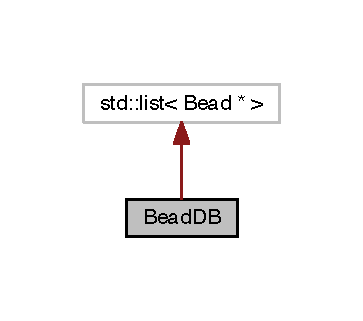
\includegraphics[width=174pt]{classBeadDB__inherit__graph}
\end{center}
\end{figure}


Collaboration diagram for Bead\+D\+B\+:\nopagebreak
\begin{figure}[H]
\begin{center}
\leavevmode
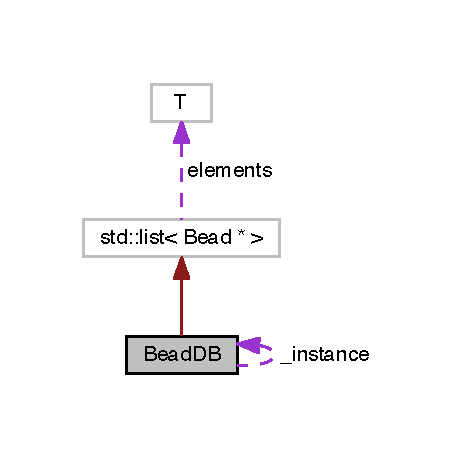
\includegraphics[width=217pt]{classBeadDB__coll__graph}
\end{center}
\end{figure}
\subsection*{Public Member Functions}
\begin{DoxyCompactItemize}
\item 
\hyperlink{classBeadDB_a47d7b62ae87aeffb76e6ded2798188ac}{Bead\+D\+B} (const \hyperlink{classBeadDB}{Bead\+D\+B} \&rhs)=delete
\begin{DoxyCompactList}\small\item\em Copying is not allowed. \end{DoxyCompactList}\item 
\hyperlink{classBeadDB}{Bead\+D\+B} \& \hyperlink{classBeadDB_a7e9c6a6635a39aa7cb4f18c1103df01d}{operator=} (\hyperlink{classBeadDB}{Bead\+D\+B} \&rhs)=delete
\begin{DoxyCompactList}\small\item\em Assignment is not allowed. \end{DoxyCompactList}\item 
void \hyperlink{classBeadDB_a2c4d09dbcad9f65129308ae570583134}{add\+Bead} (\hyperlink{classBead}{Bead} $\ast$b)
\begin{DoxyCompactList}\small\item\em Add a bead. \end{DoxyCompactList}\item 
void \hyperlink{classBeadDB_aa5069d3136246c17201f3d49c3e96405}{remove\+Bead} (\hyperlink{classBead}{Bead} $\ast$b)
\begin{DoxyCompactList}\small\item\em Remove a bead. \end{DoxyCompactList}\end{DoxyCompactItemize}
\subsection*{Static Public Member Functions}
\begin{DoxyCompactItemize}
\item 
static \hyperlink{classBeadDB}{Bead\+D\+B} $\ast$ \hyperlink{classBeadDB_a7a57dea5ef46dff11f7589d00d05a4c0}{instance} ()
\begin{DoxyCompactList}\small\item\em Get the instance of this singleton. \end{DoxyCompactList}\end{DoxyCompactItemize}
\subsection*{Private Types}
\begin{DoxyCompactItemize}
\item 
typedef list$<$ \hyperlink{classBead}{Bead} $\ast$ $>$ \hyperlink{classBeadDB_a0312ccca7bb1de087f91481aec353d60}{bdb}
\end{DoxyCompactItemize}
\subsection*{Private Member Functions}
\begin{DoxyCompactItemize}
\item 
\hyperlink{classBeadDB_ac25beed230d37dc184ca8c7e7b4ea087}{Bead\+D\+B} ()
\end{DoxyCompactItemize}
\subsection*{Private Attributes}
\begin{DoxyCompactItemize}
\item 
T {\bfseries elements}
\begin{DoxyCompactList}\small\item\em S\+T\+L member. \end{DoxyCompactList}\end{DoxyCompactItemize}
\subsection*{Static Private Attributes}
\begin{DoxyCompactItemize}
\item 
static \hyperlink{classBeadDB}{Bead\+D\+B} $\ast$ \hyperlink{classBeadDB_a99d68441bc8e90450f7d1fd6d65acd22}{\+\_\+instance} = 0
\begin{DoxyCompactList}\small\item\em Singleton instance. \end{DoxyCompactList}\end{DoxyCompactItemize}


\subsection{Detailed Description}
A database for all \hyperlink{classBead}{Beads} in the system. 

This \hyperlink{classBeadDB}{Bead\+D\+B} inherits from list and manage all creations and removing of \hyperlink{classBead}{Bead} objects, as well as some standard list functions and iterators. 

Definition at line 30 of file Bead\+D\+B.\+h.



\subsection{Member Typedef Documentation}
\hypertarget{classBeadDB_a0312ccca7bb1de087f91481aec353d60}{\index{Bead\+D\+B@{Bead\+D\+B}!bdb@{bdb}}
\index{bdb@{bdb}!Bead\+D\+B@{Bead\+D\+B}}
\subsubsection[{bdb}]{\setlength{\rightskip}{0pt plus 5cm}typedef list$<${\bf Bead}$\ast$$>$ {\bf Bead\+D\+B\+::bdb}\hspace{0.3cm}{\ttfamily [private]}}}\label{classBeadDB_a0312ccca7bb1de087f91481aec353d60}


Definition at line 32 of file Bead\+D\+B.\+h.



\subsection{Constructor \& Destructor Documentation}
\hypertarget{classBeadDB_a47d7b62ae87aeffb76e6ded2798188ac}{\index{Bead\+D\+B@{Bead\+D\+B}!Bead\+D\+B@{Bead\+D\+B}}
\index{Bead\+D\+B@{Bead\+D\+B}!Bead\+D\+B@{Bead\+D\+B}}
\subsubsection[{Bead\+D\+B}]{\setlength{\rightskip}{0pt plus 5cm}Bead\+D\+B\+::\+Bead\+D\+B (
\begin{DoxyParamCaption}
\item[{const {\bf Bead\+D\+B} \&}]{rhs}
\end{DoxyParamCaption}
)\hspace{0.3cm}{\ttfamily [delete]}}}\label{classBeadDB_a47d7b62ae87aeffb76e6ded2798188ac}


Copying is not allowed. 

\hypertarget{classBeadDB_ac25beed230d37dc184ca8c7e7b4ea087}{\index{Bead\+D\+B@{Bead\+D\+B}!Bead\+D\+B@{Bead\+D\+B}}
\index{Bead\+D\+B@{Bead\+D\+B}!Bead\+D\+B@{Bead\+D\+B}}
\subsubsection[{Bead\+D\+B}]{\setlength{\rightskip}{0pt plus 5cm}Bead\+D\+B\+::\+Bead\+D\+B (
\begin{DoxyParamCaption}
{}
\end{DoxyParamCaption}
)\hspace{0.3cm}{\ttfamily [inline]}, {\ttfamily [private]}}}\label{classBeadDB_ac25beed230d37dc184ca8c7e7b4ea087}


Definition at line 57 of file Bead\+D\+B.\+h.



Referenced by instance().



\subsection{Member Function Documentation}
\hypertarget{classBeadDB_a2c4d09dbcad9f65129308ae570583134}{\index{Bead\+D\+B@{Bead\+D\+B}!add\+Bead@{add\+Bead}}
\index{add\+Bead@{add\+Bead}!Bead\+D\+B@{Bead\+D\+B}}
\subsubsection[{add\+Bead}]{\setlength{\rightskip}{0pt plus 5cm}void Bead\+D\+B\+::add\+Bead (
\begin{DoxyParamCaption}
\item[{{\bf Bead} $\ast$}]{b}
\end{DoxyParamCaption}
)\hspace{0.3cm}{\ttfamily [inline]}}}\label{classBeadDB_a2c4d09dbcad9f65129308ae570583134}


Add a bead. 



Definition at line 51 of file Bead\+D\+B.\+h.



Referenced by Bead\+::\+Bead().

\hypertarget{classBeadDB_a7a57dea5ef46dff11f7589d00d05a4c0}{\index{Bead\+D\+B@{Bead\+D\+B}!instance@{instance}}
\index{instance@{instance}!Bead\+D\+B@{Bead\+D\+B}}
\subsubsection[{instance}]{\setlength{\rightskip}{0pt plus 5cm}{\bf Bead\+D\+B} $\ast$ Bead\+D\+B\+::instance (
\begin{DoxyParamCaption}
{}
\end{DoxyParamCaption}
)\hspace{0.3cm}{\ttfamily [static]}}}\label{classBeadDB_a7a57dea5ef46dff11f7589d00d05a4c0}


Get the instance of this singleton. 



Definition at line 18 of file Bead\+D\+B.\+cpp.



References \+\_\+instance, and Bead\+D\+B().



Referenced by C\+G\+Method\+::backtracking\+Line\+Search(), Bead\+::\+Bead(), C\+G\+Method\+::grad\+Aux\+Square(), C\+G\+Method\+::grad\+Dot\+Product(), C\+G\+Method\+::grad\+Square(), Fletcher\+Rieves\+::minimize(), Polak\+Ribiere\+::minimize(), C\+G\+Method\+::move\+Beads(), C\+G\+Method\+::move\+Beads\+Aux(), C\+G\+Method\+::print\+Forces(), C\+G\+Method\+::quadratic\+Line\+Search(), Force\+Field\+Manager\+::reset\+Forces(), Force\+Field\+Manager\+::reset\+Forces\+Aux(), C\+G\+Method\+::shift\+Gradient(), Boundary\+Element\+Neighbor\+List\+::update\+Neighbors(), and Bead\+::$\sim$\+Bead().

\hypertarget{classBeadDB_a7e9c6a6635a39aa7cb4f18c1103df01d}{\index{Bead\+D\+B@{Bead\+D\+B}!operator=@{operator=}}
\index{operator=@{operator=}!Bead\+D\+B@{Bead\+D\+B}}
\subsubsection[{operator=}]{\setlength{\rightskip}{0pt plus 5cm}{\bf Bead\+D\+B}\& Bead\+D\+B\+::operator= (
\begin{DoxyParamCaption}
\item[{{\bf Bead\+D\+B} \&}]{rhs}
\end{DoxyParamCaption}
)\hspace{0.3cm}{\ttfamily [delete]}}}\label{classBeadDB_a7e9c6a6635a39aa7cb4f18c1103df01d}


Assignment is not allowed. 

\hypertarget{classBeadDB_aa5069d3136246c17201f3d49c3e96405}{\index{Bead\+D\+B@{Bead\+D\+B}!remove\+Bead@{remove\+Bead}}
\index{remove\+Bead@{remove\+Bead}!Bead\+D\+B@{Bead\+D\+B}}
\subsubsection[{remove\+Bead}]{\setlength{\rightskip}{0pt plus 5cm}void Bead\+D\+B\+::remove\+Bead (
\begin{DoxyParamCaption}
\item[{{\bf Bead} $\ast$}]{b}
\end{DoxyParamCaption}
)\hspace{0.3cm}{\ttfamily [inline]}}}\label{classBeadDB_aa5069d3136246c17201f3d49c3e96405}


Remove a bead. 



Definition at line 53 of file Bead\+D\+B.\+h.



Referenced by Bead\+::$\sim$\+Bead().



\subsection{Member Data Documentation}
\hypertarget{classBeadDB_a99d68441bc8e90450f7d1fd6d65acd22}{\index{Bead\+D\+B@{Bead\+D\+B}!\+\_\+instance@{\+\_\+instance}}
\index{\+\_\+instance@{\+\_\+instance}!Bead\+D\+B@{Bead\+D\+B}}
\subsubsection[{\+\_\+instance}]{\setlength{\rightskip}{0pt plus 5cm}{\bf Bead\+D\+B} $\ast$ Bead\+D\+B\+::\+\_\+instance = 0\hspace{0.3cm}{\ttfamily [static]}, {\ttfamily [private]}}}\label{classBeadDB_a99d68441bc8e90450f7d1fd6d65acd22}


Singleton instance. 



Definition at line 56 of file Bead\+D\+B.\+h.



Referenced by instance().

\hypertarget{classstd_1_1list_a682e5c7c91eb377d0cb4f019b2b81a5d}{\index{Bead\+D\+B@{Bead\+D\+B}!elements@{elements}}
\index{elements@{elements}!Bead\+D\+B@{Bead\+D\+B}}
\subsubsection[{elements}]{\setlength{\rightskip}{0pt plus 5cm}T std\+::list$<$ T $>$\+::elements\hspace{0.3cm}{\ttfamily [inherited]}}}\label{classstd_1_1list_a682e5c7c91eb377d0cb4f019b2b81a5d}


S\+T\+L member. 



The documentation for this class was generated from the following files\+:\begin{DoxyCompactItemize}
\item 
M3\+S\+Y\+M/\+Structure/\hyperlink{BeadDB_8h}{Bead\+D\+B.\+h}\item 
M3\+S\+Y\+M/\+Structure/\hyperlink{BeadDB_8cpp}{Bead\+D\+B.\+cpp}\end{DoxyCompactItemize}

\hypertarget{classBoundary}{\section{Boundary Class Reference}
\label{classBoundary}\index{Boundary@{Boundary}}
}


To store all boundary surfaces that are in the system.  




{\ttfamily \#include $<$Boundary.\+h$>$}



Inheritance diagram for Boundary\+:\nopagebreak
\begin{figure}[H]
\begin{center}
\leavevmode
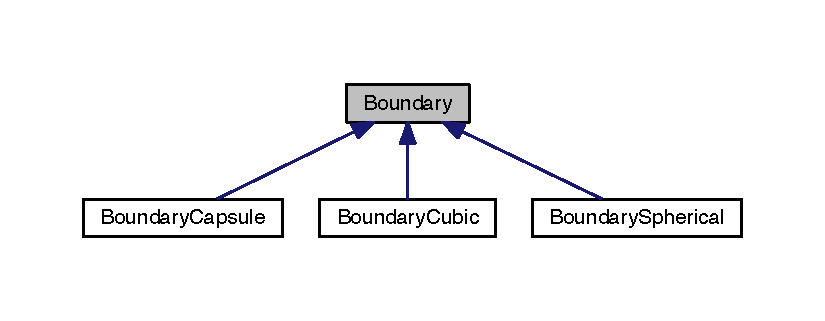
\includegraphics[width=350pt]{classBoundary__inherit__graph}
\end{center}
\end{figure}


Collaboration diagram for Boundary\+:\nopagebreak
\begin{figure}[H]
\begin{center}
\leavevmode
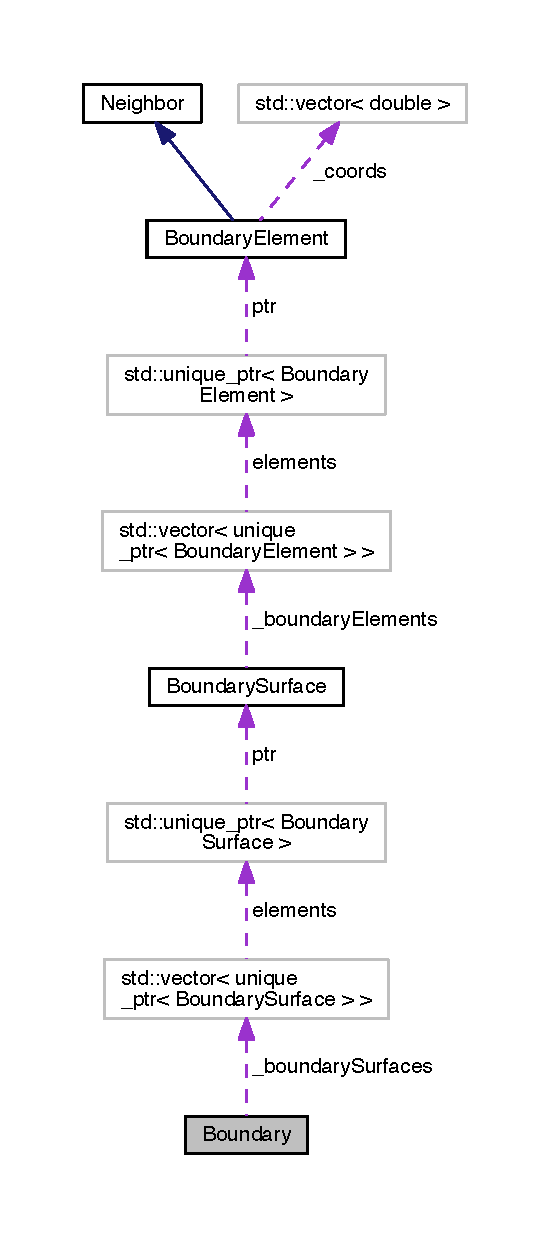
\includegraphics[height=550pt]{classBoundary__coll__graph}
\end{center}
\end{figure}
\subsection*{Public Member Functions}
\begin{DoxyCompactItemize}
\item 
\hyperlink{classBoundary_ac6eb3bf752b27d4d799c4d2691b312ce}{Boundary} (int n\+Dim, \hyperlink{Boundary_8h_a0099b369f2bc119c1b54728734b41132}{Boundary\+Shape} shape)
\item 
\hyperlink{classBoundary_a86eab4f2362618c5b1e3d0df3a5f7f42}{$\sim$\+Boundary} ()
\item 
\hyperlink{Boundary_8h_a0099b369f2bc119c1b54728734b41132}{Boundary\+Shape} \hyperlink{classBoundary_a20d2121527b207eed35f6719393e3499}{get\+Shape} ()
\begin{DoxyCompactList}\small\item\em Get shape. \end{DoxyCompactList}\item 
const vector$<$ unique\+\_\+ptr\\*
$<$ \hyperlink{classBoundarySurface}{Boundary\+Surface} $>$ $>$ \& \hyperlink{classBoundary_acfa6640f65c432e339108887913539eb}{get\+Boundary\+Surfaces} ()
\begin{DoxyCompactList}\small\item\em Get boundarysurfaces. \end{DoxyCompactList}\item 
virtual bool \hyperlink{classBoundary_aef1af10ace9eae30e86b6bd23087b3ff}{within} (const vector$<$ double $>$ \&coordinates)=0
\begin{DoxyCompactList}\small\item\em Check if coordinates are within boundary. \end{DoxyCompactList}\end{DoxyCompactItemize}
\subsection*{Protected Attributes}
\begin{DoxyCompactItemize}
\item 
vector$<$ unique\+\_\+ptr\\*
$<$ \hyperlink{classBoundarySurface}{Boundary\+Surface} $>$ $>$ \hyperlink{classBoundary_abbac1843206a158e7d0a6e741cdc00c1}{\+\_\+boundary\+Surfaces}
\begin{DoxyCompactList}\small\item\em Vector of boundarysurfaces (could be different implementations) \end{DoxyCompactList}\item 
\hyperlink{Boundary_8h_a0099b369f2bc119c1b54728734b41132}{Boundary\+Shape} \hyperlink{classBoundary_a04c10c9a7aea1924d779d392e29f94ff}{\+\_\+shape}
\begin{DoxyCompactList}\small\item\em Shape of boundary. \end{DoxyCompactList}\item 
short \hyperlink{classBoundary_a96f2294e0c822ab216fe5ab7e17258c7}{\+\_\+n\+Dim}
\begin{DoxyCompactList}\small\item\em Dimensionality. \end{DoxyCompactList}\end{DoxyCompactItemize}


\subsection{Detailed Description}
To store all boundary surfaces that are in the system. 

The boundary class stores all \hyperlink{classBoundarySurface}{Boundary\+Surfaces} in the given shape. Its constructors can create basic boundary shapes (for now). Eventually will be extended to more complex surfaces. 

Definition at line 29 of file Boundary.\+h.



\subsection{Constructor \& Destructor Documentation}
\hypertarget{classBoundary_ac6eb3bf752b27d4d799c4d2691b312ce}{\index{Boundary@{Boundary}!Boundary@{Boundary}}
\index{Boundary@{Boundary}!Boundary@{Boundary}}
\subsubsection[{Boundary}]{\setlength{\rightskip}{0pt plus 5cm}Boundary\+::\+Boundary (
\begin{DoxyParamCaption}
\item[{int}]{n\+Dim, }
\item[{{\bf Boundary\+Shape}}]{shape}
\end{DoxyParamCaption}
)\hspace{0.3cm}{\ttfamily [inline]}}}\label{classBoundary_ac6eb3bf752b27d4d799c4d2691b312ce}


Definition at line 38 of file Boundary.\+h.

\hypertarget{classBoundary_a86eab4f2362618c5b1e3d0df3a5f7f42}{\index{Boundary@{Boundary}!````~Boundary@{$\sim$\+Boundary}}
\index{````~Boundary@{$\sim$\+Boundary}!Boundary@{Boundary}}
\subsubsection[{$\sim$\+Boundary}]{\setlength{\rightskip}{0pt plus 5cm}Boundary\+::$\sim$\+Boundary (
\begin{DoxyParamCaption}
{}
\end{DoxyParamCaption}
)\hspace{0.3cm}{\ttfamily [inline]}}}\label{classBoundary_a86eab4f2362618c5b1e3d0df3a5f7f42}


Definition at line 39 of file Boundary.\+h.



\subsection{Member Function Documentation}
\hypertarget{classBoundary_acfa6640f65c432e339108887913539eb}{\index{Boundary@{Boundary}!get\+Boundary\+Surfaces@{get\+Boundary\+Surfaces}}
\index{get\+Boundary\+Surfaces@{get\+Boundary\+Surfaces}!Boundary@{Boundary}}
\subsubsection[{get\+Boundary\+Surfaces}]{\setlength{\rightskip}{0pt plus 5cm}const vector$<$unique\+\_\+ptr$<${\bf Boundary\+Surface}$>$ $>$\& Boundary\+::get\+Boundary\+Surfaces (
\begin{DoxyParamCaption}
{}
\end{DoxyParamCaption}
)\hspace{0.3cm}{\ttfamily [inline]}}}\label{classBoundary_acfa6640f65c432e339108887913539eb}


Get boundarysurfaces. 



Definition at line 44 of file Boundary.\+h.



References \+\_\+boundary\+Surfaces.

\hypertarget{classBoundary_a20d2121527b207eed35f6719393e3499}{\index{Boundary@{Boundary}!get\+Shape@{get\+Shape}}
\index{get\+Shape@{get\+Shape}!Boundary@{Boundary}}
\subsubsection[{get\+Shape}]{\setlength{\rightskip}{0pt plus 5cm}{\bf Boundary\+Shape} Boundary\+::get\+Shape (
\begin{DoxyParamCaption}
{}
\end{DoxyParamCaption}
)\hspace{0.3cm}{\ttfamily [inline]}}}\label{classBoundary_a20d2121527b207eed35f6719393e3499}


Get shape. 



Definition at line 42 of file Boundary.\+h.



References \+\_\+shape.

\hypertarget{classBoundary_aef1af10ace9eae30e86b6bd23087b3ff}{\index{Boundary@{Boundary}!within@{within}}
\index{within@{within}!Boundary@{Boundary}}
\subsubsection[{within}]{\setlength{\rightskip}{0pt plus 5cm}virtual bool Boundary\+::within (
\begin{DoxyParamCaption}
\item[{const vector$<$ double $>$ \&}]{coordinates}
\end{DoxyParamCaption}
)\hspace{0.3cm}{\ttfamily [pure virtual]}}}\label{classBoundary_aef1af10ace9eae30e86b6bd23087b3ff}


Check if coordinates are within boundary. 



Implemented in \hyperlink{classBoundaryCapsule_a9e462a1fbb221933735c35df1e7eb75d}{Boundary\+Capsule}, \hyperlink{classBoundarySpherical_a653f35719ff4baec5848053093978ee9}{Boundary\+Spherical}, and \hyperlink{classBoundaryCubic_a07b7fc5d0d09b0ce39e92e6b4bd2a7a4}{Boundary\+Cubic}.



Referenced by G\+Controller\+::activate\+Compartments().



\subsection{Member Data Documentation}
\hypertarget{classBoundary_abbac1843206a158e7d0a6e741cdc00c1}{\index{Boundary@{Boundary}!\+\_\+boundary\+Surfaces@{\+\_\+boundary\+Surfaces}}
\index{\+\_\+boundary\+Surfaces@{\+\_\+boundary\+Surfaces}!Boundary@{Boundary}}
\subsubsection[{\+\_\+boundary\+Surfaces}]{\setlength{\rightskip}{0pt plus 5cm}vector$<$unique\+\_\+ptr$<${\bf Boundary\+Surface}$>$ $>$ Boundary\+::\+\_\+boundary\+Surfaces\hspace{0.3cm}{\ttfamily [protected]}}}\label{classBoundary_abbac1843206a158e7d0a6e741cdc00c1}


Vector of boundarysurfaces (could be different implementations) 



Definition at line 33 of file Boundary.\+h.



Referenced by Boundary\+Capsule\+::\+Boundary\+Capsule(), Boundary\+Cubic\+::\+Boundary\+Cubic(), Boundary\+Spherical\+::\+Boundary\+Spherical(), get\+Boundary\+Surfaces(), Boundary\+Cubic\+::within(), Boundary\+Spherical\+::within(), and Boundary\+Capsule\+::within().

\hypertarget{classBoundary_a96f2294e0c822ab216fe5ab7e17258c7}{\index{Boundary@{Boundary}!\+\_\+n\+Dim@{\+\_\+n\+Dim}}
\index{\+\_\+n\+Dim@{\+\_\+n\+Dim}!Boundary@{Boundary}}
\subsubsection[{\+\_\+n\+Dim}]{\setlength{\rightskip}{0pt plus 5cm}short Boundary\+::\+\_\+n\+Dim\hspace{0.3cm}{\ttfamily [protected]}}}\label{classBoundary_a96f2294e0c822ab216fe5ab7e17258c7}


Dimensionality. 



Definition at line 35 of file Boundary.\+h.

\hypertarget{classBoundary_a04c10c9a7aea1924d779d392e29f94ff}{\index{Boundary@{Boundary}!\+\_\+shape@{\+\_\+shape}}
\index{\+\_\+shape@{\+\_\+shape}!Boundary@{Boundary}}
\subsubsection[{\+\_\+shape}]{\setlength{\rightskip}{0pt plus 5cm}{\bf Boundary\+Shape} Boundary\+::\+\_\+shape\hspace{0.3cm}{\ttfamily [protected]}}}\label{classBoundary_a04c10c9a7aea1924d779d392e29f94ff}


Shape of boundary. 



Definition at line 34 of file Boundary.\+h.



Referenced by get\+Shape().



The documentation for this class was generated from the following file\+:\begin{DoxyCompactItemize}
\item 
M3\+S\+Y\+M/\+Structure/\hyperlink{Boundary_8h}{Boundary.\+h}\end{DoxyCompactItemize}

\hypertarget{classBoundaryCapsule}{\section{Boundary\+Capsule Class Reference}
\label{classBoundaryCapsule}\index{Boundary\+Capsule@{Boundary\+Capsule}}
}


A capsule boundary implementation.  




{\ttfamily \#include $<$Boundary\+Impl.\+h$>$}



Inheritance diagram for Boundary\+Capsule\+:\nopagebreak
\begin{figure}[H]
\begin{center}
\leavevmode
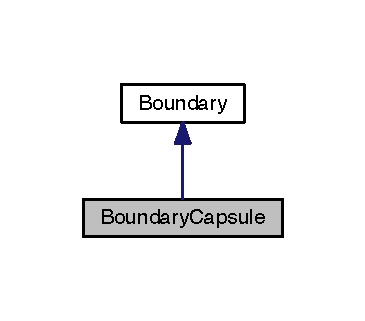
\includegraphics[width=175pt]{classBoundaryCapsule__inherit__graph}
\end{center}
\end{figure}


Collaboration diagram for Boundary\+Capsule\+:\nopagebreak
\begin{figure}[H]
\begin{center}
\leavevmode
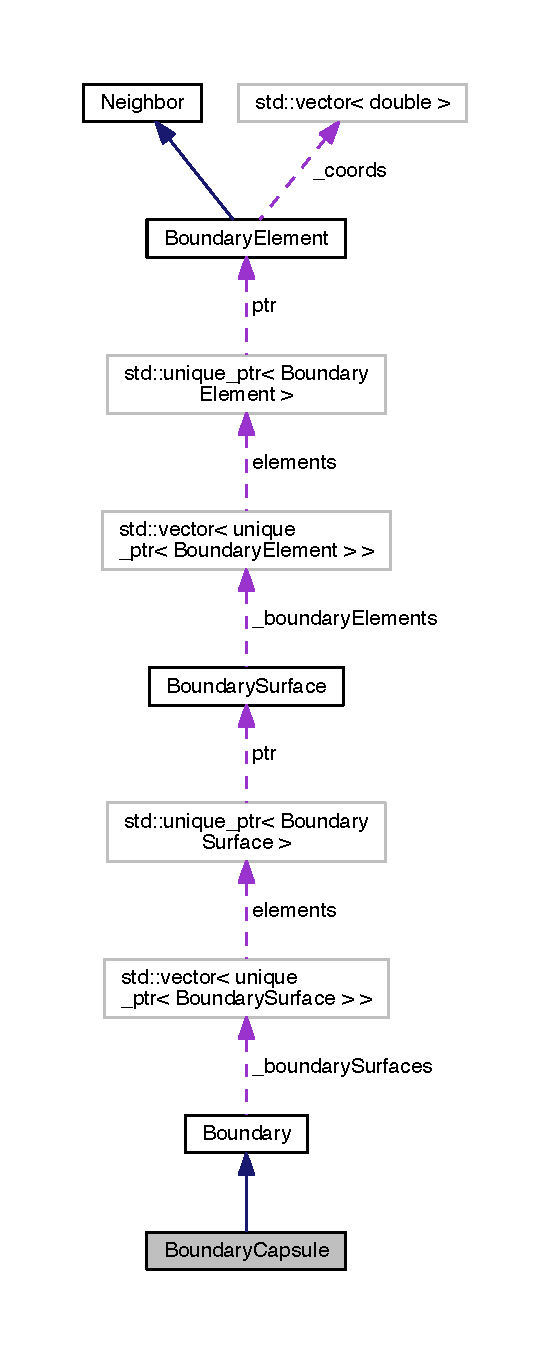
\includegraphics[height=550pt]{classBoundaryCapsule__coll__graph}
\end{center}
\end{figure}
\subsection*{Public Member Functions}
\begin{DoxyCompactItemize}
\item 
\hyperlink{classBoundaryCapsule_a8a5ab010ef57a344a1cb0a233572b0e1}{Boundary\+Capsule} (double diameter)
\begin{DoxyCompactList}\small\item\em Default constructor, will create a capsule with given diameter, and height equal to current grid. \end{DoxyCompactList}\item 
virtual bool \hyperlink{classBoundaryCapsule_a9e462a1fbb221933735c35df1e7eb75d}{within} (const vector$<$ double $>$ \&coordinates)
\begin{DoxyCompactList}\small\item\em Check if coordinates are within boundary. \end{DoxyCompactList}\item 
\hyperlink{Boundary_8h_a0099b369f2bc119c1b54728734b41132}{Boundary\+Shape} \hyperlink{classBoundary_a20d2121527b207eed35f6719393e3499}{get\+Shape} ()
\begin{DoxyCompactList}\small\item\em Get shape of boundary. \end{DoxyCompactList}\item 
const vector$<$ unique\+\_\+ptr\\*
$<$ \hyperlink{classBoundarySurface}{Boundary\+Surface} $>$ $>$ \& \hyperlink{classBoundary_acfa6640f65c432e339108887913539eb}{get\+Boundary\+Surfaces} ()
\begin{DoxyCompactList}\small\item\em Get boundary surfaces. \end{DoxyCompactList}\end{DoxyCompactItemize}
\subsection*{Protected Attributes}
\begin{DoxyCompactItemize}
\item 
vector$<$ unique\+\_\+ptr\\*
$<$ \hyperlink{classBoundarySurface}{Boundary\+Surface} $>$ $>$ \hyperlink{classBoundary_abbac1843206a158e7d0a6e741cdc00c1}{\+\_\+boundary\+Surfaces}
\begin{DoxyCompactList}\small\item\em Vector of boundary surfaces (could be different implementations) \end{DoxyCompactList}\item 
\hyperlink{Boundary_8h_a0099b369f2bc119c1b54728734b41132}{Boundary\+Shape} \hyperlink{classBoundary_a04c10c9a7aea1924d779d392e29f94ff}{\+\_\+shape}
\begin{DoxyCompactList}\small\item\em \hyperlink{classBoundary}{Boundary} type of this boundary. \end{DoxyCompactList}\item 
short \hyperlink{classBoundary_a96f2294e0c822ab216fe5ab7e17258c7}{\+\_\+n\+Dim}
\begin{DoxyCompactList}\small\item\em Dimensionality of this boundary. \end{DoxyCompactList}\end{DoxyCompactItemize}


\subsection{Detailed Description}
A capsule boundary implementation. 

Definition at line 45 of file Boundary\+Impl.\+h.



\subsection{Constructor \& Destructor Documentation}
\hypertarget{classBoundaryCapsule_a8a5ab010ef57a344a1cb0a233572b0e1}{\index{Boundary\+Capsule@{Boundary\+Capsule}!Boundary\+Capsule@{Boundary\+Capsule}}
\index{Boundary\+Capsule@{Boundary\+Capsule}!Boundary\+Capsule@{Boundary\+Capsule}}
\subsubsection[{Boundary\+Capsule}]{\setlength{\rightskip}{0pt plus 5cm}Boundary\+Capsule\+::\+Boundary\+Capsule (
\begin{DoxyParamCaption}
\item[{double}]{diameter}
\end{DoxyParamCaption}
)}}\label{classBoundaryCapsule_a8a5ab010ef57a344a1cb0a233572b0e1}


Default constructor, will create a capsule with given diameter, and height equal to current grid. 


\begin{DoxyParams}{Parameters}
{\em diameter} & -\/ diameter of capsule (will set half sphere radii as well as cylinder radius) \\
\hline
\end{DoxyParams}


Definition at line 74 of file Boundary\+Impl.\+cpp.



References Boundary\+::\+\_\+boundary\+Surfaces, Capsule, Geometry\+Parameters\+::compartment\+Size\+X, Geometry\+Parameters\+::compartment\+Size\+Y, Geometry\+Parameters\+::compartment\+Size\+Z, System\+Parameters\+::\+Geometry(), Geometry\+Parameters\+::\+N\+X, Geometry\+Parameters\+::\+N\+Y, and Geometry\+Parameters\+::\+N\+Z.



\subsection{Member Function Documentation}
\hypertarget{classBoundary_acfa6640f65c432e339108887913539eb}{\index{Boundary\+Capsule@{Boundary\+Capsule}!get\+Boundary\+Surfaces@{get\+Boundary\+Surfaces}}
\index{get\+Boundary\+Surfaces@{get\+Boundary\+Surfaces}!Boundary\+Capsule@{Boundary\+Capsule}}
\subsubsection[{get\+Boundary\+Surfaces}]{\setlength{\rightskip}{0pt plus 5cm}const vector$<$unique\+\_\+ptr$<${\bf Boundary\+Surface}$>$ $>$\& Boundary\+::get\+Boundary\+Surfaces (
\begin{DoxyParamCaption}
{}
\end{DoxyParamCaption}
)\hspace{0.3cm}{\ttfamily [inline]}, {\ttfamily [inherited]}}}\label{classBoundary_acfa6640f65c432e339108887913539eb}


Get boundary surfaces. 



Definition at line 44 of file Boundary.\+h.



References Boundary\+::\+\_\+boundary\+Surfaces.

\hypertarget{classBoundary_a20d2121527b207eed35f6719393e3499}{\index{Boundary\+Capsule@{Boundary\+Capsule}!get\+Shape@{get\+Shape}}
\index{get\+Shape@{get\+Shape}!Boundary\+Capsule@{Boundary\+Capsule}}
\subsubsection[{get\+Shape}]{\setlength{\rightskip}{0pt plus 5cm}{\bf Boundary\+Shape} Boundary\+::get\+Shape (
\begin{DoxyParamCaption}
{}
\end{DoxyParamCaption}
)\hspace{0.3cm}{\ttfamily [inline]}, {\ttfamily [inherited]}}}\label{classBoundary_a20d2121527b207eed35f6719393e3499}


Get shape of boundary. 



Definition at line 42 of file Boundary.\+h.



References Boundary\+::\+\_\+shape.

\hypertarget{classBoundaryCapsule_a9e462a1fbb221933735c35df1e7eb75d}{\index{Boundary\+Capsule@{Boundary\+Capsule}!within@{within}}
\index{within@{within}!Boundary\+Capsule@{Boundary\+Capsule}}
\subsubsection[{within}]{\setlength{\rightskip}{0pt plus 5cm}bool Boundary\+Capsule\+::within (
\begin{DoxyParamCaption}
\item[{const vector$<$ double $>$ \&}]{coordinates}
\end{DoxyParamCaption}
)\hspace{0.3cm}{\ttfamily [virtual]}}}\label{classBoundaryCapsule_a9e462a1fbb221933735c35df1e7eb75d}


Check if coordinates are within boundary. 



Implements \hyperlink{classBoundary_aef1af10ace9eae30e86b6bd23087b3ff}{Boundary}.



Definition at line 87 of file Boundary\+Impl.\+cpp.



References Boundary\+::\+\_\+boundary\+Surfaces, and Boundary\+Element\+::distance().



\subsection{Member Data Documentation}
\hypertarget{classBoundary_abbac1843206a158e7d0a6e741cdc00c1}{\index{Boundary\+Capsule@{Boundary\+Capsule}!\+\_\+boundary\+Surfaces@{\+\_\+boundary\+Surfaces}}
\index{\+\_\+boundary\+Surfaces@{\+\_\+boundary\+Surfaces}!Boundary\+Capsule@{Boundary\+Capsule}}
\subsubsection[{\+\_\+boundary\+Surfaces}]{\setlength{\rightskip}{0pt plus 5cm}vector$<$unique\+\_\+ptr$<${\bf Boundary\+Surface}$>$ $>$ Boundary\+::\+\_\+boundary\+Surfaces\hspace{0.3cm}{\ttfamily [protected]}, {\ttfamily [inherited]}}}\label{classBoundary_abbac1843206a158e7d0a6e741cdc00c1}


Vector of boundary surfaces (could be different implementations) 



Definition at line 33 of file Boundary.\+h.



Referenced by Boundary\+Capsule(), Boundary\+Cubic\+::\+Boundary\+Cubic(), Boundary\+Spherical\+::\+Boundary\+Spherical(), Boundary\+::get\+Boundary\+Surfaces(), Boundary\+Cubic\+::within(), Boundary\+Spherical\+::within(), and within().

\hypertarget{classBoundary_a96f2294e0c822ab216fe5ab7e17258c7}{\index{Boundary\+Capsule@{Boundary\+Capsule}!\+\_\+n\+Dim@{\+\_\+n\+Dim}}
\index{\+\_\+n\+Dim@{\+\_\+n\+Dim}!Boundary\+Capsule@{Boundary\+Capsule}}
\subsubsection[{\+\_\+n\+Dim}]{\setlength{\rightskip}{0pt plus 5cm}short Boundary\+::\+\_\+n\+Dim\hspace{0.3cm}{\ttfamily [protected]}, {\ttfamily [inherited]}}}\label{classBoundary_a96f2294e0c822ab216fe5ab7e17258c7}


Dimensionality of this boundary. 



Definition at line 35 of file Boundary.\+h.

\hypertarget{classBoundary_a04c10c9a7aea1924d779d392e29f94ff}{\index{Boundary\+Capsule@{Boundary\+Capsule}!\+\_\+shape@{\+\_\+shape}}
\index{\+\_\+shape@{\+\_\+shape}!Boundary\+Capsule@{Boundary\+Capsule}}
\subsubsection[{\+\_\+shape}]{\setlength{\rightskip}{0pt plus 5cm}{\bf Boundary\+Shape} Boundary\+::\+\_\+shape\hspace{0.3cm}{\ttfamily [protected]}, {\ttfamily [inherited]}}}\label{classBoundary_a04c10c9a7aea1924d779d392e29f94ff}


\hyperlink{classBoundary}{Boundary} type of this boundary. 



Definition at line 34 of file Boundary.\+h.



Referenced by Boundary\+::get\+Shape().



The documentation for this class was generated from the following files\+:\begin{DoxyCompactItemize}
\item 
M3\+S\+Y\+M/\+Structure/\hyperlink{BoundaryImpl_8h}{Boundary\+Impl.\+h}\item 
M3\+S\+Y\+M/\+Structure/\hyperlink{BoundaryImpl_8cpp}{Boundary\+Impl.\+cpp}\end{DoxyCompactItemize}

\hypertarget{classBoundaryCubic}{\section{Boundary\+Cubic Class Reference}
\label{classBoundaryCubic}\index{Boundary\+Cubic@{Boundary\+Cubic}}
}


A cubic boundary implementation.  




{\ttfamily \#include $<$Boundary\+Impl.\+h$>$}



Inheritance diagram for Boundary\+Cubic\+:\nopagebreak
\begin{figure}[H]
\begin{center}
\leavevmode
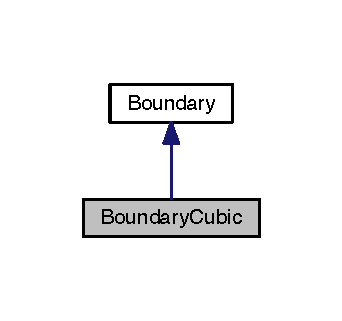
\includegraphics[width=164pt]{classBoundaryCubic__inherit__graph}
\end{center}
\end{figure}


Collaboration diagram for Boundary\+Cubic\+:\nopagebreak
\begin{figure}[H]
\begin{center}
\leavevmode
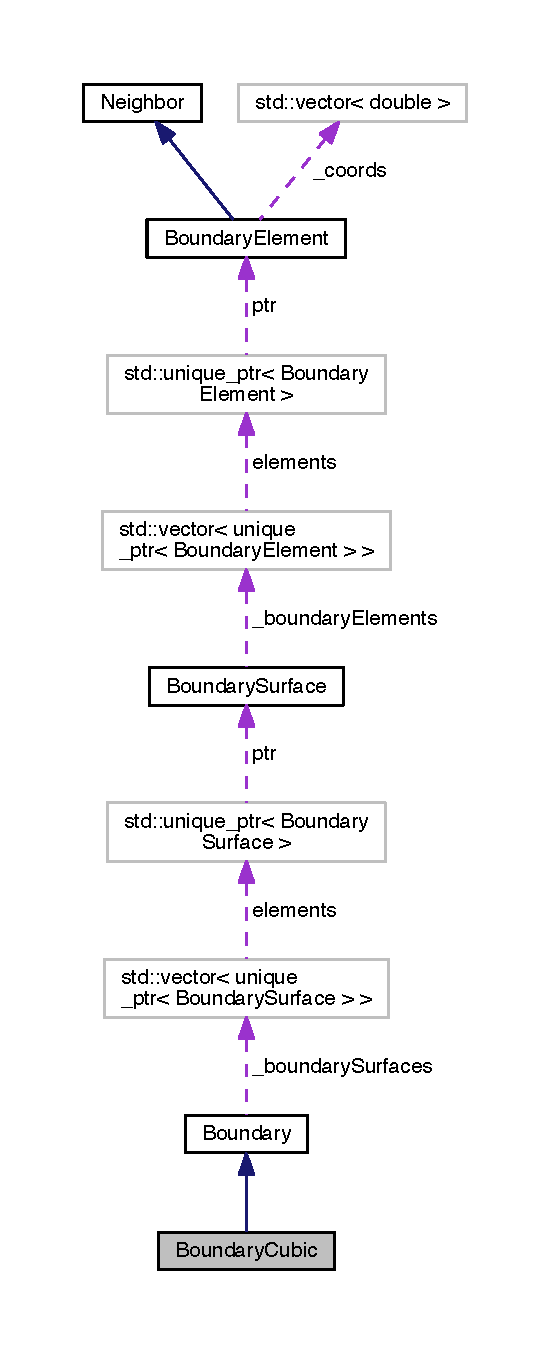
\includegraphics[height=550pt]{classBoundaryCubic__coll__graph}
\end{center}
\end{figure}
\subsection*{Public Member Functions}
\begin{DoxyCompactItemize}
\item 
\hyperlink{classBoundaryCubic_abba330bb75d623c8fa0884eeea937e63}{Boundary\+Cubic} ()
\begin{DoxyCompactList}\small\item\em Default constructor, this will create a cube with given corners at edges of current grid. \end{DoxyCompactList}\item 
virtual bool \hyperlink{classBoundaryCubic_a07b7fc5d0d09b0ce39e92e6b4bd2a7a4}{within} (const vector$<$ double $>$ \&coordinates)
\begin{DoxyCompactList}\small\item\em Check if coordinates are within boundary. \end{DoxyCompactList}\item 
\hyperlink{Boundary_8h_a0099b369f2bc119c1b54728734b41132}{Boundary\+Shape} \hyperlink{classBoundary_a20d2121527b207eed35f6719393e3499}{get\+Shape} ()
\begin{DoxyCompactList}\small\item\em Get shape of boundary. \end{DoxyCompactList}\item 
const vector$<$ unique\+\_\+ptr\\*
$<$ \hyperlink{classBoundarySurface}{Boundary\+Surface} $>$ $>$ \& \hyperlink{classBoundary_acfa6640f65c432e339108887913539eb}{get\+Boundary\+Surfaces} ()
\begin{DoxyCompactList}\small\item\em Get boundary surfaces. \end{DoxyCompactList}\end{DoxyCompactItemize}
\subsection*{Protected Attributes}
\begin{DoxyCompactItemize}
\item 
vector$<$ unique\+\_\+ptr\\*
$<$ \hyperlink{classBoundarySurface}{Boundary\+Surface} $>$ $>$ \hyperlink{classBoundary_abbac1843206a158e7d0a6e741cdc00c1}{\+\_\+boundary\+Surfaces}
\begin{DoxyCompactList}\small\item\em Vector of boundary surfaces (could be different implementations) \end{DoxyCompactList}\item 
\hyperlink{Boundary_8h_a0099b369f2bc119c1b54728734b41132}{Boundary\+Shape} \hyperlink{classBoundary_a04c10c9a7aea1924d779d392e29f94ff}{\+\_\+shape}
\begin{DoxyCompactList}\small\item\em \hyperlink{classBoundary}{Boundary} type of this boundary. \end{DoxyCompactList}\item 
short \hyperlink{classBoundary_a96f2294e0c822ab216fe5ab7e17258c7}{\+\_\+n\+Dim}
\begin{DoxyCompactList}\small\item\em Dimensionality of this boundary. \end{DoxyCompactList}\end{DoxyCompactItemize}


\subsection{Detailed Description}
A cubic boundary implementation. 

Definition at line 24 of file Boundary\+Impl.\+h.



\subsection{Constructor \& Destructor Documentation}
\hypertarget{classBoundaryCubic_abba330bb75d623c8fa0884eeea937e63}{\index{Boundary\+Cubic@{Boundary\+Cubic}!Boundary\+Cubic@{Boundary\+Cubic}}
\index{Boundary\+Cubic@{Boundary\+Cubic}!Boundary\+Cubic@{Boundary\+Cubic}}
\subsubsection[{Boundary\+Cubic}]{\setlength{\rightskip}{0pt plus 5cm}Boundary\+Cubic\+::\+Boundary\+Cubic (
\begin{DoxyParamCaption}
{}
\end{DoxyParamCaption}
)}}\label{classBoundaryCubic_abba330bb75d623c8fa0884eeea937e63}


Default constructor, this will create a cube with given corners at edges of current grid. 



Definition at line 21 of file Boundary\+Impl.\+cpp.



References Boundary\+::\+\_\+boundary\+Surfaces, Geometry\+Parameters\+::compartment\+Size\+X, Geometry\+Parameters\+::compartment\+Size\+Y, Geometry\+Parameters\+::compartment\+Size\+Z, Cube, System\+Parameters\+::\+Geometry(), Geometry\+Parameters\+::\+N\+X, Geometry\+Parameters\+::\+N\+Y, and Geometry\+Parameters\+::\+N\+Z.



\subsection{Member Function Documentation}
\hypertarget{classBoundary_acfa6640f65c432e339108887913539eb}{\index{Boundary\+Cubic@{Boundary\+Cubic}!get\+Boundary\+Surfaces@{get\+Boundary\+Surfaces}}
\index{get\+Boundary\+Surfaces@{get\+Boundary\+Surfaces}!Boundary\+Cubic@{Boundary\+Cubic}}
\subsubsection[{get\+Boundary\+Surfaces}]{\setlength{\rightskip}{0pt plus 5cm}const vector$<$unique\+\_\+ptr$<${\bf Boundary\+Surface}$>$ $>$\& Boundary\+::get\+Boundary\+Surfaces (
\begin{DoxyParamCaption}
{}
\end{DoxyParamCaption}
)\hspace{0.3cm}{\ttfamily [inline]}, {\ttfamily [inherited]}}}\label{classBoundary_acfa6640f65c432e339108887913539eb}


Get boundary surfaces. 



Definition at line 44 of file Boundary.\+h.



References Boundary\+::\+\_\+boundary\+Surfaces.

\hypertarget{classBoundary_a20d2121527b207eed35f6719393e3499}{\index{Boundary\+Cubic@{Boundary\+Cubic}!get\+Shape@{get\+Shape}}
\index{get\+Shape@{get\+Shape}!Boundary\+Cubic@{Boundary\+Cubic}}
\subsubsection[{get\+Shape}]{\setlength{\rightskip}{0pt plus 5cm}{\bf Boundary\+Shape} Boundary\+::get\+Shape (
\begin{DoxyParamCaption}
{}
\end{DoxyParamCaption}
)\hspace{0.3cm}{\ttfamily [inline]}, {\ttfamily [inherited]}}}\label{classBoundary_a20d2121527b207eed35f6719393e3499}


Get shape of boundary. 



Definition at line 42 of file Boundary.\+h.



References Boundary\+::\+\_\+shape.

\hypertarget{classBoundaryCubic_a07b7fc5d0d09b0ce39e92e6b4bd2a7a4}{\index{Boundary\+Cubic@{Boundary\+Cubic}!within@{within}}
\index{within@{within}!Boundary\+Cubic@{Boundary\+Cubic}}
\subsubsection[{within}]{\setlength{\rightskip}{0pt plus 5cm}bool Boundary\+Cubic\+::within (
\begin{DoxyParamCaption}
\item[{const vector$<$ double $>$ \&}]{coordinates}
\end{DoxyParamCaption}
)\hspace{0.3cm}{\ttfamily [virtual]}}}\label{classBoundaryCubic_a07b7fc5d0d09b0ce39e92e6b4bd2a7a4}


Check if coordinates are within boundary. 



Implements \hyperlink{classBoundary_aef1af10ace9eae30e86b6bd23087b3ff}{Boundary}.



Definition at line 48 of file Boundary\+Impl.\+cpp.



References Boundary\+::\+\_\+boundary\+Surfaces.



\subsection{Member Data Documentation}
\hypertarget{classBoundary_abbac1843206a158e7d0a6e741cdc00c1}{\index{Boundary\+Cubic@{Boundary\+Cubic}!\+\_\+boundary\+Surfaces@{\+\_\+boundary\+Surfaces}}
\index{\+\_\+boundary\+Surfaces@{\+\_\+boundary\+Surfaces}!Boundary\+Cubic@{Boundary\+Cubic}}
\subsubsection[{\+\_\+boundary\+Surfaces}]{\setlength{\rightskip}{0pt plus 5cm}vector$<$unique\+\_\+ptr$<${\bf Boundary\+Surface}$>$ $>$ Boundary\+::\+\_\+boundary\+Surfaces\hspace{0.3cm}{\ttfamily [protected]}, {\ttfamily [inherited]}}}\label{classBoundary_abbac1843206a158e7d0a6e741cdc00c1}


Vector of boundary surfaces (could be different implementations) 



Definition at line 33 of file Boundary.\+h.



Referenced by Boundary\+Capsule\+::\+Boundary\+Capsule(), Boundary\+Cubic(), Boundary\+Spherical\+::\+Boundary\+Spherical(), Boundary\+::get\+Boundary\+Surfaces(), within(), Boundary\+Spherical\+::within(), and Boundary\+Capsule\+::within().

\hypertarget{classBoundary_a96f2294e0c822ab216fe5ab7e17258c7}{\index{Boundary\+Cubic@{Boundary\+Cubic}!\+\_\+n\+Dim@{\+\_\+n\+Dim}}
\index{\+\_\+n\+Dim@{\+\_\+n\+Dim}!Boundary\+Cubic@{Boundary\+Cubic}}
\subsubsection[{\+\_\+n\+Dim}]{\setlength{\rightskip}{0pt plus 5cm}short Boundary\+::\+\_\+n\+Dim\hspace{0.3cm}{\ttfamily [protected]}, {\ttfamily [inherited]}}}\label{classBoundary_a96f2294e0c822ab216fe5ab7e17258c7}


Dimensionality of this boundary. 



Definition at line 35 of file Boundary.\+h.

\hypertarget{classBoundary_a04c10c9a7aea1924d779d392e29f94ff}{\index{Boundary\+Cubic@{Boundary\+Cubic}!\+\_\+shape@{\+\_\+shape}}
\index{\+\_\+shape@{\+\_\+shape}!Boundary\+Cubic@{Boundary\+Cubic}}
\subsubsection[{\+\_\+shape}]{\setlength{\rightskip}{0pt plus 5cm}{\bf Boundary\+Shape} Boundary\+::\+\_\+shape\hspace{0.3cm}{\ttfamily [protected]}, {\ttfamily [inherited]}}}\label{classBoundary_a04c10c9a7aea1924d779d392e29f94ff}


\hyperlink{classBoundary}{Boundary} type of this boundary. 



Definition at line 34 of file Boundary.\+h.



Referenced by Boundary\+::get\+Shape().



The documentation for this class was generated from the following files\+:\begin{DoxyCompactItemize}
\item 
M3\+S\+Y\+M/\+Structure/\hyperlink{BoundaryImpl_8h}{Boundary\+Impl.\+h}\item 
M3\+S\+Y\+M/\+Structure/\hyperlink{BoundaryImpl_8cpp}{Boundary\+Impl.\+cpp}\end{DoxyCompactItemize}

\hypertarget{classBoundaryElement}{\section{Boundary\+Element Class Reference}
\label{classBoundaryElement}\index{Boundary\+Element@{Boundary\+Element}}
}


Represents an element of a \hyperlink{classBoundarySurface}{Boundary\+Surface}.  




{\ttfamily \#include $<$Boundary\+Element.\+h$>$}



Inheritance diagram for Boundary\+Element\+:
\nopagebreak
\begin{figure}[H]
\begin{center}
\leavevmode
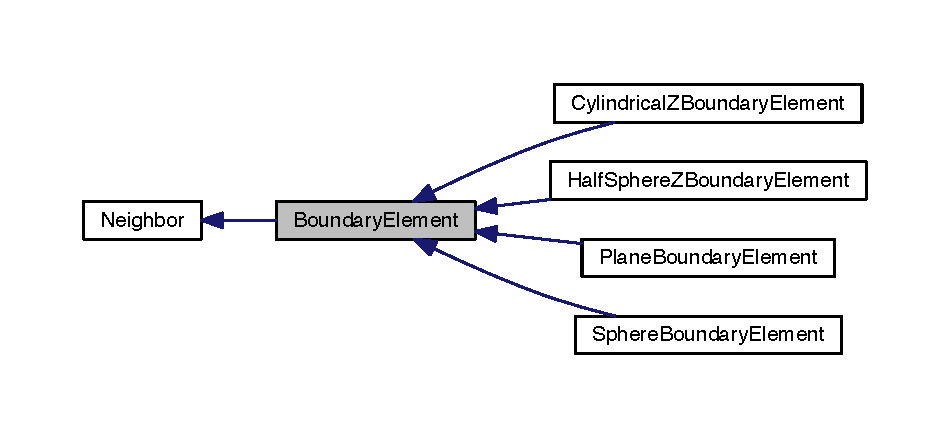
\includegraphics[width=350pt]{classBoundaryElement__inherit__graph}
\end{center}
\end{figure}


Collaboration diagram for Boundary\+Element\+:\nopagebreak
\begin{figure}[H]
\begin{center}
\leavevmode
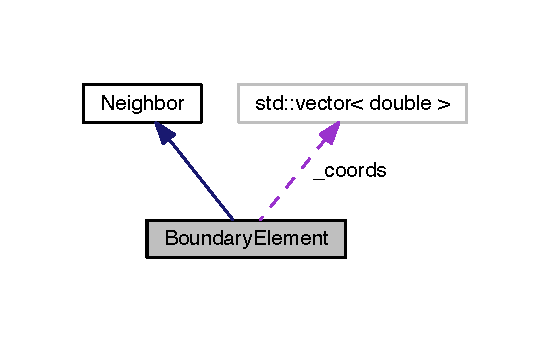
\includegraphics[width=264pt]{classBoundaryElement__coll__graph}
\end{center}
\end{figure}
\subsection*{Public Member Functions}
\begin{DoxyCompactItemize}
\item 
\hyperlink{classBoundaryElement_a51b203260855060fea195fa02b1cb07c}{Boundary\+Element} (vector$<$ double $>$ coords)
\begin{DoxyCompactList}\small\item\em Default constructor. \end{DoxyCompactList}\item 
virtual \hyperlink{classBoundaryElement_a4f0bec4466a42c311be8a3c1fc67cc52}{$\sim$\+Boundary\+Element} () noexcept
\begin{DoxyCompactList}\small\item\em Destructor. \end{DoxyCompactList}\item 
const vector$<$ double $>$ \& \hyperlink{classBoundaryElement_ace76817d750bb44c11edd918f1a8b78f}{get\+Coords} ()
\begin{DoxyCompactList}\small\item\em return coordinates of boundary element \end{DoxyCompactList}\item 
virtual double \hyperlink{classBoundaryElement_ac84f39882c9994b1f842c5be9a03db9d}{distance} (const vector$<$ double $>$ \&point)=0
\begin{DoxyCompactList}\small\item\em Implement for all boundary elements Returns the distance from a given point to this boundary element. \end{DoxyCompactList}\item 
virtual double \hyperlink{classBoundaryElement_a15e0453be158c2c9774b06f27bf6ae9b}{stretched\+Distance} (const vector$<$ double $>$ \&point, const vector$<$ double $>$ \&force, double d)=0
\begin{DoxyCompactList}\small\item\em Returns stretched distance, similar to distance above. \end{DoxyCompactList}\item 
virtual const vector$<$ double $>$ \hyperlink{classBoundaryElement_aef0aa594a42167a34efbc757b47eb012}{normal} (const vector$<$ double $>$ \&point)=0
\begin{DoxyCompactList}\small\item\em Returns normal vector of point to plane. \end{DoxyCompactList}\end{DoxyCompactItemize}
{\bf }\par
\begin{DoxyCompactItemize}
\item 
virtual double \hyperlink{classBoundaryElement_aff96a5a1faa7df9b30899d9c3de84f4a}{get\+Repulsion\+Const} ()=0
\begin{DoxyCompactList}\small\item\em Getter for parameters. \end{DoxyCompactList}\item 
virtual double \hyperlink{classBoundaryElement_a075dff05ab75cfd8be7f1a731030045a}{get\+Screening\+Length} ()=0
\begin{DoxyCompactList}\small\item\em Getter for parameters. \end{DoxyCompactList}\end{DoxyCompactItemize}

\subsection*{Protected Attributes}
\begin{DoxyCompactItemize}
\item 
vector$<$ double $>$ \hyperlink{classBoundaryElement_ab51302e10e3e2def98438234ba5bf801}{\+\_\+coords}
\begin{DoxyCompactList}\small\item\em coordinates \end{DoxyCompactList}\end{DoxyCompactItemize}


\subsection{Detailed Description}
Represents an element of a \hyperlink{classBoundarySurface}{Boundary\+Surface}. 

The \hyperlink{classBoundaryElement}{Boundary\+Element} class is a representation of a \hyperlink{classBoundarySurface}{Boundary\+Surface} element, which can interact with other elements in the system, including other Boundary\+Elements as well as \hyperlink{classBead}{Beads} in \hyperlink{classFilament}{Filaments}. Together, a collection of boundary elements make up a \hyperlink{classBoundarySurface}{Boundary\+Surface}. 

Definition at line 37 of file Boundary\+Element.\+h.



\subsection{Constructor \& Destructor Documentation}
\hypertarget{classBoundaryElement_a51b203260855060fea195fa02b1cb07c}{\index{Boundary\+Element@{Boundary\+Element}!Boundary\+Element@{Boundary\+Element}}
\index{Boundary\+Element@{Boundary\+Element}!Boundary\+Element@{Boundary\+Element}}
\subsubsection[{Boundary\+Element}]{\setlength{\rightskip}{0pt plus 5cm}Boundary\+Element\+::\+Boundary\+Element (
\begin{DoxyParamCaption}
\item[{vector$<$ double $>$}]{coords}
\end{DoxyParamCaption}
)\hspace{0.3cm}{\ttfamily [inline]}}}\label{classBoundaryElement_a51b203260855060fea195fa02b1cb07c}


Default constructor. 



Definition at line 44 of file Boundary\+Element.\+h.



References Boundary\+Element\+D\+B\+::add\+Boundary\+Element(), Neighbor\+List\+D\+B\+::add\+Neighbor(), Boundary\+Element\+D\+B\+::instance(), and Neighbor\+List\+D\+B\+::instance().

\hypertarget{classBoundaryElement_a4f0bec4466a42c311be8a3c1fc67cc52}{\index{Boundary\+Element@{Boundary\+Element}!````~Boundary\+Element@{$\sim$\+Boundary\+Element}}
\index{````~Boundary\+Element@{$\sim$\+Boundary\+Element}!Boundary\+Element@{Boundary\+Element}}
\subsubsection[{$\sim$\+Boundary\+Element}]{\setlength{\rightskip}{0pt plus 5cm}virtual Boundary\+Element\+::$\sim$\+Boundary\+Element (
\begin{DoxyParamCaption}
{}
\end{DoxyParamCaption}
)\hspace{0.3cm}{\ttfamily [inline]}, {\ttfamily [virtual]}, {\ttfamily [noexcept]}}}\label{classBoundaryElement_a4f0bec4466a42c311be8a3c1fc67cc52}


Destructor. 

\begin{DoxyNote}{Note}
noexcept is important here. Otherwise, gcc flags the constructor as potentially throwing, which in turn disables move operations by the S\+T\+L containers. This behaviour is a gcc bug (as of gcc 4.\+703), and will presumbaly be fixed in the future. 
\end{DoxyNote}
remove from neighbor lists 

Definition at line 56 of file Boundary\+Element.\+h.



References Boundary\+Element\+D\+B\+::instance(), Neighbor\+List\+D\+B\+::instance(), Boundary\+Element\+D\+B\+::remove\+Boundary\+Element(), and Neighbor\+List\+D\+B\+::remove\+Neighbor().



\subsection{Member Function Documentation}
\hypertarget{classBoundaryElement_ac84f39882c9994b1f842c5be9a03db9d}{\index{Boundary\+Element@{Boundary\+Element}!distance@{distance}}
\index{distance@{distance}!Boundary\+Element@{Boundary\+Element}}
\subsubsection[{distance}]{\setlength{\rightskip}{0pt plus 5cm}virtual double Boundary\+Element\+::distance (
\begin{DoxyParamCaption}
\item[{const vector$<$ double $>$ \&}]{point}
\end{DoxyParamCaption}
)\hspace{0.3cm}{\ttfamily [pure virtual]}}}\label{classBoundaryElement_ac84f39882c9994b1f842c5be9a03db9d}


Implement for all boundary elements Returns the distance from a given point to this boundary element. 

\begin{DoxyReturn}{Returns}
-\/ 1) positive number if point is within boundary element 2) Negative number if point is outside boundary element 3) Infinity if point is not in domain of this boundary element 
\end{DoxyReturn}


Implemented in \hyperlink{classHalfSphereZBoundaryElement_ad954352392ba721b772cf9a0177edec1}{Half\+Sphere\+Z\+Boundary\+Element}, \hyperlink{classCylindricalZBoundaryElement_a2532a472c9cd58a65940f43e05050d97}{Cylindrical\+Z\+Boundary\+Element}, \hyperlink{classSphereBoundaryElement_a8e28d60646f36a7ff943e69e62f248e4}{Sphere\+Boundary\+Element}, and \hyperlink{classPlaneBoundaryElement_ad35d384337c44f4bf5e5b243cf9cda88}{Plane\+Boundary\+Element}.



Referenced by Boundary\+Repulsion$<$ B\+Repulsion\+Interaction\+Type $>$\+::compute\+Energy(), Boundary\+Repulsion$<$ B\+Repulsion\+Interaction\+Type $>$\+::compute\+Forces(), Boundary\+Repulsion$<$ B\+Repulsion\+Interaction\+Type $>$\+::compute\+Forces\+Aux(), Boundary\+Spherical\+::within(), and Boundary\+Capsule\+::within().

\hypertarget{classBoundaryElement_ace76817d750bb44c11edd918f1a8b78f}{\index{Boundary\+Element@{Boundary\+Element}!get\+Coords@{get\+Coords}}
\index{get\+Coords@{get\+Coords}!Boundary\+Element@{Boundary\+Element}}
\subsubsection[{get\+Coords}]{\setlength{\rightskip}{0pt plus 5cm}const vector$<$double$>$\& Boundary\+Element\+::get\+Coords (
\begin{DoxyParamCaption}
{}
\end{DoxyParamCaption}
)\hspace{0.3cm}{\ttfamily [inline]}}}\label{classBoundaryElement_ace76817d750bb44c11edd918f1a8b78f}


return coordinates of boundary element 



Definition at line 66 of file Boundary\+Element.\+h.



References \+\_\+coords.

\hypertarget{classBoundaryElement_aff96a5a1faa7df9b30899d9c3de84f4a}{\index{Boundary\+Element@{Boundary\+Element}!get\+Repulsion\+Const@{get\+Repulsion\+Const}}
\index{get\+Repulsion\+Const@{get\+Repulsion\+Const}!Boundary\+Element@{Boundary\+Element}}
\subsubsection[{get\+Repulsion\+Const}]{\setlength{\rightskip}{0pt plus 5cm}virtual double Boundary\+Element\+::get\+Repulsion\+Const (
\begin{DoxyParamCaption}
{}
\end{DoxyParamCaption}
)\hspace{0.3cm}{\ttfamily [pure virtual]}}}\label{classBoundaryElement_aff96a5a1faa7df9b30899d9c3de84f4a}


Getter for parameters. 



Implemented in \hyperlink{classHalfSphereZBoundaryElement_a672b90ff798b849ef705384ab9f745bc}{Half\+Sphere\+Z\+Boundary\+Element}, \hyperlink{classCylindricalZBoundaryElement_a6f090f1ff1ebf10695ab3cf2db3fb8bf}{Cylindrical\+Z\+Boundary\+Element}, \hyperlink{classSphereBoundaryElement_aa9b8bd814e79f335232d3aac100148a0}{Sphere\+Boundary\+Element}, and \hyperlink{classPlaneBoundaryElement_a022862630bad9bf77b6de4057474876a}{Plane\+Boundary\+Element}.



Referenced by Boundary\+Repulsion$<$ B\+Repulsion\+Interaction\+Type $>$\+::compute\+Energy(), Boundary\+Repulsion$<$ B\+Repulsion\+Interaction\+Type $>$\+::compute\+Forces(), and Boundary\+Repulsion$<$ B\+Repulsion\+Interaction\+Type $>$\+::compute\+Forces\+Aux().

\hypertarget{classBoundaryElement_a075dff05ab75cfd8be7f1a731030045a}{\index{Boundary\+Element@{Boundary\+Element}!get\+Screening\+Length@{get\+Screening\+Length}}
\index{get\+Screening\+Length@{get\+Screening\+Length}!Boundary\+Element@{Boundary\+Element}}
\subsubsection[{get\+Screening\+Length}]{\setlength{\rightskip}{0pt plus 5cm}virtual double Boundary\+Element\+::get\+Screening\+Length (
\begin{DoxyParamCaption}
{}
\end{DoxyParamCaption}
)\hspace{0.3cm}{\ttfamily [pure virtual]}}}\label{classBoundaryElement_a075dff05ab75cfd8be7f1a731030045a}


Getter for parameters. 



Implemented in \hyperlink{classHalfSphereZBoundaryElement_ab7b9034066dbc5bec386a04f6bc3a91f}{Half\+Sphere\+Z\+Boundary\+Element}, \hyperlink{classCylindricalZBoundaryElement_afe407ba95087aff6598141daccb06d39}{Cylindrical\+Z\+Boundary\+Element}, \hyperlink{classSphereBoundaryElement_aacda85af577d438ce939274960d72045}{Sphere\+Boundary\+Element}, and \hyperlink{classPlaneBoundaryElement_a81c5691717216f8602cc2300c603e253}{Plane\+Boundary\+Element}.



Referenced by Boundary\+Repulsion$<$ B\+Repulsion\+Interaction\+Type $>$\+::compute\+Energy(), Boundary\+Repulsion$<$ B\+Repulsion\+Interaction\+Type $>$\+::compute\+Forces(), and Boundary\+Repulsion$<$ B\+Repulsion\+Interaction\+Type $>$\+::compute\+Forces\+Aux().

\hypertarget{classBoundaryElement_aef0aa594a42167a34efbc757b47eb012}{\index{Boundary\+Element@{Boundary\+Element}!normal@{normal}}
\index{normal@{normal}!Boundary\+Element@{Boundary\+Element}}
\subsubsection[{normal}]{\setlength{\rightskip}{0pt plus 5cm}virtual const vector$<$double$>$ Boundary\+Element\+::normal (
\begin{DoxyParamCaption}
\item[{const vector$<$ double $>$ \&}]{point}
\end{DoxyParamCaption}
)\hspace{0.3cm}{\ttfamily [pure virtual]}}}\label{classBoundaryElement_aef0aa594a42167a34efbc757b47eb012}


Returns normal vector of point to plane. 



Implemented in \hyperlink{classHalfSphereZBoundaryElement_a3d1287ac0239294c1dbfdd2c799dcd7f}{Half\+Sphere\+Z\+Boundary\+Element}, \hyperlink{classCylindricalZBoundaryElement_a5832dede61b710421f5307d5b7bfb982}{Cylindrical\+Z\+Boundary\+Element}, \hyperlink{classSphereBoundaryElement_a505ad6dae8dfaff38f2b845d6f7b7ee5}{Sphere\+Boundary\+Element}, and \hyperlink{classPlaneBoundaryElement_a0d87ae7390cd7fcfa2c7769e6212ee97}{Plane\+Boundary\+Element}.



Referenced by Boundary\+Repulsion$<$ B\+Repulsion\+Interaction\+Type $>$\+::compute\+Forces(), and Boundary\+Repulsion$<$ B\+Repulsion\+Interaction\+Type $>$\+::compute\+Forces\+Aux().

\hypertarget{classBoundaryElement_a15e0453be158c2c9774b06f27bf6ae9b}{\index{Boundary\+Element@{Boundary\+Element}!stretched\+Distance@{stretched\+Distance}}
\index{stretched\+Distance@{stretched\+Distance}!Boundary\+Element@{Boundary\+Element}}
\subsubsection[{stretched\+Distance}]{\setlength{\rightskip}{0pt plus 5cm}virtual double Boundary\+Element\+::stretched\+Distance (
\begin{DoxyParamCaption}
\item[{const vector$<$ double $>$ \&}]{point, }
\item[{const vector$<$ double $>$ \&}]{force, }
\item[{double}]{d}
\end{DoxyParamCaption}
)\hspace{0.3cm}{\ttfamily [pure virtual]}}}\label{classBoundaryElement_a15e0453be158c2c9774b06f27bf6ae9b}


Returns stretched distance, similar to distance above. 



Implemented in \hyperlink{classHalfSphereZBoundaryElement_a836d5117066fbfab38903475e5fc0d8d}{Half\+Sphere\+Z\+Boundary\+Element}, \hyperlink{classCylindricalZBoundaryElement_a6c3fc8e0f7bf828c21b70c396ed88dc0}{Cylindrical\+Z\+Boundary\+Element}, \hyperlink{classSphereBoundaryElement_a41d124459d11422c46c578f70d1af1b0}{Sphere\+Boundary\+Element}, and \hyperlink{classPlaneBoundaryElement_a7855fefca7c75e466abf4ae9d6883fb2}{Plane\+Boundary\+Element}.



Referenced by Boundary\+Repulsion$<$ B\+Repulsion\+Interaction\+Type $>$\+::compute\+Energy().



\subsection{Member Data Documentation}
\hypertarget{classBoundaryElement_ab51302e10e3e2def98438234ba5bf801}{\index{Boundary\+Element@{Boundary\+Element}!\+\_\+coords@{\+\_\+coords}}
\index{\+\_\+coords@{\+\_\+coords}!Boundary\+Element@{Boundary\+Element}}
\subsubsection[{\+\_\+coords}]{\setlength{\rightskip}{0pt plus 5cm}vector$<$double$>$ Boundary\+Element\+::\+\_\+coords\hspace{0.3cm}{\ttfamily [protected]}}}\label{classBoundaryElement_ab51302e10e3e2def98438234ba5bf801}


coordinates 



Definition at line 40 of file Boundary\+Element.\+h.



Referenced by Sphere\+Boundary\+Element\+::distance(), Cylindrical\+Z\+Boundary\+Element\+::distance(), Half\+Sphere\+Z\+Boundary\+Element\+::distance(), get\+Coords(), Sphere\+Boundary\+Element\+::normal(), Cylindrical\+Z\+Boundary\+Element\+::normal(), Half\+Sphere\+Z\+Boundary\+Element\+::normal(), Plane\+Boundary\+Element\+::\+Plane\+Boundary\+Element(), Sphere\+Boundary\+Element\+::stretched\+Distance(), Cylindrical\+Z\+Boundary\+Element\+::stretched\+Distance(), and Half\+Sphere\+Z\+Boundary\+Element\+::stretched\+Distance().



The documentation for this class was generated from the following file\+:\begin{DoxyCompactItemize}
\item 
M3\+S\+Y\+M/\+Structure/\hyperlink{BoundaryElement_8h}{Boundary\+Element.\+h}\end{DoxyCompactItemize}

\hypertarget{classBoundaryElementDB}{\section{Boundary\+Element\+D\+B Class Reference}
\label{classBoundaryElementDB}\index{Boundary\+Element\+D\+B@{Boundary\+Element\+D\+B}}
}


A database for all \hyperlink{classBoundaryElement}{Boundary\+Elements} in the system.  




{\ttfamily \#include $<$Boundary\+Element\+D\+B.\+h$>$}



Inheritance diagram for Boundary\+Element\+D\+B\+:\nopagebreak
\begin{figure}[H]
\begin{center}
\leavevmode
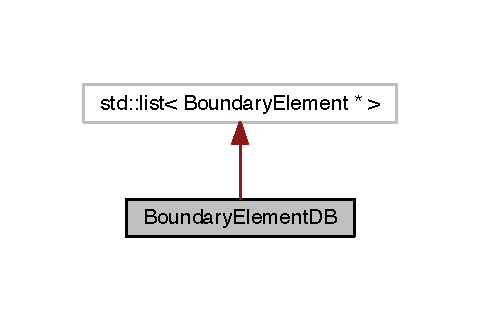
\includegraphics[width=231pt]{classBoundaryElementDB__inherit__graph}
\end{center}
\end{figure}


Collaboration diagram for Boundary\+Element\+D\+B\+:\nopagebreak
\begin{figure}[H]
\begin{center}
\leavevmode
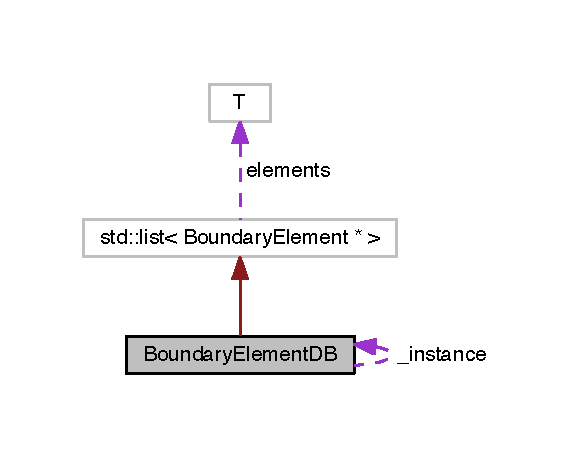
\includegraphics[width=274pt]{classBoundaryElementDB__coll__graph}
\end{center}
\end{figure}
\subsection*{Public Member Functions}
\begin{DoxyCompactItemize}
\item 
\hyperlink{classBoundaryElementDB_a734b7bbb4aa92a6fcbb0e13a2730542d}{Boundary\+Element\+D\+B} (const \hyperlink{classBoundaryElementDB}{Boundary\+Element\+D\+B} \&rhs)=delete
\begin{DoxyCompactList}\small\item\em Copying is not allowed. \end{DoxyCompactList}\item 
\hyperlink{classBoundaryElementDB}{Boundary\+Element\+D\+B} \& \hyperlink{classBoundaryElementDB_ad42f6c382956dee33a609da771fdce88}{operator=} (\hyperlink{classBoundaryElementDB}{Boundary\+Element\+D\+B} \&rhs)=delete
\begin{DoxyCompactList}\small\item\em Assignment is not allowed. \end{DoxyCompactList}\item 
void \hyperlink{classBoundaryElementDB_a87b287f3028a92ee56edba04d0293b6f}{add\+Boundary\+Element} (\hyperlink{classBoundaryElement}{Boundary\+Element} $\ast$b)
\begin{DoxyCompactList}\small\item\em Add a boundary element. \end{DoxyCompactList}\item 
void \hyperlink{classBoundaryElementDB_a0392d6b0a27d7dfc57d39194165c3543}{remove\+Boundary\+Element} (\hyperlink{classBoundaryElement}{Boundary\+Element} $\ast$b)
\begin{DoxyCompactList}\small\item\em Remove boundary element. \end{DoxyCompactList}\end{DoxyCompactItemize}
\subsection*{Static Public Member Functions}
\begin{DoxyCompactItemize}
\item 
static \hyperlink{classBoundaryElementDB}{Boundary\+Element\+D\+B} $\ast$ \hyperlink{classBoundaryElementDB_a576c2f5e552686c2f40e70e206693f2a}{instance} ()
\begin{DoxyCompactList}\small\item\em Get the instance of this singleton. \end{DoxyCompactList}\end{DoxyCompactItemize}
\subsection*{Private Types}
\begin{DoxyCompactItemize}
\item 
typedef list$<$ \hyperlink{classBoundaryElement}{Boundary\+Element} $\ast$ $>$ \hyperlink{classBoundaryElementDB_af2b807e8b6e93168ee80bc57182b7b34}{bedb}
\end{DoxyCompactItemize}
\subsection*{Private Member Functions}
\begin{DoxyCompactItemize}
\item 
\hyperlink{classBoundaryElementDB_a71f6fba6551793efc93ffc60a2b246a6}{Boundary\+Element\+D\+B} ()
\end{DoxyCompactItemize}
\subsection*{Private Attributes}
\begin{DoxyCompactItemize}
\item 
T {\bfseries elements}
\begin{DoxyCompactList}\small\item\em S\+T\+L member. \end{DoxyCompactList}\end{DoxyCompactItemize}
\subsection*{Static Private Attributes}
\begin{DoxyCompactItemize}
\item 
static \hyperlink{classBoundaryElementDB}{Boundary\+Element\+D\+B} $\ast$ \hyperlink{classBoundaryElementDB_af537420197d88dcca76a50db7d7b7079}{\+\_\+instance} = 0
\begin{DoxyCompactList}\small\item\em Singleton instance. \end{DoxyCompactList}\end{DoxyCompactItemize}


\subsection{Detailed Description}
A database for all \hyperlink{classBoundaryElement}{Boundary\+Elements} in the system. 

This \hyperlink{classBoundaryElementDB}{Boundary\+Element\+D\+B} inherits from list and manage all creations and removing of \hyperlink{classBoundaryElement}{Boundary\+Element} objects, as well as some standard list functions and iterators. 

Definition at line 29 of file Boundary\+Element\+D\+B.\+h.



\subsection{Member Typedef Documentation}
\hypertarget{classBoundaryElementDB_af2b807e8b6e93168ee80bc57182b7b34}{\index{Boundary\+Element\+D\+B@{Boundary\+Element\+D\+B}!bedb@{bedb}}
\index{bedb@{bedb}!Boundary\+Element\+D\+B@{Boundary\+Element\+D\+B}}
\subsubsection[{bedb}]{\setlength{\rightskip}{0pt plus 5cm}typedef list$<${\bf Boundary\+Element}$\ast$$>$ {\bf Boundary\+Element\+D\+B\+::bedb}\hspace{0.3cm}{\ttfamily [private]}}}\label{classBoundaryElementDB_af2b807e8b6e93168ee80bc57182b7b34}


Definition at line 31 of file Boundary\+Element\+D\+B.\+h.



\subsection{Constructor \& Destructor Documentation}
\hypertarget{classBoundaryElementDB_a734b7bbb4aa92a6fcbb0e13a2730542d}{\index{Boundary\+Element\+D\+B@{Boundary\+Element\+D\+B}!Boundary\+Element\+D\+B@{Boundary\+Element\+D\+B}}
\index{Boundary\+Element\+D\+B@{Boundary\+Element\+D\+B}!Boundary\+Element\+D\+B@{Boundary\+Element\+D\+B}}
\subsubsection[{Boundary\+Element\+D\+B}]{\setlength{\rightskip}{0pt plus 5cm}Boundary\+Element\+D\+B\+::\+Boundary\+Element\+D\+B (
\begin{DoxyParamCaption}
\item[{const {\bf Boundary\+Element\+D\+B} \&}]{rhs}
\end{DoxyParamCaption}
)\hspace{0.3cm}{\ttfamily [delete]}}}\label{classBoundaryElementDB_a734b7bbb4aa92a6fcbb0e13a2730542d}


Copying is not allowed. 

\hypertarget{classBoundaryElementDB_a71f6fba6551793efc93ffc60a2b246a6}{\index{Boundary\+Element\+D\+B@{Boundary\+Element\+D\+B}!Boundary\+Element\+D\+B@{Boundary\+Element\+D\+B}}
\index{Boundary\+Element\+D\+B@{Boundary\+Element\+D\+B}!Boundary\+Element\+D\+B@{Boundary\+Element\+D\+B}}
\subsubsection[{Boundary\+Element\+D\+B}]{\setlength{\rightskip}{0pt plus 5cm}Boundary\+Element\+D\+B\+::\+Boundary\+Element\+D\+B (
\begin{DoxyParamCaption}
{}
\end{DoxyParamCaption}
)\hspace{0.3cm}{\ttfamily [inline]}, {\ttfamily [private]}}}\label{classBoundaryElementDB_a71f6fba6551793efc93ffc60a2b246a6}


Definition at line 56 of file Boundary\+Element\+D\+B.\+h.



Referenced by instance().



\subsection{Member Function Documentation}
\hypertarget{classBoundaryElementDB_a87b287f3028a92ee56edba04d0293b6f}{\index{Boundary\+Element\+D\+B@{Boundary\+Element\+D\+B}!add\+Boundary\+Element@{add\+Boundary\+Element}}
\index{add\+Boundary\+Element@{add\+Boundary\+Element}!Boundary\+Element\+D\+B@{Boundary\+Element\+D\+B}}
\subsubsection[{add\+Boundary\+Element}]{\setlength{\rightskip}{0pt plus 5cm}void Boundary\+Element\+D\+B\+::add\+Boundary\+Element (
\begin{DoxyParamCaption}
\item[{{\bf Boundary\+Element} $\ast$}]{b}
\end{DoxyParamCaption}
)\hspace{0.3cm}{\ttfamily [inline]}}}\label{classBoundaryElementDB_a87b287f3028a92ee56edba04d0293b6f}


Add a boundary element. 



Definition at line 50 of file Boundary\+Element\+D\+B.\+h.



Referenced by Boundary\+Element\+::\+Boundary\+Element().

\hypertarget{classBoundaryElementDB_a576c2f5e552686c2f40e70e206693f2a}{\index{Boundary\+Element\+D\+B@{Boundary\+Element\+D\+B}!instance@{instance}}
\index{instance@{instance}!Boundary\+Element\+D\+B@{Boundary\+Element\+D\+B}}
\subsubsection[{instance}]{\setlength{\rightskip}{0pt plus 5cm}{\bf Boundary\+Element\+D\+B} $\ast$ Boundary\+Element\+D\+B\+::instance (
\begin{DoxyParamCaption}
{}
\end{DoxyParamCaption}
)\hspace{0.3cm}{\ttfamily [static]}}}\label{classBoundaryElementDB_a576c2f5e552686c2f40e70e206693f2a}


Get the instance of this singleton. 



Definition at line 18 of file Boundary\+Element\+D\+B.\+cpp.



References \+\_\+instance, and Boundary\+Element\+D\+B().



Referenced by Boundary\+Element\+::\+Boundary\+Element(), Boundary\+F\+F\+::compute\+Energy(), Boundary\+F\+F\+::compute\+Forces(), Boundary\+F\+F\+::compute\+Forces\+Aux(), and Boundary\+Element\+::$\sim$\+Boundary\+Element().

\hypertarget{classBoundaryElementDB_ad42f6c382956dee33a609da771fdce88}{\index{Boundary\+Element\+D\+B@{Boundary\+Element\+D\+B}!operator=@{operator=}}
\index{operator=@{operator=}!Boundary\+Element\+D\+B@{Boundary\+Element\+D\+B}}
\subsubsection[{operator=}]{\setlength{\rightskip}{0pt plus 5cm}{\bf Boundary\+Element\+D\+B}\& Boundary\+Element\+D\+B\+::operator= (
\begin{DoxyParamCaption}
\item[{{\bf Boundary\+Element\+D\+B} \&}]{rhs}
\end{DoxyParamCaption}
)\hspace{0.3cm}{\ttfamily [delete]}}}\label{classBoundaryElementDB_ad42f6c382956dee33a609da771fdce88}


Assignment is not allowed. 

\hypertarget{classBoundaryElementDB_a0392d6b0a27d7dfc57d39194165c3543}{\index{Boundary\+Element\+D\+B@{Boundary\+Element\+D\+B}!remove\+Boundary\+Element@{remove\+Boundary\+Element}}
\index{remove\+Boundary\+Element@{remove\+Boundary\+Element}!Boundary\+Element\+D\+B@{Boundary\+Element\+D\+B}}
\subsubsection[{remove\+Boundary\+Element}]{\setlength{\rightskip}{0pt plus 5cm}void Boundary\+Element\+D\+B\+::remove\+Boundary\+Element (
\begin{DoxyParamCaption}
\item[{{\bf Boundary\+Element} $\ast$}]{b}
\end{DoxyParamCaption}
)\hspace{0.3cm}{\ttfamily [inline]}}}\label{classBoundaryElementDB_a0392d6b0a27d7dfc57d39194165c3543}


Remove boundary element. 



Definition at line 52 of file Boundary\+Element\+D\+B.\+h.



Referenced by Boundary\+Element\+::$\sim$\+Boundary\+Element().



\subsection{Member Data Documentation}
\hypertarget{classBoundaryElementDB_af537420197d88dcca76a50db7d7b7079}{\index{Boundary\+Element\+D\+B@{Boundary\+Element\+D\+B}!\+\_\+instance@{\+\_\+instance}}
\index{\+\_\+instance@{\+\_\+instance}!Boundary\+Element\+D\+B@{Boundary\+Element\+D\+B}}
\subsubsection[{\+\_\+instance}]{\setlength{\rightskip}{0pt plus 5cm}{\bf Boundary\+Element\+D\+B} $\ast$ Boundary\+Element\+D\+B\+::\+\_\+instance = 0\hspace{0.3cm}{\ttfamily [static]}, {\ttfamily [private]}}}\label{classBoundaryElementDB_af537420197d88dcca76a50db7d7b7079}


Singleton instance. 



Definition at line 55 of file Boundary\+Element\+D\+B.\+h.



Referenced by instance().

\hypertarget{classstd_1_1list_a682e5c7c91eb377d0cb4f019b2b81a5d}{\index{Boundary\+Element\+D\+B@{Boundary\+Element\+D\+B}!elements@{elements}}
\index{elements@{elements}!Boundary\+Element\+D\+B@{Boundary\+Element\+D\+B}}
\subsubsection[{elements}]{\setlength{\rightskip}{0pt plus 5cm}T std\+::list$<$ T $>$\+::elements\hspace{0.3cm}{\ttfamily [inherited]}}}\label{classstd_1_1list_a682e5c7c91eb377d0cb4f019b2b81a5d}


S\+T\+L member. 



The documentation for this class was generated from the following files\+:\begin{DoxyCompactItemize}
\item 
M3\+S\+Y\+M/\+Structure/\hyperlink{BoundaryElementDB_8h}{Boundary\+Element\+D\+B.\+h}\item 
M3\+S\+Y\+M/\+Structure/\hyperlink{BoundaryElementDB_8cpp}{Boundary\+Element\+D\+B.\+cpp}\end{DoxyCompactItemize}

\hypertarget{classBoundaryElementNeighborList}{\section{Boundary\+Element\+Neighbor\+List Class Reference}
\label{classBoundaryElementNeighborList}\index{Boundary\+Element\+Neighbor\+List@{Boundary\+Element\+Neighbor\+List}}
}


An implementation of \hyperlink{classNeighborList}{Neighbor\+List} for Bead-\/\+Boundary\+Element interactions.  




{\ttfamily \#include $<$Neighbor\+List.\+h$>$}



Inheritance diagram for Boundary\+Element\+Neighbor\+List\+:\nopagebreak
\begin{figure}[H]
\begin{center}
\leavevmode
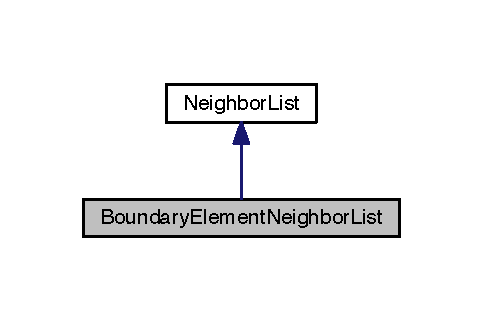
\includegraphics[width=232pt]{classBoundaryElementNeighborList__inherit__graph}
\end{center}
\end{figure}


Collaboration diagram for Boundary\+Element\+Neighbor\+List\+:\nopagebreak
\begin{figure}[H]
\begin{center}
\leavevmode
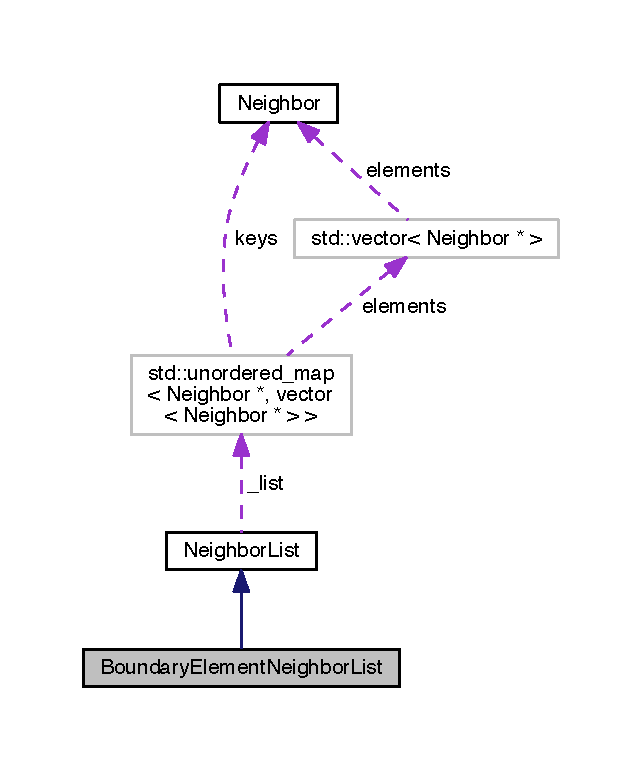
\includegraphics[width=308pt]{classBoundaryElementNeighborList__coll__graph}
\end{center}
\end{figure}
\subsection*{Public Member Functions}
\begin{DoxyCompactItemize}
\item 
\hyperlink{classBoundaryElementNeighborList_a84cc0a08aa4d985fa708ead757e90a93}{Boundary\+Element\+Neighbor\+List} (float r\+Max, float r\+Min)
\item 
virtual void \hyperlink{classBoundaryElementNeighborList_a39ce6b818ef3fd745fae6b5d45e9c3aa}{add\+Neighbor} (\hyperlink{classNeighbor}{Neighbor} $\ast$n)
\begin{DoxyCompactList}\small\item\em Add neighbor. \end{DoxyCompactList}\item 
virtual void \hyperlink{classBoundaryElementNeighborList_a1af8a9581758cf2ddbf82318570876e5}{update\+Neighbors} (\hyperlink{classNeighbor}{Neighbor} $\ast$n)
\begin{DoxyCompactList}\small\item\em U pdate a neighbor. \end{DoxyCompactList}\item 
vector$<$ \hyperlink{classBead}{Bead} $\ast$ $>$ \hyperlink{classBoundaryElementNeighborList_af2114492e49ddeb5da9ddddd81afc4bd}{get\+Neighbors} (\hyperlink{classBoundaryElement}{Boundary\+Element} $\ast$be)
\begin{DoxyCompactList}\small\item\em Get all \hyperlink{classBead}{Bead} neighbors of a boundary element. \end{DoxyCompactList}\item 
virtual void \hyperlink{classNeighborList_aa64ee01bc18598fae6906ca6d5dcc7d6}{remove\+Neighbor} (\hyperlink{classNeighbor}{Neighbor} $\ast$n)
\begin{DoxyCompactList}\small\item\em Remove a neighbor if possible. \end{DoxyCompactList}\item 
virtual void \hyperlink{classNeighborList_a93a07ead9349edba7d763b483ec42847}{reset} ()
\begin{DoxyCompactList}\small\item\em Re-\/initialize the neighborlist. \end{DoxyCompactList}\end{DoxyCompactItemize}
\subsection*{Protected Attributes}
\begin{DoxyCompactItemize}
\item 
unordered\+\_\+map$<$ \hyperlink{classNeighbor}{Neighbor} \\*
$\ast$, vector$<$ \hyperlink{classNeighbor}{Neighbor} $\ast$ $>$ $>$ \hyperlink{classNeighborList_af09da5281bc352cf028e39276ba5b68f}{\+\_\+list}
\begin{DoxyCompactList}\small\item\em The neighbors list, as a hash map. \end{DoxyCompactList}\item 
float \hyperlink{classNeighborList_a94d5215ec2f93c2191cd0ca87e062c5e}{\+\_\+r\+Max}
\begin{DoxyCompactList}\small\item\em max distance cutoff \end{DoxyCompactList}\item 
float \hyperlink{classNeighborList_a5fc2a03a950ca3867920527410ee8aa0}{\+\_\+r\+Min}
\begin{DoxyCompactList}\small\item\em min distance cutoff \end{DoxyCompactList}\end{DoxyCompactItemize}


\subsection{Detailed Description}
An implementation of \hyperlink{classNeighborList}{Neighbor\+List} for Bead-\/\+Boundary\+Element interactions. 

Definition at line 95 of file Neighbor\+List.\+h.



\subsection{Constructor \& Destructor Documentation}
\hypertarget{classBoundaryElementNeighborList_a84cc0a08aa4d985fa708ead757e90a93}{\index{Boundary\+Element\+Neighbor\+List@{Boundary\+Element\+Neighbor\+List}!Boundary\+Element\+Neighbor\+List@{Boundary\+Element\+Neighbor\+List}}
\index{Boundary\+Element\+Neighbor\+List@{Boundary\+Element\+Neighbor\+List}!Boundary\+Element\+Neighbor\+List@{Boundary\+Element\+Neighbor\+List}}
\subsubsection[{Boundary\+Element\+Neighbor\+List}]{\setlength{\rightskip}{0pt plus 5cm}Boundary\+Element\+Neighbor\+List\+::\+Boundary\+Element\+Neighbor\+List (
\begin{DoxyParamCaption}
\item[{float}]{r\+Max, }
\item[{float}]{r\+Min}
\end{DoxyParamCaption}
)\hspace{0.3cm}{\ttfamily [inline]}}}\label{classBoundaryElementNeighborList_a84cc0a08aa4d985fa708ead757e90a93}


Definition at line 98 of file Neighbor\+List.\+h.



\subsection{Member Function Documentation}
\hypertarget{classBoundaryElementNeighborList_a39ce6b818ef3fd745fae6b5d45e9c3aa}{\index{Boundary\+Element\+Neighbor\+List@{Boundary\+Element\+Neighbor\+List}!add\+Neighbor@{add\+Neighbor}}
\index{add\+Neighbor@{add\+Neighbor}!Boundary\+Element\+Neighbor\+List@{Boundary\+Element\+Neighbor\+List}}
\subsubsection[{add\+Neighbor}]{\setlength{\rightskip}{0pt plus 5cm}void Boundary\+Element\+Neighbor\+List\+::add\+Neighbor (
\begin{DoxyParamCaption}
\item[{{\bf Neighbor} $\ast$}]{n}
\end{DoxyParamCaption}
)\hspace{0.3cm}{\ttfamily [virtual]}}}\label{classBoundaryElementNeighborList_a39ce6b818ef3fd745fae6b5d45e9c3aa}


Add neighbor. 

return if not a boundary element!

update neighbors 

Implements \hyperlink{classNeighborList_af38a1d2711a786e3c845858e867d912b}{Neighbor\+List}.



Definition at line 84 of file Neighbor\+List.\+cpp.

\hypertarget{classBoundaryElementNeighborList_af2114492e49ddeb5da9ddddd81afc4bd}{\index{Boundary\+Element\+Neighbor\+List@{Boundary\+Element\+Neighbor\+List}!get\+Neighbors@{get\+Neighbors}}
\index{get\+Neighbors@{get\+Neighbors}!Boundary\+Element\+Neighbor\+List@{Boundary\+Element\+Neighbor\+List}}
\subsubsection[{get\+Neighbors}]{\setlength{\rightskip}{0pt plus 5cm}vector$<$ {\bf Bead} $\ast$ $>$ Boundary\+Element\+Neighbor\+List\+::get\+Neighbors (
\begin{DoxyParamCaption}
\item[{{\bf Boundary\+Element} $\ast$}]{be}
\end{DoxyParamCaption}
)}}\label{classBoundaryElementNeighborList_af2114492e49ddeb5da9ddddd81afc4bd}


Get all \hyperlink{classBead}{Bead} neighbors of a boundary element. 



Definition at line 109 of file Neighbor\+List.\+cpp.

\hypertarget{classNeighborList_aa64ee01bc18598fae6906ca6d5dcc7d6}{\index{Boundary\+Element\+Neighbor\+List@{Boundary\+Element\+Neighbor\+List}!remove\+Neighbor@{remove\+Neighbor}}
\index{remove\+Neighbor@{remove\+Neighbor}!Boundary\+Element\+Neighbor\+List@{Boundary\+Element\+Neighbor\+List}}
\subsubsection[{remove\+Neighbor}]{\setlength{\rightskip}{0pt plus 5cm}virtual void Neighbor\+List\+::remove\+Neighbor (
\begin{DoxyParamCaption}
\item[{{\bf Neighbor} $\ast$}]{n}
\end{DoxyParamCaption}
)\hspace{0.3cm}{\ttfamily [inline]}, {\ttfamily [virtual]}, {\ttfamily [inherited]}}}\label{classNeighborList_aa64ee01bc18598fae6906ca6d5dcc7d6}


Remove a neighbor if possible. 



Definition at line 56 of file Neighbor\+List.\+h.



References Neighbor\+List\+::\+\_\+list.

\hypertarget{classNeighborList_a93a07ead9349edba7d763b483ec42847}{\index{Boundary\+Element\+Neighbor\+List@{Boundary\+Element\+Neighbor\+List}!reset@{reset}}
\index{reset@{reset}!Boundary\+Element\+Neighbor\+List@{Boundary\+Element\+Neighbor\+List}}
\subsubsection[{reset}]{\setlength{\rightskip}{0pt plus 5cm}virtual void Neighbor\+List\+::reset (
\begin{DoxyParamCaption}
{}
\end{DoxyParamCaption}
)\hspace{0.3cm}{\ttfamily [inline]}, {\ttfamily [virtual]}, {\ttfamily [inherited]}}}\label{classNeighborList_a93a07ead9349edba7d763b483ec42847}


Re-\/initialize the neighborlist. 

clear vector of neighbors 

Definition at line 59 of file Neighbor\+List.\+h.



References Neighbor\+List\+::\+\_\+list, and Neighbor\+List\+::update\+Neighbors().

\hypertarget{classBoundaryElementNeighborList_a1af8a9581758cf2ddbf82318570876e5}{\index{Boundary\+Element\+Neighbor\+List@{Boundary\+Element\+Neighbor\+List}!update\+Neighbors@{update\+Neighbors}}
\index{update\+Neighbors@{update\+Neighbors}!Boundary\+Element\+Neighbor\+List@{Boundary\+Element\+Neighbor\+List}}
\subsubsection[{update\+Neighbors}]{\setlength{\rightskip}{0pt plus 5cm}void Boundary\+Element\+Neighbor\+List\+::update\+Neighbors (
\begin{DoxyParamCaption}
\item[{{\bf Neighbor} $\ast$}]{n}
\end{DoxyParamCaption}
)\hspace{0.3cm}{\ttfamily [virtual]}}}\label{classBoundaryElementNeighborList_a1af8a9581758cf2ddbf82318570876e5}


U pdate a neighbor. 

clear existing

loop through beads, add as

If we got through this, add it! 

Implements \hyperlink{classNeighborList_a843e9dcb6dd245e183252c1b5e538877}{Neighbor\+List}.



Definition at line 93 of file Neighbor\+List.\+cpp.



References Bead\+D\+B\+::instance().



\subsection{Member Data Documentation}
\hypertarget{classNeighborList_af09da5281bc352cf028e39276ba5b68f}{\index{Boundary\+Element\+Neighbor\+List@{Boundary\+Element\+Neighbor\+List}!\+\_\+list@{\+\_\+list}}
\index{\+\_\+list@{\+\_\+list}!Boundary\+Element\+Neighbor\+List@{Boundary\+Element\+Neighbor\+List}}
\subsubsection[{\+\_\+list}]{\setlength{\rightskip}{0pt plus 5cm}unordered\+\_\+map$<${\bf Neighbor}$\ast$, vector$<${\bf Neighbor}$\ast$$>$ $>$ Neighbor\+List\+::\+\_\+list\hspace{0.3cm}{\ttfamily [protected]}, {\ttfamily [inherited]}}}\label{classNeighborList_af09da5281bc352cf028e39276ba5b68f}


The neighbors list, as a hash map. 



Definition at line 41 of file Neighbor\+List.\+h.



Referenced by Neighbor\+List\+::remove\+Neighbor(), and Neighbor\+List\+::reset().

\hypertarget{classNeighborList_a94d5215ec2f93c2191cd0ca87e062c5e}{\index{Boundary\+Element\+Neighbor\+List@{Boundary\+Element\+Neighbor\+List}!\+\_\+r\+Max@{\+\_\+r\+Max}}
\index{\+\_\+r\+Max@{\+\_\+r\+Max}!Boundary\+Element\+Neighbor\+List@{Boundary\+Element\+Neighbor\+List}}
\subsubsection[{\+\_\+r\+Max}]{\setlength{\rightskip}{0pt plus 5cm}float Neighbor\+List\+::\+\_\+r\+Max\hspace{0.3cm}{\ttfamily [protected]}, {\ttfamily [inherited]}}}\label{classNeighborList_a94d5215ec2f93c2191cd0ca87e062c5e}


max distance cutoff 



Definition at line 42 of file Neighbor\+List.\+h.

\hypertarget{classNeighborList_a5fc2a03a950ca3867920527410ee8aa0}{\index{Boundary\+Element\+Neighbor\+List@{Boundary\+Element\+Neighbor\+List}!\+\_\+r\+Min@{\+\_\+r\+Min}}
\index{\+\_\+r\+Min@{\+\_\+r\+Min}!Boundary\+Element\+Neighbor\+List@{Boundary\+Element\+Neighbor\+List}}
\subsubsection[{\+\_\+r\+Min}]{\setlength{\rightskip}{0pt plus 5cm}float Neighbor\+List\+::\+\_\+r\+Min\hspace{0.3cm}{\ttfamily [protected]}, {\ttfamily [inherited]}}}\label{classNeighborList_a5fc2a03a950ca3867920527410ee8aa0}


min distance cutoff 



Definition at line 43 of file Neighbor\+List.\+h.



The documentation for this class was generated from the following files\+:\begin{DoxyCompactItemize}
\item 
M3\+S\+Y\+M/\+Structure/\hyperlink{NeighborList_8h}{Neighbor\+List.\+h}\item 
M3\+S\+Y\+M/\+Structure/\hyperlink{NeighborList_8cpp}{Neighbor\+List.\+cpp}\end{DoxyCompactItemize}

\hypertarget{classBoundaryElementNLContainer}{\section{Boundary\+Element\+N\+L\+Container Class Reference}
\label{classBoundaryElementNLContainer}\index{Boundary\+Element\+N\+L\+Container@{Boundary\+Element\+N\+L\+Container}}
}


Holds a \hyperlink{classBoundaryElementNeighborList}{Boundary\+Element\+Neighbor\+List}.  




{\ttfamily \#include $<$Neighbor\+List\+Container.\+h$>$}



Inheritance diagram for Boundary\+Element\+N\+L\+Container\+:\nopagebreak
\begin{figure}[H]
\begin{center}
\leavevmode
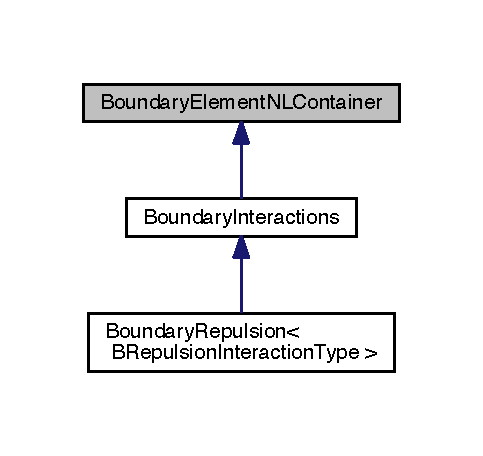
\includegraphics[width=232pt]{classBoundaryElementNLContainer__inherit__graph}
\end{center}
\end{figure}


Collaboration diagram for Boundary\+Element\+N\+L\+Container\+:\nopagebreak
\begin{figure}[H]
\begin{center}
\leavevmode
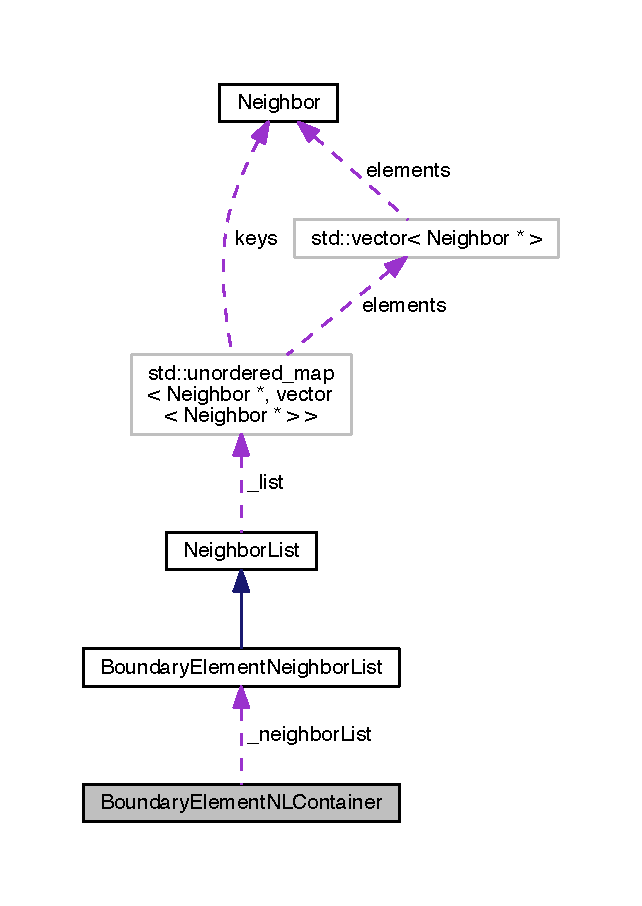
\includegraphics[width=308pt]{classBoundaryElementNLContainer__coll__graph}
\end{center}
\end{figure}
\subsection*{Public Member Functions}
\begin{DoxyCompactItemize}
\item 
\hyperlink{classBoundaryElementNLContainer_a6192ee44d946090df7d3518ae4035b9c}{Boundary\+Element\+N\+L\+Container} (float r\+Max=0.\+0, float r\+Min=0.\+0)
\begin{DoxyCompactList}\small\item\em Constructor, adds a cylinder neighbor list to the database. \end{DoxyCompactList}\item 
\hyperlink{classBoundaryElementNLContainer_a0621abe49cc7cf101e011ac3178a1519}{$\sim$\+Boundary\+Element\+N\+L\+Container} ()
\begin{DoxyCompactList}\small\item\em Destructor, removes boundary element neighbor list from the database. \end{DoxyCompactList}\item 
\hyperlink{classBoundaryElementNeighborList}{Boundary\+Element\+Neighbor\+List} $\ast$ \hyperlink{classBoundaryElementNLContainer_aa665161110c46e0a2af9f760c96afe19}{get\+Neighbor\+List} ()
\begin{DoxyCompactList}\small\item\em Get neighbor list. \end{DoxyCompactList}\end{DoxyCompactItemize}
\subsection*{Private Attributes}
\begin{DoxyCompactItemize}
\item 
\hyperlink{classBoundaryElementNeighborList}{Boundary\+Element\+Neighbor\+List} $\ast$ \hyperlink{classBoundaryElementNLContainer_ab75a418765e2601ec98e2159bab6ed84}{\+\_\+neighbor\+List}
\end{DoxyCompactItemize}


\subsection{Detailed Description}
Holds a \hyperlink{classBoundaryElementNeighborList}{Boundary\+Element\+Neighbor\+List}. 

Definition at line 46 of file Neighbor\+List\+Container.\+h.



\subsection{Constructor \& Destructor Documentation}
\hypertarget{classBoundaryElementNLContainer_a6192ee44d946090df7d3518ae4035b9c}{\index{Boundary\+Element\+N\+L\+Container@{Boundary\+Element\+N\+L\+Container}!Boundary\+Element\+N\+L\+Container@{Boundary\+Element\+N\+L\+Container}}
\index{Boundary\+Element\+N\+L\+Container@{Boundary\+Element\+N\+L\+Container}!Boundary\+Element\+N\+L\+Container@{Boundary\+Element\+N\+L\+Container}}
\subsubsection[{Boundary\+Element\+N\+L\+Container}]{\setlength{\rightskip}{0pt plus 5cm}Boundary\+Element\+N\+L\+Container\+::\+Boundary\+Element\+N\+L\+Container (
\begin{DoxyParamCaption}
\item[{float}]{r\+Max = {\ttfamily 0.0}, }
\item[{float}]{r\+Min = {\ttfamily 0.0}}
\end{DoxyParamCaption}
)\hspace{0.3cm}{\ttfamily [inline]}}}\label{classBoundaryElementNLContainer_a6192ee44d946090df7d3518ae4035b9c}


Constructor, adds a cylinder neighbor list to the database. 



Definition at line 53 of file Neighbor\+List\+Container.\+h.



References \+\_\+neighbor\+List, Neighbor\+List\+D\+B\+::add\+Neighbor\+List(), and Neighbor\+List\+D\+B\+::instance().

\hypertarget{classBoundaryElementNLContainer_a0621abe49cc7cf101e011ac3178a1519}{\index{Boundary\+Element\+N\+L\+Container@{Boundary\+Element\+N\+L\+Container}!````~Boundary\+Element\+N\+L\+Container@{$\sim$\+Boundary\+Element\+N\+L\+Container}}
\index{````~Boundary\+Element\+N\+L\+Container@{$\sim$\+Boundary\+Element\+N\+L\+Container}!Boundary\+Element\+N\+L\+Container@{Boundary\+Element\+N\+L\+Container}}
\subsubsection[{$\sim$\+Boundary\+Element\+N\+L\+Container}]{\setlength{\rightskip}{0pt plus 5cm}Boundary\+Element\+N\+L\+Container\+::$\sim$\+Boundary\+Element\+N\+L\+Container (
\begin{DoxyParamCaption}
{}
\end{DoxyParamCaption}
)\hspace{0.3cm}{\ttfamily [inline]}}}\label{classBoundaryElementNLContainer_a0621abe49cc7cf101e011ac3178a1519}


Destructor, removes boundary element neighbor list from the database. 



Definition at line 59 of file Neighbor\+List\+Container.\+h.



References \+\_\+neighbor\+List, Neighbor\+List\+D\+B\+::instance(), and Neighbor\+List\+D\+B\+::remove\+Neighbor\+List().



\subsection{Member Function Documentation}
\hypertarget{classBoundaryElementNLContainer_aa665161110c46e0a2af9f760c96afe19}{\index{Boundary\+Element\+N\+L\+Container@{Boundary\+Element\+N\+L\+Container}!get\+Neighbor\+List@{get\+Neighbor\+List}}
\index{get\+Neighbor\+List@{get\+Neighbor\+List}!Boundary\+Element\+N\+L\+Container@{Boundary\+Element\+N\+L\+Container}}
\subsubsection[{get\+Neighbor\+List}]{\setlength{\rightskip}{0pt plus 5cm}{\bf Boundary\+Element\+Neighbor\+List}$\ast$ Boundary\+Element\+N\+L\+Container\+::get\+Neighbor\+List (
\begin{DoxyParamCaption}
{}
\end{DoxyParamCaption}
)\hspace{0.3cm}{\ttfamily [inline]}}}\label{classBoundaryElementNLContainer_aa665161110c46e0a2af9f760c96afe19}


Get neighbor list. 



Definition at line 65 of file Neighbor\+List\+Container.\+h.



References \+\_\+neighbor\+List.



\subsection{Member Data Documentation}
\hypertarget{classBoundaryElementNLContainer_ab75a418765e2601ec98e2159bab6ed84}{\index{Boundary\+Element\+N\+L\+Container@{Boundary\+Element\+N\+L\+Container}!\+\_\+neighbor\+List@{\+\_\+neighbor\+List}}
\index{\+\_\+neighbor\+List@{\+\_\+neighbor\+List}!Boundary\+Element\+N\+L\+Container@{Boundary\+Element\+N\+L\+Container}}
\subsubsection[{\+\_\+neighbor\+List}]{\setlength{\rightskip}{0pt plus 5cm}{\bf Boundary\+Element\+Neighbor\+List}$\ast$ Boundary\+Element\+N\+L\+Container\+::\+\_\+neighbor\+List\hspace{0.3cm}{\ttfamily [private]}}}\label{classBoundaryElementNLContainer_ab75a418765e2601ec98e2159bab6ed84}


Definition at line 49 of file Neighbor\+List\+Container.\+h.



Referenced by Boundary\+Element\+N\+L\+Container(), get\+Neighbor\+List(), and $\sim$\+Boundary\+Element\+N\+L\+Container().



The documentation for this class was generated from the following file\+:\begin{DoxyCompactItemize}
\item 
M3\+S\+Y\+M/\+Structure/\hyperlink{NeighborListContainer_8h}{Neighbor\+List\+Container.\+h}\end{DoxyCompactItemize}

\hypertarget{classBoundaryFF}{\section{Boundary\+F\+F Class Reference}
\label{classBoundaryFF}\index{Boundary\+F\+F@{Boundary\+F\+F}}
}


An implementation of the \hyperlink{classForceField}{Force\+Field} class that calculates \hyperlink{classBoundaryElement}{Boundary\+Element} repulsion and attraction to \hyperlink{classBead}{Beads} in the system.  




{\ttfamily \#include $<$Boundary\+F\+F.\+h$>$}



Inheritance diagram for Boundary\+F\+F\+:\nopagebreak
\begin{figure}[H]
\begin{center}
\leavevmode
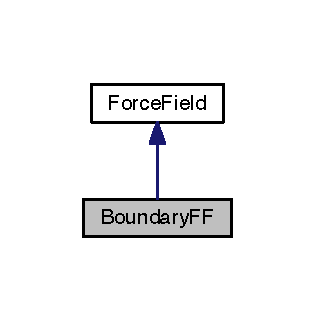
\includegraphics[width=151pt]{classBoundaryFF__inherit__graph}
\end{center}
\end{figure}


Collaboration diagram for Boundary\+F\+F\+:\nopagebreak
\begin{figure}[H]
\begin{center}
\leavevmode
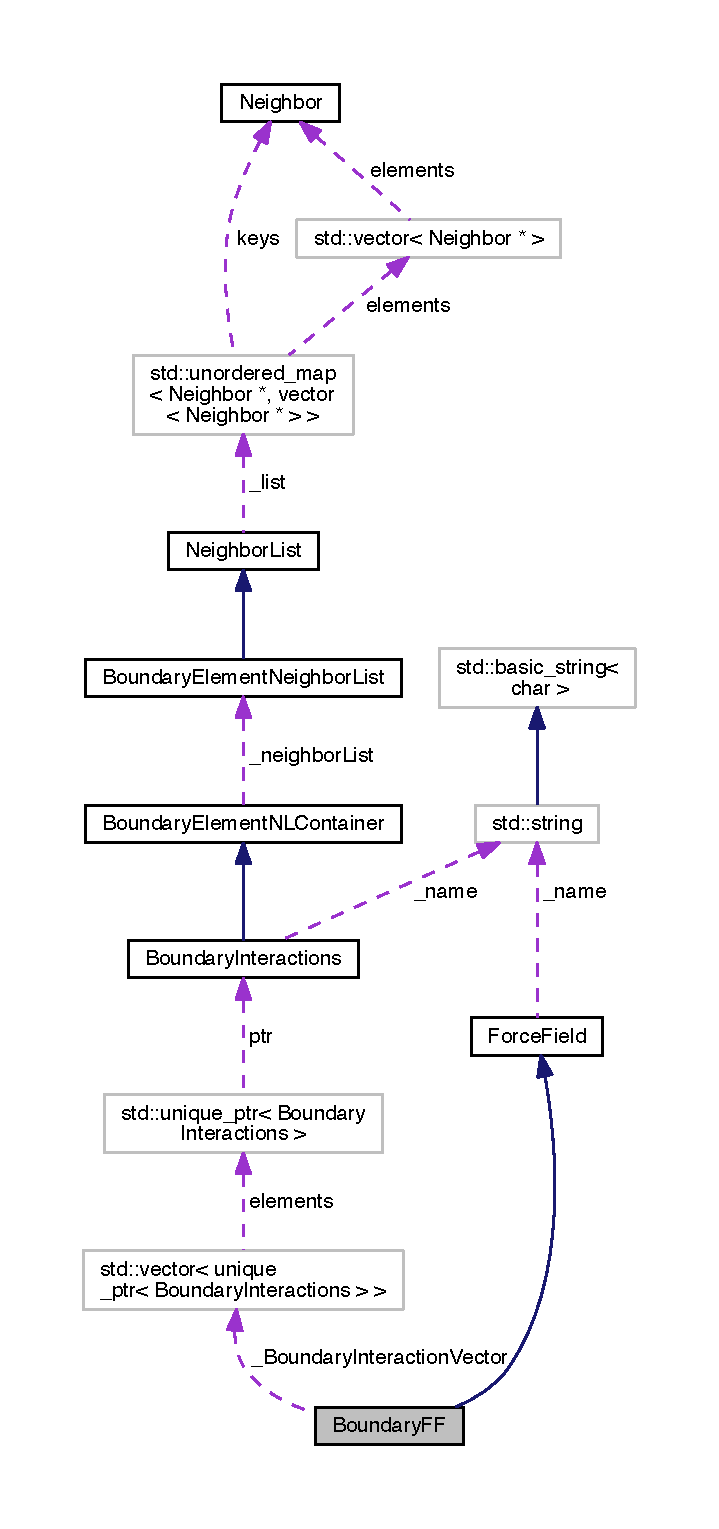
\includegraphics[height=550pt]{classBoundaryFF__coll__graph}
\end{center}
\end{figure}
\subsection*{Public Member Functions}
\begin{DoxyCompactItemize}
\item 
\hyperlink{classBoundaryFF_adc5b93d797c1a0b58445625311fc00af}{Boundary\+F\+F} (string interaction1, string interaction2, string interaction3)
\begin{DoxyCompactList}\small\item\em Initialize the forcefields (repulsion, attraction, etc) \end{DoxyCompactList}\item 
virtual double \hyperlink{classBoundaryFF_a3a3c0dd0f82424d358c6b19abea9b743}{compute\+Energy} (double d)
\begin{DoxyCompactList}\small\item\em Compute total energy of this forcefield in the system. \end{DoxyCompactList}\item 
virtual void \hyperlink{classBoundaryFF_a6ae273b9af97e9f50923958c486ec7f7}{compute\+Forces} ()
\begin{DoxyCompactList}\small\item\em Compute forces of this forcefield in the system. Update \hyperlink{classBead}{Bead} forces accordingly. \end{DoxyCompactList}\item 
virtual void \hyperlink{classBoundaryFF_abf4fc3bd031457f68611c239f955da83}{compute\+Forces\+Aux} ()
\begin{DoxyCompactList}\small\item\em Compute auxiliary forces of this forcefield in the system. Update \hyperlink{classBead}{Bead} auxiliary forces accordingly. \end{DoxyCompactList}\item 
const string \& \hyperlink{classForceField_a4a09e09603b4c4650dc7b3b0f0912fd2}{get\+Name} ()
\begin{DoxyCompactList}\small\item\em Get the name of this forcefield. \end{DoxyCompactList}\end{DoxyCompactItemize}
\subsection*{Private Attributes}
\begin{DoxyCompactItemize}
\item 
vector$<$ unique\+\_\+ptr\\*
$<$ \hyperlink{classBoundaryInteractions}{Boundary\+Interactions} $>$ $>$ \hyperlink{classBoundaryFF_ae2eab3aa7d1d57be9bd511249b54e074}{\+\_\+\+Boundary\+Interaction\+Vector}
\begin{DoxyCompactList}\small\item\em Vector of initialized boundary element interactions. \end{DoxyCompactList}\end{DoxyCompactItemize}


\subsection{Detailed Description}
An implementation of the \hyperlink{classForceField}{Force\+Field} class that calculates \hyperlink{classBoundaryElement}{Boundary\+Element} repulsion and attraction to \hyperlink{classBead}{Beads} in the system. 



Definition at line 28 of file Boundary\+F\+F.\+h.



\subsection{Constructor \& Destructor Documentation}
\hypertarget{classBoundaryFF_adc5b93d797c1a0b58445625311fc00af}{\index{Boundary\+F\+F@{Boundary\+F\+F}!Boundary\+F\+F@{Boundary\+F\+F}}
\index{Boundary\+F\+F@{Boundary\+F\+F}!Boundary\+F\+F@{Boundary\+F\+F}}
\subsubsection[{Boundary\+F\+F}]{\setlength{\rightskip}{0pt plus 5cm}Boundary\+F\+F\+::\+Boundary\+F\+F (
\begin{DoxyParamCaption}
\item[{string}]{interaction1, }
\item[{string}]{interaction2, }
\item[{string}]{interaction3}
\end{DoxyParamCaption}
)}}\label{classBoundaryFF_adc5b93d797c1a0b58445625311fc00af}


Initialize the forcefields (repulsion, attraction, etc) 



Definition at line 23 of file Boundary\+F\+F.\+cpp.



References \+\_\+\+Boundary\+Interaction\+Vector.



\subsection{Member Function Documentation}
\hypertarget{classBoundaryFF_a3a3c0dd0f82424d358c6b19abea9b743}{\index{Boundary\+F\+F@{Boundary\+F\+F}!compute\+Energy@{compute\+Energy}}
\index{compute\+Energy@{compute\+Energy}!Boundary\+F\+F@{Boundary\+F\+F}}
\subsubsection[{compute\+Energy}]{\setlength{\rightskip}{0pt plus 5cm}double Boundary\+F\+F\+::compute\+Energy (
\begin{DoxyParamCaption}
\item[{double}]{d}
\end{DoxyParamCaption}
)\hspace{0.3cm}{\ttfamily [virtual]}}}\label{classBoundaryFF_a3a3c0dd0f82424d358c6b19abea9b743}


Compute total energy of this forcefield in the system. 



Implements \hyperlink{classForceField_a9bed91c670fe33dfc82da2b357fb8fa6}{Force\+Field}.



Definition at line 31 of file Boundary\+F\+F.\+cpp.



References \+\_\+\+Boundary\+Interaction\+Vector, and Boundary\+Element\+D\+B\+::instance().

\hypertarget{classBoundaryFF_a6ae273b9af97e9f50923958c486ec7f7}{\index{Boundary\+F\+F@{Boundary\+F\+F}!compute\+Forces@{compute\+Forces}}
\index{compute\+Forces@{compute\+Forces}!Boundary\+F\+F@{Boundary\+F\+F}}
\subsubsection[{compute\+Forces}]{\setlength{\rightskip}{0pt plus 5cm}void Boundary\+F\+F\+::compute\+Forces (
\begin{DoxyParamCaption}
{}
\end{DoxyParamCaption}
)\hspace{0.3cm}{\ttfamily [virtual]}}}\label{classBoundaryFF_a6ae273b9af97e9f50923958c486ec7f7}


Compute forces of this forcefield in the system. Update \hyperlink{classBead}{Bead} forces accordingly. 



Implements \hyperlink{classForceField_a56c33a25830131e45068454de039513a}{Force\+Field}.



Definition at line 44 of file Boundary\+F\+F.\+cpp.



References \+\_\+\+Boundary\+Interaction\+Vector, and Boundary\+Element\+D\+B\+::instance().

\hypertarget{classBoundaryFF_abf4fc3bd031457f68611c239f955da83}{\index{Boundary\+F\+F@{Boundary\+F\+F}!compute\+Forces\+Aux@{compute\+Forces\+Aux}}
\index{compute\+Forces\+Aux@{compute\+Forces\+Aux}!Boundary\+F\+F@{Boundary\+F\+F}}
\subsubsection[{compute\+Forces\+Aux}]{\setlength{\rightskip}{0pt plus 5cm}void Boundary\+F\+F\+::compute\+Forces\+Aux (
\begin{DoxyParamCaption}
{}
\end{DoxyParamCaption}
)\hspace{0.3cm}{\ttfamily [virtual]}}}\label{classBoundaryFF_abf4fc3bd031457f68611c239f955da83}


Compute auxiliary forces of this forcefield in the system. Update \hyperlink{classBead}{Bead} auxiliary forces accordingly. 



Implements \hyperlink{classForceField_a17004f440c9d380da5b9d9ea8794b3cc}{Force\+Field}.



Definition at line 55 of file Boundary\+F\+F.\+cpp.



References \+\_\+\+Boundary\+Interaction\+Vector, and Boundary\+Element\+D\+B\+::instance().

\hypertarget{classForceField_a4a09e09603b4c4650dc7b3b0f0912fd2}{\index{Boundary\+F\+F@{Boundary\+F\+F}!get\+Name@{get\+Name}}
\index{get\+Name@{get\+Name}!Boundary\+F\+F@{Boundary\+F\+F}}
\subsubsection[{get\+Name}]{\setlength{\rightskip}{0pt plus 5cm}const string\& Force\+Field\+::get\+Name (
\begin{DoxyParamCaption}
{}
\end{DoxyParamCaption}
)\hspace{0.3cm}{\ttfamily [inline]}, {\ttfamily [inherited]}}}\label{classForceField_a4a09e09603b4c4650dc7b3b0f0912fd2}


Get the name of this forcefield. 



Definition at line 31 of file Force\+Field.\+h.



References Force\+Field\+::\+\_\+name.



\subsection{Member Data Documentation}
\hypertarget{classBoundaryFF_ae2eab3aa7d1d57be9bd511249b54e074}{\index{Boundary\+F\+F@{Boundary\+F\+F}!\+\_\+\+Boundary\+Interaction\+Vector@{\+\_\+\+Boundary\+Interaction\+Vector}}
\index{\+\_\+\+Boundary\+Interaction\+Vector@{\+\_\+\+Boundary\+Interaction\+Vector}!Boundary\+F\+F@{Boundary\+F\+F}}
\subsubsection[{\+\_\+\+Boundary\+Interaction\+Vector}]{\setlength{\rightskip}{0pt plus 5cm}vector$<$unique\+\_\+ptr$<${\bf Boundary\+Interactions}$>$ $>$ Boundary\+F\+F\+::\+\_\+\+Boundary\+Interaction\+Vector\hspace{0.3cm}{\ttfamily [private]}}}\label{classBoundaryFF_ae2eab3aa7d1d57be9bd511249b54e074}


Vector of initialized boundary element interactions. 



Definition at line 31 of file Boundary\+F\+F.\+h.



Referenced by Boundary\+F\+F(), compute\+Energy(), compute\+Forces(), and compute\+Forces\+Aux().



The documentation for this class was generated from the following files\+:\begin{DoxyCompactItemize}
\item 
M3\+S\+Y\+M/\+Mechanics/\+Force\+Field/\hyperlink{BoundaryFF_8h}{Boundary\+F\+F.\+h}\item 
M3\+S\+Y\+M/\+Mechanics/\+Force\+Field/\hyperlink{BoundaryFF_8cpp}{Boundary\+F\+F.\+cpp}\end{DoxyCompactItemize}

\hypertarget{classBoundaryInteractions}{\section{Boundary\+Interactions Class Reference}
\label{classBoundaryInteractions}\index{Boundary\+Interactions@{Boundary\+Interactions}}
}


Represents a \hyperlink{classBoundaryElement}{Boundary\+Element} interaction with a \hyperlink{classBead}{Bead}.  




{\ttfamily \#include $<$Boundary\+Interactions.\+h$>$}



Inheritance diagram for Boundary\+Interactions\+:\nopagebreak
\begin{figure}[H]
\begin{center}
\leavevmode
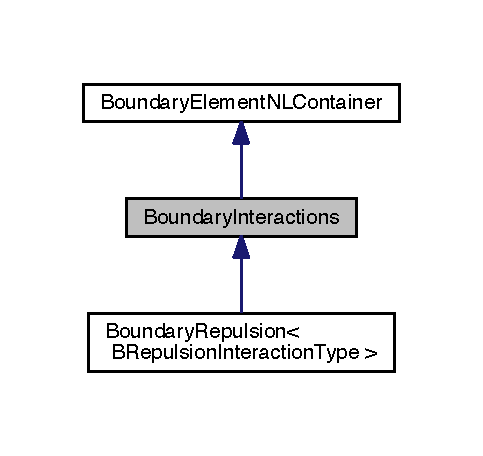
\includegraphics[width=232pt]{classBoundaryInteractions__inherit__graph}
\end{center}
\end{figure}


Collaboration diagram for Boundary\+Interactions\+:\nopagebreak
\begin{figure}[H]
\begin{center}
\leavevmode
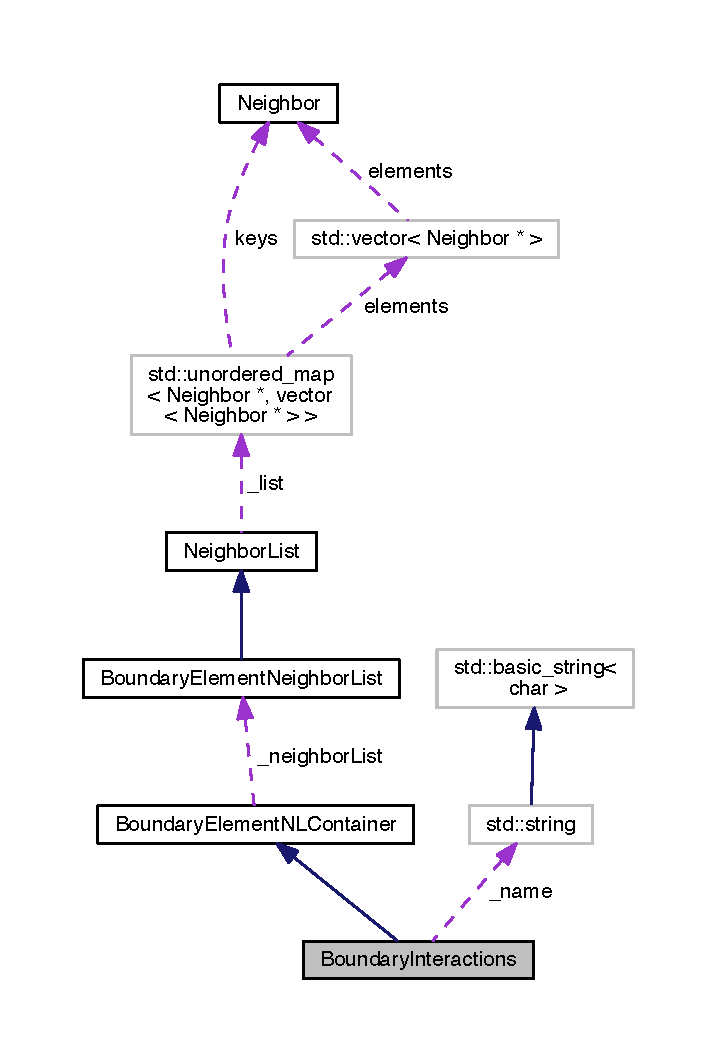
\includegraphics[width=344pt]{classBoundaryInteractions__coll__graph}
\end{center}
\end{figure}
\subsection*{Public Member Functions}
\begin{DoxyCompactItemize}
\item 
\hyperlink{classBoundaryInteractions_aad77fa96cf328adb581dda20c68eb313}{Boundary\+Interactions} ()
\begin{DoxyCompactList}\small\item\em Constructor, intializes the neighbor list needed. \end{DoxyCompactList}\item 
virtual double \hyperlink{classBoundaryInteractions_a78b34313aa441137288dea97cbf37912}{compute\+Energy} (\hyperlink{classBoundaryElement}{Boundary\+Element} $\ast$, \hyperlink{classBead}{Bead} $\ast$, double d)=0
\begin{DoxyCompactList}\small\item\em Compute energy of this interaction. \end{DoxyCompactList}\item 
virtual void \hyperlink{classBoundaryInteractions_a4280d211cec7be35730a7a7b6c5c4bd4}{compute\+Forces} (\hyperlink{classBoundaryElement}{Boundary\+Element} $\ast$, \hyperlink{classBead}{Bead} $\ast$)=0
\begin{DoxyCompactList}\small\item\em Compute forces of this interaction. \end{DoxyCompactList}\item 
virtual void \hyperlink{classBoundaryInteractions_a112697f0d9dd8884ef67f1ce81e892da}{compute\+Forces\+Aux} (\hyperlink{classBoundaryElement}{Boundary\+Element} $\ast$, \hyperlink{classBead}{Bead} $\ast$)=0
\begin{DoxyCompactList}\small\item\em Compute auxiliary forces of this interaction. \end{DoxyCompactList}\item 
string \hyperlink{classBoundaryInteractions_aece29831e11962476a9d6c016b5d4b86}{get\+Name} ()
\begin{DoxyCompactList}\small\item\em Get name of interaction. \end{DoxyCompactList}\item 
\hyperlink{classBoundaryElementNeighborList}{Boundary\+Element\+Neighbor\+List} $\ast$ \hyperlink{classBoundaryElementNLContainer_aa665161110c46e0a2af9f760c96afe19}{get\+Neighbor\+List} ()
\begin{DoxyCompactList}\small\item\em Get neighbor list. \end{DoxyCompactList}\end{DoxyCompactItemize}
\subsection*{Private Attributes}
\begin{DoxyCompactItemize}
\item 
string \hyperlink{classBoundaryInteractions_a25e60fb01cc037ab06ba79edbf7073d4}{\+\_\+name}
\begin{DoxyCompactList}\small\item\em Name of interaction. \end{DoxyCompactList}\end{DoxyCompactItemize}


\subsection{Detailed Description}
Represents a \hyperlink{classBoundaryElement}{Boundary\+Element} interaction with a \hyperlink{classBead}{Bead}. 

Definition at line 27 of file Boundary\+Interactions.\+h.



\subsection{Constructor \& Destructor Documentation}
\hypertarget{classBoundaryInteractions_aad77fa96cf328adb581dda20c68eb313}{\index{Boundary\+Interactions@{Boundary\+Interactions}!Boundary\+Interactions@{Boundary\+Interactions}}
\index{Boundary\+Interactions@{Boundary\+Interactions}!Boundary\+Interactions@{Boundary\+Interactions}}
\subsubsection[{Boundary\+Interactions}]{\setlength{\rightskip}{0pt plus 5cm}Boundary\+Interactions\+::\+Boundary\+Interactions (
\begin{DoxyParamCaption}
{}
\end{DoxyParamCaption}
)\hspace{0.3cm}{\ttfamily [inline]}}}\label{classBoundaryInteractions_aad77fa96cf328adb581dda20c68eb313}


Constructor, intializes the neighbor list needed. 



Definition at line 33 of file Boundary\+Interactions.\+h.



\subsection{Member Function Documentation}
\hypertarget{classBoundaryInteractions_a78b34313aa441137288dea97cbf37912}{\index{Boundary\+Interactions@{Boundary\+Interactions}!compute\+Energy@{compute\+Energy}}
\index{compute\+Energy@{compute\+Energy}!Boundary\+Interactions@{Boundary\+Interactions}}
\subsubsection[{compute\+Energy}]{\setlength{\rightskip}{0pt plus 5cm}virtual double Boundary\+Interactions\+::compute\+Energy (
\begin{DoxyParamCaption}
\item[{{\bf Boundary\+Element} $\ast$}]{, }
\item[{{\bf Bead} $\ast$}]{, }
\item[{double}]{d}
\end{DoxyParamCaption}
)\hspace{0.3cm}{\ttfamily [pure virtual]}}}\label{classBoundaryInteractions_a78b34313aa441137288dea97cbf37912}


Compute energy of this interaction. 



Implemented in \hyperlink{classBoundaryRepulsion_ace56d8bd2b0287fdf1953366cdbef133}{Boundary\+Repulsion$<$ B\+Repulsion\+Interaction\+Type $>$}.

\hypertarget{classBoundaryInteractions_a4280d211cec7be35730a7a7b6c5c4bd4}{\index{Boundary\+Interactions@{Boundary\+Interactions}!compute\+Forces@{compute\+Forces}}
\index{compute\+Forces@{compute\+Forces}!Boundary\+Interactions@{Boundary\+Interactions}}
\subsubsection[{compute\+Forces}]{\setlength{\rightskip}{0pt plus 5cm}virtual void Boundary\+Interactions\+::compute\+Forces (
\begin{DoxyParamCaption}
\item[{{\bf Boundary\+Element} $\ast$}]{, }
\item[{{\bf Bead} $\ast$}]{}
\end{DoxyParamCaption}
)\hspace{0.3cm}{\ttfamily [pure virtual]}}}\label{classBoundaryInteractions_a4280d211cec7be35730a7a7b6c5c4bd4}


Compute forces of this interaction. 



Implemented in \hyperlink{classBoundaryRepulsion_a2b7426b4039634b5837e52aa22ca2f1c}{Boundary\+Repulsion$<$ B\+Repulsion\+Interaction\+Type $>$}.

\hypertarget{classBoundaryInteractions_a112697f0d9dd8884ef67f1ce81e892da}{\index{Boundary\+Interactions@{Boundary\+Interactions}!compute\+Forces\+Aux@{compute\+Forces\+Aux}}
\index{compute\+Forces\+Aux@{compute\+Forces\+Aux}!Boundary\+Interactions@{Boundary\+Interactions}}
\subsubsection[{compute\+Forces\+Aux}]{\setlength{\rightskip}{0pt plus 5cm}virtual void Boundary\+Interactions\+::compute\+Forces\+Aux (
\begin{DoxyParamCaption}
\item[{{\bf Boundary\+Element} $\ast$}]{, }
\item[{{\bf Bead} $\ast$}]{}
\end{DoxyParamCaption}
)\hspace{0.3cm}{\ttfamily [pure virtual]}}}\label{classBoundaryInteractions_a112697f0d9dd8884ef67f1ce81e892da}


Compute auxiliary forces of this interaction. 



Implemented in \hyperlink{classBoundaryRepulsion_a7fd265f247cfd0b15b8112654ab44b89}{Boundary\+Repulsion$<$ B\+Repulsion\+Interaction\+Type $>$}.

\hypertarget{classBoundaryInteractions_aece29831e11962476a9d6c016b5d4b86}{\index{Boundary\+Interactions@{Boundary\+Interactions}!get\+Name@{get\+Name}}
\index{get\+Name@{get\+Name}!Boundary\+Interactions@{Boundary\+Interactions}}
\subsubsection[{get\+Name}]{\setlength{\rightskip}{0pt plus 5cm}string Boundary\+Interactions\+::get\+Name (
\begin{DoxyParamCaption}
{}
\end{DoxyParamCaption}
)\hspace{0.3cm}{\ttfamily [inline]}}}\label{classBoundaryInteractions_aece29831e11962476a9d6c016b5d4b86}


Get name of interaction. 



Definition at line 43 of file Boundary\+Interactions.\+h.



References \+\_\+name.

\hypertarget{classBoundaryElementNLContainer_aa665161110c46e0a2af9f760c96afe19}{\index{Boundary\+Interactions@{Boundary\+Interactions}!get\+Neighbor\+List@{get\+Neighbor\+List}}
\index{get\+Neighbor\+List@{get\+Neighbor\+List}!Boundary\+Interactions@{Boundary\+Interactions}}
\subsubsection[{get\+Neighbor\+List}]{\setlength{\rightskip}{0pt plus 5cm}{\bf Boundary\+Element\+Neighbor\+List}$\ast$ Boundary\+Element\+N\+L\+Container\+::get\+Neighbor\+List (
\begin{DoxyParamCaption}
{}
\end{DoxyParamCaption}
)\hspace{0.3cm}{\ttfamily [inline]}, {\ttfamily [inherited]}}}\label{classBoundaryElementNLContainer_aa665161110c46e0a2af9f760c96afe19}


Get neighbor list. 



Definition at line 65 of file Neighbor\+List\+Container.\+h.



References Boundary\+Element\+N\+L\+Container\+::\+\_\+neighbor\+List.



\subsection{Member Data Documentation}
\hypertarget{classBoundaryInteractions_a25e60fb01cc037ab06ba79edbf7073d4}{\index{Boundary\+Interactions@{Boundary\+Interactions}!\+\_\+name@{\+\_\+name}}
\index{\+\_\+name@{\+\_\+name}!Boundary\+Interactions@{Boundary\+Interactions}}
\subsubsection[{\+\_\+name}]{\setlength{\rightskip}{0pt plus 5cm}string Boundary\+Interactions\+::\+\_\+name\hspace{0.3cm}{\ttfamily [private]}}}\label{classBoundaryInteractions_a25e60fb01cc037ab06ba79edbf7073d4}


Name of interaction. 



Definition at line 29 of file Boundary\+Interactions.\+h.



Referenced by get\+Name().



The documentation for this class was generated from the following file\+:\begin{DoxyCompactItemize}
\item 
M3\+S\+Y\+M/\+Mechanics/\+Force\+Field/\hyperlink{BoundaryInteractions_8h}{Boundary\+Interactions.\+h}\end{DoxyCompactItemize}

\hypertarget{structBoundaryParameters}{\section{Boundary\+Parameters Struct Reference}
\label{structBoundaryParameters}\index{Boundary\+Parameters@{Boundary\+Parameters}}
}


Struct to hold boundary parameters for the system.  




{\ttfamily \#include $<$System\+Parameters.\+h$>$}

\subsection*{Public Attributes}
\begin{DoxyCompactItemize}
\item 
double \hyperlink{structBoundaryParameters_a90e9efca0ade0a603523945c49056edd}{boundary\+Cutoff} = 0
\item 
double \hyperlink{structBoundaryParameters_aeb92b89caa0bf379a2dd1e26a032bb75}{boundary\+K} = 0
\item 
double \hyperlink{structBoundaryParameters_a75161f641debbb58f2829d8bba03b532}{screen\+Length} = 0
\item 
double \hyperlink{structBoundaryParameters_aff24f2bccaef825eff7c3181ec1cefcc}{diameter} = 0
\end{DoxyCompactItemize}


\subsection{Detailed Description}
Struct to hold boundary parameters for the system. 

Definition at line 103 of file System\+Parameters.\+h.



\subsection{Member Data Documentation}
\hypertarget{structBoundaryParameters_a90e9efca0ade0a603523945c49056edd}{\index{Boundary\+Parameters@{Boundary\+Parameters}!boundary\+Cutoff@{boundary\+Cutoff}}
\index{boundary\+Cutoff@{boundary\+Cutoff}!Boundary\+Parameters@{Boundary\+Parameters}}
\subsubsection[{boundary\+Cutoff}]{\setlength{\rightskip}{0pt plus 5cm}double Boundary\+Parameters\+::boundary\+Cutoff = 0}}\label{structBoundaryParameters_a90e9efca0ade0a603523945c49056edd}


Definition at line 105 of file System\+Parameters.\+h.



Referenced by System\+Parser\+::read\+Boundary\+Parameters().

\hypertarget{structBoundaryParameters_aeb92b89caa0bf379a2dd1e26a032bb75}{\index{Boundary\+Parameters@{Boundary\+Parameters}!boundary\+K@{boundary\+K}}
\index{boundary\+K@{boundary\+K}!Boundary\+Parameters@{Boundary\+Parameters}}
\subsubsection[{boundary\+K}]{\setlength{\rightskip}{0pt plus 5cm}double Boundary\+Parameters\+::boundary\+K = 0}}\label{structBoundaryParameters_aeb92b89caa0bf379a2dd1e26a032bb75}


Definition at line 106 of file System\+Parameters.\+h.



Referenced by System\+Parser\+::read\+Boundary\+Parameters().

\hypertarget{structBoundaryParameters_aff24f2bccaef825eff7c3181ec1cefcc}{\index{Boundary\+Parameters@{Boundary\+Parameters}!diameter@{diameter}}
\index{diameter@{diameter}!Boundary\+Parameters@{Boundary\+Parameters}}
\subsubsection[{diameter}]{\setlength{\rightskip}{0pt plus 5cm}double Boundary\+Parameters\+::diameter = 0}}\label{structBoundaryParameters_aff24f2bccaef825eff7c3181ec1cefcc}


Definition at line 109 of file System\+Parameters.\+h.



Referenced by System\+Parser\+::read\+Boundary\+Parameters().

\hypertarget{structBoundaryParameters_a75161f641debbb58f2829d8bba03b532}{\index{Boundary\+Parameters@{Boundary\+Parameters}!screen\+Length@{screen\+Length}}
\index{screen\+Length@{screen\+Length}!Boundary\+Parameters@{Boundary\+Parameters}}
\subsubsection[{screen\+Length}]{\setlength{\rightskip}{0pt plus 5cm}double Boundary\+Parameters\+::screen\+Length = 0}}\label{structBoundaryParameters_a75161f641debbb58f2829d8bba03b532}


Definition at line 107 of file System\+Parameters.\+h.



Referenced by System\+Parser\+::read\+Boundary\+Parameters().



The documentation for this struct was generated from the following file\+:\begin{DoxyCompactItemize}
\item 
M3\+S\+Y\+M/\hyperlink{SystemParameters_8h}{System\+Parameters.\+h}\end{DoxyCompactItemize}

\hypertarget{classBoundaryRepulsion}{\section{Boundary\+Repulsion$<$ B\+Repulsion\+Interaction\+Type $>$ Class Template Reference}
\label{classBoundaryRepulsion}\index{Boundary\+Repulsion$<$ B\+Repulsion\+Interaction\+Type $>$@{Boundary\+Repulsion$<$ B\+Repulsion\+Interaction\+Type $>$}}
}


Represents a repulsive interaction between a \hyperlink{classBoundaryElement}{Boundary\+Element} and \hyperlink{classBead}{Bead}.  




{\ttfamily \#include $<$Boundary\+Repulsion.\+h$>$}



Inheritance diagram for Boundary\+Repulsion$<$ B\+Repulsion\+Interaction\+Type $>$\+:\nopagebreak
\begin{figure}[H]
\begin{center}
\leavevmode
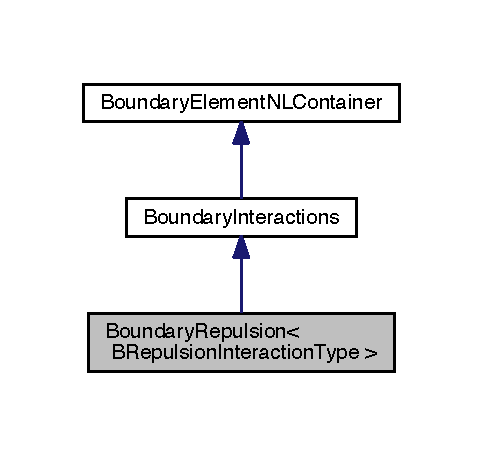
\includegraphics[width=232pt]{classBoundaryRepulsion__inherit__graph}
\end{center}
\end{figure}


Collaboration diagram for Boundary\+Repulsion$<$ B\+Repulsion\+Interaction\+Type $>$\+:\nopagebreak
\begin{figure}[H]
\begin{center}
\leavevmode
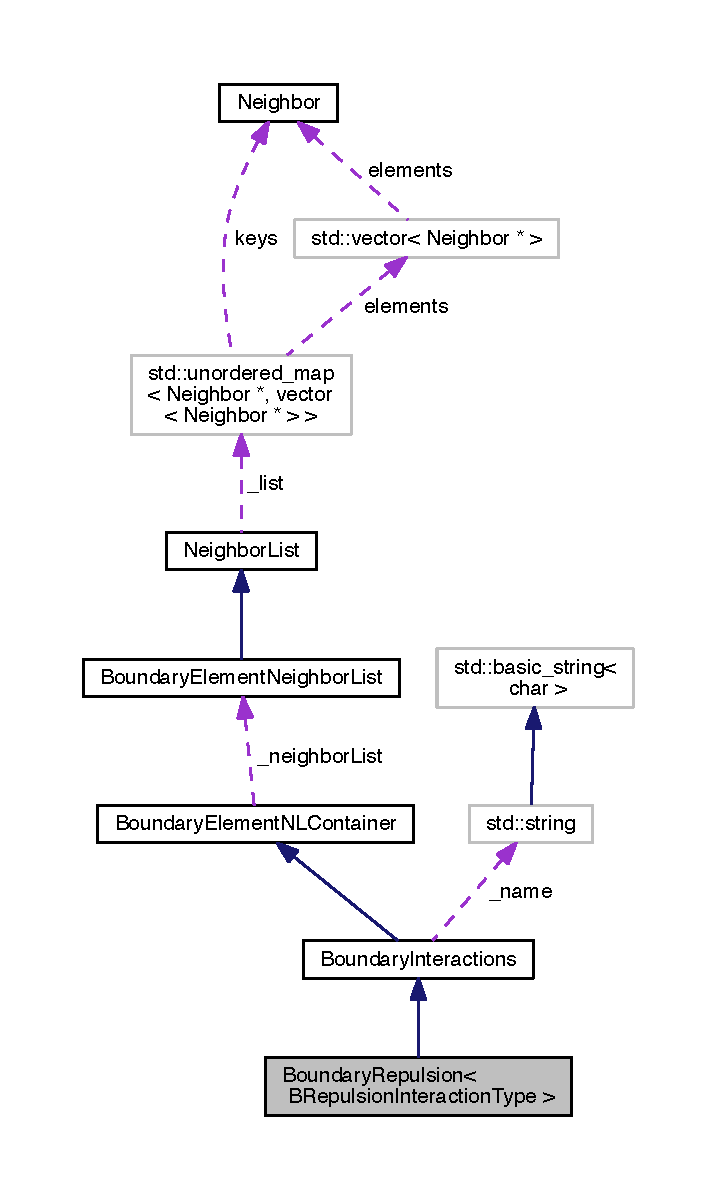
\includegraphics[height=550pt]{classBoundaryRepulsion__coll__graph}
\end{center}
\end{figure}
\subsection*{Public Member Functions}
\begin{DoxyCompactItemize}
\item 
virtual double \hyperlink{classBoundaryRepulsion_ace56d8bd2b0287fdf1953366cdbef133}{compute\+Energy} (\hyperlink{classBoundaryElement}{Boundary\+Element} $\ast$, \hyperlink{classBead}{Bead} $\ast$, double d)
\begin{DoxyCompactList}\small\item\em Template specializations. \end{DoxyCompactList}\item 
virtual void \hyperlink{classBoundaryRepulsion_a2b7426b4039634b5837e52aa22ca2f1c}{compute\+Forces} (\hyperlink{classBoundaryElement}{Boundary\+Element} $\ast$, \hyperlink{classBead}{Bead} $\ast$)
\begin{DoxyCompactList}\small\item\em Compute forces of this interaction. \end{DoxyCompactList}\item 
virtual void \hyperlink{classBoundaryRepulsion_a7fd265f247cfd0b15b8112654ab44b89}{compute\+Forces\+Aux} (\hyperlink{classBoundaryElement}{Boundary\+Element} $\ast$, \hyperlink{classBead}{Bead} $\ast$)
\begin{DoxyCompactList}\small\item\em Compute auxiliary forces of this interaction. \end{DoxyCompactList}\item 
string \hyperlink{classBoundaryInteractions_aece29831e11962476a9d6c016b5d4b86}{get\+Name} ()
\begin{DoxyCompactList}\small\item\em Get name of interaction. \end{DoxyCompactList}\item 
\hyperlink{classBoundaryElementNeighborList}{Boundary\+Element\+Neighbor\+List} $\ast$ \hyperlink{classBoundaryElementNLContainer_aa665161110c46e0a2af9f760c96afe19}{get\+Neighbor\+List} ()
\begin{DoxyCompactList}\small\item\em Get neighbor list. \end{DoxyCompactList}\end{DoxyCompactItemize}
\subsection*{Private Attributes}
\begin{DoxyCompactItemize}
\item 
B\+Repulsion\+Interaction\+Type \hyperlink{classBoundaryRepulsion_a155fc2c7cded4f928ebd0371276e8016}{\+\_\+\+F\+F\+Type}
\end{DoxyCompactItemize}


\subsection{Detailed Description}
\subsubsection*{template$<$class B\+Repulsion\+Interaction\+Type$>$class Boundary\+Repulsion$<$ B\+Repulsion\+Interaction\+Type $>$}

Represents a repulsive interaction between a \hyperlink{classBoundaryElement}{Boundary\+Element} and \hyperlink{classBead}{Bead}. 

Definition at line 29 of file Boundary\+Repulsion.\+h.



\subsection{Member Function Documentation}
\hypertarget{classBoundaryRepulsion_ace56d8bd2b0287fdf1953366cdbef133}{\index{Boundary\+Repulsion@{Boundary\+Repulsion}!compute\+Energy@{compute\+Energy}}
\index{compute\+Energy@{compute\+Energy}!Boundary\+Repulsion@{Boundary\+Repulsion}}
\subsubsection[{compute\+Energy}]{\setlength{\rightskip}{0pt plus 5cm}template$<$class B\+Repulsion\+Interaction\+Type $>$ template double {\bf Boundary\+Repulsion}$<$ B\+Repulsion\+Interaction\+Type $>$\+::compute\+Energy (
\begin{DoxyParamCaption}
\item[{{\bf Boundary\+Element} $\ast$}]{, }
\item[{{\bf Bead} $\ast$}]{, }
\item[{double}]{d}
\end{DoxyParamCaption}
)\hspace{0.3cm}{\ttfamily [virtual]}}}\label{classBoundaryRepulsion_ace56d8bd2b0287fdf1953366cdbef133}


Template specializations. 



Implements \hyperlink{classBoundaryInteractions_a78b34313aa441137288dea97cbf37912}{Boundary\+Interactions}.



Definition at line 23 of file Boundary\+Repulsion.\+cpp.



References Bead\+::coordinate, Boundary\+Element\+::distance(), Bead\+::force, Boundary\+Element\+::get\+Repulsion\+Const(), Boundary\+Element\+::get\+Screening\+Length(), and Boundary\+Element\+::stretched\+Distance().

\hypertarget{classBoundaryRepulsion_a2b7426b4039634b5837e52aa22ca2f1c}{\index{Boundary\+Repulsion@{Boundary\+Repulsion}!compute\+Forces@{compute\+Forces}}
\index{compute\+Forces@{compute\+Forces}!Boundary\+Repulsion@{Boundary\+Repulsion}}
\subsubsection[{compute\+Forces}]{\setlength{\rightskip}{0pt plus 5cm}template$<$class B\+Repulsion\+Interaction\+Type $>$ template void {\bf Boundary\+Repulsion}$<$ B\+Repulsion\+Interaction\+Type $>$\+::compute\+Forces (
\begin{DoxyParamCaption}
\item[{{\bf Boundary\+Element} $\ast$}]{, }
\item[{{\bf Bead} $\ast$}]{}
\end{DoxyParamCaption}
)\hspace{0.3cm}{\ttfamily [virtual]}}}\label{classBoundaryRepulsion_a2b7426b4039634b5837e52aa22ca2f1c}


Compute forces of this interaction. 



Implements \hyperlink{classBoundaryInteractions_a4280d211cec7be35730a7a7b6c5c4bd4}{Boundary\+Interactions}.



Definition at line 37 of file Boundary\+Repulsion.\+cpp.



References Bead\+::coordinate, Boundary\+Element\+::distance(), Boundary\+Element\+::get\+Repulsion\+Const(), Boundary\+Element\+::get\+Screening\+Length(), and Boundary\+Element\+::normal().

\hypertarget{classBoundaryRepulsion_a7fd265f247cfd0b15b8112654ab44b89}{\index{Boundary\+Repulsion@{Boundary\+Repulsion}!compute\+Forces\+Aux@{compute\+Forces\+Aux}}
\index{compute\+Forces\+Aux@{compute\+Forces\+Aux}!Boundary\+Repulsion@{Boundary\+Repulsion}}
\subsubsection[{compute\+Forces\+Aux}]{\setlength{\rightskip}{0pt plus 5cm}template$<$class B\+Repulsion\+Interaction\+Type $>$ template void {\bf Boundary\+Repulsion}$<$ B\+Repulsion\+Interaction\+Type $>$\+::compute\+Forces\+Aux (
\begin{DoxyParamCaption}
\item[{{\bf Boundary\+Element} $\ast$}]{, }
\item[{{\bf Bead} $\ast$}]{}
\end{DoxyParamCaption}
)\hspace{0.3cm}{\ttfamily [virtual]}}}\label{classBoundaryRepulsion_a7fd265f247cfd0b15b8112654ab44b89}


Compute auxiliary forces of this interaction. 



Implements \hyperlink{classBoundaryInteractions_a112697f0d9dd8884ef67f1ce81e892da}{Boundary\+Interactions}.



Definition at line 49 of file Boundary\+Repulsion.\+cpp.



References Bead\+::coordinate\+Aux, Boundary\+Element\+::distance(), Boundary\+Element\+::get\+Repulsion\+Const(), Boundary\+Element\+::get\+Screening\+Length(), and Boundary\+Element\+::normal().

\hypertarget{classBoundaryInteractions_aece29831e11962476a9d6c016b5d4b86}{\index{Boundary\+Repulsion@{Boundary\+Repulsion}!get\+Name@{get\+Name}}
\index{get\+Name@{get\+Name}!Boundary\+Repulsion@{Boundary\+Repulsion}}
\subsubsection[{get\+Name}]{\setlength{\rightskip}{0pt plus 5cm}string Boundary\+Interactions\+::get\+Name (
\begin{DoxyParamCaption}
{}
\end{DoxyParamCaption}
)\hspace{0.3cm}{\ttfamily [inline]}, {\ttfamily [inherited]}}}\label{classBoundaryInteractions_aece29831e11962476a9d6c016b5d4b86}


Get name of interaction. 



Definition at line 43 of file Boundary\+Interactions.\+h.



References Boundary\+Interactions\+::\+\_\+name.

\hypertarget{classBoundaryElementNLContainer_aa665161110c46e0a2af9f760c96afe19}{\index{Boundary\+Repulsion@{Boundary\+Repulsion}!get\+Neighbor\+List@{get\+Neighbor\+List}}
\index{get\+Neighbor\+List@{get\+Neighbor\+List}!Boundary\+Repulsion@{Boundary\+Repulsion}}
\subsubsection[{get\+Neighbor\+List}]{\setlength{\rightskip}{0pt plus 5cm}{\bf Boundary\+Element\+Neighbor\+List}$\ast$ Boundary\+Element\+N\+L\+Container\+::get\+Neighbor\+List (
\begin{DoxyParamCaption}
{}
\end{DoxyParamCaption}
)\hspace{0.3cm}{\ttfamily [inline]}, {\ttfamily [inherited]}}}\label{classBoundaryElementNLContainer_aa665161110c46e0a2af9f760c96afe19}


Get neighbor list. 



Definition at line 65 of file Neighbor\+List\+Container.\+h.



References Boundary\+Element\+N\+L\+Container\+::\+\_\+neighbor\+List.



\subsection{Member Data Documentation}
\hypertarget{classBoundaryRepulsion_a155fc2c7cded4f928ebd0371276e8016}{\index{Boundary\+Repulsion@{Boundary\+Repulsion}!\+\_\+\+F\+F\+Type@{\+\_\+\+F\+F\+Type}}
\index{\+\_\+\+F\+F\+Type@{\+\_\+\+F\+F\+Type}!Boundary\+Repulsion@{Boundary\+Repulsion}}
\subsubsection[{\+\_\+\+F\+F\+Type}]{\setlength{\rightskip}{0pt plus 5cm}template$<$class B\+Repulsion\+Interaction\+Type $>$ B\+Repulsion\+Interaction\+Type {\bf Boundary\+Repulsion}$<$ B\+Repulsion\+Interaction\+Type $>$\+::\+\_\+\+F\+F\+Type\hspace{0.3cm}{\ttfamily [private]}}}\label{classBoundaryRepulsion_a155fc2c7cded4f928ebd0371276e8016}


Definition at line 32 of file Boundary\+Repulsion.\+h.



The documentation for this class was generated from the following files\+:\begin{DoxyCompactItemize}
\item 
M3\+S\+Y\+M/\+Mechanics/\+Force\+Field/\hyperlink{BoundaryRepulsion_8h}{Boundary\+Repulsion.\+h}\item 
M3\+S\+Y\+M/\+Mechanics/\+Force\+Field/\hyperlink{BoundaryRepulsion_8cpp}{Boundary\+Repulsion.\+cpp}\end{DoxyCompactItemize}

\hypertarget{classBoundaryRepulsionExp}{\section{Boundary\+Repulsion\+Exp Class Reference}
\label{classBoundaryRepulsionExp}\index{Boundary\+Repulsion\+Exp@{Boundary\+Repulsion\+Exp}}
}


A exponential repulsive potential used by the \hyperlink{classBoundaryRepulsion}{Boundary\+Repulsion} template.  




{\ttfamily \#include $<$Boundary\+Repulsion\+Exp.\+h$>$}

\subsection*{Public Member Functions}
\begin{DoxyCompactItemize}
\item 
double \hyperlink{classBoundaryRepulsionExp_a43ddf5cd299610b06bf95d30e87c7310}{compute\+Energy} (\hyperlink{classBead}{Bead} $\ast$, double, double, double)
\item 
void \hyperlink{classBoundaryRepulsionExp_a4c837a8b9a90b3987cfb1a7000c4163c}{compute\+Forces} (\hyperlink{classBead}{Bead} $\ast$, double, vector$<$ double $>$ \&norm, double, double)
\item 
void \hyperlink{classBoundaryRepulsionExp_aa0da9a38c4a9dfcca390ea8350fde2b4}{compute\+Forces\+Aux} (\hyperlink{classBead}{Bead} $\ast$, double, vector$<$ double $>$ \&norm, double, double)
\end{DoxyCompactItemize}


\subsection{Detailed Description}
A exponential repulsive potential used by the \hyperlink{classBoundaryRepulsion}{Boundary\+Repulsion} template. 

Definition at line 26 of file Boundary\+Repulsion\+Exp.\+h.



\subsection{Member Function Documentation}
\hypertarget{classBoundaryRepulsionExp_a43ddf5cd299610b06bf95d30e87c7310}{\index{Boundary\+Repulsion\+Exp@{Boundary\+Repulsion\+Exp}!compute\+Energy@{compute\+Energy}}
\index{compute\+Energy@{compute\+Energy}!Boundary\+Repulsion\+Exp@{Boundary\+Repulsion\+Exp}}
\subsubsection[{compute\+Energy}]{\setlength{\rightskip}{0pt plus 5cm}double Boundary\+Repulsion\+Exp\+::compute\+Energy (
\begin{DoxyParamCaption}
\item[{{\bf Bead} $\ast$}]{b, }
\item[{double}]{r, }
\item[{double}]{k\+\_\+rep, }
\item[{double}]{screen\+Length}
\end{DoxyParamCaption}
)}}\label{classBoundaryRepulsionExp_a43ddf5cd299610b06bf95d30e87c7310}


Definition at line 18 of file Boundary\+Repulsion\+Exp.\+cpp.



References A\+\_\+\+B\+\_\+\+C\+\_\+\+Cycle\+::\+R.

\hypertarget{classBoundaryRepulsionExp_a4c837a8b9a90b3987cfb1a7000c4163c}{\index{Boundary\+Repulsion\+Exp@{Boundary\+Repulsion\+Exp}!compute\+Forces@{compute\+Forces}}
\index{compute\+Forces@{compute\+Forces}!Boundary\+Repulsion\+Exp@{Boundary\+Repulsion\+Exp}}
\subsubsection[{compute\+Forces}]{\setlength{\rightskip}{0pt plus 5cm}void Boundary\+Repulsion\+Exp\+::compute\+Forces (
\begin{DoxyParamCaption}
\item[{{\bf Bead} $\ast$}]{b, }
\item[{double}]{r, }
\item[{vector$<$ double $>$ \&}]{norm, }
\item[{double}]{k\+\_\+rep, }
\item[{double}]{screen\+Length}
\end{DoxyParamCaption}
)}}\label{classBoundaryRepulsionExp_a4c837a8b9a90b3987cfb1a7000c4163c}


Definition at line 24 of file Boundary\+Repulsion\+Exp.\+cpp.



References Bead\+::force, and A\+\_\+\+B\+\_\+\+C\+\_\+\+Cycle\+::\+R.

\hypertarget{classBoundaryRepulsionExp_aa0da9a38c4a9dfcca390ea8350fde2b4}{\index{Boundary\+Repulsion\+Exp@{Boundary\+Repulsion\+Exp}!compute\+Forces\+Aux@{compute\+Forces\+Aux}}
\index{compute\+Forces\+Aux@{compute\+Forces\+Aux}!Boundary\+Repulsion\+Exp@{Boundary\+Repulsion\+Exp}}
\subsubsection[{compute\+Forces\+Aux}]{\setlength{\rightskip}{0pt plus 5cm}void Boundary\+Repulsion\+Exp\+::compute\+Forces\+Aux (
\begin{DoxyParamCaption}
\item[{{\bf Bead} $\ast$}]{b, }
\item[{double}]{r, }
\item[{vector$<$ double $>$ \&}]{norm, }
\item[{double}]{k\+\_\+rep, }
\item[{double}]{screen\+Length}
\end{DoxyParamCaption}
)}}\label{classBoundaryRepulsionExp_aa0da9a38c4a9dfcca390ea8350fde2b4}


Definition at line 35 of file Boundary\+Repulsion\+Exp.\+cpp.



References Bead\+::force\+Aux, and A\+\_\+\+B\+\_\+\+C\+\_\+\+Cycle\+::\+R.



The documentation for this class was generated from the following files\+:\begin{DoxyCompactItemize}
\item 
M3\+S\+Y\+M/\+Mechanics/\+Force\+Field/\hyperlink{BoundaryRepulsionExp_8h}{Boundary\+Repulsion\+Exp.\+h}\item 
M3\+S\+Y\+M/\+Mechanics/\+Force\+Field/\hyperlink{BoundaryRepulsionExp_8cpp}{Boundary\+Repulsion\+Exp.\+cpp}\end{DoxyCompactItemize}

\hypertarget{classBoundaryRepulsionLJ}{\section{Boundary\+Repulsion\+L\+J Class Reference}
\label{classBoundaryRepulsionLJ}\index{Boundary\+Repulsion\+L\+J@{Boundary\+Repulsion\+L\+J}}
}


A Lennard-\/\+Jones repulsive potential used by the \hyperlink{classBoundaryRepulsion}{Boundary\+Repulsion} template.  




{\ttfamily \#include $<$Boundary\+Repulsion\+L\+J.\+h$>$}

\subsection*{Public Member Functions}
\begin{DoxyCompactItemize}
\item 
double \hyperlink{classBoundaryRepulsionLJ_ae2ed4a186c5f751e4f712bc527e745ac}{compute\+Energy} (\hyperlink{classBead}{Bead} $\ast$, double, double, double)
\item 
void \hyperlink{classBoundaryRepulsionLJ_a0b0e10016d0bbb787bd250c7b06285d1}{compute\+Forces} (\hyperlink{classBead}{Bead} $\ast$, double, vector$<$ double $>$ \&norm, double, double)
\item 
void \hyperlink{classBoundaryRepulsionLJ_a0cf407047ab1f4e601c6838919242566}{compute\+Forces\+Aux} (\hyperlink{classBead}{Bead} $\ast$, double, vector$<$ double $>$ \&norm, double, double)
\end{DoxyCompactItemize}


\subsection{Detailed Description}
A Lennard-\/\+Jones repulsive potential used by the \hyperlink{classBoundaryRepulsion}{Boundary\+Repulsion} template. 

Definition at line 25 of file Boundary\+Repulsion\+L\+J.\+h.



\subsection{Member Function Documentation}
\hypertarget{classBoundaryRepulsionLJ_ae2ed4a186c5f751e4f712bc527e745ac}{\index{Boundary\+Repulsion\+L\+J@{Boundary\+Repulsion\+L\+J}!compute\+Energy@{compute\+Energy}}
\index{compute\+Energy@{compute\+Energy}!Boundary\+Repulsion\+L\+J@{Boundary\+Repulsion\+L\+J}}
\subsubsection[{compute\+Energy}]{\setlength{\rightskip}{0pt plus 5cm}double Boundary\+Repulsion\+L\+J\+::compute\+Energy (
\begin{DoxyParamCaption}
\item[{{\bf Bead} $\ast$}]{b, }
\item[{double}]{r, }
\item[{double}]{k\+\_\+rep, }
\item[{double}]{screen\+Length}
\end{DoxyParamCaption}
)}}\label{classBoundaryRepulsionLJ_ae2ed4a186c5f751e4f712bc527e745ac}


Definition at line 18 of file Boundary\+Repulsion\+L\+J.\+cpp.

\hypertarget{classBoundaryRepulsionLJ_a0b0e10016d0bbb787bd250c7b06285d1}{\index{Boundary\+Repulsion\+L\+J@{Boundary\+Repulsion\+L\+J}!compute\+Forces@{compute\+Forces}}
\index{compute\+Forces@{compute\+Forces}!Boundary\+Repulsion\+L\+J@{Boundary\+Repulsion\+L\+J}}
\subsubsection[{compute\+Forces}]{\setlength{\rightskip}{0pt plus 5cm}void Boundary\+Repulsion\+L\+J\+::compute\+Forces (
\begin{DoxyParamCaption}
\item[{{\bf Bead} $\ast$}]{b, }
\item[{double}]{r, }
\item[{vector$<$ double $>$ \&}]{norm, }
\item[{double}]{k\+\_\+rep, }
\item[{double}]{screen\+Length}
\end{DoxyParamCaption}
)}}\label{classBoundaryRepulsionLJ_a0b0e10016d0bbb787bd250c7b06285d1}


Definition at line 24 of file Boundary\+Repulsion\+L\+J.\+cpp.



References Bead\+::force.

\hypertarget{classBoundaryRepulsionLJ_a0cf407047ab1f4e601c6838919242566}{\index{Boundary\+Repulsion\+L\+J@{Boundary\+Repulsion\+L\+J}!compute\+Forces\+Aux@{compute\+Forces\+Aux}}
\index{compute\+Forces\+Aux@{compute\+Forces\+Aux}!Boundary\+Repulsion\+L\+J@{Boundary\+Repulsion\+L\+J}}
\subsubsection[{compute\+Forces\+Aux}]{\setlength{\rightskip}{0pt plus 5cm}void Boundary\+Repulsion\+L\+J\+::compute\+Forces\+Aux (
\begin{DoxyParamCaption}
\item[{{\bf Bead} $\ast$}]{b, }
\item[{double}]{r, }
\item[{vector$<$ double $>$ \&}]{norm, }
\item[{double}]{k\+\_\+rep, }
\item[{double}]{screen\+Length}
\end{DoxyParamCaption}
)}}\label{classBoundaryRepulsionLJ_a0cf407047ab1f4e601c6838919242566}


Definition at line 33 of file Boundary\+Repulsion\+L\+J.\+cpp.



References Bead\+::force\+Aux.



The documentation for this class was generated from the following files\+:\begin{DoxyCompactItemize}
\item 
M3\+S\+Y\+M/\+Mechanics/\+Force\+Field/\hyperlink{BoundaryRepulsionLJ_8h}{Boundary\+Repulsion\+L\+J.\+h}\item 
M3\+S\+Y\+M/\+Mechanics/\+Force\+Field/\hyperlink{BoundaryRepulsionLJ_8cpp}{Boundary\+Repulsion\+L\+J.\+cpp}\end{DoxyCompactItemize}

\hypertarget{classBoundarySpherical}{\section{Boundary\+Spherical Class Reference}
\label{classBoundarySpherical}\index{Boundary\+Spherical@{Boundary\+Spherical}}
}


A spherical boundary implementation.  




{\ttfamily \#include $<$Boundary\+Impl.\+h$>$}



Inheritance diagram for Boundary\+Spherical\+:
\nopagebreak
\begin{figure}[H]
\begin{center}
\leavevmode
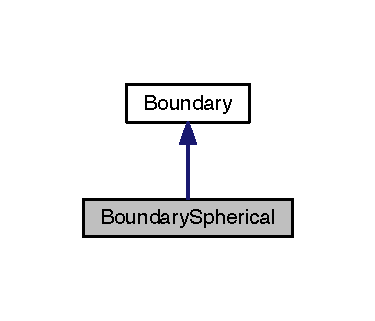
\includegraphics[width=180pt]{classBoundarySpherical__inherit__graph}
\end{center}
\end{figure}


Collaboration diagram for Boundary\+Spherical\+:
\nopagebreak
\begin{figure}[H]
\begin{center}
\leavevmode
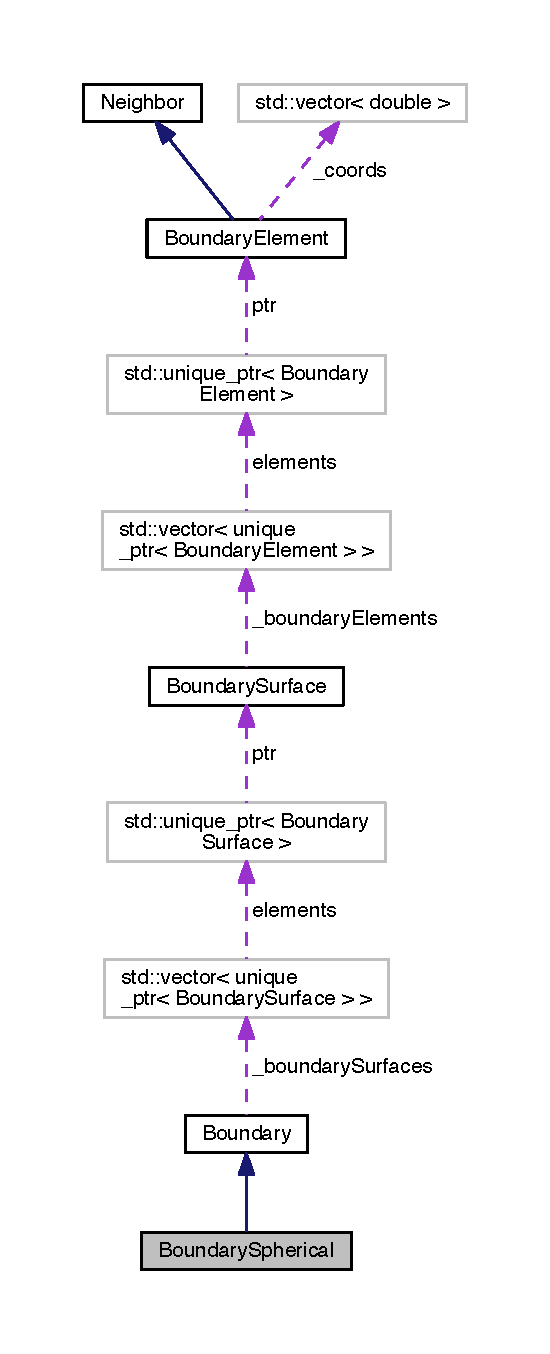
\includegraphics[height=550pt]{classBoundarySpherical__coll__graph}
\end{center}
\end{figure}
\subsection*{Public Member Functions}
\begin{DoxyCompactItemize}
\item 
\hyperlink{classBoundarySpherical_ae94c30c1bbb81df2cb57aef65eecfa10}{Boundary\+Spherical} (double diameter)
\begin{DoxyCompactList}\small\item\em Default constructor, will create an sphere with given diameter. \end{DoxyCompactList}\item 
virtual bool \hyperlink{classBoundarySpherical_a653f35719ff4baec5848053093978ee9}{within} (const vector$<$ double $>$ \&coordinates)
\begin{DoxyCompactList}\small\item\em Check if coordinates are within boundary. \end{DoxyCompactList}\item 
\hyperlink{Boundary_8h_a0099b369f2bc119c1b54728734b41132}{Boundary\+Shape} \hyperlink{classBoundary_a20d2121527b207eed35f6719393e3499}{get\+Shape} ()
\begin{DoxyCompactList}\small\item\em Get shape. \end{DoxyCompactList}\item 
const vector$<$ unique\+\_\+ptr\\*
$<$ \hyperlink{classBoundarySurface}{Boundary\+Surface} $>$ $>$ \& \hyperlink{classBoundary_acfa6640f65c432e339108887913539eb}{get\+Boundary\+Surfaces} ()
\begin{DoxyCompactList}\small\item\em Get boundarysurfaces. \end{DoxyCompactList}\end{DoxyCompactItemize}
\subsection*{Protected Attributes}
\begin{DoxyCompactItemize}
\item 
vector$<$ unique\+\_\+ptr\\*
$<$ \hyperlink{classBoundarySurface}{Boundary\+Surface} $>$ $>$ \hyperlink{classBoundary_abbac1843206a158e7d0a6e741cdc00c1}{\+\_\+boundary\+Surfaces}
\begin{DoxyCompactList}\small\item\em Vector of boundarysurfaces (could be different implementations) \end{DoxyCompactList}\item 
\hyperlink{Boundary_8h_a0099b369f2bc119c1b54728734b41132}{Boundary\+Shape} \hyperlink{classBoundary_a04c10c9a7aea1924d779d392e29f94ff}{\+\_\+shape}
\begin{DoxyCompactList}\small\item\em Shape of boundary. \end{DoxyCompactList}\item 
short \hyperlink{classBoundary_a96f2294e0c822ab216fe5ab7e17258c7}{\+\_\+n\+Dim}
\begin{DoxyCompactList}\small\item\em Dimensionality. \end{DoxyCompactList}\end{DoxyCompactItemize}


\subsection{Detailed Description}
A spherical boundary implementation. 

Definition at line 34 of file Boundary\+Impl.\+h.



\subsection{Constructor \& Destructor Documentation}
\hypertarget{classBoundarySpherical_ae94c30c1bbb81df2cb57aef65eecfa10}{\index{Boundary\+Spherical@{Boundary\+Spherical}!Boundary\+Spherical@{Boundary\+Spherical}}
\index{Boundary\+Spherical@{Boundary\+Spherical}!Boundary\+Spherical@{Boundary\+Spherical}}
\subsubsection[{Boundary\+Spherical}]{\setlength{\rightskip}{0pt plus 5cm}Boundary\+Spherical\+::\+Boundary\+Spherical (
\begin{DoxyParamCaption}
\item[{double}]{diameter}
\end{DoxyParamCaption}
)}}\label{classBoundarySpherical_ae94c30c1bbb81df2cb57aef65eecfa10}


Default constructor, will create an sphere with given diameter. 


\begin{DoxyParams}{Parameters}
{\em diameter} & -\/ diameter of sphere \\
\hline
\end{DoxyParams}


Definition at line 57 of file Boundary\+Impl.\+cpp.



References Boundary\+::\+\_\+boundary\+Surfaces, Geometry\+Parameters\+::compartment\+Size\+X, Geometry\+Parameters\+::compartment\+Size\+Y, Geometry\+Parameters\+::compartment\+Size\+Z, System\+Parameters\+::\+Geometry(), Geometry\+Parameters\+::\+N\+X, Geometry\+Parameters\+::\+N\+Y, Geometry\+Parameters\+::\+N\+Z, and Sphere.



\subsection{Member Function Documentation}
\hypertarget{classBoundary_acfa6640f65c432e339108887913539eb}{\index{Boundary\+Spherical@{Boundary\+Spherical}!get\+Boundary\+Surfaces@{get\+Boundary\+Surfaces}}
\index{get\+Boundary\+Surfaces@{get\+Boundary\+Surfaces}!Boundary\+Spherical@{Boundary\+Spherical}}
\subsubsection[{get\+Boundary\+Surfaces}]{\setlength{\rightskip}{0pt plus 5cm}const vector$<$unique\+\_\+ptr$<${\bf Boundary\+Surface}$>$ $>$\& Boundary\+::get\+Boundary\+Surfaces (
\begin{DoxyParamCaption}
{}
\end{DoxyParamCaption}
)\hspace{0.3cm}{\ttfamily [inline]}, {\ttfamily [inherited]}}}\label{classBoundary_acfa6640f65c432e339108887913539eb}


Get boundarysurfaces. 



Definition at line 44 of file Boundary.\+h.



References Boundary\+::\+\_\+boundary\+Surfaces.

\hypertarget{classBoundary_a20d2121527b207eed35f6719393e3499}{\index{Boundary\+Spherical@{Boundary\+Spherical}!get\+Shape@{get\+Shape}}
\index{get\+Shape@{get\+Shape}!Boundary\+Spherical@{Boundary\+Spherical}}
\subsubsection[{get\+Shape}]{\setlength{\rightskip}{0pt plus 5cm}{\bf Boundary\+Shape} Boundary\+::get\+Shape (
\begin{DoxyParamCaption}
{}
\end{DoxyParamCaption}
)\hspace{0.3cm}{\ttfamily [inline]}, {\ttfamily [inherited]}}}\label{classBoundary_a20d2121527b207eed35f6719393e3499}


Get shape. 



Definition at line 42 of file Boundary.\+h.



References Boundary\+::\+\_\+shape.

\hypertarget{classBoundarySpherical_a653f35719ff4baec5848053093978ee9}{\index{Boundary\+Spherical@{Boundary\+Spherical}!within@{within}}
\index{within@{within}!Boundary\+Spherical@{Boundary\+Spherical}}
\subsubsection[{within}]{\setlength{\rightskip}{0pt plus 5cm}bool Boundary\+Spherical\+::within (
\begin{DoxyParamCaption}
\item[{const vector$<$ double $>$ \&}]{coordinates}
\end{DoxyParamCaption}
)\hspace{0.3cm}{\ttfamily [virtual]}}}\label{classBoundarySpherical_a653f35719ff4baec5848053093978ee9}


Check if coordinates are within boundary. 



Implements \hyperlink{classBoundary_aef1af10ace9eae30e86b6bd23087b3ff}{Boundary}.



Definition at line 66 of file Boundary\+Impl.\+cpp.



References Boundary\+::\+\_\+boundary\+Surfaces, and Boundary\+Element\+::distance().



\subsection{Member Data Documentation}
\hypertarget{classBoundary_abbac1843206a158e7d0a6e741cdc00c1}{\index{Boundary\+Spherical@{Boundary\+Spherical}!\+\_\+boundary\+Surfaces@{\+\_\+boundary\+Surfaces}}
\index{\+\_\+boundary\+Surfaces@{\+\_\+boundary\+Surfaces}!Boundary\+Spherical@{Boundary\+Spherical}}
\subsubsection[{\+\_\+boundary\+Surfaces}]{\setlength{\rightskip}{0pt plus 5cm}vector$<$unique\+\_\+ptr$<${\bf Boundary\+Surface}$>$ $>$ Boundary\+::\+\_\+boundary\+Surfaces\hspace{0.3cm}{\ttfamily [protected]}, {\ttfamily [inherited]}}}\label{classBoundary_abbac1843206a158e7d0a6e741cdc00c1}


Vector of boundarysurfaces (could be different implementations) 



Definition at line 33 of file Boundary.\+h.



Referenced by Boundary\+Capsule\+::\+Boundary\+Capsule(), Boundary\+Cubic\+::\+Boundary\+Cubic(), Boundary\+Spherical(), Boundary\+::get\+Boundary\+Surfaces(), Boundary\+Cubic\+::within(), within(), and Boundary\+Capsule\+::within().

\hypertarget{classBoundary_a96f2294e0c822ab216fe5ab7e17258c7}{\index{Boundary\+Spherical@{Boundary\+Spherical}!\+\_\+n\+Dim@{\+\_\+n\+Dim}}
\index{\+\_\+n\+Dim@{\+\_\+n\+Dim}!Boundary\+Spherical@{Boundary\+Spherical}}
\subsubsection[{\+\_\+n\+Dim}]{\setlength{\rightskip}{0pt plus 5cm}short Boundary\+::\+\_\+n\+Dim\hspace{0.3cm}{\ttfamily [protected]}, {\ttfamily [inherited]}}}\label{classBoundary_a96f2294e0c822ab216fe5ab7e17258c7}


Dimensionality. 



Definition at line 35 of file Boundary.\+h.

\hypertarget{classBoundary_a04c10c9a7aea1924d779d392e29f94ff}{\index{Boundary\+Spherical@{Boundary\+Spherical}!\+\_\+shape@{\+\_\+shape}}
\index{\+\_\+shape@{\+\_\+shape}!Boundary\+Spherical@{Boundary\+Spherical}}
\subsubsection[{\+\_\+shape}]{\setlength{\rightskip}{0pt plus 5cm}{\bf Boundary\+Shape} Boundary\+::\+\_\+shape\hspace{0.3cm}{\ttfamily [protected]}, {\ttfamily [inherited]}}}\label{classBoundary_a04c10c9a7aea1924d779d392e29f94ff}


Shape of boundary. 



Definition at line 34 of file Boundary.\+h.



Referenced by Boundary\+::get\+Shape().



The documentation for this class was generated from the following files\+:\begin{DoxyCompactItemize}
\item 
M3\+S\+Y\+M/\+Structure/\hyperlink{BoundaryImpl_8h}{Boundary\+Impl.\+h}\item 
M3\+S\+Y\+M/\+Structure/\hyperlink{BoundaryImpl_8cpp}{Boundary\+Impl.\+cpp}\end{DoxyCompactItemize}

\hypertarget{classBoundarySurface}{\section{Boundary\+Surface Class Reference}
\label{classBoundarySurface}\index{Boundary\+Surface@{Boundary\+Surface}}
}


A boundary shape that holds \hyperlink{classBoundaryElement}{Boundary\+Elements}.  




{\ttfamily \#include $<$Boundary\+Surface.\+h$>$}



Inheritance diagram for Boundary\+Surface\+:\nopagebreak
\begin{figure}[H]
\begin{center}
\leavevmode
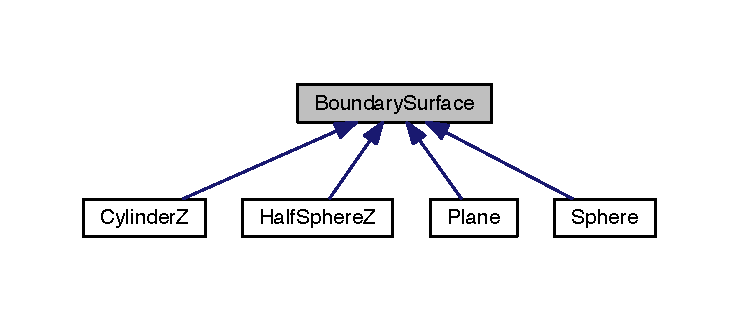
\includegraphics[width=350pt]{classBoundarySurface__inherit__graph}
\end{center}
\end{figure}


Collaboration diagram for Boundary\+Surface\+:\nopagebreak
\begin{figure}[H]
\begin{center}
\leavevmode
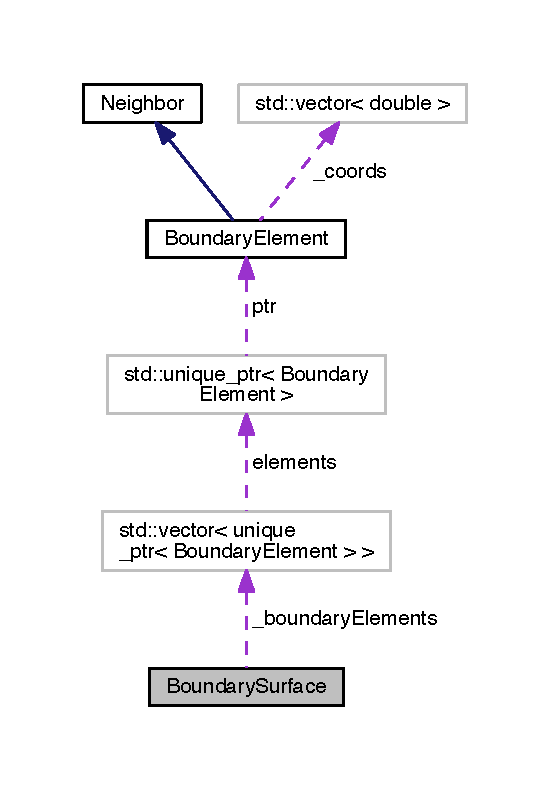
\includegraphics[width=264pt]{classBoundarySurface__coll__graph}
\end{center}
\end{figure}
\subsection*{Public Member Functions}
\begin{DoxyCompactItemize}
\item 
\hyperlink{classBoundarySurface_a87739ff516e9c879943263440e2c837d}{Boundary\+Surface} (int n\+Dim)
\begin{DoxyCompactList}\small\item\em Constructor, does nothing. \end{DoxyCompactList}\item 
\hyperlink{classBoundarySurface_a15f38669a0a75aa5177e326090710907}{$\sim$\+Boundary\+Surface} ()
\begin{DoxyCompactList}\small\item\em Destructor, removes boundary elements from D\+B. \end{DoxyCompactList}\item 
const vector$<$ unique\+\_\+ptr\\*
$<$ \hyperlink{classBoundaryElement}{Boundary\+Element} $>$ $>$ \& \hyperlink{classBoundarySurface_a402dcf23f4f96110569d01e401edee5a}{boundary\+Elements} ()
\begin{DoxyCompactList}\small\item\em Get boundary elements. \end{DoxyCompactList}\end{DoxyCompactItemize}
\subsection*{Protected Attributes}
\begin{DoxyCompactItemize}
\item 
vector$<$ unique\+\_\+ptr\\*
$<$ \hyperlink{classBoundaryElement}{Boundary\+Element} $>$ $>$ \hyperlink{classBoundarySurface_a67f60b2d22fb67f097e98025803d3d34}{\+\_\+boundary\+Elements}
\begin{DoxyCompactList}\small\item\em Vector of boundary elements that make up this surface. \end{DoxyCompactList}\item 
short \hyperlink{classBoundarySurface_af3ed79310c6ba6cdc8e9f176bf463eb1}{\+\_\+n\+Dim}
\begin{DoxyCompactList}\small\item\em Dimensionality of surface. \end{DoxyCompactList}\end{DoxyCompactItemize}


\subsection{Detailed Description}
A boundary shape that holds \hyperlink{classBoundaryElement}{Boundary\+Elements}. 

The \hyperlink{classBoundarySurface}{Boundary\+Surface} class is a basic boundary shape that is owned and controlled by the \hyperlink{classBoundary}{Boundary} that created it. It holds a vector of \hyperlink{classBoundaryElement}{Boundary\+Elements} as well as any other geometrical information needed for the given implementation. 

Definition at line 31 of file Boundary\+Surface.\+h.



\subsection{Constructor \& Destructor Documentation}
\hypertarget{classBoundarySurface_a87739ff516e9c879943263440e2c837d}{\index{Boundary\+Surface@{Boundary\+Surface}!Boundary\+Surface@{Boundary\+Surface}}
\index{Boundary\+Surface@{Boundary\+Surface}!Boundary\+Surface@{Boundary\+Surface}}
\subsubsection[{Boundary\+Surface}]{\setlength{\rightskip}{0pt plus 5cm}Boundary\+Surface\+::\+Boundary\+Surface (
\begin{DoxyParamCaption}
\item[{int}]{n\+Dim}
\end{DoxyParamCaption}
)\hspace{0.3cm}{\ttfamily [inline]}}}\label{classBoundarySurface_a87739ff516e9c879943263440e2c837d}


Constructor, does nothing. 



Definition at line 40 of file Boundary\+Surface.\+h.

\hypertarget{classBoundarySurface_a15f38669a0a75aa5177e326090710907}{\index{Boundary\+Surface@{Boundary\+Surface}!````~Boundary\+Surface@{$\sim$\+Boundary\+Surface}}
\index{````~Boundary\+Surface@{$\sim$\+Boundary\+Surface}!Boundary\+Surface@{Boundary\+Surface}}
\subsubsection[{$\sim$\+Boundary\+Surface}]{\setlength{\rightskip}{0pt plus 5cm}Boundary\+Surface\+::$\sim$\+Boundary\+Surface (
\begin{DoxyParamCaption}
{}
\end{DoxyParamCaption}
)\hspace{0.3cm}{\ttfamily [inline]}}}\label{classBoundarySurface_a15f38669a0a75aa5177e326090710907}


Destructor, removes boundary elements from D\+B. 



Definition at line 42 of file Boundary\+Surface.\+h.



\subsection{Member Function Documentation}
\hypertarget{classBoundarySurface_a402dcf23f4f96110569d01e401edee5a}{\index{Boundary\+Surface@{Boundary\+Surface}!boundary\+Elements@{boundary\+Elements}}
\index{boundary\+Elements@{boundary\+Elements}!Boundary\+Surface@{Boundary\+Surface}}
\subsubsection[{boundary\+Elements}]{\setlength{\rightskip}{0pt plus 5cm}const vector$<$unique\+\_\+ptr$<${\bf Boundary\+Element}$>$ $>$\& Boundary\+Surface\+::boundary\+Elements (
\begin{DoxyParamCaption}
{}
\end{DoxyParamCaption}
)\hspace{0.3cm}{\ttfamily [inline]}}}\label{classBoundarySurface_a402dcf23f4f96110569d01e401edee5a}


Get boundary elements. 



Definition at line 45 of file Boundary\+Surface.\+h.



References \+\_\+boundary\+Elements.



\subsection{Member Data Documentation}
\hypertarget{classBoundarySurface_a67f60b2d22fb67f097e98025803d3d34}{\index{Boundary\+Surface@{Boundary\+Surface}!\+\_\+boundary\+Elements@{\+\_\+boundary\+Elements}}
\index{\+\_\+boundary\+Elements@{\+\_\+boundary\+Elements}!Boundary\+Surface@{Boundary\+Surface}}
\subsubsection[{\+\_\+boundary\+Elements}]{\setlength{\rightskip}{0pt plus 5cm}vector$<$unique\+\_\+ptr$<${\bf Boundary\+Element}$>$ $>$ Boundary\+Surface\+::\+\_\+boundary\+Elements\hspace{0.3cm}{\ttfamily [protected]}}}\label{classBoundarySurface_a67f60b2d22fb67f097e98025803d3d34}


Vector of boundary elements that make up this surface. 



Definition at line 35 of file Boundary\+Surface.\+h.



Referenced by boundary\+Elements(), Cylinder\+Z\+::\+Cylinder\+Z(), Half\+Sphere\+Z\+::\+Half\+Sphere\+Z(), Plane\+::\+Plane(), and Sphere\+::\+Sphere().

\hypertarget{classBoundarySurface_af3ed79310c6ba6cdc8e9f176bf463eb1}{\index{Boundary\+Surface@{Boundary\+Surface}!\+\_\+n\+Dim@{\+\_\+n\+Dim}}
\index{\+\_\+n\+Dim@{\+\_\+n\+Dim}!Boundary\+Surface@{Boundary\+Surface}}
\subsubsection[{\+\_\+n\+Dim}]{\setlength{\rightskip}{0pt plus 5cm}short Boundary\+Surface\+::\+\_\+n\+Dim\hspace{0.3cm}{\ttfamily [protected]}}}\label{classBoundarySurface_af3ed79310c6ba6cdc8e9f176bf463eb1}


Dimensionality of surface. 



Definition at line 36 of file Boundary\+Surface.\+h.



The documentation for this class was generated from the following file\+:\begin{DoxyCompactItemize}
\item 
M3\+S\+Y\+M/\+Structure/\hyperlink{BoundarySurface_8h}{Boundary\+Surface.\+h}\end{DoxyCompactItemize}

\hypertarget{structBoundaryType}{\section{Boundary\+Type Struct Reference}
\label{structBoundaryType}\index{Boundary\+Type@{Boundary\+Type}}
}


Struct to hold the parameters of the boundary.  




{\ttfamily \#include $<$Parser.\+h$>$}



Collaboration diagram for Boundary\+Type\+:\nopagebreak
\begin{figure}[H]
\begin{center}
\leavevmode
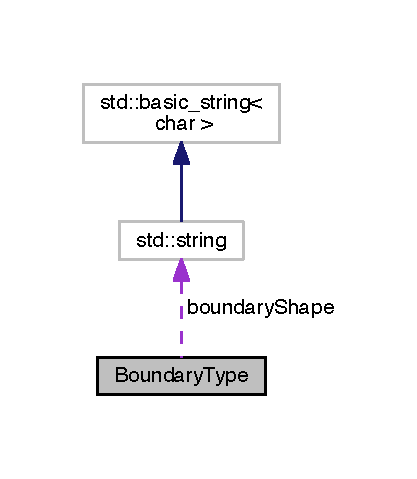
\includegraphics[width=200pt]{structBoundaryType__coll__graph}
\end{center}
\end{figure}
\subsection*{Public Attributes}
\begin{DoxyCompactItemize}
\item 
string \hyperlink{structBoundaryType_a1c437edf87bf307f6f7023ef8fe75f1f}{boundary\+Shape} = \char`\"{}\char`\"{}
\end{DoxyCompactItemize}


\subsection{Detailed Description}
Struct to hold the parameters of the boundary. 

Definition at line 99 of file Parser.\+h.



\subsection{Member Data Documentation}
\hypertarget{structBoundaryType_a1c437edf87bf307f6f7023ef8fe75f1f}{\index{Boundary\+Type@{Boundary\+Type}!boundary\+Shape@{boundary\+Shape}}
\index{boundary\+Shape@{boundary\+Shape}!Boundary\+Type@{Boundary\+Type}}
\subsubsection[{boundary\+Shape}]{\setlength{\rightskip}{0pt plus 5cm}string Boundary\+Type\+::boundary\+Shape = \char`\"{}\char`\"{}}}\label{structBoundaryType_a1c437edf87bf307f6f7023ef8fe75f1f}


Definition at line 101 of file Parser.\+h.



Referenced by System\+Parser\+::read\+Boundary\+Type().



The documentation for this struct was generated from the following file\+:\begin{DoxyCompactItemize}
\item 
M3\+S\+Y\+M/\hyperlink{Parser_8h}{Parser.\+h}\end{DoxyCompactItemize}

\hypertarget{classCBound}{\section{C\+Bound Class Reference}
\label{classCBound}\index{C\+Bound@{C\+Bound}}
}


Represents a chemical object that is bound to a \hyperlink{classFilament}{Filament}.  




{\ttfamily \#include $<$C\+Bound.\+h$>$}



Inheritance diagram for C\+Bound\+:\nopagebreak
\begin{figure}[H]
\begin{center}
\leavevmode
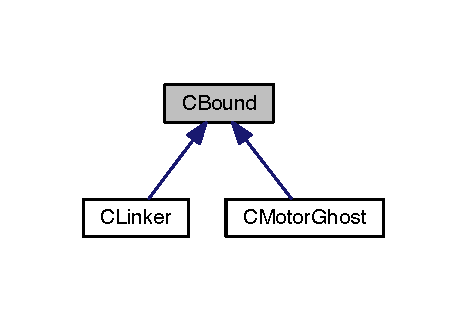
\includegraphics[width=224pt]{classCBound__inherit__graph}
\end{center}
\end{figure}


Collaboration diagram for C\+Bound\+:\nopagebreak
\begin{figure}[H]
\begin{center}
\leavevmode
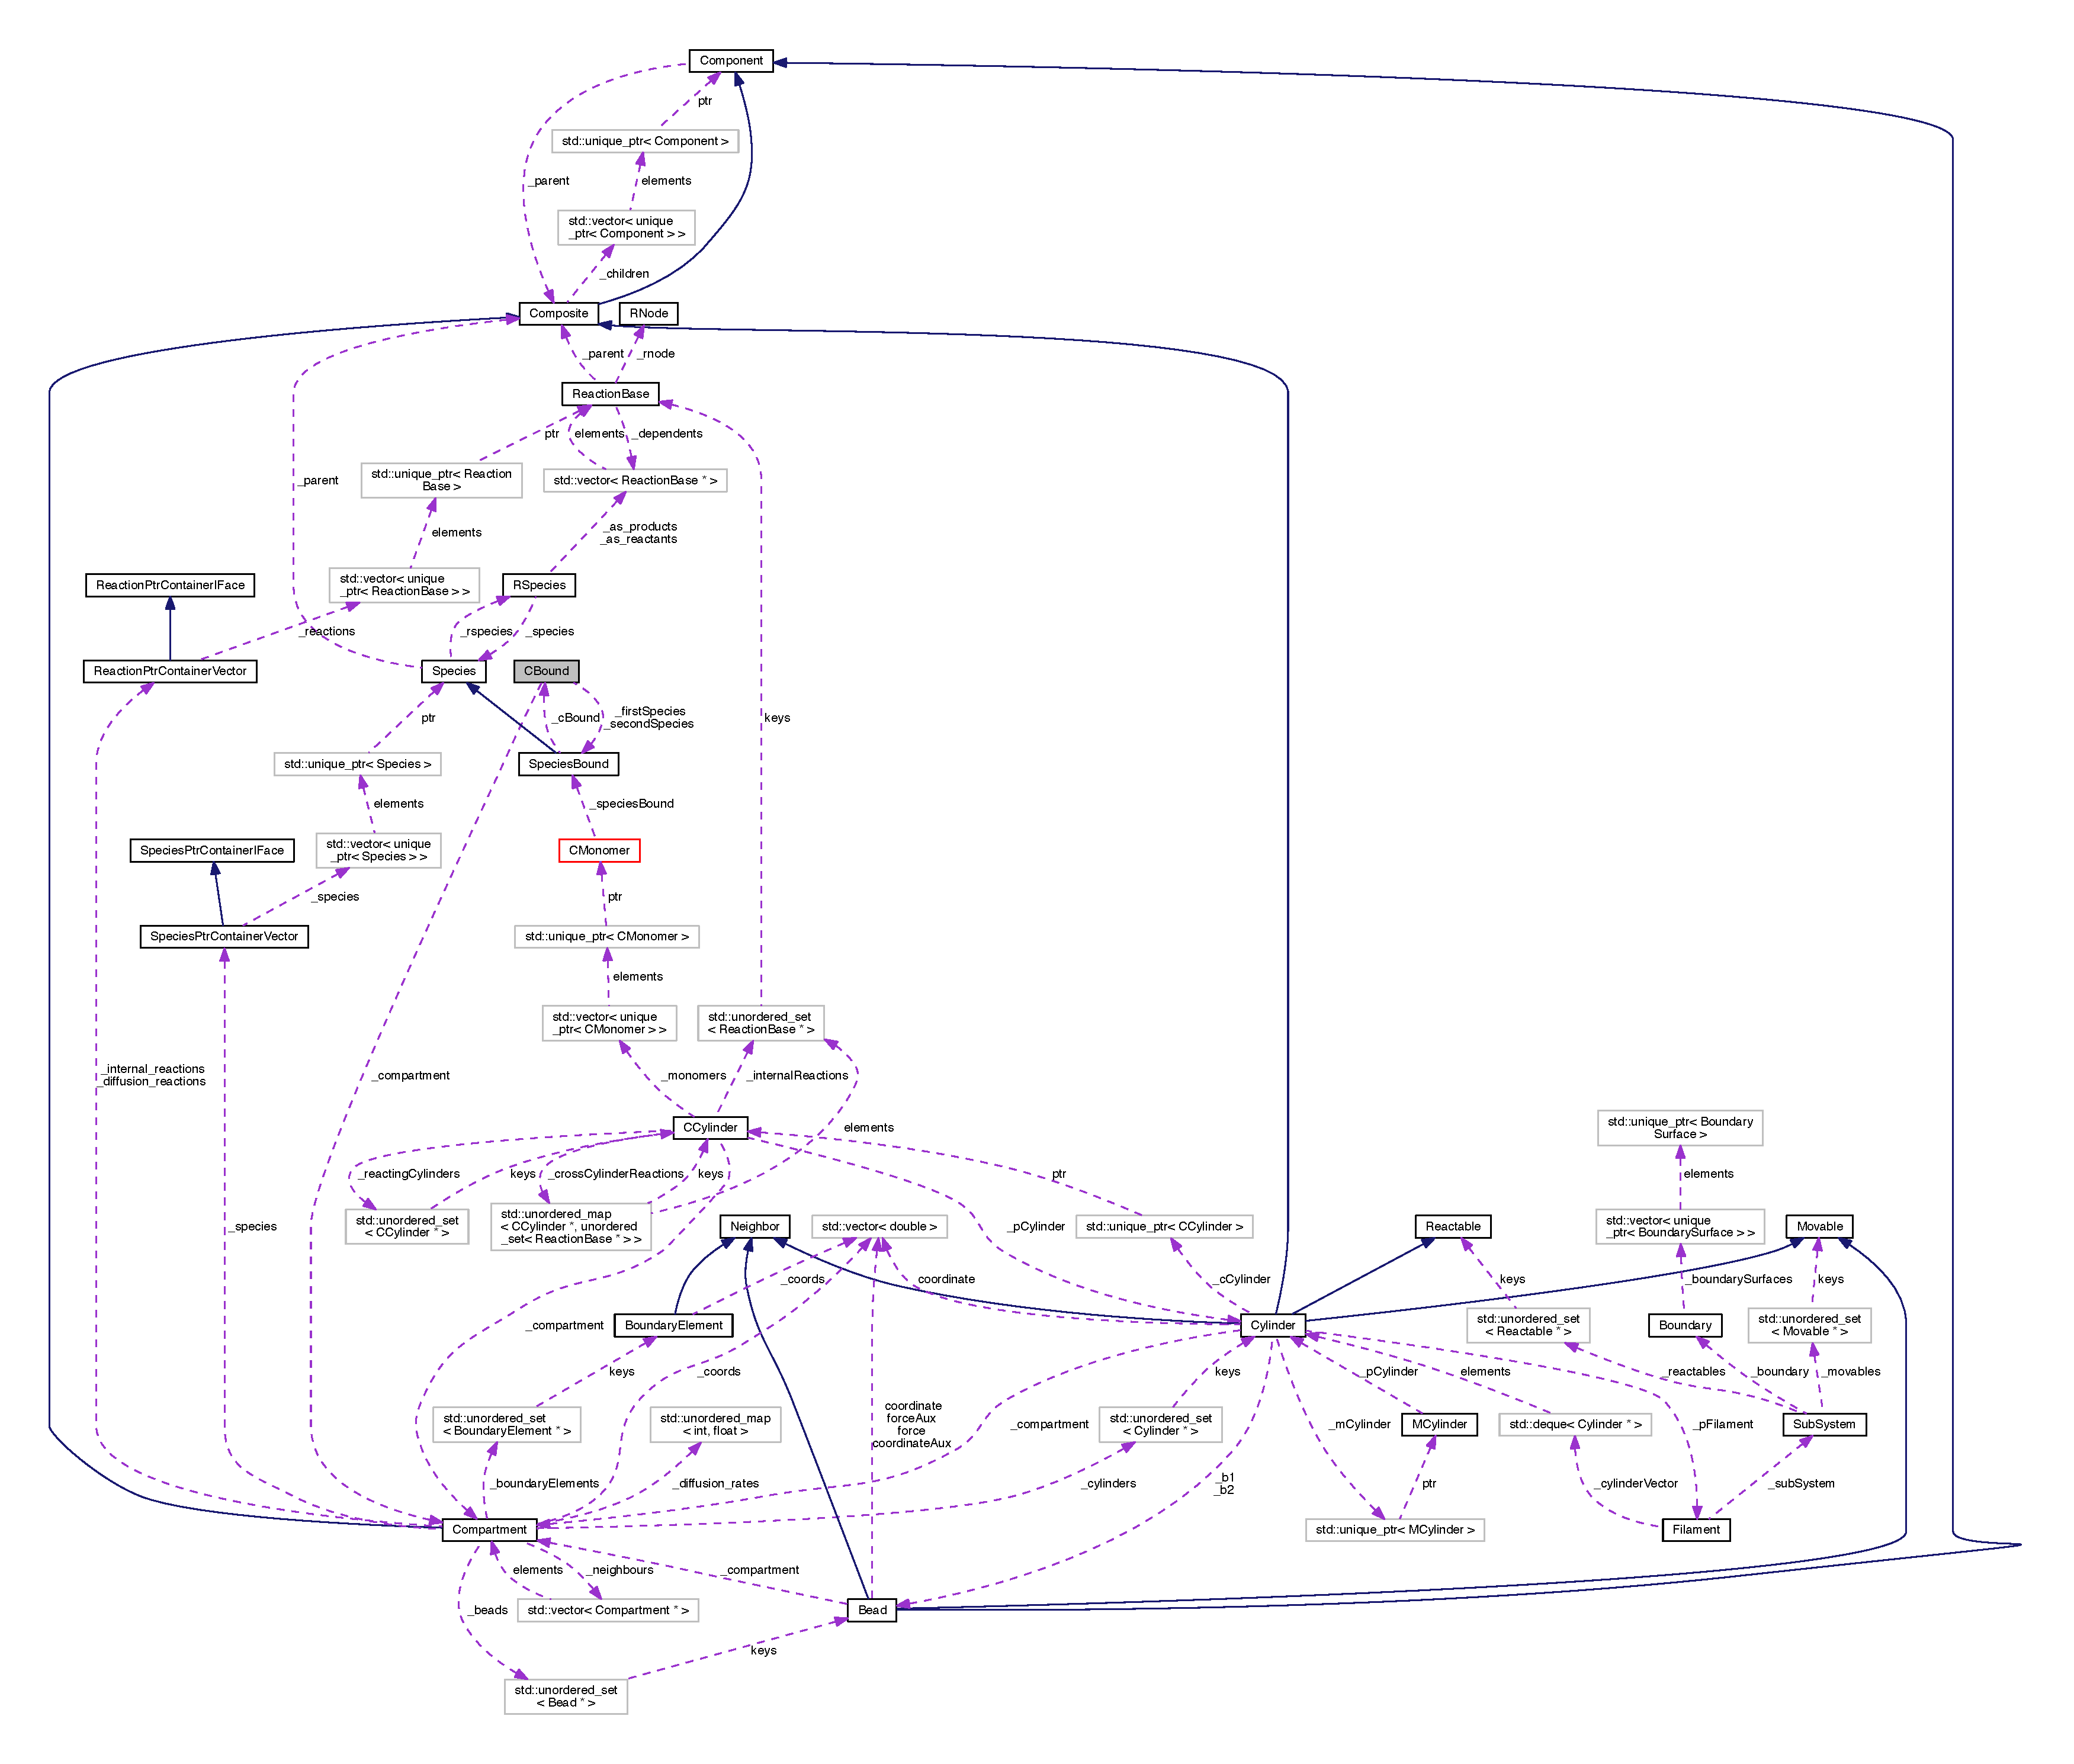
\includegraphics[width=350pt]{classCBound__coll__graph}
\end{center}
\end{figure}
\subsection*{Public Member Functions}
\begin{DoxyCompactItemize}
\item 
\hyperlink{classCBound_a6fd75889661a816ef641a3963d83c2b8}{C\+Bound} (\hyperlink{classCompartment}{Compartment} $\ast$c)
\begin{DoxyCompactList}\small\item\em Constructor, just sets species. \end{DoxyCompactList}\item 
virtual \hyperlink{classCBound_adbee50be51a5fec03fe60a9ee7c5879f}{$\sim$\+C\+Bound} () noexcept
\begin{DoxyCompactList}\small\item\em Virtual destructor. \end{DoxyCompactList}\item 
void \hyperlink{classCBound_a17d4b84d683b0b7bd75b793410fed18f}{set\+First\+Species} (\hyperlink{classSpeciesBound}{Species\+Bound} $\ast$species)
\begin{DoxyCompactList}\small\item\em Set first species. \end{DoxyCompactList}\item 
\hyperlink{classSpeciesBound}{Species\+Bound} $\ast$ \hyperlink{classCBound_aad60656a671e4ffdc45b4c904fa7c320}{get\+First\+Species} ()
\begin{DoxyCompactList}\small\item\em Get first species. \end{DoxyCompactList}\item 
void \hyperlink{classCBound_a01badbb54867fb99b6f3a895d555867a}{set\+Second\+Species} (\hyperlink{classSpeciesBound}{Species\+Bound} $\ast$species)
\begin{DoxyCompactList}\small\item\em Set second species. \end{DoxyCompactList}\item 
\hyperlink{classSpeciesBound}{Species\+Bound} $\ast$ \hyperlink{classCBound_a1e706b6472c40ae1d98a64eda0acdadf}{get\+Second\+Species} ()
\begin{DoxyCompactList}\small\item\em Get second species. \end{DoxyCompactList}\item 
\hyperlink{classCompartment}{Compartment} $\ast$ \hyperlink{classCBound_a6c4d7b1b35d06725c8659424bf0c3f18}{get\+Compartment} ()
\begin{DoxyCompactList}\small\item\em Get compartment that this \hyperlink{classCBound}{C\+Bound} is in. \end{DoxyCompactList}\end{DoxyCompactItemize}
\subsection*{Protected Attributes}
\begin{DoxyCompactItemize}
\item 
\hyperlink{classSpeciesBound}{Species\+Bound} $\ast$ \hyperlink{classCBound_a7ee4f44fd39c414be1f7b74b1031c1ce}{\+\_\+first\+Species} = nullptr
\begin{DoxyCompactList}\small\item\em Corresponding first species on filament. \end{DoxyCompactList}\item 
\hyperlink{classSpeciesBound}{Species\+Bound} $\ast$ \hyperlink{classCBound_ae6818ab861d273598a2507be75183e41}{\+\_\+second\+Species} = nullptr
\begin{DoxyCompactList}\small\item\em Corresponding second species on filament. \end{DoxyCompactList}\item 
\hyperlink{classCompartment}{Compartment} $\ast$ \hyperlink{classCBound_a95a66719b898cf32e60ae7137186bbbf}{\+\_\+compartment}
\begin{DoxyCompactList}\small\item\em \hyperlink{classCompartment}{Compartment} this \hyperlink{classCBound}{C\+Bound} is in. \end{DoxyCompactList}\end{DoxyCompactItemize}


\subsection{Detailed Description}
Represents a chemical object that is bound to a \hyperlink{classFilament}{Filament}. 

The \hyperlink{classCBound}{C\+Bound} class is an abstract representation of a chemically bound object to a \hyperlink{classFilament}{Filament} (Could be a linker, motor, branching protein, etc). Each \hyperlink{classCBound}{C\+Bound} object has a pointer to the corresponding \hyperlink{classSpeciesBound}{Species\+Bound} on a filament. Different implementations of \hyperlink{classCBound}{C\+Bound} class will have different functions to bind, move, etc. See documentation of subclass for more details on function. 

Definition at line 31 of file C\+Bound.\+h.



\subsection{Constructor \& Destructor Documentation}
\hypertarget{classCBound_a6fd75889661a816ef641a3963d83c2b8}{\index{C\+Bound@{C\+Bound}!C\+Bound@{C\+Bound}}
\index{C\+Bound@{C\+Bound}!C\+Bound@{C\+Bound}}
\subsubsection[{C\+Bound}]{\setlength{\rightskip}{0pt plus 5cm}C\+Bound\+::\+C\+Bound (
\begin{DoxyParamCaption}
\item[{{\bf Compartment} $\ast$}]{c}
\end{DoxyParamCaption}
)\hspace{0.3cm}{\ttfamily [inline]}}}\label{classCBound_a6fd75889661a816ef641a3963d83c2b8}


Constructor, just sets species. 



Definition at line 41 of file C\+Bound.\+h.

\hypertarget{classCBound_adbee50be51a5fec03fe60a9ee7c5879f}{\index{C\+Bound@{C\+Bound}!````~C\+Bound@{$\sim$\+C\+Bound}}
\index{````~C\+Bound@{$\sim$\+C\+Bound}!C\+Bound@{C\+Bound}}
\subsubsection[{$\sim$\+C\+Bound}]{\setlength{\rightskip}{0pt plus 5cm}virtual C\+Bound\+::$\sim$\+C\+Bound (
\begin{DoxyParamCaption}
{}
\end{DoxyParamCaption}
)\hspace{0.3cm}{\ttfamily [inline]}, {\ttfamily [virtual]}, {\ttfamily [noexcept]}}}\label{classCBound_adbee50be51a5fec03fe60a9ee7c5879f}


Virtual destructor. 

\begin{DoxyNote}{Note}
noexcept is important here. Otherwise, gcc flags the constructor as potentially throwing, which in turn disables move operations by the S\+T\+L containers. This behaviour is a gcc bug (as of gcc 4.\+703), and will presumbaly be fixed in the future. 
\end{DoxyNote}


Definition at line 47 of file C\+Bound.\+h.



References \+\_\+first\+Species, \+\_\+second\+Species, and Species\+Bound\+::remove\+C\+Bound().



\subsection{Member Function Documentation}
\hypertarget{classCBound_a6c4d7b1b35d06725c8659424bf0c3f18}{\index{C\+Bound@{C\+Bound}!get\+Compartment@{get\+Compartment}}
\index{get\+Compartment@{get\+Compartment}!C\+Bound@{C\+Bound}}
\subsubsection[{get\+Compartment}]{\setlength{\rightskip}{0pt plus 5cm}{\bf Compartment}$\ast$ C\+Bound\+::get\+Compartment (
\begin{DoxyParamCaption}
{}
\end{DoxyParamCaption}
)\hspace{0.3cm}{\ttfamily [inline]}}}\label{classCBound_a6c4d7b1b35d06725c8659424bf0c3f18}


Get compartment that this \hyperlink{classCBound}{C\+Bound} is in. 



Definition at line 75 of file C\+Bound.\+h.



References \+\_\+compartment.

\hypertarget{classCBound_aad60656a671e4ffdc45b4c904fa7c320}{\index{C\+Bound@{C\+Bound}!get\+First\+Species@{get\+First\+Species}}
\index{get\+First\+Species@{get\+First\+Species}!C\+Bound@{C\+Bound}}
\subsubsection[{get\+First\+Species}]{\setlength{\rightskip}{0pt plus 5cm}{\bf Species\+Bound}$\ast$ C\+Bound\+::get\+First\+Species (
\begin{DoxyParamCaption}
{}
\end{DoxyParamCaption}
)\hspace{0.3cm}{\ttfamily [inline]}}}\label{classCBound_aad60656a671e4ffdc45b4c904fa7c320}


Get first species. 



Definition at line 61 of file C\+Bound.\+h.



References \+\_\+first\+Species.



Referenced by C\+Monomer\+::\+C\+Monomer(), Motor\+Walking\+Forward\+Callback\+::operator()(), Motor\+Walking\+Backward\+Callback\+::operator()(), Motor\+Moving\+Cylinder\+Forward\+Callback\+::operator()(), and Motor\+Moving\+Cylinder\+Backward\+Callback\+::operator()().

\hypertarget{classCBound_a1e706b6472c40ae1d98a64eda0acdadf}{\index{C\+Bound@{C\+Bound}!get\+Second\+Species@{get\+Second\+Species}}
\index{get\+Second\+Species@{get\+Second\+Species}!C\+Bound@{C\+Bound}}
\subsubsection[{get\+Second\+Species}]{\setlength{\rightskip}{0pt plus 5cm}{\bf Species\+Bound}$\ast$ C\+Bound\+::get\+Second\+Species (
\begin{DoxyParamCaption}
{}
\end{DoxyParamCaption}
)\hspace{0.3cm}{\ttfamily [inline]}}}\label{classCBound_a1e706b6472c40ae1d98a64eda0acdadf}


Get second species. 



Definition at line 72 of file C\+Bound.\+h.



References \+\_\+second\+Species.

\hypertarget{classCBound_a17d4b84d683b0b7bd75b793410fed18f}{\index{C\+Bound@{C\+Bound}!set\+First\+Species@{set\+First\+Species}}
\index{set\+First\+Species@{set\+First\+Species}!C\+Bound@{C\+Bound}}
\subsubsection[{set\+First\+Species}]{\setlength{\rightskip}{0pt plus 5cm}void C\+Bound\+::set\+First\+Species (
\begin{DoxyParamCaption}
\item[{{\bf Species\+Bound} $\ast$}]{species}
\end{DoxyParamCaption}
)\hspace{0.3cm}{\ttfamily [inline]}}}\label{classCBound_a17d4b84d683b0b7bd75b793410fed18f}


Set first species. 

remove from old first species 

Definition at line 53 of file C\+Bound.\+h.



References \+\_\+first\+Species, Species\+Bound\+::remove\+C\+Bound(), and Species\+Bound\+::set\+C\+Bound().



Referenced by C\+Linker\+::\+C\+Linker(), C\+Monomer\+::\+C\+Monomer(), C\+Motor\+Ghost\+::\+C\+Motor\+Ghost(), Motor\+Walking\+Forward\+Callback\+::operator()(), Motor\+Walking\+Backward\+Callback\+::operator()(), Motor\+Moving\+Cylinder\+Forward\+Callback\+::operator()(), Motor\+Moving\+Cylinder\+Backward\+Callback\+::operator()(), Linker\+::update\+Position(), and Motor\+Ghost\+::update\+Position().

\hypertarget{classCBound_a01badbb54867fb99b6f3a895d555867a}{\index{C\+Bound@{C\+Bound}!set\+Second\+Species@{set\+Second\+Species}}
\index{set\+Second\+Species@{set\+Second\+Species}!C\+Bound@{C\+Bound}}
\subsubsection[{set\+Second\+Species}]{\setlength{\rightskip}{0pt plus 5cm}void C\+Bound\+::set\+Second\+Species (
\begin{DoxyParamCaption}
\item[{{\bf Species\+Bound} $\ast$}]{species}
\end{DoxyParamCaption}
)\hspace{0.3cm}{\ttfamily [inline]}}}\label{classCBound_a01badbb54867fb99b6f3a895d555867a}


Set second species. 

remove from old second species 

Definition at line 64 of file C\+Bound.\+h.



References \+\_\+second\+Species, Species\+Bound\+::remove\+C\+Bound(), and Species\+Bound\+::set\+C\+Bound().



Referenced by C\+Linker\+::\+C\+Linker(), C\+Monomer\+::\+C\+Monomer(), C\+Motor\+Ghost\+::\+C\+Motor\+Ghost(), Motor\+Walking\+Forward\+Callback\+::operator()(), Motor\+Walking\+Backward\+Callback\+::operator()(), Motor\+Moving\+Cylinder\+Forward\+Callback\+::operator()(), Motor\+Moving\+Cylinder\+Backward\+Callback\+::operator()(), Linker\+::update\+Position(), and Motor\+Ghost\+::update\+Position().



\subsection{Member Data Documentation}
\hypertarget{classCBound_a95a66719b898cf32e60ae7137186bbbf}{\index{C\+Bound@{C\+Bound}!\+\_\+compartment@{\+\_\+compartment}}
\index{\+\_\+compartment@{\+\_\+compartment}!C\+Bound@{C\+Bound}}
\subsubsection[{\+\_\+compartment}]{\setlength{\rightskip}{0pt plus 5cm}{\bf Compartment}$\ast$ C\+Bound\+::\+\_\+compartment\hspace{0.3cm}{\ttfamily [protected]}}}\label{classCBound_a95a66719b898cf32e60ae7137186bbbf}


\hyperlink{classCompartment}{Compartment} this \hyperlink{classCBound}{C\+Bound} is in. 



Definition at line 37 of file C\+Bound.\+h.



Referenced by get\+Compartment().

\hypertarget{classCBound_a7ee4f44fd39c414be1f7b74b1031c1ce}{\index{C\+Bound@{C\+Bound}!\+\_\+first\+Species@{\+\_\+first\+Species}}
\index{\+\_\+first\+Species@{\+\_\+first\+Species}!C\+Bound@{C\+Bound}}
\subsubsection[{\+\_\+first\+Species}]{\setlength{\rightskip}{0pt plus 5cm}{\bf Species\+Bound}$\ast$ C\+Bound\+::\+\_\+first\+Species = nullptr\hspace{0.3cm}{\ttfamily [protected]}}}\label{classCBound_a7ee4f44fd39c414be1f7b74b1031c1ce}


Corresponding first species on filament. 



Definition at line 34 of file C\+Bound.\+h.



Referenced by C\+Linker\+::\+C\+Linker(), C\+Motor\+Ghost\+::\+C\+Motor\+Ghost(), get\+First\+Species(), set\+First\+Species(), and $\sim$\+C\+Bound().

\hypertarget{classCBound_ae6818ab861d273598a2507be75183e41}{\index{C\+Bound@{C\+Bound}!\+\_\+second\+Species@{\+\_\+second\+Species}}
\index{\+\_\+second\+Species@{\+\_\+second\+Species}!C\+Bound@{C\+Bound}}
\subsubsection[{\+\_\+second\+Species}]{\setlength{\rightskip}{0pt plus 5cm}{\bf Species\+Bound}$\ast$ C\+Bound\+::\+\_\+second\+Species = nullptr\hspace{0.3cm}{\ttfamily [protected]}}}\label{classCBound_ae6818ab861d273598a2507be75183e41}


Corresponding second species on filament. 



Definition at line 35 of file C\+Bound.\+h.



Referenced by C\+Linker\+::\+C\+Linker(), C\+Motor\+Ghost\+::\+C\+Motor\+Ghost(), get\+Second\+Species(), set\+Second\+Species(), and $\sim$\+C\+Bound().



The documentation for this class was generated from the following file\+:\begin{DoxyCompactItemize}
\item 
M3\+S\+Y\+M/\+Structure/\hyperlink{CBound_8h}{C\+Bound.\+h}\end{DoxyCompactItemize}

\hypertarget{classCController}{\section{C\+Controller Class Reference}
\label{classCController}\index{C\+Controller@{C\+Controller}}
}


Used to intialize, control, and run the chemical components of a simulation.  




{\ttfamily \#include $<$C\+Controller.\+h$>$}



Collaboration diagram for C\+Controller\+:\nopagebreak
\begin{figure}[H]
\begin{center}
\leavevmode
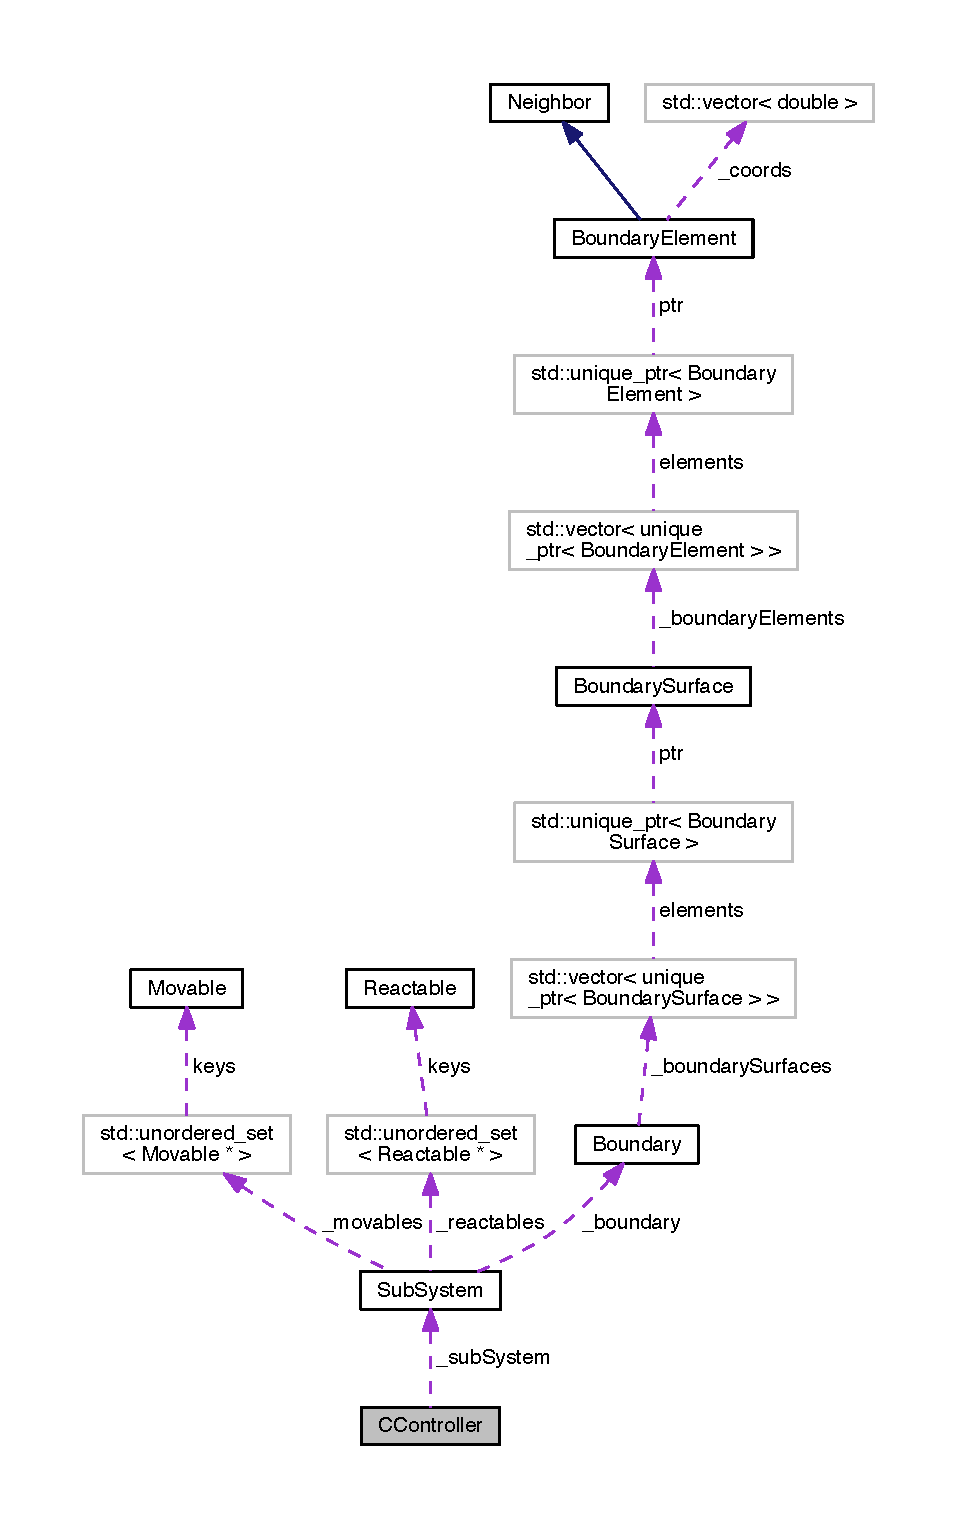
\includegraphics[height=550pt]{classCController__coll__graph}
\end{center}
\end{figure}
\subsection*{Public Member Functions}
\begin{DoxyCompactItemize}
\item 
\hyperlink{classCController_a8d10d61d353a0fc1ee9a531b4ec570db}{C\+Controller} (\hyperlink{classSubSystem}{Sub\+System} $\ast$s)
\begin{DoxyCompactList}\small\item\em Constructor which sets subsystem pointer. \end{DoxyCompactList}\item 
void \hyperlink{classCController_a6f1523b66f627d2cecf6e32ad88aca58}{initialize} (string \&chem\+Algorithm, string chem\+Manager, \hyperlink{structChemistryData}{Chemistry\+Data} \&chem)
\begin{DoxyCompactList}\small\item\em Initialize the \hyperlink{classChemSim}{Chem\+Sim} algorithm as well as the \hyperlink{classChemManager}{Chem\+Manager}. \end{DoxyCompactList}\item 
bool \hyperlink{classCController_a45dad60ad7d810684d45385c45e5c876}{run} (int steps)
\begin{DoxyCompactList}\small\item\em Run a number of chemical steps. \end{DoxyCompactList}\end{DoxyCompactItemize}
\subsection*{Private Attributes}
\begin{DoxyCompactItemize}
\item 
\hyperlink{classSubSystem}{Sub\+System} $\ast$ \hyperlink{classCController_a334a900bd08abab80bda555a155d234a}{\+\_\+sub\+System}
\begin{DoxyCompactList}\small\item\em A pointer to the subsystem. \end{DoxyCompactList}\end{DoxyCompactItemize}


\subsection{Detailed Description}
Used to intialize, control, and run the chemical components of a simulation. 

Chem\+Controller is a class used by the \hyperlink{classSubSystem}{Sub\+System} to instantiate, control, and run the chemical dynamics of a simulation. It has functions to initialize a chemical system, which, based on a choice of the reaction-\/diffusion algorithm as well as the type of manager which controls the reactions in the simulation, as well as run the chemical components of the simulation.

The controller initializes all chemical singletons used, including \hyperlink{classChemSim}{Chem\+Sim} and \hyperlink{classChemManager}{Chem\+Manager} to the correct implementations, given that they are implemented. 

Definition at line 36 of file C\+Controller.\+h.



\subsection{Constructor \& Destructor Documentation}
\hypertarget{classCController_a8d10d61d353a0fc1ee9a531b4ec570db}{\index{C\+Controller@{C\+Controller}!C\+Controller@{C\+Controller}}
\index{C\+Controller@{C\+Controller}!C\+Controller@{C\+Controller}}
\subsubsection[{C\+Controller}]{\setlength{\rightskip}{0pt plus 5cm}C\+Controller\+::\+C\+Controller (
\begin{DoxyParamCaption}
\item[{{\bf Sub\+System} $\ast$}]{s}
\end{DoxyParamCaption}
)\hspace{0.3cm}{\ttfamily [inline]}}}\label{classCController_a8d10d61d353a0fc1ee9a531b4ec570db}


Constructor which sets subsystem pointer. 



Definition at line 43 of file C\+Controller.\+h.



References \+\_\+sub\+System.



\subsection{Member Function Documentation}
\hypertarget{classCController_a6f1523b66f627d2cecf6e32ad88aca58}{\index{C\+Controller@{C\+Controller}!initialize@{initialize}}
\index{initialize@{initialize}!C\+Controller@{C\+Controller}}
\subsubsection[{initialize}]{\setlength{\rightskip}{0pt plus 5cm}void C\+Controller\+::initialize (
\begin{DoxyParamCaption}
\item[{string \&}]{chem\+Algorithm, }
\item[{string}]{chem\+Manager, }
\item[{{\bf Chemistry\+Data} \&}]{chem}
\end{DoxyParamCaption}
)}}\label{classCController_a6f1523b66f627d2cecf6e32ad88aca58}


Initialize the \hyperlink{classChemSim}{Chem\+Sim} algorithm as well as the \hyperlink{classChemManager}{Chem\+Manager}. 


\begin{DoxyParams}{Parameters}
{\em chem\+Algorithm} & -\/ a string defining the chemical algorithm to be used \\
\hline
{\em chem\+Initializer} & -\/ a string defining the chemical manager used \\
\hline
\end{DoxyParams}


Definition at line 23 of file C\+Controller.\+cpp.



References \+\_\+sub\+System, Chem\+Manager\+::initialize(), Chem\+Sim\+::initialize(), Chem\+Manager\+::set\+Instance(), and Chem\+Sim\+::set\+Instance().

\hypertarget{classCController_a45dad60ad7d810684d45385c45e5c876}{\index{C\+Controller@{C\+Controller}!run@{run}}
\index{run@{run}!C\+Controller@{C\+Controller}}
\subsubsection[{run}]{\setlength{\rightskip}{0pt plus 5cm}bool C\+Controller\+::run (
\begin{DoxyParamCaption}
\item[{int}]{steps}
\end{DoxyParamCaption}
)\hspace{0.3cm}{\ttfamily [inline]}}}\label{classCController_a45dad60ad7d810684d45385c45e5c876}


Run a number of chemical steps. 



Definition at line 51 of file C\+Controller.\+h.



References Chem\+Sim\+::run().



\subsection{Member Data Documentation}
\hypertarget{classCController_a334a900bd08abab80bda555a155d234a}{\index{C\+Controller@{C\+Controller}!\+\_\+sub\+System@{\+\_\+sub\+System}}
\index{\+\_\+sub\+System@{\+\_\+sub\+System}!C\+Controller@{C\+Controller}}
\subsubsection[{\+\_\+sub\+System}]{\setlength{\rightskip}{0pt plus 5cm}{\bf Sub\+System}$\ast$ C\+Controller\+::\+\_\+sub\+System\hspace{0.3cm}{\ttfamily [private]}}}\label{classCController_a334a900bd08abab80bda555a155d234a}


A pointer to the subsystem. 



Definition at line 39 of file C\+Controller.\+h.



Referenced by C\+Controller(), and initialize().



The documentation for this class was generated from the following files\+:\begin{DoxyCompactItemize}
\item 
M3\+S\+Y\+M/\hyperlink{CController_8h}{C\+Controller.\+h}\item 
M3\+S\+Y\+M/\hyperlink{CController_8cpp}{C\+Controller.\+cpp}\end{DoxyCompactItemize}

\hypertarget{classCCylinder}{\section{C\+Cylinder Class Reference}
\label{classCCylinder}\index{C\+Cylinder@{C\+Cylinder}}
}


Holds all \hyperlink{classCMonomer}{C\+Monomers} and \hyperlink{classReaction}{Reactions} associated with it.  




{\ttfamily \#include $<$C\+Cylinder.\+h$>$}



Collaboration diagram for C\+Cylinder\+:
\nopagebreak
\begin{figure}[H]
\begin{center}
\leavevmode
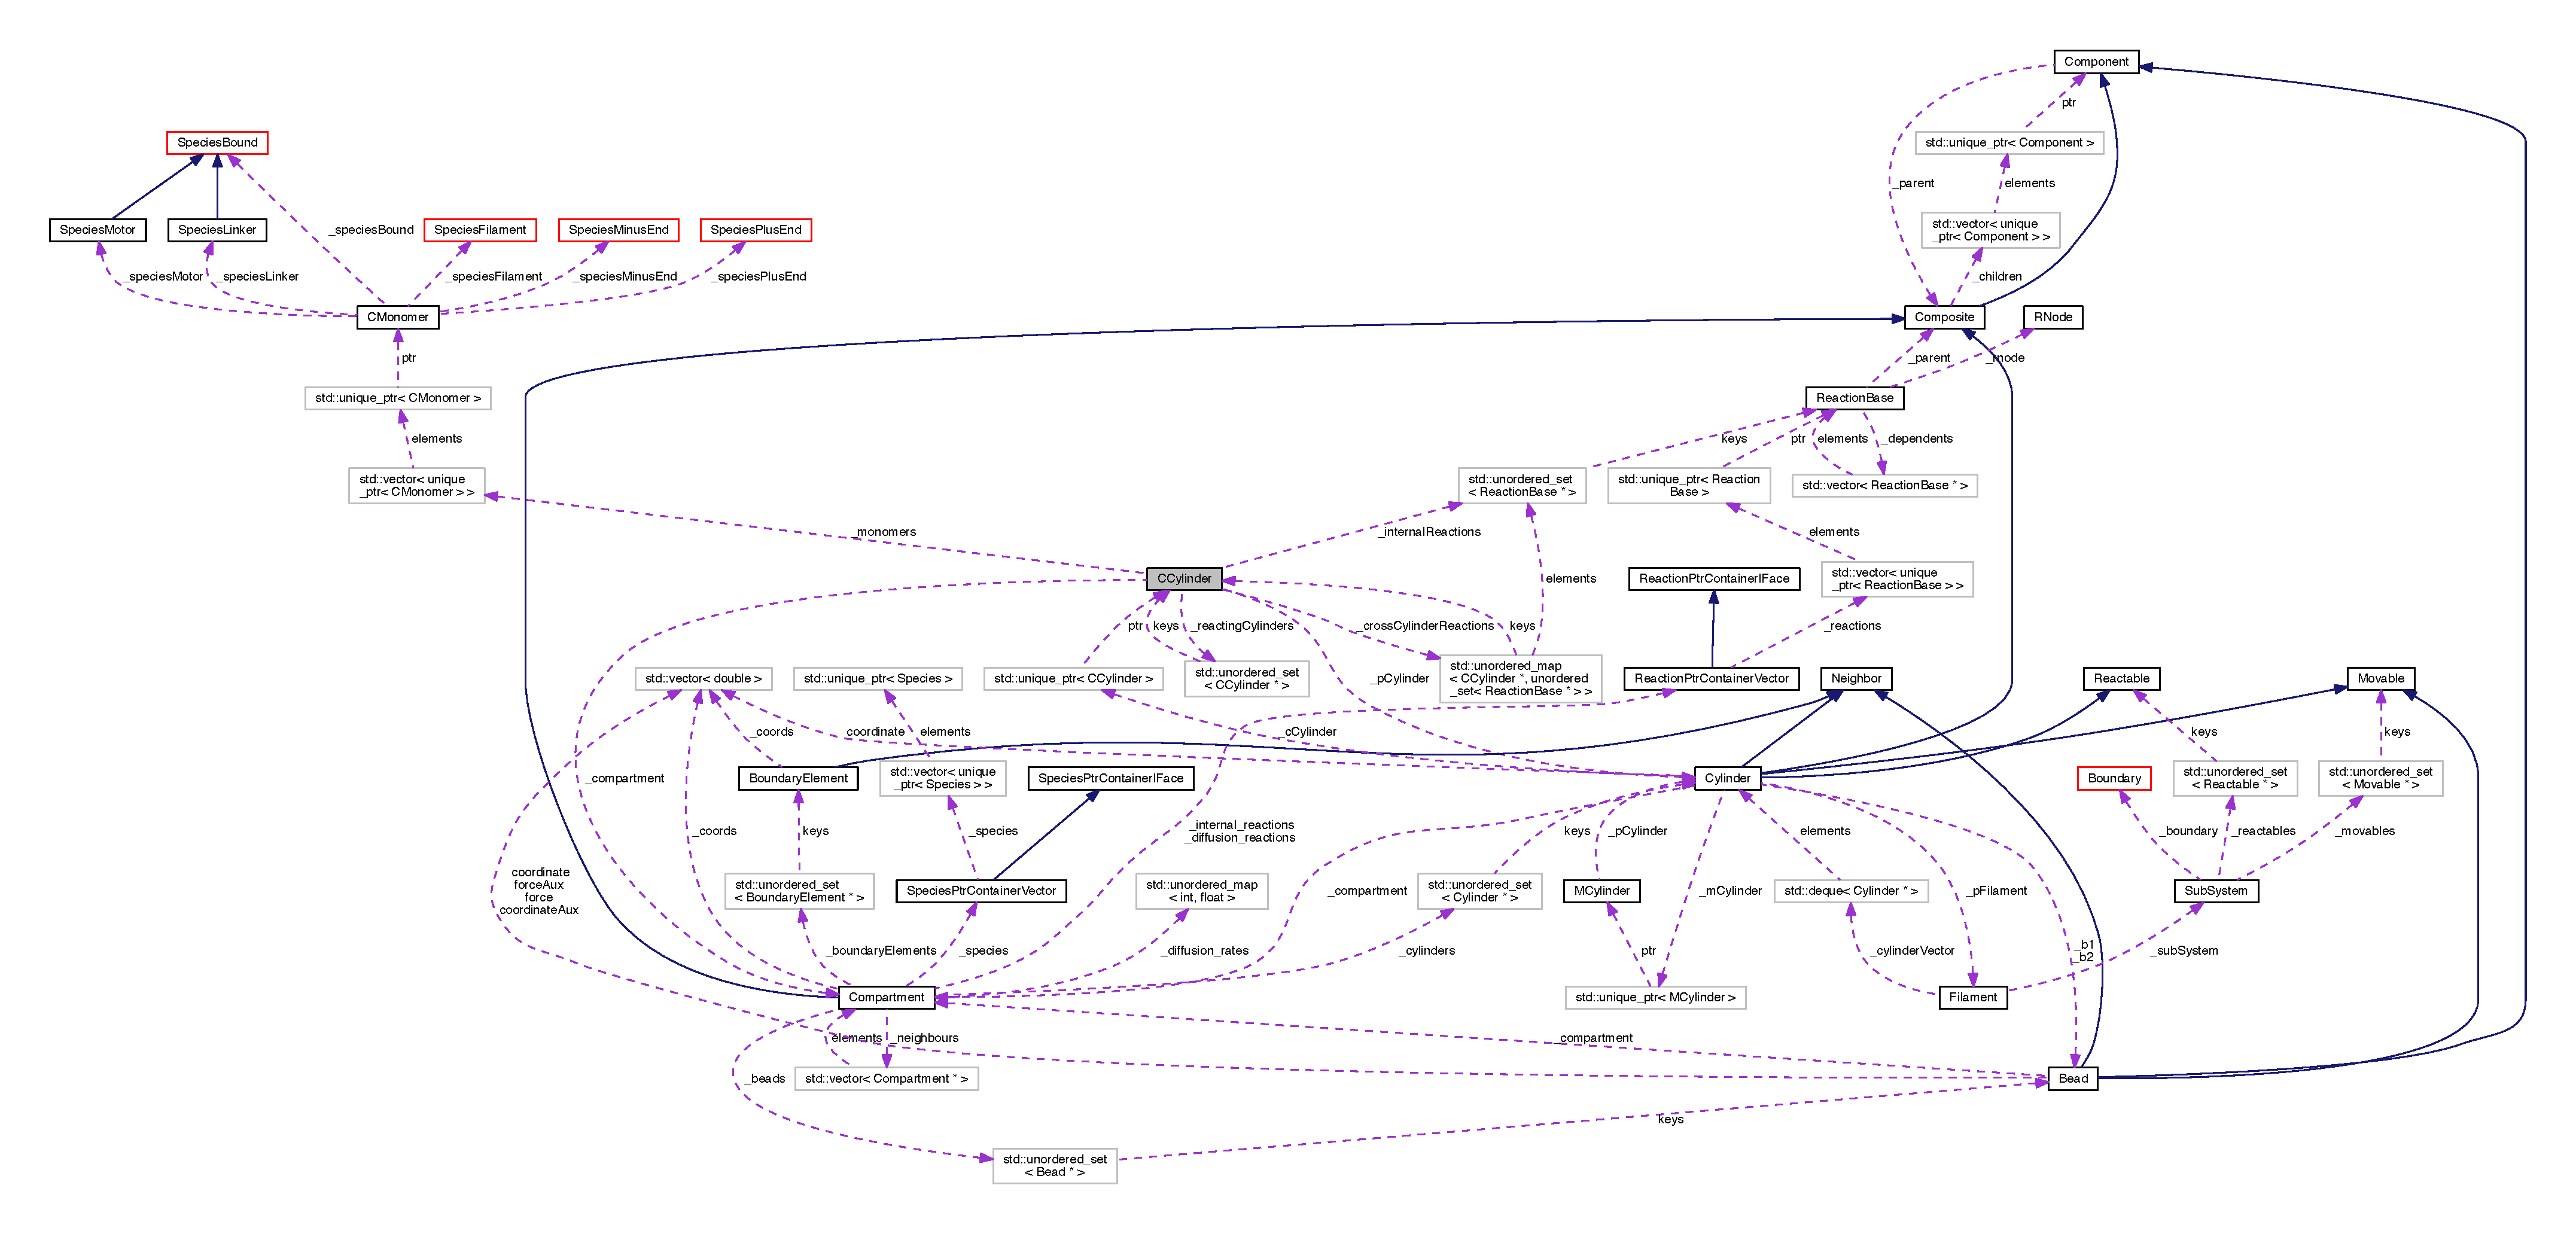
\includegraphics[width=350pt]{classCCylinder__coll__graph}
\end{center}
\end{figure}
\subsection*{Public Member Functions}
\begin{DoxyCompactItemize}
\item 
\hyperlink{classCCylinder_a0be01ef2708175a8a147ca45fd290b83}{C\+Cylinder} (\hyperlink{classCompartment}{Compartment} $\ast$c)
\begin{DoxyCompactList}\small\item\em Default constructor, sets compartment. \end{DoxyCompactList}\item 
\hyperlink{classCCylinder_a71863b46b8fee12a2bfb03c12c52f5ee}{C\+Cylinder} (const \hyperlink{classCCylinder}{C\+Cylinder} \&rhs, \hyperlink{classCompartment}{Compartment} $\ast$c)
\begin{DoxyCompactList}\small\item\em Copy constructor. \end{DoxyCompactList}\item 
\hyperlink{classCCylinder}{C\+Cylinder} \& \hyperlink{classCCylinder_a82cdc245e542d14ceab4bb1df061dce4}{operator=} (\hyperlink{classCCylinder}{C\+Cylinder} \&rhs)=delete
\begin{DoxyCompactList}\small\item\em Assignment is not allowed. \end{DoxyCompactList}\item 
\hyperlink{classCCylinder_a715d736c871953942e497290867f591c}{$\sim$\+C\+Cylinder} ()
\begin{DoxyCompactList}\small\item\em Default destructor, explicitly removes C\+Monomers(including their species, rxns) Removes all reactions associated with this \hyperlink{classCCylinder}{C\+Cylinder}, including ones owned by this as well as other C\+Cylinders. \end{DoxyCompactList}\item 
virtual \hyperlink{classCCylinder}{C\+Cylinder} $\ast$ \hyperlink{classCCylinder_a5085f34b8f011a8be07b675a59d16d6f}{clone} (\hyperlink{classCompartment}{Compartment} $\ast$c)
\begin{DoxyCompactList}\small\item\em Clone, calls copy constructor. \end{DoxyCompactList}\item 
\hyperlink{classCompartment}{Compartment} $\ast$ \hyperlink{classCCylinder_ab58156c4f6efbe01ad58540fef073930}{get\+Compartment} ()
\begin{DoxyCompactList}\small\item\em Get compartment. \end{DoxyCompactList}\item 
void \hyperlink{classCCylinder_a8a0a3292e299521278152921ebfbce51}{set\+Cylinder} (\hyperlink{classCylinder}{Cylinder} $\ast$c)
\begin{DoxyCompactList}\small\item\em Set parent. \end{DoxyCompactList}\item 
\hyperlink{classCylinder}{Cylinder} $\ast$ \hyperlink{classCCylinder_a53332923a74acb20fe192d870215a687}{get\+Cylinder} ()
\begin{DoxyCompactList}\small\item\em Get parent. \end{DoxyCompactList}\item 
void \hyperlink{classCCylinder_a14fb0bbed36384ea72519e85ad4e91b8}{add\+C\+Monomer} (\hyperlink{classCMonomer}{C\+Monomer} $\ast$monomer)
\begin{DoxyCompactList}\small\item\em Add a monomer. \end{DoxyCompactList}\item 
\hyperlink{classCMonomer}{C\+Monomer} $\ast$ \hyperlink{classCCylinder_ac6b0fb293c40045db64365debca77c1d}{get\+C\+Monomer} (int index)
\begin{DoxyCompactList}\small\item\em Get monomer at an index. \end{DoxyCompactList}\item 
const unordered\+\_\+set\\*
$<$ \hyperlink{classReactionBase}{Reaction\+Base} $\ast$ $>$ \& \hyperlink{classCCylinder_a2bccfcdda7d524213d87066d1735fec9}{get\+Internal\+Reactions} ()
\begin{DoxyCompactList}\small\item\em Get list of reactions associated. \end{DoxyCompactList}\item 
const unordered\+\_\+set$<$ \hyperlink{classCCylinder}{C\+Cylinder} $\ast$ $>$ \& \hyperlink{classCCylinder_ac495877eae9e12fe90a9f4f85323d13f}{get\+Reacting\+Cylinders} ()
\item 
unordered\+\_\+map$<$ \hyperlink{classCCylinder}{C\+Cylinder} \\*
$\ast$, unordered\+\_\+set$<$ \hyperlink{classReactionBase}{Reaction\+Base} $\ast$ $>$ $>$ \& \hyperlink{classCCylinder_aa1fd48d90a614bd82268367a548eb8d5}{get\+Cross\+Cylinder\+Reactions} ()
\begin{DoxyCompactList}\small\item\em Get map of reactions associated. \end{DoxyCompactList}\item 
virtual void \hyperlink{classCCylinder_a9c358ffc39c2503fc63d67333976bf69}{print\+C\+Cylinder} ()
\begin{DoxyCompactList}\small\item\em Print. \end{DoxyCompactList}\item 
short \hyperlink{classCCylinder_a1e45d32541c9fb3145803cfbf0f93566}{get\+Size} ()
\begin{DoxyCompactList}\small\item\em Get size in number of monomers. \end{DoxyCompactList}\end{DoxyCompactItemize}
{\bf }\par
\begin{DoxyCompactItemize}
\item 
void \hyperlink{classCCylinder_a53bed608f1b287eca275e0833a1233f1}{add\+Internal\+Reaction} (\hyperlink{classReactionBase}{Reaction\+Base} $\ast$r)
\begin{DoxyCompactList}\small\item\em \hyperlink{classReaction}{Reaction} management function. \end{DoxyCompactList}\item 
void \hyperlink{classCCylinder_a5535278dcbc8498e3006b5176858bddd}{add\+Cross\+Cylinder\+Reaction} (\hyperlink{classCCylinder}{C\+Cylinder} $\ast$other, \hyperlink{classReactionBase}{Reaction\+Base} $\ast$r)
\begin{DoxyCompactList}\small\item\em \hyperlink{classReaction}{Reaction} management function. \end{DoxyCompactList}\item 
void \hyperlink{classCCylinder_adeb2d133a53137e281b3134bfba5a4db}{add\+Reacting\+Cylinder} (\hyperlink{classCCylinder}{C\+Cylinder} $\ast$other)
\begin{DoxyCompactList}\small\item\em \hyperlink{classReaction}{Reaction} management function. \end{DoxyCompactList}\item 
void \hyperlink{classCCylinder_a9ee95b562068b9ffbc6c3b989be7af5f}{remove\+Internal\+Reaction} (\hyperlink{classReactionBase}{Reaction\+Base} $\ast$r)
\begin{DoxyCompactList}\small\item\em \hyperlink{classReaction}{Reaction} management function. \end{DoxyCompactList}\item 
void \hyperlink{classCCylinder_ae35ab9042ad585fa7ea9ba32ecd6e60f}{remove\+All\+Internal\+Reactions} ()
\begin{DoxyCompactList}\small\item\em \hyperlink{classReaction}{Reaction} management function. \end{DoxyCompactList}\item 
void \hyperlink{classCCylinder_a4cb0c141bef0820e345b5e3c756fa163}{remove\+Cross\+Cylinder\+Reactions} (\hyperlink{classCCylinder}{C\+Cylinder} $\ast$other)
\begin{DoxyCompactList}\small\item\em \hyperlink{classReaction}{Reaction} management function. \end{DoxyCompactList}\item 
void \hyperlink{classCCylinder_a7767880083ceda061babd4225557d7c3}{remove\+All\+Cross\+Cylinder\+Reactions} ()
\begin{DoxyCompactList}\small\item\em \hyperlink{classReaction}{Reaction} management function. \end{DoxyCompactList}\item 
void \hyperlink{classCCylinder_a3aecfb4bb31a032ccb73200f71f40ed9}{remove\+Reacting\+Cylinder} (\hyperlink{classCCylinder}{C\+Cylinder} $\ast$other)
\begin{DoxyCompactList}\small\item\em \hyperlink{classReaction}{Reaction} management function. \end{DoxyCompactList}\item 
void \hyperlink{classCCylinder_a97f1758093c7275bdb17ac92b6a05117}{remove\+All\+Reacting\+Cylinders} ()
\begin{DoxyCompactList}\small\item\em \hyperlink{classReaction}{Reaction} management function. \end{DoxyCompactList}\end{DoxyCompactItemize}

\subsection*{Private Attributes}
\begin{DoxyCompactItemize}
\item 
vector$<$ unique\+\_\+ptr$<$ \hyperlink{classCMonomer}{C\+Monomer} $>$ $>$ \hyperlink{classCCylinder_a2583ee1b23a42501ece73a2a35d92a31}{\+\_\+monomers}
\begin{DoxyCompactList}\small\item\em List of monomers. \end{DoxyCompactList}\item 
unordered\+\_\+set$<$ \hyperlink{classReactionBase}{Reaction\+Base} $\ast$ $>$ \hyperlink{classCCylinder_a2f377a8697a4b4e053e747287e7a6a09}{\+\_\+internal\+Reactions}
\begin{DoxyCompactList}\small\item\em R\+E\+A\+C\+T\+I\+O\+N C\+O\+N\+T\+A\+I\+N\+E\+R\+S. \end{DoxyCompactList}\item 
unordered\+\_\+set$<$ \hyperlink{classCCylinder}{C\+Cylinder} $\ast$ $>$ \hyperlink{classCCylinder_afdf5de084ef7692b8ee75b078eca384f}{\+\_\+reacting\+Cylinders}
\begin{DoxyCompactList}\small\item\em Set of ccylinders that this ccylinder has reactions with, but not ownership. \end{DoxyCompactList}\item 
unordered\+\_\+map$<$ \hyperlink{classCCylinder}{C\+Cylinder} \\*
$\ast$, unordered\+\_\+set$<$ \hyperlink{classReactionBase}{Reaction\+Base} $\ast$ $>$ $>$ \hyperlink{classCCylinder_a4263400be58cd0e11e0be99a42595c88}{\+\_\+cross\+Cylinder\+Reactions}
\begin{DoxyCompactList}\small\item\em Map of cross-\/cylinder reactions owned. \end{DoxyCompactList}\item 
\hyperlink{classCompartment}{Compartment} $\ast$ \hyperlink{classCCylinder_ad8a1a406025aa82a072215aeb645c8c1}{\+\_\+compartment}
\begin{DoxyCompactList}\small\item\em \hyperlink{classCompartment}{Compartment} this ccylinder is in. \end{DoxyCompactList}\item 
\hyperlink{classCylinder}{Cylinder} $\ast$ \hyperlink{classCCylinder_a4439d9b805e3e206fd495540aa975346}{\+\_\+p\+Cylinder}
\begin{DoxyCompactList}\small\item\em Parent cylinder. \end{DoxyCompactList}\item 
short \hyperlink{classCCylinder_a9951ded0fd9d228a2358bee18f8b61b6}{\+\_\+size} = \hyperlink{classSystemParameters_a9211bca7e3422c076f4e9ba2dc29c599}{System\+Parameters\+::\+Geometry}().cylinder\+Size / \hyperlink{classSystemParameters_a9211bca7e3422c076f4e9ba2dc29c599}{System\+Parameters\+::\+Geometry}().monomer\+Size
\begin{DoxyCompactList}\small\item\em Max length of full \hyperlink{classCylinder}{Cylinder}. \end{DoxyCompactList}\end{DoxyCompactItemize}


\subsection{Detailed Description}
Holds all \hyperlink{classCMonomer}{C\+Monomers} and \hyperlink{classReaction}{Reactions} associated with it. 

The \hyperlink{classCCylinder}{C\+Cylinder} class has lists of the \hyperlink{classCMonomer}{C\+Monomers} that it contains.

A \hyperlink{classCCylinder}{C\+Cylinder} also stores the \hyperlink{classReaction}{Reactions} associated with it internally, as well as cross-\/cylinder reactions (still \char`\"{}owned\char`\"{} by this \hyperlink{classCCylinder}{C\+Cylinder}, but has reactants and/or products that contain a species in another \hyperlink{classCCylinder}{C\+Cylinder}). This information is stored in the reaction map. This map can be used to add and delete reactions when a \hyperlink{classCCylinder}{C\+Cylinder} changes compartment or is removed from the system.

Lastly, the \hyperlink{classCCylinder}{C\+Cylinder} stores a list of other C\+Cylinders that it has cross-\/cylinder reactions with, but does not have ownership of these reactions. This list can be used to change or delete reactions when needed, but will not be tied to a \hyperlink{classCompartment}{Compartment} transfer of this \hyperlink{classCCylinder}{C\+Cylinder}. 

Definition at line 41 of file C\+Cylinder.\+h.



\subsection{Constructor \& Destructor Documentation}
\hypertarget{classCCylinder_a0be01ef2708175a8a147ca45fd290b83}{\index{C\+Cylinder@{C\+Cylinder}!C\+Cylinder@{C\+Cylinder}}
\index{C\+Cylinder@{C\+Cylinder}!C\+Cylinder@{C\+Cylinder}}
\subsubsection[{C\+Cylinder}]{\setlength{\rightskip}{0pt plus 5cm}C\+Cylinder\+::\+C\+Cylinder (
\begin{DoxyParamCaption}
\item[{{\bf Compartment} $\ast$}]{c}
\end{DoxyParamCaption}
)\hspace{0.3cm}{\ttfamily [inline]}}}\label{classCCylinder_a0be01ef2708175a8a147ca45fd290b83}


Default constructor, sets compartment. 



Definition at line 58 of file C\+Cylinder.\+h.



Referenced by clone().

\hypertarget{classCCylinder_a71863b46b8fee12a2bfb03c12c52f5ee}{\index{C\+Cylinder@{C\+Cylinder}!C\+Cylinder@{C\+Cylinder}}
\index{C\+Cylinder@{C\+Cylinder}!C\+Cylinder@{C\+Cylinder}}
\subsubsection[{C\+Cylinder}]{\setlength{\rightskip}{0pt plus 5cm}C\+Cylinder\+::\+C\+Cylinder (
\begin{DoxyParamCaption}
\item[{const {\bf C\+Cylinder} \&}]{rhs, }
\item[{{\bf Compartment} $\ast$}]{c}
\end{DoxyParamCaption}
)}}\label{classCCylinder_a71863b46b8fee12a2bfb03c12c52f5ee}


Copy constructor. 

\begin{DoxyNote}{Note}
This constructor will create a new \hyperlink{classCCylinder}{C\+Cylinder} with different \hyperlink{classSpecies}{Species} and \hyperlink{classReaction}{Reactions} within the \hyperlink{classCompartment}{Compartment} that is chosen as a parameter to the constructor. The copied and original \hyperlink{classCCylinder}{C\+Cylinder} will not share reactions or species, but will be copied into a new \hyperlink{classCompartment}{Compartment}. 
\end{DoxyNote}


Definition at line 16 of file C\+Cylinder.\+cpp.



References \+\_\+cross\+Cylinder\+Reactions, \+\_\+internal\+Reactions, \+\_\+monomers, \+\_\+reacting\+Cylinders, add\+Cross\+Cylinder\+Reaction(), add\+Internal\+Reaction(), and Compartment\+::get\+Species\+Container().

\hypertarget{classCCylinder_a715d736c871953942e497290867f591c}{\index{C\+Cylinder@{C\+Cylinder}!````~C\+Cylinder@{$\sim$\+C\+Cylinder}}
\index{````~C\+Cylinder@{$\sim$\+C\+Cylinder}!C\+Cylinder@{C\+Cylinder}}
\subsubsection[{$\sim$\+C\+Cylinder}]{\setlength{\rightskip}{0pt plus 5cm}C\+Cylinder\+::$\sim$\+C\+Cylinder (
\begin{DoxyParamCaption}
{}
\end{DoxyParamCaption}
)}}\label{classCCylinder_a715d736c871953942e497290867f591c}


Default destructor, explicitly removes C\+Monomers(including their species, rxns) Removes all reactions associated with this \hyperlink{classCCylinder}{C\+Cylinder}, including ones owned by this as well as other C\+Cylinders. 



Definition at line 38 of file C\+Cylinder.\+cpp.



References \+\_\+compartment, \+\_\+monomers, System\+Parameters\+::\+Chemistry(), Chemistry\+Parameters\+::num\+Bound\+Species, Chemistry\+Parameters\+::num\+Filament\+Species, Chemistry\+Parameters\+::num\+Linker\+Species, Chemistry\+Parameters\+::num\+Minus\+End\+Species, Chemistry\+Parameters\+::num\+Motor\+Species, Chemistry\+Parameters\+::num\+Plus\+End\+Species, remove\+All\+Cross\+Cylinder\+Reactions(), remove\+All\+Internal\+Reactions(), remove\+All\+Reacting\+Cylinders(), and Compartment\+::remove\+Species().



\subsection{Member Function Documentation}
\hypertarget{classCCylinder_a14fb0bbed36384ea72519e85ad4e91b8}{\index{C\+Cylinder@{C\+Cylinder}!add\+C\+Monomer@{add\+C\+Monomer}}
\index{add\+C\+Monomer@{add\+C\+Monomer}!C\+Cylinder@{C\+Cylinder}}
\subsubsection[{add\+C\+Monomer}]{\setlength{\rightskip}{0pt plus 5cm}void C\+Cylinder\+::add\+C\+Monomer (
\begin{DoxyParamCaption}
\item[{{\bf C\+Monomer} $\ast$}]{monomer}
\end{DoxyParamCaption}
)\hspace{0.3cm}{\ttfamily [inline]}}}\label{classCCylinder_a14fb0bbed36384ea72519e85ad4e91b8}


Add a monomer. 



Definition at line 88 of file C\+Cylinder.\+h.



References \+\_\+monomers.



Referenced by Simple\+Manager\+Impl\+::initialize\+C\+Cylinder().

\hypertarget{classCCylinder_a5535278dcbc8498e3006b5176858bddd}{\index{C\+Cylinder@{C\+Cylinder}!add\+Cross\+Cylinder\+Reaction@{add\+Cross\+Cylinder\+Reaction}}
\index{add\+Cross\+Cylinder\+Reaction@{add\+Cross\+Cylinder\+Reaction}!C\+Cylinder@{C\+Cylinder}}
\subsubsection[{add\+Cross\+Cylinder\+Reaction}]{\setlength{\rightskip}{0pt plus 5cm}void C\+Cylinder\+::add\+Cross\+Cylinder\+Reaction (
\begin{DoxyParamCaption}
\item[{{\bf C\+Cylinder} $\ast$}]{other, }
\item[{{\bf Reaction\+Base} $\ast$}]{r}
\end{DoxyParamCaption}
)}}\label{classCCylinder_a5535278dcbc8498e3006b5176858bddd}


\hyperlink{classReaction}{Reaction} management function. 



Definition at line 94 of file C\+Cylinder.\+cpp.



References \+\_\+compartment, \+\_\+cross\+Cylinder\+Reactions, Reaction\+Base\+::activate\+Reaction(), Compartment\+::add\+Internal\+Reaction\+Unique(), add\+Reacting\+Cylinder(), and Chem\+Sim\+::add\+Reaction().



Referenced by Poly\+Plus\+End\+Manager\+::add\+Reaction(), Poly\+Minus\+End\+Manager\+::add\+Reaction(), Depoly\+Plus\+End\+Manager\+::add\+Reaction(), Depoly\+Minus\+End\+Manager\+::add\+Reaction(), Motor\+Walk\+F\+Manager\+::add\+Reaction(), Motor\+Walk\+B\+Manager\+::add\+Reaction(), Linker\+Binding\+Manager\+::add\+Reaction(), Motor\+Binding\+Manager\+::add\+Reaction(), and C\+Cylinder().

\hypertarget{classCCylinder_a53bed608f1b287eca275e0833a1233f1}{\index{C\+Cylinder@{C\+Cylinder}!add\+Internal\+Reaction@{add\+Internal\+Reaction}}
\index{add\+Internal\+Reaction@{add\+Internal\+Reaction}!C\+Cylinder@{C\+Cylinder}}
\subsubsection[{add\+Internal\+Reaction}]{\setlength{\rightskip}{0pt plus 5cm}void C\+Cylinder\+::add\+Internal\+Reaction (
\begin{DoxyParamCaption}
\item[{{\bf Reaction\+Base} $\ast$}]{r}
\end{DoxyParamCaption}
)}}\label{classCCylinder_a53bed608f1b287eca275e0833a1233f1}


\hyperlink{classReaction}{Reaction} management function. 



Definition at line 82 of file C\+Cylinder.\+cpp.



References \+\_\+compartment, \+\_\+internal\+Reactions, Reaction\+Base\+::activate\+Reaction(), Compartment\+::add\+Internal\+Reaction\+Unique(), and Chem\+Sim\+::add\+Reaction().



Referenced by Poly\+Plus\+End\+Manager\+::add\+Reaction(), Poly\+Minus\+End\+Manager\+::add\+Reaction(), Depoly\+Plus\+End\+Manager\+::add\+Reaction(), Depoly\+Minus\+End\+Manager\+::add\+Reaction(), Basic\+Binding\+Manager\+::add\+Reaction(), Unbinding\+Manager\+::add\+Reaction(), Motor\+Walk\+F\+Manager\+::add\+Reaction(), Motor\+Walk\+B\+Manager\+::add\+Reaction(), and C\+Cylinder().

\hypertarget{classCCylinder_adeb2d133a53137e281b3134bfba5a4db}{\index{C\+Cylinder@{C\+Cylinder}!add\+Reacting\+Cylinder@{add\+Reacting\+Cylinder}}
\index{add\+Reacting\+Cylinder@{add\+Reacting\+Cylinder}!C\+Cylinder@{C\+Cylinder}}
\subsubsection[{add\+Reacting\+Cylinder}]{\setlength{\rightskip}{0pt plus 5cm}void C\+Cylinder\+::add\+Reacting\+Cylinder (
\begin{DoxyParamCaption}
\item[{{\bf C\+Cylinder} $\ast$}]{other}
\end{DoxyParamCaption}
)}}\label{classCCylinder_adeb2d133a53137e281b3134bfba5a4db}


\hyperlink{classReaction}{Reaction} management function. 



Definition at line 107 of file C\+Cylinder.\+cpp.



References \+\_\+reacting\+Cylinders.



Referenced by add\+Cross\+Cylinder\+Reaction().

\hypertarget{classCCylinder_a5085f34b8f011a8be07b675a59d16d6f}{\index{C\+Cylinder@{C\+Cylinder}!clone@{clone}}
\index{clone@{clone}!C\+Cylinder@{C\+Cylinder}}
\subsubsection[{clone}]{\setlength{\rightskip}{0pt plus 5cm}virtual {\bf C\+Cylinder}$\ast$ C\+Cylinder\+::clone (
\begin{DoxyParamCaption}
\item[{{\bf Compartment} $\ast$}]{c}
\end{DoxyParamCaption}
)\hspace{0.3cm}{\ttfamily [inline]}, {\ttfamily [virtual]}}}\label{classCCylinder_a5085f34b8f011a8be07b675a59d16d6f}


Clone, calls copy constructor. 



Definition at line 75 of file C\+Cylinder.\+h.



References C\+Cylinder().

\hypertarget{classCCylinder_ac6b0fb293c40045db64365debca77c1d}{\index{C\+Cylinder@{C\+Cylinder}!get\+C\+Monomer@{get\+C\+Monomer}}
\index{get\+C\+Monomer@{get\+C\+Monomer}!C\+Cylinder@{C\+Cylinder}}
\subsubsection[{get\+C\+Monomer}]{\setlength{\rightskip}{0pt plus 5cm}{\bf C\+Monomer}$\ast$ C\+Cylinder\+::get\+C\+Monomer (
\begin{DoxyParamCaption}
\item[{int}]{index}
\end{DoxyParamCaption}
)\hspace{0.3cm}{\ttfamily [inline]}}}\label{classCCylinder_ac6b0fb293c40045db64365debca77c1d}


Get monomer at an index. 

\begin{DoxyNote}{Note}
no check on index 
\end{DoxyNote}


Definition at line 91 of file C\+Cylinder.\+h.



References \+\_\+monomers.



Referenced by Poly\+Plus\+End\+Manager\+::add\+Reaction(), Poly\+Minus\+End\+Manager\+::add\+Reaction(), Depoly\+Plus\+End\+Manager\+::add\+Reaction(), Depoly\+Minus\+End\+Manager\+::add\+Reaction(), Basic\+Binding\+Manager\+::add\+Reaction(), Unbinding\+Manager\+::add\+Reaction(), Motor\+Walk\+F\+Manager\+::add\+Reaction(), Motor\+Walk\+B\+Manager\+::add\+Reaction(), Linker\+Binding\+Manager\+::add\+Reaction(), Motor\+Binding\+Manager\+::add\+Reaction(), Simple\+Manager\+Impl\+::initialize\+C\+Cylinder(), Linker\+::\+Linker(), Motor\+Ghost\+::\+Motor\+Ghost(), Linker\+::$\sim$\+Linker(), and Motor\+Ghost\+::$\sim$\+Motor\+Ghost().

\hypertarget{classCCylinder_ab58156c4f6efbe01ad58540fef073930}{\index{C\+Cylinder@{C\+Cylinder}!get\+Compartment@{get\+Compartment}}
\index{get\+Compartment@{get\+Compartment}!C\+Cylinder@{C\+Cylinder}}
\subsubsection[{get\+Compartment}]{\setlength{\rightskip}{0pt plus 5cm}{\bf Compartment}$\ast$ C\+Cylinder\+::get\+Compartment (
\begin{DoxyParamCaption}
{}
\end{DoxyParamCaption}
)\hspace{0.3cm}{\ttfamily [inline]}}}\label{classCCylinder_ab58156c4f6efbe01ad58540fef073930}


Get compartment. 



Definition at line 80 of file C\+Cylinder.\+h.



References \+\_\+compartment.



Referenced by Poly\+Plus\+End\+Manager\+::add\+Reaction(), Poly\+Minus\+End\+Manager\+::add\+Reaction(), Depoly\+Plus\+End\+Manager\+::add\+Reaction(), Depoly\+Minus\+End\+Manager\+::add\+Reaction(), Basic\+Binding\+Manager\+::add\+Reaction(), Unbinding\+Manager\+::add\+Reaction(), Linker\+Binding\+Manager\+::add\+Reaction(), Motor\+Binding\+Manager\+::add\+Reaction(), and Simple\+Manager\+Impl\+::initialize\+C\+Cylinder().

\hypertarget{classCCylinder_aa1fd48d90a614bd82268367a548eb8d5}{\index{C\+Cylinder@{C\+Cylinder}!get\+Cross\+Cylinder\+Reactions@{get\+Cross\+Cylinder\+Reactions}}
\index{get\+Cross\+Cylinder\+Reactions@{get\+Cross\+Cylinder\+Reactions}!C\+Cylinder@{C\+Cylinder}}
\subsubsection[{get\+Cross\+Cylinder\+Reactions}]{\setlength{\rightskip}{0pt plus 5cm}unordered\+\_\+map$<${\bf C\+Cylinder}$\ast$, unordered\+\_\+set$<${\bf Reaction\+Base}$\ast$$>$ $>$\& C\+Cylinder\+::get\+Cross\+Cylinder\+Reactions (
\begin{DoxyParamCaption}
{}
\end{DoxyParamCaption}
)\hspace{0.3cm}{\ttfamily [inline]}}}\label{classCCylinder_aa1fd48d90a614bd82268367a548eb8d5}


Get map of reactions associated. 



Definition at line 97 of file C\+Cylinder.\+h.



References \+\_\+cross\+Cylinder\+Reactions.



Referenced by Simple\+Manager\+Impl\+::update\+C\+Cylinder().

\hypertarget{classCCylinder_a53332923a74acb20fe192d870215a687}{\index{C\+Cylinder@{C\+Cylinder}!get\+Cylinder@{get\+Cylinder}}
\index{get\+Cylinder@{get\+Cylinder}!C\+Cylinder@{C\+Cylinder}}
\subsubsection[{get\+Cylinder}]{\setlength{\rightskip}{0pt plus 5cm}{\bf Cylinder}$\ast$ C\+Cylinder\+::get\+Cylinder (
\begin{DoxyParamCaption}
{}
\end{DoxyParamCaption}
)\hspace{0.3cm}{\ttfamily [inline]}}}\label{classCCylinder_a53332923a74acb20fe192d870215a687}


Get parent. 



Definition at line 85 of file C\+Cylinder.\+h.



References \+\_\+p\+Cylinder.



Referenced by Poly\+Plus\+End\+Manager\+::add\+Reaction(), Poly\+Minus\+End\+Manager\+::add\+Reaction(), Depoly\+Plus\+End\+Manager\+::add\+Reaction(), Depoly\+Minus\+End\+Manager\+::add\+Reaction(), Linker\+Binding\+Callback\+::operator()(), Motor\+Binding\+Callback\+::operator()(), Motor\+Moving\+Cylinder\+Forward\+Callback\+::operator()(), Motor\+Moving\+Cylinder\+Backward\+Callback\+::operator()(), and Simple\+Manager\+Impl\+::update\+C\+Cylinder().

\hypertarget{classCCylinder_a2bccfcdda7d524213d87066d1735fec9}{\index{C\+Cylinder@{C\+Cylinder}!get\+Internal\+Reactions@{get\+Internal\+Reactions}}
\index{get\+Internal\+Reactions@{get\+Internal\+Reactions}!C\+Cylinder@{C\+Cylinder}}
\subsubsection[{get\+Internal\+Reactions}]{\setlength{\rightskip}{0pt plus 5cm}const unordered\+\_\+set$<${\bf Reaction\+Base}$\ast$$>$\& C\+Cylinder\+::get\+Internal\+Reactions (
\begin{DoxyParamCaption}
{}
\end{DoxyParamCaption}
)\hspace{0.3cm}{\ttfamily [inline]}}}\label{classCCylinder_a2bccfcdda7d524213d87066d1735fec9}


Get list of reactions associated. 



Definition at line 94 of file C\+Cylinder.\+h.



References \+\_\+internal\+Reactions.

\hypertarget{classCCylinder_ac495877eae9e12fe90a9f4f85323d13f}{\index{C\+Cylinder@{C\+Cylinder}!get\+Reacting\+Cylinders@{get\+Reacting\+Cylinders}}
\index{get\+Reacting\+Cylinders@{get\+Reacting\+Cylinders}!C\+Cylinder@{C\+Cylinder}}
\subsubsection[{get\+Reacting\+Cylinders}]{\setlength{\rightskip}{0pt plus 5cm}const unordered\+\_\+set$<${\bf C\+Cylinder}$\ast$$>$\& C\+Cylinder\+::get\+Reacting\+Cylinders (
\begin{DoxyParamCaption}
{}
\end{DoxyParamCaption}
)\hspace{0.3cm}{\ttfamily [inline]}}}\label{classCCylinder_ac495877eae9e12fe90a9f4f85323d13f}


Definition at line 95 of file C\+Cylinder.\+h.



References \+\_\+reacting\+Cylinders.

\hypertarget{classCCylinder_a1e45d32541c9fb3145803cfbf0f93566}{\index{C\+Cylinder@{C\+Cylinder}!get\+Size@{get\+Size}}
\index{get\+Size@{get\+Size}!C\+Cylinder@{C\+Cylinder}}
\subsubsection[{get\+Size}]{\setlength{\rightskip}{0pt plus 5cm}short C\+Cylinder\+::get\+Size (
\begin{DoxyParamCaption}
{}
\end{DoxyParamCaption}
)\hspace{0.3cm}{\ttfamily [inline]}}}\label{classCCylinder_a1e45d32541c9fb3145803cfbf0f93566}


Get size in number of monomers. 



Definition at line 119 of file C\+Cylinder.\+h.



References \+\_\+size.



Referenced by Poly\+Plus\+End\+Manager\+::add\+Reaction(), Poly\+Minus\+End\+Manager\+::add\+Reaction(), Depoly\+Plus\+End\+Manager\+::add\+Reaction(), Depoly\+Minus\+End\+Manager\+::add\+Reaction(), Basic\+Binding\+Manager\+::add\+Reaction(), Unbinding\+Manager\+::add\+Reaction(), Motor\+Walk\+F\+Manager\+::add\+Reaction(), Motor\+Walk\+B\+Manager\+::add\+Reaction(), and Simple\+Manager\+Impl\+::initialize\+C\+Cylinder().

\hypertarget{classCCylinder_a82cdc245e542d14ceab4bb1df061dce4}{\index{C\+Cylinder@{C\+Cylinder}!operator=@{operator=}}
\index{operator=@{operator=}!C\+Cylinder@{C\+Cylinder}}
\subsubsection[{operator=}]{\setlength{\rightskip}{0pt plus 5cm}{\bf C\+Cylinder}\& C\+Cylinder\+::operator= (
\begin{DoxyParamCaption}
\item[{{\bf C\+Cylinder} \&}]{rhs}
\end{DoxyParamCaption}
)\hspace{0.3cm}{\ttfamily [delete]}}}\label{classCCylinder_a82cdc245e542d14ceab4bb1df061dce4}


Assignment is not allowed. 

\hypertarget{classCCylinder_a9c358ffc39c2503fc63d67333976bf69}{\index{C\+Cylinder@{C\+Cylinder}!print\+C\+Cylinder@{print\+C\+Cylinder}}
\index{print\+C\+Cylinder@{print\+C\+Cylinder}!C\+Cylinder@{C\+Cylinder}}
\subsubsection[{print\+C\+Cylinder}]{\setlength{\rightskip}{0pt plus 5cm}void C\+Cylinder\+::print\+C\+Cylinder (
\begin{DoxyParamCaption}
{}
\end{DoxyParamCaption}
)\hspace{0.3cm}{\ttfamily [virtual]}}}\label{classCCylinder_a9c358ffc39c2503fc63d67333976bf69}


Print. 



Definition at line 181 of file C\+Cylinder.\+cpp.



References \+\_\+compartment, and \+\_\+monomers.

\hypertarget{classCCylinder_a7767880083ceda061babd4225557d7c3}{\index{C\+Cylinder@{C\+Cylinder}!remove\+All\+Cross\+Cylinder\+Reactions@{remove\+All\+Cross\+Cylinder\+Reactions}}
\index{remove\+All\+Cross\+Cylinder\+Reactions@{remove\+All\+Cross\+Cylinder\+Reactions}!C\+Cylinder@{C\+Cylinder}}
\subsubsection[{remove\+All\+Cross\+Cylinder\+Reactions}]{\setlength{\rightskip}{0pt plus 5cm}void C\+Cylinder\+::remove\+All\+Cross\+Cylinder\+Reactions (
\begin{DoxyParamCaption}
{}
\end{DoxyParamCaption}
)}}\label{classCCylinder_a7767880083ceda061babd4225557d7c3}


\hyperlink{classReaction}{Reaction} management function. 



Definition at line 153 of file C\+Cylinder.\+cpp.



References \+\_\+compartment, \+\_\+cross\+Cylinder\+Reactions, Compartment\+::remove\+Internal\+Reaction(), and Chem\+Sim\+::remove\+Reaction().



Referenced by $\sim$\+C\+Cylinder().

\hypertarget{classCCylinder_ae35ab9042ad585fa7ea9ba32ecd6e60f}{\index{C\+Cylinder@{C\+Cylinder}!remove\+All\+Internal\+Reactions@{remove\+All\+Internal\+Reactions}}
\index{remove\+All\+Internal\+Reactions@{remove\+All\+Internal\+Reactions}!C\+Cylinder@{C\+Cylinder}}
\subsubsection[{remove\+All\+Internal\+Reactions}]{\setlength{\rightskip}{0pt plus 5cm}void C\+Cylinder\+::remove\+All\+Internal\+Reactions (
\begin{DoxyParamCaption}
{}
\end{DoxyParamCaption}
)}}\label{classCCylinder_ae35ab9042ad585fa7ea9ba32ecd6e60f}


\hyperlink{classReaction}{Reaction} management function. 



Definition at line 123 of file C\+Cylinder.\+cpp.



References \+\_\+compartment, \+\_\+internal\+Reactions, Compartment\+::remove\+Internal\+Reaction(), and Chem\+Sim\+::remove\+Reaction().



Referenced by $\sim$\+C\+Cylinder().

\hypertarget{classCCylinder_a97f1758093c7275bdb17ac92b6a05117}{\index{C\+Cylinder@{C\+Cylinder}!remove\+All\+Reacting\+Cylinders@{remove\+All\+Reacting\+Cylinders}}
\index{remove\+All\+Reacting\+Cylinders@{remove\+All\+Reacting\+Cylinders}!C\+Cylinder@{C\+Cylinder}}
\subsubsection[{remove\+All\+Reacting\+Cylinders}]{\setlength{\rightskip}{0pt plus 5cm}void C\+Cylinder\+::remove\+All\+Reacting\+Cylinders (
\begin{DoxyParamCaption}
{}
\end{DoxyParamCaption}
)}}\label{classCCylinder_a97f1758093c7275bdb17ac92b6a05117}


\hyperlink{classReaction}{Reaction} management function. 



Definition at line 175 of file C\+Cylinder.\+cpp.



References \+\_\+reacting\+Cylinders.



Referenced by $\sim$\+C\+Cylinder().

\hypertarget{classCCylinder_a4cb0c141bef0820e345b5e3c756fa163}{\index{C\+Cylinder@{C\+Cylinder}!remove\+Cross\+Cylinder\+Reactions@{remove\+Cross\+Cylinder\+Reactions}}
\index{remove\+Cross\+Cylinder\+Reactions@{remove\+Cross\+Cylinder\+Reactions}!C\+Cylinder@{C\+Cylinder}}
\subsubsection[{remove\+Cross\+Cylinder\+Reactions}]{\setlength{\rightskip}{0pt plus 5cm}void C\+Cylinder\+::remove\+Cross\+Cylinder\+Reactions (
\begin{DoxyParamCaption}
\item[{{\bf C\+Cylinder} $\ast$}]{other}
\end{DoxyParamCaption}
)}}\label{classCCylinder_a4cb0c141bef0820e345b5e3c756fa163}


\hyperlink{classReaction}{Reaction} management function. 



Definition at line 136 of file C\+Cylinder.\+cpp.



References \+\_\+compartment, \+\_\+cross\+Cylinder\+Reactions, Compartment\+::remove\+Internal\+Reaction(), and Chem\+Sim\+::remove\+Reaction().



Referenced by remove\+Reacting\+Cylinder(), and Simple\+Manager\+Impl\+::update\+C\+Cylinder().

\hypertarget{classCCylinder_a9ee95b562068b9ffbc6c3b989be7af5f}{\index{C\+Cylinder@{C\+Cylinder}!remove\+Internal\+Reaction@{remove\+Internal\+Reaction}}
\index{remove\+Internal\+Reaction@{remove\+Internal\+Reaction}!C\+Cylinder@{C\+Cylinder}}
\subsubsection[{remove\+Internal\+Reaction}]{\setlength{\rightskip}{0pt plus 5cm}void C\+Cylinder\+::remove\+Internal\+Reaction (
\begin{DoxyParamCaption}
\item[{{\bf Reaction\+Base} $\ast$}]{r}
\end{DoxyParamCaption}
)}}\label{classCCylinder_a9ee95b562068b9ffbc6c3b989be7af5f}


\hyperlink{classReaction}{Reaction} management function. 



Definition at line 110 of file C\+Cylinder.\+cpp.



References \+\_\+compartment, \+\_\+internal\+Reactions, Reaction\+Base\+::passivate\+Reaction(), Compartment\+::remove\+Internal\+Reaction(), and Chem\+Sim\+::remove\+Reaction().

\hypertarget{classCCylinder_a3aecfb4bb31a032ccb73200f71f40ed9}{\index{C\+Cylinder@{C\+Cylinder}!remove\+Reacting\+Cylinder@{remove\+Reacting\+Cylinder}}
\index{remove\+Reacting\+Cylinder@{remove\+Reacting\+Cylinder}!C\+Cylinder@{C\+Cylinder}}
\subsubsection[{remove\+Reacting\+Cylinder}]{\setlength{\rightskip}{0pt plus 5cm}void C\+Cylinder\+::remove\+Reacting\+Cylinder (
\begin{DoxyParamCaption}
\item[{{\bf C\+Cylinder} $\ast$}]{other}
\end{DoxyParamCaption}
)}}\label{classCCylinder_a3aecfb4bb31a032ccb73200f71f40ed9}


\hyperlink{classReaction}{Reaction} management function. 



Definition at line 173 of file C\+Cylinder.\+cpp.



References remove\+Cross\+Cylinder\+Reactions().

\hypertarget{classCCylinder_a8a0a3292e299521278152921ebfbce51}{\index{C\+Cylinder@{C\+Cylinder}!set\+Cylinder@{set\+Cylinder}}
\index{set\+Cylinder@{set\+Cylinder}!C\+Cylinder@{C\+Cylinder}}
\subsubsection[{set\+Cylinder}]{\setlength{\rightskip}{0pt plus 5cm}void C\+Cylinder\+::set\+Cylinder (
\begin{DoxyParamCaption}
\item[{{\bf Cylinder} $\ast$}]{c}
\end{DoxyParamCaption}
)\hspace{0.3cm}{\ttfamily [inline]}}}\label{classCCylinder_a8a0a3292e299521278152921ebfbce51}


Set parent. 



Definition at line 83 of file C\+Cylinder.\+h.



References \+\_\+p\+Cylinder.



\subsection{Member Data Documentation}
\hypertarget{classCCylinder_ad8a1a406025aa82a072215aeb645c8c1}{\index{C\+Cylinder@{C\+Cylinder}!\+\_\+compartment@{\+\_\+compartment}}
\index{\+\_\+compartment@{\+\_\+compartment}!C\+Cylinder@{C\+Cylinder}}
\subsubsection[{\+\_\+compartment}]{\setlength{\rightskip}{0pt plus 5cm}{\bf Compartment}$\ast$ C\+Cylinder\+::\+\_\+compartment\hspace{0.3cm}{\ttfamily [private]}}}\label{classCCylinder_ad8a1a406025aa82a072215aeb645c8c1}


\hyperlink{classCompartment}{Compartment} this ccylinder is in. 



Definition at line 51 of file C\+Cylinder.\+h.



Referenced by add\+Cross\+Cylinder\+Reaction(), add\+Internal\+Reaction(), get\+Compartment(), print\+C\+Cylinder(), remove\+All\+Cross\+Cylinder\+Reactions(), remove\+All\+Internal\+Reactions(), remove\+Cross\+Cylinder\+Reactions(), remove\+Internal\+Reaction(), and $\sim$\+C\+Cylinder().

\hypertarget{classCCylinder_a4263400be58cd0e11e0be99a42595c88}{\index{C\+Cylinder@{C\+Cylinder}!\+\_\+cross\+Cylinder\+Reactions@{\+\_\+cross\+Cylinder\+Reactions}}
\index{\+\_\+cross\+Cylinder\+Reactions@{\+\_\+cross\+Cylinder\+Reactions}!C\+Cylinder@{C\+Cylinder}}
\subsubsection[{\+\_\+cross\+Cylinder\+Reactions}]{\setlength{\rightskip}{0pt plus 5cm}unordered\+\_\+map$<${\bf C\+Cylinder}$\ast$, unordered\+\_\+set$<${\bf Reaction\+Base}$\ast$$>$ $>$ C\+Cylinder\+::\+\_\+cross\+Cylinder\+Reactions\hspace{0.3cm}{\ttfamily [private]}}}\label{classCCylinder_a4263400be58cd0e11e0be99a42595c88}


Map of cross-\/cylinder reactions owned. 



Definition at line 49 of file C\+Cylinder.\+h.



Referenced by add\+Cross\+Cylinder\+Reaction(), C\+Cylinder(), get\+Cross\+Cylinder\+Reactions(), remove\+All\+Cross\+Cylinder\+Reactions(), and remove\+Cross\+Cylinder\+Reactions().

\hypertarget{classCCylinder_a2f377a8697a4b4e053e747287e7a6a09}{\index{C\+Cylinder@{C\+Cylinder}!\+\_\+internal\+Reactions@{\+\_\+internal\+Reactions}}
\index{\+\_\+internal\+Reactions@{\+\_\+internal\+Reactions}!C\+Cylinder@{C\+Cylinder}}
\subsubsection[{\+\_\+internal\+Reactions}]{\setlength{\rightskip}{0pt plus 5cm}unordered\+\_\+set$<${\bf Reaction\+Base}$\ast$$>$ C\+Cylinder\+::\+\_\+internal\+Reactions\hspace{0.3cm}{\ttfamily [private]}}}\label{classCCylinder_a2f377a8697a4b4e053e747287e7a6a09}


R\+E\+A\+C\+T\+I\+O\+N C\+O\+N\+T\+A\+I\+N\+E\+R\+S. 

List of internal reactions associated 

Definition at line 47 of file C\+Cylinder.\+h.



Referenced by add\+Internal\+Reaction(), C\+Cylinder(), get\+Internal\+Reactions(), remove\+All\+Internal\+Reactions(), and remove\+Internal\+Reaction().

\hypertarget{classCCylinder_a2583ee1b23a42501ece73a2a35d92a31}{\index{C\+Cylinder@{C\+Cylinder}!\+\_\+monomers@{\+\_\+monomers}}
\index{\+\_\+monomers@{\+\_\+monomers}!C\+Cylinder@{C\+Cylinder}}
\subsubsection[{\+\_\+monomers}]{\setlength{\rightskip}{0pt plus 5cm}vector$<$unique\+\_\+ptr$<${\bf C\+Monomer}$>$ $>$ C\+Cylinder\+::\+\_\+monomers\hspace{0.3cm}{\ttfamily [private]}}}\label{classCCylinder_a2583ee1b23a42501ece73a2a35d92a31}


List of monomers. 



Definition at line 44 of file C\+Cylinder.\+h.



Referenced by add\+C\+Monomer(), C\+Cylinder(), get\+C\+Monomer(), print\+C\+Cylinder(), and $\sim$\+C\+Cylinder().

\hypertarget{classCCylinder_a4439d9b805e3e206fd495540aa975346}{\index{C\+Cylinder@{C\+Cylinder}!\+\_\+p\+Cylinder@{\+\_\+p\+Cylinder}}
\index{\+\_\+p\+Cylinder@{\+\_\+p\+Cylinder}!C\+Cylinder@{C\+Cylinder}}
\subsubsection[{\+\_\+p\+Cylinder}]{\setlength{\rightskip}{0pt plus 5cm}{\bf Cylinder}$\ast$ C\+Cylinder\+::\+\_\+p\+Cylinder\hspace{0.3cm}{\ttfamily [private]}}}\label{classCCylinder_a4439d9b805e3e206fd495540aa975346}


Parent cylinder. 



Definition at line 52 of file C\+Cylinder.\+h.



Referenced by get\+Cylinder(), and set\+Cylinder().

\hypertarget{classCCylinder_afdf5de084ef7692b8ee75b078eca384f}{\index{C\+Cylinder@{C\+Cylinder}!\+\_\+reacting\+Cylinders@{\+\_\+reacting\+Cylinders}}
\index{\+\_\+reacting\+Cylinders@{\+\_\+reacting\+Cylinders}!C\+Cylinder@{C\+Cylinder}}
\subsubsection[{\+\_\+reacting\+Cylinders}]{\setlength{\rightskip}{0pt plus 5cm}unordered\+\_\+set$<${\bf C\+Cylinder}$\ast$$>$ C\+Cylinder\+::\+\_\+reacting\+Cylinders\hspace{0.3cm}{\ttfamily [private]}}}\label{classCCylinder_afdf5de084ef7692b8ee75b078eca384f}


Set of ccylinders that this ccylinder has reactions with, but not ownership. 



Definition at line 48 of file C\+Cylinder.\+h.



Referenced by add\+Reacting\+Cylinder(), C\+Cylinder(), get\+Reacting\+Cylinders(), and remove\+All\+Reacting\+Cylinders().

\hypertarget{classCCylinder_a9951ded0fd9d228a2358bee18f8b61b6}{\index{C\+Cylinder@{C\+Cylinder}!\+\_\+size@{\+\_\+size}}
\index{\+\_\+size@{\+\_\+size}!C\+Cylinder@{C\+Cylinder}}
\subsubsection[{\+\_\+size}]{\setlength{\rightskip}{0pt plus 5cm}short C\+Cylinder\+::\+\_\+size = {\bf System\+Parameters\+::\+Geometry}().cylinder\+Size / {\bf System\+Parameters\+::\+Geometry}().monomer\+Size\hspace{0.3cm}{\ttfamily [private]}}}\label{classCCylinder_a9951ded0fd9d228a2358bee18f8b61b6}


Max length of full \hyperlink{classCylinder}{Cylinder}. 



Definition at line 54 of file C\+Cylinder.\+h.



Referenced by get\+Size().



The documentation for this class was generated from the following files\+:\begin{DoxyCompactItemize}
\item 
M3\+S\+Y\+M/\+Structure/\hyperlink{CCylinder_8h}{C\+Cylinder.\+h}\item 
M3\+S\+Y\+M/\+Structure/\hyperlink{CCylinder_8cpp}{C\+Cylinder.\+cpp}\end{DoxyCompactItemize}

\hypertarget{classCGMethod}{\section{C\+G\+Method Class Reference}
\label{classCGMethod}\index{C\+G\+Method@{C\+G\+Method}}
}


For performing a conjugate gradient minimization method.  




{\ttfamily \#include $<$C\+G\+Method.\+h$>$}



Inheritance diagram for C\+G\+Method\+:\nopagebreak
\begin{figure}[H]
\begin{center}
\leavevmode
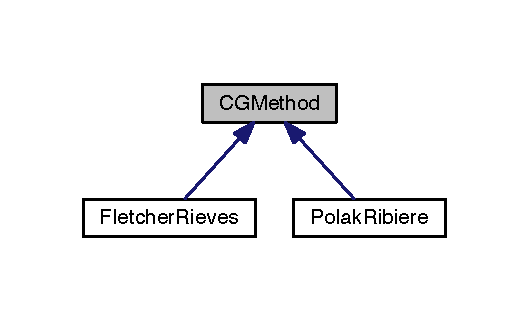
\includegraphics[width=254pt]{classCGMethod__inherit__graph}
\end{center}
\end{figure}
\subsection*{Public Member Functions}
\begin{DoxyCompactItemize}
\item 
virtual void \hyperlink{classCGMethod_a7a03bce08f9b88d41392894d071a1ff7}{minimize} (\hyperlink{classForceFieldManager}{Force\+Field\+Manager} \&F\+F\+M)=0
\begin{DoxyCompactList}\small\item\em Minimize the system. \end{DoxyCompactList}\end{DoxyCompactItemize}
\subsection*{Protected Member Functions}
\begin{DoxyCompactItemize}
\item 
void \hyperlink{classCGMethod_a98910fcbef9f0af69076c955b887c254}{swap} (double \&a, double \&b)
\begin{DoxyCompactList}\small\item\em helpers for searching and bracketing \end{DoxyCompactList}\item 
void \hyperlink{classCGMethod_ac091059dd8c44e8e4ec372767f18f1c9}{shift2} (double \&a, double \&b, double c)
\item 
void \hyperlink{classCGMethod_a947d6e38d75fe84a08f0fc071c94c225}{shift3} (double \&a, double \&b, double \&c, double d)
\item 
double \hyperlink{classCGMethod_aea6d1129677d44e11fe2afb08b5ca52c}{sign} (double a, double b)
\item 
void \hyperlink{classCGMethod_a276c57252367bec9fcf08ae1e7c7df71}{make\+Bracket} (\hyperlink{classForceFieldManager}{Force\+Field\+Manager} \&F\+F\+M, double \&ax, double \&bx, double \&cx, double \&fa, double \&fb, double \&fc)
\begin{DoxyCompactList}\small\item\em Gracketing function (from Numerical Recipes in C++, second edition) \end{DoxyCompactList}\item 
void \hyperlink{classCGMethod_abd5135fdbe89793bfb5926f9dcc6de7e}{print\+Forces} ()
\end{DoxyCompactItemize}
{\bf }\par
\begin{DoxyCompactItemize}
\item 
double \hyperlink{classCGMethod_aa2af8a3ecad085f6c07f759bfe50ccb1}{grad\+Square} ()
\begin{DoxyCompactList}\small\item\em For use in minimization. \end{DoxyCompactList}\item 
double \hyperlink{classCGMethod_ab9c35ec6681e97472d0442a37163d46d}{grad\+Aux\+Square} ()
\item 
double \hyperlink{classCGMethod_a531b7d0bc38b6372dc323185f51233dc}{grad\+Dot\+Product} ()
\item 
void \hyperlink{classCGMethod_afe717a6a06f677933b55628ea4d0014d}{move\+Beads} (double d)
\item 
void \hyperlink{classCGMethod_a885a9627cc4e8b2db8f3384f29cd4069}{move\+Beads\+Aux} (double d)
\item 
void \hyperlink{classCGMethod_a7e8d5b8d77aff6c4564c4b1d72ab5ace}{shift\+Gradient} (double d)
\end{DoxyCompactItemize}

{\bf }\par
\begin{DoxyCompactItemize}
\item 
double \hyperlink{classCGMethod_ace5a720fe0f5d6ffcefeb9f4afcfe28f}{golden\+Section1} (\hyperlink{classForceFieldManager}{Force\+Field\+Manager} \&F\+F\+M)
\begin{DoxyCompactList}\small\item\em Linear search method. \end{DoxyCompactList}\item 
double \hyperlink{classCGMethod_aa1fcbcd087af6fa3aa9aab67b0b60103}{golden\+Section2} (\hyperlink{classForceFieldManager}{Force\+Field\+Manager} \&F\+F\+M)
\item 
double \hyperlink{classCGMethod_a2d9a41ddbf7d54e6f89ee02966c7d85c}{binary\+Search} (\hyperlink{classForceFieldManager}{Force\+Field\+Manager} \&F\+F\+M)
\item 
double \hyperlink{classCGMethod_a432019c8a52f50b0cb8cb39b937db978}{backtracking\+Line\+Search} (\hyperlink{classForceFieldManager}{Force\+Field\+Manager} \&F\+F\+M)
\item 
double \hyperlink{classCGMethod_aa77b006b710d67b248dd18517db7709c}{quadratic\+Line\+Search} (\hyperlink{classForceFieldManager}{Force\+Field\+Manager} \&F\+F\+M)
\end{DoxyCompactItemize}

\subsection*{Protected Attributes}
\begin{DoxyCompactItemize}
\item 
const double \hyperlink{classCGMethod_a084794992bdcec9285f6512b56e6c578}{L\+S\+E\+N\+E\+R\+G\+Y\+T\+O\+L} = 1e-\/6
\begin{DoxyCompactList}\small\item\em Line search energy tolerance for all linesearch methods. \end{DoxyCompactList}\item 
int \hyperlink{classCGMethod_aadb778c988685e46d7d109350973d826}{\+\_\+energy\+Change\+Counter} = 0
\begin{DoxyCompactList}\small\item\em Energy counter, for use in linear search methods. \end{DoxyCompactList}\item 
const int \hyperlink{classCGMethod_aaee1e11813855cc66c360f7cb3d9665a}{E\+N\+E\+R\+G\+Y\+C\+H\+A\+N\+G\+E\+I\+T\+E\+R} = 20
\begin{DoxyCompactList}\small\item\em Max number of iterations allowed where \char`\"{}\char`\"{}". \end{DoxyCompactList}\item 
const double \hyperlink{classCGMethod_ad0118dc4da7526f196a4b4172bba9625}{G\+R\+A\+D\+T\+O\+L} = 1e-\/10
\begin{DoxyCompactList}\small\item\em Gradient minimization tolerance. \end{DoxyCompactList}\end{DoxyCompactItemize}
{\bf }\par
\begin{DoxyCompactItemize}
\item 
const double \hyperlink{classCGMethod_ae28b20ab18f9a0b7c6a1c443add1026e}{L\+A\+M\+B\+D\+A\+M\+I\+N} = 0.\+001
\begin{DoxyCompactList}\small\item\em Lambda parameter for use in linear search methods. \end{DoxyCompactList}\item 
const double \hyperlink{classCGMethod_a04127fd877e82fdf4f71cd3709581419}{L\+A\+M\+B\+D\+A\+M\+A\+X} = 1
\begin{DoxyCompactList}\small\item\em Max lambda that can be returned, used in all methods. \end{DoxyCompactList}\item 
const double \hyperlink{classCGMethod_a814ea57c3493f31f4ffd1cfa71795871}{M\+A\+X\+D\+I\+S\+T} = 1
\begin{DoxyCompactList}\small\item\em Max distance beads can be moved, used only in backtracking line search. \end{DoxyCompactList}\end{DoxyCompactItemize}

{\bf }\par
\begin{DoxyCompactItemize}
\item 
const double \hyperlink{classCGMethod_a0fa651bde0efa2e195ec6a367a0e346e}{L\+A\+M\+B\+D\+A\+R\+E\+D\+U\+C\+E} = 0.\+1
\begin{DoxyCompactList}\small\item\em Parameter used in backtracking line search. \end{DoxyCompactList}\item 
const double \hyperlink{classCGMethod_aa7a8cad90cb1961052e323ded645b4c2}{B\+A\+C\+K\+T\+R\+A\+C\+K\+S\+L\+O\+P\+E} = 0.\+1
\begin{DoxyCompactList}\small\item\em Backtrack slope parameter. \end{DoxyCompactList}\end{DoxyCompactItemize}

{\bf }\par
\begin{DoxyCompactItemize}
\item 
const double \hyperlink{classCGMethod_acd9c51fe93f6d563f731dd2e30eb7922}{Q\+U\+A\+D\+R\+A\+T\+I\+C\+T\+O\+L} = 0.\+1
\begin{DoxyCompactList}\small\item\em Parameter used in quadratic line search. \end{DoxyCompactList}\item 
const double \hyperlink{classCGMethod_adb2a688fe52a8729d703d81e52b9fdb3}{E\+P\+S\+Q\+U\+A\+D} = 1e-\/28
\end{DoxyCompactItemize}

{\bf }\par
\begin{DoxyCompactItemize}
\item 
const double \hyperlink{classCGMethod_ab6ca0706dec56fe6e35f15f9791b3e23}{P\+H\+I} = (1 + sqrt(5)) / 2
\begin{DoxyCompactList}\small\item\em Parameter used in golden section. \end{DoxyCompactList}\item 
const double \hyperlink{classCGMethod_a2e7906b4b29a1b76dca43d56eaf2efac}{R} = 0.\+61803399
\item 
const double \hyperlink{classCGMethod_af8587ca1c0394c244ce84fe8a6ad29ff}{C} = 1 -\/ \hyperlink{classCGMethod_a2e7906b4b29a1b76dca43d56eaf2efac}{R}
\end{DoxyCompactItemize}



\subsection{Detailed Description}
For performing a conjugate gradient minimization method. 

\hyperlink{classCGMethod}{C\+G\+Method} is an abstract class that contains methods for conjugate gradient minimization. It has functions for various line search techniques, including golden section, backtracking, and quadratic line search. This base class also contains parameters for tolerance criterion and other helpful parameters. 

Definition at line 31 of file C\+G\+Method.\+h.



\subsection{Member Function Documentation}
\hypertarget{classCGMethod_a432019c8a52f50b0cb8cb39b937db978}{\index{C\+G\+Method@{C\+G\+Method}!backtracking\+Line\+Search@{backtracking\+Line\+Search}}
\index{backtracking\+Line\+Search@{backtracking\+Line\+Search}!C\+G\+Method@{C\+G\+Method}}
\subsubsection[{backtracking\+Line\+Search}]{\setlength{\rightskip}{0pt plus 5cm}double C\+G\+Method\+::backtracking\+Line\+Search (
\begin{DoxyParamCaption}
\item[{{\bf Force\+Field\+Manager} \&}]{F\+F\+M}
\end{DoxyParamCaption}
)\hspace{0.3cm}{\ttfamily [protected]}}}\label{classCGMethod_a432019c8a52f50b0cb8cb39b937db978}


Definition at line 263 of file C\+G\+Method.\+cpp.



References \+\_\+energy\+Change\+Counter, B\+A\+C\+K\+T\+R\+A\+C\+K\+S\+L\+O\+P\+E, Force\+Field\+Manager\+::compute\+Energy(), Bead\+D\+B\+::instance(), L\+A\+M\+B\+D\+A\+M\+A\+X, L\+A\+M\+B\+D\+A\+R\+E\+D\+U\+C\+E, L\+S\+E\+N\+E\+R\+G\+Y\+T\+O\+L, and M\+A\+X\+D\+I\+S\+T.



Referenced by Fletcher\+Rieves\+::minimize(), and Polak\+Ribiere\+::minimize().

\hypertarget{classCGMethod_a2d9a41ddbf7d54e6f89ee02966c7d85c}{\index{C\+G\+Method@{C\+G\+Method}!binary\+Search@{binary\+Search}}
\index{binary\+Search@{binary\+Search}!C\+G\+Method@{C\+G\+Method}}
\subsubsection[{binary\+Search}]{\setlength{\rightskip}{0pt plus 5cm}double C\+G\+Method\+::binary\+Search (
\begin{DoxyParamCaption}
\item[{{\bf Force\+Field\+Manager} \&}]{F\+F\+M}
\end{DoxyParamCaption}
)\hspace{0.3cm}{\ttfamily [protected]}}}\label{classCGMethod_a2d9a41ddbf7d54e6f89ee02966c7d85c}


Definition at line 249 of file C\+G\+Method.\+cpp.



References Force\+Field\+Manager\+::compute\+Energy(), and L\+S\+E\+N\+E\+R\+G\+Y\+T\+O\+L.

\hypertarget{classCGMethod_ace5a720fe0f5d6ffcefeb9f4afcfe28f}{\index{C\+G\+Method@{C\+G\+Method}!golden\+Section1@{golden\+Section1}}
\index{golden\+Section1@{golden\+Section1}!C\+G\+Method@{C\+G\+Method}}
\subsubsection[{golden\+Section1}]{\setlength{\rightskip}{0pt plus 5cm}double C\+G\+Method\+::golden\+Section1 (
\begin{DoxyParamCaption}
\item[{{\bf Force\+Field\+Manager} \&}]{F\+F\+M}
\end{DoxyParamCaption}
)\hspace{0.3cm}{\ttfamily [protected]}}}\label{classCGMethod_ace5a720fe0f5d6ffcefeb9f4afcfe28f}


Linear search method. 



Definition at line 180 of file C\+G\+Method.\+cpp.



References Force\+Field\+Manager\+::compute\+Energy(), L\+A\+M\+B\+D\+A\+M\+A\+X, L\+A\+M\+B\+D\+A\+M\+I\+N, and L\+S\+E\+N\+E\+R\+G\+Y\+T\+O\+L.

\hypertarget{classCGMethod_aa1fcbcd087af6fa3aa9aab67b0b60103}{\index{C\+G\+Method@{C\+G\+Method}!golden\+Section2@{golden\+Section2}}
\index{golden\+Section2@{golden\+Section2}!C\+G\+Method@{C\+G\+Method}}
\subsubsection[{golden\+Section2}]{\setlength{\rightskip}{0pt plus 5cm}double C\+G\+Method\+::golden\+Section2 (
\begin{DoxyParamCaption}
\item[{{\bf Force\+Field\+Manager} \&}]{F\+F\+M}
\end{DoxyParamCaption}
)\hspace{0.3cm}{\ttfamily [protected]}}}\label{classCGMethod_aa1fcbcd087af6fa3aa9aab67b0b60103}


Definition at line 209 of file C\+G\+Method.\+cpp.



References C, Force\+Field\+Manager\+::compute\+Energy(), L\+A\+M\+B\+D\+A\+M\+A\+X, L\+A\+M\+B\+D\+A\+M\+I\+N, L\+S\+E\+N\+E\+R\+G\+Y\+T\+O\+L, R, shift2(), and shift3().

\hypertarget{classCGMethod_ab9c35ec6681e97472d0442a37163d46d}{\index{C\+G\+Method@{C\+G\+Method}!grad\+Aux\+Square@{grad\+Aux\+Square}}
\index{grad\+Aux\+Square@{grad\+Aux\+Square}!C\+G\+Method@{C\+G\+Method}}
\subsubsection[{grad\+Aux\+Square}]{\setlength{\rightskip}{0pt plus 5cm}double C\+G\+Method\+::grad\+Aux\+Square (
\begin{DoxyParamCaption}
{}
\end{DoxyParamCaption}
)\hspace{0.3cm}{\ttfamily [protected]}}}\label{classCGMethod_ab9c35ec6681e97472d0442a37163d46d}


Definition at line 116 of file C\+G\+Method.\+cpp.



References Bead\+D\+B\+::instance().



Referenced by Fletcher\+Rieves\+::minimize(), and Polak\+Ribiere\+::minimize().

\hypertarget{classCGMethod_a531b7d0bc38b6372dc323185f51233dc}{\index{C\+G\+Method@{C\+G\+Method}!grad\+Dot\+Product@{grad\+Dot\+Product}}
\index{grad\+Dot\+Product@{grad\+Dot\+Product}!C\+G\+Method@{C\+G\+Method}}
\subsubsection[{grad\+Dot\+Product}]{\setlength{\rightskip}{0pt plus 5cm}double C\+G\+Method\+::grad\+Dot\+Product (
\begin{DoxyParamCaption}
{}
\end{DoxyParamCaption}
)\hspace{0.3cm}{\ttfamily [protected]}}}\label{classCGMethod_a531b7d0bc38b6372dc323185f51233dc}


Definition at line 125 of file C\+G\+Method.\+cpp.



References Bead\+D\+B\+::instance().



Referenced by Fletcher\+Rieves\+::minimize(), Polak\+Ribiere\+::minimize(), and quadratic\+Line\+Search().

\hypertarget{classCGMethod_aa2af8a3ecad085f6c07f759bfe50ccb1}{\index{C\+G\+Method@{C\+G\+Method}!grad\+Square@{grad\+Square}}
\index{grad\+Square@{grad\+Square}!C\+G\+Method@{C\+G\+Method}}
\subsubsection[{grad\+Square}]{\setlength{\rightskip}{0pt plus 5cm}double C\+G\+Method\+::grad\+Square (
\begin{DoxyParamCaption}
{}
\end{DoxyParamCaption}
)\hspace{0.3cm}{\ttfamily [protected]}}}\label{classCGMethod_aa2af8a3ecad085f6c07f759bfe50ccb1}


For use in minimization. 



Definition at line 108 of file C\+G\+Method.\+cpp.



References Bead\+D\+B\+::instance().



Referenced by Fletcher\+Rieves\+::minimize(), and Polak\+Ribiere\+::minimize().

\hypertarget{classCGMethod_a276c57252367bec9fcf08ae1e7c7df71}{\index{C\+G\+Method@{C\+G\+Method}!make\+Bracket@{make\+Bracket}}
\index{make\+Bracket@{make\+Bracket}!C\+G\+Method@{C\+G\+Method}}
\subsubsection[{make\+Bracket}]{\setlength{\rightskip}{0pt plus 5cm}void C\+G\+Method\+::make\+Bracket (
\begin{DoxyParamCaption}
\item[{{\bf Force\+Field\+Manager} \&}]{F\+F\+M, }
\item[{double \&}]{ax, }
\item[{double \&}]{bx, }
\item[{double \&}]{cx, }
\item[{double \&}]{fa, }
\item[{double \&}]{fb, }
\item[{double \&}]{fc}
\end{DoxyParamCaption}
)\hspace{0.3cm}{\ttfamily [protected]}}}\label{classCGMethod_a276c57252367bec9fcf08ae1e7c7df71}


Gracketing function (from Numerical Recipes in C++, second edition) 



Definition at line 42 of file C\+G\+Method.\+cpp.



References Force\+Field\+Manager\+::compute\+Energy(), P\+H\+I, shift3(), sign(), and swap().

\hypertarget{classCGMethod_a7a03bce08f9b88d41392894d071a1ff7}{\index{C\+G\+Method@{C\+G\+Method}!minimize@{minimize}}
\index{minimize@{minimize}!C\+G\+Method@{C\+G\+Method}}
\subsubsection[{minimize}]{\setlength{\rightskip}{0pt plus 5cm}virtual void C\+G\+Method\+::minimize (
\begin{DoxyParamCaption}
\item[{{\bf Force\+Field\+Manager} \&}]{F\+F\+M}
\end{DoxyParamCaption}
)\hspace{0.3cm}{\ttfamily [pure virtual]}}}\label{classCGMethod_a7a03bce08f9b88d41392894d071a1ff7}


Minimize the system. 



Implemented in \hyperlink{classPolakRibiere_af177d214c9d7b0f285ae93525be16329}{Polak\+Ribiere}, and \hyperlink{classFletcherRieves_a022e95e7331cb494bc281a5f53a7198a}{Fletcher\+Rieves}.

\hypertarget{classCGMethod_afe717a6a06f677933b55628ea4d0014d}{\index{C\+G\+Method@{C\+G\+Method}!move\+Beads@{move\+Beads}}
\index{move\+Beads@{move\+Beads}!C\+G\+Method@{C\+G\+Method}}
\subsubsection[{move\+Beads}]{\setlength{\rightskip}{0pt plus 5cm}void C\+G\+Method\+::move\+Beads (
\begin{DoxyParamCaption}
\item[{double}]{d}
\end{DoxyParamCaption}
)\hspace{0.3cm}{\ttfamily [protected]}}}\label{classCGMethod_afe717a6a06f677933b55628ea4d0014d}


Definition at line 135 of file C\+G\+Method.\+cpp.



References Bead\+D\+B\+::instance().



Referenced by Fletcher\+Rieves\+::minimize(), and Polak\+Ribiere\+::minimize().

\hypertarget{classCGMethod_a885a9627cc4e8b2db8f3384f29cd4069}{\index{C\+G\+Method@{C\+G\+Method}!move\+Beads\+Aux@{move\+Beads\+Aux}}
\index{move\+Beads\+Aux@{move\+Beads\+Aux}!C\+G\+Method@{C\+G\+Method}}
\subsubsection[{move\+Beads\+Aux}]{\setlength{\rightskip}{0pt plus 5cm}void C\+G\+Method\+::move\+Beads\+Aux (
\begin{DoxyParamCaption}
\item[{double}]{d}
\end{DoxyParamCaption}
)\hspace{0.3cm}{\ttfamily [protected]}}}\label{classCGMethod_a885a9627cc4e8b2db8f3384f29cd4069}


Definition at line 148 of file C\+G\+Method.\+cpp.



References Bead\+D\+B\+::instance().



Referenced by quadratic\+Line\+Search().

\hypertarget{classCGMethod_abd5135fdbe89793bfb5926f9dcc6de7e}{\index{C\+G\+Method@{C\+G\+Method}!print\+Forces@{print\+Forces}}
\index{print\+Forces@{print\+Forces}!C\+G\+Method@{C\+G\+Method}}
\subsubsection[{print\+Forces}]{\setlength{\rightskip}{0pt plus 5cm}void C\+G\+Method\+::print\+Forces (
\begin{DoxyParamCaption}
{}
\end{DoxyParamCaption}
)\hspace{0.3cm}{\ttfamily [protected]}}}\label{classCGMethod_abd5135fdbe89793bfb5926f9dcc6de7e}


Definition at line 169 of file C\+G\+Method.\+cpp.



References Bead\+D\+B\+::instance().



Referenced by Fletcher\+Rieves\+::minimize(), and Polak\+Ribiere\+::minimize().

\hypertarget{classCGMethod_aa77b006b710d67b248dd18517db7709c}{\index{C\+G\+Method@{C\+G\+Method}!quadratic\+Line\+Search@{quadratic\+Line\+Search}}
\index{quadratic\+Line\+Search@{quadratic\+Line\+Search}!C\+G\+Method@{C\+G\+Method}}
\subsubsection[{quadratic\+Line\+Search}]{\setlength{\rightskip}{0pt plus 5cm}double C\+G\+Method\+::quadratic\+Line\+Search (
\begin{DoxyParamCaption}
\item[{{\bf Force\+Field\+Manager} \&}]{F\+F\+M}
\end{DoxyParamCaption}
)\hspace{0.3cm}{\ttfamily [protected]}}}\label{classCGMethod_aa77b006b710d67b248dd18517db7709c}


Definition at line 316 of file C\+G\+Method.\+cpp.



References \+\_\+energy\+Change\+Counter, B\+A\+C\+K\+T\+R\+A\+C\+K\+S\+L\+O\+P\+E, Force\+Field\+Manager\+::compute\+Energy(), Force\+Field\+Manager\+::compute\+Forces\+Aux(), E\+P\+S\+Q\+U\+A\+D, grad\+Dot\+Product(), Bead\+D\+B\+::instance(), L\+A\+M\+B\+D\+A\+M\+A\+X, L\+A\+M\+B\+D\+A\+R\+E\+D\+U\+C\+E, L\+S\+E\+N\+E\+R\+G\+Y\+T\+O\+L, and move\+Beads\+Aux().

\hypertarget{classCGMethod_ac091059dd8c44e8e4ec372767f18f1c9}{\index{C\+G\+Method@{C\+G\+Method}!shift2@{shift2}}
\index{shift2@{shift2}!C\+G\+Method@{C\+G\+Method}}
\subsubsection[{shift2}]{\setlength{\rightskip}{0pt plus 5cm}void C\+G\+Method\+::shift2 (
\begin{DoxyParamCaption}
\item[{double \&}]{a, }
\item[{double \&}]{b, }
\item[{double}]{c}
\end{DoxyParamCaption}
)\hspace{0.3cm}{\ttfamily [inline]}, {\ttfamily [protected]}}}\label{classCGMethod_ac091059dd8c44e8e4ec372767f18f1c9}


Definition at line 25 of file C\+G\+Method.\+cpp.



Referenced by golden\+Section2().

\hypertarget{classCGMethod_a947d6e38d75fe84a08f0fc071c94c225}{\index{C\+G\+Method@{C\+G\+Method}!shift3@{shift3}}
\index{shift3@{shift3}!C\+G\+Method@{C\+G\+Method}}
\subsubsection[{shift3}]{\setlength{\rightskip}{0pt plus 5cm}void C\+G\+Method\+::shift3 (
\begin{DoxyParamCaption}
\item[{double \&}]{a, }
\item[{double \&}]{b, }
\item[{double \&}]{c, }
\item[{double}]{d}
\end{DoxyParamCaption}
)\hspace{0.3cm}{\ttfamily [inline]}, {\ttfamily [protected]}}}\label{classCGMethod_a947d6e38d75fe84a08f0fc071c94c225}


Definition at line 30 of file C\+G\+Method.\+cpp.



Referenced by golden\+Section2(), and make\+Bracket().

\hypertarget{classCGMethod_a7e8d5b8d77aff6c4564c4b1d72ab5ace}{\index{C\+G\+Method@{C\+G\+Method}!shift\+Gradient@{shift\+Gradient}}
\index{shift\+Gradient@{shift\+Gradient}!C\+G\+Method@{C\+G\+Method}}
\subsubsection[{shift\+Gradient}]{\setlength{\rightskip}{0pt plus 5cm}void C\+G\+Method\+::shift\+Gradient (
\begin{DoxyParamCaption}
\item[{double}]{d}
\end{DoxyParamCaption}
)\hspace{0.3cm}{\ttfamily [protected]}}}\label{classCGMethod_a7e8d5b8d77aff6c4564c4b1d72ab5ace}


Definition at line 159 of file C\+G\+Method.\+cpp.



References Bead\+D\+B\+::instance().



Referenced by Fletcher\+Rieves\+::minimize(), and Polak\+Ribiere\+::minimize().

\hypertarget{classCGMethod_aea6d1129677d44e11fe2afb08b5ca52c}{\index{C\+G\+Method@{C\+G\+Method}!sign@{sign}}
\index{sign@{sign}!C\+G\+Method@{C\+G\+Method}}
\subsubsection[{sign}]{\setlength{\rightskip}{0pt plus 5cm}double C\+G\+Method\+::sign (
\begin{DoxyParamCaption}
\item[{double}]{a, }
\item[{double}]{b}
\end{DoxyParamCaption}
)\hspace{0.3cm}{\ttfamily [inline]}, {\ttfamily [protected]}}}\label{classCGMethod_aea6d1129677d44e11fe2afb08b5ca52c}


Definition at line 36 of file C\+G\+Method.\+cpp.



Referenced by make\+Bracket().

\hypertarget{classCGMethod_a98910fcbef9f0af69076c955b887c254}{\index{C\+G\+Method@{C\+G\+Method}!swap@{swap}}
\index{swap@{swap}!C\+G\+Method@{C\+G\+Method}}
\subsubsection[{swap}]{\setlength{\rightskip}{0pt plus 5cm}void C\+G\+Method\+::swap (
\begin{DoxyParamCaption}
\item[{double \&}]{a, }
\item[{double \&}]{b}
\end{DoxyParamCaption}
)\hspace{0.3cm}{\ttfamily [inline]}, {\ttfamily [protected]}}}\label{classCGMethod_a98910fcbef9f0af69076c955b887c254}


helpers for searching and bracketing 



Definition at line 19 of file C\+G\+Method.\+cpp.



Referenced by make\+Bracket().



\subsection{Member Data Documentation}
\hypertarget{classCGMethod_aadb778c988685e46d7d109350973d826}{\index{C\+G\+Method@{C\+G\+Method}!\+\_\+energy\+Change\+Counter@{\+\_\+energy\+Change\+Counter}}
\index{\+\_\+energy\+Change\+Counter@{\+\_\+energy\+Change\+Counter}!C\+G\+Method@{C\+G\+Method}}
\subsubsection[{\+\_\+energy\+Change\+Counter}]{\setlength{\rightskip}{0pt plus 5cm}int C\+G\+Method\+::\+\_\+energy\+Change\+Counter = 0\hspace{0.3cm}{\ttfamily [protected]}}}\label{classCGMethod_aadb778c988685e46d7d109350973d826}


Energy counter, for use in linear search methods. 

Number of iterations where energy has not changed by an amount more than L\+S\+E\+N\+E\+R\+G\+Y\+T\+O\+L 

Definition at line 72 of file C\+G\+Method.\+h.



Referenced by backtracking\+Line\+Search(), Fletcher\+Rieves\+::minimize(), Polak\+Ribiere\+::minimize(), and quadratic\+Line\+Search().

\hypertarget{classCGMethod_aa7a8cad90cb1961052e323ded645b4c2}{\index{C\+G\+Method@{C\+G\+Method}!B\+A\+C\+K\+T\+R\+A\+C\+K\+S\+L\+O\+P\+E@{B\+A\+C\+K\+T\+R\+A\+C\+K\+S\+L\+O\+P\+E}}
\index{B\+A\+C\+K\+T\+R\+A\+C\+K\+S\+L\+O\+P\+E@{B\+A\+C\+K\+T\+R\+A\+C\+K\+S\+L\+O\+P\+E}!C\+G\+Method@{C\+G\+Method}}
\subsubsection[{B\+A\+C\+K\+T\+R\+A\+C\+K\+S\+L\+O\+P\+E}]{\setlength{\rightskip}{0pt plus 5cm}const double C\+G\+Method\+::\+B\+A\+C\+K\+T\+R\+A\+C\+K\+S\+L\+O\+P\+E = 0.\+1\hspace{0.3cm}{\ttfamily [protected]}}}\label{classCGMethod_aa7a8cad90cb1961052e323ded645b4c2}


Backtrack slope parameter. 



Definition at line 45 of file C\+G\+Method.\+h.



Referenced by backtracking\+Line\+Search(), and quadratic\+Line\+Search().

\hypertarget{classCGMethod_af8587ca1c0394c244ce84fe8a6ad29ff}{\index{C\+G\+Method@{C\+G\+Method}!C@{C}}
\index{C@{C}!C\+G\+Method@{C\+G\+Method}}
\subsubsection[{C}]{\setlength{\rightskip}{0pt plus 5cm}const double C\+G\+Method\+::\+C = 1 -\/ {\bf R}\hspace{0.3cm}{\ttfamily [protected]}}}\label{classCGMethod_af8587ca1c0394c244ce84fe8a6ad29ff}


Definition at line 58 of file C\+G\+Method.\+h.



Referenced by golden\+Section2().

\hypertarget{classCGMethod_aaee1e11813855cc66c360f7cb3d9665a}{\index{C\+G\+Method@{C\+G\+Method}!E\+N\+E\+R\+G\+Y\+C\+H\+A\+N\+G\+E\+I\+T\+E\+R@{E\+N\+E\+R\+G\+Y\+C\+H\+A\+N\+G\+E\+I\+T\+E\+R}}
\index{E\+N\+E\+R\+G\+Y\+C\+H\+A\+N\+G\+E\+I\+T\+E\+R@{E\+N\+E\+R\+G\+Y\+C\+H\+A\+N\+G\+E\+I\+T\+E\+R}!C\+G\+Method@{C\+G\+Method}}
\subsubsection[{E\+N\+E\+R\+G\+Y\+C\+H\+A\+N\+G\+E\+I\+T\+E\+R}]{\setlength{\rightskip}{0pt plus 5cm}const int C\+G\+Method\+::\+E\+N\+E\+R\+G\+Y\+C\+H\+A\+N\+G\+E\+I\+T\+E\+R = 20\hspace{0.3cm}{\ttfamily [protected]}}}\label{classCGMethod_aaee1e11813855cc66c360f7cb3d9665a}


Max number of iterations allowed where \char`\"{}\char`\"{}". 



Definition at line 73 of file C\+G\+Method.\+h.



Referenced by Fletcher\+Rieves\+::minimize(), and Polak\+Ribiere\+::minimize().

\hypertarget{classCGMethod_adb2a688fe52a8729d703d81e52b9fdb3}{\index{C\+G\+Method@{C\+G\+Method}!E\+P\+S\+Q\+U\+A\+D@{E\+P\+S\+Q\+U\+A\+D}}
\index{E\+P\+S\+Q\+U\+A\+D@{E\+P\+S\+Q\+U\+A\+D}!C\+G\+Method@{C\+G\+Method}}
\subsubsection[{E\+P\+S\+Q\+U\+A\+D}]{\setlength{\rightskip}{0pt plus 5cm}const double C\+G\+Method\+::\+E\+P\+S\+Q\+U\+A\+D = 1e-\/28\hspace{0.3cm}{\ttfamily [protected]}}}\label{classCGMethod_adb2a688fe52a8729d703d81e52b9fdb3}


Definition at line 51 of file C\+G\+Method.\+h.



Referenced by quadratic\+Line\+Search().

\hypertarget{classCGMethod_ad0118dc4da7526f196a4b4172bba9625}{\index{C\+G\+Method@{C\+G\+Method}!G\+R\+A\+D\+T\+O\+L@{G\+R\+A\+D\+T\+O\+L}}
\index{G\+R\+A\+D\+T\+O\+L@{G\+R\+A\+D\+T\+O\+L}!C\+G\+Method@{C\+G\+Method}}
\subsubsection[{G\+R\+A\+D\+T\+O\+L}]{\setlength{\rightskip}{0pt plus 5cm}const double C\+G\+Method\+::\+G\+R\+A\+D\+T\+O\+L = 1e-\/10\hspace{0.3cm}{\ttfamily [protected]}}}\label{classCGMethod_ad0118dc4da7526f196a4b4172bba9625}


Gradient minimization tolerance. 



Definition at line 75 of file C\+G\+Method.\+h.



Referenced by Fletcher\+Rieves\+::minimize(), and Polak\+Ribiere\+::minimize().

\hypertarget{classCGMethod_a04127fd877e82fdf4f71cd3709581419}{\index{C\+G\+Method@{C\+G\+Method}!L\+A\+M\+B\+D\+A\+M\+A\+X@{L\+A\+M\+B\+D\+A\+M\+A\+X}}
\index{L\+A\+M\+B\+D\+A\+M\+A\+X@{L\+A\+M\+B\+D\+A\+M\+A\+X}!C\+G\+Method@{C\+G\+Method}}
\subsubsection[{L\+A\+M\+B\+D\+A\+M\+A\+X}]{\setlength{\rightskip}{0pt plus 5cm}const double C\+G\+Method\+::\+L\+A\+M\+B\+D\+A\+M\+A\+X = 1\hspace{0.3cm}{\ttfamily [protected]}}}\label{classCGMethod_a04127fd877e82fdf4f71cd3709581419}


Max lambda that can be returned, used in all methods. 



Definition at line 38 of file C\+G\+Method.\+h.



Referenced by backtracking\+Line\+Search(), golden\+Section1(), golden\+Section2(), and quadratic\+Line\+Search().

\hypertarget{classCGMethod_ae28b20ab18f9a0b7c6a1c443add1026e}{\index{C\+G\+Method@{C\+G\+Method}!L\+A\+M\+B\+D\+A\+M\+I\+N@{L\+A\+M\+B\+D\+A\+M\+I\+N}}
\index{L\+A\+M\+B\+D\+A\+M\+I\+N@{L\+A\+M\+B\+D\+A\+M\+I\+N}!C\+G\+Method@{C\+G\+Method}}
\subsubsection[{L\+A\+M\+B\+D\+A\+M\+I\+N}]{\setlength{\rightskip}{0pt plus 5cm}const double C\+G\+Method\+::\+L\+A\+M\+B\+D\+A\+M\+I\+N = 0.\+001\hspace{0.3cm}{\ttfamily [protected]}}}\label{classCGMethod_ae28b20ab18f9a0b7c6a1c443add1026e}


Lambda parameter for use in linear search methods. 

Minimum lambda that can be returned, used only in golden section for now 

Definition at line 37 of file C\+G\+Method.\+h.



Referenced by golden\+Section1(), and golden\+Section2().

\hypertarget{classCGMethod_a0fa651bde0efa2e195ec6a367a0e346e}{\index{C\+G\+Method@{C\+G\+Method}!L\+A\+M\+B\+D\+A\+R\+E\+D\+U\+C\+E@{L\+A\+M\+B\+D\+A\+R\+E\+D\+U\+C\+E}}
\index{L\+A\+M\+B\+D\+A\+R\+E\+D\+U\+C\+E@{L\+A\+M\+B\+D\+A\+R\+E\+D\+U\+C\+E}!C\+G\+Method@{C\+G\+Method}}
\subsubsection[{L\+A\+M\+B\+D\+A\+R\+E\+D\+U\+C\+E}]{\setlength{\rightskip}{0pt plus 5cm}const double C\+G\+Method\+::\+L\+A\+M\+B\+D\+A\+R\+E\+D\+U\+C\+E = 0.\+1\hspace{0.3cm}{\ttfamily [protected]}}}\label{classCGMethod_a0fa651bde0efa2e195ec6a367a0e346e}


Parameter used in backtracking line search. 

Lambda reduction parameter for backtracking 

Definition at line 44 of file C\+G\+Method.\+h.



Referenced by backtracking\+Line\+Search(), and quadratic\+Line\+Search().

\hypertarget{classCGMethod_a084794992bdcec9285f6512b56e6c578}{\index{C\+G\+Method@{C\+G\+Method}!L\+S\+E\+N\+E\+R\+G\+Y\+T\+O\+L@{L\+S\+E\+N\+E\+R\+G\+Y\+T\+O\+L}}
\index{L\+S\+E\+N\+E\+R\+G\+Y\+T\+O\+L@{L\+S\+E\+N\+E\+R\+G\+Y\+T\+O\+L}!C\+G\+Method@{C\+G\+Method}}
\subsubsection[{L\+S\+E\+N\+E\+R\+G\+Y\+T\+O\+L}]{\setlength{\rightskip}{0pt plus 5cm}const double C\+G\+Method\+::\+L\+S\+E\+N\+E\+R\+G\+Y\+T\+O\+L = 1e-\/6\hspace{0.3cm}{\ttfamily [protected]}}}\label{classCGMethod_a084794992bdcec9285f6512b56e6c578}


Line search energy tolerance for all linesearch methods. 



Definition at line 61 of file C\+G\+Method.\+h.



Referenced by backtracking\+Line\+Search(), binary\+Search(), golden\+Section1(), golden\+Section2(), and quadratic\+Line\+Search().

\hypertarget{classCGMethod_a814ea57c3493f31f4ffd1cfa71795871}{\index{C\+G\+Method@{C\+G\+Method}!M\+A\+X\+D\+I\+S\+T@{M\+A\+X\+D\+I\+S\+T}}
\index{M\+A\+X\+D\+I\+S\+T@{M\+A\+X\+D\+I\+S\+T}!C\+G\+Method@{C\+G\+Method}}
\subsubsection[{M\+A\+X\+D\+I\+S\+T}]{\setlength{\rightskip}{0pt plus 5cm}const double C\+G\+Method\+::\+M\+A\+X\+D\+I\+S\+T = 1\hspace{0.3cm}{\ttfamily [protected]}}}\label{classCGMethod_a814ea57c3493f31f4ffd1cfa71795871}


Max distance beads can be moved, used only in backtracking line search. 



Definition at line 39 of file C\+G\+Method.\+h.



Referenced by backtracking\+Line\+Search().

\hypertarget{classCGMethod_ab6ca0706dec56fe6e35f15f9791b3e23}{\index{C\+G\+Method@{C\+G\+Method}!P\+H\+I@{P\+H\+I}}
\index{P\+H\+I@{P\+H\+I}!C\+G\+Method@{C\+G\+Method}}
\subsubsection[{P\+H\+I}]{\setlength{\rightskip}{0pt plus 5cm}const double C\+G\+Method\+::\+P\+H\+I = (1 + sqrt(5)) / 2\hspace{0.3cm}{\ttfamily [protected]}}}\label{classCGMethod_ab6ca0706dec56fe6e35f15f9791b3e23}


Parameter used in golden section. 



Definition at line 56 of file C\+G\+Method.\+h.



Referenced by make\+Bracket().

\hypertarget{classCGMethod_acd9c51fe93f6d563f731dd2e30eb7922}{\index{C\+G\+Method@{C\+G\+Method}!Q\+U\+A\+D\+R\+A\+T\+I\+C\+T\+O\+L@{Q\+U\+A\+D\+R\+A\+T\+I\+C\+T\+O\+L}}
\index{Q\+U\+A\+D\+R\+A\+T\+I\+C\+T\+O\+L@{Q\+U\+A\+D\+R\+A\+T\+I\+C\+T\+O\+L}!C\+G\+Method@{C\+G\+Method}}
\subsubsection[{Q\+U\+A\+D\+R\+A\+T\+I\+C\+T\+O\+L}]{\setlength{\rightskip}{0pt plus 5cm}const double C\+G\+Method\+::\+Q\+U\+A\+D\+R\+A\+T\+I\+C\+T\+O\+L = 0.\+1\hspace{0.3cm}{\ttfamily [protected]}}}\label{classCGMethod_acd9c51fe93f6d563f731dd2e30eb7922}


Parameter used in quadratic line search. 



Definition at line 50 of file C\+G\+Method.\+h.

\hypertarget{classCGMethod_a2e7906b4b29a1b76dca43d56eaf2efac}{\index{C\+G\+Method@{C\+G\+Method}!R@{R}}
\index{R@{R}!C\+G\+Method@{C\+G\+Method}}
\subsubsection[{R}]{\setlength{\rightskip}{0pt plus 5cm}const double C\+G\+Method\+::\+R = 0.\+61803399\hspace{0.3cm}{\ttfamily [protected]}}}\label{classCGMethod_a2e7906b4b29a1b76dca43d56eaf2efac}


Definition at line 57 of file C\+G\+Method.\+h.



Referenced by golden\+Section2().



The documentation for this class was generated from the following files\+:\begin{DoxyCompactItemize}
\item 
M3\+S\+Y\+M/\+Mechanics/\+Minimizer/\hyperlink{CGMethod_8h}{C\+G\+Method.\+h}\item 
M3\+S\+Y\+M/\+Mechanics/\+Minimizer/\hyperlink{CGMethod_8cpp}{C\+G\+Method.\+cpp}\end{DoxyCompactItemize}

\hypertarget{classChemGillespieImpl}{\section{Chem\+Gillespie\+Impl Class Reference}
\label{classChemGillespieImpl}\index{Chem\+Gillespie\+Impl@{Chem\+Gillespie\+Impl}}
}


Implements a slightly optimized version of the Gillespie algorithm.  




{\ttfamily \#include $<$Chem\+Gillespie\+Impl.\+h$>$}



Inheritance diagram for Chem\+Gillespie\+Impl\+:\nopagebreak
\begin{figure}[H]
\begin{center}
\leavevmode
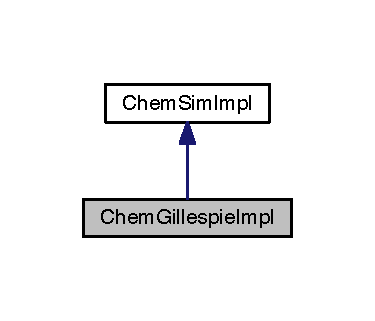
\includegraphics[width=180pt]{classChemGillespieImpl__inherit__graph}
\end{center}
\end{figure}


Collaboration diagram for Chem\+Gillespie\+Impl\+:\nopagebreak
\begin{figure}[H]
\begin{center}
\leavevmode
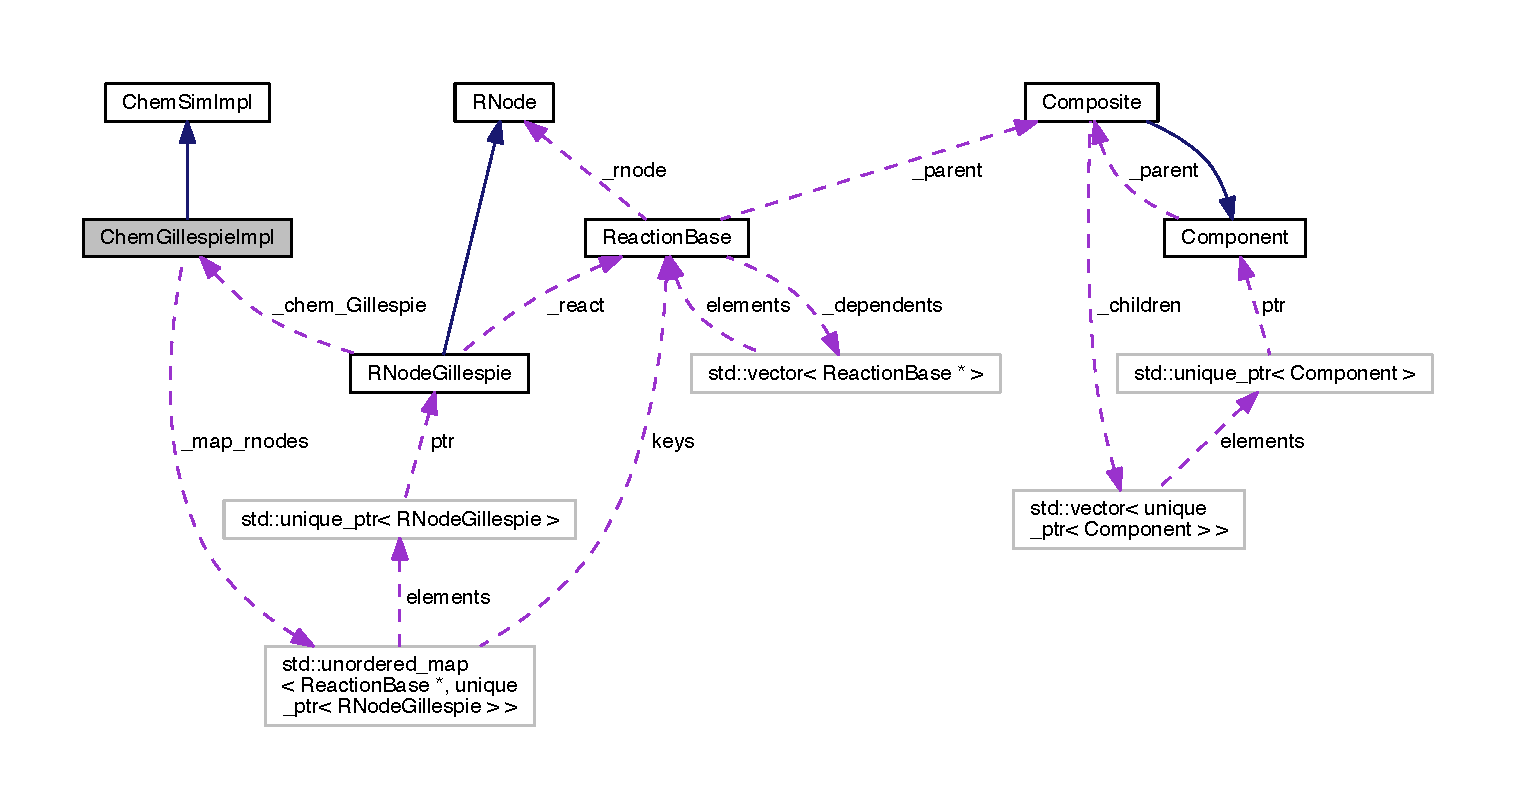
\includegraphics[width=350pt]{classChemGillespieImpl__coll__graph}
\end{center}
\end{figure}
\subsection*{Public Member Functions}
\begin{DoxyCompactItemize}
\item 
\hyperlink{classChemGillespieImpl_a262281b68b8fdd026a8d28f57315b13d}{Chem\+Gillespie\+Impl} ()
\begin{DoxyCompactList}\small\item\em Ctor\+: Seeds the random number generator, sets global time to 0.\+0 and the number of reactions to 0. \end{DoxyCompactList}\item 
\hyperlink{classChemGillespieImpl_aa492ec3985b18a49352c47d8d12c3647}{Chem\+Gillespie\+Impl} (const \hyperlink{classChemGillespieImpl}{Chem\+Gillespie\+Impl} \&rhs)=delete
\begin{DoxyCompactList}\small\item\em Copying is not allowed. \end{DoxyCompactList}\item 
\hyperlink{classChemGillespieImpl}{Chem\+Gillespie\+Impl} \& \hyperlink{classChemGillespieImpl_a1c0c24205d43a0f70be04ead713d18f9}{operator=} (\hyperlink{classChemGillespieImpl}{Chem\+Gillespie\+Impl} \&rhs)=delete
\begin{DoxyCompactList}\small\item\em Assignment is not allowed. \end{DoxyCompactList}\item 
virtual \hyperlink{classChemGillespieImpl_a56b73cf9e60b5ebd9ead82d4b6dd1b1a}{$\sim$\+Chem\+Gillespie\+Impl} () noexcept
\begin{DoxyCompactList}\small\item\em Dtor\+: The reaction network is cleared. \end{DoxyCompactList}\item 
size\+\_\+t \hyperlink{classChemGillespieImpl_a8deb307599919a7a2f8d597245761fdd}{get\+Size} () const 
\begin{DoxyCompactList}\small\item\em Return the number of reactions in the network. \end{DoxyCompactList}\item 
double \hyperlink{classChemGillespieImpl_a8295735915237bae30d18cd6c31c058a}{get\+Time} () const 
\begin{DoxyCompactList}\small\item\em Return the current global time (as defined in the Gillespie algorithm) \end{DoxyCompactList}\item 
void \hyperlink{classChemGillespieImpl_a21fcdf4c1f9c8372ebf292c5b4006b4a}{reset\+Time} ()
\begin{DoxyCompactList}\small\item\em Sets the global time to 0.\+0. \end{DoxyCompactList}\item 
void \hyperlink{classChemGillespieImpl_ae1fb14fb7f6eaa6a3ce21c8917de4624}{sync\+Global\+Time} ()
\begin{DoxyCompactList}\small\item\em Sets global time variable to \hyperlink{classChemGillespieImpl}{Chem\+Gillespie\+Impl}'s global time. \end{DoxyCompactList}\item 
virtual void \hyperlink{classChemGillespieImpl_afc2764e90e24e70b48577525421815c0}{add\+Reaction} (\hyperlink{classReactionBase}{Reaction\+Base} $\ast$r)
\begin{DoxyCompactList}\small\item\em Add \hyperlink{classReactionBase}{Reaction\+Base} $\ast$r to the network. \end{DoxyCompactList}\item 
virtual void \hyperlink{classChemGillespieImpl_ad818d065b15a17427793ab099ee987a8}{remove\+Reaction} (\hyperlink{classReactionBase}{Reaction\+Base} $\ast$r)
\begin{DoxyCompactList}\small\item\em Remove \hyperlink{classReactionBase}{Reaction\+Base} $\ast$r from the network. \end{DoxyCompactList}\item 
double \hyperlink{classChemGillespieImpl_a9a5292f5ede270611175f2061ef5d2c1}{compute\+Total\+A} ()
\begin{DoxyCompactList}\small\item\em Unconditionally compute the total propensity associated with the network. \end{DoxyCompactList}\item 
double \hyperlink{classChemGillespieImpl_ae2a584042f976aa39399b700011abe43}{generate\+Tau} (double a)
\begin{DoxyCompactList}\small\item\em Returns a random time tau, drawn from the exponential distribution, with the propensity given by a. \end{DoxyCompactList}\item 
double \hyperlink{classChemGillespieImpl_a165ea88d8e31bbd994f6b81a4ceda67e}{generate\+Uniform} ()
\begin{DoxyCompactList}\small\item\em Returns a random number between 0 and 1, drawn from the uniform distribution. \end{DoxyCompactList}\item 
virtual void \hyperlink{classChemGillespieImpl_a4362f0c7944ab1f6b07d43a2efbe8951}{initialize} ()
\begin{DoxyCompactList}\small\item\em This function iterates over all \hyperlink{classRNodeGillespie}{R\+Node\+Gillespie} objects in the network, activating all \hyperlink{classReaction}{Reaction} objects and calling reset(). \end{DoxyCompactList}\item 
virtual bool \hyperlink{classChemGillespieImpl_a1db4057b9cc7f51c2c8e3d880349f8a3}{run} (int steps)
\begin{DoxyCompactList}\small\item\em This method runs the Gillespie algorithm for the given number of steps. \end{DoxyCompactList}\item 
void \hyperlink{classChemGillespieImpl_aefbeeeb2edf0d6726cf50c129e320e58}{activate\+Reaction} (\hyperlink{classReactionBase}{Reaction\+Base} $\ast$r)
\begin{DoxyCompactList}\small\item\em This method is used to track the change in the total propensity of the network as the previously passivated \hyperlink{classReactionBase}{Reaction\+Base} $\ast$r has become activated. \end{DoxyCompactList}\item 
void \hyperlink{classChemGillespieImpl_a5916a11b71b642edee290af9fc969b28}{passivate\+Reaction} (\hyperlink{classReactionBase}{Reaction\+Base} $\ast$r)
\begin{DoxyCompactList}\small\item\em This method is used to track the change in the total propensity of the network as the \hyperlink{classReactionBase}{Reaction\+Base} $\ast$r has become passivated. \end{DoxyCompactList}\item 
virtual void \hyperlink{classChemGillespieImpl_a389502576c64b5c4454a79c4b6ccd4b2}{print\+Reactions} () const 
\begin{DoxyCompactList}\small\item\em Prints all R\+Nodes in the reaction network. \end{DoxyCompactList}\end{DoxyCompactItemize}
\subsection*{Private Member Functions}
\begin{DoxyCompactItemize}
\item 
bool \hyperlink{classChemGillespieImpl_a4474dce6c1c9074569cbdf75a991f82a}{make\+Step} ()
\begin{DoxyCompactList}\small\item\em This subroutine, along with with \hyperlink{classChemGillespieImpl_a5916a11b71b642edee290af9fc969b28}{passivate\+Reaction()} and \hyperlink{classChemGillespieImpl_aefbeeeb2edf0d6726cf50c129e320e58}{activate\+Reaction()} implements a cached version of the Gillespie algorith. \end{DoxyCompactList}\end{DoxyCompactItemize}
\subsection*{Private Attributes}
\begin{DoxyCompactItemize}
\item 
unordered\+\_\+map$<$ \hyperlink{classReactionBase}{Reaction\+Base} \\*
$\ast$, unique\+\_\+ptr$<$ \hyperlink{classRNodeGillespie}{R\+Node\+Gillespie} $>$ $>$ \hyperlink{classChemGillespieImpl_ab8d6bcef48ea219a249cebdb436dbc30}{\+\_\+map\+\_\+rnodes}
\begin{DoxyCompactList}\small\item\em The database of \hyperlink{classRNodeGillespie}{R\+Node\+Gillespie} objects, representing the reaction network. \end{DoxyCompactList}\item 
mt19937 \hyperlink{classChemGillespieImpl_a27162663b9cf776971f2f32483c6fe95}{\+\_\+eng}
\begin{DoxyCompactList}\small\item\em Random number generator. \end{DoxyCompactList}\item 
exponential\+\_\+distribution$<$ double $>$ \hyperlink{classChemGillespieImpl_a6ea99580ca00386e7db98a4059fbed0c}{\+\_\+exp\+\_\+distr}
\begin{DoxyCompactList}\small\item\em Adaptor for the exponential distribution. \end{DoxyCompactList}\item 
uniform\+\_\+real\+\_\+distribution$<$ double $>$ \hyperlink{classChemGillespieImpl_a6d37367996fad3157b63e6750ce6569b}{\+\_\+uniform\+\_\+distr}
\item 
double \hyperlink{classChemGillespieImpl_ab709229380a7bd5458d6c4b382036a7a}{\+\_\+t}
\begin{DoxyCompactList}\small\item\em global time \end{DoxyCompactList}\item 
double \hyperlink{classChemGillespieImpl_aeec18c37a7c9ad88199a78d613e7f8ac}{\+\_\+a\+\_\+total}
\item 
size\+\_\+t \hyperlink{classChemGillespieImpl_ae66f4f44055f9af574bd334f78f92393}{\+\_\+n\+\_\+reacts}
\begin{DoxyCompactList}\small\item\em number of reactions in the network \end{DoxyCompactList}\end{DoxyCompactItemize}


\subsection{Detailed Description}
Implements a slightly optimized version of the Gillespie algorithm. 

\hyperlink{classChemGillespieImpl}{Chem\+Gillespie\+Impl} manages the Gillespie algorithm at the level of the network of reactions. \hyperlink{classReaction}{Reaction} objects can be added and removed from the \hyperlink{classChemGillespieImpl}{Chem\+Gillespie\+Impl} instance. The propensities of all Reactions are cached, and they are recomputed only when the copy number of associated reactant species gets changed (due to the currently occurring \hyperlink{classReaction}{Reaction}). \begin{DoxyNote}{Note}
The algorithm used by this class relies on tracking dependent Reactions, so T\+R\+A\+C\+K\+\_\+\+D\+E\+P\+E\+N\+D\+E\+N\+T\+S must be defined. The algorithm can work both when T\+R\+A\+C\+K\+\_\+\+Z\+E\+R\+O\+\_\+\+C\+O\+P\+Y\+\_\+\+N and T\+R\+A\+C\+K\+\_\+\+U\+P\+P\+E\+R\+\_\+\+C\+O\+P\+Y\+\_\+\+N are either defined or undefined. In the former case, \hyperlink{classReaction}{Reaction} objects with zero propensities stop being treated as dependents until their propensities become nonzero again. 
\end{DoxyNote}


Definition at line 125 of file Chem\+Gillespie\+Impl.\+h.



\subsection{Constructor \& Destructor Documentation}
\hypertarget{classChemGillespieImpl_a262281b68b8fdd026a8d28f57315b13d}{\index{Chem\+Gillespie\+Impl@{Chem\+Gillespie\+Impl}!Chem\+Gillespie\+Impl@{Chem\+Gillespie\+Impl}}
\index{Chem\+Gillespie\+Impl@{Chem\+Gillespie\+Impl}!Chem\+Gillespie\+Impl@{Chem\+Gillespie\+Impl}}
\subsubsection[{Chem\+Gillespie\+Impl}]{\setlength{\rightskip}{0pt plus 5cm}Chem\+Gillespie\+Impl\+::\+Chem\+Gillespie\+Impl (
\begin{DoxyParamCaption}
{}
\end{DoxyParamCaption}
)\hspace{0.3cm}{\ttfamily [inline]}}}\label{classChemGillespieImpl_a262281b68b8fdd026a8d28f57315b13d}


Ctor\+: Seeds the random number generator, sets global time to 0.\+0 and the number of reactions to 0. 



Definition at line 128 of file Chem\+Gillespie\+Impl.\+h.



References reset\+Time().

\hypertarget{classChemGillespieImpl_aa492ec3985b18a49352c47d8d12c3647}{\index{Chem\+Gillespie\+Impl@{Chem\+Gillespie\+Impl}!Chem\+Gillespie\+Impl@{Chem\+Gillespie\+Impl}}
\index{Chem\+Gillespie\+Impl@{Chem\+Gillespie\+Impl}!Chem\+Gillespie\+Impl@{Chem\+Gillespie\+Impl}}
\subsubsection[{Chem\+Gillespie\+Impl}]{\setlength{\rightskip}{0pt plus 5cm}Chem\+Gillespie\+Impl\+::\+Chem\+Gillespie\+Impl (
\begin{DoxyParamCaption}
\item[{const {\bf Chem\+Gillespie\+Impl} \&}]{rhs}
\end{DoxyParamCaption}
)\hspace{0.3cm}{\ttfamily [delete]}}}\label{classChemGillespieImpl_aa492ec3985b18a49352c47d8d12c3647}


Copying is not allowed. 

\hypertarget{classChemGillespieImpl_a56b73cf9e60b5ebd9ead82d4b6dd1b1a}{\index{Chem\+Gillespie\+Impl@{Chem\+Gillespie\+Impl}!````~Chem\+Gillespie\+Impl@{$\sim$\+Chem\+Gillespie\+Impl}}
\index{````~Chem\+Gillespie\+Impl@{$\sim$\+Chem\+Gillespie\+Impl}!Chem\+Gillespie\+Impl@{Chem\+Gillespie\+Impl}}
\subsubsection[{$\sim$\+Chem\+Gillespie\+Impl}]{\setlength{\rightskip}{0pt plus 5cm}Chem\+Gillespie\+Impl\+::$\sim$\+Chem\+Gillespie\+Impl (
\begin{DoxyParamCaption}
{}
\end{DoxyParamCaption}
)\hspace{0.3cm}{\ttfamily [virtual]}, {\ttfamily [noexcept]}}}\label{classChemGillespieImpl_a56b73cf9e60b5ebd9ead82d4b6dd1b1a}


Dtor\+: The reaction network is cleared. 

The \hyperlink{classRNodeGillespie}{R\+Node\+Gillespie} objects will be destructed, but \hyperlink{classReaction}{Reaction} objects will stay intact. \begin{DoxyNote}{Note}
noexcept is important here. Otherwise, gcc flags the constructor as potentially throwing, which in turn disables move operations by the S\+T\+L containers. This behaviour is a gcc bug (as of gcc 4.\+703), and will presumbaly be fixed in the future. 
\end{DoxyNote}


Definition at line 62 of file Chem\+Gillespie\+Impl.\+cpp.



References \+\_\+map\+\_\+rnodes.



\subsection{Member Function Documentation}
\hypertarget{classChemGillespieImpl_aefbeeeb2edf0d6726cf50c129e320e58}{\index{Chem\+Gillespie\+Impl@{Chem\+Gillespie\+Impl}!activate\+Reaction@{activate\+Reaction}}
\index{activate\+Reaction@{activate\+Reaction}!Chem\+Gillespie\+Impl@{Chem\+Gillespie\+Impl}}
\subsubsection[{activate\+Reaction}]{\setlength{\rightskip}{0pt plus 5cm}void Chem\+Gillespie\+Impl\+::activate\+Reaction (
\begin{DoxyParamCaption}
\item[{{\bf Reaction\+Base} $\ast$}]{r}
\end{DoxyParamCaption}
)}}\label{classChemGillespieImpl_aefbeeeb2edf0d6726cf50c129e320e58}


This method is used to track the change in the total propensity of the network as the previously passivated \hyperlink{classReactionBase}{Reaction\+Base} $\ast$r has become activated. 



Definition at line 162 of file Chem\+Gillespie\+Impl.\+cpp.



References \+\_\+a\+\_\+total, \+\_\+map\+\_\+rnodes, R\+Node\+Gillespie\+::get\+Penult\+Step\+Propensity(), R\+Node\+Gillespie\+::get\+Propensity(), and R\+Node\+Gillespie\+::re\+Compute\+Propensity().



Referenced by R\+Node\+Gillespie\+::activate\+Reaction().

\hypertarget{classChemGillespieImpl_afc2764e90e24e70b48577525421815c0}{\index{Chem\+Gillespie\+Impl@{Chem\+Gillespie\+Impl}!add\+Reaction@{add\+Reaction}}
\index{add\+Reaction@{add\+Reaction}!Chem\+Gillespie\+Impl@{Chem\+Gillespie\+Impl}}
\subsubsection[{add\+Reaction}]{\setlength{\rightskip}{0pt plus 5cm}void Chem\+Gillespie\+Impl\+::add\+Reaction (
\begin{DoxyParamCaption}
\item[{{\bf Reaction\+Base} $\ast$}]{r}
\end{DoxyParamCaption}
)\hspace{0.3cm}{\ttfamily [virtual]}}}\label{classChemGillespieImpl_afc2764e90e24e70b48577525421815c0}


Add \hyperlink{classReactionBase}{Reaction\+Base} $\ast$r to the network. 



Implements \hyperlink{classChemSimImpl_ae1ca0468b4564703d87d69f45ee6e1f9}{Chem\+Sim\+Impl}.



Definition at line 145 of file Chem\+Gillespie\+Impl.\+cpp.



References \+\_\+map\+\_\+rnodes, and \+\_\+n\+\_\+reacts.

\hypertarget{classChemGillespieImpl_a9a5292f5ede270611175f2061ef5d2c1}{\index{Chem\+Gillespie\+Impl@{Chem\+Gillespie\+Impl}!compute\+Total\+A@{compute\+Total\+A}}
\index{compute\+Total\+A@{compute\+Total\+A}!Chem\+Gillespie\+Impl@{Chem\+Gillespie\+Impl}}
\subsubsection[{compute\+Total\+A}]{\setlength{\rightskip}{0pt plus 5cm}double Chem\+Gillespie\+Impl\+::compute\+Total\+A (
\begin{DoxyParamCaption}
{}
\end{DoxyParamCaption}
)}}\label{classChemGillespieImpl_a9a5292f5ede270611175f2061ef5d2c1}


Unconditionally compute the total propensity associated with the network. 



Definition at line 76 of file Chem\+Gillespie\+Impl.\+cpp.



References \+\_\+map\+\_\+rnodes.



Referenced by initialize().

\hypertarget{classChemGillespieImpl_ae2a584042f976aa39399b700011abe43}{\index{Chem\+Gillespie\+Impl@{Chem\+Gillespie\+Impl}!generate\+Tau@{generate\+Tau}}
\index{generate\+Tau@{generate\+Tau}!Chem\+Gillespie\+Impl@{Chem\+Gillespie\+Impl}}
\subsubsection[{generate\+Tau}]{\setlength{\rightskip}{0pt plus 5cm}double Chem\+Gillespie\+Impl\+::generate\+Tau (
\begin{DoxyParamCaption}
\item[{double}]{a}
\end{DoxyParamCaption}
)}}\label{classChemGillespieImpl_ae2a584042f976aa39399b700011abe43}


Returns a random time tau, drawn from the exponential distribution, with the propensity given by a. 



Definition at line 66 of file Chem\+Gillespie\+Impl.\+cpp.



References \+\_\+eng, and \+\_\+exp\+\_\+distr.



Referenced by make\+Step().

\hypertarget{classChemGillespieImpl_a165ea88d8e31bbd994f6b81a4ceda67e}{\index{Chem\+Gillespie\+Impl@{Chem\+Gillespie\+Impl}!generate\+Uniform@{generate\+Uniform}}
\index{generate\+Uniform@{generate\+Uniform}!Chem\+Gillespie\+Impl@{Chem\+Gillespie\+Impl}}
\subsubsection[{generate\+Uniform}]{\setlength{\rightskip}{0pt plus 5cm}double Chem\+Gillespie\+Impl\+::generate\+Uniform (
\begin{DoxyParamCaption}
{}
\end{DoxyParamCaption}
)}}\label{classChemGillespieImpl_a165ea88d8e31bbd994f6b81a4ceda67e}


Returns a random number between 0 and 1, drawn from the uniform distribution. 



Definition at line 72 of file Chem\+Gillespie\+Impl.\+cpp.



References \+\_\+eng, and \+\_\+uniform\+\_\+distr.



Referenced by make\+Step().

\hypertarget{classChemGillespieImpl_a8deb307599919a7a2f8d597245761fdd}{\index{Chem\+Gillespie\+Impl@{Chem\+Gillespie\+Impl}!get\+Size@{get\+Size}}
\index{get\+Size@{get\+Size}!Chem\+Gillespie\+Impl@{Chem\+Gillespie\+Impl}}
\subsubsection[{get\+Size}]{\setlength{\rightskip}{0pt plus 5cm}size\+\_\+t Chem\+Gillespie\+Impl\+::get\+Size (
\begin{DoxyParamCaption}
{}
\end{DoxyParamCaption}
) const\hspace{0.3cm}{\ttfamily [inline]}}}\label{classChemGillespieImpl_a8deb307599919a7a2f8d597245761fdd}


Return the number of reactions in the network. 



Definition at line 146 of file Chem\+Gillespie\+Impl.\+h.



References \+\_\+map\+\_\+rnodes.

\hypertarget{classChemGillespieImpl_a8295735915237bae30d18cd6c31c058a}{\index{Chem\+Gillespie\+Impl@{Chem\+Gillespie\+Impl}!get\+Time@{get\+Time}}
\index{get\+Time@{get\+Time}!Chem\+Gillespie\+Impl@{Chem\+Gillespie\+Impl}}
\subsubsection[{get\+Time}]{\setlength{\rightskip}{0pt plus 5cm}double Chem\+Gillespie\+Impl\+::get\+Time (
\begin{DoxyParamCaption}
{}
\end{DoxyParamCaption}
) const\hspace{0.3cm}{\ttfamily [inline]}}}\label{classChemGillespieImpl_a8295735915237bae30d18cd6c31c058a}


Return the current global time (as defined in the Gillespie algorithm) 



Definition at line 149 of file Chem\+Gillespie\+Impl.\+h.



References \+\_\+t.

\hypertarget{classChemGillespieImpl_a4362f0c7944ab1f6b07d43a2efbe8951}{\index{Chem\+Gillespie\+Impl@{Chem\+Gillespie\+Impl}!initialize@{initialize}}
\index{initialize@{initialize}!Chem\+Gillespie\+Impl@{Chem\+Gillespie\+Impl}}
\subsubsection[{initialize}]{\setlength{\rightskip}{0pt plus 5cm}void Chem\+Gillespie\+Impl\+::initialize (
\begin{DoxyParamCaption}
{}
\end{DoxyParamCaption}
)\hspace{0.3cm}{\ttfamily [virtual]}}}\label{classChemGillespieImpl_a4362f0c7944ab1f6b07d43a2efbe8951}


This function iterates over all \hyperlink{classRNodeGillespie}{R\+Node\+Gillespie} objects in the network, activating all \hyperlink{classReaction}{Reaction} objects and calling reset(). 

The total propentsity for the network is computed. \begin{DoxyNote}{Note}
This method needs to be called before calling run(...). 

If somewhere in the middle of simulaiton \hyperlink{classChemGillespieImpl_a4362f0c7944ab1f6b07d43a2efbe8951}{initialize()} is called, it will be analogous to starting the simulation from scratch, except with the \hyperlink{classSpecies}{Species} copy numbers given at that moment in time. The global time is reset to zero again. 
\end{DoxyNote}


Implements \hyperlink{classChemSimImpl_a8050874ed2646d6632ec9df1704c86c4}{Chem\+Sim\+Impl}.



Definition at line 49 of file Chem\+Gillespie\+Impl.\+cpp.



References \+\_\+a\+\_\+total, \+\_\+map\+\_\+rnodes, compute\+Total\+A(), and reset\+Time().

\hypertarget{classChemGillespieImpl_a4474dce6c1c9074569cbdf75a991f82a}{\index{Chem\+Gillespie\+Impl@{Chem\+Gillespie\+Impl}!make\+Step@{make\+Step}}
\index{make\+Step@{make\+Step}!Chem\+Gillespie\+Impl@{Chem\+Gillespie\+Impl}}
\subsubsection[{make\+Step}]{\setlength{\rightskip}{0pt plus 5cm}bool Chem\+Gillespie\+Impl\+::make\+Step (
\begin{DoxyParamCaption}
{}
\end{DoxyParamCaption}
)\hspace{0.3cm}{\ttfamily [private]}}}\label{classChemGillespieImpl_a4474dce6c1c9074569cbdf75a991f82a}


This subroutine, along with with \hyperlink{classChemGillespieImpl_a5916a11b71b642edee290af9fc969b28}{passivate\+Reaction()} and \hyperlink{classChemGillespieImpl_aefbeeeb2edf0d6726cf50c129e320e58}{activate\+Reaction()} implements a cached version of the Gillespie algorith. 

Two random numbers get thrown, one for obtaining tau, the time to the next reaction event, and a uniform number to select which \hyperlink{classReaction}{Reaction} has occurred. Instead of computing the total propensity of the network from scratch, the cached value is being modified as \hyperlink{classReaction}{Reaction} events occur. Returns true if successful, and false if the heap is exchausted and there no more reactions to fire 

Definition at line 87 of file Chem\+Gillespie\+Impl.\+cpp.



References \+\_\+a\+\_\+total, \+\_\+map\+\_\+rnodes, \+\_\+t, Reaction\+Base\+::dependents(), generate\+Tau(), generate\+Uniform(), R\+Node\+Gillespie\+::get\+Penult\+Step\+Propensity(), R\+Node\+Gillespie\+::get\+Propensity(), R\+Node\+Gillespie\+::get\+Reaction(), R\+Node\+Gillespie\+::is\+Passivated(), R\+Node\+Gillespie\+::make\+Step(), R\+Node\+Gillespie\+::re\+Compute\+Propensity(), sync\+Global\+Time(), and tau().



Referenced by run().

\hypertarget{classChemGillespieImpl_a1c0c24205d43a0f70be04ead713d18f9}{\index{Chem\+Gillespie\+Impl@{Chem\+Gillespie\+Impl}!operator=@{operator=}}
\index{operator=@{operator=}!Chem\+Gillespie\+Impl@{Chem\+Gillespie\+Impl}}
\subsubsection[{operator=}]{\setlength{\rightskip}{0pt plus 5cm}{\bf Chem\+Gillespie\+Impl}\& Chem\+Gillespie\+Impl\+::operator= (
\begin{DoxyParamCaption}
\item[{{\bf Chem\+Gillespie\+Impl} \&}]{rhs}
\end{DoxyParamCaption}
)\hspace{0.3cm}{\ttfamily [delete]}}}\label{classChemGillespieImpl_a1c0c24205d43a0f70be04ead713d18f9}


Assignment is not allowed. 

\hypertarget{classChemGillespieImpl_a5916a11b71b642edee290af9fc969b28}{\index{Chem\+Gillespie\+Impl@{Chem\+Gillespie\+Impl}!passivate\+Reaction@{passivate\+Reaction}}
\index{passivate\+Reaction@{passivate\+Reaction}!Chem\+Gillespie\+Impl@{Chem\+Gillespie\+Impl}}
\subsubsection[{passivate\+Reaction}]{\setlength{\rightskip}{0pt plus 5cm}void Chem\+Gillespie\+Impl\+::passivate\+Reaction (
\begin{DoxyParamCaption}
\item[{{\bf Reaction\+Base} $\ast$}]{r}
\end{DoxyParamCaption}
)}}\label{classChemGillespieImpl_a5916a11b71b642edee290af9fc969b28}


This method is used to track the change in the total propensity of the network as the \hyperlink{classReactionBase}{Reaction\+Base} $\ast$r has become passivated. 



Definition at line 175 of file Chem\+Gillespie\+Impl.\+cpp.



References \+\_\+a\+\_\+total, \+\_\+map\+\_\+rnodes, R\+Node\+Gillespie\+::get\+Propensity(), R\+Node\+Gillespie\+::set\+A(), and R\+Node\+Gillespie\+::set\+Penult\+A().



Referenced by R\+Node\+Gillespie\+::passivate\+Reaction().

\hypertarget{classChemGillespieImpl_a389502576c64b5c4454a79c4b6ccd4b2}{\index{Chem\+Gillespie\+Impl@{Chem\+Gillespie\+Impl}!print\+Reactions@{print\+Reactions}}
\index{print\+Reactions@{print\+Reactions}!Chem\+Gillespie\+Impl@{Chem\+Gillespie\+Impl}}
\subsubsection[{print\+Reactions}]{\setlength{\rightskip}{0pt plus 5cm}void Chem\+Gillespie\+Impl\+::print\+Reactions (
\begin{DoxyParamCaption}
{}
\end{DoxyParamCaption}
) const\hspace{0.3cm}{\ttfamily [virtual]}}}\label{classChemGillespieImpl_a389502576c64b5c4454a79c4b6ccd4b2}


Prints all R\+Nodes in the reaction network. 



Implements \hyperlink{classChemSimImpl_a1c0d35dbca7647319a27fa7eaff7388b}{Chem\+Sim\+Impl}.



Definition at line 155 of file Chem\+Gillespie\+Impl.\+cpp.



References \+\_\+map\+\_\+rnodes.

\hypertarget{classChemGillespieImpl_ad818d065b15a17427793ab099ee987a8}{\index{Chem\+Gillespie\+Impl@{Chem\+Gillespie\+Impl}!remove\+Reaction@{remove\+Reaction}}
\index{remove\+Reaction@{remove\+Reaction}!Chem\+Gillespie\+Impl@{Chem\+Gillespie\+Impl}}
\subsubsection[{remove\+Reaction}]{\setlength{\rightskip}{0pt plus 5cm}void Chem\+Gillespie\+Impl\+::remove\+Reaction (
\begin{DoxyParamCaption}
\item[{{\bf Reaction\+Base} $\ast$}]{r}
\end{DoxyParamCaption}
)\hspace{0.3cm}{\ttfamily [virtual]}}}\label{classChemGillespieImpl_ad818d065b15a17427793ab099ee987a8}


Remove \hyperlink{classReactionBase}{Reaction\+Base} $\ast$r from the network. 



Implements \hyperlink{classChemSimImpl_a2561de21097a1b12bc60bc53a966e9fc}{Chem\+Sim\+Impl}.



Definition at line 150 of file Chem\+Gillespie\+Impl.\+cpp.



References \+\_\+map\+\_\+rnodes, and \+\_\+n\+\_\+reacts.

\hypertarget{classChemGillespieImpl_a21fcdf4c1f9c8372ebf292c5b4006b4a}{\index{Chem\+Gillespie\+Impl@{Chem\+Gillespie\+Impl}!reset\+Time@{reset\+Time}}
\index{reset\+Time@{reset\+Time}!Chem\+Gillespie\+Impl@{Chem\+Gillespie\+Impl}}
\subsubsection[{reset\+Time}]{\setlength{\rightskip}{0pt plus 5cm}void Chem\+Gillespie\+Impl\+::reset\+Time (
\begin{DoxyParamCaption}
{}
\end{DoxyParamCaption}
)\hspace{0.3cm}{\ttfamily [inline]}}}\label{classChemGillespieImpl_a21fcdf4c1f9c8372ebf292c5b4006b4a}


Sets the global time to 0.\+0. 



Definition at line 152 of file Chem\+Gillespie\+Impl.\+h.



References \+\_\+t, and sync\+Global\+Time().



Referenced by Chem\+Gillespie\+Impl(), and initialize().

\hypertarget{classChemGillespieImpl_a1db4057b9cc7f51c2c8e3d880349f8a3}{\index{Chem\+Gillespie\+Impl@{Chem\+Gillespie\+Impl}!run@{run}}
\index{run@{run}!Chem\+Gillespie\+Impl@{Chem\+Gillespie\+Impl}}
\subsubsection[{run}]{\setlength{\rightskip}{0pt plus 5cm}virtual bool Chem\+Gillespie\+Impl\+::run (
\begin{DoxyParamCaption}
\item[{int}]{steps}
\end{DoxyParamCaption}
)\hspace{0.3cm}{\ttfamily [inline]}, {\ttfamily [virtual]}}}\label{classChemGillespieImpl_a1db4057b9cc7f51c2c8e3d880349f8a3}


This method runs the Gillespie algorithm for the given number of steps. 

\begin{DoxyReturn}{Returns}
true if successful. 
\end{DoxyReturn}


Implements \hyperlink{classChemSimImpl_a3472132dc4b356ed76116c40af2a773d}{Chem\+Sim\+Impl}.



Definition at line 182 of file Chem\+Gillespie\+Impl.\+h.



References make\+Step().

\hypertarget{classChemGillespieImpl_ae1fb14fb7f6eaa6a3ce21c8917de4624}{\index{Chem\+Gillespie\+Impl@{Chem\+Gillespie\+Impl}!sync\+Global\+Time@{sync\+Global\+Time}}
\index{sync\+Global\+Time@{sync\+Global\+Time}!Chem\+Gillespie\+Impl@{Chem\+Gillespie\+Impl}}
\subsubsection[{sync\+Global\+Time}]{\setlength{\rightskip}{0pt plus 5cm}void Chem\+Gillespie\+Impl\+::sync\+Global\+Time (
\begin{DoxyParamCaption}
{}
\end{DoxyParamCaption}
)\hspace{0.3cm}{\ttfamily [inline]}}}\label{classChemGillespieImpl_ae1fb14fb7f6eaa6a3ce21c8917de4624}


Sets global time variable to \hyperlink{classChemGillespieImpl}{Chem\+Gillespie\+Impl}'s global time. 



Definition at line 155 of file Chem\+Gillespie\+Impl.\+h.



References \+\_\+t, and global\+\_\+time.



Referenced by make\+Step(), and reset\+Time().



\subsection{Member Data Documentation}
\hypertarget{classChemGillespieImpl_aeec18c37a7c9ad88199a78d613e7f8ac}{\index{Chem\+Gillespie\+Impl@{Chem\+Gillespie\+Impl}!\+\_\+a\+\_\+total@{\+\_\+a\+\_\+total}}
\index{\+\_\+a\+\_\+total@{\+\_\+a\+\_\+total}!Chem\+Gillespie\+Impl@{Chem\+Gillespie\+Impl}}
\subsubsection[{\+\_\+a\+\_\+total}]{\setlength{\rightskip}{0pt plus 5cm}double Chem\+Gillespie\+Impl\+::\+\_\+a\+\_\+total\hspace{0.3cm}{\ttfamily [private]}}}\label{classChemGillespieImpl_aeec18c37a7c9ad88199a78d613e7f8ac}


Definition at line 215 of file Chem\+Gillespie\+Impl.\+h.



Referenced by activate\+Reaction(), initialize(), make\+Step(), and passivate\+Reaction().

\hypertarget{classChemGillespieImpl_a27162663b9cf776971f2f32483c6fe95}{\index{Chem\+Gillespie\+Impl@{Chem\+Gillespie\+Impl}!\+\_\+eng@{\+\_\+eng}}
\index{\+\_\+eng@{\+\_\+eng}!Chem\+Gillespie\+Impl@{Chem\+Gillespie\+Impl}}
\subsubsection[{\+\_\+eng}]{\setlength{\rightskip}{0pt plus 5cm}mt19937 Chem\+Gillespie\+Impl\+::\+\_\+eng\hspace{0.3cm}{\ttfamily [private]}}}\label{classChemGillespieImpl_a27162663b9cf776971f2f32483c6fe95}


Random number generator. 



Definition at line 211 of file Chem\+Gillespie\+Impl.\+h.



Referenced by generate\+Tau(), and generate\+Uniform().

\hypertarget{classChemGillespieImpl_a6ea99580ca00386e7db98a4059fbed0c}{\index{Chem\+Gillespie\+Impl@{Chem\+Gillespie\+Impl}!\+\_\+exp\+\_\+distr@{\+\_\+exp\+\_\+distr}}
\index{\+\_\+exp\+\_\+distr@{\+\_\+exp\+\_\+distr}!Chem\+Gillespie\+Impl@{Chem\+Gillespie\+Impl}}
\subsubsection[{\+\_\+exp\+\_\+distr}]{\setlength{\rightskip}{0pt plus 5cm}exponential\+\_\+distribution$<$double$>$ Chem\+Gillespie\+Impl\+::\+\_\+exp\+\_\+distr\hspace{0.3cm}{\ttfamily [private]}}}\label{classChemGillespieImpl_a6ea99580ca00386e7db98a4059fbed0c}


Adaptor for the exponential distribution. 



Definition at line 212 of file Chem\+Gillespie\+Impl.\+h.



Referenced by generate\+Tau().

\hypertarget{classChemGillespieImpl_ab8d6bcef48ea219a249cebdb436dbc30}{\index{Chem\+Gillespie\+Impl@{Chem\+Gillespie\+Impl}!\+\_\+map\+\_\+rnodes@{\+\_\+map\+\_\+rnodes}}
\index{\+\_\+map\+\_\+rnodes@{\+\_\+map\+\_\+rnodes}!Chem\+Gillespie\+Impl@{Chem\+Gillespie\+Impl}}
\subsubsection[{\+\_\+map\+\_\+rnodes}]{\setlength{\rightskip}{0pt plus 5cm}unordered\+\_\+map$<${\bf Reaction\+Base}$\ast$, unique\+\_\+ptr$<${\bf R\+Node\+Gillespie}$>$ $>$ Chem\+Gillespie\+Impl\+::\+\_\+map\+\_\+rnodes\hspace{0.3cm}{\ttfamily [private]}}}\label{classChemGillespieImpl_ab8d6bcef48ea219a249cebdb436dbc30}


The database of \hyperlink{classRNodeGillespie}{R\+Node\+Gillespie} objects, representing the reaction network. 



Definition at line 210 of file Chem\+Gillespie\+Impl.\+h.



Referenced by activate\+Reaction(), add\+Reaction(), compute\+Total\+A(), get\+Size(), initialize(), make\+Step(), passivate\+Reaction(), print\+Reactions(), remove\+Reaction(), and $\sim$\+Chem\+Gillespie\+Impl().

\hypertarget{classChemGillespieImpl_ae66f4f44055f9af574bd334f78f92393}{\index{Chem\+Gillespie\+Impl@{Chem\+Gillespie\+Impl}!\+\_\+n\+\_\+reacts@{\+\_\+n\+\_\+reacts}}
\index{\+\_\+n\+\_\+reacts@{\+\_\+n\+\_\+reacts}!Chem\+Gillespie\+Impl@{Chem\+Gillespie\+Impl}}
\subsubsection[{\+\_\+n\+\_\+reacts}]{\setlength{\rightskip}{0pt plus 5cm}size\+\_\+t Chem\+Gillespie\+Impl\+::\+\_\+n\+\_\+reacts\hspace{0.3cm}{\ttfamily [private]}}}\label{classChemGillespieImpl_ae66f4f44055f9af574bd334f78f92393}


number of reactions in the network 



Definition at line 216 of file Chem\+Gillespie\+Impl.\+h.



Referenced by add\+Reaction(), and remove\+Reaction().

\hypertarget{classChemGillespieImpl_ab709229380a7bd5458d6c4b382036a7a}{\index{Chem\+Gillespie\+Impl@{Chem\+Gillespie\+Impl}!\+\_\+t@{\+\_\+t}}
\index{\+\_\+t@{\+\_\+t}!Chem\+Gillespie\+Impl@{Chem\+Gillespie\+Impl}}
\subsubsection[{\+\_\+t}]{\setlength{\rightskip}{0pt plus 5cm}double Chem\+Gillespie\+Impl\+::\+\_\+t\hspace{0.3cm}{\ttfamily [private]}}}\label{classChemGillespieImpl_ab709229380a7bd5458d6c4b382036a7a}


global time 



Definition at line 214 of file Chem\+Gillespie\+Impl.\+h.



Referenced by get\+Time(), make\+Step(), reset\+Time(), and sync\+Global\+Time().

\hypertarget{classChemGillespieImpl_a6d37367996fad3157b63e6750ce6569b}{\index{Chem\+Gillespie\+Impl@{Chem\+Gillespie\+Impl}!\+\_\+uniform\+\_\+distr@{\+\_\+uniform\+\_\+distr}}
\index{\+\_\+uniform\+\_\+distr@{\+\_\+uniform\+\_\+distr}!Chem\+Gillespie\+Impl@{Chem\+Gillespie\+Impl}}
\subsubsection[{\+\_\+uniform\+\_\+distr}]{\setlength{\rightskip}{0pt plus 5cm}uniform\+\_\+real\+\_\+distribution$<$double$>$ Chem\+Gillespie\+Impl\+::\+\_\+uniform\+\_\+distr\hspace{0.3cm}{\ttfamily [private]}}}\label{classChemGillespieImpl_a6d37367996fad3157b63e6750ce6569b}


Definition at line 213 of file Chem\+Gillespie\+Impl.\+h.



Referenced by generate\+Uniform().



The documentation for this class was generated from the following files\+:\begin{DoxyCompactItemize}
\item 
M3\+S\+Y\+M/\+Chemistry/\hyperlink{ChemGillespieImpl_8h}{Chem\+Gillespie\+Impl.\+h}\item 
M3\+S\+Y\+M/\+Chemistry/\hyperlink{ChemGillespieImpl_8cpp}{Chem\+Gillespie\+Impl.\+cpp}\end{DoxyCompactItemize}

\hypertarget{structChemistryAlgorithm}{\section{Chemistry\+Algorithm Struct Reference}
\label{structChemistryAlgorithm}\index{Chemistry\+Algorithm@{Chemistry\+Algorithm}}
}


Struct to hold chemistry algorithm information.  




{\ttfamily \#include $<$Parser.\+h$>$}



Collaboration diagram for Chemistry\+Algorithm\+:\nopagebreak
\begin{figure}[H]
\begin{center}
\leavevmode
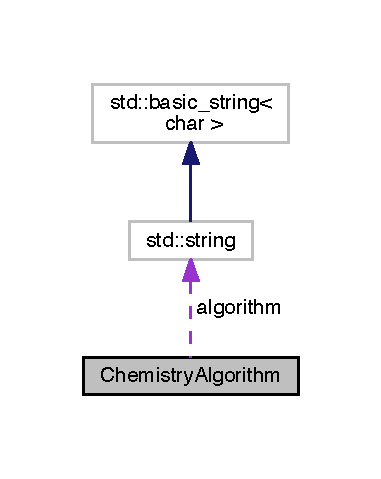
\includegraphics[width=183pt]{structChemistryAlgorithm__coll__graph}
\end{center}
\end{figure}
\subsection*{Public Attributes}
\begin{DoxyCompactItemize}
\item 
string \hyperlink{structChemistryAlgorithm_a79823d8025ebda7f40a0fa7683008ce2}{algorithm} = \char`\"{}\char`\"{}
\item 
int \hyperlink{structChemistryAlgorithm_a6ba1dded2edadb96427909fcead6cdeb}{num\+Steps} = 0
\item 
int \hyperlink{structChemistryAlgorithm_a8f1e4fb749816d74760c866b8beb0884}{num\+Steps\+Per\+Mech} = 0
\end{DoxyCompactItemize}


\subsection{Detailed Description}
Struct to hold chemistry algorithm information. 

Definition at line 32 of file Parser.\+h.



\subsection{Member Data Documentation}
\hypertarget{structChemistryAlgorithm_a79823d8025ebda7f40a0fa7683008ce2}{\index{Chemistry\+Algorithm@{Chemistry\+Algorithm}!algorithm@{algorithm}}
\index{algorithm@{algorithm}!Chemistry\+Algorithm@{Chemistry\+Algorithm}}
\subsubsection[{algorithm}]{\setlength{\rightskip}{0pt plus 5cm}string Chemistry\+Algorithm\+::algorithm = \char`\"{}\char`\"{}}}\label{structChemistryAlgorithm_a79823d8025ebda7f40a0fa7683008ce2}


Definition at line 34 of file Parser.\+h.



Referenced by System\+Parser\+::read\+Chemistry\+Algorithm().

\hypertarget{structChemistryAlgorithm_a6ba1dded2edadb96427909fcead6cdeb}{\index{Chemistry\+Algorithm@{Chemistry\+Algorithm}!num\+Steps@{num\+Steps}}
\index{num\+Steps@{num\+Steps}!Chemistry\+Algorithm@{Chemistry\+Algorithm}}
\subsubsection[{num\+Steps}]{\setlength{\rightskip}{0pt plus 5cm}int Chemistry\+Algorithm\+::num\+Steps = 0}}\label{structChemistryAlgorithm_a6ba1dded2edadb96427909fcead6cdeb}


Definition at line 35 of file Parser.\+h.



Referenced by System\+Parser\+::read\+Chemistry\+Algorithm().

\hypertarget{structChemistryAlgorithm_a8f1e4fb749816d74760c866b8beb0884}{\index{Chemistry\+Algorithm@{Chemistry\+Algorithm}!num\+Steps\+Per\+Mech@{num\+Steps\+Per\+Mech}}
\index{num\+Steps\+Per\+Mech@{num\+Steps\+Per\+Mech}!Chemistry\+Algorithm@{Chemistry\+Algorithm}}
\subsubsection[{num\+Steps\+Per\+Mech}]{\setlength{\rightskip}{0pt plus 5cm}int Chemistry\+Algorithm\+::num\+Steps\+Per\+Mech = 0}}\label{structChemistryAlgorithm_a8f1e4fb749816d74760c866b8beb0884}


Definition at line 36 of file Parser.\+h.



Referenced by System\+Parser\+::read\+Chemistry\+Algorithm().



The documentation for this struct was generated from the following file\+:\begin{DoxyCompactItemize}
\item 
M3\+S\+Y\+M/\hyperlink{Parser_8h}{Parser.\+h}\end{DoxyCompactItemize}

\hypertarget{structChemistryData}{\section{Chemistry\+Data Struct Reference}
\label{structChemistryData}\index{Chemistry\+Data@{Chemistry\+Data}}
}


Struct to hold chemistry species and reaction information.  




{\ttfamily \#include $<$Parser.\+h$>$}



Collaboration diagram for Chemistry\+Data\+:\nopagebreak
\begin{figure}[H]
\begin{center}
\leavevmode
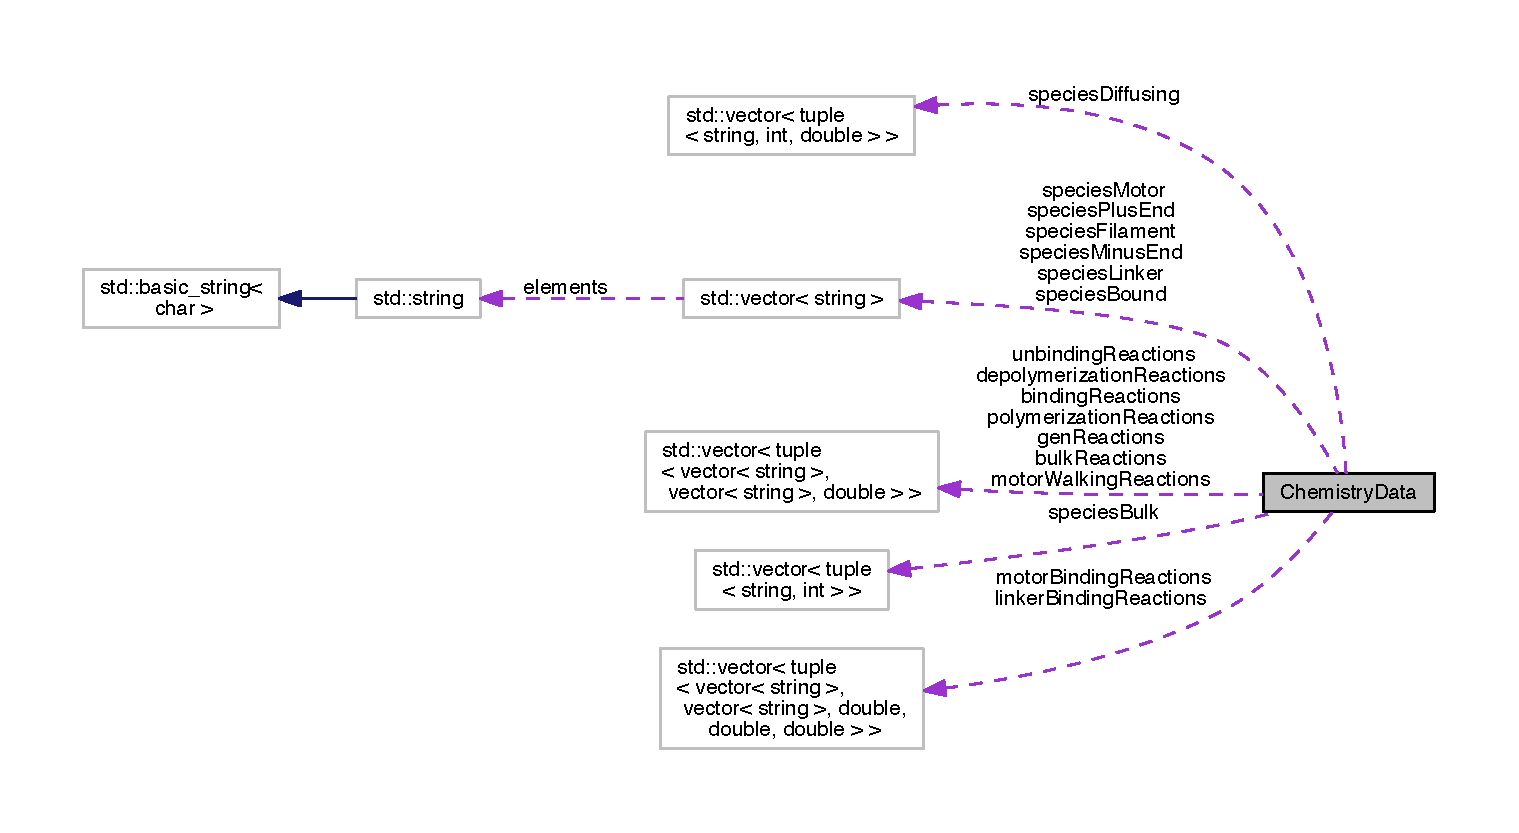
\includegraphics[width=350pt]{structChemistryData__coll__graph}
\end{center}
\end{figure}
\subsection*{Public Attributes}
\begin{DoxyCompactItemize}
\item 
vector$<$ tuple$<$ vector$<$ string $>$\\*
, vector$<$ string $>$, double $>$ $>$ \hyperlink{structChemistryData_a4faa68797fd22c5247b9b52a9057023a}{gen\+Reactions} = \{\}
\begin{DoxyCompactList}\small\item\em \hyperlink{classReaction}{Reaction} happening between bulk and diffusing species O\+N\+L\+Y. \end{DoxyCompactList}\item 
vector$<$ tuple$<$ vector$<$ string $>$\\*
, vector$<$ string $>$, double $>$ $>$ \hyperlink{structChemistryData_a18d2b4d3d417507768bb50f7f43f427b}{bulk\+Reactions} = \{\}
\begin{DoxyCompactList}\small\item\em \hyperlink{classReaction}{Reaction} happening between bulk species O\+N\+L\+Y. \end{DoxyCompactList}\item 
vector$<$ tuple$<$ vector$<$ string $>$\\*
, vector$<$ string $>$, double $>$ $>$ \hyperlink{structChemistryData_a96d5d5289ae3651ab139b1de586b80e7}{motor\+Walking\+Reactions} = \{\}
\begin{DoxyCompactList}\small\item\em \hyperlink{classMotorGhost}{Motor\+Ghost} walking reactions. \end{DoxyCompactList}\item 
vector$<$ tuple$<$ string, int $>$ $>$ \hyperlink{structChemistryData_ae9c303af6cd6b503fe45515c4ee5132b}{species\+Bulk} = \{\}
\begin{DoxyCompactList}\small\item\em \hyperlink{classSpeciesBulk}{Species\+Bulk} parsed, in the form of a tuple which contains the name and initial copy number. \end{DoxyCompactList}\item 
vector$<$ tuple$<$ string, int, \\*
double $>$ $>$ \hyperlink{structChemistryData_acf21fd3143fa3bc4e0e1097ce15cb77c}{species\+Diffusing} = \{\}
\begin{DoxyCompactList}\small\item\em Speices\+Diffusing parsed, in the form of a tuple which contains name, initial copy number per compartment, and the rate of diffusion. \end{DoxyCompactList}\end{DoxyCompactItemize}
{\bf }\par
\begin{DoxyCompactItemize}
\item 
vector$<$ tuple$<$ vector$<$ string $>$\\*
, vector$<$ string $>$, double $>$ $>$ \hyperlink{structChemistryData_a407c6129330a3cffc5afb45f83936945}{polymerization\+Reactions} = \{\}
\begin{DoxyCompactList}\small\item\em \hyperlink{classFilament}{Filament} reactions. \end{DoxyCompactList}\item 
vector$<$ tuple$<$ vector$<$ string $>$\\*
, vector$<$ string $>$, double $>$ $>$ \hyperlink{structChemistryData_aac04b01fc7430d924ce82eee1835cbc7}{depolymerization\+Reactions} = \{\}
\begin{DoxyCompactList}\small\item\em Depolymerization reactions. \end{DoxyCompactList}\item 
vector$<$ tuple$<$ vector$<$ string $>$\\*
, vector$<$ string $>$, double $>$ $>$ \hyperlink{structChemistryData_aec9c915b7471596fa86d4c7ae2f0f8af}{binding\+Reactions} = \{\}
\begin{DoxyCompactList}\small\item\em Binding reactions. \end{DoxyCompactList}\item 
vector$<$ tuple$<$ vector$<$ string $>$\\*
, vector$<$ string $>$, double $>$ $>$ \hyperlink{structChemistryData_a0509ae76d9f3eef9f676c4c8fbab17e7}{unbinding\+Reactions} = \{\}
\begin{DoxyCompactList}\small\item\em Unbinding reactions. \end{DoxyCompactList}\end{DoxyCompactItemize}

{\bf }\par
\begin{DoxyCompactItemize}
\item 
vector$<$ tuple$<$ vector$<$ string $>$\\*
, vector$<$ string $>$, double, \\*
double, double $>$ $>$ \hyperlink{structChemistryData_ae3e27a2c950e196017c06f416ee94628}{linker\+Binding\+Reactions} = \{\}
\begin{DoxyCompactList}\small\item\em Cross filament binding reactions. \end{DoxyCompactList}\item 
vector$<$ tuple$<$ vector$<$ string $>$\\*
, vector$<$ string $>$, double, \\*
double, double $>$ $>$ \hyperlink{structChemistryData_a2a4b2e949b6e0b8f32158cf101d24fa6}{motor\+Binding\+Reactions} = \{\}
\begin{DoxyCompactList}\small\item\em \hyperlink{classMotorGhost}{Motor\+Ghost} reactions. \end{DoxyCompactList}\end{DoxyCompactItemize}

{\bf }\par
\begin{DoxyCompactItemize}
\item 
vector$<$ string $>$ \hyperlink{structChemistryData_a3389b17268aaefcba28539ec3b5e5e35}{species\+Filament} = \{\}
\begin{DoxyCompactList}\small\item\em \hyperlink{classFilament}{Filament} species parsed. \end{DoxyCompactList}\item 
vector$<$ string $>$ \hyperlink{structChemistryData_acab0ca129148f43eaa33847782411b3a}{species\+Bound} = \{\}
\begin{DoxyCompactList}\small\item\em \hyperlink{classFilament}{Filament} species parsed. \end{DoxyCompactList}\item 
vector$<$ string $>$ \hyperlink{structChemistryData_ab41e13ef134b8cb9066fff74ece920ca}{species\+Linker} = \{\}
\begin{DoxyCompactList}\small\item\em \hyperlink{classFilament}{Filament} species parsed. \end{DoxyCompactList}\item 
vector$<$ string $>$ \hyperlink{structChemistryData_a273fd2565deae219bbd1fe3d557f53ba}{species\+Motor} = \{\}
\begin{DoxyCompactList}\small\item\em \hyperlink{classFilament}{Filament} species parsed. \end{DoxyCompactList}\item 
vector$<$ string $>$ \hyperlink{structChemistryData_a627b89ad8dad87e03d249e5dc56eff5a}{species\+Plus\+End} = \{\}
\begin{DoxyCompactList}\small\item\em \hyperlink{classFilament}{Filament} species parsed. \end{DoxyCompactList}\item 
vector$<$ string $>$ \hyperlink{structChemistryData_a8b638671871e8cc1ef65f2c7429d6254}{species\+Minus\+End} = \{\}
\begin{DoxyCompactList}\small\item\em \hyperlink{classFilament}{Filament} species parsed. \end{DoxyCompactList}\end{DoxyCompactItemize}



\subsection{Detailed Description}
Struct to hold chemistry species and reaction information. 

Definition at line 40 of file Parser.\+h.



\subsection{Member Data Documentation}
\hypertarget{structChemistryData_aec9c915b7471596fa86d4c7ae2f0f8af}{\index{Chemistry\+Data@{Chemistry\+Data}!binding\+Reactions@{binding\+Reactions}}
\index{binding\+Reactions@{binding\+Reactions}!Chemistry\+Data@{Chemistry\+Data}}
\subsubsection[{binding\+Reactions}]{\setlength{\rightskip}{0pt plus 5cm}vector$<$tuple$<$vector$<$string$>$, vector$<$string$>$, double$>$ $>$ Chemistry\+Data\+::binding\+Reactions = \{\}}}\label{structChemistryData_aec9c915b7471596fa86d4c7ae2f0f8af}


Binding reactions. 



Definition at line 58 of file Parser.\+h.



Referenced by Simple\+Manager\+Impl\+::gen\+I\+F\+Rxn\+Managers(), and Chemistry\+Parser\+::read\+Chemistry\+Input().

\hypertarget{structChemistryData_a18d2b4d3d417507768bb50f7f43f427b}{\index{Chemistry\+Data@{Chemistry\+Data}!bulk\+Reactions@{bulk\+Reactions}}
\index{bulk\+Reactions@{bulk\+Reactions}!Chemistry\+Data@{Chemistry\+Data}}
\subsubsection[{bulk\+Reactions}]{\setlength{\rightskip}{0pt plus 5cm}vector$<$tuple$<$vector$<$string$>$, vector$<$string$>$, double$>$ $>$ Chemistry\+Data\+::bulk\+Reactions = \{\}}}\label{structChemistryData_a18d2b4d3d417507768bb50f7f43f427b}


\hyperlink{classReaction}{Reaction} happening between bulk species O\+N\+L\+Y. 



Definition at line 45 of file Parser.\+h.



Referenced by Simple\+Manager\+Impl\+::gen\+Bulk\+Reactions(), and Chemistry\+Parser\+::read\+Chemistry\+Input().

\hypertarget{structChemistryData_aac04b01fc7430d924ce82eee1835cbc7}{\index{Chemistry\+Data@{Chemistry\+Data}!depolymerization\+Reactions@{depolymerization\+Reactions}}
\index{depolymerization\+Reactions@{depolymerization\+Reactions}!Chemistry\+Data@{Chemistry\+Data}}
\subsubsection[{depolymerization\+Reactions}]{\setlength{\rightskip}{0pt plus 5cm}vector$<$tuple$<$vector$<$string$>$, vector$<$string$>$, double$>$ $>$ Chemistry\+Data\+::depolymerization\+Reactions = \{\}}}\label{structChemistryData_aac04b01fc7430d924ce82eee1835cbc7}


Depolymerization reactions. 



Definition at line 56 of file Parser.\+h.



Referenced by Simple\+Manager\+Impl\+::gen\+I\+F\+Rxn\+Managers(), and Chemistry\+Parser\+::read\+Chemistry\+Input().

\hypertarget{structChemistryData_a4faa68797fd22c5247b9b52a9057023a}{\index{Chemistry\+Data@{Chemistry\+Data}!gen\+Reactions@{gen\+Reactions}}
\index{gen\+Reactions@{gen\+Reactions}!Chemistry\+Data@{Chemistry\+Data}}
\subsubsection[{gen\+Reactions}]{\setlength{\rightskip}{0pt plus 5cm}vector$<$tuple$<$vector$<$string$>$, vector$<$string$>$, double$>$ $>$ Chemistry\+Data\+::gen\+Reactions = \{\}}}\label{structChemistryData_a4faa68797fd22c5247b9b52a9057023a}


\hyperlink{classReaction}{Reaction} happening between bulk and diffusing species O\+N\+L\+Y. 



Definition at line 43 of file Parser.\+h.



Referenced by Simple\+Manager\+Impl\+::gen\+General\+Reactions(), and Chemistry\+Parser\+::read\+Chemistry\+Input().

\hypertarget{structChemistryData_ae3e27a2c950e196017c06f416ee94628}{\index{Chemistry\+Data@{Chemistry\+Data}!linker\+Binding\+Reactions@{linker\+Binding\+Reactions}}
\index{linker\+Binding\+Reactions@{linker\+Binding\+Reactions}!Chemistry\+Data@{Chemistry\+Data}}
\subsubsection[{linker\+Binding\+Reactions}]{\setlength{\rightskip}{0pt plus 5cm}vector$<$tuple$<$vector$<$string$>$, vector$<$string$>$, double, double, double$>$ $>$ Chemistry\+Data\+::linker\+Binding\+Reactions = \{\}}}\label{structChemistryData_ae3e27a2c950e196017c06f416ee94628}


Cross filament binding reactions. 

All cross filament reactions are held using a vector containing a tuple with the string of reactants, string of products, the reaction rate, and binding range.\+Linker binding reactions 

Definition at line 70 of file Parser.\+h.



Referenced by Simple\+Manager\+Impl\+::gen\+C\+F\+Rxn\+Managers(), and Chemistry\+Parser\+::read\+Chemistry\+Input().

\hypertarget{structChemistryData_a2a4b2e949b6e0b8f32158cf101d24fa6}{\index{Chemistry\+Data@{Chemistry\+Data}!motor\+Binding\+Reactions@{motor\+Binding\+Reactions}}
\index{motor\+Binding\+Reactions@{motor\+Binding\+Reactions}!Chemistry\+Data@{Chemistry\+Data}}
\subsubsection[{motor\+Binding\+Reactions}]{\setlength{\rightskip}{0pt plus 5cm}vector$<$tuple$<$vector$<$string$>$, vector$<$string$>$, double, double, double$>$ $>$ Chemistry\+Data\+::motor\+Binding\+Reactions = \{\}}}\label{structChemistryData_a2a4b2e949b6e0b8f32158cf101d24fa6}


\hyperlink{classMotorGhost}{Motor\+Ghost} reactions. 



Definition at line 72 of file Parser.\+h.



Referenced by Simple\+Manager\+Impl\+::gen\+C\+F\+Rxn\+Managers(), and Chemistry\+Parser\+::read\+Chemistry\+Input().

\hypertarget{structChemistryData_a96d5d5289ae3651ab139b1de586b80e7}{\index{Chemistry\+Data@{Chemistry\+Data}!motor\+Walking\+Reactions@{motor\+Walking\+Reactions}}
\index{motor\+Walking\+Reactions@{motor\+Walking\+Reactions}!Chemistry\+Data@{Chemistry\+Data}}
\subsubsection[{motor\+Walking\+Reactions}]{\setlength{\rightskip}{0pt plus 5cm}vector$<$tuple$<$vector$<$string$>$, vector$<$string$>$, double$>$ $>$ Chemistry\+Data\+::motor\+Walking\+Reactions = \{\}}}\label{structChemistryData_a96d5d5289ae3651ab139b1de586b80e7}


\hyperlink{classMotorGhost}{Motor\+Ghost} walking reactions. 



Definition at line 76 of file Parser.\+h.



Referenced by Simple\+Manager\+Impl\+::gen\+I\+F\+Rxn\+Managers(), and Chemistry\+Parser\+::read\+Chemistry\+Input().

\hypertarget{structChemistryData_a407c6129330a3cffc5afb45f83936945}{\index{Chemistry\+Data@{Chemistry\+Data}!polymerization\+Reactions@{polymerization\+Reactions}}
\index{polymerization\+Reactions@{polymerization\+Reactions}!Chemistry\+Data@{Chemistry\+Data}}
\subsubsection[{polymerization\+Reactions}]{\setlength{\rightskip}{0pt plus 5cm}vector$<$tuple$<$vector$<$string$>$, vector$<$string$>$, double$>$ $>$ Chemistry\+Data\+::polymerization\+Reactions = \{\}}}\label{structChemistryData_a407c6129330a3cffc5afb45f83936945}


\hyperlink{classFilament}{Filament} reactions. 

All \hyperlink{classFilament}{Filament} reactions are held using a vector containing a tuple with the string of reactants, string of products, and the reaction rate.\+Polymerization reactions 

Definition at line 54 of file Parser.\+h.



Referenced by Simple\+Manager\+Impl\+::gen\+I\+F\+Rxn\+Managers(), and Chemistry\+Parser\+::read\+Chemistry\+Input().

\hypertarget{structChemistryData_acab0ca129148f43eaa33847782411b3a}{\index{Chemistry\+Data@{Chemistry\+Data}!species\+Bound@{species\+Bound}}
\index{species\+Bound@{species\+Bound}!Chemistry\+Data@{Chemistry\+Data}}
\subsubsection[{species\+Bound}]{\setlength{\rightskip}{0pt plus 5cm}vector$<$string$>$ Chemistry\+Data\+::species\+Bound = \{\}}}\label{structChemistryData_acab0ca129148f43eaa33847782411b3a}


\hyperlink{classFilament}{Filament} species parsed. 



Definition at line 89 of file Parser.\+h.



Referenced by Simple\+Manager\+Impl\+::initialize(), and Chemistry\+Parser\+::read\+Chemistry\+Input().

\hypertarget{structChemistryData_ae9c303af6cd6b503fe45515c4ee5132b}{\index{Chemistry\+Data@{Chemistry\+Data}!species\+Bulk@{species\+Bulk}}
\index{species\+Bulk@{species\+Bulk}!Chemistry\+Data@{Chemistry\+Data}}
\subsubsection[{species\+Bulk}]{\setlength{\rightskip}{0pt plus 5cm}vector$<$tuple$<$string, int$>$ $>$ Chemistry\+Data\+::species\+Bulk = \{\}}}\label{structChemistryData_ae9c303af6cd6b503fe45515c4ee5132b}


\hyperlink{classSpeciesBulk}{Species\+Bulk} parsed, in the form of a tuple which contains the name and initial copy number. 



Definition at line 80 of file Parser.\+h.



Referenced by Simple\+Manager\+Impl\+::gen\+Bulk\+Reactions(), Simple\+Manager\+Impl\+::gen\+C\+F\+Rxn\+Managers(), Simple\+Manager\+Impl\+::gen\+General\+Reactions(), Simple\+Manager\+Impl\+::gen\+I\+F\+Rxn\+Managers(), Simple\+Manager\+Impl\+::initialize(), and Chemistry\+Parser\+::read\+Chemistry\+Input().

\hypertarget{structChemistryData_acf21fd3143fa3bc4e0e1097ce15cb77c}{\index{Chemistry\+Data@{Chemistry\+Data}!species\+Diffusing@{species\+Diffusing}}
\index{species\+Diffusing@{species\+Diffusing}!Chemistry\+Data@{Chemistry\+Data}}
\subsubsection[{species\+Diffusing}]{\setlength{\rightskip}{0pt plus 5cm}vector$<$tuple$<$string, int, double$>$ $>$ Chemistry\+Data\+::species\+Diffusing = \{\}}}\label{structChemistryData_acf21fd3143fa3bc4e0e1097ce15cb77c}


Speices\+Diffusing parsed, in the form of a tuple which contains name, initial copy number per compartment, and the rate of diffusion. 



Definition at line 84 of file Parser.\+h.



Referenced by Simple\+Manager\+Impl\+::gen\+C\+F\+Rxn\+Managers(), Simple\+Manager\+Impl\+::gen\+General\+Reactions(), Simple\+Manager\+Impl\+::gen\+I\+F\+Rxn\+Managers(), Simple\+Manager\+Impl\+::initialize(), and Chemistry\+Parser\+::read\+Chemistry\+Input().

\hypertarget{structChemistryData_a3389b17268aaefcba28539ec3b5e5e35}{\index{Chemistry\+Data@{Chemistry\+Data}!species\+Filament@{species\+Filament}}
\index{species\+Filament@{species\+Filament}!Chemistry\+Data@{Chemistry\+Data}}
\subsubsection[{species\+Filament}]{\setlength{\rightskip}{0pt plus 5cm}vector$<$string$>$ Chemistry\+Data\+::species\+Filament = \{\}}}\label{structChemistryData_a3389b17268aaefcba28539ec3b5e5e35}


\hyperlink{classFilament}{Filament} species parsed. 



Definition at line 88 of file Parser.\+h.



Referenced by Simple\+Manager\+Impl\+::initialize(), and Chemistry\+Parser\+::read\+Chemistry\+Input().

\hypertarget{structChemistryData_ab41e13ef134b8cb9066fff74ece920ca}{\index{Chemistry\+Data@{Chemistry\+Data}!species\+Linker@{species\+Linker}}
\index{species\+Linker@{species\+Linker}!Chemistry\+Data@{Chemistry\+Data}}
\subsubsection[{species\+Linker}]{\setlength{\rightskip}{0pt plus 5cm}vector$<$string$>$ Chemistry\+Data\+::species\+Linker = \{\}}}\label{structChemistryData_ab41e13ef134b8cb9066fff74ece920ca}


\hyperlink{classFilament}{Filament} species parsed. 



Definition at line 90 of file Parser.\+h.



Referenced by Simple\+Manager\+Impl\+::initialize(), and Chemistry\+Parser\+::read\+Chemistry\+Input().

\hypertarget{structChemistryData_a8b638671871e8cc1ef65f2c7429d6254}{\index{Chemistry\+Data@{Chemistry\+Data}!species\+Minus\+End@{species\+Minus\+End}}
\index{species\+Minus\+End@{species\+Minus\+End}!Chemistry\+Data@{Chemistry\+Data}}
\subsubsection[{species\+Minus\+End}]{\setlength{\rightskip}{0pt plus 5cm}vector$<$string$>$ Chemistry\+Data\+::species\+Minus\+End = \{\}}}\label{structChemistryData_a8b638671871e8cc1ef65f2c7429d6254}


\hyperlink{classFilament}{Filament} species parsed. 



Definition at line 93 of file Parser.\+h.



Referenced by Simple\+Manager\+Impl\+::initialize(), and Chemistry\+Parser\+::read\+Chemistry\+Input().

\hypertarget{structChemistryData_a273fd2565deae219bbd1fe3d557f53ba}{\index{Chemistry\+Data@{Chemistry\+Data}!species\+Motor@{species\+Motor}}
\index{species\+Motor@{species\+Motor}!Chemistry\+Data@{Chemistry\+Data}}
\subsubsection[{species\+Motor}]{\setlength{\rightskip}{0pt plus 5cm}vector$<$string$>$ Chemistry\+Data\+::species\+Motor = \{\}}}\label{structChemistryData_a273fd2565deae219bbd1fe3d557f53ba}


\hyperlink{classFilament}{Filament} species parsed. 



Definition at line 91 of file Parser.\+h.



Referenced by Simple\+Manager\+Impl\+::initialize(), and Chemistry\+Parser\+::read\+Chemistry\+Input().

\hypertarget{structChemistryData_a627b89ad8dad87e03d249e5dc56eff5a}{\index{Chemistry\+Data@{Chemistry\+Data}!species\+Plus\+End@{species\+Plus\+End}}
\index{species\+Plus\+End@{species\+Plus\+End}!Chemistry\+Data@{Chemistry\+Data}}
\subsubsection[{species\+Plus\+End}]{\setlength{\rightskip}{0pt plus 5cm}vector$<$string$>$ Chemistry\+Data\+::species\+Plus\+End = \{\}}}\label{structChemistryData_a627b89ad8dad87e03d249e5dc56eff5a}


\hyperlink{classFilament}{Filament} species parsed. 



Definition at line 92 of file Parser.\+h.



Referenced by Simple\+Manager\+Impl\+::initialize(), and Chemistry\+Parser\+::read\+Chemistry\+Input().

\hypertarget{structChemistryData_a0509ae76d9f3eef9f676c4c8fbab17e7}{\index{Chemistry\+Data@{Chemistry\+Data}!unbinding\+Reactions@{unbinding\+Reactions}}
\index{unbinding\+Reactions@{unbinding\+Reactions}!Chemistry\+Data@{Chemistry\+Data}}
\subsubsection[{unbinding\+Reactions}]{\setlength{\rightskip}{0pt plus 5cm}vector$<$tuple$<$vector$<$string$>$, vector$<$string$>$, double$>$ $>$ Chemistry\+Data\+::unbinding\+Reactions = \{\}}}\label{structChemistryData_a0509ae76d9f3eef9f676c4c8fbab17e7}


Unbinding reactions. 



Definition at line 60 of file Parser.\+h.



Referenced by Simple\+Manager\+Impl\+::gen\+I\+F\+Rxn\+Managers(), and Chemistry\+Parser\+::read\+Chemistry\+Input().



The documentation for this struct was generated from the following file\+:\begin{DoxyCompactItemize}
\item 
M3\+S\+Y\+M/\hyperlink{Parser_8h}{Parser.\+h}\end{DoxyCompactItemize}

\hypertarget{structChemistryParameters}{\section{Chemistry\+Parameters Struct Reference}
\label{structChemistryParameters}\index{Chemistry\+Parameters@{Chemistry\+Parameters}}
}


Struct to hold chemistry parameters for the system.  




{\ttfamily \#include $<$System\+Parameters.\+h$>$}

\subsection*{Public Attributes}
{\bf }\par
\begin{DoxyCompactItemize}
\item 
short \hyperlink{structChemistryParameters_a33f49ae4bed264d303989b7372b1ba4b}{num\+Bulk\+Species} = 0
\begin{DoxyCompactList}\small\item\em Number of general species. \end{DoxyCompactList}\item 
short \hyperlink{structChemistryParameters_a78116d90c15faebd400cb5c75ce00e26}{num\+Diffusing\+Species} = 0
\begin{DoxyCompactList}\small\item\em Number of general species. \end{DoxyCompactList}\end{DoxyCompactItemize}

{\bf }\par
\begin{DoxyCompactItemize}
\item 
short \hyperlink{structChemistryParameters_aa3ff68ed0be86482f1ea6d40b9d0fa1c}{num\+Filament\+Species} = 0
\begin{DoxyCompactList}\small\item\em Number of filament related species. \end{DoxyCompactList}\item 
short \hyperlink{structChemistryParameters_a14a3adb276b758bb6f2e5d0a27f80b15}{num\+Plus\+End\+Species} = 0
\begin{DoxyCompactList}\small\item\em Number of filament related species. \end{DoxyCompactList}\item 
short \hyperlink{structChemistryParameters_a13d911b0639656b466b1ea13be22be00}{num\+Minus\+End\+Species} = 0
\begin{DoxyCompactList}\small\item\em Number of filament related species. \end{DoxyCompactList}\item 
short \hyperlink{structChemistryParameters_a47fbf96b070976e8e0b7bb25a381ea54}{num\+Bound\+Species} = 0
\begin{DoxyCompactList}\small\item\em Number of filament related species. \end{DoxyCompactList}\item 
short \hyperlink{structChemistryParameters_af82c8c5d13f1e092d9eb69a7e8e3b5a4}{num\+Linker\+Species} = 0
\begin{DoxyCompactList}\small\item\em Number of filament related species. \end{DoxyCompactList}\item 
short \hyperlink{structChemistryParameters_a6aecadee2f3bb6bc436395473447c485}{num\+Motor\+Species} = 0
\begin{DoxyCompactList}\small\item\em Number of filament related species. \end{DoxyCompactList}\end{DoxyCompactItemize}



\subsection{Detailed Description}
Struct to hold chemistry parameters for the system. 

Definition at line 59 of file System\+Parameters.\+h.



\subsection{Member Data Documentation}
\hypertarget{structChemistryParameters_a47fbf96b070976e8e0b7bb25a381ea54}{\index{Chemistry\+Parameters@{Chemistry\+Parameters}!num\+Bound\+Species@{num\+Bound\+Species}}
\index{num\+Bound\+Species@{num\+Bound\+Species}!Chemistry\+Parameters@{Chemistry\+Parameters}}
\subsubsection[{num\+Bound\+Species}]{\setlength{\rightskip}{0pt plus 5cm}short Chemistry\+Parameters\+::num\+Bound\+Species = 0}}\label{structChemistryParameters_a47fbf96b070976e8e0b7bb25a381ea54}


Number of filament related species. 



Definition at line 72 of file System\+Parameters.\+h.



Referenced by C\+Monomer\+::add\+Species\+Bound(), C\+Monomer\+::\+C\+Monomer(), C\+Monomer\+::print(), System\+Parser\+::read\+Chemistry\+Parameters(), and C\+Cylinder\+::$\sim$\+C\+Cylinder().

\hypertarget{structChemistryParameters_a33f49ae4bed264d303989b7372b1ba4b}{\index{Chemistry\+Parameters@{Chemistry\+Parameters}!num\+Bulk\+Species@{num\+Bulk\+Species}}
\index{num\+Bulk\+Species@{num\+Bulk\+Species}!Chemistry\+Parameters@{Chemistry\+Parameters}}
\subsubsection[{num\+Bulk\+Species}]{\setlength{\rightskip}{0pt plus 5cm}short Chemistry\+Parameters\+::num\+Bulk\+Species = 0}}\label{structChemistryParameters_a33f49ae4bed264d303989b7372b1ba4b}


Number of general species. 



Definition at line 63 of file System\+Parameters.\+h.



Referenced by System\+Parser\+::read\+Chemistry\+Parameters().

\hypertarget{structChemistryParameters_a78116d90c15faebd400cb5c75ce00e26}{\index{Chemistry\+Parameters@{Chemistry\+Parameters}!num\+Diffusing\+Species@{num\+Diffusing\+Species}}
\index{num\+Diffusing\+Species@{num\+Diffusing\+Species}!Chemistry\+Parameters@{Chemistry\+Parameters}}
\subsubsection[{num\+Diffusing\+Species}]{\setlength{\rightskip}{0pt plus 5cm}short Chemistry\+Parameters\+::num\+Diffusing\+Species = 0}}\label{structChemistryParameters_a78116d90c15faebd400cb5c75ce00e26}


Number of general species. 



Definition at line 64 of file System\+Parameters.\+h.



Referenced by System\+Parser\+::read\+Chemistry\+Parameters().

\hypertarget{structChemistryParameters_aa3ff68ed0be86482f1ea6d40b9d0fa1c}{\index{Chemistry\+Parameters@{Chemistry\+Parameters}!num\+Filament\+Species@{num\+Filament\+Species}}
\index{num\+Filament\+Species@{num\+Filament\+Species}!Chemistry\+Parameters@{Chemistry\+Parameters}}
\subsubsection[{num\+Filament\+Species}]{\setlength{\rightskip}{0pt plus 5cm}short Chemistry\+Parameters\+::num\+Filament\+Species = 0}}\label{structChemistryParameters_aa3ff68ed0be86482f1ea6d40b9d0fa1c}


Number of filament related species. 



Definition at line 69 of file System\+Parameters.\+h.



Referenced by C\+Monomer\+::add\+Species\+Filament(), C\+Monomer\+::\+C\+Monomer(), C\+Monomer\+::print(), System\+Parser\+::read\+Chemistry\+Parameters(), and C\+Cylinder\+::$\sim$\+C\+Cylinder().

\hypertarget{structChemistryParameters_af82c8c5d13f1e092d9eb69a7e8e3b5a4}{\index{Chemistry\+Parameters@{Chemistry\+Parameters}!num\+Linker\+Species@{num\+Linker\+Species}}
\index{num\+Linker\+Species@{num\+Linker\+Species}!Chemistry\+Parameters@{Chemistry\+Parameters}}
\subsubsection[{num\+Linker\+Species}]{\setlength{\rightskip}{0pt plus 5cm}short Chemistry\+Parameters\+::num\+Linker\+Species = 0}}\label{structChemistryParameters_af82c8c5d13f1e092d9eb69a7e8e3b5a4}


Number of filament related species. 



Definition at line 73 of file System\+Parameters.\+h.



Referenced by C\+Monomer\+::add\+Species\+Linker(), C\+Monomer\+::\+C\+Monomer(), C\+Monomer\+::print(), System\+Parser\+::read\+Chemistry\+Parameters(), and C\+Cylinder\+::$\sim$\+C\+Cylinder().

\hypertarget{structChemistryParameters_a13d911b0639656b466b1ea13be22be00}{\index{Chemistry\+Parameters@{Chemistry\+Parameters}!num\+Minus\+End\+Species@{num\+Minus\+End\+Species}}
\index{num\+Minus\+End\+Species@{num\+Minus\+End\+Species}!Chemistry\+Parameters@{Chemistry\+Parameters}}
\subsubsection[{num\+Minus\+End\+Species}]{\setlength{\rightskip}{0pt plus 5cm}short Chemistry\+Parameters\+::num\+Minus\+End\+Species = 0}}\label{structChemistryParameters_a13d911b0639656b466b1ea13be22be00}


Number of filament related species. 



Definition at line 71 of file System\+Parameters.\+h.



Referenced by C\+Monomer\+::add\+Species\+Minus\+End(), C\+Monomer\+::\+C\+Monomer(), C\+Monomer\+::print(), System\+Parser\+::read\+Chemistry\+Parameters(), and C\+Cylinder\+::$\sim$\+C\+Cylinder().

\hypertarget{structChemistryParameters_a6aecadee2f3bb6bc436395473447c485}{\index{Chemistry\+Parameters@{Chemistry\+Parameters}!num\+Motor\+Species@{num\+Motor\+Species}}
\index{num\+Motor\+Species@{num\+Motor\+Species}!Chemistry\+Parameters@{Chemistry\+Parameters}}
\subsubsection[{num\+Motor\+Species}]{\setlength{\rightskip}{0pt plus 5cm}short Chemistry\+Parameters\+::num\+Motor\+Species = 0}}\label{structChemistryParameters_a6aecadee2f3bb6bc436395473447c485}


Number of filament related species. 



Definition at line 74 of file System\+Parameters.\+h.



Referenced by C\+Monomer\+::add\+Species\+Motor(), C\+Monomer\+::\+C\+Monomer(), C\+Monomer\+::print(), System\+Parser\+::read\+Chemistry\+Parameters(), and C\+Cylinder\+::$\sim$\+C\+Cylinder().

\hypertarget{structChemistryParameters_a14a3adb276b758bb6f2e5d0a27f80b15}{\index{Chemistry\+Parameters@{Chemistry\+Parameters}!num\+Plus\+End\+Species@{num\+Plus\+End\+Species}}
\index{num\+Plus\+End\+Species@{num\+Plus\+End\+Species}!Chemistry\+Parameters@{Chemistry\+Parameters}}
\subsubsection[{num\+Plus\+End\+Species}]{\setlength{\rightskip}{0pt plus 5cm}short Chemistry\+Parameters\+::num\+Plus\+End\+Species = 0}}\label{structChemistryParameters_a14a3adb276b758bb6f2e5d0a27f80b15}


Number of filament related species. 



Definition at line 70 of file System\+Parameters.\+h.



Referenced by C\+Monomer\+::add\+Species\+Plus\+End(), C\+Monomer\+::\+C\+Monomer(), C\+Monomer\+::print(), System\+Parser\+::read\+Chemistry\+Parameters(), and C\+Cylinder\+::$\sim$\+C\+Cylinder().



The documentation for this struct was generated from the following file\+:\begin{DoxyCompactItemize}
\item 
M3\+S\+Y\+M/\hyperlink{SystemParameters_8h}{System\+Parameters.\+h}\end{DoxyCompactItemize}

\hypertarget{classChemistryParser}{\section{Chemistry\+Parser Class Reference}
\label{classChemistryParser}\index{Chemistry\+Parser@{Chemistry\+Parser}}
}


Used to parse all chemical information.  




{\ttfamily \#include $<$Parser.\+h$>$}



Inheritance diagram for Chemistry\+Parser\+:\nopagebreak
\begin{figure}[H]
\begin{center}
\leavevmode
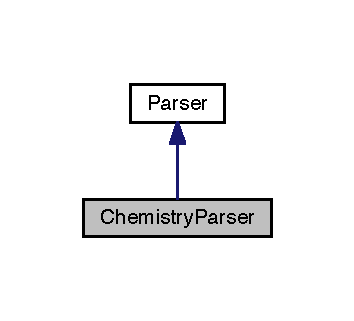
\includegraphics[width=170pt]{classChemistryParser__inherit__graph}
\end{center}
\end{figure}


Collaboration diagram for Chemistry\+Parser\+:\nopagebreak
\begin{figure}[H]
\begin{center}
\leavevmode
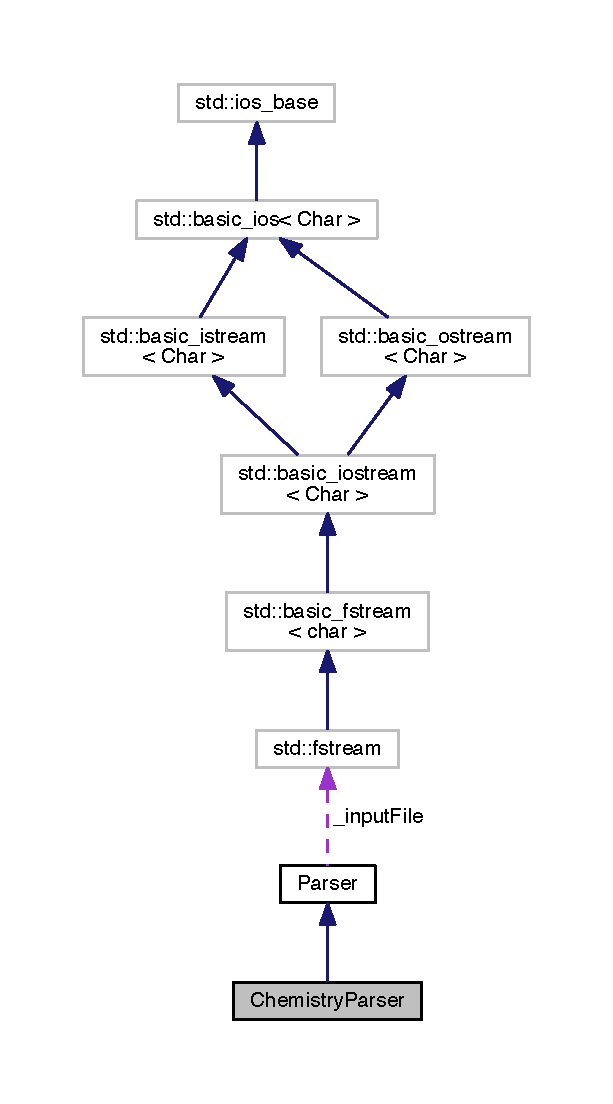
\includegraphics[width=294pt]{classChemistryParser__coll__graph}
\end{center}
\end{figure}
\subsection*{Public Member Functions}
\begin{DoxyCompactItemize}
\item 
\hyperlink{classChemistryParser_af054e9adc10a110223bdab9ed0a22adc}{Chemistry\+Parser} (string input\+File\+Name)
\item 
\hyperlink{classChemistryParser_a0918e9fb2e03ef37f920c1214b5286cf}{$\sim$\+Chemistry\+Parser} ()
\item 
\hyperlink{structChemistryData}{Chemistry\+Data} \hyperlink{classChemistryParser_a655de1a88016755e9dffae5081d00963}{read\+Chemistry\+Input} ()
\begin{DoxyCompactList}\small\item\em Reads chemical reactions and species from input file. \end{DoxyCompactList}\end{DoxyCompactItemize}
\subsection*{Protected Attributes}
\begin{DoxyCompactItemize}
\item 
fstream \hyperlink{classParser_adc64c51d84a8fe723f7b4f13ca4d37cd}{\+\_\+input\+File}
\begin{DoxyCompactList}\small\item\em input file being used \end{DoxyCompactList}\end{DoxyCompactItemize}


\subsection{Detailed Description}
Used to parse all chemical information. 

Definition at line 228 of file Parser.\+h.



\subsection{Constructor \& Destructor Documentation}
\hypertarget{classChemistryParser_af054e9adc10a110223bdab9ed0a22adc}{\index{Chemistry\+Parser@{Chemistry\+Parser}!Chemistry\+Parser@{Chemistry\+Parser}}
\index{Chemistry\+Parser@{Chemistry\+Parser}!Chemistry\+Parser@{Chemistry\+Parser}}
\subsubsection[{Chemistry\+Parser}]{\setlength{\rightskip}{0pt plus 5cm}Chemistry\+Parser\+::\+Chemistry\+Parser (
\begin{DoxyParamCaption}
\item[{string}]{input\+File\+Name}
\end{DoxyParamCaption}
)\hspace{0.3cm}{\ttfamily [inline]}}}\label{classChemistryParser_af054e9adc10a110223bdab9ed0a22adc}


Definition at line 231 of file Parser.\+h.

\hypertarget{classChemistryParser_a0918e9fb2e03ef37f920c1214b5286cf}{\index{Chemistry\+Parser@{Chemistry\+Parser}!````~Chemistry\+Parser@{$\sim$\+Chemistry\+Parser}}
\index{````~Chemistry\+Parser@{$\sim$\+Chemistry\+Parser}!Chemistry\+Parser@{Chemistry\+Parser}}
\subsubsection[{$\sim$\+Chemistry\+Parser}]{\setlength{\rightskip}{0pt plus 5cm}Chemistry\+Parser\+::$\sim$\+Chemistry\+Parser (
\begin{DoxyParamCaption}
{}
\end{DoxyParamCaption}
)\hspace{0.3cm}{\ttfamily [inline]}}}\label{classChemistryParser_a0918e9fb2e03ef37f920c1214b5286cf}


Definition at line 232 of file Parser.\+h.



\subsection{Member Function Documentation}
\hypertarget{classChemistryParser_a655de1a88016755e9dffae5081d00963}{\index{Chemistry\+Parser@{Chemistry\+Parser}!read\+Chemistry\+Input@{read\+Chemistry\+Input}}
\index{read\+Chemistry\+Input@{read\+Chemistry\+Input}!Chemistry\+Parser@{Chemistry\+Parser}}
\subsubsection[{read\+Chemistry\+Input}]{\setlength{\rightskip}{0pt plus 5cm}{\bf Chemistry\+Data} Chemistry\+Parser\+::read\+Chemistry\+Input (
\begin{DoxyParamCaption}
{}
\end{DoxyParamCaption}
)}}\label{classChemistryParser_a655de1a88016755e9dffae5081d00963}


Reads chemical reactions and species from input file. 

Returns a \hyperlink{structChemistryData}{Chemistry\+Data} struct containing this data 

Definition at line 868 of file Parser.\+cpp.



References Parser\+::\+\_\+input\+File, Chemistry\+Data\+::binding\+Reactions, Chemistry\+Data\+::bulk\+Reactions, Chemistry\+Data\+::depolymerization\+Reactions, Chemistry\+Data\+::gen\+Reactions, Chemistry\+Data\+::linker\+Binding\+Reactions, Chemistry\+Data\+::motor\+Binding\+Reactions, Chemistry\+Data\+::motor\+Walking\+Reactions, Chemistry\+Data\+::polymerization\+Reactions, Chemistry\+Data\+::species\+Bound, Chemistry\+Data\+::species\+Bulk, Chemistry\+Data\+::species\+Diffusing, Chemistry\+Data\+::species\+Filament, Chemistry\+Data\+::species\+Linker, Chemistry\+Data\+::species\+Minus\+End, Chemistry\+Data\+::species\+Motor, Chemistry\+Data\+::species\+Plus\+End, and Chemistry\+Data\+::unbinding\+Reactions.



Referenced by Controller\+::initialize().



\subsection{Member Data Documentation}
\hypertarget{classParser_adc64c51d84a8fe723f7b4f13ca4d37cd}{\index{Chemistry\+Parser@{Chemistry\+Parser}!\+\_\+input\+File@{\+\_\+input\+File}}
\index{\+\_\+input\+File@{\+\_\+input\+File}!Chemistry\+Parser@{Chemistry\+Parser}}
\subsubsection[{\+\_\+input\+File}]{\setlength{\rightskip}{0pt plus 5cm}fstream Parser\+::\+\_\+input\+File\hspace{0.3cm}{\ttfamily [protected]}, {\ttfamily [inherited]}}}\label{classParser_adc64c51d84a8fe723f7b4f13ca4d37cd}


input file being used 



Definition at line 166 of file Parser.\+h.



Referenced by Parser\+::\+Parser(), System\+Parser\+::read\+Boundary\+Parameters(), System\+Parser\+::read\+Boundary\+Type(), System\+Parser\+::read\+Chemistry\+Algorithm(), read\+Chemistry\+Input(), System\+Parser\+::read\+Chemistry\+Parameters(), System\+Parser\+::read\+Chemistry\+Setup(), Filament\+Parser\+::read\+Filaments(), System\+Parser\+::read\+Filament\+Setup(), System\+Parser\+::read\+Geometry\+Parameters(), System\+Parser\+::read\+Mechanics\+Algorithm(), System\+Parser\+::read\+Mechanics\+F\+F\+Type(), System\+Parser\+::read\+Mechanics\+Parameters(), and Parser\+::$\sim$\+Parser().



The documentation for this class was generated from the following files\+:\begin{DoxyCompactItemize}
\item 
M3\+S\+Y\+M/\hyperlink{Parser_8h}{Parser.\+h}\item 
M3\+S\+Y\+M/\hyperlink{Parser_8cpp}{Parser.\+cpp}\end{DoxyCompactItemize}

\hypertarget{structChemistrySetup}{\section{Chemistry\+Setup Struct Reference}
\label{structChemistrySetup}\index{Chemistry\+Setup@{Chemistry\+Setup}}
}


Struct to hold chem setup information.  




{\ttfamily \#include $<$Parser.\+h$>$}



Collaboration diagram for Chemistry\+Setup\+:\nopagebreak
\begin{figure}[H]
\begin{center}
\leavevmode
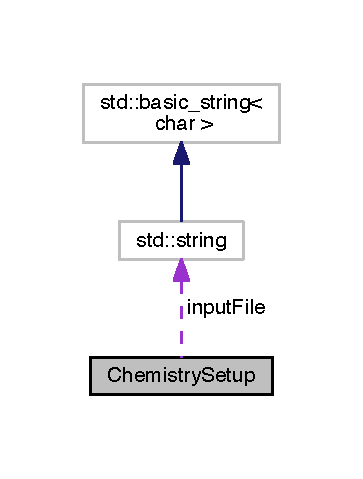
\includegraphics[width=174pt]{structChemistrySetup__coll__graph}
\end{center}
\end{figure}
\subsection*{Public Attributes}
\begin{DoxyCompactItemize}
\item 
string \hyperlink{structChemistrySetup_a662524c2c7d29c8b83a6016559d256e5}{input\+File} = \char`\"{}\char`\"{}
\end{DoxyCompactItemize}


\subsection{Detailed Description}
Struct to hold chem setup information. 

Definition at line 137 of file Parser.\+h.



\subsection{Member Data Documentation}
\hypertarget{structChemistrySetup_a662524c2c7d29c8b83a6016559d256e5}{\index{Chemistry\+Setup@{Chemistry\+Setup}!input\+File@{input\+File}}
\index{input\+File@{input\+File}!Chemistry\+Setup@{Chemistry\+Setup}}
\subsubsection[{input\+File}]{\setlength{\rightskip}{0pt plus 5cm}string Chemistry\+Setup\+::input\+File = \char`\"{}\char`\"{}}}\label{structChemistrySetup_a662524c2c7d29c8b83a6016559d256e5}


Definition at line 139 of file Parser.\+h.



Referenced by System\+Parser\+::read\+Chemistry\+Setup().



The documentation for this struct was generated from the following file\+:\begin{DoxyCompactItemize}
\item 
M3\+S\+Y\+M/\hyperlink{Parser_8h}{Parser.\+h}\end{DoxyCompactItemize}

\hypertarget{classChemManager}{\section{Chem\+Manager Class Reference}
\label{classChemManager}\index{Chem\+Manager@{Chem\+Manager}}
}


For initailizing chemical reactions based on a specific system.  




{\ttfamily \#include $<$Chem\+Manager.\+h$>$}



Collaboration diagram for Chem\+Manager\+:\nopagebreak
\begin{figure}[H]
\begin{center}
\leavevmode
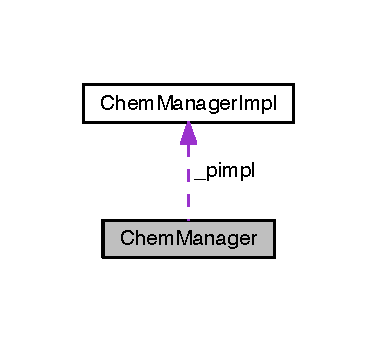
\includegraphics[width=181pt]{classChemManager__coll__graph}
\end{center}
\end{figure}
\subsection*{Static Public Member Functions}
\begin{DoxyCompactItemize}
\item 
static void \hyperlink{classChemManager_a47f584be692f31e39d7598f4f7488796}{set\+Instance} (\hyperlink{classChemManagerImpl}{Chem\+Manager\+Impl} $\ast$cii)
\begin{DoxyCompactList}\small\item\em Set the chem\+Manager instance. \end{DoxyCompactList}\item 
static void \hyperlink{classChemManager_ab3344ccf25c9ea90337e90bd9cf5ebff}{initialize} (\hyperlink{structChemistryData}{Chemistry\+Data} \&chem)
\begin{DoxyCompactList}\small\item\em Initialize the compartment grid, based on the given simulation. \end{DoxyCompactList}\item 
static void \hyperlink{classChemManager_a8c3958ed962520cff0e1d26b92596e68}{initialize\+C\+Cylinder} (\hyperlink{classCCylinder}{C\+Cylinder} $\ast$cc, \hyperlink{classFilament}{Filament} $\ast$f, bool extension\+Front, bool extension\+Back, bool creation)
\begin{DoxyCompactList}\small\item\em Initializer, based on the given simulation. \end{DoxyCompactList}\item 
static void \hyperlink{classChemManager_ae85244eb50a4254d525eb749c44a96a6}{update\+C\+Cylinder} (\hyperlink{classCCylinder}{C\+Cylinder} $\ast$cc)
\begin{DoxyCompactList}\small\item\em add/update cross cylinder reactions that are within range \end{DoxyCompactList}\end{DoxyCompactItemize}
\subsection*{Private Member Functions}
\begin{DoxyCompactItemize}
\item 
\hyperlink{classChemManager_ac133ef2eabc4f5f002660f9d69e9c0fb}{Chem\+Manager} ()
\end{DoxyCompactItemize}
\subsection*{Static Private Attributes}
\begin{DoxyCompactItemize}
\item 
static \hyperlink{classChemManagerImpl}{Chem\+Manager\+Impl} $\ast$ \hyperlink{classChemManager_aa8fe0dad2d7ed00b8fd05e3ae6a2dd4a}{\+\_\+pimpl} = 0
\begin{DoxyCompactList}\small\item\em Store a pointer to a specific implementation of the initializer; no ownership. \end{DoxyCompactList}\end{DoxyCompactItemize}


\subsection{Detailed Description}
For initailizing chemical reactions based on a specific system. 

\hyperlink{classChemManager}{Chem\+Manager} is a singleton used for initailizing all chemistry in the system. Initialized by the \hyperlink{classCController}{C\+Controller}, the \hyperlink{classChemManager}{Chem\+Manager} initializes the chemical components of the \hyperlink{classCompartmentGrid}{Compartment\+Grid} as well as initializes all \hyperlink{classCCylinder}{C\+Cylinders} created. The \hyperlink{classChemManager}{Chem\+Manager} can also update chemical components of a \hyperlink{classCCylinder}{C\+Cylinder}. 

Definition at line 33 of file Chem\+Manager.\+h.



\subsection{Constructor \& Destructor Documentation}
\hypertarget{classChemManager_ac133ef2eabc4f5f002660f9d69e9c0fb}{\index{Chem\+Manager@{Chem\+Manager}!Chem\+Manager@{Chem\+Manager}}
\index{Chem\+Manager@{Chem\+Manager}!Chem\+Manager@{Chem\+Manager}}
\subsubsection[{Chem\+Manager}]{\setlength{\rightskip}{0pt plus 5cm}Chem\+Manager\+::\+Chem\+Manager (
\begin{DoxyParamCaption}
{}
\end{DoxyParamCaption}
)\hspace{0.3cm}{\ttfamily [inline]}, {\ttfamily [private]}}}\label{classChemManager_ac133ef2eabc4f5f002660f9d69e9c0fb}


Definition at line 51 of file Chem\+Manager.\+h.



\subsection{Member Function Documentation}
\hypertarget{classChemManager_ab3344ccf25c9ea90337e90bd9cf5ebff}{\index{Chem\+Manager@{Chem\+Manager}!initialize@{initialize}}
\index{initialize@{initialize}!Chem\+Manager@{Chem\+Manager}}
\subsubsection[{initialize}]{\setlength{\rightskip}{0pt plus 5cm}void Chem\+Manager\+::initialize (
\begin{DoxyParamCaption}
\item[{{\bf Chemistry\+Data} \&}]{chem}
\end{DoxyParamCaption}
)\hspace{0.3cm}{\ttfamily [static]}}}\label{classChemManager_ab3344ccf25c9ea90337e90bd9cf5ebff}


Initialize the compartment grid, based on the given simulation. 



Definition at line 24 of file Chem\+Manager.\+cpp.



References \+\_\+pimpl, and Chem\+Manager\+Impl\+::initialize().



Referenced by C\+Controller\+::initialize().

\hypertarget{classChemManager_a8c3958ed962520cff0e1d26b92596e68}{\index{Chem\+Manager@{Chem\+Manager}!initialize\+C\+Cylinder@{initialize\+C\+Cylinder}}
\index{initialize\+C\+Cylinder@{initialize\+C\+Cylinder}!Chem\+Manager@{Chem\+Manager}}
\subsubsection[{initialize\+C\+Cylinder}]{\setlength{\rightskip}{0pt plus 5cm}void Chem\+Manager\+::initialize\+C\+Cylinder (
\begin{DoxyParamCaption}
\item[{{\bf C\+Cylinder} $\ast$}]{cc, }
\item[{{\bf Filament} $\ast$}]{f, }
\item[{bool}]{extension\+Front, }
\item[{bool}]{extension\+Back, }
\item[{bool}]{creation}
\end{DoxyParamCaption}
)\hspace{0.3cm}{\ttfamily [static]}}}\label{classChemManager_a8c3958ed962520cff0e1d26b92596e68}


Initializer, based on the given simulation. 



Definition at line 29 of file Chem\+Manager.\+cpp.



References \+\_\+pimpl, and Chem\+Manager\+Impl\+::initialize\+C\+Cylinder().



Referenced by Cylinder\+::\+Cylinder().

\hypertarget{classChemManager_a47f584be692f31e39d7598f4f7488796}{\index{Chem\+Manager@{Chem\+Manager}!set\+Instance@{set\+Instance}}
\index{set\+Instance@{set\+Instance}!Chem\+Manager@{Chem\+Manager}}
\subsubsection[{set\+Instance}]{\setlength{\rightskip}{0pt plus 5cm}void Chem\+Manager\+::set\+Instance (
\begin{DoxyParamCaption}
\item[{{\bf Chem\+Manager\+Impl} $\ast$}]{cii}
\end{DoxyParamCaption}
)\hspace{0.3cm}{\ttfamily [static]}}}\label{classChemManager_a47f584be692f31e39d7598f4f7488796}


Set the chem\+Manager instance. 



Definition at line 18 of file Chem\+Manager.\+cpp.



References \+\_\+pimpl.



Referenced by C\+Controller\+::initialize().

\hypertarget{classChemManager_ae85244eb50a4254d525eb749c44a96a6}{\index{Chem\+Manager@{Chem\+Manager}!update\+C\+Cylinder@{update\+C\+Cylinder}}
\index{update\+C\+Cylinder@{update\+C\+Cylinder}!Chem\+Manager@{Chem\+Manager}}
\subsubsection[{update\+C\+Cylinder}]{\setlength{\rightskip}{0pt plus 5cm}void Chem\+Manager\+::update\+C\+Cylinder (
\begin{DoxyParamCaption}
\item[{{\bf C\+Cylinder} $\ast$}]{cc}
\end{DoxyParamCaption}
)\hspace{0.3cm}{\ttfamily [static]}}}\label{classChemManager_ae85244eb50a4254d525eb749c44a96a6}


add/update cross cylinder reactions that are within range 



Definition at line 35 of file Chem\+Manager.\+cpp.



References \+\_\+pimpl, and Chem\+Manager\+Impl\+::update\+C\+Cylinder().



Referenced by Cylinder\+::\+Cylinder(), and Controller\+::update\+System().



\subsection{Member Data Documentation}
\hypertarget{classChemManager_aa8fe0dad2d7ed00b8fd05e3ae6a2dd4a}{\index{Chem\+Manager@{Chem\+Manager}!\+\_\+pimpl@{\+\_\+pimpl}}
\index{\+\_\+pimpl@{\+\_\+pimpl}!Chem\+Manager@{Chem\+Manager}}
\subsubsection[{\+\_\+pimpl}]{\setlength{\rightskip}{0pt plus 5cm}{\bf Chem\+Manager\+Impl} $\ast$ Chem\+Manager\+::\+\_\+pimpl = 0\hspace{0.3cm}{\ttfamily [static]}, {\ttfamily [private]}}}\label{classChemManager_aa8fe0dad2d7ed00b8fd05e3ae6a2dd4a}


Store a pointer to a specific implementation of the initializer; no ownership. 



Definition at line 50 of file Chem\+Manager.\+h.



Referenced by initialize(), initialize\+C\+Cylinder(), set\+Instance(), and update\+C\+Cylinder().



The documentation for this class was generated from the following files\+:\begin{DoxyCompactItemize}
\item 
M3\+S\+Y\+M/\+Chemistry/\hyperlink{ChemManager_8h}{Chem\+Manager.\+h}\item 
M3\+S\+Y\+M/\+Chemistry/\hyperlink{ChemManager_8cpp}{Chem\+Manager.\+cpp}\end{DoxyCompactItemize}

\hypertarget{classChemManagerImpl}{\section{Chem\+Manager\+Impl Class Reference}
\label{classChemManagerImpl}\index{Chem\+Manager\+Impl@{Chem\+Manager\+Impl}}
}


An abstract base class for initialization of all chemistry in the system.  




{\ttfamily \#include $<$Chem\+Manager\+Impl.\+h$>$}



Inheritance diagram for Chem\+Manager\+Impl\+:\nopagebreak
\begin{figure}[H]
\begin{center}
\leavevmode
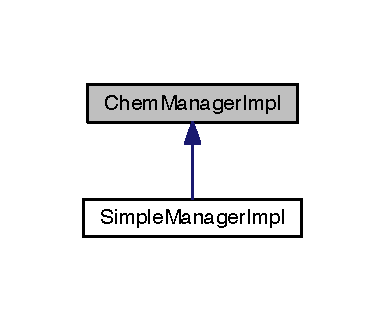
\includegraphics[width=185pt]{classChemManagerImpl__inherit__graph}
\end{center}
\end{figure}
\subsection*{Public Member Functions}
\begin{DoxyCompactItemize}
\item 
virtual \hyperlink{classChemManagerImpl_a87a97fda042c8f326793321e2bc28e69}{$\sim$\+Chem\+Manager\+Impl} () noexcept
\begin{DoxyCompactList}\small\item\em Destructor does nothing. \end{DoxyCompactList}\item 
virtual void \hyperlink{classChemManagerImpl_a5b71cbf0b7919d573b6d7b148eb52d0a}{initialize} (\hyperlink{structChemistryData}{Chemistry\+Data} \&chem)=0
\item 
virtual void \hyperlink{classChemManagerImpl_af40877d374e6792e8a0c927acce43a06}{initialize\+C\+Cylinder} (\hyperlink{classCCylinder}{C\+Cylinder} $\ast$cc, \hyperlink{classFilament}{Filament} $\ast$f, bool extension\+Front, bool extension\+Back, bool creation)=0
\item 
virtual void \hyperlink{classChemManagerImpl_a49530caf0062fa43dfd0123b30b22011}{update\+C\+Cylinder} (\hyperlink{classCCylinder}{C\+Cylinder} $\ast$cc)=0
\end{DoxyCompactItemize}


\subsection{Detailed Description}
An abstract base class for initialization of all chemistry in the system. 

Definition at line 34 of file Chem\+Manager\+Impl.\+h.



\subsection{Constructor \& Destructor Documentation}
\hypertarget{classChemManagerImpl_a87a97fda042c8f326793321e2bc28e69}{\index{Chem\+Manager\+Impl@{Chem\+Manager\+Impl}!````~Chem\+Manager\+Impl@{$\sim$\+Chem\+Manager\+Impl}}
\index{````~Chem\+Manager\+Impl@{$\sim$\+Chem\+Manager\+Impl}!Chem\+Manager\+Impl@{Chem\+Manager\+Impl}}
\subsubsection[{$\sim$\+Chem\+Manager\+Impl}]{\setlength{\rightskip}{0pt plus 5cm}virtual Chem\+Manager\+Impl\+::$\sim$\+Chem\+Manager\+Impl (
\begin{DoxyParamCaption}
{}
\end{DoxyParamCaption}
)\hspace{0.3cm}{\ttfamily [inline]}, {\ttfamily [virtual]}, {\ttfamily [noexcept]}}}\label{classChemManagerImpl_a87a97fda042c8f326793321e2bc28e69}


Destructor does nothing. 

\begin{DoxyNote}{Note}
noexcept is important here. Otherwise, gcc flags the constructor as potentially throwing, which in turn disables move operations by the S\+T\+L containers. This behaviour is a gcc bug (as of gcc 4.\+703), and will presumbaly be fixed in the future. 
\end{DoxyNote}


Definition at line 41 of file Chem\+Manager\+Impl.\+h.



\subsection{Member Function Documentation}
\hypertarget{classChemManagerImpl_a5b71cbf0b7919d573b6d7b148eb52d0a}{\index{Chem\+Manager\+Impl@{Chem\+Manager\+Impl}!initialize@{initialize}}
\index{initialize@{initialize}!Chem\+Manager\+Impl@{Chem\+Manager\+Impl}}
\subsubsection[{initialize}]{\setlength{\rightskip}{0pt plus 5cm}virtual void Chem\+Manager\+Impl\+::initialize (
\begin{DoxyParamCaption}
\item[{{\bf Chemistry\+Data} \&}]{chem}
\end{DoxyParamCaption}
)\hspace{0.3cm}{\ttfamily [pure virtual]}}}\label{classChemManagerImpl_a5b71cbf0b7919d573b6d7b148eb52d0a}


Implemented in \hyperlink{classSimpleManagerImpl_a1db7aeaed44ae7c9cdc506176af6d186}{Simple\+Manager\+Impl}.



Referenced by Chem\+Manager\+::initialize().

\hypertarget{classChemManagerImpl_af40877d374e6792e8a0c927acce43a06}{\index{Chem\+Manager\+Impl@{Chem\+Manager\+Impl}!initialize\+C\+Cylinder@{initialize\+C\+Cylinder}}
\index{initialize\+C\+Cylinder@{initialize\+C\+Cylinder}!Chem\+Manager\+Impl@{Chem\+Manager\+Impl}}
\subsubsection[{initialize\+C\+Cylinder}]{\setlength{\rightskip}{0pt plus 5cm}virtual void Chem\+Manager\+Impl\+::initialize\+C\+Cylinder (
\begin{DoxyParamCaption}
\item[{{\bf C\+Cylinder} $\ast$}]{cc, }
\item[{{\bf Filament} $\ast$}]{f, }
\item[{bool}]{extension\+Front, }
\item[{bool}]{extension\+Back, }
\item[{bool}]{creation}
\end{DoxyParamCaption}
)\hspace{0.3cm}{\ttfamily [pure virtual]}}}\label{classChemManagerImpl_af40877d374e6792e8a0c927acce43a06}


Implemented in \hyperlink{classSimpleManagerImpl_ae4e23427c4e406bb9ad99d13099f7f02}{Simple\+Manager\+Impl}.



Referenced by Chem\+Manager\+::initialize\+C\+Cylinder().

\hypertarget{classChemManagerImpl_a49530caf0062fa43dfd0123b30b22011}{\index{Chem\+Manager\+Impl@{Chem\+Manager\+Impl}!update\+C\+Cylinder@{update\+C\+Cylinder}}
\index{update\+C\+Cylinder@{update\+C\+Cylinder}!Chem\+Manager\+Impl@{Chem\+Manager\+Impl}}
\subsubsection[{update\+C\+Cylinder}]{\setlength{\rightskip}{0pt plus 5cm}virtual void Chem\+Manager\+Impl\+::update\+C\+Cylinder (
\begin{DoxyParamCaption}
\item[{{\bf C\+Cylinder} $\ast$}]{cc}
\end{DoxyParamCaption}
)\hspace{0.3cm}{\ttfamily [pure virtual]}}}\label{classChemManagerImpl_a49530caf0062fa43dfd0123b30b22011}


Implemented in \hyperlink{classSimpleManagerImpl_af8546bec65b406009203066059f88052}{Simple\+Manager\+Impl}.



Referenced by Chem\+Manager\+::update\+C\+Cylinder().



The documentation for this class was generated from the following file\+:\begin{DoxyCompactItemize}
\item 
M3\+S\+Y\+M/\+Chemistry/\hyperlink{ChemManagerImpl_8h}{Chem\+Manager\+Impl.\+h}\end{DoxyCompactItemize}

\hypertarget{classChemNRMImpl}{\section{Chem\-N\-R\-M\-Impl Class Reference}
\label{classChemNRMImpl}\index{Chem\-N\-R\-M\-Impl@{Chem\-N\-R\-M\-Impl}}
}


{\ttfamily \#include $<$Chem\-N\-R\-M\-Impl.\-h$>$}



Inheritance diagram for Chem\-N\-R\-M\-Impl\-:\nopagebreak
\begin{figure}[H]
\begin{center}
\leavevmode
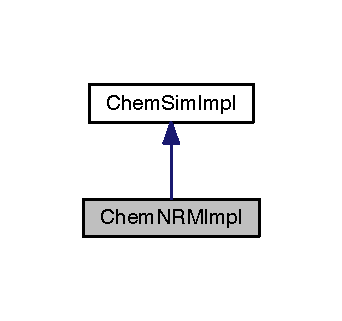
\includegraphics[width=162pt]{classChemNRMImpl__inherit__graph}
\end{center}
\end{figure}


Collaboration diagram for Chem\-N\-R\-M\-Impl\-:\nopagebreak
\begin{figure}[H]
\begin{center}
\leavevmode
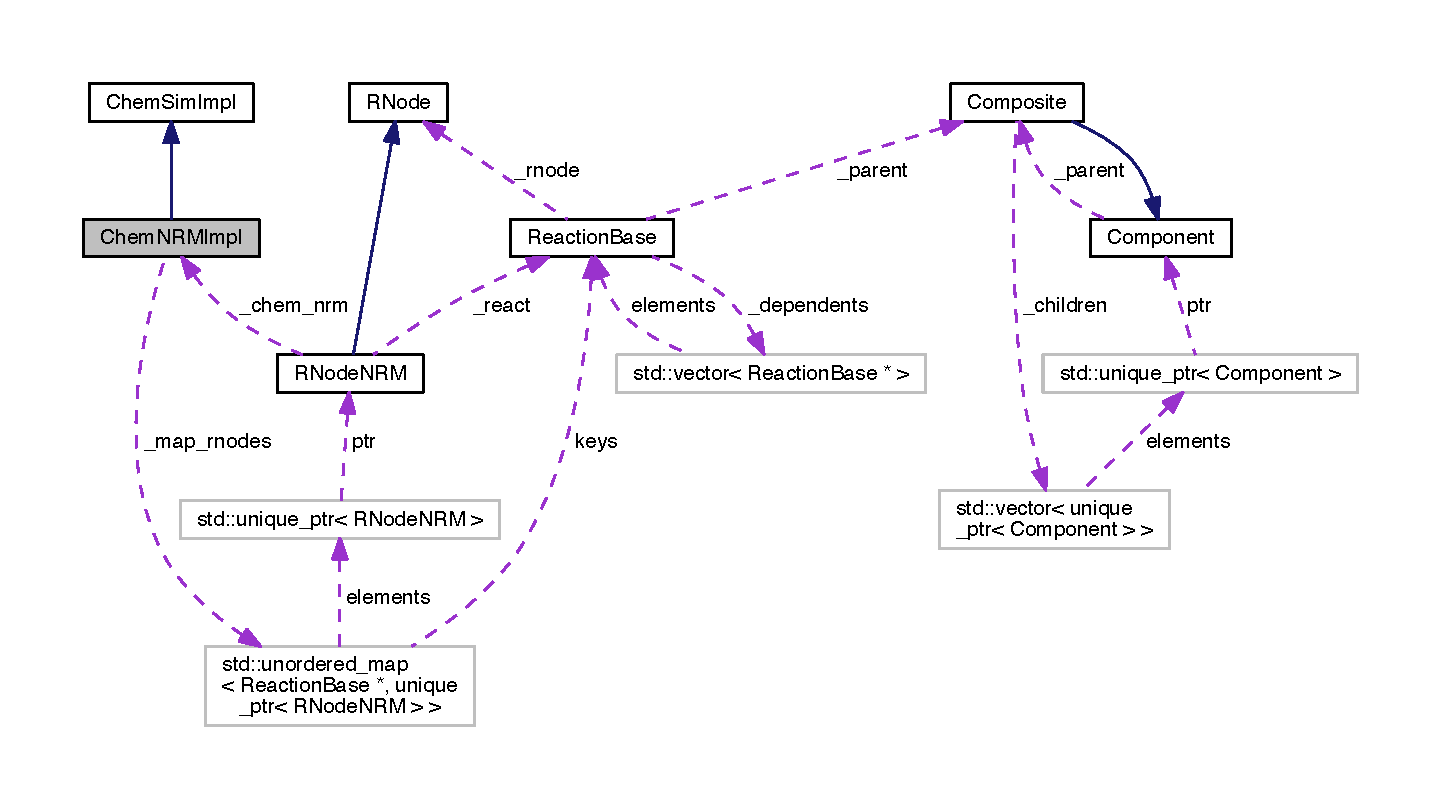
\includegraphics[width=265pt]{classChemNRMImpl__coll__graph}
\end{center}
\end{figure}
\subsection*{Public Member Functions}
\begin{DoxyCompactItemize}
\item 
\hyperlink{classChemNRMImpl_ad55314d35825dc79f7b4b491ec9ef500}{Chem\-N\-R\-M\-Impl} (const \hyperlink{classSignalingManager}{Signaling\-Manager} \&sm)
\item 
\hyperlink{classChemNRMImpl_a56b198a7965bb226c87579bdab243f80}{Chem\-N\-R\-M\-Impl} (const \hyperlink{classChemNRMImpl}{Chem\-N\-R\-M\-Impl} \&rhs)
\item 
\hyperlink{classChemNRMImpl}{Chem\-N\-R\-M\-Impl} \& \hyperlink{classChemNRMImpl_a3cbb442f4d322a02fa84e16fa23b8ea7}{operator=} (\hyperlink{classChemNRMImpl}{Chem\-N\-R\-M\-Impl} \&rhs)
\item 
\hyperlink{classChemNRMImpl_aca8d50551cdb52e67f1707df35a60c46}{$\sim$\-Chem\-N\-R\-M\-Impl} ()
\item 
size\-\_\-t \hyperlink{classChemNRMImpl_ac48e214385413158609cf016caaaac6b}{get\-Size} () const 
\item 
double \hyperlink{classChemNRMImpl_a94194658c0574c4a8673683305db5eea}{get\-Time} () const 
\item 
\hyperlink{ChemNRMImpl_8h_a57f859851909ca786c37681af9b01d45}{boost\-\_\-heap} $\ast$ \hyperlink{classChemNRMImpl_a1b20f4b9807c0b01f36f9222628c3267}{get\-Heap} ()
\item 
void \hyperlink{classChemNRMImpl_a706960c4cf9dc25084606be64739bbd0}{add\-Reaction} (\hyperlink{classReaction}{Reaction} $\ast$r)
\item 
void \hyperlink{classChemNRMImpl_a8313f88ef5e51fc9ae830a5a20f23691}{remove\-Reaction} (\hyperlink{classReaction}{Reaction} $\ast$r)
\item 
double \hyperlink{classChemNRMImpl_a89100a7f4c925ba44fa07e198cac0b4f}{generate\-Tau} (double a)
\item 
void \hyperlink{classChemNRMImpl_afadda6d4f7fbb164c4ea487034930f47}{initialize} ()
\item 
void \hyperlink{classChemNRMImpl_a9ac6c3c854c0a27c04d89be3d3927c09}{run} (int steps)
\item 
void \hyperlink{classChemNRMImpl_aa0b3b3dad40946f941959f5fdc9ef625}{print\-Reactions} () const 
\end{DoxyCompactItemize}
\subsection*{Private Member Functions}
\begin{DoxyCompactItemize}
\item 
void \hyperlink{classChemNRMImpl_ab3153d6fbcbb3273530c0a011910f31b}{make\-Step} ()
\end{DoxyCompactItemize}
\subsection*{Private Attributes}
\begin{DoxyCompactItemize}
\item 
std\-::unordered\-\_\-map$<$ \hyperlink{classReaction}{Reaction} \\*
$\ast$, std\-::unique\-\_\-ptr$<$ \hyperlink{classRNodeNRM}{R\-Node\-N\-R\-M} $>$ $>$ \hyperlink{classChemNRMImpl_abb68c12e3b656ee4ee46c19be079b80f}{\-\_\-map\-\_\-rnodes}
\item 
\hyperlink{ChemNRMImpl_8h_a57f859851909ca786c37681af9b01d45}{boost\-\_\-heap} \hyperlink{classChemNRMImpl_aae97d56d3951afd82e9d017762eeec62}{\-\_\-heap}
\item 
std\-::mt19937 \hyperlink{classChemNRMImpl_a7c5ab3f7a116daf7d67eec150c064640}{\-\_\-eng}
\item 
std\-::exponential\-\_\-distribution\\*
$<$ double $>$ \hyperlink{classChemNRMImpl_a3ed1674d931e47c51ee79fb967ad4e16}{\-\_\-exp\-\_\-distr}
\item 
const \hyperlink{classSignalingManager}{Signaling\-Manager} \& \hyperlink{classChemNRMImpl_ab1afd752876c0e135341498d963e730a}{\-\_\-sm}
\item 
double \hyperlink{classChemNRMImpl_a87649ab485a12e3af036913033ee7ca2}{\-\_\-t}
\item 
size\-\_\-t \hyperlink{classChemNRMImpl_acbb18690cfdd71dd4be01747aaf169d0}{\-\_\-n\-\_\-reacts}
\end{DoxyCompactItemize}


\subsection{Detailed Description}


Definition at line 77 of file Chem\-N\-R\-M\-Impl.\-h.



\subsection{Constructor \& Destructor Documentation}
\hypertarget{classChemNRMImpl_ad55314d35825dc79f7b4b491ec9ef500}{\index{Chem\-N\-R\-M\-Impl@{Chem\-N\-R\-M\-Impl}!Chem\-N\-R\-M\-Impl@{Chem\-N\-R\-M\-Impl}}
\index{Chem\-N\-R\-M\-Impl@{Chem\-N\-R\-M\-Impl}!ChemNRMImpl@{Chem\-N\-R\-M\-Impl}}
\subsubsection[{Chem\-N\-R\-M\-Impl}]{\setlength{\rightskip}{0pt plus 5cm}{\bf Chem\-N\-R\-M\-Impl\-::\-Chem\-N\-R\-M\-Impl} (
\begin{DoxyParamCaption}
\item[{const {\bf Signaling\-Manager} \&}]{sm}
\end{DoxyParamCaption}
)\hspace{0.3cm}{\ttfamily  \mbox{[}inline\mbox{]}}}}\label{classChemNRMImpl_ad55314d35825dc79f7b4b491ec9ef500}


Definition at line 79 of file Chem\-N\-R\-M\-Impl.\-h.

\hypertarget{classChemNRMImpl_a56b198a7965bb226c87579bdab243f80}{\index{Chem\-N\-R\-M\-Impl@{Chem\-N\-R\-M\-Impl}!Chem\-N\-R\-M\-Impl@{Chem\-N\-R\-M\-Impl}}
\index{Chem\-N\-R\-M\-Impl@{Chem\-N\-R\-M\-Impl}!ChemNRMImpl@{Chem\-N\-R\-M\-Impl}}
\subsubsection[{Chem\-N\-R\-M\-Impl}]{\setlength{\rightskip}{0pt plus 5cm}{\bf Chem\-N\-R\-M\-Impl\-::\-Chem\-N\-R\-M\-Impl} (
\begin{DoxyParamCaption}
\item[{const {\bf Chem\-N\-R\-M\-Impl} \&}]{rhs}
\end{DoxyParamCaption}
)}}\label{classChemNRMImpl_a56b198a7965bb226c87579bdab243f80}
\hypertarget{classChemNRMImpl_aca8d50551cdb52e67f1707df35a60c46}{\index{Chem\-N\-R\-M\-Impl@{Chem\-N\-R\-M\-Impl}!$\sim$\-Chem\-N\-R\-M\-Impl@{$\sim$\-Chem\-N\-R\-M\-Impl}}
\index{$\sim$\-Chem\-N\-R\-M\-Impl@{$\sim$\-Chem\-N\-R\-M\-Impl}!ChemNRMImpl@{Chem\-N\-R\-M\-Impl}}
\subsubsection[{$\sim$\-Chem\-N\-R\-M\-Impl}]{\setlength{\rightskip}{0pt plus 5cm}{\bf Chem\-N\-R\-M\-Impl\-::$\sim$\-Chem\-N\-R\-M\-Impl} (
\begin{DoxyParamCaption}
{}
\end{DoxyParamCaption}
)}}\label{classChemNRMImpl_aca8d50551cdb52e67f1707df35a60c46}


Definition at line 92 of file Chem\-N\-R\-M\-Impl.\-cpp.



References \-\_\-map\-\_\-rnodes.



\subsection{Member Function Documentation}
\hypertarget{classChemNRMImpl_a706960c4cf9dc25084606be64739bbd0}{\index{Chem\-N\-R\-M\-Impl@{Chem\-N\-R\-M\-Impl}!add\-Reaction@{add\-Reaction}}
\index{add\-Reaction@{add\-Reaction}!ChemNRMImpl@{Chem\-N\-R\-M\-Impl}}
\subsubsection[{add\-Reaction}]{\setlength{\rightskip}{0pt plus 5cm}void {\bf Chem\-N\-R\-M\-Impl\-::add\-Reaction} (
\begin{DoxyParamCaption}
\item[{{\bf Reaction} $\ast$}]{r}
\end{DoxyParamCaption}
)\hspace{0.3cm}{\ttfamily  \mbox{[}virtual\mbox{]}}}}\label{classChemNRMImpl_a706960c4cf9dc25084606be64739bbd0}


Implements \hyperlink{classChemSimImpl_ab47ad93c8a2b23f83244d6bc1369f03f}{Chem\-Sim\-Impl}.



Definition at line 147 of file Chem\-N\-R\-M\-Impl.\-cpp.



References \-\_\-map\-\_\-rnodes, and \-\_\-n\-\_\-reacts.

\hypertarget{classChemNRMImpl_a89100a7f4c925ba44fa07e198cac0b4f}{\index{Chem\-N\-R\-M\-Impl@{Chem\-N\-R\-M\-Impl}!generate\-Tau@{generate\-Tau}}
\index{generate\-Tau@{generate\-Tau}!ChemNRMImpl@{Chem\-N\-R\-M\-Impl}}
\subsubsection[{generate\-Tau}]{\setlength{\rightskip}{0pt plus 5cm}double {\bf Chem\-N\-R\-M\-Impl\-::generate\-Tau} (
\begin{DoxyParamCaption}
\item[{double}]{a}
\end{DoxyParamCaption}
)}}\label{classChemNRMImpl_a89100a7f4c925ba44fa07e198cac0b4f}


Definition at line 96 of file Chem\-N\-R\-M\-Impl.\-cpp.



References \-\_\-eng, and \-\_\-exp\-\_\-distr.



Referenced by R\-Node\-N\-R\-M\-::generate\-New\-Rand\-Tau().

\hypertarget{classChemNRMImpl_a1b20f4b9807c0b01f36f9222628c3267}{\index{Chem\-N\-R\-M\-Impl@{Chem\-N\-R\-M\-Impl}!get\-Heap@{get\-Heap}}
\index{get\-Heap@{get\-Heap}!ChemNRMImpl@{Chem\-N\-R\-M\-Impl}}
\subsubsection[{get\-Heap}]{\setlength{\rightskip}{0pt plus 5cm}{\bf boost\-\_\-heap}$\ast$ {\bf Chem\-N\-R\-M\-Impl\-::get\-Heap} (
\begin{DoxyParamCaption}
{}
\end{DoxyParamCaption}
)\hspace{0.3cm}{\ttfamily  \mbox{[}inline\mbox{]}}}}\label{classChemNRMImpl_a1b20f4b9807c0b01f36f9222628c3267}


Definition at line 86 of file Chem\-N\-R\-M\-Impl.\-h.



References \-\_\-heap.



Referenced by R\-Node\-N\-R\-M\-::\-R\-Node\-N\-R\-M(), R\-Node\-N\-R\-M\-::update\-Heap(), and R\-Node\-N\-R\-M\-::$\sim$\-R\-Node\-N\-R\-M().

\hypertarget{classChemNRMImpl_ac48e214385413158609cf016caaaac6b}{\index{Chem\-N\-R\-M\-Impl@{Chem\-N\-R\-M\-Impl}!get\-Size@{get\-Size}}
\index{get\-Size@{get\-Size}!ChemNRMImpl@{Chem\-N\-R\-M\-Impl}}
\subsubsection[{get\-Size}]{\setlength{\rightskip}{0pt plus 5cm}size\-\_\-t {\bf Chem\-N\-R\-M\-Impl\-::get\-Size} (
\begin{DoxyParamCaption}
{}
\end{DoxyParamCaption}
) const\hspace{0.3cm}{\ttfamily  \mbox{[}inline\mbox{]}}}}\label{classChemNRMImpl_ac48e214385413158609cf016caaaac6b}


Definition at line 84 of file Chem\-N\-R\-M\-Impl.\-h.



References \-\_\-n\-\_\-reacts.

\hypertarget{classChemNRMImpl_a94194658c0574c4a8673683305db5eea}{\index{Chem\-N\-R\-M\-Impl@{Chem\-N\-R\-M\-Impl}!get\-Time@{get\-Time}}
\index{get\-Time@{get\-Time}!ChemNRMImpl@{Chem\-N\-R\-M\-Impl}}
\subsubsection[{get\-Time}]{\setlength{\rightskip}{0pt plus 5cm}double {\bf Chem\-N\-R\-M\-Impl\-::get\-Time} (
\begin{DoxyParamCaption}
{}
\end{DoxyParamCaption}
) const\hspace{0.3cm}{\ttfamily  \mbox{[}inline\mbox{]}}}}\label{classChemNRMImpl_a94194658c0574c4a8673683305db5eea}


Definition at line 85 of file Chem\-N\-R\-M\-Impl.\-h.



References \-\_\-t.



Referenced by R\-Node\-N\-R\-M\-::generate\-New\-Rand\-Tau().

\hypertarget{classChemNRMImpl_afadda6d4f7fbb164c4ea487034930f47}{\index{Chem\-N\-R\-M\-Impl@{Chem\-N\-R\-M\-Impl}!initialize@{initialize}}
\index{initialize@{initialize}!ChemNRMImpl@{Chem\-N\-R\-M\-Impl}}
\subsubsection[{initialize}]{\setlength{\rightskip}{0pt plus 5cm}void {\bf Chem\-N\-R\-M\-Impl\-::initialize} (
\begin{DoxyParamCaption}
{}
\end{DoxyParamCaption}
)\hspace{0.3cm}{\ttfamily  \mbox{[}virtual\mbox{]}}}}\label{classChemNRMImpl_afadda6d4f7fbb164c4ea487034930f47}


Implements \hyperlink{classChemSimImpl_a8050874ed2646d6632ec9df1704c86c4}{Chem\-Sim\-Impl}.



Definition at line 83 of file Chem\-N\-R\-M\-Impl.\-cpp.



References \-\_\-map\-\_\-rnodes.

\hypertarget{classChemNRMImpl_ab3153d6fbcbb3273530c0a011910f31b}{\index{Chem\-N\-R\-M\-Impl@{Chem\-N\-R\-M\-Impl}!make\-Step@{make\-Step}}
\index{make\-Step@{make\-Step}!ChemNRMImpl@{Chem\-N\-R\-M\-Impl}}
\subsubsection[{make\-Step}]{\setlength{\rightskip}{0pt plus 5cm}void {\bf Chem\-N\-R\-M\-Impl\-::make\-Step} (
\begin{DoxyParamCaption}
{}
\end{DoxyParamCaption}
)\hspace{0.3cm}{\ttfamily  \mbox{[}private\mbox{]}}}}\label{classChemNRMImpl_ab3153d6fbcbb3273530c0a011910f31b}


Definition at line 102 of file Chem\-N\-R\-M\-Impl.\-cpp.



References \-\_\-heap, \-\_\-sm, \-\_\-t, Reaction\-::begin\-Affected(), Reaction\-::begin\-Products(), Reaction\-::begin\-Reactants(), Signaling\-Manager\-::emit\-Reaction\-Signal(), Signaling\-Manager\-::emit\-Species\-Signal(), Reaction\-::end\-Affected(), Reaction\-::end\-Products(), Reaction\-::end\-Reactants(), R\-Node\-N\-R\-M\-::generate\-New\-Rand\-Tau(), R\-Node\-N\-R\-M\-::get\-Product\-Of\-Reactants(), R\-Node\-N\-R\-M\-::get\-Propensity(), R\-Node\-N\-R\-M\-::get\-Reaction(), R\-Node\-N\-R\-M\-::get\-Tau(), Reaction\-::is\-Signaling(), R\-Node\-N\-R\-M\-::make\-Step(), R\-Node\-N\-R\-M\-::re\-Compute\-Propensity(), R\-Node\-N\-R\-M\-::set\-Tau(), and R\-Node\-N\-R\-M\-::update\-Heap().



Referenced by run().

\hypertarget{classChemNRMImpl_a3cbb442f4d322a02fa84e16fa23b8ea7}{\index{Chem\-N\-R\-M\-Impl@{Chem\-N\-R\-M\-Impl}!operator=@{operator=}}
\index{operator=@{operator=}!ChemNRMImpl@{Chem\-N\-R\-M\-Impl}}
\subsubsection[{operator=}]{\setlength{\rightskip}{0pt plus 5cm}{\bf Chem\-N\-R\-M\-Impl}\& Chem\-N\-R\-M\-Impl\-::operator= (
\begin{DoxyParamCaption}
\item[{{\bf Chem\-N\-R\-M\-Impl} \&}]{rhs}
\end{DoxyParamCaption}
)}}\label{classChemNRMImpl_a3cbb442f4d322a02fa84e16fa23b8ea7}
\hypertarget{classChemNRMImpl_aa0b3b3dad40946f941959f5fdc9ef625}{\index{Chem\-N\-R\-M\-Impl@{Chem\-N\-R\-M\-Impl}!print\-Reactions@{print\-Reactions}}
\index{print\-Reactions@{print\-Reactions}!ChemNRMImpl@{Chem\-N\-R\-M\-Impl}}
\subsubsection[{print\-Reactions}]{\setlength{\rightskip}{0pt plus 5cm}void {\bf Chem\-N\-R\-M\-Impl\-::print\-Reactions} (
\begin{DoxyParamCaption}
{}
\end{DoxyParamCaption}
) const\hspace{0.3cm}{\ttfamily  \mbox{[}virtual\mbox{]}}}}\label{classChemNRMImpl_aa0b3b3dad40946f941959f5fdc9ef625}


Implements \hyperlink{classChemSimImpl_a1c0d35dbca7647319a27fa7eaff7388b}{Chem\-Sim\-Impl}.



Definition at line 157 of file Chem\-N\-R\-M\-Impl.\-cpp.



References \-\_\-map\-\_\-rnodes.

\hypertarget{classChemNRMImpl_a8313f88ef5e51fc9ae830a5a20f23691}{\index{Chem\-N\-R\-M\-Impl@{Chem\-N\-R\-M\-Impl}!remove\-Reaction@{remove\-Reaction}}
\index{remove\-Reaction@{remove\-Reaction}!ChemNRMImpl@{Chem\-N\-R\-M\-Impl}}
\subsubsection[{remove\-Reaction}]{\setlength{\rightskip}{0pt plus 5cm}void {\bf Chem\-N\-R\-M\-Impl\-::remove\-Reaction} (
\begin{DoxyParamCaption}
\item[{{\bf Reaction} $\ast$}]{r}
\end{DoxyParamCaption}
)\hspace{0.3cm}{\ttfamily  \mbox{[}virtual\mbox{]}}}}\label{classChemNRMImpl_a8313f88ef5e51fc9ae830a5a20f23691}


Implements \hyperlink{classChemSimImpl_a2c4024b4ec1e4d615449db6f7430d1fc}{Chem\-Sim\-Impl}.



Definition at line 152 of file Chem\-N\-R\-M\-Impl.\-cpp.



References \-\_\-map\-\_\-rnodes, and \-\_\-n\-\_\-reacts.

\hypertarget{classChemNRMImpl_a9ac6c3c854c0a27c04d89be3d3927c09}{\index{Chem\-N\-R\-M\-Impl@{Chem\-N\-R\-M\-Impl}!run@{run}}
\index{run@{run}!ChemNRMImpl@{Chem\-N\-R\-M\-Impl}}
\subsubsection[{run}]{\setlength{\rightskip}{0pt plus 5cm}void {\bf Chem\-N\-R\-M\-Impl\-::run} (
\begin{DoxyParamCaption}
\item[{int}]{steps}
\end{DoxyParamCaption}
)\hspace{0.3cm}{\ttfamily  \mbox{[}inline, virtual\mbox{]}}}}\label{classChemNRMImpl_a9ac6c3c854c0a27c04d89be3d3927c09}


Implements \hyperlink{classChemSimImpl_ab6d36727d7ed608bbeee6e5037827bc8}{Chem\-Sim\-Impl}.



Definition at line 91 of file Chem\-N\-R\-M\-Impl.\-h.



References make\-Step().



\subsection{Member Data Documentation}
\hypertarget{classChemNRMImpl_a7c5ab3f7a116daf7d67eec150c064640}{\index{Chem\-N\-R\-M\-Impl@{Chem\-N\-R\-M\-Impl}!\-\_\-eng@{\-\_\-eng}}
\index{\-\_\-eng@{\-\_\-eng}!ChemNRMImpl@{Chem\-N\-R\-M\-Impl}}
\subsubsection[{\-\_\-eng}]{\setlength{\rightskip}{0pt plus 5cm}std\-::mt19937 {\bf Chem\-N\-R\-M\-Impl\-::\-\_\-eng}\hspace{0.3cm}{\ttfamily  \mbox{[}private\mbox{]}}}}\label{classChemNRMImpl_a7c5ab3f7a116daf7d67eec150c064640}


Definition at line 104 of file Chem\-N\-R\-M\-Impl.\-h.



Referenced by generate\-Tau().

\hypertarget{classChemNRMImpl_a3ed1674d931e47c51ee79fb967ad4e16}{\index{Chem\-N\-R\-M\-Impl@{Chem\-N\-R\-M\-Impl}!\-\_\-exp\-\_\-distr@{\-\_\-exp\-\_\-distr}}
\index{\-\_\-exp\-\_\-distr@{\-\_\-exp\-\_\-distr}!ChemNRMImpl@{Chem\-N\-R\-M\-Impl}}
\subsubsection[{\-\_\-exp\-\_\-distr}]{\setlength{\rightskip}{0pt plus 5cm}std\-::exponential\-\_\-distribution$<$double$>$ {\bf Chem\-N\-R\-M\-Impl\-::\-\_\-exp\-\_\-distr}\hspace{0.3cm}{\ttfamily  \mbox{[}private\mbox{]}}}}\label{classChemNRMImpl_a3ed1674d931e47c51ee79fb967ad4e16}


Definition at line 105 of file Chem\-N\-R\-M\-Impl.\-h.



Referenced by generate\-Tau().

\hypertarget{classChemNRMImpl_aae97d56d3951afd82e9d017762eeec62}{\index{Chem\-N\-R\-M\-Impl@{Chem\-N\-R\-M\-Impl}!\-\_\-heap@{\-\_\-heap}}
\index{\-\_\-heap@{\-\_\-heap}!ChemNRMImpl@{Chem\-N\-R\-M\-Impl}}
\subsubsection[{\-\_\-heap}]{\setlength{\rightskip}{0pt plus 5cm}{\bf boost\-\_\-heap} {\bf Chem\-N\-R\-M\-Impl\-::\-\_\-heap}\hspace{0.3cm}{\ttfamily  \mbox{[}private\mbox{]}}}}\label{classChemNRMImpl_aae97d56d3951afd82e9d017762eeec62}


Definition at line 103 of file Chem\-N\-R\-M\-Impl.\-h.



Referenced by get\-Heap(), and make\-Step().

\hypertarget{classChemNRMImpl_abb68c12e3b656ee4ee46c19be079b80f}{\index{Chem\-N\-R\-M\-Impl@{Chem\-N\-R\-M\-Impl}!\-\_\-map\-\_\-rnodes@{\-\_\-map\-\_\-rnodes}}
\index{\-\_\-map\-\_\-rnodes@{\-\_\-map\-\_\-rnodes}!ChemNRMImpl@{Chem\-N\-R\-M\-Impl}}
\subsubsection[{\-\_\-map\-\_\-rnodes}]{\setlength{\rightskip}{0pt plus 5cm}std\-::unordered\-\_\-map$<${\bf Reaction}$\ast$, std\-::unique\-\_\-ptr$<${\bf R\-Node\-N\-R\-M}$>$ $>$ {\bf Chem\-N\-R\-M\-Impl\-::\-\_\-map\-\_\-rnodes}\hspace{0.3cm}{\ttfamily  \mbox{[}private\mbox{]}}}}\label{classChemNRMImpl_abb68c12e3b656ee4ee46c19be079b80f}


Definition at line 102 of file Chem\-N\-R\-M\-Impl.\-h.



Referenced by add\-Reaction(), initialize(), print\-Reactions(), remove\-Reaction(), and $\sim$\-Chem\-N\-R\-M\-Impl().

\hypertarget{classChemNRMImpl_acbb18690cfdd71dd4be01747aaf169d0}{\index{Chem\-N\-R\-M\-Impl@{Chem\-N\-R\-M\-Impl}!\-\_\-n\-\_\-reacts@{\-\_\-n\-\_\-reacts}}
\index{\-\_\-n\-\_\-reacts@{\-\_\-n\-\_\-reacts}!ChemNRMImpl@{Chem\-N\-R\-M\-Impl}}
\subsubsection[{\-\_\-n\-\_\-reacts}]{\setlength{\rightskip}{0pt plus 5cm}size\-\_\-t {\bf Chem\-N\-R\-M\-Impl\-::\-\_\-n\-\_\-reacts}\hspace{0.3cm}{\ttfamily  \mbox{[}private\mbox{]}}}}\label{classChemNRMImpl_acbb18690cfdd71dd4be01747aaf169d0}


Definition at line 108 of file Chem\-N\-R\-M\-Impl.\-h.



Referenced by add\-Reaction(), get\-Size(), and remove\-Reaction().

\hypertarget{classChemNRMImpl_ab1afd752876c0e135341498d963e730a}{\index{Chem\-N\-R\-M\-Impl@{Chem\-N\-R\-M\-Impl}!\-\_\-sm@{\-\_\-sm}}
\index{\-\_\-sm@{\-\_\-sm}!ChemNRMImpl@{Chem\-N\-R\-M\-Impl}}
\subsubsection[{\-\_\-sm}]{\setlength{\rightskip}{0pt plus 5cm}const {\bf Signaling\-Manager}\& {\bf Chem\-N\-R\-M\-Impl\-::\-\_\-sm}\hspace{0.3cm}{\ttfamily  \mbox{[}private\mbox{]}}}}\label{classChemNRMImpl_ab1afd752876c0e135341498d963e730a}


Definition at line 106 of file Chem\-N\-R\-M\-Impl.\-h.



Referenced by make\-Step().

\hypertarget{classChemNRMImpl_a87649ab485a12e3af036913033ee7ca2}{\index{Chem\-N\-R\-M\-Impl@{Chem\-N\-R\-M\-Impl}!\-\_\-t@{\-\_\-t}}
\index{\-\_\-t@{\-\_\-t}!ChemNRMImpl@{Chem\-N\-R\-M\-Impl}}
\subsubsection[{\-\_\-t}]{\setlength{\rightskip}{0pt plus 5cm}double {\bf Chem\-N\-R\-M\-Impl\-::\-\_\-t}\hspace{0.3cm}{\ttfamily  \mbox{[}private\mbox{]}}}}\label{classChemNRMImpl_a87649ab485a12e3af036913033ee7ca2}


Definition at line 107 of file Chem\-N\-R\-M\-Impl.\-h.



Referenced by get\-Time(), and make\-Step().



The documentation for this class was generated from the following files\-:\begin{DoxyCompactItemize}
\item 
Cyto\-Sim/\hyperlink{ChemNRMImpl_8h}{Chem\-N\-R\-M\-Impl.\-h}\item 
Cyto\-Sim/\hyperlink{ChemNRMImpl_8cpp}{Chem\-N\-R\-M\-Impl.\-cpp}\end{DoxyCompactItemize}

\hypertarget{classChemSignal}{\section{Chem\+Signal Class Reference}
\label{classChemSignal}\index{Chem\+Signal@{Chem\+Signal}}
}


Manages callbacks for \hyperlink{classRSpecies}{R\+Species} and Reactions objects.  




{\ttfamily \#include $<$Signaling.\+h$>$}



Collaboration diagram for Chem\+Signal\+:\nopagebreak
\begin{figure}[H]
\begin{center}
\leavevmode
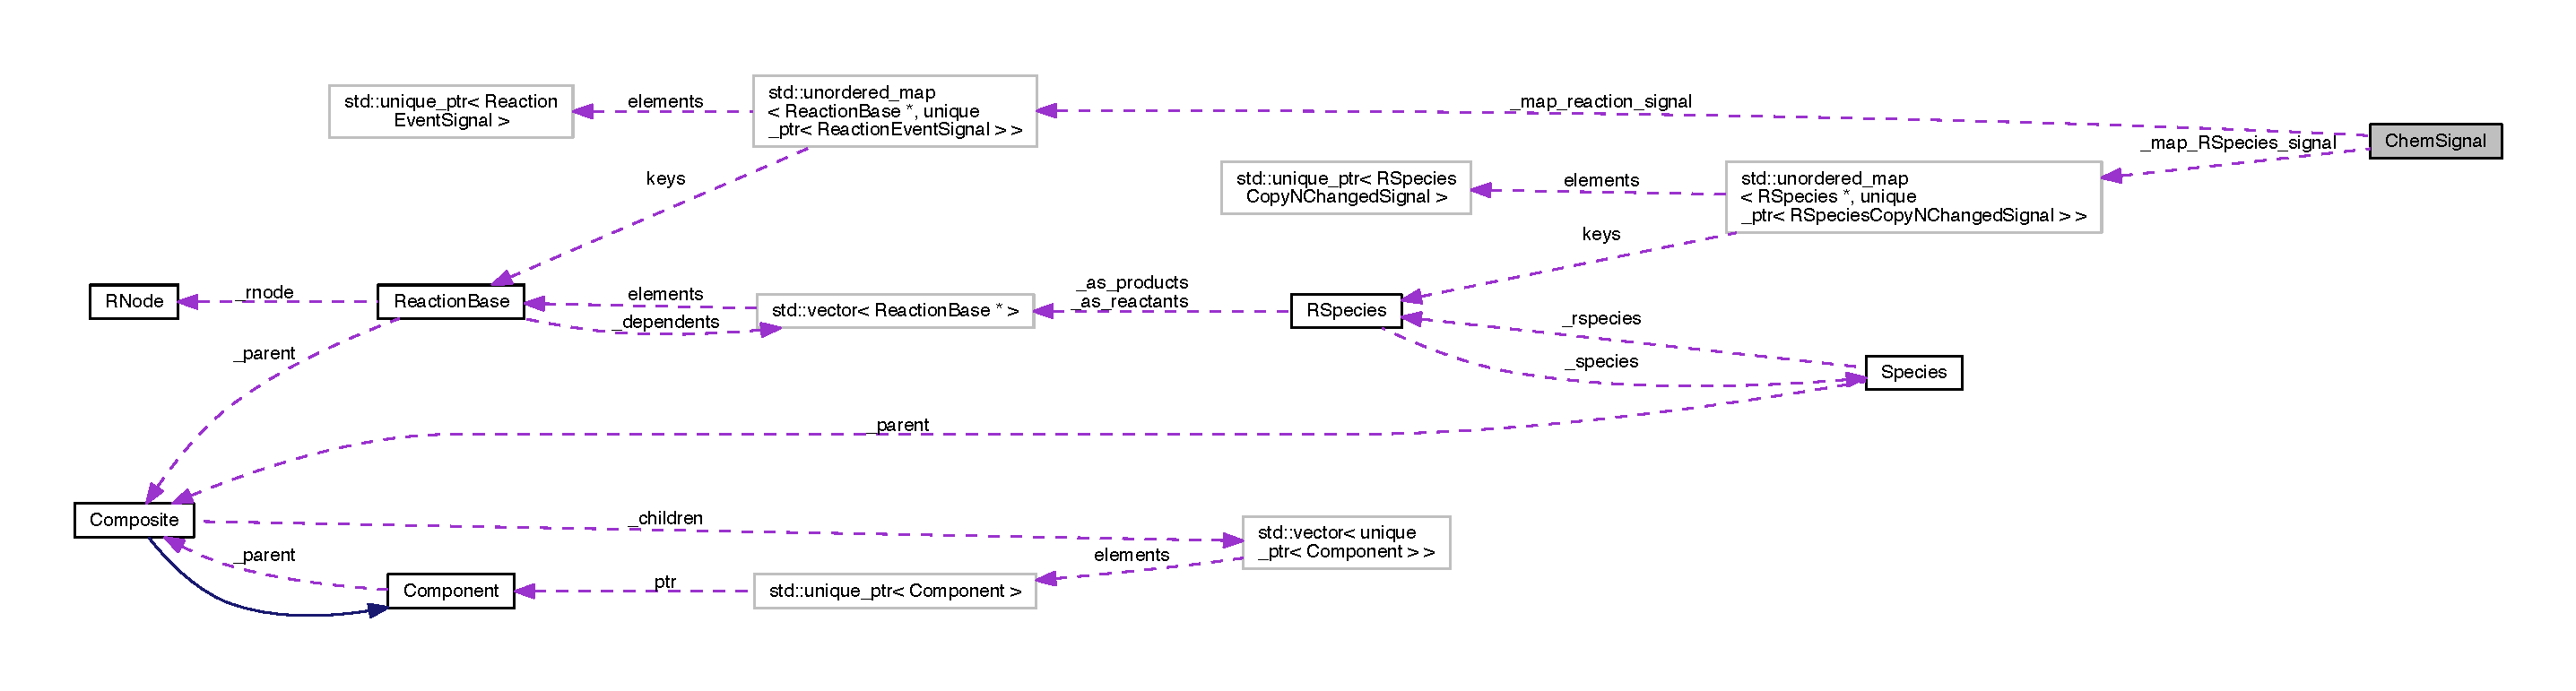
\includegraphics[width=350pt]{classChemSignal__coll__graph}
\end{center}
\end{figure}
\subsection*{Public Member Functions}
\begin{DoxyCompactItemize}
\item 
void \hyperlink{classChemSignal_ab34f019b2a982650cafe7c272eeb626f}{emit\+Reaction\+Signal} (\hyperlink{classReactionBase}{Reaction\+Base} $\ast$r) const 
\begin{DoxyCompactList}\small\item\em Broadcasts signal corresponding to \hyperlink{classReactionBase}{Reaction\+Base} $\ast$r. \end{DoxyCompactList}\item 
void \hyperlink{classChemSignal_af8123a3b376bd247c8f1c1c5a71dcb82}{emit\+R\+Species\+Signal} (\hyperlink{classRSpecies}{R\+Species} $\ast$s, int delta) const 
\begin{DoxyCompactList}\small\item\em Broadcasts signal corresponding to \hyperlink{classRSpecies}{R\+Species} $\ast$s. \end{DoxyCompactList}\item 
void \hyperlink{classChemSignal_a739d867462daa1a637842f21f04516fb}{add\+Signaling\+R\+Species} (\hyperlink{classRSpecies}{R\+Species} $\ast$s)
\begin{DoxyCompactList}\small\item\em Inserts a signal corresponding to \hyperlink{classRSpecies}{R\+Species} $\ast$s into the map. \end{DoxyCompactList}\item 
void \hyperlink{classChemSignal_a62e4675ca1857323bb3d1399546a9485}{add\+Signaling\+Reaction} (\hyperlink{classReactionBase}{Reaction\+Base} $\ast$r)
\begin{DoxyCompactList}\small\item\em Inserts a signal corresponding to \hyperlink{classReactionBase}{Reaction\+Base} $\ast$r into the map. \end{DoxyCompactList}\item 
boost\+::signals2\+::connection \hyperlink{classChemSignal_a2c9b051880948d7721609d16cd8efcb0}{connect} (\hyperlink{classReactionBase}{Reaction\+Base} $\ast$r, function$<$ void(\hyperlink{classReactionBase}{Reaction\+Base} $\ast$)$>$ const \&react\+\_\+callback, int priority=5)
\begin{DoxyCompactList}\small\item\em Connect the callback, react\+\_\+callback to a signal corresponding to \hyperlink{classReactionBase}{Reaction\+Base} $\ast$r. \end{DoxyCompactList}\item 
boost\+::signals2\+::connection \hyperlink{classChemSignal_ad6c0c03f2cb4a12a870d356e72ca2163}{connect} (\hyperlink{classSpecies}{Species} $\ast$s, function$<$ void(\hyperlink{classRSpecies}{R\+Species} $\ast$, int)$>$ const \&R\+Species\+\_\+callback, int priority=5)
\begin{DoxyCompactList}\small\item\em Connect the callback, R\+Species\+\_\+callback to a signal corresponding to \hyperlink{classRSpecies}{R\+Species} $\ast$s. \end{DoxyCompactList}\item 
void \hyperlink{classChemSignal_a1e7e140afc97679d20371f0dd456c5f1}{disconnect} (\hyperlink{classReactionBase}{Reaction\+Base} $\ast$r)
\begin{DoxyCompactList}\small\item\em Destroy signal corresponding to \hyperlink{classReaction}{Reaction} r. \end{DoxyCompactList}\item 
void \hyperlink{classChemSignal_a7c0fcba3edac3e3f222bedefd0825fcb}{disconnect} (\hyperlink{classRSpecies}{R\+Species} $\ast$s)
\begin{DoxyCompactList}\small\item\em Destroy signal corresponding to \hyperlink{classReaction}{Reaction} r. \end{DoxyCompactList}\end{DoxyCompactItemize}
\subsection*{Private Member Functions}
\begin{DoxyCompactItemize}
\item 
unordered\+\_\+map$<$ \hyperlink{classReactionBase}{Reaction\+Base} \\*
$\ast$, unique\+\_\+ptr\\*
$<$ \hyperlink{Signaling_8h_a474e8de96ad1d2e184edd4655b5367a5}{Reaction\+Event\+Signal} $>$\\*
 $>$\+::const\+\_\+iterator \hyperlink{classChemSignal_a1d97f97bcba6af500da85f1422d89921}{find\+Signal} (\hyperlink{classReactionBase}{Reaction\+Base} $\ast$r) const 
\begin{DoxyCompactList}\small\item\em Search the map for a signal corresponding to parameter, \hyperlink{classReactionBase}{Reaction\+Base} $\ast$r. Throw out\+\_\+of\+\_\+range exception if not found. \end{DoxyCompactList}\item 
unordered\+\_\+map$<$ \hyperlink{classRSpecies}{R\+Species} \\*
$\ast$, unique\+\_\+ptr\\*
$<$ \hyperlink{Signaling_8h_a0e8f1e8752c518bbfbcfe0147eca4587}{R\+Species\+Copy\+N\+Changed\+Signal} $>$\\*
 $>$\+::const\+\_\+iterator \hyperlink{classChemSignal_a93bb74fad6645d059bf85957ea34f4a8}{find\+Signal} (\hyperlink{classRSpecies}{R\+Species} $\ast$s) const 
\begin{DoxyCompactList}\small\item\em Search the map for a signal corresponding to parameter, \hyperlink{classRSpecies}{R\+Species} $\ast$s. Throw out\+\_\+of\+\_\+range exception if not found. \end{DoxyCompactList}\item 
void \hyperlink{classChemSignal_adfa6655413afc3a602a8f76ad6b71a98}{assert\+Signal\+Does\+Not\+Exist} (\hyperlink{classReactionBase}{Reaction\+Base} $\ast$r)
\begin{DoxyCompactList}\small\item\em Assert that a signal corresponding to \hyperlink{classReactionBase}{Reaction\+Base} $\ast$r does not exist or throw runtime\+\_\+error. \end{DoxyCompactList}\item 
void \hyperlink{classChemSignal_a17510f00f6775f8bfdf9a5ed2844251a}{assert\+Signal\+Does\+Not\+Exist} (\hyperlink{classRSpecies}{R\+Species} $\ast$s)
\begin{DoxyCompactList}\small\item\em Assert that a signal corresponding to \hyperlink{classRSpecies}{R\+Species} $\ast$s does not exist or throw runtime\+\_\+error. \end{DoxyCompactList}\end{DoxyCompactItemize}
\subsection*{Private Attributes}
\begin{DoxyCompactItemize}
\item 
unordered\+\_\+map$<$ \hyperlink{classRSpecies}{R\+Species} \\*
$\ast$, unique\+\_\+ptr\\*
$<$ \hyperlink{Signaling_8h_a0e8f1e8752c518bbfbcfe0147eca4587}{R\+Species\+Copy\+N\+Changed\+Signal} $>$ $>$ \hyperlink{classChemSignal_a01513b0756cb765b0fd02a7e5497133d}{\+\_\+map\+\_\+\+R\+Species\+\_\+signal}
\begin{DoxyCompactList}\small\item\em Keep track of signals corresponding to various \hyperlink{classRSpecies}{R\+Species}. \end{DoxyCompactList}\item 
unordered\+\_\+map$<$ \hyperlink{classReactionBase}{Reaction\+Base} \\*
$\ast$, unique\+\_\+ptr\\*
$<$ \hyperlink{Signaling_8h_a474e8de96ad1d2e184edd4655b5367a5}{Reaction\+Event\+Signal} $>$ $>$ \hyperlink{classChemSignal_a750129c5a876c652e76e2a008b21b276}{\+\_\+map\+\_\+reaction\+\_\+signal}
\begin{DoxyCompactList}\small\item\em Keep track of signals corresponding to various Reactions. \end{DoxyCompactList}\end{DoxyCompactItemize}


\subsection{Detailed Description}
Manages callbacks for \hyperlink{classRSpecies}{R\+Species} and Reactions objects. 

One \hyperlink{classChemSignal}{Chem\+Signal} should be instantiated per chemical network. \hyperlink{classRSpecies}{R\+Species} and Reactions that need to be monitored can be made to signal, based on the boost\+:signal2 library. Multiple receiving slots can be connected to signals.

Slots can be temporarily blocked or completely disconnected. Signals can be destroyed. Here is an example of usage\+: 
\begin{DoxyCode}
 ...
 \hyperlink{classSpecies}{Species}* A1 = ...
 ...
 \hyperlink{classChemSignal}{ChemSignal} sm;
 A1->makeSignaling(sm);
 PrintRSpecies ps;
 ...
 function<void (RSpecies *, int)> psf(ps);
 boost::signals2::shared\_connection\_block conn\_a1(sm.\hyperlink{classChemSignal_a2c9b051880948d7721609d16cd8efcb0}{connect}(A1, [](
      \hyperlink{classRSpecies}{RSpecies} *s, \textcolor{keywordtype}{int} i)\{s->printSelf();\}), \textcolor{keyword}{true});
 \textcolor{comment}{// or   sm.connect(A1, print\_RSpecies);}
 \textcolor{comment}{// or  sm.connect(A1, PrintRSpecies());}
 \textcolor{comment}{// or   boost::signals2::shared\_connection\_block conn\_a1(sm.connect(A1,psf), false);}
...
\textcolor{comment}{// run simulation for some time}
 ...
 conn\_a1.block(); \textcolor{comment}{// this temporarily stops slots from being called.}
...
 conn\_a1.disconnect(); \textcolor{comment}{// this permanently disconnects the slot}
...
 A1->stopSignaling(sm); \textcolor{comment}{// this destroys the Signal itself (with associated multiple slots)}
...
\end{DoxyCode}
 

Definition at line 71 of file Signaling.\+h.



\subsection{Member Function Documentation}
\hypertarget{classChemSignal_a62e4675ca1857323bb3d1399546a9485}{\index{Chem\+Signal@{Chem\+Signal}!add\+Signaling\+Reaction@{add\+Signaling\+Reaction}}
\index{add\+Signaling\+Reaction@{add\+Signaling\+Reaction}!Chem\+Signal@{Chem\+Signal}}
\subsubsection[{add\+Signaling\+Reaction}]{\setlength{\rightskip}{0pt plus 5cm}void Chem\+Signal\+::add\+Signaling\+Reaction (
\begin{DoxyParamCaption}
\item[{{\bf Reaction\+Base} $\ast$}]{r}
\end{DoxyParamCaption}
)\hspace{0.3cm}{\ttfamily [inline]}}}\label{classChemSignal_a62e4675ca1857323bb3d1399546a9485}


Inserts a signal corresponding to \hyperlink{classReactionBase}{Reaction\+Base} $\ast$r into the map. 

Should only be called by the \hyperlink{classReaction}{Reaction} class. \begin{DoxyNote}{Note}
other classes should instead call void Reaction\+::make\+Signaling(\+Chem\+Signal \&sm); 
\end{DoxyNote}


Definition at line 133 of file Signaling.\+h.



References \+\_\+map\+\_\+reaction\+\_\+signal, and assert\+Signal\+Does\+Not\+Exist().

\hypertarget{classChemSignal_a739d867462daa1a637842f21f04516fb}{\index{Chem\+Signal@{Chem\+Signal}!add\+Signaling\+R\+Species@{add\+Signaling\+R\+Species}}
\index{add\+Signaling\+R\+Species@{add\+Signaling\+R\+Species}!Chem\+Signal@{Chem\+Signal}}
\subsubsection[{add\+Signaling\+R\+Species}]{\setlength{\rightskip}{0pt plus 5cm}void Chem\+Signal\+::add\+Signaling\+R\+Species (
\begin{DoxyParamCaption}
\item[{{\bf R\+Species} $\ast$}]{s}
\end{DoxyParamCaption}
)\hspace{0.3cm}{\ttfamily [inline]}}}\label{classChemSignal_a739d867462daa1a637842f21f04516fb}


Inserts a signal corresponding to \hyperlink{classRSpecies}{R\+Species} $\ast$s into the map. 

Should only be called by the \hyperlink{classRSpecies}{R\+Species} class. \begin{DoxyNote}{Note}
other classes should instead call void R\+Species\+::make\+Signaling(\+Chem\+Signal \&sm); 
\end{DoxyNote}


Definition at line 125 of file Signaling.\+h.



References \+\_\+map\+\_\+\+R\+Species\+\_\+signal, and assert\+Signal\+Does\+Not\+Exist().

\hypertarget{classChemSignal_adfa6655413afc3a602a8f76ad6b71a98}{\index{Chem\+Signal@{Chem\+Signal}!assert\+Signal\+Does\+Not\+Exist@{assert\+Signal\+Does\+Not\+Exist}}
\index{assert\+Signal\+Does\+Not\+Exist@{assert\+Signal\+Does\+Not\+Exist}!Chem\+Signal@{Chem\+Signal}}
\subsubsection[{assert\+Signal\+Does\+Not\+Exist}]{\setlength{\rightskip}{0pt plus 5cm}void Chem\+Signal\+::assert\+Signal\+Does\+Not\+Exist (
\begin{DoxyParamCaption}
\item[{{\bf Reaction\+Base} $\ast$}]{r}
\end{DoxyParamCaption}
)\hspace{0.3cm}{\ttfamily [inline]}, {\ttfamily [private]}}}\label{classChemSignal_adfa6655413afc3a602a8f76ad6b71a98}


Assert that a signal corresponding to \hyperlink{classReactionBase}{Reaction\+Base} $\ast$r does not exist or throw runtime\+\_\+error. 



Definition at line 95 of file Signaling.\+h.



References \+\_\+map\+\_\+reaction\+\_\+signal.



Referenced by add\+Signaling\+Reaction(), and add\+Signaling\+R\+Species().

\hypertarget{classChemSignal_a17510f00f6775f8bfdf9a5ed2844251a}{\index{Chem\+Signal@{Chem\+Signal}!assert\+Signal\+Does\+Not\+Exist@{assert\+Signal\+Does\+Not\+Exist}}
\index{assert\+Signal\+Does\+Not\+Exist@{assert\+Signal\+Does\+Not\+Exist}!Chem\+Signal@{Chem\+Signal}}
\subsubsection[{assert\+Signal\+Does\+Not\+Exist}]{\setlength{\rightskip}{0pt plus 5cm}void Chem\+Signal\+::assert\+Signal\+Does\+Not\+Exist (
\begin{DoxyParamCaption}
\item[{{\bf R\+Species} $\ast$}]{s}
\end{DoxyParamCaption}
)\hspace{0.3cm}{\ttfamily [inline]}, {\ttfamily [private]}}}\label{classChemSignal_a17510f00f6775f8bfdf9a5ed2844251a}


Assert that a signal corresponding to \hyperlink{classRSpecies}{R\+Species} $\ast$s does not exist or throw runtime\+\_\+error. 



Definition at line 102 of file Signaling.\+h.



References \+\_\+map\+\_\+\+R\+Species\+\_\+signal.

\hypertarget{classChemSignal_a2c9b051880948d7721609d16cd8efcb0}{\index{Chem\+Signal@{Chem\+Signal}!connect@{connect}}
\index{connect@{connect}!Chem\+Signal@{Chem\+Signal}}
\subsubsection[{connect}]{\setlength{\rightskip}{0pt plus 5cm}boost\+::signals2\+::connection Chem\+Signal\+::connect (
\begin{DoxyParamCaption}
\item[{{\bf Reaction\+Base} $\ast$}]{r, }
\item[{function$<$ void({\bf Reaction\+Base} $\ast$)$>$ const \&}]{react\+\_\+callback, }
\item[{int}]{priority = {\ttfamily 5}}
\end{DoxyParamCaption}
)\hspace{0.3cm}{\ttfamily [inline]}}}\label{classChemSignal_a2c9b051880948d7721609d16cd8efcb0}


Connect the callback, react\+\_\+callback to a signal corresponding to \hyperlink{classReactionBase}{Reaction\+Base} $\ast$r. 


\begin{DoxyParams}{Parameters}
{\em r} & -\/ the signal will correspond to this \hyperlink{classReaction}{Reaction} \\
\hline
{\em react\+\_\+callback} & -\/ a function object to be called (a slot) \\
\hline
{\em priority} & -\/ lower priority slots will be called first. Default is 5 Do not use priorities 1 and 2 unless absolutely essential. \\
\hline
\end{DoxyParams}


Definition at line 143 of file Signaling.\+h.



References find\+Signal().

\hypertarget{classChemSignal_ad6c0c03f2cb4a12a870d356e72ca2163}{\index{Chem\+Signal@{Chem\+Signal}!connect@{connect}}
\index{connect@{connect}!Chem\+Signal@{Chem\+Signal}}
\subsubsection[{connect}]{\setlength{\rightskip}{0pt plus 5cm}boost\+::signals2\+::connection Chem\+Signal\+::connect (
\begin{DoxyParamCaption}
\item[{{\bf Species} $\ast$}]{s, }
\item[{function$<$ void({\bf R\+Species} $\ast$, int)$>$ const \&}]{R\+Species\+\_\+callback, }
\item[{int}]{priority = {\ttfamily 5}}
\end{DoxyParamCaption}
)\hspace{0.3cm}{\ttfamily [inline]}}}\label{classChemSignal_ad6c0c03f2cb4a12a870d356e72ca2163}


Connect the callback, R\+Species\+\_\+callback to a signal corresponding to \hyperlink{classRSpecies}{R\+Species} $\ast$s. 


\begin{DoxyParams}{Parameters}
{\em s} & -\/ the signal will correspond to this \hyperlink{classRSpecies}{R\+Species} \\
\hline
{\em R\+Species\+\_\+callback} & -\/ a function object to be called (a slot). int here corresponds to delta, the change in copy number of the \hyperlink{classRSpecies}{R\+Species} (for which the signal was emitted) \\
\hline
{\em priority} & -\/ lower priority slots will be called first. Default is 5 Do not use priorities 1 and 2 unless absolutely essential. \\
\hline
\end{DoxyParams}


Definition at line 154 of file Signaling.\+h.



References find\+Signal(), and Species\+::get\+R\+Species().

\hypertarget{classChemSignal_a1e7e140afc97679d20371f0dd456c5f1}{\index{Chem\+Signal@{Chem\+Signal}!disconnect@{disconnect}}
\index{disconnect@{disconnect}!Chem\+Signal@{Chem\+Signal}}
\subsubsection[{disconnect}]{\setlength{\rightskip}{0pt plus 5cm}void Chem\+Signal\+::disconnect (
\begin{DoxyParamCaption}
\item[{{\bf Reaction\+Base} $\ast$}]{r}
\end{DoxyParamCaption}
)\hspace{0.3cm}{\ttfamily [inline]}}}\label{classChemSignal_a1e7e140afc97679d20371f0dd456c5f1}


Destroy signal corresponding to \hyperlink{classReaction}{Reaction} r. 

Should only be used by the \hyperlink{classReaction}{Reaction} class. \begin{DoxyNote}{Note}
-\/ Other classes should instead call void Reaction\+::stop\+Signaling (\hyperlink{classChemSignal}{Chem\+Signal} \&sm); 
\end{DoxyNote}


Definition at line 162 of file Signaling.\+h.



References \+\_\+map\+\_\+reaction\+\_\+signal, and find\+Signal().

\hypertarget{classChemSignal_a7c0fcba3edac3e3f222bedefd0825fcb}{\index{Chem\+Signal@{Chem\+Signal}!disconnect@{disconnect}}
\index{disconnect@{disconnect}!Chem\+Signal@{Chem\+Signal}}
\subsubsection[{disconnect}]{\setlength{\rightskip}{0pt plus 5cm}void Chem\+Signal\+::disconnect (
\begin{DoxyParamCaption}
\item[{{\bf R\+Species} $\ast$}]{s}
\end{DoxyParamCaption}
)\hspace{0.3cm}{\ttfamily [inline]}}}\label{classChemSignal_a7c0fcba3edac3e3f222bedefd0825fcb}


Destroy signal corresponding to \hyperlink{classReaction}{Reaction} r. 

Should only be used by the \hyperlink{classRSpecies}{R\+Species} class. \begin{DoxyNote}{Note}
-\/ Other classes should instead call void R\+Species\+::stop\+Signaling (\hyperlink{classChemSignal}{Chem\+Signal} \&sm); 
\end{DoxyNote}


Definition at line 169 of file Signaling.\+h.



References \+\_\+map\+\_\+\+R\+Species\+\_\+signal, and find\+Signal().

\hypertarget{classChemSignal_ab34f019b2a982650cafe7c272eeb626f}{\index{Chem\+Signal@{Chem\+Signal}!emit\+Reaction\+Signal@{emit\+Reaction\+Signal}}
\index{emit\+Reaction\+Signal@{emit\+Reaction\+Signal}!Chem\+Signal@{Chem\+Signal}}
\subsubsection[{emit\+Reaction\+Signal}]{\setlength{\rightskip}{0pt plus 5cm}void Chem\+Signal\+::emit\+Reaction\+Signal (
\begin{DoxyParamCaption}
\item[{{\bf Reaction\+Base} $\ast$}]{r}
\end{DoxyParamCaption}
) const\hspace{0.3cm}{\ttfamily [inline]}}}\label{classChemSignal_ab34f019b2a982650cafe7c272eeb626f}


Broadcasts signal corresponding to \hyperlink{classReactionBase}{Reaction\+Base} $\ast$r. 

If the \hyperlink{classReaction}{Reaction} is not found, out\+\_\+of\+\_\+range exception will be thrown. This method is usally only called by the Gillespie-\/like algorithm, and not the outside code. 

Definition at line 111 of file Signaling.\+h.



References find\+Signal().

\hypertarget{classChemSignal_af8123a3b376bd247c8f1c1c5a71dcb82}{\index{Chem\+Signal@{Chem\+Signal}!emit\+R\+Species\+Signal@{emit\+R\+Species\+Signal}}
\index{emit\+R\+Species\+Signal@{emit\+R\+Species\+Signal}!Chem\+Signal@{Chem\+Signal}}
\subsubsection[{emit\+R\+Species\+Signal}]{\setlength{\rightskip}{0pt plus 5cm}void Chem\+Signal\+::emit\+R\+Species\+Signal (
\begin{DoxyParamCaption}
\item[{{\bf R\+Species} $\ast$}]{s, }
\item[{int}]{delta}
\end{DoxyParamCaption}
) const\hspace{0.3cm}{\ttfamily [inline]}}}\label{classChemSignal_af8123a3b376bd247c8f1c1c5a71dcb82}


Broadcasts signal corresponding to \hyperlink{classRSpecies}{R\+Species} $\ast$s. 

If the Specis is not found, out\+\_\+of\+\_\+range exception will be thrown. This method is usally only called by the Gillespie-\/like algorithm, and not the outside code. 

Definition at line 118 of file Signaling.\+h.



References find\+Signal().

\hypertarget{classChemSignal_a1d97f97bcba6af500da85f1422d89921}{\index{Chem\+Signal@{Chem\+Signal}!find\+Signal@{find\+Signal}}
\index{find\+Signal@{find\+Signal}!Chem\+Signal@{Chem\+Signal}}
\subsubsection[{find\+Signal}]{\setlength{\rightskip}{0pt plus 5cm}unordered\+\_\+map$<${\bf Reaction\+Base} $\ast$, unique\+\_\+ptr$<${\bf Reaction\+Event\+Signal}$>$ $>$\+::const\+\_\+iterator Chem\+Signal\+::find\+Signal (
\begin{DoxyParamCaption}
\item[{{\bf Reaction\+Base} $\ast$}]{r}
\end{DoxyParamCaption}
) const\hspace{0.3cm}{\ttfamily [inline]}, {\ttfamily [private]}}}\label{classChemSignal_a1d97f97bcba6af500da85f1422d89921}


Search the map for a signal corresponding to parameter, \hyperlink{classReactionBase}{Reaction\+Base} $\ast$r. Throw out\+\_\+of\+\_\+range exception if not found. 



Definition at line 78 of file Signaling.\+h.



References \+\_\+map\+\_\+reaction\+\_\+signal.



Referenced by connect(), disconnect(), emit\+Reaction\+Signal(), and emit\+R\+Species\+Signal().

\hypertarget{classChemSignal_a93bb74fad6645d059bf85957ea34f4a8}{\index{Chem\+Signal@{Chem\+Signal}!find\+Signal@{find\+Signal}}
\index{find\+Signal@{find\+Signal}!Chem\+Signal@{Chem\+Signal}}
\subsubsection[{find\+Signal}]{\setlength{\rightskip}{0pt plus 5cm}unordered\+\_\+map$<${\bf R\+Species} $\ast$, unique\+\_\+ptr$<${\bf R\+Species\+Copy\+N\+Changed\+Signal}$>$ $>$\+::const\+\_\+iterator Chem\+Signal\+::find\+Signal (
\begin{DoxyParamCaption}
\item[{{\bf R\+Species} $\ast$}]{s}
\end{DoxyParamCaption}
) const\hspace{0.3cm}{\ttfamily [inline]}, {\ttfamily [private]}}}\label{classChemSignal_a93bb74fad6645d059bf85957ea34f4a8}


Search the map for a signal corresponding to parameter, \hyperlink{classRSpecies}{R\+Species} $\ast$s. Throw out\+\_\+of\+\_\+range exception if not found. 



Definition at line 87 of file Signaling.\+h.



References \+\_\+map\+\_\+\+R\+Species\+\_\+signal.



\subsection{Member Data Documentation}
\hypertarget{classChemSignal_a750129c5a876c652e76e2a008b21b276}{\index{Chem\+Signal@{Chem\+Signal}!\+\_\+map\+\_\+reaction\+\_\+signal@{\+\_\+map\+\_\+reaction\+\_\+signal}}
\index{\+\_\+map\+\_\+reaction\+\_\+signal@{\+\_\+map\+\_\+reaction\+\_\+signal}!Chem\+Signal@{Chem\+Signal}}
\subsubsection[{\+\_\+map\+\_\+reaction\+\_\+signal}]{\setlength{\rightskip}{0pt plus 5cm}unordered\+\_\+map$<${\bf Reaction\+Base} $\ast$, unique\+\_\+ptr$<${\bf Reaction\+Event\+Signal}$>$ $>$ Chem\+Signal\+::\+\_\+map\+\_\+reaction\+\_\+signal\hspace{0.3cm}{\ttfamily [private]}}}\label{classChemSignal_a750129c5a876c652e76e2a008b21b276}


Keep track of signals corresponding to various Reactions. 



Definition at line 74 of file Signaling.\+h.



Referenced by add\+Signaling\+Reaction(), assert\+Signal\+Does\+Not\+Exist(), disconnect(), and find\+Signal().

\hypertarget{classChemSignal_a01513b0756cb765b0fd02a7e5497133d}{\index{Chem\+Signal@{Chem\+Signal}!\+\_\+map\+\_\+\+R\+Species\+\_\+signal@{\+\_\+map\+\_\+\+R\+Species\+\_\+signal}}
\index{\+\_\+map\+\_\+\+R\+Species\+\_\+signal@{\+\_\+map\+\_\+\+R\+Species\+\_\+signal}!Chem\+Signal@{Chem\+Signal}}
\subsubsection[{\+\_\+map\+\_\+\+R\+Species\+\_\+signal}]{\setlength{\rightskip}{0pt plus 5cm}unordered\+\_\+map$<${\bf R\+Species} $\ast$, unique\+\_\+ptr$<${\bf R\+Species\+Copy\+N\+Changed\+Signal}$>$ $>$ Chem\+Signal\+::\+\_\+map\+\_\+\+R\+Species\+\_\+signal\hspace{0.3cm}{\ttfamily [private]}}}\label{classChemSignal_a01513b0756cb765b0fd02a7e5497133d}


Keep track of signals corresponding to various \hyperlink{classRSpecies}{R\+Species}. 



Definition at line 73 of file Signaling.\+h.



Referenced by add\+Signaling\+R\+Species(), assert\+Signal\+Does\+Not\+Exist(), disconnect(), and find\+Signal().



The documentation for this class was generated from the following file\+:\begin{DoxyCompactItemize}
\item 
M3\+S\+Y\+M/\hyperlink{Signaling_8h}{Signaling.\+h}\end{DoxyCompactItemize}

\hypertarget{classChemSim}{\section{Chem\+Sim Class Reference}
\label{classChemSim}\index{Chem\+Sim@{Chem\+Sim}}
}


Used to manage running a network of chemical reactions.  




{\ttfamily \#include $<$Chem\+Sim.\+h$>$}



Collaboration diagram for Chem\+Sim\+:\nopagebreak
\begin{figure}[H]
\begin{center}
\leavevmode
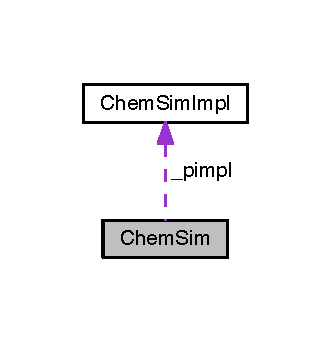
\includegraphics[width=159pt]{classChemSim__coll__graph}
\end{center}
\end{figure}
\subsection*{Public Member Functions}
\begin{DoxyCompactItemize}
\item 
\hyperlink{classChemSim_a4b06224f48b2c5ef649a177931ecd5f6}{Chem\+Sim} (const \hyperlink{classChemSim}{Chem\+Sim} \&rhs)=delete
\begin{DoxyCompactList}\small\item\em Copying is not allowed. \end{DoxyCompactList}\item 
\hyperlink{classChemSim}{Chem\+Sim} \& \hyperlink{classChemSim_aeb69f4407d4ae03a7e813be403247f7c}{operator=} (\hyperlink{classChemSim}{Chem\+Sim} \&rhs)=delete
\begin{DoxyCompactList}\small\item\em Assignment is not allowed. \end{DoxyCompactList}\end{DoxyCompactItemize}
\subsection*{Static Public Member Functions}
\begin{DoxyCompactItemize}
\item 
static void \hyperlink{classChemSim_a0f8a949bc07480c36b590128180e56e7}{set\+Instance} (\hyperlink{classChemSimImpl}{Chem\+Sim\+Impl} $\ast$csi)
\begin{DoxyCompactList}\small\item\em Set\+Instance. \end{DoxyCompactList}\item 
static void \hyperlink{classChemSim_affbdef9382a7c693a08f03f19e60d7fb}{initialize} ()
\begin{DoxyCompactList}\small\item\em After all initial reactions have been added via add\+Reaction(...) method, invoke \hyperlink{classChemSim_affbdef9382a7c693a08f03f19e60d7fb}{initialize()} prior to invoking \hyperlink{classChemSim_a60bf7095bcc35a4865a2bb191b070fc9}{run()} \end{DoxyCompactList}\item 
static void \hyperlink{classChemSim_a7ef2b5545a5250201b96c666b5ba6f92}{add\+Reaction} (\hyperlink{classReactionBase}{Reaction\+Base} $\ast$r)
\begin{DoxyCompactList}\small\item\em Add \hyperlink{classReaction}{Reaction} $\ast$r to the chemical network which needs to be simulated. \end{DoxyCompactList}\item 
static void \hyperlink{classChemSim_aefddf4bedce37ad6d9afef1631df96a1}{remove\+Reaction} (\hyperlink{classReactionBase}{Reaction\+Base} $\ast$r)
\begin{DoxyCompactList}\small\item\em Remove \hyperlink{classReaction}{Reaction} $\ast$r from the simulated chemical network. \end{DoxyCompactList}\item 
static bool \hyperlink{classChemSim_a60bf7095bcc35a4865a2bb191b070fc9}{run} (int steps)
\begin{DoxyCompactList}\small\item\em Run the chemical dynamics for a specific number of steps. \end{DoxyCompactList}\item 
static void \hyperlink{classChemSim_acc1d8030a587b1996d18c0ea775c34f0}{print\+Reactions} ()
\begin{DoxyCompactList}\small\item\em Mainly used for debugging\+: print chemical reactions in the network at this moment. \end{DoxyCompactList}\end{DoxyCompactItemize}
\subsection*{Private Member Functions}
\begin{DoxyCompactItemize}
\item 
\hyperlink{classChemSim_a7a14b6058861d217c37f1d1f43b85db6}{Chem\+Sim} ()
\end{DoxyCompactItemize}
\subsection*{Static Private Attributes}
\begin{DoxyCompactItemize}
\item 
static \hyperlink{classChemSimImpl}{Chem\+Sim\+Impl} $\ast$ \hyperlink{classChemSim_a925fca4c4b0e800007163500b8b7909d}{\+\_\+pimpl} = 0
\begin{DoxyCompactList}\small\item\em Store a pointer to a specific implementation of stochastic chemical kinetics; no ownership. \end{DoxyCompactList}\end{DoxyCompactItemize}


\subsection{Detailed Description}
Used to manage running a network of chemical reactions. 

\hyperlink{classChemSim}{Chem\+Sim} implements a Strategy pattern, allowing custom algorithms for running stochastic chemical simulations. It itself is a singleton, with a pointer to a single static implementation of \hyperlink{classChemSimImpl}{Chem\+Sim\+Impl}. After the specific algorithm is chosen and \hyperlink{classChemSim}{Chem\+Sim} is instantiated, \hyperlink{classChemSim}{Chem\+Sim} can be used to manage simulations, through such methods as run(steps) etc. Here is an example (assuming key is valid for all functions)\+: 
\begin{DoxyCode}
\hyperlink{classSpeciesBulk}{SpeciesBulk} A1(\textcolor{stringliteral}{"A1"},  25);
\hyperlink{classSpeciesBulk}{SpeciesBulk} A2(\textcolor{stringliteral}{"A2"}, 25);
\hyperlink{classReaction}{Reaction} r1 = \{ \{&A1,&A2\}, 1, 1, 100.0 \};
\hyperlink{classChemSim_a0f8a949bc07480c36b590128180e56e7}{ChemSim::setInstance}(key, \textcolor{keyword}{new} \hyperlink{classChemNRMImpl}{ChemNRMImpl}());
\hyperlink{classChemSim_a7ef2b5545a5250201b96c666b5ba6f92}{ChemSim::addReaction}(key, &r1);
\hyperlink{classChemSim_affbdef9382a7c693a08f03f19e60d7fb}{ChemSim::initialize}(key);
\hyperlink{classChemSim_a60bf7095bcc35a4865a2bb191b070fc9}{ChemSim::run}(key)
\end{DoxyCode}


Specific functions in this class require a key to be accessed. The key declarations are above. These keys can only be created and/or destroyed by the classes that are \char`\"{}friends\char`\"{} with the key. 

Definition at line 44 of file Chem\+Sim.\+h.



\subsection{Constructor \& Destructor Documentation}
\hypertarget{classChemSim_a4b06224f48b2c5ef649a177931ecd5f6}{\index{Chem\+Sim@{Chem\+Sim}!Chem\+Sim@{Chem\+Sim}}
\index{Chem\+Sim@{Chem\+Sim}!Chem\+Sim@{Chem\+Sim}}
\subsubsection[{Chem\+Sim}]{\setlength{\rightskip}{0pt plus 5cm}Chem\+Sim\+::\+Chem\+Sim (
\begin{DoxyParamCaption}
\item[{const {\bf Chem\+Sim} \&}]{rhs}
\end{DoxyParamCaption}
)\hspace{0.3cm}{\ttfamily [delete]}}}\label{classChemSim_a4b06224f48b2c5ef649a177931ecd5f6}


Copying is not allowed. 

\hypertarget{classChemSim_a7a14b6058861d217c37f1d1f43b85db6}{\index{Chem\+Sim@{Chem\+Sim}!Chem\+Sim@{Chem\+Sim}}
\index{Chem\+Sim@{Chem\+Sim}!Chem\+Sim@{Chem\+Sim}}
\subsubsection[{Chem\+Sim}]{\setlength{\rightskip}{0pt plus 5cm}Chem\+Sim\+::\+Chem\+Sim (
\begin{DoxyParamCaption}
{}
\end{DoxyParamCaption}
)\hspace{0.3cm}{\ttfamily [inline]}, {\ttfamily [private]}}}\label{classChemSim_a7a14b6058861d217c37f1d1f43b85db6}


Definition at line 75 of file Chem\+Sim.\+h.



\subsection{Member Function Documentation}
\hypertarget{classChemSim_a7ef2b5545a5250201b96c666b5ba6f92}{\index{Chem\+Sim@{Chem\+Sim}!add\+Reaction@{add\+Reaction}}
\index{add\+Reaction@{add\+Reaction}!Chem\+Sim@{Chem\+Sim}}
\subsubsection[{add\+Reaction}]{\setlength{\rightskip}{0pt plus 5cm}void Chem\+Sim\+::add\+Reaction (
\begin{DoxyParamCaption}
\item[{{\bf Reaction\+Base} $\ast$}]{r}
\end{DoxyParamCaption}
)\hspace{0.3cm}{\ttfamily [static]}}}\label{classChemSim_a7ef2b5545a5250201b96c666b5ba6f92}


Add \hyperlink{classReaction}{Reaction} $\ast$r to the chemical network which needs to be simulated. 



Definition at line 26 of file Chem\+Sim.\+cpp.



References \+\_\+pimpl, and Chem\+Sim\+Impl\+::add\+Reaction().



Referenced by Compartment\+Grid\+::add\+Chem\+Sim\+Reactions(), Compartment\+::add\+Chem\+Sim\+Reactions(), C\+Cylinder\+::add\+Cross\+Cylinder\+Reaction(), C\+Cylinder\+::add\+Internal\+Reaction(), and main().

\hypertarget{classChemSim_affbdef9382a7c693a08f03f19e60d7fb}{\index{Chem\+Sim@{Chem\+Sim}!initialize@{initialize}}
\index{initialize@{initialize}!Chem\+Sim@{Chem\+Sim}}
\subsubsection[{initialize}]{\setlength{\rightskip}{0pt plus 5cm}void Chem\+Sim\+::initialize (
\begin{DoxyParamCaption}
{}
\end{DoxyParamCaption}
)\hspace{0.3cm}{\ttfamily [static]}}}\label{classChemSim_affbdef9382a7c693a08f03f19e60d7fb}


After all initial reactions have been added via add\+Reaction(...) method, invoke \hyperlink{classChemSim_affbdef9382a7c693a08f03f19e60d7fb}{initialize()} prior to invoking \hyperlink{classChemSim_a60bf7095bcc35a4865a2bb191b070fc9}{run()} 



Definition at line 38 of file Chem\+Sim.\+cpp.



References \+\_\+pimpl, and Chem\+Sim\+Impl\+::initialize().



Referenced by C\+Controller\+::initialize(), and main().

\hypertarget{classChemSim_aeb69f4407d4ae03a7e813be403247f7c}{\index{Chem\+Sim@{Chem\+Sim}!operator=@{operator=}}
\index{operator=@{operator=}!Chem\+Sim@{Chem\+Sim}}
\subsubsection[{operator=}]{\setlength{\rightskip}{0pt plus 5cm}{\bf Chem\+Sim}\& Chem\+Sim\+::operator= (
\begin{DoxyParamCaption}
\item[{{\bf Chem\+Sim} \&}]{rhs}
\end{DoxyParamCaption}
)\hspace{0.3cm}{\ttfamily [delete]}}}\label{classChemSim_aeb69f4407d4ae03a7e813be403247f7c}


Assignment is not allowed. 

\hypertarget{classChemSim_acc1d8030a587b1996d18c0ea775c34f0}{\index{Chem\+Sim@{Chem\+Sim}!print\+Reactions@{print\+Reactions}}
\index{print\+Reactions@{print\+Reactions}!Chem\+Sim@{Chem\+Sim}}
\subsubsection[{print\+Reactions}]{\setlength{\rightskip}{0pt plus 5cm}void Chem\+Sim\+::print\+Reactions (
\begin{DoxyParamCaption}
{}
\end{DoxyParamCaption}
)\hspace{0.3cm}{\ttfamily [static]}}}\label{classChemSim_acc1d8030a587b1996d18c0ea775c34f0}


Mainly used for debugging\+: print chemical reactions in the network at this moment. 



Definition at line 42 of file Chem\+Sim.\+cpp.



References \+\_\+pimpl, and Chem\+Sim\+Impl\+::print\+Reactions().



Referenced by main().

\hypertarget{classChemSim_aefddf4bedce37ad6d9afef1631df96a1}{\index{Chem\+Sim@{Chem\+Sim}!remove\+Reaction@{remove\+Reaction}}
\index{remove\+Reaction@{remove\+Reaction}!Chem\+Sim@{Chem\+Sim}}
\subsubsection[{remove\+Reaction}]{\setlength{\rightskip}{0pt plus 5cm}void Chem\+Sim\+::remove\+Reaction (
\begin{DoxyParamCaption}
\item[{{\bf Reaction\+Base} $\ast$}]{r}
\end{DoxyParamCaption}
)\hspace{0.3cm}{\ttfamily [static]}}}\label{classChemSim_aefddf4bedce37ad6d9afef1631df96a1}


Remove \hyperlink{classReaction}{Reaction} $\ast$r from the simulated chemical network. 



Definition at line 30 of file Chem\+Sim.\+cpp.



References \+\_\+pimpl, and Chem\+Sim\+Impl\+::remove\+Reaction().



Referenced by C\+Cylinder\+::remove\+All\+Cross\+Cylinder\+Reactions(), C\+Cylinder\+::remove\+All\+Internal\+Reactions(), C\+Cylinder\+::remove\+Cross\+Cylinder\+Reactions(), and C\+Cylinder\+::remove\+Internal\+Reaction().

\hypertarget{classChemSim_a60bf7095bcc35a4865a2bb191b070fc9}{\index{Chem\+Sim@{Chem\+Sim}!run@{run}}
\index{run@{run}!Chem\+Sim@{Chem\+Sim}}
\subsubsection[{run}]{\setlength{\rightskip}{0pt plus 5cm}bool Chem\+Sim\+::run (
\begin{DoxyParamCaption}
\item[{int}]{steps}
\end{DoxyParamCaption}
)\hspace{0.3cm}{\ttfamily [static]}}}\label{classChemSim_a60bf7095bcc35a4865a2bb191b070fc9}


Run the chemical dynamics for a specific number of steps. 



Definition at line 34 of file Chem\+Sim.\+cpp.



References \+\_\+pimpl, and Chem\+Sim\+Impl\+::run().



Referenced by main(), and C\+Controller\+::run().

\hypertarget{classChemSim_a0f8a949bc07480c36b590128180e56e7}{\index{Chem\+Sim@{Chem\+Sim}!set\+Instance@{set\+Instance}}
\index{set\+Instance@{set\+Instance}!Chem\+Sim@{Chem\+Sim}}
\subsubsection[{set\+Instance}]{\setlength{\rightskip}{0pt plus 5cm}void Chem\+Sim\+::set\+Instance (
\begin{DoxyParamCaption}
\item[{{\bf Chem\+Sim\+Impl} $\ast$}]{csi}
\end{DoxyParamCaption}
)\hspace{0.3cm}{\ttfamily [static]}}}\label{classChemSim_a0f8a949bc07480c36b590128180e56e7}


Set\+Instance. 


\begin{DoxyParams}{Parameters}
{\em \hyperlink{classChemSimImpl}{Chem\+Sim\+Impl}} & $\ast$csi is a pointer the concrete implementation of stochastic simulation algorithm. \\
\hline
\end{DoxyParams}
\begin{DoxyNote}{Note}
\hyperlink{classChemSim}{Chem\+Sim} simply stores the csi pointer but does not manage its memory. Make sure that csi is always a valid pointer while \hyperlink{classChemSim}{Chem\+Sim} is used. 
\end{DoxyNote}


Definition at line 20 of file Chem\+Sim.\+cpp.



References \+\_\+pimpl.



Referenced by C\+Controller\+::initialize().



\subsection{Member Data Documentation}
\hypertarget{classChemSim_a925fca4c4b0e800007163500b8b7909d}{\index{Chem\+Sim@{Chem\+Sim}!\+\_\+pimpl@{\+\_\+pimpl}}
\index{\+\_\+pimpl@{\+\_\+pimpl}!Chem\+Sim@{Chem\+Sim}}
\subsubsection[{\+\_\+pimpl}]{\setlength{\rightskip}{0pt plus 5cm}{\bf Chem\+Sim\+Impl} $\ast$ Chem\+Sim\+::\+\_\+pimpl = 0\hspace{0.3cm}{\ttfamily [static]}, {\ttfamily [private]}}}\label{classChemSim_a925fca4c4b0e800007163500b8b7909d}


Store a pointer to a specific implementation of stochastic chemical kinetics; no ownership. 



Definition at line 74 of file Chem\+Sim.\+h.



Referenced by add\+Reaction(), initialize(), print\+Reactions(), remove\+Reaction(), run(), and set\+Instance().



The documentation for this class was generated from the following files\+:\begin{DoxyCompactItemize}
\item 
M3\+S\+Y\+M/\+Chemistry/\hyperlink{ChemSim_8h}{Chem\+Sim.\+h}\item 
M3\+S\+Y\+M/\+Chemistry/\hyperlink{ChemSim_8cpp}{Chem\+Sim.\+cpp}\end{DoxyCompactItemize}

\hypertarget{classChemSimImpl}{\section{Chem\-Sim\-Impl Class Reference}
\label{classChemSimImpl}\index{Chem\-Sim\-Impl@{Chem\-Sim\-Impl}}
}


{\ttfamily \#include $<$Chem\-Sim.\-h$>$}



Inheritance diagram for Chem\-Sim\-Impl\-:\nopagebreak
\begin{figure}[H]
\begin{center}
\leavevmode
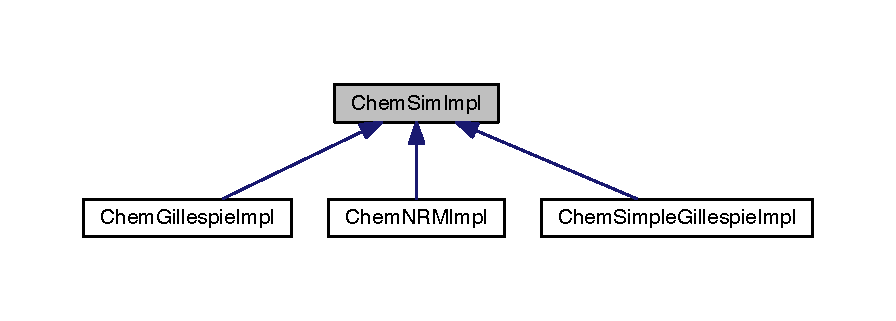
\includegraphics[width=162pt]{classChemSimImpl__inherit__graph}
\end{center}
\end{figure}
\subsection*{Public Member Functions}
\begin{DoxyCompactItemize}
\item 
virtual \hyperlink{classChemSimImpl_a60af355fee7857f7fdcb5fba63ed713c}{$\sim$\-Chem\-Sim\-Impl} ()
\item 
virtual void \hyperlink{classChemSimImpl_a8050874ed2646d6632ec9df1704c86c4}{initialize} ()=0
\item 
virtual void \hyperlink{classChemSimImpl_ab47ad93c8a2b23f83244d6bc1369f03f}{add\-Reaction} (\hyperlink{classReaction}{Reaction} $\ast$r)=0
\item 
virtual void \hyperlink{classChemSimImpl_a2c4024b4ec1e4d615449db6f7430d1fc}{remove\-Reaction} (\hyperlink{classReaction}{Reaction} $\ast$r)=0
\item 
virtual void \hyperlink{classChemSimImpl_ab6d36727d7ed608bbeee6e5037827bc8}{run} (int steps)=0
\item 
virtual void \hyperlink{classChemSimImpl_a1c0d35dbca7647319a27fa7eaff7388b}{print\-Reactions} () const =0
\end{DoxyCompactItemize}


\subsection{Detailed Description}


Definition at line 15 of file Chem\-Sim.\-h.



\subsection{Constructor \& Destructor Documentation}
\hypertarget{classChemSimImpl_a60af355fee7857f7fdcb5fba63ed713c}{\index{Chem\-Sim\-Impl@{Chem\-Sim\-Impl}!$\sim$\-Chem\-Sim\-Impl@{$\sim$\-Chem\-Sim\-Impl}}
\index{$\sim$\-Chem\-Sim\-Impl@{$\sim$\-Chem\-Sim\-Impl}!ChemSimImpl@{Chem\-Sim\-Impl}}
\subsubsection[{$\sim$\-Chem\-Sim\-Impl}]{\setlength{\rightskip}{0pt plus 5cm}virtual {\bf Chem\-Sim\-Impl\-::$\sim$\-Chem\-Sim\-Impl} (
\begin{DoxyParamCaption}
{}
\end{DoxyParamCaption}
)\hspace{0.3cm}{\ttfamily  \mbox{[}inline, virtual\mbox{]}}}}\label{classChemSimImpl_a60af355fee7857f7fdcb5fba63ed713c}


Definition at line 17 of file Chem\-Sim.\-h.



\subsection{Member Function Documentation}
\hypertarget{classChemSimImpl_ab47ad93c8a2b23f83244d6bc1369f03f}{\index{Chem\-Sim\-Impl@{Chem\-Sim\-Impl}!add\-Reaction@{add\-Reaction}}
\index{add\-Reaction@{add\-Reaction}!ChemSimImpl@{Chem\-Sim\-Impl}}
\subsubsection[{add\-Reaction}]{\setlength{\rightskip}{0pt plus 5cm}virtual void {\bf Chem\-Sim\-Impl\-::add\-Reaction} (
\begin{DoxyParamCaption}
\item[{{\bf Reaction} $\ast$}]{r}
\end{DoxyParamCaption}
)\hspace{0.3cm}{\ttfamily  \mbox{[}pure virtual\mbox{]}}}}\label{classChemSimImpl_ab47ad93c8a2b23f83244d6bc1369f03f}


Implemented in \hyperlink{classChemNRMImpl_a706960c4cf9dc25084606be64739bbd0}{Chem\-N\-R\-M\-Impl}.



Referenced by Chem\-Sim\-::add\-Reaction().

\hypertarget{classChemSimImpl_a8050874ed2646d6632ec9df1704c86c4}{\index{Chem\-Sim\-Impl@{Chem\-Sim\-Impl}!initialize@{initialize}}
\index{initialize@{initialize}!ChemSimImpl@{Chem\-Sim\-Impl}}
\subsubsection[{initialize}]{\setlength{\rightskip}{0pt plus 5cm}virtual void {\bf Chem\-Sim\-Impl\-::initialize} (
\begin{DoxyParamCaption}
{}
\end{DoxyParamCaption}
)\hspace{0.3cm}{\ttfamily  \mbox{[}pure virtual\mbox{]}}}}\label{classChemSimImpl_a8050874ed2646d6632ec9df1704c86c4}


Implemented in \hyperlink{classChemNRMImpl_afadda6d4f7fbb164c4ea487034930f47}{Chem\-N\-R\-M\-Impl}.



Referenced by Chem\-Sim\-::initialize().

\hypertarget{classChemSimImpl_a1c0d35dbca7647319a27fa7eaff7388b}{\index{Chem\-Sim\-Impl@{Chem\-Sim\-Impl}!print\-Reactions@{print\-Reactions}}
\index{print\-Reactions@{print\-Reactions}!ChemSimImpl@{Chem\-Sim\-Impl}}
\subsubsection[{print\-Reactions}]{\setlength{\rightskip}{0pt plus 5cm}virtual void {\bf Chem\-Sim\-Impl\-::print\-Reactions} (
\begin{DoxyParamCaption}
{}
\end{DoxyParamCaption}
) const\hspace{0.3cm}{\ttfamily  \mbox{[}pure virtual\mbox{]}}}}\label{classChemSimImpl_a1c0d35dbca7647319a27fa7eaff7388b}


Implemented in \hyperlink{classChemNRMImpl_aa0b3b3dad40946f941959f5fdc9ef625}{Chem\-N\-R\-M\-Impl}.



Referenced by Chem\-Sim\-::print\-Reactions().

\hypertarget{classChemSimImpl_a2c4024b4ec1e4d615449db6f7430d1fc}{\index{Chem\-Sim\-Impl@{Chem\-Sim\-Impl}!remove\-Reaction@{remove\-Reaction}}
\index{remove\-Reaction@{remove\-Reaction}!ChemSimImpl@{Chem\-Sim\-Impl}}
\subsubsection[{remove\-Reaction}]{\setlength{\rightskip}{0pt plus 5cm}virtual void {\bf Chem\-Sim\-Impl\-::remove\-Reaction} (
\begin{DoxyParamCaption}
\item[{{\bf Reaction} $\ast$}]{r}
\end{DoxyParamCaption}
)\hspace{0.3cm}{\ttfamily  \mbox{[}pure virtual\mbox{]}}}}\label{classChemSimImpl_a2c4024b4ec1e4d615449db6f7430d1fc}


Implemented in \hyperlink{classChemNRMImpl_a8313f88ef5e51fc9ae830a5a20f23691}{Chem\-N\-R\-M\-Impl}.



Referenced by Chem\-Sim\-::remove\-Reaction().

\hypertarget{classChemSimImpl_ab6d36727d7ed608bbeee6e5037827bc8}{\index{Chem\-Sim\-Impl@{Chem\-Sim\-Impl}!run@{run}}
\index{run@{run}!ChemSimImpl@{Chem\-Sim\-Impl}}
\subsubsection[{run}]{\setlength{\rightskip}{0pt plus 5cm}virtual void {\bf Chem\-Sim\-Impl\-::run} (
\begin{DoxyParamCaption}
\item[{int}]{steps}
\end{DoxyParamCaption}
)\hspace{0.3cm}{\ttfamily  \mbox{[}pure virtual\mbox{]}}}}\label{classChemSimImpl_ab6d36727d7ed608bbeee6e5037827bc8}


Implemented in \hyperlink{classChemNRMImpl_a9ac6c3c854c0a27c04d89be3d3927c09}{Chem\-N\-R\-M\-Impl}.



Referenced by Chem\-Sim\-::run().



The documentation for this class was generated from the following file\-:\begin{DoxyCompactItemize}
\item 
Cyto\-Sim/\hyperlink{ChemSim_8h}{Chem\-Sim.\-h}\end{DoxyCompactItemize}

\hypertarget{classChemSimpleGillespieImpl}{\section{Chem\+Simple\+Gillespie\+Impl Class Reference}
\label{classChemSimpleGillespieImpl}\index{Chem\+Simple\+Gillespie\+Impl@{Chem\+Simple\+Gillespie\+Impl}}
}


Implements the simplest version of the Gillespie algorithm, without caching, etc.  




{\ttfamily \#include $<$Chem\+Simple\+Gillespie\+Impl.\+h$>$}



Inheritance diagram for Chem\+Simple\+Gillespie\+Impl\+:\nopagebreak
\begin{figure}[H]
\begin{center}
\leavevmode
\includegraphics[width=210pt]{classChemSimpleGillespieImpl__inherit__graph}
\end{center}
\end{figure}


Collaboration diagram for Chem\+Simple\+Gillespie\+Impl\+:\nopagebreak
\begin{figure}[H]
\begin{center}
\leavevmode
\includegraphics[width=350pt]{classChemSimpleGillespieImpl__coll__graph}
\end{center}
\end{figure}
\subsection*{Public Member Functions}
\begin{DoxyCompactItemize}
\item 
\hyperlink{classChemSimpleGillespieImpl_a8a5a22813fccd094cb8d040fb444a38d}{Chem\+Simple\+Gillespie\+Impl} ()
\begin{DoxyCompactList}\small\item\em Ctor\+: Seeds the random number generator, sets global time to 0.\+0. \end{DoxyCompactList}\item 
\hyperlink{classChemSimpleGillespieImpl_a57df6c42b5fa041c2a4b9524def57293}{Chem\+Simple\+Gillespie\+Impl} (const \hyperlink{classChemSimpleGillespieImpl}{Chem\+Simple\+Gillespie\+Impl} \&rhs)=delete
\begin{DoxyCompactList}\small\item\em Copying is not allowed. \end{DoxyCompactList}\item 
\hyperlink{classChemSimpleGillespieImpl}{Chem\+Simple\+Gillespie\+Impl} \& \hyperlink{classChemSimpleGillespieImpl_a13493eb1d5c659ba5804662ae4a0c42c}{operator=} (\hyperlink{classChemSimpleGillespieImpl}{Chem\+Simple\+Gillespie\+Impl} \&rhs)=delete
\begin{DoxyCompactList}\small\item\em Assignment is not allowed. \end{DoxyCompactList}\item 
virtual \hyperlink{classChemSimpleGillespieImpl_a1648d1fd20701b1facd46a988e6cd6c7}{$\sim$\+Chem\+Simple\+Gillespie\+Impl} () noexcept
\begin{DoxyCompactList}\small\item\em Dtor\+: The reaction network is cleared. \end{DoxyCompactList}\item 
size\+\_\+t \hyperlink{classChemSimpleGillespieImpl_a2792a46a1679ba52440db752e88ec67d}{get\+Size} () const 
\begin{DoxyCompactList}\small\item\em Return the number of reactions in the network. \end{DoxyCompactList}\item 
double \hyperlink{classChemSimpleGillespieImpl_a4bdf3dcae1a5e482c58e03f82291400b}{get\+Time} () const 
\begin{DoxyCompactList}\small\item\em Return the current global time (which should be the sum of all previously occurred tau-\/s of the Gillespie algorithm) \end{DoxyCompactList}\item 
void \hyperlink{classChemSimpleGillespieImpl_a7f2a327db32bdb720e986a4bcc1f627f}{reset\+Time} ()
\begin{DoxyCompactList}\small\item\em Sets global time to 0.\+0. \end{DoxyCompactList}\item 
void \hyperlink{classChemSimpleGillespieImpl_adb9fefe1b19d4fb2ad8f905886f06ad8}{sync\+Global\+Time} ()
\begin{DoxyCompactList}\small\item\em Sets global time variable to \hyperlink{classChemSimpleGillespieImpl}{Chem\+Simple\+Gillespie\+Impl}'s global time. \end{DoxyCompactList}\item 
virtual void \hyperlink{classChemSimpleGillespieImpl_a6d7ab2e4669fa0e0f226eaa3b548d7ef}{add\+Reaction} (\hyperlink{classReactionBase}{Reaction\+Base} $\ast$r)
\begin{DoxyCompactList}\small\item\em Add \hyperlink{classReactionBase}{Reaction\+Base} $\ast$r to the network. \end{DoxyCompactList}\item 
virtual void \hyperlink{classChemSimpleGillespieImpl_a86175630cf6a1a9344be5a3db7a5e551}{remove\+Reaction} (\hyperlink{classReactionBase}{Reaction\+Base} $\ast$r)
\begin{DoxyCompactList}\small\item\em Remove \hyperlink{classReactionBase}{Reaction\+Base} $\ast$r from the network. \end{DoxyCompactList}\item 
double \hyperlink{classChemSimpleGillespieImpl_aefcfc018e2aef74949240ef9209b563a}{compute\+Total\+A} ()
\begin{DoxyCompactList}\small\item\em Compute the total propensity of the reaction network, by adding all individual reaction propensities. \end{DoxyCompactList}\item 
double \hyperlink{classChemSimpleGillespieImpl_a9946ad8f0a1976d837a97966a2d8f0bd}{generate\+Tau} (double a)
\begin{DoxyCompactList}\small\item\em A pure function (without sideeffects), which returns a random time tau, drawn from the exponential distribution, with the propensity given by a. \end{DoxyCompactList}\item 
double \hyperlink{classChemSimpleGillespieImpl_ab9fb1f953021fc92bfe1a0564587c124}{generate\+Uniform} ()
\begin{DoxyCompactList}\small\item\em This function generates a random number between 0 and 1. \end{DoxyCompactList}\item 
void \hyperlink{classChemSimpleGillespieImpl_a33a705cbb753c22e9cfcd4ef23c1e73d}{initialize} ()
\begin{DoxyCompactList}\small\item\em This function needs to be called before calling run(...). \end{DoxyCompactList}\item 
virtual bool \hyperlink{classChemSimpleGillespieImpl_ad74138f20a8d916f30b0cb4342c27c71}{run} (int steps)
\begin{DoxyCompactList}\small\item\em This method runs the Gillespie algorithm for the given number of steps. \end{DoxyCompactList}\item 
virtual void \hyperlink{classChemSimpleGillespieImpl_a88a438f0f52eae068ab81492427a4458}{print\+Reactions} () const 
\begin{DoxyCompactList}\small\item\em Prints all \hyperlink{classReaction}{Reaction} objects in the reaction network. \end{DoxyCompactList}\end{DoxyCompactItemize}
\subsection*{Private Member Functions}
\begin{DoxyCompactItemize}
\item 
bool \hyperlink{classChemSimpleGillespieImpl_a21e4c513f9d668b6c0df7fc52e9d5430}{make\+Step} ()
\begin{DoxyCompactList}\small\item\em This subroutine implements the vanilla version of the Gillespie algorithm. \end{DoxyCompactList}\end{DoxyCompactItemize}
\subsection*{Private Attributes}
\begin{DoxyCompactItemize}
\item 
vector$<$ \hyperlink{classReactionBase}{Reaction\+Base} $\ast$ $>$ \hyperlink{classChemSimpleGillespieImpl_a5f852154e8298303a41f33fc5d77a3c7}{\+\_\+reactions}
\begin{DoxyCompactList}\small\item\em The database of \hyperlink{classReaction}{Reaction} objects, representing the reaction network. \end{DoxyCompactList}\item 
mt19937 \hyperlink{classChemSimpleGillespieImpl_a6f236c80a1fe061e667f45aa36ff8744}{\+\_\+eng}
\begin{DoxyCompactList}\small\item\em Random number generator. \end{DoxyCompactList}\item 
exponential\+\_\+distribution$<$ double $>$ \hyperlink{classChemSimpleGillespieImpl_a87869183785fdf1117241ddc72717d3d}{\+\_\+exp\+\_\+distr}
\begin{DoxyCompactList}\small\item\em Adaptor for the exponential distribution. \end{DoxyCompactList}\item 
uniform\+\_\+real\+\_\+distribution$<$ double $>$ \hyperlink{classChemSimpleGillespieImpl_a7dcca7be34a807bc6e9fbc7002207456}{\+\_\+uniform\+\_\+distr}
\begin{DoxyCompactList}\small\item\em Adaptor for the uniform distribution. \end{DoxyCompactList}\item 
double \hyperlink{classChemSimpleGillespieImpl_a3ecc9f9f89d6fe3f543ee71a5a619974}{\+\_\+t}
\begin{DoxyCompactList}\small\item\em global time \end{DoxyCompactList}\end{DoxyCompactItemize}


\subsection{Detailed Description}
Implements the simplest version of the Gillespie algorithm, without caching, etc. 

\hyperlink{classChemSimpleGillespieImpl}{Chem\+Simple\+Gillespie\+Impl} manages the Gillespie algorithm at the level of the network of reactions. \hyperlink{classReaction}{Reaction} objects can be added and removed from the \hyperlink{classChemSimpleGillespieImpl}{Chem\+Simple\+Gillespie\+Impl} instance. 

Definition at line 32 of file Chem\+Simple\+Gillespie\+Impl.\+h.



\subsection{Constructor \& Destructor Documentation}
\hypertarget{classChemSimpleGillespieImpl_a8a5a22813fccd094cb8d040fb444a38d}{\index{Chem\+Simple\+Gillespie\+Impl@{Chem\+Simple\+Gillespie\+Impl}!Chem\+Simple\+Gillespie\+Impl@{Chem\+Simple\+Gillespie\+Impl}}
\index{Chem\+Simple\+Gillespie\+Impl@{Chem\+Simple\+Gillespie\+Impl}!Chem\+Simple\+Gillespie\+Impl@{Chem\+Simple\+Gillespie\+Impl}}
\subsubsection[{Chem\+Simple\+Gillespie\+Impl}]{\setlength{\rightskip}{0pt plus 5cm}Chem\+Simple\+Gillespie\+Impl\+::\+Chem\+Simple\+Gillespie\+Impl (
\begin{DoxyParamCaption}
{}
\end{DoxyParamCaption}
)\hspace{0.3cm}{\ttfamily [inline]}}}\label{classChemSimpleGillespieImpl_a8a5a22813fccd094cb8d040fb444a38d}


Ctor\+: Seeds the random number generator, sets global time to 0.\+0. 



Definition at line 35 of file Chem\+Simple\+Gillespie\+Impl.\+h.



References reset\+Time().

\hypertarget{classChemSimpleGillespieImpl_a57df6c42b5fa041c2a4b9524def57293}{\index{Chem\+Simple\+Gillespie\+Impl@{Chem\+Simple\+Gillespie\+Impl}!Chem\+Simple\+Gillespie\+Impl@{Chem\+Simple\+Gillespie\+Impl}}
\index{Chem\+Simple\+Gillespie\+Impl@{Chem\+Simple\+Gillespie\+Impl}!Chem\+Simple\+Gillespie\+Impl@{Chem\+Simple\+Gillespie\+Impl}}
\subsubsection[{Chem\+Simple\+Gillespie\+Impl}]{\setlength{\rightskip}{0pt plus 5cm}Chem\+Simple\+Gillespie\+Impl\+::\+Chem\+Simple\+Gillespie\+Impl (
\begin{DoxyParamCaption}
\item[{const {\bf Chem\+Simple\+Gillespie\+Impl} \&}]{rhs}
\end{DoxyParamCaption}
)\hspace{0.3cm}{\ttfamily [delete]}}}\label{classChemSimpleGillespieImpl_a57df6c42b5fa041c2a4b9524def57293}


Copying is not allowed. 

\hypertarget{classChemSimpleGillespieImpl_a1648d1fd20701b1facd46a988e6cd6c7}{\index{Chem\+Simple\+Gillespie\+Impl@{Chem\+Simple\+Gillespie\+Impl}!````~Chem\+Simple\+Gillespie\+Impl@{$\sim$\+Chem\+Simple\+Gillespie\+Impl}}
\index{````~Chem\+Simple\+Gillespie\+Impl@{$\sim$\+Chem\+Simple\+Gillespie\+Impl}!Chem\+Simple\+Gillespie\+Impl@{Chem\+Simple\+Gillespie\+Impl}}
\subsubsection[{$\sim$\+Chem\+Simple\+Gillespie\+Impl}]{\setlength{\rightskip}{0pt plus 5cm}Chem\+Simple\+Gillespie\+Impl\+::$\sim$\+Chem\+Simple\+Gillespie\+Impl (
\begin{DoxyParamCaption}
{}
\end{DoxyParamCaption}
)\hspace{0.3cm}{\ttfamily [virtual]}, {\ttfamily [noexcept]}}}\label{classChemSimpleGillespieImpl_a1648d1fd20701b1facd46a988e6cd6c7}


Dtor\+: The reaction network is cleared. 

\begin{DoxyNote}{Note}
noexcept is important here. Otherwise, gcc flags the constructor as potentially throwing, which in turn disables move operations by the S\+T\+L containers. This behaviour is a gcc bug (as of gcc 4.\+703), and will presumbaly be fixed in the future. 
\end{DoxyNote}


Definition at line 21 of file Chem\+Simple\+Gillespie\+Impl.\+cpp.



References \+\_\+reactions.



\subsection{Member Function Documentation}
\hypertarget{classChemSimpleGillespieImpl_a6d7ab2e4669fa0e0f226eaa3b548d7ef}{\index{Chem\+Simple\+Gillespie\+Impl@{Chem\+Simple\+Gillespie\+Impl}!add\+Reaction@{add\+Reaction}}
\index{add\+Reaction@{add\+Reaction}!Chem\+Simple\+Gillespie\+Impl@{Chem\+Simple\+Gillespie\+Impl}}
\subsubsection[{add\+Reaction}]{\setlength{\rightskip}{0pt plus 5cm}void Chem\+Simple\+Gillespie\+Impl\+::add\+Reaction (
\begin{DoxyParamCaption}
\item[{{\bf Reaction\+Base} $\ast$}]{r}
\end{DoxyParamCaption}
)\hspace{0.3cm}{\ttfamily [virtual]}}}\label{classChemSimpleGillespieImpl_a6d7ab2e4669fa0e0f226eaa3b548d7ef}


Add \hyperlink{classReactionBase}{Reaction\+Base} $\ast$r to the network. 



Implements \hyperlink{classChemSimImpl_ae1ca0468b4564703d87d69f45ee6e1f9}{Chem\+Sim\+Impl}.



Definition at line 86 of file Chem\+Simple\+Gillespie\+Impl.\+cpp.



References \+\_\+reactions.

\hypertarget{classChemSimpleGillespieImpl_aefcfc018e2aef74949240ef9209b563a}{\index{Chem\+Simple\+Gillespie\+Impl@{Chem\+Simple\+Gillespie\+Impl}!compute\+Total\+A@{compute\+Total\+A}}
\index{compute\+Total\+A@{compute\+Total\+A}!Chem\+Simple\+Gillespie\+Impl@{Chem\+Simple\+Gillespie\+Impl}}
\subsubsection[{compute\+Total\+A}]{\setlength{\rightskip}{0pt plus 5cm}double Chem\+Simple\+Gillespie\+Impl\+::compute\+Total\+A (
\begin{DoxyParamCaption}
{}
\end{DoxyParamCaption}
)}}\label{classChemSimpleGillespieImpl_aefcfc018e2aef74949240ef9209b563a}


Compute the total propensity of the reaction network, by adding all individual reaction propensities. 



Definition at line 35 of file Chem\+Simple\+Gillespie\+Impl.\+cpp.



References \+\_\+reactions.



Referenced by make\+Step().

\hypertarget{classChemSimpleGillespieImpl_a9946ad8f0a1976d837a97966a2d8f0bd}{\index{Chem\+Simple\+Gillespie\+Impl@{Chem\+Simple\+Gillespie\+Impl}!generate\+Tau@{generate\+Tau}}
\index{generate\+Tau@{generate\+Tau}!Chem\+Simple\+Gillespie\+Impl@{Chem\+Simple\+Gillespie\+Impl}}
\subsubsection[{generate\+Tau}]{\setlength{\rightskip}{0pt plus 5cm}double Chem\+Simple\+Gillespie\+Impl\+::generate\+Tau (
\begin{DoxyParamCaption}
\item[{double}]{a}
\end{DoxyParamCaption}
)}}\label{classChemSimpleGillespieImpl_a9946ad8f0a1976d837a97966a2d8f0bd}


A pure function (without sideeffects), which returns a random time tau, drawn from the exponential distribution, with the propensity given by a. 



Definition at line 25 of file Chem\+Simple\+Gillespie\+Impl.\+cpp.



References \+\_\+eng, and \+\_\+exp\+\_\+distr.



Referenced by make\+Step().

\hypertarget{classChemSimpleGillespieImpl_ab9fb1f953021fc92bfe1a0564587c124}{\index{Chem\+Simple\+Gillespie\+Impl@{Chem\+Simple\+Gillespie\+Impl}!generate\+Uniform@{generate\+Uniform}}
\index{generate\+Uniform@{generate\+Uniform}!Chem\+Simple\+Gillespie\+Impl@{Chem\+Simple\+Gillespie\+Impl}}
\subsubsection[{generate\+Uniform}]{\setlength{\rightskip}{0pt plus 5cm}double Chem\+Simple\+Gillespie\+Impl\+::generate\+Uniform (
\begin{DoxyParamCaption}
{}
\end{DoxyParamCaption}
)}}\label{classChemSimpleGillespieImpl_ab9fb1f953021fc92bfe1a0564587c124}


This function generates a random number between 0 and 1. 



Definition at line 31 of file Chem\+Simple\+Gillespie\+Impl.\+cpp.



References \+\_\+eng, and \+\_\+uniform\+\_\+distr.



Referenced by make\+Step().

\hypertarget{classChemSimpleGillespieImpl_a2792a46a1679ba52440db752e88ec67d}{\index{Chem\+Simple\+Gillespie\+Impl@{Chem\+Simple\+Gillespie\+Impl}!get\+Size@{get\+Size}}
\index{get\+Size@{get\+Size}!Chem\+Simple\+Gillespie\+Impl@{Chem\+Simple\+Gillespie\+Impl}}
\subsubsection[{get\+Size}]{\setlength{\rightskip}{0pt plus 5cm}size\+\_\+t Chem\+Simple\+Gillespie\+Impl\+::get\+Size (
\begin{DoxyParamCaption}
{}
\end{DoxyParamCaption}
) const\hspace{0.3cm}{\ttfamily [inline]}}}\label{classChemSimpleGillespieImpl_a2792a46a1679ba52440db752e88ec67d}


Return the number of reactions in the network. 



Definition at line 53 of file Chem\+Simple\+Gillespie\+Impl.\+h.



References \+\_\+reactions.

\hypertarget{classChemSimpleGillespieImpl_a4bdf3dcae1a5e482c58e03f82291400b}{\index{Chem\+Simple\+Gillespie\+Impl@{Chem\+Simple\+Gillespie\+Impl}!get\+Time@{get\+Time}}
\index{get\+Time@{get\+Time}!Chem\+Simple\+Gillespie\+Impl@{Chem\+Simple\+Gillespie\+Impl}}
\subsubsection[{get\+Time}]{\setlength{\rightskip}{0pt plus 5cm}double Chem\+Simple\+Gillespie\+Impl\+::get\+Time (
\begin{DoxyParamCaption}
{}
\end{DoxyParamCaption}
) const\hspace{0.3cm}{\ttfamily [inline]}}}\label{classChemSimpleGillespieImpl_a4bdf3dcae1a5e482c58e03f82291400b}


Return the current global time (which should be the sum of all previously occurred tau-\/s of the Gillespie algorithm) 



Definition at line 56 of file Chem\+Simple\+Gillespie\+Impl.\+h.



References \+\_\+t.

\hypertarget{classChemSimpleGillespieImpl_a33a705cbb753c22e9cfcd4ef23c1e73d}{\index{Chem\+Simple\+Gillespie\+Impl@{Chem\+Simple\+Gillespie\+Impl}!initialize@{initialize}}
\index{initialize@{initialize}!Chem\+Simple\+Gillespie\+Impl@{Chem\+Simple\+Gillespie\+Impl}}
\subsubsection[{initialize}]{\setlength{\rightskip}{0pt plus 5cm}void Chem\+Simple\+Gillespie\+Impl\+::initialize (
\begin{DoxyParamCaption}
{}
\end{DoxyParamCaption}
)\hspace{0.3cm}{\ttfamily [virtual]}}}\label{classChemSimpleGillespieImpl_a33a705cbb753c22e9cfcd4ef23c1e73d}


This function needs to be called before calling run(...). 

\begin{DoxyNote}{Note}
If somewhere in the middle of simulaiton \hyperlink{classChemSimpleGillespieImpl_a33a705cbb753c22e9cfcd4ef23c1e73d}{initialize()} is called, it will be analogous to starting the simulation from scratch, except with the \hyperlink{classSpecies}{Species} copy numbers given at that moment in time. The global time is reset to zero again. 
\end{DoxyNote}


Implements \hyperlink{classChemSimImpl_a8050874ed2646d6632ec9df1704c86c4}{Chem\+Sim\+Impl}.



Definition at line 16 of file Chem\+Simple\+Gillespie\+Impl.\+cpp.



References reset\+Time().

\hypertarget{classChemSimpleGillespieImpl_a21e4c513f9d668b6c0df7fc52e9d5430}{\index{Chem\+Simple\+Gillespie\+Impl@{Chem\+Simple\+Gillespie\+Impl}!make\+Step@{make\+Step}}
\index{make\+Step@{make\+Step}!Chem\+Simple\+Gillespie\+Impl@{Chem\+Simple\+Gillespie\+Impl}}
\subsubsection[{make\+Step}]{\setlength{\rightskip}{0pt plus 5cm}bool Chem\+Simple\+Gillespie\+Impl\+::make\+Step (
\begin{DoxyParamCaption}
{}
\end{DoxyParamCaption}
)\hspace{0.3cm}{\ttfamily [private]}}}\label{classChemSimpleGillespieImpl_a21e4c513f9d668b6c0df7fc52e9d5430}


This subroutine implements the vanilla version of the Gillespie algorithm. 



Definition at line 43 of file Chem\+Simple\+Gillespie\+Impl.\+cpp.



References \+\_\+reactions, \+\_\+t, Reaction\+Base\+::compute\+Propensity(), compute\+Total\+A(), generate\+Tau(), generate\+Uniform(), Reaction\+Base\+::make\+Step(), sync\+Global\+Time(), and tau().



Referenced by run().

\hypertarget{classChemSimpleGillespieImpl_a13493eb1d5c659ba5804662ae4a0c42c}{\index{Chem\+Simple\+Gillespie\+Impl@{Chem\+Simple\+Gillespie\+Impl}!operator=@{operator=}}
\index{operator=@{operator=}!Chem\+Simple\+Gillespie\+Impl@{Chem\+Simple\+Gillespie\+Impl}}
\subsubsection[{operator=}]{\setlength{\rightskip}{0pt plus 5cm}{\bf Chem\+Simple\+Gillespie\+Impl}\& Chem\+Simple\+Gillespie\+Impl\+::operator= (
\begin{DoxyParamCaption}
\item[{{\bf Chem\+Simple\+Gillespie\+Impl} \&}]{rhs}
\end{DoxyParamCaption}
)\hspace{0.3cm}{\ttfamily [delete]}}}\label{classChemSimpleGillespieImpl_a13493eb1d5c659ba5804662ae4a0c42c}


Assignment is not allowed. 

\hypertarget{classChemSimpleGillespieImpl_a88a438f0f52eae068ab81492427a4458}{\index{Chem\+Simple\+Gillespie\+Impl@{Chem\+Simple\+Gillespie\+Impl}!print\+Reactions@{print\+Reactions}}
\index{print\+Reactions@{print\+Reactions}!Chem\+Simple\+Gillespie\+Impl@{Chem\+Simple\+Gillespie\+Impl}}
\subsubsection[{print\+Reactions}]{\setlength{\rightskip}{0pt plus 5cm}void Chem\+Simple\+Gillespie\+Impl\+::print\+Reactions (
\begin{DoxyParamCaption}
{}
\end{DoxyParamCaption}
) const\hspace{0.3cm}{\ttfamily [virtual]}}}\label{classChemSimpleGillespieImpl_a88a438f0f52eae068ab81492427a4458}


Prints all \hyperlink{classReaction}{Reaction} objects in the reaction network. 



Implements \hyperlink{classChemSimImpl_a1c0d35dbca7647319a27fa7eaff7388b}{Chem\+Sim\+Impl}.



Definition at line 98 of file Chem\+Simple\+Gillespie\+Impl.\+cpp.



References \+\_\+reactions.

\hypertarget{classChemSimpleGillespieImpl_a86175630cf6a1a9344be5a3db7a5e551}{\index{Chem\+Simple\+Gillespie\+Impl@{Chem\+Simple\+Gillespie\+Impl}!remove\+Reaction@{remove\+Reaction}}
\index{remove\+Reaction@{remove\+Reaction}!Chem\+Simple\+Gillespie\+Impl@{Chem\+Simple\+Gillespie\+Impl}}
\subsubsection[{remove\+Reaction}]{\setlength{\rightskip}{0pt plus 5cm}void Chem\+Simple\+Gillespie\+Impl\+::remove\+Reaction (
\begin{DoxyParamCaption}
\item[{{\bf Reaction\+Base} $\ast$}]{r}
\end{DoxyParamCaption}
)\hspace{0.3cm}{\ttfamily [virtual]}}}\label{classChemSimpleGillespieImpl_a86175630cf6a1a9344be5a3db7a5e551}


Remove \hyperlink{classReactionBase}{Reaction\+Base} $\ast$r from the network. 



Implements \hyperlink{classChemSimImpl_a2561de21097a1b12bc60bc53a966e9fc}{Chem\+Sim\+Impl}.



Definition at line 92 of file Chem\+Simple\+Gillespie\+Impl.\+cpp.



References \+\_\+reactions.

\hypertarget{classChemSimpleGillespieImpl_a7f2a327db32bdb720e986a4bcc1f627f}{\index{Chem\+Simple\+Gillespie\+Impl@{Chem\+Simple\+Gillespie\+Impl}!reset\+Time@{reset\+Time}}
\index{reset\+Time@{reset\+Time}!Chem\+Simple\+Gillespie\+Impl@{Chem\+Simple\+Gillespie\+Impl}}
\subsubsection[{reset\+Time}]{\setlength{\rightskip}{0pt plus 5cm}void Chem\+Simple\+Gillespie\+Impl\+::reset\+Time (
\begin{DoxyParamCaption}
{}
\end{DoxyParamCaption}
)\hspace{0.3cm}{\ttfamily [inline]}}}\label{classChemSimpleGillespieImpl_a7f2a327db32bdb720e986a4bcc1f627f}


Sets global time to 0.\+0. 



Definition at line 59 of file Chem\+Simple\+Gillespie\+Impl.\+h.



References \+\_\+t, and sync\+Global\+Time().



Referenced by Chem\+Simple\+Gillespie\+Impl(), and initialize().

\hypertarget{classChemSimpleGillespieImpl_ad74138f20a8d916f30b0cb4342c27c71}{\index{Chem\+Simple\+Gillespie\+Impl@{Chem\+Simple\+Gillespie\+Impl}!run@{run}}
\index{run@{run}!Chem\+Simple\+Gillespie\+Impl@{Chem\+Simple\+Gillespie\+Impl}}
\subsubsection[{run}]{\setlength{\rightskip}{0pt plus 5cm}virtual bool Chem\+Simple\+Gillespie\+Impl\+::run (
\begin{DoxyParamCaption}
\item[{int}]{steps}
\end{DoxyParamCaption}
)\hspace{0.3cm}{\ttfamily [inline]}, {\ttfamily [virtual]}}}\label{classChemSimpleGillespieImpl_ad74138f20a8d916f30b0cb4342c27c71}


This method runs the Gillespie algorithm for the given number of steps. 



Implements \hyperlink{classChemSimImpl_a3472132dc4b356ed76116c40af2a773d}{Chem\+Sim\+Impl}.



Definition at line 87 of file Chem\+Simple\+Gillespie\+Impl.\+h.



References make\+Step().

\hypertarget{classChemSimpleGillespieImpl_adb9fefe1b19d4fb2ad8f905886f06ad8}{\index{Chem\+Simple\+Gillespie\+Impl@{Chem\+Simple\+Gillespie\+Impl}!sync\+Global\+Time@{sync\+Global\+Time}}
\index{sync\+Global\+Time@{sync\+Global\+Time}!Chem\+Simple\+Gillespie\+Impl@{Chem\+Simple\+Gillespie\+Impl}}
\subsubsection[{sync\+Global\+Time}]{\setlength{\rightskip}{0pt plus 5cm}void Chem\+Simple\+Gillespie\+Impl\+::sync\+Global\+Time (
\begin{DoxyParamCaption}
{}
\end{DoxyParamCaption}
)\hspace{0.3cm}{\ttfamily [inline]}}}\label{classChemSimpleGillespieImpl_adb9fefe1b19d4fb2ad8f905886f06ad8}


Sets global time variable to \hyperlink{classChemSimpleGillespieImpl}{Chem\+Simple\+Gillespie\+Impl}'s global time. 



Definition at line 62 of file Chem\+Simple\+Gillespie\+Impl.\+h.



References \+\_\+t, and global\+\_\+time.



Referenced by make\+Step(), and reset\+Time().



\subsection{Member Data Documentation}
\hypertarget{classChemSimpleGillespieImpl_a6f236c80a1fe061e667f45aa36ff8744}{\index{Chem\+Simple\+Gillespie\+Impl@{Chem\+Simple\+Gillespie\+Impl}!\+\_\+eng@{\+\_\+eng}}
\index{\+\_\+eng@{\+\_\+eng}!Chem\+Simple\+Gillespie\+Impl@{Chem\+Simple\+Gillespie\+Impl}}
\subsubsection[{\+\_\+eng}]{\setlength{\rightskip}{0pt plus 5cm}mt19937 Chem\+Simple\+Gillespie\+Impl\+::\+\_\+eng\hspace{0.3cm}{\ttfamily [private]}}}\label{classChemSimpleGillespieImpl_a6f236c80a1fe061e667f45aa36ff8744}


Random number generator. 



Definition at line 104 of file Chem\+Simple\+Gillespie\+Impl.\+h.



Referenced by generate\+Tau(), and generate\+Uniform().

\hypertarget{classChemSimpleGillespieImpl_a87869183785fdf1117241ddc72717d3d}{\index{Chem\+Simple\+Gillespie\+Impl@{Chem\+Simple\+Gillespie\+Impl}!\+\_\+exp\+\_\+distr@{\+\_\+exp\+\_\+distr}}
\index{\+\_\+exp\+\_\+distr@{\+\_\+exp\+\_\+distr}!Chem\+Simple\+Gillespie\+Impl@{Chem\+Simple\+Gillespie\+Impl}}
\subsubsection[{\+\_\+exp\+\_\+distr}]{\setlength{\rightskip}{0pt plus 5cm}exponential\+\_\+distribution$<$double$>$ Chem\+Simple\+Gillespie\+Impl\+::\+\_\+exp\+\_\+distr\hspace{0.3cm}{\ttfamily [private]}}}\label{classChemSimpleGillespieImpl_a87869183785fdf1117241ddc72717d3d}


Adaptor for the exponential distribution. 



Definition at line 105 of file Chem\+Simple\+Gillespie\+Impl.\+h.



Referenced by generate\+Tau().

\hypertarget{classChemSimpleGillespieImpl_a5f852154e8298303a41f33fc5d77a3c7}{\index{Chem\+Simple\+Gillespie\+Impl@{Chem\+Simple\+Gillespie\+Impl}!\+\_\+reactions@{\+\_\+reactions}}
\index{\+\_\+reactions@{\+\_\+reactions}!Chem\+Simple\+Gillespie\+Impl@{Chem\+Simple\+Gillespie\+Impl}}
\subsubsection[{\+\_\+reactions}]{\setlength{\rightskip}{0pt plus 5cm}vector$<${\bf Reaction\+Base}$\ast$$>$ Chem\+Simple\+Gillespie\+Impl\+::\+\_\+reactions\hspace{0.3cm}{\ttfamily [private]}}}\label{classChemSimpleGillespieImpl_a5f852154e8298303a41f33fc5d77a3c7}


The database of \hyperlink{classReaction}{Reaction} objects, representing the reaction network. 



Definition at line 103 of file Chem\+Simple\+Gillespie\+Impl.\+h.



Referenced by add\+Reaction(), compute\+Total\+A(), get\+Size(), make\+Step(), print\+Reactions(), remove\+Reaction(), and $\sim$\+Chem\+Simple\+Gillespie\+Impl().

\hypertarget{classChemSimpleGillespieImpl_a3ecc9f9f89d6fe3f543ee71a5a619974}{\index{Chem\+Simple\+Gillespie\+Impl@{Chem\+Simple\+Gillespie\+Impl}!\+\_\+t@{\+\_\+t}}
\index{\+\_\+t@{\+\_\+t}!Chem\+Simple\+Gillespie\+Impl@{Chem\+Simple\+Gillespie\+Impl}}
\subsubsection[{\+\_\+t}]{\setlength{\rightskip}{0pt plus 5cm}double Chem\+Simple\+Gillespie\+Impl\+::\+\_\+t\hspace{0.3cm}{\ttfamily [private]}}}\label{classChemSimpleGillespieImpl_a3ecc9f9f89d6fe3f543ee71a5a619974}


global time 



Definition at line 107 of file Chem\+Simple\+Gillespie\+Impl.\+h.



Referenced by get\+Time(), make\+Step(), reset\+Time(), and sync\+Global\+Time().

\hypertarget{classChemSimpleGillespieImpl_a7dcca7be34a807bc6e9fbc7002207456}{\index{Chem\+Simple\+Gillespie\+Impl@{Chem\+Simple\+Gillespie\+Impl}!\+\_\+uniform\+\_\+distr@{\+\_\+uniform\+\_\+distr}}
\index{\+\_\+uniform\+\_\+distr@{\+\_\+uniform\+\_\+distr}!Chem\+Simple\+Gillespie\+Impl@{Chem\+Simple\+Gillespie\+Impl}}
\subsubsection[{\+\_\+uniform\+\_\+distr}]{\setlength{\rightskip}{0pt plus 5cm}uniform\+\_\+real\+\_\+distribution$<$double$>$ Chem\+Simple\+Gillespie\+Impl\+::\+\_\+uniform\+\_\+distr\hspace{0.3cm}{\ttfamily [private]}}}\label{classChemSimpleGillespieImpl_a7dcca7be34a807bc6e9fbc7002207456}


Adaptor for the uniform distribution. 



Definition at line 106 of file Chem\+Simple\+Gillespie\+Impl.\+h.



Referenced by generate\+Uniform().



The documentation for this class was generated from the following files\+:\begin{DoxyCompactItemize}
\item 
M3\+S\+Y\+M/\+Chemistry/\hyperlink{ChemSimpleGillespieImpl_8h}{Chem\+Simple\+Gillespie\+Impl.\+h}\item 
M3\+S\+Y\+M/\+Chemistry/\hyperlink{ChemSimpleGillespieImpl_8cpp}{Chem\+Simple\+Gillespie\+Impl.\+cpp}\end{DoxyCompactItemize}

\hypertarget{classCLinker}{\section{C\+Linker Class Reference}
\label{classCLinker}\index{C\+Linker@{C\+Linker}}
}


To represent the chemical component of a \hyperlink{classLinker}{Linker}.  




{\ttfamily \#include $<$C\+Linker.\+h$>$}



Inheritance diagram for C\+Linker\+:\nopagebreak
\begin{figure}[H]
\begin{center}
\leavevmode
\includegraphics[width=132pt]{classCLinker__inherit__graph}
\end{center}
\end{figure}


Collaboration diagram for C\+Linker\+:\nopagebreak
\begin{figure}[H]
\begin{center}
\leavevmode
\includegraphics[width=350pt]{classCLinker__coll__graph}
\end{center}
\end{figure}
\subsection*{Public Member Functions}
\begin{DoxyCompactItemize}
\item 
\hyperlink{classCLinker_a553ee3b26b16b70deaf78b153af39583}{C\+Linker} (\hyperlink{classCompartment}{Compartment} $\ast$c)
\item 
\hyperlink{classCLinker_a1735e2ca0212e6e1c0696d1f21ffebd5}{$\sim$\+C\+Linker} ()
\item 
\hyperlink{classCLinker_a8c28d338aed63e709cc2c9a449fd9d19}{C\+Linker} (const \hyperlink{classCLinker}{C\+Linker} \&rhs, \hyperlink{classCompartment}{Compartment} $\ast$c)
\begin{DoxyCompactList}\small\item\em Copy constructor, standard. \end{DoxyCompactList}\item 
\hyperlink{classCLinker}{C\+Linker} \& \hyperlink{classCLinker_a6aa5d662e52c5c0d726616647210f467}{operator=} (\hyperlink{classCLinker}{C\+Linker} \&rhs)=delete
\begin{DoxyCompactList}\small\item\em Assignment is not allowed. \end{DoxyCompactList}\item 
virtual \hyperlink{classCLinker}{C\+Linker} $\ast$ \hyperlink{classCLinker_ab1fba3ef14c902ed103e54c44ffa7538}{clone} (\hyperlink{classCompartment}{Compartment} $\ast$c)
\begin{DoxyCompactList}\small\item\em Clone, calls copy constructor. \end{DoxyCompactList}\item 
void \hyperlink{classCLinker_a2b0219ae91d2312bbf0c998b4d0b124e}{set\+Linker} (\hyperlink{classLinker}{Linker} $\ast$linker)
\begin{DoxyCompactList}\small\item\em Set parent linker. \end{DoxyCompactList}\item 
\hyperlink{classLinker}{Linker} $\ast$ \hyperlink{classCLinker_a5a1435f2035ecdadcc35b4ae90199865}{get\+Linker} ()
\begin{DoxyCompactList}\small\item\em Get parent linker. \end{DoxyCompactList}\item 
void \hyperlink{classCBound_a17d4b84d683b0b7bd75b793410fed18f}{set\+First\+Species} (\hyperlink{classSpeciesBound}{Species\+Bound} $\ast$species)
\begin{DoxyCompactList}\small\item\em Set first species. \end{DoxyCompactList}\item 
\hyperlink{classSpeciesBound}{Species\+Bound} $\ast$ \hyperlink{classCBound_aad60656a671e4ffdc45b4c904fa7c320}{get\+First\+Species} ()
\begin{DoxyCompactList}\small\item\em Get first species. \end{DoxyCompactList}\item 
void \hyperlink{classCBound_a01badbb54867fb99b6f3a895d555867a}{set\+Second\+Species} (\hyperlink{classSpeciesBound}{Species\+Bound} $\ast$species)
\begin{DoxyCompactList}\small\item\em Set second species. \end{DoxyCompactList}\item 
\hyperlink{classSpeciesBound}{Species\+Bound} $\ast$ \hyperlink{classCBound_a1e706b6472c40ae1d98a64eda0acdadf}{get\+Second\+Species} ()
\begin{DoxyCompactList}\small\item\em Get second species. \end{DoxyCompactList}\item 
\hyperlink{classCompartment}{Compartment} $\ast$ \hyperlink{classCBound_a6c4d7b1b35d06725c8659424bf0c3f18}{get\+Compartment} ()
\begin{DoxyCompactList}\small\item\em Get compartment that this \hyperlink{classCBound}{C\+Bound} is in. \end{DoxyCompactList}\end{DoxyCompactItemize}
\subsection*{Protected Attributes}
\begin{DoxyCompactItemize}
\item 
\hyperlink{classSpeciesBound}{Species\+Bound} $\ast$ \hyperlink{classCBound_a7ee4f44fd39c414be1f7b74b1031c1ce}{\+\_\+first\+Species} = nullptr
\begin{DoxyCompactList}\small\item\em Corresponding first species on filament. \end{DoxyCompactList}\item 
\hyperlink{classSpeciesBound}{Species\+Bound} $\ast$ \hyperlink{classCBound_ae6818ab861d273598a2507be75183e41}{\+\_\+second\+Species} = nullptr
\begin{DoxyCompactList}\small\item\em Corresponding second species on filament. \end{DoxyCompactList}\item 
\hyperlink{classCompartment}{Compartment} $\ast$ \hyperlink{classCBound_a95a66719b898cf32e60ae7137186bbbf}{\+\_\+compartment}
\begin{DoxyCompactList}\small\item\em \hyperlink{classCompartment}{Compartment} this \hyperlink{classCBound}{C\+Bound} is in. \end{DoxyCompactList}\end{DoxyCompactItemize}
\subsection*{Private Attributes}
\begin{DoxyCompactItemize}
\item 
\hyperlink{classLinker}{Linker} $\ast$ \hyperlink{classCLinker_a5cb1a9ff49e6d394ab980ff01af23ebc}{\+\_\+p\+Linker}
\begin{DoxyCompactList}\small\item\em Pointer to parent linker. \end{DoxyCompactList}\end{DoxyCompactItemize}


\subsection{Detailed Description}
To represent the chemical component of a \hyperlink{classLinker}{Linker}. 

The \hyperlink{classCLinker}{C\+Linker} class contains chemical info of the parent \hyperlink{classLinker}{Linker}. 

Definition at line 30 of file C\+Linker.\+h.



\subsection{Constructor \& Destructor Documentation}
\hypertarget{classCLinker_a553ee3b26b16b70deaf78b153af39583}{\index{C\+Linker@{C\+Linker}!C\+Linker@{C\+Linker}}
\index{C\+Linker@{C\+Linker}!C\+Linker@{C\+Linker}}
\subsubsection[{C\+Linker}]{\setlength{\rightskip}{0pt plus 5cm}C\+Linker\+::\+C\+Linker (
\begin{DoxyParamCaption}
\item[{{\bf Compartment} $\ast$}]{c}
\end{DoxyParamCaption}
)\hspace{0.3cm}{\ttfamily [inline]}}}\label{classCLinker_a553ee3b26b16b70deaf78b153af39583}


Definition at line 36 of file C\+Linker.\+h.



Referenced by clone().

\hypertarget{classCLinker_a1735e2ca0212e6e1c0696d1f21ffebd5}{\index{C\+Linker@{C\+Linker}!````~C\+Linker@{$\sim$\+C\+Linker}}
\index{````~C\+Linker@{$\sim$\+C\+Linker}!C\+Linker@{C\+Linker}}
\subsubsection[{$\sim$\+C\+Linker}]{\setlength{\rightskip}{0pt plus 5cm}C\+Linker\+::$\sim$\+C\+Linker (
\begin{DoxyParamCaption}
{}
\end{DoxyParamCaption}
)\hspace{0.3cm}{\ttfamily [inline]}}}\label{classCLinker_a1735e2ca0212e6e1c0696d1f21ffebd5}


Definition at line 37 of file C\+Linker.\+h.

\hypertarget{classCLinker_a8c28d338aed63e709cc2c9a449fd9d19}{\index{C\+Linker@{C\+Linker}!C\+Linker@{C\+Linker}}
\index{C\+Linker@{C\+Linker}!C\+Linker@{C\+Linker}}
\subsubsection[{C\+Linker}]{\setlength{\rightskip}{0pt plus 5cm}C\+Linker\+::\+C\+Linker (
\begin{DoxyParamCaption}
\item[{const {\bf C\+Linker} \&}]{rhs, }
\item[{{\bf Compartment} $\ast$}]{c}
\end{DoxyParamCaption}
)\hspace{0.3cm}{\ttfamily [inline]}}}\label{classCLinker_a8c28d338aed63e709cc2c9a449fd9d19}


Copy constructor, standard. 



Definition at line 40 of file C\+Linker.\+h.



References C\+Bound\+::\+\_\+first\+Species, C\+Bound\+::\+\_\+second\+Species, C\+Bound\+::set\+First\+Species(), and C\+Bound\+::set\+Second\+Species().



\subsection{Member Function Documentation}
\hypertarget{classCLinker_ab1fba3ef14c902ed103e54c44ffa7538}{\index{C\+Linker@{C\+Linker}!clone@{clone}}
\index{clone@{clone}!C\+Linker@{C\+Linker}}
\subsubsection[{clone}]{\setlength{\rightskip}{0pt plus 5cm}virtual {\bf C\+Linker}$\ast$ C\+Linker\+::clone (
\begin{DoxyParamCaption}
\item[{{\bf Compartment} $\ast$}]{c}
\end{DoxyParamCaption}
)\hspace{0.3cm}{\ttfamily [inline]}, {\ttfamily [virtual]}}}\label{classCLinker_ab1fba3ef14c902ed103e54c44ffa7538}


Clone, calls copy constructor. 



Definition at line 50 of file C\+Linker.\+h.



References C\+Linker().

\hypertarget{classCBound_a6c4d7b1b35d06725c8659424bf0c3f18}{\index{C\+Linker@{C\+Linker}!get\+Compartment@{get\+Compartment}}
\index{get\+Compartment@{get\+Compartment}!C\+Linker@{C\+Linker}}
\subsubsection[{get\+Compartment}]{\setlength{\rightskip}{0pt plus 5cm}{\bf Compartment}$\ast$ C\+Bound\+::get\+Compartment (
\begin{DoxyParamCaption}
{}
\end{DoxyParamCaption}
)\hspace{0.3cm}{\ttfamily [inline]}, {\ttfamily [inherited]}}}\label{classCBound_a6c4d7b1b35d06725c8659424bf0c3f18}


Get compartment that this \hyperlink{classCBound}{C\+Bound} is in. 



Definition at line 75 of file C\+Bound.\+h.



References C\+Bound\+::\+\_\+compartment.

\hypertarget{classCBound_aad60656a671e4ffdc45b4c904fa7c320}{\index{C\+Linker@{C\+Linker}!get\+First\+Species@{get\+First\+Species}}
\index{get\+First\+Species@{get\+First\+Species}!C\+Linker@{C\+Linker}}
\subsubsection[{get\+First\+Species}]{\setlength{\rightskip}{0pt plus 5cm}{\bf Species\+Bound}$\ast$ C\+Bound\+::get\+First\+Species (
\begin{DoxyParamCaption}
{}
\end{DoxyParamCaption}
)\hspace{0.3cm}{\ttfamily [inline]}, {\ttfamily [inherited]}}}\label{classCBound_aad60656a671e4ffdc45b4c904fa7c320}


Get first species. 



Definition at line 61 of file C\+Bound.\+h.



References C\+Bound\+::\+\_\+first\+Species.



Referenced by C\+Monomer\+::\+C\+Monomer(), Motor\+Walking\+Forward\+Callback\+::operator()(), Motor\+Walking\+Backward\+Callback\+::operator()(), Motor\+Moving\+Cylinder\+Forward\+Callback\+::operator()(), and Motor\+Moving\+Cylinder\+Backward\+Callback\+::operator()().

\hypertarget{classCLinker_a5a1435f2035ecdadcc35b4ae90199865}{\index{C\+Linker@{C\+Linker}!get\+Linker@{get\+Linker}}
\index{get\+Linker@{get\+Linker}!C\+Linker@{C\+Linker}}
\subsubsection[{get\+Linker}]{\setlength{\rightskip}{0pt plus 5cm}{\bf Linker}$\ast$ C\+Linker\+::get\+Linker (
\begin{DoxyParamCaption}
{}
\end{DoxyParamCaption}
)\hspace{0.3cm}{\ttfamily [inline]}}}\label{classCLinker_a5a1435f2035ecdadcc35b4ae90199865}


Get parent linker. 



Definition at line 57 of file C\+Linker.\+h.



References \+\_\+p\+Linker.

\hypertarget{classCBound_a1e706b6472c40ae1d98a64eda0acdadf}{\index{C\+Linker@{C\+Linker}!get\+Second\+Species@{get\+Second\+Species}}
\index{get\+Second\+Species@{get\+Second\+Species}!C\+Linker@{C\+Linker}}
\subsubsection[{get\+Second\+Species}]{\setlength{\rightskip}{0pt plus 5cm}{\bf Species\+Bound}$\ast$ C\+Bound\+::get\+Second\+Species (
\begin{DoxyParamCaption}
{}
\end{DoxyParamCaption}
)\hspace{0.3cm}{\ttfamily [inline]}, {\ttfamily [inherited]}}}\label{classCBound_a1e706b6472c40ae1d98a64eda0acdadf}


Get second species. 



Definition at line 72 of file C\+Bound.\+h.



References C\+Bound\+::\+\_\+second\+Species.

\hypertarget{classCLinker_a6aa5d662e52c5c0d726616647210f467}{\index{C\+Linker@{C\+Linker}!operator=@{operator=}}
\index{operator=@{operator=}!C\+Linker@{C\+Linker}}
\subsubsection[{operator=}]{\setlength{\rightskip}{0pt plus 5cm}{\bf C\+Linker}\& C\+Linker\+::operator= (
\begin{DoxyParamCaption}
\item[{{\bf C\+Linker} \&}]{rhs}
\end{DoxyParamCaption}
)\hspace{0.3cm}{\ttfamily [delete]}}}\label{classCLinker_a6aa5d662e52c5c0d726616647210f467}


Assignment is not allowed. 

\hypertarget{classCBound_a17d4b84d683b0b7bd75b793410fed18f}{\index{C\+Linker@{C\+Linker}!set\+First\+Species@{set\+First\+Species}}
\index{set\+First\+Species@{set\+First\+Species}!C\+Linker@{C\+Linker}}
\subsubsection[{set\+First\+Species}]{\setlength{\rightskip}{0pt plus 5cm}void C\+Bound\+::set\+First\+Species (
\begin{DoxyParamCaption}
\item[{{\bf Species\+Bound} $\ast$}]{species}
\end{DoxyParamCaption}
)\hspace{0.3cm}{\ttfamily [inline]}, {\ttfamily [inherited]}}}\label{classCBound_a17d4b84d683b0b7bd75b793410fed18f}


Set first species. 

remove from old first species 

Definition at line 53 of file C\+Bound.\+h.



References C\+Bound\+::\+\_\+first\+Species, Species\+Bound\+::remove\+C\+Bound(), and Species\+Bound\+::set\+C\+Bound().



Referenced by C\+Linker(), C\+Monomer\+::\+C\+Monomer(), C\+Motor\+Ghost\+::\+C\+Motor\+Ghost(), Motor\+Walking\+Forward\+Callback\+::operator()(), Motor\+Walking\+Backward\+Callback\+::operator()(), Motor\+Moving\+Cylinder\+Forward\+Callback\+::operator()(), Motor\+Moving\+Cylinder\+Backward\+Callback\+::operator()(), Linker\+::update\+Position(), and Motor\+Ghost\+::update\+Position().

\hypertarget{classCLinker_a2b0219ae91d2312bbf0c998b4d0b124e}{\index{C\+Linker@{C\+Linker}!set\+Linker@{set\+Linker}}
\index{set\+Linker@{set\+Linker}!C\+Linker@{C\+Linker}}
\subsubsection[{set\+Linker}]{\setlength{\rightskip}{0pt plus 5cm}void C\+Linker\+::set\+Linker (
\begin{DoxyParamCaption}
\item[{{\bf Linker} $\ast$}]{linker}
\end{DoxyParamCaption}
)\hspace{0.3cm}{\ttfamily [inline]}}}\label{classCLinker_a2b0219ae91d2312bbf0c998b4d0b124e}


Set parent linker. 



Definition at line 55 of file C\+Linker.\+h.



References \+\_\+p\+Linker.

\hypertarget{classCBound_a01badbb54867fb99b6f3a895d555867a}{\index{C\+Linker@{C\+Linker}!set\+Second\+Species@{set\+Second\+Species}}
\index{set\+Second\+Species@{set\+Second\+Species}!C\+Linker@{C\+Linker}}
\subsubsection[{set\+Second\+Species}]{\setlength{\rightskip}{0pt plus 5cm}void C\+Bound\+::set\+Second\+Species (
\begin{DoxyParamCaption}
\item[{{\bf Species\+Bound} $\ast$}]{species}
\end{DoxyParamCaption}
)\hspace{0.3cm}{\ttfamily [inline]}, {\ttfamily [inherited]}}}\label{classCBound_a01badbb54867fb99b6f3a895d555867a}


Set second species. 

remove from old second species 

Definition at line 64 of file C\+Bound.\+h.



References C\+Bound\+::\+\_\+second\+Species, Species\+Bound\+::remove\+C\+Bound(), and Species\+Bound\+::set\+C\+Bound().



Referenced by C\+Linker(), C\+Monomer\+::\+C\+Monomer(), C\+Motor\+Ghost\+::\+C\+Motor\+Ghost(), Motor\+Walking\+Forward\+Callback\+::operator()(), Motor\+Walking\+Backward\+Callback\+::operator()(), Motor\+Moving\+Cylinder\+Forward\+Callback\+::operator()(), Motor\+Moving\+Cylinder\+Backward\+Callback\+::operator()(), Linker\+::update\+Position(), and Motor\+Ghost\+::update\+Position().



\subsection{Member Data Documentation}
\hypertarget{classCBound_a95a66719b898cf32e60ae7137186bbbf}{\index{C\+Linker@{C\+Linker}!\+\_\+compartment@{\+\_\+compartment}}
\index{\+\_\+compartment@{\+\_\+compartment}!C\+Linker@{C\+Linker}}
\subsubsection[{\+\_\+compartment}]{\setlength{\rightskip}{0pt plus 5cm}{\bf Compartment}$\ast$ C\+Bound\+::\+\_\+compartment\hspace{0.3cm}{\ttfamily [protected]}, {\ttfamily [inherited]}}}\label{classCBound_a95a66719b898cf32e60ae7137186bbbf}


\hyperlink{classCompartment}{Compartment} this \hyperlink{classCBound}{C\+Bound} is in. 



Definition at line 37 of file C\+Bound.\+h.



Referenced by C\+Bound\+::get\+Compartment().

\hypertarget{classCBound_a7ee4f44fd39c414be1f7b74b1031c1ce}{\index{C\+Linker@{C\+Linker}!\+\_\+first\+Species@{\+\_\+first\+Species}}
\index{\+\_\+first\+Species@{\+\_\+first\+Species}!C\+Linker@{C\+Linker}}
\subsubsection[{\+\_\+first\+Species}]{\setlength{\rightskip}{0pt plus 5cm}{\bf Species\+Bound}$\ast$ C\+Bound\+::\+\_\+first\+Species = nullptr\hspace{0.3cm}{\ttfamily [protected]}, {\ttfamily [inherited]}}}\label{classCBound_a7ee4f44fd39c414be1f7b74b1031c1ce}


Corresponding first species on filament. 



Definition at line 34 of file C\+Bound.\+h.



Referenced by C\+Linker(), C\+Motor\+Ghost\+::\+C\+Motor\+Ghost(), C\+Bound\+::get\+First\+Species(), C\+Bound\+::set\+First\+Species(), and C\+Bound\+::$\sim$\+C\+Bound().

\hypertarget{classCLinker_a5cb1a9ff49e6d394ab980ff01af23ebc}{\index{C\+Linker@{C\+Linker}!\+\_\+p\+Linker@{\+\_\+p\+Linker}}
\index{\+\_\+p\+Linker@{\+\_\+p\+Linker}!C\+Linker@{C\+Linker}}
\subsubsection[{\+\_\+p\+Linker}]{\setlength{\rightskip}{0pt plus 5cm}{\bf Linker}$\ast$ C\+Linker\+::\+\_\+p\+Linker\hspace{0.3cm}{\ttfamily [private]}}}\label{classCLinker_a5cb1a9ff49e6d394ab980ff01af23ebc}


Pointer to parent linker. 



Definition at line 33 of file C\+Linker.\+h.



Referenced by get\+Linker(), and set\+Linker().

\hypertarget{classCBound_ae6818ab861d273598a2507be75183e41}{\index{C\+Linker@{C\+Linker}!\+\_\+second\+Species@{\+\_\+second\+Species}}
\index{\+\_\+second\+Species@{\+\_\+second\+Species}!C\+Linker@{C\+Linker}}
\subsubsection[{\+\_\+second\+Species}]{\setlength{\rightskip}{0pt plus 5cm}{\bf Species\+Bound}$\ast$ C\+Bound\+::\+\_\+second\+Species = nullptr\hspace{0.3cm}{\ttfamily [protected]}, {\ttfamily [inherited]}}}\label{classCBound_ae6818ab861d273598a2507be75183e41}


Corresponding second species on filament. 



Definition at line 35 of file C\+Bound.\+h.



Referenced by C\+Linker(), C\+Motor\+Ghost\+::\+C\+Motor\+Ghost(), C\+Bound\+::get\+Second\+Species(), C\+Bound\+::set\+Second\+Species(), and C\+Bound\+::$\sim$\+C\+Bound().



The documentation for this class was generated from the following file\+:\begin{DoxyCompactItemize}
\item 
M3\+S\+Y\+M/\+Structure/\hyperlink{CLinker_8h}{C\+Linker.\+h}\end{DoxyCompactItemize}

\hypertarget{classCMonomer}{\section{C\+Monomer Class Reference}
\label{classCMonomer}\index{C\+Monomer@{C\+Monomer}}
}


Rpresents a container for all \hyperlink{classSpecies}{Species} that could be contained in a particular filament element at a given position.  




{\ttfamily \#include $<$C\+Monomer.\+h$>$}



Collaboration diagram for C\+Monomer\+:\nopagebreak
\begin{figure}[H]
\begin{center}
\leavevmode
\includegraphics[width=350pt]{classCMonomer__coll__graph}
\end{center}
\end{figure}
\subsection*{Public Member Functions}
\begin{DoxyCompactItemize}
\item 
\hyperlink{classCMonomer_a760d83db89ce412da21635983e18241d}{C\+Monomer} ()
\begin{DoxyCompactList}\small\item\em Constructor does nothing but memset arrays. \end{DoxyCompactList}\item 
virtual \hyperlink{classCMonomer_a6cfd5fad73b8f76fc45205839abe11bd}{$\sim$\+C\+Monomer} () noexcept
\begin{DoxyCompactList}\small\item\em Default destructor. \end{DoxyCompactList}\item 
\hyperlink{classCMonomer_aa4592f7871a18ec48697cd8d626d3c7b}{C\+Monomer} (const \hyperlink{classCMonomer}{C\+Monomer} \&rhs, \hyperlink{classCompartment}{Compartment} $\ast$c)
\begin{DoxyCompactList}\small\item\em Copy constructor This constructor will create a new \hyperlink{classCMonomer}{C\+Monomer}, identical to the copied, in a new compartment. \end{DoxyCompactList}\item 
\hyperlink{classCMonomer}{C\+Monomer} \& \hyperlink{classCMonomer_a6145f013c6830c4aded4fb5677f38054}{operator=} (\hyperlink{classCMonomer}{C\+Monomer} \&rhs)=delete
\begin{DoxyCompactList}\small\item\em Assignment is not allowed. \end{DoxyCompactList}\item 
virtual \hyperlink{classCMonomer}{C\+Monomer} $\ast$ \hyperlink{classCMonomer_adbb775dba38bc68856db9529826f9676}{clone} (\hyperlink{classCompartment}{Compartment} $\ast$c)
\begin{DoxyCompactList}\small\item\em Clone a \hyperlink{classCMonomer}{C\+Monomer}. Transfers all \hyperlink{classCBound}{C\+Bounds} to the new \hyperlink{classCMonomer}{C\+Monomer}. \end{DoxyCompactList}\item 
void \hyperlink{classCMonomer_a72138cb91d962aed900869f4096afd92}{print} ()
\begin{DoxyCompactList}\small\item\em Print the \hyperlink{classSpecies}{Species}. \end{DoxyCompactList}\end{DoxyCompactItemize}
{\bf }\par
\begin{DoxyCompactItemize}
\item 
void \hyperlink{classCMonomer_a3cdb15e3d7f2143217ad3b002337e8b1}{add\+Species\+Filament} (\hyperlink{classSpeciesFilament}{Species\+Filament} $\ast$s)
\item 
void \hyperlink{classCMonomer_a3c2a4890f5a040cdf19a150030db434c}{add\+Species\+Plus\+End} (\hyperlink{classSpeciesPlusEnd}{Species\+Plus\+End} $\ast$s)
\item 
void \hyperlink{classCMonomer_ace655af18907f289683d00f6e7597b71}{add\+Species\+Minus\+End} (\hyperlink{classSpeciesMinusEnd}{Species\+Minus\+End} $\ast$s)
\item 
void \hyperlink{classCMonomer_a64f136517ed2ff2d15aaa5c9bd4d9153}{add\+Species\+Bound} (\hyperlink{classSpeciesBound}{Species\+Bound} $\ast$s)
\item 
void \hyperlink{classCMonomer_a06bfb6c661455b50d8f125cec4a06485}{add\+Species\+Linker} (\hyperlink{classSpeciesLinker}{Species\+Linker} $\ast$s)
\item 
void \hyperlink{classCMonomer_a57b8bf84368ddc0f8bfafaeaec508132}{add\+Species\+Motor} (\hyperlink{classSpeciesMotor}{Species\+Motor} $\ast$s)
\end{DoxyCompactItemize}

{\bf }\par
\begin{DoxyCompactItemize}
\item 
\hyperlink{classSpeciesFilament}{Species\+Filament} $\ast$ \hyperlink{classCMonomer_ad69c6060f307b00463bf59b697846344}{species\+Filament} (int index)
\begin{DoxyCompactList}\small\item\em Get \hyperlink{classSpecies}{Species} at a specific index. \end{DoxyCompactList}\item 
\hyperlink{classSpeciesPlusEnd}{Species\+Plus\+End} $\ast$ \hyperlink{classCMonomer_a1923cdc3adc910d1eb83bb6873b9864c}{species\+Plus\+End} (int index)
\begin{DoxyCompactList}\small\item\em Get \hyperlink{classSpecies}{Species} at a specific index. \end{DoxyCompactList}\item 
\hyperlink{classSpeciesMinusEnd}{Species\+Minus\+End} $\ast$ \hyperlink{classCMonomer_a61893c36bc55172a9a534b1caebc7b8b}{species\+Minus\+End} (int index)
\begin{DoxyCompactList}\small\item\em Get \hyperlink{classSpecies}{Species} at a specific index. \end{DoxyCompactList}\item 
\hyperlink{classSpeciesBound}{Species\+Bound} $\ast$ \hyperlink{classCMonomer_a237d02b3b2e0ecf83ed798f2c0107250}{species\+Bound} (int index)
\begin{DoxyCompactList}\small\item\em Get \hyperlink{classSpecies}{Species} at a specific index. \end{DoxyCompactList}\item 
\hyperlink{classSpeciesLinker}{Species\+Linker} $\ast$ \hyperlink{classCMonomer_a71d55b070c58b90f439c0f9fd14efe4f}{species\+Linker} (int index)
\begin{DoxyCompactList}\small\item\em Get \hyperlink{classSpecies}{Species} at a specific index. \end{DoxyCompactList}\item 
\hyperlink{classSpeciesMotor}{Species\+Motor} $\ast$ \hyperlink{classCMonomer_a8cfa76dbac04ef9eeca54b93208e064f}{species\+Motor} (int index)
\begin{DoxyCompactList}\small\item\em Get \hyperlink{classSpecies}{Species} at a specific index. \end{DoxyCompactList}\end{DoxyCompactItemize}

\subsection*{Private Attributes}
{\bf }\par
\begin{DoxyCompactItemize}
\item 
\hyperlink{classSpeciesFilament}{Species\+Filament} $\ast$$\ast$ \hyperlink{classCMonomer_aa6d658b1fb0e90a549bfc0dedfc3b2a5}{\+\_\+species\+Filament}
\begin{DoxyCompactList}\small\item\em \hyperlink{classSpecies}{Species} array. \end{DoxyCompactList}\item 
\hyperlink{classSpeciesPlusEnd}{Species\+Plus\+End} $\ast$$\ast$ \hyperlink{classCMonomer_a536f3c948c52d79c73fe406048071e7b}{\+\_\+species\+Plus\+End}
\begin{DoxyCompactList}\small\item\em \hyperlink{classSpecies}{Species} array. \end{DoxyCompactList}\item 
\hyperlink{classSpeciesMinusEnd}{Species\+Minus\+End} $\ast$$\ast$ \hyperlink{classCMonomer_a76ec86baa9b2f8e4711389481b191584}{\+\_\+species\+Minus\+End}
\begin{DoxyCompactList}\small\item\em \hyperlink{classSpecies}{Species} array. \end{DoxyCompactList}\item 
\hyperlink{classSpeciesBound}{Species\+Bound} $\ast$$\ast$ \hyperlink{classCMonomer_a24078fb0d0c2d60e79af1cfea30b0d79}{\+\_\+species\+Bound}
\begin{DoxyCompactList}\small\item\em \hyperlink{classSpecies}{Species} array. \end{DoxyCompactList}\item 
\hyperlink{classSpeciesLinker}{Species\+Linker} $\ast$$\ast$ \hyperlink{classCMonomer_aa549a348f1f8e77283c4aaa2e555aca1}{\+\_\+species\+Linker}
\begin{DoxyCompactList}\small\item\em \hyperlink{classSpecies}{Species} array. \end{DoxyCompactList}\item 
\hyperlink{classSpeciesMotor}{Species\+Motor} $\ast$$\ast$ \hyperlink{classCMonomer_af3b42603df2c3e4dff67457bad776fd6}{\+\_\+species\+Motor}
\begin{DoxyCompactList}\small\item\em \hyperlink{classSpecies}{Species} array. \end{DoxyCompactList}\end{DoxyCompactItemize}



\subsection{Detailed Description}
Rpresents a container for all \hyperlink{classSpecies}{Species} that could be contained in a particular filament element at a given position. 

\hyperlink{classCMonomer}{C\+Monomer} provides a container to hold all \hyperlink{classSpecies}{Species} that are possibly held at a given filament position. The species are held in an standard vector. 

Definition at line 28 of file C\+Monomer.\+h.



\subsection{Constructor \& Destructor Documentation}
\hypertarget{classCMonomer_a760d83db89ce412da21635983e18241d}{\index{C\+Monomer@{C\+Monomer}!C\+Monomer@{C\+Monomer}}
\index{C\+Monomer@{C\+Monomer}!C\+Monomer@{C\+Monomer}}
\subsubsection[{C\+Monomer}]{\setlength{\rightskip}{0pt plus 5cm}C\+Monomer\+::\+C\+Monomer (
\begin{DoxyParamCaption}
{}
\end{DoxyParamCaption}
)}}\label{classCMonomer_a760d83db89ce412da21635983e18241d}


Constructor does nothing but memset arrays. 



Definition at line 20 of file C\+Monomer.\+cpp.



References \+\_\+species\+Bound, \+\_\+species\+Filament, \+\_\+species\+Linker, \+\_\+species\+Minus\+End, \+\_\+species\+Motor, \+\_\+species\+Plus\+End, System\+Parameters\+::\+Chemistry(), Chemistry\+Parameters\+::num\+Bound\+Species, Chemistry\+Parameters\+::num\+Filament\+Species, Chemistry\+Parameters\+::num\+Linker\+Species, Chemistry\+Parameters\+::num\+Minus\+End\+Species, Chemistry\+Parameters\+::num\+Motor\+Species, and Chemistry\+Parameters\+::num\+Plus\+End\+Species.



Referenced by clone().

\hypertarget{classCMonomer_a6cfd5fad73b8f76fc45205839abe11bd}{\index{C\+Monomer@{C\+Monomer}!````~C\+Monomer@{$\sim$\+C\+Monomer}}
\index{````~C\+Monomer@{$\sim$\+C\+Monomer}!C\+Monomer@{C\+Monomer}}
\subsubsection[{$\sim$\+C\+Monomer}]{\setlength{\rightskip}{0pt plus 5cm}C\+Monomer\+::$\sim$\+C\+Monomer (
\begin{DoxyParamCaption}
{}
\end{DoxyParamCaption}
)\hspace{0.3cm}{\ttfamily [virtual]}, {\ttfamily [noexcept]}}}\label{classCMonomer_a6cfd5fad73b8f76fc45205839abe11bd}


Default destructor. 

\begin{DoxyNote}{Note}
noexcept is important here. Otherwise, gcc flags the constructor as potentially throwing, which in turn disables move operations by the S\+T\+L containers. This behaviour is a gcc bug (as of gcc 4.\+703), and will presumbaly be fixed in the future. 
\end{DoxyNote}


Definition at line 42 of file C\+Monomer.\+cpp.



References \+\_\+species\+Bound, \+\_\+species\+Filament, \+\_\+species\+Linker, \+\_\+species\+Minus\+End, \+\_\+species\+Motor, and \+\_\+species\+Plus\+End.

\hypertarget{classCMonomer_aa4592f7871a18ec48697cd8d626d3c7b}{\index{C\+Monomer@{C\+Monomer}!C\+Monomer@{C\+Monomer}}
\index{C\+Monomer@{C\+Monomer}!C\+Monomer@{C\+Monomer}}
\subsubsection[{C\+Monomer}]{\setlength{\rightskip}{0pt plus 5cm}C\+Monomer\+::\+C\+Monomer (
\begin{DoxyParamCaption}
\item[{const {\bf C\+Monomer} \&}]{rhs, }
\item[{{\bf Compartment} $\ast$}]{c}
\end{DoxyParamCaption}
)}}\label{classCMonomer_aa4592f7871a18ec48697cd8d626d3c7b}


Copy constructor This constructor will create a new \hyperlink{classCMonomer}{C\+Monomer}, identical to the copied, in a new compartment. 

The original species will remain intact, while new identical species will be initialized. 

Definition at line 53 of file C\+Monomer.\+cpp.



References \+\_\+species\+Bound, \+\_\+species\+Filament, \+\_\+species\+Linker, \+\_\+species\+Minus\+End, \+\_\+species\+Motor, \+\_\+species\+Plus\+End, add\+Species\+Bound(), add\+Species\+Filament(), add\+Species\+Linker(), add\+Species\+Minus\+End(), add\+Species\+Motor(), add\+Species\+Plus\+End(), Compartment\+::add\+Species\+Unique(), System\+Parameters\+::\+Chemistry(), Species\+Filament\+::clone(), Species\+Bound\+::clone(), Species\+Linker\+::clone(), Species\+Motor\+::clone(), Species\+Plus\+End\+::clone(), Species\+Minus\+End\+::clone(), Species\+Bound\+::get\+C\+Bound(), C\+Bound\+::get\+First\+Species(), Chemistry\+Parameters\+::num\+Bound\+Species, Chemistry\+Parameters\+::num\+Filament\+Species, Chemistry\+Parameters\+::num\+Linker\+Species, Chemistry\+Parameters\+::num\+Minus\+End\+Species, Chemistry\+Parameters\+::num\+Motor\+Species, Chemistry\+Parameters\+::num\+Plus\+End\+Species, C\+Bound\+::set\+First\+Species(), and C\+Bound\+::set\+Second\+Species().



\subsection{Member Function Documentation}
\hypertarget{classCMonomer_a64f136517ed2ff2d15aaa5c9bd4d9153}{\index{C\+Monomer@{C\+Monomer}!add\+Species\+Bound@{add\+Species\+Bound}}
\index{add\+Species\+Bound@{add\+Species\+Bound}!C\+Monomer@{C\+Monomer}}
\subsubsection[{add\+Species\+Bound}]{\setlength{\rightskip}{0pt plus 5cm}void C\+Monomer\+::add\+Species\+Bound (
\begin{DoxyParamCaption}
\item[{{\bf Species\+Bound} $\ast$}]{s}
\end{DoxyParamCaption}
)}}\label{classCMonomer_a64f136517ed2ff2d15aaa5c9bd4d9153}
Add \hyperlink{classSpecies}{Species} \begin{DoxyNote}{Note}
should only be called at initialization 
\end{DoxyNote}


Definition at line 171 of file C\+Monomer.\+cpp.



References \+\_\+species\+Bound, System\+Parameters\+::\+Chemistry(), and Chemistry\+Parameters\+::num\+Bound\+Species.



Referenced by C\+Monomer(), and Simple\+Manager\+Impl\+::initialize\+C\+Cylinder().

\hypertarget{classCMonomer_a3cdb15e3d7f2143217ad3b002337e8b1}{\index{C\+Monomer@{C\+Monomer}!add\+Species\+Filament@{add\+Species\+Filament}}
\index{add\+Species\+Filament@{add\+Species\+Filament}!C\+Monomer@{C\+Monomer}}
\subsubsection[{add\+Species\+Filament}]{\setlength{\rightskip}{0pt plus 5cm}void C\+Monomer\+::add\+Species\+Filament (
\begin{DoxyParamCaption}
\item[{{\bf Species\+Filament} $\ast$}]{s}
\end{DoxyParamCaption}
)}}\label{classCMonomer_a3cdb15e3d7f2143217ad3b002337e8b1}
Add \hyperlink{classSpecies}{Species} \begin{DoxyNote}{Note}
should only be called at initialization 
\end{DoxyNote}


Definition at line 126 of file C\+Monomer.\+cpp.



References \+\_\+species\+Filament, System\+Parameters\+::\+Chemistry(), and Chemistry\+Parameters\+::num\+Filament\+Species.



Referenced by C\+Monomer(), and Simple\+Manager\+Impl\+::initialize\+C\+Cylinder().

\hypertarget{classCMonomer_a06bfb6c661455b50d8f125cec4a06485}{\index{C\+Monomer@{C\+Monomer}!add\+Species\+Linker@{add\+Species\+Linker}}
\index{add\+Species\+Linker@{add\+Species\+Linker}!C\+Monomer@{C\+Monomer}}
\subsubsection[{add\+Species\+Linker}]{\setlength{\rightskip}{0pt plus 5cm}void C\+Monomer\+::add\+Species\+Linker (
\begin{DoxyParamCaption}
\item[{{\bf Species\+Linker} $\ast$}]{s}
\end{DoxyParamCaption}
)}}\label{classCMonomer_a06bfb6c661455b50d8f125cec4a06485}
Add \hyperlink{classSpecies}{Species} \begin{DoxyNote}{Note}
should only be called at initialization 
\end{DoxyNote}


Definition at line 186 of file C\+Monomer.\+cpp.



References \+\_\+species\+Linker, System\+Parameters\+::\+Chemistry(), and Chemistry\+Parameters\+::num\+Linker\+Species.



Referenced by C\+Monomer(), and Simple\+Manager\+Impl\+::initialize\+C\+Cylinder().

\hypertarget{classCMonomer_ace655af18907f289683d00f6e7597b71}{\index{C\+Monomer@{C\+Monomer}!add\+Species\+Minus\+End@{add\+Species\+Minus\+End}}
\index{add\+Species\+Minus\+End@{add\+Species\+Minus\+End}!C\+Monomer@{C\+Monomer}}
\subsubsection[{add\+Species\+Minus\+End}]{\setlength{\rightskip}{0pt plus 5cm}void C\+Monomer\+::add\+Species\+Minus\+End (
\begin{DoxyParamCaption}
\item[{{\bf Species\+Minus\+End} $\ast$}]{s}
\end{DoxyParamCaption}
)}}\label{classCMonomer_ace655af18907f289683d00f6e7597b71}
Add \hyperlink{classSpecies}{Species} \begin{DoxyNote}{Note}
should only be called at initialization 
\end{DoxyNote}


Definition at line 156 of file C\+Monomer.\+cpp.



References \+\_\+species\+Minus\+End, System\+Parameters\+::\+Chemistry(), and Chemistry\+Parameters\+::num\+Minus\+End\+Species.



Referenced by C\+Monomer(), and Simple\+Manager\+Impl\+::initialize\+C\+Cylinder().

\hypertarget{classCMonomer_a57b8bf84368ddc0f8bfafaeaec508132}{\index{C\+Monomer@{C\+Monomer}!add\+Species\+Motor@{add\+Species\+Motor}}
\index{add\+Species\+Motor@{add\+Species\+Motor}!C\+Monomer@{C\+Monomer}}
\subsubsection[{add\+Species\+Motor}]{\setlength{\rightskip}{0pt plus 5cm}void C\+Monomer\+::add\+Species\+Motor (
\begin{DoxyParamCaption}
\item[{{\bf Species\+Motor} $\ast$}]{s}
\end{DoxyParamCaption}
)}}\label{classCMonomer_a57b8bf84368ddc0f8bfafaeaec508132}
Add \hyperlink{classSpecies}{Species} \begin{DoxyNote}{Note}
should only be called at initialization 
\end{DoxyNote}


Definition at line 201 of file C\+Monomer.\+cpp.



References \+\_\+species\+Motor, System\+Parameters\+::\+Chemistry(), and Chemistry\+Parameters\+::num\+Motor\+Species.



Referenced by C\+Monomer(), and Simple\+Manager\+Impl\+::initialize\+C\+Cylinder().

\hypertarget{classCMonomer_a3c2a4890f5a040cdf19a150030db434c}{\index{C\+Monomer@{C\+Monomer}!add\+Species\+Plus\+End@{add\+Species\+Plus\+End}}
\index{add\+Species\+Plus\+End@{add\+Species\+Plus\+End}!C\+Monomer@{C\+Monomer}}
\subsubsection[{add\+Species\+Plus\+End}]{\setlength{\rightskip}{0pt plus 5cm}void C\+Monomer\+::add\+Species\+Plus\+End (
\begin{DoxyParamCaption}
\item[{{\bf Species\+Plus\+End} $\ast$}]{s}
\end{DoxyParamCaption}
)}}\label{classCMonomer_a3c2a4890f5a040cdf19a150030db434c}
Add \hyperlink{classSpecies}{Species} \begin{DoxyNote}{Note}
should only be called at initialization 
\end{DoxyNote}


Definition at line 141 of file C\+Monomer.\+cpp.



References \+\_\+species\+Plus\+End, System\+Parameters\+::\+Chemistry(), and Chemistry\+Parameters\+::num\+Plus\+End\+Species.



Referenced by C\+Monomer(), and Simple\+Manager\+Impl\+::initialize\+C\+Cylinder().

\hypertarget{classCMonomer_adbb775dba38bc68856db9529826f9676}{\index{C\+Monomer@{C\+Monomer}!clone@{clone}}
\index{clone@{clone}!C\+Monomer@{C\+Monomer}}
\subsubsection[{clone}]{\setlength{\rightskip}{0pt plus 5cm}virtual {\bf C\+Monomer}$\ast$ C\+Monomer\+::clone (
\begin{DoxyParamCaption}
\item[{{\bf Compartment} $\ast$}]{c}
\end{DoxyParamCaption}
)\hspace{0.3cm}{\ttfamily [inline]}, {\ttfamily [virtual]}}}\label{classCMonomer_adbb775dba38bc68856db9529826f9676}


Clone a \hyperlink{classCMonomer}{C\+Monomer}. Transfers all \hyperlink{classCBound}{C\+Bounds} to the new \hyperlink{classCMonomer}{C\+Monomer}. 



Definition at line 58 of file C\+Monomer.\+h.



References C\+Monomer().

\hypertarget{classCMonomer_a6145f013c6830c4aded4fb5677f38054}{\index{C\+Monomer@{C\+Monomer}!operator=@{operator=}}
\index{operator=@{operator=}!C\+Monomer@{C\+Monomer}}
\subsubsection[{operator=}]{\setlength{\rightskip}{0pt plus 5cm}{\bf C\+Monomer}\& C\+Monomer\+::operator= (
\begin{DoxyParamCaption}
\item[{{\bf C\+Monomer} \&}]{rhs}
\end{DoxyParamCaption}
)\hspace{0.3cm}{\ttfamily [delete]}}}\label{classCMonomer_a6145f013c6830c4aded4fb5677f38054}


Assignment is not allowed. 

\hypertarget{classCMonomer_a72138cb91d962aed900869f4096afd92}{\index{C\+Monomer@{C\+Monomer}!print@{print}}
\index{print@{print}!C\+Monomer@{C\+Monomer}}
\subsubsection[{print}]{\setlength{\rightskip}{0pt plus 5cm}void C\+Monomer\+::print (
\begin{DoxyParamCaption}
{}
\end{DoxyParamCaption}
)}}\label{classCMonomer_a72138cb91d962aed900869f4096afd92}


Print the \hyperlink{classSpecies}{Species}. 



Definition at line 217 of file C\+Monomer.\+cpp.



References \+\_\+species\+Bound, \+\_\+species\+Filament, \+\_\+species\+Linker, \+\_\+species\+Minus\+End, \+\_\+species\+Motor, \+\_\+species\+Plus\+End, System\+Parameters\+::\+Chemistry(), Species\+::get\+N(), Species\+::get\+Name(), Chemistry\+Parameters\+::num\+Bound\+Species, Chemistry\+Parameters\+::num\+Filament\+Species, Chemistry\+Parameters\+::num\+Linker\+Species, Chemistry\+Parameters\+::num\+Minus\+End\+Species, Chemistry\+Parameters\+::num\+Motor\+Species, and Chemistry\+Parameters\+::num\+Plus\+End\+Species.

\hypertarget{classCMonomer_a237d02b3b2e0ecf83ed798f2c0107250}{\index{C\+Monomer@{C\+Monomer}!species\+Bound@{species\+Bound}}
\index{species\+Bound@{species\+Bound}!C\+Monomer@{C\+Monomer}}
\subsubsection[{species\+Bound}]{\setlength{\rightskip}{0pt plus 5cm}{\bf Species\+Bound}$\ast$ C\+Monomer\+::species\+Bound (
\begin{DoxyParamCaption}
\item[{int}]{index}
\end{DoxyParamCaption}
)\hspace{0.3cm}{\ttfamily [inline]}}}\label{classCMonomer_a237d02b3b2e0ecf83ed798f2c0107250}


Get \hyperlink{classSpecies}{Species} at a specific index. 

\begin{DoxyNote}{Note}
no check on this index. The index value of a species is stored in the chemical initializer when all reactions are initialized from the chemical input file 
\end{DoxyNote}


Definition at line 83 of file C\+Monomer.\+h.



References \+\_\+species\+Bound.



Referenced by Poly\+Plus\+End\+Manager\+::add\+Reaction(), Poly\+Minus\+End\+Manager\+::add\+Reaction(), Depoly\+Plus\+End\+Manager\+::add\+Reaction(), Depoly\+Minus\+End\+Manager\+::add\+Reaction(), Basic\+Binding\+Manager\+::add\+Reaction(), Unbinding\+Manager\+::add\+Reaction(), Motor\+Walk\+F\+Manager\+::add\+Reaction(), Motor\+Walk\+B\+Manager\+::add\+Reaction(), Linker\+Binding\+Manager\+::add\+Reaction(), Motor\+Binding\+Manager\+::add\+Reaction(), Simple\+Manager\+Impl\+::initialize\+C\+Cylinder(), Linker\+::\+Linker(), Motor\+Ghost\+::\+Motor\+Ghost(), Linker\+::$\sim$\+Linker(), and Motor\+Ghost\+::$\sim$\+Motor\+Ghost().

\hypertarget{classCMonomer_ad69c6060f307b00463bf59b697846344}{\index{C\+Monomer@{C\+Monomer}!species\+Filament@{species\+Filament}}
\index{species\+Filament@{species\+Filament}!C\+Monomer@{C\+Monomer}}
\subsubsection[{species\+Filament}]{\setlength{\rightskip}{0pt plus 5cm}{\bf Species\+Filament}$\ast$ C\+Monomer\+::species\+Filament (
\begin{DoxyParamCaption}
\item[{int}]{index}
\end{DoxyParamCaption}
)\hspace{0.3cm}{\ttfamily [inline]}}}\label{classCMonomer_ad69c6060f307b00463bf59b697846344}


Get \hyperlink{classSpecies}{Species} at a specific index. 

\begin{DoxyNote}{Note}
no check on this index. The index value of a species is stored in the chemical initializer when all reactions are initialized from the chemical input file 
\end{DoxyNote}


Definition at line 80 of file C\+Monomer.\+h.



Referenced by Poly\+Plus\+End\+Manager\+::add\+Reaction(), Poly\+Minus\+End\+Manager\+::add\+Reaction(), Depoly\+Plus\+End\+Manager\+::add\+Reaction(), Depoly\+Minus\+End\+Manager\+::add\+Reaction(), and Simple\+Manager\+Impl\+::initialize\+C\+Cylinder().

\hypertarget{classCMonomer_a71d55b070c58b90f439c0f9fd14efe4f}{\index{C\+Monomer@{C\+Monomer}!species\+Linker@{species\+Linker}}
\index{species\+Linker@{species\+Linker}!C\+Monomer@{C\+Monomer}}
\subsubsection[{species\+Linker}]{\setlength{\rightskip}{0pt plus 5cm}{\bf Species\+Linker}$\ast$ C\+Monomer\+::species\+Linker (
\begin{DoxyParamCaption}
\item[{int}]{index}
\end{DoxyParamCaption}
)\hspace{0.3cm}{\ttfamily [inline]}}}\label{classCMonomer_a71d55b070c58b90f439c0f9fd14efe4f}


Get \hyperlink{classSpecies}{Species} at a specific index. 

\begin{DoxyNote}{Note}
no check on this index. The index value of a species is stored in the chemical initializer when all reactions are initialized from the chemical input file 
\end{DoxyNote}


Definition at line 84 of file C\+Monomer.\+h.



References \+\_\+species\+Linker.



Referenced by Unbinding\+Manager\+::add\+Reaction(), Linker\+Binding\+Manager\+::add\+Reaction(), Linker\+::\+Linker(), and Linker\+::$\sim$\+Linker().

\hypertarget{classCMonomer_a61893c36bc55172a9a534b1caebc7b8b}{\index{C\+Monomer@{C\+Monomer}!species\+Minus\+End@{species\+Minus\+End}}
\index{species\+Minus\+End@{species\+Minus\+End}!C\+Monomer@{C\+Monomer}}
\subsubsection[{species\+Minus\+End}]{\setlength{\rightskip}{0pt plus 5cm}{\bf Species\+Minus\+End}$\ast$ C\+Monomer\+::species\+Minus\+End (
\begin{DoxyParamCaption}
\item[{int}]{index}
\end{DoxyParamCaption}
)\hspace{0.3cm}{\ttfamily [inline]}}}\label{classCMonomer_a61893c36bc55172a9a534b1caebc7b8b}


Get \hyperlink{classSpecies}{Species} at a specific index. 

\begin{DoxyNote}{Note}
no check on this index. The index value of a species is stored in the chemical initializer when all reactions are initialized from the chemical input file 
\end{DoxyNote}


Definition at line 82 of file C\+Monomer.\+h.



References \+\_\+species\+Minus\+End.



Referenced by Poly\+Minus\+End\+Manager\+::add\+Reaction(), Depoly\+Minus\+End\+Manager\+::add\+Reaction(), and Simple\+Manager\+Impl\+::initialize\+C\+Cylinder().

\hypertarget{classCMonomer_a8cfa76dbac04ef9eeca54b93208e064f}{\index{C\+Monomer@{C\+Monomer}!species\+Motor@{species\+Motor}}
\index{species\+Motor@{species\+Motor}!C\+Monomer@{C\+Monomer}}
\subsubsection[{species\+Motor}]{\setlength{\rightskip}{0pt plus 5cm}{\bf Species\+Motor}$\ast$ C\+Monomer\+::species\+Motor (
\begin{DoxyParamCaption}
\item[{int}]{index}
\end{DoxyParamCaption}
)\hspace{0.3cm}{\ttfamily [inline]}}}\label{classCMonomer_a8cfa76dbac04ef9eeca54b93208e064f}


Get \hyperlink{classSpecies}{Species} at a specific index. 

\begin{DoxyNote}{Note}
no check on this index. The index value of a species is stored in the chemical initializer when all reactions are initialized from the chemical input file 
\end{DoxyNote}


Definition at line 85 of file C\+Monomer.\+h.



References \+\_\+species\+Motor.



Referenced by Unbinding\+Manager\+::add\+Reaction(), Motor\+Walk\+F\+Manager\+::add\+Reaction(), Motor\+Walk\+B\+Manager\+::add\+Reaction(), Motor\+Binding\+Manager\+::add\+Reaction(), Motor\+Ghost\+::\+Motor\+Ghost(), and Motor\+Ghost\+::$\sim$\+Motor\+Ghost().

\hypertarget{classCMonomer_a1923cdc3adc910d1eb83bb6873b9864c}{\index{C\+Monomer@{C\+Monomer}!species\+Plus\+End@{species\+Plus\+End}}
\index{species\+Plus\+End@{species\+Plus\+End}!C\+Monomer@{C\+Monomer}}
\subsubsection[{species\+Plus\+End}]{\setlength{\rightskip}{0pt plus 5cm}{\bf Species\+Plus\+End}$\ast$ C\+Monomer\+::species\+Plus\+End (
\begin{DoxyParamCaption}
\item[{int}]{index}
\end{DoxyParamCaption}
)\hspace{0.3cm}{\ttfamily [inline]}}}\label{classCMonomer_a1923cdc3adc910d1eb83bb6873b9864c}


Get \hyperlink{classSpecies}{Species} at a specific index. 

\begin{DoxyNote}{Note}
no check on this index. The index value of a species is stored in the chemical initializer when all reactions are initialized from the chemical input file 
\end{DoxyNote}


Definition at line 81 of file C\+Monomer.\+h.



References \+\_\+species\+Plus\+End.



Referenced by Poly\+Plus\+End\+Manager\+::add\+Reaction(), Depoly\+Plus\+End\+Manager\+::add\+Reaction(), and Simple\+Manager\+Impl\+::initialize\+C\+Cylinder().



\subsection{Member Data Documentation}
\hypertarget{classCMonomer_a24078fb0d0c2d60e79af1cfea30b0d79}{\index{C\+Monomer@{C\+Monomer}!\+\_\+species\+Bound@{\+\_\+species\+Bound}}
\index{\+\_\+species\+Bound@{\+\_\+species\+Bound}!C\+Monomer@{C\+Monomer}}
\subsubsection[{\+\_\+species\+Bound}]{\setlength{\rightskip}{0pt plus 5cm}{\bf Species\+Bound}$\ast$$\ast$ C\+Monomer\+::\+\_\+species\+Bound\hspace{0.3cm}{\ttfamily [private]}}}\label{classCMonomer_a24078fb0d0c2d60e79af1cfea30b0d79}


\hyperlink{classSpecies}{Species} array. 



Definition at line 35 of file C\+Monomer.\+h.



Referenced by add\+Species\+Bound(), C\+Monomer(), print(), species\+Bound(), and $\sim$\+C\+Monomer().

\hypertarget{classCMonomer_aa6d658b1fb0e90a549bfc0dedfc3b2a5}{\index{C\+Monomer@{C\+Monomer}!\+\_\+species\+Filament@{\+\_\+species\+Filament}}
\index{\+\_\+species\+Filament@{\+\_\+species\+Filament}!C\+Monomer@{C\+Monomer}}
\subsubsection[{\+\_\+species\+Filament}]{\setlength{\rightskip}{0pt plus 5cm}{\bf Species\+Filament}$\ast$$\ast$ C\+Monomer\+::\+\_\+species\+Filament\hspace{0.3cm}{\ttfamily [private]}}}\label{classCMonomer_aa6d658b1fb0e90a549bfc0dedfc3b2a5}


\hyperlink{classSpecies}{Species} array. 



Definition at line 32 of file C\+Monomer.\+h.



Referenced by add\+Species\+Filament(), C\+Monomer(), print(), and $\sim$\+C\+Monomer().

\hypertarget{classCMonomer_aa549a348f1f8e77283c4aaa2e555aca1}{\index{C\+Monomer@{C\+Monomer}!\+\_\+species\+Linker@{\+\_\+species\+Linker}}
\index{\+\_\+species\+Linker@{\+\_\+species\+Linker}!C\+Monomer@{C\+Monomer}}
\subsubsection[{\+\_\+species\+Linker}]{\setlength{\rightskip}{0pt plus 5cm}{\bf Species\+Linker}$\ast$$\ast$ C\+Monomer\+::\+\_\+species\+Linker\hspace{0.3cm}{\ttfamily [private]}}}\label{classCMonomer_aa549a348f1f8e77283c4aaa2e555aca1}


\hyperlink{classSpecies}{Species} array. 



Definition at line 36 of file C\+Monomer.\+h.



Referenced by add\+Species\+Linker(), C\+Monomer(), print(), species\+Linker(), and $\sim$\+C\+Monomer().

\hypertarget{classCMonomer_a76ec86baa9b2f8e4711389481b191584}{\index{C\+Monomer@{C\+Monomer}!\+\_\+species\+Minus\+End@{\+\_\+species\+Minus\+End}}
\index{\+\_\+species\+Minus\+End@{\+\_\+species\+Minus\+End}!C\+Monomer@{C\+Monomer}}
\subsubsection[{\+\_\+species\+Minus\+End}]{\setlength{\rightskip}{0pt plus 5cm}{\bf Species\+Minus\+End}$\ast$$\ast$ C\+Monomer\+::\+\_\+species\+Minus\+End\hspace{0.3cm}{\ttfamily [private]}}}\label{classCMonomer_a76ec86baa9b2f8e4711389481b191584}


\hyperlink{classSpecies}{Species} array. 



Definition at line 34 of file C\+Monomer.\+h.



Referenced by add\+Species\+Minus\+End(), C\+Monomer(), print(), species\+Minus\+End(), and $\sim$\+C\+Monomer().

\hypertarget{classCMonomer_af3b42603df2c3e4dff67457bad776fd6}{\index{C\+Monomer@{C\+Monomer}!\+\_\+species\+Motor@{\+\_\+species\+Motor}}
\index{\+\_\+species\+Motor@{\+\_\+species\+Motor}!C\+Monomer@{C\+Monomer}}
\subsubsection[{\+\_\+species\+Motor}]{\setlength{\rightskip}{0pt plus 5cm}{\bf Species\+Motor}$\ast$$\ast$ C\+Monomer\+::\+\_\+species\+Motor\hspace{0.3cm}{\ttfamily [private]}}}\label{classCMonomer_af3b42603df2c3e4dff67457bad776fd6}


\hyperlink{classSpecies}{Species} array. 



Definition at line 37 of file C\+Monomer.\+h.



Referenced by add\+Species\+Motor(), C\+Monomer(), print(), species\+Motor(), and $\sim$\+C\+Monomer().

\hypertarget{classCMonomer_a536f3c948c52d79c73fe406048071e7b}{\index{C\+Monomer@{C\+Monomer}!\+\_\+species\+Plus\+End@{\+\_\+species\+Plus\+End}}
\index{\+\_\+species\+Plus\+End@{\+\_\+species\+Plus\+End}!C\+Monomer@{C\+Monomer}}
\subsubsection[{\+\_\+species\+Plus\+End}]{\setlength{\rightskip}{0pt plus 5cm}{\bf Species\+Plus\+End}$\ast$$\ast$ C\+Monomer\+::\+\_\+species\+Plus\+End\hspace{0.3cm}{\ttfamily [private]}}}\label{classCMonomer_a536f3c948c52d79c73fe406048071e7b}


\hyperlink{classSpecies}{Species} array. 



Definition at line 33 of file C\+Monomer.\+h.



Referenced by add\+Species\+Plus\+End(), C\+Monomer(), print(), species\+Plus\+End(), and $\sim$\+C\+Monomer().



The documentation for this class was generated from the following files\+:\begin{DoxyCompactItemize}
\item 
M3\+S\+Y\+M/\+Structure/\hyperlink{CMonomer_8h}{C\+Monomer.\+h}\item 
M3\+S\+Y\+M/\+Structure/\hyperlink{CMonomer_8cpp}{C\+Monomer.\+cpp}\end{DoxyCompactItemize}

\hypertarget{classCMotorGhost}{\section{C\+Motor\+Ghost Class Reference}
\label{classCMotorGhost}\index{C\+Motor\+Ghost@{C\+Motor\+Ghost}}
}


A class to represent the chemical component of a \hyperlink{classMotorGhost}{Motor\+Ghost}.  




{\ttfamily \#include $<$C\+Motor\+Ghost.\+h$>$}



Inheritance diagram for C\+Motor\+Ghost\+:\nopagebreak
\begin{figure}[H]
\begin{center}
\leavevmode
\includegraphics[width=155pt]{classCMotorGhost__inherit__graph}
\end{center}
\end{figure}


Collaboration diagram for C\+Motor\+Ghost\+:\nopagebreak
\begin{figure}[H]
\begin{center}
\leavevmode
\includegraphics[width=350pt]{classCMotorGhost__coll__graph}
\end{center}
\end{figure}
\subsection*{Public Member Functions}
\begin{DoxyCompactItemize}
\item 
\hyperlink{classCMotorGhost_af158e8f7892b3b283d25a8750539a854}{C\+Motor\+Ghost} (\hyperlink{classCompartment}{Compartment} $\ast$c)
\begin{DoxyCompactList}\small\item\em Default constructor and destructor. \end{DoxyCompactList}\item 
\hyperlink{classCMotorGhost_abb169feb64336df9008c4f736c09a9b4}{$\sim$\+C\+Motor\+Ghost} ()
\item 
\hyperlink{classCMotorGhost_ad36a0bc57074dd813a0bf7ad75c6b0d7}{C\+Motor\+Ghost} (const \hyperlink{classCMotorGhost}{C\+Motor\+Ghost} \&rhs, \hyperlink{classCompartment}{Compartment} $\ast$c)
\begin{DoxyCompactList}\small\item\em Copy constructor, standard. \end{DoxyCompactList}\item 
\hyperlink{classCMotorGhost}{C\+Motor\+Ghost} \& \hyperlink{classCMotorGhost_afee33dd40280b1b63cd918db1de46df8}{operator=} (\hyperlink{classCMotorGhost}{C\+Motor\+Ghost} \&rhs)=delete
\begin{DoxyCompactList}\small\item\em Assignment is not allowed. \end{DoxyCompactList}\item 
virtual \hyperlink{classCMotorGhost}{C\+Motor\+Ghost} $\ast$ \hyperlink{classCMotorGhost_a73ff98b373999b7913d9629ac290240c}{clone} (\hyperlink{classCompartment}{Compartment} $\ast$c)
\begin{DoxyCompactList}\small\item\em Clone, calls copy constructor. \end{DoxyCompactList}\item 
void \hyperlink{classCMotorGhost_a1e18f9a0e0dcc0f2b4b140c3fb60bea8}{set\+Motor\+Ghost} (\hyperlink{classMotorGhost}{Motor\+Ghost} $\ast$\hyperlink{classMotorGhost}{Motor\+Ghost})
\begin{DoxyCompactList}\small\item\em Set parent motor ghost. \end{DoxyCompactList}\item 
\hyperlink{classMotorGhost}{Motor\+Ghost} $\ast$ \hyperlink{classCMotorGhost_a7b5661e4a7bc38ce2657af40b9ff7d29}{get\+Motor\+Ghost} ()
\begin{DoxyCompactList}\small\item\em Get parent motor ghost. \end{DoxyCompactList}\item 
void \hyperlink{classCBound_a17d4b84d683b0b7bd75b793410fed18f}{set\+First\+Species} (\hyperlink{classSpeciesBound}{Species\+Bound} $\ast$species)
\begin{DoxyCompactList}\small\item\em Set first species. \end{DoxyCompactList}\item 
\hyperlink{classSpeciesBound}{Species\+Bound} $\ast$ \hyperlink{classCBound_aad60656a671e4ffdc45b4c904fa7c320}{get\+First\+Species} ()
\begin{DoxyCompactList}\small\item\em Get first species. \end{DoxyCompactList}\item 
void \hyperlink{classCBound_a01badbb54867fb99b6f3a895d555867a}{set\+Second\+Species} (\hyperlink{classSpeciesBound}{Species\+Bound} $\ast$species)
\begin{DoxyCompactList}\small\item\em Set second species. \end{DoxyCompactList}\item 
\hyperlink{classSpeciesBound}{Species\+Bound} $\ast$ \hyperlink{classCBound_a1e706b6472c40ae1d98a64eda0acdadf}{get\+Second\+Species} ()
\begin{DoxyCompactList}\small\item\em Get second species. \end{DoxyCompactList}\item 
\hyperlink{classCompartment}{Compartment} $\ast$ \hyperlink{classCBound_a6c4d7b1b35d06725c8659424bf0c3f18}{get\+Compartment} ()
\begin{DoxyCompactList}\small\item\em Get compartment that this \hyperlink{classCBound}{C\+Bound} is in. \end{DoxyCompactList}\end{DoxyCompactItemize}
\subsection*{Protected Attributes}
\begin{DoxyCompactItemize}
\item 
\hyperlink{classSpeciesBound}{Species\+Bound} $\ast$ \hyperlink{classCBound_a7ee4f44fd39c414be1f7b74b1031c1ce}{\+\_\+first\+Species} = nullptr
\begin{DoxyCompactList}\small\item\em Corresponding first species on filament. \end{DoxyCompactList}\item 
\hyperlink{classSpeciesBound}{Species\+Bound} $\ast$ \hyperlink{classCBound_ae6818ab861d273598a2507be75183e41}{\+\_\+second\+Species} = nullptr
\begin{DoxyCompactList}\small\item\em Corresponding second species on filament. \end{DoxyCompactList}\item 
\hyperlink{classCompartment}{Compartment} $\ast$ \hyperlink{classCBound_a95a66719b898cf32e60ae7137186bbbf}{\+\_\+compartment}
\begin{DoxyCompactList}\small\item\em \hyperlink{classCompartment}{Compartment} this \hyperlink{classCBound}{C\+Bound} is in. \end{DoxyCompactList}\end{DoxyCompactItemize}
\subsection*{Private Attributes}
\begin{DoxyCompactItemize}
\item 
\hyperlink{classMotorGhost}{Motor\+Ghost} $\ast$ \hyperlink{classCMotorGhost_a248b8fee5ba1d85c989f666e3a908261}{\+\_\+p\+Motor\+Ghost}
\begin{DoxyCompactList}\small\item\em Pointer to parent motorghost. \end{DoxyCompactList}\end{DoxyCompactItemize}


\subsection{Detailed Description}
A class to represent the chemical component of a \hyperlink{classMotorGhost}{Motor\+Ghost}. 

The \hyperlink{classCMotorGhost}{C\+Motor\+Ghost} class contains chemical info of the parent \hyperlink{classMotorGhost}{Motor\+Ghost}. 

Definition at line 30 of file C\+Motor\+Ghost.\+h.



\subsection{Constructor \& Destructor Documentation}
\hypertarget{classCMotorGhost_af158e8f7892b3b283d25a8750539a854}{\index{C\+Motor\+Ghost@{C\+Motor\+Ghost}!C\+Motor\+Ghost@{C\+Motor\+Ghost}}
\index{C\+Motor\+Ghost@{C\+Motor\+Ghost}!C\+Motor\+Ghost@{C\+Motor\+Ghost}}
\subsubsection[{C\+Motor\+Ghost}]{\setlength{\rightskip}{0pt plus 5cm}C\+Motor\+Ghost\+::\+C\+Motor\+Ghost (
\begin{DoxyParamCaption}
\item[{{\bf Compartment} $\ast$}]{c}
\end{DoxyParamCaption}
)\hspace{0.3cm}{\ttfamily [inline]}}}\label{classCMotorGhost_af158e8f7892b3b283d25a8750539a854}


Default constructor and destructor. 



Definition at line 37 of file C\+Motor\+Ghost.\+h.



Referenced by clone().

\hypertarget{classCMotorGhost_abb169feb64336df9008c4f736c09a9b4}{\index{C\+Motor\+Ghost@{C\+Motor\+Ghost}!````~C\+Motor\+Ghost@{$\sim$\+C\+Motor\+Ghost}}
\index{````~C\+Motor\+Ghost@{$\sim$\+C\+Motor\+Ghost}!C\+Motor\+Ghost@{C\+Motor\+Ghost}}
\subsubsection[{$\sim$\+C\+Motor\+Ghost}]{\setlength{\rightskip}{0pt plus 5cm}C\+Motor\+Ghost\+::$\sim$\+C\+Motor\+Ghost (
\begin{DoxyParamCaption}
{}
\end{DoxyParamCaption}
)\hspace{0.3cm}{\ttfamily [inline]}}}\label{classCMotorGhost_abb169feb64336df9008c4f736c09a9b4}


Definition at line 38 of file C\+Motor\+Ghost.\+h.

\hypertarget{classCMotorGhost_ad36a0bc57074dd813a0bf7ad75c6b0d7}{\index{C\+Motor\+Ghost@{C\+Motor\+Ghost}!C\+Motor\+Ghost@{C\+Motor\+Ghost}}
\index{C\+Motor\+Ghost@{C\+Motor\+Ghost}!C\+Motor\+Ghost@{C\+Motor\+Ghost}}
\subsubsection[{C\+Motor\+Ghost}]{\setlength{\rightskip}{0pt plus 5cm}C\+Motor\+Ghost\+::\+C\+Motor\+Ghost (
\begin{DoxyParamCaption}
\item[{const {\bf C\+Motor\+Ghost} \&}]{rhs, }
\item[{{\bf Compartment} $\ast$}]{c}
\end{DoxyParamCaption}
)\hspace{0.3cm}{\ttfamily [inline]}}}\label{classCMotorGhost_ad36a0bc57074dd813a0bf7ad75c6b0d7}


Copy constructor, standard. 



Definition at line 41 of file C\+Motor\+Ghost.\+h.



References C\+Bound\+::\+\_\+first\+Species, C\+Bound\+::\+\_\+second\+Species, C\+Bound\+::set\+First\+Species(), and C\+Bound\+::set\+Second\+Species().



\subsection{Member Function Documentation}
\hypertarget{classCMotorGhost_a73ff98b373999b7913d9629ac290240c}{\index{C\+Motor\+Ghost@{C\+Motor\+Ghost}!clone@{clone}}
\index{clone@{clone}!C\+Motor\+Ghost@{C\+Motor\+Ghost}}
\subsubsection[{clone}]{\setlength{\rightskip}{0pt plus 5cm}virtual {\bf C\+Motor\+Ghost}$\ast$ C\+Motor\+Ghost\+::clone (
\begin{DoxyParamCaption}
\item[{{\bf Compartment} $\ast$}]{c}
\end{DoxyParamCaption}
)\hspace{0.3cm}{\ttfamily [inline]}, {\ttfamily [virtual]}}}\label{classCMotorGhost_a73ff98b373999b7913d9629ac290240c}


Clone, calls copy constructor. 



Definition at line 51 of file C\+Motor\+Ghost.\+h.



References C\+Motor\+Ghost().

\hypertarget{classCBound_a6c4d7b1b35d06725c8659424bf0c3f18}{\index{C\+Motor\+Ghost@{C\+Motor\+Ghost}!get\+Compartment@{get\+Compartment}}
\index{get\+Compartment@{get\+Compartment}!C\+Motor\+Ghost@{C\+Motor\+Ghost}}
\subsubsection[{get\+Compartment}]{\setlength{\rightskip}{0pt plus 5cm}{\bf Compartment}$\ast$ C\+Bound\+::get\+Compartment (
\begin{DoxyParamCaption}
{}
\end{DoxyParamCaption}
)\hspace{0.3cm}{\ttfamily [inline]}, {\ttfamily [inherited]}}}\label{classCBound_a6c4d7b1b35d06725c8659424bf0c3f18}


Get compartment that this \hyperlink{classCBound}{C\+Bound} is in. 



Definition at line 75 of file C\+Bound.\+h.



References C\+Bound\+::\+\_\+compartment.

\hypertarget{classCBound_aad60656a671e4ffdc45b4c904fa7c320}{\index{C\+Motor\+Ghost@{C\+Motor\+Ghost}!get\+First\+Species@{get\+First\+Species}}
\index{get\+First\+Species@{get\+First\+Species}!C\+Motor\+Ghost@{C\+Motor\+Ghost}}
\subsubsection[{get\+First\+Species}]{\setlength{\rightskip}{0pt plus 5cm}{\bf Species\+Bound}$\ast$ C\+Bound\+::get\+First\+Species (
\begin{DoxyParamCaption}
{}
\end{DoxyParamCaption}
)\hspace{0.3cm}{\ttfamily [inline]}, {\ttfamily [inherited]}}}\label{classCBound_aad60656a671e4ffdc45b4c904fa7c320}


Get first species. 



Definition at line 61 of file C\+Bound.\+h.



References C\+Bound\+::\+\_\+first\+Species.



Referenced by C\+Monomer\+::\+C\+Monomer(), Motor\+Walking\+Forward\+Callback\+::operator()(), Motor\+Walking\+Backward\+Callback\+::operator()(), Motor\+Moving\+Cylinder\+Forward\+Callback\+::operator()(), and Motor\+Moving\+Cylinder\+Backward\+Callback\+::operator()().

\hypertarget{classCMotorGhost_a7b5661e4a7bc38ce2657af40b9ff7d29}{\index{C\+Motor\+Ghost@{C\+Motor\+Ghost}!get\+Motor\+Ghost@{get\+Motor\+Ghost}}
\index{get\+Motor\+Ghost@{get\+Motor\+Ghost}!C\+Motor\+Ghost@{C\+Motor\+Ghost}}
\subsubsection[{get\+Motor\+Ghost}]{\setlength{\rightskip}{0pt plus 5cm}{\bf Motor\+Ghost}$\ast$ C\+Motor\+Ghost\+::get\+Motor\+Ghost (
\begin{DoxyParamCaption}
{}
\end{DoxyParamCaption}
)\hspace{0.3cm}{\ttfamily [inline]}}}\label{classCMotorGhost_a7b5661e4a7bc38ce2657af40b9ff7d29}


Get parent motor ghost. 



Definition at line 58 of file C\+Motor\+Ghost.\+h.



References \+\_\+p\+Motor\+Ghost.

\hypertarget{classCBound_a1e706b6472c40ae1d98a64eda0acdadf}{\index{C\+Motor\+Ghost@{C\+Motor\+Ghost}!get\+Second\+Species@{get\+Second\+Species}}
\index{get\+Second\+Species@{get\+Second\+Species}!C\+Motor\+Ghost@{C\+Motor\+Ghost}}
\subsubsection[{get\+Second\+Species}]{\setlength{\rightskip}{0pt plus 5cm}{\bf Species\+Bound}$\ast$ C\+Bound\+::get\+Second\+Species (
\begin{DoxyParamCaption}
{}
\end{DoxyParamCaption}
)\hspace{0.3cm}{\ttfamily [inline]}, {\ttfamily [inherited]}}}\label{classCBound_a1e706b6472c40ae1d98a64eda0acdadf}


Get second species. 



Definition at line 72 of file C\+Bound.\+h.



References C\+Bound\+::\+\_\+second\+Species.

\hypertarget{classCMotorGhost_afee33dd40280b1b63cd918db1de46df8}{\index{C\+Motor\+Ghost@{C\+Motor\+Ghost}!operator=@{operator=}}
\index{operator=@{operator=}!C\+Motor\+Ghost@{C\+Motor\+Ghost}}
\subsubsection[{operator=}]{\setlength{\rightskip}{0pt plus 5cm}{\bf C\+Motor\+Ghost}\& C\+Motor\+Ghost\+::operator= (
\begin{DoxyParamCaption}
\item[{{\bf C\+Motor\+Ghost} \&}]{rhs}
\end{DoxyParamCaption}
)\hspace{0.3cm}{\ttfamily [delete]}}}\label{classCMotorGhost_afee33dd40280b1b63cd918db1de46df8}


Assignment is not allowed. 

\hypertarget{classCBound_a17d4b84d683b0b7bd75b793410fed18f}{\index{C\+Motor\+Ghost@{C\+Motor\+Ghost}!set\+First\+Species@{set\+First\+Species}}
\index{set\+First\+Species@{set\+First\+Species}!C\+Motor\+Ghost@{C\+Motor\+Ghost}}
\subsubsection[{set\+First\+Species}]{\setlength{\rightskip}{0pt plus 5cm}void C\+Bound\+::set\+First\+Species (
\begin{DoxyParamCaption}
\item[{{\bf Species\+Bound} $\ast$}]{species}
\end{DoxyParamCaption}
)\hspace{0.3cm}{\ttfamily [inline]}, {\ttfamily [inherited]}}}\label{classCBound_a17d4b84d683b0b7bd75b793410fed18f}


Set first species. 

remove from old first species 

Definition at line 53 of file C\+Bound.\+h.



References C\+Bound\+::\+\_\+first\+Species, Species\+Bound\+::remove\+C\+Bound(), and Species\+Bound\+::set\+C\+Bound().



Referenced by C\+Linker\+::\+C\+Linker(), C\+Monomer\+::\+C\+Monomer(), C\+Motor\+Ghost(), Motor\+Walking\+Forward\+Callback\+::operator()(), Motor\+Walking\+Backward\+Callback\+::operator()(), Motor\+Moving\+Cylinder\+Forward\+Callback\+::operator()(), Motor\+Moving\+Cylinder\+Backward\+Callback\+::operator()(), Linker\+::update\+Position(), and Motor\+Ghost\+::update\+Position().

\hypertarget{classCMotorGhost_a1e18f9a0e0dcc0f2b4b140c3fb60bea8}{\index{C\+Motor\+Ghost@{C\+Motor\+Ghost}!set\+Motor\+Ghost@{set\+Motor\+Ghost}}
\index{set\+Motor\+Ghost@{set\+Motor\+Ghost}!C\+Motor\+Ghost@{C\+Motor\+Ghost}}
\subsubsection[{set\+Motor\+Ghost}]{\setlength{\rightskip}{0pt plus 5cm}void C\+Motor\+Ghost\+::set\+Motor\+Ghost (
\begin{DoxyParamCaption}
\item[{{\bf Motor\+Ghost} $\ast$}]{Motor\+Ghost}
\end{DoxyParamCaption}
)\hspace{0.3cm}{\ttfamily [inline]}}}\label{classCMotorGhost_a1e18f9a0e0dcc0f2b4b140c3fb60bea8}


Set parent motor ghost. 



Definition at line 56 of file C\+Motor\+Ghost.\+h.



References \+\_\+p\+Motor\+Ghost.

\hypertarget{classCBound_a01badbb54867fb99b6f3a895d555867a}{\index{C\+Motor\+Ghost@{C\+Motor\+Ghost}!set\+Second\+Species@{set\+Second\+Species}}
\index{set\+Second\+Species@{set\+Second\+Species}!C\+Motor\+Ghost@{C\+Motor\+Ghost}}
\subsubsection[{set\+Second\+Species}]{\setlength{\rightskip}{0pt plus 5cm}void C\+Bound\+::set\+Second\+Species (
\begin{DoxyParamCaption}
\item[{{\bf Species\+Bound} $\ast$}]{species}
\end{DoxyParamCaption}
)\hspace{0.3cm}{\ttfamily [inline]}, {\ttfamily [inherited]}}}\label{classCBound_a01badbb54867fb99b6f3a895d555867a}


Set second species. 

remove from old second species 

Definition at line 64 of file C\+Bound.\+h.



References C\+Bound\+::\+\_\+second\+Species, Species\+Bound\+::remove\+C\+Bound(), and Species\+Bound\+::set\+C\+Bound().



Referenced by C\+Linker\+::\+C\+Linker(), C\+Monomer\+::\+C\+Monomer(), C\+Motor\+Ghost(), Motor\+Walking\+Forward\+Callback\+::operator()(), Motor\+Walking\+Backward\+Callback\+::operator()(), Motor\+Moving\+Cylinder\+Forward\+Callback\+::operator()(), Motor\+Moving\+Cylinder\+Backward\+Callback\+::operator()(), Linker\+::update\+Position(), and Motor\+Ghost\+::update\+Position().



\subsection{Member Data Documentation}
\hypertarget{classCBound_a95a66719b898cf32e60ae7137186bbbf}{\index{C\+Motor\+Ghost@{C\+Motor\+Ghost}!\+\_\+compartment@{\+\_\+compartment}}
\index{\+\_\+compartment@{\+\_\+compartment}!C\+Motor\+Ghost@{C\+Motor\+Ghost}}
\subsubsection[{\+\_\+compartment}]{\setlength{\rightskip}{0pt plus 5cm}{\bf Compartment}$\ast$ C\+Bound\+::\+\_\+compartment\hspace{0.3cm}{\ttfamily [protected]}, {\ttfamily [inherited]}}}\label{classCBound_a95a66719b898cf32e60ae7137186bbbf}


\hyperlink{classCompartment}{Compartment} this \hyperlink{classCBound}{C\+Bound} is in. 



Definition at line 37 of file C\+Bound.\+h.



Referenced by C\+Bound\+::get\+Compartment().

\hypertarget{classCBound_a7ee4f44fd39c414be1f7b74b1031c1ce}{\index{C\+Motor\+Ghost@{C\+Motor\+Ghost}!\+\_\+first\+Species@{\+\_\+first\+Species}}
\index{\+\_\+first\+Species@{\+\_\+first\+Species}!C\+Motor\+Ghost@{C\+Motor\+Ghost}}
\subsubsection[{\+\_\+first\+Species}]{\setlength{\rightskip}{0pt plus 5cm}{\bf Species\+Bound}$\ast$ C\+Bound\+::\+\_\+first\+Species = nullptr\hspace{0.3cm}{\ttfamily [protected]}, {\ttfamily [inherited]}}}\label{classCBound_a7ee4f44fd39c414be1f7b74b1031c1ce}


Corresponding first species on filament. 



Definition at line 34 of file C\+Bound.\+h.



Referenced by C\+Linker\+::\+C\+Linker(), C\+Motor\+Ghost(), C\+Bound\+::get\+First\+Species(), C\+Bound\+::set\+First\+Species(), and C\+Bound\+::$\sim$\+C\+Bound().

\hypertarget{classCMotorGhost_a248b8fee5ba1d85c989f666e3a908261}{\index{C\+Motor\+Ghost@{C\+Motor\+Ghost}!\+\_\+p\+Motor\+Ghost@{\+\_\+p\+Motor\+Ghost}}
\index{\+\_\+p\+Motor\+Ghost@{\+\_\+p\+Motor\+Ghost}!C\+Motor\+Ghost@{C\+Motor\+Ghost}}
\subsubsection[{\+\_\+p\+Motor\+Ghost}]{\setlength{\rightskip}{0pt plus 5cm}{\bf Motor\+Ghost}$\ast$ C\+Motor\+Ghost\+::\+\_\+p\+Motor\+Ghost\hspace{0.3cm}{\ttfamily [private]}}}\label{classCMotorGhost_a248b8fee5ba1d85c989f666e3a908261}


Pointer to parent motorghost. 



Definition at line 33 of file C\+Motor\+Ghost.\+h.



Referenced by get\+Motor\+Ghost(), and set\+Motor\+Ghost().

\hypertarget{classCBound_ae6818ab861d273598a2507be75183e41}{\index{C\+Motor\+Ghost@{C\+Motor\+Ghost}!\+\_\+second\+Species@{\+\_\+second\+Species}}
\index{\+\_\+second\+Species@{\+\_\+second\+Species}!C\+Motor\+Ghost@{C\+Motor\+Ghost}}
\subsubsection[{\+\_\+second\+Species}]{\setlength{\rightskip}{0pt plus 5cm}{\bf Species\+Bound}$\ast$ C\+Bound\+::\+\_\+second\+Species = nullptr\hspace{0.3cm}{\ttfamily [protected]}, {\ttfamily [inherited]}}}\label{classCBound_ae6818ab861d273598a2507be75183e41}


Corresponding second species on filament. 



Definition at line 35 of file C\+Bound.\+h.



Referenced by C\+Linker\+::\+C\+Linker(), C\+Motor\+Ghost(), C\+Bound\+::get\+Second\+Species(), C\+Bound\+::set\+Second\+Species(), and C\+Bound\+::$\sim$\+C\+Bound().



The documentation for this class was generated from the following file\+:\begin{DoxyCompactItemize}
\item 
M3\+S\+Y\+M/\+Structure/\hyperlink{CMotorGhost_8h}{C\+Motor\+Ghost.\+h}\end{DoxyCompactItemize}

\hypertarget{classCompartment}{\section{Compartment Class Reference}
\label{classCompartment}\index{Compartment@{Compartment}}
}


{\ttfamily \#include $<$Compartment.\-h$>$}

\subsection*{Public Member Functions}
\begin{DoxyCompactItemize}
\item 
\hyperlink{classCompartment_a582e5f8a00d5a30f07f7f653637d7aef}{Compartment} ()
\end{DoxyCompactItemize}


\subsection{Detailed Description}


Definition at line 18 of file Compartment.\-h.



\subsection{Constructor \& Destructor Documentation}
\hypertarget{classCompartment_a582e5f8a00d5a30f07f7f653637d7aef}{\index{Compartment@{Compartment}!Compartment@{Compartment}}
\index{Compartment@{Compartment}!Compartment@{Compartment}}
\subsubsection[{Compartment}]{\setlength{\rightskip}{0pt plus 5cm}{\bf Compartment\-::\-Compartment} (
\begin{DoxyParamCaption}
{}
\end{DoxyParamCaption}
)}}\label{classCompartment_a582e5f8a00d5a30f07f7f653637d7aef}


The documentation for this class was generated from the following file\-:\begin{DoxyCompactItemize}
\item 
Cyto\-Sim/\hyperlink{Compartment_8h}{Compartment.\-h}\end{DoxyCompactItemize}

\hypertarget{classCompartmentGrid}{\section{Compartment\+Grid Class Reference}
\label{classCompartmentGrid}\index{Compartment\+Grid@{Compartment\+Grid}}
}


A simple n-\/dimensional grid of \hyperlink{classCompartment}{Compartment} objects (singleton).  




{\ttfamily \#include $<$Compartment\+Container.\+h$>$}



Inheritance diagram for Compartment\+Grid\+:\nopagebreak
\begin{figure}[H]
\begin{center}
\leavevmode
\includegraphics[width=175pt]{classCompartmentGrid__inherit__graph}
\end{center}
\end{figure}


Collaboration diagram for Compartment\+Grid\+:\nopagebreak
\begin{figure}[H]
\begin{center}
\leavevmode
\includegraphics[width=350pt]{classCompartmentGrid__coll__graph}
\end{center}
\end{figure}
\subsection*{Public Member Functions}
\begin{DoxyCompactItemize}
\item 
\hyperlink{classCompartmentGrid_a45639e5970a031560bf33cd79d46879f}{Compartment\+Grid} (const \hyperlink{classCompartmentGrid}{Compartment\+Grid} \&rhs)=delete
\begin{DoxyCompactList}\small\item\em Copying is not allowed. \end{DoxyCompactList}\item 
\hyperlink{classCompartmentGrid}{Compartment\+Grid} \& \hyperlink{classCompartmentGrid_a15d98f70f2efa2a7b7c941e0d37b98a9}{operator=} (\hyperlink{classCompartmentGrid}{Compartment\+Grid} \&rhs)=delete
\begin{DoxyCompactList}\small\item\em Assignment is not allowed. \end{DoxyCompactList}\item 
virtual string \hyperlink{classCompartmentGrid_ae388f0cfd0d78d0ebbe0583bc3d9ec41}{get\+Full\+Name} () const 
\begin{DoxyCompactList}\small\item\em Get name of this compartment grid. \end{DoxyCompactList}\item 
void \hyperlink{classCompartmentGrid_ae67feded7f744f25a1f8a2e621bb4dbd}{activate\+All} ()
\begin{DoxyCompactList}\small\item\em Activate all compartments. \end{DoxyCompactList}\item 
\hyperlink{classCompartment}{Compartment} \& \hyperlink{classCompartmentGrid_a3d698dcd594e8371254dbb38f788981d}{get\+Proto\+Compartment} ()
\begin{DoxyCompactList}\small\item\em Get the protocompartment from this grid, in order to configure and then initialize. \end{DoxyCompactList}\item 
const \hyperlink{classCompartment}{Compartment} \& \hyperlink{classCompartmentGrid_a3d2352ea05bb80d7cf21a2b112d6d500}{get\+Proto\+Compartment} () const 
\item 
virtual void \hyperlink{classCompartmentGrid_a7d6e0022747144fc6ce24ec667ea7638}{add\+Chem\+Sim\+Reactions} ()
\begin{DoxyCompactList}\small\item\em Add reactions to all compartments in the grid. \end{DoxyCompactList}\item 
virtual void \hyperlink{classCompartmentGrid_a1c94761f08339f43d77cc6b90504dc49}{print\+Self} ()
\begin{DoxyCompactList}\small\item\em Print properties of this grid. \end{DoxyCompactList}\item 
{\footnotesize template$<$typename... Args$>$ }\\\hyperlink{classSpeciesBulk}{Species\+Bulk} $\ast$ \hyperlink{classCompartmentGrid_a7c7a9604dfc4d45b0cc928ad36e6856b}{add\+Species\+Bulk} (Args \&\&...args)
\begin{DoxyCompactList}\small\item\em Add a bulk species to this grid. \end{DoxyCompactList}\item 
void \hyperlink{classCompartmentGrid_a1563cfc41b6a11909d583848140d3a50}{remove\+Species\+Bulk} (const string \&name)
\begin{DoxyCompactList}\small\item\em Remove bulk species. \end{DoxyCompactList}\item 
\hyperlink{classSpeciesBulk}{Species\+Bulk} $\ast$ \hyperlink{classCompartmentGrid_a33af231bf3d92bf15f43e62d76332989}{find\+Species\+Bulk\+By\+Name} (const string \&name)
\begin{DoxyCompactList}\small\item\em Bulk species finder functions. \end{DoxyCompactList}\item 
\hyperlink{classSpeciesBulk}{Species\+Bulk} $\ast$ \hyperlink{classCompartmentGrid_aa4cf54c38fc995c284c3f55cb274810f}{find\+Species\+Bulk\+By\+Molecule} (int molecule)
\item 
{\footnotesize template$<$unsigned short M, unsigned short N, typename... Args$>$ }\\\hyperlink{classReactionBase}{Reaction\+Base} $\ast$ \hyperlink{classCompartmentGrid_ac543574faefc1bb4cfe46a3d175ef194}{add\+Bulk\+Reaction} (Args \&\&...args)
\begin{DoxyCompactList}\small\item\em Add a bulk reaction to this compartment grid. \end{DoxyCompactList}\item 
{\footnotesize template$<$template$<$ unsigned short M, unsigned short N $>$ class R\+X\+N, unsigned short M, unsigned short N$>$ }\\\hyperlink{classReactionBase}{Reaction\+Base} $\ast$ \hyperlink{classCompartmentGrid_a6a10c77ee2f648af7c36956fdacf168b}{add\+Bulk} (initializer\+\_\+list$<$ \hyperlink{classSpecies}{Species} $\ast$ $>$ species, float rate)
\begin{DoxyCompactList}\small\item\em Add an bulk reaction to this compartment grid. \end{DoxyCompactList}\item 
\hyperlink{classReactionBase}{Reaction\+Base} $\ast$ \hyperlink{classCompartmentGrid_a280e136b6fea6d7a3d1ac781cb57cba1}{add\+Bulk\+Reaction\+Unique} (unique\+\_\+ptr$<$ \hyperlink{classReactionBase}{Reaction\+Base} $>$ \&\&reaction)
\begin{DoxyCompactList}\small\item\em Add a unique bulk reaction pointer to this compartment. \end{DoxyCompactList}\item 
virtual void \hyperlink{classCompartmentGrid_a8898f174519f416da6280ce1e0ecc448}{remove\+Bulk\+Reactions} (\hyperlink{classSpecies}{Species} $\ast$s)
\begin{DoxyCompactList}\small\item\em Remove all bulk reactions that have a given species. \end{DoxyCompactList}\item 
virtual void \hyperlink{classCompartmentGrid_a31f060cbf821397d7b8817359c410419}{remove\+Bulk\+Reaction} (\hyperlink{classReactionBase}{Reaction\+Base} $\ast$r)
\begin{DoxyCompactList}\small\item\em Remove a bulk reaction. \end{DoxyCompactList}\item 
virtual bool \hyperlink{classComposite_a58123ab346f6621a187bebe456e383ea}{apply} (\hyperlink{classVisitor}{Visitor} \&v) override
\begin{DoxyCompactList}\small\item\em Implements the apply\+\_\+if() method of the \hyperlink{classComponent}{Component} class by recursively applying it to itself and all its children. \end{DoxyCompactList}\item 
virtual bool \hyperlink{classComposite_a18937a1f6f84a159e77ba83dd34b2e20}{apply} (\hyperlink{classSpeciesVisitor}{Species\+Visitor} \&v) override
\begin{DoxyCompactList}\small\item\em Implements the apply\+\_\+if() method of the \hyperlink{classComponent}{Component} class by recursively applying it to itself and all its children that contain \hyperlink{classSpecies}{Species}. \end{DoxyCompactList}\item 
virtual bool \hyperlink{classComposite_aa4a608ee92aaaa6e0d63278595707474}{apply} (\hyperlink{classReactionVisitor}{Reaction\+Visitor} \&v) override
\begin{DoxyCompactList}\small\item\em Implements the apply\+\_\+if() method of the \hyperlink{classComponent}{Component} class by recursively applying it to itself and all its children that contain \hyperlink{classReactionBase}{Reaction\+Base}. \end{DoxyCompactList}\item 
virtual bool \hyperlink{classComposite_ae2c806010c5c1d2d166ce01f2710c271}{is\+Composite} () const override
\begin{DoxyCompactList}\small\item\em Returns true. \end{DoxyCompactList}\item 
virtual void \hyperlink{classComposite_aa3ebdb54e65379954e5f28cd84f00be0}{add\+Child} (unique\+\_\+ptr$<$ \hyperlink{classComponent}{Component} $>$ \&\&child)
\begin{DoxyCompactList}\small\item\em Adds a \hyperlink{classComponent}{Component} child to this \hyperlink{classComposite}{Composite} node. \end{DoxyCompactList}\item 
virtual void \hyperlink{classComposite_a1e62d11f4c16844277b215a2069c14be}{remove\+Child} (\hyperlink{classComponent}{Component} $\ast$child)
\begin{DoxyCompactList}\small\item\em Remove $\ast$child from this node's children. The child's destructor will be called and the memory will be freed. \end{DoxyCompactList}\item 
virtual size\+\_\+t \hyperlink{classComposite_ab00f34ad7c8f7cd90ea9392bd54fd62a}{number\+Of\+Children} () const 
\begin{DoxyCompactList}\small\item\em Returns the number of immediate children of this node. \end{DoxyCompactList}\item 
virtual size\+\_\+t \hyperlink{classComposite_af36fb9ed49f7fc262c68b41f2b9a56f6}{number\+Of\+Species} () const override
\begin{DoxyCompactList}\small\item\em Returns the number of \hyperlink{classSpecies}{Species} being immediately managed by this node (i.\+e. \end{DoxyCompactList}\item 
virtual size\+\_\+t \hyperlink{classComposite_aad7cea9220c003254233ec9dc6bcb24e}{count\+Descendents} () const override
\begin{DoxyCompactList}\small\item\em Return the total number of nodes contained under this node's hieararchy. \end{DoxyCompactList}\item 
virtual size\+\_\+t \hyperlink{classComposite_ad3162a869285627b04c5388dc28e2719}{count\+Species} () const override
\begin{DoxyCompactList}\small\item\em Returns the number of \hyperlink{classSpecies}{Species} being managed by this node and its descendent nodes. \end{DoxyCompactList}\item 
virtual size\+\_\+t \hyperlink{classComposite_aee77e531ab9ccb8dcea12a307bd75539}{number\+Of\+Reactions} () const override
\begin{DoxyCompactList}\small\item\em Returns the number of \hyperlink{classReactionBase}{Reaction\+Base} objets being immediately managed by this node (i.\+e. \end{DoxyCompactList}\item 
virtual size\+\_\+t \hyperlink{classComposite_a14108b9a4f9e903ba0fd9cc40fbbd8ae}{count\+Reactions} () const override
\begin{DoxyCompactList}\small\item\em Returns the number of \hyperlink{classReactionBase}{Reaction\+Base} objects being managed by this node and its descendent nodes. \end{DoxyCompactList}\item 
virtual vector$<$ unique\+\_\+ptr\\*
$<$ \hyperlink{classComponent}{Component} $>$ $>$ \& \hyperlink{classComposite_adc22f790bd1f78a4a195a61ae60c0965}{children} ()
\begin{DoxyCompactList}\small\item\em Returns a reference to the container of \hyperlink{classComponent}{Component} children of this node. \end{DoxyCompactList}\item 
virtual const vector\\*
$<$ unique\+\_\+ptr$<$ \hyperlink{classComponent}{Component} $>$ $>$ \& \hyperlink{classComposite_a7824aae77c582d72a2e8b403f2636385}{children} () const 
\begin{DoxyCompactList}\small\item\em Returns a const reference to the container of \hyperlink{classComponent}{Component} children of this node. \end{DoxyCompactList}\item 
virtual \hyperlink{classComponent}{Component} $\ast$ \hyperlink{classComposite_af2073a61c00153c28cab3a29926ea060}{children} (size\+\_\+t i)
\begin{DoxyCompactList}\small\item\em Returns a pointer to the i-\/th \hyperlink{classComponent}{Component} child of this node. \end{DoxyCompactList}\item 
virtual bool \hyperlink{classComponent_a20f6f5a1f7da3238c069dfc35f174a4b}{apply\+\_\+impl} (\hyperlink{classSpeciesVisitor}{Species\+Visitor} \&v)
\begin{DoxyCompactList}\small\item\em Applies \hyperlink{classSpeciesVisitor}{Species\+Visitor} v to every Species$\ast$ object directly owned by this node. \end{DoxyCompactList}\item 
virtual bool \hyperlink{classComponent_ac9296f41e0b9c254d5adea9df3b4b07a}{apply\+\_\+impl} (\hyperlink{classReactionVisitor}{Reaction\+Visitor} \&v)
\begin{DoxyCompactList}\small\item\em Applies Reaction\+Base\+Visitor v to every Reaction\+Base$\ast$ object directly owned by this node. \end{DoxyCompactList}\item 
\hyperlink{classComposite}{Composite} $\ast$ \hyperlink{classComponent_a4bb9041a7f3854f25f45060e81bb4e4e}{get\+Parent} ()
\begin{DoxyCompactList}\small\item\em Returns the pointer to the parent node. The returned value could be a nullptr if a parent does not exist. \end{DoxyCompactList}\item 
void \hyperlink{classComponent_a9d5b03697a653cda24d5688af1d105f8}{set\+Parent} (\hyperlink{classComposite}{Composite} $\ast$other)
\begin{DoxyCompactList}\small\item\em Sets the parent of this node to other. \end{DoxyCompactList}\item 
bool \hyperlink{classComponent_a4f0bed8144509d6565a30b548fac0fe7}{is\+Root} () const 
\begin{DoxyCompactList}\small\item\em Returns true if this node is the root node. \end{DoxyCompactList}\item 
\hyperlink{classComposite}{Composite} $\ast$ \hyperlink{classComponent_abcb3746cb8b4afcecf437dce40c0c772}{get\+Root} ()
\begin{DoxyCompactList}\small\item\em Returns the root node of the hieararchy to which this node belongs to. \end{DoxyCompactList}\item 
virtual bool \hyperlink{classComponent_a0daf865ff32aff9e68316c65b681cbf9}{is\+Species\+Container} () const 
\begin{DoxyCompactList}\small\item\em Returns true if this node contains non-\/zero number of \hyperlink{classSpecies}{Species}. \end{DoxyCompactList}\item 
virtual bool \hyperlink{classComponent_a506e080028078ef9a753d854c60904a3}{is\+Reactions\+Container} () const 
\begin{DoxyCompactList}\small\item\em Returns true if this node contains non-\/zero number of reactions (i.\+e. \hyperlink{classReactionBase}{Reaction\+Base} pointers) \end{DoxyCompactList}\end{DoxyCompactItemize}
\subsection*{Static Public Member Functions}
\begin{DoxyCompactItemize}
\item 
static void \hyperlink{classCompartmentGrid_a9ad80c9605a524cda4a018b93bdefeb6}{set\+Instance} (int num\+Compartments)
\begin{DoxyCompactList}\small\item\em Set instance of grid (should only be done at beginning of program) \end{DoxyCompactList}\item 
static \hyperlink{classCompartmentGrid}{Compartment\+Grid} $\ast$ \hyperlink{classCompartmentGrid_a67c532a92e0144cac52282cf34a920f0}{instance} ()
\begin{DoxyCompactList}\small\item\em Get instance of grid. \end{DoxyCompactList}\end{DoxyCompactItemize}
\subsection*{Private Member Functions}
\begin{DoxyCompactItemize}
\item 
\hyperlink{classCompartmentGrid_af304aa05f7bccd48f955aff57659e6ee}{Compartment\+Grid} (int num\+Compartments)
\begin{DoxyCompactList}\small\item\em singleton instance \end{DoxyCompactList}\end{DoxyCompactItemize}
\subsection*{Private Attributes}
\begin{DoxyCompactItemize}
\item 
\hyperlink{classCompartment}{Compartment} \hyperlink{classCompartmentGrid_a0dd5ebffc52820b92a932335048a11a7}{\+\_\+prototype\+\_\+compartment}
\begin{DoxyCompactList}\small\item\em Prototype compartment, to be configured before initialization. \end{DoxyCompactList}\item 
\hyperlink{classSpeciesPtrContainerVector}{Species\+Ptr\+Container\+Vector} \hyperlink{classCompartmentGrid_ae514970414a3ffc396e734f67a08e961}{\+\_\+bulk\+Species}
\begin{DoxyCompactList}\small\item\em B ulk species in this grid. \end{DoxyCompactList}\item 
\hyperlink{classReactionPtrContainerVector}{Reaction\+Ptr\+Container\+Vector} \hyperlink{classCompartmentGrid_a7b6e64e307a53d9f3395d2dab865c119}{\+\_\+bulk\+Reactions}
\begin{DoxyCompactList}\small\item\em Bulk reactions in this grid. \end{DoxyCompactList}\item 
int \hyperlink{classCompartmentGrid_a3f56638a21f59ed7877b0abbf0de1cde}{\+\_\+num\+Compartments}
\begin{DoxyCompactList}\small\item\em Num compartments in the grid. \end{DoxyCompactList}\end{DoxyCompactItemize}
\subsection*{Static Private Attributes}
\begin{DoxyCompactItemize}
\item 
static \hyperlink{classCompartmentGrid}{Compartment\+Grid} $\ast$ \hyperlink{classCompartmentGrid_ac0eb2be3df5e78d5fe6dbfb75b717866}{\+\_\+instance} = 0
\end{DoxyCompactItemize}


\subsection{Detailed Description}
A simple n-\/dimensional grid of \hyperlink{classCompartment}{Compartment} objects (singleton). 

The \hyperlink{classCompartmentGrid}{Compartment\+Grid} class is a singleton grid of \hyperlink{classCompartment}{Compartment} objects, each of them seperately holding internal and diffusion reactions, species information, as well as spatial information. This class is n-\/dimensional, and the dimension is specified at runtime.

All compartments within \hyperlink{classCompartmentGrid}{Compartment\+Grid} are indexed by the geometry controller, and this class is responsible for assignment of compartment neighbors upon initialization. All initialization of the \hyperlink{classCompartmentGrid}{Compartment\+Grid} should be done through \hyperlink{classGController_ab6320a7a310d6693855c31c0da6e975d}{G\+Controller.\+initialize\+Grid()}.

The \+\_\+prototype\+\_\+compartment is used such that all reactions and species can be added to the prototype, and this configuration can be copied to all compartments in the grid. An example of such is below\+:


\begin{DoxyCode}
\hyperlink{classCompartment}{Compartment} &Cproto = \hyperlink{classCompartmentGrid_a67c532a92e0144cac52282cf34a920f0}{CompartmentGrid::instance}()->
      \hyperlink{classCompartmentGrid_a3d698dcd594e8371254dbb38f788981d}{getProtoCompartment}();
\hyperlink{classSpecies}{Species} *M1 = Cproto.\hyperlink{classCompartment_ac03fcd8679f2ed9e3aebae8732d9ceeb}{addSpeciesDiffusing}(\textcolor{stringliteral}{"Myosin"},1U);
Cproto.\hyperlink{classCompartment_ae08ca5d423b24cd7a53fcd88670141a1}{setDiffusionRate}(M1,2000);
\hyperlink{classSpecies}{Species} *M2 = Cproto.\hyperlink{classCompartment_ac03fcd8679f2ed9e3aebae8732d9ceeb}{addSpeciesDiffusing}(\textcolor{stringliteral}{"Fascin"},6U);
Cproto.\hyperlink{classCompartment_ae08ca5d423b24cd7a53fcd88670141a1}{setDiffusionRate}(M2,2000);

Cproto.\hyperlink{classCompartment_ae6ad2810e9c10118ce24bd27acdbfa39}{addInternal}<\hyperlink{classReaction}{Reaction},1,1>(\{M1,M2\}, 40.2);
Cproto.\hyperlink{classCompartment_ae6ad2810e9c10118ce24bd27acdbfa39}{addInternal}<\hyperlink{classReaction}{Reaction},1,1>(\{M2,M1\}, 90.9);
\end{DoxyCode}
 

Definition at line 49 of file Compartment\+Container.\+h.



\subsection{Constructor \& Destructor Documentation}
\hypertarget{classCompartmentGrid_af304aa05f7bccd48f955aff57659e6ee}{\index{Compartment\+Grid@{Compartment\+Grid}!Compartment\+Grid@{Compartment\+Grid}}
\index{Compartment\+Grid@{Compartment\+Grid}!Compartment\+Grid@{Compartment\+Grid}}
\subsubsection[{Compartment\+Grid}]{\setlength{\rightskip}{0pt plus 5cm}Compartment\+Grid\+::\+Compartment\+Grid (
\begin{DoxyParamCaption}
\item[{int}]{num\+Compartments}
\end{DoxyParamCaption}
)\hspace{0.3cm}{\ttfamily [inline]}, {\ttfamily [private]}}}\label{classCompartmentGrid_af304aa05f7bccd48f955aff57659e6ee}


singleton instance 

Private constructor 

Definition at line 60 of file Compartment\+Container.\+h.



References Composite\+::add\+Child().



Referenced by instance(), and set\+Instance().

\hypertarget{classCompartmentGrid_a45639e5970a031560bf33cd79d46879f}{\index{Compartment\+Grid@{Compartment\+Grid}!Compartment\+Grid@{Compartment\+Grid}}
\index{Compartment\+Grid@{Compartment\+Grid}!Compartment\+Grid@{Compartment\+Grid}}
\subsubsection[{Compartment\+Grid}]{\setlength{\rightskip}{0pt plus 5cm}Compartment\+Grid\+::\+Compartment\+Grid (
\begin{DoxyParamCaption}
\item[{const {\bf Compartment\+Grid} \&}]{rhs}
\end{DoxyParamCaption}
)\hspace{0.3cm}{\ttfamily [delete]}}}\label{classCompartmentGrid_a45639e5970a031560bf33cd79d46879f}


Copying is not allowed. 



\subsection{Member Function Documentation}
\hypertarget{classCompartmentGrid_ae67feded7f744f25a1f8a2e621bb4dbd}{\index{Compartment\+Grid@{Compartment\+Grid}!activate\+All@{activate\+All}}
\index{activate\+All@{activate\+All}!Compartment\+Grid@{Compartment\+Grid}}
\subsubsection[{activate\+All}]{\setlength{\rightskip}{0pt plus 5cm}void Compartment\+Grid\+::activate\+All (
\begin{DoxyParamCaption}
{}
\end{DoxyParamCaption}
)\hspace{0.3cm}{\ttfamily [inline]}}}\label{classCompartmentGrid_ae67feded7f744f25a1f8a2e621bb4dbd}


Activate all compartments. 



Definition at line 85 of file Compartment\+Container.\+h.



References Composite\+::children().

\hypertarget{classCompartmentGrid_a6a10c77ee2f648af7c36956fdacf168b}{\index{Compartment\+Grid@{Compartment\+Grid}!add\+Bulk@{add\+Bulk}}
\index{add\+Bulk@{add\+Bulk}!Compartment\+Grid@{Compartment\+Grid}}
\subsubsection[{add\+Bulk}]{\setlength{\rightskip}{0pt plus 5cm}template$<$template$<$ unsigned short M, unsigned short N $>$ class R\+X\+N, unsigned short M, unsigned short N$>$ {\bf Reaction\+Base}$\ast$ Compartment\+Grid\+::add\+Bulk (
\begin{DoxyParamCaption}
\item[{initializer\+\_\+list$<$ {\bf Species} $\ast$ $>$}]{species, }
\item[{float}]{rate}
\end{DoxyParamCaption}
)\hspace{0.3cm}{\ttfamily [inline]}}}\label{classCompartmentGrid_a6a10c77ee2f648af7c36956fdacf168b}


Add an bulk reaction to this compartment grid. 


\begin{DoxyParams}{Parameters}
{\em species,rate} & -\/ specifying the species and rate that should be assigned \\
\hline
\end{DoxyParams}


Definition at line 151 of file Compartment\+Container.\+h.



References \+\_\+bulk\+Reactions, Reaction\+Ptr\+Container\+Vector\+::add(), A\+\_\+reversible\+\_\+\+B\+\_\+numeric\+::\+N, and Reaction\+Base\+::set\+Parent().

\hypertarget{classCompartmentGrid_ac543574faefc1bb4cfe46a3d175ef194}{\index{Compartment\+Grid@{Compartment\+Grid}!add\+Bulk\+Reaction@{add\+Bulk\+Reaction}}
\index{add\+Bulk\+Reaction@{add\+Bulk\+Reaction}!Compartment\+Grid@{Compartment\+Grid}}
\subsubsection[{add\+Bulk\+Reaction}]{\setlength{\rightskip}{0pt plus 5cm}template$<$unsigned short M, unsigned short N, typename... Args$>$ {\bf Reaction\+Base}$\ast$ Compartment\+Grid\+::add\+Bulk\+Reaction (
\begin{DoxyParamCaption}
\item[{Args \&\&...}]{args}
\end{DoxyParamCaption}
)\hspace{0.3cm}{\ttfamily [inline]}}}\label{classCompartmentGrid_ac543574faefc1bb4cfe46a3d175ef194}


Add a bulk reaction to this compartment grid. 



Definition at line 141 of file Compartment\+Container.\+h.



References \+\_\+bulk\+Reactions, Reaction\+Ptr\+Container\+Vector\+::add\+Reaction(), A\+\_\+reversible\+\_\+\+B\+\_\+numeric\+::\+N, and Reaction\+Base\+::set\+Parent().

\hypertarget{classCompartmentGrid_a280e136b6fea6d7a3d1ac781cb57cba1}{\index{Compartment\+Grid@{Compartment\+Grid}!add\+Bulk\+Reaction\+Unique@{add\+Bulk\+Reaction\+Unique}}
\index{add\+Bulk\+Reaction\+Unique@{add\+Bulk\+Reaction\+Unique}!Compartment\+Grid@{Compartment\+Grid}}
\subsubsection[{add\+Bulk\+Reaction\+Unique}]{\setlength{\rightskip}{0pt plus 5cm}{\bf Reaction\+Base}$\ast$ Compartment\+Grid\+::add\+Bulk\+Reaction\+Unique (
\begin{DoxyParamCaption}
\item[{unique\+\_\+ptr$<$ {\bf Reaction\+Base} $>$ \&\&}]{reaction}
\end{DoxyParamCaption}
)\hspace{0.3cm}{\ttfamily [inline]}}}\label{classCompartmentGrid_a280e136b6fea6d7a3d1ac781cb57cba1}


Add a unique bulk reaction pointer to this compartment. 



Definition at line 159 of file Compartment\+Container.\+h.



References \+\_\+bulk\+Reactions, Reaction\+Ptr\+Container\+Vector\+::add\+Reaction\+Unique(), and Reaction\+Base\+::set\+Parent().



Referenced by Simple\+Manager\+Impl\+::gen\+Bulk\+Reactions().

\hypertarget{classCompartmentGrid_a7d6e0022747144fc6ce24ec667ea7638}{\index{Compartment\+Grid@{Compartment\+Grid}!add\+Chem\+Sim\+Reactions@{add\+Chem\+Sim\+Reactions}}
\index{add\+Chem\+Sim\+Reactions@{add\+Chem\+Sim\+Reactions}!Compartment\+Grid@{Compartment\+Grid}}
\subsubsection[{add\+Chem\+Sim\+Reactions}]{\setlength{\rightskip}{0pt plus 5cm}virtual void Compartment\+Grid\+::add\+Chem\+Sim\+Reactions (
\begin{DoxyParamCaption}
{}
\end{DoxyParamCaption}
)\hspace{0.3cm}{\ttfamily [inline]}, {\ttfamily [virtual]}}}\label{classCompartmentGrid_a7d6e0022747144fc6ce24ec667ea7638}


Add reactions to all compartments in the grid. 


\begin{DoxyParams}{Parameters}
{\em -\/} & chem, a \hyperlink{classChemSim}{Chem\+Sim} object that controls the reaction algorithm \\
\hline
\end{DoxyParams}


Definition at line 99 of file Compartment\+Container.\+h.



References \+\_\+bulk\+Reactions, Compartment\+::add\+Chem\+Sim\+Reactions(), Chem\+Sim\+::add\+Reaction(), A\+\_\+\+B\+\_\+\+C\+\_\+\+Cycle\+::\+C, Composite\+::children(), and Reaction\+Ptr\+Container\+Vector\+::reactions().



Referenced by Simple\+Manager\+Impl\+::initialize().

\hypertarget{classComposite_aa3ebdb54e65379954e5f28cd84f00be0}{\index{Compartment\+Grid@{Compartment\+Grid}!add\+Child@{add\+Child}}
\index{add\+Child@{add\+Child}!Compartment\+Grid@{Compartment\+Grid}}
\subsubsection[{add\+Child}]{\setlength{\rightskip}{0pt plus 5cm}virtual void Composite\+::add\+Child (
\begin{DoxyParamCaption}
\item[{unique\+\_\+ptr$<$ {\bf Component} $>$ \&\&}]{child}
\end{DoxyParamCaption}
)\hspace{0.3cm}{\ttfamily [inline]}, {\ttfamily [virtual]}, {\ttfamily [inherited]}}}\label{classComposite_aa3ebdb54e65379954e5f28cd84f00be0}


Adds a \hyperlink{classComponent}{Component} child to this \hyperlink{classComposite}{Composite} node. 


\begin{DoxyParams}{Parameters}
{\em child} & -\/ is a unique\+\_\+ptr$<$\+Component$>$, hence, this node takes the memory ownership of the corresponding child pointer. \\
\hline
\end{DoxyParams}
\begin{DoxyNote}{Note}
the rvalue semantics -\/ the unique\+\_\+ptr$<$...$>$ cannot be copied, but only can be moved 
\end{DoxyNote}


Definition at line 77 of file Composite.\+h.



References Composite\+::\+\_\+children.



Referenced by Compartment\+Grid().

\hypertarget{classCompartmentGrid_a7c7a9604dfc4d45b0cc928ad36e6856b}{\index{Compartment\+Grid@{Compartment\+Grid}!add\+Species\+Bulk@{add\+Species\+Bulk}}
\index{add\+Species\+Bulk@{add\+Species\+Bulk}!Compartment\+Grid@{Compartment\+Grid}}
\subsubsection[{add\+Species\+Bulk}]{\setlength{\rightskip}{0pt plus 5cm}template$<$typename... Args$>$ {\bf Species\+Bulk}$\ast$ Compartment\+Grid\+::add\+Species\+Bulk (
\begin{DoxyParamCaption}
\item[{Args \&\&...}]{args}
\end{DoxyParamCaption}
)\hspace{0.3cm}{\ttfamily [inline]}}}\label{classCompartmentGrid_a7c7a9604dfc4d45b0cc928ad36e6856b}


Add a bulk species to this grid. 



Definition at line 123 of file Compartment\+Container.\+h.



References \+\_\+bulk\+Species, Species\+Ptr\+Container\+Vector\+::add\+Species(), Species\+Ptr\+Container\+Vector\+::find\+Species\+By\+Index(), and Species\+Ptr\+Container\+Vector\+::size().



Referenced by Simple\+Manager\+Impl\+::initialize().

\hypertarget{classComposite_a58123ab346f6621a187bebe456e383ea}{\index{Compartment\+Grid@{Compartment\+Grid}!apply@{apply}}
\index{apply@{apply}!Compartment\+Grid@{Compartment\+Grid}}
\subsubsection[{apply}]{\setlength{\rightskip}{0pt plus 5cm}bool Composite\+::apply (
\begin{DoxyParamCaption}
\item[{{\bf Visitor} \&}]{v}
\end{DoxyParamCaption}
)\hspace{0.3cm}{\ttfamily [override]}, {\ttfamily [virtual]}, {\ttfamily [inherited]}}}\label{classComposite_a58123ab346f6621a187bebe456e383ea}


Implements the apply\+\_\+if() method of the \hyperlink{classComponent}{Component} class by recursively applying it to itself and all its children. 



Reimplemented from \hyperlink{classComponent_a06be9328d615af20a155e9060def1470}{Component}.



Definition at line 18 of file Composite.\+cpp.



References Composite\+::children(), and Visitor\+::visit().

\hypertarget{classComposite_a18937a1f6f84a159e77ba83dd34b2e20}{\index{Compartment\+Grid@{Compartment\+Grid}!apply@{apply}}
\index{apply@{apply}!Compartment\+Grid@{Compartment\+Grid}}
\subsubsection[{apply}]{\setlength{\rightskip}{0pt plus 5cm}bool Composite\+::apply (
\begin{DoxyParamCaption}
\item[{{\bf Species\+Visitor} \&}]{v}
\end{DoxyParamCaption}
)\hspace{0.3cm}{\ttfamily [override]}, {\ttfamily [virtual]}, {\ttfamily [inherited]}}}\label{classComposite_a18937a1f6f84a159e77ba83dd34b2e20}


Implements the apply\+\_\+if() method of the \hyperlink{classComponent}{Component} class by recursively applying it to itself and all its children that contain \hyperlink{classSpecies}{Species}. 



Reimplemented from \hyperlink{classComponent_a0f1cd7534ba27c165a1574adc8d422dd}{Component}.



Definition at line 31 of file Composite.\+cpp.



References Component\+::apply\+\_\+impl(), and Composite\+::children().

\hypertarget{classComposite_aa4a608ee92aaaa6e0d63278595707474}{\index{Compartment\+Grid@{Compartment\+Grid}!apply@{apply}}
\index{apply@{apply}!Compartment\+Grid@{Compartment\+Grid}}
\subsubsection[{apply}]{\setlength{\rightskip}{0pt plus 5cm}bool Composite\+::apply (
\begin{DoxyParamCaption}
\item[{{\bf Reaction\+Visitor} \&}]{v}
\end{DoxyParamCaption}
)\hspace{0.3cm}{\ttfamily [override]}, {\ttfamily [virtual]}, {\ttfamily [inherited]}}}\label{classComposite_aa4a608ee92aaaa6e0d63278595707474}


Implements the apply\+\_\+if() method of the \hyperlink{classComponent}{Component} class by recursively applying it to itself and all its children that contain \hyperlink{classReactionBase}{Reaction\+Base}. 



Reimplemented from \hyperlink{classComponent_aa911f6c2be71a33eeeb44f03c82cd421}{Component}.



Definition at line 43 of file Composite.\+cpp.



References Component\+::apply\+\_\+impl(), and Composite\+::children().

\hypertarget{classComponent_a20f6f5a1f7da3238c069dfc35f174a4b}{\index{Compartment\+Grid@{Compartment\+Grid}!apply\+\_\+impl@{apply\+\_\+impl}}
\index{apply\+\_\+impl@{apply\+\_\+impl}!Compartment\+Grid@{Compartment\+Grid}}
\subsubsection[{apply\+\_\+impl}]{\setlength{\rightskip}{0pt plus 5cm}virtual bool Component\+::apply\+\_\+impl (
\begin{DoxyParamCaption}
\item[{{\bf Species\+Visitor} \&}]{v}
\end{DoxyParamCaption}
)\hspace{0.3cm}{\ttfamily [inline]}, {\ttfamily [virtual]}, {\ttfamily [inherited]}}}\label{classComponent_a20f6f5a1f7da3238c069dfc35f174a4b}


Applies \hyperlink{classSpeciesVisitor}{Species\+Visitor} v to every Species$\ast$ object directly owned by this node. 

This method needs to be overriden by descendent classes that contain \hyperlink{classSpecies}{Species}. 

Reimplemented in \hyperlink{classCompartment_ae9bdaf50db8e780d3614be3bc50e9171}{Compartment}.



Definition at line 61 of file Component.\+h.



Referenced by Component\+::apply(), and Composite\+::apply().

\hypertarget{classComponent_ac9296f41e0b9c254d5adea9df3b4b07a}{\index{Compartment\+Grid@{Compartment\+Grid}!apply\+\_\+impl@{apply\+\_\+impl}}
\index{apply\+\_\+impl@{apply\+\_\+impl}!Compartment\+Grid@{Compartment\+Grid}}
\subsubsection[{apply\+\_\+impl}]{\setlength{\rightskip}{0pt plus 5cm}virtual bool Component\+::apply\+\_\+impl (
\begin{DoxyParamCaption}
\item[{{\bf Reaction\+Visitor} \&}]{v}
\end{DoxyParamCaption}
)\hspace{0.3cm}{\ttfamily [inline]}, {\ttfamily [virtual]}, {\ttfamily [inherited]}}}\label{classComponent_ac9296f41e0b9c254d5adea9df3b4b07a}


Applies Reaction\+Base\+Visitor v to every Reaction\+Base$\ast$ object directly owned by this node. 

This method needs to be overriden by descendent classes that contain \hyperlink{classReactionBase}{Reaction\+Base}. 

Reimplemented in \hyperlink{classCompartment_a37bd8d3a6d3a21bf50716979c6694adb}{Compartment}.



Definition at line 69 of file Component.\+h.

\hypertarget{classComposite_adc22f790bd1f78a4a195a61ae60c0965}{\index{Compartment\+Grid@{Compartment\+Grid}!children@{children}}
\index{children@{children}!Compartment\+Grid@{Compartment\+Grid}}
\subsubsection[{children}]{\setlength{\rightskip}{0pt plus 5cm}virtual vector$<$unique\+\_\+ptr$<${\bf Component}$>$ $>$\& Composite\+::children (
\begin{DoxyParamCaption}
{}
\end{DoxyParamCaption}
)\hspace{0.3cm}{\ttfamily [inline]}, {\ttfamily [virtual]}, {\ttfamily [inherited]}}}\label{classComposite_adc22f790bd1f78a4a195a61ae60c0965}


Returns a reference to the container of \hyperlink{classComponent}{Component} children of this node. 



Definition at line 140 of file Composite.\+h.



References Composite\+::\+\_\+children.



Referenced by activate\+All(), add\+Chem\+Sim\+Reactions(), Composite\+::apply(), Composite\+::count\+Descendents(), Composite\+::count\+Reactions(), Composite\+::count\+Species(), G\+Controller\+::get\+Compartment(), Simple\+Manager\+Impl\+::initialize(), Composite\+::number\+Of\+Children(), and print\+Self().

\hypertarget{classComposite_a7824aae77c582d72a2e8b403f2636385}{\index{Compartment\+Grid@{Compartment\+Grid}!children@{children}}
\index{children@{children}!Compartment\+Grid@{Compartment\+Grid}}
\subsubsection[{children}]{\setlength{\rightskip}{0pt plus 5cm}virtual const vector$<$unique\+\_\+ptr$<${\bf Component}$>$ $>$\& Composite\+::children (
\begin{DoxyParamCaption}
{}
\end{DoxyParamCaption}
) const\hspace{0.3cm}{\ttfamily [inline]}, {\ttfamily [virtual]}, {\ttfamily [inherited]}}}\label{classComposite_a7824aae77c582d72a2e8b403f2636385}


Returns a const reference to the container of \hyperlink{classComponent}{Component} children of this node. 



Definition at line 143 of file Composite.\+h.



References Composite\+::\+\_\+children.

\hypertarget{classComposite_af2073a61c00153c28cab3a29926ea060}{\index{Compartment\+Grid@{Compartment\+Grid}!children@{children}}
\index{children@{children}!Compartment\+Grid@{Compartment\+Grid}}
\subsubsection[{children}]{\setlength{\rightskip}{0pt plus 5cm}virtual {\bf Component}$\ast$ Composite\+::children (
\begin{DoxyParamCaption}
\item[{size\+\_\+t}]{i}
\end{DoxyParamCaption}
)\hspace{0.3cm}{\ttfamily [inline]}, {\ttfamily [virtual]}, {\ttfamily [inherited]}}}\label{classComposite_af2073a61c00153c28cab3a29926ea060}


Returns a pointer to the i-\/th \hyperlink{classComponent}{Component} child of this node. 



Definition at line 146 of file Composite.\+h.



References Composite\+::\+\_\+children.

\hypertarget{classComposite_aad7cea9220c003254233ec9dc6bcb24e}{\index{Compartment\+Grid@{Compartment\+Grid}!count\+Descendents@{count\+Descendents}}
\index{count\+Descendents@{count\+Descendents}!Compartment\+Grid@{Compartment\+Grid}}
\subsubsection[{count\+Descendents}]{\setlength{\rightskip}{0pt plus 5cm}virtual size\+\_\+t Composite\+::count\+Descendents (
\begin{DoxyParamCaption}
{}
\end{DoxyParamCaption}
) const\hspace{0.3cm}{\ttfamily [inline]}, {\ttfamily [override]}, {\ttfamily [virtual]}, {\ttfamily [inherited]}}}\label{classComposite_aad7cea9220c003254233ec9dc6bcb24e}


Return the total number of nodes contained under this node's hieararchy. 

\begin{DoxyNote}{Note}
This is a recursive call, and all nodes under this node are visited. 
\end{DoxyNote}


Reimplemented from \hyperlink{classComponent_a38336c92dacb78175dfc7746bde5055d}{Component}.



Definition at line 107 of file Composite.\+h.



References Composite\+::children(), and Composite\+::number\+Of\+Children().

\hypertarget{classComposite_a14108b9a4f9e903ba0fd9cc40fbbd8ae}{\index{Compartment\+Grid@{Compartment\+Grid}!count\+Reactions@{count\+Reactions}}
\index{count\+Reactions@{count\+Reactions}!Compartment\+Grid@{Compartment\+Grid}}
\subsubsection[{count\+Reactions}]{\setlength{\rightskip}{0pt plus 5cm}virtual size\+\_\+t Composite\+::count\+Reactions (
\begin{DoxyParamCaption}
{}
\end{DoxyParamCaption}
) const\hspace{0.3cm}{\ttfamily [inline]}, {\ttfamily [override]}, {\ttfamily [virtual]}, {\ttfamily [inherited]}}}\label{classComposite_a14108b9a4f9e903ba0fd9cc40fbbd8ae}


Returns the number of \hyperlink{classReactionBase}{Reaction\+Base} objects being managed by this node and its descendent nodes. 



Reimplemented from \hyperlink{classComponent_a446ee3fa9e36a6b56642a9d2a14d983d}{Component}.



Definition at line 130 of file Composite.\+h.



References Composite\+::children(), Component\+::is\+Reactions\+Container(), and Composite\+::number\+Of\+Reactions().



Referenced by main().

\hypertarget{classComposite_ad3162a869285627b04c5388dc28e2719}{\index{Compartment\+Grid@{Compartment\+Grid}!count\+Species@{count\+Species}}
\index{count\+Species@{count\+Species}!Compartment\+Grid@{Compartment\+Grid}}
\subsubsection[{count\+Species}]{\setlength{\rightskip}{0pt plus 5cm}virtual size\+\_\+t Composite\+::count\+Species (
\begin{DoxyParamCaption}
{}
\end{DoxyParamCaption}
) const\hspace{0.3cm}{\ttfamily [inline]}, {\ttfamily [override]}, {\ttfamily [virtual]}, {\ttfamily [inherited]}}}\label{classComposite_ad3162a869285627b04c5388dc28e2719}


Returns the number of \hyperlink{classSpecies}{Species} being managed by this node and its descendent nodes. 



Reimplemented from \hyperlink{classComponent_ae4b35cc8ce749e1219bec0eeea16b4bc}{Component}.



Definition at line 116 of file Composite.\+h.



References Composite\+::children(), Component\+::is\+Species\+Container(), and Composite\+::number\+Of\+Species().

\hypertarget{classCompartmentGrid_aa4cf54c38fc995c284c3f55cb274810f}{\index{Compartment\+Grid@{Compartment\+Grid}!find\+Species\+Bulk\+By\+Molecule@{find\+Species\+Bulk\+By\+Molecule}}
\index{find\+Species\+Bulk\+By\+Molecule@{find\+Species\+Bulk\+By\+Molecule}!Compartment\+Grid@{Compartment\+Grid}}
\subsubsection[{find\+Species\+Bulk\+By\+Molecule}]{\setlength{\rightskip}{0pt plus 5cm}{\bf Species\+Bulk}$\ast$ Compartment\+Grid\+::find\+Species\+Bulk\+By\+Molecule (
\begin{DoxyParamCaption}
\item[{int}]{molecule}
\end{DoxyParamCaption}
)\hspace{0.3cm}{\ttfamily [inline]}}}\label{classCompartmentGrid_aa4cf54c38fc995c284c3f55cb274810f}


Definition at line 135 of file Compartment\+Container.\+h.



References \+\_\+bulk\+Species, and Species\+Ptr\+Container\+Vector\+::find\+Species\+By\+Molecule().

\hypertarget{classCompartmentGrid_a33af231bf3d92bf15f43e62d76332989}{\index{Compartment\+Grid@{Compartment\+Grid}!find\+Species\+Bulk\+By\+Name@{find\+Species\+Bulk\+By\+Name}}
\index{find\+Species\+Bulk\+By\+Name@{find\+Species\+Bulk\+By\+Name}!Compartment\+Grid@{Compartment\+Grid}}
\subsubsection[{find\+Species\+Bulk\+By\+Name}]{\setlength{\rightskip}{0pt plus 5cm}{\bf Species\+Bulk}$\ast$ Compartment\+Grid\+::find\+Species\+Bulk\+By\+Name (
\begin{DoxyParamCaption}
\item[{const string \&}]{name}
\end{DoxyParamCaption}
)\hspace{0.3cm}{\ttfamily [inline]}}}\label{classCompartmentGrid_a33af231bf3d92bf15f43e62d76332989}


Bulk species finder functions. 



Definition at line 132 of file Compartment\+Container.\+h.



References \+\_\+bulk\+Species, and Species\+Ptr\+Container\+Vector\+::find\+Species\+By\+Name().

\hypertarget{classCompartmentGrid_ae388f0cfd0d78d0ebbe0583bc3d9ec41}{\index{Compartment\+Grid@{Compartment\+Grid}!get\+Full\+Name@{get\+Full\+Name}}
\index{get\+Full\+Name@{get\+Full\+Name}!Compartment\+Grid@{Compartment\+Grid}}
\subsubsection[{get\+Full\+Name}]{\setlength{\rightskip}{0pt plus 5cm}virtual string Compartment\+Grid\+::get\+Full\+Name (
\begin{DoxyParamCaption}
{}
\end{DoxyParamCaption}
) const\hspace{0.3cm}{\ttfamily [inline]}, {\ttfamily [virtual]}}}\label{classCompartmentGrid_ae388f0cfd0d78d0ebbe0583bc3d9ec41}


Get name of this compartment grid. 



Reimplemented from \hyperlink{classComposite_a0219bb2449696a3ab84ff24e4462e2c2}{Composite}.



Definition at line 82 of file Compartment\+Container.\+h.



Referenced by print\+Self().

\hypertarget{classComponent_a4bb9041a7f3854f25f45060e81bb4e4e}{\index{Compartment\+Grid@{Compartment\+Grid}!get\+Parent@{get\+Parent}}
\index{get\+Parent@{get\+Parent}!Compartment\+Grid@{Compartment\+Grid}}
\subsubsection[{get\+Parent}]{\setlength{\rightskip}{0pt plus 5cm}{\bf Composite}$\ast$ Component\+::get\+Parent (
\begin{DoxyParamCaption}
{}
\end{DoxyParamCaption}
)\hspace{0.3cm}{\ttfamily [inline]}, {\ttfamily [inherited]}}}\label{classComponent_a4bb9041a7f3854f25f45060e81bb4e4e}


Returns the pointer to the parent node. The returned value could be a nullptr if a parent does not exist. 



Definition at line 72 of file Component.\+h.



References Component\+::\+\_\+parent.



Referenced by Component\+::get\+Root().

\hypertarget{classCompartmentGrid_a3d698dcd594e8371254dbb38f788981d}{\index{Compartment\+Grid@{Compartment\+Grid}!get\+Proto\+Compartment@{get\+Proto\+Compartment}}
\index{get\+Proto\+Compartment@{get\+Proto\+Compartment}!Compartment\+Grid@{Compartment\+Grid}}
\subsubsection[{get\+Proto\+Compartment}]{\setlength{\rightskip}{0pt plus 5cm}{\bf Compartment}\& Compartment\+Grid\+::get\+Proto\+Compartment (
\begin{DoxyParamCaption}
{}
\end{DoxyParamCaption}
)\hspace{0.3cm}{\ttfamily [inline]}}}\label{classCompartmentGrid_a3d698dcd594e8371254dbb38f788981d}


Get the protocompartment from this grid, in order to configure and then initialize. 



Definition at line 93 of file Compartment\+Container.\+h.



References \+\_\+prototype\+\_\+compartment.



Referenced by Simple\+Manager\+Impl\+::initialize(), and main().

\hypertarget{classCompartmentGrid_a3d2352ea05bb80d7cf21a2b112d6d500}{\index{Compartment\+Grid@{Compartment\+Grid}!get\+Proto\+Compartment@{get\+Proto\+Compartment}}
\index{get\+Proto\+Compartment@{get\+Proto\+Compartment}!Compartment\+Grid@{Compartment\+Grid}}
\subsubsection[{get\+Proto\+Compartment}]{\setlength{\rightskip}{0pt plus 5cm}const {\bf Compartment}\& Compartment\+Grid\+::get\+Proto\+Compartment (
\begin{DoxyParamCaption}
{}
\end{DoxyParamCaption}
) const\hspace{0.3cm}{\ttfamily [inline]}}}\label{classCompartmentGrid_a3d2352ea05bb80d7cf21a2b112d6d500}


Definition at line 94 of file Compartment\+Container.\+h.



References \+\_\+prototype\+\_\+compartment.

\hypertarget{classComponent_abcb3746cb8b4afcecf437dce40c0c772}{\index{Compartment\+Grid@{Compartment\+Grid}!get\+Root@{get\+Root}}
\index{get\+Root@{get\+Root}!Compartment\+Grid@{Compartment\+Grid}}
\subsubsection[{get\+Root}]{\setlength{\rightskip}{0pt plus 5cm}{\bf Composite} $\ast$ Component\+::get\+Root (
\begin{DoxyParamCaption}
{}
\end{DoxyParamCaption}
)\hspace{0.3cm}{\ttfamily [inherited]}}}\label{classComponent_abcb3746cb8b4afcecf437dce40c0c772}


Returns the root node of the hieararchy to which this node belongs to. 



Definition at line 19 of file Component.\+cpp.



References Component\+::get\+Parent(), Component\+::get\+Root(), and Component\+::is\+Root().



Referenced by Component\+::get\+Root(), Reaction\+Base\+::get\+Root(), and Species\+::get\+Root().

\hypertarget{classCompartmentGrid_a67c532a92e0144cac52282cf34a920f0}{\index{Compartment\+Grid@{Compartment\+Grid}!instance@{instance}}
\index{instance@{instance}!Compartment\+Grid@{Compartment\+Grid}}
\subsubsection[{instance}]{\setlength{\rightskip}{0pt plus 5cm}{\bf Compartment\+Grid} $\ast$ Compartment\+Grid\+::instance (
\begin{DoxyParamCaption}
{}
\end{DoxyParamCaption}
)\hspace{0.3cm}{\ttfamily [static]}}}\label{classCompartmentGrid_a67c532a92e0144cac52282cf34a920f0}


Get instance of grid. 



Definition at line 25 of file Compartment\+Container.\+cpp.



References \+\_\+instance, and Compartment\+Grid().



Referenced by G\+Controller\+::activate\+Compartments(), Poly\+Plus\+End\+Manager\+::add\+Reaction(), Poly\+Minus\+End\+Manager\+::add\+Reaction(), Depoly\+Plus\+End\+Manager\+::add\+Reaction(), Depoly\+Minus\+End\+Manager\+::add\+Reaction(), Basic\+Binding\+Manager\+::add\+Reaction(), Unbinding\+Manager\+::add\+Reaction(), Linker\+Binding\+Manager\+::add\+Reaction(), Motor\+Binding\+Manager\+::add\+Reaction(), Simple\+Manager\+Impl\+::gen\+Bulk\+Reactions(), Simple\+Manager\+Impl\+::gen\+General\+Reactions(), G\+Controller\+::get\+Compartment(), and Simple\+Manager\+Impl\+::initialize().

\hypertarget{classComposite_ae2c806010c5c1d2d166ce01f2710c271}{\index{Compartment\+Grid@{Compartment\+Grid}!is\+Composite@{is\+Composite}}
\index{is\+Composite@{is\+Composite}!Compartment\+Grid@{Compartment\+Grid}}
\subsubsection[{is\+Composite}]{\setlength{\rightskip}{0pt plus 5cm}virtual bool Composite\+::is\+Composite (
\begin{DoxyParamCaption}
{}
\end{DoxyParamCaption}
) const\hspace{0.3cm}{\ttfamily [inline]}, {\ttfamily [override]}, {\ttfamily [virtual]}, {\ttfamily [inherited]}}}\label{classComposite_ae2c806010c5c1d2d166ce01f2710c271}


Returns true. 



Reimplemented from \hyperlink{classComponent_a14bcb60799865752cd293fba2076d84a}{Component}.



Definition at line 68 of file Composite.\+h.

\hypertarget{classComponent_a506e080028078ef9a753d854c60904a3}{\index{Compartment\+Grid@{Compartment\+Grid}!is\+Reactions\+Container@{is\+Reactions\+Container}}
\index{is\+Reactions\+Container@{is\+Reactions\+Container}!Compartment\+Grid@{Compartment\+Grid}}
\subsubsection[{is\+Reactions\+Container}]{\setlength{\rightskip}{0pt plus 5cm}virtual bool Component\+::is\+Reactions\+Container (
\begin{DoxyParamCaption}
{}
\end{DoxyParamCaption}
) const\hspace{0.3cm}{\ttfamily [inline]}, {\ttfamily [virtual]}, {\ttfamily [inherited]}}}\label{classComponent_a506e080028078ef9a753d854c60904a3}


Returns true if this node contains non-\/zero number of reactions (i.\+e. \hyperlink{classReactionBase}{Reaction\+Base} pointers) 



Reimplemented in \hyperlink{classCompartment_a87a624dd83cc42e752454645a5484f6e}{Compartment}.



Definition at line 95 of file Component.\+h.



Referenced by Composite\+::count\+Reactions().

\hypertarget{classComponent_a4f0bed8144509d6565a30b548fac0fe7}{\index{Compartment\+Grid@{Compartment\+Grid}!is\+Root@{is\+Root}}
\index{is\+Root@{is\+Root}!Compartment\+Grid@{Compartment\+Grid}}
\subsubsection[{is\+Root}]{\setlength{\rightskip}{0pt plus 5cm}bool Component\+::is\+Root (
\begin{DoxyParamCaption}
{}
\end{DoxyParamCaption}
) const\hspace{0.3cm}{\ttfamily [inline]}, {\ttfamily [inherited]}}}\label{classComponent_a4f0bed8144509d6565a30b548fac0fe7}


Returns true if this node is the root node. 

A root node has no parent, and the corresponding \hyperlink{classComponent_a4bb9041a7f3854f25f45060e81bb4e4e}{get\+Parent()} call would return a nullptr. 

Definition at line 79 of file Component.\+h.



References Component\+::\+\_\+parent.



Referenced by Component\+::get\+Root().

\hypertarget{classComponent_a0daf865ff32aff9e68316c65b681cbf9}{\index{Compartment\+Grid@{Compartment\+Grid}!is\+Species\+Container@{is\+Species\+Container}}
\index{is\+Species\+Container@{is\+Species\+Container}!Compartment\+Grid@{Compartment\+Grid}}
\subsubsection[{is\+Species\+Container}]{\setlength{\rightskip}{0pt plus 5cm}virtual bool Component\+::is\+Species\+Container (
\begin{DoxyParamCaption}
{}
\end{DoxyParamCaption}
) const\hspace{0.3cm}{\ttfamily [inline]}, {\ttfamily [virtual]}, {\ttfamily [inherited]}}}\label{classComponent_a0daf865ff32aff9e68316c65b681cbf9}


Returns true if this node contains non-\/zero number of \hyperlink{classSpecies}{Species}. 



Reimplemented in \hyperlink{classCompartment_ac26aefc0e11a0bf2065626bc47b5de08}{Compartment}.



Definition at line 92 of file Component.\+h.



Referenced by Composite\+::count\+Species().

\hypertarget{classComposite_ab00f34ad7c8f7cd90ea9392bd54fd62a}{\index{Compartment\+Grid@{Compartment\+Grid}!number\+Of\+Children@{number\+Of\+Children}}
\index{number\+Of\+Children@{number\+Of\+Children}!Compartment\+Grid@{Compartment\+Grid}}
\subsubsection[{number\+Of\+Children}]{\setlength{\rightskip}{0pt plus 5cm}virtual size\+\_\+t Composite\+::number\+Of\+Children (
\begin{DoxyParamCaption}
{}
\end{DoxyParamCaption}
) const\hspace{0.3cm}{\ttfamily [inline]}, {\ttfamily [virtual]}, {\ttfamily [inherited]}}}\label{classComposite_ab00f34ad7c8f7cd90ea9392bd54fd62a}


Returns the number of immediate children of this node. 

\begin{DoxyNote}{Note}
\hyperlink{classSpecies}{Species} and reactions and not included in this tally 
\end{DoxyNote}


Reimplemented from \hyperlink{classComponent_a42566ba7ad92afe0d84d9d1d4e05745e}{Component}.



Definition at line 99 of file Composite.\+h.



References Composite\+::children().



Referenced by Composite\+::count\+Descendents(), and print\+Self().

\hypertarget{classComposite_aee77e531ab9ccb8dcea12a307bd75539}{\index{Compartment\+Grid@{Compartment\+Grid}!number\+Of\+Reactions@{number\+Of\+Reactions}}
\index{number\+Of\+Reactions@{number\+Of\+Reactions}!Compartment\+Grid@{Compartment\+Grid}}
\subsubsection[{number\+Of\+Reactions}]{\setlength{\rightskip}{0pt plus 5cm}virtual size\+\_\+t Composite\+::number\+Of\+Reactions (
\begin{DoxyParamCaption}
{}
\end{DoxyParamCaption}
) const\hspace{0.3cm}{\ttfamily [inline]}, {\ttfamily [override]}, {\ttfamily [virtual]}, {\ttfamily [inherited]}}}\label{classComposite_aee77e531ab9ccb8dcea12a307bd75539}


Returns the number of \hyperlink{classReactionBase}{Reaction\+Base} objets being immediately managed by this node (i.\+e. 

not counting reactions belonging to children nodes, etc. 

Reimplemented from \hyperlink{classComponent_a116a02dd48baa6bf46c1162998548814}{Component}.



Reimplemented in \hyperlink{classCompartment_a2a8090f8a6df14b5d8ab528425333cca}{Compartment}.



Definition at line 127 of file Composite.\+h.



Referenced by Composite\+::count\+Reactions().

\hypertarget{classComposite_af36fb9ed49f7fc262c68b41f2b9a56f6}{\index{Compartment\+Grid@{Compartment\+Grid}!number\+Of\+Species@{number\+Of\+Species}}
\index{number\+Of\+Species@{number\+Of\+Species}!Compartment\+Grid@{Compartment\+Grid}}
\subsubsection[{number\+Of\+Species}]{\setlength{\rightskip}{0pt plus 5cm}virtual size\+\_\+t Composite\+::number\+Of\+Species (
\begin{DoxyParamCaption}
{}
\end{DoxyParamCaption}
) const\hspace{0.3cm}{\ttfamily [inline]}, {\ttfamily [override]}, {\ttfamily [virtual]}, {\ttfamily [inherited]}}}\label{classComposite_af36fb9ed49f7fc262c68b41f2b9a56f6}


Returns the number of \hyperlink{classSpecies}{Species} being immediately managed by this node (i.\+e. 

not counting \hyperlink{classSpecies}{Species} belonging to children nodes, etc. 

Reimplemented from \hyperlink{classComponent_ae99bcb165a9403e64ffea2b840192b4c}{Component}.



Reimplemented in \hyperlink{classCompartment_a9658205238f8d417eb29c5d966026844}{Compartment}.



Definition at line 103 of file Composite.\+h.



Referenced by Composite\+::count\+Species().

\hypertarget{classCompartmentGrid_a15d98f70f2efa2a7b7c941e0d37b98a9}{\index{Compartment\+Grid@{Compartment\+Grid}!operator=@{operator=}}
\index{operator=@{operator=}!Compartment\+Grid@{Compartment\+Grid}}
\subsubsection[{operator=}]{\setlength{\rightskip}{0pt plus 5cm}{\bf Compartment\+Grid}\& Compartment\+Grid\+::operator= (
\begin{DoxyParamCaption}
\item[{{\bf Compartment\+Grid} \&}]{rhs}
\end{DoxyParamCaption}
)\hspace{0.3cm}{\ttfamily [delete]}}}\label{classCompartmentGrid_a15d98f70f2efa2a7b7c941e0d37b98a9}


Assignment is not allowed. 

\hypertarget{classCompartmentGrid_a1c94761f08339f43d77cc6b90504dc49}{\index{Compartment\+Grid@{Compartment\+Grid}!print\+Self@{print\+Self}}
\index{print\+Self@{print\+Self}!Compartment\+Grid@{Compartment\+Grid}}
\subsubsection[{print\+Self}]{\setlength{\rightskip}{0pt plus 5cm}virtual void Compartment\+Grid\+::print\+Self (
\begin{DoxyParamCaption}
{}
\end{DoxyParamCaption}
)\hspace{0.3cm}{\ttfamily [inline]}, {\ttfamily [virtual]}}}\label{classCompartmentGrid_a1c94761f08339f43d77cc6b90504dc49}


Print properties of this grid. 



Reimplemented from \hyperlink{classComponent_a871fbdc783ea600ed667dd37eb8adf1e}{Component}.



Definition at line 113 of file Compartment\+Container.\+h.



References Composite\+::children(), get\+Full\+Name(), and Composite\+::number\+Of\+Children().

\hypertarget{classCompartmentGrid_a31f060cbf821397d7b8817359c410419}{\index{Compartment\+Grid@{Compartment\+Grid}!remove\+Bulk\+Reaction@{remove\+Bulk\+Reaction}}
\index{remove\+Bulk\+Reaction@{remove\+Bulk\+Reaction}!Compartment\+Grid@{Compartment\+Grid}}
\subsubsection[{remove\+Bulk\+Reaction}]{\setlength{\rightskip}{0pt plus 5cm}virtual void Compartment\+Grid\+::remove\+Bulk\+Reaction (
\begin{DoxyParamCaption}
\item[{{\bf Reaction\+Base} $\ast$}]{r}
\end{DoxyParamCaption}
)\hspace{0.3cm}{\ttfamily [inline]}, {\ttfamily [virtual]}}}\label{classCompartmentGrid_a31f060cbf821397d7b8817359c410419}


Remove a bulk reaction. 



Definition at line 171 of file Compartment\+Container.\+h.



References \+\_\+bulk\+Reactions, and Reaction\+Ptr\+Container\+Vector\+::remove\+Reaction().

\hypertarget{classCompartmentGrid_a8898f174519f416da6280ce1e0ecc448}{\index{Compartment\+Grid@{Compartment\+Grid}!remove\+Bulk\+Reactions@{remove\+Bulk\+Reactions}}
\index{remove\+Bulk\+Reactions@{remove\+Bulk\+Reactions}!Compartment\+Grid@{Compartment\+Grid}}
\subsubsection[{remove\+Bulk\+Reactions}]{\setlength{\rightskip}{0pt plus 5cm}virtual void Compartment\+Grid\+::remove\+Bulk\+Reactions (
\begin{DoxyParamCaption}
\item[{{\bf Species} $\ast$}]{s}
\end{DoxyParamCaption}
)\hspace{0.3cm}{\ttfamily [inline]}, {\ttfamily [virtual]}}}\label{classCompartmentGrid_a8898f174519f416da6280ce1e0ecc448}


Remove all bulk reactions that have a given species. 


\begin{DoxyParams}{Parameters}
{\em s} & -\/ species whose reactions should be removed \\
\hline
\end{DoxyParams}


Definition at line 168 of file Compartment\+Container.\+h.



References \+\_\+bulk\+Reactions, and Reaction\+Ptr\+Container\+Vector\+::remove\+Reactions().

\hypertarget{classComposite_a1e62d11f4c16844277b215a2069c14be}{\index{Compartment\+Grid@{Compartment\+Grid}!remove\+Child@{remove\+Child}}
\index{remove\+Child@{remove\+Child}!Compartment\+Grid@{Compartment\+Grid}}
\subsubsection[{remove\+Child}]{\setlength{\rightskip}{0pt plus 5cm}virtual void Composite\+::remove\+Child (
\begin{DoxyParamCaption}
\item[{{\bf Component} $\ast$}]{child}
\end{DoxyParamCaption}
)\hspace{0.3cm}{\ttfamily [inline]}, {\ttfamily [virtual]}, {\ttfamily [inherited]}}}\label{classComposite_a1e62d11f4c16844277b215a2069c14be}


Remove $\ast$child from this node's children. The child's destructor will be called and the memory will be freed. 



Definition at line 84 of file Composite.\+h.



References Composite\+::\+\_\+children.

\hypertarget{classCompartmentGrid_a1563cfc41b6a11909d583848140d3a50}{\index{Compartment\+Grid@{Compartment\+Grid}!remove\+Species\+Bulk@{remove\+Species\+Bulk}}
\index{remove\+Species\+Bulk@{remove\+Species\+Bulk}!Compartment\+Grid@{Compartment\+Grid}}
\subsubsection[{remove\+Species\+Bulk}]{\setlength{\rightskip}{0pt plus 5cm}void Compartment\+Grid\+::remove\+Species\+Bulk (
\begin{DoxyParamCaption}
\item[{const string \&}]{name}
\end{DoxyParamCaption}
)\hspace{0.3cm}{\ttfamily [inline]}}}\label{classCompartmentGrid_a1563cfc41b6a11909d583848140d3a50}


Remove bulk species. 



Definition at line 129 of file Compartment\+Container.\+h.



References \+\_\+bulk\+Species, and Species\+Ptr\+Container\+Vector\+::remove\+Species().

\hypertarget{classCompartmentGrid_a9ad80c9605a524cda4a018b93bdefeb6}{\index{Compartment\+Grid@{Compartment\+Grid}!set\+Instance@{set\+Instance}}
\index{set\+Instance@{set\+Instance}!Compartment\+Grid@{Compartment\+Grid}}
\subsubsection[{set\+Instance}]{\setlength{\rightskip}{0pt plus 5cm}void Compartment\+Grid\+::set\+Instance (
\begin{DoxyParamCaption}
\item[{int}]{num\+Compartments}
\end{DoxyParamCaption}
)\hspace{0.3cm}{\ttfamily [static]}}}\label{classCompartmentGrid_a9ad80c9605a524cda4a018b93bdefeb6}


Set instance of grid (should only be done at beginning of program) 

\begin{DoxyNote}{Note}
if called, a completely new grid will be created, and the old one erased. 
\end{DoxyNote}


Definition at line 18 of file Compartment\+Container.\+cpp.



References \+\_\+instance, and Compartment\+Grid().



Referenced by G\+Controller\+::initialize\+Grid().

\hypertarget{classComponent_a9d5b03697a653cda24d5688af1d105f8}{\index{Compartment\+Grid@{Compartment\+Grid}!set\+Parent@{set\+Parent}}
\index{set\+Parent@{set\+Parent}!Compartment\+Grid@{Compartment\+Grid}}
\subsubsection[{set\+Parent}]{\setlength{\rightskip}{0pt plus 5cm}void Component\+::set\+Parent (
\begin{DoxyParamCaption}
\item[{{\bf Composite} $\ast$}]{other}
\end{DoxyParamCaption}
)\hspace{0.3cm}{\ttfamily [inline]}, {\ttfamily [inherited]}}}\label{classComponent_a9d5b03697a653cda24d5688af1d105f8}


Sets the parent of this node to other. 



Definition at line 75 of file Component.\+h.



References Component\+::\+\_\+parent.



\subsection{Member Data Documentation}
\hypertarget{classCompartmentGrid_a7b6e64e307a53d9f3395d2dab865c119}{\index{Compartment\+Grid@{Compartment\+Grid}!\+\_\+bulk\+Reactions@{\+\_\+bulk\+Reactions}}
\index{\+\_\+bulk\+Reactions@{\+\_\+bulk\+Reactions}!Compartment\+Grid@{Compartment\+Grid}}
\subsubsection[{\+\_\+bulk\+Reactions}]{\setlength{\rightskip}{0pt plus 5cm}{\bf Reaction\+Ptr\+Container\+Vector} Compartment\+Grid\+::\+\_\+bulk\+Reactions\hspace{0.3cm}{\ttfamily [private]}}}\label{classCompartmentGrid_a7b6e64e307a53d9f3395d2dab865c119}


Bulk reactions in this grid. 



Definition at line 53 of file Compartment\+Container.\+h.



Referenced by add\+Bulk(), add\+Bulk\+Reaction(), add\+Bulk\+Reaction\+Unique(), add\+Chem\+Sim\+Reactions(), remove\+Bulk\+Reaction(), and remove\+Bulk\+Reactions().

\hypertarget{classCompartmentGrid_ae514970414a3ffc396e734f67a08e961}{\index{Compartment\+Grid@{Compartment\+Grid}!\+\_\+bulk\+Species@{\+\_\+bulk\+Species}}
\index{\+\_\+bulk\+Species@{\+\_\+bulk\+Species}!Compartment\+Grid@{Compartment\+Grid}}
\subsubsection[{\+\_\+bulk\+Species}]{\setlength{\rightskip}{0pt plus 5cm}{\bf Species\+Ptr\+Container\+Vector} Compartment\+Grid\+::\+\_\+bulk\+Species\hspace{0.3cm}{\ttfamily [private]}}}\label{classCompartmentGrid_ae514970414a3ffc396e734f67a08e961}


B ulk species in this grid. 



Definition at line 52 of file Compartment\+Container.\+h.



Referenced by add\+Species\+Bulk(), find\+Species\+Bulk\+By\+Molecule(), find\+Species\+Bulk\+By\+Name(), and remove\+Species\+Bulk().

\hypertarget{classCompartmentGrid_ac0eb2be3df5e78d5fe6dbfb75b717866}{\index{Compartment\+Grid@{Compartment\+Grid}!\+\_\+instance@{\+\_\+instance}}
\index{\+\_\+instance@{\+\_\+instance}!Compartment\+Grid@{Compartment\+Grid}}
\subsubsection[{\+\_\+instance}]{\setlength{\rightskip}{0pt plus 5cm}{\bf Compartment\+Grid} $\ast$ Compartment\+Grid\+::\+\_\+instance = 0\hspace{0.3cm}{\ttfamily [static]}, {\ttfamily [private]}}}\label{classCompartmentGrid_ac0eb2be3df5e78d5fe6dbfb75b717866}


Definition at line 57 of file Compartment\+Container.\+h.



Referenced by instance(), and set\+Instance().

\hypertarget{classCompartmentGrid_a3f56638a21f59ed7877b0abbf0de1cde}{\index{Compartment\+Grid@{Compartment\+Grid}!\+\_\+num\+Compartments@{\+\_\+num\+Compartments}}
\index{\+\_\+num\+Compartments@{\+\_\+num\+Compartments}!Compartment\+Grid@{Compartment\+Grid}}
\subsubsection[{\+\_\+num\+Compartments}]{\setlength{\rightskip}{0pt plus 5cm}int Compartment\+Grid\+::\+\_\+num\+Compartments\hspace{0.3cm}{\ttfamily [private]}}}\label{classCompartmentGrid_a3f56638a21f59ed7877b0abbf0de1cde}


Num compartments in the grid. 



Definition at line 55 of file Compartment\+Container.\+h.

\hypertarget{classCompartmentGrid_a0dd5ebffc52820b92a932335048a11a7}{\index{Compartment\+Grid@{Compartment\+Grid}!\+\_\+prototype\+\_\+compartment@{\+\_\+prototype\+\_\+compartment}}
\index{\+\_\+prototype\+\_\+compartment@{\+\_\+prototype\+\_\+compartment}!Compartment\+Grid@{Compartment\+Grid}}
\subsubsection[{\+\_\+prototype\+\_\+compartment}]{\setlength{\rightskip}{0pt plus 5cm}{\bf Compartment} Compartment\+Grid\+::\+\_\+prototype\+\_\+compartment\hspace{0.3cm}{\ttfamily [private]}}}\label{classCompartmentGrid_a0dd5ebffc52820b92a932335048a11a7}


Prototype compartment, to be configured before initialization. 



Definition at line 51 of file Compartment\+Container.\+h.



Referenced by get\+Proto\+Compartment().



The documentation for this class was generated from the following files\+:\begin{DoxyCompactItemize}
\item 
M3\+S\+Y\+M/\+Structure/\hyperlink{CompartmentContainer_8h}{Compartment\+Container.\+h}\item 
M3\+S\+Y\+M/\+Structure/\hyperlink{CompartmentContainer_8cpp}{Compartment\+Container.\+cpp}\end{DoxyCompactItemize}

\hypertarget{classComponent}{\section{Component Class Reference}
\label{classComponent}\index{Component@{Component}}
}


The base class for the \hyperlink{classComposite}{Composite} pattern hieararchy.  




{\ttfamily \#include $<$Component.\+h$>$}



Inheritance diagram for Component\+:\nopagebreak
\begin{figure}[H]
\begin{center}
\leavevmode
\includegraphics[width=350pt]{classComponent__inherit__graph}
\end{center}
\end{figure}


Collaboration diagram for Component\+:\nopagebreak
\begin{figure}[H]
\begin{center}
\leavevmode
\includegraphics[width=286pt]{classComponent__coll__graph}
\end{center}
\end{figure}
\subsection*{Public Member Functions}
\begin{DoxyCompactItemize}
\item 
\hyperlink{classComponent_a8775db6d1a2c1afc2e77cd3c8f39da6f}{Component} ()
\begin{DoxyCompactList}\small\item\em Default Constructor; Parent is assigned to nullptr. \end{DoxyCompactList}\item 
virtual \hyperlink{classComponent_afc49d76b286b963c6505809566060440}{$\sim$\+Component} () noexcept
\begin{DoxyCompactList}\small\item\em Virtual Destructor. \end{DoxyCompactList}\item 
virtual bool \hyperlink{classComponent_a06be9328d615af20a155e9060def1470}{apply} (\hyperlink{classVisitor}{Visitor} \&v)
\begin{DoxyCompactList}\small\item\em When this function is applied to a Conditional\+Visitor v, the corresponding v.\+visit(this) is called, and v is further applied to all children of this node recursively. \end{DoxyCompactList}\item 
virtual bool \hyperlink{classComponent_a0f1cd7534ba27c165a1574adc8d422dd}{apply} (\hyperlink{classSpeciesVisitor}{Species\+Visitor} \&v)
\begin{DoxyCompactList}\small\item\em Implements the apply\+\_\+if() method of the \hyperlink{classComponent}{Component} class by recursively applying it to itself and all its children that contain \hyperlink{classSpecies}{Species}. \end{DoxyCompactList}\item 
virtual bool \hyperlink{classComponent_a20f6f5a1f7da3238c069dfc35f174a4b}{apply\+\_\+impl} (\hyperlink{classSpeciesVisitor}{Species\+Visitor} \&v)
\begin{DoxyCompactList}\small\item\em Applies \hyperlink{classSpeciesVisitor}{Species\+Visitor} v to every Species$\ast$ object directly owned by this node. \end{DoxyCompactList}\item 
virtual bool \hyperlink{classComponent_aa911f6c2be71a33eeeb44f03c82cd421}{apply} (\hyperlink{classReactionVisitor}{Reaction\+Visitor} \&v)
\begin{DoxyCompactList}\small\item\em Implements the apply\+\_\+if() method of the \hyperlink{classComponent}{Component} class by recursively applying it to itself and all its children that contain \hyperlink{classReactionBase}{Reaction\+Base}. \end{DoxyCompactList}\item 
virtual bool \hyperlink{classComponent_ac9296f41e0b9c254d5adea9df3b4b07a}{apply\+\_\+impl} (\hyperlink{classReactionVisitor}{Reaction\+Visitor} \&v)
\begin{DoxyCompactList}\small\item\em Applies Reaction\+Base\+Visitor v to every Reaction\+Base$\ast$ object directly owned by this node. \end{DoxyCompactList}\item 
\hyperlink{classComposite}{Composite} $\ast$ \hyperlink{classComponent_a4bb9041a7f3854f25f45060e81bb4e4e}{get\+Parent} ()
\begin{DoxyCompactList}\small\item\em Returns the pointer to the parent node. The returned value could be a nullptr if a parent does not exist. \end{DoxyCompactList}\item 
void \hyperlink{classComponent_a9d5b03697a653cda24d5688af1d105f8}{set\+Parent} (\hyperlink{classComposite}{Composite} $\ast$other)
\begin{DoxyCompactList}\small\item\em Sets the parent of this node to other. \end{DoxyCompactList}\item 
bool \hyperlink{classComponent_a4f0bed8144509d6565a30b548fac0fe7}{is\+Root} () const 
\begin{DoxyCompactList}\small\item\em Returns true if this node is the root node. \end{DoxyCompactList}\item 
\hyperlink{classComposite}{Composite} $\ast$ \hyperlink{classComponent_abcb3746cb8b4afcecf437dce40c0c772}{get\+Root} ()
\begin{DoxyCompactList}\small\item\em Returns the root node of the hieararchy to which this node belongs to. \end{DoxyCompactList}\item 
virtual size\+\_\+t \hyperlink{classComponent_a42566ba7ad92afe0d84d9d1d4e05745e}{number\+Of\+Children} () const 
\begin{DoxyCompactList}\small\item\em Returns the number of children of this node. \end{DoxyCompactList}\item 
virtual bool \hyperlink{classComponent_a14bcb60799865752cd293fba2076d84a}{is\+Composite} () const 
\begin{DoxyCompactList}\small\item\em Returns true if this node is a \hyperlink{classComposite}{Composite} node. \end{DoxyCompactList}\item 
virtual bool \hyperlink{classComponent_a0daf865ff32aff9e68316c65b681cbf9}{is\+Species\+Container} () const 
\begin{DoxyCompactList}\small\item\em Returns true if this node contains non-\/zero number of \hyperlink{classSpecies}{Species}. \end{DoxyCompactList}\item 
virtual bool \hyperlink{classComponent_a506e080028078ef9a753d854c60904a3}{is\+Reactions\+Container} () const 
\begin{DoxyCompactList}\small\item\em Returns true if this node contains non-\/zero number of reactions (i.\+e. \hyperlink{classReactionBase}{Reaction\+Base} pointers) \end{DoxyCompactList}\item 
virtual size\+\_\+t \hyperlink{classComponent_ae99bcb165a9403e64ffea2b840192b4c}{number\+Of\+Species} () const 
\begin{DoxyCompactList}\small\item\em Returns the number of \hyperlink{classSpecies}{Species} being immediately managed by this node (i.\+e. \end{DoxyCompactList}\item 
virtual size\+\_\+t \hyperlink{classComponent_a116a02dd48baa6bf46c1162998548814}{number\+Of\+Reactions} () const 
\begin{DoxyCompactList}\small\item\em Returns the number of \hyperlink{classReactionBase}{Reaction\+Base} objets being immediately managed by this node (i.\+e. \end{DoxyCompactList}\item 
virtual string \hyperlink{classComponent_a42dd891a934150f6d6ef74b9850d4b5c}{get\+Full\+Name} () const 
\begin{DoxyCompactList}\small\item\em Return a string indicating the full name of this node (presumably used mainly for debugging) \end{DoxyCompactList}\item 
virtual size\+\_\+t \hyperlink{classComponent_a38336c92dacb78175dfc7746bde5055d}{count\+Descendents} () const 
\begin{DoxyCompactList}\small\item\em Return the total number of nodes contained under this node's hieararchy. \end{DoxyCompactList}\item 
virtual size\+\_\+t \hyperlink{classComponent_ae4b35cc8ce749e1219bec0eeea16b4bc}{count\+Species} () const 
\begin{DoxyCompactList}\small\item\em Return the number of \hyperlink{classSpecies}{Species} contained under this node's hieararchy. \end{DoxyCompactList}\item 
virtual size\+\_\+t \hyperlink{classComponent_a446ee3fa9e36a6b56642a9d2a14d983d}{count\+Reactions} () const 
\begin{DoxyCompactList}\small\item\em Return the number of \hyperlink{classReactionBase}{Reaction\+Base} objects contained under this node's hieararchy. \end{DoxyCompactList}\item 
virtual void \hyperlink{classComponent_a871fbdc783ea600ed667dd37eb8adf1e}{print\+Self} ()
\begin{DoxyCompactList}\small\item\em Prints information about this node. Useful for debugging. \end{DoxyCompactList}\end{DoxyCompactItemize}
\subsection*{Private Attributes}
\begin{DoxyCompactItemize}
\item 
\hyperlink{classComposite}{Composite} $\ast$ \hyperlink{classComponent_a74c227d53f7fd87f14421326ee63045a}{\+\_\+parent}
\begin{DoxyCompactList}\small\item\em The parent of this object. May be a nullptr if this object has no parent. \end{DoxyCompactList}\end{DoxyCompactItemize}


\subsection{Detailed Description}
The base class for the \hyperlink{classComposite}{Composite} pattern hieararchy. 

The \hyperlink{classComposite}{Composite} pattern allows building of complex hieararchical objects, with convenient methods for applying a function to all nodes (i.\+e. the \hyperlink{classVisitor}{Visitor} pattern). Each node in the hieararchy may have a parent and may contain several children nodes. A class that is derived directly from \hyperlink{classComponent}{Component} and not from \hyperlink{classComposite}{Composite}, cannot contain children, i.\+e. it is a leaf node. \begin{DoxyNote}{Note}
\hyperlink{classComponent}{Component} objects may contain \hyperlink{classSpecies}{Species} and \hyperlink{classReactionBase}{Reaction\+Base} collections, however, this is treated seperately from the \hyperlink{classComposite}{Composite} pattern (i.\+e. separate methods exist for the corresponding access to elements, changes, etc.) 
\end{DoxyNote}


Definition at line 36 of file Component.\+h.



\subsection{Constructor \& Destructor Documentation}
\hypertarget{classComponent_a8775db6d1a2c1afc2e77cd3c8f39da6f}{\index{Component@{Component}!Component@{Component}}
\index{Component@{Component}!Component@{Component}}
\subsubsection[{Component}]{\setlength{\rightskip}{0pt plus 5cm}Component\+::\+Component (
\begin{DoxyParamCaption}
{}
\end{DoxyParamCaption}
)\hspace{0.3cm}{\ttfamily [inline]}}}\label{classComponent_a8775db6d1a2c1afc2e77cd3c8f39da6f}


Default Constructor; Parent is assigned to nullptr. 



Definition at line 42 of file Component.\+h.

\hypertarget{classComponent_afc49d76b286b963c6505809566060440}{\index{Component@{Component}!````~Component@{$\sim$\+Component}}
\index{````~Component@{$\sim$\+Component}!Component@{Component}}
\subsubsection[{$\sim$\+Component}]{\setlength{\rightskip}{0pt plus 5cm}virtual Component\+::$\sim$\+Component (
\begin{DoxyParamCaption}
{}
\end{DoxyParamCaption}
)\hspace{0.3cm}{\ttfamily [inline]}, {\ttfamily [virtual]}, {\ttfamily [noexcept]}}}\label{classComponent_afc49d76b286b963c6505809566060440}


Virtual Destructor. 

\begin{DoxyNote}{Note}
noexcept is important here. Otherwise, gcc flags the constructor as potentially throwing, which in turn disables move operations by the S\+T\+L containers. This behaviour is a gcc bug (as of gcc 4.\+703), and will presumbaly be fixed in the future. 
\end{DoxyNote}


Definition at line 48 of file Component.\+h.



\subsection{Member Function Documentation}
\hypertarget{classComponent_a06be9328d615af20a155e9060def1470}{\index{Component@{Component}!apply@{apply}}
\index{apply@{apply}!Component@{Component}}
\subsubsection[{apply}]{\setlength{\rightskip}{0pt plus 5cm}bool Component\+::apply (
\begin{DoxyParamCaption}
\item[{{\bf Visitor} \&}]{v}
\end{DoxyParamCaption}
)\hspace{0.3cm}{\ttfamily [virtual]}}}\label{classComponent_a06be9328d615af20a155e9060def1470}


When this function is applied to a Conditional\+Visitor v, the corresponding v.\+visit(this) is called, and v is further applied to all children of this node recursively. 

However, the Conditional\+Visitor allows the visit() function to be applied only selectively to nodes that conform to specific criteria. 

Reimplemented in \hyperlink{classComposite_a58123ab346f6621a187bebe456e383ea}{Composite}.



Definition at line 26 of file Component.\+cpp.



References Visitor\+::visit().

\hypertarget{classComponent_a0f1cd7534ba27c165a1574adc8d422dd}{\index{Component@{Component}!apply@{apply}}
\index{apply@{apply}!Component@{Component}}
\subsubsection[{apply}]{\setlength{\rightskip}{0pt plus 5cm}virtual bool Component\+::apply (
\begin{DoxyParamCaption}
\item[{{\bf Species\+Visitor} \&}]{v}
\end{DoxyParamCaption}
)\hspace{0.3cm}{\ttfamily [inline]}, {\ttfamily [virtual]}}}\label{classComponent_a0f1cd7534ba27c165a1574adc8d422dd}


Implements the apply\+\_\+if() method of the \hyperlink{classComponent}{Component} class by recursively applying it to itself and all its children that contain \hyperlink{classSpecies}{Species}. 



Reimplemented in \hyperlink{classComposite_a18937a1f6f84a159e77ba83dd34b2e20}{Composite}.



Definition at line 57 of file Component.\+h.



References apply\+\_\+impl().

\hypertarget{classComponent_aa911f6c2be71a33eeeb44f03c82cd421}{\index{Component@{Component}!apply@{apply}}
\index{apply@{apply}!Component@{Component}}
\subsubsection[{apply}]{\setlength{\rightskip}{0pt plus 5cm}virtual bool Component\+::apply (
\begin{DoxyParamCaption}
\item[{{\bf Reaction\+Visitor} \&}]{v}
\end{DoxyParamCaption}
)\hspace{0.3cm}{\ttfamily [inline]}, {\ttfamily [virtual]}}}\label{classComponent_aa911f6c2be71a33eeeb44f03c82cd421}


Implements the apply\+\_\+if() method of the \hyperlink{classComponent}{Component} class by recursively applying it to itself and all its children that contain \hyperlink{classReactionBase}{Reaction\+Base}. 



Reimplemented in \hyperlink{classComposite_aa4a608ee92aaaa6e0d63278595707474}{Composite}.



Definition at line 65 of file Component.\+h.



References apply\+\_\+impl().

\hypertarget{classComponent_a20f6f5a1f7da3238c069dfc35f174a4b}{\index{Component@{Component}!apply\+\_\+impl@{apply\+\_\+impl}}
\index{apply\+\_\+impl@{apply\+\_\+impl}!Component@{Component}}
\subsubsection[{apply\+\_\+impl}]{\setlength{\rightskip}{0pt plus 5cm}virtual bool Component\+::apply\+\_\+impl (
\begin{DoxyParamCaption}
\item[{{\bf Species\+Visitor} \&}]{v}
\end{DoxyParamCaption}
)\hspace{0.3cm}{\ttfamily [inline]}, {\ttfamily [virtual]}}}\label{classComponent_a20f6f5a1f7da3238c069dfc35f174a4b}


Applies \hyperlink{classSpeciesVisitor}{Species\+Visitor} v to every Species$\ast$ object directly owned by this node. 

This method needs to be overriden by descendent classes that contain \hyperlink{classSpecies}{Species}. 

Reimplemented in \hyperlink{classCompartment_ae9bdaf50db8e780d3614be3bc50e9171}{Compartment}.



Definition at line 61 of file Component.\+h.



Referenced by apply(), and Composite\+::apply().

\hypertarget{classComponent_ac9296f41e0b9c254d5adea9df3b4b07a}{\index{Component@{Component}!apply\+\_\+impl@{apply\+\_\+impl}}
\index{apply\+\_\+impl@{apply\+\_\+impl}!Component@{Component}}
\subsubsection[{apply\+\_\+impl}]{\setlength{\rightskip}{0pt plus 5cm}virtual bool Component\+::apply\+\_\+impl (
\begin{DoxyParamCaption}
\item[{{\bf Reaction\+Visitor} \&}]{v}
\end{DoxyParamCaption}
)\hspace{0.3cm}{\ttfamily [inline]}, {\ttfamily [virtual]}}}\label{classComponent_ac9296f41e0b9c254d5adea9df3b4b07a}


Applies Reaction\+Base\+Visitor v to every Reaction\+Base$\ast$ object directly owned by this node. 

This method needs to be overriden by descendent classes that contain \hyperlink{classReactionBase}{Reaction\+Base}. 

Reimplemented in \hyperlink{classCompartment_a37bd8d3a6d3a21bf50716979c6694adb}{Compartment}.



Definition at line 69 of file Component.\+h.

\hypertarget{classComponent_a38336c92dacb78175dfc7746bde5055d}{\index{Component@{Component}!count\+Descendents@{count\+Descendents}}
\index{count\+Descendents@{count\+Descendents}!Component@{Component}}
\subsubsection[{count\+Descendents}]{\setlength{\rightskip}{0pt plus 5cm}virtual size\+\_\+t Component\+::count\+Descendents (
\begin{DoxyParamCaption}
{}
\end{DoxyParamCaption}
) const\hspace{0.3cm}{\ttfamily [inline]}, {\ttfamily [virtual]}}}\label{classComponent_a38336c92dacb78175dfc7746bde5055d}


Return the total number of nodes contained under this node's hieararchy. 

\begin{DoxyNote}{Note}
This is a recursive call, and all nodes under this node are visited. 
\end{DoxyNote}


Reimplemented in \hyperlink{classComposite_aad7cea9220c003254233ec9dc6bcb24e}{Composite}.



Definition at line 110 of file Component.\+h.

\hypertarget{classComponent_a446ee3fa9e36a6b56642a9d2a14d983d}{\index{Component@{Component}!count\+Reactions@{count\+Reactions}}
\index{count\+Reactions@{count\+Reactions}!Component@{Component}}
\subsubsection[{count\+Reactions}]{\setlength{\rightskip}{0pt plus 5cm}virtual size\+\_\+t Component\+::count\+Reactions (
\begin{DoxyParamCaption}
{}
\end{DoxyParamCaption}
) const\hspace{0.3cm}{\ttfamily [inline]}, {\ttfamily [virtual]}}}\label{classComponent_a446ee3fa9e36a6b56642a9d2a14d983d}


Return the number of \hyperlink{classReactionBase}{Reaction\+Base} objects contained under this node's hieararchy. 

\begin{DoxyNote}{Note}
This is a recursive call, and all nodes under this node are visited. 
\end{DoxyNote}


Reimplemented in \hyperlink{classComposite_a14108b9a4f9e903ba0fd9cc40fbbd8ae}{Composite}.



Definition at line 118 of file Component.\+h.

\hypertarget{classComponent_ae4b35cc8ce749e1219bec0eeea16b4bc}{\index{Component@{Component}!count\+Species@{count\+Species}}
\index{count\+Species@{count\+Species}!Component@{Component}}
\subsubsection[{count\+Species}]{\setlength{\rightskip}{0pt plus 5cm}virtual size\+\_\+t Component\+::count\+Species (
\begin{DoxyParamCaption}
{}
\end{DoxyParamCaption}
) const\hspace{0.3cm}{\ttfamily [inline]}, {\ttfamily [virtual]}}}\label{classComponent_ae4b35cc8ce749e1219bec0eeea16b4bc}


Return the number of \hyperlink{classSpecies}{Species} contained under this node's hieararchy. 

\begin{DoxyNote}{Note}
This is a recursive call, and all nodes under this node are visited. 
\end{DoxyNote}


Reimplemented in \hyperlink{classComposite_ad3162a869285627b04c5388dc28e2719}{Composite}.



Definition at line 114 of file Component.\+h.

\hypertarget{classComponent_a42dd891a934150f6d6ef74b9850d4b5c}{\index{Component@{Component}!get\+Full\+Name@{get\+Full\+Name}}
\index{get\+Full\+Name@{get\+Full\+Name}!Component@{Component}}
\subsubsection[{get\+Full\+Name}]{\setlength{\rightskip}{0pt plus 5cm}virtual string Component\+::get\+Full\+Name (
\begin{DoxyParamCaption}
{}
\end{DoxyParamCaption}
) const\hspace{0.3cm}{\ttfamily [inline]}, {\ttfamily [virtual]}}}\label{classComponent_a42dd891a934150f6d6ef74b9850d4b5c}


Return a string indicating the full name of this node (presumably used mainly for debugging) 



Reimplemented in \hyperlink{classCompartment_aee4d7b2def05be8e5e75f6744c7b3940}{Compartment}, \hyperlink{classCompartmentGrid_ae388f0cfd0d78d0ebbe0583bc3d9ec41}{Compartment\+Grid}, and \hyperlink{classComposite_a0219bb2449696a3ab84ff24e4462e2c2}{Composite}.



Definition at line 106 of file Component.\+h.

\hypertarget{classComponent_a4bb9041a7f3854f25f45060e81bb4e4e}{\index{Component@{Component}!get\+Parent@{get\+Parent}}
\index{get\+Parent@{get\+Parent}!Component@{Component}}
\subsubsection[{get\+Parent}]{\setlength{\rightskip}{0pt plus 5cm}{\bf Composite}$\ast$ Component\+::get\+Parent (
\begin{DoxyParamCaption}
{}
\end{DoxyParamCaption}
)\hspace{0.3cm}{\ttfamily [inline]}}}\label{classComponent_a4bb9041a7f3854f25f45060e81bb4e4e}


Returns the pointer to the parent node. The returned value could be a nullptr if a parent does not exist. 



Definition at line 72 of file Component.\+h.



References \+\_\+parent.



Referenced by get\+Root().

\hypertarget{classComponent_abcb3746cb8b4afcecf437dce40c0c772}{\index{Component@{Component}!get\+Root@{get\+Root}}
\index{get\+Root@{get\+Root}!Component@{Component}}
\subsubsection[{get\+Root}]{\setlength{\rightskip}{0pt plus 5cm}{\bf Composite} $\ast$ Component\+::get\+Root (
\begin{DoxyParamCaption}
{}
\end{DoxyParamCaption}
)}}\label{classComponent_abcb3746cb8b4afcecf437dce40c0c772}


Returns the root node of the hieararchy to which this node belongs to. 



Definition at line 19 of file Component.\+cpp.



References get\+Parent(), get\+Root(), and is\+Root().



Referenced by get\+Root(), Reaction\+Base\+::get\+Root(), and Species\+::get\+Root().

\hypertarget{classComponent_a14bcb60799865752cd293fba2076d84a}{\index{Component@{Component}!is\+Composite@{is\+Composite}}
\index{is\+Composite@{is\+Composite}!Component@{Component}}
\subsubsection[{is\+Composite}]{\setlength{\rightskip}{0pt plus 5cm}virtual bool Component\+::is\+Composite (
\begin{DoxyParamCaption}
{}
\end{DoxyParamCaption}
) const\hspace{0.3cm}{\ttfamily [inline]}, {\ttfamily [virtual]}}}\label{classComponent_a14bcb60799865752cd293fba2076d84a}


Returns true if this node is a \hyperlink{classComposite}{Composite} node. 



Reimplemented in \hyperlink{classComposite_ae2c806010c5c1d2d166ce01f2710c271}{Composite}.



Definition at line 89 of file Component.\+h.

\hypertarget{classComponent_a506e080028078ef9a753d854c60904a3}{\index{Component@{Component}!is\+Reactions\+Container@{is\+Reactions\+Container}}
\index{is\+Reactions\+Container@{is\+Reactions\+Container}!Component@{Component}}
\subsubsection[{is\+Reactions\+Container}]{\setlength{\rightskip}{0pt plus 5cm}virtual bool Component\+::is\+Reactions\+Container (
\begin{DoxyParamCaption}
{}
\end{DoxyParamCaption}
) const\hspace{0.3cm}{\ttfamily [inline]}, {\ttfamily [virtual]}}}\label{classComponent_a506e080028078ef9a753d854c60904a3}


Returns true if this node contains non-\/zero number of reactions (i.\+e. \hyperlink{classReactionBase}{Reaction\+Base} pointers) 



Reimplemented in \hyperlink{classCompartment_a87a624dd83cc42e752454645a5484f6e}{Compartment}.



Definition at line 95 of file Component.\+h.



Referenced by Composite\+::count\+Reactions().

\hypertarget{classComponent_a4f0bed8144509d6565a30b548fac0fe7}{\index{Component@{Component}!is\+Root@{is\+Root}}
\index{is\+Root@{is\+Root}!Component@{Component}}
\subsubsection[{is\+Root}]{\setlength{\rightskip}{0pt plus 5cm}bool Component\+::is\+Root (
\begin{DoxyParamCaption}
{}
\end{DoxyParamCaption}
) const\hspace{0.3cm}{\ttfamily [inline]}}}\label{classComponent_a4f0bed8144509d6565a30b548fac0fe7}


Returns true if this node is the root node. 

A root node has no parent, and the corresponding \hyperlink{classComponent_a4bb9041a7f3854f25f45060e81bb4e4e}{get\+Parent()} call would return a nullptr. 

Definition at line 79 of file Component.\+h.



References \+\_\+parent.



Referenced by get\+Root().

\hypertarget{classComponent_a0daf865ff32aff9e68316c65b681cbf9}{\index{Component@{Component}!is\+Species\+Container@{is\+Species\+Container}}
\index{is\+Species\+Container@{is\+Species\+Container}!Component@{Component}}
\subsubsection[{is\+Species\+Container}]{\setlength{\rightskip}{0pt plus 5cm}virtual bool Component\+::is\+Species\+Container (
\begin{DoxyParamCaption}
{}
\end{DoxyParamCaption}
) const\hspace{0.3cm}{\ttfamily [inline]}, {\ttfamily [virtual]}}}\label{classComponent_a0daf865ff32aff9e68316c65b681cbf9}


Returns true if this node contains non-\/zero number of \hyperlink{classSpecies}{Species}. 



Reimplemented in \hyperlink{classCompartment_ac26aefc0e11a0bf2065626bc47b5de08}{Compartment}.



Definition at line 92 of file Component.\+h.



Referenced by Composite\+::count\+Species().

\hypertarget{classComponent_a42566ba7ad92afe0d84d9d1d4e05745e}{\index{Component@{Component}!number\+Of\+Children@{number\+Of\+Children}}
\index{number\+Of\+Children@{number\+Of\+Children}!Component@{Component}}
\subsubsection[{number\+Of\+Children}]{\setlength{\rightskip}{0pt plus 5cm}virtual size\+\_\+t Component\+::number\+Of\+Children (
\begin{DoxyParamCaption}
{}
\end{DoxyParamCaption}
) const\hspace{0.3cm}{\ttfamily [inline]}, {\ttfamily [virtual]}}}\label{classComponent_a42566ba7ad92afe0d84d9d1d4e05745e}


Returns the number of children of this node. 

\begin{DoxyNote}{Note}
\hyperlink{classSpecies}{Species} and \hyperlink{classReactionBase}{Reaction\+Base} objects are not counted. 
\end{DoxyNote}


Reimplemented in \hyperlink{classComposite_ab00f34ad7c8f7cd90ea9392bd54fd62a}{Composite}.



Definition at line 86 of file Component.\+h.

\hypertarget{classComponent_a116a02dd48baa6bf46c1162998548814}{\index{Component@{Component}!number\+Of\+Reactions@{number\+Of\+Reactions}}
\index{number\+Of\+Reactions@{number\+Of\+Reactions}!Component@{Component}}
\subsubsection[{number\+Of\+Reactions}]{\setlength{\rightskip}{0pt plus 5cm}virtual size\+\_\+t Component\+::number\+Of\+Reactions (
\begin{DoxyParamCaption}
{}
\end{DoxyParamCaption}
) const\hspace{0.3cm}{\ttfamily [inline]}, {\ttfamily [virtual]}}}\label{classComponent_a116a02dd48baa6bf46c1162998548814}


Returns the number of \hyperlink{classReactionBase}{Reaction\+Base} objets being immediately managed by this node (i.\+e. 

not counting reactions belonging to children nodes, etc. 

Reimplemented in \hyperlink{classCompartment_a2a8090f8a6df14b5d8ab528425333cca}{Compartment}, and \hyperlink{classComposite_aee77e531ab9ccb8dcea12a307bd75539}{Composite}.



Definition at line 103 of file Component.\+h.

\hypertarget{classComponent_ae99bcb165a9403e64ffea2b840192b4c}{\index{Component@{Component}!number\+Of\+Species@{number\+Of\+Species}}
\index{number\+Of\+Species@{number\+Of\+Species}!Component@{Component}}
\subsubsection[{number\+Of\+Species}]{\setlength{\rightskip}{0pt plus 5cm}virtual size\+\_\+t Component\+::number\+Of\+Species (
\begin{DoxyParamCaption}
{}
\end{DoxyParamCaption}
) const\hspace{0.3cm}{\ttfamily [inline]}, {\ttfamily [virtual]}}}\label{classComponent_ae99bcb165a9403e64ffea2b840192b4c}


Returns the number of \hyperlink{classSpecies}{Species} being immediately managed by this node (i.\+e. 

not counting \hyperlink{classSpecies}{Species} belonging to children nodes, etc. 

Reimplemented in \hyperlink{classCompartment_a9658205238f8d417eb29c5d966026844}{Compartment}, and \hyperlink{classComposite_af36fb9ed49f7fc262c68b41f2b9a56f6}{Composite}.



Definition at line 99 of file Component.\+h.



Referenced by main().

\hypertarget{classComponent_a871fbdc783ea600ed667dd37eb8adf1e}{\index{Component@{Component}!print\+Self@{print\+Self}}
\index{print\+Self@{print\+Self}!Component@{Component}}
\subsubsection[{print\+Self}]{\setlength{\rightskip}{0pt plus 5cm}virtual void Component\+::print\+Self (
\begin{DoxyParamCaption}
{}
\end{DoxyParamCaption}
)\hspace{0.3cm}{\ttfamily [inline]}, {\ttfamily [virtual]}}}\label{classComponent_a871fbdc783ea600ed667dd37eb8adf1e}


Prints information about this node. Useful for debugging. 



Reimplemented in \hyperlink{classCompartment_a79ff3378bf4da9e9fe88669ef1a91ad0}{Compartment}, and \hyperlink{classCompartmentGrid_a1c94761f08339f43d77cc6b90504dc49}{Compartment\+Grid}.



Definition at line 121 of file Component.\+h.

\hypertarget{classComponent_a9d5b03697a653cda24d5688af1d105f8}{\index{Component@{Component}!set\+Parent@{set\+Parent}}
\index{set\+Parent@{set\+Parent}!Component@{Component}}
\subsubsection[{set\+Parent}]{\setlength{\rightskip}{0pt plus 5cm}void Component\+::set\+Parent (
\begin{DoxyParamCaption}
\item[{{\bf Composite} $\ast$}]{other}
\end{DoxyParamCaption}
)\hspace{0.3cm}{\ttfamily [inline]}}}\label{classComponent_a9d5b03697a653cda24d5688af1d105f8}


Sets the parent of this node to other. 



Definition at line 75 of file Component.\+h.



References \+\_\+parent.



\subsection{Member Data Documentation}
\hypertarget{classComponent_a74c227d53f7fd87f14421326ee63045a}{\index{Component@{Component}!\+\_\+parent@{\+\_\+parent}}
\index{\+\_\+parent@{\+\_\+parent}!Component@{Component}}
\subsubsection[{\+\_\+parent}]{\setlength{\rightskip}{0pt plus 5cm}{\bf Composite}$\ast$ Component\+::\+\_\+parent\hspace{0.3cm}{\ttfamily [private]}}}\label{classComponent_a74c227d53f7fd87f14421326ee63045a}


The parent of this object. May be a nullptr if this object has no parent. 



Definition at line 38 of file Component.\+h.



Referenced by get\+Parent(), is\+Root(), and set\+Parent().



The documentation for this class was generated from the following files\+:\begin{DoxyCompactItemize}
\item 
M3\+S\+Y\+M/\hyperlink{Component_8h}{Component.\+h}\item 
M3\+S\+Y\+M/\hyperlink{Component_8cpp}{Component.\+cpp}\end{DoxyCompactItemize}

\hypertarget{classComposite}{\section{Composite Class Reference}
\label{classComposite}\index{Composite@{Composite}}
}


The aggregating class for the \hyperlink{classComposite}{Composite} pattern.  




{\ttfamily \#include $<$Composite.\+h$>$}



Inheritance diagram for Composite\+:\nopagebreak
\begin{figure}[H]
\begin{center}
\leavevmode
\includegraphics[width=350pt]{classComposite__inherit__graph}
\end{center}
\end{figure}


Collaboration diagram for Composite\+:\nopagebreak
\begin{figure}[H]
\begin{center}
\leavevmode
\includegraphics[width=284pt]{classComposite__coll__graph}
\end{center}
\end{figure}
\subsection*{Public Member Functions}
\begin{DoxyCompactItemize}
\item 
\hyperlink{classComposite_ad28832d957183a7f08dec72e6040db0a}{Composite} ()
\begin{DoxyCompactList}\small\item\em Default Constructor does nothing. \end{DoxyCompactList}\item 
virtual \hyperlink{classComposite_aff9a67fcee895f61ba381664e980e461}{$\sim$\+Composite} () noexcept
\begin{DoxyCompactList}\small\item\em Virtual Destructor does nothing. \end{DoxyCompactList}\item 
virtual bool \hyperlink{classComposite_a58123ab346f6621a187bebe456e383ea}{apply} (\hyperlink{classVisitor}{Visitor} \&v) override
\begin{DoxyCompactList}\small\item\em Implements the apply\+\_\+if() method of the \hyperlink{classComponent}{Component} class by recursively applying it to itself and all its children. \end{DoxyCompactList}\item 
virtual bool \hyperlink{classComposite_a18937a1f6f84a159e77ba83dd34b2e20}{apply} (\hyperlink{classSpeciesVisitor}{Species\+Visitor} \&v) override
\begin{DoxyCompactList}\small\item\em Implements the apply\+\_\+if() method of the \hyperlink{classComponent}{Component} class by recursively applying it to itself and all its children that contain \hyperlink{classSpecies}{Species}. \end{DoxyCompactList}\item 
virtual bool \hyperlink{classComposite_aa4a608ee92aaaa6e0d63278595707474}{apply} (\hyperlink{classReactionVisitor}{Reaction\+Visitor} \&v) override
\begin{DoxyCompactList}\small\item\em Implements the apply\+\_\+if() method of the \hyperlink{classComponent}{Component} class by recursively applying it to itself and all its children that contain \hyperlink{classReactionBase}{Reaction\+Base}. \end{DoxyCompactList}\item 
virtual bool \hyperlink{classComposite_ae2c806010c5c1d2d166ce01f2710c271}{is\+Composite} () const override
\begin{DoxyCompactList}\small\item\em Returns true. \end{DoxyCompactList}\item 
virtual string \hyperlink{classComposite_a0219bb2449696a3ab84ff24e4462e2c2}{get\+Full\+Name} () const override
\begin{DoxyCompactList}\small\item\em Returns the full name of this node. \end{DoxyCompactList}\item 
virtual void \hyperlink{classComposite_aa3ebdb54e65379954e5f28cd84f00be0}{add\+Child} (unique\+\_\+ptr$<$ \hyperlink{classComponent}{Component} $>$ \&\&child)
\begin{DoxyCompactList}\small\item\em Adds a \hyperlink{classComponent}{Component} child to this \hyperlink{classComposite}{Composite} node. \end{DoxyCompactList}\item 
virtual void \hyperlink{classComposite_a1e62d11f4c16844277b215a2069c14be}{remove\+Child} (\hyperlink{classComponent}{Component} $\ast$child)
\begin{DoxyCompactList}\small\item\em Remove $\ast$child from this node's children. The child's destructor will be called and the memory will be freed. \end{DoxyCompactList}\item 
virtual size\+\_\+t \hyperlink{classComposite_ab00f34ad7c8f7cd90ea9392bd54fd62a}{number\+Of\+Children} () const 
\begin{DoxyCompactList}\small\item\em Returns the number of immediate children of this node. \end{DoxyCompactList}\item 
virtual size\+\_\+t \hyperlink{classComposite_af36fb9ed49f7fc262c68b41f2b9a56f6}{number\+Of\+Species} () const override
\begin{DoxyCompactList}\small\item\em Returns the number of \hyperlink{classSpecies}{Species} being immediately managed by this node (i.\+e. \end{DoxyCompactList}\item 
virtual size\+\_\+t \hyperlink{classComposite_aad7cea9220c003254233ec9dc6bcb24e}{count\+Descendents} () const override
\begin{DoxyCompactList}\small\item\em Return the total number of nodes contained under this node's hieararchy. \end{DoxyCompactList}\item 
virtual size\+\_\+t \hyperlink{classComposite_ad3162a869285627b04c5388dc28e2719}{count\+Species} () const override
\begin{DoxyCompactList}\small\item\em Returns the number of \hyperlink{classSpecies}{Species} being managed by this node and its descendent nodes. \end{DoxyCompactList}\item 
virtual size\+\_\+t \hyperlink{classComposite_aee77e531ab9ccb8dcea12a307bd75539}{number\+Of\+Reactions} () const override
\begin{DoxyCompactList}\small\item\em Returns the number of \hyperlink{classReactionBase}{Reaction\+Base} objets being immediately managed by this node (i.\+e. \end{DoxyCompactList}\item 
virtual size\+\_\+t \hyperlink{classComposite_a14108b9a4f9e903ba0fd9cc40fbbd8ae}{count\+Reactions} () const override
\begin{DoxyCompactList}\small\item\em Returns the number of \hyperlink{classReactionBase}{Reaction\+Base} objects being managed by this node and its descendent nodes. \end{DoxyCompactList}\item 
virtual vector$<$ unique\+\_\+ptr\\*
$<$ \hyperlink{classComponent}{Component} $>$ $>$ \& \hyperlink{classComposite_adc22f790bd1f78a4a195a61ae60c0965}{children} ()
\begin{DoxyCompactList}\small\item\em Returns a reference to the container of \hyperlink{classComponent}{Component} children of this node. \end{DoxyCompactList}\item 
virtual const vector\\*
$<$ unique\+\_\+ptr$<$ \hyperlink{classComponent}{Component} $>$ $>$ \& \hyperlink{classComposite_a7824aae77c582d72a2e8b403f2636385}{children} () const 
\begin{DoxyCompactList}\small\item\em Returns a const reference to the container of \hyperlink{classComponent}{Component} children of this node. \end{DoxyCompactList}\item 
virtual \hyperlink{classComponent}{Component} $\ast$ \hyperlink{classComposite_af2073a61c00153c28cab3a29926ea060}{children} (size\+\_\+t i)
\begin{DoxyCompactList}\small\item\em Returns a pointer to the i-\/th \hyperlink{classComponent}{Component} child of this node. \end{DoxyCompactList}\item 
virtual bool \hyperlink{classComponent_a20f6f5a1f7da3238c069dfc35f174a4b}{apply\+\_\+impl} (\hyperlink{classSpeciesVisitor}{Species\+Visitor} \&v)
\begin{DoxyCompactList}\small\item\em Applies \hyperlink{classSpeciesVisitor}{Species\+Visitor} v to every Species$\ast$ object directly owned by this node. \end{DoxyCompactList}\item 
virtual bool \hyperlink{classComponent_ac9296f41e0b9c254d5adea9df3b4b07a}{apply\+\_\+impl} (\hyperlink{classReactionVisitor}{Reaction\+Visitor} \&v)
\begin{DoxyCompactList}\small\item\em Applies Reaction\+Base\+Visitor v to every Reaction\+Base$\ast$ object directly owned by this node. \end{DoxyCompactList}\item 
\hyperlink{classComposite}{Composite} $\ast$ \hyperlink{classComponent_a4bb9041a7f3854f25f45060e81bb4e4e}{get\+Parent} ()
\begin{DoxyCompactList}\small\item\em Returns the pointer to the parent node. The returned value could be a nullptr if a parent does not exist. \end{DoxyCompactList}\item 
void \hyperlink{classComponent_a9d5b03697a653cda24d5688af1d105f8}{set\+Parent} (\hyperlink{classComposite}{Composite} $\ast$other)
\begin{DoxyCompactList}\small\item\em Sets the parent of this node to other. \end{DoxyCompactList}\item 
bool \hyperlink{classComponent_a4f0bed8144509d6565a30b548fac0fe7}{is\+Root} () const 
\begin{DoxyCompactList}\small\item\em Returns true if this node is the root node. \end{DoxyCompactList}\item 
\hyperlink{classComposite}{Composite} $\ast$ \hyperlink{classComponent_abcb3746cb8b4afcecf437dce40c0c772}{get\+Root} ()
\begin{DoxyCompactList}\small\item\em Returns the root node of the hieararchy to which this node belongs to. \end{DoxyCompactList}\item 
virtual bool \hyperlink{classComponent_a0daf865ff32aff9e68316c65b681cbf9}{is\+Species\+Container} () const 
\begin{DoxyCompactList}\small\item\em Returns true if this node contains non-\/zero number of \hyperlink{classSpecies}{Species}. \end{DoxyCompactList}\item 
virtual bool \hyperlink{classComponent_a506e080028078ef9a753d854c60904a3}{is\+Reactions\+Container} () const 
\begin{DoxyCompactList}\small\item\em Returns true if this node contains non-\/zero number of reactions (i.\+e. \hyperlink{classReactionBase}{Reaction\+Base} pointers) \end{DoxyCompactList}\item 
virtual void \hyperlink{classComponent_a871fbdc783ea600ed667dd37eb8adf1e}{print\+Self} ()
\begin{DoxyCompactList}\small\item\em Prints information about this node. Useful for debugging. \end{DoxyCompactList}\end{DoxyCompactItemize}
\subsection*{Private Attributes}
\begin{DoxyCompactItemize}
\item 
vector$<$ unique\+\_\+ptr$<$ \hyperlink{classComponent}{Component} $>$ $>$ \hyperlink{classComposite_a46a76879df0f619b5b4d4861d4079789}{\+\_\+children}
\begin{DoxyCompactList}\small\item\em Child node pointers of this \hyperlink{classComposite}{Composite} node. \end{DoxyCompactList}\end{DoxyCompactItemize}


\subsection{Detailed Description}
The aggregating class for the \hyperlink{classComposite}{Composite} pattern. 

The \hyperlink{classComposite}{Composite} pattern allows building of complex hieararchical objects, with convenient methods for applying a function to all nodes (i.\+e. the \hyperlink{classVisitor}{Visitor} pattern). Each node in the hieararchy may have a parent and may contain several children nodes. A class that is derived from \hyperlink{classComposite}{Composite} can contain children \hyperlink{classComponent}{Component} objects. \begin{DoxyNote}{Note}
\hyperlink{classComposite}{Composite} objects may contain \hyperlink{classSpecies}{Species} and \hyperlink{classReactionBase}{Reaction\+Base} collections, however, this is treated seperately from the \hyperlink{classComposite}{Composite} pattern (i.\+e. separate methods exist for the corresponding access to elements, changes, etc.) 
\end{DoxyNote}


Definition at line 41 of file Composite.\+h.



\subsection{Constructor \& Destructor Documentation}
\hypertarget{classComposite_ad28832d957183a7f08dec72e6040db0a}{\index{Composite@{Composite}!Composite@{Composite}}
\index{Composite@{Composite}!Composite@{Composite}}
\subsubsection[{Composite}]{\setlength{\rightskip}{0pt plus 5cm}Composite\+::\+Composite (
\begin{DoxyParamCaption}
{}
\end{DoxyParamCaption}
)\hspace{0.3cm}{\ttfamily [inline]}}}\label{classComposite_ad28832d957183a7f08dec72e6040db0a}


Default Constructor does nothing. 



Definition at line 47 of file Composite.\+h.

\hypertarget{classComposite_aff9a67fcee895f61ba381664e980e461}{\index{Composite@{Composite}!````~Composite@{$\sim$\+Composite}}
\index{````~Composite@{$\sim$\+Composite}!Composite@{Composite}}
\subsubsection[{$\sim$\+Composite}]{\setlength{\rightskip}{0pt plus 5cm}virtual Composite\+::$\sim$\+Composite (
\begin{DoxyParamCaption}
{}
\end{DoxyParamCaption}
)\hspace{0.3cm}{\ttfamily [inline]}, {\ttfamily [virtual]}, {\ttfamily [noexcept]}}}\label{classComposite_aff9a67fcee895f61ba381664e980e461}


Virtual Destructor does nothing. 

\begin{DoxyNote}{Note}
noexcept is important here. Otherwise, gcc flags the constructor as potentially throwing, which in turn disables move operations by the S\+T\+L containers. This behaviour is a gcc bug (as of gcc 4.\+703), and will presumbaly be fixed in the future. 
\end{DoxyNote}


Definition at line 53 of file Composite.\+h.



\subsection{Member Function Documentation}
\hypertarget{classComposite_aa3ebdb54e65379954e5f28cd84f00be0}{\index{Composite@{Composite}!add\+Child@{add\+Child}}
\index{add\+Child@{add\+Child}!Composite@{Composite}}
\subsubsection[{add\+Child}]{\setlength{\rightskip}{0pt plus 5cm}virtual void Composite\+::add\+Child (
\begin{DoxyParamCaption}
\item[{unique\+\_\+ptr$<$ {\bf Component} $>$ \&\&}]{child}
\end{DoxyParamCaption}
)\hspace{0.3cm}{\ttfamily [inline]}, {\ttfamily [virtual]}}}\label{classComposite_aa3ebdb54e65379954e5f28cd84f00be0}


Adds a \hyperlink{classComponent}{Component} child to this \hyperlink{classComposite}{Composite} node. 


\begin{DoxyParams}{Parameters}
{\em child} & -\/ is a unique\+\_\+ptr$<$\+Component$>$, hence, this node takes the memory ownership of the corresponding child pointer. \\
\hline
\end{DoxyParams}
\begin{DoxyNote}{Note}
the rvalue semantics -\/ the unique\+\_\+ptr$<$...$>$ cannot be copied, but only can be moved 
\end{DoxyNote}


Definition at line 77 of file Composite.\+h.



References \+\_\+children.



Referenced by Compartment\+Grid\+::\+Compartment\+Grid().

\hypertarget{classComposite_a58123ab346f6621a187bebe456e383ea}{\index{Composite@{Composite}!apply@{apply}}
\index{apply@{apply}!Composite@{Composite}}
\subsubsection[{apply}]{\setlength{\rightskip}{0pt plus 5cm}bool Composite\+::apply (
\begin{DoxyParamCaption}
\item[{{\bf Visitor} \&}]{v}
\end{DoxyParamCaption}
)\hspace{0.3cm}{\ttfamily [override]}, {\ttfamily [virtual]}}}\label{classComposite_a58123ab346f6621a187bebe456e383ea}


Implements the apply\+\_\+if() method of the \hyperlink{classComponent}{Component} class by recursively applying it to itself and all its children. 



Reimplemented from \hyperlink{classComponent_a06be9328d615af20a155e9060def1470}{Component}.



Definition at line 18 of file Composite.\+cpp.



References children(), and Visitor\+::visit().

\hypertarget{classComposite_a18937a1f6f84a159e77ba83dd34b2e20}{\index{Composite@{Composite}!apply@{apply}}
\index{apply@{apply}!Composite@{Composite}}
\subsubsection[{apply}]{\setlength{\rightskip}{0pt plus 5cm}bool Composite\+::apply (
\begin{DoxyParamCaption}
\item[{{\bf Species\+Visitor} \&}]{v}
\end{DoxyParamCaption}
)\hspace{0.3cm}{\ttfamily [override]}, {\ttfamily [virtual]}}}\label{classComposite_a18937a1f6f84a159e77ba83dd34b2e20}


Implements the apply\+\_\+if() method of the \hyperlink{classComponent}{Component} class by recursively applying it to itself and all its children that contain \hyperlink{classSpecies}{Species}. 



Reimplemented from \hyperlink{classComponent_a0f1cd7534ba27c165a1574adc8d422dd}{Component}.



Definition at line 31 of file Composite.\+cpp.



References Component\+::apply\+\_\+impl(), and children().

\hypertarget{classComposite_aa4a608ee92aaaa6e0d63278595707474}{\index{Composite@{Composite}!apply@{apply}}
\index{apply@{apply}!Composite@{Composite}}
\subsubsection[{apply}]{\setlength{\rightskip}{0pt plus 5cm}bool Composite\+::apply (
\begin{DoxyParamCaption}
\item[{{\bf Reaction\+Visitor} \&}]{v}
\end{DoxyParamCaption}
)\hspace{0.3cm}{\ttfamily [override]}, {\ttfamily [virtual]}}}\label{classComposite_aa4a608ee92aaaa6e0d63278595707474}


Implements the apply\+\_\+if() method of the \hyperlink{classComponent}{Component} class by recursively applying it to itself and all its children that contain \hyperlink{classReactionBase}{Reaction\+Base}. 



Reimplemented from \hyperlink{classComponent_aa911f6c2be71a33eeeb44f03c82cd421}{Component}.



Definition at line 43 of file Composite.\+cpp.



References Component\+::apply\+\_\+impl(), and children().

\hypertarget{classComponent_a20f6f5a1f7da3238c069dfc35f174a4b}{\index{Composite@{Composite}!apply\+\_\+impl@{apply\+\_\+impl}}
\index{apply\+\_\+impl@{apply\+\_\+impl}!Composite@{Composite}}
\subsubsection[{apply\+\_\+impl}]{\setlength{\rightskip}{0pt plus 5cm}virtual bool Component\+::apply\+\_\+impl (
\begin{DoxyParamCaption}
\item[{{\bf Species\+Visitor} \&}]{v}
\end{DoxyParamCaption}
)\hspace{0.3cm}{\ttfamily [inline]}, {\ttfamily [virtual]}, {\ttfamily [inherited]}}}\label{classComponent_a20f6f5a1f7da3238c069dfc35f174a4b}


Applies \hyperlink{classSpeciesVisitor}{Species\+Visitor} v to every Species$\ast$ object directly owned by this node. 

This method needs to be overriden by descendent classes that contain \hyperlink{classSpecies}{Species}. 

Reimplemented in \hyperlink{classCompartment_ae9bdaf50db8e780d3614be3bc50e9171}{Compartment}.



Definition at line 61 of file Component.\+h.



Referenced by Component\+::apply(), and apply().

\hypertarget{classComponent_ac9296f41e0b9c254d5adea9df3b4b07a}{\index{Composite@{Composite}!apply\+\_\+impl@{apply\+\_\+impl}}
\index{apply\+\_\+impl@{apply\+\_\+impl}!Composite@{Composite}}
\subsubsection[{apply\+\_\+impl}]{\setlength{\rightskip}{0pt plus 5cm}virtual bool Component\+::apply\+\_\+impl (
\begin{DoxyParamCaption}
\item[{{\bf Reaction\+Visitor} \&}]{v}
\end{DoxyParamCaption}
)\hspace{0.3cm}{\ttfamily [inline]}, {\ttfamily [virtual]}, {\ttfamily [inherited]}}}\label{classComponent_ac9296f41e0b9c254d5adea9df3b4b07a}


Applies Reaction\+Base\+Visitor v to every Reaction\+Base$\ast$ object directly owned by this node. 

This method needs to be overriden by descendent classes that contain \hyperlink{classReactionBase}{Reaction\+Base}. 

Reimplemented in \hyperlink{classCompartment_a37bd8d3a6d3a21bf50716979c6694adb}{Compartment}.



Definition at line 69 of file Component.\+h.

\hypertarget{classComposite_adc22f790bd1f78a4a195a61ae60c0965}{\index{Composite@{Composite}!children@{children}}
\index{children@{children}!Composite@{Composite}}
\subsubsection[{children}]{\setlength{\rightskip}{0pt plus 5cm}virtual vector$<$unique\+\_\+ptr$<${\bf Component}$>$ $>$\& Composite\+::children (
\begin{DoxyParamCaption}
{}
\end{DoxyParamCaption}
)\hspace{0.3cm}{\ttfamily [inline]}, {\ttfamily [virtual]}}}\label{classComposite_adc22f790bd1f78a4a195a61ae60c0965}


Returns a reference to the container of \hyperlink{classComponent}{Component} children of this node. 



Definition at line 140 of file Composite.\+h.



References \+\_\+children.



Referenced by Compartment\+Grid\+::activate\+All(), Compartment\+Grid\+::add\+Chem\+Sim\+Reactions(), apply(), count\+Descendents(), count\+Reactions(), count\+Species(), G\+Controller\+::get\+Compartment(), Simple\+Manager\+Impl\+::initialize(), number\+Of\+Children(), and Compartment\+Grid\+::print\+Self().

\hypertarget{classComposite_a7824aae77c582d72a2e8b403f2636385}{\index{Composite@{Composite}!children@{children}}
\index{children@{children}!Composite@{Composite}}
\subsubsection[{children}]{\setlength{\rightskip}{0pt plus 5cm}virtual const vector$<$unique\+\_\+ptr$<${\bf Component}$>$ $>$\& Composite\+::children (
\begin{DoxyParamCaption}
{}
\end{DoxyParamCaption}
) const\hspace{0.3cm}{\ttfamily [inline]}, {\ttfamily [virtual]}}}\label{classComposite_a7824aae77c582d72a2e8b403f2636385}


Returns a const reference to the container of \hyperlink{classComponent}{Component} children of this node. 



Definition at line 143 of file Composite.\+h.



References \+\_\+children.

\hypertarget{classComposite_af2073a61c00153c28cab3a29926ea060}{\index{Composite@{Composite}!children@{children}}
\index{children@{children}!Composite@{Composite}}
\subsubsection[{children}]{\setlength{\rightskip}{0pt plus 5cm}virtual {\bf Component}$\ast$ Composite\+::children (
\begin{DoxyParamCaption}
\item[{size\+\_\+t}]{i}
\end{DoxyParamCaption}
)\hspace{0.3cm}{\ttfamily [inline]}, {\ttfamily [virtual]}}}\label{classComposite_af2073a61c00153c28cab3a29926ea060}


Returns a pointer to the i-\/th \hyperlink{classComponent}{Component} child of this node. 



Definition at line 146 of file Composite.\+h.



References \+\_\+children.

\hypertarget{classComposite_aad7cea9220c003254233ec9dc6bcb24e}{\index{Composite@{Composite}!count\+Descendents@{count\+Descendents}}
\index{count\+Descendents@{count\+Descendents}!Composite@{Composite}}
\subsubsection[{count\+Descendents}]{\setlength{\rightskip}{0pt plus 5cm}virtual size\+\_\+t Composite\+::count\+Descendents (
\begin{DoxyParamCaption}
{}
\end{DoxyParamCaption}
) const\hspace{0.3cm}{\ttfamily [inline]}, {\ttfamily [override]}, {\ttfamily [virtual]}}}\label{classComposite_aad7cea9220c003254233ec9dc6bcb24e}


Return the total number of nodes contained under this node's hieararchy. 

\begin{DoxyNote}{Note}
This is a recursive call, and all nodes under this node are visited. 
\end{DoxyNote}


Reimplemented from \hyperlink{classComponent_a38336c92dacb78175dfc7746bde5055d}{Component}.



Definition at line 107 of file Composite.\+h.



References children(), and number\+Of\+Children().

\hypertarget{classComposite_a14108b9a4f9e903ba0fd9cc40fbbd8ae}{\index{Composite@{Composite}!count\+Reactions@{count\+Reactions}}
\index{count\+Reactions@{count\+Reactions}!Composite@{Composite}}
\subsubsection[{count\+Reactions}]{\setlength{\rightskip}{0pt plus 5cm}virtual size\+\_\+t Composite\+::count\+Reactions (
\begin{DoxyParamCaption}
{}
\end{DoxyParamCaption}
) const\hspace{0.3cm}{\ttfamily [inline]}, {\ttfamily [override]}, {\ttfamily [virtual]}}}\label{classComposite_a14108b9a4f9e903ba0fd9cc40fbbd8ae}


Returns the number of \hyperlink{classReactionBase}{Reaction\+Base} objects being managed by this node and its descendent nodes. 



Reimplemented from \hyperlink{classComponent_a446ee3fa9e36a6b56642a9d2a14d983d}{Component}.



Definition at line 130 of file Composite.\+h.



References children(), Component\+::is\+Reactions\+Container(), and number\+Of\+Reactions().



Referenced by main().

\hypertarget{classComposite_ad3162a869285627b04c5388dc28e2719}{\index{Composite@{Composite}!count\+Species@{count\+Species}}
\index{count\+Species@{count\+Species}!Composite@{Composite}}
\subsubsection[{count\+Species}]{\setlength{\rightskip}{0pt plus 5cm}virtual size\+\_\+t Composite\+::count\+Species (
\begin{DoxyParamCaption}
{}
\end{DoxyParamCaption}
) const\hspace{0.3cm}{\ttfamily [inline]}, {\ttfamily [override]}, {\ttfamily [virtual]}}}\label{classComposite_ad3162a869285627b04c5388dc28e2719}


Returns the number of \hyperlink{classSpecies}{Species} being managed by this node and its descendent nodes. 



Reimplemented from \hyperlink{classComponent_ae4b35cc8ce749e1219bec0eeea16b4bc}{Component}.



Definition at line 116 of file Composite.\+h.



References children(), Component\+::is\+Species\+Container(), and number\+Of\+Species().

\hypertarget{classComposite_a0219bb2449696a3ab84ff24e4462e2c2}{\index{Composite@{Composite}!get\+Full\+Name@{get\+Full\+Name}}
\index{get\+Full\+Name@{get\+Full\+Name}!Composite@{Composite}}
\subsubsection[{get\+Full\+Name}]{\setlength{\rightskip}{0pt plus 5cm}virtual string Composite\+::get\+Full\+Name (
\begin{DoxyParamCaption}
{}
\end{DoxyParamCaption}
) const\hspace{0.3cm}{\ttfamily [inline]}, {\ttfamily [override]}, {\ttfamily [virtual]}}}\label{classComposite_a0219bb2449696a3ab84ff24e4462e2c2}


Returns the full name of this node. 



Reimplemented from \hyperlink{classComponent_a42dd891a934150f6d6ef74b9850d4b5c}{Component}.



Reimplemented in \hyperlink{classCompartment_aee4d7b2def05be8e5e75f6744c7b3940}{Compartment}, and \hyperlink{classCompartmentGrid_ae388f0cfd0d78d0ebbe0583bc3d9ec41}{Compartment\+Grid}.



Definition at line 71 of file Composite.\+h.

\hypertarget{classComponent_a4bb9041a7f3854f25f45060e81bb4e4e}{\index{Composite@{Composite}!get\+Parent@{get\+Parent}}
\index{get\+Parent@{get\+Parent}!Composite@{Composite}}
\subsubsection[{get\+Parent}]{\setlength{\rightskip}{0pt plus 5cm}{\bf Composite}$\ast$ Component\+::get\+Parent (
\begin{DoxyParamCaption}
{}
\end{DoxyParamCaption}
)\hspace{0.3cm}{\ttfamily [inline]}, {\ttfamily [inherited]}}}\label{classComponent_a4bb9041a7f3854f25f45060e81bb4e4e}


Returns the pointer to the parent node. The returned value could be a nullptr if a parent does not exist. 



Definition at line 72 of file Component.\+h.



References Component\+::\+\_\+parent.



Referenced by Component\+::get\+Root().

\hypertarget{classComponent_abcb3746cb8b4afcecf437dce40c0c772}{\index{Composite@{Composite}!get\+Root@{get\+Root}}
\index{get\+Root@{get\+Root}!Composite@{Composite}}
\subsubsection[{get\+Root}]{\setlength{\rightskip}{0pt plus 5cm}{\bf Composite} $\ast$ Component\+::get\+Root (
\begin{DoxyParamCaption}
{}
\end{DoxyParamCaption}
)\hspace{0.3cm}{\ttfamily [inherited]}}}\label{classComponent_abcb3746cb8b4afcecf437dce40c0c772}


Returns the root node of the hieararchy to which this node belongs to. 



Definition at line 19 of file Component.\+cpp.



References Component\+::get\+Parent(), Component\+::get\+Root(), and Component\+::is\+Root().



Referenced by Component\+::get\+Root(), Reaction\+Base\+::get\+Root(), and Species\+::get\+Root().

\hypertarget{classComposite_ae2c806010c5c1d2d166ce01f2710c271}{\index{Composite@{Composite}!is\+Composite@{is\+Composite}}
\index{is\+Composite@{is\+Composite}!Composite@{Composite}}
\subsubsection[{is\+Composite}]{\setlength{\rightskip}{0pt plus 5cm}virtual bool Composite\+::is\+Composite (
\begin{DoxyParamCaption}
{}
\end{DoxyParamCaption}
) const\hspace{0.3cm}{\ttfamily [inline]}, {\ttfamily [override]}, {\ttfamily [virtual]}}}\label{classComposite_ae2c806010c5c1d2d166ce01f2710c271}


Returns true. 



Reimplemented from \hyperlink{classComponent_a14bcb60799865752cd293fba2076d84a}{Component}.



Definition at line 68 of file Composite.\+h.

\hypertarget{classComponent_a506e080028078ef9a753d854c60904a3}{\index{Composite@{Composite}!is\+Reactions\+Container@{is\+Reactions\+Container}}
\index{is\+Reactions\+Container@{is\+Reactions\+Container}!Composite@{Composite}}
\subsubsection[{is\+Reactions\+Container}]{\setlength{\rightskip}{0pt plus 5cm}virtual bool Component\+::is\+Reactions\+Container (
\begin{DoxyParamCaption}
{}
\end{DoxyParamCaption}
) const\hspace{0.3cm}{\ttfamily [inline]}, {\ttfamily [virtual]}, {\ttfamily [inherited]}}}\label{classComponent_a506e080028078ef9a753d854c60904a3}


Returns true if this node contains non-\/zero number of reactions (i.\+e. \hyperlink{classReactionBase}{Reaction\+Base} pointers) 



Reimplemented in \hyperlink{classCompartment_a87a624dd83cc42e752454645a5484f6e}{Compartment}.



Definition at line 95 of file Component.\+h.



Referenced by count\+Reactions().

\hypertarget{classComponent_a4f0bed8144509d6565a30b548fac0fe7}{\index{Composite@{Composite}!is\+Root@{is\+Root}}
\index{is\+Root@{is\+Root}!Composite@{Composite}}
\subsubsection[{is\+Root}]{\setlength{\rightskip}{0pt plus 5cm}bool Component\+::is\+Root (
\begin{DoxyParamCaption}
{}
\end{DoxyParamCaption}
) const\hspace{0.3cm}{\ttfamily [inline]}, {\ttfamily [inherited]}}}\label{classComponent_a4f0bed8144509d6565a30b548fac0fe7}


Returns true if this node is the root node. 

A root node has no parent, and the corresponding \hyperlink{classComponent_a4bb9041a7f3854f25f45060e81bb4e4e}{get\+Parent()} call would return a nullptr. 

Definition at line 79 of file Component.\+h.



References Component\+::\+\_\+parent.



Referenced by Component\+::get\+Root().

\hypertarget{classComponent_a0daf865ff32aff9e68316c65b681cbf9}{\index{Composite@{Composite}!is\+Species\+Container@{is\+Species\+Container}}
\index{is\+Species\+Container@{is\+Species\+Container}!Composite@{Composite}}
\subsubsection[{is\+Species\+Container}]{\setlength{\rightskip}{0pt plus 5cm}virtual bool Component\+::is\+Species\+Container (
\begin{DoxyParamCaption}
{}
\end{DoxyParamCaption}
) const\hspace{0.3cm}{\ttfamily [inline]}, {\ttfamily [virtual]}, {\ttfamily [inherited]}}}\label{classComponent_a0daf865ff32aff9e68316c65b681cbf9}


Returns true if this node contains non-\/zero number of \hyperlink{classSpecies}{Species}. 



Reimplemented in \hyperlink{classCompartment_ac26aefc0e11a0bf2065626bc47b5de08}{Compartment}.



Definition at line 92 of file Component.\+h.



Referenced by count\+Species().

\hypertarget{classComposite_ab00f34ad7c8f7cd90ea9392bd54fd62a}{\index{Composite@{Composite}!number\+Of\+Children@{number\+Of\+Children}}
\index{number\+Of\+Children@{number\+Of\+Children}!Composite@{Composite}}
\subsubsection[{number\+Of\+Children}]{\setlength{\rightskip}{0pt plus 5cm}virtual size\+\_\+t Composite\+::number\+Of\+Children (
\begin{DoxyParamCaption}
{}
\end{DoxyParamCaption}
) const\hspace{0.3cm}{\ttfamily [inline]}, {\ttfamily [virtual]}}}\label{classComposite_ab00f34ad7c8f7cd90ea9392bd54fd62a}


Returns the number of immediate children of this node. 

\begin{DoxyNote}{Note}
\hyperlink{classSpecies}{Species} and reactions and not included in this tally 
\end{DoxyNote}


Reimplemented from \hyperlink{classComponent_a42566ba7ad92afe0d84d9d1d4e05745e}{Component}.



Definition at line 99 of file Composite.\+h.



References children().



Referenced by count\+Descendents(), and Compartment\+Grid\+::print\+Self().

\hypertarget{classComposite_aee77e531ab9ccb8dcea12a307bd75539}{\index{Composite@{Composite}!number\+Of\+Reactions@{number\+Of\+Reactions}}
\index{number\+Of\+Reactions@{number\+Of\+Reactions}!Composite@{Composite}}
\subsubsection[{number\+Of\+Reactions}]{\setlength{\rightskip}{0pt plus 5cm}virtual size\+\_\+t Composite\+::number\+Of\+Reactions (
\begin{DoxyParamCaption}
{}
\end{DoxyParamCaption}
) const\hspace{0.3cm}{\ttfamily [inline]}, {\ttfamily [override]}, {\ttfamily [virtual]}}}\label{classComposite_aee77e531ab9ccb8dcea12a307bd75539}


Returns the number of \hyperlink{classReactionBase}{Reaction\+Base} objets being immediately managed by this node (i.\+e. 

not counting reactions belonging to children nodes, etc. 

Reimplemented from \hyperlink{classComponent_a116a02dd48baa6bf46c1162998548814}{Component}.



Reimplemented in \hyperlink{classCompartment_a2a8090f8a6df14b5d8ab528425333cca}{Compartment}.



Definition at line 127 of file Composite.\+h.



Referenced by count\+Reactions().

\hypertarget{classComposite_af36fb9ed49f7fc262c68b41f2b9a56f6}{\index{Composite@{Composite}!number\+Of\+Species@{number\+Of\+Species}}
\index{number\+Of\+Species@{number\+Of\+Species}!Composite@{Composite}}
\subsubsection[{number\+Of\+Species}]{\setlength{\rightskip}{0pt plus 5cm}virtual size\+\_\+t Composite\+::number\+Of\+Species (
\begin{DoxyParamCaption}
{}
\end{DoxyParamCaption}
) const\hspace{0.3cm}{\ttfamily [inline]}, {\ttfamily [override]}, {\ttfamily [virtual]}}}\label{classComposite_af36fb9ed49f7fc262c68b41f2b9a56f6}


Returns the number of \hyperlink{classSpecies}{Species} being immediately managed by this node (i.\+e. 

not counting \hyperlink{classSpecies}{Species} belonging to children nodes, etc. 

Reimplemented from \hyperlink{classComponent_ae99bcb165a9403e64ffea2b840192b4c}{Component}.



Reimplemented in \hyperlink{classCompartment_a9658205238f8d417eb29c5d966026844}{Compartment}.



Definition at line 103 of file Composite.\+h.



Referenced by count\+Species().

\hypertarget{classComponent_a871fbdc783ea600ed667dd37eb8adf1e}{\index{Composite@{Composite}!print\+Self@{print\+Self}}
\index{print\+Self@{print\+Self}!Composite@{Composite}}
\subsubsection[{print\+Self}]{\setlength{\rightskip}{0pt plus 5cm}virtual void Component\+::print\+Self (
\begin{DoxyParamCaption}
{}
\end{DoxyParamCaption}
)\hspace{0.3cm}{\ttfamily [inline]}, {\ttfamily [virtual]}, {\ttfamily [inherited]}}}\label{classComponent_a871fbdc783ea600ed667dd37eb8adf1e}


Prints information about this node. Useful for debugging. 



Reimplemented in \hyperlink{classCompartment_a79ff3378bf4da9e9fe88669ef1a91ad0}{Compartment}, and \hyperlink{classCompartmentGrid_a1c94761f08339f43d77cc6b90504dc49}{Compartment\+Grid}.



Definition at line 121 of file Component.\+h.

\hypertarget{classComposite_a1e62d11f4c16844277b215a2069c14be}{\index{Composite@{Composite}!remove\+Child@{remove\+Child}}
\index{remove\+Child@{remove\+Child}!Composite@{Composite}}
\subsubsection[{remove\+Child}]{\setlength{\rightskip}{0pt plus 5cm}virtual void Composite\+::remove\+Child (
\begin{DoxyParamCaption}
\item[{{\bf Component} $\ast$}]{child}
\end{DoxyParamCaption}
)\hspace{0.3cm}{\ttfamily [inline]}, {\ttfamily [virtual]}}}\label{classComposite_a1e62d11f4c16844277b215a2069c14be}


Remove $\ast$child from this node's children. The child's destructor will be called and the memory will be freed. 



Definition at line 84 of file Composite.\+h.



References \+\_\+children.

\hypertarget{classComponent_a9d5b03697a653cda24d5688af1d105f8}{\index{Composite@{Composite}!set\+Parent@{set\+Parent}}
\index{set\+Parent@{set\+Parent}!Composite@{Composite}}
\subsubsection[{set\+Parent}]{\setlength{\rightskip}{0pt plus 5cm}void Component\+::set\+Parent (
\begin{DoxyParamCaption}
\item[{{\bf Composite} $\ast$}]{other}
\end{DoxyParamCaption}
)\hspace{0.3cm}{\ttfamily [inline]}, {\ttfamily [inherited]}}}\label{classComponent_a9d5b03697a653cda24d5688af1d105f8}


Sets the parent of this node to other. 



Definition at line 75 of file Component.\+h.



References Component\+::\+\_\+parent.



\subsection{Member Data Documentation}
\hypertarget{classComposite_a46a76879df0f619b5b4d4861d4079789}{\index{Composite@{Composite}!\+\_\+children@{\+\_\+children}}
\index{\+\_\+children@{\+\_\+children}!Composite@{Composite}}
\subsubsection[{\+\_\+children}]{\setlength{\rightskip}{0pt plus 5cm}vector$<$unique\+\_\+ptr$<${\bf Component}$>$ $>$ Composite\+::\+\_\+children\hspace{0.3cm}{\ttfamily [private]}}}\label{classComposite_a46a76879df0f619b5b4d4861d4079789}


Child node pointers of this \hyperlink{classComposite}{Composite} node. 



Definition at line 43 of file Composite.\+h.



Referenced by add\+Child(), children(), and remove\+Child().



The documentation for this class was generated from the following files\+:\begin{DoxyCompactItemize}
\item 
M3\+S\+Y\+M/\hyperlink{Composite_8h}{Composite.\+h}\item 
M3\+S\+Y\+M/\hyperlink{Composite_8cpp}{Composite.\+cpp}\end{DoxyCompactItemize}

\hypertarget{classConjugateGradient}{\section{Conjugate\+Gradient$<$ C\+G\+Type $>$ Class Template Reference}
\label{classConjugateGradient}\index{Conjugate\+Gradient$<$ C\+G\+Type $>$@{Conjugate\+Gradient$<$ C\+G\+Type $>$}}
}


An implementation of \hyperlink{classMinimizer}{Minimzer}.  




{\ttfamily \#include $<$Conjugate\+Gradient.\+h$>$}



Inheritance diagram for Conjugate\+Gradient$<$ C\+G\+Type $>$\+:\nopagebreak
\begin{figure}[H]
\begin{center}
\leavevmode
\includegraphics[width=186pt]{classConjugateGradient__inherit__graph}
\end{center}
\end{figure}


Collaboration diagram for Conjugate\+Gradient$<$ C\+G\+Type $>$\+:\nopagebreak
\begin{figure}[H]
\begin{center}
\leavevmode
\includegraphics[width=186pt]{classConjugateGradient__coll__graph}
\end{center}
\end{figure}
\subsection*{Public Member Functions}
\begin{DoxyCompactItemize}
\item 
void \hyperlink{classConjugateGradient_a148926af1f93953c6377def3c5a26513}{equlibrate} (\hyperlink{classForceFieldManager}{Force\+Field\+Manager} \&F\+F\+M)
\begin{DoxyCompactList}\small\item\em Equilibrate a system based on given configuration and force-\/fields. \end{DoxyCompactList}\end{DoxyCompactItemize}
\subsection*{Private Attributes}
\begin{DoxyCompactItemize}
\item 
C\+G\+Type \hyperlink{classConjugateGradient_a9e3c6e755ad09adc3ee4d2dafe0917d3}{\+\_\+\+C\+G\+Type}
\end{DoxyCompactItemize}


\subsection{Detailed Description}
\subsubsection*{template$<$class C\+G\+Type$>$class Conjugate\+Gradient$<$ C\+G\+Type $>$}

An implementation of \hyperlink{classMinimizer}{Minimzer}. 

Definition at line 27 of file Conjugate\+Gradient.\+h.



\subsection{Member Function Documentation}
\hypertarget{classConjugateGradient_a148926af1f93953c6377def3c5a26513}{\index{Conjugate\+Gradient@{Conjugate\+Gradient}!equlibrate@{equlibrate}}
\index{equlibrate@{equlibrate}!Conjugate\+Gradient@{Conjugate\+Gradient}}
\subsubsection[{equlibrate}]{\setlength{\rightskip}{0pt plus 5cm}template$<$class C\+G\+Type $>$ void {\bf Conjugate\+Gradient}$<$ C\+G\+Type $>$\+::equlibrate (
\begin{DoxyParamCaption}
\item[{{\bf Force\+Field\+Manager} \&}]{F\+F\+M}
\end{DoxyParamCaption}
)\hspace{0.3cm}{\ttfamily [inline]}, {\ttfamily [virtual]}}}\label{classConjugateGradient_a148926af1f93953c6377def3c5a26513}


Equilibrate a system based on given configuration and force-\/fields. 


\begin{DoxyParams}{Parameters}
{\em F\+F\+M} & -\/ The force field manager of this system. \\
\hline
\end{DoxyParams}
\begin{DoxySeeAlso}{See also}
\hyperlink{classForceFieldManager}{Force\+Field\+Manager}. 
\end{DoxySeeAlso}


Implements \hyperlink{classMinimizer_ae7a86f3d2c59c646b3c8d3381ac95ac4}{Minimizer}.



Definition at line 33 of file Conjugate\+Gradient.\+h.



References Conjugate\+Gradient$<$ C\+G\+Type $>$\+::\+\_\+\+C\+G\+Type.



\subsection{Member Data Documentation}
\hypertarget{classConjugateGradient_a9e3c6e755ad09adc3ee4d2dafe0917d3}{\index{Conjugate\+Gradient@{Conjugate\+Gradient}!\+\_\+\+C\+G\+Type@{\+\_\+\+C\+G\+Type}}
\index{\+\_\+\+C\+G\+Type@{\+\_\+\+C\+G\+Type}!Conjugate\+Gradient@{Conjugate\+Gradient}}
\subsubsection[{\+\_\+\+C\+G\+Type}]{\setlength{\rightskip}{0pt plus 5cm}template$<$class C\+G\+Type $>$ C\+G\+Type {\bf Conjugate\+Gradient}$<$ C\+G\+Type $>$\+::\+\_\+\+C\+G\+Type\hspace{0.3cm}{\ttfamily [private]}}}\label{classConjugateGradient_a9e3c6e755ad09adc3ee4d2dafe0917d3}


Definition at line 30 of file Conjugate\+Gradient.\+h.



Referenced by Conjugate\+Gradient$<$ C\+G\+Type $>$\+::equlibrate().



The documentation for this class was generated from the following file\+:\begin{DoxyCompactItemize}
\item 
M3\+S\+Y\+M/\+Mechanics/\+Minimizer/\hyperlink{ConjugateGradient_8h}{Conjugate\+Gradient.\+h}\end{DoxyCompactItemize}

\hypertarget{classController}{\section{Controller Class Reference}
\label{classController}\index{Controller@{Controller}}
}


Used to initialize, manage, and run an entire simulation.  




{\ttfamily \#include $<$Controller.\+h$>$}



Collaboration diagram for Controller\+:
\nopagebreak
\begin{figure}[H]
\begin{center}
\leavevmode
\includegraphics[width=350pt]{classController__coll__graph}
\end{center}
\end{figure}
\subsection*{Public Member Functions}
\begin{DoxyCompactItemize}
\item 
\hyperlink{classController_ab2466b5e31e9a19431fe36fa955fa8df}{Controller} (\hyperlink{classSubSystem}{Sub\+System} $\ast$s)
\item 
\hyperlink{classController_a0ab87934c4f7a266cfdb86e0f36bc1b5}{$\sim$\+Controller} ()
\item 
void \hyperlink{classController_a951b2e6eeec2ca5a966f4a84bfc7c7d1}{initialize} (string input\+Directory, string output\+Directory)
\begin{DoxyCompactList}\small\item\em Initialize the system, given an input and output directory. \end{DoxyCompactList}\item 
void \hyperlink{classController_a692f0f5dc600cdcb79786a31cf283ce1}{run} ()
\begin{DoxyCompactList}\small\item\em Run the simulation. \end{DoxyCompactList}\end{DoxyCompactItemize}
\subsection*{Private Member Functions}
\begin{DoxyCompactItemize}
\item 
void \hyperlink{classController_a5e23fe755f10aa6437d6eaccf4ec1ee1}{update\+System} ()
\begin{DoxyCompactList}\small\item\em Update the system, called in run. Will update all positions and reactions. \end{DoxyCompactList}\end{DoxyCompactItemize}
\subsection*{Private Attributes}
\begin{DoxyCompactItemize}
\item 
\hyperlink{classSubSystem}{Sub\+System} $\ast$ \hyperlink{classController_a7798357b742dc62782fd7dd26b23528e}{\+\_\+sub\+System}
\begin{DoxyCompactList}\small\item\em A pointer to the subsystem that this controls. \end{DoxyCompactList}\item 
\hyperlink{classMController}{M\+Controller} \hyperlink{classController_a14e932b02f4c7029bfc1db1ad873d439}{\+\_\+m\+Controller}
\begin{DoxyCompactList}\small\item\em Chemical controller used. \end{DoxyCompactList}\item 
\hyperlink{classCController}{C\+Controller} \hyperlink{classController_ac886eba3ef8e4ee613f81459c664bd26}{\+\_\+c\+Controller}
\begin{DoxyCompactList}\small\item\em Mechanical controller used. \end{DoxyCompactList}\item 
\hyperlink{classGController}{G\+Controller} \hyperlink{classController_aa3ad741715e044ec7501b23c885bba57}{\+\_\+g\+Controller}
\begin{DoxyCompactList}\small\item\em Geometry controller used. \end{DoxyCompactList}\item 
string \hyperlink{classController_a0a7ccbe9ed377d7b12fde93c86b97da1}{\+\_\+input\+Directory}
\begin{DoxyCompactList}\small\item\em Input directory being used. \end{DoxyCompactList}\item 
string \hyperlink{classController_a4220a82387be41130d63223504a2cffe}{\+\_\+output\+Directory}
\begin{DoxyCompactList}\small\item\em \hyperlink{classOutput}{Output} directory being used. \end{DoxyCompactList}\item 
int \hyperlink{classController_adae40ed2ed9f44879930207bcff76ed0}{\+\_\+num\+Steps}
\begin{DoxyCompactList}\small\item\em Number of chemical steps we are running. \end{DoxyCompactList}\item 
int \hyperlink{classController_aa68939f419d5c6062f303ee85f24ad08}{\+\_\+num\+Steps\+Per\+Mech}
\begin{DoxyCompactList}\small\item\em Number of chemical steps before mechanical equilibration. \end{DoxyCompactList}\end{DoxyCompactItemize}


\subsection{Detailed Description}
Used to initialize, manage, and run an entire simulation. 

The \hyperlink{classController}{Controller} is initialized in the main program, and initializes the \hyperlink{classSubSystem}{Sub\+System} given an initial input directory. After initialization of all member controllers, the \hyperlink{classController}{Controller} class can run a simulation given the already read input parameters, by iteratively switching between mechanical equilibration and stochastic chemical steps. 

Definition at line 34 of file Controller.\+h.



\subsection{Constructor \& Destructor Documentation}
\hypertarget{classController_ab2466b5e31e9a19431fe36fa955fa8df}{\index{Controller@{Controller}!Controller@{Controller}}
\index{Controller@{Controller}!Controller@{Controller}}
\subsubsection[{Controller}]{\setlength{\rightskip}{0pt plus 5cm}Controller\+::\+Controller (
\begin{DoxyParamCaption}
\item[{{\bf Sub\+System} $\ast$}]{s}
\end{DoxyParamCaption}
)\hspace{0.3cm}{\ttfamily [inline]}}}\label{classController_ab2466b5e31e9a19431fe36fa955fa8df}


Definition at line 53 of file Controller.\+h.

\hypertarget{classController_a0ab87934c4f7a266cfdb86e0f36bc1b5}{\index{Controller@{Controller}!````~Controller@{$\sim$\+Controller}}
\index{````~Controller@{$\sim$\+Controller}!Controller@{Controller}}
\subsubsection[{$\sim$\+Controller}]{\setlength{\rightskip}{0pt plus 5cm}Controller\+::$\sim$\+Controller (
\begin{DoxyParamCaption}
{}
\end{DoxyParamCaption}
)\hspace{0.3cm}{\ttfamily [inline]}}}\label{classController_a0ab87934c4f7a266cfdb86e0f36bc1b5}


Definition at line 54 of file Controller.\+h.



\subsection{Member Function Documentation}
\hypertarget{classController_a951b2e6eeec2ca5a966f4a84bfc7c7d1}{\index{Controller@{Controller}!initialize@{initialize}}
\index{initialize@{initialize}!Controller@{Controller}}
\subsubsection[{initialize}]{\setlength{\rightskip}{0pt plus 5cm}void Controller\+::initialize (
\begin{DoxyParamCaption}
\item[{string}]{input\+Directory, }
\item[{string}]{output\+Directory}
\end{DoxyParamCaption}
)}}\label{classController_a951b2e6eeec2ca5a966f4a84bfc7c7d1}


Initialize the system, given an input and output directory. 



Definition at line 33 of file Controller.\+cpp.



References System\+Parameters\+::\+Boundaries(), Geometry\+Parameters\+::compartment\+Size\+X, Geometry\+Parameters\+::compartment\+Size\+Y, Geometry\+Parameters\+::compartment\+Size\+Z, System\+Parameters\+::\+Geometry(), Filament\+Setup\+::input\+File, mathfunc\+::\+Next\+Point\+Projection(), Filament\+Setup\+::num\+Filaments, Geometry\+Parameters\+::\+N\+X, Geometry\+Parameters\+::\+N\+Y, Geometry\+Parameters\+::\+N\+Z, System\+Parser\+::read\+Boundary\+Parameters(), System\+Parser\+::read\+Boundary\+Type(), System\+Parser\+::read\+Chemistry\+Algorithm(), Chemistry\+Parser\+::read\+Chemistry\+Input(), System\+Parser\+::read\+Chemistry\+Parameters(), System\+Parser\+::read\+Chemistry\+Setup(), Filament\+Parser\+::read\+Filaments(), System\+Parser\+::read\+Filament\+Setup(), System\+Parser\+::read\+Geometry\+Parameters(), System\+Parser\+::read\+Mechanics\+Algorithm(), System\+Parser\+::read\+Mechanics\+F\+F\+Type(), and System\+Parser\+::read\+Mechanics\+Parameters().



Referenced by main().

\hypertarget{classController_a692f0f5dc600cdcb79786a31cf283ce1}{\index{Controller@{Controller}!run@{run}}
\index{run@{run}!Controller@{Controller}}
\subsubsection[{run}]{\setlength{\rightskip}{0pt plus 5cm}void Controller\+::run (
\begin{DoxyParamCaption}
{}
\end{DoxyParamCaption}
)}}\label{classController_a692f0f5dc600cdcb79786a31cf283ce1}


Run the simulation. 

Set up filament output file 

Definition at line 211 of file Controller.\+cpp.



References Output\+::print\+Basic\+Snapshot(), and tau().



Referenced by main().

\hypertarget{classController_a5e23fe755f10aa6437d6eaccf4ec1ee1}{\index{Controller@{Controller}!update\+System@{update\+System}}
\index{update\+System@{update\+System}!Controller@{Controller}}
\subsubsection[{update\+System}]{\setlength{\rightskip}{0pt plus 5cm}void Controller\+::update\+System (
\begin{DoxyParamCaption}
{}
\end{DoxyParamCaption}
)\hspace{0.3cm}{\ttfamily [private]}}}\label{classController_a5e23fe755f10aa6437d6eaccf4ec1ee1}


Update the system, called in run. Will update all positions and reactions. 

update all reactables and moveables 

Definition at line 176 of file Controller.\+cpp.



References Filament\+D\+B\+::instance(), Linker\+D\+B\+::instance(), Motor\+Ghost\+D\+B\+::instance(), Neighbor\+List\+D\+B\+::instance(), Neighbor\+List\+D\+B\+::reset\+All(), and Chem\+Manager\+::update\+C\+Cylinder().



\subsection{Member Data Documentation}
\hypertarget{classController_ac886eba3ef8e4ee613f81459c664bd26}{\index{Controller@{Controller}!\+\_\+c\+Controller@{\+\_\+c\+Controller}}
\index{\+\_\+c\+Controller@{\+\_\+c\+Controller}!Controller@{Controller}}
\subsubsection[{\+\_\+c\+Controller}]{\setlength{\rightskip}{0pt plus 5cm}{\bf C\+Controller} Controller\+::\+\_\+c\+Controller\hspace{0.3cm}{\ttfamily [private]}}}\label{classController_ac886eba3ef8e4ee613f81459c664bd26}


Mechanical controller used. 



Definition at line 40 of file Controller.\+h.

\hypertarget{classController_aa3ad741715e044ec7501b23c885bba57}{\index{Controller@{Controller}!\+\_\+g\+Controller@{\+\_\+g\+Controller}}
\index{\+\_\+g\+Controller@{\+\_\+g\+Controller}!Controller@{Controller}}
\subsubsection[{\+\_\+g\+Controller}]{\setlength{\rightskip}{0pt plus 5cm}{\bf G\+Controller} Controller\+::\+\_\+g\+Controller\hspace{0.3cm}{\ttfamily [private]}}}\label{classController_aa3ad741715e044ec7501b23c885bba57}


Geometry controller used. 



Definition at line 41 of file Controller.\+h.

\hypertarget{classController_a0a7ccbe9ed377d7b12fde93c86b97da1}{\index{Controller@{Controller}!\+\_\+input\+Directory@{\+\_\+input\+Directory}}
\index{\+\_\+input\+Directory@{\+\_\+input\+Directory}!Controller@{Controller}}
\subsubsection[{\+\_\+input\+Directory}]{\setlength{\rightskip}{0pt plus 5cm}string Controller\+::\+\_\+input\+Directory\hspace{0.3cm}{\ttfamily [private]}}}\label{classController_a0a7ccbe9ed377d7b12fde93c86b97da1}


Input directory being used. 



Definition at line 43 of file Controller.\+h.

\hypertarget{classController_a14e932b02f4c7029bfc1db1ad873d439}{\index{Controller@{Controller}!\+\_\+m\+Controller@{\+\_\+m\+Controller}}
\index{\+\_\+m\+Controller@{\+\_\+m\+Controller}!Controller@{Controller}}
\subsubsection[{\+\_\+m\+Controller}]{\setlength{\rightskip}{0pt plus 5cm}{\bf M\+Controller} Controller\+::\+\_\+m\+Controller\hspace{0.3cm}{\ttfamily [private]}}}\label{classController_a14e932b02f4c7029bfc1db1ad873d439}


Chemical controller used. 



Definition at line 39 of file Controller.\+h.

\hypertarget{classController_adae40ed2ed9f44879930207bcff76ed0}{\index{Controller@{Controller}!\+\_\+num\+Steps@{\+\_\+num\+Steps}}
\index{\+\_\+num\+Steps@{\+\_\+num\+Steps}!Controller@{Controller}}
\subsubsection[{\+\_\+num\+Steps}]{\setlength{\rightskip}{0pt plus 5cm}int Controller\+::\+\_\+num\+Steps\hspace{0.3cm}{\ttfamily [private]}}}\label{classController_adae40ed2ed9f44879930207bcff76ed0}


Number of chemical steps we are running. 



Definition at line 46 of file Controller.\+h.

\hypertarget{classController_aa68939f419d5c6062f303ee85f24ad08}{\index{Controller@{Controller}!\+\_\+num\+Steps\+Per\+Mech@{\+\_\+num\+Steps\+Per\+Mech}}
\index{\+\_\+num\+Steps\+Per\+Mech@{\+\_\+num\+Steps\+Per\+Mech}!Controller@{Controller}}
\subsubsection[{\+\_\+num\+Steps\+Per\+Mech}]{\setlength{\rightskip}{0pt plus 5cm}int Controller\+::\+\_\+num\+Steps\+Per\+Mech\hspace{0.3cm}{\ttfamily [private]}}}\label{classController_aa68939f419d5c6062f303ee85f24ad08}


Number of chemical steps before mechanical equilibration. 



Definition at line 47 of file Controller.\+h.

\hypertarget{classController_a4220a82387be41130d63223504a2cffe}{\index{Controller@{Controller}!\+\_\+output\+Directory@{\+\_\+output\+Directory}}
\index{\+\_\+output\+Directory@{\+\_\+output\+Directory}!Controller@{Controller}}
\subsubsection[{\+\_\+output\+Directory}]{\setlength{\rightskip}{0pt plus 5cm}string Controller\+::\+\_\+output\+Directory\hspace{0.3cm}{\ttfamily [private]}}}\label{classController_a4220a82387be41130d63223504a2cffe}


\hyperlink{classOutput}{Output} directory being used. 



Definition at line 44 of file Controller.\+h.

\hypertarget{classController_a7798357b742dc62782fd7dd26b23528e}{\index{Controller@{Controller}!\+\_\+sub\+System@{\+\_\+sub\+System}}
\index{\+\_\+sub\+System@{\+\_\+sub\+System}!Controller@{Controller}}
\subsubsection[{\+\_\+sub\+System}]{\setlength{\rightskip}{0pt plus 5cm}{\bf Sub\+System}$\ast$ Controller\+::\+\_\+sub\+System\hspace{0.3cm}{\ttfamily [private]}}}\label{classController_a7798357b742dc62782fd7dd26b23528e}


A pointer to the subsystem that this controls. 



Definition at line 37 of file Controller.\+h.



The documentation for this class was generated from the following files\+:\begin{DoxyCompactItemize}
\item 
M3\+S\+Y\+M/\hyperlink{Controller_8h}{Controller.\+h}\item 
M3\+S\+Y\+M/\hyperlink{Controller_8cpp}{Controller.\+cpp}\end{DoxyCompactItemize}

\hypertarget{classCrossFilamentRxnManager}{\section{Cross\+Filament\+Rxn\+Manager Class Reference}
\label{classCrossFilamentRxnManager}\index{Cross\+Filament\+Rxn\+Manager@{Cross\+Filament\+Rxn\+Manager}}
}


To store cross-\/filament reactions, including linker and motor binding.  




{\ttfamily \#include $<$Reaction\+Manager.\+h$>$}



Inheritance diagram for Cross\+Filament\+Rxn\+Manager\+:\nopagebreak
\begin{figure}[H]
\begin{center}
\leavevmode
\includegraphics[width=328pt]{classCrossFilamentRxnManager__inherit__graph}
\end{center}
\end{figure}


Collaboration diagram for Cross\+Filament\+Rxn\+Manager\+:\nopagebreak
\begin{figure}[H]
\begin{center}
\leavevmode
\includegraphics[width=350pt]{classCrossFilamentRxnManager__coll__graph}
\end{center}
\end{figure}
\subsection*{Public Member Functions}
\begin{DoxyCompactItemize}
\item 
\hyperlink{classCrossFilamentRxnManager_a773d12131a70e970f6fee166f00bfb39}{Cross\+Filament\+Rxn\+Manager} (vector$<$ tuple$<$ int, \hyperlink{Species_8h_a50651af47c56ea0e27235468d23542cf}{Species\+Type} $>$$>$ reactants, vector$<$ tuple$<$ int, \hyperlink{Species_8h_a50651af47c56ea0e27235468d23542cf}{Species\+Type} $>$$>$ products, float rate, float r\+Min, float r\+Max, int I\+D)
\begin{DoxyCompactList}\small\item\em Unique I\+D of this reaction. \end{DoxyCompactList}\item 
\hyperlink{classCrossFilamentRxnManager_a3fff6c280b187f0c7641bec808ce6248}{$\sim$\+Cross\+Filament\+Rxn\+Manager} ()
\item 
virtual void \hyperlink{classCrossFilamentRxnManager_af43dae7fcbd4934577b5446034d65bfa}{add\+Reaction} (\hyperlink{classCCylinder}{C\+Cylinder} $\ast$cc1, \hyperlink{classCCylinder}{C\+Cylinder} $\ast$cc2)=0
\begin{DoxyCompactList}\small\item\em Add this chemical reaction to two ccylinders if within the reaction range. \end{DoxyCompactList}\item 
\hyperlink{classCylinderNeighborList}{Cylinder\+Neighbor\+List} $\ast$ \hyperlink{classCylinderNLContainer_afce343b3251cf0ed087cf5a62fb6aaee}{get\+Neighbor\+List} ()
\begin{DoxyCompactList}\small\item\em Get neighbor list. \end{DoxyCompactList}\end{DoxyCompactItemize}
{\bf }\par
\begin{DoxyCompactItemize}
\item 
float \hyperlink{classCrossFilamentRxnManager_aeb9207c18bb40c33d9c8fe99a006401d}{get\+R\+Min} ()
\begin{DoxyCompactList}\small\item\em Getter for parameters of reaction. \end{DoxyCompactList}\item 
float \hyperlink{classCrossFilamentRxnManager_a7fa04502185124176a72fb2f3965c698}{get\+R\+Max} ()
\item 
int \hyperlink{classCrossFilamentRxnManager_aa5527049ea757ea2b22fca486d3bf08d}{get\+Reaction\+I\+D} ()
\end{DoxyCompactItemize}

\subsection*{Protected Attributes}
\begin{DoxyCompactItemize}
\item 
vector$<$ tuple$<$ int, \hyperlink{Species_8h_a50651af47c56ea0e27235468d23542cf}{Species\+Type} $>$ $>$ \hyperlink{classCrossFilamentRxnManager_ad1c41fba7b85d5eedee363b8eeb472d4}{\+\_\+reactants}
\begin{DoxyCompactList}\small\item\em \hyperlink{classSpecies}{Species} identifier vectors. \end{DoxyCompactList}\item 
vector$<$ tuple$<$ int, \hyperlink{Species_8h_a50651af47c56ea0e27235468d23542cf}{Species\+Type} $>$ $>$ \hyperlink{classCrossFilamentRxnManager_a935b5ee4f96177021901e55ab213665e}{\+\_\+products}
\begin{DoxyCompactList}\small\item\em Products in this reaction. \end{DoxyCompactList}\item 
float \hyperlink{classCrossFilamentRxnManager_a653389d857c83927af4e621963af3ab1}{\+\_\+rate}
\begin{DoxyCompactList}\small\item\em Rate of reaction. \end{DoxyCompactList}\item 
float \hyperlink{classCrossFilamentRxnManager_a0822316b3a9bea17ceecc12231ae8eee}{\+\_\+r\+Min}
\begin{DoxyCompactList}\small\item\em Minimum reaction range. \end{DoxyCompactList}\item 
float \hyperlink{classCrossFilamentRxnManager_a8027479055b5bc902c2f3eab39fc6d50}{\+\_\+r\+Max}
\begin{DoxyCompactList}\small\item\em Maximum reaction range. \end{DoxyCompactList}\item 
int \hyperlink{classCrossFilamentRxnManager_a97369fa2db6318dd7b60c3772087b4e1}{\+\_\+reaction\+I\+D}
\end{DoxyCompactItemize}
\subsection*{Static Protected Attributes}
\begin{DoxyCompactItemize}
\item 
static \hyperlink{classSubSystem}{Sub\+System} $\ast$ \hyperlink{classCrossFilamentRxnManager_ae13a9fd2fddc2cf5e21df314aba43fdf}{\+\_\+ps} = 0
\begin{DoxyCompactList}\small\item\em A subsystem pointer to intialize and call chemical callbacks. \end{DoxyCompactList}\end{DoxyCompactItemize}
\subsection*{Friends}
\begin{DoxyCompactItemize}
\item 
class \hyperlink{classCrossFilamentRxnManager_a65026d22c7682cf798dda845cac7573a}{Simple\+Manager\+Impl}
\end{DoxyCompactItemize}


\subsection{Detailed Description}
To store cross-\/filament reactions, including linker and motor binding. 

\hyperlink{classCrossFilamentRxnManager}{Cross\+Filament\+Rxn\+Manager} is used to store a cross-\/filament reaction. It contains vectors of tuples that represent the position in the \hyperlink{classCMonomer}{C\+Monomer} in which the species is stored (for products and reactants), as well as the rate of the reaction and direction. The integer value that is the position of the species in the \hyperlink{classCMonomer}{C\+Monomer} vector is held by the \hyperlink{classChemManager}{Chem\+Manager}. Also contains the range of this reaction.

Also a subclass of \hyperlink{classCylinderNLContainer}{Cylinder\+N\+L\+Container}, contains a cylinder neighbors list of active reactions

\begin{DoxyNote}{Note}
if the species is a bulk or diffusing species, the integer molecule value in the tuple stored in the \hyperlink{classSpeciesNamesDB}{Species\+Names\+D\+B}.
\end{DoxyNote}
This class also has functions to add the cross filament reaction to two \hyperlink{classCCylinder}{C\+Cylinders} 

Definition at line 196 of file Reaction\+Manager.\+h.



\subsection{Constructor \& Destructor Documentation}
\hypertarget{classCrossFilamentRxnManager_a773d12131a70e970f6fee166f00bfb39}{\index{Cross\+Filament\+Rxn\+Manager@{Cross\+Filament\+Rxn\+Manager}!Cross\+Filament\+Rxn\+Manager@{Cross\+Filament\+Rxn\+Manager}}
\index{Cross\+Filament\+Rxn\+Manager@{Cross\+Filament\+Rxn\+Manager}!Cross\+Filament\+Rxn\+Manager@{Cross\+Filament\+Rxn\+Manager}}
\subsubsection[{Cross\+Filament\+Rxn\+Manager}]{\setlength{\rightskip}{0pt plus 5cm}Cross\+Filament\+Rxn\+Manager\+::\+Cross\+Filament\+Rxn\+Manager (
\begin{DoxyParamCaption}
\item[{vector$<$ tuple$<$ int, {\bf Species\+Type} $>$$>$}]{reactants, }
\item[{vector$<$ tuple$<$ int, {\bf Species\+Type} $>$$>$}]{products, }
\item[{float}]{rate, }
\item[{float}]{r\+Min, }
\item[{float}]{r\+Max, }
\item[{int}]{I\+D}
\end{DoxyParamCaption}
)\hspace{0.3cm}{\ttfamily [inline]}}}\label{classCrossFilamentRxnManager_a773d12131a70e970f6fee166f00bfb39}


Unique I\+D of this reaction. 



Definition at line 214 of file Reaction\+Manager.\+h.

\hypertarget{classCrossFilamentRxnManager_a3fff6c280b187f0c7641bec808ce6248}{\index{Cross\+Filament\+Rxn\+Manager@{Cross\+Filament\+Rxn\+Manager}!````~Cross\+Filament\+Rxn\+Manager@{$\sim$\+Cross\+Filament\+Rxn\+Manager}}
\index{````~Cross\+Filament\+Rxn\+Manager@{$\sim$\+Cross\+Filament\+Rxn\+Manager}!Cross\+Filament\+Rxn\+Manager@{Cross\+Filament\+Rxn\+Manager}}
\subsubsection[{$\sim$\+Cross\+Filament\+Rxn\+Manager}]{\setlength{\rightskip}{0pt plus 5cm}Cross\+Filament\+Rxn\+Manager\+::$\sim$\+Cross\+Filament\+Rxn\+Manager (
\begin{DoxyParamCaption}
{}
\end{DoxyParamCaption}
)\hspace{0.3cm}{\ttfamily [inline]}}}\label{classCrossFilamentRxnManager_a3fff6c280b187f0c7641bec808ce6248}


Definition at line 219 of file Reaction\+Manager.\+h.



\subsection{Member Function Documentation}
\hypertarget{classCrossFilamentRxnManager_af43dae7fcbd4934577b5446034d65bfa}{\index{Cross\+Filament\+Rxn\+Manager@{Cross\+Filament\+Rxn\+Manager}!add\+Reaction@{add\+Reaction}}
\index{add\+Reaction@{add\+Reaction}!Cross\+Filament\+Rxn\+Manager@{Cross\+Filament\+Rxn\+Manager}}
\subsubsection[{add\+Reaction}]{\setlength{\rightskip}{0pt plus 5cm}virtual void Cross\+Filament\+Rxn\+Manager\+::add\+Reaction (
\begin{DoxyParamCaption}
\item[{{\bf C\+Cylinder} $\ast$}]{cc1, }
\item[{{\bf C\+Cylinder} $\ast$}]{cc2}
\end{DoxyParamCaption}
)\hspace{0.3cm}{\ttfamily [pure virtual]}}}\label{classCrossFilamentRxnManager_af43dae7fcbd4934577b5446034d65bfa}


Add this chemical reaction to two ccylinders if within the reaction range. 



Implemented in \hyperlink{classMotorBindingManager_a7620868b2035b311bd15b0fec7af1bd5}{Motor\+Binding\+Manager}, and \hyperlink{classLinkerBindingManager_abace6970973b31e9ffa8d903492bf638}{Linker\+Binding\+Manager}.

\hypertarget{classCylinderNLContainer_afce343b3251cf0ed087cf5a62fb6aaee}{\index{Cross\+Filament\+Rxn\+Manager@{Cross\+Filament\+Rxn\+Manager}!get\+Neighbor\+List@{get\+Neighbor\+List}}
\index{get\+Neighbor\+List@{get\+Neighbor\+List}!Cross\+Filament\+Rxn\+Manager@{Cross\+Filament\+Rxn\+Manager}}
\subsubsection[{get\+Neighbor\+List}]{\setlength{\rightskip}{0pt plus 5cm}{\bf Cylinder\+Neighbor\+List}$\ast$ Cylinder\+N\+L\+Container\+::get\+Neighbor\+List (
\begin{DoxyParamCaption}
{}
\end{DoxyParamCaption}
)\hspace{0.3cm}{\ttfamily [inline]}, {\ttfamily [inherited]}}}\label{classCylinderNLContainer_afce343b3251cf0ed087cf5a62fb6aaee}


Get neighbor list. 



Definition at line 41 of file Neighbor\+List\+Container.\+h.



References Cylinder\+N\+L\+Container\+::\+\_\+neighbor\+List.

\hypertarget{classCrossFilamentRxnManager_aa5527049ea757ea2b22fca486d3bf08d}{\index{Cross\+Filament\+Rxn\+Manager@{Cross\+Filament\+Rxn\+Manager}!get\+Reaction\+I\+D@{get\+Reaction\+I\+D}}
\index{get\+Reaction\+I\+D@{get\+Reaction\+I\+D}!Cross\+Filament\+Rxn\+Manager@{Cross\+Filament\+Rxn\+Manager}}
\subsubsection[{get\+Reaction\+I\+D}]{\setlength{\rightskip}{0pt plus 5cm}int Cross\+Filament\+Rxn\+Manager\+::get\+Reaction\+I\+D (
\begin{DoxyParamCaption}
{}
\end{DoxyParamCaption}
)\hspace{0.3cm}{\ttfamily [inline]}}}\label{classCrossFilamentRxnManager_aa5527049ea757ea2b22fca486d3bf08d}


Definition at line 228 of file Reaction\+Manager.\+h.



References \+\_\+reaction\+I\+D.

\hypertarget{classCrossFilamentRxnManager_a7fa04502185124176a72fb2f3965c698}{\index{Cross\+Filament\+Rxn\+Manager@{Cross\+Filament\+Rxn\+Manager}!get\+R\+Max@{get\+R\+Max}}
\index{get\+R\+Max@{get\+R\+Max}!Cross\+Filament\+Rxn\+Manager@{Cross\+Filament\+Rxn\+Manager}}
\subsubsection[{get\+R\+Max}]{\setlength{\rightskip}{0pt plus 5cm}float Cross\+Filament\+Rxn\+Manager\+::get\+R\+Max (
\begin{DoxyParamCaption}
{}
\end{DoxyParamCaption}
)\hspace{0.3cm}{\ttfamily [inline]}}}\label{classCrossFilamentRxnManager_a7fa04502185124176a72fb2f3965c698}


Definition at line 227 of file Reaction\+Manager.\+h.



References \+\_\+r\+Max.

\hypertarget{classCrossFilamentRxnManager_aeb9207c18bb40c33d9c8fe99a006401d}{\index{Cross\+Filament\+Rxn\+Manager@{Cross\+Filament\+Rxn\+Manager}!get\+R\+Min@{get\+R\+Min}}
\index{get\+R\+Min@{get\+R\+Min}!Cross\+Filament\+Rxn\+Manager@{Cross\+Filament\+Rxn\+Manager}}
\subsubsection[{get\+R\+Min}]{\setlength{\rightskip}{0pt plus 5cm}float Cross\+Filament\+Rxn\+Manager\+::get\+R\+Min (
\begin{DoxyParamCaption}
{}
\end{DoxyParamCaption}
)\hspace{0.3cm}{\ttfamily [inline]}}}\label{classCrossFilamentRxnManager_aeb9207c18bb40c33d9c8fe99a006401d}


Getter for parameters of reaction. 



Definition at line 226 of file Reaction\+Manager.\+h.



\subsection{Friends And Related Function Documentation}
\hypertarget{classCrossFilamentRxnManager_a65026d22c7682cf798dda845cac7573a}{\index{Cross\+Filament\+Rxn\+Manager@{Cross\+Filament\+Rxn\+Manager}!Simple\+Manager\+Impl@{Simple\+Manager\+Impl}}
\index{Simple\+Manager\+Impl@{Simple\+Manager\+Impl}!Cross\+Filament\+Rxn\+Manager@{Cross\+Filament\+Rxn\+Manager}}
\subsubsection[{Simple\+Manager\+Impl}]{\setlength{\rightskip}{0pt plus 5cm}friend class {\bf Simple\+Manager\+Impl}\hspace{0.3cm}{\ttfamily [friend]}}}\label{classCrossFilamentRxnManager_a65026d22c7682cf798dda845cac7573a}


Definition at line 198 of file Reaction\+Manager.\+h.



\subsection{Member Data Documentation}
\hypertarget{classCrossFilamentRxnManager_a935b5ee4f96177021901e55ab213665e}{\index{Cross\+Filament\+Rxn\+Manager@{Cross\+Filament\+Rxn\+Manager}!\+\_\+products@{\+\_\+products}}
\index{\+\_\+products@{\+\_\+products}!Cross\+Filament\+Rxn\+Manager@{Cross\+Filament\+Rxn\+Manager}}
\subsubsection[{\+\_\+products}]{\setlength{\rightskip}{0pt plus 5cm}vector$<$tuple$<$int,{\bf Species\+Type}$>$ $>$ Cross\+Filament\+Rxn\+Manager\+::\+\_\+products\hspace{0.3cm}{\ttfamily [protected]}}}\label{classCrossFilamentRxnManager_a935b5ee4f96177021901e55ab213665e}


Products in this reaction. 



Definition at line 205 of file Reaction\+Manager.\+h.

\hypertarget{classCrossFilamentRxnManager_ae13a9fd2fddc2cf5e21df314aba43fdf}{\index{Cross\+Filament\+Rxn\+Manager@{Cross\+Filament\+Rxn\+Manager}!\+\_\+ps@{\+\_\+ps}}
\index{\+\_\+ps@{\+\_\+ps}!Cross\+Filament\+Rxn\+Manager@{Cross\+Filament\+Rxn\+Manager}}
\subsubsection[{\+\_\+ps}]{\setlength{\rightskip}{0pt plus 5cm}{\bf Sub\+System} $\ast$ Cross\+Filament\+Rxn\+Manager\+::\+\_\+ps = 0\hspace{0.3cm}{\ttfamily [static]}, {\ttfamily [protected]}}}\label{classCrossFilamentRxnManager_ae13a9fd2fddc2cf5e21df314aba43fdf}


A subsystem pointer to intialize and call chemical callbacks. 



Definition at line 201 of file Reaction\+Manager.\+h.



Referenced by Simple\+Manager\+Impl\+::initialize().

\hypertarget{classCrossFilamentRxnManager_a653389d857c83927af4e621963af3ab1}{\index{Cross\+Filament\+Rxn\+Manager@{Cross\+Filament\+Rxn\+Manager}!\+\_\+rate@{\+\_\+rate}}
\index{\+\_\+rate@{\+\_\+rate}!Cross\+Filament\+Rxn\+Manager@{Cross\+Filament\+Rxn\+Manager}}
\subsubsection[{\+\_\+rate}]{\setlength{\rightskip}{0pt plus 5cm}float Cross\+Filament\+Rxn\+Manager\+::\+\_\+rate\hspace{0.3cm}{\ttfamily [protected]}}}\label{classCrossFilamentRxnManager_a653389d857c83927af4e621963af3ab1}


Rate of reaction. 



Definition at line 207 of file Reaction\+Manager.\+h.

\hypertarget{classCrossFilamentRxnManager_ad1c41fba7b85d5eedee363b8eeb472d4}{\index{Cross\+Filament\+Rxn\+Manager@{Cross\+Filament\+Rxn\+Manager}!\+\_\+reactants@{\+\_\+reactants}}
\index{\+\_\+reactants@{\+\_\+reactants}!Cross\+Filament\+Rxn\+Manager@{Cross\+Filament\+Rxn\+Manager}}
\subsubsection[{\+\_\+reactants}]{\setlength{\rightskip}{0pt plus 5cm}vector$<$tuple$<$int,{\bf Species\+Type}$>$ $>$ Cross\+Filament\+Rxn\+Manager\+::\+\_\+reactants\hspace{0.3cm}{\ttfamily [protected]}}}\label{classCrossFilamentRxnManager_ad1c41fba7b85d5eedee363b8eeb472d4}


\hyperlink{classSpecies}{Species} identifier vectors. 

Reactants in this reaction 

Definition at line 204 of file Reaction\+Manager.\+h.

\hypertarget{classCrossFilamentRxnManager_a97369fa2db6318dd7b60c3772087b4e1}{\index{Cross\+Filament\+Rxn\+Manager@{Cross\+Filament\+Rxn\+Manager}!\+\_\+reaction\+I\+D@{\+\_\+reaction\+I\+D}}
\index{\+\_\+reaction\+I\+D@{\+\_\+reaction\+I\+D}!Cross\+Filament\+Rxn\+Manager@{Cross\+Filament\+Rxn\+Manager}}
\subsubsection[{\+\_\+reaction\+I\+D}]{\setlength{\rightskip}{0pt plus 5cm}int Cross\+Filament\+Rxn\+Manager\+::\+\_\+reaction\+I\+D\hspace{0.3cm}{\ttfamily [protected]}}}\label{classCrossFilamentRxnManager_a97369fa2db6318dd7b60c3772087b4e1}


Definition at line 211 of file Reaction\+Manager.\+h.



Referenced by get\+Reaction\+I\+D().

\hypertarget{classCrossFilamentRxnManager_a8027479055b5bc902c2f3eab39fc6d50}{\index{Cross\+Filament\+Rxn\+Manager@{Cross\+Filament\+Rxn\+Manager}!\+\_\+r\+Max@{\+\_\+r\+Max}}
\index{\+\_\+r\+Max@{\+\_\+r\+Max}!Cross\+Filament\+Rxn\+Manager@{Cross\+Filament\+Rxn\+Manager}}
\subsubsection[{\+\_\+r\+Max}]{\setlength{\rightskip}{0pt plus 5cm}float Cross\+Filament\+Rxn\+Manager\+::\+\_\+r\+Max\hspace{0.3cm}{\ttfamily [protected]}}}\label{classCrossFilamentRxnManager_a8027479055b5bc902c2f3eab39fc6d50}


Maximum reaction range. 



Definition at line 209 of file Reaction\+Manager.\+h.



Referenced by get\+R\+Max().

\hypertarget{classCrossFilamentRxnManager_a0822316b3a9bea17ceecc12231ae8eee}{\index{Cross\+Filament\+Rxn\+Manager@{Cross\+Filament\+Rxn\+Manager}!\+\_\+r\+Min@{\+\_\+r\+Min}}
\index{\+\_\+r\+Min@{\+\_\+r\+Min}!Cross\+Filament\+Rxn\+Manager@{Cross\+Filament\+Rxn\+Manager}}
\subsubsection[{\+\_\+r\+Min}]{\setlength{\rightskip}{0pt plus 5cm}float Cross\+Filament\+Rxn\+Manager\+::\+\_\+r\+Min\hspace{0.3cm}{\ttfamily [protected]}}}\label{classCrossFilamentRxnManager_a0822316b3a9bea17ceecc12231ae8eee}


Minimum reaction range. 



Definition at line 208 of file Reaction\+Manager.\+h.



The documentation for this class was generated from the following files\+:\begin{DoxyCompactItemize}
\item 
M3\+S\+Y\+M/\+Chemistry/\hyperlink{ReactionManager_8h}{Reaction\+Manager.\+h}\item 
M3\+S\+Y\+M/\+Chemistry/\hyperlink{ReactionManager_8cpp}{Reaction\+Manager.\+cpp}\end{DoxyCompactItemize}

\hypertarget{classCylinder}{\section{Cylinder Class Reference}
\label{classCylinder}\index{Cylinder@{Cylinder}}
}


A container to store a \hyperlink{classMCylinder}{M\+Cylinder} and \hyperlink{classCCylinder}{C\+Cylinder}.  




{\ttfamily \#include $<$Cylinder.\+h$>$}



Inheritance diagram for Cylinder\+:\nopagebreak
\begin{figure}[H]
\begin{center}
\leavevmode
\includegraphics[width=350pt]{classCylinder__inherit__graph}
\end{center}
\end{figure}


Collaboration diagram for Cylinder\+:
\nopagebreak
\begin{figure}[H]
\begin{center}
\leavevmode
\includegraphics[width=350pt]{classCylinder__coll__graph}
\end{center}
\end{figure}
\subsection*{Public Member Functions}
\begin{DoxyCompactItemize}
\item 
\hyperlink{classCylinder_ac77d1ec51d1e6ea5e04ba57167b74f7c}{Cylinder} (\hyperlink{classFilament}{Filament} $\ast$f, \hyperlink{classBead}{Bead} $\ast$b1, \hyperlink{classBead}{Bead} $\ast$b2, int position\+Filament, bool extension\+Front=false, bool extension\+Back=false, bool creation=false)
\item 
\hyperlink{classCylinder_a05ab556f0ae3cd6e99d9d1f3caca80b3}{$\sim$\+Cylinder} ()
\item 
\hyperlink{classMCylinder}{M\+Cylinder} $\ast$ \hyperlink{classCylinder_afd6f95caf16bcae5b6c736f714cca48a}{get\+M\+Cylinder} ()
\begin{DoxyCompactList}\small\item\em Get \hyperlink{classMCylinder}{M\+Cylinder}. \end{DoxyCompactList}\item 
\hyperlink{classCCylinder}{C\+Cylinder} $\ast$ \hyperlink{classCylinder_a81073a91dfc65b06626d2cfe44d23d6c}{get\+C\+Cylinder} ()
\begin{DoxyCompactList}\small\item\em Get \hyperlink{classCCylinder}{C\+Cylinder}. \end{DoxyCompactList}\item 
void \hyperlink{classCylinder_aa30a252b7b6f32bb7e3bb8c3b1ca30b4}{set\+C\+Cylinder} (\hyperlink{classCCylinder}{C\+Cylinder} $\ast$c)
\begin{DoxyCompactList}\small\item\em set \hyperlink{classCCylinder}{C\+Cylinder} \end{DoxyCompactList}\item 
\hyperlink{classFilament}{Filament} $\ast$ \hyperlink{classCylinder_ac4311ad2d6750d666ef8522a14250062}{get\+Filament} ()
\begin{DoxyCompactList}\small\item\em Get parent filament. \end{DoxyCompactList}\item 
void \hyperlink{classCylinder_aa5908e1527e6349cd286792daafa9135}{set\+Filament} (\hyperlink{classFilament}{Filament} $\ast$pf)
\begin{DoxyCompactList}\small\item\em Set parent filament. \end{DoxyCompactList}\item 
\hyperlink{classCompartment}{Compartment} $\ast$ \hyperlink{classCylinder_a09201650224a4612db179266b2ff43b7}{get\+Compartment} ()
\begin{DoxyCompactList}\small\item\em Get current \hyperlink{classCompartment}{Compartment}. \end{DoxyCompactList}\item 
const int \hyperlink{classCylinder_aa571913545eb8c2ccde4cee86fe4af4d}{get\+I\+D} ()
\begin{DoxyCompactList}\small\item\em Get I\+D of \hyperlink{classCylinder}{Cylinder}. \end{DoxyCompactList}\item 
bool \hyperlink{classCylinder_a2dd850edf22c137ecd734ee490741c37}{last} ()
\item 
void \hyperlink{classCylinder_a41b9f84107abb9603038ede14fc33073}{set\+Last} (bool b)
\item 
int \hyperlink{classCylinder_a2516138846ce5fcc29b2a7379e6beae7}{get\+Position\+Filament} ()
\item 
virtual void \hyperlink{classCylinder_aff701d6f4400ab216431d627c54a0b4e}{update\+Position} ()
\begin{DoxyCompactList}\small\item\em Update the position. \end{DoxyCompactList}\item 
virtual void \hyperlink{classCylinder_a1e824345ba2ec690930b34f74cc3badf}{update\+Reaction\+Rates} ()
\begin{DoxyCompactList}\small\item\em Update the reaction rates. \end{DoxyCompactList}\item 
virtual bool \hyperlink{classComposite_a58123ab346f6621a187bebe456e383ea}{apply} (\hyperlink{classVisitor}{Visitor} \&v) override
\begin{DoxyCompactList}\small\item\em Implements the apply\+\_\+if() method of the \hyperlink{classComponent}{Component} class by recursively applying it to itself and all its children. \end{DoxyCompactList}\item 
virtual bool \hyperlink{classComposite_a18937a1f6f84a159e77ba83dd34b2e20}{apply} (\hyperlink{classSpeciesVisitor}{Species\+Visitor} \&v) override
\begin{DoxyCompactList}\small\item\em Implements the apply\+\_\+if() method of the \hyperlink{classComponent}{Component} class by recursively applying it to itself and all its children that contain \hyperlink{classSpecies}{Species}. \end{DoxyCompactList}\item 
virtual bool \hyperlink{classComposite_aa4a608ee92aaaa6e0d63278595707474}{apply} (\hyperlink{classReactionVisitor}{Reaction\+Visitor} \&v) override
\begin{DoxyCompactList}\small\item\em Implements the apply\+\_\+if() method of the \hyperlink{classComponent}{Component} class by recursively applying it to itself and all its children that contain \hyperlink{classReactionBase}{Reaction\+Base}. \end{DoxyCompactList}\item 
virtual bool \hyperlink{classComposite_ae2c806010c5c1d2d166ce01f2710c271}{is\+Composite} () const override
\begin{DoxyCompactList}\small\item\em Returns true. \end{DoxyCompactList}\item 
virtual string \hyperlink{classComposite_a0219bb2449696a3ab84ff24e4462e2c2}{get\+Full\+Name} () const override
\begin{DoxyCompactList}\small\item\em Returns the full name of this node. \end{DoxyCompactList}\item 
virtual void \hyperlink{classComposite_aa3ebdb54e65379954e5f28cd84f00be0}{add\+Child} (unique\+\_\+ptr$<$ \hyperlink{classComponent}{Component} $>$ \&\&child)
\begin{DoxyCompactList}\small\item\em Adds a \hyperlink{classComponent}{Component} child to this \hyperlink{classComposite}{Composite} node. \end{DoxyCompactList}\item 
virtual void \hyperlink{classComposite_a1e62d11f4c16844277b215a2069c14be}{remove\+Child} (\hyperlink{classComponent}{Component} $\ast$child)
\begin{DoxyCompactList}\small\item\em Remove $\ast$child from this node's children. The child's destructor will be called and the memory will be freed. \end{DoxyCompactList}\item 
virtual size\+\_\+t \hyperlink{classComposite_ab00f34ad7c8f7cd90ea9392bd54fd62a}{number\+Of\+Children} () const 
\begin{DoxyCompactList}\small\item\em Returns the number of immediate children of this node. \end{DoxyCompactList}\item 
virtual size\+\_\+t \hyperlink{classComposite_af36fb9ed49f7fc262c68b41f2b9a56f6}{number\+Of\+Species} () const override
\begin{DoxyCompactList}\small\item\em Returns the number of \hyperlink{classSpecies}{Species} being immediately managed by this node (i.\+e. \end{DoxyCompactList}\item 
virtual size\+\_\+t \hyperlink{classComposite_aad7cea9220c003254233ec9dc6bcb24e}{count\+Descendents} () const override
\begin{DoxyCompactList}\small\item\em Return the total number of nodes contained under this node's hieararchy. \end{DoxyCompactList}\item 
virtual size\+\_\+t \hyperlink{classComposite_ad3162a869285627b04c5388dc28e2719}{count\+Species} () const override
\begin{DoxyCompactList}\small\item\em Returns the number of \hyperlink{classSpecies}{Species} being managed by this node and its descendent nodes. \end{DoxyCompactList}\item 
virtual size\+\_\+t \hyperlink{classComposite_aee77e531ab9ccb8dcea12a307bd75539}{number\+Of\+Reactions} () const override
\begin{DoxyCompactList}\small\item\em Returns the number of \hyperlink{classReactionBase}{Reaction\+Base} objets being immediately managed by this node (i.\+e. \end{DoxyCompactList}\item 
virtual size\+\_\+t \hyperlink{classComposite_a14108b9a4f9e903ba0fd9cc40fbbd8ae}{count\+Reactions} () const override
\begin{DoxyCompactList}\small\item\em Returns the number of \hyperlink{classReactionBase}{Reaction\+Base} objects being managed by this node and its descendent nodes. \end{DoxyCompactList}\item 
virtual vector$<$ unique\+\_\+ptr\\*
$<$ \hyperlink{classComponent}{Component} $>$ $>$ \& \hyperlink{classComposite_adc22f790bd1f78a4a195a61ae60c0965}{children} ()
\begin{DoxyCompactList}\small\item\em Returns a reference to the container of \hyperlink{classComponent}{Component} children of this node. \end{DoxyCompactList}\item 
virtual const vector\\*
$<$ unique\+\_\+ptr$<$ \hyperlink{classComponent}{Component} $>$ $>$ \& \hyperlink{classComposite_a7824aae77c582d72a2e8b403f2636385}{children} () const 
\begin{DoxyCompactList}\small\item\em Returns a const reference to the container of \hyperlink{classComponent}{Component} children of this node. \end{DoxyCompactList}\item 
virtual \hyperlink{classComponent}{Component} $\ast$ \hyperlink{classComposite_af2073a61c00153c28cab3a29926ea060}{children} (size\+\_\+t i)
\begin{DoxyCompactList}\small\item\em Returns a pointer to the i-\/th \hyperlink{classComponent}{Component} child of this node. \end{DoxyCompactList}\item 
virtual bool \hyperlink{classComponent_a20f6f5a1f7da3238c069dfc35f174a4b}{apply\+\_\+impl} (\hyperlink{classSpeciesVisitor}{Species\+Visitor} \&v)
\begin{DoxyCompactList}\small\item\em Applies \hyperlink{classSpeciesVisitor}{Species\+Visitor} v to every Species$\ast$ object directly owned by this node. \end{DoxyCompactList}\item 
virtual bool \hyperlink{classComponent_ac9296f41e0b9c254d5adea9df3b4b07a}{apply\+\_\+impl} (\hyperlink{classReactionVisitor}{Reaction\+Visitor} \&v)
\begin{DoxyCompactList}\small\item\em Applies Reaction\+Base\+Visitor v to every Reaction\+Base$\ast$ object directly owned by this node. \end{DoxyCompactList}\item 
\hyperlink{classComposite}{Composite} $\ast$ \hyperlink{classComponent_a4bb9041a7f3854f25f45060e81bb4e4e}{get\+Parent} ()
\begin{DoxyCompactList}\small\item\em Returns the pointer to the parent node. The returned value could be a nullptr if a parent does not exist. \end{DoxyCompactList}\item 
void \hyperlink{classComponent_a9d5b03697a653cda24d5688af1d105f8}{set\+Parent} (\hyperlink{classComposite}{Composite} $\ast$other)
\begin{DoxyCompactList}\small\item\em Sets the parent of this node to other. \end{DoxyCompactList}\item 
bool \hyperlink{classComponent_a4f0bed8144509d6565a30b548fac0fe7}{is\+Root} () const 
\begin{DoxyCompactList}\small\item\em Returns true if this node is the root node. \end{DoxyCompactList}\item 
\hyperlink{classComposite}{Composite} $\ast$ \hyperlink{classComponent_abcb3746cb8b4afcecf437dce40c0c772}{get\+Root} ()
\begin{DoxyCompactList}\small\item\em Returns the root node of the hieararchy to which this node belongs to. \end{DoxyCompactList}\item 
virtual bool \hyperlink{classComponent_a0daf865ff32aff9e68316c65b681cbf9}{is\+Species\+Container} () const 
\begin{DoxyCompactList}\small\item\em Returns true if this node contains non-\/zero number of \hyperlink{classSpecies}{Species}. \end{DoxyCompactList}\item 
virtual bool \hyperlink{classComponent_a506e080028078ef9a753d854c60904a3}{is\+Reactions\+Container} () const 
\begin{DoxyCompactList}\small\item\em Returns true if this node contains non-\/zero number of reactions (i.\+e. \hyperlink{classReactionBase}{Reaction\+Base} pointers) \end{DoxyCompactList}\item 
virtual void \hyperlink{classComponent_a871fbdc783ea600ed667dd37eb8adf1e}{print\+Self} ()
\begin{DoxyCompactList}\small\item\em Prints information about this node. Useful for debugging. \end{DoxyCompactList}\end{DoxyCompactItemize}
{\bf }\par
\begin{DoxyCompactItemize}
\item 
\hyperlink{classBead}{Bead} $\ast$ \hyperlink{classCylinder_a07c1366559d10681ebc873f305c28f3f}{get\+First\+Bead} ()
\begin{DoxyCompactList}\small\item\em Get beads. \end{DoxyCompactList}\item 
\hyperlink{classBead}{Bead} $\ast$ \hyperlink{classCylinder_a954ee598c495e6b86c33b684d2c16435}{get\+Second\+Bead} ()
\begin{DoxyCompactList}\small\item\em Get beads. \end{DoxyCompactList}\end{DoxyCompactItemize}

\subsection*{Public Attributes}
\begin{DoxyCompactItemize}
\item 
vector$<$ double $>$ \hyperlink{classCylinder_a8c7a6cfe1aecf1ee0eff3aaf9c11338f}{coordinate}
\begin{DoxyCompactList}\small\item\em Coordinates of midpoint, updated with \hyperlink{classCylinder_aff701d6f4400ab216431d627c54a0b4e}{update\+Position()} \end{DoxyCompactList}\end{DoxyCompactItemize}
\subsection*{Private Attributes}
\begin{DoxyCompactItemize}
\item 
\hyperlink{classBead}{Bead} $\ast$ \hyperlink{classCylinder_a74c9e6c0aaddba6e5b7058c7d58720d7}{\+\_\+b1}
\begin{DoxyCompactList}\small\item\em Pointer to the first bead. \end{DoxyCompactList}\item 
\hyperlink{classBead}{Bead} $\ast$ \hyperlink{classCylinder_a10fe1bbf3340a35637e4a966c1035af6}{\+\_\+b2}
\begin{DoxyCompactList}\small\item\em Pointer to the end bead. \end{DoxyCompactList}\item 
unique\+\_\+ptr$<$ \hyperlink{classMCylinder}{M\+Cylinder} $>$ \hyperlink{classCylinder_acdd582d5e2c3ede46122e1785097e5c3}{\+\_\+m\+Cylinder}
\begin{DoxyCompactList}\small\item\em Pointer to mech cylinder. \end{DoxyCompactList}\item 
unique\+\_\+ptr$<$ \hyperlink{classCCylinder}{C\+Cylinder} $>$ \hyperlink{classCylinder_aacbbbcef8a8a2b6e5810884b017af516}{\+\_\+c\+Cylinder}
\begin{DoxyCompactList}\small\item\em Pointer to chem cylinder. \end{DoxyCompactList}\item 
\hyperlink{classFilament}{Filament} $\ast$ \hyperlink{classCylinder_a0229e3f223dc18ef21fef8db0f2f4b51}{\+\_\+p\+Filament}
\item 
int \hyperlink{classCylinder_a372ecc7b3dc54ca5dd042b043af437d6}{\+\_\+position\+Filament}
\begin{DoxyCompactList}\small\item\em Position on filament (1st, 2nd, ... etc) \end{DoxyCompactList}\item 
bool \hyperlink{classCylinder_ae06f9e43f297b9a2fef8b4b08889c852}{\+\_\+last} = false
\begin{DoxyCompactList}\small\item\em If the cylinder is last in the filament's cylinder list. \end{DoxyCompactList}\item 
int \hyperlink{classCylinder_ab64067f964d785fe166b8a05e5885065}{\+\_\+\+I\+D}
\begin{DoxyCompactList}\small\item\em Unique I\+D of cylinder, managed by \hyperlink{classCylinderDB}{Cylinder\+D\+B}. \end{DoxyCompactList}\item 
\hyperlink{classCompartment}{Compartment} $\ast$ \hyperlink{classCylinder_a2d8861ef62351377c0f6f7ab583cf8d5}{\+\_\+compartment} = nullptr
\begin{DoxyCompactList}\small\item\em \hyperlink{classCompartment}{Compartment} this cylinder is currently in. \end{DoxyCompactList}\end{DoxyCompactItemize}


\subsection{Detailed Description}
A container to store a \hyperlink{classMCylinder}{M\+Cylinder} and \hyperlink{classCCylinder}{C\+Cylinder}. 

\hyperlink{classCylinder}{Cylinder} class is used to manage and store a \hyperlink{classMCylinder}{M\+Cylinder} and \hyperlink{classCCylinder}{C\+Cylinder}. Upon intialization, both of these components are created. Extending the \hyperlink{classMovable}{Movable} and \hyperlink{classReactable}{Reactable} classes, the \hyperlink{classCylinder}{Cylinder} can update its position and reactions according to mechanical equilibration. 

Definition at line 42 of file Cylinder.\+h.



\subsection{Constructor \& Destructor Documentation}
\hypertarget{classCylinder_ac77d1ec51d1e6ea5e04ba57167b74f7c}{\index{Cylinder@{Cylinder}!Cylinder@{Cylinder}}
\index{Cylinder@{Cylinder}!Cylinder@{Cylinder}}
\subsubsection[{Cylinder}]{\setlength{\rightskip}{0pt plus 5cm}Cylinder\+::\+Cylinder (
\begin{DoxyParamCaption}
\item[{{\bf Filament} $\ast$}]{f, }
\item[{{\bf Bead} $\ast$}]{b1, }
\item[{{\bf Bead} $\ast$}]{b2, }
\item[{int}]{position\+Filament, }
\item[{bool}]{extension\+Front = {\ttfamily false}, }
\item[{bool}]{extension\+Back = {\ttfamily false}, }
\item[{bool}]{creation = {\ttfamily false}}
\end{DoxyParamCaption}
)}}\label{classCylinder_ac77d1ec51d1e6ea5e04ba57167b74f7c}


Definition at line 25 of file Cylinder.\+cpp.



References \+\_\+b1, \+\_\+b2, \+\_\+c\+Cylinder, \+\_\+compartment, \+\_\+\+I\+D, \+\_\+m\+Cylinder, Cylinder\+D\+B\+::add\+Cylinder(), Compartment\+::add\+Cylinder(), Neighbor\+List\+D\+B\+::add\+Neighbor(), Bead\+::coordinate, coordinate, Geometry\+Parameters\+::cylinder\+Size, System\+Parameters\+::\+Geometry(), G\+Controller\+::get\+Compartment(), Cylinder\+D\+B\+::get\+Cylinder\+I\+D(), Chem\+Manager\+::initialize\+C\+Cylinder(), Neighbor\+List\+D\+B\+::instance(), Cylinder\+D\+B\+::instance(), mathfunc\+::\+Mid\+Point\+Coordinate(), Geometry\+Parameters\+::monomer\+Size, and Chem\+Manager\+::update\+C\+Cylinder().

\hypertarget{classCylinder_a05ab556f0ae3cd6e99d9d1f3caca80b3}{\index{Cylinder@{Cylinder}!````~Cylinder@{$\sim$\+Cylinder}}
\index{````~Cylinder@{$\sim$\+Cylinder}!Cylinder@{Cylinder}}
\subsubsection[{$\sim$\+Cylinder}]{\setlength{\rightskip}{0pt plus 5cm}Cylinder\+::$\sim$\+Cylinder (
\begin{DoxyParamCaption}
{}
\end{DoxyParamCaption}
)}}\label{classCylinder_a05ab556f0ae3cd6e99d9d1f3caca80b3}


Definition at line 71 of file Cylinder.\+cpp.



References \+\_\+compartment, Neighbor\+List\+D\+B\+::instance(), Cylinder\+D\+B\+::instance(), Cylinder\+D\+B\+::remove\+Cylinder(), Compartment\+::remove\+Cylinder(), and Neighbor\+List\+D\+B\+::remove\+Neighbor().



\subsection{Member Function Documentation}
\hypertarget{classComposite_aa3ebdb54e65379954e5f28cd84f00be0}{\index{Cylinder@{Cylinder}!add\+Child@{add\+Child}}
\index{add\+Child@{add\+Child}!Cylinder@{Cylinder}}
\subsubsection[{add\+Child}]{\setlength{\rightskip}{0pt plus 5cm}virtual void Composite\+::add\+Child (
\begin{DoxyParamCaption}
\item[{unique\+\_\+ptr$<$ {\bf Component} $>$ \&\&}]{child}
\end{DoxyParamCaption}
)\hspace{0.3cm}{\ttfamily [inline]}, {\ttfamily [virtual]}, {\ttfamily [inherited]}}}\label{classComposite_aa3ebdb54e65379954e5f28cd84f00be0}


Adds a \hyperlink{classComponent}{Component} child to this \hyperlink{classComposite}{Composite} node. 


\begin{DoxyParams}{Parameters}
{\em child} & -\/ is a unique\+\_\+ptr$<$\+Component$>$, hence, this node takes the memory ownership of the corresponding child pointer. \\
\hline
\end{DoxyParams}
\begin{DoxyNote}{Note}
the rvalue semantics -\/ the unique\+\_\+ptr$<$...$>$ cannot be copied, but only can be moved 
\end{DoxyNote}


Definition at line 77 of file Composite.\+h.



References Composite\+::\+\_\+children.



Referenced by Compartment\+Grid\+::\+Compartment\+Grid().

\hypertarget{classComposite_a58123ab346f6621a187bebe456e383ea}{\index{Cylinder@{Cylinder}!apply@{apply}}
\index{apply@{apply}!Cylinder@{Cylinder}}
\subsubsection[{apply}]{\setlength{\rightskip}{0pt plus 5cm}bool Composite\+::apply (
\begin{DoxyParamCaption}
\item[{{\bf Visitor} \&}]{v}
\end{DoxyParamCaption}
)\hspace{0.3cm}{\ttfamily [override]}, {\ttfamily [virtual]}, {\ttfamily [inherited]}}}\label{classComposite_a58123ab346f6621a187bebe456e383ea}


Implements the apply\+\_\+if() method of the \hyperlink{classComponent}{Component} class by recursively applying it to itself and all its children. 



Reimplemented from \hyperlink{classComponent_a06be9328d615af20a155e9060def1470}{Component}.



Definition at line 18 of file Composite.\+cpp.



References Composite\+::children(), and Visitor\+::visit().

\hypertarget{classComposite_a18937a1f6f84a159e77ba83dd34b2e20}{\index{Cylinder@{Cylinder}!apply@{apply}}
\index{apply@{apply}!Cylinder@{Cylinder}}
\subsubsection[{apply}]{\setlength{\rightskip}{0pt plus 5cm}bool Composite\+::apply (
\begin{DoxyParamCaption}
\item[{{\bf Species\+Visitor} \&}]{v}
\end{DoxyParamCaption}
)\hspace{0.3cm}{\ttfamily [override]}, {\ttfamily [virtual]}, {\ttfamily [inherited]}}}\label{classComposite_a18937a1f6f84a159e77ba83dd34b2e20}


Implements the apply\+\_\+if() method of the \hyperlink{classComponent}{Component} class by recursively applying it to itself and all its children that contain \hyperlink{classSpecies}{Species}. 



Reimplemented from \hyperlink{classComponent_a0f1cd7534ba27c165a1574adc8d422dd}{Component}.



Definition at line 31 of file Composite.\+cpp.



References Component\+::apply\+\_\+impl(), and Composite\+::children().

\hypertarget{classComposite_aa4a608ee92aaaa6e0d63278595707474}{\index{Cylinder@{Cylinder}!apply@{apply}}
\index{apply@{apply}!Cylinder@{Cylinder}}
\subsubsection[{apply}]{\setlength{\rightskip}{0pt plus 5cm}bool Composite\+::apply (
\begin{DoxyParamCaption}
\item[{{\bf Reaction\+Visitor} \&}]{v}
\end{DoxyParamCaption}
)\hspace{0.3cm}{\ttfamily [override]}, {\ttfamily [virtual]}, {\ttfamily [inherited]}}}\label{classComposite_aa4a608ee92aaaa6e0d63278595707474}


Implements the apply\+\_\+if() method of the \hyperlink{classComponent}{Component} class by recursively applying it to itself and all its children that contain \hyperlink{classReactionBase}{Reaction\+Base}. 



Reimplemented from \hyperlink{classComponent_aa911f6c2be71a33eeeb44f03c82cd421}{Component}.



Definition at line 43 of file Composite.\+cpp.



References Component\+::apply\+\_\+impl(), and Composite\+::children().

\hypertarget{classComponent_a20f6f5a1f7da3238c069dfc35f174a4b}{\index{Cylinder@{Cylinder}!apply\+\_\+impl@{apply\+\_\+impl}}
\index{apply\+\_\+impl@{apply\+\_\+impl}!Cylinder@{Cylinder}}
\subsubsection[{apply\+\_\+impl}]{\setlength{\rightskip}{0pt plus 5cm}virtual bool Component\+::apply\+\_\+impl (
\begin{DoxyParamCaption}
\item[{{\bf Species\+Visitor} \&}]{v}
\end{DoxyParamCaption}
)\hspace{0.3cm}{\ttfamily [inline]}, {\ttfamily [virtual]}, {\ttfamily [inherited]}}}\label{classComponent_a20f6f5a1f7da3238c069dfc35f174a4b}


Applies \hyperlink{classSpeciesVisitor}{Species\+Visitor} v to every Species$\ast$ object directly owned by this node. 

This method needs to be overriden by descendent classes that contain \hyperlink{classSpecies}{Species}. 

Reimplemented in \hyperlink{classCompartment_ae9bdaf50db8e780d3614be3bc50e9171}{Compartment}.



Definition at line 61 of file Component.\+h.



Referenced by Component\+::apply(), and Composite\+::apply().

\hypertarget{classComponent_ac9296f41e0b9c254d5adea9df3b4b07a}{\index{Cylinder@{Cylinder}!apply\+\_\+impl@{apply\+\_\+impl}}
\index{apply\+\_\+impl@{apply\+\_\+impl}!Cylinder@{Cylinder}}
\subsubsection[{apply\+\_\+impl}]{\setlength{\rightskip}{0pt plus 5cm}virtual bool Component\+::apply\+\_\+impl (
\begin{DoxyParamCaption}
\item[{{\bf Reaction\+Visitor} \&}]{v}
\end{DoxyParamCaption}
)\hspace{0.3cm}{\ttfamily [inline]}, {\ttfamily [virtual]}, {\ttfamily [inherited]}}}\label{classComponent_ac9296f41e0b9c254d5adea9df3b4b07a}


Applies Reaction\+Base\+Visitor v to every Reaction\+Base$\ast$ object directly owned by this node. 

This method needs to be overriden by descendent classes that contain \hyperlink{classReactionBase}{Reaction\+Base}. 

Reimplemented in \hyperlink{classCompartment_a37bd8d3a6d3a21bf50716979c6694adb}{Compartment}.



Definition at line 69 of file Component.\+h.

\hypertarget{classComposite_adc22f790bd1f78a4a195a61ae60c0965}{\index{Cylinder@{Cylinder}!children@{children}}
\index{children@{children}!Cylinder@{Cylinder}}
\subsubsection[{children}]{\setlength{\rightskip}{0pt plus 5cm}virtual vector$<$unique\+\_\+ptr$<${\bf Component}$>$ $>$\& Composite\+::children (
\begin{DoxyParamCaption}
{}
\end{DoxyParamCaption}
)\hspace{0.3cm}{\ttfamily [inline]}, {\ttfamily [virtual]}, {\ttfamily [inherited]}}}\label{classComposite_adc22f790bd1f78a4a195a61ae60c0965}


Returns a reference to the container of \hyperlink{classComponent}{Component} children of this node. 



Definition at line 140 of file Composite.\+h.



References Composite\+::\+\_\+children.



Referenced by Compartment\+Grid\+::activate\+All(), Compartment\+Grid\+::add\+Chem\+Sim\+Reactions(), Composite\+::apply(), Composite\+::count\+Descendents(), Composite\+::count\+Reactions(), Composite\+::count\+Species(), G\+Controller\+::get\+Compartment(), Simple\+Manager\+Impl\+::initialize(), Composite\+::number\+Of\+Children(), and Compartment\+Grid\+::print\+Self().

\hypertarget{classComposite_a7824aae77c582d72a2e8b403f2636385}{\index{Cylinder@{Cylinder}!children@{children}}
\index{children@{children}!Cylinder@{Cylinder}}
\subsubsection[{children}]{\setlength{\rightskip}{0pt plus 5cm}virtual const vector$<$unique\+\_\+ptr$<${\bf Component}$>$ $>$\& Composite\+::children (
\begin{DoxyParamCaption}
{}
\end{DoxyParamCaption}
) const\hspace{0.3cm}{\ttfamily [inline]}, {\ttfamily [virtual]}, {\ttfamily [inherited]}}}\label{classComposite_a7824aae77c582d72a2e8b403f2636385}


Returns a const reference to the container of \hyperlink{classComponent}{Component} children of this node. 



Definition at line 143 of file Composite.\+h.



References Composite\+::\+\_\+children.

\hypertarget{classComposite_af2073a61c00153c28cab3a29926ea060}{\index{Cylinder@{Cylinder}!children@{children}}
\index{children@{children}!Cylinder@{Cylinder}}
\subsubsection[{children}]{\setlength{\rightskip}{0pt plus 5cm}virtual {\bf Component}$\ast$ Composite\+::children (
\begin{DoxyParamCaption}
\item[{size\+\_\+t}]{i}
\end{DoxyParamCaption}
)\hspace{0.3cm}{\ttfamily [inline]}, {\ttfamily [virtual]}, {\ttfamily [inherited]}}}\label{classComposite_af2073a61c00153c28cab3a29926ea060}


Returns a pointer to the i-\/th \hyperlink{classComponent}{Component} child of this node. 



Definition at line 146 of file Composite.\+h.



References Composite\+::\+\_\+children.

\hypertarget{classComposite_aad7cea9220c003254233ec9dc6bcb24e}{\index{Cylinder@{Cylinder}!count\+Descendents@{count\+Descendents}}
\index{count\+Descendents@{count\+Descendents}!Cylinder@{Cylinder}}
\subsubsection[{count\+Descendents}]{\setlength{\rightskip}{0pt plus 5cm}virtual size\+\_\+t Composite\+::count\+Descendents (
\begin{DoxyParamCaption}
{}
\end{DoxyParamCaption}
) const\hspace{0.3cm}{\ttfamily [inline]}, {\ttfamily [override]}, {\ttfamily [virtual]}, {\ttfamily [inherited]}}}\label{classComposite_aad7cea9220c003254233ec9dc6bcb24e}


Return the total number of nodes contained under this node's hieararchy. 

\begin{DoxyNote}{Note}
This is a recursive call, and all nodes under this node are visited. 
\end{DoxyNote}


Reimplemented from \hyperlink{classComponent_a38336c92dacb78175dfc7746bde5055d}{Component}.



Definition at line 107 of file Composite.\+h.



References Composite\+::children(), and Composite\+::number\+Of\+Children().

\hypertarget{classComposite_a14108b9a4f9e903ba0fd9cc40fbbd8ae}{\index{Cylinder@{Cylinder}!count\+Reactions@{count\+Reactions}}
\index{count\+Reactions@{count\+Reactions}!Cylinder@{Cylinder}}
\subsubsection[{count\+Reactions}]{\setlength{\rightskip}{0pt plus 5cm}virtual size\+\_\+t Composite\+::count\+Reactions (
\begin{DoxyParamCaption}
{}
\end{DoxyParamCaption}
) const\hspace{0.3cm}{\ttfamily [inline]}, {\ttfamily [override]}, {\ttfamily [virtual]}, {\ttfamily [inherited]}}}\label{classComposite_a14108b9a4f9e903ba0fd9cc40fbbd8ae}


Returns the number of \hyperlink{classReactionBase}{Reaction\+Base} objects being managed by this node and its descendent nodes. 



Reimplemented from \hyperlink{classComponent_a446ee3fa9e36a6b56642a9d2a14d983d}{Component}.



Definition at line 130 of file Composite.\+h.



References Composite\+::children(), Component\+::is\+Reactions\+Container(), and Composite\+::number\+Of\+Reactions().



Referenced by main().

\hypertarget{classComposite_ad3162a869285627b04c5388dc28e2719}{\index{Cylinder@{Cylinder}!count\+Species@{count\+Species}}
\index{count\+Species@{count\+Species}!Cylinder@{Cylinder}}
\subsubsection[{count\+Species}]{\setlength{\rightskip}{0pt plus 5cm}virtual size\+\_\+t Composite\+::count\+Species (
\begin{DoxyParamCaption}
{}
\end{DoxyParamCaption}
) const\hspace{0.3cm}{\ttfamily [inline]}, {\ttfamily [override]}, {\ttfamily [virtual]}, {\ttfamily [inherited]}}}\label{classComposite_ad3162a869285627b04c5388dc28e2719}


Returns the number of \hyperlink{classSpecies}{Species} being managed by this node and its descendent nodes. 



Reimplemented from \hyperlink{classComponent_ae4b35cc8ce749e1219bec0eeea16b4bc}{Component}.



Definition at line 116 of file Composite.\+h.



References Composite\+::children(), Component\+::is\+Species\+Container(), and Composite\+::number\+Of\+Species().

\hypertarget{classCylinder_a81073a91dfc65b06626d2cfe44d23d6c}{\index{Cylinder@{Cylinder}!get\+C\+Cylinder@{get\+C\+Cylinder}}
\index{get\+C\+Cylinder@{get\+C\+Cylinder}!Cylinder@{Cylinder}}
\subsubsection[{get\+C\+Cylinder}]{\setlength{\rightskip}{0pt plus 5cm}{\bf C\+Cylinder}$\ast$ Cylinder\+::get\+C\+Cylinder (
\begin{DoxyParamCaption}
{}
\end{DoxyParamCaption}
)\hspace{0.3cm}{\ttfamily [inline]}}}\label{classCylinder_a81073a91dfc65b06626d2cfe44d23d6c}


Get \hyperlink{classCCylinder}{C\+Cylinder}. 



Definition at line 70 of file Cylinder.\+h.



References \+\_\+c\+Cylinder.



Referenced by Linker\+::\+Linker(), Motor\+Ghost\+::\+Motor\+Ghost(), Linker\+::$\sim$\+Linker(), and Motor\+Ghost\+::$\sim$\+Motor\+Ghost().

\hypertarget{classCylinder_a09201650224a4612db179266b2ff43b7}{\index{Cylinder@{Cylinder}!get\+Compartment@{get\+Compartment}}
\index{get\+Compartment@{get\+Compartment}!Cylinder@{Cylinder}}
\subsubsection[{get\+Compartment}]{\setlength{\rightskip}{0pt plus 5cm}{\bf Compartment}$\ast$ Cylinder\+::get\+Compartment (
\begin{DoxyParamCaption}
{}
\end{DoxyParamCaption}
)\hspace{0.3cm}{\ttfamily [inline]}}}\label{classCylinder_a09201650224a4612db179266b2ff43b7}


Get current \hyperlink{classCompartment}{Compartment}. 



Definition at line 87 of file Cylinder.\+h.



References \+\_\+compartment.



Referenced by Cylinder\+Neighbor\+List\+::update\+Neighbors().

\hypertarget{classCylinder_ac4311ad2d6750d666ef8522a14250062}{\index{Cylinder@{Cylinder}!get\+Filament@{get\+Filament}}
\index{get\+Filament@{get\+Filament}!Cylinder@{Cylinder}}
\subsubsection[{get\+Filament}]{\setlength{\rightskip}{0pt plus 5cm}{\bf Filament}$\ast$ Cylinder\+::get\+Filament (
\begin{DoxyParamCaption}
{}
\end{DoxyParamCaption}
)\hspace{0.3cm}{\ttfamily [inline]}}}\label{classCylinder_ac4311ad2d6750d666ef8522a14250062}


Get parent filament. 



Definition at line 76 of file Cylinder.\+h.



References \+\_\+p\+Filament.



Referenced by Poly\+Plus\+End\+Manager\+::add\+Reaction(), Poly\+Minus\+End\+Manager\+::add\+Reaction(), Depoly\+Plus\+End\+Manager\+::add\+Reaction(), Depoly\+Minus\+End\+Manager\+::add\+Reaction(), Simple\+Manager\+Impl\+::update\+C\+Cylinder(), and Cylinder\+Neighbor\+List\+::update\+Neighbors().

\hypertarget{classCylinder_a07c1366559d10681ebc873f305c28f3f}{\index{Cylinder@{Cylinder}!get\+First\+Bead@{get\+First\+Bead}}
\index{get\+First\+Bead@{get\+First\+Bead}!Cylinder@{Cylinder}}
\subsubsection[{get\+First\+Bead}]{\setlength{\rightskip}{0pt plus 5cm}{\bf Bead}$\ast$ Cylinder\+::get\+First\+Bead (
\begin{DoxyParamCaption}
{}
\end{DoxyParamCaption}
)\hspace{0.3cm}{\ttfamily [inline]}}}\label{classCylinder_a07c1366559d10681ebc873f305c28f3f}


Get beads. 



Definition at line 82 of file Cylinder.\+h.



Referenced by Cylinder\+Excl\+Volume$<$ C\+Volume\+Interaction\+Type $>$\+::compute\+Energy(), Linker\+Stretching$<$ L\+Stretching\+Interaction\+Type $>$\+::compute\+Energy(), Motor\+Ghost\+Stretching$<$ M\+Stretching\+Interaction\+Type $>$\+::compute\+Energy(), Cylinder\+Excl\+Volume$<$ C\+Volume\+Interaction\+Type $>$\+::compute\+Forces(), Motor\+Ghost\+Stretching$<$ M\+Stretching\+Interaction\+Type $>$\+::compute\+Forces(), Linker\+Stretching$<$ L\+Stretching\+Interaction\+Type $>$\+::compute\+Forces(), Motor\+Ghost\+Stretching$<$ M\+Stretching\+Interaction\+Type $>$\+::compute\+Forces\+Aux(), Linker\+Stretching$<$ L\+Stretching\+Interaction\+Type $>$\+::compute\+Forces\+Aux(), Cylinder\+Excl\+Volume$<$ C\+Volume\+Interaction\+Type $>$\+::compute\+Forces\+Aux(), Filament\+::depolymerize\+Back(), Filament\+::depolymerize\+Front(), Filament\+::extend\+Back(), Filament\+::extend\+Front(), Linker\+::\+Linker(), Motor\+Ghost\+::\+Motor\+Ghost(), Filament\+::polymerize\+Back(), Filament\+::polymerize\+Front(), Filament\+::retract\+Back(), Linker\+::update\+Position(), and Motor\+Ghost\+::update\+Position().

\hypertarget{classComposite_a0219bb2449696a3ab84ff24e4462e2c2}{\index{Cylinder@{Cylinder}!get\+Full\+Name@{get\+Full\+Name}}
\index{get\+Full\+Name@{get\+Full\+Name}!Cylinder@{Cylinder}}
\subsubsection[{get\+Full\+Name}]{\setlength{\rightskip}{0pt plus 5cm}virtual string Composite\+::get\+Full\+Name (
\begin{DoxyParamCaption}
{}
\end{DoxyParamCaption}
) const\hspace{0.3cm}{\ttfamily [inline]}, {\ttfamily [override]}, {\ttfamily [virtual]}, {\ttfamily [inherited]}}}\label{classComposite_a0219bb2449696a3ab84ff24e4462e2c2}


Returns the full name of this node. 



Reimplemented from \hyperlink{classComponent_a42dd891a934150f6d6ef74b9850d4b5c}{Component}.



Reimplemented in \hyperlink{classCompartment_aee4d7b2def05be8e5e75f6744c7b3940}{Compartment}, and \hyperlink{classCompartmentGrid_ae388f0cfd0d78d0ebbe0583bc3d9ec41}{Compartment\+Grid}.



Definition at line 71 of file Composite.\+h.

\hypertarget{classCylinder_aa571913545eb8c2ccde4cee86fe4af4d}{\index{Cylinder@{Cylinder}!get\+I\+D@{get\+I\+D}}
\index{get\+I\+D@{get\+I\+D}!Cylinder@{Cylinder}}
\subsubsection[{get\+I\+D}]{\setlength{\rightskip}{0pt plus 5cm}const int Cylinder\+::get\+I\+D (
\begin{DoxyParamCaption}
{}
\end{DoxyParamCaption}
)\hspace{0.3cm}{\ttfamily [inline]}}}\label{classCylinder_aa571913545eb8c2ccde4cee86fe4af4d}


Get I\+D of \hyperlink{classCylinder}{Cylinder}. 



Definition at line 90 of file Cylinder.\+h.



References \+\_\+\+I\+D.



Referenced by Cylinder\+Neighbor\+List\+::update\+Neighbors().

\hypertarget{classCylinder_afd6f95caf16bcae5b6c736f714cca48a}{\index{Cylinder@{Cylinder}!get\+M\+Cylinder@{get\+M\+Cylinder}}
\index{get\+M\+Cylinder@{get\+M\+Cylinder}!Cylinder@{Cylinder}}
\subsubsection[{get\+M\+Cylinder}]{\setlength{\rightskip}{0pt plus 5cm}{\bf M\+Cylinder}$\ast$ Cylinder\+::get\+M\+Cylinder (
\begin{DoxyParamCaption}
{}
\end{DoxyParamCaption}
)\hspace{0.3cm}{\ttfamily [inline]}}}\label{classCylinder_afd6f95caf16bcae5b6c736f714cca48a}


Get \hyperlink{classMCylinder}{M\+Cylinder}. 



Definition at line 67 of file Cylinder.\+h.



References \+\_\+m\+Cylinder.



Referenced by Cylinder\+Excl\+Volume$<$ C\+Volume\+Interaction\+Type $>$\+::compute\+Energy(), Cylinder\+Excl\+Volume$<$ C\+Volume\+Interaction\+Type $>$\+::compute\+Forces(), Cylinder\+Excl\+Volume$<$ C\+Volume\+Interaction\+Type $>$\+::compute\+Forces\+Aux(), Filament\+::depolymerize\+Back(), Filament\+::depolymerize\+Front(), Filament\+::polymerize\+Back(), and Filament\+::polymerize\+Front().

\hypertarget{classComponent_a4bb9041a7f3854f25f45060e81bb4e4e}{\index{Cylinder@{Cylinder}!get\+Parent@{get\+Parent}}
\index{get\+Parent@{get\+Parent}!Cylinder@{Cylinder}}
\subsubsection[{get\+Parent}]{\setlength{\rightskip}{0pt plus 5cm}{\bf Composite}$\ast$ Component\+::get\+Parent (
\begin{DoxyParamCaption}
{}
\end{DoxyParamCaption}
)\hspace{0.3cm}{\ttfamily [inline]}, {\ttfamily [inherited]}}}\label{classComponent_a4bb9041a7f3854f25f45060e81bb4e4e}


Returns the pointer to the parent node. The returned value could be a nullptr if a parent does not exist. 



Definition at line 72 of file Component.\+h.



References Component\+::\+\_\+parent.



Referenced by Component\+::get\+Root().

\hypertarget{classCylinder_a2516138846ce5fcc29b2a7379e6beae7}{\index{Cylinder@{Cylinder}!get\+Position\+Filament@{get\+Position\+Filament}}
\index{get\+Position\+Filament@{get\+Position\+Filament}!Cylinder@{Cylinder}}
\subsubsection[{get\+Position\+Filament}]{\setlength{\rightskip}{0pt plus 5cm}int Cylinder\+::get\+Position\+Filament (
\begin{DoxyParamCaption}
{}
\end{DoxyParamCaption}
)\hspace{0.3cm}{\ttfamily [inline]}}}\label{classCylinder_a2516138846ce5fcc29b2a7379e6beae7}


Definition at line 95 of file Cylinder.\+h.



References \+\_\+position\+Filament.



Referenced by Filament\+::extend\+Back(), and Cylinder\+Neighbor\+List\+::update\+Neighbors().

\hypertarget{classComponent_abcb3746cb8b4afcecf437dce40c0c772}{\index{Cylinder@{Cylinder}!get\+Root@{get\+Root}}
\index{get\+Root@{get\+Root}!Cylinder@{Cylinder}}
\subsubsection[{get\+Root}]{\setlength{\rightskip}{0pt plus 5cm}{\bf Composite} $\ast$ Component\+::get\+Root (
\begin{DoxyParamCaption}
{}
\end{DoxyParamCaption}
)\hspace{0.3cm}{\ttfamily [inherited]}}}\label{classComponent_abcb3746cb8b4afcecf437dce40c0c772}


Returns the root node of the hieararchy to which this node belongs to. 



Definition at line 19 of file Component.\+cpp.



References Component\+::get\+Parent(), Component\+::get\+Root(), and Component\+::is\+Root().



Referenced by Component\+::get\+Root(), Reaction\+Base\+::get\+Root(), and Species\+::get\+Root().

\hypertarget{classCylinder_a954ee598c495e6b86c33b684d2c16435}{\index{Cylinder@{Cylinder}!get\+Second\+Bead@{get\+Second\+Bead}}
\index{get\+Second\+Bead@{get\+Second\+Bead}!Cylinder@{Cylinder}}
\subsubsection[{get\+Second\+Bead}]{\setlength{\rightskip}{0pt plus 5cm}{\bf Bead}$\ast$ Cylinder\+::get\+Second\+Bead (
\begin{DoxyParamCaption}
{}
\end{DoxyParamCaption}
)\hspace{0.3cm}{\ttfamily [inline]}}}\label{classCylinder_a954ee598c495e6b86c33b684d2c16435}


Get beads. 



Definition at line 83 of file Cylinder.\+h.



References \+\_\+b2.



Referenced by Cylinder\+Excl\+Volume$<$ C\+Volume\+Interaction\+Type $>$\+::compute\+Energy(), Linker\+Stretching$<$ L\+Stretching\+Interaction\+Type $>$\+::compute\+Energy(), Motor\+Ghost\+Stretching$<$ M\+Stretching\+Interaction\+Type $>$\+::compute\+Energy(), Cylinder\+Excl\+Volume$<$ C\+Volume\+Interaction\+Type $>$\+::compute\+Forces(), Motor\+Ghost\+Stretching$<$ M\+Stretching\+Interaction\+Type $>$\+::compute\+Forces(), Linker\+Stretching$<$ L\+Stretching\+Interaction\+Type $>$\+::compute\+Forces(), Motor\+Ghost\+Stretching$<$ M\+Stretching\+Interaction\+Type $>$\+::compute\+Forces\+Aux(), Linker\+Stretching$<$ L\+Stretching\+Interaction\+Type $>$\+::compute\+Forces\+Aux(), Cylinder\+Excl\+Volume$<$ C\+Volume\+Interaction\+Type $>$\+::compute\+Forces\+Aux(), Filament\+::depolymerize\+Back(), Filament\+::depolymerize\+Front(), Filament\+::extend\+Back(), Filament\+::extend\+Front(), Linker\+::\+Linker(), Motor\+Ghost\+::\+Motor\+Ghost(), Filament\+::polymerize\+Back(), Filament\+::polymerize\+Front(), Filament\+::retract\+Front(), Linker\+::update\+Position(), and Motor\+Ghost\+::update\+Position().

\hypertarget{classComposite_ae2c806010c5c1d2d166ce01f2710c271}{\index{Cylinder@{Cylinder}!is\+Composite@{is\+Composite}}
\index{is\+Composite@{is\+Composite}!Cylinder@{Cylinder}}
\subsubsection[{is\+Composite}]{\setlength{\rightskip}{0pt plus 5cm}virtual bool Composite\+::is\+Composite (
\begin{DoxyParamCaption}
{}
\end{DoxyParamCaption}
) const\hspace{0.3cm}{\ttfamily [inline]}, {\ttfamily [override]}, {\ttfamily [virtual]}, {\ttfamily [inherited]}}}\label{classComposite_ae2c806010c5c1d2d166ce01f2710c271}


Returns true. 



Reimplemented from \hyperlink{classComponent_a14bcb60799865752cd293fba2076d84a}{Component}.



Definition at line 68 of file Composite.\+h.

\hypertarget{classComponent_a506e080028078ef9a753d854c60904a3}{\index{Cylinder@{Cylinder}!is\+Reactions\+Container@{is\+Reactions\+Container}}
\index{is\+Reactions\+Container@{is\+Reactions\+Container}!Cylinder@{Cylinder}}
\subsubsection[{is\+Reactions\+Container}]{\setlength{\rightskip}{0pt plus 5cm}virtual bool Component\+::is\+Reactions\+Container (
\begin{DoxyParamCaption}
{}
\end{DoxyParamCaption}
) const\hspace{0.3cm}{\ttfamily [inline]}, {\ttfamily [virtual]}, {\ttfamily [inherited]}}}\label{classComponent_a506e080028078ef9a753d854c60904a3}


Returns true if this node contains non-\/zero number of reactions (i.\+e. \hyperlink{classReactionBase}{Reaction\+Base} pointers) 



Reimplemented in \hyperlink{classCompartment_a87a624dd83cc42e752454645a5484f6e}{Compartment}.



Definition at line 95 of file Component.\+h.



Referenced by Composite\+::count\+Reactions().

\hypertarget{classComponent_a4f0bed8144509d6565a30b548fac0fe7}{\index{Cylinder@{Cylinder}!is\+Root@{is\+Root}}
\index{is\+Root@{is\+Root}!Cylinder@{Cylinder}}
\subsubsection[{is\+Root}]{\setlength{\rightskip}{0pt plus 5cm}bool Component\+::is\+Root (
\begin{DoxyParamCaption}
{}
\end{DoxyParamCaption}
) const\hspace{0.3cm}{\ttfamily [inline]}, {\ttfamily [inherited]}}}\label{classComponent_a4f0bed8144509d6565a30b548fac0fe7}


Returns true if this node is the root node. 

A root node has no parent, and the corresponding \hyperlink{classComponent_a4bb9041a7f3854f25f45060e81bb4e4e}{get\+Parent()} call would return a nullptr. 

Definition at line 79 of file Component.\+h.



References Component\+::\+\_\+parent.



Referenced by Component\+::get\+Root().

\hypertarget{classComponent_a0daf865ff32aff9e68316c65b681cbf9}{\index{Cylinder@{Cylinder}!is\+Species\+Container@{is\+Species\+Container}}
\index{is\+Species\+Container@{is\+Species\+Container}!Cylinder@{Cylinder}}
\subsubsection[{is\+Species\+Container}]{\setlength{\rightskip}{0pt plus 5cm}virtual bool Component\+::is\+Species\+Container (
\begin{DoxyParamCaption}
{}
\end{DoxyParamCaption}
) const\hspace{0.3cm}{\ttfamily [inline]}, {\ttfamily [virtual]}, {\ttfamily [inherited]}}}\label{classComponent_a0daf865ff32aff9e68316c65b681cbf9}


Returns true if this node contains non-\/zero number of \hyperlink{classSpecies}{Species}. 



Reimplemented in \hyperlink{classCompartment_ac26aefc0e11a0bf2065626bc47b5de08}{Compartment}.



Definition at line 92 of file Component.\+h.



Referenced by Composite\+::count\+Species().

\hypertarget{classCylinder_a2dd850edf22c137ecd734ee490741c37}{\index{Cylinder@{Cylinder}!last@{last}}
\index{last@{last}!Cylinder@{Cylinder}}
\subsubsection[{last}]{\setlength{\rightskip}{0pt plus 5cm}bool Cylinder\+::last (
\begin{DoxyParamCaption}
{}
\end{DoxyParamCaption}
)\hspace{0.3cm}{\ttfamily [inline]}}}\label{classCylinder_a2dd850edf22c137ecd734ee490741c37}


Definition at line 92 of file Cylinder.\+h.



References \+\_\+last.

\hypertarget{classComposite_ab00f34ad7c8f7cd90ea9392bd54fd62a}{\index{Cylinder@{Cylinder}!number\+Of\+Children@{number\+Of\+Children}}
\index{number\+Of\+Children@{number\+Of\+Children}!Cylinder@{Cylinder}}
\subsubsection[{number\+Of\+Children}]{\setlength{\rightskip}{0pt plus 5cm}virtual size\+\_\+t Composite\+::number\+Of\+Children (
\begin{DoxyParamCaption}
{}
\end{DoxyParamCaption}
) const\hspace{0.3cm}{\ttfamily [inline]}, {\ttfamily [virtual]}, {\ttfamily [inherited]}}}\label{classComposite_ab00f34ad7c8f7cd90ea9392bd54fd62a}


Returns the number of immediate children of this node. 

\begin{DoxyNote}{Note}
\hyperlink{classSpecies}{Species} and reactions and not included in this tally 
\end{DoxyNote}


Reimplemented from \hyperlink{classComponent_a42566ba7ad92afe0d84d9d1d4e05745e}{Component}.



Definition at line 99 of file Composite.\+h.



References Composite\+::children().



Referenced by Composite\+::count\+Descendents(), and Compartment\+Grid\+::print\+Self().

\hypertarget{classComposite_aee77e531ab9ccb8dcea12a307bd75539}{\index{Cylinder@{Cylinder}!number\+Of\+Reactions@{number\+Of\+Reactions}}
\index{number\+Of\+Reactions@{number\+Of\+Reactions}!Cylinder@{Cylinder}}
\subsubsection[{number\+Of\+Reactions}]{\setlength{\rightskip}{0pt plus 5cm}virtual size\+\_\+t Composite\+::number\+Of\+Reactions (
\begin{DoxyParamCaption}
{}
\end{DoxyParamCaption}
) const\hspace{0.3cm}{\ttfamily [inline]}, {\ttfamily [override]}, {\ttfamily [virtual]}, {\ttfamily [inherited]}}}\label{classComposite_aee77e531ab9ccb8dcea12a307bd75539}


Returns the number of \hyperlink{classReactionBase}{Reaction\+Base} objets being immediately managed by this node (i.\+e. 

not counting reactions belonging to children nodes, etc. 

Reimplemented from \hyperlink{classComponent_a116a02dd48baa6bf46c1162998548814}{Component}.



Reimplemented in \hyperlink{classCompartment_a2a8090f8a6df14b5d8ab528425333cca}{Compartment}.



Definition at line 127 of file Composite.\+h.



Referenced by Composite\+::count\+Reactions().

\hypertarget{classComposite_af36fb9ed49f7fc262c68b41f2b9a56f6}{\index{Cylinder@{Cylinder}!number\+Of\+Species@{number\+Of\+Species}}
\index{number\+Of\+Species@{number\+Of\+Species}!Cylinder@{Cylinder}}
\subsubsection[{number\+Of\+Species}]{\setlength{\rightskip}{0pt plus 5cm}virtual size\+\_\+t Composite\+::number\+Of\+Species (
\begin{DoxyParamCaption}
{}
\end{DoxyParamCaption}
) const\hspace{0.3cm}{\ttfamily [inline]}, {\ttfamily [override]}, {\ttfamily [virtual]}, {\ttfamily [inherited]}}}\label{classComposite_af36fb9ed49f7fc262c68b41f2b9a56f6}


Returns the number of \hyperlink{classSpecies}{Species} being immediately managed by this node (i.\+e. 

not counting \hyperlink{classSpecies}{Species} belonging to children nodes, etc. 

Reimplemented from \hyperlink{classComponent_ae99bcb165a9403e64ffea2b840192b4c}{Component}.



Reimplemented in \hyperlink{classCompartment_a9658205238f8d417eb29c5d966026844}{Compartment}.



Definition at line 103 of file Composite.\+h.



Referenced by Composite\+::count\+Species().

\hypertarget{classComponent_a871fbdc783ea600ed667dd37eb8adf1e}{\index{Cylinder@{Cylinder}!print\+Self@{print\+Self}}
\index{print\+Self@{print\+Self}!Cylinder@{Cylinder}}
\subsubsection[{print\+Self}]{\setlength{\rightskip}{0pt plus 5cm}virtual void Component\+::print\+Self (
\begin{DoxyParamCaption}
{}
\end{DoxyParamCaption}
)\hspace{0.3cm}{\ttfamily [inline]}, {\ttfamily [virtual]}, {\ttfamily [inherited]}}}\label{classComponent_a871fbdc783ea600ed667dd37eb8adf1e}


Prints information about this node. Useful for debugging. 



Reimplemented in \hyperlink{classCompartment_a79ff3378bf4da9e9fe88669ef1a91ad0}{Compartment}, and \hyperlink{classCompartmentGrid_a1c94761f08339f43d77cc6b90504dc49}{Compartment\+Grid}.



Definition at line 121 of file Component.\+h.

\hypertarget{classComposite_a1e62d11f4c16844277b215a2069c14be}{\index{Cylinder@{Cylinder}!remove\+Child@{remove\+Child}}
\index{remove\+Child@{remove\+Child}!Cylinder@{Cylinder}}
\subsubsection[{remove\+Child}]{\setlength{\rightskip}{0pt plus 5cm}virtual void Composite\+::remove\+Child (
\begin{DoxyParamCaption}
\item[{{\bf Component} $\ast$}]{child}
\end{DoxyParamCaption}
)\hspace{0.3cm}{\ttfamily [inline]}, {\ttfamily [virtual]}, {\ttfamily [inherited]}}}\label{classComposite_a1e62d11f4c16844277b215a2069c14be}


Remove $\ast$child from this node's children. The child's destructor will be called and the memory will be freed. 



Definition at line 84 of file Composite.\+h.



References Composite\+::\+\_\+children.

\hypertarget{classCylinder_aa30a252b7b6f32bb7e3bb8c3b1ca30b4}{\index{Cylinder@{Cylinder}!set\+C\+Cylinder@{set\+C\+Cylinder}}
\index{set\+C\+Cylinder@{set\+C\+Cylinder}!Cylinder@{Cylinder}}
\subsubsection[{set\+C\+Cylinder}]{\setlength{\rightskip}{0pt plus 5cm}void Cylinder\+::set\+C\+Cylinder (
\begin{DoxyParamCaption}
\item[{{\bf C\+Cylinder} $\ast$}]{c}
\end{DoxyParamCaption}
)\hspace{0.3cm}{\ttfamily [inline]}}}\label{classCylinder_aa30a252b7b6f32bb7e3bb8c3b1ca30b4}


set \hyperlink{classCCylinder}{C\+Cylinder} 

\begin{DoxyNote}{Note}
\+: since this is a unique ptr, will implicitly delete old chem cylinder 
\end{DoxyNote}


Definition at line 73 of file Cylinder.\+h.



References \+\_\+c\+Cylinder.



Referenced by update\+Position().

\hypertarget{classCylinder_aa5908e1527e6349cd286792daafa9135}{\index{Cylinder@{Cylinder}!set\+Filament@{set\+Filament}}
\index{set\+Filament@{set\+Filament}!Cylinder@{Cylinder}}
\subsubsection[{set\+Filament}]{\setlength{\rightskip}{0pt plus 5cm}void Cylinder\+::set\+Filament (
\begin{DoxyParamCaption}
\item[{{\bf Filament} $\ast$}]{pf}
\end{DoxyParamCaption}
)\hspace{0.3cm}{\ttfamily [inline]}}}\label{classCylinder_aa5908e1527e6349cd286792daafa9135}


Set parent filament. 



Definition at line 78 of file Cylinder.\+h.



References \+\_\+p\+Filament.

\hypertarget{classCylinder_a41b9f84107abb9603038ede14fc33073}{\index{Cylinder@{Cylinder}!set\+Last@{set\+Last}}
\index{set\+Last@{set\+Last}!Cylinder@{Cylinder}}
\subsubsection[{set\+Last}]{\setlength{\rightskip}{0pt plus 5cm}void Cylinder\+::set\+Last (
\begin{DoxyParamCaption}
\item[{bool}]{b}
\end{DoxyParamCaption}
)\hspace{0.3cm}{\ttfamily [inline]}}}\label{classCylinder_a41b9f84107abb9603038ede14fc33073}


Definition at line 93 of file Cylinder.\+h.



References \+\_\+last.



Referenced by Filament\+::extend\+Front(), and Filament\+::retract\+Front().

\hypertarget{classComponent_a9d5b03697a653cda24d5688af1d105f8}{\index{Cylinder@{Cylinder}!set\+Parent@{set\+Parent}}
\index{set\+Parent@{set\+Parent}!Cylinder@{Cylinder}}
\subsubsection[{set\+Parent}]{\setlength{\rightskip}{0pt plus 5cm}void Component\+::set\+Parent (
\begin{DoxyParamCaption}
\item[{{\bf Composite} $\ast$}]{other}
\end{DoxyParamCaption}
)\hspace{0.3cm}{\ttfamily [inline]}, {\ttfamily [inherited]}}}\label{classComponent_a9d5b03697a653cda24d5688af1d105f8}


Sets the parent of this node to other. 



Definition at line 75 of file Component.\+h.



References Component\+::\+\_\+parent.

\hypertarget{classCylinder_aff701d6f4400ab216431d627c54a0b4e}{\index{Cylinder@{Cylinder}!update\+Position@{update\+Position}}
\index{update\+Position@{update\+Position}!Cylinder@{Cylinder}}
\subsubsection[{update\+Position}]{\setlength{\rightskip}{0pt plus 5cm}void Cylinder\+::update\+Position (
\begin{DoxyParamCaption}
{}
\end{DoxyParamCaption}
)\hspace{0.3cm}{\ttfamily [virtual]}}}\label{classCylinder_aff701d6f4400ab216431d627c54a0b4e}


Update the position. 

\begin{DoxyNote}{Note}
-\/ changes compartment of \hyperlink{classCCylinder}{C\+Cylinder} if needed 
\end{DoxyNote}


Implements \hyperlink{classMovable_ac46982b0e79d846334e8cf15ba0b543d}{Movable}.



Definition at line 83 of file Cylinder.\+cpp.



References \+\_\+b1, \+\_\+b2, \+\_\+c\+Cylinder, \+\_\+compartment, Compartment\+::add\+Cylinder(), Bead\+::coordinate, coordinate, G\+Controller\+::get\+Compartment(), mathfunc\+::\+Mid\+Point\+Coordinate(), Compartment\+::remove\+Cylinder(), and set\+C\+Cylinder().

\hypertarget{classCylinder_a1e824345ba2ec690930b34f74cc3badf}{\index{Cylinder@{Cylinder}!update\+Reaction\+Rates@{update\+Reaction\+Rates}}
\index{update\+Reaction\+Rates@{update\+Reaction\+Rates}!Cylinder@{Cylinder}}
\subsubsection[{update\+Reaction\+Rates}]{\setlength{\rightskip}{0pt plus 5cm}void Cylinder\+::update\+Reaction\+Rates (
\begin{DoxyParamCaption}
{}
\end{DoxyParamCaption}
)\hspace{0.3cm}{\ttfamily [virtual]}}}\label{classCylinder_a1e824345ba2ec690930b34f74cc3badf}


Update the reaction rates. 



Implements \hyperlink{classReactable_a351e4c2d8891271c46fbbb0103b62619}{Reactable}.



Definition at line 107 of file Cylinder.\+cpp.



\subsection{Member Data Documentation}
\hypertarget{classCylinder_a74c9e6c0aaddba6e5b7058c7d58720d7}{\index{Cylinder@{Cylinder}!\+\_\+b1@{\+\_\+b1}}
\index{\+\_\+b1@{\+\_\+b1}!Cylinder@{Cylinder}}
\subsubsection[{\+\_\+b1}]{\setlength{\rightskip}{0pt plus 5cm}{\bf Bead}$\ast$ Cylinder\+::\+\_\+b1\hspace{0.3cm}{\ttfamily [private]}}}\label{classCylinder_a74c9e6c0aaddba6e5b7058c7d58720d7}


Pointer to the first bead. 



Definition at line 45 of file Cylinder.\+h.



Referenced by Cylinder(), and update\+Position().

\hypertarget{classCylinder_a10fe1bbf3340a35637e4a966c1035af6}{\index{Cylinder@{Cylinder}!\+\_\+b2@{\+\_\+b2}}
\index{\+\_\+b2@{\+\_\+b2}!Cylinder@{Cylinder}}
\subsubsection[{\+\_\+b2}]{\setlength{\rightskip}{0pt plus 5cm}{\bf Bead}$\ast$ Cylinder\+::\+\_\+b2\hspace{0.3cm}{\ttfamily [private]}}}\label{classCylinder_a10fe1bbf3340a35637e4a966c1035af6}


Pointer to the end bead. 



Definition at line 46 of file Cylinder.\+h.



Referenced by Cylinder(), get\+Second\+Bead(), and update\+Position().

\hypertarget{classCylinder_aacbbbcef8a8a2b6e5810884b017af516}{\index{Cylinder@{Cylinder}!\+\_\+c\+Cylinder@{\+\_\+c\+Cylinder}}
\index{\+\_\+c\+Cylinder@{\+\_\+c\+Cylinder}!Cylinder@{Cylinder}}
\subsubsection[{\+\_\+c\+Cylinder}]{\setlength{\rightskip}{0pt plus 5cm}unique\+\_\+ptr$<${\bf C\+Cylinder}$>$ Cylinder\+::\+\_\+c\+Cylinder\hspace{0.3cm}{\ttfamily [private]}}}\label{classCylinder_aacbbbcef8a8a2b6e5810884b017af516}


Pointer to chem cylinder. 



Definition at line 49 of file Cylinder.\+h.



Referenced by Cylinder(), get\+C\+Cylinder(), set\+C\+Cylinder(), and update\+Position().

\hypertarget{classCylinder_a2d8861ef62351377c0f6f7ab583cf8d5}{\index{Cylinder@{Cylinder}!\+\_\+compartment@{\+\_\+compartment}}
\index{\+\_\+compartment@{\+\_\+compartment}!Cylinder@{Cylinder}}
\subsubsection[{\+\_\+compartment}]{\setlength{\rightskip}{0pt plus 5cm}{\bf Compartment}$\ast$ Cylinder\+::\+\_\+compartment = nullptr\hspace{0.3cm}{\ttfamily [private]}}}\label{classCylinder_a2d8861ef62351377c0f6f7ab583cf8d5}


\hyperlink{classCompartment}{Compartment} this cylinder is currently in. 



Definition at line 57 of file Cylinder.\+h.



Referenced by Cylinder(), get\+Compartment(), update\+Position(), and $\sim$\+Cylinder().

\hypertarget{classCylinder_ab64067f964d785fe166b8a05e5885065}{\index{Cylinder@{Cylinder}!\+\_\+\+I\+D@{\+\_\+\+I\+D}}
\index{\+\_\+\+I\+D@{\+\_\+\+I\+D}!Cylinder@{Cylinder}}
\subsubsection[{\+\_\+\+I\+D}]{\setlength{\rightskip}{0pt plus 5cm}int Cylinder\+::\+\_\+\+I\+D\hspace{0.3cm}{\ttfamily [private]}}}\label{classCylinder_ab64067f964d785fe166b8a05e5885065}


Unique I\+D of cylinder, managed by \hyperlink{classCylinderDB}{Cylinder\+D\+B}. 



Definition at line 55 of file Cylinder.\+h.



Referenced by Cylinder(), and get\+I\+D().

\hypertarget{classCylinder_ae06f9e43f297b9a2fef8b4b08889c852}{\index{Cylinder@{Cylinder}!\+\_\+last@{\+\_\+last}}
\index{\+\_\+last@{\+\_\+last}!Cylinder@{Cylinder}}
\subsubsection[{\+\_\+last}]{\setlength{\rightskip}{0pt plus 5cm}bool Cylinder\+::\+\_\+last = false\hspace{0.3cm}{\ttfamily [private]}}}\label{classCylinder_ae06f9e43f297b9a2fef8b4b08889c852}


If the cylinder is last in the filament's cylinder list. 



Definition at line 53 of file Cylinder.\+h.



Referenced by last(), and set\+Last().

\hypertarget{classCylinder_acdd582d5e2c3ede46122e1785097e5c3}{\index{Cylinder@{Cylinder}!\+\_\+m\+Cylinder@{\+\_\+m\+Cylinder}}
\index{\+\_\+m\+Cylinder@{\+\_\+m\+Cylinder}!Cylinder@{Cylinder}}
\subsubsection[{\+\_\+m\+Cylinder}]{\setlength{\rightskip}{0pt plus 5cm}unique\+\_\+ptr$<${\bf M\+Cylinder}$>$ Cylinder\+::\+\_\+m\+Cylinder\hspace{0.3cm}{\ttfamily [private]}}}\label{classCylinder_acdd582d5e2c3ede46122e1785097e5c3}


Pointer to mech cylinder. 



Definition at line 48 of file Cylinder.\+h.



Referenced by Cylinder(), and get\+M\+Cylinder().

\hypertarget{classCylinder_a0229e3f223dc18ef21fef8db0f2f4b51}{\index{Cylinder@{Cylinder}!\+\_\+p\+Filament@{\+\_\+p\+Filament}}
\index{\+\_\+p\+Filament@{\+\_\+p\+Filament}!Cylinder@{Cylinder}}
\subsubsection[{\+\_\+p\+Filament}]{\setlength{\rightskip}{0pt plus 5cm}{\bf Filament}$\ast$ Cylinder\+::\+\_\+p\+Filament\hspace{0.3cm}{\ttfamily [private]}}}\label{classCylinder_a0229e3f223dc18ef21fef8db0f2f4b51}


Definition at line 51 of file Cylinder.\+h.



Referenced by get\+Filament(), and set\+Filament().

\hypertarget{classCylinder_a372ecc7b3dc54ca5dd042b043af437d6}{\index{Cylinder@{Cylinder}!\+\_\+position\+Filament@{\+\_\+position\+Filament}}
\index{\+\_\+position\+Filament@{\+\_\+position\+Filament}!Cylinder@{Cylinder}}
\subsubsection[{\+\_\+position\+Filament}]{\setlength{\rightskip}{0pt plus 5cm}int Cylinder\+::\+\_\+position\+Filament\hspace{0.3cm}{\ttfamily [private]}}}\label{classCylinder_a372ecc7b3dc54ca5dd042b043af437d6}


Position on filament (1st, 2nd, ... etc) 



Definition at line 52 of file Cylinder.\+h.



Referenced by get\+Position\+Filament().

\hypertarget{classCylinder_a8c7a6cfe1aecf1ee0eff3aaf9c11338f}{\index{Cylinder@{Cylinder}!coordinate@{coordinate}}
\index{coordinate@{coordinate}!Cylinder@{Cylinder}}
\subsubsection[{coordinate}]{\setlength{\rightskip}{0pt plus 5cm}vector$<$double$>$ Cylinder\+::coordinate}}\label{classCylinder_a8c7a6cfe1aecf1ee0eff3aaf9c11338f}


Coordinates of midpoint, updated with \hyperlink{classCylinder_aff701d6f4400ab216431d627c54a0b4e}{update\+Position()} 



Definition at line 60 of file Cylinder.\+h.



Referenced by Cylinder(), Linker\+::\+Linker(), Cylinder\+Neighbor\+List\+::update\+Neighbors(), and update\+Position().



The documentation for this class was generated from the following files\+:\begin{DoxyCompactItemize}
\item 
M3\+S\+Y\+M/\+Structure/\hyperlink{Cylinder_8h}{Cylinder.\+h}\item 
M3\+S\+Y\+M/\+Structure/\hyperlink{Cylinder_8cpp}{Cylinder.\+cpp}\end{DoxyCompactItemize}

\hypertarget{classCylinderDB}{\section{Cylinder\+D\+B Class Reference}
\label{classCylinderDB}\index{Cylinder\+D\+B@{Cylinder\+D\+B}}
}


A database for all \hyperlink{classCylinder}{Cylinders} in the system.  




{\ttfamily \#include $<$Cylinder\+D\+B.\+h$>$}



Inheritance diagram for Cylinder\+D\+B\+:\nopagebreak
\begin{figure}[H]
\begin{center}
\leavevmode
\includegraphics[width=188pt]{classCylinderDB__inherit__graph}
\end{center}
\end{figure}


Collaboration diagram for Cylinder\+D\+B\+:\nopagebreak
\begin{figure}[H]
\begin{center}
\leavevmode
\includegraphics[width=231pt]{classCylinderDB__coll__graph}
\end{center}
\end{figure}
\subsection*{Public Member Functions}
\begin{DoxyCompactItemize}
\item 
\hyperlink{classCylinderDB_aa93ff07349bc010760d2d55c4d839b80}{Cylinder\+D\+B} (const \hyperlink{classCylinderDB}{Cylinder\+D\+B} \&rhs)=delete
\begin{DoxyCompactList}\small\item\em Copying is not allowed. \end{DoxyCompactList}\item 
\hyperlink{classCylinderDB}{Cylinder\+D\+B} \& \hyperlink{classCylinderDB_ad98ae8201bf8b1a4851e362b7087f009}{operator=} (\hyperlink{classCylinderDB}{Cylinder\+D\+B} \&rhs)=delete
\begin{DoxyCompactList}\small\item\em Assignment is not allowed. \end{DoxyCompactList}\item 
void \hyperlink{classCylinderDB_a69f4490e7ba17defd474c5079d6c07ed}{add\+Cylinder} (\hyperlink{classCylinder}{Cylinder} $\ast$c)
\begin{DoxyCompactList}\small\item\em Add a cylinder. \end{DoxyCompactList}\item 
void \hyperlink{classCylinderDB_a537ca715764226246cf7ef49dd0b65e6}{remove\+Cylinder} (\hyperlink{classCylinder}{Cylinder} $\ast$c)
\begin{DoxyCompactList}\small\item\em Remove cylinder. \end{DoxyCompactList}\item 
int \hyperlink{classCylinderDB_aa2c676092ceee00cd188a8ffa21f1664}{get\+Cylinder\+I\+D} ()
\begin{DoxyCompactList}\small\item\em Get current cylinder I\+D, and update the I\+D counter. \end{DoxyCompactList}\end{DoxyCompactItemize}
\subsection*{Static Public Member Functions}
\begin{DoxyCompactItemize}
\item 
static \hyperlink{classCylinderDB}{Cylinder\+D\+B} $\ast$ \hyperlink{classCylinderDB_a406bd9d3791f6e50aa4fbd1ee99c1dcd}{instance} ()
\begin{DoxyCompactList}\small\item\em Get the instance of this singleton. \end{DoxyCompactList}\end{DoxyCompactItemize}
\subsection*{Private Types}
\begin{DoxyCompactItemize}
\item 
typedef list$<$ \hyperlink{classCylinder}{Cylinder} $\ast$ $>$ \hyperlink{classCylinderDB_af50249b0e7e84696b9c0933369813172}{cdb}
\end{DoxyCompactItemize}
\subsection*{Private Member Functions}
\begin{DoxyCompactItemize}
\item 
\hyperlink{classCylinderDB_a969248adb7f59fe814c0bc47bd90e592}{Cylinder\+D\+B} ()
\end{DoxyCompactItemize}
\subsection*{Private Attributes}
\begin{DoxyCompactItemize}
\item 
T {\bfseries elements}
\begin{DoxyCompactList}\small\item\em S\+T\+L member. \end{DoxyCompactList}\end{DoxyCompactItemize}
\subsection*{Static Private Attributes}
\begin{DoxyCompactItemize}
\item 
static int \hyperlink{classCylinderDB_a843563c646f732d1ab1c1f6986a5afc1}{\+\_\+current\+Cylinder\+I\+D} = 0
\begin{DoxyCompactList}\small\item\em Current running cylinder I\+D. \end{DoxyCompactList}\item 
static \hyperlink{classCylinderDB}{Cylinder\+D\+B} $\ast$ \hyperlink{classCylinderDB_aa0aa894f65e725911dfc9bcbf4bf4f0a}{\+\_\+instance} = 0
\begin{DoxyCompactList}\small\item\em Singleton instance. \end{DoxyCompactList}\end{DoxyCompactItemize}


\subsection{Detailed Description}
A database for all \hyperlink{classCylinder}{Cylinders} in the system. 

This \hyperlink{classCylinderDB}{Cylinder\+D\+B} inherits from list and manage all creations and removing of \hyperlink{classCylinder}{Cylinders} objects, as well as some standard list functions and iterators. 

Definition at line 30 of file Cylinder\+D\+B.\+h.



\subsection{Member Typedef Documentation}
\hypertarget{classCylinderDB_af50249b0e7e84696b9c0933369813172}{\index{Cylinder\+D\+B@{Cylinder\+D\+B}!cdb@{cdb}}
\index{cdb@{cdb}!Cylinder\+D\+B@{Cylinder\+D\+B}}
\subsubsection[{cdb}]{\setlength{\rightskip}{0pt plus 5cm}typedef list$<${\bf Cylinder}$\ast$$>$ {\bf Cylinder\+D\+B\+::cdb}\hspace{0.3cm}{\ttfamily [private]}}}\label{classCylinderDB_af50249b0e7e84696b9c0933369813172}


Definition at line 32 of file Cylinder\+D\+B.\+h.



\subsection{Constructor \& Destructor Documentation}
\hypertarget{classCylinderDB_aa93ff07349bc010760d2d55c4d839b80}{\index{Cylinder\+D\+B@{Cylinder\+D\+B}!Cylinder\+D\+B@{Cylinder\+D\+B}}
\index{Cylinder\+D\+B@{Cylinder\+D\+B}!Cylinder\+D\+B@{Cylinder\+D\+B}}
\subsubsection[{Cylinder\+D\+B}]{\setlength{\rightskip}{0pt plus 5cm}Cylinder\+D\+B\+::\+Cylinder\+D\+B (
\begin{DoxyParamCaption}
\item[{const {\bf Cylinder\+D\+B} \&}]{rhs}
\end{DoxyParamCaption}
)\hspace{0.3cm}{\ttfamily [delete]}}}\label{classCylinderDB_aa93ff07349bc010760d2d55c4d839b80}


Copying is not allowed. 

\hypertarget{classCylinderDB_a969248adb7f59fe814c0bc47bd90e592}{\index{Cylinder\+D\+B@{Cylinder\+D\+B}!Cylinder\+D\+B@{Cylinder\+D\+B}}
\index{Cylinder\+D\+B@{Cylinder\+D\+B}!Cylinder\+D\+B@{Cylinder\+D\+B}}
\subsubsection[{Cylinder\+D\+B}]{\setlength{\rightskip}{0pt plus 5cm}Cylinder\+D\+B\+::\+Cylinder\+D\+B (
\begin{DoxyParamCaption}
{}
\end{DoxyParamCaption}
)\hspace{0.3cm}{\ttfamily [inline]}, {\ttfamily [private]}}}\label{classCylinderDB_a969248adb7f59fe814c0bc47bd90e592}


Definition at line 62 of file Cylinder\+D\+B.\+h.



Referenced by instance().



\subsection{Member Function Documentation}
\hypertarget{classCylinderDB_a69f4490e7ba17defd474c5079d6c07ed}{\index{Cylinder\+D\+B@{Cylinder\+D\+B}!add\+Cylinder@{add\+Cylinder}}
\index{add\+Cylinder@{add\+Cylinder}!Cylinder\+D\+B@{Cylinder\+D\+B}}
\subsubsection[{add\+Cylinder}]{\setlength{\rightskip}{0pt plus 5cm}void Cylinder\+D\+B\+::add\+Cylinder (
\begin{DoxyParamCaption}
\item[{{\bf Cylinder} $\ast$}]{c}
\end{DoxyParamCaption}
)\hspace{0.3cm}{\ttfamily [inline]}}}\label{classCylinderDB_a69f4490e7ba17defd474c5079d6c07ed}


Add a cylinder. 



Definition at line 51 of file Cylinder\+D\+B.\+h.



Referenced by Cylinder\+::\+Cylinder().

\hypertarget{classCylinderDB_aa2c676092ceee00cd188a8ffa21f1664}{\index{Cylinder\+D\+B@{Cylinder\+D\+B}!get\+Cylinder\+I\+D@{get\+Cylinder\+I\+D}}
\index{get\+Cylinder\+I\+D@{get\+Cylinder\+I\+D}!Cylinder\+D\+B@{Cylinder\+D\+B}}
\subsubsection[{get\+Cylinder\+I\+D}]{\setlength{\rightskip}{0pt plus 5cm}int Cylinder\+D\+B\+::get\+Cylinder\+I\+D (
\begin{DoxyParamCaption}
{}
\end{DoxyParamCaption}
)\hspace{0.3cm}{\ttfamily [inline]}}}\label{classCylinderDB_aa2c676092ceee00cd188a8ffa21f1664}


Get current cylinder I\+D, and update the I\+D counter. 



Definition at line 56 of file Cylinder\+D\+B.\+h.



References \+\_\+current\+Cylinder\+I\+D.



Referenced by Cylinder\+::\+Cylinder().

\hypertarget{classCylinderDB_a406bd9d3791f6e50aa4fbd1ee99c1dcd}{\index{Cylinder\+D\+B@{Cylinder\+D\+B}!instance@{instance}}
\index{instance@{instance}!Cylinder\+D\+B@{Cylinder\+D\+B}}
\subsubsection[{instance}]{\setlength{\rightskip}{0pt plus 5cm}{\bf Cylinder\+D\+B} $\ast$ Cylinder\+D\+B\+::instance (
\begin{DoxyParamCaption}
{}
\end{DoxyParamCaption}
)\hspace{0.3cm}{\ttfamily [static]}}}\label{classCylinderDB_a406bd9d3791f6e50aa4fbd1ee99c1dcd}


Get the instance of this singleton. 



Definition at line 19 of file Cylinder\+D\+B.\+cpp.



References \+\_\+instance, and Cylinder\+D\+B().



Referenced by Volume\+Cylindrical\+F\+F\+::compute\+Energy(), Volume\+Cylindrical\+F\+F\+::compute\+Forces(), Volume\+Cylindrical\+F\+F\+::compute\+Forces\+Aux(), Cylinder\+::\+Cylinder(), and Cylinder\+::$\sim$\+Cylinder().

\hypertarget{classCylinderDB_ad98ae8201bf8b1a4851e362b7087f009}{\index{Cylinder\+D\+B@{Cylinder\+D\+B}!operator=@{operator=}}
\index{operator=@{operator=}!Cylinder\+D\+B@{Cylinder\+D\+B}}
\subsubsection[{operator=}]{\setlength{\rightskip}{0pt plus 5cm}{\bf Cylinder\+D\+B}\& Cylinder\+D\+B\+::operator= (
\begin{DoxyParamCaption}
\item[{{\bf Cylinder\+D\+B} \&}]{rhs}
\end{DoxyParamCaption}
)\hspace{0.3cm}{\ttfamily [delete]}}}\label{classCylinderDB_ad98ae8201bf8b1a4851e362b7087f009}


Assignment is not allowed. 

\hypertarget{classCylinderDB_a537ca715764226246cf7ef49dd0b65e6}{\index{Cylinder\+D\+B@{Cylinder\+D\+B}!remove\+Cylinder@{remove\+Cylinder}}
\index{remove\+Cylinder@{remove\+Cylinder}!Cylinder\+D\+B@{Cylinder\+D\+B}}
\subsubsection[{remove\+Cylinder}]{\setlength{\rightskip}{0pt plus 5cm}void Cylinder\+D\+B\+::remove\+Cylinder (
\begin{DoxyParamCaption}
\item[{{\bf Cylinder} $\ast$}]{c}
\end{DoxyParamCaption}
)\hspace{0.3cm}{\ttfamily [inline]}}}\label{classCylinderDB_a537ca715764226246cf7ef49dd0b65e6}


Remove cylinder. 



Definition at line 53 of file Cylinder\+D\+B.\+h.



Referenced by Cylinder\+::$\sim$\+Cylinder().



\subsection{Member Data Documentation}
\hypertarget{classCylinderDB_a843563c646f732d1ab1c1f6986a5afc1}{\index{Cylinder\+D\+B@{Cylinder\+D\+B}!\+\_\+current\+Cylinder\+I\+D@{\+\_\+current\+Cylinder\+I\+D}}
\index{\+\_\+current\+Cylinder\+I\+D@{\+\_\+current\+Cylinder\+I\+D}!Cylinder\+D\+B@{Cylinder\+D\+B}}
\subsubsection[{\+\_\+current\+Cylinder\+I\+D}]{\setlength{\rightskip}{0pt plus 5cm}int Cylinder\+D\+B\+::\+\_\+current\+Cylinder\+I\+D = 0\hspace{0.3cm}{\ttfamily [static]}, {\ttfamily [private]}}}\label{classCylinderDB_a843563c646f732d1ab1c1f6986a5afc1}


Current running cylinder I\+D. 



Definition at line 59 of file Cylinder\+D\+B.\+h.



Referenced by get\+Cylinder\+I\+D().

\hypertarget{classCylinderDB_aa0aa894f65e725911dfc9bcbf4bf4f0a}{\index{Cylinder\+D\+B@{Cylinder\+D\+B}!\+\_\+instance@{\+\_\+instance}}
\index{\+\_\+instance@{\+\_\+instance}!Cylinder\+D\+B@{Cylinder\+D\+B}}
\subsubsection[{\+\_\+instance}]{\setlength{\rightskip}{0pt plus 5cm}{\bf Cylinder\+D\+B} $\ast$ Cylinder\+D\+B\+::\+\_\+instance = 0\hspace{0.3cm}{\ttfamily [static]}, {\ttfamily [private]}}}\label{classCylinderDB_aa0aa894f65e725911dfc9bcbf4bf4f0a}


Singleton instance. 



Definition at line 61 of file Cylinder\+D\+B.\+h.



Referenced by instance().

\hypertarget{classstd_1_1list_a682e5c7c91eb377d0cb4f019b2b81a5d}{\index{Cylinder\+D\+B@{Cylinder\+D\+B}!elements@{elements}}
\index{elements@{elements}!Cylinder\+D\+B@{Cylinder\+D\+B}}
\subsubsection[{elements}]{\setlength{\rightskip}{0pt plus 5cm}T std\+::list$<$ T $>$\+::elements\hspace{0.3cm}{\ttfamily [inherited]}}}\label{classstd_1_1list_a682e5c7c91eb377d0cb4f019b2b81a5d}


S\+T\+L member. 



The documentation for this class was generated from the following files\+:\begin{DoxyCompactItemize}
\item 
M3\+S\+Y\+M/\+Structure/\hyperlink{CylinderDB_8h}{Cylinder\+D\+B.\+h}\item 
M3\+S\+Y\+M/\+Structure/\hyperlink{CylinderDB_8cpp}{Cylinder\+D\+B.\+cpp}\end{DoxyCompactItemize}

\hypertarget{classCylinderExclVolRepulsion}{\section{Cylinder\+Excl\+Vol\+Repulsion Class Reference}
\label{classCylinderExclVolRepulsion}\index{Cylinder\+Excl\+Vol\+Repulsion@{Cylinder\+Excl\+Vol\+Repulsion}}
}


Represents a repulsive excluded volume potential used by the \hyperlink{classCylinderExclVolume}{Cylinder\+Excl\+Volume} template.  




{\ttfamily \#include $<$Cylinder\+Excl\+Vol\+Repulsion.\+h$>$}

\subsection*{Public Member Functions}
\begin{DoxyCompactItemize}
\item 
double \hyperlink{classCylinderExclVolRepulsion_a68530aa2a28a75b0dc78eee760f60349}{energy} (\hyperlink{classBead}{Bead} $\ast$, \hyperlink{classBead}{Bead} $\ast$, \hyperlink{classBead}{Bead} $\ast$, \hyperlink{classBead}{Bead} $\ast$, double Krepuls)
\item 
double \hyperlink{classCylinderExclVolRepulsion_a42198905698d6e7a8c942e13797024f8}{energy} (\hyperlink{classBead}{Bead} $\ast$, \hyperlink{classBead}{Bead} $\ast$, \hyperlink{classBead}{Bead} $\ast$, \hyperlink{classBead}{Bead} $\ast$, double Krepuls, double d)
\item 
void \hyperlink{classCylinderExclVolRepulsion_a1b2462b37ffa24668b56198f9e966363}{forces} (\hyperlink{classBead}{Bead} $\ast$, \hyperlink{classBead}{Bead} $\ast$, \hyperlink{classBead}{Bead} $\ast$, \hyperlink{classBead}{Bead} $\ast$, double Krepuls)
\item 
void \hyperlink{classCylinderExclVolRepulsion_aed55ba4665827447777e57fe6acfbee6}{forces\+Aux} (\hyperlink{classBead}{Bead} $\ast$, \hyperlink{classBead}{Bead} $\ast$, \hyperlink{classBead}{Bead} $\ast$, \hyperlink{classBead}{Bead} $\ast$, double Krepuls)
\end{DoxyCompactItemize}


\subsection{Detailed Description}
Represents a repulsive excluded volume potential used by the \hyperlink{classCylinderExclVolume}{Cylinder\+Excl\+Volume} template. 

Definition at line 23 of file Cylinder\+Excl\+Vol\+Repulsion.\+h.



\subsection{Member Function Documentation}
\hypertarget{classCylinderExclVolRepulsion_a68530aa2a28a75b0dc78eee760f60349}{\index{Cylinder\+Excl\+Vol\+Repulsion@{Cylinder\+Excl\+Vol\+Repulsion}!energy@{energy}}
\index{energy@{energy}!Cylinder\+Excl\+Vol\+Repulsion@{Cylinder\+Excl\+Vol\+Repulsion}}
\subsubsection[{energy}]{\setlength{\rightskip}{0pt plus 5cm}double Cylinder\+Excl\+Vol\+Repulsion\+::energy (
\begin{DoxyParamCaption}
\item[{{\bf Bead} $\ast$}]{b1, }
\item[{{\bf Bead} $\ast$}]{b2, }
\item[{{\bf Bead} $\ast$}]{b3, }
\item[{{\bf Bead} $\ast$}]{b4, }
\item[{double}]{Krepuls}
\end{DoxyParamCaption}
)}}\label{classCylinderExclVolRepulsion_a68530aa2a28a75b0dc78eee760f60349}


Definition at line 41 of file Cylinder\+Excl\+Vol\+Repulsion.\+cpp.



References Bead\+::coordinate, and mathfunc\+::\+Scalar\+Product().

\hypertarget{classCylinderExclVolRepulsion_a42198905698d6e7a8c942e13797024f8}{\index{Cylinder\+Excl\+Vol\+Repulsion@{Cylinder\+Excl\+Vol\+Repulsion}!energy@{energy}}
\index{energy@{energy}!Cylinder\+Excl\+Vol\+Repulsion@{Cylinder\+Excl\+Vol\+Repulsion}}
\subsubsection[{energy}]{\setlength{\rightskip}{0pt plus 5cm}double Cylinder\+Excl\+Vol\+Repulsion\+::energy (
\begin{DoxyParamCaption}
\item[{{\bf Bead} $\ast$}]{b1, }
\item[{{\bf Bead} $\ast$}]{b2, }
\item[{{\bf Bead} $\ast$}]{b3, }
\item[{{\bf Bead} $\ast$}]{b4, }
\item[{double}]{Krepuls, }
\item[{double}]{d}
\end{DoxyParamCaption}
)}}\label{classCylinderExclVolRepulsion_a42198905698d6e7a8c942e13797024f8}


Definition at line 75 of file Cylinder\+Excl\+Vol\+Repulsion.\+cpp.



References Bead\+::coordinate, Bead\+::force, and mathfunc\+::\+Scalar\+Product\+Stretched().

\hypertarget{classCylinderExclVolRepulsion_a1b2462b37ffa24668b56198f9e966363}{\index{Cylinder\+Excl\+Vol\+Repulsion@{Cylinder\+Excl\+Vol\+Repulsion}!forces@{forces}}
\index{forces@{forces}!Cylinder\+Excl\+Vol\+Repulsion@{Cylinder\+Excl\+Vol\+Repulsion}}
\subsubsection[{forces}]{\setlength{\rightskip}{0pt plus 5cm}void Cylinder\+Excl\+Vol\+Repulsion\+::forces (
\begin{DoxyParamCaption}
\item[{{\bf Bead} $\ast$}]{b1, }
\item[{{\bf Bead} $\ast$}]{b2, }
\item[{{\bf Bead} $\ast$}]{b3, }
\item[{{\bf Bead} $\ast$}]{b4, }
\item[{double}]{Krepuls}
\end{DoxyParamCaption}
)}}\label{classCylinderExclVolRepulsion_a1b2462b37ffa24668b56198f9e966363}


Definition at line 116 of file Cylinder\+Excl\+Vol\+Repulsion.\+cpp.



References Bead\+::coordinate, Bead\+::coordinate\+Aux, Bead\+::force, and mathfunc\+::\+Scalar\+Product().

\hypertarget{classCylinderExclVolRepulsion_aed55ba4665827447777e57fe6acfbee6}{\index{Cylinder\+Excl\+Vol\+Repulsion@{Cylinder\+Excl\+Vol\+Repulsion}!forces\+Aux@{forces\+Aux}}
\index{forces\+Aux@{forces\+Aux}!Cylinder\+Excl\+Vol\+Repulsion@{Cylinder\+Excl\+Vol\+Repulsion}}
\subsubsection[{forces\+Aux}]{\setlength{\rightskip}{0pt plus 5cm}void Cylinder\+Excl\+Vol\+Repulsion\+::forces\+Aux (
\begin{DoxyParamCaption}
\item[{{\bf Bead} $\ast$}]{b1, }
\item[{{\bf Bead} $\ast$}]{b2, }
\item[{{\bf Bead} $\ast$}]{b3, }
\item[{{\bf Bead} $\ast$}]{b4, }
\item[{double}]{Krepuls}
\end{DoxyParamCaption}
)}}\label{classCylinderExclVolRepulsion_aed55ba4665827447777e57fe6acfbee6}


Definition at line 218 of file Cylinder\+Excl\+Vol\+Repulsion.\+cpp.



References Bead\+::coordinate\+Aux, Bead\+::force\+Aux, and mathfunc\+::\+Scalar\+Product().



The documentation for this class was generated from the following files\+:\begin{DoxyCompactItemize}
\item 
M3\+S\+Y\+M/\+Mechanics/\+Force\+Field/\hyperlink{CylinderExclVolRepulsion_8h}{Cylinder\+Excl\+Vol\+Repulsion.\+h}\item 
M3\+S\+Y\+M/\+Mechanics/\+Force\+Field/\hyperlink{CylinderExclVolRepulsion_8cpp}{Cylinder\+Excl\+Vol\+Repulsion.\+cpp}\end{DoxyCompactItemize}

\hypertarget{classCylinderExclVolume}{\section{Cylinder\+Excl\+Volume$<$ C\+Volume\+Interaction\+Type $>$ Class Template Reference}
\label{classCylinderExclVolume}\index{Cylinder\+Excl\+Volume$<$ C\+Volume\+Interaction\+Type $>$@{Cylinder\+Excl\+Volume$<$ C\+Volume\+Interaction\+Type $>$}}
}


Represents an excuded volume interaction between two \hyperlink{classCylinder}{Cylinders}.  




{\ttfamily \#include $<$Cylinder\+Excl\+Volume.\+h$>$}



Inheritance diagram for Cylinder\+Excl\+Volume$<$ C\+Volume\+Interaction\+Type $>$\+:\nopagebreak
\begin{figure}[H]
\begin{center}
\leavevmode
\includegraphics[width=222pt]{classCylinderExclVolume__inherit__graph}
\end{center}
\end{figure}


Collaboration diagram for Cylinder\+Excl\+Volume$<$ C\+Volume\+Interaction\+Type $>$\+:\nopagebreak
\begin{figure}[H]
\begin{center}
\leavevmode
\includegraphics[height=550pt]{classCylinderExclVolume__coll__graph}
\end{center}
\end{figure}
\subsection*{Public Member Functions}
\begin{DoxyCompactItemize}
\item 
virtual double \hyperlink{classCylinderExclVolume_aecf7fab088af9724172bf3e661f6cd24}{compute\+Energy} (\hyperlink{classCylinder}{Cylinder} $\ast$, \hyperlink{classCylinder}{Cylinder} $\ast$, double d)
\begin{DoxyCompactList}\small\item\em Template specializations. \end{DoxyCompactList}\item 
virtual void \hyperlink{classCylinderExclVolume_a9dc80225d575be7b585bcf28a925c635}{compute\+Forces} (\hyperlink{classCylinder}{Cylinder} $\ast$, \hyperlink{classCylinder}{Cylinder} $\ast$)
\begin{DoxyCompactList}\small\item\em Compute the forces of this interaction. \end{DoxyCompactList}\item 
virtual void \hyperlink{classCylinderExclVolume_a5f7b24639331e4dc42c93c850fcec4af}{compute\+Forces\+Aux} (\hyperlink{classCylinder}{Cylinder} $\ast$, \hyperlink{classCylinder}{Cylinder} $\ast$)
\begin{DoxyCompactList}\small\item\em Compute the auxiliary forces of this interaction. \end{DoxyCompactList}\item 
const string \& \hyperlink{classCylinderVolumeInteractions_ad9a9e25c4567d273dc5347d4d0c1e834}{get\+Name} ()
\begin{DoxyCompactList}\small\item\em Get name of interaction. \end{DoxyCompactList}\item 
\hyperlink{classCylinderNeighborList}{Cylinder\+Neighbor\+List} $\ast$ \hyperlink{classCylinderNLContainer_afce343b3251cf0ed087cf5a62fb6aaee}{get\+Neighbor\+List} ()
\begin{DoxyCompactList}\small\item\em Get neighbor list. \end{DoxyCompactList}\end{DoxyCompactItemize}
\subsection*{Private Attributes}
\begin{DoxyCompactItemize}
\item 
C\+Volume\+Interaction\+Type \hyperlink{classCylinderExclVolume_a715ac884a949e7be970e7ffb636d60c9}{\+\_\+\+F\+F\+Type}
\end{DoxyCompactItemize}


\subsection{Detailed Description}
\subsubsection*{template$<$class C\+Volume\+Interaction\+Type$>$class Cylinder\+Excl\+Volume$<$ C\+Volume\+Interaction\+Type $>$}

Represents an excuded volume interaction between two \hyperlink{classCylinder}{Cylinders}. 

Definition at line 26 of file Cylinder\+Excl\+Volume.\+h.



\subsection{Member Function Documentation}
\hypertarget{classCylinderExclVolume_aecf7fab088af9724172bf3e661f6cd24}{\index{Cylinder\+Excl\+Volume@{Cylinder\+Excl\+Volume}!compute\+Energy@{compute\+Energy}}
\index{compute\+Energy@{compute\+Energy}!Cylinder\+Excl\+Volume@{Cylinder\+Excl\+Volume}}
\subsubsection[{compute\+Energy}]{\setlength{\rightskip}{0pt plus 5cm}template$<$class C\+Volume\+Interaction\+Type $>$ template double {\bf Cylinder\+Excl\+Volume}$<$ C\+Volume\+Interaction\+Type $>$\+::compute\+Energy (
\begin{DoxyParamCaption}
\item[{{\bf Cylinder} $\ast$}]{, }
\item[{{\bf Cylinder} $\ast$}]{, }
\item[{double}]{d}
\end{DoxyParamCaption}
)\hspace{0.3cm}{\ttfamily [virtual]}}}\label{classCylinderExclVolume_aecf7fab088af9724172bf3e661f6cd24}


Template specializations. 



Implements \hyperlink{classCylinderVolumeInteractions_a6874e7feffad1b76c0915f274c55968d}{Cylinder\+Volume\+Interactions}.



Definition at line 22 of file Cylinder\+Excl\+Volume.\+cpp.



References M\+Cylinder\+::get\+Ex\+Vol\+Const(), Cylinder\+::get\+First\+Bead(), Cylinder\+::get\+M\+Cylinder(), and Cylinder\+::get\+Second\+Bead().

\hypertarget{classCylinderExclVolume_a9dc80225d575be7b585bcf28a925c635}{\index{Cylinder\+Excl\+Volume@{Cylinder\+Excl\+Volume}!compute\+Forces@{compute\+Forces}}
\index{compute\+Forces@{compute\+Forces}!Cylinder\+Excl\+Volume@{Cylinder\+Excl\+Volume}}
\subsubsection[{compute\+Forces}]{\setlength{\rightskip}{0pt plus 5cm}template$<$class C\+Volume\+Interaction\+Type $>$ template void {\bf Cylinder\+Excl\+Volume}$<$ C\+Volume\+Interaction\+Type $>$\+::compute\+Forces (
\begin{DoxyParamCaption}
\item[{{\bf Cylinder} $\ast$}]{, }
\item[{{\bf Cylinder} $\ast$}]{}
\end{DoxyParamCaption}
)\hspace{0.3cm}{\ttfamily [virtual]}}}\label{classCylinderExclVolume_a9dc80225d575be7b585bcf28a925c635}


Compute the forces of this interaction. 



Implements \hyperlink{classCylinderVolumeInteractions_a34b2eebbe07da2bf93716b57bb2f93fa}{Cylinder\+Volume\+Interactions}.



Definition at line 39 of file Cylinder\+Excl\+Volume.\+cpp.



References M\+Cylinder\+::get\+Ex\+Vol\+Const(), Cylinder\+::get\+First\+Bead(), Cylinder\+::get\+M\+Cylinder(), and Cylinder\+::get\+Second\+Bead().

\hypertarget{classCylinderExclVolume_a5f7b24639331e4dc42c93c850fcec4af}{\index{Cylinder\+Excl\+Volume@{Cylinder\+Excl\+Volume}!compute\+Forces\+Aux@{compute\+Forces\+Aux}}
\index{compute\+Forces\+Aux@{compute\+Forces\+Aux}!Cylinder\+Excl\+Volume@{Cylinder\+Excl\+Volume}}
\subsubsection[{compute\+Forces\+Aux}]{\setlength{\rightskip}{0pt plus 5cm}template$<$class C\+Volume\+Interaction\+Type $>$ template void {\bf Cylinder\+Excl\+Volume}$<$ C\+Volume\+Interaction\+Type $>$\+::compute\+Forces\+Aux (
\begin{DoxyParamCaption}
\item[{{\bf Cylinder} $\ast$}]{, }
\item[{{\bf Cylinder} $\ast$}]{}
\end{DoxyParamCaption}
)\hspace{0.3cm}{\ttfamily [virtual]}}}\label{classCylinderExclVolume_a5f7b24639331e4dc42c93c850fcec4af}


Compute the auxiliary forces of this interaction. 

Needed for Conjugated Gradient minimization; 

Implements \hyperlink{classCylinderVolumeInteractions_ad29d0e3399ff15116e58a60826bbdf85}{Cylinder\+Volume\+Interactions}.



Definition at line 54 of file Cylinder\+Excl\+Volume.\+cpp.



References M\+Cylinder\+::get\+Ex\+Vol\+Const(), Cylinder\+::get\+First\+Bead(), Cylinder\+::get\+M\+Cylinder(), and Cylinder\+::get\+Second\+Bead().

\hypertarget{classCylinderVolumeInteractions_ad9a9e25c4567d273dc5347d4d0c1e834}{\index{Cylinder\+Excl\+Volume@{Cylinder\+Excl\+Volume}!get\+Name@{get\+Name}}
\index{get\+Name@{get\+Name}!Cylinder\+Excl\+Volume@{Cylinder\+Excl\+Volume}}
\subsubsection[{get\+Name}]{\setlength{\rightskip}{0pt plus 5cm}const string\& Cylinder\+Volume\+Interactions\+::get\+Name (
\begin{DoxyParamCaption}
{}
\end{DoxyParamCaption}
)\hspace{0.3cm}{\ttfamily [inline]}, {\ttfamily [inherited]}}}\label{classCylinderVolumeInteractions_ad9a9e25c4567d273dc5347d4d0c1e834}


Get name of interaction. 



Definition at line 42 of file Cylinder\+Volume\+Interactions.\+h.



References Cylinder\+Volume\+Interactions\+::\+\_\+name.

\hypertarget{classCylinderNLContainer_afce343b3251cf0ed087cf5a62fb6aaee}{\index{Cylinder\+Excl\+Volume@{Cylinder\+Excl\+Volume}!get\+Neighbor\+List@{get\+Neighbor\+List}}
\index{get\+Neighbor\+List@{get\+Neighbor\+List}!Cylinder\+Excl\+Volume@{Cylinder\+Excl\+Volume}}
\subsubsection[{get\+Neighbor\+List}]{\setlength{\rightskip}{0pt plus 5cm}{\bf Cylinder\+Neighbor\+List}$\ast$ Cylinder\+N\+L\+Container\+::get\+Neighbor\+List (
\begin{DoxyParamCaption}
{}
\end{DoxyParamCaption}
)\hspace{0.3cm}{\ttfamily [inline]}, {\ttfamily [inherited]}}}\label{classCylinderNLContainer_afce343b3251cf0ed087cf5a62fb6aaee}


Get neighbor list. 



Definition at line 41 of file Neighbor\+List\+Container.\+h.



References Cylinder\+N\+L\+Container\+::\+\_\+neighbor\+List.



\subsection{Member Data Documentation}
\hypertarget{classCylinderExclVolume_a715ac884a949e7be970e7ffb636d60c9}{\index{Cylinder\+Excl\+Volume@{Cylinder\+Excl\+Volume}!\+\_\+\+F\+F\+Type@{\+\_\+\+F\+F\+Type}}
\index{\+\_\+\+F\+F\+Type@{\+\_\+\+F\+F\+Type}!Cylinder\+Excl\+Volume@{Cylinder\+Excl\+Volume}}
\subsubsection[{\+\_\+\+F\+F\+Type}]{\setlength{\rightskip}{0pt plus 5cm}template$<$class C\+Volume\+Interaction\+Type $>$ C\+Volume\+Interaction\+Type {\bf Cylinder\+Excl\+Volume}$<$ C\+Volume\+Interaction\+Type $>$\+::\+\_\+\+F\+F\+Type\hspace{0.3cm}{\ttfamily [private]}}}\label{classCylinderExclVolume_a715ac884a949e7be970e7ffb636d60c9}


Definition at line 29 of file Cylinder\+Excl\+Volume.\+h.



The documentation for this class was generated from the following files\+:\begin{DoxyCompactItemize}
\item 
M3\+S\+Y\+M/\+Mechanics/\+Force\+Field/\hyperlink{CylinderExclVolume_8h}{Cylinder\+Excl\+Volume.\+h}\item 
M3\+S\+Y\+M/\+Mechanics/\+Force\+Field/\hyperlink{CylinderExclVolume_8cpp}{Cylinder\+Excl\+Volume.\+cpp}\end{DoxyCompactItemize}

\hypertarget{classCylinderNeighborList}{\section{Cylinder\+Neighbor\+List Class Reference}
\label{classCylinderNeighborList}\index{Cylinder\+Neighbor\+List@{Cylinder\+Neighbor\+List}}
}


An implementation of \hyperlink{classNeighborList}{Neighbor\+List} for Cylinder-\/\+Cylinder interactions.  




{\ttfamily \#include $<$Neighbor\+List.\+h$>$}



Inheritance diagram for Cylinder\+Neighbor\+List\+:\nopagebreak
\begin{figure}[H]
\begin{center}
\leavevmode
\includegraphics[width=189pt]{classCylinderNeighborList__inherit__graph}
\end{center}
\end{figure}


Collaboration diagram for Cylinder\+Neighbor\+List\+:\nopagebreak
\begin{figure}[H]
\begin{center}
\leavevmode
\includegraphics[width=287pt]{classCylinderNeighborList__coll__graph}
\end{center}
\end{figure}
\subsection*{Public Member Functions}
\begin{DoxyCompactItemize}
\item 
\hyperlink{classCylinderNeighborList_aef6a9762e56f41eb93df24a56b20bd1b}{Cylinder\+Neighbor\+List} (float r\+Max=0.\+0, float r\+Min=0.\+0, bool cross\+Filament\+Only=false)
\item 
virtual void \hyperlink{classCylinderNeighborList_a82f842d817bd85b787b7bca22df6ddb8}{add\+Neighbor} (\hyperlink{classNeighbor}{Neighbor} $\ast$n)
\begin{DoxyCompactList}\small\item\em Add neighbor. \end{DoxyCompactList}\item 
virtual void \hyperlink{classCylinderNeighborList_a79ecfe8beb43a0e8e41534ab1c04083b}{update\+Neighbors} (\hyperlink{classNeighbor}{Neighbor} $\ast$n)
\begin{DoxyCompactList}\small\item\em U pdate a neighbor. \end{DoxyCompactList}\item 
vector$<$ \hyperlink{classCylinder}{Cylinder} $\ast$ $>$ \hyperlink{classCylinderNeighborList_a7b0ff8157bd8c81893b868db2512a6a0}{get\+Neighbors} (\hyperlink{classCylinder}{Cylinder} $\ast$cylinder)
\begin{DoxyCompactList}\small\item\em Get all cylinder neighbors. \end{DoxyCompactList}\item 
virtual void \hyperlink{classNeighborList_aa64ee01bc18598fae6906ca6d5dcc7d6}{remove\+Neighbor} (\hyperlink{classNeighbor}{Neighbor} $\ast$n)
\begin{DoxyCompactList}\small\item\em Remove a neighbor if possible. \end{DoxyCompactList}\item 
virtual void \hyperlink{classNeighborList_a93a07ead9349edba7d763b483ec42847}{reset} ()
\begin{DoxyCompactList}\small\item\em Re-\/initialize the neighborlist. \end{DoxyCompactList}\end{DoxyCompactItemize}
\subsection*{Protected Attributes}
\begin{DoxyCompactItemize}
\item 
unordered\+\_\+map$<$ \hyperlink{classNeighbor}{Neighbor} \\*
$\ast$, vector$<$ \hyperlink{classNeighbor}{Neighbor} $\ast$ $>$ $>$ \hyperlink{classNeighborList_af09da5281bc352cf028e39276ba5b68f}{\+\_\+list}
\begin{DoxyCompactList}\small\item\em The neighbors list, as a hash map. \end{DoxyCompactList}\item 
float \hyperlink{classNeighborList_a94d5215ec2f93c2191cd0ca87e062c5e}{\+\_\+r\+Max}
\begin{DoxyCompactList}\small\item\em max distance cutoff \end{DoxyCompactList}\item 
float \hyperlink{classNeighborList_a5fc2a03a950ca3867920527410ee8aa0}{\+\_\+r\+Min}
\begin{DoxyCompactList}\small\item\em min distance cutoff \end{DoxyCompactList}\end{DoxyCompactItemize}
\subsection*{Private Attributes}
\begin{DoxyCompactItemize}
\item 
bool \hyperlink{classCylinderNeighborList_aa43a77d156819bcfdef9285eeab98d92}{\+\_\+cross\+Filament\+Only}
\begin{DoxyCompactList}\small\item\em Whether to include cylinders in same filament. \end{DoxyCompactList}\end{DoxyCompactItemize}


\subsection{Detailed Description}
An implementation of \hyperlink{classNeighborList}{Neighbor\+List} for Cylinder-\/\+Cylinder interactions. 

Definition at line 77 of file Neighbor\+List.\+h.



\subsection{Constructor \& Destructor Documentation}
\hypertarget{classCylinderNeighborList_aef6a9762e56f41eb93df24a56b20bd1b}{\index{Cylinder\+Neighbor\+List@{Cylinder\+Neighbor\+List}!Cylinder\+Neighbor\+List@{Cylinder\+Neighbor\+List}}
\index{Cylinder\+Neighbor\+List@{Cylinder\+Neighbor\+List}!Cylinder\+Neighbor\+List@{Cylinder\+Neighbor\+List}}
\subsubsection[{Cylinder\+Neighbor\+List}]{\setlength{\rightskip}{0pt plus 5cm}Cylinder\+Neighbor\+List\+::\+Cylinder\+Neighbor\+List (
\begin{DoxyParamCaption}
\item[{float}]{r\+Max = {\ttfamily 0.0}, }
\item[{float}]{r\+Min = {\ttfamily 0.0}, }
\item[{bool}]{cross\+Filament\+Only = {\ttfamily false}}
\end{DoxyParamCaption}
)\hspace{0.3cm}{\ttfamily [inline]}}}\label{classCylinderNeighborList_aef6a9762e56f41eb93df24a56b20bd1b}


Definition at line 83 of file Neighbor\+List.\+h.



\subsection{Member Function Documentation}
\hypertarget{classCylinderNeighborList_a82f842d817bd85b787b7bca22df6ddb8}{\index{Cylinder\+Neighbor\+List@{Cylinder\+Neighbor\+List}!add\+Neighbor@{add\+Neighbor}}
\index{add\+Neighbor@{add\+Neighbor}!Cylinder\+Neighbor\+List@{Cylinder\+Neighbor\+List}}
\subsubsection[{add\+Neighbor}]{\setlength{\rightskip}{0pt plus 5cm}void Cylinder\+Neighbor\+List\+::add\+Neighbor (
\begin{DoxyParamCaption}
\item[{{\bf Neighbor} $\ast$}]{n}
\end{DoxyParamCaption}
)\hspace{0.3cm}{\ttfamily [virtual]}}}\label{classCylinderNeighborList_a82f842d817bd85b787b7bca22df6ddb8}


Add neighbor. 

return if not a cylinder!

update neighbors 

Implements \hyperlink{classNeighborList_af38a1d2711a786e3c845858e867d912b}{Neighbor\+List}.



Definition at line 25 of file Neighbor\+List.\+cpp.

\hypertarget{classCylinderNeighborList_a7b0ff8157bd8c81893b868db2512a6a0}{\index{Cylinder\+Neighbor\+List@{Cylinder\+Neighbor\+List}!get\+Neighbors@{get\+Neighbors}}
\index{get\+Neighbors@{get\+Neighbors}!Cylinder\+Neighbor\+List@{Cylinder\+Neighbor\+List}}
\subsubsection[{get\+Neighbors}]{\setlength{\rightskip}{0pt plus 5cm}vector$<$ {\bf Cylinder} $\ast$ $>$ Cylinder\+Neighbor\+List\+::get\+Neighbors (
\begin{DoxyParamCaption}
\item[{{\bf Cylinder} $\ast$}]{cylinder}
\end{DoxyParamCaption}
)}}\label{classCylinderNeighborList_a7b0ff8157bd8c81893b868db2512a6a0}


Get all cylinder neighbors. 



Definition at line 74 of file Neighbor\+List.\+cpp.

\hypertarget{classNeighborList_aa64ee01bc18598fae6906ca6d5dcc7d6}{\index{Cylinder\+Neighbor\+List@{Cylinder\+Neighbor\+List}!remove\+Neighbor@{remove\+Neighbor}}
\index{remove\+Neighbor@{remove\+Neighbor}!Cylinder\+Neighbor\+List@{Cylinder\+Neighbor\+List}}
\subsubsection[{remove\+Neighbor}]{\setlength{\rightskip}{0pt plus 5cm}virtual void Neighbor\+List\+::remove\+Neighbor (
\begin{DoxyParamCaption}
\item[{{\bf Neighbor} $\ast$}]{n}
\end{DoxyParamCaption}
)\hspace{0.3cm}{\ttfamily [inline]}, {\ttfamily [virtual]}, {\ttfamily [inherited]}}}\label{classNeighborList_aa64ee01bc18598fae6906ca6d5dcc7d6}


Remove a neighbor if possible. 



Definition at line 56 of file Neighbor\+List.\+h.



References Neighbor\+List\+::\+\_\+list.

\hypertarget{classNeighborList_a93a07ead9349edba7d763b483ec42847}{\index{Cylinder\+Neighbor\+List@{Cylinder\+Neighbor\+List}!reset@{reset}}
\index{reset@{reset}!Cylinder\+Neighbor\+List@{Cylinder\+Neighbor\+List}}
\subsubsection[{reset}]{\setlength{\rightskip}{0pt plus 5cm}virtual void Neighbor\+List\+::reset (
\begin{DoxyParamCaption}
{}
\end{DoxyParamCaption}
)\hspace{0.3cm}{\ttfamily [inline]}, {\ttfamily [virtual]}, {\ttfamily [inherited]}}}\label{classNeighborList_a93a07ead9349edba7d763b483ec42847}


Re-\/initialize the neighborlist. 

clear vector of neighbors 

Definition at line 59 of file Neighbor\+List.\+h.



References Neighbor\+List\+::\+\_\+list, and Neighbor\+List\+::update\+Neighbors().

\hypertarget{classCylinderNeighborList_a79ecfe8beb43a0e8e41534ab1c04083b}{\index{Cylinder\+Neighbor\+List@{Cylinder\+Neighbor\+List}!update\+Neighbors@{update\+Neighbors}}
\index{update\+Neighbors@{update\+Neighbors}!Cylinder\+Neighbor\+List@{Cylinder\+Neighbor\+List}}
\subsubsection[{update\+Neighbors}]{\setlength{\rightskip}{0pt plus 5cm}void Cylinder\+Neighbor\+List\+::update\+Neighbors (
\begin{DoxyParamCaption}
\item[{{\bf Neighbor} $\ast$}]{n}
\end{DoxyParamCaption}
)\hspace{0.3cm}{\ttfamily [virtual]}}}\label{classCylinderNeighborList_a79ecfe8beb43a0e8e41534ab1c04083b}


U pdate a neighbor. 

clear existing

Find surrounding compartments (For now its conservative, change soon)

Dont add if I\+D is more than cylinder

Don't add if on the same filament

if cross filament only interaction, dont add

if not cross filament, check if not neighboring

Dont add if not within range

If we got through all of this, add it! 

Implements \hyperlink{classNeighborList_a843e9dcb6dd245e183252c1b5e538877}{Neighbor\+List}.



Definition at line 35 of file Neighbor\+List.\+cpp.



References Cylinder\+::coordinate, G\+Controller\+::find\+Compartments(), System\+Parameters\+::\+Geometry(), Cylinder\+::get\+Compartment(), Cylinder\+::get\+Filament(), Cylinder\+::get\+I\+D(), Cylinder\+::get\+Position\+Filament(), Geometry\+Parameters\+::largest\+Compartment\+Side, and mathfunc\+::\+Two\+Point\+Distance().



\subsection{Member Data Documentation}
\hypertarget{classCylinderNeighborList_aa43a77d156819bcfdef9285eeab98d92}{\index{Cylinder\+Neighbor\+List@{Cylinder\+Neighbor\+List}!\+\_\+cross\+Filament\+Only@{\+\_\+cross\+Filament\+Only}}
\index{\+\_\+cross\+Filament\+Only@{\+\_\+cross\+Filament\+Only}!Cylinder\+Neighbor\+List@{Cylinder\+Neighbor\+List}}
\subsubsection[{\+\_\+cross\+Filament\+Only}]{\setlength{\rightskip}{0pt plus 5cm}bool Cylinder\+Neighbor\+List\+::\+\_\+cross\+Filament\+Only\hspace{0.3cm}{\ttfamily [private]}}}\label{classCylinderNeighborList_aa43a77d156819bcfdef9285eeab98d92}


Whether to include cylinders in same filament. 



Definition at line 80 of file Neighbor\+List.\+h.

\hypertarget{classNeighborList_af09da5281bc352cf028e39276ba5b68f}{\index{Cylinder\+Neighbor\+List@{Cylinder\+Neighbor\+List}!\+\_\+list@{\+\_\+list}}
\index{\+\_\+list@{\+\_\+list}!Cylinder\+Neighbor\+List@{Cylinder\+Neighbor\+List}}
\subsubsection[{\+\_\+list}]{\setlength{\rightskip}{0pt plus 5cm}unordered\+\_\+map$<${\bf Neighbor}$\ast$, vector$<${\bf Neighbor}$\ast$$>$ $>$ Neighbor\+List\+::\+\_\+list\hspace{0.3cm}{\ttfamily [protected]}, {\ttfamily [inherited]}}}\label{classNeighborList_af09da5281bc352cf028e39276ba5b68f}


The neighbors list, as a hash map. 



Definition at line 41 of file Neighbor\+List.\+h.



Referenced by Neighbor\+List\+::remove\+Neighbor(), and Neighbor\+List\+::reset().

\hypertarget{classNeighborList_a94d5215ec2f93c2191cd0ca87e062c5e}{\index{Cylinder\+Neighbor\+List@{Cylinder\+Neighbor\+List}!\+\_\+r\+Max@{\+\_\+r\+Max}}
\index{\+\_\+r\+Max@{\+\_\+r\+Max}!Cylinder\+Neighbor\+List@{Cylinder\+Neighbor\+List}}
\subsubsection[{\+\_\+r\+Max}]{\setlength{\rightskip}{0pt plus 5cm}float Neighbor\+List\+::\+\_\+r\+Max\hspace{0.3cm}{\ttfamily [protected]}, {\ttfamily [inherited]}}}\label{classNeighborList_a94d5215ec2f93c2191cd0ca87e062c5e}


max distance cutoff 



Definition at line 42 of file Neighbor\+List.\+h.

\hypertarget{classNeighborList_a5fc2a03a950ca3867920527410ee8aa0}{\index{Cylinder\+Neighbor\+List@{Cylinder\+Neighbor\+List}!\+\_\+r\+Min@{\+\_\+r\+Min}}
\index{\+\_\+r\+Min@{\+\_\+r\+Min}!Cylinder\+Neighbor\+List@{Cylinder\+Neighbor\+List}}
\subsubsection[{\+\_\+r\+Min}]{\setlength{\rightskip}{0pt plus 5cm}float Neighbor\+List\+::\+\_\+r\+Min\hspace{0.3cm}{\ttfamily [protected]}, {\ttfamily [inherited]}}}\label{classNeighborList_a5fc2a03a950ca3867920527410ee8aa0}


min distance cutoff 



Definition at line 43 of file Neighbor\+List.\+h.



The documentation for this class was generated from the following files\+:\begin{DoxyCompactItemize}
\item 
M3\+S\+Y\+M/\+Structure/\hyperlink{NeighborList_8h}{Neighbor\+List.\+h}\item 
M3\+S\+Y\+M/\+Structure/\hyperlink{NeighborList_8cpp}{Neighbor\+List.\+cpp}\end{DoxyCompactItemize}

\hypertarget{classCylinderNLContainer}{\section{Cylinder\+N\+L\+Container Class Reference}
\label{classCylinderNLContainer}\index{Cylinder\+N\+L\+Container@{Cylinder\+N\+L\+Container}}
}


Holds a \hyperlink{classCylinderNeighborList}{Cylinder\+Neighbor\+List}.  




{\ttfamily \#include $<$Neighbor\+List\+Container.\+h$>$}



Inheritance diagram for Cylinder\+N\+L\+Container\+:
\nopagebreak
\begin{figure}[H]
\begin{center}
\leavevmode
\includegraphics[width=350pt]{classCylinderNLContainer__inherit__graph}
\end{center}
\end{figure}


Collaboration diagram for Cylinder\+N\+L\+Container\+:\nopagebreak
\begin{figure}[H]
\begin{center}
\leavevmode
\includegraphics[width=287pt]{classCylinderNLContainer__coll__graph}
\end{center}
\end{figure}
\subsection*{Public Member Functions}
\begin{DoxyCompactItemize}
\item 
\hyperlink{classCylinderNLContainer_ac6f9fad451123b8d26bfce5e9649987b}{Cylinder\+N\+L\+Container} (float r\+Max=0.\+0, float r\+Min=0.\+0, bool cross\+Filament\+Only=false)
\begin{DoxyCompactList}\small\item\em Constructor, adds a cylinder neighbor list to the database. \end{DoxyCompactList}\item 
\hyperlink{classCylinderNLContainer_a9d61168b2490efa03d6191c8848b2b3e}{$\sim$\+Cylinder\+N\+L\+Container} ()
\begin{DoxyCompactList}\small\item\em Destructor, removes cylinder neighbor list from the database. \end{DoxyCompactList}\item 
\hyperlink{classCylinderNeighborList}{Cylinder\+Neighbor\+List} $\ast$ \hyperlink{classCylinderNLContainer_afce343b3251cf0ed087cf5a62fb6aaee}{get\+Neighbor\+List} ()
\begin{DoxyCompactList}\small\item\em Get neighbor list. \end{DoxyCompactList}\end{DoxyCompactItemize}
\subsection*{Private Attributes}
\begin{DoxyCompactItemize}
\item 
\hyperlink{classCylinderNeighborList}{Cylinder\+Neighbor\+List} $\ast$ \hyperlink{classCylinderNLContainer_a08bf1bd5d85d517db15ff9f1601eb65e}{\+\_\+neighbor\+List}
\end{DoxyCompactItemize}


\subsection{Detailed Description}
Holds a \hyperlink{classCylinderNeighborList}{Cylinder\+Neighbor\+List}. 

Definition at line 22 of file Neighbor\+List\+Container.\+h.



\subsection{Constructor \& Destructor Documentation}
\hypertarget{classCylinderNLContainer_ac6f9fad451123b8d26bfce5e9649987b}{\index{Cylinder\+N\+L\+Container@{Cylinder\+N\+L\+Container}!Cylinder\+N\+L\+Container@{Cylinder\+N\+L\+Container}}
\index{Cylinder\+N\+L\+Container@{Cylinder\+N\+L\+Container}!Cylinder\+N\+L\+Container@{Cylinder\+N\+L\+Container}}
\subsubsection[{Cylinder\+N\+L\+Container}]{\setlength{\rightskip}{0pt plus 5cm}Cylinder\+N\+L\+Container\+::\+Cylinder\+N\+L\+Container (
\begin{DoxyParamCaption}
\item[{float}]{r\+Max = {\ttfamily 0.0}, }
\item[{float}]{r\+Min = {\ttfamily 0.0}, }
\item[{bool}]{cross\+Filament\+Only = {\ttfamily false}}
\end{DoxyParamCaption}
)\hspace{0.3cm}{\ttfamily [inline]}}}\label{classCylinderNLContainer_ac6f9fad451123b8d26bfce5e9649987b}


Constructor, adds a cylinder neighbor list to the database. 



Definition at line 29 of file Neighbor\+List\+Container.\+h.



References \+\_\+neighbor\+List, Neighbor\+List\+D\+B\+::add\+Neighbor\+List(), and Neighbor\+List\+D\+B\+::instance().

\hypertarget{classCylinderNLContainer_a9d61168b2490efa03d6191c8848b2b3e}{\index{Cylinder\+N\+L\+Container@{Cylinder\+N\+L\+Container}!````~Cylinder\+N\+L\+Container@{$\sim$\+Cylinder\+N\+L\+Container}}
\index{````~Cylinder\+N\+L\+Container@{$\sim$\+Cylinder\+N\+L\+Container}!Cylinder\+N\+L\+Container@{Cylinder\+N\+L\+Container}}
\subsubsection[{$\sim$\+Cylinder\+N\+L\+Container}]{\setlength{\rightskip}{0pt plus 5cm}Cylinder\+N\+L\+Container\+::$\sim$\+Cylinder\+N\+L\+Container (
\begin{DoxyParamCaption}
{}
\end{DoxyParamCaption}
)\hspace{0.3cm}{\ttfamily [inline]}}}\label{classCylinderNLContainer_a9d61168b2490efa03d6191c8848b2b3e}


Destructor, removes cylinder neighbor list from the database. 



Definition at line 35 of file Neighbor\+List\+Container.\+h.



References \+\_\+neighbor\+List, Neighbor\+List\+D\+B\+::instance(), and Neighbor\+List\+D\+B\+::remove\+Neighbor\+List().



\subsection{Member Function Documentation}
\hypertarget{classCylinderNLContainer_afce343b3251cf0ed087cf5a62fb6aaee}{\index{Cylinder\+N\+L\+Container@{Cylinder\+N\+L\+Container}!get\+Neighbor\+List@{get\+Neighbor\+List}}
\index{get\+Neighbor\+List@{get\+Neighbor\+List}!Cylinder\+N\+L\+Container@{Cylinder\+N\+L\+Container}}
\subsubsection[{get\+Neighbor\+List}]{\setlength{\rightskip}{0pt plus 5cm}{\bf Cylinder\+Neighbor\+List}$\ast$ Cylinder\+N\+L\+Container\+::get\+Neighbor\+List (
\begin{DoxyParamCaption}
{}
\end{DoxyParamCaption}
)\hspace{0.3cm}{\ttfamily [inline]}}}\label{classCylinderNLContainer_afce343b3251cf0ed087cf5a62fb6aaee}


Get neighbor list. 



Definition at line 41 of file Neighbor\+List\+Container.\+h.



References \+\_\+neighbor\+List.



\subsection{Member Data Documentation}
\hypertarget{classCylinderNLContainer_a08bf1bd5d85d517db15ff9f1601eb65e}{\index{Cylinder\+N\+L\+Container@{Cylinder\+N\+L\+Container}!\+\_\+neighbor\+List@{\+\_\+neighbor\+List}}
\index{\+\_\+neighbor\+List@{\+\_\+neighbor\+List}!Cylinder\+N\+L\+Container@{Cylinder\+N\+L\+Container}}
\subsubsection[{\+\_\+neighbor\+List}]{\setlength{\rightskip}{0pt plus 5cm}{\bf Cylinder\+Neighbor\+List}$\ast$ Cylinder\+N\+L\+Container\+::\+\_\+neighbor\+List\hspace{0.3cm}{\ttfamily [private]}}}\label{classCylinderNLContainer_a08bf1bd5d85d517db15ff9f1601eb65e}


Definition at line 25 of file Neighbor\+List\+Container.\+h.



Referenced by Cylinder\+N\+L\+Container(), get\+Neighbor\+List(), and $\sim$\+Cylinder\+N\+L\+Container().



The documentation for this class was generated from the following file\+:\begin{DoxyCompactItemize}
\item 
M3\+S\+Y\+M/\+Structure/\hyperlink{NeighborListContainer_8h}{Neighbor\+List\+Container.\+h}\end{DoxyCompactItemize}

\hypertarget{classCylinderVolumeInteractions}{\section{Cylinder\+Volume\+Interactions Class Reference}
\label{classCylinderVolumeInteractions}\index{Cylinder\+Volume\+Interactions@{Cylinder\+Volume\+Interactions}}
}


Represents a volume interaction between \hyperlink{classCylinder}{Cylinders}.  




{\ttfamily \#include $<$Cylinder\+Volume\+Interactions.\+h$>$}



Inheritance diagram for Cylinder\+Volume\+Interactions\+:\nopagebreak
\begin{figure}[H]
\begin{center}
\leavevmode
\includegraphics[width=222pt]{classCylinderVolumeInteractions__inherit__graph}
\end{center}
\end{figure}


Collaboration diagram for Cylinder\+Volume\+Interactions\+:\nopagebreak
\begin{figure}[H]
\begin{center}
\leavevmode
\includegraphics[width=300pt]{classCylinderVolumeInteractions__coll__graph}
\end{center}
\end{figure}
\subsection*{Public Member Functions}
\begin{DoxyCompactItemize}
\item 
\hyperlink{classCylinderVolumeInteractions_a669c6cb7195f393029b0a8c9b117e10a}{Cylinder\+Volume\+Interactions} ()
\begin{DoxyCompactList}\small\item\em Constructor, initializes a cylinder neighbor list. \end{DoxyCompactList}\item 
virtual double \hyperlink{classCylinderVolumeInteractions_a6874e7feffad1b76c0915f274c55968d}{compute\+Energy} (\hyperlink{classCylinder}{Cylinder} $\ast$, \hyperlink{classCylinder}{Cylinder} $\ast$, double d)=0
\begin{DoxyCompactList}\small\item\em Compute the energy of this interaction. \end{DoxyCompactList}\item 
virtual void \hyperlink{classCylinderVolumeInteractions_a34b2eebbe07da2bf93716b57bb2f93fa}{compute\+Forces} (\hyperlink{classCylinder}{Cylinder} $\ast$, \hyperlink{classCylinder}{Cylinder} $\ast$)=0
\begin{DoxyCompactList}\small\item\em Compute the forces of this interaction. \end{DoxyCompactList}\item 
virtual void \hyperlink{classCylinderVolumeInteractions_ad29d0e3399ff15116e58a60826bbdf85}{compute\+Forces\+Aux} (\hyperlink{classCylinder}{Cylinder} $\ast$, \hyperlink{classCylinder}{Cylinder} $\ast$)=0
\begin{DoxyCompactList}\small\item\em Compute the auxiliary forces of this interaction. \end{DoxyCompactList}\item 
const string \& \hyperlink{classCylinderVolumeInteractions_ad9a9e25c4567d273dc5347d4d0c1e834}{get\+Name} ()
\begin{DoxyCompactList}\small\item\em Get name of interaction. \end{DoxyCompactList}\item 
\hyperlink{classCylinderNeighborList}{Cylinder\+Neighbor\+List} $\ast$ \hyperlink{classCylinderNLContainer_afce343b3251cf0ed087cf5a62fb6aaee}{get\+Neighbor\+List} ()
\begin{DoxyCompactList}\small\item\em Get neighbor list. \end{DoxyCompactList}\end{DoxyCompactItemize}
\subsection*{Private Attributes}
\begin{DoxyCompactItemize}
\item 
string \hyperlink{classCylinderVolumeInteractions_a954eb5cf01c31a7e125614f5c9f4551d}{\+\_\+name}
\begin{DoxyCompactList}\small\item\em Name of interaction. \end{DoxyCompactList}\end{DoxyCompactItemize}


\subsection{Detailed Description}
Represents a volume interaction between \hyperlink{classCylinder}{Cylinders}. 

Definition at line 26 of file Cylinder\+Volume\+Interactions.\+h.



\subsection{Constructor \& Destructor Documentation}
\hypertarget{classCylinderVolumeInteractions_a669c6cb7195f393029b0a8c9b117e10a}{\index{Cylinder\+Volume\+Interactions@{Cylinder\+Volume\+Interactions}!Cylinder\+Volume\+Interactions@{Cylinder\+Volume\+Interactions}}
\index{Cylinder\+Volume\+Interactions@{Cylinder\+Volume\+Interactions}!Cylinder\+Volume\+Interactions@{Cylinder\+Volume\+Interactions}}
\subsubsection[{Cylinder\+Volume\+Interactions}]{\setlength{\rightskip}{0pt plus 5cm}Cylinder\+Volume\+Interactions\+::\+Cylinder\+Volume\+Interactions (
\begin{DoxyParamCaption}
{}
\end{DoxyParamCaption}
)\hspace{0.3cm}{\ttfamily [inline]}}}\label{classCylinderVolumeInteractions_a669c6cb7195f393029b0a8c9b117e10a}


Constructor, initializes a cylinder neighbor list. 



Definition at line 32 of file Cylinder\+Volume\+Interactions.\+h.



\subsection{Member Function Documentation}
\hypertarget{classCylinderVolumeInteractions_a6874e7feffad1b76c0915f274c55968d}{\index{Cylinder\+Volume\+Interactions@{Cylinder\+Volume\+Interactions}!compute\+Energy@{compute\+Energy}}
\index{compute\+Energy@{compute\+Energy}!Cylinder\+Volume\+Interactions@{Cylinder\+Volume\+Interactions}}
\subsubsection[{compute\+Energy}]{\setlength{\rightskip}{0pt plus 5cm}virtual double Cylinder\+Volume\+Interactions\+::compute\+Energy (
\begin{DoxyParamCaption}
\item[{{\bf Cylinder} $\ast$}]{, }
\item[{{\bf Cylinder} $\ast$}]{, }
\item[{double}]{d}
\end{DoxyParamCaption}
)\hspace{0.3cm}{\ttfamily [pure virtual]}}}\label{classCylinderVolumeInteractions_a6874e7feffad1b76c0915f274c55968d}


Compute the energy of this interaction. 



Implemented in \hyperlink{classCylinderExclVolume_aecf7fab088af9724172bf3e661f6cd24}{Cylinder\+Excl\+Volume$<$ C\+Volume\+Interaction\+Type $>$}.

\hypertarget{classCylinderVolumeInteractions_a34b2eebbe07da2bf93716b57bb2f93fa}{\index{Cylinder\+Volume\+Interactions@{Cylinder\+Volume\+Interactions}!compute\+Forces@{compute\+Forces}}
\index{compute\+Forces@{compute\+Forces}!Cylinder\+Volume\+Interactions@{Cylinder\+Volume\+Interactions}}
\subsubsection[{compute\+Forces}]{\setlength{\rightskip}{0pt plus 5cm}virtual void Cylinder\+Volume\+Interactions\+::compute\+Forces (
\begin{DoxyParamCaption}
\item[{{\bf Cylinder} $\ast$}]{, }
\item[{{\bf Cylinder} $\ast$}]{}
\end{DoxyParamCaption}
)\hspace{0.3cm}{\ttfamily [pure virtual]}}}\label{classCylinderVolumeInteractions_a34b2eebbe07da2bf93716b57bb2f93fa}


Compute the forces of this interaction. 



Implemented in \hyperlink{classCylinderExclVolume_a9dc80225d575be7b585bcf28a925c635}{Cylinder\+Excl\+Volume$<$ C\+Volume\+Interaction\+Type $>$}.

\hypertarget{classCylinderVolumeInteractions_ad29d0e3399ff15116e58a60826bbdf85}{\index{Cylinder\+Volume\+Interactions@{Cylinder\+Volume\+Interactions}!compute\+Forces\+Aux@{compute\+Forces\+Aux}}
\index{compute\+Forces\+Aux@{compute\+Forces\+Aux}!Cylinder\+Volume\+Interactions@{Cylinder\+Volume\+Interactions}}
\subsubsection[{compute\+Forces\+Aux}]{\setlength{\rightskip}{0pt plus 5cm}virtual void Cylinder\+Volume\+Interactions\+::compute\+Forces\+Aux (
\begin{DoxyParamCaption}
\item[{{\bf Cylinder} $\ast$}]{, }
\item[{{\bf Cylinder} $\ast$}]{}
\end{DoxyParamCaption}
)\hspace{0.3cm}{\ttfamily [pure virtual]}}}\label{classCylinderVolumeInteractions_ad29d0e3399ff15116e58a60826bbdf85}


Compute the auxiliary forces of this interaction. 



Implemented in \hyperlink{classCylinderExclVolume_a5f7b24639331e4dc42c93c850fcec4af}{Cylinder\+Excl\+Volume$<$ C\+Volume\+Interaction\+Type $>$}.

\hypertarget{classCylinderVolumeInteractions_ad9a9e25c4567d273dc5347d4d0c1e834}{\index{Cylinder\+Volume\+Interactions@{Cylinder\+Volume\+Interactions}!get\+Name@{get\+Name}}
\index{get\+Name@{get\+Name}!Cylinder\+Volume\+Interactions@{Cylinder\+Volume\+Interactions}}
\subsubsection[{get\+Name}]{\setlength{\rightskip}{0pt plus 5cm}const string\& Cylinder\+Volume\+Interactions\+::get\+Name (
\begin{DoxyParamCaption}
{}
\end{DoxyParamCaption}
)\hspace{0.3cm}{\ttfamily [inline]}}}\label{classCylinderVolumeInteractions_ad9a9e25c4567d273dc5347d4d0c1e834}


Get name of interaction. 



Definition at line 42 of file Cylinder\+Volume\+Interactions.\+h.



References \+\_\+name.

\hypertarget{classCylinderNLContainer_afce343b3251cf0ed087cf5a62fb6aaee}{\index{Cylinder\+Volume\+Interactions@{Cylinder\+Volume\+Interactions}!get\+Neighbor\+List@{get\+Neighbor\+List}}
\index{get\+Neighbor\+List@{get\+Neighbor\+List}!Cylinder\+Volume\+Interactions@{Cylinder\+Volume\+Interactions}}
\subsubsection[{get\+Neighbor\+List}]{\setlength{\rightskip}{0pt plus 5cm}{\bf Cylinder\+Neighbor\+List}$\ast$ Cylinder\+N\+L\+Container\+::get\+Neighbor\+List (
\begin{DoxyParamCaption}
{}
\end{DoxyParamCaption}
)\hspace{0.3cm}{\ttfamily [inline]}, {\ttfamily [inherited]}}}\label{classCylinderNLContainer_afce343b3251cf0ed087cf5a62fb6aaee}


Get neighbor list. 



Definition at line 41 of file Neighbor\+List\+Container.\+h.



References Cylinder\+N\+L\+Container\+::\+\_\+neighbor\+List.



\subsection{Member Data Documentation}
\hypertarget{classCylinderVolumeInteractions_a954eb5cf01c31a7e125614f5c9f4551d}{\index{Cylinder\+Volume\+Interactions@{Cylinder\+Volume\+Interactions}!\+\_\+name@{\+\_\+name}}
\index{\+\_\+name@{\+\_\+name}!Cylinder\+Volume\+Interactions@{Cylinder\+Volume\+Interactions}}
\subsubsection[{\+\_\+name}]{\setlength{\rightskip}{0pt plus 5cm}string Cylinder\+Volume\+Interactions\+::\+\_\+name\hspace{0.3cm}{\ttfamily [private]}}}\label{classCylinderVolumeInteractions_a954eb5cf01c31a7e125614f5c9f4551d}


Name of interaction. 



Definition at line 28 of file Cylinder\+Volume\+Interactions.\+h.



Referenced by get\+Name().



The documentation for this class was generated from the following file\+:\begin{DoxyCompactItemize}
\item 
M3\+S\+Y\+M/\+Mechanics/\+Force\+Field/\hyperlink{CylinderVolumeInteractions_8h}{Cylinder\+Volume\+Interactions.\+h}\end{DoxyCompactItemize}

\hypertarget{classCylinderZ}{\section{Cylinder\+Z Class Reference}
\label{classCylinderZ}\index{Cylinder\+Z@{Cylinder\+Z}}
}


A simple implementation of the \hyperlink{classBoundarySurface}{Boundary\+Surface} class.  




{\ttfamily \#include $<$Boundary\+Surface\+Impl.\+h$>$}



Inheritance diagram for Cylinder\+Z\+:\nopagebreak
\begin{figure}[H]
\begin{center}
\leavevmode
\includegraphics[width=173pt]{classCylinderZ__inherit__graph}
\end{center}
\end{figure}


Collaboration diagram for Cylinder\+Z\+:
\nopagebreak
\begin{figure}[H]
\begin{center}
\leavevmode
\includegraphics[width=310pt]{classCylinderZ__coll__graph}
\end{center}
\end{figure}
\subsection*{Public Member Functions}
\begin{DoxyCompactItemize}
\item 
\hyperlink{classCylinderZ_addf4db65b61d99f5133e71778b5d3caf}{Cylinder\+Z} (vector$<$ double $>$ coords, double radius, double height)
\begin{DoxyCompactList}\small\item\em Constructor, creates boundary elements. \end{DoxyCompactList}\item 
const vector$<$ unique\+\_\+ptr\\*
$<$ \hyperlink{classBoundaryElement}{Boundary\+Element} $>$ $>$ \& \hyperlink{classBoundarySurface_a402dcf23f4f96110569d01e401edee5a}{boundary\+Elements} ()
\begin{DoxyCompactList}\small\item\em Get boundary elements. \end{DoxyCompactList}\end{DoxyCompactItemize}
\subsection*{Protected Attributes}
\begin{DoxyCompactItemize}
\item 
vector$<$ unique\+\_\+ptr\\*
$<$ \hyperlink{classBoundaryElement}{Boundary\+Element} $>$ $>$ \hyperlink{classBoundarySurface_a67f60b2d22fb67f097e98025803d3d34}{\+\_\+boundary\+Elements}
\begin{DoxyCompactList}\small\item\em Vector of boundary elements that make up this surface. \end{DoxyCompactList}\item 
short \hyperlink{classBoundarySurface_af3ed79310c6ba6cdc8e9f176bf463eb1}{\+\_\+n\+Dim}
\begin{DoxyCompactList}\small\item\em Dimensionality of surface. \end{DoxyCompactList}\end{DoxyCompactItemize}
\subsection*{Private Attributes}
\begin{DoxyCompactItemize}
\item 
vector$<$ double $>$ \hyperlink{classCylinderZ_abd9018022be64ad2ab69822cc8ea4d03}{\+\_\+coords}
\begin{DoxyCompactList}\small\item\em Center of cylinder. \end{DoxyCompactList}\item 
double \hyperlink{classCylinderZ_afee3f9138c8cca63a58926a740c9ebdc}{\+\_\+radius}
\begin{DoxyCompactList}\small\item\em Radius of cylinder. \end{DoxyCompactList}\item 
double \hyperlink{classCylinderZ_a8da56d3fed09871e6fd188fa6ed515c2}{\+\_\+height}
\begin{DoxyCompactList}\small\item\em Height of cylinder. \end{DoxyCompactList}\end{DoxyCompactItemize}


\subsection{Detailed Description}
A simple implementation of the \hyperlink{classBoundarySurface}{Boundary\+Surface} class. 

Definition at line 56 of file Boundary\+Surface\+Impl.\+h.



\subsection{Constructor \& Destructor Documentation}
\hypertarget{classCylinderZ_addf4db65b61d99f5133e71778b5d3caf}{\index{Cylinder\+Z@{Cylinder\+Z}!Cylinder\+Z@{Cylinder\+Z}}
\index{Cylinder\+Z@{Cylinder\+Z}!Cylinder\+Z@{Cylinder\+Z}}
\subsubsection[{Cylinder\+Z}]{\setlength{\rightskip}{0pt plus 5cm}Cylinder\+Z\+::\+Cylinder\+Z (
\begin{DoxyParamCaption}
\item[{vector$<$ double $>$}]{coords, }
\item[{double}]{radius, }
\item[{double}]{height}
\end{DoxyParamCaption}
)}}\label{classCylinderZ_addf4db65b61d99f5133e71778b5d3caf}


Constructor, creates boundary elements. 


\begin{DoxyParams}{Parameters}
{\em coords} & -\/ coordinates of center of cylinder \\
\hline
{\em normal} & -\/ normal vector to sphere \\
\hline
\end{DoxyParams}


Definition at line 41 of file Boundary\+Surface\+Impl.\+cpp.



References Boundary\+Surface\+::\+\_\+boundary\+Elements, and System\+Parameters\+::\+Boundaries().



\subsection{Member Function Documentation}
\hypertarget{classBoundarySurface_a402dcf23f4f96110569d01e401edee5a}{\index{Cylinder\+Z@{Cylinder\+Z}!boundary\+Elements@{boundary\+Elements}}
\index{boundary\+Elements@{boundary\+Elements}!Cylinder\+Z@{Cylinder\+Z}}
\subsubsection[{boundary\+Elements}]{\setlength{\rightskip}{0pt plus 5cm}const vector$<$unique\+\_\+ptr$<${\bf Boundary\+Element}$>$ $>$\& Boundary\+Surface\+::boundary\+Elements (
\begin{DoxyParamCaption}
{}
\end{DoxyParamCaption}
)\hspace{0.3cm}{\ttfamily [inline]}, {\ttfamily [inherited]}}}\label{classBoundarySurface_a402dcf23f4f96110569d01e401edee5a}


Get boundary elements. 



Definition at line 45 of file Boundary\+Surface.\+h.



References Boundary\+Surface\+::\+\_\+boundary\+Elements.



\subsection{Member Data Documentation}
\hypertarget{classBoundarySurface_a67f60b2d22fb67f097e98025803d3d34}{\index{Cylinder\+Z@{Cylinder\+Z}!\+\_\+boundary\+Elements@{\+\_\+boundary\+Elements}}
\index{\+\_\+boundary\+Elements@{\+\_\+boundary\+Elements}!Cylinder\+Z@{Cylinder\+Z}}
\subsubsection[{\+\_\+boundary\+Elements}]{\setlength{\rightskip}{0pt plus 5cm}vector$<$unique\+\_\+ptr$<${\bf Boundary\+Element}$>$ $>$ Boundary\+Surface\+::\+\_\+boundary\+Elements\hspace{0.3cm}{\ttfamily [protected]}, {\ttfamily [inherited]}}}\label{classBoundarySurface_a67f60b2d22fb67f097e98025803d3d34}


Vector of boundary elements that make up this surface. 



Definition at line 35 of file Boundary\+Surface.\+h.



Referenced by Boundary\+Surface\+::boundary\+Elements(), Cylinder\+Z(), Half\+Sphere\+Z\+::\+Half\+Sphere\+Z(), Plane\+::\+Plane(), and Sphere\+::\+Sphere().

\hypertarget{classCylinderZ_abd9018022be64ad2ab69822cc8ea4d03}{\index{Cylinder\+Z@{Cylinder\+Z}!\+\_\+coords@{\+\_\+coords}}
\index{\+\_\+coords@{\+\_\+coords}!Cylinder\+Z@{Cylinder\+Z}}
\subsubsection[{\+\_\+coords}]{\setlength{\rightskip}{0pt plus 5cm}vector$<$double$>$ Cylinder\+Z\+::\+\_\+coords\hspace{0.3cm}{\ttfamily [private]}}}\label{classCylinderZ_abd9018022be64ad2ab69822cc8ea4d03}


Center of cylinder. 



Definition at line 59 of file Boundary\+Surface\+Impl.\+h.

\hypertarget{classCylinderZ_a8da56d3fed09871e6fd188fa6ed515c2}{\index{Cylinder\+Z@{Cylinder\+Z}!\+\_\+height@{\+\_\+height}}
\index{\+\_\+height@{\+\_\+height}!Cylinder\+Z@{Cylinder\+Z}}
\subsubsection[{\+\_\+height}]{\setlength{\rightskip}{0pt plus 5cm}double Cylinder\+Z\+::\+\_\+height\hspace{0.3cm}{\ttfamily [private]}}}\label{classCylinderZ_a8da56d3fed09871e6fd188fa6ed515c2}


Height of cylinder. 



Definition at line 61 of file Boundary\+Surface\+Impl.\+h.

\hypertarget{classBoundarySurface_af3ed79310c6ba6cdc8e9f176bf463eb1}{\index{Cylinder\+Z@{Cylinder\+Z}!\+\_\+n\+Dim@{\+\_\+n\+Dim}}
\index{\+\_\+n\+Dim@{\+\_\+n\+Dim}!Cylinder\+Z@{Cylinder\+Z}}
\subsubsection[{\+\_\+n\+Dim}]{\setlength{\rightskip}{0pt plus 5cm}short Boundary\+Surface\+::\+\_\+n\+Dim\hspace{0.3cm}{\ttfamily [protected]}, {\ttfamily [inherited]}}}\label{classBoundarySurface_af3ed79310c6ba6cdc8e9f176bf463eb1}


Dimensionality of surface. 



Definition at line 36 of file Boundary\+Surface.\+h.

\hypertarget{classCylinderZ_afee3f9138c8cca63a58926a740c9ebdc}{\index{Cylinder\+Z@{Cylinder\+Z}!\+\_\+radius@{\+\_\+radius}}
\index{\+\_\+radius@{\+\_\+radius}!Cylinder\+Z@{Cylinder\+Z}}
\subsubsection[{\+\_\+radius}]{\setlength{\rightskip}{0pt plus 5cm}double Cylinder\+Z\+::\+\_\+radius\hspace{0.3cm}{\ttfamily [private]}}}\label{classCylinderZ_afee3f9138c8cca63a58926a740c9ebdc}


Radius of cylinder. 



Definition at line 60 of file Boundary\+Surface\+Impl.\+h.



The documentation for this class was generated from the following files\+:\begin{DoxyCompactItemize}
\item 
M3\+S\+Y\+M/\+Structure/\hyperlink{BoundarySurfaceImpl_8h}{Boundary\+Surface\+Impl.\+h}\item 
M3\+S\+Y\+M/\+Structure/\hyperlink{BoundarySurfaceImpl_8cpp}{Boundary\+Surface\+Impl.\+cpp}\end{DoxyCompactItemize}

\hypertarget{classCylindricalZBoundaryElement}{\section{Cylindrical\+Z\+Boundary\+Element Class Reference}
\label{classCylindricalZBoundaryElement}\index{Cylindrical\+Z\+Boundary\+Element@{Cylindrical\+Z\+Boundary\+Element}}
}


A cylinder implementation of a \hyperlink{classBoundaryElement}{Boundary\+Element}.  




{\ttfamily \#include $<$Boundary\+Element\+Impl.\+h$>$}



Inheritance diagram for Cylindrical\+Z\+Boundary\+Element\+:
\nopagebreak
\begin{figure}[H]
\begin{center}
\leavevmode
\includegraphics[width=228pt]{classCylindricalZBoundaryElement__inherit__graph}
\end{center}
\end{figure}


Collaboration diagram for Cylindrical\+Z\+Boundary\+Element\+:
\nopagebreak
\begin{figure}[H]
\begin{center}
\leavevmode
\includegraphics[width=264pt]{classCylindricalZBoundaryElement__coll__graph}
\end{center}
\end{figure}
\subsection*{Public Member Functions}
\begin{DoxyCompactItemize}
\item 
\hyperlink{classCylindricalZBoundaryElement_a32125b8a959d46949177a984e555e689}{Cylindrical\+Z\+Boundary\+Element} (vector$<$ double $>$ coords, double radius, double height, double repuls\+Const, double screen\+Length)
\begin{DoxyCompactList}\small\item\em Constructor, sets parameters of equation. \end{DoxyCompactList}\item 
virtual double \hyperlink{classCylindricalZBoundaryElement_a2532a472c9cd58a65940f43e05050d97}{distance} (const vector$<$ double $>$ \&point)
\begin{DoxyCompactList}\small\item\em Implement for all boundary elements Returns the distance from a given point to this boundary element. \end{DoxyCompactList}\item 
virtual double \hyperlink{classCylindricalZBoundaryElement_a6c3fc8e0f7bf828c21b70c396ed88dc0}{stretched\+Distance} (const vector$<$ double $>$ \&point, const vector$<$ double $>$ \&force, double d)
\begin{DoxyCompactList}\small\item\em Returns stretched distance, similar to distance above. \end{DoxyCompactList}\item 
virtual const vector$<$ double $>$ \hyperlink{classCylindricalZBoundaryElement_a5832dede61b710421f5307d5b7bfb982}{normal} (const vector$<$ double $>$ \&point)
\begin{DoxyCompactList}\small\item\em Returns normal vector of point to plane. \end{DoxyCompactList}\item 
virtual double \hyperlink{classCylindricalZBoundaryElement_a6f090f1ff1ebf10695ab3cf2db3fb8bf}{get\+Repulsion\+Const} ()
\begin{DoxyCompactList}\small\item\em Getter for parameters. \end{DoxyCompactList}\item 
virtual double \hyperlink{classCylindricalZBoundaryElement_afe407ba95087aff6598141daccb06d39}{get\+Screening\+Length} ()
\begin{DoxyCompactList}\small\item\em Getter for parameters. \end{DoxyCompactList}\item 
const vector$<$ double $>$ \& \hyperlink{classBoundaryElement_ace76817d750bb44c11edd918f1a8b78f}{get\+Coords} ()
\begin{DoxyCompactList}\small\item\em return coordinates of boundary element \end{DoxyCompactList}\end{DoxyCompactItemize}
\subsection*{Protected Attributes}
\begin{DoxyCompactItemize}
\item 
vector$<$ double $>$ \hyperlink{classBoundaryElement_ab51302e10e3e2def98438234ba5bf801}{\+\_\+coords}
\begin{DoxyCompactList}\small\item\em coordinates \end{DoxyCompactList}\end{DoxyCompactItemize}
\subsection*{Private Attributes}
\begin{DoxyCompactItemize}
\item 
double \hyperlink{classCylindricalZBoundaryElement_a09b2855b82606ae98f56e70eca516873}{\+\_\+radius}
\begin{DoxyCompactList}\small\item\em Radius of cylinder. \end{DoxyCompactList}\item 
double \hyperlink{classCylindricalZBoundaryElement_a5227f1150dc1a7dc212cfd4387e523fc}{\+\_\+height}
\begin{DoxyCompactList}\small\item\em Height of cylinder. \end{DoxyCompactList}\item 
double \hyperlink{classCylindricalZBoundaryElement_a4cdd06d2f2f1ac84e0ef6872c812b6cc}{\+\_\+k\+\_\+rep}
\item 
double \hyperlink{classCylindricalZBoundaryElement_a62b5ad9130b1cdeaa17ea3beaad760ef}{\+\_\+r0}
\end{DoxyCompactItemize}


\subsection{Detailed Description}
A cylinder implementation of a \hyperlink{classBoundaryElement}{Boundary\+Element}. 

Definition at line 67 of file Boundary\+Element\+Impl.\+h.



\subsection{Constructor \& Destructor Documentation}
\hypertarget{classCylindricalZBoundaryElement_a32125b8a959d46949177a984e555e689}{\index{Cylindrical\+Z\+Boundary\+Element@{Cylindrical\+Z\+Boundary\+Element}!Cylindrical\+Z\+Boundary\+Element@{Cylindrical\+Z\+Boundary\+Element}}
\index{Cylindrical\+Z\+Boundary\+Element@{Cylindrical\+Z\+Boundary\+Element}!Cylindrical\+Z\+Boundary\+Element@{Cylindrical\+Z\+Boundary\+Element}}
\subsubsection[{Cylindrical\+Z\+Boundary\+Element}]{\setlength{\rightskip}{0pt plus 5cm}Cylindrical\+Z\+Boundary\+Element\+::\+Cylindrical\+Z\+Boundary\+Element (
\begin{DoxyParamCaption}
\item[{vector$<$ double $>$}]{coords, }
\item[{double}]{radius, }
\item[{double}]{height, }
\item[{double}]{repuls\+Const, }
\item[{double}]{screen\+Length}
\end{DoxyParamCaption}
)}}\label{classCylindricalZBoundaryElement_a32125b8a959d46949177a984e555e689}


Constructor, sets parameters of equation. 



Definition at line 78 of file Boundary\+Element\+Impl.\+cpp.



\subsection{Member Function Documentation}
\hypertarget{classCylindricalZBoundaryElement_a2532a472c9cd58a65940f43e05050d97}{\index{Cylindrical\+Z\+Boundary\+Element@{Cylindrical\+Z\+Boundary\+Element}!distance@{distance}}
\index{distance@{distance}!Cylindrical\+Z\+Boundary\+Element@{Cylindrical\+Z\+Boundary\+Element}}
\subsubsection[{distance}]{\setlength{\rightskip}{0pt plus 5cm}double Cylindrical\+Z\+Boundary\+Element\+::distance (
\begin{DoxyParamCaption}
\item[{const vector$<$ double $>$ \&}]{point}
\end{DoxyParamCaption}
)\hspace{0.3cm}{\ttfamily [virtual]}}}\label{classCylindricalZBoundaryElement_a2532a472c9cd58a65940f43e05050d97}


Implement for all boundary elements Returns the distance from a given point to this boundary element. 

\begin{DoxyReturn}{Returns}
-\/ 1) positive number if point is within boundary element 2) Negative number if point is outside boundary element 3) Infinity if point is not in domain of this boundary element 
\end{DoxyReturn}
check z coordinate. If outside, return infinity 

Implements \hyperlink{classBoundaryElement_ac84f39882c9994b1f842c5be9a03db9d}{Boundary\+Element}.



Definition at line 82 of file Boundary\+Element\+Impl.\+cpp.



References Boundary\+Element\+::\+\_\+coords, \+\_\+height, \+\_\+radius, and mathfunc\+::\+Two\+Point\+Distance().

\hypertarget{classBoundaryElement_ace76817d750bb44c11edd918f1a8b78f}{\index{Cylindrical\+Z\+Boundary\+Element@{Cylindrical\+Z\+Boundary\+Element}!get\+Coords@{get\+Coords}}
\index{get\+Coords@{get\+Coords}!Cylindrical\+Z\+Boundary\+Element@{Cylindrical\+Z\+Boundary\+Element}}
\subsubsection[{get\+Coords}]{\setlength{\rightskip}{0pt plus 5cm}const vector$<$double$>$\& Boundary\+Element\+::get\+Coords (
\begin{DoxyParamCaption}
{}
\end{DoxyParamCaption}
)\hspace{0.3cm}{\ttfamily [inline]}, {\ttfamily [inherited]}}}\label{classBoundaryElement_ace76817d750bb44c11edd918f1a8b78f}


return coordinates of boundary element 



Definition at line 66 of file Boundary\+Element.\+h.



References Boundary\+Element\+::\+\_\+coords.

\hypertarget{classCylindricalZBoundaryElement_a6f090f1ff1ebf10695ab3cf2db3fb8bf}{\index{Cylindrical\+Z\+Boundary\+Element@{Cylindrical\+Z\+Boundary\+Element}!get\+Repulsion\+Const@{get\+Repulsion\+Const}}
\index{get\+Repulsion\+Const@{get\+Repulsion\+Const}!Cylindrical\+Z\+Boundary\+Element@{Cylindrical\+Z\+Boundary\+Element}}
\subsubsection[{get\+Repulsion\+Const}]{\setlength{\rightskip}{0pt plus 5cm}double Cylindrical\+Z\+Boundary\+Element\+::get\+Repulsion\+Const (
\begin{DoxyParamCaption}
{}
\end{DoxyParamCaption}
)\hspace{0.3cm}{\ttfamily [virtual]}}}\label{classCylindricalZBoundaryElement_a6f090f1ff1ebf10695ab3cf2db3fb8bf}


Getter for parameters. 



Implements \hyperlink{classBoundaryElement_aff96a5a1faa7df9b30899d9c3de84f4a}{Boundary\+Element}.



Definition at line 106 of file Boundary\+Element\+Impl.\+cpp.



References \+\_\+k\+\_\+rep.

\hypertarget{classCylindricalZBoundaryElement_afe407ba95087aff6598141daccb06d39}{\index{Cylindrical\+Z\+Boundary\+Element@{Cylindrical\+Z\+Boundary\+Element}!get\+Screening\+Length@{get\+Screening\+Length}}
\index{get\+Screening\+Length@{get\+Screening\+Length}!Cylindrical\+Z\+Boundary\+Element@{Cylindrical\+Z\+Boundary\+Element}}
\subsubsection[{get\+Screening\+Length}]{\setlength{\rightskip}{0pt plus 5cm}double Cylindrical\+Z\+Boundary\+Element\+::get\+Screening\+Length (
\begin{DoxyParamCaption}
{}
\end{DoxyParamCaption}
)\hspace{0.3cm}{\ttfamily [virtual]}}}\label{classCylindricalZBoundaryElement_afe407ba95087aff6598141daccb06d39}


Getter for parameters. 



Implements \hyperlink{classBoundaryElement_a075dff05ab75cfd8be7f1a731030045a}{Boundary\+Element}.



Definition at line 107 of file Boundary\+Element\+Impl.\+cpp.



References \+\_\+r0.

\hypertarget{classCylindricalZBoundaryElement_a5832dede61b710421f5307d5b7bfb982}{\index{Cylindrical\+Z\+Boundary\+Element@{Cylindrical\+Z\+Boundary\+Element}!normal@{normal}}
\index{normal@{normal}!Cylindrical\+Z\+Boundary\+Element@{Cylindrical\+Z\+Boundary\+Element}}
\subsubsection[{normal}]{\setlength{\rightskip}{0pt plus 5cm}const vector$<$ double $>$ Cylindrical\+Z\+Boundary\+Element\+::normal (
\begin{DoxyParamCaption}
\item[{const vector$<$ double $>$ \&}]{point}
\end{DoxyParamCaption}
)\hspace{0.3cm}{\ttfamily [virtual]}}}\label{classCylindricalZBoundaryElement_a5832dede61b710421f5307d5b7bfb982}


Returns normal vector of point to plane. 



Implements \hyperlink{classBoundaryElement_aef0aa594a42167a34efbc757b47eb012}{Boundary\+Element}.



Definition at line 101 of file Boundary\+Element\+Impl.\+cpp.



References Boundary\+Element\+::\+\_\+coords, and mathfunc\+::\+Two\+Point\+Direction().

\hypertarget{classCylindricalZBoundaryElement_a6c3fc8e0f7bf828c21b70c396ed88dc0}{\index{Cylindrical\+Z\+Boundary\+Element@{Cylindrical\+Z\+Boundary\+Element}!stretched\+Distance@{stretched\+Distance}}
\index{stretched\+Distance@{stretched\+Distance}!Cylindrical\+Z\+Boundary\+Element@{Cylindrical\+Z\+Boundary\+Element}}
\subsubsection[{stretched\+Distance}]{\setlength{\rightskip}{0pt plus 5cm}double Cylindrical\+Z\+Boundary\+Element\+::stretched\+Distance (
\begin{DoxyParamCaption}
\item[{const vector$<$ double $>$ \&}]{point, }
\item[{const vector$<$ double $>$ \&}]{force, }
\item[{double}]{d}
\end{DoxyParamCaption}
)\hspace{0.3cm}{\ttfamily [virtual]}}}\label{classCylindricalZBoundaryElement_a6c3fc8e0f7bf828c21b70c396ed88dc0}


Returns stretched distance, similar to distance above. 



Implements \hyperlink{classBoundaryElement_a15e0453be158c2c9774b06f27bf6ae9b}{Boundary\+Element}.



Definition at line 91 of file Boundary\+Element\+Impl.\+cpp.



References Boundary\+Element\+::\+\_\+coords, \+\_\+height, \+\_\+radius, and mathfunc\+::\+Two\+Point\+Distance().



\subsection{Member Data Documentation}
\hypertarget{classBoundaryElement_ab51302e10e3e2def98438234ba5bf801}{\index{Cylindrical\+Z\+Boundary\+Element@{Cylindrical\+Z\+Boundary\+Element}!\+\_\+coords@{\+\_\+coords}}
\index{\+\_\+coords@{\+\_\+coords}!Cylindrical\+Z\+Boundary\+Element@{Cylindrical\+Z\+Boundary\+Element}}
\subsubsection[{\+\_\+coords}]{\setlength{\rightskip}{0pt plus 5cm}vector$<$double$>$ Boundary\+Element\+::\+\_\+coords\hspace{0.3cm}{\ttfamily [protected]}, {\ttfamily [inherited]}}}\label{classBoundaryElement_ab51302e10e3e2def98438234ba5bf801}


coordinates 



Definition at line 40 of file Boundary\+Element.\+h.



Referenced by Sphere\+Boundary\+Element\+::distance(), distance(), Half\+Sphere\+Z\+Boundary\+Element\+::distance(), Boundary\+Element\+::get\+Coords(), Sphere\+Boundary\+Element\+::normal(), normal(), Half\+Sphere\+Z\+Boundary\+Element\+::normal(), Plane\+Boundary\+Element\+::\+Plane\+Boundary\+Element(), Sphere\+Boundary\+Element\+::stretched\+Distance(), stretched\+Distance(), and Half\+Sphere\+Z\+Boundary\+Element\+::stretched\+Distance().

\hypertarget{classCylindricalZBoundaryElement_a5227f1150dc1a7dc212cfd4387e523fc}{\index{Cylindrical\+Z\+Boundary\+Element@{Cylindrical\+Z\+Boundary\+Element}!\+\_\+height@{\+\_\+height}}
\index{\+\_\+height@{\+\_\+height}!Cylindrical\+Z\+Boundary\+Element@{Cylindrical\+Z\+Boundary\+Element}}
\subsubsection[{\+\_\+height}]{\setlength{\rightskip}{0pt plus 5cm}double Cylindrical\+Z\+Boundary\+Element\+::\+\_\+height\hspace{0.3cm}{\ttfamily [private]}}}\label{classCylindricalZBoundaryElement_a5227f1150dc1a7dc212cfd4387e523fc}


Height of cylinder. 



Definition at line 71 of file Boundary\+Element\+Impl.\+h.



Referenced by distance(), and stretched\+Distance().

\hypertarget{classCylindricalZBoundaryElement_a4cdd06d2f2f1ac84e0ef6872c812b6cc}{\index{Cylindrical\+Z\+Boundary\+Element@{Cylindrical\+Z\+Boundary\+Element}!\+\_\+k\+\_\+rep@{\+\_\+k\+\_\+rep}}
\index{\+\_\+k\+\_\+rep@{\+\_\+k\+\_\+rep}!Cylindrical\+Z\+Boundary\+Element@{Cylindrical\+Z\+Boundary\+Element}}
\subsubsection[{\+\_\+k\+\_\+rep}]{\setlength{\rightskip}{0pt plus 5cm}double Cylindrical\+Z\+Boundary\+Element\+::\+\_\+k\+\_\+rep\hspace{0.3cm}{\ttfamily [private]}}}\label{classCylindricalZBoundaryElement_a4cdd06d2f2f1ac84e0ef6872c812b6cc}


Definition at line 72 of file Boundary\+Element\+Impl.\+h.



Referenced by get\+Repulsion\+Const().

\hypertarget{classCylindricalZBoundaryElement_a62b5ad9130b1cdeaa17ea3beaad760ef}{\index{Cylindrical\+Z\+Boundary\+Element@{Cylindrical\+Z\+Boundary\+Element}!\+\_\+r0@{\+\_\+r0}}
\index{\+\_\+r0@{\+\_\+r0}!Cylindrical\+Z\+Boundary\+Element@{Cylindrical\+Z\+Boundary\+Element}}
\subsubsection[{\+\_\+r0}]{\setlength{\rightskip}{0pt plus 5cm}double Cylindrical\+Z\+Boundary\+Element\+::\+\_\+r0\hspace{0.3cm}{\ttfamily [private]}}}\label{classCylindricalZBoundaryElement_a62b5ad9130b1cdeaa17ea3beaad760ef}


Definition at line 73 of file Boundary\+Element\+Impl.\+h.



Referenced by get\+Screening\+Length().

\hypertarget{classCylindricalZBoundaryElement_a09b2855b82606ae98f56e70eca516873}{\index{Cylindrical\+Z\+Boundary\+Element@{Cylindrical\+Z\+Boundary\+Element}!\+\_\+radius@{\+\_\+radius}}
\index{\+\_\+radius@{\+\_\+radius}!Cylindrical\+Z\+Boundary\+Element@{Cylindrical\+Z\+Boundary\+Element}}
\subsubsection[{\+\_\+radius}]{\setlength{\rightskip}{0pt plus 5cm}double Cylindrical\+Z\+Boundary\+Element\+::\+\_\+radius\hspace{0.3cm}{\ttfamily [private]}}}\label{classCylindricalZBoundaryElement_a09b2855b82606ae98f56e70eca516873}


Radius of cylinder. 



Definition at line 70 of file Boundary\+Element\+Impl.\+h.



Referenced by distance(), and stretched\+Distance().



The documentation for this class was generated from the following files\+:\begin{DoxyCompactItemize}
\item 
M3\+S\+Y\+M/\+Structure/\hyperlink{BoundaryElementImpl_8h}{Boundary\+Element\+Impl.\+h}\item 
M3\+S\+Y\+M/\+Structure/\hyperlink{BoundaryElementImpl_8cpp}{Boundary\+Element\+Impl.\+cpp}\end{DoxyCompactItemize}

\hypertarget{classDepolyMinusEndManager}{\section{Depoly\+Minus\+End\+Manager Class Reference}
\label{classDepolyMinusEndManager}\index{Depoly\+Minus\+End\+Manager@{Depoly\+Minus\+End\+Manager}}
}


Manager for depolymerization at minus end of \hyperlink{classFilament}{Filament}.  




{\ttfamily \#include $<$Reaction\+Manager.\+h$>$}



Inheritance diagram for Depoly\+Minus\+End\+Manager\+:\nopagebreak
\begin{figure}[H]
\begin{center}
\leavevmode
\includegraphics[width=225pt]{classDepolyMinusEndManager__inherit__graph}
\end{center}
\end{figure}


Collaboration diagram for Depoly\+Minus\+End\+Manager\+:
\nopagebreak
\begin{figure}[H]
\begin{center}
\leavevmode
\includegraphics[height=550pt]{classDepolyMinusEndManager__coll__graph}
\end{center}
\end{figure}
\subsection*{Public Member Functions}
\begin{DoxyCompactItemize}
\item 
\hyperlink{classDepolyMinusEndManager_a73320a4e7bcb4512db8b31ca594a6a03}{Depoly\+Minus\+End\+Manager} (vector$<$ tuple$<$ int, \hyperlink{Species_8h_a50651af47c56ea0e27235468d23542cf}{Species\+Type} $>$$>$ reactants, vector$<$ tuple$<$ int, \hyperlink{Species_8h_a50651af47c56ea0e27235468d23542cf}{Species\+Type} $>$$>$ products, float rate)
\item 
\hyperlink{classDepolyMinusEndManager_a5835c7a87de23b29f47b36038fb3590b}{$\sim$\+Depoly\+Minus\+End\+Manager} ()
\item 
virtual void \hyperlink{classDepolyMinusEndManager_a6b79b7cd146bff0803044e063a9c6ef9}{add\+Reaction} (\hyperlink{classCCylinder}{C\+Cylinder} $\ast$cc)
\begin{DoxyCompactList}\small\item\em Add this chemical reaction to a \hyperlink{classCCylinder}{C\+Cylinder}. Adds all extension and retraction callbacks needed. \end{DoxyCompactList}\item 
virtual void \hyperlink{classDepolyMinusEndManager_a9ad21dd3ddb33af4e371dbdaae2d1295}{add\+Reaction} (\hyperlink{classCCylinder}{C\+Cylinder} $\ast$cc1, \hyperlink{classCCylinder}{C\+Cylinder} $\ast$cc2)
\begin{DoxyCompactList}\small\item\em Add this chemical reaction cross two \hyperlink{classCCylinder}{C\+Cylinders}. \end{DoxyCompactList}\end{DoxyCompactItemize}
\subsection*{Protected Attributes}
\begin{DoxyCompactItemize}
\item 
vector$<$ tuple$<$ int, \hyperlink{Species_8h_a50651af47c56ea0e27235468d23542cf}{Species\+Type} $>$ $>$ \hyperlink{classInternalFilamentRxnManager_a63de9061c3da4ad03cf4c530d2774979}{\+\_\+reactants}
\begin{DoxyCompactList}\small\item\em \hyperlink{classSpecies}{Species} identifier vectors. \end{DoxyCompactList}\item 
vector$<$ tuple$<$ int, \hyperlink{Species_8h_a50651af47c56ea0e27235468d23542cf}{Species\+Type} $>$ $>$ \hyperlink{classInternalFilamentRxnManager_afd213da1a3706e2e88962e5da886a5dc}{\+\_\+products}
\begin{DoxyCompactList}\small\item\em Products in this reaction. \end{DoxyCompactList}\item 
float \hyperlink{classInternalFilamentRxnManager_a8b98dd9e6f5d016149f5434b891806df}{\+\_\+rate}
\begin{DoxyCompactList}\small\item\em Rate of reaction. \end{DoxyCompactList}\end{DoxyCompactItemize}
\subsection*{Static Protected Attributes}
\begin{DoxyCompactItemize}
\item 
static \hyperlink{classSubSystem}{Sub\+System} $\ast$ \hyperlink{classInternalFilamentRxnManager_a973ce9cc2aae811e6867afa46193c5f2}{\+\_\+ps} = 0
\begin{DoxyCompactList}\small\item\em A subsystem pointer to initialize and call chemical callbacks. \end{DoxyCompactList}\end{DoxyCompactItemize}


\subsection{Detailed Description}
Manager for depolymerization at minus end of \hyperlink{classFilament}{Filament}. 

Definition at line 113 of file Reaction\+Manager.\+h.



\subsection{Constructor \& Destructor Documentation}
\hypertarget{classDepolyMinusEndManager_a73320a4e7bcb4512db8b31ca594a6a03}{\index{Depoly\+Minus\+End\+Manager@{Depoly\+Minus\+End\+Manager}!Depoly\+Minus\+End\+Manager@{Depoly\+Minus\+End\+Manager}}
\index{Depoly\+Minus\+End\+Manager@{Depoly\+Minus\+End\+Manager}!Depoly\+Minus\+End\+Manager@{Depoly\+Minus\+End\+Manager}}
\subsubsection[{Depoly\+Minus\+End\+Manager}]{\setlength{\rightskip}{0pt plus 5cm}Depoly\+Minus\+End\+Manager\+::\+Depoly\+Minus\+End\+Manager (
\begin{DoxyParamCaption}
\item[{vector$<$ tuple$<$ int, {\bf Species\+Type} $>$$>$}]{reactants, }
\item[{vector$<$ tuple$<$ int, {\bf Species\+Type} $>$$>$}]{products, }
\item[{float}]{rate}
\end{DoxyParamCaption}
)\hspace{0.3cm}{\ttfamily [inline]}}}\label{classDepolyMinusEndManager_a73320a4e7bcb4512db8b31ca594a6a03}


Definition at line 116 of file Reaction\+Manager.\+h.

\hypertarget{classDepolyMinusEndManager_a5835c7a87de23b29f47b36038fb3590b}{\index{Depoly\+Minus\+End\+Manager@{Depoly\+Minus\+End\+Manager}!````~Depoly\+Minus\+End\+Manager@{$\sim$\+Depoly\+Minus\+End\+Manager}}
\index{````~Depoly\+Minus\+End\+Manager@{$\sim$\+Depoly\+Minus\+End\+Manager}!Depoly\+Minus\+End\+Manager@{Depoly\+Minus\+End\+Manager}}
\subsubsection[{$\sim$\+Depoly\+Minus\+End\+Manager}]{\setlength{\rightskip}{0pt plus 5cm}Depoly\+Minus\+End\+Manager\+::$\sim$\+Depoly\+Minus\+End\+Manager (
\begin{DoxyParamCaption}
{}
\end{DoxyParamCaption}
)\hspace{0.3cm}{\ttfamily [inline]}}}\label{classDepolyMinusEndManager_a5835c7a87de23b29f47b36038fb3590b}


Definition at line 119 of file Reaction\+Manager.\+h.



\subsection{Member Function Documentation}
\hypertarget{classDepolyMinusEndManager_a6b79b7cd146bff0803044e063a9c6ef9}{\index{Depoly\+Minus\+End\+Manager@{Depoly\+Minus\+End\+Manager}!add\+Reaction@{add\+Reaction}}
\index{add\+Reaction@{add\+Reaction}!Depoly\+Minus\+End\+Manager@{Depoly\+Minus\+End\+Manager}}
\subsubsection[{add\+Reaction}]{\setlength{\rightskip}{0pt plus 5cm}void Depoly\+Minus\+End\+Manager\+::add\+Reaction (
\begin{DoxyParamCaption}
\item[{{\bf C\+Cylinder} $\ast$}]{cc}
\end{DoxyParamCaption}
)\hspace{0.3cm}{\ttfamily [virtual]}}}\label{classDepolyMinusEndManager_a6b79b7cd146bff0803044e063a9c6ef9}


Add this chemical reaction to a \hyperlink{classCCylinder}{C\+Cylinder}. Adds all extension and retraction callbacks needed. 



Implements \hyperlink{classInternalFilamentRxnManager_a45f1ff9c676e41db408669ab6c5242e9}{Internal\+Filament\+Rxn\+Manager}.



Definition at line 398 of file Reaction\+Manager.\+cpp.



References C\+Cylinder\+::add\+Internal\+Reaction(), B\+U\+L\+K, D\+E\+P\+O\+L\+Y\+M\+E\+R\+I\+Z\+A\+T\+I\+O\+N, D\+I\+F\+F\+U\+S\+I\+N\+G, Compartment\+::find\+Species\+By\+Molecule(), C\+Cylinder\+::get\+C\+Monomer(), C\+Cylinder\+::get\+Compartment(), C\+Cylinder\+::get\+Cylinder(), Cylinder\+::get\+Filament(), C\+Cylinder\+::get\+Size(), Compartment\+Grid\+::instance(), Reaction\+Base\+::set\+Reaction\+Type(), C\+Monomer\+::species\+Bound(), C\+Monomer\+::species\+Filament(), and C\+Monomer\+::species\+Minus\+End().

\hypertarget{classDepolyMinusEndManager_a9ad21dd3ddb33af4e371dbdaae2d1295}{\index{Depoly\+Minus\+End\+Manager@{Depoly\+Minus\+End\+Manager}!add\+Reaction@{add\+Reaction}}
\index{add\+Reaction@{add\+Reaction}!Depoly\+Minus\+End\+Manager@{Depoly\+Minus\+End\+Manager}}
\subsubsection[{add\+Reaction}]{\setlength{\rightskip}{0pt plus 5cm}void Depoly\+Minus\+End\+Manager\+::add\+Reaction (
\begin{DoxyParamCaption}
\item[{{\bf C\+Cylinder} $\ast$}]{cc1, }
\item[{{\bf C\+Cylinder} $\ast$}]{cc2}
\end{DoxyParamCaption}
)\hspace{0.3cm}{\ttfamily [virtual]}}}\label{classDepolyMinusEndManager_a9ad21dd3ddb33af4e371dbdaae2d1295}


Add this chemical reaction cross two \hyperlink{classCCylinder}{C\+Cylinders}. 

\begin{DoxyNote}{Note}
assumes cc1 and cc2 are in order, that is, cc2 is the next cylinder after cc1 
\end{DoxyNote}


Implements \hyperlink{classInternalFilamentRxnManager_ac8152bcd9f6aa5d69f85a98cff86d2b0}{Internal\+Filament\+Rxn\+Manager}.



Definition at line 541 of file Reaction\+Manager.\+cpp.



References C\+Cylinder\+::add\+Cross\+Cylinder\+Reaction(), B\+U\+L\+K, D\+E\+P\+O\+L\+Y\+M\+E\+R\+I\+Z\+A\+T\+I\+O\+N, D\+I\+F\+F\+U\+S\+I\+N\+G, Compartment\+::find\+Species\+By\+Molecule(), C\+Cylinder\+::get\+C\+Monomer(), C\+Cylinder\+::get\+Compartment(), C\+Cylinder\+::get\+Cylinder(), Cylinder\+::get\+Filament(), C\+Cylinder\+::get\+Size(), Compartment\+Grid\+::instance(), Reaction\+Base\+::set\+Reaction\+Type(), C\+Monomer\+::species\+Bound(), C\+Monomer\+::species\+Filament(), and C\+Monomer\+::species\+Minus\+End().



\subsection{Member Data Documentation}
\hypertarget{classInternalFilamentRxnManager_afd213da1a3706e2e88962e5da886a5dc}{\index{Depoly\+Minus\+End\+Manager@{Depoly\+Minus\+End\+Manager}!\+\_\+products@{\+\_\+products}}
\index{\+\_\+products@{\+\_\+products}!Depoly\+Minus\+End\+Manager@{Depoly\+Minus\+End\+Manager}}
\subsubsection[{\+\_\+products}]{\setlength{\rightskip}{0pt plus 5cm}vector$<$tuple$<$int,{\bf Species\+Type}$>$ $>$ Internal\+Filament\+Rxn\+Manager\+::\+\_\+products\hspace{0.3cm}{\ttfamily [protected]}, {\ttfamily [inherited]}}}\label{classInternalFilamentRxnManager_afd213da1a3706e2e88962e5da886a5dc}


Products in this reaction. 



Definition at line 54 of file Reaction\+Manager.\+h.

\hypertarget{classInternalFilamentRxnManager_a973ce9cc2aae811e6867afa46193c5f2}{\index{Depoly\+Minus\+End\+Manager@{Depoly\+Minus\+End\+Manager}!\+\_\+ps@{\+\_\+ps}}
\index{\+\_\+ps@{\+\_\+ps}!Depoly\+Minus\+End\+Manager@{Depoly\+Minus\+End\+Manager}}
\subsubsection[{\+\_\+ps}]{\setlength{\rightskip}{0pt plus 5cm}{\bf Sub\+System} $\ast$ Internal\+Filament\+Rxn\+Manager\+::\+\_\+ps = 0\hspace{0.3cm}{\ttfamily [static]}, {\ttfamily [protected]}, {\ttfamily [inherited]}}}\label{classInternalFilamentRxnManager_a973ce9cc2aae811e6867afa46193c5f2}


A subsystem pointer to initialize and call chemical callbacks. 



Definition at line 50 of file Reaction\+Manager.\+h.



Referenced by Simple\+Manager\+Impl\+::initialize().

\hypertarget{classInternalFilamentRxnManager_a8b98dd9e6f5d016149f5434b891806df}{\index{Depoly\+Minus\+End\+Manager@{Depoly\+Minus\+End\+Manager}!\+\_\+rate@{\+\_\+rate}}
\index{\+\_\+rate@{\+\_\+rate}!Depoly\+Minus\+End\+Manager@{Depoly\+Minus\+End\+Manager}}
\subsubsection[{\+\_\+rate}]{\setlength{\rightskip}{0pt plus 5cm}float Internal\+Filament\+Rxn\+Manager\+::\+\_\+rate\hspace{0.3cm}{\ttfamily [protected]}, {\ttfamily [inherited]}}}\label{classInternalFilamentRxnManager_a8b98dd9e6f5d016149f5434b891806df}


Rate of reaction. 



Definition at line 56 of file Reaction\+Manager.\+h.

\hypertarget{classInternalFilamentRxnManager_a63de9061c3da4ad03cf4c530d2774979}{\index{Depoly\+Minus\+End\+Manager@{Depoly\+Minus\+End\+Manager}!\+\_\+reactants@{\+\_\+reactants}}
\index{\+\_\+reactants@{\+\_\+reactants}!Depoly\+Minus\+End\+Manager@{Depoly\+Minus\+End\+Manager}}
\subsubsection[{\+\_\+reactants}]{\setlength{\rightskip}{0pt plus 5cm}vector$<$tuple$<$int,{\bf Species\+Type}$>$ $>$ Internal\+Filament\+Rxn\+Manager\+::\+\_\+reactants\hspace{0.3cm}{\ttfamily [protected]}, {\ttfamily [inherited]}}}\label{classInternalFilamentRxnManager_a63de9061c3da4ad03cf4c530d2774979}


\hyperlink{classSpecies}{Species} identifier vectors. 

Reactants in this reaction 

Definition at line 53 of file Reaction\+Manager.\+h.



The documentation for this class was generated from the following files\+:\begin{DoxyCompactItemize}
\item 
M3\+S\+Y\+M/\+Chemistry/\hyperlink{ReactionManager_8h}{Reaction\+Manager.\+h}\item 
M3\+S\+Y\+M/\+Chemistry/\hyperlink{ReactionManager_8cpp}{Reaction\+Manager.\+cpp}\end{DoxyCompactItemize}

\hypertarget{classDepolyPlusEndManager}{\section{Depoly\+Plus\+End\+Manager Class Reference}
\label{classDepolyPlusEndManager}\index{Depoly\+Plus\+End\+Manager@{Depoly\+Plus\+End\+Manager}}
}


Manager for depolymerization at plus end of \hyperlink{classFilament}{Filament}.  




{\ttfamily \#include $<$Reaction\+Manager.\+h$>$}



Inheritance diagram for Depoly\+Plus\+End\+Manager\+:\nopagebreak
\begin{figure}[H]
\begin{center}
\leavevmode
\includegraphics[width=225pt]{classDepolyPlusEndManager__inherit__graph}
\end{center}
\end{figure}


Collaboration diagram for Depoly\+Plus\+End\+Manager\+:
\nopagebreak
\begin{figure}[H]
\begin{center}
\leavevmode
\includegraphics[height=550pt]{classDepolyPlusEndManager__coll__graph}
\end{center}
\end{figure}
\subsection*{Public Member Functions}
\begin{DoxyCompactItemize}
\item 
\hyperlink{classDepolyPlusEndManager_a928aca04c94403f31b60431c8b996847}{Depoly\+Plus\+End\+Manager} (vector$<$ tuple$<$ int, \hyperlink{Species_8h_a50651af47c56ea0e27235468d23542cf}{Species\+Type} $>$$>$ reactants, vector$<$ tuple$<$ int, \hyperlink{Species_8h_a50651af47c56ea0e27235468d23542cf}{Species\+Type} $>$$>$ products, float rate)
\item 
\hyperlink{classDepolyPlusEndManager_a262e63ed92a58c78205ac05b2b8fd1bf}{$\sim$\+Depoly\+Plus\+End\+Manager} ()
\item 
virtual void \hyperlink{classDepolyPlusEndManager_a2382f480f2ef9758533cd20cc0cfd0e5}{add\+Reaction} (\hyperlink{classCCylinder}{C\+Cylinder} $\ast$cc)
\begin{DoxyCompactList}\small\item\em Add this chemical reaction to a \hyperlink{classCCylinder}{C\+Cylinder}. Adds all extension and retraction callbacks needed. \end{DoxyCompactList}\item 
virtual void \hyperlink{classDepolyPlusEndManager_af3f3348ebf1d614dc9b1fcfe8282201f}{add\+Reaction} (\hyperlink{classCCylinder}{C\+Cylinder} $\ast$cc1, \hyperlink{classCCylinder}{C\+Cylinder} $\ast$cc2)
\begin{DoxyCompactList}\small\item\em Add this chemical reaction cross two \hyperlink{classCCylinder}{C\+Cylinders}. \end{DoxyCompactList}\end{DoxyCompactItemize}
\subsection*{Protected Attributes}
\begin{DoxyCompactItemize}
\item 
vector$<$ tuple$<$ int, \hyperlink{Species_8h_a50651af47c56ea0e27235468d23542cf}{Species\+Type} $>$ $>$ \hyperlink{classInternalFilamentRxnManager_a63de9061c3da4ad03cf4c530d2774979}{\+\_\+reactants}
\begin{DoxyCompactList}\small\item\em \hyperlink{classSpecies}{Species} identifier vectors. \end{DoxyCompactList}\item 
vector$<$ tuple$<$ int, \hyperlink{Species_8h_a50651af47c56ea0e27235468d23542cf}{Species\+Type} $>$ $>$ \hyperlink{classInternalFilamentRxnManager_afd213da1a3706e2e88962e5da886a5dc}{\+\_\+products}
\begin{DoxyCompactList}\small\item\em Products in this reaction. \end{DoxyCompactList}\item 
float \hyperlink{classInternalFilamentRxnManager_a8b98dd9e6f5d016149f5434b891806df}{\+\_\+rate}
\begin{DoxyCompactList}\small\item\em Rate of reaction. \end{DoxyCompactList}\end{DoxyCompactItemize}
\subsection*{Static Protected Attributes}
\begin{DoxyCompactItemize}
\item 
static \hyperlink{classSubSystem}{Sub\+System} $\ast$ \hyperlink{classInternalFilamentRxnManager_a973ce9cc2aae811e6867afa46193c5f2}{\+\_\+ps} = 0
\begin{DoxyCompactList}\small\item\em A subsystem pointer to initialize and call chemical callbacks. \end{DoxyCompactList}\end{DoxyCompactItemize}


\subsection{Detailed Description}
Manager for depolymerization at plus end of \hyperlink{classFilament}{Filament}. 

Definition at line 100 of file Reaction\+Manager.\+h.



\subsection{Constructor \& Destructor Documentation}
\hypertarget{classDepolyPlusEndManager_a928aca04c94403f31b60431c8b996847}{\index{Depoly\+Plus\+End\+Manager@{Depoly\+Plus\+End\+Manager}!Depoly\+Plus\+End\+Manager@{Depoly\+Plus\+End\+Manager}}
\index{Depoly\+Plus\+End\+Manager@{Depoly\+Plus\+End\+Manager}!Depoly\+Plus\+End\+Manager@{Depoly\+Plus\+End\+Manager}}
\subsubsection[{Depoly\+Plus\+End\+Manager}]{\setlength{\rightskip}{0pt plus 5cm}Depoly\+Plus\+End\+Manager\+::\+Depoly\+Plus\+End\+Manager (
\begin{DoxyParamCaption}
\item[{vector$<$ tuple$<$ int, {\bf Species\+Type} $>$$>$}]{reactants, }
\item[{vector$<$ tuple$<$ int, {\bf Species\+Type} $>$$>$}]{products, }
\item[{float}]{rate}
\end{DoxyParamCaption}
)\hspace{0.3cm}{\ttfamily [inline]}}}\label{classDepolyPlusEndManager_a928aca04c94403f31b60431c8b996847}


Definition at line 103 of file Reaction\+Manager.\+h.

\hypertarget{classDepolyPlusEndManager_a262e63ed92a58c78205ac05b2b8fd1bf}{\index{Depoly\+Plus\+End\+Manager@{Depoly\+Plus\+End\+Manager}!````~Depoly\+Plus\+End\+Manager@{$\sim$\+Depoly\+Plus\+End\+Manager}}
\index{````~Depoly\+Plus\+End\+Manager@{$\sim$\+Depoly\+Plus\+End\+Manager}!Depoly\+Plus\+End\+Manager@{Depoly\+Plus\+End\+Manager}}
\subsubsection[{$\sim$\+Depoly\+Plus\+End\+Manager}]{\setlength{\rightskip}{0pt plus 5cm}Depoly\+Plus\+End\+Manager\+::$\sim$\+Depoly\+Plus\+End\+Manager (
\begin{DoxyParamCaption}
{}
\end{DoxyParamCaption}
)\hspace{0.3cm}{\ttfamily [inline]}}}\label{classDepolyPlusEndManager_a262e63ed92a58c78205ac05b2b8fd1bf}


Definition at line 106 of file Reaction\+Manager.\+h.



\subsection{Member Function Documentation}
\hypertarget{classDepolyPlusEndManager_a2382f480f2ef9758533cd20cc0cfd0e5}{\index{Depoly\+Plus\+End\+Manager@{Depoly\+Plus\+End\+Manager}!add\+Reaction@{add\+Reaction}}
\index{add\+Reaction@{add\+Reaction}!Depoly\+Plus\+End\+Manager@{Depoly\+Plus\+End\+Manager}}
\subsubsection[{add\+Reaction}]{\setlength{\rightskip}{0pt plus 5cm}void Depoly\+Plus\+End\+Manager\+::add\+Reaction (
\begin{DoxyParamCaption}
\item[{{\bf C\+Cylinder} $\ast$}]{cc}
\end{DoxyParamCaption}
)\hspace{0.3cm}{\ttfamily [virtual]}}}\label{classDepolyPlusEndManager_a2382f480f2ef9758533cd20cc0cfd0e5}


Add this chemical reaction to a \hyperlink{classCCylinder}{C\+Cylinder}. Adds all extension and retraction callbacks needed. 



Implements \hyperlink{classInternalFilamentRxnManager_a45f1ff9c676e41db408669ab6c5242e9}{Internal\+Filament\+Rxn\+Manager}.



Definition at line 323 of file Reaction\+Manager.\+cpp.



References C\+Cylinder\+::add\+Internal\+Reaction(), B\+U\+L\+K, D\+E\+P\+O\+L\+Y\+M\+E\+R\+I\+Z\+A\+T\+I\+O\+N, D\+I\+F\+F\+U\+S\+I\+N\+G, Compartment\+::find\+Species\+By\+Molecule(), C\+Cylinder\+::get\+C\+Monomer(), C\+Cylinder\+::get\+Compartment(), C\+Cylinder\+::get\+Cylinder(), Cylinder\+::get\+Filament(), C\+Cylinder\+::get\+Size(), Compartment\+Grid\+::instance(), Reaction\+Base\+::set\+Reaction\+Type(), C\+Monomer\+::species\+Bound(), C\+Monomer\+::species\+Filament(), and C\+Monomer\+::species\+Plus\+End().

\hypertarget{classDepolyPlusEndManager_af3f3348ebf1d614dc9b1fcfe8282201f}{\index{Depoly\+Plus\+End\+Manager@{Depoly\+Plus\+End\+Manager}!add\+Reaction@{add\+Reaction}}
\index{add\+Reaction@{add\+Reaction}!Depoly\+Plus\+End\+Manager@{Depoly\+Plus\+End\+Manager}}
\subsubsection[{add\+Reaction}]{\setlength{\rightskip}{0pt plus 5cm}void Depoly\+Plus\+End\+Manager\+::add\+Reaction (
\begin{DoxyParamCaption}
\item[{{\bf C\+Cylinder} $\ast$}]{cc1, }
\item[{{\bf C\+Cylinder} $\ast$}]{cc2}
\end{DoxyParamCaption}
)\hspace{0.3cm}{\ttfamily [virtual]}}}\label{classDepolyPlusEndManager_af3f3348ebf1d614dc9b1fcfe8282201f}


Add this chemical reaction cross two \hyperlink{classCCylinder}{C\+Cylinders}. 

\begin{DoxyNote}{Note}
assumes cc1 and cc2 are in order, that is, cc2 is the next cylinder after cc1 
\end{DoxyNote}


Implements \hyperlink{classInternalFilamentRxnManager_ac8152bcd9f6aa5d69f85a98cff86d2b0}{Internal\+Filament\+Rxn\+Manager}.



Definition at line 474 of file Reaction\+Manager.\+cpp.



References C\+Cylinder\+::add\+Cross\+Cylinder\+Reaction(), B\+U\+L\+K, D\+E\+P\+O\+L\+Y\+M\+E\+R\+I\+Z\+A\+T\+I\+O\+N, D\+I\+F\+F\+U\+S\+I\+N\+G, Compartment\+::find\+Species\+By\+Molecule(), C\+Cylinder\+::get\+C\+Monomer(), C\+Cylinder\+::get\+Compartment(), C\+Cylinder\+::get\+Cylinder(), Cylinder\+::get\+Filament(), C\+Cylinder\+::get\+Size(), Compartment\+Grid\+::instance(), Reaction\+Base\+::set\+Reaction\+Type(), C\+Monomer\+::species\+Bound(), C\+Monomer\+::species\+Filament(), and C\+Monomer\+::species\+Plus\+End().



\subsection{Member Data Documentation}
\hypertarget{classInternalFilamentRxnManager_afd213da1a3706e2e88962e5da886a5dc}{\index{Depoly\+Plus\+End\+Manager@{Depoly\+Plus\+End\+Manager}!\+\_\+products@{\+\_\+products}}
\index{\+\_\+products@{\+\_\+products}!Depoly\+Plus\+End\+Manager@{Depoly\+Plus\+End\+Manager}}
\subsubsection[{\+\_\+products}]{\setlength{\rightskip}{0pt plus 5cm}vector$<$tuple$<$int,{\bf Species\+Type}$>$ $>$ Internal\+Filament\+Rxn\+Manager\+::\+\_\+products\hspace{0.3cm}{\ttfamily [protected]}, {\ttfamily [inherited]}}}\label{classInternalFilamentRxnManager_afd213da1a3706e2e88962e5da886a5dc}


Products in this reaction. 



Definition at line 54 of file Reaction\+Manager.\+h.

\hypertarget{classInternalFilamentRxnManager_a973ce9cc2aae811e6867afa46193c5f2}{\index{Depoly\+Plus\+End\+Manager@{Depoly\+Plus\+End\+Manager}!\+\_\+ps@{\+\_\+ps}}
\index{\+\_\+ps@{\+\_\+ps}!Depoly\+Plus\+End\+Manager@{Depoly\+Plus\+End\+Manager}}
\subsubsection[{\+\_\+ps}]{\setlength{\rightskip}{0pt plus 5cm}{\bf Sub\+System} $\ast$ Internal\+Filament\+Rxn\+Manager\+::\+\_\+ps = 0\hspace{0.3cm}{\ttfamily [static]}, {\ttfamily [protected]}, {\ttfamily [inherited]}}}\label{classInternalFilamentRxnManager_a973ce9cc2aae811e6867afa46193c5f2}


A subsystem pointer to initialize and call chemical callbacks. 



Definition at line 50 of file Reaction\+Manager.\+h.



Referenced by Simple\+Manager\+Impl\+::initialize().

\hypertarget{classInternalFilamentRxnManager_a8b98dd9e6f5d016149f5434b891806df}{\index{Depoly\+Plus\+End\+Manager@{Depoly\+Plus\+End\+Manager}!\+\_\+rate@{\+\_\+rate}}
\index{\+\_\+rate@{\+\_\+rate}!Depoly\+Plus\+End\+Manager@{Depoly\+Plus\+End\+Manager}}
\subsubsection[{\+\_\+rate}]{\setlength{\rightskip}{0pt plus 5cm}float Internal\+Filament\+Rxn\+Manager\+::\+\_\+rate\hspace{0.3cm}{\ttfamily [protected]}, {\ttfamily [inherited]}}}\label{classInternalFilamentRxnManager_a8b98dd9e6f5d016149f5434b891806df}


Rate of reaction. 



Definition at line 56 of file Reaction\+Manager.\+h.

\hypertarget{classInternalFilamentRxnManager_a63de9061c3da4ad03cf4c530d2774979}{\index{Depoly\+Plus\+End\+Manager@{Depoly\+Plus\+End\+Manager}!\+\_\+reactants@{\+\_\+reactants}}
\index{\+\_\+reactants@{\+\_\+reactants}!Depoly\+Plus\+End\+Manager@{Depoly\+Plus\+End\+Manager}}
\subsubsection[{\+\_\+reactants}]{\setlength{\rightskip}{0pt plus 5cm}vector$<$tuple$<$int,{\bf Species\+Type}$>$ $>$ Internal\+Filament\+Rxn\+Manager\+::\+\_\+reactants\hspace{0.3cm}{\ttfamily [protected]}, {\ttfamily [inherited]}}}\label{classInternalFilamentRxnManager_a63de9061c3da4ad03cf4c530d2774979}


\hyperlink{classSpecies}{Species} identifier vectors. 

Reactants in this reaction 

Definition at line 53 of file Reaction\+Manager.\+h.



The documentation for this class was generated from the following files\+:\begin{DoxyCompactItemize}
\item 
M3\+S\+Y\+M/\+Chemistry/\hyperlink{ReactionManager_8h}{Reaction\+Manager.\+h}\item 
M3\+S\+Y\+M/\+Chemistry/\hyperlink{ReactionManager_8cpp}{Reaction\+Manager.\+cpp}\end{DoxyCompactItemize}

\hypertarget{classFilament}{\section{Filament Class Reference}
\label{classFilament}\index{Filament@{Filament}}
}


Used to store data about connectivity of \hyperlink{classCylinder}{Cylinders} and \hyperlink{classBead}{Beads}.  




{\ttfamily \#include $<$Filament.\+h$>$}



Collaboration diagram for Filament\+:\nopagebreak
\begin{figure}[H]
\begin{center}
\leavevmode
\includegraphics[width=350pt]{classFilament__coll__graph}
\end{center}
\end{figure}
\subsection*{Public Member Functions}
\begin{DoxyCompactItemize}
\item 
\hyperlink{classFilament_ad22c23046909ccd25aa3f5686ddcb7ca}{Filament} (\hyperlink{classSubSystem}{Sub\+System} $\ast$s, vector$<$ double $>$ \&position, vector$<$ double $>$ \&direction)
\begin{DoxyCompactList}\small\item\em This constructor creates a short filament, containing only two beads. \end{DoxyCompactList}\item 
\hyperlink{classFilament_a67bd4429c04b55ba15d33e005575d246}{Filament} (\hyperlink{classSubSystem}{Sub\+System} $\ast$s, vector$<$ vector$<$ double $>$$>$ \&position, int num\+Beads, string projection\+Type=\char`\"{}S\+T\+R\+A\+I\+G\+H\+T\char`\"{})
\begin{DoxyCompactList}\small\item\em This constructor is called to create a longer filament. \end{DoxyCompactList}\item 
\hyperlink{classFilament_ad3eab5cdf55ee70950c858f1950482e2}{$\sim$\+Filament} ()
\begin{DoxyCompactList}\small\item\em This destructor is called when a filament is to be removed from the system. \end{DoxyCompactList}\item 
void \hyperlink{classFilament_ad9eaad54c47ca8cf1a410925c4f68382}{extend\+Front} ()
\begin{DoxyCompactList}\small\item\em Addition of a new cylinder (with the first bead = new bead b and last bead = empty\+: before\+: --x---x---o, after --x---x---\mbox{[}x---o\mbox{]}). \end{DoxyCompactList}\item 
void \hyperlink{classFilament_a8e813887acd983efd12bf50e47698ffe}{extend\+Back} ()
\begin{DoxyCompactList}\small\item\em Same as extension front, but adds a new first cylinder with first bead = new bead and a second bead is equal to the firs bead in the cylynder, which used to be first. \end{DoxyCompactList}\item 
void \hyperlink{classFilament_a4a4dccdbf9ce74a2875d7792a1b559f8}{extend\+Front} (vector$<$ double $>$ \&coordinates)
\begin{DoxyCompactList}\small\item\em Extend, used for initialization. \end{DoxyCompactList}\item 
void \hyperlink{classFilament_a14900f226ef7247c9c4e7ebfe9ece49c}{extend\+Back} (vector$<$ double $>$ \&coordinates)
\item 
void \hyperlink{classFilament_a34794ceeb822c5e22df95db49fa8f652}{retract\+Front} ()
\begin{DoxyCompactList}\small\item\em Retraction of front of a cylinder. Removes one cylinder and one bead from the front of filament. \end{DoxyCompactList}\item 
void \hyperlink{classFilament_a79c643bf0e0356ef210b6648474b1717}{retract\+Back} ()
\begin{DoxyCompactList}\small\item\em Retraction of back of a cylinder. Removes a cylinder and bead from back of filament. \end{DoxyCompactList}\item 
void \hyperlink{classFilament_a52bea9c01a2223e979206c24217b32d8}{polymerize\+Front} ()
\begin{DoxyCompactList}\small\item\em Polymerization of a filament front, which moves the leading bead one monomer length. Updates cylinder parameters accordingly. \end{DoxyCompactList}\item 
void \hyperlink{classFilament_ad9bf612548f137fa1ad39a4cc8d856fb}{polymerize\+Back} ()
\begin{DoxyCompactList}\small\item\em Same as Polymerization front, but moves the back bead one monomer length, and updates cylinder parameters accordingly. \end{DoxyCompactList}\item 
void \hyperlink{classFilament_a30aa18216b35d98f1e42416dc3ce3116}{depolymerize\+Front} ()
\begin{DoxyCompactList}\small\item\em Depolymerization of a filament front, which moves the leading bead back one monomer length. Updates cylinder parameters accordingly. \end{DoxyCompactList}\item 
void \hyperlink{classFilament_a510f71d38622b7c906d5543f95558ad6}{depolymerize\+Back} ()
\begin{DoxyCompactList}\small\item\em Same as depolymerization front, but moves the back bead forward one monomer length. Updates cylinder parameters accordingly. \end{DoxyCompactList}\item 
deque$<$ \hyperlink{classCylinder}{Cylinder} $\ast$ $>$ \& \hyperlink{classFilament_a80d3daa595fba276f53f9838e2ef5022}{get\+Cylinder\+Vector} ()
\begin{DoxyCompactList}\small\item\em Get vector of cylinders that this filament contains. \end{DoxyCompactList}\item 
int \hyperlink{classFilament_aec7897128b659b5063675a26736860d3}{get\+I\+D} ()
\begin{DoxyCompactList}\small\item\em Get I\+D. \end{DoxyCompactList}\item 
void \hyperlink{classFilament_aecac31cfc73336f1be62b520261f1901}{print\+Chem\+Composition} ()
\begin{DoxyCompactList}\small\item\em Print chemical composition of filament (for debugging only) \end{DoxyCompactList}\end{DoxyCompactItemize}
{\bf }\par
\begin{DoxyCompactItemize}
\item 
void \hyperlink{classFilament_a77452b7100a3ce6205fff1ddbb5cb981}{reset\+Delta\+Plus\+End} ()
\begin{DoxyCompactList}\small\item\em Reset delta. \end{DoxyCompactList}\item 
void \hyperlink{classFilament_a68435f61aba67acf457cd1570180a4f3}{reset\+Delta\+Minus\+End} ()
\end{DoxyCompactItemize}

{\bf }\par
\begin{DoxyCompactItemize}
\item 
short \hyperlink{classFilament_a6cced8194d751f3af57e664ff14e8f38}{get\+Delta\+Plus\+End} ()
\begin{DoxyCompactList}\small\item\em Get delta. \end{DoxyCompactList}\item 
short \hyperlink{classFilament_adb431809d8733d7b53dec1d438e2a42e}{get\+Delta\+Minus\+End} ()
\end{DoxyCompactItemize}

{\bf }\par
\begin{DoxyCompactItemize}
\item 
vector$<$ double $>$ \hyperlink{classFilament_a96e6a97434a442014b199cd7623d2291}{next\+Bead\+Projection} (\hyperlink{classBead}{Bead} $\ast$b, double d, vector$<$ double $>$ director)
\begin{DoxyCompactList}\small\item\em Projection function, returns a vector of coordinates for bead creation. \end{DoxyCompactList}\item 
vector$<$ vector$<$ double $>$ $>$ \hyperlink{classFilament_ade0776033b4e56f8035eda23c03887fa}{straight\+Filament\+Projection} (vector$<$ vector$<$ double $>$$>$ \&v, int num\+Beads)
\item 
vector$<$ vector$<$ double $>$ $>$ \hyperlink{classFilament_a4809abeefb15e0009e246d4d4051ae7c}{zig\+Zag\+Filament\+Projection} (vector$<$ vector$<$ double $>$$>$ \&v, int num\+Beads)
\item 
vector$<$ vector$<$ double $>$ $>$ \hyperlink{classFilament_aa552f866d4c2db6e987fa0b56e65f060}{arc\+Filament\+Projection} (vector$<$ vector$<$ double $>$$>$ \&v, int num\+Beads)
\end{DoxyCompactItemize}

\subsection*{Private Attributes}
\begin{DoxyCompactItemize}
\item 
deque$<$ \hyperlink{classCylinder}{Cylinder} $\ast$ $>$ \hyperlink{classFilament_afb19e1c4608b762f04bdf74e12efa535}{\+\_\+cylinder\+Vector}
\begin{DoxyCompactList}\small\item\em Vector of cylinders;. \end{DoxyCompactList}\item 
\hyperlink{classSubSystem}{Sub\+System} $\ast$ \hyperlink{classFilament_acfb35439bafc3940ae7ffdbb68ae3144}{\+\_\+sub\+System}
\begin{DoxyCompactList}\small\item\em \hyperlink{classSubSystem}{Sub\+System} pointer. \end{DoxyCompactList}\item 
int \hyperlink{classFilament_a15071125666bbd624b9b290969872bdb}{\+\_\+\+I\+D}
\begin{DoxyCompactList}\small\item\em Unique integer id of this filament. \end{DoxyCompactList}\item 
short \hyperlink{classFilament_ab22323b878792e2c309417f9b8435c97}{\+\_\+delta\+Plus\+End} = 0
\begin{DoxyCompactList}\small\item\em Change in filament's cylinders at plus end since last snapshot. \end{DoxyCompactList}\item 
short \hyperlink{classFilament_ac00eb37c21190ce574738d7f5259cf58}{\+\_\+delta\+Minus\+End} = 0
\begin{DoxyCompactList}\small\item\em Change in filament's cylinders at minus end since last snapshot. \end{DoxyCompactList}\end{DoxyCompactItemize}


\subsection{Detailed Description}
Used to store data about connectivity of \hyperlink{classCylinder}{Cylinders} and \hyperlink{classBead}{Beads}. 

This class contains information about \hyperlink{classCylinder}{Cylinders} and \hyperlink{classBead}{Beads} connectivity. It has functionality to polymerize and depolymerize, as well as extend and retract by creating and deleting Cylinders and Beads in the system.

A \hyperlink{classFilament}{Filament} can also be initialized as a number of shapes, including a zig zag and arc projection. 

Definition at line 39 of file Filament.\+h.



\subsection{Constructor \& Destructor Documentation}
\hypertarget{classFilament_ad22c23046909ccd25aa3f5686ddcb7ca}{\index{Filament@{Filament}!Filament@{Filament}}
\index{Filament@{Filament}!Filament@{Filament}}
\subsubsection[{Filament}]{\setlength{\rightskip}{0pt plus 5cm}Filament\+::\+Filament (
\begin{DoxyParamCaption}
\item[{{\bf Sub\+System} $\ast$}]{s, }
\item[{vector$<$ double $>$ \&}]{position, }
\item[{vector$<$ double $>$ \&}]{direction}
\end{DoxyParamCaption}
)}}\label{classFilament_ad22c23046909ccd25aa3f5686ddcb7ca}


This constructor creates a short filament, containing only two beads. 

Coordinates of the first bead is an input, second is set up by using an input direction. Using all this, two constructors for beads and cylinders are called. 

Definition at line 24 of file Filament.\+cpp.



References Filament\+D\+B\+::add\+Filament(), System\+Parameters\+::\+Geometry(), Filament\+D\+B\+::get\+Filament\+I\+D(), Filament\+D\+B\+::instance(), and mathfunc\+::\+Next\+Point\+Projection().

\hypertarget{classFilament_a67bd4429c04b55ba15d33e005575d246}{\index{Filament@{Filament}!Filament@{Filament}}
\index{Filament@{Filament}!Filament@{Filament}}
\subsubsection[{Filament}]{\setlength{\rightskip}{0pt plus 5cm}Filament\+::\+Filament (
\begin{DoxyParamCaption}
\item[{{\bf Sub\+System} $\ast$}]{s, }
\item[{vector$<$ vector$<$ double $>$$>$ \&}]{position, }
\item[{int}]{num\+Beads, }
\item[{string}]{projection\+Type = {\ttfamily \char`\"{}STRAIGHT\char`\"{}}}
\end{DoxyParamCaption}
)}}\label{classFilament_a67bd4429c04b55ba15d33e005575d246}


This constructor is called to create a longer filament. 

It creates a filament with a number of beads num\+Beads. Filaments starts and ends in the point determined by position vector and has a direction direction. Number of beads is equal to the number of cylinders. The last cylinder doesnt have an end(second) bead and will not be pushed to cylinder vector, but will be stored in the \+\_\+p\+Last\+Cylinder; \hypertarget{classFilament_ad3eab5cdf55ee70950c858f1950482e2}{\index{Filament@{Filament}!````~Filament@{$\sim$\+Filament}}
\index{````~Filament@{$\sim$\+Filament}!Filament@{Filament}}
\subsubsection[{$\sim$\+Filament}]{\setlength{\rightskip}{0pt plus 5cm}Filament\+::$\sim$\+Filament (
\begin{DoxyParamCaption}
{}
\end{DoxyParamCaption}
)}}\label{classFilament_ad3eab5cdf55ee70950c858f1950482e2}


This destructor is called when a filament is to be removed from the system. 

Removes all cylinders and beads associated with the filament. 

Definition at line 72 of file Filament.\+cpp.



\subsection{Member Function Documentation}
\hypertarget{classFilament_aa552f866d4c2db6e987fa0b56e65f060}{\index{Filament@{Filament}!arc\+Filament\+Projection@{arc\+Filament\+Projection}}
\index{arc\+Filament\+Projection@{arc\+Filament\+Projection}!Filament@{Filament}}
\subsubsection[{arc\+Filament\+Projection}]{\setlength{\rightskip}{0pt plus 5cm}vector$<$vector$<$double$>$ $>$ Filament\+::arc\+Filament\+Projection (
\begin{DoxyParamCaption}
\item[{vector$<$ vector$<$ double $>$$>$ \&}]{v, }
\item[{int}]{num\+Beads}
\end{DoxyParamCaption}
)}}\label{classFilament_aa552f866d4c2db6e987fa0b56e65f060}
\hypertarget{classFilament_a510f71d38622b7c906d5543f95558ad6}{\index{Filament@{Filament}!depolymerize\+Back@{depolymerize\+Back}}
\index{depolymerize\+Back@{depolymerize\+Back}!Filament@{Filament}}
\subsubsection[{depolymerize\+Back}]{\setlength{\rightskip}{0pt plus 5cm}void Filament\+::depolymerize\+Back (
\begin{DoxyParamCaption}
{}
\end{DoxyParamCaption}
)}}\label{classFilament_a510f71d38622b7c906d5543f95558ad6}


Same as depolymerization front, but moves the back bead forward one monomer length. Updates cylinder parameters accordingly. 



Definition at line 253 of file Filament.\+cpp.



References Bead\+::coordinate, System\+Parameters\+::\+Geometry(), M\+Cylinder\+::get\+Eq\+Length(), Cylinder\+::get\+First\+Bead(), Cylinder\+::get\+M\+Cylinder(), Cylinder\+::get\+Second\+Bead(), Geometry\+Parameters\+::monomer\+Size, mathfunc\+::\+Next\+Point\+Projection(), M\+Cylinder\+::set\+Eq\+Length(), and mathfunc\+::\+Two\+Point\+Direction().



Referenced by Filament\+Depolymerization\+Back\+Callback\+::operator()().

\hypertarget{classFilament_a30aa18216b35d98f1e42416dc3ce3116}{\index{Filament@{Filament}!depolymerize\+Front@{depolymerize\+Front}}
\index{depolymerize\+Front@{depolymerize\+Front}!Filament@{Filament}}
\subsubsection[{depolymerize\+Front}]{\setlength{\rightskip}{0pt plus 5cm}void Filament\+::depolymerize\+Front (
\begin{DoxyParamCaption}
{}
\end{DoxyParamCaption}
)}}\label{classFilament_a30aa18216b35d98f1e42416dc3ce3116}


Depolymerization of a filament front, which moves the leading bead back one monomer length. Updates cylinder parameters accordingly. 



Definition at line 237 of file Filament.\+cpp.



References Bead\+::coordinate, System\+Parameters\+::\+Geometry(), M\+Cylinder\+::get\+Eq\+Length(), Cylinder\+::get\+First\+Bead(), Cylinder\+::get\+M\+Cylinder(), Cylinder\+::get\+Second\+Bead(), Geometry\+Parameters\+::monomer\+Size, mathfunc\+::\+Next\+Point\+Projection(), M\+Cylinder\+::set\+Eq\+Length(), and mathfunc\+::\+Two\+Point\+Direction().



Referenced by Filament\+Depolymerization\+Front\+Callback\+::operator()().

\hypertarget{classFilament_a8e813887acd983efd12bf50e47698ffe}{\index{Filament@{Filament}!extend\+Back@{extend\+Back}}
\index{extend\+Back@{extend\+Back}!Filament@{Filament}}
\subsubsection[{extend\+Back}]{\setlength{\rightskip}{0pt plus 5cm}void Filament\+::extend\+Back (
\begin{DoxyParamCaption}
{}
\end{DoxyParamCaption}
)}}\label{classFilament_a8e813887acd983efd12bf50e47698ffe}


Same as extension front, but adds a new first cylinder with first bead = new bead and a second bead is equal to the firs bead in the cylynder, which used to be first. 



Definition at line 149 of file Filament.\+cpp.



References Bead\+::coordinate, System\+Parameters\+::\+Geometry(), Cylinder\+::get\+First\+Bead(), Bead\+::get\+Position\+Filament(), Cylinder\+::get\+Position\+Filament(), Cylinder\+::get\+Second\+Bead(), Geometry\+Parameters\+::monomer\+Size, mathfunc\+::\+Next\+Point\+Projection(), and mathfunc\+::\+Two\+Point\+Direction().



Referenced by Filament\+Extension\+Back\+Callback\+::operator()().

\hypertarget{classFilament_a14900f226ef7247c9c4e7ebfe9ece49c}{\index{Filament@{Filament}!extend\+Back@{extend\+Back}}
\index{extend\+Back@{extend\+Back}!Filament@{Filament}}
\subsubsection[{extend\+Back}]{\setlength{\rightskip}{0pt plus 5cm}void Filament\+::extend\+Back (
\begin{DoxyParamCaption}
\item[{vector$<$ double $>$ \&}]{coordinates}
\end{DoxyParamCaption}
)}}\label{classFilament_a14900f226ef7247c9c4e7ebfe9ece49c}


Definition at line 106 of file Filament.\+cpp.



References Bead\+::coordinate, Geometry\+Parameters\+::cylinder\+Size, System\+Parameters\+::\+Geometry(), Cylinder\+::get\+First\+Bead(), Bead\+::get\+Position\+Filament(), Cylinder\+::get\+Position\+Filament(), mathfunc\+::\+Next\+Point\+Projection(), and mathfunc\+::\+Two\+Point\+Direction().

\hypertarget{classFilament_ad9eaad54c47ca8cf1a410925c4f68382}{\index{Filament@{Filament}!extend\+Front@{extend\+Front}}
\index{extend\+Front@{extend\+Front}!Filament@{Filament}}
\subsubsection[{extend\+Front}]{\setlength{\rightskip}{0pt plus 5cm}void Filament\+::extend\+Front (
\begin{DoxyParamCaption}
{}
\end{DoxyParamCaption}
)}}\label{classFilament_ad9eaad54c47ca8cf1a410925c4f68382}


Addition of a new cylinder (with the first bead = new bead b and last bead = empty\+: before\+: --x---x---o, after --x---x---\mbox{[}x---o\mbox{]}). 

Next position is based on previous beads directions in the filament. This function creates a new bead. So, this function mostly called during further extension, not initiation. 

Definition at line 123 of file Filament.\+cpp.



References Bead\+::coordinate, System\+Parameters\+::\+Geometry(), Cylinder\+::get\+First\+Bead(), Bead\+::get\+Position\+Filament(), Cylinder\+::get\+Second\+Bead(), Geometry\+Parameters\+::monomer\+Size, mathfunc\+::\+Next\+Point\+Projection(), Cylinder\+::set\+Last(), and mathfunc\+::\+Two\+Point\+Direction().



Referenced by Filament\+Extension\+Front\+Callback\+::operator()().

\hypertarget{classFilament_a4a4dccdbf9ce74a2875d7792a1b559f8}{\index{Filament@{Filament}!extend\+Front@{extend\+Front}}
\index{extend\+Front@{extend\+Front}!Filament@{Filament}}
\subsubsection[{extend\+Front}]{\setlength{\rightskip}{0pt plus 5cm}void Filament\+::extend\+Front (
\begin{DoxyParamCaption}
\item[{vector$<$ double $>$ \&}]{coordinates}
\end{DoxyParamCaption}
)}}\label{classFilament_a4a4dccdbf9ce74a2875d7792a1b559f8}


Extend, used for initialization. 



Definition at line 87 of file Filament.\+cpp.



References Bead\+::coordinate, Geometry\+Parameters\+::cylinder\+Size, System\+Parameters\+::\+Geometry(), Bead\+::get\+Position\+Filament(), Cylinder\+::get\+Second\+Bead(), mathfunc\+::\+Next\+Point\+Projection(), Cylinder\+::set\+Last(), and mathfunc\+::\+Two\+Point\+Direction().

\hypertarget{classFilament_a80d3daa595fba276f53f9838e2ef5022}{\index{Filament@{Filament}!get\+Cylinder\+Vector@{get\+Cylinder\+Vector}}
\index{get\+Cylinder\+Vector@{get\+Cylinder\+Vector}!Filament@{Filament}}
\subsubsection[{get\+Cylinder\+Vector}]{\setlength{\rightskip}{0pt plus 5cm}deque$<${\bf Cylinder}$\ast$$>$\& Filament\+::get\+Cylinder\+Vector (
\begin{DoxyParamCaption}
{}
\end{DoxyParamCaption}
)\hspace{0.3cm}{\ttfamily [inline]}}}\label{classFilament_a80d3daa595fba276f53f9838e2ef5022}


Get vector of cylinders that this filament contains. 



Definition at line 94 of file Filament.\+h.



References \+\_\+cylinder\+Vector.



Referenced by Filament\+Stretching$<$ F\+Stretching\+Interaction\+Type $>$\+::compute\+Energy(), Filament\+Bending$<$ F\+Bending\+Interaction\+Type $>$\+::compute\+Energy(), Filament\+Stretching$<$ F\+Stretching\+Interaction\+Type $>$\+::compute\+Forces(), Filament\+Bending$<$ F\+Bending\+Interaction\+Type $>$\+::compute\+Forces(), Filament\+Stretching$<$ F\+Stretching\+Interaction\+Type $>$\+::compute\+Forces\+Aux(), Filament\+Bending$<$ F\+Bending\+Interaction\+Type $>$\+::compute\+Forces\+Aux(), and Simple\+Manager\+Impl\+::initialize\+C\+Cylinder().

\hypertarget{classFilament_adb431809d8733d7b53dec1d438e2a42e}{\index{Filament@{Filament}!get\+Delta\+Minus\+End@{get\+Delta\+Minus\+End}}
\index{get\+Delta\+Minus\+End@{get\+Delta\+Minus\+End}!Filament@{Filament}}
\subsubsection[{get\+Delta\+Minus\+End}]{\setlength{\rightskip}{0pt plus 5cm}short Filament\+::get\+Delta\+Minus\+End (
\begin{DoxyParamCaption}
{}
\end{DoxyParamCaption}
)\hspace{0.3cm}{\ttfamily [inline]}}}\label{classFilament_adb431809d8733d7b53dec1d438e2a42e}


Definition at line 105 of file Filament.\+h.



References \+\_\+delta\+Minus\+End.

\hypertarget{classFilament_a6cced8194d751f3af57e664ff14e8f38}{\index{Filament@{Filament}!get\+Delta\+Plus\+End@{get\+Delta\+Plus\+End}}
\index{get\+Delta\+Plus\+End@{get\+Delta\+Plus\+End}!Filament@{Filament}}
\subsubsection[{get\+Delta\+Plus\+End}]{\setlength{\rightskip}{0pt plus 5cm}short Filament\+::get\+Delta\+Plus\+End (
\begin{DoxyParamCaption}
{}
\end{DoxyParamCaption}
)\hspace{0.3cm}{\ttfamily [inline]}}}\label{classFilament_a6cced8194d751f3af57e664ff14e8f38}


Get delta. 



Definition at line 104 of file Filament.\+h.

\hypertarget{classFilament_aec7897128b659b5063675a26736860d3}{\index{Filament@{Filament}!get\+I\+D@{get\+I\+D}}
\index{get\+I\+D@{get\+I\+D}!Filament@{Filament}}
\subsubsection[{get\+I\+D}]{\setlength{\rightskip}{0pt plus 5cm}int Filament\+::get\+I\+D (
\begin{DoxyParamCaption}
{}
\end{DoxyParamCaption}
)\hspace{0.3cm}{\ttfamily [inline]}}}\label{classFilament_aec7897128b659b5063675a26736860d3}


Get I\+D. 



Definition at line 109 of file Filament.\+h.



References \+\_\+\+I\+D.

\hypertarget{classFilament_a96e6a97434a442014b199cd7623d2291}{\index{Filament@{Filament}!next\+Bead\+Projection@{next\+Bead\+Projection}}
\index{next\+Bead\+Projection@{next\+Bead\+Projection}!Filament@{Filament}}
\subsubsection[{next\+Bead\+Projection}]{\setlength{\rightskip}{0pt plus 5cm}vector$<$double$>$ Filament\+::next\+Bead\+Projection (
\begin{DoxyParamCaption}
\item[{{\bf Bead} $\ast$}]{b, }
\item[{double}]{d, }
\item[{vector$<$ double $>$}]{director}
\end{DoxyParamCaption}
)}}\label{classFilament_a96e6a97434a442014b199cd7623d2291}


Projection function, returns a vector of coordinates for bead creation. 

\hypertarget{classFilament_ad9bf612548f137fa1ad39a4cc8d856fb}{\index{Filament@{Filament}!polymerize\+Back@{polymerize\+Back}}
\index{polymerize\+Back@{polymerize\+Back}!Filament@{Filament}}
\subsubsection[{polymerize\+Back}]{\setlength{\rightskip}{0pt plus 5cm}void Filament\+::polymerize\+Back (
\begin{DoxyParamCaption}
{}
\end{DoxyParamCaption}
)}}\label{classFilament_ad9bf612548f137fa1ad39a4cc8d856fb}


Same as Polymerization front, but moves the back bead one monomer length, and updates cylinder parameters accordingly. 



Definition at line 221 of file Filament.\+cpp.



References Bead\+::coordinate, System\+Parameters\+::\+Geometry(), M\+Cylinder\+::get\+Eq\+Length(), Cylinder\+::get\+First\+Bead(), Cylinder\+::get\+M\+Cylinder(), Cylinder\+::get\+Second\+Bead(), Geometry\+Parameters\+::monomer\+Size, mathfunc\+::\+Next\+Point\+Projection(), M\+Cylinder\+::set\+Eq\+Length(), and mathfunc\+::\+Two\+Point\+Direction().



Referenced by Filament\+Polymerization\+Back\+Callback\+::operator()().

\hypertarget{classFilament_a52bea9c01a2223e979206c24217b32d8}{\index{Filament@{Filament}!polymerize\+Front@{polymerize\+Front}}
\index{polymerize\+Front@{polymerize\+Front}!Filament@{Filament}}
\subsubsection[{polymerize\+Front}]{\setlength{\rightskip}{0pt plus 5cm}void Filament\+::polymerize\+Front (
\begin{DoxyParamCaption}
{}
\end{DoxyParamCaption}
)}}\label{classFilament_a52bea9c01a2223e979206c24217b32d8}


Polymerization of a filament front, which moves the leading bead one monomer length. Updates cylinder parameters accordingly. 



Definition at line 205 of file Filament.\+cpp.



References Bead\+::coordinate, System\+Parameters\+::\+Geometry(), M\+Cylinder\+::get\+Eq\+Length(), Cylinder\+::get\+First\+Bead(), Cylinder\+::get\+M\+Cylinder(), Cylinder\+::get\+Second\+Bead(), Geometry\+Parameters\+::monomer\+Size, mathfunc\+::\+Next\+Point\+Projection(), M\+Cylinder\+::set\+Eq\+Length(), and mathfunc\+::\+Two\+Point\+Direction().



Referenced by Filament\+Polymerization\+Front\+Callback\+::operator()().

\hypertarget{classFilament_aecac31cfc73336f1be62b520261f1901}{\index{Filament@{Filament}!print\+Chem\+Composition@{print\+Chem\+Composition}}
\index{print\+Chem\+Composition@{print\+Chem\+Composition}!Filament@{Filament}}
\subsubsection[{print\+Chem\+Composition}]{\setlength{\rightskip}{0pt plus 5cm}void Filament\+::print\+Chem\+Composition (
\begin{DoxyParamCaption}
{}
\end{DoxyParamCaption}
)}}\label{classFilament_aecac31cfc73336f1be62b520261f1901}


Print chemical composition of filament (for debugging only) 



Definition at line 269 of file Filament.\+cpp.

\hypertarget{classFilament_a68435f61aba67acf457cd1570180a4f3}{\index{Filament@{Filament}!reset\+Delta\+Minus\+End@{reset\+Delta\+Minus\+End}}
\index{reset\+Delta\+Minus\+End@{reset\+Delta\+Minus\+End}!Filament@{Filament}}
\subsubsection[{reset\+Delta\+Minus\+End}]{\setlength{\rightskip}{0pt plus 5cm}void Filament\+::reset\+Delta\+Minus\+End (
\begin{DoxyParamCaption}
{}
\end{DoxyParamCaption}
)\hspace{0.3cm}{\ttfamily [inline]}}}\label{classFilament_a68435f61aba67acf457cd1570180a4f3}


Definition at line 99 of file Filament.\+h.



References \+\_\+delta\+Minus\+End.

\hypertarget{classFilament_a77452b7100a3ce6205fff1ddbb5cb981}{\index{Filament@{Filament}!reset\+Delta\+Plus\+End@{reset\+Delta\+Plus\+End}}
\index{reset\+Delta\+Plus\+End@{reset\+Delta\+Plus\+End}!Filament@{Filament}}
\subsubsection[{reset\+Delta\+Plus\+End}]{\setlength{\rightskip}{0pt plus 5cm}void Filament\+::reset\+Delta\+Plus\+End (
\begin{DoxyParamCaption}
{}
\end{DoxyParamCaption}
)\hspace{0.3cm}{\ttfamily [inline]}}}\label{classFilament_a77452b7100a3ce6205fff1ddbb5cb981}


Reset delta. 



Definition at line 98 of file Filament.\+h.

\hypertarget{classFilament_a79c643bf0e0356ef210b6648474b1717}{\index{Filament@{Filament}!retract\+Back@{retract\+Back}}
\index{retract\+Back@{retract\+Back}!Filament@{Filament}}
\subsubsection[{retract\+Back}]{\setlength{\rightskip}{0pt plus 5cm}void Filament\+::retract\+Back (
\begin{DoxyParamCaption}
{}
\end{DoxyParamCaption}
)}}\label{classFilament_a79c643bf0e0356ef210b6648474b1717}


Retraction of back of a cylinder. Removes a cylinder and bead from back of filament. 



Definition at line 191 of file Filament.\+cpp.



References Cylinder\+::get\+First\+Bead().



Referenced by Filament\+Retraction\+Back\+Callback\+::operator()().

\hypertarget{classFilament_a34794ceeb822c5e22df95db49fa8f652}{\index{Filament@{Filament}!retract\+Front@{retract\+Front}}
\index{retract\+Front@{retract\+Front}!Filament@{Filament}}
\subsubsection[{retract\+Front}]{\setlength{\rightskip}{0pt plus 5cm}void Filament\+::retract\+Front (
\begin{DoxyParamCaption}
{}
\end{DoxyParamCaption}
)}}\label{classFilament_a34794ceeb822c5e22df95db49fa8f652}


Retraction of front of a cylinder. Removes one cylinder and one bead from the front of filament. 



Definition at line 174 of file Filament.\+cpp.



References Cylinder\+::get\+Second\+Bead(), and Cylinder\+::set\+Last().



Referenced by Filament\+Retraction\+Front\+Callback\+::operator()().

\hypertarget{classFilament_ade0776033b4e56f8035eda23c03887fa}{\index{Filament@{Filament}!straight\+Filament\+Projection@{straight\+Filament\+Projection}}
\index{straight\+Filament\+Projection@{straight\+Filament\+Projection}!Filament@{Filament}}
\subsubsection[{straight\+Filament\+Projection}]{\setlength{\rightskip}{0pt plus 5cm}vector$<$ vector$<$ double $>$ $>$ Filament\+::straight\+Filament\+Projection (
\begin{DoxyParamCaption}
\item[{vector$<$ vector$<$ double $>$$>$ \&}]{v, }
\item[{int}]{num\+Beads}
\end{DoxyParamCaption}
)}}\label{classFilament_ade0776033b4e56f8035eda23c03887fa}


Definition at line 275 of file Filament.\+cpp.



References Geometry\+Parameters\+::cylinder\+Size, System\+Parameters\+::\+Geometry(), tau(), and mathfunc\+::\+Two\+Point\+Distance().

\hypertarget{classFilament_a4809abeefb15e0009e246d4d4051ae7c}{\index{Filament@{Filament}!zig\+Zag\+Filament\+Projection@{zig\+Zag\+Filament\+Projection}}
\index{zig\+Zag\+Filament\+Projection@{zig\+Zag\+Filament\+Projection}!Filament@{Filament}}
\subsubsection[{zig\+Zag\+Filament\+Projection}]{\setlength{\rightskip}{0pt plus 5cm}vector$<$ vector$<$ double $>$ $>$ Filament\+::zig\+Zag\+Filament\+Projection (
\begin{DoxyParamCaption}
\item[{vector$<$ vector$<$ double $>$$>$ \&}]{v, }
\item[{int}]{num\+Beads}
\end{DoxyParamCaption}
)}}\label{classFilament_a4809abeefb15e0009e246d4d4051ae7c}


Definition at line 296 of file Filament.\+cpp.



References Geometry\+Parameters\+::cylinder\+Size, System\+Parameters\+::\+Geometry(), tau(), and mathfunc\+::\+Two\+Point\+Distance().



\subsection{Member Data Documentation}
\hypertarget{classFilament_afb19e1c4608b762f04bdf74e12efa535}{\index{Filament@{Filament}!\+\_\+cylinder\+Vector@{\+\_\+cylinder\+Vector}}
\index{\+\_\+cylinder\+Vector@{\+\_\+cylinder\+Vector}!Filament@{Filament}}
\subsubsection[{\+\_\+cylinder\+Vector}]{\setlength{\rightskip}{0pt plus 5cm}deque$<${\bf Cylinder}$\ast$$>$ Filament\+::\+\_\+cylinder\+Vector\hspace{0.3cm}{\ttfamily [private]}}}\label{classFilament_afb19e1c4608b762f04bdf74e12efa535}


Vector of cylinders;. 



Definition at line 42 of file Filament.\+h.



Referenced by get\+Cylinder\+Vector().

\hypertarget{classFilament_ac00eb37c21190ce574738d7f5259cf58}{\index{Filament@{Filament}!\+\_\+delta\+Minus\+End@{\+\_\+delta\+Minus\+End}}
\index{\+\_\+delta\+Minus\+End@{\+\_\+delta\+Minus\+End}!Filament@{Filament}}
\subsubsection[{\+\_\+delta\+Minus\+End}]{\setlength{\rightskip}{0pt plus 5cm}short Filament\+::\+\_\+delta\+Minus\+End = 0\hspace{0.3cm}{\ttfamily [private]}}}\label{classFilament_ac00eb37c21190ce574738d7f5259cf58}


Change in filament's cylinders at minus end since last snapshot. 



Definition at line 48 of file Filament.\+h.



Referenced by get\+Delta\+Minus\+End(), and reset\+Delta\+Minus\+End().

\hypertarget{classFilament_ab22323b878792e2c309417f9b8435c97}{\index{Filament@{Filament}!\+\_\+delta\+Plus\+End@{\+\_\+delta\+Plus\+End}}
\index{\+\_\+delta\+Plus\+End@{\+\_\+delta\+Plus\+End}!Filament@{Filament}}
\subsubsection[{\+\_\+delta\+Plus\+End}]{\setlength{\rightskip}{0pt plus 5cm}short Filament\+::\+\_\+delta\+Plus\+End = 0\hspace{0.3cm}{\ttfamily [private]}}}\label{classFilament_ab22323b878792e2c309417f9b8435c97}


Change in filament's cylinders at plus end since last snapshot. 



Definition at line 47 of file Filament.\+h.

\hypertarget{classFilament_a15071125666bbd624b9b290969872bdb}{\index{Filament@{Filament}!\+\_\+\+I\+D@{\+\_\+\+I\+D}}
\index{\+\_\+\+I\+D@{\+\_\+\+I\+D}!Filament@{Filament}}
\subsubsection[{\+\_\+\+I\+D}]{\setlength{\rightskip}{0pt plus 5cm}int Filament\+::\+\_\+\+I\+D\hspace{0.3cm}{\ttfamily [private]}}}\label{classFilament_a15071125666bbd624b9b290969872bdb}


Unique integer id of this filament. 



Definition at line 45 of file Filament.\+h.



Referenced by get\+I\+D().

\hypertarget{classFilament_acfb35439bafc3940ae7ffdbb68ae3144}{\index{Filament@{Filament}!\+\_\+sub\+System@{\+\_\+sub\+System}}
\index{\+\_\+sub\+System@{\+\_\+sub\+System}!Filament@{Filament}}
\subsubsection[{\+\_\+sub\+System}]{\setlength{\rightskip}{0pt plus 5cm}{\bf Sub\+System}$\ast$ Filament\+::\+\_\+sub\+System\hspace{0.3cm}{\ttfamily [private]}}}\label{classFilament_acfb35439bafc3940ae7ffdbb68ae3144}


\hyperlink{classSubSystem}{Sub\+System} pointer. 



Definition at line 43 of file Filament.\+h.



The documentation for this class was generated from the following files\+:\begin{DoxyCompactItemize}
\item 
M3\+S\+Y\+M/\+Structure/\hyperlink{Filament_8h}{Filament.\+h}\item 
M3\+S\+Y\+M/\+Structure/\hyperlink{Filament_8cpp}{Filament.\+cpp}\end{DoxyCompactItemize}

\hypertarget{classFilamentBending}{\section{Filament\+Bending$<$ F\+Bending\+Interaction\+Type $>$ Class Template Reference}
\label{classFilamentBending}\index{Filament\+Bending$<$ F\+Bending\+Interaction\+Type $>$@{Filament\+Bending$<$ F\+Bending\+Interaction\+Type $>$}}
}


Represents a \hyperlink{classFilament}{Filament} bending interaction.  




{\ttfamily \#include $<$Filament\+Bending.\+h$>$}



Inheritance diagram for Filament\+Bending$<$ F\+Bending\+Interaction\+Type $>$\+:
\nopagebreak
\begin{figure}[H]
\begin{center}
\leavevmode
\includegraphics[width=222pt]{classFilamentBending__inherit__graph}
\end{center}
\end{figure}


Collaboration diagram for Filament\+Bending$<$ F\+Bending\+Interaction\+Type $>$\+:
\nopagebreak
\begin{figure}[H]
\begin{center}
\leavevmode
\includegraphics[width=222pt]{classFilamentBending__coll__graph}
\end{center}
\end{figure}
\subsection*{Public Member Functions}
\begin{DoxyCompactItemize}
\item 
virtual double \hyperlink{classFilamentBending_ad182fa47da7a97e20fcd83e0737b4ea9}{compute\+Energy} (\hyperlink{classFilament}{Filament} $\ast$, double d)
\begin{DoxyCompactList}\small\item\em Template specializations. \end{DoxyCompactList}\item 
virtual void \hyperlink{classFilamentBending_a5e57f48720ca3137e684e1f1d3e3bdb9}{compute\+Forces} (\hyperlink{classFilament}{Filament} $\ast$)
\begin{DoxyCompactList}\small\item\em Compute forces of this interaction. \end{DoxyCompactList}\item 
virtual void \hyperlink{classFilamentBending_ab93dd7643bc4cd7545096ca6b96c2bc2}{compute\+Forces\+Aux} (\hyperlink{classFilament}{Filament} $\ast$)
\begin{DoxyCompactList}\small\item\em Needed for Conjugated Gradient minimization;. \end{DoxyCompactList}\item 
const string \& \hyperlink{classFilamentInteractions_af3c391f24ffbb7088de189cdb209d650}{get\+Name} ()
\begin{DoxyCompactList}\small\item\em Get the name of this interaction. \end{DoxyCompactList}\end{DoxyCompactItemize}
\subsection*{Private Attributes}
\begin{DoxyCompactItemize}
\item 
F\+Bending\+Interaction\+Type \hyperlink{classFilamentBending_a48702549ba5c7f9e511a770ec5e78886}{\+\_\+\+F\+F\+Type}
\end{DoxyCompactItemize}


\subsection{Detailed Description}
\subsubsection*{template$<$class F\+Bending\+Interaction\+Type$>$class Filament\+Bending$<$ F\+Bending\+Interaction\+Type $>$}

Represents a \hyperlink{classFilament}{Filament} bending interaction. 

Definition at line 26 of file Filament\+Bending.\+h.



\subsection{Member Function Documentation}
\hypertarget{classFilamentBending_ad182fa47da7a97e20fcd83e0737b4ea9}{\index{Filament\+Bending@{Filament\+Bending}!compute\+Energy@{compute\+Energy}}
\index{compute\+Energy@{compute\+Energy}!Filament\+Bending@{Filament\+Bending}}
\subsubsection[{compute\+Energy}]{\setlength{\rightskip}{0pt plus 5cm}template$<$class F\+Bending\+Interaction\+Type $>$ template double {\bf Filament\+Bending}$<$ F\+Bending\+Interaction\+Type $>$\+::compute\+Energy (
\begin{DoxyParamCaption}
\item[{{\bf Filament} $\ast$}]{, }
\item[{double}]{d}
\end{DoxyParamCaption}
)\hspace{0.3cm}{\ttfamily [virtual]}}}\label{classFilamentBending_ad182fa47da7a97e20fcd83e0737b4ea9}


Template specializations. 



Implements \hyperlink{classFilamentInteractions_ac67b5179bc0e843307edc1eb3d84722c}{Filament\+Interactions}.



Definition at line 21 of file Filament\+Bending.\+cpp.



References Filament\+::get\+Cylinder\+Vector().

\hypertarget{classFilamentBending_a5e57f48720ca3137e684e1f1d3e3bdb9}{\index{Filament\+Bending@{Filament\+Bending}!compute\+Forces@{compute\+Forces}}
\index{compute\+Forces@{compute\+Forces}!Filament\+Bending@{Filament\+Bending}}
\subsubsection[{compute\+Forces}]{\setlength{\rightskip}{0pt plus 5cm}template$<$class F\+Bending\+Interaction\+Type $>$ template void {\bf Filament\+Bending}$<$ F\+Bending\+Interaction\+Type $>$\+::compute\+Forces (
\begin{DoxyParamCaption}
\item[{{\bf Filament} $\ast$}]{}
\end{DoxyParamCaption}
)\hspace{0.3cm}{\ttfamily [virtual]}}}\label{classFilamentBending_a5e57f48720ca3137e684e1f1d3e3bdb9}


Compute forces of this interaction. 



Implements \hyperlink{classFilamentInteractions_aa6747042a647d8d9d53cb437afc06f8b}{Filament\+Interactions}.



Definition at line 58 of file Filament\+Bending.\+cpp.



References Filament\+::get\+Cylinder\+Vector().

\hypertarget{classFilamentBending_ab93dd7643bc4cd7545096ca6b96c2bc2}{\index{Filament\+Bending@{Filament\+Bending}!compute\+Forces\+Aux@{compute\+Forces\+Aux}}
\index{compute\+Forces\+Aux@{compute\+Forces\+Aux}!Filament\+Bending@{Filament\+Bending}}
\subsubsection[{compute\+Forces\+Aux}]{\setlength{\rightskip}{0pt plus 5cm}template$<$class F\+Bending\+Interaction\+Type $>$ template void {\bf Filament\+Bending}$<$ F\+Bending\+Interaction\+Type $>$\+::compute\+Forces\+Aux (
\begin{DoxyParamCaption}
\item[{{\bf Filament} $\ast$}]{}
\end{DoxyParamCaption}
)\hspace{0.3cm}{\ttfamily [virtual]}}}\label{classFilamentBending_ab93dd7643bc4cd7545096ca6b96c2bc2}


Needed for Conjugated Gradient minimization;. 



Implements \hyperlink{classFilamentInteractions_a77233ea2da56eaffe0bdea79c310d818}{Filament\+Interactions}.



Definition at line 76 of file Filament\+Bending.\+cpp.



References Filament\+::get\+Cylinder\+Vector().

\hypertarget{classFilamentInteractions_af3c391f24ffbb7088de189cdb209d650}{\index{Filament\+Bending@{Filament\+Bending}!get\+Name@{get\+Name}}
\index{get\+Name@{get\+Name}!Filament\+Bending@{Filament\+Bending}}
\subsubsection[{get\+Name}]{\setlength{\rightskip}{0pt plus 5cm}const string\& Filament\+Interactions\+::get\+Name (
\begin{DoxyParamCaption}
{}
\end{DoxyParamCaption}
)\hspace{0.3cm}{\ttfamily [inline]}, {\ttfamily [inherited]}}}\label{classFilamentInteractions_af3c391f24ffbb7088de189cdb209d650}


Get the name of this interaction. 



Definition at line 38 of file Filament\+Interactions.\+h.



References Filament\+Interactions\+::\+\_\+name.



\subsection{Member Data Documentation}
\hypertarget{classFilamentBending_a48702549ba5c7f9e511a770ec5e78886}{\index{Filament\+Bending@{Filament\+Bending}!\+\_\+\+F\+F\+Type@{\+\_\+\+F\+F\+Type}}
\index{\+\_\+\+F\+F\+Type@{\+\_\+\+F\+F\+Type}!Filament\+Bending@{Filament\+Bending}}
\subsubsection[{\+\_\+\+F\+F\+Type}]{\setlength{\rightskip}{0pt plus 5cm}template$<$class F\+Bending\+Interaction\+Type $>$ F\+Bending\+Interaction\+Type {\bf Filament\+Bending}$<$ F\+Bending\+Interaction\+Type $>$\+::\+\_\+\+F\+F\+Type\hspace{0.3cm}{\ttfamily [private]}}}\label{classFilamentBending_a48702549ba5c7f9e511a770ec5e78886}


Definition at line 29 of file Filament\+Bending.\+h.



The documentation for this class was generated from the following files\+:\begin{DoxyCompactItemize}
\item 
M3\+S\+Y\+M/\+Mechanics/\+Force\+Field/\hyperlink{FilamentBending_8h}{Filament\+Bending.\+h}\item 
M3\+S\+Y\+M/\+Mechanics/\+Force\+Field/\hyperlink{FilamentBending_8cpp}{Filament\+Bending.\+cpp}\end{DoxyCompactItemize}

\hypertarget{classFilamentBendingHarmonic}{\section{Filament\+Bending\+Harmonic Class Reference}
\label{classFilamentBendingHarmonic}\index{Filament\+Bending\+Harmonic@{Filament\+Bending\+Harmonic}}
}


A harmonic potential used by the \hyperlink{classFilamentBending}{Filament\+Bending} template.  




{\ttfamily \#include $<$Filament\+Bending\+Harmonic.\+h$>$}

\subsection*{Public Member Functions}
\begin{DoxyCompactItemize}
\item 
double \hyperlink{classFilamentBendingHarmonic_a921e22634cee2f3c13ad712a554ae303}{energy} (\hyperlink{classBead}{Bead} $\ast$, \hyperlink{classBead}{Bead} $\ast$, \hyperlink{classBead}{Bead} $\ast$, double)
\item 
double \hyperlink{classFilamentBendingHarmonic_a57afd4a1c218a8bc5462d50e4c8fb9af}{energy} (\hyperlink{classBead}{Bead} $\ast$, \hyperlink{classBead}{Bead} $\ast$, \hyperlink{classBead}{Bead} $\ast$, double, double)
\item 
void \hyperlink{classFilamentBendingHarmonic_ab450b1bd28774a79f45473c66b5002a4}{forces} (\hyperlink{classBead}{Bead} $\ast$, \hyperlink{classBead}{Bead} $\ast$, \hyperlink{classBead}{Bead} $\ast$, double)
\item 
void \hyperlink{classFilamentBendingHarmonic_a4b995a97248688079326f4128b1d63bb}{forces\+Aux} (\hyperlink{classBead}{Bead} $\ast$, \hyperlink{classBead}{Bead} $\ast$, \hyperlink{classBead}{Bead} $\ast$, double)
\end{DoxyCompactItemize}


\subsection{Detailed Description}
A harmonic potential used by the \hyperlink{classFilamentBending}{Filament\+Bending} template. 

Definition at line 23 of file Filament\+Bending\+Harmonic.\+h.



\subsection{Member Function Documentation}
\hypertarget{classFilamentBendingHarmonic_a921e22634cee2f3c13ad712a554ae303}{\index{Filament\+Bending\+Harmonic@{Filament\+Bending\+Harmonic}!energy@{energy}}
\index{energy@{energy}!Filament\+Bending\+Harmonic@{Filament\+Bending\+Harmonic}}
\subsubsection[{energy}]{\setlength{\rightskip}{0pt plus 5cm}double Filament\+Bending\+Harmonic\+::energy (
\begin{DoxyParamCaption}
\item[{{\bf Bead} $\ast$}]{b1, }
\item[{{\bf Bead} $\ast$}]{b2, }
\item[{{\bf Bead} $\ast$}]{b3, }
\item[{double}]{k\+\_\+bend}
\end{DoxyParamCaption}
)}}\label{classFilamentBendingHarmonic_a921e22634cee2f3c13ad712a554ae303}


Definition at line 22 of file Filament\+Bending\+Harmonic.\+cpp.



References Bead\+::coordinate, and mathfunc\+::\+Scalar\+Product().

\hypertarget{classFilamentBendingHarmonic_a57afd4a1c218a8bc5462d50e4c8fb9af}{\index{Filament\+Bending\+Harmonic@{Filament\+Bending\+Harmonic}!energy@{energy}}
\index{energy@{energy}!Filament\+Bending\+Harmonic@{Filament\+Bending\+Harmonic}}
\subsubsection[{energy}]{\setlength{\rightskip}{0pt plus 5cm}double Filament\+Bending\+Harmonic\+::energy (
\begin{DoxyParamCaption}
\item[{{\bf Bead} $\ast$}]{b1, }
\item[{{\bf Bead} $\ast$}]{b2, }
\item[{{\bf Bead} $\ast$}]{b3, }
\item[{double}]{k\+\_\+bend, }
\item[{double}]{d}
\end{DoxyParamCaption}
)}}\label{classFilamentBendingHarmonic_a57afd4a1c218a8bc5462d50e4c8fb9af}


Definition at line 34 of file Filament\+Bending\+Harmonic.\+cpp.



References Bead\+::coordinate, Bead\+::force, and mathfunc\+::\+Scalar\+Product\+Stretched().

\hypertarget{classFilamentBendingHarmonic_ab450b1bd28774a79f45473c66b5002a4}{\index{Filament\+Bending\+Harmonic@{Filament\+Bending\+Harmonic}!forces@{forces}}
\index{forces@{forces}!Filament\+Bending\+Harmonic@{Filament\+Bending\+Harmonic}}
\subsubsection[{forces}]{\setlength{\rightskip}{0pt plus 5cm}void Filament\+Bending\+Harmonic\+::forces (
\begin{DoxyParamCaption}
\item[{{\bf Bead} $\ast$}]{b1, }
\item[{{\bf Bead} $\ast$}]{b2, }
\item[{{\bf Bead} $\ast$}]{b3, }
\item[{double}]{k\+\_\+bend}
\end{DoxyParamCaption}
)}}\label{classFilamentBendingHarmonic_ab450b1bd28774a79f45473c66b5002a4}


Definition at line 49 of file Filament\+Bending\+Harmonic.\+cpp.



References A\+\_\+\+B\+\_\+\+C\+\_\+\+Cycle\+::\+A, A\+\_\+\+B\+\_\+\+C\+\_\+\+Cycle\+::\+B, A\+\_\+\+B\+\_\+\+C\+\_\+\+Cycle\+::\+C, Bead\+::coordinate, Bead\+::force, and mathfunc\+::\+Scalar\+Product().

\hypertarget{classFilamentBendingHarmonic_a4b995a97248688079326f4128b1d63bb}{\index{Filament\+Bending\+Harmonic@{Filament\+Bending\+Harmonic}!forces\+Aux@{forces\+Aux}}
\index{forces\+Aux@{forces\+Aux}!Filament\+Bending\+Harmonic@{Filament\+Bending\+Harmonic}}
\subsubsection[{forces\+Aux}]{\setlength{\rightskip}{0pt plus 5cm}void Filament\+Bending\+Harmonic\+::forces\+Aux (
\begin{DoxyParamCaption}
\item[{{\bf Bead} $\ast$}]{b1, }
\item[{{\bf Bead} $\ast$}]{b2, }
\item[{{\bf Bead} $\ast$}]{b3, }
\item[{double}]{k\+\_\+bend}
\end{DoxyParamCaption}
)}}\label{classFilamentBendingHarmonic_a4b995a97248688079326f4128b1d63bb}


Definition at line 84 of file Filament\+Bending\+Harmonic.\+cpp.



References A\+\_\+\+B\+\_\+\+C\+\_\+\+Cycle\+::\+A, A\+\_\+\+B\+\_\+\+C\+\_\+\+Cycle\+::\+B, A\+\_\+\+B\+\_\+\+C\+\_\+\+Cycle\+::\+C, Bead\+::coordinate\+Aux, Bead\+::force, Bead\+::force\+Aux, and mathfunc\+::\+Scalar\+Product().



The documentation for this class was generated from the following files\+:\begin{DoxyCompactItemize}
\item 
M3\+S\+Y\+M/\+Mechanics/\+Force\+Field/\hyperlink{FilamentBendingHarmonic_8h}{Filament\+Bending\+Harmonic.\+h}\item 
M3\+S\+Y\+M/\+Mechanics/\+Force\+Field/\hyperlink{FilamentBendingHarmonic_8cpp}{Filament\+Bending\+Harmonic.\+cpp}\end{DoxyCompactItemize}

\hypertarget{classFilamentDB}{\section{Filament\+D\+B Class Reference}
\label{classFilamentDB}\index{Filament\+D\+B@{Filament\+D\+B}}
}


A database for all \hyperlink{classFilament}{Filaments} in the system.  




{\ttfamily \#include $<$Filament\+D\+B.\+h$>$}



Inheritance diagram for Filament\+D\+B\+:\nopagebreak
\begin{figure}[H]
\begin{center}
\leavevmode
\includegraphics[width=189pt]{classFilamentDB__inherit__graph}
\end{center}
\end{figure}


Collaboration diagram for Filament\+D\+B\+:\nopagebreak
\begin{figure}[H]
\begin{center}
\leavevmode
\includegraphics[width=232pt]{classFilamentDB__coll__graph}
\end{center}
\end{figure}
\subsection*{Public Member Functions}
\begin{DoxyCompactItemize}
\item 
\hyperlink{classFilamentDB_acb05fe726fc30817230fcff03b5ec0fc}{Filament\+D\+B} (const \hyperlink{classFilamentDB}{Filament\+D\+B} \&rhs)=delete
\begin{DoxyCompactList}\small\item\em Copying is not allowed. \end{DoxyCompactList}\item 
\hyperlink{classFilamentDB}{Filament\+D\+B} \& \hyperlink{classFilamentDB_a2f4d08f0f0c699cfafc48ebddc5ea9b6}{operator=} (\hyperlink{classFilamentDB}{Filament\+D\+B} \&rhs)=delete
\begin{DoxyCompactList}\small\item\em Assignment is not allowed. \end{DoxyCompactList}\item 
void \hyperlink{classFilamentDB_a1976958c7b9a4eea369485593ea72373}{add\+Filament} (\hyperlink{classFilament}{Filament} $\ast$f)
\begin{DoxyCompactList}\small\item\em Add a filament. \end{DoxyCompactList}\item 
void \hyperlink{classFilamentDB_ada62057565863d888f97ce10590c56df}{remove\+Filament} (\hyperlink{classFilament}{Filament} $\ast$f)
\begin{DoxyCompactList}\small\item\em Remove a filament. \end{DoxyCompactList}\item 
int \hyperlink{classFilamentDB_a59a564c801c753cd58456dd7c366aecd}{get\+Filament\+I\+D} ()
\begin{DoxyCompactList}\small\item\em Get current filament I\+D, and update the I\+D counter. \end{DoxyCompactList}\end{DoxyCompactItemize}
\subsection*{Static Public Member Functions}
\begin{DoxyCompactItemize}
\item 
static \hyperlink{classFilamentDB}{Filament\+D\+B} $\ast$ \hyperlink{classFilamentDB_a90c6a59bba2f709b3012dae202365996}{instance} ()
\begin{DoxyCompactList}\small\item\em Get singleton instance. \end{DoxyCompactList}\end{DoxyCompactItemize}
\subsection*{Private Types}
\begin{DoxyCompactItemize}
\item 
typedef list$<$ \hyperlink{classFilament}{Filament} $\ast$ $>$ \hyperlink{classFilamentDB_ad4dab72a17f9ca811b1394d016ff6919}{fdb}
\end{DoxyCompactItemize}
\subsection*{Private Member Functions}
\begin{DoxyCompactItemize}
\item 
\hyperlink{classFilamentDB_aea94e0951b04cb5c159e1b82e4234aa6}{Filament\+D\+B} ()
\end{DoxyCompactItemize}
\subsection*{Private Attributes}
\begin{DoxyCompactItemize}
\item 
T {\bfseries elements}
\begin{DoxyCompactList}\small\item\em S\+T\+L member. \end{DoxyCompactList}\end{DoxyCompactItemize}
\subsection*{Static Private Attributes}
\begin{DoxyCompactItemize}
\item 
static int \hyperlink{classFilamentDB_aa1d24417c23d969d25de7313d1515efe}{\+\_\+current\+Filament\+I\+D} = 0
\begin{DoxyCompactList}\small\item\em To assign filament ids. \end{DoxyCompactList}\item 
static \hyperlink{classFilamentDB}{Filament\+D\+B} $\ast$ \hyperlink{classFilamentDB_ac70b0695a1d08e39975e601f34330bb7}{\+\_\+instance} = 0
\begin{DoxyCompactList}\small\item\em Singleton instance. \end{DoxyCompactList}\end{DoxyCompactItemize}


\subsection{Detailed Description}
A database for all \hyperlink{classFilament}{Filaments} in the system. 

This \hyperlink{classFilamentDB}{Filament\+D\+B} inherits from list and manage all creations and removing of \hyperlink{classFilament}{Filaments} objects, as well as some standard list functions and iterators. 

Definition at line 29 of file Filament\+D\+B.\+h.



\subsection{Member Typedef Documentation}
\hypertarget{classFilamentDB_ad4dab72a17f9ca811b1394d016ff6919}{\index{Filament\+D\+B@{Filament\+D\+B}!fdb@{fdb}}
\index{fdb@{fdb}!Filament\+D\+B@{Filament\+D\+B}}
\subsubsection[{fdb}]{\setlength{\rightskip}{0pt plus 5cm}typedef list$<${\bf Filament}$\ast$$>$ {\bf Filament\+D\+B\+::fdb}\hspace{0.3cm}{\ttfamily [private]}}}\label{classFilamentDB_ad4dab72a17f9ca811b1394d016ff6919}


Definition at line 30 of file Filament\+D\+B.\+h.



\subsection{Constructor \& Destructor Documentation}
\hypertarget{classFilamentDB_acb05fe726fc30817230fcff03b5ec0fc}{\index{Filament\+D\+B@{Filament\+D\+B}!Filament\+D\+B@{Filament\+D\+B}}
\index{Filament\+D\+B@{Filament\+D\+B}!Filament\+D\+B@{Filament\+D\+B}}
\subsubsection[{Filament\+D\+B}]{\setlength{\rightskip}{0pt plus 5cm}Filament\+D\+B\+::\+Filament\+D\+B (
\begin{DoxyParamCaption}
\item[{const {\bf Filament\+D\+B} \&}]{rhs}
\end{DoxyParamCaption}
)\hspace{0.3cm}{\ttfamily [delete]}}}\label{classFilamentDB_acb05fe726fc30817230fcff03b5ec0fc}


Copying is not allowed. 

\hypertarget{classFilamentDB_aea94e0951b04cb5c159e1b82e4234aa6}{\index{Filament\+D\+B@{Filament\+D\+B}!Filament\+D\+B@{Filament\+D\+B}}
\index{Filament\+D\+B@{Filament\+D\+B}!Filament\+D\+B@{Filament\+D\+B}}
\subsubsection[{Filament\+D\+B}]{\setlength{\rightskip}{0pt plus 5cm}Filament\+D\+B\+::\+Filament\+D\+B (
\begin{DoxyParamCaption}
{}
\end{DoxyParamCaption}
)\hspace{0.3cm}{\ttfamily [inline]}, {\ttfamily [private]}}}\label{classFilamentDB_aea94e0951b04cb5c159e1b82e4234aa6}


Definition at line 58 of file Filament\+D\+B.\+h.



Referenced by instance().



\subsection{Member Function Documentation}
\hypertarget{classFilamentDB_a1976958c7b9a4eea369485593ea72373}{\index{Filament\+D\+B@{Filament\+D\+B}!add\+Filament@{add\+Filament}}
\index{add\+Filament@{add\+Filament}!Filament\+D\+B@{Filament\+D\+B}}
\subsubsection[{add\+Filament}]{\setlength{\rightskip}{0pt plus 5cm}void Filament\+D\+B\+::add\+Filament (
\begin{DoxyParamCaption}
\item[{{\bf Filament} $\ast$}]{f}
\end{DoxyParamCaption}
)\hspace{0.3cm}{\ttfamily [inline]}}}\label{classFilamentDB_a1976958c7b9a4eea369485593ea72373}


Add a filament. 



Definition at line 47 of file Filament\+D\+B.\+h.



Referenced by Filament\+::\+Filament().

\hypertarget{classFilamentDB_a59a564c801c753cd58456dd7c366aecd}{\index{Filament\+D\+B@{Filament\+D\+B}!get\+Filament\+I\+D@{get\+Filament\+I\+D}}
\index{get\+Filament\+I\+D@{get\+Filament\+I\+D}!Filament\+D\+B@{Filament\+D\+B}}
\subsubsection[{get\+Filament\+I\+D}]{\setlength{\rightskip}{0pt plus 5cm}int Filament\+D\+B\+::get\+Filament\+I\+D (
\begin{DoxyParamCaption}
{}
\end{DoxyParamCaption}
)\hspace{0.3cm}{\ttfamily [inline]}}}\label{classFilamentDB_a59a564c801c753cd58456dd7c366aecd}


Get current filament I\+D, and update the I\+D counter. 



Definition at line 52 of file Filament\+D\+B.\+h.



References \+\_\+current\+Filament\+I\+D.



Referenced by Filament\+::\+Filament().

\hypertarget{classFilamentDB_a90c6a59bba2f709b3012dae202365996}{\index{Filament\+D\+B@{Filament\+D\+B}!instance@{instance}}
\index{instance@{instance}!Filament\+D\+B@{Filament\+D\+B}}
\subsubsection[{instance}]{\setlength{\rightskip}{0pt plus 5cm}{\bf Filament\+D\+B} $\ast$ Filament\+D\+B\+::instance (
\begin{DoxyParamCaption}
{}
\end{DoxyParamCaption}
)\hspace{0.3cm}{\ttfamily [static]}}}\label{classFilamentDB_a90c6a59bba2f709b3012dae202365996}


Get singleton instance. 



Definition at line 19 of file Filament\+D\+B.\+cpp.



References \+\_\+instance, and Filament\+D\+B().



Referenced by Filament\+F\+F\+::compute\+Energy(), Filament\+F\+F\+::compute\+Forces(), Filament\+F\+F\+::compute\+Forces\+Aux(), Filament\+::\+Filament(), Output\+::print\+Basic\+Snapshot(), Output\+::print\+Birth\+Times(), Output\+::print\+Forces(), Output\+::print\+Snapshot(), and Controller\+::update\+System().

\hypertarget{classFilamentDB_a2f4d08f0f0c699cfafc48ebddc5ea9b6}{\index{Filament\+D\+B@{Filament\+D\+B}!operator=@{operator=}}
\index{operator=@{operator=}!Filament\+D\+B@{Filament\+D\+B}}
\subsubsection[{operator=}]{\setlength{\rightskip}{0pt plus 5cm}{\bf Filament\+D\+B}\& Filament\+D\+B\+::operator= (
\begin{DoxyParamCaption}
\item[{{\bf Filament\+D\+B} \&}]{rhs}
\end{DoxyParamCaption}
)\hspace{0.3cm}{\ttfamily [delete]}}}\label{classFilamentDB_a2f4d08f0f0c699cfafc48ebddc5ea9b6}


Assignment is not allowed. 

\hypertarget{classFilamentDB_ada62057565863d888f97ce10590c56df}{\index{Filament\+D\+B@{Filament\+D\+B}!remove\+Filament@{remove\+Filament}}
\index{remove\+Filament@{remove\+Filament}!Filament\+D\+B@{Filament\+D\+B}}
\subsubsection[{remove\+Filament}]{\setlength{\rightskip}{0pt plus 5cm}void Filament\+D\+B\+::remove\+Filament (
\begin{DoxyParamCaption}
\item[{{\bf Filament} $\ast$}]{f}
\end{DoxyParamCaption}
)\hspace{0.3cm}{\ttfamily [inline]}}}\label{classFilamentDB_ada62057565863d888f97ce10590c56df}


Remove a filament. 



Definition at line 49 of file Filament\+D\+B.\+h.



\subsection{Member Data Documentation}
\hypertarget{classFilamentDB_aa1d24417c23d969d25de7313d1515efe}{\index{Filament\+D\+B@{Filament\+D\+B}!\+\_\+current\+Filament\+I\+D@{\+\_\+current\+Filament\+I\+D}}
\index{\+\_\+current\+Filament\+I\+D@{\+\_\+current\+Filament\+I\+D}!Filament\+D\+B@{Filament\+D\+B}}
\subsubsection[{\+\_\+current\+Filament\+I\+D}]{\setlength{\rightskip}{0pt plus 5cm}int Filament\+D\+B\+::\+\_\+current\+Filament\+I\+D = 0\hspace{0.3cm}{\ttfamily [static]}, {\ttfamily [private]}}}\label{classFilamentDB_aa1d24417c23d969d25de7313d1515efe}


To assign filament ids. 



Definition at line 55 of file Filament\+D\+B.\+h.



Referenced by get\+Filament\+I\+D().

\hypertarget{classFilamentDB_ac70b0695a1d08e39975e601f34330bb7}{\index{Filament\+D\+B@{Filament\+D\+B}!\+\_\+instance@{\+\_\+instance}}
\index{\+\_\+instance@{\+\_\+instance}!Filament\+D\+B@{Filament\+D\+B}}
\subsubsection[{\+\_\+instance}]{\setlength{\rightskip}{0pt plus 5cm}{\bf Filament\+D\+B} $\ast$ Filament\+D\+B\+::\+\_\+instance = 0\hspace{0.3cm}{\ttfamily [static]}, {\ttfamily [private]}}}\label{classFilamentDB_ac70b0695a1d08e39975e601f34330bb7}


Singleton instance. 



Definition at line 57 of file Filament\+D\+B.\+h.



Referenced by instance().

\hypertarget{classstd_1_1list_a682e5c7c91eb377d0cb4f019b2b81a5d}{\index{Filament\+D\+B@{Filament\+D\+B}!elements@{elements}}
\index{elements@{elements}!Filament\+D\+B@{Filament\+D\+B}}
\subsubsection[{elements}]{\setlength{\rightskip}{0pt plus 5cm}T std\+::list$<$ T $>$\+::elements\hspace{0.3cm}{\ttfamily [inherited]}}}\label{classstd_1_1list_a682e5c7c91eb377d0cb4f019b2b81a5d}


S\+T\+L member. 



The documentation for this class was generated from the following files\+:\begin{DoxyCompactItemize}
\item 
M3\+S\+Y\+M/\+Structure/\hyperlink{FilamentDB_8h}{Filament\+D\+B.\+h}\item 
M3\+S\+Y\+M/\+Structure/\hyperlink{FilamentDB_8cpp}{Filament\+D\+B.\+cpp}\end{DoxyCompactItemize}

\hypertarget{structFilamentDepolymerizationBackCallback}{\section{Filament\+Depolymerization\+Back\+Callback Struct Reference}
\label{structFilamentDepolymerizationBackCallback}\index{Filament\+Depolymerization\+Back\+Callback@{Filament\+Depolymerization\+Back\+Callback}}
}


Callback to depolymerize the back of a \hyperlink{classFilament}{Filament} after a depolymerization \hyperlink{classReaction}{Reaction} occurs in the system.  




{\ttfamily \#include $<$Chem\+Callbacks.\+h$>$}



Collaboration diagram for Filament\+Depolymerization\+Back\+Callback\+:
\nopagebreak
\begin{figure}[H]
\begin{center}
\leavevmode
\includegraphics[width=350pt]{structFilamentDepolymerizationBackCallback__coll__graph}
\end{center}
\end{figure}
\subsection*{Public Member Functions}
\begin{DoxyCompactItemize}
\item 
\hyperlink{structFilamentDepolymerizationBackCallback_a91efa0834368247e539ceb5dce45d34c}{Filament\+Depolymerization\+Back\+Callback} (\hyperlink{classFilament}{Filament} $\ast$filament)
\item 
void \hyperlink{structFilamentDepolymerizationBackCallback_a3766bd45ea6005645508cf2a96589a52}{operator()} (\hyperlink{classReactionBase}{Reaction\+Base} $\ast$r)
\end{DoxyCompactItemize}
\subsection*{Public Attributes}
\begin{DoxyCompactItemize}
\item 
\hyperlink{classFilament}{Filament} $\ast$ \hyperlink{structFilamentDepolymerizationBackCallback_ae64926fddc89a5ca91d7779c241a94a4}{\+\_\+filament}
\end{DoxyCompactItemize}


\subsection{Detailed Description}
Callback to depolymerize the back of a \hyperlink{classFilament}{Filament} after a depolymerization \hyperlink{classReaction}{Reaction} occurs in the system. 



Definition at line 113 of file Chem\+Callbacks.\+h.



\subsection{Constructor \& Destructor Documentation}
\hypertarget{structFilamentDepolymerizationBackCallback_a91efa0834368247e539ceb5dce45d34c}{\index{Filament\+Depolymerization\+Back\+Callback@{Filament\+Depolymerization\+Back\+Callback}!Filament\+Depolymerization\+Back\+Callback@{Filament\+Depolymerization\+Back\+Callback}}
\index{Filament\+Depolymerization\+Back\+Callback@{Filament\+Depolymerization\+Back\+Callback}!Filament\+Depolymerization\+Back\+Callback@{Filament\+Depolymerization\+Back\+Callback}}
\subsubsection[{Filament\+Depolymerization\+Back\+Callback}]{\setlength{\rightskip}{0pt plus 5cm}Filament\+Depolymerization\+Back\+Callback\+::\+Filament\+Depolymerization\+Back\+Callback (
\begin{DoxyParamCaption}
\item[{{\bf Filament} $\ast$}]{filament}
\end{DoxyParamCaption}
)\hspace{0.3cm}{\ttfamily [inline]}}}\label{structFilamentDepolymerizationBackCallback_a91efa0834368247e539ceb5dce45d34c}


Definition at line 118 of file Chem\+Callbacks.\+h.



\subsection{Member Function Documentation}
\hypertarget{structFilamentDepolymerizationBackCallback_a3766bd45ea6005645508cf2a96589a52}{\index{Filament\+Depolymerization\+Back\+Callback@{Filament\+Depolymerization\+Back\+Callback}!operator()@{operator()}}
\index{operator()@{operator()}!Filament\+Depolymerization\+Back\+Callback@{Filament\+Depolymerization\+Back\+Callback}}
\subsubsection[{operator()}]{\setlength{\rightskip}{0pt plus 5cm}void Filament\+Depolymerization\+Back\+Callback\+::operator() (
\begin{DoxyParamCaption}
\item[{{\bf Reaction\+Base} $\ast$}]{r}
\end{DoxyParamCaption}
)\hspace{0.3cm}{\ttfamily [inline]}}}\label{structFilamentDepolymerizationBackCallback_a3766bd45ea6005645508cf2a96589a52}


Definition at line 120 of file Chem\+Callbacks.\+h.



References \+\_\+filament, and Filament\+::depolymerize\+Back().



\subsection{Member Data Documentation}
\hypertarget{structFilamentDepolymerizationBackCallback_ae64926fddc89a5ca91d7779c241a94a4}{\index{Filament\+Depolymerization\+Back\+Callback@{Filament\+Depolymerization\+Back\+Callback}!\+\_\+filament@{\+\_\+filament}}
\index{\+\_\+filament@{\+\_\+filament}!Filament\+Depolymerization\+Back\+Callback@{Filament\+Depolymerization\+Back\+Callback}}
\subsubsection[{\+\_\+filament}]{\setlength{\rightskip}{0pt plus 5cm}{\bf Filament}$\ast$ Filament\+Depolymerization\+Back\+Callback\+::\+\_\+filament}}\label{structFilamentDepolymerizationBackCallback_ae64926fddc89a5ca91d7779c241a94a4}


Definition at line 115 of file Chem\+Callbacks.\+h.



Referenced by operator()().



The documentation for this struct was generated from the following file\+:\begin{DoxyCompactItemize}
\item 
M3\+S\+Y\+M/\+Chemistry/\hyperlink{ChemCallbacks_8h}{Chem\+Callbacks.\+h}\end{DoxyCompactItemize}

\hypertarget{structFilamentDepolymerizationFrontCallback}{\section{Filament\+Depolymerization\+Front\+Callback Struct Reference}
\label{structFilamentDepolymerizationFrontCallback}\index{Filament\+Depolymerization\+Front\+Callback@{Filament\+Depolymerization\+Front\+Callback}}
}


Callback to depolymerize the front of a \hyperlink{classFilament}{Filament} after a depolymerization \hyperlink{classReaction}{Reaction} occurs in the system.  




{\ttfamily \#include $<$Chem\+Callbacks.\+h$>$}



Collaboration diagram for Filament\+Depolymerization\+Front\+Callback\+:
\nopagebreak
\begin{figure}[H]
\begin{center}
\leavevmode
\includegraphics[width=350pt]{structFilamentDepolymerizationFrontCallback__coll__graph}
\end{center}
\end{figure}
\subsection*{Public Member Functions}
\begin{DoxyCompactItemize}
\item 
\hyperlink{structFilamentDepolymerizationFrontCallback_ae557d44570cb2ce569ab93c97a6f860c}{Filament\+Depolymerization\+Front\+Callback} (\hyperlink{classFilament}{Filament} $\ast$filament)
\item 
void \hyperlink{structFilamentDepolymerizationFrontCallback_a741d68a920eb8dde3ebc0c94529bbd8a}{operator()} (\hyperlink{classReactionBase}{Reaction\+Base} $\ast$r)
\end{DoxyCompactItemize}
\subsection*{Public Attributes}
\begin{DoxyCompactItemize}
\item 
\hyperlink{classFilament}{Filament} $\ast$ \hyperlink{structFilamentDepolymerizationFrontCallback_a630a338561d69901e02a6aa3e146e4d3}{\+\_\+filament}
\end{DoxyCompactItemize}


\subsection{Detailed Description}
Callback to depolymerize the front of a \hyperlink{classFilament}{Filament} after a depolymerization \hyperlink{classReaction}{Reaction} occurs in the system. 



Definition at line 101 of file Chem\+Callbacks.\+h.



\subsection{Constructor \& Destructor Documentation}
\hypertarget{structFilamentDepolymerizationFrontCallback_ae557d44570cb2ce569ab93c97a6f860c}{\index{Filament\+Depolymerization\+Front\+Callback@{Filament\+Depolymerization\+Front\+Callback}!Filament\+Depolymerization\+Front\+Callback@{Filament\+Depolymerization\+Front\+Callback}}
\index{Filament\+Depolymerization\+Front\+Callback@{Filament\+Depolymerization\+Front\+Callback}!Filament\+Depolymerization\+Front\+Callback@{Filament\+Depolymerization\+Front\+Callback}}
\subsubsection[{Filament\+Depolymerization\+Front\+Callback}]{\setlength{\rightskip}{0pt plus 5cm}Filament\+Depolymerization\+Front\+Callback\+::\+Filament\+Depolymerization\+Front\+Callback (
\begin{DoxyParamCaption}
\item[{{\bf Filament} $\ast$}]{filament}
\end{DoxyParamCaption}
)\hspace{0.3cm}{\ttfamily [inline]}}}\label{structFilamentDepolymerizationFrontCallback_ae557d44570cb2ce569ab93c97a6f860c}


Definition at line 106 of file Chem\+Callbacks.\+h.



\subsection{Member Function Documentation}
\hypertarget{structFilamentDepolymerizationFrontCallback_a741d68a920eb8dde3ebc0c94529bbd8a}{\index{Filament\+Depolymerization\+Front\+Callback@{Filament\+Depolymerization\+Front\+Callback}!operator()@{operator()}}
\index{operator()@{operator()}!Filament\+Depolymerization\+Front\+Callback@{Filament\+Depolymerization\+Front\+Callback}}
\subsubsection[{operator()}]{\setlength{\rightskip}{0pt plus 5cm}void Filament\+Depolymerization\+Front\+Callback\+::operator() (
\begin{DoxyParamCaption}
\item[{{\bf Reaction\+Base} $\ast$}]{r}
\end{DoxyParamCaption}
)\hspace{0.3cm}{\ttfamily [inline]}}}\label{structFilamentDepolymerizationFrontCallback_a741d68a920eb8dde3ebc0c94529bbd8a}


Definition at line 108 of file Chem\+Callbacks.\+h.



References \+\_\+filament, and Filament\+::depolymerize\+Front().



\subsection{Member Data Documentation}
\hypertarget{structFilamentDepolymerizationFrontCallback_a630a338561d69901e02a6aa3e146e4d3}{\index{Filament\+Depolymerization\+Front\+Callback@{Filament\+Depolymerization\+Front\+Callback}!\+\_\+filament@{\+\_\+filament}}
\index{\+\_\+filament@{\+\_\+filament}!Filament\+Depolymerization\+Front\+Callback@{Filament\+Depolymerization\+Front\+Callback}}
\subsubsection[{\+\_\+filament}]{\setlength{\rightskip}{0pt plus 5cm}{\bf Filament}$\ast$ Filament\+Depolymerization\+Front\+Callback\+::\+\_\+filament}}\label{structFilamentDepolymerizationFrontCallback_a630a338561d69901e02a6aa3e146e4d3}


Definition at line 103 of file Chem\+Callbacks.\+h.



Referenced by operator()().



The documentation for this struct was generated from the following file\+:\begin{DoxyCompactItemize}
\item 
M3\+S\+Y\+M/\+Chemistry/\hyperlink{ChemCallbacks_8h}{Chem\+Callbacks.\+h}\end{DoxyCompactItemize}

\hypertarget{structFilamentExtensionBackCallback}{\section{Filament\+Extension\+Back\+Callback Struct Reference}
\label{structFilamentExtensionBackCallback}\index{Filament\+Extension\+Back\+Callback@{Filament\+Extension\+Back\+Callback}}
}


Callback to extend the back of a filament after a polymerization reaction occurs in the system.  




{\ttfamily \#include $<$Chem\+Callbacks.\+h$>$}



Collaboration diagram for Filament\+Extension\+Back\+Callback\+:\nopagebreak
\begin{figure}[H]
\begin{center}
\leavevmode
\includegraphics[width=350pt]{structFilamentExtensionBackCallback__coll__graph}
\end{center}
\end{figure}
\subsection*{Public Member Functions}
\begin{DoxyCompactItemize}
\item 
\hyperlink{structFilamentExtensionBackCallback_ae25bee5ab1d5a49404cc0bb0bbe6ffc4}{Filament\+Extension\+Back\+Callback} (\hyperlink{classFilament}{Filament} $\ast$filament)
\item 
void \hyperlink{structFilamentExtensionBackCallback_aa88d35776e587996b2a7936b6314f380}{operator()} (\hyperlink{classReactionBase}{Reaction\+Base} $\ast$r)
\end{DoxyCompactItemize}
\subsection*{Public Attributes}
\begin{DoxyCompactItemize}
\item 
\hyperlink{classFilament}{Filament} $\ast$ \hyperlink{structFilamentExtensionBackCallback_a1f2a23ba5c76fb433f55a2fe3b5f5f05}{\+\_\+filament}
\end{DoxyCompactItemize}


\subsection{Detailed Description}
Callback to extend the back of a filament after a polymerization reaction occurs in the system. 



Definition at line 41 of file Chem\+Callbacks.\+h.



\subsection{Constructor \& Destructor Documentation}
\hypertarget{structFilamentExtensionBackCallback_ae25bee5ab1d5a49404cc0bb0bbe6ffc4}{\index{Filament\+Extension\+Back\+Callback@{Filament\+Extension\+Back\+Callback}!Filament\+Extension\+Back\+Callback@{Filament\+Extension\+Back\+Callback}}
\index{Filament\+Extension\+Back\+Callback@{Filament\+Extension\+Back\+Callback}!Filament\+Extension\+Back\+Callback@{Filament\+Extension\+Back\+Callback}}
\subsubsection[{Filament\+Extension\+Back\+Callback}]{\setlength{\rightskip}{0pt plus 5cm}Filament\+Extension\+Back\+Callback\+::\+Filament\+Extension\+Back\+Callback (
\begin{DoxyParamCaption}
\item[{{\bf Filament} $\ast$}]{filament}
\end{DoxyParamCaption}
)\hspace{0.3cm}{\ttfamily [inline]}}}\label{structFilamentExtensionBackCallback_ae25bee5ab1d5a49404cc0bb0bbe6ffc4}


Definition at line 46 of file Chem\+Callbacks.\+h.



\subsection{Member Function Documentation}
\hypertarget{structFilamentExtensionBackCallback_aa88d35776e587996b2a7936b6314f380}{\index{Filament\+Extension\+Back\+Callback@{Filament\+Extension\+Back\+Callback}!operator()@{operator()}}
\index{operator()@{operator()}!Filament\+Extension\+Back\+Callback@{Filament\+Extension\+Back\+Callback}}
\subsubsection[{operator()}]{\setlength{\rightskip}{0pt plus 5cm}void Filament\+Extension\+Back\+Callback\+::operator() (
\begin{DoxyParamCaption}
\item[{{\bf Reaction\+Base} $\ast$}]{r}
\end{DoxyParamCaption}
)\hspace{0.3cm}{\ttfamily [inline]}}}\label{structFilamentExtensionBackCallback_aa88d35776e587996b2a7936b6314f380}


Definition at line 48 of file Chem\+Callbacks.\+h.



References \+\_\+filament, and Filament\+::extend\+Back().



\subsection{Member Data Documentation}
\hypertarget{structFilamentExtensionBackCallback_a1f2a23ba5c76fb433f55a2fe3b5f5f05}{\index{Filament\+Extension\+Back\+Callback@{Filament\+Extension\+Back\+Callback}!\+\_\+filament@{\+\_\+filament}}
\index{\+\_\+filament@{\+\_\+filament}!Filament\+Extension\+Back\+Callback@{Filament\+Extension\+Back\+Callback}}
\subsubsection[{\+\_\+filament}]{\setlength{\rightskip}{0pt plus 5cm}{\bf Filament}$\ast$ Filament\+Extension\+Back\+Callback\+::\+\_\+filament}}\label{structFilamentExtensionBackCallback_a1f2a23ba5c76fb433f55a2fe3b5f5f05}


Definition at line 43 of file Chem\+Callbacks.\+h.



Referenced by operator()().



The documentation for this struct was generated from the following file\+:\begin{DoxyCompactItemize}
\item 
M3\+S\+Y\+M/\+Chemistry/\hyperlink{ChemCallbacks_8h}{Chem\+Callbacks.\+h}\end{DoxyCompactItemize}

\hypertarget{structFilamentExtensionFrontCallback}{\section{Filament\+Extension\+Front\+Callback Struct Reference}
\label{structFilamentExtensionFrontCallback}\index{Filament\+Extension\+Front\+Callback@{Filament\+Extension\+Front\+Callback}}
}


Callback to extend the front of a filament after a polymerization reaction occurs in the system.  




{\ttfamily \#include $<$Chem\+Callbacks.\+h$>$}



Collaboration diagram for Filament\+Extension\+Front\+Callback\+:\nopagebreak
\begin{figure}[H]
\begin{center}
\leavevmode
\includegraphics[width=350pt]{structFilamentExtensionFrontCallback__coll__graph}
\end{center}
\end{figure}
\subsection*{Public Member Functions}
\begin{DoxyCompactItemize}
\item 
\hyperlink{structFilamentExtensionFrontCallback_afeefc622c3eefa2e570ee06383cf2c75}{Filament\+Extension\+Front\+Callback} (\hyperlink{classFilament}{Filament} $\ast$filament)
\item 
void \hyperlink{structFilamentExtensionFrontCallback_a4d6d1bb7a9c175ee52db85a66c2e3f76}{operator()} (\hyperlink{classReactionBase}{Reaction\+Base} $\ast$r)
\end{DoxyCompactItemize}
\subsection*{Public Attributes}
\begin{DoxyCompactItemize}
\item 
\hyperlink{classFilament}{Filament} $\ast$ \hyperlink{structFilamentExtensionFrontCallback_a172eb8111107d39d2c87b8fbab2f5fb7}{\+\_\+filament}
\end{DoxyCompactItemize}


\subsection{Detailed Description}
Callback to extend the front of a filament after a polymerization reaction occurs in the system. 



Definition at line 29 of file Chem\+Callbacks.\+h.



\subsection{Constructor \& Destructor Documentation}
\hypertarget{structFilamentExtensionFrontCallback_afeefc622c3eefa2e570ee06383cf2c75}{\index{Filament\+Extension\+Front\+Callback@{Filament\+Extension\+Front\+Callback}!Filament\+Extension\+Front\+Callback@{Filament\+Extension\+Front\+Callback}}
\index{Filament\+Extension\+Front\+Callback@{Filament\+Extension\+Front\+Callback}!Filament\+Extension\+Front\+Callback@{Filament\+Extension\+Front\+Callback}}
\subsubsection[{Filament\+Extension\+Front\+Callback}]{\setlength{\rightskip}{0pt plus 5cm}Filament\+Extension\+Front\+Callback\+::\+Filament\+Extension\+Front\+Callback (
\begin{DoxyParamCaption}
\item[{{\bf Filament} $\ast$}]{filament}
\end{DoxyParamCaption}
)\hspace{0.3cm}{\ttfamily [inline]}}}\label{structFilamentExtensionFrontCallback_afeefc622c3eefa2e570ee06383cf2c75}


Definition at line 34 of file Chem\+Callbacks.\+h.



\subsection{Member Function Documentation}
\hypertarget{structFilamentExtensionFrontCallback_a4d6d1bb7a9c175ee52db85a66c2e3f76}{\index{Filament\+Extension\+Front\+Callback@{Filament\+Extension\+Front\+Callback}!operator()@{operator()}}
\index{operator()@{operator()}!Filament\+Extension\+Front\+Callback@{Filament\+Extension\+Front\+Callback}}
\subsubsection[{operator()}]{\setlength{\rightskip}{0pt plus 5cm}void Filament\+Extension\+Front\+Callback\+::operator() (
\begin{DoxyParamCaption}
\item[{{\bf Reaction\+Base} $\ast$}]{r}
\end{DoxyParamCaption}
)\hspace{0.3cm}{\ttfamily [inline]}}}\label{structFilamentExtensionFrontCallback_a4d6d1bb7a9c175ee52db85a66c2e3f76}


Definition at line 36 of file Chem\+Callbacks.\+h.



References \+\_\+filament, and Filament\+::extend\+Front().



\subsection{Member Data Documentation}
\hypertarget{structFilamentExtensionFrontCallback_a172eb8111107d39d2c87b8fbab2f5fb7}{\index{Filament\+Extension\+Front\+Callback@{Filament\+Extension\+Front\+Callback}!\+\_\+filament@{\+\_\+filament}}
\index{\+\_\+filament@{\+\_\+filament}!Filament\+Extension\+Front\+Callback@{Filament\+Extension\+Front\+Callback}}
\subsubsection[{\+\_\+filament}]{\setlength{\rightskip}{0pt plus 5cm}{\bf Filament}$\ast$ Filament\+Extension\+Front\+Callback\+::\+\_\+filament}}\label{structFilamentExtensionFrontCallback_a172eb8111107d39d2c87b8fbab2f5fb7}


Definition at line 31 of file Chem\+Callbacks.\+h.



Referenced by operator()().



The documentation for this struct was generated from the following file\+:\begin{DoxyCompactItemize}
\item 
M3\+S\+Y\+M/\+Chemistry/\hyperlink{ChemCallbacks_8h}{Chem\+Callbacks.\+h}\end{DoxyCompactItemize}

\hypertarget{classFilamentFF}{\section{Filament\+F\+F Class Reference}
\label{classFilamentFF}\index{Filament\+F\+F@{Filament\+F\+F}}
}


An implementation of the \hyperlink{classForceField}{Force\+Field} class that calculates \hyperlink{classFilament}{Filament} stretching, bending, and twisting.  




{\ttfamily \#include $<$Filament\+F\+F.\+h$>$}



Inheritance diagram for Filament\+F\+F\+:\nopagebreak
\begin{figure}[H]
\begin{center}
\leavevmode
\includegraphics[width=147pt]{classFilamentFF__inherit__graph}
\end{center}
\end{figure}


Collaboration diagram for Filament\+F\+F\+:
\nopagebreak
\begin{figure}[H]
\begin{center}
\leavevmode
\includegraphics[width=300pt]{classFilamentFF__coll__graph}
\end{center}
\end{figure}
\subsection*{Public Member Functions}
\begin{DoxyCompactItemize}
\item 
\hyperlink{classFilamentFF_adb9c8c7cefad39032904f5ca45b93bee}{Filament\+F\+F} (string \&stretching, string \&bending, string \&twisting)
\begin{DoxyCompactList}\small\item\em Constructor, intializes stretching, bending, and twisting forces. \end{DoxyCompactList}\item 
virtual double \hyperlink{classFilamentFF_a674c41c3a54a4a831645c9d9c29548d6}{compute\+Energy} (double d)
\begin{DoxyCompactList}\small\item\em Compute total energy of this forcefield in the system. \end{DoxyCompactList}\item 
virtual void \hyperlink{classFilamentFF_aefad1ae887d21c012ea4c306c1322b6a}{compute\+Forces} ()
\begin{DoxyCompactList}\small\item\em Compute forces of this forcefield in the system. Update \hyperlink{classBead}{Bead} forces accordingly. \end{DoxyCompactList}\item 
virtual void \hyperlink{classFilamentFF_aed8560b762846b8fe27ae5e802f6c053}{compute\+Forces\+Aux} ()
\begin{DoxyCompactList}\small\item\em Compute auxiliary forces of this forcefield in the system. Update \hyperlink{classBead}{Bead} auxiliary forces accordingly. \end{DoxyCompactList}\item 
const string \& \hyperlink{classForceField_a4a09e09603b4c4650dc7b3b0f0912fd2}{get\+Name} ()
\begin{DoxyCompactList}\small\item\em Get the name of this forcefield. \end{DoxyCompactList}\end{DoxyCompactItemize}
\subsection*{Private Attributes}
\begin{DoxyCompactItemize}
\item 
vector$<$ unique\+\_\+ptr\\*
$<$ \hyperlink{classFilamentInteractions}{Filament\+Interactions} $>$ $>$ \hyperlink{classFilamentFF_a39272b8a1c853994c5835a1c2b91b84a}{\+\_\+filament\+Interaction\+Vector}
\begin{DoxyCompactList}\small\item\em Vector of initialized filament interactions. \end{DoxyCompactList}\end{DoxyCompactItemize}


\subsection{Detailed Description}
An implementation of the \hyperlink{classForceField}{Force\+Field} class that calculates \hyperlink{classFilament}{Filament} stretching, bending, and twisting. 



Definition at line 28 of file Filament\+F\+F.\+h.



\subsection{Constructor \& Destructor Documentation}
\hypertarget{classFilamentFF_adb9c8c7cefad39032904f5ca45b93bee}{\index{Filament\+F\+F@{Filament\+F\+F}!Filament\+F\+F@{Filament\+F\+F}}
\index{Filament\+F\+F@{Filament\+F\+F}!Filament\+F\+F@{Filament\+F\+F}}
\subsubsection[{Filament\+F\+F}]{\setlength{\rightskip}{0pt plus 5cm}Filament\+F\+F\+::\+Filament\+F\+F (
\begin{DoxyParamCaption}
\item[{string \&}]{stretching, }
\item[{string \&}]{bending, }
\item[{string \&}]{twisting}
\end{DoxyParamCaption}
)}}\label{classFilamentFF_adb9c8c7cefad39032904f5ca45b93bee}


Constructor, intializes stretching, bending, and twisting forces. 



Definition at line 24 of file Filament\+F\+F.\+cpp.



References \+\_\+filament\+Interaction\+Vector.



\subsection{Member Function Documentation}
\hypertarget{classFilamentFF_a674c41c3a54a4a831645c9d9c29548d6}{\index{Filament\+F\+F@{Filament\+F\+F}!compute\+Energy@{compute\+Energy}}
\index{compute\+Energy@{compute\+Energy}!Filament\+F\+F@{Filament\+F\+F}}
\subsubsection[{compute\+Energy}]{\setlength{\rightskip}{0pt plus 5cm}double Filament\+F\+F\+::compute\+Energy (
\begin{DoxyParamCaption}
\item[{double}]{d}
\end{DoxyParamCaption}
)\hspace{0.3cm}{\ttfamily [virtual]}}}\label{classFilamentFF_a674c41c3a54a4a831645c9d9c29548d6}


Compute total energy of this forcefield in the system. 



Implements \hyperlink{classForceField_a9bed91c670fe33dfc82da2b357fb8fa6}{Force\+Field}.



Definition at line 35 of file Filament\+F\+F.\+cpp.



References \+\_\+filament\+Interaction\+Vector, and Filament\+D\+B\+::instance().

\hypertarget{classFilamentFF_aefad1ae887d21c012ea4c306c1322b6a}{\index{Filament\+F\+F@{Filament\+F\+F}!compute\+Forces@{compute\+Forces}}
\index{compute\+Forces@{compute\+Forces}!Filament\+F\+F@{Filament\+F\+F}}
\subsubsection[{compute\+Forces}]{\setlength{\rightskip}{0pt plus 5cm}void Filament\+F\+F\+::compute\+Forces (
\begin{DoxyParamCaption}
{}
\end{DoxyParamCaption}
)\hspace{0.3cm}{\ttfamily [virtual]}}}\label{classFilamentFF_aefad1ae887d21c012ea4c306c1322b6a}


Compute forces of this forcefield in the system. Update \hyperlink{classBead}{Bead} forces accordingly. 



Implements \hyperlink{classForceField_a56c33a25830131e45068454de039513a}{Force\+Field}.



Definition at line 43 of file Filament\+F\+F.\+cpp.



References \+\_\+filament\+Interaction\+Vector, and Filament\+D\+B\+::instance().

\hypertarget{classFilamentFF_aed8560b762846b8fe27ae5e802f6c053}{\index{Filament\+F\+F@{Filament\+F\+F}!compute\+Forces\+Aux@{compute\+Forces\+Aux}}
\index{compute\+Forces\+Aux@{compute\+Forces\+Aux}!Filament\+F\+F@{Filament\+F\+F}}
\subsubsection[{compute\+Forces\+Aux}]{\setlength{\rightskip}{0pt plus 5cm}void Filament\+F\+F\+::compute\+Forces\+Aux (
\begin{DoxyParamCaption}
{}
\end{DoxyParamCaption}
)\hspace{0.3cm}{\ttfamily [virtual]}}}\label{classFilamentFF_aed8560b762846b8fe27ae5e802f6c053}


Compute auxiliary forces of this forcefield in the system. Update \hyperlink{classBead}{Bead} auxiliary forces accordingly. 



Implements \hyperlink{classForceField_a17004f440c9d380da5b9d9ea8794b3cc}{Force\+Field}.



Definition at line 49 of file Filament\+F\+F.\+cpp.



References \+\_\+filament\+Interaction\+Vector, and Filament\+D\+B\+::instance().

\hypertarget{classForceField_a4a09e09603b4c4650dc7b3b0f0912fd2}{\index{Filament\+F\+F@{Filament\+F\+F}!get\+Name@{get\+Name}}
\index{get\+Name@{get\+Name}!Filament\+F\+F@{Filament\+F\+F}}
\subsubsection[{get\+Name}]{\setlength{\rightskip}{0pt plus 5cm}const string\& Force\+Field\+::get\+Name (
\begin{DoxyParamCaption}
{}
\end{DoxyParamCaption}
)\hspace{0.3cm}{\ttfamily [inline]}, {\ttfamily [inherited]}}}\label{classForceField_a4a09e09603b4c4650dc7b3b0f0912fd2}


Get the name of this forcefield. 



Definition at line 31 of file Force\+Field.\+h.



References Force\+Field\+::\+\_\+name.



\subsection{Member Data Documentation}
\hypertarget{classFilamentFF_a39272b8a1c853994c5835a1c2b91b84a}{\index{Filament\+F\+F@{Filament\+F\+F}!\+\_\+filament\+Interaction\+Vector@{\+\_\+filament\+Interaction\+Vector}}
\index{\+\_\+filament\+Interaction\+Vector@{\+\_\+filament\+Interaction\+Vector}!Filament\+F\+F@{Filament\+F\+F}}
\subsubsection[{\+\_\+filament\+Interaction\+Vector}]{\setlength{\rightskip}{0pt plus 5cm}vector$<$unique\+\_\+ptr$<${\bf Filament\+Interactions}$>$ $>$ Filament\+F\+F\+::\+\_\+filament\+Interaction\+Vector\hspace{0.3cm}{\ttfamily [private]}}}\label{classFilamentFF_a39272b8a1c853994c5835a1c2b91b84a}


Vector of initialized filament interactions. 



Definition at line 31 of file Filament\+F\+F.\+h.



Referenced by compute\+Energy(), compute\+Forces(), compute\+Forces\+Aux(), and Filament\+F\+F().



The documentation for this class was generated from the following files\+:\begin{DoxyCompactItemize}
\item 
M3\+S\+Y\+M/\+Mechanics/\+Force\+Field/\hyperlink{FilamentFF_8h}{Filament\+F\+F.\+h}\item 
M3\+S\+Y\+M/\+Mechanics/\+Force\+Field/\hyperlink{FilamentFF_8cpp}{Filament\+F\+F.\+cpp}\end{DoxyCompactItemize}

\hypertarget{classFilamentInteractions}{\section{Filament\+Interactions Class Reference}
\label{classFilamentInteractions}\index{Filament\+Interactions@{Filament\+Interactions}}
}


Represents an internal filament interaction.  




{\ttfamily \#include $<$Filament\+Interactions.\+h$>$}



Inheritance diagram for Filament\+Interactions\+:\nopagebreak
\begin{figure}[H]
\begin{center}
\leavevmode
\includegraphics[width=350pt]{classFilamentInteractions__inherit__graph}
\end{center}
\end{figure}


Collaboration diagram for Filament\+Interactions\+:\nopagebreak
\begin{figure}[H]
\begin{center}
\leavevmode
\includegraphics[width=186pt]{classFilamentInteractions__coll__graph}
\end{center}
\end{figure}
\subsection*{Public Member Functions}
\begin{DoxyCompactItemize}
\item 
virtual double \hyperlink{classFilamentInteractions_ac67b5179bc0e843307edc1eb3d84722c}{compute\+Energy} (\hyperlink{classFilament}{Filament} $\ast$, double d)=0
\begin{DoxyCompactList}\small\item\em Compute the energy of this interaction. \end{DoxyCompactList}\item 
virtual void \hyperlink{classFilamentInteractions_aa6747042a647d8d9d53cb437afc06f8b}{compute\+Forces} (\hyperlink{classFilament}{Filament} $\ast$)=0
\begin{DoxyCompactList}\small\item\em Compute forces of this interaction. \end{DoxyCompactList}\item 
virtual void \hyperlink{classFilamentInteractions_a77233ea2da56eaffe0bdea79c310d818}{compute\+Forces\+Aux} (\hyperlink{classFilament}{Filament} $\ast$)=0
\begin{DoxyCompactList}\small\item\em Compute auxiliary forces of this interaction. \end{DoxyCompactList}\item 
const string \& \hyperlink{classFilamentInteractions_af3c391f24ffbb7088de189cdb209d650}{get\+Name} ()
\begin{DoxyCompactList}\small\item\em Get the name of this interaction. \end{DoxyCompactList}\end{DoxyCompactItemize}
\subsection*{Private Attributes}
\begin{DoxyCompactItemize}
\item 
string \hyperlink{classFilamentInteractions_a5b2e160dc98547ff6613a989100083b5}{\+\_\+name}
\end{DoxyCompactItemize}


\subsection{Detailed Description}
Represents an internal filament interaction. 

Definition at line 25 of file Filament\+Interactions.\+h.



\subsection{Member Function Documentation}
\hypertarget{classFilamentInteractions_ac67b5179bc0e843307edc1eb3d84722c}{\index{Filament\+Interactions@{Filament\+Interactions}!compute\+Energy@{compute\+Energy}}
\index{compute\+Energy@{compute\+Energy}!Filament\+Interactions@{Filament\+Interactions}}
\subsubsection[{compute\+Energy}]{\setlength{\rightskip}{0pt plus 5cm}virtual double Filament\+Interactions\+::compute\+Energy (
\begin{DoxyParamCaption}
\item[{{\bf Filament} $\ast$}]{, }
\item[{double}]{d}
\end{DoxyParamCaption}
)\hspace{0.3cm}{\ttfamily [pure virtual]}}}\label{classFilamentInteractions_ac67b5179bc0e843307edc1eb3d84722c}


Compute the energy of this interaction. 



Implemented in \hyperlink{classFilamentBending_ad182fa47da7a97e20fcd83e0737b4ea9}{Filament\+Bending$<$ F\+Bending\+Interaction\+Type $>$}, and \hyperlink{classFilamentStretching_a462a1347e413e6182c6ab036cd59ce21}{Filament\+Stretching$<$ F\+Stretching\+Interaction\+Type $>$}.

\hypertarget{classFilamentInteractions_aa6747042a647d8d9d53cb437afc06f8b}{\index{Filament\+Interactions@{Filament\+Interactions}!compute\+Forces@{compute\+Forces}}
\index{compute\+Forces@{compute\+Forces}!Filament\+Interactions@{Filament\+Interactions}}
\subsubsection[{compute\+Forces}]{\setlength{\rightskip}{0pt plus 5cm}virtual void Filament\+Interactions\+::compute\+Forces (
\begin{DoxyParamCaption}
\item[{{\bf Filament} $\ast$}]{}
\end{DoxyParamCaption}
)\hspace{0.3cm}{\ttfamily [pure virtual]}}}\label{classFilamentInteractions_aa6747042a647d8d9d53cb437afc06f8b}


Compute forces of this interaction. 



Implemented in \hyperlink{classFilamentBending_a5e57f48720ca3137e684e1f1d3e3bdb9}{Filament\+Bending$<$ F\+Bending\+Interaction\+Type $>$}, and \hyperlink{classFilamentStretching_a9eb09772eefd993fe0adbbb0d45e74df}{Filament\+Stretching$<$ F\+Stretching\+Interaction\+Type $>$}.

\hypertarget{classFilamentInteractions_a77233ea2da56eaffe0bdea79c310d818}{\index{Filament\+Interactions@{Filament\+Interactions}!compute\+Forces\+Aux@{compute\+Forces\+Aux}}
\index{compute\+Forces\+Aux@{compute\+Forces\+Aux}!Filament\+Interactions@{Filament\+Interactions}}
\subsubsection[{compute\+Forces\+Aux}]{\setlength{\rightskip}{0pt plus 5cm}virtual void Filament\+Interactions\+::compute\+Forces\+Aux (
\begin{DoxyParamCaption}
\item[{{\bf Filament} $\ast$}]{}
\end{DoxyParamCaption}
)\hspace{0.3cm}{\ttfamily [pure virtual]}}}\label{classFilamentInteractions_a77233ea2da56eaffe0bdea79c310d818}


Compute auxiliary forces of this interaction. 



Implemented in \hyperlink{classFilamentBending_ab93dd7643bc4cd7545096ca6b96c2bc2}{Filament\+Bending$<$ F\+Bending\+Interaction\+Type $>$}, and \hyperlink{classFilamentStretching_a54e9d089bc365723488df4103346b5f0}{Filament\+Stretching$<$ F\+Stretching\+Interaction\+Type $>$}.

\hypertarget{classFilamentInteractions_af3c391f24ffbb7088de189cdb209d650}{\index{Filament\+Interactions@{Filament\+Interactions}!get\+Name@{get\+Name}}
\index{get\+Name@{get\+Name}!Filament\+Interactions@{Filament\+Interactions}}
\subsubsection[{get\+Name}]{\setlength{\rightskip}{0pt plus 5cm}const string\& Filament\+Interactions\+::get\+Name (
\begin{DoxyParamCaption}
{}
\end{DoxyParamCaption}
)\hspace{0.3cm}{\ttfamily [inline]}}}\label{classFilamentInteractions_af3c391f24ffbb7088de189cdb209d650}


Get the name of this interaction. 



Definition at line 38 of file Filament\+Interactions.\+h.



References \+\_\+name.



\subsection{Member Data Documentation}
\hypertarget{classFilamentInteractions_a5b2e160dc98547ff6613a989100083b5}{\index{Filament\+Interactions@{Filament\+Interactions}!\+\_\+name@{\+\_\+name}}
\index{\+\_\+name@{\+\_\+name}!Filament\+Interactions@{Filament\+Interactions}}
\subsubsection[{\+\_\+name}]{\setlength{\rightskip}{0pt plus 5cm}string Filament\+Interactions\+::\+\_\+name\hspace{0.3cm}{\ttfamily [private]}}}\label{classFilamentInteractions_a5b2e160dc98547ff6613a989100083b5}


Definition at line 27 of file Filament\+Interactions.\+h.



Referenced by get\+Name().



The documentation for this class was generated from the following file\+:\begin{DoxyCompactItemize}
\item 
M3\+S\+Y\+M/\+Mechanics/\+Force\+Field/\hyperlink{FilamentInteractions_8h}{Filament\+Interactions.\+h}\end{DoxyCompactItemize}

\hypertarget{classFilamentParser}{\section{Filament\+Parser Class Reference}
\label{classFilamentParser}\index{Filament\+Parser@{Filament\+Parser}}
}


Used to parse initial \hyperlink{classFilament}{Filament} information, initialized by the \hyperlink{classController}{Controller}.  




{\ttfamily \#include $<$Parser.\+h$>$}



Inheritance diagram for Filament\+Parser\+:\nopagebreak
\begin{figure}[H]
\begin{center}
\leavevmode
\includegraphics[width=164pt]{classFilamentParser__inherit__graph}
\end{center}
\end{figure}


Collaboration diagram for Filament\+Parser\+:\nopagebreak
\begin{figure}[H]
\begin{center}
\leavevmode
\includegraphics[width=294pt]{classFilamentParser__coll__graph}
\end{center}
\end{figure}
\subsection*{Public Member Functions}
\begin{DoxyCompactItemize}
\item 
\hyperlink{classFilamentParser_a9de1972aa1d6a3baa25f511a7d0f5491}{Filament\+Parser} (string input\+File\+Name)
\item 
\hyperlink{classFilamentParser_a6022cc18319de11164652e06ff517d46}{$\sim$\+Filament\+Parser} ()
\item 
vector$<$ vector$<$ vector$<$ double $>$ $>$ $>$ \hyperlink{classFilamentParser_a4eb083653cd26947ea96509aa48f2450}{read\+Filaments} ()
\begin{DoxyCompactList}\small\item\em Reads filament input file. \end{DoxyCompactList}\end{DoxyCompactItemize}
\subsection*{Protected Attributes}
\begin{DoxyCompactItemize}
\item 
fstream \hyperlink{classParser_adc64c51d84a8fe723f7b4f13ca4d37cd}{\+\_\+input\+File}
\begin{DoxyCompactList}\small\item\em input file being used \end{DoxyCompactList}\end{DoxyCompactItemize}


\subsection{Detailed Description}
Used to parse initial \hyperlink{classFilament}{Filament} information, initialized by the \hyperlink{classController}{Controller}. 

Definition at line 216 of file Parser.\+h.



\subsection{Constructor \& Destructor Documentation}
\hypertarget{classFilamentParser_a9de1972aa1d6a3baa25f511a7d0f5491}{\index{Filament\+Parser@{Filament\+Parser}!Filament\+Parser@{Filament\+Parser}}
\index{Filament\+Parser@{Filament\+Parser}!Filament\+Parser@{Filament\+Parser}}
\subsubsection[{Filament\+Parser}]{\setlength{\rightskip}{0pt plus 5cm}Filament\+Parser\+::\+Filament\+Parser (
\begin{DoxyParamCaption}
\item[{string}]{input\+File\+Name}
\end{DoxyParamCaption}
)\hspace{0.3cm}{\ttfamily [inline]}}}\label{classFilamentParser_a9de1972aa1d6a3baa25f511a7d0f5491}


Definition at line 219 of file Parser.\+h.

\hypertarget{classFilamentParser_a6022cc18319de11164652e06ff517d46}{\index{Filament\+Parser@{Filament\+Parser}!````~Filament\+Parser@{$\sim$\+Filament\+Parser}}
\index{````~Filament\+Parser@{$\sim$\+Filament\+Parser}!Filament\+Parser@{Filament\+Parser}}
\subsubsection[{$\sim$\+Filament\+Parser}]{\setlength{\rightskip}{0pt plus 5cm}Filament\+Parser\+::$\sim$\+Filament\+Parser (
\begin{DoxyParamCaption}
{}
\end{DoxyParamCaption}
)\hspace{0.3cm}{\ttfamily [inline]}}}\label{classFilamentParser_a6022cc18319de11164652e06ff517d46}


Definition at line 220 of file Parser.\+h.



\subsection{Member Function Documentation}
\hypertarget{classFilamentParser_a4eb083653cd26947ea96509aa48f2450}{\index{Filament\+Parser@{Filament\+Parser}!read\+Filaments@{read\+Filaments}}
\index{read\+Filaments@{read\+Filaments}!Filament\+Parser@{Filament\+Parser}}
\subsubsection[{read\+Filaments}]{\setlength{\rightskip}{0pt plus 5cm}vector$<$ vector$<$ vector$<$ double $>$ $>$ $>$ Filament\+Parser\+::read\+Filaments (
\begin{DoxyParamCaption}
{}
\end{DoxyParamCaption}
)}}\label{classFilamentParser_a4eb083653cd26947ea96509aa48f2450}


Reads filament input file. 

Returns a vector of \hyperlink{classFilament}{Filament} positions, all containing starting and ending points. 

Definition at line 839 of file Parser.\+cpp.



References Parser\+::\+\_\+input\+File.



Referenced by Controller\+::initialize().



\subsection{Member Data Documentation}
\hypertarget{classParser_adc64c51d84a8fe723f7b4f13ca4d37cd}{\index{Filament\+Parser@{Filament\+Parser}!\+\_\+input\+File@{\+\_\+input\+File}}
\index{\+\_\+input\+File@{\+\_\+input\+File}!Filament\+Parser@{Filament\+Parser}}
\subsubsection[{\+\_\+input\+File}]{\setlength{\rightskip}{0pt plus 5cm}fstream Parser\+::\+\_\+input\+File\hspace{0.3cm}{\ttfamily [protected]}, {\ttfamily [inherited]}}}\label{classParser_adc64c51d84a8fe723f7b4f13ca4d37cd}


input file being used 



Definition at line 166 of file Parser.\+h.



Referenced by Parser\+::\+Parser(), System\+Parser\+::read\+Boundary\+Parameters(), System\+Parser\+::read\+Boundary\+Type(), System\+Parser\+::read\+Chemistry\+Algorithm(), Chemistry\+Parser\+::read\+Chemistry\+Input(), System\+Parser\+::read\+Chemistry\+Parameters(), System\+Parser\+::read\+Chemistry\+Setup(), read\+Filaments(), System\+Parser\+::read\+Filament\+Setup(), System\+Parser\+::read\+Geometry\+Parameters(), System\+Parser\+::read\+Mechanics\+Algorithm(), System\+Parser\+::read\+Mechanics\+F\+F\+Type(), System\+Parser\+::read\+Mechanics\+Parameters(), and Parser\+::$\sim$\+Parser().



The documentation for this class was generated from the following files\+:\begin{DoxyCompactItemize}
\item 
M3\+S\+Y\+M/\hyperlink{Parser_8h}{Parser.\+h}\item 
M3\+S\+Y\+M/\hyperlink{Parser_8cpp}{Parser.\+cpp}\end{DoxyCompactItemize}

\hypertarget{structFilamentPolymerizationBackCallback}{\section{Filament\+Polymerization\+Back\+Callback Struct Reference}
\label{structFilamentPolymerizationBackCallback}\index{Filament\+Polymerization\+Back\+Callback@{Filament\+Polymerization\+Back\+Callback}}
}


Callback to polymerize the back of a \hyperlink{classFilament}{Filament} after a polymerization \hyperlink{classReaction}{Reaction} occurs in the system.  




{\ttfamily \#include $<$Chem\+Callbacks.\+h$>$}



Collaboration diagram for Filament\+Polymerization\+Back\+Callback\+:
\nopagebreak
\begin{figure}[H]
\begin{center}
\leavevmode
\includegraphics[width=350pt]{structFilamentPolymerizationBackCallback__coll__graph}
\end{center}
\end{figure}
\subsection*{Public Member Functions}
\begin{DoxyCompactItemize}
\item 
\hyperlink{structFilamentPolymerizationBackCallback_a7a592b0a219ddd5849babba5cf931dc8}{Filament\+Polymerization\+Back\+Callback} (\hyperlink{classFilament}{Filament} $\ast$filament)
\item 
void \hyperlink{structFilamentPolymerizationBackCallback_a1f004e2aa43ac80a0dfea4ec07b511a4}{operator()} (\hyperlink{classReactionBase}{Reaction\+Base} $\ast$r)
\end{DoxyCompactItemize}
\subsection*{Public Attributes}
\begin{DoxyCompactItemize}
\item 
\hyperlink{classFilament}{Filament} $\ast$ \hyperlink{structFilamentPolymerizationBackCallback_ae4fde8a54076f1beb2c9762f139b5316}{\+\_\+filament}
\end{DoxyCompactItemize}


\subsection{Detailed Description}
Callback to polymerize the back of a \hyperlink{classFilament}{Filament} after a polymerization \hyperlink{classReaction}{Reaction} occurs in the system. 



Definition at line 89 of file Chem\+Callbacks.\+h.



\subsection{Constructor \& Destructor Documentation}
\hypertarget{structFilamentPolymerizationBackCallback_a7a592b0a219ddd5849babba5cf931dc8}{\index{Filament\+Polymerization\+Back\+Callback@{Filament\+Polymerization\+Back\+Callback}!Filament\+Polymerization\+Back\+Callback@{Filament\+Polymerization\+Back\+Callback}}
\index{Filament\+Polymerization\+Back\+Callback@{Filament\+Polymerization\+Back\+Callback}!Filament\+Polymerization\+Back\+Callback@{Filament\+Polymerization\+Back\+Callback}}
\subsubsection[{Filament\+Polymerization\+Back\+Callback}]{\setlength{\rightskip}{0pt plus 5cm}Filament\+Polymerization\+Back\+Callback\+::\+Filament\+Polymerization\+Back\+Callback (
\begin{DoxyParamCaption}
\item[{{\bf Filament} $\ast$}]{filament}
\end{DoxyParamCaption}
)\hspace{0.3cm}{\ttfamily [inline]}}}\label{structFilamentPolymerizationBackCallback_a7a592b0a219ddd5849babba5cf931dc8}


Definition at line 94 of file Chem\+Callbacks.\+h.



\subsection{Member Function Documentation}
\hypertarget{structFilamentPolymerizationBackCallback_a1f004e2aa43ac80a0dfea4ec07b511a4}{\index{Filament\+Polymerization\+Back\+Callback@{Filament\+Polymerization\+Back\+Callback}!operator()@{operator()}}
\index{operator()@{operator()}!Filament\+Polymerization\+Back\+Callback@{Filament\+Polymerization\+Back\+Callback}}
\subsubsection[{operator()}]{\setlength{\rightskip}{0pt plus 5cm}void Filament\+Polymerization\+Back\+Callback\+::operator() (
\begin{DoxyParamCaption}
\item[{{\bf Reaction\+Base} $\ast$}]{r}
\end{DoxyParamCaption}
)\hspace{0.3cm}{\ttfamily [inline]}}}\label{structFilamentPolymerizationBackCallback_a1f004e2aa43ac80a0dfea4ec07b511a4}


Definition at line 96 of file Chem\+Callbacks.\+h.



References \+\_\+filament, and Filament\+::polymerize\+Back().



\subsection{Member Data Documentation}
\hypertarget{structFilamentPolymerizationBackCallback_ae4fde8a54076f1beb2c9762f139b5316}{\index{Filament\+Polymerization\+Back\+Callback@{Filament\+Polymerization\+Back\+Callback}!\+\_\+filament@{\+\_\+filament}}
\index{\+\_\+filament@{\+\_\+filament}!Filament\+Polymerization\+Back\+Callback@{Filament\+Polymerization\+Back\+Callback}}
\subsubsection[{\+\_\+filament}]{\setlength{\rightskip}{0pt plus 5cm}{\bf Filament}$\ast$ Filament\+Polymerization\+Back\+Callback\+::\+\_\+filament}}\label{structFilamentPolymerizationBackCallback_ae4fde8a54076f1beb2c9762f139b5316}


Definition at line 91 of file Chem\+Callbacks.\+h.



Referenced by operator()().



The documentation for this struct was generated from the following file\+:\begin{DoxyCompactItemize}
\item 
M3\+S\+Y\+M/\+Chemistry/\hyperlink{ChemCallbacks_8h}{Chem\+Callbacks.\+h}\end{DoxyCompactItemize}

\hypertarget{structFilamentPolymerizationFrontCallback}{\section{Filament\+Polymerization\+Front\+Callback Struct Reference}
\label{structFilamentPolymerizationFrontCallback}\index{Filament\+Polymerization\+Front\+Callback@{Filament\+Polymerization\+Front\+Callback}}
}


Callback to polymerize the front of a filament after a polymerization reaction occurs in the system.  




{\ttfamily \#include $<$Chem\+Callbacks.\+h$>$}



Collaboration diagram for Filament\+Polymerization\+Front\+Callback\+:\nopagebreak
\begin{figure}[H]
\begin{center}
\leavevmode
\includegraphics[width=350pt]{structFilamentPolymerizationFrontCallback__coll__graph}
\end{center}
\end{figure}
\subsection*{Public Member Functions}
\begin{DoxyCompactItemize}
\item 
\hyperlink{structFilamentPolymerizationFrontCallback_aef1d6c929cc7e0e4c6da2cb55d086cc4}{Filament\+Polymerization\+Front\+Callback} (\hyperlink{classFilament}{Filament} $\ast$filament)
\item 
void \hyperlink{structFilamentPolymerizationFrontCallback_a70946cc065011fe2042a0d8e8d69ddfa}{operator()} (\hyperlink{classReactionBase}{Reaction\+Base} $\ast$r)
\end{DoxyCompactItemize}
\subsection*{Public Attributes}
\begin{DoxyCompactItemize}
\item 
\hyperlink{classFilament}{Filament} $\ast$ \hyperlink{structFilamentPolymerizationFrontCallback_a3fdc47fba1e4a6e379aa149b43b8261b}{\+\_\+filament}
\end{DoxyCompactItemize}


\subsection{Detailed Description}
Callback to polymerize the front of a filament after a polymerization reaction occurs in the system. 



Definition at line 77 of file Chem\+Callbacks.\+h.



\subsection{Constructor \& Destructor Documentation}
\hypertarget{structFilamentPolymerizationFrontCallback_aef1d6c929cc7e0e4c6da2cb55d086cc4}{\index{Filament\+Polymerization\+Front\+Callback@{Filament\+Polymerization\+Front\+Callback}!Filament\+Polymerization\+Front\+Callback@{Filament\+Polymerization\+Front\+Callback}}
\index{Filament\+Polymerization\+Front\+Callback@{Filament\+Polymerization\+Front\+Callback}!Filament\+Polymerization\+Front\+Callback@{Filament\+Polymerization\+Front\+Callback}}
\subsubsection[{Filament\+Polymerization\+Front\+Callback}]{\setlength{\rightskip}{0pt plus 5cm}Filament\+Polymerization\+Front\+Callback\+::\+Filament\+Polymerization\+Front\+Callback (
\begin{DoxyParamCaption}
\item[{{\bf Filament} $\ast$}]{filament}
\end{DoxyParamCaption}
)\hspace{0.3cm}{\ttfamily [inline]}}}\label{structFilamentPolymerizationFrontCallback_aef1d6c929cc7e0e4c6da2cb55d086cc4}


Definition at line 82 of file Chem\+Callbacks.\+h.



\subsection{Member Function Documentation}
\hypertarget{structFilamentPolymerizationFrontCallback_a70946cc065011fe2042a0d8e8d69ddfa}{\index{Filament\+Polymerization\+Front\+Callback@{Filament\+Polymerization\+Front\+Callback}!operator()@{operator()}}
\index{operator()@{operator()}!Filament\+Polymerization\+Front\+Callback@{Filament\+Polymerization\+Front\+Callback}}
\subsubsection[{operator()}]{\setlength{\rightskip}{0pt plus 5cm}void Filament\+Polymerization\+Front\+Callback\+::operator() (
\begin{DoxyParamCaption}
\item[{{\bf Reaction\+Base} $\ast$}]{r}
\end{DoxyParamCaption}
)\hspace{0.3cm}{\ttfamily [inline]}}}\label{structFilamentPolymerizationFrontCallback_a70946cc065011fe2042a0d8e8d69ddfa}


Definition at line 84 of file Chem\+Callbacks.\+h.



References \+\_\+filament, and Filament\+::polymerize\+Front().



\subsection{Member Data Documentation}
\hypertarget{structFilamentPolymerizationFrontCallback_a3fdc47fba1e4a6e379aa149b43b8261b}{\index{Filament\+Polymerization\+Front\+Callback@{Filament\+Polymerization\+Front\+Callback}!\+\_\+filament@{\+\_\+filament}}
\index{\+\_\+filament@{\+\_\+filament}!Filament\+Polymerization\+Front\+Callback@{Filament\+Polymerization\+Front\+Callback}}
\subsubsection[{\+\_\+filament}]{\setlength{\rightskip}{0pt plus 5cm}{\bf Filament}$\ast$ Filament\+Polymerization\+Front\+Callback\+::\+\_\+filament}}\label{structFilamentPolymerizationFrontCallback_a3fdc47fba1e4a6e379aa149b43b8261b}


Definition at line 79 of file Chem\+Callbacks.\+h.



Referenced by operator()().



The documentation for this struct was generated from the following file\+:\begin{DoxyCompactItemize}
\item 
M3\+S\+Y\+M/\+Chemistry/\hyperlink{ChemCallbacks_8h}{Chem\+Callbacks.\+h}\end{DoxyCompactItemize}

\hypertarget{structFilamentRetractionBackCallback}{\section{Filament\+Retraction\+Back\+Callback Struct Reference}
\label{structFilamentRetractionBackCallback}\index{Filament\+Retraction\+Back\+Callback@{Filament\+Retraction\+Back\+Callback}}
}


Callback to retract the back of a filament after a depolymerization reaction occurs in the system.  




{\ttfamily \#include $<$Chem\+Callbacks.\+h$>$}



Collaboration diagram for Filament\+Retraction\+Back\+Callback\+:\nopagebreak
\begin{figure}[H]
\begin{center}
\leavevmode
\includegraphics[width=350pt]{structFilamentRetractionBackCallback__coll__graph}
\end{center}
\end{figure}
\subsection*{Public Member Functions}
\begin{DoxyCompactItemize}
\item 
\hyperlink{structFilamentRetractionBackCallback_a2c399ba7ead0c7adfa8823ff36ba1c2c}{Filament\+Retraction\+Back\+Callback} (\hyperlink{classFilament}{Filament} $\ast$filament)
\item 
void \hyperlink{structFilamentRetractionBackCallback_a73f635852200f930ac3829085fcd76db}{operator()} (\hyperlink{classReactionBase}{Reaction\+Base} $\ast$r)
\end{DoxyCompactItemize}
\subsection*{Public Attributes}
\begin{DoxyCompactItemize}
\item 
\hyperlink{classFilament}{Filament} $\ast$ \hyperlink{structFilamentRetractionBackCallback_a4e8d79c8a94f84c414229b0171553f08}{\+\_\+filament}
\end{DoxyCompactItemize}


\subsection{Detailed Description}
Callback to retract the back of a filament after a depolymerization reaction occurs in the system. 



Definition at line 65 of file Chem\+Callbacks.\+h.



\subsection{Constructor \& Destructor Documentation}
\hypertarget{structFilamentRetractionBackCallback_a2c399ba7ead0c7adfa8823ff36ba1c2c}{\index{Filament\+Retraction\+Back\+Callback@{Filament\+Retraction\+Back\+Callback}!Filament\+Retraction\+Back\+Callback@{Filament\+Retraction\+Back\+Callback}}
\index{Filament\+Retraction\+Back\+Callback@{Filament\+Retraction\+Back\+Callback}!Filament\+Retraction\+Back\+Callback@{Filament\+Retraction\+Back\+Callback}}
\subsubsection[{Filament\+Retraction\+Back\+Callback}]{\setlength{\rightskip}{0pt plus 5cm}Filament\+Retraction\+Back\+Callback\+::\+Filament\+Retraction\+Back\+Callback (
\begin{DoxyParamCaption}
\item[{{\bf Filament} $\ast$}]{filament}
\end{DoxyParamCaption}
)\hspace{0.3cm}{\ttfamily [inline]}}}\label{structFilamentRetractionBackCallback_a2c399ba7ead0c7adfa8823ff36ba1c2c}


Definition at line 70 of file Chem\+Callbacks.\+h.



\subsection{Member Function Documentation}
\hypertarget{structFilamentRetractionBackCallback_a73f635852200f930ac3829085fcd76db}{\index{Filament\+Retraction\+Back\+Callback@{Filament\+Retraction\+Back\+Callback}!operator()@{operator()}}
\index{operator()@{operator()}!Filament\+Retraction\+Back\+Callback@{Filament\+Retraction\+Back\+Callback}}
\subsubsection[{operator()}]{\setlength{\rightskip}{0pt plus 5cm}void Filament\+Retraction\+Back\+Callback\+::operator() (
\begin{DoxyParamCaption}
\item[{{\bf Reaction\+Base} $\ast$}]{r}
\end{DoxyParamCaption}
)\hspace{0.3cm}{\ttfamily [inline]}}}\label{structFilamentRetractionBackCallback_a73f635852200f930ac3829085fcd76db}


Definition at line 72 of file Chem\+Callbacks.\+h.



References \+\_\+filament, and Filament\+::retract\+Back().



\subsection{Member Data Documentation}
\hypertarget{structFilamentRetractionBackCallback_a4e8d79c8a94f84c414229b0171553f08}{\index{Filament\+Retraction\+Back\+Callback@{Filament\+Retraction\+Back\+Callback}!\+\_\+filament@{\+\_\+filament}}
\index{\+\_\+filament@{\+\_\+filament}!Filament\+Retraction\+Back\+Callback@{Filament\+Retraction\+Back\+Callback}}
\subsubsection[{\+\_\+filament}]{\setlength{\rightskip}{0pt plus 5cm}{\bf Filament}$\ast$ Filament\+Retraction\+Back\+Callback\+::\+\_\+filament}}\label{structFilamentRetractionBackCallback_a4e8d79c8a94f84c414229b0171553f08}


Definition at line 67 of file Chem\+Callbacks.\+h.



Referenced by operator()().



The documentation for this struct was generated from the following file\+:\begin{DoxyCompactItemize}
\item 
M3\+S\+Y\+M/\+Chemistry/\hyperlink{ChemCallbacks_8h}{Chem\+Callbacks.\+h}\end{DoxyCompactItemize}

\hypertarget{structFilamentRetractionFrontCallback}{\section{Filament\+Retraction\+Front\+Callback Struct Reference}
\label{structFilamentRetractionFrontCallback}\index{Filament\+Retraction\+Front\+Callback@{Filament\+Retraction\+Front\+Callback}}
}


Callback to retract the front of a \hyperlink{classFilament}{Filament} after a depolymerization \hyperlink{classReaction}{Reaction} occurs in the system.  




{\ttfamily \#include $<$Chem\+Callbacks.\+h$>$}



Collaboration diagram for Filament\+Retraction\+Front\+Callback\+:
\nopagebreak
\begin{figure}[H]
\begin{center}
\leavevmode
\includegraphics[width=350pt]{structFilamentRetractionFrontCallback__coll__graph}
\end{center}
\end{figure}
\subsection*{Public Member Functions}
\begin{DoxyCompactItemize}
\item 
\hyperlink{structFilamentRetractionFrontCallback_a0a6819d2d4b8766c242906a731fcc6dc}{Filament\+Retraction\+Front\+Callback} (\hyperlink{classFilament}{Filament} $\ast$filament)
\item 
void \hyperlink{structFilamentRetractionFrontCallback_a5679aab6f183c11ed3ae712fe85929e1}{operator()} (\hyperlink{classReactionBase}{Reaction\+Base} $\ast$r)
\end{DoxyCompactItemize}
\subsection*{Public Attributes}
\begin{DoxyCompactItemize}
\item 
\hyperlink{classFilament}{Filament} $\ast$ \hyperlink{structFilamentRetractionFrontCallback_aedb3b614efd6dc929d4eff1b450810d7}{\+\_\+filament}
\end{DoxyCompactItemize}


\subsection{Detailed Description}
Callback to retract the front of a \hyperlink{classFilament}{Filament} after a depolymerization \hyperlink{classReaction}{Reaction} occurs in the system. 



Definition at line 53 of file Chem\+Callbacks.\+h.



\subsection{Constructor \& Destructor Documentation}
\hypertarget{structFilamentRetractionFrontCallback_a0a6819d2d4b8766c242906a731fcc6dc}{\index{Filament\+Retraction\+Front\+Callback@{Filament\+Retraction\+Front\+Callback}!Filament\+Retraction\+Front\+Callback@{Filament\+Retraction\+Front\+Callback}}
\index{Filament\+Retraction\+Front\+Callback@{Filament\+Retraction\+Front\+Callback}!Filament\+Retraction\+Front\+Callback@{Filament\+Retraction\+Front\+Callback}}
\subsubsection[{Filament\+Retraction\+Front\+Callback}]{\setlength{\rightskip}{0pt plus 5cm}Filament\+Retraction\+Front\+Callback\+::\+Filament\+Retraction\+Front\+Callback (
\begin{DoxyParamCaption}
\item[{{\bf Filament} $\ast$}]{filament}
\end{DoxyParamCaption}
)\hspace{0.3cm}{\ttfamily [inline]}}}\label{structFilamentRetractionFrontCallback_a0a6819d2d4b8766c242906a731fcc6dc}


Definition at line 58 of file Chem\+Callbacks.\+h.



\subsection{Member Function Documentation}
\hypertarget{structFilamentRetractionFrontCallback_a5679aab6f183c11ed3ae712fe85929e1}{\index{Filament\+Retraction\+Front\+Callback@{Filament\+Retraction\+Front\+Callback}!operator()@{operator()}}
\index{operator()@{operator()}!Filament\+Retraction\+Front\+Callback@{Filament\+Retraction\+Front\+Callback}}
\subsubsection[{operator()}]{\setlength{\rightskip}{0pt plus 5cm}void Filament\+Retraction\+Front\+Callback\+::operator() (
\begin{DoxyParamCaption}
\item[{{\bf Reaction\+Base} $\ast$}]{r}
\end{DoxyParamCaption}
)\hspace{0.3cm}{\ttfamily [inline]}}}\label{structFilamentRetractionFrontCallback_a5679aab6f183c11ed3ae712fe85929e1}


Definition at line 60 of file Chem\+Callbacks.\+h.



References \+\_\+filament, and Filament\+::retract\+Front().



\subsection{Member Data Documentation}
\hypertarget{structFilamentRetractionFrontCallback_aedb3b614efd6dc929d4eff1b450810d7}{\index{Filament\+Retraction\+Front\+Callback@{Filament\+Retraction\+Front\+Callback}!\+\_\+filament@{\+\_\+filament}}
\index{\+\_\+filament@{\+\_\+filament}!Filament\+Retraction\+Front\+Callback@{Filament\+Retraction\+Front\+Callback}}
\subsubsection[{\+\_\+filament}]{\setlength{\rightskip}{0pt plus 5cm}{\bf Filament}$\ast$ Filament\+Retraction\+Front\+Callback\+::\+\_\+filament}}\label{structFilamentRetractionFrontCallback_aedb3b614efd6dc929d4eff1b450810d7}


Definition at line 55 of file Chem\+Callbacks.\+h.



Referenced by operator()().



The documentation for this struct was generated from the following file\+:\begin{DoxyCompactItemize}
\item 
M3\+S\+Y\+M/\+Chemistry/\hyperlink{ChemCallbacks_8h}{Chem\+Callbacks.\+h}\end{DoxyCompactItemize}

\hypertarget{structFilamentSetup}{\section{Filament\+Setup Struct Reference}
\label{structFilamentSetup}\index{Filament\+Setup@{Filament\+Setup}}
}


Struct to hold \hyperlink{classFilament}{Filament} setup information.  




{\ttfamily \#include $<$Parser.\+h$>$}



Collaboration diagram for Filament\+Setup\+:\nopagebreak
\begin{figure}[H]
\begin{center}
\leavevmode
\includegraphics[width=174pt]{structFilamentSetup__coll__graph}
\end{center}
\end{figure}
\subsection*{Public Attributes}
\begin{DoxyCompactItemize}
\item 
string \hyperlink{structFilamentSetup_a242b250121191fe69bceeb99a32de4f7}{input\+File} = \char`\"{}\char`\"{}
\item 
int \hyperlink{structFilamentSetup_a0919341034ce0626e2de5fef2e7a6b66}{num\+Filaments} = 0
\begin{DoxyCompactList}\small\item\em If want a random distribution, used if input\+File is left blank. \end{DoxyCompactList}\end{DoxyCompactItemize}


\subsection{Detailed Description}
Struct to hold \hyperlink{classFilament}{Filament} setup information. 

Definition at line 143 of file Parser.\+h.



\subsection{Member Data Documentation}
\hypertarget{structFilamentSetup_a242b250121191fe69bceeb99a32de4f7}{\index{Filament\+Setup@{Filament\+Setup}!input\+File@{input\+File}}
\index{input\+File@{input\+File}!Filament\+Setup@{Filament\+Setup}}
\subsubsection[{input\+File}]{\setlength{\rightskip}{0pt plus 5cm}string Filament\+Setup\+::input\+File = \char`\"{}\char`\"{}}}\label{structFilamentSetup_a242b250121191fe69bceeb99a32de4f7}


Definition at line 145 of file Parser.\+h.



Referenced by Controller\+::initialize(), and System\+Parser\+::read\+Filament\+Setup().

\hypertarget{structFilamentSetup_a0919341034ce0626e2de5fef2e7a6b66}{\index{Filament\+Setup@{Filament\+Setup}!num\+Filaments@{num\+Filaments}}
\index{num\+Filaments@{num\+Filaments}!Filament\+Setup@{Filament\+Setup}}
\subsubsection[{num\+Filaments}]{\setlength{\rightskip}{0pt plus 5cm}int Filament\+Setup\+::num\+Filaments = 0}}\label{structFilamentSetup_a0919341034ce0626e2de5fef2e7a6b66}


If want a random distribution, used if input\+File is left blank. 



Definition at line 148 of file Parser.\+h.



Referenced by Controller\+::initialize(), and System\+Parser\+::read\+Filament\+Setup().



The documentation for this struct was generated from the following file\+:\begin{DoxyCompactItemize}
\item 
M3\+S\+Y\+M/\hyperlink{Parser_8h}{Parser.\+h}\end{DoxyCompactItemize}

\hypertarget{classFilamentStretching}{\section{Filament\+Stretching$<$ F\+Stretching\+Interaction\+Type $>$ Class Template Reference}
\label{classFilamentStretching}\index{Filament\+Stretching$<$ F\+Stretching\+Interaction\+Type $>$@{Filament\+Stretching$<$ F\+Stretching\+Interaction\+Type $>$}}
}


Represents a \hyperlink{classFilament}{Filament} stretching interaction.  




{\ttfamily \#include $<$Filament\+Stretching.\+h$>$}



Inheritance diagram for Filament\+Stretching$<$ F\+Stretching\+Interaction\+Type $>$\+:\nopagebreak
\begin{figure}[H]
\begin{center}
\leavevmode
\includegraphics[width=233pt]{classFilamentStretching__inherit__graph}
\end{center}
\end{figure}


Collaboration diagram for Filament\+Stretching$<$ F\+Stretching\+Interaction\+Type $>$\+:\nopagebreak
\begin{figure}[H]
\begin{center}
\leavevmode
\includegraphics[width=233pt]{classFilamentStretching__coll__graph}
\end{center}
\end{figure}
\subsection*{Public Member Functions}
\begin{DoxyCompactItemize}
\item 
virtual double \hyperlink{classFilamentStretching_a462a1347e413e6182c6ab036cd59ce21}{compute\+Energy} (\hyperlink{classFilament}{Filament} $\ast$, double d)
\begin{DoxyCompactList}\small\item\em Template specializations. \end{DoxyCompactList}\item 
virtual void \hyperlink{classFilamentStretching_a9eb09772eefd993fe0adbbb0d45e74df}{compute\+Forces} (\hyperlink{classFilament}{Filament} $\ast$)
\begin{DoxyCompactList}\small\item\em Compute forces of this interaction. \end{DoxyCompactList}\item 
virtual void \hyperlink{classFilamentStretching_a54e9d089bc365723488df4103346b5f0}{compute\+Forces\+Aux} (\hyperlink{classFilament}{Filament} $\ast$)
\begin{DoxyCompactList}\small\item\em Compute auxiliary forces of this interaction. \end{DoxyCompactList}\item 
const string \& \hyperlink{classFilamentInteractions_af3c391f24ffbb7088de189cdb209d650}{get\+Name} ()
\begin{DoxyCompactList}\small\item\em Get the name of this interaction. \end{DoxyCompactList}\end{DoxyCompactItemize}
\subsection*{Private Attributes}
\begin{DoxyCompactItemize}
\item 
F\+Stretching\+Interaction\+Type \hyperlink{classFilamentStretching_adbac4d42333a286d19b98f9147f259a9}{\+\_\+\+F\+F\+Type}
\end{DoxyCompactItemize}


\subsection{Detailed Description}
\subsubsection*{template$<$class F\+Stretching\+Interaction\+Type$>$class Filament\+Stretching$<$ F\+Stretching\+Interaction\+Type $>$}

Represents a \hyperlink{classFilament}{Filament} stretching interaction. 

Definition at line 23 of file Filament\+Stretching.\+h.



\subsection{Member Function Documentation}
\hypertarget{classFilamentStretching_a462a1347e413e6182c6ab036cd59ce21}{\index{Filament\+Stretching@{Filament\+Stretching}!compute\+Energy@{compute\+Energy}}
\index{compute\+Energy@{compute\+Energy}!Filament\+Stretching@{Filament\+Stretching}}
\subsubsection[{compute\+Energy}]{\setlength{\rightskip}{0pt plus 5cm}template$<$class F\+Stretching\+Interaction\+Type $>$ template double {\bf Filament\+Stretching}$<$ F\+Stretching\+Interaction\+Type $>$\+::compute\+Energy (
\begin{DoxyParamCaption}
\item[{{\bf Filament} $\ast$}]{, }
\item[{double}]{d}
\end{DoxyParamCaption}
)\hspace{0.3cm}{\ttfamily [virtual]}}}\label{classFilamentStretching_a462a1347e413e6182c6ab036cd59ce21}


Template specializations. 



Implements \hyperlink{classFilamentInteractions_ac67b5179bc0e843307edc1eb3d84722c}{Filament\+Interactions}.



Definition at line 21 of file Filament\+Stretching.\+cpp.



References Filament\+::get\+Cylinder\+Vector().

\hypertarget{classFilamentStretching_a9eb09772eefd993fe0adbbb0d45e74df}{\index{Filament\+Stretching@{Filament\+Stretching}!compute\+Forces@{compute\+Forces}}
\index{compute\+Forces@{compute\+Forces}!Filament\+Stretching@{Filament\+Stretching}}
\subsubsection[{compute\+Forces}]{\setlength{\rightskip}{0pt plus 5cm}template$<$class F\+Stretching\+Interaction\+Type $>$ template void {\bf Filament\+Stretching}$<$ F\+Stretching\+Interaction\+Type $>$\+::compute\+Forces (
\begin{DoxyParamCaption}
\item[{{\bf Filament} $\ast$}]{}
\end{DoxyParamCaption}
)\hspace{0.3cm}{\ttfamily [virtual]}}}\label{classFilamentStretching_a9eb09772eefd993fe0adbbb0d45e74df}


Compute forces of this interaction. 



Implements \hyperlink{classFilamentInteractions_aa6747042a647d8d9d53cb437afc06f8b}{Filament\+Interactions}.



Definition at line 49 of file Filament\+Stretching.\+cpp.



References Filament\+::get\+Cylinder\+Vector().

\hypertarget{classFilamentStretching_a54e9d089bc365723488df4103346b5f0}{\index{Filament\+Stretching@{Filament\+Stretching}!compute\+Forces\+Aux@{compute\+Forces\+Aux}}
\index{compute\+Forces\+Aux@{compute\+Forces\+Aux}!Filament\+Stretching@{Filament\+Stretching}}
\subsubsection[{compute\+Forces\+Aux}]{\setlength{\rightskip}{0pt plus 5cm}template$<$class F\+Stretching\+Interaction\+Type $>$ template void {\bf Filament\+Stretching}$<$ F\+Stretching\+Interaction\+Type $>$\+::compute\+Forces\+Aux (
\begin{DoxyParamCaption}
\item[{{\bf Filament} $\ast$}]{}
\end{DoxyParamCaption}
)\hspace{0.3cm}{\ttfamily [virtual]}}}\label{classFilamentStretching_a54e9d089bc365723488df4103346b5f0}


Compute auxiliary forces of this interaction. 



Implements \hyperlink{classFilamentInteractions_a77233ea2da56eaffe0bdea79c310d818}{Filament\+Interactions}.



Definition at line 63 of file Filament\+Stretching.\+cpp.



References Filament\+::get\+Cylinder\+Vector().

\hypertarget{classFilamentInteractions_af3c391f24ffbb7088de189cdb209d650}{\index{Filament\+Stretching@{Filament\+Stretching}!get\+Name@{get\+Name}}
\index{get\+Name@{get\+Name}!Filament\+Stretching@{Filament\+Stretching}}
\subsubsection[{get\+Name}]{\setlength{\rightskip}{0pt plus 5cm}const string\& Filament\+Interactions\+::get\+Name (
\begin{DoxyParamCaption}
{}
\end{DoxyParamCaption}
)\hspace{0.3cm}{\ttfamily [inline]}, {\ttfamily [inherited]}}}\label{classFilamentInteractions_af3c391f24ffbb7088de189cdb209d650}


Get the name of this interaction. 



Definition at line 38 of file Filament\+Interactions.\+h.



References Filament\+Interactions\+::\+\_\+name.



\subsection{Member Data Documentation}
\hypertarget{classFilamentStretching_adbac4d42333a286d19b98f9147f259a9}{\index{Filament\+Stretching@{Filament\+Stretching}!\+\_\+\+F\+F\+Type@{\+\_\+\+F\+F\+Type}}
\index{\+\_\+\+F\+F\+Type@{\+\_\+\+F\+F\+Type}!Filament\+Stretching@{Filament\+Stretching}}
\subsubsection[{\+\_\+\+F\+F\+Type}]{\setlength{\rightskip}{0pt plus 5cm}template$<$class F\+Stretching\+Interaction\+Type $>$ F\+Stretching\+Interaction\+Type {\bf Filament\+Stretching}$<$ F\+Stretching\+Interaction\+Type $>$\+::\+\_\+\+F\+F\+Type\hspace{0.3cm}{\ttfamily [private]}}}\label{classFilamentStretching_adbac4d42333a286d19b98f9147f259a9}


Definition at line 26 of file Filament\+Stretching.\+h.



The documentation for this class was generated from the following files\+:\begin{DoxyCompactItemize}
\item 
M3\+S\+Y\+M/\+Mechanics/\+Force\+Field/\hyperlink{FilamentStretching_8h}{Filament\+Stretching.\+h}\item 
M3\+S\+Y\+M/\+Mechanics/\+Force\+Field/\hyperlink{FilamentStretching_8cpp}{Filament\+Stretching.\+cpp}\end{DoxyCompactItemize}

\hypertarget{classFilamentStretchingHarmonic}{\section{Filament\+Stretching\+Harmonic Class Reference}
\label{classFilamentStretchingHarmonic}\index{Filament\+Stretching\+Harmonic@{Filament\+Stretching\+Harmonic}}
}


A harmonic potential used by the \hyperlink{classFilamentStretching}{Filament\+Stretching} template.  




{\ttfamily \#include $<$Filament\+Stretching\+Harmonic.\+h$>$}

\subsection*{Public Member Functions}
\begin{DoxyCompactItemize}
\item 
double \hyperlink{classFilamentStretchingHarmonic_aff23bb249779d685527d2c816e98bb2a}{energy} (\hyperlink{classBead}{Bead} $\ast$, \hyperlink{classBead}{Bead} $\ast$, double, double)
\item 
double \hyperlink{classFilamentStretchingHarmonic_a2abedb45d3a6e2af5aa5b1ff6169805a}{energy} (\hyperlink{classBead}{Bead} $\ast$, \hyperlink{classBead}{Bead} $\ast$, double, double, double)
\item 
void \hyperlink{classFilamentStretchingHarmonic_a68e2856173b29ab4c22103149bbb192f}{forces} (\hyperlink{classBead}{Bead} $\ast$, \hyperlink{classBead}{Bead} $\ast$, double, double)
\item 
void \hyperlink{classFilamentStretchingHarmonic_aae44c41221c571e3f12ad9f51b785547}{forces\+Aux} (\hyperlink{classBead}{Bead} $\ast$, \hyperlink{classBead}{Bead} $\ast$, double, double)
\end{DoxyCompactItemize}


\subsection{Detailed Description}
A harmonic potential used by the \hyperlink{classFilamentStretching}{Filament\+Stretching} template. 

Definition at line 23 of file Filament\+Stretching\+Harmonic.\+h.



\subsection{Member Function Documentation}
\hypertarget{classFilamentStretchingHarmonic_aff23bb249779d685527d2c816e98bb2a}{\index{Filament\+Stretching\+Harmonic@{Filament\+Stretching\+Harmonic}!energy@{energy}}
\index{energy@{energy}!Filament\+Stretching\+Harmonic@{Filament\+Stretching\+Harmonic}}
\subsubsection[{energy}]{\setlength{\rightskip}{0pt plus 5cm}double Filament\+Stretching\+Harmonic\+::energy (
\begin{DoxyParamCaption}
\item[{{\bf Bead} $\ast$}]{b1, }
\item[{{\bf Bead} $\ast$}]{b2, }
\item[{double}]{k\+\_\+str, }
\item[{double}]{L}
\end{DoxyParamCaption}
)}}\label{classFilamentStretchingHarmonic_aff23bb249779d685527d2c816e98bb2a}


Definition at line 22 of file Filament\+Stretching\+Harmonic.\+cpp.



References Bead\+::coordinate, and mathfunc\+::\+Two\+Point\+Distance().

\hypertarget{classFilamentStretchingHarmonic_a2abedb45d3a6e2af5aa5b1ff6169805a}{\index{Filament\+Stretching\+Harmonic@{Filament\+Stretching\+Harmonic}!energy@{energy}}
\index{energy@{energy}!Filament\+Stretching\+Harmonic@{Filament\+Stretching\+Harmonic}}
\subsubsection[{energy}]{\setlength{\rightskip}{0pt plus 5cm}double Filament\+Stretching\+Harmonic\+::energy (
\begin{DoxyParamCaption}
\item[{{\bf Bead} $\ast$}]{b1, }
\item[{{\bf Bead} $\ast$}]{b2, }
\item[{double}]{k\+\_\+str, }
\item[{double}]{L, }
\item[{double}]{d}
\end{DoxyParamCaption}
)}}\label{classFilamentStretchingHarmonic_a2abedb45d3a6e2af5aa5b1ff6169805a}


Definition at line 29 of file Filament\+Stretching\+Harmonic.\+cpp.



References Bead\+::coordinate, Bead\+::force, and mathfunc\+::\+Two\+Point\+Distance\+Stretched().

\hypertarget{classFilamentStretchingHarmonic_a68e2856173b29ab4c22103149bbb192f}{\index{Filament\+Stretching\+Harmonic@{Filament\+Stretching\+Harmonic}!forces@{forces}}
\index{forces@{forces}!Filament\+Stretching\+Harmonic@{Filament\+Stretching\+Harmonic}}
\subsubsection[{forces}]{\setlength{\rightskip}{0pt plus 5cm}void Filament\+Stretching\+Harmonic\+::forces (
\begin{DoxyParamCaption}
\item[{{\bf Bead} $\ast$}]{b1, }
\item[{{\bf Bead} $\ast$}]{b2, }
\item[{double}]{k\+\_\+str, }
\item[{double}]{L}
\end{DoxyParamCaption}
)}}\label{classFilamentStretchingHarmonic_a68e2856173b29ab4c22103149bbb192f}


Definition at line 35 of file Filament\+Stretching\+Harmonic.\+cpp.



References Bead\+::coordinate, Bead\+::force, and mathfunc\+::\+Two\+Point\+Distance().

\hypertarget{classFilamentStretchingHarmonic_aae44c41221c571e3f12ad9f51b785547}{\index{Filament\+Stretching\+Harmonic@{Filament\+Stretching\+Harmonic}!forces\+Aux@{forces\+Aux}}
\index{forces\+Aux@{forces\+Aux}!Filament\+Stretching\+Harmonic@{Filament\+Stretching\+Harmonic}}
\subsubsection[{forces\+Aux}]{\setlength{\rightskip}{0pt plus 5cm}void Filament\+Stretching\+Harmonic\+::forces\+Aux (
\begin{DoxyParamCaption}
\item[{{\bf Bead} $\ast$}]{b1, }
\item[{{\bf Bead} $\ast$}]{b2, }
\item[{double}]{k\+\_\+str, }
\item[{double}]{L}
\end{DoxyParamCaption}
)}}\label{classFilamentStretchingHarmonic_aae44c41221c571e3f12ad9f51b785547}


Definition at line 53 of file Filament\+Stretching\+Harmonic.\+cpp.



References Bead\+::coordinate\+Aux, Bead\+::force\+Aux, and mathfunc\+::\+Two\+Point\+Distance().



The documentation for this class was generated from the following files\+:\begin{DoxyCompactItemize}
\item 
M3\+S\+Y\+M/\+Mechanics/\+Force\+Field/\hyperlink{FilamentStretchingHarmonic_8h}{Filament\+Stretching\+Harmonic.\+h}\item 
M3\+S\+Y\+M/\+Mechanics/\+Force\+Field/\hyperlink{FilamentStretchingHarmonic_8cpp}{Filament\+Stretching\+Harmonic.\+cpp}\end{DoxyCompactItemize}

\hypertarget{classFletcherRieves}{\section{Fletcher\+Rieves Class Reference}
\label{classFletcherRieves}\index{Fletcher\+Rieves@{Fletcher\+Rieves}}
}


The Fletcher-\/\+Rieves method for conjugate gradient minimization.  




{\ttfamily \#include $<$C\+G\+Fletcher\+Rieves\+Method.\+h$>$}



Inheritance diagram for Fletcher\+Rieves\+:\nopagebreak
\begin{figure}[H]
\begin{center}
\leavevmode
\includegraphics[width=163pt]{classFletcherRieves__inherit__graph}
\end{center}
\end{figure}


Collaboration diagram for Fletcher\+Rieves\+:\nopagebreak
\begin{figure}[H]
\begin{center}
\leavevmode
\includegraphics[width=163pt]{classFletcherRieves__coll__graph}
\end{center}
\end{figure}
\subsection*{Public Member Functions}
\begin{DoxyCompactItemize}
\item 
void \hyperlink{classFletcherRieves_a022e95e7331cb494bc281a5f53a7198a}{minimize} (\hyperlink{classForceFieldManager}{Force\+Field\+Manager} \&F\+F\+M)
\begin{DoxyCompactList}\small\item\em Minimize the system. \end{DoxyCompactList}\end{DoxyCompactItemize}
\subsection*{Protected Member Functions}
\begin{DoxyCompactItemize}
\item 
void \hyperlink{classCGMethod_a98910fcbef9f0af69076c955b887c254}{swap} (double \&a, double \&b)
\begin{DoxyCompactList}\small\item\em helpers for searching and bracketing \end{DoxyCompactList}\item 
void \hyperlink{classCGMethod_ac091059dd8c44e8e4ec372767f18f1c9}{shift2} (double \&a, double \&b, double c)
\item 
void \hyperlink{classCGMethod_a947d6e38d75fe84a08f0fc071c94c225}{shift3} (double \&a, double \&b, double \&c, double d)
\item 
double \hyperlink{classCGMethod_aea6d1129677d44e11fe2afb08b5ca52c}{sign} (double a, double b)
\item 
void \hyperlink{classCGMethod_a276c57252367bec9fcf08ae1e7c7df71}{make\+Bracket} (\hyperlink{classForceFieldManager}{Force\+Field\+Manager} \&F\+F\+M, double \&ax, double \&bx, double \&cx, double \&fa, double \&fb, double \&fc)
\begin{DoxyCompactList}\small\item\em Gracketing function (from Numerical Recipes in C++, second edition) \end{DoxyCompactList}\item 
void \hyperlink{classCGMethod_abd5135fdbe89793bfb5926f9dcc6de7e}{print\+Forces} ()
\end{DoxyCompactItemize}
{\bf }\par
\begin{DoxyCompactItemize}
\item 
double \hyperlink{classCGMethod_aa2af8a3ecad085f6c07f759bfe50ccb1}{grad\+Square} ()
\begin{DoxyCompactList}\small\item\em For use in minimization. \end{DoxyCompactList}\item 
double \hyperlink{classCGMethod_ab9c35ec6681e97472d0442a37163d46d}{grad\+Aux\+Square} ()
\item 
double \hyperlink{classCGMethod_a531b7d0bc38b6372dc323185f51233dc}{grad\+Dot\+Product} ()
\item 
void \hyperlink{classCGMethod_afe717a6a06f677933b55628ea4d0014d}{move\+Beads} (double d)
\item 
void \hyperlink{classCGMethod_a885a9627cc4e8b2db8f3384f29cd4069}{move\+Beads\+Aux} (double d)
\item 
void \hyperlink{classCGMethod_a7e8d5b8d77aff6c4564c4b1d72ab5ace}{shift\+Gradient} (double d)
\end{DoxyCompactItemize}

{\bf }\par
\begin{DoxyCompactItemize}
\item 
double \hyperlink{classCGMethod_ace5a720fe0f5d6ffcefeb9f4afcfe28f}{golden\+Section1} (\hyperlink{classForceFieldManager}{Force\+Field\+Manager} \&F\+F\+M)
\begin{DoxyCompactList}\small\item\em Linear search method. \end{DoxyCompactList}\item 
double \hyperlink{classCGMethod_aa1fcbcd087af6fa3aa9aab67b0b60103}{golden\+Section2} (\hyperlink{classForceFieldManager}{Force\+Field\+Manager} \&F\+F\+M)
\item 
double \hyperlink{classCGMethod_a2d9a41ddbf7d54e6f89ee02966c7d85c}{binary\+Search} (\hyperlink{classForceFieldManager}{Force\+Field\+Manager} \&F\+F\+M)
\item 
double \hyperlink{classCGMethod_a432019c8a52f50b0cb8cb39b937db978}{backtracking\+Line\+Search} (\hyperlink{classForceFieldManager}{Force\+Field\+Manager} \&F\+F\+M)
\item 
double \hyperlink{classCGMethod_aa77b006b710d67b248dd18517db7709c}{quadratic\+Line\+Search} (\hyperlink{classForceFieldManager}{Force\+Field\+Manager} \&F\+F\+M)
\end{DoxyCompactItemize}

\subsection*{Protected Attributes}
\begin{DoxyCompactItemize}
\item 
const double \hyperlink{classCGMethod_a084794992bdcec9285f6512b56e6c578}{L\+S\+E\+N\+E\+R\+G\+Y\+T\+O\+L} = 1e-\/6
\begin{DoxyCompactList}\small\item\em Line search energy tolerance for all linesearch methods. \end{DoxyCompactList}\item 
int \hyperlink{classCGMethod_aadb778c988685e46d7d109350973d826}{\+\_\+energy\+Change\+Counter} = 0
\begin{DoxyCompactList}\small\item\em Energy counter, for use in linear search methods. \end{DoxyCompactList}\item 
const int \hyperlink{classCGMethod_aaee1e11813855cc66c360f7cb3d9665a}{E\+N\+E\+R\+G\+Y\+C\+H\+A\+N\+G\+E\+I\+T\+E\+R} = 20
\begin{DoxyCompactList}\small\item\em Max number of iterations allowed where \char`\"{}\char`\"{}". \end{DoxyCompactList}\item 
const double \hyperlink{classCGMethod_ad0118dc4da7526f196a4b4172bba9625}{G\+R\+A\+D\+T\+O\+L} = 1e-\/10
\begin{DoxyCompactList}\small\item\em Gradient minimization tolerance. \end{DoxyCompactList}\end{DoxyCompactItemize}
{\bf }\par
\begin{DoxyCompactItemize}
\item 
const double \hyperlink{classCGMethod_ae28b20ab18f9a0b7c6a1c443add1026e}{L\+A\+M\+B\+D\+A\+M\+I\+N} = 0.\+001
\begin{DoxyCompactList}\small\item\em Lambda parameter for use in linear search methods. \end{DoxyCompactList}\item 
const double \hyperlink{classCGMethod_a04127fd877e82fdf4f71cd3709581419}{L\+A\+M\+B\+D\+A\+M\+A\+X} = 1
\begin{DoxyCompactList}\small\item\em Max lambda that can be returned, used in all methods. \end{DoxyCompactList}\item 
const double \hyperlink{classCGMethod_a814ea57c3493f31f4ffd1cfa71795871}{M\+A\+X\+D\+I\+S\+T} = 1
\begin{DoxyCompactList}\small\item\em Max distance beads can be moved, used only in backtracking line search. \end{DoxyCompactList}\end{DoxyCompactItemize}

{\bf }\par
\begin{DoxyCompactItemize}
\item 
const double \hyperlink{classCGMethod_a0fa651bde0efa2e195ec6a367a0e346e}{L\+A\+M\+B\+D\+A\+R\+E\+D\+U\+C\+E} = 0.\+1
\begin{DoxyCompactList}\small\item\em Parameter used in backtracking line search. \end{DoxyCompactList}\item 
const double \hyperlink{classCGMethod_aa7a8cad90cb1961052e323ded645b4c2}{B\+A\+C\+K\+T\+R\+A\+C\+K\+S\+L\+O\+P\+E} = 0.\+1
\begin{DoxyCompactList}\small\item\em Backtrack slope parameter. \end{DoxyCompactList}\end{DoxyCompactItemize}

{\bf }\par
\begin{DoxyCompactItemize}
\item 
const double \hyperlink{classCGMethod_acd9c51fe93f6d563f731dd2e30eb7922}{Q\+U\+A\+D\+R\+A\+T\+I\+C\+T\+O\+L} = 0.\+1
\begin{DoxyCompactList}\small\item\em Parameter used in quadratic line search. \end{DoxyCompactList}\item 
const double \hyperlink{classCGMethod_adb2a688fe52a8729d703d81e52b9fdb3}{E\+P\+S\+Q\+U\+A\+D} = 1e-\/28
\end{DoxyCompactItemize}

{\bf }\par
\begin{DoxyCompactItemize}
\item 
const double \hyperlink{classCGMethod_ab6ca0706dec56fe6e35f15f9791b3e23}{P\+H\+I} = (1 + sqrt(5)) / 2
\begin{DoxyCompactList}\small\item\em Parameter used in golden section. \end{DoxyCompactList}\item 
const double \hyperlink{classCGMethod_a2e7906b4b29a1b76dca43d56eaf2efac}{R} = 0.\+61803399
\item 
const double \hyperlink{classCGMethod_af8587ca1c0394c244ce84fe8a6ad29ff}{C} = 1 -\/ \hyperlink{classCGMethod_a2e7906b4b29a1b76dca43d56eaf2efac}{R}
\end{DoxyCompactItemize}



\subsection{Detailed Description}
The Fletcher-\/\+Rieves method for conjugate gradient minimization. 

Definition at line 27 of file C\+G\+Fletcher\+Rieves\+Method.\+h.



\subsection{Member Function Documentation}
\hypertarget{classCGMethod_a432019c8a52f50b0cb8cb39b937db978}{\index{Fletcher\+Rieves@{Fletcher\+Rieves}!backtracking\+Line\+Search@{backtracking\+Line\+Search}}
\index{backtracking\+Line\+Search@{backtracking\+Line\+Search}!Fletcher\+Rieves@{Fletcher\+Rieves}}
\subsubsection[{backtracking\+Line\+Search}]{\setlength{\rightskip}{0pt plus 5cm}double C\+G\+Method\+::backtracking\+Line\+Search (
\begin{DoxyParamCaption}
\item[{{\bf Force\+Field\+Manager} \&}]{F\+F\+M}
\end{DoxyParamCaption}
)\hspace{0.3cm}{\ttfamily [protected]}, {\ttfamily [inherited]}}}\label{classCGMethod_a432019c8a52f50b0cb8cb39b937db978}


Definition at line 263 of file C\+G\+Method.\+cpp.



References C\+G\+Method\+::\+\_\+energy\+Change\+Counter, C\+G\+Method\+::\+B\+A\+C\+K\+T\+R\+A\+C\+K\+S\+L\+O\+P\+E, Force\+Field\+Manager\+::compute\+Energy(), Bead\+D\+B\+::instance(), C\+G\+Method\+::\+L\+A\+M\+B\+D\+A\+M\+A\+X, C\+G\+Method\+::\+L\+A\+M\+B\+D\+A\+R\+E\+D\+U\+C\+E, C\+G\+Method\+::\+L\+S\+E\+N\+E\+R\+G\+Y\+T\+O\+L, and C\+G\+Method\+::\+M\+A\+X\+D\+I\+S\+T.



Referenced by minimize(), and Polak\+Ribiere\+::minimize().

\hypertarget{classCGMethod_a2d9a41ddbf7d54e6f89ee02966c7d85c}{\index{Fletcher\+Rieves@{Fletcher\+Rieves}!binary\+Search@{binary\+Search}}
\index{binary\+Search@{binary\+Search}!Fletcher\+Rieves@{Fletcher\+Rieves}}
\subsubsection[{binary\+Search}]{\setlength{\rightskip}{0pt plus 5cm}double C\+G\+Method\+::binary\+Search (
\begin{DoxyParamCaption}
\item[{{\bf Force\+Field\+Manager} \&}]{F\+F\+M}
\end{DoxyParamCaption}
)\hspace{0.3cm}{\ttfamily [protected]}, {\ttfamily [inherited]}}}\label{classCGMethod_a2d9a41ddbf7d54e6f89ee02966c7d85c}


Definition at line 249 of file C\+G\+Method.\+cpp.



References Force\+Field\+Manager\+::compute\+Energy(), and C\+G\+Method\+::\+L\+S\+E\+N\+E\+R\+G\+Y\+T\+O\+L.

\hypertarget{classCGMethod_ace5a720fe0f5d6ffcefeb9f4afcfe28f}{\index{Fletcher\+Rieves@{Fletcher\+Rieves}!golden\+Section1@{golden\+Section1}}
\index{golden\+Section1@{golden\+Section1}!Fletcher\+Rieves@{Fletcher\+Rieves}}
\subsubsection[{golden\+Section1}]{\setlength{\rightskip}{0pt plus 5cm}double C\+G\+Method\+::golden\+Section1 (
\begin{DoxyParamCaption}
\item[{{\bf Force\+Field\+Manager} \&}]{F\+F\+M}
\end{DoxyParamCaption}
)\hspace{0.3cm}{\ttfamily [protected]}, {\ttfamily [inherited]}}}\label{classCGMethod_ace5a720fe0f5d6ffcefeb9f4afcfe28f}


Linear search method. 



Definition at line 180 of file C\+G\+Method.\+cpp.



References Force\+Field\+Manager\+::compute\+Energy(), C\+G\+Method\+::\+L\+A\+M\+B\+D\+A\+M\+A\+X, C\+G\+Method\+::\+L\+A\+M\+B\+D\+A\+M\+I\+N, and C\+G\+Method\+::\+L\+S\+E\+N\+E\+R\+G\+Y\+T\+O\+L.

\hypertarget{classCGMethod_aa1fcbcd087af6fa3aa9aab67b0b60103}{\index{Fletcher\+Rieves@{Fletcher\+Rieves}!golden\+Section2@{golden\+Section2}}
\index{golden\+Section2@{golden\+Section2}!Fletcher\+Rieves@{Fletcher\+Rieves}}
\subsubsection[{golden\+Section2}]{\setlength{\rightskip}{0pt plus 5cm}double C\+G\+Method\+::golden\+Section2 (
\begin{DoxyParamCaption}
\item[{{\bf Force\+Field\+Manager} \&}]{F\+F\+M}
\end{DoxyParamCaption}
)\hspace{0.3cm}{\ttfamily [protected]}, {\ttfamily [inherited]}}}\label{classCGMethod_aa1fcbcd087af6fa3aa9aab67b0b60103}


Definition at line 209 of file C\+G\+Method.\+cpp.



References C\+G\+Method\+::\+C, Force\+Field\+Manager\+::compute\+Energy(), C\+G\+Method\+::\+L\+A\+M\+B\+D\+A\+M\+A\+X, C\+G\+Method\+::\+L\+A\+M\+B\+D\+A\+M\+I\+N, C\+G\+Method\+::\+L\+S\+E\+N\+E\+R\+G\+Y\+T\+O\+L, C\+G\+Method\+::\+R, C\+G\+Method\+::shift2(), and C\+G\+Method\+::shift3().

\hypertarget{classCGMethod_ab9c35ec6681e97472d0442a37163d46d}{\index{Fletcher\+Rieves@{Fletcher\+Rieves}!grad\+Aux\+Square@{grad\+Aux\+Square}}
\index{grad\+Aux\+Square@{grad\+Aux\+Square}!Fletcher\+Rieves@{Fletcher\+Rieves}}
\subsubsection[{grad\+Aux\+Square}]{\setlength{\rightskip}{0pt plus 5cm}double C\+G\+Method\+::grad\+Aux\+Square (
\begin{DoxyParamCaption}
{}
\end{DoxyParamCaption}
)\hspace{0.3cm}{\ttfamily [protected]}, {\ttfamily [inherited]}}}\label{classCGMethod_ab9c35ec6681e97472d0442a37163d46d}


Definition at line 116 of file C\+G\+Method.\+cpp.



References Bead\+D\+B\+::instance().



Referenced by minimize(), and Polak\+Ribiere\+::minimize().

\hypertarget{classCGMethod_a531b7d0bc38b6372dc323185f51233dc}{\index{Fletcher\+Rieves@{Fletcher\+Rieves}!grad\+Dot\+Product@{grad\+Dot\+Product}}
\index{grad\+Dot\+Product@{grad\+Dot\+Product}!Fletcher\+Rieves@{Fletcher\+Rieves}}
\subsubsection[{grad\+Dot\+Product}]{\setlength{\rightskip}{0pt plus 5cm}double C\+G\+Method\+::grad\+Dot\+Product (
\begin{DoxyParamCaption}
{}
\end{DoxyParamCaption}
)\hspace{0.3cm}{\ttfamily [protected]}, {\ttfamily [inherited]}}}\label{classCGMethod_a531b7d0bc38b6372dc323185f51233dc}


Definition at line 125 of file C\+G\+Method.\+cpp.



References Bead\+D\+B\+::instance().



Referenced by minimize(), Polak\+Ribiere\+::minimize(), and C\+G\+Method\+::quadratic\+Line\+Search().

\hypertarget{classCGMethod_aa2af8a3ecad085f6c07f759bfe50ccb1}{\index{Fletcher\+Rieves@{Fletcher\+Rieves}!grad\+Square@{grad\+Square}}
\index{grad\+Square@{grad\+Square}!Fletcher\+Rieves@{Fletcher\+Rieves}}
\subsubsection[{grad\+Square}]{\setlength{\rightskip}{0pt plus 5cm}double C\+G\+Method\+::grad\+Square (
\begin{DoxyParamCaption}
{}
\end{DoxyParamCaption}
)\hspace{0.3cm}{\ttfamily [protected]}, {\ttfamily [inherited]}}}\label{classCGMethod_aa2af8a3ecad085f6c07f759bfe50ccb1}


For use in minimization. 



Definition at line 108 of file C\+G\+Method.\+cpp.



References Bead\+D\+B\+::instance().



Referenced by minimize(), and Polak\+Ribiere\+::minimize().

\hypertarget{classCGMethod_a276c57252367bec9fcf08ae1e7c7df71}{\index{Fletcher\+Rieves@{Fletcher\+Rieves}!make\+Bracket@{make\+Bracket}}
\index{make\+Bracket@{make\+Bracket}!Fletcher\+Rieves@{Fletcher\+Rieves}}
\subsubsection[{make\+Bracket}]{\setlength{\rightskip}{0pt plus 5cm}void C\+G\+Method\+::make\+Bracket (
\begin{DoxyParamCaption}
\item[{{\bf Force\+Field\+Manager} \&}]{F\+F\+M, }
\item[{double \&}]{ax, }
\item[{double \&}]{bx, }
\item[{double \&}]{cx, }
\item[{double \&}]{fa, }
\item[{double \&}]{fb, }
\item[{double \&}]{fc}
\end{DoxyParamCaption}
)\hspace{0.3cm}{\ttfamily [protected]}, {\ttfamily [inherited]}}}\label{classCGMethod_a276c57252367bec9fcf08ae1e7c7df71}


Gracketing function (from Numerical Recipes in C++, second edition) 



Definition at line 42 of file C\+G\+Method.\+cpp.



References Force\+Field\+Manager\+::compute\+Energy(), C\+G\+Method\+::\+P\+H\+I, C\+G\+Method\+::shift3(), C\+G\+Method\+::sign(), and C\+G\+Method\+::swap().

\hypertarget{classFletcherRieves_a022e95e7331cb494bc281a5f53a7198a}{\index{Fletcher\+Rieves@{Fletcher\+Rieves}!minimize@{minimize}}
\index{minimize@{minimize}!Fletcher\+Rieves@{Fletcher\+Rieves}}
\subsubsection[{minimize}]{\setlength{\rightskip}{0pt plus 5cm}void Fletcher\+Rieves\+::minimize (
\begin{DoxyParamCaption}
\item[{{\bf Force\+Field\+Manager} \&}]{F\+F\+M}
\end{DoxyParamCaption}
)\hspace{0.3cm}{\ttfamily [virtual]}}}\label{classFletcherRieves_a022e95e7331cb494bc281a5f53a7198a}


Minimize the system. 

!!!!!! need to know 

Implements \hyperlink{classCGMethod_a7a03bce08f9b88d41392894d071a1ff7}{C\+G\+Method}.



Definition at line 19 of file C\+G\+Fletcher\+Rieves\+Method.\+cpp.



References C\+G\+Method\+::\+\_\+energy\+Change\+Counter, C\+G\+Method\+::backtracking\+Line\+Search(), Force\+Field\+Manager\+::compute\+Energy(), Force\+Field\+Manager\+::compute\+Forces(), Force\+Field\+Manager\+::compute\+Forces\+Aux(), C\+G\+Method\+::\+E\+N\+E\+R\+G\+Y\+C\+H\+A\+N\+G\+E\+I\+T\+E\+R, C\+G\+Method\+::grad\+Aux\+Square(), C\+G\+Method\+::grad\+Dot\+Product(), C\+G\+Method\+::grad\+Square(), C\+G\+Method\+::\+G\+R\+A\+D\+T\+O\+L, Bead\+D\+B\+::instance(), C\+G\+Method\+::move\+Beads(), C\+G\+Method\+::print\+Forces(), and C\+G\+Method\+::shift\+Gradient().

\hypertarget{classCGMethod_afe717a6a06f677933b55628ea4d0014d}{\index{Fletcher\+Rieves@{Fletcher\+Rieves}!move\+Beads@{move\+Beads}}
\index{move\+Beads@{move\+Beads}!Fletcher\+Rieves@{Fletcher\+Rieves}}
\subsubsection[{move\+Beads}]{\setlength{\rightskip}{0pt plus 5cm}void C\+G\+Method\+::move\+Beads (
\begin{DoxyParamCaption}
\item[{double}]{d}
\end{DoxyParamCaption}
)\hspace{0.3cm}{\ttfamily [protected]}, {\ttfamily [inherited]}}}\label{classCGMethod_afe717a6a06f677933b55628ea4d0014d}


Definition at line 135 of file C\+G\+Method.\+cpp.



References Bead\+D\+B\+::instance().



Referenced by minimize(), and Polak\+Ribiere\+::minimize().

\hypertarget{classCGMethod_a885a9627cc4e8b2db8f3384f29cd4069}{\index{Fletcher\+Rieves@{Fletcher\+Rieves}!move\+Beads\+Aux@{move\+Beads\+Aux}}
\index{move\+Beads\+Aux@{move\+Beads\+Aux}!Fletcher\+Rieves@{Fletcher\+Rieves}}
\subsubsection[{move\+Beads\+Aux}]{\setlength{\rightskip}{0pt plus 5cm}void C\+G\+Method\+::move\+Beads\+Aux (
\begin{DoxyParamCaption}
\item[{double}]{d}
\end{DoxyParamCaption}
)\hspace{0.3cm}{\ttfamily [protected]}, {\ttfamily [inherited]}}}\label{classCGMethod_a885a9627cc4e8b2db8f3384f29cd4069}


Definition at line 148 of file C\+G\+Method.\+cpp.



References Bead\+D\+B\+::instance().



Referenced by C\+G\+Method\+::quadratic\+Line\+Search().

\hypertarget{classCGMethod_abd5135fdbe89793bfb5926f9dcc6de7e}{\index{Fletcher\+Rieves@{Fletcher\+Rieves}!print\+Forces@{print\+Forces}}
\index{print\+Forces@{print\+Forces}!Fletcher\+Rieves@{Fletcher\+Rieves}}
\subsubsection[{print\+Forces}]{\setlength{\rightskip}{0pt plus 5cm}void C\+G\+Method\+::print\+Forces (
\begin{DoxyParamCaption}
{}
\end{DoxyParamCaption}
)\hspace{0.3cm}{\ttfamily [protected]}, {\ttfamily [inherited]}}}\label{classCGMethod_abd5135fdbe89793bfb5926f9dcc6de7e}


Definition at line 169 of file C\+G\+Method.\+cpp.



References Bead\+D\+B\+::instance().



Referenced by minimize(), and Polak\+Ribiere\+::minimize().

\hypertarget{classCGMethod_aa77b006b710d67b248dd18517db7709c}{\index{Fletcher\+Rieves@{Fletcher\+Rieves}!quadratic\+Line\+Search@{quadratic\+Line\+Search}}
\index{quadratic\+Line\+Search@{quadratic\+Line\+Search}!Fletcher\+Rieves@{Fletcher\+Rieves}}
\subsubsection[{quadratic\+Line\+Search}]{\setlength{\rightskip}{0pt plus 5cm}double C\+G\+Method\+::quadratic\+Line\+Search (
\begin{DoxyParamCaption}
\item[{{\bf Force\+Field\+Manager} \&}]{F\+F\+M}
\end{DoxyParamCaption}
)\hspace{0.3cm}{\ttfamily [protected]}, {\ttfamily [inherited]}}}\label{classCGMethod_aa77b006b710d67b248dd18517db7709c}


Definition at line 316 of file C\+G\+Method.\+cpp.



References C\+G\+Method\+::\+\_\+energy\+Change\+Counter, C\+G\+Method\+::\+B\+A\+C\+K\+T\+R\+A\+C\+K\+S\+L\+O\+P\+E, Force\+Field\+Manager\+::compute\+Energy(), Force\+Field\+Manager\+::compute\+Forces\+Aux(), C\+G\+Method\+::\+E\+P\+S\+Q\+U\+A\+D, C\+G\+Method\+::grad\+Dot\+Product(), Bead\+D\+B\+::instance(), C\+G\+Method\+::\+L\+A\+M\+B\+D\+A\+M\+A\+X, C\+G\+Method\+::\+L\+A\+M\+B\+D\+A\+R\+E\+D\+U\+C\+E, C\+G\+Method\+::\+L\+S\+E\+N\+E\+R\+G\+Y\+T\+O\+L, and C\+G\+Method\+::move\+Beads\+Aux().

\hypertarget{classCGMethod_ac091059dd8c44e8e4ec372767f18f1c9}{\index{Fletcher\+Rieves@{Fletcher\+Rieves}!shift2@{shift2}}
\index{shift2@{shift2}!Fletcher\+Rieves@{Fletcher\+Rieves}}
\subsubsection[{shift2}]{\setlength{\rightskip}{0pt plus 5cm}void C\+G\+Method\+::shift2 (
\begin{DoxyParamCaption}
\item[{double \&}]{a, }
\item[{double \&}]{b, }
\item[{double}]{c}
\end{DoxyParamCaption}
)\hspace{0.3cm}{\ttfamily [inline]}, {\ttfamily [protected]}, {\ttfamily [inherited]}}}\label{classCGMethod_ac091059dd8c44e8e4ec372767f18f1c9}


Definition at line 25 of file C\+G\+Method.\+cpp.



Referenced by C\+G\+Method\+::golden\+Section2().

\hypertarget{classCGMethod_a947d6e38d75fe84a08f0fc071c94c225}{\index{Fletcher\+Rieves@{Fletcher\+Rieves}!shift3@{shift3}}
\index{shift3@{shift3}!Fletcher\+Rieves@{Fletcher\+Rieves}}
\subsubsection[{shift3}]{\setlength{\rightskip}{0pt plus 5cm}void C\+G\+Method\+::shift3 (
\begin{DoxyParamCaption}
\item[{double \&}]{a, }
\item[{double \&}]{b, }
\item[{double \&}]{c, }
\item[{double}]{d}
\end{DoxyParamCaption}
)\hspace{0.3cm}{\ttfamily [inline]}, {\ttfamily [protected]}, {\ttfamily [inherited]}}}\label{classCGMethod_a947d6e38d75fe84a08f0fc071c94c225}


Definition at line 30 of file C\+G\+Method.\+cpp.



Referenced by C\+G\+Method\+::golden\+Section2(), and C\+G\+Method\+::make\+Bracket().

\hypertarget{classCGMethod_a7e8d5b8d77aff6c4564c4b1d72ab5ace}{\index{Fletcher\+Rieves@{Fletcher\+Rieves}!shift\+Gradient@{shift\+Gradient}}
\index{shift\+Gradient@{shift\+Gradient}!Fletcher\+Rieves@{Fletcher\+Rieves}}
\subsubsection[{shift\+Gradient}]{\setlength{\rightskip}{0pt plus 5cm}void C\+G\+Method\+::shift\+Gradient (
\begin{DoxyParamCaption}
\item[{double}]{d}
\end{DoxyParamCaption}
)\hspace{0.3cm}{\ttfamily [protected]}, {\ttfamily [inherited]}}}\label{classCGMethod_a7e8d5b8d77aff6c4564c4b1d72ab5ace}


Definition at line 159 of file C\+G\+Method.\+cpp.



References Bead\+D\+B\+::instance().



Referenced by minimize(), and Polak\+Ribiere\+::minimize().

\hypertarget{classCGMethod_aea6d1129677d44e11fe2afb08b5ca52c}{\index{Fletcher\+Rieves@{Fletcher\+Rieves}!sign@{sign}}
\index{sign@{sign}!Fletcher\+Rieves@{Fletcher\+Rieves}}
\subsubsection[{sign}]{\setlength{\rightskip}{0pt plus 5cm}double C\+G\+Method\+::sign (
\begin{DoxyParamCaption}
\item[{double}]{a, }
\item[{double}]{b}
\end{DoxyParamCaption}
)\hspace{0.3cm}{\ttfamily [inline]}, {\ttfamily [protected]}, {\ttfamily [inherited]}}}\label{classCGMethod_aea6d1129677d44e11fe2afb08b5ca52c}


Definition at line 36 of file C\+G\+Method.\+cpp.



Referenced by C\+G\+Method\+::make\+Bracket().

\hypertarget{classCGMethod_a98910fcbef9f0af69076c955b887c254}{\index{Fletcher\+Rieves@{Fletcher\+Rieves}!swap@{swap}}
\index{swap@{swap}!Fletcher\+Rieves@{Fletcher\+Rieves}}
\subsubsection[{swap}]{\setlength{\rightskip}{0pt plus 5cm}void C\+G\+Method\+::swap (
\begin{DoxyParamCaption}
\item[{double \&}]{a, }
\item[{double \&}]{b}
\end{DoxyParamCaption}
)\hspace{0.3cm}{\ttfamily [inline]}, {\ttfamily [protected]}, {\ttfamily [inherited]}}}\label{classCGMethod_a98910fcbef9f0af69076c955b887c254}


helpers for searching and bracketing 



Definition at line 19 of file C\+G\+Method.\+cpp.



Referenced by C\+G\+Method\+::make\+Bracket().



\subsection{Member Data Documentation}
\hypertarget{classCGMethod_aadb778c988685e46d7d109350973d826}{\index{Fletcher\+Rieves@{Fletcher\+Rieves}!\+\_\+energy\+Change\+Counter@{\+\_\+energy\+Change\+Counter}}
\index{\+\_\+energy\+Change\+Counter@{\+\_\+energy\+Change\+Counter}!Fletcher\+Rieves@{Fletcher\+Rieves}}
\subsubsection[{\+\_\+energy\+Change\+Counter}]{\setlength{\rightskip}{0pt plus 5cm}int C\+G\+Method\+::\+\_\+energy\+Change\+Counter = 0\hspace{0.3cm}{\ttfamily [protected]}, {\ttfamily [inherited]}}}\label{classCGMethod_aadb778c988685e46d7d109350973d826}


Energy counter, for use in linear search methods. 

Number of iterations where energy has not changed by an amount more than L\+S\+E\+N\+E\+R\+G\+Y\+T\+O\+L 

Definition at line 72 of file C\+G\+Method.\+h.



Referenced by C\+G\+Method\+::backtracking\+Line\+Search(), minimize(), Polak\+Ribiere\+::minimize(), and C\+G\+Method\+::quadratic\+Line\+Search().

\hypertarget{classCGMethod_aa7a8cad90cb1961052e323ded645b4c2}{\index{Fletcher\+Rieves@{Fletcher\+Rieves}!B\+A\+C\+K\+T\+R\+A\+C\+K\+S\+L\+O\+P\+E@{B\+A\+C\+K\+T\+R\+A\+C\+K\+S\+L\+O\+P\+E}}
\index{B\+A\+C\+K\+T\+R\+A\+C\+K\+S\+L\+O\+P\+E@{B\+A\+C\+K\+T\+R\+A\+C\+K\+S\+L\+O\+P\+E}!Fletcher\+Rieves@{Fletcher\+Rieves}}
\subsubsection[{B\+A\+C\+K\+T\+R\+A\+C\+K\+S\+L\+O\+P\+E}]{\setlength{\rightskip}{0pt plus 5cm}const double C\+G\+Method\+::\+B\+A\+C\+K\+T\+R\+A\+C\+K\+S\+L\+O\+P\+E = 0.\+1\hspace{0.3cm}{\ttfamily [protected]}, {\ttfamily [inherited]}}}\label{classCGMethod_aa7a8cad90cb1961052e323ded645b4c2}


Backtrack slope parameter. 



Definition at line 45 of file C\+G\+Method.\+h.



Referenced by C\+G\+Method\+::backtracking\+Line\+Search(), and C\+G\+Method\+::quadratic\+Line\+Search().

\hypertarget{classCGMethod_af8587ca1c0394c244ce84fe8a6ad29ff}{\index{Fletcher\+Rieves@{Fletcher\+Rieves}!C@{C}}
\index{C@{C}!Fletcher\+Rieves@{Fletcher\+Rieves}}
\subsubsection[{C}]{\setlength{\rightskip}{0pt plus 5cm}const double C\+G\+Method\+::\+C = 1 -\/ {\bf R}\hspace{0.3cm}{\ttfamily [protected]}, {\ttfamily [inherited]}}}\label{classCGMethod_af8587ca1c0394c244ce84fe8a6ad29ff}


Definition at line 58 of file C\+G\+Method.\+h.



Referenced by C\+G\+Method\+::golden\+Section2().

\hypertarget{classCGMethod_aaee1e11813855cc66c360f7cb3d9665a}{\index{Fletcher\+Rieves@{Fletcher\+Rieves}!E\+N\+E\+R\+G\+Y\+C\+H\+A\+N\+G\+E\+I\+T\+E\+R@{E\+N\+E\+R\+G\+Y\+C\+H\+A\+N\+G\+E\+I\+T\+E\+R}}
\index{E\+N\+E\+R\+G\+Y\+C\+H\+A\+N\+G\+E\+I\+T\+E\+R@{E\+N\+E\+R\+G\+Y\+C\+H\+A\+N\+G\+E\+I\+T\+E\+R}!Fletcher\+Rieves@{Fletcher\+Rieves}}
\subsubsection[{E\+N\+E\+R\+G\+Y\+C\+H\+A\+N\+G\+E\+I\+T\+E\+R}]{\setlength{\rightskip}{0pt plus 5cm}const int C\+G\+Method\+::\+E\+N\+E\+R\+G\+Y\+C\+H\+A\+N\+G\+E\+I\+T\+E\+R = 20\hspace{0.3cm}{\ttfamily [protected]}, {\ttfamily [inherited]}}}\label{classCGMethod_aaee1e11813855cc66c360f7cb3d9665a}


Max number of iterations allowed where \char`\"{}\char`\"{}". 



Definition at line 73 of file C\+G\+Method.\+h.



Referenced by minimize(), and Polak\+Ribiere\+::minimize().

\hypertarget{classCGMethod_adb2a688fe52a8729d703d81e52b9fdb3}{\index{Fletcher\+Rieves@{Fletcher\+Rieves}!E\+P\+S\+Q\+U\+A\+D@{E\+P\+S\+Q\+U\+A\+D}}
\index{E\+P\+S\+Q\+U\+A\+D@{E\+P\+S\+Q\+U\+A\+D}!Fletcher\+Rieves@{Fletcher\+Rieves}}
\subsubsection[{E\+P\+S\+Q\+U\+A\+D}]{\setlength{\rightskip}{0pt plus 5cm}const double C\+G\+Method\+::\+E\+P\+S\+Q\+U\+A\+D = 1e-\/28\hspace{0.3cm}{\ttfamily [protected]}, {\ttfamily [inherited]}}}\label{classCGMethod_adb2a688fe52a8729d703d81e52b9fdb3}


Definition at line 51 of file C\+G\+Method.\+h.



Referenced by C\+G\+Method\+::quadratic\+Line\+Search().

\hypertarget{classCGMethod_ad0118dc4da7526f196a4b4172bba9625}{\index{Fletcher\+Rieves@{Fletcher\+Rieves}!G\+R\+A\+D\+T\+O\+L@{G\+R\+A\+D\+T\+O\+L}}
\index{G\+R\+A\+D\+T\+O\+L@{G\+R\+A\+D\+T\+O\+L}!Fletcher\+Rieves@{Fletcher\+Rieves}}
\subsubsection[{G\+R\+A\+D\+T\+O\+L}]{\setlength{\rightskip}{0pt plus 5cm}const double C\+G\+Method\+::\+G\+R\+A\+D\+T\+O\+L = 1e-\/10\hspace{0.3cm}{\ttfamily [protected]}, {\ttfamily [inherited]}}}\label{classCGMethod_ad0118dc4da7526f196a4b4172bba9625}


Gradient minimization tolerance. 



Definition at line 75 of file C\+G\+Method.\+h.



Referenced by minimize(), and Polak\+Ribiere\+::minimize().

\hypertarget{classCGMethod_a04127fd877e82fdf4f71cd3709581419}{\index{Fletcher\+Rieves@{Fletcher\+Rieves}!L\+A\+M\+B\+D\+A\+M\+A\+X@{L\+A\+M\+B\+D\+A\+M\+A\+X}}
\index{L\+A\+M\+B\+D\+A\+M\+A\+X@{L\+A\+M\+B\+D\+A\+M\+A\+X}!Fletcher\+Rieves@{Fletcher\+Rieves}}
\subsubsection[{L\+A\+M\+B\+D\+A\+M\+A\+X}]{\setlength{\rightskip}{0pt plus 5cm}const double C\+G\+Method\+::\+L\+A\+M\+B\+D\+A\+M\+A\+X = 1\hspace{0.3cm}{\ttfamily [protected]}, {\ttfamily [inherited]}}}\label{classCGMethod_a04127fd877e82fdf4f71cd3709581419}


Max lambda that can be returned, used in all methods. 



Definition at line 38 of file C\+G\+Method.\+h.



Referenced by C\+G\+Method\+::backtracking\+Line\+Search(), C\+G\+Method\+::golden\+Section1(), C\+G\+Method\+::golden\+Section2(), and C\+G\+Method\+::quadratic\+Line\+Search().

\hypertarget{classCGMethod_ae28b20ab18f9a0b7c6a1c443add1026e}{\index{Fletcher\+Rieves@{Fletcher\+Rieves}!L\+A\+M\+B\+D\+A\+M\+I\+N@{L\+A\+M\+B\+D\+A\+M\+I\+N}}
\index{L\+A\+M\+B\+D\+A\+M\+I\+N@{L\+A\+M\+B\+D\+A\+M\+I\+N}!Fletcher\+Rieves@{Fletcher\+Rieves}}
\subsubsection[{L\+A\+M\+B\+D\+A\+M\+I\+N}]{\setlength{\rightskip}{0pt plus 5cm}const double C\+G\+Method\+::\+L\+A\+M\+B\+D\+A\+M\+I\+N = 0.\+001\hspace{0.3cm}{\ttfamily [protected]}, {\ttfamily [inherited]}}}\label{classCGMethod_ae28b20ab18f9a0b7c6a1c443add1026e}


Lambda parameter for use in linear search methods. 

Minimum lambda that can be returned, used only in golden section for now 

Definition at line 37 of file C\+G\+Method.\+h.



Referenced by C\+G\+Method\+::golden\+Section1(), and C\+G\+Method\+::golden\+Section2().

\hypertarget{classCGMethod_a0fa651bde0efa2e195ec6a367a0e346e}{\index{Fletcher\+Rieves@{Fletcher\+Rieves}!L\+A\+M\+B\+D\+A\+R\+E\+D\+U\+C\+E@{L\+A\+M\+B\+D\+A\+R\+E\+D\+U\+C\+E}}
\index{L\+A\+M\+B\+D\+A\+R\+E\+D\+U\+C\+E@{L\+A\+M\+B\+D\+A\+R\+E\+D\+U\+C\+E}!Fletcher\+Rieves@{Fletcher\+Rieves}}
\subsubsection[{L\+A\+M\+B\+D\+A\+R\+E\+D\+U\+C\+E}]{\setlength{\rightskip}{0pt plus 5cm}const double C\+G\+Method\+::\+L\+A\+M\+B\+D\+A\+R\+E\+D\+U\+C\+E = 0.\+1\hspace{0.3cm}{\ttfamily [protected]}, {\ttfamily [inherited]}}}\label{classCGMethod_a0fa651bde0efa2e195ec6a367a0e346e}


Parameter used in backtracking line search. 

Lambda reduction parameter for backtracking 

Definition at line 44 of file C\+G\+Method.\+h.



Referenced by C\+G\+Method\+::backtracking\+Line\+Search(), and C\+G\+Method\+::quadratic\+Line\+Search().

\hypertarget{classCGMethod_a084794992bdcec9285f6512b56e6c578}{\index{Fletcher\+Rieves@{Fletcher\+Rieves}!L\+S\+E\+N\+E\+R\+G\+Y\+T\+O\+L@{L\+S\+E\+N\+E\+R\+G\+Y\+T\+O\+L}}
\index{L\+S\+E\+N\+E\+R\+G\+Y\+T\+O\+L@{L\+S\+E\+N\+E\+R\+G\+Y\+T\+O\+L}!Fletcher\+Rieves@{Fletcher\+Rieves}}
\subsubsection[{L\+S\+E\+N\+E\+R\+G\+Y\+T\+O\+L}]{\setlength{\rightskip}{0pt plus 5cm}const double C\+G\+Method\+::\+L\+S\+E\+N\+E\+R\+G\+Y\+T\+O\+L = 1e-\/6\hspace{0.3cm}{\ttfamily [protected]}, {\ttfamily [inherited]}}}\label{classCGMethod_a084794992bdcec9285f6512b56e6c578}


Line search energy tolerance for all linesearch methods. 



Definition at line 61 of file C\+G\+Method.\+h.



Referenced by C\+G\+Method\+::backtracking\+Line\+Search(), C\+G\+Method\+::binary\+Search(), C\+G\+Method\+::golden\+Section1(), C\+G\+Method\+::golden\+Section2(), and C\+G\+Method\+::quadratic\+Line\+Search().

\hypertarget{classCGMethod_a814ea57c3493f31f4ffd1cfa71795871}{\index{Fletcher\+Rieves@{Fletcher\+Rieves}!M\+A\+X\+D\+I\+S\+T@{M\+A\+X\+D\+I\+S\+T}}
\index{M\+A\+X\+D\+I\+S\+T@{M\+A\+X\+D\+I\+S\+T}!Fletcher\+Rieves@{Fletcher\+Rieves}}
\subsubsection[{M\+A\+X\+D\+I\+S\+T}]{\setlength{\rightskip}{0pt plus 5cm}const double C\+G\+Method\+::\+M\+A\+X\+D\+I\+S\+T = 1\hspace{0.3cm}{\ttfamily [protected]}, {\ttfamily [inherited]}}}\label{classCGMethod_a814ea57c3493f31f4ffd1cfa71795871}


Max distance beads can be moved, used only in backtracking line search. 



Definition at line 39 of file C\+G\+Method.\+h.



Referenced by C\+G\+Method\+::backtracking\+Line\+Search().

\hypertarget{classCGMethod_ab6ca0706dec56fe6e35f15f9791b3e23}{\index{Fletcher\+Rieves@{Fletcher\+Rieves}!P\+H\+I@{P\+H\+I}}
\index{P\+H\+I@{P\+H\+I}!Fletcher\+Rieves@{Fletcher\+Rieves}}
\subsubsection[{P\+H\+I}]{\setlength{\rightskip}{0pt plus 5cm}const double C\+G\+Method\+::\+P\+H\+I = (1 + sqrt(5)) / 2\hspace{0.3cm}{\ttfamily [protected]}, {\ttfamily [inherited]}}}\label{classCGMethod_ab6ca0706dec56fe6e35f15f9791b3e23}


Parameter used in golden section. 



Definition at line 56 of file C\+G\+Method.\+h.



Referenced by C\+G\+Method\+::make\+Bracket().

\hypertarget{classCGMethod_acd9c51fe93f6d563f731dd2e30eb7922}{\index{Fletcher\+Rieves@{Fletcher\+Rieves}!Q\+U\+A\+D\+R\+A\+T\+I\+C\+T\+O\+L@{Q\+U\+A\+D\+R\+A\+T\+I\+C\+T\+O\+L}}
\index{Q\+U\+A\+D\+R\+A\+T\+I\+C\+T\+O\+L@{Q\+U\+A\+D\+R\+A\+T\+I\+C\+T\+O\+L}!Fletcher\+Rieves@{Fletcher\+Rieves}}
\subsubsection[{Q\+U\+A\+D\+R\+A\+T\+I\+C\+T\+O\+L}]{\setlength{\rightskip}{0pt plus 5cm}const double C\+G\+Method\+::\+Q\+U\+A\+D\+R\+A\+T\+I\+C\+T\+O\+L = 0.\+1\hspace{0.3cm}{\ttfamily [protected]}, {\ttfamily [inherited]}}}\label{classCGMethod_acd9c51fe93f6d563f731dd2e30eb7922}


Parameter used in quadratic line search. 



Definition at line 50 of file C\+G\+Method.\+h.

\hypertarget{classCGMethod_a2e7906b4b29a1b76dca43d56eaf2efac}{\index{Fletcher\+Rieves@{Fletcher\+Rieves}!R@{R}}
\index{R@{R}!Fletcher\+Rieves@{Fletcher\+Rieves}}
\subsubsection[{R}]{\setlength{\rightskip}{0pt plus 5cm}const double C\+G\+Method\+::\+R = 0.\+61803399\hspace{0.3cm}{\ttfamily [protected]}, {\ttfamily [inherited]}}}\label{classCGMethod_a2e7906b4b29a1b76dca43d56eaf2efac}


Definition at line 57 of file C\+G\+Method.\+h.



Referenced by C\+G\+Method\+::golden\+Section2().



The documentation for this class was generated from the following files\+:\begin{DoxyCompactItemize}
\item 
M3\+S\+Y\+M/\+Mechanics/\+Minimizer/\hyperlink{CGFletcherRievesMethod_8h}{C\+G\+Fletcher\+Rieves\+Method.\+h}\item 
M3\+S\+Y\+M/\+Mechanics/\+Minimizer/\hyperlink{CGFletcherRievesMethod_8cpp}{C\+G\+Fletcher\+Rieves\+Method.\+cpp}\end{DoxyCompactItemize}

\hypertarget{classForceField}{\section{Force\+Field Class Reference}
\label{classForceField}\index{Force\+Field@{Force\+Field}}
}


An abstract class to represent various force field calculations.  




{\ttfamily \#include $<$Force\+Field.\+h$>$}



Inheritance diagram for Force\+Field\+:\nopagebreak
\begin{figure}[H]
\begin{center}
\leavevmode
\includegraphics[width=350pt]{classForceField__inherit__graph}
\end{center}
\end{figure}


Collaboration diagram for Force\+Field\+:\nopagebreak
\begin{figure}[H]
\begin{center}
\leavevmode
\includegraphics[width=174pt]{classForceField__coll__graph}
\end{center}
\end{figure}
\subsection*{Public Member Functions}
\begin{DoxyCompactItemize}
\item 
const string \& \hyperlink{classForceField_a4a09e09603b4c4650dc7b3b0f0912fd2}{get\+Name} ()
\begin{DoxyCompactList}\small\item\em Get the name of this forcefield. \end{DoxyCompactList}\item 
virtual double \hyperlink{classForceField_a9bed91c670fe33dfc82da2b357fb8fa6}{compute\+Energy} (double d)=0
\begin{DoxyCompactList}\small\item\em Compute total energy of this forcefield in the system. \end{DoxyCompactList}\item 
virtual void \hyperlink{classForceField_a56c33a25830131e45068454de039513a}{compute\+Forces} ()=0
\begin{DoxyCompactList}\small\item\em Compute forces of this forcefield in the system. Update \hyperlink{classBead}{Bead} forces accordingly. \end{DoxyCompactList}\item 
virtual void \hyperlink{classForceField_a17004f440c9d380da5b9d9ea8794b3cc}{compute\+Forces\+Aux} ()=0
\begin{DoxyCompactList}\small\item\em Compute auxiliary forces of this forcefield in the system. Update \hyperlink{classBead}{Bead} auxiliary forces accordingly. \end{DoxyCompactList}\end{DoxyCompactItemize}
\subsection*{Private Attributes}
\begin{DoxyCompactItemize}
\item 
string \hyperlink{classForceField_a3d11aed54fdc916c9a0f50c19294c3aa}{\+\_\+name}
\begin{DoxyCompactList}\small\item\em Name of this forcefield. \end{DoxyCompactList}\end{DoxyCompactItemize}


\subsection{Detailed Description}
An abstract class to represent various force field calculations. 

\hyperlink{classForceField}{Force\+Field} is used for force calculations between filaments, beads, linkers, etc. Specific implementations of the \hyperlink{classForceField}{Force\+Field} class will have different potentials. 

Definition at line 24 of file Force\+Field.\+h.



\subsection{Member Function Documentation}
\hypertarget{classForceField_a9bed91c670fe33dfc82da2b357fb8fa6}{\index{Force\+Field@{Force\+Field}!compute\+Energy@{compute\+Energy}}
\index{compute\+Energy@{compute\+Energy}!Force\+Field@{Force\+Field}}
\subsubsection[{compute\+Energy}]{\setlength{\rightskip}{0pt plus 5cm}virtual double Force\+Field\+::compute\+Energy (
\begin{DoxyParamCaption}
\item[{double}]{d}
\end{DoxyParamCaption}
)\hspace{0.3cm}{\ttfamily [pure virtual]}}}\label{classForceField_a9bed91c670fe33dfc82da2b357fb8fa6}


Compute total energy of this forcefield in the system. 



Implemented in \hyperlink{classBoundaryFF_a3a3c0dd0f82424d358c6b19abea9b743}{Boundary\+F\+F}, \hyperlink{classFilamentFF_a674c41c3a54a4a831645c9d9c29548d6}{Filament\+F\+F}, \hyperlink{classLinkerFF_a1556e1aef78dde85f5505bfa0f97758d}{Linker\+F\+F}, \hyperlink{classMotorGhostFF_a7d5dae6dd5c17aac127f011e96a46ca2}{Motor\+Ghost\+F\+F}, and \hyperlink{classVolumeCylindricalFF_ab5ddebdb54f582dfd07d6cf82e92a78b}{Volume\+Cylindrical\+F\+F}.

\hypertarget{classForceField_a56c33a25830131e45068454de039513a}{\index{Force\+Field@{Force\+Field}!compute\+Forces@{compute\+Forces}}
\index{compute\+Forces@{compute\+Forces}!Force\+Field@{Force\+Field}}
\subsubsection[{compute\+Forces}]{\setlength{\rightskip}{0pt plus 5cm}virtual void Force\+Field\+::compute\+Forces (
\begin{DoxyParamCaption}
{}
\end{DoxyParamCaption}
)\hspace{0.3cm}{\ttfamily [pure virtual]}}}\label{classForceField_a56c33a25830131e45068454de039513a}


Compute forces of this forcefield in the system. Update \hyperlink{classBead}{Bead} forces accordingly. 



Implemented in \hyperlink{classBoundaryFF_a6ae273b9af97e9f50923958c486ec7f7}{Boundary\+F\+F}, \hyperlink{classFilamentFF_aefad1ae887d21c012ea4c306c1322b6a}{Filament\+F\+F}, \hyperlink{classLinkerFF_a16f7907979a7b285d08f83235d03e29b}{Linker\+F\+F}, \hyperlink{classMotorGhostFF_a01b47544c29a1147999521d5c9934347}{Motor\+Ghost\+F\+F}, and \hyperlink{classVolumeCylindricalFF_a777849c01725bdc05562df0961c85f25}{Volume\+Cylindrical\+F\+F}.

\hypertarget{classForceField_a17004f440c9d380da5b9d9ea8794b3cc}{\index{Force\+Field@{Force\+Field}!compute\+Forces\+Aux@{compute\+Forces\+Aux}}
\index{compute\+Forces\+Aux@{compute\+Forces\+Aux}!Force\+Field@{Force\+Field}}
\subsubsection[{compute\+Forces\+Aux}]{\setlength{\rightskip}{0pt plus 5cm}virtual void Force\+Field\+::compute\+Forces\+Aux (
\begin{DoxyParamCaption}
{}
\end{DoxyParamCaption}
)\hspace{0.3cm}{\ttfamily [pure virtual]}}}\label{classForceField_a17004f440c9d380da5b9d9ea8794b3cc}


Compute auxiliary forces of this forcefield in the system. Update \hyperlink{classBead}{Bead} auxiliary forces accordingly. 



Implemented in \hyperlink{classBoundaryFF_abf4fc3bd031457f68611c239f955da83}{Boundary\+F\+F}, \hyperlink{classFilamentFF_aed8560b762846b8fe27ae5e802f6c053}{Filament\+F\+F}, \hyperlink{classLinkerFF_a5dff1eaf63eb40bbd7af8e07bb1ee70f}{Linker\+F\+F}, \hyperlink{classMotorGhostFF_aa51e4998e2276aab855aa5c7cc2ed561}{Motor\+Ghost\+F\+F}, and \hyperlink{classVolumeCylindricalFF_a26fe078612a7fb4ff7d82e9235cd72e7}{Volume\+Cylindrical\+F\+F}.

\hypertarget{classForceField_a4a09e09603b4c4650dc7b3b0f0912fd2}{\index{Force\+Field@{Force\+Field}!get\+Name@{get\+Name}}
\index{get\+Name@{get\+Name}!Force\+Field@{Force\+Field}}
\subsubsection[{get\+Name}]{\setlength{\rightskip}{0pt plus 5cm}const string\& Force\+Field\+::get\+Name (
\begin{DoxyParamCaption}
{}
\end{DoxyParamCaption}
)\hspace{0.3cm}{\ttfamily [inline]}}}\label{classForceField_a4a09e09603b4c4650dc7b3b0f0912fd2}


Get the name of this forcefield. 



Definition at line 31 of file Force\+Field.\+h.



References \+\_\+name.



\subsection{Member Data Documentation}
\hypertarget{classForceField_a3d11aed54fdc916c9a0f50c19294c3aa}{\index{Force\+Field@{Force\+Field}!\+\_\+name@{\+\_\+name}}
\index{\+\_\+name@{\+\_\+name}!Force\+Field@{Force\+Field}}
\subsubsection[{\+\_\+name}]{\setlength{\rightskip}{0pt plus 5cm}string Force\+Field\+::\+\_\+name\hspace{0.3cm}{\ttfamily [private]}}}\label{classForceField_a3d11aed54fdc916c9a0f50c19294c3aa}


Name of this forcefield. 



Definition at line 27 of file Force\+Field.\+h.



Referenced by get\+Name().



The documentation for this class was generated from the following file\+:\begin{DoxyCompactItemize}
\item 
M3\+S\+Y\+M/\+Mechanics/\+Force\+Field/\hyperlink{ForceField_8h}{Force\+Field.\+h}\end{DoxyCompactItemize}

\hypertarget{classForceFieldManager}{\section{Force\+Field\+Manager Class Reference}
\label{classForceFieldManager}\index{Force\+Field\+Manager@{Force\+Field\+Manager}}
}


A class to store and iterate over all \hyperlink{classForceField}{Force\+Fields}.  




{\ttfamily \#include $<$Force\+Field\+Manager.\+h$>$}



Collaboration diagram for Force\+Field\+Manager\+:\nopagebreak
\begin{figure}[H]
\begin{center}
\leavevmode
\includegraphics[width=213pt]{classForceFieldManager__coll__graph}
\end{center}
\end{figure}
\subsection*{Public Member Functions}
\begin{DoxyCompactItemize}
\item 
double \hyperlink{classForceFieldManager_a4486efaded29a64191cffa889cc349b2}{compute\+Energy} (double d)
\begin{DoxyCompactList}\small\item\em Compute the energy using all available force fields. \end{DoxyCompactList}\item 
void \hyperlink{classForceFieldManager_ac1174d87b710cf4847b74f3299efa76b}{compute\+Forces} ()
\begin{DoxyCompactList}\small\item\em Compute the forces of all force fields. \end{DoxyCompactList}\item 
void \hyperlink{classForceFieldManager_a2d8ebee8f7cc448665c934f81f93b64e}{compute\+Forces\+Aux} ()
\begin{DoxyCompactList}\small\item\em Compute the forces\+Aux of all force fields. \end{DoxyCompactList}\item 
void \hyperlink{classForceFieldManager_ac18b465afbff0d31980f4a10d72891fe}{reset\+Forces} ()
\begin{DoxyCompactList}\small\item\em Reset the forces of all objects. \end{DoxyCompactList}\item 
void \hyperlink{classForceFieldManager_a1bd25a71eb4bea1accc9dddfb813759a}{reset\+Forces\+Aux} ()
\begin{DoxyCompactList}\small\item\em Reset the forces\+Aux of all objects. \end{DoxyCompactList}\end{DoxyCompactItemize}
\subsection*{Public Attributes}
\begin{DoxyCompactItemize}
\item 
vector$<$ \hyperlink{classForceField}{Force\+Field} $\ast$ $>$ \hyperlink{classForceFieldManager_a1236a49ff3af26520cb0ffa0662983eb}{\+\_\+force\+Fields}
\begin{DoxyCompactList}\small\item\em All forcefields in the system. \end{DoxyCompactList}\end{DoxyCompactItemize}


\subsection{Detailed Description}
A class to store and iterate over all \hyperlink{classForceField}{Force\+Fields}. 

The \hyperlink{classForceFieldManager}{Force\+Field\+Manager} is used to store all \hyperlink{classForceField}{Force\+Fields} initialized by the system, as well as iterate over these potentials and calculate total forces and energies. This class contains functions for the said calculations. 

Definition at line 30 of file Force\+Field\+Manager.\+h.



\subsection{Member Function Documentation}
\hypertarget{classForceFieldManager_a4486efaded29a64191cffa889cc349b2}{\index{Force\+Field\+Manager@{Force\+Field\+Manager}!compute\+Energy@{compute\+Energy}}
\index{compute\+Energy@{compute\+Energy}!Force\+Field\+Manager@{Force\+Field\+Manager}}
\subsubsection[{compute\+Energy}]{\setlength{\rightskip}{0pt plus 5cm}double Force\+Field\+Manager\+::compute\+Energy (
\begin{DoxyParamCaption}
\item[{double}]{d}
\end{DoxyParamCaption}
)\hspace{0.3cm}{\ttfamily [inline]}}}\label{classForceFieldManager_a4486efaded29a64191cffa889cc349b2}


Compute the energy using all available force fields. 



Definition at line 36 of file Force\+Field\+Manager.\+h.



References \+\_\+force\+Fields.



Referenced by C\+G\+Method\+::backtracking\+Line\+Search(), C\+G\+Method\+::binary\+Search(), C\+G\+Method\+::golden\+Section1(), C\+G\+Method\+::golden\+Section2(), C\+G\+Method\+::make\+Bracket(), Fletcher\+Rieves\+::minimize(), Polak\+Ribiere\+::minimize(), and C\+G\+Method\+::quadratic\+Line\+Search().

\hypertarget{classForceFieldManager_ac1174d87b710cf4847b74f3299efa76b}{\index{Force\+Field\+Manager@{Force\+Field\+Manager}!compute\+Forces@{compute\+Forces}}
\index{compute\+Forces@{compute\+Forces}!Force\+Field\+Manager@{Force\+Field\+Manager}}
\subsubsection[{compute\+Forces}]{\setlength{\rightskip}{0pt plus 5cm}void Force\+Field\+Manager\+::compute\+Forces (
\begin{DoxyParamCaption}
{}
\end{DoxyParamCaption}
)\hspace{0.3cm}{\ttfamily [inline]}}}\label{classForceFieldManager_ac1174d87b710cf4847b74f3299efa76b}


Compute the forces of all force fields. 



Definition at line 46 of file Force\+Field\+Manager.\+h.



References \+\_\+force\+Fields, and reset\+Forces().



Referenced by Fletcher\+Rieves\+::minimize(), and Polak\+Ribiere\+::minimize().

\hypertarget{classForceFieldManager_a2d8ebee8f7cc448665c934f81f93b64e}{\index{Force\+Field\+Manager@{Force\+Field\+Manager}!compute\+Forces\+Aux@{compute\+Forces\+Aux}}
\index{compute\+Forces\+Aux@{compute\+Forces\+Aux}!Force\+Field\+Manager@{Force\+Field\+Manager}}
\subsubsection[{compute\+Forces\+Aux}]{\setlength{\rightskip}{0pt plus 5cm}void Force\+Field\+Manager\+::compute\+Forces\+Aux (
\begin{DoxyParamCaption}
{}
\end{DoxyParamCaption}
)\hspace{0.3cm}{\ttfamily [inline]}}}\label{classForceFieldManager_a2d8ebee8f7cc448665c934f81f93b64e}


Compute the forces\+Aux of all force fields. 



Definition at line 52 of file Force\+Field\+Manager.\+h.



References \+\_\+force\+Fields, and reset\+Forces\+Aux().



Referenced by Fletcher\+Rieves\+::minimize(), Polak\+Ribiere\+::minimize(), and C\+G\+Method\+::quadratic\+Line\+Search().

\hypertarget{classForceFieldManager_ac18b465afbff0d31980f4a10d72891fe}{\index{Force\+Field\+Manager@{Force\+Field\+Manager}!reset\+Forces@{reset\+Forces}}
\index{reset\+Forces@{reset\+Forces}!Force\+Field\+Manager@{Force\+Field\+Manager}}
\subsubsection[{reset\+Forces}]{\setlength{\rightskip}{0pt plus 5cm}void Force\+Field\+Manager\+::reset\+Forces (
\begin{DoxyParamCaption}
{}
\end{DoxyParamCaption}
)\hspace{0.3cm}{\ttfamily [inline]}}}\label{classForceFieldManager_ac18b465afbff0d31980f4a10d72891fe}


Reset the forces of all objects. 



Definition at line 60 of file Force\+Field\+Manager.\+h.



References Bead\+D\+B\+::instance().



Referenced by compute\+Forces().

\hypertarget{classForceFieldManager_a1bd25a71eb4bea1accc9dddfb813759a}{\index{Force\+Field\+Manager@{Force\+Field\+Manager}!reset\+Forces\+Aux@{reset\+Forces\+Aux}}
\index{reset\+Forces\+Aux@{reset\+Forces\+Aux}!Force\+Field\+Manager@{Force\+Field\+Manager}}
\subsubsection[{reset\+Forces\+Aux}]{\setlength{\rightskip}{0pt plus 5cm}void Force\+Field\+Manager\+::reset\+Forces\+Aux (
\begin{DoxyParamCaption}
{}
\end{DoxyParamCaption}
)\hspace{0.3cm}{\ttfamily [inline]}}}\label{classForceFieldManager_a1bd25a71eb4bea1accc9dddfb813759a}


Reset the forces\+Aux of all objects. 



Definition at line 68 of file Force\+Field\+Manager.\+h.



References Bead\+D\+B\+::instance().



Referenced by compute\+Forces\+Aux().



\subsection{Member Data Documentation}
\hypertarget{classForceFieldManager_a1236a49ff3af26520cb0ffa0662983eb}{\index{Force\+Field\+Manager@{Force\+Field\+Manager}!\+\_\+force\+Fields@{\+\_\+force\+Fields}}
\index{\+\_\+force\+Fields@{\+\_\+force\+Fields}!Force\+Field\+Manager@{Force\+Field\+Manager}}
\subsubsection[{\+\_\+force\+Fields}]{\setlength{\rightskip}{0pt plus 5cm}vector$<${\bf Force\+Field}$\ast$$>$ Force\+Field\+Manager\+::\+\_\+force\+Fields}}\label{classForceFieldManager_a1236a49ff3af26520cb0ffa0662983eb}


All forcefields in the system. 



Definition at line 33 of file Force\+Field\+Manager.\+h.



Referenced by compute\+Energy(), compute\+Forces(), compute\+Forces\+Aux(), and M\+Controller\+::initialize\+F\+F().



The documentation for this class was generated from the following file\+:\begin{DoxyCompactItemize}
\item 
M3\+S\+Y\+M/\+Mechanics/\+Force\+Field/\hyperlink{ForceFieldManager_8h}{Force\+Field\+Manager.\+h}\end{DoxyCompactItemize}

\hypertarget{classGController}{\section{G\+Controller Class Reference}
\label{classGController}\index{G\+Controller@{G\+Controller}}
}


Used to control the geometry of the grid, as well as the geometry of entire system.  




{\ttfamily \#include $<$G\+Controller.\+h$>$}



Collaboration diagram for G\+Controller\+:\nopagebreak
\begin{figure}[H]
\begin{center}
\leavevmode
\includegraphics[width=304pt]{classGController__coll__graph}
\end{center}
\end{figure}
\subsection*{Public Member Functions}
\begin{DoxyCompactItemize}
\item 
void \hyperlink{classGController_ab6320a7a310d6693855c31c0da6e975d}{initialize\+Grid} ()
\begin{DoxyCompactList}\small\item\em Initialize the grid based on input parameters. \end{DoxyCompactList}\item 
void \hyperlink{classGController_ab035cc1a9b6822a3342a049c88ac9805}{activate\+Compartments} (\hyperlink{classBoundary}{Boundary} $\ast$boundary)
\begin{DoxyCompactList}\small\item\em Activate compartments based on a bounda. \end{DoxyCompactList}\end{DoxyCompactItemize}
\subsection*{Static Public Member Functions}
\begin{DoxyCompactItemize}
\item 
static void \hyperlink{classGController_a3217b2c56180064a0efda25e79bd6267}{find\+Compartments} (const vector$<$ double $>$ \&coords, \hyperlink{classCompartment}{Compartment} $\ast$ccheck, double dist, vector$<$ \hyperlink{classCompartment}{Compartment} $\ast$ $>$ \&compartments)
\begin{DoxyCompactList}\small\item\em Get all compartments within a given range from the specified coordinate. \end{DoxyCompactList}\end{DoxyCompactItemize}
{\bf }\par
\begin{DoxyCompactItemize}
\item 
static \hyperlink{classCompartment}{Compartment} $\ast$ \hyperlink{classGController_aec4700bedd12cf8d83c0ffa2c3f49891}{get\+Compartment} (const vector$<$ size\+\_\+t $>$ \&indices)
\begin{DoxyCompactList}\small\item\em Get a compartment based on coordinates or indices. \end{DoxyCompactList}\item 
static \hyperlink{classCompartment}{Compartment} $\ast$ \hyperlink{classGController_af4a3bd7c2e4868529860c58e125f6447}{get\+Compartment} (const vector$<$ double $>$ \&coords)
\end{DoxyCompactItemize}

\subsection*{Private Member Functions}
\begin{DoxyCompactItemize}
\item 
void \hyperlink{classGController_a94281778427606e93a54c67ab288e2cc}{generate\+Connections} ()
\begin{DoxyCompactList}\small\item\em Generate all neighbors lists for each compartment in the \hyperlink{classCompartmentGrid}{Compartment\+Grid}. \end{DoxyCompactList}\end{DoxyCompactItemize}
\subsection*{Static Private Attributes}
\begin{DoxyCompactItemize}
\item 
static short \hyperlink{classGController_af3276bac24eb8b3b1bca31007b941c0f}{\+\_\+n\+Dim} = 0
\begin{DoxyCompactList}\small\item\em Number of dimensions in the system. \end{DoxyCompactList}\item 
static vector$<$ int $>$ \hyperlink{classGController_a2134b6522abe94d25206060b9684d265}{\+\_\+grid} = \{\}
\begin{DoxyCompactList}\small\item\em Size of each dimension, in compartment lengths. \end{DoxyCompactList}\item 
static vector$<$ double $>$ \hyperlink{classGController_a26bdd8b8d1667decda74bedf7bf25800}{\+\_\+compartment\+Size} = \{\}
\begin{DoxyCompactList}\small\item\em \hyperlink{classCompartment}{Compartment} size in each dimension. \end{DoxyCompactList}\end{DoxyCompactItemize}


\subsection{Detailed Description}
Used to control the geometry of the grid, as well as the geometry of entire system. 

The Geometry\+Controller class is used to control the geometry of the simulation, which includes the \hyperlink{classCompartmentGrid}{Compartment\+Grid} geometry as well as any \hyperlink{classBoundary}{Boundaries} that are in place. It has functionality to initialize a grid based on the given dimensionality as well as find the correct \hyperlink{classCompartment}{Compartment} based on a set of coordinates. 

Definition at line 40 of file G\+Controller.\+h.



\subsection{Member Function Documentation}
\hypertarget{classGController_ab035cc1a9b6822a3342a049c88ac9805}{\index{G\+Controller@{G\+Controller}!activate\+Compartments@{activate\+Compartments}}
\index{activate\+Compartments@{activate\+Compartments}!G\+Controller@{G\+Controller}}
\subsubsection[{activate\+Compartments}]{\setlength{\rightskip}{0pt plus 5cm}void G\+Controller\+::activate\+Compartments (
\begin{DoxyParamCaption}
\item[{{\bf Boundary} $\ast$}]{boundary}
\end{DoxyParamCaption}
)}}\label{classGController_ab035cc1a9b6822a3342a049c88ac9805}


Activate compartments based on a bounda. 



Definition at line 234 of file G\+Controller.\+cpp.



References Compartment\+::activate(), A\+\_\+\+B\+\_\+\+C\+\_\+\+Cycle\+::\+C, Compartment\+::coordinates(), Compartment\+Grid\+::instance(), and Boundary\+::within().

\hypertarget{classGController_a3217b2c56180064a0efda25e79bd6267}{\index{G\+Controller@{G\+Controller}!find\+Compartments@{find\+Compartments}}
\index{find\+Compartments@{find\+Compartments}!G\+Controller@{G\+Controller}}
\subsubsection[{find\+Compartments}]{\setlength{\rightskip}{0pt plus 5cm}void G\+Controller\+::find\+Compartments (
\begin{DoxyParamCaption}
\item[{const vector$<$ double $>$ \&}]{coords, }
\item[{{\bf Compartment} $\ast$}]{ccheck, }
\item[{double}]{dist, }
\item[{vector$<$ {\bf Compartment} $\ast$ $>$ \&}]{compartments}
\end{DoxyParamCaption}
)\hspace{0.3cm}{\ttfamily [static]}}}\label{classGController_a3217b2c56180064a0efda25e79bd6267}


Get all compartments within a given range from the specified coordinate. 


\begin{DoxyParams}{Parameters}
{\em ccheck} & -\/ \hyperlink{classCompartment}{Compartment} to check when initially calling this function \\
\hline
{\em compartments} & -\/ List of compartments that are within range. This will be populated by the function \\
\hline
\end{DoxyParams}


Definition at line 243 of file G\+Controller.\+cpp.



References Compartment\+::coordinates(), Compartment\+::get\+Neighbours(), and mathfunc\+::\+Two\+Point\+Distance().



Referenced by Cylinder\+Neighbor\+List\+::update\+Neighbors().

\hypertarget{classGController_a94281778427606e93a54c67ab288e2cc}{\index{G\+Controller@{G\+Controller}!generate\+Connections@{generate\+Connections}}
\index{generate\+Connections@{generate\+Connections}!G\+Controller@{G\+Controller}}
\subsubsection[{generate\+Connections}]{\setlength{\rightskip}{0pt plus 5cm}void G\+Controller\+::generate\+Connections (
\begin{DoxyParamCaption}
{}
\end{DoxyParamCaption}
)\hspace{0.3cm}{\ttfamily [private]}}}\label{classGController_a94281778427606e93a54c67ab288e2cc}


Generate all neighbors lists for each compartment in the \hyperlink{classCompartmentGrid}{Compartment\+Grid}. 



Definition at line 81 of file G\+Controller.\+cpp.



References Compartment\+::add\+Neighbour(), and Compartment\+::set\+Coordinates().

\hypertarget{classGController_aec4700bedd12cf8d83c0ffa2c3f49891}{\index{G\+Controller@{G\+Controller}!get\+Compartment@{get\+Compartment}}
\index{get\+Compartment@{get\+Compartment}!G\+Controller@{G\+Controller}}
\subsubsection[{get\+Compartment}]{\setlength{\rightskip}{0pt plus 5cm}{\bf Compartment} $\ast$ G\+Controller\+::get\+Compartment (
\begin{DoxyParamCaption}
\item[{const vector$<$ size\+\_\+t $>$ \&}]{indices}
\end{DoxyParamCaption}
)\hspace{0.3cm}{\ttfamily [static]}}}\label{classGController_aec4700bedd12cf8d83c0ffa2c3f49891}


Get a compartment based on coordinates or indices. 



Definition at line 25 of file G\+Controller.\+cpp.



References Composite\+::children(), and Compartment\+Grid\+::instance().



Referenced by Bead\+::\+Bead(), Cylinder\+::\+Cylinder(), Linker\+::\+Linker(), Motor\+Ghost\+::\+Motor\+Ghost(), Bead\+::update\+Position(), Linker\+::update\+Position(), Cylinder\+::update\+Position(), and Motor\+Ghost\+::update\+Position().

\hypertarget{classGController_af4a3bd7c2e4868529860c58e125f6447}{\index{G\+Controller@{G\+Controller}!get\+Compartment@{get\+Compartment}}
\index{get\+Compartment@{get\+Compartment}!G\+Controller@{G\+Controller}}
\subsubsection[{get\+Compartment}]{\setlength{\rightskip}{0pt plus 5cm}{\bf Compartment} $\ast$ G\+Controller\+::get\+Compartment (
\begin{DoxyParamCaption}
\item[{const vector$<$ double $>$ \&}]{coords}
\end{DoxyParamCaption}
)\hspace{0.3cm}{\ttfamily [static]}}}\label{classGController_af4a3bd7c2e4868529860c58e125f6447}


Definition at line 50 of file G\+Controller.\+cpp.



References Composite\+::children(), and Compartment\+Grid\+::instance().

\hypertarget{classGController_ab6320a7a310d6693855c31c0da6e975d}{\index{G\+Controller@{G\+Controller}!initialize\+Grid@{initialize\+Grid}}
\index{initialize\+Grid@{initialize\+Grid}!G\+Controller@{G\+Controller}}
\subsubsection[{initialize\+Grid}]{\setlength{\rightskip}{0pt plus 5cm}void G\+Controller\+::initialize\+Grid (
\begin{DoxyParamCaption}
{}
\end{DoxyParamCaption}
)}}\label{classGController_ab6320a7a310d6693855c31c0da6e975d}


Initialize the grid based on input parameters. 



Definition at line 195 of file G\+Controller.\+cpp.



References Geometry\+Parameters\+::compartment\+Size\+X, Geometry\+Parameters\+::compartment\+Size\+Y, Geometry\+Parameters\+::compartment\+Size\+Z, System\+Parameters\+::\+Geometry(), Geometry\+Parameters\+::n\+Dim, Geometry\+Parameters\+::\+N\+X, Geometry\+Parameters\+::\+N\+Y, Geometry\+Parameters\+::\+N\+Z, and Compartment\+Grid\+::set\+Instance().



\subsection{Member Data Documentation}
\hypertarget{classGController_a26bdd8b8d1667decda74bedf7bf25800}{\index{G\+Controller@{G\+Controller}!\+\_\+compartment\+Size@{\+\_\+compartment\+Size}}
\index{\+\_\+compartment\+Size@{\+\_\+compartment\+Size}!G\+Controller@{G\+Controller}}
\subsubsection[{\+\_\+compartment\+Size}]{\setlength{\rightskip}{0pt plus 5cm}vector$<$ double $>$ G\+Controller\+::\+\_\+compartment\+Size = \{\}\hspace{0.3cm}{\ttfamily [static]}, {\ttfamily [private]}}}\label{classGController_a26bdd8b8d1667decda74bedf7bf25800}


\hyperlink{classCompartment}{Compartment} size in each dimension. 



Definition at line 45 of file G\+Controller.\+h.

\hypertarget{classGController_a2134b6522abe94d25206060b9684d265}{\index{G\+Controller@{G\+Controller}!\+\_\+grid@{\+\_\+grid}}
\index{\+\_\+grid@{\+\_\+grid}!G\+Controller@{G\+Controller}}
\subsubsection[{\+\_\+grid}]{\setlength{\rightskip}{0pt plus 5cm}vector$<$ int $>$ G\+Controller\+::\+\_\+grid = \{\}\hspace{0.3cm}{\ttfamily [static]}, {\ttfamily [private]}}}\label{classGController_a2134b6522abe94d25206060b9684d265}


Size of each dimension, in compartment lengths. 



Definition at line 44 of file G\+Controller.\+h.

\hypertarget{classGController_af3276bac24eb8b3b1bca31007b941c0f}{\index{G\+Controller@{G\+Controller}!\+\_\+n\+Dim@{\+\_\+n\+Dim}}
\index{\+\_\+n\+Dim@{\+\_\+n\+Dim}!G\+Controller@{G\+Controller}}
\subsubsection[{\+\_\+n\+Dim}]{\setlength{\rightskip}{0pt plus 5cm}short G\+Controller\+::\+\_\+n\+Dim = 0\hspace{0.3cm}{\ttfamily [static]}, {\ttfamily [private]}}}\label{classGController_af3276bac24eb8b3b1bca31007b941c0f}


Number of dimensions in the system. 



Definition at line 43 of file G\+Controller.\+h.



The documentation for this class was generated from the following files\+:\begin{DoxyCompactItemize}
\item 
M3\+S\+Y\+M/\hyperlink{GController_8h}{G\+Controller.\+h}\item 
M3\+S\+Y\+M/\hyperlink{GController_8cpp}{G\+Controller.\+cpp}\end{DoxyCompactItemize}

\hypertarget{structGeometryParameters}{\section{Geometry\+Parameters Struct Reference}
\label{structGeometryParameters}\index{Geometry\+Parameters@{Geometry\+Parameters}}
}


Struct to hold geometry parameters for the system.  




{\ttfamily \#include $<$System\+Parameters.\+h$>$}

\subsection*{Public Attributes}
{\bf }\par
\begin{DoxyCompactItemize}
\item 
short \hyperlink{structGeometryParameters_aa50b4a0940d8ca9da6f647a1c21d9522}{n\+Dim} = 0
\begin{DoxyCompactList}\small\item\em Geometry parameter. \end{DoxyCompactList}\item 
int \hyperlink{structGeometryParameters_a45f424cfb62b868a4becc8b0bd0d32bc}{N\+X} = 0
\item 
int \hyperlink{structGeometryParameters_a5c7a33268cbfa1b236fa1bf0ef9bafc7}{N\+Y} = 0
\item 
int \hyperlink{structGeometryParameters_a01890a89021cabfc92ee2b8e23faef60}{N\+Z} = 0
\item 
double \hyperlink{structGeometryParameters_a74845fb942433ad543c1cb7ff437da2f}{compartment\+Size\+X} = 0
\item 
double \hyperlink{structGeometryParameters_a6364473fe0575150e254838e4c91e610}{compartment\+Size\+Y} = 0
\item 
double \hyperlink{structGeometryParameters_a6c0c575c958ad3c0625f63ae3302575c}{compartment\+Size\+Z} = 0
\item 
double \hyperlink{structGeometryParameters_a0b14f97d476bd4d40bf32a75715814b0}{largest\+Compartment\+Side} = 0
\item 
double \hyperlink{structGeometryParameters_a7afc14cf30bc80757522bcabe8fb3bc9}{monomer\+Size} = 0
\item 
double \hyperlink{structGeometryParameters_ab269206056f9e28193129ca5d31d8b30}{cylinder\+Size} = 0
\item 
int \hyperlink{structGeometryParameters_a4ea73a722482f66eeaedfb57435f35d1}{cylinder\+Int\+Size} = 0
\end{DoxyCompactItemize}



\subsection{Detailed Description}
Struct to hold geometry parameters for the system. 

Definition at line 79 of file System\+Parameters.\+h.



\subsection{Member Data Documentation}
\hypertarget{structGeometryParameters_a74845fb942433ad543c1cb7ff437da2f}{\index{Geometry\+Parameters@{Geometry\+Parameters}!compartment\+Size\+X@{compartment\+Size\+X}}
\index{compartment\+Size\+X@{compartment\+Size\+X}!Geometry\+Parameters@{Geometry\+Parameters}}
\subsubsection[{compartment\+Size\+X}]{\setlength{\rightskip}{0pt plus 5cm}double Geometry\+Parameters\+::compartment\+Size\+X = 0}}\label{structGeometryParameters_a74845fb942433ad543c1cb7ff437da2f}


Definition at line 89 of file System\+Parameters.\+h.



Referenced by Boundary\+Capsule\+::\+Boundary\+Capsule(), Boundary\+Cubic\+::\+Boundary\+Cubic(), Boundary\+Spherical\+::\+Boundary\+Spherical(), Controller\+::initialize(), G\+Controller\+::initialize\+Grid(), System\+Parser\+::read\+Boundary\+Parameters(), and System\+Parser\+::read\+Geometry\+Parameters().

\hypertarget{structGeometryParameters_a6364473fe0575150e254838e4c91e610}{\index{Geometry\+Parameters@{Geometry\+Parameters}!compartment\+Size\+Y@{compartment\+Size\+Y}}
\index{compartment\+Size\+Y@{compartment\+Size\+Y}!Geometry\+Parameters@{Geometry\+Parameters}}
\subsubsection[{compartment\+Size\+Y}]{\setlength{\rightskip}{0pt plus 5cm}double Geometry\+Parameters\+::compartment\+Size\+Y = 0}}\label{structGeometryParameters_a6364473fe0575150e254838e4c91e610}


Definition at line 90 of file System\+Parameters.\+h.



Referenced by Boundary\+Capsule\+::\+Boundary\+Capsule(), Boundary\+Cubic\+::\+Boundary\+Cubic(), Boundary\+Spherical\+::\+Boundary\+Spherical(), Controller\+::initialize(), G\+Controller\+::initialize\+Grid(), and System\+Parser\+::read\+Geometry\+Parameters().

\hypertarget{structGeometryParameters_a6c0c575c958ad3c0625f63ae3302575c}{\index{Geometry\+Parameters@{Geometry\+Parameters}!compartment\+Size\+Z@{compartment\+Size\+Z}}
\index{compartment\+Size\+Z@{compartment\+Size\+Z}!Geometry\+Parameters@{Geometry\+Parameters}}
\subsubsection[{compartment\+Size\+Z}]{\setlength{\rightskip}{0pt plus 5cm}double Geometry\+Parameters\+::compartment\+Size\+Z = 0}}\label{structGeometryParameters_a6c0c575c958ad3c0625f63ae3302575c}


Definition at line 91 of file System\+Parameters.\+h.



Referenced by Boundary\+Capsule\+::\+Boundary\+Capsule(), Boundary\+Cubic\+::\+Boundary\+Cubic(), Boundary\+Spherical\+::\+Boundary\+Spherical(), Controller\+::initialize(), G\+Controller\+::initialize\+Grid(), and System\+Parser\+::read\+Geometry\+Parameters().

\hypertarget{structGeometryParameters_a4ea73a722482f66eeaedfb57435f35d1}{\index{Geometry\+Parameters@{Geometry\+Parameters}!cylinder\+Int\+Size@{cylinder\+Int\+Size}}
\index{cylinder\+Int\+Size@{cylinder\+Int\+Size}!Geometry\+Parameters@{Geometry\+Parameters}}
\subsubsection[{cylinder\+Int\+Size}]{\setlength{\rightskip}{0pt plus 5cm}int Geometry\+Parameters\+::cylinder\+Int\+Size = 0}}\label{structGeometryParameters_a4ea73a722482f66eeaedfb57435f35d1}


Definition at line 97 of file System\+Parameters.\+h.



Referenced by Linker\+Binding\+Callback\+::operator()(), Motor\+Binding\+Callback\+::operator()(), Motor\+Walking\+Forward\+Callback\+::operator()(), Motor\+Walking\+Backward\+Callback\+::operator()(), Motor\+Moving\+Cylinder\+Backward\+Callback\+::operator()(), and System\+Parser\+::read\+Geometry\+Parameters().

\hypertarget{structGeometryParameters_ab269206056f9e28193129ca5d31d8b30}{\index{Geometry\+Parameters@{Geometry\+Parameters}!cylinder\+Size@{cylinder\+Size}}
\index{cylinder\+Size@{cylinder\+Size}!Geometry\+Parameters@{Geometry\+Parameters}}
\subsubsection[{cylinder\+Size}]{\setlength{\rightskip}{0pt plus 5cm}double Geometry\+Parameters\+::cylinder\+Size = 0}}\label{structGeometryParameters_ab269206056f9e28193129ca5d31d8b30}


Definition at line 96 of file System\+Parameters.\+h.



Referenced by Sub\+System\+::add\+New\+Filament(), Sub\+System\+::add\+New\+Filaments(), Cylinder\+::\+Cylinder(), Filament\+::extend\+Back(), Filament\+::extend\+Front(), System\+Parser\+::read\+Geometry\+Parameters(), M\+Cylinder\+::set\+Eq\+Length(), Filament\+::straight\+Filament\+Projection(), and Filament\+::zig\+Zag\+Filament\+Projection().

\hypertarget{structGeometryParameters_a0b14f97d476bd4d40bf32a75715814b0}{\index{Geometry\+Parameters@{Geometry\+Parameters}!largest\+Compartment\+Side@{largest\+Compartment\+Side}}
\index{largest\+Compartment\+Side@{largest\+Compartment\+Side}!Geometry\+Parameters@{Geometry\+Parameters}}
\subsubsection[{largest\+Compartment\+Side}]{\setlength{\rightskip}{0pt plus 5cm}double Geometry\+Parameters\+::largest\+Compartment\+Side = 0}}\label{structGeometryParameters_a0b14f97d476bd4d40bf32a75715814b0}


Definition at line 93 of file System\+Parameters.\+h.



Referenced by System\+Parser\+::read\+Geometry\+Parameters(), and Cylinder\+Neighbor\+List\+::update\+Neighbors().

\hypertarget{structGeometryParameters_a7afc14cf30bc80757522bcabe8fb3bc9}{\index{Geometry\+Parameters@{Geometry\+Parameters}!monomer\+Size@{monomer\+Size}}
\index{monomer\+Size@{monomer\+Size}!Geometry\+Parameters@{Geometry\+Parameters}}
\subsubsection[{monomer\+Size}]{\setlength{\rightskip}{0pt plus 5cm}double Geometry\+Parameters\+::monomer\+Size = 0}}\label{structGeometryParameters_a7afc14cf30bc80757522bcabe8fb3bc9}


Definition at line 95 of file System\+Parameters.\+h.



Referenced by Cylinder\+::\+Cylinder(), Filament\+::depolymerize\+Back(), Filament\+::depolymerize\+Front(), Filament\+::extend\+Back(), Filament\+::extend\+Front(), Filament\+::polymerize\+Back(), Filament\+::polymerize\+Front(), and System\+Parser\+::read\+Geometry\+Parameters().

\hypertarget{structGeometryParameters_aa50b4a0940d8ca9da6f647a1c21d9522}{\index{Geometry\+Parameters@{Geometry\+Parameters}!n\+Dim@{n\+Dim}}
\index{n\+Dim@{n\+Dim}!Geometry\+Parameters@{Geometry\+Parameters}}
\subsubsection[{n\+Dim}]{\setlength{\rightskip}{0pt plus 5cm}short Geometry\+Parameters\+::n\+Dim = 0}}\label{structGeometryParameters_aa50b4a0940d8ca9da6f647a1c21d9522}


Geometry parameter. 



Definition at line 83 of file System\+Parameters.\+h.



Referenced by G\+Controller\+::initialize\+Grid(), and System\+Parser\+::read\+Geometry\+Parameters().

\hypertarget{structGeometryParameters_a45f424cfb62b868a4becc8b0bd0d32bc}{\index{Geometry\+Parameters@{Geometry\+Parameters}!N\+X@{N\+X}}
\index{N\+X@{N\+X}!Geometry\+Parameters@{Geometry\+Parameters}}
\subsubsection[{N\+X}]{\setlength{\rightskip}{0pt plus 5cm}int Geometry\+Parameters\+::\+N\+X = 0}}\label{structGeometryParameters_a45f424cfb62b868a4becc8b0bd0d32bc}


Definition at line 85 of file System\+Parameters.\+h.



Referenced by Boundary\+Capsule\+::\+Boundary\+Capsule(), Boundary\+Cubic\+::\+Boundary\+Cubic(), Boundary\+Spherical\+::\+Boundary\+Spherical(), Controller\+::initialize(), G\+Controller\+::initialize\+Grid(), and System\+Parser\+::read\+Geometry\+Parameters().

\hypertarget{structGeometryParameters_a5c7a33268cbfa1b236fa1bf0ef9bafc7}{\index{Geometry\+Parameters@{Geometry\+Parameters}!N\+Y@{N\+Y}}
\index{N\+Y@{N\+Y}!Geometry\+Parameters@{Geometry\+Parameters}}
\subsubsection[{N\+Y}]{\setlength{\rightskip}{0pt plus 5cm}int Geometry\+Parameters\+::\+N\+Y = 0}}\label{structGeometryParameters_a5c7a33268cbfa1b236fa1bf0ef9bafc7}


Definition at line 86 of file System\+Parameters.\+h.



Referenced by Boundary\+Capsule\+::\+Boundary\+Capsule(), Boundary\+Cubic\+::\+Boundary\+Cubic(), Boundary\+Spherical\+::\+Boundary\+Spherical(), Controller\+::initialize(), G\+Controller\+::initialize\+Grid(), and System\+Parser\+::read\+Geometry\+Parameters().

\hypertarget{structGeometryParameters_a01890a89021cabfc92ee2b8e23faef60}{\index{Geometry\+Parameters@{Geometry\+Parameters}!N\+Z@{N\+Z}}
\index{N\+Z@{N\+Z}!Geometry\+Parameters@{Geometry\+Parameters}}
\subsubsection[{N\+Z}]{\setlength{\rightskip}{0pt plus 5cm}int Geometry\+Parameters\+::\+N\+Z = 0}}\label{structGeometryParameters_a01890a89021cabfc92ee2b8e23faef60}


Definition at line 87 of file System\+Parameters.\+h.



Referenced by Boundary\+Capsule\+::\+Boundary\+Capsule(), Boundary\+Cubic\+::\+Boundary\+Cubic(), Boundary\+Spherical\+::\+Boundary\+Spherical(), Controller\+::initialize(), G\+Controller\+::initialize\+Grid(), and System\+Parser\+::read\+Geometry\+Parameters().



The documentation for this struct was generated from the following file\+:\begin{DoxyCompactItemize}
\item 
M3\+S\+Y\+M/\hyperlink{SystemParameters_8h}{System\+Parameters.\+h}\end{DoxyCompactItemize}

\hypertarget{classHalfSphereZ}{\section{Half\+Sphere\+Z Class Reference}
\label{classHalfSphereZ}\index{Half\+Sphere\+Z@{Half\+Sphere\+Z}}
}


A simple implementation of the \hyperlink{classBoundarySurface}{Boundary\+Surface} class.  




{\ttfamily \#include $<$Boundary\+Surface\+Impl.\+h$>$}



Inheritance diagram for Half\+Sphere\+Z\+:\nopagebreak
\begin{figure}[H]
\begin{center}
\leavevmode
\includegraphics[width=173pt]{classHalfSphereZ__inherit__graph}
\end{center}
\end{figure}


Collaboration diagram for Half\+Sphere\+Z\+:\nopagebreak
\begin{figure}[H]
\begin{center}
\leavevmode
\includegraphics[width=310pt]{classHalfSphereZ__coll__graph}
\end{center}
\end{figure}
\subsection*{Public Member Functions}
\begin{DoxyCompactItemize}
\item 
\hyperlink{classHalfSphereZ_ac08b9f1f91d76fd62df48fec94fd17fd}{Half\+Sphere\+Z} (vector$<$ double $>$ coords, double radius, bool up)
\begin{DoxyCompactList}\small\item\em Constructor, creates boundary elements. \end{DoxyCompactList}\item 
const vector$<$ unique\+\_\+ptr\\*
$<$ \hyperlink{classBoundaryElement}{Boundary\+Element} $>$ $>$ \& \hyperlink{classBoundarySurface_a402dcf23f4f96110569d01e401edee5a}{boundary\+Elements} ()
\begin{DoxyCompactList}\small\item\em Get boundary elements. \end{DoxyCompactList}\end{DoxyCompactItemize}
\subsection*{Protected Attributes}
\begin{DoxyCompactItemize}
\item 
vector$<$ unique\+\_\+ptr\\*
$<$ \hyperlink{classBoundaryElement}{Boundary\+Element} $>$ $>$ \hyperlink{classBoundarySurface_a67f60b2d22fb67f097e98025803d3d34}{\+\_\+boundary\+Elements}
\begin{DoxyCompactList}\small\item\em Vector of boundary elements that make up this surface. \end{DoxyCompactList}\item 
short \hyperlink{classBoundarySurface_af3ed79310c6ba6cdc8e9f176bf463eb1}{\+\_\+n\+Dim}
\begin{DoxyCompactList}\small\item\em Dimensionality of surface. \end{DoxyCompactList}\end{DoxyCompactItemize}
\subsection*{Private Attributes}
\begin{DoxyCompactItemize}
\item 
vector$<$ double $>$ \hyperlink{classHalfSphereZ_a8e0ac10e6074199346802e399c33a984}{\+\_\+coords}
\begin{DoxyCompactList}\small\item\em Center of half-\/sphere. \end{DoxyCompactList}\item 
double \hyperlink{classHalfSphereZ_a23ff67377b4ab2432ec6fdd73187e058}{\+\_\+radius}
\begin{DoxyCompactList}\small\item\em Radius of half-\/sphere. \end{DoxyCompactList}\item 
bool \hyperlink{classHalfSphereZ_a6e7d1ea96f0f16716ebc5dd5434d601a}{\+\_\+up}
\begin{DoxyCompactList}\small\item\em Facing up or down. \end{DoxyCompactList}\end{DoxyCompactItemize}


\subsection{Detailed Description}
A simple implementation of the \hyperlink{classBoundarySurface}{Boundary\+Surface} class. 

Definition at line 72 of file Boundary\+Surface\+Impl.\+h.



\subsection{Constructor \& Destructor Documentation}
\hypertarget{classHalfSphereZ_ac08b9f1f91d76fd62df48fec94fd17fd}{\index{Half\+Sphere\+Z@{Half\+Sphere\+Z}!Half\+Sphere\+Z@{Half\+Sphere\+Z}}
\index{Half\+Sphere\+Z@{Half\+Sphere\+Z}!Half\+Sphere\+Z@{Half\+Sphere\+Z}}
\subsubsection[{Half\+Sphere\+Z}]{\setlength{\rightskip}{0pt plus 5cm}Half\+Sphere\+Z\+::\+Half\+Sphere\+Z (
\begin{DoxyParamCaption}
\item[{vector$<$ double $>$}]{coords, }
\item[{double}]{radius, }
\item[{bool}]{up}
\end{DoxyParamCaption}
)}}\label{classHalfSphereZ_ac08b9f1f91d76fd62df48fec94fd17fd}


Constructor, creates boundary elements. 


\begin{DoxyParams}{Parameters}
{\em coords} & -\/ coordinates of center of half sphere \\
\hline
{\em normal} & -\/ normal vector to sphere \\
\hline
\end{DoxyParams}


Definition at line 50 of file Boundary\+Surface\+Impl.\+cpp.



References Boundary\+Surface\+::\+\_\+boundary\+Elements, and System\+Parameters\+::\+Boundaries().



\subsection{Member Function Documentation}
\hypertarget{classBoundarySurface_a402dcf23f4f96110569d01e401edee5a}{\index{Half\+Sphere\+Z@{Half\+Sphere\+Z}!boundary\+Elements@{boundary\+Elements}}
\index{boundary\+Elements@{boundary\+Elements}!Half\+Sphere\+Z@{Half\+Sphere\+Z}}
\subsubsection[{boundary\+Elements}]{\setlength{\rightskip}{0pt plus 5cm}const vector$<$unique\+\_\+ptr$<${\bf Boundary\+Element}$>$ $>$\& Boundary\+Surface\+::boundary\+Elements (
\begin{DoxyParamCaption}
{}
\end{DoxyParamCaption}
)\hspace{0.3cm}{\ttfamily [inline]}, {\ttfamily [inherited]}}}\label{classBoundarySurface_a402dcf23f4f96110569d01e401edee5a}


Get boundary elements. 



Definition at line 45 of file Boundary\+Surface.\+h.



References Boundary\+Surface\+::\+\_\+boundary\+Elements.



\subsection{Member Data Documentation}
\hypertarget{classBoundarySurface_a67f60b2d22fb67f097e98025803d3d34}{\index{Half\+Sphere\+Z@{Half\+Sphere\+Z}!\+\_\+boundary\+Elements@{\+\_\+boundary\+Elements}}
\index{\+\_\+boundary\+Elements@{\+\_\+boundary\+Elements}!Half\+Sphere\+Z@{Half\+Sphere\+Z}}
\subsubsection[{\+\_\+boundary\+Elements}]{\setlength{\rightskip}{0pt plus 5cm}vector$<$unique\+\_\+ptr$<${\bf Boundary\+Element}$>$ $>$ Boundary\+Surface\+::\+\_\+boundary\+Elements\hspace{0.3cm}{\ttfamily [protected]}, {\ttfamily [inherited]}}}\label{classBoundarySurface_a67f60b2d22fb67f097e98025803d3d34}


Vector of boundary elements that make up this surface. 



Definition at line 35 of file Boundary\+Surface.\+h.



Referenced by Boundary\+Surface\+::boundary\+Elements(), Cylinder\+Z\+::\+Cylinder\+Z(), Half\+Sphere\+Z(), Plane\+::\+Plane(), and Sphere\+::\+Sphere().

\hypertarget{classHalfSphereZ_a8e0ac10e6074199346802e399c33a984}{\index{Half\+Sphere\+Z@{Half\+Sphere\+Z}!\+\_\+coords@{\+\_\+coords}}
\index{\+\_\+coords@{\+\_\+coords}!Half\+Sphere\+Z@{Half\+Sphere\+Z}}
\subsubsection[{\+\_\+coords}]{\setlength{\rightskip}{0pt plus 5cm}vector$<$double$>$ Half\+Sphere\+Z\+::\+\_\+coords\hspace{0.3cm}{\ttfamily [private]}}}\label{classHalfSphereZ_a8e0ac10e6074199346802e399c33a984}


Center of half-\/sphere. 



Definition at line 75 of file Boundary\+Surface\+Impl.\+h.

\hypertarget{classBoundarySurface_af3ed79310c6ba6cdc8e9f176bf463eb1}{\index{Half\+Sphere\+Z@{Half\+Sphere\+Z}!\+\_\+n\+Dim@{\+\_\+n\+Dim}}
\index{\+\_\+n\+Dim@{\+\_\+n\+Dim}!Half\+Sphere\+Z@{Half\+Sphere\+Z}}
\subsubsection[{\+\_\+n\+Dim}]{\setlength{\rightskip}{0pt plus 5cm}short Boundary\+Surface\+::\+\_\+n\+Dim\hspace{0.3cm}{\ttfamily [protected]}, {\ttfamily [inherited]}}}\label{classBoundarySurface_af3ed79310c6ba6cdc8e9f176bf463eb1}


Dimensionality of surface. 



Definition at line 36 of file Boundary\+Surface.\+h.

\hypertarget{classHalfSphereZ_a23ff67377b4ab2432ec6fdd73187e058}{\index{Half\+Sphere\+Z@{Half\+Sphere\+Z}!\+\_\+radius@{\+\_\+radius}}
\index{\+\_\+radius@{\+\_\+radius}!Half\+Sphere\+Z@{Half\+Sphere\+Z}}
\subsubsection[{\+\_\+radius}]{\setlength{\rightskip}{0pt plus 5cm}double Half\+Sphere\+Z\+::\+\_\+radius\hspace{0.3cm}{\ttfamily [private]}}}\label{classHalfSphereZ_a23ff67377b4ab2432ec6fdd73187e058}


Radius of half-\/sphere. 



Definition at line 76 of file Boundary\+Surface\+Impl.\+h.

\hypertarget{classHalfSphereZ_a6e7d1ea96f0f16716ebc5dd5434d601a}{\index{Half\+Sphere\+Z@{Half\+Sphere\+Z}!\+\_\+up@{\+\_\+up}}
\index{\+\_\+up@{\+\_\+up}!Half\+Sphere\+Z@{Half\+Sphere\+Z}}
\subsubsection[{\+\_\+up}]{\setlength{\rightskip}{0pt plus 5cm}bool Half\+Sphere\+Z\+::\+\_\+up\hspace{0.3cm}{\ttfamily [private]}}}\label{classHalfSphereZ_a6e7d1ea96f0f16716ebc5dd5434d601a}


Facing up or down. 



Definition at line 77 of file Boundary\+Surface\+Impl.\+h.



The documentation for this class was generated from the following files\+:\begin{DoxyCompactItemize}
\item 
M3\+S\+Y\+M/\+Structure/\hyperlink{BoundarySurfaceImpl_8h}{Boundary\+Surface\+Impl.\+h}\item 
M3\+S\+Y\+M/\+Structure/\hyperlink{BoundarySurfaceImpl_8cpp}{Boundary\+Surface\+Impl.\+cpp}\end{DoxyCompactItemize}

\hypertarget{classHalfSphereZBoundaryElement}{\section{Half\+Sphere\+Z\+Boundary\+Element Class Reference}
\label{classHalfSphereZBoundaryElement}\index{Half\+Sphere\+Z\+Boundary\+Element@{Half\+Sphere\+Z\+Boundary\+Element}}
}


A half-\/sphere implementation of a \hyperlink{classBoundaryElement}{Boundary\+Element}.  




{\ttfamily \#include $<$Boundary\+Element\+Impl.\+h$>$}



Inheritance diagram for Half\+Sphere\+Z\+Boundary\+Element\+:
\nopagebreak
\begin{figure}[H]
\begin{center}
\leavevmode
\includegraphics[width=232pt]{classHalfSphereZBoundaryElement__inherit__graph}
\end{center}
\end{figure}


Collaboration diagram for Half\+Sphere\+Z\+Boundary\+Element\+:
\nopagebreak
\begin{figure}[H]
\begin{center}
\leavevmode
\includegraphics[width=264pt]{classHalfSphereZBoundaryElement__coll__graph}
\end{center}
\end{figure}
\subsection*{Public Member Functions}
\begin{DoxyCompactItemize}
\item 
\hyperlink{classHalfSphereZBoundaryElement_a5a8a08144d00155c08d700783215c788}{Half\+Sphere\+Z\+Boundary\+Element} (vector$<$ double $>$ coords, double radius, bool up, double repuls\+Const, double screen\+Length)
\begin{DoxyCompactList}\small\item\em Constructor, sets parameters of equation. \end{DoxyCompactList}\item 
virtual double \hyperlink{classHalfSphereZBoundaryElement_ad954352392ba721b772cf9a0177edec1}{distance} (const vector$<$ double $>$ \&point)
\begin{DoxyCompactList}\small\item\em Implement for all boundary elements Returns the distance from a given point to this boundary element. \end{DoxyCompactList}\item 
virtual double \hyperlink{classHalfSphereZBoundaryElement_a836d5117066fbfab38903475e5fc0d8d}{stretched\+Distance} (const vector$<$ double $>$ \&point, const vector$<$ double $>$ \&force, double d)
\begin{DoxyCompactList}\small\item\em Returns stretched distance, similar to distance above. \end{DoxyCompactList}\item 
virtual const vector$<$ double $>$ \hyperlink{classHalfSphereZBoundaryElement_a3d1287ac0239294c1dbfdd2c799dcd7f}{normal} (const vector$<$ double $>$ \&point)
\begin{DoxyCompactList}\small\item\em Returns normal vector of point to plane. \end{DoxyCompactList}\item 
virtual double \hyperlink{classHalfSphereZBoundaryElement_a672b90ff798b849ef705384ab9f745bc}{get\+Repulsion\+Const} ()
\begin{DoxyCompactList}\small\item\em Getter for parameters. \end{DoxyCompactList}\item 
virtual double \hyperlink{classHalfSphereZBoundaryElement_ab7b9034066dbc5bec386a04f6bc3a91f}{get\+Screening\+Length} ()
\begin{DoxyCompactList}\small\item\em Getter for parameters. \end{DoxyCompactList}\item 
const vector$<$ double $>$ \& \hyperlink{classBoundaryElement_ace76817d750bb44c11edd918f1a8b78f}{get\+Coords} ()
\begin{DoxyCompactList}\small\item\em return coordinates of boundary element \end{DoxyCompactList}\end{DoxyCompactItemize}
\subsection*{Protected Attributes}
\begin{DoxyCompactItemize}
\item 
vector$<$ double $>$ \hyperlink{classBoundaryElement_ab51302e10e3e2def98438234ba5bf801}{\+\_\+coords}
\begin{DoxyCompactList}\small\item\em coordinates \end{DoxyCompactList}\end{DoxyCompactItemize}
\subsection*{Private Attributes}
\begin{DoxyCompactItemize}
\item 
double \hyperlink{classHalfSphereZBoundaryElement_ad1fff310ac2c3f221a8ab7393dc23b69}{\+\_\+radius}
\begin{DoxyCompactList}\small\item\em Radius of half sphere. \end{DoxyCompactList}\item 
bool \hyperlink{classHalfSphereZBoundaryElement_a3251d9e34c161076f9324dc3f2477720}{\+\_\+up}
\begin{DoxyCompactList}\small\item\em Whether the half sphere faces up or down. \end{DoxyCompactList}\item 
double \hyperlink{classHalfSphereZBoundaryElement_aaafd14a29987646f9537a7248ba6291b}{\+\_\+k\+\_\+rep}
\item 
double \hyperlink{classHalfSphereZBoundaryElement_afa790cdbea557aa8615188211acaedce}{\+\_\+r0}
\end{DoxyCompactItemize}


\subsection{Detailed Description}
A half-\/sphere implementation of a \hyperlink{classBoundaryElement}{Boundary\+Element}. 

Definition at line 89 of file Boundary\+Element\+Impl.\+h.



\subsection{Constructor \& Destructor Documentation}
\hypertarget{classHalfSphereZBoundaryElement_a5a8a08144d00155c08d700783215c788}{\index{Half\+Sphere\+Z\+Boundary\+Element@{Half\+Sphere\+Z\+Boundary\+Element}!Half\+Sphere\+Z\+Boundary\+Element@{Half\+Sphere\+Z\+Boundary\+Element}}
\index{Half\+Sphere\+Z\+Boundary\+Element@{Half\+Sphere\+Z\+Boundary\+Element}!Half\+Sphere\+Z\+Boundary\+Element@{Half\+Sphere\+Z\+Boundary\+Element}}
\subsubsection[{Half\+Sphere\+Z\+Boundary\+Element}]{\setlength{\rightskip}{0pt plus 5cm}Half\+Sphere\+Z\+Boundary\+Element\+::\+Half\+Sphere\+Z\+Boundary\+Element (
\begin{DoxyParamCaption}
\item[{vector$<$ double $>$}]{coords, }
\item[{double}]{radius, }
\item[{bool}]{up, }
\item[{double}]{repuls\+Const, }
\item[{double}]{screen\+Length}
\end{DoxyParamCaption}
)}}\label{classHalfSphereZBoundaryElement_a5a8a08144d00155c08d700783215c788}


Constructor, sets parameters of equation. 



Definition at line 109 of file Boundary\+Element\+Impl.\+cpp.



\subsection{Member Function Documentation}
\hypertarget{classHalfSphereZBoundaryElement_ad954352392ba721b772cf9a0177edec1}{\index{Half\+Sphere\+Z\+Boundary\+Element@{Half\+Sphere\+Z\+Boundary\+Element}!distance@{distance}}
\index{distance@{distance}!Half\+Sphere\+Z\+Boundary\+Element@{Half\+Sphere\+Z\+Boundary\+Element}}
\subsubsection[{distance}]{\setlength{\rightskip}{0pt plus 5cm}double Half\+Sphere\+Z\+Boundary\+Element\+::distance (
\begin{DoxyParamCaption}
\item[{const vector$<$ double $>$ \&}]{point}
\end{DoxyParamCaption}
)\hspace{0.3cm}{\ttfamily [virtual]}}}\label{classHalfSphereZBoundaryElement_ad954352392ba721b772cf9a0177edec1}


Implement for all boundary elements Returns the distance from a given point to this boundary element. 

\begin{DoxyReturn}{Returns}
-\/ 1) positive number if point is within boundary element 2) Negative number if point is outside boundary element 3) Infinity if point is not in domain of this boundary element 
\end{DoxyReturn}


Implements \hyperlink{classBoundaryElement_ac84f39882c9994b1f842c5be9a03db9d}{Boundary\+Element}.



Definition at line 113 of file Boundary\+Element\+Impl.\+cpp.



References Boundary\+Element\+::\+\_\+coords, \+\_\+radius, \+\_\+up, and mathfunc\+::\+Two\+Point\+Distance().

\hypertarget{classBoundaryElement_ace76817d750bb44c11edd918f1a8b78f}{\index{Half\+Sphere\+Z\+Boundary\+Element@{Half\+Sphere\+Z\+Boundary\+Element}!get\+Coords@{get\+Coords}}
\index{get\+Coords@{get\+Coords}!Half\+Sphere\+Z\+Boundary\+Element@{Half\+Sphere\+Z\+Boundary\+Element}}
\subsubsection[{get\+Coords}]{\setlength{\rightskip}{0pt plus 5cm}const vector$<$double$>$\& Boundary\+Element\+::get\+Coords (
\begin{DoxyParamCaption}
{}
\end{DoxyParamCaption}
)\hspace{0.3cm}{\ttfamily [inline]}, {\ttfamily [inherited]}}}\label{classBoundaryElement_ace76817d750bb44c11edd918f1a8b78f}


return coordinates of boundary element 



Definition at line 66 of file Boundary\+Element.\+h.



References Boundary\+Element\+::\+\_\+coords.

\hypertarget{classHalfSphereZBoundaryElement_a672b90ff798b849ef705384ab9f745bc}{\index{Half\+Sphere\+Z\+Boundary\+Element@{Half\+Sphere\+Z\+Boundary\+Element}!get\+Repulsion\+Const@{get\+Repulsion\+Const}}
\index{get\+Repulsion\+Const@{get\+Repulsion\+Const}!Half\+Sphere\+Z\+Boundary\+Element@{Half\+Sphere\+Z\+Boundary\+Element}}
\subsubsection[{get\+Repulsion\+Const}]{\setlength{\rightskip}{0pt plus 5cm}double Half\+Sphere\+Z\+Boundary\+Element\+::get\+Repulsion\+Const (
\begin{DoxyParamCaption}
{}
\end{DoxyParamCaption}
)\hspace{0.3cm}{\ttfamily [virtual]}}}\label{classHalfSphereZBoundaryElement_a672b90ff798b849ef705384ab9f745bc}


Getter for parameters. 



Implements \hyperlink{classBoundaryElement_aff96a5a1faa7df9b30899d9c3de84f4a}{Boundary\+Element}.



Definition at line 138 of file Boundary\+Element\+Impl.\+cpp.



References \+\_\+k\+\_\+rep.

\hypertarget{classHalfSphereZBoundaryElement_ab7b9034066dbc5bec386a04f6bc3a91f}{\index{Half\+Sphere\+Z\+Boundary\+Element@{Half\+Sphere\+Z\+Boundary\+Element}!get\+Screening\+Length@{get\+Screening\+Length}}
\index{get\+Screening\+Length@{get\+Screening\+Length}!Half\+Sphere\+Z\+Boundary\+Element@{Half\+Sphere\+Z\+Boundary\+Element}}
\subsubsection[{get\+Screening\+Length}]{\setlength{\rightskip}{0pt plus 5cm}double Half\+Sphere\+Z\+Boundary\+Element\+::get\+Screening\+Length (
\begin{DoxyParamCaption}
{}
\end{DoxyParamCaption}
)\hspace{0.3cm}{\ttfamily [virtual]}}}\label{classHalfSphereZBoundaryElement_ab7b9034066dbc5bec386a04f6bc3a91f}


Getter for parameters. 



Implements \hyperlink{classBoundaryElement_a075dff05ab75cfd8be7f1a731030045a}{Boundary\+Element}.



Definition at line 139 of file Boundary\+Element\+Impl.\+cpp.



References \+\_\+r0.

\hypertarget{classHalfSphereZBoundaryElement_a3d1287ac0239294c1dbfdd2c799dcd7f}{\index{Half\+Sphere\+Z\+Boundary\+Element@{Half\+Sphere\+Z\+Boundary\+Element}!normal@{normal}}
\index{normal@{normal}!Half\+Sphere\+Z\+Boundary\+Element@{Half\+Sphere\+Z\+Boundary\+Element}}
\subsubsection[{normal}]{\setlength{\rightskip}{0pt plus 5cm}const vector$<$ double $>$ Half\+Sphere\+Z\+Boundary\+Element\+::normal (
\begin{DoxyParamCaption}
\item[{const vector$<$ double $>$ \&}]{point}
\end{DoxyParamCaption}
)\hspace{0.3cm}{\ttfamily [virtual]}}}\label{classHalfSphereZBoundaryElement_a3d1287ac0239294c1dbfdd2c799dcd7f}


Returns normal vector of point to plane. 



Implements \hyperlink{classBoundaryElement_aef0aa594a42167a34efbc757b47eb012}{Boundary\+Element}.



Definition at line 133 of file Boundary\+Element\+Impl.\+cpp.



References Boundary\+Element\+::\+\_\+coords, and mathfunc\+::\+Two\+Point\+Direction().

\hypertarget{classHalfSphereZBoundaryElement_a836d5117066fbfab38903475e5fc0d8d}{\index{Half\+Sphere\+Z\+Boundary\+Element@{Half\+Sphere\+Z\+Boundary\+Element}!stretched\+Distance@{stretched\+Distance}}
\index{stretched\+Distance@{stretched\+Distance}!Half\+Sphere\+Z\+Boundary\+Element@{Half\+Sphere\+Z\+Boundary\+Element}}
\subsubsection[{stretched\+Distance}]{\setlength{\rightskip}{0pt plus 5cm}double Half\+Sphere\+Z\+Boundary\+Element\+::stretched\+Distance (
\begin{DoxyParamCaption}
\item[{const vector$<$ double $>$ \&}]{point, }
\item[{const vector$<$ double $>$ \&}]{force, }
\item[{double}]{d}
\end{DoxyParamCaption}
)\hspace{0.3cm}{\ttfamily [virtual]}}}\label{classHalfSphereZBoundaryElement_a836d5117066fbfab38903475e5fc0d8d}


Returns stretched distance, similar to distance above. 



Implements \hyperlink{classBoundaryElement_a15e0453be158c2c9774b06f27bf6ae9b}{Boundary\+Element}.



Definition at line 122 of file Boundary\+Element\+Impl.\+cpp.



References Boundary\+Element\+::\+\_\+coords, \+\_\+radius, \+\_\+up, and mathfunc\+::\+Two\+Point\+Distance().



\subsection{Member Data Documentation}
\hypertarget{classBoundaryElement_ab51302e10e3e2def98438234ba5bf801}{\index{Half\+Sphere\+Z\+Boundary\+Element@{Half\+Sphere\+Z\+Boundary\+Element}!\+\_\+coords@{\+\_\+coords}}
\index{\+\_\+coords@{\+\_\+coords}!Half\+Sphere\+Z\+Boundary\+Element@{Half\+Sphere\+Z\+Boundary\+Element}}
\subsubsection[{\+\_\+coords}]{\setlength{\rightskip}{0pt plus 5cm}vector$<$double$>$ Boundary\+Element\+::\+\_\+coords\hspace{0.3cm}{\ttfamily [protected]}, {\ttfamily [inherited]}}}\label{classBoundaryElement_ab51302e10e3e2def98438234ba5bf801}


coordinates 



Definition at line 40 of file Boundary\+Element.\+h.



Referenced by Sphere\+Boundary\+Element\+::distance(), Cylindrical\+Z\+Boundary\+Element\+::distance(), distance(), Boundary\+Element\+::get\+Coords(), Sphere\+Boundary\+Element\+::normal(), Cylindrical\+Z\+Boundary\+Element\+::normal(), normal(), Plane\+Boundary\+Element\+::\+Plane\+Boundary\+Element(), Sphere\+Boundary\+Element\+::stretched\+Distance(), Cylindrical\+Z\+Boundary\+Element\+::stretched\+Distance(), and stretched\+Distance().

\hypertarget{classHalfSphereZBoundaryElement_aaafd14a29987646f9537a7248ba6291b}{\index{Half\+Sphere\+Z\+Boundary\+Element@{Half\+Sphere\+Z\+Boundary\+Element}!\+\_\+k\+\_\+rep@{\+\_\+k\+\_\+rep}}
\index{\+\_\+k\+\_\+rep@{\+\_\+k\+\_\+rep}!Half\+Sphere\+Z\+Boundary\+Element@{Half\+Sphere\+Z\+Boundary\+Element}}
\subsubsection[{\+\_\+k\+\_\+rep}]{\setlength{\rightskip}{0pt plus 5cm}double Half\+Sphere\+Z\+Boundary\+Element\+::\+\_\+k\+\_\+rep\hspace{0.3cm}{\ttfamily [private]}}}\label{classHalfSphereZBoundaryElement_aaafd14a29987646f9537a7248ba6291b}


Definition at line 94 of file Boundary\+Element\+Impl.\+h.



Referenced by get\+Repulsion\+Const().

\hypertarget{classHalfSphereZBoundaryElement_afa790cdbea557aa8615188211acaedce}{\index{Half\+Sphere\+Z\+Boundary\+Element@{Half\+Sphere\+Z\+Boundary\+Element}!\+\_\+r0@{\+\_\+r0}}
\index{\+\_\+r0@{\+\_\+r0}!Half\+Sphere\+Z\+Boundary\+Element@{Half\+Sphere\+Z\+Boundary\+Element}}
\subsubsection[{\+\_\+r0}]{\setlength{\rightskip}{0pt plus 5cm}double Half\+Sphere\+Z\+Boundary\+Element\+::\+\_\+r0\hspace{0.3cm}{\ttfamily [private]}}}\label{classHalfSphereZBoundaryElement_afa790cdbea557aa8615188211acaedce}


Definition at line 95 of file Boundary\+Element\+Impl.\+h.



Referenced by get\+Screening\+Length().

\hypertarget{classHalfSphereZBoundaryElement_ad1fff310ac2c3f221a8ab7393dc23b69}{\index{Half\+Sphere\+Z\+Boundary\+Element@{Half\+Sphere\+Z\+Boundary\+Element}!\+\_\+radius@{\+\_\+radius}}
\index{\+\_\+radius@{\+\_\+radius}!Half\+Sphere\+Z\+Boundary\+Element@{Half\+Sphere\+Z\+Boundary\+Element}}
\subsubsection[{\+\_\+radius}]{\setlength{\rightskip}{0pt plus 5cm}double Half\+Sphere\+Z\+Boundary\+Element\+::\+\_\+radius\hspace{0.3cm}{\ttfamily [private]}}}\label{classHalfSphereZBoundaryElement_ad1fff310ac2c3f221a8ab7393dc23b69}


Radius of half sphere. 



Definition at line 92 of file Boundary\+Element\+Impl.\+h.



Referenced by distance(), and stretched\+Distance().

\hypertarget{classHalfSphereZBoundaryElement_a3251d9e34c161076f9324dc3f2477720}{\index{Half\+Sphere\+Z\+Boundary\+Element@{Half\+Sphere\+Z\+Boundary\+Element}!\+\_\+up@{\+\_\+up}}
\index{\+\_\+up@{\+\_\+up}!Half\+Sphere\+Z\+Boundary\+Element@{Half\+Sphere\+Z\+Boundary\+Element}}
\subsubsection[{\+\_\+up}]{\setlength{\rightskip}{0pt plus 5cm}bool Half\+Sphere\+Z\+Boundary\+Element\+::\+\_\+up\hspace{0.3cm}{\ttfamily [private]}}}\label{classHalfSphereZBoundaryElement_a3251d9e34c161076f9324dc3f2477720}


Whether the half sphere faces up or down. 



Definition at line 93 of file Boundary\+Element\+Impl.\+h.



Referenced by distance(), and stretched\+Distance().



The documentation for this class was generated from the following files\+:\begin{DoxyCompactItemize}
\item 
M3\+S\+Y\+M/\+Structure/\hyperlink{BoundaryElementImpl_8h}{Boundary\+Element\+Impl.\+h}\item 
M3\+S\+Y\+M/\+Structure/\hyperlink{BoundaryElementImpl_8cpp}{Boundary\+Element\+Impl.\+cpp}\end{DoxyCompactItemize}

\hypertarget{classInternalFilamentRxnManager}{\section{Internal\+Filament\+Rxn\+Manager Class Reference}
\label{classInternalFilamentRxnManager}\index{Internal\+Filament\+Rxn\+Manager@{Internal\+Filament\+Rxn\+Manager}}
}


To store filament chemical reaction information read from an input file.  




{\ttfamily \#include $<$Reaction\+Manager.\+h$>$}



Inheritance diagram for Internal\+Filament\+Rxn\+Manager\+:\nopagebreak
\begin{figure}[H]
\begin{center}
\leavevmode
\includegraphics[width=350pt]{classInternalFilamentRxnManager__inherit__graph}
\end{center}
\end{figure}


Collaboration diagram for Internal\+Filament\+Rxn\+Manager\+:\nopagebreak
\begin{figure}[H]
\begin{center}
\leavevmode
\includegraphics[height=550pt]{classInternalFilamentRxnManager__coll__graph}
\end{center}
\end{figure}
\subsection*{Public Member Functions}
\begin{DoxyCompactItemize}
\item 
\hyperlink{classInternalFilamentRxnManager_a2972bf77f48cada1ef30d8420924834e}{Internal\+Filament\+Rxn\+Manager} (vector$<$ tuple$<$ int, \hyperlink{Species_8h_a50651af47c56ea0e27235468d23542cf}{Species\+Type} $>$$>$ reactants, vector$<$ tuple$<$ int, \hyperlink{Species_8h_a50651af47c56ea0e27235468d23542cf}{Species\+Type} $>$$>$ products, float rate)
\item 
\hyperlink{classInternalFilamentRxnManager_aa779e524843d4d45fa81002a64a0964e}{$\sim$\+Internal\+Filament\+Rxn\+Manager} ()
\item 
virtual void \hyperlink{classInternalFilamentRxnManager_a45f1ff9c676e41db408669ab6c5242e9}{add\+Reaction} (\hyperlink{classCCylinder}{C\+Cylinder} $\ast$cc)=0
\begin{DoxyCompactList}\small\item\em Add this chemical reaction to a \hyperlink{classCCylinder}{C\+Cylinder}. Adds all extension and retraction callbacks needed. \end{DoxyCompactList}\item 
virtual void \hyperlink{classInternalFilamentRxnManager_ac8152bcd9f6aa5d69f85a98cff86d2b0}{add\+Reaction} (\hyperlink{classCCylinder}{C\+Cylinder} $\ast$cc1, \hyperlink{classCCylinder}{C\+Cylinder} $\ast$cc2)=0
\begin{DoxyCompactList}\small\item\em Add this chemical reaction cross two C\+Cylinders. \end{DoxyCompactList}\end{DoxyCompactItemize}
\subsection*{Protected Attributes}
\begin{DoxyCompactItemize}
\item 
vector$<$ tuple$<$ int, \hyperlink{Species_8h_a50651af47c56ea0e27235468d23542cf}{Species\+Type} $>$ $>$ \hyperlink{classInternalFilamentRxnManager_a63de9061c3da4ad03cf4c530d2774979}{\+\_\+reactants}
\begin{DoxyCompactList}\small\item\em \hyperlink{classSpecies}{Species} identifier vectors. \end{DoxyCompactList}\item 
vector$<$ tuple$<$ int, \hyperlink{Species_8h_a50651af47c56ea0e27235468d23542cf}{Species\+Type} $>$ $>$ \hyperlink{classInternalFilamentRxnManager_afd213da1a3706e2e88962e5da886a5dc}{\+\_\+products}
\begin{DoxyCompactList}\small\item\em Products in this reaction. \end{DoxyCompactList}\item 
float \hyperlink{classInternalFilamentRxnManager_a8b98dd9e6f5d016149f5434b891806df}{\+\_\+rate}
\begin{DoxyCompactList}\small\item\em Rate of reaction. \end{DoxyCompactList}\end{DoxyCompactItemize}
\subsection*{Static Protected Attributes}
\begin{DoxyCompactItemize}
\item 
static \hyperlink{classSubSystem}{Sub\+System} $\ast$ \hyperlink{classInternalFilamentRxnManager_a973ce9cc2aae811e6867afa46193c5f2}{\+\_\+ps} = 0
\begin{DoxyCompactList}\small\item\em A subsystem pointer to initialize and call chemical callbacks. \end{DoxyCompactList}\end{DoxyCompactItemize}
\subsection*{Friends}
\begin{DoxyCompactItemize}
\item 
class \hyperlink{classInternalFilamentRxnManager_a65026d22c7682cf798dda845cac7573a}{Simple\+Manager\+Impl}
\end{DoxyCompactItemize}


\subsection{Detailed Description}
To store filament chemical reaction information read from an input file. 

\hyperlink{classInternalFilamentRxnManager}{Internal\+Filament\+Rxn\+Manager} is used to store a filament reaction. It contains vectors of tuples that represent the position in the \hyperlink{classCMonomer}{C\+Monomer} in which the species is stored (for products and reactants), as well as the rate of the reaction. The integer value that is the position of the species in the \hyperlink{classCMonomer}{C\+Monomer} vector is held by the \hyperlink{classChemManager}{Chem\+Manager}.

\begin{DoxyNote}{Note}
if the species is a bulk or diffusing species, the integer molecule value in the tuple stored in the \hyperlink{classSpeciesNamesDB}{Species\+Names\+D\+B}.
\end{DoxyNote}
This class also has functions to add the filament reaction to a \hyperlink{classCCylinder}{C\+Cylinder}, as well as add a connection reaction between two neighboring C\+Cylinders. 

Definition at line 45 of file Reaction\+Manager.\+h.



\subsection{Constructor \& Destructor Documentation}
\hypertarget{classInternalFilamentRxnManager_a2972bf77f48cada1ef30d8420924834e}{\index{Internal\+Filament\+Rxn\+Manager@{Internal\+Filament\+Rxn\+Manager}!Internal\+Filament\+Rxn\+Manager@{Internal\+Filament\+Rxn\+Manager}}
\index{Internal\+Filament\+Rxn\+Manager@{Internal\+Filament\+Rxn\+Manager}!Internal\+Filament\+Rxn\+Manager@{Internal\+Filament\+Rxn\+Manager}}
\subsubsection[{Internal\+Filament\+Rxn\+Manager}]{\setlength{\rightskip}{0pt plus 5cm}Internal\+Filament\+Rxn\+Manager\+::\+Internal\+Filament\+Rxn\+Manager (
\begin{DoxyParamCaption}
\item[{vector$<$ tuple$<$ int, {\bf Species\+Type} $>$$>$}]{reactants, }
\item[{vector$<$ tuple$<$ int, {\bf Species\+Type} $>$$>$}]{products, }
\item[{float}]{rate}
\end{DoxyParamCaption}
)\hspace{0.3cm}{\ttfamily [inline]}}}\label{classInternalFilamentRxnManager_a2972bf77f48cada1ef30d8420924834e}


Definition at line 59 of file Reaction\+Manager.\+h.

\hypertarget{classInternalFilamentRxnManager_aa779e524843d4d45fa81002a64a0964e}{\index{Internal\+Filament\+Rxn\+Manager@{Internal\+Filament\+Rxn\+Manager}!````~Internal\+Filament\+Rxn\+Manager@{$\sim$\+Internal\+Filament\+Rxn\+Manager}}
\index{````~Internal\+Filament\+Rxn\+Manager@{$\sim$\+Internal\+Filament\+Rxn\+Manager}!Internal\+Filament\+Rxn\+Manager@{Internal\+Filament\+Rxn\+Manager}}
\subsubsection[{$\sim$\+Internal\+Filament\+Rxn\+Manager}]{\setlength{\rightskip}{0pt plus 5cm}Internal\+Filament\+Rxn\+Manager\+::$\sim$\+Internal\+Filament\+Rxn\+Manager (
\begin{DoxyParamCaption}
{}
\end{DoxyParamCaption}
)\hspace{0.3cm}{\ttfamily [inline]}}}\label{classInternalFilamentRxnManager_aa779e524843d4d45fa81002a64a0964e}


Definition at line 62 of file Reaction\+Manager.\+h.



\subsection{Member Function Documentation}
\hypertarget{classInternalFilamentRxnManager_a45f1ff9c676e41db408669ab6c5242e9}{\index{Internal\+Filament\+Rxn\+Manager@{Internal\+Filament\+Rxn\+Manager}!add\+Reaction@{add\+Reaction}}
\index{add\+Reaction@{add\+Reaction}!Internal\+Filament\+Rxn\+Manager@{Internal\+Filament\+Rxn\+Manager}}
\subsubsection[{add\+Reaction}]{\setlength{\rightskip}{0pt plus 5cm}virtual void Internal\+Filament\+Rxn\+Manager\+::add\+Reaction (
\begin{DoxyParamCaption}
\item[{{\bf C\+Cylinder} $\ast$}]{cc}
\end{DoxyParamCaption}
)\hspace{0.3cm}{\ttfamily [pure virtual]}}}\label{classInternalFilamentRxnManager_a45f1ff9c676e41db408669ab6c5242e9}


Add this chemical reaction to a \hyperlink{classCCylinder}{C\+Cylinder}. Adds all extension and retraction callbacks needed. 



Implemented in \hyperlink{classMotorWalkBManager_a51f22756649c1d14a1d516ee8501024a}{Motor\+Walk\+B\+Manager}, \hyperlink{classMotorWalkFManager_a8974dbb104f327cf07b25415f74928db}{Motor\+Walk\+F\+Manager}, \hyperlink{classUnbindingManager_a75a0b4e709bfb0787c8cec09b7255229}{Unbinding\+Manager}, \hyperlink{classBasicBindingManager_a9dbb688abc218187913b23fa3dccd97d}{Basic\+Binding\+Manager}, \hyperlink{classDepolyMinusEndManager_a6b79b7cd146bff0803044e063a9c6ef9}{Depoly\+Minus\+End\+Manager}, \hyperlink{classDepolyPlusEndManager_a2382f480f2ef9758533cd20cc0cfd0e5}{Depoly\+Plus\+End\+Manager}, \hyperlink{classPolyMinusEndManager_a914c9cd90412261a70c36afdf35653d8}{Poly\+Minus\+End\+Manager}, and \hyperlink{classPolyPlusEndManager_a735f37d5d635849af7ea522798e4384f}{Poly\+Plus\+End\+Manager}.

\hypertarget{classInternalFilamentRxnManager_ac8152bcd9f6aa5d69f85a98cff86d2b0}{\index{Internal\+Filament\+Rxn\+Manager@{Internal\+Filament\+Rxn\+Manager}!add\+Reaction@{add\+Reaction}}
\index{add\+Reaction@{add\+Reaction}!Internal\+Filament\+Rxn\+Manager@{Internal\+Filament\+Rxn\+Manager}}
\subsubsection[{add\+Reaction}]{\setlength{\rightskip}{0pt plus 5cm}virtual void Internal\+Filament\+Rxn\+Manager\+::add\+Reaction (
\begin{DoxyParamCaption}
\item[{{\bf C\+Cylinder} $\ast$}]{cc1, }
\item[{{\bf C\+Cylinder} $\ast$}]{cc2}
\end{DoxyParamCaption}
)\hspace{0.3cm}{\ttfamily [pure virtual]}}}\label{classInternalFilamentRxnManager_ac8152bcd9f6aa5d69f85a98cff86d2b0}


Add this chemical reaction cross two C\+Cylinders. 

\begin{DoxyNote}{Note}
assumes cc1 and cc2 are in order, that is, cc2 is the next cylinder after cc1 
\end{DoxyNote}


Implemented in \hyperlink{classMotorWalkBManager_aeab62b307495c7791c14b213aa93073e}{Motor\+Walk\+B\+Manager}, \hyperlink{classMotorWalkFManager_a7cb219c170555e7716f331e05e45aded}{Motor\+Walk\+F\+Manager}, \hyperlink{classUnbindingManager_a94018a46f879c98bd8b82f832a07b92d}{Unbinding\+Manager}, \hyperlink{classBasicBindingManager_aea22a428f792f83f02ba58796ccd882e}{Basic\+Binding\+Manager}, \hyperlink{classDepolyMinusEndManager_a9ad21dd3ddb33af4e371dbdaae2d1295}{Depoly\+Minus\+End\+Manager}, \hyperlink{classDepolyPlusEndManager_af3f3348ebf1d614dc9b1fcfe8282201f}{Depoly\+Plus\+End\+Manager}, \hyperlink{classPolyMinusEndManager_a164b26aa71eed7a920fd03e636d12dec}{Poly\+Minus\+End\+Manager}, and \hyperlink{classPolyPlusEndManager_ac5d5bf1e5971c9499d124692267e31b7}{Poly\+Plus\+End\+Manager}.



\subsection{Friends And Related Function Documentation}
\hypertarget{classInternalFilamentRxnManager_a65026d22c7682cf798dda845cac7573a}{\index{Internal\+Filament\+Rxn\+Manager@{Internal\+Filament\+Rxn\+Manager}!Simple\+Manager\+Impl@{Simple\+Manager\+Impl}}
\index{Simple\+Manager\+Impl@{Simple\+Manager\+Impl}!Internal\+Filament\+Rxn\+Manager@{Internal\+Filament\+Rxn\+Manager}}
\subsubsection[{Simple\+Manager\+Impl}]{\setlength{\rightskip}{0pt plus 5cm}friend class {\bf Simple\+Manager\+Impl}\hspace{0.3cm}{\ttfamily [friend]}}}\label{classInternalFilamentRxnManager_a65026d22c7682cf798dda845cac7573a}


Definition at line 47 of file Reaction\+Manager.\+h.



\subsection{Member Data Documentation}
\hypertarget{classInternalFilamentRxnManager_afd213da1a3706e2e88962e5da886a5dc}{\index{Internal\+Filament\+Rxn\+Manager@{Internal\+Filament\+Rxn\+Manager}!\+\_\+products@{\+\_\+products}}
\index{\+\_\+products@{\+\_\+products}!Internal\+Filament\+Rxn\+Manager@{Internal\+Filament\+Rxn\+Manager}}
\subsubsection[{\+\_\+products}]{\setlength{\rightskip}{0pt plus 5cm}vector$<$tuple$<$int,{\bf Species\+Type}$>$ $>$ Internal\+Filament\+Rxn\+Manager\+::\+\_\+products\hspace{0.3cm}{\ttfamily [protected]}}}\label{classInternalFilamentRxnManager_afd213da1a3706e2e88962e5da886a5dc}


Products in this reaction. 



Definition at line 54 of file Reaction\+Manager.\+h.

\hypertarget{classInternalFilamentRxnManager_a973ce9cc2aae811e6867afa46193c5f2}{\index{Internal\+Filament\+Rxn\+Manager@{Internal\+Filament\+Rxn\+Manager}!\+\_\+ps@{\+\_\+ps}}
\index{\+\_\+ps@{\+\_\+ps}!Internal\+Filament\+Rxn\+Manager@{Internal\+Filament\+Rxn\+Manager}}
\subsubsection[{\+\_\+ps}]{\setlength{\rightskip}{0pt plus 5cm}{\bf Sub\+System} $\ast$ Internal\+Filament\+Rxn\+Manager\+::\+\_\+ps = 0\hspace{0.3cm}{\ttfamily [static]}, {\ttfamily [protected]}}}\label{classInternalFilamentRxnManager_a973ce9cc2aae811e6867afa46193c5f2}


A subsystem pointer to initialize and call chemical callbacks. 



Definition at line 50 of file Reaction\+Manager.\+h.



Referenced by Simple\+Manager\+Impl\+::initialize().

\hypertarget{classInternalFilamentRxnManager_a8b98dd9e6f5d016149f5434b891806df}{\index{Internal\+Filament\+Rxn\+Manager@{Internal\+Filament\+Rxn\+Manager}!\+\_\+rate@{\+\_\+rate}}
\index{\+\_\+rate@{\+\_\+rate}!Internal\+Filament\+Rxn\+Manager@{Internal\+Filament\+Rxn\+Manager}}
\subsubsection[{\+\_\+rate}]{\setlength{\rightskip}{0pt plus 5cm}float Internal\+Filament\+Rxn\+Manager\+::\+\_\+rate\hspace{0.3cm}{\ttfamily [protected]}}}\label{classInternalFilamentRxnManager_a8b98dd9e6f5d016149f5434b891806df}


Rate of reaction. 



Definition at line 56 of file Reaction\+Manager.\+h.

\hypertarget{classInternalFilamentRxnManager_a63de9061c3da4ad03cf4c530d2774979}{\index{Internal\+Filament\+Rxn\+Manager@{Internal\+Filament\+Rxn\+Manager}!\+\_\+reactants@{\+\_\+reactants}}
\index{\+\_\+reactants@{\+\_\+reactants}!Internal\+Filament\+Rxn\+Manager@{Internal\+Filament\+Rxn\+Manager}}
\subsubsection[{\+\_\+reactants}]{\setlength{\rightskip}{0pt plus 5cm}vector$<$tuple$<$int,{\bf Species\+Type}$>$ $>$ Internal\+Filament\+Rxn\+Manager\+::\+\_\+reactants\hspace{0.3cm}{\ttfamily [protected]}}}\label{classInternalFilamentRxnManager_a63de9061c3da4ad03cf4c530d2774979}


\hyperlink{classSpecies}{Species} identifier vectors. 

Reactants in this reaction 

Definition at line 53 of file Reaction\+Manager.\+h.



The documentation for this class was generated from the following files\+:\begin{DoxyCompactItemize}
\item 
M3\+S\+Y\+M/\+Chemistry/\hyperlink{ReactionManager_8h}{Reaction\+Manager.\+h}\item 
M3\+S\+Y\+M/\+Chemistry/\hyperlink{ReactionManager_8cpp}{Reaction\+Manager.\+cpp}\end{DoxyCompactItemize}

\hypertarget{classLinker}{\section{Linker Class Reference}
\label{classLinker}\index{Linker@{Linker}}
}


A container to store a \hyperlink{classMLinker}{M\+Linker} and \hyperlink{classCLinker}{C\+Linker}.  




{\ttfamily \#include $<$Linker.\+h$>$}



Inheritance diagram for Linker\+:\nopagebreak
\begin{figure}[H]
\begin{center}
\leavevmode
\includegraphics[width=296pt]{classLinker__inherit__graph}
\end{center}
\end{figure}


Collaboration diagram for Linker\+:\nopagebreak
\begin{figure}[H]
\begin{center}
\leavevmode
\includegraphics[width=350pt]{classLinker__coll__graph}
\end{center}
\end{figure}
\subsection*{Public Member Functions}
\begin{DoxyCompactItemize}
\item 
\hyperlink{classLinker_a2bdcb58c2db8008d10ffcf9bedc6b27a}{Linker} (\hyperlink{classCylinder}{Cylinder} $\ast$c1, \hyperlink{classCylinder}{Cylinder} $\ast$c2, short linker\+Type, double position1=0.\+5, double position2=0.\+5, bool creation=false)
\item 
\hyperlink{classLinker_ad9d5113b11d6344146424aa62c4a48dc}{$\sim$\+Linker} ()
\item 
void \hyperlink{classLinker_a7a1036140d099d4431ee163a297c2770}{set\+C\+Linker} (\hyperlink{classCLinker}{C\+Linker} $\ast$c\+Linker)
\begin{DoxyCompactList}\small\item\em Set \hyperlink{classCLinker}{C\+Linker}. \end{DoxyCompactList}\item 
\hyperlink{classCLinker}{C\+Linker} $\ast$ \hyperlink{classLinker_a3bf1d1c8e7f9d126f976213809c46e61}{get\+C\+Linker} ()
\begin{DoxyCompactList}\small\item\em Get \hyperlink{classCLinker}{C\+Linker}. \end{DoxyCompactList}\item 
\hyperlink{classMLinker}{M\+Linker} $\ast$ \hyperlink{classLinker_a45d42b35d017a9a67da09d927ef4e371}{get\+M\+Linker} ()
\begin{DoxyCompactList}\small\item\em Get \hyperlink{classMLinker}{M\+Linker}. \end{DoxyCompactList}\item 
virtual void \hyperlink{classLinker_aa268869b1ed75f38973aafd1362a5c42}{update\+Position} ()
\begin{DoxyCompactList}\small\item\em Update the position of this \hyperlink{classLinker}{Linker}. \end{DoxyCompactList}\item 
virtual void \hyperlink{classLinker_a2903d3c1f696dd07a9dbbd02d930b050}{update\+Reaction\+Rates} ()
\begin{DoxyCompactList}\small\item\em Update the reaction rates of this linker. \end{DoxyCompactList}\item 
virtual bool \hyperlink{classComposite_a58123ab346f6621a187bebe456e383ea}{apply} (\hyperlink{classVisitor}{Visitor} \&v) override
\begin{DoxyCompactList}\small\item\em Implements the apply\+\_\+if() method of the \hyperlink{classComponent}{Component} class by recursively applying it to itself and all its children. \end{DoxyCompactList}\item 
virtual bool \hyperlink{classComposite_a18937a1f6f84a159e77ba83dd34b2e20}{apply} (\hyperlink{classSpeciesVisitor}{Species\+Visitor} \&v) override
\begin{DoxyCompactList}\small\item\em Implements the apply\+\_\+if() method of the \hyperlink{classComponent}{Component} class by recursively applying it to itself and all its children that contain \hyperlink{classSpecies}{Species}. \end{DoxyCompactList}\item 
virtual bool \hyperlink{classComposite_aa4a608ee92aaaa6e0d63278595707474}{apply} (\hyperlink{classReactionVisitor}{Reaction\+Visitor} \&v) override
\begin{DoxyCompactList}\small\item\em Implements the apply\+\_\+if() method of the \hyperlink{classComponent}{Component} class by recursively applying it to itself and all its children that contain \hyperlink{classReactionBase}{Reaction\+Base}. \end{DoxyCompactList}\item 
virtual bool \hyperlink{classComposite_ae2c806010c5c1d2d166ce01f2710c271}{is\+Composite} () const override
\begin{DoxyCompactList}\small\item\em Returns true. \end{DoxyCompactList}\item 
virtual string \hyperlink{classComposite_a0219bb2449696a3ab84ff24e4462e2c2}{get\+Full\+Name} () const override
\begin{DoxyCompactList}\small\item\em Returns the full name of this node. \end{DoxyCompactList}\item 
virtual void \hyperlink{classComposite_aa3ebdb54e65379954e5f28cd84f00be0}{add\+Child} (unique\+\_\+ptr$<$ \hyperlink{classComponent}{Component} $>$ \&\&child)
\begin{DoxyCompactList}\small\item\em Adds a \hyperlink{classComponent}{Component} child to this \hyperlink{classComposite}{Composite} node. \end{DoxyCompactList}\item 
virtual void \hyperlink{classComposite_a1e62d11f4c16844277b215a2069c14be}{remove\+Child} (\hyperlink{classComponent}{Component} $\ast$child)
\begin{DoxyCompactList}\small\item\em Remove $\ast$child from this node's children. The child's destructor will be called and the memory will be freed. \end{DoxyCompactList}\item 
virtual size\+\_\+t \hyperlink{classComposite_ab00f34ad7c8f7cd90ea9392bd54fd62a}{number\+Of\+Children} () const 
\begin{DoxyCompactList}\small\item\em Returns the number of immediate children of this node. \end{DoxyCompactList}\item 
virtual size\+\_\+t \hyperlink{classComposite_af36fb9ed49f7fc262c68b41f2b9a56f6}{number\+Of\+Species} () const override
\begin{DoxyCompactList}\small\item\em Returns the number of \hyperlink{classSpecies}{Species} being immediately managed by this node (i.\+e. \end{DoxyCompactList}\item 
virtual size\+\_\+t \hyperlink{classComposite_aad7cea9220c003254233ec9dc6bcb24e}{count\+Descendents} () const override
\begin{DoxyCompactList}\small\item\em Return the total number of nodes contained under this node's hieararchy. \end{DoxyCompactList}\item 
virtual size\+\_\+t \hyperlink{classComposite_ad3162a869285627b04c5388dc28e2719}{count\+Species} () const override
\begin{DoxyCompactList}\small\item\em Returns the number of \hyperlink{classSpecies}{Species} being managed by this node and its descendent nodes. \end{DoxyCompactList}\item 
virtual size\+\_\+t \hyperlink{classComposite_aee77e531ab9ccb8dcea12a307bd75539}{number\+Of\+Reactions} () const override
\begin{DoxyCompactList}\small\item\em Returns the number of \hyperlink{classReactionBase}{Reaction\+Base} objets being immediately managed by this node (i.\+e. \end{DoxyCompactList}\item 
virtual size\+\_\+t \hyperlink{classComposite_a14108b9a4f9e903ba0fd9cc40fbbd8ae}{count\+Reactions} () const override
\begin{DoxyCompactList}\small\item\em Returns the number of \hyperlink{classReactionBase}{Reaction\+Base} objects being managed by this node and its descendent nodes. \end{DoxyCompactList}\item 
virtual vector$<$ unique\+\_\+ptr\\*
$<$ \hyperlink{classComponent}{Component} $>$ $>$ \& \hyperlink{classComposite_adc22f790bd1f78a4a195a61ae60c0965}{children} ()
\begin{DoxyCompactList}\small\item\em Returns a reference to the container of \hyperlink{classComponent}{Component} children of this node. \end{DoxyCompactList}\item 
virtual const vector\\*
$<$ unique\+\_\+ptr$<$ \hyperlink{classComponent}{Component} $>$ $>$ \& \hyperlink{classComposite_a7824aae77c582d72a2e8b403f2636385}{children} () const 
\begin{DoxyCompactList}\small\item\em Returns a const reference to the container of \hyperlink{classComponent}{Component} children of this node. \end{DoxyCompactList}\item 
virtual \hyperlink{classComponent}{Component} $\ast$ \hyperlink{classComposite_af2073a61c00153c28cab3a29926ea060}{children} (size\+\_\+t i)
\begin{DoxyCompactList}\small\item\em Returns a pointer to the i-\/th \hyperlink{classComponent}{Component} child of this node. \end{DoxyCompactList}\item 
virtual bool \hyperlink{classComponent_a20f6f5a1f7da3238c069dfc35f174a4b}{apply\+\_\+impl} (\hyperlink{classSpeciesVisitor}{Species\+Visitor} \&v)
\begin{DoxyCompactList}\small\item\em Applies \hyperlink{classSpeciesVisitor}{Species\+Visitor} v to every Species$\ast$ object directly owned by this node. \end{DoxyCompactList}\item 
virtual bool \hyperlink{classComponent_ac9296f41e0b9c254d5adea9df3b4b07a}{apply\+\_\+impl} (\hyperlink{classReactionVisitor}{Reaction\+Visitor} \&v)
\begin{DoxyCompactList}\small\item\em Applies Reaction\+Base\+Visitor v to every Reaction\+Base$\ast$ object directly owned by this node. \end{DoxyCompactList}\item 
\hyperlink{classComposite}{Composite} $\ast$ \hyperlink{classComponent_a4bb9041a7f3854f25f45060e81bb4e4e}{get\+Parent} ()
\begin{DoxyCompactList}\small\item\em Returns the pointer to the parent node. The returned value could be a nullptr if a parent does not exist. \end{DoxyCompactList}\item 
void \hyperlink{classComponent_a9d5b03697a653cda24d5688af1d105f8}{set\+Parent} (\hyperlink{classComposite}{Composite} $\ast$other)
\begin{DoxyCompactList}\small\item\em Sets the parent of this node to other. \end{DoxyCompactList}\item 
bool \hyperlink{classComponent_a4f0bed8144509d6565a30b548fac0fe7}{is\+Root} () const 
\begin{DoxyCompactList}\small\item\em Returns true if this node is the root node. \end{DoxyCompactList}\item 
\hyperlink{classComposite}{Composite} $\ast$ \hyperlink{classComponent_abcb3746cb8b4afcecf437dce40c0c772}{get\+Root} ()
\begin{DoxyCompactList}\small\item\em Returns the root node of the hieararchy to which this node belongs to. \end{DoxyCompactList}\item 
virtual bool \hyperlink{classComponent_a0daf865ff32aff9e68316c65b681cbf9}{is\+Species\+Container} () const 
\begin{DoxyCompactList}\small\item\em Returns true if this node contains non-\/zero number of \hyperlink{classSpecies}{Species}. \end{DoxyCompactList}\item 
virtual bool \hyperlink{classComponent_a506e080028078ef9a753d854c60904a3}{is\+Reactions\+Container} () const 
\begin{DoxyCompactList}\small\item\em Returns true if this node contains non-\/zero number of reactions (i.\+e. \hyperlink{classReactionBase}{Reaction\+Base} pointers) \end{DoxyCompactList}\item 
virtual void \hyperlink{classComponent_a871fbdc783ea600ed667dd37eb8adf1e}{print\+Self} ()
\begin{DoxyCompactList}\small\item\em Prints information about this node. Useful for debugging. \end{DoxyCompactList}\end{DoxyCompactItemize}
{\bf }\par
\begin{DoxyCompactItemize}
\item 
\hyperlink{classCylinder}{Cylinder} $\ast$ \hyperlink{classLinker_a5cb37f37606e5f76f105e4f11a55a0a4}{get\+First\+Cylinder} ()
\begin{DoxyCompactList}\small\item\em Get attached cylinder. \end{DoxyCompactList}\item 
\hyperlink{classCylinder}{Cylinder} $\ast$ \hyperlink{classLinker_a7f7e3c20b80a578cd8060770b24cba80}{get\+Second\+Cylinder} ()
\end{DoxyCompactItemize}

{\bf }\par
\begin{DoxyCompactItemize}
\item 
double \hyperlink{classLinker_a8b92727910c0a6d6c171d26a87305109}{get\+First\+Position} ()
\begin{DoxyCompactList}\small\item\em \hyperlink{classLinker}{Linker} position management. \end{DoxyCompactList}\item 
void \hyperlink{classLinker_ae7f0b6b41a3e2a4ee9cba35370c930f8}{set\+First\+Position} (double position1)
\item 
double \hyperlink{classLinker_a38d56541e9e262641a5d5281f1aac174}{get\+Second\+Position} ()
\item 
void \hyperlink{classLinker_a3765490ad3094ce06e574449dc45aae4}{set\+Second\+Position} (double position2)
\end{DoxyCompactItemize}

{\bf }\par
\begin{DoxyCompactItemize}
\item 
short \hyperlink{classLinker_a04dfdd522ce25bffe14e82798fa07c56}{get\+Linker\+Type} ()
\begin{DoxyCompactList}\small\item\em Get linker parameter. \end{DoxyCompactList}\item 
int \hyperlink{classLinker_aaf5fde2540563301384e0404c16b7793}{get\+Linker\+I\+D} ()
\end{DoxyCompactItemize}

\subsection*{Public Attributes}
\begin{DoxyCompactItemize}
\item 
vector$<$ double $>$ \hyperlink{classLinker_a224aa9b2a6f8f565aef4deae0fe299ce}{coordinate}
\begin{DoxyCompactList}\small\item\em coordinate of midpoint, updated with \hyperlink{classLinker_aa268869b1ed75f38973aafd1362a5c42}{update\+Position()} \end{DoxyCompactList}\end{DoxyCompactItemize}
\subsection*{Private Attributes}
\begin{DoxyCompactItemize}
\item 
unique\+\_\+ptr$<$ \hyperlink{classMLinker}{M\+Linker} $>$ \hyperlink{classLinker_a0b17c705cb1e5f89777f2675bd857e1c}{\+\_\+m\+Linker}
\begin{DoxyCompactList}\small\item\em Pointer to \hyperlink{classMLinker}{M\+Linker}. \end{DoxyCompactList}\item 
unique\+\_\+ptr$<$ \hyperlink{classCLinker}{C\+Linker} $>$ \hyperlink{classLinker_a6cbe666ab89dd1b4ed0eae03d8f25d63}{\+\_\+c\+Linker}
\begin{DoxyCompactList}\small\item\em Pointer to \hyperlink{classCLinker}{C\+Linker}. \end{DoxyCompactList}\item 
\hyperlink{classCylinder}{Cylinder} $\ast$ \hyperlink{classLinker_ae73f608f5ffd4098f7191de6ba504680}{\+\_\+c1}
\begin{DoxyCompactList}\small\item\em First cylinder the linker is bound to. \end{DoxyCompactList}\item 
\hyperlink{classCylinder}{Cylinder} $\ast$ \hyperlink{classLinker_a60b5cefe855173c410cb4471cd85d14f}{\+\_\+c2}
\begin{DoxyCompactList}\small\item\em Second cylinder the linker is bound to. \end{DoxyCompactList}\item 
double \hyperlink{classLinker_ad16ab7afce0a3a09b455f3407a382bf2}{\+\_\+position1}
\begin{DoxyCompactList}\small\item\em Position on first cylinder. \end{DoxyCompactList}\item 
double \hyperlink{classLinker_a1efe8ae37a4b70b843c0d7f2dfa47b90}{\+\_\+position2}
\begin{DoxyCompactList}\small\item\em Position on second cylinder. \end{DoxyCompactList}\item 
short \hyperlink{classLinker_a82213082aecfbbb0e69be04ae9357b68}{\+\_\+linker\+Type}
\begin{DoxyCompactList}\small\item\em Integer specifying the type of linker. \end{DoxyCompactList}\item 
int \hyperlink{classLinker_a980a8c48b4642a13b409dcdb857028f9}{\+\_\+linker\+I\+D}
\begin{DoxyCompactList}\small\item\em Integer I\+D of this specific linker. \end{DoxyCompactList}\item 
float \hyperlink{classLinker_a5bfc4496cdcfd43db3c801349ae16b74}{\+\_\+birth\+Time}
\item 
\hyperlink{classCompartment}{Compartment} $\ast$ \hyperlink{classLinker_a1392148aae77282b3b651e21abd529a7}{\+\_\+compartment}
\begin{DoxyCompactList}\small\item\em Birth time of this linker. \end{DoxyCompactList}\end{DoxyCompactItemize}


\subsection{Detailed Description}
A container to store a \hyperlink{classMLinker}{M\+Linker} and \hyperlink{classCLinker}{C\+Linker}. 

\hyperlink{classLinker}{Linker} class is used to manage and store a \hyperlink{classMLinker}{M\+Linker} and \hyperlink{classCLinker}{C\+Linker}. Upon intialization, both of these components are created. Extending the \hyperlink{classMovable}{Movable} and \hyperlink{classReactable}{Reactable} classes, the \hyperlink{classLinker}{Linker} can update its position and reactions according to mechanical equilibration. 

Definition at line 37 of file Linker.\+h.



\subsection{Constructor \& Destructor Documentation}
\hypertarget{classLinker_a2bdcb58c2db8008d10ffcf9bedc6b27a}{\index{Linker@{Linker}!Linker@{Linker}}
\index{Linker@{Linker}!Linker@{Linker}}
\subsubsection[{Linker}]{\setlength{\rightskip}{0pt plus 5cm}Linker\+::\+Linker (
\begin{DoxyParamCaption}
\item[{{\bf Cylinder} $\ast$}]{c1, }
\item[{{\bf Cylinder} $\ast$}]{c2, }
\item[{short}]{linker\+Type, }
\item[{double}]{position1 = {\ttfamily 0.5}, }
\item[{double}]{position2 = {\ttfamily 0.5}, }
\item[{bool}]{creation = {\ttfamily false}}
\end{DoxyParamCaption}
)}}\label{classLinker_a2bdcb58c2db8008d10ffcf9bedc6b27a}


Definition at line 25 of file Linker.\+cpp.



References \+\_\+birth\+Time, \+\_\+c1, \+\_\+c2, \+\_\+c\+Linker, \+\_\+compartment, \+\_\+linker\+I\+D, \+\_\+m\+Linker, \+\_\+position1, \+\_\+position2, Linker\+D\+B\+::add\+Linker(), Bead\+::coordinate, coordinate, Cylinder\+::coordinate, R\+Species\+::down(), System\+Parameters\+::\+Geometry(), Cylinder\+::get\+C\+Cylinder(), C\+Cylinder\+::get\+C\+Monomer(), G\+Controller\+::get\+Compartment(), Cylinder\+::get\+First\+Bead(), Linker\+D\+B\+::get\+Linker\+I\+D(), Species\+::get\+N(), Species\+::get\+R\+Species(), Cylinder\+::get\+Second\+Bead(), Linker\+D\+B\+::instance(), System\+Parameters\+::\+Mechanics(), mathfunc\+::\+Mid\+Point\+Coordinate(), C\+Monomer\+::species\+Bound(), C\+Monomer\+::species\+Linker(), tau(), and R\+Species\+::up().

\hypertarget{classLinker_ad9d5113b11d6344146424aa62c4a48dc}{\index{Linker@{Linker}!````~Linker@{$\sim$\+Linker}}
\index{````~Linker@{$\sim$\+Linker}!Linker@{Linker}}
\subsubsection[{$\sim$\+Linker}]{\setlength{\rightskip}{0pt plus 5cm}Linker\+::$\sim$\+Linker (
\begin{DoxyParamCaption}
{}
\end{DoxyParamCaption}
)}}\label{classLinker_ad9d5113b11d6344146424aa62c4a48dc}


Definition at line 82 of file Linker.\+cpp.



References \+\_\+c1, \+\_\+c2, \+\_\+linker\+Type, \+\_\+position1, \+\_\+position2, R\+Species\+::down(), System\+Parameters\+::\+Geometry(), Cylinder\+::get\+C\+Cylinder(), C\+Cylinder\+::get\+C\+Monomer(), Species\+::get\+N(), Species\+::get\+R\+Species(), Linker\+D\+B\+::instance(), Linker\+D\+B\+::remove\+Linker(), C\+Monomer\+::species\+Bound(), C\+Monomer\+::species\+Linker(), and R\+Species\+::up().



\subsection{Member Function Documentation}
\hypertarget{classComposite_aa3ebdb54e65379954e5f28cd84f00be0}{\index{Linker@{Linker}!add\+Child@{add\+Child}}
\index{add\+Child@{add\+Child}!Linker@{Linker}}
\subsubsection[{add\+Child}]{\setlength{\rightskip}{0pt plus 5cm}virtual void Composite\+::add\+Child (
\begin{DoxyParamCaption}
\item[{unique\+\_\+ptr$<$ {\bf Component} $>$ \&\&}]{child}
\end{DoxyParamCaption}
)\hspace{0.3cm}{\ttfamily [inline]}, {\ttfamily [virtual]}, {\ttfamily [inherited]}}}\label{classComposite_aa3ebdb54e65379954e5f28cd84f00be0}


Adds a \hyperlink{classComponent}{Component} child to this \hyperlink{classComposite}{Composite} node. 


\begin{DoxyParams}{Parameters}
{\em child} & -\/ is a unique\+\_\+ptr$<$\+Component$>$, hence, this node takes the memory ownership of the corresponding child pointer. \\
\hline
\end{DoxyParams}
\begin{DoxyNote}{Note}
the rvalue semantics -\/ the unique\+\_\+ptr$<$...$>$ cannot be copied, but only can be moved 
\end{DoxyNote}


Definition at line 77 of file Composite.\+h.



References Composite\+::\+\_\+children.



Referenced by Compartment\+Grid\+::\+Compartment\+Grid().

\hypertarget{classComposite_a58123ab346f6621a187bebe456e383ea}{\index{Linker@{Linker}!apply@{apply}}
\index{apply@{apply}!Linker@{Linker}}
\subsubsection[{apply}]{\setlength{\rightskip}{0pt plus 5cm}bool Composite\+::apply (
\begin{DoxyParamCaption}
\item[{{\bf Visitor} \&}]{v}
\end{DoxyParamCaption}
)\hspace{0.3cm}{\ttfamily [override]}, {\ttfamily [virtual]}, {\ttfamily [inherited]}}}\label{classComposite_a58123ab346f6621a187bebe456e383ea}


Implements the apply\+\_\+if() method of the \hyperlink{classComponent}{Component} class by recursively applying it to itself and all its children. 



Reimplemented from \hyperlink{classComponent_a06be9328d615af20a155e9060def1470}{Component}.



Definition at line 18 of file Composite.\+cpp.



References Composite\+::children(), and Visitor\+::visit().

\hypertarget{classComposite_a18937a1f6f84a159e77ba83dd34b2e20}{\index{Linker@{Linker}!apply@{apply}}
\index{apply@{apply}!Linker@{Linker}}
\subsubsection[{apply}]{\setlength{\rightskip}{0pt plus 5cm}bool Composite\+::apply (
\begin{DoxyParamCaption}
\item[{{\bf Species\+Visitor} \&}]{v}
\end{DoxyParamCaption}
)\hspace{0.3cm}{\ttfamily [override]}, {\ttfamily [virtual]}, {\ttfamily [inherited]}}}\label{classComposite_a18937a1f6f84a159e77ba83dd34b2e20}


Implements the apply\+\_\+if() method of the \hyperlink{classComponent}{Component} class by recursively applying it to itself and all its children that contain \hyperlink{classSpecies}{Species}. 



Reimplemented from \hyperlink{classComponent_a0f1cd7534ba27c165a1574adc8d422dd}{Component}.



Definition at line 31 of file Composite.\+cpp.



References Component\+::apply\+\_\+impl(), and Composite\+::children().

\hypertarget{classComposite_aa4a608ee92aaaa6e0d63278595707474}{\index{Linker@{Linker}!apply@{apply}}
\index{apply@{apply}!Linker@{Linker}}
\subsubsection[{apply}]{\setlength{\rightskip}{0pt plus 5cm}bool Composite\+::apply (
\begin{DoxyParamCaption}
\item[{{\bf Reaction\+Visitor} \&}]{v}
\end{DoxyParamCaption}
)\hspace{0.3cm}{\ttfamily [override]}, {\ttfamily [virtual]}, {\ttfamily [inherited]}}}\label{classComposite_aa4a608ee92aaaa6e0d63278595707474}


Implements the apply\+\_\+if() method of the \hyperlink{classComponent}{Component} class by recursively applying it to itself and all its children that contain \hyperlink{classReactionBase}{Reaction\+Base}. 



Reimplemented from \hyperlink{classComponent_aa911f6c2be71a33eeeb44f03c82cd421}{Component}.



Definition at line 43 of file Composite.\+cpp.



References Component\+::apply\+\_\+impl(), and Composite\+::children().

\hypertarget{classComponent_a20f6f5a1f7da3238c069dfc35f174a4b}{\index{Linker@{Linker}!apply\+\_\+impl@{apply\+\_\+impl}}
\index{apply\+\_\+impl@{apply\+\_\+impl}!Linker@{Linker}}
\subsubsection[{apply\+\_\+impl}]{\setlength{\rightskip}{0pt plus 5cm}virtual bool Component\+::apply\+\_\+impl (
\begin{DoxyParamCaption}
\item[{{\bf Species\+Visitor} \&}]{v}
\end{DoxyParamCaption}
)\hspace{0.3cm}{\ttfamily [inline]}, {\ttfamily [virtual]}, {\ttfamily [inherited]}}}\label{classComponent_a20f6f5a1f7da3238c069dfc35f174a4b}


Applies \hyperlink{classSpeciesVisitor}{Species\+Visitor} v to every Species$\ast$ object directly owned by this node. 

This method needs to be overriden by descendent classes that contain \hyperlink{classSpecies}{Species}. 

Reimplemented in \hyperlink{classCompartment_ae9bdaf50db8e780d3614be3bc50e9171}{Compartment}.



Definition at line 61 of file Component.\+h.



Referenced by Component\+::apply(), and Composite\+::apply().

\hypertarget{classComponent_ac9296f41e0b9c254d5adea9df3b4b07a}{\index{Linker@{Linker}!apply\+\_\+impl@{apply\+\_\+impl}}
\index{apply\+\_\+impl@{apply\+\_\+impl}!Linker@{Linker}}
\subsubsection[{apply\+\_\+impl}]{\setlength{\rightskip}{0pt plus 5cm}virtual bool Component\+::apply\+\_\+impl (
\begin{DoxyParamCaption}
\item[{{\bf Reaction\+Visitor} \&}]{v}
\end{DoxyParamCaption}
)\hspace{0.3cm}{\ttfamily [inline]}, {\ttfamily [virtual]}, {\ttfamily [inherited]}}}\label{classComponent_ac9296f41e0b9c254d5adea9df3b4b07a}


Applies Reaction\+Base\+Visitor v to every Reaction\+Base$\ast$ object directly owned by this node. 

This method needs to be overriden by descendent classes that contain \hyperlink{classReactionBase}{Reaction\+Base}. 

Reimplemented in \hyperlink{classCompartment_a37bd8d3a6d3a21bf50716979c6694adb}{Compartment}.



Definition at line 69 of file Component.\+h.

\hypertarget{classComposite_adc22f790bd1f78a4a195a61ae60c0965}{\index{Linker@{Linker}!children@{children}}
\index{children@{children}!Linker@{Linker}}
\subsubsection[{children}]{\setlength{\rightskip}{0pt plus 5cm}virtual vector$<$unique\+\_\+ptr$<${\bf Component}$>$ $>$\& Composite\+::children (
\begin{DoxyParamCaption}
{}
\end{DoxyParamCaption}
)\hspace{0.3cm}{\ttfamily [inline]}, {\ttfamily [virtual]}, {\ttfamily [inherited]}}}\label{classComposite_adc22f790bd1f78a4a195a61ae60c0965}


Returns a reference to the container of \hyperlink{classComponent}{Component} children of this node. 



Definition at line 140 of file Composite.\+h.



References Composite\+::\+\_\+children.



Referenced by Compartment\+Grid\+::activate\+All(), Compartment\+Grid\+::add\+Chem\+Sim\+Reactions(), Composite\+::apply(), Composite\+::count\+Descendents(), Composite\+::count\+Reactions(), Composite\+::count\+Species(), G\+Controller\+::get\+Compartment(), Simple\+Manager\+Impl\+::initialize(), Composite\+::number\+Of\+Children(), and Compartment\+Grid\+::print\+Self().

\hypertarget{classComposite_a7824aae77c582d72a2e8b403f2636385}{\index{Linker@{Linker}!children@{children}}
\index{children@{children}!Linker@{Linker}}
\subsubsection[{children}]{\setlength{\rightskip}{0pt plus 5cm}virtual const vector$<$unique\+\_\+ptr$<${\bf Component}$>$ $>$\& Composite\+::children (
\begin{DoxyParamCaption}
{}
\end{DoxyParamCaption}
) const\hspace{0.3cm}{\ttfamily [inline]}, {\ttfamily [virtual]}, {\ttfamily [inherited]}}}\label{classComposite_a7824aae77c582d72a2e8b403f2636385}


Returns a const reference to the container of \hyperlink{classComponent}{Component} children of this node. 



Definition at line 143 of file Composite.\+h.



References Composite\+::\+\_\+children.

\hypertarget{classComposite_af2073a61c00153c28cab3a29926ea060}{\index{Linker@{Linker}!children@{children}}
\index{children@{children}!Linker@{Linker}}
\subsubsection[{children}]{\setlength{\rightskip}{0pt plus 5cm}virtual {\bf Component}$\ast$ Composite\+::children (
\begin{DoxyParamCaption}
\item[{size\+\_\+t}]{i}
\end{DoxyParamCaption}
)\hspace{0.3cm}{\ttfamily [inline]}, {\ttfamily [virtual]}, {\ttfamily [inherited]}}}\label{classComposite_af2073a61c00153c28cab3a29926ea060}


Returns a pointer to the i-\/th \hyperlink{classComponent}{Component} child of this node. 



Definition at line 146 of file Composite.\+h.



References Composite\+::\+\_\+children.

\hypertarget{classComposite_aad7cea9220c003254233ec9dc6bcb24e}{\index{Linker@{Linker}!count\+Descendents@{count\+Descendents}}
\index{count\+Descendents@{count\+Descendents}!Linker@{Linker}}
\subsubsection[{count\+Descendents}]{\setlength{\rightskip}{0pt plus 5cm}virtual size\+\_\+t Composite\+::count\+Descendents (
\begin{DoxyParamCaption}
{}
\end{DoxyParamCaption}
) const\hspace{0.3cm}{\ttfamily [inline]}, {\ttfamily [override]}, {\ttfamily [virtual]}, {\ttfamily [inherited]}}}\label{classComposite_aad7cea9220c003254233ec9dc6bcb24e}


Return the total number of nodes contained under this node's hieararchy. 

\begin{DoxyNote}{Note}
This is a recursive call, and all nodes under this node are visited. 
\end{DoxyNote}


Reimplemented from \hyperlink{classComponent_a38336c92dacb78175dfc7746bde5055d}{Component}.



Definition at line 107 of file Composite.\+h.



References Composite\+::children(), and Composite\+::number\+Of\+Children().

\hypertarget{classComposite_a14108b9a4f9e903ba0fd9cc40fbbd8ae}{\index{Linker@{Linker}!count\+Reactions@{count\+Reactions}}
\index{count\+Reactions@{count\+Reactions}!Linker@{Linker}}
\subsubsection[{count\+Reactions}]{\setlength{\rightskip}{0pt plus 5cm}virtual size\+\_\+t Composite\+::count\+Reactions (
\begin{DoxyParamCaption}
{}
\end{DoxyParamCaption}
) const\hspace{0.3cm}{\ttfamily [inline]}, {\ttfamily [override]}, {\ttfamily [virtual]}, {\ttfamily [inherited]}}}\label{classComposite_a14108b9a4f9e903ba0fd9cc40fbbd8ae}


Returns the number of \hyperlink{classReactionBase}{Reaction\+Base} objects being managed by this node and its descendent nodes. 



Reimplemented from \hyperlink{classComponent_a446ee3fa9e36a6b56642a9d2a14d983d}{Component}.



Definition at line 130 of file Composite.\+h.



References Composite\+::children(), Component\+::is\+Reactions\+Container(), and Composite\+::number\+Of\+Reactions().



Referenced by main().

\hypertarget{classComposite_ad3162a869285627b04c5388dc28e2719}{\index{Linker@{Linker}!count\+Species@{count\+Species}}
\index{count\+Species@{count\+Species}!Linker@{Linker}}
\subsubsection[{count\+Species}]{\setlength{\rightskip}{0pt plus 5cm}virtual size\+\_\+t Composite\+::count\+Species (
\begin{DoxyParamCaption}
{}
\end{DoxyParamCaption}
) const\hspace{0.3cm}{\ttfamily [inline]}, {\ttfamily [override]}, {\ttfamily [virtual]}, {\ttfamily [inherited]}}}\label{classComposite_ad3162a869285627b04c5388dc28e2719}


Returns the number of \hyperlink{classSpecies}{Species} being managed by this node and its descendent nodes. 



Reimplemented from \hyperlink{classComponent_ae4b35cc8ce749e1219bec0eeea16b4bc}{Component}.



Definition at line 116 of file Composite.\+h.



References Composite\+::children(), Component\+::is\+Species\+Container(), and Composite\+::number\+Of\+Species().

\hypertarget{classLinker_a3bf1d1c8e7f9d126f976213809c46e61}{\index{Linker@{Linker}!get\+C\+Linker@{get\+C\+Linker}}
\index{get\+C\+Linker@{get\+C\+Linker}!Linker@{Linker}}
\subsubsection[{get\+C\+Linker}]{\setlength{\rightskip}{0pt plus 5cm}{\bf C\+Linker}$\ast$ Linker\+::get\+C\+Linker (
\begin{DoxyParamCaption}
{}
\end{DoxyParamCaption}
)\hspace{0.3cm}{\ttfamily [inline]}}}\label{classLinker_a3bf1d1c8e7f9d126f976213809c46e61}


Get \hyperlink{classCLinker}{C\+Linker}. 



Definition at line 71 of file Linker.\+h.



References \+\_\+c\+Linker.

\hypertarget{classLinker_a5cb37f37606e5f76f105e4f11a55a0a4}{\index{Linker@{Linker}!get\+First\+Cylinder@{get\+First\+Cylinder}}
\index{get\+First\+Cylinder@{get\+First\+Cylinder}!Linker@{Linker}}
\subsubsection[{get\+First\+Cylinder}]{\setlength{\rightskip}{0pt plus 5cm}{\bf Cylinder}$\ast$ Linker\+::get\+First\+Cylinder (
\begin{DoxyParamCaption}
{}
\end{DoxyParamCaption}
)\hspace{0.3cm}{\ttfamily [inline]}}}\label{classLinker_a5cb37f37606e5f76f105e4f11a55a0a4}


Get attached cylinder. 



Definition at line 64 of file Linker.\+h.



Referenced by Linker\+Stretching$<$ L\+Stretching\+Interaction\+Type $>$\+::compute\+Energy(), Linker\+Stretching$<$ L\+Stretching\+Interaction\+Type $>$\+::compute\+Forces(), and Linker\+Stretching$<$ L\+Stretching\+Interaction\+Type $>$\+::compute\+Forces\+Aux().

\hypertarget{classLinker_a8b92727910c0a6d6c171d26a87305109}{\index{Linker@{Linker}!get\+First\+Position@{get\+First\+Position}}
\index{get\+First\+Position@{get\+First\+Position}!Linker@{Linker}}
\subsubsection[{get\+First\+Position}]{\setlength{\rightskip}{0pt plus 5cm}double Linker\+::get\+First\+Position (
\begin{DoxyParamCaption}
{}
\end{DoxyParamCaption}
)\hspace{0.3cm}{\ttfamily [inline]}}}\label{classLinker_a8b92727910c0a6d6c171d26a87305109}


\hyperlink{classLinker}{Linker} position management. 



Definition at line 78 of file Linker.\+h.



Referenced by Linker\+Stretching$<$ L\+Stretching\+Interaction\+Type $>$\+::compute\+Energy(), Linker\+Stretching$<$ L\+Stretching\+Interaction\+Type $>$\+::compute\+Forces(), and Linker\+Stretching$<$ L\+Stretching\+Interaction\+Type $>$\+::compute\+Forces\+Aux().

\hypertarget{classComposite_a0219bb2449696a3ab84ff24e4462e2c2}{\index{Linker@{Linker}!get\+Full\+Name@{get\+Full\+Name}}
\index{get\+Full\+Name@{get\+Full\+Name}!Linker@{Linker}}
\subsubsection[{get\+Full\+Name}]{\setlength{\rightskip}{0pt plus 5cm}virtual string Composite\+::get\+Full\+Name (
\begin{DoxyParamCaption}
{}
\end{DoxyParamCaption}
) const\hspace{0.3cm}{\ttfamily [inline]}, {\ttfamily [override]}, {\ttfamily [virtual]}, {\ttfamily [inherited]}}}\label{classComposite_a0219bb2449696a3ab84ff24e4462e2c2}


Returns the full name of this node. 



Reimplemented from \hyperlink{classComponent_a42dd891a934150f6d6ef74b9850d4b5c}{Component}.



Reimplemented in \hyperlink{classCompartment_aee4d7b2def05be8e5e75f6744c7b3940}{Compartment}, and \hyperlink{classCompartmentGrid_ae388f0cfd0d78d0ebbe0583bc3d9ec41}{Compartment\+Grid}.



Definition at line 71 of file Composite.\+h.

\hypertarget{classLinker_aaf5fde2540563301384e0404c16b7793}{\index{Linker@{Linker}!get\+Linker\+I\+D@{get\+Linker\+I\+D}}
\index{get\+Linker\+I\+D@{get\+Linker\+I\+D}!Linker@{Linker}}
\subsubsection[{get\+Linker\+I\+D}]{\setlength{\rightskip}{0pt plus 5cm}int Linker\+::get\+Linker\+I\+D (
\begin{DoxyParamCaption}
{}
\end{DoxyParamCaption}
)\hspace{0.3cm}{\ttfamily [inline]}}}\label{classLinker_aaf5fde2540563301384e0404c16b7793}


Definition at line 88 of file Linker.\+h.



References \+\_\+linker\+I\+D.

\hypertarget{classLinker_a04dfdd522ce25bffe14e82798fa07c56}{\index{Linker@{Linker}!get\+Linker\+Type@{get\+Linker\+Type}}
\index{get\+Linker\+Type@{get\+Linker\+Type}!Linker@{Linker}}
\subsubsection[{get\+Linker\+Type}]{\setlength{\rightskip}{0pt plus 5cm}short Linker\+::get\+Linker\+Type (
\begin{DoxyParamCaption}
{}
\end{DoxyParamCaption}
)\hspace{0.3cm}{\ttfamily [inline]}}}\label{classLinker_a04dfdd522ce25bffe14e82798fa07c56}


Get linker parameter. 



Definition at line 87 of file Linker.\+h.

\hypertarget{classLinker_a45d42b35d017a9a67da09d927ef4e371}{\index{Linker@{Linker}!get\+M\+Linker@{get\+M\+Linker}}
\index{get\+M\+Linker@{get\+M\+Linker}!Linker@{Linker}}
\subsubsection[{get\+M\+Linker}]{\setlength{\rightskip}{0pt plus 5cm}{\bf M\+Linker}$\ast$ Linker\+::get\+M\+Linker (
\begin{DoxyParamCaption}
{}
\end{DoxyParamCaption}
)\hspace{0.3cm}{\ttfamily [inline]}}}\label{classLinker_a45d42b35d017a9a67da09d927ef4e371}


Get \hyperlink{classMLinker}{M\+Linker}. 



Definition at line 74 of file Linker.\+h.



References \+\_\+m\+Linker.



Referenced by Linker\+Stretching$<$ L\+Stretching\+Interaction\+Type $>$\+::compute\+Energy(), Linker\+Stretching$<$ L\+Stretching\+Interaction\+Type $>$\+::compute\+Forces(), and Linker\+Stretching$<$ L\+Stretching\+Interaction\+Type $>$\+::compute\+Forces\+Aux().

\hypertarget{classComponent_a4bb9041a7f3854f25f45060e81bb4e4e}{\index{Linker@{Linker}!get\+Parent@{get\+Parent}}
\index{get\+Parent@{get\+Parent}!Linker@{Linker}}
\subsubsection[{get\+Parent}]{\setlength{\rightskip}{0pt plus 5cm}{\bf Composite}$\ast$ Component\+::get\+Parent (
\begin{DoxyParamCaption}
{}
\end{DoxyParamCaption}
)\hspace{0.3cm}{\ttfamily [inline]}, {\ttfamily [inherited]}}}\label{classComponent_a4bb9041a7f3854f25f45060e81bb4e4e}


Returns the pointer to the parent node. The returned value could be a nullptr if a parent does not exist. 



Definition at line 72 of file Component.\+h.



References Component\+::\+\_\+parent.



Referenced by Component\+::get\+Root().

\hypertarget{classComponent_abcb3746cb8b4afcecf437dce40c0c772}{\index{Linker@{Linker}!get\+Root@{get\+Root}}
\index{get\+Root@{get\+Root}!Linker@{Linker}}
\subsubsection[{get\+Root}]{\setlength{\rightskip}{0pt plus 5cm}{\bf Composite} $\ast$ Component\+::get\+Root (
\begin{DoxyParamCaption}
{}
\end{DoxyParamCaption}
)\hspace{0.3cm}{\ttfamily [inherited]}}}\label{classComponent_abcb3746cb8b4afcecf437dce40c0c772}


Returns the root node of the hieararchy to which this node belongs to. 



Definition at line 19 of file Component.\+cpp.



References Component\+::get\+Parent(), Component\+::get\+Root(), and Component\+::is\+Root().



Referenced by Component\+::get\+Root(), Reaction\+Base\+::get\+Root(), and Species\+::get\+Root().

\hypertarget{classLinker_a7f7e3c20b80a578cd8060770b24cba80}{\index{Linker@{Linker}!get\+Second\+Cylinder@{get\+Second\+Cylinder}}
\index{get\+Second\+Cylinder@{get\+Second\+Cylinder}!Linker@{Linker}}
\subsubsection[{get\+Second\+Cylinder}]{\setlength{\rightskip}{0pt plus 5cm}{\bf Cylinder}$\ast$ Linker\+::get\+Second\+Cylinder (
\begin{DoxyParamCaption}
{}
\end{DoxyParamCaption}
)\hspace{0.3cm}{\ttfamily [inline]}}}\label{classLinker_a7f7e3c20b80a578cd8060770b24cba80}


Definition at line 65 of file Linker.\+h.



References \+\_\+c2.



Referenced by Linker\+Stretching$<$ L\+Stretching\+Interaction\+Type $>$\+::compute\+Energy(), Linker\+Stretching$<$ L\+Stretching\+Interaction\+Type $>$\+::compute\+Forces(), and Linker\+Stretching$<$ L\+Stretching\+Interaction\+Type $>$\+::compute\+Forces\+Aux().

\hypertarget{classLinker_a38d56541e9e262641a5d5281f1aac174}{\index{Linker@{Linker}!get\+Second\+Position@{get\+Second\+Position}}
\index{get\+Second\+Position@{get\+Second\+Position}!Linker@{Linker}}
\subsubsection[{get\+Second\+Position}]{\setlength{\rightskip}{0pt plus 5cm}double Linker\+::get\+Second\+Position (
\begin{DoxyParamCaption}
{}
\end{DoxyParamCaption}
)\hspace{0.3cm}{\ttfamily [inline]}}}\label{classLinker_a38d56541e9e262641a5d5281f1aac174}


Definition at line 81 of file Linker.\+h.



References \+\_\+position2.



Referenced by Linker\+Stretching$<$ L\+Stretching\+Interaction\+Type $>$\+::compute\+Energy(), Linker\+Stretching$<$ L\+Stretching\+Interaction\+Type $>$\+::compute\+Forces(), and Linker\+Stretching$<$ L\+Stretching\+Interaction\+Type $>$\+::compute\+Forces\+Aux().

\hypertarget{classComposite_ae2c806010c5c1d2d166ce01f2710c271}{\index{Linker@{Linker}!is\+Composite@{is\+Composite}}
\index{is\+Composite@{is\+Composite}!Linker@{Linker}}
\subsubsection[{is\+Composite}]{\setlength{\rightskip}{0pt plus 5cm}virtual bool Composite\+::is\+Composite (
\begin{DoxyParamCaption}
{}
\end{DoxyParamCaption}
) const\hspace{0.3cm}{\ttfamily [inline]}, {\ttfamily [override]}, {\ttfamily [virtual]}, {\ttfamily [inherited]}}}\label{classComposite_ae2c806010c5c1d2d166ce01f2710c271}


Returns true. 



Reimplemented from \hyperlink{classComponent_a14bcb60799865752cd293fba2076d84a}{Component}.



Definition at line 68 of file Composite.\+h.

\hypertarget{classComponent_a506e080028078ef9a753d854c60904a3}{\index{Linker@{Linker}!is\+Reactions\+Container@{is\+Reactions\+Container}}
\index{is\+Reactions\+Container@{is\+Reactions\+Container}!Linker@{Linker}}
\subsubsection[{is\+Reactions\+Container}]{\setlength{\rightskip}{0pt plus 5cm}virtual bool Component\+::is\+Reactions\+Container (
\begin{DoxyParamCaption}
{}
\end{DoxyParamCaption}
) const\hspace{0.3cm}{\ttfamily [inline]}, {\ttfamily [virtual]}, {\ttfamily [inherited]}}}\label{classComponent_a506e080028078ef9a753d854c60904a3}


Returns true if this node contains non-\/zero number of reactions (i.\+e. \hyperlink{classReactionBase}{Reaction\+Base} pointers) 



Reimplemented in \hyperlink{classCompartment_a87a624dd83cc42e752454645a5484f6e}{Compartment}.



Definition at line 95 of file Component.\+h.



Referenced by Composite\+::count\+Reactions().

\hypertarget{classComponent_a4f0bed8144509d6565a30b548fac0fe7}{\index{Linker@{Linker}!is\+Root@{is\+Root}}
\index{is\+Root@{is\+Root}!Linker@{Linker}}
\subsubsection[{is\+Root}]{\setlength{\rightskip}{0pt plus 5cm}bool Component\+::is\+Root (
\begin{DoxyParamCaption}
{}
\end{DoxyParamCaption}
) const\hspace{0.3cm}{\ttfamily [inline]}, {\ttfamily [inherited]}}}\label{classComponent_a4f0bed8144509d6565a30b548fac0fe7}


Returns true if this node is the root node. 

A root node has no parent, and the corresponding \hyperlink{classComponent_a4bb9041a7f3854f25f45060e81bb4e4e}{get\+Parent()} call would return a nullptr. 

Definition at line 79 of file Component.\+h.



References Component\+::\+\_\+parent.



Referenced by Component\+::get\+Root().

\hypertarget{classComponent_a0daf865ff32aff9e68316c65b681cbf9}{\index{Linker@{Linker}!is\+Species\+Container@{is\+Species\+Container}}
\index{is\+Species\+Container@{is\+Species\+Container}!Linker@{Linker}}
\subsubsection[{is\+Species\+Container}]{\setlength{\rightskip}{0pt plus 5cm}virtual bool Component\+::is\+Species\+Container (
\begin{DoxyParamCaption}
{}
\end{DoxyParamCaption}
) const\hspace{0.3cm}{\ttfamily [inline]}, {\ttfamily [virtual]}, {\ttfamily [inherited]}}}\label{classComponent_a0daf865ff32aff9e68316c65b681cbf9}


Returns true if this node contains non-\/zero number of \hyperlink{classSpecies}{Species}. 



Reimplemented in \hyperlink{classCompartment_ac26aefc0e11a0bf2065626bc47b5de08}{Compartment}.



Definition at line 92 of file Component.\+h.



Referenced by Composite\+::count\+Species().

\hypertarget{classComposite_ab00f34ad7c8f7cd90ea9392bd54fd62a}{\index{Linker@{Linker}!number\+Of\+Children@{number\+Of\+Children}}
\index{number\+Of\+Children@{number\+Of\+Children}!Linker@{Linker}}
\subsubsection[{number\+Of\+Children}]{\setlength{\rightskip}{0pt plus 5cm}virtual size\+\_\+t Composite\+::number\+Of\+Children (
\begin{DoxyParamCaption}
{}
\end{DoxyParamCaption}
) const\hspace{0.3cm}{\ttfamily [inline]}, {\ttfamily [virtual]}, {\ttfamily [inherited]}}}\label{classComposite_ab00f34ad7c8f7cd90ea9392bd54fd62a}


Returns the number of immediate children of this node. 

\begin{DoxyNote}{Note}
\hyperlink{classSpecies}{Species} and reactions and not included in this tally 
\end{DoxyNote}


Reimplemented from \hyperlink{classComponent_a42566ba7ad92afe0d84d9d1d4e05745e}{Component}.



Definition at line 99 of file Composite.\+h.



References Composite\+::children().



Referenced by Composite\+::count\+Descendents(), and Compartment\+Grid\+::print\+Self().

\hypertarget{classComposite_aee77e531ab9ccb8dcea12a307bd75539}{\index{Linker@{Linker}!number\+Of\+Reactions@{number\+Of\+Reactions}}
\index{number\+Of\+Reactions@{number\+Of\+Reactions}!Linker@{Linker}}
\subsubsection[{number\+Of\+Reactions}]{\setlength{\rightskip}{0pt plus 5cm}virtual size\+\_\+t Composite\+::number\+Of\+Reactions (
\begin{DoxyParamCaption}
{}
\end{DoxyParamCaption}
) const\hspace{0.3cm}{\ttfamily [inline]}, {\ttfamily [override]}, {\ttfamily [virtual]}, {\ttfamily [inherited]}}}\label{classComposite_aee77e531ab9ccb8dcea12a307bd75539}


Returns the number of \hyperlink{classReactionBase}{Reaction\+Base} objets being immediately managed by this node (i.\+e. 

not counting reactions belonging to children nodes, etc. 

Reimplemented from \hyperlink{classComponent_a116a02dd48baa6bf46c1162998548814}{Component}.



Reimplemented in \hyperlink{classCompartment_a2a8090f8a6df14b5d8ab528425333cca}{Compartment}.



Definition at line 127 of file Composite.\+h.



Referenced by Composite\+::count\+Reactions().

\hypertarget{classComposite_af36fb9ed49f7fc262c68b41f2b9a56f6}{\index{Linker@{Linker}!number\+Of\+Species@{number\+Of\+Species}}
\index{number\+Of\+Species@{number\+Of\+Species}!Linker@{Linker}}
\subsubsection[{number\+Of\+Species}]{\setlength{\rightskip}{0pt plus 5cm}virtual size\+\_\+t Composite\+::number\+Of\+Species (
\begin{DoxyParamCaption}
{}
\end{DoxyParamCaption}
) const\hspace{0.3cm}{\ttfamily [inline]}, {\ttfamily [override]}, {\ttfamily [virtual]}, {\ttfamily [inherited]}}}\label{classComposite_af36fb9ed49f7fc262c68b41f2b9a56f6}


Returns the number of \hyperlink{classSpecies}{Species} being immediately managed by this node (i.\+e. 

not counting \hyperlink{classSpecies}{Species} belonging to children nodes, etc. 

Reimplemented from \hyperlink{classComponent_ae99bcb165a9403e64ffea2b840192b4c}{Component}.



Reimplemented in \hyperlink{classCompartment_a9658205238f8d417eb29c5d966026844}{Compartment}.



Definition at line 103 of file Composite.\+h.



Referenced by Composite\+::count\+Species().

\hypertarget{classComponent_a871fbdc783ea600ed667dd37eb8adf1e}{\index{Linker@{Linker}!print\+Self@{print\+Self}}
\index{print\+Self@{print\+Self}!Linker@{Linker}}
\subsubsection[{print\+Self}]{\setlength{\rightskip}{0pt plus 5cm}virtual void Component\+::print\+Self (
\begin{DoxyParamCaption}
{}
\end{DoxyParamCaption}
)\hspace{0.3cm}{\ttfamily [inline]}, {\ttfamily [virtual]}, {\ttfamily [inherited]}}}\label{classComponent_a871fbdc783ea600ed667dd37eb8adf1e}


Prints information about this node. Useful for debugging. 



Reimplemented in \hyperlink{classCompartment_a79ff3378bf4da9e9fe88669ef1a91ad0}{Compartment}, and \hyperlink{classCompartmentGrid_a1c94761f08339f43d77cc6b90504dc49}{Compartment\+Grid}.



Definition at line 121 of file Component.\+h.

\hypertarget{classComposite_a1e62d11f4c16844277b215a2069c14be}{\index{Linker@{Linker}!remove\+Child@{remove\+Child}}
\index{remove\+Child@{remove\+Child}!Linker@{Linker}}
\subsubsection[{remove\+Child}]{\setlength{\rightskip}{0pt plus 5cm}virtual void Composite\+::remove\+Child (
\begin{DoxyParamCaption}
\item[{{\bf Component} $\ast$}]{child}
\end{DoxyParamCaption}
)\hspace{0.3cm}{\ttfamily [inline]}, {\ttfamily [virtual]}, {\ttfamily [inherited]}}}\label{classComposite_a1e62d11f4c16844277b215a2069c14be}


Remove $\ast$child from this node's children. The child's destructor will be called and the memory will be freed. 



Definition at line 84 of file Composite.\+h.



References Composite\+::\+\_\+children.

\hypertarget{classLinker_a7a1036140d099d4431ee163a297c2770}{\index{Linker@{Linker}!set\+C\+Linker@{set\+C\+Linker}}
\index{set\+C\+Linker@{set\+C\+Linker}!Linker@{Linker}}
\subsubsection[{set\+C\+Linker}]{\setlength{\rightskip}{0pt plus 5cm}void Linker\+::set\+C\+Linker (
\begin{DoxyParamCaption}
\item[{{\bf C\+Linker} $\ast$}]{c\+Linker}
\end{DoxyParamCaption}
)\hspace{0.3cm}{\ttfamily [inline]}}}\label{classLinker_a7a1036140d099d4431ee163a297c2770}


Set \hyperlink{classCLinker}{C\+Linker}. 



Definition at line 69 of file Linker.\+h.



References \+\_\+c\+Linker.



Referenced by update\+Position().

\hypertarget{classLinker_ae7f0b6b41a3e2a4ee9cba35370c930f8}{\index{Linker@{Linker}!set\+First\+Position@{set\+First\+Position}}
\index{set\+First\+Position@{set\+First\+Position}!Linker@{Linker}}
\subsubsection[{set\+First\+Position}]{\setlength{\rightskip}{0pt plus 5cm}void Linker\+::set\+First\+Position (
\begin{DoxyParamCaption}
\item[{double}]{position1}
\end{DoxyParamCaption}
)\hspace{0.3cm}{\ttfamily [inline]}}}\label{classLinker_ae7f0b6b41a3e2a4ee9cba35370c930f8}


Definition at line 79 of file Linker.\+h.



References \+\_\+position1.

\hypertarget{classComponent_a9d5b03697a653cda24d5688af1d105f8}{\index{Linker@{Linker}!set\+Parent@{set\+Parent}}
\index{set\+Parent@{set\+Parent}!Linker@{Linker}}
\subsubsection[{set\+Parent}]{\setlength{\rightskip}{0pt plus 5cm}void Component\+::set\+Parent (
\begin{DoxyParamCaption}
\item[{{\bf Composite} $\ast$}]{other}
\end{DoxyParamCaption}
)\hspace{0.3cm}{\ttfamily [inline]}, {\ttfamily [inherited]}}}\label{classComponent_a9d5b03697a653cda24d5688af1d105f8}


Sets the parent of this node to other. 



Definition at line 75 of file Component.\+h.



References Component\+::\+\_\+parent.

\hypertarget{classLinker_a3765490ad3094ce06e574449dc45aae4}{\index{Linker@{Linker}!set\+Second\+Position@{set\+Second\+Position}}
\index{set\+Second\+Position@{set\+Second\+Position}!Linker@{Linker}}
\subsubsection[{set\+Second\+Position}]{\setlength{\rightskip}{0pt plus 5cm}void Linker\+::set\+Second\+Position (
\begin{DoxyParamCaption}
\item[{double}]{position2}
\end{DoxyParamCaption}
)\hspace{0.3cm}{\ttfamily [inline]}}}\label{classLinker_a3765490ad3094ce06e574449dc45aae4}


Definition at line 82 of file Linker.\+h.



References \+\_\+position2.

\hypertarget{classLinker_aa268869b1ed75f38973aafd1362a5c42}{\index{Linker@{Linker}!update\+Position@{update\+Position}}
\index{update\+Position@{update\+Position}!Linker@{Linker}}
\subsubsection[{update\+Position}]{\setlength{\rightskip}{0pt plus 5cm}void Linker\+::update\+Position (
\begin{DoxyParamCaption}
{}
\end{DoxyParamCaption}
)\hspace{0.3cm}{\ttfamily [virtual]}}}\label{classLinker_aa268869b1ed75f38973aafd1362a5c42}


Update the position of this \hyperlink{classLinker}{Linker}. 

\begin{DoxyNote}{Note}
-\/ changes compartment of clinker if needed 
\end{DoxyNote}


Implements \hyperlink{classMovable_ac46982b0e79d846334e8cf15ba0b543d}{Movable}.



Definition at line 111 of file Linker.\+cpp.



References \+\_\+c1, \+\_\+c2, \+\_\+c\+Linker, \+\_\+compartment, \+\_\+position1, \+\_\+position2, Bead\+::coordinate, coordinate, G\+Controller\+::get\+Compartment(), Cylinder\+::get\+First\+Bead(), Cylinder\+::get\+Second\+Bead(), mathfunc\+::\+Mid\+Point\+Coordinate(), set\+C\+Linker(), C\+Bound\+::set\+First\+Species(), and C\+Bound\+::set\+Second\+Species().

\hypertarget{classLinker_a2903d3c1f696dd07a9dbbd02d930b050}{\index{Linker@{Linker}!update\+Reaction\+Rates@{update\+Reaction\+Rates}}
\index{update\+Reaction\+Rates@{update\+Reaction\+Rates}!Linker@{Linker}}
\subsubsection[{update\+Reaction\+Rates}]{\setlength{\rightskip}{0pt plus 5cm}void Linker\+::update\+Reaction\+Rates (
\begin{DoxyParamCaption}
{}
\end{DoxyParamCaption}
)\hspace{0.3cm}{\ttfamily [virtual]}}}\label{classLinker_a2903d3c1f696dd07a9dbbd02d930b050}


Update the reaction rates of this linker. 



Implements \hyperlink{classReactable_a351e4c2d8891271c46fbbb0103b62619}{Reactable}.



Definition at line 136 of file Linker.\+cpp.



\subsection{Member Data Documentation}
\hypertarget{classLinker_a5bfc4496cdcfd43db3c801349ae16b74}{\index{Linker@{Linker}!\+\_\+birth\+Time@{\+\_\+birth\+Time}}
\index{\+\_\+birth\+Time@{\+\_\+birth\+Time}!Linker@{Linker}}
\subsubsection[{\+\_\+birth\+Time}]{\setlength{\rightskip}{0pt plus 5cm}float Linker\+::\+\_\+birth\+Time\hspace{0.3cm}{\ttfamily [private]}}}\label{classLinker_a5bfc4496cdcfd43db3c801349ae16b74}


Definition at line 52 of file Linker.\+h.



Referenced by Linker().

\hypertarget{classLinker_ae73f608f5ffd4098f7191de6ba504680}{\index{Linker@{Linker}!\+\_\+c1@{\+\_\+c1}}
\index{\+\_\+c1@{\+\_\+c1}!Linker@{Linker}}
\subsubsection[{\+\_\+c1}]{\setlength{\rightskip}{0pt plus 5cm}{\bf Cylinder}$\ast$ Linker\+::\+\_\+c1\hspace{0.3cm}{\ttfamily [private]}}}\label{classLinker_ae73f608f5ffd4098f7191de6ba504680}


First cylinder the linker is bound to. 



Definition at line 43 of file Linker.\+h.



Referenced by Linker(), update\+Position(), and $\sim$\+Linker().

\hypertarget{classLinker_a60b5cefe855173c410cb4471cd85d14f}{\index{Linker@{Linker}!\+\_\+c2@{\+\_\+c2}}
\index{\+\_\+c2@{\+\_\+c2}!Linker@{Linker}}
\subsubsection[{\+\_\+c2}]{\setlength{\rightskip}{0pt plus 5cm}{\bf Cylinder}$\ast$ Linker\+::\+\_\+c2\hspace{0.3cm}{\ttfamily [private]}}}\label{classLinker_a60b5cefe855173c410cb4471cd85d14f}


Second cylinder the linker is bound to. 



Definition at line 44 of file Linker.\+h.



Referenced by get\+Second\+Cylinder(), Linker(), update\+Position(), and $\sim$\+Linker().

\hypertarget{classLinker_a6cbe666ab89dd1b4ed0eae03d8f25d63}{\index{Linker@{Linker}!\+\_\+c\+Linker@{\+\_\+c\+Linker}}
\index{\+\_\+c\+Linker@{\+\_\+c\+Linker}!Linker@{Linker}}
\subsubsection[{\+\_\+c\+Linker}]{\setlength{\rightskip}{0pt plus 5cm}unique\+\_\+ptr$<${\bf C\+Linker}$>$ Linker\+::\+\_\+c\+Linker\hspace{0.3cm}{\ttfamily [private]}}}\label{classLinker_a6cbe666ab89dd1b4ed0eae03d8f25d63}


Pointer to \hyperlink{classCLinker}{C\+Linker}. 



Definition at line 41 of file Linker.\+h.



Referenced by get\+C\+Linker(), Linker(), set\+C\+Linker(), and update\+Position().

\hypertarget{classLinker_a1392148aae77282b3b651e21abd529a7}{\index{Linker@{Linker}!\+\_\+compartment@{\+\_\+compartment}}
\index{\+\_\+compartment@{\+\_\+compartment}!Linker@{Linker}}
\subsubsection[{\+\_\+compartment}]{\setlength{\rightskip}{0pt plus 5cm}{\bf Compartment}$\ast$ Linker\+::\+\_\+compartment\hspace{0.3cm}{\ttfamily [private]}}}\label{classLinker_a1392148aae77282b3b651e21abd529a7}


Birth time of this linker. 

\hyperlink{classCompartment}{Compartment} that this linker is in 

Definition at line 54 of file Linker.\+h.



Referenced by Linker(), and update\+Position().

\hypertarget{classLinker_a980a8c48b4642a13b409dcdb857028f9}{\index{Linker@{Linker}!\+\_\+linker\+I\+D@{\+\_\+linker\+I\+D}}
\index{\+\_\+linker\+I\+D@{\+\_\+linker\+I\+D}!Linker@{Linker}}
\subsubsection[{\+\_\+linker\+I\+D}]{\setlength{\rightskip}{0pt plus 5cm}int Linker\+::\+\_\+linker\+I\+D\hspace{0.3cm}{\ttfamily [private]}}}\label{classLinker_a980a8c48b4642a13b409dcdb857028f9}


Integer I\+D of this specific linker. 



Definition at line 50 of file Linker.\+h.



Referenced by get\+Linker\+I\+D(), and Linker().

\hypertarget{classLinker_a82213082aecfbbb0e69be04ae9357b68}{\index{Linker@{Linker}!\+\_\+linker\+Type@{\+\_\+linker\+Type}}
\index{\+\_\+linker\+Type@{\+\_\+linker\+Type}!Linker@{Linker}}
\subsubsection[{\+\_\+linker\+Type}]{\setlength{\rightskip}{0pt plus 5cm}short Linker\+::\+\_\+linker\+Type\hspace{0.3cm}{\ttfamily [private]}}}\label{classLinker_a82213082aecfbbb0e69be04ae9357b68}


Integer specifying the type of linker. 



Definition at line 49 of file Linker.\+h.



Referenced by $\sim$\+Linker().

\hypertarget{classLinker_a0b17c705cb1e5f89777f2675bd857e1c}{\index{Linker@{Linker}!\+\_\+m\+Linker@{\+\_\+m\+Linker}}
\index{\+\_\+m\+Linker@{\+\_\+m\+Linker}!Linker@{Linker}}
\subsubsection[{\+\_\+m\+Linker}]{\setlength{\rightskip}{0pt plus 5cm}unique\+\_\+ptr$<${\bf M\+Linker}$>$ Linker\+::\+\_\+m\+Linker\hspace{0.3cm}{\ttfamily [private]}}}\label{classLinker_a0b17c705cb1e5f89777f2675bd857e1c}


Pointer to \hyperlink{classMLinker}{M\+Linker}. 



Definition at line 40 of file Linker.\+h.



Referenced by get\+M\+Linker(), and Linker().

\hypertarget{classLinker_ad16ab7afce0a3a09b455f3407a382bf2}{\index{Linker@{Linker}!\+\_\+position1@{\+\_\+position1}}
\index{\+\_\+position1@{\+\_\+position1}!Linker@{Linker}}
\subsubsection[{\+\_\+position1}]{\setlength{\rightskip}{0pt plus 5cm}double Linker\+::\+\_\+position1\hspace{0.3cm}{\ttfamily [private]}}}\label{classLinker_ad16ab7afce0a3a09b455f3407a382bf2}


Position on first cylinder. 



Definition at line 46 of file Linker.\+h.



Referenced by Linker(), set\+First\+Position(), update\+Position(), and $\sim$\+Linker().

\hypertarget{classLinker_a1efe8ae37a4b70b843c0d7f2dfa47b90}{\index{Linker@{Linker}!\+\_\+position2@{\+\_\+position2}}
\index{\+\_\+position2@{\+\_\+position2}!Linker@{Linker}}
\subsubsection[{\+\_\+position2}]{\setlength{\rightskip}{0pt plus 5cm}double Linker\+::\+\_\+position2\hspace{0.3cm}{\ttfamily [private]}}}\label{classLinker_a1efe8ae37a4b70b843c0d7f2dfa47b90}


Position on second cylinder. 



Definition at line 47 of file Linker.\+h.



Referenced by get\+Second\+Position(), Linker(), set\+Second\+Position(), update\+Position(), and $\sim$\+Linker().

\hypertarget{classLinker_a224aa9b2a6f8f565aef4deae0fe299ce}{\index{Linker@{Linker}!coordinate@{coordinate}}
\index{coordinate@{coordinate}!Linker@{Linker}}
\subsubsection[{coordinate}]{\setlength{\rightskip}{0pt plus 5cm}vector$<$double$>$ Linker\+::coordinate}}\label{classLinker_a224aa9b2a6f8f565aef4deae0fe299ce}


coordinate of midpoint, updated with \hyperlink{classLinker_aa268869b1ed75f38973aafd1362a5c42}{update\+Position()} 



Definition at line 57 of file Linker.\+h.



Referenced by Linker(), and update\+Position().



The documentation for this class was generated from the following files\+:\begin{DoxyCompactItemize}
\item 
M3\+S\+Y\+M/\+Structure/\hyperlink{Linker_8h}{Linker.\+h}\item 
M3\+S\+Y\+M/\+Structure/\hyperlink{Linker_8cpp}{Linker.\+cpp}\end{DoxyCompactItemize}

\hypertarget{structLinkerBindingCallback}{\section{Linker\+Binding\+Callback Struct Reference}
\label{structLinkerBindingCallback}\index{Linker\+Binding\+Callback@{Linker\+Binding\+Callback}}
}


Callback to bind a linker to filaments.  




{\ttfamily \#include $<$Chem\+Callbacks.\+h$>$}



Collaboration diagram for Linker\+Binding\+Callback\+:\nopagebreak
\begin{figure}[H]
\begin{center}
\leavevmode
\includegraphics[width=350pt]{structLinkerBindingCallback__coll__graph}
\end{center}
\end{figure}
\subsection*{Public Member Functions}
\begin{DoxyCompactItemize}
\item 
\hyperlink{structLinkerBindingCallback_a5e4fbddc0c535daef933ce2e42a7f8f4}{Linker\+Binding\+Callback} (\hyperlink{classCCylinder}{C\+Cylinder} $\ast$cc1, \hyperlink{classCCylinder}{C\+Cylinder} $\ast$cc2, short linker\+Type, short position1, short position2, \hyperlink{classSubSystem}{Sub\+System} $\ast$ps)
\item 
void \hyperlink{structLinkerBindingCallback_a401ea7895bbb4e21a6c6139fd14ba6b7}{operator()} (\hyperlink{classReactionBase}{Reaction\+Base} $\ast$r)
\end{DoxyCompactItemize}
\subsection*{Public Attributes}
\begin{DoxyCompactItemize}
\item 
\hyperlink{classSubSystem}{Sub\+System} $\ast$ \hyperlink{structLinkerBindingCallback_a11d2f4631dae2753a09ca815597959f7}{\+\_\+ps}
\item 
\hyperlink{classCCylinder}{C\+Cylinder} $\ast$ \hyperlink{structLinkerBindingCallback_adad681e9f4cdbaf62ac106bb17790441}{\+\_\+cc1}
\item 
\hyperlink{classCCylinder}{C\+Cylinder} $\ast$ \hyperlink{structLinkerBindingCallback_af2d636fe16154ebae3692ad236aaa688}{\+\_\+cc2}
\item 
short \hyperlink{structLinkerBindingCallback_a212f01f0cbdd2fe059d54b72eccc1efa}{\+\_\+linker\+Type}
\item 
short \hyperlink{structLinkerBindingCallback_a09568aaf424fbaa0b06957aa8de1231b}{\+\_\+position1}
\item 
short \hyperlink{structLinkerBindingCallback_a4e8615d697d56b1ef6c444d890b70dd8}{\+\_\+position2}
\end{DoxyCompactItemize}


\subsection{Detailed Description}
Callback to bind a linker to filaments. 

Definition at line 124 of file Chem\+Callbacks.\+h.



\subsection{Constructor \& Destructor Documentation}
\hypertarget{structLinkerBindingCallback_a5e4fbddc0c535daef933ce2e42a7f8f4}{\index{Linker\+Binding\+Callback@{Linker\+Binding\+Callback}!Linker\+Binding\+Callback@{Linker\+Binding\+Callback}}
\index{Linker\+Binding\+Callback@{Linker\+Binding\+Callback}!Linker\+Binding\+Callback@{Linker\+Binding\+Callback}}
\subsubsection[{Linker\+Binding\+Callback}]{\setlength{\rightskip}{0pt plus 5cm}Linker\+Binding\+Callback\+::\+Linker\+Binding\+Callback (
\begin{DoxyParamCaption}
\item[{{\bf C\+Cylinder} $\ast$}]{cc1, }
\item[{{\bf C\+Cylinder} $\ast$}]{cc2, }
\item[{short}]{linker\+Type, }
\item[{short}]{position1, }
\item[{short}]{position2, }
\item[{{\bf Sub\+System} $\ast$}]{ps}
\end{DoxyParamCaption}
)\hspace{0.3cm}{\ttfamily [inline]}}}\label{structLinkerBindingCallback_a5e4fbddc0c535daef933ce2e42a7f8f4}


Definition at line 131 of file Chem\+Callbacks.\+h.



\subsection{Member Function Documentation}
\hypertarget{structLinkerBindingCallback_a401ea7895bbb4e21a6c6139fd14ba6b7}{\index{Linker\+Binding\+Callback@{Linker\+Binding\+Callback}!operator()@{operator()}}
\index{operator()@{operator()}!Linker\+Binding\+Callback@{Linker\+Binding\+Callback}}
\subsubsection[{operator()}]{\setlength{\rightskip}{0pt plus 5cm}void Linker\+Binding\+Callback\+::operator() (
\begin{DoxyParamCaption}
\item[{{\bf Reaction\+Base} $\ast$}]{r}
\end{DoxyParamCaption}
)\hspace{0.3cm}{\ttfamily [inline]}}}\label{structLinkerBindingCallback_a401ea7895bbb4e21a6c6139fd14ba6b7}


Definition at line 134 of file Chem\+Callbacks.\+h.



References \+\_\+cc1, \+\_\+cc2, \+\_\+linker\+Type, \+\_\+position1, \+\_\+position2, \+\_\+ps, Sub\+System\+::add\+New\+Linker(), Geometry\+Parameters\+::cylinder\+Int\+Size, System\+Parameters\+::\+Geometry(), and C\+Cylinder\+::get\+Cylinder().



\subsection{Member Data Documentation}
\hypertarget{structLinkerBindingCallback_adad681e9f4cdbaf62ac106bb17790441}{\index{Linker\+Binding\+Callback@{Linker\+Binding\+Callback}!\+\_\+cc1@{\+\_\+cc1}}
\index{\+\_\+cc1@{\+\_\+cc1}!Linker\+Binding\+Callback@{Linker\+Binding\+Callback}}
\subsubsection[{\+\_\+cc1}]{\setlength{\rightskip}{0pt plus 5cm}{\bf C\+Cylinder}$\ast$ Linker\+Binding\+Callback\+::\+\_\+cc1}}\label{structLinkerBindingCallback_adad681e9f4cdbaf62ac106bb17790441}


Definition at line 127 of file Chem\+Callbacks.\+h.



Referenced by operator()().

\hypertarget{structLinkerBindingCallback_af2d636fe16154ebae3692ad236aaa688}{\index{Linker\+Binding\+Callback@{Linker\+Binding\+Callback}!\+\_\+cc2@{\+\_\+cc2}}
\index{\+\_\+cc2@{\+\_\+cc2}!Linker\+Binding\+Callback@{Linker\+Binding\+Callback}}
\subsubsection[{\+\_\+cc2}]{\setlength{\rightskip}{0pt plus 5cm}{\bf C\+Cylinder} $\ast$ Linker\+Binding\+Callback\+::\+\_\+cc2}}\label{structLinkerBindingCallback_af2d636fe16154ebae3692ad236aaa688}


Definition at line 127 of file Chem\+Callbacks.\+h.



Referenced by operator()().

\hypertarget{structLinkerBindingCallback_a212f01f0cbdd2fe059d54b72eccc1efa}{\index{Linker\+Binding\+Callback@{Linker\+Binding\+Callback}!\+\_\+linker\+Type@{\+\_\+linker\+Type}}
\index{\+\_\+linker\+Type@{\+\_\+linker\+Type}!Linker\+Binding\+Callback@{Linker\+Binding\+Callback}}
\subsubsection[{\+\_\+linker\+Type}]{\setlength{\rightskip}{0pt plus 5cm}short Linker\+Binding\+Callback\+::\+\_\+linker\+Type}}\label{structLinkerBindingCallback_a212f01f0cbdd2fe059d54b72eccc1efa}


Definition at line 128 of file Chem\+Callbacks.\+h.



Referenced by operator()().

\hypertarget{structLinkerBindingCallback_a09568aaf424fbaa0b06957aa8de1231b}{\index{Linker\+Binding\+Callback@{Linker\+Binding\+Callback}!\+\_\+position1@{\+\_\+position1}}
\index{\+\_\+position1@{\+\_\+position1}!Linker\+Binding\+Callback@{Linker\+Binding\+Callback}}
\subsubsection[{\+\_\+position1}]{\setlength{\rightskip}{0pt plus 5cm}short Linker\+Binding\+Callback\+::\+\_\+position1}}\label{structLinkerBindingCallback_a09568aaf424fbaa0b06957aa8de1231b}


Definition at line 129 of file Chem\+Callbacks.\+h.



Referenced by operator()().

\hypertarget{structLinkerBindingCallback_a4e8615d697d56b1ef6c444d890b70dd8}{\index{Linker\+Binding\+Callback@{Linker\+Binding\+Callback}!\+\_\+position2@{\+\_\+position2}}
\index{\+\_\+position2@{\+\_\+position2}!Linker\+Binding\+Callback@{Linker\+Binding\+Callback}}
\subsubsection[{\+\_\+position2}]{\setlength{\rightskip}{0pt plus 5cm}short Linker\+Binding\+Callback\+::\+\_\+position2}}\label{structLinkerBindingCallback_a4e8615d697d56b1ef6c444d890b70dd8}


Definition at line 129 of file Chem\+Callbacks.\+h.



Referenced by operator()().

\hypertarget{structLinkerBindingCallback_a11d2f4631dae2753a09ca815597959f7}{\index{Linker\+Binding\+Callback@{Linker\+Binding\+Callback}!\+\_\+ps@{\+\_\+ps}}
\index{\+\_\+ps@{\+\_\+ps}!Linker\+Binding\+Callback@{Linker\+Binding\+Callback}}
\subsubsection[{\+\_\+ps}]{\setlength{\rightskip}{0pt plus 5cm}{\bf Sub\+System}$\ast$ Linker\+Binding\+Callback\+::\+\_\+ps}}\label{structLinkerBindingCallback_a11d2f4631dae2753a09ca815597959f7}


Definition at line 126 of file Chem\+Callbacks.\+h.



Referenced by operator()().



The documentation for this struct was generated from the following file\+:\begin{DoxyCompactItemize}
\item 
M3\+S\+Y\+M/\+Chemistry/\hyperlink{ChemCallbacks_8h}{Chem\+Callbacks.\+h}\end{DoxyCompactItemize}

\hypertarget{classLinkerBindingManager}{\section{Linker\+Binding\+Manager Class Reference}
\label{classLinkerBindingManager}\index{Linker\+Binding\+Manager@{Linker\+Binding\+Manager}}
}


Manager for linker binding.  




{\ttfamily \#include $<$Reaction\+Manager.\+h$>$}



Inheritance diagram for Linker\+Binding\+Manager\+:\nopagebreak
\begin{figure}[H]
\begin{center}
\leavevmode
\includegraphics[width=218pt]{classLinkerBindingManager__inherit__graph}
\end{center}
\end{figure}


Collaboration diagram for Linker\+Binding\+Manager\+:\nopagebreak
\begin{figure}[H]
\begin{center}
\leavevmode
\includegraphics[width=350pt]{classLinkerBindingManager__coll__graph}
\end{center}
\end{figure}
\subsection*{Public Member Functions}
\begin{DoxyCompactItemize}
\item 
\hyperlink{classLinkerBindingManager_a363aaa58b31fbbd489aaa5490c0c7cfb}{Linker\+Binding\+Manager} (vector$<$ tuple$<$ int, \hyperlink{Species_8h_a50651af47c56ea0e27235468d23542cf}{Species\+Type} $>$$>$ reactants, vector$<$ tuple$<$ int, \hyperlink{Species_8h_a50651af47c56ea0e27235468d23542cf}{Species\+Type} $>$$>$ products, float rate, float r\+Min, float r\+Max, int I\+D)
\item 
\hyperlink{classLinkerBindingManager_aed39118397e9db9d845bd391b6c5320c}{$\sim$\+Linker\+Binding\+Manager} ()
\item 
virtual void \hyperlink{classLinkerBindingManager_abace6970973b31e9ffa8d903492bf638}{add\+Reaction} (\hyperlink{classCCylinder}{C\+Cylinder} $\ast$cc1, \hyperlink{classCCylinder}{C\+Cylinder} $\ast$cc2)
\begin{DoxyCompactList}\small\item\em Add this chemical reaction to two ccylinders if within the reaction range. \end{DoxyCompactList}\item 
\hyperlink{classCylinderNeighborList}{Cylinder\+Neighbor\+List} $\ast$ \hyperlink{classCylinderNLContainer_afce343b3251cf0ed087cf5a62fb6aaee}{get\+Neighbor\+List} ()
\begin{DoxyCompactList}\small\item\em Get neighbor list. \end{DoxyCompactList}\end{DoxyCompactItemize}
{\bf }\par
\begin{DoxyCompactItemize}
\item 
float \hyperlink{classCrossFilamentRxnManager_aeb9207c18bb40c33d9c8fe99a006401d}{get\+R\+Min} ()
\begin{DoxyCompactList}\small\item\em Getter for parameters of reaction. \end{DoxyCompactList}\item 
float \hyperlink{classCrossFilamentRxnManager_a7fa04502185124176a72fb2f3965c698}{get\+R\+Max} ()
\item 
int \hyperlink{classCrossFilamentRxnManager_aa5527049ea757ea2b22fca486d3bf08d}{get\+Reaction\+I\+D} ()
\end{DoxyCompactItemize}

\subsection*{Protected Attributes}
\begin{DoxyCompactItemize}
\item 
vector$<$ tuple$<$ int, \hyperlink{Species_8h_a50651af47c56ea0e27235468d23542cf}{Species\+Type} $>$ $>$ \hyperlink{classCrossFilamentRxnManager_ad1c41fba7b85d5eedee363b8eeb472d4}{\+\_\+reactants}
\begin{DoxyCompactList}\small\item\em \hyperlink{classSpecies}{Species} identifier vectors. \end{DoxyCompactList}\item 
vector$<$ tuple$<$ int, \hyperlink{Species_8h_a50651af47c56ea0e27235468d23542cf}{Species\+Type} $>$ $>$ \hyperlink{classCrossFilamentRxnManager_a935b5ee4f96177021901e55ab213665e}{\+\_\+products}
\begin{DoxyCompactList}\small\item\em Products in this reaction. \end{DoxyCompactList}\item 
float \hyperlink{classCrossFilamentRxnManager_a653389d857c83927af4e621963af3ab1}{\+\_\+rate}
\begin{DoxyCompactList}\small\item\em Rate of reaction. \end{DoxyCompactList}\item 
float \hyperlink{classCrossFilamentRxnManager_a0822316b3a9bea17ceecc12231ae8eee}{\+\_\+r\+Min}
\begin{DoxyCompactList}\small\item\em Minimum reaction range. \end{DoxyCompactList}\item 
float \hyperlink{classCrossFilamentRxnManager_a8027479055b5bc902c2f3eab39fc6d50}{\+\_\+r\+Max}
\begin{DoxyCompactList}\small\item\em Maximum reaction range. \end{DoxyCompactList}\item 
int \hyperlink{classCrossFilamentRxnManager_a97369fa2db6318dd7b60c3772087b4e1}{\+\_\+reaction\+I\+D}
\end{DoxyCompactItemize}
\subsection*{Static Protected Attributes}
\begin{DoxyCompactItemize}
\item 
static \hyperlink{classSubSystem}{Sub\+System} $\ast$ \hyperlink{classCrossFilamentRxnManager_ae13a9fd2fddc2cf5e21df314aba43fdf}{\+\_\+ps} = 0
\begin{DoxyCompactList}\small\item\em A subsystem pointer to intialize and call chemical callbacks. \end{DoxyCompactList}\end{DoxyCompactItemize}


\subsection{Detailed Description}
Manager for linker binding. 

Definition at line 234 of file Reaction\+Manager.\+h.



\subsection{Constructor \& Destructor Documentation}
\hypertarget{classLinkerBindingManager_a363aaa58b31fbbd489aaa5490c0c7cfb}{\index{Linker\+Binding\+Manager@{Linker\+Binding\+Manager}!Linker\+Binding\+Manager@{Linker\+Binding\+Manager}}
\index{Linker\+Binding\+Manager@{Linker\+Binding\+Manager}!Linker\+Binding\+Manager@{Linker\+Binding\+Manager}}
\subsubsection[{Linker\+Binding\+Manager}]{\setlength{\rightskip}{0pt plus 5cm}Linker\+Binding\+Manager\+::\+Linker\+Binding\+Manager (
\begin{DoxyParamCaption}
\item[{vector$<$ tuple$<$ int, {\bf Species\+Type} $>$$>$}]{reactants, }
\item[{vector$<$ tuple$<$ int, {\bf Species\+Type} $>$$>$}]{products, }
\item[{float}]{rate, }
\item[{float}]{r\+Min, }
\item[{float}]{r\+Max, }
\item[{int}]{I\+D}
\end{DoxyParamCaption}
)\hspace{0.3cm}{\ttfamily [inline]}}}\label{classLinkerBindingManager_a363aaa58b31fbbd489aaa5490c0c7cfb}


Definition at line 237 of file Reaction\+Manager.\+h.

\hypertarget{classLinkerBindingManager_aed39118397e9db9d845bd391b6c5320c}{\index{Linker\+Binding\+Manager@{Linker\+Binding\+Manager}!````~Linker\+Binding\+Manager@{$\sim$\+Linker\+Binding\+Manager}}
\index{````~Linker\+Binding\+Manager@{$\sim$\+Linker\+Binding\+Manager}!Linker\+Binding\+Manager@{Linker\+Binding\+Manager}}
\subsubsection[{$\sim$\+Linker\+Binding\+Manager}]{\setlength{\rightskip}{0pt plus 5cm}Linker\+Binding\+Manager\+::$\sim$\+Linker\+Binding\+Manager (
\begin{DoxyParamCaption}
{}
\end{DoxyParamCaption}
)\hspace{0.3cm}{\ttfamily [inline]}}}\label{classLinkerBindingManager_aed39118397e9db9d845bd391b6c5320c}


Definition at line 241 of file Reaction\+Manager.\+h.



\subsection{Member Function Documentation}
\hypertarget{classLinkerBindingManager_abace6970973b31e9ffa8d903492bf638}{\index{Linker\+Binding\+Manager@{Linker\+Binding\+Manager}!add\+Reaction@{add\+Reaction}}
\index{add\+Reaction@{add\+Reaction}!Linker\+Binding\+Manager@{Linker\+Binding\+Manager}}
\subsubsection[{add\+Reaction}]{\setlength{\rightskip}{0pt plus 5cm}void Linker\+Binding\+Manager\+::add\+Reaction (
\begin{DoxyParamCaption}
\item[{{\bf C\+Cylinder} $\ast$}]{cc1, }
\item[{{\bf C\+Cylinder} $\ast$}]{cc2}
\end{DoxyParamCaption}
)\hspace{0.3cm}{\ttfamily [virtual]}}}\label{classLinkerBindingManager_abace6970973b31e9ffa8d903492bf638}


Add this chemical reaction to two ccylinders if within the reaction range. 



Implements \hyperlink{classCrossFilamentRxnManager_af43dae7fcbd4934577b5446034d65bfa}{Cross\+Filament\+Rxn\+Manager}.



Definition at line 975 of file Reaction\+Manager.\+cpp.



References C\+Cylinder\+::add\+Cross\+Cylinder\+Reaction(), B\+U\+L\+K, D\+I\+F\+F\+U\+S\+I\+N\+G, Compartment\+::find\+Species\+By\+Molecule(), System\+Parameters\+::\+Geometry(), C\+Cylinder\+::get\+C\+Monomer(), C\+Cylinder\+::get\+Compartment(), Compartment\+Grid\+::instance(), L\+I\+N\+K\+E\+R\+B\+I\+N\+D\+I\+N\+G, Reaction\+Base\+::set\+Reaction\+I\+D(), Reaction\+Base\+::set\+Reaction\+Type(), C\+Monomer\+::species\+Bound(), and C\+Monomer\+::species\+Linker().

\hypertarget{classCylinderNLContainer_afce343b3251cf0ed087cf5a62fb6aaee}{\index{Linker\+Binding\+Manager@{Linker\+Binding\+Manager}!get\+Neighbor\+List@{get\+Neighbor\+List}}
\index{get\+Neighbor\+List@{get\+Neighbor\+List}!Linker\+Binding\+Manager@{Linker\+Binding\+Manager}}
\subsubsection[{get\+Neighbor\+List}]{\setlength{\rightskip}{0pt plus 5cm}{\bf Cylinder\+Neighbor\+List}$\ast$ Cylinder\+N\+L\+Container\+::get\+Neighbor\+List (
\begin{DoxyParamCaption}
{}
\end{DoxyParamCaption}
)\hspace{0.3cm}{\ttfamily [inline]}, {\ttfamily [inherited]}}}\label{classCylinderNLContainer_afce343b3251cf0ed087cf5a62fb6aaee}


Get neighbor list. 



Definition at line 41 of file Neighbor\+List\+Container.\+h.



References Cylinder\+N\+L\+Container\+::\+\_\+neighbor\+List.

\hypertarget{classCrossFilamentRxnManager_aa5527049ea757ea2b22fca486d3bf08d}{\index{Linker\+Binding\+Manager@{Linker\+Binding\+Manager}!get\+Reaction\+I\+D@{get\+Reaction\+I\+D}}
\index{get\+Reaction\+I\+D@{get\+Reaction\+I\+D}!Linker\+Binding\+Manager@{Linker\+Binding\+Manager}}
\subsubsection[{get\+Reaction\+I\+D}]{\setlength{\rightskip}{0pt plus 5cm}int Cross\+Filament\+Rxn\+Manager\+::get\+Reaction\+I\+D (
\begin{DoxyParamCaption}
{}
\end{DoxyParamCaption}
)\hspace{0.3cm}{\ttfamily [inline]}, {\ttfamily [inherited]}}}\label{classCrossFilamentRxnManager_aa5527049ea757ea2b22fca486d3bf08d}


Definition at line 228 of file Reaction\+Manager.\+h.



References Cross\+Filament\+Rxn\+Manager\+::\+\_\+reaction\+I\+D.

\hypertarget{classCrossFilamentRxnManager_a7fa04502185124176a72fb2f3965c698}{\index{Linker\+Binding\+Manager@{Linker\+Binding\+Manager}!get\+R\+Max@{get\+R\+Max}}
\index{get\+R\+Max@{get\+R\+Max}!Linker\+Binding\+Manager@{Linker\+Binding\+Manager}}
\subsubsection[{get\+R\+Max}]{\setlength{\rightskip}{0pt plus 5cm}float Cross\+Filament\+Rxn\+Manager\+::get\+R\+Max (
\begin{DoxyParamCaption}
{}
\end{DoxyParamCaption}
)\hspace{0.3cm}{\ttfamily [inline]}, {\ttfamily [inherited]}}}\label{classCrossFilamentRxnManager_a7fa04502185124176a72fb2f3965c698}


Definition at line 227 of file Reaction\+Manager.\+h.



References Cross\+Filament\+Rxn\+Manager\+::\+\_\+r\+Max.

\hypertarget{classCrossFilamentRxnManager_aeb9207c18bb40c33d9c8fe99a006401d}{\index{Linker\+Binding\+Manager@{Linker\+Binding\+Manager}!get\+R\+Min@{get\+R\+Min}}
\index{get\+R\+Min@{get\+R\+Min}!Linker\+Binding\+Manager@{Linker\+Binding\+Manager}}
\subsubsection[{get\+R\+Min}]{\setlength{\rightskip}{0pt plus 5cm}float Cross\+Filament\+Rxn\+Manager\+::get\+R\+Min (
\begin{DoxyParamCaption}
{}
\end{DoxyParamCaption}
)\hspace{0.3cm}{\ttfamily [inline]}, {\ttfamily [inherited]}}}\label{classCrossFilamentRxnManager_aeb9207c18bb40c33d9c8fe99a006401d}


Getter for parameters of reaction. 



Definition at line 226 of file Reaction\+Manager.\+h.



\subsection{Member Data Documentation}
\hypertarget{classCrossFilamentRxnManager_a935b5ee4f96177021901e55ab213665e}{\index{Linker\+Binding\+Manager@{Linker\+Binding\+Manager}!\+\_\+products@{\+\_\+products}}
\index{\+\_\+products@{\+\_\+products}!Linker\+Binding\+Manager@{Linker\+Binding\+Manager}}
\subsubsection[{\+\_\+products}]{\setlength{\rightskip}{0pt plus 5cm}vector$<$tuple$<$int,{\bf Species\+Type}$>$ $>$ Cross\+Filament\+Rxn\+Manager\+::\+\_\+products\hspace{0.3cm}{\ttfamily [protected]}, {\ttfamily [inherited]}}}\label{classCrossFilamentRxnManager_a935b5ee4f96177021901e55ab213665e}


Products in this reaction. 



Definition at line 205 of file Reaction\+Manager.\+h.

\hypertarget{classCrossFilamentRxnManager_ae13a9fd2fddc2cf5e21df314aba43fdf}{\index{Linker\+Binding\+Manager@{Linker\+Binding\+Manager}!\+\_\+ps@{\+\_\+ps}}
\index{\+\_\+ps@{\+\_\+ps}!Linker\+Binding\+Manager@{Linker\+Binding\+Manager}}
\subsubsection[{\+\_\+ps}]{\setlength{\rightskip}{0pt plus 5cm}{\bf Sub\+System} $\ast$ Cross\+Filament\+Rxn\+Manager\+::\+\_\+ps = 0\hspace{0.3cm}{\ttfamily [static]}, {\ttfamily [protected]}, {\ttfamily [inherited]}}}\label{classCrossFilamentRxnManager_ae13a9fd2fddc2cf5e21df314aba43fdf}


A subsystem pointer to intialize and call chemical callbacks. 



Definition at line 201 of file Reaction\+Manager.\+h.



Referenced by Simple\+Manager\+Impl\+::initialize().

\hypertarget{classCrossFilamentRxnManager_a653389d857c83927af4e621963af3ab1}{\index{Linker\+Binding\+Manager@{Linker\+Binding\+Manager}!\+\_\+rate@{\+\_\+rate}}
\index{\+\_\+rate@{\+\_\+rate}!Linker\+Binding\+Manager@{Linker\+Binding\+Manager}}
\subsubsection[{\+\_\+rate}]{\setlength{\rightskip}{0pt plus 5cm}float Cross\+Filament\+Rxn\+Manager\+::\+\_\+rate\hspace{0.3cm}{\ttfamily [protected]}, {\ttfamily [inherited]}}}\label{classCrossFilamentRxnManager_a653389d857c83927af4e621963af3ab1}


Rate of reaction. 



Definition at line 207 of file Reaction\+Manager.\+h.

\hypertarget{classCrossFilamentRxnManager_ad1c41fba7b85d5eedee363b8eeb472d4}{\index{Linker\+Binding\+Manager@{Linker\+Binding\+Manager}!\+\_\+reactants@{\+\_\+reactants}}
\index{\+\_\+reactants@{\+\_\+reactants}!Linker\+Binding\+Manager@{Linker\+Binding\+Manager}}
\subsubsection[{\+\_\+reactants}]{\setlength{\rightskip}{0pt plus 5cm}vector$<$tuple$<$int,{\bf Species\+Type}$>$ $>$ Cross\+Filament\+Rxn\+Manager\+::\+\_\+reactants\hspace{0.3cm}{\ttfamily [protected]}, {\ttfamily [inherited]}}}\label{classCrossFilamentRxnManager_ad1c41fba7b85d5eedee363b8eeb472d4}


\hyperlink{classSpecies}{Species} identifier vectors. 

Reactants in this reaction 

Definition at line 204 of file Reaction\+Manager.\+h.

\hypertarget{classCrossFilamentRxnManager_a97369fa2db6318dd7b60c3772087b4e1}{\index{Linker\+Binding\+Manager@{Linker\+Binding\+Manager}!\+\_\+reaction\+I\+D@{\+\_\+reaction\+I\+D}}
\index{\+\_\+reaction\+I\+D@{\+\_\+reaction\+I\+D}!Linker\+Binding\+Manager@{Linker\+Binding\+Manager}}
\subsubsection[{\+\_\+reaction\+I\+D}]{\setlength{\rightskip}{0pt plus 5cm}int Cross\+Filament\+Rxn\+Manager\+::\+\_\+reaction\+I\+D\hspace{0.3cm}{\ttfamily [protected]}, {\ttfamily [inherited]}}}\label{classCrossFilamentRxnManager_a97369fa2db6318dd7b60c3772087b4e1}


Definition at line 211 of file Reaction\+Manager.\+h.



Referenced by Cross\+Filament\+Rxn\+Manager\+::get\+Reaction\+I\+D().

\hypertarget{classCrossFilamentRxnManager_a8027479055b5bc902c2f3eab39fc6d50}{\index{Linker\+Binding\+Manager@{Linker\+Binding\+Manager}!\+\_\+r\+Max@{\+\_\+r\+Max}}
\index{\+\_\+r\+Max@{\+\_\+r\+Max}!Linker\+Binding\+Manager@{Linker\+Binding\+Manager}}
\subsubsection[{\+\_\+r\+Max}]{\setlength{\rightskip}{0pt plus 5cm}float Cross\+Filament\+Rxn\+Manager\+::\+\_\+r\+Max\hspace{0.3cm}{\ttfamily [protected]}, {\ttfamily [inherited]}}}\label{classCrossFilamentRxnManager_a8027479055b5bc902c2f3eab39fc6d50}


Maximum reaction range. 



Definition at line 209 of file Reaction\+Manager.\+h.



Referenced by Cross\+Filament\+Rxn\+Manager\+::get\+R\+Max().

\hypertarget{classCrossFilamentRxnManager_a0822316b3a9bea17ceecc12231ae8eee}{\index{Linker\+Binding\+Manager@{Linker\+Binding\+Manager}!\+\_\+r\+Min@{\+\_\+r\+Min}}
\index{\+\_\+r\+Min@{\+\_\+r\+Min}!Linker\+Binding\+Manager@{Linker\+Binding\+Manager}}
\subsubsection[{\+\_\+r\+Min}]{\setlength{\rightskip}{0pt plus 5cm}float Cross\+Filament\+Rxn\+Manager\+::\+\_\+r\+Min\hspace{0.3cm}{\ttfamily [protected]}, {\ttfamily [inherited]}}}\label{classCrossFilamentRxnManager_a0822316b3a9bea17ceecc12231ae8eee}


Minimum reaction range. 



Definition at line 208 of file Reaction\+Manager.\+h.



The documentation for this class was generated from the following files\+:\begin{DoxyCompactItemize}
\item 
M3\+S\+Y\+M/\+Chemistry/\hyperlink{ReactionManager_8h}{Reaction\+Manager.\+h}\item 
M3\+S\+Y\+M/\+Chemistry/\hyperlink{ReactionManager_8cpp}{Reaction\+Manager.\+cpp}\end{DoxyCompactItemize}

\hypertarget{classLinkerDB}{\section{Linker\+D\+B Class Reference}
\label{classLinkerDB}\index{Linker\+D\+B@{Linker\+D\+B}}
}


A database for all \hyperlink{classLinker}{Linkers} in the system.  




{\ttfamily \#include $<$Linker\+D\+B.\+h$>$}



Inheritance diagram for Linker\+D\+B\+:\nopagebreak
\begin{figure}[H]
\begin{center}
\leavevmode
\includegraphics[width=178pt]{classLinkerDB__inherit__graph}
\end{center}
\end{figure}


Collaboration diagram for Linker\+D\+B\+:\nopagebreak
\begin{figure}[H]
\begin{center}
\leavevmode
\includegraphics[width=221pt]{classLinkerDB__coll__graph}
\end{center}
\end{figure}
\subsection*{Public Member Functions}
\begin{DoxyCompactItemize}
\item 
\hyperlink{classLinkerDB_af910b4ad55b19bf38e66558438068229}{Linker\+D\+B} (const \hyperlink{classLinkerDB}{Linker\+D\+B} \&rhs)=delete
\begin{DoxyCompactList}\small\item\em Copying is not allowed. \end{DoxyCompactList}\item 
\hyperlink{classLinkerDB}{Linker\+D\+B} \& \hyperlink{classLinkerDB_ab4d311688ca436179ceed0297aacd1b0}{operator=} (\hyperlink{classLinkerDB}{Linker\+D\+B} \&rhs)=delete
\begin{DoxyCompactList}\small\item\em Assignment is not allowed. \end{DoxyCompactList}\item 
void \hyperlink{classLinkerDB_aa71e5126fbf4debe99e9d92782c3db28}{add\+Linker} (\hyperlink{classLinker}{Linker} $\ast$l)
\begin{DoxyCompactList}\small\item\em Create a new linker. \end{DoxyCompactList}\item 
void \hyperlink{classLinkerDB_a80e61cbde7836116fa1b099fd833a002}{remove\+Linker} (\hyperlink{classLinker}{Linker} $\ast$l)
\begin{DoxyCompactList}\small\item\em Remove a linker. \end{DoxyCompactList}\item 
int \hyperlink{classLinkerDB_aba81b4efaa9764aad20713183fa61505}{get\+Linker\+I\+D} ()
\begin{DoxyCompactList}\small\item\em Get current linker I\+D, and update the I\+D counter. \end{DoxyCompactList}\end{DoxyCompactItemize}
\subsection*{Static Public Member Functions}
\begin{DoxyCompactItemize}
\item 
static \hyperlink{classLinkerDB}{Linker\+D\+B} $\ast$ \hyperlink{classLinkerDB_af9522f683e73a346c8336f47ac59b93b}{instance} ()
\begin{DoxyCompactList}\small\item\em Get instance. \end{DoxyCompactList}\end{DoxyCompactItemize}
\subsection*{Private Types}
\begin{DoxyCompactItemize}
\item 
typedef list$<$ \hyperlink{classLinker}{Linker} $\ast$ $>$ \hyperlink{classLinkerDB_ab6e83c50f32e3905892767088cb0f66c}{ldb}
\end{DoxyCompactItemize}
\subsection*{Private Member Functions}
\begin{DoxyCompactItemize}
\item 
\hyperlink{classLinkerDB_a12a3c8a0510103d3205e9855c6e29ae1}{Linker\+D\+B} ()
\end{DoxyCompactItemize}
\subsection*{Private Attributes}
\begin{DoxyCompactItemize}
\item 
T {\bfseries elements}
\begin{DoxyCompactList}\small\item\em S\+T\+L member. \end{DoxyCompactList}\end{DoxyCompactItemize}
\subsection*{Static Private Attributes}
\begin{DoxyCompactItemize}
\item 
static int \hyperlink{classLinkerDB_ac3365b8ccbf9251280c5dc08f6587bc0}{\+\_\+current\+Linker\+I\+D} = 0
\begin{DoxyCompactList}\small\item\em To assign linker I\+Ds. \end{DoxyCompactList}\item 
static \hyperlink{classLinkerDB}{Linker\+D\+B} $\ast$ \hyperlink{classLinkerDB_a72a6f66320366eb8ea8662749bb37a63}{\+\_\+instance} = 0
\begin{DoxyCompactList}\small\item\em Singleton instance. \end{DoxyCompactList}\end{DoxyCompactItemize}


\subsection{Detailed Description}
A database for all \hyperlink{classLinker}{Linkers} in the system. 

This \hyperlink{classLinkerDB}{Linker\+D\+B} inherits from list and manage all creations and removing of \hyperlink{classLinker}{Linkers} objects, as well as some standard list functions and iterators. 

Definition at line 29 of file Linker\+D\+B.\+h.



\subsection{Member Typedef Documentation}
\hypertarget{classLinkerDB_ab6e83c50f32e3905892767088cb0f66c}{\index{Linker\+D\+B@{Linker\+D\+B}!ldb@{ldb}}
\index{ldb@{ldb}!Linker\+D\+B@{Linker\+D\+B}}
\subsubsection[{ldb}]{\setlength{\rightskip}{0pt plus 5cm}typedef list$<${\bf Linker}$\ast$$>$ {\bf Linker\+D\+B\+::ldb}\hspace{0.3cm}{\ttfamily [private]}}}\label{classLinkerDB_ab6e83c50f32e3905892767088cb0f66c}


Definition at line 31 of file Linker\+D\+B.\+h.



\subsection{Constructor \& Destructor Documentation}
\hypertarget{classLinkerDB_af910b4ad55b19bf38e66558438068229}{\index{Linker\+D\+B@{Linker\+D\+B}!Linker\+D\+B@{Linker\+D\+B}}
\index{Linker\+D\+B@{Linker\+D\+B}!Linker\+D\+B@{Linker\+D\+B}}
\subsubsection[{Linker\+D\+B}]{\setlength{\rightskip}{0pt plus 5cm}Linker\+D\+B\+::\+Linker\+D\+B (
\begin{DoxyParamCaption}
\item[{const {\bf Linker\+D\+B} \&}]{rhs}
\end{DoxyParamCaption}
)\hspace{0.3cm}{\ttfamily [delete]}}}\label{classLinkerDB_af910b4ad55b19bf38e66558438068229}


Copying is not allowed. 

\hypertarget{classLinkerDB_a12a3c8a0510103d3205e9855c6e29ae1}{\index{Linker\+D\+B@{Linker\+D\+B}!Linker\+D\+B@{Linker\+D\+B}}
\index{Linker\+D\+B@{Linker\+D\+B}!Linker\+D\+B@{Linker\+D\+B}}
\subsubsection[{Linker\+D\+B}]{\setlength{\rightskip}{0pt plus 5cm}Linker\+D\+B\+::\+Linker\+D\+B (
\begin{DoxyParamCaption}
{}
\end{DoxyParamCaption}
)\hspace{0.3cm}{\ttfamily [inline]}, {\ttfamily [private]}}}\label{classLinkerDB_a12a3c8a0510103d3205e9855c6e29ae1}


Definition at line 60 of file Linker\+D\+B.\+h.



Referenced by instance().



\subsection{Member Function Documentation}
\hypertarget{classLinkerDB_aa71e5126fbf4debe99e9d92782c3db28}{\index{Linker\+D\+B@{Linker\+D\+B}!add\+Linker@{add\+Linker}}
\index{add\+Linker@{add\+Linker}!Linker\+D\+B@{Linker\+D\+B}}
\subsubsection[{add\+Linker}]{\setlength{\rightskip}{0pt plus 5cm}void Linker\+D\+B\+::add\+Linker (
\begin{DoxyParamCaption}
\item[{{\bf Linker} $\ast$}]{l}
\end{DoxyParamCaption}
)\hspace{0.3cm}{\ttfamily [inline]}}}\label{classLinkerDB_aa71e5126fbf4debe99e9d92782c3db28}


Create a new linker. 



Definition at line 49 of file Linker\+D\+B.\+h.



Referenced by Linker\+::\+Linker().

\hypertarget{classLinkerDB_aba81b4efaa9764aad20713183fa61505}{\index{Linker\+D\+B@{Linker\+D\+B}!get\+Linker\+I\+D@{get\+Linker\+I\+D}}
\index{get\+Linker\+I\+D@{get\+Linker\+I\+D}!Linker\+D\+B@{Linker\+D\+B}}
\subsubsection[{get\+Linker\+I\+D}]{\setlength{\rightskip}{0pt plus 5cm}int Linker\+D\+B\+::get\+Linker\+I\+D (
\begin{DoxyParamCaption}
{}
\end{DoxyParamCaption}
)\hspace{0.3cm}{\ttfamily [inline]}}}\label{classLinkerDB_aba81b4efaa9764aad20713183fa61505}


Get current linker I\+D, and update the I\+D counter. 



Definition at line 54 of file Linker\+D\+B.\+h.



References \+\_\+current\+Linker\+I\+D.



Referenced by Linker\+::\+Linker().

\hypertarget{classLinkerDB_af9522f683e73a346c8336f47ac59b93b}{\index{Linker\+D\+B@{Linker\+D\+B}!instance@{instance}}
\index{instance@{instance}!Linker\+D\+B@{Linker\+D\+B}}
\subsubsection[{instance}]{\setlength{\rightskip}{0pt plus 5cm}{\bf Linker\+D\+B} $\ast$ Linker\+D\+B\+::instance (
\begin{DoxyParamCaption}
{}
\end{DoxyParamCaption}
)\hspace{0.3cm}{\ttfamily [static]}}}\label{classLinkerDB_af9522f683e73a346c8336f47ac59b93b}


Get instance. 



Definition at line 19 of file Linker\+D\+B.\+cpp.



References \+\_\+instance, and Linker\+D\+B().



Referenced by Linker\+F\+F\+::compute\+Energy(), Linker\+F\+F\+::compute\+Forces(), Linker\+F\+F\+::compute\+Forces\+Aux(), Linker\+::\+Linker(), Output\+::print\+Basic\+Snapshot(), Controller\+::update\+System(), and Linker\+::$\sim$\+Linker().

\hypertarget{classLinkerDB_ab4d311688ca436179ceed0297aacd1b0}{\index{Linker\+D\+B@{Linker\+D\+B}!operator=@{operator=}}
\index{operator=@{operator=}!Linker\+D\+B@{Linker\+D\+B}}
\subsubsection[{operator=}]{\setlength{\rightskip}{0pt plus 5cm}{\bf Linker\+D\+B}\& Linker\+D\+B\+::operator= (
\begin{DoxyParamCaption}
\item[{{\bf Linker\+D\+B} \&}]{rhs}
\end{DoxyParamCaption}
)\hspace{0.3cm}{\ttfamily [delete]}}}\label{classLinkerDB_ab4d311688ca436179ceed0297aacd1b0}


Assignment is not allowed. 

\hypertarget{classLinkerDB_a80e61cbde7836116fa1b099fd833a002}{\index{Linker\+D\+B@{Linker\+D\+B}!remove\+Linker@{remove\+Linker}}
\index{remove\+Linker@{remove\+Linker}!Linker\+D\+B@{Linker\+D\+B}}
\subsubsection[{remove\+Linker}]{\setlength{\rightskip}{0pt plus 5cm}void Linker\+D\+B\+::remove\+Linker (
\begin{DoxyParamCaption}
\item[{{\bf Linker} $\ast$}]{l}
\end{DoxyParamCaption}
)\hspace{0.3cm}{\ttfamily [inline]}}}\label{classLinkerDB_a80e61cbde7836116fa1b099fd833a002}


Remove a linker. 



Definition at line 51 of file Linker\+D\+B.\+h.



Referenced by Linker\+::$\sim$\+Linker().



\subsection{Member Data Documentation}
\hypertarget{classLinkerDB_ac3365b8ccbf9251280c5dc08f6587bc0}{\index{Linker\+D\+B@{Linker\+D\+B}!\+\_\+current\+Linker\+I\+D@{\+\_\+current\+Linker\+I\+D}}
\index{\+\_\+current\+Linker\+I\+D@{\+\_\+current\+Linker\+I\+D}!Linker\+D\+B@{Linker\+D\+B}}
\subsubsection[{\+\_\+current\+Linker\+I\+D}]{\setlength{\rightskip}{0pt plus 5cm}int Linker\+D\+B\+::\+\_\+current\+Linker\+I\+D = 0\hspace{0.3cm}{\ttfamily [static]}, {\ttfamily [private]}}}\label{classLinkerDB_ac3365b8ccbf9251280c5dc08f6587bc0}


To assign linker I\+Ds. 



Definition at line 57 of file Linker\+D\+B.\+h.



Referenced by get\+Linker\+I\+D().

\hypertarget{classLinkerDB_a72a6f66320366eb8ea8662749bb37a63}{\index{Linker\+D\+B@{Linker\+D\+B}!\+\_\+instance@{\+\_\+instance}}
\index{\+\_\+instance@{\+\_\+instance}!Linker\+D\+B@{Linker\+D\+B}}
\subsubsection[{\+\_\+instance}]{\setlength{\rightskip}{0pt plus 5cm}{\bf Linker\+D\+B} $\ast$ Linker\+D\+B\+::\+\_\+instance = 0\hspace{0.3cm}{\ttfamily [static]}, {\ttfamily [private]}}}\label{classLinkerDB_a72a6f66320366eb8ea8662749bb37a63}


Singleton instance. 



Definition at line 59 of file Linker\+D\+B.\+h.



Referenced by instance().

\hypertarget{classstd_1_1list_a682e5c7c91eb377d0cb4f019b2b81a5d}{\index{Linker\+D\+B@{Linker\+D\+B}!elements@{elements}}
\index{elements@{elements}!Linker\+D\+B@{Linker\+D\+B}}
\subsubsection[{elements}]{\setlength{\rightskip}{0pt plus 5cm}T std\+::list$<$ T $>$\+::elements\hspace{0.3cm}{\ttfamily [inherited]}}}\label{classstd_1_1list_a682e5c7c91eb377d0cb4f019b2b81a5d}


S\+T\+L member. 



The documentation for this class was generated from the following files\+:\begin{DoxyCompactItemize}
\item 
M3\+S\+Y\+M/\+Structure/\hyperlink{LinkerDB_8h}{Linker\+D\+B.\+h}\item 
M3\+S\+Y\+M/\+Structure/\hyperlink{LinkerDB_8cpp}{Linker\+D\+B.\+cpp}\end{DoxyCompactItemize}

\hypertarget{classLinkerFF}{\section{Linker\+F\+F Class Reference}
\label{classLinkerFF}\index{Linker\+F\+F@{Linker\+F\+F}}
}


An implementation of the \hyperlink{classForceField}{Force\+Field} class that calculates \hyperlink{classLinker}{Linker} stretching, bending, and twisting.  




{\ttfamily \#include $<$Linker\+F\+F.\+h$>$}



Inheritance diagram for Linker\+F\+F\+:\nopagebreak
\begin{figure}[H]
\begin{center}
\leavevmode
\includegraphics[width=143pt]{classLinkerFF__inherit__graph}
\end{center}
\end{figure}


Collaboration diagram for Linker\+F\+F\+:\nopagebreak
\begin{figure}[H]
\begin{center}
\leavevmode
\includegraphics[width=315pt]{classLinkerFF__coll__graph}
\end{center}
\end{figure}
\subsection*{Public Member Functions}
\begin{DoxyCompactItemize}
\item 
\hyperlink{classLinkerFF_a348e1988dc5422bc9299b42a38232415}{Linker\+F\+F} (string \&stretching, string \&bending, string \&twisting)
\begin{DoxyCompactList}\small\item\em Constructor, intializes stretching, bending, and twisting forces. \end{DoxyCompactList}\item 
virtual double \hyperlink{classLinkerFF_a1556e1aef78dde85f5505bfa0f97758d}{compute\+Energy} (double d)
\begin{DoxyCompactList}\small\item\em Compute total energy of this forcefield in the system. \end{DoxyCompactList}\item 
virtual void \hyperlink{classLinkerFF_a16f7907979a7b285d08f83235d03e29b}{compute\+Forces} ()
\begin{DoxyCompactList}\small\item\em Compute forces of this forcefield in the system. Update \hyperlink{classBead}{Bead} forces accordingly. \end{DoxyCompactList}\item 
virtual void \hyperlink{classLinkerFF_a5dff1eaf63eb40bbd7af8e07bb1ee70f}{compute\+Forces\+Aux} ()
\begin{DoxyCompactList}\small\item\em Compute auxiliary forces of this forcefield in the system. Update \hyperlink{classBead}{Bead} auxiliary forces accordingly. \end{DoxyCompactList}\item 
const string \& \hyperlink{classForceField_a4a09e09603b4c4650dc7b3b0f0912fd2}{get\+Name} ()
\begin{DoxyCompactList}\small\item\em Get the name of this forcefield. \end{DoxyCompactList}\end{DoxyCompactItemize}
\subsection*{Private Attributes}
\begin{DoxyCompactItemize}
\item 
vector$<$ unique\+\_\+ptr\\*
$<$ \hyperlink{classLinkerInteractions}{Linker\+Interactions} $>$ $>$ \hyperlink{classLinkerFF_a003a6a92217997396600d9d78661e650}{\+\_\+linker\+Interaction\+Vector}
\begin{DoxyCompactList}\small\item\em Vector of initialized linker interactions. \end{DoxyCompactList}\end{DoxyCompactItemize}


\subsection{Detailed Description}
An implementation of the \hyperlink{classForceField}{Force\+Field} class that calculates \hyperlink{classLinker}{Linker} stretching, bending, and twisting. 



Definition at line 28 of file Linker\+F\+F.\+h.



\subsection{Constructor \& Destructor Documentation}
\hypertarget{classLinkerFF_a348e1988dc5422bc9299b42a38232415}{\index{Linker\+F\+F@{Linker\+F\+F}!Linker\+F\+F@{Linker\+F\+F}}
\index{Linker\+F\+F@{Linker\+F\+F}!Linker\+F\+F@{Linker\+F\+F}}
\subsubsection[{Linker\+F\+F}]{\setlength{\rightskip}{0pt plus 5cm}Linker\+F\+F\+::\+Linker\+F\+F (
\begin{DoxyParamCaption}
\item[{string \&}]{stretching, }
\item[{string \&}]{bending, }
\item[{string \&}]{twisting}
\end{DoxyParamCaption}
)}}\label{classLinkerFF_a348e1988dc5422bc9299b42a38232415}


Constructor, intializes stretching, bending, and twisting forces. 



Definition at line 21 of file Linker\+F\+F.\+cpp.



References \+\_\+linker\+Interaction\+Vector.



\subsection{Member Function Documentation}
\hypertarget{classLinkerFF_a1556e1aef78dde85f5505bfa0f97758d}{\index{Linker\+F\+F@{Linker\+F\+F}!compute\+Energy@{compute\+Energy}}
\index{compute\+Energy@{compute\+Energy}!Linker\+F\+F@{Linker\+F\+F}}
\subsubsection[{compute\+Energy}]{\setlength{\rightskip}{0pt plus 5cm}double Linker\+F\+F\+::compute\+Energy (
\begin{DoxyParamCaption}
\item[{double}]{d}
\end{DoxyParamCaption}
)\hspace{0.3cm}{\ttfamily [virtual]}}}\label{classLinkerFF_a1556e1aef78dde85f5505bfa0f97758d}


Compute total energy of this forcefield in the system. 



Implements \hyperlink{classForceField_a9bed91c670fe33dfc82da2b357fb8fa6}{Force\+Field}.



Definition at line 30 of file Linker\+F\+F.\+cpp.



References \+\_\+linker\+Interaction\+Vector, and Linker\+D\+B\+::instance().

\hypertarget{classLinkerFF_a16f7907979a7b285d08f83235d03e29b}{\index{Linker\+F\+F@{Linker\+F\+F}!compute\+Forces@{compute\+Forces}}
\index{compute\+Forces@{compute\+Forces}!Linker\+F\+F@{Linker\+F\+F}}
\subsubsection[{compute\+Forces}]{\setlength{\rightskip}{0pt plus 5cm}void Linker\+F\+F\+::compute\+Forces (
\begin{DoxyParamCaption}
{}
\end{DoxyParamCaption}
)\hspace{0.3cm}{\ttfamily [virtual]}}}\label{classLinkerFF_a16f7907979a7b285d08f83235d03e29b}


Compute forces of this forcefield in the system. Update \hyperlink{classBead}{Bead} forces accordingly. 



Implements \hyperlink{classForceField_a56c33a25830131e45068454de039513a}{Force\+Field}.



Definition at line 40 of file Linker\+F\+F.\+cpp.



References \+\_\+linker\+Interaction\+Vector, and Linker\+D\+B\+::instance().

\hypertarget{classLinkerFF_a5dff1eaf63eb40bbd7af8e07bb1ee70f}{\index{Linker\+F\+F@{Linker\+F\+F}!compute\+Forces\+Aux@{compute\+Forces\+Aux}}
\index{compute\+Forces\+Aux@{compute\+Forces\+Aux}!Linker\+F\+F@{Linker\+F\+F}}
\subsubsection[{compute\+Forces\+Aux}]{\setlength{\rightskip}{0pt plus 5cm}void Linker\+F\+F\+::compute\+Forces\+Aux (
\begin{DoxyParamCaption}
{}
\end{DoxyParamCaption}
)\hspace{0.3cm}{\ttfamily [virtual]}}}\label{classLinkerFF_a5dff1eaf63eb40bbd7af8e07bb1ee70f}


Compute auxiliary forces of this forcefield in the system. Update \hyperlink{classBead}{Bead} auxiliary forces accordingly. 



Implements \hyperlink{classForceField_a17004f440c9d380da5b9d9ea8794b3cc}{Force\+Field}.



Definition at line 47 of file Linker\+F\+F.\+cpp.



References \+\_\+linker\+Interaction\+Vector, and Linker\+D\+B\+::instance().

\hypertarget{classForceField_a4a09e09603b4c4650dc7b3b0f0912fd2}{\index{Linker\+F\+F@{Linker\+F\+F}!get\+Name@{get\+Name}}
\index{get\+Name@{get\+Name}!Linker\+F\+F@{Linker\+F\+F}}
\subsubsection[{get\+Name}]{\setlength{\rightskip}{0pt plus 5cm}const string\& Force\+Field\+::get\+Name (
\begin{DoxyParamCaption}
{}
\end{DoxyParamCaption}
)\hspace{0.3cm}{\ttfamily [inline]}, {\ttfamily [inherited]}}}\label{classForceField_a4a09e09603b4c4650dc7b3b0f0912fd2}


Get the name of this forcefield. 



Definition at line 31 of file Force\+Field.\+h.



References Force\+Field\+::\+\_\+name.



\subsection{Member Data Documentation}
\hypertarget{classLinkerFF_a003a6a92217997396600d9d78661e650}{\index{Linker\+F\+F@{Linker\+F\+F}!\+\_\+linker\+Interaction\+Vector@{\+\_\+linker\+Interaction\+Vector}}
\index{\+\_\+linker\+Interaction\+Vector@{\+\_\+linker\+Interaction\+Vector}!Linker\+F\+F@{Linker\+F\+F}}
\subsubsection[{\+\_\+linker\+Interaction\+Vector}]{\setlength{\rightskip}{0pt plus 5cm}vector$<$unique\+\_\+ptr$<${\bf Linker\+Interactions}$>$ $>$ Linker\+F\+F\+::\+\_\+linker\+Interaction\+Vector\hspace{0.3cm}{\ttfamily [private]}}}\label{classLinkerFF_a003a6a92217997396600d9d78661e650}


Vector of initialized linker interactions. 



Definition at line 31 of file Linker\+F\+F.\+h.



Referenced by compute\+Energy(), compute\+Forces(), compute\+Forces\+Aux(), and Linker\+F\+F().



The documentation for this class was generated from the following files\+:\begin{DoxyCompactItemize}
\item 
M3\+S\+Y\+M/\+Mechanics/\+Force\+Field/\hyperlink{LinkerFF_8h}{Linker\+F\+F.\+h}\item 
M3\+S\+Y\+M/\+Mechanics/\+Force\+Field/\hyperlink{LinkerFF_8cpp}{Linker\+F\+F.\+cpp}\end{DoxyCompactItemize}

\hypertarget{classLinkerInteractions}{\section{Linker\+Interactions Class Reference}
\label{classLinkerInteractions}\index{Linker\+Interactions@{Linker\+Interactions}}
}


Represents an internal \hyperlink{classLinker}{Linker} interaction.  




{\ttfamily \#include $<$Linker\+Interactions.\+h$>$}



Inheritance diagram for Linker\+Interactions\+:\nopagebreak
\begin{figure}[H]
\begin{center}
\leavevmode
\includegraphics[width=227pt]{classLinkerInteractions__inherit__graph}
\end{center}
\end{figure}


Collaboration diagram for Linker\+Interactions\+:\nopagebreak
\begin{figure}[H]
\begin{center}
\leavevmode
\includegraphics[width=175pt]{classLinkerInteractions__coll__graph}
\end{center}
\end{figure}
\subsection*{Public Member Functions}
\begin{DoxyCompactItemize}
\item 
virtual double \hyperlink{classLinkerInteractions_a2a046f0a12eb6fb66bad29a4694eeebe}{compute\+Energy} (\hyperlink{classLinker}{Linker} $\ast$, double d)=0
\begin{DoxyCompactList}\small\item\em Compute the energy of this interaction. \end{DoxyCompactList}\item 
virtual void \hyperlink{classLinkerInteractions_ae27fb47c805254010bcff92e63c555b4}{compute\+Forces} (\hyperlink{classLinker}{Linker} $\ast$)=0
\begin{DoxyCompactList}\small\item\em Compute the forces of this interaction. \end{DoxyCompactList}\item 
virtual void \hyperlink{classLinkerInteractions_ab7469e00be350a83de630c7ea7a4adb8}{compute\+Forces\+Aux} (\hyperlink{classLinker}{Linker} $\ast$)=0
\begin{DoxyCompactList}\small\item\em Compute the auxiliary forces of this interaction. \end{DoxyCompactList}\item 
const string \& \hyperlink{classLinkerInteractions_a019c8595b26cab389d3392bbe2eb9f6e}{get\+Name} ()
\begin{DoxyCompactList}\small\item\em Get the name of his interaction. \end{DoxyCompactList}\end{DoxyCompactItemize}
\subsection*{Private Attributes}
\begin{DoxyCompactItemize}
\item 
string \hyperlink{classLinkerInteractions_af436c1bf2a53670f23849187c203d568}{\+\_\+name}
\begin{DoxyCompactList}\small\item\em Name of interaction. \end{DoxyCompactList}\end{DoxyCompactItemize}


\subsection{Detailed Description}
Represents an internal \hyperlink{classLinker}{Linker} interaction. 

Definition at line 23 of file Linker\+Interactions.\+h.



\subsection{Member Function Documentation}
\hypertarget{classLinkerInteractions_a2a046f0a12eb6fb66bad29a4694eeebe}{\index{Linker\+Interactions@{Linker\+Interactions}!compute\+Energy@{compute\+Energy}}
\index{compute\+Energy@{compute\+Energy}!Linker\+Interactions@{Linker\+Interactions}}
\subsubsection[{compute\+Energy}]{\setlength{\rightskip}{0pt plus 5cm}virtual double Linker\+Interactions\+::compute\+Energy (
\begin{DoxyParamCaption}
\item[{{\bf Linker} $\ast$}]{, }
\item[{double}]{d}
\end{DoxyParamCaption}
)\hspace{0.3cm}{\ttfamily [pure virtual]}}}\label{classLinkerInteractions_a2a046f0a12eb6fb66bad29a4694eeebe}


Compute the energy of this interaction. 



Implemented in \hyperlink{classLinkerStretching_aaca285f2ce307bb4d5f151ae88f46f95}{Linker\+Stretching$<$ L\+Stretching\+Interaction\+Type $>$}.

\hypertarget{classLinkerInteractions_ae27fb47c805254010bcff92e63c555b4}{\index{Linker\+Interactions@{Linker\+Interactions}!compute\+Forces@{compute\+Forces}}
\index{compute\+Forces@{compute\+Forces}!Linker\+Interactions@{Linker\+Interactions}}
\subsubsection[{compute\+Forces}]{\setlength{\rightskip}{0pt plus 5cm}virtual void Linker\+Interactions\+::compute\+Forces (
\begin{DoxyParamCaption}
\item[{{\bf Linker} $\ast$}]{}
\end{DoxyParamCaption}
)\hspace{0.3cm}{\ttfamily [pure virtual]}}}\label{classLinkerInteractions_ae27fb47c805254010bcff92e63c555b4}


Compute the forces of this interaction. 



Implemented in \hyperlink{classLinkerStretching_a3db719101f86eb671ad0973e0e0569cd}{Linker\+Stretching$<$ L\+Stretching\+Interaction\+Type $>$}.

\hypertarget{classLinkerInteractions_ab7469e00be350a83de630c7ea7a4adb8}{\index{Linker\+Interactions@{Linker\+Interactions}!compute\+Forces\+Aux@{compute\+Forces\+Aux}}
\index{compute\+Forces\+Aux@{compute\+Forces\+Aux}!Linker\+Interactions@{Linker\+Interactions}}
\subsubsection[{compute\+Forces\+Aux}]{\setlength{\rightskip}{0pt plus 5cm}virtual void Linker\+Interactions\+::compute\+Forces\+Aux (
\begin{DoxyParamCaption}
\item[{{\bf Linker} $\ast$}]{}
\end{DoxyParamCaption}
)\hspace{0.3cm}{\ttfamily [pure virtual]}}}\label{classLinkerInteractions_ab7469e00be350a83de630c7ea7a4adb8}


Compute the auxiliary forces of this interaction. 



Implemented in \hyperlink{classLinkerStretching_af9beb4141f4682570624c7e6d4c71e87}{Linker\+Stretching$<$ L\+Stretching\+Interaction\+Type $>$}.

\hypertarget{classLinkerInteractions_a019c8595b26cab389d3392bbe2eb9f6e}{\index{Linker\+Interactions@{Linker\+Interactions}!get\+Name@{get\+Name}}
\index{get\+Name@{get\+Name}!Linker\+Interactions@{Linker\+Interactions}}
\subsubsection[{get\+Name}]{\setlength{\rightskip}{0pt plus 5cm}const string\& Linker\+Interactions\+::get\+Name (
\begin{DoxyParamCaption}
{}
\end{DoxyParamCaption}
)\hspace{0.3cm}{\ttfamily [inline]}}}\label{classLinkerInteractions_a019c8595b26cab389d3392bbe2eb9f6e}


Get the name of his interaction. 



Definition at line 36 of file Linker\+Interactions.\+h.



References \+\_\+name.



\subsection{Member Data Documentation}
\hypertarget{classLinkerInteractions_af436c1bf2a53670f23849187c203d568}{\index{Linker\+Interactions@{Linker\+Interactions}!\+\_\+name@{\+\_\+name}}
\index{\+\_\+name@{\+\_\+name}!Linker\+Interactions@{Linker\+Interactions}}
\subsubsection[{\+\_\+name}]{\setlength{\rightskip}{0pt plus 5cm}string Linker\+Interactions\+::\+\_\+name\hspace{0.3cm}{\ttfamily [private]}}}\label{classLinkerInteractions_af436c1bf2a53670f23849187c203d568}


Name of interaction. 



Definition at line 25 of file Linker\+Interactions.\+h.



Referenced by get\+Name().



The documentation for this class was generated from the following file\+:\begin{DoxyCompactItemize}
\item 
M3\+S\+Y\+M/\+Mechanics/\+Force\+Field/\hyperlink{LinkerInteractions_8h}{Linker\+Interactions.\+h}\end{DoxyCompactItemize}

\hypertarget{classLinkerStretching}{\section{Linker\+Stretching$<$ L\+Stretching\+Interaction\+Type $>$ Class Template Reference}
\label{classLinkerStretching}\index{Linker\+Stretching$<$ L\+Stretching\+Interaction\+Type $>$@{Linker\+Stretching$<$ L\+Stretching\+Interaction\+Type $>$}}
}


Represents a \hyperlink{classLinker}{Linker} stretching interaction.  




{\ttfamily \#include $<$Linker\+Stretching.\+h$>$}



Inheritance diagram for Linker\+Stretching$<$ L\+Stretching\+Interaction\+Type $>$\+:
\nopagebreak
\begin{figure}[H]
\begin{center}
\leavevmode
\includegraphics[width=227pt]{classLinkerStretching__inherit__graph}
\end{center}
\end{figure}


Collaboration diagram for Linker\+Stretching$<$ L\+Stretching\+Interaction\+Type $>$\+:
\nopagebreak
\begin{figure}[H]
\begin{center}
\leavevmode
\includegraphics[width=227pt]{classLinkerStretching__coll__graph}
\end{center}
\end{figure}
\subsection*{Public Member Functions}
\begin{DoxyCompactItemize}
\item 
virtual double \hyperlink{classLinkerStretching_aaca285f2ce307bb4d5f151ae88f46f95}{compute\+Energy} (\hyperlink{classLinker}{Linker} $\ast$, double d)
\begin{DoxyCompactList}\small\item\em Temlate specializations. \end{DoxyCompactList}\item 
virtual void \hyperlink{classLinkerStretching_a3db719101f86eb671ad0973e0e0569cd}{compute\+Forces} (\hyperlink{classLinker}{Linker} $\ast$)
\begin{DoxyCompactList}\small\item\em Compute the forces of this interaction. \end{DoxyCompactList}\item 
virtual void \hyperlink{classLinkerStretching_af9beb4141f4682570624c7e6d4c71e87}{compute\+Forces\+Aux} (\hyperlink{classLinker}{Linker} $\ast$)
\begin{DoxyCompactList}\small\item\em Compute the auxiliary forces of this interaction. \end{DoxyCompactList}\item 
const string \& \hyperlink{classLinkerInteractions_a019c8595b26cab389d3392bbe2eb9f6e}{get\+Name} ()
\begin{DoxyCompactList}\small\item\em Get the name of his interaction. \end{DoxyCompactList}\end{DoxyCompactItemize}
\subsection*{Private Attributes}
\begin{DoxyCompactItemize}
\item 
L\+Stretching\+Interaction\+Type \hyperlink{classLinkerStretching_a8e3b83b50b7b495fb603dd1e74ac38bb}{\+\_\+\+F\+F\+Type}
\end{DoxyCompactItemize}


\subsection{Detailed Description}
\subsubsection*{template$<$class L\+Stretching\+Interaction\+Type$>$class Linker\+Stretching$<$ L\+Stretching\+Interaction\+Type $>$}

Represents a \hyperlink{classLinker}{Linker} stretching interaction. 

Definition at line 26 of file Linker\+Stretching.\+h.



\subsection{Member Function Documentation}
\hypertarget{classLinkerStretching_aaca285f2ce307bb4d5f151ae88f46f95}{\index{Linker\+Stretching@{Linker\+Stretching}!compute\+Energy@{compute\+Energy}}
\index{compute\+Energy@{compute\+Energy}!Linker\+Stretching@{Linker\+Stretching}}
\subsubsection[{compute\+Energy}]{\setlength{\rightskip}{0pt plus 5cm}template$<$class L\+Stretching\+Interaction\+Type $>$ template double {\bf Linker\+Stretching}$<$ L\+Stretching\+Interaction\+Type $>$\+::compute\+Energy (
\begin{DoxyParamCaption}
\item[{{\bf Linker} $\ast$}]{, }
\item[{double}]{d}
\end{DoxyParamCaption}
)\hspace{0.3cm}{\ttfamily [virtual]}}}\label{classLinkerStretching_aaca285f2ce307bb4d5f151ae88f46f95}


Temlate specializations. 



Implements \hyperlink{classLinkerInteractions_a2a046f0a12eb6fb66bad29a4694eeebe}{Linker\+Interactions}.



Definition at line 23 of file Linker\+Stretching.\+cpp.



References M\+Linker\+::get\+Eq\+Length(), Cylinder\+::get\+First\+Bead(), Linker\+::get\+First\+Cylinder(), Linker\+::get\+First\+Position(), Linker\+::get\+M\+Linker(), Cylinder\+::get\+Second\+Bead(), Linker\+::get\+Second\+Cylinder(), Linker\+::get\+Second\+Position(), and M\+Linker\+::get\+Stretching\+Constant().

\hypertarget{classLinkerStretching_a3db719101f86eb671ad0973e0e0569cd}{\index{Linker\+Stretching@{Linker\+Stretching}!compute\+Forces@{compute\+Forces}}
\index{compute\+Forces@{compute\+Forces}!Linker\+Stretching@{Linker\+Stretching}}
\subsubsection[{compute\+Forces}]{\setlength{\rightskip}{0pt plus 5cm}template$<$class L\+Stretching\+Interaction\+Type $>$ template void {\bf Linker\+Stretching}$<$ L\+Stretching\+Interaction\+Type $>$\+::compute\+Forces (
\begin{DoxyParamCaption}
\item[{{\bf Linker} $\ast$}]{}
\end{DoxyParamCaption}
)\hspace{0.3cm}{\ttfamily [virtual]}}}\label{classLinkerStretching_a3db719101f86eb671ad0973e0e0569cd}


Compute the forces of this interaction. 



Implements \hyperlink{classLinkerInteractions_ae27fb47c805254010bcff92e63c555b4}{Linker\+Interactions}.



Definition at line 42 of file Linker\+Stretching.\+cpp.



References M\+Linker\+::get\+Eq\+Length(), Cylinder\+::get\+First\+Bead(), Linker\+::get\+First\+Cylinder(), Linker\+::get\+First\+Position(), Linker\+::get\+M\+Linker(), Cylinder\+::get\+Second\+Bead(), Linker\+::get\+Second\+Cylinder(), Linker\+::get\+Second\+Position(), and M\+Linker\+::get\+Stretching\+Constant().

\hypertarget{classLinkerStretching_af9beb4141f4682570624c7e6d4c71e87}{\index{Linker\+Stretching@{Linker\+Stretching}!compute\+Forces\+Aux@{compute\+Forces\+Aux}}
\index{compute\+Forces\+Aux@{compute\+Forces\+Aux}!Linker\+Stretching@{Linker\+Stretching}}
\subsubsection[{compute\+Forces\+Aux}]{\setlength{\rightskip}{0pt plus 5cm}template$<$class L\+Stretching\+Interaction\+Type $>$ template void {\bf Linker\+Stretching}$<$ L\+Stretching\+Interaction\+Type $>$\+::compute\+Forces\+Aux (
\begin{DoxyParamCaption}
\item[{{\bf Linker} $\ast$}]{}
\end{DoxyParamCaption}
)\hspace{0.3cm}{\ttfamily [virtual]}}}\label{classLinkerStretching_af9beb4141f4682570624c7e6d4c71e87}


Compute the auxiliary forces of this interaction. 



Implements \hyperlink{classLinkerInteractions_ab7469e00be350a83de630c7ea7a4adb8}{Linker\+Interactions}.



Definition at line 59 of file Linker\+Stretching.\+cpp.



References M\+Linker\+::get\+Eq\+Length(), Cylinder\+::get\+First\+Bead(), Linker\+::get\+First\+Cylinder(), Linker\+::get\+First\+Position(), Linker\+::get\+M\+Linker(), Cylinder\+::get\+Second\+Bead(), Linker\+::get\+Second\+Cylinder(), Linker\+::get\+Second\+Position(), and M\+Linker\+::get\+Stretching\+Constant().

\hypertarget{classLinkerInteractions_a019c8595b26cab389d3392bbe2eb9f6e}{\index{Linker\+Stretching@{Linker\+Stretching}!get\+Name@{get\+Name}}
\index{get\+Name@{get\+Name}!Linker\+Stretching@{Linker\+Stretching}}
\subsubsection[{get\+Name}]{\setlength{\rightskip}{0pt plus 5cm}const string\& Linker\+Interactions\+::get\+Name (
\begin{DoxyParamCaption}
{}
\end{DoxyParamCaption}
)\hspace{0.3cm}{\ttfamily [inline]}, {\ttfamily [inherited]}}}\label{classLinkerInteractions_a019c8595b26cab389d3392bbe2eb9f6e}


Get the name of his interaction. 



Definition at line 36 of file Linker\+Interactions.\+h.



References Linker\+Interactions\+::\+\_\+name.



\subsection{Member Data Documentation}
\hypertarget{classLinkerStretching_a8e3b83b50b7b495fb603dd1e74ac38bb}{\index{Linker\+Stretching@{Linker\+Stretching}!\+\_\+\+F\+F\+Type@{\+\_\+\+F\+F\+Type}}
\index{\+\_\+\+F\+F\+Type@{\+\_\+\+F\+F\+Type}!Linker\+Stretching@{Linker\+Stretching}}
\subsubsection[{\+\_\+\+F\+F\+Type}]{\setlength{\rightskip}{0pt plus 5cm}template$<$class L\+Stretching\+Interaction\+Type $>$ L\+Stretching\+Interaction\+Type {\bf Linker\+Stretching}$<$ L\+Stretching\+Interaction\+Type $>$\+::\+\_\+\+F\+F\+Type\hspace{0.3cm}{\ttfamily [private]}}}\label{classLinkerStretching_a8e3b83b50b7b495fb603dd1e74ac38bb}


Definition at line 29 of file Linker\+Stretching.\+h.



The documentation for this class was generated from the following files\+:\begin{DoxyCompactItemize}
\item 
M3\+S\+Y\+M/\+Mechanics/\+Force\+Field/\hyperlink{LinkerStretching_8h}{Linker\+Stretching.\+h}\item 
M3\+S\+Y\+M/\+Mechanics/\+Force\+Field/\hyperlink{LinkerStretching_8cpp}{Linker\+Stretching.\+cpp}\end{DoxyCompactItemize}

\hypertarget{classLinkerStretchingHarmonic}{\section{Linker\+Stretching\+Harmonic Class Reference}
\label{classLinkerStretchingHarmonic}\index{Linker\+Stretching\+Harmonic@{Linker\+Stretching\+Harmonic}}
}


A harmonic potential used by the \hyperlink{classLinkerStretching}{Linker\+Stretching} template.  




{\ttfamily \#include $<$Linker\+Stretching\+Harmonic.\+h$>$}

\subsection*{Public Member Functions}
\begin{DoxyCompactItemize}
\item 
double \hyperlink{classLinkerStretchingHarmonic_a861ec8738ce83fbf558db2f7d92ae1d6}{energy} (\hyperlink{classBead}{Bead} $\ast$, \hyperlink{classBead}{Bead} $\ast$, \hyperlink{classBead}{Bead} $\ast$, \hyperlink{classBead}{Bead} $\ast$, double position1, double position2, double k\+Str, double L)
\item 
double \hyperlink{classLinkerStretchingHarmonic_ad6753b776badb213049cb74f15ff4799}{energy} (\hyperlink{classBead}{Bead} $\ast$, \hyperlink{classBead}{Bead} $\ast$, \hyperlink{classBead}{Bead} $\ast$, \hyperlink{classBead}{Bead} $\ast$, double position1, double position2, double k\+Str, double L, double d)
\item 
void \hyperlink{classLinkerStretchingHarmonic_ad10c1a3a8484baaffa47a5a6cc115019}{forces} (\hyperlink{classBead}{Bead} $\ast$, \hyperlink{classBead}{Bead} $\ast$, \hyperlink{classBead}{Bead} $\ast$, \hyperlink{classBead}{Bead} $\ast$, double position1, double position2, double k\+Str, double L)
\item 
void \hyperlink{classLinkerStretchingHarmonic_af212c767146c613bc45fb4eb6655e0b1}{forces\+Aux} (\hyperlink{classBead}{Bead} $\ast$, \hyperlink{classBead}{Bead} $\ast$, \hyperlink{classBead}{Bead} $\ast$, \hyperlink{classBead}{Bead} $\ast$, double position1, double position2, double k\+Str, double L)
\end{DoxyCompactItemize}


\subsection{Detailed Description}
A harmonic potential used by the \hyperlink{classLinkerStretching}{Linker\+Stretching} template. 

Definition at line 23 of file Linker\+Stretching\+Harmonic.\+h.



\subsection{Member Function Documentation}
\hypertarget{classLinkerStretchingHarmonic_a861ec8738ce83fbf558db2f7d92ae1d6}{\index{Linker\+Stretching\+Harmonic@{Linker\+Stretching\+Harmonic}!energy@{energy}}
\index{energy@{energy}!Linker\+Stretching\+Harmonic@{Linker\+Stretching\+Harmonic}}
\subsubsection[{energy}]{\setlength{\rightskip}{0pt plus 5cm}double Linker\+Stretching\+Harmonic\+::energy (
\begin{DoxyParamCaption}
\item[{{\bf Bead} $\ast$}]{b1, }
\item[{{\bf Bead} $\ast$}]{b2, }
\item[{{\bf Bead} $\ast$}]{b3, }
\item[{{\bf Bead} $\ast$}]{b4, }
\item[{double}]{position1, }
\item[{double}]{position2, }
\item[{double}]{k\+Str, }
\item[{double}]{L}
\end{DoxyParamCaption}
)}}\label{classLinkerStretchingHarmonic_a861ec8738ce83fbf558db2f7d92ae1d6}


Definition at line 22 of file Linker\+Stretching\+Harmonic.\+cpp.



References Bead\+::coordinate, mathfunc\+::\+Mid\+Point\+Coordinate(), and mathfunc\+::\+Two\+Point\+Distance().

\hypertarget{classLinkerStretchingHarmonic_ad6753b776badb213049cb74f15ff4799}{\index{Linker\+Stretching\+Harmonic@{Linker\+Stretching\+Harmonic}!energy@{energy}}
\index{energy@{energy}!Linker\+Stretching\+Harmonic@{Linker\+Stretching\+Harmonic}}
\subsubsection[{energy}]{\setlength{\rightskip}{0pt plus 5cm}double Linker\+Stretching\+Harmonic\+::energy (
\begin{DoxyParamCaption}
\item[{{\bf Bead} $\ast$}]{b1, }
\item[{{\bf Bead} $\ast$}]{b2, }
\item[{{\bf Bead} $\ast$}]{b3, }
\item[{{\bf Bead} $\ast$}]{b4, }
\item[{double}]{position1, }
\item[{double}]{position2, }
\item[{double}]{k\+Str, }
\item[{double}]{L, }
\item[{double}]{d}
\end{DoxyParamCaption}
)}}\label{classLinkerStretchingHarmonic_ad6753b776badb213049cb74f15ff4799}


Definition at line 32 of file Linker\+Stretching\+Harmonic.\+cpp.



References Bead\+::coordinate, Bead\+::force, mathfunc\+::\+Mid\+Point\+Coordinate\+Stretched(), and mathfunc\+::\+Two\+Point\+Distance().

\hypertarget{classLinkerStretchingHarmonic_ad10c1a3a8484baaffa47a5a6cc115019}{\index{Linker\+Stretching\+Harmonic@{Linker\+Stretching\+Harmonic}!forces@{forces}}
\index{forces@{forces}!Linker\+Stretching\+Harmonic@{Linker\+Stretching\+Harmonic}}
\subsubsection[{forces}]{\setlength{\rightskip}{0pt plus 5cm}void Linker\+Stretching\+Harmonic\+::forces (
\begin{DoxyParamCaption}
\item[{{\bf Bead} $\ast$}]{b1, }
\item[{{\bf Bead} $\ast$}]{b2, }
\item[{{\bf Bead} $\ast$}]{b3, }
\item[{{\bf Bead} $\ast$}]{b4, }
\item[{double}]{position1, }
\item[{double}]{position2, }
\item[{double}]{k\+Str, }
\item[{double}]{L}
\end{DoxyParamCaption}
)}}\label{classLinkerStretchingHarmonic_ad10c1a3a8484baaffa47a5a6cc115019}


Definition at line 42 of file Linker\+Stretching\+Harmonic.\+cpp.



References Bead\+::coordinate, Bead\+::force, mathfunc\+::\+Mid\+Point\+Coordinate(), and mathfunc\+::\+Two\+Point\+Distance().

\hypertarget{classLinkerStretchingHarmonic_af212c767146c613bc45fb4eb6655e0b1}{\index{Linker\+Stretching\+Harmonic@{Linker\+Stretching\+Harmonic}!forces\+Aux@{forces\+Aux}}
\index{forces\+Aux@{forces\+Aux}!Linker\+Stretching\+Harmonic@{Linker\+Stretching\+Harmonic}}
\subsubsection[{forces\+Aux}]{\setlength{\rightskip}{0pt plus 5cm}void Linker\+Stretching\+Harmonic\+::forces\+Aux (
\begin{DoxyParamCaption}
\item[{{\bf Bead} $\ast$}]{b1, }
\item[{{\bf Bead} $\ast$}]{b2, }
\item[{{\bf Bead} $\ast$}]{b3, }
\item[{{\bf Bead} $\ast$}]{b4, }
\item[{double}]{position1, }
\item[{double}]{position2, }
\item[{double}]{k\+Str, }
\item[{double}]{L}
\end{DoxyParamCaption}
)}}\label{classLinkerStretchingHarmonic_af212c767146c613bc45fb4eb6655e0b1}


Definition at line 76 of file Linker\+Stretching\+Harmonic.\+cpp.



References Bead\+::coordinate\+Aux, Bead\+::force\+Aux, mathfunc\+::\+Mid\+Point\+Coordinate(), and mathfunc\+::\+Two\+Point\+Distance().



The documentation for this class was generated from the following files\+:\begin{DoxyCompactItemize}
\item 
M3\+S\+Y\+M/\+Mechanics/\+Force\+Field/\hyperlink{LinkerStretchingHarmonic_8h}{Linker\+Stretching\+Harmonic.\+h}\item 
M3\+S\+Y\+M/\+Mechanics/\+Force\+Field/\hyperlink{LinkerStretchingHarmonic_8cpp}{Linker\+Stretching\+Harmonic.\+cpp}\end{DoxyCompactItemize}

\hypertarget{classMController}{\section{M\+Controller Class Reference}
\label{classMController}\index{M\+Controller@{M\+Controller}}
}


Used to initialize, control, and run the mechanical components of a simulation.  




{\ttfamily \#include $<$M\+Controller.\+h$>$}



Collaboration diagram for M\+Controller\+:
\nopagebreak
\begin{figure}[H]
\begin{center}
\leavevmode
\includegraphics[width=350pt]{classMController__coll__graph}
\end{center}
\end{figure}
\subsection*{Public Member Functions}
\begin{DoxyCompactItemize}
\item 
\hyperlink{classMController_a526f67950e7cdabe20330264b22721d7}{M\+Controller} (\hyperlink{classSubSystem}{Sub\+System} $\ast$s)
\begin{DoxyCompactList}\small\item\em Constructor which sets a subsystem pointer. \end{DoxyCompactList}\item 
void \hyperlink{classMController_a4187b5d2f2e2255af57c4525285058b0}{initialize} (\hyperlink{structMechanicsFFType}{Mechanics\+F\+F\+Type} force\+Fields, \hyperlink{structMechanicsAlgorithm}{Mechanics\+Algorithm} Minimizers)
\begin{DoxyCompactList}\small\item\em Initialze the force fields and minimizers used. \end{DoxyCompactList}\item 
void \hyperlink{classMController_ad120213292e23f5549d53fe2df3d2ffd}{run} ()
\begin{DoxyCompactList}\small\item\em Run a minimization on the system using the chosen algorithm. \end{DoxyCompactList}\end{DoxyCompactItemize}
\subsection*{Private Member Functions}
\begin{DoxyCompactItemize}
\item 
void \hyperlink{classMController_a3e935a48c92ced31df17bb724e90669c}{initialize\+F\+F} (\hyperlink{structMechanicsFFType}{Mechanics\+F\+F\+Type} \&force\+Fields)
\begin{DoxyCompactList}\small\item\em Initialize the force-\/fields used in the simualtion. \end{DoxyCompactList}\item 
void \hyperlink{classMController_ad19cdee04c861fa4fc173d0c10956548}{initialize\+Min\+Algorithms} (\hyperlink{structMechanicsAlgorithm}{Mechanics\+Algorithm} \&Minimizers)
\begin{DoxyCompactList}\small\item\em Initialize the minimization algorithms used in the simulation. \end{DoxyCompactList}\end{DoxyCompactItemize}
\subsection*{Private Attributes}
\begin{DoxyCompactItemize}
\item 
\hyperlink{classForceFieldManager}{Force\+Field\+Manager} \hyperlink{classMController_ac3c4b1b840a877dcb713c7063d5c94b7}{\+\_\+\+F\+F\+Manager}
\begin{DoxyCompactList}\small\item\em Container and methods for all force fields in system. \end{DoxyCompactList}\item 
vector$<$ \hyperlink{classMinimizer}{Minimizer} $\ast$ $>$ \hyperlink{classMController_a332c6625d156824a3bdd5cb44b57c142}{\+\_\+minimizer\+Algorithms}
\begin{DoxyCompactList}\small\item\em Vector with algorithms for system minimization. \end{DoxyCompactList}\item 
\hyperlink{classSubSystem}{Sub\+System} $\ast$ \hyperlink{classMController_a638abd4c155c7bafde6b9bff76255f73}{\+\_\+sub\+System}
\begin{DoxyCompactList}\small\item\em A pointer to the subsystem. \end{DoxyCompactList}\end{DoxyCompactItemize}


\subsection{Detailed Description}
Used to initialize, control, and run the mechanical components of a simulation. 

Mechanical\+Controller is a class used by the \hyperlink{classSubSystem}{Sub\+System} to initialize \hyperlink{classForceField}{Force\+Fields}, given an initial selection of which force fields should be included. It can compute forces and energies over all force fields, as well as run energy \hyperlink{classMinimizer}{Minimization} algorithms. 

Definition at line 39 of file M\+Controller.\+h.



\subsection{Constructor \& Destructor Documentation}
\hypertarget{classMController_a526f67950e7cdabe20330264b22721d7}{\index{M\+Controller@{M\+Controller}!M\+Controller@{M\+Controller}}
\index{M\+Controller@{M\+Controller}!M\+Controller@{M\+Controller}}
\subsubsection[{M\+Controller}]{\setlength{\rightskip}{0pt plus 5cm}M\+Controller\+::\+M\+Controller (
\begin{DoxyParamCaption}
\item[{{\bf Sub\+System} $\ast$}]{s}
\end{DoxyParamCaption}
)\hspace{0.3cm}{\ttfamily [inline]}}}\label{classMController_a526f67950e7cdabe20330264b22721d7}


Constructor which sets a subsystem pointer. 



Definition at line 55 of file M\+Controller.\+h.



References \+\_\+sub\+System.



\subsection{Member Function Documentation}
\hypertarget{classMController_a4187b5d2f2e2255af57c4525285058b0}{\index{M\+Controller@{M\+Controller}!initialize@{initialize}}
\index{initialize@{initialize}!M\+Controller@{M\+Controller}}
\subsubsection[{initialize}]{\setlength{\rightskip}{0pt plus 5cm}void M\+Controller\+::initialize (
\begin{DoxyParamCaption}
\item[{{\bf Mechanics\+F\+F\+Type}}]{force\+Fields, }
\item[{{\bf Mechanics\+Algorithm}}]{Minimizers}
\end{DoxyParamCaption}
)\hspace{0.3cm}{\ttfamily [inline]}}}\label{classMController_a4187b5d2f2e2255af57c4525285058b0}


Initialze the force fields and minimizers used. 



Definition at line 58 of file M\+Controller.\+h.



References initialize\+F\+F(), and initialize\+Min\+Algorithms().

\hypertarget{classMController_a3e935a48c92ced31df17bb724e90669c}{\index{M\+Controller@{M\+Controller}!initialize\+F\+F@{initialize\+F\+F}}
\index{initialize\+F\+F@{initialize\+F\+F}!M\+Controller@{M\+Controller}}
\subsubsection[{initialize\+F\+F}]{\setlength{\rightskip}{0pt plus 5cm}void M\+Controller\+::initialize\+F\+F (
\begin{DoxyParamCaption}
\item[{{\bf Mechanics\+F\+F\+Type} \&}]{force\+Fields}
\end{DoxyParamCaption}
)\hspace{0.3cm}{\ttfamily [private]}}}\label{classMController_a3e935a48c92ced31df17bb724e90669c}


Initialize the force-\/fields used in the simualtion. 



Definition at line 26 of file M\+Controller.\+cpp.



References \+\_\+\+F\+F\+Manager, Force\+Field\+Manager\+::\+\_\+force\+Fields, Mechanics\+F\+F\+Type\+::\+Boundary\+F\+F\+Type, Mechanics\+F\+F\+Type\+::\+F\+Bending\+Type, Mechanics\+F\+F\+Type\+::\+F\+Stretching\+Type, Mechanics\+F\+F\+Type\+::\+F\+Twisting\+Type, Mechanics\+F\+F\+Type\+::\+L\+Bending\+Type, Mechanics\+F\+F\+Type\+::\+L\+Stretching\+Type, Mechanics\+F\+F\+Type\+::\+L\+Twisting\+Type, Mechanics\+F\+F\+Type\+::\+M\+Bending\+Type, Mechanics\+F\+F\+Type\+::\+M\+Stretching\+Type, Mechanics\+F\+F\+Type\+::\+M\+Twisting\+Type, and Mechanics\+F\+F\+Type\+::\+Volume\+F\+F\+Type.



Referenced by initialize().

\hypertarget{classMController_ad19cdee04c861fa4fc173d0c10956548}{\index{M\+Controller@{M\+Controller}!initialize\+Min\+Algorithms@{initialize\+Min\+Algorithms}}
\index{initialize\+Min\+Algorithms@{initialize\+Min\+Algorithms}!M\+Controller@{M\+Controller}}
\subsubsection[{initialize\+Min\+Algorithms}]{\setlength{\rightskip}{0pt plus 5cm}void M\+Controller\+::initialize\+Min\+Algorithms (
\begin{DoxyParamCaption}
\item[{{\bf Mechanics\+Algorithm} \&}]{Minimizers}
\end{DoxyParamCaption}
)\hspace{0.3cm}{\ttfamily [private]}}}\label{classMController_ad19cdee04c861fa4fc173d0c10956548}


Initialize the minimization algorithms used in the simulation. 



Definition at line 65 of file M\+Controller.\+cpp.



References \+\_\+minimizer\+Algorithms, and Mechanics\+Algorithm\+::\+Conjugate\+Gradient.



Referenced by initialize().

\hypertarget{classMController_ad120213292e23f5549d53fe2df3d2ffd}{\index{M\+Controller@{M\+Controller}!run@{run}}
\index{run@{run}!M\+Controller@{M\+Controller}}
\subsubsection[{run}]{\setlength{\rightskip}{0pt plus 5cm}void M\+Controller\+::run (
\begin{DoxyParamCaption}
{}
\end{DoxyParamCaption}
)\hspace{0.3cm}{\ttfamily [inline]}}}\label{classMController_ad120213292e23f5549d53fe2df3d2ffd}


Run a minimization on the system using the chosen algorithm. 



Definition at line 65 of file M\+Controller.\+h.



References \+\_\+\+F\+F\+Manager, and \+\_\+minimizer\+Algorithms.



\subsection{Member Data Documentation}
\hypertarget{classMController_ac3c4b1b840a877dcb713c7063d5c94b7}{\index{M\+Controller@{M\+Controller}!\+\_\+\+F\+F\+Manager@{\+\_\+\+F\+F\+Manager}}
\index{\+\_\+\+F\+F\+Manager@{\+\_\+\+F\+F\+Manager}!M\+Controller@{M\+Controller}}
\subsubsection[{\+\_\+\+F\+F\+Manager}]{\setlength{\rightskip}{0pt plus 5cm}{\bf Force\+Field\+Manager} M\+Controller\+::\+\_\+\+F\+F\+Manager\hspace{0.3cm}{\ttfamily [private]}}}\label{classMController_ac3c4b1b840a877dcb713c7063d5c94b7}


Container and methods for all force fields in system. 



Definition at line 42 of file M\+Controller.\+h.



Referenced by initialize\+F\+F(), and run().

\hypertarget{classMController_a332c6625d156824a3bdd5cb44b57c142}{\index{M\+Controller@{M\+Controller}!\+\_\+minimizer\+Algorithms@{\+\_\+minimizer\+Algorithms}}
\index{\+\_\+minimizer\+Algorithms@{\+\_\+minimizer\+Algorithms}!M\+Controller@{M\+Controller}}
\subsubsection[{\+\_\+minimizer\+Algorithms}]{\setlength{\rightskip}{0pt plus 5cm}vector$<${\bf Minimizer}$\ast$$>$ M\+Controller\+::\+\_\+minimizer\+Algorithms\hspace{0.3cm}{\ttfamily [private]}}}\label{classMController_a332c6625d156824a3bdd5cb44b57c142}


Vector with algorithms for system minimization. 



Definition at line 43 of file M\+Controller.\+h.



Referenced by initialize\+Min\+Algorithms(), and run().

\hypertarget{classMController_a638abd4c155c7bafde6b9bff76255f73}{\index{M\+Controller@{M\+Controller}!\+\_\+sub\+System@{\+\_\+sub\+System}}
\index{\+\_\+sub\+System@{\+\_\+sub\+System}!M\+Controller@{M\+Controller}}
\subsubsection[{\+\_\+sub\+System}]{\setlength{\rightskip}{0pt plus 5cm}{\bf Sub\+System}$\ast$ M\+Controller\+::\+\_\+sub\+System\hspace{0.3cm}{\ttfamily [private]}}}\label{classMController_a638abd4c155c7bafde6b9bff76255f73}


A pointer to the subsystem. 



Definition at line 45 of file M\+Controller.\+h.



Referenced by M\+Controller().



The documentation for this class was generated from the following files\+:\begin{DoxyCompactItemize}
\item 
M3\+S\+Y\+M/\hyperlink{MController_8h}{M\+Controller.\+h}\item 
M3\+S\+Y\+M/\hyperlink{MController_8cpp}{M\+Controller.\+cpp}\end{DoxyCompactItemize}

\hypertarget{classMCylinder}{\section{M\+Cylinder Class Reference}
\label{classMCylinder}\index{M\+Cylinder@{M\+Cylinder}}
}


Used to hold mechanical properties of a \hyperlink{classCylinder}{Cylinder}.  




{\ttfamily \#include $<$M\+Cylinder.\+h$>$}



Collaboration diagram for M\+Cylinder\+:\nopagebreak
\begin{figure}[H]
\begin{center}
\leavevmode
\includegraphics[width=350pt]{classMCylinder__coll__graph}
\end{center}
\end{figure}
\subsection*{Public Member Functions}
\begin{DoxyCompactItemize}
\item 
\hyperlink{classMCylinder_aebb2581fd3b7d43a0d5fa166e388691b}{M\+Cylinder} (double eq\+Length)
\item 
\hyperlink{classMCylinder_aeff5ed74bb8bffb0ac7e934f399851c6}{$\sim$\+M\+Cylinder} ()
\item 
void \hyperlink{classMCylinder_a83c3f990d2eab221b1007a04f3bf7d12}{set\+Cylinder} (\hyperlink{classCylinder}{Cylinder} $\ast$c)
\begin{DoxyCompactList}\small\item\em Set parent cylinder. \end{DoxyCompactList}\item 
\hyperlink{classCylinder}{Cylinder} $\ast$ \hyperlink{classMCylinder_aabfcc013b8cbc9af120936a0792c5167}{get\+Cylinder} ()
\item 
void \hyperlink{classMCylinder_a3f71512d5957c9a6682ddb424f05f038}{set\+Eq\+Length} (double L)
\begin{DoxyCompactList}\small\item\em Set the equlilibrium length, which changes mechanical constants accordingly. \end{DoxyCompactList}\item 
double \hyperlink{classMCylinder_a7c36dea92cebddaa04c01390debc18dd}{get\+Eq\+Length} ()
\begin{DoxyCompactList}\small\item\em Get the current equlibrium length of this \hyperlink{classMCylinder}{M\+Cylinder}. \end{DoxyCompactList}\end{DoxyCompactItemize}
{\bf }\par
\begin{DoxyCompactItemize}
\item 
void \hyperlink{classMCylinder_ab49ff16095c669f3a3dc4866597c13e7}{set\+Angle} (double alpha)
\begin{DoxyCompactList}\small\item\em Mechanical parameter management function. \end{DoxyCompactList}\item 
double \hyperlink{classMCylinder_aaf9f88afc648aa965028f64163c8d336}{get\+Angle} ()
\item 
void \hyperlink{classMCylinder_af9a3d6741a8cf7b72d983d0b25446092}{set\+Stretching\+Const} (double k)
\item 
double \hyperlink{classMCylinder_a46afbfa5fa8050dee247c1a91b9bd2d6}{get\+Stretching\+Const} ()
\item 
void \hyperlink{classMCylinder_a441c75cb7dcafe33de0dcb04ac839eb9}{set\+Bending\+Const} (double k)
\item 
double \hyperlink{classMCylinder_aab0e5ecedb045b81c1bb0d42bbe1c55a}{get\+Bending\+Const} ()
\item 
void \hyperlink{classMCylinder_ae68ccc14047ef0ece414e967dd7364f4}{set\+Twisting\+Const} (double k)
\item 
double \hyperlink{classMCylinder_aa15887dd8d78c56f00236b2776b79f8b}{get\+Twisting\+Const} ()
\item 
void \hyperlink{classMCylinder_aad7533f1b024044574d17c9e681772a9}{set\+Ex\+Vol\+Const} (double k)
\item 
double \hyperlink{classMCylinder_aafd38200ff997912fae0c1ec8c2140dd}{get\+Ex\+Vol\+Const} ()
\end{DoxyCompactItemize}

\subsection*{Private Attributes}
\begin{DoxyCompactItemize}
\item 
\hyperlink{classCylinder}{Cylinder} $\ast$ \hyperlink{classMCylinder_ae7264ecc5bc382231f37821347db7f82}{\+\_\+p\+Cylinder}
\begin{DoxyCompactList}\small\item\em parent cylinder \end{DoxyCompactList}\item 
double \hyperlink{classMCylinder_aa368a3a46725ee7e2b16a9786dc88ffe}{\+\_\+eq\+Length}
\begin{DoxyCompactList}\small\item\em Length of unstretched cylinder. \end{DoxyCompactList}\item 
double \hyperlink{classMCylinder_aa542255d87485fa1e7bca2ef5b3b872f}{\+\_\+eq\+Angle}
\begin{DoxyCompactList}\small\item\em Equilibrium value for angle in bending potential. For interaction between this cylinder and P\+R\+E\+V\+I\+O\+U\+S. \end{DoxyCompactList}\item 
double \hyperlink{classMCylinder_af153db32e79db040668aeea45fcfe594}{\+\_\+k\+Stretch}
\begin{DoxyCompactList}\small\item\em Local stretching constant, describes axial stretching of a single cylinder. \end{DoxyCompactList}\item 
double \hyperlink{classMCylinder_a49de338cc5d2d74356cf8da395a5fe54}{\+\_\+k\+Bend}
\begin{DoxyCompactList}\small\item\em Local bending constant, which describes bending interaction between current and P\+R\+E\+V\+I\+O\+U\+S cylinders. \end{DoxyCompactList}\item 
double \hyperlink{classMCylinder_a411d5b040058afae90b54438f930cfc9}{\+\_\+k\+Twist}
\begin{DoxyCompactList}\small\item\em Local twisting constant, which describes stretching interaction between current and P\+R\+E\+V\+I\+O\+U\+S cylinders. \end{DoxyCompactList}\item 
double \hyperlink{classMCylinder_a7393cc9a56c96bf924be20248aca0b4a}{\+\_\+k\+Ex\+Vol}
\begin{DoxyCompactList}\small\item\em Local excluded volume constant, which describes excluded volume interactions between cylinders. \end{DoxyCompactList}\end{DoxyCompactItemize}


\subsection{Detailed Description}
Used to hold mechanical properties of a \hyperlink{classCylinder}{Cylinder}. 

\hyperlink{classMCylinder}{M\+Cylinder} is a class to hold mechanical properties of a \hyperlink{classCylinder}{Cylinder}, including equilibrium force constants. 

Definition at line 28 of file M\+Cylinder.\+h.



\subsection{Constructor \& Destructor Documentation}
\hypertarget{classMCylinder_aebb2581fd3b7d43a0d5fa166e388691b}{\index{M\+Cylinder@{M\+Cylinder}!M\+Cylinder@{M\+Cylinder}}
\index{M\+Cylinder@{M\+Cylinder}!M\+Cylinder@{M\+Cylinder}}
\subsubsection[{M\+Cylinder}]{\setlength{\rightskip}{0pt plus 5cm}M\+Cylinder\+::\+M\+Cylinder (
\begin{DoxyParamCaption}
\item[{double}]{eq\+Length}
\end{DoxyParamCaption}
)}}\label{classMCylinder_aebb2581fd3b7d43a0d5fa166e388691b}


Definition at line 21 of file M\+Cylinder.\+cpp.



References System\+Parameters\+::\+Mechanics().

\hypertarget{classMCylinder_aeff5ed74bb8bffb0ac7e934f399851c6}{\index{M\+Cylinder@{M\+Cylinder}!````~M\+Cylinder@{$\sim$\+M\+Cylinder}}
\index{````~M\+Cylinder@{$\sim$\+M\+Cylinder}!M\+Cylinder@{M\+Cylinder}}
\subsubsection[{$\sim$\+M\+Cylinder}]{\setlength{\rightskip}{0pt plus 5cm}M\+Cylinder\+::$\sim$\+M\+Cylinder (
\begin{DoxyParamCaption}
{}
\end{DoxyParamCaption}
)\hspace{0.3cm}{\ttfamily [inline]}}}\label{classMCylinder_aeff5ed74bb8bffb0ac7e934f399851c6}


Definition at line 42 of file M\+Cylinder.\+h.



\subsection{Member Function Documentation}
\hypertarget{classMCylinder_aaf9f88afc648aa965028f64163c8d336}{\index{M\+Cylinder@{M\+Cylinder}!get\+Angle@{get\+Angle}}
\index{get\+Angle@{get\+Angle}!M\+Cylinder@{M\+Cylinder}}
\subsubsection[{get\+Angle}]{\setlength{\rightskip}{0pt plus 5cm}double M\+Cylinder\+::get\+Angle (
\begin{DoxyParamCaption}
{}
\end{DoxyParamCaption}
)\hspace{0.3cm}{\ttfamily [inline]}}}\label{classMCylinder_aaf9f88afc648aa965028f64163c8d336}


Definition at line 56 of file M\+Cylinder.\+h.



References \+\_\+eq\+Angle.

\hypertarget{classMCylinder_aab0e5ecedb045b81c1bb0d42bbe1c55a}{\index{M\+Cylinder@{M\+Cylinder}!get\+Bending\+Const@{get\+Bending\+Const}}
\index{get\+Bending\+Const@{get\+Bending\+Const}!M\+Cylinder@{M\+Cylinder}}
\subsubsection[{get\+Bending\+Const}]{\setlength{\rightskip}{0pt plus 5cm}double M\+Cylinder\+::get\+Bending\+Const (
\begin{DoxyParamCaption}
{}
\end{DoxyParamCaption}
)\hspace{0.3cm}{\ttfamily [inline]}}}\label{classMCylinder_aab0e5ecedb045b81c1bb0d42bbe1c55a}


Definition at line 62 of file M\+Cylinder.\+h.



References \+\_\+k\+Bend.

\hypertarget{classMCylinder_aabfcc013b8cbc9af120936a0792c5167}{\index{M\+Cylinder@{M\+Cylinder}!get\+Cylinder@{get\+Cylinder}}
\index{get\+Cylinder@{get\+Cylinder}!M\+Cylinder@{M\+Cylinder}}
\subsubsection[{get\+Cylinder}]{\setlength{\rightskip}{0pt plus 5cm}{\bf Cylinder}$\ast$ M\+Cylinder\+::get\+Cylinder (
\begin{DoxyParamCaption}
{}
\end{DoxyParamCaption}
)\hspace{0.3cm}{\ttfamily [inline]}}}\label{classMCylinder_aabfcc013b8cbc9af120936a0792c5167}


Definition at line 46 of file M\+Cylinder.\+h.



References \+\_\+p\+Cylinder.

\hypertarget{classMCylinder_a7c36dea92cebddaa04c01390debc18dd}{\index{M\+Cylinder@{M\+Cylinder}!get\+Eq\+Length@{get\+Eq\+Length}}
\index{get\+Eq\+Length@{get\+Eq\+Length}!M\+Cylinder@{M\+Cylinder}}
\subsubsection[{get\+Eq\+Length}]{\setlength{\rightskip}{0pt plus 5cm}double M\+Cylinder\+::get\+Eq\+Length (
\begin{DoxyParamCaption}
{}
\end{DoxyParamCaption}
)\hspace{0.3cm}{\ttfamily [inline]}}}\label{classMCylinder_a7c36dea92cebddaa04c01390debc18dd}


Get the current equlibrium length of this \hyperlink{classMCylinder}{M\+Cylinder}. 



Definition at line 51 of file M\+Cylinder.\+h.



References \+\_\+eq\+Length.



Referenced by Filament\+::depolymerize\+Back(), Filament\+::depolymerize\+Front(), Filament\+::polymerize\+Back(), and Filament\+::polymerize\+Front().

\hypertarget{classMCylinder_aafd38200ff997912fae0c1ec8c2140dd}{\index{M\+Cylinder@{M\+Cylinder}!get\+Ex\+Vol\+Const@{get\+Ex\+Vol\+Const}}
\index{get\+Ex\+Vol\+Const@{get\+Ex\+Vol\+Const}!M\+Cylinder@{M\+Cylinder}}
\subsubsection[{get\+Ex\+Vol\+Const}]{\setlength{\rightskip}{0pt plus 5cm}double M\+Cylinder\+::get\+Ex\+Vol\+Const (
\begin{DoxyParamCaption}
{}
\end{DoxyParamCaption}
)\hspace{0.3cm}{\ttfamily [inline]}}}\label{classMCylinder_aafd38200ff997912fae0c1ec8c2140dd}


Definition at line 68 of file M\+Cylinder.\+h.



References \+\_\+k\+Ex\+Vol.



Referenced by Cylinder\+Excl\+Volume$<$ C\+Volume\+Interaction\+Type $>$\+::compute\+Energy(), Cylinder\+Excl\+Volume$<$ C\+Volume\+Interaction\+Type $>$\+::compute\+Forces(), and Cylinder\+Excl\+Volume$<$ C\+Volume\+Interaction\+Type $>$\+::compute\+Forces\+Aux().

\hypertarget{classMCylinder_a46afbfa5fa8050dee247c1a91b9bd2d6}{\index{M\+Cylinder@{M\+Cylinder}!get\+Stretching\+Const@{get\+Stretching\+Const}}
\index{get\+Stretching\+Const@{get\+Stretching\+Const}!M\+Cylinder@{M\+Cylinder}}
\subsubsection[{get\+Stretching\+Const}]{\setlength{\rightskip}{0pt plus 5cm}double M\+Cylinder\+::get\+Stretching\+Const (
\begin{DoxyParamCaption}
{}
\end{DoxyParamCaption}
)\hspace{0.3cm}{\ttfamily [inline]}}}\label{classMCylinder_a46afbfa5fa8050dee247c1a91b9bd2d6}


Definition at line 59 of file M\+Cylinder.\+h.



References \+\_\+k\+Stretch.

\hypertarget{classMCylinder_aa15887dd8d78c56f00236b2776b79f8b}{\index{M\+Cylinder@{M\+Cylinder}!get\+Twisting\+Const@{get\+Twisting\+Const}}
\index{get\+Twisting\+Const@{get\+Twisting\+Const}!M\+Cylinder@{M\+Cylinder}}
\subsubsection[{get\+Twisting\+Const}]{\setlength{\rightskip}{0pt plus 5cm}double M\+Cylinder\+::get\+Twisting\+Const (
\begin{DoxyParamCaption}
{}
\end{DoxyParamCaption}
)\hspace{0.3cm}{\ttfamily [inline]}}}\label{classMCylinder_aa15887dd8d78c56f00236b2776b79f8b}


Definition at line 65 of file M\+Cylinder.\+h.



References \+\_\+k\+Twist.

\hypertarget{classMCylinder_ab49ff16095c669f3a3dc4866597c13e7}{\index{M\+Cylinder@{M\+Cylinder}!set\+Angle@{set\+Angle}}
\index{set\+Angle@{set\+Angle}!M\+Cylinder@{M\+Cylinder}}
\subsubsection[{set\+Angle}]{\setlength{\rightskip}{0pt plus 5cm}void M\+Cylinder\+::set\+Angle (
\begin{DoxyParamCaption}
\item[{double}]{alpha}
\end{DoxyParamCaption}
)\hspace{0.3cm}{\ttfamily [inline]}}}\label{classMCylinder_ab49ff16095c669f3a3dc4866597c13e7}


Mechanical parameter management function. 



Definition at line 55 of file M\+Cylinder.\+h.

\hypertarget{classMCylinder_a441c75cb7dcafe33de0dcb04ac839eb9}{\index{M\+Cylinder@{M\+Cylinder}!set\+Bending\+Const@{set\+Bending\+Const}}
\index{set\+Bending\+Const@{set\+Bending\+Const}!M\+Cylinder@{M\+Cylinder}}
\subsubsection[{set\+Bending\+Const}]{\setlength{\rightskip}{0pt plus 5cm}void M\+Cylinder\+::set\+Bending\+Const (
\begin{DoxyParamCaption}
\item[{double}]{k}
\end{DoxyParamCaption}
)\hspace{0.3cm}{\ttfamily [inline]}}}\label{classMCylinder_a441c75cb7dcafe33de0dcb04ac839eb9}


Definition at line 61 of file M\+Cylinder.\+h.



References \+\_\+k\+Bend.

\hypertarget{classMCylinder_a83c3f990d2eab221b1007a04f3bf7d12}{\index{M\+Cylinder@{M\+Cylinder}!set\+Cylinder@{set\+Cylinder}}
\index{set\+Cylinder@{set\+Cylinder}!M\+Cylinder@{M\+Cylinder}}
\subsubsection[{set\+Cylinder}]{\setlength{\rightskip}{0pt plus 5cm}void M\+Cylinder\+::set\+Cylinder (
\begin{DoxyParamCaption}
\item[{{\bf Cylinder} $\ast$}]{c}
\end{DoxyParamCaption}
)\hspace{0.3cm}{\ttfamily [inline]}}}\label{classMCylinder_a83c3f990d2eab221b1007a04f3bf7d12}


Set parent cylinder. 



Definition at line 45 of file M\+Cylinder.\+h.



References \+\_\+p\+Cylinder.

\hypertarget{classMCylinder_a3f71512d5957c9a6682ddb424f05f038}{\index{M\+Cylinder@{M\+Cylinder}!set\+Eq\+Length@{set\+Eq\+Length}}
\index{set\+Eq\+Length@{set\+Eq\+Length}!M\+Cylinder@{M\+Cylinder}}
\subsubsection[{set\+Eq\+Length}]{\setlength{\rightskip}{0pt plus 5cm}void M\+Cylinder\+::set\+Eq\+Length (
\begin{DoxyParamCaption}
\item[{double}]{L}
\end{DoxyParamCaption}
)}}\label{classMCylinder_a3f71512d5957c9a6682ddb424f05f038}


Set the equlilibrium length, which changes mechanical constants accordingly. 



Definition at line 30 of file M\+Cylinder.\+cpp.



References Geometry\+Parameters\+::cylinder\+Size, Mechanics\+Parameters\+::\+F\+Bending\+K, Mechanics\+Parameters\+::\+F\+Stretching\+K, Mechanics\+Parameters\+::\+F\+Twisting\+K, System\+Parameters\+::\+Geometry(), and System\+Parameters\+::\+Mechanics().



Referenced by Filament\+::depolymerize\+Back(), Filament\+::depolymerize\+Front(), Filament\+::polymerize\+Back(), and Filament\+::polymerize\+Front().

\hypertarget{classMCylinder_aad7533f1b024044574d17c9e681772a9}{\index{M\+Cylinder@{M\+Cylinder}!set\+Ex\+Vol\+Const@{set\+Ex\+Vol\+Const}}
\index{set\+Ex\+Vol\+Const@{set\+Ex\+Vol\+Const}!M\+Cylinder@{M\+Cylinder}}
\subsubsection[{set\+Ex\+Vol\+Const}]{\setlength{\rightskip}{0pt plus 5cm}void M\+Cylinder\+::set\+Ex\+Vol\+Const (
\begin{DoxyParamCaption}
\item[{double}]{k}
\end{DoxyParamCaption}
)\hspace{0.3cm}{\ttfamily [inline]}}}\label{classMCylinder_aad7533f1b024044574d17c9e681772a9}


Definition at line 67 of file M\+Cylinder.\+h.



References \+\_\+k\+Ex\+Vol.

\hypertarget{classMCylinder_af9a3d6741a8cf7b72d983d0b25446092}{\index{M\+Cylinder@{M\+Cylinder}!set\+Stretching\+Const@{set\+Stretching\+Const}}
\index{set\+Stretching\+Const@{set\+Stretching\+Const}!M\+Cylinder@{M\+Cylinder}}
\subsubsection[{set\+Stretching\+Const}]{\setlength{\rightskip}{0pt plus 5cm}void M\+Cylinder\+::set\+Stretching\+Const (
\begin{DoxyParamCaption}
\item[{double}]{k}
\end{DoxyParamCaption}
)\hspace{0.3cm}{\ttfamily [inline]}}}\label{classMCylinder_af9a3d6741a8cf7b72d983d0b25446092}


Definition at line 58 of file M\+Cylinder.\+h.



References \+\_\+k\+Stretch.

\hypertarget{classMCylinder_ae68ccc14047ef0ece414e967dd7364f4}{\index{M\+Cylinder@{M\+Cylinder}!set\+Twisting\+Const@{set\+Twisting\+Const}}
\index{set\+Twisting\+Const@{set\+Twisting\+Const}!M\+Cylinder@{M\+Cylinder}}
\subsubsection[{set\+Twisting\+Const}]{\setlength{\rightskip}{0pt plus 5cm}void M\+Cylinder\+::set\+Twisting\+Const (
\begin{DoxyParamCaption}
\item[{double}]{k}
\end{DoxyParamCaption}
)\hspace{0.3cm}{\ttfamily [inline]}}}\label{classMCylinder_ae68ccc14047ef0ece414e967dd7364f4}


Definition at line 64 of file M\+Cylinder.\+h.



References \+\_\+k\+Twist.



\subsection{Member Data Documentation}
\hypertarget{classMCylinder_aa542255d87485fa1e7bca2ef5b3b872f}{\index{M\+Cylinder@{M\+Cylinder}!\+\_\+eq\+Angle@{\+\_\+eq\+Angle}}
\index{\+\_\+eq\+Angle@{\+\_\+eq\+Angle}!M\+Cylinder@{M\+Cylinder}}
\subsubsection[{\+\_\+eq\+Angle}]{\setlength{\rightskip}{0pt plus 5cm}double M\+Cylinder\+::\+\_\+eq\+Angle\hspace{0.3cm}{\ttfamily [private]}}}\label{classMCylinder_aa542255d87485fa1e7bca2ef5b3b872f}


Equilibrium value for angle in bending potential. For interaction between this cylinder and P\+R\+E\+V\+I\+O\+U\+S. 



Definition at line 34 of file M\+Cylinder.\+h.



Referenced by get\+Angle().

\hypertarget{classMCylinder_aa368a3a46725ee7e2b16a9786dc88ffe}{\index{M\+Cylinder@{M\+Cylinder}!\+\_\+eq\+Length@{\+\_\+eq\+Length}}
\index{\+\_\+eq\+Length@{\+\_\+eq\+Length}!M\+Cylinder@{M\+Cylinder}}
\subsubsection[{\+\_\+eq\+Length}]{\setlength{\rightskip}{0pt plus 5cm}double M\+Cylinder\+::\+\_\+eq\+Length\hspace{0.3cm}{\ttfamily [private]}}}\label{classMCylinder_aa368a3a46725ee7e2b16a9786dc88ffe}


Length of unstretched cylinder. 



Definition at line 33 of file M\+Cylinder.\+h.



Referenced by get\+Eq\+Length().

\hypertarget{classMCylinder_a49de338cc5d2d74356cf8da395a5fe54}{\index{M\+Cylinder@{M\+Cylinder}!\+\_\+k\+Bend@{\+\_\+k\+Bend}}
\index{\+\_\+k\+Bend@{\+\_\+k\+Bend}!M\+Cylinder@{M\+Cylinder}}
\subsubsection[{\+\_\+k\+Bend}]{\setlength{\rightskip}{0pt plus 5cm}double M\+Cylinder\+::\+\_\+k\+Bend\hspace{0.3cm}{\ttfamily [private]}}}\label{classMCylinder_a49de338cc5d2d74356cf8da395a5fe54}


Local bending constant, which describes bending interaction between current and P\+R\+E\+V\+I\+O\+U\+S cylinders. 



Definition at line 36 of file M\+Cylinder.\+h.



Referenced by get\+Bending\+Const(), and set\+Bending\+Const().

\hypertarget{classMCylinder_a7393cc9a56c96bf924be20248aca0b4a}{\index{M\+Cylinder@{M\+Cylinder}!\+\_\+k\+Ex\+Vol@{\+\_\+k\+Ex\+Vol}}
\index{\+\_\+k\+Ex\+Vol@{\+\_\+k\+Ex\+Vol}!M\+Cylinder@{M\+Cylinder}}
\subsubsection[{\+\_\+k\+Ex\+Vol}]{\setlength{\rightskip}{0pt plus 5cm}double M\+Cylinder\+::\+\_\+k\+Ex\+Vol\hspace{0.3cm}{\ttfamily [private]}}}\label{classMCylinder_a7393cc9a56c96bf924be20248aca0b4a}


Local excluded volume constant, which describes excluded volume interactions between cylinders. 



Definition at line 38 of file M\+Cylinder.\+h.



Referenced by get\+Ex\+Vol\+Const(), and set\+Ex\+Vol\+Const().

\hypertarget{classMCylinder_af153db32e79db040668aeea45fcfe594}{\index{M\+Cylinder@{M\+Cylinder}!\+\_\+k\+Stretch@{\+\_\+k\+Stretch}}
\index{\+\_\+k\+Stretch@{\+\_\+k\+Stretch}!M\+Cylinder@{M\+Cylinder}}
\subsubsection[{\+\_\+k\+Stretch}]{\setlength{\rightskip}{0pt plus 5cm}double M\+Cylinder\+::\+\_\+k\+Stretch\hspace{0.3cm}{\ttfamily [private]}}}\label{classMCylinder_af153db32e79db040668aeea45fcfe594}


Local stretching constant, describes axial stretching of a single cylinder. 



Definition at line 35 of file M\+Cylinder.\+h.



Referenced by get\+Stretching\+Const(), and set\+Stretching\+Const().

\hypertarget{classMCylinder_a411d5b040058afae90b54438f930cfc9}{\index{M\+Cylinder@{M\+Cylinder}!\+\_\+k\+Twist@{\+\_\+k\+Twist}}
\index{\+\_\+k\+Twist@{\+\_\+k\+Twist}!M\+Cylinder@{M\+Cylinder}}
\subsubsection[{\+\_\+k\+Twist}]{\setlength{\rightskip}{0pt plus 5cm}double M\+Cylinder\+::\+\_\+k\+Twist\hspace{0.3cm}{\ttfamily [private]}}}\label{classMCylinder_a411d5b040058afae90b54438f930cfc9}


Local twisting constant, which describes stretching interaction between current and P\+R\+E\+V\+I\+O\+U\+S cylinders. 



Definition at line 37 of file M\+Cylinder.\+h.



Referenced by get\+Twisting\+Const(), and set\+Twisting\+Const().

\hypertarget{classMCylinder_ae7264ecc5bc382231f37821347db7f82}{\index{M\+Cylinder@{M\+Cylinder}!\+\_\+p\+Cylinder@{\+\_\+p\+Cylinder}}
\index{\+\_\+p\+Cylinder@{\+\_\+p\+Cylinder}!M\+Cylinder@{M\+Cylinder}}
\subsubsection[{\+\_\+p\+Cylinder}]{\setlength{\rightskip}{0pt plus 5cm}{\bf Cylinder}$\ast$ M\+Cylinder\+::\+\_\+p\+Cylinder\hspace{0.3cm}{\ttfamily [private]}}}\label{classMCylinder_ae7264ecc5bc382231f37821347db7f82}


parent cylinder 



Definition at line 31 of file M\+Cylinder.\+h.



Referenced by get\+Cylinder(), and set\+Cylinder().



The documentation for this class was generated from the following files\+:\begin{DoxyCompactItemize}
\item 
M3\+S\+Y\+M/\+Structure/\hyperlink{MCylinder_8h}{M\+Cylinder.\+h}\item 
M3\+S\+Y\+M/\+Structure/\hyperlink{MCylinder_8cpp}{M\+Cylinder.\+cpp}\end{DoxyCompactItemize}

\hypertarget{structMechanicsAlgorithm}{\section{Mechanics\+Algorithm Struct Reference}
\label{structMechanicsAlgorithm}\index{Mechanics\+Algorithm@{Mechanics\+Algorithm}}
}


Struct to hold mechanics algorithm information.  




{\ttfamily \#include $<$Parser.\+h$>$}



Collaboration diagram for Mechanics\+Algorithm\+:\nopagebreak
\begin{figure}[H]
\begin{center}
\leavevmode
\includegraphics[width=217pt]{structMechanicsAlgorithm__coll__graph}
\end{center}
\end{figure}
\subsection*{Public Attributes}
\begin{DoxyCompactItemize}
\item 
string \hyperlink{structMechanicsAlgorithm_abd82cd76a29d682076fe9e7d34c5ad4c}{Conjugate\+Gradient} = \char`\"{}\char`\"{}
\item 
string \hyperlink{structMechanicsAlgorithm_a50ed844650374782f88fb677c78c4120}{M\+D} = \char`\"{}\char`\"{}
\end{DoxyCompactItemize}


\subsection{Detailed Description}
Struct to hold mechanics algorithm information. 

Definition at line 26 of file Parser.\+h.



\subsection{Member Data Documentation}
\hypertarget{structMechanicsAlgorithm_abd82cd76a29d682076fe9e7d34c5ad4c}{\index{Mechanics\+Algorithm@{Mechanics\+Algorithm}!Conjugate\+Gradient@{Conjugate\+Gradient}}
\index{Conjugate\+Gradient@{Conjugate\+Gradient}!Mechanics\+Algorithm@{Mechanics\+Algorithm}}
\subsubsection[{Conjugate\+Gradient}]{\setlength{\rightskip}{0pt plus 5cm}string Mechanics\+Algorithm\+::\+Conjugate\+Gradient = \char`\"{}\char`\"{}}}\label{structMechanicsAlgorithm_abd82cd76a29d682076fe9e7d34c5ad4c}


Definition at line 27 of file Parser.\+h.



Referenced by M\+Controller\+::initialize\+Min\+Algorithms(), and System\+Parser\+::read\+Mechanics\+Algorithm().

\hypertarget{structMechanicsAlgorithm_a50ed844650374782f88fb677c78c4120}{\index{Mechanics\+Algorithm@{Mechanics\+Algorithm}!M\+D@{M\+D}}
\index{M\+D@{M\+D}!Mechanics\+Algorithm@{Mechanics\+Algorithm}}
\subsubsection[{M\+D}]{\setlength{\rightskip}{0pt plus 5cm}string Mechanics\+Algorithm\+::\+M\+D = \char`\"{}\char`\"{}}}\label{structMechanicsAlgorithm_a50ed844650374782f88fb677c78c4120}


Definition at line 28 of file Parser.\+h.



Referenced by System\+Parser\+::read\+Mechanics\+Algorithm().



The documentation for this struct was generated from the following file\+:\begin{DoxyCompactItemize}
\item 
M3\+S\+Y\+M/\hyperlink{Parser_8h}{Parser.\+h}\end{DoxyCompactItemize}

\hypertarget{structMechanicsFFType}{\section{Mechanics\+F\+F\+Type Struct Reference}
\label{structMechanicsFFType}\index{Mechanics\+F\+F\+Type@{Mechanics\+F\+F\+Type}}
}


Struct to hold the force field types.  




{\ttfamily \#include $<$Parser.\+h$>$}



Collaboration diagram for Mechanics\+F\+F\+Type\+:\nopagebreak
\begin{figure}[H]
\begin{center}
\leavevmode
\includegraphics[width=206pt]{structMechanicsFFType__coll__graph}
\end{center}
\end{figure}
\subsection*{Public Attributes}
\begin{DoxyCompactItemize}
\item 
string \hyperlink{structMechanicsFFType_a5f694c3765d3856e1987c22d167490a7}{Volume\+F\+F\+Type} = \char`\"{}\char`\"{}
\begin{DoxyCompactList}\small\item\em Volume F\+F type. \end{DoxyCompactList}\item 
string \hyperlink{structMechanicsFFType_ad83b593a03dacd9224f526da4714aa25}{Boundary\+F\+F\+Type} = \char`\"{}\char`\"{}
\begin{DoxyCompactList}\small\item\em \hyperlink{classBoundary}{Boundary} F\+F Type. \end{DoxyCompactList}\end{DoxyCompactItemize}
{\bf }\par
\begin{DoxyCompactItemize}
\item 
string \hyperlink{structMechanicsFFType_ad887670c75c1e05b77187cdae1c849fa}{F\+Stretching\+Type} = \char`\"{}\char`\"{}
\begin{DoxyCompactList}\small\item\em \hyperlink{classFilament}{Filament} F\+F types. \end{DoxyCompactList}\item 
string \hyperlink{structMechanicsFFType_acbd0076ef804005b56b6db07dce03589}{F\+Bending\+Type} = \char`\"{}\char`\"{}
\item 
string \hyperlink{structMechanicsFFType_a7cde64b003b7a90a9f3fa13b5dbe573f}{F\+Twisting\+Type} = \char`\"{}\char`\"{}
\end{DoxyCompactItemize}

{\bf }\par
\begin{DoxyCompactItemize}
\item 
string \hyperlink{structMechanicsFFType_a1e03399a615a236fcb90a356d274681c}{L\+Stretching\+Type} = \char`\"{}\char`\"{}
\begin{DoxyCompactList}\small\item\em \hyperlink{classLinker}{Linker} F\+F types. \end{DoxyCompactList}\item 
string \hyperlink{structMechanicsFFType_a14852de6199812e5e6c646f2a8479aac}{L\+Bending\+Type} = \char`\"{}\char`\"{}
\item 
string \hyperlink{structMechanicsFFType_a90c249f75ff2207d3ec927e1e8da57f1}{L\+Twisting\+Type} = \char`\"{}\char`\"{}
\end{DoxyCompactItemize}

{\bf }\par
\begin{DoxyCompactItemize}
\item 
string \hyperlink{structMechanicsFFType_a30fba4413229de2a9ab88af789e47292}{M\+Stretching\+Type} = \char`\"{}\char`\"{}
\begin{DoxyCompactList}\small\item\em Motor F\+F type. \end{DoxyCompactList}\item 
string \hyperlink{structMechanicsFFType_a0bed42c13d0c33d3b37738b44494d8bf}{M\+Bending\+Type} = \char`\"{}\char`\"{}
\item 
string \hyperlink{structMechanicsFFType_a76f25f6b34dc38d73dfecb236500c53b}{M\+Twisting\+Type} = \char`\"{}\char`\"{}
\end{DoxyCompactItemize}



\subsection{Detailed Description}
Struct to hold the force field types. 

Definition at line 105 of file Parser.\+h.



\subsection{Member Data Documentation}
\hypertarget{structMechanicsFFType_ad83b593a03dacd9224f526da4714aa25}{\index{Mechanics\+F\+F\+Type@{Mechanics\+F\+F\+Type}!Boundary\+F\+F\+Type@{Boundary\+F\+F\+Type}}
\index{Boundary\+F\+F\+Type@{Boundary\+F\+F\+Type}!Mechanics\+F\+F\+Type@{Mechanics\+F\+F\+Type}}
\subsubsection[{Boundary\+F\+F\+Type}]{\setlength{\rightskip}{0pt plus 5cm}string Mechanics\+F\+F\+Type\+::\+Boundary\+F\+F\+Type = \char`\"{}\char`\"{}}}\label{structMechanicsFFType_ad83b593a03dacd9224f526da4714aa25}


\hyperlink{classBoundary}{Boundary} F\+F Type. 



Definition at line 132 of file Parser.\+h.



Referenced by M\+Controller\+::initialize\+F\+F(), and System\+Parser\+::read\+Mechanics\+F\+F\+Type().

\hypertarget{structMechanicsFFType_acbd0076ef804005b56b6db07dce03589}{\index{Mechanics\+F\+F\+Type@{Mechanics\+F\+F\+Type}!F\+Bending\+Type@{F\+Bending\+Type}}
\index{F\+Bending\+Type@{F\+Bending\+Type}!Mechanics\+F\+F\+Type@{Mechanics\+F\+F\+Type}}
\subsubsection[{F\+Bending\+Type}]{\setlength{\rightskip}{0pt plus 5cm}string Mechanics\+F\+F\+Type\+::\+F\+Bending\+Type = \char`\"{}\char`\"{}}}\label{structMechanicsFFType_acbd0076ef804005b56b6db07dce03589}


Definition at line 110 of file Parser.\+h.



Referenced by M\+Controller\+::initialize\+F\+F(), and System\+Parser\+::read\+Mechanics\+F\+F\+Type().

\hypertarget{structMechanicsFFType_ad887670c75c1e05b77187cdae1c849fa}{\index{Mechanics\+F\+F\+Type@{Mechanics\+F\+F\+Type}!F\+Stretching\+Type@{F\+Stretching\+Type}}
\index{F\+Stretching\+Type@{F\+Stretching\+Type}!Mechanics\+F\+F\+Type@{Mechanics\+F\+F\+Type}}
\subsubsection[{F\+Stretching\+Type}]{\setlength{\rightskip}{0pt plus 5cm}string Mechanics\+F\+F\+Type\+::\+F\+Stretching\+Type = \char`\"{}\char`\"{}}}\label{structMechanicsFFType_ad887670c75c1e05b77187cdae1c849fa}


\hyperlink{classFilament}{Filament} F\+F types. 



Definition at line 109 of file Parser.\+h.



Referenced by M\+Controller\+::initialize\+F\+F(), and System\+Parser\+::read\+Mechanics\+F\+F\+Type().

\hypertarget{structMechanicsFFType_a7cde64b003b7a90a9f3fa13b5dbe573f}{\index{Mechanics\+F\+F\+Type@{Mechanics\+F\+F\+Type}!F\+Twisting\+Type@{F\+Twisting\+Type}}
\index{F\+Twisting\+Type@{F\+Twisting\+Type}!Mechanics\+F\+F\+Type@{Mechanics\+F\+F\+Type}}
\subsubsection[{F\+Twisting\+Type}]{\setlength{\rightskip}{0pt plus 5cm}string Mechanics\+F\+F\+Type\+::\+F\+Twisting\+Type = \char`\"{}\char`\"{}}}\label{structMechanicsFFType_a7cde64b003b7a90a9f3fa13b5dbe573f}


Definition at line 111 of file Parser.\+h.



Referenced by M\+Controller\+::initialize\+F\+F(), and System\+Parser\+::read\+Mechanics\+F\+F\+Type().

\hypertarget{structMechanicsFFType_a14852de6199812e5e6c646f2a8479aac}{\index{Mechanics\+F\+F\+Type@{Mechanics\+F\+F\+Type}!L\+Bending\+Type@{L\+Bending\+Type}}
\index{L\+Bending\+Type@{L\+Bending\+Type}!Mechanics\+F\+F\+Type@{Mechanics\+F\+F\+Type}}
\subsubsection[{L\+Bending\+Type}]{\setlength{\rightskip}{0pt plus 5cm}string Mechanics\+F\+F\+Type\+::\+L\+Bending\+Type = \char`\"{}\char`\"{}}}\label{structMechanicsFFType_a14852de6199812e5e6c646f2a8479aac}


Definition at line 117 of file Parser.\+h.



Referenced by M\+Controller\+::initialize\+F\+F(), and System\+Parser\+::read\+Mechanics\+F\+F\+Type().

\hypertarget{structMechanicsFFType_a1e03399a615a236fcb90a356d274681c}{\index{Mechanics\+F\+F\+Type@{Mechanics\+F\+F\+Type}!L\+Stretching\+Type@{L\+Stretching\+Type}}
\index{L\+Stretching\+Type@{L\+Stretching\+Type}!Mechanics\+F\+F\+Type@{Mechanics\+F\+F\+Type}}
\subsubsection[{L\+Stretching\+Type}]{\setlength{\rightskip}{0pt plus 5cm}string Mechanics\+F\+F\+Type\+::\+L\+Stretching\+Type = \char`\"{}\char`\"{}}}\label{structMechanicsFFType_a1e03399a615a236fcb90a356d274681c}


\hyperlink{classLinker}{Linker} F\+F types. 



Definition at line 116 of file Parser.\+h.



Referenced by M\+Controller\+::initialize\+F\+F(), and System\+Parser\+::read\+Mechanics\+F\+F\+Type().

\hypertarget{structMechanicsFFType_a90c249f75ff2207d3ec927e1e8da57f1}{\index{Mechanics\+F\+F\+Type@{Mechanics\+F\+F\+Type}!L\+Twisting\+Type@{L\+Twisting\+Type}}
\index{L\+Twisting\+Type@{L\+Twisting\+Type}!Mechanics\+F\+F\+Type@{Mechanics\+F\+F\+Type}}
\subsubsection[{L\+Twisting\+Type}]{\setlength{\rightskip}{0pt plus 5cm}string Mechanics\+F\+F\+Type\+::\+L\+Twisting\+Type = \char`\"{}\char`\"{}}}\label{structMechanicsFFType_a90c249f75ff2207d3ec927e1e8da57f1}


Definition at line 118 of file Parser.\+h.



Referenced by M\+Controller\+::initialize\+F\+F(), and System\+Parser\+::read\+Mechanics\+F\+F\+Type().

\hypertarget{structMechanicsFFType_a0bed42c13d0c33d3b37738b44494d8bf}{\index{Mechanics\+F\+F\+Type@{Mechanics\+F\+F\+Type}!M\+Bending\+Type@{M\+Bending\+Type}}
\index{M\+Bending\+Type@{M\+Bending\+Type}!Mechanics\+F\+F\+Type@{Mechanics\+F\+F\+Type}}
\subsubsection[{M\+Bending\+Type}]{\setlength{\rightskip}{0pt plus 5cm}string Mechanics\+F\+F\+Type\+::\+M\+Bending\+Type = \char`\"{}\char`\"{}}}\label{structMechanicsFFType_a0bed42c13d0c33d3b37738b44494d8bf}


Definition at line 124 of file Parser.\+h.



Referenced by M\+Controller\+::initialize\+F\+F(), and System\+Parser\+::read\+Mechanics\+F\+F\+Type().

\hypertarget{structMechanicsFFType_a30fba4413229de2a9ab88af789e47292}{\index{Mechanics\+F\+F\+Type@{Mechanics\+F\+F\+Type}!M\+Stretching\+Type@{M\+Stretching\+Type}}
\index{M\+Stretching\+Type@{M\+Stretching\+Type}!Mechanics\+F\+F\+Type@{Mechanics\+F\+F\+Type}}
\subsubsection[{M\+Stretching\+Type}]{\setlength{\rightskip}{0pt plus 5cm}string Mechanics\+F\+F\+Type\+::\+M\+Stretching\+Type = \char`\"{}\char`\"{}}}\label{structMechanicsFFType_a30fba4413229de2a9ab88af789e47292}


Motor F\+F type. 



Definition at line 123 of file Parser.\+h.



Referenced by M\+Controller\+::initialize\+F\+F(), and System\+Parser\+::read\+Mechanics\+F\+F\+Type().

\hypertarget{structMechanicsFFType_a76f25f6b34dc38d73dfecb236500c53b}{\index{Mechanics\+F\+F\+Type@{Mechanics\+F\+F\+Type}!M\+Twisting\+Type@{M\+Twisting\+Type}}
\index{M\+Twisting\+Type@{M\+Twisting\+Type}!Mechanics\+F\+F\+Type@{Mechanics\+F\+F\+Type}}
\subsubsection[{M\+Twisting\+Type}]{\setlength{\rightskip}{0pt plus 5cm}string Mechanics\+F\+F\+Type\+::\+M\+Twisting\+Type = \char`\"{}\char`\"{}}}\label{structMechanicsFFType_a76f25f6b34dc38d73dfecb236500c53b}


Definition at line 125 of file Parser.\+h.



Referenced by M\+Controller\+::initialize\+F\+F(), and System\+Parser\+::read\+Mechanics\+F\+F\+Type().

\hypertarget{structMechanicsFFType_a5f694c3765d3856e1987c22d167490a7}{\index{Mechanics\+F\+F\+Type@{Mechanics\+F\+F\+Type}!Volume\+F\+F\+Type@{Volume\+F\+F\+Type}}
\index{Volume\+F\+F\+Type@{Volume\+F\+F\+Type}!Mechanics\+F\+F\+Type@{Mechanics\+F\+F\+Type}}
\subsubsection[{Volume\+F\+F\+Type}]{\setlength{\rightskip}{0pt plus 5cm}string Mechanics\+F\+F\+Type\+::\+Volume\+F\+F\+Type = \char`\"{}\char`\"{}}}\label{structMechanicsFFType_a5f694c3765d3856e1987c22d167490a7}


Volume F\+F type. 



Definition at line 129 of file Parser.\+h.



Referenced by M\+Controller\+::initialize\+F\+F(), and System\+Parser\+::read\+Mechanics\+F\+F\+Type().



The documentation for this struct was generated from the following file\+:\begin{DoxyCompactItemize}
\item 
M3\+S\+Y\+M/\hyperlink{Parser_8h}{Parser.\+h}\end{DoxyCompactItemize}

\hypertarget{structMechanicsParameters}{\section{Mechanics\+Parameters Struct Reference}
\label{structMechanicsParameters}\index{Mechanics\+Parameters@{Mechanics\+Parameters}}
}


Struct to hold mechanical parameters for the system.  




{\ttfamily \#include $<$System\+Parameters.\+h$>$}



Collaboration diagram for Mechanics\+Parameters\+:\nopagebreak
\begin{figure}[H]
\begin{center}
\leavevmode
\includegraphics[width=208pt]{structMechanicsParameters__coll__graph}
\end{center}
\end{figure}
\subsection*{Public Attributes}
{\bf }\par
\begin{DoxyCompactItemize}
\item 
double \hyperlink{structMechanicsParameters_ab4155933a1fc9e47f67ec6ac71efb1bf}{F\+Stretching\+K} = 0
\begin{DoxyCompactList}\small\item\em \hyperlink{classFilament}{Filament} parameter. \end{DoxyCompactList}\item 
double \hyperlink{structMechanicsParameters_aa13b8fd35ef9f6574981c411b535fb83}{F\+Bending\+K} = 0
\item 
double \hyperlink{structMechanicsParameters_a143107fd6c26d306f4d57e1b006cccb5}{F\+Bending\+Theta} = 0
\item 
double \hyperlink{structMechanicsParameters_af25f0f95ebf55f3f8f02b861bf0a9b2d}{F\+Twisting\+K} = 0
\item 
double \hyperlink{structMechanicsParameters_ae108dda4da55a3debc21abf3fbebd3f3}{F\+Twisting\+Phi} = 0
\end{DoxyCompactItemize}

{\bf }\par
\begin{DoxyCompactItemize}
\item 
vector$<$ double $>$ \hyperlink{structMechanicsParameters_aea1e85562167210db74aa3ffd0013bd7}{L\+Stretching\+K} = \{\}
\begin{DoxyCompactList}\small\item\em \hyperlink{classLinker}{Linker} parameter. \end{DoxyCompactList}\item 
vector$<$ double $>$ \hyperlink{structMechanicsParameters_a4538f8a7ee3c71f1eda540bc41614a55}{L\+Bending\+K} = \{\}
\item 
vector$<$ double $>$ \hyperlink{structMechanicsParameters_aab9d6facd9ba3939017117cd5bff60db}{L\+Bending\+Theta} = \{\}
\item 
vector$<$ double $>$ \hyperlink{structMechanicsParameters_a6629c1138e0a0662f6156fe67431f690}{L\+Twisting\+K} = \{\}
\item 
vector$<$ double $>$ \hyperlink{structMechanicsParameters_a8cc146be39259d4b1edd94b70d9b1832}{L\+Twisting\+Phi} = \{\}
\end{DoxyCompactItemize}

{\bf }\par
\begin{DoxyCompactItemize}
\item 
vector$<$ double $>$ \hyperlink{structMechanicsParameters_a36650ee6fc8a98f94b6594e67d4b34f5}{M\+Stretching\+K} = \{\}
\begin{DoxyCompactList}\small\item\em Motor parameter. \end{DoxyCompactList}\item 
vector$<$ double $>$ \hyperlink{structMechanicsParameters_abbc374692e6df3c7532e085918a98c4c}{M\+Bending\+K} = \{\}
\item 
vector$<$ double $>$ \hyperlink{structMechanicsParameters_a597e2027d01d684f5dfe90d8a2734a90}{M\+Bending\+Theta} = \{\}
\item 
vector$<$ double $>$ \hyperlink{structMechanicsParameters_a3efad448cc6428dcb081d2778655ec12}{M\+Twisting\+K} = \{\}
\item 
vector$<$ double $>$ \hyperlink{structMechanicsParameters_abff44b81c046945ed8277a522b741ac8}{M\+Twisting\+Phi} = \{\}
\end{DoxyCompactItemize}

{\bf }\par
\begin{DoxyCompactItemize}
\item 
double \hyperlink{structMechanicsParameters_a49a5ad4e84d9c8acafc8bd38018245d1}{Volume\+K} = 0
\begin{DoxyCompactList}\small\item\em Volume parameter. \end{DoxyCompactList}\item 
double \hyperlink{structMechanicsParameters_a597ef187ef21d3eca159e00264bf425c}{Volume\+Cutoff} = 0
\end{DoxyCompactItemize}



\subsection{Detailed Description}
Struct to hold mechanical parameters for the system. 

Definition at line 22 of file System\+Parameters.\+h.



\subsection{Member Data Documentation}
\hypertarget{structMechanicsParameters_aa13b8fd35ef9f6574981c411b535fb83}{\index{Mechanics\+Parameters@{Mechanics\+Parameters}!F\+Bending\+K@{F\+Bending\+K}}
\index{F\+Bending\+K@{F\+Bending\+K}!Mechanics\+Parameters@{Mechanics\+Parameters}}
\subsubsection[{F\+Bending\+K}]{\setlength{\rightskip}{0pt plus 5cm}double Mechanics\+Parameters\+::\+F\+Bending\+K = 0}}\label{structMechanicsParameters_aa13b8fd35ef9f6574981c411b535fb83}


Definition at line 27 of file System\+Parameters.\+h.



Referenced by System\+Parser\+::read\+Mechanics\+Parameters(), and M\+Cylinder\+::set\+Eq\+Length().

\hypertarget{structMechanicsParameters_a143107fd6c26d306f4d57e1b006cccb5}{\index{Mechanics\+Parameters@{Mechanics\+Parameters}!F\+Bending\+Theta@{F\+Bending\+Theta}}
\index{F\+Bending\+Theta@{F\+Bending\+Theta}!Mechanics\+Parameters@{Mechanics\+Parameters}}
\subsubsection[{F\+Bending\+Theta}]{\setlength{\rightskip}{0pt plus 5cm}double Mechanics\+Parameters\+::\+F\+Bending\+Theta = 0}}\label{structMechanicsParameters_a143107fd6c26d306f4d57e1b006cccb5}


Definition at line 28 of file System\+Parameters.\+h.



Referenced by System\+Parser\+::read\+Mechanics\+Parameters().

\hypertarget{structMechanicsParameters_ab4155933a1fc9e47f67ec6ac71efb1bf}{\index{Mechanics\+Parameters@{Mechanics\+Parameters}!F\+Stretching\+K@{F\+Stretching\+K}}
\index{F\+Stretching\+K@{F\+Stretching\+K}!Mechanics\+Parameters@{Mechanics\+Parameters}}
\subsubsection[{F\+Stretching\+K}]{\setlength{\rightskip}{0pt plus 5cm}double Mechanics\+Parameters\+::\+F\+Stretching\+K = 0}}\label{structMechanicsParameters_ab4155933a1fc9e47f67ec6ac71efb1bf}


\hyperlink{classFilament}{Filament} parameter. 



Definition at line 26 of file System\+Parameters.\+h.



Referenced by System\+Parser\+::read\+Mechanics\+Parameters(), and M\+Cylinder\+::set\+Eq\+Length().

\hypertarget{structMechanicsParameters_af25f0f95ebf55f3f8f02b861bf0a9b2d}{\index{Mechanics\+Parameters@{Mechanics\+Parameters}!F\+Twisting\+K@{F\+Twisting\+K}}
\index{F\+Twisting\+K@{F\+Twisting\+K}!Mechanics\+Parameters@{Mechanics\+Parameters}}
\subsubsection[{F\+Twisting\+K}]{\setlength{\rightskip}{0pt plus 5cm}double Mechanics\+Parameters\+::\+F\+Twisting\+K = 0}}\label{structMechanicsParameters_af25f0f95ebf55f3f8f02b861bf0a9b2d}


Definition at line 29 of file System\+Parameters.\+h.



Referenced by System\+Parser\+::read\+Mechanics\+Parameters(), and M\+Cylinder\+::set\+Eq\+Length().

\hypertarget{structMechanicsParameters_ae108dda4da55a3debc21abf3fbebd3f3}{\index{Mechanics\+Parameters@{Mechanics\+Parameters}!F\+Twisting\+Phi@{F\+Twisting\+Phi}}
\index{F\+Twisting\+Phi@{F\+Twisting\+Phi}!Mechanics\+Parameters@{Mechanics\+Parameters}}
\subsubsection[{F\+Twisting\+Phi}]{\setlength{\rightskip}{0pt plus 5cm}double Mechanics\+Parameters\+::\+F\+Twisting\+Phi = 0}}\label{structMechanicsParameters_ae108dda4da55a3debc21abf3fbebd3f3}


Definition at line 30 of file System\+Parameters.\+h.



Referenced by System\+Parser\+::read\+Mechanics\+Parameters().

\hypertarget{structMechanicsParameters_a4538f8a7ee3c71f1eda540bc41614a55}{\index{Mechanics\+Parameters@{Mechanics\+Parameters}!L\+Bending\+K@{L\+Bending\+K}}
\index{L\+Bending\+K@{L\+Bending\+K}!Mechanics\+Parameters@{Mechanics\+Parameters}}
\subsubsection[{L\+Bending\+K}]{\setlength{\rightskip}{0pt plus 5cm}vector$<$double$>$ Mechanics\+Parameters\+::\+L\+Bending\+K = \{\}}}\label{structMechanicsParameters_a4538f8a7ee3c71f1eda540bc41614a55}


Definition at line 36 of file System\+Parameters.\+h.



Referenced by System\+Parser\+::read\+Mechanics\+Parameters().

\hypertarget{structMechanicsParameters_aab9d6facd9ba3939017117cd5bff60db}{\index{Mechanics\+Parameters@{Mechanics\+Parameters}!L\+Bending\+Theta@{L\+Bending\+Theta}}
\index{L\+Bending\+Theta@{L\+Bending\+Theta}!Mechanics\+Parameters@{Mechanics\+Parameters}}
\subsubsection[{L\+Bending\+Theta}]{\setlength{\rightskip}{0pt plus 5cm}vector$<$double$>$ Mechanics\+Parameters\+::\+L\+Bending\+Theta = \{\}}}\label{structMechanicsParameters_aab9d6facd9ba3939017117cd5bff60db}


Definition at line 37 of file System\+Parameters.\+h.



Referenced by System\+Parser\+::read\+Mechanics\+Parameters().

\hypertarget{structMechanicsParameters_aea1e85562167210db74aa3ffd0013bd7}{\index{Mechanics\+Parameters@{Mechanics\+Parameters}!L\+Stretching\+K@{L\+Stretching\+K}}
\index{L\+Stretching\+K@{L\+Stretching\+K}!Mechanics\+Parameters@{Mechanics\+Parameters}}
\subsubsection[{L\+Stretching\+K}]{\setlength{\rightskip}{0pt plus 5cm}vector$<$double$>$ Mechanics\+Parameters\+::\+L\+Stretching\+K = \{\}}}\label{structMechanicsParameters_aea1e85562167210db74aa3ffd0013bd7}


\hyperlink{classLinker}{Linker} parameter. 



Definition at line 35 of file System\+Parameters.\+h.



Referenced by System\+Parser\+::read\+Mechanics\+Parameters().

\hypertarget{structMechanicsParameters_a6629c1138e0a0662f6156fe67431f690}{\index{Mechanics\+Parameters@{Mechanics\+Parameters}!L\+Twisting\+K@{L\+Twisting\+K}}
\index{L\+Twisting\+K@{L\+Twisting\+K}!Mechanics\+Parameters@{Mechanics\+Parameters}}
\subsubsection[{L\+Twisting\+K}]{\setlength{\rightskip}{0pt plus 5cm}vector$<$double$>$ Mechanics\+Parameters\+::\+L\+Twisting\+K = \{\}}}\label{structMechanicsParameters_a6629c1138e0a0662f6156fe67431f690}


Definition at line 38 of file System\+Parameters.\+h.



Referenced by System\+Parser\+::read\+Mechanics\+Parameters().

\hypertarget{structMechanicsParameters_a8cc146be39259d4b1edd94b70d9b1832}{\index{Mechanics\+Parameters@{Mechanics\+Parameters}!L\+Twisting\+Phi@{L\+Twisting\+Phi}}
\index{L\+Twisting\+Phi@{L\+Twisting\+Phi}!Mechanics\+Parameters@{Mechanics\+Parameters}}
\subsubsection[{L\+Twisting\+Phi}]{\setlength{\rightskip}{0pt plus 5cm}vector$<$double$>$ Mechanics\+Parameters\+::\+L\+Twisting\+Phi = \{\}}}\label{structMechanicsParameters_a8cc146be39259d4b1edd94b70d9b1832}


Definition at line 39 of file System\+Parameters.\+h.



Referenced by System\+Parser\+::read\+Mechanics\+Parameters().

\hypertarget{structMechanicsParameters_abbc374692e6df3c7532e085918a98c4c}{\index{Mechanics\+Parameters@{Mechanics\+Parameters}!M\+Bending\+K@{M\+Bending\+K}}
\index{M\+Bending\+K@{M\+Bending\+K}!Mechanics\+Parameters@{Mechanics\+Parameters}}
\subsubsection[{M\+Bending\+K}]{\setlength{\rightskip}{0pt plus 5cm}vector$<$double$>$ Mechanics\+Parameters\+::\+M\+Bending\+K = \{\}}}\label{structMechanicsParameters_abbc374692e6df3c7532e085918a98c4c}


Definition at line 45 of file System\+Parameters.\+h.



Referenced by System\+Parser\+::read\+Mechanics\+Parameters().

\hypertarget{structMechanicsParameters_a597e2027d01d684f5dfe90d8a2734a90}{\index{Mechanics\+Parameters@{Mechanics\+Parameters}!M\+Bending\+Theta@{M\+Bending\+Theta}}
\index{M\+Bending\+Theta@{M\+Bending\+Theta}!Mechanics\+Parameters@{Mechanics\+Parameters}}
\subsubsection[{M\+Bending\+Theta}]{\setlength{\rightskip}{0pt plus 5cm}vector$<$double$>$ Mechanics\+Parameters\+::\+M\+Bending\+Theta = \{\}}}\label{structMechanicsParameters_a597e2027d01d684f5dfe90d8a2734a90}


Definition at line 46 of file System\+Parameters.\+h.



Referenced by System\+Parser\+::read\+Mechanics\+Parameters().

\hypertarget{structMechanicsParameters_a36650ee6fc8a98f94b6594e67d4b34f5}{\index{Mechanics\+Parameters@{Mechanics\+Parameters}!M\+Stretching\+K@{M\+Stretching\+K}}
\index{M\+Stretching\+K@{M\+Stretching\+K}!Mechanics\+Parameters@{Mechanics\+Parameters}}
\subsubsection[{M\+Stretching\+K}]{\setlength{\rightskip}{0pt plus 5cm}vector$<$double$>$ Mechanics\+Parameters\+::\+M\+Stretching\+K = \{\}}}\label{structMechanicsParameters_a36650ee6fc8a98f94b6594e67d4b34f5}


Motor parameter. 



Definition at line 44 of file System\+Parameters.\+h.



Referenced by System\+Parser\+::read\+Mechanics\+Parameters().

\hypertarget{structMechanicsParameters_a3efad448cc6428dcb081d2778655ec12}{\index{Mechanics\+Parameters@{Mechanics\+Parameters}!M\+Twisting\+K@{M\+Twisting\+K}}
\index{M\+Twisting\+K@{M\+Twisting\+K}!Mechanics\+Parameters@{Mechanics\+Parameters}}
\subsubsection[{M\+Twisting\+K}]{\setlength{\rightskip}{0pt plus 5cm}vector$<$double$>$ Mechanics\+Parameters\+::\+M\+Twisting\+K = \{\}}}\label{structMechanicsParameters_a3efad448cc6428dcb081d2778655ec12}


Definition at line 47 of file System\+Parameters.\+h.



Referenced by System\+Parser\+::read\+Mechanics\+Parameters().

\hypertarget{structMechanicsParameters_abff44b81c046945ed8277a522b741ac8}{\index{Mechanics\+Parameters@{Mechanics\+Parameters}!M\+Twisting\+Phi@{M\+Twisting\+Phi}}
\index{M\+Twisting\+Phi@{M\+Twisting\+Phi}!Mechanics\+Parameters@{Mechanics\+Parameters}}
\subsubsection[{M\+Twisting\+Phi}]{\setlength{\rightskip}{0pt plus 5cm}vector$<$double$>$ Mechanics\+Parameters\+::\+M\+Twisting\+Phi = \{\}}}\label{structMechanicsParameters_abff44b81c046945ed8277a522b741ac8}


Definition at line 48 of file System\+Parameters.\+h.

\hypertarget{structMechanicsParameters_a597ef187ef21d3eca159e00264bf425c}{\index{Mechanics\+Parameters@{Mechanics\+Parameters}!Volume\+Cutoff@{Volume\+Cutoff}}
\index{Volume\+Cutoff@{Volume\+Cutoff}!Mechanics\+Parameters@{Mechanics\+Parameters}}
\subsubsection[{Volume\+Cutoff}]{\setlength{\rightskip}{0pt plus 5cm}double Mechanics\+Parameters\+::\+Volume\+Cutoff = 0}}\label{structMechanicsParameters_a597ef187ef21d3eca159e00264bf425c}


Definition at line 54 of file System\+Parameters.\+h.



Referenced by System\+Parser\+::read\+Mechanics\+Parameters().

\hypertarget{structMechanicsParameters_a49a5ad4e84d9c8acafc8bd38018245d1}{\index{Mechanics\+Parameters@{Mechanics\+Parameters}!Volume\+K@{Volume\+K}}
\index{Volume\+K@{Volume\+K}!Mechanics\+Parameters@{Mechanics\+Parameters}}
\subsubsection[{Volume\+K}]{\setlength{\rightskip}{0pt plus 5cm}double Mechanics\+Parameters\+::\+Volume\+K = 0}}\label{structMechanicsParameters_a49a5ad4e84d9c8acafc8bd38018245d1}


Volume parameter. 



Definition at line 53 of file System\+Parameters.\+h.



Referenced by System\+Parser\+::read\+Mechanics\+Parameters().



The documentation for this struct was generated from the following file\+:\begin{DoxyCompactItemize}
\item 
M3\+S\+Y\+M/\hyperlink{SystemParameters_8h}{System\+Parameters.\+h}\end{DoxyCompactItemize}

\hypertarget{classMinimizer}{\section{Minimizer Class Reference}
\label{classMinimizer}\index{Minimizer@{Minimizer}}
}


A mechanical minimzer used by the \hyperlink{classMController}{M\+Controller}.  




{\ttfamily \#include $<$Minimizer.\+h$>$}



Inheritance diagram for Minimizer\+:\nopagebreak
\begin{figure}[H]
\begin{center}
\leavevmode
\includegraphics[width=186pt]{classMinimizer__inherit__graph}
\end{center}
\end{figure}
\subsection*{Public Member Functions}
\begin{DoxyCompactItemize}
\item 
virtual void \hyperlink{classMinimizer_ae7a86f3d2c59c646b3c8d3381ac95ac4}{equlibrate} (\hyperlink{classForceFieldManager}{Force\+Field\+Manager} \&F\+F\+M)=0
\begin{DoxyCompactList}\small\item\em Equilibrate a system based on given configuration and force-\/fields. \end{DoxyCompactList}\end{DoxyCompactItemize}


\subsection{Detailed Description}
A mechanical minimzer used by the \hyperlink{classMController}{M\+Controller}. 

This class is used to mechanically equilibrate a system. Implementations of this class can be either conjugate gradient methods, or Langevin Dynamics minimizers. 

Definition at line 27 of file Minimizer.\+h.



\subsection{Member Function Documentation}
\hypertarget{classMinimizer_ae7a86f3d2c59c646b3c8d3381ac95ac4}{\index{Minimizer@{Minimizer}!equlibrate@{equlibrate}}
\index{equlibrate@{equlibrate}!Minimizer@{Minimizer}}
\subsubsection[{equlibrate}]{\setlength{\rightskip}{0pt plus 5cm}virtual void Minimizer\+::equlibrate (
\begin{DoxyParamCaption}
\item[{{\bf Force\+Field\+Manager} \&}]{F\+F\+M}
\end{DoxyParamCaption}
)\hspace{0.3cm}{\ttfamily [pure virtual]}}}\label{classMinimizer_ae7a86f3d2c59c646b3c8d3381ac95ac4}


Equilibrate a system based on given configuration and force-\/fields. 


\begin{DoxyParams}{Parameters}
{\em F\+F\+M} & -\/ The force field manager of this system. \\
\hline
\end{DoxyParams}
\begin{DoxySeeAlso}{See also}
\hyperlink{classForceFieldManager}{Force\+Field\+Manager}. 
\end{DoxySeeAlso}


Implemented in \hyperlink{classConjugateGradient_a148926af1f93953c6377def3c5a26513}{Conjugate\+Gradient$<$ C\+G\+Type $>$}.



The documentation for this class was generated from the following file\+:\begin{DoxyCompactItemize}
\item 
M3\+S\+Y\+M/\+Mechanics/\+Minimizer/\hyperlink{Minimizer_8h}{Minimizer.\+h}\end{DoxyCompactItemize}

\hypertarget{classMLinker}{\section{M\+Linker Class Reference}
\label{classMLinker}\index{M\+Linker@{M\+Linker}}
}


Represents the mechanical component of a \hyperlink{classLinker}{Linker}.  




{\ttfamily \#include $<$M\+Linker.\+h$>$}



Collaboration diagram for M\+Linker\+:
\nopagebreak
\begin{figure}[H]
\begin{center}
\leavevmode
\includegraphics[width=350pt]{classMLinker__coll__graph}
\end{center}
\end{figure}
\subsection*{Public Member Functions}
\begin{DoxyCompactItemize}
\item 
\hyperlink{classMLinker_a50f4462e4081c1cdf36f0c0ced8d4151}{M\+Linker} (double stretch\+Const, double position1, double position2, const vector$<$ double $>$ \&coord11, const vector$<$ double $>$ \&coord12, const vector$<$ double $>$ \&coord21, const vector$<$ double $>$ \&coord22)
\begin{DoxyCompactList}\small\item\em Main constructor. \end{DoxyCompactList}\item 
void \hyperlink{classMLinker_a48568e299d0e6d0149fe53c9ee34b99a}{set\+Linker} (\hyperlink{classLinker}{Linker} $\ast$linker)
\begin{DoxyCompactList}\small\item\em Set parent linker. \end{DoxyCompactList}\item 
\hyperlink{classLinker}{Linker} $\ast$ \hyperlink{classMLinker_a4ae89966828d6f13751b3d0429995e71}{get\+Linker} ()
\begin{DoxyCompactList}\small\item\em Get parent linker. \end{DoxyCompactList}\end{DoxyCompactItemize}
{\bf }\par
\begin{DoxyCompactItemize}
\item 
double \hyperlink{classMLinker_a6fe829d45b8889d95f8ad7ffdb143d61}{get\+Stretching\+Constant} ()
\begin{DoxyCompactList}\small\item\em Getter for constants. \end{DoxyCompactList}\item 
double \hyperlink{classMLinker_ad9e3e86cf88e4e06d1c16f6851c2f97c}{get\+Eq\+Length} ()
\begin{DoxyCompactList}\small\item\em Getter for constants. \end{DoxyCompactList}\end{DoxyCompactItemize}

\subsection*{Private Attributes}
\begin{DoxyCompactItemize}
\item 
double \hyperlink{classMLinker_a261139854320352d80c7b236bb924602}{\+\_\+eq\+Length}
\begin{DoxyCompactList}\small\item\em Equilibrium length, set at construction. \end{DoxyCompactList}\item 
double \hyperlink{classMLinker_ac42b3d84c2cd277440c052f2f80ea68c}{\+\_\+k\+Stretch}
\begin{DoxyCompactList}\small\item\em Stretching constant. \end{DoxyCompactList}\item 
\hyperlink{classLinker}{Linker} $\ast$ \hyperlink{classMLinker_abf4cccf6a06de78c9856c13c903c8edd}{\+\_\+p\+Linker}
\begin{DoxyCompactList}\small\item\em Pointer to parent linker. \end{DoxyCompactList}\end{DoxyCompactItemize}


\subsection{Detailed Description}
Represents the mechanical component of a \hyperlink{classLinker}{Linker}. 

The class describes interaction between 4 \hyperlink{classBead}{Beads} connected by a \hyperlink{classLinker}{Linker}, and its associated equilibrium constants. Initial length of a \hyperlink{classLinker}{Linker} is determinated by the condition of zero initial stress, i.\+e., it calculated within the constructor at initiation. A \hyperlink{classLinker}{Linker} heads positions on a segment (between two consecutive beads on a \hyperlink{classFilament}{Filament}) determined by two numbers (double from 0 to 1) position1 and position2. 

Definition at line 31 of file M\+Linker.\+h.



\subsection{Constructor \& Destructor Documentation}
\hypertarget{classMLinker_a50f4462e4081c1cdf36f0c0ced8d4151}{\index{M\+Linker@{M\+Linker}!M\+Linker@{M\+Linker}}
\index{M\+Linker@{M\+Linker}!M\+Linker@{M\+Linker}}
\subsubsection[{M\+Linker}]{\setlength{\rightskip}{0pt plus 5cm}M\+Linker\+::\+M\+Linker (
\begin{DoxyParamCaption}
\item[{double}]{stretch\+Const, }
\item[{double}]{position1, }
\item[{double}]{position2, }
\item[{const vector$<$ double $>$ \&}]{coord11, }
\item[{const vector$<$ double $>$ \&}]{coord12, }
\item[{const vector$<$ double $>$ \&}]{coord21, }
\item[{const vector$<$ double $>$ \&}]{coord22}
\end{DoxyParamCaption}
)}}\label{classMLinker_a50f4462e4081c1cdf36f0c0ced8d4151}


Main constructor. 


\begin{DoxyParams}{Parameters}
{\em position} & -\/ position on cylinder 1 and 2, respectively \\
\hline
{\em coord} & -\/ coordinates of cylinder1's bead 1, bead 2, etc \\
\hline
\end{DoxyParams}


Definition at line 21 of file M\+Linker.\+cpp.



References mathfunc\+::\+Mid\+Point\+Coordinate(), and mathfunc\+::\+Two\+Point\+Distance().



\subsection{Member Function Documentation}
\hypertarget{classMLinker_ad9e3e86cf88e4e06d1c16f6851c2f97c}{\index{M\+Linker@{M\+Linker}!get\+Eq\+Length@{get\+Eq\+Length}}
\index{get\+Eq\+Length@{get\+Eq\+Length}!M\+Linker@{M\+Linker}}
\subsubsection[{get\+Eq\+Length}]{\setlength{\rightskip}{0pt plus 5cm}double M\+Linker\+::get\+Eq\+Length (
\begin{DoxyParamCaption}
{}
\end{DoxyParamCaption}
)\hspace{0.3cm}{\ttfamily [inline]}}}\label{classMLinker_ad9e3e86cf88e4e06d1c16f6851c2f97c}


Getter for constants. 



Definition at line 44 of file M\+Linker.\+h.



References \+\_\+eq\+Length.



Referenced by Linker\+Stretching$<$ L\+Stretching\+Interaction\+Type $>$\+::compute\+Energy(), Linker\+Stretching$<$ L\+Stretching\+Interaction\+Type $>$\+::compute\+Forces(), and Linker\+Stretching$<$ L\+Stretching\+Interaction\+Type $>$\+::compute\+Forces\+Aux().

\hypertarget{classMLinker_a4ae89966828d6f13751b3d0429995e71}{\index{M\+Linker@{M\+Linker}!get\+Linker@{get\+Linker}}
\index{get\+Linker@{get\+Linker}!M\+Linker@{M\+Linker}}
\subsubsection[{get\+Linker}]{\setlength{\rightskip}{0pt plus 5cm}{\bf Linker}$\ast$ M\+Linker\+::get\+Linker (
\begin{DoxyParamCaption}
{}
\end{DoxyParamCaption}
)\hspace{0.3cm}{\ttfamily [inline]}}}\label{classMLinker_a4ae89966828d6f13751b3d0429995e71}


Get parent linker. 



Definition at line 50 of file M\+Linker.\+h.



References \+\_\+p\+Linker.

\hypertarget{classMLinker_a6fe829d45b8889d95f8ad7ffdb143d61}{\index{M\+Linker@{M\+Linker}!get\+Stretching\+Constant@{get\+Stretching\+Constant}}
\index{get\+Stretching\+Constant@{get\+Stretching\+Constant}!M\+Linker@{M\+Linker}}
\subsubsection[{get\+Stretching\+Constant}]{\setlength{\rightskip}{0pt plus 5cm}double M\+Linker\+::get\+Stretching\+Constant (
\begin{DoxyParamCaption}
{}
\end{DoxyParamCaption}
)\hspace{0.3cm}{\ttfamily [inline]}}}\label{classMLinker_a6fe829d45b8889d95f8ad7ffdb143d61}


Getter for constants. 



Definition at line 43 of file M\+Linker.\+h.



Referenced by Linker\+Stretching$<$ L\+Stretching\+Interaction\+Type $>$\+::compute\+Energy(), Linker\+Stretching$<$ L\+Stretching\+Interaction\+Type $>$\+::compute\+Forces(), and Linker\+Stretching$<$ L\+Stretching\+Interaction\+Type $>$\+::compute\+Forces\+Aux().

\hypertarget{classMLinker_a48568e299d0e6d0149fe53c9ee34b99a}{\index{M\+Linker@{M\+Linker}!set\+Linker@{set\+Linker}}
\index{set\+Linker@{set\+Linker}!M\+Linker@{M\+Linker}}
\subsubsection[{set\+Linker}]{\setlength{\rightskip}{0pt plus 5cm}void M\+Linker\+::set\+Linker (
\begin{DoxyParamCaption}
\item[{{\bf Linker} $\ast$}]{linker}
\end{DoxyParamCaption}
)\hspace{0.3cm}{\ttfamily [inline]}}}\label{classMLinker_a48568e299d0e6d0149fe53c9ee34b99a}


Set parent linker. 



Definition at line 48 of file M\+Linker.\+h.



References \+\_\+p\+Linker.



\subsection{Member Data Documentation}
\hypertarget{classMLinker_a261139854320352d80c7b236bb924602}{\index{M\+Linker@{M\+Linker}!\+\_\+eq\+Length@{\+\_\+eq\+Length}}
\index{\+\_\+eq\+Length@{\+\_\+eq\+Length}!M\+Linker@{M\+Linker}}
\subsubsection[{\+\_\+eq\+Length}]{\setlength{\rightskip}{0pt plus 5cm}double M\+Linker\+::\+\_\+eq\+Length\hspace{0.3cm}{\ttfamily [private]}}}\label{classMLinker_a261139854320352d80c7b236bb924602}


Equilibrium length, set at construction. 



Definition at line 53 of file M\+Linker.\+h.



Referenced by get\+Eq\+Length().

\hypertarget{classMLinker_ac42b3d84c2cd277440c052f2f80ea68c}{\index{M\+Linker@{M\+Linker}!\+\_\+k\+Stretch@{\+\_\+k\+Stretch}}
\index{\+\_\+k\+Stretch@{\+\_\+k\+Stretch}!M\+Linker@{M\+Linker}}
\subsubsection[{\+\_\+k\+Stretch}]{\setlength{\rightskip}{0pt plus 5cm}double M\+Linker\+::\+\_\+k\+Stretch\hspace{0.3cm}{\ttfamily [private]}}}\label{classMLinker_ac42b3d84c2cd277440c052f2f80ea68c}


Stretching constant. 



Definition at line 54 of file M\+Linker.\+h.

\hypertarget{classMLinker_abf4cccf6a06de78c9856c13c903c8edd}{\index{M\+Linker@{M\+Linker}!\+\_\+p\+Linker@{\+\_\+p\+Linker}}
\index{\+\_\+p\+Linker@{\+\_\+p\+Linker}!M\+Linker@{M\+Linker}}
\subsubsection[{\+\_\+p\+Linker}]{\setlength{\rightskip}{0pt plus 5cm}{\bf Linker}$\ast$ M\+Linker\+::\+\_\+p\+Linker\hspace{0.3cm}{\ttfamily [private]}}}\label{classMLinker_abf4cccf6a06de78c9856c13c903c8edd}


Pointer to parent linker. 



Definition at line 56 of file M\+Linker.\+h.



Referenced by get\+Linker(), and set\+Linker().



The documentation for this class was generated from the following files\+:\begin{DoxyCompactItemize}
\item 
M3\+S\+Y\+M/\+Structure/\hyperlink{MLinker_8h}{M\+Linker.\+h}\item 
M3\+S\+Y\+M/\+Structure/\hyperlink{MLinker_8cpp}{M\+Linker.\+cpp}\end{DoxyCompactItemize}

\hypertarget{classMMotorGhost}{\section{M\+Motor\+Ghost Class Reference}
\label{classMMotorGhost}\index{M\+Motor\+Ghost@{M\+Motor\+Ghost}}
}


Represents a cross-\/link between \hyperlink{classFilament}{Filaments} that can move by way of chemical reactions.  




{\ttfamily \#include $<$M\+Motor\+Ghost.\+h$>$}



Collaboration diagram for M\+Motor\+Ghost\+:
\nopagebreak
\begin{figure}[H]
\begin{center}
\leavevmode
\includegraphics[width=350pt]{classMMotorGhost__coll__graph}
\end{center}
\end{figure}
\subsection*{Public Member Functions}
\begin{DoxyCompactItemize}
\item 
\hyperlink{classMMotorGhost_aa237f4dc8f2ec13841a2e348f2ca2016}{M\+Motor\+Ghost} (double stretch\+Const, double position1, double position2, const vector$<$ double $>$ \&coord11, const vector$<$ double $>$ \&coord12, const vector$<$ double $>$ \&coord21, const vector$<$ double $>$ \&coord22)
\begin{DoxyCompactList}\small\item\em Main constructor. \end{DoxyCompactList}\item 
void \hyperlink{classMMotorGhost_a629db9174d4bca0f43001f97fc37bea9}{set\+Motor\+Ghost} (\hyperlink{classMotorGhost}{Motor\+Ghost} $\ast$motor)
\begin{DoxyCompactList}\small\item\em Set parent. \end{DoxyCompactList}\item 
\hyperlink{classMotorGhost}{Motor\+Ghost} $\ast$ \hyperlink{classMMotorGhost_aa46956e65d843ae582530b80496cdc8f}{get\+Motor\+Ghost} ()
\begin{DoxyCompactList}\small\item\em Get parent. \end{DoxyCompactList}\end{DoxyCompactItemize}
{\bf }\par
\begin{DoxyCompactItemize}
\item 
double \hyperlink{classMMotorGhost_a67162e36027017554b7fe3bdc8bbf9c5}{get\+Stretching\+Constant} ()
\begin{DoxyCompactList}\small\item\em Getter for constants. \end{DoxyCompactList}\item 
double \hyperlink{classMMotorGhost_a49dd97a87f833f5815c0e6d152f78baa}{get\+Eq\+Length} ()
\begin{DoxyCompactList}\small\item\em Getter for constants. \end{DoxyCompactList}\end{DoxyCompactItemize}

\subsection*{Private Attributes}
\begin{DoxyCompactItemize}
\item 
double \hyperlink{classMMotorGhost_a1cd86ed356e7b00fbf30de29824e769f}{\+\_\+eq\+Length}
\begin{DoxyCompactList}\small\item\em Equilibrium length, set at construction. \end{DoxyCompactList}\item 
double \hyperlink{classMMotorGhost_ac4dd3bd5770e8e7793b1f1a8413ab9e6}{\+\_\+k\+Stretch}
\begin{DoxyCompactList}\small\item\em Stretching parameter. \end{DoxyCompactList}\item 
\hyperlink{classMotorGhost}{Motor\+Ghost} $\ast$ \hyperlink{classMMotorGhost_a3c22024539ed93368cd83cda70e075a4}{\+\_\+p\+Motor\+Ghost}
\begin{DoxyCompactList}\small\item\em Pointer to parent. \end{DoxyCompactList}\end{DoxyCompactItemize}


\subsection{Detailed Description}
Represents a cross-\/link between \hyperlink{classFilament}{Filaments} that can move by way of chemical reactions. 

The class describes interaction between 4 \hyperlink{classBead}{Beads} connected by a potential and equilibrium constants. There are N\+O A\+C\+T\+U\+A\+L B\+E\+A\+D\+S assotiated with these motors, but just potentials acting on connected filament beads. Initial length of a ghost motor is determinated by the condition of zero initial stress, i.\+e., it calculated within the constructor at initiation. A ghost motor heads positions on a segment (between two consecutive beads on a filament) determined by two numbers (0 to 1) position1 and position2 (finit number of steps before move to the next segment o--x-\/o-\/ -\/$>$ o---xo-\/ -\/$>$ o---ox). they can be changed as a result of chemical reaction, than we consider that the motor made a step. 

Definition at line 36 of file M\+Motor\+Ghost.\+h.



\subsection{Constructor \& Destructor Documentation}
\hypertarget{classMMotorGhost_aa237f4dc8f2ec13841a2e348f2ca2016}{\index{M\+Motor\+Ghost@{M\+Motor\+Ghost}!M\+Motor\+Ghost@{M\+Motor\+Ghost}}
\index{M\+Motor\+Ghost@{M\+Motor\+Ghost}!M\+Motor\+Ghost@{M\+Motor\+Ghost}}
\subsubsection[{M\+Motor\+Ghost}]{\setlength{\rightskip}{0pt plus 5cm}M\+Motor\+Ghost\+::\+M\+Motor\+Ghost (
\begin{DoxyParamCaption}
\item[{double}]{stretch\+Const, }
\item[{double}]{position1, }
\item[{double}]{position2, }
\item[{const vector$<$ double $>$ \&}]{coord11, }
\item[{const vector$<$ double $>$ \&}]{coord12, }
\item[{const vector$<$ double $>$ \&}]{coord21, }
\item[{const vector$<$ double $>$ \&}]{coord22}
\end{DoxyParamCaption}
)}}\label{classMMotorGhost_aa237f4dc8f2ec13841a2e348f2ca2016}


Main constructor. 


\begin{DoxyParams}{Parameters}
{\em position} & -\/ position on cylinder 1 and 2, respectively \\
\hline
{\em coord} & -\/ coordinates of cylinder1's bead 1, bead 2, etc \\
\hline
\end{DoxyParams}


Definition at line 21 of file M\+Motor\+Ghost.\+cpp.



References mathfunc\+::\+Mid\+Point\+Coordinate(), and mathfunc\+::\+Two\+Point\+Distance().



\subsection{Member Function Documentation}
\hypertarget{classMMotorGhost_a49dd97a87f833f5815c0e6d152f78baa}{\index{M\+Motor\+Ghost@{M\+Motor\+Ghost}!get\+Eq\+Length@{get\+Eq\+Length}}
\index{get\+Eq\+Length@{get\+Eq\+Length}!M\+Motor\+Ghost@{M\+Motor\+Ghost}}
\subsubsection[{get\+Eq\+Length}]{\setlength{\rightskip}{0pt plus 5cm}double M\+Motor\+Ghost\+::get\+Eq\+Length (
\begin{DoxyParamCaption}
{}
\end{DoxyParamCaption}
)\hspace{0.3cm}{\ttfamily [inline]}}}\label{classMMotorGhost_a49dd97a87f833f5815c0e6d152f78baa}


Getter for constants. 



Definition at line 49 of file M\+Motor\+Ghost.\+h.



References \+\_\+eq\+Length.



Referenced by Motor\+Ghost\+Stretching$<$ M\+Stretching\+Interaction\+Type $>$\+::compute\+Energy(), Motor\+Ghost\+Stretching$<$ M\+Stretching\+Interaction\+Type $>$\+::compute\+Forces(), and Motor\+Ghost\+Stretching$<$ M\+Stretching\+Interaction\+Type $>$\+::compute\+Forces\+Aux().

\hypertarget{classMMotorGhost_aa46956e65d843ae582530b80496cdc8f}{\index{M\+Motor\+Ghost@{M\+Motor\+Ghost}!get\+Motor\+Ghost@{get\+Motor\+Ghost}}
\index{get\+Motor\+Ghost@{get\+Motor\+Ghost}!M\+Motor\+Ghost@{M\+Motor\+Ghost}}
\subsubsection[{get\+Motor\+Ghost}]{\setlength{\rightskip}{0pt plus 5cm}{\bf Motor\+Ghost}$\ast$ M\+Motor\+Ghost\+::get\+Motor\+Ghost (
\begin{DoxyParamCaption}
{}
\end{DoxyParamCaption}
)\hspace{0.3cm}{\ttfamily [inline]}}}\label{classMMotorGhost_aa46956e65d843ae582530b80496cdc8f}


Get parent. 



Definition at line 55 of file M\+Motor\+Ghost.\+h.



References \+\_\+p\+Motor\+Ghost.

\hypertarget{classMMotorGhost_a67162e36027017554b7fe3bdc8bbf9c5}{\index{M\+Motor\+Ghost@{M\+Motor\+Ghost}!get\+Stretching\+Constant@{get\+Stretching\+Constant}}
\index{get\+Stretching\+Constant@{get\+Stretching\+Constant}!M\+Motor\+Ghost@{M\+Motor\+Ghost}}
\subsubsection[{get\+Stretching\+Constant}]{\setlength{\rightskip}{0pt plus 5cm}double M\+Motor\+Ghost\+::get\+Stretching\+Constant (
\begin{DoxyParamCaption}
{}
\end{DoxyParamCaption}
)\hspace{0.3cm}{\ttfamily [inline]}}}\label{classMMotorGhost_a67162e36027017554b7fe3bdc8bbf9c5}


Getter for constants. 



Definition at line 48 of file M\+Motor\+Ghost.\+h.



Referenced by Motor\+Ghost\+Stretching$<$ M\+Stretching\+Interaction\+Type $>$\+::compute\+Energy(), Motor\+Ghost\+Stretching$<$ M\+Stretching\+Interaction\+Type $>$\+::compute\+Forces(), and Motor\+Ghost\+Stretching$<$ M\+Stretching\+Interaction\+Type $>$\+::compute\+Forces\+Aux().

\hypertarget{classMMotorGhost_a629db9174d4bca0f43001f97fc37bea9}{\index{M\+Motor\+Ghost@{M\+Motor\+Ghost}!set\+Motor\+Ghost@{set\+Motor\+Ghost}}
\index{set\+Motor\+Ghost@{set\+Motor\+Ghost}!M\+Motor\+Ghost@{M\+Motor\+Ghost}}
\subsubsection[{set\+Motor\+Ghost}]{\setlength{\rightskip}{0pt plus 5cm}void M\+Motor\+Ghost\+::set\+Motor\+Ghost (
\begin{DoxyParamCaption}
\item[{{\bf Motor\+Ghost} $\ast$}]{motor}
\end{DoxyParamCaption}
)\hspace{0.3cm}{\ttfamily [inline]}}}\label{classMMotorGhost_a629db9174d4bca0f43001f97fc37bea9}


Set parent. 



Definition at line 53 of file M\+Motor\+Ghost.\+h.



References \+\_\+p\+Motor\+Ghost.



\subsection{Member Data Documentation}
\hypertarget{classMMotorGhost_a1cd86ed356e7b00fbf30de29824e769f}{\index{M\+Motor\+Ghost@{M\+Motor\+Ghost}!\+\_\+eq\+Length@{\+\_\+eq\+Length}}
\index{\+\_\+eq\+Length@{\+\_\+eq\+Length}!M\+Motor\+Ghost@{M\+Motor\+Ghost}}
\subsubsection[{\+\_\+eq\+Length}]{\setlength{\rightskip}{0pt plus 5cm}double M\+Motor\+Ghost\+::\+\_\+eq\+Length\hspace{0.3cm}{\ttfamily [private]}}}\label{classMMotorGhost_a1cd86ed356e7b00fbf30de29824e769f}


Equilibrium length, set at construction. 



Definition at line 58 of file M\+Motor\+Ghost.\+h.



Referenced by get\+Eq\+Length().

\hypertarget{classMMotorGhost_ac4dd3bd5770e8e7793b1f1a8413ab9e6}{\index{M\+Motor\+Ghost@{M\+Motor\+Ghost}!\+\_\+k\+Stretch@{\+\_\+k\+Stretch}}
\index{\+\_\+k\+Stretch@{\+\_\+k\+Stretch}!M\+Motor\+Ghost@{M\+Motor\+Ghost}}
\subsubsection[{\+\_\+k\+Stretch}]{\setlength{\rightskip}{0pt plus 5cm}double M\+Motor\+Ghost\+::\+\_\+k\+Stretch\hspace{0.3cm}{\ttfamily [private]}}}\label{classMMotorGhost_ac4dd3bd5770e8e7793b1f1a8413ab9e6}


Stretching parameter. 



Definition at line 59 of file M\+Motor\+Ghost.\+h.

\hypertarget{classMMotorGhost_a3c22024539ed93368cd83cda70e075a4}{\index{M\+Motor\+Ghost@{M\+Motor\+Ghost}!\+\_\+p\+Motor\+Ghost@{\+\_\+p\+Motor\+Ghost}}
\index{\+\_\+p\+Motor\+Ghost@{\+\_\+p\+Motor\+Ghost}!M\+Motor\+Ghost@{M\+Motor\+Ghost}}
\subsubsection[{\+\_\+p\+Motor\+Ghost}]{\setlength{\rightskip}{0pt plus 5cm}{\bf Motor\+Ghost}$\ast$ M\+Motor\+Ghost\+::\+\_\+p\+Motor\+Ghost\hspace{0.3cm}{\ttfamily [private]}}}\label{classMMotorGhost_a3c22024539ed93368cd83cda70e075a4}


Pointer to parent. 



Definition at line 61 of file M\+Motor\+Ghost.\+h.



Referenced by get\+Motor\+Ghost(), and set\+Motor\+Ghost().



The documentation for this class was generated from the following files\+:\begin{DoxyCompactItemize}
\item 
M3\+S\+Y\+M/\+Structure/\hyperlink{MMotorGhost_8h}{M\+Motor\+Ghost.\+h}\item 
M3\+S\+Y\+M/\+Structure/\hyperlink{MMotorGhost_8cpp}{M\+Motor\+Ghost.\+cpp}\end{DoxyCompactItemize}

\hypertarget{structMotorBindingCallback}{\section{Motor\+Binding\+Callback Struct Reference}
\label{structMotorBindingCallback}\index{Motor\+Binding\+Callback@{Motor\+Binding\+Callback}}
}


Callback to bind a motor to filaments.  




{\ttfamily \#include $<$Chem\+Callbacks.\+h$>$}



Collaboration diagram for Motor\+Binding\+Callback\+:\nopagebreak
\begin{figure}[H]
\begin{center}
\leavevmode
\includegraphics[width=350pt]{structMotorBindingCallback__coll__graph}
\end{center}
\end{figure}
\subsection*{Public Member Functions}
\begin{DoxyCompactItemize}
\item 
\hyperlink{structMotorBindingCallback_a063a3eb832d1ac51e14261ce3af5aabe}{Motor\+Binding\+Callback} (\hyperlink{classCCylinder}{C\+Cylinder} $\ast$cc1, \hyperlink{classCCylinder}{C\+Cylinder} $\ast$cc2, short motor\+Type, short position1, short position2, \hyperlink{classSubSystem}{Sub\+System} $\ast$ps)
\item 
void \hyperlink{structMotorBindingCallback_a91333b9e848e1b77134cb20543d9c4b3}{operator()} (\hyperlink{classReactionBase}{Reaction\+Base} $\ast$r)
\end{DoxyCompactItemize}
\subsection*{Public Attributes}
\begin{DoxyCompactItemize}
\item 
\hyperlink{classSubSystem}{Sub\+System} $\ast$ \hyperlink{structMotorBindingCallback_a62d13053a3c4913d5d2dc3d43d41223b}{\+\_\+ps}
\item 
\hyperlink{classCCylinder}{C\+Cylinder} $\ast$ \hyperlink{structMotorBindingCallback_ae4fa4b963bb84abf2846cca81708e19c}{\+\_\+cc1}
\item 
\hyperlink{classCCylinder}{C\+Cylinder} $\ast$ \hyperlink{structMotorBindingCallback_a0918d8c091191d95105ab5278c93c4c0}{\+\_\+cc2}
\item 
short \hyperlink{structMotorBindingCallback_a4eff4c418d4d3f09280c9472232e9559}{\+\_\+motor\+Type}
\item 
short \hyperlink{structMotorBindingCallback_a3a0b61cb367e62cd0d1675eac5945d4d}{\+\_\+position1}
\item 
short \hyperlink{structMotorBindingCallback_a2be059308f68763b673f03cba3f204e3}{\+\_\+position2}
\end{DoxyCompactItemize}


\subsection{Detailed Description}
Callback to bind a motor to filaments. 

Definition at line 147 of file Chem\+Callbacks.\+h.



\subsection{Constructor \& Destructor Documentation}
\hypertarget{structMotorBindingCallback_a063a3eb832d1ac51e14261ce3af5aabe}{\index{Motor\+Binding\+Callback@{Motor\+Binding\+Callback}!Motor\+Binding\+Callback@{Motor\+Binding\+Callback}}
\index{Motor\+Binding\+Callback@{Motor\+Binding\+Callback}!Motor\+Binding\+Callback@{Motor\+Binding\+Callback}}
\subsubsection[{Motor\+Binding\+Callback}]{\setlength{\rightskip}{0pt plus 5cm}Motor\+Binding\+Callback\+::\+Motor\+Binding\+Callback (
\begin{DoxyParamCaption}
\item[{{\bf C\+Cylinder} $\ast$}]{cc1, }
\item[{{\bf C\+Cylinder} $\ast$}]{cc2, }
\item[{short}]{motor\+Type, }
\item[{short}]{position1, }
\item[{short}]{position2, }
\item[{{\bf Sub\+System} $\ast$}]{ps}
\end{DoxyParamCaption}
)\hspace{0.3cm}{\ttfamily [inline]}}}\label{structMotorBindingCallback_a063a3eb832d1ac51e14261ce3af5aabe}


Definition at line 154 of file Chem\+Callbacks.\+h.



\subsection{Member Function Documentation}
\hypertarget{structMotorBindingCallback_a91333b9e848e1b77134cb20543d9c4b3}{\index{Motor\+Binding\+Callback@{Motor\+Binding\+Callback}!operator()@{operator()}}
\index{operator()@{operator()}!Motor\+Binding\+Callback@{Motor\+Binding\+Callback}}
\subsubsection[{operator()}]{\setlength{\rightskip}{0pt plus 5cm}void Motor\+Binding\+Callback\+::operator() (
\begin{DoxyParamCaption}
\item[{{\bf Reaction\+Base} $\ast$}]{r}
\end{DoxyParamCaption}
)\hspace{0.3cm}{\ttfamily [inline]}}}\label{structMotorBindingCallback_a91333b9e848e1b77134cb20543d9c4b3}


Definition at line 157 of file Chem\+Callbacks.\+h.



References \+\_\+cc1, \+\_\+cc2, \+\_\+motor\+Type, \+\_\+position1, \+\_\+position2, \+\_\+ps, Sub\+System\+::add\+New\+Motor\+Ghost(), Geometry\+Parameters\+::cylinder\+Int\+Size, System\+Parameters\+::\+Geometry(), and C\+Cylinder\+::get\+Cylinder().



\subsection{Member Data Documentation}
\hypertarget{structMotorBindingCallback_ae4fa4b963bb84abf2846cca81708e19c}{\index{Motor\+Binding\+Callback@{Motor\+Binding\+Callback}!\+\_\+cc1@{\+\_\+cc1}}
\index{\+\_\+cc1@{\+\_\+cc1}!Motor\+Binding\+Callback@{Motor\+Binding\+Callback}}
\subsubsection[{\+\_\+cc1}]{\setlength{\rightskip}{0pt plus 5cm}{\bf C\+Cylinder}$\ast$ Motor\+Binding\+Callback\+::\+\_\+cc1}}\label{structMotorBindingCallback_ae4fa4b963bb84abf2846cca81708e19c}


Definition at line 150 of file Chem\+Callbacks.\+h.



Referenced by operator()().

\hypertarget{structMotorBindingCallback_a0918d8c091191d95105ab5278c93c4c0}{\index{Motor\+Binding\+Callback@{Motor\+Binding\+Callback}!\+\_\+cc2@{\+\_\+cc2}}
\index{\+\_\+cc2@{\+\_\+cc2}!Motor\+Binding\+Callback@{Motor\+Binding\+Callback}}
\subsubsection[{\+\_\+cc2}]{\setlength{\rightskip}{0pt plus 5cm}{\bf C\+Cylinder} $\ast$ Motor\+Binding\+Callback\+::\+\_\+cc2}}\label{structMotorBindingCallback_a0918d8c091191d95105ab5278c93c4c0}


Definition at line 150 of file Chem\+Callbacks.\+h.



Referenced by operator()().

\hypertarget{structMotorBindingCallback_a4eff4c418d4d3f09280c9472232e9559}{\index{Motor\+Binding\+Callback@{Motor\+Binding\+Callback}!\+\_\+motor\+Type@{\+\_\+motor\+Type}}
\index{\+\_\+motor\+Type@{\+\_\+motor\+Type}!Motor\+Binding\+Callback@{Motor\+Binding\+Callback}}
\subsubsection[{\+\_\+motor\+Type}]{\setlength{\rightskip}{0pt plus 5cm}short Motor\+Binding\+Callback\+::\+\_\+motor\+Type}}\label{structMotorBindingCallback_a4eff4c418d4d3f09280c9472232e9559}


Definition at line 151 of file Chem\+Callbacks.\+h.



Referenced by operator()().

\hypertarget{structMotorBindingCallback_a3a0b61cb367e62cd0d1675eac5945d4d}{\index{Motor\+Binding\+Callback@{Motor\+Binding\+Callback}!\+\_\+position1@{\+\_\+position1}}
\index{\+\_\+position1@{\+\_\+position1}!Motor\+Binding\+Callback@{Motor\+Binding\+Callback}}
\subsubsection[{\+\_\+position1}]{\setlength{\rightskip}{0pt plus 5cm}short Motor\+Binding\+Callback\+::\+\_\+position1}}\label{structMotorBindingCallback_a3a0b61cb367e62cd0d1675eac5945d4d}


Definition at line 152 of file Chem\+Callbacks.\+h.



Referenced by operator()().

\hypertarget{structMotorBindingCallback_a2be059308f68763b673f03cba3f204e3}{\index{Motor\+Binding\+Callback@{Motor\+Binding\+Callback}!\+\_\+position2@{\+\_\+position2}}
\index{\+\_\+position2@{\+\_\+position2}!Motor\+Binding\+Callback@{Motor\+Binding\+Callback}}
\subsubsection[{\+\_\+position2}]{\setlength{\rightskip}{0pt plus 5cm}short Motor\+Binding\+Callback\+::\+\_\+position2}}\label{structMotorBindingCallback_a2be059308f68763b673f03cba3f204e3}


Definition at line 152 of file Chem\+Callbacks.\+h.



Referenced by operator()().

\hypertarget{structMotorBindingCallback_a62d13053a3c4913d5d2dc3d43d41223b}{\index{Motor\+Binding\+Callback@{Motor\+Binding\+Callback}!\+\_\+ps@{\+\_\+ps}}
\index{\+\_\+ps@{\+\_\+ps}!Motor\+Binding\+Callback@{Motor\+Binding\+Callback}}
\subsubsection[{\+\_\+ps}]{\setlength{\rightskip}{0pt plus 5cm}{\bf Sub\+System}$\ast$ Motor\+Binding\+Callback\+::\+\_\+ps}}\label{structMotorBindingCallback_a62d13053a3c4913d5d2dc3d43d41223b}


Definition at line 149 of file Chem\+Callbacks.\+h.



Referenced by operator()().



The documentation for this struct was generated from the following file\+:\begin{DoxyCompactItemize}
\item 
M3\+S\+Y\+M/\+Chemistry/\hyperlink{ChemCallbacks_8h}{Chem\+Callbacks.\+h}\end{DoxyCompactItemize}

\hypertarget{classMotorBindingManager}{\section{Motor\+Binding\+Manager Class Reference}
\label{classMotorBindingManager}\index{Motor\+Binding\+Manager@{Motor\+Binding\+Manager}}
}


Manager for motor binding.  




{\ttfamily \#include $<$Reaction\+Manager.\+h$>$}



Inheritance diagram for Motor\+Binding\+Manager\+:\nopagebreak
\begin{figure}[H]
\begin{center}
\leavevmode
\includegraphics[width=218pt]{classMotorBindingManager__inherit__graph}
\end{center}
\end{figure}


Collaboration diagram for Motor\+Binding\+Manager\+:\nopagebreak
\begin{figure}[H]
\begin{center}
\leavevmode
\includegraphics[width=350pt]{classMotorBindingManager__coll__graph}
\end{center}
\end{figure}
\subsection*{Public Member Functions}
\begin{DoxyCompactItemize}
\item 
\hyperlink{classMotorBindingManager_a3303973f9014978791254c229da73610}{Motor\+Binding\+Manager} (vector$<$ tuple$<$ int, \hyperlink{Species_8h_a50651af47c56ea0e27235468d23542cf}{Species\+Type} $>$$>$ reactants, vector$<$ tuple$<$ int, \hyperlink{Species_8h_a50651af47c56ea0e27235468d23542cf}{Species\+Type} $>$$>$ products, float rate, float r\+Min, float r\+Max, int I\+D)
\item 
\hyperlink{classMotorBindingManager_a5a90a4f4ab35f33494d41d95d16fb8f0}{$\sim$\+Motor\+Binding\+Manager} ()
\item 
virtual void \hyperlink{classMotorBindingManager_a7620868b2035b311bd15b0fec7af1bd5}{add\+Reaction} (\hyperlink{classCCylinder}{C\+Cylinder} $\ast$cc1, \hyperlink{classCCylinder}{C\+Cylinder} $\ast$cc2)
\begin{DoxyCompactList}\small\item\em Add this chemical reaction to two ccylinders if within the reaction range. \end{DoxyCompactList}\item 
\hyperlink{classCylinderNeighborList}{Cylinder\+Neighbor\+List} $\ast$ \hyperlink{classCylinderNLContainer_afce343b3251cf0ed087cf5a62fb6aaee}{get\+Neighbor\+List} ()
\begin{DoxyCompactList}\small\item\em Get neighbor list. \end{DoxyCompactList}\end{DoxyCompactItemize}
{\bf }\par
\begin{DoxyCompactItemize}
\item 
float \hyperlink{classCrossFilamentRxnManager_aeb9207c18bb40c33d9c8fe99a006401d}{get\+R\+Min} ()
\begin{DoxyCompactList}\small\item\em Getter for parameters of reaction. \end{DoxyCompactList}\item 
float \hyperlink{classCrossFilamentRxnManager_a7fa04502185124176a72fb2f3965c698}{get\+R\+Max} ()
\item 
int \hyperlink{classCrossFilamentRxnManager_aa5527049ea757ea2b22fca486d3bf08d}{get\+Reaction\+I\+D} ()
\end{DoxyCompactItemize}

\subsection*{Protected Attributes}
\begin{DoxyCompactItemize}
\item 
vector$<$ tuple$<$ int, \hyperlink{Species_8h_a50651af47c56ea0e27235468d23542cf}{Species\+Type} $>$ $>$ \hyperlink{classCrossFilamentRxnManager_ad1c41fba7b85d5eedee363b8eeb472d4}{\+\_\+reactants}
\begin{DoxyCompactList}\small\item\em \hyperlink{classSpecies}{Species} identifier vectors. \end{DoxyCompactList}\item 
vector$<$ tuple$<$ int, \hyperlink{Species_8h_a50651af47c56ea0e27235468d23542cf}{Species\+Type} $>$ $>$ \hyperlink{classCrossFilamentRxnManager_a935b5ee4f96177021901e55ab213665e}{\+\_\+products}
\begin{DoxyCompactList}\small\item\em Products in this reaction. \end{DoxyCompactList}\item 
float \hyperlink{classCrossFilamentRxnManager_a653389d857c83927af4e621963af3ab1}{\+\_\+rate}
\begin{DoxyCompactList}\small\item\em Rate of reaction. \end{DoxyCompactList}\item 
float \hyperlink{classCrossFilamentRxnManager_a0822316b3a9bea17ceecc12231ae8eee}{\+\_\+r\+Min}
\begin{DoxyCompactList}\small\item\em Minimum reaction range. \end{DoxyCompactList}\item 
float \hyperlink{classCrossFilamentRxnManager_a8027479055b5bc902c2f3eab39fc6d50}{\+\_\+r\+Max}
\begin{DoxyCompactList}\small\item\em Maximum reaction range. \end{DoxyCompactList}\item 
int \hyperlink{classCrossFilamentRxnManager_a97369fa2db6318dd7b60c3772087b4e1}{\+\_\+reaction\+I\+D}
\end{DoxyCompactItemize}
\subsection*{Static Protected Attributes}
\begin{DoxyCompactItemize}
\item 
static \hyperlink{classSubSystem}{Sub\+System} $\ast$ \hyperlink{classCrossFilamentRxnManager_ae13a9fd2fddc2cf5e21df314aba43fdf}{\+\_\+ps} = 0
\begin{DoxyCompactList}\small\item\em A subsystem pointer to intialize and call chemical callbacks. \end{DoxyCompactList}\end{DoxyCompactItemize}


\subsection{Detailed Description}
Manager for motor binding. 

Definition at line 247 of file Reaction\+Manager.\+h.



\subsection{Constructor \& Destructor Documentation}
\hypertarget{classMotorBindingManager_a3303973f9014978791254c229da73610}{\index{Motor\+Binding\+Manager@{Motor\+Binding\+Manager}!Motor\+Binding\+Manager@{Motor\+Binding\+Manager}}
\index{Motor\+Binding\+Manager@{Motor\+Binding\+Manager}!Motor\+Binding\+Manager@{Motor\+Binding\+Manager}}
\subsubsection[{Motor\+Binding\+Manager}]{\setlength{\rightskip}{0pt plus 5cm}Motor\+Binding\+Manager\+::\+Motor\+Binding\+Manager (
\begin{DoxyParamCaption}
\item[{vector$<$ tuple$<$ int, {\bf Species\+Type} $>$$>$}]{reactants, }
\item[{vector$<$ tuple$<$ int, {\bf Species\+Type} $>$$>$}]{products, }
\item[{float}]{rate, }
\item[{float}]{r\+Min, }
\item[{float}]{r\+Max, }
\item[{int}]{I\+D}
\end{DoxyParamCaption}
)\hspace{0.3cm}{\ttfamily [inline]}}}\label{classMotorBindingManager_a3303973f9014978791254c229da73610}


Definition at line 250 of file Reaction\+Manager.\+h.

\hypertarget{classMotorBindingManager_a5a90a4f4ab35f33494d41d95d16fb8f0}{\index{Motor\+Binding\+Manager@{Motor\+Binding\+Manager}!````~Motor\+Binding\+Manager@{$\sim$\+Motor\+Binding\+Manager}}
\index{````~Motor\+Binding\+Manager@{$\sim$\+Motor\+Binding\+Manager}!Motor\+Binding\+Manager@{Motor\+Binding\+Manager}}
\subsubsection[{$\sim$\+Motor\+Binding\+Manager}]{\setlength{\rightskip}{0pt plus 5cm}Motor\+Binding\+Manager\+::$\sim$\+Motor\+Binding\+Manager (
\begin{DoxyParamCaption}
{}
\end{DoxyParamCaption}
)\hspace{0.3cm}{\ttfamily [inline]}}}\label{classMotorBindingManager_a5a90a4f4ab35f33494d41d95d16fb8f0}


Definition at line 254 of file Reaction\+Manager.\+h.



\subsection{Member Function Documentation}
\hypertarget{classMotorBindingManager_a7620868b2035b311bd15b0fec7af1bd5}{\index{Motor\+Binding\+Manager@{Motor\+Binding\+Manager}!add\+Reaction@{add\+Reaction}}
\index{add\+Reaction@{add\+Reaction}!Motor\+Binding\+Manager@{Motor\+Binding\+Manager}}
\subsubsection[{add\+Reaction}]{\setlength{\rightskip}{0pt plus 5cm}void Motor\+Binding\+Manager\+::add\+Reaction (
\begin{DoxyParamCaption}
\item[{{\bf C\+Cylinder} $\ast$}]{cc1, }
\item[{{\bf C\+Cylinder} $\ast$}]{cc2}
\end{DoxyParamCaption}
)\hspace{0.3cm}{\ttfamily [virtual]}}}\label{classMotorBindingManager_a7620868b2035b311bd15b0fec7af1bd5}


Add this chemical reaction to two ccylinders if within the reaction range. 



Implements \hyperlink{classCrossFilamentRxnManager_af43dae7fcbd4934577b5446034d65bfa}{Cross\+Filament\+Rxn\+Manager}.



Definition at line 1046 of file Reaction\+Manager.\+cpp.



References C\+Cylinder\+::add\+Cross\+Cylinder\+Reaction(), B\+U\+L\+K, D\+I\+F\+F\+U\+S\+I\+N\+G, Compartment\+::find\+Species\+By\+Molecule(), System\+Parameters\+::\+Geometry(), C\+Cylinder\+::get\+C\+Monomer(), C\+Cylinder\+::get\+Compartment(), Compartment\+Grid\+::instance(), M\+O\+T\+O\+R\+B\+I\+N\+D\+I\+N\+G, Reaction\+Base\+::set\+Reaction\+I\+D(), Reaction\+Base\+::set\+Reaction\+Type(), C\+Monomer\+::species\+Bound(), and C\+Monomer\+::species\+Motor().

\hypertarget{classCylinderNLContainer_afce343b3251cf0ed087cf5a62fb6aaee}{\index{Motor\+Binding\+Manager@{Motor\+Binding\+Manager}!get\+Neighbor\+List@{get\+Neighbor\+List}}
\index{get\+Neighbor\+List@{get\+Neighbor\+List}!Motor\+Binding\+Manager@{Motor\+Binding\+Manager}}
\subsubsection[{get\+Neighbor\+List}]{\setlength{\rightskip}{0pt plus 5cm}{\bf Cylinder\+Neighbor\+List}$\ast$ Cylinder\+N\+L\+Container\+::get\+Neighbor\+List (
\begin{DoxyParamCaption}
{}
\end{DoxyParamCaption}
)\hspace{0.3cm}{\ttfamily [inline]}, {\ttfamily [inherited]}}}\label{classCylinderNLContainer_afce343b3251cf0ed087cf5a62fb6aaee}


Get neighbor list. 



Definition at line 41 of file Neighbor\+List\+Container.\+h.



References Cylinder\+N\+L\+Container\+::\+\_\+neighbor\+List.

\hypertarget{classCrossFilamentRxnManager_aa5527049ea757ea2b22fca486d3bf08d}{\index{Motor\+Binding\+Manager@{Motor\+Binding\+Manager}!get\+Reaction\+I\+D@{get\+Reaction\+I\+D}}
\index{get\+Reaction\+I\+D@{get\+Reaction\+I\+D}!Motor\+Binding\+Manager@{Motor\+Binding\+Manager}}
\subsubsection[{get\+Reaction\+I\+D}]{\setlength{\rightskip}{0pt plus 5cm}int Cross\+Filament\+Rxn\+Manager\+::get\+Reaction\+I\+D (
\begin{DoxyParamCaption}
{}
\end{DoxyParamCaption}
)\hspace{0.3cm}{\ttfamily [inline]}, {\ttfamily [inherited]}}}\label{classCrossFilamentRxnManager_aa5527049ea757ea2b22fca486d3bf08d}


Definition at line 228 of file Reaction\+Manager.\+h.



References Cross\+Filament\+Rxn\+Manager\+::\+\_\+reaction\+I\+D.

\hypertarget{classCrossFilamentRxnManager_a7fa04502185124176a72fb2f3965c698}{\index{Motor\+Binding\+Manager@{Motor\+Binding\+Manager}!get\+R\+Max@{get\+R\+Max}}
\index{get\+R\+Max@{get\+R\+Max}!Motor\+Binding\+Manager@{Motor\+Binding\+Manager}}
\subsubsection[{get\+R\+Max}]{\setlength{\rightskip}{0pt plus 5cm}float Cross\+Filament\+Rxn\+Manager\+::get\+R\+Max (
\begin{DoxyParamCaption}
{}
\end{DoxyParamCaption}
)\hspace{0.3cm}{\ttfamily [inline]}, {\ttfamily [inherited]}}}\label{classCrossFilamentRxnManager_a7fa04502185124176a72fb2f3965c698}


Definition at line 227 of file Reaction\+Manager.\+h.



References Cross\+Filament\+Rxn\+Manager\+::\+\_\+r\+Max.

\hypertarget{classCrossFilamentRxnManager_aeb9207c18bb40c33d9c8fe99a006401d}{\index{Motor\+Binding\+Manager@{Motor\+Binding\+Manager}!get\+R\+Min@{get\+R\+Min}}
\index{get\+R\+Min@{get\+R\+Min}!Motor\+Binding\+Manager@{Motor\+Binding\+Manager}}
\subsubsection[{get\+R\+Min}]{\setlength{\rightskip}{0pt plus 5cm}float Cross\+Filament\+Rxn\+Manager\+::get\+R\+Min (
\begin{DoxyParamCaption}
{}
\end{DoxyParamCaption}
)\hspace{0.3cm}{\ttfamily [inline]}, {\ttfamily [inherited]}}}\label{classCrossFilamentRxnManager_aeb9207c18bb40c33d9c8fe99a006401d}


Getter for parameters of reaction. 



Definition at line 226 of file Reaction\+Manager.\+h.



\subsection{Member Data Documentation}
\hypertarget{classCrossFilamentRxnManager_a935b5ee4f96177021901e55ab213665e}{\index{Motor\+Binding\+Manager@{Motor\+Binding\+Manager}!\+\_\+products@{\+\_\+products}}
\index{\+\_\+products@{\+\_\+products}!Motor\+Binding\+Manager@{Motor\+Binding\+Manager}}
\subsubsection[{\+\_\+products}]{\setlength{\rightskip}{0pt plus 5cm}vector$<$tuple$<$int,{\bf Species\+Type}$>$ $>$ Cross\+Filament\+Rxn\+Manager\+::\+\_\+products\hspace{0.3cm}{\ttfamily [protected]}, {\ttfamily [inherited]}}}\label{classCrossFilamentRxnManager_a935b5ee4f96177021901e55ab213665e}


Products in this reaction. 



Definition at line 205 of file Reaction\+Manager.\+h.

\hypertarget{classCrossFilamentRxnManager_ae13a9fd2fddc2cf5e21df314aba43fdf}{\index{Motor\+Binding\+Manager@{Motor\+Binding\+Manager}!\+\_\+ps@{\+\_\+ps}}
\index{\+\_\+ps@{\+\_\+ps}!Motor\+Binding\+Manager@{Motor\+Binding\+Manager}}
\subsubsection[{\+\_\+ps}]{\setlength{\rightskip}{0pt plus 5cm}{\bf Sub\+System} $\ast$ Cross\+Filament\+Rxn\+Manager\+::\+\_\+ps = 0\hspace{0.3cm}{\ttfamily [static]}, {\ttfamily [protected]}, {\ttfamily [inherited]}}}\label{classCrossFilamentRxnManager_ae13a9fd2fddc2cf5e21df314aba43fdf}


A subsystem pointer to intialize and call chemical callbacks. 



Definition at line 201 of file Reaction\+Manager.\+h.



Referenced by Simple\+Manager\+Impl\+::initialize().

\hypertarget{classCrossFilamentRxnManager_a653389d857c83927af4e621963af3ab1}{\index{Motor\+Binding\+Manager@{Motor\+Binding\+Manager}!\+\_\+rate@{\+\_\+rate}}
\index{\+\_\+rate@{\+\_\+rate}!Motor\+Binding\+Manager@{Motor\+Binding\+Manager}}
\subsubsection[{\+\_\+rate}]{\setlength{\rightskip}{0pt plus 5cm}float Cross\+Filament\+Rxn\+Manager\+::\+\_\+rate\hspace{0.3cm}{\ttfamily [protected]}, {\ttfamily [inherited]}}}\label{classCrossFilamentRxnManager_a653389d857c83927af4e621963af3ab1}


Rate of reaction. 



Definition at line 207 of file Reaction\+Manager.\+h.

\hypertarget{classCrossFilamentRxnManager_ad1c41fba7b85d5eedee363b8eeb472d4}{\index{Motor\+Binding\+Manager@{Motor\+Binding\+Manager}!\+\_\+reactants@{\+\_\+reactants}}
\index{\+\_\+reactants@{\+\_\+reactants}!Motor\+Binding\+Manager@{Motor\+Binding\+Manager}}
\subsubsection[{\+\_\+reactants}]{\setlength{\rightskip}{0pt plus 5cm}vector$<$tuple$<$int,{\bf Species\+Type}$>$ $>$ Cross\+Filament\+Rxn\+Manager\+::\+\_\+reactants\hspace{0.3cm}{\ttfamily [protected]}, {\ttfamily [inherited]}}}\label{classCrossFilamentRxnManager_ad1c41fba7b85d5eedee363b8eeb472d4}


\hyperlink{classSpecies}{Species} identifier vectors. 

Reactants in this reaction 

Definition at line 204 of file Reaction\+Manager.\+h.

\hypertarget{classCrossFilamentRxnManager_a97369fa2db6318dd7b60c3772087b4e1}{\index{Motor\+Binding\+Manager@{Motor\+Binding\+Manager}!\+\_\+reaction\+I\+D@{\+\_\+reaction\+I\+D}}
\index{\+\_\+reaction\+I\+D@{\+\_\+reaction\+I\+D}!Motor\+Binding\+Manager@{Motor\+Binding\+Manager}}
\subsubsection[{\+\_\+reaction\+I\+D}]{\setlength{\rightskip}{0pt plus 5cm}int Cross\+Filament\+Rxn\+Manager\+::\+\_\+reaction\+I\+D\hspace{0.3cm}{\ttfamily [protected]}, {\ttfamily [inherited]}}}\label{classCrossFilamentRxnManager_a97369fa2db6318dd7b60c3772087b4e1}


Definition at line 211 of file Reaction\+Manager.\+h.



Referenced by Cross\+Filament\+Rxn\+Manager\+::get\+Reaction\+I\+D().

\hypertarget{classCrossFilamentRxnManager_a8027479055b5bc902c2f3eab39fc6d50}{\index{Motor\+Binding\+Manager@{Motor\+Binding\+Manager}!\+\_\+r\+Max@{\+\_\+r\+Max}}
\index{\+\_\+r\+Max@{\+\_\+r\+Max}!Motor\+Binding\+Manager@{Motor\+Binding\+Manager}}
\subsubsection[{\+\_\+r\+Max}]{\setlength{\rightskip}{0pt plus 5cm}float Cross\+Filament\+Rxn\+Manager\+::\+\_\+r\+Max\hspace{0.3cm}{\ttfamily [protected]}, {\ttfamily [inherited]}}}\label{classCrossFilamentRxnManager_a8027479055b5bc902c2f3eab39fc6d50}


Maximum reaction range. 



Definition at line 209 of file Reaction\+Manager.\+h.



Referenced by Cross\+Filament\+Rxn\+Manager\+::get\+R\+Max().

\hypertarget{classCrossFilamentRxnManager_a0822316b3a9bea17ceecc12231ae8eee}{\index{Motor\+Binding\+Manager@{Motor\+Binding\+Manager}!\+\_\+r\+Min@{\+\_\+r\+Min}}
\index{\+\_\+r\+Min@{\+\_\+r\+Min}!Motor\+Binding\+Manager@{Motor\+Binding\+Manager}}
\subsubsection[{\+\_\+r\+Min}]{\setlength{\rightskip}{0pt plus 5cm}float Cross\+Filament\+Rxn\+Manager\+::\+\_\+r\+Min\hspace{0.3cm}{\ttfamily [protected]}, {\ttfamily [inherited]}}}\label{classCrossFilamentRxnManager_a0822316b3a9bea17ceecc12231ae8eee}


Minimum reaction range. 



Definition at line 208 of file Reaction\+Manager.\+h.



The documentation for this class was generated from the following files\+:\begin{DoxyCompactItemize}
\item 
M3\+S\+Y\+M/\+Chemistry/\hyperlink{ReactionManager_8h}{Reaction\+Manager.\+h}\item 
M3\+S\+Y\+M/\+Chemistry/\hyperlink{ReactionManager_8cpp}{Reaction\+Manager.\+cpp}\end{DoxyCompactItemize}

\hypertarget{classMotorGhost}{\section{Motor\+Ghost Class Reference}
\label{classMotorGhost}\index{Motor\+Ghost@{Motor\+Ghost}}
}


A container to store a \hyperlink{classMMotorGhost}{M\+Motor\+Ghost} and \hyperlink{classCMotorGhost}{C\+Motor\+Ghost}.  




{\ttfamily \#include $<$Motor\+Ghost.\+h$>$}



Inheritance diagram for Motor\+Ghost\+:\nopagebreak
\begin{figure}[H]
\begin{center}
\leavevmode
\includegraphics[width=296pt]{classMotorGhost__inherit__graph}
\end{center}
\end{figure}


Collaboration diagram for Motor\+Ghost\+:
\nopagebreak
\begin{figure}[H]
\begin{center}
\leavevmode
\includegraphics[width=350pt]{classMotorGhost__coll__graph}
\end{center}
\end{figure}
\subsection*{Public Member Functions}
\begin{DoxyCompactItemize}
\item 
\hyperlink{classMotorGhost_a9ba4c13536cdb7b2e4a12bc9d55c5835}{Motor\+Ghost} (\hyperlink{classCylinder}{Cylinder} $\ast$c1, \hyperlink{classCylinder}{Cylinder} $\ast$c2, short motor\+Type, double position1=0.\+5, double position2=0.\+5, bool creation=false)
\item 
\hyperlink{classMotorGhost_a6b8892fc4742a822f51585d533aeb0e9}{$\sim$\+Motor\+Ghost} ()
\item 
void \hyperlink{classMotorGhost_a3bef182cfc2047f69a82b3a583aa9444}{set\+C\+Motor\+Ghost} (\hyperlink{classCMotorGhost}{C\+Motor\+Ghost} $\ast$c\+Motor\+Ghost)
\begin{DoxyCompactList}\small\item\em Set \hyperlink{classCMotorGhost}{C\+Motor\+Ghost}. \end{DoxyCompactList}\item 
\hyperlink{classCMotorGhost}{C\+Motor\+Ghost} $\ast$ \hyperlink{classMotorGhost_adb0f3b2729f8f28534993ceef444299a}{get\+C\+Motor\+Ghost} ()
\begin{DoxyCompactList}\small\item\em Get \hyperlink{classCMotorGhost}{C\+Motor\+Ghost}. \end{DoxyCompactList}\item 
\hyperlink{classMMotorGhost}{M\+Motor\+Ghost} $\ast$ \hyperlink{classMotorGhost_afd679c4de83f5cd0dfd870f7db069f32}{get\+M\+Motor\+Ghost} ()
\begin{DoxyCompactList}\small\item\em Get \hyperlink{classMMotorGhost}{M\+Motor\+Ghost}. \end{DoxyCompactList}\item 
virtual void \hyperlink{classMotorGhost_af5160d203173a203b91bfe2e1461acf8}{update\+Position} ()
\begin{DoxyCompactList}\small\item\em Update the position. \end{DoxyCompactList}\item 
virtual void \hyperlink{classMotorGhost_af04a329034d73a637f72afd14ec0709f}{update\+Reaction\+Rates} ()
\begin{DoxyCompactList}\small\item\em Update the reaction rates. \end{DoxyCompactList}\item 
virtual bool \hyperlink{classComposite_a58123ab346f6621a187bebe456e383ea}{apply} (\hyperlink{classVisitor}{Visitor} \&v) override
\begin{DoxyCompactList}\small\item\em Implements the apply\+\_\+if() method of the \hyperlink{classComponent}{Component} class by recursively applying it to itself and all its children. \end{DoxyCompactList}\item 
virtual bool \hyperlink{classComposite_a18937a1f6f84a159e77ba83dd34b2e20}{apply} (\hyperlink{classSpeciesVisitor}{Species\+Visitor} \&v) override
\begin{DoxyCompactList}\small\item\em Implements the apply\+\_\+if() method of the \hyperlink{classComponent}{Component} class by recursively applying it to itself and all its children that contain \hyperlink{classSpecies}{Species}. \end{DoxyCompactList}\item 
virtual bool \hyperlink{classComposite_aa4a608ee92aaaa6e0d63278595707474}{apply} (\hyperlink{classReactionVisitor}{Reaction\+Visitor} \&v) override
\begin{DoxyCompactList}\small\item\em Implements the apply\+\_\+if() method of the \hyperlink{classComponent}{Component} class by recursively applying it to itself and all its children that contain \hyperlink{classReactionBase}{Reaction\+Base}. \end{DoxyCompactList}\item 
virtual bool \hyperlink{classComposite_ae2c806010c5c1d2d166ce01f2710c271}{is\+Composite} () const override
\begin{DoxyCompactList}\small\item\em Returns true. \end{DoxyCompactList}\item 
virtual string \hyperlink{classComposite_a0219bb2449696a3ab84ff24e4462e2c2}{get\+Full\+Name} () const override
\begin{DoxyCompactList}\small\item\em Returns the full name of this node. \end{DoxyCompactList}\item 
virtual void \hyperlink{classComposite_aa3ebdb54e65379954e5f28cd84f00be0}{add\+Child} (unique\+\_\+ptr$<$ \hyperlink{classComponent}{Component} $>$ \&\&child)
\begin{DoxyCompactList}\small\item\em Adds a \hyperlink{classComponent}{Component} child to this \hyperlink{classComposite}{Composite} node. \end{DoxyCompactList}\item 
virtual void \hyperlink{classComposite_a1e62d11f4c16844277b215a2069c14be}{remove\+Child} (\hyperlink{classComponent}{Component} $\ast$child)
\begin{DoxyCompactList}\small\item\em Remove $\ast$child from this node's children. The child's destructor will be called and the memory will be freed. \end{DoxyCompactList}\item 
virtual size\+\_\+t \hyperlink{classComposite_ab00f34ad7c8f7cd90ea9392bd54fd62a}{number\+Of\+Children} () const 
\begin{DoxyCompactList}\small\item\em Returns the number of immediate children of this node. \end{DoxyCompactList}\item 
virtual size\+\_\+t \hyperlink{classComposite_af36fb9ed49f7fc262c68b41f2b9a56f6}{number\+Of\+Species} () const override
\begin{DoxyCompactList}\small\item\em Returns the number of \hyperlink{classSpecies}{Species} being immediately managed by this node (i.\+e. \end{DoxyCompactList}\item 
virtual size\+\_\+t \hyperlink{classComposite_aad7cea9220c003254233ec9dc6bcb24e}{count\+Descendents} () const override
\begin{DoxyCompactList}\small\item\em Return the total number of nodes contained under this node's hieararchy. \end{DoxyCompactList}\item 
virtual size\+\_\+t \hyperlink{classComposite_ad3162a869285627b04c5388dc28e2719}{count\+Species} () const override
\begin{DoxyCompactList}\small\item\em Returns the number of \hyperlink{classSpecies}{Species} being managed by this node and its descendent nodes. \end{DoxyCompactList}\item 
virtual size\+\_\+t \hyperlink{classComposite_aee77e531ab9ccb8dcea12a307bd75539}{number\+Of\+Reactions} () const override
\begin{DoxyCompactList}\small\item\em Returns the number of \hyperlink{classReactionBase}{Reaction\+Base} objets being immediately managed by this node (i.\+e. \end{DoxyCompactList}\item 
virtual size\+\_\+t \hyperlink{classComposite_a14108b9a4f9e903ba0fd9cc40fbbd8ae}{count\+Reactions} () const override
\begin{DoxyCompactList}\small\item\em Returns the number of \hyperlink{classReactionBase}{Reaction\+Base} objects being managed by this node and its descendent nodes. \end{DoxyCompactList}\item 
virtual vector$<$ unique\+\_\+ptr\\*
$<$ \hyperlink{classComponent}{Component} $>$ $>$ \& \hyperlink{classComposite_adc22f790bd1f78a4a195a61ae60c0965}{children} ()
\begin{DoxyCompactList}\small\item\em Returns a reference to the container of \hyperlink{classComponent}{Component} children of this node. \end{DoxyCompactList}\item 
virtual const vector\\*
$<$ unique\+\_\+ptr$<$ \hyperlink{classComponent}{Component} $>$ $>$ \& \hyperlink{classComposite_a7824aae77c582d72a2e8b403f2636385}{children} () const 
\begin{DoxyCompactList}\small\item\em Returns a const reference to the container of \hyperlink{classComponent}{Component} children of this node. \end{DoxyCompactList}\item 
virtual \hyperlink{classComponent}{Component} $\ast$ \hyperlink{classComposite_af2073a61c00153c28cab3a29926ea060}{children} (size\+\_\+t i)
\begin{DoxyCompactList}\small\item\em Returns a pointer to the i-\/th \hyperlink{classComponent}{Component} child of this node. \end{DoxyCompactList}\item 
virtual bool \hyperlink{classComponent_a20f6f5a1f7da3238c069dfc35f174a4b}{apply\+\_\+impl} (\hyperlink{classSpeciesVisitor}{Species\+Visitor} \&v)
\begin{DoxyCompactList}\small\item\em Applies \hyperlink{classSpeciesVisitor}{Species\+Visitor} v to every Species$\ast$ object directly owned by this node. \end{DoxyCompactList}\item 
virtual bool \hyperlink{classComponent_ac9296f41e0b9c254d5adea9df3b4b07a}{apply\+\_\+impl} (\hyperlink{classReactionVisitor}{Reaction\+Visitor} \&v)
\begin{DoxyCompactList}\small\item\em Applies Reaction\+Base\+Visitor v to every Reaction\+Base$\ast$ object directly owned by this node. \end{DoxyCompactList}\item 
\hyperlink{classComposite}{Composite} $\ast$ \hyperlink{classComponent_a4bb9041a7f3854f25f45060e81bb4e4e}{get\+Parent} ()
\begin{DoxyCompactList}\small\item\em Returns the pointer to the parent node. The returned value could be a nullptr if a parent does not exist. \end{DoxyCompactList}\item 
void \hyperlink{classComponent_a9d5b03697a653cda24d5688af1d105f8}{set\+Parent} (\hyperlink{classComposite}{Composite} $\ast$other)
\begin{DoxyCompactList}\small\item\em Sets the parent of this node to other. \end{DoxyCompactList}\item 
bool \hyperlink{classComponent_a4f0bed8144509d6565a30b548fac0fe7}{is\+Root} () const 
\begin{DoxyCompactList}\small\item\em Returns true if this node is the root node. \end{DoxyCompactList}\item 
\hyperlink{classComposite}{Composite} $\ast$ \hyperlink{classComponent_abcb3746cb8b4afcecf437dce40c0c772}{get\+Root} ()
\begin{DoxyCompactList}\small\item\em Returns the root node of the hieararchy to which this node belongs to. \end{DoxyCompactList}\item 
virtual bool \hyperlink{classComponent_a0daf865ff32aff9e68316c65b681cbf9}{is\+Species\+Container} () const 
\begin{DoxyCompactList}\small\item\em Returns true if this node contains non-\/zero number of \hyperlink{classSpecies}{Species}. \end{DoxyCompactList}\item 
virtual bool \hyperlink{classComponent_a506e080028078ef9a753d854c60904a3}{is\+Reactions\+Container} () const 
\begin{DoxyCompactList}\small\item\em Returns true if this node contains non-\/zero number of reactions (i.\+e. \hyperlink{classReactionBase}{Reaction\+Base} pointers) \end{DoxyCompactList}\item 
virtual void \hyperlink{classComponent_a871fbdc783ea600ed667dd37eb8adf1e}{print\+Self} ()
\begin{DoxyCompactList}\small\item\em Prints information about this node. Useful for debugging. \end{DoxyCompactList}\end{DoxyCompactItemize}
{\bf }\par
\begin{DoxyCompactItemize}
\item 
\hyperlink{classCylinder}{Cylinder} $\ast$ \hyperlink{classMotorGhost_a053864275b9a1badfe7f64bb41b024c0}{get\+First\+Cylinder} ()
\begin{DoxyCompactList}\small\item\em Get cylinder. \end{DoxyCompactList}\item 
\hyperlink{classCylinder}{Cylinder} $\ast$ \hyperlink{classMotorGhost_a0f9c7b8208d450277232df422cc96f2e}{get\+Second\+Cylinder} ()
\begin{DoxyCompactList}\small\item\em Get cylinder. \end{DoxyCompactList}\end{DoxyCompactItemize}

{\bf }\par
\begin{DoxyCompactItemize}
\item 
void \hyperlink{classMotorGhost_a61d840da18fe5a3a014694ae61b6feb6}{set\+First\+Cylinder} (\hyperlink{classCylinder}{Cylinder} $\ast$cylinder)
\begin{DoxyCompactList}\small\item\em Set cylinder. \end{DoxyCompactList}\item 
void \hyperlink{classMotorGhost_a37eb6c3fd66f16999b8c84e1d1f3e758}{set\+Second\+Cylinder} (\hyperlink{classCylinder}{Cylinder} $\ast$cylinder)
\begin{DoxyCompactList}\small\item\em Set cylinder. \end{DoxyCompactList}\end{DoxyCompactItemize}

{\bf }\par
\begin{DoxyCompactItemize}
\item 
double \hyperlink{classMotorGhost_a180f50ab8daecc3f09d4bc8200f1edff}{get\+First\+Position} ()
\begin{DoxyCompactList}\small\item\em Position management function. \end{DoxyCompactList}\item 
void \hyperlink{classMotorGhost_ad78f17ef57c3ccf90d2b78e554c3cf85}{set\+First\+Position} (double position1)
\begin{DoxyCompactList}\small\item\em Position management function. \end{DoxyCompactList}\item 
double \hyperlink{classMotorGhost_a1de3231a90ef1de485591f77bc52ef7a}{get\+Second\+Position} ()
\begin{DoxyCompactList}\small\item\em Position management function. \end{DoxyCompactList}\item 
void \hyperlink{classMotorGhost_aedc47fdd28d95809af9859a64a18117e}{set\+Second\+Position} (double position2)
\begin{DoxyCompactList}\small\item\em Position management function. \end{DoxyCompactList}\end{DoxyCompactItemize}

{\bf }\par
\begin{DoxyCompactItemize}
\item 
short \hyperlink{classMotorGhost_af0c78c2ed50a66cc57025fa818bda02b}{get\+Motor\+Type} ()
\begin{DoxyCompactList}\small\item\em Parameter management. \end{DoxyCompactList}\item 
int \hyperlink{classMotorGhost_a62ddebe9da16e27e0f3c9df23fc73bce}{get\+Motor\+I\+D} ()
\begin{DoxyCompactList}\small\item\em Parameter management. \end{DoxyCompactList}\end{DoxyCompactItemize}

\subsection*{Public Attributes}
\begin{DoxyCompactItemize}
\item 
vector$<$ double $>$ \hyperlink{classMotorGhost_ad67e83cfbc9157c0eda5139071ba98f6}{coordinate}
\begin{DoxyCompactList}\small\item\em coordinate of midpoint, updated with \hyperlink{classMotorGhost_af5160d203173a203b91bfe2e1461acf8}{update\+Position()} \end{DoxyCompactList}\end{DoxyCompactItemize}
\subsection*{Private Attributes}
\begin{DoxyCompactItemize}
\item 
unique\+\_\+ptr$<$ \hyperlink{classMMotorGhost}{M\+Motor\+Ghost} $>$ \hyperlink{classMotorGhost_a651509682f0faffe9b8e2d77e652312b}{\+\_\+m\+Motor\+Ghost}
\begin{DoxyCompactList}\small\item\em Pointer to mech motor ghost. \end{DoxyCompactList}\item 
unique\+\_\+ptr$<$ \hyperlink{classCMotorGhost}{C\+Motor\+Ghost} $>$ \hyperlink{classMotorGhost_a9e16cc127c973fe3c8e559daa5922e97}{\+\_\+c\+Motor\+Ghost}
\begin{DoxyCompactList}\small\item\em Pointer to chem motor ghost. \end{DoxyCompactList}\item 
\hyperlink{classCylinder}{Cylinder} $\ast$ \hyperlink{classMotorGhost_a0725de6b61fc0eaaa50bf0cb33f933dc}{\+\_\+c1}
\begin{DoxyCompactList}\small\item\em First cylinder the linker is bound to. \end{DoxyCompactList}\item 
\hyperlink{classCylinder}{Cylinder} $\ast$ \hyperlink{classMotorGhost_a0d7606f2ce76db16bb10829fd92a971b}{\+\_\+c2}
\begin{DoxyCompactList}\small\item\em Second cylinder the linker is bound to. \end{DoxyCompactList}\item 
double \hyperlink{classMotorGhost_a94bcda46aa9e2bc0b53ec33fc7e38c3f}{\+\_\+position1}
\begin{DoxyCompactList}\small\item\em Position on first cylinder. \end{DoxyCompactList}\item 
double \hyperlink{classMotorGhost_a1f5b96676836599c4b43b98a4aebe556}{\+\_\+position2}
\begin{DoxyCompactList}\small\item\em Position on second cylinder. \end{DoxyCompactList}\item 
short \hyperlink{classMotorGhost_aadd08ee5f5ab0bf5402da7ebc65d8375}{\+\_\+motor\+Type}
\begin{DoxyCompactList}\small\item\em Integer specifying the type of linker. \end{DoxyCompactList}\item 
int \hyperlink{classMotorGhost_a8af6f4cdc0bd8ab2300b6f4bba550f1c}{\+\_\+motor\+I\+D}
\begin{DoxyCompactList}\small\item\em Integer I\+D of this motor. \end{DoxyCompactList}\item 
float \hyperlink{classMotorGhost_a7b33616ae53f08cf2095d30090a4fa82}{\+\_\+birth\+Time}
\begin{DoxyCompactList}\small\item\em Birth time. \end{DoxyCompactList}\item 
\hyperlink{classCompartment}{Compartment} $\ast$ \hyperlink{classMotorGhost_a3a16b996a9a4a7e51735b410e65d339c}{\+\_\+compartment}
\begin{DoxyCompactList}\small\item\em \hyperlink{classCompartment}{Compartment} that this motor is in. \end{DoxyCompactList}\end{DoxyCompactItemize}


\subsection{Detailed Description}
A container to store a \hyperlink{classMMotorGhost}{M\+Motor\+Ghost} and \hyperlink{classCMotorGhost}{C\+Motor\+Ghost}. 

\hyperlink{classMotorGhost}{Motor\+Ghost} class is used to manage and store a \hyperlink{classMMotorGhost}{M\+Motor\+Ghost} and \hyperlink{classCMotorGhost}{C\+Motor\+Ghost}. Upon intialization, both of these components are created. Extending the \hyperlink{classMovable}{Movable} and \hyperlink{classReactable}{Reactable} classes, the \hyperlink{classMotorGhost}{Motor\+Ghost} can update its position and reactions according to mechanical equilibration. 

Definition at line 36 of file Motor\+Ghost.\+h.



\subsection{Constructor \& Destructor Documentation}
\hypertarget{classMotorGhost_a9ba4c13536cdb7b2e4a12bc9d55c5835}{\index{Motor\+Ghost@{Motor\+Ghost}!Motor\+Ghost@{Motor\+Ghost}}
\index{Motor\+Ghost@{Motor\+Ghost}!Motor\+Ghost@{Motor\+Ghost}}
\subsubsection[{Motor\+Ghost}]{\setlength{\rightskip}{0pt plus 5cm}Motor\+Ghost\+::\+Motor\+Ghost (
\begin{DoxyParamCaption}
\item[{{\bf Cylinder} $\ast$}]{c1, }
\item[{{\bf Cylinder} $\ast$}]{c2, }
\item[{short}]{motor\+Type, }
\item[{double}]{position1 = {\ttfamily 0.5}, }
\item[{double}]{position2 = {\ttfamily 0.5}, }
\item[{bool}]{creation = {\ttfamily false}}
\end{DoxyParamCaption}
)}}\label{classMotorGhost_a9ba4c13536cdb7b2e4a12bc9d55c5835}


Definition at line 25 of file Motor\+Ghost.\+cpp.



References \+\_\+birth\+Time, \+\_\+c1, \+\_\+c2, \+\_\+c\+Motor\+Ghost, \+\_\+compartment, \+\_\+m\+Motor\+Ghost, \+\_\+motor\+I\+D, \+\_\+motor\+Type, \+\_\+position1, \+\_\+position2, Motor\+Ghost\+D\+B\+::add\+Motor\+Ghost(), Bead\+::coordinate, coordinate, R\+Species\+::down(), System\+Parameters\+::\+Geometry(), Cylinder\+::get\+C\+Cylinder(), C\+Cylinder\+::get\+C\+Monomer(), G\+Controller\+::get\+Compartment(), Cylinder\+::get\+First\+Bead(), Motor\+Ghost\+D\+B\+::get\+Motor\+I\+D(), Species\+::get\+N(), Species\+::get\+R\+Species(), Cylinder\+::get\+Second\+Bead(), Motor\+Ghost\+D\+B\+::instance(), System\+Parameters\+::\+Mechanics(), mathfunc\+::\+Mid\+Point\+Coordinate(), C\+Monomer\+::species\+Bound(), C\+Monomer\+::species\+Motor(), tau(), and R\+Species\+::up().

\hypertarget{classMotorGhost_a6b8892fc4742a822f51585d533aeb0e9}{\index{Motor\+Ghost@{Motor\+Ghost}!````~Motor\+Ghost@{$\sim$\+Motor\+Ghost}}
\index{````~Motor\+Ghost@{$\sim$\+Motor\+Ghost}!Motor\+Ghost@{Motor\+Ghost}}
\subsubsection[{$\sim$\+Motor\+Ghost}]{\setlength{\rightskip}{0pt plus 5cm}Motor\+Ghost\+::$\sim$\+Motor\+Ghost (
\begin{DoxyParamCaption}
{}
\end{DoxyParamCaption}
)}}\label{classMotorGhost_a6b8892fc4742a822f51585d533aeb0e9}


Definition at line 84 of file Motor\+Ghost.\+cpp.



References \+\_\+c1, \+\_\+c2, \+\_\+motor\+Type, \+\_\+position1, \+\_\+position2, R\+Species\+::down(), System\+Parameters\+::\+Geometry(), Cylinder\+::get\+C\+Cylinder(), C\+Cylinder\+::get\+C\+Monomer(), Species\+::get\+N(), Species\+::get\+R\+Species(), Motor\+Ghost\+D\+B\+::instance(), Motor\+Ghost\+D\+B\+::remove\+Motor\+Ghost(), C\+Monomer\+::species\+Bound(), C\+Monomer\+::species\+Motor(), and R\+Species\+::up().



\subsection{Member Function Documentation}
\hypertarget{classComposite_aa3ebdb54e65379954e5f28cd84f00be0}{\index{Motor\+Ghost@{Motor\+Ghost}!add\+Child@{add\+Child}}
\index{add\+Child@{add\+Child}!Motor\+Ghost@{Motor\+Ghost}}
\subsubsection[{add\+Child}]{\setlength{\rightskip}{0pt plus 5cm}virtual void Composite\+::add\+Child (
\begin{DoxyParamCaption}
\item[{unique\+\_\+ptr$<$ {\bf Component} $>$ \&\&}]{child}
\end{DoxyParamCaption}
)\hspace{0.3cm}{\ttfamily [inline]}, {\ttfamily [virtual]}, {\ttfamily [inherited]}}}\label{classComposite_aa3ebdb54e65379954e5f28cd84f00be0}


Adds a \hyperlink{classComponent}{Component} child to this \hyperlink{classComposite}{Composite} node. 


\begin{DoxyParams}{Parameters}
{\em child} & -\/ is a unique\+\_\+ptr$<$\+Component$>$, hence, this node takes the memory ownership of the corresponding child pointer. \\
\hline
\end{DoxyParams}
\begin{DoxyNote}{Note}
the rvalue semantics -\/ the unique\+\_\+ptr$<$...$>$ cannot be copied, but only can be moved 
\end{DoxyNote}


Definition at line 77 of file Composite.\+h.



References Composite\+::\+\_\+children.



Referenced by Compartment\+Grid\+::\+Compartment\+Grid().

\hypertarget{classComposite_a58123ab346f6621a187bebe456e383ea}{\index{Motor\+Ghost@{Motor\+Ghost}!apply@{apply}}
\index{apply@{apply}!Motor\+Ghost@{Motor\+Ghost}}
\subsubsection[{apply}]{\setlength{\rightskip}{0pt plus 5cm}bool Composite\+::apply (
\begin{DoxyParamCaption}
\item[{{\bf Visitor} \&}]{v}
\end{DoxyParamCaption}
)\hspace{0.3cm}{\ttfamily [override]}, {\ttfamily [virtual]}, {\ttfamily [inherited]}}}\label{classComposite_a58123ab346f6621a187bebe456e383ea}


Implements the apply\+\_\+if() method of the \hyperlink{classComponent}{Component} class by recursively applying it to itself and all its children. 



Reimplemented from \hyperlink{classComponent_a06be9328d615af20a155e9060def1470}{Component}.



Definition at line 18 of file Composite.\+cpp.



References Composite\+::children(), and Visitor\+::visit().

\hypertarget{classComposite_a18937a1f6f84a159e77ba83dd34b2e20}{\index{Motor\+Ghost@{Motor\+Ghost}!apply@{apply}}
\index{apply@{apply}!Motor\+Ghost@{Motor\+Ghost}}
\subsubsection[{apply}]{\setlength{\rightskip}{0pt plus 5cm}bool Composite\+::apply (
\begin{DoxyParamCaption}
\item[{{\bf Species\+Visitor} \&}]{v}
\end{DoxyParamCaption}
)\hspace{0.3cm}{\ttfamily [override]}, {\ttfamily [virtual]}, {\ttfamily [inherited]}}}\label{classComposite_a18937a1f6f84a159e77ba83dd34b2e20}


Implements the apply\+\_\+if() method of the \hyperlink{classComponent}{Component} class by recursively applying it to itself and all its children that contain \hyperlink{classSpecies}{Species}. 



Reimplemented from \hyperlink{classComponent_a0f1cd7534ba27c165a1574adc8d422dd}{Component}.



Definition at line 31 of file Composite.\+cpp.



References Component\+::apply\+\_\+impl(), and Composite\+::children().

\hypertarget{classComposite_aa4a608ee92aaaa6e0d63278595707474}{\index{Motor\+Ghost@{Motor\+Ghost}!apply@{apply}}
\index{apply@{apply}!Motor\+Ghost@{Motor\+Ghost}}
\subsubsection[{apply}]{\setlength{\rightskip}{0pt plus 5cm}bool Composite\+::apply (
\begin{DoxyParamCaption}
\item[{{\bf Reaction\+Visitor} \&}]{v}
\end{DoxyParamCaption}
)\hspace{0.3cm}{\ttfamily [override]}, {\ttfamily [virtual]}, {\ttfamily [inherited]}}}\label{classComposite_aa4a608ee92aaaa6e0d63278595707474}


Implements the apply\+\_\+if() method of the \hyperlink{classComponent}{Component} class by recursively applying it to itself and all its children that contain \hyperlink{classReactionBase}{Reaction\+Base}. 



Reimplemented from \hyperlink{classComponent_aa911f6c2be71a33eeeb44f03c82cd421}{Component}.



Definition at line 43 of file Composite.\+cpp.



References Component\+::apply\+\_\+impl(), and Composite\+::children().

\hypertarget{classComponent_a20f6f5a1f7da3238c069dfc35f174a4b}{\index{Motor\+Ghost@{Motor\+Ghost}!apply\+\_\+impl@{apply\+\_\+impl}}
\index{apply\+\_\+impl@{apply\+\_\+impl}!Motor\+Ghost@{Motor\+Ghost}}
\subsubsection[{apply\+\_\+impl}]{\setlength{\rightskip}{0pt plus 5cm}virtual bool Component\+::apply\+\_\+impl (
\begin{DoxyParamCaption}
\item[{{\bf Species\+Visitor} \&}]{v}
\end{DoxyParamCaption}
)\hspace{0.3cm}{\ttfamily [inline]}, {\ttfamily [virtual]}, {\ttfamily [inherited]}}}\label{classComponent_a20f6f5a1f7da3238c069dfc35f174a4b}


Applies \hyperlink{classSpeciesVisitor}{Species\+Visitor} v to every Species$\ast$ object directly owned by this node. 

This method needs to be overriden by descendent classes that contain \hyperlink{classSpecies}{Species}. 

Reimplemented in \hyperlink{classCompartment_ae9bdaf50db8e780d3614be3bc50e9171}{Compartment}.



Definition at line 61 of file Component.\+h.



Referenced by Component\+::apply(), and Composite\+::apply().

\hypertarget{classComponent_ac9296f41e0b9c254d5adea9df3b4b07a}{\index{Motor\+Ghost@{Motor\+Ghost}!apply\+\_\+impl@{apply\+\_\+impl}}
\index{apply\+\_\+impl@{apply\+\_\+impl}!Motor\+Ghost@{Motor\+Ghost}}
\subsubsection[{apply\+\_\+impl}]{\setlength{\rightskip}{0pt plus 5cm}virtual bool Component\+::apply\+\_\+impl (
\begin{DoxyParamCaption}
\item[{{\bf Reaction\+Visitor} \&}]{v}
\end{DoxyParamCaption}
)\hspace{0.3cm}{\ttfamily [inline]}, {\ttfamily [virtual]}, {\ttfamily [inherited]}}}\label{classComponent_ac9296f41e0b9c254d5adea9df3b4b07a}


Applies Reaction\+Base\+Visitor v to every Reaction\+Base$\ast$ object directly owned by this node. 

This method needs to be overriden by descendent classes that contain \hyperlink{classReactionBase}{Reaction\+Base}. 

Reimplemented in \hyperlink{classCompartment_a37bd8d3a6d3a21bf50716979c6694adb}{Compartment}.



Definition at line 69 of file Component.\+h.

\hypertarget{classComposite_adc22f790bd1f78a4a195a61ae60c0965}{\index{Motor\+Ghost@{Motor\+Ghost}!children@{children}}
\index{children@{children}!Motor\+Ghost@{Motor\+Ghost}}
\subsubsection[{children}]{\setlength{\rightskip}{0pt plus 5cm}virtual vector$<$unique\+\_\+ptr$<${\bf Component}$>$ $>$\& Composite\+::children (
\begin{DoxyParamCaption}
{}
\end{DoxyParamCaption}
)\hspace{0.3cm}{\ttfamily [inline]}, {\ttfamily [virtual]}, {\ttfamily [inherited]}}}\label{classComposite_adc22f790bd1f78a4a195a61ae60c0965}


Returns a reference to the container of \hyperlink{classComponent}{Component} children of this node. 



Definition at line 140 of file Composite.\+h.



References Composite\+::\+\_\+children.



Referenced by Compartment\+Grid\+::activate\+All(), Compartment\+Grid\+::add\+Chem\+Sim\+Reactions(), Composite\+::apply(), Composite\+::count\+Descendents(), Composite\+::count\+Reactions(), Composite\+::count\+Species(), G\+Controller\+::get\+Compartment(), Simple\+Manager\+Impl\+::initialize(), Composite\+::number\+Of\+Children(), and Compartment\+Grid\+::print\+Self().

\hypertarget{classComposite_a7824aae77c582d72a2e8b403f2636385}{\index{Motor\+Ghost@{Motor\+Ghost}!children@{children}}
\index{children@{children}!Motor\+Ghost@{Motor\+Ghost}}
\subsubsection[{children}]{\setlength{\rightskip}{0pt plus 5cm}virtual const vector$<$unique\+\_\+ptr$<${\bf Component}$>$ $>$\& Composite\+::children (
\begin{DoxyParamCaption}
{}
\end{DoxyParamCaption}
) const\hspace{0.3cm}{\ttfamily [inline]}, {\ttfamily [virtual]}, {\ttfamily [inherited]}}}\label{classComposite_a7824aae77c582d72a2e8b403f2636385}


Returns a const reference to the container of \hyperlink{classComponent}{Component} children of this node. 



Definition at line 143 of file Composite.\+h.



References Composite\+::\+\_\+children.

\hypertarget{classComposite_af2073a61c00153c28cab3a29926ea060}{\index{Motor\+Ghost@{Motor\+Ghost}!children@{children}}
\index{children@{children}!Motor\+Ghost@{Motor\+Ghost}}
\subsubsection[{children}]{\setlength{\rightskip}{0pt plus 5cm}virtual {\bf Component}$\ast$ Composite\+::children (
\begin{DoxyParamCaption}
\item[{size\+\_\+t}]{i}
\end{DoxyParamCaption}
)\hspace{0.3cm}{\ttfamily [inline]}, {\ttfamily [virtual]}, {\ttfamily [inherited]}}}\label{classComposite_af2073a61c00153c28cab3a29926ea060}


Returns a pointer to the i-\/th \hyperlink{classComponent}{Component} child of this node. 



Definition at line 146 of file Composite.\+h.



References Composite\+::\+\_\+children.

\hypertarget{classComposite_aad7cea9220c003254233ec9dc6bcb24e}{\index{Motor\+Ghost@{Motor\+Ghost}!count\+Descendents@{count\+Descendents}}
\index{count\+Descendents@{count\+Descendents}!Motor\+Ghost@{Motor\+Ghost}}
\subsubsection[{count\+Descendents}]{\setlength{\rightskip}{0pt plus 5cm}virtual size\+\_\+t Composite\+::count\+Descendents (
\begin{DoxyParamCaption}
{}
\end{DoxyParamCaption}
) const\hspace{0.3cm}{\ttfamily [inline]}, {\ttfamily [override]}, {\ttfamily [virtual]}, {\ttfamily [inherited]}}}\label{classComposite_aad7cea9220c003254233ec9dc6bcb24e}


Return the total number of nodes contained under this node's hieararchy. 

\begin{DoxyNote}{Note}
This is a recursive call, and all nodes under this node are visited. 
\end{DoxyNote}


Reimplemented from \hyperlink{classComponent_a38336c92dacb78175dfc7746bde5055d}{Component}.



Definition at line 107 of file Composite.\+h.



References Composite\+::children(), and Composite\+::number\+Of\+Children().

\hypertarget{classComposite_a14108b9a4f9e903ba0fd9cc40fbbd8ae}{\index{Motor\+Ghost@{Motor\+Ghost}!count\+Reactions@{count\+Reactions}}
\index{count\+Reactions@{count\+Reactions}!Motor\+Ghost@{Motor\+Ghost}}
\subsubsection[{count\+Reactions}]{\setlength{\rightskip}{0pt plus 5cm}virtual size\+\_\+t Composite\+::count\+Reactions (
\begin{DoxyParamCaption}
{}
\end{DoxyParamCaption}
) const\hspace{0.3cm}{\ttfamily [inline]}, {\ttfamily [override]}, {\ttfamily [virtual]}, {\ttfamily [inherited]}}}\label{classComposite_a14108b9a4f9e903ba0fd9cc40fbbd8ae}


Returns the number of \hyperlink{classReactionBase}{Reaction\+Base} objects being managed by this node and its descendent nodes. 



Reimplemented from \hyperlink{classComponent_a446ee3fa9e36a6b56642a9d2a14d983d}{Component}.



Definition at line 130 of file Composite.\+h.



References Composite\+::children(), Component\+::is\+Reactions\+Container(), and Composite\+::number\+Of\+Reactions().



Referenced by main().

\hypertarget{classComposite_ad3162a869285627b04c5388dc28e2719}{\index{Motor\+Ghost@{Motor\+Ghost}!count\+Species@{count\+Species}}
\index{count\+Species@{count\+Species}!Motor\+Ghost@{Motor\+Ghost}}
\subsubsection[{count\+Species}]{\setlength{\rightskip}{0pt plus 5cm}virtual size\+\_\+t Composite\+::count\+Species (
\begin{DoxyParamCaption}
{}
\end{DoxyParamCaption}
) const\hspace{0.3cm}{\ttfamily [inline]}, {\ttfamily [override]}, {\ttfamily [virtual]}, {\ttfamily [inherited]}}}\label{classComposite_ad3162a869285627b04c5388dc28e2719}


Returns the number of \hyperlink{classSpecies}{Species} being managed by this node and its descendent nodes. 



Reimplemented from \hyperlink{classComponent_ae4b35cc8ce749e1219bec0eeea16b4bc}{Component}.



Definition at line 116 of file Composite.\+h.



References Composite\+::children(), Component\+::is\+Species\+Container(), and Composite\+::number\+Of\+Species().

\hypertarget{classMotorGhost_adb0f3b2729f8f28534993ceef444299a}{\index{Motor\+Ghost@{Motor\+Ghost}!get\+C\+Motor\+Ghost@{get\+C\+Motor\+Ghost}}
\index{get\+C\+Motor\+Ghost@{get\+C\+Motor\+Ghost}!Motor\+Ghost@{Motor\+Ghost}}
\subsubsection[{get\+C\+Motor\+Ghost}]{\setlength{\rightskip}{0pt plus 5cm}{\bf C\+Motor\+Ghost}$\ast$ Motor\+Ghost\+::get\+C\+Motor\+Ghost (
\begin{DoxyParamCaption}
{}
\end{DoxyParamCaption}
)\hspace{0.3cm}{\ttfamily [inline]}}}\label{classMotorGhost_adb0f3b2729f8f28534993ceef444299a}


Get \hyperlink{classCMotorGhost}{C\+Motor\+Ghost}. 



Definition at line 78 of file Motor\+Ghost.\+h.



References \+\_\+c\+Motor\+Ghost.



Referenced by Motor\+Walking\+Forward\+Callback\+::operator()(), Motor\+Walking\+Backward\+Callback\+::operator()(), Motor\+Moving\+Cylinder\+Forward\+Callback\+::operator()(), and Motor\+Moving\+Cylinder\+Backward\+Callback\+::operator()().

\hypertarget{classMotorGhost_a053864275b9a1badfe7f64bb41b024c0}{\index{Motor\+Ghost@{Motor\+Ghost}!get\+First\+Cylinder@{get\+First\+Cylinder}}
\index{get\+First\+Cylinder@{get\+First\+Cylinder}!Motor\+Ghost@{Motor\+Ghost}}
\subsubsection[{get\+First\+Cylinder}]{\setlength{\rightskip}{0pt plus 5cm}{\bf Cylinder}$\ast$ Motor\+Ghost\+::get\+First\+Cylinder (
\begin{DoxyParamCaption}
{}
\end{DoxyParamCaption}
)\hspace{0.3cm}{\ttfamily [inline]}}}\label{classMotorGhost_a053864275b9a1badfe7f64bb41b024c0}


Get cylinder. 



Definition at line 65 of file Motor\+Ghost.\+h.



Referenced by Motor\+Ghost\+Stretching$<$ M\+Stretching\+Interaction\+Type $>$\+::compute\+Energy(), Motor\+Ghost\+Stretching$<$ M\+Stretching\+Interaction\+Type $>$\+::compute\+Forces(), and Motor\+Ghost\+Stretching$<$ M\+Stretching\+Interaction\+Type $>$\+::compute\+Forces\+Aux().

\hypertarget{classMotorGhost_a180f50ab8daecc3f09d4bc8200f1edff}{\index{Motor\+Ghost@{Motor\+Ghost}!get\+First\+Position@{get\+First\+Position}}
\index{get\+First\+Position@{get\+First\+Position}!Motor\+Ghost@{Motor\+Ghost}}
\subsubsection[{get\+First\+Position}]{\setlength{\rightskip}{0pt plus 5cm}double Motor\+Ghost\+::get\+First\+Position (
\begin{DoxyParamCaption}
{}
\end{DoxyParamCaption}
)\hspace{0.3cm}{\ttfamily [inline]}}}\label{classMotorGhost_a180f50ab8daecc3f09d4bc8200f1edff}


Position management function. 



Definition at line 85 of file Motor\+Ghost.\+h.



Referenced by Motor\+Ghost\+Stretching$<$ M\+Stretching\+Interaction\+Type $>$\+::compute\+Energy(), Motor\+Ghost\+Stretching$<$ M\+Stretching\+Interaction\+Type $>$\+::compute\+Forces(), Motor\+Ghost\+Stretching$<$ M\+Stretching\+Interaction\+Type $>$\+::compute\+Forces\+Aux(), Motor\+Walking\+Forward\+Callback\+::operator()(), and Motor\+Walking\+Backward\+Callback\+::operator()().

\hypertarget{classComposite_a0219bb2449696a3ab84ff24e4462e2c2}{\index{Motor\+Ghost@{Motor\+Ghost}!get\+Full\+Name@{get\+Full\+Name}}
\index{get\+Full\+Name@{get\+Full\+Name}!Motor\+Ghost@{Motor\+Ghost}}
\subsubsection[{get\+Full\+Name}]{\setlength{\rightskip}{0pt plus 5cm}virtual string Composite\+::get\+Full\+Name (
\begin{DoxyParamCaption}
{}
\end{DoxyParamCaption}
) const\hspace{0.3cm}{\ttfamily [inline]}, {\ttfamily [override]}, {\ttfamily [virtual]}, {\ttfamily [inherited]}}}\label{classComposite_a0219bb2449696a3ab84ff24e4462e2c2}


Returns the full name of this node. 



Reimplemented from \hyperlink{classComponent_a42dd891a934150f6d6ef74b9850d4b5c}{Component}.



Reimplemented in \hyperlink{classCompartment_aee4d7b2def05be8e5e75f6744c7b3940}{Compartment}, and \hyperlink{classCompartmentGrid_ae388f0cfd0d78d0ebbe0583bc3d9ec41}{Compartment\+Grid}.



Definition at line 71 of file Composite.\+h.

\hypertarget{classMotorGhost_afd679c4de83f5cd0dfd870f7db069f32}{\index{Motor\+Ghost@{Motor\+Ghost}!get\+M\+Motor\+Ghost@{get\+M\+Motor\+Ghost}}
\index{get\+M\+Motor\+Ghost@{get\+M\+Motor\+Ghost}!Motor\+Ghost@{Motor\+Ghost}}
\subsubsection[{get\+M\+Motor\+Ghost}]{\setlength{\rightskip}{0pt plus 5cm}{\bf M\+Motor\+Ghost}$\ast$ Motor\+Ghost\+::get\+M\+Motor\+Ghost (
\begin{DoxyParamCaption}
{}
\end{DoxyParamCaption}
)\hspace{0.3cm}{\ttfamily [inline]}}}\label{classMotorGhost_afd679c4de83f5cd0dfd870f7db069f32}


Get \hyperlink{classMMotorGhost}{M\+Motor\+Ghost}. 



Definition at line 81 of file Motor\+Ghost.\+h.



References \+\_\+m\+Motor\+Ghost.



Referenced by Motor\+Ghost\+Stretching$<$ M\+Stretching\+Interaction\+Type $>$\+::compute\+Energy(), Motor\+Ghost\+Stretching$<$ M\+Stretching\+Interaction\+Type $>$\+::compute\+Forces(), and Motor\+Ghost\+Stretching$<$ M\+Stretching\+Interaction\+Type $>$\+::compute\+Forces\+Aux().

\hypertarget{classMotorGhost_a62ddebe9da16e27e0f3c9df23fc73bce}{\index{Motor\+Ghost@{Motor\+Ghost}!get\+Motor\+I\+D@{get\+Motor\+I\+D}}
\index{get\+Motor\+I\+D@{get\+Motor\+I\+D}!Motor\+Ghost@{Motor\+Ghost}}
\subsubsection[{get\+Motor\+I\+D}]{\setlength{\rightskip}{0pt plus 5cm}int Motor\+Ghost\+::get\+Motor\+I\+D (
\begin{DoxyParamCaption}
{}
\end{DoxyParamCaption}
)\hspace{0.3cm}{\ttfamily [inline]}}}\label{classMotorGhost_a62ddebe9da16e27e0f3c9df23fc73bce}


Parameter management. 



Definition at line 94 of file Motor\+Ghost.\+h.



References \+\_\+motor\+I\+D.

\hypertarget{classMotorGhost_af0c78c2ed50a66cc57025fa818bda02b}{\index{Motor\+Ghost@{Motor\+Ghost}!get\+Motor\+Type@{get\+Motor\+Type}}
\index{get\+Motor\+Type@{get\+Motor\+Type}!Motor\+Ghost@{Motor\+Ghost}}
\subsubsection[{get\+Motor\+Type}]{\setlength{\rightskip}{0pt plus 5cm}short Motor\+Ghost\+::get\+Motor\+Type (
\begin{DoxyParamCaption}
{}
\end{DoxyParamCaption}
)\hspace{0.3cm}{\ttfamily [inline]}}}\label{classMotorGhost_af0c78c2ed50a66cc57025fa818bda02b}


Parameter management. 



Definition at line 93 of file Motor\+Ghost.\+h.

\hypertarget{classComponent_a4bb9041a7f3854f25f45060e81bb4e4e}{\index{Motor\+Ghost@{Motor\+Ghost}!get\+Parent@{get\+Parent}}
\index{get\+Parent@{get\+Parent}!Motor\+Ghost@{Motor\+Ghost}}
\subsubsection[{get\+Parent}]{\setlength{\rightskip}{0pt plus 5cm}{\bf Composite}$\ast$ Component\+::get\+Parent (
\begin{DoxyParamCaption}
{}
\end{DoxyParamCaption}
)\hspace{0.3cm}{\ttfamily [inline]}, {\ttfamily [inherited]}}}\label{classComponent_a4bb9041a7f3854f25f45060e81bb4e4e}


Returns the pointer to the parent node. The returned value could be a nullptr if a parent does not exist. 



Definition at line 72 of file Component.\+h.



References Component\+::\+\_\+parent.



Referenced by Component\+::get\+Root().

\hypertarget{classComponent_abcb3746cb8b4afcecf437dce40c0c772}{\index{Motor\+Ghost@{Motor\+Ghost}!get\+Root@{get\+Root}}
\index{get\+Root@{get\+Root}!Motor\+Ghost@{Motor\+Ghost}}
\subsubsection[{get\+Root}]{\setlength{\rightskip}{0pt plus 5cm}{\bf Composite} $\ast$ Component\+::get\+Root (
\begin{DoxyParamCaption}
{}
\end{DoxyParamCaption}
)\hspace{0.3cm}{\ttfamily [inherited]}}}\label{classComponent_abcb3746cb8b4afcecf437dce40c0c772}


Returns the root node of the hieararchy to which this node belongs to. 



Definition at line 19 of file Component.\+cpp.



References Component\+::get\+Parent(), Component\+::get\+Root(), and Component\+::is\+Root().



Referenced by Component\+::get\+Root(), Reaction\+Base\+::get\+Root(), and Species\+::get\+Root().

\hypertarget{classMotorGhost_a0f9c7b8208d450277232df422cc96f2e}{\index{Motor\+Ghost@{Motor\+Ghost}!get\+Second\+Cylinder@{get\+Second\+Cylinder}}
\index{get\+Second\+Cylinder@{get\+Second\+Cylinder}!Motor\+Ghost@{Motor\+Ghost}}
\subsubsection[{get\+Second\+Cylinder}]{\setlength{\rightskip}{0pt plus 5cm}{\bf Cylinder}$\ast$ Motor\+Ghost\+::get\+Second\+Cylinder (
\begin{DoxyParamCaption}
{}
\end{DoxyParamCaption}
)\hspace{0.3cm}{\ttfamily [inline]}}}\label{classMotorGhost_a0f9c7b8208d450277232df422cc96f2e}


Get cylinder. 



Definition at line 66 of file Motor\+Ghost.\+h.



References \+\_\+c2.



Referenced by Motor\+Ghost\+Stretching$<$ M\+Stretching\+Interaction\+Type $>$\+::compute\+Energy(), Motor\+Ghost\+Stretching$<$ M\+Stretching\+Interaction\+Type $>$\+::compute\+Forces(), and Motor\+Ghost\+Stretching$<$ M\+Stretching\+Interaction\+Type $>$\+::compute\+Forces\+Aux().

\hypertarget{classMotorGhost_a1de3231a90ef1de485591f77bc52ef7a}{\index{Motor\+Ghost@{Motor\+Ghost}!get\+Second\+Position@{get\+Second\+Position}}
\index{get\+Second\+Position@{get\+Second\+Position}!Motor\+Ghost@{Motor\+Ghost}}
\subsubsection[{get\+Second\+Position}]{\setlength{\rightskip}{0pt plus 5cm}double Motor\+Ghost\+::get\+Second\+Position (
\begin{DoxyParamCaption}
{}
\end{DoxyParamCaption}
)\hspace{0.3cm}{\ttfamily [inline]}}}\label{classMotorGhost_a1de3231a90ef1de485591f77bc52ef7a}


Position management function. 



Definition at line 87 of file Motor\+Ghost.\+h.



References \+\_\+position2.



Referenced by Motor\+Ghost\+Stretching$<$ M\+Stretching\+Interaction\+Type $>$\+::compute\+Energy(), Motor\+Ghost\+Stretching$<$ M\+Stretching\+Interaction\+Type $>$\+::compute\+Forces(), Motor\+Ghost\+Stretching$<$ M\+Stretching\+Interaction\+Type $>$\+::compute\+Forces\+Aux(), Motor\+Walking\+Forward\+Callback\+::operator()(), and Motor\+Walking\+Backward\+Callback\+::operator()().

\hypertarget{classComposite_ae2c806010c5c1d2d166ce01f2710c271}{\index{Motor\+Ghost@{Motor\+Ghost}!is\+Composite@{is\+Composite}}
\index{is\+Composite@{is\+Composite}!Motor\+Ghost@{Motor\+Ghost}}
\subsubsection[{is\+Composite}]{\setlength{\rightskip}{0pt plus 5cm}virtual bool Composite\+::is\+Composite (
\begin{DoxyParamCaption}
{}
\end{DoxyParamCaption}
) const\hspace{0.3cm}{\ttfamily [inline]}, {\ttfamily [override]}, {\ttfamily [virtual]}, {\ttfamily [inherited]}}}\label{classComposite_ae2c806010c5c1d2d166ce01f2710c271}


Returns true. 



Reimplemented from \hyperlink{classComponent_a14bcb60799865752cd293fba2076d84a}{Component}.



Definition at line 68 of file Composite.\+h.

\hypertarget{classComponent_a506e080028078ef9a753d854c60904a3}{\index{Motor\+Ghost@{Motor\+Ghost}!is\+Reactions\+Container@{is\+Reactions\+Container}}
\index{is\+Reactions\+Container@{is\+Reactions\+Container}!Motor\+Ghost@{Motor\+Ghost}}
\subsubsection[{is\+Reactions\+Container}]{\setlength{\rightskip}{0pt plus 5cm}virtual bool Component\+::is\+Reactions\+Container (
\begin{DoxyParamCaption}
{}
\end{DoxyParamCaption}
) const\hspace{0.3cm}{\ttfamily [inline]}, {\ttfamily [virtual]}, {\ttfamily [inherited]}}}\label{classComponent_a506e080028078ef9a753d854c60904a3}


Returns true if this node contains non-\/zero number of reactions (i.\+e. \hyperlink{classReactionBase}{Reaction\+Base} pointers) 



Reimplemented in \hyperlink{classCompartment_a87a624dd83cc42e752454645a5484f6e}{Compartment}.



Definition at line 95 of file Component.\+h.



Referenced by Composite\+::count\+Reactions().

\hypertarget{classComponent_a4f0bed8144509d6565a30b548fac0fe7}{\index{Motor\+Ghost@{Motor\+Ghost}!is\+Root@{is\+Root}}
\index{is\+Root@{is\+Root}!Motor\+Ghost@{Motor\+Ghost}}
\subsubsection[{is\+Root}]{\setlength{\rightskip}{0pt plus 5cm}bool Component\+::is\+Root (
\begin{DoxyParamCaption}
{}
\end{DoxyParamCaption}
) const\hspace{0.3cm}{\ttfamily [inline]}, {\ttfamily [inherited]}}}\label{classComponent_a4f0bed8144509d6565a30b548fac0fe7}


Returns true if this node is the root node. 

A root node has no parent, and the corresponding \hyperlink{classComponent_a4bb9041a7f3854f25f45060e81bb4e4e}{get\+Parent()} call would return a nullptr. 

Definition at line 79 of file Component.\+h.



References Component\+::\+\_\+parent.



Referenced by Component\+::get\+Root().

\hypertarget{classComponent_a0daf865ff32aff9e68316c65b681cbf9}{\index{Motor\+Ghost@{Motor\+Ghost}!is\+Species\+Container@{is\+Species\+Container}}
\index{is\+Species\+Container@{is\+Species\+Container}!Motor\+Ghost@{Motor\+Ghost}}
\subsubsection[{is\+Species\+Container}]{\setlength{\rightskip}{0pt plus 5cm}virtual bool Component\+::is\+Species\+Container (
\begin{DoxyParamCaption}
{}
\end{DoxyParamCaption}
) const\hspace{0.3cm}{\ttfamily [inline]}, {\ttfamily [virtual]}, {\ttfamily [inherited]}}}\label{classComponent_a0daf865ff32aff9e68316c65b681cbf9}


Returns true if this node contains non-\/zero number of \hyperlink{classSpecies}{Species}. 



Reimplemented in \hyperlink{classCompartment_ac26aefc0e11a0bf2065626bc47b5de08}{Compartment}.



Definition at line 92 of file Component.\+h.



Referenced by Composite\+::count\+Species().

\hypertarget{classComposite_ab00f34ad7c8f7cd90ea9392bd54fd62a}{\index{Motor\+Ghost@{Motor\+Ghost}!number\+Of\+Children@{number\+Of\+Children}}
\index{number\+Of\+Children@{number\+Of\+Children}!Motor\+Ghost@{Motor\+Ghost}}
\subsubsection[{number\+Of\+Children}]{\setlength{\rightskip}{0pt plus 5cm}virtual size\+\_\+t Composite\+::number\+Of\+Children (
\begin{DoxyParamCaption}
{}
\end{DoxyParamCaption}
) const\hspace{0.3cm}{\ttfamily [inline]}, {\ttfamily [virtual]}, {\ttfamily [inherited]}}}\label{classComposite_ab00f34ad7c8f7cd90ea9392bd54fd62a}


Returns the number of immediate children of this node. 

\begin{DoxyNote}{Note}
\hyperlink{classSpecies}{Species} and reactions and not included in this tally 
\end{DoxyNote}


Reimplemented from \hyperlink{classComponent_a42566ba7ad92afe0d84d9d1d4e05745e}{Component}.



Definition at line 99 of file Composite.\+h.



References Composite\+::children().



Referenced by Composite\+::count\+Descendents(), and Compartment\+Grid\+::print\+Self().

\hypertarget{classComposite_aee77e531ab9ccb8dcea12a307bd75539}{\index{Motor\+Ghost@{Motor\+Ghost}!number\+Of\+Reactions@{number\+Of\+Reactions}}
\index{number\+Of\+Reactions@{number\+Of\+Reactions}!Motor\+Ghost@{Motor\+Ghost}}
\subsubsection[{number\+Of\+Reactions}]{\setlength{\rightskip}{0pt plus 5cm}virtual size\+\_\+t Composite\+::number\+Of\+Reactions (
\begin{DoxyParamCaption}
{}
\end{DoxyParamCaption}
) const\hspace{0.3cm}{\ttfamily [inline]}, {\ttfamily [override]}, {\ttfamily [virtual]}, {\ttfamily [inherited]}}}\label{classComposite_aee77e531ab9ccb8dcea12a307bd75539}


Returns the number of \hyperlink{classReactionBase}{Reaction\+Base} objets being immediately managed by this node (i.\+e. 

not counting reactions belonging to children nodes, etc. 

Reimplemented from \hyperlink{classComponent_a116a02dd48baa6bf46c1162998548814}{Component}.



Reimplemented in \hyperlink{classCompartment_a2a8090f8a6df14b5d8ab528425333cca}{Compartment}.



Definition at line 127 of file Composite.\+h.



Referenced by Composite\+::count\+Reactions().

\hypertarget{classComposite_af36fb9ed49f7fc262c68b41f2b9a56f6}{\index{Motor\+Ghost@{Motor\+Ghost}!number\+Of\+Species@{number\+Of\+Species}}
\index{number\+Of\+Species@{number\+Of\+Species}!Motor\+Ghost@{Motor\+Ghost}}
\subsubsection[{number\+Of\+Species}]{\setlength{\rightskip}{0pt plus 5cm}virtual size\+\_\+t Composite\+::number\+Of\+Species (
\begin{DoxyParamCaption}
{}
\end{DoxyParamCaption}
) const\hspace{0.3cm}{\ttfamily [inline]}, {\ttfamily [override]}, {\ttfamily [virtual]}, {\ttfamily [inherited]}}}\label{classComposite_af36fb9ed49f7fc262c68b41f2b9a56f6}


Returns the number of \hyperlink{classSpecies}{Species} being immediately managed by this node (i.\+e. 

not counting \hyperlink{classSpecies}{Species} belonging to children nodes, etc. 

Reimplemented from \hyperlink{classComponent_ae99bcb165a9403e64ffea2b840192b4c}{Component}.



Reimplemented in \hyperlink{classCompartment_a9658205238f8d417eb29c5d966026844}{Compartment}.



Definition at line 103 of file Composite.\+h.



Referenced by Composite\+::count\+Species().

\hypertarget{classComponent_a871fbdc783ea600ed667dd37eb8adf1e}{\index{Motor\+Ghost@{Motor\+Ghost}!print\+Self@{print\+Self}}
\index{print\+Self@{print\+Self}!Motor\+Ghost@{Motor\+Ghost}}
\subsubsection[{print\+Self}]{\setlength{\rightskip}{0pt plus 5cm}virtual void Component\+::print\+Self (
\begin{DoxyParamCaption}
{}
\end{DoxyParamCaption}
)\hspace{0.3cm}{\ttfamily [inline]}, {\ttfamily [virtual]}, {\ttfamily [inherited]}}}\label{classComponent_a871fbdc783ea600ed667dd37eb8adf1e}


Prints information about this node. Useful for debugging. 



Reimplemented in \hyperlink{classCompartment_a79ff3378bf4da9e9fe88669ef1a91ad0}{Compartment}, and \hyperlink{classCompartmentGrid_a1c94761f08339f43d77cc6b90504dc49}{Compartment\+Grid}.



Definition at line 121 of file Component.\+h.

\hypertarget{classComposite_a1e62d11f4c16844277b215a2069c14be}{\index{Motor\+Ghost@{Motor\+Ghost}!remove\+Child@{remove\+Child}}
\index{remove\+Child@{remove\+Child}!Motor\+Ghost@{Motor\+Ghost}}
\subsubsection[{remove\+Child}]{\setlength{\rightskip}{0pt plus 5cm}virtual void Composite\+::remove\+Child (
\begin{DoxyParamCaption}
\item[{{\bf Component} $\ast$}]{child}
\end{DoxyParamCaption}
)\hspace{0.3cm}{\ttfamily [inline]}, {\ttfamily [virtual]}, {\ttfamily [inherited]}}}\label{classComposite_a1e62d11f4c16844277b215a2069c14be}


Remove $\ast$child from this node's children. The child's destructor will be called and the memory will be freed. 



Definition at line 84 of file Composite.\+h.



References Composite\+::\+\_\+children.

\hypertarget{classMotorGhost_a3bef182cfc2047f69a82b3a583aa9444}{\index{Motor\+Ghost@{Motor\+Ghost}!set\+C\+Motor\+Ghost@{set\+C\+Motor\+Ghost}}
\index{set\+C\+Motor\+Ghost@{set\+C\+Motor\+Ghost}!Motor\+Ghost@{Motor\+Ghost}}
\subsubsection[{set\+C\+Motor\+Ghost}]{\setlength{\rightskip}{0pt plus 5cm}void Motor\+Ghost\+::set\+C\+Motor\+Ghost (
\begin{DoxyParamCaption}
\item[{{\bf C\+Motor\+Ghost} $\ast$}]{c\+Motor\+Ghost}
\end{DoxyParamCaption}
)\hspace{0.3cm}{\ttfamily [inline]}}}\label{classMotorGhost_a3bef182cfc2047f69a82b3a583aa9444}


Set \hyperlink{classCMotorGhost}{C\+Motor\+Ghost}. 



Definition at line 76 of file Motor\+Ghost.\+h.



References \+\_\+c\+Motor\+Ghost.



Referenced by update\+Position().

\hypertarget{classMotorGhost_a61d840da18fe5a3a014694ae61b6feb6}{\index{Motor\+Ghost@{Motor\+Ghost}!set\+First\+Cylinder@{set\+First\+Cylinder}}
\index{set\+First\+Cylinder@{set\+First\+Cylinder}!Motor\+Ghost@{Motor\+Ghost}}
\subsubsection[{set\+First\+Cylinder}]{\setlength{\rightskip}{0pt plus 5cm}void Motor\+Ghost\+::set\+First\+Cylinder (
\begin{DoxyParamCaption}
\item[{{\bf Cylinder} $\ast$}]{cylinder}
\end{DoxyParamCaption}
)\hspace{0.3cm}{\ttfamily [inline]}}}\label{classMotorGhost_a61d840da18fe5a3a014694ae61b6feb6}


Set cylinder. 



Definition at line 71 of file Motor\+Ghost.\+h.



Referenced by Motor\+Moving\+Cylinder\+Forward\+Callback\+::operator()(), and Motor\+Moving\+Cylinder\+Backward\+Callback\+::operator()().

\hypertarget{classMotorGhost_ad78f17ef57c3ccf90d2b78e554c3cf85}{\index{Motor\+Ghost@{Motor\+Ghost}!set\+First\+Position@{set\+First\+Position}}
\index{set\+First\+Position@{set\+First\+Position}!Motor\+Ghost@{Motor\+Ghost}}
\subsubsection[{set\+First\+Position}]{\setlength{\rightskip}{0pt plus 5cm}void Motor\+Ghost\+::set\+First\+Position (
\begin{DoxyParamCaption}
\item[{double}]{position1}
\end{DoxyParamCaption}
)\hspace{0.3cm}{\ttfamily [inline]}}}\label{classMotorGhost_ad78f17ef57c3ccf90d2b78e554c3cf85}


Position management function. 



Definition at line 86 of file Motor\+Ghost.\+h.



References \+\_\+position1.



Referenced by Motor\+Walking\+Forward\+Callback\+::operator()(), Motor\+Walking\+Backward\+Callback\+::operator()(), Motor\+Moving\+Cylinder\+Forward\+Callback\+::operator()(), and Motor\+Moving\+Cylinder\+Backward\+Callback\+::operator()().

\hypertarget{classComponent_a9d5b03697a653cda24d5688af1d105f8}{\index{Motor\+Ghost@{Motor\+Ghost}!set\+Parent@{set\+Parent}}
\index{set\+Parent@{set\+Parent}!Motor\+Ghost@{Motor\+Ghost}}
\subsubsection[{set\+Parent}]{\setlength{\rightskip}{0pt plus 5cm}void Component\+::set\+Parent (
\begin{DoxyParamCaption}
\item[{{\bf Composite} $\ast$}]{other}
\end{DoxyParamCaption}
)\hspace{0.3cm}{\ttfamily [inline]}, {\ttfamily [inherited]}}}\label{classComponent_a9d5b03697a653cda24d5688af1d105f8}


Sets the parent of this node to other. 



Definition at line 75 of file Component.\+h.



References Component\+::\+\_\+parent.

\hypertarget{classMotorGhost_a37eb6c3fd66f16999b8c84e1d1f3e758}{\index{Motor\+Ghost@{Motor\+Ghost}!set\+Second\+Cylinder@{set\+Second\+Cylinder}}
\index{set\+Second\+Cylinder@{set\+Second\+Cylinder}!Motor\+Ghost@{Motor\+Ghost}}
\subsubsection[{set\+Second\+Cylinder}]{\setlength{\rightskip}{0pt plus 5cm}void Motor\+Ghost\+::set\+Second\+Cylinder (
\begin{DoxyParamCaption}
\item[{{\bf Cylinder} $\ast$}]{cylinder}
\end{DoxyParamCaption}
)\hspace{0.3cm}{\ttfamily [inline]}}}\label{classMotorGhost_a37eb6c3fd66f16999b8c84e1d1f3e758}


Set cylinder. 



Definition at line 72 of file Motor\+Ghost.\+h.



References \+\_\+c2.



Referenced by Motor\+Moving\+Cylinder\+Forward\+Callback\+::operator()(), and Motor\+Moving\+Cylinder\+Backward\+Callback\+::operator()().

\hypertarget{classMotorGhost_aedc47fdd28d95809af9859a64a18117e}{\index{Motor\+Ghost@{Motor\+Ghost}!set\+Second\+Position@{set\+Second\+Position}}
\index{set\+Second\+Position@{set\+Second\+Position}!Motor\+Ghost@{Motor\+Ghost}}
\subsubsection[{set\+Second\+Position}]{\setlength{\rightskip}{0pt plus 5cm}void Motor\+Ghost\+::set\+Second\+Position (
\begin{DoxyParamCaption}
\item[{double}]{position2}
\end{DoxyParamCaption}
)\hspace{0.3cm}{\ttfamily [inline]}}}\label{classMotorGhost_aedc47fdd28d95809af9859a64a18117e}


Position management function. 



Definition at line 88 of file Motor\+Ghost.\+h.



References \+\_\+position2.



Referenced by Motor\+Walking\+Forward\+Callback\+::operator()(), Motor\+Walking\+Backward\+Callback\+::operator()(), Motor\+Moving\+Cylinder\+Forward\+Callback\+::operator()(), and Motor\+Moving\+Cylinder\+Backward\+Callback\+::operator()().

\hypertarget{classMotorGhost_af5160d203173a203b91bfe2e1461acf8}{\index{Motor\+Ghost@{Motor\+Ghost}!update\+Position@{update\+Position}}
\index{update\+Position@{update\+Position}!Motor\+Ghost@{Motor\+Ghost}}
\subsubsection[{update\+Position}]{\setlength{\rightskip}{0pt plus 5cm}void Motor\+Ghost\+::update\+Position (
\begin{DoxyParamCaption}
{}
\end{DoxyParamCaption}
)\hspace{0.3cm}{\ttfamily [virtual]}}}\label{classMotorGhost_af5160d203173a203b91bfe2e1461acf8}


Update the position. 

\begin{DoxyNote}{Note}
-\/ changes compartment of \hyperlink{classCMotorGhost}{C\+Motor\+Ghost} if needed 
\end{DoxyNote}


Implements \hyperlink{classMovable_ac46982b0e79d846334e8cf15ba0b543d}{Movable}.



Definition at line 113 of file Motor\+Ghost.\+cpp.



References \+\_\+c1, \+\_\+c2, \+\_\+c\+Motor\+Ghost, \+\_\+compartment, \+\_\+position1, \+\_\+position2, Bead\+::coordinate, coordinate, G\+Controller\+::get\+Compartment(), Cylinder\+::get\+First\+Bead(), Cylinder\+::get\+Second\+Bead(), mathfunc\+::\+Mid\+Point\+Coordinate(), set\+C\+Motor\+Ghost(), C\+Bound\+::set\+First\+Species(), and C\+Bound\+::set\+Second\+Species().

\hypertarget{classMotorGhost_af04a329034d73a637f72afd14ec0709f}{\index{Motor\+Ghost@{Motor\+Ghost}!update\+Reaction\+Rates@{update\+Reaction\+Rates}}
\index{update\+Reaction\+Rates@{update\+Reaction\+Rates}!Motor\+Ghost@{Motor\+Ghost}}
\subsubsection[{update\+Reaction\+Rates}]{\setlength{\rightskip}{0pt plus 5cm}void Motor\+Ghost\+::update\+Reaction\+Rates (
\begin{DoxyParamCaption}
{}
\end{DoxyParamCaption}
)\hspace{0.3cm}{\ttfamily [virtual]}}}\label{classMotorGhost_af04a329034d73a637f72afd14ec0709f}


Update the reaction rates. 



Implements \hyperlink{classReactable_a351e4c2d8891271c46fbbb0103b62619}{Reactable}.



Definition at line 138 of file Motor\+Ghost.\+cpp.



\subsection{Member Data Documentation}
\hypertarget{classMotorGhost_a7b33616ae53f08cf2095d30090a4fa82}{\index{Motor\+Ghost@{Motor\+Ghost}!\+\_\+birth\+Time@{\+\_\+birth\+Time}}
\index{\+\_\+birth\+Time@{\+\_\+birth\+Time}!Motor\+Ghost@{Motor\+Ghost}}
\subsubsection[{\+\_\+birth\+Time}]{\setlength{\rightskip}{0pt plus 5cm}float Motor\+Ghost\+::\+\_\+birth\+Time\hspace{0.3cm}{\ttfamily [private]}}}\label{classMotorGhost_a7b33616ae53f08cf2095d30090a4fa82}


Birth time. 



Definition at line 51 of file Motor\+Ghost.\+h.



Referenced by Motor\+Ghost().

\hypertarget{classMotorGhost_a0725de6b61fc0eaaa50bf0cb33f933dc}{\index{Motor\+Ghost@{Motor\+Ghost}!\+\_\+c1@{\+\_\+c1}}
\index{\+\_\+c1@{\+\_\+c1}!Motor\+Ghost@{Motor\+Ghost}}
\subsubsection[{\+\_\+c1}]{\setlength{\rightskip}{0pt plus 5cm}{\bf Cylinder}$\ast$ Motor\+Ghost\+::\+\_\+c1\hspace{0.3cm}{\ttfamily [private]}}}\label{classMotorGhost_a0725de6b61fc0eaaa50bf0cb33f933dc}


First cylinder the linker is bound to. 



Definition at line 42 of file Motor\+Ghost.\+h.



Referenced by Motor\+Ghost(), update\+Position(), and $\sim$\+Motor\+Ghost().

\hypertarget{classMotorGhost_a0d7606f2ce76db16bb10829fd92a971b}{\index{Motor\+Ghost@{Motor\+Ghost}!\+\_\+c2@{\+\_\+c2}}
\index{\+\_\+c2@{\+\_\+c2}!Motor\+Ghost@{Motor\+Ghost}}
\subsubsection[{\+\_\+c2}]{\setlength{\rightskip}{0pt plus 5cm}{\bf Cylinder}$\ast$ Motor\+Ghost\+::\+\_\+c2\hspace{0.3cm}{\ttfamily [private]}}}\label{classMotorGhost_a0d7606f2ce76db16bb10829fd92a971b}


Second cylinder the linker is bound to. 



Definition at line 43 of file Motor\+Ghost.\+h.



Referenced by get\+Second\+Cylinder(), Motor\+Ghost(), set\+Second\+Cylinder(), update\+Position(), and $\sim$\+Motor\+Ghost().

\hypertarget{classMotorGhost_a9e16cc127c973fe3c8e559daa5922e97}{\index{Motor\+Ghost@{Motor\+Ghost}!\+\_\+c\+Motor\+Ghost@{\+\_\+c\+Motor\+Ghost}}
\index{\+\_\+c\+Motor\+Ghost@{\+\_\+c\+Motor\+Ghost}!Motor\+Ghost@{Motor\+Ghost}}
\subsubsection[{\+\_\+c\+Motor\+Ghost}]{\setlength{\rightskip}{0pt plus 5cm}unique\+\_\+ptr$<${\bf C\+Motor\+Ghost}$>$ Motor\+Ghost\+::\+\_\+c\+Motor\+Ghost\hspace{0.3cm}{\ttfamily [private]}}}\label{classMotorGhost_a9e16cc127c973fe3c8e559daa5922e97}


Pointer to chem motor ghost. 



Definition at line 40 of file Motor\+Ghost.\+h.



Referenced by get\+C\+Motor\+Ghost(), Motor\+Ghost(), set\+C\+Motor\+Ghost(), and update\+Position().

\hypertarget{classMotorGhost_a3a16b996a9a4a7e51735b410e65d339c}{\index{Motor\+Ghost@{Motor\+Ghost}!\+\_\+compartment@{\+\_\+compartment}}
\index{\+\_\+compartment@{\+\_\+compartment}!Motor\+Ghost@{Motor\+Ghost}}
\subsubsection[{\+\_\+compartment}]{\setlength{\rightskip}{0pt plus 5cm}{\bf Compartment}$\ast$ Motor\+Ghost\+::\+\_\+compartment\hspace{0.3cm}{\ttfamily [private]}}}\label{classMotorGhost_a3a16b996a9a4a7e51735b410e65d339c}


\hyperlink{classCompartment}{Compartment} that this motor is in. 



Definition at line 53 of file Motor\+Ghost.\+h.



Referenced by Motor\+Ghost(), and update\+Position().

\hypertarget{classMotorGhost_a651509682f0faffe9b8e2d77e652312b}{\index{Motor\+Ghost@{Motor\+Ghost}!\+\_\+m\+Motor\+Ghost@{\+\_\+m\+Motor\+Ghost}}
\index{\+\_\+m\+Motor\+Ghost@{\+\_\+m\+Motor\+Ghost}!Motor\+Ghost@{Motor\+Ghost}}
\subsubsection[{\+\_\+m\+Motor\+Ghost}]{\setlength{\rightskip}{0pt plus 5cm}unique\+\_\+ptr$<${\bf M\+Motor\+Ghost}$>$ Motor\+Ghost\+::\+\_\+m\+Motor\+Ghost\hspace{0.3cm}{\ttfamily [private]}}}\label{classMotorGhost_a651509682f0faffe9b8e2d77e652312b}


Pointer to mech motor ghost. 



Definition at line 39 of file Motor\+Ghost.\+h.



Referenced by get\+M\+Motor\+Ghost(), and Motor\+Ghost().

\hypertarget{classMotorGhost_a8af6f4cdc0bd8ab2300b6f4bba550f1c}{\index{Motor\+Ghost@{Motor\+Ghost}!\+\_\+motor\+I\+D@{\+\_\+motor\+I\+D}}
\index{\+\_\+motor\+I\+D@{\+\_\+motor\+I\+D}!Motor\+Ghost@{Motor\+Ghost}}
\subsubsection[{\+\_\+motor\+I\+D}]{\setlength{\rightskip}{0pt plus 5cm}int Motor\+Ghost\+::\+\_\+motor\+I\+D\hspace{0.3cm}{\ttfamily [private]}}}\label{classMotorGhost_a8af6f4cdc0bd8ab2300b6f4bba550f1c}


Integer I\+D of this motor. 



Definition at line 49 of file Motor\+Ghost.\+h.



Referenced by get\+Motor\+I\+D(), and Motor\+Ghost().

\hypertarget{classMotorGhost_aadd08ee5f5ab0bf5402da7ebc65d8375}{\index{Motor\+Ghost@{Motor\+Ghost}!\+\_\+motor\+Type@{\+\_\+motor\+Type}}
\index{\+\_\+motor\+Type@{\+\_\+motor\+Type}!Motor\+Ghost@{Motor\+Ghost}}
\subsubsection[{\+\_\+motor\+Type}]{\setlength{\rightskip}{0pt plus 5cm}short Motor\+Ghost\+::\+\_\+motor\+Type\hspace{0.3cm}{\ttfamily [private]}}}\label{classMotorGhost_aadd08ee5f5ab0bf5402da7ebc65d8375}


Integer specifying the type of linker. 



Definition at line 48 of file Motor\+Ghost.\+h.



Referenced by Motor\+Ghost(), and $\sim$\+Motor\+Ghost().

\hypertarget{classMotorGhost_a94bcda46aa9e2bc0b53ec33fc7e38c3f}{\index{Motor\+Ghost@{Motor\+Ghost}!\+\_\+position1@{\+\_\+position1}}
\index{\+\_\+position1@{\+\_\+position1}!Motor\+Ghost@{Motor\+Ghost}}
\subsubsection[{\+\_\+position1}]{\setlength{\rightskip}{0pt plus 5cm}double Motor\+Ghost\+::\+\_\+position1\hspace{0.3cm}{\ttfamily [private]}}}\label{classMotorGhost_a94bcda46aa9e2bc0b53ec33fc7e38c3f}


Position on first cylinder. 



Definition at line 45 of file Motor\+Ghost.\+h.



Referenced by Motor\+Ghost(), set\+First\+Position(), update\+Position(), and $\sim$\+Motor\+Ghost().

\hypertarget{classMotorGhost_a1f5b96676836599c4b43b98a4aebe556}{\index{Motor\+Ghost@{Motor\+Ghost}!\+\_\+position2@{\+\_\+position2}}
\index{\+\_\+position2@{\+\_\+position2}!Motor\+Ghost@{Motor\+Ghost}}
\subsubsection[{\+\_\+position2}]{\setlength{\rightskip}{0pt plus 5cm}double Motor\+Ghost\+::\+\_\+position2\hspace{0.3cm}{\ttfamily [private]}}}\label{classMotorGhost_a1f5b96676836599c4b43b98a4aebe556}


Position on second cylinder. 



Definition at line 46 of file Motor\+Ghost.\+h.



Referenced by get\+Second\+Position(), Motor\+Ghost(), set\+Second\+Position(), update\+Position(), and $\sim$\+Motor\+Ghost().

\hypertarget{classMotorGhost_ad67e83cfbc9157c0eda5139071ba98f6}{\index{Motor\+Ghost@{Motor\+Ghost}!coordinate@{coordinate}}
\index{coordinate@{coordinate}!Motor\+Ghost@{Motor\+Ghost}}
\subsubsection[{coordinate}]{\setlength{\rightskip}{0pt plus 5cm}vector$<$double$>$ Motor\+Ghost\+::coordinate}}\label{classMotorGhost_ad67e83cfbc9157c0eda5139071ba98f6}


coordinate of midpoint, updated with \hyperlink{classMotorGhost_af5160d203173a203b91bfe2e1461acf8}{update\+Position()} 



Definition at line 57 of file Motor\+Ghost.\+h.



Referenced by Motor\+Ghost(), and update\+Position().



The documentation for this class was generated from the following files\+:\begin{DoxyCompactItemize}
\item 
M3\+S\+Y\+M/\+Structure/\hyperlink{MotorGhost_8h}{Motor\+Ghost.\+h}\item 
M3\+S\+Y\+M/\+Structure/\hyperlink{MotorGhost_8cpp}{Motor\+Ghost.\+cpp}\end{DoxyCompactItemize}

\hypertarget{classMotorGhostDB}{\section{Motor\+Ghost\+D\+B Class Reference}
\label{classMotorGhostDB}\index{Motor\+Ghost\+D\+B@{Motor\+Ghost\+D\+B}}
}


A database for all \hyperlink{classMotorGhost}{Motor\+Ghosts} in the system.  




{\ttfamily \#include $<$Motor\+Ghost\+D\+B.\+h$>$}



Inheritance diagram for Motor\+Ghost\+D\+B\+:\nopagebreak
\begin{figure}[H]
\begin{center}
\leavevmode
\includegraphics[width=203pt]{classMotorGhostDB__inherit__graph}
\end{center}
\end{figure}


Collaboration diagram for Motor\+Ghost\+D\+B\+:\nopagebreak
\begin{figure}[H]
\begin{center}
\leavevmode
\includegraphics[width=246pt]{classMotorGhostDB__coll__graph}
\end{center}
\end{figure}
\subsection*{Public Member Functions}
\begin{DoxyCompactItemize}
\item 
\hyperlink{classMotorGhostDB_a3e610587b8c6f79b48d04d6215d8ca5d}{Motor\+Ghost\+D\+B} (const \hyperlink{classMotorGhostDB}{Motor\+Ghost\+D\+B} \&rhs)=delete
\begin{DoxyCompactList}\small\item\em Copying is not allowed. \end{DoxyCompactList}\item 
\hyperlink{classMotorGhostDB}{Motor\+Ghost\+D\+B} \& \hyperlink{classMotorGhostDB_aa2fda20af8075f3b9cce3e06b991ec88}{operator=} (\hyperlink{classMotorGhostDB}{Motor\+Ghost\+D\+B} \&rhs)=delete
\begin{DoxyCompactList}\small\item\em Assignment is not allowed. \end{DoxyCompactList}\item 
void \hyperlink{classMotorGhostDB_ab72c3ce3ac8110f4ba7446e82decb0d1}{add\+Motor\+Ghost} (\hyperlink{classMotorGhost}{Motor\+Ghost} $\ast$mg)
\begin{DoxyCompactList}\small\item\em Add a motor ghost. \end{DoxyCompactList}\item 
void \hyperlink{classMotorGhostDB_a5b6bd5a8bbb407d963ea729c44cd2a90}{remove\+Motor\+Ghost} (\hyperlink{classMotorGhost}{Motor\+Ghost} $\ast$mg)
\begin{DoxyCompactList}\small\item\em Remove a motor ghost. \end{DoxyCompactList}\item 
int \hyperlink{classMotorGhostDB_a1b346aebc03e8d74c7546623cdb6eb40}{get\+Motor\+I\+D} ()
\begin{DoxyCompactList}\small\item\em Get current motor I\+D, and update the I\+D counter. \end{DoxyCompactList}\end{DoxyCompactItemize}
\subsection*{Static Public Member Functions}
\begin{DoxyCompactItemize}
\item 
static \hyperlink{classMotorGhostDB}{Motor\+Ghost\+D\+B} $\ast$ \hyperlink{classMotorGhostDB_a04496d897a1d4dd5bbf99295224938ff}{instance} ()
\begin{DoxyCompactList}\small\item\em Get instance. \end{DoxyCompactList}\end{DoxyCompactItemize}
\subsection*{Private Types}
\begin{DoxyCompactItemize}
\item 
typedef list$<$ \hyperlink{classMotorGhost}{Motor\+Ghost} $\ast$ $>$ \hyperlink{classMotorGhostDB_aba9303a159c2a7c47299b005604a9fab}{mgdb}
\end{DoxyCompactItemize}
\subsection*{Private Member Functions}
\begin{DoxyCompactItemize}
\item 
\hyperlink{classMotorGhostDB_a41b6fa66ce424e660cf21fb5f1473e41}{Motor\+Ghost\+D\+B} ()
\end{DoxyCompactItemize}
\subsection*{Private Attributes}
\begin{DoxyCompactItemize}
\item 
T {\bfseries elements}
\begin{DoxyCompactList}\small\item\em S\+T\+L member. \end{DoxyCompactList}\end{DoxyCompactItemize}
\subsection*{Static Private Attributes}
\begin{DoxyCompactItemize}
\item 
static int \hyperlink{classMotorGhostDB_a6635d3851ef3644e1d3db269776d9344}{\+\_\+current\+Motor\+I\+D} = 0
\begin{DoxyCompactList}\small\item\em To assign motor I\+Ds. \end{DoxyCompactList}\item 
static \hyperlink{classMotorGhostDB}{Motor\+Ghost\+D\+B} $\ast$ \hyperlink{classMotorGhostDB_aa7624b432ffda929888975ee71cd2d84}{\+\_\+instance} = 0
\begin{DoxyCompactList}\small\item\em Singleton instance. \end{DoxyCompactList}\end{DoxyCompactItemize}


\subsection{Detailed Description}
A database for all \hyperlink{classMotorGhost}{Motor\+Ghosts} in the system. 

This \hyperlink{classMotorGhostDB}{Motor\+Ghost\+D\+B} inherits from list and manage all creations and removing of \hyperlink{classMotorGhost}{Motor\+Ghosts} objects, as well as some standard list functions and iterators. 

Definition at line 29 of file Motor\+Ghost\+D\+B.\+h.



\subsection{Member Typedef Documentation}
\hypertarget{classMotorGhostDB_aba9303a159c2a7c47299b005604a9fab}{\index{Motor\+Ghost\+D\+B@{Motor\+Ghost\+D\+B}!mgdb@{mgdb}}
\index{mgdb@{mgdb}!Motor\+Ghost\+D\+B@{Motor\+Ghost\+D\+B}}
\subsubsection[{mgdb}]{\setlength{\rightskip}{0pt plus 5cm}typedef list$<${\bf Motor\+Ghost}$\ast$$>$ {\bf Motor\+Ghost\+D\+B\+::mgdb}\hspace{0.3cm}{\ttfamily [private]}}}\label{classMotorGhostDB_aba9303a159c2a7c47299b005604a9fab}


Definition at line 31 of file Motor\+Ghost\+D\+B.\+h.



\subsection{Constructor \& Destructor Documentation}
\hypertarget{classMotorGhostDB_a3e610587b8c6f79b48d04d6215d8ca5d}{\index{Motor\+Ghost\+D\+B@{Motor\+Ghost\+D\+B}!Motor\+Ghost\+D\+B@{Motor\+Ghost\+D\+B}}
\index{Motor\+Ghost\+D\+B@{Motor\+Ghost\+D\+B}!Motor\+Ghost\+D\+B@{Motor\+Ghost\+D\+B}}
\subsubsection[{Motor\+Ghost\+D\+B}]{\setlength{\rightskip}{0pt plus 5cm}Motor\+Ghost\+D\+B\+::\+Motor\+Ghost\+D\+B (
\begin{DoxyParamCaption}
\item[{const {\bf Motor\+Ghost\+D\+B} \&}]{rhs}
\end{DoxyParamCaption}
)\hspace{0.3cm}{\ttfamily [delete]}}}\label{classMotorGhostDB_a3e610587b8c6f79b48d04d6215d8ca5d}


Copying is not allowed. 

\hypertarget{classMotorGhostDB_a41b6fa66ce424e660cf21fb5f1473e41}{\index{Motor\+Ghost\+D\+B@{Motor\+Ghost\+D\+B}!Motor\+Ghost\+D\+B@{Motor\+Ghost\+D\+B}}
\index{Motor\+Ghost\+D\+B@{Motor\+Ghost\+D\+B}!Motor\+Ghost\+D\+B@{Motor\+Ghost\+D\+B}}
\subsubsection[{Motor\+Ghost\+D\+B}]{\setlength{\rightskip}{0pt plus 5cm}Motor\+Ghost\+D\+B\+::\+Motor\+Ghost\+D\+B (
\begin{DoxyParamCaption}
{}
\end{DoxyParamCaption}
)\hspace{0.3cm}{\ttfamily [inline]}, {\ttfamily [private]}}}\label{classMotorGhostDB_a41b6fa66ce424e660cf21fb5f1473e41}


Definition at line 60 of file Motor\+Ghost\+D\+B.\+h.



Referenced by instance().



\subsection{Member Function Documentation}
\hypertarget{classMotorGhostDB_ab72c3ce3ac8110f4ba7446e82decb0d1}{\index{Motor\+Ghost\+D\+B@{Motor\+Ghost\+D\+B}!add\+Motor\+Ghost@{add\+Motor\+Ghost}}
\index{add\+Motor\+Ghost@{add\+Motor\+Ghost}!Motor\+Ghost\+D\+B@{Motor\+Ghost\+D\+B}}
\subsubsection[{add\+Motor\+Ghost}]{\setlength{\rightskip}{0pt plus 5cm}void Motor\+Ghost\+D\+B\+::add\+Motor\+Ghost (
\begin{DoxyParamCaption}
\item[{{\bf Motor\+Ghost} $\ast$}]{mg}
\end{DoxyParamCaption}
)\hspace{0.3cm}{\ttfamily [inline]}}}\label{classMotorGhostDB_ab72c3ce3ac8110f4ba7446e82decb0d1}


Add a motor ghost. 



Definition at line 49 of file Motor\+Ghost\+D\+B.\+h.



Referenced by Motor\+Ghost\+::\+Motor\+Ghost().

\hypertarget{classMotorGhostDB_a1b346aebc03e8d74c7546623cdb6eb40}{\index{Motor\+Ghost\+D\+B@{Motor\+Ghost\+D\+B}!get\+Motor\+I\+D@{get\+Motor\+I\+D}}
\index{get\+Motor\+I\+D@{get\+Motor\+I\+D}!Motor\+Ghost\+D\+B@{Motor\+Ghost\+D\+B}}
\subsubsection[{get\+Motor\+I\+D}]{\setlength{\rightskip}{0pt plus 5cm}int Motor\+Ghost\+D\+B\+::get\+Motor\+I\+D (
\begin{DoxyParamCaption}
{}
\end{DoxyParamCaption}
)\hspace{0.3cm}{\ttfamily [inline]}}}\label{classMotorGhostDB_a1b346aebc03e8d74c7546623cdb6eb40}


Get current motor I\+D, and update the I\+D counter. 



Definition at line 54 of file Motor\+Ghost\+D\+B.\+h.



References \+\_\+current\+Motor\+I\+D.



Referenced by Motor\+Ghost\+::\+Motor\+Ghost().

\hypertarget{classMotorGhostDB_a04496d897a1d4dd5bbf99295224938ff}{\index{Motor\+Ghost\+D\+B@{Motor\+Ghost\+D\+B}!instance@{instance}}
\index{instance@{instance}!Motor\+Ghost\+D\+B@{Motor\+Ghost\+D\+B}}
\subsubsection[{instance}]{\setlength{\rightskip}{0pt plus 5cm}{\bf Motor\+Ghost\+D\+B} $\ast$ Motor\+Ghost\+D\+B\+::instance (
\begin{DoxyParamCaption}
{}
\end{DoxyParamCaption}
)\hspace{0.3cm}{\ttfamily [static]}}}\label{classMotorGhostDB_a04496d897a1d4dd5bbf99295224938ff}


Get instance. 



Definition at line 19 of file Motor\+Ghost\+D\+B.\+cpp.



References \+\_\+instance, and Motor\+Ghost\+D\+B().



Referenced by Motor\+Ghost\+F\+F\+::compute\+Energy(), Motor\+Ghost\+F\+F\+::compute\+Forces(), Motor\+Ghost\+F\+F\+::compute\+Forces\+Aux(), Motor\+Ghost\+::\+Motor\+Ghost(), Output\+::print\+Basic\+Snapshot(), Controller\+::update\+System(), and Motor\+Ghost\+::$\sim$\+Motor\+Ghost().

\hypertarget{classMotorGhostDB_aa2fda20af8075f3b9cce3e06b991ec88}{\index{Motor\+Ghost\+D\+B@{Motor\+Ghost\+D\+B}!operator=@{operator=}}
\index{operator=@{operator=}!Motor\+Ghost\+D\+B@{Motor\+Ghost\+D\+B}}
\subsubsection[{operator=}]{\setlength{\rightskip}{0pt plus 5cm}{\bf Motor\+Ghost\+D\+B}\& Motor\+Ghost\+D\+B\+::operator= (
\begin{DoxyParamCaption}
\item[{{\bf Motor\+Ghost\+D\+B} \&}]{rhs}
\end{DoxyParamCaption}
)\hspace{0.3cm}{\ttfamily [delete]}}}\label{classMotorGhostDB_aa2fda20af8075f3b9cce3e06b991ec88}


Assignment is not allowed. 

\hypertarget{classMotorGhostDB_a5b6bd5a8bbb407d963ea729c44cd2a90}{\index{Motor\+Ghost\+D\+B@{Motor\+Ghost\+D\+B}!remove\+Motor\+Ghost@{remove\+Motor\+Ghost}}
\index{remove\+Motor\+Ghost@{remove\+Motor\+Ghost}!Motor\+Ghost\+D\+B@{Motor\+Ghost\+D\+B}}
\subsubsection[{remove\+Motor\+Ghost}]{\setlength{\rightskip}{0pt plus 5cm}void Motor\+Ghost\+D\+B\+::remove\+Motor\+Ghost (
\begin{DoxyParamCaption}
\item[{{\bf Motor\+Ghost} $\ast$}]{mg}
\end{DoxyParamCaption}
)\hspace{0.3cm}{\ttfamily [inline]}}}\label{classMotorGhostDB_a5b6bd5a8bbb407d963ea729c44cd2a90}


Remove a motor ghost. 



Definition at line 51 of file Motor\+Ghost\+D\+B.\+h.



Referenced by Motor\+Ghost\+::$\sim$\+Motor\+Ghost().



\subsection{Member Data Documentation}
\hypertarget{classMotorGhostDB_a6635d3851ef3644e1d3db269776d9344}{\index{Motor\+Ghost\+D\+B@{Motor\+Ghost\+D\+B}!\+\_\+current\+Motor\+I\+D@{\+\_\+current\+Motor\+I\+D}}
\index{\+\_\+current\+Motor\+I\+D@{\+\_\+current\+Motor\+I\+D}!Motor\+Ghost\+D\+B@{Motor\+Ghost\+D\+B}}
\subsubsection[{\+\_\+current\+Motor\+I\+D}]{\setlength{\rightskip}{0pt plus 5cm}int Motor\+Ghost\+D\+B\+::\+\_\+current\+Motor\+I\+D = 0\hspace{0.3cm}{\ttfamily [static]}, {\ttfamily [private]}}}\label{classMotorGhostDB_a6635d3851ef3644e1d3db269776d9344}


To assign motor I\+Ds. 



Definition at line 57 of file Motor\+Ghost\+D\+B.\+h.



Referenced by get\+Motor\+I\+D().

\hypertarget{classMotorGhostDB_aa7624b432ffda929888975ee71cd2d84}{\index{Motor\+Ghost\+D\+B@{Motor\+Ghost\+D\+B}!\+\_\+instance@{\+\_\+instance}}
\index{\+\_\+instance@{\+\_\+instance}!Motor\+Ghost\+D\+B@{Motor\+Ghost\+D\+B}}
\subsubsection[{\+\_\+instance}]{\setlength{\rightskip}{0pt plus 5cm}{\bf Motor\+Ghost\+D\+B} $\ast$ Motor\+Ghost\+D\+B\+::\+\_\+instance = 0\hspace{0.3cm}{\ttfamily [static]}, {\ttfamily [private]}}}\label{classMotorGhostDB_aa7624b432ffda929888975ee71cd2d84}


Singleton instance. 



Definition at line 59 of file Motor\+Ghost\+D\+B.\+h.



Referenced by instance().

\hypertarget{classstd_1_1list_a682e5c7c91eb377d0cb4f019b2b81a5d}{\index{Motor\+Ghost\+D\+B@{Motor\+Ghost\+D\+B}!elements@{elements}}
\index{elements@{elements}!Motor\+Ghost\+D\+B@{Motor\+Ghost\+D\+B}}
\subsubsection[{elements}]{\setlength{\rightskip}{0pt plus 5cm}T std\+::list$<$ T $>$\+::elements\hspace{0.3cm}{\ttfamily [inherited]}}}\label{classstd_1_1list_a682e5c7c91eb377d0cb4f019b2b81a5d}


S\+T\+L member. 



The documentation for this class was generated from the following files\+:\begin{DoxyCompactItemize}
\item 
M3\+S\+Y\+M/\+Structure/\hyperlink{MotorGhostDB_8h}{Motor\+Ghost\+D\+B.\+h}\item 
M3\+S\+Y\+M/\+Structure/\hyperlink{MotorGhostDB_8cpp}{Motor\+Ghost\+D\+B.\+cpp}\end{DoxyCompactItemize}

\hypertarget{classMotorGhostFF}{\section{Motor\+Ghost\+F\+F Class Reference}
\label{classMotorGhostFF}\index{Motor\+Ghost\+F\+F@{Motor\+Ghost\+F\+F}}
}


An implementation of the \hyperlink{classForceField}{Force\+Field} class that calculates \hyperlink{classMotorGhost}{Motor\+Ghost} stretching, bending, and twisting.  




{\ttfamily \#include $<$Motor\+Ghost\+F\+F.\+h$>$}



Inheritance diagram for Motor\+Ghost\+F\+F\+:\nopagebreak
\begin{figure}[H]
\begin{center}
\leavevmode
\includegraphics[width=160pt]{classMotorGhostFF__inherit__graph}
\end{center}
\end{figure}


Collaboration diagram for Motor\+Ghost\+F\+F\+:
\nopagebreak
\begin{figure}[H]
\begin{center}
\leavevmode
\includegraphics[width=321pt]{classMotorGhostFF__coll__graph}
\end{center}
\end{figure}
\subsection*{Public Member Functions}
\begin{DoxyCompactItemize}
\item 
\hyperlink{classMotorGhostFF_a435bb64c8671456da7ede5c7973840d0}{Motor\+Ghost\+F\+F} (string \&stretching, string \&bending, string \&twisting)
\begin{DoxyCompactList}\small\item\em Constructor, intializes stretching, bending, and twisting forces. \end{DoxyCompactList}\item 
virtual double \hyperlink{classMotorGhostFF_a7d5dae6dd5c17aac127f011e96a46ca2}{compute\+Energy} (double d)
\begin{DoxyCompactList}\small\item\em Compute total energy of this forcefield in the system. \end{DoxyCompactList}\item 
virtual void \hyperlink{classMotorGhostFF_a01b47544c29a1147999521d5c9934347}{compute\+Forces} ()
\begin{DoxyCompactList}\small\item\em Compute forces of this forcefield in the system. Update \hyperlink{classBead}{Bead} forces accordingly. \end{DoxyCompactList}\item 
virtual void \hyperlink{classMotorGhostFF_aa51e4998e2276aab855aa5c7cc2ed561}{compute\+Forces\+Aux} ()
\begin{DoxyCompactList}\small\item\em Compute auxiliary forces of this forcefield in the system. Update \hyperlink{classBead}{Bead} auxiliary forces accordingly. \end{DoxyCompactList}\item 
const string \& \hyperlink{classForceField_a4a09e09603b4c4650dc7b3b0f0912fd2}{get\+Name} ()
\begin{DoxyCompactList}\small\item\em Get the name of this forcefield. \end{DoxyCompactList}\end{DoxyCompactItemize}
\subsection*{Private Attributes}
\begin{DoxyCompactItemize}
\item 
vector$<$ unique\+\_\+ptr\\*
$<$ \hyperlink{classMotorGhostInteractions}{Motor\+Ghost\+Interactions} $>$ $>$ \hyperlink{classMotorGhostFF_a4a20d1760dccc1e786c271b6237c0b39}{\+\_\+motor\+Ghost\+Interaction\+Vector}
\begin{DoxyCompactList}\small\item\em Vector of initialized motor interactions. \end{DoxyCompactList}\end{DoxyCompactItemize}


\subsection{Detailed Description}
An implementation of the \hyperlink{classForceField}{Force\+Field} class that calculates \hyperlink{classMotorGhost}{Motor\+Ghost} stretching, bending, and twisting. 



Definition at line 28 of file Motor\+Ghost\+F\+F.\+h.



\subsection{Constructor \& Destructor Documentation}
\hypertarget{classMotorGhostFF_a435bb64c8671456da7ede5c7973840d0}{\index{Motor\+Ghost\+F\+F@{Motor\+Ghost\+F\+F}!Motor\+Ghost\+F\+F@{Motor\+Ghost\+F\+F}}
\index{Motor\+Ghost\+F\+F@{Motor\+Ghost\+F\+F}!Motor\+Ghost\+F\+F@{Motor\+Ghost\+F\+F}}
\subsubsection[{Motor\+Ghost\+F\+F}]{\setlength{\rightskip}{0pt plus 5cm}Motor\+Ghost\+F\+F\+::\+Motor\+Ghost\+F\+F (
\begin{DoxyParamCaption}
\item[{string \&}]{stretching, }
\item[{string \&}]{bending, }
\item[{string \&}]{twisting}
\end{DoxyParamCaption}
)}}\label{classMotorGhostFF_a435bb64c8671456da7ede5c7973840d0}


Constructor, intializes stretching, bending, and twisting forces. 



Definition at line 21 of file Motor\+Ghost\+F\+F.\+cpp.



References \+\_\+motor\+Ghost\+Interaction\+Vector.



\subsection{Member Function Documentation}
\hypertarget{classMotorGhostFF_a7d5dae6dd5c17aac127f011e96a46ca2}{\index{Motor\+Ghost\+F\+F@{Motor\+Ghost\+F\+F}!compute\+Energy@{compute\+Energy}}
\index{compute\+Energy@{compute\+Energy}!Motor\+Ghost\+F\+F@{Motor\+Ghost\+F\+F}}
\subsubsection[{compute\+Energy}]{\setlength{\rightskip}{0pt plus 5cm}double Motor\+Ghost\+F\+F\+::compute\+Energy (
\begin{DoxyParamCaption}
\item[{double}]{d}
\end{DoxyParamCaption}
)\hspace{0.3cm}{\ttfamily [virtual]}}}\label{classMotorGhostFF_a7d5dae6dd5c17aac127f011e96a46ca2}


Compute total energy of this forcefield in the system. 



Implements \hyperlink{classForceField_a9bed91c670fe33dfc82da2b357fb8fa6}{Force\+Field}.



Definition at line 30 of file Motor\+Ghost\+F\+F.\+cpp.



References \+\_\+motor\+Ghost\+Interaction\+Vector, and Motor\+Ghost\+D\+B\+::instance().

\hypertarget{classMotorGhostFF_a01b47544c29a1147999521d5c9934347}{\index{Motor\+Ghost\+F\+F@{Motor\+Ghost\+F\+F}!compute\+Forces@{compute\+Forces}}
\index{compute\+Forces@{compute\+Forces}!Motor\+Ghost\+F\+F@{Motor\+Ghost\+F\+F}}
\subsubsection[{compute\+Forces}]{\setlength{\rightskip}{0pt plus 5cm}void Motor\+Ghost\+F\+F\+::compute\+Forces (
\begin{DoxyParamCaption}
{}
\end{DoxyParamCaption}
)\hspace{0.3cm}{\ttfamily [virtual]}}}\label{classMotorGhostFF_a01b47544c29a1147999521d5c9934347}


Compute forces of this forcefield in the system. Update \hyperlink{classBead}{Bead} forces accordingly. 



Implements \hyperlink{classForceField_a56c33a25830131e45068454de039513a}{Force\+Field}.



Definition at line 39 of file Motor\+Ghost\+F\+F.\+cpp.



References \+\_\+motor\+Ghost\+Interaction\+Vector, and Motor\+Ghost\+D\+B\+::instance().

\hypertarget{classMotorGhostFF_aa51e4998e2276aab855aa5c7cc2ed561}{\index{Motor\+Ghost\+F\+F@{Motor\+Ghost\+F\+F}!compute\+Forces\+Aux@{compute\+Forces\+Aux}}
\index{compute\+Forces\+Aux@{compute\+Forces\+Aux}!Motor\+Ghost\+F\+F@{Motor\+Ghost\+F\+F}}
\subsubsection[{compute\+Forces\+Aux}]{\setlength{\rightskip}{0pt plus 5cm}void Motor\+Ghost\+F\+F\+::compute\+Forces\+Aux (
\begin{DoxyParamCaption}
{}
\end{DoxyParamCaption}
)\hspace{0.3cm}{\ttfamily [virtual]}}}\label{classMotorGhostFF_aa51e4998e2276aab855aa5c7cc2ed561}


Compute auxiliary forces of this forcefield in the system. Update \hyperlink{classBead}{Bead} auxiliary forces accordingly. 



Implements \hyperlink{classForceField_a17004f440c9d380da5b9d9ea8794b3cc}{Force\+Field}.



Definition at line 45 of file Motor\+Ghost\+F\+F.\+cpp.



References \+\_\+motor\+Ghost\+Interaction\+Vector, and Motor\+Ghost\+D\+B\+::instance().

\hypertarget{classForceField_a4a09e09603b4c4650dc7b3b0f0912fd2}{\index{Motor\+Ghost\+F\+F@{Motor\+Ghost\+F\+F}!get\+Name@{get\+Name}}
\index{get\+Name@{get\+Name}!Motor\+Ghost\+F\+F@{Motor\+Ghost\+F\+F}}
\subsubsection[{get\+Name}]{\setlength{\rightskip}{0pt plus 5cm}const string\& Force\+Field\+::get\+Name (
\begin{DoxyParamCaption}
{}
\end{DoxyParamCaption}
)\hspace{0.3cm}{\ttfamily [inline]}, {\ttfamily [inherited]}}}\label{classForceField_a4a09e09603b4c4650dc7b3b0f0912fd2}


Get the name of this forcefield. 



Definition at line 31 of file Force\+Field.\+h.



References Force\+Field\+::\+\_\+name.



\subsection{Member Data Documentation}
\hypertarget{classMotorGhostFF_a4a20d1760dccc1e786c271b6237c0b39}{\index{Motor\+Ghost\+F\+F@{Motor\+Ghost\+F\+F}!\+\_\+motor\+Ghost\+Interaction\+Vector@{\+\_\+motor\+Ghost\+Interaction\+Vector}}
\index{\+\_\+motor\+Ghost\+Interaction\+Vector@{\+\_\+motor\+Ghost\+Interaction\+Vector}!Motor\+Ghost\+F\+F@{Motor\+Ghost\+F\+F}}
\subsubsection[{\+\_\+motor\+Ghost\+Interaction\+Vector}]{\setlength{\rightskip}{0pt plus 5cm}vector$<$unique\+\_\+ptr$<${\bf Motor\+Ghost\+Interactions}$>$ $>$ Motor\+Ghost\+F\+F\+::\+\_\+motor\+Ghost\+Interaction\+Vector\hspace{0.3cm}{\ttfamily [private]}}}\label{classMotorGhostFF_a4a20d1760dccc1e786c271b6237c0b39}


Vector of initialized motor interactions. 



Definition at line 31 of file Motor\+Ghost\+F\+F.\+h.



Referenced by compute\+Energy(), compute\+Forces(), compute\+Forces\+Aux(), and Motor\+Ghost\+F\+F().



The documentation for this class was generated from the following files\+:\begin{DoxyCompactItemize}
\item 
M3\+S\+Y\+M/\+Mechanics/\+Force\+Field/\hyperlink{MotorGhostFF_8h}{Motor\+Ghost\+F\+F.\+h}\item 
M3\+S\+Y\+M/\+Mechanics/\+Force\+Field/\hyperlink{MotorGhostFF_8cpp}{Motor\+Ghost\+F\+F.\+cpp}\end{DoxyCompactItemize}

\hypertarget{classMotorGhostInteractions}{\section{Motor\+Ghost\+Interactions Class Reference}
\label{classMotorGhostInteractions}\index{Motor\+Ghost\+Interactions@{Motor\+Ghost\+Interactions}}
}


Represents an internal \hyperlink{classMotorGhost}{Motor\+Ghost} interaction.  




{\ttfamily \#include $<$Motor\+Ghost\+Interactions.\+h$>$}



Inheritance diagram for Motor\+Ghost\+Interactions\+:
\nopagebreak
\begin{figure}[H]
\begin{center}
\leavevmode
\includegraphics[width=235pt]{classMotorGhostInteractions__inherit__graph}
\end{center}
\end{figure}


Collaboration diagram for Motor\+Ghost\+Interactions\+:\nopagebreak
\begin{figure}[H]
\begin{center}
\leavevmode
\includegraphics[width=200pt]{classMotorGhostInteractions__coll__graph}
\end{center}
\end{figure}
\subsection*{Public Member Functions}
\begin{DoxyCompactItemize}
\item 
virtual double \hyperlink{classMotorGhostInteractions_a1c79cac7f3316463c596004b92e58767}{compute\+Energy} (\hyperlink{classMotorGhost}{Motor\+Ghost} $\ast$, double d)=0
\begin{DoxyCompactList}\small\item\em Compute the energy of this interaction. \end{DoxyCompactList}\item 
virtual void \hyperlink{classMotorGhostInteractions_a487ccdc249a0596d807fc0b954601cfd}{compute\+Forces} (\hyperlink{classMotorGhost}{Motor\+Ghost} $\ast$)=0
\begin{DoxyCompactList}\small\item\em Compute the forces of this interaction. \end{DoxyCompactList}\item 
virtual void \hyperlink{classMotorGhostInteractions_a51e76eb58135a740bff737139dcaa93f}{compute\+Forces\+Aux} (\hyperlink{classMotorGhost}{Motor\+Ghost} $\ast$)=0
\begin{DoxyCompactList}\small\item\em Compute the auxiliary forces of this interaction. \end{DoxyCompactList}\item 
const string \& \hyperlink{classMotorGhostInteractions_a7cb8fb7e66fbf572423c8af9919bba48}{get\+Name} ()
\begin{DoxyCompactList}\small\item\em Get name of this interaction. \end{DoxyCompactList}\end{DoxyCompactItemize}
\subsection*{Private Attributes}
\begin{DoxyCompactItemize}
\item 
string \hyperlink{classMotorGhostInteractions_ab5dfb52e5d74049a5f03e4671b649756}{\+\_\+name}
\begin{DoxyCompactList}\small\item\em Name of interaction. \end{DoxyCompactList}\end{DoxyCompactItemize}


\subsection{Detailed Description}
Represents an internal \hyperlink{classMotorGhost}{Motor\+Ghost} interaction. 

Definition at line 24 of file Motor\+Ghost\+Interactions.\+h.



\subsection{Member Function Documentation}
\hypertarget{classMotorGhostInteractions_a1c79cac7f3316463c596004b92e58767}{\index{Motor\+Ghost\+Interactions@{Motor\+Ghost\+Interactions}!compute\+Energy@{compute\+Energy}}
\index{compute\+Energy@{compute\+Energy}!Motor\+Ghost\+Interactions@{Motor\+Ghost\+Interactions}}
\subsubsection[{compute\+Energy}]{\setlength{\rightskip}{0pt plus 5cm}virtual double Motor\+Ghost\+Interactions\+::compute\+Energy (
\begin{DoxyParamCaption}
\item[{{\bf Motor\+Ghost} $\ast$}]{, }
\item[{double}]{d}
\end{DoxyParamCaption}
)\hspace{0.3cm}{\ttfamily [pure virtual]}}}\label{classMotorGhostInteractions_a1c79cac7f3316463c596004b92e58767}


Compute the energy of this interaction. 



Implemented in \hyperlink{classMotorGhostStretching_a312918e34e4c72a13230453aab1ed6cc}{Motor\+Ghost\+Stretching$<$ M\+Stretching\+Interaction\+Type $>$}.

\hypertarget{classMotorGhostInteractions_a487ccdc249a0596d807fc0b954601cfd}{\index{Motor\+Ghost\+Interactions@{Motor\+Ghost\+Interactions}!compute\+Forces@{compute\+Forces}}
\index{compute\+Forces@{compute\+Forces}!Motor\+Ghost\+Interactions@{Motor\+Ghost\+Interactions}}
\subsubsection[{compute\+Forces}]{\setlength{\rightskip}{0pt plus 5cm}virtual void Motor\+Ghost\+Interactions\+::compute\+Forces (
\begin{DoxyParamCaption}
\item[{{\bf Motor\+Ghost} $\ast$}]{}
\end{DoxyParamCaption}
)\hspace{0.3cm}{\ttfamily [pure virtual]}}}\label{classMotorGhostInteractions_a487ccdc249a0596d807fc0b954601cfd}


Compute the forces of this interaction. 



Implemented in \hyperlink{classMotorGhostStretching_a82fa0820554eab9136432b39561a50a1}{Motor\+Ghost\+Stretching$<$ M\+Stretching\+Interaction\+Type $>$}.

\hypertarget{classMotorGhostInteractions_a51e76eb58135a740bff737139dcaa93f}{\index{Motor\+Ghost\+Interactions@{Motor\+Ghost\+Interactions}!compute\+Forces\+Aux@{compute\+Forces\+Aux}}
\index{compute\+Forces\+Aux@{compute\+Forces\+Aux}!Motor\+Ghost\+Interactions@{Motor\+Ghost\+Interactions}}
\subsubsection[{compute\+Forces\+Aux}]{\setlength{\rightskip}{0pt plus 5cm}virtual void Motor\+Ghost\+Interactions\+::compute\+Forces\+Aux (
\begin{DoxyParamCaption}
\item[{{\bf Motor\+Ghost} $\ast$}]{}
\end{DoxyParamCaption}
)\hspace{0.3cm}{\ttfamily [pure virtual]}}}\label{classMotorGhostInteractions_a51e76eb58135a740bff737139dcaa93f}


Compute the auxiliary forces of this interaction. 



Implemented in \hyperlink{classMotorGhostStretching_ac1751d735f89869423de4ae04641e0c2}{Motor\+Ghost\+Stretching$<$ M\+Stretching\+Interaction\+Type $>$}.

\hypertarget{classMotorGhostInteractions_a7cb8fb7e66fbf572423c8af9919bba48}{\index{Motor\+Ghost\+Interactions@{Motor\+Ghost\+Interactions}!get\+Name@{get\+Name}}
\index{get\+Name@{get\+Name}!Motor\+Ghost\+Interactions@{Motor\+Ghost\+Interactions}}
\subsubsection[{get\+Name}]{\setlength{\rightskip}{0pt plus 5cm}const string\& Motor\+Ghost\+Interactions\+::get\+Name (
\begin{DoxyParamCaption}
{}
\end{DoxyParamCaption}
)\hspace{0.3cm}{\ttfamily [inline]}}}\label{classMotorGhostInteractions_a7cb8fb7e66fbf572423c8af9919bba48}


Get name of this interaction. 



Definition at line 37 of file Motor\+Ghost\+Interactions.\+h.



References \+\_\+name.



\subsection{Member Data Documentation}
\hypertarget{classMotorGhostInteractions_ab5dfb52e5d74049a5f03e4671b649756}{\index{Motor\+Ghost\+Interactions@{Motor\+Ghost\+Interactions}!\+\_\+name@{\+\_\+name}}
\index{\+\_\+name@{\+\_\+name}!Motor\+Ghost\+Interactions@{Motor\+Ghost\+Interactions}}
\subsubsection[{\+\_\+name}]{\setlength{\rightskip}{0pt plus 5cm}string Motor\+Ghost\+Interactions\+::\+\_\+name\hspace{0.3cm}{\ttfamily [private]}}}\label{classMotorGhostInteractions_ab5dfb52e5d74049a5f03e4671b649756}


Name of interaction. 



Definition at line 26 of file Motor\+Ghost\+Interactions.\+h.



Referenced by get\+Name().



The documentation for this class was generated from the following file\+:\begin{DoxyCompactItemize}
\item 
M3\+S\+Y\+M/\+Mechanics/\+Force\+Field/\hyperlink{MotorGhostInteractions_8h}{Motor\+Ghost\+Interactions.\+h}\end{DoxyCompactItemize}

\hypertarget{classMotorGhostStretching}{\section{Motor\+Ghost\+Stretching$<$ M\+Stretching\+Interaction\+Type $>$ Class Template Reference}
\label{classMotorGhostStretching}\index{Motor\+Ghost\+Stretching$<$ M\+Stretching\+Interaction\+Type $>$@{Motor\+Ghost\+Stretching$<$ M\+Stretching\+Interaction\+Type $>$}}
}


Represents a \hyperlink{classMotorGhost}{Motor\+Ghost} stretching interaction.  




{\ttfamily \#include $<$Motor\+Ghost\+Stretching.\+h$>$}



Inheritance diagram for Motor\+Ghost\+Stretching$<$ M\+Stretching\+Interaction\+Type $>$\+:
\nopagebreak
\begin{figure}[H]
\begin{center}
\leavevmode
\includegraphics[width=235pt]{classMotorGhostStretching__inherit__graph}
\end{center}
\end{figure}


Collaboration diagram for Motor\+Ghost\+Stretching$<$ M\+Stretching\+Interaction\+Type $>$\+:
\nopagebreak
\begin{figure}[H]
\begin{center}
\leavevmode
\includegraphics[width=235pt]{classMotorGhostStretching__coll__graph}
\end{center}
\end{figure}
\subsection*{Public Member Functions}
\begin{DoxyCompactItemize}
\item 
virtual double \hyperlink{classMotorGhostStretching_a312918e34e4c72a13230453aab1ed6cc}{compute\+Energy} (\hyperlink{classMotorGhost}{Motor\+Ghost} $\ast$, double d)
\begin{DoxyCompactList}\small\item\em Template specializations. \end{DoxyCompactList}\item 
virtual void \hyperlink{classMotorGhostStretching_a82fa0820554eab9136432b39561a50a1}{compute\+Forces} (\hyperlink{classMotorGhost}{Motor\+Ghost} $\ast$)
\begin{DoxyCompactList}\small\item\em Compute the forces of this interaction. \end{DoxyCompactList}\item 
virtual void \hyperlink{classMotorGhostStretching_ac1751d735f89869423de4ae04641e0c2}{compute\+Forces\+Aux} (\hyperlink{classMotorGhost}{Motor\+Ghost} $\ast$)
\begin{DoxyCompactList}\small\item\em Compute the auxiliary forces of this interaction. \end{DoxyCompactList}\item 
const string \& \hyperlink{classMotorGhostInteractions_a7cb8fb7e66fbf572423c8af9919bba48}{get\+Name} ()
\begin{DoxyCompactList}\small\item\em Get name of this interaction. \end{DoxyCompactList}\end{DoxyCompactItemize}
\subsection*{Private Attributes}
\begin{DoxyCompactItemize}
\item 
M\+Stretching\+Interaction\+Type \hyperlink{classMotorGhostStretching_a855ea87698428cdc04f0fa690e4c1571}{\+\_\+\+F\+F\+Type}
\end{DoxyCompactItemize}


\subsection{Detailed Description}
\subsubsection*{template$<$class M\+Stretching\+Interaction\+Type$>$class Motor\+Ghost\+Stretching$<$ M\+Stretching\+Interaction\+Type $>$}

Represents a \hyperlink{classMotorGhost}{Motor\+Ghost} stretching interaction. 

Definition at line 26 of file Motor\+Ghost\+Stretching.\+h.



\subsection{Member Function Documentation}
\hypertarget{classMotorGhostStretching_a312918e34e4c72a13230453aab1ed6cc}{\index{Motor\+Ghost\+Stretching@{Motor\+Ghost\+Stretching}!compute\+Energy@{compute\+Energy}}
\index{compute\+Energy@{compute\+Energy}!Motor\+Ghost\+Stretching@{Motor\+Ghost\+Stretching}}
\subsubsection[{compute\+Energy}]{\setlength{\rightskip}{0pt plus 5cm}template$<$class M\+Stretching\+Interaction\+Type $>$ template double {\bf Motor\+Ghost\+Stretching}$<$ M\+Stretching\+Interaction\+Type $>$\+::compute\+Energy (
\begin{DoxyParamCaption}
\item[{{\bf Motor\+Ghost} $\ast$}]{, }
\item[{double}]{d}
\end{DoxyParamCaption}
)\hspace{0.3cm}{\ttfamily [virtual]}}}\label{classMotorGhostStretching_a312918e34e4c72a13230453aab1ed6cc}


Template specializations. 



Implements \hyperlink{classMotorGhostInteractions_a1c79cac7f3316463c596004b92e58767}{Motor\+Ghost\+Interactions}.



Definition at line 23 of file Motor\+Ghost\+Stretching.\+cpp.



References M\+Motor\+Ghost\+::get\+Eq\+Length(), Cylinder\+::get\+First\+Bead(), Motor\+Ghost\+::get\+First\+Cylinder(), Motor\+Ghost\+::get\+First\+Position(), Motor\+Ghost\+::get\+M\+Motor\+Ghost(), Cylinder\+::get\+Second\+Bead(), Motor\+Ghost\+::get\+Second\+Cylinder(), Motor\+Ghost\+::get\+Second\+Position(), and M\+Motor\+Ghost\+::get\+Stretching\+Constant().

\hypertarget{classMotorGhostStretching_a82fa0820554eab9136432b39561a50a1}{\index{Motor\+Ghost\+Stretching@{Motor\+Ghost\+Stretching}!compute\+Forces@{compute\+Forces}}
\index{compute\+Forces@{compute\+Forces}!Motor\+Ghost\+Stretching@{Motor\+Ghost\+Stretching}}
\subsubsection[{compute\+Forces}]{\setlength{\rightskip}{0pt plus 5cm}template$<$class M\+Stretching\+Interaction\+Type $>$ template void {\bf Motor\+Ghost\+Stretching}$<$ M\+Stretching\+Interaction\+Type $>$\+::compute\+Forces (
\begin{DoxyParamCaption}
\item[{{\bf Motor\+Ghost} $\ast$}]{}
\end{DoxyParamCaption}
)\hspace{0.3cm}{\ttfamily [virtual]}}}\label{classMotorGhostStretching_a82fa0820554eab9136432b39561a50a1}


Compute the forces of this interaction. 



Implements \hyperlink{classMotorGhostInteractions_a487ccdc249a0596d807fc0b954601cfd}{Motor\+Ghost\+Interactions}.



Definition at line 43 of file Motor\+Ghost\+Stretching.\+cpp.



References M\+Motor\+Ghost\+::get\+Eq\+Length(), Cylinder\+::get\+First\+Bead(), Motor\+Ghost\+::get\+First\+Cylinder(), Motor\+Ghost\+::get\+First\+Position(), Motor\+Ghost\+::get\+M\+Motor\+Ghost(), Cylinder\+::get\+Second\+Bead(), Motor\+Ghost\+::get\+Second\+Cylinder(), Motor\+Ghost\+::get\+Second\+Position(), and M\+Motor\+Ghost\+::get\+Stretching\+Constant().

\hypertarget{classMotorGhostStretching_ac1751d735f89869423de4ae04641e0c2}{\index{Motor\+Ghost\+Stretching@{Motor\+Ghost\+Stretching}!compute\+Forces\+Aux@{compute\+Forces\+Aux}}
\index{compute\+Forces\+Aux@{compute\+Forces\+Aux}!Motor\+Ghost\+Stretching@{Motor\+Ghost\+Stretching}}
\subsubsection[{compute\+Forces\+Aux}]{\setlength{\rightskip}{0pt plus 5cm}template$<$class M\+Stretching\+Interaction\+Type $>$ template void {\bf Motor\+Ghost\+Stretching}$<$ M\+Stretching\+Interaction\+Type $>$\+::compute\+Forces\+Aux (
\begin{DoxyParamCaption}
\item[{{\bf Motor\+Ghost} $\ast$}]{}
\end{DoxyParamCaption}
)\hspace{0.3cm}{\ttfamily [virtual]}}}\label{classMotorGhostStretching_ac1751d735f89869423de4ae04641e0c2}


Compute the auxiliary forces of this interaction. 



Implements \hyperlink{classMotorGhostInteractions_a51e76eb58135a740bff737139dcaa93f}{Motor\+Ghost\+Interactions}.



Definition at line 61 of file Motor\+Ghost\+Stretching.\+cpp.



References M\+Motor\+Ghost\+::get\+Eq\+Length(), Cylinder\+::get\+First\+Bead(), Motor\+Ghost\+::get\+First\+Cylinder(), Motor\+Ghost\+::get\+First\+Position(), Motor\+Ghost\+::get\+M\+Motor\+Ghost(), Cylinder\+::get\+Second\+Bead(), Motor\+Ghost\+::get\+Second\+Cylinder(), Motor\+Ghost\+::get\+Second\+Position(), and M\+Motor\+Ghost\+::get\+Stretching\+Constant().

\hypertarget{classMotorGhostInteractions_a7cb8fb7e66fbf572423c8af9919bba48}{\index{Motor\+Ghost\+Stretching@{Motor\+Ghost\+Stretching}!get\+Name@{get\+Name}}
\index{get\+Name@{get\+Name}!Motor\+Ghost\+Stretching@{Motor\+Ghost\+Stretching}}
\subsubsection[{get\+Name}]{\setlength{\rightskip}{0pt plus 5cm}const string\& Motor\+Ghost\+Interactions\+::get\+Name (
\begin{DoxyParamCaption}
{}
\end{DoxyParamCaption}
)\hspace{0.3cm}{\ttfamily [inline]}, {\ttfamily [inherited]}}}\label{classMotorGhostInteractions_a7cb8fb7e66fbf572423c8af9919bba48}


Get name of this interaction. 



Definition at line 37 of file Motor\+Ghost\+Interactions.\+h.



References Motor\+Ghost\+Interactions\+::\+\_\+name.



\subsection{Member Data Documentation}
\hypertarget{classMotorGhostStretching_a855ea87698428cdc04f0fa690e4c1571}{\index{Motor\+Ghost\+Stretching@{Motor\+Ghost\+Stretching}!\+\_\+\+F\+F\+Type@{\+\_\+\+F\+F\+Type}}
\index{\+\_\+\+F\+F\+Type@{\+\_\+\+F\+F\+Type}!Motor\+Ghost\+Stretching@{Motor\+Ghost\+Stretching}}
\subsubsection[{\+\_\+\+F\+F\+Type}]{\setlength{\rightskip}{0pt plus 5cm}template$<$class M\+Stretching\+Interaction\+Type $>$ M\+Stretching\+Interaction\+Type {\bf Motor\+Ghost\+Stretching}$<$ M\+Stretching\+Interaction\+Type $>$\+::\+\_\+\+F\+F\+Type\hspace{0.3cm}{\ttfamily [private]}}}\label{classMotorGhostStretching_a855ea87698428cdc04f0fa690e4c1571}


Definition at line 29 of file Motor\+Ghost\+Stretching.\+h.



The documentation for this class was generated from the following files\+:\begin{DoxyCompactItemize}
\item 
M3\+S\+Y\+M/\+Mechanics/\+Force\+Field/\hyperlink{MotorGhostStretching_8h}{Motor\+Ghost\+Stretching.\+h}\item 
M3\+S\+Y\+M/\+Mechanics/\+Force\+Field/\hyperlink{MotorGhostStretching_8cpp}{Motor\+Ghost\+Stretching.\+cpp}\end{DoxyCompactItemize}

\hypertarget{classMotorGhostStretchingHarmonic}{\section{Motor\+Ghost\+Stretching\+Harmonic Class Reference}
\label{classMotorGhostStretchingHarmonic}\index{Motor\+Ghost\+Stretching\+Harmonic@{Motor\+Ghost\+Stretching\+Harmonic}}
}


A harmonic potential used by the \hyperlink{classMotorGhostStretching}{Motor\+Ghost\+Stretching} template.  




{\ttfamily \#include $<$Motor\+Ghost\+Stretching\+Harmonic.\+h$>$}

\subsection*{Public Member Functions}
\begin{DoxyCompactItemize}
\item 
double \hyperlink{classMotorGhostStretchingHarmonic_a61ddf9b84ab132104cbb17262a6f254c}{energy} (\hyperlink{classBead}{Bead} $\ast$, \hyperlink{classBead}{Bead} $\ast$, \hyperlink{classBead}{Bead} $\ast$, \hyperlink{classBead}{Bead} $\ast$, double position1, double position2, double k\+Str, double L)
\item 
double \hyperlink{classMotorGhostStretchingHarmonic_a1cf12c1c053fe1b4e2de5f497f727063}{energy} (\hyperlink{classBead}{Bead} $\ast$, \hyperlink{classBead}{Bead} $\ast$, \hyperlink{classBead}{Bead} $\ast$, \hyperlink{classBead}{Bead} $\ast$, double position1, double position2, double k\+Str, double L, double d)
\item 
void \hyperlink{classMotorGhostStretchingHarmonic_a473690f82dac6d091f9118934cc906b7}{forces} (\hyperlink{classBead}{Bead} $\ast$, \hyperlink{classBead}{Bead} $\ast$, \hyperlink{classBead}{Bead} $\ast$, \hyperlink{classBead}{Bead} $\ast$, double position1, double position2, double k\+Str, double L)
\item 
void \hyperlink{classMotorGhostStretchingHarmonic_ac85579b270d57fc8b67c34870b1bcc44}{forces\+Aux} (\hyperlink{classBead}{Bead} $\ast$, \hyperlink{classBead}{Bead} $\ast$, \hyperlink{classBead}{Bead} $\ast$, \hyperlink{classBead}{Bead} $\ast$, double position1, double position2, double k\+Str, double L)
\end{DoxyCompactItemize}


\subsection{Detailed Description}
A harmonic potential used by the \hyperlink{classMotorGhostStretching}{Motor\+Ghost\+Stretching} template. 

Definition at line 23 of file Motor\+Ghost\+Stretching\+Harmonic.\+h.



\subsection{Member Function Documentation}
\hypertarget{classMotorGhostStretchingHarmonic_a61ddf9b84ab132104cbb17262a6f254c}{\index{Motor\+Ghost\+Stretching\+Harmonic@{Motor\+Ghost\+Stretching\+Harmonic}!energy@{energy}}
\index{energy@{energy}!Motor\+Ghost\+Stretching\+Harmonic@{Motor\+Ghost\+Stretching\+Harmonic}}
\subsubsection[{energy}]{\setlength{\rightskip}{0pt plus 5cm}double Motor\+Ghost\+Stretching\+Harmonic\+::energy (
\begin{DoxyParamCaption}
\item[{{\bf Bead} $\ast$}]{b1, }
\item[{{\bf Bead} $\ast$}]{b2, }
\item[{{\bf Bead} $\ast$}]{b3, }
\item[{{\bf Bead} $\ast$}]{b4, }
\item[{double}]{position1, }
\item[{double}]{position2, }
\item[{double}]{k\+Str, }
\item[{double}]{L}
\end{DoxyParamCaption}
)}}\label{classMotorGhostStretchingHarmonic_a61ddf9b84ab132104cbb17262a6f254c}


Definition at line 22 of file Motor\+Ghost\+Stretching\+Harmonic.\+cpp.



References Bead\+::coordinate, mathfunc\+::\+Mid\+Point\+Coordinate(), and mathfunc\+::\+Two\+Point\+Distance().

\hypertarget{classMotorGhostStretchingHarmonic_a1cf12c1c053fe1b4e2de5f497f727063}{\index{Motor\+Ghost\+Stretching\+Harmonic@{Motor\+Ghost\+Stretching\+Harmonic}!energy@{energy}}
\index{energy@{energy}!Motor\+Ghost\+Stretching\+Harmonic@{Motor\+Ghost\+Stretching\+Harmonic}}
\subsubsection[{energy}]{\setlength{\rightskip}{0pt plus 5cm}double Motor\+Ghost\+Stretching\+Harmonic\+::energy (
\begin{DoxyParamCaption}
\item[{{\bf Bead} $\ast$}]{b1, }
\item[{{\bf Bead} $\ast$}]{b2, }
\item[{{\bf Bead} $\ast$}]{b3, }
\item[{{\bf Bead} $\ast$}]{b4, }
\item[{double}]{position1, }
\item[{double}]{position2, }
\item[{double}]{k\+Str, }
\item[{double}]{L, }
\item[{double}]{d}
\end{DoxyParamCaption}
)}}\label{classMotorGhostStretchingHarmonic_a1cf12c1c053fe1b4e2de5f497f727063}


Definition at line 32 of file Motor\+Ghost\+Stretching\+Harmonic.\+cpp.



References Bead\+::coordinate, Bead\+::force, mathfunc\+::\+Mid\+Point\+Coordinate\+Stretched(), and mathfunc\+::\+Two\+Point\+Distance().

\hypertarget{classMotorGhostStretchingHarmonic_a473690f82dac6d091f9118934cc906b7}{\index{Motor\+Ghost\+Stretching\+Harmonic@{Motor\+Ghost\+Stretching\+Harmonic}!forces@{forces}}
\index{forces@{forces}!Motor\+Ghost\+Stretching\+Harmonic@{Motor\+Ghost\+Stretching\+Harmonic}}
\subsubsection[{forces}]{\setlength{\rightskip}{0pt plus 5cm}void Motor\+Ghost\+Stretching\+Harmonic\+::forces (
\begin{DoxyParamCaption}
\item[{{\bf Bead} $\ast$}]{b1, }
\item[{{\bf Bead} $\ast$}]{b2, }
\item[{{\bf Bead} $\ast$}]{b3, }
\item[{{\bf Bead} $\ast$}]{b4, }
\item[{double}]{position1, }
\item[{double}]{position2, }
\item[{double}]{k\+Str, }
\item[{double}]{L}
\end{DoxyParamCaption}
)}}\label{classMotorGhostStretchingHarmonic_a473690f82dac6d091f9118934cc906b7}


Definition at line 42 of file Motor\+Ghost\+Stretching\+Harmonic.\+cpp.



References Bead\+::coordinate, Bead\+::force, mathfunc\+::\+Mid\+Point\+Coordinate(), and mathfunc\+::\+Two\+Point\+Distance().

\hypertarget{classMotorGhostStretchingHarmonic_ac85579b270d57fc8b67c34870b1bcc44}{\index{Motor\+Ghost\+Stretching\+Harmonic@{Motor\+Ghost\+Stretching\+Harmonic}!forces\+Aux@{forces\+Aux}}
\index{forces\+Aux@{forces\+Aux}!Motor\+Ghost\+Stretching\+Harmonic@{Motor\+Ghost\+Stretching\+Harmonic}}
\subsubsection[{forces\+Aux}]{\setlength{\rightskip}{0pt plus 5cm}void Motor\+Ghost\+Stretching\+Harmonic\+::forces\+Aux (
\begin{DoxyParamCaption}
\item[{{\bf Bead} $\ast$}]{b1, }
\item[{{\bf Bead} $\ast$}]{b2, }
\item[{{\bf Bead} $\ast$}]{b3, }
\item[{{\bf Bead} $\ast$}]{b4, }
\item[{double}]{position1, }
\item[{double}]{position2, }
\item[{double}]{k\+Str, }
\item[{double}]{L}
\end{DoxyParamCaption}
)}}\label{classMotorGhostStretchingHarmonic_ac85579b270d57fc8b67c34870b1bcc44}


Definition at line 73 of file Motor\+Ghost\+Stretching\+Harmonic.\+cpp.



References Bead\+::coordinate\+Aux, Bead\+::force\+Aux, mathfunc\+::\+Mid\+Point\+Coordinate(), and mathfunc\+::\+Two\+Point\+Distance().



The documentation for this class was generated from the following files\+:\begin{DoxyCompactItemize}
\item 
M3\+S\+Y\+M/\+Mechanics/\+Force\+Field/\hyperlink{MotorGhostStretchingHarmonic_8h}{Motor\+Ghost\+Stretching\+Harmonic.\+h}\item 
M3\+S\+Y\+M/\+Mechanics/\+Force\+Field/\hyperlink{MotorGhostStretchingHarmonic_8cpp}{Motor\+Ghost\+Stretching\+Harmonic.\+cpp}\end{DoxyCompactItemize}

\hypertarget{structMotorMovingCylinderBackwardCallback}{\section{Motor\+Moving\+Cylinder\+Backward\+Callback Struct Reference}
\label{structMotorMovingCylinderBackwardCallback}\index{Motor\+Moving\+Cylinder\+Backward\+Callback@{Motor\+Moving\+Cylinder\+Backward\+Callback}}
}


Callback to walk a \hyperlink{classMotorGhost}{Motor\+Ghost} on a \hyperlink{classFilament}{Filament} to a new \hyperlink{classCylinder}{Cylinder}.  




{\ttfamily \#include $<$Chem\+Callbacks.\+h$>$}



Collaboration diagram for Motor\+Moving\+Cylinder\+Backward\+Callback\+:
\nopagebreak
\begin{figure}[H]
\begin{center}
\leavevmode
\includegraphics[width=350pt]{structMotorMovingCylinderBackwardCallback__coll__graph}
\end{center}
\end{figure}
\subsection*{Public Member Functions}
\begin{DoxyCompactItemize}
\item 
\hyperlink{structMotorMovingCylinderBackwardCallback_affc37b3fcfb9c4274784e42d6d74b31a}{Motor\+Moving\+Cylinder\+Backward\+Callback} (\hyperlink{classSpeciesMotor}{Species\+Motor} $\ast$sm1, \hyperlink{classSpeciesMotor}{Species\+Motor} $\ast$sm2, \hyperlink{classCCylinder}{C\+Cylinder} $\ast$new\+C\+Cylinder)
\item 
void \hyperlink{structMotorMovingCylinderBackwardCallback_ab157006ae9fc4b8ccf4a30ddbf042f6e}{operator()} (\hyperlink{classReactionBase}{Reaction\+Base} $\ast$r)
\end{DoxyCompactItemize}
\subsection*{Public Attributes}
\begin{DoxyCompactItemize}
\item 
\hyperlink{classSpeciesMotor}{Species\+Motor} $\ast$ \hyperlink{structMotorMovingCylinderBackwardCallback_a6276bf072dba76305dd80c9f2a70a863}{\+\_\+sm1}
\item 
\hyperlink{classSpeciesMotor}{Species\+Motor} $\ast$ \hyperlink{structMotorMovingCylinderBackwardCallback_ad4173f22f03705f8ba10fc7ff1891fa1}{\+\_\+sm2}
\item 
\hyperlink{classCCylinder}{C\+Cylinder} $\ast$ \hyperlink{structMotorMovingCylinderBackwardCallback_ad4e3c0d9118873f7e906922899a21f0b}{\+\_\+new\+C\+Cylinder}
\end{DoxyCompactItemize}


\subsection{Detailed Description}
Callback to walk a \hyperlink{classMotorGhost}{Motor\+Ghost} on a \hyperlink{classFilament}{Filament} to a new \hyperlink{classCylinder}{Cylinder}. 

Definition at line 305 of file Chem\+Callbacks.\+h.



\subsection{Constructor \& Destructor Documentation}
\hypertarget{structMotorMovingCylinderBackwardCallback_affc37b3fcfb9c4274784e42d6d74b31a}{\index{Motor\+Moving\+Cylinder\+Backward\+Callback@{Motor\+Moving\+Cylinder\+Backward\+Callback}!Motor\+Moving\+Cylinder\+Backward\+Callback@{Motor\+Moving\+Cylinder\+Backward\+Callback}}
\index{Motor\+Moving\+Cylinder\+Backward\+Callback@{Motor\+Moving\+Cylinder\+Backward\+Callback}!Motor\+Moving\+Cylinder\+Backward\+Callback@{Motor\+Moving\+Cylinder\+Backward\+Callback}}
\subsubsection[{Motor\+Moving\+Cylinder\+Backward\+Callback}]{\setlength{\rightskip}{0pt plus 5cm}Motor\+Moving\+Cylinder\+Backward\+Callback\+::\+Motor\+Moving\+Cylinder\+Backward\+Callback (
\begin{DoxyParamCaption}
\item[{{\bf Species\+Motor} $\ast$}]{sm1, }
\item[{{\bf Species\+Motor} $\ast$}]{sm2, }
\item[{{\bf C\+Cylinder} $\ast$}]{new\+C\+Cylinder}
\end{DoxyParamCaption}
)\hspace{0.3cm}{\ttfamily [inline]}}}\label{structMotorMovingCylinderBackwardCallback_affc37b3fcfb9c4274784e42d6d74b31a}


Definition at line 312 of file Chem\+Callbacks.\+h.



\subsection{Member Function Documentation}
\hypertarget{structMotorMovingCylinderBackwardCallback_ab157006ae9fc4b8ccf4a30ddbf042f6e}{\index{Motor\+Moving\+Cylinder\+Backward\+Callback@{Motor\+Moving\+Cylinder\+Backward\+Callback}!operator()@{operator()}}
\index{operator()@{operator()}!Motor\+Moving\+Cylinder\+Backward\+Callback@{Motor\+Moving\+Cylinder\+Backward\+Callback}}
\subsubsection[{operator()}]{\setlength{\rightskip}{0pt plus 5cm}void Motor\+Moving\+Cylinder\+Backward\+Callback\+::operator() (
\begin{DoxyParamCaption}
\item[{{\bf Reaction\+Base} $\ast$}]{r}
\end{DoxyParamCaption}
)\hspace{0.3cm}{\ttfamily [inline]}}}\label{structMotorMovingCylinderBackwardCallback_ab157006ae9fc4b8ccf4a30ddbf042f6e}


Definition at line 315 of file Chem\+Callbacks.\+h.



References \+\_\+new\+C\+Cylinder, \+\_\+sm1, \+\_\+sm2, Geometry\+Parameters\+::cylinder\+Int\+Size, System\+Parameters\+::\+Geometry(), Species\+Bound\+::get\+C\+Bound(), Motor\+Ghost\+::get\+C\+Motor\+Ghost(), C\+Cylinder\+::get\+Cylinder(), C\+Bound\+::get\+First\+Species(), Motor\+Ghost\+::set\+First\+Cylinder(), Motor\+Ghost\+::set\+First\+Position(), C\+Bound\+::set\+First\+Species(), Motor\+Ghost\+::set\+Second\+Cylinder(), Motor\+Ghost\+::set\+Second\+Position(), and C\+Bound\+::set\+Second\+Species().



\subsection{Member Data Documentation}
\hypertarget{structMotorMovingCylinderBackwardCallback_ad4e3c0d9118873f7e906922899a21f0b}{\index{Motor\+Moving\+Cylinder\+Backward\+Callback@{Motor\+Moving\+Cylinder\+Backward\+Callback}!\+\_\+new\+C\+Cylinder@{\+\_\+new\+C\+Cylinder}}
\index{\+\_\+new\+C\+Cylinder@{\+\_\+new\+C\+Cylinder}!Motor\+Moving\+Cylinder\+Backward\+Callback@{Motor\+Moving\+Cylinder\+Backward\+Callback}}
\subsubsection[{\+\_\+new\+C\+Cylinder}]{\setlength{\rightskip}{0pt plus 5cm}{\bf C\+Cylinder}$\ast$ Motor\+Moving\+Cylinder\+Backward\+Callback\+::\+\_\+new\+C\+Cylinder}}\label{structMotorMovingCylinderBackwardCallback_ad4e3c0d9118873f7e906922899a21f0b}


Definition at line 310 of file Chem\+Callbacks.\+h.



Referenced by operator()().

\hypertarget{structMotorMovingCylinderBackwardCallback_a6276bf072dba76305dd80c9f2a70a863}{\index{Motor\+Moving\+Cylinder\+Backward\+Callback@{Motor\+Moving\+Cylinder\+Backward\+Callback}!\+\_\+sm1@{\+\_\+sm1}}
\index{\+\_\+sm1@{\+\_\+sm1}!Motor\+Moving\+Cylinder\+Backward\+Callback@{Motor\+Moving\+Cylinder\+Backward\+Callback}}
\subsubsection[{\+\_\+sm1}]{\setlength{\rightskip}{0pt plus 5cm}{\bf Species\+Motor}$\ast$ Motor\+Moving\+Cylinder\+Backward\+Callback\+::\+\_\+sm1}}\label{structMotorMovingCylinderBackwardCallback_a6276bf072dba76305dd80c9f2a70a863}


Definition at line 308 of file Chem\+Callbacks.\+h.



Referenced by operator()().

\hypertarget{structMotorMovingCylinderBackwardCallback_ad4173f22f03705f8ba10fc7ff1891fa1}{\index{Motor\+Moving\+Cylinder\+Backward\+Callback@{Motor\+Moving\+Cylinder\+Backward\+Callback}!\+\_\+sm2@{\+\_\+sm2}}
\index{\+\_\+sm2@{\+\_\+sm2}!Motor\+Moving\+Cylinder\+Backward\+Callback@{Motor\+Moving\+Cylinder\+Backward\+Callback}}
\subsubsection[{\+\_\+sm2}]{\setlength{\rightskip}{0pt plus 5cm}{\bf Species\+Motor}$\ast$ Motor\+Moving\+Cylinder\+Backward\+Callback\+::\+\_\+sm2}}\label{structMotorMovingCylinderBackwardCallback_ad4173f22f03705f8ba10fc7ff1891fa1}


Definition at line 309 of file Chem\+Callbacks.\+h.



Referenced by operator()().



The documentation for this struct was generated from the following file\+:\begin{DoxyCompactItemize}
\item 
M3\+S\+Y\+M/\+Chemistry/\hyperlink{ChemCallbacks_8h}{Chem\+Callbacks.\+h}\end{DoxyCompactItemize}

\hypertarget{structMotorMovingCylinderForwardCallback}{\section{Motor\+Moving\+Cylinder\+Forward\+Callback Struct Reference}
\label{structMotorMovingCylinderForwardCallback}\index{Motor\+Moving\+Cylinder\+Forward\+Callback@{Motor\+Moving\+Cylinder\+Forward\+Callback}}
}


Callback to walk a \hyperlink{classMotorGhost}{Motor\+Ghost} on a \hyperlink{classFilament}{Filament} to a new \hyperlink{classCylinder}{Cylinder}.  




{\ttfamily \#include $<$Chem\+Callbacks.\+h$>$}



Collaboration diagram for Motor\+Moving\+Cylinder\+Forward\+Callback\+:\nopagebreak
\begin{figure}[H]
\begin{center}
\leavevmode
\includegraphics[width=350pt]{structMotorMovingCylinderForwardCallback__coll__graph}
\end{center}
\end{figure}
\subsection*{Public Member Functions}
\begin{DoxyCompactItemize}
\item 
\hyperlink{structMotorMovingCylinderForwardCallback_a53e91b08cc575dd3d9ee154f2b6e07fb}{Motor\+Moving\+Cylinder\+Forward\+Callback} (\hyperlink{classSpeciesMotor}{Species\+Motor} $\ast$sm1, \hyperlink{classSpeciesMotor}{Species\+Motor} $\ast$sm2, \hyperlink{classCCylinder}{C\+Cylinder} $\ast$new\+C\+Cylinder)
\item 
void \hyperlink{structMotorMovingCylinderForwardCallback_a2b4b90a88f016b07e2d42589b456aab4}{operator()} (\hyperlink{classReactionBase}{Reaction\+Base} $\ast$r)
\end{DoxyCompactItemize}
\subsection*{Public Attributes}
\begin{DoxyCompactItemize}
\item 
\hyperlink{classSpeciesMotor}{Species\+Motor} $\ast$ \hyperlink{structMotorMovingCylinderForwardCallback_afe45cdc1c8c22c183b464a4d4a2b0d59}{\+\_\+sm1}
\item 
\hyperlink{classSpeciesMotor}{Species\+Motor} $\ast$ \hyperlink{structMotorMovingCylinderForwardCallback_a526a1dcd6458b07f064c77ca75e35c43}{\+\_\+sm2}
\item 
\hyperlink{classCCylinder}{C\+Cylinder} $\ast$ \hyperlink{structMotorMovingCylinderForwardCallback_a3f5abc25d40fb1d3f5af8ac8e6164c30}{\+\_\+new\+C\+Cylinder}
\end{DoxyCompactItemize}


\subsection{Detailed Description}
Callback to walk a \hyperlink{classMotorGhost}{Motor\+Ghost} on a \hyperlink{classFilament}{Filament} to a new \hyperlink{classCylinder}{Cylinder}. 

Definition at line 267 of file Chem\+Callbacks.\+h.



\subsection{Constructor \& Destructor Documentation}
\hypertarget{structMotorMovingCylinderForwardCallback_a53e91b08cc575dd3d9ee154f2b6e07fb}{\index{Motor\+Moving\+Cylinder\+Forward\+Callback@{Motor\+Moving\+Cylinder\+Forward\+Callback}!Motor\+Moving\+Cylinder\+Forward\+Callback@{Motor\+Moving\+Cylinder\+Forward\+Callback}}
\index{Motor\+Moving\+Cylinder\+Forward\+Callback@{Motor\+Moving\+Cylinder\+Forward\+Callback}!Motor\+Moving\+Cylinder\+Forward\+Callback@{Motor\+Moving\+Cylinder\+Forward\+Callback}}
\subsubsection[{Motor\+Moving\+Cylinder\+Forward\+Callback}]{\setlength{\rightskip}{0pt plus 5cm}Motor\+Moving\+Cylinder\+Forward\+Callback\+::\+Motor\+Moving\+Cylinder\+Forward\+Callback (
\begin{DoxyParamCaption}
\item[{{\bf Species\+Motor} $\ast$}]{sm1, }
\item[{{\bf Species\+Motor} $\ast$}]{sm2, }
\item[{{\bf C\+Cylinder} $\ast$}]{new\+C\+Cylinder}
\end{DoxyParamCaption}
)\hspace{0.3cm}{\ttfamily [inline]}}}\label{structMotorMovingCylinderForwardCallback_a53e91b08cc575dd3d9ee154f2b6e07fb}


Definition at line 274 of file Chem\+Callbacks.\+h.



\subsection{Member Function Documentation}
\hypertarget{structMotorMovingCylinderForwardCallback_a2b4b90a88f016b07e2d42589b456aab4}{\index{Motor\+Moving\+Cylinder\+Forward\+Callback@{Motor\+Moving\+Cylinder\+Forward\+Callback}!operator()@{operator()}}
\index{operator()@{operator()}!Motor\+Moving\+Cylinder\+Forward\+Callback@{Motor\+Moving\+Cylinder\+Forward\+Callback}}
\subsubsection[{operator()}]{\setlength{\rightskip}{0pt plus 5cm}void Motor\+Moving\+Cylinder\+Forward\+Callback\+::operator() (
\begin{DoxyParamCaption}
\item[{{\bf Reaction\+Base} $\ast$}]{r}
\end{DoxyParamCaption}
)\hspace{0.3cm}{\ttfamily [inline]}}}\label{structMotorMovingCylinderForwardCallback_a2b4b90a88f016b07e2d42589b456aab4}


Definition at line 277 of file Chem\+Callbacks.\+h.



References \+\_\+new\+C\+Cylinder, \+\_\+sm1, \+\_\+sm2, Species\+Bound\+::get\+C\+Bound(), Motor\+Ghost\+::get\+C\+Motor\+Ghost(), C\+Cylinder\+::get\+Cylinder(), C\+Bound\+::get\+First\+Species(), Motor\+Ghost\+::set\+First\+Cylinder(), Motor\+Ghost\+::set\+First\+Position(), C\+Bound\+::set\+First\+Species(), Motor\+Ghost\+::set\+Second\+Cylinder(), Motor\+Ghost\+::set\+Second\+Position(), and C\+Bound\+::set\+Second\+Species().



\subsection{Member Data Documentation}
\hypertarget{structMotorMovingCylinderForwardCallback_a3f5abc25d40fb1d3f5af8ac8e6164c30}{\index{Motor\+Moving\+Cylinder\+Forward\+Callback@{Motor\+Moving\+Cylinder\+Forward\+Callback}!\+\_\+new\+C\+Cylinder@{\+\_\+new\+C\+Cylinder}}
\index{\+\_\+new\+C\+Cylinder@{\+\_\+new\+C\+Cylinder}!Motor\+Moving\+Cylinder\+Forward\+Callback@{Motor\+Moving\+Cylinder\+Forward\+Callback}}
\subsubsection[{\+\_\+new\+C\+Cylinder}]{\setlength{\rightskip}{0pt plus 5cm}{\bf C\+Cylinder}$\ast$ Motor\+Moving\+Cylinder\+Forward\+Callback\+::\+\_\+new\+C\+Cylinder}}\label{structMotorMovingCylinderForwardCallback_a3f5abc25d40fb1d3f5af8ac8e6164c30}


Definition at line 272 of file Chem\+Callbacks.\+h.



Referenced by operator()().

\hypertarget{structMotorMovingCylinderForwardCallback_afe45cdc1c8c22c183b464a4d4a2b0d59}{\index{Motor\+Moving\+Cylinder\+Forward\+Callback@{Motor\+Moving\+Cylinder\+Forward\+Callback}!\+\_\+sm1@{\+\_\+sm1}}
\index{\+\_\+sm1@{\+\_\+sm1}!Motor\+Moving\+Cylinder\+Forward\+Callback@{Motor\+Moving\+Cylinder\+Forward\+Callback}}
\subsubsection[{\+\_\+sm1}]{\setlength{\rightskip}{0pt plus 5cm}{\bf Species\+Motor}$\ast$ Motor\+Moving\+Cylinder\+Forward\+Callback\+::\+\_\+sm1}}\label{structMotorMovingCylinderForwardCallback_afe45cdc1c8c22c183b464a4d4a2b0d59}


Definition at line 270 of file Chem\+Callbacks.\+h.



Referenced by operator()().

\hypertarget{structMotorMovingCylinderForwardCallback_a526a1dcd6458b07f064c77ca75e35c43}{\index{Motor\+Moving\+Cylinder\+Forward\+Callback@{Motor\+Moving\+Cylinder\+Forward\+Callback}!\+\_\+sm2@{\+\_\+sm2}}
\index{\+\_\+sm2@{\+\_\+sm2}!Motor\+Moving\+Cylinder\+Forward\+Callback@{Motor\+Moving\+Cylinder\+Forward\+Callback}}
\subsubsection[{\+\_\+sm2}]{\setlength{\rightskip}{0pt plus 5cm}{\bf Species\+Motor}$\ast$ Motor\+Moving\+Cylinder\+Forward\+Callback\+::\+\_\+sm2}}\label{structMotorMovingCylinderForwardCallback_a526a1dcd6458b07f064c77ca75e35c43}


Definition at line 271 of file Chem\+Callbacks.\+h.



Referenced by operator()().



The documentation for this struct was generated from the following file\+:\begin{DoxyCompactItemize}
\item 
M3\+S\+Y\+M/\+Chemistry/\hyperlink{ChemCallbacks_8h}{Chem\+Callbacks.\+h}\end{DoxyCompactItemize}

\hypertarget{classMotorWalkBManager}{\section{Motor\+Walk\+B\+Manager Class Reference}
\label{classMotorWalkBManager}\index{Motor\+Walk\+B\+Manager@{Motor\+Walk\+B\+Manager}}
}


Manager for motor walking.  




{\ttfamily \#include $<$Reaction\+Manager.\+h$>$}



Inheritance diagram for Motor\+Walk\+B\+Manager\+:\nopagebreak
\begin{figure}[H]
\begin{center}
\leavevmode
\includegraphics[width=225pt]{classMotorWalkBManager__inherit__graph}
\end{center}
\end{figure}


Collaboration diagram for Motor\+Walk\+B\+Manager\+:\nopagebreak
\begin{figure}[H]
\begin{center}
\leavevmode
\includegraphics[height=550pt]{classMotorWalkBManager__coll__graph}
\end{center}
\end{figure}
\subsection*{Public Member Functions}
\begin{DoxyCompactItemize}
\item 
\hyperlink{classMotorWalkBManager_ac056cd351052a263ed589331c96fd5cc}{Motor\+Walk\+B\+Manager} (vector$<$ tuple$<$ int, \hyperlink{Species_8h_a50651af47c56ea0e27235468d23542cf}{Species\+Type} $>$$>$ reactants, vector$<$ tuple$<$ int, \hyperlink{Species_8h_a50651af47c56ea0e27235468d23542cf}{Species\+Type} $>$$>$ products, float rate)
\item 
\hyperlink{classMotorWalkBManager_a621f7f8abf76ba55f465811067424039}{$\sim$\+Motor\+Walk\+B\+Manager} ()
\item 
virtual void \hyperlink{classMotorWalkBManager_a51f22756649c1d14a1d516ee8501024a}{add\+Reaction} (\hyperlink{classCCylinder}{C\+Cylinder} $\ast$cc)
\begin{DoxyCompactList}\small\item\em Add this chemical reaction to a \hyperlink{classCCylinder}{C\+Cylinder}. Adds all extension and retraction callbacks needed. \end{DoxyCompactList}\item 
virtual void \hyperlink{classMotorWalkBManager_aeab62b307495c7791c14b213aa93073e}{add\+Reaction} (\hyperlink{classCCylinder}{C\+Cylinder} $\ast$cc1, \hyperlink{classCCylinder}{C\+Cylinder} $\ast$cc2)
\begin{DoxyCompactList}\small\item\em Add this chemical reaction cross two C\+Cylinders. \end{DoxyCompactList}\end{DoxyCompactItemize}
\subsection*{Protected Attributes}
\begin{DoxyCompactItemize}
\item 
vector$<$ tuple$<$ int, \hyperlink{Species_8h_a50651af47c56ea0e27235468d23542cf}{Species\+Type} $>$ $>$ \hyperlink{classInternalFilamentRxnManager_a63de9061c3da4ad03cf4c530d2774979}{\+\_\+reactants}
\begin{DoxyCompactList}\small\item\em \hyperlink{classSpecies}{Species} identifier vectors. \end{DoxyCompactList}\item 
vector$<$ tuple$<$ int, \hyperlink{Species_8h_a50651af47c56ea0e27235468d23542cf}{Species\+Type} $>$ $>$ \hyperlink{classInternalFilamentRxnManager_afd213da1a3706e2e88962e5da886a5dc}{\+\_\+products}
\begin{DoxyCompactList}\small\item\em Products in this reaction. \end{DoxyCompactList}\item 
float \hyperlink{classInternalFilamentRxnManager_a8b98dd9e6f5d016149f5434b891806df}{\+\_\+rate}
\begin{DoxyCompactList}\small\item\em Rate of reaction. \end{DoxyCompactList}\end{DoxyCompactItemize}
\subsection*{Static Protected Attributes}
\begin{DoxyCompactItemize}
\item 
static \hyperlink{classSubSystem}{Sub\+System} $\ast$ \hyperlink{classInternalFilamentRxnManager_a973ce9cc2aae811e6867afa46193c5f2}{\+\_\+ps} = 0
\begin{DoxyCompactList}\small\item\em A subsystem pointer to initialize and call chemical callbacks. \end{DoxyCompactList}\end{DoxyCompactItemize}


\subsection{Detailed Description}
Manager for motor walking. 

Definition at line 168 of file Reaction\+Manager.\+h.



\subsection{Constructor \& Destructor Documentation}
\hypertarget{classMotorWalkBManager_ac056cd351052a263ed589331c96fd5cc}{\index{Motor\+Walk\+B\+Manager@{Motor\+Walk\+B\+Manager}!Motor\+Walk\+B\+Manager@{Motor\+Walk\+B\+Manager}}
\index{Motor\+Walk\+B\+Manager@{Motor\+Walk\+B\+Manager}!Motor\+Walk\+B\+Manager@{Motor\+Walk\+B\+Manager}}
\subsubsection[{Motor\+Walk\+B\+Manager}]{\setlength{\rightskip}{0pt plus 5cm}Motor\+Walk\+B\+Manager\+::\+Motor\+Walk\+B\+Manager (
\begin{DoxyParamCaption}
\item[{vector$<$ tuple$<$ int, {\bf Species\+Type} $>$$>$}]{reactants, }
\item[{vector$<$ tuple$<$ int, {\bf Species\+Type} $>$$>$}]{products, }
\item[{float}]{rate}
\end{DoxyParamCaption}
)\hspace{0.3cm}{\ttfamily [inline]}}}\label{classMotorWalkBManager_ac056cd351052a263ed589331c96fd5cc}


Definition at line 171 of file Reaction\+Manager.\+h.

\hypertarget{classMotorWalkBManager_a621f7f8abf76ba55f465811067424039}{\index{Motor\+Walk\+B\+Manager@{Motor\+Walk\+B\+Manager}!````~Motor\+Walk\+B\+Manager@{$\sim$\+Motor\+Walk\+B\+Manager}}
\index{````~Motor\+Walk\+B\+Manager@{$\sim$\+Motor\+Walk\+B\+Manager}!Motor\+Walk\+B\+Manager@{Motor\+Walk\+B\+Manager}}
\subsubsection[{$\sim$\+Motor\+Walk\+B\+Manager}]{\setlength{\rightskip}{0pt plus 5cm}Motor\+Walk\+B\+Manager\+::$\sim$\+Motor\+Walk\+B\+Manager (
\begin{DoxyParamCaption}
{}
\end{DoxyParamCaption}
)\hspace{0.3cm}{\ttfamily [inline]}}}\label{classMotorWalkBManager_a621f7f8abf76ba55f465811067424039}


Definition at line 174 of file Reaction\+Manager.\+h.



\subsection{Member Function Documentation}
\hypertarget{classMotorWalkBManager_a51f22756649c1d14a1d516ee8501024a}{\index{Motor\+Walk\+B\+Manager@{Motor\+Walk\+B\+Manager}!add\+Reaction@{add\+Reaction}}
\index{add\+Reaction@{add\+Reaction}!Motor\+Walk\+B\+Manager@{Motor\+Walk\+B\+Manager}}
\subsubsection[{add\+Reaction}]{\setlength{\rightskip}{0pt plus 5cm}void Motor\+Walk\+B\+Manager\+::add\+Reaction (
\begin{DoxyParamCaption}
\item[{{\bf C\+Cylinder} $\ast$}]{cc}
\end{DoxyParamCaption}
)\hspace{0.3cm}{\ttfamily [virtual]}}}\label{classMotorWalkBManager_a51f22756649c1d14a1d516ee8501024a}


Add this chemical reaction to a \hyperlink{classCCylinder}{C\+Cylinder}. Adds all extension and retraction callbacks needed. 



Implements \hyperlink{classInternalFilamentRxnManager_a45f1ff9c676e41db408669ab6c5242e9}{Internal\+Filament\+Rxn\+Manager}.



Definition at line 853 of file Reaction\+Manager.\+cpp.



References C\+Cylinder\+::add\+Internal\+Reaction(), C\+Cylinder\+::get\+C\+Monomer(), C\+Cylinder\+::get\+Size(), M\+O\+T\+O\+R\+W\+A\+L\+K\+I\+N\+G\+B\+A\+C\+K\+W\+A\+R\+D, Reaction\+Base\+::set\+Reaction\+Type(), C\+Monomer\+::species\+Bound(), and C\+Monomer\+::species\+Motor().

\hypertarget{classMotorWalkBManager_aeab62b307495c7791c14b213aa93073e}{\index{Motor\+Walk\+B\+Manager@{Motor\+Walk\+B\+Manager}!add\+Reaction@{add\+Reaction}}
\index{add\+Reaction@{add\+Reaction}!Motor\+Walk\+B\+Manager@{Motor\+Walk\+B\+Manager}}
\subsubsection[{add\+Reaction}]{\setlength{\rightskip}{0pt plus 5cm}void Motor\+Walk\+B\+Manager\+::add\+Reaction (
\begin{DoxyParamCaption}
\item[{{\bf C\+Cylinder} $\ast$}]{cc1, }
\item[{{\bf C\+Cylinder} $\ast$}]{cc2}
\end{DoxyParamCaption}
)\hspace{0.3cm}{\ttfamily [virtual]}}}\label{classMotorWalkBManager_aeab62b307495c7791c14b213aa93073e}


Add this chemical reaction cross two C\+Cylinders. 

\begin{DoxyNote}{Note}
assumes cc1 and cc2 are in order, that is, cc2 is the next cylinder after cc1 
\end{DoxyNote}


Implements \hyperlink{classInternalFilamentRxnManager_ac8152bcd9f6aa5d69f85a98cff86d2b0}{Internal\+Filament\+Rxn\+Manager}.



Definition at line 919 of file Reaction\+Manager.\+cpp.



References C\+Cylinder\+::add\+Cross\+Cylinder\+Reaction(), C\+Cylinder\+::get\+C\+Monomer(), C\+Cylinder\+::get\+Size(), M\+O\+T\+O\+R\+W\+A\+L\+K\+I\+N\+G\+B\+A\+C\+K\+W\+A\+R\+D, Reaction\+Base\+::set\+Reaction\+Type(), C\+Monomer\+::species\+Bound(), and C\+Monomer\+::species\+Motor().



\subsection{Member Data Documentation}
\hypertarget{classInternalFilamentRxnManager_afd213da1a3706e2e88962e5da886a5dc}{\index{Motor\+Walk\+B\+Manager@{Motor\+Walk\+B\+Manager}!\+\_\+products@{\+\_\+products}}
\index{\+\_\+products@{\+\_\+products}!Motor\+Walk\+B\+Manager@{Motor\+Walk\+B\+Manager}}
\subsubsection[{\+\_\+products}]{\setlength{\rightskip}{0pt plus 5cm}vector$<$tuple$<$int,{\bf Species\+Type}$>$ $>$ Internal\+Filament\+Rxn\+Manager\+::\+\_\+products\hspace{0.3cm}{\ttfamily [protected]}, {\ttfamily [inherited]}}}\label{classInternalFilamentRxnManager_afd213da1a3706e2e88962e5da886a5dc}


Products in this reaction. 



Definition at line 54 of file Reaction\+Manager.\+h.

\hypertarget{classInternalFilamentRxnManager_a973ce9cc2aae811e6867afa46193c5f2}{\index{Motor\+Walk\+B\+Manager@{Motor\+Walk\+B\+Manager}!\+\_\+ps@{\+\_\+ps}}
\index{\+\_\+ps@{\+\_\+ps}!Motor\+Walk\+B\+Manager@{Motor\+Walk\+B\+Manager}}
\subsubsection[{\+\_\+ps}]{\setlength{\rightskip}{0pt plus 5cm}{\bf Sub\+System} $\ast$ Internal\+Filament\+Rxn\+Manager\+::\+\_\+ps = 0\hspace{0.3cm}{\ttfamily [static]}, {\ttfamily [protected]}, {\ttfamily [inherited]}}}\label{classInternalFilamentRxnManager_a973ce9cc2aae811e6867afa46193c5f2}


A subsystem pointer to initialize and call chemical callbacks. 



Definition at line 50 of file Reaction\+Manager.\+h.



Referenced by Simple\+Manager\+Impl\+::initialize().

\hypertarget{classInternalFilamentRxnManager_a8b98dd9e6f5d016149f5434b891806df}{\index{Motor\+Walk\+B\+Manager@{Motor\+Walk\+B\+Manager}!\+\_\+rate@{\+\_\+rate}}
\index{\+\_\+rate@{\+\_\+rate}!Motor\+Walk\+B\+Manager@{Motor\+Walk\+B\+Manager}}
\subsubsection[{\+\_\+rate}]{\setlength{\rightskip}{0pt plus 5cm}float Internal\+Filament\+Rxn\+Manager\+::\+\_\+rate\hspace{0.3cm}{\ttfamily [protected]}, {\ttfamily [inherited]}}}\label{classInternalFilamentRxnManager_a8b98dd9e6f5d016149f5434b891806df}


Rate of reaction. 



Definition at line 56 of file Reaction\+Manager.\+h.

\hypertarget{classInternalFilamentRxnManager_a63de9061c3da4ad03cf4c530d2774979}{\index{Motor\+Walk\+B\+Manager@{Motor\+Walk\+B\+Manager}!\+\_\+reactants@{\+\_\+reactants}}
\index{\+\_\+reactants@{\+\_\+reactants}!Motor\+Walk\+B\+Manager@{Motor\+Walk\+B\+Manager}}
\subsubsection[{\+\_\+reactants}]{\setlength{\rightskip}{0pt plus 5cm}vector$<$tuple$<$int,{\bf Species\+Type}$>$ $>$ Internal\+Filament\+Rxn\+Manager\+::\+\_\+reactants\hspace{0.3cm}{\ttfamily [protected]}, {\ttfamily [inherited]}}}\label{classInternalFilamentRxnManager_a63de9061c3da4ad03cf4c530d2774979}


\hyperlink{classSpecies}{Species} identifier vectors. 

Reactants in this reaction 

Definition at line 53 of file Reaction\+Manager.\+h.



The documentation for this class was generated from the following files\+:\begin{DoxyCompactItemize}
\item 
M3\+S\+Y\+M/\+Chemistry/\hyperlink{ReactionManager_8h}{Reaction\+Manager.\+h}\item 
M3\+S\+Y\+M/\+Chemistry/\hyperlink{ReactionManager_8cpp}{Reaction\+Manager.\+cpp}\end{DoxyCompactItemize}

\hypertarget{classMotorWalkFManager}{\section{Motor\+Walk\+F\+Manager Class Reference}
\label{classMotorWalkFManager}\index{Motor\+Walk\+F\+Manager@{Motor\+Walk\+F\+Manager}}
}


Manager for \hyperlink{classMotorGhost}{Motor\+Ghost} walking.  




{\ttfamily \#include $<$Reaction\+Manager.\+h$>$}



Inheritance diagram for Motor\+Walk\+F\+Manager\+:\nopagebreak
\begin{figure}[H]
\begin{center}
\leavevmode
\includegraphics[width=225pt]{classMotorWalkFManager__inherit__graph}
\end{center}
\end{figure}


Collaboration diagram for Motor\+Walk\+F\+Manager\+:
\nopagebreak
\begin{figure}[H]
\begin{center}
\leavevmode
\includegraphics[height=550pt]{classMotorWalkFManager__coll__graph}
\end{center}
\end{figure}
\subsection*{Public Member Functions}
\begin{DoxyCompactItemize}
\item 
\hyperlink{classMotorWalkFManager_a9cd673efbc3ed580f4449e57ac5fae46}{Motor\+Walk\+F\+Manager} (vector$<$ tuple$<$ int, \hyperlink{Species_8h_a50651af47c56ea0e27235468d23542cf}{Species\+Type} $>$$>$ reactants, vector$<$ tuple$<$ int, \hyperlink{Species_8h_a50651af47c56ea0e27235468d23542cf}{Species\+Type} $>$$>$ products, float rate)
\begin{DoxyCompactList}\small\item\em default constructor and destructor \end{DoxyCompactList}\item 
\hyperlink{classMotorWalkFManager_a2a5f6d1af372cc1cff2527bd34f9eecd}{$\sim$\+Motor\+Walk\+F\+Manager} ()
\item 
virtual void \hyperlink{classMotorWalkFManager_a8974dbb104f327cf07b25415f74928db}{add\+Reaction} (\hyperlink{classCCylinder}{C\+Cylinder} $\ast$cc)
\begin{DoxyCompactList}\small\item\em Add this chemical reaction to a \hyperlink{classCCylinder}{C\+Cylinder}. Adds all extension and retraction callbacks needed. \end{DoxyCompactList}\item 
virtual void \hyperlink{classMotorWalkFManager_a7cb219c170555e7716f331e05e45aded}{add\+Reaction} (\hyperlink{classCCylinder}{C\+Cylinder} $\ast$cc1, \hyperlink{classCCylinder}{C\+Cylinder} $\ast$cc2)
\begin{DoxyCompactList}\small\item\em Add this chemical reaction cross two \hyperlink{classCCylinder}{C\+Cylinders}. \end{DoxyCompactList}\end{DoxyCompactItemize}
\subsection*{Protected Attributes}
\begin{DoxyCompactItemize}
\item 
vector$<$ tuple$<$ int, \hyperlink{Species_8h_a50651af47c56ea0e27235468d23542cf}{Species\+Type} $>$ $>$ \hyperlink{classInternalFilamentRxnManager_a63de9061c3da4ad03cf4c530d2774979}{\+\_\+reactants}
\begin{DoxyCompactList}\small\item\em \hyperlink{classSpecies}{Species} identifier vectors. \end{DoxyCompactList}\item 
vector$<$ tuple$<$ int, \hyperlink{Species_8h_a50651af47c56ea0e27235468d23542cf}{Species\+Type} $>$ $>$ \hyperlink{classInternalFilamentRxnManager_afd213da1a3706e2e88962e5da886a5dc}{\+\_\+products}
\begin{DoxyCompactList}\small\item\em Products in this reaction. \end{DoxyCompactList}\item 
float \hyperlink{classInternalFilamentRxnManager_a8b98dd9e6f5d016149f5434b891806df}{\+\_\+rate}
\begin{DoxyCompactList}\small\item\em Rate of reaction. \end{DoxyCompactList}\end{DoxyCompactItemize}
\subsection*{Static Protected Attributes}
\begin{DoxyCompactItemize}
\item 
static \hyperlink{classSubSystem}{Sub\+System} $\ast$ \hyperlink{classInternalFilamentRxnManager_a973ce9cc2aae811e6867afa46193c5f2}{\+\_\+ps} = 0
\begin{DoxyCompactList}\small\item\em A subsystem pointer to initialize and call chemical callbacks. \end{DoxyCompactList}\end{DoxyCompactItemize}


\subsection{Detailed Description}
Manager for \hyperlink{classMotorGhost}{Motor\+Ghost} walking. 

Definition at line 153 of file Reaction\+Manager.\+h.



\subsection{Constructor \& Destructor Documentation}
\hypertarget{classMotorWalkFManager_a9cd673efbc3ed580f4449e57ac5fae46}{\index{Motor\+Walk\+F\+Manager@{Motor\+Walk\+F\+Manager}!Motor\+Walk\+F\+Manager@{Motor\+Walk\+F\+Manager}}
\index{Motor\+Walk\+F\+Manager@{Motor\+Walk\+F\+Manager}!Motor\+Walk\+F\+Manager@{Motor\+Walk\+F\+Manager}}
\subsubsection[{Motor\+Walk\+F\+Manager}]{\setlength{\rightskip}{0pt plus 5cm}Motor\+Walk\+F\+Manager\+::\+Motor\+Walk\+F\+Manager (
\begin{DoxyParamCaption}
\item[{vector$<$ tuple$<$ int, {\bf Species\+Type} $>$$>$}]{reactants, }
\item[{vector$<$ tuple$<$ int, {\bf Species\+Type} $>$$>$}]{products, }
\item[{float}]{rate}
\end{DoxyParamCaption}
)\hspace{0.3cm}{\ttfamily [inline]}}}\label{classMotorWalkFManager_a9cd673efbc3ed580f4449e57ac5fae46}


default constructor and destructor 



Definition at line 157 of file Reaction\+Manager.\+h.

\hypertarget{classMotorWalkFManager_a2a5f6d1af372cc1cff2527bd34f9eecd}{\index{Motor\+Walk\+F\+Manager@{Motor\+Walk\+F\+Manager}!````~Motor\+Walk\+F\+Manager@{$\sim$\+Motor\+Walk\+F\+Manager}}
\index{````~Motor\+Walk\+F\+Manager@{$\sim$\+Motor\+Walk\+F\+Manager}!Motor\+Walk\+F\+Manager@{Motor\+Walk\+F\+Manager}}
\subsubsection[{$\sim$\+Motor\+Walk\+F\+Manager}]{\setlength{\rightskip}{0pt plus 5cm}Motor\+Walk\+F\+Manager\+::$\sim$\+Motor\+Walk\+F\+Manager (
\begin{DoxyParamCaption}
{}
\end{DoxyParamCaption}
)\hspace{0.3cm}{\ttfamily [inline]}}}\label{classMotorWalkFManager_a2a5f6d1af372cc1cff2527bd34f9eecd}


Definition at line 160 of file Reaction\+Manager.\+h.



\subsection{Member Function Documentation}
\hypertarget{classMotorWalkFManager_a8974dbb104f327cf07b25415f74928db}{\index{Motor\+Walk\+F\+Manager@{Motor\+Walk\+F\+Manager}!add\+Reaction@{add\+Reaction}}
\index{add\+Reaction@{add\+Reaction}!Motor\+Walk\+F\+Manager@{Motor\+Walk\+F\+Manager}}
\subsubsection[{add\+Reaction}]{\setlength{\rightskip}{0pt plus 5cm}void Motor\+Walk\+F\+Manager\+::add\+Reaction (
\begin{DoxyParamCaption}
\item[{{\bf C\+Cylinder} $\ast$}]{cc}
\end{DoxyParamCaption}
)\hspace{0.3cm}{\ttfamily [virtual]}}}\label{classMotorWalkFManager_a8974dbb104f327cf07b25415f74928db}


Add this chemical reaction to a \hyperlink{classCCylinder}{C\+Cylinder}. Adds all extension and retraction callbacks needed. 



Implements \hyperlink{classInternalFilamentRxnManager_a45f1ff9c676e41db408669ab6c5242e9}{Internal\+Filament\+Rxn\+Manager}.



Definition at line 732 of file Reaction\+Manager.\+cpp.



References C\+Cylinder\+::add\+Internal\+Reaction(), C\+Cylinder\+::get\+C\+Monomer(), C\+Cylinder\+::get\+Size(), M\+O\+T\+O\+R\+W\+A\+L\+K\+I\+N\+G\+F\+O\+R\+W\+A\+R\+D, Reaction\+Base\+::set\+Reaction\+Type(), C\+Monomer\+::species\+Bound(), and C\+Monomer\+::species\+Motor().

\hypertarget{classMotorWalkFManager_a7cb219c170555e7716f331e05e45aded}{\index{Motor\+Walk\+F\+Manager@{Motor\+Walk\+F\+Manager}!add\+Reaction@{add\+Reaction}}
\index{add\+Reaction@{add\+Reaction}!Motor\+Walk\+F\+Manager@{Motor\+Walk\+F\+Manager}}
\subsubsection[{add\+Reaction}]{\setlength{\rightskip}{0pt plus 5cm}void Motor\+Walk\+F\+Manager\+::add\+Reaction (
\begin{DoxyParamCaption}
\item[{{\bf C\+Cylinder} $\ast$}]{cc1, }
\item[{{\bf C\+Cylinder} $\ast$}]{cc2}
\end{DoxyParamCaption}
)\hspace{0.3cm}{\ttfamily [virtual]}}}\label{classMotorWalkFManager_a7cb219c170555e7716f331e05e45aded}


Add this chemical reaction cross two \hyperlink{classCCylinder}{C\+Cylinders}. 

\begin{DoxyNote}{Note}
assumes cc1 and cc2 are in order, that is, cc2 is the next cylinder after cc1 
\end{DoxyNote}


Implements \hyperlink{classInternalFilamentRxnManager_ac8152bcd9f6aa5d69f85a98cff86d2b0}{Internal\+Filament\+Rxn\+Manager}.



Definition at line 797 of file Reaction\+Manager.\+cpp.



References C\+Cylinder\+::add\+Cross\+Cylinder\+Reaction(), C\+Cylinder\+::get\+C\+Monomer(), C\+Cylinder\+::get\+Size(), M\+O\+T\+O\+R\+W\+A\+L\+K\+I\+N\+G\+F\+O\+R\+W\+A\+R\+D, Reaction\+Base\+::set\+Reaction\+Type(), C\+Monomer\+::species\+Bound(), and C\+Monomer\+::species\+Motor().



\subsection{Member Data Documentation}
\hypertarget{classInternalFilamentRxnManager_afd213da1a3706e2e88962e5da886a5dc}{\index{Motor\+Walk\+F\+Manager@{Motor\+Walk\+F\+Manager}!\+\_\+products@{\+\_\+products}}
\index{\+\_\+products@{\+\_\+products}!Motor\+Walk\+F\+Manager@{Motor\+Walk\+F\+Manager}}
\subsubsection[{\+\_\+products}]{\setlength{\rightskip}{0pt plus 5cm}vector$<$tuple$<$int,{\bf Species\+Type}$>$ $>$ Internal\+Filament\+Rxn\+Manager\+::\+\_\+products\hspace{0.3cm}{\ttfamily [protected]}, {\ttfamily [inherited]}}}\label{classInternalFilamentRxnManager_afd213da1a3706e2e88962e5da886a5dc}


Products in this reaction. 



Definition at line 54 of file Reaction\+Manager.\+h.

\hypertarget{classInternalFilamentRxnManager_a973ce9cc2aae811e6867afa46193c5f2}{\index{Motor\+Walk\+F\+Manager@{Motor\+Walk\+F\+Manager}!\+\_\+ps@{\+\_\+ps}}
\index{\+\_\+ps@{\+\_\+ps}!Motor\+Walk\+F\+Manager@{Motor\+Walk\+F\+Manager}}
\subsubsection[{\+\_\+ps}]{\setlength{\rightskip}{0pt plus 5cm}{\bf Sub\+System} $\ast$ Internal\+Filament\+Rxn\+Manager\+::\+\_\+ps = 0\hspace{0.3cm}{\ttfamily [static]}, {\ttfamily [protected]}, {\ttfamily [inherited]}}}\label{classInternalFilamentRxnManager_a973ce9cc2aae811e6867afa46193c5f2}


A subsystem pointer to initialize and call chemical callbacks. 



Definition at line 50 of file Reaction\+Manager.\+h.



Referenced by Simple\+Manager\+Impl\+::initialize().

\hypertarget{classInternalFilamentRxnManager_a8b98dd9e6f5d016149f5434b891806df}{\index{Motor\+Walk\+F\+Manager@{Motor\+Walk\+F\+Manager}!\+\_\+rate@{\+\_\+rate}}
\index{\+\_\+rate@{\+\_\+rate}!Motor\+Walk\+F\+Manager@{Motor\+Walk\+F\+Manager}}
\subsubsection[{\+\_\+rate}]{\setlength{\rightskip}{0pt plus 5cm}float Internal\+Filament\+Rxn\+Manager\+::\+\_\+rate\hspace{0.3cm}{\ttfamily [protected]}, {\ttfamily [inherited]}}}\label{classInternalFilamentRxnManager_a8b98dd9e6f5d016149f5434b891806df}


Rate of reaction. 



Definition at line 56 of file Reaction\+Manager.\+h.

\hypertarget{classInternalFilamentRxnManager_a63de9061c3da4ad03cf4c530d2774979}{\index{Motor\+Walk\+F\+Manager@{Motor\+Walk\+F\+Manager}!\+\_\+reactants@{\+\_\+reactants}}
\index{\+\_\+reactants@{\+\_\+reactants}!Motor\+Walk\+F\+Manager@{Motor\+Walk\+F\+Manager}}
\subsubsection[{\+\_\+reactants}]{\setlength{\rightskip}{0pt plus 5cm}vector$<$tuple$<$int,{\bf Species\+Type}$>$ $>$ Internal\+Filament\+Rxn\+Manager\+::\+\_\+reactants\hspace{0.3cm}{\ttfamily [protected]}, {\ttfamily [inherited]}}}\label{classInternalFilamentRxnManager_a63de9061c3da4ad03cf4c530d2774979}


\hyperlink{classSpecies}{Species} identifier vectors. 

Reactants in this reaction 

Definition at line 53 of file Reaction\+Manager.\+h.



The documentation for this class was generated from the following files\+:\begin{DoxyCompactItemize}
\item 
M3\+S\+Y\+M/\+Chemistry/\hyperlink{ReactionManager_8h}{Reaction\+Manager.\+h}\item 
M3\+S\+Y\+M/\+Chemistry/\hyperlink{ReactionManager_8cpp}{Reaction\+Manager.\+cpp}\end{DoxyCompactItemize}

\hypertarget{structMotorWalkingBackwardCallback}{\section{Motor\+Walking\+Backward\+Callback Struct Reference}
\label{structMotorWalkingBackwardCallback}\index{Motor\+Walking\+Backward\+Callback@{Motor\+Walking\+Backward\+Callback}}
}


Callback to walk a motor on a filament.  




{\ttfamily \#include $<$Chem\+Callbacks.\+h$>$}



Collaboration diagram for Motor\+Walking\+Backward\+Callback\+:\nopagebreak
\begin{figure}[H]
\begin{center}
\leavevmode
\includegraphics[width=350pt]{structMotorWalkingBackwardCallback__coll__graph}
\end{center}
\end{figure}
\subsection*{Public Member Functions}
\begin{DoxyCompactItemize}
\item 
\hyperlink{structMotorWalkingBackwardCallback_a3e45e7643e7ca83c54937a05f77159bd}{Motor\+Walking\+Backward\+Callback} (\hyperlink{classSpeciesMotor}{Species\+Motor} $\ast$sm1, \hyperlink{classSpeciesMotor}{Species\+Motor} $\ast$sm2)
\item 
void \hyperlink{structMotorWalkingBackwardCallback_a02e519a23fde96e9cc408bef3da2efb0}{operator()} (\hyperlink{classReactionBase}{Reaction\+Base} $\ast$r)
\end{DoxyCompactItemize}
\subsection*{Public Attributes}
\begin{DoxyCompactItemize}
\item 
\hyperlink{classSpeciesMotor}{Species\+Motor} $\ast$ \hyperlink{structMotorWalkingBackwardCallback_a319a8ea51cf864c8dddeafeb6356af34}{\+\_\+sm1}
\item 
\hyperlink{classSpeciesMotor}{Species\+Motor} $\ast$ \hyperlink{structMotorWalkingBackwardCallback_ac19bf18556502e7eda1b89d28b36236e}{\+\_\+sm2}
\end{DoxyCompactItemize}


\subsection{Detailed Description}
Callback to walk a motor on a filament. 

Definition at line 231 of file Chem\+Callbacks.\+h.



\subsection{Constructor \& Destructor Documentation}
\hypertarget{structMotorWalkingBackwardCallback_a3e45e7643e7ca83c54937a05f77159bd}{\index{Motor\+Walking\+Backward\+Callback@{Motor\+Walking\+Backward\+Callback}!Motor\+Walking\+Backward\+Callback@{Motor\+Walking\+Backward\+Callback}}
\index{Motor\+Walking\+Backward\+Callback@{Motor\+Walking\+Backward\+Callback}!Motor\+Walking\+Backward\+Callback@{Motor\+Walking\+Backward\+Callback}}
\subsubsection[{Motor\+Walking\+Backward\+Callback}]{\setlength{\rightskip}{0pt plus 5cm}Motor\+Walking\+Backward\+Callback\+::\+Motor\+Walking\+Backward\+Callback (
\begin{DoxyParamCaption}
\item[{{\bf Species\+Motor} $\ast$}]{sm1, }
\item[{{\bf Species\+Motor} $\ast$}]{sm2}
\end{DoxyParamCaption}
)\hspace{0.3cm}{\ttfamily [inline]}}}\label{structMotorWalkingBackwardCallback_a3e45e7643e7ca83c54937a05f77159bd}


Definition at line 236 of file Chem\+Callbacks.\+h.



\subsection{Member Function Documentation}
\hypertarget{structMotorWalkingBackwardCallback_a02e519a23fde96e9cc408bef3da2efb0}{\index{Motor\+Walking\+Backward\+Callback@{Motor\+Walking\+Backward\+Callback}!operator()@{operator()}}
\index{operator()@{operator()}!Motor\+Walking\+Backward\+Callback@{Motor\+Walking\+Backward\+Callback}}
\subsubsection[{operator()}]{\setlength{\rightskip}{0pt plus 5cm}void Motor\+Walking\+Backward\+Callback\+::operator() (
\begin{DoxyParamCaption}
\item[{{\bf Reaction\+Base} $\ast$}]{r}
\end{DoxyParamCaption}
)\hspace{0.3cm}{\ttfamily [inline]}}}\label{structMotorWalkingBackwardCallback_a02e519a23fde96e9cc408bef3da2efb0}


Definition at line 239 of file Chem\+Callbacks.\+h.



References \+\_\+sm1, \+\_\+sm2, Geometry\+Parameters\+::cylinder\+Int\+Size, System\+Parameters\+::\+Geometry(), Species\+Bound\+::get\+C\+Bound(), Motor\+Ghost\+::get\+C\+Motor\+Ghost(), Motor\+Ghost\+::get\+First\+Position(), C\+Bound\+::get\+First\+Species(), Motor\+Ghost\+::get\+Second\+Position(), Motor\+Ghost\+::set\+First\+Position(), C\+Bound\+::set\+First\+Species(), Motor\+Ghost\+::set\+Second\+Position(), and C\+Bound\+::set\+Second\+Species().



\subsection{Member Data Documentation}
\hypertarget{structMotorWalkingBackwardCallback_a319a8ea51cf864c8dddeafeb6356af34}{\index{Motor\+Walking\+Backward\+Callback@{Motor\+Walking\+Backward\+Callback}!\+\_\+sm1@{\+\_\+sm1}}
\index{\+\_\+sm1@{\+\_\+sm1}!Motor\+Walking\+Backward\+Callback@{Motor\+Walking\+Backward\+Callback}}
\subsubsection[{\+\_\+sm1}]{\setlength{\rightskip}{0pt plus 5cm}{\bf Species\+Motor}$\ast$ Motor\+Walking\+Backward\+Callback\+::\+\_\+sm1}}\label{structMotorWalkingBackwardCallback_a319a8ea51cf864c8dddeafeb6356af34}


Definition at line 233 of file Chem\+Callbacks.\+h.



Referenced by operator()().

\hypertarget{structMotorWalkingBackwardCallback_ac19bf18556502e7eda1b89d28b36236e}{\index{Motor\+Walking\+Backward\+Callback@{Motor\+Walking\+Backward\+Callback}!\+\_\+sm2@{\+\_\+sm2}}
\index{\+\_\+sm2@{\+\_\+sm2}!Motor\+Walking\+Backward\+Callback@{Motor\+Walking\+Backward\+Callback}}
\subsubsection[{\+\_\+sm2}]{\setlength{\rightskip}{0pt plus 5cm}{\bf Species\+Motor}$\ast$ Motor\+Walking\+Backward\+Callback\+::\+\_\+sm2}}\label{structMotorWalkingBackwardCallback_ac19bf18556502e7eda1b89d28b36236e}


Definition at line 234 of file Chem\+Callbacks.\+h.



Referenced by operator()().



The documentation for this struct was generated from the following file\+:\begin{DoxyCompactItemize}
\item 
M3\+S\+Y\+M/\+Chemistry/\hyperlink{ChemCallbacks_8h}{Chem\+Callbacks.\+h}\end{DoxyCompactItemize}

\hypertarget{structMotorWalkingForwardCallback}{\section{Motor\+Walking\+Forward\+Callback Struct Reference}
\label{structMotorWalkingForwardCallback}\index{Motor\+Walking\+Forward\+Callback@{Motor\+Walking\+Forward\+Callback}}
}


Callback to walk a motor on a filament.  




{\ttfamily \#include $<$Chem\+Callbacks.\+h$>$}



Collaboration diagram for Motor\+Walking\+Forward\+Callback\+:\nopagebreak
\begin{figure}[H]
\begin{center}
\leavevmode
\includegraphics[width=350pt]{structMotorWalkingForwardCallback__coll__graph}
\end{center}
\end{figure}
\subsection*{Public Member Functions}
\begin{DoxyCompactItemize}
\item 
\hyperlink{structMotorWalkingForwardCallback_a9d977663ec46a938ca8de651afb7115e}{Motor\+Walking\+Forward\+Callback} (\hyperlink{classSpeciesMotor}{Species\+Motor} $\ast$sm1, \hyperlink{classSpeciesMotor}{Species\+Motor} $\ast$sm2)
\item 
void \hyperlink{structMotorWalkingForwardCallback_af140a2c836e0e5e96fb9196a47ca8e95}{operator()} (\hyperlink{classReactionBase}{Reaction\+Base} $\ast$r)
\end{DoxyCompactItemize}
\subsection*{Public Attributes}
\begin{DoxyCompactItemize}
\item 
\hyperlink{classSpeciesMotor}{Species\+Motor} $\ast$ \hyperlink{structMotorWalkingForwardCallback_abd0c24b9f2cda56144f9fec0421e3c42}{\+\_\+sm1}
\item 
\hyperlink{classSpeciesMotor}{Species\+Motor} $\ast$ \hyperlink{structMotorWalkingForwardCallback_a1c1d1deb98e90fd90f57791705152873}{\+\_\+sm2}
\end{DoxyCompactItemize}


\subsection{Detailed Description}
Callback to walk a motor on a filament. 

Definition at line 195 of file Chem\+Callbacks.\+h.



\subsection{Constructor \& Destructor Documentation}
\hypertarget{structMotorWalkingForwardCallback_a9d977663ec46a938ca8de651afb7115e}{\index{Motor\+Walking\+Forward\+Callback@{Motor\+Walking\+Forward\+Callback}!Motor\+Walking\+Forward\+Callback@{Motor\+Walking\+Forward\+Callback}}
\index{Motor\+Walking\+Forward\+Callback@{Motor\+Walking\+Forward\+Callback}!Motor\+Walking\+Forward\+Callback@{Motor\+Walking\+Forward\+Callback}}
\subsubsection[{Motor\+Walking\+Forward\+Callback}]{\setlength{\rightskip}{0pt plus 5cm}Motor\+Walking\+Forward\+Callback\+::\+Motor\+Walking\+Forward\+Callback (
\begin{DoxyParamCaption}
\item[{{\bf Species\+Motor} $\ast$}]{sm1, }
\item[{{\bf Species\+Motor} $\ast$}]{sm2}
\end{DoxyParamCaption}
)\hspace{0.3cm}{\ttfamily [inline]}}}\label{structMotorWalkingForwardCallback_a9d977663ec46a938ca8de651afb7115e}


Definition at line 200 of file Chem\+Callbacks.\+h.



\subsection{Member Function Documentation}
\hypertarget{structMotorWalkingForwardCallback_af140a2c836e0e5e96fb9196a47ca8e95}{\index{Motor\+Walking\+Forward\+Callback@{Motor\+Walking\+Forward\+Callback}!operator()@{operator()}}
\index{operator()@{operator()}!Motor\+Walking\+Forward\+Callback@{Motor\+Walking\+Forward\+Callback}}
\subsubsection[{operator()}]{\setlength{\rightskip}{0pt plus 5cm}void Motor\+Walking\+Forward\+Callback\+::operator() (
\begin{DoxyParamCaption}
\item[{{\bf Reaction\+Base} $\ast$}]{r}
\end{DoxyParamCaption}
)\hspace{0.3cm}{\ttfamily [inline]}}}\label{structMotorWalkingForwardCallback_af140a2c836e0e5e96fb9196a47ca8e95}


Definition at line 203 of file Chem\+Callbacks.\+h.



References \+\_\+sm1, \+\_\+sm2, Geometry\+Parameters\+::cylinder\+Int\+Size, System\+Parameters\+::\+Geometry(), Species\+Bound\+::get\+C\+Bound(), Motor\+Ghost\+::get\+C\+Motor\+Ghost(), Motor\+Ghost\+::get\+First\+Position(), C\+Bound\+::get\+First\+Species(), Motor\+Ghost\+::get\+Second\+Position(), Motor\+Ghost\+::set\+First\+Position(), C\+Bound\+::set\+First\+Species(), Motor\+Ghost\+::set\+Second\+Position(), and C\+Bound\+::set\+Second\+Species().



\subsection{Member Data Documentation}
\hypertarget{structMotorWalkingForwardCallback_abd0c24b9f2cda56144f9fec0421e3c42}{\index{Motor\+Walking\+Forward\+Callback@{Motor\+Walking\+Forward\+Callback}!\+\_\+sm1@{\+\_\+sm1}}
\index{\+\_\+sm1@{\+\_\+sm1}!Motor\+Walking\+Forward\+Callback@{Motor\+Walking\+Forward\+Callback}}
\subsubsection[{\+\_\+sm1}]{\setlength{\rightskip}{0pt plus 5cm}{\bf Species\+Motor}$\ast$ Motor\+Walking\+Forward\+Callback\+::\+\_\+sm1}}\label{structMotorWalkingForwardCallback_abd0c24b9f2cda56144f9fec0421e3c42}


Definition at line 197 of file Chem\+Callbacks.\+h.



Referenced by operator()().

\hypertarget{structMotorWalkingForwardCallback_a1c1d1deb98e90fd90f57791705152873}{\index{Motor\+Walking\+Forward\+Callback@{Motor\+Walking\+Forward\+Callback}!\+\_\+sm2@{\+\_\+sm2}}
\index{\+\_\+sm2@{\+\_\+sm2}!Motor\+Walking\+Forward\+Callback@{Motor\+Walking\+Forward\+Callback}}
\subsubsection[{\+\_\+sm2}]{\setlength{\rightskip}{0pt plus 5cm}{\bf Species\+Motor}$\ast$ Motor\+Walking\+Forward\+Callback\+::\+\_\+sm2}}\label{structMotorWalkingForwardCallback_a1c1d1deb98e90fd90f57791705152873}


Definition at line 198 of file Chem\+Callbacks.\+h.



Referenced by operator()().



The documentation for this struct was generated from the following file\+:\begin{DoxyCompactItemize}
\item 
M3\+S\+Y\+M/\+Chemistry/\hyperlink{ChemCallbacks_8h}{Chem\+Callbacks.\+h}\end{DoxyCompactItemize}

\hypertarget{classMovable}{\section{Movable Class Reference}
\label{classMovable}\index{Movable@{Movable}}
}


For a movable object in the \hyperlink{classSubSystem}{Sub\+System}.  




{\ttfamily \#include $<$Movable.\+h$>$}



Inheritance diagram for Movable\+:\nopagebreak
\begin{figure}[H]
\begin{center}
\leavevmode
\includegraphics[width=338pt]{classMovable__inherit__graph}
\end{center}
\end{figure}
\subsection*{Public Member Functions}
\begin{DoxyCompactItemize}
\item 
virtual void \hyperlink{classMovable_ac46982b0e79d846334e8cf15ba0b543d}{update\+Position} ()=0
\begin{DoxyCompactList}\small\item\em Update the position of this object. \end{DoxyCompactList}\end{DoxyCompactItemize}


\subsection{Detailed Description}
For a movable object in the \hyperlink{classSubSystem}{Sub\+System}. 

Definition at line 20 of file Movable.\+h.



\subsection{Member Function Documentation}
\hypertarget{classMovable_ac46982b0e79d846334e8cf15ba0b543d}{\index{Movable@{Movable}!update\+Position@{update\+Position}}
\index{update\+Position@{update\+Position}!Movable@{Movable}}
\subsubsection[{update\+Position}]{\setlength{\rightskip}{0pt plus 5cm}virtual void Movable\+::update\+Position (
\begin{DoxyParamCaption}
{}
\end{DoxyParamCaption}
)\hspace{0.3cm}{\ttfamily [pure virtual]}}}\label{classMovable_ac46982b0e79d846334e8cf15ba0b543d}


Update the position of this object. 



Implemented in \hyperlink{classCylinder_aff701d6f4400ab216431d627c54a0b4e}{Cylinder}, \hyperlink{classMotorGhost_af5160d203173a203b91bfe2e1461acf8}{Motor\+Ghost}, \hyperlink{classLinker_aa268869b1ed75f38973aafd1362a5c42}{Linker}, and \hyperlink{classBead_adfda91d08764f284b4a23c05da34c84c}{Bead}.



The documentation for this class was generated from the following file\+:\begin{DoxyCompactItemize}
\item 
M3\+S\+Y\+M/\+Structure/\hyperlink{Movable_8h}{Movable.\+h}\end{DoxyCompactItemize}

\hypertarget{classNeighbor}{\section{Neighbor Class Reference}
\label{classNeighbor}\index{Neighbor@{Neighbor}}
}


An abstract class for any object that can be added/removed from a \hyperlink{classNeighborList}{Neighbor\+List}.  




{\ttfamily \#include $<$Neighbor.\+h$>$}



Inheritance diagram for Neighbor\+:\nopagebreak
\begin{figure}[H]
\begin{center}
\leavevmode
\includegraphics[width=350pt]{classNeighbor__inherit__graph}
\end{center}
\end{figure}
\subsection*{Protected Member Functions}
\begin{DoxyCompactItemize}
\item 
\hyperlink{classNeighbor_a179a8cd94aac70aeaf2bef17fa363ef5}{Neighbor} ()
\item 
virtual \hyperlink{classNeighbor_a6b5cbfb8ae7f168faac4081af62d74db}{$\sim$\+Neighbor} () noexcept
\begin{DoxyCompactList}\small\item\em Destructor. \end{DoxyCompactList}\end{DoxyCompactItemize}


\subsection{Detailed Description}
An abstract class for any object that can be added/removed from a \hyperlink{classNeighborList}{Neighbor\+List}. 

\begin{DoxyNote}{Note}
-\/ any subclass that inherits from \hyperlink{classNeighbor}{Neighbor} M\+U\+S\+T add and remove itself to the neighbors list D\+B. 
\end{DoxyNote}


Definition at line 21 of file Neighbor.\+h.



\subsection{Constructor \& Destructor Documentation}
\hypertarget{classNeighbor_a179a8cd94aac70aeaf2bef17fa363ef5}{\index{Neighbor@{Neighbor}!Neighbor@{Neighbor}}
\index{Neighbor@{Neighbor}!Neighbor@{Neighbor}}
\subsubsection[{Neighbor}]{\setlength{\rightskip}{0pt plus 5cm}Neighbor\+::\+Neighbor (
\begin{DoxyParamCaption}
{}
\end{DoxyParamCaption}
)\hspace{0.3cm}{\ttfamily [inline]}, {\ttfamily [protected]}}}\label{classNeighbor_a179a8cd94aac70aeaf2bef17fa363ef5}


Definition at line 24 of file Neighbor.\+h.

\hypertarget{classNeighbor_a6b5cbfb8ae7f168faac4081af62d74db}{\index{Neighbor@{Neighbor}!````~Neighbor@{$\sim$\+Neighbor}}
\index{````~Neighbor@{$\sim$\+Neighbor}!Neighbor@{Neighbor}}
\subsubsection[{$\sim$\+Neighbor}]{\setlength{\rightskip}{0pt plus 5cm}virtual Neighbor\+::$\sim$\+Neighbor (
\begin{DoxyParamCaption}
{}
\end{DoxyParamCaption}
)\hspace{0.3cm}{\ttfamily [inline]}, {\ttfamily [protected]}, {\ttfamily [virtual]}, {\ttfamily [noexcept]}}}\label{classNeighbor_a6b5cbfb8ae7f168faac4081af62d74db}


Destructor. 

\begin{DoxyNote}{Note}
noexcept is important here. Otherwise, gcc flags the constructor as potentially throwing, which in turn disables move operations by the S\+T\+L containers. This behaviour is a gcc bug (as of gcc 4.\+703), and will presumbaly be fixed in the future. 
\end{DoxyNote}


Definition at line 30 of file Neighbor.\+h.



The documentation for this class was generated from the following file\+:\begin{DoxyCompactItemize}
\item 
M3\+S\+Y\+M/\+Structure/\hyperlink{Neighbor_8h}{Neighbor.\+h}\end{DoxyCompactItemize}

\hypertarget{classNeighborList}{\section{Neighbor\+List Class Reference}
\label{classNeighborList}\index{Neighbor\+List@{Neighbor\+List}}
}


To hold an external neighbor list of general type.  




{\ttfamily \#include $<$Neighbor\+List.\+h$>$}



Inheritance diagram for Neighbor\+List\+:\nopagebreak
\begin{figure}[H]
\begin{center}
\leavevmode
\includegraphics[width=350pt]{classNeighborList__inherit__graph}
\end{center}
\end{figure}


Collaboration diagram for Neighbor\+List\+:\nopagebreak
\begin{figure}[H]
\begin{center}
\leavevmode
\includegraphics[width=285pt]{classNeighborList__coll__graph}
\end{center}
\end{figure}
\subsection*{Public Member Functions}
\begin{DoxyCompactItemize}
\item 
\hyperlink{classNeighborList_ae212e8bdc0ebd144b94ee7ea40a3abf4}{Neighbor\+List} (float r\+Max=0.\+0, float r\+Min=0.\+0)
\begin{DoxyCompactList}\small\item\em Constructor and destructor. \end{DoxyCompactList}\item 
virtual \hyperlink{classNeighborList_aa6e2a28f42b4c501418094c24ffb709e}{$\sim$\+Neighbor\+List} () noexcept
\begin{DoxyCompactList}\small\item\em Destructor. \end{DoxyCompactList}\item 
virtual void \hyperlink{classNeighborList_aa64ee01bc18598fae6906ca6d5dcc7d6}{remove\+Neighbor} (\hyperlink{classNeighbor}{Neighbor} $\ast$n)
\begin{DoxyCompactList}\small\item\em Remove a neighbor if possible. \end{DoxyCompactList}\item 
virtual void \hyperlink{classNeighborList_a93a07ead9349edba7d763b483ec42847}{reset} ()
\begin{DoxyCompactList}\small\item\em Re-\/initialize the neighborlist. \end{DoxyCompactList}\item 
virtual void \hyperlink{classNeighborList_af38a1d2711a786e3c845858e867d912b}{add\+Neighbor} (\hyperlink{classNeighbor}{Neighbor} $\ast$n)=0
\begin{DoxyCompactList}\small\item\em Add neighbor. \end{DoxyCompactList}\item 
virtual void \hyperlink{classNeighborList_a843e9dcb6dd245e183252c1b5e538877}{update\+Neighbors} (\hyperlink{classNeighbor}{Neighbor} $\ast$n)=0
\begin{DoxyCompactList}\small\item\em U pdate a neighbor. \end{DoxyCompactList}\end{DoxyCompactItemize}
\subsection*{Protected Attributes}
\begin{DoxyCompactItemize}
\item 
unordered\+\_\+map$<$ \hyperlink{classNeighbor}{Neighbor} \\*
$\ast$, vector$<$ \hyperlink{classNeighbor}{Neighbor} $\ast$ $>$ $>$ \hyperlink{classNeighborList_af09da5281bc352cf028e39276ba5b68f}{\+\_\+list}
\begin{DoxyCompactList}\small\item\em The neighbors list, as a hash map. \end{DoxyCompactList}\item 
float \hyperlink{classNeighborList_a94d5215ec2f93c2191cd0ca87e062c5e}{\+\_\+r\+Max}
\begin{DoxyCompactList}\small\item\em max distance cutoff \end{DoxyCompactList}\item 
float \hyperlink{classNeighborList_a5fc2a03a950ca3867920527410ee8aa0}{\+\_\+r\+Min}
\begin{DoxyCompactList}\small\item\em min distance cutoff \end{DoxyCompactList}\end{DoxyCompactItemize}


\subsection{Detailed Description}
To hold an external neighbor list of general type. 

This class is used to hold any neighbor list. Contains a map of neighbors as well as min and max cutoffs for generation of the list. This class is abstract and must be implemented by writing functionality to add and update a neighbor.

The neighbor list contains a function to reset, which uses the databases to clear and update the list. 

Definition at line 38 of file Neighbor\+List.\+h.



\subsection{Constructor \& Destructor Documentation}
\hypertarget{classNeighborList_ae212e8bdc0ebd144b94ee7ea40a3abf4}{\index{Neighbor\+List@{Neighbor\+List}!Neighbor\+List@{Neighbor\+List}}
\index{Neighbor\+List@{Neighbor\+List}!Neighbor\+List@{Neighbor\+List}}
\subsubsection[{Neighbor\+List}]{\setlength{\rightskip}{0pt plus 5cm}Neighbor\+List\+::\+Neighbor\+List (
\begin{DoxyParamCaption}
\item[{float}]{r\+Max = {\ttfamily 0.0}, }
\item[{float}]{r\+Min = {\ttfamily 0.0}}
\end{DoxyParamCaption}
)\hspace{0.3cm}{\ttfamily [inline]}}}\label{classNeighborList_ae212e8bdc0ebd144b94ee7ea40a3abf4}


Constructor and destructor. 



Definition at line 47 of file Neighbor\+List.\+h.

\hypertarget{classNeighborList_aa6e2a28f42b4c501418094c24ffb709e}{\index{Neighbor\+List@{Neighbor\+List}!````~Neighbor\+List@{$\sim$\+Neighbor\+List}}
\index{````~Neighbor\+List@{$\sim$\+Neighbor\+List}!Neighbor\+List@{Neighbor\+List}}
\subsubsection[{$\sim$\+Neighbor\+List}]{\setlength{\rightskip}{0pt plus 5cm}virtual Neighbor\+List\+::$\sim$\+Neighbor\+List (
\begin{DoxyParamCaption}
{}
\end{DoxyParamCaption}
)\hspace{0.3cm}{\ttfamily [inline]}, {\ttfamily [virtual]}, {\ttfamily [noexcept]}}}\label{classNeighborList_aa6e2a28f42b4c501418094c24ffb709e}


Destructor. 

\begin{DoxyNote}{Note}
noexcept is important here. Otherwise, gcc flags the constructor as potentially throwing, which in turn disables move operations by the S\+T\+L containers. This behaviour is a gcc bug (as of gcc 4.\+703), and will presumbaly be fixed in the future. 
\end{DoxyNote}


Definition at line 53 of file Neighbor\+List.\+h.



\subsection{Member Function Documentation}
\hypertarget{classNeighborList_af38a1d2711a786e3c845858e867d912b}{\index{Neighbor\+List@{Neighbor\+List}!add\+Neighbor@{add\+Neighbor}}
\index{add\+Neighbor@{add\+Neighbor}!Neighbor\+List@{Neighbor\+List}}
\subsubsection[{add\+Neighbor}]{\setlength{\rightskip}{0pt plus 5cm}virtual void Neighbor\+List\+::add\+Neighbor (
\begin{DoxyParamCaption}
\item[{{\bf Neighbor} $\ast$}]{n}
\end{DoxyParamCaption}
)\hspace{0.3cm}{\ttfamily [pure virtual]}}}\label{classNeighborList_af38a1d2711a786e3c845858e867d912b}


Add neighbor. 



Implemented in \hyperlink{classBoundaryElementNeighborList_a39ce6b818ef3fd745fae6b5d45e9c3aa}{Boundary\+Element\+Neighbor\+List}, and \hyperlink{classCylinderNeighborList_a82f842d817bd85b787b7bca22df6ddb8}{Cylinder\+Neighbor\+List}.

\hypertarget{classNeighborList_aa64ee01bc18598fae6906ca6d5dcc7d6}{\index{Neighbor\+List@{Neighbor\+List}!remove\+Neighbor@{remove\+Neighbor}}
\index{remove\+Neighbor@{remove\+Neighbor}!Neighbor\+List@{Neighbor\+List}}
\subsubsection[{remove\+Neighbor}]{\setlength{\rightskip}{0pt plus 5cm}virtual void Neighbor\+List\+::remove\+Neighbor (
\begin{DoxyParamCaption}
\item[{{\bf Neighbor} $\ast$}]{n}
\end{DoxyParamCaption}
)\hspace{0.3cm}{\ttfamily [inline]}, {\ttfamily [virtual]}}}\label{classNeighborList_aa64ee01bc18598fae6906ca6d5dcc7d6}


Remove a neighbor if possible. 



Definition at line 56 of file Neighbor\+List.\+h.



References \+\_\+list.

\hypertarget{classNeighborList_a93a07ead9349edba7d763b483ec42847}{\index{Neighbor\+List@{Neighbor\+List}!reset@{reset}}
\index{reset@{reset}!Neighbor\+List@{Neighbor\+List}}
\subsubsection[{reset}]{\setlength{\rightskip}{0pt plus 5cm}virtual void Neighbor\+List\+::reset (
\begin{DoxyParamCaption}
{}
\end{DoxyParamCaption}
)\hspace{0.3cm}{\ttfamily [inline]}, {\ttfamily [virtual]}}}\label{classNeighborList_a93a07ead9349edba7d763b483ec42847}


Re-\/initialize the neighborlist. 

clear vector of neighbors 

Definition at line 59 of file Neighbor\+List.\+h.



References \+\_\+list, and update\+Neighbors().

\hypertarget{classNeighborList_a843e9dcb6dd245e183252c1b5e538877}{\index{Neighbor\+List@{Neighbor\+List}!update\+Neighbors@{update\+Neighbors}}
\index{update\+Neighbors@{update\+Neighbors}!Neighbor\+List@{Neighbor\+List}}
\subsubsection[{update\+Neighbors}]{\setlength{\rightskip}{0pt plus 5cm}virtual void Neighbor\+List\+::update\+Neighbors (
\begin{DoxyParamCaption}
\item[{{\bf Neighbor} $\ast$}]{n}
\end{DoxyParamCaption}
)\hspace{0.3cm}{\ttfamily [pure virtual]}}}\label{classNeighborList_a843e9dcb6dd245e183252c1b5e538877}


U pdate a neighbor. 



Implemented in \hyperlink{classBoundaryElementNeighborList_a1af8a9581758cf2ddbf82318570876e5}{Boundary\+Element\+Neighbor\+List}, and \hyperlink{classCylinderNeighborList_a79ecfe8beb43a0e8e41534ab1c04083b}{Cylinder\+Neighbor\+List}.



Referenced by reset().



\subsection{Member Data Documentation}
\hypertarget{classNeighborList_af09da5281bc352cf028e39276ba5b68f}{\index{Neighbor\+List@{Neighbor\+List}!\+\_\+list@{\+\_\+list}}
\index{\+\_\+list@{\+\_\+list}!Neighbor\+List@{Neighbor\+List}}
\subsubsection[{\+\_\+list}]{\setlength{\rightskip}{0pt plus 5cm}unordered\+\_\+map$<${\bf Neighbor}$\ast$, vector$<${\bf Neighbor}$\ast$$>$ $>$ Neighbor\+List\+::\+\_\+list\hspace{0.3cm}{\ttfamily [protected]}}}\label{classNeighborList_af09da5281bc352cf028e39276ba5b68f}


The neighbors list, as a hash map. 



Definition at line 41 of file Neighbor\+List.\+h.



Referenced by remove\+Neighbor(), and reset().

\hypertarget{classNeighborList_a94d5215ec2f93c2191cd0ca87e062c5e}{\index{Neighbor\+List@{Neighbor\+List}!\+\_\+r\+Max@{\+\_\+r\+Max}}
\index{\+\_\+r\+Max@{\+\_\+r\+Max}!Neighbor\+List@{Neighbor\+List}}
\subsubsection[{\+\_\+r\+Max}]{\setlength{\rightskip}{0pt plus 5cm}float Neighbor\+List\+::\+\_\+r\+Max\hspace{0.3cm}{\ttfamily [protected]}}}\label{classNeighborList_a94d5215ec2f93c2191cd0ca87e062c5e}


max distance cutoff 



Definition at line 42 of file Neighbor\+List.\+h.

\hypertarget{classNeighborList_a5fc2a03a950ca3867920527410ee8aa0}{\index{Neighbor\+List@{Neighbor\+List}!\+\_\+r\+Min@{\+\_\+r\+Min}}
\index{\+\_\+r\+Min@{\+\_\+r\+Min}!Neighbor\+List@{Neighbor\+List}}
\subsubsection[{\+\_\+r\+Min}]{\setlength{\rightskip}{0pt plus 5cm}float Neighbor\+List\+::\+\_\+r\+Min\hspace{0.3cm}{\ttfamily [protected]}}}\label{classNeighborList_a5fc2a03a950ca3867920527410ee8aa0}


min distance cutoff 



Definition at line 43 of file Neighbor\+List.\+h.



The documentation for this class was generated from the following file\+:\begin{DoxyCompactItemize}
\item 
M3\+S\+Y\+M/\+Structure/\hyperlink{NeighborList_8h}{Neighbor\+List.\+h}\end{DoxyCompactItemize}

\hypertarget{classNeighborListDB}{\section{Neighbor\+List\+D\+B Class Reference}
\label{classNeighborListDB}\index{Neighbor\+List\+D\+B@{Neighbor\+List\+D\+B}}
}


A database to store all \hyperlink{classNeighborList}{Neighbor\+Lists} in the system.  




{\ttfamily \#include $<$Neighbor\+List\+D\+B.\+h$>$}



Inheritance diagram for Neighbor\+List\+D\+B\+:\nopagebreak
\begin{figure}[H]
\begin{center}
\leavevmode
\includegraphics[width=207pt]{classNeighborListDB__inherit__graph}
\end{center}
\end{figure}


Collaboration diagram for Neighbor\+List\+D\+B\+:\nopagebreak
\begin{figure}[H]
\begin{center}
\leavevmode
\includegraphics[width=250pt]{classNeighborListDB__coll__graph}
\end{center}
\end{figure}
\subsection*{Public Member Functions}
\begin{DoxyCompactItemize}
\item 
\hyperlink{classNeighborListDB_a66e17ea4c1ed6843a9cbf341d81dd319}{Neighbor\+List\+D\+B} (const \hyperlink{classNeighborListDB}{Neighbor\+List\+D\+B} \&rhs)=delete
\begin{DoxyCompactList}\small\item\em Copying is not allowed. \end{DoxyCompactList}\item 
\hyperlink{classNeighborListDB}{Neighbor\+List\+D\+B} \& \hyperlink{classNeighborListDB_a0dc149500a566f2f28f89955b3290431}{operator=} (\hyperlink{classNeighborListDB}{Neighbor\+List\+D\+B} \&rhs)=delete
\begin{DoxyCompactList}\small\item\em Assignment is not allowed. \end{DoxyCompactList}\item 
void \hyperlink{classNeighborListDB_a26b04783c598f4cb5423a4bcce8554ce}{add\+Neighbor\+List} (\hyperlink{classNeighborList}{Neighbor\+List} $\ast$n)
\begin{DoxyCompactList}\small\item\em Add a cylinder neighbor list. \end{DoxyCompactList}\item 
void \hyperlink{classNeighborListDB_a01c426f9c5a014a529958d66129f772f}{remove\+Neighbor\+List} (\hyperlink{classNeighborList}{Neighbor\+List} $\ast$n)
\begin{DoxyCompactList}\small\item\em Remove a neighborlist. \end{DoxyCompactList}\item 
void \hyperlink{classNeighborListDB_a0c4edc8d767cab8ce1e59dd148615ff8}{reset\+All} ()
\begin{DoxyCompactList}\small\item\em Reset all neighbors lists. \end{DoxyCompactList}\item 
void \hyperlink{classNeighborListDB_acef95255a2c5080ee9d51227e176bcd8}{add\+Neighbor} (\hyperlink{classNeighbor}{Neighbor} $\ast$n)
\begin{DoxyCompactList}\small\item\em Add a neighbor to the db. adds to all possible lists. \end{DoxyCompactList}\item 
void \hyperlink{classNeighborListDB_a061560a7c9cdcc50c9a5b1d66e2e1b7f}{remove\+Neighbor} (\hyperlink{classNeighbor}{Neighbor} $\ast$n)
\begin{DoxyCompactList}\small\item\em Remove a neighbor from the db. removes from all possible lists. \end{DoxyCompactList}\end{DoxyCompactItemize}
\subsection*{Static Public Member Functions}
\begin{DoxyCompactItemize}
\item 
static \hyperlink{classNeighborListDB}{Neighbor\+List\+D\+B} $\ast$ \hyperlink{classNeighborListDB_a1009e4ce12cc4c5047cd0408a045a813}{instance} ()
\begin{DoxyCompactList}\small\item\em Get instance. \end{DoxyCompactList}\end{DoxyCompactItemize}
\subsection*{Private Types}
\begin{DoxyCompactItemize}
\item 
typedef list$<$ \hyperlink{classNeighborList}{Neighbor\+List} $\ast$ $>$ \hyperlink{classNeighborListDB_a56451d8a1f6d124899ce2f1013fd20ee}{ndb}
\end{DoxyCompactItemize}
\subsection*{Private Member Functions}
\begin{DoxyCompactItemize}
\item 
\hyperlink{classNeighborListDB_aeb307476e4de89f53058771fc31d7af2}{Neighbor\+List\+D\+B} ()
\end{DoxyCompactItemize}
\subsection*{Private Attributes}
\begin{DoxyCompactItemize}
\item 
T {\bfseries elements}
\begin{DoxyCompactList}\small\item\em S\+T\+L member. \end{DoxyCompactList}\end{DoxyCompactItemize}
\subsection*{Static Private Attributes}
\begin{DoxyCompactItemize}
\item 
static \hyperlink{classNeighborListDB}{Neighbor\+List\+D\+B} $\ast$ \hyperlink{classNeighborListDB_adb0e2dff13272e00d98a1028908065c6}{\+\_\+instance} = 0
\begin{DoxyCompactList}\small\item\em Singleton instance. \end{DoxyCompactList}\end{DoxyCompactItemize}


\subsection{Detailed Description}
A database to store all \hyperlink{classNeighborList}{Neighbor\+Lists} in the system. 

This \hyperlink{classNeighborListDB}{Neighbor\+List\+D\+B} inherits from list and manage all creations and removing of \hyperlink{classNeighborList}{Neighbor\+Lists} objects, as well as some standard list functions and iterators. 

Definition at line 31 of file Neighbor\+List\+D\+B.\+h.



\subsection{Member Typedef Documentation}
\hypertarget{classNeighborListDB_a56451d8a1f6d124899ce2f1013fd20ee}{\index{Neighbor\+List\+D\+B@{Neighbor\+List\+D\+B}!ndb@{ndb}}
\index{ndb@{ndb}!Neighbor\+List\+D\+B@{Neighbor\+List\+D\+B}}
\subsubsection[{ndb}]{\setlength{\rightskip}{0pt plus 5cm}typedef list$<${\bf Neighbor\+List}$\ast$$>$ {\bf Neighbor\+List\+D\+B\+::ndb}\hspace{0.3cm}{\ttfamily [private]}}}\label{classNeighborListDB_a56451d8a1f6d124899ce2f1013fd20ee}


Definition at line 33 of file Neighbor\+List\+D\+B.\+h.



\subsection{Constructor \& Destructor Documentation}
\hypertarget{classNeighborListDB_a66e17ea4c1ed6843a9cbf341d81dd319}{\index{Neighbor\+List\+D\+B@{Neighbor\+List\+D\+B}!Neighbor\+List\+D\+B@{Neighbor\+List\+D\+B}}
\index{Neighbor\+List\+D\+B@{Neighbor\+List\+D\+B}!Neighbor\+List\+D\+B@{Neighbor\+List\+D\+B}}
\subsubsection[{Neighbor\+List\+D\+B}]{\setlength{\rightskip}{0pt plus 5cm}Neighbor\+List\+D\+B\+::\+Neighbor\+List\+D\+B (
\begin{DoxyParamCaption}
\item[{const {\bf Neighbor\+List\+D\+B} \&}]{rhs}
\end{DoxyParamCaption}
)\hspace{0.3cm}{\ttfamily [delete]}}}\label{classNeighborListDB_a66e17ea4c1ed6843a9cbf341d81dd319}


Copying is not allowed. 

\hypertarget{classNeighborListDB_aeb307476e4de89f53058771fc31d7af2}{\index{Neighbor\+List\+D\+B@{Neighbor\+List\+D\+B}!Neighbor\+List\+D\+B@{Neighbor\+List\+D\+B}}
\index{Neighbor\+List\+D\+B@{Neighbor\+List\+D\+B}!Neighbor\+List\+D\+B@{Neighbor\+List\+D\+B}}
\subsubsection[{Neighbor\+List\+D\+B}]{\setlength{\rightskip}{0pt plus 5cm}Neighbor\+List\+D\+B\+::\+Neighbor\+List\+D\+B (
\begin{DoxyParamCaption}
{}
\end{DoxyParamCaption}
)\hspace{0.3cm}{\ttfamily [inline]}, {\ttfamily [private]}}}\label{classNeighborListDB_aeb307476e4de89f53058771fc31d7af2}


Definition at line 66 of file Neighbor\+List\+D\+B.\+h.



Referenced by instance().



\subsection{Member Function Documentation}
\hypertarget{classNeighborListDB_acef95255a2c5080ee9d51227e176bcd8}{\index{Neighbor\+List\+D\+B@{Neighbor\+List\+D\+B}!add\+Neighbor@{add\+Neighbor}}
\index{add\+Neighbor@{add\+Neighbor}!Neighbor\+List\+D\+B@{Neighbor\+List\+D\+B}}
\subsubsection[{add\+Neighbor}]{\setlength{\rightskip}{0pt plus 5cm}void Neighbor\+List\+D\+B\+::add\+Neighbor (
\begin{DoxyParamCaption}
\item[{{\bf Neighbor} $\ast$}]{n}
\end{DoxyParamCaption}
)\hspace{0.3cm}{\ttfamily [inline]}}}\label{classNeighborListDB_acef95255a2c5080ee9d51227e176bcd8}


Add a neighbor to the db. adds to all possible lists. 



Definition at line 60 of file Neighbor\+List\+D\+B.\+h.



Referenced by Boundary\+Element\+::\+Boundary\+Element(), and Cylinder\+::\+Cylinder().

\hypertarget{classNeighborListDB_a26b04783c598f4cb5423a4bcce8554ce}{\index{Neighbor\+List\+D\+B@{Neighbor\+List\+D\+B}!add\+Neighbor\+List@{add\+Neighbor\+List}}
\index{add\+Neighbor\+List@{add\+Neighbor\+List}!Neighbor\+List\+D\+B@{Neighbor\+List\+D\+B}}
\subsubsection[{add\+Neighbor\+List}]{\setlength{\rightskip}{0pt plus 5cm}void Neighbor\+List\+D\+B\+::add\+Neighbor\+List (
\begin{DoxyParamCaption}
\item[{{\bf Neighbor\+List} $\ast$}]{n}
\end{DoxyParamCaption}
)\hspace{0.3cm}{\ttfamily [inline]}}}\label{classNeighborListDB_a26b04783c598f4cb5423a4bcce8554ce}


Add a cylinder neighbor list. 



Definition at line 51 of file Neighbor\+List\+D\+B.\+h.



Referenced by Boundary\+Element\+N\+L\+Container\+::\+Boundary\+Element\+N\+L\+Container(), and Cylinder\+N\+L\+Container\+::\+Cylinder\+N\+L\+Container().

\hypertarget{classNeighborListDB_a1009e4ce12cc4c5047cd0408a045a813}{\index{Neighbor\+List\+D\+B@{Neighbor\+List\+D\+B}!instance@{instance}}
\index{instance@{instance}!Neighbor\+List\+D\+B@{Neighbor\+List\+D\+B}}
\subsubsection[{instance}]{\setlength{\rightskip}{0pt plus 5cm}{\bf Neighbor\+List\+D\+B} $\ast$ Neighbor\+List\+D\+B\+::instance (
\begin{DoxyParamCaption}
{}
\end{DoxyParamCaption}
)\hspace{0.3cm}{\ttfamily [static]}}}\label{classNeighborListDB_a1009e4ce12cc4c5047cd0408a045a813}


Get instance. 



Definition at line 18 of file Neighbor\+List\+D\+B.\+cpp.



References \+\_\+instance, and Neighbor\+List\+D\+B().



Referenced by Boundary\+Element\+::\+Boundary\+Element(), Boundary\+Element\+N\+L\+Container\+::\+Boundary\+Element\+N\+L\+Container(), Cylinder\+::\+Cylinder(), Cylinder\+N\+L\+Container\+::\+Cylinder\+N\+L\+Container(), Controller\+::update\+System(), Boundary\+Element\+::$\sim$\+Boundary\+Element(), Boundary\+Element\+N\+L\+Container\+::$\sim$\+Boundary\+Element\+N\+L\+Container(), Cylinder\+::$\sim$\+Cylinder(), and Cylinder\+N\+L\+Container\+::$\sim$\+Cylinder\+N\+L\+Container().

\hypertarget{classNeighborListDB_a0dc149500a566f2f28f89955b3290431}{\index{Neighbor\+List\+D\+B@{Neighbor\+List\+D\+B}!operator=@{operator=}}
\index{operator=@{operator=}!Neighbor\+List\+D\+B@{Neighbor\+List\+D\+B}}
\subsubsection[{operator=}]{\setlength{\rightskip}{0pt plus 5cm}{\bf Neighbor\+List\+D\+B}\& Neighbor\+List\+D\+B\+::operator= (
\begin{DoxyParamCaption}
\item[{{\bf Neighbor\+List\+D\+B} \&}]{rhs}
\end{DoxyParamCaption}
)\hspace{0.3cm}{\ttfamily [delete]}}}\label{classNeighborListDB_a0dc149500a566f2f28f89955b3290431}


Assignment is not allowed. 

\hypertarget{classNeighborListDB_a061560a7c9cdcc50c9a5b1d66e2e1b7f}{\index{Neighbor\+List\+D\+B@{Neighbor\+List\+D\+B}!remove\+Neighbor@{remove\+Neighbor}}
\index{remove\+Neighbor@{remove\+Neighbor}!Neighbor\+List\+D\+B@{Neighbor\+List\+D\+B}}
\subsubsection[{remove\+Neighbor}]{\setlength{\rightskip}{0pt plus 5cm}void Neighbor\+List\+D\+B\+::remove\+Neighbor (
\begin{DoxyParamCaption}
\item[{{\bf Neighbor} $\ast$}]{n}
\end{DoxyParamCaption}
)\hspace{0.3cm}{\ttfamily [inline]}}}\label{classNeighborListDB_a061560a7c9cdcc50c9a5b1d66e2e1b7f}


Remove a neighbor from the db. removes from all possible lists. 



Definition at line 62 of file Neighbor\+List\+D\+B.\+h.



Referenced by Boundary\+Element\+::$\sim$\+Boundary\+Element(), and Cylinder\+::$\sim$\+Cylinder().

\hypertarget{classNeighborListDB_a01c426f9c5a014a529958d66129f772f}{\index{Neighbor\+List\+D\+B@{Neighbor\+List\+D\+B}!remove\+Neighbor\+List@{remove\+Neighbor\+List}}
\index{remove\+Neighbor\+List@{remove\+Neighbor\+List}!Neighbor\+List\+D\+B@{Neighbor\+List\+D\+B}}
\subsubsection[{remove\+Neighbor\+List}]{\setlength{\rightskip}{0pt plus 5cm}void Neighbor\+List\+D\+B\+::remove\+Neighbor\+List (
\begin{DoxyParamCaption}
\item[{{\bf Neighbor\+List} $\ast$}]{n}
\end{DoxyParamCaption}
)\hspace{0.3cm}{\ttfamily [inline]}}}\label{classNeighborListDB_a01c426f9c5a014a529958d66129f772f}


Remove a neighborlist. 



Definition at line 54 of file Neighbor\+List\+D\+B.\+h.



Referenced by Boundary\+Element\+N\+L\+Container\+::$\sim$\+Boundary\+Element\+N\+L\+Container(), and Cylinder\+N\+L\+Container\+::$\sim$\+Cylinder\+N\+L\+Container().

\hypertarget{classNeighborListDB_a0c4edc8d767cab8ce1e59dd148615ff8}{\index{Neighbor\+List\+D\+B@{Neighbor\+List\+D\+B}!reset\+All@{reset\+All}}
\index{reset\+All@{reset\+All}!Neighbor\+List\+D\+B@{Neighbor\+List\+D\+B}}
\subsubsection[{reset\+All}]{\setlength{\rightskip}{0pt plus 5cm}void Neighbor\+List\+D\+B\+::reset\+All (
\begin{DoxyParamCaption}
{}
\end{DoxyParamCaption}
)\hspace{0.3cm}{\ttfamily [inline]}}}\label{classNeighborListDB_a0c4edc8d767cab8ce1e59dd148615ff8}


Reset all neighbors lists. 



Definition at line 57 of file Neighbor\+List\+D\+B.\+h.



Referenced by Controller\+::update\+System().



\subsection{Member Data Documentation}
\hypertarget{classNeighborListDB_adb0e2dff13272e00d98a1028908065c6}{\index{Neighbor\+List\+D\+B@{Neighbor\+List\+D\+B}!\+\_\+instance@{\+\_\+instance}}
\index{\+\_\+instance@{\+\_\+instance}!Neighbor\+List\+D\+B@{Neighbor\+List\+D\+B}}
\subsubsection[{\+\_\+instance}]{\setlength{\rightskip}{0pt plus 5cm}{\bf Neighbor\+List\+D\+B} $\ast$ Neighbor\+List\+D\+B\+::\+\_\+instance = 0\hspace{0.3cm}{\ttfamily [static]}, {\ttfamily [private]}}}\label{classNeighborListDB_adb0e2dff13272e00d98a1028908065c6}


Singleton instance. 



Definition at line 65 of file Neighbor\+List\+D\+B.\+h.



Referenced by instance().

\hypertarget{classstd_1_1list_a682e5c7c91eb377d0cb4f019b2b81a5d}{\index{Neighbor\+List\+D\+B@{Neighbor\+List\+D\+B}!elements@{elements}}
\index{elements@{elements}!Neighbor\+List\+D\+B@{Neighbor\+List\+D\+B}}
\subsubsection[{elements}]{\setlength{\rightskip}{0pt plus 5cm}T std\+::list$<$ T $>$\+::elements\hspace{0.3cm}{\ttfamily [inherited]}}}\label{classstd_1_1list_a682e5c7c91eb377d0cb4f019b2b81a5d}


S\+T\+L member. 



The documentation for this class was generated from the following files\+:\begin{DoxyCompactItemize}
\item 
M3\+S\+Y\+M/\+Structure/\hyperlink{NeighborListDB_8h}{Neighbor\+List\+D\+B.\+h}\item 
M3\+S\+Y\+M/\+Structure/\hyperlink{NeighborListDB_8cpp}{Neighbor\+List\+D\+B.\+cpp}\end{DoxyCompactItemize}

\hypertarget{classOutOfBoundsException}{\section{Out\+Of\+Bounds\+Exception Class Reference}
\label{classOutOfBoundsException}\index{Out\+Of\+Bounds\+Exception@{Out\+Of\+Bounds\+Exception}}
}


A exception to be thrown when an index/coordinate is out of bounds of the grid.  




{\ttfamily \#include $<$G\+Controller.\+h$>$}



Inheritance diagram for Out\+Of\+Bounds\+Exception\+:\nopagebreak
\begin{figure}[H]
\begin{center}
\leavevmode
\includegraphics[width=201pt]{classOutOfBoundsException__inherit__graph}
\end{center}
\end{figure}


Collaboration diagram for Out\+Of\+Bounds\+Exception\+:\nopagebreak
\begin{figure}[H]
\begin{center}
\leavevmode
\includegraphics[width=201pt]{classOutOfBoundsException__coll__graph}
\end{center}
\end{figure}
\subsection*{Private Member Functions}
\begin{DoxyCompactItemize}
\item 
virtual const char $\ast$ \hyperlink{classOutOfBoundsException_ad4f79bd670244696d3a7208d8ed51f34}{what} () const   throw ()
\end{DoxyCompactItemize}


\subsection{Detailed Description}
A exception to be thrown when an index/coordinate is out of bounds of the grid. 

Definition at line 22 of file G\+Controller.\+h.



\subsection{Member Function Documentation}
\hypertarget{classOutOfBoundsException_ad4f79bd670244696d3a7208d8ed51f34}{\index{Out\+Of\+Bounds\+Exception@{Out\+Of\+Bounds\+Exception}!what@{what}}
\index{what@{what}!Out\+Of\+Bounds\+Exception@{Out\+Of\+Bounds\+Exception}}
\subsubsection[{what}]{\setlength{\rightskip}{0pt plus 5cm}virtual const char$\ast$ Out\+Of\+Bounds\+Exception\+::what (
\begin{DoxyParamCaption}
{}
\end{DoxyParamCaption}
) const throw  ) \hspace{0.3cm}{\ttfamily [inline]}, {\ttfamily [private]}, {\ttfamily [virtual]}}}\label{classOutOfBoundsException_ad4f79bd670244696d3a7208d8ed51f34}


Definition at line 24 of file G\+Controller.\+h.



The documentation for this class was generated from the following file\+:\begin{DoxyCompactItemize}
\item 
M3\+S\+Y\+M/\hyperlink{GController_8h}{G\+Controller.\+h}\end{DoxyCompactItemize}

\hypertarget{classOutput}{\section{Output Class Reference}
\label{classOutput}\index{Output@{Output}}
}


To print a specified output into a file.  




{\ttfamily \#include $<$Output.\+h$>$}



Collaboration diagram for Output\+:\nopagebreak
\begin{figure}[H]
\begin{center}
\leavevmode
\includegraphics[width=195pt]{classOutput__coll__graph}
\end{center}
\end{figure}
\subsection*{Public Member Functions}
\begin{DoxyCompactItemize}
\item 
\hyperlink{classOutput_a75c8133d932621debacb30634ef5258c}{Output} (string output\+File\+Name)
\begin{DoxyCompactList}\small\item\em Constructor, which opens the output file. \end{DoxyCompactList}\item 
\hyperlink{classOutput_a61d0840daf98bea49e4dc471f235eeab}{$\sim$\+Output} ()
\begin{DoxyCompactList}\small\item\em Destructor, which closes the output file. \end{DoxyCompactList}\item 
void \hyperlink{classOutput_ad35067cbcca30c5cea00735d1d11f2b5}{print\+Basic\+Snapshot} (int step)
\begin{DoxyCompactList}\small\item\em Print basic information about all \hyperlink{classFilament}{Filament}, \hyperlink{classLinker}{Linker}, \hyperlink{classMotorGhost}{Motor\+Ghost} in system (D\+E\+P\+R\+E\+C\+A\+T\+E\+D). \end{DoxyCompactList}\item 
void \hyperlink{classOutput_a786eca35e9c06d89eab804c67b314e61}{print\+Snapshot} (int step)
\begin{DoxyCompactList}\small\item\em New snapshot output. \end{DoxyCompactList}\item 
void \hyperlink{classOutput_a1ca68aeb9bbffdcdc2a1d473ed923ceb}{print\+Birth\+Times} (int step)
\begin{DoxyCompactList}\small\item\em Print birth times of beads for each \hyperlink{classFilament}{Filament}. \end{DoxyCompactList}\item 
void \hyperlink{classOutput_a86a58b2b083f2a6043ad30b8c3d14ba0}{print\+Forces} (int step)
\begin{DoxyCompactList}\small\item\em Print forces on beads for each \hyperlink{classFilament}{Filament}. \end{DoxyCompactList}\item 
void \hyperlink{classOutput_acb72afbff4487898488cdfd6a829ce45}{print\+Stresses} (int step)
\begin{DoxyCompactList}\small\item\em Print stresses on beads for each \hyperlink{classFilament}{Filament}. \end{DoxyCompactList}\end{DoxyCompactItemize}
\subsection*{Private Attributes}
\begin{DoxyCompactItemize}
\item 
ofstream \hyperlink{classOutput_ab79c78d15b6ddf91b0384538aae24f56}{\+\_\+output\+File}
\begin{DoxyCompactList}\small\item\em The output file being used. \end{DoxyCompactList}\end{DoxyCompactItemize}


\subsection{Detailed Description}
To print a specified output into a file. 

An output object, initialized by the \hyperlink{classController}{Controller}, can print a number of specific output formats, including current snapshot, forces, stresses, and birth times. Upon destruction, the output file is closed. 

Definition at line 27 of file Output.\+h.



\subsection{Constructor \& Destructor Documentation}
\hypertarget{classOutput_a75c8133d932621debacb30634ef5258c}{\index{Output@{Output}!Output@{Output}}
\index{Output@{Output}!Output@{Output}}
\subsubsection[{Output}]{\setlength{\rightskip}{0pt plus 5cm}Output\+::\+Output (
\begin{DoxyParamCaption}
\item[{string}]{output\+File\+Name}
\end{DoxyParamCaption}
)\hspace{0.3cm}{\ttfamily [inline]}}}\label{classOutput_a75c8133d932621debacb30634ef5258c}


Constructor, which opens the output file. 



Definition at line 34 of file Output.\+h.



References \+\_\+output\+File.

\hypertarget{classOutput_a61d0840daf98bea49e4dc471f235eeab}{\index{Output@{Output}!````~Output@{$\sim$\+Output}}
\index{````~Output@{$\sim$\+Output}!Output@{Output}}
\subsubsection[{$\sim$\+Output}]{\setlength{\rightskip}{0pt plus 5cm}Output\+::$\sim$\+Output (
\begin{DoxyParamCaption}
{}
\end{DoxyParamCaption}
)\hspace{0.3cm}{\ttfamily [inline]}}}\label{classOutput_a61d0840daf98bea49e4dc471f235eeab}


Destructor, which closes the output file. 



Definition at line 43 of file Output.\+h.



References \+\_\+output\+File.



\subsection{Member Function Documentation}
\hypertarget{classOutput_ad35067cbcca30c5cea00735d1d11f2b5}{\index{Output@{Output}!print\+Basic\+Snapshot@{print\+Basic\+Snapshot}}
\index{print\+Basic\+Snapshot@{print\+Basic\+Snapshot}!Output@{Output}}
\subsubsection[{print\+Basic\+Snapshot}]{\setlength{\rightskip}{0pt plus 5cm}void Output\+::print\+Basic\+Snapshot (
\begin{DoxyParamCaption}
\item[{int}]{step}
\end{DoxyParamCaption}
)}}\label{classOutput_ad35067cbcca30c5cea00735d1d11f2b5}


Print basic information about all \hyperlink{classFilament}{Filament}, \hyperlink{classLinker}{Linker}, \hyperlink{classMotorGhost}{Motor\+Ghost} in system (D\+E\+P\+R\+E\+C\+A\+T\+E\+D). 



Definition at line 26 of file Output.\+cpp.



References Filament\+D\+B\+::instance(), Motor\+Ghost\+D\+B\+::instance(), Linker\+D\+B\+::instance(), mathfunc\+::\+Mid\+Point\+Coordinate(), and tau().



Referenced by Controller\+::run().

\hypertarget{classOutput_a1ca68aeb9bbffdcdc2a1d473ed923ceb}{\index{Output@{Output}!print\+Birth\+Times@{print\+Birth\+Times}}
\index{print\+Birth\+Times@{print\+Birth\+Times}!Output@{Output}}
\subsubsection[{print\+Birth\+Times}]{\setlength{\rightskip}{0pt plus 5cm}void Output\+::print\+Birth\+Times (
\begin{DoxyParamCaption}
\item[{int}]{step}
\end{DoxyParamCaption}
)}}\label{classOutput_a1ca68aeb9bbffdcdc2a1d473ed923ceb}


Print birth times of beads for each \hyperlink{classFilament}{Filament}. 



Definition at line 133 of file Output.\+cpp.



References Filament\+D\+B\+::instance(), and tau().

\hypertarget{classOutput_a86a58b2b083f2a6043ad30b8c3d14ba0}{\index{Output@{Output}!print\+Forces@{print\+Forces}}
\index{print\+Forces@{print\+Forces}!Output@{Output}}
\subsubsection[{print\+Forces}]{\setlength{\rightskip}{0pt plus 5cm}void Output\+::print\+Forces (
\begin{DoxyParamCaption}
\item[{int}]{step}
\end{DoxyParamCaption}
)}}\label{classOutput_a86a58b2b083f2a6043ad30b8c3d14ba0}


Print forces on beads for each \hyperlink{classFilament}{Filament}. 



Definition at line 161 of file Output.\+cpp.



References Filament\+D\+B\+::instance(), and tau().

\hypertarget{classOutput_a786eca35e9c06d89eab804c67b314e61}{\index{Output@{Output}!print\+Snapshot@{print\+Snapshot}}
\index{print\+Snapshot@{print\+Snapshot}!Output@{Output}}
\subsubsection[{print\+Snapshot}]{\setlength{\rightskip}{0pt plus 5cm}void Output\+::print\+Snapshot (
\begin{DoxyParamCaption}
\item[{int}]{step}
\end{DoxyParamCaption}
)}}\label{classOutput_a786eca35e9c06d89eab804c67b314e61}


New snapshot output. 



Definition at line 102 of file Output.\+cpp.



References Filament\+D\+B\+::instance(), and tau().

\hypertarget{classOutput_acb72afbff4487898488cdfd6a829ce45}{\index{Output@{Output}!print\+Stresses@{print\+Stresses}}
\index{print\+Stresses@{print\+Stresses}!Output@{Output}}
\subsubsection[{print\+Stresses}]{\setlength{\rightskip}{0pt plus 5cm}void Output\+::print\+Stresses (
\begin{DoxyParamCaption}
\item[{int}]{step}
\end{DoxyParamCaption}
)}}\label{classOutput_acb72afbff4487898488cdfd6a829ce45}


Print stresses on beads for each \hyperlink{classFilament}{Filament}. 



Definition at line 189 of file Output.\+cpp.



\subsection{Member Data Documentation}
\hypertarget{classOutput_ab79c78d15b6ddf91b0384538aae24f56}{\index{Output@{Output}!\+\_\+output\+File@{\+\_\+output\+File}}
\index{\+\_\+output\+File@{\+\_\+output\+File}!Output@{Output}}
\subsubsection[{\+\_\+output\+File}]{\setlength{\rightskip}{0pt plus 5cm}ofstream Output\+::\+\_\+output\+File\hspace{0.3cm}{\ttfamily [private]}}}\label{classOutput_ab79c78d15b6ddf91b0384538aae24f56}


The output file being used. 



Definition at line 30 of file Output.\+h.



Referenced by Output(), and $\sim$\+Output().



The documentation for this class was generated from the following files\+:\begin{DoxyCompactItemize}
\item 
M3\+S\+Y\+M/\hyperlink{Output_8h}{Output.\+h}\item 
M3\+S\+Y\+M/\hyperlink{Output_8cpp}{Output.\+cpp}\end{DoxyCompactItemize}

\hypertarget{classParser}{\section{Parser Class Reference}
\label{classParser}\index{Parser@{Parser}}
}


A general parser.  




{\ttfamily \#include $<$Parser.\+h$>$}



Inheritance diagram for Parser\+:\nopagebreak
\begin{figure}[H]
\begin{center}
\leavevmode
\includegraphics[width=350pt]{classParser__inherit__graph}
\end{center}
\end{figure}


Collaboration diagram for Parser\+:\nopagebreak
\begin{figure}[H]
\begin{center}
\leavevmode
\includegraphics[width=294pt]{classParser__coll__graph}
\end{center}
\end{figure}
\subsection*{Public Member Functions}
\begin{DoxyCompactItemize}
\item 
\hyperlink{classParser_ae412f8284f1daba584861ec15d110266}{Parser} (string input\+File\+Name)
\item 
\hyperlink{classParser_a3e658b5917a93a3ef648050d060e3a93}{$\sim$\+Parser} ()
\end{DoxyCompactItemize}
\subsection*{Protected Attributes}
\begin{DoxyCompactItemize}
\item 
fstream \hyperlink{classParser_adc64c51d84a8fe723f7b4f13ca4d37cd}{\+\_\+input\+File}
\begin{DoxyCompactList}\small\item\em input file being used \end{DoxyCompactList}\end{DoxyCompactItemize}


\subsection{Detailed Description}
A general parser. 

A parser object, when initialized, opens an input file. Upon destruction, it closes the file. 

Definition at line 164 of file Parser.\+h.



\subsection{Constructor \& Destructor Documentation}
\hypertarget{classParser_ae412f8284f1daba584861ec15d110266}{\index{Parser@{Parser}!Parser@{Parser}}
\index{Parser@{Parser}!Parser@{Parser}}
\subsubsection[{Parser}]{\setlength{\rightskip}{0pt plus 5cm}Parser\+::\+Parser (
\begin{DoxyParamCaption}
\item[{string}]{input\+File\+Name}
\end{DoxyParamCaption}
)\hspace{0.3cm}{\ttfamily [inline]}}}\label{classParser_ae412f8284f1daba584861ec15d110266}


Definition at line 169 of file Parser.\+h.



References \+\_\+input\+File.

\hypertarget{classParser_a3e658b5917a93a3ef648050d060e3a93}{\index{Parser@{Parser}!````~Parser@{$\sim$\+Parser}}
\index{````~Parser@{$\sim$\+Parser}!Parser@{Parser}}
\subsubsection[{$\sim$\+Parser}]{\setlength{\rightskip}{0pt plus 5cm}Parser\+::$\sim$\+Parser (
\begin{DoxyParamCaption}
{}
\end{DoxyParamCaption}
)\hspace{0.3cm}{\ttfamily [inline]}}}\label{classParser_a3e658b5917a93a3ef648050d060e3a93}


Definition at line 177 of file Parser.\+h.



References \+\_\+input\+File.



\subsection{Member Data Documentation}
\hypertarget{classParser_adc64c51d84a8fe723f7b4f13ca4d37cd}{\index{Parser@{Parser}!\+\_\+input\+File@{\+\_\+input\+File}}
\index{\+\_\+input\+File@{\+\_\+input\+File}!Parser@{Parser}}
\subsubsection[{\+\_\+input\+File}]{\setlength{\rightskip}{0pt plus 5cm}fstream Parser\+::\+\_\+input\+File\hspace{0.3cm}{\ttfamily [protected]}}}\label{classParser_adc64c51d84a8fe723f7b4f13ca4d37cd}


input file being used 



Definition at line 166 of file Parser.\+h.



Referenced by Parser(), System\+Parser\+::read\+Boundary\+Parameters(), System\+Parser\+::read\+Boundary\+Type(), System\+Parser\+::read\+Chemistry\+Algorithm(), Chemistry\+Parser\+::read\+Chemistry\+Input(), System\+Parser\+::read\+Chemistry\+Parameters(), System\+Parser\+::read\+Chemistry\+Setup(), Filament\+Parser\+::read\+Filaments(), System\+Parser\+::read\+Filament\+Setup(), System\+Parser\+::read\+Geometry\+Parameters(), System\+Parser\+::read\+Mechanics\+Algorithm(), System\+Parser\+::read\+Mechanics\+F\+F\+Type(), System\+Parser\+::read\+Mechanics\+Parameters(), and $\sim$\+Parser().



The documentation for this class was generated from the following file\+:\begin{DoxyCompactItemize}
\item 
M3\+S\+Y\+M/\hyperlink{Parser_8h}{Parser.\+h}\end{DoxyCompactItemize}

\hypertarget{classPlane}{\section{Plane Class Reference}
\label{classPlane}\index{Plane@{Plane}}
}


A simple implementation of the \hyperlink{classBoundarySurface}{Boundary\+Surface} class.  




{\ttfamily \#include $<$Boundary\+Surface\+Impl.\+h$>$}



Inheritance diagram for Plane\+:\nopagebreak
\begin{figure}[H]
\begin{center}
\leavevmode
\includegraphics[width=173pt]{classPlane__inherit__graph}
\end{center}
\end{figure}


Collaboration diagram for Plane\+:\nopagebreak
\begin{figure}[H]
\begin{center}
\leavevmode
\includegraphics[width=310pt]{classPlane__coll__graph}
\end{center}
\end{figure}
\subsection*{Public Member Functions}
\begin{DoxyCompactItemize}
\item 
\hyperlink{classPlane_ab3c3044eb98fc177214d46988b5b2891}{Plane} (vector$<$ double $>$ coords, vector$<$ double $>$ normal)
\begin{DoxyCompactList}\small\item\em Constructor, creates boundary elements. \end{DoxyCompactList}\item 
const vector$<$ unique\+\_\+ptr\\*
$<$ \hyperlink{classBoundaryElement}{Boundary\+Element} $>$ $>$ \& \hyperlink{classBoundarySurface_a402dcf23f4f96110569d01e401edee5a}{boundary\+Elements} ()
\begin{DoxyCompactList}\small\item\em Get boundary elements. \end{DoxyCompactList}\end{DoxyCompactItemize}
\subsection*{Protected Attributes}
\begin{DoxyCompactItemize}
\item 
vector$<$ unique\+\_\+ptr\\*
$<$ \hyperlink{classBoundaryElement}{Boundary\+Element} $>$ $>$ \hyperlink{classBoundarySurface_a67f60b2d22fb67f097e98025803d3d34}{\+\_\+boundary\+Elements}
\begin{DoxyCompactList}\small\item\em Vector of boundary elements that make up this surface. \end{DoxyCompactList}\item 
short \hyperlink{classBoundarySurface_af3ed79310c6ba6cdc8e9f176bf463eb1}{\+\_\+n\+Dim}
\begin{DoxyCompactList}\small\item\em Dimensionality of surface. \end{DoxyCompactList}\end{DoxyCompactItemize}
\subsection*{Private Attributes}
\begin{DoxyCompactItemize}
\item 
vector$<$ double $>$ \hyperlink{classPlane_a32fa0ece7f71d852ea003a1f9164e47d}{\+\_\+coords}
\begin{DoxyCompactList}\small\item\em Coordinates of center. \end{DoxyCompactList}\item 
vector$<$ double $>$ \hyperlink{classPlane_a99a66d59b7e19f5c1562b9129611d9fb}{\+\_\+normal}
\begin{DoxyCompactList}\small\item\em Normal vector. \end{DoxyCompactList}\end{DoxyCompactItemize}


\subsection{Detailed Description}
A simple implementation of the \hyperlink{classBoundarySurface}{Boundary\+Surface} class. 

Definition at line 24 of file Boundary\+Surface\+Impl.\+h.



\subsection{Constructor \& Destructor Documentation}
\hypertarget{classPlane_ab3c3044eb98fc177214d46988b5b2891}{\index{Plane@{Plane}!Plane@{Plane}}
\index{Plane@{Plane}!Plane@{Plane}}
\subsubsection[{Plane}]{\setlength{\rightskip}{0pt plus 5cm}Plane\+::\+Plane (
\begin{DoxyParamCaption}
\item[{vector$<$ double $>$}]{coords, }
\item[{vector$<$ double $>$}]{normal}
\end{DoxyParamCaption}
)}}\label{classPlane_ab3c3044eb98fc177214d46988b5b2891}


Constructor, creates boundary elements. 


\begin{DoxyParams}{Parameters}
{\em coords} & -\/ coordinates of center of plane \\
\hline
{\em normal} & -\/ normal vector to plane \\
\hline
\end{DoxyParams}


Definition at line 23 of file Boundary\+Surface\+Impl.\+cpp.



References Boundary\+Surface\+::\+\_\+boundary\+Elements, and System\+Parameters\+::\+Boundaries().



\subsection{Member Function Documentation}
\hypertarget{classBoundarySurface_a402dcf23f4f96110569d01e401edee5a}{\index{Plane@{Plane}!boundary\+Elements@{boundary\+Elements}}
\index{boundary\+Elements@{boundary\+Elements}!Plane@{Plane}}
\subsubsection[{boundary\+Elements}]{\setlength{\rightskip}{0pt plus 5cm}const vector$<$unique\+\_\+ptr$<${\bf Boundary\+Element}$>$ $>$\& Boundary\+Surface\+::boundary\+Elements (
\begin{DoxyParamCaption}
{}
\end{DoxyParamCaption}
)\hspace{0.3cm}{\ttfamily [inline]}, {\ttfamily [inherited]}}}\label{classBoundarySurface_a402dcf23f4f96110569d01e401edee5a}


Get boundary elements. 



Definition at line 45 of file Boundary\+Surface.\+h.



References Boundary\+Surface\+::\+\_\+boundary\+Elements.



\subsection{Member Data Documentation}
\hypertarget{classBoundarySurface_a67f60b2d22fb67f097e98025803d3d34}{\index{Plane@{Plane}!\+\_\+boundary\+Elements@{\+\_\+boundary\+Elements}}
\index{\+\_\+boundary\+Elements@{\+\_\+boundary\+Elements}!Plane@{Plane}}
\subsubsection[{\+\_\+boundary\+Elements}]{\setlength{\rightskip}{0pt plus 5cm}vector$<$unique\+\_\+ptr$<${\bf Boundary\+Element}$>$ $>$ Boundary\+Surface\+::\+\_\+boundary\+Elements\hspace{0.3cm}{\ttfamily [protected]}, {\ttfamily [inherited]}}}\label{classBoundarySurface_a67f60b2d22fb67f097e98025803d3d34}


Vector of boundary elements that make up this surface. 



Definition at line 35 of file Boundary\+Surface.\+h.



Referenced by Boundary\+Surface\+::boundary\+Elements(), Cylinder\+Z\+::\+Cylinder\+Z(), Half\+Sphere\+Z\+::\+Half\+Sphere\+Z(), Plane(), and Sphere\+::\+Sphere().

\hypertarget{classPlane_a32fa0ece7f71d852ea003a1f9164e47d}{\index{Plane@{Plane}!\+\_\+coords@{\+\_\+coords}}
\index{\+\_\+coords@{\+\_\+coords}!Plane@{Plane}}
\subsubsection[{\+\_\+coords}]{\setlength{\rightskip}{0pt plus 5cm}vector$<$double$>$ Plane\+::\+\_\+coords\hspace{0.3cm}{\ttfamily [private]}}}\label{classPlane_a32fa0ece7f71d852ea003a1f9164e47d}


Coordinates of center. 



Definition at line 27 of file Boundary\+Surface\+Impl.\+h.

\hypertarget{classBoundarySurface_af3ed79310c6ba6cdc8e9f176bf463eb1}{\index{Plane@{Plane}!\+\_\+n\+Dim@{\+\_\+n\+Dim}}
\index{\+\_\+n\+Dim@{\+\_\+n\+Dim}!Plane@{Plane}}
\subsubsection[{\+\_\+n\+Dim}]{\setlength{\rightskip}{0pt plus 5cm}short Boundary\+Surface\+::\+\_\+n\+Dim\hspace{0.3cm}{\ttfamily [protected]}, {\ttfamily [inherited]}}}\label{classBoundarySurface_af3ed79310c6ba6cdc8e9f176bf463eb1}


Dimensionality of surface. 



Definition at line 36 of file Boundary\+Surface.\+h.

\hypertarget{classPlane_a99a66d59b7e19f5c1562b9129611d9fb}{\index{Plane@{Plane}!\+\_\+normal@{\+\_\+normal}}
\index{\+\_\+normal@{\+\_\+normal}!Plane@{Plane}}
\subsubsection[{\+\_\+normal}]{\setlength{\rightskip}{0pt plus 5cm}vector$<$double$>$ Plane\+::\+\_\+normal\hspace{0.3cm}{\ttfamily [private]}}}\label{classPlane_a99a66d59b7e19f5c1562b9129611d9fb}


Normal vector. 



Definition at line 28 of file Boundary\+Surface\+Impl.\+h.



The documentation for this class was generated from the following files\+:\begin{DoxyCompactItemize}
\item 
M3\+S\+Y\+M/\+Structure/\hyperlink{BoundarySurfaceImpl_8h}{Boundary\+Surface\+Impl.\+h}\item 
M3\+S\+Y\+M/\+Structure/\hyperlink{BoundarySurfaceImpl_8cpp}{Boundary\+Surface\+Impl.\+cpp}\end{DoxyCompactItemize}

\hypertarget{classPlaneBoundaryElement}{\section{Plane\+Boundary\+Element Class Reference}
\label{classPlaneBoundaryElement}\index{Plane\+Boundary\+Element@{Plane\+Boundary\+Element}}
}


A plane implementation of a \hyperlink{classBoundaryElement}{Boundary\+Element}.  




{\ttfamily \#include $<$Boundary\+Element\+Impl.\+h$>$}



Inheritance diagram for Plane\+Boundary\+Element\+:
\nopagebreak
\begin{figure}[H]
\begin{center}
\leavevmode
\includegraphics[width=201pt]{classPlaneBoundaryElement__inherit__graph}
\end{center}
\end{figure}


Collaboration diagram for Plane\+Boundary\+Element\+:
\nopagebreak
\begin{figure}[H]
\begin{center}
\leavevmode
\includegraphics[width=264pt]{classPlaneBoundaryElement__coll__graph}
\end{center}
\end{figure}
\subsection*{Public Member Functions}
\begin{DoxyCompactItemize}
\item 
\hyperlink{classPlaneBoundaryElement_a27539f30d1a91ba71e7b121d03d98bf3}{Plane\+Boundary\+Element} (vector$<$ double $>$ coords, vector$<$ double $>$ \hyperlink{classPlaneBoundaryElement_a0d87ae7390cd7fcfa2c7769e6212ee97}{normal}, double repuls\+Const, double screen\+Length)
\begin{DoxyCompactList}\small\item\em Constructor, sets parameters of equation. \end{DoxyCompactList}\item 
virtual double \hyperlink{classPlaneBoundaryElement_ad35d384337c44f4bf5e5b243cf9cda88}{distance} (const vector$<$ double $>$ \&point)
\begin{DoxyCompactList}\small\item\em Implement for all boundary elements Returns the distance from a given point to this boundary element. \end{DoxyCompactList}\item 
virtual double \hyperlink{classPlaneBoundaryElement_a7855fefca7c75e466abf4ae9d6883fb2}{stretched\+Distance} (const vector$<$ double $>$ \&point, const vector$<$ double $>$ \&force, double d)
\begin{DoxyCompactList}\small\item\em Returns stretched distance, similar to distance above. \end{DoxyCompactList}\item 
virtual const vector$<$ double $>$ \hyperlink{classPlaneBoundaryElement_a0d87ae7390cd7fcfa2c7769e6212ee97}{normal} (const vector$<$ double $>$ \&point)
\begin{DoxyCompactList}\small\item\em Returns normal vector of point to plane. \end{DoxyCompactList}\item 
virtual double \hyperlink{classPlaneBoundaryElement_a022862630bad9bf77b6de4057474876a}{get\+Repulsion\+Const} ()
\begin{DoxyCompactList}\small\item\em Getter for parameters. \end{DoxyCompactList}\item 
virtual double \hyperlink{classPlaneBoundaryElement_a81c5691717216f8602cc2300c603e253}{get\+Screening\+Length} ()
\begin{DoxyCompactList}\small\item\em Getter for parameters. \end{DoxyCompactList}\item 
const vector$<$ double $>$ \& \hyperlink{classBoundaryElement_ace76817d750bb44c11edd918f1a8b78f}{get\+Coords} ()
\begin{DoxyCompactList}\small\item\em return coordinates of boundary element \end{DoxyCompactList}\end{DoxyCompactItemize}
\subsection*{Protected Attributes}
\begin{DoxyCompactItemize}
\item 
vector$<$ double $>$ \hyperlink{classBoundaryElement_ab51302e10e3e2def98438234ba5bf801}{\+\_\+coords}
\begin{DoxyCompactList}\small\item\em coordinates \end{DoxyCompactList}\end{DoxyCompactItemize}
\subsection*{Private Attributes}
\begin{DoxyCompactItemize}
\item 
double \hyperlink{classPlaneBoundaryElement_ad067a43fa80af86a71fa244024a3a92b}{\+\_\+a}
\begin{DoxyCompactList}\small\item\em Parameters of equation (ax + by + cz + d = 0) \end{DoxyCompactList}\item 
double \hyperlink{classPlaneBoundaryElement_a1725bf5a9d6a0d6df973bbf834f64afd}{\+\_\+b}
\item 
double \hyperlink{classPlaneBoundaryElement_ac76ace6d0b2da7e27cba5afd85ae8935}{\+\_\+c}
\item 
double \hyperlink{classPlaneBoundaryElement_a01c1e54fda120dba72c8cea1b3025ab7}{\+\_\+d}
\item 
double \hyperlink{classPlaneBoundaryElement_aaa66079ea34844957907160081ab3059}{\+\_\+k\+\_\+rep}
\item 
double \hyperlink{classPlaneBoundaryElement_a3638279689c7293ccce4d09946aa2dca}{\+\_\+r0}
\end{DoxyCompactItemize}


\subsection{Detailed Description}
A plane implementation of a \hyperlink{classBoundaryElement}{Boundary\+Element}. 

Definition at line 24 of file Boundary\+Element\+Impl.\+h.



\subsection{Constructor \& Destructor Documentation}
\hypertarget{classPlaneBoundaryElement_a27539f30d1a91ba71e7b121d03d98bf3}{\index{Plane\+Boundary\+Element@{Plane\+Boundary\+Element}!Plane\+Boundary\+Element@{Plane\+Boundary\+Element}}
\index{Plane\+Boundary\+Element@{Plane\+Boundary\+Element}!Plane\+Boundary\+Element@{Plane\+Boundary\+Element}}
\subsubsection[{Plane\+Boundary\+Element}]{\setlength{\rightskip}{0pt plus 5cm}Plane\+Boundary\+Element\+::\+Plane\+Boundary\+Element (
\begin{DoxyParamCaption}
\item[{vector$<$ double $>$}]{coords, }
\item[{vector$<$ double $>$}]{normal, }
\item[{double}]{repuls\+Const, }
\item[{double}]{screen\+Length}
\end{DoxyParamCaption}
)}}\label{classPlaneBoundaryElement_a27539f30d1a91ba71e7b121d03d98bf3}


Constructor, sets parameters of equation. 

set parameters 

Definition at line 20 of file Boundary\+Element\+Impl.\+cpp.



References \+\_\+a, \+\_\+b, \+\_\+c, Boundary\+Element\+::\+\_\+coords, and \+\_\+d.



\subsection{Member Function Documentation}
\hypertarget{classPlaneBoundaryElement_ad35d384337c44f4bf5e5b243cf9cda88}{\index{Plane\+Boundary\+Element@{Plane\+Boundary\+Element}!distance@{distance}}
\index{distance@{distance}!Plane\+Boundary\+Element@{Plane\+Boundary\+Element}}
\subsubsection[{distance}]{\setlength{\rightskip}{0pt plus 5cm}double Plane\+Boundary\+Element\+::distance (
\begin{DoxyParamCaption}
\item[{const vector$<$ double $>$ \&}]{point}
\end{DoxyParamCaption}
)\hspace{0.3cm}{\ttfamily [virtual]}}}\label{classPlaneBoundaryElement_ad35d384337c44f4bf5e5b243cf9cda88}


Implement for all boundary elements Returns the distance from a given point to this boundary element. 

\begin{DoxyReturn}{Returns}
-\/ 1) positive number if point is within boundary element 2) Negative number if point is outside boundary element 3) Infinity if point is not in domain of this boundary element 
\end{DoxyReturn}


Implements \hyperlink{classBoundaryElement_ac84f39882c9994b1f842c5be9a03db9d}{Boundary\+Element}.



Definition at line 32 of file Boundary\+Element\+Impl.\+cpp.



References \+\_\+a, \+\_\+b, \+\_\+c, and \+\_\+d.

\hypertarget{classBoundaryElement_ace76817d750bb44c11edd918f1a8b78f}{\index{Plane\+Boundary\+Element@{Plane\+Boundary\+Element}!get\+Coords@{get\+Coords}}
\index{get\+Coords@{get\+Coords}!Plane\+Boundary\+Element@{Plane\+Boundary\+Element}}
\subsubsection[{get\+Coords}]{\setlength{\rightskip}{0pt plus 5cm}const vector$<$double$>$\& Boundary\+Element\+::get\+Coords (
\begin{DoxyParamCaption}
{}
\end{DoxyParamCaption}
)\hspace{0.3cm}{\ttfamily [inline]}, {\ttfamily [inherited]}}}\label{classBoundaryElement_ace76817d750bb44c11edd918f1a8b78f}


return coordinates of boundary element 



Definition at line 66 of file Boundary\+Element.\+h.



References Boundary\+Element\+::\+\_\+coords.

\hypertarget{classPlaneBoundaryElement_a022862630bad9bf77b6de4057474876a}{\index{Plane\+Boundary\+Element@{Plane\+Boundary\+Element}!get\+Repulsion\+Const@{get\+Repulsion\+Const}}
\index{get\+Repulsion\+Const@{get\+Repulsion\+Const}!Plane\+Boundary\+Element@{Plane\+Boundary\+Element}}
\subsubsection[{get\+Repulsion\+Const}]{\setlength{\rightskip}{0pt plus 5cm}double Plane\+Boundary\+Element\+::get\+Repulsion\+Const (
\begin{DoxyParamCaption}
{}
\end{DoxyParamCaption}
)\hspace{0.3cm}{\ttfamily [virtual]}}}\label{classPlaneBoundaryElement_a022862630bad9bf77b6de4057474876a}


Getter for parameters. 



Implements \hyperlink{classBoundaryElement_aff96a5a1faa7df9b30899d9c3de84f4a}{Boundary\+Element}.



Definition at line 50 of file Boundary\+Element\+Impl.\+cpp.



References \+\_\+k\+\_\+rep.

\hypertarget{classPlaneBoundaryElement_a81c5691717216f8602cc2300c603e253}{\index{Plane\+Boundary\+Element@{Plane\+Boundary\+Element}!get\+Screening\+Length@{get\+Screening\+Length}}
\index{get\+Screening\+Length@{get\+Screening\+Length}!Plane\+Boundary\+Element@{Plane\+Boundary\+Element}}
\subsubsection[{get\+Screening\+Length}]{\setlength{\rightskip}{0pt plus 5cm}double Plane\+Boundary\+Element\+::get\+Screening\+Length (
\begin{DoxyParamCaption}
{}
\end{DoxyParamCaption}
)\hspace{0.3cm}{\ttfamily [virtual]}}}\label{classPlaneBoundaryElement_a81c5691717216f8602cc2300c603e253}


Getter for parameters. 



Implements \hyperlink{classBoundaryElement_a075dff05ab75cfd8be7f1a731030045a}{Boundary\+Element}.



Definition at line 51 of file Boundary\+Element\+Impl.\+cpp.



References \+\_\+r0.

\hypertarget{classPlaneBoundaryElement_a0d87ae7390cd7fcfa2c7769e6212ee97}{\index{Plane\+Boundary\+Element@{Plane\+Boundary\+Element}!normal@{normal}}
\index{normal@{normal}!Plane\+Boundary\+Element@{Plane\+Boundary\+Element}}
\subsubsection[{normal}]{\setlength{\rightskip}{0pt plus 5cm}const vector$<$ double $>$ Plane\+Boundary\+Element\+::normal (
\begin{DoxyParamCaption}
\item[{const vector$<$ double $>$ \&}]{point}
\end{DoxyParamCaption}
)\hspace{0.3cm}{\ttfamily [virtual]}}}\label{classPlaneBoundaryElement_a0d87ae7390cd7fcfa2c7769e6212ee97}


Returns normal vector of point to plane. 



Implements \hyperlink{classBoundaryElement_aef0aa594a42167a34efbc757b47eb012}{Boundary\+Element}.



Definition at line 46 of file Boundary\+Element\+Impl.\+cpp.



References \+\_\+a, \+\_\+b, and \+\_\+c.

\hypertarget{classPlaneBoundaryElement_a7855fefca7c75e466abf4ae9d6883fb2}{\index{Plane\+Boundary\+Element@{Plane\+Boundary\+Element}!stretched\+Distance@{stretched\+Distance}}
\index{stretched\+Distance@{stretched\+Distance}!Plane\+Boundary\+Element@{Plane\+Boundary\+Element}}
\subsubsection[{stretched\+Distance}]{\setlength{\rightskip}{0pt plus 5cm}double Plane\+Boundary\+Element\+::stretched\+Distance (
\begin{DoxyParamCaption}
\item[{const vector$<$ double $>$ \&}]{point, }
\item[{const vector$<$ double $>$ \&}]{force, }
\item[{double}]{d}
\end{DoxyParamCaption}
)\hspace{0.3cm}{\ttfamily [virtual]}}}\label{classPlaneBoundaryElement_a7855fefca7c75e466abf4ae9d6883fb2}


Returns stretched distance, similar to distance above. 



Implements \hyperlink{classBoundaryElement_a15e0453be158c2c9774b06f27bf6ae9b}{Boundary\+Element}.



Definition at line 38 of file Boundary\+Element\+Impl.\+cpp.



References \+\_\+a, \+\_\+b, \+\_\+c, and \+\_\+d.



\subsection{Member Data Documentation}
\hypertarget{classPlaneBoundaryElement_ad067a43fa80af86a71fa244024a3a92b}{\index{Plane\+Boundary\+Element@{Plane\+Boundary\+Element}!\+\_\+a@{\+\_\+a}}
\index{\+\_\+a@{\+\_\+a}!Plane\+Boundary\+Element@{Plane\+Boundary\+Element}}
\subsubsection[{\+\_\+a}]{\setlength{\rightskip}{0pt plus 5cm}double Plane\+Boundary\+Element\+::\+\_\+a\hspace{0.3cm}{\ttfamily [private]}}}\label{classPlaneBoundaryElement_ad067a43fa80af86a71fa244024a3a92b}


Parameters of equation (ax + by + cz + d = 0) 



Definition at line 28 of file Boundary\+Element\+Impl.\+h.



Referenced by distance(), normal(), Plane\+Boundary\+Element(), and stretched\+Distance().

\hypertarget{classPlaneBoundaryElement_a1725bf5a9d6a0d6df973bbf834f64afd}{\index{Plane\+Boundary\+Element@{Plane\+Boundary\+Element}!\+\_\+b@{\+\_\+b}}
\index{\+\_\+b@{\+\_\+b}!Plane\+Boundary\+Element@{Plane\+Boundary\+Element}}
\subsubsection[{\+\_\+b}]{\setlength{\rightskip}{0pt plus 5cm}double Plane\+Boundary\+Element\+::\+\_\+b\hspace{0.3cm}{\ttfamily [private]}}}\label{classPlaneBoundaryElement_a1725bf5a9d6a0d6df973bbf834f64afd}


Definition at line 28 of file Boundary\+Element\+Impl.\+h.



Referenced by distance(), normal(), Plane\+Boundary\+Element(), and stretched\+Distance().

\hypertarget{classPlaneBoundaryElement_ac76ace6d0b2da7e27cba5afd85ae8935}{\index{Plane\+Boundary\+Element@{Plane\+Boundary\+Element}!\+\_\+c@{\+\_\+c}}
\index{\+\_\+c@{\+\_\+c}!Plane\+Boundary\+Element@{Plane\+Boundary\+Element}}
\subsubsection[{\+\_\+c}]{\setlength{\rightskip}{0pt plus 5cm}double Plane\+Boundary\+Element\+::\+\_\+c\hspace{0.3cm}{\ttfamily [private]}}}\label{classPlaneBoundaryElement_ac76ace6d0b2da7e27cba5afd85ae8935}


Definition at line 28 of file Boundary\+Element\+Impl.\+h.



Referenced by distance(), normal(), Plane\+Boundary\+Element(), and stretched\+Distance().

\hypertarget{classBoundaryElement_ab51302e10e3e2def98438234ba5bf801}{\index{Plane\+Boundary\+Element@{Plane\+Boundary\+Element}!\+\_\+coords@{\+\_\+coords}}
\index{\+\_\+coords@{\+\_\+coords}!Plane\+Boundary\+Element@{Plane\+Boundary\+Element}}
\subsubsection[{\+\_\+coords}]{\setlength{\rightskip}{0pt plus 5cm}vector$<$double$>$ Boundary\+Element\+::\+\_\+coords\hspace{0.3cm}{\ttfamily [protected]}, {\ttfamily [inherited]}}}\label{classBoundaryElement_ab51302e10e3e2def98438234ba5bf801}


coordinates 



Definition at line 40 of file Boundary\+Element.\+h.



Referenced by Sphere\+Boundary\+Element\+::distance(), Cylindrical\+Z\+Boundary\+Element\+::distance(), Half\+Sphere\+Z\+Boundary\+Element\+::distance(), Boundary\+Element\+::get\+Coords(), Sphere\+Boundary\+Element\+::normal(), Cylindrical\+Z\+Boundary\+Element\+::normal(), Half\+Sphere\+Z\+Boundary\+Element\+::normal(), Plane\+Boundary\+Element(), Sphere\+Boundary\+Element\+::stretched\+Distance(), Cylindrical\+Z\+Boundary\+Element\+::stretched\+Distance(), and Half\+Sphere\+Z\+Boundary\+Element\+::stretched\+Distance().

\hypertarget{classPlaneBoundaryElement_a01c1e54fda120dba72c8cea1b3025ab7}{\index{Plane\+Boundary\+Element@{Plane\+Boundary\+Element}!\+\_\+d@{\+\_\+d}}
\index{\+\_\+d@{\+\_\+d}!Plane\+Boundary\+Element@{Plane\+Boundary\+Element}}
\subsubsection[{\+\_\+d}]{\setlength{\rightskip}{0pt plus 5cm}double Plane\+Boundary\+Element\+::\+\_\+d\hspace{0.3cm}{\ttfamily [private]}}}\label{classPlaneBoundaryElement_a01c1e54fda120dba72c8cea1b3025ab7}


Definition at line 28 of file Boundary\+Element\+Impl.\+h.



Referenced by distance(), Plane\+Boundary\+Element(), and stretched\+Distance().

\hypertarget{classPlaneBoundaryElement_aaa66079ea34844957907160081ab3059}{\index{Plane\+Boundary\+Element@{Plane\+Boundary\+Element}!\+\_\+k\+\_\+rep@{\+\_\+k\+\_\+rep}}
\index{\+\_\+k\+\_\+rep@{\+\_\+k\+\_\+rep}!Plane\+Boundary\+Element@{Plane\+Boundary\+Element}}
\subsubsection[{\+\_\+k\+\_\+rep}]{\setlength{\rightskip}{0pt plus 5cm}double Plane\+Boundary\+Element\+::\+\_\+k\+\_\+rep\hspace{0.3cm}{\ttfamily [private]}}}\label{classPlaneBoundaryElement_aaa66079ea34844957907160081ab3059}


Definition at line 29 of file Boundary\+Element\+Impl.\+h.



Referenced by get\+Repulsion\+Const().

\hypertarget{classPlaneBoundaryElement_a3638279689c7293ccce4d09946aa2dca}{\index{Plane\+Boundary\+Element@{Plane\+Boundary\+Element}!\+\_\+r0@{\+\_\+r0}}
\index{\+\_\+r0@{\+\_\+r0}!Plane\+Boundary\+Element@{Plane\+Boundary\+Element}}
\subsubsection[{\+\_\+r0}]{\setlength{\rightskip}{0pt plus 5cm}double Plane\+Boundary\+Element\+::\+\_\+r0\hspace{0.3cm}{\ttfamily [private]}}}\label{classPlaneBoundaryElement_a3638279689c7293ccce4d09946aa2dca}


Definition at line 30 of file Boundary\+Element\+Impl.\+h.



Referenced by get\+Screening\+Length().



The documentation for this class was generated from the following files\+:\begin{DoxyCompactItemize}
\item 
M3\+S\+Y\+M/\+Structure/\hyperlink{BoundaryElementImpl_8h}{Boundary\+Element\+Impl.\+h}\item 
M3\+S\+Y\+M/\+Structure/\hyperlink{BoundaryElementImpl_8cpp}{Boundary\+Element\+Impl.\+cpp}\end{DoxyCompactItemize}

\hypertarget{classPolakRibiere}{\section{Polak\+Ribiere Class Reference}
\label{classPolakRibiere}\index{Polak\+Ribiere@{Polak\+Ribiere}}
}


The Polak-\/\+Ribiere method for conjugate gradient minimization.  




{\ttfamily \#include $<$C\+G\+Polak\+Ribiere\+Method.\+h$>$}



Inheritance diagram for Polak\+Ribiere\+:\nopagebreak
\begin{figure}[H]
\begin{center}
\leavevmode
\includegraphics[width=153pt]{classPolakRibiere__inherit__graph}
\end{center}
\end{figure}


Collaboration diagram for Polak\+Ribiere\+:\nopagebreak
\begin{figure}[H]
\begin{center}
\leavevmode
\includegraphics[width=153pt]{classPolakRibiere__coll__graph}
\end{center}
\end{figure}
\subsection*{Public Member Functions}
\begin{DoxyCompactItemize}
\item 
void \hyperlink{classPolakRibiere_af177d214c9d7b0f285ae93525be16329}{minimize} (\hyperlink{classForceFieldManager}{Force\+Field\+Manager} \&F\+F\+M)
\begin{DoxyCompactList}\small\item\em Minimize the system. \end{DoxyCompactList}\end{DoxyCompactItemize}
\subsection*{Protected Member Functions}
\begin{DoxyCompactItemize}
\item 
void \hyperlink{classCGMethod_a98910fcbef9f0af69076c955b887c254}{swap} (double \&a, double \&b)
\begin{DoxyCompactList}\small\item\em helpers for searching and bracketing \end{DoxyCompactList}\item 
void \hyperlink{classCGMethod_ac091059dd8c44e8e4ec372767f18f1c9}{shift2} (double \&a, double \&b, double c)
\item 
void \hyperlink{classCGMethod_a947d6e38d75fe84a08f0fc071c94c225}{shift3} (double \&a, double \&b, double \&c, double d)
\item 
double \hyperlink{classCGMethod_aea6d1129677d44e11fe2afb08b5ca52c}{sign} (double a, double b)
\item 
void \hyperlink{classCGMethod_a276c57252367bec9fcf08ae1e7c7df71}{make\+Bracket} (\hyperlink{classForceFieldManager}{Force\+Field\+Manager} \&F\+F\+M, double \&ax, double \&bx, double \&cx, double \&fa, double \&fb, double \&fc)
\begin{DoxyCompactList}\small\item\em Gracketing function (from Numerical Recipes in C++, second edition) \end{DoxyCompactList}\item 
void \hyperlink{classCGMethod_abd5135fdbe89793bfb5926f9dcc6de7e}{print\+Forces} ()
\end{DoxyCompactItemize}
{\bf }\par
\begin{DoxyCompactItemize}
\item 
double \hyperlink{classCGMethod_aa2af8a3ecad085f6c07f759bfe50ccb1}{grad\+Square} ()
\begin{DoxyCompactList}\small\item\em For use in minimization. \end{DoxyCompactList}\item 
double \hyperlink{classCGMethod_ab9c35ec6681e97472d0442a37163d46d}{grad\+Aux\+Square} ()
\item 
double \hyperlink{classCGMethod_a531b7d0bc38b6372dc323185f51233dc}{grad\+Dot\+Product} ()
\item 
void \hyperlink{classCGMethod_afe717a6a06f677933b55628ea4d0014d}{move\+Beads} (double d)
\item 
void \hyperlink{classCGMethod_a885a9627cc4e8b2db8f3384f29cd4069}{move\+Beads\+Aux} (double d)
\item 
void \hyperlink{classCGMethod_a7e8d5b8d77aff6c4564c4b1d72ab5ace}{shift\+Gradient} (double d)
\end{DoxyCompactItemize}

{\bf }\par
\begin{DoxyCompactItemize}
\item 
double \hyperlink{classCGMethod_ace5a720fe0f5d6ffcefeb9f4afcfe28f}{golden\+Section1} (\hyperlink{classForceFieldManager}{Force\+Field\+Manager} \&F\+F\+M)
\begin{DoxyCompactList}\small\item\em Linear search method. \end{DoxyCompactList}\item 
double \hyperlink{classCGMethod_aa1fcbcd087af6fa3aa9aab67b0b60103}{golden\+Section2} (\hyperlink{classForceFieldManager}{Force\+Field\+Manager} \&F\+F\+M)
\item 
double \hyperlink{classCGMethod_a2d9a41ddbf7d54e6f89ee02966c7d85c}{binary\+Search} (\hyperlink{classForceFieldManager}{Force\+Field\+Manager} \&F\+F\+M)
\item 
double \hyperlink{classCGMethod_a432019c8a52f50b0cb8cb39b937db978}{backtracking\+Line\+Search} (\hyperlink{classForceFieldManager}{Force\+Field\+Manager} \&F\+F\+M)
\item 
double \hyperlink{classCGMethod_aa77b006b710d67b248dd18517db7709c}{quadratic\+Line\+Search} (\hyperlink{classForceFieldManager}{Force\+Field\+Manager} \&F\+F\+M)
\end{DoxyCompactItemize}

\subsection*{Protected Attributes}
\begin{DoxyCompactItemize}
\item 
const double \hyperlink{classCGMethod_a084794992bdcec9285f6512b56e6c578}{L\+S\+E\+N\+E\+R\+G\+Y\+T\+O\+L} = 1e-\/6
\begin{DoxyCompactList}\small\item\em Line search energy tolerance for all linesearch methods. \end{DoxyCompactList}\item 
int \hyperlink{classCGMethod_aadb778c988685e46d7d109350973d826}{\+\_\+energy\+Change\+Counter} = 0
\begin{DoxyCompactList}\small\item\em Energy counter, for use in linear search methods. \end{DoxyCompactList}\item 
const int \hyperlink{classCGMethod_aaee1e11813855cc66c360f7cb3d9665a}{E\+N\+E\+R\+G\+Y\+C\+H\+A\+N\+G\+E\+I\+T\+E\+R} = 20
\begin{DoxyCompactList}\small\item\em Max number of iterations allowed where \char`\"{}\char`\"{}". \end{DoxyCompactList}\item 
const double \hyperlink{classCGMethod_ad0118dc4da7526f196a4b4172bba9625}{G\+R\+A\+D\+T\+O\+L} = 1e-\/10
\begin{DoxyCompactList}\small\item\em Gradient minimization tolerance. \end{DoxyCompactList}\end{DoxyCompactItemize}
{\bf }\par
\begin{DoxyCompactItemize}
\item 
const double \hyperlink{classCGMethod_ae28b20ab18f9a0b7c6a1c443add1026e}{L\+A\+M\+B\+D\+A\+M\+I\+N} = 0.\+001
\begin{DoxyCompactList}\small\item\em Lambda parameter for use in linear search methods. \end{DoxyCompactList}\item 
const double \hyperlink{classCGMethod_a04127fd877e82fdf4f71cd3709581419}{L\+A\+M\+B\+D\+A\+M\+A\+X} = 1
\begin{DoxyCompactList}\small\item\em Max lambda that can be returned, used in all methods. \end{DoxyCompactList}\item 
const double \hyperlink{classCGMethod_a814ea57c3493f31f4ffd1cfa71795871}{M\+A\+X\+D\+I\+S\+T} = 1
\begin{DoxyCompactList}\small\item\em Max distance beads can be moved, used only in backtracking line search. \end{DoxyCompactList}\end{DoxyCompactItemize}

{\bf }\par
\begin{DoxyCompactItemize}
\item 
const double \hyperlink{classCGMethod_a0fa651bde0efa2e195ec6a367a0e346e}{L\+A\+M\+B\+D\+A\+R\+E\+D\+U\+C\+E} = 0.\+1
\begin{DoxyCompactList}\small\item\em Parameter used in backtracking line search. \end{DoxyCompactList}\item 
const double \hyperlink{classCGMethod_aa7a8cad90cb1961052e323ded645b4c2}{B\+A\+C\+K\+T\+R\+A\+C\+K\+S\+L\+O\+P\+E} = 0.\+1
\begin{DoxyCompactList}\small\item\em Backtrack slope parameter. \end{DoxyCompactList}\end{DoxyCompactItemize}

{\bf }\par
\begin{DoxyCompactItemize}
\item 
const double \hyperlink{classCGMethod_acd9c51fe93f6d563f731dd2e30eb7922}{Q\+U\+A\+D\+R\+A\+T\+I\+C\+T\+O\+L} = 0.\+1
\begin{DoxyCompactList}\small\item\em Parameter used in quadratic line search. \end{DoxyCompactList}\item 
const double \hyperlink{classCGMethod_adb2a688fe52a8729d703d81e52b9fdb3}{E\+P\+S\+Q\+U\+A\+D} = 1e-\/28
\end{DoxyCompactItemize}

{\bf }\par
\begin{DoxyCompactItemize}
\item 
const double \hyperlink{classCGMethod_ab6ca0706dec56fe6e35f15f9791b3e23}{P\+H\+I} = (1 + sqrt(5)) / 2
\begin{DoxyCompactList}\small\item\em Parameter used in golden section. \end{DoxyCompactList}\item 
const double \hyperlink{classCGMethod_a2e7906b4b29a1b76dca43d56eaf2efac}{R} = 0.\+61803399
\item 
const double \hyperlink{classCGMethod_af8587ca1c0394c244ce84fe8a6ad29ff}{C} = 1 -\/ \hyperlink{classCGMethod_a2e7906b4b29a1b76dca43d56eaf2efac}{R}
\end{DoxyCompactItemize}



\subsection{Detailed Description}
The Polak-\/\+Ribiere method for conjugate gradient minimization. 

Definition at line 27 of file C\+G\+Polak\+Ribiere\+Method.\+h.



\subsection{Member Function Documentation}
\hypertarget{classCGMethod_a432019c8a52f50b0cb8cb39b937db978}{\index{Polak\+Ribiere@{Polak\+Ribiere}!backtracking\+Line\+Search@{backtracking\+Line\+Search}}
\index{backtracking\+Line\+Search@{backtracking\+Line\+Search}!Polak\+Ribiere@{Polak\+Ribiere}}
\subsubsection[{backtracking\+Line\+Search}]{\setlength{\rightskip}{0pt plus 5cm}double C\+G\+Method\+::backtracking\+Line\+Search (
\begin{DoxyParamCaption}
\item[{{\bf Force\+Field\+Manager} \&}]{F\+F\+M}
\end{DoxyParamCaption}
)\hspace{0.3cm}{\ttfamily [protected]}, {\ttfamily [inherited]}}}\label{classCGMethod_a432019c8a52f50b0cb8cb39b937db978}


Definition at line 263 of file C\+G\+Method.\+cpp.



References C\+G\+Method\+::\+\_\+energy\+Change\+Counter, C\+G\+Method\+::\+B\+A\+C\+K\+T\+R\+A\+C\+K\+S\+L\+O\+P\+E, Force\+Field\+Manager\+::compute\+Energy(), Bead\+D\+B\+::instance(), C\+G\+Method\+::\+L\+A\+M\+B\+D\+A\+M\+A\+X, C\+G\+Method\+::\+L\+A\+M\+B\+D\+A\+R\+E\+D\+U\+C\+E, C\+G\+Method\+::\+L\+S\+E\+N\+E\+R\+G\+Y\+T\+O\+L, and C\+G\+Method\+::\+M\+A\+X\+D\+I\+S\+T.



Referenced by Fletcher\+Rieves\+::minimize(), and minimize().

\hypertarget{classCGMethod_a2d9a41ddbf7d54e6f89ee02966c7d85c}{\index{Polak\+Ribiere@{Polak\+Ribiere}!binary\+Search@{binary\+Search}}
\index{binary\+Search@{binary\+Search}!Polak\+Ribiere@{Polak\+Ribiere}}
\subsubsection[{binary\+Search}]{\setlength{\rightskip}{0pt plus 5cm}double C\+G\+Method\+::binary\+Search (
\begin{DoxyParamCaption}
\item[{{\bf Force\+Field\+Manager} \&}]{F\+F\+M}
\end{DoxyParamCaption}
)\hspace{0.3cm}{\ttfamily [protected]}, {\ttfamily [inherited]}}}\label{classCGMethod_a2d9a41ddbf7d54e6f89ee02966c7d85c}


Definition at line 249 of file C\+G\+Method.\+cpp.



References Force\+Field\+Manager\+::compute\+Energy(), and C\+G\+Method\+::\+L\+S\+E\+N\+E\+R\+G\+Y\+T\+O\+L.

\hypertarget{classCGMethod_ace5a720fe0f5d6ffcefeb9f4afcfe28f}{\index{Polak\+Ribiere@{Polak\+Ribiere}!golden\+Section1@{golden\+Section1}}
\index{golden\+Section1@{golden\+Section1}!Polak\+Ribiere@{Polak\+Ribiere}}
\subsubsection[{golden\+Section1}]{\setlength{\rightskip}{0pt plus 5cm}double C\+G\+Method\+::golden\+Section1 (
\begin{DoxyParamCaption}
\item[{{\bf Force\+Field\+Manager} \&}]{F\+F\+M}
\end{DoxyParamCaption}
)\hspace{0.3cm}{\ttfamily [protected]}, {\ttfamily [inherited]}}}\label{classCGMethod_ace5a720fe0f5d6ffcefeb9f4afcfe28f}


Linear search method. 



Definition at line 180 of file C\+G\+Method.\+cpp.



References Force\+Field\+Manager\+::compute\+Energy(), C\+G\+Method\+::\+L\+A\+M\+B\+D\+A\+M\+A\+X, C\+G\+Method\+::\+L\+A\+M\+B\+D\+A\+M\+I\+N, and C\+G\+Method\+::\+L\+S\+E\+N\+E\+R\+G\+Y\+T\+O\+L.

\hypertarget{classCGMethod_aa1fcbcd087af6fa3aa9aab67b0b60103}{\index{Polak\+Ribiere@{Polak\+Ribiere}!golden\+Section2@{golden\+Section2}}
\index{golden\+Section2@{golden\+Section2}!Polak\+Ribiere@{Polak\+Ribiere}}
\subsubsection[{golden\+Section2}]{\setlength{\rightskip}{0pt plus 5cm}double C\+G\+Method\+::golden\+Section2 (
\begin{DoxyParamCaption}
\item[{{\bf Force\+Field\+Manager} \&}]{F\+F\+M}
\end{DoxyParamCaption}
)\hspace{0.3cm}{\ttfamily [protected]}, {\ttfamily [inherited]}}}\label{classCGMethod_aa1fcbcd087af6fa3aa9aab67b0b60103}


Definition at line 209 of file C\+G\+Method.\+cpp.



References C\+G\+Method\+::\+C, Force\+Field\+Manager\+::compute\+Energy(), C\+G\+Method\+::\+L\+A\+M\+B\+D\+A\+M\+A\+X, C\+G\+Method\+::\+L\+A\+M\+B\+D\+A\+M\+I\+N, C\+G\+Method\+::\+L\+S\+E\+N\+E\+R\+G\+Y\+T\+O\+L, C\+G\+Method\+::\+R, C\+G\+Method\+::shift2(), and C\+G\+Method\+::shift3().

\hypertarget{classCGMethod_ab9c35ec6681e97472d0442a37163d46d}{\index{Polak\+Ribiere@{Polak\+Ribiere}!grad\+Aux\+Square@{grad\+Aux\+Square}}
\index{grad\+Aux\+Square@{grad\+Aux\+Square}!Polak\+Ribiere@{Polak\+Ribiere}}
\subsubsection[{grad\+Aux\+Square}]{\setlength{\rightskip}{0pt plus 5cm}double C\+G\+Method\+::grad\+Aux\+Square (
\begin{DoxyParamCaption}
{}
\end{DoxyParamCaption}
)\hspace{0.3cm}{\ttfamily [protected]}, {\ttfamily [inherited]}}}\label{classCGMethod_ab9c35ec6681e97472d0442a37163d46d}


Definition at line 116 of file C\+G\+Method.\+cpp.



References Bead\+D\+B\+::instance().



Referenced by Fletcher\+Rieves\+::minimize(), and minimize().

\hypertarget{classCGMethod_a531b7d0bc38b6372dc323185f51233dc}{\index{Polak\+Ribiere@{Polak\+Ribiere}!grad\+Dot\+Product@{grad\+Dot\+Product}}
\index{grad\+Dot\+Product@{grad\+Dot\+Product}!Polak\+Ribiere@{Polak\+Ribiere}}
\subsubsection[{grad\+Dot\+Product}]{\setlength{\rightskip}{0pt plus 5cm}double C\+G\+Method\+::grad\+Dot\+Product (
\begin{DoxyParamCaption}
{}
\end{DoxyParamCaption}
)\hspace{0.3cm}{\ttfamily [protected]}, {\ttfamily [inherited]}}}\label{classCGMethod_a531b7d0bc38b6372dc323185f51233dc}


Definition at line 125 of file C\+G\+Method.\+cpp.



References Bead\+D\+B\+::instance().



Referenced by Fletcher\+Rieves\+::minimize(), minimize(), and C\+G\+Method\+::quadratic\+Line\+Search().

\hypertarget{classCGMethod_aa2af8a3ecad085f6c07f759bfe50ccb1}{\index{Polak\+Ribiere@{Polak\+Ribiere}!grad\+Square@{grad\+Square}}
\index{grad\+Square@{grad\+Square}!Polak\+Ribiere@{Polak\+Ribiere}}
\subsubsection[{grad\+Square}]{\setlength{\rightskip}{0pt plus 5cm}double C\+G\+Method\+::grad\+Square (
\begin{DoxyParamCaption}
{}
\end{DoxyParamCaption}
)\hspace{0.3cm}{\ttfamily [protected]}, {\ttfamily [inherited]}}}\label{classCGMethod_aa2af8a3ecad085f6c07f759bfe50ccb1}


For use in minimization. 



Definition at line 108 of file C\+G\+Method.\+cpp.



References Bead\+D\+B\+::instance().



Referenced by Fletcher\+Rieves\+::minimize(), and minimize().

\hypertarget{classCGMethod_a276c57252367bec9fcf08ae1e7c7df71}{\index{Polak\+Ribiere@{Polak\+Ribiere}!make\+Bracket@{make\+Bracket}}
\index{make\+Bracket@{make\+Bracket}!Polak\+Ribiere@{Polak\+Ribiere}}
\subsubsection[{make\+Bracket}]{\setlength{\rightskip}{0pt plus 5cm}void C\+G\+Method\+::make\+Bracket (
\begin{DoxyParamCaption}
\item[{{\bf Force\+Field\+Manager} \&}]{F\+F\+M, }
\item[{double \&}]{ax, }
\item[{double \&}]{bx, }
\item[{double \&}]{cx, }
\item[{double \&}]{fa, }
\item[{double \&}]{fb, }
\item[{double \&}]{fc}
\end{DoxyParamCaption}
)\hspace{0.3cm}{\ttfamily [protected]}, {\ttfamily [inherited]}}}\label{classCGMethod_a276c57252367bec9fcf08ae1e7c7df71}


Gracketing function (from Numerical Recipes in C++, second edition) 



Definition at line 42 of file C\+G\+Method.\+cpp.



References Force\+Field\+Manager\+::compute\+Energy(), C\+G\+Method\+::\+P\+H\+I, C\+G\+Method\+::shift3(), C\+G\+Method\+::sign(), and C\+G\+Method\+::swap().

\hypertarget{classPolakRibiere_af177d214c9d7b0f285ae93525be16329}{\index{Polak\+Ribiere@{Polak\+Ribiere}!minimize@{minimize}}
\index{minimize@{minimize}!Polak\+Ribiere@{Polak\+Ribiere}}
\subsubsection[{minimize}]{\setlength{\rightskip}{0pt plus 5cm}void Polak\+Ribiere\+::minimize (
\begin{DoxyParamCaption}
\item[{{\bf Force\+Field\+Manager} \&}]{F\+F\+M}
\end{DoxyParamCaption}
)\hspace{0.3cm}{\ttfamily [virtual]}}}\label{classPolakRibiere_af177d214c9d7b0f285ae93525be16329}


Minimize the system. 



Implements \hyperlink{classCGMethod_a7a03bce08f9b88d41392894d071a1ff7}{C\+G\+Method}.



Definition at line 19 of file C\+G\+Polak\+Ribiere\+Method.\+cpp.



References C\+G\+Method\+::\+\_\+energy\+Change\+Counter, C\+G\+Method\+::backtracking\+Line\+Search(), Force\+Field\+Manager\+::compute\+Energy(), Force\+Field\+Manager\+::compute\+Forces(), Force\+Field\+Manager\+::compute\+Forces\+Aux(), C\+G\+Method\+::\+E\+N\+E\+R\+G\+Y\+C\+H\+A\+N\+G\+E\+I\+T\+E\+R, C\+G\+Method\+::grad\+Aux\+Square(), C\+G\+Method\+::grad\+Dot\+Product(), C\+G\+Method\+::grad\+Square(), C\+G\+Method\+::\+G\+R\+A\+D\+T\+O\+L, Bead\+D\+B\+::instance(), C\+G\+Method\+::move\+Beads(), C\+G\+Method\+::print\+Forces(), and C\+G\+Method\+::shift\+Gradient().

\hypertarget{classCGMethod_afe717a6a06f677933b55628ea4d0014d}{\index{Polak\+Ribiere@{Polak\+Ribiere}!move\+Beads@{move\+Beads}}
\index{move\+Beads@{move\+Beads}!Polak\+Ribiere@{Polak\+Ribiere}}
\subsubsection[{move\+Beads}]{\setlength{\rightskip}{0pt plus 5cm}void C\+G\+Method\+::move\+Beads (
\begin{DoxyParamCaption}
\item[{double}]{d}
\end{DoxyParamCaption}
)\hspace{0.3cm}{\ttfamily [protected]}, {\ttfamily [inherited]}}}\label{classCGMethod_afe717a6a06f677933b55628ea4d0014d}


Definition at line 135 of file C\+G\+Method.\+cpp.



References Bead\+D\+B\+::instance().



Referenced by Fletcher\+Rieves\+::minimize(), and minimize().

\hypertarget{classCGMethod_a885a9627cc4e8b2db8f3384f29cd4069}{\index{Polak\+Ribiere@{Polak\+Ribiere}!move\+Beads\+Aux@{move\+Beads\+Aux}}
\index{move\+Beads\+Aux@{move\+Beads\+Aux}!Polak\+Ribiere@{Polak\+Ribiere}}
\subsubsection[{move\+Beads\+Aux}]{\setlength{\rightskip}{0pt plus 5cm}void C\+G\+Method\+::move\+Beads\+Aux (
\begin{DoxyParamCaption}
\item[{double}]{d}
\end{DoxyParamCaption}
)\hspace{0.3cm}{\ttfamily [protected]}, {\ttfamily [inherited]}}}\label{classCGMethod_a885a9627cc4e8b2db8f3384f29cd4069}


Definition at line 148 of file C\+G\+Method.\+cpp.



References Bead\+D\+B\+::instance().



Referenced by C\+G\+Method\+::quadratic\+Line\+Search().

\hypertarget{classCGMethod_abd5135fdbe89793bfb5926f9dcc6de7e}{\index{Polak\+Ribiere@{Polak\+Ribiere}!print\+Forces@{print\+Forces}}
\index{print\+Forces@{print\+Forces}!Polak\+Ribiere@{Polak\+Ribiere}}
\subsubsection[{print\+Forces}]{\setlength{\rightskip}{0pt plus 5cm}void C\+G\+Method\+::print\+Forces (
\begin{DoxyParamCaption}
{}
\end{DoxyParamCaption}
)\hspace{0.3cm}{\ttfamily [protected]}, {\ttfamily [inherited]}}}\label{classCGMethod_abd5135fdbe89793bfb5926f9dcc6de7e}


Definition at line 169 of file C\+G\+Method.\+cpp.



References Bead\+D\+B\+::instance().



Referenced by Fletcher\+Rieves\+::minimize(), and minimize().

\hypertarget{classCGMethod_aa77b006b710d67b248dd18517db7709c}{\index{Polak\+Ribiere@{Polak\+Ribiere}!quadratic\+Line\+Search@{quadratic\+Line\+Search}}
\index{quadratic\+Line\+Search@{quadratic\+Line\+Search}!Polak\+Ribiere@{Polak\+Ribiere}}
\subsubsection[{quadratic\+Line\+Search}]{\setlength{\rightskip}{0pt plus 5cm}double C\+G\+Method\+::quadratic\+Line\+Search (
\begin{DoxyParamCaption}
\item[{{\bf Force\+Field\+Manager} \&}]{F\+F\+M}
\end{DoxyParamCaption}
)\hspace{0.3cm}{\ttfamily [protected]}, {\ttfamily [inherited]}}}\label{classCGMethod_aa77b006b710d67b248dd18517db7709c}


Definition at line 316 of file C\+G\+Method.\+cpp.



References C\+G\+Method\+::\+\_\+energy\+Change\+Counter, C\+G\+Method\+::\+B\+A\+C\+K\+T\+R\+A\+C\+K\+S\+L\+O\+P\+E, Force\+Field\+Manager\+::compute\+Energy(), Force\+Field\+Manager\+::compute\+Forces\+Aux(), C\+G\+Method\+::\+E\+P\+S\+Q\+U\+A\+D, C\+G\+Method\+::grad\+Dot\+Product(), Bead\+D\+B\+::instance(), C\+G\+Method\+::\+L\+A\+M\+B\+D\+A\+M\+A\+X, C\+G\+Method\+::\+L\+A\+M\+B\+D\+A\+R\+E\+D\+U\+C\+E, C\+G\+Method\+::\+L\+S\+E\+N\+E\+R\+G\+Y\+T\+O\+L, and C\+G\+Method\+::move\+Beads\+Aux().

\hypertarget{classCGMethod_ac091059dd8c44e8e4ec372767f18f1c9}{\index{Polak\+Ribiere@{Polak\+Ribiere}!shift2@{shift2}}
\index{shift2@{shift2}!Polak\+Ribiere@{Polak\+Ribiere}}
\subsubsection[{shift2}]{\setlength{\rightskip}{0pt plus 5cm}void C\+G\+Method\+::shift2 (
\begin{DoxyParamCaption}
\item[{double \&}]{a, }
\item[{double \&}]{b, }
\item[{double}]{c}
\end{DoxyParamCaption}
)\hspace{0.3cm}{\ttfamily [inline]}, {\ttfamily [protected]}, {\ttfamily [inherited]}}}\label{classCGMethod_ac091059dd8c44e8e4ec372767f18f1c9}


Definition at line 25 of file C\+G\+Method.\+cpp.



Referenced by C\+G\+Method\+::golden\+Section2().

\hypertarget{classCGMethod_a947d6e38d75fe84a08f0fc071c94c225}{\index{Polak\+Ribiere@{Polak\+Ribiere}!shift3@{shift3}}
\index{shift3@{shift3}!Polak\+Ribiere@{Polak\+Ribiere}}
\subsubsection[{shift3}]{\setlength{\rightskip}{0pt plus 5cm}void C\+G\+Method\+::shift3 (
\begin{DoxyParamCaption}
\item[{double \&}]{a, }
\item[{double \&}]{b, }
\item[{double \&}]{c, }
\item[{double}]{d}
\end{DoxyParamCaption}
)\hspace{0.3cm}{\ttfamily [inline]}, {\ttfamily [protected]}, {\ttfamily [inherited]}}}\label{classCGMethod_a947d6e38d75fe84a08f0fc071c94c225}


Definition at line 30 of file C\+G\+Method.\+cpp.



Referenced by C\+G\+Method\+::golden\+Section2(), and C\+G\+Method\+::make\+Bracket().

\hypertarget{classCGMethod_a7e8d5b8d77aff6c4564c4b1d72ab5ace}{\index{Polak\+Ribiere@{Polak\+Ribiere}!shift\+Gradient@{shift\+Gradient}}
\index{shift\+Gradient@{shift\+Gradient}!Polak\+Ribiere@{Polak\+Ribiere}}
\subsubsection[{shift\+Gradient}]{\setlength{\rightskip}{0pt plus 5cm}void C\+G\+Method\+::shift\+Gradient (
\begin{DoxyParamCaption}
\item[{double}]{d}
\end{DoxyParamCaption}
)\hspace{0.3cm}{\ttfamily [protected]}, {\ttfamily [inherited]}}}\label{classCGMethod_a7e8d5b8d77aff6c4564c4b1d72ab5ace}


Definition at line 159 of file C\+G\+Method.\+cpp.



References Bead\+D\+B\+::instance().



Referenced by Fletcher\+Rieves\+::minimize(), and minimize().

\hypertarget{classCGMethod_aea6d1129677d44e11fe2afb08b5ca52c}{\index{Polak\+Ribiere@{Polak\+Ribiere}!sign@{sign}}
\index{sign@{sign}!Polak\+Ribiere@{Polak\+Ribiere}}
\subsubsection[{sign}]{\setlength{\rightskip}{0pt plus 5cm}double C\+G\+Method\+::sign (
\begin{DoxyParamCaption}
\item[{double}]{a, }
\item[{double}]{b}
\end{DoxyParamCaption}
)\hspace{0.3cm}{\ttfamily [inline]}, {\ttfamily [protected]}, {\ttfamily [inherited]}}}\label{classCGMethod_aea6d1129677d44e11fe2afb08b5ca52c}


Definition at line 36 of file C\+G\+Method.\+cpp.



Referenced by C\+G\+Method\+::make\+Bracket().

\hypertarget{classCGMethod_a98910fcbef9f0af69076c955b887c254}{\index{Polak\+Ribiere@{Polak\+Ribiere}!swap@{swap}}
\index{swap@{swap}!Polak\+Ribiere@{Polak\+Ribiere}}
\subsubsection[{swap}]{\setlength{\rightskip}{0pt plus 5cm}void C\+G\+Method\+::swap (
\begin{DoxyParamCaption}
\item[{double \&}]{a, }
\item[{double \&}]{b}
\end{DoxyParamCaption}
)\hspace{0.3cm}{\ttfamily [inline]}, {\ttfamily [protected]}, {\ttfamily [inherited]}}}\label{classCGMethod_a98910fcbef9f0af69076c955b887c254}


helpers for searching and bracketing 



Definition at line 19 of file C\+G\+Method.\+cpp.



Referenced by C\+G\+Method\+::make\+Bracket().



\subsection{Member Data Documentation}
\hypertarget{classCGMethod_aadb778c988685e46d7d109350973d826}{\index{Polak\+Ribiere@{Polak\+Ribiere}!\+\_\+energy\+Change\+Counter@{\+\_\+energy\+Change\+Counter}}
\index{\+\_\+energy\+Change\+Counter@{\+\_\+energy\+Change\+Counter}!Polak\+Ribiere@{Polak\+Ribiere}}
\subsubsection[{\+\_\+energy\+Change\+Counter}]{\setlength{\rightskip}{0pt plus 5cm}int C\+G\+Method\+::\+\_\+energy\+Change\+Counter = 0\hspace{0.3cm}{\ttfamily [protected]}, {\ttfamily [inherited]}}}\label{classCGMethod_aadb778c988685e46d7d109350973d826}


Energy counter, for use in linear search methods. 

Number of iterations where energy has not changed by an amount more than L\+S\+E\+N\+E\+R\+G\+Y\+T\+O\+L 

Definition at line 72 of file C\+G\+Method.\+h.



Referenced by C\+G\+Method\+::backtracking\+Line\+Search(), Fletcher\+Rieves\+::minimize(), minimize(), and C\+G\+Method\+::quadratic\+Line\+Search().

\hypertarget{classCGMethod_aa7a8cad90cb1961052e323ded645b4c2}{\index{Polak\+Ribiere@{Polak\+Ribiere}!B\+A\+C\+K\+T\+R\+A\+C\+K\+S\+L\+O\+P\+E@{B\+A\+C\+K\+T\+R\+A\+C\+K\+S\+L\+O\+P\+E}}
\index{B\+A\+C\+K\+T\+R\+A\+C\+K\+S\+L\+O\+P\+E@{B\+A\+C\+K\+T\+R\+A\+C\+K\+S\+L\+O\+P\+E}!Polak\+Ribiere@{Polak\+Ribiere}}
\subsubsection[{B\+A\+C\+K\+T\+R\+A\+C\+K\+S\+L\+O\+P\+E}]{\setlength{\rightskip}{0pt plus 5cm}const double C\+G\+Method\+::\+B\+A\+C\+K\+T\+R\+A\+C\+K\+S\+L\+O\+P\+E = 0.\+1\hspace{0.3cm}{\ttfamily [protected]}, {\ttfamily [inherited]}}}\label{classCGMethod_aa7a8cad90cb1961052e323ded645b4c2}


Backtrack slope parameter. 



Definition at line 45 of file C\+G\+Method.\+h.



Referenced by C\+G\+Method\+::backtracking\+Line\+Search(), and C\+G\+Method\+::quadratic\+Line\+Search().

\hypertarget{classCGMethod_af8587ca1c0394c244ce84fe8a6ad29ff}{\index{Polak\+Ribiere@{Polak\+Ribiere}!C@{C}}
\index{C@{C}!Polak\+Ribiere@{Polak\+Ribiere}}
\subsubsection[{C}]{\setlength{\rightskip}{0pt plus 5cm}const double C\+G\+Method\+::\+C = 1 -\/ {\bf R}\hspace{0.3cm}{\ttfamily [protected]}, {\ttfamily [inherited]}}}\label{classCGMethod_af8587ca1c0394c244ce84fe8a6ad29ff}


Definition at line 58 of file C\+G\+Method.\+h.



Referenced by C\+G\+Method\+::golden\+Section2().

\hypertarget{classCGMethod_aaee1e11813855cc66c360f7cb3d9665a}{\index{Polak\+Ribiere@{Polak\+Ribiere}!E\+N\+E\+R\+G\+Y\+C\+H\+A\+N\+G\+E\+I\+T\+E\+R@{E\+N\+E\+R\+G\+Y\+C\+H\+A\+N\+G\+E\+I\+T\+E\+R}}
\index{E\+N\+E\+R\+G\+Y\+C\+H\+A\+N\+G\+E\+I\+T\+E\+R@{E\+N\+E\+R\+G\+Y\+C\+H\+A\+N\+G\+E\+I\+T\+E\+R}!Polak\+Ribiere@{Polak\+Ribiere}}
\subsubsection[{E\+N\+E\+R\+G\+Y\+C\+H\+A\+N\+G\+E\+I\+T\+E\+R}]{\setlength{\rightskip}{0pt plus 5cm}const int C\+G\+Method\+::\+E\+N\+E\+R\+G\+Y\+C\+H\+A\+N\+G\+E\+I\+T\+E\+R = 20\hspace{0.3cm}{\ttfamily [protected]}, {\ttfamily [inherited]}}}\label{classCGMethod_aaee1e11813855cc66c360f7cb3d9665a}


Max number of iterations allowed where \char`\"{}\char`\"{}". 



Definition at line 73 of file C\+G\+Method.\+h.



Referenced by Fletcher\+Rieves\+::minimize(), and minimize().

\hypertarget{classCGMethod_adb2a688fe52a8729d703d81e52b9fdb3}{\index{Polak\+Ribiere@{Polak\+Ribiere}!E\+P\+S\+Q\+U\+A\+D@{E\+P\+S\+Q\+U\+A\+D}}
\index{E\+P\+S\+Q\+U\+A\+D@{E\+P\+S\+Q\+U\+A\+D}!Polak\+Ribiere@{Polak\+Ribiere}}
\subsubsection[{E\+P\+S\+Q\+U\+A\+D}]{\setlength{\rightskip}{0pt plus 5cm}const double C\+G\+Method\+::\+E\+P\+S\+Q\+U\+A\+D = 1e-\/28\hspace{0.3cm}{\ttfamily [protected]}, {\ttfamily [inherited]}}}\label{classCGMethod_adb2a688fe52a8729d703d81e52b9fdb3}


Definition at line 51 of file C\+G\+Method.\+h.



Referenced by C\+G\+Method\+::quadratic\+Line\+Search().

\hypertarget{classCGMethod_ad0118dc4da7526f196a4b4172bba9625}{\index{Polak\+Ribiere@{Polak\+Ribiere}!G\+R\+A\+D\+T\+O\+L@{G\+R\+A\+D\+T\+O\+L}}
\index{G\+R\+A\+D\+T\+O\+L@{G\+R\+A\+D\+T\+O\+L}!Polak\+Ribiere@{Polak\+Ribiere}}
\subsubsection[{G\+R\+A\+D\+T\+O\+L}]{\setlength{\rightskip}{0pt plus 5cm}const double C\+G\+Method\+::\+G\+R\+A\+D\+T\+O\+L = 1e-\/10\hspace{0.3cm}{\ttfamily [protected]}, {\ttfamily [inherited]}}}\label{classCGMethod_ad0118dc4da7526f196a4b4172bba9625}


Gradient minimization tolerance. 



Definition at line 75 of file C\+G\+Method.\+h.



Referenced by Fletcher\+Rieves\+::minimize(), and minimize().

\hypertarget{classCGMethod_a04127fd877e82fdf4f71cd3709581419}{\index{Polak\+Ribiere@{Polak\+Ribiere}!L\+A\+M\+B\+D\+A\+M\+A\+X@{L\+A\+M\+B\+D\+A\+M\+A\+X}}
\index{L\+A\+M\+B\+D\+A\+M\+A\+X@{L\+A\+M\+B\+D\+A\+M\+A\+X}!Polak\+Ribiere@{Polak\+Ribiere}}
\subsubsection[{L\+A\+M\+B\+D\+A\+M\+A\+X}]{\setlength{\rightskip}{0pt plus 5cm}const double C\+G\+Method\+::\+L\+A\+M\+B\+D\+A\+M\+A\+X = 1\hspace{0.3cm}{\ttfamily [protected]}, {\ttfamily [inherited]}}}\label{classCGMethod_a04127fd877e82fdf4f71cd3709581419}


Max lambda that can be returned, used in all methods. 



Definition at line 38 of file C\+G\+Method.\+h.



Referenced by C\+G\+Method\+::backtracking\+Line\+Search(), C\+G\+Method\+::golden\+Section1(), C\+G\+Method\+::golden\+Section2(), and C\+G\+Method\+::quadratic\+Line\+Search().

\hypertarget{classCGMethod_ae28b20ab18f9a0b7c6a1c443add1026e}{\index{Polak\+Ribiere@{Polak\+Ribiere}!L\+A\+M\+B\+D\+A\+M\+I\+N@{L\+A\+M\+B\+D\+A\+M\+I\+N}}
\index{L\+A\+M\+B\+D\+A\+M\+I\+N@{L\+A\+M\+B\+D\+A\+M\+I\+N}!Polak\+Ribiere@{Polak\+Ribiere}}
\subsubsection[{L\+A\+M\+B\+D\+A\+M\+I\+N}]{\setlength{\rightskip}{0pt plus 5cm}const double C\+G\+Method\+::\+L\+A\+M\+B\+D\+A\+M\+I\+N = 0.\+001\hspace{0.3cm}{\ttfamily [protected]}, {\ttfamily [inherited]}}}\label{classCGMethod_ae28b20ab18f9a0b7c6a1c443add1026e}


Lambda parameter for use in linear search methods. 

Minimum lambda that can be returned, used only in golden section for now 

Definition at line 37 of file C\+G\+Method.\+h.



Referenced by C\+G\+Method\+::golden\+Section1(), and C\+G\+Method\+::golden\+Section2().

\hypertarget{classCGMethod_a0fa651bde0efa2e195ec6a367a0e346e}{\index{Polak\+Ribiere@{Polak\+Ribiere}!L\+A\+M\+B\+D\+A\+R\+E\+D\+U\+C\+E@{L\+A\+M\+B\+D\+A\+R\+E\+D\+U\+C\+E}}
\index{L\+A\+M\+B\+D\+A\+R\+E\+D\+U\+C\+E@{L\+A\+M\+B\+D\+A\+R\+E\+D\+U\+C\+E}!Polak\+Ribiere@{Polak\+Ribiere}}
\subsubsection[{L\+A\+M\+B\+D\+A\+R\+E\+D\+U\+C\+E}]{\setlength{\rightskip}{0pt plus 5cm}const double C\+G\+Method\+::\+L\+A\+M\+B\+D\+A\+R\+E\+D\+U\+C\+E = 0.\+1\hspace{0.3cm}{\ttfamily [protected]}, {\ttfamily [inherited]}}}\label{classCGMethod_a0fa651bde0efa2e195ec6a367a0e346e}


Parameter used in backtracking line search. 

Lambda reduction parameter for backtracking 

Definition at line 44 of file C\+G\+Method.\+h.



Referenced by C\+G\+Method\+::backtracking\+Line\+Search(), and C\+G\+Method\+::quadratic\+Line\+Search().

\hypertarget{classCGMethod_a084794992bdcec9285f6512b56e6c578}{\index{Polak\+Ribiere@{Polak\+Ribiere}!L\+S\+E\+N\+E\+R\+G\+Y\+T\+O\+L@{L\+S\+E\+N\+E\+R\+G\+Y\+T\+O\+L}}
\index{L\+S\+E\+N\+E\+R\+G\+Y\+T\+O\+L@{L\+S\+E\+N\+E\+R\+G\+Y\+T\+O\+L}!Polak\+Ribiere@{Polak\+Ribiere}}
\subsubsection[{L\+S\+E\+N\+E\+R\+G\+Y\+T\+O\+L}]{\setlength{\rightskip}{0pt plus 5cm}const double C\+G\+Method\+::\+L\+S\+E\+N\+E\+R\+G\+Y\+T\+O\+L = 1e-\/6\hspace{0.3cm}{\ttfamily [protected]}, {\ttfamily [inherited]}}}\label{classCGMethod_a084794992bdcec9285f6512b56e6c578}


Line search energy tolerance for all linesearch methods. 



Definition at line 61 of file C\+G\+Method.\+h.



Referenced by C\+G\+Method\+::backtracking\+Line\+Search(), C\+G\+Method\+::binary\+Search(), C\+G\+Method\+::golden\+Section1(), C\+G\+Method\+::golden\+Section2(), and C\+G\+Method\+::quadratic\+Line\+Search().

\hypertarget{classCGMethod_a814ea57c3493f31f4ffd1cfa71795871}{\index{Polak\+Ribiere@{Polak\+Ribiere}!M\+A\+X\+D\+I\+S\+T@{M\+A\+X\+D\+I\+S\+T}}
\index{M\+A\+X\+D\+I\+S\+T@{M\+A\+X\+D\+I\+S\+T}!Polak\+Ribiere@{Polak\+Ribiere}}
\subsubsection[{M\+A\+X\+D\+I\+S\+T}]{\setlength{\rightskip}{0pt plus 5cm}const double C\+G\+Method\+::\+M\+A\+X\+D\+I\+S\+T = 1\hspace{0.3cm}{\ttfamily [protected]}, {\ttfamily [inherited]}}}\label{classCGMethod_a814ea57c3493f31f4ffd1cfa71795871}


Max distance beads can be moved, used only in backtracking line search. 



Definition at line 39 of file C\+G\+Method.\+h.



Referenced by C\+G\+Method\+::backtracking\+Line\+Search().

\hypertarget{classCGMethod_ab6ca0706dec56fe6e35f15f9791b3e23}{\index{Polak\+Ribiere@{Polak\+Ribiere}!P\+H\+I@{P\+H\+I}}
\index{P\+H\+I@{P\+H\+I}!Polak\+Ribiere@{Polak\+Ribiere}}
\subsubsection[{P\+H\+I}]{\setlength{\rightskip}{0pt plus 5cm}const double C\+G\+Method\+::\+P\+H\+I = (1 + sqrt(5)) / 2\hspace{0.3cm}{\ttfamily [protected]}, {\ttfamily [inherited]}}}\label{classCGMethod_ab6ca0706dec56fe6e35f15f9791b3e23}


Parameter used in golden section. 



Definition at line 56 of file C\+G\+Method.\+h.



Referenced by C\+G\+Method\+::make\+Bracket().

\hypertarget{classCGMethod_acd9c51fe93f6d563f731dd2e30eb7922}{\index{Polak\+Ribiere@{Polak\+Ribiere}!Q\+U\+A\+D\+R\+A\+T\+I\+C\+T\+O\+L@{Q\+U\+A\+D\+R\+A\+T\+I\+C\+T\+O\+L}}
\index{Q\+U\+A\+D\+R\+A\+T\+I\+C\+T\+O\+L@{Q\+U\+A\+D\+R\+A\+T\+I\+C\+T\+O\+L}!Polak\+Ribiere@{Polak\+Ribiere}}
\subsubsection[{Q\+U\+A\+D\+R\+A\+T\+I\+C\+T\+O\+L}]{\setlength{\rightskip}{0pt plus 5cm}const double C\+G\+Method\+::\+Q\+U\+A\+D\+R\+A\+T\+I\+C\+T\+O\+L = 0.\+1\hspace{0.3cm}{\ttfamily [protected]}, {\ttfamily [inherited]}}}\label{classCGMethod_acd9c51fe93f6d563f731dd2e30eb7922}


Parameter used in quadratic line search. 



Definition at line 50 of file C\+G\+Method.\+h.

\hypertarget{classCGMethod_a2e7906b4b29a1b76dca43d56eaf2efac}{\index{Polak\+Ribiere@{Polak\+Ribiere}!R@{R}}
\index{R@{R}!Polak\+Ribiere@{Polak\+Ribiere}}
\subsubsection[{R}]{\setlength{\rightskip}{0pt plus 5cm}const double C\+G\+Method\+::\+R = 0.\+61803399\hspace{0.3cm}{\ttfamily [protected]}, {\ttfamily [inherited]}}}\label{classCGMethod_a2e7906b4b29a1b76dca43d56eaf2efac}


Definition at line 57 of file C\+G\+Method.\+h.



Referenced by C\+G\+Method\+::golden\+Section2().



The documentation for this class was generated from the following files\+:\begin{DoxyCompactItemize}
\item 
M3\+S\+Y\+M/\+Mechanics/\+Minimizer/\hyperlink{CGPolakRibiereMethod_8h}{C\+G\+Polak\+Ribiere\+Method.\+h}\item 
M3\+S\+Y\+M/\+Mechanics/\+Minimizer/\hyperlink{CGPolakRibiereMethod_8cpp}{C\+G\+Polak\+Ribiere\+Method.\+cpp}\end{DoxyCompactItemize}

\hypertarget{classPolyMinusEndManager}{\section{Poly\+Minus\+End\+Manager Class Reference}
\label{classPolyMinusEndManager}\index{Poly\+Minus\+End\+Manager@{Poly\+Minus\+End\+Manager}}
}


Manager for polymerization at minus end.  




{\ttfamily \#include $<$Reaction\+Manager.\+h$>$}



Inheritance diagram for Poly\+Minus\+End\+Manager\+:\nopagebreak
\begin{figure}[H]
\begin{center}
\leavevmode
\includegraphics[width=225pt]{classPolyMinusEndManager__inherit__graph}
\end{center}
\end{figure}


Collaboration diagram for Poly\+Minus\+End\+Manager\+:
\nopagebreak
\begin{figure}[H]
\begin{center}
\leavevmode
\includegraphics[height=550pt]{classPolyMinusEndManager__coll__graph}
\end{center}
\end{figure}
\subsection*{Public Member Functions}
\begin{DoxyCompactItemize}
\item 
\hyperlink{classPolyMinusEndManager_a99748ff2c949a8e82cdea994fbdde203}{Poly\+Minus\+End\+Manager} (vector$<$ tuple$<$ int, \hyperlink{Species_8h_a50651af47c56ea0e27235468d23542cf}{Species\+Type} $>$$>$ reactants, vector$<$ tuple$<$ int, \hyperlink{Species_8h_a50651af47c56ea0e27235468d23542cf}{Species\+Type} $>$$>$ products, float rate)
\item 
\hyperlink{classPolyMinusEndManager_a9bc71f9b337d5621f42423b948b220a1}{$\sim$\+Poly\+Minus\+End\+Manager} ()
\item 
virtual void \hyperlink{classPolyMinusEndManager_a914c9cd90412261a70c36afdf35653d8}{add\+Reaction} (\hyperlink{classCCylinder}{C\+Cylinder} $\ast$cc)
\begin{DoxyCompactList}\small\item\em Add this chemical reaction to a \hyperlink{classCCylinder}{C\+Cylinder}. Adds all extension and retraction callbacks needed. \end{DoxyCompactList}\item 
virtual void \hyperlink{classPolyMinusEndManager_a164b26aa71eed7a920fd03e636d12dec}{add\+Reaction} (\hyperlink{classCCylinder}{C\+Cylinder} $\ast$cc1, \hyperlink{classCCylinder}{C\+Cylinder} $\ast$cc2)
\begin{DoxyCompactList}\small\item\em Add this chemical reaction cross two \hyperlink{classCCylinder}{C\+Cylinders}. \end{DoxyCompactList}\end{DoxyCompactItemize}
\subsection*{Protected Attributes}
\begin{DoxyCompactItemize}
\item 
vector$<$ tuple$<$ int, \hyperlink{Species_8h_a50651af47c56ea0e27235468d23542cf}{Species\+Type} $>$ $>$ \hyperlink{classInternalFilamentRxnManager_a63de9061c3da4ad03cf4c530d2774979}{\+\_\+reactants}
\begin{DoxyCompactList}\small\item\em \hyperlink{classSpecies}{Species} identifier vectors. \end{DoxyCompactList}\item 
vector$<$ tuple$<$ int, \hyperlink{Species_8h_a50651af47c56ea0e27235468d23542cf}{Species\+Type} $>$ $>$ \hyperlink{classInternalFilamentRxnManager_afd213da1a3706e2e88962e5da886a5dc}{\+\_\+products}
\begin{DoxyCompactList}\small\item\em Products in this reaction. \end{DoxyCompactList}\item 
float \hyperlink{classInternalFilamentRxnManager_a8b98dd9e6f5d016149f5434b891806df}{\+\_\+rate}
\begin{DoxyCompactList}\small\item\em Rate of reaction. \end{DoxyCompactList}\end{DoxyCompactItemize}
\subsection*{Static Protected Attributes}
\begin{DoxyCompactItemize}
\item 
static \hyperlink{classSubSystem}{Sub\+System} $\ast$ \hyperlink{classInternalFilamentRxnManager_a973ce9cc2aae811e6867afa46193c5f2}{\+\_\+ps} = 0
\begin{DoxyCompactList}\small\item\em A subsystem pointer to initialize and call chemical callbacks. \end{DoxyCompactList}\end{DoxyCompactItemize}


\subsection{Detailed Description}
Manager for polymerization at minus end. 

Definition at line 86 of file Reaction\+Manager.\+h.



\subsection{Constructor \& Destructor Documentation}
\hypertarget{classPolyMinusEndManager_a99748ff2c949a8e82cdea994fbdde203}{\index{Poly\+Minus\+End\+Manager@{Poly\+Minus\+End\+Manager}!Poly\+Minus\+End\+Manager@{Poly\+Minus\+End\+Manager}}
\index{Poly\+Minus\+End\+Manager@{Poly\+Minus\+End\+Manager}!Poly\+Minus\+End\+Manager@{Poly\+Minus\+End\+Manager}}
\subsubsection[{Poly\+Minus\+End\+Manager}]{\setlength{\rightskip}{0pt plus 5cm}Poly\+Minus\+End\+Manager\+::\+Poly\+Minus\+End\+Manager (
\begin{DoxyParamCaption}
\item[{vector$<$ tuple$<$ int, {\bf Species\+Type} $>$$>$}]{reactants, }
\item[{vector$<$ tuple$<$ int, {\bf Species\+Type} $>$$>$}]{products, }
\item[{float}]{rate}
\end{DoxyParamCaption}
)\hspace{0.3cm}{\ttfamily [inline]}}}\label{classPolyMinusEndManager_a99748ff2c949a8e82cdea994fbdde203}


Definition at line 89 of file Reaction\+Manager.\+h.

\hypertarget{classPolyMinusEndManager_a9bc71f9b337d5621f42423b948b220a1}{\index{Poly\+Minus\+End\+Manager@{Poly\+Minus\+End\+Manager}!````~Poly\+Minus\+End\+Manager@{$\sim$\+Poly\+Minus\+End\+Manager}}
\index{````~Poly\+Minus\+End\+Manager@{$\sim$\+Poly\+Minus\+End\+Manager}!Poly\+Minus\+End\+Manager@{Poly\+Minus\+End\+Manager}}
\subsubsection[{$\sim$\+Poly\+Minus\+End\+Manager}]{\setlength{\rightskip}{0pt plus 5cm}Poly\+Minus\+End\+Manager\+::$\sim$\+Poly\+Minus\+End\+Manager (
\begin{DoxyParamCaption}
{}
\end{DoxyParamCaption}
)\hspace{0.3cm}{\ttfamily [inline]}}}\label{classPolyMinusEndManager_a9bc71f9b337d5621f42423b948b220a1}


Definition at line 92 of file Reaction\+Manager.\+h.



\subsection{Member Function Documentation}
\hypertarget{classPolyMinusEndManager_a914c9cd90412261a70c36afdf35653d8}{\index{Poly\+Minus\+End\+Manager@{Poly\+Minus\+End\+Manager}!add\+Reaction@{add\+Reaction}}
\index{add\+Reaction@{add\+Reaction}!Poly\+Minus\+End\+Manager@{Poly\+Minus\+End\+Manager}}
\subsubsection[{add\+Reaction}]{\setlength{\rightskip}{0pt plus 5cm}void Poly\+Minus\+End\+Manager\+::add\+Reaction (
\begin{DoxyParamCaption}
\item[{{\bf C\+Cylinder} $\ast$}]{cc}
\end{DoxyParamCaption}
)\hspace{0.3cm}{\ttfamily [virtual]}}}\label{classPolyMinusEndManager_a914c9cd90412261a70c36afdf35653d8}


Add this chemical reaction to a \hyperlink{classCCylinder}{C\+Cylinder}. Adds all extension and retraction callbacks needed. 



Implements \hyperlink{classInternalFilamentRxnManager_a45f1ff9c676e41db408669ab6c5242e9}{Internal\+Filament\+Rxn\+Manager}.



Definition at line 107 of file Reaction\+Manager.\+cpp.



References C\+Cylinder\+::add\+Internal\+Reaction(), B\+U\+L\+K, D\+I\+F\+F\+U\+S\+I\+N\+G, Compartment\+::find\+Species\+By\+Molecule(), C\+Cylinder\+::get\+C\+Monomer(), C\+Cylinder\+::get\+Compartment(), C\+Cylinder\+::get\+Cylinder(), Cylinder\+::get\+Filament(), C\+Cylinder\+::get\+Size(), Compartment\+Grid\+::instance(), P\+O\+L\+Y\+M\+E\+R\+I\+Z\+A\+T\+I\+O\+N, Reaction\+Base\+::set\+Reaction\+Type(), C\+Monomer\+::species\+Bound(), C\+Monomer\+::species\+Filament(), and C\+Monomer\+::species\+Minus\+End().

\hypertarget{classPolyMinusEndManager_a164b26aa71eed7a920fd03e636d12dec}{\index{Poly\+Minus\+End\+Manager@{Poly\+Minus\+End\+Manager}!add\+Reaction@{add\+Reaction}}
\index{add\+Reaction@{add\+Reaction}!Poly\+Minus\+End\+Manager@{Poly\+Minus\+End\+Manager}}
\subsubsection[{add\+Reaction}]{\setlength{\rightskip}{0pt plus 5cm}void Poly\+Minus\+End\+Manager\+::add\+Reaction (
\begin{DoxyParamCaption}
\item[{{\bf C\+Cylinder} $\ast$}]{cc1, }
\item[{{\bf C\+Cylinder} $\ast$}]{cc2}
\end{DoxyParamCaption}
)\hspace{0.3cm}{\ttfamily [virtual]}}}\label{classPolyMinusEndManager_a164b26aa71eed7a920fd03e636d12dec}


Add this chemical reaction cross two \hyperlink{classCCylinder}{C\+Cylinders}. 

\begin{DoxyNote}{Note}
assumes cc1 and cc2 are in order, that is, cc2 is the next cylinder after cc1 
\end{DoxyNote}


Implements \hyperlink{classInternalFilamentRxnManager_ac8152bcd9f6aa5d69f85a98cff86d2b0}{Internal\+Filament\+Rxn\+Manager}.



Definition at line 256 of file Reaction\+Manager.\+cpp.



References C\+Cylinder\+::add\+Cross\+Cylinder\+Reaction(), B\+U\+L\+K, D\+I\+F\+F\+U\+S\+I\+N\+G, Compartment\+::find\+Species\+By\+Molecule(), C\+Cylinder\+::get\+C\+Monomer(), C\+Cylinder\+::get\+Compartment(), C\+Cylinder\+::get\+Cylinder(), Cylinder\+::get\+Filament(), C\+Cylinder\+::get\+Size(), Compartment\+Grid\+::instance(), P\+O\+L\+Y\+M\+E\+R\+I\+Z\+A\+T\+I\+O\+N, Reaction\+Base\+::set\+Reaction\+Type(), C\+Monomer\+::species\+Bound(), C\+Monomer\+::species\+Filament(), and C\+Monomer\+::species\+Minus\+End().



\subsection{Member Data Documentation}
\hypertarget{classInternalFilamentRxnManager_afd213da1a3706e2e88962e5da886a5dc}{\index{Poly\+Minus\+End\+Manager@{Poly\+Minus\+End\+Manager}!\+\_\+products@{\+\_\+products}}
\index{\+\_\+products@{\+\_\+products}!Poly\+Minus\+End\+Manager@{Poly\+Minus\+End\+Manager}}
\subsubsection[{\+\_\+products}]{\setlength{\rightskip}{0pt plus 5cm}vector$<$tuple$<$int,{\bf Species\+Type}$>$ $>$ Internal\+Filament\+Rxn\+Manager\+::\+\_\+products\hspace{0.3cm}{\ttfamily [protected]}, {\ttfamily [inherited]}}}\label{classInternalFilamentRxnManager_afd213da1a3706e2e88962e5da886a5dc}


Products in this reaction. 



Definition at line 54 of file Reaction\+Manager.\+h.

\hypertarget{classInternalFilamentRxnManager_a973ce9cc2aae811e6867afa46193c5f2}{\index{Poly\+Minus\+End\+Manager@{Poly\+Minus\+End\+Manager}!\+\_\+ps@{\+\_\+ps}}
\index{\+\_\+ps@{\+\_\+ps}!Poly\+Minus\+End\+Manager@{Poly\+Minus\+End\+Manager}}
\subsubsection[{\+\_\+ps}]{\setlength{\rightskip}{0pt plus 5cm}{\bf Sub\+System} $\ast$ Internal\+Filament\+Rxn\+Manager\+::\+\_\+ps = 0\hspace{0.3cm}{\ttfamily [static]}, {\ttfamily [protected]}, {\ttfamily [inherited]}}}\label{classInternalFilamentRxnManager_a973ce9cc2aae811e6867afa46193c5f2}


A subsystem pointer to initialize and call chemical callbacks. 



Definition at line 50 of file Reaction\+Manager.\+h.



Referenced by Simple\+Manager\+Impl\+::initialize().

\hypertarget{classInternalFilamentRxnManager_a8b98dd9e6f5d016149f5434b891806df}{\index{Poly\+Minus\+End\+Manager@{Poly\+Minus\+End\+Manager}!\+\_\+rate@{\+\_\+rate}}
\index{\+\_\+rate@{\+\_\+rate}!Poly\+Minus\+End\+Manager@{Poly\+Minus\+End\+Manager}}
\subsubsection[{\+\_\+rate}]{\setlength{\rightskip}{0pt plus 5cm}float Internal\+Filament\+Rxn\+Manager\+::\+\_\+rate\hspace{0.3cm}{\ttfamily [protected]}, {\ttfamily [inherited]}}}\label{classInternalFilamentRxnManager_a8b98dd9e6f5d016149f5434b891806df}


Rate of reaction. 



Definition at line 56 of file Reaction\+Manager.\+h.

\hypertarget{classInternalFilamentRxnManager_a63de9061c3da4ad03cf4c530d2774979}{\index{Poly\+Minus\+End\+Manager@{Poly\+Minus\+End\+Manager}!\+\_\+reactants@{\+\_\+reactants}}
\index{\+\_\+reactants@{\+\_\+reactants}!Poly\+Minus\+End\+Manager@{Poly\+Minus\+End\+Manager}}
\subsubsection[{\+\_\+reactants}]{\setlength{\rightskip}{0pt plus 5cm}vector$<$tuple$<$int,{\bf Species\+Type}$>$ $>$ Internal\+Filament\+Rxn\+Manager\+::\+\_\+reactants\hspace{0.3cm}{\ttfamily [protected]}, {\ttfamily [inherited]}}}\label{classInternalFilamentRxnManager_a63de9061c3da4ad03cf4c530d2774979}


\hyperlink{classSpecies}{Species} identifier vectors. 

Reactants in this reaction 

Definition at line 53 of file Reaction\+Manager.\+h.



The documentation for this class was generated from the following files\+:\begin{DoxyCompactItemize}
\item 
M3\+S\+Y\+M/\+Chemistry/\hyperlink{ReactionManager_8h}{Reaction\+Manager.\+h}\item 
M3\+S\+Y\+M/\+Chemistry/\hyperlink{ReactionManager_8cpp}{Reaction\+Manager.\+cpp}\end{DoxyCompactItemize}

\hypertarget{classPolyPlusEndManager}{\section{Poly\+Plus\+End\+Manager Class Reference}
\label{classPolyPlusEndManager}\index{Poly\+Plus\+End\+Manager@{Poly\+Plus\+End\+Manager}}
}


Manager for polymerization at plus end.  




{\ttfamily \#include $<$Reaction\+Manager.\+h$>$}



Inheritance diagram for Poly\+Plus\+End\+Manager\+:
\nopagebreak
\begin{figure}[H]
\begin{center}
\leavevmode
\includegraphics[width=225pt]{classPolyPlusEndManager__inherit__graph}
\end{center}
\end{figure}


Collaboration diagram for Poly\+Plus\+End\+Manager\+:
\nopagebreak
\begin{figure}[H]
\begin{center}
\leavevmode
\includegraphics[height=550pt]{classPolyPlusEndManager__coll__graph}
\end{center}
\end{figure}
\subsection*{Public Member Functions}
\begin{DoxyCompactItemize}
\item 
\hyperlink{classPolyPlusEndManager_a1d8112a3c942f81702b2e9d0c580f792}{Poly\+Plus\+End\+Manager} (vector$<$ tuple$<$ int, \hyperlink{Species_8h_a50651af47c56ea0e27235468d23542cf}{Species\+Type} $>$$>$ reactants, vector$<$ tuple$<$ int, \hyperlink{Species_8h_a50651af47c56ea0e27235468d23542cf}{Species\+Type} $>$$>$ products, float rate)
\item 
\hyperlink{classPolyPlusEndManager_a13ea4cecd6e8b72a30b56f996792ca72}{$\sim$\+Poly\+Plus\+End\+Manager} ()
\item 
virtual void \hyperlink{classPolyPlusEndManager_a735f37d5d635849af7ea522798e4384f}{add\+Reaction} (\hyperlink{classCCylinder}{C\+Cylinder} $\ast$cc)
\begin{DoxyCompactList}\small\item\em Add this chemical reaction to a \hyperlink{classCCylinder}{C\+Cylinder}. Adds all extension and retraction callbacks needed. \end{DoxyCompactList}\item 
virtual void \hyperlink{classPolyPlusEndManager_ac5d5bf1e5971c9499d124692267e31b7}{add\+Reaction} (\hyperlink{classCCylinder}{C\+Cylinder} $\ast$cc1, \hyperlink{classCCylinder}{C\+Cylinder} $\ast$cc2)
\begin{DoxyCompactList}\small\item\em Add this chemical reaction cross two \hyperlink{classCCylinder}{C\+Cylinders}. \end{DoxyCompactList}\end{DoxyCompactItemize}
\subsection*{Protected Attributes}
\begin{DoxyCompactItemize}
\item 
vector$<$ tuple$<$ int, \hyperlink{Species_8h_a50651af47c56ea0e27235468d23542cf}{Species\+Type} $>$ $>$ \hyperlink{classInternalFilamentRxnManager_a63de9061c3da4ad03cf4c530d2774979}{\+\_\+reactants}
\begin{DoxyCompactList}\small\item\em \hyperlink{classSpecies}{Species} identifier vectors. \end{DoxyCompactList}\item 
vector$<$ tuple$<$ int, \hyperlink{Species_8h_a50651af47c56ea0e27235468d23542cf}{Species\+Type} $>$ $>$ \hyperlink{classInternalFilamentRxnManager_afd213da1a3706e2e88962e5da886a5dc}{\+\_\+products}
\begin{DoxyCompactList}\small\item\em Products in this reaction. \end{DoxyCompactList}\item 
float \hyperlink{classInternalFilamentRxnManager_a8b98dd9e6f5d016149f5434b891806df}{\+\_\+rate}
\begin{DoxyCompactList}\small\item\em Rate of reaction. \end{DoxyCompactList}\end{DoxyCompactItemize}
\subsection*{Static Protected Attributes}
\begin{DoxyCompactItemize}
\item 
static \hyperlink{classSubSystem}{Sub\+System} $\ast$ \hyperlink{classInternalFilamentRxnManager_a973ce9cc2aae811e6867afa46193c5f2}{\+\_\+ps} = 0
\begin{DoxyCompactList}\small\item\em A subsystem pointer to initialize and call chemical callbacks. \end{DoxyCompactList}\end{DoxyCompactItemize}


\subsection{Detailed Description}
Manager for polymerization at plus end. 

Definition at line 73 of file Reaction\+Manager.\+h.



\subsection{Constructor \& Destructor Documentation}
\hypertarget{classPolyPlusEndManager_a1d8112a3c942f81702b2e9d0c580f792}{\index{Poly\+Plus\+End\+Manager@{Poly\+Plus\+End\+Manager}!Poly\+Plus\+End\+Manager@{Poly\+Plus\+End\+Manager}}
\index{Poly\+Plus\+End\+Manager@{Poly\+Plus\+End\+Manager}!Poly\+Plus\+End\+Manager@{Poly\+Plus\+End\+Manager}}
\subsubsection[{Poly\+Plus\+End\+Manager}]{\setlength{\rightskip}{0pt plus 5cm}Poly\+Plus\+End\+Manager\+::\+Poly\+Plus\+End\+Manager (
\begin{DoxyParamCaption}
\item[{vector$<$ tuple$<$ int, {\bf Species\+Type} $>$$>$}]{reactants, }
\item[{vector$<$ tuple$<$ int, {\bf Species\+Type} $>$$>$}]{products, }
\item[{float}]{rate}
\end{DoxyParamCaption}
)\hspace{0.3cm}{\ttfamily [inline]}}}\label{classPolyPlusEndManager_a1d8112a3c942f81702b2e9d0c580f792}


Definition at line 76 of file Reaction\+Manager.\+h.

\hypertarget{classPolyPlusEndManager_a13ea4cecd6e8b72a30b56f996792ca72}{\index{Poly\+Plus\+End\+Manager@{Poly\+Plus\+End\+Manager}!````~Poly\+Plus\+End\+Manager@{$\sim$\+Poly\+Plus\+End\+Manager}}
\index{````~Poly\+Plus\+End\+Manager@{$\sim$\+Poly\+Plus\+End\+Manager}!Poly\+Plus\+End\+Manager@{Poly\+Plus\+End\+Manager}}
\subsubsection[{$\sim$\+Poly\+Plus\+End\+Manager}]{\setlength{\rightskip}{0pt plus 5cm}Poly\+Plus\+End\+Manager\+::$\sim$\+Poly\+Plus\+End\+Manager (
\begin{DoxyParamCaption}
{}
\end{DoxyParamCaption}
)\hspace{0.3cm}{\ttfamily [inline]}}}\label{classPolyPlusEndManager_a13ea4cecd6e8b72a30b56f996792ca72}


Definition at line 79 of file Reaction\+Manager.\+h.



\subsection{Member Function Documentation}
\hypertarget{classPolyPlusEndManager_a735f37d5d635849af7ea522798e4384f}{\index{Poly\+Plus\+End\+Manager@{Poly\+Plus\+End\+Manager}!add\+Reaction@{add\+Reaction}}
\index{add\+Reaction@{add\+Reaction}!Poly\+Plus\+End\+Manager@{Poly\+Plus\+End\+Manager}}
\subsubsection[{add\+Reaction}]{\setlength{\rightskip}{0pt plus 5cm}void Poly\+Plus\+End\+Manager\+::add\+Reaction (
\begin{DoxyParamCaption}
\item[{{\bf C\+Cylinder} $\ast$}]{cc}
\end{DoxyParamCaption}
)\hspace{0.3cm}{\ttfamily [virtual]}}}\label{classPolyPlusEndManager_a735f37d5d635849af7ea522798e4384f}


Add this chemical reaction to a \hyperlink{classCCylinder}{C\+Cylinder}. Adds all extension and retraction callbacks needed. 



Implements \hyperlink{classInternalFilamentRxnManager_a45f1ff9c676e41db408669ab6c5242e9}{Internal\+Filament\+Rxn\+Manager}.



Definition at line 26 of file Reaction\+Manager.\+cpp.



References C\+Cylinder\+::add\+Internal\+Reaction(), B\+U\+L\+K, D\+I\+F\+F\+U\+S\+I\+N\+G, Compartment\+::find\+Species\+By\+Molecule(), C\+Cylinder\+::get\+C\+Monomer(), C\+Cylinder\+::get\+Compartment(), C\+Cylinder\+::get\+Cylinder(), Cylinder\+::get\+Filament(), C\+Cylinder\+::get\+Size(), Compartment\+Grid\+::instance(), P\+O\+L\+Y\+M\+E\+R\+I\+Z\+A\+T\+I\+O\+N, Reaction\+Base\+::set\+Reaction\+Type(), C\+Monomer\+::species\+Bound(), C\+Monomer\+::species\+Filament(), and C\+Monomer\+::species\+Plus\+End().

\hypertarget{classPolyPlusEndManager_ac5d5bf1e5971c9499d124692267e31b7}{\index{Poly\+Plus\+End\+Manager@{Poly\+Plus\+End\+Manager}!add\+Reaction@{add\+Reaction}}
\index{add\+Reaction@{add\+Reaction}!Poly\+Plus\+End\+Manager@{Poly\+Plus\+End\+Manager}}
\subsubsection[{add\+Reaction}]{\setlength{\rightskip}{0pt plus 5cm}void Poly\+Plus\+End\+Manager\+::add\+Reaction (
\begin{DoxyParamCaption}
\item[{{\bf C\+Cylinder} $\ast$}]{cc1, }
\item[{{\bf C\+Cylinder} $\ast$}]{cc2}
\end{DoxyParamCaption}
)\hspace{0.3cm}{\ttfamily [virtual]}}}\label{classPolyPlusEndManager_ac5d5bf1e5971c9499d124692267e31b7}


Add this chemical reaction cross two \hyperlink{classCCylinder}{C\+Cylinders}. 

\begin{DoxyNote}{Note}
assumes cc1 and cc2 are in order, that is, cc2 is the next cylinder after cc1 
\end{DoxyNote}


Implements \hyperlink{classInternalFilamentRxnManager_ac8152bcd9f6aa5d69f85a98cff86d2b0}{Internal\+Filament\+Rxn\+Manager}.



Definition at line 189 of file Reaction\+Manager.\+cpp.



References C\+Cylinder\+::add\+Cross\+Cylinder\+Reaction(), B\+U\+L\+K, D\+I\+F\+F\+U\+S\+I\+N\+G, Compartment\+::find\+Species\+By\+Molecule(), C\+Cylinder\+::get\+C\+Monomer(), C\+Cylinder\+::get\+Compartment(), C\+Cylinder\+::get\+Cylinder(), Cylinder\+::get\+Filament(), C\+Cylinder\+::get\+Size(), Compartment\+Grid\+::instance(), P\+O\+L\+Y\+M\+E\+R\+I\+Z\+A\+T\+I\+O\+N, Reaction\+Base\+::set\+Reaction\+Type(), C\+Monomer\+::species\+Bound(), C\+Monomer\+::species\+Filament(), and C\+Monomer\+::species\+Plus\+End().



\subsection{Member Data Documentation}
\hypertarget{classInternalFilamentRxnManager_afd213da1a3706e2e88962e5da886a5dc}{\index{Poly\+Plus\+End\+Manager@{Poly\+Plus\+End\+Manager}!\+\_\+products@{\+\_\+products}}
\index{\+\_\+products@{\+\_\+products}!Poly\+Plus\+End\+Manager@{Poly\+Plus\+End\+Manager}}
\subsubsection[{\+\_\+products}]{\setlength{\rightskip}{0pt plus 5cm}vector$<$tuple$<$int,{\bf Species\+Type}$>$ $>$ Internal\+Filament\+Rxn\+Manager\+::\+\_\+products\hspace{0.3cm}{\ttfamily [protected]}, {\ttfamily [inherited]}}}\label{classInternalFilamentRxnManager_afd213da1a3706e2e88962e5da886a5dc}


Products in this reaction. 



Definition at line 54 of file Reaction\+Manager.\+h.

\hypertarget{classInternalFilamentRxnManager_a973ce9cc2aae811e6867afa46193c5f2}{\index{Poly\+Plus\+End\+Manager@{Poly\+Plus\+End\+Manager}!\+\_\+ps@{\+\_\+ps}}
\index{\+\_\+ps@{\+\_\+ps}!Poly\+Plus\+End\+Manager@{Poly\+Plus\+End\+Manager}}
\subsubsection[{\+\_\+ps}]{\setlength{\rightskip}{0pt plus 5cm}{\bf Sub\+System} $\ast$ Internal\+Filament\+Rxn\+Manager\+::\+\_\+ps = 0\hspace{0.3cm}{\ttfamily [static]}, {\ttfamily [protected]}, {\ttfamily [inherited]}}}\label{classInternalFilamentRxnManager_a973ce9cc2aae811e6867afa46193c5f2}


A subsystem pointer to initialize and call chemical callbacks. 



Definition at line 50 of file Reaction\+Manager.\+h.



Referenced by Simple\+Manager\+Impl\+::initialize().

\hypertarget{classInternalFilamentRxnManager_a8b98dd9e6f5d016149f5434b891806df}{\index{Poly\+Plus\+End\+Manager@{Poly\+Plus\+End\+Manager}!\+\_\+rate@{\+\_\+rate}}
\index{\+\_\+rate@{\+\_\+rate}!Poly\+Plus\+End\+Manager@{Poly\+Plus\+End\+Manager}}
\subsubsection[{\+\_\+rate}]{\setlength{\rightskip}{0pt plus 5cm}float Internal\+Filament\+Rxn\+Manager\+::\+\_\+rate\hspace{0.3cm}{\ttfamily [protected]}, {\ttfamily [inherited]}}}\label{classInternalFilamentRxnManager_a8b98dd9e6f5d016149f5434b891806df}


Rate of reaction. 



Definition at line 56 of file Reaction\+Manager.\+h.

\hypertarget{classInternalFilamentRxnManager_a63de9061c3da4ad03cf4c530d2774979}{\index{Poly\+Plus\+End\+Manager@{Poly\+Plus\+End\+Manager}!\+\_\+reactants@{\+\_\+reactants}}
\index{\+\_\+reactants@{\+\_\+reactants}!Poly\+Plus\+End\+Manager@{Poly\+Plus\+End\+Manager}}
\subsubsection[{\+\_\+reactants}]{\setlength{\rightskip}{0pt plus 5cm}vector$<$tuple$<$int,{\bf Species\+Type}$>$ $>$ Internal\+Filament\+Rxn\+Manager\+::\+\_\+reactants\hspace{0.3cm}{\ttfamily [protected]}, {\ttfamily [inherited]}}}\label{classInternalFilamentRxnManager_a63de9061c3da4ad03cf4c530d2774979}


\hyperlink{classSpecies}{Species} identifier vectors. 

Reactants in this reaction 

Definition at line 53 of file Reaction\+Manager.\+h.



The documentation for this class was generated from the following files\+:\begin{DoxyCompactItemize}
\item 
M3\+S\+Y\+M/\+Chemistry/\hyperlink{ReactionManager_8h}{Reaction\+Manager.\+h}\item 
M3\+S\+Y\+M/\+Chemistry/\hyperlink{ReactionManager_8cpp}{Reaction\+Manager.\+cpp}\end{DoxyCompactItemize}

\hypertarget{classPQNode}{\section{P\+Q\+Node Class Reference}
\label{classPQNode}\index{P\+Q\+Node@{P\+Q\+Node}}
}


Priority Queue Node.  




{\ttfamily \#include $<$Chem\+N\+R\+M\+Impl.\+h$>$}



Collaboration diagram for P\+Q\+Node\+:\nopagebreak
\begin{figure}[H]
\begin{center}
\leavevmode
\includegraphics[width=350pt]{classPQNode__coll__graph}
\end{center}
\end{figure}
\subsection*{Public Member Functions}
\begin{DoxyCompactItemize}
\item 
\hyperlink{classPQNode_a4b7e508ee10dbc6cb1bbabf8bcda593a}{P\+Q\+Node} (\hyperlink{classRNodeNRM}{R\+Node\+N\+R\+M} $\ast$rnode)
\begin{DoxyCompactList}\small\item\em Ctor. \end{DoxyCompactList}\item 
\hyperlink{classPQNode_ac96492ddb5848c1d3cad999299caa77c}{$\sim$\+P\+Q\+Node} ()
\begin{DoxyCompactList}\small\item\em Dtor\+: we only reassign \+\_\+rn to null, the actual pointer needs to be deleted somewhere else to avoid memory leaks. \end{DoxyCompactList}\item 
bool \hyperlink{classPQNode_ac8c314f7f49375577b4b8ef2d90910b2}{operator$<$} (\hyperlink{classPQNode}{P\+Q\+Node} const \&rhs) const 
\begin{DoxyCompactList}\small\item\em The P\+Q heap requires a comparision operator for ordering elements within the heap/. \end{DoxyCompactList}\end{DoxyCompactItemize}
\subsection*{Private Attributes}
\begin{DoxyCompactItemize}
\item 
\hyperlink{classRNodeNRM}{R\+Node\+N\+R\+M} $\ast$ \hyperlink{classPQNode_a3405abd2d51a7cdde311fda2185fc50e}{\+\_\+rn}
\begin{DoxyCompactList}\small\item\em Pointer to the reaction node (\hyperlink{classRNodeNRM}{R\+Node\+N\+R\+M}) which this \hyperlink{classPQNode}{P\+Q\+Node} represents (or tracks) \end{DoxyCompactList}\item 
double \hyperlink{classPQNode_a1cf2f8482af1add65c9b6c35bfa0857f}{\+\_\+tau}
\begin{DoxyCompactList}\small\item\em tau for this reaction for the Gibson-\/\+Bruck N\+R\+M algoritm \end{DoxyCompactList}\end{DoxyCompactItemize}
\subsection*{Friends}
\begin{DoxyCompactItemize}
\item 
class \hyperlink{classPQNode_a6dae39f8dddcdbda9b4f6a1c1bf1bda8}{Chem\+N\+R\+M\+Impl}
\item 
class \hyperlink{classPQNode_a9dfcd0d41325e8ca108cba1768ebab89}{R\+Node\+N\+R\+M}
\end{DoxyCompactItemize}


\subsection{Detailed Description}
Priority Queue Node. 

It is stored as an element of a heap, such as boost\+::heap\+::pairing\+\_\+heap$<$\+P\+Q\+Node$>$. There will be an associated heap handle which can be used to dynamically access \hyperlink{classPQNode}{P\+Q\+Node}'s fields (e.\+g. boost\+::heap\+::pairing\+\_\+heap$<$\+P\+Q\+Node$>$\+::handle\+\_\+type)

This is a simple structure which holds a pointer to \hyperlink{classRNodeNRM}{R\+Node\+N\+R\+M} and stores the last computed tau assoicated with this reaction. On some occasions tau needs to be recomputed, for example when another reaction took place which affects this reaction. handle\+\_\+t of the corresponding heap element is used to get access to tau (and \hyperlink{classRNodeNRM}{R\+Node\+N\+R\+M}). 

Definition at line 65 of file Chem\+N\+R\+M\+Impl.\+h.



\subsection{Constructor \& Destructor Documentation}
\hypertarget{classPQNode_a4b7e508ee10dbc6cb1bbabf8bcda593a}{\index{P\+Q\+Node@{P\+Q\+Node}!P\+Q\+Node@{P\+Q\+Node}}
\index{P\+Q\+Node@{P\+Q\+Node}!P\+Q\+Node@{P\+Q\+Node}}
\subsubsection[{P\+Q\+Node}]{\setlength{\rightskip}{0pt plus 5cm}P\+Q\+Node\+::\+P\+Q\+Node (
\begin{DoxyParamCaption}
\item[{{\bf R\+Node\+N\+R\+M} $\ast$}]{rnode}
\end{DoxyParamCaption}
)\hspace{0.3cm}{\ttfamily [inline]}}}\label{classPQNode_a4b7e508ee10dbc6cb1bbabf8bcda593a}


Ctor. 


\begin{DoxyParams}{Parameters}
{\em $\ast$rnode} & is a pointer to the \hyperlink{classRNodeNRM}{R\+Node\+N\+R\+M} instance which this \hyperlink{classPQNode}{P\+Q\+Node} tracks (no ownership -\/ make sure it is not null) \\
\hline
\end{DoxyParams}
\begin{DoxyNote}{Note}
tau is set to infinity in the constructor 
\end{DoxyNote}


Definition at line 70 of file Chem\+N\+R\+M\+Impl.\+h.

\hypertarget{classPQNode_ac96492ddb5848c1d3cad999299caa77c}{\index{P\+Q\+Node@{P\+Q\+Node}!````~P\+Q\+Node@{$\sim$\+P\+Q\+Node}}
\index{````~P\+Q\+Node@{$\sim$\+P\+Q\+Node}!P\+Q\+Node@{P\+Q\+Node}}
\subsubsection[{$\sim$\+P\+Q\+Node}]{\setlength{\rightskip}{0pt plus 5cm}P\+Q\+Node\+::$\sim$\+P\+Q\+Node (
\begin{DoxyParamCaption}
{}
\end{DoxyParamCaption}
)\hspace{0.3cm}{\ttfamily [inline]}}}\label{classPQNode_ac96492ddb5848c1d3cad999299caa77c}


Dtor\+: we only reassign \+\_\+rn to null, the actual pointer needs to be deleted somewhere else to avoid memory leaks. 



Definition at line 73 of file Chem\+N\+R\+M\+Impl.\+h.



References \+\_\+rn.



\subsection{Member Function Documentation}
\hypertarget{classPQNode_ac8c314f7f49375577b4b8ef2d90910b2}{\index{P\+Q\+Node@{P\+Q\+Node}!operator$<$@{operator$<$}}
\index{operator$<$@{operator$<$}!P\+Q\+Node@{P\+Q\+Node}}
\subsubsection[{operator$<$}]{\setlength{\rightskip}{0pt plus 5cm}bool P\+Q\+Node\+::operator$<$ (
\begin{DoxyParamCaption}
\item[{{\bf P\+Q\+Node} const \&}]{rhs}
\end{DoxyParamCaption}
) const\hspace{0.3cm}{\ttfamily [inline]}}}\label{classPQNode_ac8c314f7f49375577b4b8ef2d90910b2}


The P\+Q heap requires a comparision operator for ordering elements within the heap/. 

\begin{DoxyNote}{Note}
In a bit of hack, the less operator is actually defined via real greater comparison of tau's of two corresponding \hyperlink{classPQNode}{P\+Q\+Node} objects. We do this so the top P\+Q node has the smallest tau and not largest. 
\end{DoxyNote}


Definition at line 78 of file Chem\+N\+R\+M\+Impl.\+h.



References \+\_\+tau.



\subsection{Friends And Related Function Documentation}
\hypertarget{classPQNode_a6dae39f8dddcdbda9b4f6a1c1bf1bda8}{\index{P\+Q\+Node@{P\+Q\+Node}!Chem\+N\+R\+M\+Impl@{Chem\+N\+R\+M\+Impl}}
\index{Chem\+N\+R\+M\+Impl@{Chem\+N\+R\+M\+Impl}!P\+Q\+Node@{P\+Q\+Node}}
\subsubsection[{Chem\+N\+R\+M\+Impl}]{\setlength{\rightskip}{0pt plus 5cm}friend class {\bf Chem\+N\+R\+M\+Impl}\hspace{0.3cm}{\ttfamily [friend]}}}\label{classPQNode_a6dae39f8dddcdbda9b4f6a1c1bf1bda8}


Definition at line 95 of file Chem\+N\+R\+M\+Impl.\+h.

\hypertarget{classPQNode_a9dfcd0d41325e8ca108cba1768ebab89}{\index{P\+Q\+Node@{P\+Q\+Node}!R\+Node\+N\+R\+M@{R\+Node\+N\+R\+M}}
\index{R\+Node\+N\+R\+M@{R\+Node\+N\+R\+M}!P\+Q\+Node@{P\+Q\+Node}}
\subsubsection[{R\+Node\+N\+R\+M}]{\setlength{\rightskip}{0pt plus 5cm}friend class {\bf R\+Node\+N\+R\+M}\hspace{0.3cm}{\ttfamily [friend]}}}\label{classPQNode_a9dfcd0d41325e8ca108cba1768ebab89}


Definition at line 96 of file Chem\+N\+R\+M\+Impl.\+h.



\subsection{Member Data Documentation}
\hypertarget{classPQNode_a3405abd2d51a7cdde311fda2185fc50e}{\index{P\+Q\+Node@{P\+Q\+Node}!\+\_\+rn@{\+\_\+rn}}
\index{\+\_\+rn@{\+\_\+rn}!P\+Q\+Node@{P\+Q\+Node}}
\subsubsection[{\+\_\+rn}]{\setlength{\rightskip}{0pt plus 5cm}{\bf R\+Node\+N\+R\+M}$\ast$ P\+Q\+Node\+::\+\_\+rn\hspace{0.3cm}{\ttfamily [private]}}}\label{classPQNode_a3405abd2d51a7cdde311fda2185fc50e}


Pointer to the reaction node (\hyperlink{classRNodeNRM}{R\+Node\+N\+R\+M}) which this \hyperlink{classPQNode}{P\+Q\+Node} represents (or tracks) 



Definition at line 91 of file Chem\+N\+R\+M\+Impl.\+h.



Referenced by $\sim$\+P\+Q\+Node().

\hypertarget{classPQNode_a1cf2f8482af1add65c9b6c35bfa0857f}{\index{P\+Q\+Node@{P\+Q\+Node}!\+\_\+tau@{\+\_\+tau}}
\index{\+\_\+tau@{\+\_\+tau}!P\+Q\+Node@{P\+Q\+Node}}
\subsubsection[{\+\_\+tau}]{\setlength{\rightskip}{0pt plus 5cm}double P\+Q\+Node\+::\+\_\+tau\hspace{0.3cm}{\ttfamily [private]}}}\label{classPQNode_a1cf2f8482af1add65c9b6c35bfa0857f}


tau for this reaction for the Gibson-\/\+Bruck N\+R\+M algoritm 



Definition at line 92 of file Chem\+N\+R\+M\+Impl.\+h.



Referenced by operator$<$().



The documentation for this class was generated from the following file\+:\begin{DoxyCompactItemize}
\item 
M3\+S\+Y\+M/\+Chemistry/\hyperlink{ChemNRMImpl_8h}{Chem\+N\+R\+M\+Impl.\+h}\end{DoxyCompactItemize}

\hypertarget{structPrintSpecies}{\section{Print\+Species Struct Reference}
\label{structPrintSpecies}\index{Print\+Species@{Print\+Species}}
}
\subsection*{Public Member Functions}
\begin{DoxyCompactItemize}
\item 
void \hyperlink{structPrintSpecies_ab08209e2f849d8b946d71cf72c9ad11a}{operator()} (\hyperlink{classRSpecies}{R\+Species} $\ast$s, int i)
\end{DoxyCompactItemize}
\subsection*{Public Attributes}
\begin{DoxyCompactItemize}
\item 
int \hyperlink{structPrintSpecies_a80f72f29171978030df3a06bec02247a}{\+\_\+count}
\end{DoxyCompactItemize}


\subsection{Detailed Description}


Definition at line 29 of file example\+\_\+misc.\+cpp.



\subsection{Member Function Documentation}
\hypertarget{structPrintSpecies_ab08209e2f849d8b946d71cf72c9ad11a}{\index{Print\+Species@{Print\+Species}!operator()@{operator()}}
\index{operator()@{operator()}!Print\+Species@{Print\+Species}}
\subsubsection[{operator()}]{\setlength{\rightskip}{0pt plus 5cm}void Print\+Species\+::operator() (
\begin{DoxyParamCaption}
\item[{{\bf R\+Species} $\ast$}]{s, }
\item[{int}]{i}
\end{DoxyParamCaption}
)\hspace{0.3cm}{\ttfamily [inline]}}}\label{structPrintSpecies_ab08209e2f849d8b946d71cf72c9ad11a}


Definition at line 30 of file example\+\_\+misc.\+cpp.



\subsection{Member Data Documentation}
\hypertarget{structPrintSpecies_a80f72f29171978030df3a06bec02247a}{\index{Print\+Species@{Print\+Species}!\+\_\+count@{\+\_\+count}}
\index{\+\_\+count@{\+\_\+count}!Print\+Species@{Print\+Species}}
\subsubsection[{\+\_\+count}]{\setlength{\rightskip}{0pt plus 5cm}int Print\+Species\+::\+\_\+count}}\label{structPrintSpecies_a80f72f29171978030df3a06bec02247a}


Definition at line 35 of file example\+\_\+misc.\+cpp.



The documentation for this struct was generated from the following file\+:\begin{DoxyCompactItemize}
\item 
M3\+S\+Y\+M/\+E\+X\+A\+M\+P\+L\+E\+S/\hyperlink{example__misc_8cpp}{example\+\_\+misc.\+cpp}\end{DoxyCompactItemize}

\hypertarget{classReactable}{\section{Reactable Class Reference}
\label{classReactable}\index{Reactable@{Reactable}}
}


For a reactable object in the \hyperlink{classSubSystem}{Sub\+System}.  




{\ttfamily \#include $<$Reactable.\+h$>$}



Inheritance diagram for Reactable\+:\nopagebreak
\begin{figure}[H]
\begin{center}
\leavevmode
\includegraphics[width=280pt]{classReactable__inherit__graph}
\end{center}
\end{figure}
\subsection*{Public Member Functions}
\begin{DoxyCompactItemize}
\item 
virtual void \hyperlink{classReactable_a351e4c2d8891271c46fbbb0103b62619}{update\+Reaction\+Rates} ()=0
\begin{DoxyCompactList}\small\item\em Update the reactions in this object. \end{DoxyCompactList}\end{DoxyCompactItemize}


\subsection{Detailed Description}
For a reactable object in the \hyperlink{classSubSystem}{Sub\+System}. 

Definition at line 20 of file Reactable.\+h.



\subsection{Member Function Documentation}
\hypertarget{classReactable_a351e4c2d8891271c46fbbb0103b62619}{\index{Reactable@{Reactable}!update\+Reaction\+Rates@{update\+Reaction\+Rates}}
\index{update\+Reaction\+Rates@{update\+Reaction\+Rates}!Reactable@{Reactable}}
\subsubsection[{update\+Reaction\+Rates}]{\setlength{\rightskip}{0pt plus 5cm}virtual void Reactable\+::update\+Reaction\+Rates (
\begin{DoxyParamCaption}
{}
\end{DoxyParamCaption}
)\hspace{0.3cm}{\ttfamily [pure virtual]}}}\label{classReactable_a351e4c2d8891271c46fbbb0103b62619}


Update the reactions in this object. 



Implemented in \hyperlink{classCylinder_a1e824345ba2ec690930b34f74cc3badf}{Cylinder}, \hyperlink{classMotorGhost_af04a329034d73a637f72afd14ec0709f}{Motor\+Ghost}, and \hyperlink{classLinker_a2903d3c1f696dd07a9dbbd02d930b050}{Linker}.



The documentation for this class was generated from the following file\+:\begin{DoxyCompactItemize}
\item 
M3\+S\+Y\+M/\+Structure/\hyperlink{Reactable_8h}{Reactable.\+h}\end{DoxyCompactItemize}

\hypertarget{classReaction}{\section{Reaction Class Reference}
\label{classReaction}\index{Reaction@{Reaction}}
}


{\ttfamily \#include $<$Reaction.\-h$>$}



Collaboration diagram for Reaction\-:\nopagebreak
\begin{figure}[H]
\begin{center}
\leavevmode
\includegraphics[width=269pt]{classReaction__coll__graph}
\end{center}
\end{figure}
\subsection*{Public Member Functions}
\begin{DoxyCompactItemize}
\item 
\hyperlink{classReaction_ab939d7eea3ca4e9b707cc7b8385ac8c0}{Reaction} (std\-::initializer\-\_\-list$<$ \hyperlink{classSpecies}{Species} $\ast$ $>$ species, unsigned char M, unsigned char N, float rate, bool is\-\_\-signaling=false)
\item 
\hyperlink{classReaction_ac409bbbb72a0464c7be007f55c4e5582}{Reaction} (const \hyperlink{classReaction}{Reaction} \&r)
\item 
\hyperlink{classReaction}{Reaction} \& \hyperlink{classReaction_a966aec8f7608562e1d595dfde2d2e15b}{operator=} (\hyperlink{classReaction}{Reaction} \&r)
\item 
\hyperlink{classReaction_a5aad8265f83d20139ae7159ed5e35bf7}{$\sim$\-Reaction} ()
\item 
void \hyperlink{classReaction_a6be6ae57ea51ca29c935b8ac2a363d19}{set\-Rate} (float rate)
\item 
void \hyperlink{classReaction_a034f5132dbe9c759d03c56621d23b896}{set\-Rnode} (\hyperlink{classRNode}{R\-Node} $\ast$rhs)
\item 
float \hyperlink{classReaction_a5475cfe1f3d0b491494dd22e2c2dcd9c}{get\-Rate} () const 
\item 
\hyperlink{classRNode}{R\-Node} $\ast$ \hyperlink{classReaction_aa5ec849dfa3f46111f4dd37be9e3f9df}{get\-Rnode} () const 
\item 
int \hyperlink{classReaction_aba49f1962862dd8d252eeed14e8e8f39}{get\-Product\-Of\-Reactants} ()
\item 
bool \hyperlink{classReaction_a98bace753ccc6464b85a451ddc988ce5}{is\-Signaling} () const 
\begin{DoxyCompactList}\small\item\em Return true if this \hyperlink{classSpecies}{Species} emits signals on copy number change. \end{DoxyCompactList}\item 
void \hyperlink{classReaction_ad08cc347d77e7e5c7f816240d96f9256}{make\-Signaling} (\hyperlink{classSignalingManager}{Signaling\-Manager} \&sm)
\begin{DoxyCompactList}\small\item\em Set the signaling behavior of this \hyperlink{classReaction}{Reaction}. \end{DoxyCompactList}\item 
void \hyperlink{classReaction_a6468804bff8607215f90ecd436f4902e}{stop\-Signaling} (\hyperlink{classSignalingManager}{Signaling\-Manager} \&sm)
\begin{DoxyCompactList}\small\item\em Destroy the signal associated with this \hyperlink{classReaction}{Reaction}. \end{DoxyCompactList}\item 
\hyperlink{group__Chemistry_ga3ffcd49efdca1415b74d13f1b9fea3e4}{vr\-\_\-iterator} \hyperlink{classReaction_a4f2ddd5987353443fc7f1a7e84f13c5a}{begin\-Affected} ()
\item 
\hyperlink{group__Chemistry_ga3ffcd49efdca1415b74d13f1b9fea3e4}{vr\-\_\-iterator} \hyperlink{classReaction_a7ef485814b5bf75b910bb3ffe6bb3b5b}{end\-Affected} ()
\item 
\hyperlink{group__Chemistry_ga3445ce7f270a9e9eb12a76b1da415dc4}{vsp\-\_\-iterator} \hyperlink{classReaction_a005362bc6cd1561ed32c4062ebda6105}{begin\-Reactants} ()
\item 
\hyperlink{group__Chemistry_ga3445ce7f270a9e9eb12a76b1da415dc4}{vsp\-\_\-iterator} \hyperlink{classReaction_a0931a78fec9f3ca9cd44fb12be228bc5}{end\-Reactants} ()
\item 
\hyperlink{group__Chemistry_ga3445ce7f270a9e9eb12a76b1da415dc4}{vsp\-\_\-iterator} \hyperlink{classReaction_ad6a2e6fa002e07ce8ffcb3d6745f8673}{begin\-Products} ()
\item 
\hyperlink{group__Chemistry_ga3445ce7f270a9e9eb12a76b1da415dc4}{vsp\-\_\-iterator} \hyperlink{classReaction_a4ece558d070f46cb217b976867f9489b}{end\-Products} ()
\item 
void \hyperlink{classReaction_a7912d3cb83062f195b713022490be6fa}{make\-Step} ()
\item 
float \hyperlink{classReaction_ac97b86c817977766b3a5d83d4d773b0a}{compute\-Propensity} ()
\item 
void \hyperlink{classReaction_a2c0d746fcbc968fc3fa8704e738ff03c}{passivate\-Reaction} ()
\item 
void \hyperlink{classReaction_a2f3233ceaabd2c62fa34441d12ff6e73}{activate\-Reaction} ()
\item 
void \hyperlink{classReaction_aa228c8f219d3f33413e8533d2921918b}{print\-Self} ()
\item 
void \hyperlink{classReaction_a7d00b7fc7276a1e219266384e0488783}{print\-Dependents} ()
\item 
std\-::vector$<$ \hyperlink{classReaction}{Reaction} $\ast$ $>$ \hyperlink{classReaction_a644e4fad3e02e65e8185b7d8f07cb296}{get\-Affected\-Reactions} ()
\item 
void \hyperlink{classReaction_a22b58c2d0994436fffdb9d24f12f2504}{register\-New\-Dependent} (\hyperlink{classReaction}{Reaction} $\ast$r)
\item 
void \hyperlink{classReaction_ab4abfe5cc099421141c1f310a8e82de5}{unregister\-Dependent} (\hyperlink{classReaction}{Reaction} $\ast$r)
\end{DoxyCompactItemize}
\subsection*{Private Attributes}
\begin{DoxyCompactItemize}
\item 
std\-::vector$<$ \hyperlink{classSpecies}{Species} $\ast$ $>$ \hyperlink{classReaction_aad2be5bf52ae2b229ddd91a8577421ba}{\-\_\-species}
\item 
std\-::vector$<$ \hyperlink{classReaction}{Reaction} $\ast$ $>$ \hyperlink{classReaction_ad0971a653dbac9a75d17ead3767dae11}{\-\_\-dependents}
\item 
\hyperlink{classRNode}{R\-Node} $\ast$ \hyperlink{classReaction_aac601de06243ef48562af10998769954}{\-\_\-rnode}
\item 
float \hyperlink{classReaction_a78884531e50137c548b7d9ab504aa032}{\-\_\-rate}
\item 
const unsigned char \hyperlink{classReaction_a1579bd969edef356d3424ae6f88cf1f3}{\-\_\-m}
\item 
bool \hyperlink{classReaction_a30ab995e2fa94706c6b5553b4a7dda7a}{\-\_\-is\-\_\-signaling}
\begin{DoxyCompactList}\small\item\em If true, indicates a signal may be sent when a single step of this \hyperlink{classReaction}{Reaction} occurs. \end{DoxyCompactList}\end{DoxyCompactItemize}


\subsection{Detailed Description}


Definition at line 25 of file Reaction.\-h.



\subsection{Constructor \& Destructor Documentation}
\hypertarget{classReaction_ab939d7eea3ca4e9b707cc7b8385ac8c0}{\index{Reaction@{Reaction}!Reaction@{Reaction}}
\index{Reaction@{Reaction}!Reaction@{Reaction}}
\subsubsection[{Reaction}]{\setlength{\rightskip}{0pt plus 5cm}{\bf Reaction\-::\-Reaction} (
\begin{DoxyParamCaption}
\item[{std\-::initializer\-\_\-list$<$ {\bf Species} $\ast$ $>$}]{species, }
\item[{unsigned char}]{M, }
\item[{unsigned char}]{N, }
\item[{float}]{rate, }
\item[{bool}]{is\-\_\-signaling = {\ttfamily false}}
\end{DoxyParamCaption}
)}}\label{classReaction_ab939d7eea3ca4e9b707cc7b8385ac8c0}


Definition at line 27 of file Reaction.\-cpp.



References \-\_\-dependents, \-\_\-rnode, \-\_\-species, Species\-::add\-As\-Product(), Species\-::add\-As\-Reactant(), begin\-Products(), begin\-Reactants(), end\-Products(), end\-Reactants(), and get\-Affected\-Reactions().

\hypertarget{classReaction_ac409bbbb72a0464c7be007f55c4e5582}{\index{Reaction@{Reaction}!Reaction@{Reaction}}
\index{Reaction@{Reaction}!Reaction@{Reaction}}
\subsubsection[{Reaction}]{\setlength{\rightskip}{0pt plus 5cm}{\bf Reaction\-::\-Reaction} (
\begin{DoxyParamCaption}
\item[{const {\bf Reaction} \&}]{r}
\end{DoxyParamCaption}
)}}\label{classReaction_ac409bbbb72a0464c7be007f55c4e5582}
\hypertarget{classReaction_a5aad8265f83d20139ae7159ed5e35bf7}{\index{Reaction@{Reaction}!$\sim$\-Reaction@{$\sim$\-Reaction}}
\index{$\sim$\-Reaction@{$\sim$\-Reaction}!Reaction@{Reaction}}
\subsubsection[{$\sim$\-Reaction}]{\setlength{\rightskip}{0pt plus 5cm}{\bf Reaction\-::$\sim$\-Reaction} (
\begin{DoxyParamCaption}
{}
\end{DoxyParamCaption}
)}}\label{classReaction_a5aad8265f83d20139ae7159ed5e35bf7}


Definition at line 38 of file Reaction.\-cpp.



References begin\-Products(), begin\-Reactants(), end\-Products(), end\-Reactants(), passivate\-Reaction(), Species\-::remove\-As\-Product(), and Species\-::remove\-As\-Reactant().



\subsection{Member Function Documentation}
\hypertarget{classReaction_a2f3233ceaabd2c62fa34441d12ff6e73}{\index{Reaction@{Reaction}!activate\-Reaction@{activate\-Reaction}}
\index{activate\-Reaction@{activate\-Reaction}!Reaction@{Reaction}}
\subsubsection[{activate\-Reaction}]{\setlength{\rightskip}{0pt plus 5cm}void {\bf Reaction\-::activate\-Reaction} (
\begin{DoxyParamCaption}
{}
\end{DoxyParamCaption}
)}}\label{classReaction_a2f3233ceaabd2c62fa34441d12ff6e73}


Definition at line 49 of file Reaction.\-cpp.



References \-\_\-rnode, R\-Node\-::activate\-Reaction(), begin\-Reactants(), end\-Reactants(), and get\-Product\-Of\-Reactants().

\hypertarget{classReaction_a4f2ddd5987353443fc7f1a7e84f13c5a}{\index{Reaction@{Reaction}!begin\-Affected@{begin\-Affected}}
\index{begin\-Affected@{begin\-Affected}!Reaction@{Reaction}}
\subsubsection[{begin\-Affected}]{\setlength{\rightskip}{0pt plus 5cm}{\bf vr\-\_\-iterator} {\bf Reaction\-::begin\-Affected} (
\begin{DoxyParamCaption}
{}
\end{DoxyParamCaption}
)\hspace{0.3cm}{\ttfamily  \mbox{[}inline\mbox{]}}}}\label{classReaction_a4f2ddd5987353443fc7f1a7e84f13c5a}


Definition at line 67 of file Reaction.\-h.



References \-\_\-dependents.



Referenced by Chem\-N\-R\-M\-Impl\-::make\-Step(), and R\-Node\-N\-R\-M\-::print\-Dependents().

\hypertarget{classReaction_ad6a2e6fa002e07ce8ffcb3d6745f8673}{\index{Reaction@{Reaction}!begin\-Products@{begin\-Products}}
\index{begin\-Products@{begin\-Products}!Reaction@{Reaction}}
\subsubsection[{begin\-Products}]{\setlength{\rightskip}{0pt plus 5cm}{\bf vsp\-\_\-iterator} {\bf Reaction\-::begin\-Products} (
\begin{DoxyParamCaption}
{}
\end{DoxyParamCaption}
)\hspace{0.3cm}{\ttfamily  \mbox{[}inline\mbox{]}}}}\label{classReaction_ad6a2e6fa002e07ce8ffcb3d6745f8673}


Definition at line 71 of file Reaction.\-h.



References \-\_\-m, and \-\_\-species.



Referenced by make\-Step(), Chem\-N\-R\-M\-Impl\-::make\-Step(), Reaction(), and $\sim$\-Reaction().

\hypertarget{classReaction_a005362bc6cd1561ed32c4062ebda6105}{\index{Reaction@{Reaction}!begin\-Reactants@{begin\-Reactants}}
\index{begin\-Reactants@{begin\-Reactants}!Reaction@{Reaction}}
\subsubsection[{begin\-Reactants}]{\setlength{\rightskip}{0pt plus 5cm}{\bf vsp\-\_\-iterator} {\bf Reaction\-::begin\-Reactants} (
\begin{DoxyParamCaption}
{}
\end{DoxyParamCaption}
)\hspace{0.3cm}{\ttfamily  \mbox{[}inline\mbox{]}}}}\label{classReaction_a005362bc6cd1561ed32c4062ebda6105}


Definition at line 69 of file Reaction.\-h.



References \-\_\-species.



Referenced by activate\-Reaction(), compute\-Propensity(), get\-Product\-Of\-Reactants(), make\-Step(), Chem\-N\-R\-M\-Impl\-::make\-Step(), passivate\-Reaction(), Reaction(), and $\sim$\-Reaction().

\hypertarget{classReaction_ac97b86c817977766b3a5d83d4d773b0a}{\index{Reaction@{Reaction}!compute\-Propensity@{compute\-Propensity}}
\index{compute\-Propensity@{compute\-Propensity}!Reaction@{Reaction}}
\subsubsection[{compute\-Propensity}]{\setlength{\rightskip}{0pt plus 5cm}float {\bf Reaction\-::compute\-Propensity} (
\begin{DoxyParamCaption}
{}
\end{DoxyParamCaption}
)\hspace{0.3cm}{\ttfamily  \mbox{[}inline\mbox{]}}}}\label{classReaction_ac97b86c817977766b3a5d83d4d773b0a}


Definition at line 79 of file Reaction.\-h.



References \-\_\-rate, begin\-Reactants(), end\-Reactants(), and Species\-::get\-N().



Referenced by main(), print\-Self(), R\-Node\-N\-R\-M\-::re\-Compute\-Propensity(), and R\-Node\-N\-R\-M\-::\-R\-Node\-N\-R\-M().

\hypertarget{classReaction_a7ef485814b5bf75b910bb3ffe6bb3b5b}{\index{Reaction@{Reaction}!end\-Affected@{end\-Affected}}
\index{end\-Affected@{end\-Affected}!Reaction@{Reaction}}
\subsubsection[{end\-Affected}]{\setlength{\rightskip}{0pt plus 5cm}{\bf vr\-\_\-iterator} {\bf Reaction\-::end\-Affected} (
\begin{DoxyParamCaption}
{}
\end{DoxyParamCaption}
)\hspace{0.3cm}{\ttfamily  \mbox{[}inline\mbox{]}}}}\label{classReaction_a7ef485814b5bf75b910bb3ffe6bb3b5b}


Definition at line 68 of file Reaction.\-h.



References \-\_\-dependents.



Referenced by Chem\-N\-R\-M\-Impl\-::make\-Step(), and R\-Node\-N\-R\-M\-::print\-Dependents().

\hypertarget{classReaction_a4ece558d070f46cb217b976867f9489b}{\index{Reaction@{Reaction}!end\-Products@{end\-Products}}
\index{end\-Products@{end\-Products}!Reaction@{Reaction}}
\subsubsection[{end\-Products}]{\setlength{\rightskip}{0pt plus 5cm}{\bf vsp\-\_\-iterator} {\bf Reaction\-::end\-Products} (
\begin{DoxyParamCaption}
{}
\end{DoxyParamCaption}
)\hspace{0.3cm}{\ttfamily  \mbox{[}inline\mbox{]}}}}\label{classReaction_a4ece558d070f46cb217b976867f9489b}


Definition at line 72 of file Reaction.\-h.



References \-\_\-species.



Referenced by make\-Step(), Chem\-N\-R\-M\-Impl\-::make\-Step(), Reaction(), and $\sim$\-Reaction().

\hypertarget{classReaction_a0931a78fec9f3ca9cd44fb12be228bc5}{\index{Reaction@{Reaction}!end\-Reactants@{end\-Reactants}}
\index{end\-Reactants@{end\-Reactants}!Reaction@{Reaction}}
\subsubsection[{end\-Reactants}]{\setlength{\rightskip}{0pt plus 5cm}{\bf vsp\-\_\-iterator} {\bf Reaction\-::end\-Reactants} (
\begin{DoxyParamCaption}
{}
\end{DoxyParamCaption}
)\hspace{0.3cm}{\ttfamily  \mbox{[}inline\mbox{]}}}}\label{classReaction_a0931a78fec9f3ca9cd44fb12be228bc5}


Definition at line 70 of file Reaction.\-h.



References \-\_\-m, and \-\_\-species.



Referenced by activate\-Reaction(), compute\-Propensity(), get\-Product\-Of\-Reactants(), make\-Step(), Chem\-N\-R\-M\-Impl\-::make\-Step(), passivate\-Reaction(), Reaction(), and $\sim$\-Reaction().

\hypertarget{classReaction_a644e4fad3e02e65e8185b7d8f07cb296}{\index{Reaction@{Reaction}!get\-Affected\-Reactions@{get\-Affected\-Reactions}}
\index{get\-Affected\-Reactions@{get\-Affected\-Reactions}!Reaction@{Reaction}}
\subsubsection[{get\-Affected\-Reactions}]{\setlength{\rightskip}{0pt plus 5cm}std\-::vector$<$ {\bf Reaction} $\ast$ $>$ {\bf Reaction\-::get\-Affected\-Reactions} (
\begin{DoxyParamCaption}
{}
\end{DoxyParamCaption}
)}}\label{classReaction_a644e4fad3e02e65e8185b7d8f07cb296}


Definition at line 15 of file Reaction.\-cpp.



Referenced by main(), and Reaction().

\hypertarget{classReaction_aba49f1962862dd8d252eeed14e8e8f39}{\index{Reaction@{Reaction}!get\-Product\-Of\-Reactants@{get\-Product\-Of\-Reactants}}
\index{get\-Product\-Of\-Reactants@{get\-Product\-Of\-Reactants}!Reaction@{Reaction}}
\subsubsection[{get\-Product\-Of\-Reactants}]{\setlength{\rightskip}{0pt plus 5cm}int {\bf Reaction\-::get\-Product\-Of\-Reactants} (
\begin{DoxyParamCaption}
{}
\end{DoxyParamCaption}
)\hspace{0.3cm}{\ttfamily  \mbox{[}inline\mbox{]}}}}\label{classReaction_aba49f1962862dd8d252eeed14e8e8f39}


Definition at line 46 of file Reaction.\-h.



References begin\-Reactants(), and end\-Reactants().



Referenced by activate\-Reaction(), and R\-Node\-N\-R\-M\-::get\-Product\-Of\-Reactants().

\hypertarget{classReaction_a5475cfe1f3d0b491494dd22e2c2dcd9c}{\index{Reaction@{Reaction}!get\-Rate@{get\-Rate}}
\index{get\-Rate@{get\-Rate}!Reaction@{Reaction}}
\subsubsection[{get\-Rate}]{\setlength{\rightskip}{0pt plus 5cm}float {\bf Reaction\-::get\-Rate} (
\begin{DoxyParamCaption}
{}
\end{DoxyParamCaption}
) const\hspace{0.3cm}{\ttfamily  \mbox{[}inline\mbox{]}}}}\label{classReaction_a5475cfe1f3d0b491494dd22e2c2dcd9c}


Definition at line 44 of file Reaction.\-h.



References \-\_\-rate.

\hypertarget{classReaction_aa5ec849dfa3f46111f4dd37be9e3f9df}{\index{Reaction@{Reaction}!get\-Rnode@{get\-Rnode}}
\index{get\-Rnode@{get\-Rnode}!Reaction@{Reaction}}
\subsubsection[{get\-Rnode}]{\setlength{\rightskip}{0pt plus 5cm}{\bf R\-Node}$\ast$ {\bf Reaction\-::get\-Rnode} (
\begin{DoxyParamCaption}
{}
\end{DoxyParamCaption}
) const\hspace{0.3cm}{\ttfamily  \mbox{[}inline\mbox{]}}}}\label{classReaction_aa5ec849dfa3f46111f4dd37be9e3f9df}


Definition at line 45 of file Reaction.\-h.



References \-\_\-rnode.

\hypertarget{classReaction_a98bace753ccc6464b85a451ddc988ce5}{\index{Reaction@{Reaction}!is\-Signaling@{is\-Signaling}}
\index{is\-Signaling@{is\-Signaling}!Reaction@{Reaction}}
\subsubsection[{is\-Signaling}]{\setlength{\rightskip}{0pt plus 5cm}bool {\bf Reaction\-::is\-Signaling} (
\begin{DoxyParamCaption}
{}
\end{DoxyParamCaption}
) const\hspace{0.3cm}{\ttfamily  \mbox{[}inline\mbox{]}}}}\label{classReaction_a98bace753ccc6464b85a451ddc988ce5}


Return true if this \hyperlink{classSpecies}{Species} emits signals on copy number change. 



Definition at line 54 of file Reaction.\-h.



References \-\_\-is\-\_\-signaling.



Referenced by Chem\-N\-R\-M\-Impl\-::make\-Step().

\hypertarget{classReaction_ad08cc347d77e7e5c7f816240d96f9256}{\index{Reaction@{Reaction}!make\-Signaling@{make\-Signaling}}
\index{make\-Signaling@{make\-Signaling}!Reaction@{Reaction}}
\subsubsection[{make\-Signaling}]{\setlength{\rightskip}{0pt plus 5cm}void {\bf Reaction\-::make\-Signaling} (
\begin{DoxyParamCaption}
\item[{{\bf Signaling\-Manager} \&}]{sm}
\end{DoxyParamCaption}
)}}\label{classReaction_ad08cc347d77e7e5c7f816240d96f9256}


Set the signaling behavior of this \hyperlink{classReaction}{Reaction}. 


\begin{DoxyParams}{Parameters}
{\em is} & the \hyperlink{classSignalingManager}{Signaling\-Manager} which will call the associated Signal (typically initiated by the Gillespie-\/like simulation algorithm) \\
\hline
\end{DoxyParams}


Definition at line 88 of file Reaction.\-cpp.



References \-\_\-is\-\_\-signaling, and Signaling\-Manager\-::add\-Signaling\-Reaction().

\hypertarget{classReaction_a7912d3cb83062f195b713022490be6fa}{\index{Reaction@{Reaction}!make\-Step@{make\-Step}}
\index{make\-Step@{make\-Step}!Reaction@{Reaction}}
\subsubsection[{make\-Step}]{\setlength{\rightskip}{0pt plus 5cm}void {\bf Reaction\-::make\-Step} (
\begin{DoxyParamCaption}
{}
\end{DoxyParamCaption}
)\hspace{0.3cm}{\ttfamily  \mbox{[}inline\mbox{]}}}}\label{classReaction_a7912d3cb83062f195b713022490be6fa}


Definition at line 75 of file Reaction.\-h.



References begin\-Products(), begin\-Reactants(), end\-Products(), and end\-Reactants().



Referenced by main(), and R\-Node\-N\-R\-M\-::make\-Step().

\hypertarget{classReaction_a966aec8f7608562e1d595dfde2d2e15b}{\index{Reaction@{Reaction}!operator=@{operator=}}
\index{operator=@{operator=}!Reaction@{Reaction}}
\subsubsection[{operator=}]{\setlength{\rightskip}{0pt plus 5cm}{\bf Reaction}\& Reaction\-::operator= (
\begin{DoxyParamCaption}
\item[{{\bf Reaction} \&}]{r}
\end{DoxyParamCaption}
)}}\label{classReaction_a966aec8f7608562e1d595dfde2d2e15b}
\hypertarget{classReaction_a2c0d746fcbc968fc3fa8704e738ff03c}{\index{Reaction@{Reaction}!passivate\-Reaction@{passivate\-Reaction}}
\index{passivate\-Reaction@{passivate\-Reaction}!Reaction@{Reaction}}
\subsubsection[{passivate\-Reaction}]{\setlength{\rightskip}{0pt plus 5cm}void {\bf Reaction\-::passivate\-Reaction} (
\begin{DoxyParamCaption}
{}
\end{DoxyParamCaption}
)}}\label{classReaction_a2c0d746fcbc968fc3fa8704e738ff03c}


Definition at line 73 of file Reaction.\-cpp.



References \-\_\-rnode, begin\-Reactants(), end\-Reactants(), and R\-Node\-::passivate\-Reaction().



Referenced by $\sim$\-Reaction().

\hypertarget{classReaction_a7d00b7fc7276a1e219266384e0488783}{\index{Reaction@{Reaction}!print\-Dependents@{print\-Dependents}}
\index{print\-Dependents@{print\-Dependents}!Reaction@{Reaction}}
\subsubsection[{print\-Dependents}]{\setlength{\rightskip}{0pt plus 5cm}void {\bf Reaction\-::print\-Dependents} (
\begin{DoxyParamCaption}
{}
\end{DoxyParamCaption}
)}}\label{classReaction_a7d00b7fc7276a1e219266384e0488783}


Definition at line 111 of file Reaction.\-cpp.



References \-\_\-dependents.

\hypertarget{classReaction_aa228c8f219d3f33413e8533d2921918b}{\index{Reaction@{Reaction}!print\-Self@{print\-Self}}
\index{print\-Self@{print\-Self}!Reaction@{Reaction}}
\subsubsection[{print\-Self}]{\setlength{\rightskip}{0pt plus 5cm}void {\bf Reaction\-::print\-Self} (
\begin{DoxyParamCaption}
{}
\end{DoxyParamCaption}
)}}\label{classReaction_aa228c8f219d3f33413e8533d2921918b}


Definition at line 98 of file Reaction.\-cpp.



References \-\_\-m, \-\_\-rate, \-\_\-species, and compute\-Propensity().



Referenced by main(), R\-Node\-N\-R\-M\-::print\-Self(), and R\-Node\-N\-R\-M\-::$\sim$\-R\-Node\-N\-R\-M().

\hypertarget{classReaction_a22b58c2d0994436fffdb9d24f12f2504}{\index{Reaction@{Reaction}!register\-New\-Dependent@{register\-New\-Dependent}}
\index{register\-New\-Dependent@{register\-New\-Dependent}!Reaction@{Reaction}}
\subsubsection[{register\-New\-Dependent}]{\setlength{\rightskip}{0pt plus 5cm}void {\bf Reaction\-::register\-New\-Dependent} (
\begin{DoxyParamCaption}
\item[{{\bf Reaction} $\ast$}]{r}
\end{DoxyParamCaption}
)}}\label{classReaction_a22b58c2d0994436fffdb9d24f12f2504}


Definition at line 44 of file Reaction.\-cpp.



References \-\_\-dependents.

\hypertarget{classReaction_a6be6ae57ea51ca29c935b8ac2a363d19}{\index{Reaction@{Reaction}!set\-Rate@{set\-Rate}}
\index{set\-Rate@{set\-Rate}!Reaction@{Reaction}}
\subsubsection[{set\-Rate}]{\setlength{\rightskip}{0pt plus 5cm}void {\bf Reaction\-::set\-Rate} (
\begin{DoxyParamCaption}
\item[{float}]{rate}
\end{DoxyParamCaption}
)\hspace{0.3cm}{\ttfamily  \mbox{[}inline\mbox{]}}}}\label{classReaction_a6be6ae57ea51ca29c935b8ac2a363d19}


Definition at line 41 of file Reaction.\-h.



References \-\_\-rate.

\hypertarget{classReaction_a034f5132dbe9c759d03c56621d23b896}{\index{Reaction@{Reaction}!set\-Rnode@{set\-Rnode}}
\index{set\-Rnode@{set\-Rnode}!Reaction@{Reaction}}
\subsubsection[{set\-Rnode}]{\setlength{\rightskip}{0pt plus 5cm}void {\bf Reaction\-::set\-Rnode} (
\begin{DoxyParamCaption}
\item[{{\bf R\-Node} $\ast$}]{rhs}
\end{DoxyParamCaption}
)\hspace{0.3cm}{\ttfamily  \mbox{[}inline\mbox{]}}}}\label{classReaction_a034f5132dbe9c759d03c56621d23b896}


Definition at line 42 of file Reaction.\-h.



References \-\_\-rnode.



Referenced by R\-Node\-N\-R\-M\-::\-R\-Node\-N\-R\-M(), and R\-Node\-N\-R\-M\-::$\sim$\-R\-Node\-N\-R\-M().

\hypertarget{classReaction_a6468804bff8607215f90ecd436f4902e}{\index{Reaction@{Reaction}!stop\-Signaling@{stop\-Signaling}}
\index{stop\-Signaling@{stop\-Signaling}!Reaction@{Reaction}}
\subsubsection[{stop\-Signaling}]{\setlength{\rightskip}{0pt plus 5cm}void {\bf Reaction\-::stop\-Signaling} (
\begin{DoxyParamCaption}
\item[{{\bf Signaling\-Manager} \&}]{sm}
\end{DoxyParamCaption}
)}}\label{classReaction_a6468804bff8607215f90ecd436f4902e}


Destroy the signal associated with this \hyperlink{classReaction}{Reaction}. 


\begin{DoxyParams}{Parameters}
{\em is} & the \hyperlink{classSignalingManager}{Signaling\-Manager} which manages signals \\
\hline
\end{DoxyParams}
\begin{DoxyNote}{Note}
To start signaling again, make\-Signaling(...) needs to be called 
\end{DoxyNote}


Definition at line 93 of file Reaction.\-cpp.



References \-\_\-is\-\_\-signaling, and Signaling\-Manager\-::disconnect\-\_\-semiprivate().

\hypertarget{classReaction_ab4abfe5cc099421141c1f310a8e82de5}{\index{Reaction@{Reaction}!unregister\-Dependent@{unregister\-Dependent}}
\index{unregister\-Dependent@{unregister\-Dependent}!Reaction@{Reaction}}
\subsubsection[{unregister\-Dependent}]{\setlength{\rightskip}{0pt plus 5cm}void {\bf Reaction\-::unregister\-Dependent} (
\begin{DoxyParamCaption}
\item[{{\bf Reaction} $\ast$}]{r}
\end{DoxyParamCaption}
)}}\label{classReaction_ab4abfe5cc099421141c1f310a8e82de5}


Definition at line 67 of file Reaction.\-cpp.



References \-\_\-dependents.



\subsection{Member Data Documentation}
\hypertarget{classReaction_ad0971a653dbac9a75d17ead3767dae11}{\index{Reaction@{Reaction}!\-\_\-dependents@{\-\_\-dependents}}
\index{\-\_\-dependents@{\-\_\-dependents}!Reaction@{Reaction}}
\subsubsection[{\-\_\-dependents}]{\setlength{\rightskip}{0pt plus 5cm}std\-::vector$<${\bf Reaction}$\ast$$>$ {\bf Reaction\-::\-\_\-dependents}\hspace{0.3cm}{\ttfamily  \mbox{[}private\mbox{]}}}}\label{classReaction_ad0971a653dbac9a75d17ead3767dae11}


Definition at line 28 of file Reaction.\-h.



Referenced by begin\-Affected(), end\-Affected(), print\-Dependents(), Reaction(), register\-New\-Dependent(), and unregister\-Dependent().

\hypertarget{classReaction_a30ab995e2fa94706c6b5553b4a7dda7a}{\index{Reaction@{Reaction}!\-\_\-is\-\_\-signaling@{\-\_\-is\-\_\-signaling}}
\index{\-\_\-is\-\_\-signaling@{\-\_\-is\-\_\-signaling}!Reaction@{Reaction}}
\subsubsection[{\-\_\-is\-\_\-signaling}]{\setlength{\rightskip}{0pt plus 5cm}bool {\bf Reaction\-::\-\_\-is\-\_\-signaling}\hspace{0.3cm}{\ttfamily  \mbox{[}private\mbox{]}}}}\label{classReaction_a30ab995e2fa94706c6b5553b4a7dda7a}


If true, indicates a signal may be sent when a single step of this \hyperlink{classReaction}{Reaction} occurs. 



Definition at line 32 of file Reaction.\-h.



Referenced by is\-Signaling(), Species\-::is\-Signaling(), make\-Signaling(), and stop\-Signaling().

\hypertarget{classReaction_a1579bd969edef356d3424ae6f88cf1f3}{\index{Reaction@{Reaction}!\-\_\-m@{\-\_\-m}}
\index{\-\_\-m@{\-\_\-m}!Reaction@{Reaction}}
\subsubsection[{\-\_\-m}]{\setlength{\rightskip}{0pt plus 5cm}const unsigned char {\bf Reaction\-::\-\_\-m}\hspace{0.3cm}{\ttfamily  \mbox{[}private\mbox{]}}}}\label{classReaction_a1579bd969edef356d3424ae6f88cf1f3}


Definition at line 31 of file Reaction.\-h.



Referenced by begin\-Products(), end\-Reactants(), and print\-Self().

\hypertarget{classReaction_a78884531e50137c548b7d9ab504aa032}{\index{Reaction@{Reaction}!\-\_\-rate@{\-\_\-rate}}
\index{\-\_\-rate@{\-\_\-rate}!Reaction@{Reaction}}
\subsubsection[{\-\_\-rate}]{\setlength{\rightskip}{0pt plus 5cm}float {\bf Reaction\-::\-\_\-rate}\hspace{0.3cm}{\ttfamily  \mbox{[}private\mbox{]}}}}\label{classReaction_a78884531e50137c548b7d9ab504aa032}


Definition at line 30 of file Reaction.\-h.



Referenced by compute\-Propensity(), get\-Rate(), print\-Self(), and set\-Rate().

\hypertarget{classReaction_aac601de06243ef48562af10998769954}{\index{Reaction@{Reaction}!\-\_\-rnode@{\-\_\-rnode}}
\index{\-\_\-rnode@{\-\_\-rnode}!Reaction@{Reaction}}
\subsubsection[{\-\_\-rnode}]{\setlength{\rightskip}{0pt plus 5cm}{\bf R\-Node}$\ast$ {\bf Reaction\-::\-\_\-rnode}\hspace{0.3cm}{\ttfamily  \mbox{[}private\mbox{]}}}}\label{classReaction_aac601de06243ef48562af10998769954}


Definition at line 29 of file Reaction.\-h.



Referenced by activate\-Reaction(), get\-Rnode(), passivate\-Reaction(), Reaction(), and set\-Rnode().

\hypertarget{classReaction_aad2be5bf52ae2b229ddd91a8577421ba}{\index{Reaction@{Reaction}!\-\_\-species@{\-\_\-species}}
\index{\-\_\-species@{\-\_\-species}!Reaction@{Reaction}}
\subsubsection[{\-\_\-species}]{\setlength{\rightskip}{0pt plus 5cm}std\-::vector$<${\bf Species}$\ast$$>$ {\bf Reaction\-::\-\_\-species}\hspace{0.3cm}{\ttfamily  \mbox{[}private\mbox{]}}}}\label{classReaction_aad2be5bf52ae2b229ddd91a8577421ba}


Definition at line 27 of file Reaction.\-h.



Referenced by begin\-Products(), begin\-Reactants(), end\-Products(), end\-Reactants(), print\-Self(), and Reaction().



The documentation for this class was generated from the following files\-:\begin{DoxyCompactItemize}
\item 
Cyto\-Sim/\hyperlink{Reaction_8h}{Reaction.\-h}\item 
Cyto\-Sim/\hyperlink{Reaction_8cpp}{Reaction.\-cpp}\end{DoxyCompactItemize}

\hypertarget{classReactionBase}{\section{Reaction\+Base Class Reference}
\label{classReactionBase}\index{Reaction\+Base@{Reaction\+Base}}
}


Represents an abstract interface for simple chemical reactions of the form A + B -\/$>$ C.  




{\ttfamily \#include $<$Reaction\+Base.\+h$>$}



Inheritance diagram for Reaction\+Base\+:\nopagebreak
\begin{figure}[H]
\begin{center}
\leavevmode
\includegraphics[width=174pt]{classReactionBase__inherit__graph}
\end{center}
\end{figure}


Collaboration diagram for Reaction\+Base\+:\nopagebreak
\begin{figure}[H]
\begin{center}
\leavevmode
\includegraphics[width=350pt]{classReactionBase__coll__graph}
\end{center}
\end{figure}
\subsection*{Public Member Functions}
\begin{DoxyCompactItemize}
\item 
\hyperlink{classReactionBase_af7c12fa6a7f49165a8082ce0d5dc471d}{Reaction\+Base} (float rate, bool is\+Proto\+Compartment)
\begin{DoxyCompactList}\small\item\em The main constructor\+: \end{DoxyCompactList}\item 
\hyperlink{classReactionBase_a3e5551b8e6cac090344edcba4790ac23}{Reaction\+Base} (const \hyperlink{classReactionBase}{Reaction\+Base} \&rb)=delete
\begin{DoxyCompactList}\small\item\em No copying (including all derived classes) \end{DoxyCompactList}\item 
\hyperlink{classReactionBase}{Reaction\+Base} \& \hyperlink{classReactionBase_af79268d6474d9f6bf7b87d1ab1c717a4}{operator=} (\hyperlink{classReactionBase}{Reaction\+Base} \&rb)=delete
\begin{DoxyCompactList}\small\item\em no assignment (including all derived classes) \end{DoxyCompactList}\item 
virtual \hyperlink{classReactionBase_a65e2582da5122a153c729501c1f20f91}{$\sim$\+Reaction\+Base} () noexcept
\begin{DoxyCompactList}\small\item\em Destructor. \end{DoxyCompactList}\item 
\hyperlink{classReactionBase}{Reaction\+Base} $\ast$ \hyperlink{classReactionBase_adb75e6b8d5baf4c5d3f80f3c22a1c919}{clone} (const \hyperlink{classSpeciesPtrContainerVector}{Species\+Ptr\+Container\+Vector} \&spcv)
\begin{DoxyCompactList}\small\item\em Copy this reaction using \hyperlink{classSpeciesPtrContainerVector}{Species\+Ptr\+Container\+Vector} \&spcv as a source of analogous \hyperlink{classSpecies}{Species}. \end{DoxyCompactList}\item 
virtual \hyperlink{classReactionBase}{Reaction\+Base} $\ast$ \hyperlink{classReactionBase_aa29ab15fc3928ebbe73eed14a6684b52}{clone\+Impl} (const \hyperlink{classSpeciesPtrContainerVector}{Species\+Ptr\+Container\+Vector} \&spcv)=0
\begin{DoxyCompactList}\small\item\em (Private) implementation of the \hyperlink{classReactionBase_adb75e6b8d5baf4c5d3f80f3c22a1c919}{clone()} method to be elaborated in derived classes \end{DoxyCompactList}\item 
virtual \hyperlink{classRSpecies}{R\+Species} $\ast$$\ast$ \hyperlink{classReactionBase_a5a639bc1de913192368bfbc0cab0ee88}{rspecies} ()=0
\begin{DoxyCompactList}\small\item\em Returns a pointer to the first element of the array$<$\+R\+Species$\ast$$>$. \end{DoxyCompactList}\item 
void \hyperlink{classReactionBase_aee39c0b16af5f812e1a1121a1bd52a57}{set\+Reaction\+Type} (\hyperlink{ReactionBase_8h_a360e20f142dbd097b0d0d0620111b30b}{Reaction\+Type} rxn\+Type)
\begin{DoxyCompactList}\small\item\em Set reaction type. \end{DoxyCompactList}\item 
\hyperlink{ReactionBase_8h_a360e20f142dbd097b0d0d0620111b30b}{Reaction\+Type} \hyperlink{classReactionBase_af8ff056179b45085653207177cf80306}{get\+Reaction\+Type} ()
\begin{DoxyCompactList}\small\item\em Get reaction type. \end{DoxyCompactList}\item 
void \hyperlink{classReactionBase_aa1de15d838463787ead3649676a59687}{set\+Rate} (float rate)
\begin{DoxyCompactList}\small\item\em Sets the \hyperlink{classReactionBase}{Reaction\+Base} rate to the parameter \char`\"{}rate\char`\"{}. \end{DoxyCompactList}\item 
void \hyperlink{classReactionBase_a14aed53072f6658c465d0d30136e77b7}{set\+Rnode} (\hyperlink{classRNode}{R\+Node} $\ast$rhs)
\begin{DoxyCompactList}\small\item\em Sets the \hyperlink{classRNode}{R\+Node} pointer associated with this \hyperlink{classReactionBase}{Reaction\+Base} to rhs. \end{DoxyCompactList}\item 
float \hyperlink{classReactionBase_af04f1e4d4905cdeffc7d295f49795351}{get\+Rate} () const 
\begin{DoxyCompactList}\small\item\em Returns the rate associated with this \hyperlink{classReactionBase}{Reaction\+Base}. \end{DoxyCompactList}\item 
float \hyperlink{classReactionBase_aad07dfa87431dab364e67b28394ed6c0}{get\+Bare\+Rate} () const 
\begin{DoxyCompactList}\small\item\em Returns the bare rate associated with this Reaciton\+Base. \end{DoxyCompactList}\item 
void \hyperlink{classReactionBase_a2559e6ca778fbb9e5dc3d975cf35c850}{set\+Reaction\+I\+D} (int I\+D)
\begin{DoxyCompactList}\small\item\em For cross filament reactions (S\+H\+O\+U\+L\+D E\+V\+E\+N\+T\+U\+A\+L\+L\+Y B\+E M\+O\+V\+E\+D) \end{DoxyCompactList}\item 
int \hyperlink{classReactionBase_a86023a84d9132614ec1ce88253ea999c}{get\+Reaction\+I\+D} ()
\item 
\hyperlink{classRNode}{R\+Node} $\ast$ \hyperlink{classReactionBase_ae9002b4971e3319a4b4394ea8218a31f}{get\+Rnode} () const 
\begin{DoxyCompactList}\small\item\em Returns a pointer to the \hyperlink{classRNode}{R\+Node} associated with this \hyperlink{classReactionBase}{Reaction\+Base}. \end{DoxyCompactList}\item 
unsigned short \hyperlink{classReactionBase_ab64c6fdaa70414966bcb2c181e10ac36}{get\+M} () const 
\begin{DoxyCompactList}\small\item\em Returns the number of reactant \hyperlink{classRSpecies}{R\+Species}. \end{DoxyCompactList}\item 
virtual unsigned short \hyperlink{classReactionBase_afc1030da009f0cea11eccc7909f025b0}{get\+M\+Impl} () const =0
\begin{DoxyCompactList}\small\item\em (Private) implementation of the \hyperlink{classReactionBase_ab64c6fdaa70414966bcb2c181e10ac36}{get\+M()} method to be elaborated in derived classes. \end{DoxyCompactList}\item 
unsigned short \hyperlink{classReactionBase_a8b59e0a9b41fa700cb73483c6d502802}{get\+N} () const 
\begin{DoxyCompactList}\small\item\em Returns the number of product \hyperlink{classRSpecies}{R\+Species}. \end{DoxyCompactList}\item 
virtual unsigned short \hyperlink{classReactionBase_a500a665706d6fb23c475cd0c28b6eb87}{get\+N\+Impl} () const =0
\begin{DoxyCompactList}\small\item\em (Private) implementation of the \hyperlink{classReactionBase_a8b59e0a9b41fa700cb73483c6d502802}{get\+N()} method to be elaborated in derived classes. \end{DoxyCompactList}\item 
unsigned short \hyperlink{classReactionBase_a536de7a485ea3b0188093e113af66b8c}{size} () const 
\begin{DoxyCompactList}\small\item\em Returns the total number of \hyperlink{classRSpecies}{R\+Species}. \end{DoxyCompactList}\item 
virtual unsigned short \hyperlink{classReactionBase_ad07a22dc9725b28f303449d7f700e266}{size\+Impl} () const =0
\begin{DoxyCompactList}\small\item\em (Private) implementation of the \hyperlink{classReactionBase_a536de7a485ea3b0188093e113af66b8c}{size()} method to be elaborated in derived classes. \end{DoxyCompactList}\item 
\hyperlink{classComposite}{Composite} $\ast$ \hyperlink{classReactionBase_a9579fd564f753abc3c96a7270b843689}{get\+Parent} ()
\begin{DoxyCompactList}\small\item\em Return the parent \hyperlink{classComposite}{Composite} object pointer, to which this \hyperlink{classReaction}{Reaction} belongs to. \end{DoxyCompactList}\item 
void \hyperlink{classReactionBase_ace474b6f19a0e51db39afca94857100d}{set\+Parent} (\hyperlink{classComposite}{Composite} $\ast$other)
\begin{DoxyCompactList}\small\item\em Set the parent \hyperlink{classComposite}{Composite} object pointer to which this \hyperlink{classReaction}{Reaction} belongs to. \end{DoxyCompactList}\item 
bool \hyperlink{classReactionBase_aa5c636852adc697709bf10f722bdf198}{has\+Parent} () const 
\begin{DoxyCompactList}\small\item\em Returns true if this \hyperlink{classReaction}{Reaction} has a parent \hyperlink{classComposite}{Composite} object to which it belongs to. \end{DoxyCompactList}\item 
\hyperlink{classComposite}{Composite} $\ast$ \hyperlink{classReactionBase_a981a4edd717b214b7c4083dde391b853}{get\+Root} ()
\begin{DoxyCompactList}\small\item\em Get the root parent (i.\+e. follow the pointers of parentage until the root node in the Composition hieararchy) \end{DoxyCompactList}\item 
int \hyperlink{classReactionBase_a6cbc412e6a43d7a6e3c036dfe6ec773a}{get\+Product\+Of\+Reactants} () const 
\begin{DoxyCompactList}\small\item\em Computes the product of the copy number of all reactant \hyperlink{classRSpecies}{R\+Species}. \end{DoxyCompactList}\item 
virtual int \hyperlink{classReactionBase_a80c2a36959341d3b7735eb95bc0f82a5}{get\+Product\+Of\+Reactants\+Impl} () const =0
\begin{DoxyCompactList}\small\item\em (Private) implementation of the \hyperlink{classReactionBase_a6cbc412e6a43d7a6e3c036dfe6ec773a}{get\+Product\+Of\+Reactants()} method to be elaborated in derived classes. \end{DoxyCompactList}\item 
int \hyperlink{classReactionBase_a963d733e68de253074a077507c4f2be0}{get\+Product\+Of\+Products} () const 
\begin{DoxyCompactList}\small\item\em Computes the product of the copy number of all product \hyperlink{classRSpecies}{R\+Species} minus maxium allowed copy number. \end{DoxyCompactList}\item 
virtual int \hyperlink{classReactionBase_a22623d0ec6b510df87025402bdcf2628}{get\+Product\+Of\+Products\+Impl} () const =0
\begin{DoxyCompactList}\small\item\em (Private) implementation of the \hyperlink{classReactionBase_a963d733e68de253074a077507c4f2be0}{get\+Product\+Of\+Products()} method to be elaborated in derived classes. \end{DoxyCompactList}\item 
bool \hyperlink{classReactionBase_ac043ce9b17a1a71ed3ee88fb05164456}{is\+Passivated} () const 
\begin{DoxyCompactList}\small\item\em Return true if the \hyperlink{classReactionBase}{Reaction\+Base} is currently passivated. \end{DoxyCompactList}\item 
bool \hyperlink{classReactionBase_a35529ea77cfafcf83842c0d27dff0159}{contains\+Species} (\hyperlink{classSpecies}{Species} $\ast$s) const 
\begin{DoxyCompactList}\small\item\em Returns true of this \hyperlink{classReaction}{Reaction} contains \hyperlink{classSpecies}{Species} $\ast$s either as a reactant or a product. \end{DoxyCompactList}\item 
virtual bool \hyperlink{classReactionBase_a187af0208d49289eedb0d9f0addd506b}{contains\+Species\+Impl} (\hyperlink{classSpecies}{Species} $\ast$s) const =0
\begin{DoxyCompactList}\small\item\em (Private) implementation of the \hyperlink{classReactionBase_a35529ea77cfafcf83842c0d27dff0159}{contains\+Species()} method to be elaborated in derived classes. \end{DoxyCompactList}\item 
const vector$<$ \hyperlink{classReactionBase}{Reaction\+Base} $\ast$ $>$ \& \hyperlink{classReactionBase_a0dcebe15a0b6e22af5887304ca08ca72}{dependents} ()
\begin{DoxyCompactList}\small\item\em Return a const reference to the vector of dependent Reaction\+Bases. \end{DoxyCompactList}\item 
virtual bool \hyperlink{classReactionBase_a0b88a25b085a5a0e38dfd9edf08cb750}{is\+\_\+equal} (const \hyperlink{classReactionBase}{Reaction\+Base} \&b) const =0
\begin{DoxyCompactList}\small\item\em (Private) implementation of the operator==(...) method to be elaborated in derived classes. \end{DoxyCompactList}\item 
void \hyperlink{classReactionBase_a565e2d5fac7efaf63f19dab909428882}{make\+Step} ()
\begin{DoxyCompactList}\small\item\em Fire the \hyperlink{classReactionBase}{Reaction\+Base} -\/ make a single step, where reactant \hyperlink{classRSpecies}{R\+Species} copy numbers are decreased by one, and the product \hyperlink{classRSpecies}{R\+Species} copy numbers are increased by one. \end{DoxyCompactList}\item 
virtual void \hyperlink{classReactionBase_a1e4df2163b01b39f837c57c8abdb06a2}{make\+Step\+Impl} ()=0
\begin{DoxyCompactList}\small\item\em (Private) implementation of the \hyperlink{classReactionBase_a565e2d5fac7efaf63f19dab909428882}{make\+Step()} method to be elaborated in derived classes. \end{DoxyCompactList}\item 
float \hyperlink{classReactionBase_a45c31c853c6db84ab472816a64528f98}{compute\+Propensity} () const 
\begin{DoxyCompactList}\small\item\em Compute the \hyperlink{classReactionBase}{Reaction\+Base} propensity that is needed by a Gillespie like algorithm\+: rate$\ast$reactant\+\_\+1.\hyperlink{classReactionBase_a8b59e0a9b41fa700cb73483c6d502802}{get\+N()}$\ast$reactant\+\_\+2.\hyperlink{classReactionBase_a8b59e0a9b41fa700cb73483c6d502802}{get\+N()}... \end{DoxyCompactList}\item 
virtual float \hyperlink{classReactionBase_ac583ef720dda520b1f181a0e53a8f311}{compute\+Propensity\+Impl} () const =0
\begin{DoxyCompactList}\small\item\em (Private) implementation of the \hyperlink{classReactionBase_a45c31c853c6db84ab472816a64528f98}{compute\+Propensity()} method to be elaborated in derived classes. \end{DoxyCompactList}\item 
void \hyperlink{classReactionBase_a90e7fe3533314f36ae386c308235c372}{passivate\+Reaction} ()
\begin{DoxyCompactList}\small\item\em Usually is applied to \hyperlink{classReactionBase}{Reaction\+Base} objects with propensity of 0 (e.\+g. \end{DoxyCompactList}\item 
virtual void \hyperlink{classReactionBase_a203c76b4d0a42d0cf3010e5001fb89fe}{passivate\+Reaction\+Impl} ()=0
\begin{DoxyCompactList}\small\item\em (Private) implementation of the \hyperlink{classReactionBase_a90e7fe3533314f36ae386c308235c372}{passivate\+Reaction()} method to be elaborated in derived classes. \end{DoxyCompactList}\item 
void \hyperlink{classReactionBase_ad5392e82411e5413eddb7e45124cd11f}{activate\+Reaction\+Unconditional} ()
\begin{DoxyCompactList}\small\item\em Requests that \hyperlink{classReactionBase}{Reaction\+Base} objects that may affect this \hyperlink{classReaction}{Reaction} to start tracking it, which can be used to follow \hyperlink{classReactionBase}{Reaction\+Base} objects whose propensities change upong firing of some \hyperlink{classReactionBase}{Reaction\+Base}. \end{DoxyCompactList}\item 
virtual void \hyperlink{classReactionBase_a7aef7e5110ee1ef712d6814768bb7aa2}{activate\+Reaction\+Unconditional\+Impl} ()=0
\item 
void \hyperlink{classReactionBase_a1342fd46632e7d5c52d5cd6abe04d67f}{activate\+Reaction} ()
\begin{DoxyCompactList}\small\item\em Requests that \hyperlink{classReaction}{Reaction} objects that may affect this \hyperlink{classReaction}{Reaction} to start tracking it, which can be used to follow \hyperlink{classReaction}{Reaction} objects whose propensities change upong firing of some \hyperlink{classReaction}{Reaction}. \end{DoxyCompactList}\item 
void \hyperlink{classReactionBase_a34da58cae3bcccb527f4c1bc7a1483d4}{print\+Dependents} ()
\begin{DoxyCompactList}\small\item\em Print the Reaction\+Bases that are affacted by this \hyperlink{classReactionBase}{Reaction\+Base} being fired. \end{DoxyCompactList}\item 
virtual vector$<$ \hyperlink{classReactionBase}{Reaction\+Base} $\ast$ $>$ \hyperlink{classReactionBase_a29a33bbb61218819d6d8a07bcf43365e}{get\+Affected\+Reactions} ()=0
\begin{DoxyCompactList}\small\item\em Return the list of \hyperlink{classReactionBase}{Reaction\+Base} objects that are affected when this \hyperlink{classReactionBase}{Reaction\+Base} is fired. \end{DoxyCompactList}\item 
void \hyperlink{classReactionBase_a71d9f2256cc3c458c1be956768df27d6}{register\+New\+Dependent} (\hyperlink{classReactionBase}{Reaction\+Base} $\ast$r)
\begin{DoxyCompactList}\small\item\em Request that the \hyperlink{classReactionBase}{Reaction\+Base} $\ast$r adds this \hyperlink{classReactionBase}{Reaction\+Base} to its list of dependents which it affects. \end{DoxyCompactList}\item 
void \hyperlink{classReactionBase_ae850ece4ff4fb172e0cd4fe85b22c181}{unregister\+Dependent} (\hyperlink{classReactionBase}{Reaction\+Base} $\ast$r)
\begin{DoxyCompactList}\small\item\em Request that the \hyperlink{classReactionBase}{Reaction\+Base} $\ast$r removes this \hyperlink{classReactionBase}{Reaction\+Base} from its list of dependents which it affects. \end{DoxyCompactList}\item 
virtual void \hyperlink{classReactionBase_adb265435d5404043d451212af746c596}{print\+To\+Stream} (ostream \&os) const =0
\end{DoxyCompactItemize}
\subsection*{Protected Attributes}
\begin{DoxyCompactItemize}
\item 
vector$<$ \hyperlink{classReactionBase}{Reaction\+Base} $\ast$ $>$ \hyperlink{classReactionBase_a085e916b6291ef7da5004810c8b58c28}{\+\_\+dependents}
\begin{DoxyCompactList}\small\item\em Pointers to \hyperlink{classReactionBase}{Reaction\+Base} objects that depend on this \hyperlink{classReactionBase}{Reaction\+Base} being executed. \end{DoxyCompactList}\item 
\hyperlink{classRNode}{R\+Node} $\ast$ \hyperlink{classReactionBase_aa402747434b46dbea69b94928140b3a2}{\+\_\+rnode}
\begin{DoxyCompactList}\small\item\em A pointer to an \hyperlink{classRNode}{R\+Node} object which is used to implement a Gillespie-\/like algorithm (e.\+g. N\+R\+M) \end{DoxyCompactList}\item 
\hyperlink{classComposite}{Composite} $\ast$ \hyperlink{classReactionBase_a7ad71ef8d77e5ad85be9126f4f4f4b70}{\+\_\+parent}
\begin{DoxyCompactList}\small\item\em A pointer to a \hyperlink{classComposite}{Composite} object to which this \hyperlink{classReaction}{Reaction} belongs. \end{DoxyCompactList}\item 
float \hyperlink{classReactionBase_a6eea78021fc01eecae6666edc0532e44}{\+\_\+rate}
\begin{DoxyCompactList}\small\item\em the rate for this \hyperlink{classReactionBase}{Reaction\+Base} \end{DoxyCompactList}\item 
float \hyperlink{classReactionBase_a7622cb447ce421d7d062d6bab1105aea}{\+\_\+rate\+\_\+bare}
\begin{DoxyCompactList}\small\item\em the bare rate for this \hyperlink{classReactionBase}{Reaction\+Base} (original rate) \end{DoxyCompactList}\item 
\hyperlink{ReactionBase_8h_a360e20f142dbd097b0d0d0620111b30b}{Reaction\+Type} \hyperlink{classReactionBase_a367c9de5f4d7d589d846c0201e9ca273}{\+\_\+reaction\+Type}
\begin{DoxyCompactList}\small\item\em \hyperlink{classReaction}{Reaction} type enumeration. \end{DoxyCompactList}\item 
bool \hyperlink{classReactionBase_adf06f0937df570e381fb8db4312d81c6}{\+\_\+is\+Proto\+Compartment} = false
\item 
short \hyperlink{classReactionBase_a36d0a7b500e3df2944eb3ff61fa84617}{\+\_\+reaction\+I\+D} = -\/1
\begin{DoxyCompactList}\small\item\em \hyperlink{classReaction}{Reaction} is in proto compartment (Do not copy as a dependent, not in chemsim) \end{DoxyCompactList}\end{DoxyCompactItemize}
\subsection*{Friends}
\begin{DoxyCompactItemize}
\item 
bool \hyperlink{classReactionBase_a0285e054f9aa3055e21cefe65c74fd80}{operator==} (const \hyperlink{classReactionBase}{Reaction\+Base} \&a, const \hyperlink{classReactionBase}{Reaction\+Base} \&b)
\begin{DoxyCompactList}\small\item\em Returns true if two \hyperlink{classReactionBase}{Reaction\+Base} objects are equal. \end{DoxyCompactList}\item 
bool \hyperlink{classReactionBase_a65d0e9651baf3f48044d585e619ccd6f}{operator!=} (const \hyperlink{classReactionBase}{Reaction\+Base} \&a, const \hyperlink{classReactionBase}{Reaction\+Base} \&b)
\begin{DoxyCompactList}\small\item\em Return true if two \hyperlink{classReactionBase}{Reaction\+Base} are not equal. \end{DoxyCompactList}\item 
ostream \& \hyperlink{classReactionBase_af19ff3a21157c2486e71d04ee0fa6567}{operator$<$$<$} (ostream \&os, const \hyperlink{classReactionBase}{Reaction\+Base} \&rr)
\begin{DoxyCompactList}\small\item\em Print self into an iostream. \end{DoxyCompactList}\end{DoxyCompactItemize}


\subsection{Detailed Description}
Represents an abstract interface for simple chemical reactions of the form A + B -\/$>$ C. 

\hyperlink{classReactionBase}{Reaction\+Base} provides an interface for managing a chemical reaction. It is an abstract interface, so it cannot be directly instantiated, but other concrete classes may be derived from it. \hyperlink{classReactionBase}{Reaction\+Base} may have a composite object as a parent. A signaling interface may be used to make callbacks when some event, such as a single reaction step, has been executed.

The \hyperlink{classReactionBase}{Reaction\+Base} indicates a forward process only. For processes in both directions, e.\+g. A $<$-\/$>$ B, two Reaction\+Bases objects need to be defined, corresponding to A-\/$>$B and B-\/$>$A.

A \hyperlink{classReactionBase}{Reaction\+Base} tracks other \hyperlink{classReactionBase}{Reaction\+Base} objects that are affected if this \hyperlink{classReactionBase}{Reaction\+Base} is executed. A \hyperlink{classReactionBase}{Reaction\+Base} may be set up such that it \char`\"{}signals\char`\"{} when a \hyperlink{classReactionBase}{Reaction\+Base} event happens, in which case the corresponding callbacks are called. 

Definition at line 67 of file Reaction\+Base.\+h.



\subsection{Constructor \& Destructor Documentation}
\hypertarget{classReactionBase_af7c12fa6a7f49165a8082ce0d5dc471d}{\index{Reaction\+Base@{Reaction\+Base}!Reaction\+Base@{Reaction\+Base}}
\index{Reaction\+Base@{Reaction\+Base}!Reaction\+Base@{Reaction\+Base}}
\subsubsection[{Reaction\+Base}]{\setlength{\rightskip}{0pt plus 5cm}Reaction\+Base\+::\+Reaction\+Base (
\begin{DoxyParamCaption}
\item[{float}]{rate, }
\item[{bool}]{is\+Proto\+Compartment}
\end{DoxyParamCaption}
)}}\label{classReactionBase_af7c12fa6a7f49165a8082ce0d5dc471d}


The main constructor\+: 


\begin{DoxyParams}{Parameters}
{\em rate} & -\/ the rate constant for this \hyperlink{classReactionBase}{Reaction\+Base} \\
\hline
\end{DoxyParams}


Definition at line 18 of file Reaction\+Base.\+cpp.

\hypertarget{classReactionBase_a3e5551b8e6cac090344edcba4790ac23}{\index{Reaction\+Base@{Reaction\+Base}!Reaction\+Base@{Reaction\+Base}}
\index{Reaction\+Base@{Reaction\+Base}!Reaction\+Base@{Reaction\+Base}}
\subsubsection[{Reaction\+Base}]{\setlength{\rightskip}{0pt plus 5cm}Reaction\+Base\+::\+Reaction\+Base (
\begin{DoxyParamCaption}
\item[{const {\bf Reaction\+Base} \&}]{rb}
\end{DoxyParamCaption}
)\hspace{0.3cm}{\ttfamily [delete]}}}\label{classReactionBase_a3e5551b8e6cac090344edcba4790ac23}


No copying (including all derived classes) 

\hypertarget{classReactionBase_a65e2582da5122a153c729501c1f20f91}{\index{Reaction\+Base@{Reaction\+Base}!````~Reaction\+Base@{$\sim$\+Reaction\+Base}}
\index{````~Reaction\+Base@{$\sim$\+Reaction\+Base}!Reaction\+Base@{Reaction\+Base}}
\subsubsection[{$\sim$\+Reaction\+Base}]{\setlength{\rightskip}{0pt plus 5cm}virtual Reaction\+Base\+::$\sim$\+Reaction\+Base (
\begin{DoxyParamCaption}
{}
\end{DoxyParamCaption}
)\hspace{0.3cm}{\ttfamily [inline]}, {\ttfamily [virtual]}, {\ttfamily [noexcept]}}}\label{classReactionBase_a65e2582da5122a153c729501c1f20f91}


Destructor. 

\begin{DoxyNote}{Note}
noexcept is important here. Otherwise, gcc flags the constructor as potentially throwing, which in turn disables move operations by the S\+T\+L containers. This behaviour is a gcc bug (as of gcc 4.\+703), and will presumbaly be fixed in the future. 
\end{DoxyNote}


Definition at line 100 of file Reaction\+Base.\+h.



\subsection{Member Function Documentation}
\hypertarget{classReactionBase_a1342fd46632e7d5c52d5cd6abe04d67f}{\index{Reaction\+Base@{Reaction\+Base}!activate\+Reaction@{activate\+Reaction}}
\index{activate\+Reaction@{activate\+Reaction}!Reaction\+Base@{Reaction\+Base}}
\subsubsection[{activate\+Reaction}]{\setlength{\rightskip}{0pt plus 5cm}void Reaction\+Base\+::activate\+Reaction (
\begin{DoxyParamCaption}
{}
\end{DoxyParamCaption}
)\hspace{0.3cm}{\ttfamily [inline]}}}\label{classReactionBase_a1342fd46632e7d5c52d5cd6abe04d67f}


Requests that \hyperlink{classReaction}{Reaction} objects that may affect this \hyperlink{classReaction}{Reaction} to start tracking it, which can be used to follow \hyperlink{classReaction}{Reaction} objects whose propensities change upong firing of some \hyperlink{classReaction}{Reaction}. 

This request will be ignored if the \hyperlink{classReaction}{Reaction}'s propensity is still zero. 

Definition at line 297 of file Reaction\+Base.\+h.



References activate\+Reaction\+Unconditional(), get\+Product\+Of\+Products(), and get\+Product\+Of\+Reactants().



Referenced by C\+Cylinder\+::add\+Cross\+Cylinder\+Reaction(), and C\+Cylinder\+::add\+Internal\+Reaction().

\hypertarget{classReactionBase_ad5392e82411e5413eddb7e45124cd11f}{\index{Reaction\+Base@{Reaction\+Base}!activate\+Reaction\+Unconditional@{activate\+Reaction\+Unconditional}}
\index{activate\+Reaction\+Unconditional@{activate\+Reaction\+Unconditional}!Reaction\+Base@{Reaction\+Base}}
\subsubsection[{activate\+Reaction\+Unconditional}]{\setlength{\rightskip}{0pt plus 5cm}void Reaction\+Base\+::activate\+Reaction\+Unconditional (
\begin{DoxyParamCaption}
{}
\end{DoxyParamCaption}
)\hspace{0.3cm}{\ttfamily [inline]}}}\label{classReactionBase_ad5392e82411e5413eddb7e45124cd11f}


Requests that \hyperlink{classReactionBase}{Reaction\+Base} objects that may affect this \hyperlink{classReaction}{Reaction} to start tracking it, which can be used to follow \hyperlink{classReactionBase}{Reaction\+Base} objects whose propensities change upong firing of some \hyperlink{classReactionBase}{Reaction\+Base}. 

This request is acted upond unconditionally. 

Definition at line 290 of file Reaction\+Base.\+h.



References activate\+Reaction\+Unconditional\+Impl().



Referenced by activate\+Reaction().

\hypertarget{classReactionBase_a7aef7e5110ee1ef712d6814768bb7aa2}{\index{Reaction\+Base@{Reaction\+Base}!activate\+Reaction\+Unconditional\+Impl@{activate\+Reaction\+Unconditional\+Impl}}
\index{activate\+Reaction\+Unconditional\+Impl@{activate\+Reaction\+Unconditional\+Impl}!Reaction\+Base@{Reaction\+Base}}
\subsubsection[{activate\+Reaction\+Unconditional\+Impl}]{\setlength{\rightskip}{0pt plus 5cm}virtual void Reaction\+Base\+::activate\+Reaction\+Unconditional\+Impl (
\begin{DoxyParamCaption}
{}
\end{DoxyParamCaption}
)\hspace{0.3cm}{\ttfamily [pure virtual]}}}\label{classReactionBase_a7aef7e5110ee1ef712d6814768bb7aa2}


Implemented in \hyperlink{classReaction_ac21034442113a1e5b73d13695aea5fce}{Reaction$<$ M, N $>$}.



Referenced by activate\+Reaction\+Unconditional().

\hypertarget{classReactionBase_adb75e6b8d5baf4c5d3f80f3c22a1c919}{\index{Reaction\+Base@{Reaction\+Base}!clone@{clone}}
\index{clone@{clone}!Reaction\+Base@{Reaction\+Base}}
\subsubsection[{clone}]{\setlength{\rightskip}{0pt plus 5cm}{\bf Reaction\+Base}$\ast$ Reaction\+Base\+::clone (
\begin{DoxyParamCaption}
\item[{const {\bf Species\+Ptr\+Container\+Vector} \&}]{spcv}
\end{DoxyParamCaption}
)\hspace{0.3cm}{\ttfamily [inline]}}}\label{classReactionBase_adb75e6b8d5baf4c5d3f80f3c22a1c919}


Copy this reaction using \hyperlink{classSpeciesPtrContainerVector}{Species\+Ptr\+Container\+Vector} \&spcv as a source of analogous \hyperlink{classSpecies}{Species}. 

\begin{DoxyReturn}{Returns}
the cloned \hyperlink{classReactionBase}{Reaction\+Base} pointer. 
\end{DoxyReturn}
\begin{DoxyNote}{Note}
the receving object should take care of the memory management of the returned pointer 
\end{DoxyNote}


Definition at line 105 of file Reaction\+Base.\+h.



References clone\+Impl().

\hypertarget{classReactionBase_aa29ab15fc3928ebbe73eed14a6684b52}{\index{Reaction\+Base@{Reaction\+Base}!clone\+Impl@{clone\+Impl}}
\index{clone\+Impl@{clone\+Impl}!Reaction\+Base@{Reaction\+Base}}
\subsubsection[{clone\+Impl}]{\setlength{\rightskip}{0pt plus 5cm}virtual {\bf Reaction\+Base}$\ast$ Reaction\+Base\+::clone\+Impl (
\begin{DoxyParamCaption}
\item[{const {\bf Species\+Ptr\+Container\+Vector} \&}]{spcv}
\end{DoxyParamCaption}
)\hspace{0.3cm}{\ttfamily [pure virtual]}}}\label{classReactionBase_aa29ab15fc3928ebbe73eed14a6684b52}


(Private) implementation of the \hyperlink{classReactionBase_adb75e6b8d5baf4c5d3f80f3c22a1c919}{clone()} method to be elaborated in derived classes 



Implemented in \hyperlink{classReaction_aacb43ca62f749d2666011e7f1869cb93}{Reaction$<$ M, N $>$}.



Referenced by clone().

\hypertarget{classReactionBase_a45c31c853c6db84ab472816a64528f98}{\index{Reaction\+Base@{Reaction\+Base}!compute\+Propensity@{compute\+Propensity}}
\index{compute\+Propensity@{compute\+Propensity}!Reaction\+Base@{Reaction\+Base}}
\subsubsection[{compute\+Propensity}]{\setlength{\rightskip}{0pt plus 5cm}float Reaction\+Base\+::compute\+Propensity (
\begin{DoxyParamCaption}
{}
\end{DoxyParamCaption}
) const\hspace{0.3cm}{\ttfamily [inline]}}}\label{classReactionBase_a45c31c853c6db84ab472816a64528f98}


Compute the \hyperlink{classReactionBase}{Reaction\+Base} propensity that is needed by a Gillespie like algorithm\+: rate$\ast$reactant\+\_\+1.\hyperlink{classReactionBase_a8b59e0a9b41fa700cb73483c6d502802}{get\+N()}$\ast$reactant\+\_\+2.\hyperlink{classReactionBase_a8b59e0a9b41fa700cb73483c6d502802}{get\+N()}... 



Definition at line 273 of file Reaction\+Base.\+h.



References compute\+Propensity\+Impl().



Referenced by main(), Chem\+Simple\+Gillespie\+Impl\+::make\+Step(), Reaction$<$ M, N $>$\+::print\+To\+Stream(), R\+Node\+Gillespie\+::re\+Compute\+Propensity(), R\+Node\+N\+R\+M\+::re\+Compute\+Propensity(), R\+Node\+Gillespie\+::reset(), and R\+Node\+N\+R\+M\+::\+R\+Node\+N\+R\+M().

\hypertarget{classReactionBase_ac583ef720dda520b1f181a0e53a8f311}{\index{Reaction\+Base@{Reaction\+Base}!compute\+Propensity\+Impl@{compute\+Propensity\+Impl}}
\index{compute\+Propensity\+Impl@{compute\+Propensity\+Impl}!Reaction\+Base@{Reaction\+Base}}
\subsubsection[{compute\+Propensity\+Impl}]{\setlength{\rightskip}{0pt plus 5cm}virtual float Reaction\+Base\+::compute\+Propensity\+Impl (
\begin{DoxyParamCaption}
{}
\end{DoxyParamCaption}
) const\hspace{0.3cm}{\ttfamily [pure virtual]}}}\label{classReactionBase_ac583ef720dda520b1f181a0e53a8f311}


(Private) implementation of the \hyperlink{classReactionBase_a45c31c853c6db84ab472816a64528f98}{compute\+Propensity()} method to be elaborated in derived classes. 



Implemented in \hyperlink{classReaction_a7ed87a3e8211e4e20f7403e668670fe4}{Reaction$<$ M, N $>$}, and \hyperlink{classReaction_a9052e2ceaddc6f2ea045c17a7a0276b5}{Reaction$<$ M, N $>$}.



Referenced by compute\+Propensity().

\hypertarget{classReactionBase_a35529ea77cfafcf83842c0d27dff0159}{\index{Reaction\+Base@{Reaction\+Base}!contains\+Species@{contains\+Species}}
\index{contains\+Species@{contains\+Species}!Reaction\+Base@{Reaction\+Base}}
\subsubsection[{contains\+Species}]{\setlength{\rightskip}{0pt plus 5cm}bool Reaction\+Base\+::contains\+Species (
\begin{DoxyParamCaption}
\item[{{\bf Species} $\ast$}]{s}
\end{DoxyParamCaption}
) const\hspace{0.3cm}{\ttfamily [inline]}}}\label{classReactionBase_a35529ea77cfafcf83842c0d27dff0159}


Returns true of this \hyperlink{classReaction}{Reaction} contains \hyperlink{classSpecies}{Species} $\ast$s either as a reactant or a product. 



Definition at line 202 of file Reaction\+Base.\+h.



References contains\+Species\+Impl().

\hypertarget{classReactionBase_a187af0208d49289eedb0d9f0addd506b}{\index{Reaction\+Base@{Reaction\+Base}!contains\+Species\+Impl@{contains\+Species\+Impl}}
\index{contains\+Species\+Impl@{contains\+Species\+Impl}!Reaction\+Base@{Reaction\+Base}}
\subsubsection[{contains\+Species\+Impl}]{\setlength{\rightskip}{0pt plus 5cm}virtual bool Reaction\+Base\+::contains\+Species\+Impl (
\begin{DoxyParamCaption}
\item[{{\bf Species} $\ast$}]{s}
\end{DoxyParamCaption}
) const\hspace{0.3cm}{\ttfamily [pure virtual]}}}\label{classReactionBase_a187af0208d49289eedb0d9f0addd506b}


(Private) implementation of the \hyperlink{classReactionBase_a35529ea77cfafcf83842c0d27dff0159}{contains\+Species()} method to be elaborated in derived classes. 



Implemented in \hyperlink{classReaction_a70666182f28e2a5988f836e1795db0b6}{Reaction$<$ M, N $>$}.



Referenced by contains\+Species().

\hypertarget{classReactionBase_a0dcebe15a0b6e22af5887304ca08ca72}{\index{Reaction\+Base@{Reaction\+Base}!dependents@{dependents}}
\index{dependents@{dependents}!Reaction\+Base@{Reaction\+Base}}
\subsubsection[{dependents}]{\setlength{\rightskip}{0pt plus 5cm}const vector$<${\bf Reaction\+Base}$\ast$$>$\& Reaction\+Base\+::dependents (
\begin{DoxyParamCaption}
{}
\end{DoxyParamCaption}
)\hspace{0.3cm}{\ttfamily [inline]}}}\label{classReactionBase_a0dcebe15a0b6e22af5887304ca08ca72}


Return a const reference to the vector of dependent Reaction\+Bases. 

\begin{DoxyNote}{Note}
One can obtain two different lists of affected Reaction\+Bases\+: 1) via get\+Affected\+Reaction\+Bases(), where the copy numbers do influence the dependencies, and 2) via \hyperlink{classReactionBase_a0dcebe15a0b6e22af5887304ca08ca72}{dependents()}, where dependencies stop being counted if the copy numbers of reactant species drop to 0. 
\end{DoxyNote}


Definition at line 242 of file Reaction\+Base.\+h.



References \+\_\+dependents.



Referenced by Chem\+Gillespie\+Impl\+::make\+Step(), Chem\+N\+R\+M\+Impl\+::make\+Step(), R\+Node\+Gillespie\+::print\+Dependents(), and R\+Node\+N\+R\+M\+::print\+Dependents().

\hypertarget{classReactionBase_a29a33bbb61218819d6d8a07bcf43365e}{\index{Reaction\+Base@{Reaction\+Base}!get\+Affected\+Reactions@{get\+Affected\+Reactions}}
\index{get\+Affected\+Reactions@{get\+Affected\+Reactions}!Reaction\+Base@{Reaction\+Base}}
\subsubsection[{get\+Affected\+Reactions}]{\setlength{\rightskip}{0pt plus 5cm}virtual vector$<${\bf Reaction\+Base}$\ast$$>$ Reaction\+Base\+::get\+Affected\+Reactions (
\begin{DoxyParamCaption}
{}
\end{DoxyParamCaption}
)\hspace{0.3cm}{\ttfamily [pure virtual]}}}\label{classReactionBase_a29a33bbb61218819d6d8a07bcf43365e}


Return the list of \hyperlink{classReactionBase}{Reaction\+Base} objects that are affected when this \hyperlink{classReactionBase}{Reaction\+Base} is fired. 

\begin{DoxyReturn}{Returns}
a vector of pointers to the affected \hyperlink{classReactionBase}{Reaction\+Base} objects 
\end{DoxyReturn}
\begin{DoxyNote}{Note}
This method is \char`\"{}expensive\char`\"{} because it computes from scratch the dependencies. Importantly, the copy numbers of molecules do not influence the result of this function. 
\end{DoxyNote}
\begin{DoxySeeAlso}{See also}
\hyperlink{classReactionBase_a0dcebe15a0b6e22af5887304ca08ca72}{dependents()} 
\end{DoxySeeAlso}


Implemented in \hyperlink{classReaction_abf299ee4ce79a2cc68ab47668567cb2e}{Reaction$<$ M, N $>$}.

\hypertarget{classReactionBase_aad07dfa87431dab364e67b28394ed6c0}{\index{Reaction\+Base@{Reaction\+Base}!get\+Bare\+Rate@{get\+Bare\+Rate}}
\index{get\+Bare\+Rate@{get\+Bare\+Rate}!Reaction\+Base@{Reaction\+Base}}
\subsubsection[{get\+Bare\+Rate}]{\setlength{\rightskip}{0pt plus 5cm}float Reaction\+Base\+::get\+Bare\+Rate (
\begin{DoxyParamCaption}
{}
\end{DoxyParamCaption}
) const\hspace{0.3cm}{\ttfamily [inline]}}}\label{classReactionBase_aad07dfa87431dab364e67b28394ed6c0}


Returns the bare rate associated with this Reaciton\+Base. 



Definition at line 134 of file Reaction\+Base.\+h.



References \+\_\+rate\+\_\+bare.

\hypertarget{classReactionBase_ab64c6fdaa70414966bcb2c181e10ac36}{\index{Reaction\+Base@{Reaction\+Base}!get\+M@{get\+M}}
\index{get\+M@{get\+M}!Reaction\+Base@{Reaction\+Base}}
\subsubsection[{get\+M}]{\setlength{\rightskip}{0pt plus 5cm}unsigned short Reaction\+Base\+::get\+M (
\begin{DoxyParamCaption}
{}
\end{DoxyParamCaption}
) const\hspace{0.3cm}{\ttfamily [inline]}}}\label{classReactionBase_ab64c6fdaa70414966bcb2c181e10ac36}


Returns the number of reactant \hyperlink{classRSpecies}{R\+Species}. 



Definition at line 146 of file Reaction\+Base.\+h.



References get\+M\+Impl().

\hypertarget{classReactionBase_afc1030da009f0cea11eccc7909f025b0}{\index{Reaction\+Base@{Reaction\+Base}!get\+M\+Impl@{get\+M\+Impl}}
\index{get\+M\+Impl@{get\+M\+Impl}!Reaction\+Base@{Reaction\+Base}}
\subsubsection[{get\+M\+Impl}]{\setlength{\rightskip}{0pt plus 5cm}virtual unsigned short Reaction\+Base\+::get\+M\+Impl (
\begin{DoxyParamCaption}
{}
\end{DoxyParamCaption}
) const\hspace{0.3cm}{\ttfamily [pure virtual]}}}\label{classReactionBase_afc1030da009f0cea11eccc7909f025b0}


(Private) implementation of the \hyperlink{classReactionBase_ab64c6fdaa70414966bcb2c181e10ac36}{get\+M()} method to be elaborated in derived classes. 



Implemented in \hyperlink{classReaction_a9e6b47f63444fd3d99037894b0030083}{Reaction$<$ M, N $>$}.



Referenced by get\+M().

\hypertarget{classReactionBase_a8b59e0a9b41fa700cb73483c6d502802}{\index{Reaction\+Base@{Reaction\+Base}!get\+N@{get\+N}}
\index{get\+N@{get\+N}!Reaction\+Base@{Reaction\+Base}}
\subsubsection[{get\+N}]{\setlength{\rightskip}{0pt plus 5cm}unsigned short Reaction\+Base\+::get\+N (
\begin{DoxyParamCaption}
{}
\end{DoxyParamCaption}
) const\hspace{0.3cm}{\ttfamily [inline]}}}\label{classReactionBase_a8b59e0a9b41fa700cb73483c6d502802}


Returns the number of product \hyperlink{classRSpecies}{R\+Species}. 



Definition at line 152 of file Reaction\+Base.\+h.



References get\+N\+Impl().



Referenced by Reaction$<$ M, N $>$\+::get\+Product\+Of\+Reactants\+Impl().

\hypertarget{classReactionBase_a500a665706d6fb23c475cd0c28b6eb87}{\index{Reaction\+Base@{Reaction\+Base}!get\+N\+Impl@{get\+N\+Impl}}
\index{get\+N\+Impl@{get\+N\+Impl}!Reaction\+Base@{Reaction\+Base}}
\subsubsection[{get\+N\+Impl}]{\setlength{\rightskip}{0pt plus 5cm}virtual unsigned short Reaction\+Base\+::get\+N\+Impl (
\begin{DoxyParamCaption}
{}
\end{DoxyParamCaption}
) const\hspace{0.3cm}{\ttfamily [pure virtual]}}}\label{classReactionBase_a500a665706d6fb23c475cd0c28b6eb87}


(Private) implementation of the \hyperlink{classReactionBase_a8b59e0a9b41fa700cb73483c6d502802}{get\+N()} method to be elaborated in derived classes. 



Implemented in \hyperlink{classReaction_adbb69e4098e63bba4d6e1ea7e4c1c774}{Reaction$<$ M, N $>$}.



Referenced by get\+N().

\hypertarget{classReactionBase_a9579fd564f753abc3c96a7270b843689}{\index{Reaction\+Base@{Reaction\+Base}!get\+Parent@{get\+Parent}}
\index{get\+Parent@{get\+Parent}!Reaction\+Base@{Reaction\+Base}}
\subsubsection[{get\+Parent}]{\setlength{\rightskip}{0pt plus 5cm}{\bf Composite}$\ast$ Reaction\+Base\+::get\+Parent (
\begin{DoxyParamCaption}
{}
\end{DoxyParamCaption}
)\hspace{0.3cm}{\ttfamily [inline]}}}\label{classReactionBase_a9579fd564f753abc3c96a7270b843689}


Return the parent \hyperlink{classComposite}{Composite} object pointer, to which this \hyperlink{classReaction}{Reaction} belongs to. 

If not present, return a nullptr. 

Definition at line 165 of file Reaction\+Base.\+h.



References \+\_\+parent.



Referenced by get\+Root(), and main().

\hypertarget{classReactionBase_a963d733e68de253074a077507c4f2be0}{\index{Reaction\+Base@{Reaction\+Base}!get\+Product\+Of\+Products@{get\+Product\+Of\+Products}}
\index{get\+Product\+Of\+Products@{get\+Product\+Of\+Products}!Reaction\+Base@{Reaction\+Base}}
\subsubsection[{get\+Product\+Of\+Products}]{\setlength{\rightskip}{0pt plus 5cm}int Reaction\+Base\+::get\+Product\+Of\+Products (
\begin{DoxyParamCaption}
{}
\end{DoxyParamCaption}
) const\hspace{0.3cm}{\ttfamily [inline]}}}\label{classReactionBase_a963d733e68de253074a077507c4f2be0}


Computes the product of the copy number of all product \hyperlink{classRSpecies}{R\+Species} minus maxium allowed copy number. 

Can be used to quickly determine whether this \hyperlink{classReactionBase}{Reaction\+Base} should be allowed to activate -\/ if one of the products has a copy number equal to the maximum allowed, then zero is returned, indicating that this \hyperlink{classReactionBase}{Reaction\+Base} should not be (yet) activated. 

Definition at line 189 of file Reaction\+Base.\+h.



References get\+Product\+Of\+Products\+Impl().



Referenced by activate\+Reaction().

\hypertarget{classReactionBase_a22623d0ec6b510df87025402bdcf2628}{\index{Reaction\+Base@{Reaction\+Base}!get\+Product\+Of\+Products\+Impl@{get\+Product\+Of\+Products\+Impl}}
\index{get\+Product\+Of\+Products\+Impl@{get\+Product\+Of\+Products\+Impl}!Reaction\+Base@{Reaction\+Base}}
\subsubsection[{get\+Product\+Of\+Products\+Impl}]{\setlength{\rightskip}{0pt plus 5cm}virtual int Reaction\+Base\+::get\+Product\+Of\+Products\+Impl (
\begin{DoxyParamCaption}
{}
\end{DoxyParamCaption}
) const\hspace{0.3cm}{\ttfamily [pure virtual]}}}\label{classReactionBase_a22623d0ec6b510df87025402bdcf2628}


(Private) implementation of the \hyperlink{classReactionBase_a963d733e68de253074a077507c4f2be0}{get\+Product\+Of\+Products()} method to be elaborated in derived classes. 



Implemented in \hyperlink{classReaction_a1f6c71176818a6dc76c0a69bb0e277ed}{Reaction$<$ M, N $>$}.



Referenced by get\+Product\+Of\+Products().

\hypertarget{classReactionBase_a6cbc412e6a43d7a6e3c036dfe6ec773a}{\index{Reaction\+Base@{Reaction\+Base}!get\+Product\+Of\+Reactants@{get\+Product\+Of\+Reactants}}
\index{get\+Product\+Of\+Reactants@{get\+Product\+Of\+Reactants}!Reaction\+Base@{Reaction\+Base}}
\subsubsection[{get\+Product\+Of\+Reactants}]{\setlength{\rightskip}{0pt plus 5cm}int Reaction\+Base\+::get\+Product\+Of\+Reactants (
\begin{DoxyParamCaption}
{}
\end{DoxyParamCaption}
) const\hspace{0.3cm}{\ttfamily [inline]}}}\label{classReactionBase_a6cbc412e6a43d7a6e3c036dfe6ec773a}


Computes the product of the copy number of all reactant \hyperlink{classRSpecies}{R\+Species}. 

Can be used to quickly determine whether this \hyperlink{classReactionBase}{Reaction\+Base} should be allowed to activate -\/ if one of the reactants has a copy number equal to zero, then zero is returned, indicating that this \hyperlink{classReactionBase}{Reaction\+Base} should not be (yet) activated. 

Definition at line 180 of file Reaction\+Base.\+h.



References get\+Product\+Of\+Reactants\+Impl().



Referenced by activate\+Reaction(), and R\+Node\+N\+R\+M\+::get\+Product\+Of\+Reactants().

\hypertarget{classReactionBase_a80c2a36959341d3b7735eb95bc0f82a5}{\index{Reaction\+Base@{Reaction\+Base}!get\+Product\+Of\+Reactants\+Impl@{get\+Product\+Of\+Reactants\+Impl}}
\index{get\+Product\+Of\+Reactants\+Impl@{get\+Product\+Of\+Reactants\+Impl}!Reaction\+Base@{Reaction\+Base}}
\subsubsection[{get\+Product\+Of\+Reactants\+Impl}]{\setlength{\rightskip}{0pt plus 5cm}virtual int Reaction\+Base\+::get\+Product\+Of\+Reactants\+Impl (
\begin{DoxyParamCaption}
{}
\end{DoxyParamCaption}
) const\hspace{0.3cm}{\ttfamily [pure virtual]}}}\label{classReactionBase_a80c2a36959341d3b7735eb95bc0f82a5}


(Private) implementation of the \hyperlink{classReactionBase_a6cbc412e6a43d7a6e3c036dfe6ec773a}{get\+Product\+Of\+Reactants()} method to be elaborated in derived classes. 



Implemented in \hyperlink{classReaction_a9c9211467d59cbcdd98a338a43551b08}{Reaction$<$ M, N $>$}.



Referenced by get\+Product\+Of\+Reactants().

\hypertarget{classReactionBase_af04f1e4d4905cdeffc7d295f49795351}{\index{Reaction\+Base@{Reaction\+Base}!get\+Rate@{get\+Rate}}
\index{get\+Rate@{get\+Rate}!Reaction\+Base@{Reaction\+Base}}
\subsubsection[{get\+Rate}]{\setlength{\rightskip}{0pt plus 5cm}float Reaction\+Base\+::get\+Rate (
\begin{DoxyParamCaption}
{}
\end{DoxyParamCaption}
) const\hspace{0.3cm}{\ttfamily [inline]}}}\label{classReactionBase_af04f1e4d4905cdeffc7d295f49795351}


Returns the rate associated with this \hyperlink{classReactionBase}{Reaction\+Base}. 



Definition at line 131 of file Reaction\+Base.\+h.



References \+\_\+rate.



Referenced by main(), and Reaction$<$ M, N $>$\+::print\+To\+Stream().

\hypertarget{classReactionBase_a86023a84d9132614ec1ce88253ea999c}{\index{Reaction\+Base@{Reaction\+Base}!get\+Reaction\+I\+D@{get\+Reaction\+I\+D}}
\index{get\+Reaction\+I\+D@{get\+Reaction\+I\+D}!Reaction\+Base@{Reaction\+Base}}
\subsubsection[{get\+Reaction\+I\+D}]{\setlength{\rightskip}{0pt plus 5cm}int Reaction\+Base\+::get\+Reaction\+I\+D (
\begin{DoxyParamCaption}
{}
\end{DoxyParamCaption}
)\hspace{0.3cm}{\ttfamily [inline]}}}\label{classReactionBase_a86023a84d9132614ec1ce88253ea999c}


Definition at line 140 of file Reaction\+Base.\+h.



References \+\_\+reaction\+I\+D.

\hypertarget{classReactionBase_af8ff056179b45085653207177cf80306}{\index{Reaction\+Base@{Reaction\+Base}!get\+Reaction\+Type@{get\+Reaction\+Type}}
\index{get\+Reaction\+Type@{get\+Reaction\+Type}!Reaction\+Base@{Reaction\+Base}}
\subsubsection[{get\+Reaction\+Type}]{\setlength{\rightskip}{0pt plus 5cm}{\bf Reaction\+Type} Reaction\+Base\+::get\+Reaction\+Type (
\begin{DoxyParamCaption}
{}
\end{DoxyParamCaption}
)\hspace{0.3cm}{\ttfamily [inline]}}}\label{classReactionBase_af8ff056179b45085653207177cf80306}


Get reaction type. 



Definition at line 121 of file Reaction\+Base.\+h.



References \+\_\+reaction\+Type.

\hypertarget{classReactionBase_ae9002b4971e3319a4b4394ea8218a31f}{\index{Reaction\+Base@{Reaction\+Base}!get\+Rnode@{get\+Rnode}}
\index{get\+Rnode@{get\+Rnode}!Reaction\+Base@{Reaction\+Base}}
\subsubsection[{get\+Rnode}]{\setlength{\rightskip}{0pt plus 5cm}{\bf R\+Node}$\ast$ Reaction\+Base\+::get\+Rnode (
\begin{DoxyParamCaption}
{}
\end{DoxyParamCaption}
) const\hspace{0.3cm}{\ttfamily [inline]}}}\label{classReactionBase_ae9002b4971e3319a4b4394ea8218a31f}


Returns a pointer to the \hyperlink{classRNode}{R\+Node} associated with this \hyperlink{classReactionBase}{Reaction\+Base}. 



Definition at line 143 of file Reaction\+Base.\+h.



References \+\_\+rnode.

\hypertarget{classReactionBase_a981a4edd717b214b7c4083dde391b853}{\index{Reaction\+Base@{Reaction\+Base}!get\+Root@{get\+Root}}
\index{get\+Root@{get\+Root}!Reaction\+Base@{Reaction\+Base}}
\subsubsection[{get\+Root}]{\setlength{\rightskip}{0pt plus 5cm}{\bf Composite} $\ast$ Reaction\+Base\+::get\+Root (
\begin{DoxyParamCaption}
{}
\end{DoxyParamCaption}
)}}\label{classReactionBase_a981a4edd717b214b7c4083dde391b853}


Get the root parent (i.\+e. follow the pointers of parentage until the root node in the Composition hieararchy) 



Definition at line 29 of file Reaction\+Base.\+cpp.



References get\+Parent(), Component\+::get\+Root(), and has\+Parent().

\hypertarget{classReactionBase_aa5c636852adc697709bf10f722bdf198}{\index{Reaction\+Base@{Reaction\+Base}!has\+Parent@{has\+Parent}}
\index{has\+Parent@{has\+Parent}!Reaction\+Base@{Reaction\+Base}}
\subsubsection[{has\+Parent}]{\setlength{\rightskip}{0pt plus 5cm}bool Reaction\+Base\+::has\+Parent (
\begin{DoxyParamCaption}
{}
\end{DoxyParamCaption}
) const\hspace{0.3cm}{\ttfamily [inline]}}}\label{classReactionBase_aa5c636852adc697709bf10f722bdf198}


Returns true if this \hyperlink{classReaction}{Reaction} has a parent \hyperlink{classComposite}{Composite} object to which it belongs to. 



Definition at line 171 of file Reaction\+Base.\+h.



References \+\_\+parent.



Referenced by get\+Root().

\hypertarget{classReactionBase_a0b88a25b085a5a0e38dfd9edf08cb750}{\index{Reaction\+Base@{Reaction\+Base}!is\+\_\+equal@{is\+\_\+equal}}
\index{is\+\_\+equal@{is\+\_\+equal}!Reaction\+Base@{Reaction\+Base}}
\subsubsection[{is\+\_\+equal}]{\setlength{\rightskip}{0pt plus 5cm}virtual bool Reaction\+Base\+::is\+\_\+equal (
\begin{DoxyParamCaption}
\item[{const {\bf Reaction\+Base} \&}]{b}
\end{DoxyParamCaption}
) const\hspace{0.3cm}{\ttfamily [pure virtual]}}}\label{classReactionBase_a0b88a25b085a5a0e38dfd9edf08cb750}


(Private) implementation of the operator==(...) method to be elaborated in derived classes. 



Implemented in \hyperlink{classReaction_acdf51c7fbfa6918f05abb136ab661b76}{Reaction$<$ M, N $>$}.

\hypertarget{classReactionBase_ac043ce9b17a1a71ed3ee88fb05164456}{\index{Reaction\+Base@{Reaction\+Base}!is\+Passivated@{is\+Passivated}}
\index{is\+Passivated@{is\+Passivated}!Reaction\+Base@{Reaction\+Base}}
\subsubsection[{is\+Passivated}]{\setlength{\rightskip}{0pt plus 5cm}bool Reaction\+Base\+::is\+Passivated (
\begin{DoxyParamCaption}
{}
\end{DoxyParamCaption}
) const\hspace{0.3cm}{\ttfamily [inline]}}}\label{classReactionBase_ac043ce9b17a1a71ed3ee88fb05164456}


Return true if the \hyperlink{classReactionBase}{Reaction\+Base} is currently passivated. 



Definition at line 198 of file Reaction\+Base.\+h.



Referenced by R\+Node\+Gillespie\+::is\+Passivated(), and R\+Node\+N\+R\+M\+::is\+Passivated().

\hypertarget{classReactionBase_a565e2d5fac7efaf63f19dab909428882}{\index{Reaction\+Base@{Reaction\+Base}!make\+Step@{make\+Step}}
\index{make\+Step@{make\+Step}!Reaction\+Base@{Reaction\+Base}}
\subsubsection[{make\+Step}]{\setlength{\rightskip}{0pt plus 5cm}void Reaction\+Base\+::make\+Step (
\begin{DoxyParamCaption}
{}
\end{DoxyParamCaption}
)\hspace{0.3cm}{\ttfamily [inline]}}}\label{classReactionBase_a565e2d5fac7efaf63f19dab909428882}


Fire the \hyperlink{classReactionBase}{Reaction\+Base} -\/ make a single step, where reactant \hyperlink{classRSpecies}{R\+Species} copy numbers are decreased by one, and the product \hyperlink{classRSpecies}{R\+Species} copy numbers are increased by one. 

\begin{DoxyNote}{Note}
This method does not send a \hyperlink{classReactionBase}{Reaction\+Base} event Signal. The latter is usually done from within a Gillespie-\/like algorithm. 
\end{DoxyNote}


Definition at line 266 of file Reaction\+Base.\+h.



References make\+Step\+Impl().



Referenced by main(), R\+Node\+Gillespie\+::make\+Step(), Chem\+Simple\+Gillespie\+Impl\+::make\+Step(), and R\+Node\+N\+R\+M\+::make\+Step().

\hypertarget{classReactionBase_a1e4df2163b01b39f837c57c8abdb06a2}{\index{Reaction\+Base@{Reaction\+Base}!make\+Step\+Impl@{make\+Step\+Impl}}
\index{make\+Step\+Impl@{make\+Step\+Impl}!Reaction\+Base@{Reaction\+Base}}
\subsubsection[{make\+Step\+Impl}]{\setlength{\rightskip}{0pt plus 5cm}virtual void Reaction\+Base\+::make\+Step\+Impl (
\begin{DoxyParamCaption}
{}
\end{DoxyParamCaption}
)\hspace{0.3cm}{\ttfamily [pure virtual]}}}\label{classReactionBase_a1e4df2163b01b39f837c57c8abdb06a2}


(Private) implementation of the \hyperlink{classReactionBase_a565e2d5fac7efaf63f19dab909428882}{make\+Step()} method to be elaborated in derived classes. 



Implemented in \hyperlink{classReaction_a9f6f59f6d8f6e9697f433ab6c310320f}{Reaction$<$ M, N $>$}, and \hyperlink{classReaction_af26f6db3ea0425d6f7782b653358118c}{Reaction$<$ M, N $>$}.



Referenced by make\+Step().

\hypertarget{classReactionBase_af79268d6474d9f6bf7b87d1ab1c717a4}{\index{Reaction\+Base@{Reaction\+Base}!operator=@{operator=}}
\index{operator=@{operator=}!Reaction\+Base@{Reaction\+Base}}
\subsubsection[{operator=}]{\setlength{\rightskip}{0pt plus 5cm}{\bf Reaction\+Base}\& Reaction\+Base\+::operator= (
\begin{DoxyParamCaption}
\item[{{\bf Reaction\+Base} \&}]{rb}
\end{DoxyParamCaption}
)\hspace{0.3cm}{\ttfamily [delete]}}}\label{classReactionBase_af79268d6474d9f6bf7b87d1ab1c717a4}


no assignment (including all derived classes) 

\hypertarget{classReactionBase_a90e7fe3533314f36ae386c308235c372}{\index{Reaction\+Base@{Reaction\+Base}!passivate\+Reaction@{passivate\+Reaction}}
\index{passivate\+Reaction@{passivate\+Reaction}!Reaction\+Base@{Reaction\+Base}}
\subsubsection[{passivate\+Reaction}]{\setlength{\rightskip}{0pt plus 5cm}void Reaction\+Base\+::passivate\+Reaction (
\begin{DoxyParamCaption}
{}
\end{DoxyParamCaption}
)\hspace{0.3cm}{\ttfamily [inline]}}}\label{classReactionBase_a90e7fe3533314f36ae386c308235c372}


Usually is applied to \hyperlink{classReactionBase}{Reaction\+Base} objects with propensity of 0 (e.\+g. 

when one of the copy numbers of reactants has dropped to 0. This method call notifies all other \hyperlink{classReactionBase}{Reaction\+Base} objects that may affect this \hyperlink{classReactionBase}{Reaction\+Base} to stop tracking this \hyperlink{classReactionBase}{Reaction\+Base}. Eventually, \hyperlink{classReactionBase_a1342fd46632e7d5c52d5cd6abe04d67f}{activate\+Reaction()} may be called to restart tracking, if the propensity stops being 0. 

Definition at line 282 of file Reaction\+Base.\+h.



References passivate\+Reaction\+Impl().



Referenced by C\+Cylinder\+::remove\+Internal\+Reaction().

\hypertarget{classReactionBase_a203c76b4d0a42d0cf3010e5001fb89fe}{\index{Reaction\+Base@{Reaction\+Base}!passivate\+Reaction\+Impl@{passivate\+Reaction\+Impl}}
\index{passivate\+Reaction\+Impl@{passivate\+Reaction\+Impl}!Reaction\+Base@{Reaction\+Base}}
\subsubsection[{passivate\+Reaction\+Impl}]{\setlength{\rightskip}{0pt plus 5cm}virtual void Reaction\+Base\+::passivate\+Reaction\+Impl (
\begin{DoxyParamCaption}
{}
\end{DoxyParamCaption}
)\hspace{0.3cm}{\ttfamily [pure virtual]}}}\label{classReactionBase_a203c76b4d0a42d0cf3010e5001fb89fe}


(Private) implementation of the \hyperlink{classReactionBase_a90e7fe3533314f36ae386c308235c372}{passivate\+Reaction()} method to be elaborated in derived classes. 



Implemented in \hyperlink{classReaction_af4d0dfeacaf4bf2a91aea23c88225485}{Reaction$<$ M, N $>$}.



Referenced by passivate\+Reaction().

\hypertarget{classReactionBase_a34da58cae3bcccb527f4c1bc7a1483d4}{\index{Reaction\+Base@{Reaction\+Base}!print\+Dependents@{print\+Dependents}}
\index{print\+Dependents@{print\+Dependents}!Reaction\+Base@{Reaction\+Base}}
\subsubsection[{print\+Dependents}]{\setlength{\rightskip}{0pt plus 5cm}void Reaction\+Base\+::print\+Dependents (
\begin{DoxyParamCaption}
{}
\end{DoxyParamCaption}
)}}\label{classReactionBase_a34da58cae3bcccb527f4c1bc7a1483d4}


Print the Reaction\+Bases that are affacted by this \hyperlink{classReactionBase}{Reaction\+Base} being fired. 



Definition at line 64 of file Reaction\+Base.\+cpp.



References \+\_\+dependents.

\hypertarget{classReactionBase_adb265435d5404043d451212af746c596}{\index{Reaction\+Base@{Reaction\+Base}!print\+To\+Stream@{print\+To\+Stream}}
\index{print\+To\+Stream@{print\+To\+Stream}!Reaction\+Base@{Reaction\+Base}}
\subsubsection[{print\+To\+Stream}]{\setlength{\rightskip}{0pt plus 5cm}virtual void Reaction\+Base\+::print\+To\+Stream (
\begin{DoxyParamCaption}
\item[{ostream \&}]{os}
\end{DoxyParamCaption}
) const\hspace{0.3cm}{\ttfamily [pure virtual]}}}\label{classReactionBase_adb265435d5404043d451212af746c596}


Implemented in \hyperlink{classReaction_a14c0b262ed191ea326712ff3a7ec037d}{Reaction$<$ M, N $>$}.

\hypertarget{classReactionBase_a71d9f2256cc3c458c1be956768df27d6}{\index{Reaction\+Base@{Reaction\+Base}!register\+New\+Dependent@{register\+New\+Dependent}}
\index{register\+New\+Dependent@{register\+New\+Dependent}!Reaction\+Base@{Reaction\+Base}}
\subsubsection[{register\+New\+Dependent}]{\setlength{\rightskip}{0pt plus 5cm}void Reaction\+Base\+::register\+New\+Dependent (
\begin{DoxyParamCaption}
\item[{{\bf Reaction\+Base} $\ast$}]{r}
\end{DoxyParamCaption}
)}}\label{classReactionBase_a71d9f2256cc3c458c1be956768df27d6}


Request that the \hyperlink{classReactionBase}{Reaction\+Base} $\ast$r adds this \hyperlink{classReactionBase}{Reaction\+Base} to its list of dependents which it affects. 



Definition at line 36 of file Reaction\+Base.\+cpp.



References \+\_\+dependents.

\hypertarget{classReactionBase_a5a639bc1de913192368bfbc0cab0ee88}{\index{Reaction\+Base@{Reaction\+Base}!rspecies@{rspecies}}
\index{rspecies@{rspecies}!Reaction\+Base@{Reaction\+Base}}
\subsubsection[{rspecies}]{\setlength{\rightskip}{0pt plus 5cm}virtual {\bf R\+Species}$\ast$$\ast$ Reaction\+Base\+::rspecies (
\begin{DoxyParamCaption}
{}
\end{DoxyParamCaption}
)\hspace{0.3cm}{\ttfamily [pure virtual]}}}\label{classReactionBase_a5a639bc1de913192368bfbc0cab0ee88}


Returns a pointer to the first element of the array$<$\+R\+Species$\ast$$>$. 

This pointer can be used to iterate over R\+Species$\ast$ if necessary (also by relying on \hyperlink{classReactionBase_ab64c6fdaa70414966bcb2c181e10ac36}{get\+M()} and \hyperlink{classReactionBase_a536de7a485ea3b0188093e113af66b8c}{size()} to determine the iteration limits). The corresponding array$<$\+R\+Species$\ast$$>$ is defined by the derived classes. 

Implemented in \hyperlink{classReaction_a5ad798e1a2e3f643f742a47815acfa25}{Reaction$<$ M, N $>$}.

\hypertarget{classReactionBase_ace474b6f19a0e51db39afca94857100d}{\index{Reaction\+Base@{Reaction\+Base}!set\+Parent@{set\+Parent}}
\index{set\+Parent@{set\+Parent}!Reaction\+Base@{Reaction\+Base}}
\subsubsection[{set\+Parent}]{\setlength{\rightskip}{0pt plus 5cm}void Reaction\+Base\+::set\+Parent (
\begin{DoxyParamCaption}
\item[{{\bf Composite} $\ast$}]{other}
\end{DoxyParamCaption}
)\hspace{0.3cm}{\ttfamily [inline]}}}\label{classReactionBase_ace474b6f19a0e51db39afca94857100d}


Set the parent \hyperlink{classComposite}{Composite} object pointer to which this \hyperlink{classReaction}{Reaction} belongs to. 



Definition at line 168 of file Reaction\+Base.\+h.



References \+\_\+parent.



Referenced by Compartment\+Grid\+::add\+Bulk(), Compartment\+Grid\+::add\+Bulk\+Reaction(), Compartment\+Grid\+::add\+Bulk\+Reaction\+Unique(), Compartment\+::add\+Diffusion\+Reaction(), Compartment\+::add\+Diffusion\+Reaction\+Unique(), Compartment\+::add\+Internal(), Compartment\+::add\+Internal\+Reaction(), and Compartment\+::add\+Internal\+Reaction\+Unique().

\hypertarget{classReactionBase_aa1de15d838463787ead3649676a59687}{\index{Reaction\+Base@{Reaction\+Base}!set\+Rate@{set\+Rate}}
\index{set\+Rate@{set\+Rate}!Reaction\+Base@{Reaction\+Base}}
\subsubsection[{set\+Rate}]{\setlength{\rightskip}{0pt plus 5cm}void Reaction\+Base\+::set\+Rate (
\begin{DoxyParamCaption}
\item[{float}]{rate}
\end{DoxyParamCaption}
)\hspace{0.3cm}{\ttfamily [inline]}}}\label{classReactionBase_aa1de15d838463787ead3649676a59687}


Sets the \hyperlink{classReactionBase}{Reaction\+Base} rate to the parameter \char`\"{}rate\char`\"{}. 



Definition at line 124 of file Reaction\+Base.\+h.



References \+\_\+rate.

\hypertarget{classReactionBase_a2559e6ca778fbb9e5dc3d975cf35c850}{\index{Reaction\+Base@{Reaction\+Base}!set\+Reaction\+I\+D@{set\+Reaction\+I\+D}}
\index{set\+Reaction\+I\+D@{set\+Reaction\+I\+D}!Reaction\+Base@{Reaction\+Base}}
\subsubsection[{set\+Reaction\+I\+D}]{\setlength{\rightskip}{0pt plus 5cm}void Reaction\+Base\+::set\+Reaction\+I\+D (
\begin{DoxyParamCaption}
\item[{int}]{I\+D}
\end{DoxyParamCaption}
)\hspace{0.3cm}{\ttfamily [inline]}}}\label{classReactionBase_a2559e6ca778fbb9e5dc3d975cf35c850}


For cross filament reactions (S\+H\+O\+U\+L\+D E\+V\+E\+N\+T\+U\+A\+L\+L\+Y B\+E M\+O\+V\+E\+D) 

Set and get I\+D 

Definition at line 139 of file Reaction\+Base.\+h.



References \+\_\+reaction\+I\+D.



Referenced by Linker\+Binding\+Manager\+::add\+Reaction(), and Motor\+Binding\+Manager\+::add\+Reaction().

\hypertarget{classReactionBase_aee39c0b16af5f812e1a1121a1bd52a57}{\index{Reaction\+Base@{Reaction\+Base}!set\+Reaction\+Type@{set\+Reaction\+Type}}
\index{set\+Reaction\+Type@{set\+Reaction\+Type}!Reaction\+Base@{Reaction\+Base}}
\subsubsection[{set\+Reaction\+Type}]{\setlength{\rightskip}{0pt plus 5cm}void Reaction\+Base\+::set\+Reaction\+Type (
\begin{DoxyParamCaption}
\item[{{\bf Reaction\+Type}}]{rxn\+Type}
\end{DoxyParamCaption}
)\hspace{0.3cm}{\ttfamily [inline]}}}\label{classReactionBase_aee39c0b16af5f812e1a1121a1bd52a57}


Set reaction type. 



Definition at line 118 of file Reaction\+Base.\+h.



References \+\_\+reaction\+Type.



Referenced by Poly\+Plus\+End\+Manager\+::add\+Reaction(), Poly\+Minus\+End\+Manager\+::add\+Reaction(), Depoly\+Plus\+End\+Manager\+::add\+Reaction(), Depoly\+Minus\+End\+Manager\+::add\+Reaction(), Basic\+Binding\+Manager\+::add\+Reaction(), Unbinding\+Manager\+::add\+Reaction(), Motor\+Walk\+F\+Manager\+::add\+Reaction(), Motor\+Walk\+B\+Manager\+::add\+Reaction(), Linker\+Binding\+Manager\+::add\+Reaction(), Motor\+Binding\+Manager\+::add\+Reaction(), and Compartment\+::generate\+Diffusion\+Reactions().

\hypertarget{classReactionBase_a14aed53072f6658c465d0d30136e77b7}{\index{Reaction\+Base@{Reaction\+Base}!set\+Rnode@{set\+Rnode}}
\index{set\+Rnode@{set\+Rnode}!Reaction\+Base@{Reaction\+Base}}
\subsubsection[{set\+Rnode}]{\setlength{\rightskip}{0pt plus 5cm}void Reaction\+Base\+::set\+Rnode (
\begin{DoxyParamCaption}
\item[{{\bf R\+Node} $\ast$}]{rhs}
\end{DoxyParamCaption}
)\hspace{0.3cm}{\ttfamily [inline]}}}\label{classReactionBase_a14aed53072f6658c465d0d30136e77b7}


Sets the \hyperlink{classRNode}{R\+Node} pointer associated with this \hyperlink{classReactionBase}{Reaction\+Base} to rhs. 

Usually is called only by the Gillespie-\/like algorithms. 

Definition at line 128 of file Reaction\+Base.\+h.



References \+\_\+rnode.



Referenced by R\+Node\+Gillespie\+::\+R\+Node\+Gillespie(), R\+Node\+N\+R\+M\+::\+R\+Node\+N\+R\+M(), R\+Node\+Gillespie\+::$\sim$\+R\+Node\+Gillespie(), and R\+Node\+N\+R\+M\+::$\sim$\+R\+Node\+N\+R\+M().

\hypertarget{classReactionBase_a536de7a485ea3b0188093e113af66b8c}{\index{Reaction\+Base@{Reaction\+Base}!size@{size}}
\index{size@{size}!Reaction\+Base@{Reaction\+Base}}
\subsubsection[{size}]{\setlength{\rightskip}{0pt plus 5cm}unsigned short Reaction\+Base\+::size (
\begin{DoxyParamCaption}
{}
\end{DoxyParamCaption}
) const\hspace{0.3cm}{\ttfamily [inline]}}}\label{classReactionBase_a536de7a485ea3b0188093e113af66b8c}


Returns the total number of \hyperlink{classRSpecies}{R\+Species}. 



Definition at line 158 of file Reaction\+Base.\+h.



References size\+Impl().

\hypertarget{classReactionBase_ad07a22dc9725b28f303449d7f700e266}{\index{Reaction\+Base@{Reaction\+Base}!size\+Impl@{size\+Impl}}
\index{size\+Impl@{size\+Impl}!Reaction\+Base@{Reaction\+Base}}
\subsubsection[{size\+Impl}]{\setlength{\rightskip}{0pt plus 5cm}virtual unsigned short Reaction\+Base\+::size\+Impl (
\begin{DoxyParamCaption}
{}
\end{DoxyParamCaption}
) const\hspace{0.3cm}{\ttfamily [pure virtual]}}}\label{classReactionBase_ad07a22dc9725b28f303449d7f700e266}


(Private) implementation of the \hyperlink{classReactionBase_a536de7a485ea3b0188093e113af66b8c}{size()} method to be elaborated in derived classes. 



Implemented in \hyperlink{classReaction_afd2870d15d6a0624b386be050218367e}{Reaction$<$ M, N $>$}.



Referenced by size().

\hypertarget{classReactionBase_ae850ece4ff4fb172e0cd4fe85b22c181}{\index{Reaction\+Base@{Reaction\+Base}!unregister\+Dependent@{unregister\+Dependent}}
\index{unregister\+Dependent@{unregister\+Dependent}!Reaction\+Base@{Reaction\+Base}}
\subsubsection[{unregister\+Dependent}]{\setlength{\rightskip}{0pt plus 5cm}void Reaction\+Base\+::unregister\+Dependent (
\begin{DoxyParamCaption}
\item[{{\bf Reaction\+Base} $\ast$}]{r}
\end{DoxyParamCaption}
)}}\label{classReactionBase_ae850ece4ff4fb172e0cd4fe85b22c181}


Request that the \hyperlink{classReactionBase}{Reaction\+Base} $\ast$r removes this \hyperlink{classReactionBase}{Reaction\+Base} from its list of dependents which it affects. 

This is usually requested when the \hyperlink{classReactionBase}{Reaction\+Base} propensity drops to zero (i.\+e. via passivate\+Reaction\+Base()). 

Definition at line 41 of file Reaction\+Base.\+cpp.



References \+\_\+dependents.



\subsection{Friends And Related Function Documentation}
\hypertarget{classReactionBase_a65d0e9651baf3f48044d585e619ccd6f}{\index{Reaction\+Base@{Reaction\+Base}!operator"!=@{operator"!=}}
\index{operator"!=@{operator"!=}!Reaction\+Base@{Reaction\+Base}}
\subsubsection[{operator"!=}]{\setlength{\rightskip}{0pt plus 5cm}bool operator!= (
\begin{DoxyParamCaption}
\item[{const {\bf Reaction\+Base} \&}]{a, }
\item[{const {\bf Reaction\+Base} \&}]{b}
\end{DoxyParamCaption}
)\hspace{0.3cm}{\ttfamily [friend]}}}\label{classReactionBase_a65d0e9651baf3f48044d585e619ccd6f}


Return true if two \hyperlink{classReactionBase}{Reaction\+Base} are not equal. 

\begin{DoxySeeAlso}{See also}
\hyperlink{classReactionBase_a0285e054f9aa3055e21cefe65c74fd80}{operator ==(const Reaction\+Base\& a, const Reaction\+Base\& b)} above 
\end{DoxySeeAlso}


Definition at line 258 of file Reaction\+Base.\+h.

\hypertarget{classReactionBase_af19ff3a21157c2486e71d04ee0fa6567}{\index{Reaction\+Base@{Reaction\+Base}!operator$<$$<$@{operator$<$$<$}}
\index{operator$<$$<$@{operator$<$$<$}!Reaction\+Base@{Reaction\+Base}}
\subsubsection[{operator$<$$<$}]{\setlength{\rightskip}{0pt plus 5cm}ostream\& operator$<$$<$ (
\begin{DoxyParamCaption}
\item[{ostream \&}]{os, }
\item[{const {\bf Reaction\+Base} \&}]{rr}
\end{DoxyParamCaption}
)\hspace{0.3cm}{\ttfamily [friend]}}}\label{classReactionBase_af19ff3a21157c2486e71d04ee0fa6567}


Print self into an iostream. 



Definition at line 332 of file Reaction\+Base.\+h.

\hypertarget{classReactionBase_a0285e054f9aa3055e21cefe65c74fd80}{\index{Reaction\+Base@{Reaction\+Base}!operator==@{operator==}}
\index{operator==@{operator==}!Reaction\+Base@{Reaction\+Base}}
\subsubsection[{operator==}]{\setlength{\rightskip}{0pt plus 5cm}bool operator== (
\begin{DoxyParamCaption}
\item[{const {\bf Reaction\+Base} \&}]{a, }
\item[{const {\bf Reaction\+Base} \&}]{b}
\end{DoxyParamCaption}
)\hspace{0.3cm}{\ttfamily [friend]}}}\label{classReactionBase_a0285e054f9aa3055e21cefe65c74fd80}


Returns true if two \hyperlink{classReactionBase}{Reaction\+Base} objects are equal. 

Two \hyperlink{classReactionBase}{Reaction\+Base} objects are equal if each of their reactants and products are equal 

Definition at line 246 of file Reaction\+Base.\+h.



\subsection{Member Data Documentation}
\hypertarget{classReactionBase_a085e916b6291ef7da5004810c8b58c28}{\index{Reaction\+Base@{Reaction\+Base}!\+\_\+dependents@{\+\_\+dependents}}
\index{\+\_\+dependents@{\+\_\+dependents}!Reaction\+Base@{Reaction\+Base}}
\subsubsection[{\+\_\+dependents}]{\setlength{\rightskip}{0pt plus 5cm}vector$<${\bf Reaction\+Base}$\ast$$>$ Reaction\+Base\+::\+\_\+dependents\hspace{0.3cm}{\ttfamily [protected]}}}\label{classReactionBase_a085e916b6291ef7da5004810c8b58c28}


Pointers to \hyperlink{classReactionBase}{Reaction\+Base} objects that depend on this \hyperlink{classReactionBase}{Reaction\+Base} being executed. 



Definition at line 69 of file Reaction\+Base.\+h.



Referenced by dependents(), Reaction$<$ M, N $>$\+::initialize\+Species(), print\+Dependents(), register\+New\+Dependent(), and unregister\+Dependent().

\hypertarget{classReactionBase_adf06f0937df570e381fb8db4312d81c6}{\index{Reaction\+Base@{Reaction\+Base}!\+\_\+is\+Proto\+Compartment@{\+\_\+is\+Proto\+Compartment}}
\index{\+\_\+is\+Proto\+Compartment@{\+\_\+is\+Proto\+Compartment}!Reaction\+Base@{Reaction\+Base}}
\subsubsection[{\+\_\+is\+Proto\+Compartment}]{\setlength{\rightskip}{0pt plus 5cm}bool Reaction\+Base\+::\+\_\+is\+Proto\+Compartment = false\hspace{0.3cm}{\ttfamily [protected]}}}\label{classReactionBase_adf06f0937df570e381fb8db4312d81c6}


Definition at line 81 of file Reaction\+Base.\+h.



Referenced by Reaction$<$ M, N $>$\+::initialize\+Species().

\hypertarget{classReactionBase_a7ad71ef8d77e5ad85be9126f4f4f4b70}{\index{Reaction\+Base@{Reaction\+Base}!\+\_\+parent@{\+\_\+parent}}
\index{\+\_\+parent@{\+\_\+parent}!Reaction\+Base@{Reaction\+Base}}
\subsubsection[{\+\_\+parent}]{\setlength{\rightskip}{0pt plus 5cm}{\bf Composite}$\ast$ Reaction\+Base\+::\+\_\+parent\hspace{0.3cm}{\ttfamily [protected]}}}\label{classReactionBase_a7ad71ef8d77e5ad85be9126f4f4f4b70}


A pointer to a \hyperlink{classComposite}{Composite} object to which this \hyperlink{classReaction}{Reaction} belongs. 



Definition at line 71 of file Reaction\+Base.\+h.



Referenced by get\+Parent(), has\+Parent(), and set\+Parent().

\hypertarget{classReactionBase_a6eea78021fc01eecae6666edc0532e44}{\index{Reaction\+Base@{Reaction\+Base}!\+\_\+rate@{\+\_\+rate}}
\index{\+\_\+rate@{\+\_\+rate}!Reaction\+Base@{Reaction\+Base}}
\subsubsection[{\+\_\+rate}]{\setlength{\rightskip}{0pt plus 5cm}float Reaction\+Base\+::\+\_\+rate\hspace{0.3cm}{\ttfamily [protected]}}}\label{classReactionBase_a6eea78021fc01eecae6666edc0532e44}


the rate for this \hyperlink{classReactionBase}{Reaction\+Base} 



Definition at line 72 of file Reaction\+Base.\+h.



Referenced by Reaction$<$ M, N $>$\+::compute\+Propensity\+Impl(), get\+Rate(), and set\+Rate().

\hypertarget{classReactionBase_a7622cb447ce421d7d062d6bab1105aea}{\index{Reaction\+Base@{Reaction\+Base}!\+\_\+rate\+\_\+bare@{\+\_\+rate\+\_\+bare}}
\index{\+\_\+rate\+\_\+bare@{\+\_\+rate\+\_\+bare}!Reaction\+Base@{Reaction\+Base}}
\subsubsection[{\+\_\+rate\+\_\+bare}]{\setlength{\rightskip}{0pt plus 5cm}float Reaction\+Base\+::\+\_\+rate\+\_\+bare\hspace{0.3cm}{\ttfamily [protected]}}}\label{classReactionBase_a7622cb447ce421d7d062d6bab1105aea}


the bare rate for this \hyperlink{classReactionBase}{Reaction\+Base} (original rate) 



Definition at line 73 of file Reaction\+Base.\+h.



Referenced by get\+Bare\+Rate().

\hypertarget{classReactionBase_a36d0a7b500e3df2944eb3ff61fa84617}{\index{Reaction\+Base@{Reaction\+Base}!\+\_\+reaction\+I\+D@{\+\_\+reaction\+I\+D}}
\index{\+\_\+reaction\+I\+D@{\+\_\+reaction\+I\+D}!Reaction\+Base@{Reaction\+Base}}
\subsubsection[{\+\_\+reaction\+I\+D}]{\setlength{\rightskip}{0pt plus 5cm}short Reaction\+Base\+::\+\_\+reaction\+I\+D = -\/1\hspace{0.3cm}{\ttfamily [protected]}}}\label{classReactionBase_a36d0a7b500e3df2944eb3ff61fa84617}


\hyperlink{classReaction}{Reaction} is in proto compartment (Do not copy as a dependent, not in chemsim) 

Unique id of this reaction 

Definition at line 83 of file Reaction\+Base.\+h.



Referenced by Reaction$<$ M, N $>$\+::clone\+Impl(), get\+Reaction\+I\+D(), and set\+Reaction\+I\+D().

\hypertarget{classReactionBase_a367c9de5f4d7d589d846c0201e9ca273}{\index{Reaction\+Base@{Reaction\+Base}!\+\_\+reaction\+Type@{\+\_\+reaction\+Type}}
\index{\+\_\+reaction\+Type@{\+\_\+reaction\+Type}!Reaction\+Base@{Reaction\+Base}}
\subsubsection[{\+\_\+reaction\+Type}]{\setlength{\rightskip}{0pt plus 5cm}{\bf Reaction\+Type} Reaction\+Base\+::\+\_\+reaction\+Type\hspace{0.3cm}{\ttfamily [protected]}}}\label{classReactionBase_a367c9de5f4d7d589d846c0201e9ca273}


\hyperlink{classReaction}{Reaction} type enumeration. 



Definition at line 80 of file Reaction\+Base.\+h.



Referenced by Reaction$<$ M, N $>$\+::clone\+Impl(), get\+Reaction\+Type(), and set\+Reaction\+Type().

\hypertarget{classReactionBase_aa402747434b46dbea69b94928140b3a2}{\index{Reaction\+Base@{Reaction\+Base}!\+\_\+rnode@{\+\_\+rnode}}
\index{\+\_\+rnode@{\+\_\+rnode}!Reaction\+Base@{Reaction\+Base}}
\subsubsection[{\+\_\+rnode}]{\setlength{\rightskip}{0pt plus 5cm}{\bf R\+Node}$\ast$ Reaction\+Base\+::\+\_\+rnode\hspace{0.3cm}{\ttfamily [protected]}}}\label{classReactionBase_aa402747434b46dbea69b94928140b3a2}


A pointer to an \hyperlink{classRNode}{R\+Node} object which is used to implement a Gillespie-\/like algorithm (e.\+g. N\+R\+M) 



Definition at line 70 of file Reaction\+Base.\+h.



Referenced by get\+Rnode(), and set\+Rnode().



The documentation for this class was generated from the following files\+:\begin{DoxyCompactItemize}
\item 
M3\+S\+Y\+M/\+Structure/\hyperlink{ReactionBase_8h}{Reaction\+Base.\+h}\item 
M3\+S\+Y\+M/\+Structure/\hyperlink{ReactionBase_8cpp}{Reaction\+Base.\+cpp}\end{DoxyCompactItemize}

\hypertarget{classReactionPtrContainerIFace}{\section{Reaction\+Ptr\+Container\+I\+Face Class Reference}
\label{classReactionPtrContainerIFace}\index{Reaction\+Ptr\+Container\+I\+Face@{Reaction\+Ptr\+Container\+I\+Face}}
}


An abstract interface for a container of pointers to reaction objects.  




{\ttfamily \#include $<$Reaction\+Container.\+h$>$}



Inheritance diagram for Reaction\+Ptr\+Container\+I\+Face\+:\nopagebreak
\begin{figure}[H]
\begin{center}
\leavevmode
\includegraphics[width=220pt]{classReactionPtrContainerIFace__inherit__graph}
\end{center}
\end{figure}
\subsection*{Public Member Functions}
\begin{DoxyCompactItemize}
\item 
virtual void \hyperlink{classReactionPtrContainerIFace_a5dd8042a6ac1857ee5f6288fa4353f62}{clear} ()=0
\begin{DoxyCompactList}\small\item\em Clear the reaction container. \end{DoxyCompactList}\item 
virtual \hyperlink{classReactionBase}{Reaction\+Base} $\ast$ \hyperlink{classReactionPtrContainerIFace_a8e86b4bf36e244100f07dceff78a98ef}{add\+Reaction\+Unique} (unique\+\_\+ptr$<$ \hyperlink{classReactionBase}{Reaction\+Base} $>$ \&\&\hyperlink{classReaction}{Reaction})=0
\begin{DoxyCompactList}\small\item\em Add a unique reaction pointer to this container. \end{DoxyCompactList}\item 
virtual void \hyperlink{classReactionPtrContainerIFace_ac55d5efa31863e2c82ed2f60d98ba92f}{remove\+Reaction} (\hyperlink{classReactionBase}{Reaction\+Base} $\ast$\hyperlink{classReaction}{Reaction})=0
\begin{DoxyCompactList}\small\item\em Remove a reaction from this container. \end{DoxyCompactList}\item 
virtual \hyperlink{classReactionBase}{Reaction\+Base} $\ast$ \hyperlink{classReactionPtrContainerIFace_a029c99837491d250f2927bdb39a871ca}{find\+Reaction} (size\+\_\+t index)=0
\begin{DoxyCompactList}\small\item\em Find a reaction in this container. \end{DoxyCompactList}\item 
virtual void \hyperlink{classReactionPtrContainerIFace_a9a0ee050b8dec4b0fbac25dac87b7653}{print\+Reaction} ()
\begin{DoxyCompactList}\small\item\em Print all reactions from this container. \end{DoxyCompactList}\end{DoxyCompactItemize}


\subsection{Detailed Description}
An abstract interface for a container of pointers to reaction objects. 

Definition at line 22 of file Reaction\+Container.\+h.



\subsection{Member Function Documentation}
\hypertarget{classReactionPtrContainerIFace_a8e86b4bf36e244100f07dceff78a98ef}{\index{Reaction\+Ptr\+Container\+I\+Face@{Reaction\+Ptr\+Container\+I\+Face}!add\+Reaction\+Unique@{add\+Reaction\+Unique}}
\index{add\+Reaction\+Unique@{add\+Reaction\+Unique}!Reaction\+Ptr\+Container\+I\+Face@{Reaction\+Ptr\+Container\+I\+Face}}
\subsubsection[{add\+Reaction\+Unique}]{\setlength{\rightskip}{0pt plus 5cm}virtual {\bf Reaction\+Base}$\ast$ Reaction\+Ptr\+Container\+I\+Face\+::add\+Reaction\+Unique (
\begin{DoxyParamCaption}
\item[{unique\+\_\+ptr$<$ {\bf Reaction\+Base} $>$ \&\&}]{Reaction}
\end{DoxyParamCaption}
)\hspace{0.3cm}{\ttfamily [pure virtual]}}}\label{classReactionPtrContainerIFace_a8e86b4bf36e244100f07dceff78a98ef}


Add a unique reaction pointer to this container. 



Implemented in \hyperlink{classReactionPtrContainerVector_a0b3cd521c3a59239f2a65c34c8de4988}{Reaction\+Ptr\+Container\+Vector}.

\hypertarget{classReactionPtrContainerIFace_a5dd8042a6ac1857ee5f6288fa4353f62}{\index{Reaction\+Ptr\+Container\+I\+Face@{Reaction\+Ptr\+Container\+I\+Face}!clear@{clear}}
\index{clear@{clear}!Reaction\+Ptr\+Container\+I\+Face@{Reaction\+Ptr\+Container\+I\+Face}}
\subsubsection[{clear}]{\setlength{\rightskip}{0pt plus 5cm}virtual void Reaction\+Ptr\+Container\+I\+Face\+::clear (
\begin{DoxyParamCaption}
{}
\end{DoxyParamCaption}
)\hspace{0.3cm}{\ttfamily [pure virtual]}}}\label{classReactionPtrContainerIFace_a5dd8042a6ac1857ee5f6288fa4353f62}


Clear the reaction container. 



Implemented in \hyperlink{classReactionPtrContainerVector_a6b587a2b526efd88dfa91d1125950800}{Reaction\+Ptr\+Container\+Vector}.

\hypertarget{classReactionPtrContainerIFace_a029c99837491d250f2927bdb39a871ca}{\index{Reaction\+Ptr\+Container\+I\+Face@{Reaction\+Ptr\+Container\+I\+Face}!find\+Reaction@{find\+Reaction}}
\index{find\+Reaction@{find\+Reaction}!Reaction\+Ptr\+Container\+I\+Face@{Reaction\+Ptr\+Container\+I\+Face}}
\subsubsection[{find\+Reaction}]{\setlength{\rightskip}{0pt plus 5cm}virtual {\bf Reaction\+Base}$\ast$ Reaction\+Ptr\+Container\+I\+Face\+::find\+Reaction (
\begin{DoxyParamCaption}
\item[{size\+\_\+t}]{index}
\end{DoxyParamCaption}
)\hspace{0.3cm}{\ttfamily [pure virtual]}}}\label{classReactionPtrContainerIFace_a029c99837491d250f2927bdb39a871ca}


Find a reaction in this container. 



Implemented in \hyperlink{classReactionPtrContainerVector_a0bc2ed66bbd60af16e607eecf08a0979}{Reaction\+Ptr\+Container\+Vector}.

\hypertarget{classReactionPtrContainerIFace_a9a0ee050b8dec4b0fbac25dac87b7653}{\index{Reaction\+Ptr\+Container\+I\+Face@{Reaction\+Ptr\+Container\+I\+Face}!print\+Reaction@{print\+Reaction}}
\index{print\+Reaction@{print\+Reaction}!Reaction\+Ptr\+Container\+I\+Face@{Reaction\+Ptr\+Container\+I\+Face}}
\subsubsection[{print\+Reaction}]{\setlength{\rightskip}{0pt plus 5cm}virtual void Reaction\+Ptr\+Container\+I\+Face\+::print\+Reaction (
\begin{DoxyParamCaption}
{}
\end{DoxyParamCaption}
)\hspace{0.3cm}{\ttfamily [inline]}, {\ttfamily [virtual]}}}\label{classReactionPtrContainerIFace_a9a0ee050b8dec4b0fbac25dac87b7653}


Print all reactions from this container. 



Definition at line 37 of file Reaction\+Container.\+h.

\hypertarget{classReactionPtrContainerIFace_ac55d5efa31863e2c82ed2f60d98ba92f}{\index{Reaction\+Ptr\+Container\+I\+Face@{Reaction\+Ptr\+Container\+I\+Face}!remove\+Reaction@{remove\+Reaction}}
\index{remove\+Reaction@{remove\+Reaction}!Reaction\+Ptr\+Container\+I\+Face@{Reaction\+Ptr\+Container\+I\+Face}}
\subsubsection[{remove\+Reaction}]{\setlength{\rightskip}{0pt plus 5cm}virtual void Reaction\+Ptr\+Container\+I\+Face\+::remove\+Reaction (
\begin{DoxyParamCaption}
\item[{{\bf Reaction\+Base} $\ast$}]{Reaction}
\end{DoxyParamCaption}
)\hspace{0.3cm}{\ttfamily [pure virtual]}}}\label{classReactionPtrContainerIFace_ac55d5efa31863e2c82ed2f60d98ba92f}


Remove a reaction from this container. 



Implemented in \hyperlink{classReactionPtrContainerVector_ad45ecd42eef045ee5f6faeaf6993af6d}{Reaction\+Ptr\+Container\+Vector}.



The documentation for this class was generated from the following file\+:\begin{DoxyCompactItemize}
\item 
M3\+S\+Y\+M/\+Structure/\hyperlink{ReactionContainer_8h}{Reaction\+Container.\+h}\end{DoxyCompactItemize}

\hypertarget{classReactionPtrContainerVector}{\section{Reaction\+Ptr\+Container\+Vector Class Reference}
\label{classReactionPtrContainerVector}\index{Reaction\+Ptr\+Container\+Vector@{Reaction\+Ptr\+Container\+Vector}}
}


A concrete class implementing the \hyperlink{classReactionPtrContainerIFace}{Reaction\+Ptr\+Container\+I\+Face}, using vector$<$unique\+\_\+ptr$<$\+Reaction\+Base$>$$>$ as the container implementation.  




{\ttfamily \#include $<$Reaction\+Container.\+h$>$}



Inheritance diagram for Reaction\+Ptr\+Container\+Vector\+:\nopagebreak
\begin{figure}[H]
\begin{center}
\leavevmode
\includegraphics[width=220pt]{classReactionPtrContainerVector__inherit__graph}
\end{center}
\end{figure}


Collaboration diagram for Reaction\+Ptr\+Container\+Vector\+:\nopagebreak
\begin{figure}[H]
\begin{center}
\leavevmode
\includegraphics[width=350pt]{classReactionPtrContainerVector__coll__graph}
\end{center}
\end{figure}
\subsection*{Public Member Functions}
\begin{DoxyCompactItemize}
\item 
\hyperlink{classReactionPtrContainerVector_a323c7c77e3485b96ae7e74f7abcd5574}{Reaction\+Ptr\+Container\+Vector} ()
\begin{DoxyCompactList}\small\item\em \hyperlink{classReaction}{Reaction} ptr container. \end{DoxyCompactList}\item 
\hyperlink{classReactionPtrContainerVector_ab3281d4f97e012075666064b162ace2f}{Reaction\+Ptr\+Container\+Vector} (const \hyperlink{classReactionPtrContainerVector}{Reaction\+Ptr\+Container\+Vector} \&)=delete
\begin{DoxyCompactList}\small\item\em Copying not allowed. \end{DoxyCompactList}\item 
\hyperlink{classReactionPtrContainerVector}{Reaction\+Ptr\+Container\+Vector} \& \hyperlink{classReactionPtrContainerVector_ad6204564f34d05a4ea51945a5c7f5cd0}{operator=} (\hyperlink{classReactionPtrContainerVector}{Reaction\+Ptr\+Container\+Vector} \&)=delete
\begin{DoxyCompactList}\small\item\em Assignment not allowed. \end{DoxyCompactList}\item 
virtual void \hyperlink{classReactionPtrContainerVector_a6b587a2b526efd88dfa91d1125950800}{clear} ()
\begin{DoxyCompactList}\small\item\em Clear the container. \end{DoxyCompactList}\item 
virtual \hyperlink{classReactionBase}{Reaction\+Base} $\ast$ \hyperlink{classReactionPtrContainerVector_a0b3cd521c3a59239f2a65c34c8de4988}{add\+Reaction\+Unique} (unique\+\_\+ptr$<$ \hyperlink{classReactionBase}{Reaction\+Base} $>$ \&\&\hyperlink{classReaction}{Reaction})
\begin{DoxyCompactList}\small\item\em Add a unique reaction ptr to this container. \end{DoxyCompactList}\item 
{\footnotesize template$<$unsigned short M, unsigned short N, typename... Args$>$ }\\\hyperlink{classReactionBase}{Reaction\+Base} $\ast$ \hyperlink{classReactionPtrContainerVector_a30fada2b38ba35fe54c08d3bbf21cada}{add\+Reaction} (Args \&\&...args)
\begin{DoxyCompactList}\small\item\em Add a general reaction to this container. \end{DoxyCompactList}\item 
{\footnotesize template$<$template$<$ unsigned short M, unsigned short N $>$ class R\+X\+N, unsigned short M, unsigned short N$>$ }\\\hyperlink{classReactionBase}{Reaction\+Base} $\ast$ \hyperlink{classReactionPtrContainerVector_a21f6062905689351eed7fdafd96dac31}{add} (initializer\+\_\+list$<$ \hyperlink{classSpecies}{Species} $\ast$ $>$ species, float rate)
\begin{DoxyCompactList}\small\item\em Add a general reaction class to this container. \end{DoxyCompactList}\item 
virtual void \hyperlink{classReactionPtrContainerVector_ad45ecd42eef045ee5f6faeaf6993af6d}{remove\+Reaction} (\hyperlink{classReactionBase}{Reaction\+Base} $\ast$R)
\begin{DoxyCompactList}\small\item\em Remove a reaction from this container. \end{DoxyCompactList}\item 
virtual void \hyperlink{classReactionPtrContainerVector_aafd32b6e4ff55e7ae1089026ffeb6732}{remove\+Reactions} (\hyperlink{classSpecies}{Species} $\ast$s)
\begin{DoxyCompactList}\small\item\em Remove all reactions that contain a certain species from this container. \end{DoxyCompactList}\item 
virtual \hyperlink{classReactionBase}{Reaction\+Base} $\ast$ \hyperlink{classReactionPtrContainerVector_a0bc2ed66bbd60af16e607eecf08a0979}{find\+Reaction} (size\+\_\+t index)
\begin{DoxyCompactList}\small\item\em Find a reaction by index in this container. \end{DoxyCompactList}\item 
vector$<$ unique\+\_\+ptr\\*
$<$ \hyperlink{classReactionBase}{Reaction\+Base} $>$ $>$ \& \hyperlink{classReactionPtrContainerVector_a05d57222d76ec07637ca07a0d6974559}{reactions} ()
\begin{DoxyCompactList}\small\item\em Get all reactions in vector form. \end{DoxyCompactList}\item 
const vector$<$ unique\+\_\+ptr\\*
$<$ \hyperlink{classReactionBase}{Reaction\+Base} $>$ $>$ \& \hyperlink{classReactionPtrContainerVector_a62e397a600813ffb5a29e7e238dd91d2}{reactions} () const 
\item 
virtual void \hyperlink{classReactionPtrContainerVector_a319196f208d6e5d52974339c11a7ecef}{print\+Reactions} ()
\begin{DoxyCompactList}\small\item\em Print all reactions in this container. \end{DoxyCompactList}\item 
virtual \hyperlink{classReactionBase}{Reaction\+Base} $\ast$ \hyperlink{classReactionPtrContainerVector_a1e6482eb0bd72d633c768208918855f8}{find\+Similar\+Reaction} (const \hyperlink{classReactionBase}{Reaction\+Base} \&r)
\begin{DoxyCompactList}\small\item\em Find a similar reaction in this container (satistifes equality operator) \end{DoxyCompactList}\item 
virtual void \hyperlink{classReactionPtrContainerIFace_a9a0ee050b8dec4b0fbac25dac87b7653}{print\+Reaction} ()
\begin{DoxyCompactList}\small\item\em Print all reactions from this container. \end{DoxyCompactList}\end{DoxyCompactItemize}
\subsection*{Protected Attributes}
\begin{DoxyCompactItemize}
\item 
vector$<$ unique\+\_\+ptr\\*
$<$ \hyperlink{classReactionBase}{Reaction\+Base} $>$ $>$ \hyperlink{classReactionPtrContainerVector_a21b0105a34e1240afb6d0783c965ddc6}{\+\_\+reactions}
\end{DoxyCompactItemize}
\subsection*{Friends}
\begin{DoxyCompactItemize}
\item 
void \hyperlink{classReactionPtrContainerVector_ae4230b7c32a5f731b8ec4bcb81c7351d}{swap} (\hyperlink{classReactionPtrContainerVector}{Reaction\+Ptr\+Container\+Vector} \&first, \hyperlink{classReactionPtrContainerVector}{Reaction\+Ptr\+Container\+Vector} \&second)
\end{DoxyCompactItemize}


\subsection{Detailed Description}
A concrete class implementing the \hyperlink{classReactionPtrContainerIFace}{Reaction\+Ptr\+Container\+I\+Face}, using vector$<$unique\+\_\+ptr$<$\+Reaction\+Base$>$$>$ as the container implementation. 

Definition at line 42 of file Reaction\+Container.\+h.



\subsection{Constructor \& Destructor Documentation}
\hypertarget{classReactionPtrContainerVector_a323c7c77e3485b96ae7e74f7abcd5574}{\index{Reaction\+Ptr\+Container\+Vector@{Reaction\+Ptr\+Container\+Vector}!Reaction\+Ptr\+Container\+Vector@{Reaction\+Ptr\+Container\+Vector}}
\index{Reaction\+Ptr\+Container\+Vector@{Reaction\+Ptr\+Container\+Vector}!Reaction\+Ptr\+Container\+Vector@{Reaction\+Ptr\+Container\+Vector}}
\subsubsection[{Reaction\+Ptr\+Container\+Vector}]{\setlength{\rightskip}{0pt plus 5cm}Reaction\+Ptr\+Container\+Vector\+::\+Reaction\+Ptr\+Container\+Vector (
\begin{DoxyParamCaption}
{}
\end{DoxyParamCaption}
)\hspace{0.3cm}{\ttfamily [inline]}}}\label{classReactionPtrContainerVector_a323c7c77e3485b96ae7e74f7abcd5574}


\hyperlink{classReaction}{Reaction} ptr container. 

Default constructor 

Definition at line 48 of file Reaction\+Container.\+h.

\hypertarget{classReactionPtrContainerVector_ab3281d4f97e012075666064b162ace2f}{\index{Reaction\+Ptr\+Container\+Vector@{Reaction\+Ptr\+Container\+Vector}!Reaction\+Ptr\+Container\+Vector@{Reaction\+Ptr\+Container\+Vector}}
\index{Reaction\+Ptr\+Container\+Vector@{Reaction\+Ptr\+Container\+Vector}!Reaction\+Ptr\+Container\+Vector@{Reaction\+Ptr\+Container\+Vector}}
\subsubsection[{Reaction\+Ptr\+Container\+Vector}]{\setlength{\rightskip}{0pt plus 5cm}Reaction\+Ptr\+Container\+Vector\+::\+Reaction\+Ptr\+Container\+Vector (
\begin{DoxyParamCaption}
\item[{const {\bf Reaction\+Ptr\+Container\+Vector} \&}]{}
\end{DoxyParamCaption}
)\hspace{0.3cm}{\ttfamily [delete]}}}\label{classReactionPtrContainerVector_ab3281d4f97e012075666064b162ace2f}


Copying not allowed. 



\subsection{Member Function Documentation}
\hypertarget{classReactionPtrContainerVector_a21f6062905689351eed7fdafd96dac31}{\index{Reaction\+Ptr\+Container\+Vector@{Reaction\+Ptr\+Container\+Vector}!add@{add}}
\index{add@{add}!Reaction\+Ptr\+Container\+Vector@{Reaction\+Ptr\+Container\+Vector}}
\subsubsection[{add}]{\setlength{\rightskip}{0pt plus 5cm}template$<$template$<$ unsigned short M, unsigned short N $>$ class R\+X\+N, unsigned short M, unsigned short N$>$ {\bf Reaction\+Base}$\ast$ Reaction\+Ptr\+Container\+Vector\+::add (
\begin{DoxyParamCaption}
\item[{initializer\+\_\+list$<$ {\bf Species} $\ast$ $>$}]{species, }
\item[{float}]{rate}
\end{DoxyParamCaption}
)\hspace{0.3cm}{\ttfamily [inline]}}}\label{classReactionPtrContainerVector_a21f6062905689351eed7fdafd96dac31}


Add a general reaction class to this container. 



Definition at line 82 of file Reaction\+Container.\+h.



References \+\_\+reactions.



Referenced by Compartment\+Grid\+::add\+Bulk(), and Compartment\+::add\+Internal().

\hypertarget{classReactionPtrContainerVector_a30fada2b38ba35fe54c08d3bbf21cada}{\index{Reaction\+Ptr\+Container\+Vector@{Reaction\+Ptr\+Container\+Vector}!add\+Reaction@{add\+Reaction}}
\index{add\+Reaction@{add\+Reaction}!Reaction\+Ptr\+Container\+Vector@{Reaction\+Ptr\+Container\+Vector}}
\subsubsection[{add\+Reaction}]{\setlength{\rightskip}{0pt plus 5cm}template$<$unsigned short M, unsigned short N, typename... Args$>$ {\bf Reaction\+Base}$\ast$ Reaction\+Ptr\+Container\+Vector\+::add\+Reaction (
\begin{DoxyParamCaption}
\item[{Args \&\&...}]{args}
\end{DoxyParamCaption}
)\hspace{0.3cm}{\ttfamily [inline]}}}\label{classReactionPtrContainerVector_a30fada2b38ba35fe54c08d3bbf21cada}


Add a general reaction to this container. 



Definition at line 74 of file Reaction\+Container.\+h.



References \+\_\+reactions.



Referenced by Compartment\+Grid\+::add\+Bulk\+Reaction(), Compartment\+::add\+Diffusion\+Reaction(), and Compartment\+::add\+Internal\+Reaction().

\hypertarget{classReactionPtrContainerVector_a0b3cd521c3a59239f2a65c34c8de4988}{\index{Reaction\+Ptr\+Container\+Vector@{Reaction\+Ptr\+Container\+Vector}!add\+Reaction\+Unique@{add\+Reaction\+Unique}}
\index{add\+Reaction\+Unique@{add\+Reaction\+Unique}!Reaction\+Ptr\+Container\+Vector@{Reaction\+Ptr\+Container\+Vector}}
\subsubsection[{add\+Reaction\+Unique}]{\setlength{\rightskip}{0pt plus 5cm}virtual {\bf Reaction\+Base}$\ast$ Reaction\+Ptr\+Container\+Vector\+::add\+Reaction\+Unique (
\begin{DoxyParamCaption}
\item[{unique\+\_\+ptr$<$ {\bf Reaction\+Base} $>$ \&\&}]{Reaction}
\end{DoxyParamCaption}
)\hspace{0.3cm}{\ttfamily [inline]}, {\ttfamily [virtual]}}}\label{classReactionPtrContainerVector_a0b3cd521c3a59239f2a65c34c8de4988}


Add a unique reaction ptr to this container. 



Implements \hyperlink{classReactionPtrContainerIFace_a8e86b4bf36e244100f07dceff78a98ef}{Reaction\+Ptr\+Container\+I\+Face}.



Definition at line 67 of file Reaction\+Container.\+h.



References \+\_\+reactions.



Referenced by Compartment\+Grid\+::add\+Bulk\+Reaction\+Unique(), Compartment\+::add\+Diffusion\+Reaction\+Unique(), and Compartment\+::add\+Internal\+Reaction\+Unique().

\hypertarget{classReactionPtrContainerVector_a6b587a2b526efd88dfa91d1125950800}{\index{Reaction\+Ptr\+Container\+Vector@{Reaction\+Ptr\+Container\+Vector}!clear@{clear}}
\index{clear@{clear}!Reaction\+Ptr\+Container\+Vector@{Reaction\+Ptr\+Container\+Vector}}
\subsubsection[{clear}]{\setlength{\rightskip}{0pt plus 5cm}virtual void Reaction\+Ptr\+Container\+Vector\+::clear (
\begin{DoxyParamCaption}
{}
\end{DoxyParamCaption}
)\hspace{0.3cm}{\ttfamily [inline]}, {\ttfamily [virtual]}}}\label{classReactionPtrContainerVector_a6b587a2b526efd88dfa91d1125950800}


Clear the container. 



Implements \hyperlink{classReactionPtrContainerIFace_a5dd8042a6ac1857ee5f6288fa4353f62}{Reaction\+Ptr\+Container\+I\+Face}.



Definition at line 64 of file Reaction\+Container.\+h.



References \+\_\+reactions.



Referenced by Compartment\+::operator=().

\hypertarget{classReactionPtrContainerVector_a0bc2ed66bbd60af16e607eecf08a0979}{\index{Reaction\+Ptr\+Container\+Vector@{Reaction\+Ptr\+Container\+Vector}!find\+Reaction@{find\+Reaction}}
\index{find\+Reaction@{find\+Reaction}!Reaction\+Ptr\+Container\+Vector@{Reaction\+Ptr\+Container\+Vector}}
\subsubsection[{find\+Reaction}]{\setlength{\rightskip}{0pt plus 5cm}virtual {\bf Reaction\+Base}$\ast$ Reaction\+Ptr\+Container\+Vector\+::find\+Reaction (
\begin{DoxyParamCaption}
\item[{size\+\_\+t}]{index}
\end{DoxyParamCaption}
)\hspace{0.3cm}{\ttfamily [inline]}, {\ttfamily [virtual]}}}\label{classReactionPtrContainerVector_a0bc2ed66bbd60af16e607eecf08a0979}


Find a reaction by index in this container. 

\begin{DoxyNote}{Note}
no check on the index 
\end{DoxyNote}


Implements \hyperlink{classReactionPtrContainerIFace_a029c99837491d250f2927bdb39a871ca}{Reaction\+Ptr\+Container\+I\+Face}.



Definition at line 114 of file Reaction\+Container.\+h.



References \+\_\+reactions.

\hypertarget{classReactionPtrContainerVector_a1e6482eb0bd72d633c768208918855f8}{\index{Reaction\+Ptr\+Container\+Vector@{Reaction\+Ptr\+Container\+Vector}!find\+Similar\+Reaction@{find\+Similar\+Reaction}}
\index{find\+Similar\+Reaction@{find\+Similar\+Reaction}!Reaction\+Ptr\+Container\+Vector@{Reaction\+Ptr\+Container\+Vector}}
\subsubsection[{find\+Similar\+Reaction}]{\setlength{\rightskip}{0pt plus 5cm}virtual {\bf Reaction\+Base}$\ast$ Reaction\+Ptr\+Container\+Vector\+::find\+Similar\+Reaction (
\begin{DoxyParamCaption}
\item[{const {\bf Reaction\+Base} \&}]{r}
\end{DoxyParamCaption}
)\hspace{0.3cm}{\ttfamily [inline]}, {\ttfamily [virtual]}}}\label{classReactionPtrContainerVector_a1e6482eb0bd72d633c768208918855f8}


Find a similar reaction in this container (satistifes equality operator) 

\begin{DoxyNote}{Note}
returns the first similar reaction found 
\end{DoxyNote}


Definition at line 130 of file Reaction\+Container.\+h.



References \+\_\+reactions.



Referenced by Compartment\+::find\+Similar\+Diffusion\+Reaction(), and Compartment\+::find\+Similar\+Internal\+Reaction().

\hypertarget{classReactionPtrContainerVector_ad6204564f34d05a4ea51945a5c7f5cd0}{\index{Reaction\+Ptr\+Container\+Vector@{Reaction\+Ptr\+Container\+Vector}!operator=@{operator=}}
\index{operator=@{operator=}!Reaction\+Ptr\+Container\+Vector@{Reaction\+Ptr\+Container\+Vector}}
\subsubsection[{operator=}]{\setlength{\rightskip}{0pt plus 5cm}{\bf Reaction\+Ptr\+Container\+Vector}\& Reaction\+Ptr\+Container\+Vector\+::operator= (
\begin{DoxyParamCaption}
\item[{{\bf Reaction\+Ptr\+Container\+Vector} \&}]{}
\end{DoxyParamCaption}
)\hspace{0.3cm}{\ttfamily [delete]}}}\label{classReactionPtrContainerVector_ad6204564f34d05a4ea51945a5c7f5cd0}


Assignment not allowed. 

\hypertarget{classReactionPtrContainerIFace_a9a0ee050b8dec4b0fbac25dac87b7653}{\index{Reaction\+Ptr\+Container\+Vector@{Reaction\+Ptr\+Container\+Vector}!print\+Reaction@{print\+Reaction}}
\index{print\+Reaction@{print\+Reaction}!Reaction\+Ptr\+Container\+Vector@{Reaction\+Ptr\+Container\+Vector}}
\subsubsection[{print\+Reaction}]{\setlength{\rightskip}{0pt plus 5cm}virtual void Reaction\+Ptr\+Container\+I\+Face\+::print\+Reaction (
\begin{DoxyParamCaption}
{}
\end{DoxyParamCaption}
)\hspace{0.3cm}{\ttfamily [inline]}, {\ttfamily [virtual]}, {\ttfamily [inherited]}}}\label{classReactionPtrContainerIFace_a9a0ee050b8dec4b0fbac25dac87b7653}


Print all reactions from this container. 



Definition at line 37 of file Reaction\+Container.\+h.

\hypertarget{classReactionPtrContainerVector_a319196f208d6e5d52974339c11a7ecef}{\index{Reaction\+Ptr\+Container\+Vector@{Reaction\+Ptr\+Container\+Vector}!print\+Reactions@{print\+Reactions}}
\index{print\+Reactions@{print\+Reactions}!Reaction\+Ptr\+Container\+Vector@{Reaction\+Ptr\+Container\+Vector}}
\subsubsection[{print\+Reactions}]{\setlength{\rightskip}{0pt plus 5cm}virtual void Reaction\+Ptr\+Container\+Vector\+::print\+Reactions (
\begin{DoxyParamCaption}
{}
\end{DoxyParamCaption}
)\hspace{0.3cm}{\ttfamily [inline]}, {\ttfamily [virtual]}}}\label{classReactionPtrContainerVector_a319196f208d6e5d52974339c11a7ecef}


Print all reactions in this container. 



Definition at line 123 of file Reaction\+Container.\+h.



References \+\_\+reactions.



Referenced by Compartment\+::print\+Reactions().

\hypertarget{classReactionPtrContainerVector_a05d57222d76ec07637ca07a0d6974559}{\index{Reaction\+Ptr\+Container\+Vector@{Reaction\+Ptr\+Container\+Vector}!reactions@{reactions}}
\index{reactions@{reactions}!Reaction\+Ptr\+Container\+Vector@{Reaction\+Ptr\+Container\+Vector}}
\subsubsection[{reactions}]{\setlength{\rightskip}{0pt plus 5cm}vector$<$unique\+\_\+ptr$<${\bf Reaction\+Base}$>$ $>$\& Reaction\+Ptr\+Container\+Vector\+::reactions (
\begin{DoxyParamCaption}
{}
\end{DoxyParamCaption}
)\hspace{0.3cm}{\ttfamily [inline]}}}\label{classReactionPtrContainerVector_a05d57222d76ec07637ca07a0d6974559}


Get all reactions in vector form. 



Definition at line 119 of file Reaction\+Container.\+h.



References \+\_\+reactions.



Referenced by Compartment\+Grid\+::add\+Chem\+Sim\+Reactions(), Compartment\+::add\+Chem\+Sim\+Reactions(), Compartment\+::apply\+\_\+impl(), Compartment\+::clear\+Reactions(), Compartment\+::clone\+Reactions(), Compartment\+::number\+Of\+Internal\+Reactions(), Compartment\+::number\+Of\+Reactions(), and operator==().

\hypertarget{classReactionPtrContainerVector_a62e397a600813ffb5a29e7e238dd91d2}{\index{Reaction\+Ptr\+Container\+Vector@{Reaction\+Ptr\+Container\+Vector}!reactions@{reactions}}
\index{reactions@{reactions}!Reaction\+Ptr\+Container\+Vector@{Reaction\+Ptr\+Container\+Vector}}
\subsubsection[{reactions}]{\setlength{\rightskip}{0pt plus 5cm}const vector$<$unique\+\_\+ptr$<${\bf Reaction\+Base}$>$ $>$\& Reaction\+Ptr\+Container\+Vector\+::reactions (
\begin{DoxyParamCaption}
{}
\end{DoxyParamCaption}
) const\hspace{0.3cm}{\ttfamily [inline]}}}\label{classReactionPtrContainerVector_a62e397a600813ffb5a29e7e238dd91d2}


Definition at line 120 of file Reaction\+Container.\+h.



References \+\_\+reactions.

\hypertarget{classReactionPtrContainerVector_ad45ecd42eef045ee5f6faeaf6993af6d}{\index{Reaction\+Ptr\+Container\+Vector@{Reaction\+Ptr\+Container\+Vector}!remove\+Reaction@{remove\+Reaction}}
\index{remove\+Reaction@{remove\+Reaction}!Reaction\+Ptr\+Container\+Vector@{Reaction\+Ptr\+Container\+Vector}}
\subsubsection[{remove\+Reaction}]{\setlength{\rightskip}{0pt plus 5cm}virtual void Reaction\+Ptr\+Container\+Vector\+::remove\+Reaction (
\begin{DoxyParamCaption}
\item[{{\bf Reaction\+Base} $\ast$}]{R}
\end{DoxyParamCaption}
)\hspace{0.3cm}{\ttfamily [inline]}, {\ttfamily [virtual]}}}\label{classReactionPtrContainerVector_ad45ecd42eef045ee5f6faeaf6993af6d}


Remove a reaction from this container. 



Implements \hyperlink{classReactionPtrContainerIFace_ac55d5efa31863e2c82ed2f60d98ba92f}{Reaction\+Ptr\+Container\+I\+Face}.



Definition at line 89 of file Reaction\+Container.\+h.



References \+\_\+reactions, and A\+\_\+\+B\+\_\+\+C\+\_\+\+Cycle\+::\+R.



Referenced by Compartment\+Grid\+::remove\+Bulk\+Reaction(), Compartment\+::remove\+Diffusion\+Reaction(), Compartment\+::remove\+Internal\+Reaction(), and remove\+Reactions().

\hypertarget{classReactionPtrContainerVector_aafd32b6e4ff55e7ae1089026ffeb6732}{\index{Reaction\+Ptr\+Container\+Vector@{Reaction\+Ptr\+Container\+Vector}!remove\+Reactions@{remove\+Reactions}}
\index{remove\+Reactions@{remove\+Reactions}!Reaction\+Ptr\+Container\+Vector@{Reaction\+Ptr\+Container\+Vector}}
\subsubsection[{remove\+Reactions}]{\setlength{\rightskip}{0pt plus 5cm}virtual void Reaction\+Ptr\+Container\+Vector\+::remove\+Reactions (
\begin{DoxyParamCaption}
\item[{{\bf Species} $\ast$}]{s}
\end{DoxyParamCaption}
)\hspace{0.3cm}{\ttfamily [inline]}, {\ttfamily [virtual]}}}\label{classReactionPtrContainerVector_aafd32b6e4ff55e7ae1089026ffeb6732}


Remove all reactions that contain a certain species from this container. 



Definition at line 101 of file Reaction\+Container.\+h.



References \+\_\+reactions, and remove\+Reaction().



Referenced by Compartment\+Grid\+::remove\+Bulk\+Reactions(), Compartment\+::remove\+Diffusion\+Reactions(), and Compartment\+::remove\+Internal\+Reactions().



\subsection{Friends And Related Function Documentation}
\hypertarget{classReactionPtrContainerVector_ae4230b7c32a5f731b8ec4bcb81c7351d}{\index{Reaction\+Ptr\+Container\+Vector@{Reaction\+Ptr\+Container\+Vector}!swap@{swap}}
\index{swap@{swap}!Reaction\+Ptr\+Container\+Vector@{Reaction\+Ptr\+Container\+Vector}}
\subsubsection[{swap}]{\setlength{\rightskip}{0pt plus 5cm}void swap (
\begin{DoxyParamCaption}
\item[{{\bf Reaction\+Ptr\+Container\+Vector} \&}]{first, }
\item[{{\bf Reaction\+Ptr\+Container\+Vector} \&}]{second}
\end{DoxyParamCaption}
)\hspace{0.3cm}{\ttfamily [friend]}}}\label{classReactionPtrContainerVector_ae4230b7c32a5f731b8ec4bcb81c7351d}


Definition at line 56 of file Reaction\+Container.\+h.



\subsection{Member Data Documentation}
\hypertarget{classReactionPtrContainerVector_a21b0105a34e1240afb6d0783c965ddc6}{\index{Reaction\+Ptr\+Container\+Vector@{Reaction\+Ptr\+Container\+Vector}!\+\_\+reactions@{\+\_\+reactions}}
\index{\+\_\+reactions@{\+\_\+reactions}!Reaction\+Ptr\+Container\+Vector@{Reaction\+Ptr\+Container\+Vector}}
\subsubsection[{\+\_\+reactions}]{\setlength{\rightskip}{0pt plus 5cm}vector$<$unique\+\_\+ptr$<${\bf Reaction\+Base}$>$ $>$ Reaction\+Ptr\+Container\+Vector\+::\+\_\+reactions\hspace{0.3cm}{\ttfamily [protected]}}}\label{classReactionPtrContainerVector_a21b0105a34e1240afb6d0783c965ddc6}


Definition at line 44 of file Reaction\+Container.\+h.



Referenced by add(), add\+Reaction(), add\+Reaction\+Unique(), clear(), find\+Reaction(), find\+Similar\+Reaction(), print\+Reactions(), reactions(), remove\+Reaction(), and remove\+Reactions().



The documentation for this class was generated from the following file\+:\begin{DoxyCompactItemize}
\item 
M3\+S\+Y\+M/\+Structure/\hyperlink{ReactionContainer_8h}{Reaction\+Container.\+h}\end{DoxyCompactItemize}

\hypertarget{classReactionVisitor}{\section{Reaction\+Visitor Class Reference}
\label{classReactionVisitor}\index{Reaction\+Visitor@{Reaction\+Visitor}}
}


The visitor pattern allows a functor to visit each node of the \hyperlink{classComposite}{Composite} pattern.  




{\ttfamily \#include $<$Visitor.\+h$>$}



Inheritance diagram for Reaction\+Visitor\+:\nopagebreak
\begin{figure}[H]
\begin{center}
\leavevmode
\includegraphics[width=199pt]{classReactionVisitor__inherit__graph}
\end{center}
\end{figure}
\subsection*{Public Member Functions}
\begin{DoxyCompactItemize}
\item 
bool \hyperlink{classReactionVisitor_a2a2381f0f0fcd0067537af8d965a32d3}{visit} (\hyperlink{classReactionBase}{Reaction\+Base} $\ast$r)
\begin{DoxyCompactList}\small\item\em When this visitor, $\ast$v, is propagated through the \hyperlink{classComposite}{Composite} hieararchy, at each \hyperlink{classComponent}{Component} node pointer $\ast$c, the following method is called\+: v-\/$>$visit(s), for each of the \hyperlink{classReaction}{Reaction} $\ast$r of that node. \end{DoxyCompactList}\item 
virtual \hyperlink{classReactionVisitor_a4d310d3c9165de0c33fc37e37406c242}{$\sim$\+Reaction\+Visitor} ()
\begin{DoxyCompactList}\small\item\em Virtual destructor. \end{DoxyCompactList}\end{DoxyCompactItemize}
\subsection*{Protected Member Functions}
\begin{DoxyCompactItemize}
\item 
virtual bool \hyperlink{classReactionVisitor_ab8ca562e38925467ae17eb2425f61a4c}{visit\+Impl} (\hyperlink{classReactionBase}{Reaction\+Base} $\ast$r)=0
\begin{DoxyCompactList}\small\item\em When this visitor, $\ast$cv, is propagated through the \hyperlink{classComposite}{Composite} hieararchy, at each \hyperlink{classComponent}{Component} node pointer $\ast$c, the following method is called\+: cv-\/$>$visit(c). \end{DoxyCompactList}\item 
virtual bool \hyperlink{classReactionVisitor_acee5a012f810080164130eb47865472f}{pred\+Impl} (\hyperlink{classReactionBase}{Reaction\+Base} $\ast$r)=0
\begin{DoxyCompactList}\small\item\em Return true if the \hyperlink{classReaction}{Reaction} $\ast$r satisfies the desired predicate. \end{DoxyCompactList}\end{DoxyCompactItemize}


\subsection{Detailed Description}
The visitor pattern allows a functor to visit each node of the \hyperlink{classComposite}{Composite} pattern. 

Concrete classes derived from \hyperlink{classVisitor}{Visitor} must implement the visit(\+Component $\ast$c) method. 

Definition at line 149 of file Visitor.\+h.



\subsection{Constructor \& Destructor Documentation}
\hypertarget{classReactionVisitor_a4d310d3c9165de0c33fc37e37406c242}{\index{Reaction\+Visitor@{Reaction\+Visitor}!````~Reaction\+Visitor@{$\sim$\+Reaction\+Visitor}}
\index{````~Reaction\+Visitor@{$\sim$\+Reaction\+Visitor}!Reaction\+Visitor@{Reaction\+Visitor}}
\subsubsection[{$\sim$\+Reaction\+Visitor}]{\setlength{\rightskip}{0pt plus 5cm}virtual Reaction\+Visitor\+::$\sim$\+Reaction\+Visitor (
\begin{DoxyParamCaption}
{}
\end{DoxyParamCaption}
)\hspace{0.3cm}{\ttfamily [inline]}, {\ttfamily [virtual]}}}\label{classReactionVisitor_a4d310d3c9165de0c33fc37e37406c242}


Virtual destructor. 



Definition at line 163 of file Visitor.\+h.



\subsection{Member Function Documentation}
\hypertarget{classReactionVisitor_acee5a012f810080164130eb47865472f}{\index{Reaction\+Visitor@{Reaction\+Visitor}!pred\+Impl@{pred\+Impl}}
\index{pred\+Impl@{pred\+Impl}!Reaction\+Visitor@{Reaction\+Visitor}}
\subsubsection[{pred\+Impl}]{\setlength{\rightskip}{0pt plus 5cm}virtual bool Reaction\+Visitor\+::pred\+Impl (
\begin{DoxyParamCaption}
\item[{{\bf Reaction\+Base} $\ast$}]{r}
\end{DoxyParamCaption}
)\hspace{0.3cm}{\ttfamily [protected]}, {\ttfamily [pure virtual]}}}\label{classReactionVisitor_acee5a012f810080164130eb47865472f}


Return true if the \hyperlink{classReaction}{Reaction} $\ast$r satisfies the desired predicate. 



Implemented in \hyperlink{classReactionVisitorLambda_af6f228e3a7e53ebe476f7cf9ff7cae33}{Reaction\+Visitor\+Lambda}.



Referenced by visit().

\hypertarget{classReactionVisitor_a2a2381f0f0fcd0067537af8d965a32d3}{\index{Reaction\+Visitor@{Reaction\+Visitor}!visit@{visit}}
\index{visit@{visit}!Reaction\+Visitor@{Reaction\+Visitor}}
\subsubsection[{visit}]{\setlength{\rightskip}{0pt plus 5cm}bool Reaction\+Visitor\+::visit (
\begin{DoxyParamCaption}
\item[{{\bf Reaction\+Base} $\ast$}]{r}
\end{DoxyParamCaption}
)\hspace{0.3cm}{\ttfamily [inline]}}}\label{classReactionVisitor_a2a2381f0f0fcd0067537af8d965a32d3}


When this visitor, $\ast$v, is propagated through the \hyperlink{classComposite}{Composite} hieararchy, at each \hyperlink{classComponent}{Component} node pointer $\ast$c, the following method is called\+: v-\/$>$visit(s), for each of the \hyperlink{classReaction}{Reaction} $\ast$r of that node. 

If a false value is returned from this function called, then the further propagation of the tree is terminated. 

Definition at line 156 of file Visitor.\+h.



References pred\+Impl(), and visit\+Impl().



Referenced by Compartment\+::apply\+\_\+impl().

\hypertarget{classReactionVisitor_ab8ca562e38925467ae17eb2425f61a4c}{\index{Reaction\+Visitor@{Reaction\+Visitor}!visit\+Impl@{visit\+Impl}}
\index{visit\+Impl@{visit\+Impl}!Reaction\+Visitor@{Reaction\+Visitor}}
\subsubsection[{visit\+Impl}]{\setlength{\rightskip}{0pt plus 5cm}virtual bool Reaction\+Visitor\+::visit\+Impl (
\begin{DoxyParamCaption}
\item[{{\bf Reaction\+Base} $\ast$}]{r}
\end{DoxyParamCaption}
)\hspace{0.3cm}{\ttfamily [protected]}, {\ttfamily [pure virtual]}}}\label{classReactionVisitor_ab8ca562e38925467ae17eb2425f61a4c}


When this visitor, $\ast$cv, is propagated through the \hyperlink{classComposite}{Composite} hieararchy, at each \hyperlink{classComponent}{Component} node pointer $\ast$c, the following method is called\+: cv-\/$>$visit(c). 

If a false value is returned from this function called, then the further propagation of the tree is terminated. 

Implemented in \hyperlink{classReactionVisitorLambda_aaadac898ea6650cd79774b14ac0b16d7}{Reaction\+Visitor\+Lambda}.



Referenced by visit().



The documentation for this class was generated from the following file\+:\begin{DoxyCompactItemize}
\item 
M3\+S\+Y\+M/\hyperlink{Visitor_8h}{Visitor.\+h}\end{DoxyCompactItemize}

\hypertarget{classReactionVisitorLambda}{\section{Reaction\+Visitor\+Lambda Class Reference}
\label{classReactionVisitorLambda}\index{Reaction\+Visitor\+Lambda@{Reaction\+Visitor\+Lambda}}
}


Allows using C++11 lambda expressions to set the action to be performed on each \hyperlink{classReaction}{Reaction} of the node and its descendent nodes.  




{\ttfamily \#include $<$Visitor.\+h$>$}



Inheritance diagram for Reaction\+Visitor\+Lambda\+:\nopagebreak
\begin{figure}[H]
\begin{center}
\leavevmode
\includegraphics[width=199pt]{classReactionVisitorLambda__inherit__graph}
\end{center}
\end{figure}


Collaboration diagram for Reaction\+Visitor\+Lambda\+:\nopagebreak
\begin{figure}[H]
\begin{center}
\leavevmode
\includegraphics[width=199pt]{classReactionVisitorLambda__coll__graph}
\end{center}
\end{figure}
\subsection*{Public Member Functions}
\begin{DoxyCompactItemize}
\item 
\hyperlink{classReactionVisitorLambda_ad36a99954e16f1ca538459271a0f429f}{Reaction\+Visitor\+Lambda} ()=default
\begin{DoxyCompactList}\small\item\em Default Constructor. \end{DoxyCompactList}\item 
\hyperlink{classReactionVisitorLambda_ad41ac087aa7c2e2daa85604893a28a56}{Reaction\+Visitor\+Lambda} (std\+::function$<$ bool(\hyperlink{classReactionBase}{Reaction\+Base} $\ast$)$>$ g, std\+::function$<$ bool(\hyperlink{classReactionBase}{Reaction\+Base} $\ast$)$>$ pred=\mbox{[}$\,$\mbox{]}(\hyperlink{classReactionBase}{Reaction\+Base} $\ast$)\{return true;\})
\begin{DoxyCompactList}\small\item\em Constructor\+: \end{DoxyCompactList}\item 
void \hyperlink{classReactionVisitorLambda_ade8528f4fbc1d980e043df2787dfe317}{set\+Lambda} (std\+::function$<$ bool(\hyperlink{classReactionBase}{Reaction\+Base} $\ast$)$>$ g)
\begin{DoxyCompactList}\small\item\em Sets the action to be perfomed on each node as std\+::function$<$bool (\+Component$\ast$)$>$ g. \end{DoxyCompactList}\item 
void \hyperlink{classReactionVisitorLambda_acadd3371a2546c5b9a13974db708877a}{set\+Lambda\+Pred} (std\+::function$<$ bool(\hyperlink{classReactionBase}{Reaction\+Base} $\ast$)$>$ pred)
\begin{DoxyCompactList}\small\item\em Sets the predicate which checks whether the node should be evaluated as std\+::function$<$bool (\+Component$\ast$)$>$ g. \end{DoxyCompactList}\item 
bool \hyperlink{classReactionVisitor_a2a2381f0f0fcd0067537af8d965a32d3}{visit} (\hyperlink{classReactionBase}{Reaction\+Base} $\ast$r)
\begin{DoxyCompactList}\small\item\em When this \hyperlink{classVisitor}{Visitor}, $\ast$v, is propagated through the \hyperlink{classComposite}{Composite} hieararchy, at each \hyperlink{classComponent}{Component} node pointer $\ast$c, the following method is called\+: v-\/$>$visit(s), for each of the \hyperlink{classReaction}{Reaction} $\ast$r of that node. \end{DoxyCompactList}\end{DoxyCompactItemize}
\subsection*{Protected Member Functions}
\begin{DoxyCompactItemize}
\item 
virtual bool \hyperlink{classReactionVisitorLambda_aaadac898ea6650cd79774b14ac0b16d7}{visit\+Impl} (\hyperlink{classReactionBase}{Reaction\+Base} $\ast$r) override
\begin{DoxyCompactList}\small\item\em Implementation of the visit(...) method. \end{DoxyCompactList}\item 
virtual bool \hyperlink{classReactionVisitorLambda_af6f228e3a7e53ebe476f7cf9ff7cae33}{pred\+Impl} (\hyperlink{classReactionBase}{Reaction\+Base} $\ast$r) override
\begin{DoxyCompactList}\small\item\em Implementation of the pred(...) method. \end{DoxyCompactList}\end{DoxyCompactItemize}
\subsection*{Protected Attributes}
\begin{DoxyCompactItemize}
\item 
std\+::function$<$ bool(\hyperlink{classReactionBase}{Reaction\+Base} $\ast$)$>$ \hyperlink{classReactionVisitorLambda_a14552291fb7778f68e6d18b311f48dea}{\+\_\+f}
\begin{DoxyCompactList}\small\item\em The function to be perfomed on each node. \end{DoxyCompactList}\item 
std\+::function$<$ bool(\hyperlink{classReactionBase}{Reaction\+Base} $\ast$)$>$ \hyperlink{classReactionVisitorLambda_aa23e41358778181613f193ef325b5813}{\+\_\+pred}
\begin{DoxyCompactList}\small\item\em The predicate which checks whether the \hyperlink{classReaction}{Reaction} should be evaluated. \end{DoxyCompactList}\end{DoxyCompactItemize}


\subsection{Detailed Description}
Allows using C++11 lambda expressions to set the action to be performed on each \hyperlink{classReaction}{Reaction} of the node and its descendent nodes. 

Definition at line 179 of file Visitor.\+h.



\subsection{Constructor \& Destructor Documentation}
\hypertarget{classReactionVisitorLambda_ad36a99954e16f1ca538459271a0f429f}{\index{Reaction\+Visitor\+Lambda@{Reaction\+Visitor\+Lambda}!Reaction\+Visitor\+Lambda@{Reaction\+Visitor\+Lambda}}
\index{Reaction\+Visitor\+Lambda@{Reaction\+Visitor\+Lambda}!Reaction\+Visitor\+Lambda@{Reaction\+Visitor\+Lambda}}
\subsubsection[{Reaction\+Visitor\+Lambda}]{\setlength{\rightskip}{0pt plus 5cm}Reaction\+Visitor\+Lambda\+::\+Reaction\+Visitor\+Lambda (
\begin{DoxyParamCaption}
{}
\end{DoxyParamCaption}
)\hspace{0.3cm}{\ttfamily [default]}}}\label{classReactionVisitorLambda_ad36a99954e16f1ca538459271a0f429f}


Default Constructor. 

\hypertarget{classReactionVisitorLambda_ad41ac087aa7c2e2daa85604893a28a56}{\index{Reaction\+Visitor\+Lambda@{Reaction\+Visitor\+Lambda}!Reaction\+Visitor\+Lambda@{Reaction\+Visitor\+Lambda}}
\index{Reaction\+Visitor\+Lambda@{Reaction\+Visitor\+Lambda}!Reaction\+Visitor\+Lambda@{Reaction\+Visitor\+Lambda}}
\subsubsection[{Reaction\+Visitor\+Lambda}]{\setlength{\rightskip}{0pt plus 5cm}Reaction\+Visitor\+Lambda\+::\+Reaction\+Visitor\+Lambda (
\begin{DoxyParamCaption}
\item[{std\+::function$<$ bool({\bf Reaction\+Base} $\ast$)$>$}]{g, }
\item[{std\+::function$<$ bool({\bf Reaction\+Base} $\ast$)$>$}]{pred = {\ttfamily \mbox{[}\mbox{]}({\bf Reaction\+Base}~$\ast$)\{return~true;\}}}
\end{DoxyParamCaption}
)\hspace{0.3cm}{\ttfamily [inline]}}}\label{classReactionVisitorLambda_ad41ac087aa7c2e2daa85604893a28a56}


Constructor\+: 


\begin{DoxyParams}{Parameters}
{\em std\+::function$<$bool} & (Reaction$\ast$)$>$ g defines the action to be perfomed on each \hyperlink{classReaction}{Reaction} of the node \\
\hline
{\em std\+::function$<$bool} & (Reaction$\ast$)$>$ pred defines the predicate whether the particular \hyperlink{classReaction}{Reaction} should be processed \\
\hline
\end{DoxyParams}


Definition at line 187 of file Visitor.\+h.



\subsection{Member Function Documentation}
\hypertarget{classReactionVisitorLambda_af6f228e3a7e53ebe476f7cf9ff7cae33}{\index{Reaction\+Visitor\+Lambda@{Reaction\+Visitor\+Lambda}!pred\+Impl@{pred\+Impl}}
\index{pred\+Impl@{pred\+Impl}!Reaction\+Visitor\+Lambda@{Reaction\+Visitor\+Lambda}}
\subsubsection[{pred\+Impl}]{\setlength{\rightskip}{0pt plus 5cm}virtual bool Reaction\+Visitor\+Lambda\+::pred\+Impl (
\begin{DoxyParamCaption}
\item[{{\bf Reaction\+Base} $\ast$}]{r}
\end{DoxyParamCaption}
)\hspace{0.3cm}{\ttfamily [inline]}, {\ttfamily [override]}, {\ttfamily [protected]}, {\ttfamily [virtual]}}}\label{classReactionVisitorLambda_af6f228e3a7e53ebe476f7cf9ff7cae33}


Implementation of the pred(...) method. 



Implements \hyperlink{classReactionVisitor_acee5a012f810080164130eb47865472f}{Reaction\+Visitor}.



Definition at line 202 of file Visitor.\+h.



References \+\_\+pred.

\hypertarget{classReactionVisitorLambda_ade8528f4fbc1d980e043df2787dfe317}{\index{Reaction\+Visitor\+Lambda@{Reaction\+Visitor\+Lambda}!set\+Lambda@{set\+Lambda}}
\index{set\+Lambda@{set\+Lambda}!Reaction\+Visitor\+Lambda@{Reaction\+Visitor\+Lambda}}
\subsubsection[{set\+Lambda}]{\setlength{\rightskip}{0pt plus 5cm}void Reaction\+Visitor\+Lambda\+::set\+Lambda (
\begin{DoxyParamCaption}
\item[{std\+::function$<$ bool({\bf Reaction\+Base} $\ast$)$>$}]{g}
\end{DoxyParamCaption}
)\hspace{0.3cm}{\ttfamily [inline]}}}\label{classReactionVisitorLambda_ade8528f4fbc1d980e043df2787dfe317}


Sets the action to be perfomed on each node as std\+::function$<$bool (\+Component$\ast$)$>$ g. 



Definition at line 190 of file Visitor.\+h.



References \+\_\+f.



Referenced by main().

\hypertarget{classReactionVisitorLambda_acadd3371a2546c5b9a13974db708877a}{\index{Reaction\+Visitor\+Lambda@{Reaction\+Visitor\+Lambda}!set\+Lambda\+Pred@{set\+Lambda\+Pred}}
\index{set\+Lambda\+Pred@{set\+Lambda\+Pred}!Reaction\+Visitor\+Lambda@{Reaction\+Visitor\+Lambda}}
\subsubsection[{set\+Lambda\+Pred}]{\setlength{\rightskip}{0pt plus 5cm}void Reaction\+Visitor\+Lambda\+::set\+Lambda\+Pred (
\begin{DoxyParamCaption}
\item[{std\+::function$<$ bool({\bf Reaction\+Base} $\ast$)$>$}]{pred}
\end{DoxyParamCaption}
)\hspace{0.3cm}{\ttfamily [inline]}}}\label{classReactionVisitorLambda_acadd3371a2546c5b9a13974db708877a}


Sets the predicate which checks whether the node should be evaluated as std\+::function$<$bool (\+Component$\ast$)$>$ g. 



Definition at line 193 of file Visitor.\+h.



References \+\_\+pred.



Referenced by main().

\hypertarget{classReactionVisitor_a2a2381f0f0fcd0067537af8d965a32d3}{\index{Reaction\+Visitor\+Lambda@{Reaction\+Visitor\+Lambda}!visit@{visit}}
\index{visit@{visit}!Reaction\+Visitor\+Lambda@{Reaction\+Visitor\+Lambda}}
\subsubsection[{visit}]{\setlength{\rightskip}{0pt plus 5cm}bool Reaction\+Visitor\+::visit (
\begin{DoxyParamCaption}
\item[{{\bf Reaction\+Base} $\ast$}]{r}
\end{DoxyParamCaption}
)\hspace{0.3cm}{\ttfamily [inline]}, {\ttfamily [inherited]}}}\label{classReactionVisitor_a2a2381f0f0fcd0067537af8d965a32d3}


When this \hyperlink{classVisitor}{Visitor}, $\ast$v, is propagated through the \hyperlink{classComposite}{Composite} hieararchy, at each \hyperlink{classComponent}{Component} node pointer $\ast$c, the following method is called\+: v-\/$>$visit(s), for each of the \hyperlink{classReaction}{Reaction} $\ast$r of that node. 

If a false value is returned from this function called, then the further propagation of the tree is terminated. 

Definition at line 156 of file Visitor.\+h.



References Reaction\+Visitor\+::pred\+Impl(), and Reaction\+Visitor\+::visit\+Impl().



Referenced by Compartment\+::apply\+\_\+impl().

\hypertarget{classReactionVisitorLambda_aaadac898ea6650cd79774b14ac0b16d7}{\index{Reaction\+Visitor\+Lambda@{Reaction\+Visitor\+Lambda}!visit\+Impl@{visit\+Impl}}
\index{visit\+Impl@{visit\+Impl}!Reaction\+Visitor\+Lambda@{Reaction\+Visitor\+Lambda}}
\subsubsection[{visit\+Impl}]{\setlength{\rightskip}{0pt plus 5cm}virtual bool Reaction\+Visitor\+Lambda\+::visit\+Impl (
\begin{DoxyParamCaption}
\item[{{\bf Reaction\+Base} $\ast$}]{r}
\end{DoxyParamCaption}
)\hspace{0.3cm}{\ttfamily [inline]}, {\ttfamily [override]}, {\ttfamily [protected]}, {\ttfamily [virtual]}}}\label{classReactionVisitorLambda_aaadac898ea6650cd79774b14ac0b16d7}


Implementation of the visit(...) method. 



Implements \hyperlink{classReactionVisitor_ab8ca562e38925467ae17eb2425f61a4c}{Reaction\+Visitor}.



Definition at line 199 of file Visitor.\+h.



References \+\_\+f.



\subsection{Member Data Documentation}
\hypertarget{classReactionVisitorLambda_a14552291fb7778f68e6d18b311f48dea}{\index{Reaction\+Visitor\+Lambda@{Reaction\+Visitor\+Lambda}!\+\_\+f@{\+\_\+f}}
\index{\+\_\+f@{\+\_\+f}!Reaction\+Visitor\+Lambda@{Reaction\+Visitor\+Lambda}}
\subsubsection[{\+\_\+f}]{\setlength{\rightskip}{0pt plus 5cm}std\+::function$<$bool ({\bf Reaction\+Base} $\ast$)$>$ Reaction\+Visitor\+Lambda\+::\+\_\+f\hspace{0.3cm}{\ttfamily [protected]}}}\label{classReactionVisitorLambda_a14552291fb7778f68e6d18b311f48dea}


The function to be perfomed on each node. 



Definition at line 195 of file Visitor.\+h.



Referenced by set\+Lambda(), and visit\+Impl().

\hypertarget{classReactionVisitorLambda_aa23e41358778181613f193ef325b5813}{\index{Reaction\+Visitor\+Lambda@{Reaction\+Visitor\+Lambda}!\+\_\+pred@{\+\_\+pred}}
\index{\+\_\+pred@{\+\_\+pred}!Reaction\+Visitor\+Lambda@{Reaction\+Visitor\+Lambda}}
\subsubsection[{\+\_\+pred}]{\setlength{\rightskip}{0pt plus 5cm}std\+::function$<$bool ({\bf Reaction\+Base} $\ast$)$>$ Reaction\+Visitor\+Lambda\+::\+\_\+pred\hspace{0.3cm}{\ttfamily [protected]}}}\label{classReactionVisitorLambda_aa23e41358778181613f193ef325b5813}


The predicate which checks whether the \hyperlink{classReaction}{Reaction} should be evaluated. 



Definition at line 196 of file Visitor.\+h.



Referenced by pred\+Impl(), and set\+Lambda\+Pred().



The documentation for this class was generated from the following file\+:\begin{DoxyCompactItemize}
\item 
M3\+S\+Y\+M/\hyperlink{Visitor_8h}{Visitor.\+h}\end{DoxyCompactItemize}

\hypertarget{classRNode}{\section{R\-Node Class Reference}
\label{classRNode}\index{R\-Node@{R\-Node}}
}


{\ttfamily \#include $<$Chem\-N\-R\-M\-Impl.\-h$>$}



Inheritance diagram for R\-Node\-:\nopagebreak
\begin{figure}[H]
\begin{center}
\leavevmode
\includegraphics[width=148pt]{classRNode__inherit__graph}
\end{center}
\end{figure}
\subsection*{Public Member Functions}
\begin{DoxyCompactItemize}
\item 
virtual \hyperlink{classRNode_a94dc6ef876c7b873da2ca0c2c8c12933}{$\sim$\-R\-Node} ()
\item 
virtual void \hyperlink{classRNode_ae637a64362ad0ac7aab6e71abfafda57}{activate\-Reaction} ()=0
\item 
virtual void \hyperlink{classRNode_a4b3254697c3ddc7baaff8106c84986df}{passivate\-Reaction} ()=0
\end{DoxyCompactItemize}


\subsection{Detailed Description}


Definition at line 43 of file Chem\-N\-R\-M\-Impl.\-h.



\subsection{Constructor \& Destructor Documentation}
\hypertarget{classRNode_a94dc6ef876c7b873da2ca0c2c8c12933}{\index{R\-Node@{R\-Node}!$\sim$\-R\-Node@{$\sim$\-R\-Node}}
\index{$\sim$\-R\-Node@{$\sim$\-R\-Node}!RNode@{R\-Node}}
\subsubsection[{$\sim$\-R\-Node}]{\setlength{\rightskip}{0pt plus 5cm}virtual {\bf R\-Node\-::$\sim$\-R\-Node} (
\begin{DoxyParamCaption}
{}
\end{DoxyParamCaption}
)\hspace{0.3cm}{\ttfamily  \mbox{[}inline, virtual\mbox{]}}}}\label{classRNode_a94dc6ef876c7b873da2ca0c2c8c12933}


Definition at line 45 of file Chem\-N\-R\-M\-Impl.\-h.



\subsection{Member Function Documentation}
\hypertarget{classRNode_ae637a64362ad0ac7aab6e71abfafda57}{\index{R\-Node@{R\-Node}!activate\-Reaction@{activate\-Reaction}}
\index{activate\-Reaction@{activate\-Reaction}!RNode@{R\-Node}}
\subsubsection[{activate\-Reaction}]{\setlength{\rightskip}{0pt plus 5cm}virtual void {\bf R\-Node\-::activate\-Reaction} (
\begin{DoxyParamCaption}
{}
\end{DoxyParamCaption}
)\hspace{0.3cm}{\ttfamily  \mbox{[}pure virtual\mbox{]}}}}\label{classRNode_ae637a64362ad0ac7aab6e71abfafda57}


Implemented in \hyperlink{classRNodeNRM_a37054113d33f02fad5a9daa4c7130ba4}{R\-Node\-N\-R\-M}.



Referenced by Reaction\-::activate\-Reaction().

\hypertarget{classRNode_a4b3254697c3ddc7baaff8106c84986df}{\index{R\-Node@{R\-Node}!passivate\-Reaction@{passivate\-Reaction}}
\index{passivate\-Reaction@{passivate\-Reaction}!RNode@{R\-Node}}
\subsubsection[{passivate\-Reaction}]{\setlength{\rightskip}{0pt plus 5cm}virtual void {\bf R\-Node\-::passivate\-Reaction} (
\begin{DoxyParamCaption}
{}
\end{DoxyParamCaption}
)\hspace{0.3cm}{\ttfamily  \mbox{[}pure virtual\mbox{]}}}}\label{classRNode_a4b3254697c3ddc7baaff8106c84986df}


Implemented in \hyperlink{classRNodeNRM_a21b4c0345217a78b61952a13ef3a6d5e}{R\-Node\-N\-R\-M}.



Referenced by Reaction\-::passivate\-Reaction().



The documentation for this class was generated from the following file\-:\begin{DoxyCompactItemize}
\item 
Cyto\-Sim/\hyperlink{ChemNRMImpl_8h}{Chem\-N\-R\-M\-Impl.\-h}\end{DoxyCompactItemize}

\hypertarget{classRNodeGillespie}{\section{R\+Node\+Gillespie Class Reference}
\label{classRNodeGillespie}\index{R\+Node\+Gillespie@{R\+Node\+Gillespie}}
}


Used by \hyperlink{classChemGillespieImpl}{Chem\+Gillespie\+Impl} to implement the cached version of the Gillespie algorithm.  




{\ttfamily \#include $<$Chem\+Gillespie\+Impl.\+h$>$}



Inheritance diagram for R\+Node\+Gillespie\+:\nopagebreak
\begin{figure}[H]
\begin{center}
\leavevmode
\includegraphics[width=165pt]{classRNodeGillespie__inherit__graph}
\end{center}
\end{figure}


Collaboration diagram for R\+Node\+Gillespie\+:\nopagebreak
\begin{figure}[H]
\begin{center}
\leavevmode
\includegraphics[width=350pt]{classRNodeGillespie__coll__graph}
\end{center}
\end{figure}
\subsection*{Public Member Functions}
\begin{DoxyCompactItemize}
\item 
\hyperlink{classRNodeGillespie_a8540bdaeda2d7c9eba6fc923f1486cd0}{R\+Node\+Gillespie} (\hyperlink{classReactionBase}{Reaction\+Base} $\ast$r, \hyperlink{classChemGillespieImpl}{Chem\+Gillespie\+Impl} \&chem\+\_\+\+Gillespie)
\begin{DoxyCompactList}\small\item\em Ctor\+: \end{DoxyCompactList}\item 
\hyperlink{classRNodeGillespie_a0d94ffb06cf018d8e5c677093196e92b}{R\+Node\+Gillespie} (const \hyperlink{classRNodeGillespie}{R\+Node\+Gillespie} \&rhs)=delete
\begin{DoxyCompactList}\small\item\em Copying is not allowed. \end{DoxyCompactList}\item 
\hyperlink{classRNodeGillespie}{R\+Node\+Gillespie} \& \hyperlink{classRNodeGillespie_a13c0e95cc74ec4facf7f9cc91a2baa18}{operator=} (\hyperlink{classRNodeGillespie}{R\+Node\+Gillespie} \&rhs)=delete
\begin{DoxyCompactList}\small\item\em Assignment is not allowed. \end{DoxyCompactList}\item 
virtual \hyperlink{classRNodeGillespie_a8875cb9389ef23e37ae306073a3aad4d}{$\sim$\+R\+Node\+Gillespie} () noexcept
\begin{DoxyCompactList}\small\item\em Dtor\+: The \hyperlink{classRNode}{R\+Node} pointer of the tracked \hyperlink{classReaction}{Reaction} object is set to nullptr. \end{DoxyCompactList}\item 
\hyperlink{classReactionBase}{Reaction\+Base} $\ast$ \hyperlink{classRNodeGillespie_aadf2dad38b64b7f8adbe5dc1d1fb1488}{get\+Reaction} () const 
\begin{DoxyCompactList}\small\item\em Returns a pointer to the \hyperlink{classReaction}{Reaction} which corresponds to this \hyperlink{classRNodeGillespie}{R\+Node\+Gillespie}. \end{DoxyCompactList}\item 
double \hyperlink{classRNodeGillespie_afde0f3af2574d0ed517fdd6cbbab8a24}{get\+Propensity} () const 
\begin{DoxyCompactList}\small\item\em Return the currently stored propensity, \char`\"{}a\char`\"{}, for this \hyperlink{classReaction}{Reaction}. \end{DoxyCompactList}\item 
void \hyperlink{classRNodeGillespie_a67dfc9af6a5d302ff54ccd6f1f27a61c}{set\+A} (double a)
\begin{DoxyCompactList}\small\item\em Set the propensity, \char`\"{}a\char`\"{}, for this \hyperlink{classReaction}{Reaction}. \end{DoxyCompactList}\item 
double \hyperlink{classRNodeGillespie_a05088244bc100fb15a852d9a3dfe7088}{get\+Penult\+Step\+Propensity} () const 
\begin{DoxyCompactList}\small\item\em Return the propensity, \char`\"{}a\char`\"{}, associated with the penultimate step of this \hyperlink{classReaction}{Reaction}. \end{DoxyCompactList}\item 
void \hyperlink{classRNodeGillespie_ab5bb90e0267577466f37b2008c1558e3}{set\+Penult\+A} (double a\+\_\+prev)
\begin{DoxyCompactList}\small\item\em Set the propensity, \char`\"{}a\char`\"{}, associated with the penultimate step of this \hyperlink{classReaction}{Reaction}. \end{DoxyCompactList}\item 
double \hyperlink{classRNodeGillespie_af28aaa3b9e56c743a8cdeadbcb9b8ec9}{re\+Compute\+Propensity} ()
\begin{DoxyCompactList}\small\item\em (Re)Compute and return the propensity associated with this \hyperlink{classReaction}{Reaction}. \end{DoxyCompactList}\item 
void \hyperlink{classRNodeGillespie_af8abb653f5bede62ba7f259e26c2060d}{reset} ()
\begin{DoxyCompactList}\small\item\em Set the the penultimate step propensity to zero and compute the current propensity. \end{DoxyCompactList}\item 
void \hyperlink{classRNodeGillespie_a2ed26495d18c940cb56e1f5afead94cf}{make\+Step} ()
\begin{DoxyCompactList}\small\item\em This method calls the corresponding \hyperlink{classReactionBase_a565e2d5fac7efaf63f19dab909428882}{Reaction\+::make\+Step()} method of the underyling \hyperlink{classReaction}{Reaction} object. \end{DoxyCompactList}\item 
virtual void \hyperlink{classRNodeGillespie_ab223d02c7a604123c8d7c451e5d86a33}{activate\+Reaction} ()
\begin{DoxyCompactList}\small\item\em Forwards the call to the similarly named method of \hyperlink{classChemGillespieImpl}{Chem\+Gillespie\+Impl}. \end{DoxyCompactList}\item 
virtual void \hyperlink{classRNodeGillespie_a2d5ed4fab56ebe5e90a0b7f7e605b90b}{passivate\+Reaction} ()
\begin{DoxyCompactList}\small\item\em Forwards the call to the similarly named method of \hyperlink{classChemGillespieImpl}{Chem\+Gillespie\+Impl}. \end{DoxyCompactList}\item 
bool \hyperlink{classRNodeGillespie_abf9dd2df1932720822ac6b1faeb70b25}{is\+Passivated} () const 
\begin{DoxyCompactList}\small\item\em Forwards the call to the similarly named method of \hyperlink{classChemGillespieImpl}{Chem\+Gillespie\+Impl}. \end{DoxyCompactList}\item 
void \hyperlink{classRNodeGillespie_a178f4be92754cfb40dcb6f5fb25dbaa6}{print\+Self} () const 
\begin{DoxyCompactList}\small\item\em Print information about this \hyperlink{classRNodeGillespie}{R\+Node\+Gillespie} such as \char`\"{}a\char`\"{}, \char`\"{}a\+\_\+penult\char`\"{} and the \hyperlink{classReaction}{Reaction} which this \hyperlink{classRNodeGillespie}{R\+Node\+Gillespie} tracks. \end{DoxyCompactList}\item 
void \hyperlink{classRNodeGillespie_ac3e927cc00182eca3289cf6a4587d2dd}{print\+Dependents} () const 
\begin{DoxyCompactList}\small\item\em Print the \hyperlink{classRNode}{R\+Node} objects which are dependents of this \hyperlink{classRNode}{R\+Node} (via the tracked \hyperlink{classReaction}{Reaction} object dependencies) \end{DoxyCompactList}\end{DoxyCompactItemize}
\subsection*{Private Attributes}
\begin{DoxyCompactItemize}
\item 
\hyperlink{classChemGillespieImpl}{Chem\+Gillespie\+Impl} \& \hyperlink{classRNodeGillespie_a17f8b8b148da5586a31a5720e3f2b748}{\+\_\+chem\+\_\+\+Gillespie}
\begin{DoxyCompactList}\small\item\em A reference to the \hyperlink{classChemGillespieImpl}{Chem\+Gillespie\+Impl} which containts the heap, random number generators, etc. \end{DoxyCompactList}\item 
\hyperlink{classReactionBase}{Reaction\+Base} $\ast$ \hyperlink{classRNodeGillespie_a17e883bc0b90ba0aef2b5b41e505f066}{\+\_\+react}
\begin{DoxyCompactList}\small\item\em The pointer to the associated \hyperlink{classReaction}{Reaction} object. The corresponding memory is not managed by \hyperlink{classRNodeGillespie}{R\+Node\+Gillespie}. \end{DoxyCompactList}\item 
double \hyperlink{classRNodeGillespie_a6e27b71748a2fdaef116fc0a0f3b4781}{\+\_\+a}
\begin{DoxyCompactList}\small\item\em The propensity associated with the \hyperlink{classReaction}{Reaction}. It may be outdated and may need to be recomputed if needed. \end{DoxyCompactList}\item 
double \hyperlink{classRNodeGillespie_ae132221a1a09a566b08808c996f8b51c}{\+\_\+a\+\_\+prev}
\begin{DoxyCompactList}\small\item\em The propensity associated with the penultimate step of this \hyperlink{classReaction}{Reaction}. \end{DoxyCompactList}\end{DoxyCompactItemize}


\subsection{Detailed Description}
Used by \hyperlink{classChemGillespieImpl}{Chem\+Gillespie\+Impl} to implement the cached version of the Gillespie algorithm. 

\hyperlink{classRNodeGillespie}{R\+Node\+Gillespie} manages a single chemical reaction within the Gillespie algorithm. When the propensity drops to zero, the \hyperlink{classRNodeGillespie}{R\+Node\+Gillespie} can execute the \hyperlink{classRNodeGillespie_a2d5ed4fab56ebe5e90a0b7f7e605b90b}{passivate\+Reaction()} method. Alternatively, passivated \hyperlink{classRNodeGillespie}{R\+Node\+Gillespie} can be activated via \hyperlink{classRNodeGillespie_ab223d02c7a604123c8d7c451e5d86a33}{activate\+Reaction()}. The main part of the Gillespie algoritm is implemented in the \hyperlink{classRNodeGillespie_a2ed26495d18c940cb56e1f5afead94cf}{make\+Step()} method. 

Definition at line 36 of file Chem\+Gillespie\+Impl.\+h.



\subsection{Constructor \& Destructor Documentation}
\hypertarget{classRNodeGillespie_a8540bdaeda2d7c9eba6fc923f1486cd0}{\index{R\+Node\+Gillespie@{R\+Node\+Gillespie}!R\+Node\+Gillespie@{R\+Node\+Gillespie}}
\index{R\+Node\+Gillespie@{R\+Node\+Gillespie}!R\+Node\+Gillespie@{R\+Node\+Gillespie}}
\subsubsection[{R\+Node\+Gillespie}]{\setlength{\rightskip}{0pt plus 5cm}R\+Node\+Gillespie\+::\+R\+Node\+Gillespie (
\begin{DoxyParamCaption}
\item[{{\bf Reaction\+Base} $\ast$}]{r, }
\item[{{\bf Chem\+Gillespie\+Impl} \&}]{chem\+\_\+\+Gillespie}
\end{DoxyParamCaption}
)}}\label{classRNodeGillespie_a8540bdaeda2d7c9eba6fc923f1486cd0}


Ctor\+: 


\begin{DoxyParams}{Parameters}
{\em $\ast$r} & is the \hyperlink{classReaction}{Reaction} object corresponding to this \hyperlink{classRNodeGillespie}{R\+Node\+Gillespie} \\
\hline
{\em \&chem\+\_\+\+Gillespie} & is a refernce to \hyperlink{classChemGillespieImpl}{Chem\+Gillespie\+Impl} object, which does the overall management of the Gillespie scheme (e.\+g. random distribution generators, etc.) \\
\hline
\end{DoxyParams}


Definition at line 16 of file Chem\+Gillespie\+Impl.\+cpp.



References \+\_\+react, reset(), and Reaction\+Base\+::set\+Rnode().

\hypertarget{classRNodeGillespie_a0d94ffb06cf018d8e5c677093196e92b}{\index{R\+Node\+Gillespie@{R\+Node\+Gillespie}!R\+Node\+Gillespie@{R\+Node\+Gillespie}}
\index{R\+Node\+Gillespie@{R\+Node\+Gillespie}!R\+Node\+Gillespie@{R\+Node\+Gillespie}}
\subsubsection[{R\+Node\+Gillespie}]{\setlength{\rightskip}{0pt plus 5cm}R\+Node\+Gillespie\+::\+R\+Node\+Gillespie (
\begin{DoxyParamCaption}
\item[{const {\bf R\+Node\+Gillespie} \&}]{rhs}
\end{DoxyParamCaption}
)\hspace{0.3cm}{\ttfamily [delete]}}}\label{classRNodeGillespie_a0d94ffb06cf018d8e5c677093196e92b}


Copying is not allowed. 

\hypertarget{classRNodeGillespie_a8875cb9389ef23e37ae306073a3aad4d}{\index{R\+Node\+Gillespie@{R\+Node\+Gillespie}!````~R\+Node\+Gillespie@{$\sim$\+R\+Node\+Gillespie}}
\index{````~R\+Node\+Gillespie@{$\sim$\+R\+Node\+Gillespie}!R\+Node\+Gillespie@{R\+Node\+Gillespie}}
\subsubsection[{$\sim$\+R\+Node\+Gillespie}]{\setlength{\rightskip}{0pt plus 5cm}R\+Node\+Gillespie\+::$\sim$\+R\+Node\+Gillespie (
\begin{DoxyParamCaption}
{}
\end{DoxyParamCaption}
)\hspace{0.3cm}{\ttfamily [virtual]}, {\ttfamily [noexcept]}}}\label{classRNodeGillespie_a8875cb9389ef23e37ae306073a3aad4d}


Dtor\+: The \hyperlink{classRNode}{R\+Node} pointer of the tracked \hyperlink{classReaction}{Reaction} object is set to nullptr. 

\begin{DoxyNote}{Note}
noexcept is important here. Otherwise, gcc flags the constructor as potentially throwing, which in turn disables move operations by the S\+T\+L containers. This behaviour is a gcc bug (as of gcc 4.\+703), and will presumbaly be fixed in the future. 
\end{DoxyNote}


Definition at line 22 of file Chem\+Gillespie\+Impl.\+cpp.



References \+\_\+react, and Reaction\+Base\+::set\+Rnode().



\subsection{Member Function Documentation}
\hypertarget{classRNodeGillespie_ab223d02c7a604123c8d7c451e5d86a33}{\index{R\+Node\+Gillespie@{R\+Node\+Gillespie}!activate\+Reaction@{activate\+Reaction}}
\index{activate\+Reaction@{activate\+Reaction}!R\+Node\+Gillespie@{R\+Node\+Gillespie}}
\subsubsection[{activate\+Reaction}]{\setlength{\rightskip}{0pt plus 5cm}void R\+Node\+Gillespie\+::activate\+Reaction (
\begin{DoxyParamCaption}
{}
\end{DoxyParamCaption}
)\hspace{0.3cm}{\ttfamily [virtual]}}}\label{classRNodeGillespie_ab223d02c7a604123c8d7c451e5d86a33}


Forwards the call to the similarly named method of \hyperlink{classChemGillespieImpl}{Chem\+Gillespie\+Impl}. 



Implements \hyperlink{classRNode_ae637a64362ad0ac7aab6e71abfafda57}{R\+Node}.



Definition at line 41 of file Chem\+Gillespie\+Impl.\+cpp.



References \+\_\+chem\+\_\+\+Gillespie, Chem\+Gillespie\+Impl\+::activate\+Reaction(), and get\+Reaction().

\hypertarget{classRNodeGillespie_a05088244bc100fb15a852d9a3dfe7088}{\index{R\+Node\+Gillespie@{R\+Node\+Gillespie}!get\+Penult\+Step\+Propensity@{get\+Penult\+Step\+Propensity}}
\index{get\+Penult\+Step\+Propensity@{get\+Penult\+Step\+Propensity}!R\+Node\+Gillespie@{R\+Node\+Gillespie}}
\subsubsection[{get\+Penult\+Step\+Propensity}]{\setlength{\rightskip}{0pt plus 5cm}double R\+Node\+Gillespie\+::get\+Penult\+Step\+Propensity (
\begin{DoxyParamCaption}
{}
\end{DoxyParamCaption}
) const\hspace{0.3cm}{\ttfamily [inline]}}}\label{classRNodeGillespie_a05088244bc100fb15a852d9a3dfe7088}


Return the propensity, \char`\"{}a\char`\"{}, associated with the penultimate step of this \hyperlink{classReaction}{Reaction}. 

\begin{DoxyNote}{Note}
The propensity is not recomputed in this method, so it potentially can be out of sync. 
\end{DoxyNote}


Definition at line 68 of file Chem\+Gillespie\+Impl.\+h.



References \+\_\+a\+\_\+prev.



Referenced by Chem\+Gillespie\+Impl\+::activate\+Reaction(), and Chem\+Gillespie\+Impl\+::make\+Step().

\hypertarget{classRNodeGillespie_afde0f3af2574d0ed517fdd6cbbab8a24}{\index{R\+Node\+Gillespie@{R\+Node\+Gillespie}!get\+Propensity@{get\+Propensity}}
\index{get\+Propensity@{get\+Propensity}!R\+Node\+Gillespie@{R\+Node\+Gillespie}}
\subsubsection[{get\+Propensity}]{\setlength{\rightskip}{0pt plus 5cm}double R\+Node\+Gillespie\+::get\+Propensity (
\begin{DoxyParamCaption}
{}
\end{DoxyParamCaption}
) const\hspace{0.3cm}{\ttfamily [inline]}}}\label{classRNodeGillespie_afde0f3af2574d0ed517fdd6cbbab8a24}


Return the currently stored propensity, \char`\"{}a\char`\"{}, for this \hyperlink{classReaction}{Reaction}. 

\begin{DoxyNote}{Note}
The propensity is not recomputed in this method, so it potentially can be out of sync. 
\end{DoxyNote}


Definition at line 61 of file Chem\+Gillespie\+Impl.\+h.



References \+\_\+a.



Referenced by Chem\+Gillespie\+Impl\+::activate\+Reaction(), Chem\+Gillespie\+Impl\+::make\+Step(), and Chem\+Gillespie\+Impl\+::passivate\+Reaction().

\hypertarget{classRNodeGillespie_aadf2dad38b64b7f8adbe5dc1d1fb1488}{\index{R\+Node\+Gillespie@{R\+Node\+Gillespie}!get\+Reaction@{get\+Reaction}}
\index{get\+Reaction@{get\+Reaction}!R\+Node\+Gillespie@{R\+Node\+Gillespie}}
\subsubsection[{get\+Reaction}]{\setlength{\rightskip}{0pt plus 5cm}{\bf Reaction\+Base}$\ast$ R\+Node\+Gillespie\+::get\+Reaction (
\begin{DoxyParamCaption}
{}
\end{DoxyParamCaption}
) const\hspace{0.3cm}{\ttfamily [inline]}}}\label{classRNodeGillespie_aadf2dad38b64b7f8adbe5dc1d1fb1488}


Returns a pointer to the \hyperlink{classReaction}{Reaction} which corresponds to this \hyperlink{classRNodeGillespie}{R\+Node\+Gillespie}. 



Definition at line 57 of file Chem\+Gillespie\+Impl.\+h.



References \+\_\+react.



Referenced by activate\+Reaction(), Chem\+Gillespie\+Impl\+::make\+Step(), and passivate\+Reaction().

\hypertarget{classRNodeGillespie_abf9dd2df1932720822ac6b1faeb70b25}{\index{R\+Node\+Gillespie@{R\+Node\+Gillespie}!is\+Passivated@{is\+Passivated}}
\index{is\+Passivated@{is\+Passivated}!R\+Node\+Gillespie@{R\+Node\+Gillespie}}
\subsubsection[{is\+Passivated}]{\setlength{\rightskip}{0pt plus 5cm}bool R\+Node\+Gillespie\+::is\+Passivated (
\begin{DoxyParamCaption}
{}
\end{DoxyParamCaption}
) const\hspace{0.3cm}{\ttfamily [inline]}, {\ttfamily [virtual]}}}\label{classRNodeGillespie_abf9dd2df1932720822ac6b1faeb70b25}


Forwards the call to the similarly named method of \hyperlink{classChemGillespieImpl}{Chem\+Gillespie\+Impl}. 



Implements \hyperlink{classRNode_abdf414a4ac9701ea0731d9a3f989d05f}{R\+Node}.



Definition at line 98 of file Chem\+Gillespie\+Impl.\+h.



References \+\_\+react, and Reaction\+Base\+::is\+Passivated().



Referenced by Chem\+Gillespie\+Impl\+::make\+Step().

\hypertarget{classRNodeGillespie_a2ed26495d18c940cb56e1f5afead94cf}{\index{R\+Node\+Gillespie@{R\+Node\+Gillespie}!make\+Step@{make\+Step}}
\index{make\+Step@{make\+Step}!R\+Node\+Gillespie@{R\+Node\+Gillespie}}
\subsubsection[{make\+Step}]{\setlength{\rightskip}{0pt plus 5cm}void R\+Node\+Gillespie\+::make\+Step (
\begin{DoxyParamCaption}
{}
\end{DoxyParamCaption}
)\hspace{0.3cm}{\ttfamily [inline]}}}\label{classRNodeGillespie_a2ed26495d18c940cb56e1f5afead94cf}


This method calls the corresponding \hyperlink{classReactionBase_a565e2d5fac7efaf63f19dab909428882}{Reaction\+::make\+Step()} method of the underyling \hyperlink{classReaction}{Reaction} object. 



Definition at line 89 of file Chem\+Gillespie\+Impl.\+h.



References \+\_\+react, and Reaction\+Base\+::make\+Step().



Referenced by Chem\+Gillespie\+Impl\+::make\+Step().

\hypertarget{classRNodeGillespie_a13c0e95cc74ec4facf7f9cc91a2baa18}{\index{R\+Node\+Gillespie@{R\+Node\+Gillespie}!operator=@{operator=}}
\index{operator=@{operator=}!R\+Node\+Gillespie@{R\+Node\+Gillespie}}
\subsubsection[{operator=}]{\setlength{\rightskip}{0pt plus 5cm}{\bf R\+Node\+Gillespie}\& R\+Node\+Gillespie\+::operator= (
\begin{DoxyParamCaption}
\item[{{\bf R\+Node\+Gillespie} \&}]{rhs}
\end{DoxyParamCaption}
)\hspace{0.3cm}{\ttfamily [delete]}}}\label{classRNodeGillespie_a13c0e95cc74ec4facf7f9cc91a2baa18}


Assignment is not allowed. 

\hypertarget{classRNodeGillespie_a2d5ed4fab56ebe5e90a0b7f7e605b90b}{\index{R\+Node\+Gillespie@{R\+Node\+Gillespie}!passivate\+Reaction@{passivate\+Reaction}}
\index{passivate\+Reaction@{passivate\+Reaction}!R\+Node\+Gillespie@{R\+Node\+Gillespie}}
\subsubsection[{passivate\+Reaction}]{\setlength{\rightskip}{0pt plus 5cm}void R\+Node\+Gillespie\+::passivate\+Reaction (
\begin{DoxyParamCaption}
{}
\end{DoxyParamCaption}
)\hspace{0.3cm}{\ttfamily [virtual]}}}\label{classRNodeGillespie_a2d5ed4fab56ebe5e90a0b7f7e605b90b}


Forwards the call to the similarly named method of \hyperlink{classChemGillespieImpl}{Chem\+Gillespie\+Impl}. 



Implements \hyperlink{classRNode_a4b3254697c3ddc7baaff8106c84986df}{R\+Node}.



Definition at line 45 of file Chem\+Gillespie\+Impl.\+cpp.



References \+\_\+chem\+\_\+\+Gillespie, get\+Reaction(), and Chem\+Gillespie\+Impl\+::passivate\+Reaction().

\hypertarget{classRNodeGillespie_ac3e927cc00182eca3289cf6a4587d2dd}{\index{R\+Node\+Gillespie@{R\+Node\+Gillespie}!print\+Dependents@{print\+Dependents}}
\index{print\+Dependents@{print\+Dependents}!R\+Node\+Gillespie@{R\+Node\+Gillespie}}
\subsubsection[{print\+Dependents}]{\setlength{\rightskip}{0pt plus 5cm}void R\+Node\+Gillespie\+::print\+Dependents (
\begin{DoxyParamCaption}
{}
\end{DoxyParamCaption}
) const}}\label{classRNodeGillespie_ac3e927cc00182eca3289cf6a4587d2dd}


Print the \hyperlink{classRNode}{R\+Node} objects which are dependents of this \hyperlink{classRNode}{R\+Node} (via the tracked \hyperlink{classReaction}{Reaction} object dependencies) 



Definition at line 32 of file Chem\+Gillespie\+Impl.\+cpp.



References \+\_\+react, Reaction\+Base\+::dependents(), and print\+Self().

\hypertarget{classRNodeGillespie_a178f4be92754cfb40dcb6f5fb25dbaa6}{\index{R\+Node\+Gillespie@{R\+Node\+Gillespie}!print\+Self@{print\+Self}}
\index{print\+Self@{print\+Self}!R\+Node\+Gillespie@{R\+Node\+Gillespie}}
\subsubsection[{print\+Self}]{\setlength{\rightskip}{0pt plus 5cm}void R\+Node\+Gillespie\+::print\+Self (
\begin{DoxyParamCaption}
{}
\end{DoxyParamCaption}
) const}}\label{classRNodeGillespie_a178f4be92754cfb40dcb6f5fb25dbaa6}


Print information about this \hyperlink{classRNodeGillespie}{R\+Node\+Gillespie} such as \char`\"{}a\char`\"{}, \char`\"{}a\+\_\+penult\char`\"{} and the \hyperlink{classReaction}{Reaction} which this \hyperlink{classRNodeGillespie}{R\+Node\+Gillespie} tracks. 



Definition at line 27 of file Chem\+Gillespie\+Impl.\+cpp.



References \+\_\+a, and \+\_\+a\+\_\+prev.



Referenced by print\+Dependents().

\hypertarget{classRNodeGillespie_af28aaa3b9e56c743a8cdeadbcb9b8ec9}{\index{R\+Node\+Gillespie@{R\+Node\+Gillespie}!re\+Compute\+Propensity@{re\+Compute\+Propensity}}
\index{re\+Compute\+Propensity@{re\+Compute\+Propensity}!R\+Node\+Gillespie@{R\+Node\+Gillespie}}
\subsubsection[{re\+Compute\+Propensity}]{\setlength{\rightskip}{0pt plus 5cm}double R\+Node\+Gillespie\+::re\+Compute\+Propensity (
\begin{DoxyParamCaption}
{}
\end{DoxyParamCaption}
)\hspace{0.3cm}{\ttfamily [inline]}}}\label{classRNodeGillespie_af28aaa3b9e56c743a8cdeadbcb9b8ec9}


(Re)Compute and return the propensity associated with this \hyperlink{classReaction}{Reaction}. 

Remembers the penultimate step propensity as well 

Definition at line 75 of file Chem\+Gillespie\+Impl.\+h.



References \+\_\+a, \+\_\+a\+\_\+prev, \+\_\+react, and Reaction\+Base\+::compute\+Propensity().



Referenced by Chem\+Gillespie\+Impl\+::activate\+Reaction(), and Chem\+Gillespie\+Impl\+::make\+Step().

\hypertarget{classRNodeGillespie_af8abb653f5bede62ba7f259e26c2060d}{\index{R\+Node\+Gillespie@{R\+Node\+Gillespie}!reset@{reset}}
\index{reset@{reset}!R\+Node\+Gillespie@{R\+Node\+Gillespie}}
\subsubsection[{reset}]{\setlength{\rightskip}{0pt plus 5cm}void R\+Node\+Gillespie\+::reset (
\begin{DoxyParamCaption}
{}
\end{DoxyParamCaption}
)\hspace{0.3cm}{\ttfamily [inline]}}}\label{classRNodeGillespie_af8abb653f5bede62ba7f259e26c2060d}


Set the the penultimate step propensity to zero and compute the current propensity. 



Definition at line 83 of file Chem\+Gillespie\+Impl.\+h.



References \+\_\+a, \+\_\+a\+\_\+prev, \+\_\+react, and Reaction\+Base\+::compute\+Propensity().



Referenced by R\+Node\+Gillespie().

\hypertarget{classRNodeGillespie_a67dfc9af6a5d302ff54ccd6f1f27a61c}{\index{R\+Node\+Gillespie@{R\+Node\+Gillespie}!set\+A@{set\+A}}
\index{set\+A@{set\+A}!R\+Node\+Gillespie@{R\+Node\+Gillespie}}
\subsubsection[{set\+A}]{\setlength{\rightskip}{0pt plus 5cm}void R\+Node\+Gillespie\+::set\+A (
\begin{DoxyParamCaption}
\item[{double}]{a}
\end{DoxyParamCaption}
)\hspace{0.3cm}{\ttfamily [inline]}}}\label{classRNodeGillespie_a67dfc9af6a5d302ff54ccd6f1f27a61c}


Set the propensity, \char`\"{}a\char`\"{}, for this \hyperlink{classReaction}{Reaction}. 



Definition at line 64 of file Chem\+Gillespie\+Impl.\+h.



References \+\_\+a.



Referenced by Chem\+Gillespie\+Impl\+::passivate\+Reaction().

\hypertarget{classRNodeGillespie_ab5bb90e0267577466f37b2008c1558e3}{\index{R\+Node\+Gillespie@{R\+Node\+Gillespie}!set\+Penult\+A@{set\+Penult\+A}}
\index{set\+Penult\+A@{set\+Penult\+A}!R\+Node\+Gillespie@{R\+Node\+Gillespie}}
\subsubsection[{set\+Penult\+A}]{\setlength{\rightskip}{0pt plus 5cm}void R\+Node\+Gillespie\+::set\+Penult\+A (
\begin{DoxyParamCaption}
\item[{double}]{a\+\_\+prev}
\end{DoxyParamCaption}
)\hspace{0.3cm}{\ttfamily [inline]}}}\label{classRNodeGillespie_ab5bb90e0267577466f37b2008c1558e3}


Set the propensity, \char`\"{}a\char`\"{}, associated with the penultimate step of this \hyperlink{classReaction}{Reaction}. 



Definition at line 71 of file Chem\+Gillespie\+Impl.\+h.



References \+\_\+a\+\_\+prev.



Referenced by Chem\+Gillespie\+Impl\+::passivate\+Reaction().



\subsection{Member Data Documentation}
\hypertarget{classRNodeGillespie_a6e27b71748a2fdaef116fc0a0f3b4781}{\index{R\+Node\+Gillespie@{R\+Node\+Gillespie}!\+\_\+a@{\+\_\+a}}
\index{\+\_\+a@{\+\_\+a}!R\+Node\+Gillespie@{R\+Node\+Gillespie}}
\subsubsection[{\+\_\+a}]{\setlength{\rightskip}{0pt plus 5cm}double R\+Node\+Gillespie\+::\+\_\+a\hspace{0.3cm}{\ttfamily [private]}}}\label{classRNodeGillespie_a6e27b71748a2fdaef116fc0a0f3b4781}


The propensity associated with the \hyperlink{classReaction}{Reaction}. It may be outdated and may need to be recomputed if needed. 



Definition at line 108 of file Chem\+Gillespie\+Impl.\+h.



Referenced by get\+Propensity(), print\+Self(), re\+Compute\+Propensity(), reset(), and set\+A().

\hypertarget{classRNodeGillespie_ae132221a1a09a566b08808c996f8b51c}{\index{R\+Node\+Gillespie@{R\+Node\+Gillespie}!\+\_\+a\+\_\+prev@{\+\_\+a\+\_\+prev}}
\index{\+\_\+a\+\_\+prev@{\+\_\+a\+\_\+prev}!R\+Node\+Gillespie@{R\+Node\+Gillespie}}
\subsubsection[{\+\_\+a\+\_\+prev}]{\setlength{\rightskip}{0pt plus 5cm}double R\+Node\+Gillespie\+::\+\_\+a\+\_\+prev\hspace{0.3cm}{\ttfamily [private]}}}\label{classRNodeGillespie_ae132221a1a09a566b08808c996f8b51c}


The propensity associated with the penultimate step of this \hyperlink{classReaction}{Reaction}. 



Definition at line 109 of file Chem\+Gillespie\+Impl.\+h.



Referenced by get\+Penult\+Step\+Propensity(), print\+Self(), re\+Compute\+Propensity(), reset(), and set\+Penult\+A().

\hypertarget{classRNodeGillespie_a17f8b8b148da5586a31a5720e3f2b748}{\index{R\+Node\+Gillespie@{R\+Node\+Gillespie}!\+\_\+chem\+\_\+\+Gillespie@{\+\_\+chem\+\_\+\+Gillespie}}
\index{\+\_\+chem\+\_\+\+Gillespie@{\+\_\+chem\+\_\+\+Gillespie}!R\+Node\+Gillespie@{R\+Node\+Gillespie}}
\subsubsection[{\+\_\+chem\+\_\+\+Gillespie}]{\setlength{\rightskip}{0pt plus 5cm}{\bf Chem\+Gillespie\+Impl}\& R\+Node\+Gillespie\+::\+\_\+chem\+\_\+\+Gillespie\hspace{0.3cm}{\ttfamily [private]}}}\label{classRNodeGillespie_a17f8b8b148da5586a31a5720e3f2b748}


A reference to the \hyperlink{classChemGillespieImpl}{Chem\+Gillespie\+Impl} which containts the heap, random number generators, etc. 



Definition at line 106 of file Chem\+Gillespie\+Impl.\+h.



Referenced by activate\+Reaction(), and passivate\+Reaction().

\hypertarget{classRNodeGillespie_a17e883bc0b90ba0aef2b5b41e505f066}{\index{R\+Node\+Gillespie@{R\+Node\+Gillespie}!\+\_\+react@{\+\_\+react}}
\index{\+\_\+react@{\+\_\+react}!R\+Node\+Gillespie@{R\+Node\+Gillespie}}
\subsubsection[{\+\_\+react}]{\setlength{\rightskip}{0pt plus 5cm}{\bf Reaction\+Base}$\ast$ R\+Node\+Gillespie\+::\+\_\+react\hspace{0.3cm}{\ttfamily [private]}}}\label{classRNodeGillespie_a17e883bc0b90ba0aef2b5b41e505f066}


The pointer to the associated \hyperlink{classReaction}{Reaction} object. The corresponding memory is not managed by \hyperlink{classRNodeGillespie}{R\+Node\+Gillespie}. 



Definition at line 107 of file Chem\+Gillespie\+Impl.\+h.



Referenced by get\+Reaction(), is\+Passivated(), make\+Step(), print\+Dependents(), re\+Compute\+Propensity(), reset(), R\+Node\+Gillespie(), and $\sim$\+R\+Node\+Gillespie().



The documentation for this class was generated from the following files\+:\begin{DoxyCompactItemize}
\item 
M3\+S\+Y\+M/\+Chemistry/\hyperlink{ChemGillespieImpl_8h}{Chem\+Gillespie\+Impl.\+h}\item 
M3\+S\+Y\+M/\+Chemistry/\hyperlink{ChemGillespieImpl_8cpp}{Chem\+Gillespie\+Impl.\+cpp}\end{DoxyCompactItemize}

\hypertarget{classRNodeNRM}{\section{R\+Node\+N\+R\+M Class Reference}
\label{classRNodeNRM}\index{R\+Node\+N\+R\+M@{R\+Node\+N\+R\+M}}
}


\hyperlink{classReaction}{Reaction} Node for the Next \hyperlink{classReaction}{Reaction} Method.  




{\ttfamily \#include $<$Chem\+N\+R\+M\+Impl.\+h$>$}



Inheritance diagram for R\+Node\+N\+R\+M\+:\nopagebreak
\begin{figure}[H]
\begin{center}
\leavevmode
\includegraphics[width=150pt]{classRNodeNRM__inherit__graph}
\end{center}
\end{figure}


Collaboration diagram for R\+Node\+N\+R\+M\+:\nopagebreak
\begin{figure}[H]
\begin{center}
\leavevmode
\includegraphics[width=350pt]{classRNodeNRM__coll__graph}
\end{center}
\end{figure}
\subsection*{Public Member Functions}
\begin{DoxyCompactItemize}
\item 
\hyperlink{classRNodeNRM_abcdcce52b4bbf2fe03916aee59da4695}{R\+Node\+N\+R\+M} (\hyperlink{classReactionBase}{Reaction\+Base} $\ast$r, \hyperlink{classChemNRMImpl}{Chem\+N\+R\+M\+Impl} \&chem\+\_\+nrm)
\begin{DoxyCompactList}\small\item\em Ctor\+: \end{DoxyCompactList}\item 
\hyperlink{classRNodeNRM_a5e23c02ae145776cc30c3b2d3db00b7d}{R\+Node\+N\+R\+M} (const \hyperlink{classRNodeNRM}{R\+Node\+N\+R\+M} \&rhs)=delete
\begin{DoxyCompactList}\small\item\em Copying is not allowed. \end{DoxyCompactList}\item 
\hyperlink{classRNodeNRM}{R\+Node\+N\+R\+M} \& \hyperlink{classRNodeNRM_a09dfd7a16917e53dab4cbef672e3b458}{operator=} (\hyperlink{classRNodeNRM}{R\+Node\+N\+R\+M} \&rhs)=delete
\begin{DoxyCompactList}\small\item\em Assignment is not allowed. \end{DoxyCompactList}\item 
virtual \hyperlink{classRNodeNRM_abbc24167cddde84ef4b8ea5407ed1fbe}{$\sim$\+R\+Node\+N\+R\+M} () noexcept
\begin{DoxyCompactList}\small\item\em Dtor\+: 1) Erases the corresponding \hyperlink{classPQNode}{P\+Q\+Node} element in the heap via the handle; 2) The \hyperlink{classRNode}{R\+Node} pointer of the tracked \hyperlink{classReaction}{Reaction} object is set to nullptr. \end{DoxyCompactList}\item 
void \hyperlink{classRNodeNRM_a7067410e41c97db4e5b49f2f4ff68fb1}{generate\+New\+Rand\+Tau} ()
\begin{DoxyCompactList}\small\item\em This methods recomputes the reaction propensity based on current coefficients and the rate, and then obtains a corresponding new tau drawn from an exponential distribution. \end{DoxyCompactList}\item 
\hyperlink{classReactionBase}{Reaction\+Base} $\ast$ \hyperlink{classRNodeNRM_abcdb3310cfc42838212e3fa1552cd0f3}{get\+Reaction} () const 
\begin{DoxyCompactList}\small\item\em Returns a pointer to the \hyperlink{classReaction}{Reaction} which corresponds to this \hyperlink{classRNodeNRM}{R\+Node\+N\+R\+M}. \end{DoxyCompactList}\item 
void \hyperlink{classRNodeNRM_a961e39b7ae8f226c58e9e7bd6381a61f}{update\+Heap} ()
\begin{DoxyCompactList}\small\item\em The heap is updated only with respect to the specific \hyperlink{classPQNode}{P\+Q\+Node} element which presumably was modified (e.\+g. \end{DoxyCompactList}\item 
double \hyperlink{classRNodeNRM_a0f5092b9a9ffc87dcfb83db7a69f6353}{get\+Tau} () const 
\begin{DoxyCompactList}\small\item\em Returns the tau from the the associated \hyperlink{classPQNode}{P\+Q\+Node} element. \end{DoxyCompactList}\item 
void \hyperlink{classRNodeNRM_a1dfb224d15b638f2f0bb0fed115a46c4}{set\+Tau} (double \hyperlink{common_8h_abca55e6a21e0401c42bfb5da79ad3ad5}{tau})
\begin{DoxyCompactList}\small\item\em Sets the tau of the the associated \hyperlink{classPQNode}{P\+Q\+Node} element. Does not update the heap. \end{DoxyCompactList}\item 
\hyperlink{ChemNRMImpl_8h_a386f0f8003798d7e30dc670c31be1992}{handle\+\_\+t} \& \hyperlink{classRNodeNRM_a088d958ddbc589f232a498695898d147}{get\+Handle} ()
\begin{DoxyCompactList}\small\item\em Returns a handle to the associated \hyperlink{classPQNode}{P\+Q\+Node} element, which can be used to access tau, for example. \end{DoxyCompactList}\item 
double \hyperlink{classRNodeNRM_aea98802552bcd307b78668571996ec83}{get\+Propensity} () const 
\begin{DoxyCompactList}\small\item\em Return the currently stored propensity, \char`\"{}a\char`\"{}, for this \hyperlink{classReaction}{Reaction}. \end{DoxyCompactList}\item 
double \hyperlink{classRNodeNRM_a66778f105263d5d61f8630936a19d418}{re\+Compute\+Propensity} ()
\begin{DoxyCompactList}\small\item\em (Re)Compute and return the propensity associated with this \hyperlink{classReaction}{Reaction}. \end{DoxyCompactList}\item 
int \hyperlink{classRNodeNRM_a45f544a919f0d3b9cf0b75e484d8d32e}{get\+Product\+Of\+Reactants} ()
\begin{DoxyCompactList}\small\item\em Compute and return the product of reactant copy numbers. \end{DoxyCompactList}\item 
void \hyperlink{classRNodeNRM_adeeec1e8186ce2cfc004cfe242eaa30d}{make\+Step} ()
\begin{DoxyCompactList}\small\item\em This method calls the corresponding \hyperlink{classReactionBase_a565e2d5fac7efaf63f19dab909428882}{Reaction\+::make\+Step()} method of the underyling \hyperlink{classReaction}{Reaction} object. \end{DoxyCompactList}\item 
virtual void \hyperlink{classRNodeNRM_a37054113d33f02fad5a9daa4c7130ba4}{activate\+Reaction} ()
\begin{DoxyCompactList}\small\item\em When this method is called, a new tau is computed and the corresponding \hyperlink{classPQNode}{P\+Q\+Node} element is updated in the heap. \end{DoxyCompactList}\item 
virtual void \hyperlink{classRNodeNRM_a21b4c0345217a78b61952a13ef3a6d5e}{passivate\+Reaction} ()
\begin{DoxyCompactList}\small\item\em When this method is called, reaction's tau is set to infinity, the propensity is set to 0, and the corresponding \hyperlink{classPQNode}{P\+Q\+Node} element is updated in the heap. \end{DoxyCompactList}\item 
bool \hyperlink{classRNodeNRM_a7178bae745f0242580efa99a114168fe}{is\+Passivated} () const 
\begin{DoxyCompactList}\small\item\em Return true if the \hyperlink{classReaction}{Reaction} is currently passivated. \end{DoxyCompactList}\item 
void \hyperlink{classRNodeNRM_ae04662a366d10fd7b033d1aa3f9f2817}{print\+Self} () const 
\begin{DoxyCompactList}\small\item\em Print information about this \hyperlink{classRNodeNRM}{R\+Node\+N\+R\+M} such as tau, a and the \hyperlink{classReaction}{Reaction} which this \hyperlink{classRNodeNRM}{R\+Node\+N\+R\+M} tracks. \end{DoxyCompactList}\item 
void \hyperlink{classRNodeNRM_ac3fed6dc98796d32c294f505c2fcc466}{print\+Dependents} () const 
\begin{DoxyCompactList}\small\item\em Print the \hyperlink{classRNode}{R\+Node} objects which are dependents of this \hyperlink{classRNode}{R\+Node} (via the tracked \hyperlink{classReaction}{Reaction} object dependencies) \end{DoxyCompactList}\end{DoxyCompactItemize}
\subsection*{Private Attributes}
\begin{DoxyCompactItemize}
\item 
\hyperlink{classChemNRMImpl}{Chem\+N\+R\+M\+Impl} \& \hyperlink{classRNodeNRM_ae7a8eb17ab2dc835ac90adc54027f96f}{\+\_\+chem\+\_\+nrm}
\begin{DoxyCompactList}\small\item\em A reference to the \hyperlink{classChemNRMImpl}{Chem\+N\+R\+M\+Impl} which containts the heap, random number generators, etc. \end{DoxyCompactList}\item 
\hyperlink{ChemNRMImpl_8h_a386f0f8003798d7e30dc670c31be1992}{handle\+\_\+t} \hyperlink{classRNodeNRM_a8330d3bffc447a421484615c84ab080b}{\+\_\+handle}
\begin{DoxyCompactList}\small\item\em The handle to the associated \hyperlink{classPQNode}{P\+Q\+Node} element in the heap. \end{DoxyCompactList}\item 
\hyperlink{classReactionBase}{Reaction\+Base} $\ast$ \hyperlink{classRNodeNRM_a36a50436adc1814fab1719a0ed7caf3c}{\+\_\+react}
\begin{DoxyCompactList}\small\item\em The pointer to the associated \hyperlink{classReaction}{Reaction} object. The corresponding memory is not managed by \hyperlink{classRNodeNRM}{R\+Node\+N\+R\+M}. \end{DoxyCompactList}\item 
double \hyperlink{classRNodeNRM_aaaa96176cd44d7ab30778d73c65677d8}{\+\_\+a}
\begin{DoxyCompactList}\small\item\em The propensity associated with the \hyperlink{classReaction}{Reaction}. It may be outdated and may need to be recomputed if needed. \end{DoxyCompactList}\end{DoxyCompactItemize}


\subsection{Detailed Description}
\hyperlink{classReaction}{Reaction} Node for the Next \hyperlink{classReaction}{Reaction} Method. 

\hyperlink{classRNodeNRM}{R\+Node\+N\+R\+M} manages a single chemical reaction within the N\+R\+M algorithm. It has a pointer to the P\+Q element containing the \hyperlink{classReaction}{Reaction} via a handle\+\_\+t object (and hence can modify both the corresponding \hyperlink{classPQNode}{P\+Q\+Node}, such as \hyperlink{classPQNode}{P\+Q\+Node}'s tau or the underlying \hyperlink{classReaction}{Reaction} instance). \hyperlink{classRNodeNRM}{R\+Node\+N\+R\+M} can recompute tau if needed and has auxiliary methods for computing reaction's propensity. When the propensity drops to zero, the \hyperlink{classRNodeNRM}{R\+Node\+N\+R\+M} can execute the \hyperlink{classRNodeNRM_a21b4c0345217a78b61952a13ef3a6d5e}{passivate\+Reaction()} method. Alternatively, passivated \hyperlink{classRNodeNRM}{R\+Node\+N\+R\+M} can be activated via \hyperlink{classRNodeNRM_a37054113d33f02fad5a9daa4c7130ba4}{activate\+Reaction()}. The main part of the N\+R\+M algoritm is implemented in the \hyperlink{classRNodeNRM_adeeec1e8186ce2cfc004cfe242eaa30d}{make\+Step()} method. 

Definition at line 110 of file Chem\+N\+R\+M\+Impl.\+h.



\subsection{Constructor \& Destructor Documentation}
\hypertarget{classRNodeNRM_abcdcce52b4bbf2fe03916aee59da4695}{\index{R\+Node\+N\+R\+M@{R\+Node\+N\+R\+M}!R\+Node\+N\+R\+M@{R\+Node\+N\+R\+M}}
\index{R\+Node\+N\+R\+M@{R\+Node\+N\+R\+M}!R\+Node\+N\+R\+M@{R\+Node\+N\+R\+M}}
\subsubsection[{R\+Node\+N\+R\+M}]{\setlength{\rightskip}{0pt plus 5cm}R\+Node\+N\+R\+M\+::\+R\+Node\+N\+R\+M (
\begin{DoxyParamCaption}
\item[{{\bf Reaction\+Base} $\ast$}]{r, }
\item[{{\bf Chem\+N\+R\+M\+Impl} \&}]{chem\+\_\+nrm}
\end{DoxyParamCaption}
)}}\label{classRNodeNRM_abcdcce52b4bbf2fe03916aee59da4695}


Ctor\+: 


\begin{DoxyParams}{Parameters}
{\em $\ast$r} & is the \hyperlink{classReaction}{Reaction} object corresponding to this \hyperlink{classRNodeNRM}{R\+Node\+N\+R\+M} \\
\hline
{\em \&chem\+\_\+nrm} & is a refernce to \hyperlink{classChemNRMImpl}{Chem\+N\+R\+M\+Impl} object, which does the overall management of the N\+R\+M scheme (e.\+g. it gives acces to the heap itself, random distribution generators, etc.) \\
\hline
\end{DoxyParams}


Definition at line 63 of file Chem\+N\+R\+M\+Impl.\+cpp.



References \+\_\+a, \+\_\+chem\+\_\+nrm, \+\_\+handle, \+\_\+react, Reaction\+Base\+::compute\+Propensity(), Chem\+N\+R\+M\+Impl\+::get\+Heap(), and Reaction\+Base\+::set\+Rnode().

\hypertarget{classRNodeNRM_a5e23c02ae145776cc30c3b2d3db00b7d}{\index{R\+Node\+N\+R\+M@{R\+Node\+N\+R\+M}!R\+Node\+N\+R\+M@{R\+Node\+N\+R\+M}}
\index{R\+Node\+N\+R\+M@{R\+Node\+N\+R\+M}!R\+Node\+N\+R\+M@{R\+Node\+N\+R\+M}}
\subsubsection[{R\+Node\+N\+R\+M}]{\setlength{\rightskip}{0pt plus 5cm}R\+Node\+N\+R\+M\+::\+R\+Node\+N\+R\+M (
\begin{DoxyParamCaption}
\item[{const {\bf R\+Node\+N\+R\+M} \&}]{rhs}
\end{DoxyParamCaption}
)\hspace{0.3cm}{\ttfamily [delete]}}}\label{classRNodeNRM_a5e23c02ae145776cc30c3b2d3db00b7d}


Copying is not allowed. 

\hypertarget{classRNodeNRM_abbc24167cddde84ef4b8ea5407ed1fbe}{\index{R\+Node\+N\+R\+M@{R\+Node\+N\+R\+M}!````~R\+Node\+N\+R\+M@{$\sim$\+R\+Node\+N\+R\+M}}
\index{````~R\+Node\+N\+R\+M@{$\sim$\+R\+Node\+N\+R\+M}!R\+Node\+N\+R\+M@{R\+Node\+N\+R\+M}}
\subsubsection[{$\sim$\+R\+Node\+N\+R\+M}]{\setlength{\rightskip}{0pt plus 5cm}R\+Node\+N\+R\+M\+::$\sim$\+R\+Node\+N\+R\+M (
\begin{DoxyParamCaption}
{}
\end{DoxyParamCaption}
)\hspace{0.3cm}{\ttfamily [virtual]}, {\ttfamily [noexcept]}}}\label{classRNodeNRM_abbc24167cddde84ef4b8ea5407ed1fbe}


Dtor\+: 1) Erases the corresponding \hyperlink{classPQNode}{P\+Q\+Node} element in the heap via the handle; 2) The \hyperlink{classRNode}{R\+Node} pointer of the tracked \hyperlink{classReaction}{Reaction} object is set to nullptr. 

\begin{DoxyNote}{Note}
noexcept is important here. Otherwise, gcc flags the constructor as potentially throwing, which in turn disables move operations by the S\+T\+L containers. This behaviour is a gcc bug (as of gcc 4.\+703), and will presumbaly be fixed in the future. 
\end{DoxyNote}


Definition at line 70 of file Chem\+N\+R\+M\+Impl.\+cpp.



References \+\_\+chem\+\_\+nrm, \+\_\+handle, \+\_\+react, Chem\+N\+R\+M\+Impl\+::get\+Heap(), and Reaction\+Base\+::set\+Rnode().



\subsection{Member Function Documentation}
\hypertarget{classRNodeNRM_a37054113d33f02fad5a9daa4c7130ba4}{\index{R\+Node\+N\+R\+M@{R\+Node\+N\+R\+M}!activate\+Reaction@{activate\+Reaction}}
\index{activate\+Reaction@{activate\+Reaction}!R\+Node\+N\+R\+M@{R\+Node\+N\+R\+M}}
\subsubsection[{activate\+Reaction}]{\setlength{\rightskip}{0pt plus 5cm}void R\+Node\+N\+R\+M\+::activate\+Reaction (
\begin{DoxyParamCaption}
{}
\end{DoxyParamCaption}
)\hspace{0.3cm}{\ttfamily [virtual]}}}\label{classRNodeNRM_a37054113d33f02fad5a9daa4c7130ba4}


When this method is called, a new tau is computed and the corresponding \hyperlink{classPQNode}{P\+Q\+Node} element is updated in the heap. 

\begin{DoxyNote}{Note}
This method does not activate the \hyperlink{classReaction}{Reaction} itself, but instead only deals with the activation process related to the corresponding \hyperlink{classPQNode}{P\+Q\+Node} element. 
\end{DoxyNote}


Implements \hyperlink{classRNode_ae637a64362ad0ac7aab6e71abfafda57}{R\+Node}.



Definition at line 109 of file Chem\+N\+R\+M\+Impl.\+cpp.



References generate\+New\+Rand\+Tau(), and update\+Heap().

\hypertarget{classRNodeNRM_a7067410e41c97db4e5b49f2f4ff68fb1}{\index{R\+Node\+N\+R\+M@{R\+Node\+N\+R\+M}!generate\+New\+Rand\+Tau@{generate\+New\+Rand\+Tau}}
\index{generate\+New\+Rand\+Tau@{generate\+New\+Rand\+Tau}!R\+Node\+N\+R\+M@{R\+Node\+N\+R\+M}}
\subsubsection[{generate\+New\+Rand\+Tau}]{\setlength{\rightskip}{0pt plus 5cm}void R\+Node\+N\+R\+M\+::generate\+New\+Rand\+Tau (
\begin{DoxyParamCaption}
{}
\end{DoxyParamCaption}
)}}\label{classRNodeNRM_a7067410e41c97db4e5b49f2f4ff68fb1}


This methods recomputes the reaction propensity based on current coefficients and the rate, and then obtains a corresponding new tau drawn from an exponential distribution. 

\begin{DoxyNote}{Note}
This methods modifies tau which is stored in the associated \hyperlink{classPQNode}{P\+Q\+Node} object. However, it does not update the heap -\/ this needs to be done seprately. 
\end{DoxyNote}


Definition at line 95 of file Chem\+N\+R\+M\+Impl.\+cpp.



References \+\_\+a, \+\_\+chem\+\_\+nrm, Chem\+N\+R\+M\+Impl\+::generate\+Tau(), Chem\+N\+R\+M\+Impl\+::get\+Time(), re\+Compute\+Propensity(), set\+Tau(), and tau().



Referenced by activate\+Reaction(), and Chem\+N\+R\+M\+Impl\+::make\+Step().

\hypertarget{classRNodeNRM_a088d958ddbc589f232a498695898d147}{\index{R\+Node\+N\+R\+M@{R\+Node\+N\+R\+M}!get\+Handle@{get\+Handle}}
\index{get\+Handle@{get\+Handle}!R\+Node\+N\+R\+M@{R\+Node\+N\+R\+M}}
\subsubsection[{get\+Handle}]{\setlength{\rightskip}{0pt plus 5cm}{\bf handle\+\_\+t}\& R\+Node\+N\+R\+M\+::get\+Handle (
\begin{DoxyParamCaption}
{}
\end{DoxyParamCaption}
)\hspace{0.3cm}{\ttfamily [inline]}}}\label{classRNodeNRM_a088d958ddbc589f232a498695898d147}


Returns a handle to the associated \hyperlink{classPQNode}{P\+Q\+Node} element, which can be used to access tau, for example. 



Definition at line 151 of file Chem\+N\+R\+M\+Impl.\+h.



References \+\_\+handle.

\hypertarget{classRNodeNRM_a45f544a919f0d3b9cf0b75e484d8d32e}{\index{R\+Node\+N\+R\+M@{R\+Node\+N\+R\+M}!get\+Product\+Of\+Reactants@{get\+Product\+Of\+Reactants}}
\index{get\+Product\+Of\+Reactants@{get\+Product\+Of\+Reactants}!R\+Node\+N\+R\+M@{R\+Node\+N\+R\+M}}
\subsubsection[{get\+Product\+Of\+Reactants}]{\setlength{\rightskip}{0pt plus 5cm}int R\+Node\+N\+R\+M\+::get\+Product\+Of\+Reactants (
\begin{DoxyParamCaption}
{}
\end{DoxyParamCaption}
)\hspace{0.3cm}{\ttfamily [inline]}}}\label{classRNodeNRM_a45f544a919f0d3b9cf0b75e484d8d32e}


Compute and return the product of reactant copy numbers. 

This method can be used to quickly check whether this reaction needs to be passivated, if the returned result is zero. 

Definition at line 162 of file Chem\+N\+R\+M\+Impl.\+h.



References \+\_\+react, and Reaction\+Base\+::get\+Product\+Of\+Reactants().

\hypertarget{classRNodeNRM_aea98802552bcd307b78668571996ec83}{\index{R\+Node\+N\+R\+M@{R\+Node\+N\+R\+M}!get\+Propensity@{get\+Propensity}}
\index{get\+Propensity@{get\+Propensity}!R\+Node\+N\+R\+M@{R\+Node\+N\+R\+M}}
\subsubsection[{get\+Propensity}]{\setlength{\rightskip}{0pt plus 5cm}double R\+Node\+N\+R\+M\+::get\+Propensity (
\begin{DoxyParamCaption}
{}
\end{DoxyParamCaption}
) const\hspace{0.3cm}{\ttfamily [inline]}}}\label{classRNodeNRM_aea98802552bcd307b78668571996ec83}


Return the currently stored propensity, \char`\"{}a\char`\"{}, for this \hyperlink{classReaction}{Reaction}. 

\begin{DoxyNote}{Note}
The propensity is not recomputed in this method, so it potentially can be out of sync. 
\end{DoxyNote}


Definition at line 155 of file Chem\+N\+R\+M\+Impl.\+h.



References \+\_\+a.



Referenced by Chem\+N\+R\+M\+Impl\+::make\+Step().

\hypertarget{classRNodeNRM_abcdb3310cfc42838212e3fa1552cd0f3}{\index{R\+Node\+N\+R\+M@{R\+Node\+N\+R\+M}!get\+Reaction@{get\+Reaction}}
\index{get\+Reaction@{get\+Reaction}!R\+Node\+N\+R\+M@{R\+Node\+N\+R\+M}}
\subsubsection[{get\+Reaction}]{\setlength{\rightskip}{0pt plus 5cm}{\bf Reaction\+Base}$\ast$ R\+Node\+N\+R\+M\+::get\+Reaction (
\begin{DoxyParamCaption}
{}
\end{DoxyParamCaption}
) const\hspace{0.3cm}{\ttfamily [inline]}}}\label{classRNodeNRM_abcdb3310cfc42838212e3fa1552cd0f3}


Returns a pointer to the \hyperlink{classReaction}{Reaction} which corresponds to this \hyperlink{classRNodeNRM}{R\+Node\+N\+R\+M}. 



Definition at line 138 of file Chem\+N\+R\+M\+Impl.\+h.



References \+\_\+react.



Referenced by Chem\+N\+R\+M\+Impl\+::make\+Step().

\hypertarget{classRNodeNRM_a0f5092b9a9ffc87dcfb83db7a69f6353}{\index{R\+Node\+N\+R\+M@{R\+Node\+N\+R\+M}!get\+Tau@{get\+Tau}}
\index{get\+Tau@{get\+Tau}!R\+Node\+N\+R\+M@{R\+Node\+N\+R\+M}}
\subsubsection[{get\+Tau}]{\setlength{\rightskip}{0pt plus 5cm}double R\+Node\+N\+R\+M\+::get\+Tau (
\begin{DoxyParamCaption}
{}
\end{DoxyParamCaption}
) const\hspace{0.3cm}{\ttfamily [inline]}}}\label{classRNodeNRM_a0f5092b9a9ffc87dcfb83db7a69f6353}


Returns the tau from the the associated \hyperlink{classPQNode}{P\+Q\+Node} element. 



Definition at line 145 of file Chem\+N\+R\+M\+Impl.\+h.



Referenced by Chem\+N\+R\+M\+Impl\+::make\+Step(), and print\+Self().

\hypertarget{classRNodeNRM_a7178bae745f0242580efa99a114168fe}{\index{R\+Node\+N\+R\+M@{R\+Node\+N\+R\+M}!is\+Passivated@{is\+Passivated}}
\index{is\+Passivated@{is\+Passivated}!R\+Node\+N\+R\+M@{R\+Node\+N\+R\+M}}
\subsubsection[{is\+Passivated}]{\setlength{\rightskip}{0pt plus 5cm}bool R\+Node\+N\+R\+M\+::is\+Passivated (
\begin{DoxyParamCaption}
{}
\end{DoxyParamCaption}
) const\hspace{0.3cm}{\ttfamily [inline]}, {\ttfamily [virtual]}}}\label{classRNodeNRM_a7178bae745f0242580efa99a114168fe}


Return true if the \hyperlink{classReaction}{Reaction} is currently passivated. 



Implements \hyperlink{classRNode_abdf414a4ac9701ea0731d9a3f989d05f}{R\+Node}.



Definition at line 179 of file Chem\+N\+R\+M\+Impl.\+h.



References \+\_\+react, and Reaction\+Base\+::is\+Passivated().



Referenced by Chem\+N\+R\+M\+Impl\+::make\+Step().

\hypertarget{classRNodeNRM_adeeec1e8186ce2cfc004cfe242eaa30d}{\index{R\+Node\+N\+R\+M@{R\+Node\+N\+R\+M}!make\+Step@{make\+Step}}
\index{make\+Step@{make\+Step}!R\+Node\+N\+R\+M@{R\+Node\+N\+R\+M}}
\subsubsection[{make\+Step}]{\setlength{\rightskip}{0pt plus 5cm}void R\+Node\+N\+R\+M\+::make\+Step (
\begin{DoxyParamCaption}
{}
\end{DoxyParamCaption}
)\hspace{0.3cm}{\ttfamily [inline]}}}\label{classRNodeNRM_adeeec1e8186ce2cfc004cfe242eaa30d}


This method calls the corresponding \hyperlink{classReactionBase_a565e2d5fac7efaf63f19dab909428882}{Reaction\+::make\+Step()} method of the underyling \hyperlink{classReaction}{Reaction} object. 



Definition at line 165 of file Chem\+N\+R\+M\+Impl.\+h.



References \+\_\+react, and Reaction\+Base\+::make\+Step().



Referenced by Chem\+N\+R\+M\+Impl\+::make\+Step().

\hypertarget{classRNodeNRM_a09dfd7a16917e53dab4cbef672e3b458}{\index{R\+Node\+N\+R\+M@{R\+Node\+N\+R\+M}!operator=@{operator=}}
\index{operator=@{operator=}!R\+Node\+N\+R\+M@{R\+Node\+N\+R\+M}}
\subsubsection[{operator=}]{\setlength{\rightskip}{0pt plus 5cm}{\bf R\+Node\+N\+R\+M}\& R\+Node\+N\+R\+M\+::operator= (
\begin{DoxyParamCaption}
\item[{{\bf R\+Node\+N\+R\+M} \&}]{rhs}
\end{DoxyParamCaption}
)\hspace{0.3cm}{\ttfamily [delete]}}}\label{classRNodeNRM_a09dfd7a16917e53dab4cbef672e3b458}


Assignment is not allowed. 

\hypertarget{classRNodeNRM_a21b4c0345217a78b61952a13ef3a6d5e}{\index{R\+Node\+N\+R\+M@{R\+Node\+N\+R\+M}!passivate\+Reaction@{passivate\+Reaction}}
\index{passivate\+Reaction@{passivate\+Reaction}!R\+Node\+N\+R\+M@{R\+Node\+N\+R\+M}}
\subsubsection[{passivate\+Reaction}]{\setlength{\rightskip}{0pt plus 5cm}void R\+Node\+N\+R\+M\+::passivate\+Reaction (
\begin{DoxyParamCaption}
{}
\end{DoxyParamCaption}
)\hspace{0.3cm}{\ttfamily [virtual]}}}\label{classRNodeNRM_a21b4c0345217a78b61952a13ef3a6d5e}


When this method is called, reaction's tau is set to infinity, the propensity is set to 0, and the corresponding \hyperlink{classPQNode}{P\+Q\+Node} element is updated in the heap. 

\begin{DoxyNote}{Note}
This method does not passivate the \hyperlink{classReaction}{Reaction} itself, but instead only deals with the activation process related to the corresponding \hyperlink{classPQNode}{P\+Q\+Node} element. 
\end{DoxyNote}


Implements \hyperlink{classRNode_a4b3254697c3ddc7baaff8106c84986df}{R\+Node}.



Definition at line 114 of file Chem\+N\+R\+M\+Impl.\+cpp.



References \+\_\+a, set\+Tau(), tau(), and update\+Heap().

\hypertarget{classRNodeNRM_ac3fed6dc98796d32c294f505c2fcc466}{\index{R\+Node\+N\+R\+M@{R\+Node\+N\+R\+M}!print\+Dependents@{print\+Dependents}}
\index{print\+Dependents@{print\+Dependents}!R\+Node\+N\+R\+M@{R\+Node\+N\+R\+M}}
\subsubsection[{print\+Dependents}]{\setlength{\rightskip}{0pt plus 5cm}void R\+Node\+N\+R\+M\+::print\+Dependents (
\begin{DoxyParamCaption}
{}
\end{DoxyParamCaption}
) const}}\label{classRNodeNRM_ac3fed6dc98796d32c294f505c2fcc466}


Print the \hyperlink{classRNode}{R\+Node} objects which are dependents of this \hyperlink{classRNode}{R\+Node} (via the tracked \hyperlink{classReaction}{Reaction} object dependencies) 



Definition at line 81 of file Chem\+N\+R\+M\+Impl.\+cpp.



References \+\_\+react, Reaction\+Base\+::dependents(), and print\+Self().

\hypertarget{classRNodeNRM_ae04662a366d10fd7b033d1aa3f9f2817}{\index{R\+Node\+N\+R\+M@{R\+Node\+N\+R\+M}!print\+Self@{print\+Self}}
\index{print\+Self@{print\+Self}!R\+Node\+N\+R\+M@{R\+Node\+N\+R\+M}}
\subsubsection[{print\+Self}]{\setlength{\rightskip}{0pt plus 5cm}void R\+Node\+N\+R\+M\+::print\+Self (
\begin{DoxyParamCaption}
{}
\end{DoxyParamCaption}
) const}}\label{classRNodeNRM_ae04662a366d10fd7b033d1aa3f9f2817}


Print information about this \hyperlink{classRNodeNRM}{R\+Node\+N\+R\+M} such as tau, a and the \hyperlink{classReaction}{Reaction} which this \hyperlink{classRNodeNRM}{R\+Node\+N\+R\+M} tracks. 



Definition at line 76 of file Chem\+N\+R\+M\+Impl.\+cpp.



References \+\_\+a, and get\+Tau().



Referenced by print\+Dependents().

\hypertarget{classRNodeNRM_a66778f105263d5d61f8630936a19d418}{\index{R\+Node\+N\+R\+M@{R\+Node\+N\+R\+M}!re\+Compute\+Propensity@{re\+Compute\+Propensity}}
\index{re\+Compute\+Propensity@{re\+Compute\+Propensity}!R\+Node\+N\+R\+M@{R\+Node\+N\+R\+M}}
\subsubsection[{re\+Compute\+Propensity}]{\setlength{\rightskip}{0pt plus 5cm}double R\+Node\+N\+R\+M\+::re\+Compute\+Propensity (
\begin{DoxyParamCaption}
{}
\end{DoxyParamCaption}
)\hspace{0.3cm}{\ttfamily [inline]}}}\label{classRNodeNRM_a66778f105263d5d61f8630936a19d418}


(Re)Compute and return the propensity associated with this \hyperlink{classReaction}{Reaction}. 



Definition at line 158 of file Chem\+N\+R\+M\+Impl.\+h.



References \+\_\+a, \+\_\+react, and Reaction\+Base\+::compute\+Propensity().



Referenced by generate\+New\+Rand\+Tau(), and Chem\+N\+R\+M\+Impl\+::make\+Step().

\hypertarget{classRNodeNRM_a1dfb224d15b638f2f0bb0fed115a46c4}{\index{R\+Node\+N\+R\+M@{R\+Node\+N\+R\+M}!set\+Tau@{set\+Tau}}
\index{set\+Tau@{set\+Tau}!R\+Node\+N\+R\+M@{R\+Node\+N\+R\+M}}
\subsubsection[{set\+Tau}]{\setlength{\rightskip}{0pt plus 5cm}void R\+Node\+N\+R\+M\+::set\+Tau (
\begin{DoxyParamCaption}
\item[{double}]{tau}
\end{DoxyParamCaption}
)\hspace{0.3cm}{\ttfamily [inline]}}}\label{classRNodeNRM_a1dfb224d15b638f2f0bb0fed115a46c4}


Sets the tau of the the associated \hyperlink{classPQNode}{P\+Q\+Node} element. Does not update the heap. 



Definition at line 148 of file Chem\+N\+R\+M\+Impl.\+h.



References tau().



Referenced by generate\+New\+Rand\+Tau(), Chem\+N\+R\+M\+Impl\+::make\+Step(), and passivate\+Reaction().

\hypertarget{classRNodeNRM_a961e39b7ae8f226c58e9e7bd6381a61f}{\index{R\+Node\+N\+R\+M@{R\+Node\+N\+R\+M}!update\+Heap@{update\+Heap}}
\index{update\+Heap@{update\+Heap}!R\+Node\+N\+R\+M@{R\+Node\+N\+R\+M}}
\subsubsection[{update\+Heap}]{\setlength{\rightskip}{0pt plus 5cm}void R\+Node\+N\+R\+M\+::update\+Heap (
\begin{DoxyParamCaption}
{}
\end{DoxyParamCaption}
)}}\label{classRNodeNRM_a961e39b7ae8f226c58e9e7bd6381a61f}


The heap is updated only with respect to the specific \hyperlink{classPQNode}{P\+Q\+Node} element which presumably was modified (e.\+g. 

via \hyperlink{classRNodeNRM_a7067410e41c97db4e5b49f2f4ff68fb1}{generate\+New\+Rand\+Tau()}). 

Definition at line 90 of file Chem\+N\+R\+M\+Impl.\+cpp.



References \+\_\+chem\+\_\+nrm, \+\_\+handle, and Chem\+N\+R\+M\+Impl\+::get\+Heap().



Referenced by activate\+Reaction(), Chem\+N\+R\+M\+Impl\+::make\+Step(), and passivate\+Reaction().



\subsection{Member Data Documentation}
\hypertarget{classRNodeNRM_aaaa96176cd44d7ab30778d73c65677d8}{\index{R\+Node\+N\+R\+M@{R\+Node\+N\+R\+M}!\+\_\+a@{\+\_\+a}}
\index{\+\_\+a@{\+\_\+a}!R\+Node\+N\+R\+M@{R\+Node\+N\+R\+M}}
\subsubsection[{\+\_\+a}]{\setlength{\rightskip}{0pt plus 5cm}double R\+Node\+N\+R\+M\+::\+\_\+a\hspace{0.3cm}{\ttfamily [private]}}}\label{classRNodeNRM_aaaa96176cd44d7ab30778d73c65677d8}


The propensity associated with the \hyperlink{classReaction}{Reaction}. It may be outdated and may need to be recomputed if needed. 



Definition at line 199 of file Chem\+N\+R\+M\+Impl.\+h.



Referenced by generate\+New\+Rand\+Tau(), get\+Propensity(), passivate\+Reaction(), print\+Self(), re\+Compute\+Propensity(), and R\+Node\+N\+R\+M().

\hypertarget{classRNodeNRM_ae7a8eb17ab2dc835ac90adc54027f96f}{\index{R\+Node\+N\+R\+M@{R\+Node\+N\+R\+M}!\+\_\+chem\+\_\+nrm@{\+\_\+chem\+\_\+nrm}}
\index{\+\_\+chem\+\_\+nrm@{\+\_\+chem\+\_\+nrm}!R\+Node\+N\+R\+M@{R\+Node\+N\+R\+M}}
\subsubsection[{\+\_\+chem\+\_\+nrm}]{\setlength{\rightskip}{0pt plus 5cm}{\bf Chem\+N\+R\+M\+Impl}\& R\+Node\+N\+R\+M\+::\+\_\+chem\+\_\+nrm\hspace{0.3cm}{\ttfamily [private]}}}\label{classRNodeNRM_ae7a8eb17ab2dc835ac90adc54027f96f}


A reference to the \hyperlink{classChemNRMImpl}{Chem\+N\+R\+M\+Impl} which containts the heap, random number generators, etc. 



Definition at line 196 of file Chem\+N\+R\+M\+Impl.\+h.



Referenced by generate\+New\+Rand\+Tau(), R\+Node\+N\+R\+M(), update\+Heap(), and $\sim$\+R\+Node\+N\+R\+M().

\hypertarget{classRNodeNRM_a8330d3bffc447a421484615c84ab080b}{\index{R\+Node\+N\+R\+M@{R\+Node\+N\+R\+M}!\+\_\+handle@{\+\_\+handle}}
\index{\+\_\+handle@{\+\_\+handle}!R\+Node\+N\+R\+M@{R\+Node\+N\+R\+M}}
\subsubsection[{\+\_\+handle}]{\setlength{\rightskip}{0pt plus 5cm}{\bf handle\+\_\+t} R\+Node\+N\+R\+M\+::\+\_\+handle\hspace{0.3cm}{\ttfamily [private]}}}\label{classRNodeNRM_a8330d3bffc447a421484615c84ab080b}


The handle to the associated \hyperlink{classPQNode}{P\+Q\+Node} element in the heap. 



Definition at line 197 of file Chem\+N\+R\+M\+Impl.\+h.



Referenced by get\+Handle(), R\+Node\+N\+R\+M(), update\+Heap(), and $\sim$\+R\+Node\+N\+R\+M().

\hypertarget{classRNodeNRM_a36a50436adc1814fab1719a0ed7caf3c}{\index{R\+Node\+N\+R\+M@{R\+Node\+N\+R\+M}!\+\_\+react@{\+\_\+react}}
\index{\+\_\+react@{\+\_\+react}!R\+Node\+N\+R\+M@{R\+Node\+N\+R\+M}}
\subsubsection[{\+\_\+react}]{\setlength{\rightskip}{0pt plus 5cm}{\bf Reaction\+Base}$\ast$ R\+Node\+N\+R\+M\+::\+\_\+react\hspace{0.3cm}{\ttfamily [private]}}}\label{classRNodeNRM_a36a50436adc1814fab1719a0ed7caf3c}


The pointer to the associated \hyperlink{classReaction}{Reaction} object. The corresponding memory is not managed by \hyperlink{classRNodeNRM}{R\+Node\+N\+R\+M}. 



Definition at line 198 of file Chem\+N\+R\+M\+Impl.\+h.



Referenced by get\+Product\+Of\+Reactants(), get\+Reaction(), is\+Passivated(), make\+Step(), print\+Dependents(), re\+Compute\+Propensity(), R\+Node\+N\+R\+M(), and $\sim$\+R\+Node\+N\+R\+M().



The documentation for this class was generated from the following files\+:\begin{DoxyCompactItemize}
\item 
M3\+S\+Y\+M/\+Chemistry/\hyperlink{ChemNRMImpl_8h}{Chem\+N\+R\+M\+Impl.\+h}\item 
M3\+S\+Y\+M/\+Chemistry/\hyperlink{ChemNRMImpl_8cpp}{Chem\+N\+R\+M\+Impl.\+cpp}\end{DoxyCompactItemize}

\hypertarget{classRSpecies}{\section{R\+Species Class Reference}
\label{classRSpecies}\index{R\+Species@{R\+Species}}
}


Represents the reactive aspect of chemical molecules. It tracks their copy number and can be used in \hyperlink{classReaction}{Reactions}.  




{\ttfamily \#include $<$R\+Species.\+h$>$}



Collaboration diagram for R\+Species\+:\nopagebreak
\begin{figure}[H]
\begin{center}
\leavevmode
\includegraphics[width=350pt]{classRSpecies__coll__graph}
\end{center}
\end{figure}
\subsection*{Public Member Functions}
\begin{DoxyCompactItemize}
\item 
\hyperlink{classRSpecies_a42066424867af0b109d0833f8826072b}{R\+Species} (\hyperlink{classSpecies}{Species} \&parent, \hyperlink{common_8h_a3503f321fd36304ee274141275cca586}{species\+\_\+copy\+\_\+t} n=0, \hyperlink{common_8h_a3503f321fd36304ee274141275cca586}{species\+\_\+copy\+\_\+t} ulim=\hyperlink{common_8h_adaf831a0b61083f29adf8fc6e8edab35}{max\+\_\+ulim})
\begin{DoxyCompactList}\small\item\em Constructors. \end{DoxyCompactList}\item 
\hyperlink{classRSpecies_aff60041af8192798c9c67c8c5b9a69a4}{R\+Species} (const \hyperlink{classRSpecies}{R\+Species} \&r)=delete
\begin{DoxyCompactList}\small\item\em deleted copy constructor -\/ each \hyperlink{classRSpecies}{R\+Species} is uniquely created by the parent \hyperlink{classSpecies}{Species} \end{DoxyCompactList}\item 
\hyperlink{classRSpecies_abadb78fc4c8b8e2ddfeda6285b0fda40}{R\+Species} (\hyperlink{classRSpecies}{R\+Species} \&\&r)=delete
\begin{DoxyCompactList}\small\item\em deleted move constructor -\/ each \hyperlink{classRSpecies}{R\+Species} is uniquely created by the parent \hyperlink{classSpecies}{Species} \end{DoxyCompactList}\item 
\hyperlink{classRSpecies}{R\+Species} \& \hyperlink{classRSpecies_a634f7c45052258c7c971fe6b4b576d0d}{operator=} (\hyperlink{classRSpecies}{R\+Species} \&)=delete
\begin{DoxyCompactList}\small\item\em deleted assignment operator -\/ each \hyperlink{classRSpecies}{R\+Species} is uniquely created by the parent \hyperlink{classSpecies}{Species} \end{DoxyCompactList}\item 
void \hyperlink{classRSpecies_af15e0af66ae1171253b9205f4cd8dfd8}{set\+N} (\hyperlink{common_8h_a3503f321fd36304ee274141275cca586}{species\+\_\+copy\+\_\+t} n)
\begin{DoxyCompactList}\small\item\em Sets the copy number for this \hyperlink{classRSpecies}{R\+Species}. \end{DoxyCompactList}\item 
void \hyperlink{classRSpecies_a6ded5d8dc0ccfcb0a45418a6c33a5595}{up} ()
\begin{DoxyCompactList}\small\item\em Increases the copy number by 1. \end{DoxyCompactList}\item 
void \hyperlink{classRSpecies_a7171743315bf9687feb639f13cea4ef5}{down} ()
\begin{DoxyCompactList}\small\item\em Decreases the copy number by 1. \end{DoxyCompactList}\item 
void \hyperlink{classRSpecies_a6e52bc2409c55b706197b2e48323aff2}{add\+As\+Reactant} (\hyperlink{classReactionBase}{Reaction\+Base} $\ast$r)
\item 
void \hyperlink{classRSpecies_aa3e5bfc99f8e3a403051839f717ff775}{add\+As\+Product} (\hyperlink{classReactionBase}{Reaction\+Base} $\ast$r)
\item 
void \hyperlink{classRSpecies_a3abaae1f77fc3cd47eb77926b7f26828}{remove\+As\+Reactant} (const \hyperlink{classReactionBase}{Reaction\+Base} $\ast$r)
\item 
void \hyperlink{classRSpecies_abafe985e54f2ca717e3d093217864bd4}{remove\+As\+Product} (const \hyperlink{classReactionBase}{Reaction\+Base} $\ast$r)
\item 
void \hyperlink{classRSpecies_a8e5442de08d5f11166cf153f96062e99}{activate\+Assoc\+Reactant\+Reactions} ()
\item 
void \hyperlink{classRSpecies_ae3b2bf2d19b7b27dff79dd3fbd6be66b}{activate\+Assoc\+Product\+Reactions} ()
\item 
void \hyperlink{classRSpecies_a4cecb0924ec9576ffb9006878739b3d9}{passivate\+Assoc\+Reactant\+Reactions} ()
\item 
void \hyperlink{classRSpecies_ad283410f170a8f90805ddfcf2e11bef8}{passivate\+Assoc\+Product\+Reactions} ()
\item 
\hyperlink{classRSpecies_accd8e595b1e16dc81990043ea56e90bd}{$\sim$\+R\+Species} ()
\begin{DoxyCompactList}\small\item\em It is required that all \hyperlink{classReaction}{Reactions} associated with this \hyperlink{classRSpecies}{R\+Species} are destructed before this \hyperlink{classRSpecies}{R\+Species} is destructed. \end{DoxyCompactList}\item 
\hyperlink{common_8h_a3503f321fd36304ee274141275cca586}{species\+\_\+copy\+\_\+t} \hyperlink{classRSpecies_ab9b95848fbc0ceffbe0d1ca0153ebde7}{get\+N} () const 
\begin{DoxyCompactList}\small\item\em Return the current copy number of this \hyperlink{classRSpecies}{R\+Species}. \end{DoxyCompactList}\item 
\hyperlink{classSpecies}{Species} \& \hyperlink{classRSpecies_acd2575ae0c35ed2eddddd346baffd103}{get\+Species} ()
\begin{DoxyCompactList}\small\item\em return parent \hyperlink{classSpecies}{Species} as a reference \end{DoxyCompactList}\item 
const \hyperlink{classSpecies}{Species} \& \hyperlink{classRSpecies_a4a68b63a45665131b5640389932274b1}{get\+Species} () const 
\begin{DoxyCompactList}\small\item\em return parent \hyperlink{classSpecies}{Species} as a const reference \end{DoxyCompactList}\item 
string \hyperlink{classRSpecies_ae7f6d21c784b823a9929db2871948692}{get\+Full\+Name} () const 
\begin{DoxyCompactList}\small\item\em Return the full name of this \hyperlink{classSpecies}{Species} in a string format (e.\+g. \char`\"{}\+Arp2/3\{\+Bulk\}\char`\"{}. \end{DoxyCompactList}\item 
vector$<$ \hyperlink{classReactionBase}{Reaction\+Base} $\ast$ $>$ \& \hyperlink{classRSpecies_a51a3f15e8b4ae12c6b1b706ff615c804}{Reactant\+Reactions} ()
\begin{DoxyCompactList}\small\item\em Return vector$<$\+Reaction\+Base $\ast$$>$, which contains pointers to all \hyperlink{classReaction}{Reactions} where this \hyperlink{classRSpecies}{R\+Species} is involved as a Reactant. \end{DoxyCompactList}\item 
vector$<$ \hyperlink{classReactionBase}{Reaction\+Base} $\ast$ $>$ \& \hyperlink{classRSpecies_aa48b1fba86bebd7824076a86a65a7b76}{Product\+Reactions} ()
\begin{DoxyCompactList}\small\item\em Return vector$<$\+Reaction\+Base $\ast$$>$, which contains pointers to all \hyperlink{classReaction}{Reactions} where this \hyperlink{classRSpecies}{R\+Species} is involved as a Product. \end{DoxyCompactList}\item 
\hyperlink{RSpecies_8h_a880cf21a44f76fb48cdb194a17487590}{vr\+\_\+iterator} \hyperlink{classRSpecies_abde1a54d7f5aeef2a95679b691c653ad}{begin\+Reactant\+Reactions} ()
\begin{DoxyCompactList}\small\item\em Return vector$<$\+Reaction\+Base $\ast$$>$\+::iterator, which points to the beginning of all \hyperlink{classReaction}{Reactions} where this \hyperlink{classRSpecies}{R\+Species} is involved as a Reactant. \end{DoxyCompactList}\item 
\hyperlink{RSpecies_8h_a880cf21a44f76fb48cdb194a17487590}{vr\+\_\+iterator} \hyperlink{classRSpecies_a9cb66f9a3c5488cb405c7287852b0219}{begin\+Product\+Reactions} ()
\begin{DoxyCompactList}\small\item\em Return vector$<$\+Reaction\+Base $\ast$$>$\+::iterator, which points to the beginning of all \hyperlink{classReaction}{Reactions} where this \hyperlink{classRSpecies}{R\+Species} is involved as a Product. \end{DoxyCompactList}\item 
\hyperlink{RSpecies_8h_a880cf21a44f76fb48cdb194a17487590}{vr\+\_\+iterator} \hyperlink{classRSpecies_ab4d59bf721abd8ea1f8611341d6e8483}{end\+Reactant\+Reactions} ()
\begin{DoxyCompactList}\small\item\em Return vector$<$\+Reaction\+Base $\ast$$>$\+::iterator, which points to the end of all \hyperlink{classReaction}{Reactions} where this \hyperlink{classRSpecies}{R\+Species} is involved as a Reactant. \end{DoxyCompactList}\item 
\hyperlink{RSpecies_8h_a880cf21a44f76fb48cdb194a17487590}{vr\+\_\+iterator} \hyperlink{classRSpecies_a5afb91e624b040c2f10d44f446668f7d}{end\+Product\+Reactions} ()
\begin{DoxyCompactList}\small\item\em Return vector$<$\+Reaction\+Base $\ast$$>$\+::iterator, which points to the end of all \hyperlink{classReaction}{Reactions} where this \hyperlink{classRSpecies}{R\+Species} is involved as a Product. \end{DoxyCompactList}\end{DoxyCompactItemize}
\subsection*{Private Attributes}
\begin{DoxyCompactItemize}
\item 
friend \hyperlink{classRSpecies_a533594d731cf6ec10a4d7321b1213cc5}{Species}
\item 
vector$<$ \hyperlink{classReactionBase}{Reaction\+Base} $\ast$ $>$ \hyperlink{classRSpecies_a231c4835e7367ffdb405a1463a7f8170}{\+\_\+as\+\_\+reactants} = \{\}
\begin{DoxyCompactList}\small\item\em Reactions calls \hyperlink{classRSpecies_a6e52bc2409c55b706197b2e48323aff2}{add\+As\+Reactant()}, \hyperlink{classRSpecies_a3abaae1f77fc3cd47eb77926b7f26828}{remove\+As\+Reactant()} -\/ which other classes should not call. \end{DoxyCompactList}\item 
vector$<$ \hyperlink{classReactionBase}{Reaction\+Base} $\ast$ $>$ \hyperlink{classRSpecies_a166eef547a69e4c03f5a8390b5f0686b}{\+\_\+as\+\_\+products} = \{\}
\begin{DoxyCompactList}\small\item\em a vector of \hyperlink{classReaction}{Reactions} where this \hyperlink{classRSpecies}{R\+Species} is a Product \end{DoxyCompactList}\item 
\hyperlink{classSpecies}{Species} \& \hyperlink{classRSpecies_a884cfd77555cd6f783ef95289a87f8a5}{\+\_\+species}
\begin{DoxyCompactList}\small\item\em reference to the {\bfseries parent} \hyperlink{classSpecies}{Species} object \end{DoxyCompactList}\item 
\hyperlink{common_8h_a3503f321fd36304ee274141275cca586}{species\+\_\+copy\+\_\+t} \hyperlink{classRSpecies_a3c247ef50a25db875d0f657e6a2505ca}{\+\_\+n}
\begin{DoxyCompactList}\small\item\em Current copy number of this \hyperlink{classRSpecies}{R\+Species}. \end{DoxyCompactList}\end{DoxyCompactItemize}


\subsection{Detailed Description}
Represents the reactive aspect of chemical molecules. It tracks their copy number and can be used in \hyperlink{classReaction}{Reactions}. 

This class represents the reactivity of chemical species. The name \hyperlink{classRSpecies}{R\+Species} stems from reacting species. \hyperlink{classRSpecies}{R\+Species} tracks the copy number of molecules and the \hyperlink{classReaction}{Reactions} in which it is involed (\begin{DoxySeeAlso}{See also}
\hyperlink{classReaction}{Reaction}). 
\end{DoxySeeAlso}
\begin{DoxyNote}{Note}
Each intantiation of \hyperlink{classRSpecies}{R\+Species} is unique, and hence, cannot be neither copied nor moved (C++11). This has significant implications -\/ e.\+g., \hyperlink{classRSpecies}{R\+Species} cannot be used in vector$<$\+R\+Species$>$. Instead, one should use either vector$<$\+R\+Species$\ast$$>$ if not owning the \hyperlink{classRSpecies}{R\+Species} pointers, or vector$<$unique\+\_\+ptr$<$\+R\+Species$>$$>$ if owning the \hyperlink{classRSpecies}{R\+Species} pointers. A special allocator can be written such that dynamically allocated \hyperlink{classRSpecies}{R\+Species} (through new), are arranged contigiously in memory. 
\end{DoxyNote}


Definition at line 58 of file R\+Species.\+h.



\subsection{Constructor \& Destructor Documentation}
\hypertarget{classRSpecies_a42066424867af0b109d0833f8826072b}{\index{R\+Species@{R\+Species}!R\+Species@{R\+Species}}
\index{R\+Species@{R\+Species}!R\+Species@{R\+Species}}
\subsubsection[{R\+Species}]{\setlength{\rightskip}{0pt plus 5cm}R\+Species\+::\+R\+Species (
\begin{DoxyParamCaption}
\item[{{\bf Species} \&}]{parent, }
\item[{{\bf species\+\_\+copy\+\_\+t}}]{n = {\ttfamily 0}, }
\item[{{\bf species\+\_\+copy\+\_\+t}}]{ulim = {\ttfamily {\bf max\+\_\+ulim}}}
\end{DoxyParamCaption}
)\hspace{0.3cm}{\ttfamily [inline]}}}\label{classRSpecies_a42066424867af0b109d0833f8826072b}


Constructors. 


\begin{DoxyParams}{Parameters}
{\em parent} & -\/ the \hyperlink{classSpecies}{Species} object to which this \hyperlink{classRSpecies}{R\+Species} belongs \\
\hline
{\em n} & -\/ copy number \\
\hline
\end{DoxyParams}


Definition at line 77 of file R\+Species.\+h.

\hypertarget{classRSpecies_aff60041af8192798c9c67c8c5b9a69a4}{\index{R\+Species@{R\+Species}!R\+Species@{R\+Species}}
\index{R\+Species@{R\+Species}!R\+Species@{R\+Species}}
\subsubsection[{R\+Species}]{\setlength{\rightskip}{0pt plus 5cm}R\+Species\+::\+R\+Species (
\begin{DoxyParamCaption}
\item[{const {\bf R\+Species} \&}]{r}
\end{DoxyParamCaption}
)\hspace{0.3cm}{\ttfamily [delete]}}}\label{classRSpecies_aff60041af8192798c9c67c8c5b9a69a4}


deleted copy constructor -\/ each \hyperlink{classRSpecies}{R\+Species} is uniquely created by the parent \hyperlink{classSpecies}{Species} 

\hypertarget{classRSpecies_abadb78fc4c8b8e2ddfeda6285b0fda40}{\index{R\+Species@{R\+Species}!R\+Species@{R\+Species}}
\index{R\+Species@{R\+Species}!R\+Species@{R\+Species}}
\subsubsection[{R\+Species}]{\setlength{\rightskip}{0pt plus 5cm}R\+Species\+::\+R\+Species (
\begin{DoxyParamCaption}
\item[{{\bf R\+Species} \&\&}]{r}
\end{DoxyParamCaption}
)\hspace{0.3cm}{\ttfamily [delete]}}}\label{classRSpecies_abadb78fc4c8b8e2ddfeda6285b0fda40}


deleted move constructor -\/ each \hyperlink{classRSpecies}{R\+Species} is uniquely created by the parent \hyperlink{classSpecies}{Species} 

\hypertarget{classRSpecies_accd8e595b1e16dc81990043ea56e90bd}{\index{R\+Species@{R\+Species}!````~R\+Species@{$\sim$\+R\+Species}}
\index{````~R\+Species@{$\sim$\+R\+Species}!R\+Species@{R\+Species}}
\subsubsection[{$\sim$\+R\+Species}]{\setlength{\rightskip}{0pt plus 5cm}R\+Species\+::$\sim$\+R\+Species (
\begin{DoxyParamCaption}
{}
\end{DoxyParamCaption}
)}}\label{classRSpecies_accd8e595b1e16dc81990043ea56e90bd}


It is required that all \hyperlink{classReaction}{Reactions} associated with this \hyperlink{classRSpecies}{R\+Species} are destructed before this \hyperlink{classRSpecies}{R\+Species} is destructed. 

Most of the time, this will occur naturally. If not, an assertion will ungracefully terminate the program. 

Definition at line 23 of file R\+Species.\+cpp.



References \+\_\+as\+\_\+products, and \+\_\+as\+\_\+reactants.



\subsection{Member Function Documentation}
\hypertarget{classRSpecies_ae3b2bf2d19b7b27dff79dd3fbd6be66b}{\index{R\+Species@{R\+Species}!activate\+Assoc\+Product\+Reactions@{activate\+Assoc\+Product\+Reactions}}
\index{activate\+Assoc\+Product\+Reactions@{activate\+Assoc\+Product\+Reactions}!R\+Species@{R\+Species}}
\subsubsection[{activate\+Assoc\+Product\+Reactions}]{\setlength{\rightskip}{0pt plus 5cm}void R\+Species\+::activate\+Assoc\+Product\+Reactions (
\begin{DoxyParamCaption}
{}
\end{DoxyParamCaption}
)}}\label{classRSpecies_ae3b2bf2d19b7b27dff79dd3fbd6be66b}
Attempts to activate previously passivated \hyperlink{classReaction}{Reactions} where this \hyperlink{classRSpecies}{R\+Species} is involved as a Product. Usually, the \hyperlink{classReaction}{Reaction} was first passivated, for example if the \hyperlink{classRSpecies}{R\+Species} copy number of one of the reactants went up to max\+\_\+ulim. 

Definition at line 62 of file R\+Species.\+cpp.



References \+\_\+as\+\_\+products.



Referenced by down().

\hypertarget{classRSpecies_a8e5442de08d5f11166cf153f96062e99}{\index{R\+Species@{R\+Species}!activate\+Assoc\+Reactant\+Reactions@{activate\+Assoc\+Reactant\+Reactions}}
\index{activate\+Assoc\+Reactant\+Reactions@{activate\+Assoc\+Reactant\+Reactions}!R\+Species@{R\+Species}}
\subsubsection[{activate\+Assoc\+Reactant\+Reactions}]{\setlength{\rightskip}{0pt plus 5cm}void R\+Species\+::activate\+Assoc\+Reactant\+Reactions (
\begin{DoxyParamCaption}
{}
\end{DoxyParamCaption}
)}}\label{classRSpecies_a8e5442de08d5f11166cf153f96062e99}
Attempts to activate previously passivated \hyperlink{classReaction}{Reactions} where this \hyperlink{classRSpecies}{R\+Species} is involved as a Reactant. Usually, the \hyperlink{classReaction}{Reaction} was first passivated, for example if the \hyperlink{classRSpecies}{R\+Species} copy number of one of the reactants dropeed to zero. This attempt may not succeed if there are still other reactants in the same \hyperlink{classReaction}{Reaction} with zero copy count. 

Definition at line 57 of file R\+Species.\+cpp.



References \+\_\+as\+\_\+reactants.



Referenced by up().

\hypertarget{classRSpecies_aa3e5bfc99f8e3a403051839f717ff775}{\index{R\+Species@{R\+Species}!add\+As\+Product@{add\+As\+Product}}
\index{add\+As\+Product@{add\+As\+Product}!R\+Species@{R\+Species}}
\subsubsection[{add\+As\+Product}]{\setlength{\rightskip}{0pt plus 5cm}void R\+Species\+::add\+As\+Product (
\begin{DoxyParamCaption}
\item[{{\bf Reaction\+Base} $\ast$}]{r}
\end{DoxyParamCaption}
)\hspace{0.3cm}{\ttfamily [inline]}}}\label{classRSpecies_aa3e5bfc99f8e3a403051839f717ff775}


Definition at line 154 of file R\+Species.\+h.



References \+\_\+as\+\_\+products.

\hypertarget{classRSpecies_a6e52bc2409c55b706197b2e48323aff2}{\index{R\+Species@{R\+Species}!add\+As\+Reactant@{add\+As\+Reactant}}
\index{add\+As\+Reactant@{add\+As\+Reactant}!R\+Species@{R\+Species}}
\subsubsection[{add\+As\+Reactant}]{\setlength{\rightskip}{0pt plus 5cm}void R\+Species\+::add\+As\+Reactant (
\begin{DoxyParamCaption}
\item[{{\bf Reaction\+Base} $\ast$}]{r}
\end{DoxyParamCaption}
)\hspace{0.3cm}{\ttfamily [inline]}}}\label{classRSpecies_a6e52bc2409c55b706197b2e48323aff2}


Definition at line 150 of file R\+Species.\+h.



References \+\_\+as\+\_\+reactants.

\hypertarget{classRSpecies_a9cb66f9a3c5488cb405c7287852b0219}{\index{R\+Species@{R\+Species}!begin\+Product\+Reactions@{begin\+Product\+Reactions}}
\index{begin\+Product\+Reactions@{begin\+Product\+Reactions}!R\+Species@{R\+Species}}
\subsubsection[{begin\+Product\+Reactions}]{\setlength{\rightskip}{0pt plus 5cm}{\bf vr\+\_\+iterator} R\+Species\+::begin\+Product\+Reactions (
\begin{DoxyParamCaption}
{}
\end{DoxyParamCaption}
)\hspace{0.3cm}{\ttfamily [inline]}}}\label{classRSpecies_a9cb66f9a3c5488cb405c7287852b0219}


Return vector$<$\+Reaction\+Base $\ast$$>$\+::iterator, which points to the beginning of all \hyperlink{classReaction}{Reactions} where this \hyperlink{classRSpecies}{R\+Species} is involved as a Product. 



Definition at line 249 of file R\+Species.\+h.



References \+\_\+as\+\_\+products.



Referenced by Reaction$<$ M, N $>$\+::activate\+Reaction\+Unconditional\+Impl(), and Reaction$<$ M, N $>$\+::passivate\+Reaction\+Impl().

\hypertarget{classRSpecies_abde1a54d7f5aeef2a95679b691c653ad}{\index{R\+Species@{R\+Species}!begin\+Reactant\+Reactions@{begin\+Reactant\+Reactions}}
\index{begin\+Reactant\+Reactions@{begin\+Reactant\+Reactions}!R\+Species@{R\+Species}}
\subsubsection[{begin\+Reactant\+Reactions}]{\setlength{\rightskip}{0pt plus 5cm}{\bf vr\+\_\+iterator} R\+Species\+::begin\+Reactant\+Reactions (
\begin{DoxyParamCaption}
{}
\end{DoxyParamCaption}
)\hspace{0.3cm}{\ttfamily [inline]}}}\label{classRSpecies_abde1a54d7f5aeef2a95679b691c653ad}


Return vector$<$\+Reaction\+Base $\ast$$>$\+::iterator, which points to the beginning of all \hyperlink{classReaction}{Reactions} where this \hyperlink{classRSpecies}{R\+Species} is involved as a Reactant. 



Definition at line 245 of file R\+Species.\+h.



References \+\_\+as\+\_\+reactants.



Referenced by Reaction$<$ M, N $>$\+::activate\+Reaction\+Unconditional\+Impl(), and Reaction$<$ M, N $>$\+::passivate\+Reaction\+Impl().

\hypertarget{classRSpecies_a7171743315bf9687feb639f13cea4ef5}{\index{R\+Species@{R\+Species}!down@{down}}
\index{down@{down}!R\+Species@{R\+Species}}
\subsubsection[{down}]{\setlength{\rightskip}{0pt plus 5cm}void R\+Species\+::down (
\begin{DoxyParamCaption}
{}
\end{DoxyParamCaption}
)\hspace{0.3cm}{\ttfamily [inline]}}}\label{classRSpecies_a7171743315bf9687feb639f13cea4ef5}


Decreases the copy number by 1. 

If the copy number changes becomes 0, calls a \char`\"{}callback\char`\"{}-\/like method to passivate \hyperlink{classReaction}{Reactions}, where this \hyperlink{classRSpecies}{R\+Species} is a Reactant. 

Definition at line 129 of file R\+Species.\+h.



References \+\_\+n, activate\+Assoc\+Product\+Reactions(), and passivate\+Assoc\+Reactant\+Reactions().



Referenced by Linker\+::\+Linker(), Motor\+Ghost\+::\+Motor\+Ghost(), Linker\+::$\sim$\+Linker(), and Motor\+Ghost\+::$\sim$\+Motor\+Ghost().

\hypertarget{classRSpecies_a5afb91e624b040c2f10d44f446668f7d}{\index{R\+Species@{R\+Species}!end\+Product\+Reactions@{end\+Product\+Reactions}}
\index{end\+Product\+Reactions@{end\+Product\+Reactions}!R\+Species@{R\+Species}}
\subsubsection[{end\+Product\+Reactions}]{\setlength{\rightskip}{0pt plus 5cm}{\bf vr\+\_\+iterator} R\+Species\+::end\+Product\+Reactions (
\begin{DoxyParamCaption}
{}
\end{DoxyParamCaption}
)\hspace{0.3cm}{\ttfamily [inline]}}}\label{classRSpecies_a5afb91e624b040c2f10d44f446668f7d}


Return vector$<$\+Reaction\+Base $\ast$$>$\+::iterator, which points to the end of all \hyperlink{classReaction}{Reactions} where this \hyperlink{classRSpecies}{R\+Species} is involved as a Product. 



Definition at line 257 of file R\+Species.\+h.



References \+\_\+as\+\_\+products.



Referenced by Reaction$<$ M, N $>$\+::activate\+Reaction\+Unconditional\+Impl(), and Reaction$<$ M, N $>$\+::passivate\+Reaction\+Impl().

\hypertarget{classRSpecies_ab4d59bf721abd8ea1f8611341d6e8483}{\index{R\+Species@{R\+Species}!end\+Reactant\+Reactions@{end\+Reactant\+Reactions}}
\index{end\+Reactant\+Reactions@{end\+Reactant\+Reactions}!R\+Species@{R\+Species}}
\subsubsection[{end\+Reactant\+Reactions}]{\setlength{\rightskip}{0pt plus 5cm}{\bf vr\+\_\+iterator} R\+Species\+::end\+Reactant\+Reactions (
\begin{DoxyParamCaption}
{}
\end{DoxyParamCaption}
)\hspace{0.3cm}{\ttfamily [inline]}}}\label{classRSpecies_ab4d59bf721abd8ea1f8611341d6e8483}


Return vector$<$\+Reaction\+Base $\ast$$>$\+::iterator, which points to the end of all \hyperlink{classReaction}{Reactions} where this \hyperlink{classRSpecies}{R\+Species} is involved as a Reactant. 



Definition at line 253 of file R\+Species.\+h.



References \+\_\+as\+\_\+reactants.



Referenced by Reaction$<$ M, N $>$\+::activate\+Reaction\+Unconditional\+Impl(), and Reaction$<$ M, N $>$\+::passivate\+Reaction\+Impl().

\hypertarget{classRSpecies_ae7f6d21c784b823a9929db2871948692}{\index{R\+Species@{R\+Species}!get\+Full\+Name@{get\+Full\+Name}}
\index{get\+Full\+Name@{get\+Full\+Name}!R\+Species@{R\+Species}}
\subsubsection[{get\+Full\+Name}]{\setlength{\rightskip}{0pt plus 5cm}string R\+Species\+::get\+Full\+Name (
\begin{DoxyParamCaption}
{}
\end{DoxyParamCaption}
) const}}\label{classRSpecies_ae7f6d21c784b823a9929db2871948692}


Return the full name of this \hyperlink{classSpecies}{Species} in a string format (e.\+g. \char`\"{}\+Arp2/3\{\+Bulk\}\char`\"{}. 



Definition at line 52 of file R\+Species.\+cpp.



References \+\_\+species, and Species\+::get\+Full\+Name().



Referenced by operator$<$$<$(), and print\+\_\+species().

\hypertarget{classRSpecies_ab9b95848fbc0ceffbe0d1ca0153ebde7}{\index{R\+Species@{R\+Species}!get\+N@{get\+N}}
\index{get\+N@{get\+N}!R\+Species@{R\+Species}}
\subsubsection[{get\+N}]{\setlength{\rightskip}{0pt plus 5cm}{\bf species\+\_\+copy\+\_\+t} R\+Species\+::get\+N (
\begin{DoxyParamCaption}
{}
\end{DoxyParamCaption}
) const\hspace{0.3cm}{\ttfamily [inline]}}}\label{classRSpecies_ab9b95848fbc0ceffbe0d1ca0153ebde7}


Return the current copy number of this \hyperlink{classRSpecies}{R\+Species}. 



Definition at line 224 of file R\+Species.\+h.



References \+\_\+n.



Referenced by Species\+::get\+N(), operator$<$$<$(), and print\+\_\+species().

\hypertarget{classRSpecies_acd2575ae0c35ed2eddddd346baffd103}{\index{R\+Species@{R\+Species}!get\+Species@{get\+Species}}
\index{get\+Species@{get\+Species}!R\+Species@{R\+Species}}
\subsubsection[{get\+Species}]{\setlength{\rightskip}{0pt plus 5cm}{\bf Species}\& R\+Species\+::get\+Species (
\begin{DoxyParamCaption}
{}
\end{DoxyParamCaption}
)\hspace{0.3cm}{\ttfamily [inline]}}}\label{classRSpecies_acd2575ae0c35ed2eddddd346baffd103}


return parent \hyperlink{classSpecies}{Species} as a reference 



Definition at line 227 of file R\+Species.\+h.



References \+\_\+species.



Referenced by Reaction$<$ M, N $>$\+::is\+\_\+equal().

\hypertarget{classRSpecies_a4a68b63a45665131b5640389932274b1}{\index{R\+Species@{R\+Species}!get\+Species@{get\+Species}}
\index{get\+Species@{get\+Species}!R\+Species@{R\+Species}}
\subsubsection[{get\+Species}]{\setlength{\rightskip}{0pt plus 5cm}const {\bf Species}\& R\+Species\+::get\+Species (
\begin{DoxyParamCaption}
{}
\end{DoxyParamCaption}
) const\hspace{0.3cm}{\ttfamily [inline]}}}\label{classRSpecies_a4a68b63a45665131b5640389932274b1}


return parent \hyperlink{classSpecies}{Species} as a const reference 



Definition at line 230 of file R\+Species.\+h.



References \+\_\+species.

\hypertarget{classRSpecies_a634f7c45052258c7c971fe6b4b576d0d}{\index{R\+Species@{R\+Species}!operator=@{operator=}}
\index{operator=@{operator=}!R\+Species@{R\+Species}}
\subsubsection[{operator=}]{\setlength{\rightskip}{0pt plus 5cm}{\bf R\+Species}\& R\+Species\+::operator= (
\begin{DoxyParamCaption}
\item[{{\bf R\+Species} \&}]{}
\end{DoxyParamCaption}
)\hspace{0.3cm}{\ttfamily [delete]}}}\label{classRSpecies_a634f7c45052258c7c971fe6b4b576d0d}


deleted assignment operator -\/ each \hyperlink{classRSpecies}{R\+Species} is uniquely created by the parent \hyperlink{classSpecies}{Species} 

\hypertarget{classRSpecies_ad283410f170a8f90805ddfcf2e11bef8}{\index{R\+Species@{R\+Species}!passivate\+Assoc\+Product\+Reactions@{passivate\+Assoc\+Product\+Reactions}}
\index{passivate\+Assoc\+Product\+Reactions@{passivate\+Assoc\+Product\+Reactions}!R\+Species@{R\+Species}}
\subsubsection[{passivate\+Assoc\+Product\+Reactions}]{\setlength{\rightskip}{0pt plus 5cm}void R\+Species\+::passivate\+Assoc\+Product\+Reactions (
\begin{DoxyParamCaption}
{}
\end{DoxyParamCaption}
)}}\label{classRSpecies_ad283410f170a8f90805ddfcf2e11bef8}
Passivates all \hyperlink{classReaction}{Reactions} where this \hyperlink{classRSpecies}{R\+Species} is among the products. 

Definition at line 72 of file R\+Species.\+cpp.



References \+\_\+as\+\_\+products.



Referenced by up().

\hypertarget{classRSpecies_a4cecb0924ec9576ffb9006878739b3d9}{\index{R\+Species@{R\+Species}!passivate\+Assoc\+Reactant\+Reactions@{passivate\+Assoc\+Reactant\+Reactions}}
\index{passivate\+Assoc\+Reactant\+Reactions@{passivate\+Assoc\+Reactant\+Reactions}!R\+Species@{R\+Species}}
\subsubsection[{passivate\+Assoc\+Reactant\+Reactions}]{\setlength{\rightskip}{0pt plus 5cm}void R\+Species\+::passivate\+Assoc\+Reactant\+Reactions (
\begin{DoxyParamCaption}
{}
\end{DoxyParamCaption}
)}}\label{classRSpecies_a4cecb0924ec9576ffb9006878739b3d9}
Passivates all \hyperlink{classReaction}{Reactions} where this \hyperlink{classRSpecies}{R\+Species} is among the reactants. 

Definition at line 67 of file R\+Species.\+cpp.



References \+\_\+as\+\_\+reactants.



Referenced by down().

\hypertarget{classRSpecies_aa48b1fba86bebd7824076a86a65a7b76}{\index{R\+Species@{R\+Species}!Product\+Reactions@{Product\+Reactions}}
\index{Product\+Reactions@{Product\+Reactions}!R\+Species@{R\+Species}}
\subsubsection[{Product\+Reactions}]{\setlength{\rightskip}{0pt plus 5cm}vector$<${\bf Reaction\+Base} $\ast$$>$\& R\+Species\+::\+Product\+Reactions (
\begin{DoxyParamCaption}
{}
\end{DoxyParamCaption}
)\hspace{0.3cm}{\ttfamily [inline]}}}\label{classRSpecies_aa48b1fba86bebd7824076a86a65a7b76}


Return vector$<$\+Reaction\+Base $\ast$$>$, which contains pointers to all \hyperlink{classReaction}{Reactions} where this \hyperlink{classRSpecies}{R\+Species} is involved as a Product. 



Definition at line 241 of file R\+Species.\+h.



References \+\_\+as\+\_\+products.

\hypertarget{classRSpecies_a51a3f15e8b4ae12c6b1b706ff615c804}{\index{R\+Species@{R\+Species}!Reactant\+Reactions@{Reactant\+Reactions}}
\index{Reactant\+Reactions@{Reactant\+Reactions}!R\+Species@{R\+Species}}
\subsubsection[{Reactant\+Reactions}]{\setlength{\rightskip}{0pt plus 5cm}vector$<${\bf Reaction\+Base} $\ast$$>$\& R\+Species\+::\+Reactant\+Reactions (
\begin{DoxyParamCaption}
{}
\end{DoxyParamCaption}
)\hspace{0.3cm}{\ttfamily [inline]}}}\label{classRSpecies_a51a3f15e8b4ae12c6b1b706ff615c804}


Return vector$<$\+Reaction\+Base $\ast$$>$, which contains pointers to all \hyperlink{classReaction}{Reactions} where this \hyperlink{classRSpecies}{R\+Species} is involved as a Reactant. 



Definition at line 237 of file R\+Species.\+h.



References \+\_\+as\+\_\+reactants.

\hypertarget{classRSpecies_abafe985e54f2ca717e3d093217864bd4}{\index{R\+Species@{R\+Species}!remove\+As\+Product@{remove\+As\+Product}}
\index{remove\+As\+Product@{remove\+As\+Product}!R\+Species@{R\+Species}}
\subsubsection[{remove\+As\+Product}]{\setlength{\rightskip}{0pt plus 5cm}void R\+Species\+::remove\+As\+Product (
\begin{DoxyParamCaption}
\item[{const {\bf Reaction\+Base} $\ast$}]{r}
\end{DoxyParamCaption}
)\hspace{0.3cm}{\ttfamily [inline]}}}\label{classRSpecies_abafe985e54f2ca717e3d093217864bd4}


Definition at line 169 of file R\+Species.\+h.



References \+\_\+as\+\_\+products.

\hypertarget{classRSpecies_a3abaae1f77fc3cd47eb77926b7f26828}{\index{R\+Species@{R\+Species}!remove\+As\+Reactant@{remove\+As\+Reactant}}
\index{remove\+As\+Reactant@{remove\+As\+Reactant}!R\+Species@{R\+Species}}
\subsubsection[{remove\+As\+Reactant}]{\setlength{\rightskip}{0pt plus 5cm}void R\+Species\+::remove\+As\+Reactant (
\begin{DoxyParamCaption}
\item[{const {\bf Reaction\+Base} $\ast$}]{r}
\end{DoxyParamCaption}
)\hspace{0.3cm}{\ttfamily [inline]}}}\label{classRSpecies_a3abaae1f77fc3cd47eb77926b7f26828}


Definition at line 158 of file R\+Species.\+h.



References \+\_\+as\+\_\+reactants.

\hypertarget{classRSpecies_af15e0af66ae1171253b9205f4cd8dfd8}{\index{R\+Species@{R\+Species}!set\+N@{set\+N}}
\index{set\+N@{set\+N}!R\+Species@{R\+Species}}
\subsubsection[{set\+N}]{\setlength{\rightskip}{0pt plus 5cm}void R\+Species\+::set\+N (
\begin{DoxyParamCaption}
\item[{{\bf species\+\_\+copy\+\_\+t}}]{n}
\end{DoxyParamCaption}
)\hspace{0.3cm}{\ttfamily [inline]}}}\label{classRSpecies_af15e0af66ae1171253b9205f4cd8dfd8}


Sets the copy number for this \hyperlink{classRSpecies}{R\+Species}. 


\begin{DoxyParams}{Parameters}
{\em n} & should be a non-\/negative number, but no checking is done in run time \\
\hline
\end{DoxyParams}
\begin{DoxyNote}{Note}
The operation does not emit any signals about the copy number change. 
\end{DoxyNote}


Definition at line 100 of file R\+Species.\+h.



References \+\_\+n.



Referenced by Simple\+Manager\+Impl\+::initialize\+C\+Cylinder(), and Species\+::set\+N().

\hypertarget{classRSpecies_a6ded5d8dc0ccfcb0a45418a6c33a5595}{\index{R\+Species@{R\+Species}!up@{up}}
\index{up@{up}!R\+Species@{R\+Species}}
\subsubsection[{up}]{\setlength{\rightskip}{0pt plus 5cm}void R\+Species\+::up (
\begin{DoxyParamCaption}
{}
\end{DoxyParamCaption}
)\hspace{0.3cm}{\ttfamily [inline]}}}\label{classRSpecies_a6ded5d8dc0ccfcb0a45418a6c33a5595}


Increases the copy number by 1. 

If the copy number changes from 0 to 1, calls a \char`\"{}callback\char`\"{}-\/like method to activated previously passivated \hyperlink{classReaction}{Reactions}, where this \hyperlink{classRSpecies}{R\+Species} is a Reactant. 

Definition at line 113 of file R\+Species.\+h.



References \+\_\+n, activate\+Assoc\+Reactant\+Reactions(), and passivate\+Assoc\+Product\+Reactions().



Referenced by Linker\+::\+Linker(), Motor\+Ghost\+::\+Motor\+Ghost(), Linker\+::$\sim$\+Linker(), and Motor\+Ghost\+::$\sim$\+Motor\+Ghost().



\subsection{Member Data Documentation}
\hypertarget{classRSpecies_a166eef547a69e4c03f5a8390b5f0686b}{\index{R\+Species@{R\+Species}!\+\_\+as\+\_\+products@{\+\_\+as\+\_\+products}}
\index{\+\_\+as\+\_\+products@{\+\_\+as\+\_\+products}!R\+Species@{R\+Species}}
\subsubsection[{\+\_\+as\+\_\+products}]{\setlength{\rightskip}{0pt plus 5cm}vector$<${\bf Reaction\+Base} $\ast$$>$ R\+Species\+::\+\_\+as\+\_\+products = \{\}\hspace{0.3cm}{\ttfamily [private]}}}\label{classRSpecies_a166eef547a69e4c03f5a8390b5f0686b}


a vector of \hyperlink{classReaction}{Reactions} where this \hyperlink{classRSpecies}{R\+Species} is a Product 



Definition at line 63 of file R\+Species.\+h.



Referenced by activate\+Assoc\+Product\+Reactions(), add\+As\+Product(), begin\+Product\+Reactions(), end\+Product\+Reactions(), passivate\+Assoc\+Product\+Reactions(), Product\+Reactions(), remove\+As\+Product(), and $\sim$\+R\+Species().

\hypertarget{classRSpecies_a231c4835e7367ffdb405a1463a7f8170}{\index{R\+Species@{R\+Species}!\+\_\+as\+\_\+reactants@{\+\_\+as\+\_\+reactants}}
\index{\+\_\+as\+\_\+reactants@{\+\_\+as\+\_\+reactants}!R\+Species@{R\+Species}}
\subsubsection[{\+\_\+as\+\_\+reactants}]{\setlength{\rightskip}{0pt plus 5cm}vector$<${\bf Reaction\+Base} $\ast$$>$ R\+Species\+::\+\_\+as\+\_\+reactants = \{\}\hspace{0.3cm}{\ttfamily [private]}}}\label{classRSpecies_a231c4835e7367ffdb405a1463a7f8170}


Reactions calls \hyperlink{classRSpecies_a6e52bc2409c55b706197b2e48323aff2}{add\+As\+Reactant()}, \hyperlink{classRSpecies_a3abaae1f77fc3cd47eb77926b7f26828}{remove\+As\+Reactant()} -\/ which other classes should not call. 

a vector of \hyperlink{classReaction}{Reactions} where this \hyperlink{classRSpecies}{R\+Species} is a Reactant 

Definition at line 62 of file R\+Species.\+h.



Referenced by activate\+Assoc\+Reactant\+Reactions(), add\+As\+Reactant(), begin\+Reactant\+Reactions(), end\+Reactant\+Reactions(), passivate\+Assoc\+Reactant\+Reactions(), Reactant\+Reactions(), remove\+As\+Reactant(), and $\sim$\+R\+Species().

\hypertarget{classRSpecies_a3c247ef50a25db875d0f657e6a2505ca}{\index{R\+Species@{R\+Species}!\+\_\+n@{\+\_\+n}}
\index{\+\_\+n@{\+\_\+n}!R\+Species@{R\+Species}}
\subsubsection[{\+\_\+n}]{\setlength{\rightskip}{0pt plus 5cm}{\bf species\+\_\+copy\+\_\+t} R\+Species\+::\+\_\+n\hspace{0.3cm}{\ttfamily [private]}}}\label{classRSpecies_a3c247ef50a25db875d0f657e6a2505ca}


Current copy number of this \hyperlink{classRSpecies}{R\+Species}. 

this \hyperlink{classRSpecies}{R\+Species} (usually when a single step of this \hyperlink{classReaction}{Reaction} occurs) 

Definition at line 65 of file R\+Species.\+h.



Referenced by down(), get\+N(), set\+N(), and up().

\hypertarget{classRSpecies_a884cfd77555cd6f783ef95289a87f8a5}{\index{R\+Species@{R\+Species}!\+\_\+species@{\+\_\+species}}
\index{\+\_\+species@{\+\_\+species}!R\+Species@{R\+Species}}
\subsubsection[{\+\_\+species}]{\setlength{\rightskip}{0pt plus 5cm}{\bf Species}\& R\+Species\+::\+\_\+species\hspace{0.3cm}{\ttfamily [private]}}}\label{classRSpecies_a884cfd77555cd6f783ef95289a87f8a5}


reference to the {\bfseries parent} \hyperlink{classSpecies}{Species} object 



Definition at line 64 of file R\+Species.\+h.



Referenced by get\+Full\+Name(), and get\+Species().

\hypertarget{classRSpecies_a533594d731cf6ec10a4d7321b1213cc5}{\index{R\+Species@{R\+Species}!Species@{Species}}
\index{Species@{Species}!R\+Species@{R\+Species}}
\subsubsection[{Species}]{\setlength{\rightskip}{0pt plus 5cm}friend R\+Species\+::\+Species\hspace{0.3cm}{\ttfamily [private]}}}\label{classRSpecies_a533594d731cf6ec10a4d7321b1213cc5}


Definition at line 59 of file R\+Species.\+h.



The documentation for this class was generated from the following files\+:\begin{DoxyCompactItemize}
\item 
M3\+S\+Y\+M/\+Structure/\hyperlink{RSpecies_8h}{R\+Species.\+h}\item 
M3\+S\+Y\+M/\+Structure/\hyperlink{RSpecies_8cpp}{R\+Species.\+cpp}\end{DoxyCompactItemize}

\hypertarget{classSimpleManagerImpl}{\section{Simple\+Manager\+Impl Class Reference}
\label{classSimpleManagerImpl}\index{Simple\+Manager\+Impl@{Simple\+Manager\+Impl}}
}


A concrete implementation of the \hyperlink{classChemManagerImpl}{Chem\+Manager\+Impl} class.  




{\ttfamily \#include $<$Simple\+Manager\+Impl.\+h$>$}



Inheritance diagram for Simple\+Manager\+Impl\+:\nopagebreak
\begin{figure}[H]
\begin{center}
\leavevmode
\includegraphics[width=185pt]{classSimpleManagerImpl__inherit__graph}
\end{center}
\end{figure}


Collaboration diagram for Simple\+Manager\+Impl\+:
\nopagebreak
\begin{figure}[H]
\begin{center}
\leavevmode
\includegraphics[width=350pt]{classSimpleManagerImpl__coll__graph}
\end{center}
\end{figure}
\subsection*{Public Member Functions}
\begin{DoxyCompactItemize}
\item 
\hyperlink{classSimpleManagerImpl_a7a427f95f5745e69aa57cb63a0570915}{Simple\+Manager\+Impl} (\hyperlink{classSubSystem}{Sub\+System} $\ast$sub\+System)
\begin{DoxyCompactList}\small\item\em Constructor sets subsystem pointer. \end{DoxyCompactList}\item 
virtual void \hyperlink{classSimpleManagerImpl_a1db7aeaed44ae7c9cdc506176af6d186}{initialize} (\hyperlink{structChemistryData}{Chemistry\+Data} \&chem)
\item 
virtual void \hyperlink{classSimpleManagerImpl_ae4e23427c4e406bb9ad99d13099f7f02}{initialize\+C\+Cylinder} (\hyperlink{classCCylinder}{C\+Cylinder} $\ast$cc, \hyperlink{classFilament}{Filament} $\ast$f, bool extension\+Front, bool extension\+Back, bool creation)
\item 
virtual void \hyperlink{classSimpleManagerImpl_af8546bec65b406009203066059f88052}{update\+C\+Cylinder} (\hyperlink{classCCylinder}{C\+Cylinder} $\ast$cc)
\end{DoxyCompactItemize}
\subsection*{Private Member Functions}
\begin{DoxyCompactItemize}
\item 
void \hyperlink{classSimpleManagerImpl_a99b517b17f904f2d6fd92a308b459e36}{gen\+General\+Reactions} (\hyperlink{structChemistryData}{Chemistry\+Data} \&chem, \hyperlink{classCompartment}{Compartment} \&proto\+Compartment)
\begin{DoxyCompactList}\small\item\em Generate the general, non-\/filament reactions. \end{DoxyCompactList}\item 
void \hyperlink{classSimpleManagerImpl_a7bb497c77b2eee7ee560d0259061e552}{gen\+Bulk\+Reactions} (\hyperlink{structChemistryData}{Chemistry\+Data} \&chem)
\begin{DoxyCompactList}\small\item\em Generate bulk reactions. \end{DoxyCompactList}\end{DoxyCompactItemize}
{\bf }\par
\begin{DoxyCompactItemize}
\item 
void \hyperlink{classSimpleManagerImpl_a7e196ec854f3d9dff5c930c23e0a656f}{gen\+I\+F\+Rxn\+Managers} (\hyperlink{structChemistryData}{Chemistry\+Data} \&chem)
\begin{DoxyCompactList}\small\item\em Set up all reaction managers from the setup struct. \end{DoxyCompactList}\item 
void \hyperlink{classSimpleManagerImpl_a0018d381ff3b968d74fa261ea9774dee}{gen\+C\+F\+Rxn\+Managers} (\hyperlink{structChemistryData}{Chemistry\+Data} \&chem)
\begin{DoxyCompactList}\small\item\em Set up all reaction managers from the setup struct. \end{DoxyCompactList}\end{DoxyCompactItemize}

\subsection*{Private Attributes}
\begin{DoxyCompactItemize}
\item 
\hyperlink{classSubSystem}{Sub\+System} $\ast$ \hyperlink{classSimpleManagerImpl_a3815d1181b7c1a25aca95701dd6d8188}{\+\_\+sub\+System}
\begin{DoxyCompactList}\small\item\em A pointer to subsytem for creation of callbacks, etc. \end{DoxyCompactList}\item 
vector$<$ unique\+\_\+ptr\\*
$<$ \hyperlink{classInternalFilamentRxnManager}{Internal\+Filament\+Rxn\+Manager} $>$ $>$ \hyperlink{classSimpleManagerImpl_a577d86758aa99cd7ebf965872dfce50f}{\+\_\+\+I\+F\+Rxn\+Managers}
\begin{DoxyCompactList}\small\item\em A list of reactions to add to every new \hyperlink{classCCylinder}{C\+Cylinder}. \end{DoxyCompactList}\item 
vector$<$ unique\+\_\+ptr\\*
$<$ \hyperlink{classCrossFilamentRxnManager}{Cross\+Filament\+Rxn\+Manager} $>$ $>$ \hyperlink{classSimpleManagerImpl_a62c7e79906c431487c9c97474c6aab6e}{\+\_\+\+C\+F\+Rxn\+Managers}
\begin{DoxyCompactList}\small\item\em A list of cross filament reactions to add to \hyperlink{classCCylinder}{C\+Cylinders}. \end{DoxyCompactList}\end{DoxyCompactItemize}
{\bf }\par
\begin{DoxyCompactItemize}
\item 
vector$<$ string $>$ \hyperlink{classSimpleManagerImpl_a6842452647356333fa3a8dfc9daad925}{\+\_\+species\+Filament}
\begin{DoxyCompactList}\small\item\em Vector of \hyperlink{classFilament}{Filament} -\/related species in system. \end{DoxyCompactList}\item 
vector$<$ string $>$ \hyperlink{classSimpleManagerImpl_a8c41d3d46a0534a7127d5b863718bcba}{\+\_\+species\+Plus\+End}
\begin{DoxyCompactList}\small\item\em Vector of \hyperlink{classFilament}{Filament} -\/related species in system. \end{DoxyCompactList}\item 
vector$<$ string $>$ \hyperlink{classSimpleManagerImpl_a07794aeec638f61758d22f7ba3b2d5b4}{\+\_\+species\+Minus\+End}
\begin{DoxyCompactList}\small\item\em Vector of \hyperlink{classFilament}{Filament} -\/related species in system. \end{DoxyCompactList}\item 
vector$<$ string $>$ \hyperlink{classSimpleManagerImpl_ad09569aff7c98442037cd4b5e5fd1d4d}{\+\_\+species\+Bound}
\begin{DoxyCompactList}\small\item\em Vector of \hyperlink{classFilament}{Filament} -\/related species in system. \end{DoxyCompactList}\item 
vector$<$ string $>$ \hyperlink{classSimpleManagerImpl_ac5bb2d96109696dcd63109154f88c6be}{\+\_\+species\+Linker}
\begin{DoxyCompactList}\small\item\em Vector of \hyperlink{classFilament}{Filament} -\/related species in system. \end{DoxyCompactList}\item 
vector$<$ string $>$ \hyperlink{classSimpleManagerImpl_a5ff19b12a756eaba341d179b795ed6b4}{\+\_\+species\+Motor}
\begin{DoxyCompactList}\small\item\em Vector of \hyperlink{classFilament}{Filament} -\/related species in system. \end{DoxyCompactList}\end{DoxyCompactItemize}



\subsection{Detailed Description}
A concrete implementation of the \hyperlink{classChemManagerImpl}{Chem\+Manager\+Impl} class. 

\begin{DoxySeeAlso}{See also}
\hyperlink{classChemManager}{Chem\+Manager} for documentation on implemented methods. 
\end{DoxySeeAlso}


Definition at line 32 of file Simple\+Manager\+Impl.\+h.



\subsection{Constructor \& Destructor Documentation}
\hypertarget{classSimpleManagerImpl_a7a427f95f5745e69aa57cb63a0570915}{\index{Simple\+Manager\+Impl@{Simple\+Manager\+Impl}!Simple\+Manager\+Impl@{Simple\+Manager\+Impl}}
\index{Simple\+Manager\+Impl@{Simple\+Manager\+Impl}!Simple\+Manager\+Impl@{Simple\+Manager\+Impl}}
\subsubsection[{Simple\+Manager\+Impl}]{\setlength{\rightskip}{0pt plus 5cm}Simple\+Manager\+Impl\+::\+Simple\+Manager\+Impl (
\begin{DoxyParamCaption}
\item[{{\bf Sub\+System} $\ast$}]{sub\+System}
\end{DoxyParamCaption}
)\hspace{0.3cm}{\ttfamily [inline]}}}\label{classSimpleManagerImpl_a7a427f95f5745e69aa57cb63a0570915}


Constructor sets subsystem pointer. 



Definition at line 63 of file Simple\+Manager\+Impl.\+h.



\subsection{Member Function Documentation}
\hypertarget{classSimpleManagerImpl_a7bb497c77b2eee7ee560d0259061e552}{\index{Simple\+Manager\+Impl@{Simple\+Manager\+Impl}!gen\+Bulk\+Reactions@{gen\+Bulk\+Reactions}}
\index{gen\+Bulk\+Reactions@{gen\+Bulk\+Reactions}!Simple\+Manager\+Impl@{Simple\+Manager\+Impl}}
\subsubsection[{gen\+Bulk\+Reactions}]{\setlength{\rightskip}{0pt plus 5cm}void Simple\+Manager\+Impl\+::gen\+Bulk\+Reactions (
\begin{DoxyParamCaption}
\item[{{\bf Chemistry\+Data} \&}]{chem}
\end{DoxyParamCaption}
)\hspace{0.3cm}{\ttfamily [private]}}}\label{classSimpleManagerImpl_a7bb497c77b2eee7ee560d0259061e552}


Generate bulk reactions. 



Definition at line 1274 of file Simple\+Manager\+Impl.\+cpp.



References Compartment\+Grid\+::add\+Bulk\+Reaction\+Unique(), Chemistry\+Data\+::bulk\+Reactions, Compartment\+Grid\+::instance(), and Chemistry\+Data\+::species\+Bulk.

\hypertarget{classSimpleManagerImpl_a0018d381ff3b968d74fa261ea9774dee}{\index{Simple\+Manager\+Impl@{Simple\+Manager\+Impl}!gen\+C\+F\+Rxn\+Managers@{gen\+C\+F\+Rxn\+Managers}}
\index{gen\+C\+F\+Rxn\+Managers@{gen\+C\+F\+Rxn\+Managers}!Simple\+Manager\+Impl@{Simple\+Manager\+Impl}}
\subsubsection[{gen\+C\+F\+Rxn\+Managers}]{\setlength{\rightskip}{0pt plus 5cm}void Simple\+Manager\+Impl\+::gen\+C\+F\+Rxn\+Managers (
\begin{DoxyParamCaption}
\item[{{\bf Chemistry\+Data} \&}]{chem}
\end{DoxyParamCaption}
)\hspace{0.3cm}{\ttfamily [private]}}}\label{classSimpleManagerImpl_a0018d381ff3b968d74fa261ea9774dee}


Set up all reaction managers from the setup struct. 



Definition at line 829 of file Simple\+Manager\+Impl.\+cpp.



References B\+O\+U\+N\+D, B\+U\+L\+K, D\+I\+F\+F\+U\+S\+I\+N\+G, Species\+Names\+D\+B\+::\+Instance(), L\+I\+N\+K\+E\+R, L\+I\+N\+K\+E\+R\+B\+I\+N\+D\+I\+N\+G, Chemistry\+Data\+::linker\+Binding\+Reactions, M\+O\+T\+O\+R, M\+O\+T\+O\+R\+B\+I\+N\+D\+I\+N\+G, Chemistry\+Data\+::motor\+Binding\+Reactions, Chemistry\+Data\+::species\+Bulk, and Chemistry\+Data\+::species\+Diffusing.

\hypertarget{classSimpleManagerImpl_a99b517b17f904f2d6fd92a308b459e36}{\index{Simple\+Manager\+Impl@{Simple\+Manager\+Impl}!gen\+General\+Reactions@{gen\+General\+Reactions}}
\index{gen\+General\+Reactions@{gen\+General\+Reactions}!Simple\+Manager\+Impl@{Simple\+Manager\+Impl}}
\subsubsection[{gen\+General\+Reactions}]{\setlength{\rightskip}{0pt plus 5cm}void Simple\+Manager\+Impl\+::gen\+General\+Reactions (
\begin{DoxyParamCaption}
\item[{{\bf Chemistry\+Data} \&}]{chem, }
\item[{{\bf Compartment} \&}]{proto\+Compartment}
\end{DoxyParamCaption}
)\hspace{0.3cm}{\ttfamily [private]}}}\label{classSimpleManagerImpl_a99b517b17f904f2d6fd92a308b459e36}


Generate the general, non-\/filament reactions. 



Definition at line 1156 of file Simple\+Manager\+Impl.\+cpp.



References Compartment\+::add\+Internal\+Reaction\+Unique(), Compartment\+::find\+Species\+By\+Name(), Chemistry\+Data\+::gen\+Reactions, Compartment\+Grid\+::instance(), Chemistry\+Data\+::species\+Bulk, and Chemistry\+Data\+::species\+Diffusing.

\hypertarget{classSimpleManagerImpl_a7e196ec854f3d9dff5c930c23e0a656f}{\index{Simple\+Manager\+Impl@{Simple\+Manager\+Impl}!gen\+I\+F\+Rxn\+Managers@{gen\+I\+F\+Rxn\+Managers}}
\index{gen\+I\+F\+Rxn\+Managers@{gen\+I\+F\+Rxn\+Managers}!Simple\+Manager\+Impl@{Simple\+Manager\+Impl}}
\subsubsection[{gen\+I\+F\+Rxn\+Managers}]{\setlength{\rightskip}{0pt plus 5cm}void Simple\+Manager\+Impl\+::gen\+I\+F\+Rxn\+Managers (
\begin{DoxyParamCaption}
\item[{{\bf Chemistry\+Data} \&}]{chem}
\end{DoxyParamCaption}
)\hspace{0.3cm}{\ttfamily [private]}}}\label{classSimpleManagerImpl_a7e196ec854f3d9dff5c930c23e0a656f}


Set up all reaction managers from the setup struct. 



Definition at line 26 of file Simple\+Manager\+Impl.\+cpp.



References B\+A\+C\+K\+W\+A\+R\+D, Chemistry\+Data\+::binding\+Reactions, B\+O\+U\+N\+D, B\+U\+L\+K, Chemistry\+Data\+::depolymerization\+Reactions, D\+I\+F\+F\+U\+S\+I\+N\+G, F\+I\+L\+A\+M\+E\+N\+T, F\+O\+R\+W\+A\+R\+D, Species\+Names\+D\+B\+::\+Instance(), L\+I\+N\+K\+E\+R, M\+I\+N\+U\+S\+E\+N\+D, M\+O\+T\+O\+R, M\+O\+T\+O\+R\+W\+A\+L\+K\+I\+N\+G\+B\+A\+C\+K\+W\+A\+R\+D, M\+O\+T\+O\+R\+W\+A\+L\+K\+I\+N\+G\+F\+O\+R\+W\+A\+R\+D, Chemistry\+Data\+::motor\+Walking\+Reactions, P\+L\+U\+S\+E\+N\+D, Chemistry\+Data\+::polymerization\+Reactions, Chemistry\+Data\+::species\+Bulk, Chemistry\+Data\+::species\+Diffusing, and Chemistry\+Data\+::unbinding\+Reactions.

\hypertarget{classSimpleManagerImpl_a1db7aeaed44ae7c9cdc506176af6d186}{\index{Simple\+Manager\+Impl@{Simple\+Manager\+Impl}!initialize@{initialize}}
\index{initialize@{initialize}!Simple\+Manager\+Impl@{Simple\+Manager\+Impl}}
\subsubsection[{initialize}]{\setlength{\rightskip}{0pt plus 5cm}void Simple\+Manager\+Impl\+::initialize (
\begin{DoxyParamCaption}
\item[{{\bf Chemistry\+Data} \&}]{chem}
\end{DoxyParamCaption}
)\hspace{0.3cm}{\ttfamily [virtual]}}}\label{classSimpleManagerImpl_a1db7aeaed44ae7c9cdc506176af6d186}


Implements \hyperlink{classChemManagerImpl_a5b71cbf0b7919d573b6d7b148eb52d0a}{Chem\+Manager\+Impl}.



Definition at line 1365 of file Simple\+Manager\+Impl.\+cpp.



References Internal\+Filament\+Rxn\+Manager\+::\+\_\+ps, Cross\+Filament\+Rxn\+Manager\+::\+\_\+ps, Compartment\+Grid\+::add\+Chem\+Sim\+Reactions(), Compartment\+Grid\+::add\+Species\+Bulk(), Compartment\+::add\+Species\+Unique(), A\+\_\+\+B\+\_\+\+C\+\_\+\+Cycle\+::\+C, Composite\+::children(), Compartment\+::generate\+All\+Diffusion\+Reactions(), Compartment\+Grid\+::get\+Proto\+Compartment(), Compartment\+Grid\+::instance(), Chemistry\+Data\+::species\+Bound, Chemistry\+Data\+::species\+Bulk, Chemistry\+Data\+::species\+Diffusing, Chemistry\+Data\+::species\+Filament, Chemistry\+Data\+::species\+Linker, Chemistry\+Data\+::species\+Minus\+End, Chemistry\+Data\+::species\+Motor, and Chemistry\+Data\+::species\+Plus\+End.

\hypertarget{classSimpleManagerImpl_ae4e23427c4e406bb9ad99d13099f7f02}{\index{Simple\+Manager\+Impl@{Simple\+Manager\+Impl}!initialize\+C\+Cylinder@{initialize\+C\+Cylinder}}
\index{initialize\+C\+Cylinder@{initialize\+C\+Cylinder}!Simple\+Manager\+Impl@{Simple\+Manager\+Impl}}
\subsubsection[{initialize\+C\+Cylinder}]{\setlength{\rightskip}{0pt plus 5cm}void Simple\+Manager\+Impl\+::initialize\+C\+Cylinder (
\begin{DoxyParamCaption}
\item[{{\bf C\+Cylinder} $\ast$}]{cc, }
\item[{{\bf Filament} $\ast$}]{f, }
\item[{bool}]{extension\+Front, }
\item[{bool}]{extension\+Back, }
\item[{bool}]{creation}
\end{DoxyParamCaption}
)\hspace{0.3cm}{\ttfamily [virtual]}}}\label{classSimpleManagerImpl_ae4e23427c4e406bb9ad99d13099f7f02}


Implements \hyperlink{classChemManagerImpl_af40877d374e6792e8a0c927acce43a06}{Chem\+Manager\+Impl}.



Definition at line 1414 of file Simple\+Manager\+Impl.\+cpp.



References C\+Cylinder\+::add\+C\+Monomer(), C\+Monomer\+::add\+Species\+Bound(), Compartment\+::add\+Species\+Bound(), C\+Monomer\+::add\+Species\+Filament(), Compartment\+::add\+Species\+Filament(), C\+Monomer\+::add\+Species\+Linker(), Compartment\+::add\+Species\+Linker(), C\+Monomer\+::add\+Species\+Minus\+End(), Compartment\+::add\+Species\+Minus\+End(), C\+Monomer\+::add\+Species\+Motor(), Compartment\+::add\+Species\+Motor(), C\+Monomer\+::add\+Species\+Plus\+End(), Compartment\+::add\+Species\+Plus\+End(), C\+Cylinder\+::get\+C\+Monomer(), C\+Cylinder\+::get\+Compartment(), Filament\+::get\+Cylinder\+Vector(), Species\+::get\+R\+Species(), C\+Cylinder\+::get\+Size(), Species\+Names\+D\+B\+::\+Instance(), R\+Species\+::set\+N(), C\+Monomer\+::species\+Bound(), C\+Monomer\+::species\+Filament(), C\+Monomer\+::species\+Minus\+End(), and C\+Monomer\+::species\+Plus\+End().

\hypertarget{classSimpleManagerImpl_af8546bec65b406009203066059f88052}{\index{Simple\+Manager\+Impl@{Simple\+Manager\+Impl}!update\+C\+Cylinder@{update\+C\+Cylinder}}
\index{update\+C\+Cylinder@{update\+C\+Cylinder}!Simple\+Manager\+Impl@{Simple\+Manager\+Impl}}
\subsubsection[{update\+C\+Cylinder}]{\setlength{\rightskip}{0pt plus 5cm}void Simple\+Manager\+Impl\+::update\+C\+Cylinder (
\begin{DoxyParamCaption}
\item[{{\bf C\+Cylinder} $\ast$}]{cc}
\end{DoxyParamCaption}
)\hspace{0.3cm}{\ttfamily [virtual]}}}\label{classSimpleManagerImpl_af8546bec65b406009203066059f88052}


Implements \hyperlink{classChemManagerImpl_a49530caf0062fa43dfd0123b30b22011}{Chem\+Manager\+Impl}.



Definition at line 1530 of file Simple\+Manager\+Impl.\+cpp.



References C\+Cylinder\+::get\+Cross\+Cylinder\+Reactions(), C\+Cylinder\+::get\+Cylinder(), Cylinder\+::get\+Filament(), and C\+Cylinder\+::remove\+Cross\+Cylinder\+Reactions().



\subsection{Member Data Documentation}
\hypertarget{classSimpleManagerImpl_a62c7e79906c431487c9c97474c6aab6e}{\index{Simple\+Manager\+Impl@{Simple\+Manager\+Impl}!\+\_\+\+C\+F\+Rxn\+Managers@{\+\_\+\+C\+F\+Rxn\+Managers}}
\index{\+\_\+\+C\+F\+Rxn\+Managers@{\+\_\+\+C\+F\+Rxn\+Managers}!Simple\+Manager\+Impl@{Simple\+Manager\+Impl}}
\subsubsection[{\+\_\+\+C\+F\+Rxn\+Managers}]{\setlength{\rightskip}{0pt plus 5cm}vector$<$unique\+\_\+ptr$<${\bf Cross\+Filament\+Rxn\+Manager}$>$ $>$ Simple\+Manager\+Impl\+::\+\_\+\+C\+F\+Rxn\+Managers\hspace{0.3cm}{\ttfamily [private]}}}\label{classSimpleManagerImpl_a62c7e79906c431487c9c97474c6aab6e}


A list of cross filament reactions to add to \hyperlink{classCCylinder}{C\+Cylinders}. 



Definition at line 40 of file Simple\+Manager\+Impl.\+h.

\hypertarget{classSimpleManagerImpl_a577d86758aa99cd7ebf965872dfce50f}{\index{Simple\+Manager\+Impl@{Simple\+Manager\+Impl}!\+\_\+\+I\+F\+Rxn\+Managers@{\+\_\+\+I\+F\+Rxn\+Managers}}
\index{\+\_\+\+I\+F\+Rxn\+Managers@{\+\_\+\+I\+F\+Rxn\+Managers}!Simple\+Manager\+Impl@{Simple\+Manager\+Impl}}
\subsubsection[{\+\_\+\+I\+F\+Rxn\+Managers}]{\setlength{\rightskip}{0pt plus 5cm}vector$<$unique\+\_\+ptr$<${\bf Internal\+Filament\+Rxn\+Manager}$>$ $>$ Simple\+Manager\+Impl\+::\+\_\+\+I\+F\+Rxn\+Managers\hspace{0.3cm}{\ttfamily [private]}}}\label{classSimpleManagerImpl_a577d86758aa99cd7ebf965872dfce50f}


A list of reactions to add to every new \hyperlink{classCCylinder}{C\+Cylinder}. 



Definition at line 38 of file Simple\+Manager\+Impl.\+h.

\hypertarget{classSimpleManagerImpl_ad09569aff7c98442037cd4b5e5fd1d4d}{\index{Simple\+Manager\+Impl@{Simple\+Manager\+Impl}!\+\_\+species\+Bound@{\+\_\+species\+Bound}}
\index{\+\_\+species\+Bound@{\+\_\+species\+Bound}!Simple\+Manager\+Impl@{Simple\+Manager\+Impl}}
\subsubsection[{\+\_\+species\+Bound}]{\setlength{\rightskip}{0pt plus 5cm}vector$<$string$>$ Simple\+Manager\+Impl\+::\+\_\+species\+Bound\hspace{0.3cm}{\ttfamily [private]}}}\label{classSimpleManagerImpl_ad09569aff7c98442037cd4b5e5fd1d4d}


Vector of \hyperlink{classFilament}{Filament} -\/related species in system. 



Definition at line 44 of file Simple\+Manager\+Impl.\+h.

\hypertarget{classSimpleManagerImpl_a6842452647356333fa3a8dfc9daad925}{\index{Simple\+Manager\+Impl@{Simple\+Manager\+Impl}!\+\_\+species\+Filament@{\+\_\+species\+Filament}}
\index{\+\_\+species\+Filament@{\+\_\+species\+Filament}!Simple\+Manager\+Impl@{Simple\+Manager\+Impl}}
\subsubsection[{\+\_\+species\+Filament}]{\setlength{\rightskip}{0pt plus 5cm}vector$<$string$>$ Simple\+Manager\+Impl\+::\+\_\+species\+Filament\hspace{0.3cm}{\ttfamily [private]}}}\label{classSimpleManagerImpl_a6842452647356333fa3a8dfc9daad925}


Vector of \hyperlink{classFilament}{Filament} -\/related species in system. 



Definition at line 44 of file Simple\+Manager\+Impl.\+h.

\hypertarget{classSimpleManagerImpl_ac5bb2d96109696dcd63109154f88c6be}{\index{Simple\+Manager\+Impl@{Simple\+Manager\+Impl}!\+\_\+species\+Linker@{\+\_\+species\+Linker}}
\index{\+\_\+species\+Linker@{\+\_\+species\+Linker}!Simple\+Manager\+Impl@{Simple\+Manager\+Impl}}
\subsubsection[{\+\_\+species\+Linker}]{\setlength{\rightskip}{0pt plus 5cm}vector$<$string$>$ Simple\+Manager\+Impl\+::\+\_\+species\+Linker\hspace{0.3cm}{\ttfamily [private]}}}\label{classSimpleManagerImpl_ac5bb2d96109696dcd63109154f88c6be}


Vector of \hyperlink{classFilament}{Filament} -\/related species in system. 



Definition at line 44 of file Simple\+Manager\+Impl.\+h.

\hypertarget{classSimpleManagerImpl_a07794aeec638f61758d22f7ba3b2d5b4}{\index{Simple\+Manager\+Impl@{Simple\+Manager\+Impl}!\+\_\+species\+Minus\+End@{\+\_\+species\+Minus\+End}}
\index{\+\_\+species\+Minus\+End@{\+\_\+species\+Minus\+End}!Simple\+Manager\+Impl@{Simple\+Manager\+Impl}}
\subsubsection[{\+\_\+species\+Minus\+End}]{\setlength{\rightskip}{0pt plus 5cm}vector$<$string$>$ Simple\+Manager\+Impl\+::\+\_\+species\+Minus\+End\hspace{0.3cm}{\ttfamily [private]}}}\label{classSimpleManagerImpl_a07794aeec638f61758d22f7ba3b2d5b4}


Vector of \hyperlink{classFilament}{Filament} -\/related species in system. 



Definition at line 44 of file Simple\+Manager\+Impl.\+h.

\hypertarget{classSimpleManagerImpl_a5ff19b12a756eaba341d179b795ed6b4}{\index{Simple\+Manager\+Impl@{Simple\+Manager\+Impl}!\+\_\+species\+Motor@{\+\_\+species\+Motor}}
\index{\+\_\+species\+Motor@{\+\_\+species\+Motor}!Simple\+Manager\+Impl@{Simple\+Manager\+Impl}}
\subsubsection[{\+\_\+species\+Motor}]{\setlength{\rightskip}{0pt plus 5cm}vector$<$string$>$ Simple\+Manager\+Impl\+::\+\_\+species\+Motor\hspace{0.3cm}{\ttfamily [private]}}}\label{classSimpleManagerImpl_a5ff19b12a756eaba341d179b795ed6b4}


Vector of \hyperlink{classFilament}{Filament} -\/related species in system. 



Definition at line 44 of file Simple\+Manager\+Impl.\+h.

\hypertarget{classSimpleManagerImpl_a8c41d3d46a0534a7127d5b863718bcba}{\index{Simple\+Manager\+Impl@{Simple\+Manager\+Impl}!\+\_\+species\+Plus\+End@{\+\_\+species\+Plus\+End}}
\index{\+\_\+species\+Plus\+End@{\+\_\+species\+Plus\+End}!Simple\+Manager\+Impl@{Simple\+Manager\+Impl}}
\subsubsection[{\+\_\+species\+Plus\+End}]{\setlength{\rightskip}{0pt plus 5cm}vector$<$string$>$ Simple\+Manager\+Impl\+::\+\_\+species\+Plus\+End\hspace{0.3cm}{\ttfamily [private]}}}\label{classSimpleManagerImpl_a8c41d3d46a0534a7127d5b863718bcba}


Vector of \hyperlink{classFilament}{Filament} -\/related species in system. 



Definition at line 44 of file Simple\+Manager\+Impl.\+h.

\hypertarget{classSimpleManagerImpl_a3815d1181b7c1a25aca95701dd6d8188}{\index{Simple\+Manager\+Impl@{Simple\+Manager\+Impl}!\+\_\+sub\+System@{\+\_\+sub\+System}}
\index{\+\_\+sub\+System@{\+\_\+sub\+System}!Simple\+Manager\+Impl@{Simple\+Manager\+Impl}}
\subsubsection[{\+\_\+sub\+System}]{\setlength{\rightskip}{0pt plus 5cm}{\bf Sub\+System}$\ast$ Simple\+Manager\+Impl\+::\+\_\+sub\+System\hspace{0.3cm}{\ttfamily [private]}}}\label{classSimpleManagerImpl_a3815d1181b7c1a25aca95701dd6d8188}


A pointer to subsytem for creation of callbacks, etc. 



Definition at line 35 of file Simple\+Manager\+Impl.\+h.



The documentation for this class was generated from the following files\+:\begin{DoxyCompactItemize}
\item 
M3\+S\+Y\+M/\+Chemistry/\hyperlink{SimpleManagerImpl_8h}{Simple\+Manager\+Impl.\+h}\item 
M3\+S\+Y\+M/\+Chemistry/\hyperlink{SimpleManagerImpl_8cpp}{Simple\+Manager\+Impl.\+cpp}\end{DoxyCompactItemize}

\hypertarget{classSpecies}{\section{Species Class Reference}
\label{classSpecies}\index{Species@{Species}}
}


Represents chemical molecules, tracks their copy number and can be used in \hyperlink{classReaction}{Reactions}.  




{\ttfamily \#include $<$Species.\+h$>$}



Inheritance diagram for Species\+:\nopagebreak
\begin{figure}[H]
\begin{center}
\leavevmode
\includegraphics[width=350pt]{classSpecies__inherit__graph}
\end{center}
\end{figure}


Collaboration diagram for Species\+:\nopagebreak
\begin{figure}[H]
\begin{center}
\leavevmode
\includegraphics[width=350pt]{classSpecies__coll__graph}
\end{center}
\end{figure}
\subsection*{Public Member Functions}
\begin{DoxyCompactItemize}
\item 
\hyperlink{classSpecies_abb0f8e3208b0cc676157b7dff837c0be}{Species} ()
\begin{DoxyCompactList}\small\item\em Default Constructor; Should not be used by the end users -\/ only internally (although it is not marked as private) \end{DoxyCompactList}\item 
\hyperlink{classSpecies_a7c18ebc80eac720b2ee560a89587c13e}{Species} (const string \&name, \hyperlink{common_8h_a3503f321fd36304ee274141275cca586}{species\+\_\+copy\+\_\+t} n=0, \hyperlink{common_8h_a3503f321fd36304ee274141275cca586}{species\+\_\+copy\+\_\+t} ulim=\hyperlink{common_8h_adaf831a0b61083f29adf8fc6e8edab35}{max\+\_\+ulim})
\begin{DoxyCompactList}\small\item\em The constructor for this base class of \hyperlink{classSpecies}{Species} should not be called directly -\/ only by the concrete subclasses. \end{DoxyCompactList}\item 
\hyperlink{classSpecies_abfe20eea461a75aa2a5dce130480e9ce}{Species} (const \hyperlink{classSpecies}{Species} \&rhs)
\begin{DoxyCompactList}\small\item\em Copy constructor. \end{DoxyCompactList}\item 
\hyperlink{classSpecies_a0d8e3ec67f5d9d850237209763c46740}{Species} (\hyperlink{classSpecies}{Species} \&\&rhs) noexcept
\begin{DoxyCompactList}\small\item\em Move constructor -\/ makes it possible to easily add \hyperlink{classSpecies}{Species} to S\+T\+L containers, such as vector$<$\+Species$>$ One has to be careful with vector$<$\+Species$>$ as opposed to vector$<$\+Species$\ast$$>$. \end{DoxyCompactList}\item 
\hyperlink{classSpecies}{Species} \& \hyperlink{classSpecies_a0b0b78927bd86d5c46c6c58afd5fcf13}{operator=} (const \hyperlink{classSpecies}{Species} \&rhs)
\begin{DoxyCompactList}\small\item\em Assignment operator An assignment A = B copies the name of B to A. \end{DoxyCompactList}\item 
\hyperlink{classSpecies}{Species} \& \hyperlink{classSpecies_ac3f4cff8872442473bedcda82e5ef314}{operator=} (\hyperlink{classSpecies}{Species} \&\&rhs)
\begin{DoxyCompactList}\small\item\em Move assignment is needed for the same reasons as move constructor. \end{DoxyCompactList}\item 
virtual \hyperlink{classSpecies}{Species} $\ast$ \hyperlink{classSpecies_a5a7e96158d90d5f59f75c9e3405b54c6}{clone} ()
\item 
\hyperlink{classComposite}{Composite} $\ast$ \hyperlink{classSpecies_af24cab7cbaa561d35b08fef5faf05fdf}{get\+Parent} ()
\item 
void \hyperlink{classSpecies_acc64c5b61abf911872d433ac32b62de8}{set\+Parent} (\hyperlink{classComposite}{Composite} $\ast$other)
\item 
bool \hyperlink{classSpecies_a40262d7217fcc28a31682aee40a19232}{has\+Parent} () const 
\item 
\hyperlink{classComposite}{Composite} $\ast$ \hyperlink{classSpecies_a876c8a827476a11e05f3b7a7669c29b6}{get\+Root} ()
\item 
\hyperlink{classRSpecies}{R\+Species} \& \hyperlink{classSpecies_a048dd7bc3fecd08b1b1797dc83aa163d}{get\+R\+Species} ()
\begin{DoxyCompactList}\small\item\em Return a reference to \hyperlink{classRSpecies}{R\+Species}. \end{DoxyCompactList}\item 
const \hyperlink{classRSpecies}{R\+Species} \& \hyperlink{classSpecies_aa1069a34b360f84d186f48bd99f80971}{get\+R\+Species} () const 
\begin{DoxyCompactList}\small\item\em Return a constant reference to \hyperlink{classRSpecies}{R\+Species}. \end{DoxyCompactList}\item 
void \hyperlink{classSpecies_a88de7cf5130cb9cee2da3585374db654}{set\+N} (\hyperlink{common_8h_a3503f321fd36304ee274141275cca586}{species\+\_\+copy\+\_\+t} n)
\begin{DoxyCompactList}\small\item\em Sets the copy number for this \hyperlink{classSpecies}{Species}. \end{DoxyCompactList}\item 
\hyperlink{common_8h_a3503f321fd36304ee274141275cca586}{species\+\_\+copy\+\_\+t} \hyperlink{classSpecies_aea7327b3fed261c705b4d32b9973aa58}{get\+N} () const 
\begin{DoxyCompactList}\small\item\em Return the current copy number of this \hyperlink{classSpecies}{Species}. \end{DoxyCompactList}\item 
string \hyperlink{classSpecies_a28fa239dded841133760ff9c47af63a1}{get\+Name} () const 
\begin{DoxyCompactList}\small\item\em Return this \hyperlink{classSpecies}{Species}' name. \end{DoxyCompactList}\item 
int \hyperlink{classSpecies_a1ea8969c51bc69879891a408f9e197c7}{get\+Molecule} () const 
\begin{DoxyCompactList}\small\item\em Return the molecule index associated with this \hyperlink{classSpecies}{Species}' (as int) \end{DoxyCompactList}\item 
virtual \hyperlink{classSpecies_ac2c46c7a238233581e70685900dbb970}{$\sim$\+Species} () noexcept
\begin{DoxyCompactList}\small\item\em Virtual destructor. \end{DoxyCompactList}\item 
virtual string \hyperlink{classSpecies_a00dab56705525cefef915aa29363a959}{get\+Full\+Name} () const 
\begin{DoxyCompactList}\small\item\em Return the full name of this \hyperlink{classSpecies}{Species} in a string format (e.\+g. \char`\"{}\+Arp2/3\{\+Bulk\}\char`\"{}. \end{DoxyCompactList}\item 
virtual size\+\_\+t \hyperlink{classSpecies_a1864e111fe0304ca8d6b2d0d955a7356}{count\+Species} () const 
\end{DoxyCompactItemize}
\subsection*{Private Attributes}
\begin{DoxyCompactItemize}
\item 
int \hyperlink{classSpecies_a2cd51e66d421793bc3a8df9a7b0aa7d6}{\+\_\+molecule}
\begin{DoxyCompactList}\small\item\em unique id identifying the molecule (e.\+g. the integer id corresponding to \char`\"{}\+Arp2/3\char`\"{}) \end{DoxyCompactList}\item 
\hyperlink{classRSpecies}{R\+Species} $\ast$ \hyperlink{classSpecies_a8267607e66889feba64d1c00674337af}{\+\_\+rspecies}
\begin{DoxyCompactList}\small\item\em pointer to \hyperlink{classRSpecies}{R\+Species}; \hyperlink{classSpecies}{Species} is responsible for creating and destroying \hyperlink{classRSpecies}{R\+Species} \end{DoxyCompactList}\item 
\hyperlink{classComposite}{Composite} $\ast$ \hyperlink{classSpecies_a747392355a5d95f5dfd769a56076f538}{\+\_\+parent}
\begin{DoxyCompactList}\small\item\em pointer to the \char`\"{}container\char`\"{} object holding this \hyperlink{classSpecies}{Species} (could be a nullptr) \end{DoxyCompactList}\end{DoxyCompactItemize}
\subsection*{Friends}
\begin{DoxyCompactItemize}
\item 
bool \hyperlink{classSpecies_a22987c5719b74c50465256ea5b9d80bf}{operator==} (const \hyperlink{classSpecies}{Species} \&a, const \hyperlink{classSpecies}{Species} \&b)
\begin{DoxyCompactList}\small\item\em Returns true if two \hyperlink{classSpecies}{Species} objects are equal. \end{DoxyCompactList}\item 
bool \hyperlink{classSpecies_aff630d716711fbbab3bc7f598230316b}{operator!=} (const \hyperlink{classSpecies}{Species} \&a, const \hyperlink{classSpecies}{Species} \&b)
\begin{DoxyCompactList}\small\item\em Return true if two \hyperlink{classSpecies}{Species} are not equal. \end{DoxyCompactList}\end{DoxyCompactItemize}


\subsection{Detailed Description}
Represents chemical molecules, tracks their copy number and can be used in \hyperlink{classReaction}{Reactions}. 

This class represents chemical species, such as G-\/\+Actin. As a class, it provides \hyperlink{classSpecies}{Species}' name, the current copy number of molecules, \hyperlink{classSpecies}{Species} type (e.\+g. S\+Type\+::\+Bulk), and a few other characteristics of a \hyperlink{classSpecies}{Species}. This class is synergetic with the \hyperlink{classReaction}{Reaction}, since \hyperlink{classSpecies}{Species} can be added to \hyperlink{classReaction}{Reactions}.

As a type, \hyperlink{classSpecies}{Species} is composed of the following primary fields\+: type, name, copy number. A subclass may added additional primary fields. Two \hyperlink{classSpecies}{Species} are mathematically equal, if their primary fields are equal. This means that applying the copy constructor will guarantee that primary fields will be equal\+: 
\begin{DoxyCode}
\hyperlink{classSpeciesBulk}{SpeciesBulk} A\{\textcolor{stringliteral}{"Arp2/3"},25\};
\hyperlink{classSpeciesBulk}{SpeciesBulk} \hyperlink{namespaceA__B__C__Cycle_a9771d340c90ea87ee784c884fe2de3dc}{B}(A);
assert(A==\hyperlink{namespaceA__B__C__Cycle_a9771d340c90ea87ee784c884fe2de3dc}{B}); \textcolor{comment}{// A must be equal to B}
\end{DoxyCode}


\begin{DoxyNote}{Note}
Each \hyperlink{classSpecies}{Species} owns an unshared \hyperlink{classRSpecies}{R\+Species} object. However, the \hyperlink{classRSpecies}{R\+Species} field is not among the primary fields defining the \hyperlink{classSpecies}{Species} identity (hence, the equality operator). In particular, upon copying, the source and target \hyperlink{classSpecies}{Species} will have distinct \hyperlink{classRSpecies}{R\+Species} fields. However, in a fully constructed program, the source and target species (after applying the copy constructor) should eventually be involved in the same set of equivalent reactions. This means that their respective reactions will return true when the equlaity operator is applied.

The \hyperlink{classSpecies}{Species} class allows callbacks (see make\+Signaling and related methods). 
\end{DoxyNote}


Definition at line 128 of file Species.\+h.



\subsection{Constructor \& Destructor Documentation}
\hypertarget{classSpecies_abb0f8e3208b0cc676157b7dff837c0be}{\index{Species@{Species}!Species@{Species}}
\index{Species@{Species}!Species@{Species}}
\subsubsection[{Species}]{\setlength{\rightskip}{0pt plus 5cm}Species\+::\+Species (
\begin{DoxyParamCaption}
{}
\end{DoxyParamCaption}
)\hspace{0.3cm}{\ttfamily [inline]}}}\label{classSpecies_abb0f8e3208b0cc676157b7dff837c0be}


Default Constructor; Should not be used by the end users -\/ only internally (although it is not marked as private) 



Definition at line 135 of file Species.\+h.



References \+\_\+molecule, \+\_\+rspecies, Species\+Names\+D\+B\+::\+Instance(), and Species\+Names\+D\+B\+::string\+To\+Int().



Referenced by clone().

\hypertarget{classSpecies_a7c18ebc80eac720b2ee560a89587c13e}{\index{Species@{Species}!Species@{Species}}
\index{Species@{Species}!Species@{Species}}
\subsubsection[{Species}]{\setlength{\rightskip}{0pt plus 5cm}Species\+::\+Species (
\begin{DoxyParamCaption}
\item[{const string \&}]{name, }
\item[{{\bf species\+\_\+copy\+\_\+t}}]{n = {\ttfamily 0}, }
\item[{{\bf species\+\_\+copy\+\_\+t}}]{ulim = {\ttfamily {\bf max\+\_\+ulim}}}
\end{DoxyParamCaption}
)\hspace{0.3cm}{\ttfamily [inline]}}}\label{classSpecies_a7c18ebc80eac720b2ee560a89587c13e}


The constructor for this base class of \hyperlink{classSpecies}{Species} should not be called directly -\/ only by the concrete subclasses. 


\begin{DoxyParams}{Parameters}
{\em name} & -\/ a string for the \hyperlink{classSpecies}{Species} name associated with this \hyperlink{classSpecies}{Species}. For example, \char`\"{}\+G-\/\+Actin\char`\"{} or \char`\"{}\+Arp2/3\char`\"{} \\
\hline
{\em type\+\_\+enum} & -\/ S\+Type enum, such as S\+Type\+::\+Diffusing \\
\hline
{\em n} & -\/ copy number \\
\hline
{\em ulim} & -\/ upper limit for this species' copy number \\
\hline
\end{DoxyParams}


Definition at line 146 of file Species.\+h.



References \+\_\+molecule, \+\_\+rspecies, Species\+Names\+D\+B\+::\+Instance(), and Species\+Names\+D\+B\+::string\+To\+Int().

\hypertarget{classSpecies_abfe20eea461a75aa2a5dce130480e9ce}{\index{Species@{Species}!Species@{Species}}
\index{Species@{Species}!Species@{Species}}
\subsubsection[{Species}]{\setlength{\rightskip}{0pt plus 5cm}Species\+::\+Species (
\begin{DoxyParamCaption}
\item[{const {\bf Species} \&}]{rhs}
\end{DoxyParamCaption}
)\hspace{0.3cm}{\ttfamily [inline]}}}\label{classSpecies_abfe20eea461a75aa2a5dce130480e9ce}


Copy constructor. 

\begin{DoxyNote}{Note}
The associated \hyperlink{classRSpecies}{R\+Species} subpart is not copied, but a new one is created. This means that the copied destination \hyperlink{classSpecies}{Species} won't be included in any \hyperlink{classReaction}{Reaction} interactions of the original source \hyperlink{classSpecies}{Species}. The species copy numbered is copied to the target. The A \hyperlink{classSpecies}{Species} parent attriute is not copied, but set to nullptr. 
\end{DoxyNote}


Definition at line 158 of file Species.\+h.



References \+\_\+rspecies, and get\+N().

\hypertarget{classSpecies_a0d8e3ec67f5d9d850237209763c46740}{\index{Species@{Species}!Species@{Species}}
\index{Species@{Species}!Species@{Species}}
\subsubsection[{Species}]{\setlength{\rightskip}{0pt plus 5cm}Species\+::\+Species (
\begin{DoxyParamCaption}
\item[{{\bf Species} \&\&}]{rhs}
\end{DoxyParamCaption}
)\hspace{0.3cm}{\ttfamily [inline]}, {\ttfamily [noexcept]}}}\label{classSpecies_a0d8e3ec67f5d9d850237209763c46740}


Move constructor -\/ makes it possible to easily add \hyperlink{classSpecies}{Species} to S\+T\+L containers, such as vector$<$\+Species$>$ One has to be careful with vector$<$\+Species$>$ as opposed to vector$<$\+Species$\ast$$>$. 

The latter is \char`\"{}safe\char`\"{} in terms of being internally moved around by vector.\+resize, etc., but vector$<$\+Species$>$ would copy \hyperlink{classSpecies}{Species} if a move constructor is not available. This will then destruct the original \hyperlink{classSpecies}{Species} (with its associated \hyperlink{classRSpecies}{R\+Species}), hence, the \hyperlink{classReaction}{Reaction} network of the \hyperlink{classSpecies}{Species} will be lost. Since this behavior is most likely not desired or unacceptable, the internal vector operations should only \char`\"{}move\char`\"{} the \hyperlink{classSpecies}{Species} around, without copying. Moving transfers the \hyperlink{classRSpecies}{R\+Species} pointer from source to target, stealing resources from the source, leaving it for destruction. The \hyperlink{classSpecies}{Species} parent attriute is moved it. 

Definition at line 174 of file Species.\+h.

\hypertarget{classSpecies_ac2c46c7a238233581e70685900dbb970}{\index{Species@{Species}!````~Species@{$\sim$\+Species}}
\index{````~Species@{$\sim$\+Species}!Species@{Species}}
\subsubsection[{$\sim$\+Species}]{\setlength{\rightskip}{0pt plus 5cm}virtual Species\+::$\sim$\+Species (
\begin{DoxyParamCaption}
{}
\end{DoxyParamCaption}
)\hspace{0.3cm}{\ttfamily [inline]}, {\ttfamily [virtual]}, {\ttfamily [noexcept]}}}\label{classSpecies_ac2c46c7a238233581e70685900dbb970}


Virtual destructor. 

\begin{DoxyNote}{Note}
noexcept is important here. Otherwise, gcc flags the constructor as potentially throwing, which in turn disables move operations by the S\+T\+L containers. This behaviour is a gcc bug (as of gcc 4.\+703), and will presumbaly be fixed in the future. 
\end{DoxyNote}


Definition at line 286 of file Species.\+h.



References \+\_\+rspecies.



\subsection{Member Function Documentation}
\hypertarget{classSpecies_a5a7e96158d90d5f59f75c9e3405b54c6}{\index{Species@{Species}!clone@{clone}}
\index{clone@{clone}!Species@{Species}}
\subsubsection[{clone}]{\setlength{\rightskip}{0pt plus 5cm}virtual {\bf Species}$\ast$ Species\+::clone (
\begin{DoxyParamCaption}
{}
\end{DoxyParamCaption}
)\hspace{0.3cm}{\ttfamily [inline]}, {\ttfamily [virtual]}}}\label{classSpecies_a5a7e96158d90d5f59f75c9e3405b54c6}


Reimplemented in \hyperlink{classSpeciesMinusEnd_a21083383e254146fd074161c7b2cf88b}{Species\+Minus\+End}, \hyperlink{classSpeciesPlusEnd_a359b23c2ec95d9ead3f8f40d1bc641de}{Species\+Plus\+End}, \hyperlink{classSpeciesMotor_a8b035f81717d4c29546f47ada9924b62}{Species\+Motor}, \hyperlink{classSpeciesLinker_a5555ddb310465ae43ec89927236d2fc8}{Species\+Linker}, \hyperlink{classSpeciesBound_a729e4ef2724698f48c45e17972fa1726}{Species\+Bound}, \hyperlink{classSpeciesFilament_a1a4b86c27795ca658c65ac415f8861a7}{Species\+Filament}, \hyperlink{classSpeciesDiffusing_af3b8326e4b81d2bb4d65630ee7a49995}{Species\+Diffusing}, and \hyperlink{classSpeciesBulk_a4bca7120d95d6303f66a5bca30a2612b}{Species\+Bulk}.



Definition at line 205 of file Species.\+h.



References Species().

\hypertarget{classSpecies_a1864e111fe0304ca8d6b2d0d955a7356}{\index{Species@{Species}!count\+Species@{count\+Species}}
\index{count\+Species@{count\+Species}!Species@{Species}}
\subsubsection[{count\+Species}]{\setlength{\rightskip}{0pt plus 5cm}virtual size\+\_\+t Species\+::count\+Species (
\begin{DoxyParamCaption}
{}
\end{DoxyParamCaption}
) const\hspace{0.3cm}{\ttfamily [inline]}, {\ttfamily [virtual]}}}\label{classSpecies_a1864e111fe0304ca8d6b2d0d955a7356}


Definition at line 295 of file Species.\+h.

\hypertarget{classSpecies_a00dab56705525cefef915aa29363a959}{\index{Species@{Species}!get\+Full\+Name@{get\+Full\+Name}}
\index{get\+Full\+Name@{get\+Full\+Name}!Species@{Species}}
\subsubsection[{get\+Full\+Name}]{\setlength{\rightskip}{0pt plus 5cm}virtual string Species\+::get\+Full\+Name (
\begin{DoxyParamCaption}
{}
\end{DoxyParamCaption}
) const\hspace{0.3cm}{\ttfamily [inline]}, {\ttfamily [virtual]}}}\label{classSpecies_a00dab56705525cefef915aa29363a959}


Return the full name of this \hyperlink{classSpecies}{Species} in a string format (e.\+g. \char`\"{}\+Arp2/3\{\+Bulk\}\char`\"{}. 



Reimplemented in \hyperlink{classSpeciesMinusEnd_a0c22b4471bd9ca01b2795838e5d4e46a}{Species\+Minus\+End}, \hyperlink{classSpeciesPlusEnd_aa010e7adb578155bf0142fa84684b47e}{Species\+Plus\+End}, \hyperlink{classSpeciesMotor_a31f9c0c447c007c1ba04bb0ce1d9c0e1}{Species\+Motor}, \hyperlink{classSpeciesLinker_a4f964e32cd7d13d86ea75cb962511f3a}{Species\+Linker}, \hyperlink{classSpeciesBound_a251dcc12a2599a4df36155539cb0efeb}{Species\+Bound}, \hyperlink{classSpeciesFilament_a18ee4cfa2eb8ba642b97996924564292}{Species\+Filament}, \hyperlink{classSpeciesDiffusing_a143bb7cf1e7dfbd4d514224b4d0ba042}{Species\+Diffusing}, and \hyperlink{classSpeciesBulk_aeb3983d890dae341fe53355c4b29dc6b}{Species\+Bulk}.



Definition at line 293 of file Species.\+h.



References get\+Name().



Referenced by R\+Species\+::get\+Full\+Name(), and operator$<$$<$().

\hypertarget{classSpecies_a1ea8969c51bc69879891a408f9e197c7}{\index{Species@{Species}!get\+Molecule@{get\+Molecule}}
\index{get\+Molecule@{get\+Molecule}!Species@{Species}}
\subsubsection[{get\+Molecule}]{\setlength{\rightskip}{0pt plus 5cm}int Species\+::get\+Molecule (
\begin{DoxyParamCaption}
{}
\end{DoxyParamCaption}
) const\hspace{0.3cm}{\ttfamily [inline]}}}\label{classSpecies_a1ea8969c51bc69879891a408f9e197c7}


Return the molecule index associated with this \hyperlink{classSpecies}{Species}' (as int) 



Definition at line 241 of file Species.\+h.



References \+\_\+molecule.



Referenced by Compartment\+::add\+Species\+Bound(), Compartment\+::add\+Species\+Diffusing(), Compartment\+::add\+Species\+Filament(), Compartment\+::add\+Species\+Linker(), Compartment\+::add\+Species\+Minus\+End(), Compartment\+::add\+Species\+Motor(), Compartment\+::add\+Species\+Plus\+End(), Compartment\+::add\+Species\+Unique(), and Compartment\+::set\+Diffusion\+Rate().

\hypertarget{classSpecies_aea7327b3fed261c705b4d32b9973aa58}{\index{Species@{Species}!get\+N@{get\+N}}
\index{get\+N@{get\+N}!Species@{Species}}
\subsubsection[{get\+N}]{\setlength{\rightskip}{0pt plus 5cm}{\bf species\+\_\+copy\+\_\+t} Species\+::get\+N (
\begin{DoxyParamCaption}
{}
\end{DoxyParamCaption}
) const\hspace{0.3cm}{\ttfamily [inline]}}}\label{classSpecies_aea7327b3fed261c705b4d32b9973aa58}


Return the current copy number of this \hyperlink{classSpecies}{Species}. 



Definition at line 230 of file Species.\+h.



References \+\_\+rspecies, and R\+Species\+::get\+N().



Referenced by Linker\+::\+Linker(), main(), Motor\+Ghost\+::\+Motor\+Ghost(), operator$<$$<$(), operator=(), C\+Monomer\+::print(), Species(), Linker\+::$\sim$\+Linker(), and Motor\+Ghost\+::$\sim$\+Motor\+Ghost().

\hypertarget{classSpecies_a28fa239dded841133760ff9c47af63a1}{\index{Species@{Species}!get\+Name@{get\+Name}}
\index{get\+Name@{get\+Name}!Species@{Species}}
\subsubsection[{get\+Name}]{\setlength{\rightskip}{0pt plus 5cm}string Species\+::get\+Name (
\begin{DoxyParamCaption}
{}
\end{DoxyParamCaption}
) const\hspace{0.3cm}{\ttfamily [inline]}}}\label{classSpecies_a28fa239dded841133760ff9c47af63a1}


Return this \hyperlink{classSpecies}{Species}' name. 



Definition at line 238 of file Species.\+h.



References \+\_\+molecule, Species\+Names\+D\+B\+::\+Instance(), and Species\+Names\+D\+B\+::int\+To\+String().



Referenced by get\+Full\+Name(), Species\+Bulk\+::get\+Full\+Name(), Species\+Diffusing\+::get\+Full\+Name(), Species\+Filament\+::get\+Full\+Name(), Species\+Bound\+::get\+Full\+Name(), Species\+Linker\+::get\+Full\+Name(), Species\+Motor\+::get\+Full\+Name(), Species\+Plus\+End\+::get\+Full\+Name(), Species\+Minus\+End\+::get\+Full\+Name(), and C\+Monomer\+::print().

\hypertarget{classSpecies_af24cab7cbaa561d35b08fef5faf05fdf}{\index{Species@{Species}!get\+Parent@{get\+Parent}}
\index{get\+Parent@{get\+Parent}!Species@{Species}}
\subsubsection[{get\+Parent}]{\setlength{\rightskip}{0pt plus 5cm}{\bf Composite}$\ast$ Species\+::get\+Parent (
\begin{DoxyParamCaption}
{}
\end{DoxyParamCaption}
)\hspace{0.3cm}{\ttfamily [inline]}}}\label{classSpecies_af24cab7cbaa561d35b08fef5faf05fdf}


Definition at line 209 of file Species.\+h.



References \+\_\+parent.



Referenced by get\+Root(), and main().

\hypertarget{classSpecies_a876c8a827476a11e05f3b7a7669c29b6}{\index{Species@{Species}!get\+Root@{get\+Root}}
\index{get\+Root@{get\+Root}!Species@{Species}}
\subsubsection[{get\+Root}]{\setlength{\rightskip}{0pt plus 5cm}{\bf Composite} $\ast$ Species\+::get\+Root (
\begin{DoxyParamCaption}
{}
\end{DoxyParamCaption}
)}}\label{classSpecies_a876c8a827476a11e05f3b7a7669c29b6}


Definition at line 36 of file Species.\+cpp.



References get\+Parent(), Component\+::get\+Root(), and has\+Parent().

\hypertarget{classSpecies_a048dd7bc3fecd08b1b1797dc83aa163d}{\index{Species@{Species}!get\+R\+Species@{get\+R\+Species}}
\index{get\+R\+Species@{get\+R\+Species}!Species@{Species}}
\subsubsection[{get\+R\+Species}]{\setlength{\rightskip}{0pt plus 5cm}{\bf R\+Species}\& Species\+::get\+R\+Species (
\begin{DoxyParamCaption}
{}
\end{DoxyParamCaption}
)\hspace{0.3cm}{\ttfamily [inline]}}}\label{classSpecies_a048dd7bc3fecd08b1b1797dc83aa163d}


Return a reference to \hyperlink{classRSpecies}{R\+Species}. 

Notice that value copying won't be allowed because \hyperlink{classRSpecies}{R\+Species} is not copyable. 

Definition at line 219 of file Species.\+h.



References \+\_\+rspecies.



Referenced by Chem\+Signal\+::connect(), Simple\+Manager\+Impl\+::initialize\+C\+Cylinder(), Linker\+::\+Linker(), main(), Motor\+Ghost\+::\+Motor\+Ghost(), Linker\+::$\sim$\+Linker(), and Motor\+Ghost\+::$\sim$\+Motor\+Ghost().

\hypertarget{classSpecies_aa1069a34b360f84d186f48bd99f80971}{\index{Species@{Species}!get\+R\+Species@{get\+R\+Species}}
\index{get\+R\+Species@{get\+R\+Species}!Species@{Species}}
\subsubsection[{get\+R\+Species}]{\setlength{\rightskip}{0pt plus 5cm}const {\bf R\+Species}\& Species\+::get\+R\+Species (
\begin{DoxyParamCaption}
{}
\end{DoxyParamCaption}
) const\hspace{0.3cm}{\ttfamily [inline]}}}\label{classSpecies_aa1069a34b360f84d186f48bd99f80971}


Return a constant reference to \hyperlink{classRSpecies}{R\+Species}. 



Definition at line 222 of file Species.\+h.



References \+\_\+rspecies.

\hypertarget{classSpecies_a40262d7217fcc28a31682aee40a19232}{\index{Species@{Species}!has\+Parent@{has\+Parent}}
\index{has\+Parent@{has\+Parent}!Species@{Species}}
\subsubsection[{has\+Parent}]{\setlength{\rightskip}{0pt plus 5cm}bool Species\+::has\+Parent (
\begin{DoxyParamCaption}
{}
\end{DoxyParamCaption}
) const\hspace{0.3cm}{\ttfamily [inline]}}}\label{classSpecies_a40262d7217fcc28a31682aee40a19232}


Definition at line 213 of file Species.\+h.



References \+\_\+parent.



Referenced by get\+Root().

\hypertarget{classSpecies_a0b0b78927bd86d5c46c6c58afd5fcf13}{\index{Species@{Species}!operator=@{operator=}}
\index{operator=@{operator=}!Species@{Species}}
\subsubsection[{operator=}]{\setlength{\rightskip}{0pt plus 5cm}{\bf Species}\& Species\+::operator= (
\begin{DoxyParamCaption}
\item[{const {\bf Species} \&}]{rhs}
\end{DoxyParamCaption}
)\hspace{0.3cm}{\ttfamily [inline]}}}\label{classSpecies_a0b0b78927bd86d5c46c6c58afd5fcf13}


Assignment operator An assignment A = B copies the name of B to A. 

It destroys the \hyperlink{classReaction}{Reaction} interactions of A, and resents them to a blank value (i.\+e. A won't be involced in any Reactions). B's \hyperlink{classReaction}{Reaction} interactions are not copied. The copy number of B is copied to A. The A \hyperlink{classSpecies}{Species} parent attriute is not copied, but set to nullptr. 

Definition at line 183 of file Species.\+h.



References \+\_\+molecule, \+\_\+parent, \+\_\+rspecies, and get\+N().



Referenced by Species\+Bulk\+::operator=(), Species\+Diffusing\+::operator=(), Species\+Filament\+::operator=(), Species\+Bound\+::operator=(), Species\+Plus\+End\+::operator=(), and Species\+Minus\+End\+::operator=().

\hypertarget{classSpecies_ac3f4cff8872442473bedcda82e5ef314}{\index{Species@{Species}!operator=@{operator=}}
\index{operator=@{operator=}!Species@{Species}}
\subsubsection[{operator=}]{\setlength{\rightskip}{0pt plus 5cm}{\bf Species}\& Species\+::operator= (
\begin{DoxyParamCaption}
\item[{{\bf Species} \&\&}]{rhs}
\end{DoxyParamCaption}
)\hspace{0.3cm}{\ttfamily [inline]}}}\label{classSpecies_ac3f4cff8872442473bedcda82e5ef314}


Move assignment is needed for the same reasons as move constructor. 

\begin{DoxySeeAlso}{See also}
\hyperlink{classSpecies}{Species} (\hyperlink{classSpecies}{Species} \&\&rhs) 
\end{DoxySeeAlso}


Definition at line 197 of file Species.\+h.



References \+\_\+molecule, \+\_\+parent, and \+\_\+rspecies.

\hypertarget{classSpecies_a88de7cf5130cb9cee2da3585374db654}{\index{Species@{Species}!set\+N@{set\+N}}
\index{set\+N@{set\+N}!Species@{Species}}
\subsubsection[{set\+N}]{\setlength{\rightskip}{0pt plus 5cm}void Species\+::set\+N (
\begin{DoxyParamCaption}
\item[{{\bf species\+\_\+copy\+\_\+t}}]{n}
\end{DoxyParamCaption}
)\hspace{0.3cm}{\ttfamily [inline]}}}\label{classSpecies_a88de7cf5130cb9cee2da3585374db654}


Sets the copy number for this \hyperlink{classSpecies}{Species}. 


\begin{DoxyParams}{Parameters}
{\em n} & should be a non-\/negative number, but no checking is done in run time \\
\hline
\end{DoxyParams}
\begin{DoxyNote}{Note}
The operation does not emit any signals about the copy number change. 
\end{DoxyNote}


Definition at line 227 of file Species.\+h.



References \+\_\+rspecies, and R\+Species\+::set\+N().

\hypertarget{classSpecies_acc64c5b61abf911872d433ac32b62de8}{\index{Species@{Species}!set\+Parent@{set\+Parent}}
\index{set\+Parent@{set\+Parent}!Species@{Species}}
\subsubsection[{set\+Parent}]{\setlength{\rightskip}{0pt plus 5cm}void Species\+::set\+Parent (
\begin{DoxyParamCaption}
\item[{{\bf Composite} $\ast$}]{other}
\end{DoxyParamCaption}
)\hspace{0.3cm}{\ttfamily [inline]}}}\label{classSpecies_acc64c5b61abf911872d433ac32b62de8}


Definition at line 211 of file Species.\+h.



References \+\_\+parent.



Referenced by Compartment\+::add\+Species\+Bound(), Compartment\+::add\+Species\+Diffusing(), Compartment\+::add\+Species\+Filament(), Compartment\+::add\+Species\+Linker(), Compartment\+::add\+Species\+Minus\+End(), Compartment\+::add\+Species\+Motor(), Compartment\+::add\+Species\+Plus\+End(), and Compartment\+::add\+Species\+Unique().



\subsection{Friends And Related Function Documentation}
\hypertarget{classSpecies_aff630d716711fbbab3bc7f598230316b}{\index{Species@{Species}!operator"!=@{operator"!=}}
\index{operator"!=@{operator"!=}!Species@{Species}}
\subsubsection[{operator"!=}]{\setlength{\rightskip}{0pt plus 5cm}bool operator!= (
\begin{DoxyParamCaption}
\item[{const {\bf Species} \&}]{a, }
\item[{const {\bf Species} \&}]{b}
\end{DoxyParamCaption}
)\hspace{0.3cm}{\ttfamily [friend]}}}\label{classSpecies_aff630d716711fbbab3bc7f598230316b}


Return true if two \hyperlink{classSpecies}{Species} are not equal. 

\begin{DoxySeeAlso}{See also}
\hyperlink{classSpecies_a22987c5719b74c50465256ea5b9d80bf}{operator ==(const Species\& a, const Species\& b)} above 
\end{DoxySeeAlso}


Definition at line 276 of file Species.\+h.

\hypertarget{classSpecies_a22987c5719b74c50465256ea5b9d80bf}{\index{Species@{Species}!operator==@{operator==}}
\index{operator==@{operator==}!Species@{Species}}
\subsubsection[{operator==}]{\setlength{\rightskip}{0pt plus 5cm}bool operator== (
\begin{DoxyParamCaption}
\item[{const {\bf Species} \&}]{a, }
\item[{const {\bf Species} \&}]{b}
\end{DoxyParamCaption}
)\hspace{0.3cm}{\ttfamily [friend]}}}\label{classSpecies_a22987c5719b74c50465256ea5b9d80bf}


Returns true if two \hyperlink{classSpecies}{Species} objects are equal. 

This function would accept derived class of \hyperlink{classSpecies}{Species}, such as \hyperlink{classSpeciesBulk}{Species\+Bulk} Two \hyperlink{classSpecies}{Species} are equal if their S\+Type(s) are equal (i.\+e. are of the same class), their names are equal. 

Definition at line 267 of file Species.\+h.



\subsection{Member Data Documentation}
\hypertarget{classSpecies_a2cd51e66d421793bc3a8df9a7b0aa7d6}{\index{Species@{Species}!\+\_\+molecule@{\+\_\+molecule}}
\index{\+\_\+molecule@{\+\_\+molecule}!Species@{Species}}
\subsubsection[{\+\_\+molecule}]{\setlength{\rightskip}{0pt plus 5cm}int Species\+::\+\_\+molecule\hspace{0.3cm}{\ttfamily [private]}}}\label{classSpecies_a2cd51e66d421793bc3a8df9a7b0aa7d6}


unique id identifying the molecule (e.\+g. the integer id corresponding to \char`\"{}\+Arp2/3\char`\"{}) 



Definition at line 130 of file Species.\+h.



Referenced by get\+Molecule(), get\+Name(), operator=(), and Species().

\hypertarget{classSpecies_a747392355a5d95f5dfd769a56076f538}{\index{Species@{Species}!\+\_\+parent@{\+\_\+parent}}
\index{\+\_\+parent@{\+\_\+parent}!Species@{Species}}
\subsubsection[{\+\_\+parent}]{\setlength{\rightskip}{0pt plus 5cm}{\bf Composite}$\ast$ Species\+::\+\_\+parent\hspace{0.3cm}{\ttfamily [private]}}}\label{classSpecies_a747392355a5d95f5dfd769a56076f538}


pointer to the \char`\"{}container\char`\"{} object holding this \hyperlink{classSpecies}{Species} (could be a nullptr) 



Definition at line 132 of file Species.\+h.



Referenced by get\+Parent(), has\+Parent(), operator=(), and set\+Parent().

\hypertarget{classSpecies_a8267607e66889feba64d1c00674337af}{\index{Species@{Species}!\+\_\+rspecies@{\+\_\+rspecies}}
\index{\+\_\+rspecies@{\+\_\+rspecies}!Species@{Species}}
\subsubsection[{\+\_\+rspecies}]{\setlength{\rightskip}{0pt plus 5cm}{\bf R\+Species}$\ast$ Species\+::\+\_\+rspecies\hspace{0.3cm}{\ttfamily [private]}}}\label{classSpecies_a8267607e66889feba64d1c00674337af}


pointer to \hyperlink{classRSpecies}{R\+Species}; \hyperlink{classSpecies}{Species} is responsible for creating and destroying \hyperlink{classRSpecies}{R\+Species} 



Definition at line 131 of file Species.\+h.



Referenced by get\+N(), get\+R\+Species(), operator=(), set\+N(), Species(), and $\sim$\+Species().



The documentation for this class was generated from the following files\+:\begin{DoxyCompactItemize}
\item 
M3\+S\+Y\+M/\+Structure/\hyperlink{Species_8h}{Species.\+h}\item 
M3\+S\+Y\+M/\+Structure/\hyperlink{Species_8cpp}{Species.\+cpp}\end{DoxyCompactItemize}

\hypertarget{classSpeciesBound}{\section{Species\+Bound Class Reference}
\label{classSpeciesBound}\index{Species\+Bound@{Species\+Bound}}
}


Used for species that can be bound to a \hyperlink{classFilament}{Filament}.  




{\ttfamily \#include $<$Species.\+h$>$}



Inheritance diagram for Species\+Bound\+:\nopagebreak
\begin{figure}[H]
\begin{center}
\leavevmode
\includegraphics[width=254pt]{classSpeciesBound__inherit__graph}
\end{center}
\end{figure}


Collaboration diagram for Species\+Bound\+:
\nopagebreak
\begin{figure}[H]
\begin{center}
\leavevmode
\includegraphics[width=350pt]{classSpeciesBound__coll__graph}
\end{center}
\end{figure}
\subsection*{Public Member Functions}
\begin{DoxyCompactItemize}
\item 
\hyperlink{classSpeciesBound_a30b5f99c24460658e62d96313e2a85d9}{Species\+Bound} ()
\begin{DoxyCompactList}\small\item\em Default constructor. \end{DoxyCompactList}\item 
\hyperlink{classSpeciesBound_aed911a49df201aa3f38869e06d0144ab}{Species\+Bound} (const string \&name, \hyperlink{common_8h_a3503f321fd36304ee274141275cca586}{species\+\_\+copy\+\_\+t} n=0, \hyperlink{common_8h_a3503f321fd36304ee274141275cca586}{species\+\_\+copy\+\_\+t} ulim=1)
\begin{DoxyCompactList}\small\item\em The main constructor. \end{DoxyCompactList}\item 
\hyperlink{classSpeciesBound_a7c20dcd943d0552bf62dd23434961462}{Species\+Bound} (const \hyperlink{classSpeciesBound}{Species\+Bound} \&rhs)
\begin{DoxyCompactList}\small\item\em Copy constructor. \end{DoxyCompactList}\item 
\hyperlink{classSpeciesBound_adaf343dde6acaee3b926e73044c7492f}{Species\+Bound} (\hyperlink{classSpeciesBound}{Species\+Bound} \&\&rhs) noexcept
\begin{DoxyCompactList}\small\item\em Move constructor. \end{DoxyCompactList}\item 
\hyperlink{classSpeciesBound}{Species\+Bound} \& \hyperlink{classSpeciesBound_a237e8e52a1ff76953741cdb6eef5c592}{operator=} (const \hyperlink{classSpeciesBound}{Species\+Bound} \&rhs)
\begin{DoxyCompactList}\small\item\em Regular Assignment. \end{DoxyCompactList}\item 
\hyperlink{classSpeciesBound}{Species\+Bound} \& \hyperlink{classSpeciesBound_a67abec4a830859a3e91e6eda705cc831}{operator=} (\hyperlink{classSpeciesBound}{Species\+Bound} \&\&rhs)
\begin{DoxyCompactList}\small\item\em Move assignment. \end{DoxyCompactList}\item 
virtual \hyperlink{classSpeciesBound}{Species\+Bound} $\ast$ \hyperlink{classSpeciesBound_a729e4ef2724698f48c45e17972fa1726}{clone} ()
\item 
virtual string \hyperlink{classSpeciesBound_a251dcc12a2599a4df36155539cb0efeb}{get\+Full\+Name} () const 
\begin{DoxyCompactList}\small\item\em Return the full name of this \hyperlink{classSpecies}{Species} in a string format (e.\+g. \char`\"{}\+Arp2/3\{\+Bound\}\char`\"{}. \end{DoxyCompactList}\item 
\hyperlink{classSpeciesBound_a7ac5d93e32405d9ae4f84efdf943e83c}{$\sim$\+Species\+Bound} () noexcept
\begin{DoxyCompactList}\small\item\em Default destructor. \end{DoxyCompactList}\item 
void \hyperlink{classSpeciesBound_a33c3de1c4a1e2f63f390b2bfd53fcfa1}{set\+C\+Bound} (\hyperlink{classCBound}{C\+Bound} $\ast$c\+Bound)
\begin{DoxyCompactList}\small\item\em Setter and getter for \hyperlink{classCBound}{C\+Bound}. \end{DoxyCompactList}\item 
\hyperlink{classCBound}{C\+Bound} $\ast$ \hyperlink{classSpeciesBound_ad55d11c86de01f2381ac9d5a286d8cea}{get\+C\+Bound} ()
\item 
void \hyperlink{classSpeciesBound_a904307cc8343605a9dbb05d4f2fa6bf9}{remove\+C\+Bound} ()
\begin{DoxyCompactList}\small\item\em remove c\+Bound ptr \end{DoxyCompactList}\item 
\hyperlink{classComposite}{Composite} $\ast$ \hyperlink{classSpecies_af24cab7cbaa561d35b08fef5faf05fdf}{get\+Parent} ()
\item 
void \hyperlink{classSpecies_acc64c5b61abf911872d433ac32b62de8}{set\+Parent} (\hyperlink{classComposite}{Composite} $\ast$other)
\item 
bool \hyperlink{classSpecies_a40262d7217fcc28a31682aee40a19232}{has\+Parent} () const 
\item 
\hyperlink{classComposite}{Composite} $\ast$ \hyperlink{classSpecies_a876c8a827476a11e05f3b7a7669c29b6}{get\+Root} ()
\item 
\hyperlink{classRSpecies}{R\+Species} \& \hyperlink{classSpecies_a048dd7bc3fecd08b1b1797dc83aa163d}{get\+R\+Species} ()
\begin{DoxyCompactList}\small\item\em Return a reference to \hyperlink{classRSpecies}{R\+Species}. \end{DoxyCompactList}\item 
const \hyperlink{classRSpecies}{R\+Species} \& \hyperlink{classSpecies_aa1069a34b360f84d186f48bd99f80971}{get\+R\+Species} () const 
\begin{DoxyCompactList}\small\item\em Return a constant reference to \hyperlink{classRSpecies}{R\+Species}. \end{DoxyCompactList}\item 
void \hyperlink{classSpecies_a88de7cf5130cb9cee2da3585374db654}{set\+N} (\hyperlink{common_8h_a3503f321fd36304ee274141275cca586}{species\+\_\+copy\+\_\+t} n)
\begin{DoxyCompactList}\small\item\em Sets the copy number for this \hyperlink{classSpecies}{Species}. \end{DoxyCompactList}\item 
\hyperlink{common_8h_a3503f321fd36304ee274141275cca586}{species\+\_\+copy\+\_\+t} \hyperlink{classSpecies_aea7327b3fed261c705b4d32b9973aa58}{get\+N} () const 
\begin{DoxyCompactList}\small\item\em Return the current copy number of this \hyperlink{classSpecies}{Species}. \end{DoxyCompactList}\item 
string \hyperlink{classSpecies_a28fa239dded841133760ff9c47af63a1}{get\+Name} () const 
\begin{DoxyCompactList}\small\item\em Return this \hyperlink{classSpecies}{Species}' name. \end{DoxyCompactList}\item 
int \hyperlink{classSpecies_a1ea8969c51bc69879891a408f9e197c7}{get\+Molecule} () const 
\begin{DoxyCompactList}\small\item\em Return the molecule index associated with this \hyperlink{classSpecies}{Species}' (as int) \end{DoxyCompactList}\item 
virtual size\+\_\+t \hyperlink{classSpecies_a1864e111fe0304ca8d6b2d0d955a7356}{count\+Species} () const 
\end{DoxyCompactItemize}
\subsection*{Protected Attributes}
\begin{DoxyCompactItemize}
\item 
\hyperlink{classCBound}{C\+Bound} $\ast$ \hyperlink{classSpeciesBound_aac440237801e6a4cb29be223cf8905db}{\+\_\+c\+Bound} = nullptr
\begin{DoxyCompactList}\small\item\em \hyperlink{classCBound}{C\+Bound} object. \end{DoxyCompactList}\end{DoxyCompactItemize}


\subsection{Detailed Description}
Used for species that can be bound to a \hyperlink{classFilament}{Filament}. 

These species can not move cross-\/compartment. Contains a pointer to a \hyperlink{classCBound}{C\+Bound} object that this represents. 

Definition at line 430 of file Species.\+h.



\subsection{Constructor \& Destructor Documentation}
\hypertarget{classSpeciesBound_a30b5f99c24460658e62d96313e2a85d9}{\index{Species\+Bound@{Species\+Bound}!Species\+Bound@{Species\+Bound}}
\index{Species\+Bound@{Species\+Bound}!Species\+Bound@{Species\+Bound}}
\subsubsection[{Species\+Bound}]{\setlength{\rightskip}{0pt plus 5cm}Species\+Bound\+::\+Species\+Bound (
\begin{DoxyParamCaption}
{}
\end{DoxyParamCaption}
)\hspace{0.3cm}{\ttfamily [inline]}}}\label{classSpeciesBound_a30b5f99c24460658e62d96313e2a85d9}


Default constructor. 



Definition at line 437 of file Species.\+h.



Referenced by clone().

\hypertarget{classSpeciesBound_aed911a49df201aa3f38869e06d0144ab}{\index{Species\+Bound@{Species\+Bound}!Species\+Bound@{Species\+Bound}}
\index{Species\+Bound@{Species\+Bound}!Species\+Bound@{Species\+Bound}}
\subsubsection[{Species\+Bound}]{\setlength{\rightskip}{0pt plus 5cm}Species\+Bound\+::\+Species\+Bound (
\begin{DoxyParamCaption}
\item[{const string \&}]{name, }
\item[{{\bf species\+\_\+copy\+\_\+t}}]{n = {\ttfamily 0}, }
\item[{{\bf species\+\_\+copy\+\_\+t}}]{ulim = {\ttfamily 1}}
\end{DoxyParamCaption}
)\hspace{0.3cm}{\ttfamily [inline]}}}\label{classSpeciesBound_aed911a49df201aa3f38869e06d0144ab}


The main constructor. 


\begin{DoxyParams}{Parameters}
{\em name} & -\/ Example, \char`\"{}\+G-\/\+Actin\char`\"{} or \char`\"{}\+Arp2/3\char`\"{} \\
\hline
{\em n} & -\/ copy number \\
\hline
\end{DoxyParams}


Definition at line 442 of file Species.\+h.

\hypertarget{classSpeciesBound_a7c20dcd943d0552bf62dd23434961462}{\index{Species\+Bound@{Species\+Bound}!Species\+Bound@{Species\+Bound}}
\index{Species\+Bound@{Species\+Bound}!Species\+Bound@{Species\+Bound}}
\subsubsection[{Species\+Bound}]{\setlength{\rightskip}{0pt plus 5cm}Species\+Bound\+::\+Species\+Bound (
\begin{DoxyParamCaption}
\item[{const {\bf Species\+Bound} \&}]{rhs}
\end{DoxyParamCaption}
)\hspace{0.3cm}{\ttfamily [inline]}}}\label{classSpeciesBound_a7c20dcd943d0552bf62dd23434961462}


Copy constructor. 



Definition at line 446 of file Species.\+h.

\hypertarget{classSpeciesBound_adaf343dde6acaee3b926e73044c7492f}{\index{Species\+Bound@{Species\+Bound}!Species\+Bound@{Species\+Bound}}
\index{Species\+Bound@{Species\+Bound}!Species\+Bound@{Species\+Bound}}
\subsubsection[{Species\+Bound}]{\setlength{\rightskip}{0pt plus 5cm}Species\+Bound\+::\+Species\+Bound (
\begin{DoxyParamCaption}
\item[{{\bf Species\+Bound} \&\&}]{rhs}
\end{DoxyParamCaption}
)\hspace{0.3cm}{\ttfamily [inline]}, {\ttfamily [noexcept]}}}\label{classSpeciesBound_adaf343dde6acaee3b926e73044c7492f}


Move constructor. 



Definition at line 449 of file Species.\+h.

\hypertarget{classSpeciesBound_a7ac5d93e32405d9ae4f84efdf943e83c}{\index{Species\+Bound@{Species\+Bound}!````~Species\+Bound@{$\sim$\+Species\+Bound}}
\index{````~Species\+Bound@{$\sim$\+Species\+Bound}!Species\+Bound@{Species\+Bound}}
\subsubsection[{$\sim$\+Species\+Bound}]{\setlength{\rightskip}{0pt plus 5cm}Species\+Bound\+::$\sim$\+Species\+Bound (
\begin{DoxyParamCaption}
{}
\end{DoxyParamCaption}
)\hspace{0.3cm}{\ttfamily [inline]}, {\ttfamily [noexcept]}}}\label{classSpeciesBound_a7ac5d93e32405d9ae4f84efdf943e83c}


Default destructor. 



Definition at line 474 of file Species.\+h.



\subsection{Member Function Documentation}
\hypertarget{classSpeciesBound_a729e4ef2724698f48c45e17972fa1726}{\index{Species\+Bound@{Species\+Bound}!clone@{clone}}
\index{clone@{clone}!Species\+Bound@{Species\+Bound}}
\subsubsection[{clone}]{\setlength{\rightskip}{0pt plus 5cm}virtual {\bf Species\+Bound}$\ast$ Species\+Bound\+::clone (
\begin{DoxyParamCaption}
{}
\end{DoxyParamCaption}
)\hspace{0.3cm}{\ttfamily [inline]}, {\ttfamily [virtual]}}}\label{classSpeciesBound_a729e4ef2724698f48c45e17972fa1726}


Reimplemented from \hyperlink{classSpecies_a5a7e96158d90d5f59f75c9e3405b54c6}{Species}.



Reimplemented in \hyperlink{classSpeciesMotor_a8b035f81717d4c29546f47ada9924b62}{Species\+Motor}, and \hyperlink{classSpeciesLinker_a5555ddb310465ae43ec89927236d2fc8}{Species\+Linker}.



Definition at line 466 of file Species.\+h.



References Species\+Bound().



Referenced by C\+Monomer\+::\+C\+Monomer().

\hypertarget{classSpecies_a1864e111fe0304ca8d6b2d0d955a7356}{\index{Species\+Bound@{Species\+Bound}!count\+Species@{count\+Species}}
\index{count\+Species@{count\+Species}!Species\+Bound@{Species\+Bound}}
\subsubsection[{count\+Species}]{\setlength{\rightskip}{0pt plus 5cm}virtual size\+\_\+t Species\+::count\+Species (
\begin{DoxyParamCaption}
{}
\end{DoxyParamCaption}
) const\hspace{0.3cm}{\ttfamily [inline]}, {\ttfamily [virtual]}, {\ttfamily [inherited]}}}\label{classSpecies_a1864e111fe0304ca8d6b2d0d955a7356}


Definition at line 295 of file Species.\+h.

\hypertarget{classSpeciesBound_ad55d11c86de01f2381ac9d5a286d8cea}{\index{Species\+Bound@{Species\+Bound}!get\+C\+Bound@{get\+C\+Bound}}
\index{get\+C\+Bound@{get\+C\+Bound}!Species\+Bound@{Species\+Bound}}
\subsubsection[{get\+C\+Bound}]{\setlength{\rightskip}{0pt plus 5cm}{\bf C\+Bound}$\ast$ Species\+Bound\+::get\+C\+Bound (
\begin{DoxyParamCaption}
{}
\end{DoxyParamCaption}
)\hspace{0.3cm}{\ttfamily [inline]}}}\label{classSpeciesBound_ad55d11c86de01f2381ac9d5a286d8cea}


Definition at line 478 of file Species.\+h.



References \+\_\+c\+Bound.



Referenced by C\+Monomer\+::\+C\+Monomer(), Unbinding\+Callback\+::operator()(), Motor\+Walking\+Forward\+Callback\+::operator()(), Motor\+Walking\+Backward\+Callback\+::operator()(), Motor\+Moving\+Cylinder\+Forward\+Callback\+::operator()(), and Motor\+Moving\+Cylinder\+Backward\+Callback\+::operator()().

\hypertarget{classSpeciesBound_a251dcc12a2599a4df36155539cb0efeb}{\index{Species\+Bound@{Species\+Bound}!get\+Full\+Name@{get\+Full\+Name}}
\index{get\+Full\+Name@{get\+Full\+Name}!Species\+Bound@{Species\+Bound}}
\subsubsection[{get\+Full\+Name}]{\setlength{\rightskip}{0pt plus 5cm}virtual string Species\+Bound\+::get\+Full\+Name (
\begin{DoxyParamCaption}
{}
\end{DoxyParamCaption}
) const\hspace{0.3cm}{\ttfamily [inline]}, {\ttfamily [virtual]}}}\label{classSpeciesBound_a251dcc12a2599a4df36155539cb0efeb}


Return the full name of this \hyperlink{classSpecies}{Species} in a string format (e.\+g. \char`\"{}\+Arp2/3\{\+Bound\}\char`\"{}. 



Reimplemented from \hyperlink{classSpecies_a00dab56705525cefef915aa29363a959}{Species}.



Reimplemented in \hyperlink{classSpeciesMotor_a31f9c0c447c007c1ba04bb0ce1d9c0e1}{Species\+Motor}, and \hyperlink{classSpeciesLinker_a4f964e32cd7d13d86ea75cb962511f3a}{Species\+Linker}.



Definition at line 471 of file Species.\+h.



References Species\+::get\+Name().

\hypertarget{classSpecies_a1ea8969c51bc69879891a408f9e197c7}{\index{Species\+Bound@{Species\+Bound}!get\+Molecule@{get\+Molecule}}
\index{get\+Molecule@{get\+Molecule}!Species\+Bound@{Species\+Bound}}
\subsubsection[{get\+Molecule}]{\setlength{\rightskip}{0pt plus 5cm}int Species\+::get\+Molecule (
\begin{DoxyParamCaption}
{}
\end{DoxyParamCaption}
) const\hspace{0.3cm}{\ttfamily [inline]}, {\ttfamily [inherited]}}}\label{classSpecies_a1ea8969c51bc69879891a408f9e197c7}


Return the molecule index associated with this \hyperlink{classSpecies}{Species}' (as int) 



Definition at line 241 of file Species.\+h.



References Species\+::\+\_\+molecule.



Referenced by Compartment\+::add\+Species\+Bound(), Compartment\+::add\+Species\+Diffusing(), Compartment\+::add\+Species\+Filament(), Compartment\+::add\+Species\+Linker(), Compartment\+::add\+Species\+Minus\+End(), Compartment\+::add\+Species\+Motor(), Compartment\+::add\+Species\+Plus\+End(), Compartment\+::add\+Species\+Unique(), and Compartment\+::set\+Diffusion\+Rate().

\hypertarget{classSpecies_aea7327b3fed261c705b4d32b9973aa58}{\index{Species\+Bound@{Species\+Bound}!get\+N@{get\+N}}
\index{get\+N@{get\+N}!Species\+Bound@{Species\+Bound}}
\subsubsection[{get\+N}]{\setlength{\rightskip}{0pt plus 5cm}{\bf species\+\_\+copy\+\_\+t} Species\+::get\+N (
\begin{DoxyParamCaption}
{}
\end{DoxyParamCaption}
) const\hspace{0.3cm}{\ttfamily [inline]}, {\ttfamily [inherited]}}}\label{classSpecies_aea7327b3fed261c705b4d32b9973aa58}


Return the current copy number of this \hyperlink{classSpecies}{Species}. 



Definition at line 230 of file Species.\+h.



References Species\+::\+\_\+rspecies, and R\+Species\+::get\+N().



Referenced by Linker\+::\+Linker(), main(), Motor\+Ghost\+::\+Motor\+Ghost(), operator$<$$<$(), Species\+::operator=(), C\+Monomer\+::print(), Species\+::\+Species(), Linker\+::$\sim$\+Linker(), and Motor\+Ghost\+::$\sim$\+Motor\+Ghost().

\hypertarget{classSpecies_a28fa239dded841133760ff9c47af63a1}{\index{Species\+Bound@{Species\+Bound}!get\+Name@{get\+Name}}
\index{get\+Name@{get\+Name}!Species\+Bound@{Species\+Bound}}
\subsubsection[{get\+Name}]{\setlength{\rightskip}{0pt plus 5cm}string Species\+::get\+Name (
\begin{DoxyParamCaption}
{}
\end{DoxyParamCaption}
) const\hspace{0.3cm}{\ttfamily [inline]}, {\ttfamily [inherited]}}}\label{classSpecies_a28fa239dded841133760ff9c47af63a1}


Return this \hyperlink{classSpecies}{Species}' name. 



Definition at line 238 of file Species.\+h.



References Species\+::\+\_\+molecule, Species\+Names\+D\+B\+::\+Instance(), and Species\+Names\+D\+B\+::int\+To\+String().



Referenced by Species\+::get\+Full\+Name(), Species\+Bulk\+::get\+Full\+Name(), Species\+Diffusing\+::get\+Full\+Name(), Species\+Filament\+::get\+Full\+Name(), get\+Full\+Name(), Species\+Linker\+::get\+Full\+Name(), Species\+Motor\+::get\+Full\+Name(), Species\+Plus\+End\+::get\+Full\+Name(), Species\+Minus\+End\+::get\+Full\+Name(), and C\+Monomer\+::print().

\hypertarget{classSpecies_af24cab7cbaa561d35b08fef5faf05fdf}{\index{Species\+Bound@{Species\+Bound}!get\+Parent@{get\+Parent}}
\index{get\+Parent@{get\+Parent}!Species\+Bound@{Species\+Bound}}
\subsubsection[{get\+Parent}]{\setlength{\rightskip}{0pt plus 5cm}{\bf Composite}$\ast$ Species\+::get\+Parent (
\begin{DoxyParamCaption}
{}
\end{DoxyParamCaption}
)\hspace{0.3cm}{\ttfamily [inline]}, {\ttfamily [inherited]}}}\label{classSpecies_af24cab7cbaa561d35b08fef5faf05fdf}


Definition at line 209 of file Species.\+h.



References Species\+::\+\_\+parent.



Referenced by Species\+::get\+Root(), and main().

\hypertarget{classSpecies_a876c8a827476a11e05f3b7a7669c29b6}{\index{Species\+Bound@{Species\+Bound}!get\+Root@{get\+Root}}
\index{get\+Root@{get\+Root}!Species\+Bound@{Species\+Bound}}
\subsubsection[{get\+Root}]{\setlength{\rightskip}{0pt plus 5cm}{\bf Composite} $\ast$ Species\+::get\+Root (
\begin{DoxyParamCaption}
{}
\end{DoxyParamCaption}
)\hspace{0.3cm}{\ttfamily [inherited]}}}\label{classSpecies_a876c8a827476a11e05f3b7a7669c29b6}


Definition at line 36 of file Species.\+cpp.



References Species\+::get\+Parent(), Component\+::get\+Root(), and Species\+::has\+Parent().

\hypertarget{classSpecies_a048dd7bc3fecd08b1b1797dc83aa163d}{\index{Species\+Bound@{Species\+Bound}!get\+R\+Species@{get\+R\+Species}}
\index{get\+R\+Species@{get\+R\+Species}!Species\+Bound@{Species\+Bound}}
\subsubsection[{get\+R\+Species}]{\setlength{\rightskip}{0pt plus 5cm}{\bf R\+Species}\& Species\+::get\+R\+Species (
\begin{DoxyParamCaption}
{}
\end{DoxyParamCaption}
)\hspace{0.3cm}{\ttfamily [inline]}, {\ttfamily [inherited]}}}\label{classSpecies_a048dd7bc3fecd08b1b1797dc83aa163d}


Return a reference to \hyperlink{classRSpecies}{R\+Species}. 

Notice that value copying won't be allowed because \hyperlink{classRSpecies}{R\+Species} is not copyable. 

Definition at line 219 of file Species.\+h.



References Species\+::\+\_\+rspecies.



Referenced by Chem\+Signal\+::connect(), Simple\+Manager\+Impl\+::initialize\+C\+Cylinder(), Linker\+::\+Linker(), main(), Motor\+Ghost\+::\+Motor\+Ghost(), Linker\+::$\sim$\+Linker(), and Motor\+Ghost\+::$\sim$\+Motor\+Ghost().

\hypertarget{classSpecies_aa1069a34b360f84d186f48bd99f80971}{\index{Species\+Bound@{Species\+Bound}!get\+R\+Species@{get\+R\+Species}}
\index{get\+R\+Species@{get\+R\+Species}!Species\+Bound@{Species\+Bound}}
\subsubsection[{get\+R\+Species}]{\setlength{\rightskip}{0pt plus 5cm}const {\bf R\+Species}\& Species\+::get\+R\+Species (
\begin{DoxyParamCaption}
{}
\end{DoxyParamCaption}
) const\hspace{0.3cm}{\ttfamily [inline]}, {\ttfamily [inherited]}}}\label{classSpecies_aa1069a34b360f84d186f48bd99f80971}


Return a constant reference to \hyperlink{classRSpecies}{R\+Species}. 



Definition at line 222 of file Species.\+h.



References Species\+::\+\_\+rspecies.

\hypertarget{classSpecies_a40262d7217fcc28a31682aee40a19232}{\index{Species\+Bound@{Species\+Bound}!has\+Parent@{has\+Parent}}
\index{has\+Parent@{has\+Parent}!Species\+Bound@{Species\+Bound}}
\subsubsection[{has\+Parent}]{\setlength{\rightskip}{0pt plus 5cm}bool Species\+::has\+Parent (
\begin{DoxyParamCaption}
{}
\end{DoxyParamCaption}
) const\hspace{0.3cm}{\ttfamily [inline]}, {\ttfamily [inherited]}}}\label{classSpecies_a40262d7217fcc28a31682aee40a19232}


Definition at line 213 of file Species.\+h.



References Species\+::\+\_\+parent.



Referenced by Species\+::get\+Root().

\hypertarget{classSpeciesBound_a237e8e52a1ff76953741cdb6eef5c592}{\index{Species\+Bound@{Species\+Bound}!operator=@{operator=}}
\index{operator=@{operator=}!Species\+Bound@{Species\+Bound}}
\subsubsection[{operator=}]{\setlength{\rightskip}{0pt plus 5cm}{\bf Species\+Bound}\& Species\+Bound\+::operator= (
\begin{DoxyParamCaption}
\item[{const {\bf Species\+Bound} \&}]{rhs}
\end{DoxyParamCaption}
)\hspace{0.3cm}{\ttfamily [inline]}}}\label{classSpeciesBound_a237e8e52a1ff76953741cdb6eef5c592}


Regular Assignment. 



Definition at line 453 of file Species.\+h.



References \+\_\+c\+Bound, and Species\+::operator=().



Referenced by Species\+Linker\+::operator=(), and Species\+Motor\+::operator=().

\hypertarget{classSpeciesBound_a67abec4a830859a3e91e6eda705cc831}{\index{Species\+Bound@{Species\+Bound}!operator=@{operator=}}
\index{operator=@{operator=}!Species\+Bound@{Species\+Bound}}
\subsubsection[{operator=}]{\setlength{\rightskip}{0pt plus 5cm}{\bf Species\+Bound}\& Species\+Bound\+::operator= (
\begin{DoxyParamCaption}
\item[{{\bf Species\+Bound} \&\&}]{rhs}
\end{DoxyParamCaption}
)\hspace{0.3cm}{\ttfamily [inline]}}}\label{classSpeciesBound_a67abec4a830859a3e91e6eda705cc831}


Move assignment. 



Definition at line 460 of file Species.\+h.



References Species\+::operator=().

\hypertarget{classSpeciesBound_a904307cc8343605a9dbb05d4f2fa6bf9}{\index{Species\+Bound@{Species\+Bound}!remove\+C\+Bound@{remove\+C\+Bound}}
\index{remove\+C\+Bound@{remove\+C\+Bound}!Species\+Bound@{Species\+Bound}}
\subsubsection[{remove\+C\+Bound}]{\setlength{\rightskip}{0pt plus 5cm}void Species\+Bound\+::remove\+C\+Bound (
\begin{DoxyParamCaption}
{}
\end{DoxyParamCaption}
)\hspace{0.3cm}{\ttfamily [inline]}}}\label{classSpeciesBound_a904307cc8343605a9dbb05d4f2fa6bf9}


remove c\+Bound ptr 



Definition at line 481 of file Species.\+h.



References \+\_\+c\+Bound.



Referenced by C\+Bound\+::set\+First\+Species(), C\+Bound\+::set\+Second\+Species(), and C\+Bound\+::$\sim$\+C\+Bound().

\hypertarget{classSpeciesBound_a33c3de1c4a1e2f63f390b2bfd53fcfa1}{\index{Species\+Bound@{Species\+Bound}!set\+C\+Bound@{set\+C\+Bound}}
\index{set\+C\+Bound@{set\+C\+Bound}!Species\+Bound@{Species\+Bound}}
\subsubsection[{set\+C\+Bound}]{\setlength{\rightskip}{0pt plus 5cm}void Species\+Bound\+::set\+C\+Bound (
\begin{DoxyParamCaption}
\item[{{\bf C\+Bound} $\ast$}]{c\+Bound}
\end{DoxyParamCaption}
)\hspace{0.3cm}{\ttfamily [inline]}}}\label{classSpeciesBound_a33c3de1c4a1e2f63f390b2bfd53fcfa1}


Setter and getter for \hyperlink{classCBound}{C\+Bound}. 



Definition at line 477 of file Species.\+h.



References \+\_\+c\+Bound.



Referenced by C\+Bound\+::set\+First\+Species(), and C\+Bound\+::set\+Second\+Species().

\hypertarget{classSpecies_a88de7cf5130cb9cee2da3585374db654}{\index{Species\+Bound@{Species\+Bound}!set\+N@{set\+N}}
\index{set\+N@{set\+N}!Species\+Bound@{Species\+Bound}}
\subsubsection[{set\+N}]{\setlength{\rightskip}{0pt plus 5cm}void Species\+::set\+N (
\begin{DoxyParamCaption}
\item[{{\bf species\+\_\+copy\+\_\+t}}]{n}
\end{DoxyParamCaption}
)\hspace{0.3cm}{\ttfamily [inline]}, {\ttfamily [inherited]}}}\label{classSpecies_a88de7cf5130cb9cee2da3585374db654}


Sets the copy number for this \hyperlink{classSpecies}{Species}. 


\begin{DoxyParams}{Parameters}
{\em n} & should be a non-\/negative number, but no checking is done in run time \\
\hline
\end{DoxyParams}
\begin{DoxyNote}{Note}
The operation does not emit any signals about the copy number change. 
\end{DoxyNote}


Definition at line 227 of file Species.\+h.



References Species\+::\+\_\+rspecies, and R\+Species\+::set\+N().

\hypertarget{classSpecies_acc64c5b61abf911872d433ac32b62de8}{\index{Species\+Bound@{Species\+Bound}!set\+Parent@{set\+Parent}}
\index{set\+Parent@{set\+Parent}!Species\+Bound@{Species\+Bound}}
\subsubsection[{set\+Parent}]{\setlength{\rightskip}{0pt plus 5cm}void Species\+::set\+Parent (
\begin{DoxyParamCaption}
\item[{{\bf Composite} $\ast$}]{other}
\end{DoxyParamCaption}
)\hspace{0.3cm}{\ttfamily [inline]}, {\ttfamily [inherited]}}}\label{classSpecies_acc64c5b61abf911872d433ac32b62de8}


Definition at line 211 of file Species.\+h.



References Species\+::\+\_\+parent.



Referenced by Compartment\+::add\+Species\+Bound(), Compartment\+::add\+Species\+Diffusing(), Compartment\+::add\+Species\+Filament(), Compartment\+::add\+Species\+Linker(), Compartment\+::add\+Species\+Minus\+End(), Compartment\+::add\+Species\+Motor(), Compartment\+::add\+Species\+Plus\+End(), and Compartment\+::add\+Species\+Unique().



\subsection{Member Data Documentation}
\hypertarget{classSpeciesBound_aac440237801e6a4cb29be223cf8905db}{\index{Species\+Bound@{Species\+Bound}!\+\_\+c\+Bound@{\+\_\+c\+Bound}}
\index{\+\_\+c\+Bound@{\+\_\+c\+Bound}!Species\+Bound@{Species\+Bound}}
\subsubsection[{\+\_\+c\+Bound}]{\setlength{\rightskip}{0pt plus 5cm}{\bf C\+Bound}$\ast$ Species\+Bound\+::\+\_\+c\+Bound = nullptr\hspace{0.3cm}{\ttfamily [protected]}}}\label{classSpeciesBound_aac440237801e6a4cb29be223cf8905db}


\hyperlink{classCBound}{C\+Bound} object. 



Definition at line 433 of file Species.\+h.



Referenced by get\+C\+Bound(), operator=(), remove\+C\+Bound(), and set\+C\+Bound().



The documentation for this class was generated from the following file\+:\begin{DoxyCompactItemize}
\item 
M3\+S\+Y\+M/\+Structure/\hyperlink{Species_8h}{Species.\+h}\end{DoxyCompactItemize}

\hypertarget{classSpeciesBulk}{\section{Species\+Bulk Class Reference}
\label{classSpeciesBulk}\index{Species\+Bulk@{Species\+Bulk}}
}


Used for species without spatial information (i.\+e. well-\/mixed in the container)  




{\ttfamily \#include $<$Species.\+h$>$}



Inheritance diagram for Species\+Bulk\+:\nopagebreak
\begin{figure}[H]
\begin{center}
\leavevmode
\includegraphics[width=151pt]{classSpeciesBulk__inherit__graph}
\end{center}
\end{figure}


Collaboration diagram for Species\+Bulk\+:
\nopagebreak
\begin{figure}[H]
\begin{center}
\leavevmode
\includegraphics[width=350pt]{classSpeciesBulk__coll__graph}
\end{center}
\end{figure}
\subsection*{Public Member Functions}
\begin{DoxyCompactItemize}
\item 
\hyperlink{classSpeciesBulk_a41d65d8e83b8aad1b328ab35da984cae}{Species\+Bulk} ()
\begin{DoxyCompactList}\small\item\em Default constructor. \end{DoxyCompactList}\item 
\hyperlink{classSpeciesBulk_a401987f8f89fc0f3ccfaa9409fd761e1}{Species\+Bulk} (const string \&name, \hyperlink{common_8h_a3503f321fd36304ee274141275cca586}{species\+\_\+copy\+\_\+t} n=0, \hyperlink{common_8h_a3503f321fd36304ee274141275cca586}{species\+\_\+copy\+\_\+t} ulim=\hyperlink{common_8h_adaf831a0b61083f29adf8fc6e8edab35}{max\+\_\+ulim})
\begin{DoxyCompactList}\small\item\em The main constructor. \end{DoxyCompactList}\item 
\hyperlink{classSpeciesBulk_af58063977554bb4403a94266a9deedcc}{Species\+Bulk} (const \hyperlink{classSpeciesBulk}{Species\+Bulk} \&rhs)
\begin{DoxyCompactList}\small\item\em Copy constructor. \end{DoxyCompactList}\item 
\hyperlink{classSpeciesBulk_adabbd68f6997c2400e2c2841d605a449}{Species\+Bulk} (\hyperlink{classSpeciesBulk}{Species\+Bulk} \&\&rhs) noexcept
\begin{DoxyCompactList}\small\item\em Move constructor. \end{DoxyCompactList}\item 
\hyperlink{classSpeciesBulk}{Species\+Bulk} \& \hyperlink{classSpeciesBulk_ab7cde6b18a2d5232f39c0b82ac8b3cf0}{operator=} (const \hyperlink{classSpeciesBulk}{Species\+Bulk} \&rhs)
\begin{DoxyCompactList}\small\item\em Regular Assignment. \end{DoxyCompactList}\item 
\hyperlink{classSpeciesBulk}{Species\+Bulk} \& \hyperlink{classSpeciesBulk_ae4fc624a8e69de73ed83a385c6a4b945}{operator=} (\hyperlink{classSpeciesBulk}{Species\+Bulk} \&\&rhs)
\begin{DoxyCompactList}\small\item\em Move assignment. \end{DoxyCompactList}\item 
virtual \hyperlink{classSpeciesBulk}{Species\+Bulk} $\ast$ \hyperlink{classSpeciesBulk_a4bca7120d95d6303f66a5bca30a2612b}{clone} ()
\item 
virtual string \hyperlink{classSpeciesBulk_aeb3983d890dae341fe53355c4b29dc6b}{get\+Full\+Name} () const 
\begin{DoxyCompactList}\small\item\em Return the full name of this \hyperlink{classSpecies}{Species} in a string format (e.\+g. \char`\"{}\+Arp2/3\{\+Bulk\}\char`\"{}. \end{DoxyCompactList}\item 
\hyperlink{classSpeciesBulk_a38a4f887db51ac60a6875024681d1988}{$\sim$\+Species\+Bulk} () noexcept
\begin{DoxyCompactList}\small\item\em Default destructor. \end{DoxyCompactList}\item 
\hyperlink{classComposite}{Composite} $\ast$ \hyperlink{classSpecies_af24cab7cbaa561d35b08fef5faf05fdf}{get\+Parent} ()
\item 
void \hyperlink{classSpecies_acc64c5b61abf911872d433ac32b62de8}{set\+Parent} (\hyperlink{classComposite}{Composite} $\ast$other)
\item 
bool \hyperlink{classSpecies_a40262d7217fcc28a31682aee40a19232}{has\+Parent} () const 
\item 
\hyperlink{classComposite}{Composite} $\ast$ \hyperlink{classSpecies_a876c8a827476a11e05f3b7a7669c29b6}{get\+Root} ()
\item 
\hyperlink{classRSpecies}{R\+Species} \& \hyperlink{classSpecies_a048dd7bc3fecd08b1b1797dc83aa163d}{get\+R\+Species} ()
\begin{DoxyCompactList}\small\item\em Return a reference to \hyperlink{classRSpecies}{R\+Species}. \end{DoxyCompactList}\item 
const \hyperlink{classRSpecies}{R\+Species} \& \hyperlink{classSpecies_aa1069a34b360f84d186f48bd99f80971}{get\+R\+Species} () const 
\begin{DoxyCompactList}\small\item\em Return a constant reference to \hyperlink{classRSpecies}{R\+Species}. \end{DoxyCompactList}\item 
void \hyperlink{classSpecies_a88de7cf5130cb9cee2da3585374db654}{set\+N} (\hyperlink{common_8h_a3503f321fd36304ee274141275cca586}{species\+\_\+copy\+\_\+t} n)
\begin{DoxyCompactList}\small\item\em Sets the copy number for this \hyperlink{classSpecies}{Species}. \end{DoxyCompactList}\item 
\hyperlink{common_8h_a3503f321fd36304ee274141275cca586}{species\+\_\+copy\+\_\+t} \hyperlink{classSpecies_aea7327b3fed261c705b4d32b9973aa58}{get\+N} () const 
\begin{DoxyCompactList}\small\item\em Return the current copy number of this \hyperlink{classSpecies}{Species}. \end{DoxyCompactList}\item 
string \hyperlink{classSpecies_a28fa239dded841133760ff9c47af63a1}{get\+Name} () const 
\begin{DoxyCompactList}\small\item\em Return this \hyperlink{classSpecies}{Species}' name. \end{DoxyCompactList}\item 
int \hyperlink{classSpecies_a1ea8969c51bc69879891a408f9e197c7}{get\+Molecule} () const 
\begin{DoxyCompactList}\small\item\em Return the molecule index associated with this \hyperlink{classSpecies}{Species}' (as int) \end{DoxyCompactList}\item 
virtual size\+\_\+t \hyperlink{classSpecies_a1864e111fe0304ca8d6b2d0d955a7356}{count\+Species} () const 
\end{DoxyCompactItemize}


\subsection{Detailed Description}
Used for species without spatial information (i.\+e. well-\/mixed in the container) 

Definition at line 299 of file Species.\+h.



\subsection{Constructor \& Destructor Documentation}
\hypertarget{classSpeciesBulk_a41d65d8e83b8aad1b328ab35da984cae}{\index{Species\+Bulk@{Species\+Bulk}!Species\+Bulk@{Species\+Bulk}}
\index{Species\+Bulk@{Species\+Bulk}!Species\+Bulk@{Species\+Bulk}}
\subsubsection[{Species\+Bulk}]{\setlength{\rightskip}{0pt plus 5cm}Species\+Bulk\+::\+Species\+Bulk (
\begin{DoxyParamCaption}
{}
\end{DoxyParamCaption}
)\hspace{0.3cm}{\ttfamily [inline]}}}\label{classSpeciesBulk_a41d65d8e83b8aad1b328ab35da984cae}


Default constructor. 



Definition at line 302 of file Species.\+h.



Referenced by clone().

\hypertarget{classSpeciesBulk_a401987f8f89fc0f3ccfaa9409fd761e1}{\index{Species\+Bulk@{Species\+Bulk}!Species\+Bulk@{Species\+Bulk}}
\index{Species\+Bulk@{Species\+Bulk}!Species\+Bulk@{Species\+Bulk}}
\subsubsection[{Species\+Bulk}]{\setlength{\rightskip}{0pt plus 5cm}Species\+Bulk\+::\+Species\+Bulk (
\begin{DoxyParamCaption}
\item[{const string \&}]{name, }
\item[{{\bf species\+\_\+copy\+\_\+t}}]{n = {\ttfamily 0}, }
\item[{{\bf species\+\_\+copy\+\_\+t}}]{ulim = {\ttfamily {\bf max\+\_\+ulim}}}
\end{DoxyParamCaption}
)\hspace{0.3cm}{\ttfamily [inline]}}}\label{classSpeciesBulk_a401987f8f89fc0f3ccfaa9409fd761e1}


The main constructor. 


\begin{DoxyParams}{Parameters}
{\em name} & -\/ Example, \char`\"{}\+G-\/\+Actin\char`\"{} or \char`\"{}\+Arp2/3\char`\"{} \\
\hline
{\em n} & -\/ copy number \\
\hline
\end{DoxyParams}


Definition at line 307 of file Species.\+h.

\hypertarget{classSpeciesBulk_af58063977554bb4403a94266a9deedcc}{\index{Species\+Bulk@{Species\+Bulk}!Species\+Bulk@{Species\+Bulk}}
\index{Species\+Bulk@{Species\+Bulk}!Species\+Bulk@{Species\+Bulk}}
\subsubsection[{Species\+Bulk}]{\setlength{\rightskip}{0pt plus 5cm}Species\+Bulk\+::\+Species\+Bulk (
\begin{DoxyParamCaption}
\item[{const {\bf Species\+Bulk} \&}]{rhs}
\end{DoxyParamCaption}
)\hspace{0.3cm}{\ttfamily [inline]}}}\label{classSpeciesBulk_af58063977554bb4403a94266a9deedcc}


Copy constructor. 



Definition at line 310 of file Species.\+h.

\hypertarget{classSpeciesBulk_adabbd68f6997c2400e2c2841d605a449}{\index{Species\+Bulk@{Species\+Bulk}!Species\+Bulk@{Species\+Bulk}}
\index{Species\+Bulk@{Species\+Bulk}!Species\+Bulk@{Species\+Bulk}}
\subsubsection[{Species\+Bulk}]{\setlength{\rightskip}{0pt plus 5cm}Species\+Bulk\+::\+Species\+Bulk (
\begin{DoxyParamCaption}
\item[{{\bf Species\+Bulk} \&\&}]{rhs}
\end{DoxyParamCaption}
)\hspace{0.3cm}{\ttfamily [inline]}, {\ttfamily [noexcept]}}}\label{classSpeciesBulk_adabbd68f6997c2400e2c2841d605a449}


Move constructor. 



Definition at line 313 of file Species.\+h.

\hypertarget{classSpeciesBulk_a38a4f887db51ac60a6875024681d1988}{\index{Species\+Bulk@{Species\+Bulk}!````~Species\+Bulk@{$\sim$\+Species\+Bulk}}
\index{````~Species\+Bulk@{$\sim$\+Species\+Bulk}!Species\+Bulk@{Species\+Bulk}}
\subsubsection[{$\sim$\+Species\+Bulk}]{\setlength{\rightskip}{0pt plus 5cm}Species\+Bulk\+::$\sim$\+Species\+Bulk (
\begin{DoxyParamCaption}
{}
\end{DoxyParamCaption}
)\hspace{0.3cm}{\ttfamily [inline]}, {\ttfamily [noexcept]}}}\label{classSpeciesBulk_a38a4f887db51ac60a6875024681d1988}


Default destructor. 



Definition at line 337 of file Species.\+h.



\subsection{Member Function Documentation}
\hypertarget{classSpeciesBulk_a4bca7120d95d6303f66a5bca30a2612b}{\index{Species\+Bulk@{Species\+Bulk}!clone@{clone}}
\index{clone@{clone}!Species\+Bulk@{Species\+Bulk}}
\subsubsection[{clone}]{\setlength{\rightskip}{0pt plus 5cm}virtual {\bf Species\+Bulk}$\ast$ Species\+Bulk\+::clone (
\begin{DoxyParamCaption}
{}
\end{DoxyParamCaption}
)\hspace{0.3cm}{\ttfamily [inline]}, {\ttfamily [virtual]}}}\label{classSpeciesBulk_a4bca7120d95d6303f66a5bca30a2612b}


Reimplemented from \hyperlink{classSpecies_a5a7e96158d90d5f59f75c9e3405b54c6}{Species}.



Definition at line 329 of file Species.\+h.



References Species\+Bulk().

\hypertarget{classSpecies_a1864e111fe0304ca8d6b2d0d955a7356}{\index{Species\+Bulk@{Species\+Bulk}!count\+Species@{count\+Species}}
\index{count\+Species@{count\+Species}!Species\+Bulk@{Species\+Bulk}}
\subsubsection[{count\+Species}]{\setlength{\rightskip}{0pt plus 5cm}virtual size\+\_\+t Species\+::count\+Species (
\begin{DoxyParamCaption}
{}
\end{DoxyParamCaption}
) const\hspace{0.3cm}{\ttfamily [inline]}, {\ttfamily [virtual]}, {\ttfamily [inherited]}}}\label{classSpecies_a1864e111fe0304ca8d6b2d0d955a7356}


Definition at line 295 of file Species.\+h.

\hypertarget{classSpeciesBulk_aeb3983d890dae341fe53355c4b29dc6b}{\index{Species\+Bulk@{Species\+Bulk}!get\+Full\+Name@{get\+Full\+Name}}
\index{get\+Full\+Name@{get\+Full\+Name}!Species\+Bulk@{Species\+Bulk}}
\subsubsection[{get\+Full\+Name}]{\setlength{\rightskip}{0pt plus 5cm}virtual string Species\+Bulk\+::get\+Full\+Name (
\begin{DoxyParamCaption}
{}
\end{DoxyParamCaption}
) const\hspace{0.3cm}{\ttfamily [inline]}, {\ttfamily [virtual]}}}\label{classSpeciesBulk_aeb3983d890dae341fe53355c4b29dc6b}


Return the full name of this \hyperlink{classSpecies}{Species} in a string format (e.\+g. \char`\"{}\+Arp2/3\{\+Bulk\}\char`\"{}. 



Reimplemented from \hyperlink{classSpecies_a00dab56705525cefef915aa29363a959}{Species}.



Definition at line 334 of file Species.\+h.



References Species\+::get\+Name().

\hypertarget{classSpecies_a1ea8969c51bc69879891a408f9e197c7}{\index{Species\+Bulk@{Species\+Bulk}!get\+Molecule@{get\+Molecule}}
\index{get\+Molecule@{get\+Molecule}!Species\+Bulk@{Species\+Bulk}}
\subsubsection[{get\+Molecule}]{\setlength{\rightskip}{0pt plus 5cm}int Species\+::get\+Molecule (
\begin{DoxyParamCaption}
{}
\end{DoxyParamCaption}
) const\hspace{0.3cm}{\ttfamily [inline]}, {\ttfamily [inherited]}}}\label{classSpecies_a1ea8969c51bc69879891a408f9e197c7}


Return the molecule index associated with this \hyperlink{classSpecies}{Species}' (as int) 



Definition at line 241 of file Species.\+h.



References Species\+::\+\_\+molecule.



Referenced by Compartment\+::add\+Species\+Bound(), Compartment\+::add\+Species\+Diffusing(), Compartment\+::add\+Species\+Filament(), Compartment\+::add\+Species\+Linker(), Compartment\+::add\+Species\+Minus\+End(), Compartment\+::add\+Species\+Motor(), Compartment\+::add\+Species\+Plus\+End(), Compartment\+::add\+Species\+Unique(), and Compartment\+::set\+Diffusion\+Rate().

\hypertarget{classSpecies_aea7327b3fed261c705b4d32b9973aa58}{\index{Species\+Bulk@{Species\+Bulk}!get\+N@{get\+N}}
\index{get\+N@{get\+N}!Species\+Bulk@{Species\+Bulk}}
\subsubsection[{get\+N}]{\setlength{\rightskip}{0pt plus 5cm}{\bf species\+\_\+copy\+\_\+t} Species\+::get\+N (
\begin{DoxyParamCaption}
{}
\end{DoxyParamCaption}
) const\hspace{0.3cm}{\ttfamily [inline]}, {\ttfamily [inherited]}}}\label{classSpecies_aea7327b3fed261c705b4d32b9973aa58}


Return the current copy number of this \hyperlink{classSpecies}{Species}. 



Definition at line 230 of file Species.\+h.



References Species\+::\+\_\+rspecies, and R\+Species\+::get\+N().



Referenced by Linker\+::\+Linker(), main(), Motor\+Ghost\+::\+Motor\+Ghost(), operator$<$$<$(), Species\+::operator=(), C\+Monomer\+::print(), Species\+::\+Species(), Linker\+::$\sim$\+Linker(), and Motor\+Ghost\+::$\sim$\+Motor\+Ghost().

\hypertarget{classSpecies_a28fa239dded841133760ff9c47af63a1}{\index{Species\+Bulk@{Species\+Bulk}!get\+Name@{get\+Name}}
\index{get\+Name@{get\+Name}!Species\+Bulk@{Species\+Bulk}}
\subsubsection[{get\+Name}]{\setlength{\rightskip}{0pt plus 5cm}string Species\+::get\+Name (
\begin{DoxyParamCaption}
{}
\end{DoxyParamCaption}
) const\hspace{0.3cm}{\ttfamily [inline]}, {\ttfamily [inherited]}}}\label{classSpecies_a28fa239dded841133760ff9c47af63a1}


Return this \hyperlink{classSpecies}{Species}' name. 



Definition at line 238 of file Species.\+h.



References Species\+::\+\_\+molecule, Species\+Names\+D\+B\+::\+Instance(), and Species\+Names\+D\+B\+::int\+To\+String().



Referenced by Species\+::get\+Full\+Name(), get\+Full\+Name(), Species\+Diffusing\+::get\+Full\+Name(), Species\+Filament\+::get\+Full\+Name(), Species\+Bound\+::get\+Full\+Name(), Species\+Linker\+::get\+Full\+Name(), Species\+Motor\+::get\+Full\+Name(), Species\+Plus\+End\+::get\+Full\+Name(), Species\+Minus\+End\+::get\+Full\+Name(), and C\+Monomer\+::print().

\hypertarget{classSpecies_af24cab7cbaa561d35b08fef5faf05fdf}{\index{Species\+Bulk@{Species\+Bulk}!get\+Parent@{get\+Parent}}
\index{get\+Parent@{get\+Parent}!Species\+Bulk@{Species\+Bulk}}
\subsubsection[{get\+Parent}]{\setlength{\rightskip}{0pt plus 5cm}{\bf Composite}$\ast$ Species\+::get\+Parent (
\begin{DoxyParamCaption}
{}
\end{DoxyParamCaption}
)\hspace{0.3cm}{\ttfamily [inline]}, {\ttfamily [inherited]}}}\label{classSpecies_af24cab7cbaa561d35b08fef5faf05fdf}


Definition at line 209 of file Species.\+h.



References Species\+::\+\_\+parent.



Referenced by Species\+::get\+Root(), and main().

\hypertarget{classSpecies_a876c8a827476a11e05f3b7a7669c29b6}{\index{Species\+Bulk@{Species\+Bulk}!get\+Root@{get\+Root}}
\index{get\+Root@{get\+Root}!Species\+Bulk@{Species\+Bulk}}
\subsubsection[{get\+Root}]{\setlength{\rightskip}{0pt plus 5cm}{\bf Composite} $\ast$ Species\+::get\+Root (
\begin{DoxyParamCaption}
{}
\end{DoxyParamCaption}
)\hspace{0.3cm}{\ttfamily [inherited]}}}\label{classSpecies_a876c8a827476a11e05f3b7a7669c29b6}


Definition at line 36 of file Species.\+cpp.



References Species\+::get\+Parent(), Component\+::get\+Root(), and Species\+::has\+Parent().

\hypertarget{classSpecies_a048dd7bc3fecd08b1b1797dc83aa163d}{\index{Species\+Bulk@{Species\+Bulk}!get\+R\+Species@{get\+R\+Species}}
\index{get\+R\+Species@{get\+R\+Species}!Species\+Bulk@{Species\+Bulk}}
\subsubsection[{get\+R\+Species}]{\setlength{\rightskip}{0pt plus 5cm}{\bf R\+Species}\& Species\+::get\+R\+Species (
\begin{DoxyParamCaption}
{}
\end{DoxyParamCaption}
)\hspace{0.3cm}{\ttfamily [inline]}, {\ttfamily [inherited]}}}\label{classSpecies_a048dd7bc3fecd08b1b1797dc83aa163d}


Return a reference to \hyperlink{classRSpecies}{R\+Species}. 

Notice that value copying won't be allowed because \hyperlink{classRSpecies}{R\+Species} is not copyable. 

Definition at line 219 of file Species.\+h.



References Species\+::\+\_\+rspecies.



Referenced by Chem\+Signal\+::connect(), Simple\+Manager\+Impl\+::initialize\+C\+Cylinder(), Linker\+::\+Linker(), main(), Motor\+Ghost\+::\+Motor\+Ghost(), Linker\+::$\sim$\+Linker(), and Motor\+Ghost\+::$\sim$\+Motor\+Ghost().

\hypertarget{classSpecies_aa1069a34b360f84d186f48bd99f80971}{\index{Species\+Bulk@{Species\+Bulk}!get\+R\+Species@{get\+R\+Species}}
\index{get\+R\+Species@{get\+R\+Species}!Species\+Bulk@{Species\+Bulk}}
\subsubsection[{get\+R\+Species}]{\setlength{\rightskip}{0pt plus 5cm}const {\bf R\+Species}\& Species\+::get\+R\+Species (
\begin{DoxyParamCaption}
{}
\end{DoxyParamCaption}
) const\hspace{0.3cm}{\ttfamily [inline]}, {\ttfamily [inherited]}}}\label{classSpecies_aa1069a34b360f84d186f48bd99f80971}


Return a constant reference to \hyperlink{classRSpecies}{R\+Species}. 



Definition at line 222 of file Species.\+h.



References Species\+::\+\_\+rspecies.

\hypertarget{classSpecies_a40262d7217fcc28a31682aee40a19232}{\index{Species\+Bulk@{Species\+Bulk}!has\+Parent@{has\+Parent}}
\index{has\+Parent@{has\+Parent}!Species\+Bulk@{Species\+Bulk}}
\subsubsection[{has\+Parent}]{\setlength{\rightskip}{0pt plus 5cm}bool Species\+::has\+Parent (
\begin{DoxyParamCaption}
{}
\end{DoxyParamCaption}
) const\hspace{0.3cm}{\ttfamily [inline]}, {\ttfamily [inherited]}}}\label{classSpecies_a40262d7217fcc28a31682aee40a19232}


Definition at line 213 of file Species.\+h.



References Species\+::\+\_\+parent.



Referenced by Species\+::get\+Root().

\hypertarget{classSpeciesBulk_ab7cde6b18a2d5232f39c0b82ac8b3cf0}{\index{Species\+Bulk@{Species\+Bulk}!operator=@{operator=}}
\index{operator=@{operator=}!Species\+Bulk@{Species\+Bulk}}
\subsubsection[{operator=}]{\setlength{\rightskip}{0pt plus 5cm}{\bf Species\+Bulk}\& Species\+Bulk\+::operator= (
\begin{DoxyParamCaption}
\item[{const {\bf Species\+Bulk} \&}]{rhs}
\end{DoxyParamCaption}
)\hspace{0.3cm}{\ttfamily [inline]}}}\label{classSpeciesBulk_ab7cde6b18a2d5232f39c0b82ac8b3cf0}


Regular Assignment. 



Definition at line 317 of file Species.\+h.



References Species\+::operator=().

\hypertarget{classSpeciesBulk_ae4fc624a8e69de73ed83a385c6a4b945}{\index{Species\+Bulk@{Species\+Bulk}!operator=@{operator=}}
\index{operator=@{operator=}!Species\+Bulk@{Species\+Bulk}}
\subsubsection[{operator=}]{\setlength{\rightskip}{0pt plus 5cm}{\bf Species\+Bulk}\& Species\+Bulk\+::operator= (
\begin{DoxyParamCaption}
\item[{{\bf Species\+Bulk} \&\&}]{rhs}
\end{DoxyParamCaption}
)\hspace{0.3cm}{\ttfamily [inline]}}}\label{classSpeciesBulk_ae4fc624a8e69de73ed83a385c6a4b945}


Move assignment. 



Definition at line 323 of file Species.\+h.



References Species\+::operator=().

\hypertarget{classSpecies_a88de7cf5130cb9cee2da3585374db654}{\index{Species\+Bulk@{Species\+Bulk}!set\+N@{set\+N}}
\index{set\+N@{set\+N}!Species\+Bulk@{Species\+Bulk}}
\subsubsection[{set\+N}]{\setlength{\rightskip}{0pt plus 5cm}void Species\+::set\+N (
\begin{DoxyParamCaption}
\item[{{\bf species\+\_\+copy\+\_\+t}}]{n}
\end{DoxyParamCaption}
)\hspace{0.3cm}{\ttfamily [inline]}, {\ttfamily [inherited]}}}\label{classSpecies_a88de7cf5130cb9cee2da3585374db654}


Sets the copy number for this \hyperlink{classSpecies}{Species}. 


\begin{DoxyParams}{Parameters}
{\em n} & should be a non-\/negative number, but no checking is done in run time \\
\hline
\end{DoxyParams}
\begin{DoxyNote}{Note}
The operation does not emit any signals about the copy number change. 
\end{DoxyNote}


Definition at line 227 of file Species.\+h.



References Species\+::\+\_\+rspecies, and R\+Species\+::set\+N().

\hypertarget{classSpecies_acc64c5b61abf911872d433ac32b62de8}{\index{Species\+Bulk@{Species\+Bulk}!set\+Parent@{set\+Parent}}
\index{set\+Parent@{set\+Parent}!Species\+Bulk@{Species\+Bulk}}
\subsubsection[{set\+Parent}]{\setlength{\rightskip}{0pt plus 5cm}void Species\+::set\+Parent (
\begin{DoxyParamCaption}
\item[{{\bf Composite} $\ast$}]{other}
\end{DoxyParamCaption}
)\hspace{0.3cm}{\ttfamily [inline]}, {\ttfamily [inherited]}}}\label{classSpecies_acc64c5b61abf911872d433ac32b62de8}


Definition at line 211 of file Species.\+h.



References Species\+::\+\_\+parent.



Referenced by Compartment\+::add\+Species\+Bound(), Compartment\+::add\+Species\+Diffusing(), Compartment\+::add\+Species\+Filament(), Compartment\+::add\+Species\+Linker(), Compartment\+::add\+Species\+Minus\+End(), Compartment\+::add\+Species\+Motor(), Compartment\+::add\+Species\+Plus\+End(), and Compartment\+::add\+Species\+Unique().



The documentation for this class was generated from the following file\+:\begin{DoxyCompactItemize}
\item 
M3\+S\+Y\+M/\+Structure/\hyperlink{Species_8h}{Species.\+h}\end{DoxyCompactItemize}

\hypertarget{classSpeciesContainerIFace}{\section{Species\+Container\+I\+Face Class Reference}
\label{classSpeciesContainerIFace}\index{Species\+Container\+I\+Face@{Species\+Container\+I\+Face}}
}


An abstract interface for a container of \hyperlink{classSpecies}{Species} objects.  




{\ttfamily \#include $<$Species\+Container.\+h$>$}



Inheritance diagram for Species\+Container\+I\+Face\+:\nopagebreak
\begin{figure}[H]
\begin{center}
\leavevmode
\includegraphics[width=203pt]{classSpeciesContainerIFace__inherit__graph}
\end{center}
\end{figure}
\subsection*{Public Member Functions}
\begin{DoxyCompactItemize}
\item 
virtual size\+\_\+t \hyperlink{classSpeciesContainerIFace_a6ee46dc4246bcc68e74bc628dae79f08}{remove\+Species} (size\+\_\+t index)=0
\begin{DoxyCompactList}\small\item\em Remove all \hyperlink{classSpecies}{Species} with the specified index from the container. \end{DoxyCompactList}\item 
virtual size\+\_\+t \hyperlink{classSpeciesContainerIFace_a8909680d58ea288f4aa4ef7d177446ee}{remove\+Species} (const string \&name)=0
\begin{DoxyCompactList}\small\item\em Remove all \hyperlink{classSpecies}{Species} with the specified name from the container. \end{DoxyCompactList}\item 
virtual \hyperlink{classSpecies}{Species} \& \hyperlink{classSpeciesContainerIFace_abcd9a5f6a32c957c07afbc2c3cccec62}{find\+Species} (const string \&name)=0
\begin{DoxyCompactList}\small\item\em Return a reference to the first \hyperlink{classSpecies}{Species} having the specified name. \end{DoxyCompactList}\item 
virtual size\+\_\+t \hyperlink{classSpeciesContainerIFace_aeb3bef4a9510ed94aecf3a8c5dad161e}{find\+Species\+Index} (const string \&name) const =0
\begin{DoxyCompactList}\small\item\em Find the index of \hyperlink{classSpecies}{Species} with the specified name in the container. \end{DoxyCompactList}\item 
virtual \hyperlink{classSpecies}{Species} \& \hyperlink{classSpeciesContainerIFace_a91f57b7fff89426be885de142c03f09f}{find\+Species} (size\+\_\+t index)=0
\begin{DoxyCompactList}\small\item\em Return a reference to \hyperlink{classSpecies}{Species} at the position index in the container. \end{DoxyCompactList}\item 
virtual \hyperlink{classSpecies}{Species} \& \hyperlink{classSpeciesContainerIFace_a529a00b8ece0bede0e94e0c150579166}{find\+Similar\+Species} (const \hyperlink{classSpecies}{Species} \&s)=0
\begin{DoxyCompactList}\small\item\em Return a reference to \hyperlink{classSpecies}{Species} which satisfies the equality operator with s. \end{DoxyCompactList}\item 
virtual \hyperlink{classSpecies}{Species} \& \hyperlink{classSpeciesContainerIFace_a3c683e11b4af6e3fbd280a5aa027002e}{find\+Species\+By\+Molecule} (int molecule)=0
\begin{DoxyCompactList}\small\item\em Return a reference to \hyperlink{classSpecies}{Species} matching the molecule field of \hyperlink{classSpecies}{Species}. \end{DoxyCompactList}\item 
virtual bool \hyperlink{classSpeciesContainerIFace_a41ad985794a396be719c2615da26e205}{are\+All\+Species\+Unique} () const =0
\begin{DoxyCompactList}\small\item\em Return true, if all contained \hyperlink{classSpecies}{Species} are different from each other as determined by \hyperlink{classSpecies_a1ea8969c51bc69879891a408f9e197c7}{Species.\+get\+Molecule()} method. \end{DoxyCompactList}\item 
virtual size\+\_\+t \hyperlink{classSpeciesContainerIFace_ab9e73c92f995528db474963722929706}{size} () const =0
\begin{DoxyCompactList}\small\item\em Return the number of \hyperlink{classSpecies}{Species} in the container. \end{DoxyCompactList}\item 
virtual void \hyperlink{classSpeciesContainerIFace_a37b4a06dc47eb464124c9a7f688c89ec}{print\+Species} () const 
\begin{DoxyCompactList}\small\item\em Print all \hyperlink{classSpecies}{Species} in the container. \end{DoxyCompactList}\end{DoxyCompactItemize}


\subsection{Detailed Description}
An abstract interface for a container of \hyperlink{classSpecies}{Species} objects. 

Definition at line 214 of file Species\+Container.\+h.



\subsection{Member Function Documentation}
\hypertarget{classSpeciesContainerIFace_a41ad985794a396be719c2615da26e205}{\index{Species\+Container\+I\+Face@{Species\+Container\+I\+Face}!are\+All\+Species\+Unique@{are\+All\+Species\+Unique}}
\index{are\+All\+Species\+Unique@{are\+All\+Species\+Unique}!Species\+Container\+I\+Face@{Species\+Container\+I\+Face}}
\subsubsection[{are\+All\+Species\+Unique}]{\setlength{\rightskip}{0pt plus 5cm}virtual bool Species\+Container\+I\+Face\+::are\+All\+Species\+Unique (
\begin{DoxyParamCaption}
{}
\end{DoxyParamCaption}
) const\hspace{0.3cm}{\ttfamily [pure virtual]}}}\label{classSpeciesContainerIFace_a41ad985794a396be719c2615da26e205}


Return true, if all contained \hyperlink{classSpecies}{Species} are different from each other as determined by \hyperlink{classSpecies_a1ea8969c51bc69879891a408f9e197c7}{Species.\+get\+Molecule()} method. 



Implemented in \hyperlink{classSpeciesContainerVector_af3750cae18347e9e01173e46256cccfe}{Species\+Container\+Vector$<$ Species\+Specific $>$}.

\hypertarget{classSpeciesContainerIFace_a529a00b8ece0bede0e94e0c150579166}{\index{Species\+Container\+I\+Face@{Species\+Container\+I\+Face}!find\+Similar\+Species@{find\+Similar\+Species}}
\index{find\+Similar\+Species@{find\+Similar\+Species}!Species\+Container\+I\+Face@{Species\+Container\+I\+Face}}
\subsubsection[{find\+Similar\+Species}]{\setlength{\rightskip}{0pt plus 5cm}virtual {\bf Species}\& Species\+Container\+I\+Face\+::find\+Similar\+Species (
\begin{DoxyParamCaption}
\item[{const {\bf Species} \&}]{s}
\end{DoxyParamCaption}
)\hspace{0.3cm}{\ttfamily [pure virtual]}}}\label{classSpeciesContainerIFace_a529a00b8ece0bede0e94e0c150579166}


Return a reference to \hyperlink{classSpecies}{Species} which satisfies the equality operator with s. 

Otherwise, return a nullptr. \begin{DoxyNote}{Note}
The first match is returned. 
\end{DoxyNote}


Implemented in \hyperlink{classSpeciesContainerVector_a358f0e8d1c4fc2fcc4646fa957ae3915}{Species\+Container\+Vector$<$ Species\+Specific $>$}.

\hypertarget{classSpeciesContainerIFace_abcd9a5f6a32c957c07afbc2c3cccec62}{\index{Species\+Container\+I\+Face@{Species\+Container\+I\+Face}!find\+Species@{find\+Species}}
\index{find\+Species@{find\+Species}!Species\+Container\+I\+Face@{Species\+Container\+I\+Face}}
\subsubsection[{find\+Species}]{\setlength{\rightskip}{0pt plus 5cm}virtual {\bf Species}\& Species\+Container\+I\+Face\+::find\+Species (
\begin{DoxyParamCaption}
\item[{const string \&}]{name}
\end{DoxyParamCaption}
)\hspace{0.3cm}{\ttfamily [pure virtual]}}}\label{classSpeciesContainerIFace_abcd9a5f6a32c957c07afbc2c3cccec62}


Return a reference to the first \hyperlink{classSpecies}{Species} having the specified name. 

\begin{DoxyNote}{Note}
Throw an exception if the \hyperlink{classSpecies}{Species} is not found. 
\end{DoxyNote}


Implemented in \hyperlink{classSpeciesContainerVector_a7c8aadd03e72887a536627059e88e884}{Species\+Container\+Vector$<$ Species\+Specific $>$}.

\hypertarget{classSpeciesContainerIFace_a91f57b7fff89426be885de142c03f09f}{\index{Species\+Container\+I\+Face@{Species\+Container\+I\+Face}!find\+Species@{find\+Species}}
\index{find\+Species@{find\+Species}!Species\+Container\+I\+Face@{Species\+Container\+I\+Face}}
\subsubsection[{find\+Species}]{\setlength{\rightskip}{0pt plus 5cm}virtual {\bf Species}\& Species\+Container\+I\+Face\+::find\+Species (
\begin{DoxyParamCaption}
\item[{size\+\_\+t}]{index}
\end{DoxyParamCaption}
)\hspace{0.3cm}{\ttfamily [pure virtual]}}}\label{classSpeciesContainerIFace_a91f57b7fff89426be885de142c03f09f}


Return a reference to \hyperlink{classSpecies}{Species} at the position index in the container. 



Implemented in \hyperlink{classSpeciesContainerVector_a9551fbf577ee8d7e37fe3ad8d2d52fe9}{Species\+Container\+Vector$<$ Species\+Specific $>$}.

\hypertarget{classSpeciesContainerIFace_a3c683e11b4af6e3fbd280a5aa027002e}{\index{Species\+Container\+I\+Face@{Species\+Container\+I\+Face}!find\+Species\+By\+Molecule@{find\+Species\+By\+Molecule}}
\index{find\+Species\+By\+Molecule@{find\+Species\+By\+Molecule}!Species\+Container\+I\+Face@{Species\+Container\+I\+Face}}
\subsubsection[{find\+Species\+By\+Molecule}]{\setlength{\rightskip}{0pt plus 5cm}virtual {\bf Species}\& Species\+Container\+I\+Face\+::find\+Species\+By\+Molecule (
\begin{DoxyParamCaption}
\item[{int}]{molecule}
\end{DoxyParamCaption}
)\hspace{0.3cm}{\ttfamily [pure virtual]}}}\label{classSpeciesContainerIFace_a3c683e11b4af6e3fbd280a5aa027002e}


Return a reference to \hyperlink{classSpecies}{Species} matching the molecule field of \hyperlink{classSpecies}{Species}. 

Otherwise, return a nullptr. \begin{DoxyNote}{Note}
The first match is returned. 
\end{DoxyNote}


Implemented in \hyperlink{classSpeciesContainerVector_ae6d2d4763abcebf7ffb1b3434b180c6a}{Species\+Container\+Vector$<$ Species\+Specific $>$}.

\hypertarget{classSpeciesContainerIFace_aeb3bef4a9510ed94aecf3a8c5dad161e}{\index{Species\+Container\+I\+Face@{Species\+Container\+I\+Face}!find\+Species\+Index@{find\+Species\+Index}}
\index{find\+Species\+Index@{find\+Species\+Index}!Species\+Container\+I\+Face@{Species\+Container\+I\+Face}}
\subsubsection[{find\+Species\+Index}]{\setlength{\rightskip}{0pt plus 5cm}virtual size\+\_\+t Species\+Container\+I\+Face\+::find\+Species\+Index (
\begin{DoxyParamCaption}
\item[{const string \&}]{name}
\end{DoxyParamCaption}
) const\hspace{0.3cm}{\ttfamily [pure virtual]}}}\label{classSpeciesContainerIFace_aeb3bef4a9510ed94aecf3a8c5dad161e}


Find the index of \hyperlink{classSpecies}{Species} with the specified name in the container. 

\begin{DoxyNote}{Note}
The first match is returned. An exception is thrown if the \hyperlink{classSpecies}{Species} is not found. 
\end{DoxyNote}


Implemented in \hyperlink{classSpeciesContainerVector_a872dadde95026895570ecfa7a6dd1c63}{Species\+Container\+Vector$<$ Species\+Specific $>$}.

\hypertarget{classSpeciesContainerIFace_a37b4a06dc47eb464124c9a7f688c89ec}{\index{Species\+Container\+I\+Face@{Species\+Container\+I\+Face}!print\+Species@{print\+Species}}
\index{print\+Species@{print\+Species}!Species\+Container\+I\+Face@{Species\+Container\+I\+Face}}
\subsubsection[{print\+Species}]{\setlength{\rightskip}{0pt plus 5cm}virtual void Species\+Container\+I\+Face\+::print\+Species (
\begin{DoxyParamCaption}
{}
\end{DoxyParamCaption}
) const\hspace{0.3cm}{\ttfamily [inline]}, {\ttfamily [virtual]}}}\label{classSpeciesContainerIFace_a37b4a06dc47eb464124c9a7f688c89ec}


Print all \hyperlink{classSpecies}{Species} in the container. 



Reimplemented in \hyperlink{classSpeciesContainerVector_a31ca6c4ad5a07bad85d8eeb5209ba77b}{Species\+Container\+Vector$<$ Species\+Specific $>$}.



Definition at line 248 of file Species\+Container.\+h.

\hypertarget{classSpeciesContainerIFace_a6ee46dc4246bcc68e74bc628dae79f08}{\index{Species\+Container\+I\+Face@{Species\+Container\+I\+Face}!remove\+Species@{remove\+Species}}
\index{remove\+Species@{remove\+Species}!Species\+Container\+I\+Face@{Species\+Container\+I\+Face}}
\subsubsection[{remove\+Species}]{\setlength{\rightskip}{0pt plus 5cm}virtual size\+\_\+t Species\+Container\+I\+Face\+::remove\+Species (
\begin{DoxyParamCaption}
\item[{size\+\_\+t}]{index}
\end{DoxyParamCaption}
)\hspace{0.3cm}{\ttfamily [pure virtual]}}}\label{classSpeciesContainerIFace_a6ee46dc4246bcc68e74bc628dae79f08}


Remove all \hyperlink{classSpecies}{Species} with the specified index from the container. 



Implemented in \hyperlink{classSpeciesContainerVector_af6f9bbd7215300d4f1dabc636ceeb952}{Species\+Container\+Vector$<$ Species\+Specific $>$}.

\hypertarget{classSpeciesContainerIFace_a8909680d58ea288f4aa4ef7d177446ee}{\index{Species\+Container\+I\+Face@{Species\+Container\+I\+Face}!remove\+Species@{remove\+Species}}
\index{remove\+Species@{remove\+Species}!Species\+Container\+I\+Face@{Species\+Container\+I\+Face}}
\subsubsection[{remove\+Species}]{\setlength{\rightskip}{0pt plus 5cm}virtual size\+\_\+t Species\+Container\+I\+Face\+::remove\+Species (
\begin{DoxyParamCaption}
\item[{const string \&}]{name}
\end{DoxyParamCaption}
)\hspace{0.3cm}{\ttfamily [pure virtual]}}}\label{classSpeciesContainerIFace_a8909680d58ea288f4aa4ef7d177446ee}


Remove all \hyperlink{classSpecies}{Species} with the specified name from the container. 



Implemented in \hyperlink{classSpeciesContainerVector_a7d35f37815f070547b30666bede37dd7}{Species\+Container\+Vector$<$ Species\+Specific $>$}.

\hypertarget{classSpeciesContainerIFace_ab9e73c92f995528db474963722929706}{\index{Species\+Container\+I\+Face@{Species\+Container\+I\+Face}!size@{size}}
\index{size@{size}!Species\+Container\+I\+Face@{Species\+Container\+I\+Face}}
\subsubsection[{size}]{\setlength{\rightskip}{0pt plus 5cm}virtual size\+\_\+t Species\+Container\+I\+Face\+::size (
\begin{DoxyParamCaption}
{}
\end{DoxyParamCaption}
) const\hspace{0.3cm}{\ttfamily [pure virtual]}}}\label{classSpeciesContainerIFace_ab9e73c92f995528db474963722929706}


Return the number of \hyperlink{classSpecies}{Species} in the container. 



Implemented in \hyperlink{classSpeciesContainerVector_ab78398f3bd86ae9b813973181ed705a1}{Species\+Container\+Vector$<$ Species\+Specific $>$}.



The documentation for this class was generated from the following file\+:\begin{DoxyCompactItemize}
\item 
M3\+S\+Y\+M/\+Structure/\hyperlink{SpeciesContainer_8h}{Species\+Container.\+h}\end{DoxyCompactItemize}

\hypertarget{classSpeciesContainerVector}{\section{Species\+Container\+Vector$<$ Species\+Specific $>$ Class Template Reference}
\label{classSpeciesContainerVector}\index{Species\+Container\+Vector$<$ Species\+Specific $>$@{Species\+Container\+Vector$<$ Species\+Specific $>$}}
}


A concrete class implementing the \hyperlink{classSpeciesContainerIFace}{Species\+Container\+I\+Face}, using vector$<$\+Species\+Specific$>$ as the container implementation.  




{\ttfamily \#include $<$Species\+Container.\+h$>$}



Inheritance diagram for Species\+Container\+Vector$<$ Species\+Specific $>$\+:\nopagebreak
\begin{figure}[H]
\begin{center}
\leavevmode
\includegraphics[width=203pt]{classSpeciesContainerVector__inherit__graph}
\end{center}
\end{figure}


Collaboration diagram for Species\+Container\+Vector$<$ Species\+Specific $>$\+:\nopagebreak
\begin{figure}[H]
\begin{center}
\leavevmode
\includegraphics[width=350pt]{classSpeciesContainerVector__coll__graph}
\end{center}
\end{figure}
\subsection*{Public Member Functions}
\begin{DoxyCompactItemize}
\item 
{\footnotesize template$<$typename... Args$>$ }\\size\+\_\+t \hyperlink{classSpeciesContainerVector_a4ac44aefad323712e75dda7f2d5d09df}{add\+Species} (Args \&\&...args)
\begin{DoxyCompactList}\small\item\em Add species of type Species\+Specific to the container, forwarding Args to the corresponding \hyperlink{classSpecies}{Species} constructor. \end{DoxyCompactList}\item 
virtual size\+\_\+t \hyperlink{classSpeciesContainerVector_af6f9bbd7215300d4f1dabc636ceeb952}{remove\+Species} (size\+\_\+t index) override
\begin{DoxyCompactList}\small\item\em Remove all \hyperlink{classSpecies}{Species} with the specified index from the container. \end{DoxyCompactList}\item 
virtual size\+\_\+t \hyperlink{classSpeciesContainerVector_a7d35f37815f070547b30666bede37dd7}{remove\+Species} (const string \&name) override
\begin{DoxyCompactList}\small\item\em Remove all \hyperlink{classSpecies}{Species} with the specified name from the container. \end{DoxyCompactList}\item 
virtual Species\+Specific \& \hyperlink{classSpeciesContainerVector_a7c8aadd03e72887a536627059e88e884}{find\+Species} (const string \&name) override
\begin{DoxyCompactList}\small\item\em Return a reference to the first \hyperlink{classSpecies}{Species} having the specified name. \end{DoxyCompactList}\item 
virtual size\+\_\+t \hyperlink{classSpeciesContainerVector_a872dadde95026895570ecfa7a6dd1c63}{find\+Species\+Index} (const string \&name) const override
\begin{DoxyCompactList}\small\item\em Find the index of \hyperlink{classSpecies}{Species} with the specified name in the container. \end{DoxyCompactList}\item 
virtual Species\+Specific \& \hyperlink{classSpeciesContainerVector_a9551fbf577ee8d7e37fe3ad8d2d52fe9}{find\+Species} (size\+\_\+t index) override
\begin{DoxyCompactList}\small\item\em Return a reference to \hyperlink{classSpecies}{Species} at the position index in the container. \end{DoxyCompactList}\item 
virtual bool \hyperlink{classSpeciesContainerVector_af3750cae18347e9e01173e46256cccfe}{are\+All\+Species\+Unique} () const override
\begin{DoxyCompactList}\small\item\em Returns true, if all contained \hyperlink{classSpecies}{Species} are different from each other as determined by \hyperlink{classSpecies_a1ea8969c51bc69879891a408f9e197c7}{Species.\+get\+Molecule()} method. \end{DoxyCompactList}\item 
virtual Species\+Specific \& \hyperlink{classSpeciesContainerVector_a358f0e8d1c4fc2fcc4646fa957ae3915}{find\+Similar\+Species} (const \hyperlink{classSpecies}{Species} \&s) override
\begin{DoxyCompactList}\small\item\em Return a reference to \hyperlink{classSpecies}{Species} which satisfies the equality operator with s. \end{DoxyCompactList}\item 
virtual Species\+Specific \& \hyperlink{classSpeciesContainerVector_ae6d2d4763abcebf7ffb1b3434b180c6a}{find\+Species\+By\+Molecule} (int molecule) override
\begin{DoxyCompactList}\small\item\em Return a reference to \hyperlink{classSpecies}{Species} matching the molecule field of \hyperlink{classSpecies}{Species}. \end{DoxyCompactList}\item 
virtual size\+\_\+t \hyperlink{classSpeciesContainerVector_ab78398f3bd86ae9b813973181ed705a1}{size} () const override
\begin{DoxyCompactList}\small\item\em Return the number of \hyperlink{classSpecies}{Species} in the container. \end{DoxyCompactList}\item 
virtual void \hyperlink{classSpeciesContainerVector_a31ca6c4ad5a07bad85d8eeb5209ba77b}{print\+Species} () const override
\begin{DoxyCompactList}\small\item\em Print all \hyperlink{classSpecies}{Species} in the container. \end{DoxyCompactList}\item 
vector$<$ Species\+Specific $>$ \& \hyperlink{classSpeciesContainerVector_a8b06733868c457e24299cb6dd0acbc1b}{species} ()
\begin{DoxyCompactList}\small\item\em Return a reference to the underlying vector$<$unique\+\_\+ptr$<$\+Species$>$$>$ container. \end{DoxyCompactList}\item 
const vector$<$ Species\+Specific $>$ \& \hyperlink{classSpeciesContainerVector_a18ec9210085962c6350b8e980cf14a6f}{species} () const 
\begin{DoxyCompactList}\small\item\em Return a const reference to the underlying vector$<$unique\+\_\+ptr$<$\+Species$>$$>$ container. \end{DoxyCompactList}\end{DoxyCompactItemize}
\subsection*{Protected Attributes}
\begin{DoxyCompactItemize}
\item 
vector$<$ Species\+Specific $>$ \hyperlink{classSpeciesContainerVector_a0dde776cfb79686cc42cfa41ce546f45}{\+\_\+species}
\begin{DoxyCompactList}\small\item\em The container of \hyperlink{classSpecies}{Species} of type Species\+Specific. \end{DoxyCompactList}\end{DoxyCompactItemize}


\subsection{Detailed Description}
\subsubsection*{template$<$class Species\+Specific$>$class Species\+Container\+Vector$<$ Species\+Specific $>$}

A concrete class implementing the \hyperlink{classSpeciesContainerIFace}{Species\+Container\+I\+Face}, using vector$<$\+Species\+Specific$>$ as the container implementation. 

Because in the class the \hyperlink{classSpecies}{Species} are held by value, and not as pointers, the container must be homogeneous, i.\+e. consist of \hyperlink{classSpecies}{Species} of the same derived type. This is the Species\+Specific template paramter, which for example can be Species\+Diffuse.

When adding \hyperlink{classSpecies}{Species} to this class, the return value of the \hyperlink{classSpeciesContainerVector_a4ac44aefad323712e75dda7f2d5d09df}{add\+Species()} method could be remembered, so to access that \hyperlink{classSpecies}{Species} in the future by index. 

Definition at line 262 of file Species\+Container.\+h.



\subsection{Member Function Documentation}
\hypertarget{classSpeciesContainerVector_a4ac44aefad323712e75dda7f2d5d09df}{\index{Species\+Container\+Vector@{Species\+Container\+Vector}!add\+Species@{add\+Species}}
\index{add\+Species@{add\+Species}!Species\+Container\+Vector@{Species\+Container\+Vector}}
\subsubsection[{add\+Species}]{\setlength{\rightskip}{0pt plus 5cm}template$<$class Species\+Specific$>$ template$<$typename... Args$>$ size\+\_\+t {\bf Species\+Container\+Vector}$<$ Species\+Specific $>$\+::add\+Species (
\begin{DoxyParamCaption}
\item[{Args \&\&...}]{args}
\end{DoxyParamCaption}
)\hspace{0.3cm}{\ttfamily [inline]}}}\label{classSpeciesContainerVector_a4ac44aefad323712e75dda7f2d5d09df}


Add species of type Species\+Specific to the container, forwarding Args to the corresponding \hyperlink{classSpecies}{Species} constructor. 

\begin{DoxyReturn}{Returns}
the index of the added \hyperlink{classSpecies}{Species} in the container 
\end{DoxyReturn}


Definition at line 269 of file Species\+Container.\+h.



References Species\+Container\+Vector$<$ Species\+Specific $>$\+::\+\_\+species.

\hypertarget{classSpeciesContainerVector_af3750cae18347e9e01173e46256cccfe}{\index{Species\+Container\+Vector@{Species\+Container\+Vector}!are\+All\+Species\+Unique@{are\+All\+Species\+Unique}}
\index{are\+All\+Species\+Unique@{are\+All\+Species\+Unique}!Species\+Container\+Vector@{Species\+Container\+Vector}}
\subsubsection[{are\+All\+Species\+Unique}]{\setlength{\rightskip}{0pt plus 5cm}template$<$class Species\+Specific$>$ virtual bool {\bf Species\+Container\+Vector}$<$ Species\+Specific $>$\+::are\+All\+Species\+Unique (
\begin{DoxyParamCaption}
{}
\end{DoxyParamCaption}
) const\hspace{0.3cm}{\ttfamily [inline]}, {\ttfamily [override]}, {\ttfamily [virtual]}}}\label{classSpeciesContainerVector_af3750cae18347e9e01173e46256cccfe}


Returns true, if all contained \hyperlink{classSpecies}{Species} are different from each other as determined by \hyperlink{classSpecies_a1ea8969c51bc69879891a408f9e197c7}{Species.\+get\+Molecule()} method. 



Implements \hyperlink{classSpeciesContainerIFace_a41ad985794a396be719c2615da26e205}{Species\+Container\+I\+Face}.



Definition at line 335 of file Species\+Container.\+h.



References Species\+Container\+Vector$<$ Species\+Specific $>$\+::\+\_\+species.

\hypertarget{classSpeciesContainerVector_a358f0e8d1c4fc2fcc4646fa957ae3915}{\index{Species\+Container\+Vector@{Species\+Container\+Vector}!find\+Similar\+Species@{find\+Similar\+Species}}
\index{find\+Similar\+Species@{find\+Similar\+Species}!Species\+Container\+Vector@{Species\+Container\+Vector}}
\subsubsection[{find\+Similar\+Species}]{\setlength{\rightskip}{0pt plus 5cm}template$<$class Species\+Specific$>$ virtual Species\+Specific\& {\bf Species\+Container\+Vector}$<$ Species\+Specific $>$\+::find\+Similar\+Species (
\begin{DoxyParamCaption}
\item[{const {\bf Species} \&}]{s}
\end{DoxyParamCaption}
)\hspace{0.3cm}{\ttfamily [inline]}, {\ttfamily [override]}, {\ttfamily [virtual]}}}\label{classSpeciesContainerVector_a358f0e8d1c4fc2fcc4646fa957ae3915}


Return a reference to \hyperlink{classSpecies}{Species} which satisfies the equality operator with s. 

Otherwise, return a nullptr. \begin{DoxyNote}{Note}
The first match is returned. 
\end{DoxyNote}


Implements \hyperlink{classSpeciesContainerIFace_a529a00b8ece0bede0e94e0c150579166}{Species\+Container\+I\+Face}.



Definition at line 350 of file Species\+Container.\+h.



References Species\+Container\+Vector$<$ Species\+Specific $>$\+::\+\_\+species.

\hypertarget{classSpeciesContainerVector_a7c8aadd03e72887a536627059e88e884}{\index{Species\+Container\+Vector@{Species\+Container\+Vector}!find\+Species@{find\+Species}}
\index{find\+Species@{find\+Species}!Species\+Container\+Vector@{Species\+Container\+Vector}}
\subsubsection[{find\+Species}]{\setlength{\rightskip}{0pt plus 5cm}template$<$class Species\+Specific$>$ virtual Species\+Specific\& {\bf Species\+Container\+Vector}$<$ Species\+Specific $>$\+::find\+Species (
\begin{DoxyParamCaption}
\item[{const string \&}]{name}
\end{DoxyParamCaption}
)\hspace{0.3cm}{\ttfamily [inline]}, {\ttfamily [override]}, {\ttfamily [virtual]}}}\label{classSpeciesContainerVector_a7c8aadd03e72887a536627059e88e884}


Return a reference to the first \hyperlink{classSpecies}{Species} having the specified name. 

\begin{DoxyNote}{Note}
Throw an exception if the \hyperlink{classSpecies}{Species} is not found. 
\end{DoxyNote}


Implements \hyperlink{classSpeciesContainerIFace_abcd9a5f6a32c957c07afbc2c3cccec62}{Species\+Container\+I\+Face}.



Definition at line 302 of file Species\+Container.\+h.



References Species\+Container\+Vector$<$ Species\+Specific $>$\+::\+\_\+species.

\hypertarget{classSpeciesContainerVector_a9551fbf577ee8d7e37fe3ad8d2d52fe9}{\index{Species\+Container\+Vector@{Species\+Container\+Vector}!find\+Species@{find\+Species}}
\index{find\+Species@{find\+Species}!Species\+Container\+Vector@{Species\+Container\+Vector}}
\subsubsection[{find\+Species}]{\setlength{\rightskip}{0pt plus 5cm}template$<$class Species\+Specific$>$ virtual Species\+Specific\& {\bf Species\+Container\+Vector}$<$ Species\+Specific $>$\+::find\+Species (
\begin{DoxyParamCaption}
\item[{size\+\_\+t}]{index}
\end{DoxyParamCaption}
)\hspace{0.3cm}{\ttfamily [inline]}, {\ttfamily [override]}, {\ttfamily [virtual]}}}\label{classSpeciesContainerVector_a9551fbf577ee8d7e37fe3ad8d2d52fe9}


Return a reference to \hyperlink{classSpecies}{Species} at the position index in the container. 

\begin{DoxyNote}{Note}
No bound checking is done, hence, index must be valid. 
\end{DoxyNote}


Implements \hyperlink{classSpeciesContainerIFace_a91f57b7fff89426be885de142c03f09f}{Species\+Container\+I\+Face}.



Definition at line 330 of file Species\+Container.\+h.



References Species\+Container\+Vector$<$ Species\+Specific $>$\+::\+\_\+species.

\hypertarget{classSpeciesContainerVector_ae6d2d4763abcebf7ffb1b3434b180c6a}{\index{Species\+Container\+Vector@{Species\+Container\+Vector}!find\+Species\+By\+Molecule@{find\+Species\+By\+Molecule}}
\index{find\+Species\+By\+Molecule@{find\+Species\+By\+Molecule}!Species\+Container\+Vector@{Species\+Container\+Vector}}
\subsubsection[{find\+Species\+By\+Molecule}]{\setlength{\rightskip}{0pt plus 5cm}template$<$class Species\+Specific$>$ virtual Species\+Specific\& {\bf Species\+Container\+Vector}$<$ Species\+Specific $>$\+::find\+Species\+By\+Molecule (
\begin{DoxyParamCaption}
\item[{int}]{molecule}
\end{DoxyParamCaption}
)\hspace{0.3cm}{\ttfamily [inline]}, {\ttfamily [override]}, {\ttfamily [virtual]}}}\label{classSpeciesContainerVector_ae6d2d4763abcebf7ffb1b3434b180c6a}


Return a reference to \hyperlink{classSpecies}{Species} matching the molecule field of \hyperlink{classSpecies}{Species}. 

Otherwise, return a nullptr. \begin{DoxyNote}{Note}
The first match is returned. 
\end{DoxyNote}


Implements \hyperlink{classSpeciesContainerIFace_a3c683e11b4af6e3fbd280a5aa027002e}{Species\+Container\+I\+Face}.



Definition at line 362 of file Species\+Container.\+h.



References Species\+Container\+Vector$<$ Species\+Specific $>$\+::\+\_\+species.

\hypertarget{classSpeciesContainerVector_a872dadde95026895570ecfa7a6dd1c63}{\index{Species\+Container\+Vector@{Species\+Container\+Vector}!find\+Species\+Index@{find\+Species\+Index}}
\index{find\+Species\+Index@{find\+Species\+Index}!Species\+Container\+Vector@{Species\+Container\+Vector}}
\subsubsection[{find\+Species\+Index}]{\setlength{\rightskip}{0pt plus 5cm}template$<$class Species\+Specific$>$ virtual size\+\_\+t {\bf Species\+Container\+Vector}$<$ Species\+Specific $>$\+::find\+Species\+Index (
\begin{DoxyParamCaption}
\item[{const string \&}]{name}
\end{DoxyParamCaption}
) const\hspace{0.3cm}{\ttfamily [inline]}, {\ttfamily [override]}, {\ttfamily [virtual]}}}\label{classSpeciesContainerVector_a872dadde95026895570ecfa7a6dd1c63}


Find the index of \hyperlink{classSpecies}{Species} with the specified name in the container. 

\begin{DoxyNote}{Note}
The first match is returned. An exception is thrown if the \hyperlink{classSpecies}{Species} is not found. 
\end{DoxyNote}


Implements \hyperlink{classSpeciesContainerIFace_aeb3bef4a9510ed94aecf3a8c5dad161e}{Species\+Container\+I\+Face}.



Definition at line 316 of file Species\+Container.\+h.



References Species\+Container\+Vector$<$ Species\+Specific $>$\+::\+\_\+species.

\hypertarget{classSpeciesContainerVector_a31ca6c4ad5a07bad85d8eeb5209ba77b}{\index{Species\+Container\+Vector@{Species\+Container\+Vector}!print\+Species@{print\+Species}}
\index{print\+Species@{print\+Species}!Species\+Container\+Vector@{Species\+Container\+Vector}}
\subsubsection[{print\+Species}]{\setlength{\rightskip}{0pt plus 5cm}template$<$class Species\+Specific$>$ virtual void {\bf Species\+Container\+Vector}$<$ Species\+Specific $>$\+::print\+Species (
\begin{DoxyParamCaption}
{}
\end{DoxyParamCaption}
) const\hspace{0.3cm}{\ttfamily [inline]}, {\ttfamily [override]}, {\ttfamily [virtual]}}}\label{classSpeciesContainerVector_a31ca6c4ad5a07bad85d8eeb5209ba77b}


Print all \hyperlink{classSpecies}{Species} in the container. 



Reimplemented from \hyperlink{classSpeciesContainerIFace_a37b4a06dc47eb464124c9a7f688c89ec}{Species\+Container\+I\+Face}.



Definition at line 378 of file Species\+Container.\+h.



References Species\+Container\+Vector$<$ Species\+Specific $>$\+::\+\_\+species.

\hypertarget{classSpeciesContainerVector_af6f9bbd7215300d4f1dabc636ceeb952}{\index{Species\+Container\+Vector@{Species\+Container\+Vector}!remove\+Species@{remove\+Species}}
\index{remove\+Species@{remove\+Species}!Species\+Container\+Vector@{Species\+Container\+Vector}}
\subsubsection[{remove\+Species}]{\setlength{\rightskip}{0pt plus 5cm}template$<$class Species\+Specific$>$ virtual size\+\_\+t {\bf Species\+Container\+Vector}$<$ Species\+Specific $>$\+::remove\+Species (
\begin{DoxyParamCaption}
\item[{size\+\_\+t}]{index}
\end{DoxyParamCaption}
)\hspace{0.3cm}{\ttfamily [inline]}, {\ttfamily [override]}, {\ttfamily [virtual]}}}\label{classSpeciesContainerVector_af6f9bbd7215300d4f1dabc636ceeb952}


Remove all \hyperlink{classSpecies}{Species} with the specified index from the container. 



Implements \hyperlink{classSpeciesContainerIFace_a6ee46dc4246bcc68e74bc628dae79f08}{Species\+Container\+I\+Face}.



Definition at line 275 of file Species\+Container.\+h.



References Species\+Container\+Vector$<$ Species\+Specific $>$\+::\+\_\+species, and Species\+Container\+Vector$<$ Species\+Specific $>$\+::size().

\hypertarget{classSpeciesContainerVector_a7d35f37815f070547b30666bede37dd7}{\index{Species\+Container\+Vector@{Species\+Container\+Vector}!remove\+Species@{remove\+Species}}
\index{remove\+Species@{remove\+Species}!Species\+Container\+Vector@{Species\+Container\+Vector}}
\subsubsection[{remove\+Species}]{\setlength{\rightskip}{0pt plus 5cm}template$<$class Species\+Specific$>$ virtual size\+\_\+t {\bf Species\+Container\+Vector}$<$ Species\+Specific $>$\+::remove\+Species (
\begin{DoxyParamCaption}
\item[{const string \&}]{name}
\end{DoxyParamCaption}
)\hspace{0.3cm}{\ttfamily [inline]}, {\ttfamily [override]}, {\ttfamily [virtual]}}}\label{classSpeciesContainerVector_a7d35f37815f070547b30666bede37dd7}


Remove all \hyperlink{classSpecies}{Species} with the specified name from the container. 



Implements \hyperlink{classSpeciesContainerIFace_a8909680d58ea288f4aa4ef7d177446ee}{Species\+Container\+I\+Face}.



Definition at line 282 of file Species\+Container.\+h.



References Species\+Container\+Vector$<$ Species\+Specific $>$\+::\+\_\+species.

\hypertarget{classSpeciesContainerVector_ab78398f3bd86ae9b813973181ed705a1}{\index{Species\+Container\+Vector@{Species\+Container\+Vector}!size@{size}}
\index{size@{size}!Species\+Container\+Vector@{Species\+Container\+Vector}}
\subsubsection[{size}]{\setlength{\rightskip}{0pt plus 5cm}template$<$class Species\+Specific$>$ virtual size\+\_\+t {\bf Species\+Container\+Vector}$<$ Species\+Specific $>$\+::size (
\begin{DoxyParamCaption}
{}
\end{DoxyParamCaption}
) const\hspace{0.3cm}{\ttfamily [inline]}, {\ttfamily [override]}, {\ttfamily [virtual]}}}\label{classSpeciesContainerVector_ab78398f3bd86ae9b813973181ed705a1}


Return the number of \hyperlink{classSpecies}{Species} in the container. 



Implements \hyperlink{classSpeciesContainerIFace_ab9e73c92f995528db474963722929706}{Species\+Container\+I\+Face}.



Definition at line 375 of file Species\+Container.\+h.



References Species\+Container\+Vector$<$ Species\+Specific $>$\+::\+\_\+species.



Referenced by Species\+Container\+Vector$<$ Species\+Specific $>$\+::remove\+Species().

\hypertarget{classSpeciesContainerVector_a8b06733868c457e24299cb6dd0acbc1b}{\index{Species\+Container\+Vector@{Species\+Container\+Vector}!species@{species}}
\index{species@{species}!Species\+Container\+Vector@{Species\+Container\+Vector}}
\subsubsection[{species}]{\setlength{\rightskip}{0pt plus 5cm}template$<$class Species\+Specific$>$ vector$<$Species\+Specific$>$\& {\bf Species\+Container\+Vector}$<$ Species\+Specific $>$\+::species (
\begin{DoxyParamCaption}
{}
\end{DoxyParamCaption}
)\hspace{0.3cm}{\ttfamily [inline]}}}\label{classSpeciesContainerVector_a8b06733868c457e24299cb6dd0acbc1b}


Return a reference to the underlying vector$<$unique\+\_\+ptr$<$\+Species$>$$>$ container. 



Definition at line 384 of file Species\+Container.\+h.



References Species\+Container\+Vector$<$ Species\+Specific $>$\+::\+\_\+species.

\hypertarget{classSpeciesContainerVector_a18ec9210085962c6350b8e980cf14a6f}{\index{Species\+Container\+Vector@{Species\+Container\+Vector}!species@{species}}
\index{species@{species}!Species\+Container\+Vector@{Species\+Container\+Vector}}
\subsubsection[{species}]{\setlength{\rightskip}{0pt plus 5cm}template$<$class Species\+Specific$>$ const vector$<$Species\+Specific$>$\& {\bf Species\+Container\+Vector}$<$ Species\+Specific $>$\+::species (
\begin{DoxyParamCaption}
{}
\end{DoxyParamCaption}
) const\hspace{0.3cm}{\ttfamily [inline]}}}\label{classSpeciesContainerVector_a18ec9210085962c6350b8e980cf14a6f}


Return a const reference to the underlying vector$<$unique\+\_\+ptr$<$\+Species$>$$>$ container. 



Definition at line 387 of file Species\+Container.\+h.



References Species\+Container\+Vector$<$ Species\+Specific $>$\+::\+\_\+species.



\subsection{Member Data Documentation}
\hypertarget{classSpeciesContainerVector_a0dde776cfb79686cc42cfa41ce546f45}{\index{Species\+Container\+Vector@{Species\+Container\+Vector}!\+\_\+species@{\+\_\+species}}
\index{\+\_\+species@{\+\_\+species}!Species\+Container\+Vector@{Species\+Container\+Vector}}
\subsubsection[{\+\_\+species}]{\setlength{\rightskip}{0pt plus 5cm}template$<$class Species\+Specific$>$ vector$<$Species\+Specific$>$ {\bf Species\+Container\+Vector}$<$ Species\+Specific $>$\+::\+\_\+species\hspace{0.3cm}{\ttfamily [protected]}}}\label{classSpeciesContainerVector_a0dde776cfb79686cc42cfa41ce546f45}


The container of \hyperlink{classSpecies}{Species} of type Species\+Specific. 



Definition at line 264 of file Species\+Container.\+h.



Referenced by Species\+Container\+Vector$<$ Species\+Specific $>$\+::add\+Species(), Species\+Container\+Vector$<$ Species\+Specific $>$\+::are\+All\+Species\+Unique(), Species\+Container\+Vector$<$ Species\+Specific $>$\+::find\+Similar\+Species(), Species\+Container\+Vector$<$ Species\+Specific $>$\+::find\+Species(), Species\+Container\+Vector$<$ Species\+Specific $>$\+::find\+Species\+By\+Molecule(), Species\+Container\+Vector$<$ Species\+Specific $>$\+::find\+Species\+Index(), Species\+Container\+Vector$<$ Species\+Specific $>$\+::print\+Species(), Species\+Container\+Vector$<$ Species\+Specific $>$\+::remove\+Species(), Species\+Container\+Vector$<$ Species\+Specific $>$\+::size(), and Species\+Container\+Vector$<$ Species\+Specific $>$\+::species().



The documentation for this class was generated from the following file\+:\begin{DoxyCompactItemize}
\item 
M3\+S\+Y\+M/\+Structure/\hyperlink{SpeciesContainer_8h}{Species\+Container.\+h}\end{DoxyCompactItemize}

\hypertarget{classSpeciesDiffusing}{\section{Species\+Diffusing Class Reference}
\label{classSpeciesDiffusing}\index{Species\+Diffusing@{Species\+Diffusing}}
}


Used for species which can move spatially from one compartment to the neighboring one (i.\+e.  




{\ttfamily \#include $<$Species.\+h$>$}



Inheritance diagram for Species\+Diffusing\+:\nopagebreak
\begin{figure}[H]
\begin{center}
\leavevmode
\includegraphics[width=170pt]{classSpeciesDiffusing__inherit__graph}
\end{center}
\end{figure}


Collaboration diagram for Species\+Diffusing\+:
\nopagebreak
\begin{figure}[H]
\begin{center}
\leavevmode
\includegraphics[width=350pt]{classSpeciesDiffusing__coll__graph}
\end{center}
\end{figure}
\subsection*{Public Member Functions}
\begin{DoxyCompactItemize}
\item 
\hyperlink{classSpeciesDiffusing_a0b504aab6af768c9f5e93d8675bad2c8}{Species\+Diffusing} ()
\begin{DoxyCompactList}\small\item\em Default constructor. \end{DoxyCompactList}\item 
\hyperlink{classSpeciesDiffusing_a3da06d6d20e94c627d0acb10d507265f}{Species\+Diffusing} (const string \&name, \hyperlink{common_8h_a3503f321fd36304ee274141275cca586}{species\+\_\+copy\+\_\+t} n=0, \hyperlink{common_8h_a3503f321fd36304ee274141275cca586}{species\+\_\+copy\+\_\+t} ulim=\hyperlink{common_8h_adaf831a0b61083f29adf8fc6e8edab35}{max\+\_\+ulim})
\begin{DoxyCompactList}\small\item\em The main constructor. \end{DoxyCompactList}\item 
\hyperlink{classSpeciesDiffusing_a0355b1cdd743b527347f269ffb5bc8ae}{Species\+Diffusing} (const \hyperlink{classSpeciesDiffusing}{Species\+Diffusing} \&rhs)
\begin{DoxyCompactList}\small\item\em Copy constructor. \end{DoxyCompactList}\item 
\hyperlink{classSpeciesDiffusing_ac6db6f3ef60f4cb9b3e842350ff0af27}{Species\+Diffusing} (\hyperlink{classSpeciesDiffusing}{Species\+Diffusing} \&\&rhs) noexcept
\begin{DoxyCompactList}\small\item\em Move constructor. \end{DoxyCompactList}\item 
\hyperlink{classSpeciesDiffusing}{Species\+Diffusing} \& \hyperlink{classSpeciesDiffusing_aaad12221feed8486a0b07d358105e4fb}{operator=} (const \hyperlink{classSpeciesDiffusing}{Species\+Diffusing} \&rhs)
\begin{DoxyCompactList}\small\item\em Regular Assignment. \end{DoxyCompactList}\item 
\hyperlink{classSpeciesDiffusing}{Species\+Diffusing} \& \hyperlink{classSpeciesDiffusing_a4439f2e8612da24e0c7ae83810af8490}{operator=} (\hyperlink{classSpeciesDiffusing}{Species\+Diffusing} \&\&rhs)
\begin{DoxyCompactList}\small\item\em Move assignment. \end{DoxyCompactList}\item 
virtual \hyperlink{classSpeciesDiffusing}{Species\+Diffusing} $\ast$ \hyperlink{classSpeciesDiffusing_af3b8326e4b81d2bb4d65630ee7a49995}{clone} ()
\item 
virtual string \hyperlink{classSpeciesDiffusing_a143bb7cf1e7dfbd4d514224b4d0ba042}{get\+Full\+Name} () const 
\begin{DoxyCompactList}\small\item\em Return the full name of this \hyperlink{classSpecies}{Species} in a string format (e.\+g. \char`\"{}\+Arp2/3\{\+Diffusing\}\char`\"{}. \end{DoxyCompactList}\item 
\hyperlink{classSpeciesDiffusing_a41f1ef9dce4d47e470ffab1c8cf8d960}{$\sim$\+Species\+Diffusing} () noexcept
\begin{DoxyCompactList}\small\item\em Default destructor. \end{DoxyCompactList}\item 
\hyperlink{classComposite}{Composite} $\ast$ \hyperlink{classSpecies_af24cab7cbaa561d35b08fef5faf05fdf}{get\+Parent} ()
\item 
void \hyperlink{classSpecies_acc64c5b61abf911872d433ac32b62de8}{set\+Parent} (\hyperlink{classComposite}{Composite} $\ast$other)
\item 
bool \hyperlink{classSpecies_a40262d7217fcc28a31682aee40a19232}{has\+Parent} () const 
\item 
\hyperlink{classComposite}{Composite} $\ast$ \hyperlink{classSpecies_a876c8a827476a11e05f3b7a7669c29b6}{get\+Root} ()
\item 
\hyperlink{classRSpecies}{R\+Species} \& \hyperlink{classSpecies_a048dd7bc3fecd08b1b1797dc83aa163d}{get\+R\+Species} ()
\begin{DoxyCompactList}\small\item\em Return a reference to \hyperlink{classRSpecies}{R\+Species}. \end{DoxyCompactList}\item 
const \hyperlink{classRSpecies}{R\+Species} \& \hyperlink{classSpecies_aa1069a34b360f84d186f48bd99f80971}{get\+R\+Species} () const 
\begin{DoxyCompactList}\small\item\em Return a constant reference to \hyperlink{classRSpecies}{R\+Species}. \end{DoxyCompactList}\item 
void \hyperlink{classSpecies_a88de7cf5130cb9cee2da3585374db654}{set\+N} (\hyperlink{common_8h_a3503f321fd36304ee274141275cca586}{species\+\_\+copy\+\_\+t} n)
\begin{DoxyCompactList}\small\item\em Sets the copy number for this \hyperlink{classSpecies}{Species}. \end{DoxyCompactList}\item 
\hyperlink{common_8h_a3503f321fd36304ee274141275cca586}{species\+\_\+copy\+\_\+t} \hyperlink{classSpecies_aea7327b3fed261c705b4d32b9973aa58}{get\+N} () const 
\begin{DoxyCompactList}\small\item\em Return the current copy number of this \hyperlink{classSpecies}{Species}. \end{DoxyCompactList}\item 
string \hyperlink{classSpecies_a28fa239dded841133760ff9c47af63a1}{get\+Name} () const 
\begin{DoxyCompactList}\small\item\em Return this \hyperlink{classSpecies}{Species}' name. \end{DoxyCompactList}\item 
int \hyperlink{classSpecies_a1ea8969c51bc69879891a408f9e197c7}{get\+Molecule} () const 
\begin{DoxyCompactList}\small\item\em Return the molecule index associated with this \hyperlink{classSpecies}{Species}' (as int) \end{DoxyCompactList}\item 
virtual size\+\_\+t \hyperlink{classSpecies_a1864e111fe0304ca8d6b2d0d955a7356}{count\+Species} () const 
\end{DoxyCompactItemize}


\subsection{Detailed Description}
Used for species which can move spatially from one compartment to the neighboring one (i.\+e. 

they are the stochastic analogue of determenistic reaction-\/diffusion processes) 

Definition at line 342 of file Species.\+h.



\subsection{Constructor \& Destructor Documentation}
\hypertarget{classSpeciesDiffusing_a0b504aab6af768c9f5e93d8675bad2c8}{\index{Species\+Diffusing@{Species\+Diffusing}!Species\+Diffusing@{Species\+Diffusing}}
\index{Species\+Diffusing@{Species\+Diffusing}!Species\+Diffusing@{Species\+Diffusing}}
\subsubsection[{Species\+Diffusing}]{\setlength{\rightskip}{0pt plus 5cm}Species\+Diffusing\+::\+Species\+Diffusing (
\begin{DoxyParamCaption}
{}
\end{DoxyParamCaption}
)\hspace{0.3cm}{\ttfamily [inline]}}}\label{classSpeciesDiffusing_a0b504aab6af768c9f5e93d8675bad2c8}


Default constructor. 



Definition at line 345 of file Species.\+h.



Referenced by clone().

\hypertarget{classSpeciesDiffusing_a3da06d6d20e94c627d0acb10d507265f}{\index{Species\+Diffusing@{Species\+Diffusing}!Species\+Diffusing@{Species\+Diffusing}}
\index{Species\+Diffusing@{Species\+Diffusing}!Species\+Diffusing@{Species\+Diffusing}}
\subsubsection[{Species\+Diffusing}]{\setlength{\rightskip}{0pt plus 5cm}Species\+Diffusing\+::\+Species\+Diffusing (
\begin{DoxyParamCaption}
\item[{const string \&}]{name, }
\item[{{\bf species\+\_\+copy\+\_\+t}}]{n = {\ttfamily 0}, }
\item[{{\bf species\+\_\+copy\+\_\+t}}]{ulim = {\ttfamily {\bf max\+\_\+ulim}}}
\end{DoxyParamCaption}
)\hspace{0.3cm}{\ttfamily [inline]}}}\label{classSpeciesDiffusing_a3da06d6d20e94c627d0acb10d507265f}


The main constructor. 


\begin{DoxyParams}{Parameters}
{\em name} & -\/ Example, \char`\"{}\+G-\/\+Actin\char`\"{} or \char`\"{}\+Arp2/3\char`\"{} \\
\hline
{\em n} & -\/ copy number \\
\hline
\end{DoxyParams}


Definition at line 350 of file Species.\+h.

\hypertarget{classSpeciesDiffusing_a0355b1cdd743b527347f269ffb5bc8ae}{\index{Species\+Diffusing@{Species\+Diffusing}!Species\+Diffusing@{Species\+Diffusing}}
\index{Species\+Diffusing@{Species\+Diffusing}!Species\+Diffusing@{Species\+Diffusing}}
\subsubsection[{Species\+Diffusing}]{\setlength{\rightskip}{0pt plus 5cm}Species\+Diffusing\+::\+Species\+Diffusing (
\begin{DoxyParamCaption}
\item[{const {\bf Species\+Diffusing} \&}]{rhs}
\end{DoxyParamCaption}
)\hspace{0.3cm}{\ttfamily [inline]}}}\label{classSpeciesDiffusing_a0355b1cdd743b527347f269ffb5bc8ae}


Copy constructor. 



Definition at line 353 of file Species.\+h.

\hypertarget{classSpeciesDiffusing_ac6db6f3ef60f4cb9b3e842350ff0af27}{\index{Species\+Diffusing@{Species\+Diffusing}!Species\+Diffusing@{Species\+Diffusing}}
\index{Species\+Diffusing@{Species\+Diffusing}!Species\+Diffusing@{Species\+Diffusing}}
\subsubsection[{Species\+Diffusing}]{\setlength{\rightskip}{0pt plus 5cm}Species\+Diffusing\+::\+Species\+Diffusing (
\begin{DoxyParamCaption}
\item[{{\bf Species\+Diffusing} \&\&}]{rhs}
\end{DoxyParamCaption}
)\hspace{0.3cm}{\ttfamily [inline]}, {\ttfamily [noexcept]}}}\label{classSpeciesDiffusing_ac6db6f3ef60f4cb9b3e842350ff0af27}


Move constructor. 



Definition at line 356 of file Species.\+h.

\hypertarget{classSpeciesDiffusing_a41f1ef9dce4d47e470ffab1c8cf8d960}{\index{Species\+Diffusing@{Species\+Diffusing}!````~Species\+Diffusing@{$\sim$\+Species\+Diffusing}}
\index{````~Species\+Diffusing@{$\sim$\+Species\+Diffusing}!Species\+Diffusing@{Species\+Diffusing}}
\subsubsection[{$\sim$\+Species\+Diffusing}]{\setlength{\rightskip}{0pt plus 5cm}Species\+Diffusing\+::$\sim$\+Species\+Diffusing (
\begin{DoxyParamCaption}
{}
\end{DoxyParamCaption}
)\hspace{0.3cm}{\ttfamily [inline]}, {\ttfamily [noexcept]}}}\label{classSpeciesDiffusing_a41f1ef9dce4d47e470ffab1c8cf8d960}


Default destructor. 



Definition at line 380 of file Species.\+h.



\subsection{Member Function Documentation}
\hypertarget{classSpeciesDiffusing_af3b8326e4b81d2bb4d65630ee7a49995}{\index{Species\+Diffusing@{Species\+Diffusing}!clone@{clone}}
\index{clone@{clone}!Species\+Diffusing@{Species\+Diffusing}}
\subsubsection[{clone}]{\setlength{\rightskip}{0pt plus 5cm}virtual {\bf Species\+Diffusing}$\ast$ Species\+Diffusing\+::clone (
\begin{DoxyParamCaption}
{}
\end{DoxyParamCaption}
)\hspace{0.3cm}{\ttfamily [inline]}, {\ttfamily [virtual]}}}\label{classSpeciesDiffusing_af3b8326e4b81d2bb4d65630ee7a49995}


Reimplemented from \hyperlink{classSpecies_a5a7e96158d90d5f59f75c9e3405b54c6}{Species}.



Definition at line 372 of file Species.\+h.



References Species\+Diffusing().

\hypertarget{classSpecies_a1864e111fe0304ca8d6b2d0d955a7356}{\index{Species\+Diffusing@{Species\+Diffusing}!count\+Species@{count\+Species}}
\index{count\+Species@{count\+Species}!Species\+Diffusing@{Species\+Diffusing}}
\subsubsection[{count\+Species}]{\setlength{\rightskip}{0pt plus 5cm}virtual size\+\_\+t Species\+::count\+Species (
\begin{DoxyParamCaption}
{}
\end{DoxyParamCaption}
) const\hspace{0.3cm}{\ttfamily [inline]}, {\ttfamily [virtual]}, {\ttfamily [inherited]}}}\label{classSpecies_a1864e111fe0304ca8d6b2d0d955a7356}


Definition at line 295 of file Species.\+h.

\hypertarget{classSpeciesDiffusing_a143bb7cf1e7dfbd4d514224b4d0ba042}{\index{Species\+Diffusing@{Species\+Diffusing}!get\+Full\+Name@{get\+Full\+Name}}
\index{get\+Full\+Name@{get\+Full\+Name}!Species\+Diffusing@{Species\+Diffusing}}
\subsubsection[{get\+Full\+Name}]{\setlength{\rightskip}{0pt plus 5cm}virtual string Species\+Diffusing\+::get\+Full\+Name (
\begin{DoxyParamCaption}
{}
\end{DoxyParamCaption}
) const\hspace{0.3cm}{\ttfamily [inline]}, {\ttfamily [virtual]}}}\label{classSpeciesDiffusing_a143bb7cf1e7dfbd4d514224b4d0ba042}


Return the full name of this \hyperlink{classSpecies}{Species} in a string format (e.\+g. \char`\"{}\+Arp2/3\{\+Diffusing\}\char`\"{}. 



Reimplemented from \hyperlink{classSpecies_a00dab56705525cefef915aa29363a959}{Species}.



Definition at line 377 of file Species.\+h.



References Species\+::get\+Name().

\hypertarget{classSpecies_a1ea8969c51bc69879891a408f9e197c7}{\index{Species\+Diffusing@{Species\+Diffusing}!get\+Molecule@{get\+Molecule}}
\index{get\+Molecule@{get\+Molecule}!Species\+Diffusing@{Species\+Diffusing}}
\subsubsection[{get\+Molecule}]{\setlength{\rightskip}{0pt plus 5cm}int Species\+::get\+Molecule (
\begin{DoxyParamCaption}
{}
\end{DoxyParamCaption}
) const\hspace{0.3cm}{\ttfamily [inline]}, {\ttfamily [inherited]}}}\label{classSpecies_a1ea8969c51bc69879891a408f9e197c7}


Return the molecule index associated with this \hyperlink{classSpecies}{Species}' (as int) 



Definition at line 241 of file Species.\+h.



References Species\+::\+\_\+molecule.



Referenced by Compartment\+::add\+Species\+Bound(), Compartment\+::add\+Species\+Diffusing(), Compartment\+::add\+Species\+Filament(), Compartment\+::add\+Species\+Linker(), Compartment\+::add\+Species\+Minus\+End(), Compartment\+::add\+Species\+Motor(), Compartment\+::add\+Species\+Plus\+End(), Compartment\+::add\+Species\+Unique(), and Compartment\+::set\+Diffusion\+Rate().

\hypertarget{classSpecies_aea7327b3fed261c705b4d32b9973aa58}{\index{Species\+Diffusing@{Species\+Diffusing}!get\+N@{get\+N}}
\index{get\+N@{get\+N}!Species\+Diffusing@{Species\+Diffusing}}
\subsubsection[{get\+N}]{\setlength{\rightskip}{0pt plus 5cm}{\bf species\+\_\+copy\+\_\+t} Species\+::get\+N (
\begin{DoxyParamCaption}
{}
\end{DoxyParamCaption}
) const\hspace{0.3cm}{\ttfamily [inline]}, {\ttfamily [inherited]}}}\label{classSpecies_aea7327b3fed261c705b4d32b9973aa58}


Return the current copy number of this \hyperlink{classSpecies}{Species}. 



Definition at line 230 of file Species.\+h.



References Species\+::\+\_\+rspecies, and R\+Species\+::get\+N().



Referenced by Linker\+::\+Linker(), main(), Motor\+Ghost\+::\+Motor\+Ghost(), operator$<$$<$(), Species\+::operator=(), C\+Monomer\+::print(), Species\+::\+Species(), Linker\+::$\sim$\+Linker(), and Motor\+Ghost\+::$\sim$\+Motor\+Ghost().

\hypertarget{classSpecies_a28fa239dded841133760ff9c47af63a1}{\index{Species\+Diffusing@{Species\+Diffusing}!get\+Name@{get\+Name}}
\index{get\+Name@{get\+Name}!Species\+Diffusing@{Species\+Diffusing}}
\subsubsection[{get\+Name}]{\setlength{\rightskip}{0pt plus 5cm}string Species\+::get\+Name (
\begin{DoxyParamCaption}
{}
\end{DoxyParamCaption}
) const\hspace{0.3cm}{\ttfamily [inline]}, {\ttfamily [inherited]}}}\label{classSpecies_a28fa239dded841133760ff9c47af63a1}


Return this \hyperlink{classSpecies}{Species}' name. 



Definition at line 238 of file Species.\+h.



References Species\+::\+\_\+molecule, Species\+Names\+D\+B\+::\+Instance(), and Species\+Names\+D\+B\+::int\+To\+String().



Referenced by Species\+::get\+Full\+Name(), Species\+Bulk\+::get\+Full\+Name(), get\+Full\+Name(), Species\+Filament\+::get\+Full\+Name(), Species\+Bound\+::get\+Full\+Name(), Species\+Linker\+::get\+Full\+Name(), Species\+Motor\+::get\+Full\+Name(), Species\+Plus\+End\+::get\+Full\+Name(), Species\+Minus\+End\+::get\+Full\+Name(), and C\+Monomer\+::print().

\hypertarget{classSpecies_af24cab7cbaa561d35b08fef5faf05fdf}{\index{Species\+Diffusing@{Species\+Diffusing}!get\+Parent@{get\+Parent}}
\index{get\+Parent@{get\+Parent}!Species\+Diffusing@{Species\+Diffusing}}
\subsubsection[{get\+Parent}]{\setlength{\rightskip}{0pt plus 5cm}{\bf Composite}$\ast$ Species\+::get\+Parent (
\begin{DoxyParamCaption}
{}
\end{DoxyParamCaption}
)\hspace{0.3cm}{\ttfamily [inline]}, {\ttfamily [inherited]}}}\label{classSpecies_af24cab7cbaa561d35b08fef5faf05fdf}


Definition at line 209 of file Species.\+h.



References Species\+::\+\_\+parent.



Referenced by Species\+::get\+Root(), and main().

\hypertarget{classSpecies_a876c8a827476a11e05f3b7a7669c29b6}{\index{Species\+Diffusing@{Species\+Diffusing}!get\+Root@{get\+Root}}
\index{get\+Root@{get\+Root}!Species\+Diffusing@{Species\+Diffusing}}
\subsubsection[{get\+Root}]{\setlength{\rightskip}{0pt plus 5cm}{\bf Composite} $\ast$ Species\+::get\+Root (
\begin{DoxyParamCaption}
{}
\end{DoxyParamCaption}
)\hspace{0.3cm}{\ttfamily [inherited]}}}\label{classSpecies_a876c8a827476a11e05f3b7a7669c29b6}


Definition at line 36 of file Species.\+cpp.



References Species\+::get\+Parent(), Component\+::get\+Root(), and Species\+::has\+Parent().

\hypertarget{classSpecies_a048dd7bc3fecd08b1b1797dc83aa163d}{\index{Species\+Diffusing@{Species\+Diffusing}!get\+R\+Species@{get\+R\+Species}}
\index{get\+R\+Species@{get\+R\+Species}!Species\+Diffusing@{Species\+Diffusing}}
\subsubsection[{get\+R\+Species}]{\setlength{\rightskip}{0pt plus 5cm}{\bf R\+Species}\& Species\+::get\+R\+Species (
\begin{DoxyParamCaption}
{}
\end{DoxyParamCaption}
)\hspace{0.3cm}{\ttfamily [inline]}, {\ttfamily [inherited]}}}\label{classSpecies_a048dd7bc3fecd08b1b1797dc83aa163d}


Return a reference to \hyperlink{classRSpecies}{R\+Species}. 

Notice that value copying won't be allowed because \hyperlink{classRSpecies}{R\+Species} is not copyable. 

Definition at line 219 of file Species.\+h.



References Species\+::\+\_\+rspecies.



Referenced by Chem\+Signal\+::connect(), Simple\+Manager\+Impl\+::initialize\+C\+Cylinder(), Linker\+::\+Linker(), main(), Motor\+Ghost\+::\+Motor\+Ghost(), Linker\+::$\sim$\+Linker(), and Motor\+Ghost\+::$\sim$\+Motor\+Ghost().

\hypertarget{classSpecies_aa1069a34b360f84d186f48bd99f80971}{\index{Species\+Diffusing@{Species\+Diffusing}!get\+R\+Species@{get\+R\+Species}}
\index{get\+R\+Species@{get\+R\+Species}!Species\+Diffusing@{Species\+Diffusing}}
\subsubsection[{get\+R\+Species}]{\setlength{\rightskip}{0pt plus 5cm}const {\bf R\+Species}\& Species\+::get\+R\+Species (
\begin{DoxyParamCaption}
{}
\end{DoxyParamCaption}
) const\hspace{0.3cm}{\ttfamily [inline]}, {\ttfamily [inherited]}}}\label{classSpecies_aa1069a34b360f84d186f48bd99f80971}


Return a constant reference to \hyperlink{classRSpecies}{R\+Species}. 



Definition at line 222 of file Species.\+h.



References Species\+::\+\_\+rspecies.

\hypertarget{classSpecies_a40262d7217fcc28a31682aee40a19232}{\index{Species\+Diffusing@{Species\+Diffusing}!has\+Parent@{has\+Parent}}
\index{has\+Parent@{has\+Parent}!Species\+Diffusing@{Species\+Diffusing}}
\subsubsection[{has\+Parent}]{\setlength{\rightskip}{0pt plus 5cm}bool Species\+::has\+Parent (
\begin{DoxyParamCaption}
{}
\end{DoxyParamCaption}
) const\hspace{0.3cm}{\ttfamily [inline]}, {\ttfamily [inherited]}}}\label{classSpecies_a40262d7217fcc28a31682aee40a19232}


Definition at line 213 of file Species.\+h.



References Species\+::\+\_\+parent.



Referenced by Species\+::get\+Root().

\hypertarget{classSpeciesDiffusing_aaad12221feed8486a0b07d358105e4fb}{\index{Species\+Diffusing@{Species\+Diffusing}!operator=@{operator=}}
\index{operator=@{operator=}!Species\+Diffusing@{Species\+Diffusing}}
\subsubsection[{operator=}]{\setlength{\rightskip}{0pt plus 5cm}{\bf Species\+Diffusing}\& Species\+Diffusing\+::operator= (
\begin{DoxyParamCaption}
\item[{const {\bf Species\+Diffusing} \&}]{rhs}
\end{DoxyParamCaption}
)\hspace{0.3cm}{\ttfamily [inline]}}}\label{classSpeciesDiffusing_aaad12221feed8486a0b07d358105e4fb}


Regular Assignment. 



Definition at line 360 of file Species.\+h.



References Species\+::operator=().

\hypertarget{classSpeciesDiffusing_a4439f2e8612da24e0c7ae83810af8490}{\index{Species\+Diffusing@{Species\+Diffusing}!operator=@{operator=}}
\index{operator=@{operator=}!Species\+Diffusing@{Species\+Diffusing}}
\subsubsection[{operator=}]{\setlength{\rightskip}{0pt plus 5cm}{\bf Species\+Diffusing}\& Species\+Diffusing\+::operator= (
\begin{DoxyParamCaption}
\item[{{\bf Species\+Diffusing} \&\&}]{rhs}
\end{DoxyParamCaption}
)\hspace{0.3cm}{\ttfamily [inline]}}}\label{classSpeciesDiffusing_a4439f2e8612da24e0c7ae83810af8490}


Move assignment. 



Definition at line 366 of file Species.\+h.



References Species\+::operator=().

\hypertarget{classSpecies_a88de7cf5130cb9cee2da3585374db654}{\index{Species\+Diffusing@{Species\+Diffusing}!set\+N@{set\+N}}
\index{set\+N@{set\+N}!Species\+Diffusing@{Species\+Diffusing}}
\subsubsection[{set\+N}]{\setlength{\rightskip}{0pt plus 5cm}void Species\+::set\+N (
\begin{DoxyParamCaption}
\item[{{\bf species\+\_\+copy\+\_\+t}}]{n}
\end{DoxyParamCaption}
)\hspace{0.3cm}{\ttfamily [inline]}, {\ttfamily [inherited]}}}\label{classSpecies_a88de7cf5130cb9cee2da3585374db654}


Sets the copy number for this \hyperlink{classSpecies}{Species}. 


\begin{DoxyParams}{Parameters}
{\em n} & should be a non-\/negative number, but no checking is done in run time \\
\hline
\end{DoxyParams}
\begin{DoxyNote}{Note}
The operation does not emit any signals about the copy number change. 
\end{DoxyNote}


Definition at line 227 of file Species.\+h.



References Species\+::\+\_\+rspecies, and R\+Species\+::set\+N().

\hypertarget{classSpecies_acc64c5b61abf911872d433ac32b62de8}{\index{Species\+Diffusing@{Species\+Diffusing}!set\+Parent@{set\+Parent}}
\index{set\+Parent@{set\+Parent}!Species\+Diffusing@{Species\+Diffusing}}
\subsubsection[{set\+Parent}]{\setlength{\rightskip}{0pt plus 5cm}void Species\+::set\+Parent (
\begin{DoxyParamCaption}
\item[{{\bf Composite} $\ast$}]{other}
\end{DoxyParamCaption}
)\hspace{0.3cm}{\ttfamily [inline]}, {\ttfamily [inherited]}}}\label{classSpecies_acc64c5b61abf911872d433ac32b62de8}


Definition at line 211 of file Species.\+h.



References Species\+::\+\_\+parent.



Referenced by Compartment\+::add\+Species\+Bound(), Compartment\+::add\+Species\+Diffusing(), Compartment\+::add\+Species\+Filament(), Compartment\+::add\+Species\+Linker(), Compartment\+::add\+Species\+Minus\+End(), Compartment\+::add\+Species\+Motor(), Compartment\+::add\+Species\+Plus\+End(), and Compartment\+::add\+Species\+Unique().



The documentation for this class was generated from the following file\+:\begin{DoxyCompactItemize}
\item 
M3\+S\+Y\+M/\+Structure/\hyperlink{Species_8h}{Species.\+h}\end{DoxyCompactItemize}

\hypertarget{classSpeciesFilament}{\section{Species\+Filament Class Reference}
\label{classSpeciesFilament}\index{Species\+Filament@{Species\+Filament}}
}


Used for species that can be in a \hyperlink{classFilament}{Filament}.  




{\ttfamily \#include $<$Species.\+h$>$}



Inheritance diagram for Species\+Filament\+:\nopagebreak
\begin{figure}[H]
\begin{center}
\leavevmode
\includegraphics[width=170pt]{classSpeciesFilament__inherit__graph}
\end{center}
\end{figure}


Collaboration diagram for Species\+Filament\+:
\nopagebreak
\begin{figure}[H]
\begin{center}
\leavevmode
\includegraphics[width=350pt]{classSpeciesFilament__coll__graph}
\end{center}
\end{figure}
\subsection*{Public Member Functions}
\begin{DoxyCompactItemize}
\item 
\hyperlink{classSpeciesFilament_a9d4dace1a3d5c2721a7544843f435ca4}{Species\+Filament} ()
\begin{DoxyCompactList}\small\item\em Default constructor. \end{DoxyCompactList}\item 
\hyperlink{classSpeciesFilament_ac912b219a8dcf080fb7d506232c6f2fd}{Species\+Filament} (const string \&name, \hyperlink{common_8h_a3503f321fd36304ee274141275cca586}{species\+\_\+copy\+\_\+t} n=0, \hyperlink{common_8h_a3503f321fd36304ee274141275cca586}{species\+\_\+copy\+\_\+t} ulim=1)
\begin{DoxyCompactList}\small\item\em The main constructor. \end{DoxyCompactList}\item 
\hyperlink{classSpeciesFilament_a33a1f5f9db874eeda35051a120d9e9d9}{Species\+Filament} (const \hyperlink{classSpeciesFilament}{Species\+Filament} \&rhs)
\begin{DoxyCompactList}\small\item\em Copy constructor. \end{DoxyCompactList}\item 
\hyperlink{classSpeciesFilament_a09461d8b9de1287a31abc041a5058ff2}{Species\+Filament} (\hyperlink{classSpeciesFilament}{Species\+Filament} \&\&rhs) noexcept
\begin{DoxyCompactList}\small\item\em Move constructor. \end{DoxyCompactList}\item 
\hyperlink{classSpeciesFilament}{Species\+Filament} \& \hyperlink{classSpeciesFilament_af6851ce7208f430d38a896905d531850}{operator=} (const \hyperlink{classSpeciesFilament}{Species\+Filament} \&rhs)
\begin{DoxyCompactList}\small\item\em Regular Assignment. \end{DoxyCompactList}\item 
\hyperlink{classSpeciesFilament}{Species\+Filament} \& \hyperlink{classSpeciesFilament_ab0d63a5f3b5bea7a19cbdd76953dc578}{operator=} (\hyperlink{classSpeciesFilament}{Species\+Filament} \&\&rhs)
\begin{DoxyCompactList}\small\item\em Move assignment. \end{DoxyCompactList}\item 
virtual \hyperlink{classSpeciesFilament}{Species\+Filament} $\ast$ \hyperlink{classSpeciesFilament_a1a4b86c27795ca658c65ac415f8861a7}{clone} ()
\item 
virtual string \hyperlink{classSpeciesFilament_a18ee4cfa2eb8ba642b97996924564292}{get\+Full\+Name} () const 
\begin{DoxyCompactList}\small\item\em Return the full name of this \hyperlink{classSpecies}{Species} in a string format (e.\+g. \char`\"{}\+Actin\{\+Filament\}\char`\"{}. \end{DoxyCompactList}\item 
\hyperlink{classSpeciesFilament_a1b511784f8db85fe058fc3aadad1ace8}{$\sim$\+Species\+Filament} () noexcept
\begin{DoxyCompactList}\small\item\em Default destructor. \end{DoxyCompactList}\item 
\hyperlink{classComposite}{Composite} $\ast$ \hyperlink{classSpecies_af24cab7cbaa561d35b08fef5faf05fdf}{get\+Parent} ()
\item 
void \hyperlink{classSpecies_acc64c5b61abf911872d433ac32b62de8}{set\+Parent} (\hyperlink{classComposite}{Composite} $\ast$other)
\item 
bool \hyperlink{classSpecies_a40262d7217fcc28a31682aee40a19232}{has\+Parent} () const 
\item 
\hyperlink{classComposite}{Composite} $\ast$ \hyperlink{classSpecies_a876c8a827476a11e05f3b7a7669c29b6}{get\+Root} ()
\item 
\hyperlink{classRSpecies}{R\+Species} \& \hyperlink{classSpecies_a048dd7bc3fecd08b1b1797dc83aa163d}{get\+R\+Species} ()
\begin{DoxyCompactList}\small\item\em Return a reference to \hyperlink{classRSpecies}{R\+Species}. \end{DoxyCompactList}\item 
const \hyperlink{classRSpecies}{R\+Species} \& \hyperlink{classSpecies_aa1069a34b360f84d186f48bd99f80971}{get\+R\+Species} () const 
\begin{DoxyCompactList}\small\item\em Return a constant reference to \hyperlink{classRSpecies}{R\+Species}. \end{DoxyCompactList}\item 
void \hyperlink{classSpecies_a88de7cf5130cb9cee2da3585374db654}{set\+N} (\hyperlink{common_8h_a3503f321fd36304ee274141275cca586}{species\+\_\+copy\+\_\+t} n)
\begin{DoxyCompactList}\small\item\em Sets the copy number for this \hyperlink{classSpecies}{Species}. \end{DoxyCompactList}\item 
\hyperlink{common_8h_a3503f321fd36304ee274141275cca586}{species\+\_\+copy\+\_\+t} \hyperlink{classSpecies_aea7327b3fed261c705b4d32b9973aa58}{get\+N} () const 
\begin{DoxyCompactList}\small\item\em Return the current copy number of this \hyperlink{classSpecies}{Species}. \end{DoxyCompactList}\item 
string \hyperlink{classSpecies_a28fa239dded841133760ff9c47af63a1}{get\+Name} () const 
\begin{DoxyCompactList}\small\item\em Return this \hyperlink{classSpecies}{Species}' name. \end{DoxyCompactList}\item 
int \hyperlink{classSpecies_a1ea8969c51bc69879891a408f9e197c7}{get\+Molecule} () const 
\begin{DoxyCompactList}\small\item\em Return the molecule index associated with this \hyperlink{classSpecies}{Species}' (as int) \end{DoxyCompactList}\item 
virtual size\+\_\+t \hyperlink{classSpecies_a1864e111fe0304ca8d6b2d0d955a7356}{count\+Species} () const 
\end{DoxyCompactItemize}


\subsection{Detailed Description}
Used for species that can be in a \hyperlink{classFilament}{Filament}. 

These species can not move cross-\/compartment. 

Definition at line 385 of file Species.\+h.



\subsection{Constructor \& Destructor Documentation}
\hypertarget{classSpeciesFilament_a9d4dace1a3d5c2721a7544843f435ca4}{\index{Species\+Filament@{Species\+Filament}!Species\+Filament@{Species\+Filament}}
\index{Species\+Filament@{Species\+Filament}!Species\+Filament@{Species\+Filament}}
\subsubsection[{Species\+Filament}]{\setlength{\rightskip}{0pt plus 5cm}Species\+Filament\+::\+Species\+Filament (
\begin{DoxyParamCaption}
{}
\end{DoxyParamCaption}
)\hspace{0.3cm}{\ttfamily [inline]}}}\label{classSpeciesFilament_a9d4dace1a3d5c2721a7544843f435ca4}


Default constructor. 



Definition at line 388 of file Species.\+h.



Referenced by clone().

\hypertarget{classSpeciesFilament_ac912b219a8dcf080fb7d506232c6f2fd}{\index{Species\+Filament@{Species\+Filament}!Species\+Filament@{Species\+Filament}}
\index{Species\+Filament@{Species\+Filament}!Species\+Filament@{Species\+Filament}}
\subsubsection[{Species\+Filament}]{\setlength{\rightskip}{0pt plus 5cm}Species\+Filament\+::\+Species\+Filament (
\begin{DoxyParamCaption}
\item[{const string \&}]{name, }
\item[{{\bf species\+\_\+copy\+\_\+t}}]{n = {\ttfamily 0}, }
\item[{{\bf species\+\_\+copy\+\_\+t}}]{ulim = {\ttfamily 1}}
\end{DoxyParamCaption}
)\hspace{0.3cm}{\ttfamily [inline]}}}\label{classSpeciesFilament_ac912b219a8dcf080fb7d506232c6f2fd}


The main constructor. 


\begin{DoxyParams}{Parameters}
{\em name} & -\/ Example, \char`\"{}\+G-\/\+Actin\char`\"{} or \char`\"{}\+Arp2/3\char`\"{} \\
\hline
{\em n} & -\/ copy number \\
\hline
\end{DoxyParams}


Definition at line 393 of file Species.\+h.

\hypertarget{classSpeciesFilament_a33a1f5f9db874eeda35051a120d9e9d9}{\index{Species\+Filament@{Species\+Filament}!Species\+Filament@{Species\+Filament}}
\index{Species\+Filament@{Species\+Filament}!Species\+Filament@{Species\+Filament}}
\subsubsection[{Species\+Filament}]{\setlength{\rightskip}{0pt plus 5cm}Species\+Filament\+::\+Species\+Filament (
\begin{DoxyParamCaption}
\item[{const {\bf Species\+Filament} \&}]{rhs}
\end{DoxyParamCaption}
)\hspace{0.3cm}{\ttfamily [inline]}}}\label{classSpeciesFilament_a33a1f5f9db874eeda35051a120d9e9d9}


Copy constructor. 



Definition at line 397 of file Species.\+h.

\hypertarget{classSpeciesFilament_a09461d8b9de1287a31abc041a5058ff2}{\index{Species\+Filament@{Species\+Filament}!Species\+Filament@{Species\+Filament}}
\index{Species\+Filament@{Species\+Filament}!Species\+Filament@{Species\+Filament}}
\subsubsection[{Species\+Filament}]{\setlength{\rightskip}{0pt plus 5cm}Species\+Filament\+::\+Species\+Filament (
\begin{DoxyParamCaption}
\item[{{\bf Species\+Filament} \&\&}]{rhs}
\end{DoxyParamCaption}
)\hspace{0.3cm}{\ttfamily [inline]}, {\ttfamily [noexcept]}}}\label{classSpeciesFilament_a09461d8b9de1287a31abc041a5058ff2}


Move constructor. 



Definition at line 400 of file Species.\+h.

\hypertarget{classSpeciesFilament_a1b511784f8db85fe058fc3aadad1ace8}{\index{Species\+Filament@{Species\+Filament}!````~Species\+Filament@{$\sim$\+Species\+Filament}}
\index{````~Species\+Filament@{$\sim$\+Species\+Filament}!Species\+Filament@{Species\+Filament}}
\subsubsection[{$\sim$\+Species\+Filament}]{\setlength{\rightskip}{0pt plus 5cm}Species\+Filament\+::$\sim$\+Species\+Filament (
\begin{DoxyParamCaption}
{}
\end{DoxyParamCaption}
)\hspace{0.3cm}{\ttfamily [inline]}, {\ttfamily [noexcept]}}}\label{classSpeciesFilament_a1b511784f8db85fe058fc3aadad1ace8}


Default destructor. 



Definition at line 424 of file Species.\+h.



\subsection{Member Function Documentation}
\hypertarget{classSpeciesFilament_a1a4b86c27795ca658c65ac415f8861a7}{\index{Species\+Filament@{Species\+Filament}!clone@{clone}}
\index{clone@{clone}!Species\+Filament@{Species\+Filament}}
\subsubsection[{clone}]{\setlength{\rightskip}{0pt plus 5cm}virtual {\bf Species\+Filament}$\ast$ Species\+Filament\+::clone (
\begin{DoxyParamCaption}
{}
\end{DoxyParamCaption}
)\hspace{0.3cm}{\ttfamily [inline]}, {\ttfamily [virtual]}}}\label{classSpeciesFilament_a1a4b86c27795ca658c65ac415f8861a7}


Reimplemented from \hyperlink{classSpecies_a5a7e96158d90d5f59f75c9e3405b54c6}{Species}.



Definition at line 416 of file Species.\+h.



References Species\+Filament().



Referenced by C\+Monomer\+::\+C\+Monomer().

\hypertarget{classSpecies_a1864e111fe0304ca8d6b2d0d955a7356}{\index{Species\+Filament@{Species\+Filament}!count\+Species@{count\+Species}}
\index{count\+Species@{count\+Species}!Species\+Filament@{Species\+Filament}}
\subsubsection[{count\+Species}]{\setlength{\rightskip}{0pt plus 5cm}virtual size\+\_\+t Species\+::count\+Species (
\begin{DoxyParamCaption}
{}
\end{DoxyParamCaption}
) const\hspace{0.3cm}{\ttfamily [inline]}, {\ttfamily [virtual]}, {\ttfamily [inherited]}}}\label{classSpecies_a1864e111fe0304ca8d6b2d0d955a7356}


Definition at line 295 of file Species.\+h.

\hypertarget{classSpeciesFilament_a18ee4cfa2eb8ba642b97996924564292}{\index{Species\+Filament@{Species\+Filament}!get\+Full\+Name@{get\+Full\+Name}}
\index{get\+Full\+Name@{get\+Full\+Name}!Species\+Filament@{Species\+Filament}}
\subsubsection[{get\+Full\+Name}]{\setlength{\rightskip}{0pt plus 5cm}virtual string Species\+Filament\+::get\+Full\+Name (
\begin{DoxyParamCaption}
{}
\end{DoxyParamCaption}
) const\hspace{0.3cm}{\ttfamily [inline]}, {\ttfamily [virtual]}}}\label{classSpeciesFilament_a18ee4cfa2eb8ba642b97996924564292}


Return the full name of this \hyperlink{classSpecies}{Species} in a string format (e.\+g. \char`\"{}\+Actin\{\+Filament\}\char`\"{}. 



Reimplemented from \hyperlink{classSpecies_a00dab56705525cefef915aa29363a959}{Species}.



Definition at line 421 of file Species.\+h.



References Species\+::get\+Name().

\hypertarget{classSpecies_a1ea8969c51bc69879891a408f9e197c7}{\index{Species\+Filament@{Species\+Filament}!get\+Molecule@{get\+Molecule}}
\index{get\+Molecule@{get\+Molecule}!Species\+Filament@{Species\+Filament}}
\subsubsection[{get\+Molecule}]{\setlength{\rightskip}{0pt plus 5cm}int Species\+::get\+Molecule (
\begin{DoxyParamCaption}
{}
\end{DoxyParamCaption}
) const\hspace{0.3cm}{\ttfamily [inline]}, {\ttfamily [inherited]}}}\label{classSpecies_a1ea8969c51bc69879891a408f9e197c7}


Return the molecule index associated with this \hyperlink{classSpecies}{Species}' (as int) 



Definition at line 241 of file Species.\+h.



References Species\+::\+\_\+molecule.



Referenced by Compartment\+::add\+Species\+Bound(), Compartment\+::add\+Species\+Diffusing(), Compartment\+::add\+Species\+Filament(), Compartment\+::add\+Species\+Linker(), Compartment\+::add\+Species\+Minus\+End(), Compartment\+::add\+Species\+Motor(), Compartment\+::add\+Species\+Plus\+End(), Compartment\+::add\+Species\+Unique(), and Compartment\+::set\+Diffusion\+Rate().

\hypertarget{classSpecies_aea7327b3fed261c705b4d32b9973aa58}{\index{Species\+Filament@{Species\+Filament}!get\+N@{get\+N}}
\index{get\+N@{get\+N}!Species\+Filament@{Species\+Filament}}
\subsubsection[{get\+N}]{\setlength{\rightskip}{0pt plus 5cm}{\bf species\+\_\+copy\+\_\+t} Species\+::get\+N (
\begin{DoxyParamCaption}
{}
\end{DoxyParamCaption}
) const\hspace{0.3cm}{\ttfamily [inline]}, {\ttfamily [inherited]}}}\label{classSpecies_aea7327b3fed261c705b4d32b9973aa58}


Return the current copy number of this \hyperlink{classSpecies}{Species}. 



Definition at line 230 of file Species.\+h.



References Species\+::\+\_\+rspecies, and R\+Species\+::get\+N().



Referenced by Linker\+::\+Linker(), main(), Motor\+Ghost\+::\+Motor\+Ghost(), operator$<$$<$(), Species\+::operator=(), C\+Monomer\+::print(), Species\+::\+Species(), Linker\+::$\sim$\+Linker(), and Motor\+Ghost\+::$\sim$\+Motor\+Ghost().

\hypertarget{classSpecies_a28fa239dded841133760ff9c47af63a1}{\index{Species\+Filament@{Species\+Filament}!get\+Name@{get\+Name}}
\index{get\+Name@{get\+Name}!Species\+Filament@{Species\+Filament}}
\subsubsection[{get\+Name}]{\setlength{\rightskip}{0pt plus 5cm}string Species\+::get\+Name (
\begin{DoxyParamCaption}
{}
\end{DoxyParamCaption}
) const\hspace{0.3cm}{\ttfamily [inline]}, {\ttfamily [inherited]}}}\label{classSpecies_a28fa239dded841133760ff9c47af63a1}


Return this \hyperlink{classSpecies}{Species}' name. 



Definition at line 238 of file Species.\+h.



References Species\+::\+\_\+molecule, Species\+Names\+D\+B\+::\+Instance(), and Species\+Names\+D\+B\+::int\+To\+String().



Referenced by Species\+::get\+Full\+Name(), Species\+Bulk\+::get\+Full\+Name(), Species\+Diffusing\+::get\+Full\+Name(), get\+Full\+Name(), Species\+Bound\+::get\+Full\+Name(), Species\+Linker\+::get\+Full\+Name(), Species\+Motor\+::get\+Full\+Name(), Species\+Plus\+End\+::get\+Full\+Name(), Species\+Minus\+End\+::get\+Full\+Name(), and C\+Monomer\+::print().

\hypertarget{classSpecies_af24cab7cbaa561d35b08fef5faf05fdf}{\index{Species\+Filament@{Species\+Filament}!get\+Parent@{get\+Parent}}
\index{get\+Parent@{get\+Parent}!Species\+Filament@{Species\+Filament}}
\subsubsection[{get\+Parent}]{\setlength{\rightskip}{0pt plus 5cm}{\bf Composite}$\ast$ Species\+::get\+Parent (
\begin{DoxyParamCaption}
{}
\end{DoxyParamCaption}
)\hspace{0.3cm}{\ttfamily [inline]}, {\ttfamily [inherited]}}}\label{classSpecies_af24cab7cbaa561d35b08fef5faf05fdf}


Definition at line 209 of file Species.\+h.



References Species\+::\+\_\+parent.



Referenced by Species\+::get\+Root(), and main().

\hypertarget{classSpecies_a876c8a827476a11e05f3b7a7669c29b6}{\index{Species\+Filament@{Species\+Filament}!get\+Root@{get\+Root}}
\index{get\+Root@{get\+Root}!Species\+Filament@{Species\+Filament}}
\subsubsection[{get\+Root}]{\setlength{\rightskip}{0pt plus 5cm}{\bf Composite} $\ast$ Species\+::get\+Root (
\begin{DoxyParamCaption}
{}
\end{DoxyParamCaption}
)\hspace{0.3cm}{\ttfamily [inherited]}}}\label{classSpecies_a876c8a827476a11e05f3b7a7669c29b6}


Definition at line 36 of file Species.\+cpp.



References Species\+::get\+Parent(), Component\+::get\+Root(), and Species\+::has\+Parent().

\hypertarget{classSpecies_a048dd7bc3fecd08b1b1797dc83aa163d}{\index{Species\+Filament@{Species\+Filament}!get\+R\+Species@{get\+R\+Species}}
\index{get\+R\+Species@{get\+R\+Species}!Species\+Filament@{Species\+Filament}}
\subsubsection[{get\+R\+Species}]{\setlength{\rightskip}{0pt plus 5cm}{\bf R\+Species}\& Species\+::get\+R\+Species (
\begin{DoxyParamCaption}
{}
\end{DoxyParamCaption}
)\hspace{0.3cm}{\ttfamily [inline]}, {\ttfamily [inherited]}}}\label{classSpecies_a048dd7bc3fecd08b1b1797dc83aa163d}


Return a reference to \hyperlink{classRSpecies}{R\+Species}. 

Notice that value copying won't be allowed because \hyperlink{classRSpecies}{R\+Species} is not copyable. 

Definition at line 219 of file Species.\+h.



References Species\+::\+\_\+rspecies.



Referenced by Chem\+Signal\+::connect(), Simple\+Manager\+Impl\+::initialize\+C\+Cylinder(), Linker\+::\+Linker(), main(), Motor\+Ghost\+::\+Motor\+Ghost(), Linker\+::$\sim$\+Linker(), and Motor\+Ghost\+::$\sim$\+Motor\+Ghost().

\hypertarget{classSpecies_aa1069a34b360f84d186f48bd99f80971}{\index{Species\+Filament@{Species\+Filament}!get\+R\+Species@{get\+R\+Species}}
\index{get\+R\+Species@{get\+R\+Species}!Species\+Filament@{Species\+Filament}}
\subsubsection[{get\+R\+Species}]{\setlength{\rightskip}{0pt plus 5cm}const {\bf R\+Species}\& Species\+::get\+R\+Species (
\begin{DoxyParamCaption}
{}
\end{DoxyParamCaption}
) const\hspace{0.3cm}{\ttfamily [inline]}, {\ttfamily [inherited]}}}\label{classSpecies_aa1069a34b360f84d186f48bd99f80971}


Return a constant reference to \hyperlink{classRSpecies}{R\+Species}. 



Definition at line 222 of file Species.\+h.



References Species\+::\+\_\+rspecies.

\hypertarget{classSpecies_a40262d7217fcc28a31682aee40a19232}{\index{Species\+Filament@{Species\+Filament}!has\+Parent@{has\+Parent}}
\index{has\+Parent@{has\+Parent}!Species\+Filament@{Species\+Filament}}
\subsubsection[{has\+Parent}]{\setlength{\rightskip}{0pt plus 5cm}bool Species\+::has\+Parent (
\begin{DoxyParamCaption}
{}
\end{DoxyParamCaption}
) const\hspace{0.3cm}{\ttfamily [inline]}, {\ttfamily [inherited]}}}\label{classSpecies_a40262d7217fcc28a31682aee40a19232}


Definition at line 213 of file Species.\+h.



References Species\+::\+\_\+parent.



Referenced by Species\+::get\+Root().

\hypertarget{classSpeciesFilament_af6851ce7208f430d38a896905d531850}{\index{Species\+Filament@{Species\+Filament}!operator=@{operator=}}
\index{operator=@{operator=}!Species\+Filament@{Species\+Filament}}
\subsubsection[{operator=}]{\setlength{\rightskip}{0pt plus 5cm}{\bf Species\+Filament}\& Species\+Filament\+::operator= (
\begin{DoxyParamCaption}
\item[{const {\bf Species\+Filament} \&}]{rhs}
\end{DoxyParamCaption}
)\hspace{0.3cm}{\ttfamily [inline]}}}\label{classSpeciesFilament_af6851ce7208f430d38a896905d531850}


Regular Assignment. 



Definition at line 404 of file Species.\+h.



References Species\+::operator=().

\hypertarget{classSpeciesFilament_ab0d63a5f3b5bea7a19cbdd76953dc578}{\index{Species\+Filament@{Species\+Filament}!operator=@{operator=}}
\index{operator=@{operator=}!Species\+Filament@{Species\+Filament}}
\subsubsection[{operator=}]{\setlength{\rightskip}{0pt plus 5cm}{\bf Species\+Filament}\& Species\+Filament\+::operator= (
\begin{DoxyParamCaption}
\item[{{\bf Species\+Filament} \&\&}]{rhs}
\end{DoxyParamCaption}
)\hspace{0.3cm}{\ttfamily [inline]}}}\label{classSpeciesFilament_ab0d63a5f3b5bea7a19cbdd76953dc578}


Move assignment. 



Definition at line 410 of file Species.\+h.



References Species\+::operator=().

\hypertarget{classSpecies_a88de7cf5130cb9cee2da3585374db654}{\index{Species\+Filament@{Species\+Filament}!set\+N@{set\+N}}
\index{set\+N@{set\+N}!Species\+Filament@{Species\+Filament}}
\subsubsection[{set\+N}]{\setlength{\rightskip}{0pt plus 5cm}void Species\+::set\+N (
\begin{DoxyParamCaption}
\item[{{\bf species\+\_\+copy\+\_\+t}}]{n}
\end{DoxyParamCaption}
)\hspace{0.3cm}{\ttfamily [inline]}, {\ttfamily [inherited]}}}\label{classSpecies_a88de7cf5130cb9cee2da3585374db654}


Sets the copy number for this \hyperlink{classSpecies}{Species}. 


\begin{DoxyParams}{Parameters}
{\em n} & should be a non-\/negative number, but no checking is done in run time \\
\hline
\end{DoxyParams}
\begin{DoxyNote}{Note}
The operation does not emit any signals about the copy number change. 
\end{DoxyNote}


Definition at line 227 of file Species.\+h.



References Species\+::\+\_\+rspecies, and R\+Species\+::set\+N().

\hypertarget{classSpecies_acc64c5b61abf911872d433ac32b62de8}{\index{Species\+Filament@{Species\+Filament}!set\+Parent@{set\+Parent}}
\index{set\+Parent@{set\+Parent}!Species\+Filament@{Species\+Filament}}
\subsubsection[{set\+Parent}]{\setlength{\rightskip}{0pt plus 5cm}void Species\+::set\+Parent (
\begin{DoxyParamCaption}
\item[{{\bf Composite} $\ast$}]{other}
\end{DoxyParamCaption}
)\hspace{0.3cm}{\ttfamily [inline]}, {\ttfamily [inherited]}}}\label{classSpecies_acc64c5b61abf911872d433ac32b62de8}


Definition at line 211 of file Species.\+h.



References Species\+::\+\_\+parent.



Referenced by Compartment\+::add\+Species\+Bound(), Compartment\+::add\+Species\+Diffusing(), Compartment\+::add\+Species\+Filament(), Compartment\+::add\+Species\+Linker(), Compartment\+::add\+Species\+Minus\+End(), Compartment\+::add\+Species\+Motor(), Compartment\+::add\+Species\+Plus\+End(), and Compartment\+::add\+Species\+Unique().



The documentation for this class was generated from the following file\+:\begin{DoxyCompactItemize}
\item 
M3\+S\+Y\+M/\+Structure/\hyperlink{Species_8h}{Species.\+h}\end{DoxyCompactItemize}

\hypertarget{classSpeciesLinker}{\section{Species\+Linker Class Reference}
\label{classSpeciesLinker}\index{Species\+Linker@{Species\+Linker}}
}


Used for species that can be bound to a \hyperlink{classFilament}{Filament}.  




{\ttfamily \#include $<$Species.\+h$>$}



Inheritance diagram for Species\+Linker\+:\nopagebreak
\begin{figure}[H]
\begin{center}
\leavevmode
\includegraphics[width=160pt]{classSpeciesLinker__inherit__graph}
\end{center}
\end{figure}


Collaboration diagram for Species\+Linker\+:
\nopagebreak
\begin{figure}[H]
\begin{center}
\leavevmode
\includegraphics[width=350pt]{classSpeciesLinker__coll__graph}
\end{center}
\end{figure}
\subsection*{Public Member Functions}
\begin{DoxyCompactItemize}
\item 
\hyperlink{classSpeciesLinker_abb405437f0bef015115499a06ca70fe8}{Species\+Linker} ()
\begin{DoxyCompactList}\small\item\em Default constructor. \end{DoxyCompactList}\item 
\hyperlink{classSpeciesLinker_a62d3acd60639f435bca8ca20d821280b}{Species\+Linker} (const string \&name, \hyperlink{common_8h_a3503f321fd36304ee274141275cca586}{species\+\_\+copy\+\_\+t} n=0, \hyperlink{common_8h_a3503f321fd36304ee274141275cca586}{species\+\_\+copy\+\_\+t} ulim=1)
\begin{DoxyCompactList}\small\item\em The main constructor. \end{DoxyCompactList}\item 
\hyperlink{classSpeciesLinker_a608df9d3975441a42566635edc9b6fa0}{Species\+Linker} (const \hyperlink{classSpeciesLinker}{Species\+Linker} \&rhs)
\begin{DoxyCompactList}\small\item\em Copy constructor. \end{DoxyCompactList}\item 
\hyperlink{classSpeciesLinker_a50d828566a3cc5ae5aa1532e5eaa0ae4}{Species\+Linker} (\hyperlink{classSpeciesLinker}{Species\+Linker} \&\&rhs) noexcept
\begin{DoxyCompactList}\small\item\em Move constructor. \end{DoxyCompactList}\item 
\hyperlink{classSpeciesLinker}{Species\+Linker} \& \hyperlink{classSpeciesLinker_a34f5b40037ef0788868a580fb70690b4}{operator=} (const \hyperlink{classSpeciesLinker}{Species\+Linker} \&rhs)
\begin{DoxyCompactList}\small\item\em Regular Assignment. \end{DoxyCompactList}\item 
\hyperlink{classSpeciesLinker}{Species\+Linker} \& \hyperlink{classSpeciesLinker_a83599a03e520252f456ea45046efd654}{operator=} (\hyperlink{classSpeciesLinker}{Species\+Linker} \&\&rhs)
\begin{DoxyCompactList}\small\item\em Move assignment. \end{DoxyCompactList}\item 
virtual \hyperlink{classSpeciesLinker}{Species\+Linker} $\ast$ \hyperlink{classSpeciesLinker_a5555ddb310465ae43ec89927236d2fc8}{clone} ()
\item 
virtual string \hyperlink{classSpeciesLinker_a4f964e32cd7d13d86ea75cb962511f3a}{get\+Full\+Name} () const 
\begin{DoxyCompactList}\small\item\em Return the full name of this \hyperlink{classSpecies}{Species} in a string format (e.\+g. \char`\"{}\+Arp2/3\{\+Linker\}\char`\"{}. \end{DoxyCompactList}\item 
\hyperlink{classSpeciesLinker_a771670554e12d3a59039834254dade23}{$\sim$\+Species\+Linker} () noexcept
\begin{DoxyCompactList}\small\item\em Default destructor. \end{DoxyCompactList}\item 
void \hyperlink{classSpeciesBound_a33c3de1c4a1e2f63f390b2bfd53fcfa1}{set\+C\+Bound} (\hyperlink{classCBound}{C\+Bound} $\ast$c\+Bound)
\begin{DoxyCompactList}\small\item\em Setter and getter for \hyperlink{classCBound}{C\+Bound}. \end{DoxyCompactList}\item 
\hyperlink{classCBound}{C\+Bound} $\ast$ \hyperlink{classSpeciesBound_ad55d11c86de01f2381ac9d5a286d8cea}{get\+C\+Bound} ()
\item 
void \hyperlink{classSpeciesBound_a904307cc8343605a9dbb05d4f2fa6bf9}{remove\+C\+Bound} ()
\begin{DoxyCompactList}\small\item\em remove c\+Bound ptr \end{DoxyCompactList}\item 
\hyperlink{classComposite}{Composite} $\ast$ \hyperlink{classSpecies_af24cab7cbaa561d35b08fef5faf05fdf}{get\+Parent} ()
\item 
void \hyperlink{classSpecies_acc64c5b61abf911872d433ac32b62de8}{set\+Parent} (\hyperlink{classComposite}{Composite} $\ast$other)
\item 
bool \hyperlink{classSpecies_a40262d7217fcc28a31682aee40a19232}{has\+Parent} () const 
\item 
\hyperlink{classComposite}{Composite} $\ast$ \hyperlink{classSpecies_a876c8a827476a11e05f3b7a7669c29b6}{get\+Root} ()
\item 
\hyperlink{classRSpecies}{R\+Species} \& \hyperlink{classSpecies_a048dd7bc3fecd08b1b1797dc83aa163d}{get\+R\+Species} ()
\begin{DoxyCompactList}\small\item\em Return a reference to \hyperlink{classRSpecies}{R\+Species}. \end{DoxyCompactList}\item 
const \hyperlink{classRSpecies}{R\+Species} \& \hyperlink{classSpecies_aa1069a34b360f84d186f48bd99f80971}{get\+R\+Species} () const 
\begin{DoxyCompactList}\small\item\em Return a constant reference to \hyperlink{classRSpecies}{R\+Species}. \end{DoxyCompactList}\item 
void \hyperlink{classSpecies_a88de7cf5130cb9cee2da3585374db654}{set\+N} (\hyperlink{common_8h_a3503f321fd36304ee274141275cca586}{species\+\_\+copy\+\_\+t} n)
\begin{DoxyCompactList}\small\item\em Sets the copy number for this \hyperlink{classSpecies}{Species}. \end{DoxyCompactList}\item 
\hyperlink{common_8h_a3503f321fd36304ee274141275cca586}{species\+\_\+copy\+\_\+t} \hyperlink{classSpecies_aea7327b3fed261c705b4d32b9973aa58}{get\+N} () const 
\begin{DoxyCompactList}\small\item\em Return the current copy number of this \hyperlink{classSpecies}{Species}. \end{DoxyCompactList}\item 
string \hyperlink{classSpecies_a28fa239dded841133760ff9c47af63a1}{get\+Name} () const 
\begin{DoxyCompactList}\small\item\em Return this \hyperlink{classSpecies}{Species}' name. \end{DoxyCompactList}\item 
int \hyperlink{classSpecies_a1ea8969c51bc69879891a408f9e197c7}{get\+Molecule} () const 
\begin{DoxyCompactList}\small\item\em Return the molecule index associated with this \hyperlink{classSpecies}{Species}' (as int) \end{DoxyCompactList}\item 
virtual size\+\_\+t \hyperlink{classSpecies_a1864e111fe0304ca8d6b2d0d955a7356}{count\+Species} () const 
\end{DoxyCompactItemize}
\subsection*{Protected Attributes}
\begin{DoxyCompactItemize}
\item 
\hyperlink{classCBound}{C\+Bound} $\ast$ \hyperlink{classSpeciesBound_aac440237801e6a4cb29be223cf8905db}{\+\_\+c\+Bound} = nullptr
\begin{DoxyCompactList}\small\item\em \hyperlink{classCBound}{C\+Bound} object. \end{DoxyCompactList}\end{DoxyCompactItemize}


\subsection{Detailed Description}
Used for species that can be bound to a \hyperlink{classFilament}{Filament}. 

These species can not move cross-\/compartment. Contains a pointer to a \hyperlink{classCLinker}{C\+Linker} object that this represents. 

Definition at line 487 of file Species.\+h.



\subsection{Constructor \& Destructor Documentation}
\hypertarget{classSpeciesLinker_abb405437f0bef015115499a06ca70fe8}{\index{Species\+Linker@{Species\+Linker}!Species\+Linker@{Species\+Linker}}
\index{Species\+Linker@{Species\+Linker}!Species\+Linker@{Species\+Linker}}
\subsubsection[{Species\+Linker}]{\setlength{\rightskip}{0pt plus 5cm}Species\+Linker\+::\+Species\+Linker (
\begin{DoxyParamCaption}
{}
\end{DoxyParamCaption}
)\hspace{0.3cm}{\ttfamily [inline]}}}\label{classSpeciesLinker_abb405437f0bef015115499a06ca70fe8}


Default constructor. 



Definition at line 491 of file Species.\+h.



Referenced by clone().

\hypertarget{classSpeciesLinker_a62d3acd60639f435bca8ca20d821280b}{\index{Species\+Linker@{Species\+Linker}!Species\+Linker@{Species\+Linker}}
\index{Species\+Linker@{Species\+Linker}!Species\+Linker@{Species\+Linker}}
\subsubsection[{Species\+Linker}]{\setlength{\rightskip}{0pt plus 5cm}Species\+Linker\+::\+Species\+Linker (
\begin{DoxyParamCaption}
\item[{const string \&}]{name, }
\item[{{\bf species\+\_\+copy\+\_\+t}}]{n = {\ttfamily 0}, }
\item[{{\bf species\+\_\+copy\+\_\+t}}]{ulim = {\ttfamily 1}}
\end{DoxyParamCaption}
)\hspace{0.3cm}{\ttfamily [inline]}}}\label{classSpeciesLinker_a62d3acd60639f435bca8ca20d821280b}


The main constructor. 


\begin{DoxyParams}{Parameters}
{\em name} & -\/ Example, \char`\"{}\+G-\/\+Actin\char`\"{} or \char`\"{}\+Arp2/3\char`\"{} \\
\hline
{\em n} & -\/ copy number \\
\hline
\end{DoxyParams}


Definition at line 496 of file Species.\+h.

\hypertarget{classSpeciesLinker_a608df9d3975441a42566635edc9b6fa0}{\index{Species\+Linker@{Species\+Linker}!Species\+Linker@{Species\+Linker}}
\index{Species\+Linker@{Species\+Linker}!Species\+Linker@{Species\+Linker}}
\subsubsection[{Species\+Linker}]{\setlength{\rightskip}{0pt plus 5cm}Species\+Linker\+::\+Species\+Linker (
\begin{DoxyParamCaption}
\item[{const {\bf Species\+Linker} \&}]{rhs}
\end{DoxyParamCaption}
)\hspace{0.3cm}{\ttfamily [inline]}}}\label{classSpeciesLinker_a608df9d3975441a42566635edc9b6fa0}


Copy constructor. 



Definition at line 500 of file Species.\+h.

\hypertarget{classSpeciesLinker_a50d828566a3cc5ae5aa1532e5eaa0ae4}{\index{Species\+Linker@{Species\+Linker}!Species\+Linker@{Species\+Linker}}
\index{Species\+Linker@{Species\+Linker}!Species\+Linker@{Species\+Linker}}
\subsubsection[{Species\+Linker}]{\setlength{\rightskip}{0pt plus 5cm}Species\+Linker\+::\+Species\+Linker (
\begin{DoxyParamCaption}
\item[{{\bf Species\+Linker} \&\&}]{rhs}
\end{DoxyParamCaption}
)\hspace{0.3cm}{\ttfamily [inline]}, {\ttfamily [noexcept]}}}\label{classSpeciesLinker_a50d828566a3cc5ae5aa1532e5eaa0ae4}


Move constructor. 



Definition at line 503 of file Species.\+h.

\hypertarget{classSpeciesLinker_a771670554e12d3a59039834254dade23}{\index{Species\+Linker@{Species\+Linker}!````~Species\+Linker@{$\sim$\+Species\+Linker}}
\index{````~Species\+Linker@{$\sim$\+Species\+Linker}!Species\+Linker@{Species\+Linker}}
\subsubsection[{$\sim$\+Species\+Linker}]{\setlength{\rightskip}{0pt plus 5cm}Species\+Linker\+::$\sim$\+Species\+Linker (
\begin{DoxyParamCaption}
{}
\end{DoxyParamCaption}
)\hspace{0.3cm}{\ttfamily [inline]}, {\ttfamily [noexcept]}}}\label{classSpeciesLinker_a771670554e12d3a59039834254dade23}


Default destructor. 



Definition at line 527 of file Species.\+h.



\subsection{Member Function Documentation}
\hypertarget{classSpeciesLinker_a5555ddb310465ae43ec89927236d2fc8}{\index{Species\+Linker@{Species\+Linker}!clone@{clone}}
\index{clone@{clone}!Species\+Linker@{Species\+Linker}}
\subsubsection[{clone}]{\setlength{\rightskip}{0pt plus 5cm}virtual {\bf Species\+Linker}$\ast$ Species\+Linker\+::clone (
\begin{DoxyParamCaption}
{}
\end{DoxyParamCaption}
)\hspace{0.3cm}{\ttfamily [inline]}, {\ttfamily [virtual]}}}\label{classSpeciesLinker_a5555ddb310465ae43ec89927236d2fc8}


Reimplemented from \hyperlink{classSpeciesBound_a729e4ef2724698f48c45e17972fa1726}{Species\+Bound}.



Definition at line 519 of file Species.\+h.



References Species\+Linker().



Referenced by C\+Monomer\+::\+C\+Monomer().

\hypertarget{classSpecies_a1864e111fe0304ca8d6b2d0d955a7356}{\index{Species\+Linker@{Species\+Linker}!count\+Species@{count\+Species}}
\index{count\+Species@{count\+Species}!Species\+Linker@{Species\+Linker}}
\subsubsection[{count\+Species}]{\setlength{\rightskip}{0pt plus 5cm}virtual size\+\_\+t Species\+::count\+Species (
\begin{DoxyParamCaption}
{}
\end{DoxyParamCaption}
) const\hspace{0.3cm}{\ttfamily [inline]}, {\ttfamily [virtual]}, {\ttfamily [inherited]}}}\label{classSpecies_a1864e111fe0304ca8d6b2d0d955a7356}


Definition at line 295 of file Species.\+h.

\hypertarget{classSpeciesBound_ad55d11c86de01f2381ac9d5a286d8cea}{\index{Species\+Linker@{Species\+Linker}!get\+C\+Bound@{get\+C\+Bound}}
\index{get\+C\+Bound@{get\+C\+Bound}!Species\+Linker@{Species\+Linker}}
\subsubsection[{get\+C\+Bound}]{\setlength{\rightskip}{0pt plus 5cm}{\bf C\+Bound}$\ast$ Species\+Bound\+::get\+C\+Bound (
\begin{DoxyParamCaption}
{}
\end{DoxyParamCaption}
)\hspace{0.3cm}{\ttfamily [inline]}, {\ttfamily [inherited]}}}\label{classSpeciesBound_ad55d11c86de01f2381ac9d5a286d8cea}


Definition at line 478 of file Species.\+h.



References Species\+Bound\+::\+\_\+c\+Bound.



Referenced by C\+Monomer\+::\+C\+Monomer(), Unbinding\+Callback\+::operator()(), Motor\+Walking\+Forward\+Callback\+::operator()(), Motor\+Walking\+Backward\+Callback\+::operator()(), Motor\+Moving\+Cylinder\+Forward\+Callback\+::operator()(), and Motor\+Moving\+Cylinder\+Backward\+Callback\+::operator()().

\hypertarget{classSpeciesLinker_a4f964e32cd7d13d86ea75cb962511f3a}{\index{Species\+Linker@{Species\+Linker}!get\+Full\+Name@{get\+Full\+Name}}
\index{get\+Full\+Name@{get\+Full\+Name}!Species\+Linker@{Species\+Linker}}
\subsubsection[{get\+Full\+Name}]{\setlength{\rightskip}{0pt plus 5cm}virtual string Species\+Linker\+::get\+Full\+Name (
\begin{DoxyParamCaption}
{}
\end{DoxyParamCaption}
) const\hspace{0.3cm}{\ttfamily [inline]}, {\ttfamily [virtual]}}}\label{classSpeciesLinker_a4f964e32cd7d13d86ea75cb962511f3a}


Return the full name of this \hyperlink{classSpecies}{Species} in a string format (e.\+g. \char`\"{}\+Arp2/3\{\+Linker\}\char`\"{}. 



Reimplemented from \hyperlink{classSpeciesBound_a251dcc12a2599a4df36155539cb0efeb}{Species\+Bound}.



Definition at line 524 of file Species.\+h.



References Species\+::get\+Name().

\hypertarget{classSpecies_a1ea8969c51bc69879891a408f9e197c7}{\index{Species\+Linker@{Species\+Linker}!get\+Molecule@{get\+Molecule}}
\index{get\+Molecule@{get\+Molecule}!Species\+Linker@{Species\+Linker}}
\subsubsection[{get\+Molecule}]{\setlength{\rightskip}{0pt plus 5cm}int Species\+::get\+Molecule (
\begin{DoxyParamCaption}
{}
\end{DoxyParamCaption}
) const\hspace{0.3cm}{\ttfamily [inline]}, {\ttfamily [inherited]}}}\label{classSpecies_a1ea8969c51bc69879891a408f9e197c7}


Return the molecule index associated with this \hyperlink{classSpecies}{Species}' (as int) 



Definition at line 241 of file Species.\+h.



References Species\+::\+\_\+molecule.



Referenced by Compartment\+::add\+Species\+Bound(), Compartment\+::add\+Species\+Diffusing(), Compartment\+::add\+Species\+Filament(), Compartment\+::add\+Species\+Linker(), Compartment\+::add\+Species\+Minus\+End(), Compartment\+::add\+Species\+Motor(), Compartment\+::add\+Species\+Plus\+End(), Compartment\+::add\+Species\+Unique(), and Compartment\+::set\+Diffusion\+Rate().

\hypertarget{classSpecies_aea7327b3fed261c705b4d32b9973aa58}{\index{Species\+Linker@{Species\+Linker}!get\+N@{get\+N}}
\index{get\+N@{get\+N}!Species\+Linker@{Species\+Linker}}
\subsubsection[{get\+N}]{\setlength{\rightskip}{0pt plus 5cm}{\bf species\+\_\+copy\+\_\+t} Species\+::get\+N (
\begin{DoxyParamCaption}
{}
\end{DoxyParamCaption}
) const\hspace{0.3cm}{\ttfamily [inline]}, {\ttfamily [inherited]}}}\label{classSpecies_aea7327b3fed261c705b4d32b9973aa58}


Return the current copy number of this \hyperlink{classSpecies}{Species}. 



Definition at line 230 of file Species.\+h.



References Species\+::\+\_\+rspecies, and R\+Species\+::get\+N().



Referenced by Linker\+::\+Linker(), main(), Motor\+Ghost\+::\+Motor\+Ghost(), operator$<$$<$(), Species\+::operator=(), C\+Monomer\+::print(), Species\+::\+Species(), Linker\+::$\sim$\+Linker(), and Motor\+Ghost\+::$\sim$\+Motor\+Ghost().

\hypertarget{classSpecies_a28fa239dded841133760ff9c47af63a1}{\index{Species\+Linker@{Species\+Linker}!get\+Name@{get\+Name}}
\index{get\+Name@{get\+Name}!Species\+Linker@{Species\+Linker}}
\subsubsection[{get\+Name}]{\setlength{\rightskip}{0pt plus 5cm}string Species\+::get\+Name (
\begin{DoxyParamCaption}
{}
\end{DoxyParamCaption}
) const\hspace{0.3cm}{\ttfamily [inline]}, {\ttfamily [inherited]}}}\label{classSpecies_a28fa239dded841133760ff9c47af63a1}


Return this \hyperlink{classSpecies}{Species}' name. 



Definition at line 238 of file Species.\+h.



References Species\+::\+\_\+molecule, Species\+Names\+D\+B\+::\+Instance(), and Species\+Names\+D\+B\+::int\+To\+String().



Referenced by Species\+::get\+Full\+Name(), Species\+Bulk\+::get\+Full\+Name(), Species\+Diffusing\+::get\+Full\+Name(), Species\+Filament\+::get\+Full\+Name(), Species\+Bound\+::get\+Full\+Name(), get\+Full\+Name(), Species\+Motor\+::get\+Full\+Name(), Species\+Plus\+End\+::get\+Full\+Name(), Species\+Minus\+End\+::get\+Full\+Name(), and C\+Monomer\+::print().

\hypertarget{classSpecies_af24cab7cbaa561d35b08fef5faf05fdf}{\index{Species\+Linker@{Species\+Linker}!get\+Parent@{get\+Parent}}
\index{get\+Parent@{get\+Parent}!Species\+Linker@{Species\+Linker}}
\subsubsection[{get\+Parent}]{\setlength{\rightskip}{0pt plus 5cm}{\bf Composite}$\ast$ Species\+::get\+Parent (
\begin{DoxyParamCaption}
{}
\end{DoxyParamCaption}
)\hspace{0.3cm}{\ttfamily [inline]}, {\ttfamily [inherited]}}}\label{classSpecies_af24cab7cbaa561d35b08fef5faf05fdf}


Definition at line 209 of file Species.\+h.



References Species\+::\+\_\+parent.



Referenced by Species\+::get\+Root(), and main().

\hypertarget{classSpecies_a876c8a827476a11e05f3b7a7669c29b6}{\index{Species\+Linker@{Species\+Linker}!get\+Root@{get\+Root}}
\index{get\+Root@{get\+Root}!Species\+Linker@{Species\+Linker}}
\subsubsection[{get\+Root}]{\setlength{\rightskip}{0pt plus 5cm}{\bf Composite} $\ast$ Species\+::get\+Root (
\begin{DoxyParamCaption}
{}
\end{DoxyParamCaption}
)\hspace{0.3cm}{\ttfamily [inherited]}}}\label{classSpecies_a876c8a827476a11e05f3b7a7669c29b6}


Definition at line 36 of file Species.\+cpp.



References Species\+::get\+Parent(), Component\+::get\+Root(), and Species\+::has\+Parent().

\hypertarget{classSpecies_a048dd7bc3fecd08b1b1797dc83aa163d}{\index{Species\+Linker@{Species\+Linker}!get\+R\+Species@{get\+R\+Species}}
\index{get\+R\+Species@{get\+R\+Species}!Species\+Linker@{Species\+Linker}}
\subsubsection[{get\+R\+Species}]{\setlength{\rightskip}{0pt plus 5cm}{\bf R\+Species}\& Species\+::get\+R\+Species (
\begin{DoxyParamCaption}
{}
\end{DoxyParamCaption}
)\hspace{0.3cm}{\ttfamily [inline]}, {\ttfamily [inherited]}}}\label{classSpecies_a048dd7bc3fecd08b1b1797dc83aa163d}


Return a reference to \hyperlink{classRSpecies}{R\+Species}. 

Notice that value copying won't be allowed because \hyperlink{classRSpecies}{R\+Species} is not copyable. 

Definition at line 219 of file Species.\+h.



References Species\+::\+\_\+rspecies.



Referenced by Chem\+Signal\+::connect(), Simple\+Manager\+Impl\+::initialize\+C\+Cylinder(), Linker\+::\+Linker(), main(), Motor\+Ghost\+::\+Motor\+Ghost(), Linker\+::$\sim$\+Linker(), and Motor\+Ghost\+::$\sim$\+Motor\+Ghost().

\hypertarget{classSpecies_aa1069a34b360f84d186f48bd99f80971}{\index{Species\+Linker@{Species\+Linker}!get\+R\+Species@{get\+R\+Species}}
\index{get\+R\+Species@{get\+R\+Species}!Species\+Linker@{Species\+Linker}}
\subsubsection[{get\+R\+Species}]{\setlength{\rightskip}{0pt plus 5cm}const {\bf R\+Species}\& Species\+::get\+R\+Species (
\begin{DoxyParamCaption}
{}
\end{DoxyParamCaption}
) const\hspace{0.3cm}{\ttfamily [inline]}, {\ttfamily [inherited]}}}\label{classSpecies_aa1069a34b360f84d186f48bd99f80971}


Return a constant reference to \hyperlink{classRSpecies}{R\+Species}. 



Definition at line 222 of file Species.\+h.



References Species\+::\+\_\+rspecies.

\hypertarget{classSpecies_a40262d7217fcc28a31682aee40a19232}{\index{Species\+Linker@{Species\+Linker}!has\+Parent@{has\+Parent}}
\index{has\+Parent@{has\+Parent}!Species\+Linker@{Species\+Linker}}
\subsubsection[{has\+Parent}]{\setlength{\rightskip}{0pt plus 5cm}bool Species\+::has\+Parent (
\begin{DoxyParamCaption}
{}
\end{DoxyParamCaption}
) const\hspace{0.3cm}{\ttfamily [inline]}, {\ttfamily [inherited]}}}\label{classSpecies_a40262d7217fcc28a31682aee40a19232}


Definition at line 213 of file Species.\+h.



References Species\+::\+\_\+parent.



Referenced by Species\+::get\+Root().

\hypertarget{classSpeciesLinker_a34f5b40037ef0788868a580fb70690b4}{\index{Species\+Linker@{Species\+Linker}!operator=@{operator=}}
\index{operator=@{operator=}!Species\+Linker@{Species\+Linker}}
\subsubsection[{operator=}]{\setlength{\rightskip}{0pt plus 5cm}{\bf Species\+Linker}\& Species\+Linker\+::operator= (
\begin{DoxyParamCaption}
\item[{const {\bf Species\+Linker} \&}]{rhs}
\end{DoxyParamCaption}
)\hspace{0.3cm}{\ttfamily [inline]}}}\label{classSpeciesLinker_a34f5b40037ef0788868a580fb70690b4}


Regular Assignment. 



Definition at line 507 of file Species.\+h.



References Species\+Bound\+::operator=().

\hypertarget{classSpeciesLinker_a83599a03e520252f456ea45046efd654}{\index{Species\+Linker@{Species\+Linker}!operator=@{operator=}}
\index{operator=@{operator=}!Species\+Linker@{Species\+Linker}}
\subsubsection[{operator=}]{\setlength{\rightskip}{0pt plus 5cm}{\bf Species\+Linker}\& Species\+Linker\+::operator= (
\begin{DoxyParamCaption}
\item[{{\bf Species\+Linker} \&\&}]{rhs}
\end{DoxyParamCaption}
)\hspace{0.3cm}{\ttfamily [inline]}}}\label{classSpeciesLinker_a83599a03e520252f456ea45046efd654}


Move assignment. 



Definition at line 513 of file Species.\+h.



References Species\+Bound\+::operator=().

\hypertarget{classSpeciesBound_a904307cc8343605a9dbb05d4f2fa6bf9}{\index{Species\+Linker@{Species\+Linker}!remove\+C\+Bound@{remove\+C\+Bound}}
\index{remove\+C\+Bound@{remove\+C\+Bound}!Species\+Linker@{Species\+Linker}}
\subsubsection[{remove\+C\+Bound}]{\setlength{\rightskip}{0pt plus 5cm}void Species\+Bound\+::remove\+C\+Bound (
\begin{DoxyParamCaption}
{}
\end{DoxyParamCaption}
)\hspace{0.3cm}{\ttfamily [inline]}, {\ttfamily [inherited]}}}\label{classSpeciesBound_a904307cc8343605a9dbb05d4f2fa6bf9}


remove c\+Bound ptr 



Definition at line 481 of file Species.\+h.



References Species\+Bound\+::\+\_\+c\+Bound.



Referenced by C\+Bound\+::set\+First\+Species(), C\+Bound\+::set\+Second\+Species(), and C\+Bound\+::$\sim$\+C\+Bound().

\hypertarget{classSpeciesBound_a33c3de1c4a1e2f63f390b2bfd53fcfa1}{\index{Species\+Linker@{Species\+Linker}!set\+C\+Bound@{set\+C\+Bound}}
\index{set\+C\+Bound@{set\+C\+Bound}!Species\+Linker@{Species\+Linker}}
\subsubsection[{set\+C\+Bound}]{\setlength{\rightskip}{0pt plus 5cm}void Species\+Bound\+::set\+C\+Bound (
\begin{DoxyParamCaption}
\item[{{\bf C\+Bound} $\ast$}]{c\+Bound}
\end{DoxyParamCaption}
)\hspace{0.3cm}{\ttfamily [inline]}, {\ttfamily [inherited]}}}\label{classSpeciesBound_a33c3de1c4a1e2f63f390b2bfd53fcfa1}


Setter and getter for \hyperlink{classCBound}{C\+Bound}. 



Definition at line 477 of file Species.\+h.



References Species\+Bound\+::\+\_\+c\+Bound.



Referenced by C\+Bound\+::set\+First\+Species(), and C\+Bound\+::set\+Second\+Species().

\hypertarget{classSpecies_a88de7cf5130cb9cee2da3585374db654}{\index{Species\+Linker@{Species\+Linker}!set\+N@{set\+N}}
\index{set\+N@{set\+N}!Species\+Linker@{Species\+Linker}}
\subsubsection[{set\+N}]{\setlength{\rightskip}{0pt plus 5cm}void Species\+::set\+N (
\begin{DoxyParamCaption}
\item[{{\bf species\+\_\+copy\+\_\+t}}]{n}
\end{DoxyParamCaption}
)\hspace{0.3cm}{\ttfamily [inline]}, {\ttfamily [inherited]}}}\label{classSpecies_a88de7cf5130cb9cee2da3585374db654}


Sets the copy number for this \hyperlink{classSpecies}{Species}. 


\begin{DoxyParams}{Parameters}
{\em n} & should be a non-\/negative number, but no checking is done in run time \\
\hline
\end{DoxyParams}
\begin{DoxyNote}{Note}
The operation does not emit any signals about the copy number change. 
\end{DoxyNote}


Definition at line 227 of file Species.\+h.



References Species\+::\+\_\+rspecies, and R\+Species\+::set\+N().

\hypertarget{classSpecies_acc64c5b61abf911872d433ac32b62de8}{\index{Species\+Linker@{Species\+Linker}!set\+Parent@{set\+Parent}}
\index{set\+Parent@{set\+Parent}!Species\+Linker@{Species\+Linker}}
\subsubsection[{set\+Parent}]{\setlength{\rightskip}{0pt plus 5cm}void Species\+::set\+Parent (
\begin{DoxyParamCaption}
\item[{{\bf Composite} $\ast$}]{other}
\end{DoxyParamCaption}
)\hspace{0.3cm}{\ttfamily [inline]}, {\ttfamily [inherited]}}}\label{classSpecies_acc64c5b61abf911872d433ac32b62de8}


Definition at line 211 of file Species.\+h.



References Species\+::\+\_\+parent.



Referenced by Compartment\+::add\+Species\+Bound(), Compartment\+::add\+Species\+Diffusing(), Compartment\+::add\+Species\+Filament(), Compartment\+::add\+Species\+Linker(), Compartment\+::add\+Species\+Minus\+End(), Compartment\+::add\+Species\+Motor(), Compartment\+::add\+Species\+Plus\+End(), and Compartment\+::add\+Species\+Unique().



\subsection{Member Data Documentation}
\hypertarget{classSpeciesBound_aac440237801e6a4cb29be223cf8905db}{\index{Species\+Linker@{Species\+Linker}!\+\_\+c\+Bound@{\+\_\+c\+Bound}}
\index{\+\_\+c\+Bound@{\+\_\+c\+Bound}!Species\+Linker@{Species\+Linker}}
\subsubsection[{\+\_\+c\+Bound}]{\setlength{\rightskip}{0pt plus 5cm}{\bf C\+Bound}$\ast$ Species\+Bound\+::\+\_\+c\+Bound = nullptr\hspace{0.3cm}{\ttfamily [protected]}, {\ttfamily [inherited]}}}\label{classSpeciesBound_aac440237801e6a4cb29be223cf8905db}


\hyperlink{classCBound}{C\+Bound} object. 



Definition at line 433 of file Species.\+h.



Referenced by Species\+Bound\+::get\+C\+Bound(), Species\+Bound\+::operator=(), Species\+Bound\+::remove\+C\+Bound(), and Species\+Bound\+::set\+C\+Bound().



The documentation for this class was generated from the following file\+:\begin{DoxyCompactItemize}
\item 
M3\+S\+Y\+M/\+Structure/\hyperlink{Species_8h}{Species.\+h}\end{DoxyCompactItemize}

\hypertarget{classSpeciesMinusEnd}{\section{Species\+Minus\+End Class Reference}
\label{classSpeciesMinusEnd}\index{Species\+Minus\+End@{Species\+Minus\+End}}
}


Used for a minus end species on a filament.  




{\ttfamily \#include $<$Species.\+h$>$}



Inheritance diagram for Species\+Minus\+End\+:\nopagebreak
\begin{figure}[H]
\begin{center}
\leavevmode
\includegraphics[width=176pt]{classSpeciesMinusEnd__inherit__graph}
\end{center}
\end{figure}


Collaboration diagram for Species\+Minus\+End\+:\nopagebreak
\begin{figure}[H]
\begin{center}
\leavevmode
\includegraphics[width=350pt]{classSpeciesMinusEnd__coll__graph}
\end{center}
\end{figure}
\subsection*{Public Member Functions}
\begin{DoxyCompactItemize}
\item 
\hyperlink{classSpeciesMinusEnd_af0384659ba93d7aadc80d12059dc886f}{Species\+Minus\+End} ()
\begin{DoxyCompactList}\small\item\em Default constructor. \end{DoxyCompactList}\item 
\hyperlink{classSpeciesMinusEnd_a6268dec62372e99995729e9caa506af3}{Species\+Minus\+End} (const string \&name, \hyperlink{common_8h_a3503f321fd36304ee274141275cca586}{species\+\_\+copy\+\_\+t} n=0, \hyperlink{common_8h_a3503f321fd36304ee274141275cca586}{species\+\_\+copy\+\_\+t} ulim=1)
\begin{DoxyCompactList}\small\item\em The main constructor. \end{DoxyCompactList}\item 
\hyperlink{classSpeciesMinusEnd_a2b57190b7e3a2b8b31ed1beb56cec18b}{Species\+Minus\+End} (const \hyperlink{classSpeciesMinusEnd}{Species\+Minus\+End} \&rhs)
\begin{DoxyCompactList}\small\item\em Copy constructor. \end{DoxyCompactList}\item 
\hyperlink{classSpeciesMinusEnd_a077dd3c7539a2fdb25e75b972463831a}{Species\+Minus\+End} (\hyperlink{classSpeciesMinusEnd}{Species\+Minus\+End} \&\&rhs) noexcept
\begin{DoxyCompactList}\small\item\em Move constructor. \end{DoxyCompactList}\item 
\hyperlink{classSpeciesMinusEnd}{Species\+Minus\+End} \& \hyperlink{classSpeciesMinusEnd_a290ec2836fff00bb8fa734b3593a7023}{operator=} (const \hyperlink{classSpeciesMinusEnd}{Species\+Minus\+End} \&rhs)
\begin{DoxyCompactList}\small\item\em Regular Assignment. \end{DoxyCompactList}\item 
\hyperlink{classSpeciesMinusEnd}{Species\+Minus\+End} \& \hyperlink{classSpeciesMinusEnd_a0220f15a2fd8e07510f5e02c8f8fc0fe}{operator=} (\hyperlink{classSpeciesMinusEnd}{Species\+Minus\+End} \&\&rhs)
\begin{DoxyCompactList}\small\item\em Move assignment. \end{DoxyCompactList}\item 
virtual \hyperlink{classSpeciesMinusEnd}{Species\+Minus\+End} $\ast$ \hyperlink{classSpeciesMinusEnd_a21083383e254146fd074161c7b2cf88b}{clone} ()
\item 
virtual string \hyperlink{classSpeciesMinusEnd_a0c22b4471bd9ca01b2795838e5d4e46a}{get\+Full\+Name} () const 
\begin{DoxyCompactList}\small\item\em Return the full name of this \hyperlink{classSpecies}{Species} in a string format (e.\+g. \char`\"{}\+Arp2/3\{\+Bound\}\char`\"{}. \end{DoxyCompactList}\item 
\hyperlink{classSpeciesMinusEnd_a0a8f2b1b552064b5e814f5da24cc785d}{$\sim$\+Species\+Minus\+End} () noexcept
\begin{DoxyCompactList}\small\item\em Default destructor. \end{DoxyCompactList}\item 
\hyperlink{classComposite}{Composite} $\ast$ \hyperlink{classSpecies_af24cab7cbaa561d35b08fef5faf05fdf}{get\+Parent} ()
\item 
void \hyperlink{classSpecies_acc64c5b61abf911872d433ac32b62de8}{set\+Parent} (\hyperlink{classComposite}{Composite} $\ast$other)
\item 
bool \hyperlink{classSpecies_a40262d7217fcc28a31682aee40a19232}{has\+Parent} () const 
\item 
\hyperlink{classComposite}{Composite} $\ast$ \hyperlink{classSpecies_a876c8a827476a11e05f3b7a7669c29b6}{get\+Root} ()
\item 
\hyperlink{classRSpecies}{R\+Species} \& \hyperlink{classSpecies_a048dd7bc3fecd08b1b1797dc83aa163d}{get\+R\+Species} ()
\begin{DoxyCompactList}\small\item\em Return a reference to \hyperlink{classRSpecies}{R\+Species}. \end{DoxyCompactList}\item 
const \hyperlink{classRSpecies}{R\+Species} \& \hyperlink{classSpecies_aa1069a34b360f84d186f48bd99f80971}{get\+R\+Species} () const 
\begin{DoxyCompactList}\small\item\em Return a constant reference to \hyperlink{classRSpecies}{R\+Species}. \end{DoxyCompactList}\item 
void \hyperlink{classSpecies_a88de7cf5130cb9cee2da3585374db654}{set\+N} (\hyperlink{common_8h_a3503f321fd36304ee274141275cca586}{species\+\_\+copy\+\_\+t} n)
\begin{DoxyCompactList}\small\item\em Sets the copy number for this \hyperlink{classSpecies}{Species}. \end{DoxyCompactList}\item 
\hyperlink{common_8h_a3503f321fd36304ee274141275cca586}{species\+\_\+copy\+\_\+t} \hyperlink{classSpecies_aea7327b3fed261c705b4d32b9973aa58}{get\+N} () const 
\begin{DoxyCompactList}\small\item\em Return the current copy number of this \hyperlink{classSpecies}{Species}. \end{DoxyCompactList}\item 
string \hyperlink{classSpecies_a28fa239dded841133760ff9c47af63a1}{get\+Name} () const 
\begin{DoxyCompactList}\small\item\em Return this \hyperlink{classSpecies}{Species}' name. \end{DoxyCompactList}\item 
int \hyperlink{classSpecies_a1ea8969c51bc69879891a408f9e197c7}{get\+Molecule} () const 
\begin{DoxyCompactList}\small\item\em Return the molecule index associated with this \hyperlink{classSpecies}{Species}' (as int) \end{DoxyCompactList}\item 
virtual size\+\_\+t \hyperlink{classSpecies_a1864e111fe0304ca8d6b2d0d955a7356}{count\+Species} () const 
\end{DoxyCompactItemize}


\subsection{Detailed Description}
Used for a minus end species on a filament. 

This allows for various polymerization/depolymerization rates on filaments These species can not move cross-\/compartment. 

Definition at line 626 of file Species.\+h.



\subsection{Constructor \& Destructor Documentation}
\hypertarget{classSpeciesMinusEnd_af0384659ba93d7aadc80d12059dc886f}{\index{Species\+Minus\+End@{Species\+Minus\+End}!Species\+Minus\+End@{Species\+Minus\+End}}
\index{Species\+Minus\+End@{Species\+Minus\+End}!Species\+Minus\+End@{Species\+Minus\+End}}
\subsubsection[{Species\+Minus\+End}]{\setlength{\rightskip}{0pt plus 5cm}Species\+Minus\+End\+::\+Species\+Minus\+End (
\begin{DoxyParamCaption}
{}
\end{DoxyParamCaption}
)\hspace{0.3cm}{\ttfamily [inline]}}}\label{classSpeciesMinusEnd_af0384659ba93d7aadc80d12059dc886f}


Default constructor. 



Definition at line 629 of file Species.\+h.



Referenced by clone().

\hypertarget{classSpeciesMinusEnd_a6268dec62372e99995729e9caa506af3}{\index{Species\+Minus\+End@{Species\+Minus\+End}!Species\+Minus\+End@{Species\+Minus\+End}}
\index{Species\+Minus\+End@{Species\+Minus\+End}!Species\+Minus\+End@{Species\+Minus\+End}}
\subsubsection[{Species\+Minus\+End}]{\setlength{\rightskip}{0pt plus 5cm}Species\+Minus\+End\+::\+Species\+Minus\+End (
\begin{DoxyParamCaption}
\item[{const string \&}]{name, }
\item[{{\bf species\+\_\+copy\+\_\+t}}]{n = {\ttfamily 0}, }
\item[{{\bf species\+\_\+copy\+\_\+t}}]{ulim = {\ttfamily 1}}
\end{DoxyParamCaption}
)\hspace{0.3cm}{\ttfamily [inline]}}}\label{classSpeciesMinusEnd_a6268dec62372e99995729e9caa506af3}


The main constructor. 


\begin{DoxyParams}{Parameters}
{\em name} & -\/ Example, \char`\"{}\+G-\/\+Actin\char`\"{} or \char`\"{}\+Arp2/3\char`\"{} \\
\hline
{\em n} & -\/ copy number \\
\hline
\end{DoxyParams}


Definition at line 634 of file Species.\+h.

\hypertarget{classSpeciesMinusEnd_a2b57190b7e3a2b8b31ed1beb56cec18b}{\index{Species\+Minus\+End@{Species\+Minus\+End}!Species\+Minus\+End@{Species\+Minus\+End}}
\index{Species\+Minus\+End@{Species\+Minus\+End}!Species\+Minus\+End@{Species\+Minus\+End}}
\subsubsection[{Species\+Minus\+End}]{\setlength{\rightskip}{0pt plus 5cm}Species\+Minus\+End\+::\+Species\+Minus\+End (
\begin{DoxyParamCaption}
\item[{const {\bf Species\+Minus\+End} \&}]{rhs}
\end{DoxyParamCaption}
)\hspace{0.3cm}{\ttfamily [inline]}}}\label{classSpeciesMinusEnd_a2b57190b7e3a2b8b31ed1beb56cec18b}


Copy constructor. 



Definition at line 638 of file Species.\+h.

\hypertarget{classSpeciesMinusEnd_a077dd3c7539a2fdb25e75b972463831a}{\index{Species\+Minus\+End@{Species\+Minus\+End}!Species\+Minus\+End@{Species\+Minus\+End}}
\index{Species\+Minus\+End@{Species\+Minus\+End}!Species\+Minus\+End@{Species\+Minus\+End}}
\subsubsection[{Species\+Minus\+End}]{\setlength{\rightskip}{0pt plus 5cm}Species\+Minus\+End\+::\+Species\+Minus\+End (
\begin{DoxyParamCaption}
\item[{{\bf Species\+Minus\+End} \&\&}]{rhs}
\end{DoxyParamCaption}
)\hspace{0.3cm}{\ttfamily [inline]}, {\ttfamily [noexcept]}}}\label{classSpeciesMinusEnd_a077dd3c7539a2fdb25e75b972463831a}


Move constructor. 



Definition at line 641 of file Species.\+h.

\hypertarget{classSpeciesMinusEnd_a0a8f2b1b552064b5e814f5da24cc785d}{\index{Species\+Minus\+End@{Species\+Minus\+End}!````~Species\+Minus\+End@{$\sim$\+Species\+Minus\+End}}
\index{````~Species\+Minus\+End@{$\sim$\+Species\+Minus\+End}!Species\+Minus\+End@{Species\+Minus\+End}}
\subsubsection[{$\sim$\+Species\+Minus\+End}]{\setlength{\rightskip}{0pt plus 5cm}Species\+Minus\+End\+::$\sim$\+Species\+Minus\+End (
\begin{DoxyParamCaption}
{}
\end{DoxyParamCaption}
)\hspace{0.3cm}{\ttfamily [inline]}, {\ttfamily [noexcept]}}}\label{classSpeciesMinusEnd_a0a8f2b1b552064b5e814f5da24cc785d}


Default destructor. 



Definition at line 665 of file Species.\+h.



\subsection{Member Function Documentation}
\hypertarget{classSpeciesMinusEnd_a21083383e254146fd074161c7b2cf88b}{\index{Species\+Minus\+End@{Species\+Minus\+End}!clone@{clone}}
\index{clone@{clone}!Species\+Minus\+End@{Species\+Minus\+End}}
\subsubsection[{clone}]{\setlength{\rightskip}{0pt plus 5cm}virtual {\bf Species\+Minus\+End}$\ast$ Species\+Minus\+End\+::clone (
\begin{DoxyParamCaption}
{}
\end{DoxyParamCaption}
)\hspace{0.3cm}{\ttfamily [inline]}, {\ttfamily [virtual]}}}\label{classSpeciesMinusEnd_a21083383e254146fd074161c7b2cf88b}


Reimplemented from \hyperlink{classSpecies_a5a7e96158d90d5f59f75c9e3405b54c6}{Species}.



Definition at line 657 of file Species.\+h.



References Species\+Minus\+End().



Referenced by C\+Monomer\+::\+C\+Monomer().

\hypertarget{classSpecies_a1864e111fe0304ca8d6b2d0d955a7356}{\index{Species\+Minus\+End@{Species\+Minus\+End}!count\+Species@{count\+Species}}
\index{count\+Species@{count\+Species}!Species\+Minus\+End@{Species\+Minus\+End}}
\subsubsection[{count\+Species}]{\setlength{\rightskip}{0pt plus 5cm}virtual size\+\_\+t Species\+::count\+Species (
\begin{DoxyParamCaption}
{}
\end{DoxyParamCaption}
) const\hspace{0.3cm}{\ttfamily [inline]}, {\ttfamily [virtual]}, {\ttfamily [inherited]}}}\label{classSpecies_a1864e111fe0304ca8d6b2d0d955a7356}


Definition at line 295 of file Species.\+h.

\hypertarget{classSpeciesMinusEnd_a0c22b4471bd9ca01b2795838e5d4e46a}{\index{Species\+Minus\+End@{Species\+Minus\+End}!get\+Full\+Name@{get\+Full\+Name}}
\index{get\+Full\+Name@{get\+Full\+Name}!Species\+Minus\+End@{Species\+Minus\+End}}
\subsubsection[{get\+Full\+Name}]{\setlength{\rightskip}{0pt plus 5cm}virtual string Species\+Minus\+End\+::get\+Full\+Name (
\begin{DoxyParamCaption}
{}
\end{DoxyParamCaption}
) const\hspace{0.3cm}{\ttfamily [inline]}, {\ttfamily [virtual]}}}\label{classSpeciesMinusEnd_a0c22b4471bd9ca01b2795838e5d4e46a}


Return the full name of this \hyperlink{classSpecies}{Species} in a string format (e.\+g. \char`\"{}\+Arp2/3\{\+Bound\}\char`\"{}. 



Reimplemented from \hyperlink{classSpecies_a00dab56705525cefef915aa29363a959}{Species}.



Definition at line 662 of file Species.\+h.



References Species\+::get\+Name().

\hypertarget{classSpecies_a1ea8969c51bc69879891a408f9e197c7}{\index{Species\+Minus\+End@{Species\+Minus\+End}!get\+Molecule@{get\+Molecule}}
\index{get\+Molecule@{get\+Molecule}!Species\+Minus\+End@{Species\+Minus\+End}}
\subsubsection[{get\+Molecule}]{\setlength{\rightskip}{0pt plus 5cm}int Species\+::get\+Molecule (
\begin{DoxyParamCaption}
{}
\end{DoxyParamCaption}
) const\hspace{0.3cm}{\ttfamily [inline]}, {\ttfamily [inherited]}}}\label{classSpecies_a1ea8969c51bc69879891a408f9e197c7}


Return the molecule index associated with this \hyperlink{classSpecies}{Species}' (as int) 



Definition at line 241 of file Species.\+h.



References Species\+::\+\_\+molecule.



Referenced by Compartment\+::add\+Species\+Bound(), Compartment\+::add\+Species\+Diffusing(), Compartment\+::add\+Species\+Filament(), Compartment\+::add\+Species\+Linker(), Compartment\+::add\+Species\+Minus\+End(), Compartment\+::add\+Species\+Motor(), Compartment\+::add\+Species\+Plus\+End(), Compartment\+::add\+Species\+Unique(), and Compartment\+::set\+Diffusion\+Rate().

\hypertarget{classSpecies_aea7327b3fed261c705b4d32b9973aa58}{\index{Species\+Minus\+End@{Species\+Minus\+End}!get\+N@{get\+N}}
\index{get\+N@{get\+N}!Species\+Minus\+End@{Species\+Minus\+End}}
\subsubsection[{get\+N}]{\setlength{\rightskip}{0pt plus 5cm}{\bf species\+\_\+copy\+\_\+t} Species\+::get\+N (
\begin{DoxyParamCaption}
{}
\end{DoxyParamCaption}
) const\hspace{0.3cm}{\ttfamily [inline]}, {\ttfamily [inherited]}}}\label{classSpecies_aea7327b3fed261c705b4d32b9973aa58}


Return the current copy number of this \hyperlink{classSpecies}{Species}. 



Definition at line 230 of file Species.\+h.



References Species\+::\+\_\+rspecies, and R\+Species\+::get\+N().



Referenced by Linker\+::\+Linker(), main(), Motor\+Ghost\+::\+Motor\+Ghost(), operator$<$$<$(), Species\+::operator=(), C\+Monomer\+::print(), Species\+::\+Species(), Linker\+::$\sim$\+Linker(), and Motor\+Ghost\+::$\sim$\+Motor\+Ghost().

\hypertarget{classSpecies_a28fa239dded841133760ff9c47af63a1}{\index{Species\+Minus\+End@{Species\+Minus\+End}!get\+Name@{get\+Name}}
\index{get\+Name@{get\+Name}!Species\+Minus\+End@{Species\+Minus\+End}}
\subsubsection[{get\+Name}]{\setlength{\rightskip}{0pt plus 5cm}string Species\+::get\+Name (
\begin{DoxyParamCaption}
{}
\end{DoxyParamCaption}
) const\hspace{0.3cm}{\ttfamily [inline]}, {\ttfamily [inherited]}}}\label{classSpecies_a28fa239dded841133760ff9c47af63a1}


Return this \hyperlink{classSpecies}{Species}' name. 



Definition at line 238 of file Species.\+h.



References Species\+::\+\_\+molecule, Species\+Names\+D\+B\+::\+Instance(), and Species\+Names\+D\+B\+::int\+To\+String().



Referenced by Species\+::get\+Full\+Name(), Species\+Bulk\+::get\+Full\+Name(), Species\+Diffusing\+::get\+Full\+Name(), Species\+Filament\+::get\+Full\+Name(), Species\+Bound\+::get\+Full\+Name(), Species\+Linker\+::get\+Full\+Name(), Species\+Motor\+::get\+Full\+Name(), Species\+Plus\+End\+::get\+Full\+Name(), get\+Full\+Name(), and C\+Monomer\+::print().

\hypertarget{classSpecies_af24cab7cbaa561d35b08fef5faf05fdf}{\index{Species\+Minus\+End@{Species\+Minus\+End}!get\+Parent@{get\+Parent}}
\index{get\+Parent@{get\+Parent}!Species\+Minus\+End@{Species\+Minus\+End}}
\subsubsection[{get\+Parent}]{\setlength{\rightskip}{0pt plus 5cm}{\bf Composite}$\ast$ Species\+::get\+Parent (
\begin{DoxyParamCaption}
{}
\end{DoxyParamCaption}
)\hspace{0.3cm}{\ttfamily [inline]}, {\ttfamily [inherited]}}}\label{classSpecies_af24cab7cbaa561d35b08fef5faf05fdf}


Definition at line 209 of file Species.\+h.



References Species\+::\+\_\+parent.



Referenced by Species\+::get\+Root(), and main().

\hypertarget{classSpecies_a876c8a827476a11e05f3b7a7669c29b6}{\index{Species\+Minus\+End@{Species\+Minus\+End}!get\+Root@{get\+Root}}
\index{get\+Root@{get\+Root}!Species\+Minus\+End@{Species\+Minus\+End}}
\subsubsection[{get\+Root}]{\setlength{\rightskip}{0pt plus 5cm}{\bf Composite} $\ast$ Species\+::get\+Root (
\begin{DoxyParamCaption}
{}
\end{DoxyParamCaption}
)\hspace{0.3cm}{\ttfamily [inherited]}}}\label{classSpecies_a876c8a827476a11e05f3b7a7669c29b6}


Definition at line 36 of file Species.\+cpp.



References Species\+::get\+Parent(), Component\+::get\+Root(), and Species\+::has\+Parent().

\hypertarget{classSpecies_a048dd7bc3fecd08b1b1797dc83aa163d}{\index{Species\+Minus\+End@{Species\+Minus\+End}!get\+R\+Species@{get\+R\+Species}}
\index{get\+R\+Species@{get\+R\+Species}!Species\+Minus\+End@{Species\+Minus\+End}}
\subsubsection[{get\+R\+Species}]{\setlength{\rightskip}{0pt plus 5cm}{\bf R\+Species}\& Species\+::get\+R\+Species (
\begin{DoxyParamCaption}
{}
\end{DoxyParamCaption}
)\hspace{0.3cm}{\ttfamily [inline]}, {\ttfamily [inherited]}}}\label{classSpecies_a048dd7bc3fecd08b1b1797dc83aa163d}


Return a reference to \hyperlink{classRSpecies}{R\+Species}. 

Notice that value copying won't be allowed because \hyperlink{classRSpecies}{R\+Species} is not copyable. 

Definition at line 219 of file Species.\+h.



References Species\+::\+\_\+rspecies.



Referenced by Chem\+Signal\+::connect(), Simple\+Manager\+Impl\+::initialize\+C\+Cylinder(), Linker\+::\+Linker(), main(), Motor\+Ghost\+::\+Motor\+Ghost(), Linker\+::$\sim$\+Linker(), and Motor\+Ghost\+::$\sim$\+Motor\+Ghost().

\hypertarget{classSpecies_aa1069a34b360f84d186f48bd99f80971}{\index{Species\+Minus\+End@{Species\+Minus\+End}!get\+R\+Species@{get\+R\+Species}}
\index{get\+R\+Species@{get\+R\+Species}!Species\+Minus\+End@{Species\+Minus\+End}}
\subsubsection[{get\+R\+Species}]{\setlength{\rightskip}{0pt plus 5cm}const {\bf R\+Species}\& Species\+::get\+R\+Species (
\begin{DoxyParamCaption}
{}
\end{DoxyParamCaption}
) const\hspace{0.3cm}{\ttfamily [inline]}, {\ttfamily [inherited]}}}\label{classSpecies_aa1069a34b360f84d186f48bd99f80971}


Return a constant reference to \hyperlink{classRSpecies}{R\+Species}. 



Definition at line 222 of file Species.\+h.



References Species\+::\+\_\+rspecies.

\hypertarget{classSpecies_a40262d7217fcc28a31682aee40a19232}{\index{Species\+Minus\+End@{Species\+Minus\+End}!has\+Parent@{has\+Parent}}
\index{has\+Parent@{has\+Parent}!Species\+Minus\+End@{Species\+Minus\+End}}
\subsubsection[{has\+Parent}]{\setlength{\rightskip}{0pt plus 5cm}bool Species\+::has\+Parent (
\begin{DoxyParamCaption}
{}
\end{DoxyParamCaption}
) const\hspace{0.3cm}{\ttfamily [inline]}, {\ttfamily [inherited]}}}\label{classSpecies_a40262d7217fcc28a31682aee40a19232}


Definition at line 213 of file Species.\+h.



References Species\+::\+\_\+parent.



Referenced by Species\+::get\+Root().

\hypertarget{classSpeciesMinusEnd_a290ec2836fff00bb8fa734b3593a7023}{\index{Species\+Minus\+End@{Species\+Minus\+End}!operator=@{operator=}}
\index{operator=@{operator=}!Species\+Minus\+End@{Species\+Minus\+End}}
\subsubsection[{operator=}]{\setlength{\rightskip}{0pt plus 5cm}{\bf Species\+Minus\+End}\& Species\+Minus\+End\+::operator= (
\begin{DoxyParamCaption}
\item[{const {\bf Species\+Minus\+End} \&}]{rhs}
\end{DoxyParamCaption}
)\hspace{0.3cm}{\ttfamily [inline]}}}\label{classSpeciesMinusEnd_a290ec2836fff00bb8fa734b3593a7023}


Regular Assignment. 



Definition at line 645 of file Species.\+h.



References Species\+::operator=().

\hypertarget{classSpeciesMinusEnd_a0220f15a2fd8e07510f5e02c8f8fc0fe}{\index{Species\+Minus\+End@{Species\+Minus\+End}!operator=@{operator=}}
\index{operator=@{operator=}!Species\+Minus\+End@{Species\+Minus\+End}}
\subsubsection[{operator=}]{\setlength{\rightskip}{0pt plus 5cm}{\bf Species\+Minus\+End}\& Species\+Minus\+End\+::operator= (
\begin{DoxyParamCaption}
\item[{{\bf Species\+Minus\+End} \&\&}]{rhs}
\end{DoxyParamCaption}
)\hspace{0.3cm}{\ttfamily [inline]}}}\label{classSpeciesMinusEnd_a0220f15a2fd8e07510f5e02c8f8fc0fe}


Move assignment. 



Definition at line 651 of file Species.\+h.



References Species\+::operator=().

\hypertarget{classSpecies_a88de7cf5130cb9cee2da3585374db654}{\index{Species\+Minus\+End@{Species\+Minus\+End}!set\+N@{set\+N}}
\index{set\+N@{set\+N}!Species\+Minus\+End@{Species\+Minus\+End}}
\subsubsection[{set\+N}]{\setlength{\rightskip}{0pt plus 5cm}void Species\+::set\+N (
\begin{DoxyParamCaption}
\item[{{\bf species\+\_\+copy\+\_\+t}}]{n}
\end{DoxyParamCaption}
)\hspace{0.3cm}{\ttfamily [inline]}, {\ttfamily [inherited]}}}\label{classSpecies_a88de7cf5130cb9cee2da3585374db654}


Sets the copy number for this \hyperlink{classSpecies}{Species}. 


\begin{DoxyParams}{Parameters}
{\em n} & should be a non-\/negative number, but no checking is done in run time \\
\hline
\end{DoxyParams}
\begin{DoxyNote}{Note}
The operation does not emit any signals about the copy number change. 
\end{DoxyNote}


Definition at line 227 of file Species.\+h.



References Species\+::\+\_\+rspecies, and R\+Species\+::set\+N().

\hypertarget{classSpecies_acc64c5b61abf911872d433ac32b62de8}{\index{Species\+Minus\+End@{Species\+Minus\+End}!set\+Parent@{set\+Parent}}
\index{set\+Parent@{set\+Parent}!Species\+Minus\+End@{Species\+Minus\+End}}
\subsubsection[{set\+Parent}]{\setlength{\rightskip}{0pt plus 5cm}void Species\+::set\+Parent (
\begin{DoxyParamCaption}
\item[{{\bf Composite} $\ast$}]{other}
\end{DoxyParamCaption}
)\hspace{0.3cm}{\ttfamily [inline]}, {\ttfamily [inherited]}}}\label{classSpecies_acc64c5b61abf911872d433ac32b62de8}


Definition at line 211 of file Species.\+h.



References Species\+::\+\_\+parent.



Referenced by Compartment\+::add\+Species\+Bound(), Compartment\+::add\+Species\+Diffusing(), Compartment\+::add\+Species\+Filament(), Compartment\+::add\+Species\+Linker(), Compartment\+::add\+Species\+Minus\+End(), Compartment\+::add\+Species\+Motor(), Compartment\+::add\+Species\+Plus\+End(), and Compartment\+::add\+Species\+Unique().



The documentation for this class was generated from the following file\+:\begin{DoxyCompactItemize}
\item 
M3\+S\+Y\+M/\+Structure/\hyperlink{Species_8h}{Species.\+h}\end{DoxyCompactItemize}

\hypertarget{classSpeciesMotor}{\section{Species\+Motor Class Reference}
\label{classSpeciesMotor}\index{Species\+Motor@{Species\+Motor}}
}


Used for motor species that can be bound to a filament.  




{\ttfamily \#include $<$Species.\+h$>$}



Inheritance diagram for Species\+Motor\+:\nopagebreak
\begin{figure}[H]
\begin{center}
\leavevmode
\includegraphics[width=160pt]{classSpeciesMotor__inherit__graph}
\end{center}
\end{figure}


Collaboration diagram for Species\+Motor\+:\nopagebreak
\begin{figure}[H]
\begin{center}
\leavevmode
\includegraphics[width=350pt]{classSpeciesMotor__coll__graph}
\end{center}
\end{figure}
\subsection*{Public Member Functions}
\begin{DoxyCompactItemize}
\item 
\hyperlink{classSpeciesMotor_ae659b389e46920744b7ba86d0bd8bd86}{Species\+Motor} ()
\begin{DoxyCompactList}\small\item\em Default constructor. \end{DoxyCompactList}\item 
\hyperlink{classSpeciesMotor_a1305517bcaa943a96d145eeab328cc96}{Species\+Motor} (const string \&name, \hyperlink{common_8h_a3503f321fd36304ee274141275cca586}{species\+\_\+copy\+\_\+t} n=0, \hyperlink{common_8h_a3503f321fd36304ee274141275cca586}{species\+\_\+copy\+\_\+t} ulim=1)
\begin{DoxyCompactList}\small\item\em The main constructor. \end{DoxyCompactList}\item 
\hyperlink{classSpeciesMotor_a926ebf2aeb4d3346e3c3ddbd559b23f5}{Species\+Motor} (const \hyperlink{classSpeciesMotor}{Species\+Motor} \&rhs)
\begin{DoxyCompactList}\small\item\em Copy constructor. \end{DoxyCompactList}\item 
\hyperlink{classSpeciesMotor_ae3ea3dc17f8a8772ccbed419c1456f51}{Species\+Motor} (\hyperlink{classSpeciesMotor}{Species\+Motor} \&\&rhs) noexcept
\begin{DoxyCompactList}\small\item\em Move constructor. \end{DoxyCompactList}\item 
\hyperlink{classSpeciesMotor}{Species\+Motor} \& \hyperlink{classSpeciesMotor_a6af8ad1c7062fbe6935b81d72b1b23db}{operator=} (const \hyperlink{classSpeciesMotor}{Species\+Motor} \&rhs)
\begin{DoxyCompactList}\small\item\em Regular Assignment. \end{DoxyCompactList}\item 
\hyperlink{classSpeciesMotor}{Species\+Motor} \& \hyperlink{classSpeciesMotor_ab9ac41b742eefe5d9e514c8baab3c809}{operator=} (\hyperlink{classSpeciesMotor}{Species\+Motor} \&\&rhs)
\begin{DoxyCompactList}\small\item\em Move assignment. \end{DoxyCompactList}\item 
virtual \hyperlink{classSpeciesMotor}{Species\+Motor} $\ast$ \hyperlink{classSpeciesMotor_a8b035f81717d4c29546f47ada9924b62}{clone} ()
\item 
virtual string \hyperlink{classSpeciesMotor_a31f9c0c447c007c1ba04bb0ce1d9c0e1}{get\+Full\+Name} () const 
\begin{DoxyCompactList}\small\item\em Return the full name of this \hyperlink{classSpecies}{Species} in a string format (e.\+g. \char`\"{}\+Arp2/3\{\+Motor\}\char`\"{}. \end{DoxyCompactList}\item 
\hyperlink{classSpeciesMotor_ae53e668a63ea2c7e725449913467fb79}{$\sim$\+Species\+Motor} () noexcept
\begin{DoxyCompactList}\small\item\em Default destructor. \end{DoxyCompactList}\item 
void \hyperlink{classSpeciesBound_a33c3de1c4a1e2f63f390b2bfd53fcfa1}{set\+C\+Bound} (\hyperlink{classCBound}{C\+Bound} $\ast$c\+Bound)
\begin{DoxyCompactList}\small\item\em Setter and getter for \hyperlink{classCBound}{C\+Bound}. \end{DoxyCompactList}\item 
\hyperlink{classCBound}{C\+Bound} $\ast$ \hyperlink{classSpeciesBound_ad55d11c86de01f2381ac9d5a286d8cea}{get\+C\+Bound} ()
\item 
void \hyperlink{classSpeciesBound_a904307cc8343605a9dbb05d4f2fa6bf9}{remove\+C\+Bound} ()
\begin{DoxyCompactList}\small\item\em remove c\+Bound ptr \end{DoxyCompactList}\item 
\hyperlink{classComposite}{Composite} $\ast$ \hyperlink{classSpecies_af24cab7cbaa561d35b08fef5faf05fdf}{get\+Parent} ()
\item 
void \hyperlink{classSpecies_acc64c5b61abf911872d433ac32b62de8}{set\+Parent} (\hyperlink{classComposite}{Composite} $\ast$other)
\item 
bool \hyperlink{classSpecies_a40262d7217fcc28a31682aee40a19232}{has\+Parent} () const 
\item 
\hyperlink{classComposite}{Composite} $\ast$ \hyperlink{classSpecies_a876c8a827476a11e05f3b7a7669c29b6}{get\+Root} ()
\item 
\hyperlink{classRSpecies}{R\+Species} \& \hyperlink{classSpecies_a048dd7bc3fecd08b1b1797dc83aa163d}{get\+R\+Species} ()
\begin{DoxyCompactList}\small\item\em Return a reference to \hyperlink{classRSpecies}{R\+Species}. \end{DoxyCompactList}\item 
const \hyperlink{classRSpecies}{R\+Species} \& \hyperlink{classSpecies_aa1069a34b360f84d186f48bd99f80971}{get\+R\+Species} () const 
\begin{DoxyCompactList}\small\item\em Return a constant reference to \hyperlink{classRSpecies}{R\+Species}. \end{DoxyCompactList}\item 
void \hyperlink{classSpecies_a88de7cf5130cb9cee2da3585374db654}{set\+N} (\hyperlink{common_8h_a3503f321fd36304ee274141275cca586}{species\+\_\+copy\+\_\+t} n)
\begin{DoxyCompactList}\small\item\em Sets the copy number for this \hyperlink{classSpecies}{Species}. \end{DoxyCompactList}\item 
\hyperlink{common_8h_a3503f321fd36304ee274141275cca586}{species\+\_\+copy\+\_\+t} \hyperlink{classSpecies_aea7327b3fed261c705b4d32b9973aa58}{get\+N} () const 
\begin{DoxyCompactList}\small\item\em Return the current copy number of this \hyperlink{classSpecies}{Species}. \end{DoxyCompactList}\item 
string \hyperlink{classSpecies_a28fa239dded841133760ff9c47af63a1}{get\+Name} () const 
\begin{DoxyCompactList}\small\item\em Return this \hyperlink{classSpecies}{Species}' name. \end{DoxyCompactList}\item 
int \hyperlink{classSpecies_a1ea8969c51bc69879891a408f9e197c7}{get\+Molecule} () const 
\begin{DoxyCompactList}\small\item\em Return the molecule index associated with this \hyperlink{classSpecies}{Species}' (as int) \end{DoxyCompactList}\item 
virtual size\+\_\+t \hyperlink{classSpecies_a1864e111fe0304ca8d6b2d0d955a7356}{count\+Species} () const 
\end{DoxyCompactItemize}
\subsection*{Protected Attributes}
\begin{DoxyCompactItemize}
\item 
\hyperlink{classCBound}{C\+Bound} $\ast$ \hyperlink{classSpeciesBound_aac440237801e6a4cb29be223cf8905db}{\+\_\+c\+Bound} = nullptr
\begin{DoxyCompactList}\small\item\em \hyperlink{classCBound}{C\+Bound} object. \end{DoxyCompactList}\end{DoxyCompactItemize}


\subsection{Detailed Description}
Used for motor species that can be bound to a filament. 

These species can not move cross-\/compartment. Contains a pointer to a \hyperlink{classCLinker}{C\+Linker} object that this represents. 

Definition at line 534 of file Species.\+h.



\subsection{Constructor \& Destructor Documentation}
\hypertarget{classSpeciesMotor_ae659b389e46920744b7ba86d0bd8bd86}{\index{Species\+Motor@{Species\+Motor}!Species\+Motor@{Species\+Motor}}
\index{Species\+Motor@{Species\+Motor}!Species\+Motor@{Species\+Motor}}
\subsubsection[{Species\+Motor}]{\setlength{\rightskip}{0pt plus 5cm}Species\+Motor\+::\+Species\+Motor (
\begin{DoxyParamCaption}
{}
\end{DoxyParamCaption}
)\hspace{0.3cm}{\ttfamily [inline]}}}\label{classSpeciesMotor_ae659b389e46920744b7ba86d0bd8bd86}


Default constructor. 



Definition at line 538 of file Species.\+h.



Referenced by clone().

\hypertarget{classSpeciesMotor_a1305517bcaa943a96d145eeab328cc96}{\index{Species\+Motor@{Species\+Motor}!Species\+Motor@{Species\+Motor}}
\index{Species\+Motor@{Species\+Motor}!Species\+Motor@{Species\+Motor}}
\subsubsection[{Species\+Motor}]{\setlength{\rightskip}{0pt plus 5cm}Species\+Motor\+::\+Species\+Motor (
\begin{DoxyParamCaption}
\item[{const string \&}]{name, }
\item[{{\bf species\+\_\+copy\+\_\+t}}]{n = {\ttfamily 0}, }
\item[{{\bf species\+\_\+copy\+\_\+t}}]{ulim = {\ttfamily 1}}
\end{DoxyParamCaption}
)\hspace{0.3cm}{\ttfamily [inline]}}}\label{classSpeciesMotor_a1305517bcaa943a96d145eeab328cc96}


The main constructor. 


\begin{DoxyParams}{Parameters}
{\em name} & -\/ Example, \char`\"{}\+G-\/\+Actin\char`\"{} or \char`\"{}\+Arp2/3\char`\"{} \\
\hline
{\em n} & -\/ copy number \\
\hline
\end{DoxyParams}


Definition at line 543 of file Species.\+h.

\hypertarget{classSpeciesMotor_a926ebf2aeb4d3346e3c3ddbd559b23f5}{\index{Species\+Motor@{Species\+Motor}!Species\+Motor@{Species\+Motor}}
\index{Species\+Motor@{Species\+Motor}!Species\+Motor@{Species\+Motor}}
\subsubsection[{Species\+Motor}]{\setlength{\rightskip}{0pt plus 5cm}Species\+Motor\+::\+Species\+Motor (
\begin{DoxyParamCaption}
\item[{const {\bf Species\+Motor} \&}]{rhs}
\end{DoxyParamCaption}
)\hspace{0.3cm}{\ttfamily [inline]}}}\label{classSpeciesMotor_a926ebf2aeb4d3346e3c3ddbd559b23f5}


Copy constructor. 



Definition at line 547 of file Species.\+h.

\hypertarget{classSpeciesMotor_ae3ea3dc17f8a8772ccbed419c1456f51}{\index{Species\+Motor@{Species\+Motor}!Species\+Motor@{Species\+Motor}}
\index{Species\+Motor@{Species\+Motor}!Species\+Motor@{Species\+Motor}}
\subsubsection[{Species\+Motor}]{\setlength{\rightskip}{0pt plus 5cm}Species\+Motor\+::\+Species\+Motor (
\begin{DoxyParamCaption}
\item[{{\bf Species\+Motor} \&\&}]{rhs}
\end{DoxyParamCaption}
)\hspace{0.3cm}{\ttfamily [inline]}, {\ttfamily [noexcept]}}}\label{classSpeciesMotor_ae3ea3dc17f8a8772ccbed419c1456f51}


Move constructor. 



Definition at line 550 of file Species.\+h.

\hypertarget{classSpeciesMotor_ae53e668a63ea2c7e725449913467fb79}{\index{Species\+Motor@{Species\+Motor}!````~Species\+Motor@{$\sim$\+Species\+Motor}}
\index{````~Species\+Motor@{$\sim$\+Species\+Motor}!Species\+Motor@{Species\+Motor}}
\subsubsection[{$\sim$\+Species\+Motor}]{\setlength{\rightskip}{0pt plus 5cm}Species\+Motor\+::$\sim$\+Species\+Motor (
\begin{DoxyParamCaption}
{}
\end{DoxyParamCaption}
)\hspace{0.3cm}{\ttfamily [inline]}, {\ttfamily [noexcept]}}}\label{classSpeciesMotor_ae53e668a63ea2c7e725449913467fb79}


Default destructor. 



Definition at line 574 of file Species.\+h.



\subsection{Member Function Documentation}
\hypertarget{classSpeciesMotor_a8b035f81717d4c29546f47ada9924b62}{\index{Species\+Motor@{Species\+Motor}!clone@{clone}}
\index{clone@{clone}!Species\+Motor@{Species\+Motor}}
\subsubsection[{clone}]{\setlength{\rightskip}{0pt plus 5cm}virtual {\bf Species\+Motor}$\ast$ Species\+Motor\+::clone (
\begin{DoxyParamCaption}
{}
\end{DoxyParamCaption}
)\hspace{0.3cm}{\ttfamily [inline]}, {\ttfamily [virtual]}}}\label{classSpeciesMotor_a8b035f81717d4c29546f47ada9924b62}


Reimplemented from \hyperlink{classSpeciesBound_a729e4ef2724698f48c45e17972fa1726}{Species\+Bound}.



Definition at line 566 of file Species.\+h.



References Species\+Motor().



Referenced by C\+Monomer\+::\+C\+Monomer().

\hypertarget{classSpecies_a1864e111fe0304ca8d6b2d0d955a7356}{\index{Species\+Motor@{Species\+Motor}!count\+Species@{count\+Species}}
\index{count\+Species@{count\+Species}!Species\+Motor@{Species\+Motor}}
\subsubsection[{count\+Species}]{\setlength{\rightskip}{0pt plus 5cm}virtual size\+\_\+t Species\+::count\+Species (
\begin{DoxyParamCaption}
{}
\end{DoxyParamCaption}
) const\hspace{0.3cm}{\ttfamily [inline]}, {\ttfamily [virtual]}, {\ttfamily [inherited]}}}\label{classSpecies_a1864e111fe0304ca8d6b2d0d955a7356}


Definition at line 295 of file Species.\+h.

\hypertarget{classSpeciesBound_ad55d11c86de01f2381ac9d5a286d8cea}{\index{Species\+Motor@{Species\+Motor}!get\+C\+Bound@{get\+C\+Bound}}
\index{get\+C\+Bound@{get\+C\+Bound}!Species\+Motor@{Species\+Motor}}
\subsubsection[{get\+C\+Bound}]{\setlength{\rightskip}{0pt plus 5cm}{\bf C\+Bound}$\ast$ Species\+Bound\+::get\+C\+Bound (
\begin{DoxyParamCaption}
{}
\end{DoxyParamCaption}
)\hspace{0.3cm}{\ttfamily [inline]}, {\ttfamily [inherited]}}}\label{classSpeciesBound_ad55d11c86de01f2381ac9d5a286d8cea}


Definition at line 478 of file Species.\+h.



References Species\+Bound\+::\+\_\+c\+Bound.



Referenced by C\+Monomer\+::\+C\+Monomer(), Unbinding\+Callback\+::operator()(), Motor\+Walking\+Forward\+Callback\+::operator()(), Motor\+Walking\+Backward\+Callback\+::operator()(), Motor\+Moving\+Cylinder\+Forward\+Callback\+::operator()(), and Motor\+Moving\+Cylinder\+Backward\+Callback\+::operator()().

\hypertarget{classSpeciesMotor_a31f9c0c447c007c1ba04bb0ce1d9c0e1}{\index{Species\+Motor@{Species\+Motor}!get\+Full\+Name@{get\+Full\+Name}}
\index{get\+Full\+Name@{get\+Full\+Name}!Species\+Motor@{Species\+Motor}}
\subsubsection[{get\+Full\+Name}]{\setlength{\rightskip}{0pt plus 5cm}virtual string Species\+Motor\+::get\+Full\+Name (
\begin{DoxyParamCaption}
{}
\end{DoxyParamCaption}
) const\hspace{0.3cm}{\ttfamily [inline]}, {\ttfamily [virtual]}}}\label{classSpeciesMotor_a31f9c0c447c007c1ba04bb0ce1d9c0e1}


Return the full name of this \hyperlink{classSpecies}{Species} in a string format (e.\+g. \char`\"{}\+Arp2/3\{\+Motor\}\char`\"{}. 



Reimplemented from \hyperlink{classSpeciesBound_a251dcc12a2599a4df36155539cb0efeb}{Species\+Bound}.



Definition at line 571 of file Species.\+h.



References Species\+::get\+Name().

\hypertarget{classSpecies_a1ea8969c51bc69879891a408f9e197c7}{\index{Species\+Motor@{Species\+Motor}!get\+Molecule@{get\+Molecule}}
\index{get\+Molecule@{get\+Molecule}!Species\+Motor@{Species\+Motor}}
\subsubsection[{get\+Molecule}]{\setlength{\rightskip}{0pt plus 5cm}int Species\+::get\+Molecule (
\begin{DoxyParamCaption}
{}
\end{DoxyParamCaption}
) const\hspace{0.3cm}{\ttfamily [inline]}, {\ttfamily [inherited]}}}\label{classSpecies_a1ea8969c51bc69879891a408f9e197c7}


Return the molecule index associated with this \hyperlink{classSpecies}{Species}' (as int) 



Definition at line 241 of file Species.\+h.



References Species\+::\+\_\+molecule.



Referenced by Compartment\+::add\+Species\+Bound(), Compartment\+::add\+Species\+Diffusing(), Compartment\+::add\+Species\+Filament(), Compartment\+::add\+Species\+Linker(), Compartment\+::add\+Species\+Minus\+End(), Compartment\+::add\+Species\+Motor(), Compartment\+::add\+Species\+Plus\+End(), Compartment\+::add\+Species\+Unique(), and Compartment\+::set\+Diffusion\+Rate().

\hypertarget{classSpecies_aea7327b3fed261c705b4d32b9973aa58}{\index{Species\+Motor@{Species\+Motor}!get\+N@{get\+N}}
\index{get\+N@{get\+N}!Species\+Motor@{Species\+Motor}}
\subsubsection[{get\+N}]{\setlength{\rightskip}{0pt plus 5cm}{\bf species\+\_\+copy\+\_\+t} Species\+::get\+N (
\begin{DoxyParamCaption}
{}
\end{DoxyParamCaption}
) const\hspace{0.3cm}{\ttfamily [inline]}, {\ttfamily [inherited]}}}\label{classSpecies_aea7327b3fed261c705b4d32b9973aa58}


Return the current copy number of this \hyperlink{classSpecies}{Species}. 



Definition at line 230 of file Species.\+h.



References Species\+::\+\_\+rspecies, and R\+Species\+::get\+N().



Referenced by Linker\+::\+Linker(), main(), Motor\+Ghost\+::\+Motor\+Ghost(), operator$<$$<$(), Species\+::operator=(), C\+Monomer\+::print(), Species\+::\+Species(), Linker\+::$\sim$\+Linker(), and Motor\+Ghost\+::$\sim$\+Motor\+Ghost().

\hypertarget{classSpecies_a28fa239dded841133760ff9c47af63a1}{\index{Species\+Motor@{Species\+Motor}!get\+Name@{get\+Name}}
\index{get\+Name@{get\+Name}!Species\+Motor@{Species\+Motor}}
\subsubsection[{get\+Name}]{\setlength{\rightskip}{0pt plus 5cm}string Species\+::get\+Name (
\begin{DoxyParamCaption}
{}
\end{DoxyParamCaption}
) const\hspace{0.3cm}{\ttfamily [inline]}, {\ttfamily [inherited]}}}\label{classSpecies_a28fa239dded841133760ff9c47af63a1}


Return this \hyperlink{classSpecies}{Species}' name. 



Definition at line 238 of file Species.\+h.



References Species\+::\+\_\+molecule, Species\+Names\+D\+B\+::\+Instance(), and Species\+Names\+D\+B\+::int\+To\+String().



Referenced by Species\+::get\+Full\+Name(), Species\+Bulk\+::get\+Full\+Name(), Species\+Diffusing\+::get\+Full\+Name(), Species\+Filament\+::get\+Full\+Name(), Species\+Bound\+::get\+Full\+Name(), Species\+Linker\+::get\+Full\+Name(), get\+Full\+Name(), Species\+Plus\+End\+::get\+Full\+Name(), Species\+Minus\+End\+::get\+Full\+Name(), and C\+Monomer\+::print().

\hypertarget{classSpecies_af24cab7cbaa561d35b08fef5faf05fdf}{\index{Species\+Motor@{Species\+Motor}!get\+Parent@{get\+Parent}}
\index{get\+Parent@{get\+Parent}!Species\+Motor@{Species\+Motor}}
\subsubsection[{get\+Parent}]{\setlength{\rightskip}{0pt plus 5cm}{\bf Composite}$\ast$ Species\+::get\+Parent (
\begin{DoxyParamCaption}
{}
\end{DoxyParamCaption}
)\hspace{0.3cm}{\ttfamily [inline]}, {\ttfamily [inherited]}}}\label{classSpecies_af24cab7cbaa561d35b08fef5faf05fdf}


Definition at line 209 of file Species.\+h.



References Species\+::\+\_\+parent.



Referenced by Species\+::get\+Root(), and main().

\hypertarget{classSpecies_a876c8a827476a11e05f3b7a7669c29b6}{\index{Species\+Motor@{Species\+Motor}!get\+Root@{get\+Root}}
\index{get\+Root@{get\+Root}!Species\+Motor@{Species\+Motor}}
\subsubsection[{get\+Root}]{\setlength{\rightskip}{0pt plus 5cm}{\bf Composite} $\ast$ Species\+::get\+Root (
\begin{DoxyParamCaption}
{}
\end{DoxyParamCaption}
)\hspace{0.3cm}{\ttfamily [inherited]}}}\label{classSpecies_a876c8a827476a11e05f3b7a7669c29b6}


Definition at line 36 of file Species.\+cpp.



References Species\+::get\+Parent(), Component\+::get\+Root(), and Species\+::has\+Parent().

\hypertarget{classSpecies_a048dd7bc3fecd08b1b1797dc83aa163d}{\index{Species\+Motor@{Species\+Motor}!get\+R\+Species@{get\+R\+Species}}
\index{get\+R\+Species@{get\+R\+Species}!Species\+Motor@{Species\+Motor}}
\subsubsection[{get\+R\+Species}]{\setlength{\rightskip}{0pt plus 5cm}{\bf R\+Species}\& Species\+::get\+R\+Species (
\begin{DoxyParamCaption}
{}
\end{DoxyParamCaption}
)\hspace{0.3cm}{\ttfamily [inline]}, {\ttfamily [inherited]}}}\label{classSpecies_a048dd7bc3fecd08b1b1797dc83aa163d}


Return a reference to \hyperlink{classRSpecies}{R\+Species}. 

Notice that value copying won't be allowed because \hyperlink{classRSpecies}{R\+Species} is not copyable. 

Definition at line 219 of file Species.\+h.



References Species\+::\+\_\+rspecies.



Referenced by Chem\+Signal\+::connect(), Simple\+Manager\+Impl\+::initialize\+C\+Cylinder(), Linker\+::\+Linker(), main(), Motor\+Ghost\+::\+Motor\+Ghost(), Linker\+::$\sim$\+Linker(), and Motor\+Ghost\+::$\sim$\+Motor\+Ghost().

\hypertarget{classSpecies_aa1069a34b360f84d186f48bd99f80971}{\index{Species\+Motor@{Species\+Motor}!get\+R\+Species@{get\+R\+Species}}
\index{get\+R\+Species@{get\+R\+Species}!Species\+Motor@{Species\+Motor}}
\subsubsection[{get\+R\+Species}]{\setlength{\rightskip}{0pt plus 5cm}const {\bf R\+Species}\& Species\+::get\+R\+Species (
\begin{DoxyParamCaption}
{}
\end{DoxyParamCaption}
) const\hspace{0.3cm}{\ttfamily [inline]}, {\ttfamily [inherited]}}}\label{classSpecies_aa1069a34b360f84d186f48bd99f80971}


Return a constant reference to \hyperlink{classRSpecies}{R\+Species}. 



Definition at line 222 of file Species.\+h.



References Species\+::\+\_\+rspecies.

\hypertarget{classSpecies_a40262d7217fcc28a31682aee40a19232}{\index{Species\+Motor@{Species\+Motor}!has\+Parent@{has\+Parent}}
\index{has\+Parent@{has\+Parent}!Species\+Motor@{Species\+Motor}}
\subsubsection[{has\+Parent}]{\setlength{\rightskip}{0pt plus 5cm}bool Species\+::has\+Parent (
\begin{DoxyParamCaption}
{}
\end{DoxyParamCaption}
) const\hspace{0.3cm}{\ttfamily [inline]}, {\ttfamily [inherited]}}}\label{classSpecies_a40262d7217fcc28a31682aee40a19232}


Definition at line 213 of file Species.\+h.



References Species\+::\+\_\+parent.



Referenced by Species\+::get\+Root().

\hypertarget{classSpeciesMotor_a6af8ad1c7062fbe6935b81d72b1b23db}{\index{Species\+Motor@{Species\+Motor}!operator=@{operator=}}
\index{operator=@{operator=}!Species\+Motor@{Species\+Motor}}
\subsubsection[{operator=}]{\setlength{\rightskip}{0pt plus 5cm}{\bf Species\+Motor}\& Species\+Motor\+::operator= (
\begin{DoxyParamCaption}
\item[{const {\bf Species\+Motor} \&}]{rhs}
\end{DoxyParamCaption}
)\hspace{0.3cm}{\ttfamily [inline]}}}\label{classSpeciesMotor_a6af8ad1c7062fbe6935b81d72b1b23db}


Regular Assignment. 



Definition at line 554 of file Species.\+h.



References Species\+Bound\+::operator=().

\hypertarget{classSpeciesMotor_ab9ac41b742eefe5d9e514c8baab3c809}{\index{Species\+Motor@{Species\+Motor}!operator=@{operator=}}
\index{operator=@{operator=}!Species\+Motor@{Species\+Motor}}
\subsubsection[{operator=}]{\setlength{\rightskip}{0pt plus 5cm}{\bf Species\+Motor}\& Species\+Motor\+::operator= (
\begin{DoxyParamCaption}
\item[{{\bf Species\+Motor} \&\&}]{rhs}
\end{DoxyParamCaption}
)\hspace{0.3cm}{\ttfamily [inline]}}}\label{classSpeciesMotor_ab9ac41b742eefe5d9e514c8baab3c809}


Move assignment. 



Definition at line 560 of file Species.\+h.



References Species\+Bound\+::operator=().

\hypertarget{classSpeciesBound_a904307cc8343605a9dbb05d4f2fa6bf9}{\index{Species\+Motor@{Species\+Motor}!remove\+C\+Bound@{remove\+C\+Bound}}
\index{remove\+C\+Bound@{remove\+C\+Bound}!Species\+Motor@{Species\+Motor}}
\subsubsection[{remove\+C\+Bound}]{\setlength{\rightskip}{0pt plus 5cm}void Species\+Bound\+::remove\+C\+Bound (
\begin{DoxyParamCaption}
{}
\end{DoxyParamCaption}
)\hspace{0.3cm}{\ttfamily [inline]}, {\ttfamily [inherited]}}}\label{classSpeciesBound_a904307cc8343605a9dbb05d4f2fa6bf9}


remove c\+Bound ptr 



Definition at line 481 of file Species.\+h.



References Species\+Bound\+::\+\_\+c\+Bound.



Referenced by C\+Bound\+::set\+First\+Species(), C\+Bound\+::set\+Second\+Species(), and C\+Bound\+::$\sim$\+C\+Bound().

\hypertarget{classSpeciesBound_a33c3de1c4a1e2f63f390b2bfd53fcfa1}{\index{Species\+Motor@{Species\+Motor}!set\+C\+Bound@{set\+C\+Bound}}
\index{set\+C\+Bound@{set\+C\+Bound}!Species\+Motor@{Species\+Motor}}
\subsubsection[{set\+C\+Bound}]{\setlength{\rightskip}{0pt plus 5cm}void Species\+Bound\+::set\+C\+Bound (
\begin{DoxyParamCaption}
\item[{{\bf C\+Bound} $\ast$}]{c\+Bound}
\end{DoxyParamCaption}
)\hspace{0.3cm}{\ttfamily [inline]}, {\ttfamily [inherited]}}}\label{classSpeciesBound_a33c3de1c4a1e2f63f390b2bfd53fcfa1}


Setter and getter for \hyperlink{classCBound}{C\+Bound}. 



Definition at line 477 of file Species.\+h.



References Species\+Bound\+::\+\_\+c\+Bound.



Referenced by C\+Bound\+::set\+First\+Species(), and C\+Bound\+::set\+Second\+Species().

\hypertarget{classSpecies_a88de7cf5130cb9cee2da3585374db654}{\index{Species\+Motor@{Species\+Motor}!set\+N@{set\+N}}
\index{set\+N@{set\+N}!Species\+Motor@{Species\+Motor}}
\subsubsection[{set\+N}]{\setlength{\rightskip}{0pt plus 5cm}void Species\+::set\+N (
\begin{DoxyParamCaption}
\item[{{\bf species\+\_\+copy\+\_\+t}}]{n}
\end{DoxyParamCaption}
)\hspace{0.3cm}{\ttfamily [inline]}, {\ttfamily [inherited]}}}\label{classSpecies_a88de7cf5130cb9cee2da3585374db654}


Sets the copy number for this \hyperlink{classSpecies}{Species}. 


\begin{DoxyParams}{Parameters}
{\em n} & should be a non-\/negative number, but no checking is done in run time \\
\hline
\end{DoxyParams}
\begin{DoxyNote}{Note}
The operation does not emit any signals about the copy number change. 
\end{DoxyNote}


Definition at line 227 of file Species.\+h.



References Species\+::\+\_\+rspecies, and R\+Species\+::set\+N().

\hypertarget{classSpecies_acc64c5b61abf911872d433ac32b62de8}{\index{Species\+Motor@{Species\+Motor}!set\+Parent@{set\+Parent}}
\index{set\+Parent@{set\+Parent}!Species\+Motor@{Species\+Motor}}
\subsubsection[{set\+Parent}]{\setlength{\rightskip}{0pt plus 5cm}void Species\+::set\+Parent (
\begin{DoxyParamCaption}
\item[{{\bf Composite} $\ast$}]{other}
\end{DoxyParamCaption}
)\hspace{0.3cm}{\ttfamily [inline]}, {\ttfamily [inherited]}}}\label{classSpecies_acc64c5b61abf911872d433ac32b62de8}


Definition at line 211 of file Species.\+h.



References Species\+::\+\_\+parent.



Referenced by Compartment\+::add\+Species\+Bound(), Compartment\+::add\+Species\+Diffusing(), Compartment\+::add\+Species\+Filament(), Compartment\+::add\+Species\+Linker(), Compartment\+::add\+Species\+Minus\+End(), Compartment\+::add\+Species\+Motor(), Compartment\+::add\+Species\+Plus\+End(), and Compartment\+::add\+Species\+Unique().



\subsection{Member Data Documentation}
\hypertarget{classSpeciesBound_aac440237801e6a4cb29be223cf8905db}{\index{Species\+Motor@{Species\+Motor}!\+\_\+c\+Bound@{\+\_\+c\+Bound}}
\index{\+\_\+c\+Bound@{\+\_\+c\+Bound}!Species\+Motor@{Species\+Motor}}
\subsubsection[{\+\_\+c\+Bound}]{\setlength{\rightskip}{0pt plus 5cm}{\bf C\+Bound}$\ast$ Species\+Bound\+::\+\_\+c\+Bound = nullptr\hspace{0.3cm}{\ttfamily [protected]}, {\ttfamily [inherited]}}}\label{classSpeciesBound_aac440237801e6a4cb29be223cf8905db}


\hyperlink{classCBound}{C\+Bound} object. 



Definition at line 433 of file Species.\+h.



Referenced by Species\+Bound\+::get\+C\+Bound(), Species\+Bound\+::operator=(), Species\+Bound\+::remove\+C\+Bound(), and Species\+Bound\+::set\+C\+Bound().



The documentation for this class was generated from the following file\+:\begin{DoxyCompactItemize}
\item 
M3\+S\+Y\+M/\+Structure/\hyperlink{Species_8h}{Species.\+h}\end{DoxyCompactItemize}

\hypertarget{classSpeciesNamesDB}{\section{Species\+Names\+D\+B Class Reference}
\label{classSpeciesNamesDB}\index{Species\+Names\+D\+B@{Species\+Names\+D\+B}}
}


Used to associate unique integers with character based names of \hyperlink{classSpecies}{Species}.  




{\ttfamily \#include $<$Species.\+h$>$}



Collaboration diagram for Species\+Names\+D\+B\+:\nopagebreak
\begin{figure}[H]
\begin{center}
\leavevmode
\includegraphics[width=309pt]{classSpeciesNamesDB__coll__graph}
\end{center}
\end{figure}
\subsection*{Public Member Functions}
\begin{DoxyCompactItemize}
\item 
string \hyperlink{classSpeciesNamesDB_ac2cc60cba624407d270e0de80c6f20fe}{int\+To\+String} (unsigned int i) const 
\begin{DoxyCompactList}\small\item\em Given an integer \char`\"{}i\char`\"{}, returns the string associated with that integer. Throws an out of range exception. \end{DoxyCompactList}\item 
int \hyperlink{classSpeciesNamesDB_acc0a62d3f071e1c3fd85ae3d7565c381}{string\+To\+Int} (string name)
\begin{DoxyCompactList}\small\item\em Given a string \char`\"{}name\char`\"{}, returns the unique integer associated with that string. \end{DoxyCompactList}\item 
string \hyperlink{classSpeciesNamesDB_a711325156ec7d770ac59ae2bb35cc17d}{generate\+Unique\+Name} (string name)
\begin{DoxyCompactList}\small\item\em Generate a unique name based on a seed name (just adds integer value to end of string) \end{DoxyCompactList}\item 
void \hyperlink{classSpeciesNamesDB_a7387ec4eb51c377cd56bf3eaeabad4f0}{clear} ()
\begin{DoxyCompactList}\small\item\em Clear the contents of the database. \end{DoxyCompactList}\end{DoxyCompactItemize}
\subsection*{Static Public Member Functions}
\begin{DoxyCompactItemize}
\item 
static \hyperlink{classSpeciesNamesDB}{Species\+Names\+D\+B} $\ast$ \hyperlink{classSpeciesNamesDB_a845e8c31528ebce2177f916ef6018614}{Instance} ()
\begin{DoxyCompactList}\small\item\em returns the unique instance of the singleton, which can be used to access the names D\+B \end{DoxyCompactList}\end{DoxyCompactItemize}
\subsection*{Private Member Functions}
\begin{DoxyCompactItemize}
\item 
\hyperlink{classSpeciesNamesDB_ac95818ac6b9abaf298b1b32c518a938b}{Species\+Names\+D\+B} ()
\end{DoxyCompactItemize}
\subsection*{Private Attributes}
\begin{DoxyCompactItemize}
\item 
unordered\+\_\+map$<$ string, int $>$ \hyperlink{classSpeciesNamesDB_a102ccdb08c93602260cff62cbf7d712a}{\+\_\+map\+\_\+string\+\_\+int}
\item 
vector$<$ string $>$ \hyperlink{classSpeciesNamesDB_a668ee868496f58154d860caef5fc64cc}{\+\_\+vec\+\_\+int\+\_\+string}
\item 
unsigned long \hyperlink{classSpeciesNamesDB_a8339994ccc621359cf8de735865be6a7}{\+\_\+num} = 0
\begin{DoxyCompactList}\small\item\em used to generate unique names \end{DoxyCompactList}\end{DoxyCompactItemize}
\subsection*{Static Private Attributes}
\begin{DoxyCompactItemize}
\item 
static \hyperlink{classSpeciesNamesDB}{Species\+Names\+D\+B} $\ast$ \hyperlink{classSpeciesNamesDB_aa47f96058594e809c9da48eef415ce8b}{\+\_\+instance} = 0
\begin{DoxyCompactList}\small\item\em the singleton instance \end{DoxyCompactList}\end{DoxyCompactItemize}


\subsection{Detailed Description}
Used to associate unique integers with character based names of \hyperlink{classSpecies}{Species}. 

Often \hyperlink{classSpecies}{Species} of the same type, let's say \char`\"{}\+Arp2/3\char`\"{} can be found in different forms, for example in cytosol vs bound to a filament. The corresponding specific \hyperlink{classSpecies}{Species} will be distinct, however, they will share the same name, as returned by \hyperlink{classSpecies_a28fa239dded841133760ff9c47af63a1}{Species\+::get\+Name()}. This, in turn, helps to match \char`\"{}\+Arp2/3\char`\"{} bound to filaments with diffusing \char`\"{}\+Arp2/3\char`\"{}. \hyperlink{classSpeciesNamesDB}{Species\+Names\+D\+B} associates a unique integer with \hyperlink{classSpecies}{Species} of the same type (e.\+g. \char`\"{}\+Arp2/3\char`\"{}, regardless whether it is bound or not), and provides conversion functions fron integer to string (Species\+Names\+D\+B\+::int\+To\+String(int i)) and vice versa (\hyperlink{classSpeciesNamesDB_acc0a62d3f071e1c3fd85ae3d7565c381}{Species\+Names\+D\+B\+::string\+To\+Int} (string name)). class \hyperlink{classSpeciesNamesDB}{Species\+Names\+D\+B} is a singleton, and should be used by first calling \hyperlink{classSpeciesNamesDB_a845e8c31528ebce2177f916ef6018614}{Species\+Names\+D\+B\+::\+Instance()} method.


\begin{DoxyCode}
\textcolor{keywordtype}{int} y = \hyperlink{classSpeciesNamesDB_a845e8c31528ebce2177f916ef6018614}{SpeciesNamesDB::Instance}()->\hyperlink{classSpeciesNamesDB_acc0a62d3f071e1c3fd85ae3d7565c381}{stringToInt}(\textcolor{stringliteral}{"Arp2/3"}); \textcolor{comment}{// let's say
       y=2}
\textcolor{keywordtype}{string} x = \hyperlink{classSpeciesNamesDB_a845e8c31528ebce2177f916ef6018614}{SpeciesNamesDB::Instance}()->\hyperlink{classSpeciesNamesDB_ac2cc60cba624407d270e0de80c6f20fe}{intToString}(2); \textcolor{comment}{// then x should
       be "Arp2/3"}
\end{DoxyCode}


\hyperlink{classSpeciesNamesDB}{Species\+Names\+D\+B} also has a function to generate a unique name given a string seed. This is particularly useful for when a filament species needs a unique name, say with the seed \char`\"{}\+Actin\char`\"{} 

Definition at line 58 of file Species.\+h.



\subsection{Constructor \& Destructor Documentation}
\hypertarget{classSpeciesNamesDB_ac95818ac6b9abaf298b1b32c518a938b}{\index{Species\+Names\+D\+B@{Species\+Names\+D\+B}!Species\+Names\+D\+B@{Species\+Names\+D\+B}}
\index{Species\+Names\+D\+B@{Species\+Names\+D\+B}!Species\+Names\+D\+B@{Species\+Names\+D\+B}}
\subsubsection[{Species\+Names\+D\+B}]{\setlength{\rightskip}{0pt plus 5cm}Species\+Names\+D\+B\+::\+Species\+Names\+D\+B (
\begin{DoxyParamCaption}
{}
\end{DoxyParamCaption}
)\hspace{0.3cm}{\ttfamily [inline]}, {\ttfamily [private]}}}\label{classSpeciesNamesDB_ac95818ac6b9abaf298b1b32c518a938b}


Definition at line 61 of file Species.\+h.



Referenced by Instance().



\subsection{Member Function Documentation}
\hypertarget{classSpeciesNamesDB_a7387ec4eb51c377cd56bf3eaeabad4f0}{\index{Species\+Names\+D\+B@{Species\+Names\+D\+B}!clear@{clear}}
\index{clear@{clear}!Species\+Names\+D\+B@{Species\+Names\+D\+B}}
\subsubsection[{clear}]{\setlength{\rightskip}{0pt plus 5cm}void Species\+Names\+D\+B\+::clear (
\begin{DoxyParamCaption}
{}
\end{DoxyParamCaption}
)\hspace{0.3cm}{\ttfamily [inline]}}}\label{classSpeciesNamesDB_a7387ec4eb51c377cd56bf3eaeabad4f0}


Clear the contents of the database. 



Definition at line 100 of file Species.\+h.



References \+\_\+map\+\_\+string\+\_\+int, and \+\_\+vec\+\_\+int\+\_\+string.

\hypertarget{classSpeciesNamesDB_a711325156ec7d770ac59ae2bb35cc17d}{\index{Species\+Names\+D\+B@{Species\+Names\+D\+B}!generate\+Unique\+Name@{generate\+Unique\+Name}}
\index{generate\+Unique\+Name@{generate\+Unique\+Name}!Species\+Names\+D\+B@{Species\+Names\+D\+B}}
\subsubsection[{generate\+Unique\+Name}]{\setlength{\rightskip}{0pt plus 5cm}string Species\+Names\+D\+B\+::generate\+Unique\+Name (
\begin{DoxyParamCaption}
\item[{string}]{name}
\end{DoxyParamCaption}
)\hspace{0.3cm}{\ttfamily [inline]}}}\label{classSpeciesNamesDB_a711325156ec7d770ac59ae2bb35cc17d}


Generate a unique name based on a seed name (just adds integer value to end of string) 



Definition at line 91 of file Species.\+h.



References \+\_\+map\+\_\+string\+\_\+int, and \+\_\+num.

\hypertarget{classSpeciesNamesDB_a845e8c31528ebce2177f916ef6018614}{\index{Species\+Names\+D\+B@{Species\+Names\+D\+B}!Instance@{Instance}}
\index{Instance@{Instance}!Species\+Names\+D\+B@{Species\+Names\+D\+B}}
\subsubsection[{Instance}]{\setlength{\rightskip}{0pt plus 5cm}{\bf Species\+Names\+D\+B} $\ast$ Species\+Names\+D\+B\+::\+Instance (
\begin{DoxyParamCaption}
{}
\end{DoxyParamCaption}
)\hspace{0.3cm}{\ttfamily [static]}}}\label{classSpeciesNamesDB_a845e8c31528ebce2177f916ef6018614}


returns the unique instance of the singleton, which can be used to access the names D\+B 



Definition at line 21 of file Species.\+cpp.



References \+\_\+instance, and Species\+Names\+D\+B().



Referenced by Simple\+Manager\+Impl\+::gen\+C\+F\+Rxn\+Managers(), Simple\+Manager\+Impl\+::gen\+I\+F\+Rxn\+Managers(), Compartment\+::get\+Diffusion\+Rate(), Species\+::get\+Name(), Simple\+Manager\+Impl\+::initialize\+C\+Cylinder(), Compartment\+::set\+Diffusion\+Rate(), and Species\+::\+Species().

\hypertarget{classSpeciesNamesDB_ac2cc60cba624407d270e0de80c6f20fe}{\index{Species\+Names\+D\+B@{Species\+Names\+D\+B}!int\+To\+String@{int\+To\+String}}
\index{int\+To\+String@{int\+To\+String}!Species\+Names\+D\+B@{Species\+Names\+D\+B}}
\subsubsection[{int\+To\+String}]{\setlength{\rightskip}{0pt plus 5cm}string Species\+Names\+D\+B\+::int\+To\+String (
\begin{DoxyParamCaption}
\item[{unsigned int}]{i}
\end{DoxyParamCaption}
) const\hspace{0.3cm}{\ttfamily [inline]}}}\label{classSpeciesNamesDB_ac2cc60cba624407d270e0de80c6f20fe}


Given an integer \char`\"{}i\char`\"{}, returns the string associated with that integer. Throws an out of range exception. 



Definition at line 71 of file Species.\+h.



References \+\_\+vec\+\_\+int\+\_\+string.



Referenced by Species\+::get\+Name().

\hypertarget{classSpeciesNamesDB_acc0a62d3f071e1c3fd85ae3d7565c381}{\index{Species\+Names\+D\+B@{Species\+Names\+D\+B}!string\+To\+Int@{string\+To\+Int}}
\index{string\+To\+Int@{string\+To\+Int}!Species\+Names\+D\+B@{Species\+Names\+D\+B}}
\subsubsection[{string\+To\+Int}]{\setlength{\rightskip}{0pt plus 5cm}int Species\+Names\+D\+B\+::string\+To\+Int (
\begin{DoxyParamCaption}
\item[{string}]{name}
\end{DoxyParamCaption}
)\hspace{0.3cm}{\ttfamily [inline]}}}\label{classSpeciesNamesDB_acc0a62d3f071e1c3fd85ae3d7565c381}


Given a string \char`\"{}name\char`\"{}, returns the unique integer associated with that string. 

If the string does not exist yet, it is created. 

Definition at line 79 of file Species.\+h.



References \+\_\+map\+\_\+string\+\_\+int, and \+\_\+vec\+\_\+int\+\_\+string.



Referenced by Compartment\+::get\+Diffusion\+Rate(), Compartment\+::set\+Diffusion\+Rate(), and Species\+::\+Species().



\subsection{Member Data Documentation}
\hypertarget{classSpeciesNamesDB_aa47f96058594e809c9da48eef415ce8b}{\index{Species\+Names\+D\+B@{Species\+Names\+D\+B}!\+\_\+instance@{\+\_\+instance}}
\index{\+\_\+instance@{\+\_\+instance}!Species\+Names\+D\+B@{Species\+Names\+D\+B}}
\subsubsection[{\+\_\+instance}]{\setlength{\rightskip}{0pt plus 5cm}{\bf Species\+Names\+D\+B} $\ast$ Species\+Names\+D\+B\+::\+\_\+instance = 0\hspace{0.3cm}{\ttfamily [static]}, {\ttfamily [private]}}}\label{classSpeciesNamesDB_aa47f96058594e809c9da48eef415ce8b}


the singleton instance 



Definition at line 60 of file Species.\+h.



Referenced by Instance().

\hypertarget{classSpeciesNamesDB_a102ccdb08c93602260cff62cbf7d712a}{\index{Species\+Names\+D\+B@{Species\+Names\+D\+B}!\+\_\+map\+\_\+string\+\_\+int@{\+\_\+map\+\_\+string\+\_\+int}}
\index{\+\_\+map\+\_\+string\+\_\+int@{\+\_\+map\+\_\+string\+\_\+int}!Species\+Names\+D\+B@{Species\+Names\+D\+B}}
\subsubsection[{\+\_\+map\+\_\+string\+\_\+int}]{\setlength{\rightskip}{0pt plus 5cm}unordered\+\_\+map$<$string,int$>$ Species\+Names\+D\+B\+::\+\_\+map\+\_\+string\+\_\+int\hspace{0.3cm}{\ttfamily [private]}}}\label{classSpeciesNamesDB_a102ccdb08c93602260cff62cbf7d712a}


Definition at line 63 of file Species.\+h.



Referenced by clear(), generate\+Unique\+Name(), and string\+To\+Int().

\hypertarget{classSpeciesNamesDB_a8339994ccc621359cf8de735865be6a7}{\index{Species\+Names\+D\+B@{Species\+Names\+D\+B}!\+\_\+num@{\+\_\+num}}
\index{\+\_\+num@{\+\_\+num}!Species\+Names\+D\+B@{Species\+Names\+D\+B}}
\subsubsection[{\+\_\+num}]{\setlength{\rightskip}{0pt plus 5cm}unsigned long Species\+Names\+D\+B\+::\+\_\+num = 0\hspace{0.3cm}{\ttfamily [private]}}}\label{classSpeciesNamesDB_a8339994ccc621359cf8de735865be6a7}


used to generate unique names 



Definition at line 65 of file Species.\+h.



Referenced by generate\+Unique\+Name().

\hypertarget{classSpeciesNamesDB_a668ee868496f58154d860caef5fc64cc}{\index{Species\+Names\+D\+B@{Species\+Names\+D\+B}!\+\_\+vec\+\_\+int\+\_\+string@{\+\_\+vec\+\_\+int\+\_\+string}}
\index{\+\_\+vec\+\_\+int\+\_\+string@{\+\_\+vec\+\_\+int\+\_\+string}!Species\+Names\+D\+B@{Species\+Names\+D\+B}}
\subsubsection[{\+\_\+vec\+\_\+int\+\_\+string}]{\setlength{\rightskip}{0pt plus 5cm}vector$<$string$>$ Species\+Names\+D\+B\+::\+\_\+vec\+\_\+int\+\_\+string\hspace{0.3cm}{\ttfamily [private]}}}\label{classSpeciesNamesDB_a668ee868496f58154d860caef5fc64cc}


Definition at line 64 of file Species.\+h.



Referenced by clear(), int\+To\+String(), and string\+To\+Int().



The documentation for this class was generated from the following files\+:\begin{DoxyCompactItemize}
\item 
M3\+S\+Y\+M/\+Structure/\hyperlink{Species_8h}{Species.\+h}\item 
M3\+S\+Y\+M/\+Structure/\hyperlink{Species_8cpp}{Species.\+cpp}\end{DoxyCompactItemize}

\hypertarget{classSpeciesPlusEnd}{\section{Species\+Plus\+End Class Reference}
\label{classSpeciesPlusEnd}\index{Species\+Plus\+End@{Species\+Plus\+End}}
}


Used for a plus end species on a \hyperlink{classFilament}{Filament}.  




{\ttfamily \#include $<$Species.\+h$>$}



Inheritance diagram for Species\+Plus\+End\+:\nopagebreak
\begin{figure}[H]
\begin{center}
\leavevmode
\includegraphics[width=169pt]{classSpeciesPlusEnd__inherit__graph}
\end{center}
\end{figure}


Collaboration diagram for Species\+Plus\+End\+:
\nopagebreak
\begin{figure}[H]
\begin{center}
\leavevmode
\includegraphics[width=350pt]{classSpeciesPlusEnd__coll__graph}
\end{center}
\end{figure}
\subsection*{Public Member Functions}
\begin{DoxyCompactItemize}
\item 
\hyperlink{classSpeciesPlusEnd_a940477fe241c4e36a13d42a479c788d6}{Species\+Plus\+End} ()
\begin{DoxyCompactList}\small\item\em Default constructor. \end{DoxyCompactList}\item 
\hyperlink{classSpeciesPlusEnd_ab36e50cc010eccade0ef3f2223727644}{Species\+Plus\+End} (const string \&name, \hyperlink{common_8h_a3503f321fd36304ee274141275cca586}{species\+\_\+copy\+\_\+t} n=0, \hyperlink{common_8h_a3503f321fd36304ee274141275cca586}{species\+\_\+copy\+\_\+t} ulim=1)
\begin{DoxyCompactList}\small\item\em The main constructor. \end{DoxyCompactList}\item 
\hyperlink{classSpeciesPlusEnd_a353b33c1e93acf5254e761eb0045c3a0}{Species\+Plus\+End} (const \hyperlink{classSpeciesPlusEnd}{Species\+Plus\+End} \&rhs)
\begin{DoxyCompactList}\small\item\em Copy constructor. \end{DoxyCompactList}\item 
\hyperlink{classSpeciesPlusEnd_ae83c7bb9f800dc394a6e5038f1e043f1}{Species\+Plus\+End} (\hyperlink{classSpeciesPlusEnd}{Species\+Plus\+End} \&\&rhs) noexcept
\begin{DoxyCompactList}\small\item\em Move constructor. \end{DoxyCompactList}\item 
\hyperlink{classSpeciesPlusEnd}{Species\+Plus\+End} \& \hyperlink{classSpeciesPlusEnd_a5f0bc88dba1a97d30d54c0b37e349ec7}{operator=} (const \hyperlink{classSpeciesPlusEnd}{Species\+Plus\+End} \&rhs)
\begin{DoxyCompactList}\small\item\em Regular Assignment. \end{DoxyCompactList}\item 
\hyperlink{classSpeciesPlusEnd}{Species\+Plus\+End} \& \hyperlink{classSpeciesPlusEnd_a1ef2d1e906f0470eb62465d574e0491f}{operator=} (\hyperlink{classSpeciesPlusEnd}{Species\+Plus\+End} \&\&rhs)
\begin{DoxyCompactList}\small\item\em Move assignment. \end{DoxyCompactList}\item 
virtual \hyperlink{classSpeciesPlusEnd}{Species\+Plus\+End} $\ast$ \hyperlink{classSpeciesPlusEnd_a359b23c2ec95d9ead3f8f40d1bc641de}{clone} ()
\item 
virtual string \hyperlink{classSpeciesPlusEnd_aa010e7adb578155bf0142fa84684b47e}{get\+Full\+Name} () const 
\begin{DoxyCompactList}\small\item\em Return the full name of this \hyperlink{classSpecies}{Species} in a string format (e.\+g. \char`\"{}\+Arp2/3\{\+Bound\}\char`\"{}. \end{DoxyCompactList}\item 
\hyperlink{classSpeciesPlusEnd_ab1c15e965d105e1d11dcc8608796d789}{$\sim$\+Species\+Plus\+End} () noexcept
\begin{DoxyCompactList}\small\item\em Default destructor. \end{DoxyCompactList}\item 
\hyperlink{classComposite}{Composite} $\ast$ \hyperlink{classSpecies_af24cab7cbaa561d35b08fef5faf05fdf}{get\+Parent} ()
\item 
void \hyperlink{classSpecies_acc64c5b61abf911872d433ac32b62de8}{set\+Parent} (\hyperlink{classComposite}{Composite} $\ast$other)
\item 
bool \hyperlink{classSpecies_a40262d7217fcc28a31682aee40a19232}{has\+Parent} () const 
\item 
\hyperlink{classComposite}{Composite} $\ast$ \hyperlink{classSpecies_a876c8a827476a11e05f3b7a7669c29b6}{get\+Root} ()
\item 
\hyperlink{classRSpecies}{R\+Species} \& \hyperlink{classSpecies_a048dd7bc3fecd08b1b1797dc83aa163d}{get\+R\+Species} ()
\begin{DoxyCompactList}\small\item\em Return a reference to \hyperlink{classRSpecies}{R\+Species}. \end{DoxyCompactList}\item 
const \hyperlink{classRSpecies}{R\+Species} \& \hyperlink{classSpecies_aa1069a34b360f84d186f48bd99f80971}{get\+R\+Species} () const 
\begin{DoxyCompactList}\small\item\em Return a constant reference to \hyperlink{classRSpecies}{R\+Species}. \end{DoxyCompactList}\item 
void \hyperlink{classSpecies_a88de7cf5130cb9cee2da3585374db654}{set\+N} (\hyperlink{common_8h_a3503f321fd36304ee274141275cca586}{species\+\_\+copy\+\_\+t} n)
\begin{DoxyCompactList}\small\item\em Sets the copy number for this \hyperlink{classSpecies}{Species}. \end{DoxyCompactList}\item 
\hyperlink{common_8h_a3503f321fd36304ee274141275cca586}{species\+\_\+copy\+\_\+t} \hyperlink{classSpecies_aea7327b3fed261c705b4d32b9973aa58}{get\+N} () const 
\begin{DoxyCompactList}\small\item\em Return the current copy number of this \hyperlink{classSpecies}{Species}. \end{DoxyCompactList}\item 
string \hyperlink{classSpecies_a28fa239dded841133760ff9c47af63a1}{get\+Name} () const 
\begin{DoxyCompactList}\small\item\em Return this \hyperlink{classSpecies}{Species}' name. \end{DoxyCompactList}\item 
int \hyperlink{classSpecies_a1ea8969c51bc69879891a408f9e197c7}{get\+Molecule} () const 
\begin{DoxyCompactList}\small\item\em Return the molecule index associated with this \hyperlink{classSpecies}{Species}' (as int) \end{DoxyCompactList}\item 
virtual size\+\_\+t \hyperlink{classSpecies_a1864e111fe0304ca8d6b2d0d955a7356}{count\+Species} () const 
\end{DoxyCompactItemize}


\subsection{Detailed Description}
Used for a plus end species on a \hyperlink{classFilament}{Filament}. 

This allows for various polymerization/depolymerization rates on filaments These species can not move cross-\/compartment. 

Definition at line 581 of file Species.\+h.



\subsection{Constructor \& Destructor Documentation}
\hypertarget{classSpeciesPlusEnd_a940477fe241c4e36a13d42a479c788d6}{\index{Species\+Plus\+End@{Species\+Plus\+End}!Species\+Plus\+End@{Species\+Plus\+End}}
\index{Species\+Plus\+End@{Species\+Plus\+End}!Species\+Plus\+End@{Species\+Plus\+End}}
\subsubsection[{Species\+Plus\+End}]{\setlength{\rightskip}{0pt plus 5cm}Species\+Plus\+End\+::\+Species\+Plus\+End (
\begin{DoxyParamCaption}
{}
\end{DoxyParamCaption}
)\hspace{0.3cm}{\ttfamily [inline]}}}\label{classSpeciesPlusEnd_a940477fe241c4e36a13d42a479c788d6}


Default constructor. 



Definition at line 584 of file Species.\+h.



Referenced by clone().

\hypertarget{classSpeciesPlusEnd_ab36e50cc010eccade0ef3f2223727644}{\index{Species\+Plus\+End@{Species\+Plus\+End}!Species\+Plus\+End@{Species\+Plus\+End}}
\index{Species\+Plus\+End@{Species\+Plus\+End}!Species\+Plus\+End@{Species\+Plus\+End}}
\subsubsection[{Species\+Plus\+End}]{\setlength{\rightskip}{0pt plus 5cm}Species\+Plus\+End\+::\+Species\+Plus\+End (
\begin{DoxyParamCaption}
\item[{const string \&}]{name, }
\item[{{\bf species\+\_\+copy\+\_\+t}}]{n = {\ttfamily 0}, }
\item[{{\bf species\+\_\+copy\+\_\+t}}]{ulim = {\ttfamily 1}}
\end{DoxyParamCaption}
)\hspace{0.3cm}{\ttfamily [inline]}}}\label{classSpeciesPlusEnd_ab36e50cc010eccade0ef3f2223727644}


The main constructor. 


\begin{DoxyParams}{Parameters}
{\em name} & -\/ Example, \char`\"{}\+G-\/\+Actin\char`\"{} or \char`\"{}\+Arp2/3\char`\"{} \\
\hline
{\em n} & -\/ copy number \\
\hline
\end{DoxyParams}


Definition at line 589 of file Species.\+h.

\hypertarget{classSpeciesPlusEnd_a353b33c1e93acf5254e761eb0045c3a0}{\index{Species\+Plus\+End@{Species\+Plus\+End}!Species\+Plus\+End@{Species\+Plus\+End}}
\index{Species\+Plus\+End@{Species\+Plus\+End}!Species\+Plus\+End@{Species\+Plus\+End}}
\subsubsection[{Species\+Plus\+End}]{\setlength{\rightskip}{0pt plus 5cm}Species\+Plus\+End\+::\+Species\+Plus\+End (
\begin{DoxyParamCaption}
\item[{const {\bf Species\+Plus\+End} \&}]{rhs}
\end{DoxyParamCaption}
)\hspace{0.3cm}{\ttfamily [inline]}}}\label{classSpeciesPlusEnd_a353b33c1e93acf5254e761eb0045c3a0}


Copy constructor. 



Definition at line 593 of file Species.\+h.

\hypertarget{classSpeciesPlusEnd_ae83c7bb9f800dc394a6e5038f1e043f1}{\index{Species\+Plus\+End@{Species\+Plus\+End}!Species\+Plus\+End@{Species\+Plus\+End}}
\index{Species\+Plus\+End@{Species\+Plus\+End}!Species\+Plus\+End@{Species\+Plus\+End}}
\subsubsection[{Species\+Plus\+End}]{\setlength{\rightskip}{0pt plus 5cm}Species\+Plus\+End\+::\+Species\+Plus\+End (
\begin{DoxyParamCaption}
\item[{{\bf Species\+Plus\+End} \&\&}]{rhs}
\end{DoxyParamCaption}
)\hspace{0.3cm}{\ttfamily [inline]}, {\ttfamily [noexcept]}}}\label{classSpeciesPlusEnd_ae83c7bb9f800dc394a6e5038f1e043f1}


Move constructor. 



Definition at line 596 of file Species.\+h.

\hypertarget{classSpeciesPlusEnd_ab1c15e965d105e1d11dcc8608796d789}{\index{Species\+Plus\+End@{Species\+Plus\+End}!````~Species\+Plus\+End@{$\sim$\+Species\+Plus\+End}}
\index{````~Species\+Plus\+End@{$\sim$\+Species\+Plus\+End}!Species\+Plus\+End@{Species\+Plus\+End}}
\subsubsection[{$\sim$\+Species\+Plus\+End}]{\setlength{\rightskip}{0pt plus 5cm}Species\+Plus\+End\+::$\sim$\+Species\+Plus\+End (
\begin{DoxyParamCaption}
{}
\end{DoxyParamCaption}
)\hspace{0.3cm}{\ttfamily [inline]}, {\ttfamily [noexcept]}}}\label{classSpeciesPlusEnd_ab1c15e965d105e1d11dcc8608796d789}


Default destructor. 



Definition at line 620 of file Species.\+h.



\subsection{Member Function Documentation}
\hypertarget{classSpeciesPlusEnd_a359b23c2ec95d9ead3f8f40d1bc641de}{\index{Species\+Plus\+End@{Species\+Plus\+End}!clone@{clone}}
\index{clone@{clone}!Species\+Plus\+End@{Species\+Plus\+End}}
\subsubsection[{clone}]{\setlength{\rightskip}{0pt plus 5cm}virtual {\bf Species\+Plus\+End}$\ast$ Species\+Plus\+End\+::clone (
\begin{DoxyParamCaption}
{}
\end{DoxyParamCaption}
)\hspace{0.3cm}{\ttfamily [inline]}, {\ttfamily [virtual]}}}\label{classSpeciesPlusEnd_a359b23c2ec95d9ead3f8f40d1bc641de}


Reimplemented from \hyperlink{classSpecies_a5a7e96158d90d5f59f75c9e3405b54c6}{Species}.



Definition at line 612 of file Species.\+h.



References Species\+Plus\+End().



Referenced by C\+Monomer\+::\+C\+Monomer().

\hypertarget{classSpecies_a1864e111fe0304ca8d6b2d0d955a7356}{\index{Species\+Plus\+End@{Species\+Plus\+End}!count\+Species@{count\+Species}}
\index{count\+Species@{count\+Species}!Species\+Plus\+End@{Species\+Plus\+End}}
\subsubsection[{count\+Species}]{\setlength{\rightskip}{0pt plus 5cm}virtual size\+\_\+t Species\+::count\+Species (
\begin{DoxyParamCaption}
{}
\end{DoxyParamCaption}
) const\hspace{0.3cm}{\ttfamily [inline]}, {\ttfamily [virtual]}, {\ttfamily [inherited]}}}\label{classSpecies_a1864e111fe0304ca8d6b2d0d955a7356}


Definition at line 295 of file Species.\+h.

\hypertarget{classSpeciesPlusEnd_aa010e7adb578155bf0142fa84684b47e}{\index{Species\+Plus\+End@{Species\+Plus\+End}!get\+Full\+Name@{get\+Full\+Name}}
\index{get\+Full\+Name@{get\+Full\+Name}!Species\+Plus\+End@{Species\+Plus\+End}}
\subsubsection[{get\+Full\+Name}]{\setlength{\rightskip}{0pt plus 5cm}virtual string Species\+Plus\+End\+::get\+Full\+Name (
\begin{DoxyParamCaption}
{}
\end{DoxyParamCaption}
) const\hspace{0.3cm}{\ttfamily [inline]}, {\ttfamily [virtual]}}}\label{classSpeciesPlusEnd_aa010e7adb578155bf0142fa84684b47e}


Return the full name of this \hyperlink{classSpecies}{Species} in a string format (e.\+g. \char`\"{}\+Arp2/3\{\+Bound\}\char`\"{}. 



Reimplemented from \hyperlink{classSpecies_a00dab56705525cefef915aa29363a959}{Species}.



Definition at line 617 of file Species.\+h.



References Species\+::get\+Name().

\hypertarget{classSpecies_a1ea8969c51bc69879891a408f9e197c7}{\index{Species\+Plus\+End@{Species\+Plus\+End}!get\+Molecule@{get\+Molecule}}
\index{get\+Molecule@{get\+Molecule}!Species\+Plus\+End@{Species\+Plus\+End}}
\subsubsection[{get\+Molecule}]{\setlength{\rightskip}{0pt plus 5cm}int Species\+::get\+Molecule (
\begin{DoxyParamCaption}
{}
\end{DoxyParamCaption}
) const\hspace{0.3cm}{\ttfamily [inline]}, {\ttfamily [inherited]}}}\label{classSpecies_a1ea8969c51bc69879891a408f9e197c7}


Return the molecule index associated with this \hyperlink{classSpecies}{Species}' (as int) 



Definition at line 241 of file Species.\+h.



References Species\+::\+\_\+molecule.



Referenced by Compartment\+::add\+Species\+Bound(), Compartment\+::add\+Species\+Diffusing(), Compartment\+::add\+Species\+Filament(), Compartment\+::add\+Species\+Linker(), Compartment\+::add\+Species\+Minus\+End(), Compartment\+::add\+Species\+Motor(), Compartment\+::add\+Species\+Plus\+End(), Compartment\+::add\+Species\+Unique(), and Compartment\+::set\+Diffusion\+Rate().

\hypertarget{classSpecies_aea7327b3fed261c705b4d32b9973aa58}{\index{Species\+Plus\+End@{Species\+Plus\+End}!get\+N@{get\+N}}
\index{get\+N@{get\+N}!Species\+Plus\+End@{Species\+Plus\+End}}
\subsubsection[{get\+N}]{\setlength{\rightskip}{0pt plus 5cm}{\bf species\+\_\+copy\+\_\+t} Species\+::get\+N (
\begin{DoxyParamCaption}
{}
\end{DoxyParamCaption}
) const\hspace{0.3cm}{\ttfamily [inline]}, {\ttfamily [inherited]}}}\label{classSpecies_aea7327b3fed261c705b4d32b9973aa58}


Return the current copy number of this \hyperlink{classSpecies}{Species}. 



Definition at line 230 of file Species.\+h.



References Species\+::\+\_\+rspecies, and R\+Species\+::get\+N().



Referenced by Linker\+::\+Linker(), main(), Motor\+Ghost\+::\+Motor\+Ghost(), operator$<$$<$(), Species\+::operator=(), C\+Monomer\+::print(), Species\+::\+Species(), Linker\+::$\sim$\+Linker(), and Motor\+Ghost\+::$\sim$\+Motor\+Ghost().

\hypertarget{classSpecies_a28fa239dded841133760ff9c47af63a1}{\index{Species\+Plus\+End@{Species\+Plus\+End}!get\+Name@{get\+Name}}
\index{get\+Name@{get\+Name}!Species\+Plus\+End@{Species\+Plus\+End}}
\subsubsection[{get\+Name}]{\setlength{\rightskip}{0pt plus 5cm}string Species\+::get\+Name (
\begin{DoxyParamCaption}
{}
\end{DoxyParamCaption}
) const\hspace{0.3cm}{\ttfamily [inline]}, {\ttfamily [inherited]}}}\label{classSpecies_a28fa239dded841133760ff9c47af63a1}


Return this \hyperlink{classSpecies}{Species}' name. 



Definition at line 238 of file Species.\+h.



References Species\+::\+\_\+molecule, Species\+Names\+D\+B\+::\+Instance(), and Species\+Names\+D\+B\+::int\+To\+String().



Referenced by Species\+::get\+Full\+Name(), Species\+Bulk\+::get\+Full\+Name(), Species\+Diffusing\+::get\+Full\+Name(), Species\+Filament\+::get\+Full\+Name(), Species\+Bound\+::get\+Full\+Name(), Species\+Linker\+::get\+Full\+Name(), Species\+Motor\+::get\+Full\+Name(), get\+Full\+Name(), Species\+Minus\+End\+::get\+Full\+Name(), and C\+Monomer\+::print().

\hypertarget{classSpecies_af24cab7cbaa561d35b08fef5faf05fdf}{\index{Species\+Plus\+End@{Species\+Plus\+End}!get\+Parent@{get\+Parent}}
\index{get\+Parent@{get\+Parent}!Species\+Plus\+End@{Species\+Plus\+End}}
\subsubsection[{get\+Parent}]{\setlength{\rightskip}{0pt plus 5cm}{\bf Composite}$\ast$ Species\+::get\+Parent (
\begin{DoxyParamCaption}
{}
\end{DoxyParamCaption}
)\hspace{0.3cm}{\ttfamily [inline]}, {\ttfamily [inherited]}}}\label{classSpecies_af24cab7cbaa561d35b08fef5faf05fdf}


Definition at line 209 of file Species.\+h.



References Species\+::\+\_\+parent.



Referenced by Species\+::get\+Root(), and main().

\hypertarget{classSpecies_a876c8a827476a11e05f3b7a7669c29b6}{\index{Species\+Plus\+End@{Species\+Plus\+End}!get\+Root@{get\+Root}}
\index{get\+Root@{get\+Root}!Species\+Plus\+End@{Species\+Plus\+End}}
\subsubsection[{get\+Root}]{\setlength{\rightskip}{0pt plus 5cm}{\bf Composite} $\ast$ Species\+::get\+Root (
\begin{DoxyParamCaption}
{}
\end{DoxyParamCaption}
)\hspace{0.3cm}{\ttfamily [inherited]}}}\label{classSpecies_a876c8a827476a11e05f3b7a7669c29b6}


Definition at line 36 of file Species.\+cpp.



References Species\+::get\+Parent(), Component\+::get\+Root(), and Species\+::has\+Parent().

\hypertarget{classSpecies_a048dd7bc3fecd08b1b1797dc83aa163d}{\index{Species\+Plus\+End@{Species\+Plus\+End}!get\+R\+Species@{get\+R\+Species}}
\index{get\+R\+Species@{get\+R\+Species}!Species\+Plus\+End@{Species\+Plus\+End}}
\subsubsection[{get\+R\+Species}]{\setlength{\rightskip}{0pt plus 5cm}{\bf R\+Species}\& Species\+::get\+R\+Species (
\begin{DoxyParamCaption}
{}
\end{DoxyParamCaption}
)\hspace{0.3cm}{\ttfamily [inline]}, {\ttfamily [inherited]}}}\label{classSpecies_a048dd7bc3fecd08b1b1797dc83aa163d}


Return a reference to \hyperlink{classRSpecies}{R\+Species}. 

Notice that value copying won't be allowed because \hyperlink{classRSpecies}{R\+Species} is not copyable. 

Definition at line 219 of file Species.\+h.



References Species\+::\+\_\+rspecies.



Referenced by Chem\+Signal\+::connect(), Simple\+Manager\+Impl\+::initialize\+C\+Cylinder(), Linker\+::\+Linker(), main(), Motor\+Ghost\+::\+Motor\+Ghost(), Linker\+::$\sim$\+Linker(), and Motor\+Ghost\+::$\sim$\+Motor\+Ghost().

\hypertarget{classSpecies_aa1069a34b360f84d186f48bd99f80971}{\index{Species\+Plus\+End@{Species\+Plus\+End}!get\+R\+Species@{get\+R\+Species}}
\index{get\+R\+Species@{get\+R\+Species}!Species\+Plus\+End@{Species\+Plus\+End}}
\subsubsection[{get\+R\+Species}]{\setlength{\rightskip}{0pt plus 5cm}const {\bf R\+Species}\& Species\+::get\+R\+Species (
\begin{DoxyParamCaption}
{}
\end{DoxyParamCaption}
) const\hspace{0.3cm}{\ttfamily [inline]}, {\ttfamily [inherited]}}}\label{classSpecies_aa1069a34b360f84d186f48bd99f80971}


Return a constant reference to \hyperlink{classRSpecies}{R\+Species}. 



Definition at line 222 of file Species.\+h.



References Species\+::\+\_\+rspecies.

\hypertarget{classSpecies_a40262d7217fcc28a31682aee40a19232}{\index{Species\+Plus\+End@{Species\+Plus\+End}!has\+Parent@{has\+Parent}}
\index{has\+Parent@{has\+Parent}!Species\+Plus\+End@{Species\+Plus\+End}}
\subsubsection[{has\+Parent}]{\setlength{\rightskip}{0pt plus 5cm}bool Species\+::has\+Parent (
\begin{DoxyParamCaption}
{}
\end{DoxyParamCaption}
) const\hspace{0.3cm}{\ttfamily [inline]}, {\ttfamily [inherited]}}}\label{classSpecies_a40262d7217fcc28a31682aee40a19232}


Definition at line 213 of file Species.\+h.



References Species\+::\+\_\+parent.



Referenced by Species\+::get\+Root().

\hypertarget{classSpeciesPlusEnd_a5f0bc88dba1a97d30d54c0b37e349ec7}{\index{Species\+Plus\+End@{Species\+Plus\+End}!operator=@{operator=}}
\index{operator=@{operator=}!Species\+Plus\+End@{Species\+Plus\+End}}
\subsubsection[{operator=}]{\setlength{\rightskip}{0pt plus 5cm}{\bf Species\+Plus\+End}\& Species\+Plus\+End\+::operator= (
\begin{DoxyParamCaption}
\item[{const {\bf Species\+Plus\+End} \&}]{rhs}
\end{DoxyParamCaption}
)\hspace{0.3cm}{\ttfamily [inline]}}}\label{classSpeciesPlusEnd_a5f0bc88dba1a97d30d54c0b37e349ec7}


Regular Assignment. 



Definition at line 600 of file Species.\+h.



References Species\+::operator=().

\hypertarget{classSpeciesPlusEnd_a1ef2d1e906f0470eb62465d574e0491f}{\index{Species\+Plus\+End@{Species\+Plus\+End}!operator=@{operator=}}
\index{operator=@{operator=}!Species\+Plus\+End@{Species\+Plus\+End}}
\subsubsection[{operator=}]{\setlength{\rightskip}{0pt plus 5cm}{\bf Species\+Plus\+End}\& Species\+Plus\+End\+::operator= (
\begin{DoxyParamCaption}
\item[{{\bf Species\+Plus\+End} \&\&}]{rhs}
\end{DoxyParamCaption}
)\hspace{0.3cm}{\ttfamily [inline]}}}\label{classSpeciesPlusEnd_a1ef2d1e906f0470eb62465d574e0491f}


Move assignment. 



Definition at line 606 of file Species.\+h.



References Species\+::operator=().

\hypertarget{classSpecies_a88de7cf5130cb9cee2da3585374db654}{\index{Species\+Plus\+End@{Species\+Plus\+End}!set\+N@{set\+N}}
\index{set\+N@{set\+N}!Species\+Plus\+End@{Species\+Plus\+End}}
\subsubsection[{set\+N}]{\setlength{\rightskip}{0pt plus 5cm}void Species\+::set\+N (
\begin{DoxyParamCaption}
\item[{{\bf species\+\_\+copy\+\_\+t}}]{n}
\end{DoxyParamCaption}
)\hspace{0.3cm}{\ttfamily [inline]}, {\ttfamily [inherited]}}}\label{classSpecies_a88de7cf5130cb9cee2da3585374db654}


Sets the copy number for this \hyperlink{classSpecies}{Species}. 


\begin{DoxyParams}{Parameters}
{\em n} & should be a non-\/negative number, but no checking is done in run time \\
\hline
\end{DoxyParams}
\begin{DoxyNote}{Note}
The operation does not emit any signals about the copy number change. 
\end{DoxyNote}


Definition at line 227 of file Species.\+h.



References Species\+::\+\_\+rspecies, and R\+Species\+::set\+N().

\hypertarget{classSpecies_acc64c5b61abf911872d433ac32b62de8}{\index{Species\+Plus\+End@{Species\+Plus\+End}!set\+Parent@{set\+Parent}}
\index{set\+Parent@{set\+Parent}!Species\+Plus\+End@{Species\+Plus\+End}}
\subsubsection[{set\+Parent}]{\setlength{\rightskip}{0pt plus 5cm}void Species\+::set\+Parent (
\begin{DoxyParamCaption}
\item[{{\bf Composite} $\ast$}]{other}
\end{DoxyParamCaption}
)\hspace{0.3cm}{\ttfamily [inline]}, {\ttfamily [inherited]}}}\label{classSpecies_acc64c5b61abf911872d433ac32b62de8}


Definition at line 211 of file Species.\+h.



References Species\+::\+\_\+parent.



Referenced by Compartment\+::add\+Species\+Bound(), Compartment\+::add\+Species\+Diffusing(), Compartment\+::add\+Species\+Filament(), Compartment\+::add\+Species\+Linker(), Compartment\+::add\+Species\+Minus\+End(), Compartment\+::add\+Species\+Motor(), Compartment\+::add\+Species\+Plus\+End(), and Compartment\+::add\+Species\+Unique().



The documentation for this class was generated from the following file\+:\begin{DoxyCompactItemize}
\item 
M3\+S\+Y\+M/\+Structure/\hyperlink{Species_8h}{Species.\+h}\end{DoxyCompactItemize}

\hypertarget{classSpeciesPtrContainerIFace}{\section{Species\+Ptr\+Container\+I\+Face Class Reference}
\label{classSpeciesPtrContainerIFace}\index{Species\+Ptr\+Container\+I\+Face@{Species\+Ptr\+Container\+I\+Face}}
}


An abstract interface for a container of pointers to \hyperlink{classSpecies}{Species} objects.  




{\ttfamily \#include $<$Species\+Container.\+h$>$}



Inheritance diagram for Species\+Ptr\+Container\+I\+Face\+:\nopagebreak
\begin{figure}[H]
\begin{center}
\leavevmode
\includegraphics[width=216pt]{classSpeciesPtrContainerIFace__inherit__graph}
\end{center}
\end{figure}
\subsection*{Public Member Functions}
\begin{DoxyCompactItemize}
\item 
virtual \hyperlink{classSpecies}{Species} $\ast$ \hyperlink{classSpeciesPtrContainerIFace_a24b295940cb32a0c171e3c1b43a95923}{add\+Species} (\hyperlink{classSpecies}{Species} $\ast$species)=0
\begin{DoxyCompactList}\small\item\em Add species to the container. The memory of species is owned by the container. \end{DoxyCompactList}\item 
virtual \hyperlink{classSpecies}{Species} $\ast$ \hyperlink{classSpeciesPtrContainerIFace_a2cb618d807a2b762eedbe98ba4f5c729}{add\+Species\+Unique} (unique\+\_\+ptr$<$ \hyperlink{classSpecies}{Species} $>$ \&\&species)=0
\begin{DoxyCompactList}\small\item\em Add species to the container. The memory of species is owned by the container. \end{DoxyCompactList}\item 
virtual size\+\_\+t \hyperlink{classSpeciesPtrContainerIFace_a251f31bfa76883ae1f1e36eda334b7c4}{remove\+Species} (const string \&name)=0
\begin{DoxyCompactList}\small\item\em Remove all species matching \char`\"{}name\char`\"{} from the container. The memories are freed. \end{DoxyCompactList}\item 
virtual size\+\_\+t \hyperlink{classSpeciesPtrContainerIFace_a5eec3ac264602e649e3f9c04b60802b1}{remove\+Species} (\hyperlink{classSpecies}{Species} $\ast$species)=0
\begin{DoxyCompactList}\small\item\em Remove species from the container. The memory is freed. \end{DoxyCompactList}\item 
virtual void \hyperlink{classSpeciesPtrContainerIFace_a5f39d65d743ac0a49db0be31fa8ac09b}{clear} ()=0
\begin{DoxyCompactList}\small\item\em Empty the container. All memories are freed. \end{DoxyCompactList}\item 
virtual \hyperlink{classSpecies}{Species} $\ast$ \hyperlink{classSpeciesPtrContainerIFace_a5b97ea15e9bed033df91915749f2b127}{find\+Species\+By\+Name} (const string \&name) const =0
\begin{DoxyCompactList}\small\item\em Return a pointer to \hyperlink{classSpecies}{Species} which has a name matching the argument. \end{DoxyCompactList}\item 
virtual \hyperlink{classSpecies}{Species} $\ast$ \hyperlink{classSpeciesPtrContainerIFace_a7ffd588e38c333972be8a00e27eb8ebc}{find\+Species\+By\+Index} (size\+\_\+t index) const =0
\begin{DoxyCompactList}\small\item\em Return a pointer to \hyperlink{classSpecies}{Species} having specified index in the container. \end{DoxyCompactList}\item 
virtual \hyperlink{classSpecies}{Species} $\ast$ \hyperlink{classSpeciesPtrContainerIFace_ac354d14a8ea4c587acb57dca84ae87d6}{find\+Species\+By\+Molecule} (int molecule) const =0
\begin{DoxyCompactList}\small\item\em Return a pointer to \hyperlink{classSpecies}{Species} matching the molecule field of \hyperlink{classSpecies}{Species}. \end{DoxyCompactList}\item 
virtual \hyperlink{classSpecies}{Species} $\ast$ \hyperlink{classSpeciesPtrContainerIFace_aec7587e277efd806e327b5f32e8b8b0e}{find\+Similar\+Species} (const \hyperlink{classSpecies}{Species} \&s) const =0
\begin{DoxyCompactList}\small\item\em Return a pointer to \hyperlink{classSpecies}{Species} which satisfies the equality operator with s. \end{DoxyCompactList}\item 
virtual bool \hyperlink{classSpeciesPtrContainerIFace_a701ad0d3c0991bf124d45c9219d6afb1}{are\+All\+Species\+Unique} () const =0
\begin{DoxyCompactList}\small\item\em Return true, if all contained \hyperlink{classSpecies}{Species} are different from each other as determined by \hyperlink{classSpecies_a1ea8969c51bc69879891a408f9e197c7}{Species.\+get\+Molecule()} method. \end{DoxyCompactList}\item 
virtual size\+\_\+t \hyperlink{classSpeciesPtrContainerIFace_a111c381f217404fad8177f948d0e7e00}{size} () const =0
\begin{DoxyCompactList}\small\item\em Return the number of \hyperlink{classSpecies}{Species} in the container. \end{DoxyCompactList}\item 
virtual void \hyperlink{classSpeciesPtrContainerIFace_a2e0203745a1f4ff6603d06e45323a9af}{print\+Species} () const =0
\begin{DoxyCompactList}\small\item\em Print all \hyperlink{classSpecies}{Species} contained by the container. \end{DoxyCompactList}\end{DoxyCompactItemize}


\subsection{Detailed Description}
An abstract interface for a container of pointers to \hyperlink{classSpecies}{Species} objects. 

Definition at line 22 of file Species\+Container.\+h.



\subsection{Member Function Documentation}
\hypertarget{classSpeciesPtrContainerIFace_a24b295940cb32a0c171e3c1b43a95923}{\index{Species\+Ptr\+Container\+I\+Face@{Species\+Ptr\+Container\+I\+Face}!add\+Species@{add\+Species}}
\index{add\+Species@{add\+Species}!Species\+Ptr\+Container\+I\+Face@{Species\+Ptr\+Container\+I\+Face}}
\subsubsection[{add\+Species}]{\setlength{\rightskip}{0pt plus 5cm}virtual {\bf Species}$\ast$ Species\+Ptr\+Container\+I\+Face\+::add\+Species (
\begin{DoxyParamCaption}
\item[{{\bf Species} $\ast$}]{species}
\end{DoxyParamCaption}
)\hspace{0.3cm}{\ttfamily [pure virtual]}}}\label{classSpeciesPtrContainerIFace_a24b295940cb32a0c171e3c1b43a95923}


Add species to the container. The memory of species is owned by the container. 



Implemented in \hyperlink{classSpeciesPtrContainerVector_a5e34bc3ef8140dfa460c4ea2e9754bd1}{Species\+Ptr\+Container\+Vector}.

\hypertarget{classSpeciesPtrContainerIFace_a2cb618d807a2b762eedbe98ba4f5c729}{\index{Species\+Ptr\+Container\+I\+Face@{Species\+Ptr\+Container\+I\+Face}!add\+Species\+Unique@{add\+Species\+Unique}}
\index{add\+Species\+Unique@{add\+Species\+Unique}!Species\+Ptr\+Container\+I\+Face@{Species\+Ptr\+Container\+I\+Face}}
\subsubsection[{add\+Species\+Unique}]{\setlength{\rightskip}{0pt plus 5cm}virtual {\bf Species}$\ast$ Species\+Ptr\+Container\+I\+Face\+::add\+Species\+Unique (
\begin{DoxyParamCaption}
\item[{unique\+\_\+ptr$<$ {\bf Species} $>$ \&\&}]{species}
\end{DoxyParamCaption}
)\hspace{0.3cm}{\ttfamily [pure virtual]}}}\label{classSpeciesPtrContainerIFace_a2cb618d807a2b762eedbe98ba4f5c729}


Add species to the container. The memory of species is owned by the container. 



Implemented in \hyperlink{classSpeciesPtrContainerVector_a0357974babc855f5449f07988a6c618c}{Species\+Ptr\+Container\+Vector}.

\hypertarget{classSpeciesPtrContainerIFace_a701ad0d3c0991bf124d45c9219d6afb1}{\index{Species\+Ptr\+Container\+I\+Face@{Species\+Ptr\+Container\+I\+Face}!are\+All\+Species\+Unique@{are\+All\+Species\+Unique}}
\index{are\+All\+Species\+Unique@{are\+All\+Species\+Unique}!Species\+Ptr\+Container\+I\+Face@{Species\+Ptr\+Container\+I\+Face}}
\subsubsection[{are\+All\+Species\+Unique}]{\setlength{\rightskip}{0pt plus 5cm}virtual bool Species\+Ptr\+Container\+I\+Face\+::are\+All\+Species\+Unique (
\begin{DoxyParamCaption}
{}
\end{DoxyParamCaption}
) const\hspace{0.3cm}{\ttfamily [pure virtual]}}}\label{classSpeciesPtrContainerIFace_a701ad0d3c0991bf124d45c9219d6afb1}


Return true, if all contained \hyperlink{classSpecies}{Species} are different from each other as determined by \hyperlink{classSpecies_a1ea8969c51bc69879891a408f9e197c7}{Species.\+get\+Molecule()} method. 



Implemented in \hyperlink{classSpeciesPtrContainerVector_a32ef3763c7cb54ef42058a18b3765382}{Species\+Ptr\+Container\+Vector}.

\hypertarget{classSpeciesPtrContainerIFace_a5f39d65d743ac0a49db0be31fa8ac09b}{\index{Species\+Ptr\+Container\+I\+Face@{Species\+Ptr\+Container\+I\+Face}!clear@{clear}}
\index{clear@{clear}!Species\+Ptr\+Container\+I\+Face@{Species\+Ptr\+Container\+I\+Face}}
\subsubsection[{clear}]{\setlength{\rightskip}{0pt plus 5cm}virtual void Species\+Ptr\+Container\+I\+Face\+::clear (
\begin{DoxyParamCaption}
{}
\end{DoxyParamCaption}
)\hspace{0.3cm}{\ttfamily [pure virtual]}}}\label{classSpeciesPtrContainerIFace_a5f39d65d743ac0a49db0be31fa8ac09b}


Empty the container. All memories are freed. 



Implemented in \hyperlink{classSpeciesPtrContainerVector_a72b7289c2611d82e18b32fbb4a569b4b}{Species\+Ptr\+Container\+Vector}.

\hypertarget{classSpeciesPtrContainerIFace_aec7587e277efd806e327b5f32e8b8b0e}{\index{Species\+Ptr\+Container\+I\+Face@{Species\+Ptr\+Container\+I\+Face}!find\+Similar\+Species@{find\+Similar\+Species}}
\index{find\+Similar\+Species@{find\+Similar\+Species}!Species\+Ptr\+Container\+I\+Face@{Species\+Ptr\+Container\+I\+Face}}
\subsubsection[{find\+Similar\+Species}]{\setlength{\rightskip}{0pt plus 5cm}virtual {\bf Species}$\ast$ Species\+Ptr\+Container\+I\+Face\+::find\+Similar\+Species (
\begin{DoxyParamCaption}
\item[{const {\bf Species} \&}]{s}
\end{DoxyParamCaption}
) const\hspace{0.3cm}{\ttfamily [pure virtual]}}}\label{classSpeciesPtrContainerIFace_aec7587e277efd806e327b5f32e8b8b0e}


Return a pointer to \hyperlink{classSpecies}{Species} which satisfies the equality operator with s. 

\begin{DoxyNote}{Note}
The first match is returned. 
\end{DoxyNote}


Implemented in \hyperlink{classSpeciesPtrContainerVector_a063a3aca60583beb76f4837868381446}{Species\+Ptr\+Container\+Vector}.

\hypertarget{classSpeciesPtrContainerIFace_a7ffd588e38c333972be8a00e27eb8ebc}{\index{Species\+Ptr\+Container\+I\+Face@{Species\+Ptr\+Container\+I\+Face}!find\+Species\+By\+Index@{find\+Species\+By\+Index}}
\index{find\+Species\+By\+Index@{find\+Species\+By\+Index}!Species\+Ptr\+Container\+I\+Face@{Species\+Ptr\+Container\+I\+Face}}
\subsubsection[{find\+Species\+By\+Index}]{\setlength{\rightskip}{0pt plus 5cm}virtual {\bf Species}$\ast$ Species\+Ptr\+Container\+I\+Face\+::find\+Species\+By\+Index (
\begin{DoxyParamCaption}
\item[{size\+\_\+t}]{index}
\end{DoxyParamCaption}
) const\hspace{0.3cm}{\ttfamily [pure virtual]}}}\label{classSpeciesPtrContainerIFace_a7ffd588e38c333972be8a00e27eb8ebc}


Return a pointer to \hyperlink{classSpecies}{Species} having specified index in the container. 



Implemented in \hyperlink{classSpeciesPtrContainerVector_a3939b7cb8f19d90b1bf3ae55fd472cee}{Species\+Ptr\+Container\+Vector}.

\hypertarget{classSpeciesPtrContainerIFace_ac354d14a8ea4c587acb57dca84ae87d6}{\index{Species\+Ptr\+Container\+I\+Face@{Species\+Ptr\+Container\+I\+Face}!find\+Species\+By\+Molecule@{find\+Species\+By\+Molecule}}
\index{find\+Species\+By\+Molecule@{find\+Species\+By\+Molecule}!Species\+Ptr\+Container\+I\+Face@{Species\+Ptr\+Container\+I\+Face}}
\subsubsection[{find\+Species\+By\+Molecule}]{\setlength{\rightskip}{0pt plus 5cm}virtual {\bf Species}$\ast$ Species\+Ptr\+Container\+I\+Face\+::find\+Species\+By\+Molecule (
\begin{DoxyParamCaption}
\item[{int}]{molecule}
\end{DoxyParamCaption}
) const\hspace{0.3cm}{\ttfamily [pure virtual]}}}\label{classSpeciesPtrContainerIFace_ac354d14a8ea4c587acb57dca84ae87d6}


Return a pointer to \hyperlink{classSpecies}{Species} matching the molecule field of \hyperlink{classSpecies}{Species}. 

\begin{DoxyNote}{Note}
The first match is returned. 
\end{DoxyNote}


Implemented in \hyperlink{classSpeciesPtrContainerVector_a327d4f5fcab1f34f2800bcd9fc329847}{Species\+Ptr\+Container\+Vector}.

\hypertarget{classSpeciesPtrContainerIFace_a5b97ea15e9bed033df91915749f2b127}{\index{Species\+Ptr\+Container\+I\+Face@{Species\+Ptr\+Container\+I\+Face}!find\+Species\+By\+Name@{find\+Species\+By\+Name}}
\index{find\+Species\+By\+Name@{find\+Species\+By\+Name}!Species\+Ptr\+Container\+I\+Face@{Species\+Ptr\+Container\+I\+Face}}
\subsubsection[{find\+Species\+By\+Name}]{\setlength{\rightskip}{0pt plus 5cm}virtual {\bf Species}$\ast$ Species\+Ptr\+Container\+I\+Face\+::find\+Species\+By\+Name (
\begin{DoxyParamCaption}
\item[{const string \&}]{name}
\end{DoxyParamCaption}
) const\hspace{0.3cm}{\ttfamily [pure virtual]}}}\label{classSpeciesPtrContainerIFace_a5b97ea15e9bed033df91915749f2b127}


Return a pointer to \hyperlink{classSpecies}{Species} which has a name matching the argument. 

\begin{DoxyNote}{Note}
The first match is returned. 
\end{DoxyNote}


Implemented in \hyperlink{classSpeciesPtrContainerVector_a63cd8f629a07f43379cce0a6e4026daf}{Species\+Ptr\+Container\+Vector}.

\hypertarget{classSpeciesPtrContainerIFace_a2e0203745a1f4ff6603d06e45323a9af}{\index{Species\+Ptr\+Container\+I\+Face@{Species\+Ptr\+Container\+I\+Face}!print\+Species@{print\+Species}}
\index{print\+Species@{print\+Species}!Species\+Ptr\+Container\+I\+Face@{Species\+Ptr\+Container\+I\+Face}}
\subsubsection[{print\+Species}]{\setlength{\rightskip}{0pt plus 5cm}virtual void Species\+Ptr\+Container\+I\+Face\+::print\+Species (
\begin{DoxyParamCaption}
{}
\end{DoxyParamCaption}
) const\hspace{0.3cm}{\ttfamily [pure virtual]}}}\label{classSpeciesPtrContainerIFace_a2e0203745a1f4ff6603d06e45323a9af}


Print all \hyperlink{classSpecies}{Species} contained by the container. 



Implemented in \hyperlink{classSpeciesPtrContainerVector_ad7f746d974b5b82c25d9b7eb098c7168}{Species\+Ptr\+Container\+Vector}.

\hypertarget{classSpeciesPtrContainerIFace_a251f31bfa76883ae1f1e36eda334b7c4}{\index{Species\+Ptr\+Container\+I\+Face@{Species\+Ptr\+Container\+I\+Face}!remove\+Species@{remove\+Species}}
\index{remove\+Species@{remove\+Species}!Species\+Ptr\+Container\+I\+Face@{Species\+Ptr\+Container\+I\+Face}}
\subsubsection[{remove\+Species}]{\setlength{\rightskip}{0pt plus 5cm}virtual size\+\_\+t Species\+Ptr\+Container\+I\+Face\+::remove\+Species (
\begin{DoxyParamCaption}
\item[{const string \&}]{name}
\end{DoxyParamCaption}
)\hspace{0.3cm}{\ttfamily [pure virtual]}}}\label{classSpeciesPtrContainerIFace_a251f31bfa76883ae1f1e36eda334b7c4}


Remove all species matching \char`\"{}name\char`\"{} from the container. The memories are freed. 



Implemented in \hyperlink{classSpeciesPtrContainerVector_a28489e107644d77ad7d0c6fb9a2ac741}{Species\+Ptr\+Container\+Vector}.

\hypertarget{classSpeciesPtrContainerIFace_a5eec3ac264602e649e3f9c04b60802b1}{\index{Species\+Ptr\+Container\+I\+Face@{Species\+Ptr\+Container\+I\+Face}!remove\+Species@{remove\+Species}}
\index{remove\+Species@{remove\+Species}!Species\+Ptr\+Container\+I\+Face@{Species\+Ptr\+Container\+I\+Face}}
\subsubsection[{remove\+Species}]{\setlength{\rightskip}{0pt plus 5cm}virtual size\+\_\+t Species\+Ptr\+Container\+I\+Face\+::remove\+Species (
\begin{DoxyParamCaption}
\item[{{\bf Species} $\ast$}]{species}
\end{DoxyParamCaption}
)\hspace{0.3cm}{\ttfamily [pure virtual]}}}\label{classSpeciesPtrContainerIFace_a5eec3ac264602e649e3f9c04b60802b1}


Remove species from the container. The memory is freed. 



Implemented in \hyperlink{classSpeciesPtrContainerVector_adb135105c080781ca40782ba267bd611}{Species\+Ptr\+Container\+Vector}.

\hypertarget{classSpeciesPtrContainerIFace_a111c381f217404fad8177f948d0e7e00}{\index{Species\+Ptr\+Container\+I\+Face@{Species\+Ptr\+Container\+I\+Face}!size@{size}}
\index{size@{size}!Species\+Ptr\+Container\+I\+Face@{Species\+Ptr\+Container\+I\+Face}}
\subsubsection[{size}]{\setlength{\rightskip}{0pt plus 5cm}virtual size\+\_\+t Species\+Ptr\+Container\+I\+Face\+::size (
\begin{DoxyParamCaption}
{}
\end{DoxyParamCaption}
) const\hspace{0.3cm}{\ttfamily [pure virtual]}}}\label{classSpeciesPtrContainerIFace_a111c381f217404fad8177f948d0e7e00}


Return the number of \hyperlink{classSpecies}{Species} in the container. 



Implemented in \hyperlink{classSpeciesPtrContainerVector_af7537443af8708edbb8c360a334882a2}{Species\+Ptr\+Container\+Vector}.



The documentation for this class was generated from the following file\+:\begin{DoxyCompactItemize}
\item 
M3\+S\+Y\+M/\+Structure/\hyperlink{SpeciesContainer_8h}{Species\+Container.\+h}\end{DoxyCompactItemize}

\hypertarget{classSpeciesPtrContainerVector}{\section{Species\+Ptr\+Container\+Vector Class Reference}
\label{classSpeciesPtrContainerVector}\index{Species\+Ptr\+Container\+Vector@{Species\+Ptr\+Container\+Vector}}
}


A concrete class implementing the \hyperlink{classSpeciesPtrContainerIFace}{Species\+Ptr\+Container\+I\+Face}, using vector$<$unique\+\_\+ptr$<$\+Species$>$$>$ as the container implementation.  




{\ttfamily \#include $<$Species\+Container.\+h$>$}



Inheritance diagram for Species\+Ptr\+Container\+Vector\+:\nopagebreak
\begin{figure}[H]
\begin{center}
\leavevmode
\includegraphics[width=216pt]{classSpeciesPtrContainerVector__inherit__graph}
\end{center}
\end{figure}


Collaboration diagram for Species\+Ptr\+Container\+Vector\+:
\nopagebreak
\begin{figure}[H]
\begin{center}
\leavevmode
\includegraphics[width=350pt]{classSpeciesPtrContainerVector__coll__graph}
\end{center}
\end{figure}
\subsection*{Public Member Functions}
\begin{DoxyCompactItemize}
\item 
\hyperlink{classSpeciesPtrContainerVector_a398eb128b04d3ec68c3cedbd0671e0f9}{Species\+Ptr\+Container\+Vector} ()=default
\begin{DoxyCompactList}\small\item\em Default Constructir. \end{DoxyCompactList}\item 
\hyperlink{classSpeciesPtrContainerVector_a3f622097f66c6ba836409f4ee0548268}{Species\+Ptr\+Container\+Vector} (const \hyperlink{classSpeciesPtrContainerVector}{Species\+Ptr\+Container\+Vector} \&)=delete
\begin{DoxyCompactList}\small\item\em Copying is not allowed. \end{DoxyCompactList}\item 
\hyperlink{classSpeciesPtrContainerVector}{Species\+Ptr\+Container\+Vector} \& \hyperlink{classSpeciesPtrContainerVector_ae953a376c2d45174fada0d77689c5a9f}{operator=} (\hyperlink{classSpeciesPtrContainerVector}{Species\+Ptr\+Container\+Vector} \&)=delete
\begin{DoxyCompactList}\small\item\em The equality operator is not allowed. \end{DoxyCompactList}\item 
virtual void \hyperlink{classSpeciesPtrContainerVector_a72b7289c2611d82e18b32fbb4a569b4b}{clear} () override
\begin{DoxyCompactList}\small\item\em Empty the container. All memories are freed. \end{DoxyCompactList}\item 
virtual \hyperlink{classSpecies}{Species} $\ast$ \hyperlink{classSpeciesPtrContainerVector_a5e34bc3ef8140dfa460c4ea2e9754bd1}{add\+Species} (\hyperlink{classSpecies}{Species} $\ast$\hyperlink{classSpeciesPtrContainerVector_a9ce8b3b4f9a170def9d758d4286e0d3e}{species})
\begin{DoxyCompactList}\small\item\em Add species to the container. The memory of species is owned by the container. \end{DoxyCompactList}\item 
virtual \hyperlink{classSpecies}{Species} $\ast$ \hyperlink{classSpeciesPtrContainerVector_a0357974babc855f5449f07988a6c618c}{add\+Species\+Unique} (unique\+\_\+ptr$<$ \hyperlink{classSpecies}{Species} $>$ \&\&\hyperlink{classSpeciesPtrContainerVector_a9ce8b3b4f9a170def9d758d4286e0d3e}{species}) override
\begin{DoxyCompactList}\small\item\em Add species to the container. \end{DoxyCompactList}\item 
{\footnotesize template$<$typename T , typename... Args$>$ }\\\hyperlink{classSpecies}{Species} $\ast$ \hyperlink{classSpeciesPtrContainerVector_a59bdc319752c5ed74bcabc03899f640e}{add\+Species} (Args \&\&...args)
\begin{DoxyCompactList}\small\item\em Add species of type T to the container, forwarding Args to the corresponding \hyperlink{classSpecies}{Species} constructor. \end{DoxyCompactList}\item 
virtual size\+\_\+t \hyperlink{classSpeciesPtrContainerVector_a28489e107644d77ad7d0c6fb9a2ac741}{remove\+Species} (const string \&name) override
\begin{DoxyCompactList}\small\item\em Remove all species matching \char`\"{}name\char`\"{} from the container. The memories are freed. \end{DoxyCompactList}\item 
virtual size\+\_\+t \hyperlink{classSpeciesPtrContainerVector_adb135105c080781ca40782ba267bd611}{remove\+Species} (\hyperlink{classSpecies}{Species} $\ast$\hyperlink{classSpeciesPtrContainerVector_a9ce8b3b4f9a170def9d758d4286e0d3e}{species}) override
\begin{DoxyCompactList}\small\item\em Remove all species from the container. The memory is freed. \end{DoxyCompactList}\item 
virtual \hyperlink{classSpecies}{Species} $\ast$ \hyperlink{classSpeciesPtrContainerVector_a63cd8f629a07f43379cce0a6e4026daf}{find\+Species\+By\+Name} (const string \&name) const override
\begin{DoxyCompactList}\small\item\em Return a pointer to \hyperlink{classSpecies}{Species} which has a name matching the argument. \end{DoxyCompactList}\item 
virtual \hyperlink{classSpecies}{Species} $\ast$ \hyperlink{classSpeciesPtrContainerVector_a327d4f5fcab1f34f2800bcd9fc329847}{find\+Species\+By\+Molecule} (int molecule) const override
\begin{DoxyCompactList}\small\item\em Return a pointer to \hyperlink{classSpecies}{Species} matching the molecule field of \hyperlink{classSpecies}{Species}. \end{DoxyCompactList}\item 
virtual \hyperlink{classSpecies}{Species} $\ast$ \hyperlink{classSpeciesPtrContainerVector_a3939b7cb8f19d90b1bf3ae55fd472cee}{find\+Species\+By\+Index} (size\+\_\+t index) const override
\begin{DoxyCompactList}\small\item\em Return a pointer to \hyperlink{classSpecies}{Species} having specified index in the container. \end{DoxyCompactList}\item 
virtual \hyperlink{classSpecies}{Species} $\ast$ \hyperlink{classSpeciesPtrContainerVector_a063a3aca60583beb76f4837868381446}{find\+Similar\+Species} (const \hyperlink{classSpecies}{Species} \&s) const override
\begin{DoxyCompactList}\small\item\em Return a pointer to \hyperlink{classSpecies}{Species} which satisfies the equality operator with s. \end{DoxyCompactList}\item 
vector$<$ unique\+\_\+ptr$<$ \hyperlink{classSpecies}{Species} $>$ $>$ \& \hyperlink{classSpeciesPtrContainerVector_a9ce8b3b4f9a170def9d758d4286e0d3e}{species} ()
\begin{DoxyCompactList}\small\item\em Return a reference to the underlying vector$<$unique\+\_\+ptr$<$\+Species$>$$>$ container. \end{DoxyCompactList}\item 
const vector$<$ unique\+\_\+ptr\\*
$<$ \hyperlink{classSpecies}{Species} $>$ $>$ \& \hyperlink{classSpeciesPtrContainerVector_aba5b9c097ec36c733d4c320988afe0b6}{species} () const 
\begin{DoxyCompactList}\small\item\em Return a const reference to the underlying vector$<$unique\+\_\+ptr$<$\+Species$>$$>$ container. \end{DoxyCompactList}\item 
virtual bool \hyperlink{classSpeciesPtrContainerVector_a32ef3763c7cb54ef42058a18b3765382}{are\+All\+Species\+Unique} () const override
\begin{DoxyCompactList}\small\item\em Returns true, if all contained \hyperlink{classSpecies}{Species} are different from each other as determined by \hyperlink{classSpecies_a1ea8969c51bc69879891a408f9e197c7}{Species.\+get\+Molecule()} method. \end{DoxyCompactList}\item 
virtual size\+\_\+t \hyperlink{classSpeciesPtrContainerVector_af7537443af8708edbb8c360a334882a2}{size} () const override
\begin{DoxyCompactList}\small\item\em Return the number of \hyperlink{classSpecies}{Species} in the container. \end{DoxyCompactList}\item 
virtual void \hyperlink{classSpeciesPtrContainerVector_ad7f746d974b5b82c25d9b7eb098c7168}{print\+Species} () const override
\begin{DoxyCompactList}\small\item\em Print all \hyperlink{classSpecies}{Species} contained by the container. \end{DoxyCompactList}\end{DoxyCompactItemize}
\subsection*{Protected Attributes}
\begin{DoxyCompactItemize}
\item 
vector$<$ unique\+\_\+ptr$<$ \hyperlink{classSpecies}{Species} $>$ $>$ \hyperlink{classSpeciesPtrContainerVector_ae47f73598325d803fcb84209bbc136cd}{\+\_\+species}
\begin{DoxyCompactList}\small\item\em \hyperlink{classSpecies}{Species} pointers container. \end{DoxyCompactList}\end{DoxyCompactItemize}


\subsection{Detailed Description}
A concrete class implementing the \hyperlink{classSpeciesPtrContainerIFace}{Species\+Ptr\+Container\+I\+Face}, using vector$<$unique\+\_\+ptr$<$\+Species$>$$>$ as the container implementation. 

Definition at line 65 of file Species\+Container.\+h.



\subsection{Constructor \& Destructor Documentation}
\hypertarget{classSpeciesPtrContainerVector_a398eb128b04d3ec68c3cedbd0671e0f9}{\index{Species\+Ptr\+Container\+Vector@{Species\+Ptr\+Container\+Vector}!Species\+Ptr\+Container\+Vector@{Species\+Ptr\+Container\+Vector}}
\index{Species\+Ptr\+Container\+Vector@{Species\+Ptr\+Container\+Vector}!Species\+Ptr\+Container\+Vector@{Species\+Ptr\+Container\+Vector}}
\subsubsection[{Species\+Ptr\+Container\+Vector}]{\setlength{\rightskip}{0pt plus 5cm}Species\+Ptr\+Container\+Vector\+::\+Species\+Ptr\+Container\+Vector (
\begin{DoxyParamCaption}
{}
\end{DoxyParamCaption}
)\hspace{0.3cm}{\ttfamily [default]}}}\label{classSpeciesPtrContainerVector_a398eb128b04d3ec68c3cedbd0671e0f9}


Default Constructir. 

\hypertarget{classSpeciesPtrContainerVector_a3f622097f66c6ba836409f4ee0548268}{\index{Species\+Ptr\+Container\+Vector@{Species\+Ptr\+Container\+Vector}!Species\+Ptr\+Container\+Vector@{Species\+Ptr\+Container\+Vector}}
\index{Species\+Ptr\+Container\+Vector@{Species\+Ptr\+Container\+Vector}!Species\+Ptr\+Container\+Vector@{Species\+Ptr\+Container\+Vector}}
\subsubsection[{Species\+Ptr\+Container\+Vector}]{\setlength{\rightskip}{0pt plus 5cm}Species\+Ptr\+Container\+Vector\+::\+Species\+Ptr\+Container\+Vector (
\begin{DoxyParamCaption}
\item[{const {\bf Species\+Ptr\+Container\+Vector} \&}]{}
\end{DoxyParamCaption}
)\hspace{0.3cm}{\ttfamily [delete]}}}\label{classSpeciesPtrContainerVector_a3f622097f66c6ba836409f4ee0548268}


Copying is not allowed. 



\subsection{Member Function Documentation}
\hypertarget{classSpeciesPtrContainerVector_a5e34bc3ef8140dfa460c4ea2e9754bd1}{\index{Species\+Ptr\+Container\+Vector@{Species\+Ptr\+Container\+Vector}!add\+Species@{add\+Species}}
\index{add\+Species@{add\+Species}!Species\+Ptr\+Container\+Vector@{Species\+Ptr\+Container\+Vector}}
\subsubsection[{add\+Species}]{\setlength{\rightskip}{0pt plus 5cm}virtual {\bf Species}$\ast$ Species\+Ptr\+Container\+Vector\+::add\+Species (
\begin{DoxyParamCaption}
\item[{{\bf Species} $\ast$}]{species}
\end{DoxyParamCaption}
)\hspace{0.3cm}{\ttfamily [inline]}, {\ttfamily [virtual]}}}\label{classSpeciesPtrContainerVector_a5e34bc3ef8140dfa460c4ea2e9754bd1}


Add species to the container. The memory of species is owned by the container. 



Implements \hyperlink{classSpeciesPtrContainerIFace_a24b295940cb32a0c171e3c1b43a95923}{Species\+Ptr\+Container\+I\+Face}.



Definition at line 82 of file Species\+Container.\+h.



References \+\_\+species.



Referenced by Compartment\+::add\+Species\+Bound(), Compartment\+Grid\+::add\+Species\+Bulk(), Compartment\+::add\+Species\+Diffusing(), Compartment\+::add\+Species\+Filament(), Compartment\+::add\+Species\+Linker(), Compartment\+::add\+Species\+Minus\+End(), Compartment\+::add\+Species\+Motor(), and Compartment\+::add\+Species\+Plus\+End().

\hypertarget{classSpeciesPtrContainerVector_a59bdc319752c5ed74bcabc03899f640e}{\index{Species\+Ptr\+Container\+Vector@{Species\+Ptr\+Container\+Vector}!add\+Species@{add\+Species}}
\index{add\+Species@{add\+Species}!Species\+Ptr\+Container\+Vector@{Species\+Ptr\+Container\+Vector}}
\subsubsection[{add\+Species}]{\setlength{\rightskip}{0pt plus 5cm}template$<$typename T , typename... Args$>$ {\bf Species}$\ast$ Species\+Ptr\+Container\+Vector\+::add\+Species (
\begin{DoxyParamCaption}
\item[{Args \&\&...}]{args}
\end{DoxyParamCaption}
)\hspace{0.3cm}{\ttfamily [inline]}}}\label{classSpeciesPtrContainerVector_a59bdc319752c5ed74bcabc03899f640e}


Add species of type T to the container, forwarding Args to the corresponding \hyperlink{classSpecies}{Species} constructor. 



Definition at line 97 of file Species\+Container.\+h.



References \+\_\+species, and A\+\_\+\+B\+\_\+\+C\+\_\+\+Cycle\+::\+T.

\hypertarget{classSpeciesPtrContainerVector_a0357974babc855f5449f07988a6c618c}{\index{Species\+Ptr\+Container\+Vector@{Species\+Ptr\+Container\+Vector}!add\+Species\+Unique@{add\+Species\+Unique}}
\index{add\+Species\+Unique@{add\+Species\+Unique}!Species\+Ptr\+Container\+Vector@{Species\+Ptr\+Container\+Vector}}
\subsubsection[{add\+Species\+Unique}]{\setlength{\rightskip}{0pt plus 5cm}virtual {\bf Species}$\ast$ Species\+Ptr\+Container\+Vector\+::add\+Species\+Unique (
\begin{DoxyParamCaption}
\item[{unique\+\_\+ptr$<$ {\bf Species} $>$ \&\&}]{species}
\end{DoxyParamCaption}
)\hspace{0.3cm}{\ttfamily [inline]}, {\ttfamily [override]}, {\ttfamily [virtual]}}}\label{classSpeciesPtrContainerVector_a0357974babc855f5449f07988a6c618c}


Add species to the container. 

The memory of species is owned by the container. 
\begin{DoxyParams}{Parameters}
{\em species} & is a unique\+\_\+ptr$<$\+Species$>$ object, which needs to be a rvalue (e.\+g. move(...) was used to make it so. \\
\hline
\end{DoxyParams}


Implements \hyperlink{classSpeciesPtrContainerIFace_a2cb618d807a2b762eedbe98ba4f5c729}{Species\+Ptr\+Container\+I\+Face}.



Definition at line 90 of file Species\+Container.\+h.



References \+\_\+species, and species().



Referenced by Compartment\+::add\+Species\+Unique().

\hypertarget{classSpeciesPtrContainerVector_a32ef3763c7cb54ef42058a18b3765382}{\index{Species\+Ptr\+Container\+Vector@{Species\+Ptr\+Container\+Vector}!are\+All\+Species\+Unique@{are\+All\+Species\+Unique}}
\index{are\+All\+Species\+Unique@{are\+All\+Species\+Unique}!Species\+Ptr\+Container\+Vector@{Species\+Ptr\+Container\+Vector}}
\subsubsection[{are\+All\+Species\+Unique}]{\setlength{\rightskip}{0pt plus 5cm}virtual bool Species\+Ptr\+Container\+Vector\+::are\+All\+Species\+Unique (
\begin{DoxyParamCaption}
{}
\end{DoxyParamCaption}
) const\hspace{0.3cm}{\ttfamily [inline]}, {\ttfamily [override]}, {\ttfamily [virtual]}}}\label{classSpeciesPtrContainerVector_a32ef3763c7cb54ef42058a18b3765382}


Returns true, if all contained \hyperlink{classSpecies}{Species} are different from each other as determined by \hyperlink{classSpecies_a1ea8969c51bc69879891a408f9e197c7}{Species.\+get\+Molecule()} method. 



Implements \hyperlink{classSpeciesPtrContainerIFace_a701ad0d3c0991bf124d45c9219d6afb1}{Species\+Ptr\+Container\+I\+Face}.



Definition at line 189 of file Species\+Container.\+h.



References \+\_\+species.



Referenced by Compartment\+::are\+All\+Species\+Unique().

\hypertarget{classSpeciesPtrContainerVector_a72b7289c2611d82e18b32fbb4a569b4b}{\index{Species\+Ptr\+Container\+Vector@{Species\+Ptr\+Container\+Vector}!clear@{clear}}
\index{clear@{clear}!Species\+Ptr\+Container\+Vector@{Species\+Ptr\+Container\+Vector}}
\subsubsection[{clear}]{\setlength{\rightskip}{0pt plus 5cm}virtual void Species\+Ptr\+Container\+Vector\+::clear (
\begin{DoxyParamCaption}
{}
\end{DoxyParamCaption}
)\hspace{0.3cm}{\ttfamily [inline]}, {\ttfamily [override]}, {\ttfamily [virtual]}}}\label{classSpeciesPtrContainerVector_a72b7289c2611d82e18b32fbb4a569b4b}


Empty the container. All memories are freed. 



Implements \hyperlink{classSpeciesPtrContainerIFace_a5f39d65d743ac0a49db0be31fa8ac09b}{Species\+Ptr\+Container\+I\+Face}.



Definition at line 79 of file Species\+Container.\+h.



References \+\_\+species.



Referenced by Compartment\+::operator=().

\hypertarget{classSpeciesPtrContainerVector_a063a3aca60583beb76f4837868381446}{\index{Species\+Ptr\+Container\+Vector@{Species\+Ptr\+Container\+Vector}!find\+Similar\+Species@{find\+Similar\+Species}}
\index{find\+Similar\+Species@{find\+Similar\+Species}!Species\+Ptr\+Container\+Vector@{Species\+Ptr\+Container\+Vector}}
\subsubsection[{find\+Similar\+Species}]{\setlength{\rightskip}{0pt plus 5cm}virtual {\bf Species}$\ast$ Species\+Ptr\+Container\+Vector\+::find\+Similar\+Species (
\begin{DoxyParamCaption}
\item[{const {\bf Species} \&}]{s}
\end{DoxyParamCaption}
) const\hspace{0.3cm}{\ttfamily [inline]}, {\ttfamily [override]}, {\ttfamily [virtual]}}}\label{classSpeciesPtrContainerVector_a063a3aca60583beb76f4837868381446}


Return a pointer to \hyperlink{classSpecies}{Species} which satisfies the equality operator with s. 

Otherwise, return a nullptr. \begin{DoxyNote}{Note}
The first match is returned. 
\end{DoxyNote}


Implements \hyperlink{classSpeciesPtrContainerIFace_aec7587e277efd806e327b5f32e8b8b0e}{Species\+Ptr\+Container\+I\+Face}.



Definition at line 172 of file Species\+Container.\+h.



References \+\_\+species.



Referenced by Compartment\+::find\+Similar\+Species().

\hypertarget{classSpeciesPtrContainerVector_a3939b7cb8f19d90b1bf3ae55fd472cee}{\index{Species\+Ptr\+Container\+Vector@{Species\+Ptr\+Container\+Vector}!find\+Species\+By\+Index@{find\+Species\+By\+Index}}
\index{find\+Species\+By\+Index@{find\+Species\+By\+Index}!Species\+Ptr\+Container\+Vector@{Species\+Ptr\+Container\+Vector}}
\subsubsection[{find\+Species\+By\+Index}]{\setlength{\rightskip}{0pt plus 5cm}virtual {\bf Species}$\ast$ Species\+Ptr\+Container\+Vector\+::find\+Species\+By\+Index (
\begin{DoxyParamCaption}
\item[{size\+\_\+t}]{index}
\end{DoxyParamCaption}
) const\hspace{0.3cm}{\ttfamily [inline]}, {\ttfamily [override]}, {\ttfamily [virtual]}}}\label{classSpeciesPtrContainerVector_a3939b7cb8f19d90b1bf3ae55fd472cee}


Return a pointer to \hyperlink{classSpecies}{Species} having specified index in the container. 

\begin{DoxyNote}{Note}
Array bounds are not checked, so index must be valid. 
\end{DoxyNote}


Implements \hyperlink{classSpeciesPtrContainerIFace_a7ffd588e38c333972be8a00e27eb8ebc}{Species\+Ptr\+Container\+I\+Face}.



Definition at line 166 of file Species\+Container.\+h.



References \+\_\+species.



Referenced by Compartment\+Grid\+::add\+Species\+Bulk(), and Compartment\+::find\+Species\+By\+Index().

\hypertarget{classSpeciesPtrContainerVector_a327d4f5fcab1f34f2800bcd9fc329847}{\index{Species\+Ptr\+Container\+Vector@{Species\+Ptr\+Container\+Vector}!find\+Species\+By\+Molecule@{find\+Species\+By\+Molecule}}
\index{find\+Species\+By\+Molecule@{find\+Species\+By\+Molecule}!Species\+Ptr\+Container\+Vector@{Species\+Ptr\+Container\+Vector}}
\subsubsection[{find\+Species\+By\+Molecule}]{\setlength{\rightskip}{0pt plus 5cm}virtual {\bf Species}$\ast$ Species\+Ptr\+Container\+Vector\+::find\+Species\+By\+Molecule (
\begin{DoxyParamCaption}
\item[{int}]{molecule}
\end{DoxyParamCaption}
) const\hspace{0.3cm}{\ttfamily [inline]}, {\ttfamily [override]}, {\ttfamily [virtual]}}}\label{classSpeciesPtrContainerVector_a327d4f5fcab1f34f2800bcd9fc329847}


Return a pointer to \hyperlink{classSpecies}{Species} matching the molecule field of \hyperlink{classSpecies}{Species}. 

Otherwise, return a nullptr. \begin{DoxyNote}{Note}
The first match is returned. 
\end{DoxyNote}


Implements \hyperlink{classSpeciesPtrContainerIFace_ac354d14a8ea4c587acb57dca84ae87d6}{Species\+Ptr\+Container\+I\+Face}.



Definition at line 154 of file Species\+Container.\+h.



References \+\_\+species.



Referenced by Compartment\+Grid\+::find\+Species\+Bulk\+By\+Molecule(), Compartment\+::find\+Species\+By\+Molecule(), and Compartment\+::generate\+Diffusion\+Reactions().

\hypertarget{classSpeciesPtrContainerVector_a63cd8f629a07f43379cce0a6e4026daf}{\index{Species\+Ptr\+Container\+Vector@{Species\+Ptr\+Container\+Vector}!find\+Species\+By\+Name@{find\+Species\+By\+Name}}
\index{find\+Species\+By\+Name@{find\+Species\+By\+Name}!Species\+Ptr\+Container\+Vector@{Species\+Ptr\+Container\+Vector}}
\subsubsection[{find\+Species\+By\+Name}]{\setlength{\rightskip}{0pt plus 5cm}virtual {\bf Species}$\ast$ Species\+Ptr\+Container\+Vector\+::find\+Species\+By\+Name (
\begin{DoxyParamCaption}
\item[{const string \&}]{name}
\end{DoxyParamCaption}
) const\hspace{0.3cm}{\ttfamily [inline]}, {\ttfamily [override]}, {\ttfamily [virtual]}}}\label{classSpeciesPtrContainerVector_a63cd8f629a07f43379cce0a6e4026daf}


Return a pointer to \hyperlink{classSpecies}{Species} which has a name matching the argument. 

Otherwise, return a nullptr. \begin{DoxyNote}{Note}
The first match is returned. 
\end{DoxyNote}


Implements \hyperlink{classSpeciesPtrContainerIFace_a5b97ea15e9bed033df91915749f2b127}{Species\+Ptr\+Container\+I\+Face}.



Definition at line 142 of file Species\+Container.\+h.



References \+\_\+species.



Referenced by Compartment\+Grid\+::find\+Species\+Bulk\+By\+Name(), and Compartment\+::find\+Species\+By\+Name().

\hypertarget{classSpeciesPtrContainerVector_ae953a376c2d45174fada0d77689c5a9f}{\index{Species\+Ptr\+Container\+Vector@{Species\+Ptr\+Container\+Vector}!operator=@{operator=}}
\index{operator=@{operator=}!Species\+Ptr\+Container\+Vector@{Species\+Ptr\+Container\+Vector}}
\subsubsection[{operator=}]{\setlength{\rightskip}{0pt plus 5cm}{\bf Species\+Ptr\+Container\+Vector}\& Species\+Ptr\+Container\+Vector\+::operator= (
\begin{DoxyParamCaption}
\item[{{\bf Species\+Ptr\+Container\+Vector} \&}]{}
\end{DoxyParamCaption}
)\hspace{0.3cm}{\ttfamily [delete]}}}\label{classSpeciesPtrContainerVector_ae953a376c2d45174fada0d77689c5a9f}


The equality operator is not allowed. 

\hypertarget{classSpeciesPtrContainerVector_ad7f746d974b5b82c25d9b7eb098c7168}{\index{Species\+Ptr\+Container\+Vector@{Species\+Ptr\+Container\+Vector}!print\+Species@{print\+Species}}
\index{print\+Species@{print\+Species}!Species\+Ptr\+Container\+Vector@{Species\+Ptr\+Container\+Vector}}
\subsubsection[{print\+Species}]{\setlength{\rightskip}{0pt plus 5cm}virtual void Species\+Ptr\+Container\+Vector\+::print\+Species (
\begin{DoxyParamCaption}
{}
\end{DoxyParamCaption}
) const\hspace{0.3cm}{\ttfamily [inline]}, {\ttfamily [override]}, {\ttfamily [virtual]}}}\label{classSpeciesPtrContainerVector_ad7f746d974b5b82c25d9b7eb098c7168}


Print all \hyperlink{classSpecies}{Species} contained by the container. 



Implements \hyperlink{classSpeciesPtrContainerIFace_a2e0203745a1f4ff6603d06e45323a9af}{Species\+Ptr\+Container\+I\+Face}.



Definition at line 206 of file Species\+Container.\+h.



References \+\_\+species.



Referenced by Compartment\+::print\+Species().

\hypertarget{classSpeciesPtrContainerVector_a28489e107644d77ad7d0c6fb9a2ac741}{\index{Species\+Ptr\+Container\+Vector@{Species\+Ptr\+Container\+Vector}!remove\+Species@{remove\+Species}}
\index{remove\+Species@{remove\+Species}!Species\+Ptr\+Container\+Vector@{Species\+Ptr\+Container\+Vector}}
\subsubsection[{remove\+Species}]{\setlength{\rightskip}{0pt plus 5cm}virtual size\+\_\+t Species\+Ptr\+Container\+Vector\+::remove\+Species (
\begin{DoxyParamCaption}
\item[{const string \&}]{name}
\end{DoxyParamCaption}
)\hspace{0.3cm}{\ttfamily [inline]}, {\ttfamily [override]}, {\ttfamily [virtual]}}}\label{classSpeciesPtrContainerVector_a28489e107644d77ad7d0c6fb9a2ac741}


Remove all species matching \char`\"{}name\char`\"{} from the container. The memories are freed. 



Implements \hyperlink{classSpeciesPtrContainerIFace_a251f31bfa76883ae1f1e36eda334b7c4}{Species\+Ptr\+Container\+I\+Face}.



Definition at line 105 of file Species\+Container.\+h.



References \+\_\+species.



Referenced by Compartment\+::remove\+Species(), and Compartment\+Grid\+::remove\+Species\+Bulk().

\hypertarget{classSpeciesPtrContainerVector_adb135105c080781ca40782ba267bd611}{\index{Species\+Ptr\+Container\+Vector@{Species\+Ptr\+Container\+Vector}!remove\+Species@{remove\+Species}}
\index{remove\+Species@{remove\+Species}!Species\+Ptr\+Container\+Vector@{Species\+Ptr\+Container\+Vector}}
\subsubsection[{remove\+Species}]{\setlength{\rightskip}{0pt plus 5cm}virtual size\+\_\+t Species\+Ptr\+Container\+Vector\+::remove\+Species (
\begin{DoxyParamCaption}
\item[{{\bf Species} $\ast$}]{species}
\end{DoxyParamCaption}
)\hspace{0.3cm}{\ttfamily [inline]}, {\ttfamily [override]}, {\ttfamily [virtual]}}}\label{classSpeciesPtrContainerVector_adb135105c080781ca40782ba267bd611}


Remove all species from the container. The memory is freed. 



Implements \hyperlink{classSpeciesPtrContainerIFace_a5eec3ac264602e649e3f9c04b60802b1}{Species\+Ptr\+Container\+I\+Face}.



Definition at line 124 of file Species\+Container.\+h.



References \+\_\+species, and species().

\hypertarget{classSpeciesPtrContainerVector_af7537443af8708edbb8c360a334882a2}{\index{Species\+Ptr\+Container\+Vector@{Species\+Ptr\+Container\+Vector}!size@{size}}
\index{size@{size}!Species\+Ptr\+Container\+Vector@{Species\+Ptr\+Container\+Vector}}
\subsubsection[{size}]{\setlength{\rightskip}{0pt plus 5cm}virtual size\+\_\+t Species\+Ptr\+Container\+Vector\+::size (
\begin{DoxyParamCaption}
{}
\end{DoxyParamCaption}
) const\hspace{0.3cm}{\ttfamily [inline]}, {\ttfamily [override]}, {\ttfamily [virtual]}}}\label{classSpeciesPtrContainerVector_af7537443af8708edbb8c360a334882a2}


Return the number of \hyperlink{classSpecies}{Species} in the container. 



Implements \hyperlink{classSpeciesPtrContainerIFace_a111c381f217404fad8177f948d0e7e00}{Species\+Ptr\+Container\+I\+Face}.



Definition at line 203 of file Species\+Container.\+h.



References \+\_\+species.



Referenced by Compartment\+Grid\+::add\+Species\+Bulk().

\hypertarget{classSpeciesPtrContainerVector_a9ce8b3b4f9a170def9d758d4286e0d3e}{\index{Species\+Ptr\+Container\+Vector@{Species\+Ptr\+Container\+Vector}!species@{species}}
\index{species@{species}!Species\+Ptr\+Container\+Vector@{Species\+Ptr\+Container\+Vector}}
\subsubsection[{species}]{\setlength{\rightskip}{0pt plus 5cm}vector$<$unique\+\_\+ptr$<${\bf Species}$>$ $>$\& Species\+Ptr\+Container\+Vector\+::species (
\begin{DoxyParamCaption}
{}
\end{DoxyParamCaption}
)\hspace{0.3cm}{\ttfamily [inline]}}}\label{classSpeciesPtrContainerVector_a9ce8b3b4f9a170def9d758d4286e0d3e}


Return a reference to the underlying vector$<$unique\+\_\+ptr$<$\+Species$>$$>$ container. 



Definition at line 183 of file Species\+Container.\+h.



References \+\_\+species.



Referenced by add\+Species\+Unique(), Compartment\+::apply\+\_\+impl(), Compartment\+::clear\+Neighbouring\+Reactions(), Compartment\+::clear\+Species(), Reaction$<$ M, N $>$\+::clone\+Impl(), Compartment\+::clone\+Species(), Compartment\+::generate\+Diffusion\+Reactions(), Compartment\+::number\+Of\+Species(), operator==(), and remove\+Species().

\hypertarget{classSpeciesPtrContainerVector_aba5b9c097ec36c733d4c320988afe0b6}{\index{Species\+Ptr\+Container\+Vector@{Species\+Ptr\+Container\+Vector}!species@{species}}
\index{species@{species}!Species\+Ptr\+Container\+Vector@{Species\+Ptr\+Container\+Vector}}
\subsubsection[{species}]{\setlength{\rightskip}{0pt plus 5cm}const vector$<$unique\+\_\+ptr$<${\bf Species}$>$ $>$\& Species\+Ptr\+Container\+Vector\+::species (
\begin{DoxyParamCaption}
{}
\end{DoxyParamCaption}
) const\hspace{0.3cm}{\ttfamily [inline]}}}\label{classSpeciesPtrContainerVector_aba5b9c097ec36c733d4c320988afe0b6}


Return a const reference to the underlying vector$<$unique\+\_\+ptr$<$\+Species$>$$>$ container. 



Definition at line 186 of file Species\+Container.\+h.



References \+\_\+species.



\subsection{Member Data Documentation}
\hypertarget{classSpeciesPtrContainerVector_ae47f73598325d803fcb84209bbc136cd}{\index{Species\+Ptr\+Container\+Vector@{Species\+Ptr\+Container\+Vector}!\+\_\+species@{\+\_\+species}}
\index{\+\_\+species@{\+\_\+species}!Species\+Ptr\+Container\+Vector@{Species\+Ptr\+Container\+Vector}}
\subsubsection[{\+\_\+species}]{\setlength{\rightskip}{0pt plus 5cm}vector$<$unique\+\_\+ptr$<${\bf Species}$>$ $>$ Species\+Ptr\+Container\+Vector\+::\+\_\+species\hspace{0.3cm}{\ttfamily [protected]}}}\label{classSpeciesPtrContainerVector_ae47f73598325d803fcb84209bbc136cd}


\hyperlink{classSpecies}{Species} pointers container. 



Definition at line 67 of file Species\+Container.\+h.



Referenced by add\+Species(), add\+Species\+Unique(), are\+All\+Species\+Unique(), clear(), find\+Similar\+Species(), find\+Species\+By\+Index(), find\+Species\+By\+Molecule(), find\+Species\+By\+Name(), print\+Species(), remove\+Species(), size(), and species().



The documentation for this class was generated from the following file\+:\begin{DoxyCompactItemize}
\item 
M3\+S\+Y\+M/\+Structure/\hyperlink{SpeciesContainer_8h}{Species\+Container.\+h}\end{DoxyCompactItemize}

\hypertarget{classSpeciesVisitor}{\section{Species\+Visitor Class Reference}
\label{classSpeciesVisitor}\index{Species\+Visitor@{Species\+Visitor}}
}


The visitor pattern allows a functor to visit each node of the \hyperlink{classComposite}{Composite} pattern.  




{\ttfamily \#include $<$Visitor.\+h$>$}



Inheritance diagram for Species\+Visitor\+:\nopagebreak
\begin{figure}[H]
\begin{center}
\leavevmode
\includegraphics[width=195pt]{classSpeciesVisitor__inherit__graph}
\end{center}
\end{figure}
\subsection*{Public Member Functions}
\begin{DoxyCompactItemize}
\item 
bool \hyperlink{classSpeciesVisitor_a1a3573d237d36307cc35e123e67875db}{visit} (\hyperlink{classSpecies}{Species} $\ast$s)
\begin{DoxyCompactList}\small\item\em When this visitor, $\ast$v, is propagated through the \hyperlink{classComposite}{Composite} hieararchy, at each \hyperlink{classComponent}{Component} node pointer $\ast$c, the following method is called\+: v-\/$>$visit(s), for each of the \hyperlink{classSpecies}{Species} $\ast$s of that node. \end{DoxyCompactList}\item 
virtual \hyperlink{classSpeciesVisitor_a07365fea8fc4e68898f68476d6da0064}{$\sim$\+Species\+Visitor} ()
\begin{DoxyCompactList}\small\item\em Virtual destructor. \end{DoxyCompactList}\end{DoxyCompactItemize}
\subsection*{Protected Member Functions}
\begin{DoxyCompactItemize}
\item 
virtual bool \hyperlink{classSpeciesVisitor_a6702d4e5a08830afbf069bbe9304689c}{visit\+Impl} (\hyperlink{classSpecies}{Species} $\ast$s)=0
\begin{DoxyCompactList}\small\item\em When this visitor, $\ast$cv, is propagated through the \hyperlink{classComposite}{Composite} hieararchy, at each \hyperlink{classComponent}{Component} node pointer $\ast$c, the following method is called\+: cv-\/$>$visit(c). \end{DoxyCompactList}\item 
virtual bool \hyperlink{classSpeciesVisitor_a3ea54d8670df82e87c8ee7d32b927584}{pred\+Impl} (\hyperlink{classSpecies}{Species} $\ast$s)
\begin{DoxyCompactList}\small\item\em Return true if the \hyperlink{classSpecies}{Species} $\ast$s satisfies the desired predicate. \end{DoxyCompactList}\end{DoxyCompactItemize}


\subsection{Detailed Description}
The visitor pattern allows a functor to visit each node of the \hyperlink{classComposite}{Composite} pattern. 

Concrete classes derived from \hyperlink{classVisitor}{Visitor} must implement the visit(\+Component $\ast$c) method. 

Definition at line 101 of file Visitor.\+h.



\subsection{Constructor \& Destructor Documentation}
\hypertarget{classSpeciesVisitor_a07365fea8fc4e68898f68476d6da0064}{\index{Species\+Visitor@{Species\+Visitor}!````~Species\+Visitor@{$\sim$\+Species\+Visitor}}
\index{````~Species\+Visitor@{$\sim$\+Species\+Visitor}!Species\+Visitor@{Species\+Visitor}}
\subsubsection[{$\sim$\+Species\+Visitor}]{\setlength{\rightskip}{0pt plus 5cm}virtual Species\+Visitor\+::$\sim$\+Species\+Visitor (
\begin{DoxyParamCaption}
{}
\end{DoxyParamCaption}
)\hspace{0.3cm}{\ttfamily [inline]}, {\ttfamily [virtual]}}}\label{classSpeciesVisitor_a07365fea8fc4e68898f68476d6da0064}


Virtual destructor. 



Definition at line 114 of file Visitor.\+h.



\subsection{Member Function Documentation}
\hypertarget{classSpeciesVisitor_a3ea54d8670df82e87c8ee7d32b927584}{\index{Species\+Visitor@{Species\+Visitor}!pred\+Impl@{pred\+Impl}}
\index{pred\+Impl@{pred\+Impl}!Species\+Visitor@{Species\+Visitor}}
\subsubsection[{pred\+Impl}]{\setlength{\rightskip}{0pt plus 5cm}virtual bool Species\+Visitor\+::pred\+Impl (
\begin{DoxyParamCaption}
\item[{{\bf Species} $\ast$}]{s}
\end{DoxyParamCaption}
)\hspace{0.3cm}{\ttfamily [inline]}, {\ttfamily [protected]}, {\ttfamily [virtual]}}}\label{classSpeciesVisitor_a3ea54d8670df82e87c8ee7d32b927584}


Return true if the \hyperlink{classSpecies}{Species} $\ast$s satisfies the desired predicate. 



Reimplemented in \hyperlink{classSpeciesVisitorLambda_addaad814d443e92eff749acae08f9e3d}{Species\+Visitor\+Lambda}.



Definition at line 123 of file Visitor.\+h.



Referenced by visit().

\hypertarget{classSpeciesVisitor_a1a3573d237d36307cc35e123e67875db}{\index{Species\+Visitor@{Species\+Visitor}!visit@{visit}}
\index{visit@{visit}!Species\+Visitor@{Species\+Visitor}}
\subsubsection[{visit}]{\setlength{\rightskip}{0pt plus 5cm}bool Species\+Visitor\+::visit (
\begin{DoxyParamCaption}
\item[{{\bf Species} $\ast$}]{s}
\end{DoxyParamCaption}
)\hspace{0.3cm}{\ttfamily [inline]}}}\label{classSpeciesVisitor_a1a3573d237d36307cc35e123e67875db}


When this visitor, $\ast$v, is propagated through the \hyperlink{classComposite}{Composite} hieararchy, at each \hyperlink{classComponent}{Component} node pointer $\ast$c, the following method is called\+: v-\/$>$visit(s), for each of the \hyperlink{classSpecies}{Species} $\ast$s of that node. 

If a false value is returned from this function called, then the further propagation of the tree is terminated. 

Definition at line 108 of file Visitor.\+h.



References pred\+Impl(), and visit\+Impl().



Referenced by Compartment\+::apply\+\_\+impl().

\hypertarget{classSpeciesVisitor_a6702d4e5a08830afbf069bbe9304689c}{\index{Species\+Visitor@{Species\+Visitor}!visit\+Impl@{visit\+Impl}}
\index{visit\+Impl@{visit\+Impl}!Species\+Visitor@{Species\+Visitor}}
\subsubsection[{visit\+Impl}]{\setlength{\rightskip}{0pt plus 5cm}virtual bool Species\+Visitor\+::visit\+Impl (
\begin{DoxyParamCaption}
\item[{{\bf Species} $\ast$}]{s}
\end{DoxyParamCaption}
)\hspace{0.3cm}{\ttfamily [protected]}, {\ttfamily [pure virtual]}}}\label{classSpeciesVisitor_a6702d4e5a08830afbf069bbe9304689c}


When this visitor, $\ast$cv, is propagated through the \hyperlink{classComposite}{Composite} hieararchy, at each \hyperlink{classComponent}{Component} node pointer $\ast$c, the following method is called\+: cv-\/$>$visit(c). 

If a false value is returned from this function called, then the further propagation of the tree is terminated. 

Implemented in \hyperlink{classSpeciesVisitorLambda_aa98d74ce907a46e8f7ad1ce25d5445fe}{Species\+Visitor\+Lambda}.



Referenced by visit().



The documentation for this class was generated from the following file\+:\begin{DoxyCompactItemize}
\item 
M3\+S\+Y\+M/\hyperlink{Visitor_8h}{Visitor.\+h}\end{DoxyCompactItemize}

\hypertarget{classSpeciesVisitorLambda}{\section{Species\+Visitor\+Lambda Class Reference}
\label{classSpeciesVisitorLambda}\index{Species\+Visitor\+Lambda@{Species\+Visitor\+Lambda}}
}


Allows using C++11 lambda expressions to set the action to be performed on each \hyperlink{classSpecies}{Species} of the node and its descendent nodes.  




{\ttfamily \#include $<$Visitor.\+h$>$}



Inheritance diagram for Species\+Visitor\+Lambda\+:\nopagebreak
\begin{figure}[H]
\begin{center}
\leavevmode
\includegraphics[width=195pt]{classSpeciesVisitorLambda__inherit__graph}
\end{center}
\end{figure}


Collaboration diagram for Species\+Visitor\+Lambda\+:\nopagebreak
\begin{figure}[H]
\begin{center}
\leavevmode
\includegraphics[width=195pt]{classSpeciesVisitorLambda__coll__graph}
\end{center}
\end{figure}
\subsection*{Public Member Functions}
\begin{DoxyCompactItemize}
\item 
void \hyperlink{classSpeciesVisitorLambda_a09d2fbe0f3aec217fb587b7a4ad26733}{set\+Lambda} (std\+::function$<$ bool(\hyperlink{classSpecies}{Species} $\ast$)$>$ g)
\begin{DoxyCompactList}\small\item\em Sets the action to be perfomed on each node as std\+::function$<$bool (\+Component$\ast$)$>$ g. \end{DoxyCompactList}\item 
void \hyperlink{classSpeciesVisitorLambda_a9e47f21aa9709e39065e8f393ed094c5}{set\+Lambda\+Pred} (std\+::function$<$ bool(\hyperlink{classSpecies}{Species} $\ast$)$>$ pred)
\begin{DoxyCompactList}\small\item\em Sets the predicate which checks whether the node should be evaluated as std\+::function$<$bool (\+Component$\ast$)$>$ g. \end{DoxyCompactList}\item 
bool \hyperlink{classSpeciesVisitor_a1a3573d237d36307cc35e123e67875db}{visit} (\hyperlink{classSpecies}{Species} $\ast$s)
\begin{DoxyCompactList}\small\item\em When this visitor, $\ast$v, is propagated through the \hyperlink{classComposite}{Composite} hieararchy, at each \hyperlink{classComponent}{Component} node pointer $\ast$c, the following method is called\+: v-\/$>$visit(s), for each of the \hyperlink{classSpecies}{Species} $\ast$s of that node. \end{DoxyCompactList}\end{DoxyCompactItemize}
\subsection*{Protected Member Functions}
\begin{DoxyCompactItemize}
\item 
virtual bool \hyperlink{classSpeciesVisitorLambda_aa98d74ce907a46e8f7ad1ce25d5445fe}{visit\+Impl} (\hyperlink{classSpecies}{Species} $\ast$s) override
\begin{DoxyCompactList}\small\item\em Implementation of the visit(...) method. \end{DoxyCompactList}\item 
virtual bool \hyperlink{classSpeciesVisitorLambda_addaad814d443e92eff749acae08f9e3d}{pred\+Impl} (\hyperlink{classSpecies}{Species} $\ast$s) override
\begin{DoxyCompactList}\small\item\em Implementation of the pred(...) method. \end{DoxyCompactList}\end{DoxyCompactItemize}
\subsection*{Protected Attributes}
\begin{DoxyCompactItemize}
\item 
std\+::function$<$ bool(\hyperlink{classSpecies}{Species} $\ast$)$>$ \hyperlink{classSpeciesVisitorLambda_a3ebed66a4854319a21d1386558bb02f5}{\+\_\+f}
\begin{DoxyCompactList}\small\item\em The function to be perfomed on each node. \end{DoxyCompactList}\item 
std\+::function$<$ bool(\hyperlink{classSpecies}{Species} $\ast$)$>$ \hyperlink{classSpeciesVisitorLambda_abf8ae012adcc257d55c0280ad2173eac}{\+\_\+pred} =\mbox{[}$\,$\mbox{]}(\hyperlink{classSpecies}{Species} $\ast$)\{return true;\}
\begin{DoxyCompactList}\small\item\em The predicate which checks whether the \hyperlink{classSpecies}{Species} should be evaluated. \end{DoxyCompactList}\end{DoxyCompactItemize}


\subsection{Detailed Description}
Allows using C++11 lambda expressions to set the action to be performed on each \hyperlink{classSpecies}{Species} of the node and its descendent nodes. 

Definition at line 128 of file Visitor.\+h.



\subsection{Member Function Documentation}
\hypertarget{classSpeciesVisitorLambda_addaad814d443e92eff749acae08f9e3d}{\index{Species\+Visitor\+Lambda@{Species\+Visitor\+Lambda}!pred\+Impl@{pred\+Impl}}
\index{pred\+Impl@{pred\+Impl}!Species\+Visitor\+Lambda@{Species\+Visitor\+Lambda}}
\subsubsection[{pred\+Impl}]{\setlength{\rightskip}{0pt plus 5cm}virtual bool Species\+Visitor\+Lambda\+::pred\+Impl (
\begin{DoxyParamCaption}
\item[{{\bf Species} $\ast$}]{s}
\end{DoxyParamCaption}
)\hspace{0.3cm}{\ttfamily [inline]}, {\ttfamily [override]}, {\ttfamily [protected]}, {\ttfamily [virtual]}}}\label{classSpeciesVisitorLambda_addaad814d443e92eff749acae08f9e3d}


Implementation of the pred(...) method. 



Reimplemented from \hyperlink{classSpeciesVisitor_a3ea54d8670df82e87c8ee7d32b927584}{Species\+Visitor}.



Definition at line 143 of file Visitor.\+h.



References \+\_\+pred.

\hypertarget{classSpeciesVisitorLambda_a09d2fbe0f3aec217fb587b7a4ad26733}{\index{Species\+Visitor\+Lambda@{Species\+Visitor\+Lambda}!set\+Lambda@{set\+Lambda}}
\index{set\+Lambda@{set\+Lambda}!Species\+Visitor\+Lambda@{Species\+Visitor\+Lambda}}
\subsubsection[{set\+Lambda}]{\setlength{\rightskip}{0pt plus 5cm}void Species\+Visitor\+Lambda\+::set\+Lambda (
\begin{DoxyParamCaption}
\item[{std\+::function$<$ bool({\bf Species} $\ast$)$>$}]{g}
\end{DoxyParamCaption}
)\hspace{0.3cm}{\ttfamily [inline]}}}\label{classSpeciesVisitorLambda_a09d2fbe0f3aec217fb587b7a4ad26733}


Sets the action to be perfomed on each node as std\+::function$<$bool (\+Component$\ast$)$>$ g. 



Definition at line 131 of file Visitor.\+h.



References \+\_\+f.



Referenced by main().

\hypertarget{classSpeciesVisitorLambda_a9e47f21aa9709e39065e8f393ed094c5}{\index{Species\+Visitor\+Lambda@{Species\+Visitor\+Lambda}!set\+Lambda\+Pred@{set\+Lambda\+Pred}}
\index{set\+Lambda\+Pred@{set\+Lambda\+Pred}!Species\+Visitor\+Lambda@{Species\+Visitor\+Lambda}}
\subsubsection[{set\+Lambda\+Pred}]{\setlength{\rightskip}{0pt plus 5cm}void Species\+Visitor\+Lambda\+::set\+Lambda\+Pred (
\begin{DoxyParamCaption}
\item[{std\+::function$<$ bool({\bf Species} $\ast$)$>$}]{pred}
\end{DoxyParamCaption}
)\hspace{0.3cm}{\ttfamily [inline]}}}\label{classSpeciesVisitorLambda_a9e47f21aa9709e39065e8f393ed094c5}


Sets the predicate which checks whether the node should be evaluated as std\+::function$<$bool (\+Component$\ast$)$>$ g. 



Definition at line 134 of file Visitor.\+h.



References \+\_\+pred.



Referenced by main().

\hypertarget{classSpeciesVisitor_a1a3573d237d36307cc35e123e67875db}{\index{Species\+Visitor\+Lambda@{Species\+Visitor\+Lambda}!visit@{visit}}
\index{visit@{visit}!Species\+Visitor\+Lambda@{Species\+Visitor\+Lambda}}
\subsubsection[{visit}]{\setlength{\rightskip}{0pt plus 5cm}bool Species\+Visitor\+::visit (
\begin{DoxyParamCaption}
\item[{{\bf Species} $\ast$}]{s}
\end{DoxyParamCaption}
)\hspace{0.3cm}{\ttfamily [inline]}, {\ttfamily [inherited]}}}\label{classSpeciesVisitor_a1a3573d237d36307cc35e123e67875db}


When this visitor, $\ast$v, is propagated through the \hyperlink{classComposite}{Composite} hieararchy, at each \hyperlink{classComponent}{Component} node pointer $\ast$c, the following method is called\+: v-\/$>$visit(s), for each of the \hyperlink{classSpecies}{Species} $\ast$s of that node. 

If a false value is returned from this function called, then the further propagation of the tree is terminated. 

Definition at line 108 of file Visitor.\+h.



References Species\+Visitor\+::pred\+Impl(), and Species\+Visitor\+::visit\+Impl().



Referenced by Compartment\+::apply\+\_\+impl().

\hypertarget{classSpeciesVisitorLambda_aa98d74ce907a46e8f7ad1ce25d5445fe}{\index{Species\+Visitor\+Lambda@{Species\+Visitor\+Lambda}!visit\+Impl@{visit\+Impl}}
\index{visit\+Impl@{visit\+Impl}!Species\+Visitor\+Lambda@{Species\+Visitor\+Lambda}}
\subsubsection[{visit\+Impl}]{\setlength{\rightskip}{0pt plus 5cm}virtual bool Species\+Visitor\+Lambda\+::visit\+Impl (
\begin{DoxyParamCaption}
\item[{{\bf Species} $\ast$}]{s}
\end{DoxyParamCaption}
)\hspace{0.3cm}{\ttfamily [inline]}, {\ttfamily [override]}, {\ttfamily [protected]}, {\ttfamily [virtual]}}}\label{classSpeciesVisitorLambda_aa98d74ce907a46e8f7ad1ce25d5445fe}


Implementation of the visit(...) method. 



Implements \hyperlink{classSpeciesVisitor_a6702d4e5a08830afbf069bbe9304689c}{Species\+Visitor}.



Definition at line 140 of file Visitor.\+h.



References \+\_\+f.



\subsection{Member Data Documentation}
\hypertarget{classSpeciesVisitorLambda_a3ebed66a4854319a21d1386558bb02f5}{\index{Species\+Visitor\+Lambda@{Species\+Visitor\+Lambda}!\+\_\+f@{\+\_\+f}}
\index{\+\_\+f@{\+\_\+f}!Species\+Visitor\+Lambda@{Species\+Visitor\+Lambda}}
\subsubsection[{\+\_\+f}]{\setlength{\rightskip}{0pt plus 5cm}std\+::function$<$bool ({\bf Species} $\ast$)$>$ Species\+Visitor\+Lambda\+::\+\_\+f\hspace{0.3cm}{\ttfamily [protected]}}}\label{classSpeciesVisitorLambda_a3ebed66a4854319a21d1386558bb02f5}


The function to be perfomed on each node. 



Definition at line 136 of file Visitor.\+h.



Referenced by set\+Lambda(), and visit\+Impl().

\hypertarget{classSpeciesVisitorLambda_abf8ae012adcc257d55c0280ad2173eac}{\index{Species\+Visitor\+Lambda@{Species\+Visitor\+Lambda}!\+\_\+pred@{\+\_\+pred}}
\index{\+\_\+pred@{\+\_\+pred}!Species\+Visitor\+Lambda@{Species\+Visitor\+Lambda}}
\subsubsection[{\+\_\+pred}]{\setlength{\rightskip}{0pt plus 5cm}std\+::function$<$bool ({\bf Species} $\ast$)$>$ Species\+Visitor\+Lambda\+::\+\_\+pred =\mbox{[}$\,$\mbox{]}({\bf Species} $\ast$)\{return true;\}\hspace{0.3cm}{\ttfamily [protected]}}}\label{classSpeciesVisitorLambda_abf8ae012adcc257d55c0280ad2173eac}


The predicate which checks whether the \hyperlink{classSpecies}{Species} should be evaluated. 



Definition at line 137 of file Visitor.\+h.



Referenced by pred\+Impl(), and set\+Lambda\+Pred().



The documentation for this class was generated from the following file\+:\begin{DoxyCompactItemize}
\item 
M3\+S\+Y\+M/\hyperlink{Visitor_8h}{Visitor.\+h}\end{DoxyCompactItemize}

\hypertarget{classSphere}{\section{Sphere Class Reference}
\label{classSphere}\index{Sphere@{Sphere}}
}


A simple implementation of the \hyperlink{classBoundarySurface}{Boundary\+Surface} class.  




{\ttfamily \#include $<$Boundary\+Surface\+Impl.\+h$>$}



Inheritance diagram for Sphere\+:\nopagebreak
\begin{figure}[H]
\begin{center}
\leavevmode
\includegraphics[width=173pt]{classSphere__inherit__graph}
\end{center}
\end{figure}


Collaboration diagram for Sphere\+:
\nopagebreak
\begin{figure}[H]
\begin{center}
\leavevmode
\includegraphics[width=310pt]{classSphere__coll__graph}
\end{center}
\end{figure}
\subsection*{Public Member Functions}
\begin{DoxyCompactItemize}
\item 
\hyperlink{classSphere_a666bb65e4d9db394c6e91c3fa6d1cffb}{Sphere} (vector$<$ double $>$ coords, double radius)
\begin{DoxyCompactList}\small\item\em Constructor, creates boundary elements. \end{DoxyCompactList}\item 
const vector$<$ unique\+\_\+ptr\\*
$<$ \hyperlink{classBoundaryElement}{Boundary\+Element} $>$ $>$ \& \hyperlink{classBoundarySurface_a402dcf23f4f96110569d01e401edee5a}{boundary\+Elements} ()
\begin{DoxyCompactList}\small\item\em Get boundary elements. \end{DoxyCompactList}\end{DoxyCompactItemize}
\subsection*{Protected Attributes}
\begin{DoxyCompactItemize}
\item 
vector$<$ unique\+\_\+ptr\\*
$<$ \hyperlink{classBoundaryElement}{Boundary\+Element} $>$ $>$ \hyperlink{classBoundarySurface_a67f60b2d22fb67f097e98025803d3d34}{\+\_\+boundary\+Elements}
\begin{DoxyCompactList}\small\item\em Vector of boundary elements that make up this surface. \end{DoxyCompactList}\item 
short \hyperlink{classBoundarySurface_af3ed79310c6ba6cdc8e9f176bf463eb1}{\+\_\+n\+Dim}
\begin{DoxyCompactList}\small\item\em Dimensionality of surface. \end{DoxyCompactList}\end{DoxyCompactItemize}
\subsection*{Private Attributes}
\begin{DoxyCompactItemize}
\item 
vector$<$ double $>$ \hyperlink{classSphere_a68255c3822c940da2e423d17aaaf6190}{\+\_\+coords}
\begin{DoxyCompactList}\small\item\em Center of sphere. \end{DoxyCompactList}\item 
double \hyperlink{classSphere_a3e97d05676e0513fa6b01b419b071bc6}{\+\_\+radius}
\begin{DoxyCompactList}\small\item\em Radius of sphere. \end{DoxyCompactList}\end{DoxyCompactItemize}


\subsection{Detailed Description}
A simple implementation of the \hyperlink{classBoundarySurface}{Boundary\+Surface} class. 

\begin{DoxyNote}{Note}
this represents a full sphere, not just a half 
\end{DoxyNote}


Definition at line 41 of file Boundary\+Surface\+Impl.\+h.



\subsection{Constructor \& Destructor Documentation}
\hypertarget{classSphere_a666bb65e4d9db394c6e91c3fa6d1cffb}{\index{Sphere@{Sphere}!Sphere@{Sphere}}
\index{Sphere@{Sphere}!Sphere@{Sphere}}
\subsubsection[{Sphere}]{\setlength{\rightskip}{0pt plus 5cm}Sphere\+::\+Sphere (
\begin{DoxyParamCaption}
\item[{vector$<$ double $>$}]{coords, }
\item[{double}]{radius}
\end{DoxyParamCaption}
)}}\label{classSphere_a666bb65e4d9db394c6e91c3fa6d1cffb}


Constructor, creates boundary elements. 


\begin{DoxyParams}{Parameters}
{\em coords} & -\/ coordinates of center of plane \\
\hline
{\em normal} & -\/ normal vector to sphere \\
\hline
\end{DoxyParams}


Definition at line 32 of file Boundary\+Surface\+Impl.\+cpp.



References Boundary\+Surface\+::\+\_\+boundary\+Elements, and System\+Parameters\+::\+Boundaries().



\subsection{Member Function Documentation}
\hypertarget{classBoundarySurface_a402dcf23f4f96110569d01e401edee5a}{\index{Sphere@{Sphere}!boundary\+Elements@{boundary\+Elements}}
\index{boundary\+Elements@{boundary\+Elements}!Sphere@{Sphere}}
\subsubsection[{boundary\+Elements}]{\setlength{\rightskip}{0pt plus 5cm}const vector$<$unique\+\_\+ptr$<${\bf Boundary\+Element}$>$ $>$\& Boundary\+Surface\+::boundary\+Elements (
\begin{DoxyParamCaption}
{}
\end{DoxyParamCaption}
)\hspace{0.3cm}{\ttfamily [inline]}, {\ttfamily [inherited]}}}\label{classBoundarySurface_a402dcf23f4f96110569d01e401edee5a}


Get boundary elements. 



Definition at line 45 of file Boundary\+Surface.\+h.



References Boundary\+Surface\+::\+\_\+boundary\+Elements.



\subsection{Member Data Documentation}
\hypertarget{classBoundarySurface_a67f60b2d22fb67f097e98025803d3d34}{\index{Sphere@{Sphere}!\+\_\+boundary\+Elements@{\+\_\+boundary\+Elements}}
\index{\+\_\+boundary\+Elements@{\+\_\+boundary\+Elements}!Sphere@{Sphere}}
\subsubsection[{\+\_\+boundary\+Elements}]{\setlength{\rightskip}{0pt plus 5cm}vector$<$unique\+\_\+ptr$<${\bf Boundary\+Element}$>$ $>$ Boundary\+Surface\+::\+\_\+boundary\+Elements\hspace{0.3cm}{\ttfamily [protected]}, {\ttfamily [inherited]}}}\label{classBoundarySurface_a67f60b2d22fb67f097e98025803d3d34}


Vector of boundary elements that make up this surface. 



Definition at line 35 of file Boundary\+Surface.\+h.



Referenced by Boundary\+Surface\+::boundary\+Elements(), Cylinder\+Z\+::\+Cylinder\+Z(), Half\+Sphere\+Z\+::\+Half\+Sphere\+Z(), Plane\+::\+Plane(), and Sphere().

\hypertarget{classSphere_a68255c3822c940da2e423d17aaaf6190}{\index{Sphere@{Sphere}!\+\_\+coords@{\+\_\+coords}}
\index{\+\_\+coords@{\+\_\+coords}!Sphere@{Sphere}}
\subsubsection[{\+\_\+coords}]{\setlength{\rightskip}{0pt plus 5cm}vector$<$double$>$ Sphere\+::\+\_\+coords\hspace{0.3cm}{\ttfamily [private]}}}\label{classSphere_a68255c3822c940da2e423d17aaaf6190}


Center of sphere. 



Definition at line 44 of file Boundary\+Surface\+Impl.\+h.

\hypertarget{classBoundarySurface_af3ed79310c6ba6cdc8e9f176bf463eb1}{\index{Sphere@{Sphere}!\+\_\+n\+Dim@{\+\_\+n\+Dim}}
\index{\+\_\+n\+Dim@{\+\_\+n\+Dim}!Sphere@{Sphere}}
\subsubsection[{\+\_\+n\+Dim}]{\setlength{\rightskip}{0pt plus 5cm}short Boundary\+Surface\+::\+\_\+n\+Dim\hspace{0.3cm}{\ttfamily [protected]}, {\ttfamily [inherited]}}}\label{classBoundarySurface_af3ed79310c6ba6cdc8e9f176bf463eb1}


Dimensionality of surface. 



Definition at line 36 of file Boundary\+Surface.\+h.

\hypertarget{classSphere_a3e97d05676e0513fa6b01b419b071bc6}{\index{Sphere@{Sphere}!\+\_\+radius@{\+\_\+radius}}
\index{\+\_\+radius@{\+\_\+radius}!Sphere@{Sphere}}
\subsubsection[{\+\_\+radius}]{\setlength{\rightskip}{0pt plus 5cm}double Sphere\+::\+\_\+radius\hspace{0.3cm}{\ttfamily [private]}}}\label{classSphere_a3e97d05676e0513fa6b01b419b071bc6}


Radius of sphere. 



Definition at line 45 of file Boundary\+Surface\+Impl.\+h.



The documentation for this class was generated from the following files\+:\begin{DoxyCompactItemize}
\item 
M3\+S\+Y\+M/\+Structure/\hyperlink{BoundarySurfaceImpl_8h}{Boundary\+Surface\+Impl.\+h}\item 
M3\+S\+Y\+M/\+Structure/\hyperlink{BoundarySurfaceImpl_8cpp}{Boundary\+Surface\+Impl.\+cpp}\end{DoxyCompactItemize}

\hypertarget{classSphereBoundaryElement}{\section{Sphere\+Boundary\+Element Class Reference}
\label{classSphereBoundaryElement}\index{Sphere\+Boundary\+Element@{Sphere\+Boundary\+Element}}
}


A spherical implementation of a boundary element.  




{\ttfamily \#include $<$Boundary\+Element\+Impl.\+h$>$}



Inheritance diagram for Sphere\+Boundary\+Element\+:\nopagebreak
\begin{figure}[H]
\begin{center}
\leavevmode
\includegraphics[width=208pt]{classSphereBoundaryElement__inherit__graph}
\end{center}
\end{figure}


Collaboration diagram for Sphere\+Boundary\+Element\+:\nopagebreak
\begin{figure}[H]
\begin{center}
\leavevmode
\includegraphics[width=264pt]{classSphereBoundaryElement__coll__graph}
\end{center}
\end{figure}
\subsection*{Public Member Functions}
\begin{DoxyCompactItemize}
\item 
\hyperlink{classSphereBoundaryElement_a03cc51e8db0d5f638d772ac95720f436}{Sphere\+Boundary\+Element} (vector$<$ double $>$ coords, double radius, double repuls\+Const, double screen\+Length)
\begin{DoxyCompactList}\small\item\em Constructor, sets parameters of equation. \end{DoxyCompactList}\item 
virtual double \hyperlink{classSphereBoundaryElement_a8e28d60646f36a7ff943e69e62f248e4}{distance} (const vector$<$ double $>$ \&point)
\begin{DoxyCompactList}\small\item\em Implement for all boundary elements Returns the distance from a given point to this boundary element. \end{DoxyCompactList}\item 
virtual double \hyperlink{classSphereBoundaryElement_a41d124459d11422c46c578f70d1af1b0}{stretched\+Distance} (const vector$<$ double $>$ \&point, const vector$<$ double $>$ \&force, double d)
\begin{DoxyCompactList}\small\item\em Returns stretched distance, similar to distance above. \end{DoxyCompactList}\item 
virtual const vector$<$ double $>$ \hyperlink{classSphereBoundaryElement_a505ad6dae8dfaff38f2b845d6f7b7ee5}{normal} (const vector$<$ double $>$ \&point)
\begin{DoxyCompactList}\small\item\em Returns normal vector of point to plane. \end{DoxyCompactList}\item 
virtual double \hyperlink{classSphereBoundaryElement_aa9b8bd814e79f335232d3aac100148a0}{get\+Repulsion\+Const} ()
\begin{DoxyCompactList}\small\item\em Getter for parameters. \end{DoxyCompactList}\item 
virtual double \hyperlink{classSphereBoundaryElement_aacda85af577d438ce939274960d72045}{get\+Screening\+Length} ()
\item 
const vector$<$ double $>$ \& \hyperlink{classBoundaryElement_ace76817d750bb44c11edd918f1a8b78f}{get\+Coords} ()
\begin{DoxyCompactList}\small\item\em return coordinates of boundary element \end{DoxyCompactList}\end{DoxyCompactItemize}
\subsection*{Protected Attributes}
\begin{DoxyCompactItemize}
\item 
vector$<$ double $>$ \hyperlink{classBoundaryElement_ab51302e10e3e2def98438234ba5bf801}{\+\_\+coords}
\begin{DoxyCompactList}\small\item\em coordinates of this boundary element \end{DoxyCompactList}\end{DoxyCompactItemize}
\subsection*{Private Attributes}
\begin{DoxyCompactItemize}
\item 
double \hyperlink{classSphereBoundaryElement_a292f2562c66472f77e516ea19121f360}{\+\_\+radius}
\begin{DoxyCompactList}\small\item\em Radius of sphere. \end{DoxyCompactList}\item 
double \hyperlink{classSphereBoundaryElement_a4bca6baf26a3fb1718aaaed348646a58}{\+\_\+k\+\_\+rep}
\item 
double \hyperlink{classSphereBoundaryElement_a3e80ad9724c8ae7ff03631b4f2f84d1b}{\+\_\+r0}
\end{DoxyCompactItemize}


\subsection{Detailed Description}
A spherical implementation of a boundary element. 

Definition at line 46 of file Boundary\+Element\+Impl.\+h.



\subsection{Constructor \& Destructor Documentation}
\hypertarget{classSphereBoundaryElement_a03cc51e8db0d5f638d772ac95720f436}{\index{Sphere\+Boundary\+Element@{Sphere\+Boundary\+Element}!Sphere\+Boundary\+Element@{Sphere\+Boundary\+Element}}
\index{Sphere\+Boundary\+Element@{Sphere\+Boundary\+Element}!Sphere\+Boundary\+Element@{Sphere\+Boundary\+Element}}
\subsubsection[{Sphere\+Boundary\+Element}]{\setlength{\rightskip}{0pt plus 5cm}Sphere\+Boundary\+Element\+::\+Sphere\+Boundary\+Element (
\begin{DoxyParamCaption}
\item[{vector$<$ double $>$}]{coords, }
\item[{double}]{radius, }
\item[{double}]{repuls\+Const, }
\item[{double}]{screen\+Length}
\end{DoxyParamCaption}
)}}\label{classSphereBoundaryElement_a03cc51e8db0d5f638d772ac95720f436}


Constructor, sets parameters of equation. 



Definition at line 54 of file Boundary\+Element\+Impl.\+cpp.



\subsection{Member Function Documentation}
\hypertarget{classSphereBoundaryElement_a8e28d60646f36a7ff943e69e62f248e4}{\index{Sphere\+Boundary\+Element@{Sphere\+Boundary\+Element}!distance@{distance}}
\index{distance@{distance}!Sphere\+Boundary\+Element@{Sphere\+Boundary\+Element}}
\subsubsection[{distance}]{\setlength{\rightskip}{0pt plus 5cm}double Sphere\+Boundary\+Element\+::distance (
\begin{DoxyParamCaption}
\item[{const vector$<$ double $>$ \&}]{point}
\end{DoxyParamCaption}
)\hspace{0.3cm}{\ttfamily [virtual]}}}\label{classSphereBoundaryElement_a8e28d60646f36a7ff943e69e62f248e4}


Implement for all boundary elements Returns the distance from a given point to this boundary element. 

\begin{DoxyReturn}{Returns}
-\/ 1) positive number if point is within boundary element 2) Negative number if point is outside boundary element 3) Infinity if point is not in domain of this boundary element 
\end{DoxyReturn}


Implements \hyperlink{classBoundaryElement_ac84f39882c9994b1f842c5be9a03db9d}{Boundary\+Element}.



Definition at line 58 of file Boundary\+Element\+Impl.\+cpp.



References Boundary\+Element\+::\+\_\+coords, \+\_\+radius, and mathfunc\+::\+Two\+Point\+Distance().

\hypertarget{classBoundaryElement_ace76817d750bb44c11edd918f1a8b78f}{\index{Sphere\+Boundary\+Element@{Sphere\+Boundary\+Element}!get\+Coords@{get\+Coords}}
\index{get\+Coords@{get\+Coords}!Sphere\+Boundary\+Element@{Sphere\+Boundary\+Element}}
\subsubsection[{get\+Coords}]{\setlength{\rightskip}{0pt plus 5cm}const vector$<$double$>$\& Boundary\+Element\+::get\+Coords (
\begin{DoxyParamCaption}
{}
\end{DoxyParamCaption}
)\hspace{0.3cm}{\ttfamily [inline]}, {\ttfamily [inherited]}}}\label{classBoundaryElement_ace76817d750bb44c11edd918f1a8b78f}


return coordinates of boundary element 



Definition at line 66 of file Boundary\+Element.\+h.



References Boundary\+Element\+::\+\_\+coords.

\hypertarget{classSphereBoundaryElement_aa9b8bd814e79f335232d3aac100148a0}{\index{Sphere\+Boundary\+Element@{Sphere\+Boundary\+Element}!get\+Repulsion\+Const@{get\+Repulsion\+Const}}
\index{get\+Repulsion\+Const@{get\+Repulsion\+Const}!Sphere\+Boundary\+Element@{Sphere\+Boundary\+Element}}
\subsubsection[{get\+Repulsion\+Const}]{\setlength{\rightskip}{0pt plus 5cm}double Sphere\+Boundary\+Element\+::get\+Repulsion\+Const (
\begin{DoxyParamCaption}
{}
\end{DoxyParamCaption}
)\hspace{0.3cm}{\ttfamily [virtual]}}}\label{classSphereBoundaryElement_aa9b8bd814e79f335232d3aac100148a0}


Getter for parameters. 



Implements \hyperlink{classBoundaryElement_aff96a5a1faa7df9b30899d9c3de84f4a}{Boundary\+Element}.



Definition at line 75 of file Boundary\+Element\+Impl.\+cpp.



References \+\_\+k\+\_\+rep.

\hypertarget{classSphereBoundaryElement_aacda85af577d438ce939274960d72045}{\index{Sphere\+Boundary\+Element@{Sphere\+Boundary\+Element}!get\+Screening\+Length@{get\+Screening\+Length}}
\index{get\+Screening\+Length@{get\+Screening\+Length}!Sphere\+Boundary\+Element@{Sphere\+Boundary\+Element}}
\subsubsection[{get\+Screening\+Length}]{\setlength{\rightskip}{0pt plus 5cm}double Sphere\+Boundary\+Element\+::get\+Screening\+Length (
\begin{DoxyParamCaption}
{}
\end{DoxyParamCaption}
)\hspace{0.3cm}{\ttfamily [virtual]}}}\label{classSphereBoundaryElement_aacda85af577d438ce939274960d72045}


Implements \hyperlink{classBoundaryElement_a075dff05ab75cfd8be7f1a731030045a}{Boundary\+Element}.



Definition at line 76 of file Boundary\+Element\+Impl.\+cpp.



References \+\_\+r0.

\hypertarget{classSphereBoundaryElement_a505ad6dae8dfaff38f2b845d6f7b7ee5}{\index{Sphere\+Boundary\+Element@{Sphere\+Boundary\+Element}!normal@{normal}}
\index{normal@{normal}!Sphere\+Boundary\+Element@{Sphere\+Boundary\+Element}}
\subsubsection[{normal}]{\setlength{\rightskip}{0pt plus 5cm}const vector$<$ double $>$ Sphere\+Boundary\+Element\+::normal (
\begin{DoxyParamCaption}
\item[{const vector$<$ double $>$ \&}]{point}
\end{DoxyParamCaption}
)\hspace{0.3cm}{\ttfamily [virtual]}}}\label{classSphereBoundaryElement_a505ad6dae8dfaff38f2b845d6f7b7ee5}


Returns normal vector of point to plane. 



Implements \hyperlink{classBoundaryElement_aef0aa594a42167a34efbc757b47eb012}{Boundary\+Element}.



Definition at line 70 of file Boundary\+Element\+Impl.\+cpp.



References Boundary\+Element\+::\+\_\+coords, and mathfunc\+::\+Two\+Point\+Direction().

\hypertarget{classSphereBoundaryElement_a41d124459d11422c46c578f70d1af1b0}{\index{Sphere\+Boundary\+Element@{Sphere\+Boundary\+Element}!stretched\+Distance@{stretched\+Distance}}
\index{stretched\+Distance@{stretched\+Distance}!Sphere\+Boundary\+Element@{Sphere\+Boundary\+Element}}
\subsubsection[{stretched\+Distance}]{\setlength{\rightskip}{0pt plus 5cm}double Sphere\+Boundary\+Element\+::stretched\+Distance (
\begin{DoxyParamCaption}
\item[{const vector$<$ double $>$ \&}]{point, }
\item[{const vector$<$ double $>$ \&}]{force, }
\item[{double}]{d}
\end{DoxyParamCaption}
)\hspace{0.3cm}{\ttfamily [virtual]}}}\label{classSphereBoundaryElement_a41d124459d11422c46c578f70d1af1b0}


Returns stretched distance, similar to distance above. 



Implements \hyperlink{classBoundaryElement_a15e0453be158c2c9774b06f27bf6ae9b}{Boundary\+Element}.



Definition at line 63 of file Boundary\+Element\+Impl.\+cpp.



References Boundary\+Element\+::\+\_\+coords, \+\_\+radius, and mathfunc\+::\+Two\+Point\+Distance().



\subsection{Member Data Documentation}
\hypertarget{classBoundaryElement_ab51302e10e3e2def98438234ba5bf801}{\index{Sphere\+Boundary\+Element@{Sphere\+Boundary\+Element}!\+\_\+coords@{\+\_\+coords}}
\index{\+\_\+coords@{\+\_\+coords}!Sphere\+Boundary\+Element@{Sphere\+Boundary\+Element}}
\subsubsection[{\+\_\+coords}]{\setlength{\rightskip}{0pt plus 5cm}vector$<$double$>$ Boundary\+Element\+::\+\_\+coords\hspace{0.3cm}{\ttfamily [protected]}, {\ttfamily [inherited]}}}\label{classBoundaryElement_ab51302e10e3e2def98438234ba5bf801}


coordinates of this boundary element 



Definition at line 40 of file Boundary\+Element.\+h.



Referenced by distance(), Cylindrical\+Z\+Boundary\+Element\+::distance(), Half\+Sphere\+Z\+Boundary\+Element\+::distance(), Boundary\+Element\+::get\+Coords(), normal(), Cylindrical\+Z\+Boundary\+Element\+::normal(), Half\+Sphere\+Z\+Boundary\+Element\+::normal(), Plane\+Boundary\+Element\+::\+Plane\+Boundary\+Element(), stretched\+Distance(), Cylindrical\+Z\+Boundary\+Element\+::stretched\+Distance(), and Half\+Sphere\+Z\+Boundary\+Element\+::stretched\+Distance().

\hypertarget{classSphereBoundaryElement_a4bca6baf26a3fb1718aaaed348646a58}{\index{Sphere\+Boundary\+Element@{Sphere\+Boundary\+Element}!\+\_\+k\+\_\+rep@{\+\_\+k\+\_\+rep}}
\index{\+\_\+k\+\_\+rep@{\+\_\+k\+\_\+rep}!Sphere\+Boundary\+Element@{Sphere\+Boundary\+Element}}
\subsubsection[{\+\_\+k\+\_\+rep}]{\setlength{\rightskip}{0pt plus 5cm}double Sphere\+Boundary\+Element\+::\+\_\+k\+\_\+rep\hspace{0.3cm}{\ttfamily [private]}}}\label{classSphereBoundaryElement_a4bca6baf26a3fb1718aaaed348646a58}


Definition at line 50 of file Boundary\+Element\+Impl.\+h.



Referenced by get\+Repulsion\+Const().

\hypertarget{classSphereBoundaryElement_a3e80ad9724c8ae7ff03631b4f2f84d1b}{\index{Sphere\+Boundary\+Element@{Sphere\+Boundary\+Element}!\+\_\+r0@{\+\_\+r0}}
\index{\+\_\+r0@{\+\_\+r0}!Sphere\+Boundary\+Element@{Sphere\+Boundary\+Element}}
\subsubsection[{\+\_\+r0}]{\setlength{\rightskip}{0pt plus 5cm}double Sphere\+Boundary\+Element\+::\+\_\+r0\hspace{0.3cm}{\ttfamily [private]}}}\label{classSphereBoundaryElement_a3e80ad9724c8ae7ff03631b4f2f84d1b}


Definition at line 51 of file Boundary\+Element\+Impl.\+h.



Referenced by get\+Screening\+Length().

\hypertarget{classSphereBoundaryElement_a292f2562c66472f77e516ea19121f360}{\index{Sphere\+Boundary\+Element@{Sphere\+Boundary\+Element}!\+\_\+radius@{\+\_\+radius}}
\index{\+\_\+radius@{\+\_\+radius}!Sphere\+Boundary\+Element@{Sphere\+Boundary\+Element}}
\subsubsection[{\+\_\+radius}]{\setlength{\rightskip}{0pt plus 5cm}double Sphere\+Boundary\+Element\+::\+\_\+radius\hspace{0.3cm}{\ttfamily [private]}}}\label{classSphereBoundaryElement_a292f2562c66472f77e516ea19121f360}


Radius of sphere. 



Definition at line 49 of file Boundary\+Element\+Impl.\+h.



Referenced by distance(), and stretched\+Distance().



The documentation for this class was generated from the following files\+:\begin{DoxyCompactItemize}
\item 
M3\+S\+Y\+M/\+Structure/\hyperlink{BoundaryElementImpl_8h}{Boundary\+Element\+Impl.\+h}\item 
M3\+S\+Y\+M/\+Structure/\hyperlink{BoundaryElementImpl_8cpp}{Boundary\+Element\+Impl.\+cpp}\end{DoxyCompactItemize}

\hypertarget{classSubSystem}{\section{Sub\+System Class Reference}
\label{classSubSystem}\index{Sub\+System@{Sub\+System}}
}


Manages all objects in the system, including \hyperlink{classFilament}{Filaments}, \hyperlink{classLinker}{Linkers}, and \hyperlink{classMotorGhost}{Motor\+Ghosts}.  




{\ttfamily \#include $<$Sub\+System.\+h$>$}



Collaboration diagram for Sub\+System\+:\nopagebreak
\begin{figure}[H]
\begin{center}
\leavevmode
\includegraphics[width=350pt]{classSubSystem__coll__graph}
\end{center}
\end{figure}
\subsection*{Public Member Functions}
\begin{DoxyCompactItemize}
\item 
void \hyperlink{classSubSystem_af188159f69852d5383100f4498257166}{add\+Boundary} (\hyperlink{classBoundary}{Boundary} $\ast$boundary)
\begin{DoxyCompactList}\small\item\em Add a boundary to this subsystem. \end{DoxyCompactList}\item 
void \hyperlink{classSubSystem_a000317a5714fd01c6666b1eefaf93fbe}{add\+New\+Filaments} (vector$<$ vector$<$ vector$<$ double $>$$>$$>$ \&v)
\begin{DoxyCompactList}\small\item\em Add new filaments. \end{DoxyCompactList}\item 
void \hyperlink{classSubSystem_a094ae54ea558c3768cd0d682db4d73f5}{add\+New\+Filament} (vector$<$ vector$<$ double $>$$>$ \&v)
\begin{DoxyCompactList}\small\item\em Add a new filament at runtime. \end{DoxyCompactList}\item 
void \hyperlink{classSubSystem_ae70ef1e424504db17cbe5aefeb37f2ab}{remove\+Filament} (\hyperlink{classFilament}{Filament} $\ast$f)
\begin{DoxyCompactList}\small\item\em Remove a filament from the system. \end{DoxyCompactList}\item 
void \hyperlink{classSubSystem_adf05a391a38d960204fe11b5aa482f70}{add\+New\+Linkers} (vector$<$ vector$<$ \hyperlink{classCylinder}{Cylinder} $\ast$ $>$$>$ \&v, short linker\+Type)
\begin{DoxyCompactList}\small\item\em Add a linker at initialization. \end{DoxyCompactList}\item 
void \hyperlink{classSubSystem_a06f803275900f8fe1bec0b924ad6ea96}{add\+New\+Linker} (\hyperlink{classCylinder}{Cylinder} $\ast$c1, \hyperlink{classCylinder}{Cylinder} $\ast$c2, short linker\+Type, double position1, double position2)
\begin{DoxyCompactList}\small\item\em Add a single linker during runtime. \end{DoxyCompactList}\item 
void \hyperlink{classSubSystem_ab9855ef25754ca903fc8039646fc6175}{remove\+Linker} (\hyperlink{classLinker}{Linker} $\ast$l)
\begin{DoxyCompactList}\small\item\em Remove a linker from the system. \end{DoxyCompactList}\item 
void \hyperlink{classSubSystem_a0f9e863b6c639fe5ee2d321c24085146}{add\+New\+Motor\+Ghosts} (vector$<$ vector$<$ \hyperlink{classCylinder}{Cylinder} $\ast$ $>$$>$ \&v, short motor\+Type)
\begin{DoxyCompactList}\small\item\em Add a motor at initialization. \end{DoxyCompactList}\item 
void \hyperlink{classSubSystem_aeb47884d24b1e2f6df9225f75ae675f0}{add\+New\+Motor\+Ghost} (\hyperlink{classCylinder}{Cylinder} $\ast$c1, \hyperlink{classCylinder}{Cylinder} $\ast$c2, short motor\+Type, double position1, double position2)
\begin{DoxyCompactList}\small\item\em Add a motor during runtime. \end{DoxyCompactList}\item 
void \hyperlink{classSubSystem_acdfe4026f3baf5b09071f2abc687df9c}{remove\+Motor\+Ghost} (\hyperlink{classMotorGhost}{Motor\+Ghost} $\ast$m)
\begin{DoxyCompactList}\small\item\em remove a motor ghost from the system \end{DoxyCompactList}\item 
const unordered\+\_\+set$<$ \hyperlink{classMovable}{Movable} $\ast$ $>$ \& \hyperlink{classSubSystem_acac40388fed2315149a5e30a481f495c}{get\+Movables} ()
\begin{DoxyCompactList}\small\item\em Get all movables in the subsystem. \end{DoxyCompactList}\item 
const unordered\+\_\+set$<$ \hyperlink{classReactable}{Reactable} $\ast$ $>$ \& \hyperlink{classSubSystem_afc90cc477977cad9ba0d963eeacadc0a}{get\+Reactables} ()
\begin{DoxyCompactList}\small\item\em Get all reactables in the subsystem. \end{DoxyCompactList}\item 
int \hyperlink{classSubSystem_af7062aeb03076cfd96446921682381ac}{get\+System\+Size} ()
\begin{DoxyCompactList}\small\item\em Return the number of beads in the system. \end{DoxyCompactList}\item 
double \hyperlink{classSubSystem_ad36970bb95e0dc35b9b75de449c7f9cb}{get\+Sub\+System\+Energy} ()
\item 
\hyperlink{classBoundary}{Boundary} $\ast$ \hyperlink{classSubSystem_a969b757cf8d54ce0a6c491c3d3286faa}{get\+Boundary} ()
\item 
void \hyperlink{classSubSystem_ab17565f7dbc61ee5acdaacc829b359f1}{set\+Sub\+System\+Energy} (double energy)
\end{DoxyCompactItemize}
{\bf }\par
\begin{DoxyCompactItemize}
\item 
void \hyperlink{classSubSystem_a08011422ab842179aef8db76e92698f1}{add\+Movable} (\hyperlink{classMovable}{Movable} $\ast$mov)
\begin{DoxyCompactList}\small\item\em Setter functions for movables. \end{DoxyCompactList}\item 
void \hyperlink{classSubSystem_ac523c7c0e590874bdafdef8fc1a85255}{remove\+Movable} (\hyperlink{classMovable}{Movable} $\ast$mov)
\end{DoxyCompactItemize}

{\bf }\par
\begin{DoxyCompactItemize}
\item 
void \hyperlink{classSubSystem_a6eabe25eb8ab69b96656c569de45aa71}{add\+Reactable} (\hyperlink{classReactable}{Reactable} $\ast$r)
\begin{DoxyCompactList}\small\item\em Setter function for reactables. \end{DoxyCompactList}\item 
void \hyperlink{classSubSystem_af09f92179b407453f016c1c133c6531a}{remove\+Reactable} (\hyperlink{classReactable}{Reactable} $\ast$r)
\end{DoxyCompactItemize}

\subsection*{Private Attributes}
\begin{DoxyCompactItemize}
\item 
double \hyperlink{classSubSystem_ad6f7f51491f99102870b8907926acc40}{\+\_\+energy} = 0
\begin{DoxyCompactList}\small\item\em energy of subsystem \end{DoxyCompactList}\item 
\hyperlink{classBoundary}{Boundary} $\ast$ \hyperlink{classSubSystem_a5500deb6aaeccd7418d264ff4e54484f}{\+\_\+boundary}
\begin{DoxyCompactList}\small\item\em subsystem boundary \end{DoxyCompactList}\item 
unordered\+\_\+set$<$ \hyperlink{classMovable}{Movable} $\ast$ $>$ \hyperlink{classSubSystem_a746593123598cdda62ba3d3c51d31111}{\+\_\+movables}
\begin{DoxyCompactList}\small\item\em All movables in the subsystem. \end{DoxyCompactList}\item 
unordered\+\_\+set$<$ \hyperlink{classReactable}{Reactable} $\ast$ $>$ \hyperlink{classSubSystem_af9ffdc91d0631686e9f433729a216858}{\+\_\+reactables}
\begin{DoxyCompactList}\small\item\em All reactables in the subsystem. \end{DoxyCompactList}\end{DoxyCompactItemize}


\subsection{Detailed Description}
Manages all objects in the system, including \hyperlink{classFilament}{Filaments}, \hyperlink{classLinker}{Linkers}, and \hyperlink{classMotorGhost}{Motor\+Ghosts}. 

This is a class which handles all changes and information regarding the system. This class operates as a top manager and provides connections between smaller parts of the system. All creation and changes go through this class and will be redirected to lower levels. See databases for more documentation on the explicit creation of subsystem objects at initialization and during runtime. 

Definition at line 40 of file Sub\+System.\+h.



\subsection{Member Function Documentation}
\hypertarget{classSubSystem_af188159f69852d5383100f4498257166}{\index{Sub\+System@{Sub\+System}!add\+Boundary@{add\+Boundary}}
\index{add\+Boundary@{add\+Boundary}!Sub\+System@{Sub\+System}}
\subsubsection[{add\+Boundary}]{\setlength{\rightskip}{0pt plus 5cm}void Sub\+System\+::add\+Boundary (
\begin{DoxyParamCaption}
\item[{{\bf Boundary} $\ast$}]{boundary}
\end{DoxyParamCaption}
)\hspace{0.3cm}{\ttfamily [inline]}}}\label{classSubSystem_af188159f69852d5383100f4498257166}


Add a boundary to this subsystem. 



Definition at line 44 of file Sub\+System.\+h.



References \+\_\+boundary.

\hypertarget{classSubSystem_a08011422ab842179aef8db76e92698f1}{\index{Sub\+System@{Sub\+System}!add\+Movable@{add\+Movable}}
\index{add\+Movable@{add\+Movable}!Sub\+System@{Sub\+System}}
\subsubsection[{add\+Movable}]{\setlength{\rightskip}{0pt plus 5cm}void Sub\+System\+::add\+Movable (
\begin{DoxyParamCaption}
\item[{{\bf Movable} $\ast$}]{mov}
\end{DoxyParamCaption}
)\hspace{0.3cm}{\ttfamily [inline]}}}\label{classSubSystem_a08011422ab842179aef8db76e92698f1}


Setter functions for movables. 



Definition at line 72 of file Sub\+System.\+h.

\hypertarget{classSubSystem_a094ae54ea558c3768cd0d682db4d73f5}{\index{Sub\+System@{Sub\+System}!add\+New\+Filament@{add\+New\+Filament}}
\index{add\+New\+Filament@{add\+New\+Filament}!Sub\+System@{Sub\+System}}
\subsubsection[{add\+New\+Filament}]{\setlength{\rightskip}{0pt plus 5cm}void Sub\+System\+::add\+New\+Filament (
\begin{DoxyParamCaption}
\item[{vector$<$ vector$<$ double $>$$>$ \&}]{v}
\end{DoxyParamCaption}
)}}\label{classSubSystem_a094ae54ea558c3768cd0d682db4d73f5}


Add a new filament at runtime. 



Definition at line 37 of file Sub\+System.\+cpp.



References Geometry\+Parameters\+::cylinder\+Size, System\+Parameters\+::\+Geometry(), tau(), mathfunc\+::\+Two\+Point\+Direction(), and mathfunc\+::\+Two\+Point\+Distance().

\hypertarget{classSubSystem_a000317a5714fd01c6666b1eefaf93fbe}{\index{Sub\+System@{Sub\+System}!add\+New\+Filaments@{add\+New\+Filaments}}
\index{add\+New\+Filaments@{add\+New\+Filaments}!Sub\+System@{Sub\+System}}
\subsubsection[{add\+New\+Filaments}]{\setlength{\rightskip}{0pt plus 5cm}void Sub\+System\+::add\+New\+Filaments (
\begin{DoxyParamCaption}
\item[{vector$<$ vector$<$ vector$<$ double $>$$>$$>$ \&}]{v}
\end{DoxyParamCaption}
)}}\label{classSubSystem_a000317a5714fd01c6666b1eefaf93fbe}


Add new filaments. 


\begin{DoxyParams}{Parameters}
{\em v} & -\/ coordinates of the first and last bead in the filament. \\
\hline
\end{DoxyParams}


Definition at line 23 of file Sub\+System.\+cpp.



References Geometry\+Parameters\+::cylinder\+Size, System\+Parameters\+::\+Geometry(), tau(), mathfunc\+::\+Two\+Point\+Direction(), and mathfunc\+::\+Two\+Point\+Distance().

\hypertarget{classSubSystem_a06f803275900f8fe1bec0b924ad6ea96}{\index{Sub\+System@{Sub\+System}!add\+New\+Linker@{add\+New\+Linker}}
\index{add\+New\+Linker@{add\+New\+Linker}!Sub\+System@{Sub\+System}}
\subsubsection[{add\+New\+Linker}]{\setlength{\rightskip}{0pt plus 5cm}void Sub\+System\+::add\+New\+Linker (
\begin{DoxyParamCaption}
\item[{{\bf Cylinder} $\ast$}]{c1, }
\item[{{\bf Cylinder} $\ast$}]{c2, }
\item[{short}]{linker\+Type, }
\item[{double}]{position1, }
\item[{double}]{position2}
\end{DoxyParamCaption}
)}}\label{classSubSystem_a06f803275900f8fe1bec0b924ad6ea96}


Add a single linker during runtime. 



Definition at line 56 of file Sub\+System.\+cpp.



Referenced by Linker\+Binding\+Callback\+::operator()().

\hypertarget{classSubSystem_adf05a391a38d960204fe11b5aa482f70}{\index{Sub\+System@{Sub\+System}!add\+New\+Linkers@{add\+New\+Linkers}}
\index{add\+New\+Linkers@{add\+New\+Linkers}!Sub\+System@{Sub\+System}}
\subsubsection[{add\+New\+Linkers}]{\setlength{\rightskip}{0pt plus 5cm}void Sub\+System\+::add\+New\+Linkers (
\begin{DoxyParamCaption}
\item[{vector$<$ vector$<$ {\bf Cylinder} $\ast$ $>$$>$ \&}]{v, }
\item[{short}]{linker\+Type}
\end{DoxyParamCaption}
)}}\label{classSubSystem_adf05a391a38d960204fe11b5aa482f70}


Add a linker at initialization. 


\begin{DoxyParams}{Parameters}
{\em v} & -\/ vector of cylinders to connect to \\
\hline
\end{DoxyParams}


Definition at line 51 of file Sub\+System.\+cpp.

\hypertarget{classSubSystem_aeb47884d24b1e2f6df9225f75ae675f0}{\index{Sub\+System@{Sub\+System}!add\+New\+Motor\+Ghost@{add\+New\+Motor\+Ghost}}
\index{add\+New\+Motor\+Ghost@{add\+New\+Motor\+Ghost}!Sub\+System@{Sub\+System}}
\subsubsection[{add\+New\+Motor\+Ghost}]{\setlength{\rightskip}{0pt plus 5cm}void Sub\+System\+::add\+New\+Motor\+Ghost (
\begin{DoxyParamCaption}
\item[{{\bf Cylinder} $\ast$}]{c1, }
\item[{{\bf Cylinder} $\ast$}]{c2, }
\item[{short}]{motor\+Type, }
\item[{double}]{position1, }
\item[{double}]{position2}
\end{DoxyParamCaption}
)}}\label{classSubSystem_aeb47884d24b1e2f6df9225f75ae675f0}


Add a motor during runtime. 



Definition at line 69 of file Sub\+System.\+cpp.



Referenced by Motor\+Binding\+Callback\+::operator()().

\hypertarget{classSubSystem_a0f9e863b6c639fe5ee2d321c24085146}{\index{Sub\+System@{Sub\+System}!add\+New\+Motor\+Ghosts@{add\+New\+Motor\+Ghosts}}
\index{add\+New\+Motor\+Ghosts@{add\+New\+Motor\+Ghosts}!Sub\+System@{Sub\+System}}
\subsubsection[{add\+New\+Motor\+Ghosts}]{\setlength{\rightskip}{0pt plus 5cm}void Sub\+System\+::add\+New\+Motor\+Ghosts (
\begin{DoxyParamCaption}
\item[{vector$<$ vector$<$ {\bf Cylinder} $\ast$ $>$$>$ \&}]{v, }
\item[{short}]{motor\+Type}
\end{DoxyParamCaption}
)}}\label{classSubSystem_a0f9e863b6c639fe5ee2d321c24085146}


Add a motor at initialization. 


\begin{DoxyParams}{Parameters}
{\em v} & -\/ vector of cylinders to connect to \\
\hline
\end{DoxyParams}


Definition at line 64 of file Sub\+System.\+cpp.

\hypertarget{classSubSystem_a6eabe25eb8ab69b96656c569de45aa71}{\index{Sub\+System@{Sub\+System}!add\+Reactable@{add\+Reactable}}
\index{add\+Reactable@{add\+Reactable}!Sub\+System@{Sub\+System}}
\subsubsection[{add\+Reactable}]{\setlength{\rightskip}{0pt plus 5cm}void Sub\+System\+::add\+Reactable (
\begin{DoxyParamCaption}
\item[{{\bf Reactable} $\ast$}]{r}
\end{DoxyParamCaption}
)\hspace{0.3cm}{\ttfamily [inline]}}}\label{classSubSystem_a6eabe25eb8ab69b96656c569de45aa71}


Setter function for reactables. 



Definition at line 83 of file Sub\+System.\+h.

\hypertarget{classSubSystem_a969b757cf8d54ce0a6c491c3d3286faa}{\index{Sub\+System@{Sub\+System}!get\+Boundary@{get\+Boundary}}
\index{get\+Boundary@{get\+Boundary}!Sub\+System@{Sub\+System}}
\subsubsection[{get\+Boundary}]{\setlength{\rightskip}{0pt plus 5cm}{\bf Boundary}$\ast$ Sub\+System\+::get\+Boundary (
\begin{DoxyParamCaption}
{}
\end{DoxyParamCaption}
)\hspace{0.3cm}{\ttfamily [inline]}}}\label{classSubSystem_a969b757cf8d54ce0a6c491c3d3286faa}


Definition at line 96 of file Sub\+System.\+h.



References \+\_\+boundary.

\hypertarget{classSubSystem_acac40388fed2315149a5e30a481f495c}{\index{Sub\+System@{Sub\+System}!get\+Movables@{get\+Movables}}
\index{get\+Movables@{get\+Movables}!Sub\+System@{Sub\+System}}
\subsubsection[{get\+Movables}]{\setlength{\rightskip}{0pt plus 5cm}const unordered\+\_\+set$<${\bf Movable}$\ast$$>$\& Sub\+System\+::get\+Movables (
\begin{DoxyParamCaption}
{}
\end{DoxyParamCaption}
)\hspace{0.3cm}{\ttfamily [inline]}}}\label{classSubSystem_acac40388fed2315149a5e30a481f495c}


Get all movables in the subsystem. 



Definition at line 79 of file Sub\+System.\+h.

\hypertarget{classSubSystem_afc90cc477977cad9ba0d963eeacadc0a}{\index{Sub\+System@{Sub\+System}!get\+Reactables@{get\+Reactables}}
\index{get\+Reactables@{get\+Reactables}!Sub\+System@{Sub\+System}}
\subsubsection[{get\+Reactables}]{\setlength{\rightskip}{0pt plus 5cm}const unordered\+\_\+set$<${\bf Reactable}$\ast$$>$\& Sub\+System\+::get\+Reactables (
\begin{DoxyParamCaption}
{}
\end{DoxyParamCaption}
)\hspace{0.3cm}{\ttfamily [inline]}}}\label{classSubSystem_afc90cc477977cad9ba0d963eeacadc0a}


Get all reactables in the subsystem. 



Definition at line 90 of file Sub\+System.\+h.

\hypertarget{classSubSystem_ad36970bb95e0dc35b9b75de449c7f9cb}{\index{Sub\+System@{Sub\+System}!get\+Sub\+System\+Energy@{get\+Sub\+System\+Energy}}
\index{get\+Sub\+System\+Energy@{get\+Sub\+System\+Energy}!Sub\+System@{Sub\+System}}
\subsubsection[{get\+Sub\+System\+Energy}]{\setlength{\rightskip}{0pt plus 5cm}double Sub\+System\+::get\+Sub\+System\+Energy (
\begin{DoxyParamCaption}
{}
\end{DoxyParamCaption}
)}}\label{classSubSystem_ad36970bb95e0dc35b9b75de449c7f9cb}


Definition at line 77 of file Sub\+System.\+cpp.



References \+\_\+energy.

\hypertarget{classSubSystem_af7062aeb03076cfd96446921682381ac}{\index{Sub\+System@{Sub\+System}!get\+System\+Size@{get\+System\+Size}}
\index{get\+System\+Size@{get\+System\+Size}!Sub\+System@{Sub\+System}}
\subsubsection[{get\+System\+Size}]{\setlength{\rightskip}{0pt plus 5cm}int Sub\+System\+::get\+System\+Size (
\begin{DoxyParamCaption}
{}
\end{DoxyParamCaption}
)}}\label{classSubSystem_af7062aeb03076cfd96446921682381ac}


Return the number of beads in the system. 

\hypertarget{classSubSystem_ae70ef1e424504db17cbe5aefeb37f2ab}{\index{Sub\+System@{Sub\+System}!remove\+Filament@{remove\+Filament}}
\index{remove\+Filament@{remove\+Filament}!Sub\+System@{Sub\+System}}
\subsubsection[{remove\+Filament}]{\setlength{\rightskip}{0pt plus 5cm}void Sub\+System\+::remove\+Filament (
\begin{DoxyParamCaption}
\item[{{\bf Filament} $\ast$}]{f}
\end{DoxyParamCaption}
)}}\label{classSubSystem_ae70ef1e424504db17cbe5aefeb37f2ab}


Remove a filament from the system. 



Definition at line 48 of file Sub\+System.\+cpp.

\hypertarget{classSubSystem_ab9855ef25754ca903fc8039646fc6175}{\index{Sub\+System@{Sub\+System}!remove\+Linker@{remove\+Linker}}
\index{remove\+Linker@{remove\+Linker}!Sub\+System@{Sub\+System}}
\subsubsection[{remove\+Linker}]{\setlength{\rightskip}{0pt plus 5cm}void Sub\+System\+::remove\+Linker (
\begin{DoxyParamCaption}
\item[{{\bf Linker} $\ast$}]{l}
\end{DoxyParamCaption}
)}}\label{classSubSystem_ab9855ef25754ca903fc8039646fc6175}


Remove a linker from the system. 



Definition at line 61 of file Sub\+System.\+cpp.



Referenced by Unbinding\+Callback\+::operator()().

\hypertarget{classSubSystem_acdfe4026f3baf5b09071f2abc687df9c}{\index{Sub\+System@{Sub\+System}!remove\+Motor\+Ghost@{remove\+Motor\+Ghost}}
\index{remove\+Motor\+Ghost@{remove\+Motor\+Ghost}!Sub\+System@{Sub\+System}}
\subsubsection[{remove\+Motor\+Ghost}]{\setlength{\rightskip}{0pt plus 5cm}void Sub\+System\+::remove\+Motor\+Ghost (
\begin{DoxyParamCaption}
\item[{{\bf Motor\+Ghost} $\ast$}]{m}
\end{DoxyParamCaption}
)}}\label{classSubSystem_acdfe4026f3baf5b09071f2abc687df9c}


remove a motor ghost from the system 



Definition at line 74 of file Sub\+System.\+cpp.



Referenced by Unbinding\+Callback\+::operator()().

\hypertarget{classSubSystem_ac523c7c0e590874bdafdef8fc1a85255}{\index{Sub\+System@{Sub\+System}!remove\+Movable@{remove\+Movable}}
\index{remove\+Movable@{remove\+Movable}!Sub\+System@{Sub\+System}}
\subsubsection[{remove\+Movable}]{\setlength{\rightskip}{0pt plus 5cm}void Sub\+System\+::remove\+Movable (
\begin{DoxyParamCaption}
\item[{{\bf Movable} $\ast$}]{mov}
\end{DoxyParamCaption}
)\hspace{0.3cm}{\ttfamily [inline]}}}\label{classSubSystem_ac523c7c0e590874bdafdef8fc1a85255}


Definition at line 73 of file Sub\+System.\+h.



References \+\_\+movables.

\hypertarget{classSubSystem_af09f92179b407453f016c1c133c6531a}{\index{Sub\+System@{Sub\+System}!remove\+Reactable@{remove\+Reactable}}
\index{remove\+Reactable@{remove\+Reactable}!Sub\+System@{Sub\+System}}
\subsubsection[{remove\+Reactable}]{\setlength{\rightskip}{0pt plus 5cm}void Sub\+System\+::remove\+Reactable (
\begin{DoxyParamCaption}
\item[{{\bf Reactable} $\ast$}]{r}
\end{DoxyParamCaption}
)\hspace{0.3cm}{\ttfamily [inline]}}}\label{classSubSystem_af09f92179b407453f016c1c133c6531a}


Definition at line 84 of file Sub\+System.\+h.



References \+\_\+reactables.

\hypertarget{classSubSystem_ab17565f7dbc61ee5acdaacc829b359f1}{\index{Sub\+System@{Sub\+System}!set\+Sub\+System\+Energy@{set\+Sub\+System\+Energy}}
\index{set\+Sub\+System\+Energy@{set\+Sub\+System\+Energy}!Sub\+System@{Sub\+System}}
\subsubsection[{set\+Sub\+System\+Energy}]{\setlength{\rightskip}{0pt plus 5cm}void Sub\+System\+::set\+Sub\+System\+Energy (
\begin{DoxyParamCaption}
\item[{double}]{energy}
\end{DoxyParamCaption}
)}}\label{classSubSystem_ab17565f7dbc61ee5acdaacc829b359f1}


Definition at line 78 of file Sub\+System.\+cpp.



References \+\_\+energy.



\subsection{Member Data Documentation}
\hypertarget{classSubSystem_a5500deb6aaeccd7418d264ff4e54484f}{\index{Sub\+System@{Sub\+System}!\+\_\+boundary@{\+\_\+boundary}}
\index{\+\_\+boundary@{\+\_\+boundary}!Sub\+System@{Sub\+System}}
\subsubsection[{\+\_\+boundary}]{\setlength{\rightskip}{0pt plus 5cm}{\bf Boundary}$\ast$ Sub\+System\+::\+\_\+boundary\hspace{0.3cm}{\ttfamily [private]}}}\label{classSubSystem_a5500deb6aaeccd7418d264ff4e54484f}


subsystem boundary 



Definition at line 101 of file Sub\+System.\+h.



Referenced by add\+Boundary(), and get\+Boundary().

\hypertarget{classSubSystem_ad6f7f51491f99102870b8907926acc40}{\index{Sub\+System@{Sub\+System}!\+\_\+energy@{\+\_\+energy}}
\index{\+\_\+energy@{\+\_\+energy}!Sub\+System@{Sub\+System}}
\subsubsection[{\+\_\+energy}]{\setlength{\rightskip}{0pt plus 5cm}double Sub\+System\+::\+\_\+energy = 0\hspace{0.3cm}{\ttfamily [private]}}}\label{classSubSystem_ad6f7f51491f99102870b8907926acc40}


energy of subsystem 



Definition at line 100 of file Sub\+System.\+h.



Referenced by get\+Sub\+System\+Energy(), and set\+Sub\+System\+Energy().

\hypertarget{classSubSystem_a746593123598cdda62ba3d3c51d31111}{\index{Sub\+System@{Sub\+System}!\+\_\+movables@{\+\_\+movables}}
\index{\+\_\+movables@{\+\_\+movables}!Sub\+System@{Sub\+System}}
\subsubsection[{\+\_\+movables}]{\setlength{\rightskip}{0pt plus 5cm}unordered\+\_\+set$<${\bf Movable}$\ast$$>$ Sub\+System\+::\+\_\+movables\hspace{0.3cm}{\ttfamily [private]}}}\label{classSubSystem_a746593123598cdda62ba3d3c51d31111}


All movables in the subsystem. 



Definition at line 103 of file Sub\+System.\+h.



Referenced by remove\+Movable().

\hypertarget{classSubSystem_af9ffdc91d0631686e9f433729a216858}{\index{Sub\+System@{Sub\+System}!\+\_\+reactables@{\+\_\+reactables}}
\index{\+\_\+reactables@{\+\_\+reactables}!Sub\+System@{Sub\+System}}
\subsubsection[{\+\_\+reactables}]{\setlength{\rightskip}{0pt plus 5cm}unordered\+\_\+set$<${\bf Reactable}$\ast$$>$ Sub\+System\+::\+\_\+reactables\hspace{0.3cm}{\ttfamily [private]}}}\label{classSubSystem_af9ffdc91d0631686e9f433729a216858}


All reactables in the subsystem. 



Definition at line 104 of file Sub\+System.\+h.



Referenced by remove\+Reactable().



The documentation for this class was generated from the following files\+:\begin{DoxyCompactItemize}
\item 
M3\+S\+Y\+M/\+Structure/\hyperlink{SubSystem_8h}{Sub\+System.\+h}\item 
M3\+S\+Y\+M/\+Structure/\hyperlink{SubSystem_8cpp}{Sub\+System.\+cpp}\end{DoxyCompactItemize}

\hypertarget{classSystemParameters}{\section{System\+Parameters Class Reference}
\label{classSystemParameters}\index{System\+Parameters@{System\+Parameters}}
}


Static class that holds all simulation parameters, initialized by the \hyperlink{classSystemParser}{System\+Parser}.  




{\ttfamily \#include $<$System\+Parameters.\+h$>$}



Collaboration diagram for System\+Parameters\+:\nopagebreak
\begin{figure}[H]
\begin{center}
\leavevmode
\includegraphics[width=350pt]{classSystemParameters__coll__graph}
\end{center}
\end{figure}
\subsection*{Static Public Member Functions}
{\bf }\par
\begin{DoxyCompactItemize}
\item 
static const \hyperlink{structMechanicsParameters}{Mechanics\+Parameters} \& \hyperlink{classSystemParameters_a8099e2ebea135ea5d7c7e79d34600f52}{Mechanics} ()
\begin{DoxyCompactList}\small\item\em Const getter. \end{DoxyCompactList}\item 
static const \hyperlink{structChemistryParameters}{Chemistry\+Parameters} \& \hyperlink{classSystemParameters_a05c9527eb94d2cf4f164de3ef09afc4b}{Chemistry} ()
\item 
static const \hyperlink{structGeometryParameters}{Geometry\+Parameters} \& \hyperlink{classSystemParameters_a9211bca7e3422c076f4e9ba2dc29c599}{Geometry} ()
\item 
static const \hyperlink{structBoundaryParameters}{Boundary\+Parameters} \& \hyperlink{classSystemParameters_a6e73fd102a3699c854d9e503c1b75fc1}{Boundaries} ()
\end{DoxyCompactItemize}

\subsection*{Static Public Attributes}
\begin{DoxyCompactItemize}
\item 
static \hyperlink{structMechanicsParameters}{Mechanics\+Parameters} \hyperlink{classSystemParameters_a6640957e85bee1d107f2c9e8e0f4ca9d}{M\+Params}
\begin{DoxyCompactList}\small\item\em Public access if testing only. \end{DoxyCompactList}\item 
static \hyperlink{structChemistryParameters}{Chemistry\+Parameters} \hyperlink{classSystemParameters_aca60412ffdeba39dd42733d8c7ce13a8}{C\+Params}
\begin{DoxyCompactList}\small\item\em The chemistry parameters. \end{DoxyCompactList}\item 
static \hyperlink{structGeometryParameters}{Geometry\+Parameters} \hyperlink{classSystemParameters_ae96aa9a5a7f9accf304a44349b97a5ed}{G\+Params}
\begin{DoxyCompactList}\small\item\em The geometry parameters. \end{DoxyCompactList}\item 
static \hyperlink{structBoundaryParameters}{Boundary\+Parameters} \hyperlink{classSystemParameters_a74866443b1beee882b4e053fa1120969}{B\+Params}
\begin{DoxyCompactList}\small\item\em The boundary parameters. \end{DoxyCompactList}\end{DoxyCompactItemize}
\subsection*{Friends}
\begin{DoxyCompactItemize}
\item 
class \hyperlink{classSystemParameters_ac46a56866fc9d9abe5fc1b873c8c8cb8}{System\+Parser}
\end{DoxyCompactItemize}


\subsection{Detailed Description}
Static class that holds all simulation parameters, initialized by the \hyperlink{classSystemParser}{System\+Parser}. 

Definition at line 114 of file System\+Parameters.\+h.



\subsection{Member Function Documentation}
\hypertarget{classSystemParameters_a6e73fd102a3699c854d9e503c1b75fc1}{\index{System\+Parameters@{System\+Parameters}!Boundaries@{Boundaries}}
\index{Boundaries@{Boundaries}!System\+Parameters@{System\+Parameters}}
\subsubsection[{Boundaries}]{\setlength{\rightskip}{0pt plus 5cm}static const {\bf Boundary\+Parameters}\& System\+Parameters\+::\+Boundaries (
\begin{DoxyParamCaption}
{}
\end{DoxyParamCaption}
)\hspace{0.3cm}{\ttfamily [inline]}, {\ttfamily [static]}}}\label{classSystemParameters_a6e73fd102a3699c854d9e503c1b75fc1}


Definition at line 131 of file System\+Parameters.\+h.



References B\+Params.



Referenced by Cylinder\+Z\+::\+Cylinder\+Z(), Half\+Sphere\+Z\+::\+Half\+Sphere\+Z(), Controller\+::initialize(), Plane\+::\+Plane(), and Sphere\+::\+Sphere().

\hypertarget{classSystemParameters_a05c9527eb94d2cf4f164de3ef09afc4b}{\index{System\+Parameters@{System\+Parameters}!Chemistry@{Chemistry}}
\index{Chemistry@{Chemistry}!System\+Parameters@{System\+Parameters}}
\subsubsection[{Chemistry}]{\setlength{\rightskip}{0pt plus 5cm}static const {\bf Chemistry\+Parameters}\& System\+Parameters\+::\+Chemistry (
\begin{DoxyParamCaption}
{}
\end{DoxyParamCaption}
)\hspace{0.3cm}{\ttfamily [inline]}, {\ttfamily [static]}}}\label{classSystemParameters_a05c9527eb94d2cf4f164de3ef09afc4b}


Definition at line 129 of file System\+Parameters.\+h.



References C\+Params.



Referenced by C\+Monomer\+::add\+Species\+Bound(), C\+Monomer\+::add\+Species\+Filament(), C\+Monomer\+::add\+Species\+Linker(), C\+Monomer\+::add\+Species\+Minus\+End(), C\+Monomer\+::add\+Species\+Motor(), C\+Monomer\+::add\+Species\+Plus\+End(), C\+Monomer\+::\+C\+Monomer(), C\+Monomer\+::print(), and C\+Cylinder\+::$\sim$\+C\+Cylinder().

\hypertarget{classSystemParameters_a9211bca7e3422c076f4e9ba2dc29c599}{\index{System\+Parameters@{System\+Parameters}!Geometry@{Geometry}}
\index{Geometry@{Geometry}!System\+Parameters@{System\+Parameters}}
\subsubsection[{Geometry}]{\setlength{\rightskip}{0pt plus 5cm}static const {\bf Geometry\+Parameters}\& System\+Parameters\+::\+Geometry (
\begin{DoxyParamCaption}
{}
\end{DoxyParamCaption}
)\hspace{0.3cm}{\ttfamily [inline]}, {\ttfamily [static]}}}\label{classSystemParameters_a9211bca7e3422c076f4e9ba2dc29c599}


Definition at line 130 of file System\+Parameters.\+h.



References G\+Params.



Referenced by Sub\+System\+::add\+New\+Filament(), Sub\+System\+::add\+New\+Filaments(), Linker\+Binding\+Manager\+::add\+Reaction(), Motor\+Binding\+Manager\+::add\+Reaction(), Boundary\+Capsule\+::\+Boundary\+Capsule(), Boundary\+Cubic\+::\+Boundary\+Cubic(), Boundary\+Spherical\+::\+Boundary\+Spherical(), Cylinder\+::\+Cylinder(), Filament\+::depolymerize\+Back(), Filament\+::depolymerize\+Front(), Filament\+::extend\+Back(), Filament\+::extend\+Front(), Filament\+::\+Filament(), Controller\+::initialize(), G\+Controller\+::initialize\+Grid(), Linker\+::\+Linker(), Motor\+Ghost\+::\+Motor\+Ghost(), Linker\+Binding\+Callback\+::operator()(), Motor\+Binding\+Callback\+::operator()(), Motor\+Walking\+Forward\+Callback\+::operator()(), Motor\+Walking\+Backward\+Callback\+::operator()(), Motor\+Moving\+Cylinder\+Backward\+Callback\+::operator()(), Filament\+::polymerize\+Back(), Filament\+::polymerize\+Front(), System\+Parser\+::read\+Boundary\+Parameters(), M\+Cylinder\+::set\+Eq\+Length(), Filament\+::straight\+Filament\+Projection(), Cylinder\+Neighbor\+List\+::update\+Neighbors(), Filament\+::zig\+Zag\+Filament\+Projection(), Linker\+::$\sim$\+Linker(), and Motor\+Ghost\+::$\sim$\+Motor\+Ghost().

\hypertarget{classSystemParameters_a8099e2ebea135ea5d7c7e79d34600f52}{\index{System\+Parameters@{System\+Parameters}!Mechanics@{Mechanics}}
\index{Mechanics@{Mechanics}!System\+Parameters@{System\+Parameters}}
\subsubsection[{Mechanics}]{\setlength{\rightskip}{0pt plus 5cm}static const {\bf Mechanics\+Parameters}\& System\+Parameters\+::\+Mechanics (
\begin{DoxyParamCaption}
{}
\end{DoxyParamCaption}
)\hspace{0.3cm}{\ttfamily [inline]}, {\ttfamily [static]}}}\label{classSystemParameters_a8099e2ebea135ea5d7c7e79d34600f52}


Const getter. 



Definition at line 128 of file System\+Parameters.\+h.



Referenced by Linker\+::\+Linker(), M\+Cylinder\+::\+M\+Cylinder(), Motor\+Ghost\+::\+Motor\+Ghost(), and M\+Cylinder\+::set\+Eq\+Length().



\subsection{Friends And Related Function Documentation}
\hypertarget{classSystemParameters_ac46a56866fc9d9abe5fc1b873c8c8cb8}{\index{System\+Parameters@{System\+Parameters}!System\+Parser@{System\+Parser}}
\index{System\+Parser@{System\+Parser}!System\+Parameters@{System\+Parameters}}
\subsubsection[{System\+Parser}]{\setlength{\rightskip}{0pt plus 5cm}friend class {\bf System\+Parser}\hspace{0.3cm}{\ttfamily [friend]}}}\label{classSystemParameters_ac46a56866fc9d9abe5fc1b873c8c8cb8}


Definition at line 115 of file System\+Parameters.\+h.



\subsection{Member Data Documentation}
\hypertarget{classSystemParameters_a74866443b1beee882b4e053fa1120969}{\index{System\+Parameters@{System\+Parameters}!B\+Params@{B\+Params}}
\index{B\+Params@{B\+Params}!System\+Parameters@{System\+Parameters}}
\subsubsection[{B\+Params}]{\setlength{\rightskip}{0pt plus 5cm}{\bf Boundary\+Parameters} System\+Parameters\+::\+B\+Params\hspace{0.3cm}{\ttfamily [static]}}}\label{classSystemParameters_a74866443b1beee882b4e053fa1120969}


The boundary parameters. 



Definition at line 123 of file System\+Parameters.\+h.



Referenced by Boundaries(), and System\+Parser\+::read\+Boundary\+Parameters().

\hypertarget{classSystemParameters_aca60412ffdeba39dd42733d8c7ce13a8}{\index{System\+Parameters@{System\+Parameters}!C\+Params@{C\+Params}}
\index{C\+Params@{C\+Params}!System\+Parameters@{System\+Parameters}}
\subsubsection[{C\+Params}]{\setlength{\rightskip}{0pt plus 5cm}{\bf Chemistry\+Parameters} System\+Parameters\+::\+C\+Params\hspace{0.3cm}{\ttfamily [static]}}}\label{classSystemParameters_aca60412ffdeba39dd42733d8c7ce13a8}


The chemistry parameters. 



Definition at line 121 of file System\+Parameters.\+h.



Referenced by Chemistry(), and System\+Parser\+::read\+Chemistry\+Parameters().

\hypertarget{classSystemParameters_ae96aa9a5a7f9accf304a44349b97a5ed}{\index{System\+Parameters@{System\+Parameters}!G\+Params@{G\+Params}}
\index{G\+Params@{G\+Params}!System\+Parameters@{System\+Parameters}}
\subsubsection[{G\+Params}]{\setlength{\rightskip}{0pt plus 5cm}{\bf Geometry\+Parameters} System\+Parameters\+::\+G\+Params\hspace{0.3cm}{\ttfamily [static]}}}\label{classSystemParameters_ae96aa9a5a7f9accf304a44349b97a5ed}


The geometry parameters. 



Definition at line 122 of file System\+Parameters.\+h.



Referenced by Geometry(), and System\+Parser\+::read\+Geometry\+Parameters().

\hypertarget{classSystemParameters_a6640957e85bee1d107f2c9e8e0f4ca9d}{\index{System\+Parameters@{System\+Parameters}!M\+Params@{M\+Params}}
\index{M\+Params@{M\+Params}!System\+Parameters@{System\+Parameters}}
\subsubsection[{M\+Params}]{\setlength{\rightskip}{0pt plus 5cm}{\bf Mechanics\+Parameters} System\+Parameters\+::\+M\+Params\hspace{0.3cm}{\ttfamily [static]}}}\label{classSystemParameters_a6640957e85bee1d107f2c9e8e0f4ca9d}


Public access if testing only. 

The mechanical parameters 

Definition at line 120 of file System\+Parameters.\+h.



Referenced by System\+Parser\+::read\+Mechanics\+Parameters().



The documentation for this class was generated from the following files\+:\begin{DoxyCompactItemize}
\item 
M3\+S\+Y\+M/\hyperlink{SystemParameters_8h}{System\+Parameters.\+h}\item 
M3\+S\+Y\+M/\hyperlink{SystemParameters_8cpp}{System\+Parameters.\+cpp}\end{DoxyCompactItemize}

\hypertarget{classSystemParser}{\section{System\+Parser Class Reference}
\label{classSystemParser}\index{System\+Parser@{System\+Parser}}
}


To parse a system input file, initialized by the \hyperlink{classController}{Controller}.  




{\ttfamily \#include $<$Parser.\+h$>$}



Inheritance diagram for System\+Parser\+:\nopagebreak
\begin{figure}[H]
\begin{center}
\leavevmode
\includegraphics[width=159pt]{classSystemParser__inherit__graph}
\end{center}
\end{figure}


Collaboration diagram for System\+Parser\+:\nopagebreak
\begin{figure}[H]
\begin{center}
\leavevmode
\includegraphics[width=294pt]{classSystemParser__coll__graph}
\end{center}
\end{figure}
\subsection*{Public Member Functions}
\begin{DoxyCompactItemize}
\item 
\hyperlink{classSystemParser_a47fe3046a8f228b77f06e84c56cccb39}{System\+Parser} (string input\+File\+Name)
\item 
\hyperlink{classSystemParser_a4603ce762d5b206694d97bb6c38f83ea}{$\sim$\+System\+Parser} ()
\item 
\hyperlink{structFilamentSetup}{Filament\+Setup} \hyperlink{classSystemParser_a2dac7ad3e016ee4ce9b93660c5192b2b}{read\+Filament\+Setup} ()
\begin{DoxyCompactList}\small\item\em Read \hyperlink{classFilament}{Filament} information. \end{DoxyCompactList}\item 
\hyperlink{structChemistrySetup}{Chemistry\+Setup} \hyperlink{classSystemParser_a8d3ff2c2163a7d141e751530c29181c8}{read\+Chemistry\+Setup} ()
\begin{DoxyCompactList}\small\item\em Chemistry information. \end{DoxyCompactList}\end{DoxyCompactItemize}
{\bf }\par
\begin{DoxyCompactItemize}
\item 
void \hyperlink{classSystemParser_a746e657d409e3dd3b40b08558a072932}{read\+Mechanics\+Parameters} ()
\begin{DoxyCompactList}\small\item\em Parameter parser. Reads input directly into system parameters. \end{DoxyCompactList}\item 
void \hyperlink{classSystemParser_a9170d246867cd58d69121ca6907baaf5}{read\+Chemistry\+Parameters} ()
\item 
void \hyperlink{classSystemParser_add4252ac4e2c4f2864a02ee13c45ad46}{read\+Geometry\+Parameters} ()
\item 
void \hyperlink{classSystemParser_a2a198730cbe281f0db40e1ddb529e878}{read\+Boundary\+Parameters} ()
\end{DoxyCompactItemize}

{\bf }\par
\begin{DoxyCompactItemize}
\item 
\hyperlink{structMechanicsAlgorithm}{Mechanics\+Algorithm} \hyperlink{classSystemParser_a93017271d75297c49a49e08871fa29e9}{read\+Mechanics\+Algorithm} ()
\begin{DoxyCompactList}\small\item\em Algorithm parser. \end{DoxyCompactList}\item 
\hyperlink{structChemistryAlgorithm}{Chemistry\+Algorithm} \hyperlink{classSystemParser_aa4dc61cfb269e17ae8adcfe58a2d41de}{read\+Chemistry\+Algorithm} ()
\end{DoxyCompactItemize}

{\bf }\par
\begin{DoxyCompactItemize}
\item 
\hyperlink{structMechanicsFFType}{Mechanics\+F\+F\+Type} \hyperlink{classSystemParser_a4f4f2aafdb994a6e301f72874cc5c7d7}{read\+Mechanics\+F\+F\+Type} ()
\begin{DoxyCompactList}\small\item\em Type parser. \end{DoxyCompactList}\item 
\hyperlink{structBoundaryType}{Boundary\+Type} \hyperlink{classSystemParser_a722843391cea1893b49b55e9670b3c5a}{read\+Boundary\+Type} ()
\end{DoxyCompactItemize}

\subsection*{Protected Attributes}
\begin{DoxyCompactItemize}
\item 
fstream \hyperlink{classParser_adc64c51d84a8fe723f7b4f13ca4d37cd}{\+\_\+input\+File}
\begin{DoxyCompactList}\small\item\em input file being used \end{DoxyCompactList}\end{DoxyCompactItemize}


\subsection{Detailed Description}
To parse a system input file, initialized by the \hyperlink{classController}{Controller}. 

Definition at line 182 of file Parser.\+h.



\subsection{Constructor \& Destructor Documentation}
\hypertarget{classSystemParser_a47fe3046a8f228b77f06e84c56cccb39}{\index{System\+Parser@{System\+Parser}!System\+Parser@{System\+Parser}}
\index{System\+Parser@{System\+Parser}!System\+Parser@{System\+Parser}}
\subsubsection[{System\+Parser}]{\setlength{\rightskip}{0pt plus 5cm}System\+Parser\+::\+System\+Parser (
\begin{DoxyParamCaption}
\item[{string}]{input\+File\+Name}
\end{DoxyParamCaption}
)\hspace{0.3cm}{\ttfamily [inline]}}}\label{classSystemParser_a47fe3046a8f228b77f06e84c56cccb39}


Definition at line 184 of file Parser.\+h.

\hypertarget{classSystemParser_a4603ce762d5b206694d97bb6c38f83ea}{\index{System\+Parser@{System\+Parser}!````~System\+Parser@{$\sim$\+System\+Parser}}
\index{````~System\+Parser@{$\sim$\+System\+Parser}!System\+Parser@{System\+Parser}}
\subsubsection[{$\sim$\+System\+Parser}]{\setlength{\rightskip}{0pt plus 5cm}System\+Parser\+::$\sim$\+System\+Parser (
\begin{DoxyParamCaption}
{}
\end{DoxyParamCaption}
)\hspace{0.3cm}{\ttfamily [inline]}}}\label{classSystemParser_a4603ce762d5b206694d97bb6c38f83ea}


Definition at line 185 of file Parser.\+h.



\subsection{Member Function Documentation}
\hypertarget{classSystemParser_a2a198730cbe281f0db40e1ddb529e878}{\index{System\+Parser@{System\+Parser}!read\+Boundary\+Parameters@{read\+Boundary\+Parameters}}
\index{read\+Boundary\+Parameters@{read\+Boundary\+Parameters}!System\+Parser@{System\+Parser}}
\subsubsection[{read\+Boundary\+Parameters}]{\setlength{\rightskip}{0pt plus 5cm}void System\+Parser\+::read\+Boundary\+Parameters (
\begin{DoxyParamCaption}
{}
\end{DoxyParamCaption}
)}}\label{classSystemParser_a2a198730cbe281f0db40e1ddb529e878}


Definition at line 589 of file Parser.\+cpp.



References Parser\+::\+\_\+input\+File, Boundary\+Parameters\+::boundary\+Cutoff, Boundary\+Parameters\+::boundary\+K, System\+Parameters\+::\+B\+Params, Geometry\+Parameters\+::compartment\+Size\+X, Boundary\+Parameters\+::diameter, System\+Parameters\+::\+Geometry(), and Boundary\+Parameters\+::screen\+Length.



Referenced by Controller\+::initialize().

\hypertarget{classSystemParser_a722843391cea1893b49b55e9670b3c5a}{\index{System\+Parser@{System\+Parser}!read\+Boundary\+Type@{read\+Boundary\+Type}}
\index{read\+Boundary\+Type@{read\+Boundary\+Type}!System\+Parser@{System\+Parser}}
\subsubsection[{read\+Boundary\+Type}]{\setlength{\rightskip}{0pt plus 5cm}{\bf Boundary\+Type} System\+Parser\+::read\+Boundary\+Type (
\begin{DoxyParamCaption}
{}
\end{DoxyParamCaption}
)}}\label{classSystemParser_a722843391cea1893b49b55e9670b3c5a}


Definition at line 659 of file Parser.\+cpp.



References Parser\+::\+\_\+input\+File, and Boundary\+Type\+::boundary\+Shape.



Referenced by Controller\+::initialize().

\hypertarget{classSystemParser_aa4dc61cfb269e17ae8adcfe58a2d41de}{\index{System\+Parser@{System\+Parser}!read\+Chemistry\+Algorithm@{read\+Chemistry\+Algorithm}}
\index{read\+Chemistry\+Algorithm@{read\+Chemistry\+Algorithm}!System\+Parser@{System\+Parser}}
\subsubsection[{read\+Chemistry\+Algorithm}]{\setlength{\rightskip}{0pt plus 5cm}{\bf Chemistry\+Algorithm} System\+Parser\+::read\+Chemistry\+Algorithm (
\begin{DoxyParamCaption}
{}
\end{DoxyParamCaption}
)}}\label{classSystemParser_aa4dc61cfb269e17ae8adcfe58a2d41de}


Definition at line 126 of file Parser.\+cpp.



References Parser\+::\+\_\+input\+File, Chemistry\+Algorithm\+::algorithm, Chemistry\+Algorithm\+::num\+Steps, and Chemistry\+Algorithm\+::num\+Steps\+Per\+Mech.



Referenced by Controller\+::initialize().

\hypertarget{classSystemParser_a9170d246867cd58d69121ca6907baaf5}{\index{System\+Parser@{System\+Parser}!read\+Chemistry\+Parameters@{read\+Chemistry\+Parameters}}
\index{read\+Chemistry\+Parameters@{read\+Chemistry\+Parameters}!System\+Parser@{System\+Parser}}
\subsubsection[{read\+Chemistry\+Parameters}]{\setlength{\rightskip}{0pt plus 5cm}void System\+Parser\+::read\+Chemistry\+Parameters (
\begin{DoxyParamCaption}
{}
\end{DoxyParamCaption}
)}}\label{classSystemParser_a9170d246867cd58d69121ca6907baaf5}


Definition at line 18 of file Parser.\+cpp.



References Parser\+::\+\_\+input\+File, System\+Parameters\+::\+C\+Params, Chemistry\+Parameters\+::num\+Bound\+Species, Chemistry\+Parameters\+::num\+Bulk\+Species, Chemistry\+Parameters\+::num\+Diffusing\+Species, Chemistry\+Parameters\+::num\+Filament\+Species, Chemistry\+Parameters\+::num\+Linker\+Species, Chemistry\+Parameters\+::num\+Minus\+End\+Species, Chemistry\+Parameters\+::num\+Motor\+Species, and Chemistry\+Parameters\+::num\+Plus\+End\+Species.



Referenced by Controller\+::initialize().

\hypertarget{classSystemParser_a8d3ff2c2163a7d141e751530c29181c8}{\index{System\+Parser@{System\+Parser}!read\+Chemistry\+Setup@{read\+Chemistry\+Setup}}
\index{read\+Chemistry\+Setup@{read\+Chemistry\+Setup}!System\+Parser@{System\+Parser}}
\subsubsection[{read\+Chemistry\+Setup}]{\setlength{\rightskip}{0pt plus 5cm}{\bf Chemistry\+Setup} System\+Parser\+::read\+Chemistry\+Setup (
\begin{DoxyParamCaption}
{}
\end{DoxyParamCaption}
)}}\label{classSystemParser_a8d3ff2c2163a7d141e751530c29181c8}


Chemistry information. 



Definition at line 178 of file Parser.\+cpp.



References Parser\+::\+\_\+input\+File, and Chemistry\+Setup\+::input\+File.



Referenced by Controller\+::initialize().

\hypertarget{classSystemParser_a2dac7ad3e016ee4ce9b93660c5192b2b}{\index{System\+Parser@{System\+Parser}!read\+Filament\+Setup@{read\+Filament\+Setup}}
\index{read\+Filament\+Setup@{read\+Filament\+Setup}!System\+Parser@{System\+Parser}}
\subsubsection[{read\+Filament\+Setup}]{\setlength{\rightskip}{0pt plus 5cm}{\bf Filament\+Setup} System\+Parser\+::read\+Filament\+Setup (
\begin{DoxyParamCaption}
{}
\end{DoxyParamCaption}
)}}\label{classSystemParser_a2dac7ad3e016ee4ce9b93660c5192b2b}


Read \hyperlink{classFilament}{Filament} information. 



Definition at line 801 of file Parser.\+cpp.



References Parser\+::\+\_\+input\+File, Filament\+Setup\+::input\+File, and Filament\+Setup\+::num\+Filaments.



Referenced by Controller\+::initialize().

\hypertarget{classSystemParser_add4252ac4e2c4f2864a02ee13c45ad46}{\index{System\+Parser@{System\+Parser}!read\+Geometry\+Parameters@{read\+Geometry\+Parameters}}
\index{read\+Geometry\+Parameters@{read\+Geometry\+Parameters}!System\+Parser@{System\+Parser}}
\subsubsection[{read\+Geometry\+Parameters}]{\setlength{\rightskip}{0pt plus 5cm}void System\+Parser\+::read\+Geometry\+Parameters (
\begin{DoxyParamCaption}
{}
\end{DoxyParamCaption}
)}}\label{classSystemParser_add4252ac4e2c4f2864a02ee13c45ad46}


Definition at line 686 of file Parser.\+cpp.



References Parser\+::\+\_\+input\+File, Geometry\+Parameters\+::compartment\+Size\+X, Geometry\+Parameters\+::compartment\+Size\+Y, Geometry\+Parameters\+::compartment\+Size\+Z, Geometry\+Parameters\+::cylinder\+Int\+Size, Geometry\+Parameters\+::cylinder\+Size, System\+Parameters\+::\+G\+Params, Geometry\+Parameters\+::largest\+Compartment\+Side, Geometry\+Parameters\+::monomer\+Size, Geometry\+Parameters\+::n\+Dim, Geometry\+Parameters\+::\+N\+X, Geometry\+Parameters\+::\+N\+Y, and Geometry\+Parameters\+::\+N\+Z.



Referenced by Controller\+::initialize().

\hypertarget{classSystemParser_a93017271d75297c49a49e08871fa29e9}{\index{System\+Parser@{System\+Parser}!read\+Mechanics\+Algorithm@{read\+Mechanics\+Algorithm}}
\index{read\+Mechanics\+Algorithm@{read\+Mechanics\+Algorithm}!System\+Parser@{System\+Parser}}
\subsubsection[{read\+Mechanics\+Algorithm}]{\setlength{\rightskip}{0pt plus 5cm}{\bf Mechanics\+Algorithm} System\+Parser\+::read\+Mechanics\+Algorithm (
\begin{DoxyParamCaption}
{}
\end{DoxyParamCaption}
)}}\label{classSystemParser_a93017271d75297c49a49e08871fa29e9}


Algorithm parser. 



Definition at line 551 of file Parser.\+cpp.



References Parser\+::\+\_\+input\+File, Mechanics\+Algorithm\+::\+Conjugate\+Gradient, and Mechanics\+Algorithm\+::\+M\+D.



Referenced by Controller\+::initialize().

\hypertarget{classSystemParser_a4f4f2aafdb994a6e301f72874cc5c7d7}{\index{System\+Parser@{System\+Parser}!read\+Mechanics\+F\+F\+Type@{read\+Mechanics\+F\+F\+Type}}
\index{read\+Mechanics\+F\+F\+Type@{read\+Mechanics\+F\+F\+Type}!System\+Parser@{System\+Parser}}
\subsubsection[{read\+Mechanics\+F\+F\+Type}]{\setlength{\rightskip}{0pt plus 5cm}{\bf Mechanics\+F\+F\+Type} System\+Parser\+::read\+Mechanics\+F\+F\+Type (
\begin{DoxyParamCaption}
{}
\end{DoxyParamCaption}
)}}\label{classSystemParser_a4f4f2aafdb994a6e301f72874cc5c7d7}


Type parser. 



Definition at line 206 of file Parser.\+cpp.



References Parser\+::\+\_\+input\+File, Mechanics\+F\+F\+Type\+::\+Boundary\+F\+F\+Type, Mechanics\+F\+F\+Type\+::\+F\+Bending\+Type, Mechanics\+F\+F\+Type\+::\+F\+Stretching\+Type, Mechanics\+F\+F\+Type\+::\+F\+Twisting\+Type, Mechanics\+F\+F\+Type\+::\+L\+Bending\+Type, Mechanics\+F\+F\+Type\+::\+L\+Stretching\+Type, Mechanics\+F\+F\+Type\+::\+L\+Twisting\+Type, Mechanics\+F\+F\+Type\+::\+M\+Bending\+Type, Mechanics\+F\+F\+Type\+::\+M\+Stretching\+Type, Mechanics\+F\+F\+Type\+::\+M\+Twisting\+Type, and Mechanics\+F\+F\+Type\+::\+Volume\+F\+F\+Type.



Referenced by Controller\+::initialize().

\hypertarget{classSystemParser_a746e657d409e3dd3b40b08558a072932}{\index{System\+Parser@{System\+Parser}!read\+Mechanics\+Parameters@{read\+Mechanics\+Parameters}}
\index{read\+Mechanics\+Parameters@{read\+Mechanics\+Parameters}!System\+Parser@{System\+Parser}}
\subsubsection[{read\+Mechanics\+Parameters}]{\setlength{\rightskip}{0pt plus 5cm}void System\+Parser\+::read\+Mechanics\+Parameters (
\begin{DoxyParamCaption}
{}
\end{DoxyParamCaption}
)}}\label{classSystemParser_a746e657d409e3dd3b40b08558a072932}


Parameter parser. Reads input directly into system parameters. 



Definition at line 345 of file Parser.\+cpp.



References Parser\+::\+\_\+input\+File, Mechanics\+Parameters\+::\+F\+Bending\+K, Mechanics\+Parameters\+::\+F\+Bending\+Theta, Mechanics\+Parameters\+::\+F\+Stretching\+K, Mechanics\+Parameters\+::\+F\+Twisting\+K, Mechanics\+Parameters\+::\+F\+Twisting\+Phi, Mechanics\+Parameters\+::\+L\+Bending\+K, Mechanics\+Parameters\+::\+L\+Bending\+Theta, Mechanics\+Parameters\+::\+L\+Stretching\+K, Mechanics\+Parameters\+::\+L\+Twisting\+K, Mechanics\+Parameters\+::\+L\+Twisting\+Phi, Mechanics\+Parameters\+::\+M\+Bending\+K, Mechanics\+Parameters\+::\+M\+Bending\+Theta, System\+Parameters\+::\+M\+Params, Mechanics\+Parameters\+::\+M\+Stretching\+K, Mechanics\+Parameters\+::\+M\+Twisting\+K, Mechanics\+Parameters\+::\+Volume\+Cutoff, and Mechanics\+Parameters\+::\+Volume\+K.



Referenced by Controller\+::initialize().



\subsection{Member Data Documentation}
\hypertarget{classParser_adc64c51d84a8fe723f7b4f13ca4d37cd}{\index{System\+Parser@{System\+Parser}!\+\_\+input\+File@{\+\_\+input\+File}}
\index{\+\_\+input\+File@{\+\_\+input\+File}!System\+Parser@{System\+Parser}}
\subsubsection[{\+\_\+input\+File}]{\setlength{\rightskip}{0pt plus 5cm}fstream Parser\+::\+\_\+input\+File\hspace{0.3cm}{\ttfamily [protected]}, {\ttfamily [inherited]}}}\label{classParser_adc64c51d84a8fe723f7b4f13ca4d37cd}


input file being used 



Definition at line 166 of file Parser.\+h.



Referenced by Parser\+::\+Parser(), read\+Boundary\+Parameters(), read\+Boundary\+Type(), read\+Chemistry\+Algorithm(), Chemistry\+Parser\+::read\+Chemistry\+Input(), read\+Chemistry\+Parameters(), read\+Chemistry\+Setup(), Filament\+Parser\+::read\+Filaments(), read\+Filament\+Setup(), read\+Geometry\+Parameters(), read\+Mechanics\+Algorithm(), read\+Mechanics\+F\+F\+Type(), read\+Mechanics\+Parameters(), and Parser\+::$\sim$\+Parser().



The documentation for this class was generated from the following files\+:\begin{DoxyCompactItemize}
\item 
M3\+S\+Y\+M/\hyperlink{Parser_8h}{Parser.\+h}\item 
M3\+S\+Y\+M/\hyperlink{Parser_8cpp}{Parser.\+cpp}\end{DoxyCompactItemize}

\hypertarget{classTypeVisitor}{\section{Type\+Visitor$<$ Component\+Type $>$ Class Template Reference}
\label{classTypeVisitor}\index{Type\+Visitor$<$ Component\+Type $>$@{Type\+Visitor$<$ Component\+Type $>$}}
}


{\ttfamily \#include $<$Visitor.\+h$>$}



Inheritance diagram for Type\+Visitor$<$ Component\+Type $>$\+:\nopagebreak
\begin{figure}[H]
\begin{center}
\leavevmode
\includegraphics[width=236pt]{classTypeVisitor__inherit__graph}
\end{center}
\end{figure}


Collaboration diagram for Type\+Visitor$<$ Component\+Type $>$\+:\nopagebreak
\begin{figure}[H]
\begin{center}
\leavevmode
\includegraphics[width=236pt]{classTypeVisitor__coll__graph}
\end{center}
\end{figure}
\subsection*{Public Member Functions}
\begin{DoxyCompactItemize}
\item 
bool \hyperlink{classVisitor_a3f8ea7ad6aa61e99d8d1bc0576bdf23c}{visit} (\hyperlink{classComponent}{Component} $\ast$c)
\begin{DoxyCompactList}\small\item\em When this conditional \hyperlink{classVisitor}{Visitor}, $\ast$cv, is propagated through the \hyperlink{classComposite}{Composite} hieararchy, at each \hyperlink{classComponent}{Component} node pointer $\ast$c, the following method is called\+: v-\/$>$visit(c), if v-\/$>$pred(c) returns true. \end{DoxyCompactList}\end{DoxyCompactItemize}
\subsection*{Protected Member Functions}
\begin{DoxyCompactItemize}
\item 
virtual bool \hyperlink{classTypeVisitor_a567bc776ee742b262ba7aa12c83c8dcf}{pred\+Impl} (\hyperlink{classComponent}{Component} $\ast$c) override
\begin{DoxyCompactList}\small\item\em Return true if the \hyperlink{classComponent}{Component} $\ast$c satisfies the desired predicate. \end{DoxyCompactList}\item 
virtual bool \hyperlink{classVisitor_a1ebdba266c77626f67a22fc2300d8dc3}{visit\+Impl} (\hyperlink{classComponent}{Component} $\ast$c)=0
\begin{DoxyCompactList}\small\item\em When this \hyperlink{classVisitor}{Visitor}, $\ast$cv, is propagated through the \hyperlink{classComposite}{Composite} hieararchy, at each \hyperlink{classComponent}{Component} node pointer $\ast$c, the following method is called\+: cv-\/$>$visit(c). \end{DoxyCompactList}\end{DoxyCompactItemize}


\subsection{Detailed Description}
\subsubsection*{template$<$class Component\+Type$>$class Type\+Visitor$<$ Component\+Type $>$}



Definition at line 84 of file Visitor.\+h.



\subsection{Member Function Documentation}
\hypertarget{classTypeVisitor_a567bc776ee742b262ba7aa12c83c8dcf}{\index{Type\+Visitor@{Type\+Visitor}!pred\+Impl@{pred\+Impl}}
\index{pred\+Impl@{pred\+Impl}!Type\+Visitor@{Type\+Visitor}}
\subsubsection[{pred\+Impl}]{\setlength{\rightskip}{0pt plus 5cm}template$<$class Component\+Type $>$ virtual bool {\bf Type\+Visitor}$<$ Component\+Type $>$\+::pred\+Impl (
\begin{DoxyParamCaption}
\item[{{\bf Component} $\ast$}]{c}
\end{DoxyParamCaption}
)\hspace{0.3cm}{\ttfamily [inline]}, {\ttfamily [override]}, {\ttfamily [protected]}, {\ttfamily [virtual]}}}\label{classTypeVisitor_a567bc776ee742b262ba7aa12c83c8dcf}


Return true if the \hyperlink{classComponent}{Component} $\ast$c satisfies the desired predicate. 



Reimplemented from \hyperlink{classVisitor_a5f9d231f1ac00bd232085ee6e6547de0}{Visitor}.



Definition at line 86 of file Visitor.\+h.

\hypertarget{classVisitor_a3f8ea7ad6aa61e99d8d1bc0576bdf23c}{\index{Type\+Visitor@{Type\+Visitor}!visit@{visit}}
\index{visit@{visit}!Type\+Visitor@{Type\+Visitor}}
\subsubsection[{visit}]{\setlength{\rightskip}{0pt plus 5cm}bool Visitor\+::visit (
\begin{DoxyParamCaption}
\item[{{\bf Component} $\ast$}]{c}
\end{DoxyParamCaption}
)\hspace{0.3cm}{\ttfamily [inline]}, {\ttfamily [inherited]}}}\label{classVisitor_a3f8ea7ad6aa61e99d8d1bc0576bdf23c}


When this conditional \hyperlink{classVisitor}{Visitor}, $\ast$cv, is propagated through the \hyperlink{classComposite}{Composite} hieararchy, at each \hyperlink{classComponent}{Component} node pointer $\ast$c, the following method is called\+: v-\/$>$visit(c), if v-\/$>$pred(c) returns true. 

If v-\/$>$visit(c) returns a false value, then the further propagation of the tree is terminated. 

Definition at line 39 of file Visitor.\+h.



References Visitor\+::pred\+Impl(), and Visitor\+::visit\+Impl().



Referenced by Component\+::apply(), and Composite\+::apply().

\hypertarget{classVisitor_a1ebdba266c77626f67a22fc2300d8dc3}{\index{Type\+Visitor@{Type\+Visitor}!visit\+Impl@{visit\+Impl}}
\index{visit\+Impl@{visit\+Impl}!Type\+Visitor@{Type\+Visitor}}
\subsubsection[{visit\+Impl}]{\setlength{\rightskip}{0pt plus 5cm}virtual bool Visitor\+::visit\+Impl (
\begin{DoxyParamCaption}
\item[{{\bf Component} $\ast$}]{c}
\end{DoxyParamCaption}
)\hspace{0.3cm}{\ttfamily [protected]}, {\ttfamily [pure virtual]}, {\ttfamily [inherited]}}}\label{classVisitor_a1ebdba266c77626f67a22fc2300d8dc3}


When this \hyperlink{classVisitor}{Visitor}, $\ast$cv, is propagated through the \hyperlink{classComposite}{Composite} hieararchy, at each \hyperlink{classComponent}{Component} node pointer $\ast$c, the following method is called\+: cv-\/$>$visit(c). 

If a false value is returned from this function called, then the further propagation of the tree is terminated. 

Implemented in \hyperlink{classVisitorLambda_af934df1d8669dd315d824d9ee706f250}{Visitor\+Lambda}.



Referenced by Visitor\+::visit().



The documentation for this class was generated from the following file\+:\begin{DoxyCompactItemize}
\item 
M3\+S\+Y\+M/\hyperlink{Visitor_8h}{Visitor.\+h}\end{DoxyCompactItemize}

\hypertarget{classTypeVisitorLambda}{\section{Type\+Visitor\+Lambda$<$ Component\+Type $>$ Class Template Reference}
\label{classTypeVisitorLambda}\index{Type\+Visitor\+Lambda$<$ Component\+Type $>$@{Type\+Visitor\+Lambda$<$ Component\+Type $>$}}
}


{\ttfamily \#include $<$Visitor.\+h$>$}



Inheritance diagram for Type\+Visitor\+Lambda$<$ Component\+Type $>$\+:\nopagebreak
\begin{figure}[H]
\begin{center}
\leavevmode
\includegraphics[width=187pt]{classTypeVisitorLambda__inherit__graph}
\end{center}
\end{figure}


Collaboration diagram for Type\+Visitor\+Lambda$<$ Component\+Type $>$\+:\nopagebreak
\begin{figure}[H]
\begin{center}
\leavevmode
\includegraphics[width=187pt]{classTypeVisitorLambda__coll__graph}
\end{center}
\end{figure}
\subsection*{Public Member Functions}
\begin{DoxyCompactItemize}
\item 
void \hyperlink{classVisitorLambda_a77004dd1388b4b7ebc5d1d6fe1adb747}{set\+Lambda} (std\+::function$<$ bool(\hyperlink{classComponent}{Component} $\ast$)$>$ g)
\begin{DoxyCompactList}\small\item\em Sets the action to be perfomed on each node as std\+::function$<$bool (\+Component$\ast$)$>$ g. \end{DoxyCompactList}\item 
void \hyperlink{classVisitorLambda_a46d9cc856e3fbc7155dd2212981a8902}{set\+Lambda\+Pred} (std\+::function$<$ bool(\hyperlink{classComponent}{Component} $\ast$)$>$ pred)
\begin{DoxyCompactList}\small\item\em Sets the predicate which checks whether the node should be evaluated as std\+::function$<$bool (\+Component$\ast$)$>$ g. \end{DoxyCompactList}\item 
bool \hyperlink{classVisitor_a3f8ea7ad6aa61e99d8d1bc0576bdf23c}{visit} (\hyperlink{classComponent}{Component} $\ast$c)
\begin{DoxyCompactList}\small\item\em When this conditional \hyperlink{classVisitor}{Visitor}, $\ast$cv, is propagated through the \hyperlink{classComposite}{Composite} hieararchy, at each \hyperlink{classComponent}{Component} node pointer $\ast$c, the following method is called\+: v-\/$>$visit(c), if v-\/$>$pred(c) returns true. \end{DoxyCompactList}\end{DoxyCompactItemize}
\subsection*{Protected Member Functions}
\begin{DoxyCompactItemize}
\item 
virtual bool \hyperlink{classTypeVisitorLambda_a3157fca6f97df070135388705836899a}{pred\+Impl} (\hyperlink{classComponent}{Component} $\ast$c) override
\begin{DoxyCompactList}\small\item\em Implementation of the pred(...) method. \end{DoxyCompactList}\item 
virtual bool \hyperlink{classVisitorLambda_af934df1d8669dd315d824d9ee706f250}{visit\+Impl} (\hyperlink{classComponent}{Component} $\ast$c) override
\begin{DoxyCompactList}\small\item\em Implementation of the visit(...) method. \end{DoxyCompactList}\end{DoxyCompactItemize}
\subsection*{Protected Attributes}
\begin{DoxyCompactItemize}
\item 
std\+::function$<$ bool(\hyperlink{classComponent}{Component} $\ast$)$>$ \hyperlink{classVisitorLambda_a098597c2b62c63a2fd2a833add3cc43d}{\+\_\+f}
\begin{DoxyCompactList}\small\item\em The function to be perfomed on each node. \end{DoxyCompactList}\item 
std\+::function$<$ bool(\hyperlink{classComponent}{Component} $\ast$)$>$ \hyperlink{classVisitorLambda_adfd5fc76108d52d9abc981c020379661}{\+\_\+pred} = \mbox{[}$\,$\mbox{]}(\hyperlink{classComponent}{Component}$\ast$)\{return true;\}
\begin{DoxyCompactList}\small\item\em The predicate which checks whether the node should be evaluated. \end{DoxyCompactList}\end{DoxyCompactItemize}


\subsection{Detailed Description}
\subsubsection*{template$<$class Component\+Type$>$class Type\+Visitor\+Lambda$<$ Component\+Type $>$}



Definition at line 92 of file Visitor.\+h.



\subsection{Member Function Documentation}
\hypertarget{classTypeVisitorLambda_a3157fca6f97df070135388705836899a}{\index{Type\+Visitor\+Lambda@{Type\+Visitor\+Lambda}!pred\+Impl@{pred\+Impl}}
\index{pred\+Impl@{pred\+Impl}!Type\+Visitor\+Lambda@{Type\+Visitor\+Lambda}}
\subsubsection[{pred\+Impl}]{\setlength{\rightskip}{0pt plus 5cm}template$<$class Component\+Type$>$ virtual bool {\bf Type\+Visitor\+Lambda}$<$ Component\+Type $>$\+::pred\+Impl (
\begin{DoxyParamCaption}
\item[{{\bf Component} $\ast$}]{c}
\end{DoxyParamCaption}
)\hspace{0.3cm}{\ttfamily [inline]}, {\ttfamily [override]}, {\ttfamily [protected]}, {\ttfamily [virtual]}}}\label{classTypeVisitorLambda_a3157fca6f97df070135388705836899a}


Implementation of the pred(...) method. 



Reimplemented from \hyperlink{classVisitorLambda_ad41ffd99799d4ce452e5a9aaf6b62d46}{Visitor\+Lambda}.



Definition at line 94 of file Visitor.\+h.



References Visitor\+Lambda\+::pred\+Impl().

\hypertarget{classVisitorLambda_a77004dd1388b4b7ebc5d1d6fe1adb747}{\index{Type\+Visitor\+Lambda@{Type\+Visitor\+Lambda}!set\+Lambda@{set\+Lambda}}
\index{set\+Lambda@{set\+Lambda}!Type\+Visitor\+Lambda@{Type\+Visitor\+Lambda}}
\subsubsection[{set\+Lambda}]{\setlength{\rightskip}{0pt plus 5cm}void Visitor\+Lambda\+::set\+Lambda (
\begin{DoxyParamCaption}
\item[{std\+::function$<$ bool({\bf Component} $\ast$)$>$}]{g}
\end{DoxyParamCaption}
)\hspace{0.3cm}{\ttfamily [inline]}, {\ttfamily [inherited]}}}\label{classVisitorLambda_a77004dd1388b4b7ebc5d1d6fe1adb747}


Sets the action to be perfomed on each node as std\+::function$<$bool (\+Component$\ast$)$>$ g. 



Definition at line 68 of file Visitor.\+h.



References Visitor\+Lambda\+::\+\_\+f.



Referenced by main().

\hypertarget{classVisitorLambda_a46d9cc856e3fbc7155dd2212981a8902}{\index{Type\+Visitor\+Lambda@{Type\+Visitor\+Lambda}!set\+Lambda\+Pred@{set\+Lambda\+Pred}}
\index{set\+Lambda\+Pred@{set\+Lambda\+Pred}!Type\+Visitor\+Lambda@{Type\+Visitor\+Lambda}}
\subsubsection[{set\+Lambda\+Pred}]{\setlength{\rightskip}{0pt plus 5cm}void Visitor\+Lambda\+::set\+Lambda\+Pred (
\begin{DoxyParamCaption}
\item[{std\+::function$<$ bool({\bf Component} $\ast$)$>$}]{pred}
\end{DoxyParamCaption}
)\hspace{0.3cm}{\ttfamily [inline]}, {\ttfamily [inherited]}}}\label{classVisitorLambda_a46d9cc856e3fbc7155dd2212981a8902}


Sets the predicate which checks whether the node should be evaluated as std\+::function$<$bool (\+Component$\ast$)$>$ g. 



Definition at line 71 of file Visitor.\+h.



References Visitor\+Lambda\+::\+\_\+pred.

\hypertarget{classVisitor_a3f8ea7ad6aa61e99d8d1bc0576bdf23c}{\index{Type\+Visitor\+Lambda@{Type\+Visitor\+Lambda}!visit@{visit}}
\index{visit@{visit}!Type\+Visitor\+Lambda@{Type\+Visitor\+Lambda}}
\subsubsection[{visit}]{\setlength{\rightskip}{0pt plus 5cm}bool Visitor\+::visit (
\begin{DoxyParamCaption}
\item[{{\bf Component} $\ast$}]{c}
\end{DoxyParamCaption}
)\hspace{0.3cm}{\ttfamily [inline]}, {\ttfamily [inherited]}}}\label{classVisitor_a3f8ea7ad6aa61e99d8d1bc0576bdf23c}


When this conditional \hyperlink{classVisitor}{Visitor}, $\ast$cv, is propagated through the \hyperlink{classComposite}{Composite} hieararchy, at each \hyperlink{classComponent}{Component} node pointer $\ast$c, the following method is called\+: v-\/$>$visit(c), if v-\/$>$pred(c) returns true. 

If v-\/$>$visit(c) returns a false value, then the further propagation of the tree is terminated. 

Definition at line 39 of file Visitor.\+h.



References Visitor\+::pred\+Impl(), and Visitor\+::visit\+Impl().



Referenced by Component\+::apply(), and Composite\+::apply().

\hypertarget{classVisitorLambda_af934df1d8669dd315d824d9ee706f250}{\index{Type\+Visitor\+Lambda@{Type\+Visitor\+Lambda}!visit\+Impl@{visit\+Impl}}
\index{visit\+Impl@{visit\+Impl}!Type\+Visitor\+Lambda@{Type\+Visitor\+Lambda}}
\subsubsection[{visit\+Impl}]{\setlength{\rightskip}{0pt plus 5cm}virtual bool Visitor\+Lambda\+::visit\+Impl (
\begin{DoxyParamCaption}
\item[{{\bf Component} $\ast$}]{c}
\end{DoxyParamCaption}
)\hspace{0.3cm}{\ttfamily [inline]}, {\ttfamily [override]}, {\ttfamily [protected]}, {\ttfamily [virtual]}, {\ttfamily [inherited]}}}\label{classVisitorLambda_af934df1d8669dd315d824d9ee706f250}


Implementation of the visit(...) method. 



Implements \hyperlink{classVisitor_a1ebdba266c77626f67a22fc2300d8dc3}{Visitor}.



Definition at line 77 of file Visitor.\+h.



References Visitor\+Lambda\+::\+\_\+f.



\subsection{Member Data Documentation}
\hypertarget{classVisitorLambda_a098597c2b62c63a2fd2a833add3cc43d}{\index{Type\+Visitor\+Lambda@{Type\+Visitor\+Lambda}!\+\_\+f@{\+\_\+f}}
\index{\+\_\+f@{\+\_\+f}!Type\+Visitor\+Lambda@{Type\+Visitor\+Lambda}}
\subsubsection[{\+\_\+f}]{\setlength{\rightskip}{0pt plus 5cm}std\+::function$<$bool ({\bf Component}$\ast$)$>$ Visitor\+Lambda\+::\+\_\+f\hspace{0.3cm}{\ttfamily [protected]}, {\ttfamily [inherited]}}}\label{classVisitorLambda_a098597c2b62c63a2fd2a833add3cc43d}


The function to be perfomed on each node. 



Definition at line 73 of file Visitor.\+h.



Referenced by Visitor\+Lambda\+::set\+Lambda(), and Visitor\+Lambda\+::visit\+Impl().

\hypertarget{classVisitorLambda_adfd5fc76108d52d9abc981c020379661}{\index{Type\+Visitor\+Lambda@{Type\+Visitor\+Lambda}!\+\_\+pred@{\+\_\+pred}}
\index{\+\_\+pred@{\+\_\+pred}!Type\+Visitor\+Lambda@{Type\+Visitor\+Lambda}}
\subsubsection[{\+\_\+pred}]{\setlength{\rightskip}{0pt plus 5cm}std\+::function$<$bool ({\bf Component}$\ast$)$>$ Visitor\+Lambda\+::\+\_\+pred = \mbox{[}$\,$\mbox{]}({\bf Component}$\ast$)\{return true;\}\hspace{0.3cm}{\ttfamily [protected]}, {\ttfamily [inherited]}}}\label{classVisitorLambda_adfd5fc76108d52d9abc981c020379661}


The predicate which checks whether the node should be evaluated. 



Definition at line 74 of file Visitor.\+h.



Referenced by Visitor\+Lambda\+::pred\+Impl(), and Visitor\+Lambda\+::set\+Lambda\+Pred().



The documentation for this class was generated from the following file\+:\begin{DoxyCompactItemize}
\item 
M3\+S\+Y\+M/\hyperlink{Visitor_8h}{Visitor.\+h}\end{DoxyCompactItemize}

\hypertarget{structUnbindingCallback}{\section{Unbinding\+Callback Struct Reference}
\label{structUnbindingCallback}\index{Unbinding\+Callback@{Unbinding\+Callback}}
}


Callback to unbind a bound to filaments.  




{\ttfamily \#include $<$Chem\+Callbacks.\+h$>$}



Collaboration diagram for Unbinding\+Callback\+:\nopagebreak
\begin{figure}[H]
\begin{center}
\leavevmode
\includegraphics[width=350pt]{structUnbindingCallback__coll__graph}
\end{center}
\end{figure}
\subsection*{Public Member Functions}
\begin{DoxyCompactItemize}
\item 
\hyperlink{structUnbindingCallback_af56dfa37467fed8f79f345b8ab85fedd}{Unbinding\+Callback} (\hyperlink{classSpeciesBound}{Species\+Bound} $\ast$s1, \hyperlink{classSubSystem}{Sub\+System} $\ast$ps)
\item 
void \hyperlink{structUnbindingCallback_a9e2633d821ddd1442cb89561f3212eab}{operator()} (\hyperlink{classReactionBase}{Reaction\+Base} $\ast$r)
\end{DoxyCompactItemize}
\subsection*{Public Attributes}
\begin{DoxyCompactItemize}
\item 
\hyperlink{classSubSystem}{Sub\+System} $\ast$ \hyperlink{structUnbindingCallback_a1f765dfa9321fa8bba9924350f785985}{\+\_\+ps}
\item 
\hyperlink{classSpeciesBound}{Species\+Bound} $\ast$ \hyperlink{structUnbindingCallback_a46d4f3151efafaee548438cd83d65122}{\+\_\+s1}
\end{DoxyCompactItemize}


\subsection{Detailed Description}
Callback to unbind a bound to filaments. 

Definition at line 171 of file Chem\+Callbacks.\+h.



\subsection{Constructor \& Destructor Documentation}
\hypertarget{structUnbindingCallback_af56dfa37467fed8f79f345b8ab85fedd}{\index{Unbinding\+Callback@{Unbinding\+Callback}!Unbinding\+Callback@{Unbinding\+Callback}}
\index{Unbinding\+Callback@{Unbinding\+Callback}!Unbinding\+Callback@{Unbinding\+Callback}}
\subsubsection[{Unbinding\+Callback}]{\setlength{\rightskip}{0pt plus 5cm}Unbinding\+Callback\+::\+Unbinding\+Callback (
\begin{DoxyParamCaption}
\item[{{\bf Species\+Bound} $\ast$}]{s1, }
\item[{{\bf Sub\+System} $\ast$}]{ps}
\end{DoxyParamCaption}
)\hspace{0.3cm}{\ttfamily [inline]}}}\label{structUnbindingCallback_af56dfa37467fed8f79f345b8ab85fedd}


Definition at line 176 of file Chem\+Callbacks.\+h.



\subsection{Member Function Documentation}
\hypertarget{structUnbindingCallback_a9e2633d821ddd1442cb89561f3212eab}{\index{Unbinding\+Callback@{Unbinding\+Callback}!operator()@{operator()}}
\index{operator()@{operator()}!Unbinding\+Callback@{Unbinding\+Callback}}
\subsubsection[{operator()}]{\setlength{\rightskip}{0pt plus 5cm}void Unbinding\+Callback\+::operator() (
\begin{DoxyParamCaption}
\item[{{\bf Reaction\+Base} $\ast$}]{r}
\end{DoxyParamCaption}
)\hspace{0.3cm}{\ttfamily [inline]}}}\label{structUnbindingCallback_a9e2633d821ddd1442cb89561f3212eab}


Definition at line 178 of file Chem\+Callbacks.\+h.



References \+\_\+ps, \+\_\+s1, Species\+Bound\+::get\+C\+Bound(), Sub\+System\+::remove\+Linker(), and Sub\+System\+::remove\+Motor\+Ghost().



\subsection{Member Data Documentation}
\hypertarget{structUnbindingCallback_a1f765dfa9321fa8bba9924350f785985}{\index{Unbinding\+Callback@{Unbinding\+Callback}!\+\_\+ps@{\+\_\+ps}}
\index{\+\_\+ps@{\+\_\+ps}!Unbinding\+Callback@{Unbinding\+Callback}}
\subsubsection[{\+\_\+ps}]{\setlength{\rightskip}{0pt plus 5cm}{\bf Sub\+System}$\ast$ Unbinding\+Callback\+::\+\_\+ps}}\label{structUnbindingCallback_a1f765dfa9321fa8bba9924350f785985}


Definition at line 173 of file Chem\+Callbacks.\+h.



Referenced by operator()().

\hypertarget{structUnbindingCallback_a46d4f3151efafaee548438cd83d65122}{\index{Unbinding\+Callback@{Unbinding\+Callback}!\+\_\+s1@{\+\_\+s1}}
\index{\+\_\+s1@{\+\_\+s1}!Unbinding\+Callback@{Unbinding\+Callback}}
\subsubsection[{\+\_\+s1}]{\setlength{\rightskip}{0pt plus 5cm}{\bf Species\+Bound}$\ast$ Unbinding\+Callback\+::\+\_\+s1}}\label{structUnbindingCallback_a46d4f3151efafaee548438cd83d65122}


Definition at line 174 of file Chem\+Callbacks.\+h.



Referenced by Unbinding\+Manager\+::add\+Reaction(), and operator()().



The documentation for this struct was generated from the following file\+:\begin{DoxyCompactItemize}
\item 
M3\+S\+Y\+M/\+Chemistry/\hyperlink{ChemCallbacks_8h}{Chem\+Callbacks.\+h}\end{DoxyCompactItemize}

\hypertarget{classUnbindingManager}{\section{Unbinding\+Manager Class Reference}
\label{classUnbindingManager}\index{Unbinding\+Manager@{Unbinding\+Manager}}
}


Manager for all unbinding.  




{\ttfamily \#include $<$Reaction\+Manager.\+h$>$}



Inheritance diagram for Unbinding\+Manager\+:
\nopagebreak
\begin{figure}[H]
\begin{center}
\leavevmode
\includegraphics[width=225pt]{classUnbindingManager__inherit__graph}
\end{center}
\end{figure}


Collaboration diagram for Unbinding\+Manager\+:
\nopagebreak
\begin{figure}[H]
\begin{center}
\leavevmode
\includegraphics[height=550pt]{classUnbindingManager__coll__graph}
\end{center}
\end{figure}
\subsection*{Public Member Functions}
\begin{DoxyCompactItemize}
\item 
\hyperlink{classUnbindingManager_a701803bce8134c0dff76f3e5af78c687}{Unbinding\+Manager} (vector$<$ tuple$<$ int, \hyperlink{Species_8h_a50651af47c56ea0e27235468d23542cf}{Species\+Type} $>$$>$ reactants, vector$<$ tuple$<$ int, \hyperlink{Species_8h_a50651af47c56ea0e27235468d23542cf}{Species\+Type} $>$$>$ products, float rate)
\item 
\hyperlink{classUnbindingManager_af1a852cd326b5f62e18e9389e2ee8b8c}{$\sim$\+Unbinding\+Manager} ()
\item 
virtual void \hyperlink{classUnbindingManager_a75a0b4e709bfb0787c8cec09b7255229}{add\+Reaction} (\hyperlink{classCCylinder}{C\+Cylinder} $\ast$cc)
\begin{DoxyCompactList}\small\item\em Add this chemical reaction to a \hyperlink{classCCylinder}{C\+Cylinder}. Adds all extension and retraction callbacks needed. \end{DoxyCompactList}\item 
virtual void \hyperlink{classUnbindingManager_a94018a46f879c98bd8b82f832a07b92d}{add\+Reaction} (\hyperlink{classCCylinder}{C\+Cylinder} $\ast$cc1, \hyperlink{classCCylinder}{C\+Cylinder} $\ast$cc2)
\begin{DoxyCompactList}\small\item\em Add this chemical reaction cross two \hyperlink{classCCylinder}{C\+Cylinders}. \end{DoxyCompactList}\end{DoxyCompactItemize}
\subsection*{Protected Attributes}
\begin{DoxyCompactItemize}
\item 
vector$<$ tuple$<$ int, \hyperlink{Species_8h_a50651af47c56ea0e27235468d23542cf}{Species\+Type} $>$ $>$ \hyperlink{classInternalFilamentRxnManager_a63de9061c3da4ad03cf4c530d2774979}{\+\_\+reactants}
\begin{DoxyCompactList}\small\item\em \hyperlink{classSpecies}{Species} identifier vectors. \end{DoxyCompactList}\item 
vector$<$ tuple$<$ int, \hyperlink{Species_8h_a50651af47c56ea0e27235468d23542cf}{Species\+Type} $>$ $>$ \hyperlink{classInternalFilamentRxnManager_afd213da1a3706e2e88962e5da886a5dc}{\+\_\+products}
\begin{DoxyCompactList}\small\item\em Products in this reaction. \end{DoxyCompactList}\item 
float \hyperlink{classInternalFilamentRxnManager_a8b98dd9e6f5d016149f5434b891806df}{\+\_\+rate}
\begin{DoxyCompactList}\small\item\em Rate of reaction. \end{DoxyCompactList}\end{DoxyCompactItemize}
\subsection*{Static Protected Attributes}
\begin{DoxyCompactItemize}
\item 
static \hyperlink{classSubSystem}{Sub\+System} $\ast$ \hyperlink{classInternalFilamentRxnManager_a973ce9cc2aae811e6867afa46193c5f2}{\+\_\+ps} = 0
\begin{DoxyCompactList}\small\item\em A subsystem pointer to initialize and call chemical callbacks. \end{DoxyCompactList}\end{DoxyCompactItemize}


\subsection{Detailed Description}
Manager for all unbinding. 

Definition at line 139 of file Reaction\+Manager.\+h.



\subsection{Constructor \& Destructor Documentation}
\hypertarget{classUnbindingManager_a701803bce8134c0dff76f3e5af78c687}{\index{Unbinding\+Manager@{Unbinding\+Manager}!Unbinding\+Manager@{Unbinding\+Manager}}
\index{Unbinding\+Manager@{Unbinding\+Manager}!Unbinding\+Manager@{Unbinding\+Manager}}
\subsubsection[{Unbinding\+Manager}]{\setlength{\rightskip}{0pt plus 5cm}Unbinding\+Manager\+::\+Unbinding\+Manager (
\begin{DoxyParamCaption}
\item[{vector$<$ tuple$<$ int, {\bf Species\+Type} $>$$>$}]{reactants, }
\item[{vector$<$ tuple$<$ int, {\bf Species\+Type} $>$$>$}]{products, }
\item[{float}]{rate}
\end{DoxyParamCaption}
)\hspace{0.3cm}{\ttfamily [inline]}}}\label{classUnbindingManager_a701803bce8134c0dff76f3e5af78c687}


Definition at line 142 of file Reaction\+Manager.\+h.

\hypertarget{classUnbindingManager_af1a852cd326b5f62e18e9389e2ee8b8c}{\index{Unbinding\+Manager@{Unbinding\+Manager}!````~Unbinding\+Manager@{$\sim$\+Unbinding\+Manager}}
\index{````~Unbinding\+Manager@{$\sim$\+Unbinding\+Manager}!Unbinding\+Manager@{Unbinding\+Manager}}
\subsubsection[{$\sim$\+Unbinding\+Manager}]{\setlength{\rightskip}{0pt plus 5cm}Unbinding\+Manager\+::$\sim$\+Unbinding\+Manager (
\begin{DoxyParamCaption}
{}
\end{DoxyParamCaption}
)\hspace{0.3cm}{\ttfamily [inline]}}}\label{classUnbindingManager_af1a852cd326b5f62e18e9389e2ee8b8c}


Definition at line 145 of file Reaction\+Manager.\+h.



\subsection{Member Function Documentation}
\hypertarget{classUnbindingManager_a75a0b4e709bfb0787c8cec09b7255229}{\index{Unbinding\+Manager@{Unbinding\+Manager}!add\+Reaction@{add\+Reaction}}
\index{add\+Reaction@{add\+Reaction}!Unbinding\+Manager@{Unbinding\+Manager}}
\subsubsection[{add\+Reaction}]{\setlength{\rightskip}{0pt plus 5cm}void Unbinding\+Manager\+::add\+Reaction (
\begin{DoxyParamCaption}
\item[{{\bf C\+Cylinder} $\ast$}]{cc}
\end{DoxyParamCaption}
)\hspace{0.3cm}{\ttfamily [virtual]}}}\label{classUnbindingManager_a75a0b4e709bfb0787c8cec09b7255229}


Add this chemical reaction to a \hyperlink{classCCylinder}{C\+Cylinder}. Adds all extension and retraction callbacks needed. 



Implements \hyperlink{classInternalFilamentRxnManager_a45f1ff9c676e41db408669ab6c5242e9}{Internal\+Filament\+Rxn\+Manager}.



Definition at line 659 of file Reaction\+Manager.\+cpp.



References Unbinding\+Callback\+::\+\_\+s1, C\+Cylinder\+::add\+Internal\+Reaction(), B\+A\+S\+I\+C\+U\+N\+B\+I\+N\+D\+I\+N\+G, B\+U\+L\+K, D\+I\+F\+F\+U\+S\+I\+N\+G, Compartment\+::find\+Species\+By\+Molecule(), C\+Cylinder\+::get\+C\+Monomer(), C\+Cylinder\+::get\+Compartment(), C\+Cylinder\+::get\+Size(), Compartment\+Grid\+::instance(), L\+I\+N\+K\+E\+R, L\+I\+N\+K\+E\+R\+U\+N\+B\+I\+N\+D\+I\+N\+G, M\+O\+T\+O\+R, M\+O\+T\+O\+R\+U\+N\+B\+I\+N\+D\+I\+N\+G, Reaction\+Base\+::set\+Reaction\+Type(), C\+Monomer\+::species\+Bound(), C\+Monomer\+::species\+Linker(), and C\+Monomer\+::species\+Motor().

\hypertarget{classUnbindingManager_a94018a46f879c98bd8b82f832a07b92d}{\index{Unbinding\+Manager@{Unbinding\+Manager}!add\+Reaction@{add\+Reaction}}
\index{add\+Reaction@{add\+Reaction}!Unbinding\+Manager@{Unbinding\+Manager}}
\subsubsection[{add\+Reaction}]{\setlength{\rightskip}{0pt plus 5cm}virtual void Unbinding\+Manager\+::add\+Reaction (
\begin{DoxyParamCaption}
\item[{{\bf C\+Cylinder} $\ast$}]{cc1, }
\item[{{\bf C\+Cylinder} $\ast$}]{cc2}
\end{DoxyParamCaption}
)\hspace{0.3cm}{\ttfamily [inline]}, {\ttfamily [virtual]}}}\label{classUnbindingManager_a94018a46f879c98bd8b82f832a07b92d}


Add this chemical reaction cross two \hyperlink{classCCylinder}{C\+Cylinders}. 

\begin{DoxyNote}{Note}
assumes cc1 and cc2 are in order, that is, cc2 is the next cylinder after cc1 
\end{DoxyNote}


Implements \hyperlink{classInternalFilamentRxnManager_ac8152bcd9f6aa5d69f85a98cff86d2b0}{Internal\+Filament\+Rxn\+Manager}.



Definition at line 148 of file Reaction\+Manager.\+h.



\subsection{Member Data Documentation}
\hypertarget{classInternalFilamentRxnManager_afd213da1a3706e2e88962e5da886a5dc}{\index{Unbinding\+Manager@{Unbinding\+Manager}!\+\_\+products@{\+\_\+products}}
\index{\+\_\+products@{\+\_\+products}!Unbinding\+Manager@{Unbinding\+Manager}}
\subsubsection[{\+\_\+products}]{\setlength{\rightskip}{0pt plus 5cm}vector$<$tuple$<$int,{\bf Species\+Type}$>$ $>$ Internal\+Filament\+Rxn\+Manager\+::\+\_\+products\hspace{0.3cm}{\ttfamily [protected]}, {\ttfamily [inherited]}}}\label{classInternalFilamentRxnManager_afd213da1a3706e2e88962e5da886a5dc}


Products in this reaction. 



Definition at line 54 of file Reaction\+Manager.\+h.

\hypertarget{classInternalFilamentRxnManager_a973ce9cc2aae811e6867afa46193c5f2}{\index{Unbinding\+Manager@{Unbinding\+Manager}!\+\_\+ps@{\+\_\+ps}}
\index{\+\_\+ps@{\+\_\+ps}!Unbinding\+Manager@{Unbinding\+Manager}}
\subsubsection[{\+\_\+ps}]{\setlength{\rightskip}{0pt plus 5cm}{\bf Sub\+System} $\ast$ Internal\+Filament\+Rxn\+Manager\+::\+\_\+ps = 0\hspace{0.3cm}{\ttfamily [static]}, {\ttfamily [protected]}, {\ttfamily [inherited]}}}\label{classInternalFilamentRxnManager_a973ce9cc2aae811e6867afa46193c5f2}


A subsystem pointer to initialize and call chemical callbacks. 



Definition at line 50 of file Reaction\+Manager.\+h.



Referenced by Simple\+Manager\+Impl\+::initialize().

\hypertarget{classInternalFilamentRxnManager_a8b98dd9e6f5d016149f5434b891806df}{\index{Unbinding\+Manager@{Unbinding\+Manager}!\+\_\+rate@{\+\_\+rate}}
\index{\+\_\+rate@{\+\_\+rate}!Unbinding\+Manager@{Unbinding\+Manager}}
\subsubsection[{\+\_\+rate}]{\setlength{\rightskip}{0pt plus 5cm}float Internal\+Filament\+Rxn\+Manager\+::\+\_\+rate\hspace{0.3cm}{\ttfamily [protected]}, {\ttfamily [inherited]}}}\label{classInternalFilamentRxnManager_a8b98dd9e6f5d016149f5434b891806df}


Rate of reaction. 



Definition at line 56 of file Reaction\+Manager.\+h.

\hypertarget{classInternalFilamentRxnManager_a63de9061c3da4ad03cf4c530d2774979}{\index{Unbinding\+Manager@{Unbinding\+Manager}!\+\_\+reactants@{\+\_\+reactants}}
\index{\+\_\+reactants@{\+\_\+reactants}!Unbinding\+Manager@{Unbinding\+Manager}}
\subsubsection[{\+\_\+reactants}]{\setlength{\rightskip}{0pt plus 5cm}vector$<$tuple$<$int,{\bf Species\+Type}$>$ $>$ Internal\+Filament\+Rxn\+Manager\+::\+\_\+reactants\hspace{0.3cm}{\ttfamily [protected]}, {\ttfamily [inherited]}}}\label{classInternalFilamentRxnManager_a63de9061c3da4ad03cf4c530d2774979}


\hyperlink{classSpecies}{Species} identifier vectors. 

Reactants in this reaction 

Definition at line 53 of file Reaction\+Manager.\+h.



The documentation for this class was generated from the following files\+:\begin{DoxyCompactItemize}
\item 
M3\+S\+Y\+M/\+Chemistry/\hyperlink{ReactionManager_8h}{Reaction\+Manager.\+h}\item 
M3\+S\+Y\+M/\+Chemistry/\hyperlink{ReactionManager_8cpp}{Reaction\+Manager.\+cpp}\end{DoxyCompactItemize}

\hypertarget{classVisitor}{\section{Visitor Class Reference}
\label{classVisitor}\index{Visitor@{Visitor}}
}


An abstract interface to traverse those nodes in the \hyperlink{classComposite}{Composite} pattern which fulfill a certain predicate.  




{\ttfamily \#include $<$Visitor.\+h$>$}



Inheritance diagram for Visitor\+:\nopagebreak
\begin{figure}[H]
\begin{center}
\leavevmode
\includegraphics[width=348pt]{classVisitor__inherit__graph}
\end{center}
\end{figure}
\subsection*{Public Member Functions}
\begin{DoxyCompactItemize}
\item 
bool \hyperlink{classVisitor_a3f8ea7ad6aa61e99d8d1bc0576bdf23c}{visit} (\hyperlink{classComponent}{Component} $\ast$c)
\begin{DoxyCompactList}\small\item\em When this conditional \hyperlink{classVisitor}{Visitor}, $\ast$cv, is propagated through the \hyperlink{classComposite}{Composite} hieararchy, at each \hyperlink{classComponent}{Component} node pointer $\ast$c, the following method is called\+: v-\/$>$visit(c), if v-\/$>$pred(c) returns true. \end{DoxyCompactList}\item 
virtual \hyperlink{classVisitor_a2c9cc57ee3a518a193ea88384cbf3937}{$\sim$\+Visitor} ()
\begin{DoxyCompactList}\small\item\em Virtual destructor. \end{DoxyCompactList}\end{DoxyCompactItemize}
\subsection*{Protected Member Functions}
\begin{DoxyCompactItemize}
\item 
virtual bool \hyperlink{classVisitor_a1ebdba266c77626f67a22fc2300d8dc3}{visit\+Impl} (\hyperlink{classComponent}{Component} $\ast$c)=0
\begin{DoxyCompactList}\small\item\em When this \hyperlink{classVisitor}{Visitor}, $\ast$cv, is propagated through the \hyperlink{classComposite}{Composite} hieararchy, at each \hyperlink{classComponent}{Component} node pointer $\ast$c, the following method is called\+: cv-\/$>$visit(c). \end{DoxyCompactList}\item 
virtual bool \hyperlink{classVisitor_a5f9d231f1ac00bd232085ee6e6547de0}{pred\+Impl} (\hyperlink{classComponent}{Component} $\ast$c)
\begin{DoxyCompactList}\small\item\em Return true if the \hyperlink{classComponent}{Component} $\ast$c satisfies the desired predicate. \end{DoxyCompactList}\end{DoxyCompactItemize}


\subsection{Detailed Description}
An abstract interface to traverse those nodes in the \hyperlink{classComposite}{Composite} pattern which fulfill a certain predicate. 

The \hyperlink{classVisitor}{Visitor} pattern allows a functor to visit each node of the \hyperlink{classComposite}{Composite} pattern. Concrete classes derived from \hyperlink{classVisitor}{Visitor} must implement the \hyperlink{classVisitor_a3f8ea7ad6aa61e99d8d1bc0576bdf23c}{visit(\+Component $\ast$c)} method. \hyperlink{classVisitor}{Visitor}, v, allows a predicate to be applied at each node, $\ast$c, and cv-\/$>$visit(c) is called only if that node satisfies the predicate. For example, this can be used to visit only filaments in the hieararchy. 

Definition at line 34 of file Visitor.\+h.



\subsection{Constructor \& Destructor Documentation}
\hypertarget{classVisitor_a2c9cc57ee3a518a193ea88384cbf3937}{\index{Visitor@{Visitor}!````~Visitor@{$\sim$\+Visitor}}
\index{````~Visitor@{$\sim$\+Visitor}!Visitor@{Visitor}}
\subsubsection[{$\sim$\+Visitor}]{\setlength{\rightskip}{0pt plus 5cm}virtual Visitor\+::$\sim$\+Visitor (
\begin{DoxyParamCaption}
{}
\end{DoxyParamCaption}
)\hspace{0.3cm}{\ttfamily [inline]}, {\ttfamily [virtual]}}}\label{classVisitor_a2c9cc57ee3a518a193ea88384cbf3937}


Virtual destructor. 



Definition at line 49 of file Visitor.\+h.



\subsection{Member Function Documentation}
\hypertarget{classVisitor_a5f9d231f1ac00bd232085ee6e6547de0}{\index{Visitor@{Visitor}!pred\+Impl@{pred\+Impl}}
\index{pred\+Impl@{pred\+Impl}!Visitor@{Visitor}}
\subsubsection[{pred\+Impl}]{\setlength{\rightskip}{0pt plus 5cm}virtual bool Visitor\+::pred\+Impl (
\begin{DoxyParamCaption}
\item[{{\bf Component} $\ast$}]{c}
\end{DoxyParamCaption}
)\hspace{0.3cm}{\ttfamily [inline]}, {\ttfamily [protected]}, {\ttfamily [virtual]}}}\label{classVisitor_a5f9d231f1ac00bd232085ee6e6547de0}


Return true if the \hyperlink{classComponent}{Component} $\ast$c satisfies the desired predicate. 



Reimplemented in \hyperlink{classTypeVisitorLambda_a3157fca6f97df070135388705836899a}{Type\+Visitor\+Lambda$<$ Component\+Type $>$}, \hyperlink{classTypeVisitor_a567bc776ee742b262ba7aa12c83c8dcf}{Type\+Visitor$<$ Component\+Type $>$}, and \hyperlink{classVisitorLambda_ad41ffd99799d4ce452e5a9aaf6b62d46}{Visitor\+Lambda}.



Definition at line 59 of file Visitor.\+h.



Referenced by visit().

\hypertarget{classVisitor_a3f8ea7ad6aa61e99d8d1bc0576bdf23c}{\index{Visitor@{Visitor}!visit@{visit}}
\index{visit@{visit}!Visitor@{Visitor}}
\subsubsection[{visit}]{\setlength{\rightskip}{0pt plus 5cm}bool Visitor\+::visit (
\begin{DoxyParamCaption}
\item[{{\bf Component} $\ast$}]{c}
\end{DoxyParamCaption}
)\hspace{0.3cm}{\ttfamily [inline]}}}\label{classVisitor_a3f8ea7ad6aa61e99d8d1bc0576bdf23c}


When this conditional \hyperlink{classVisitor}{Visitor}, $\ast$cv, is propagated through the \hyperlink{classComposite}{Composite} hieararchy, at each \hyperlink{classComponent}{Component} node pointer $\ast$c, the following method is called\+: v-\/$>$visit(c), if v-\/$>$pred(c) returns true. 

If v-\/$>$visit(c) returns a false value, then the further propagation of the tree is terminated. 

Definition at line 39 of file Visitor.\+h.



References pred\+Impl(), and visit\+Impl().



Referenced by Component\+::apply(), and Composite\+::apply().

\hypertarget{classVisitor_a1ebdba266c77626f67a22fc2300d8dc3}{\index{Visitor@{Visitor}!visit\+Impl@{visit\+Impl}}
\index{visit\+Impl@{visit\+Impl}!Visitor@{Visitor}}
\subsubsection[{visit\+Impl}]{\setlength{\rightskip}{0pt plus 5cm}virtual bool Visitor\+::visit\+Impl (
\begin{DoxyParamCaption}
\item[{{\bf Component} $\ast$}]{c}
\end{DoxyParamCaption}
)\hspace{0.3cm}{\ttfamily [protected]}, {\ttfamily [pure virtual]}}}\label{classVisitor_a1ebdba266c77626f67a22fc2300d8dc3}


When this \hyperlink{classVisitor}{Visitor}, $\ast$cv, is propagated through the \hyperlink{classComposite}{Composite} hieararchy, at each \hyperlink{classComponent}{Component} node pointer $\ast$c, the following method is called\+: cv-\/$>$visit(c). 

If a false value is returned from this function called, then the further propagation of the tree is terminated. 

Implemented in \hyperlink{classVisitorLambda_af934df1d8669dd315d824d9ee706f250}{Visitor\+Lambda}.



Referenced by visit().



The documentation for this class was generated from the following file\+:\begin{DoxyCompactItemize}
\item 
M3\+S\+Y\+M/\hyperlink{Visitor_8h}{Visitor.\+h}\end{DoxyCompactItemize}

\hypertarget{classVisitorLambda}{\section{Visitor\+Lambda Class Reference}
\label{classVisitorLambda}\index{Visitor\+Lambda@{Visitor\+Lambda}}
}


Allows using C++11 lambda expressions to set the action to be performed on each node, and also check via a lambda predicate whether the given node needs to be acted upon.  




{\ttfamily \#include $<$Visitor.\+h$>$}



Inheritance diagram for Visitor\+Lambda\+:\nopagebreak
\begin{figure}[H]
\begin{center}
\leavevmode
\includegraphics[width=187pt]{classVisitorLambda__inherit__graph}
\end{center}
\end{figure}


Collaboration diagram for Visitor\+Lambda\+:\nopagebreak
\begin{figure}[H]
\begin{center}
\leavevmode
\includegraphics[width=160pt]{classVisitorLambda__coll__graph}
\end{center}
\end{figure}
\subsection*{Public Member Functions}
\begin{DoxyCompactItemize}
\item 
void \hyperlink{classVisitorLambda_a77004dd1388b4b7ebc5d1d6fe1adb747}{set\+Lambda} (std\+::function$<$ bool(\hyperlink{classComponent}{Component} $\ast$)$>$ g)
\begin{DoxyCompactList}\small\item\em Sets the action to be perfomed on each node as std\+::function$<$bool (\+Component$\ast$)$>$ g. \end{DoxyCompactList}\item 
void \hyperlink{classVisitorLambda_a46d9cc856e3fbc7155dd2212981a8902}{set\+Lambda\+Pred} (std\+::function$<$ bool(\hyperlink{classComponent}{Component} $\ast$)$>$ pred)
\begin{DoxyCompactList}\small\item\em Sets the predicate which checks whether the node should be evaluated as std\+::function$<$bool (\+Component$\ast$)$>$ g. \end{DoxyCompactList}\item 
bool \hyperlink{classVisitor_a3f8ea7ad6aa61e99d8d1bc0576bdf23c}{visit} (\hyperlink{classComponent}{Component} $\ast$c)
\begin{DoxyCompactList}\small\item\em When this conditional \hyperlink{classVisitor}{Visitor}, $\ast$cv, is propagated through the \hyperlink{classComposite}{Composite} hieararchy, at each \hyperlink{classComponent}{Component} node pointer $\ast$c, the following method is called\+: v-\/$>$visit(c), if v-\/$>$pred(c) returns true. \end{DoxyCompactList}\end{DoxyCompactItemize}
\subsection*{Protected Member Functions}
\begin{DoxyCompactItemize}
\item 
virtual bool \hyperlink{classVisitorLambda_af934df1d8669dd315d824d9ee706f250}{visit\+Impl} (\hyperlink{classComponent}{Component} $\ast$c) override
\begin{DoxyCompactList}\small\item\em Implementation of the visit(...) method. \end{DoxyCompactList}\item 
virtual bool \hyperlink{classVisitorLambda_ad41ffd99799d4ce452e5a9aaf6b62d46}{pred\+Impl} (\hyperlink{classComponent}{Component} $\ast$c) override
\begin{DoxyCompactList}\small\item\em Implementation of the pred(...) method. \end{DoxyCompactList}\end{DoxyCompactItemize}
\subsection*{Protected Attributes}
\begin{DoxyCompactItemize}
\item 
std\+::function$<$ bool(\hyperlink{classComponent}{Component} $\ast$)$>$ \hyperlink{classVisitorLambda_a098597c2b62c63a2fd2a833add3cc43d}{\+\_\+f}
\begin{DoxyCompactList}\small\item\em The function to be perfomed on each node. \end{DoxyCompactList}\item 
std\+::function$<$ bool(\hyperlink{classComponent}{Component} $\ast$)$>$ \hyperlink{classVisitorLambda_adfd5fc76108d52d9abc981c020379661}{\+\_\+pred} = \mbox{[}$\,$\mbox{]}(\hyperlink{classComponent}{Component}$\ast$)\{return true;\}
\begin{DoxyCompactList}\small\item\em The predicate which checks whether the node should be evaluated. \end{DoxyCompactList}\end{DoxyCompactItemize}


\subsection{Detailed Description}
Allows using C++11 lambda expressions to set the action to be performed on each node, and also check via a lambda predicate whether the given node needs to be acted upon. 



Definition at line 65 of file Visitor.\+h.



\subsection{Member Function Documentation}
\hypertarget{classVisitorLambda_ad41ffd99799d4ce452e5a9aaf6b62d46}{\index{Visitor\+Lambda@{Visitor\+Lambda}!pred\+Impl@{pred\+Impl}}
\index{pred\+Impl@{pred\+Impl}!Visitor\+Lambda@{Visitor\+Lambda}}
\subsubsection[{pred\+Impl}]{\setlength{\rightskip}{0pt plus 5cm}virtual bool Visitor\+Lambda\+::pred\+Impl (
\begin{DoxyParamCaption}
\item[{{\bf Component} $\ast$}]{c}
\end{DoxyParamCaption}
)\hspace{0.3cm}{\ttfamily [inline]}, {\ttfamily [override]}, {\ttfamily [protected]}, {\ttfamily [virtual]}}}\label{classVisitorLambda_ad41ffd99799d4ce452e5a9aaf6b62d46}


Implementation of the pred(...) method. 



Reimplemented from \hyperlink{classVisitor_a5f9d231f1ac00bd232085ee6e6547de0}{Visitor}.



Reimplemented in \hyperlink{classTypeVisitorLambda_a3157fca6f97df070135388705836899a}{Type\+Visitor\+Lambda$<$ Component\+Type $>$}.



Definition at line 80 of file Visitor.\+h.



References \+\_\+pred.



Referenced by Type\+Visitor\+Lambda$<$ Component\+Type $>$\+::pred\+Impl().

\hypertarget{classVisitorLambda_a77004dd1388b4b7ebc5d1d6fe1adb747}{\index{Visitor\+Lambda@{Visitor\+Lambda}!set\+Lambda@{set\+Lambda}}
\index{set\+Lambda@{set\+Lambda}!Visitor\+Lambda@{Visitor\+Lambda}}
\subsubsection[{set\+Lambda}]{\setlength{\rightskip}{0pt plus 5cm}void Visitor\+Lambda\+::set\+Lambda (
\begin{DoxyParamCaption}
\item[{std\+::function$<$ bool({\bf Component} $\ast$)$>$}]{g}
\end{DoxyParamCaption}
)\hspace{0.3cm}{\ttfamily [inline]}}}\label{classVisitorLambda_a77004dd1388b4b7ebc5d1d6fe1adb747}


Sets the action to be perfomed on each node as std\+::function$<$bool (\+Component$\ast$)$>$ g. 



Definition at line 68 of file Visitor.\+h.



References \+\_\+f.



Referenced by main().

\hypertarget{classVisitorLambda_a46d9cc856e3fbc7155dd2212981a8902}{\index{Visitor\+Lambda@{Visitor\+Lambda}!set\+Lambda\+Pred@{set\+Lambda\+Pred}}
\index{set\+Lambda\+Pred@{set\+Lambda\+Pred}!Visitor\+Lambda@{Visitor\+Lambda}}
\subsubsection[{set\+Lambda\+Pred}]{\setlength{\rightskip}{0pt plus 5cm}void Visitor\+Lambda\+::set\+Lambda\+Pred (
\begin{DoxyParamCaption}
\item[{std\+::function$<$ bool({\bf Component} $\ast$)$>$}]{pred}
\end{DoxyParamCaption}
)\hspace{0.3cm}{\ttfamily [inline]}}}\label{classVisitorLambda_a46d9cc856e3fbc7155dd2212981a8902}


Sets the predicate which checks whether the node should be evaluated as std\+::function$<$bool (\+Component$\ast$)$>$ g. 



Definition at line 71 of file Visitor.\+h.



References \+\_\+pred.

\hypertarget{classVisitor_a3f8ea7ad6aa61e99d8d1bc0576bdf23c}{\index{Visitor\+Lambda@{Visitor\+Lambda}!visit@{visit}}
\index{visit@{visit}!Visitor\+Lambda@{Visitor\+Lambda}}
\subsubsection[{visit}]{\setlength{\rightskip}{0pt plus 5cm}bool Visitor\+::visit (
\begin{DoxyParamCaption}
\item[{{\bf Component} $\ast$}]{c}
\end{DoxyParamCaption}
)\hspace{0.3cm}{\ttfamily [inline]}, {\ttfamily [inherited]}}}\label{classVisitor_a3f8ea7ad6aa61e99d8d1bc0576bdf23c}


When this conditional \hyperlink{classVisitor}{Visitor}, $\ast$cv, is propagated through the \hyperlink{classComposite}{Composite} hieararchy, at each \hyperlink{classComponent}{Component} node pointer $\ast$c, the following method is called\+: v-\/$>$visit(c), if v-\/$>$pred(c) returns true. 

If v-\/$>$visit(c) returns a false value, then the further propagation of the tree is terminated. 

Definition at line 39 of file Visitor.\+h.



References Visitor\+::pred\+Impl(), and Visitor\+::visit\+Impl().



Referenced by Component\+::apply(), and Composite\+::apply().

\hypertarget{classVisitorLambda_af934df1d8669dd315d824d9ee706f250}{\index{Visitor\+Lambda@{Visitor\+Lambda}!visit\+Impl@{visit\+Impl}}
\index{visit\+Impl@{visit\+Impl}!Visitor\+Lambda@{Visitor\+Lambda}}
\subsubsection[{visit\+Impl}]{\setlength{\rightskip}{0pt plus 5cm}virtual bool Visitor\+Lambda\+::visit\+Impl (
\begin{DoxyParamCaption}
\item[{{\bf Component} $\ast$}]{c}
\end{DoxyParamCaption}
)\hspace{0.3cm}{\ttfamily [inline]}, {\ttfamily [override]}, {\ttfamily [protected]}, {\ttfamily [virtual]}}}\label{classVisitorLambda_af934df1d8669dd315d824d9ee706f250}


Implementation of the visit(...) method. 



Implements \hyperlink{classVisitor_a1ebdba266c77626f67a22fc2300d8dc3}{Visitor}.



Definition at line 77 of file Visitor.\+h.



References \+\_\+f.



\subsection{Member Data Documentation}
\hypertarget{classVisitorLambda_a098597c2b62c63a2fd2a833add3cc43d}{\index{Visitor\+Lambda@{Visitor\+Lambda}!\+\_\+f@{\+\_\+f}}
\index{\+\_\+f@{\+\_\+f}!Visitor\+Lambda@{Visitor\+Lambda}}
\subsubsection[{\+\_\+f}]{\setlength{\rightskip}{0pt plus 5cm}std\+::function$<$bool ({\bf Component}$\ast$)$>$ Visitor\+Lambda\+::\+\_\+f\hspace{0.3cm}{\ttfamily [protected]}}}\label{classVisitorLambda_a098597c2b62c63a2fd2a833add3cc43d}


The function to be perfomed on each node. 



Definition at line 73 of file Visitor.\+h.



Referenced by set\+Lambda(), and visit\+Impl().

\hypertarget{classVisitorLambda_adfd5fc76108d52d9abc981c020379661}{\index{Visitor\+Lambda@{Visitor\+Lambda}!\+\_\+pred@{\+\_\+pred}}
\index{\+\_\+pred@{\+\_\+pred}!Visitor\+Lambda@{Visitor\+Lambda}}
\subsubsection[{\+\_\+pred}]{\setlength{\rightskip}{0pt plus 5cm}std\+::function$<$bool ({\bf Component}$\ast$)$>$ Visitor\+Lambda\+::\+\_\+pred = \mbox{[}$\,$\mbox{]}({\bf Component}$\ast$)\{return true;\}\hspace{0.3cm}{\ttfamily [protected]}}}\label{classVisitorLambda_adfd5fc76108d52d9abc981c020379661}


The predicate which checks whether the node should be evaluated. 



Definition at line 74 of file Visitor.\+h.



Referenced by pred\+Impl(), and set\+Lambda\+Pred().



The documentation for this class was generated from the following file\+:\begin{DoxyCompactItemize}
\item 
M3\+S\+Y\+M/\hyperlink{Visitor_8h}{Visitor.\+h}\end{DoxyCompactItemize}

\hypertarget{classVolumeCylindricalFF}{\section{Volume\+Cylindrical\+F\+F Class Reference}
\label{classVolumeCylindricalFF}\index{Volume\+Cylindrical\+F\+F@{Volume\+Cylindrical\+F\+F}}
}


An implementation of the \hyperlink{classForceField}{Force\+Field} class that calculates \hyperlink{classCylinder}{Cylinder} volume interactions.  




{\ttfamily \#include $<$Volume\+Cylindrical\+F\+F.\+h$>$}



Inheritance diagram for Volume\+Cylindrical\+F\+F\+:\nopagebreak
\begin{figure}[H]
\begin{center}
\leavevmode
\includegraphics[width=188pt]{classVolumeCylindricalFF__inherit__graph}
\end{center}
\end{figure}


Collaboration diagram for Volume\+Cylindrical\+F\+F\+:\nopagebreak
\begin{figure}[H]
\begin{center}
\leavevmode
\includegraphics[height=550pt]{classVolumeCylindricalFF__coll__graph}
\end{center}
\end{figure}
\subsection*{Public Member Functions}
\begin{DoxyCompactItemize}
\item 
\hyperlink{classVolumeCylindricalFF_a803cbed635525100015efc8094e1bf11}{Volume\+Cylindrical\+F\+F} (string \&interaction)
\begin{DoxyCompactList}\small\item\em Initialize the volume forcefields. \end{DoxyCompactList}\item 
virtual double \hyperlink{classVolumeCylindricalFF_ab5ddebdb54f582dfd07d6cf82e92a78b}{compute\+Energy} (double d)
\begin{DoxyCompactList}\small\item\em Compute total energy of this forcefield in the system. \end{DoxyCompactList}\item 
virtual void \hyperlink{classVolumeCylindricalFF_a777849c01725bdc05562df0961c85f25}{compute\+Forces} ()
\begin{DoxyCompactList}\small\item\em Compute forces of this forcefield in the system. Update \hyperlink{classBead}{Bead} forces accordingly. \end{DoxyCompactList}\item 
virtual void \hyperlink{classVolumeCylindricalFF_a26fe078612a7fb4ff7d82e9235cd72e7}{compute\+Forces\+Aux} ()
\begin{DoxyCompactList}\small\item\em Compute auxiliary forces of this forcefield in the system. Update \hyperlink{classBead}{Bead} auxiliary forces accordingly. \end{DoxyCompactList}\item 
const string \& \hyperlink{classForceField_a4a09e09603b4c4650dc7b3b0f0912fd2}{get\+Name} ()
\begin{DoxyCompactList}\small\item\em Get the name of this forcefield. \end{DoxyCompactList}\end{DoxyCompactItemize}
\subsection*{Private Attributes}
\begin{DoxyCompactItemize}
\item 
vector$<$ unique\+\_\+ptr\\*
$<$ \hyperlink{classCylinderVolumeInteractions}{Cylinder\+Volume\+Interactions} $>$ $>$ \hyperlink{classVolumeCylindricalFF_acb78c1fd7c964a6fe658b498ae91b44f}{\+\_\+cylinder\+Vol\+Interaction\+Vector}
\begin{DoxyCompactList}\small\item\em Vector of initialized volume interactions. \end{DoxyCompactList}\end{DoxyCompactItemize}


\subsection{Detailed Description}
An implementation of the \hyperlink{classForceField}{Force\+Field} class that calculates \hyperlink{classCylinder}{Cylinder} volume interactions. 



Definition at line 28 of file Volume\+Cylindrical\+F\+F.\+h.



\subsection{Constructor \& Destructor Documentation}
\hypertarget{classVolumeCylindricalFF_a803cbed635525100015efc8094e1bf11}{\index{Volume\+Cylindrical\+F\+F@{Volume\+Cylindrical\+F\+F}!Volume\+Cylindrical\+F\+F@{Volume\+Cylindrical\+F\+F}}
\index{Volume\+Cylindrical\+F\+F@{Volume\+Cylindrical\+F\+F}!Volume\+Cylindrical\+F\+F@{Volume\+Cylindrical\+F\+F}}
\subsubsection[{Volume\+Cylindrical\+F\+F}]{\setlength{\rightskip}{0pt plus 5cm}Volume\+Cylindrical\+F\+F\+::\+Volume\+Cylindrical\+F\+F (
\begin{DoxyParamCaption}
\item[{string \&}]{interaction}
\end{DoxyParamCaption}
)}}\label{classVolumeCylindricalFF_a803cbed635525100015efc8094e1bf11}


Initialize the volume forcefields. 



Definition at line 21 of file Volume\+Cylindrical\+F\+F.\+cpp.



References \+\_\+cylinder\+Vol\+Interaction\+Vector.



\subsection{Member Function Documentation}
\hypertarget{classVolumeCylindricalFF_ab5ddebdb54f582dfd07d6cf82e92a78b}{\index{Volume\+Cylindrical\+F\+F@{Volume\+Cylindrical\+F\+F}!compute\+Energy@{compute\+Energy}}
\index{compute\+Energy@{compute\+Energy}!Volume\+Cylindrical\+F\+F@{Volume\+Cylindrical\+F\+F}}
\subsubsection[{compute\+Energy}]{\setlength{\rightskip}{0pt plus 5cm}double Volume\+Cylindrical\+F\+F\+::compute\+Energy (
\begin{DoxyParamCaption}
\item[{double}]{d}
\end{DoxyParamCaption}
)\hspace{0.3cm}{\ttfamily [virtual]}}}\label{classVolumeCylindricalFF_ab5ddebdb54f582dfd07d6cf82e92a78b}


Compute total energy of this forcefield in the system. 



Implements \hyperlink{classForceField_a9bed91c670fe33dfc82da2b357fb8fa6}{Force\+Field}.



Definition at line 26 of file Volume\+Cylindrical\+F\+F.\+cpp.



References \+\_\+cylinder\+Vol\+Interaction\+Vector, and Cylinder\+D\+B\+::instance().

\hypertarget{classVolumeCylindricalFF_a777849c01725bdc05562df0961c85f25}{\index{Volume\+Cylindrical\+F\+F@{Volume\+Cylindrical\+F\+F}!compute\+Forces@{compute\+Forces}}
\index{compute\+Forces@{compute\+Forces}!Volume\+Cylindrical\+F\+F@{Volume\+Cylindrical\+F\+F}}
\subsubsection[{compute\+Forces}]{\setlength{\rightskip}{0pt plus 5cm}void Volume\+Cylindrical\+F\+F\+::compute\+Forces (
\begin{DoxyParamCaption}
{}
\end{DoxyParamCaption}
)\hspace{0.3cm}{\ttfamily [virtual]}}}\label{classVolumeCylindricalFF_a777849c01725bdc05562df0961c85f25}


Compute forces of this forcefield in the system. Update \hyperlink{classBead}{Bead} forces accordingly. 



Implements \hyperlink{classForceField_a56c33a25830131e45068454de039513a}{Force\+Field}.



Definition at line 39 of file Volume\+Cylindrical\+F\+F.\+cpp.



References \+\_\+cylinder\+Vol\+Interaction\+Vector, and Cylinder\+D\+B\+::instance().

\hypertarget{classVolumeCylindricalFF_a26fe078612a7fb4ff7d82e9235cd72e7}{\index{Volume\+Cylindrical\+F\+F@{Volume\+Cylindrical\+F\+F}!compute\+Forces\+Aux@{compute\+Forces\+Aux}}
\index{compute\+Forces\+Aux@{compute\+Forces\+Aux}!Volume\+Cylindrical\+F\+F@{Volume\+Cylindrical\+F\+F}}
\subsubsection[{compute\+Forces\+Aux}]{\setlength{\rightskip}{0pt plus 5cm}void Volume\+Cylindrical\+F\+F\+::compute\+Forces\+Aux (
\begin{DoxyParamCaption}
{}
\end{DoxyParamCaption}
)\hspace{0.3cm}{\ttfamily [virtual]}}}\label{classVolumeCylindricalFF_a26fe078612a7fb4ff7d82e9235cd72e7}


Compute auxiliary forces of this forcefield in the system. Update \hyperlink{classBead}{Bead} auxiliary forces accordingly. 



Implements \hyperlink{classForceField_a17004f440c9d380da5b9d9ea8794b3cc}{Force\+Field}.



Definition at line 50 of file Volume\+Cylindrical\+F\+F.\+cpp.



References \+\_\+cylinder\+Vol\+Interaction\+Vector, and Cylinder\+D\+B\+::instance().

\hypertarget{classForceField_a4a09e09603b4c4650dc7b3b0f0912fd2}{\index{Volume\+Cylindrical\+F\+F@{Volume\+Cylindrical\+F\+F}!get\+Name@{get\+Name}}
\index{get\+Name@{get\+Name}!Volume\+Cylindrical\+F\+F@{Volume\+Cylindrical\+F\+F}}
\subsubsection[{get\+Name}]{\setlength{\rightskip}{0pt plus 5cm}const string\& Force\+Field\+::get\+Name (
\begin{DoxyParamCaption}
{}
\end{DoxyParamCaption}
)\hspace{0.3cm}{\ttfamily [inline]}, {\ttfamily [inherited]}}}\label{classForceField_a4a09e09603b4c4650dc7b3b0f0912fd2}


Get the name of this forcefield. 



Definition at line 31 of file Force\+Field.\+h.



References Force\+Field\+::\+\_\+name.



\subsection{Member Data Documentation}
\hypertarget{classVolumeCylindricalFF_acb78c1fd7c964a6fe658b498ae91b44f}{\index{Volume\+Cylindrical\+F\+F@{Volume\+Cylindrical\+F\+F}!\+\_\+cylinder\+Vol\+Interaction\+Vector@{\+\_\+cylinder\+Vol\+Interaction\+Vector}}
\index{\+\_\+cylinder\+Vol\+Interaction\+Vector@{\+\_\+cylinder\+Vol\+Interaction\+Vector}!Volume\+Cylindrical\+F\+F@{Volume\+Cylindrical\+F\+F}}
\subsubsection[{\+\_\+cylinder\+Vol\+Interaction\+Vector}]{\setlength{\rightskip}{0pt plus 5cm}vector$<$unique\+\_\+ptr$<${\bf Cylinder\+Volume\+Interactions}$>$ $>$ Volume\+Cylindrical\+F\+F\+::\+\_\+cylinder\+Vol\+Interaction\+Vector\hspace{0.3cm}{\ttfamily [private]}}}\label{classVolumeCylindricalFF_acb78c1fd7c964a6fe658b498ae91b44f}


Vector of initialized volume interactions. 



Definition at line 31 of file Volume\+Cylindrical\+F\+F.\+h.



Referenced by compute\+Energy(), compute\+Forces(), compute\+Forces\+Aux(), and Volume\+Cylindrical\+F\+F().



The documentation for this class was generated from the following files\+:\begin{DoxyCompactItemize}
\item 
M3\+S\+Y\+M/\+Mechanics/\+Force\+Field/\hyperlink{VolumeCylindricalFF_8h}{Volume\+Cylindrical\+F\+F.\+h}\item 
M3\+S\+Y\+M/\+Mechanics/\+Force\+Field/\hyperlink{VolumeCylindricalFF_8cpp}{Volume\+Cylindrical\+F\+F.\+cpp}\end{DoxyCompactItemize}

\chapter{File Documentation}
\hypertarget{CController_8cpp}{\section{M3\+S\+Y\+M/\+C\+Controller.cpp File Reference}
\label{CController_8cpp}\index{M3\+S\+Y\+M/\+C\+Controller.\+cpp@{M3\+S\+Y\+M/\+C\+Controller.\+cpp}}
}
{\ttfamily \#include \char`\"{}C\+Controller.\+h\char`\"{}}\\*
{\ttfamily \#include \char`\"{}Sub\+System.\+h\char`\"{}}\\*
{\ttfamily \#include \char`\"{}Chem\+N\+R\+M\+Impl.\+h\char`\"{}}\\*
{\ttfamily \#include \char`\"{}Chem\+Gillespie\+Impl.\+h\char`\"{}}\\*
{\ttfamily \#include \char`\"{}Chem\+Simple\+Gillespie\+Impl.\+h\char`\"{}}\\*
{\ttfamily \#include \char`\"{}Simple\+Manager\+Impl.\+h\char`\"{}}\\*
Include dependency graph for C\+Controller.\+cpp\+:\nopagebreak
\begin{figure}[H]
\begin{center}
\leavevmode
\includegraphics[width=350pt]{CController_8cpp__incl}
\end{center}
\end{figure}

\hypertarget{CController_8h}{\section{M3\+S\+Y\+M/\+C\+Controller.h File Reference}
\label{CController_8h}\index{M3\+S\+Y\+M/\+C\+Controller.\+h@{M3\+S\+Y\+M/\+C\+Controller.\+h}}
}
{\ttfamily \#include \char`\"{}common.\+h\char`\"{}}\\*
{\ttfamily \#include \char`\"{}Chem\+Sim.\+h\char`\"{}}\\*
{\ttfamily \#include \char`\"{}Chem\+Manager.\+h\char`\"{}}\\*
Include dependency graph for C\+Controller.\+h\+:\nopagebreak
\begin{figure}[H]
\begin{center}
\leavevmode
\includegraphics[width=350pt]{CController_8h__incl}
\end{center}
\end{figure}
This graph shows which files directly or indirectly include this file\+:\nopagebreak
\begin{figure}[H]
\begin{center}
\leavevmode
\includegraphics[width=350pt]{CController_8h__dep__incl}
\end{center}
\end{figure}
\subsection*{Classes}
\begin{DoxyCompactItemize}
\item 
class \hyperlink{classCController}{C\+Controller}
\begin{DoxyCompactList}\small\item\em Used to intialize, control, and run the chemical components of a simulation. \end{DoxyCompactList}\end{DoxyCompactItemize}

\hypertarget{ChemCallbacks_8h}{\section{M3\+S\+Y\+M/\+Chemistry/\+Chem\+Callbacks.h File Reference}
\label{ChemCallbacks_8h}\index{M3\+S\+Y\+M/\+Chemistry/\+Chem\+Callbacks.\+h@{M3\+S\+Y\+M/\+Chemistry/\+Chem\+Callbacks.\+h}}
}
{\ttfamily \#include \char`\"{}common.\+h\char`\"{}}\\*
{\ttfamily \#include \char`\"{}Sub\+System.\+h\char`\"{}}\\*
{\ttfamily \#include \char`\"{}Filament.\+h\char`\"{}}\\*
{\ttfamily \#include \char`\"{}Cylinder.\+h\char`\"{}}\\*
{\ttfamily \#include \char`\"{}Linker.\+h\char`\"{}}\\*
{\ttfamily \#include \char`\"{}Motor\+Ghost.\+h\char`\"{}}\\*
{\ttfamily \#include \char`\"{}System\+Parameters.\+h\char`\"{}}\\*
Include dependency graph for Chem\+Callbacks.\+h\+:\nopagebreak
\begin{figure}[H]
\begin{center}
\leavevmode
\includegraphics[width=350pt]{ChemCallbacks_8h__incl}
\end{center}
\end{figure}
This graph shows which files directly or indirectly include this file\+:\nopagebreak
\begin{figure}[H]
\begin{center}
\leavevmode
\includegraphics[width=350pt]{ChemCallbacks_8h__dep__incl}
\end{center}
\end{figure}
\subsection*{Classes}
\begin{DoxyCompactItemize}
\item 
struct \hyperlink{structFilamentExtensionFrontCallback}{Filament\+Extension\+Front\+Callback}
\begin{DoxyCompactList}\small\item\em Callback to extend the front of a filament after a polymerization reaction occurs in the system. \end{DoxyCompactList}\item 
struct \hyperlink{structFilamentExtensionBackCallback}{Filament\+Extension\+Back\+Callback}
\begin{DoxyCompactList}\small\item\em Callback to extend the back of a filament after a polymerization reaction occurs in the system. \end{DoxyCompactList}\item 
struct \hyperlink{structFilamentRetractionFrontCallback}{Filament\+Retraction\+Front\+Callback}
\begin{DoxyCompactList}\small\item\em Callback to retract the front of a filament after a depolymerization reaction occurs in the system. \end{DoxyCompactList}\item 
struct \hyperlink{structFilamentRetractionBackCallback}{Filament\+Retraction\+Back\+Callback}
\begin{DoxyCompactList}\small\item\em Callback to retract the back of a filament after a depolymerization reaction occurs in the system. \end{DoxyCompactList}\item 
struct \hyperlink{structFilamentPolymerizationFrontCallback}{Filament\+Polymerization\+Front\+Callback}
\begin{DoxyCompactList}\small\item\em Callback to polymerize the front of a filament after a polymerization reaction occurs in the system. \end{DoxyCompactList}\item 
struct \hyperlink{structFilamentPolymerizationBackCallback}{Filament\+Polymerization\+Back\+Callback}
\begin{DoxyCompactList}\small\item\em Callback to polymerize the back of a filament after a polymerization reaction occurs in the system. \end{DoxyCompactList}\item 
struct \hyperlink{structFilamentDepolymerizationFrontCallback}{Filament\+Depolymerization\+Front\+Callback}
\begin{DoxyCompactList}\small\item\em Callback to depolymerize the front of a filament after a depolymerization reaction occurs in the system. \end{DoxyCompactList}\item 
struct \hyperlink{structFilamentDepolymerizationBackCallback}{Filament\+Depolymerization\+Back\+Callback}
\begin{DoxyCompactList}\small\item\em Callback to depolymerize the back of a filament after a depolymerization reaction occurs in the system. \end{DoxyCompactList}\item 
struct \hyperlink{structLinkerBindingCallback}{Linker\+Binding\+Callback}
\begin{DoxyCompactList}\small\item\em Callback to bind a linker to filaments. \end{DoxyCompactList}\item 
struct \hyperlink{structMotorBindingCallback}{Motor\+Binding\+Callback}
\begin{DoxyCompactList}\small\item\em Callback to bind a motor to filaments. \end{DoxyCompactList}\item 
struct \hyperlink{structUnbindingCallback}{Unbinding\+Callback}
\begin{DoxyCompactList}\small\item\em Callback to unbind a bound to filaments. \end{DoxyCompactList}\item 
struct \hyperlink{structMotorWalkingForwardCallback}{Motor\+Walking\+Forward\+Callback}
\begin{DoxyCompactList}\small\item\em Callback to walk a motor on a filament. \end{DoxyCompactList}\item 
struct \hyperlink{structMotorWalkingBackwardCallback}{Motor\+Walking\+Backward\+Callback}
\begin{DoxyCompactList}\small\item\em Callback to walk a motor on a filament. \end{DoxyCompactList}\item 
struct \hyperlink{structMotorMovingCylinderForwardCallback}{Motor\+Moving\+Cylinder\+Forward\+Callback}
\begin{DoxyCompactList}\small\item\em Callback to walk a motor on a filament to a new cylinder. \end{DoxyCompactList}\item 
struct \hyperlink{structMotorMovingCylinderBackwardCallback}{Motor\+Moving\+Cylinder\+Backward\+Callback}
\begin{DoxyCompactList}\small\item\em Callback to walk a motor on a filament to a new cylinder. \end{DoxyCompactList}\end{DoxyCompactItemize}

\hypertarget{ChemGillespieImpl_8cpp}{\section{M3\+S\+Y\+M/\+Chemistry/\+Chem\+Gillespie\+Impl.cpp File Reference}
\label{ChemGillespieImpl_8cpp}\index{M3\+S\+Y\+M/\+Chemistry/\+Chem\+Gillespie\+Impl.\+cpp@{M3\+S\+Y\+M/\+Chemistry/\+Chem\+Gillespie\+Impl.\+cpp}}
}
{\ttfamily \#include \char`\"{}Chem\+Gillespie\+Impl.\+h\char`\"{}}\\*
Include dependency graph for Chem\+Gillespie\+Impl.\+cpp\+:\nopagebreak
\begin{figure}[H]
\begin{center}
\leavevmode
\includegraphics[width=350pt]{ChemGillespieImpl_8cpp__incl}
\end{center}
\end{figure}

\hypertarget{ChemGillespieImpl_8h}{\section{M3\+S\+Y\+M/\+Chemistry/\+Chem\+Gillespie\+Impl.h File Reference}
\label{ChemGillespieImpl_8h}\index{M3\+S\+Y\+M/\+Chemistry/\+Chem\+Gillespie\+Impl.\+h@{M3\+S\+Y\+M/\+Chemistry/\+Chem\+Gillespie\+Impl.\+h}}
}
{\ttfamily \#include $<$vector$>$}\\*
{\ttfamily \#include $<$random$>$}\\*
{\ttfamily \#include \char`\"{}common.\+h\char`\"{}}\\*
{\ttfamily \#include \char`\"{}Reaction.\+h\char`\"{}}\\*
{\ttfamily \#include \char`\"{}Chem\+R\+Node.\+h\char`\"{}}\\*
{\ttfamily \#include \char`\"{}Chem\+Sim\+Impl.\+h\char`\"{}}\\*
Include dependency graph for Chem\+Gillespie\+Impl.\+h\+:\nopagebreak
\begin{figure}[H]
\begin{center}
\leavevmode
\includegraphics[width=350pt]{ChemGillespieImpl_8h__incl}
\end{center}
\end{figure}
This graph shows which files directly or indirectly include this file\+:\nopagebreak
\begin{figure}[H]
\begin{center}
\leavevmode
\includegraphics[width=350pt]{ChemGillespieImpl_8h__dep__incl}
\end{center}
\end{figure}
\subsection*{Classes}
\begin{DoxyCompactItemize}
\item 
class \hyperlink{classRNodeGillespie}{R\+Node\+Gillespie}
\begin{DoxyCompactList}\small\item\em Used by \hyperlink{classChemGillespieImpl}{Chem\+Gillespie\+Impl} to implement the cached version of the Gillespie algorithm. \end{DoxyCompactList}\item 
class \hyperlink{classChemGillespieImpl}{Chem\+Gillespie\+Impl}
\begin{DoxyCompactList}\small\item\em Implements a slightly optimized version of the Gillespie algorithm. \end{DoxyCompactList}\end{DoxyCompactItemize}

\hypertarget{ChemManager_8cpp}{\section{M3\+S\+Y\+M/\+Chemistry/\+Chem\+Manager.cpp File Reference}
\label{ChemManager_8cpp}\index{M3\+S\+Y\+M/\+Chemistry/\+Chem\+Manager.\+cpp@{M3\+S\+Y\+M/\+Chemistry/\+Chem\+Manager.\+cpp}}
}
{\ttfamily \#include \char`\"{}Chem\+Manager.\+h\char`\"{}}\\*
Include dependency graph for Chem\+Manager.\+cpp\+:\nopagebreak
\begin{figure}[H]
\begin{center}
\leavevmode
\includegraphics[width=350pt]{ChemManager_8cpp__incl}
\end{center}
\end{figure}

\hypertarget{ChemManager_8h}{\section{M3\+S\+Y\+M/\+Chemistry/\+Chem\+Manager.h File Reference}
\label{ChemManager_8h}\index{M3\+S\+Y\+M/\+Chemistry/\+Chem\+Manager.\+h@{M3\+S\+Y\+M/\+Chemistry/\+Chem\+Manager.\+h}}
}
{\ttfamily \#include \char`\"{}common.\+h\char`\"{}}\\*
{\ttfamily \#include \char`\"{}Chem\+Manager\+Impl.\+h\char`\"{}}\\*
Include dependency graph for Chem\+Manager.\+h\+:\nopagebreak
\begin{figure}[H]
\begin{center}
\leavevmode
\includegraphics[width=350pt]{ChemManager_8h__incl}
\end{center}
\end{figure}
This graph shows which files directly or indirectly include this file\+:\nopagebreak
\begin{figure}[H]
\begin{center}
\leavevmode
\includegraphics[width=350pt]{ChemManager_8h__dep__incl}
\end{center}
\end{figure}
\subsection*{Classes}
\begin{DoxyCompactItemize}
\item 
class \hyperlink{classChemManager}{Chem\+Manager}
\begin{DoxyCompactList}\small\item\em For initailizing chemical reactions based on a specific system. \end{DoxyCompactList}\end{DoxyCompactItemize}

\hypertarget{ChemManagerImpl_8h}{\section{M3\+S\+Y\+M/\+Chemistry/\+Chem\+Manager\+Impl.h File Reference}
\label{ChemManagerImpl_8h}\index{M3\+S\+Y\+M/\+Chemistry/\+Chem\+Manager\+Impl.\+h@{M3\+S\+Y\+M/\+Chemistry/\+Chem\+Manager\+Impl.\+h}}
}
{\ttfamily \#include \char`\"{}common.\+h\char`\"{}}\\*
{\ttfamily \#include \char`\"{}Compartment\+Container.\+h\char`\"{}}\\*
Include dependency graph for Chem\+Manager\+Impl.\+h\+:\nopagebreak
\begin{figure}[H]
\begin{center}
\leavevmode
\includegraphics[width=350pt]{ChemManagerImpl_8h__incl}
\end{center}
\end{figure}
This graph shows which files directly or indirectly include this file\+:\nopagebreak
\begin{figure}[H]
\begin{center}
\leavevmode
\includegraphics[width=350pt]{ChemManagerImpl_8h__dep__incl}
\end{center}
\end{figure}
\subsection*{Classes}
\begin{DoxyCompactItemize}
\item 
class \hyperlink{classChemManagerImpl}{Chem\+Manager\+Impl}
\begin{DoxyCompactList}\small\item\em An abstract base class for initialization of all chemistry in the system. \end{DoxyCompactList}\end{DoxyCompactItemize}

\hypertarget{ChemNRMImpl_8cpp}{\section{Cyto\-Sim/\-Chem\-N\-R\-M\-Impl.cpp File Reference}
\label{ChemNRMImpl_8cpp}\index{Cyto\-Sim/\-Chem\-N\-R\-M\-Impl.\-cpp@{Cyto\-Sim/\-Chem\-N\-R\-M\-Impl.\-cpp}}
}
{\ttfamily \#include $<$iostream$>$}\\*
{\ttfamily \#include \char`\"{}Chem\-N\-R\-M\-Impl.\-h\char`\"{}}\\*
Include dependency graph for Chem\-N\-R\-M\-Impl.\-cpp\-:\nopagebreak
\begin{figure}[H]
\begin{center}
\leavevmode
\includegraphics[width=350pt]{ChemNRMImpl_8cpp__incl}
\end{center}
\end{figure}
\subsection*{Namespaces}
\begin{DoxyCompactItemize}
\item 
namespace \hyperlink{namespacechem}{chem}
\begin{DoxyCompactList}\small\item\em The algorithm implemented here is based on the following reference\-: $\ast$$\ast$ Michael A. Gibson, and Jehoshua Bruck J. Phys. Chem. A, 2000, 104 (9), 1876-\/1889 $\ast$$\ast$. \end{DoxyCompactList}\end{DoxyCompactItemize}

\hypertarget{ChemNRMImpl_8h}{\section{M3\+S\+Y\+M/\+Chemistry/\+Chem\+N\+R\+M\+Impl.h File Reference}
\label{ChemNRMImpl_8h}\index{M3\+S\+Y\+M/\+Chemistry/\+Chem\+N\+R\+M\+Impl.\+h@{M3\+S\+Y\+M/\+Chemistry/\+Chem\+N\+R\+M\+Impl.\+h}}
}
{\ttfamily \#include $<$vector$>$}\\*
{\ttfamily \#include $<$random$>$}\\*
{\ttfamily \#include $<$boost/heap/pairing\+\_\+heap.\+hpp$>$}\\*
{\ttfamily \#include \char`\"{}common.\+h\char`\"{}}\\*
{\ttfamily \#include \char`\"{}Reaction.\+h\char`\"{}}\\*
{\ttfamily \#include \char`\"{}Chem\+Sim\+Impl.\+h\char`\"{}}\\*
{\ttfamily \#include \char`\"{}Chem\+R\+Node.\+h\char`\"{}}\\*
Include dependency graph for Chem\+N\+R\+M\+Impl.\+h\+:\nopagebreak
\begin{figure}[H]
\begin{center}
\leavevmode
\includegraphics[width=350pt]{ChemNRMImpl_8h__incl}
\end{center}
\end{figure}
This graph shows which files directly or indirectly include this file\+:\nopagebreak
\begin{figure}[H]
\begin{center}
\leavevmode
\includegraphics[width=350pt]{ChemNRMImpl_8h__dep__incl}
\end{center}
\end{figure}
\subsection*{Classes}
\begin{DoxyCompactItemize}
\item 
class \hyperlink{classPQNode}{P\+Q\+Node}
\begin{DoxyCompactList}\small\item\em Priority Queue Node. \end{DoxyCompactList}\item 
class \hyperlink{classRNodeNRM}{R\+Node\+N\+R\+M}
\begin{DoxyCompactList}\small\item\em \hyperlink{classReaction}{Reaction} Node for the Next \hyperlink{classReaction}{Reaction} Method. \end{DoxyCompactList}\item 
class \hyperlink{classChemNRMImpl}{Chem\+N\+R\+M\+Impl}
\begin{DoxyCompactList}\small\item\em The chemical Next \hyperlink{classReaction}{Reaction} Method Implementation. \end{DoxyCompactList}\end{DoxyCompactItemize}
\subsection*{Macros}
\begin{DoxyCompactItemize}
\item 
\#define \hyperlink{ChemNRMImpl_8h_ac7284cce00b645fa49b08ae6aecbdc11}{B\+O\+O\+S\+T\+\_\+\+P\+O\+O\+L\+\_\+\+M\+E\+M\+\_\+\+P\+Q\+N\+O\+D\+E}
\begin{DoxyCompactList}\small\item\em The algorithm implemented here is based on the following reference\+: $\ast$$\ast$ Michael A. Gibson, and Jehoshua Bruck J. Phys. Chem. A, 2000, 104 (9), 1876-\/1889 $\ast$$\ast$. \end{DoxyCompactList}\item 
\#define \hyperlink{ChemNRMImpl_8h_a6d805cd02e3606f51cda9faca85b1670}{B\+O\+O\+S\+T\+\_\+\+P\+O\+O\+L\+\_\+\+M\+E\+M\+\_\+\+R\+N\+O\+D\+E\+N\+R\+M}
\item 
\#define \hyperlink{ChemNRMImpl_8h_ad9d458cf298e6ecf4f6b58527b9e5281}{B\+O\+O\+S\+T\+\_\+\+P\+O\+O\+L\+\_\+\+M\+E\+M\+\_\+\+H\+E\+A\+P\+\_\+\+E\+L\+E\+M\+E\+N\+T}
\end{DoxyCompactItemize}
\subsection*{Typedefs}
\begin{DoxyCompactItemize}
\item 
typedef \\*
boost\+::heap\+::pairing\+\_\+heap\\*
$<$ \hyperlink{classPQNode}{P\+Q\+Node} $>$ \hyperlink{ChemNRMImpl_8h_a57f859851909ca786c37681af9b01d45}{boost\+\_\+heap}
\item 
typedef \\*
boost\+::heap\+::pairing\+\_\+heap\\*
$<$ \hyperlink{classPQNode}{P\+Q\+Node} $>$\+::handle\+\_\+type \hyperlink{ChemNRMImpl_8h_a386f0f8003798d7e30dc670c31be1992}{handle\+\_\+t}
\end{DoxyCompactItemize}


\subsection{Macro Definition Documentation}
\hypertarget{ChemNRMImpl_8h_ad9d458cf298e6ecf4f6b58527b9e5281}{\index{Chem\+N\+R\+M\+Impl.\+h@{Chem\+N\+R\+M\+Impl.\+h}!B\+O\+O\+S\+T\+\_\+\+P\+O\+O\+L\+\_\+\+M\+E\+M\+\_\+\+H\+E\+A\+P\+\_\+\+E\+L\+E\+M\+E\+N\+T@{B\+O\+O\+S\+T\+\_\+\+P\+O\+O\+L\+\_\+\+M\+E\+M\+\_\+\+H\+E\+A\+P\+\_\+\+E\+L\+E\+M\+E\+N\+T}}
\index{B\+O\+O\+S\+T\+\_\+\+P\+O\+O\+L\+\_\+\+M\+E\+M\+\_\+\+H\+E\+A\+P\+\_\+\+E\+L\+E\+M\+E\+N\+T@{B\+O\+O\+S\+T\+\_\+\+P\+O\+O\+L\+\_\+\+M\+E\+M\+\_\+\+H\+E\+A\+P\+\_\+\+E\+L\+E\+M\+E\+N\+T}!Chem\+N\+R\+M\+Impl.\+h@{Chem\+N\+R\+M\+Impl.\+h}}
\subsubsection[{B\+O\+O\+S\+T\+\_\+\+P\+O\+O\+L\+\_\+\+M\+E\+M\+\_\+\+H\+E\+A\+P\+\_\+\+E\+L\+E\+M\+E\+N\+T}]{\setlength{\rightskip}{0pt plus 5cm}\#define B\+O\+O\+S\+T\+\_\+\+P\+O\+O\+L\+\_\+\+M\+E\+M\+\_\+\+H\+E\+A\+P\+\_\+\+E\+L\+E\+M\+E\+N\+T}}\label{ChemNRMImpl_8h_ad9d458cf298e6ecf4f6b58527b9e5281}


Definition at line 39 of file Chem\+N\+R\+M\+Impl.\+h.

\hypertarget{ChemNRMImpl_8h_ac7284cce00b645fa49b08ae6aecbdc11}{\index{Chem\+N\+R\+M\+Impl.\+h@{Chem\+N\+R\+M\+Impl.\+h}!B\+O\+O\+S\+T\+\_\+\+P\+O\+O\+L\+\_\+\+M\+E\+M\+\_\+\+P\+Q\+N\+O\+D\+E@{B\+O\+O\+S\+T\+\_\+\+P\+O\+O\+L\+\_\+\+M\+E\+M\+\_\+\+P\+Q\+N\+O\+D\+E}}
\index{B\+O\+O\+S\+T\+\_\+\+P\+O\+O\+L\+\_\+\+M\+E\+M\+\_\+\+P\+Q\+N\+O\+D\+E@{B\+O\+O\+S\+T\+\_\+\+P\+O\+O\+L\+\_\+\+M\+E\+M\+\_\+\+P\+Q\+N\+O\+D\+E}!Chem\+N\+R\+M\+Impl.\+h@{Chem\+N\+R\+M\+Impl.\+h}}
\subsubsection[{B\+O\+O\+S\+T\+\_\+\+P\+O\+O\+L\+\_\+\+M\+E\+M\+\_\+\+P\+Q\+N\+O\+D\+E}]{\setlength{\rightskip}{0pt plus 5cm}\#define B\+O\+O\+S\+T\+\_\+\+P\+O\+O\+L\+\_\+\+M\+E\+M\+\_\+\+P\+Q\+N\+O\+D\+E}}\label{ChemNRMImpl_8h_ac7284cce00b645fa49b08ae6aecbdc11}


The algorithm implemented here is based on the following reference\+: $\ast$$\ast$ Michael A. Gibson, and Jehoshua Bruck J. Phys. Chem. A, 2000, 104 (9), 1876-\/1889 $\ast$$\ast$. 



Definition at line 37 of file Chem\+N\+R\+M\+Impl.\+h.

\hypertarget{ChemNRMImpl_8h_a6d805cd02e3606f51cda9faca85b1670}{\index{Chem\+N\+R\+M\+Impl.\+h@{Chem\+N\+R\+M\+Impl.\+h}!B\+O\+O\+S\+T\+\_\+\+P\+O\+O\+L\+\_\+\+M\+E\+M\+\_\+\+R\+N\+O\+D\+E\+N\+R\+M@{B\+O\+O\+S\+T\+\_\+\+P\+O\+O\+L\+\_\+\+M\+E\+M\+\_\+\+R\+N\+O\+D\+E\+N\+R\+M}}
\index{B\+O\+O\+S\+T\+\_\+\+P\+O\+O\+L\+\_\+\+M\+E\+M\+\_\+\+R\+N\+O\+D\+E\+N\+R\+M@{B\+O\+O\+S\+T\+\_\+\+P\+O\+O\+L\+\_\+\+M\+E\+M\+\_\+\+R\+N\+O\+D\+E\+N\+R\+M}!Chem\+N\+R\+M\+Impl.\+h@{Chem\+N\+R\+M\+Impl.\+h}}
\subsubsection[{B\+O\+O\+S\+T\+\_\+\+P\+O\+O\+L\+\_\+\+M\+E\+M\+\_\+\+R\+N\+O\+D\+E\+N\+R\+M}]{\setlength{\rightskip}{0pt plus 5cm}\#define B\+O\+O\+S\+T\+\_\+\+P\+O\+O\+L\+\_\+\+M\+E\+M\+\_\+\+R\+N\+O\+D\+E\+N\+R\+M}}\label{ChemNRMImpl_8h_a6d805cd02e3606f51cda9faca85b1670}


Definition at line 38 of file Chem\+N\+R\+M\+Impl.\+h.



\subsection{Typedef Documentation}
\hypertarget{ChemNRMImpl_8h_a57f859851909ca786c37681af9b01d45}{\index{Chem\+N\+R\+M\+Impl.\+h@{Chem\+N\+R\+M\+Impl.\+h}!boost\+\_\+heap@{boost\+\_\+heap}}
\index{boost\+\_\+heap@{boost\+\_\+heap}!Chem\+N\+R\+M\+Impl.\+h@{Chem\+N\+R\+M\+Impl.\+h}}
\subsubsection[{boost\+\_\+heap}]{\setlength{\rightskip}{0pt plus 5cm}typedef boost\+::heap\+::pairing\+\_\+heap$<${\bf P\+Q\+Node}$>$ {\bf boost\+\_\+heap}}}\label{ChemNRMImpl_8h_a57f859851909ca786c37681af9b01d45}


Definition at line 44 of file Chem\+N\+R\+M\+Impl.\+h.

\hypertarget{ChemNRMImpl_8h_a386f0f8003798d7e30dc670c31be1992}{\index{Chem\+N\+R\+M\+Impl.\+h@{Chem\+N\+R\+M\+Impl.\+h}!handle\+\_\+t@{handle\+\_\+t}}
\index{handle\+\_\+t@{handle\+\_\+t}!Chem\+N\+R\+M\+Impl.\+h@{Chem\+N\+R\+M\+Impl.\+h}}
\subsubsection[{handle\+\_\+t}]{\setlength{\rightskip}{0pt plus 5cm}typedef boost\+::heap\+::pairing\+\_\+heap$<${\bf P\+Q\+Node}$>$\+::handle\+\_\+type {\bf handle\+\_\+t}}}\label{ChemNRMImpl_8h_a386f0f8003798d7e30dc670c31be1992}


Definition at line 52 of file Chem\+N\+R\+M\+Impl.\+h.


\hypertarget{ChemRNode_8h}{\section{Cyto\-Sim/\-Chem\-R\-Node.h File Reference}
\label{ChemRNode_8h}\index{Cyto\-Sim/\-Chem\-R\-Node.\-h@{Cyto\-Sim/\-Chem\-R\-Node.\-h}}
}
This graph shows which files directly or indirectly include this file\-:\nopagebreak
\begin{figure}[H]
\begin{center}
\leavevmode
\includegraphics[width=350pt]{ChemRNode_8h__dep__incl}
\end{center}
\end{figure}
\subsection*{Classes}
\begin{DoxyCompactItemize}
\item 
class \hyperlink{classchem_1_1RNode}{chem\-::\-R\-Node}
\begin{DoxyCompactList}\small\item\em This is an abstract base class for classes that need to be associated with the given \hyperlink{classchem_1_1Reaction}{Reaction} object. \end{DoxyCompactList}\end{DoxyCompactItemize}
\subsection*{Namespaces}
\begin{DoxyCompactItemize}
\item 
namespace \hyperlink{namespacechem}{chem}
\end{DoxyCompactItemize}

\hypertarget{ChemSim_8cpp}{\section{Cyto\-Sim/\-Chem\-Sim.cpp File Reference}
\label{ChemSim_8cpp}\index{Cyto\-Sim/\-Chem\-Sim.\-cpp@{Cyto\-Sim/\-Chem\-Sim.\-cpp}}
}
{\ttfamily \#include $<$iostream$>$}\\*
{\ttfamily \#include \char`\"{}Chem\-Sim.\-h\char`\"{}}\\*
{\ttfamily \#include \char`\"{}Chem\-Sim\-Impl.\-h\char`\"{}}\\*
{\ttfamily \#include \char`\"{}utility.\-h\char`\"{}}\\*
Include dependency graph for Chem\-Sim.\-cpp\-:
\nopagebreak
\begin{figure}[H]
\begin{center}
\leavevmode
\includegraphics[width=350pt]{ChemSim_8cpp__incl}
\end{center}
\end{figure}
\subsection*{Namespaces}
\begin{DoxyCompactItemize}
\item 
namespace \hyperlink{namespacechem}{chem}
\end{DoxyCompactItemize}

\hypertarget{ChemSim_8h}{\section{Cyto\-Sim/\-Chem\-Sim.h File Reference}
\label{ChemSim_8h}\index{Cyto\-Sim/\-Chem\-Sim.\-h@{Cyto\-Sim/\-Chem\-Sim.\-h}}
}
{\ttfamily \#include $<$memory$>$}\\*
{\ttfamily \#include \char`\"{}Reaction.\-h\char`\"{}}\\*
Include dependency graph for Chem\-Sim.\-h\-:\nopagebreak
\begin{figure}[H]
\begin{center}
\leavevmode
\includegraphics[width=350pt]{ChemSim_8h__incl}
\end{center}
\end{figure}
This graph shows which files directly or indirectly include this file\-:\nopagebreak
\begin{figure}[H]
\begin{center}
\leavevmode
\includegraphics[width=309pt]{ChemSim_8h__dep__incl}
\end{center}
\end{figure}
\subsection*{Classes}
\begin{DoxyCompactItemize}
\item 
class \hyperlink{classchem_1_1ChemSim}{chem\-::\-Chem\-Sim}
\begin{DoxyCompactList}\small\item\em \hyperlink{classchem_1_1ChemSim}{Chem\-Sim} is used to manage running a network of chemical reactions. \end{DoxyCompactList}\end{DoxyCompactItemize}
\subsection*{Namespaces}
\begin{DoxyCompactItemize}
\item 
namespace \hyperlink{namespacechem}{chem}
\begin{DoxyCompactList}\small\item\em The algorithm implemented here is based on the following reference\-: $\ast$$\ast$ Michael A. Gibson, and Jehoshua Bruck J. Phys. Chem. A, 2000, 104 (9), 1876-\/1889 $\ast$$\ast$. \end{DoxyCompactList}\end{DoxyCompactItemize}

\hypertarget{ChemSimImpl_8h}{\section{Cyto\-Sim/\-Chem\-Sim\-Impl.h File Reference}
\label{ChemSimImpl_8h}\index{Cyto\-Sim/\-Chem\-Sim\-Impl.\-h@{Cyto\-Sim/\-Chem\-Sim\-Impl.\-h}}
}
This graph shows which files directly or indirectly include this file\-:\nopagebreak
\begin{figure}[H]
\begin{center}
\leavevmode
\includegraphics[width=350pt]{ChemSimImpl_8h__dep__incl}
\end{center}
\end{figure}
\subsection*{Classes}
\begin{DoxyCompactItemize}
\item 
class \hyperlink{classchem_1_1ChemSimImpl}{chem\-::\-Chem\-Sim\-Impl}
\begin{DoxyCompactList}\small\item\em \hyperlink{classchem_1_1ChemSimImpl}{Chem\-Sim\-Impl} is an abstract base class for algorithms that run stochastic chemical kinetics. \end{DoxyCompactList}\end{DoxyCompactItemize}
\subsection*{Namespaces}
\begin{DoxyCompactItemize}
\item 
namespace \hyperlink{namespacechem}{chem}
\begin{DoxyCompactList}\small\item\em The algorithm implemented here is based on the following reference\-: $\ast$$\ast$ Michael A. Gibson, and Jehoshua Bruck J. Phys. Chem. A, 2000, 104 (9), 1876-\/1889 $\ast$$\ast$. \end{DoxyCompactList}\end{DoxyCompactItemize}

\hypertarget{ChemSimpleGillespieImpl_8cpp}{\section{M3\+S\+Y\+M/\+Chemistry/\+Chem\+Simple\+Gillespie\+Impl.cpp File Reference}
\label{ChemSimpleGillespieImpl_8cpp}\index{M3\+S\+Y\+M/\+Chemistry/\+Chem\+Simple\+Gillespie\+Impl.\+cpp@{M3\+S\+Y\+M/\+Chemistry/\+Chem\+Simple\+Gillespie\+Impl.\+cpp}}
}
{\ttfamily \#include \char`\"{}Chem\+Simple\+Gillespie\+Impl.\+h\char`\"{}}\\*
Include dependency graph for Chem\+Simple\+Gillespie\+Impl.\+cpp\+:\nopagebreak
\begin{figure}[H]
\begin{center}
\leavevmode
\includegraphics[width=350pt]{ChemSimpleGillespieImpl_8cpp__incl}
\end{center}
\end{figure}

\hypertarget{ChemSimpleGillespieImpl_8h}{\section{M3\+S\+Y\+M/\+Chemistry/\+Chem\+Simple\+Gillespie\+Impl.h File Reference}
\label{ChemSimpleGillespieImpl_8h}\index{M3\+S\+Y\+M/\+Chemistry/\+Chem\+Simple\+Gillespie\+Impl.\+h@{M3\+S\+Y\+M/\+Chemistry/\+Chem\+Simple\+Gillespie\+Impl.\+h}}
}
{\ttfamily \#include $<$vector$>$}\\*
{\ttfamily \#include $<$random$>$}\\*
{\ttfamily \#include \char`\"{}common.\+h\char`\"{}}\\*
{\ttfamily \#include \char`\"{}Reaction.\+h\char`\"{}}\\*
{\ttfamily \#include \char`\"{}Chem\+Sim\+Impl.\+h\char`\"{}}\\*
{\ttfamily \#include \char`\"{}Chem\+R\+Node.\+h\char`\"{}}\\*
Include dependency graph for Chem\+Simple\+Gillespie\+Impl.\+h\+:\nopagebreak
\begin{figure}[H]
\begin{center}
\leavevmode
\includegraphics[width=350pt]{ChemSimpleGillespieImpl_8h__incl}
\end{center}
\end{figure}
This graph shows which files directly or indirectly include this file\+:\nopagebreak
\begin{figure}[H]
\begin{center}
\leavevmode
\includegraphics[width=350pt]{ChemSimpleGillespieImpl_8h__dep__incl}
\end{center}
\end{figure}
\subsection*{Classes}
\begin{DoxyCompactItemize}
\item 
class \hyperlink{classChemSimpleGillespieImpl}{Chem\+Simple\+Gillespie\+Impl}
\begin{DoxyCompactList}\small\item\em Implements the simplest version of the Gillespie algorithm, without caching, etc. \end{DoxyCompactList}\end{DoxyCompactItemize}

\hypertarget{ReactionManager_8cpp}{\section{M3\+S\+Y\+M/\+Chemistry/\+Reaction\+Manager.cpp File Reference}
\label{ReactionManager_8cpp}\index{M3\+S\+Y\+M/\+Chemistry/\+Reaction\+Manager.\+cpp@{M3\+S\+Y\+M/\+Chemistry/\+Reaction\+Manager.\+cpp}}
}
{\ttfamily \#include \char`\"{}Reaction\+Manager.\+h\char`\"{}}\\*
{\ttfamily \#include \char`\"{}Chem\+Callbacks.\+h\char`\"{}}\\*
{\ttfamily \#include \char`\"{}System\+Parameters.\+h\char`\"{}}\\*
{\ttfamily \#include \char`\"{}Math\+Functions.\+h\char`\"{}}\\*
Include dependency graph for Reaction\+Manager.\+cpp\+:\nopagebreak
\begin{figure}[H]
\begin{center}
\leavevmode
\includegraphics[width=350pt]{ReactionManager_8cpp__incl}
\end{center}
\end{figure}

\hypertarget{ReactionManager_8h}{\section{M3\+S\+Y\+M/\+Chemistry/\+Reaction\+Manager.h File Reference}
\label{ReactionManager_8h}\index{M3\+S\+Y\+M/\+Chemistry/\+Reaction\+Manager.\+h@{M3\+S\+Y\+M/\+Chemistry/\+Reaction\+Manager.\+h}}
}
{\ttfamily \#include $<$vector$>$}\\*
{\ttfamily \#include \char`\"{}common.\+h\char`\"{}}\\*
{\ttfamily \#include \char`\"{}Neighbor\+List\+Container.\+h\char`\"{}}\\*
{\ttfamily \#include \char`\"{}Compartment\+Container.\+h\char`\"{}}\\*
Include dependency graph for Reaction\+Manager.\+h\+:\nopagebreak
\begin{figure}[H]
\begin{center}
\leavevmode
\includegraphics[width=350pt]{ReactionManager_8h__incl}
\end{center}
\end{figure}
This graph shows which files directly or indirectly include this file\+:\nopagebreak
\begin{figure}[H]
\begin{center}
\leavevmode
\includegraphics[width=350pt]{ReactionManager_8h__dep__incl}
\end{center}
\end{figure}
\subsection*{Classes}
\begin{DoxyCompactItemize}
\item 
class \hyperlink{classInternalFilamentRxnManager}{Internal\+Filament\+Rxn\+Manager}
\begin{DoxyCompactList}\small\item\em To store \hyperlink{classFilament}{Filament} chemical reaction information read from an input file. \end{DoxyCompactList}\item 
class \hyperlink{classPolyPlusEndManager}{Poly\+Plus\+End\+Manager}
\begin{DoxyCompactList}\small\item\em Manager for polymerization at plus end. \end{DoxyCompactList}\item 
class \hyperlink{classPolyMinusEndManager}{Poly\+Minus\+End\+Manager}
\begin{DoxyCompactList}\small\item\em Manager for polymerization at minus end. \end{DoxyCompactList}\item 
class \hyperlink{classDepolyPlusEndManager}{Depoly\+Plus\+End\+Manager}
\begin{DoxyCompactList}\small\item\em Manager for depolymerization at plus end. \end{DoxyCompactList}\item 
class \hyperlink{classDepolyMinusEndManager}{Depoly\+Minus\+End\+Manager}
\begin{DoxyCompactList}\small\item\em Manager for depolymerization at minus end. \end{DoxyCompactList}\item 
class \hyperlink{classBasicBindingManager}{Basic\+Binding\+Manager}
\begin{DoxyCompactList}\small\item\em Manager for basic binding. \end{DoxyCompactList}\item 
class \hyperlink{classUnbindingManager}{Unbinding\+Manager}
\begin{DoxyCompactList}\small\item\em Manager for all unbinding. \end{DoxyCompactList}\item 
class \hyperlink{classMotorWalkFManager}{Motor\+Walk\+F\+Manager}
\begin{DoxyCompactList}\small\item\em Manager for \hyperlink{classMotorGhost}{Motor\+Ghost} walking. \end{DoxyCompactList}\item 
class \hyperlink{classMotorWalkBManager}{Motor\+Walk\+B\+Manager}
\begin{DoxyCompactList}\small\item\em Manager for \hyperlink{classMotorGhost}{Motor\+Ghost} walking. \end{DoxyCompactList}\item 
class \hyperlink{classCrossFilamentRxnManager}{Cross\+Filament\+Rxn\+Manager}
\begin{DoxyCompactList}\small\item\em To store cross-\/filament reactions, including \hyperlink{classLinker}{Linker} and \hyperlink{classMotorGhost}{Motor\+Ghost} binding. \end{DoxyCompactList}\item 
class \hyperlink{classLinkerBindingManager}{Linker\+Binding\+Manager}
\begin{DoxyCompactList}\small\item\em Manager for \hyperlink{classLinker}{Linker} binding. \end{DoxyCompactList}\item 
class \hyperlink{classMotorBindingManager}{Motor\+Binding\+Manager}
\begin{DoxyCompactList}\small\item\em Manager for \hyperlink{classMotorGhost}{Motor\+Ghost} binding. \end{DoxyCompactList}\end{DoxyCompactItemize}
\subsection*{Enumerations}
\begin{DoxyCompactItemize}
\item 
enum \hyperlink{ReactionManager_8h_abd87353a558418244b64a5b5b90b8538}{Filament\+Reaction\+Direction} \{ \hyperlink{ReactionManager_8h_abd87353a558418244b64a5b5b90b8538aa26736999186daf8146f809e863712a1}{F\+O\+R\+W\+A\+R\+D}, 
\hyperlink{ReactionManager_8h_abd87353a558418244b64a5b5b90b8538afed2fca77e454294d6b8bda1bf2c9fd6}{B\+A\+C\+K\+W\+A\+R\+D}, 
\hyperlink{ReactionManager_8h_abd87353a558418244b64a5b5b90b8538a5b2a7c1e7d51d7f2b4a1a7b364d25adb}{I\+N\+P\+L\+A\+C\+E}
 \}
\begin{DoxyCompactList}\small\item\em Enumeration for direction of reaction. \end{DoxyCompactList}\end{DoxyCompactItemize}


\subsection{Enumeration Type Documentation}
\hypertarget{ReactionManager_8h_abd87353a558418244b64a5b5b90b8538}{\index{Reaction\+Manager.\+h@{Reaction\+Manager.\+h}!Filament\+Reaction\+Direction@{Filament\+Reaction\+Direction}}
\index{Filament\+Reaction\+Direction@{Filament\+Reaction\+Direction}!Reaction\+Manager.\+h@{Reaction\+Manager.\+h}}
\subsubsection[{Filament\+Reaction\+Direction}]{\setlength{\rightskip}{0pt plus 5cm}enum {\bf Filament\+Reaction\+Direction}}}\label{ReactionManager_8h_abd87353a558418244b64a5b5b90b8538}


Enumeration for direction of reaction. 

\begin{Desc}
\item[Enumerator]\par
\begin{description}
\index{F\+O\+R\+W\+A\+R\+D@{F\+O\+R\+W\+A\+R\+D}!Reaction\+Manager.\+h@{Reaction\+Manager.\+h}}\index{Reaction\+Manager.\+h@{Reaction\+Manager.\+h}!F\+O\+R\+W\+A\+R\+D@{F\+O\+R\+W\+A\+R\+D}}\item[{\em 
\hypertarget{ReactionManager_8h_abd87353a558418244b64a5b5b90b8538aa26736999186daf8146f809e863712a1}{F\+O\+R\+W\+A\+R\+D}\label{ReactionManager_8h_abd87353a558418244b64a5b5b90b8538aa26736999186daf8146f809e863712a1}
}]\index{B\+A\+C\+K\+W\+A\+R\+D@{B\+A\+C\+K\+W\+A\+R\+D}!Reaction\+Manager.\+h@{Reaction\+Manager.\+h}}\index{Reaction\+Manager.\+h@{Reaction\+Manager.\+h}!B\+A\+C\+K\+W\+A\+R\+D@{B\+A\+C\+K\+W\+A\+R\+D}}\item[{\em 
\hypertarget{ReactionManager_8h_abd87353a558418244b64a5b5b90b8538afed2fca77e454294d6b8bda1bf2c9fd6}{B\+A\+C\+K\+W\+A\+R\+D}\label{ReactionManager_8h_abd87353a558418244b64a5b5b90b8538afed2fca77e454294d6b8bda1bf2c9fd6}
}]\index{I\+N\+P\+L\+A\+C\+E@{I\+N\+P\+L\+A\+C\+E}!Reaction\+Manager.\+h@{Reaction\+Manager.\+h}}\index{Reaction\+Manager.\+h@{Reaction\+Manager.\+h}!I\+N\+P\+L\+A\+C\+E@{I\+N\+P\+L\+A\+C\+E}}\item[{\em 
\hypertarget{ReactionManager_8h_abd87353a558418244b64a5b5b90b8538a5b2a7c1e7d51d7f2b4a1a7b364d25adb}{I\+N\+P\+L\+A\+C\+E}\label{ReactionManager_8h_abd87353a558418244b64a5b5b90b8538a5b2a7c1e7d51d7f2b4a1a7b364d25adb}
}]\end{description}
\end{Desc}


Definition at line 25 of file Reaction\+Manager.\+h.


\hypertarget{SimpleManagerImpl_8cpp}{\section{M3\+S\+Y\+M/\+Chemistry/\+Simple\+Manager\+Impl.cpp File Reference}
\label{SimpleManagerImpl_8cpp}\index{M3\+S\+Y\+M/\+Chemistry/\+Simple\+Manager\+Impl.\+cpp@{M3\+S\+Y\+M/\+Chemistry/\+Simple\+Manager\+Impl.\+cpp}}
}
{\ttfamily \#include \char`\"{}Simple\+Manager\+Impl.\+h\char`\"{}}\\*
{\ttfamily \#include \char`\"{}Chem\+Callbacks.\+h\char`\"{}}\\*
{\ttfamily \#include \char`\"{}Parser.\+h\char`\"{}}\\*
{\ttfamily \#include \char`\"{}Bead.\+h\char`\"{}}\\*
{\ttfamily \#include \char`\"{}System\+Parameters.\+h\char`\"{}}\\*
{\ttfamily \#include \char`\"{}Math\+Functions.\+h\char`\"{}}\\*
Include dependency graph for Simple\+Manager\+Impl.\+cpp\+:\nopagebreak
\begin{figure}[H]
\begin{center}
\leavevmode
\includegraphics[width=350pt]{SimpleManagerImpl_8cpp__incl}
\end{center}
\end{figure}

\hypertarget{SimpleManagerImpl_8h}{\section{M3\+S\+Y\+M/\+Chemistry/\+Simple\+Manager\+Impl.h File Reference}
\label{SimpleManagerImpl_8h}\index{M3\+S\+Y\+M/\+Chemistry/\+Simple\+Manager\+Impl.\+h@{M3\+S\+Y\+M/\+Chemistry/\+Simple\+Manager\+Impl.\+h}}
}
{\ttfamily \#include $<$vector$>$}\\*
{\ttfamily \#include \char`\"{}common.\+h\char`\"{}}\\*
{\ttfamily \#include \char`\"{}Chem\+Manager\+Impl.\+h\char`\"{}}\\*
{\ttfamily \#include \char`\"{}Reaction\+Manager.\+h\char`\"{}}\\*
Include dependency graph for Simple\+Manager\+Impl.\+h\+:\nopagebreak
\begin{figure}[H]
\begin{center}
\leavevmode
\includegraphics[width=350pt]{SimpleManagerImpl_8h__incl}
\end{center}
\end{figure}
This graph shows which files directly or indirectly include this file\+:\nopagebreak
\begin{figure}[H]
\begin{center}
\leavevmode
\includegraphics[width=350pt]{SimpleManagerImpl_8h__dep__incl}
\end{center}
\end{figure}
\subsection*{Classes}
\begin{DoxyCompactItemize}
\item 
class \hyperlink{classSimpleManagerImpl}{Simple\+Manager\+Impl}
\begin{DoxyCompactList}\small\item\em A concrete implementation of the \hyperlink{classChemManagerImpl}{Chem\+Manager\+Impl} class. \end{DoxyCompactList}\end{DoxyCompactItemize}

\hypertarget{common_8cpp}{\section{Cyto\-Sim/common.cpp File Reference}
\label{common_8cpp}\index{Cyto\-Sim/common.\-cpp@{Cyto\-Sim/common.\-cpp}}
}
{\ttfamily \#include $<$iostream$>$}\\*
Include dependency graph for common.\-cpp\-:\nopagebreak
\begin{figure}[H]
\begin{center}
\leavevmode
\includegraphics[width=190pt]{common_8cpp__incl}
\end{center}
\end{figure}
\subsection*{Variables}
\begin{DoxyCompactItemize}
\item 
double \hyperlink{common_8cpp_aa3ea98c7e5ad42511b3ec7e0e90e61a4}{global\-\_\-time}
\end{DoxyCompactItemize}


\subsection{Variable Documentation}
\hypertarget{common_8cpp_aa3ea98c7e5ad42511b3ec7e0e90e61a4}{\index{common.\-cpp@{common.\-cpp}!global\-\_\-time@{global\-\_\-time}}
\index{global\-\_\-time@{global\-\_\-time}!common.cpp@{common.\-cpp}}
\subsubsection[{global\-\_\-time}]{\setlength{\rightskip}{0pt plus 5cm}double {\bf global\-\_\-time}}}\label{common_8cpp_aa3ea98c7e5ad42511b3ec7e0e90e61a4}


Definition at line 11 of file common.\-cpp.



Referenced by chem\-::\-Chem\-N\-R\-M\-Impl\-::sync\-Global\-Time(), and tau().


\hypertarget{common_8h}{\section{Cyto\-Sim/common.h File Reference}
\label{common_8h}\index{Cyto\-Sim/common.\-h@{Cyto\-Sim/common.\-h}}
}
{\ttfamily \#include $<$cstdint$>$}\\*
Include dependency graph for common.\-h\-:\nopagebreak
\begin{figure}[H]
\begin{center}
\leavevmode
\includegraphics[width=178pt]{common_8h__incl}
\end{center}
\end{figure}
This graph shows which files directly or indirectly include this file\-:\nopagebreak
\begin{figure}[H]
\begin{center}
\leavevmode
\includegraphics[width=350pt]{common_8h__dep__incl}
\end{center}
\end{figure}
\subsection*{Defines}
\begin{DoxyCompactItemize}
\item 
\#define \hyperlink{common_8h_ac331c2ee4410c5495c7d06314fdbc888}{T\-R\-A\-C\-K\-\_\-\-D\-E\-P\-E\-N\-D\-E\-N\-T\-S}
\item 
\#define \hyperlink{common_8h_a03fd44bcbf25c32054a4982f84f45259}{T\-R\-A\-C\-K\-\_\-\-Z\-E\-R\-O\-\_\-\-C\-O\-P\-Y\-\_\-\-N}
\item 
\#define \hyperlink{common_8h_a318b9661d7fcfe101415b83880576138}{T\-R\-A\-C\-K\-\_\-\-U\-P\-P\-E\-R\-\_\-\-C\-O\-P\-Y\-\_\-\-N}
\end{DoxyCompactItemize}
\subsection*{Typedefs}
\begin{DoxyCompactItemize}
\item 
typedef unsigned short \hyperlink{common_8h_a3503f321fd36304ee274141275cca586}{species\-\_\-copy\-\_\-t}
\end{DoxyCompactItemize}
\subsection*{Functions}
\begin{DoxyCompactItemize}
\item 
double \hyperlink{common_8h_abca55e6a21e0401c42bfb5da79ad3ad5}{tau} ()
\end{DoxyCompactItemize}
\subsection*{Variables}
\begin{DoxyCompactItemize}
\item 
const \hyperlink{common_8h_a3503f321fd36304ee274141275cca586}{species\-\_\-copy\-\_\-t} \hyperlink{common_8h_adaf831a0b61083f29adf8fc6e8edab35}{max\-\_\-ulim} = 1024
\item 
double \hyperlink{common_8h_aa3ea98c7e5ad42511b3ec7e0e90e61a4}{global\-\_\-time}
\end{DoxyCompactItemize}


\subsection{Define Documentation}
\hypertarget{common_8h_ac331c2ee4410c5495c7d06314fdbc888}{\index{common.\-h@{common.\-h}!T\-R\-A\-C\-K\-\_\-\-D\-E\-P\-E\-N\-D\-E\-N\-T\-S@{T\-R\-A\-C\-K\-\_\-\-D\-E\-P\-E\-N\-D\-E\-N\-T\-S}}
\index{T\-R\-A\-C\-K\-\_\-\-D\-E\-P\-E\-N\-D\-E\-N\-T\-S@{T\-R\-A\-C\-K\-\_\-\-D\-E\-P\-E\-N\-D\-E\-N\-T\-S}!common.h@{common.\-h}}
\subsubsection[{T\-R\-A\-C\-K\-\_\-\-D\-E\-P\-E\-N\-D\-E\-N\-T\-S}]{\setlength{\rightskip}{0pt plus 5cm}\#define {\bf T\-R\-A\-C\-K\-\_\-\-D\-E\-P\-E\-N\-D\-E\-N\-T\-S}}}\label{common_8h_ac331c2ee4410c5495c7d06314fdbc888}


Definition at line 12 of file common.\-h.

\hypertarget{common_8h_a318b9661d7fcfe101415b83880576138}{\index{common.\-h@{common.\-h}!T\-R\-A\-C\-K\-\_\-\-U\-P\-P\-E\-R\-\_\-\-C\-O\-P\-Y\-\_\-\-N@{T\-R\-A\-C\-K\-\_\-\-U\-P\-P\-E\-R\-\_\-\-C\-O\-P\-Y\-\_\-\-N}}
\index{T\-R\-A\-C\-K\-\_\-\-U\-P\-P\-E\-R\-\_\-\-C\-O\-P\-Y\-\_\-\-N@{T\-R\-A\-C\-K\-\_\-\-U\-P\-P\-E\-R\-\_\-\-C\-O\-P\-Y\-\_\-\-N}!common.h@{common.\-h}}
\subsubsection[{T\-R\-A\-C\-K\-\_\-\-U\-P\-P\-E\-R\-\_\-\-C\-O\-P\-Y\-\_\-\-N}]{\setlength{\rightskip}{0pt plus 5cm}\#define {\bf T\-R\-A\-C\-K\-\_\-\-U\-P\-P\-E\-R\-\_\-\-C\-O\-P\-Y\-\_\-\-N}}}\label{common_8h_a318b9661d7fcfe101415b83880576138}


Definition at line 14 of file common.\-h.

\hypertarget{common_8h_a03fd44bcbf25c32054a4982f84f45259}{\index{common.\-h@{common.\-h}!T\-R\-A\-C\-K\-\_\-\-Z\-E\-R\-O\-\_\-\-C\-O\-P\-Y\-\_\-\-N@{T\-R\-A\-C\-K\-\_\-\-Z\-E\-R\-O\-\_\-\-C\-O\-P\-Y\-\_\-\-N}}
\index{T\-R\-A\-C\-K\-\_\-\-Z\-E\-R\-O\-\_\-\-C\-O\-P\-Y\-\_\-\-N@{T\-R\-A\-C\-K\-\_\-\-Z\-E\-R\-O\-\_\-\-C\-O\-P\-Y\-\_\-\-N}!common.h@{common.\-h}}
\subsubsection[{T\-R\-A\-C\-K\-\_\-\-Z\-E\-R\-O\-\_\-\-C\-O\-P\-Y\-\_\-\-N}]{\setlength{\rightskip}{0pt plus 5cm}\#define {\bf T\-R\-A\-C\-K\-\_\-\-Z\-E\-R\-O\-\_\-\-C\-O\-P\-Y\-\_\-\-N}}}\label{common_8h_a03fd44bcbf25c32054a4982f84f45259}


Definition at line 13 of file common.\-h.



\subsection{Typedef Documentation}
\hypertarget{common_8h_a3503f321fd36304ee274141275cca586}{\index{common.\-h@{common.\-h}!species\-\_\-copy\-\_\-t@{species\-\_\-copy\-\_\-t}}
\index{species\-\_\-copy\-\_\-t@{species\-\_\-copy\-\_\-t}!common.h@{common.\-h}}
\subsubsection[{species\-\_\-copy\-\_\-t}]{\setlength{\rightskip}{0pt plus 5cm}typedef unsigned short {\bf species\-\_\-copy\-\_\-t}}}\label{common_8h_a3503f321fd36304ee274141275cca586}


Definition at line 18 of file common.\-h.



\subsection{Function Documentation}
\hypertarget{common_8h_abca55e6a21e0401c42bfb5da79ad3ad5}{\index{common.\-h@{common.\-h}!tau@{tau}}
\index{tau@{tau}!common.h@{common.\-h}}
\subsubsection[{tau}]{\setlength{\rightskip}{0pt plus 5cm}double {\bf tau} (
\begin{DoxyParamCaption}
{}
\end{DoxyParamCaption}
)\hspace{0.3cm}{\ttfamily  \mbox{[}inline\mbox{]}}}}\label{common_8h_abca55e6a21e0401c42bfb5da79ad3ad5}


Definition at line 22 of file common.\-h.



References global\-\_\-time.



Referenced by chem\-::\-R\-Node\-N\-R\-M\-::generate\-New\-Rand\-Tau(), chem\-::\-Chem\-Simple\-Gillespie\-Impl\-::make\-Step(), chem\-::\-Chem\-Gillespie\-Impl\-::make\-Step(), chem\-::\-R\-Node\-N\-R\-M\-::passivate\-Reaction(), and chem\-::\-R\-Node\-N\-R\-M\-::set\-Tau().



\subsection{Variable Documentation}
\hypertarget{common_8h_aa3ea98c7e5ad42511b3ec7e0e90e61a4}{\index{common.\-h@{common.\-h}!global\-\_\-time@{global\-\_\-time}}
\index{global\-\_\-time@{global\-\_\-time}!common.h@{common.\-h}}
\subsubsection[{global\-\_\-time}]{\setlength{\rightskip}{0pt plus 5cm}double {\bf global\-\_\-time}}}\label{common_8h_aa3ea98c7e5ad42511b3ec7e0e90e61a4}


Definition at line 11 of file common.\-cpp.



Referenced by chem\-::\-Chem\-Simple\-Gillespie\-Impl\-::sync\-Global\-Time(), chem\-::\-Chem\-Gillespie\-Impl\-::sync\-Global\-Time(), chem\-::\-Chem\-N\-R\-M\-Impl\-::sync\-Global\-Time(), and tau().

\hypertarget{common_8h_adaf831a0b61083f29adf8fc6e8edab35}{\index{common.\-h@{common.\-h}!max\-\_\-ulim@{max\-\_\-ulim}}
\index{max\-\_\-ulim@{max\-\_\-ulim}!common.h@{common.\-h}}
\subsubsection[{max\-\_\-ulim}]{\setlength{\rightskip}{0pt plus 5cm}const {\bf species\-\_\-copy\-\_\-t} {\bf max\-\_\-ulim} = 1024}}\label{common_8h_adaf831a0b61083f29adf8fc6e8edab35}


Definition at line 19 of file common.\-h.


\hypertarget{Component_8cpp}{\section{M3\+S\+Y\+M/\+Component.cpp File Reference}
\label{Component_8cpp}\index{M3\+S\+Y\+M/\+Component.\+cpp@{M3\+S\+Y\+M/\+Component.\+cpp}}
}
{\ttfamily \#include \char`\"{}Component.\+h\char`\"{}}\\*
{\ttfamily \#include \char`\"{}Composite.\+h\char`\"{}}\\*
{\ttfamily \#include \char`\"{}Visitor.\+h\char`\"{}}\\*
Include dependency graph for Component.\+cpp\+:\nopagebreak
\begin{figure}[H]
\begin{center}
\leavevmode
\includegraphics[width=350pt]{Component_8cpp__incl}
\end{center}
\end{figure}

\hypertarget{Component_8h}{\section{Cyto\-Sim/\-Component.h File Reference}
\label{Component_8h}\index{Cyto\-Sim/\-Component.\-h@{Cyto\-Sim/\-Component.\-h}}
}
This graph shows which files directly or indirectly include this file\-:
\nopagebreak
\begin{figure}[H]
\begin{center}
\leavevmode
\includegraphics[width=350pt]{Component_8h__dep__incl}
\end{center}
\end{figure}
\subsection*{Classes}
\begin{DoxyCompactItemize}
\item 
class \hyperlink{classchem_1_1Component}{chem\-::\-Component}
\end{DoxyCompactItemize}
\subsection*{Namespaces}
\begin{DoxyCompactItemize}
\item 
namespace \hyperlink{namespacechem}{chem}
\end{DoxyCompactItemize}

\hypertarget{Composite_8cpp}{\section{Cyto\-Sim/\-Composite.cpp File Reference}
\label{Composite_8cpp}\index{Cyto\-Sim/\-Composite.\-cpp@{Cyto\-Sim/\-Composite.\-cpp}}
}
{\ttfamily \#include $<$iostream$>$}\\*
{\ttfamily \#include \char`\"{}Composite.\-h\char`\"{}}\\*
Include dependency graph for Composite.\-cpp\-:\nopagebreak
\begin{figure}[H]
\begin{center}
\leavevmode
\includegraphics[width=350pt]{Composite_8cpp__incl}
\end{center}
\end{figure}

\hypertarget{Composite_8h}{\section{Cyto\-Sim/\-Composite.h File Reference}
\label{Composite_8h}\index{Cyto\-Sim/\-Composite.\-h@{Cyto\-Sim/\-Composite.\-h}}
}
{\ttfamily \#include $<$string$>$}\\*
{\ttfamily \#include $<$vector$>$}\\*
{\ttfamily \#include $<$deque$>$}\\*
{\ttfamily \#include $<$typeinfo$>$}\\*
{\ttfamily \#include \char`\"{}Component.\-h\char`\"{}}\\*
{\ttfamily \#include \char`\"{}Species.\-h\char`\"{}}\\*
Include dependency graph for Composite.\-h\-:\nopagebreak
\begin{figure}[H]
\begin{center}
\leavevmode
\includegraphics[width=350pt]{Composite_8h__incl}
\end{center}
\end{figure}
This graph shows which files directly or indirectly include this file\-:\nopagebreak
\begin{figure}[H]
\begin{center}
\leavevmode
\includegraphics[width=350pt]{Composite_8h__dep__incl}
\end{center}
\end{figure}
\subsection*{Classes}
\begin{DoxyCompactItemize}
\item 
class \hyperlink{classchem_1_1Composite}{chem\-::\-Composite}
\begin{DoxyCompactList}\small\item\em \hyperlink{classchem_1_1Composite}{Composite} class is the aggregating class for the \hyperlink{classchem_1_1Composite}{Composite} pattern. \end{DoxyCompactList}\end{DoxyCompactItemize}
\subsection*{Namespaces}
\begin{DoxyCompactItemize}
\item 
namespace \hyperlink{namespacechem}{chem}
\end{DoxyCompactItemize}

\hypertarget{Controller_8cpp}{\section{M3\+S\+Y\+M/\+Controller.cpp File Reference}
\label{Controller_8cpp}\index{M3\+S\+Y\+M/\+Controller.\+cpp@{M3\+S\+Y\+M/\+Controller.\+cpp}}
}
{\ttfamily \#include $<$random$>$}\\*
{\ttfamily \#include \char`\"{}Controller.\+h\char`\"{}}\\*
{\ttfamily \#include \char`\"{}Parser.\+h\char`\"{}}\\*
{\ttfamily \#include \char`\"{}Output.\+h\char`\"{}}\\*
{\ttfamily \#include \char`\"{}Sub\+System.\+h\char`\"{}}\\*
{\ttfamily \#include \char`\"{}Boundary\+Impl.\+h\char`\"{}}\\*
{\ttfamily \#include \char`\"{}Filament.\+h\char`\"{}}\\*
{\ttfamily \#include \char`\"{}Cylinder.\+h\char`\"{}}\\*
{\ttfamily \#include \char`\"{}Linker.\+h\char`\"{}}\\*
{\ttfamily \#include \char`\"{}Motor\+Ghost.\+h\char`\"{}}\\*
{\ttfamily \#include \char`\"{}System\+Parameters.\+h\char`\"{}}\\*
{\ttfamily \#include \char`\"{}Math\+Functions.\+h\char`\"{}}\\*
Include dependency graph for Controller.\+cpp\+:\nopagebreak
\begin{figure}[H]
\begin{center}
\leavevmode
\includegraphics[width=350pt]{Controller_8cpp__incl}
\end{center}
\end{figure}

\hypertarget{Controller_8h}{\section{M3\+S\+Y\+M/\+Controller.h File Reference}
\label{Controller_8h}\index{M3\+S\+Y\+M/\+Controller.\+h@{M3\+S\+Y\+M/\+Controller.\+h}}
}
{\ttfamily \#include \char`\"{}common.\+h\char`\"{}}\\*
{\ttfamily \#include \char`\"{}M\+Controller.\+h\char`\"{}}\\*
{\ttfamily \#include \char`\"{}G\+Controller.\+h\char`\"{}}\\*
{\ttfamily \#include \char`\"{}C\+Controller.\+h\char`\"{}}\\*
Include dependency graph for Controller.\+h\+:\nopagebreak
\begin{figure}[H]
\begin{center}
\leavevmode
\includegraphics[width=350pt]{Controller_8h__incl}
\end{center}
\end{figure}
This graph shows which files directly or indirectly include this file\+:\nopagebreak
\begin{figure}[H]
\begin{center}
\leavevmode
\includegraphics[width=322pt]{Controller_8h__dep__incl}
\end{center}
\end{figure}
\subsection*{Classes}
\begin{DoxyCompactItemize}
\item 
class \hyperlink{classController}{Controller}
\begin{DoxyCompactList}\small\item\em Used to initialize, manage, and run an entire simulation. \end{DoxyCompactList}\end{DoxyCompactItemize}

\hypertarget{example__composite_8cpp}{\section{M3\+S\+Y\+M/\+E\+X\+A\+M\+P\+L\+E\+S/example\+\_\+composite.cpp File Reference}
\label{example__composite_8cpp}\index{M3\+S\+Y\+M/\+E\+X\+A\+M\+P\+L\+E\+S/example\+\_\+composite.\+cpp@{M3\+S\+Y\+M/\+E\+X\+A\+M\+P\+L\+E\+S/example\+\_\+composite.\+cpp}}
}
{\ttfamily \#include $<$iostream$>$}\\*
{\ttfamily \#include $<$fstream$>$}\\*
{\ttfamily \#include $<$boost/heap/pairing\+\_\+heap.\+hpp$>$}\\*
{\ttfamily \#include \char`\"{}System.\+h\char`\"{}}\\*
{\ttfamily \#include \char`\"{}Chem\+N\+R\+M\+Impl.\+h\char`\"{}}\\*
{\ttfamily \#include \char`\"{}Chem\+Sim.\+h\char`\"{}}\\*
{\ttfamily \#include \char`\"{}Signaling.\+h\char`\"{}}\\*
{\ttfamily \#include \char`\"{}Composite.\+h\char`\"{}}\\*
{\ttfamily \#include \char`\"{}Compartment\+Container.\+h\char`\"{}}\\*
{\ttfamily \#include \char`\"{}Visitor.\+h\char`\"{}}\\*
Include dependency graph for example\+\_\+composite.\+cpp\+:\nopagebreak
\begin{figure}[H]
\begin{center}
\leavevmode
\includegraphics[width=350pt]{example__composite_8cpp__incl}
\end{center}
\end{figure}
\subsection*{Functions}
\begin{DoxyCompactItemize}
\item 
int \hyperlink{example__composite_8cpp_ac0f2228420376f4db7e1274f2b41667c}{main} (int argc, const char $\ast$argv\mbox{[}$\,$\mbox{]})
\end{DoxyCompactItemize}


\subsection{Function Documentation}
\hypertarget{example__composite_8cpp_ac0f2228420376f4db7e1274f2b41667c}{\index{example\+\_\+composite.\+cpp@{example\+\_\+composite.\+cpp}!main@{main}}
\index{main@{main}!example\+\_\+composite.\+cpp@{example\+\_\+composite.\+cpp}}
\subsubsection[{main}]{\setlength{\rightskip}{0pt plus 5cm}int main (
\begin{DoxyParamCaption}
\item[{int}]{argc, }
\item[{const char $\ast$}]{argv\mbox{[}$\,$\mbox{]}}
\end{DoxyParamCaption}
)}}\label{example__composite_8cpp_ac0f2228420376f4db7e1274f2b41667c}


Definition at line 27 of file example\+\_\+composite.\+cpp.



References A\+\_\+\+B\+\_\+\+C\+\_\+\+Cycle\+::\+C, Composite\+::count\+Reactions(), Species\+::get\+N(), Reaction\+Base\+::get\+Parent(), Species\+::get\+Parent(), Compartment\+Grid\+::get\+Proto\+Compartment(), Reaction\+Base\+::get\+Rate(), Component\+::number\+Of\+Species(), Visitor\+Lambda\+::set\+Lambda(), Species\+Visitor\+Lambda\+::set\+Lambda(), Reaction\+Visitor\+Lambda\+::set\+Lambda(), Species\+Visitor\+Lambda\+::set\+Lambda\+Pred(), and Reaction\+Visitor\+Lambda\+::set\+Lambda\+Pred().


\hypertarget{example__kostya_8cpp}{\section{M3\+S\+Y\+M/\+E\+X\+A\+M\+P\+L\+E\+S/example\+\_\+kostya.cpp File Reference}
\label{example__kostya_8cpp}\index{M3\+S\+Y\+M/\+E\+X\+A\+M\+P\+L\+E\+S/example\+\_\+kostya.\+cpp@{M3\+S\+Y\+M/\+E\+X\+A\+M\+P\+L\+E\+S/example\+\_\+kostya.\+cpp}}
}
{\ttfamily \#include $<$iostream$>$}\\*
{\ttfamily \#include \char`\"{}Species.\+h\char`\"{}}\\*
Include dependency graph for example\+\_\+kostya.\+cpp\+:\nopagebreak
\begin{figure}[H]
\begin{center}
\leavevmode
\includegraphics[width=350pt]{example__kostya_8cpp__incl}
\end{center}
\end{figure}
\subsection*{Functions}
\begin{DoxyCompactItemize}
\item 
int \hyperlink{example__kostya_8cpp_ac0f2228420376f4db7e1274f2b41667c}{main} (int argc, const char $\ast$argv\mbox{[}$\,$\mbox{]})
\end{DoxyCompactItemize}


\subsection{Function Documentation}
\hypertarget{example__kostya_8cpp_ac0f2228420376f4db7e1274f2b41667c}{\index{example\+\_\+kostya.\+cpp@{example\+\_\+kostya.\+cpp}!main@{main}}
\index{main@{main}!example\+\_\+kostya.\+cpp@{example\+\_\+kostya.\+cpp}}
\subsubsection[{main}]{\setlength{\rightskip}{0pt plus 5cm}int main (
\begin{DoxyParamCaption}
\item[{int}]{argc, }
\item[{const char $\ast$}]{argv\mbox{[}$\,$\mbox{]}}
\end{DoxyParamCaption}
)}}\label{example__kostya_8cpp_ac0f2228420376f4db7e1274f2b41667c}


Definition at line 15 of file example\+\_\+kostya.\+cpp.


\hypertarget{example__misc_8cpp}{\section{M3\+S\+Y\+M/\+E\+X\+A\+M\+P\+L\+E\+S/example\+\_\+misc.cpp File Reference}
\label{example__misc_8cpp}\index{M3\+S\+Y\+M/\+E\+X\+A\+M\+P\+L\+E\+S/example\+\_\+misc.\+cpp@{M3\+S\+Y\+M/\+E\+X\+A\+M\+P\+L\+E\+S/example\+\_\+misc.\+cpp}}
}
{\ttfamily \#include $<$iostream$>$}\\*
{\ttfamily \#include $<$fstream$>$}\\*
{\ttfamily \#include $<$boost/heap/pairing\+\_\+heap.\+hpp$>$}\\*
{\ttfamily \#include \char`\"{}System.\+h\char`\"{}}\\*
{\ttfamily \#include \char`\"{}Chem\+N\+R\+M\+Impl.\+h\char`\"{}}\\*
{\ttfamily \#include \char`\"{}Chem\+Sim.\+h\char`\"{}}\\*
Include dependency graph for example\+\_\+misc.\+cpp\+:\nopagebreak
\begin{figure}[H]
\begin{center}
\leavevmode
\includegraphics[width=350pt]{example__misc_8cpp__incl}
\end{center}
\end{figure}
\subsection*{Classes}
\begin{DoxyCompactItemize}
\item 
struct \hyperlink{structPrintSpecies}{Print\+Species}
\end{DoxyCompactItemize}
\subsection*{Functions}
\begin{DoxyCompactItemize}
\item 
void \hyperlink{example__misc_8cpp_ad83b302bda333800c7dd249e4ea5313b}{print\+\_\+species} (\hyperlink{classRSpecies}{R\+Species} $\ast$s, int i)
\item 
int \hyperlink{example__misc_8cpp_ac0f2228420376f4db7e1274f2b41667c}{main} (int argc, const char $\ast$argv\mbox{[}$\,$\mbox{]})
\end{DoxyCompactItemize}


\subsection{Function Documentation}
\hypertarget{example__misc_8cpp_ac0f2228420376f4db7e1274f2b41667c}{\index{example\+\_\+misc.\+cpp@{example\+\_\+misc.\+cpp}!main@{main}}
\index{main@{main}!example\+\_\+misc.\+cpp@{example\+\_\+misc.\+cpp}}
\subsubsection[{main}]{\setlength{\rightskip}{0pt plus 5cm}int main (
\begin{DoxyParamCaption}
\item[{int}]{argc, }
\item[{const char $\ast$}]{argv\mbox{[}$\,$\mbox{]}}
\end{DoxyParamCaption}
)}}\label{example__misc_8cpp_ac0f2228420376f4db7e1274f2b41667c}


Definition at line 38 of file example\+\_\+misc.\+cpp.



References Chem\+Sim\+::add\+Reaction(), Reaction\+Base\+::compute\+Propensity(), Reaction$<$ M, N $>$\+::get\+Affected\+Reactions(), Species\+::get\+R\+Species(), Chem\+Sim\+::initialize(), Reaction\+Base\+::make\+Step(), Chem\+Sim\+::print\+Reactions(), and Chem\+Sim\+::run().

\hypertarget{example__misc_8cpp_ad83b302bda333800c7dd249e4ea5313b}{\index{example\+\_\+misc.\+cpp@{example\+\_\+misc.\+cpp}!print\+\_\+species@{print\+\_\+species}}
\index{print\+\_\+species@{print\+\_\+species}!example\+\_\+misc.\+cpp@{example\+\_\+misc.\+cpp}}
\subsubsection[{print\+\_\+species}]{\setlength{\rightskip}{0pt plus 5cm}void print\+\_\+species (
\begin{DoxyParamCaption}
\item[{{\bf R\+Species} $\ast$}]{s, }
\item[{int}]{i}
\end{DoxyParamCaption}
)}}\label{example__misc_8cpp_ad83b302bda333800c7dd249e4ea5313b}


Definition at line 25 of file example\+\_\+misc.\+cpp.



References R\+Species\+::get\+Full\+Name(), and R\+Species\+::get\+N().


\hypertarget{GController_8cpp}{\section{M3\+S\+Y\+M/\+G\+Controller.cpp File Reference}
\label{GController_8cpp}\index{M3\+S\+Y\+M/\+G\+Controller.\+cpp@{M3\+S\+Y\+M/\+G\+Controller.\+cpp}}
}
{\ttfamily \#include \char`\"{}G\+Controller.\+h\char`\"{}}\\*
{\ttfamily \#include \char`\"{}Boundary.\+h\char`\"{}}\\*
{\ttfamily \#include \char`\"{}Parser.\+h\char`\"{}}\\*
{\ttfamily \#include \char`\"{}Compartment\+Container.\+h\char`\"{}}\\*
{\ttfamily \#include \char`\"{}Math\+Functions.\+h\char`\"{}}\\*
{\ttfamily \#include \char`\"{}System\+Parameters.\+h\char`\"{}}\\*
Include dependency graph for G\+Controller.\+cpp\+:\nopagebreak
\begin{figure}[H]
\begin{center}
\leavevmode
\includegraphics[width=350pt]{GController_8cpp__incl}
\end{center}
\end{figure}

\hypertarget{GController_8h}{\section{M3\+S\+Y\+M/\+G\+Controller.h File Reference}
\label{GController_8h}\index{M3\+S\+Y\+M/\+G\+Controller.\+h@{M3\+S\+Y\+M/\+G\+Controller.\+h}}
}
{\ttfamily \#include $<$vector$>$}\\*
{\ttfamily \#include \char`\"{}common.\+h\char`\"{}}\\*
Include dependency graph for G\+Controller.\+h\+:\nopagebreak
\begin{figure}[H]
\begin{center}
\leavevmode
\includegraphics[width=233pt]{GController_8h__incl}
\end{center}
\end{figure}
This graph shows which files directly or indirectly include this file\+:\nopagebreak
\begin{figure}[H]
\begin{center}
\leavevmode
\includegraphics[width=350pt]{GController_8h__dep__incl}
\end{center}
\end{figure}
\subsection*{Classes}
\begin{DoxyCompactItemize}
\item 
class \hyperlink{classOutOfBoundsException}{Out\+Of\+Bounds\+Exception}
\begin{DoxyCompactList}\small\item\em A exception to be thrown when an index/coordinate is out of bounds of the grid. \end{DoxyCompactList}\item 
class \hyperlink{classGController}{G\+Controller}
\begin{DoxyCompactList}\small\item\em Used to control the geometry of the grid, as well as the geometry of entire system. \end{DoxyCompactList}\end{DoxyCompactItemize}

\hypertarget{M3Sym_8cpp}{\section{M3\+S\+Y\+M/\+M3\+Sym.cpp File Reference}
\label{M3Sym_8cpp}\index{M3\+S\+Y\+M/\+M3\+Sym.\+cpp@{M3\+S\+Y\+M/\+M3\+Sym.\+cpp}}
}
{\ttfamily \#include \char`\"{}common.\+h\char`\"{}}\\*
{\ttfamily \#include \char`\"{}Controller.\+h\char`\"{}}\\*
{\ttfamily \#include \char`\"{}Sub\+System.\+h\char`\"{}}\\*
Include dependency graph for M3\+Sym.\+cpp\+:\nopagebreak
\begin{figure}[H]
\begin{center}
\leavevmode
\includegraphics[width=350pt]{M3Sym_8cpp__incl}
\end{center}
\end{figure}
\subsection*{Functions}
\begin{DoxyCompactItemize}
\item 
int \hyperlink{M3Sym_8cpp_ac0f2228420376f4db7e1274f2b41667c}{main} (int argc, const char $\ast$argv\mbox{[}$\,$\mbox{]})
\end{DoxyCompactItemize}


\subsection{Function Documentation}
\hypertarget{M3Sym_8cpp_ac0f2228420376f4db7e1274f2b41667c}{\index{M3\+Sym.\+cpp@{M3\+Sym.\+cpp}!main@{main}}
\index{main@{main}!M3\+Sym.\+cpp@{M3\+Sym.\+cpp}}
\subsubsection[{main}]{\setlength{\rightskip}{0pt plus 5cm}int main (
\begin{DoxyParamCaption}
\item[{int}]{argc, }
\item[{const char $\ast$}]{argv\mbox{[}$\,$\mbox{]}}
\end{DoxyParamCaption}
)}}\label{M3Sym_8cpp_ac0f2228420376f4db7e1274f2b41667c}


Definition at line 42 of file M3\+Sym.\+cpp.



References Controller\+::initialize(), and Controller\+::run().


\hypertarget{MathFunctions_8cpp}{\section{M3\+S\+Y\+M/\+Math\+Functions.cpp File Reference}
\label{MathFunctions_8cpp}\index{M3\+S\+Y\+M/\+Math\+Functions.\+cpp@{M3\+S\+Y\+M/\+Math\+Functions.\+cpp}}
}
{\ttfamily \#include $<$cmath$>$}\\*
{\ttfamily \#include $<$vector$>$}\\*
{\ttfamily \#include \char`\"{}Math\+Functions.\+h\char`\"{}}\\*
Include dependency graph for Math\+Functions.\+cpp\+:\nopagebreak
\begin{figure}[H]
\begin{center}
\leavevmode
\includegraphics[width=267pt]{MathFunctions_8cpp__incl}
\end{center}
\end{figure}
\subsection*{Namespaces}
\begin{DoxyCompactItemize}
\item 
 \hyperlink{namespacemathfunc}{mathfunc}
\begin{DoxyCompactList}\small\item\em is used for the mathematics module for the entire codebase mathfunc includes functions to calculate distances, products, and midpoints \end{DoxyCompactList}\end{DoxyCompactItemize}
\subsection*{Functions}
\begin{DoxyCompactItemize}
\item 
double \hyperlink{namespacemathfunc_a4f2e296612642f3ac1b4789f85b02c41}{mathfunc\+::\+Two\+Segment\+Distance} (const vector$<$ double $>$ \&v1, const vector$<$ double $>$ \&v2, const vector$<$ double $>$ \&v3, const vector$<$ double $>$ \&v4)
\begin{DoxyCompactList}\small\item\em Function to calculate a diatance between two segments. \end{DoxyCompactList}\end{DoxyCompactItemize}

\hypertarget{MathFunctions_8h}{\section{M3\+S\+Y\+M/\+Math\+Functions.h File Reference}
\label{MathFunctions_8h}\index{M3\+S\+Y\+M/\+Math\+Functions.\+h@{M3\+S\+Y\+M/\+Math\+Functions.\+h}}
}
{\ttfamily \#include $<$cmath$>$}\\*
{\ttfamily \#include $<$vector$>$}\\*
{\ttfamily \#include \char`\"{}common.\+h\char`\"{}}\\*
Include dependency graph for Math\+Functions.\+h\+:\nopagebreak
\begin{figure}[H]
\begin{center}
\leavevmode
\includegraphics[width=294pt]{MathFunctions_8h__incl}
\end{center}
\end{figure}
This graph shows which files directly or indirectly include this file\+:\nopagebreak
\begin{figure}[H]
\begin{center}
\leavevmode
\includegraphics[width=350pt]{MathFunctions_8h__dep__incl}
\end{center}
\end{figure}
\subsection*{Namespaces}
\begin{DoxyCompactItemize}
\item 
 \hyperlink{namespacemathfunc}{mathfunc}
\begin{DoxyCompactList}\small\item\em is used for the mathematics module for the entire codebase mathfunc includes functions to calculate distances, products, and midpoints \end{DoxyCompactList}\end{DoxyCompactItemize}
\subsection*{Functions}
\begin{DoxyCompactItemize}
\item 
double \hyperlink{namespacemathfunc_a43b9be958a97530eba2073e9816881eb}{mathfunc\+::\+Two\+Point\+Distance} (const vector$<$ double $>$ \&v1, const vector$<$ double $>$ \&v2)
\begin{DoxyCompactList}\small\item\em Compute distance between two points with coordinates\+: (x1,y1,z1) and (x2,y2,z3);. \end{DoxyCompactList}\item 
double \hyperlink{namespacemathfunc_a79cd843c8fc2ad6513a091c86744e9f4}{mathfunc\+::\+Two\+Point\+Distance\+Stretched} (const vector$<$ double $>$ \&v1, const vector$<$ double $>$ \&p1, const vector$<$ double $>$ \&v2, const vector$<$ double $>$ \&p2, double d)
\begin{DoxyCompactList}\small\item\em Compute distance between two points with coordinates (x1 -\/d$\ast$p1x,y1-\/d$\ast$p1y,z1-\/d$\ast$p1z) and (x2-\/d$\ast$p2x,y2-\/d$\ast$p2y,z2-\/d$\ast$p2z) \end{DoxyCompactList}\item 
vector$<$ double $>$ \hyperlink{namespacemathfunc_aa45b754771ac16d546864a1a7fb9bf59}{mathfunc\+::\+Two\+Point\+Direction} (const vector$<$ double $>$ \&v1, const vector$<$ double $>$ \&v2)
\begin{DoxyCompactList}\small\item\em Calculates a normal to a line starting at (x1,y1,z1) and ending at (x2,y2,z2);. \end{DoxyCompactList}\item 
double \hyperlink{namespacemathfunc_a003be58c2f6df9098c88b2ae33d5b5d4}{mathfunc\+::\+Scalar\+Product} (const vector$<$ double $>$ \&v1, const vector$<$ double $>$ \&v2, const vector$<$ double $>$ \&v3, const vector$<$ double $>$ \&v4)
\begin{DoxyCompactList}\small\item\em Scalar product of two vectors with coordinates\+: (x2-\/x1,y2-\/y1,z2-\/z1) and (x4-\/x3,y4-\/y3,z4-\/z3) \end{DoxyCompactList}\item 
double \hyperlink{namespacemathfunc_a3dffb1288c676c7809d4a6caae9601bb}{mathfunc\+::\+Scalar\+Product\+Stretched} (const vector$<$ double $>$ \&v1, const vector$<$ double $>$ \&p1, const vector$<$ double $>$ \&v2, const vector$<$ double $>$ \&p2, const vector$<$ double $>$ \&v3, const vector$<$ double $>$ \&p3, const vector$<$ double $>$ \&v4, const vector$<$ double $>$ \&p4, double d)
\begin{DoxyCompactList}\small\item\em Scalar product of two vectors with coordinates\+: (x2-\/x1,y2-\/y1,z2-\/z1) and (x4-\/x3,y4-\/y3,z4-\/z3) but with x-\/d$\ast$p coordinates. \end{DoxyCompactList}\item 
vector$<$ double $>$ \hyperlink{namespacemathfunc_a1781854650a2eb9e2d88ad0ee14a8a69}{mathfunc\+::\+Next\+Point\+Projection} (const vector$<$ double $>$ \&coordinate, double d, const vector$<$ double $>$ \&\hyperlink{common_8h_abca55e6a21e0401c42bfb5da79ad3ad5}{tau})
\begin{DoxyCompactList}\small\item\em Projection of a new point based on a given direction and starting point. \end{DoxyCompactList}\item 
vector$<$ double $>$ \hyperlink{namespacemathfunc_a5c9392edbc56add20a4f95d7406a6757}{mathfunc\+::\+Mid\+Point\+Coordinate} (const vector$<$ double $>$ \&v1, const vector$<$ double $>$ \&v2, double alpha)
\begin{DoxyCompactList}\small\item\em Returns coordinates of a point v located on a line between v1 and v2. $\vert$v-\/v1$\vert$/$\vert$v2-\/v$\vert$ = alpha. \end{DoxyCompactList}\item 
vector$<$ double $>$ \hyperlink{namespacemathfunc_aaaf523827e15939d17307f0c3724973c}{mathfunc\+::\+Mid\+Point\+Coordinate\+Stretched} (const vector$<$ double $>$ \&v1, const vector$<$ double $>$ \&p1, const vector$<$ double $>$ \&v2, const vector$<$ double $>$ \&p2, double alpha, double d)
\begin{DoxyCompactList}\small\item\em Returns coordinates of a point v located on a line between v1 and v2. \end{DoxyCompactList}\item 
double \hyperlink{namespacemathfunc_a4f2e296612642f3ac1b4789f85b02c41}{mathfunc\+::\+Two\+Segment\+Distance} (const vector$<$ double $>$ \&v1, const vector$<$ double $>$ \&v2, const vector$<$ double $>$ \&v3, const vector$<$ double $>$ \&v4)
\begin{DoxyCompactList}\small\item\em Function to calculate a diatance between two segments. \end{DoxyCompactList}\end{DoxyCompactItemize}

\hypertarget{MController_8cpp}{\section{M3\+S\+Y\+M/\+M\+Controller.cpp File Reference}
\label{MController_8cpp}\index{M3\+S\+Y\+M/\+M\+Controller.\+cpp@{M3\+S\+Y\+M/\+M\+Controller.\+cpp}}
}
{\ttfamily \#include \char`\"{}M\+Controller.\+h\char`\"{}}\\*
{\ttfamily \#include \char`\"{}Sub\+System.\+h\char`\"{}}\\*
{\ttfamily \#include \char`\"{}Filament\+F\+F.\+h\char`\"{}}\\*
{\ttfamily \#include \char`\"{}Linker\+F\+F.\+h\char`\"{}}\\*
{\ttfamily \#include \char`\"{}Motor\+Ghost\+F\+F.\+h\char`\"{}}\\*
{\ttfamily \#include \char`\"{}Boundary\+F\+F.\+h\char`\"{}}\\*
{\ttfamily \#include \char`\"{}Volume\+Cylindrical\+F\+F.\+h\char`\"{}}\\*
{\ttfamily \#include \char`\"{}Conjugate\+Gradient.\+h\char`\"{}}\\*
Include dependency graph for M\+Controller.\+cpp\+:\nopagebreak
\begin{figure}[H]
\begin{center}
\leavevmode
\includegraphics[width=350pt]{MController_8cpp__incl}
\end{center}
\end{figure}

\hypertarget{MController_8h}{\section{M3\+S\+Y\+M/\+M\+Controller.h File Reference}
\label{MController_8h}\index{M3\+S\+Y\+M/\+M\+Controller.\+h@{M3\+S\+Y\+M/\+M\+Controller.\+h}}
}
{\ttfamily \#include $<$vector$>$}\\*
{\ttfamily \#include \char`\"{}common.\+h\char`\"{}}\\*
{\ttfamily \#include \char`\"{}Minimizer.\+h\char`\"{}}\\*
{\ttfamily \#include \char`\"{}Force\+Field\+Manager.\+h\char`\"{}}\\*
{\ttfamily \#include \char`\"{}Parser.\+h\char`\"{}}\\*
Include dependency graph for M\+Controller.\+h\+:\nopagebreak
\begin{figure}[H]
\begin{center}
\leavevmode
\includegraphics[width=350pt]{MController_8h__incl}
\end{center}
\end{figure}
This graph shows which files directly or indirectly include this file\+:\nopagebreak
\begin{figure}[H]
\begin{center}
\leavevmode
\includegraphics[width=350pt]{MController_8h__dep__incl}
\end{center}
\end{figure}
\subsection*{Classes}
\begin{DoxyCompactItemize}
\item 
class \hyperlink{classMController}{M\+Controller}
\begin{DoxyCompactList}\small\item\em Used to initialize, control, and run the mechanical components of a simulation. \end{DoxyCompactList}\end{DoxyCompactItemize}

\hypertarget{BoundaryFF_8cpp}{\section{M3\+S\+Y\+M/\+Mechanics/\+Force\+Field/\+Boundary\+F\+F.cpp File Reference}
\label{BoundaryFF_8cpp}\index{M3\+S\+Y\+M/\+Mechanics/\+Force\+Field/\+Boundary\+F\+F.\+cpp@{M3\+S\+Y\+M/\+Mechanics/\+Force\+Field/\+Boundary\+F\+F.\+cpp}}
}
{\ttfamily \#include \char`\"{}Boundary\+F\+F.\+h\char`\"{}}\\*
{\ttfamily \#include \char`\"{}Boundary\+Repulsion.\+h\char`\"{}}\\*
{\ttfamily \#include \char`\"{}Boundary\+Repulsion\+L\+J.\+h\char`\"{}}\\*
{\ttfamily \#include \char`\"{}Boundary\+Repulsion\+Exp.\+h\char`\"{}}\\*
{\ttfamily \#include \char`\"{}Boundary\+Element.\+h\char`\"{}}\\*
{\ttfamily \#include \char`\"{}Bead.\+h\char`\"{}}\\*
Include dependency graph for Boundary\+F\+F.\+cpp\+:\nopagebreak
\begin{figure}[H]
\begin{center}
\leavevmode
\includegraphics[width=350pt]{BoundaryFF_8cpp__incl}
\end{center}
\end{figure}

\hypertarget{BoundaryFF_8h}{\section{M3\+S\+Y\+M/\+Mechanics/\+Force\+Field/\+Boundary\+F\+F.h File Reference}
\label{BoundaryFF_8h}\index{M3\+S\+Y\+M/\+Mechanics/\+Force\+Field/\+Boundary\+F\+F.\+h@{M3\+S\+Y\+M/\+Mechanics/\+Force\+Field/\+Boundary\+F\+F.\+h}}
}
{\ttfamily \#include $<$vector$>$}\\*
{\ttfamily \#include \char`\"{}common.\+h\char`\"{}}\\*
{\ttfamily \#include \char`\"{}Force\+Field.\+h\char`\"{}}\\*
Include dependency graph for Boundary\+F\+F.\+h\+:\nopagebreak
\begin{figure}[H]
\begin{center}
\leavevmode
\includegraphics[width=256pt]{BoundaryFF_8h__incl}
\end{center}
\end{figure}
This graph shows which files directly or indirectly include this file\+:\nopagebreak
\begin{figure}[H]
\begin{center}
\leavevmode
\includegraphics[width=350pt]{BoundaryFF_8h__dep__incl}
\end{center}
\end{figure}
\subsection*{Classes}
\begin{DoxyCompactItemize}
\item 
class \hyperlink{classBoundaryFF}{Boundary\+F\+F}
\begin{DoxyCompactList}\small\item\em An implementation of the \hyperlink{classForceField}{Force\+Field} class that calculates \hyperlink{classBoundaryElement}{Boundary\+Element} repulsion and attraction to \hyperlink{classBead}{Beads} in the system. \end{DoxyCompactList}\end{DoxyCompactItemize}

\hypertarget{BoundaryInteractions_8h}{\section{M3\+S\+Y\+M/\+Mechanics/\+Force\+Field/\+Boundary\+Interactions.h File Reference}
\label{BoundaryInteractions_8h}\index{M3\+S\+Y\+M/\+Mechanics/\+Force\+Field/\+Boundary\+Interactions.\+h@{M3\+S\+Y\+M/\+Mechanics/\+Force\+Field/\+Boundary\+Interactions.\+h}}
}
{\ttfamily \#include \char`\"{}common.\+h\char`\"{}}\\*
{\ttfamily \#include \char`\"{}Neighbor\+List\+Container.\+h\char`\"{}}\\*
{\ttfamily \#include \char`\"{}System\+Parameters.\+h\char`\"{}}\\*
Include dependency graph for Boundary\+Interactions.\+h\+:\nopagebreak
\begin{figure}[H]
\begin{center}
\leavevmode
\includegraphics[width=350pt]{BoundaryInteractions_8h__incl}
\end{center}
\end{figure}
This graph shows which files directly or indirectly include this file\+:\nopagebreak
\begin{figure}[H]
\begin{center}
\leavevmode
\includegraphics[width=350pt]{BoundaryInteractions_8h__dep__incl}
\end{center}
\end{figure}
\subsection*{Classes}
\begin{DoxyCompactItemize}
\item 
class \hyperlink{classBoundaryInteractions}{Boundary\+Interactions}
\begin{DoxyCompactList}\small\item\em Represents a \hyperlink{classBoundaryElement}{Boundary\+Element} interaction with a \hyperlink{classBead}{Bead}. \end{DoxyCompactList}\end{DoxyCompactItemize}

\hypertarget{BoundaryRepulsion_8cpp}{\section{M3\+S\+Y\+M/\+Mechanics/\+Force\+Field/\+Boundary\+Repulsion.cpp File Reference}
\label{BoundaryRepulsion_8cpp}\index{M3\+S\+Y\+M/\+Mechanics/\+Force\+Field/\+Boundary\+Repulsion.\+cpp@{M3\+S\+Y\+M/\+Mechanics/\+Force\+Field/\+Boundary\+Repulsion.\+cpp}}
}
{\ttfamily \#include \char`\"{}Boundary\+Repulsion.\+h\char`\"{}}\\*
{\ttfamily \#include \char`\"{}Boundary\+Repulsion\+L\+J.\+h\char`\"{}}\\*
{\ttfamily \#include \char`\"{}Boundary\+Repulsion\+Exp.\+h\char`\"{}}\\*
{\ttfamily \#include \char`\"{}Boundary\+Element.\+h\char`\"{}}\\*
{\ttfamily \#include \char`\"{}Bead.\+h\char`\"{}}\\*
Include dependency graph for Boundary\+Repulsion.\+cpp\+:\nopagebreak
\begin{figure}[H]
\begin{center}
\leavevmode
\includegraphics[width=350pt]{BoundaryRepulsion_8cpp__incl}
\end{center}
\end{figure}

\hypertarget{BoundaryRepulsion_8h}{\section{M3\+S\+Y\+M/\+Mechanics/\+Force\+Field/\+Boundary\+Repulsion.h File Reference}
\label{BoundaryRepulsion_8h}\index{M3\+S\+Y\+M/\+Mechanics/\+Force\+Field/\+Boundary\+Repulsion.\+h@{M3\+S\+Y\+M/\+Mechanics/\+Force\+Field/\+Boundary\+Repulsion.\+h}}
}
{\ttfamily \#include $<$vector$>$}\\*
{\ttfamily \#include \char`\"{}common.\+h\char`\"{}}\\*
{\ttfamily \#include \char`\"{}Boundary\+Interactions.\+h\char`\"{}}\\*
Include dependency graph for Boundary\+Repulsion.\+h\+:\nopagebreak
\begin{figure}[H]
\begin{center}
\leavevmode
\includegraphics[width=350pt]{BoundaryRepulsion_8h__incl}
\end{center}
\end{figure}
This graph shows which files directly or indirectly include this file\+:\nopagebreak
\begin{figure}[H]
\begin{center}
\leavevmode
\includegraphics[width=350pt]{BoundaryRepulsion_8h__dep__incl}
\end{center}
\end{figure}
\subsection*{Classes}
\begin{DoxyCompactItemize}
\item 
class \hyperlink{classBoundaryRepulsion}{Boundary\+Repulsion$<$ B\+Repulsion\+Interaction\+Type $>$}
\begin{DoxyCompactList}\small\item\em Represents a repulsive interaction between a \hyperlink{classBoundaryElement}{Boundary\+Element} and \hyperlink{classBead}{Bead}. \end{DoxyCompactList}\end{DoxyCompactItemize}

\hypertarget{BoundaryRepulsionExp_8cpp}{\section{M3\+S\+Y\+M/\+Mechanics/\+Force\+Field/\+Boundary\+Repulsion\+Exp.cpp File Reference}
\label{BoundaryRepulsionExp_8cpp}\index{M3\+S\+Y\+M/\+Mechanics/\+Force\+Field/\+Boundary\+Repulsion\+Exp.\+cpp@{M3\+S\+Y\+M/\+Mechanics/\+Force\+Field/\+Boundary\+Repulsion\+Exp.\+cpp}}
}
{\ttfamily \#include \char`\"{}Boundary\+Repulsion\+Exp.\+h\char`\"{}}\\*
{\ttfamily \#include \char`\"{}Bead.\+h\char`\"{}}\\*
Include dependency graph for Boundary\+Repulsion\+Exp.\+cpp\+:\nopagebreak
\begin{figure}[H]
\begin{center}
\leavevmode
\includegraphics[width=350pt]{BoundaryRepulsionExp_8cpp__incl}
\end{center}
\end{figure}

\hypertarget{BoundaryRepulsionExp_8h}{\section{M3\+S\+Y\+M/\+Mechanics/\+Force\+Field/\+Boundary\+Repulsion\+Exp.h File Reference}
\label{BoundaryRepulsionExp_8h}\index{M3\+S\+Y\+M/\+Mechanics/\+Force\+Field/\+Boundary\+Repulsion\+Exp.\+h@{M3\+S\+Y\+M/\+Mechanics/\+Force\+Field/\+Boundary\+Repulsion\+Exp.\+h}}
}
{\ttfamily \#include $<$vector$>$}\\*
{\ttfamily \#include $<$cmath$>$}\\*
{\ttfamily \#include \char`\"{}common.\+h\char`\"{}}\\*
Include dependency graph for Boundary\+Repulsion\+Exp.\+h\+:\nopagebreak
\begin{figure}[H]
\begin{center}
\leavevmode
\includegraphics[width=294pt]{BoundaryRepulsionExp_8h__incl}
\end{center}
\end{figure}
This graph shows which files directly or indirectly include this file\+:\nopagebreak
\begin{figure}[H]
\begin{center}
\leavevmode
\includegraphics[width=350pt]{BoundaryRepulsionExp_8h__dep__incl}
\end{center}
\end{figure}
\subsection*{Classes}
\begin{DoxyCompactItemize}
\item 
class \hyperlink{classBoundaryRepulsionExp}{Boundary\+Repulsion\+Exp}
\begin{DoxyCompactList}\small\item\em A exponential repulsive potential. \end{DoxyCompactList}\end{DoxyCompactItemize}

\hypertarget{BoundaryRepulsionLJ_8cpp}{\section{M3\+S\+Y\+M/\+Mechanics/\+Force\+Field/\+Boundary\+Repulsion\+L\+J.cpp File Reference}
\label{BoundaryRepulsionLJ_8cpp}\index{M3\+S\+Y\+M/\+Mechanics/\+Force\+Field/\+Boundary\+Repulsion\+L\+J.\+cpp@{M3\+S\+Y\+M/\+Mechanics/\+Force\+Field/\+Boundary\+Repulsion\+L\+J.\+cpp}}
}
{\ttfamily \#include \char`\"{}Boundary\+Repulsion\+L\+J.\+h\char`\"{}}\\*
{\ttfamily \#include \char`\"{}Bead.\+h\char`\"{}}\\*
Include dependency graph for Boundary\+Repulsion\+L\+J.\+cpp\+:\nopagebreak
\begin{figure}[H]
\begin{center}
\leavevmode
\includegraphics[width=350pt]{BoundaryRepulsionLJ_8cpp__incl}
\end{center}
\end{figure}

\hypertarget{BoundaryRepulsionLJ_8h}{\section{M3\+S\+Y\+M/\+Mechanics/\+Force\+Field/\+Boundary\+Repulsion\+L\+J.h File Reference}
\label{BoundaryRepulsionLJ_8h}\index{M3\+S\+Y\+M/\+Mechanics/\+Force\+Field/\+Boundary\+Repulsion\+L\+J.\+h@{M3\+S\+Y\+M/\+Mechanics/\+Force\+Field/\+Boundary\+Repulsion\+L\+J.\+h}}
}
{\ttfamily \#include $<$vector$>$}\\*
{\ttfamily \#include \char`\"{}common.\+h\char`\"{}}\\*
Include dependency graph for Boundary\+Repulsion\+L\+J.\+h\+:\nopagebreak
\begin{figure}[H]
\begin{center}
\leavevmode
\includegraphics[width=252pt]{BoundaryRepulsionLJ_8h__incl}
\end{center}
\end{figure}
This graph shows which files directly or indirectly include this file\+:\nopagebreak
\begin{figure}[H]
\begin{center}
\leavevmode
\includegraphics[width=350pt]{BoundaryRepulsionLJ_8h__dep__incl}
\end{center}
\end{figure}
\subsection*{Classes}
\begin{DoxyCompactItemize}
\item 
class \hyperlink{classBoundaryRepulsionLJ}{Boundary\+Repulsion\+L\+J}
\begin{DoxyCompactList}\small\item\em A Lennard-\/\+Jones repulsive potential. \end{DoxyCompactList}\end{DoxyCompactItemize}

\hypertarget{CylinderExclVolRepulsion_8cpp}{\section{M3\+S\+Y\+M/\+Mechanics/\+Force\+Field/\+Cylinder\+Excl\+Vol\+Repulsion.cpp File Reference}
\label{CylinderExclVolRepulsion_8cpp}\index{M3\+S\+Y\+M/\+Mechanics/\+Force\+Field/\+Cylinder\+Excl\+Vol\+Repulsion.\+cpp@{M3\+S\+Y\+M/\+Mechanics/\+Force\+Field/\+Cylinder\+Excl\+Vol\+Repulsion.\+cpp}}
}
{\ttfamily \#include \char`\"{}Cylinder\+Excl\+Vol\+Repulsion.\+h\char`\"{}}\\*
{\ttfamily \#include \char`\"{}Bead.\+h\char`\"{}}\\*
{\ttfamily \#include \char`\"{}Math\+Functions.\+h\char`\"{}}\\*
Include dependency graph for Cylinder\+Excl\+Vol\+Repulsion.\+cpp\+:\nopagebreak
\begin{figure}[H]
\begin{center}
\leavevmode
\includegraphics[width=350pt]{CylinderExclVolRepulsion_8cpp__incl}
\end{center}
\end{figure}

\hypertarget{CylinderExclVolRepulsion_8h}{\section{M3\+S\+Y\+M/\+Mechanics/\+Force\+Field/\+Cylinder\+Excl\+Vol\+Repulsion.h File Reference}
\label{CylinderExclVolRepulsion_8h}\index{M3\+S\+Y\+M/\+Mechanics/\+Force\+Field/\+Cylinder\+Excl\+Vol\+Repulsion.\+h@{M3\+S\+Y\+M/\+Mechanics/\+Force\+Field/\+Cylinder\+Excl\+Vol\+Repulsion.\+h}}
}
{\ttfamily \#include \char`\"{}common.\+h\char`\"{}}\\*
Include dependency graph for Cylinder\+Excl\+Vol\+Repulsion.\+h\+:\nopagebreak
\begin{figure}[H]
\begin{center}
\leavevmode
\includegraphics[width=232pt]{CylinderExclVolRepulsion_8h__incl}
\end{center}
\end{figure}
This graph shows which files directly or indirectly include this file\+:\nopagebreak
\begin{figure}[H]
\begin{center}
\leavevmode
\includegraphics[width=350pt]{CylinderExclVolRepulsion_8h__dep__incl}
\end{center}
\end{figure}
\subsection*{Classes}
\begin{DoxyCompactItemize}
\item 
class \hyperlink{classCylinderExclVolRepulsion}{Cylinder\+Excl\+Vol\+Repulsion}
\begin{DoxyCompactList}\small\item\em Represents a repulsive excluded volume potential used by the \hyperlink{classCylinderExclVolume}{Cylinder\+Excl\+Volume} template. \end{DoxyCompactList}\end{DoxyCompactItemize}

\hypertarget{CylinderExclVolume_8cpp}{\section{M3\+S\+Y\+M/\+Mechanics/\+Force\+Field/\+Cylinder\+Excl\+Volume.cpp File Reference}
\label{CylinderExclVolume_8cpp}\index{M3\+S\+Y\+M/\+Mechanics/\+Force\+Field/\+Cylinder\+Excl\+Volume.\+cpp@{M3\+S\+Y\+M/\+Mechanics/\+Force\+Field/\+Cylinder\+Excl\+Volume.\+cpp}}
}
{\ttfamily \#include \char`\"{}Cylinder\+Excl\+Volume.\+h\char`\"{}}\\*
{\ttfamily \#include \char`\"{}Cylinder\+Excl\+Vol\+Repulsion.\+h\char`\"{}}\\*
{\ttfamily \#include \char`\"{}Cylinder.\+h\char`\"{}}\\*
{\ttfamily \#include \char`\"{}Bead.\+h\char`\"{}}\\*
Include dependency graph for Cylinder\+Excl\+Volume.\+cpp\+:\nopagebreak
\begin{figure}[H]
\begin{center}
\leavevmode
\includegraphics[width=350pt]{CylinderExclVolume_8cpp__incl}
\end{center}
\end{figure}

\hypertarget{CylinderExclVolume_8h}{\section{M3\+S\+Y\+M/\+Mechanics/\+Force\+Field/\+Cylinder\+Excl\+Volume.h File Reference}
\label{CylinderExclVolume_8h}\index{M3\+S\+Y\+M/\+Mechanics/\+Force\+Field/\+Cylinder\+Excl\+Volume.\+h@{M3\+S\+Y\+M/\+Mechanics/\+Force\+Field/\+Cylinder\+Excl\+Volume.\+h}}
}
{\ttfamily \#include \char`\"{}common.\+h\char`\"{}}\\*
{\ttfamily \#include \char`\"{}Cylinder\+Volume\+Interactions.\+h\char`\"{}}\\*
Include dependency graph for Cylinder\+Excl\+Volume.\+h\+:\nopagebreak
\begin{figure}[H]
\begin{center}
\leavevmode
\includegraphics[width=350pt]{CylinderExclVolume_8h__incl}
\end{center}
\end{figure}
This graph shows which files directly or indirectly include this file\+:\nopagebreak
\begin{figure}[H]
\begin{center}
\leavevmode
\includegraphics[width=350pt]{CylinderExclVolume_8h__dep__incl}
\end{center}
\end{figure}
\subsection*{Classes}
\begin{DoxyCompactItemize}
\item 
class \hyperlink{classCylinderExclVolume}{Cylinder\+Excl\+Volume$<$ C\+Volume\+Interaction\+Type $>$}
\begin{DoxyCompactList}\small\item\em Represents an excuded volume interaction between two \hyperlink{classCylinder}{Cylinders}. \end{DoxyCompactList}\end{DoxyCompactItemize}

\hypertarget{CylinderVolumeInteractions_8h}{\section{M3\+S\+Y\+M/\+Mechanics/\+Force\+Field/\+Cylinder\+Volume\+Interactions.h File Reference}
\label{CylinderVolumeInteractions_8h}\index{M3\+S\+Y\+M/\+Mechanics/\+Force\+Field/\+Cylinder\+Volume\+Interactions.\+h@{M3\+S\+Y\+M/\+Mechanics/\+Force\+Field/\+Cylinder\+Volume\+Interactions.\+h}}
}
{\ttfamily \#include \char`\"{}common.\+h\char`\"{}}\\*
{\ttfamily \#include \char`\"{}Neighbor\+List\+Container.\+h\char`\"{}}\\*
{\ttfamily \#include \char`\"{}System\+Parameters.\+h\char`\"{}}\\*
Include dependency graph for Cylinder\+Volume\+Interactions.\+h\+:\nopagebreak
\begin{figure}[H]
\begin{center}
\leavevmode
\includegraphics[width=350pt]{CylinderVolumeInteractions_8h__incl}
\end{center}
\end{figure}
This graph shows which files directly or indirectly include this file\+:\nopagebreak
\begin{figure}[H]
\begin{center}
\leavevmode
\includegraphics[width=350pt]{CylinderVolumeInteractions_8h__dep__incl}
\end{center}
\end{figure}
\subsection*{Classes}
\begin{DoxyCompactItemize}
\item 
class \hyperlink{classCylinderVolumeInteractions}{Cylinder\+Volume\+Interactions}
\begin{DoxyCompactList}\small\item\em Represents a volume interaction between \hyperlink{classCylinder}{Cylinders}. \end{DoxyCompactList}\end{DoxyCompactItemize}

\hypertarget{FilamentBending_8cpp}{\section{M3\+S\+Y\+M/\+Mechanics/\+Force\+Field/\+Filament\+Bending.cpp File Reference}
\label{FilamentBending_8cpp}\index{M3\+S\+Y\+M/\+Mechanics/\+Force\+Field/\+Filament\+Bending.\+cpp@{M3\+S\+Y\+M/\+Mechanics/\+Force\+Field/\+Filament\+Bending.\+cpp}}
}
{\ttfamily \#include \char`\"{}Filament\+Bending.\+h\char`\"{}}\\*
{\ttfamily \#include \char`\"{}Filament\+Bending\+Harmonic.\+h\char`\"{}}\\*
{\ttfamily \#include \char`\"{}Filament.\+h\char`\"{}}\\*
{\ttfamily \#include \char`\"{}Cylinder.\+h\char`\"{}}\\*
Include dependency graph for Filament\+Bending.\+cpp\+:\nopagebreak
\begin{figure}[H]
\begin{center}
\leavevmode
\includegraphics[width=350pt]{FilamentBending_8cpp__incl}
\end{center}
\end{figure}

\hypertarget{FilamentBending_8h}{\section{M3\+S\+Y\+M/\+Mechanics/\+Force\+Field/\+Filament\+Bending.h File Reference}
\label{FilamentBending_8h}\index{M3\+S\+Y\+M/\+Mechanics/\+Force\+Field/\+Filament\+Bending.\+h@{M3\+S\+Y\+M/\+Mechanics/\+Force\+Field/\+Filament\+Bending.\+h}}
}
{\ttfamily \#include \char`\"{}common.\+h\char`\"{}}\\*
{\ttfamily \#include \char`\"{}Filament\+Interactions.\+h\char`\"{}}\\*
Include dependency graph for Filament\+Bending.\+h\+:\nopagebreak
\begin{figure}[H]
\begin{center}
\leavevmode
\includegraphics[width=256pt]{FilamentBending_8h__incl}
\end{center}
\end{figure}
This graph shows which files directly or indirectly include this file\+:\nopagebreak
\begin{figure}[H]
\begin{center}
\leavevmode
\includegraphics[width=350pt]{FilamentBending_8h__dep__incl}
\end{center}
\end{figure}
\subsection*{Classes}
\begin{DoxyCompactItemize}
\item 
class \hyperlink{classFilamentBending}{Filament\+Bending$<$ F\+Bending\+Interaction\+Type $>$}
\begin{DoxyCompactList}\small\item\em Represents a filament bending interaction. \end{DoxyCompactList}\end{DoxyCompactItemize}

\hypertarget{FilamentBendingHarmonic_8cpp}{\section{M3\+S\+Y\+M/\+Mechanics/\+Force\+Field/\+Filament\+Bending\+Harmonic.cpp File Reference}
\label{FilamentBendingHarmonic_8cpp}\index{M3\+S\+Y\+M/\+Mechanics/\+Force\+Field/\+Filament\+Bending\+Harmonic.\+cpp@{M3\+S\+Y\+M/\+Mechanics/\+Force\+Field/\+Filament\+Bending\+Harmonic.\+cpp}}
}
{\ttfamily \#include \char`\"{}Filament\+Bending\+Harmonic.\+h\char`\"{}}\\*
{\ttfamily \#include \char`\"{}Bead.\+h\char`\"{}}\\*
{\ttfamily \#include \char`\"{}Math\+Functions.\+h\char`\"{}}\\*
Include dependency graph for Filament\+Bending\+Harmonic.\+cpp\+:\nopagebreak
\begin{figure}[H]
\begin{center}
\leavevmode
\includegraphics[width=350pt]{FilamentBendingHarmonic_8cpp__incl}
\end{center}
\end{figure}

\hypertarget{FilamentBendingHarmonic_8h}{\section{M3\+S\+Y\+M/\+Mechanics/\+Force\+Field/\+Filament\+Bending\+Harmonic.h File Reference}
\label{FilamentBendingHarmonic_8h}\index{M3\+S\+Y\+M/\+Mechanics/\+Force\+Field/\+Filament\+Bending\+Harmonic.\+h@{M3\+S\+Y\+M/\+Mechanics/\+Force\+Field/\+Filament\+Bending\+Harmonic.\+h}}
}
{\ttfamily \#include \char`\"{}common.\+h\char`\"{}}\\*
Include dependency graph for Filament\+Bending\+Harmonic.\+h\+:\nopagebreak
\begin{figure}[H]
\begin{center}
\leavevmode
\includegraphics[width=232pt]{FilamentBendingHarmonic_8h__incl}
\end{center}
\end{figure}
This graph shows which files directly or indirectly include this file\+:\nopagebreak
\begin{figure}[H]
\begin{center}
\leavevmode
\includegraphics[width=350pt]{FilamentBendingHarmonic_8h__dep__incl}
\end{center}
\end{figure}
\subsection*{Classes}
\begin{DoxyCompactItemize}
\item 
class \hyperlink{classFilamentBendingHarmonic}{Filament\+Bending\+Harmonic}
\begin{DoxyCompactList}\small\item\em A harmonic potential used by the \hyperlink{classFilamentBending}{Filament\+Bending} template. \end{DoxyCompactList}\end{DoxyCompactItemize}

\hypertarget{FilamentFF_8cpp}{\section{M3\+S\+Y\+M/\+Mechanics/\+Force\+Field/\+Filament\+F\+F.cpp File Reference}
\label{FilamentFF_8cpp}\index{M3\+S\+Y\+M/\+Mechanics/\+Force\+Field/\+Filament\+F\+F.\+cpp@{M3\+S\+Y\+M/\+Mechanics/\+Force\+Field/\+Filament\+F\+F.\+cpp}}
}
{\ttfamily \#include \char`\"{}Filament\+F\+F.\+h\char`\"{}}\\*
{\ttfamily \#include \char`\"{}Filament\+D\+B.\+h\char`\"{}}\\*
{\ttfamily \#include \char`\"{}Filament\+Stretching.\+h\char`\"{}}\\*
{\ttfamily \#include \char`\"{}Filament\+Stretching\+Harmonic.\+h\char`\"{}}\\*
{\ttfamily \#include \char`\"{}Filament\+Bending.\+h\char`\"{}}\\*
{\ttfamily \#include \char`\"{}Filament\+Bending\+Harmonic.\+h\char`\"{}}\\*
Include dependency graph for Filament\+F\+F.\+cpp\+:\nopagebreak
\begin{figure}[H]
\begin{center}
\leavevmode
\includegraphics[width=350pt]{FilamentFF_8cpp__incl}
\end{center}
\end{figure}

\hypertarget{FilamentFF_8h}{\section{M3\+S\+Y\+M/\+Mechanics/\+Force\+Field/\+Filament\+F\+F.h File Reference}
\label{FilamentFF_8h}\index{M3\+S\+Y\+M/\+Mechanics/\+Force\+Field/\+Filament\+F\+F.\+h@{M3\+S\+Y\+M/\+Mechanics/\+Force\+Field/\+Filament\+F\+F.\+h}}
}
{\ttfamily \#include $<$vector$>$}\\*
{\ttfamily \#include \char`\"{}common.\+h\char`\"{}}\\*
{\ttfamily \#include \char`\"{}Force\+Field.\+h\char`\"{}}\\*
Include dependency graph for Filament\+F\+F.\+h\+:\nopagebreak
\begin{figure}[H]
\begin{center}
\leavevmode
\includegraphics[width=256pt]{FilamentFF_8h__incl}
\end{center}
\end{figure}
This graph shows which files directly or indirectly include this file\+:\nopagebreak
\begin{figure}[H]
\begin{center}
\leavevmode
\includegraphics[width=350pt]{FilamentFF_8h__dep__incl}
\end{center}
\end{figure}
\subsection*{Classes}
\begin{DoxyCompactItemize}
\item 
class \hyperlink{classFilamentFF}{Filament\+F\+F}
\begin{DoxyCompactList}\small\item\em An implementation of the \hyperlink{classForceField}{Force\+Field} class that calculates \hyperlink{classFilament}{Filament} stretching, bending, and twisting. \end{DoxyCompactList}\end{DoxyCompactItemize}

\hypertarget{FilamentInteractions_8h}{\section{M3\+S\+Y\+M/\+Mechanics/\+Force\+Field/\+Filament\+Interactions.h File Reference}
\label{FilamentInteractions_8h}\index{M3\+S\+Y\+M/\+Mechanics/\+Force\+Field/\+Filament\+Interactions.\+h@{M3\+S\+Y\+M/\+Mechanics/\+Force\+Field/\+Filament\+Interactions.\+h}}
}
{\ttfamily \#include $<$iostream$>$}\\*
{\ttfamily \#include \char`\"{}common.\+h\char`\"{}}\\*
Include dependency graph for Filament\+Interactions.\+h\+:\nopagebreak
\begin{figure}[H]
\begin{center}
\leavevmode
\includegraphics[width=232pt]{FilamentInteractions_8h__incl}
\end{center}
\end{figure}
This graph shows which files directly or indirectly include this file\+:\nopagebreak
\begin{figure}[H]
\begin{center}
\leavevmode
\includegraphics[width=350pt]{FilamentInteractions_8h__dep__incl}
\end{center}
\end{figure}
\subsection*{Classes}
\begin{DoxyCompactItemize}
\item 
class \hyperlink{classFilamentInteractions}{Filament\+Interactions}
\begin{DoxyCompactList}\small\item\em Represents an internal filament interaction. \end{DoxyCompactList}\end{DoxyCompactItemize}

\hypertarget{FilamentStretching_8cpp}{\section{M3\+S\+Y\+M/\+Mechanics/\+Force\+Field/\+Filament\+Stretching.cpp File Reference}
\label{FilamentStretching_8cpp}\index{M3\+S\+Y\+M/\+Mechanics/\+Force\+Field/\+Filament\+Stretching.\+cpp@{M3\+S\+Y\+M/\+Mechanics/\+Force\+Field/\+Filament\+Stretching.\+cpp}}
}
{\ttfamily \#include \char`\"{}Filament\+Stretching.\+h\char`\"{}}\\*
{\ttfamily \#include \char`\"{}Filament\+Stretching\+Harmonic.\+h\char`\"{}}\\*
{\ttfamily \#include \char`\"{}Filament.\+h\char`\"{}}\\*
{\ttfamily \#include \char`\"{}Cylinder.\+h\char`\"{}}\\*
Include dependency graph for Filament\+Stretching.\+cpp\+:\nopagebreak
\begin{figure}[H]
\begin{center}
\leavevmode
\includegraphics[width=350pt]{FilamentStretching_8cpp__incl}
\end{center}
\end{figure}

\hypertarget{FilamentStretching_8h}{\section{M3\+S\+Y\+M/\+Mechanics/\+Force\+Field/\+Filament\+Stretching.h File Reference}
\label{FilamentStretching_8h}\index{M3\+S\+Y\+M/\+Mechanics/\+Force\+Field/\+Filament\+Stretching.\+h@{M3\+S\+Y\+M/\+Mechanics/\+Force\+Field/\+Filament\+Stretching.\+h}}
}
{\ttfamily \#include \char`\"{}common.\+h\char`\"{}}\\*
{\ttfamily \#include \char`\"{}Filament\+Interactions.\+h\char`\"{}}\\*
Include dependency graph for Filament\+Stretching.\+h\+:\nopagebreak
\begin{figure}[H]
\begin{center}
\leavevmode
\includegraphics[width=256pt]{FilamentStretching_8h__incl}
\end{center}
\end{figure}
This graph shows which files directly or indirectly include this file\+:\nopagebreak
\begin{figure}[H]
\begin{center}
\leavevmode
\includegraphics[width=350pt]{FilamentStretching_8h__dep__incl}
\end{center}
\end{figure}
\subsection*{Classes}
\begin{DoxyCompactItemize}
\item 
class \hyperlink{classFilamentStretching}{Filament\+Stretching$<$ F\+Stretching\+Interaction\+Type $>$}
\begin{DoxyCompactList}\small\item\em Represents a \hyperlink{classFilament}{Filament} stretching interaction. \end{DoxyCompactList}\end{DoxyCompactItemize}

\hypertarget{FilamentStretchingHarmonic_8cpp}{\section{M3\+S\+Y\+M/\+Mechanics/\+Force\+Field/\+Filament\+Stretching\+Harmonic.cpp File Reference}
\label{FilamentStretchingHarmonic_8cpp}\index{M3\+S\+Y\+M/\+Mechanics/\+Force\+Field/\+Filament\+Stretching\+Harmonic.\+cpp@{M3\+S\+Y\+M/\+Mechanics/\+Force\+Field/\+Filament\+Stretching\+Harmonic.\+cpp}}
}
{\ttfamily \#include \char`\"{}Filament\+Stretching\+Harmonic.\+h\char`\"{}}\\*
{\ttfamily \#include \char`\"{}Bead.\+h\char`\"{}}\\*
{\ttfamily \#include \char`\"{}Math\+Functions.\+h\char`\"{}}\\*
Include dependency graph for Filament\+Stretching\+Harmonic.\+cpp\+:\nopagebreak
\begin{figure}[H]
\begin{center}
\leavevmode
\includegraphics[width=350pt]{FilamentStretchingHarmonic_8cpp__incl}
\end{center}
\end{figure}

\hypertarget{FilamentStretchingHarmonic_8h}{\section{M3\+S\+Y\+M/\+Mechanics/\+Force\+Field/\+Filament\+Stretching\+Harmonic.h File Reference}
\label{FilamentStretchingHarmonic_8h}\index{M3\+S\+Y\+M/\+Mechanics/\+Force\+Field/\+Filament\+Stretching\+Harmonic.\+h@{M3\+S\+Y\+M/\+Mechanics/\+Force\+Field/\+Filament\+Stretching\+Harmonic.\+h}}
}
{\ttfamily \#include \char`\"{}common.\+h\char`\"{}}\\*
Include dependency graph for Filament\+Stretching\+Harmonic.\+h\+:\nopagebreak
\begin{figure}[H]
\begin{center}
\leavevmode
\includegraphics[width=233pt]{FilamentStretchingHarmonic_8h__incl}
\end{center}
\end{figure}
This graph shows which files directly or indirectly include this file\+:\nopagebreak
\begin{figure}[H]
\begin{center}
\leavevmode
\includegraphics[width=350pt]{FilamentStretchingHarmonic_8h__dep__incl}
\end{center}
\end{figure}
\subsection*{Classes}
\begin{DoxyCompactItemize}
\item 
class \hyperlink{classFilamentStretchingHarmonic}{Filament\+Stretching\+Harmonic}
\begin{DoxyCompactList}\small\item\em A harmonic potential used by the \hyperlink{classFilamentStretching}{Filament\+Stretching} template. \end{DoxyCompactList}\end{DoxyCompactItemize}

\hypertarget{ForceField_8h}{\section{M3\+S\+Y\+M/\+Mechanics/\+Force\+Field/\+Force\+Field.h File Reference}
\label{ForceField_8h}\index{M3\+S\+Y\+M/\+Mechanics/\+Force\+Field/\+Force\+Field.\+h@{M3\+S\+Y\+M/\+Mechanics/\+Force\+Field/\+Force\+Field.\+h}}
}
{\ttfamily \#include \char`\"{}common.\+h\char`\"{}}\\*
Include dependency graph for Force\+Field.\+h\+:\nopagebreak
\begin{figure}[H]
\begin{center}
\leavevmode
\includegraphics[width=232pt]{ForceField_8h__incl}
\end{center}
\end{figure}
This graph shows which files directly or indirectly include this file\+:\nopagebreak
\begin{figure}[H]
\begin{center}
\leavevmode
\includegraphics[width=350pt]{ForceField_8h__dep__incl}
\end{center}
\end{figure}
\subsection*{Classes}
\begin{DoxyCompactItemize}
\item 
class \hyperlink{classForceField}{Force\+Field}
\begin{DoxyCompactList}\small\item\em An abstract class to represent various force field calculations. \end{DoxyCompactList}\end{DoxyCompactItemize}

\hypertarget{ForceFieldManager_8cpp}{\section{M3\+S\+Y\+M/\+Mechanics/\+Force\+Field/\+Force\+Field\+Manager.cpp File Reference}
\label{ForceFieldManager_8cpp}\index{M3\+S\+Y\+M/\+Mechanics/\+Force\+Field/\+Force\+Field\+Manager.\+cpp@{M3\+S\+Y\+M/\+Mechanics/\+Force\+Field/\+Force\+Field\+Manager.\+cpp}}
}
{\ttfamily \#include \char`\"{}Force\+Field\+Manager.\+h\char`\"{}}\\*
Include dependency graph for Force\+Field\+Manager.\+cpp\+:\nopagebreak
\begin{figure}[H]
\begin{center}
\leavevmode
\includegraphics[width=350pt]{ForceFieldManager_8cpp__incl}
\end{center}
\end{figure}

\hypertarget{ForceFieldManager_8h}{\section{M3\+S\+Y\+M/\+Mechanics/\+Force\+Field/\+Force\+Field\+Manager.h File Reference}
\label{ForceFieldManager_8h}\index{M3\+S\+Y\+M/\+Mechanics/\+Force\+Field/\+Force\+Field\+Manager.\+h@{M3\+S\+Y\+M/\+Mechanics/\+Force\+Field/\+Force\+Field\+Manager.\+h}}
}
{\ttfamily \#include $<$vector$>$}\\*
{\ttfamily \#include \char`\"{}common.\+h\char`\"{}}\\*
{\ttfamily \#include \char`\"{}Force\+Field.\+h\char`\"{}}\\*
{\ttfamily \#include \char`\"{}Bead.\+h\char`\"{}}\\*
Include dependency graph for Force\+Field\+Manager.\+h\+:\nopagebreak
\begin{figure}[H]
\begin{center}
\leavevmode
\includegraphics[width=350pt]{ForceFieldManager_8h__incl}
\end{center}
\end{figure}
This graph shows which files directly or indirectly include this file\+:\nopagebreak
\begin{figure}[H]
\begin{center}
\leavevmode
\includegraphics[width=350pt]{ForceFieldManager_8h__dep__incl}
\end{center}
\end{figure}
\subsection*{Classes}
\begin{DoxyCompactItemize}
\item 
class \hyperlink{classForceFieldManager}{Force\+Field\+Manager}
\begin{DoxyCompactList}\small\item\em A class to store and iterate over all \hyperlink{classForceField}{Force\+Fields}. \end{DoxyCompactList}\end{DoxyCompactItemize}

\hypertarget{LinkerFF_8cpp}{\section{M3\+S\+Y\+M/\+Mechanics/\+Force\+Field/\+Linker\+F\+F.cpp File Reference}
\label{LinkerFF_8cpp}\index{M3\+S\+Y\+M/\+Mechanics/\+Force\+Field/\+Linker\+F\+F.\+cpp@{M3\+S\+Y\+M/\+Mechanics/\+Force\+Field/\+Linker\+F\+F.\+cpp}}
}
{\ttfamily \#include \char`\"{}Linker\+F\+F.\+h\char`\"{}}\\*
{\ttfamily \#include \char`\"{}Linker\+Stretching.\+h\char`\"{}}\\*
{\ttfamily \#include \char`\"{}Linker\+Stretching\+Harmonic.\+h\char`\"{}}\\*
{\ttfamily \#include \char`\"{}Linker.\+h\char`\"{}}\\*
Include dependency graph for Linker\+F\+F.\+cpp\+:\nopagebreak
\begin{figure}[H]
\begin{center}
\leavevmode
\includegraphics[width=350pt]{LinkerFF_8cpp__incl}
\end{center}
\end{figure}

\hypertarget{LinkerFF_8h}{\section{M3\+S\+Y\+M/\+Mechanics/\+Force\+Field/\+Linker\+F\+F.h File Reference}
\label{LinkerFF_8h}\index{M3\+S\+Y\+M/\+Mechanics/\+Force\+Field/\+Linker\+F\+F.\+h@{M3\+S\+Y\+M/\+Mechanics/\+Force\+Field/\+Linker\+F\+F.\+h}}
}
{\ttfamily \#include $<$vector$>$}\\*
{\ttfamily \#include \char`\"{}common.\+h\char`\"{}}\\*
{\ttfamily \#include \char`\"{}Force\+Field.\+h\char`\"{}}\\*
Include dependency graph for Linker\+F\+F.\+h\+:\nopagebreak
\begin{figure}[H]
\begin{center}
\leavevmode
\includegraphics[width=256pt]{LinkerFF_8h__incl}
\end{center}
\end{figure}
This graph shows which files directly or indirectly include this file\+:\nopagebreak
\begin{figure}[H]
\begin{center}
\leavevmode
\includegraphics[width=350pt]{LinkerFF_8h__dep__incl}
\end{center}
\end{figure}
\subsection*{Classes}
\begin{DoxyCompactItemize}
\item 
class \hyperlink{classLinkerFF}{Linker\+F\+F}
\begin{DoxyCompactList}\small\item\em An implementation of the \hyperlink{classForceField}{Force\+Field} class that calculates \hyperlink{classLinker}{Linker} stretching, bending, and twisting. \end{DoxyCompactList}\end{DoxyCompactItemize}

\hypertarget{LinkerInteractions_8h}{\section{M3\+S\+Y\+M/\+Mechanics/\+Force\+Field/\+Linker\+Interactions.h File Reference}
\label{LinkerInteractions_8h}\index{M3\+S\+Y\+M/\+Mechanics/\+Force\+Field/\+Linker\+Interactions.\+h@{M3\+S\+Y\+M/\+Mechanics/\+Force\+Field/\+Linker\+Interactions.\+h}}
}
{\ttfamily \#include \char`\"{}common.\+h\char`\"{}}\\*
Include dependency graph for Linker\+Interactions.\+h\+:\nopagebreak
\begin{figure}[H]
\begin{center}
\leavevmode
\includegraphics[width=232pt]{LinkerInteractions_8h__incl}
\end{center}
\end{figure}
This graph shows which files directly or indirectly include this file\+:\nopagebreak
\begin{figure}[H]
\begin{center}
\leavevmode
\includegraphics[width=350pt]{LinkerInteractions_8h__dep__incl}
\end{center}
\end{figure}
\subsection*{Classes}
\begin{DoxyCompactItemize}
\item 
class \hyperlink{classLinkerInteractions}{Linker\+Interactions}
\begin{DoxyCompactList}\small\item\em Represents an internal linker interaction. \end{DoxyCompactList}\end{DoxyCompactItemize}

\hypertarget{LinkerStretching_8cpp}{\section{M3\+S\+Y\+M/\+Mechanics/\+Force\+Field/\+Linker\+Stretching.cpp File Reference}
\label{LinkerStretching_8cpp}\index{M3\+S\+Y\+M/\+Mechanics/\+Force\+Field/\+Linker\+Stretching.\+cpp@{M3\+S\+Y\+M/\+Mechanics/\+Force\+Field/\+Linker\+Stretching.\+cpp}}
}
{\ttfamily \#include \char`\"{}Linker\+Stretching.\+h\char`\"{}}\\*
{\ttfamily \#include \char`\"{}Linker\+Stretching\+Harmonic.\+h\char`\"{}}\\*
{\ttfamily \#include \char`\"{}Cylinder.\+h\char`\"{}}\\*
{\ttfamily \#include \char`\"{}Linker.\+h\char`\"{}}\\*
{\ttfamily \#include \char`\"{}Bead.\+h\char`\"{}}\\*
Include dependency graph for Linker\+Stretching.\+cpp\+:\nopagebreak
\begin{figure}[H]
\begin{center}
\leavevmode
\includegraphics[width=350pt]{LinkerStretching_8cpp__incl}
\end{center}
\end{figure}

\hypertarget{LinkerStretching_8h}{\section{M3\+S\+Y\+M/\+Mechanics/\+Force\+Field/\+Linker\+Stretching.h File Reference}
\label{LinkerStretching_8h}\index{M3\+S\+Y\+M/\+Mechanics/\+Force\+Field/\+Linker\+Stretching.\+h@{M3\+S\+Y\+M/\+Mechanics/\+Force\+Field/\+Linker\+Stretching.\+h}}
}
{\ttfamily \#include \char`\"{}common.\+h\char`\"{}}\\*
{\ttfamily \#include \char`\"{}Linker\+Interactions.\+h\char`\"{}}\\*
Include dependency graph for Linker\+Stretching.\+h\+:\nopagebreak
\begin{figure}[H]
\begin{center}
\leavevmode
\includegraphics[width=248pt]{LinkerStretching_8h__incl}
\end{center}
\end{figure}
This graph shows which files directly or indirectly include this file\+:\nopagebreak
\begin{figure}[H]
\begin{center}
\leavevmode
\includegraphics[width=350pt]{LinkerStretching_8h__dep__incl}
\end{center}
\end{figure}
\subsection*{Classes}
\begin{DoxyCompactItemize}
\item 
class \hyperlink{classLinkerStretching}{Linker\+Stretching$<$ L\+Stretching\+Interaction\+Type $>$}
\begin{DoxyCompactList}\small\item\em Represents a linker stretching interaction. \end{DoxyCompactList}\end{DoxyCompactItemize}

\hypertarget{LinkerStretchingHarmonic_8cpp}{\section{M3\+S\+Y\+M/\+Mechanics/\+Force\+Field/\+Linker\+Stretching\+Harmonic.cpp File Reference}
\label{LinkerStretchingHarmonic_8cpp}\index{M3\+S\+Y\+M/\+Mechanics/\+Force\+Field/\+Linker\+Stretching\+Harmonic.\+cpp@{M3\+S\+Y\+M/\+Mechanics/\+Force\+Field/\+Linker\+Stretching\+Harmonic.\+cpp}}
}
{\ttfamily \#include \char`\"{}Linker\+Stretching\+Harmonic.\+h\char`\"{}}\\*
{\ttfamily \#include \char`\"{}Bead.\+h\char`\"{}}\\*
{\ttfamily \#include \char`\"{}Math\+Functions.\+h\char`\"{}}\\*
Include dependency graph for Linker\+Stretching\+Harmonic.\+cpp\+:\nopagebreak
\begin{figure}[H]
\begin{center}
\leavevmode
\includegraphics[width=350pt]{LinkerStretchingHarmonic_8cpp__incl}
\end{center}
\end{figure}

\hypertarget{LinkerStretchingHarmonic_8h}{\section{M3\+S\+Y\+M/\+Mechanics/\+Force\+Field/\+Linker\+Stretching\+Harmonic.h File Reference}
\label{LinkerStretchingHarmonic_8h}\index{M3\+S\+Y\+M/\+Mechanics/\+Force\+Field/\+Linker\+Stretching\+Harmonic.\+h@{M3\+S\+Y\+M/\+Mechanics/\+Force\+Field/\+Linker\+Stretching\+Harmonic.\+h}}
}
{\ttfamily \#include \char`\"{}common.\+h\char`\"{}}\\*
Include dependency graph for Linker\+Stretching\+Harmonic.\+h\+:\nopagebreak
\begin{figure}[H]
\begin{center}
\leavevmode
\includegraphics[width=232pt]{LinkerStretchingHarmonic_8h__incl}
\end{center}
\end{figure}
This graph shows which files directly or indirectly include this file\+:\nopagebreak
\begin{figure}[H]
\begin{center}
\leavevmode
\includegraphics[width=350pt]{LinkerStretchingHarmonic_8h__dep__incl}
\end{center}
\end{figure}
\subsection*{Classes}
\begin{DoxyCompactItemize}
\item 
class \hyperlink{classLinkerStretchingHarmonic}{Linker\+Stretching\+Harmonic}
\begin{DoxyCompactList}\small\item\em A harmonic potential used by the \hyperlink{classLinkerStretching}{Linker\+Stretching} template. \end{DoxyCompactList}\end{DoxyCompactItemize}

\hypertarget{MotorGhostFF_8cpp}{\section{M3\+S\+Y\+M/\+Mechanics/\+Force\+Field/\+Motor\+Ghost\+F\+F.cpp File Reference}
\label{MotorGhostFF_8cpp}\index{M3\+S\+Y\+M/\+Mechanics/\+Force\+Field/\+Motor\+Ghost\+F\+F.\+cpp@{M3\+S\+Y\+M/\+Mechanics/\+Force\+Field/\+Motor\+Ghost\+F\+F.\+cpp}}
}
{\ttfamily \#include \char`\"{}Motor\+Ghost\+F\+F.\+h\char`\"{}}\\*
{\ttfamily \#include \char`\"{}Motor\+Ghost\+Stretching.\+h\char`\"{}}\\*
{\ttfamily \#include \char`\"{}Motor\+Ghost\+Stretching\+Harmonic.\+h\char`\"{}}\\*
{\ttfamily \#include \char`\"{}Motor\+Ghost.\+h\char`\"{}}\\*
Include dependency graph for Motor\+Ghost\+F\+F.\+cpp\+:\nopagebreak
\begin{figure}[H]
\begin{center}
\leavevmode
\includegraphics[width=350pt]{MotorGhostFF_8cpp__incl}
\end{center}
\end{figure}

\hypertarget{MotorGhostFF_8h}{\section{M3\+S\+Y\+M/\+Mechanics/\+Force\+Field/\+Motor\+Ghost\+F\+F.h File Reference}
\label{MotorGhostFF_8h}\index{M3\+S\+Y\+M/\+Mechanics/\+Force\+Field/\+Motor\+Ghost\+F\+F.\+h@{M3\+S\+Y\+M/\+Mechanics/\+Force\+Field/\+Motor\+Ghost\+F\+F.\+h}}
}
{\ttfamily \#include $<$vector$>$}\\*
{\ttfamily \#include \char`\"{}common.\+h\char`\"{}}\\*
{\ttfamily \#include \char`\"{}Force\+Field.\+h\char`\"{}}\\*
Include dependency graph for Motor\+Ghost\+F\+F.\+h\+:\nopagebreak
\begin{figure}[H]
\begin{center}
\leavevmode
\includegraphics[width=256pt]{MotorGhostFF_8h__incl}
\end{center}
\end{figure}
This graph shows which files directly or indirectly include this file\+:\nopagebreak
\begin{figure}[H]
\begin{center}
\leavevmode
\includegraphics[width=350pt]{MotorGhostFF_8h__dep__incl}
\end{center}
\end{figure}
\subsection*{Classes}
\begin{DoxyCompactItemize}
\item 
class \hyperlink{classMotorGhostFF}{Motor\+Ghost\+F\+F}
\begin{DoxyCompactList}\small\item\em An implementation of the \hyperlink{classForceField}{Force\+Field} class that calculates \hyperlink{classMotorGhost}{Motor} stretching, bending, and twisting. \end{DoxyCompactList}\end{DoxyCompactItemize}

\hypertarget{MotorGhostInteractions_8h}{\section{M3\+S\+Y\+M/\+Mechanics/\+Force\+Field/\+Motor\+Ghost\+Interactions.h File Reference}
\label{MotorGhostInteractions_8h}\index{M3\+S\+Y\+M/\+Mechanics/\+Force\+Field/\+Motor\+Ghost\+Interactions.\+h@{M3\+S\+Y\+M/\+Mechanics/\+Force\+Field/\+Motor\+Ghost\+Interactions.\+h}}
}
{\ttfamily \#include \char`\"{}common.\+h\char`\"{}}\\*
Include dependency graph for Motor\+Ghost\+Interactions.\+h\+:\nopagebreak
\begin{figure}[H]
\begin{center}
\leavevmode
\includegraphics[width=232pt]{MotorGhostInteractions_8h__incl}
\end{center}
\end{figure}
This graph shows which files directly or indirectly include this file\+:\nopagebreak
\begin{figure}[H]
\begin{center}
\leavevmode
\includegraphics[width=350pt]{MotorGhostInteractions_8h__dep__incl}
\end{center}
\end{figure}
\subsection*{Classes}
\begin{DoxyCompactItemize}
\item 
class \hyperlink{classMotorGhostInteractions}{Motor\+Ghost\+Interactions}
\begin{DoxyCompactList}\small\item\em Represents an internal motor interaction. \end{DoxyCompactList}\end{DoxyCompactItemize}

\hypertarget{MotorGhostStretching_8cpp}{\section{M3\+S\+Y\+M/\+Mechanics/\+Force\+Field/\+Motor\+Ghost\+Stretching.cpp File Reference}
\label{MotorGhostStretching_8cpp}\index{M3\+S\+Y\+M/\+Mechanics/\+Force\+Field/\+Motor\+Ghost\+Stretching.\+cpp@{M3\+S\+Y\+M/\+Mechanics/\+Force\+Field/\+Motor\+Ghost\+Stretching.\+cpp}}
}
{\ttfamily \#include \char`\"{}Motor\+Ghost\+Stretching.\+h\char`\"{}}\\*
{\ttfamily \#include \char`\"{}Motor\+Ghost\+Stretching\+Harmonic.\+h\char`\"{}}\\*
{\ttfamily \#include \char`\"{}Motor\+Ghost.\+h\char`\"{}}\\*
{\ttfamily \#include \char`\"{}Cylinder.\+h\char`\"{}}\\*
{\ttfamily \#include \char`\"{}Bead.\+h\char`\"{}}\\*
Include dependency graph for Motor\+Ghost\+Stretching.\+cpp\+:\nopagebreak
\begin{figure}[H]
\begin{center}
\leavevmode
\includegraphics[width=350pt]{MotorGhostStretching_8cpp__incl}
\end{center}
\end{figure}

\hypertarget{MotorGhostStretching_8h}{\section{M3\+S\+Y\+M/\+Mechanics/\+Force\+Field/\+Motor\+Ghost\+Stretching.h File Reference}
\label{MotorGhostStretching_8h}\index{M3\+S\+Y\+M/\+Mechanics/\+Force\+Field/\+Motor\+Ghost\+Stretching.\+h@{M3\+S\+Y\+M/\+Mechanics/\+Force\+Field/\+Motor\+Ghost\+Stretching.\+h}}
}
{\ttfamily \#include \char`\"{}common.\+h\char`\"{}}\\*
{\ttfamily \#include \char`\"{}Motor\+Ghost\+Interactions.\+h\char`\"{}}\\*
Include dependency graph for Motor\+Ghost\+Stretching.\+h\+:\nopagebreak
\begin{figure}[H]
\begin{center}
\leavevmode
\includegraphics[width=266pt]{MotorGhostStretching_8h__incl}
\end{center}
\end{figure}
This graph shows which files directly or indirectly include this file\+:\nopagebreak
\begin{figure}[H]
\begin{center}
\leavevmode
\includegraphics[width=350pt]{MotorGhostStretching_8h__dep__incl}
\end{center}
\end{figure}
\subsection*{Classes}
\begin{DoxyCompactItemize}
\item 
class \hyperlink{classMotorGhostStretching}{Motor\+Ghost\+Stretching$<$ M\+Stretching\+Interaction\+Type $>$}
\begin{DoxyCompactList}\small\item\em Represents a \hyperlink{classMotorGhost}{Motor\+Ghost} stretching interaction. \end{DoxyCompactList}\end{DoxyCompactItemize}

\hypertarget{MotorGhostStretchingHarmonic_8cpp}{\section{M3\+S\+Y\+M/\+Mechanics/\+Force\+Field/\+Motor\+Ghost\+Stretching\+Harmonic.cpp File Reference}
\label{MotorGhostStretchingHarmonic_8cpp}\index{M3\+S\+Y\+M/\+Mechanics/\+Force\+Field/\+Motor\+Ghost\+Stretching\+Harmonic.\+cpp@{M3\+S\+Y\+M/\+Mechanics/\+Force\+Field/\+Motor\+Ghost\+Stretching\+Harmonic.\+cpp}}
}
{\ttfamily \#include \char`\"{}Motor\+Ghost\+Stretching\+Harmonic.\+h\char`\"{}}\\*
{\ttfamily \#include \char`\"{}Bead.\+h\char`\"{}}\\*
{\ttfamily \#include \char`\"{}Math\+Functions.\+h\char`\"{}}\\*
Include dependency graph for Motor\+Ghost\+Stretching\+Harmonic.\+cpp\+:\nopagebreak
\begin{figure}[H]
\begin{center}
\leavevmode
\includegraphics[width=350pt]{MotorGhostStretchingHarmonic_8cpp__incl}
\end{center}
\end{figure}

\hypertarget{MotorGhostStretchingHarmonic_8h}{\section{M3\+S\+Y\+M/\+Mechanics/\+Force\+Field/\+Motor\+Ghost\+Stretching\+Harmonic.h File Reference}
\label{MotorGhostStretchingHarmonic_8h}\index{M3\+S\+Y\+M/\+Mechanics/\+Force\+Field/\+Motor\+Ghost\+Stretching\+Harmonic.\+h@{M3\+S\+Y\+M/\+Mechanics/\+Force\+Field/\+Motor\+Ghost\+Stretching\+Harmonic.\+h}}
}
{\ttfamily \#include \char`\"{}common.\+h\char`\"{}}\\*
Include dependency graph for Motor\+Ghost\+Stretching\+Harmonic.\+h\+:\nopagebreak
\begin{figure}[H]
\begin{center}
\leavevmode
\includegraphics[width=247pt]{MotorGhostStretchingHarmonic_8h__incl}
\end{center}
\end{figure}
This graph shows which files directly or indirectly include this file\+:\nopagebreak
\begin{figure}[H]
\begin{center}
\leavevmode
\includegraphics[width=350pt]{MotorGhostStretchingHarmonic_8h__dep__incl}
\end{center}
\end{figure}
\subsection*{Classes}
\begin{DoxyCompactItemize}
\item 
class \hyperlink{classMotorGhostStretchingHarmonic}{Motor\+Ghost\+Stretching\+Harmonic}
\begin{DoxyCompactList}\small\item\em A harmonic potential used by the \hyperlink{classMotorGhostStretching}{Motor\+Ghost\+Stretching} template. \end{DoxyCompactList}\end{DoxyCompactItemize}

\hypertarget{VolumeCylindricalFF_8cpp}{\section{M3\+S\+Y\+M/\+Mechanics/\+Force\+Field/\+Volume\+Cylindrical\+F\+F.cpp File Reference}
\label{VolumeCylindricalFF_8cpp}\index{M3\+S\+Y\+M/\+Mechanics/\+Force\+Field/\+Volume\+Cylindrical\+F\+F.\+cpp@{M3\+S\+Y\+M/\+Mechanics/\+Force\+Field/\+Volume\+Cylindrical\+F\+F.\+cpp}}
}
{\ttfamily \#include \char`\"{}Volume\+Cylindrical\+F\+F.\+h\char`\"{}}\\*
{\ttfamily \#include \char`\"{}Cylinder\+Excl\+Volume.\+h\char`\"{}}\\*
{\ttfamily \#include \char`\"{}Cylinder\+Excl\+Vol\+Repulsion.\+h\char`\"{}}\\*
{\ttfamily \#include \char`\"{}Cylinder.\+h\char`\"{}}\\*
Include dependency graph for Volume\+Cylindrical\+F\+F.\+cpp\+:\nopagebreak
\begin{figure}[H]
\begin{center}
\leavevmode
\includegraphics[width=350pt]{VolumeCylindricalFF_8cpp__incl}
\end{center}
\end{figure}

\hypertarget{VolumeCylindricalFF_8h}{\section{M3\+S\+Y\+M/\+Mechanics/\+Force\+Field/\+Volume\+Cylindrical\+F\+F.h File Reference}
\label{VolumeCylindricalFF_8h}\index{M3\+S\+Y\+M/\+Mechanics/\+Force\+Field/\+Volume\+Cylindrical\+F\+F.\+h@{M3\+S\+Y\+M/\+Mechanics/\+Force\+Field/\+Volume\+Cylindrical\+F\+F.\+h}}
}
{\ttfamily \#include $<$vector$>$}\\*
{\ttfamily \#include \char`\"{}common.\+h\char`\"{}}\\*
{\ttfamily \#include \char`\"{}Force\+Field.\+h\char`\"{}}\\*
Include dependency graph for Volume\+Cylindrical\+F\+F.\+h\+:\nopagebreak
\begin{figure}[H]
\begin{center}
\leavevmode
\includegraphics[width=256pt]{VolumeCylindricalFF_8h__incl}
\end{center}
\end{figure}
This graph shows which files directly or indirectly include this file\+:\nopagebreak
\begin{figure}[H]
\begin{center}
\leavevmode
\includegraphics[width=350pt]{VolumeCylindricalFF_8h__dep__incl}
\end{center}
\end{figure}
\subsection*{Classes}
\begin{DoxyCompactItemize}
\item 
class \hyperlink{classVolumeCylindricalFF}{Volume\+Cylindrical\+F\+F}
\begin{DoxyCompactList}\small\item\em An implementation of the \hyperlink{classForceField}{Force\+Field} class that calculates \hyperlink{classCylinder}{Cylinder} volume interactions. \end{DoxyCompactList}\end{DoxyCompactItemize}

\hypertarget{CGFletcherRievesMethod_8cpp}{\section{M3\+S\+Y\+M/\+Mechanics/\+Minimizer/\+C\+G\+Fletcher\+Rieves\+Method.cpp File Reference}
\label{CGFletcherRievesMethod_8cpp}\index{M3\+S\+Y\+M/\+Mechanics/\+Minimizer/\+C\+G\+Fletcher\+Rieves\+Method.\+cpp@{M3\+S\+Y\+M/\+Mechanics/\+Minimizer/\+C\+G\+Fletcher\+Rieves\+Method.\+cpp}}
}
{\ttfamily \#include \char`\"{}C\+G\+Fletcher\+Rieves\+Method.\+h\char`\"{}}\\*
{\ttfamily \#include \char`\"{}Force\+Field\+Manager.\+h\char`\"{}}\\*
{\ttfamily \#include \char`\"{}Output.\+h\char`\"{}}\\*
Include dependency graph for C\+G\+Fletcher\+Rieves\+Method.\+cpp\+:\nopagebreak
\begin{figure}[H]
\begin{center}
\leavevmode
\includegraphics[width=350pt]{CGFletcherRievesMethod_8cpp__incl}
\end{center}
\end{figure}

\hypertarget{CGFletcherRievesMethod_8h}{\section{M3\+S\+Y\+M/\+Mechanics/\+Minimizer/\+C\+G\+Fletcher\+Rieves\+Method.h File Reference}
\label{CGFletcherRievesMethod_8h}\index{M3\+S\+Y\+M/\+Mechanics/\+Minimizer/\+C\+G\+Fletcher\+Rieves\+Method.\+h@{M3\+S\+Y\+M/\+Mechanics/\+Minimizer/\+C\+G\+Fletcher\+Rieves\+Method.\+h}}
}
{\ttfamily \#include $<$cmath$>$}\\*
{\ttfamily \#include $<$numeric$>$}\\*
{\ttfamily \#include $<$vector$>$}\\*
{\ttfamily \#include $<$algorithm$>$}\\*
{\ttfamily \#include \char`\"{}common.\+h\char`\"{}}\\*
{\ttfamily \#include \char`\"{}C\+G\+Method.\+h\char`\"{}}\\*
Include dependency graph for C\+G\+Fletcher\+Rieves\+Method.\+h\+:\nopagebreak
\begin{figure}[H]
\begin{center}
\leavevmode
\includegraphics[width=350pt]{CGFletcherRievesMethod_8h__incl}
\end{center}
\end{figure}
This graph shows which files directly or indirectly include this file\+:\nopagebreak
\begin{figure}[H]
\begin{center}
\leavevmode
\includegraphics[width=350pt]{CGFletcherRievesMethod_8h__dep__incl}
\end{center}
\end{figure}
\subsection*{Classes}
\begin{DoxyCompactItemize}
\item 
class \hyperlink{classFletcherRieves}{Fletcher\+Rieves}
\begin{DoxyCompactList}\small\item\em The Fletcher-\/\+Rieves method for conjugate gradient minimization. \end{DoxyCompactList}\end{DoxyCompactItemize}

\hypertarget{CGMethod_8cpp}{\section{M3\+S\+Y\+M/\+Mechanics/\+Minimizer/\+C\+G\+Method.cpp File Reference}
\label{CGMethod_8cpp}\index{M3\+S\+Y\+M/\+Mechanics/\+Minimizer/\+C\+G\+Method.\+cpp@{M3\+S\+Y\+M/\+Mechanics/\+Minimizer/\+C\+G\+Method.\+cpp}}
}
{\ttfamily \#include \char`\"{}C\+G\+Method.\+h\char`\"{}}\\*
{\ttfamily \#include \char`\"{}Force\+Field\+Manager.\+h\char`\"{}}\\*
{\ttfamily \#include \char`\"{}Bead.\+h\char`\"{}}\\*
Include dependency graph for C\+G\+Method.\+cpp\+:\nopagebreak
\begin{figure}[H]
\begin{center}
\leavevmode
\includegraphics[width=350pt]{CGMethod_8cpp__incl}
\end{center}
\end{figure}

\hypertarget{CGMethod_8h}{\section{M3\+S\+Y\+M/\+Mechanics/\+Minimizer/\+C\+G\+Method.h File Reference}
\label{CGMethod_8h}\index{M3\+S\+Y\+M/\+Mechanics/\+Minimizer/\+C\+G\+Method.\+h@{M3\+S\+Y\+M/\+Mechanics/\+Minimizer/\+C\+G\+Method.\+h}}
}
{\ttfamily \#include $<$cmath$>$}\\*
{\ttfamily \#include \char`\"{}common.\+h\char`\"{}}\\*
Include dependency graph for C\+G\+Method.\+h\+:\nopagebreak
\begin{figure}[H]
\begin{center}
\leavevmode
\includegraphics[width=250pt]{CGMethod_8h__incl}
\end{center}
\end{figure}
This graph shows which files directly or indirectly include this file\+:\nopagebreak
\begin{figure}[H]
\begin{center}
\leavevmode
\includegraphics[width=350pt]{CGMethod_8h__dep__incl}
\end{center}
\end{figure}
\subsection*{Classes}
\begin{DoxyCompactItemize}
\item 
class \hyperlink{classCGMethod}{C\+G\+Method}
\begin{DoxyCompactList}\small\item\em For performing a conjugate gradient minimization method. \end{DoxyCompactList}\end{DoxyCompactItemize}

\hypertarget{CGPolakRibiereMethod_8cpp}{\section{M3\+S\+Y\+M/\+Mechanics/\+Minimizer/\+C\+G\+Polak\+Ribiere\+Method.cpp File Reference}
\label{CGPolakRibiereMethod_8cpp}\index{M3\+S\+Y\+M/\+Mechanics/\+Minimizer/\+C\+G\+Polak\+Ribiere\+Method.\+cpp@{M3\+S\+Y\+M/\+Mechanics/\+Minimizer/\+C\+G\+Polak\+Ribiere\+Method.\+cpp}}
}
{\ttfamily \#include \char`\"{}C\+G\+Polak\+Ribiere\+Method.\+h\char`\"{}}\\*
{\ttfamily \#include \char`\"{}Force\+Field\+Manager.\+h\char`\"{}}\\*
{\ttfamily \#include \char`\"{}Output.\+h\char`\"{}}\\*
Include dependency graph for C\+G\+Polak\+Ribiere\+Method.\+cpp\+:\nopagebreak
\begin{figure}[H]
\begin{center}
\leavevmode
\includegraphics[width=350pt]{CGPolakRibiereMethod_8cpp__incl}
\end{center}
\end{figure}

\hypertarget{CGPolakRibiereMethod_8h}{\section{M3\+S\+Y\+M/\+Mechanics/\+Minimizer/\+C\+G\+Polak\+Ribiere\+Method.h File Reference}
\label{CGPolakRibiereMethod_8h}\index{M3\+S\+Y\+M/\+Mechanics/\+Minimizer/\+C\+G\+Polak\+Ribiere\+Method.\+h@{M3\+S\+Y\+M/\+Mechanics/\+Minimizer/\+C\+G\+Polak\+Ribiere\+Method.\+h}}
}
{\ttfamily \#include $<$cmath$>$}\\*
{\ttfamily \#include $<$numeric$>$}\\*
{\ttfamily \#include $<$vector$>$}\\*
{\ttfamily \#include $<$algorithm$>$}\\*
{\ttfamily \#include \char`\"{}common.\+h\char`\"{}}\\*
{\ttfamily \#include \char`\"{}C\+G\+Method.\+h\char`\"{}}\\*
Include dependency graph for C\+G\+Polak\+Ribiere\+Method.\+h\+:\nopagebreak
\begin{figure}[H]
\begin{center}
\leavevmode
\includegraphics[width=350pt]{CGPolakRibiereMethod_8h__incl}
\end{center}
\end{figure}
This graph shows which files directly or indirectly include this file\+:\nopagebreak
\begin{figure}[H]
\begin{center}
\leavevmode
\includegraphics[width=350pt]{CGPolakRibiereMethod_8h__dep__incl}
\end{center}
\end{figure}
\subsection*{Classes}
\begin{DoxyCompactItemize}
\item 
class \hyperlink{classPolakRibiere}{Polak\+Ribiere}
\begin{DoxyCompactList}\small\item\em The Polak-\/\+Ribiere method for conjugate gradient minimization. \end{DoxyCompactList}\end{DoxyCompactItemize}

\hypertarget{ConjugateGradient_8h}{\section{M3\+S\+Y\+M/\+Mechanics/\+Minimizer/\+Conjugate\+Gradient.h File Reference}
\label{ConjugateGradient_8h}\index{M3\+S\+Y\+M/\+Mechanics/\+Minimizer/\+Conjugate\+Gradient.\+h@{M3\+S\+Y\+M/\+Mechanics/\+Minimizer/\+Conjugate\+Gradient.\+h}}
}
{\ttfamily \#include \char`\"{}common.\+h\char`\"{}}\\*
{\ttfamily \#include \char`\"{}C\+G\+Fletcher\+Rieves\+Method.\+h\char`\"{}}\\*
{\ttfamily \#include \char`\"{}C\+G\+Polak\+Ribiere\+Method.\+h\char`\"{}}\\*
Include dependency graph for Conjugate\+Gradient.\+h\+:\nopagebreak
\begin{figure}[H]
\begin{center}
\leavevmode
\includegraphics[width=350pt]{ConjugateGradient_8h__incl}
\end{center}
\end{figure}
This graph shows which files directly or indirectly include this file\+:\nopagebreak
\begin{figure}[H]
\begin{center}
\leavevmode
\includegraphics[width=228pt]{ConjugateGradient_8h__dep__incl}
\end{center}
\end{figure}
\subsection*{Classes}
\begin{DoxyCompactItemize}
\item 
class \hyperlink{classConjugateGradient}{Conjugate\+Gradient$<$ C\+G\+Type $>$}
\begin{DoxyCompactList}\small\item\em An implementation of \hyperlink{classMinimizer}{Minimzer}. \end{DoxyCompactList}\end{DoxyCompactItemize}

\hypertarget{Minimizer_8h}{\section{M3\+S\+Y\+M/\+Mechanics/\+Minimizer/\+Minimizer.h File Reference}
\label{Minimizer_8h}\index{M3\+S\+Y\+M/\+Mechanics/\+Minimizer/\+Minimizer.\+h@{M3\+S\+Y\+M/\+Mechanics/\+Minimizer/\+Minimizer.\+h}}
}
{\ttfamily \#include \char`\"{}common.\+h\char`\"{}}\\*
Include dependency graph for Minimizer.\+h\+:\nopagebreak
\begin{figure}[H]
\begin{center}
\leavevmode
\includegraphics[width=228pt]{Minimizer_8h__incl}
\end{center}
\end{figure}
This graph shows which files directly or indirectly include this file\+:\nopagebreak
\begin{figure}[H]
\begin{center}
\leavevmode
\includegraphics[width=350pt]{Minimizer_8h__dep__incl}
\end{center}
\end{figure}
\subsection*{Classes}
\begin{DoxyCompactItemize}
\item 
class \hyperlink{classMinimizer}{Minimizer}
\begin{DoxyCompactList}\small\item\em A mechanical minimzer used by the \hyperlink{classMController}{M\+Controller}. \end{DoxyCompactList}\end{DoxyCompactItemize}

\hypertarget{Output_8cpp}{\section{M3\+S\+Y\+M/\+Output.cpp File Reference}
\label{Output_8cpp}\index{M3\+S\+Y\+M/\+Output.\+cpp@{M3\+S\+Y\+M/\+Output.\+cpp}}
}
{\ttfamily \#include \char`\"{}Output.\+h\char`\"{}}\\*
{\ttfamily \#include \char`\"{}Filament.\+h\char`\"{}}\\*
{\ttfamily \#include \char`\"{}Cylinder.\+h\char`\"{}}\\*
{\ttfamily \#include \char`\"{}Bead.\+h\char`\"{}}\\*
{\ttfamily \#include \char`\"{}Linker.\+h\char`\"{}}\\*
{\ttfamily \#include \char`\"{}Motor\+Ghost.\+h\char`\"{}}\\*
{\ttfamily \#include \char`\"{}Math\+Functions.\+h\char`\"{}}\\*
Include dependency graph for Output.\+cpp\+:\nopagebreak
\begin{figure}[H]
\begin{center}
\leavevmode
\includegraphics[width=350pt]{Output_8cpp__incl}
\end{center}
\end{figure}

\hypertarget{Output_8h}{\section{M3\+S\+Y\+M/\+Output.h File Reference}
\label{Output_8h}\index{M3\+S\+Y\+M/\+Output.\+h@{M3\+S\+Y\+M/\+Output.\+h}}
}
{\ttfamily \#include $<$fstream$>$}\\*
{\ttfamily \#include \char`\"{}common.\+h\char`\"{}}\\*
Include dependency graph for Output.\+h\+:\nopagebreak
\begin{figure}[H]
\begin{center}
\leavevmode
\includegraphics[width=239pt]{Output_8h__incl}
\end{center}
\end{figure}
This graph shows which files directly or indirectly include this file\+:\nopagebreak
\begin{figure}[H]
\begin{center}
\leavevmode
\includegraphics[width=350pt]{Output_8h__dep__incl}
\end{center}
\end{figure}
\subsection*{Classes}
\begin{DoxyCompactItemize}
\item 
class \hyperlink{classOutput}{Output}
\begin{DoxyCompactList}\small\item\em To print a specified output into a file. \end{DoxyCompactList}\end{DoxyCompactItemize}

\hypertarget{Parser_8cpp}{\section{M3\+S\+Y\+M/\+Parser.cpp File Reference}
\label{Parser_8cpp}\index{M3\+S\+Y\+M/\+Parser.\+cpp@{M3\+S\+Y\+M/\+Parser.\+cpp}}
}
{\ttfamily \#include \char`\"{}Parser.\+h\char`\"{}}\\*
{\ttfamily \#include \char`\"{}System\+Parameters.\+h\char`\"{}}\\*
Include dependency graph for Parser.\+cpp\+:\nopagebreak
\begin{figure}[H]
\begin{center}
\leavevmode
\includegraphics[width=350pt]{Parser_8cpp__incl}
\end{center}
\end{figure}

\hypertarget{Parser_8h}{\section{M3\+S\+Y\+M/\+Parser.h File Reference}
\label{Parser_8h}\index{M3\+S\+Y\+M/\+Parser.\+h@{M3\+S\+Y\+M/\+Parser.\+h}}
}
{\ttfamily \#include $<$vector$>$}\\*
{\ttfamily \#include $<$fstream$>$}\\*
{\ttfamily \#include $<$string$>$}\\*
{\ttfamily \#include $<$sstream$>$}\\*
{\ttfamily \#include $<$ios$>$}\\*
{\ttfamily \#include \char`\"{}common.\+h\char`\"{}}\\*
Include dependency graph for Parser.\+h\+:\nopagebreak
\begin{figure}[H]
\begin{center}
\leavevmode
\includegraphics[width=350pt]{Parser_8h__incl}
\end{center}
\end{figure}
This graph shows which files directly or indirectly include this file\+:\nopagebreak
\begin{figure}[H]
\begin{center}
\leavevmode
\includegraphics[width=350pt]{Parser_8h__dep__incl}
\end{center}
\end{figure}
\subsection*{Classes}
\begin{DoxyCompactItemize}
\item 
struct \hyperlink{structMechanicsAlgorithm}{Mechanics\+Algorithm}
\begin{DoxyCompactList}\small\item\em Struct to hold mechanics algorithm information. \end{DoxyCompactList}\item 
struct \hyperlink{structChemistryAlgorithm}{Chemistry\+Algorithm}
\begin{DoxyCompactList}\small\item\em Struct to hold chemistry algorithm information. \end{DoxyCompactList}\item 
struct \hyperlink{structChemistryData}{Chemistry\+Data}
\begin{DoxyCompactList}\small\item\em Struct to hold chemistry species and reaction information. \end{DoxyCompactList}\item 
struct \hyperlink{structBoundaryType}{Boundary\+Type}
\begin{DoxyCompactList}\small\item\em Struct to hold the parameters of the boundary. \end{DoxyCompactList}\item 
struct \hyperlink{structMechanicsFFType}{Mechanics\+F\+F\+Type}
\begin{DoxyCompactList}\small\item\em Struct to hold the force field types. \end{DoxyCompactList}\item 
struct \hyperlink{structChemistrySetup}{Chemistry\+Setup}
\begin{DoxyCompactList}\small\item\em Struct to hold chem setup information. \end{DoxyCompactList}\item 
struct \hyperlink{structFilamentSetup}{Filament\+Setup}
\begin{DoxyCompactList}\small\item\em Struct to hold filament setup information. \end{DoxyCompactList}\item 
class \hyperlink{classParser}{Parser}
\begin{DoxyCompactList}\small\item\em A general parser. \end{DoxyCompactList}\item 
class \hyperlink{classSystemParser}{System\+Parser}
\begin{DoxyCompactList}\small\item\em To parse a system input file, initialized by the \hyperlink{classController}{Controller}. \end{DoxyCompactList}\item 
class \hyperlink{classFilamentParser}{Filament\+Parser}
\begin{DoxyCompactList}\small\item\em Used to parse initial filament information, initialized by the \hyperlink{classController}{Controller}. \end{DoxyCompactList}\item 
class \hyperlink{classChemistryParser}{Chemistry\+Parser}
\begin{DoxyCompactList}\small\item\em Used to parse all chemical information. \end{DoxyCompactList}\end{DoxyCompactItemize}
\subsection*{Functions}
\begin{DoxyCompactItemize}
\item 
{\footnotesize template$<$typename T $>$ }\\vector$<$ T $>$ \hyperlink{Parser_8h_ae398d828d0fed77597e8486a7888b40a}{split} (const string \&line)
\begin{DoxyCompactList}\small\item\em Split a string by whitespace into generic type. \end{DoxyCompactList}\end{DoxyCompactItemize}


\subsection{Function Documentation}
\hypertarget{Parser_8h_ae398d828d0fed77597e8486a7888b40a}{\index{Parser.\+h@{Parser.\+h}!split@{split}}
\index{split@{split}!Parser.\+h@{Parser.\+h}}
\subsubsection[{split}]{\setlength{\rightskip}{0pt plus 5cm}template$<$typename T $>$ vector$<$T$>$ split (
\begin{DoxyParamCaption}
\item[{const string \&}]{line}
\end{DoxyParamCaption}
)}}\label{Parser_8h_ae398d828d0fed77597e8486a7888b40a}


Split a string by whitespace into generic type. 



Definition at line 154 of file Parser.\+h.


\hypertarget{Signaling_8h}{\section{M3\+S\+Y\+M/\+Signaling.h File Reference}
\label{Signaling_8h}\index{M3\+S\+Y\+M/\+Signaling.\+h@{M3\+S\+Y\+M/\+Signaling.\+h}}
}
{\ttfamily \#include $<$memory$>$}\\*
{\ttfamily \#include $<$unordered\+\_\+map$>$}\\*
{\ttfamily \#include $<$functional$>$}\\*
{\ttfamily \#include $<$cassert$>$}\\*
{\ttfamily \#include $<$boost/signals2/signal.\+hpp$>$}\\*
{\ttfamily \#include $<$boost/signals2/connection.\+hpp$>$}\\*
{\ttfamily \#include $<$boost/signals2/shared\+\_\+connection\+\_\+block.\+hpp$>$}\\*
{\ttfamily \#include \char`\"{}common.\+h\char`\"{}}\\*
Include dependency graph for Signaling.\+h\+:\nopagebreak
\begin{figure}[H]
\begin{center}
\leavevmode
\includegraphics[width=350pt]{Signaling_8h__incl}
\end{center}
\end{figure}
This graph shows which files directly or indirectly include this file\+:\nopagebreak
\begin{figure}[H]
\begin{center}
\leavevmode
\includegraphics[width=229pt]{Signaling_8h__dep__incl}
\end{center}
\end{figure}
\subsection*{Classes}
\begin{DoxyCompactItemize}
\item 
class \hyperlink{classChemSignal}{Chem\+Signal}
\begin{DoxyCompactList}\small\item\em Manages callbacks for \hyperlink{classRSpecies}{R\+Species} and \hyperlink{classReaction}{Reactions} objects. \end{DoxyCompactList}\end{DoxyCompactItemize}
\subsection*{Typedefs}
\begin{DoxyCompactItemize}
\item 
typedef \\*
boost\+::signals2\+::signal$<$ void(\hyperlink{classRSpecies}{R\+Species} \\*
$\ast$, int)$>$ \hyperlink{Signaling_8h_a0e8f1e8752c518bbfbcfe0147eca4587}{R\+Species\+Copy\+N\+Changed\+Signal}
\begin{DoxyCompactList}\small\item\em This is a \hyperlink{classRSpecies}{R\+Species} signal object that will be called by \hyperlink{classChemSignal}{Chem\+Signal}, usually when requested by the reaction simulation algorithm. \end{DoxyCompactList}\item 
typedef \\*
boost\+::signals2\+::signal$<$ void(\hyperlink{classReactionBase}{Reaction\+Base} $\ast$)$>$ \hyperlink{Signaling_8h_a474e8de96ad1d2e184edd4655b5367a5}{Reaction\+Event\+Signal}
\begin{DoxyCompactList}\small\item\em This is a \hyperlink{classReaction}{Reaction} signal object that will be called by \hyperlink{classChemSignal}{Chem\+Signal}, usually when requested by the reaction simulation algorithm. \end{DoxyCompactList}\end{DoxyCompactItemize}


\subsection{Typedef Documentation}
\hypertarget{Signaling_8h_a474e8de96ad1d2e184edd4655b5367a5}{\index{Signaling.\+h@{Signaling.\+h}!Reaction\+Event\+Signal@{Reaction\+Event\+Signal}}
\index{Reaction\+Event\+Signal@{Reaction\+Event\+Signal}!Signaling.\+h@{Signaling.\+h}}
\subsubsection[{Reaction\+Event\+Signal}]{\setlength{\rightskip}{0pt plus 5cm}typedef boost\+::signals2\+::signal$<$void ({\bf Reaction\+Base} $\ast$)$>$ {\bf Reaction\+Event\+Signal}}}\label{Signaling_8h_a474e8de96ad1d2e184edd4655b5367a5}


This is a \hyperlink{classReaction}{Reaction} signal object that will be called by \hyperlink{classChemSignal}{Chem\+Signal}, usually when requested by the reaction simulation algorithm. 



Definition at line 38 of file Signaling.\+h.

\hypertarget{Signaling_8h_a0e8f1e8752c518bbfbcfe0147eca4587}{\index{Signaling.\+h@{Signaling.\+h}!R\+Species\+Copy\+N\+Changed\+Signal@{R\+Species\+Copy\+N\+Changed\+Signal}}
\index{R\+Species\+Copy\+N\+Changed\+Signal@{R\+Species\+Copy\+N\+Changed\+Signal}!Signaling.\+h@{Signaling.\+h}}
\subsubsection[{R\+Species\+Copy\+N\+Changed\+Signal}]{\setlength{\rightskip}{0pt plus 5cm}typedef boost\+::signals2\+::signal$<$void ({\bf R\+Species} $\ast$, int)$>$ {\bf R\+Species\+Copy\+N\+Changed\+Signal}}}\label{Signaling_8h_a0e8f1e8752c518bbfbcfe0147eca4587}


This is a \hyperlink{classRSpecies}{R\+Species} signal object that will be called by \hyperlink{classChemSignal}{Chem\+Signal}, usually when requested by the reaction simulation algorithm. 



Definition at line 30 of file Signaling.\+h.


\hypertarget{Bead_8cpp}{\section{M3\+S\+Y\+M/\+Structure/\+Bead.cpp File Reference}
\label{Bead_8cpp}\index{M3\+S\+Y\+M/\+Structure/\+Bead.\+cpp@{M3\+S\+Y\+M/\+Structure/\+Bead.\+cpp}}
}
{\ttfamily \#include \char`\"{}Bead.\+h\char`\"{}}\\*
{\ttfamily \#include \char`\"{}Compartment.\+h\char`\"{}}\\*
{\ttfamily \#include \char`\"{}G\+Controller.\+h\char`\"{}}\\*
{\ttfamily \#include \char`\"{}Math\+Functions.\+h\char`\"{}}\\*
{\ttfamily \#include \char`\"{}System\+Parameters.\+h\char`\"{}}\\*
Include dependency graph for Bead.\+cpp\+:\nopagebreak
\begin{figure}[H]
\begin{center}
\leavevmode
\includegraphics[width=350pt]{Bead_8cpp__incl}
\end{center}
\end{figure}

\hypertarget{Bead_8h}{\section{M3\+S\+Y\+M/\+Structure/\+Bead.h File Reference}
\label{Bead_8h}\index{M3\+S\+Y\+M/\+Structure/\+Bead.\+h@{M3\+S\+Y\+M/\+Structure/\+Bead.\+h}}
}
{\ttfamily \#include $<$vector$>$}\\*
{\ttfamily \#include $<$list$>$}\\*
{\ttfamily \#include \char`\"{}common.\+h\char`\"{}}\\*
{\ttfamily \#include \char`\"{}Bead\+D\+B.\+h\char`\"{}}\\*
{\ttfamily \#include \char`\"{}Component.\+h\char`\"{}}\\*
{\ttfamily \#include \char`\"{}Neighbor.\+h\char`\"{}}\\*
{\ttfamily \#include \char`\"{}Movable.\+h\char`\"{}}\\*
Include dependency graph for Bead.\+h\+:\nopagebreak
\begin{figure}[H]
\begin{center}
\leavevmode
\includegraphics[width=350pt]{Bead_8h__incl}
\end{center}
\end{figure}
This graph shows which files directly or indirectly include this file\+:\nopagebreak
\begin{figure}[H]
\begin{center}
\leavevmode
\includegraphics[width=350pt]{Bead_8h__dep__incl}
\end{center}
\end{figure}
\subsection*{Classes}
\begin{DoxyCompactItemize}
\item 
class \hyperlink{classBead}{Bead}
\begin{DoxyCompactList}\small\item\em Represents a single coordinate between \hyperlink{classCylinder}{Cylinders}, and holds forces needed for mechanical equilibration. \end{DoxyCompactList}\end{DoxyCompactItemize}

\hypertarget{BeadDB_8cpp}{\section{M3\+S\+Y\+M/\+Structure/\+Bead\+D\+B.cpp File Reference}
\label{BeadDB_8cpp}\index{M3\+S\+Y\+M/\+Structure/\+Bead\+D\+B.\+cpp@{M3\+S\+Y\+M/\+Structure/\+Bead\+D\+B.\+cpp}}
}
{\ttfamily \#include \char`\"{}Bead\+D\+B.\+h\char`\"{}}\\*
Include dependency graph for Bead\+D\+B.\+cpp\+:\nopagebreak
\begin{figure}[H]
\begin{center}
\leavevmode
\includegraphics[width=288pt]{BeadDB_8cpp__incl}
\end{center}
\end{figure}

\hypertarget{BeadDB_8h}{\section{M3\+S\+Y\+M/\+Structure/\+Bead\+D\+B.h File Reference}
\label{BeadDB_8h}\index{M3\+S\+Y\+M/\+Structure/\+Bead\+D\+B.\+h@{M3\+S\+Y\+M/\+Structure/\+Bead\+D\+B.\+h}}
}
{\ttfamily \#include $<$list$>$}\\*
{\ttfamily \#include $<$vector$>$}\\*
{\ttfamily \#include \char`\"{}common.\+h\char`\"{}}\\*
Include dependency graph for Bead\+D\+B.\+h\+:\nopagebreak
\begin{figure}[H]
\begin{center}
\leavevmode
\includegraphics[width=283pt]{BeadDB_8h__incl}
\end{center}
\end{figure}
This graph shows which files directly or indirectly include this file\+:\nopagebreak
\begin{figure}[H]
\begin{center}
\leavevmode
\includegraphics[width=350pt]{BeadDB_8h__dep__incl}
\end{center}
\end{figure}
\subsection*{Classes}
\begin{DoxyCompactItemize}
\item 
class \hyperlink{classBeadDB}{Bead\+D\+B}
\begin{DoxyCompactList}\small\item\em A database for all \hyperlink{classBead}{Beads} in the system. \end{DoxyCompactList}\end{DoxyCompactItemize}

\hypertarget{Boundary_8h}{\section{M3\+S\+Y\+M/\+Structure/\+Boundary.h File Reference}
\label{Boundary_8h}\index{M3\+S\+Y\+M/\+Structure/\+Boundary.\+h@{M3\+S\+Y\+M/\+Structure/\+Boundary.\+h}}
}
{\ttfamily \#include \char`\"{}common.\+h\char`\"{}}\\*
{\ttfamily \#include \char`\"{}Boundary\+Surface.\+h\char`\"{}}\\*
Include dependency graph for Boundary.\+h\+:\nopagebreak
\begin{figure}[H]
\begin{center}
\leavevmode
\includegraphics[width=350pt]{Boundary_8h__incl}
\end{center}
\end{figure}
This graph shows which files directly or indirectly include this file\+:\nopagebreak
\begin{figure}[H]
\begin{center}
\leavevmode
\includegraphics[width=350pt]{Boundary_8h__dep__incl}
\end{center}
\end{figure}
\subsection*{Classes}
\begin{DoxyCompactItemize}
\item 
class \hyperlink{classBoundary}{Boundary}
\begin{DoxyCompactList}\small\item\em To store all boundary surfaces that are in the system. \end{DoxyCompactList}\end{DoxyCompactItemize}
\subsection*{Enumerations}
\begin{DoxyCompactItemize}
\item 
enum \hyperlink{Boundary_8h_a0099b369f2bc119c1b54728734b41132}{Boundary\+Shape} \{ \hyperlink{Boundary_8h_a0099b369f2bc119c1b54728734b41132aa296104f0c61a9cf39f4824d05315e12}{Boundary\+Shape\+::\+Cube}, 
\hyperlink{Boundary_8h_a0099b369f2bc119c1b54728734b41132a4880c0f12c06dd6d142e7a40b041bf1a}{Boundary\+Shape\+::\+Capsule}, 
\hyperlink{Boundary_8h_a0099b369f2bc119c1b54728734b41132ab7095f057db3fefa7325ad93a04e14fd}{Boundary\+Shape\+::\+Sphere}
 \}
\begin{DoxyCompactList}\small\item\em Boundary\+Shape is a shape enumeration. \end{DoxyCompactList}\end{DoxyCompactItemize}


\subsection{Enumeration Type Documentation}
\hypertarget{Boundary_8h_a0099b369f2bc119c1b54728734b41132}{\index{Boundary.\+h@{Boundary.\+h}!Boundary\+Shape@{Boundary\+Shape}}
\index{Boundary\+Shape@{Boundary\+Shape}!Boundary.\+h@{Boundary.\+h}}
\subsubsection[{Boundary\+Shape}]{\setlength{\rightskip}{0pt plus 5cm}enum {\bf Boundary\+Shape}\hspace{0.3cm}{\ttfamily [strong]}}}\label{Boundary_8h_a0099b369f2bc119c1b54728734b41132}


Boundary\+Shape is a shape enumeration. 

\begin{Desc}
\item[Enumerator]\par
\begin{description}
\index{Cube@{Cube}!Boundary.\+h@{Boundary.\+h}}\index{Boundary.\+h@{Boundary.\+h}!Cube@{Cube}}\item[{\em 
\hypertarget{Boundary_8h_a0099b369f2bc119c1b54728734b41132aa296104f0c61a9cf39f4824d05315e12}{Cube}\label{Boundary_8h_a0099b369f2bc119c1b54728734b41132aa296104f0c61a9cf39f4824d05315e12}
}]\index{Capsule@{Capsule}!Boundary.\+h@{Boundary.\+h}}\index{Boundary.\+h@{Boundary.\+h}!Capsule@{Capsule}}\item[{\em 
\hypertarget{Boundary_8h_a0099b369f2bc119c1b54728734b41132a4880c0f12c06dd6d142e7a40b041bf1a}{Capsule}\label{Boundary_8h_a0099b369f2bc119c1b54728734b41132a4880c0f12c06dd6d142e7a40b041bf1a}
}]\index{Sphere@{Sphere}!Boundary.\+h@{Boundary.\+h}}\index{Boundary.\+h@{Boundary.\+h}!Sphere@{Sphere}}\item[{\em 
\hypertarget{Boundary_8h_a0099b369f2bc119c1b54728734b41132ab7095f057db3fefa7325ad93a04e14fd}{Sphere}\label{Boundary_8h_a0099b369f2bc119c1b54728734b41132ab7095f057db3fefa7325ad93a04e14fd}
}]\end{description}
\end{Desc}


Definition at line 22 of file Boundary.\+h.


\hypertarget{BoundaryElement_8h}{\section{M3\+S\+Y\+M/\+Structure/\+Boundary\+Element.h File Reference}
\label{BoundaryElement_8h}\index{M3\+S\+Y\+M/\+Structure/\+Boundary\+Element.\+h@{M3\+S\+Y\+M/\+Structure/\+Boundary\+Element.\+h}}
}
{\ttfamily \#include $<$iostream$>$}\\*
{\ttfamily \#include \char`\"{}common.\+h\char`\"{}}\\*
{\ttfamily \#include \char`\"{}Boundary\+Element\+D\+B.\+h\char`\"{}}\\*
{\ttfamily \#include \char`\"{}Neighbor\+List\+D\+B.\+h\char`\"{}}\\*
{\ttfamily \#include \char`\"{}Neighbor.\+h\char`\"{}}\\*
{\ttfamily \#include \char`\"{}Gcontroller.\+h\char`\"{}}\\*
Include dependency graph for Boundary\+Element.\+h\+:\nopagebreak
\begin{figure}[H]
\begin{center}
\leavevmode
\includegraphics[width=350pt]{BoundaryElement_8h__incl}
\end{center}
\end{figure}
This graph shows which files directly or indirectly include this file\+:\nopagebreak
\begin{figure}[H]
\begin{center}
\leavevmode
\includegraphics[width=350pt]{BoundaryElement_8h__dep__incl}
\end{center}
\end{figure}
\subsection*{Classes}
\begin{DoxyCompactItemize}
\item 
class \hyperlink{classBoundaryElement}{Boundary\+Element}
\begin{DoxyCompactList}\small\item\em Represents an element of a \hyperlink{classBoundarySurface}{Boundary\+Surface}. \end{DoxyCompactList}\end{DoxyCompactItemize}

\hypertarget{BoundaryElementDB_8cpp}{\section{M3\+S\+Y\+M/\+Structure/\+Boundary\+Element\+D\+B.cpp File Reference}
\label{BoundaryElementDB_8cpp}\index{M3\+S\+Y\+M/\+Structure/\+Boundary\+Element\+D\+B.\+cpp@{M3\+S\+Y\+M/\+Structure/\+Boundary\+Element\+D\+B.\+cpp}}
}
{\ttfamily \#include \char`\"{}Boundary\+Element\+D\+B.\+h\char`\"{}}\\*
Include dependency graph for Boundary\+Element\+D\+B.\+cpp\+:\nopagebreak
\begin{figure}[H]
\begin{center}
\leavevmode
\includegraphics[width=242pt]{BoundaryElementDB_8cpp__incl}
\end{center}
\end{figure}

\hypertarget{BoundaryElementDB_8h}{\section{M3\+S\+Y\+M/\+Structure/\+Boundary\+Element\+D\+B.h File Reference}
\label{BoundaryElementDB_8h}\index{M3\+S\+Y\+M/\+Structure/\+Boundary\+Element\+D\+B.\+h@{M3\+S\+Y\+M/\+Structure/\+Boundary\+Element\+D\+B.\+h}}
}
{\ttfamily \#include $<$list$>$}\\*
{\ttfamily \#include \char`\"{}common.\+h\char`\"{}}\\*
Include dependency graph for Boundary\+Element\+D\+B.\+h\+:\nopagebreak
\begin{figure}[H]
\begin{center}
\leavevmode
\includegraphics[width=242pt]{BoundaryElementDB_8h__incl}
\end{center}
\end{figure}
This graph shows which files directly or indirectly include this file\+:\nopagebreak
\begin{figure}[H]
\begin{center}
\leavevmode
\includegraphics[width=350pt]{BoundaryElementDB_8h__dep__incl}
\end{center}
\end{figure}
\subsection*{Classes}
\begin{DoxyCompactItemize}
\item 
class \hyperlink{classBoundaryElementDB}{Boundary\+Element\+D\+B}
\begin{DoxyCompactList}\small\item\em A database for all \hyperlink{classBoundaryElement}{Boundary\+Elements} in the system. \end{DoxyCompactList}\end{DoxyCompactItemize}

\hypertarget{BoundaryElementImpl_8cpp}{\section{M3\+S\+Y\+M/\+Structure/\+Boundary\+Element\+Impl.cpp File Reference}
\label{BoundaryElementImpl_8cpp}\index{M3\+S\+Y\+M/\+Structure/\+Boundary\+Element\+Impl.\+cpp@{M3\+S\+Y\+M/\+Structure/\+Boundary\+Element\+Impl.\+cpp}}
}
{\ttfamily \#include \char`\"{}Boundary\+Element\+Impl.\+h\char`\"{}}\\*
{\ttfamily \#include \char`\"{}Math\+Functions.\+h\char`\"{}}\\*
Include dependency graph for Boundary\+Element\+Impl.\+cpp\+:\nopagebreak
\begin{figure}[H]
\begin{center}
\leavevmode
\includegraphics[width=350pt]{BoundaryElementImpl_8cpp__incl}
\end{center}
\end{figure}

\hypertarget{BoundaryElementImpl_8h}{\section{M3\+S\+Y\+M/\+Structure/\+Boundary\+Element\+Impl.h File Reference}
\label{BoundaryElementImpl_8h}\index{M3\+S\+Y\+M/\+Structure/\+Boundary\+Element\+Impl.\+h@{M3\+S\+Y\+M/\+Structure/\+Boundary\+Element\+Impl.\+h}}
}
{\ttfamily \#include $<$cmath$>$}\\*
{\ttfamily \#include \char`\"{}common.\+h\char`\"{}}\\*
{\ttfamily \#include \char`\"{}Boundary\+Element.\+h\char`\"{}}\\*
Include dependency graph for Boundary\+Element\+Impl.\+h\+:\nopagebreak
\begin{figure}[H]
\begin{center}
\leavevmode
\includegraphics[width=350pt]{BoundaryElementImpl_8h__incl}
\end{center}
\end{figure}
This graph shows which files directly or indirectly include this file\+:\nopagebreak
\begin{figure}[H]
\begin{center}
\leavevmode
\includegraphics[width=350pt]{BoundaryElementImpl_8h__dep__incl}
\end{center}
\end{figure}
\subsection*{Classes}
\begin{DoxyCompactItemize}
\item 
class \hyperlink{classPlaneBoundaryElement}{Plane\+Boundary\+Element}
\begin{DoxyCompactList}\small\item\em A plane implementation of a boundary element. \end{DoxyCompactList}\item 
class \hyperlink{classSphereBoundaryElement}{Sphere\+Boundary\+Element}
\begin{DoxyCompactList}\small\item\em A spherical implementation of a boundary element. \end{DoxyCompactList}\item 
class \hyperlink{classCylindricalZBoundaryElement}{Cylindrical\+Z\+Boundary\+Element}
\begin{DoxyCompactList}\small\item\em A cylinder implementation of a boundary element. \end{DoxyCompactList}\item 
class \hyperlink{classHalfSphereZBoundaryElement}{Half\+Sphere\+Z\+Boundary\+Element}
\begin{DoxyCompactList}\small\item\em A half-\/sphere implementat of a boundary element. \end{DoxyCompactList}\end{DoxyCompactItemize}

\hypertarget{BoundaryImpl_8cpp}{\section{M3\+S\+Y\+M/\+Structure/\+Boundary\+Impl.cpp File Reference}
\label{BoundaryImpl_8cpp}\index{M3\+S\+Y\+M/\+Structure/\+Boundary\+Impl.\+cpp@{M3\+S\+Y\+M/\+Structure/\+Boundary\+Impl.\+cpp}}
}
{\ttfamily \#include \char`\"{}Boundary\+Impl.\+h\char`\"{}}\\*
{\ttfamily \#include \char`\"{}Boundary\+Surface\+Impl.\+h\char`\"{}}\\*
{\ttfamily \#include \char`\"{}Boundary\+Element.\+h\char`\"{}}\\*
{\ttfamily \#include \char`\"{}System\+Parameters.\+h\char`\"{}}\\*
Include dependency graph for Boundary\+Impl.\+cpp\+:\nopagebreak
\begin{figure}[H]
\begin{center}
\leavevmode
\includegraphics[width=350pt]{BoundaryImpl_8cpp__incl}
\end{center}
\end{figure}

\hypertarget{BoundaryImpl_8h}{\section{M3\+S\+Y\+M/\+Structure/\+Boundary\+Impl.h File Reference}
\label{BoundaryImpl_8h}\index{M3\+S\+Y\+M/\+Structure/\+Boundary\+Impl.\+h@{M3\+S\+Y\+M/\+Structure/\+Boundary\+Impl.\+h}}
}
{\ttfamily \#include $<$vector$>$}\\*
{\ttfamily \#include \char`\"{}common.\+h\char`\"{}}\\*
{\ttfamily \#include \char`\"{}Boundary.\+h\char`\"{}}\\*
Include dependency graph for Boundary\+Impl.\+h\+:\nopagebreak
\begin{figure}[H]
\begin{center}
\leavevmode
\includegraphics[width=350pt]{BoundaryImpl_8h__incl}
\end{center}
\end{figure}
This graph shows which files directly or indirectly include this file\+:\nopagebreak
\begin{figure}[H]
\begin{center}
\leavevmode
\includegraphics[width=350pt]{BoundaryImpl_8h__dep__incl}
\end{center}
\end{figure}
\subsection*{Classes}
\begin{DoxyCompactItemize}
\item 
class \hyperlink{classBoundaryCubic}{Boundary\+Cubic}
\begin{DoxyCompactList}\small\item\em A cubic \hyperlink{classBoundary}{Boundary} implementation. \end{DoxyCompactList}\item 
class \hyperlink{classBoundarySpherical}{Boundary\+Spherical}
\begin{DoxyCompactList}\small\item\em A spherical \hyperlink{classBoundary}{Boundary} implementation. \end{DoxyCompactList}\item 
class \hyperlink{classBoundaryCapsule}{Boundary\+Capsule}
\begin{DoxyCompactList}\small\item\em A capsule \hyperlink{classBoundary}{Boundary} implementation. \end{DoxyCompactList}\end{DoxyCompactItemize}

\hypertarget{BoundarySurface_8h}{\section{M3\+S\+Y\+M/\+Structure/\+Boundary\+Surface.h File Reference}
\label{BoundarySurface_8h}\index{M3\+S\+Y\+M/\+Structure/\+Boundary\+Surface.\+h@{M3\+S\+Y\+M/\+Structure/\+Boundary\+Surface.\+h}}
}
{\ttfamily \#include $<$vector$>$}\\*
{\ttfamily \#include \char`\"{}common.\+h\char`\"{}}\\*
{\ttfamily \#include \char`\"{}Boundary\+Element.\+h\char`\"{}}\\*
Include dependency graph for Boundary\+Surface.\+h\+:\nopagebreak
\begin{figure}[H]
\begin{center}
\leavevmode
\includegraphics[width=350pt]{BoundarySurface_8h__incl}
\end{center}
\end{figure}
This graph shows which files directly or indirectly include this file\+:\nopagebreak
\begin{figure}[H]
\begin{center}
\leavevmode
\includegraphics[width=350pt]{BoundarySurface_8h__dep__incl}
\end{center}
\end{figure}
\subsection*{Classes}
\begin{DoxyCompactItemize}
\item 
class \hyperlink{classBoundarySurface}{Boundary\+Surface}
\begin{DoxyCompactList}\small\item\em A boundary shape that holds Boundary\+Elements. \end{DoxyCompactList}\end{DoxyCompactItemize}

\hypertarget{BoundarySurfaceImpl_8cpp}{\section{M3\+S\+Y\+M/\+Structure/\+Boundary\+Surface\+Impl.cpp File Reference}
\label{BoundarySurfaceImpl_8cpp}\index{M3\+S\+Y\+M/\+Structure/\+Boundary\+Surface\+Impl.\+cpp@{M3\+S\+Y\+M/\+Structure/\+Boundary\+Surface\+Impl.\+cpp}}
}
{\ttfamily \#include \char`\"{}Boundary\+Surface\+Impl.\+h\char`\"{}}\\*
{\ttfamily \#include \char`\"{}Boundary\+Element\+Impl.\+h\char`\"{}}\\*
{\ttfamily \#include \char`\"{}System\+Parameters.\+h\char`\"{}}\\*
{\ttfamily \#include \char`\"{}Math\+Functions.\+h\char`\"{}}\\*
Include dependency graph for Boundary\+Surface\+Impl.\+cpp\+:\nopagebreak
\begin{figure}[H]
\begin{center}
\leavevmode
\includegraphics[width=350pt]{BoundarySurfaceImpl_8cpp__incl}
\end{center}
\end{figure}

\hypertarget{BoundarySurfaceImpl_8h}{\section{M3\+S\+Y\+M/\+Structure/\+Boundary\+Surface\+Impl.h File Reference}
\label{BoundarySurfaceImpl_8h}\index{M3\+S\+Y\+M/\+Structure/\+Boundary\+Surface\+Impl.\+h@{M3\+S\+Y\+M/\+Structure/\+Boundary\+Surface\+Impl.\+h}}
}
{\ttfamily \#include $<$cmath$>$}\\*
{\ttfamily \#include \char`\"{}common.\+h\char`\"{}}\\*
{\ttfamily \#include \char`\"{}Boundary\+Surface.\+h\char`\"{}}\\*
Include dependency graph for Boundary\+Surface\+Impl.\+h\+:\nopagebreak
\begin{figure}[H]
\begin{center}
\leavevmode
\includegraphics[width=350pt]{BoundarySurfaceImpl_8h__incl}
\end{center}
\end{figure}
This graph shows which files directly or indirectly include this file\+:\nopagebreak
\begin{figure}[H]
\begin{center}
\leavevmode
\includegraphics[width=350pt]{BoundarySurfaceImpl_8h__dep__incl}
\end{center}
\end{figure}
\subsection*{Classes}
\begin{DoxyCompactItemize}
\item 
class \hyperlink{classPlane}{Plane}
\begin{DoxyCompactList}\small\item\em A simple implementation of the \hyperlink{classBoundarySurface}{Boundary\+Surface} class. \end{DoxyCompactList}\item 
class \hyperlink{classSphere}{Sphere}
\begin{DoxyCompactList}\small\item\em A simple implementation of the \hyperlink{classBoundarySurface}{Boundary\+Surface} class. \end{DoxyCompactList}\item 
class \hyperlink{classCylinderZ}{Cylinder\+Z}
\begin{DoxyCompactList}\small\item\em A simple implementation of the \hyperlink{classBoundarySurface}{Boundary\+Surface} class. \end{DoxyCompactList}\item 
class \hyperlink{classHalfSphereZ}{Half\+Sphere\+Z}
\begin{DoxyCompactList}\small\item\em A simple implementation of the \hyperlink{classBoundarySurface}{Boundary\+Surface} class. \end{DoxyCompactList}\end{DoxyCompactItemize}

\hypertarget{CBound_8h}{\section{M3\+S\+Y\+M/\+Structure/\+C\+Bound.h File Reference}
\label{CBound_8h}\index{M3\+S\+Y\+M/\+Structure/\+C\+Bound.\+h@{M3\+S\+Y\+M/\+Structure/\+C\+Bound.\+h}}
}
{\ttfamily \#include \char`\"{}common.\+h\char`\"{}}\\*
{\ttfamily \#include \char`\"{}Species.\+h\char`\"{}}\\*
Include dependency graph for C\+Bound.\+h\+:\nopagebreak
\begin{figure}[H]
\begin{center}
\leavevmode
\includegraphics[width=350pt]{CBound_8h__incl}
\end{center}
\end{figure}
This graph shows which files directly or indirectly include this file\+:\nopagebreak
\begin{figure}[H]
\begin{center}
\leavevmode
\includegraphics[width=350pt]{CBound_8h__dep__incl}
\end{center}
\end{figure}
\subsection*{Classes}
\begin{DoxyCompactItemize}
\item 
class \hyperlink{classCBound}{C\+Bound}
\begin{DoxyCompactList}\small\item\em Represents a chemical object that is bound to a \hyperlink{classFilament}{Filament}. \end{DoxyCompactList}\end{DoxyCompactItemize}

\hypertarget{CCylinder_8cpp}{\section{M3\+S\+Y\+M/\+Structure/\+C\+Cylinder.cpp File Reference}
\label{CCylinder_8cpp}\index{M3\+S\+Y\+M/\+Structure/\+C\+Cylinder.\+cpp@{M3\+S\+Y\+M/\+Structure/\+C\+Cylinder.\+cpp}}
}
{\ttfamily \#include \char`\"{}C\+Cylinder.\+h\char`\"{}}\\*
Include dependency graph for C\+Cylinder.\+cpp\+:\nopagebreak
\begin{figure}[H]
\begin{center}
\leavevmode
\includegraphics[width=350pt]{CCylinder_8cpp__incl}
\end{center}
\end{figure}

\hypertarget{CCylinder_8h}{\section{M3\+S\+Y\+M/\+Structure/\+C\+Cylinder.h File Reference}
\label{CCylinder_8h}\index{M3\+S\+Y\+M/\+Structure/\+C\+Cylinder.\+h@{M3\+S\+Y\+M/\+Structure/\+C\+Cylinder.\+h}}
}
{\ttfamily \#include \char`\"{}common.\+h\char`\"{}}\\*
{\ttfamily \#include \char`\"{}C\+Monomer.\+h\char`\"{}}\\*
{\ttfamily \#include \char`\"{}Compartment.\+h\char`\"{}}\\*
{\ttfamily \#include \char`\"{}System\+Parameters.\+h\char`\"{}}\\*
Include dependency graph for C\+Cylinder.\+h\+:\nopagebreak
\begin{figure}[H]
\begin{center}
\leavevmode
\includegraphics[width=350pt]{CCylinder_8h__incl}
\end{center}
\end{figure}
This graph shows which files directly or indirectly include this file\+:\nopagebreak
\begin{figure}[H]
\begin{center}
\leavevmode
\includegraphics[width=350pt]{CCylinder_8h__dep__incl}
\end{center}
\end{figure}
\subsection*{Classes}
\begin{DoxyCompactItemize}
\item 
class \hyperlink{classCCylinder}{C\+Cylinder}
\begin{DoxyCompactList}\small\item\em Holds all \hyperlink{classCMonomer}{C\+Monomers} and \hyperlink{classReaction}{Reactions} associated with it. \end{DoxyCompactList}\end{DoxyCompactItemize}

\hypertarget{CLinker_8cpp}{\section{M3\+S\+Y\+M/\+Structure/\+C\+Linker.cpp File Reference}
\label{CLinker_8cpp}\index{M3\+S\+Y\+M/\+Structure/\+C\+Linker.\+cpp@{M3\+S\+Y\+M/\+Structure/\+C\+Linker.\+cpp}}
}
{\ttfamily \#include \char`\"{}C\+Linker.\+h\char`\"{}}\\*
Include dependency graph for C\+Linker.\+cpp\+:\nopagebreak
\begin{figure}[H]
\begin{center}
\leavevmode
\includegraphics[width=350pt]{CLinker_8cpp__incl}
\end{center}
\end{figure}

\hypertarget{CLinker_8h}{\section{M3\+S\+Y\+M/\+Structure/\+C\+Linker.h File Reference}
\label{CLinker_8h}\index{M3\+S\+Y\+M/\+Structure/\+C\+Linker.\+h@{M3\+S\+Y\+M/\+Structure/\+C\+Linker.\+h}}
}
{\ttfamily \#include \char`\"{}common.\+h\char`\"{}}\\*
{\ttfamily \#include \char`\"{}C\+Bound.\+h\char`\"{}}\\*
Include dependency graph for C\+Linker.\+h\+:\nopagebreak
\begin{figure}[H]
\begin{center}
\leavevmode
\includegraphics[width=350pt]{CLinker_8h__incl}
\end{center}
\end{figure}
This graph shows which files directly or indirectly include this file\+:\nopagebreak
\begin{figure}[H]
\begin{center}
\leavevmode
\includegraphics[width=350pt]{CLinker_8h__dep__incl}
\end{center}
\end{figure}
\subsection*{Classes}
\begin{DoxyCompactItemize}
\item 
class \hyperlink{classCLinker}{C\+Linker}
\begin{DoxyCompactList}\small\item\em To represent the chemical component of a \hyperlink{classLinker}{Linker}. \end{DoxyCompactList}\end{DoxyCompactItemize}

\hypertarget{CMonomer_8cpp}{\section{M3\+S\+Y\+M/\+Structure/\+C\+Monomer.cpp File Reference}
\label{CMonomer_8cpp}\index{M3\+S\+Y\+M/\+Structure/\+C\+Monomer.\+cpp@{M3\+S\+Y\+M/\+Structure/\+C\+Monomer.\+cpp}}
}
{\ttfamily \#include \char`\"{}C\+Monomer.\+h\char`\"{}}\\*
{\ttfamily \#include \char`\"{}C\+Bound.\+h\char`\"{}}\\*
{\ttfamily \#include \char`\"{}System\+Parameters.\+h\char`\"{}}\\*
Include dependency graph for C\+Monomer.\+cpp\+:\nopagebreak
\begin{figure}[H]
\begin{center}
\leavevmode
\includegraphics[width=350pt]{CMonomer_8cpp__incl}
\end{center}
\end{figure}

\hypertarget{CMonomer_8h}{\section{M3\+S\+Y\+M/\+Structure/\+C\+Monomer.h File Reference}
\label{CMonomer_8h}\index{M3\+S\+Y\+M/\+Structure/\+C\+Monomer.\+h@{M3\+S\+Y\+M/\+Structure/\+C\+Monomer.\+h}}
}
{\ttfamily \#include \char`\"{}common.\+h\char`\"{}}\\*
{\ttfamily \#include \char`\"{}Species.\+h\char`\"{}}\\*
{\ttfamily \#include \char`\"{}Compartment.\+h\char`\"{}}\\*
Include dependency graph for C\+Monomer.\+h\+:\nopagebreak
\begin{figure}[H]
\begin{center}
\leavevmode
\includegraphics[width=350pt]{CMonomer_8h__incl}
\end{center}
\end{figure}
This graph shows which files directly or indirectly include this file\+:\nopagebreak
\begin{figure}[H]
\begin{center}
\leavevmode
\includegraphics[width=350pt]{CMonomer_8h__dep__incl}
\end{center}
\end{figure}
\subsection*{Classes}
\begin{DoxyCompactItemize}
\item 
class \hyperlink{classCMonomer}{C\+Monomer}
\begin{DoxyCompactList}\small\item\em Rpresents a container for all \hyperlink{classSpecies}{Species} that could be contained in a particular filament element at a given position. \end{DoxyCompactList}\end{DoxyCompactItemize}

\hypertarget{CMotorGhost_8cpp}{\section{M3\+S\+Y\+M/\+Structure/\+C\+Motor\+Ghost.cpp File Reference}
\label{CMotorGhost_8cpp}\index{M3\+S\+Y\+M/\+Structure/\+C\+Motor\+Ghost.\+cpp@{M3\+S\+Y\+M/\+Structure/\+C\+Motor\+Ghost.\+cpp}}
}
{\ttfamily \#include \char`\"{}C\+Motor\+Ghost.\+h\char`\"{}}\\*
Include dependency graph for C\+Motor\+Ghost.\+cpp\+:\nopagebreak
\begin{figure}[H]
\begin{center}
\leavevmode
\includegraphics[width=350pt]{CMotorGhost_8cpp__incl}
\end{center}
\end{figure}

\hypertarget{CMotorGhost_8h}{\section{M3\+S\+Y\+M/\+Structure/\+C\+Motor\+Ghost.h File Reference}
\label{CMotorGhost_8h}\index{M3\+S\+Y\+M/\+Structure/\+C\+Motor\+Ghost.\+h@{M3\+S\+Y\+M/\+Structure/\+C\+Motor\+Ghost.\+h}}
}
{\ttfamily \#include \char`\"{}common.\+h\char`\"{}}\\*
{\ttfamily \#include \char`\"{}C\+Bound.\+h\char`\"{}}\\*
{\ttfamily \#include \char`\"{}Compartment.\+h\char`\"{}}\\*
Include dependency graph for C\+Motor\+Ghost.\+h\+:\nopagebreak
\begin{figure}[H]
\begin{center}
\leavevmode
\includegraphics[width=350pt]{CMotorGhost_8h__incl}
\end{center}
\end{figure}
This graph shows which files directly or indirectly include this file\+:\nopagebreak
\begin{figure}[H]
\begin{center}
\leavevmode
\includegraphics[width=350pt]{CMotorGhost_8h__dep__incl}
\end{center}
\end{figure}
\subsection*{Classes}
\begin{DoxyCompactItemize}
\item 
class \hyperlink{classCMotorGhost}{C\+Motor\+Ghost}
\begin{DoxyCompactList}\small\item\em A class to represent the chemical component of a \hyperlink{classMotorGhost}{Motor\+Ghost}. \end{DoxyCompactList}\end{DoxyCompactItemize}

\hypertarget{Compartment_8cpp}{\section{Cyto\-Sim/\-Compartment.cpp File Reference}
\label{Compartment_8cpp}\index{Cyto\-Sim/\-Compartment.\-cpp@{Cyto\-Sim/\-Compartment.\-cpp}}
}
{\ttfamily \#include \char`\"{}Compartment.\-h\char`\"{}}\\*
{\ttfamily \#include \char`\"{}Visitor.\-h\char`\"{}}\\*
Include dependency graph for Compartment.\-cpp\-:
\nopagebreak
\begin{figure}[H]
\begin{center}
\leavevmode
\includegraphics[width=350pt]{Compartment_8cpp__incl}
\end{center}
\end{figure}
\subsection*{Namespaces}
\begin{DoxyCompactItemize}
\item 
namespace \hyperlink{namespacechem}{chem}
\end{DoxyCompactItemize}
\subsection*{Functions}
\begin{DoxyCompactItemize}
\item 
bool \hyperlink{namespacechem_a9342b2280a45cc2043074e2a618be723}{chem\-::operator==} (const Compartment \&a, const Compartment \&b)
\end{DoxyCompactItemize}

\hypertarget{Compartment_8h}{\section{Cyto\-Sim/\-Compartment.h File Reference}
\label{Compartment_8h}\index{Cyto\-Sim/\-Compartment.\-h@{Cyto\-Sim/\-Compartment.\-h}}
}
{\ttfamily \#include $<$vector$>$}\\*
{\ttfamily \#include $<$array$>$}\\*
{\ttfamily \#include $<$unordered\-\_\-map$>$}\\*
{\ttfamily \#include \char`\"{}Reaction.\-h\char`\"{}}\\*
{\ttfamily \#include \char`\"{}Species.\-h\char`\"{}}\\*
{\ttfamily \#include \char`\"{}Species\-Container.\-h\char`\"{}}\\*
{\ttfamily \#include \char`\"{}Reaction\-Container.\-h\char`\"{}}\\*
{\ttfamily \#include \char`\"{}Composite.\-h\char`\"{}}\\*
{\ttfamily \#include \char`\"{}Chem\-Sim.\-h\char`\"{}}\\*
Include dependency graph for Compartment.\-h\-:
\nopagebreak
\begin{figure}[H]
\begin{center}
\leavevmode
\includegraphics[width=350pt]{Compartment_8h__incl}
\end{center}
\end{figure}
This graph shows which files directly or indirectly include this file\-:
\nopagebreak
\begin{figure}[H]
\begin{center}
\leavevmode
\includegraphics[width=329pt]{Compartment_8h__dep__incl}
\end{center}
\end{figure}
\subsection*{Classes}
\begin{DoxyCompactItemize}
\item 
class \hyperlink{classchem_1_1Compartment}{chem\-::\-Compartment}
\item 
class \hyperlink{classchem_1_1CompartmentCubic}{chem\-::\-Compartment\-Cubic$<$ N\-D\-I\-M $>$}
\end{DoxyCompactItemize}
\subsection*{Namespaces}
\begin{DoxyCompactItemize}
\item 
namespace \hyperlink{namespacechem}{chem}
\end{DoxyCompactItemize}

\hypertarget{CompartmentContainer_8cpp}{\section{M3\+S\+Y\+M/\+Structure/\+Compartment\+Container.cpp File Reference}
\label{CompartmentContainer_8cpp}\index{M3\+S\+Y\+M/\+Structure/\+Compartment\+Container.\+cpp@{M3\+S\+Y\+M/\+Structure/\+Compartment\+Container.\+cpp}}
}
{\ttfamily \#include \char`\"{}Compartment\+Container.\+h\char`\"{}}\\*
Include dependency graph for Compartment\+Container.\+cpp\+:\nopagebreak
\begin{figure}[H]
\begin{center}
\leavevmode
\includegraphics[width=350pt]{CompartmentContainer_8cpp__incl}
\end{center}
\end{figure}

\hypertarget{CompartmentContainer_8h}{\section{M3\+S\+Y\+M/\+Structure/\+Compartment\+Container.h File Reference}
\label{CompartmentContainer_8h}\index{M3\+S\+Y\+M/\+Structure/\+Compartment\+Container.\+h@{M3\+S\+Y\+M/\+Structure/\+Compartment\+Container.\+h}}
}
{\ttfamily \#include \char`\"{}common.\+h\char`\"{}}\\*
{\ttfamily \#include \char`\"{}Compartment.\+h\char`\"{}}\\*
Include dependency graph for Compartment\+Container.\+h\+:\nopagebreak
\begin{figure}[H]
\begin{center}
\leavevmode
\includegraphics[width=350pt]{CompartmentContainer_8h__incl}
\end{center}
\end{figure}
This graph shows which files directly or indirectly include this file\+:\nopagebreak
\begin{figure}[H]
\begin{center}
\leavevmode
\includegraphics[width=350pt]{CompartmentContainer_8h__dep__incl}
\end{center}
\end{figure}
\subsection*{Classes}
\begin{DoxyCompactItemize}
\item 
class \hyperlink{classCompartmentGrid}{Compartment\+Grid}
\begin{DoxyCompactList}\small\item\em A simple n-\/dimensional grid of \hyperlink{classCompartment}{Compartment} objects (singleton). \end{DoxyCompactList}\end{DoxyCompactItemize}

\hypertarget{Cylinder_8cpp}{\section{M3\+S\+Y\+M/\+Structure/\+Cylinder.cpp File Reference}
\label{Cylinder_8cpp}\index{M3\+S\+Y\+M/\+Structure/\+Cylinder.\+cpp@{M3\+S\+Y\+M/\+Structure/\+Cylinder.\+cpp}}
}
{\ttfamily \#include \char`\"{}Cylinder.\+h\char`\"{}}\\*
{\ttfamily \#include \char`\"{}Bead.\+h\char`\"{}}\\*
{\ttfamily \#include \char`\"{}Neighbor\+List\+D\+B.\+h\char`\"{}}\\*
{\ttfamily \#include \char`\"{}Chem\+Manager.\+h\char`\"{}}\\*
{\ttfamily \#include \char`\"{}G\+Controller.\+h\char`\"{}}\\*
{\ttfamily \#include \char`\"{}Math\+Functions.\+h\char`\"{}}\\*
Include dependency graph for Cylinder.\+cpp\+:\nopagebreak
\begin{figure}[H]
\begin{center}
\leavevmode
\includegraphics[width=350pt]{Cylinder_8cpp__incl}
\end{center}
\end{figure}

\hypertarget{Cylinder_8h}{\section{M3\+S\+Y\+M/\+Structure/\+Cylinder.h File Reference}
\label{Cylinder_8h}\index{M3\+S\+Y\+M/\+Structure/\+Cylinder.\+h@{M3\+S\+Y\+M/\+Structure/\+Cylinder.\+h}}
}
{\ttfamily \#include $<$iostream$>$}\\*
{\ttfamily \#include \char`\"{}common.\+h\char`\"{}}\\*
{\ttfamily \#include \char`\"{}Cylinder\+D\+B.\+h\char`\"{}}\\*
{\ttfamily \#include \char`\"{}Composite.\+h\char`\"{}}\\*
{\ttfamily \#include \char`\"{}M\+Cylinder.\+h\char`\"{}}\\*
{\ttfamily \#include \char`\"{}C\+Cylinder.\+h\char`\"{}}\\*
{\ttfamily \#include \char`\"{}Neighbor.\+h\char`\"{}}\\*
{\ttfamily \#include \char`\"{}Movable.\+h\char`\"{}}\\*
{\ttfamily \#include \char`\"{}Reactable.\+h\char`\"{}}\\*
Include dependency graph for Cylinder.\+h\+:\nopagebreak
\begin{figure}[H]
\begin{center}
\leavevmode
\includegraphics[width=350pt]{Cylinder_8h__incl}
\end{center}
\end{figure}
This graph shows which files directly or indirectly include this file\+:\nopagebreak
\begin{figure}[H]
\begin{center}
\leavevmode
\includegraphics[width=350pt]{Cylinder_8h__dep__incl}
\end{center}
\end{figure}
\subsection*{Classes}
\begin{DoxyCompactItemize}
\item 
class \hyperlink{classCylinder}{Cylinder}
\begin{DoxyCompactList}\small\item\em A container to store a \hyperlink{classMCylinder}{M\+Cylinder} and \hyperlink{classCCylinder}{C\+Cylinder}. \end{DoxyCompactList}\end{DoxyCompactItemize}

\hypertarget{CylinderDB_8cpp}{\section{M3\+S\+Y\+M/\+Structure/\+Cylinder\+D\+B.cpp File Reference}
\label{CylinderDB_8cpp}\index{M3\+S\+Y\+M/\+Structure/\+Cylinder\+D\+B.\+cpp@{M3\+S\+Y\+M/\+Structure/\+Cylinder\+D\+B.\+cpp}}
}
{\ttfamily \#include \char`\"{}Cylinder\+D\+B.\+h\char`\"{}}\\*
Include dependency graph for Cylinder\+D\+B.\+cpp\+:\nopagebreak
\begin{figure}[H]
\begin{center}
\leavevmode
\includegraphics[width=280pt]{CylinderDB_8cpp__incl}
\end{center}
\end{figure}

\hypertarget{CylinderDB_8h}{\section{M3\+S\+Y\+M/\+Structure/\+Cylinder\+D\+B.h File Reference}
\label{CylinderDB_8h}\index{M3\+S\+Y\+M/\+Structure/\+Cylinder\+D\+B.\+h@{M3\+S\+Y\+M/\+Structure/\+Cylinder\+D\+B.\+h}}
}
{\ttfamily \#include $<$list$>$}\\*
{\ttfamily \#include $<$vector$>$}\\*
{\ttfamily \#include \char`\"{}common.\+h\char`\"{}}\\*
Include dependency graph for Cylinder\+D\+B.\+h\+:\nopagebreak
\begin{figure}[H]
\begin{center}
\leavevmode
\includegraphics[width=289pt]{CylinderDB_8h__incl}
\end{center}
\end{figure}
This graph shows which files directly or indirectly include this file\+:\nopagebreak
\begin{figure}[H]
\begin{center}
\leavevmode
\includegraphics[width=350pt]{CylinderDB_8h__dep__incl}
\end{center}
\end{figure}
\subsection*{Classes}
\begin{DoxyCompactItemize}
\item 
class \hyperlink{classCylinderDB}{Cylinder\+D\+B}
\begin{DoxyCompactList}\small\item\em A database for all \hyperlink{classCylinder}{Cylinders} in the system. \end{DoxyCompactList}\end{DoxyCompactItemize}

\hypertarget{Filament_8cpp}{\section{M3\+S\+Y\+M/\+Structure/\+Filament.cpp File Reference}
\label{Filament_8cpp}\index{M3\+S\+Y\+M/\+Structure/\+Filament.\+cpp@{M3\+S\+Y\+M/\+Structure/\+Filament.\+cpp}}
}
{\ttfamily \#include \char`\"{}Filament.\+h\char`\"{}}\\*
{\ttfamily \#include \char`\"{}Bead.\+h\char`\"{}}\\*
{\ttfamily \#include \char`\"{}Cylinder.\+h\char`\"{}}\\*
{\ttfamily \#include \char`\"{}System\+Parameters.\+h\char`\"{}}\\*
{\ttfamily \#include \char`\"{}Math\+Functions.\+h\char`\"{}}\\*
Include dependency graph for Filament.\+cpp\+:\nopagebreak
\begin{figure}[H]
\begin{center}
\leavevmode
\includegraphics[width=350pt]{Filament_8cpp__incl}
\end{center}
\end{figure}

\hypertarget{Filament_8h}{\section{M3\+S\+Y\+M/\+Structure/\+Filament.h File Reference}
\label{Filament_8h}\index{M3\+S\+Y\+M/\+Structure/\+Filament.\+h@{M3\+S\+Y\+M/\+Structure/\+Filament.\+h}}
}
{\ttfamily \#include $<$vector$>$}\\*
{\ttfamily \#include $<$iostream$>$}\\*
{\ttfamily \#include $<$deque$>$}\\*
{\ttfamily \#include $<$cmath$>$}\\*
{\ttfamily \#include \char`\"{}common.\+h\char`\"{}}\\*
{\ttfamily \#include \char`\"{}Filament\+D\+B.\+h\char`\"{}}\\*
Include dependency graph for Filament.\+h\+:\nopagebreak
\begin{figure}[H]
\begin{center}
\leavevmode
\includegraphics[width=350pt]{Filament_8h__incl}
\end{center}
\end{figure}
This graph shows which files directly or indirectly include this file\+:\nopagebreak
\begin{figure}[H]
\begin{center}
\leavevmode
\includegraphics[width=350pt]{Filament_8h__dep__incl}
\end{center}
\end{figure}
\subsection*{Classes}
\begin{DoxyCompactItemize}
\item 
class \hyperlink{classFilament}{Filament}
\begin{DoxyCompactList}\small\item\em Used to store data about connectivity of \hyperlink{classCylinder}{Cylinders} and \hyperlink{classBead}{Beads}. \end{DoxyCompactList}\end{DoxyCompactItemize}

\hypertarget{FilamentDB_8cpp}{\section{M3\+S\+Y\+M/\+Structure/\+Filament\+D\+B.cpp File Reference}
\label{FilamentDB_8cpp}\index{M3\+S\+Y\+M/\+Structure/\+Filament\+D\+B.\+cpp@{M3\+S\+Y\+M/\+Structure/\+Filament\+D\+B.\+cpp}}
}
{\ttfamily \#include \char`\"{}Filament\+D\+B.\+h\char`\"{}}\\*
Include dependency graph for Filament\+D\+B.\+cpp\+:\nopagebreak
\begin{figure}[H]
\begin{center}
\leavevmode
\includegraphics[width=240pt]{FilamentDB_8cpp__incl}
\end{center}
\end{figure}

\hypertarget{FilamentDB_8h}{\section{M3\+S\+Y\+M/\+Structure/\+Filament\+D\+B.h File Reference}
\label{FilamentDB_8h}\index{M3\+S\+Y\+M/\+Structure/\+Filament\+D\+B.\+h@{M3\+S\+Y\+M/\+Structure/\+Filament\+D\+B.\+h}}
}
{\ttfamily \#include $<$list$>$}\\*
{\ttfamily \#include \char`\"{}common.\+h\char`\"{}}\\*
Include dependency graph for Filament\+D\+B.\+h\+:\nopagebreak
\begin{figure}[H]
\begin{center}
\leavevmode
\includegraphics[width=251pt]{FilamentDB_8h__incl}
\end{center}
\end{figure}
This graph shows which files directly or indirectly include this file\+:\nopagebreak
\begin{figure}[H]
\begin{center}
\leavevmode
\includegraphics[width=350pt]{FilamentDB_8h__dep__incl}
\end{center}
\end{figure}
\subsection*{Classes}
\begin{DoxyCompactItemize}
\item 
class \hyperlink{classFilamentDB}{Filament\+D\+B}
\begin{DoxyCompactList}\small\item\em A database for all \hyperlink{classFilament}{Filaments} in the system. \end{DoxyCompactList}\end{DoxyCompactItemize}

\hypertarget{Linker_8cpp}{\section{M3\+S\+Y\+M/\+Structure/\+Linker.cpp File Reference}
\label{Linker_8cpp}\index{M3\+S\+Y\+M/\+Structure/\+Linker.\+cpp@{M3\+S\+Y\+M/\+Structure/\+Linker.\+cpp}}
}
{\ttfamily \#include \char`\"{}Linker.\+h\char`\"{}}\\*
{\ttfamily \#include \char`\"{}Bead.\+h\char`\"{}}\\*
{\ttfamily \#include \char`\"{}Cylinder.\+h\char`\"{}}\\*
{\ttfamily \#include \char`\"{}G\+Controller.\+h\char`\"{}}\\*
{\ttfamily \#include \char`\"{}System\+Parameters.\+h\char`\"{}}\\*
{\ttfamily \#include \char`\"{}Math\+Functions.\+h\char`\"{}}\\*
Include dependency graph for Linker.\+cpp\+:\nopagebreak
\begin{figure}[H]
\begin{center}
\leavevmode
\includegraphics[width=350pt]{Linker_8cpp__incl}
\end{center}
\end{figure}

\hypertarget{Linker_8h}{\section{M3\+S\+Y\+M/\+Structure/\+Linker.h File Reference}
\label{Linker_8h}\index{M3\+S\+Y\+M/\+Structure/\+Linker.\+h@{M3\+S\+Y\+M/\+Structure/\+Linker.\+h}}
}
{\ttfamily \#include \char`\"{}common.\+h\char`\"{}}\\*
{\ttfamily \#include \char`\"{}Linker\+D\+B.\+h\char`\"{}}\\*
{\ttfamily \#include \char`\"{}Composite.\+h\char`\"{}}\\*
{\ttfamily \#include \char`\"{}C\+Linker.\+h\char`\"{}}\\*
{\ttfamily \#include \char`\"{}M\+Linker.\+h\char`\"{}}\\*
{\ttfamily \#include \char`\"{}Movable.\+h\char`\"{}}\\*
{\ttfamily \#include \char`\"{}Reactable.\+h\char`\"{}}\\*
Include dependency graph for Linker.\+h\+:\nopagebreak
\begin{figure}[H]
\begin{center}
\leavevmode
\includegraphics[width=350pt]{Linker_8h__incl}
\end{center}
\end{figure}
This graph shows which files directly or indirectly include this file\+:\nopagebreak
\begin{figure}[H]
\begin{center}
\leavevmode
\includegraphics[width=350pt]{Linker_8h__dep__incl}
\end{center}
\end{figure}
\subsection*{Classes}
\begin{DoxyCompactItemize}
\item 
class \hyperlink{classLinker}{Linker}
\begin{DoxyCompactList}\small\item\em A container to store a \hyperlink{classMLinker}{M\+Linker} and \hyperlink{classCLinker}{C\+Linker}. \end{DoxyCompactList}\end{DoxyCompactItemize}

\hypertarget{LinkerDB_8cpp}{\section{M3\+S\+Y\+M/\+Structure/\+Linker\+D\+B.cpp File Reference}
\label{LinkerDB_8cpp}\index{M3\+S\+Y\+M/\+Structure/\+Linker\+D\+B.\+cpp@{M3\+S\+Y\+M/\+Structure/\+Linker\+D\+B.\+cpp}}
}
{\ttfamily \#include \char`\"{}Linker\+D\+B.\+h\char`\"{}}\\*
Include dependency graph for Linker\+D\+B.\+cpp\+:\nopagebreak
\begin{figure}[H]
\begin{center}
\leavevmode
\includegraphics[width=251pt]{LinkerDB_8cpp__incl}
\end{center}
\end{figure}

\hypertarget{LinkerDB_8h}{\section{M3\+S\+Y\+M/\+Structure/\+Linker\+D\+B.h File Reference}
\label{LinkerDB_8h}\index{M3\+S\+Y\+M/\+Structure/\+Linker\+D\+B.\+h@{M3\+S\+Y\+M/\+Structure/\+Linker\+D\+B.\+h}}
}
{\ttfamily \#include $<$list$>$}\\*
{\ttfamily \#include \char`\"{}common.\+h\char`\"{}}\\*
Include dependency graph for Linker\+D\+B.\+h\+:\nopagebreak
\begin{figure}[H]
\begin{center}
\leavevmode
\includegraphics[width=246pt]{LinkerDB_8h__incl}
\end{center}
\end{figure}
This graph shows which files directly or indirectly include this file\+:\nopagebreak
\begin{figure}[H]
\begin{center}
\leavevmode
\includegraphics[width=350pt]{LinkerDB_8h__dep__incl}
\end{center}
\end{figure}
\subsection*{Classes}
\begin{DoxyCompactItemize}
\item 
class \hyperlink{classLinkerDB}{Linker\+D\+B}
\begin{DoxyCompactList}\small\item\em A database for all \hyperlink{classLinker}{Linkers} in the system. \end{DoxyCompactList}\end{DoxyCompactItemize}

\hypertarget{MCylinder_8cpp}{\section{M3\+S\+Y\+M/\+Structure/\+M\+Cylinder.cpp File Reference}
\label{MCylinder_8cpp}\index{M3\+S\+Y\+M/\+Structure/\+M\+Cylinder.\+cpp@{M3\+S\+Y\+M/\+Structure/\+M\+Cylinder.\+cpp}}
}
{\ttfamily \#include \char`\"{}M\+Cylinder.\+h\char`\"{}}\\*
{\ttfamily \#include \char`\"{}Math\+Functions.\+h\char`\"{}}\\*
{\ttfamily \#include \char`\"{}System\+Parameters.\+h\char`\"{}}\\*
Include dependency graph for M\+Cylinder.\+cpp\+:\nopagebreak
\begin{figure}[H]
\begin{center}
\leavevmode
\includegraphics[width=350pt]{MCylinder_8cpp__incl}
\end{center}
\end{figure}

\hypertarget{MCylinder_8h}{\section{M3\+S\+Y\+M/\+Structure/\+M\+Cylinder.h File Reference}
\label{MCylinder_8h}\index{M3\+S\+Y\+M/\+Structure/\+M\+Cylinder.\+h@{M3\+S\+Y\+M/\+Structure/\+M\+Cylinder.\+h}}
}
{\ttfamily \#include $<$vector$>$}\\*
{\ttfamily \#include \char`\"{}common.\+h\char`\"{}}\\*
Include dependency graph for M\+Cylinder.\+h\+:\nopagebreak
\begin{figure}[H]
\begin{center}
\leavevmode
\includegraphics[width=251pt]{MCylinder_8h__incl}
\end{center}
\end{figure}
This graph shows which files directly or indirectly include this file\+:\nopagebreak
\begin{figure}[H]
\begin{center}
\leavevmode
\includegraphics[width=350pt]{MCylinder_8h__dep__incl}
\end{center}
\end{figure}
\subsection*{Classes}
\begin{DoxyCompactItemize}
\item 
class \hyperlink{classMCylinder}{M\+Cylinder}
\begin{DoxyCompactList}\small\item\em Used to hold mechanical properties of a \hyperlink{classCylinder}{Cylinder}. \end{DoxyCompactList}\end{DoxyCompactItemize}

\hypertarget{MLinker_8cpp}{\section{M3\+S\+Y\+M/\+Structure/\+M\+Linker.cpp File Reference}
\label{MLinker_8cpp}\index{M3\+S\+Y\+M/\+Structure/\+M\+Linker.\+cpp@{M3\+S\+Y\+M/\+Structure/\+M\+Linker.\+cpp}}
}
{\ttfamily \#include \char`\"{}M\+Linker.\+h\char`\"{}}\\*
{\ttfamily \#include \char`\"{}System\+Parameters.\+h\char`\"{}}\\*
{\ttfamily \#include \char`\"{}Math\+Functions.\+h\char`\"{}}\\*
Include dependency graph for M\+Linker.\+cpp\+:\nopagebreak
\begin{figure}[H]
\begin{center}
\leavevmode
\includegraphics[width=350pt]{MLinker_8cpp__incl}
\end{center}
\end{figure}

\hypertarget{MLinker_8h}{\section{M3\+S\+Y\+M/\+Structure/\+M\+Linker.h File Reference}
\label{MLinker_8h}\index{M3\+S\+Y\+M/\+Structure/\+M\+Linker.\+h@{M3\+S\+Y\+M/\+Structure/\+M\+Linker.\+h}}
}
{\ttfamily \#include $<$vector$>$}\\*
{\ttfamily \#include \char`\"{}common.\+h\char`\"{}}\\*
Include dependency graph for M\+Linker.\+h\+:\nopagebreak
\begin{figure}[H]
\begin{center}
\leavevmode
\includegraphics[width=247pt]{MLinker_8h__incl}
\end{center}
\end{figure}
This graph shows which files directly or indirectly include this file\+:\nopagebreak
\begin{figure}[H]
\begin{center}
\leavevmode
\includegraphics[width=350pt]{MLinker_8h__dep__incl}
\end{center}
\end{figure}
\subsection*{Classes}
\begin{DoxyCompactItemize}
\item 
class \hyperlink{classMLinker}{M\+Linker}
\begin{DoxyCompactList}\small\item\em Represents the mechanical component of a \hyperlink{classLinker}{Linker}. \end{DoxyCompactList}\end{DoxyCompactItemize}

\hypertarget{MMotorGhost_8cpp}{\section{M3\+S\+Y\+M/\+Structure/\+M\+Motor\+Ghost.cpp File Reference}
\label{MMotorGhost_8cpp}\index{M3\+S\+Y\+M/\+Structure/\+M\+Motor\+Ghost.\+cpp@{M3\+S\+Y\+M/\+Structure/\+M\+Motor\+Ghost.\+cpp}}
}
{\ttfamily \#include \char`\"{}M\+Motor\+Ghost.\+h\char`\"{}}\\*
{\ttfamily \#include \char`\"{}System\+Parameters.\+h\char`\"{}}\\*
{\ttfamily \#include \char`\"{}Math\+Functions.\+h\char`\"{}}\\*
Include dependency graph for M\+Motor\+Ghost.\+cpp\+:\nopagebreak
\begin{figure}[H]
\begin{center}
\leavevmode
\includegraphics[width=350pt]{MMotorGhost_8cpp__incl}
\end{center}
\end{figure}

\hypertarget{MMotorGhost_8h}{\section{M3\+S\+Y\+M/\+Structure/\+M\+Motor\+Ghost.h File Reference}
\label{MMotorGhost_8h}\index{M3\+S\+Y\+M/\+Structure/\+M\+Motor\+Ghost.\+h@{M3\+S\+Y\+M/\+Structure/\+M\+Motor\+Ghost.\+h}}
}
{\ttfamily \#include $<$vector$>$}\\*
{\ttfamily \#include \char`\"{}common.\+h\char`\"{}}\\*
Include dependency graph for M\+Motor\+Ghost.\+h\+:\nopagebreak
\begin{figure}[H]
\begin{center}
\leavevmode
\includegraphics[width=259pt]{MMotorGhost_8h__incl}
\end{center}
\end{figure}
This graph shows which files directly or indirectly include this file\+:\nopagebreak
\begin{figure}[H]
\begin{center}
\leavevmode
\includegraphics[width=350pt]{MMotorGhost_8h__dep__incl}
\end{center}
\end{figure}
\subsection*{Classes}
\begin{DoxyCompactItemize}
\item 
class \hyperlink{classMMotorGhost}{M\+Motor\+Ghost}
\begin{DoxyCompactList}\small\item\em Represents a cross-\/link between \hyperlink{classFilament}{Filaments} that can move by way of chemical reactions. \end{DoxyCompactList}\end{DoxyCompactItemize}

\hypertarget{MotorGhost_8cpp}{\section{M3\+S\+Y\+M/\+Structure/\+Motor\+Ghost.cpp File Reference}
\label{MotorGhost_8cpp}\index{M3\+S\+Y\+M/\+Structure/\+Motor\+Ghost.\+cpp@{M3\+S\+Y\+M/\+Structure/\+Motor\+Ghost.\+cpp}}
}
{\ttfamily \#include \char`\"{}Motor\+Ghost.\+h\char`\"{}}\\*
{\ttfamily \#include \char`\"{}Bead.\+h\char`\"{}}\\*
{\ttfamily \#include \char`\"{}Cylinder.\+h\char`\"{}}\\*
{\ttfamily \#include \char`\"{}G\+Controller.\+h\char`\"{}}\\*
{\ttfamily \#include \char`\"{}System\+Parameters.\+h\char`\"{}}\\*
{\ttfamily \#include \char`\"{}Math\+Functions.\+h\char`\"{}}\\*
Include dependency graph for Motor\+Ghost.\+cpp\+:\nopagebreak
\begin{figure}[H]
\begin{center}
\leavevmode
\includegraphics[width=350pt]{MotorGhost_8cpp__incl}
\end{center}
\end{figure}

\hypertarget{MotorGhost_8h}{\section{M3\+S\+Y\+M/\+Structure/\+Motor\+Ghost.h File Reference}
\label{MotorGhost_8h}\index{M3\+S\+Y\+M/\+Structure/\+Motor\+Ghost.\+h@{M3\+S\+Y\+M/\+Structure/\+Motor\+Ghost.\+h}}
}
{\ttfamily \#include \char`\"{}common.\+h\char`\"{}}\\*
{\ttfamily \#include \char`\"{}Motor\+Ghost\+D\+B.\+h\char`\"{}}\\*
{\ttfamily \#include \char`\"{}Composite.\+h\char`\"{}}\\*
{\ttfamily \#include \char`\"{}C\+Motor\+Ghost.\+h\char`\"{}}\\*
{\ttfamily \#include \char`\"{}M\+Motor\+Ghost.\+h\char`\"{}}\\*
{\ttfamily \#include \char`\"{}Movable.\+h\char`\"{}}\\*
{\ttfamily \#include \char`\"{}Reactable.\+h\char`\"{}}\\*
Include dependency graph for Motor\+Ghost.\+h\+:\nopagebreak
\begin{figure}[H]
\begin{center}
\leavevmode
\includegraphics[width=350pt]{MotorGhost_8h__incl}
\end{center}
\end{figure}
This graph shows which files directly or indirectly include this file\+:\nopagebreak
\begin{figure}[H]
\begin{center}
\leavevmode
\includegraphics[width=350pt]{MotorGhost_8h__dep__incl}
\end{center}
\end{figure}
\subsection*{Classes}
\begin{DoxyCompactItemize}
\item 
class \hyperlink{classMotorGhost}{Motor\+Ghost}
\begin{DoxyCompactList}\small\item\em A container to store a \hyperlink{classMMotorGhost}{M\+Motor\+Ghost} and \hyperlink{classCMotorGhost}{C\+Motor\+Ghost}. \end{DoxyCompactList}\end{DoxyCompactItemize}

\hypertarget{MotorGhostDB_8cpp}{\section{M3\+S\+Y\+M/\+Structure/\+Motor\+Ghost\+D\+B.cpp File Reference}
\label{MotorGhostDB_8cpp}\index{M3\+S\+Y\+M/\+Structure/\+Motor\+Ghost\+D\+B.\+cpp@{M3\+S\+Y\+M/\+Structure/\+Motor\+Ghost\+D\+B.\+cpp}}
}
{\ttfamily \#include \char`\"{}Motor\+Ghost\+D\+B.\+h\char`\"{}}\\*
Include dependency graph for Motor\+Ghost\+D\+B.\+cpp\+:\nopagebreak
\begin{figure}[H]
\begin{center}
\leavevmode
\includegraphics[width=247pt]{MotorGhostDB_8cpp__incl}
\end{center}
\end{figure}

\hypertarget{MotorGhostDB_8h}{\section{M3\+S\+Y\+M/\+Structure/\+Motor\+Ghost\+D\+B.h File Reference}
\label{MotorGhostDB_8h}\index{M3\+S\+Y\+M/\+Structure/\+Motor\+Ghost\+D\+B.\+h@{M3\+S\+Y\+M/\+Structure/\+Motor\+Ghost\+D\+B.\+h}}
}
{\ttfamily \#include $<$list$>$}\\*
{\ttfamily \#include \char`\"{}common.\+h\char`\"{}}\\*
Include dependency graph for Motor\+Ghost\+D\+B.\+h\+:\nopagebreak
\begin{figure}[H]
\begin{center}
\leavevmode
\includegraphics[width=258pt]{MotorGhostDB_8h__incl}
\end{center}
\end{figure}
This graph shows which files directly or indirectly include this file\+:\nopagebreak
\begin{figure}[H]
\begin{center}
\leavevmode
\includegraphics[width=350pt]{MotorGhostDB_8h__dep__incl}
\end{center}
\end{figure}
\subsection*{Classes}
\begin{DoxyCompactItemize}
\item 
class \hyperlink{classMotorGhostDB}{Motor\+Ghost\+D\+B}
\begin{DoxyCompactList}\small\item\em A database for all \hyperlink{classMotorGhost}{Motor\+Ghosts} in the system. \end{DoxyCompactList}\end{DoxyCompactItemize}

\hypertarget{Movable_8h}{\section{M3\+S\+Y\+M/\+Structure/\+Movable.h File Reference}
\label{Movable_8h}\index{M3\+S\+Y\+M/\+Structure/\+Movable.\+h@{M3\+S\+Y\+M/\+Structure/\+Movable.\+h}}
}
{\ttfamily \#include \char`\"{}common.\+h\char`\"{}}\\*
Include dependency graph for Movable.\+h\+:\nopagebreak
\begin{figure}[H]
\begin{center}
\leavevmode
\includegraphics[width=224pt]{Movable_8h__incl}
\end{center}
\end{figure}
This graph shows which files directly or indirectly include this file\+:\nopagebreak
\begin{figure}[H]
\begin{center}
\leavevmode
\includegraphics[width=350pt]{Movable_8h__dep__incl}
\end{center}
\end{figure}
\subsection*{Classes}
\begin{DoxyCompactItemize}
\item 
class \hyperlink{classMovable}{Movable}
\begin{DoxyCompactList}\small\item\em For a movable object in the \hyperlink{classSubSystem}{Sub\+System}. \end{DoxyCompactList}\end{DoxyCompactItemize}

\hypertarget{Neighbor_8h}{\section{M3\+S\+Y\+M/\+Structure/\+Neighbor.h File Reference}
\label{Neighbor_8h}\index{M3\+S\+Y\+M/\+Structure/\+Neighbor.\+h@{M3\+S\+Y\+M/\+Structure/\+Neighbor.\+h}}
}
{\ttfamily \#include \char`\"{}common.\+h\char`\"{}}\\*
Include dependency graph for Neighbor.\+h\+:\nopagebreak
\begin{figure}[H]
\begin{center}
\leavevmode
\includegraphics[width=226pt]{Neighbor_8h__incl}
\end{center}
\end{figure}
This graph shows which files directly or indirectly include this file\+:\nopagebreak
\begin{figure}[H]
\begin{center}
\leavevmode
\includegraphics[width=350pt]{Neighbor_8h__dep__incl}
\end{center}
\end{figure}
\subsection*{Classes}
\begin{DoxyCompactItemize}
\item 
class \hyperlink{classNeighbor}{Neighbor}
\begin{DoxyCompactList}\small\item\em An abstract class for any object that can be added/removed from a \hyperlink{classNeighborList}{Neighbor\+List}. \end{DoxyCompactList}\end{DoxyCompactItemize}

\hypertarget{NeighborList_8cpp}{\section{M3\+S\+Y\+M/\+Structure/\+Neighbor\+List.cpp File Reference}
\label{NeighborList_8cpp}\index{M3\+S\+Y\+M/\+Structure/\+Neighbor\+List.\+cpp@{M3\+S\+Y\+M/\+Structure/\+Neighbor\+List.\+cpp}}
}
{\ttfamily \#include \char`\"{}Neighbor\+List.\+h\char`\"{}}\\*
{\ttfamily \#include \char`\"{}Bead.\+h\char`\"{}}\\*
{\ttfamily \#include \char`\"{}Cylinder.\+h\char`\"{}}\\*
{\ttfamily \#include \char`\"{}Boundary\+Element.\+h\char`\"{}}\\*
{\ttfamily \#include \char`\"{}G\+Controller.\+h\char`\"{}}\\*
{\ttfamily \#include \char`\"{}Math\+Functions.\+h\char`\"{}}\\*
Include dependency graph for Neighbor\+List.\+cpp\+:\nopagebreak
\begin{figure}[H]
\begin{center}
\leavevmode
\includegraphics[width=350pt]{NeighborList_8cpp__incl}
\end{center}
\end{figure}

\hypertarget{NeighborList_8h}{\section{M3\+S\+Y\+M/\+Structure/\+Neighbor\+List.h File Reference}
\label{NeighborList_8h}\index{M3\+S\+Y\+M/\+Structure/\+Neighbor\+List.\+h@{M3\+S\+Y\+M/\+Structure/\+Neighbor\+List.\+h}}
}
{\ttfamily \#include $<$unordered\+\_\+map$>$}\\*
{\ttfamily \#include $<$vector$>$}\\*
{\ttfamily \#include \char`\"{}common.\+h\char`\"{}}\\*
Include dependency graph for Neighbor\+List.\+h\+:\nopagebreak
\begin{figure}[H]
\begin{center}
\leavevmode
\includegraphics[width=337pt]{NeighborList_8h__incl}
\end{center}
\end{figure}
This graph shows which files directly or indirectly include this file\+:\nopagebreak
\begin{figure}[H]
\begin{center}
\leavevmode
\includegraphics[width=350pt]{NeighborList_8h__dep__incl}
\end{center}
\end{figure}
\subsection*{Classes}
\begin{DoxyCompactItemize}
\item 
class \hyperlink{classNeighborList}{Neighbor\+List}
\begin{DoxyCompactList}\small\item\em To hold an external neighbor list of general type. \end{DoxyCompactList}\item 
class \hyperlink{classCylinderNeighborList}{Cylinder\+Neighbor\+List}
\begin{DoxyCompactList}\small\item\em An implementation of \hyperlink{classNeighborList}{Neighbor\+List} for Cylinder-\/\+Cylinder interactions. \end{DoxyCompactList}\item 
class \hyperlink{classBoundaryElementNeighborList}{Boundary\+Element\+Neighbor\+List}
\begin{DoxyCompactList}\small\item\em An implementation of \hyperlink{classNeighborList}{Neighbor\+List} for Bead-\/\+Boundary\+Element interactions. \end{DoxyCompactList}\end{DoxyCompactItemize}

\hypertarget{NeighborListContainer_8cpp}{\section{M3\+S\+Y\+M/\+Structure/\+Neighbor\+List\+Container.cpp File Reference}
\label{NeighborListContainer_8cpp}\index{M3\+S\+Y\+M/\+Structure/\+Neighbor\+List\+Container.\+cpp@{M3\+S\+Y\+M/\+Structure/\+Neighbor\+List\+Container.\+cpp}}
}
{\ttfamily \#include \char`\"{}Neighbor\+List\+Container.\+h\char`\"{}}\\*
Include dependency graph for Neighbor\+List\+Container.\+cpp\+:\nopagebreak
\begin{figure}[H]
\begin{center}
\leavevmode
\includegraphics[width=350pt]{NeighborListContainer_8cpp__incl}
\end{center}
\end{figure}

\hypertarget{NeighborListContainer_8h}{\section{M3\+S\+Y\+M/\+Structure/\+Neighbor\+List\+Container.h File Reference}
\label{NeighborListContainer_8h}\index{M3\+S\+Y\+M/\+Structure/\+Neighbor\+List\+Container.\+h@{M3\+S\+Y\+M/\+Structure/\+Neighbor\+List\+Container.\+h}}
}
{\ttfamily \#include \char`\"{}common.\+h\char`\"{}}\\*
{\ttfamily \#include \char`\"{}Neighbor\+List\+D\+B.\+h\char`\"{}}\\*
Include dependency graph for Neighbor\+List\+Container.\+h\+:\nopagebreak
\begin{figure}[H]
\begin{center}
\leavevmode
\includegraphics[width=350pt]{NeighborListContainer_8h__incl}
\end{center}
\end{figure}
This graph shows which files directly or indirectly include this file\+:\nopagebreak
\begin{figure}[H]
\begin{center}
\leavevmode
\includegraphics[width=350pt]{NeighborListContainer_8h__dep__incl}
\end{center}
\end{figure}
\subsection*{Classes}
\begin{DoxyCompactItemize}
\item 
class \hyperlink{classCylinderNLContainer}{Cylinder\+N\+L\+Container}
\begin{DoxyCompactList}\small\item\em Holds a \hyperlink{classCylinderNeighborList}{Cylinder\+Neighbor\+List}. \end{DoxyCompactList}\item 
class \hyperlink{classBoundaryElementNLContainer}{Boundary\+Element\+N\+L\+Container}
\begin{DoxyCompactList}\small\item\em Holds a \hyperlink{classBoundaryElementNeighborList}{Boundary\+Element\+Neighbor\+List}. \end{DoxyCompactList}\end{DoxyCompactItemize}

\hypertarget{NeighborListDB_8cpp}{\section{M3\+S\+Y\+M/\+Structure/\+Neighbor\+List\+D\+B.cpp File Reference}
\label{NeighborListDB_8cpp}\index{M3\+S\+Y\+M/\+Structure/\+Neighbor\+List\+D\+B.\+cpp@{M3\+S\+Y\+M/\+Structure/\+Neighbor\+List\+D\+B.\+cpp}}
}
{\ttfamily \#include \char`\"{}Neighbor\+List\+D\+B.\+h\char`\"{}}\\*
Include dependency graph for Neighbor\+List\+D\+B.\+cpp\+:\nopagebreak
\begin{figure}[H]
\begin{center}
\leavevmode
\includegraphics[width=341pt]{NeighborListDB_8cpp__incl}
\end{center}
\end{figure}

\hypertarget{NeighborListDB_8h}{\section{M3\+S\+Y\+M/\+Structure/\+Neighbor\+List\+D\+B.h File Reference}
\label{NeighborListDB_8h}\index{M3\+S\+Y\+M/\+Structure/\+Neighbor\+List\+D\+B.\+h@{M3\+S\+Y\+M/\+Structure/\+Neighbor\+List\+D\+B.\+h}}
}
{\ttfamily \#include $<$list$>$}\\*
{\ttfamily \#include \char`\"{}common.\+h\char`\"{}}\\*
{\ttfamily \#include \char`\"{}Neighbor\+List.\+h\char`\"{}}\\*
Include dependency graph for Neighbor\+List\+D\+B.\+h\+:\nopagebreak
\begin{figure}[H]
\begin{center}
\leavevmode
\includegraphics[width=341pt]{NeighborListDB_8h__incl}
\end{center}
\end{figure}
This graph shows which files directly or indirectly include this file\+:\nopagebreak
\begin{figure}[H]
\begin{center}
\leavevmode
\includegraphics[width=350pt]{NeighborListDB_8h__dep__incl}
\end{center}
\end{figure}
\subsection*{Classes}
\begin{DoxyCompactItemize}
\item 
class \hyperlink{classNeighborListDB}{Neighbor\+List\+D\+B}
\begin{DoxyCompactList}\small\item\em A database to store all \hyperlink{classNeighborList}{Neighbor\+Lists} in the system. \end{DoxyCompactList}\end{DoxyCompactItemize}

\hypertarget{Reactable_8h}{\section{M3\+S\+Y\+M/\+Structure/\+Reactable.h File Reference}
\label{Reactable_8h}\index{M3\+S\+Y\+M/\+Structure/\+Reactable.\+h@{M3\+S\+Y\+M/\+Structure/\+Reactable.\+h}}
}
{\ttfamily \#include \char`\"{}common.\+h\char`\"{}}\\*
Include dependency graph for Reactable.\+h\+:\nopagebreak
\begin{figure}[H]
\begin{center}
\leavevmode
\includegraphics[width=231pt]{Reactable_8h__incl}
\end{center}
\end{figure}
This graph shows which files directly or indirectly include this file\+:\nopagebreak
\begin{figure}[H]
\begin{center}
\leavevmode
\includegraphics[width=350pt]{Reactable_8h__dep__incl}
\end{center}
\end{figure}
\subsection*{Classes}
\begin{DoxyCompactItemize}
\item 
class \hyperlink{classReactable}{Reactable}
\begin{DoxyCompactList}\small\item\em For a reactable object in the \hyperlink{classSubSystem}{Sub\+System}. \end{DoxyCompactList}\end{DoxyCompactItemize}

\hypertarget{Reaction_8cpp}{\section{Cyto\-Sim/\-Reaction.cpp File Reference}
\label{Reaction_8cpp}\index{Cyto\-Sim/\-Reaction.\-cpp@{Cyto\-Sim/\-Reaction.\-cpp}}
}
{\ttfamily \#include $<$iostream$>$}\\*
{\ttfamily \#include \char`\"{}Reaction.\-h\char`\"{}}\\*
{\ttfamily \#include \char`\"{}Chem\-R\-Node.\-h\char`\"{}}\\*
{\ttfamily \#include \char`\"{}Composite.\-h\char`\"{}}\\*
{\ttfamily \#include \char`\"{}Species\-Container.\-h\char`\"{}}\\*
{\ttfamily \#include $<$boost/pool/pool.\-hpp$>$}\\*
{\ttfamily \#include $<$boost/pool/pool\-\_\-alloc.\-hpp$>$}\\*
Include dependency graph for Reaction.\-cpp\-:
\nopagebreak
\begin{figure}[H]
\begin{center}
\leavevmode
\includegraphics[width=350pt]{Reaction_8cpp__incl}
\end{center}
\end{figure}
\subsection*{Namespaces}
\begin{DoxyCompactItemize}
\item 
namespace \hyperlink{namespacechem}{chem}
\end{DoxyCompactItemize}

\hypertarget{Reaction_8h}{\section{M3\+S\+Y\+M/\+Structure/\+Reaction.h File Reference}
\label{Reaction_8h}\index{M3\+S\+Y\+M/\+Structure/\+Reaction.\+h@{M3\+S\+Y\+M/\+Structure/\+Reaction.\+h}}
}
{\ttfamily \#include \char`\"{}common.\+h\char`\"{}}\\*
{\ttfamily \#include \char`\"{}Reaction\+Base.\+h\char`\"{}}\\*
{\ttfamily \#include \char`\"{}Chem\+Sim.\+h\char`\"{}}\\*
Include dependency graph for Reaction.\+h\+:\nopagebreak
\begin{figure}[H]
\begin{center}
\leavevmode
\includegraphics[width=350pt]{Reaction_8h__incl}
\end{center}
\end{figure}
This graph shows which files directly or indirectly include this file\+:\nopagebreak
\begin{figure}[H]
\begin{center}
\leavevmode
\includegraphics[width=350pt]{Reaction_8h__dep__incl}
\end{center}
\end{figure}
\subsection*{Classes}
\begin{DoxyCompactItemize}
\item 
class \hyperlink{classReaction}{Reaction$<$ M, N $>$}
\begin{DoxyCompactList}\small\item\em Represents a concrete chemical reaction, such as A + B -\/$>$ C, where M is the number of reactants and N is the number of products. \end{DoxyCompactList}\end{DoxyCompactItemize}

\hypertarget{ReactionBase_8cpp}{\section{M3\+S\+Y\+M/\+Structure/\+Reaction\+Base.cpp File Reference}
\label{ReactionBase_8cpp}\index{M3\+S\+Y\+M/\+Structure/\+Reaction\+Base.\+cpp@{M3\+S\+Y\+M/\+Structure/\+Reaction\+Base.\+cpp}}
}
{\ttfamily \#include \char`\"{}Reaction\+Base.\+h\char`\"{}}\\*
{\ttfamily \#include \char`\"{}Composite.\+h\char`\"{}}\\*
Include dependency graph for Reaction\+Base.\+cpp\+:\nopagebreak
\begin{figure}[H]
\begin{center}
\leavevmode
\includegraphics[width=350pt]{ReactionBase_8cpp__incl}
\end{center}
\end{figure}

\hypertarget{ReactionBase_8h}{\section{M3\+S\+Y\+M/\+Structure/\+Reaction\+Base.h File Reference}
\label{ReactionBase_8h}\index{M3\+S\+Y\+M/\+Structure/\+Reaction\+Base.\+h@{M3\+S\+Y\+M/\+Structure/\+Reaction\+Base.\+h}}
}
{\ttfamily \#include $<$iostream$>$}\\*
{\ttfamily \#include $<$array$>$}\\*
{\ttfamily \#include $<$algorithm$>$}\\*
{\ttfamily \#include $<$utility$>$}\\*
{\ttfamily \#include $<$unordered\+\_\+set$>$}\\*
{\ttfamily \#include $<$cmath$>$}\\*
{\ttfamily \#include $<$initializer\+\_\+list$>$}\\*
{\ttfamily \#include $<$boost/signals2/signal.\+hpp$>$}\\*
{\ttfamily \#include $<$boost/signals2/connection.\+hpp$>$}\\*
{\ttfamily \#include $<$boost/signals2/shared\+\_\+connection\+\_\+block.\+hpp$>$}\\*
{\ttfamily \#include \char`\"{}common.\+h\char`\"{}}\\*
{\ttfamily \#include \char`\"{}Species.\+h\char`\"{}}\\*
Include dependency graph for Reaction\+Base.\+h\+:\nopagebreak
\begin{figure}[H]
\begin{center}
\leavevmode
\includegraphics[width=350pt]{ReactionBase_8h__incl}
\end{center}
\end{figure}
This graph shows which files directly or indirectly include this file\+:\nopagebreak
\begin{figure}[H]
\begin{center}
\leavevmode
\includegraphics[width=350pt]{ReactionBase_8h__dep__incl}
\end{center}
\end{figure}
\subsection*{Classes}
\begin{DoxyCompactItemize}
\item 
class \hyperlink{classReactionBase}{Reaction\+Base}
\begin{DoxyCompactList}\small\item\em Represents an abstract interface for simple chemical reactions of the form A + B -\/$>$ C. \end{DoxyCompactList}\end{DoxyCompactItemize}
\subsection*{Typedefs}
\begin{DoxyCompactItemize}
\item 
typedef \\*
boost\+::signals2\+::signal$<$ void(\hyperlink{classReactionBase}{Reaction\+Base} $\ast$)$>$ \hyperlink{ReactionBase_8h_a474e8de96ad1d2e184edd4655b5367a5}{Reaction\+Event\+Signal}
\begin{DoxyCompactList}\small\item\em This is a \hyperlink{classReactionBase}{Reaction\+Base} signal object that may be called by a \hyperlink{classReactionBase}{Reaction\+Base} simulation algorithm. \end{DoxyCompactList}\end{DoxyCompactItemize}
\subsection*{Enumerations}
\begin{DoxyCompactItemize}
\item 
enum \hyperlink{ReactionBase_8h_a360e20f142dbd097b0d0d0620111b30b}{Reaction\+Type} \{ \\*
\hyperlink{ReactionBase_8h_a360e20f142dbd097b0d0d0620111b30bafc488491175a6dac9e5881e363ad4c41}{R\+E\+G\+U\+L\+A\+R}, 
\hyperlink{ReactionBase_8h_a360e20f142dbd097b0d0d0620111b30ba64b145492a27539220bb4a4cb95af90c}{D\+I\+F\+F\+U\+S\+I\+O\+N}, 
\hyperlink{ReactionBase_8h_a360e20f142dbd097b0d0d0620111b30babd20bf878365c6e2977762273612e0ed}{P\+O\+L\+Y\+M\+E\+R\+I\+Z\+A\+T\+I\+O\+N}, 
\hyperlink{ReactionBase_8h_a360e20f142dbd097b0d0d0620111b30ba257a5b76956a3f0cdb04f2735cec8f40}{D\+E\+P\+O\+L\+Y\+M\+E\+R\+I\+Z\+A\+T\+I\+O\+N}, 
\\*
\hyperlink{ReactionBase_8h_a360e20f142dbd097b0d0d0620111b30baad5d22d8f660819c71009b276b0d9853}{B\+A\+S\+I\+C\+B\+I\+N\+D\+I\+N\+G}, 
\hyperlink{ReactionBase_8h_a360e20f142dbd097b0d0d0620111b30babb4246236a45de12ae33ca9742756203}{L\+I\+N\+K\+E\+R\+B\+I\+N\+D\+I\+N\+G}, 
\hyperlink{ReactionBase_8h_a360e20f142dbd097b0d0d0620111b30ba052134034550952b4e637e90ea92ab58}{M\+O\+T\+O\+R\+B\+I\+N\+D\+I\+N\+G}, 
\hyperlink{ReactionBase_8h_a360e20f142dbd097b0d0d0620111b30bad4ad31e4ddc141353bf712b0f38c5945}{B\+A\+S\+I\+C\+U\+N\+B\+I\+N\+D\+I\+N\+G}, 
\\*
\hyperlink{ReactionBase_8h_a360e20f142dbd097b0d0d0620111b30ba20b685df2710300aaecba86159ed5f78}{L\+I\+N\+K\+E\+R\+U\+N\+B\+I\+N\+D\+I\+N\+G}, 
\hyperlink{ReactionBase_8h_a360e20f142dbd097b0d0d0620111b30ba207d328c12ccc4519abf501f23d7a66a}{M\+O\+T\+O\+R\+U\+N\+B\+I\+N\+D\+I\+N\+G}, 
\hyperlink{ReactionBase_8h_a360e20f142dbd097b0d0d0620111b30ba4819cd4ea14d6c4a25d52ec38eda3331}{M\+O\+T\+O\+R\+W\+A\+L\+K\+I\+N\+G\+F\+O\+R\+W\+A\+R\+D}, 
\hyperlink{ReactionBase_8h_a360e20f142dbd097b0d0d0620111b30ba010bf487e9e1de2000dce9ac118e2f2e}{M\+O\+T\+O\+R\+W\+A\+L\+K\+I\+N\+G\+B\+A\+C\+K\+W\+A\+R\+D}, 
\\*
\hyperlink{ReactionBase_8h_a360e20f142dbd097b0d0d0620111b30baf2481146540dbd021e1d88aeb83d6150}{C\+R\+E\+A\+T\+I\+O\+N}, 
\hyperlink{ReactionBase_8h_a360e20f142dbd097b0d0d0620111b30ba7992404634380cda2526a7ea4149cbba}{D\+E\+S\+T\+R\+U\+C\+T\+I\+O\+N}
 \}
\begin{DoxyCompactList}\small\item\em Enumeration for type of reaction. \end{DoxyCompactList}\end{DoxyCompactItemize}


\subsection{Typedef Documentation}
\hypertarget{ReactionBase_8h_a474e8de96ad1d2e184edd4655b5367a5}{\index{Reaction\+Base.\+h@{Reaction\+Base.\+h}!Reaction\+Event\+Signal@{Reaction\+Event\+Signal}}
\index{Reaction\+Event\+Signal@{Reaction\+Event\+Signal}!Reaction\+Base.\+h@{Reaction\+Base.\+h}}
\subsubsection[{Reaction\+Event\+Signal}]{\setlength{\rightskip}{0pt plus 5cm}typedef boost\+::signals2\+::signal$<$void ({\bf Reaction\+Base} $\ast$)$>$ {\bf Reaction\+Event\+Signal}}}\label{ReactionBase_8h_a474e8de96ad1d2e184edd4655b5367a5}


This is a \hyperlink{classReactionBase}{Reaction\+Base} signal object that may be called by a \hyperlink{classReactionBase}{Reaction\+Base} simulation algorithm. 



Definition at line 50 of file Reaction\+Base.\+h.



\subsection{Enumeration Type Documentation}
\hypertarget{ReactionBase_8h_a360e20f142dbd097b0d0d0620111b30b}{\index{Reaction\+Base.\+h@{Reaction\+Base.\+h}!Reaction\+Type@{Reaction\+Type}}
\index{Reaction\+Type@{Reaction\+Type}!Reaction\+Base.\+h@{Reaction\+Base.\+h}}
\subsubsection[{Reaction\+Type}]{\setlength{\rightskip}{0pt plus 5cm}enum {\bf Reaction\+Type}}}\label{ReactionBase_8h_a360e20f142dbd097b0d0d0620111b30b}


Enumeration for type of reaction. 

\begin{Desc}
\item[Enumerator]\par
\begin{description}
\index{R\+E\+G\+U\+L\+A\+R@{R\+E\+G\+U\+L\+A\+R}!Reaction\+Base.\+h@{Reaction\+Base.\+h}}\index{Reaction\+Base.\+h@{Reaction\+Base.\+h}!R\+E\+G\+U\+L\+A\+R@{R\+E\+G\+U\+L\+A\+R}}\item[{\em 
\hypertarget{ReactionBase_8h_a360e20f142dbd097b0d0d0620111b30bafc488491175a6dac9e5881e363ad4c41}{R\+E\+G\+U\+L\+A\+R}\label{ReactionBase_8h_a360e20f142dbd097b0d0d0620111b30bafc488491175a6dac9e5881e363ad4c41}
}]\index{D\+I\+F\+F\+U\+S\+I\+O\+N@{D\+I\+F\+F\+U\+S\+I\+O\+N}!Reaction\+Base.\+h@{Reaction\+Base.\+h}}\index{Reaction\+Base.\+h@{Reaction\+Base.\+h}!D\+I\+F\+F\+U\+S\+I\+O\+N@{D\+I\+F\+F\+U\+S\+I\+O\+N}}\item[{\em 
\hypertarget{ReactionBase_8h_a360e20f142dbd097b0d0d0620111b30ba64b145492a27539220bb4a4cb95af90c}{D\+I\+F\+F\+U\+S\+I\+O\+N}\label{ReactionBase_8h_a360e20f142dbd097b0d0d0620111b30ba64b145492a27539220bb4a4cb95af90c}
}]\index{P\+O\+L\+Y\+M\+E\+R\+I\+Z\+A\+T\+I\+O\+N@{P\+O\+L\+Y\+M\+E\+R\+I\+Z\+A\+T\+I\+O\+N}!Reaction\+Base.\+h@{Reaction\+Base.\+h}}\index{Reaction\+Base.\+h@{Reaction\+Base.\+h}!P\+O\+L\+Y\+M\+E\+R\+I\+Z\+A\+T\+I\+O\+N@{P\+O\+L\+Y\+M\+E\+R\+I\+Z\+A\+T\+I\+O\+N}}\item[{\em 
\hypertarget{ReactionBase_8h_a360e20f142dbd097b0d0d0620111b30babd20bf878365c6e2977762273612e0ed}{P\+O\+L\+Y\+M\+E\+R\+I\+Z\+A\+T\+I\+O\+N}\label{ReactionBase_8h_a360e20f142dbd097b0d0d0620111b30babd20bf878365c6e2977762273612e0ed}
}]\index{D\+E\+P\+O\+L\+Y\+M\+E\+R\+I\+Z\+A\+T\+I\+O\+N@{D\+E\+P\+O\+L\+Y\+M\+E\+R\+I\+Z\+A\+T\+I\+O\+N}!Reaction\+Base.\+h@{Reaction\+Base.\+h}}\index{Reaction\+Base.\+h@{Reaction\+Base.\+h}!D\+E\+P\+O\+L\+Y\+M\+E\+R\+I\+Z\+A\+T\+I\+O\+N@{D\+E\+P\+O\+L\+Y\+M\+E\+R\+I\+Z\+A\+T\+I\+O\+N}}\item[{\em 
\hypertarget{ReactionBase_8h_a360e20f142dbd097b0d0d0620111b30ba257a5b76956a3f0cdb04f2735cec8f40}{D\+E\+P\+O\+L\+Y\+M\+E\+R\+I\+Z\+A\+T\+I\+O\+N}\label{ReactionBase_8h_a360e20f142dbd097b0d0d0620111b30ba257a5b76956a3f0cdb04f2735cec8f40}
}]\index{B\+A\+S\+I\+C\+B\+I\+N\+D\+I\+N\+G@{B\+A\+S\+I\+C\+B\+I\+N\+D\+I\+N\+G}!Reaction\+Base.\+h@{Reaction\+Base.\+h}}\index{Reaction\+Base.\+h@{Reaction\+Base.\+h}!B\+A\+S\+I\+C\+B\+I\+N\+D\+I\+N\+G@{B\+A\+S\+I\+C\+B\+I\+N\+D\+I\+N\+G}}\item[{\em 
\hypertarget{ReactionBase_8h_a360e20f142dbd097b0d0d0620111b30baad5d22d8f660819c71009b276b0d9853}{B\+A\+S\+I\+C\+B\+I\+N\+D\+I\+N\+G}\label{ReactionBase_8h_a360e20f142dbd097b0d0d0620111b30baad5d22d8f660819c71009b276b0d9853}
}]\index{L\+I\+N\+K\+E\+R\+B\+I\+N\+D\+I\+N\+G@{L\+I\+N\+K\+E\+R\+B\+I\+N\+D\+I\+N\+G}!Reaction\+Base.\+h@{Reaction\+Base.\+h}}\index{Reaction\+Base.\+h@{Reaction\+Base.\+h}!L\+I\+N\+K\+E\+R\+B\+I\+N\+D\+I\+N\+G@{L\+I\+N\+K\+E\+R\+B\+I\+N\+D\+I\+N\+G}}\item[{\em 
\hypertarget{ReactionBase_8h_a360e20f142dbd097b0d0d0620111b30babb4246236a45de12ae33ca9742756203}{L\+I\+N\+K\+E\+R\+B\+I\+N\+D\+I\+N\+G}\label{ReactionBase_8h_a360e20f142dbd097b0d0d0620111b30babb4246236a45de12ae33ca9742756203}
}]\index{M\+O\+T\+O\+R\+B\+I\+N\+D\+I\+N\+G@{M\+O\+T\+O\+R\+B\+I\+N\+D\+I\+N\+G}!Reaction\+Base.\+h@{Reaction\+Base.\+h}}\index{Reaction\+Base.\+h@{Reaction\+Base.\+h}!M\+O\+T\+O\+R\+B\+I\+N\+D\+I\+N\+G@{M\+O\+T\+O\+R\+B\+I\+N\+D\+I\+N\+G}}\item[{\em 
\hypertarget{ReactionBase_8h_a360e20f142dbd097b0d0d0620111b30ba052134034550952b4e637e90ea92ab58}{M\+O\+T\+O\+R\+B\+I\+N\+D\+I\+N\+G}\label{ReactionBase_8h_a360e20f142dbd097b0d0d0620111b30ba052134034550952b4e637e90ea92ab58}
}]\index{B\+A\+S\+I\+C\+U\+N\+B\+I\+N\+D\+I\+N\+G@{B\+A\+S\+I\+C\+U\+N\+B\+I\+N\+D\+I\+N\+G}!Reaction\+Base.\+h@{Reaction\+Base.\+h}}\index{Reaction\+Base.\+h@{Reaction\+Base.\+h}!B\+A\+S\+I\+C\+U\+N\+B\+I\+N\+D\+I\+N\+G@{B\+A\+S\+I\+C\+U\+N\+B\+I\+N\+D\+I\+N\+G}}\item[{\em 
\hypertarget{ReactionBase_8h_a360e20f142dbd097b0d0d0620111b30bad4ad31e4ddc141353bf712b0f38c5945}{B\+A\+S\+I\+C\+U\+N\+B\+I\+N\+D\+I\+N\+G}\label{ReactionBase_8h_a360e20f142dbd097b0d0d0620111b30bad4ad31e4ddc141353bf712b0f38c5945}
}]\index{L\+I\+N\+K\+E\+R\+U\+N\+B\+I\+N\+D\+I\+N\+G@{L\+I\+N\+K\+E\+R\+U\+N\+B\+I\+N\+D\+I\+N\+G}!Reaction\+Base.\+h@{Reaction\+Base.\+h}}\index{Reaction\+Base.\+h@{Reaction\+Base.\+h}!L\+I\+N\+K\+E\+R\+U\+N\+B\+I\+N\+D\+I\+N\+G@{L\+I\+N\+K\+E\+R\+U\+N\+B\+I\+N\+D\+I\+N\+G}}\item[{\em 
\hypertarget{ReactionBase_8h_a360e20f142dbd097b0d0d0620111b30ba20b685df2710300aaecba86159ed5f78}{L\+I\+N\+K\+E\+R\+U\+N\+B\+I\+N\+D\+I\+N\+G}\label{ReactionBase_8h_a360e20f142dbd097b0d0d0620111b30ba20b685df2710300aaecba86159ed5f78}
}]\index{M\+O\+T\+O\+R\+U\+N\+B\+I\+N\+D\+I\+N\+G@{M\+O\+T\+O\+R\+U\+N\+B\+I\+N\+D\+I\+N\+G}!Reaction\+Base.\+h@{Reaction\+Base.\+h}}\index{Reaction\+Base.\+h@{Reaction\+Base.\+h}!M\+O\+T\+O\+R\+U\+N\+B\+I\+N\+D\+I\+N\+G@{M\+O\+T\+O\+R\+U\+N\+B\+I\+N\+D\+I\+N\+G}}\item[{\em 
\hypertarget{ReactionBase_8h_a360e20f142dbd097b0d0d0620111b30ba207d328c12ccc4519abf501f23d7a66a}{M\+O\+T\+O\+R\+U\+N\+B\+I\+N\+D\+I\+N\+G}\label{ReactionBase_8h_a360e20f142dbd097b0d0d0620111b30ba207d328c12ccc4519abf501f23d7a66a}
}]\index{M\+O\+T\+O\+R\+W\+A\+L\+K\+I\+N\+G\+F\+O\+R\+W\+A\+R\+D@{M\+O\+T\+O\+R\+W\+A\+L\+K\+I\+N\+G\+F\+O\+R\+W\+A\+R\+D}!Reaction\+Base.\+h@{Reaction\+Base.\+h}}\index{Reaction\+Base.\+h@{Reaction\+Base.\+h}!M\+O\+T\+O\+R\+W\+A\+L\+K\+I\+N\+G\+F\+O\+R\+W\+A\+R\+D@{M\+O\+T\+O\+R\+W\+A\+L\+K\+I\+N\+G\+F\+O\+R\+W\+A\+R\+D}}\item[{\em 
\hypertarget{ReactionBase_8h_a360e20f142dbd097b0d0d0620111b30ba4819cd4ea14d6c4a25d52ec38eda3331}{M\+O\+T\+O\+R\+W\+A\+L\+K\+I\+N\+G\+F\+O\+R\+W\+A\+R\+D}\label{ReactionBase_8h_a360e20f142dbd097b0d0d0620111b30ba4819cd4ea14d6c4a25d52ec38eda3331}
}]\index{M\+O\+T\+O\+R\+W\+A\+L\+K\+I\+N\+G\+B\+A\+C\+K\+W\+A\+R\+D@{M\+O\+T\+O\+R\+W\+A\+L\+K\+I\+N\+G\+B\+A\+C\+K\+W\+A\+R\+D}!Reaction\+Base.\+h@{Reaction\+Base.\+h}}\index{Reaction\+Base.\+h@{Reaction\+Base.\+h}!M\+O\+T\+O\+R\+W\+A\+L\+K\+I\+N\+G\+B\+A\+C\+K\+W\+A\+R\+D@{M\+O\+T\+O\+R\+W\+A\+L\+K\+I\+N\+G\+B\+A\+C\+K\+W\+A\+R\+D}}\item[{\em 
\hypertarget{ReactionBase_8h_a360e20f142dbd097b0d0d0620111b30ba010bf487e9e1de2000dce9ac118e2f2e}{M\+O\+T\+O\+R\+W\+A\+L\+K\+I\+N\+G\+B\+A\+C\+K\+W\+A\+R\+D}\label{ReactionBase_8h_a360e20f142dbd097b0d0d0620111b30ba010bf487e9e1de2000dce9ac118e2f2e}
}]\index{C\+R\+E\+A\+T\+I\+O\+N@{C\+R\+E\+A\+T\+I\+O\+N}!Reaction\+Base.\+h@{Reaction\+Base.\+h}}\index{Reaction\+Base.\+h@{Reaction\+Base.\+h}!C\+R\+E\+A\+T\+I\+O\+N@{C\+R\+E\+A\+T\+I\+O\+N}}\item[{\em 
\hypertarget{ReactionBase_8h_a360e20f142dbd097b0d0d0620111b30baf2481146540dbd021e1d88aeb83d6150}{C\+R\+E\+A\+T\+I\+O\+N}\label{ReactionBase_8h_a360e20f142dbd097b0d0d0620111b30baf2481146540dbd021e1d88aeb83d6150}
}]\index{D\+E\+S\+T\+R\+U\+C\+T\+I\+O\+N@{D\+E\+S\+T\+R\+U\+C\+T\+I\+O\+N}!Reaction\+Base.\+h@{Reaction\+Base.\+h}}\index{Reaction\+Base.\+h@{Reaction\+Base.\+h}!D\+E\+S\+T\+R\+U\+C\+T\+I\+O\+N@{D\+E\+S\+T\+R\+U\+C\+T\+I\+O\+N}}\item[{\em 
\hypertarget{ReactionBase_8h_a360e20f142dbd097b0d0d0620111b30ba7992404634380cda2526a7ea4149cbba}{D\+E\+S\+T\+R\+U\+C\+T\+I\+O\+N}\label{ReactionBase_8h_a360e20f142dbd097b0d0d0620111b30ba7992404634380cda2526a7ea4149cbba}
}]\end{description}
\end{Desc}


Definition at line 42 of file Reaction\+Base.\+h.


\hypertarget{ReactionContainer_8h}{\section{M3\+S\+Y\+M/\+Structure/\+Reaction\+Container.h File Reference}
\label{ReactionContainer_8h}\index{M3\+S\+Y\+M/\+Structure/\+Reaction\+Container.\+h@{M3\+S\+Y\+M/\+Structure/\+Reaction\+Container.\+h}}
}
{\ttfamily \#include \char`\"{}common.\+h\char`\"{}}\\*
{\ttfamily \#include \char`\"{}Reaction.\+h\char`\"{}}\\*
Include dependency graph for Reaction\+Container.\+h\+:\nopagebreak
\begin{figure}[H]
\begin{center}
\leavevmode
\includegraphics[width=350pt]{ReactionContainer_8h__incl}
\end{center}
\end{figure}
This graph shows which files directly or indirectly include this file\+:\nopagebreak
\begin{figure}[H]
\begin{center}
\leavevmode
\includegraphics[width=350pt]{ReactionContainer_8h__dep__incl}
\end{center}
\end{figure}
\subsection*{Classes}
\begin{DoxyCompactItemize}
\item 
class \hyperlink{classReactionPtrContainerIFace}{Reaction\+Ptr\+Container\+I\+Face}
\begin{DoxyCompactList}\small\item\em An abstract interface for a container of pointers to reaction objects. \end{DoxyCompactList}\item 
class \hyperlink{classReactionPtrContainerVector}{Reaction\+Ptr\+Container\+Vector}
\begin{DoxyCompactList}\small\item\em A concrete class implementing the \hyperlink{classReactionPtrContainerIFace}{Reaction\+Ptr\+Container\+I\+Face}, using vector$<$unique\+\_\+ptr$<$\+Reaction\+Base$>$$>$ as the container implementation. \end{DoxyCompactList}\end{DoxyCompactItemize}

\hypertarget{RSpecies_8cpp}{\section{Cyto\-Sim/\-R\-Species.cpp File Reference}
\label{RSpecies_8cpp}\index{Cyto\-Sim/\-R\-Species.\-cpp@{Cyto\-Sim/\-R\-Species.\-cpp}}
}
{\ttfamily \#include $<$iostream$>$}\\*
{\ttfamily \#include \char`\"{}R\-Species.\-h\char`\"{}}\\*
{\ttfamily \#include \char`\"{}Reaction.\-h\char`\"{}}\\*
{\ttfamily \#include $<$boost/pool/pool.\-hpp$>$}\\*
{\ttfamily \#include $<$boost/pool/pool\-\_\-alloc.\-hpp$>$}\\*
Include dependency graph for R\-Species.\-cpp\-:
\nopagebreak
\begin{figure}[H]
\begin{center}
\leavevmode
\includegraphics[width=350pt]{RSpecies_8cpp__incl}
\end{center}
\end{figure}
\subsection*{Namespaces}
\begin{DoxyCompactItemize}
\item 
namespace \hyperlink{namespacechem}{chem}
\end{DoxyCompactItemize}
\subsection*{Functions}
\begin{DoxyCompactItemize}
\item 
std\-::ostream \& \hyperlink{RSpecies_8cpp_ae56ac1bddb814f1e129ffccfffd67aad}{operator$<$$<$} (std\-::ostream \&os, const \hyperlink{classchem_1_1RSpecies}{chem\-::\-R\-Species} \&s)
\begin{DoxyCompactList}\small\item\em Print self into an iostream. \end{DoxyCompactList}\item 
boost\-::pool \hyperlink{namespacechem_a34e31b7a797e903435a3be4751cd4f42}{chem\-::allocator\-\_\-rspecies} (sizeof(R\-Species), \hyperlink{common_8h_a8584922303a6a83690f6091592285a7f}{B\-O\-O\-L\-\_\-\-P\-O\-O\-L\-\_\-\-N\-S\-I\-Z\-E})
\end{DoxyCompactItemize}


\subsection{Function Documentation}
\hypertarget{RSpecies_8cpp_ae56ac1bddb814f1e129ffccfffd67aad}{\index{R\-Species.\-cpp@{R\-Species.\-cpp}!operator$<$$<$@{operator$<$$<$}}
\index{operator$<$$<$@{operator$<$$<$}!RSpecies.cpp@{R\-Species.\-cpp}}
\subsubsection[{operator$<$$<$}]{\setlength{\rightskip}{0pt plus 5cm}std\-::ostream\& operator$<$$<$ (
\begin{DoxyParamCaption}
\item[{std\-::ostream \&}]{os, }
\item[{const {\bf chem\-::\-R\-Species} \&}]{s}
\end{DoxyParamCaption}
)}}\label{RSpecies_8cpp_ae56ac1bddb814f1e129ffccfffd67aad}


Print self into an iostream. 



Definition at line 21 of file R\-Species.\-cpp.



References chem\-::\-R\-Species\-::get\-Full\-Name(), and chem\-::\-R\-Species\-::get\-N().


\hypertarget{RSpecies_8h}{\section{Cyto\-Sim/\-R\-Species.h File Reference}
\label{RSpecies_8h}\index{Cyto\-Sim/\-R\-Species.\-h@{Cyto\-Sim/\-R\-Species.\-h}}
}
{\ttfamily \#include $<$vector$>$}\\*
{\ttfamily \#include $<$string$>$}\\*
{\ttfamily \#include $<$unordered\-\_\-map$>$}\\*
{\ttfamily \#include $<$algorithm$>$}\\*
{\ttfamily \#include $<$cassert$>$}\\*
{\ttfamily \#include $<$stdexcept$>$}\\*
{\ttfamily \#include $<$boost/signals2/signal.\-hpp$>$}\\*
{\ttfamily \#include $<$boost/signals2/connection.\-hpp$>$}\\*
{\ttfamily \#include $<$boost/signals2/shared\-\_\-connection\-\_\-block.\-hpp$>$}\\*
{\ttfamily \#include \char`\"{}common.\-h\char`\"{}}\\*
{\ttfamily \#include \char`\"{}utility.\-h\char`\"{}}\\*
{\ttfamily \#include $<$iostream$>$}\\*
Include dependency graph for R\-Species.\-h\-:\nopagebreak
\begin{figure}[H]
\begin{center}
\leavevmode
\includegraphics[width=350pt]{RSpecies_8h__incl}
\end{center}
\end{figure}
This graph shows which files directly or indirectly include this file\-:
\nopagebreak
\begin{figure}[H]
\begin{center}
\leavevmode
\includegraphics[width=350pt]{RSpecies_8h__dep__incl}
\end{center}
\end{figure}
\subsection*{Classes}
\begin{DoxyCompactItemize}
\item 
class \hyperlink{classchem_1_1RSpecies}{chem\-::\-R\-Species}
\begin{DoxyCompactList}\small\item\em \hyperlink{classchem_1_1RSpecies}{R\-Species} class represents the reactive aspect of chemical molecules. It tracks their copy number and can be used in \hyperlink{classchem_1_1Reaction}{Reactions}. \end{DoxyCompactList}\end{DoxyCompactItemize}
\subsection*{Namespaces}
\begin{DoxyCompactItemize}
\item 
namespace \hyperlink{namespacechem}{chem}
\end{DoxyCompactItemize}
\subsection*{Typedefs}
\begin{DoxyCompactItemize}
\item 
typedef std\-::vector\\*
$<$ Reaction\-Base $\ast$ $>$\-::iterator \hyperlink{namespacechem_a0decff3bb0047ac3a45bc12163f063e4}{chem\-::vr\-\_\-iterator}
\begin{DoxyCompactList}\small\item\em vr stands for vector of Reactions \end{DoxyCompactList}\item 
typedef std\-::vector\\*
$<$ Reaction\-Base $\ast$ $>$\\*
\-::const\-\_\-iterator \hyperlink{namespacechem_a37ac14ea0688e0f1bc93f320f1240a74}{chem\-::vr\-\_\-const\-\_\-iterator}
\item 
typedef std\-::vector$<$ R\-Species $\ast$ $>$\\*
\-::iterator \hyperlink{namespacechem_a9b02b32d43473a3cd87fd30f910cc121}{chem\-::vrsp\-\_\-iterator}
\begin{DoxyCompactList}\small\item\em vsp stands for vector of \hyperlink{classchem_1_1RSpecies}{R\-Species} \end{DoxyCompactList}\item 
typedef std\-::vector$<$ R\-Species $\ast$ $>$\\*
\-::const\-\_\-iterator \hyperlink{namespacechem_ab6ba36c9953625b15ff4105e1cdfdb86}{chem\-::vrsp\-\_\-const\-\_\-iterator}
\item 
typedef \\*
boost\-::signals2\-::signal$<$ void(R\-Species \\*
$\ast$, int)$>$ \hyperlink{namespacechem_a6cb4144586460e7b7ae0dffdf08eb57c}{chem\-::\-R\-Species\-Copy\-N\-Changed\-Signal}
\begin{DoxyCompactList}\small\item\em This is a \hyperlink{classchem_1_1RSpecies}{R\-Species} signal object that can be used to signal when the copy number changes. \end{DoxyCompactList}\end{DoxyCompactItemize}
\subsection*{Functions}
\begin{DoxyCompactItemize}
\item 
std\-::ostream \& \hyperlink{RSpecies_8h_ae56ac1bddb814f1e129ffccfffd67aad}{operator$<$$<$} (std\-::ostream \&os, const \hyperlink{classchem_1_1RSpecies}{chem\-::\-R\-Species} \&s)
\begin{DoxyCompactList}\small\item\em Print self into an iostream. \end{DoxyCompactList}\end{DoxyCompactItemize}


\subsection{Function Documentation}
\hypertarget{RSpecies_8h_ae56ac1bddb814f1e129ffccfffd67aad}{\index{R\-Species.\-h@{R\-Species.\-h}!operator$<$$<$@{operator$<$$<$}}
\index{operator$<$$<$@{operator$<$$<$}!RSpecies.h@{R\-Species.\-h}}
\subsubsection[{operator$<$$<$}]{\setlength{\rightskip}{0pt plus 5cm}std\-::ostream\& operator$<$$<$ (
\begin{DoxyParamCaption}
\item[{std\-::ostream \&}]{os, }
\item[{const {\bf chem\-::\-R\-Species} \&}]{s}
\end{DoxyParamCaption}
)}}\label{RSpecies_8h_ae56ac1bddb814f1e129ffccfffd67aad}


Print self into an iostream. 



Definition at line 21 of file R\-Species.\-cpp.



References chem\-::\-R\-Species\-::get\-Full\-Name(), and chem\-::\-R\-Species\-::get\-N().


\hypertarget{Species_8cpp}{\section{M3\+S\+Y\+M/\+Structure/\+Species.cpp File Reference}
\label{Species_8cpp}\index{M3\+S\+Y\+M/\+Structure/\+Species.\+cpp@{M3\+S\+Y\+M/\+Structure/\+Species.\+cpp}}
}
{\ttfamily \#include \char`\"{}Species.\+h\char`\"{}}\\*
{\ttfamily \#include \char`\"{}Reaction.\+h\char`\"{}}\\*
{\ttfamily \#include \char`\"{}Composite.\+h\char`\"{}}\\*
Include dependency graph for Species.\+cpp\+:\nopagebreak
\begin{figure}[H]
\begin{center}
\leavevmode
\includegraphics[width=350pt]{Species_8cpp__incl}
\end{center}
\end{figure}
\subsection*{Functions}
\begin{DoxyCompactItemize}
\item 
ostream \& \hyperlink{Species_8cpp_a4816bb7d9ee0557b45580bb9ece06e0d}{operator$<$$<$} (ostream \&os, const \hyperlink{classSpecies}{Species} \&s)
\begin{DoxyCompactList}\small\item\em Print self into an iostream. \end{DoxyCompactList}\end{DoxyCompactItemize}


\subsection{Function Documentation}
\hypertarget{Species_8cpp_a4816bb7d9ee0557b45580bb9ece06e0d}{\index{Species.\+cpp@{Species.\+cpp}!operator$<$$<$@{operator$<$$<$}}
\index{operator$<$$<$@{operator$<$$<$}!Species.\+cpp@{Species.\+cpp}}
\subsubsection[{operator$<$$<$}]{\setlength{\rightskip}{0pt plus 5cm}ostream\& operator$<$$<$ (
\begin{DoxyParamCaption}
\item[{ostream \&}]{os, }
\item[{const {\bf Species} \&}]{s}
\end{DoxyParamCaption}
)}}\label{Species_8cpp_a4816bb7d9ee0557b45580bb9ece06e0d}


Print self into an iostream. 



Definition at line 43 of file Species.\+cpp.



References Species\+::get\+Full\+Name(), and Species\+::get\+N().


\hypertarget{Species_8h}{\section{Cyto\-Sim/\-Species.h File Reference}
\label{Species_8h}\index{Cyto\-Sim/\-Species.\-h@{Cyto\-Sim/\-Species.\-h}}
}


this header file will contain defininition of the Species hieararchy and associated D\-B and helper classes.  


{\ttfamily \#include $<$vector$>$}\\*
{\ttfamily \#include $<$string$>$}\\*
{\ttfamily \#include $<$unordered\-\_\-map$>$}\\*
{\ttfamily \#include $<$algorithm$>$}\\*
{\ttfamily \#include $<$cassert$>$}\\*
{\ttfamily \#include $<$stdexcept$>$}\\*
{\ttfamily \#include $<$type\-\_\-traits$>$}\\*
{\ttfamily \#include \char`\"{}common.\-h\char`\"{}}\\*
{\ttfamily \#include \char`\"{}utility.\-h\char`\"{}}\\*
{\ttfamily \#include \char`\"{}Component.\-h\char`\"{}}\\*
{\ttfamily \#include \char`\"{}R\-Species.\-h\char`\"{}}\\*
Include dependency graph for Species.\-h\-:\nopagebreak
\begin{figure}[H]
\begin{center}
\leavevmode
\includegraphics[width=350pt]{Species_8h__incl}
\end{center}
\end{figure}
This graph shows which files directly or indirectly include this file\-:\nopagebreak
\begin{figure}[H]
\begin{center}
\leavevmode
\includegraphics[width=350pt]{Species_8h__dep__incl}
\end{center}
\end{figure}
\subsection*{Classes}
\begin{DoxyCompactItemize}
\item 
class \hyperlink{classchem_1_1SpeciesNamesDB}{chem\-::\-Species\-Names\-D\-B}
\begin{DoxyCompactList}\small\item\em \hyperlink{classchem_1_1SpeciesNamesDB}{Species\-Names\-D\-B} class is used to associate unique integers with character based names of \hyperlink{classchem_1_1Species}{Species}. \end{DoxyCompactList}\item 
class \hyperlink{classchem_1_1Species}{chem\-::\-Species}
\begin{DoxyCompactList}\small\item\em \hyperlink{classchem_1_1Species}{Species} class represents chemical molecules, tracks their copy number and can be used in \hyperlink{classchem_1_1Reaction}{Reactions}. \end{DoxyCompactList}\item 
class \hyperlink{classchem_1_1SpeciesBulk}{chem\-::\-Species\-Bulk}
\begin{DoxyCompactList}\small\item\em \hyperlink{classchem_1_1SpeciesBulk}{Species\-Bulk} should be used for \hyperlink{classchem_1_1Species}{Species} without spatial information (i.\-e. well-\/mixed in the container) \end{DoxyCompactList}\item 
class \hyperlink{classchem_1_1SpeciesDiffusing}{chem\-::\-Species\-Diffusing}
\begin{DoxyCompactList}\small\item\em \hyperlink{classchem_1_1SpeciesDiffusing}{Species\-Diffusing} should be used for \hyperlink{classchem_1_1Species}{Species} which can move spatially from one compartment to the neighboring one (i.\-e. they are the stochastic analogue of determenistic reaction-\/diffusion processes) \end{DoxyCompactList}\end{DoxyCompactItemize}
\subsection*{Namespaces}
\begin{DoxyCompactItemize}
\item 
namespace \hyperlink{namespacechem}{chem}
\begin{DoxyCompactList}\small\item\em The algorithm implemented here is based on the following reference\-: $\ast$$\ast$ Michael A. Gibson, and Jehoshua Bruck J. Phys. Chem. A, 2000, 104 (9), 1876-\/1889 $\ast$$\ast$. \end{DoxyCompactList}\end{DoxyCompactItemize}
\subsection*{Functions}
\begin{DoxyCompactItemize}
\item 
std\-::ostream \& \hyperlink{Species_8h_a7b999c6dd7df6ab3481749c5d0bbe4fa}{operator$<$$<$} (std\-::ostream \&os, const \hyperlink{classchem_1_1Species}{chem\-::\-Species} \&s)
\begin{DoxyCompactList}\small\item\em Print self into an iostream. \end{DoxyCompactList}\end{DoxyCompactItemize}


\subsection{Detailed Description}
this header file will contain defininition of the Species hieararchy and associated D\-B and helper classes. \begin{DoxyAuthor}{Author}
Garegin Papoian $\ast$ 
\end{DoxyAuthor}
\begin{DoxyDate}{Date}
5/12/2012 
\end{DoxyDate}


Definition in file \hyperlink{Species_8h_source}{Species.\-h}.



\subsection{Function Documentation}
\hypertarget{Species_8h_a7b999c6dd7df6ab3481749c5d0bbe4fa}{\index{Species.\-h@{Species.\-h}!operator$<$$<$@{operator$<$$<$}}
\index{operator$<$$<$@{operator$<$$<$}!Species.h@{Species.\-h}}
\subsubsection[{operator$<$$<$}]{\setlength{\rightskip}{0pt plus 5cm}std\-::ostream\& operator$<$$<$ (
\begin{DoxyParamCaption}
\item[{std\-::ostream \&}]{os, }
\item[{const {\bf chem\-::\-Species} \&}]{s}
\end{DoxyParamCaption}
)}}\label{Species_8h_a7b999c6dd7df6ab3481749c5d0bbe4fa}


Print self into an iostream. 



Definition at line 51 of file Species.\-cpp.



References chem\-::\-Species\-::get\-Full\-Name(), and chem\-::\-Species\-::get\-N().


\hypertarget{SpeciesContainer_8h}{\section{M3\+S\+Y\+M/\+Structure/\+Species\+Container.h File Reference}
\label{SpeciesContainer_8h}\index{M3\+S\+Y\+M/\+Structure/\+Species\+Container.\+h@{M3\+S\+Y\+M/\+Structure/\+Species\+Container.\+h}}
}
{\ttfamily \#include \char`\"{}common.\+h\char`\"{}}\\*
{\ttfamily \#include \char`\"{}Species.\+h\char`\"{}}\\*
Include dependency graph for Species\+Container.\+h\+:\nopagebreak
\begin{figure}[H]
\begin{center}
\leavevmode
\includegraphics[width=350pt]{SpeciesContainer_8h__incl}
\end{center}
\end{figure}
This graph shows which files directly or indirectly include this file\+:\nopagebreak
\begin{figure}[H]
\begin{center}
\leavevmode
\includegraphics[width=350pt]{SpeciesContainer_8h__dep__incl}
\end{center}
\end{figure}
\subsection*{Classes}
\begin{DoxyCompactItemize}
\item 
class \hyperlink{classSpeciesPtrContainerIFace}{Species\+Ptr\+Container\+I\+Face}
\begin{DoxyCompactList}\small\item\em An abstract interface for a container of pointers to \hyperlink{classSpecies}{Species} objects. \end{DoxyCompactList}\item 
class \hyperlink{classSpeciesPtrContainerVector}{Species\+Ptr\+Container\+Vector}
\begin{DoxyCompactList}\small\item\em A concrete class implementing the \hyperlink{classSpeciesPtrContainerIFace}{Species\+Ptr\+Container\+I\+Face}, using vector$<$unique\+\_\+ptr$<$\+Species$>$$>$ as the container implementation. \end{DoxyCompactList}\item 
class \hyperlink{classSpeciesContainerIFace}{Species\+Container\+I\+Face}
\begin{DoxyCompactList}\small\item\em An abstract interface for a container of \hyperlink{classSpecies}{Species} objects. \end{DoxyCompactList}\item 
class \hyperlink{classSpeciesContainerVector}{Species\+Container\+Vector$<$ Species\+Specific $>$}
\begin{DoxyCompactList}\small\item\em A concrete class implementing the \hyperlink{classSpeciesContainerIFace}{Species\+Container\+I\+Face}, using vector$<$\+Species\+Specific$>$ as the container implementation. \end{DoxyCompactList}\end{DoxyCompactItemize}

\hypertarget{SubSystem_8cpp}{\section{M3\+S\+Y\+M/\+Structure/\+Sub\+System.cpp File Reference}
\label{SubSystem_8cpp}\index{M3\+S\+Y\+M/\+Structure/\+Sub\+System.\+cpp@{M3\+S\+Y\+M/\+Structure/\+Sub\+System.\+cpp}}
}
{\ttfamily \#include \char`\"{}Sub\+System.\+h\char`\"{}}\\*
{\ttfamily \#include \char`\"{}Filament.\+h\char`\"{}}\\*
{\ttfamily \#include \char`\"{}Linker.\+h\char`\"{}}\\*
{\ttfamily \#include \char`\"{}Motor\+Ghost.\+h\char`\"{}}\\*
{\ttfamily \#include \char`\"{}Math\+Functions.\+h\char`\"{}}\\*
{\ttfamily \#include \char`\"{}System\+Parameters.\+h\char`\"{}}\\*
Include dependency graph for Sub\+System.\+cpp\+:\nopagebreak
\begin{figure}[H]
\begin{center}
\leavevmode
\includegraphics[width=350pt]{SubSystem_8cpp__incl}
\end{center}
\end{figure}

\hypertarget{SubSystem_8h}{\section{M3\+S\+Y\+M/\+Structure/\+Sub\+System.h File Reference}
\label{SubSystem_8h}\index{M3\+S\+Y\+M/\+Structure/\+Sub\+System.\+h@{M3\+S\+Y\+M/\+Structure/\+Sub\+System.\+h}}
}
{\ttfamily \#include $<$vector$>$}\\*
{\ttfamily \#include $<$unordered\+\_\+set$>$}\\*
{\ttfamily \#include \char`\"{}common.\+h\char`\"{}}\\*
Include dependency graph for Sub\+System.\+h\+:\nopagebreak
\begin{figure}[H]
\begin{center}
\leavevmode
\includegraphics[width=332pt]{SubSystem_8h__incl}
\end{center}
\end{figure}
This graph shows which files directly or indirectly include this file\+:\nopagebreak
\begin{figure}[H]
\begin{center}
\leavevmode
\includegraphics[width=350pt]{SubSystem_8h__dep__incl}
\end{center}
\end{figure}
\subsection*{Classes}
\begin{DoxyCompactItemize}
\item 
class \hyperlink{classSubSystem}{Sub\+System}
\begin{DoxyCompactList}\small\item\em Manages all objects in the system, including \hyperlink{classFilament}{Filaments}, \hyperlink{classLinker}{Linkers}, and \hyperlink{classMotorGhost}{Motor\+Ghosts}. \end{DoxyCompactList}\end{DoxyCompactItemize}

\hypertarget{SystemParameters_8cpp}{\section{M3\+S\+Y\+M/\+System\+Parameters.cpp File Reference}
\label{SystemParameters_8cpp}\index{M3\+S\+Y\+M/\+System\+Parameters.\+cpp@{M3\+S\+Y\+M/\+System\+Parameters.\+cpp}}
}
{\ttfamily \#include \char`\"{}System\+Parameters.\+h\char`\"{}}\\*
Include dependency graph for System\+Parameters.\+cpp\+:\nopagebreak
\begin{figure}[H]
\begin{center}
\leavevmode
\includegraphics[width=255pt]{SystemParameters_8cpp__incl}
\end{center}
\end{figure}

\hypertarget{SystemParameters_8h}{\section{M3\+S\+Y\+M/\+System\+Parameters.h File Reference}
\label{SystemParameters_8h}\index{M3\+S\+Y\+M/\+System\+Parameters.\+h@{M3\+S\+Y\+M/\+System\+Parameters.\+h}}
}
{\ttfamily \#include $<$vector$>$}\\*
{\ttfamily \#include \char`\"{}common.\+h\char`\"{}}\\*
Include dependency graph for System\+Parameters.\+h\+:\nopagebreak
\begin{figure}[H]
\begin{center}
\leavevmode
\includegraphics[width=250pt]{SystemParameters_8h__incl}
\end{center}
\end{figure}
This graph shows which files directly or indirectly include this file\+:\nopagebreak
\begin{figure}[H]
\begin{center}
\leavevmode
\includegraphics[width=350pt]{SystemParameters_8h__dep__incl}
\end{center}
\end{figure}
\subsection*{Classes}
\begin{DoxyCompactItemize}
\item 
struct \hyperlink{structMechanicsParameters}{Mechanics\+Parameters}
\begin{DoxyCompactList}\small\item\em Struct to hold mechanical parameters for the system. \end{DoxyCompactList}\item 
struct \hyperlink{structChemistryParameters}{Chemistry\+Parameters}
\begin{DoxyCompactList}\small\item\em Struct to hold chemistry parameters for the system. \end{DoxyCompactList}\item 
struct \hyperlink{structGeometryParameters}{Geometry\+Parameters}
\begin{DoxyCompactList}\small\item\em Struct to hold geometry parameters for the system. \end{DoxyCompactList}\item 
struct \hyperlink{structBoundaryParameters}{Boundary\+Parameters}
\begin{DoxyCompactList}\small\item\em Struct to hold \hyperlink{classBoundary}{Boundary} parameters for the system. \end{DoxyCompactList}\item 
class \hyperlink{classSystemParameters}{System\+Parameters}
\begin{DoxyCompactList}\small\item\em Static class that holds all simulation parameters, initialized by the \hyperlink{classSystemParser}{System\+Parser}. \end{DoxyCompactList}\end{DoxyCompactItemize}

\hypertarget{A__B__C__Cycle_8py}{\section{M3\+S\+Y\+M/\+T\+E\+S\+T\+S/scripts/gillespie/\+A\+\_\+\+B\+\_\+\+C\+\_\+\+Cycle.py File Reference}
\label{A__B__C__Cycle_8py}\index{M3\+S\+Y\+M/\+T\+E\+S\+T\+S/scripts/gillespie/\+A\+\_\+\+B\+\_\+\+C\+\_\+\+Cycle.\+py@{M3\+S\+Y\+M/\+T\+E\+S\+T\+S/scripts/gillespie/\+A\+\_\+\+B\+\_\+\+C\+\_\+\+Cycle.\+py}}
}
\subsection*{Namespaces}
\begin{DoxyCompactItemize}
\item 
 \hyperlink{namespaceA__B__C__Cycle}{A\+\_\+\+B\+\_\+\+C\+\_\+\+Cycle}
\end{DoxyCompactItemize}
\subsection*{Functions}
\begin{DoxyCompactItemize}
\item 
def \hyperlink{namespaceA__B__C__Cycle_a5185de4b3f647f2c0fd827dc61787e74}{A\+\_\+\+B\+\_\+\+C\+\_\+\+Cycle.\+compute\+\_\+\+T}
\item 
def \hyperlink{namespaceA__B__C__Cycle_a59ce12842045f3ad4619feb145abdcf8}{A\+\_\+\+B\+\_\+\+C\+\_\+\+Cycle.\+propagate}
\end{DoxyCompactItemize}
\subsection*{Variables}
\begin{DoxyCompactItemize}
\item 
tuple \hyperlink{namespaceA__B__C__Cycle_a23b7c1024d319feae9e3a687526aeb94}{A\+\_\+\+B\+\_\+\+C\+\_\+\+Cycle.\+R}
\item 
float \hyperlink{namespaceA__B__C__Cycle_ab55624a349d5a1ba164d1dde7d24524d}{A\+\_\+\+B\+\_\+\+C\+\_\+\+Cycle.\+t} = 1.\+23
\item 
tuple \hyperlink{namespaceA__B__C__Cycle_af487b8de68dc3e23fe5f16f3580525a7}{A\+\_\+\+B\+\_\+\+C\+\_\+\+Cycle.\+T} = compute\+\_\+\+T(R,t)
\item 
tuple \hyperlink{namespaceA__B__C__Cycle_a11169d0a2c42df806b8825edefea9f4d}{A\+\_\+\+B\+\_\+\+C\+\_\+\+Cycle.\+alpha} = sqrt(3)
\item 
tuple \hyperlink{namespaceA__B__C__Cycle_a2e58583729f8a298b9a4fa611c0ac787}{A\+\_\+\+B\+\_\+\+C\+\_\+\+Cycle.\+A} = cos(alpha$\ast$t)
\item 
tuple \hyperlink{namespaceA__B__C__Cycle_a9771d340c90ea87ee784c884fe2de3dc}{A\+\_\+\+B\+\_\+\+C\+\_\+\+Cycle.\+B} = cos(alpha$\ast$t-\/2$\ast$pi/3)
\item 
tuple \hyperlink{namespaceA__B__C__Cycle_a6b1467f9bbedb7a62110239efb9e068b}{A\+\_\+\+B\+\_\+\+C\+\_\+\+Cycle.\+C} = cos(alpha$\ast$t-\/4$\ast$pi/3)
\item 
int \hyperlink{namespaceA__B__C__Cycle_ada302b2e3d775f1258d503301d1c2377}{A\+\_\+\+B\+\_\+\+C\+\_\+\+Cycle.\+xx1} = 1
\item 
int \hyperlink{namespaceA__B__C__Cycle_a9a299d8ac16b9cdc11b6643776732552}{A\+\_\+\+B\+\_\+\+C\+\_\+\+Cycle.\+xx2} = 2
\item 
\hyperlink{namespaceA__B__C__Cycle_a36440b61a4f8a38a160c7d71c35e0af3}{A\+\_\+\+B\+\_\+\+C\+\_\+\+Cycle.\+T\+\_\+analyt} = xx1+xx2
\end{DoxyCompactItemize}

\hypertarget{A__reversible__B__numeric_8py}{\section{M3\+S\+Y\+M/\+T\+E\+S\+T\+S/scripts/gillespie/\+A\+\_\+reversible\+\_\+\+B\+\_\+numeric.py File Reference}
\label{A__reversible__B__numeric_8py}\index{M3\+S\+Y\+M/\+T\+E\+S\+T\+S/scripts/gillespie/\+A\+\_\+reversible\+\_\+\+B\+\_\+numeric.\+py@{M3\+S\+Y\+M/\+T\+E\+S\+T\+S/scripts/gillespie/\+A\+\_\+reversible\+\_\+\+B\+\_\+numeric.\+py}}
}
\subsection*{Namespaces}
\begin{DoxyCompactItemize}
\item 
 \hyperlink{namespaceA__reversible__B__numeric}{A\+\_\+reversible\+\_\+\+B\+\_\+numeric}
\end{DoxyCompactItemize}
\subsection*{Variables}
\begin{DoxyCompactItemize}
\item 
int \hyperlink{namespaceA__reversible__B__numeric_ac17162d2d7790ca7d605541ee4c919bb}{A\+\_\+reversible\+\_\+\+B\+\_\+numeric.\+N} = 10
\item 
float \hyperlink{namespaceA__reversible__B__numeric_a63df2169b3cb7b9db0743a51320bbf4f}{A\+\_\+reversible\+\_\+\+B\+\_\+numeric.\+t} = 0.\+48
\item 
float \hyperlink{namespaceA__reversible__B__numeric_a772b5e72a16864c6d0d2895bf2bb5ada}{A\+\_\+reversible\+\_\+\+B\+\_\+numeric.\+kf} = 2.\+5
\item 
float \hyperlink{namespaceA__reversible__B__numeric_a2f4e77a45b10e727874ecd0a83be77fd}{A\+\_\+reversible\+\_\+\+B\+\_\+numeric.\+kb} = 2.\+5
\item 
tuple \hyperlink{namespaceA__reversible__B__numeric_a7095a52e98b19868ca09b3ea24726258}{A\+\_\+reversible\+\_\+\+B\+\_\+numeric.\+R} = zeros(\mbox{[}N+1,N+1\mbox{]})
\item 
tuple \hyperlink{namespaceA__reversible__B__numeric_ab14192a58d248288a57a53a88e824aa1}{A\+\_\+reversible\+\_\+\+B\+\_\+numeric.\+O\+N\+E\+S} = ones(N+1)
\item 
tuple \hyperlink{namespaceA__reversible__B__numeric_a238e2ae63555f68c3395add1edad1692}{A\+\_\+reversible\+\_\+\+B\+\_\+numeric.\+T} = linalg.\+expm2(R$\ast$t)
\item 
tuple \hyperlink{namespaceA__reversible__B__numeric_ad5efb9fc14774d8a02dccd90d7978214}{A\+\_\+reversible\+\_\+\+B\+\_\+numeric.\+p0} = zeros(N+1)
\item 
tuple \hyperlink{namespaceA__reversible__B__numeric_aae033c0920890d37257bb86daf8996f8}{A\+\_\+reversible\+\_\+\+B\+\_\+numeric.\+pt} = dot(T,p0)
\item 
tuple \hyperlink{namespaceA__reversible__B__numeric_a2f98730f45b559f9aece65c8682734bf}{A\+\_\+reversible\+\_\+\+B\+\_\+numeric.\+p\+\_\+analyt} = array(\mbox{[}0.\+002327151517,0.\+1940040583e-\/1, 0.\+7277956968e-\/1, .\+1617947293, .\+2360416130, .\+2361326132, .\+1640442006, 0.\+781464013e-\/1, 0.\+244301648e-\/1, 0.\+4525850e-\/2, 0.\+377291e-\/3\mbox{]})
\end{DoxyCompactItemize}

\hypertarget{test__boundaries_8cpp}{\section{M3\+S\+Y\+M/\+T\+E\+S\+T\+S/test\+\_\+boundaries.cpp File Reference}
\label{test__boundaries_8cpp}\index{M3\+S\+Y\+M/\+T\+E\+S\+T\+S/test\+\_\+boundaries.\+cpp@{M3\+S\+Y\+M/\+T\+E\+S\+T\+S/test\+\_\+boundaries.\+cpp}}
}

\hypertarget{test__ccylinders_8cpp}{\section{M3\+S\+Y\+M/\+T\+E\+S\+T\+S/test\+\_\+ccylinders.cpp File Reference}
\label{test__ccylinders_8cpp}\index{M3\+S\+Y\+M/\+T\+E\+S\+T\+S/test\+\_\+ccylinders.\+cpp@{M3\+S\+Y\+M/\+T\+E\+S\+T\+S/test\+\_\+ccylinders.\+cpp}}
}

\hypertarget{test__compartments_8cpp}{\section{M3\+S\+Y\+M/\+T\+E\+S\+T\+S/test\+\_\+compartments.cpp File Reference}
\label{test__compartments_8cpp}\index{M3\+S\+Y\+M/\+T\+E\+S\+T\+S/test\+\_\+compartments.\+cpp@{M3\+S\+Y\+M/\+T\+E\+S\+T\+S/test\+\_\+compartments.\+cpp}}
}

\hypertarget{test__composite_8cpp}{\section{M3\+S\+Y\+M/\+T\+E\+S\+T\+S/test\+\_\+composite.cpp File Reference}
\label{test__composite_8cpp}\index{M3\+S\+Y\+M/\+T\+E\+S\+T\+S/test\+\_\+composite.\+cpp@{M3\+S\+Y\+M/\+T\+E\+S\+T\+S/test\+\_\+composite.\+cpp}}
}

\hypertarget{test__filaments_8cpp}{\section{M3\+S\+Y\+M/\+T\+E\+S\+T\+S/test\+\_\+filaments.cpp File Reference}
\label{test__filaments_8cpp}\index{M3\+S\+Y\+M/\+T\+E\+S\+T\+S/test\+\_\+filaments.\+cpp@{M3\+S\+Y\+M/\+T\+E\+S\+T\+S/test\+\_\+filaments.\+cpp}}
}

\hypertarget{test__geometry_8cpp}{\section{M3\+S\+Y\+M/\+T\+E\+S\+T\+S/test\+\_\+geometry.cpp File Reference}
\label{test__geometry_8cpp}\index{M3\+S\+Y\+M/\+T\+E\+S\+T\+S/test\+\_\+geometry.\+cpp@{M3\+S\+Y\+M/\+T\+E\+S\+T\+S/test\+\_\+geometry.\+cpp}}
}

\hypertarget{test__gillespie_8cpp}{\section{M3\+S\+Y\+M/\+T\+E\+S\+T\+S/test\+\_\+gillespie.cpp File Reference}
\label{test__gillespie_8cpp}\index{M3\+S\+Y\+M/\+T\+E\+S\+T\+S/test\+\_\+gillespie.\+cpp@{M3\+S\+Y\+M/\+T\+E\+S\+T\+S/test\+\_\+gillespie.\+cpp}}
}

\hypertarget{test__gillespie__cross_8cpp}{\section{M3\+S\+Y\+M/\+T\+E\+S\+T\+S/test\+\_\+gillespie\+\_\+cross.cpp File Reference}
\label{test__gillespie__cross_8cpp}\index{M3\+S\+Y\+M/\+T\+E\+S\+T\+S/test\+\_\+gillespie\+\_\+cross.\+cpp@{M3\+S\+Y\+M/\+T\+E\+S\+T\+S/test\+\_\+gillespie\+\_\+cross.\+cpp}}
}

\hypertarget{test__nrm_8cpp}{\section{M3\+S\+Y\+M/\+T\+E\+S\+T\+S/test\+\_\+nrm.cpp File Reference}
\label{test__nrm_8cpp}\index{M3\+S\+Y\+M/\+T\+E\+S\+T\+S/test\+\_\+nrm.\+cpp@{M3\+S\+Y\+M/\+T\+E\+S\+T\+S/test\+\_\+nrm.\+cpp}}
}

\hypertarget{test__parser_8cpp}{\section{M3\+S\+Y\+M/\+T\+E\+S\+T\+S/test\+\_\+parser.cpp File Reference}
\label{test__parser_8cpp}\index{M3\+S\+Y\+M/\+T\+E\+S\+T\+S/test\+\_\+parser.\+cpp@{M3\+S\+Y\+M/\+T\+E\+S\+T\+S/test\+\_\+parser.\+cpp}}
}

\hypertarget{test__reactions_8cpp}{\section{M3\+S\+Y\+M/\+T\+E\+S\+T\+S/test\+\_\+reactions.cpp File Reference}
\label{test__reactions_8cpp}\index{M3\+S\+Y\+M/\+T\+E\+S\+T\+S/test\+\_\+reactions.\+cpp@{M3\+S\+Y\+M/\+T\+E\+S\+T\+S/test\+\_\+reactions.\+cpp}}
}

\hypertarget{test__simple__gillespie_8cpp}{\section{M3\+S\+Y\+M/\+T\+E\+S\+T\+S/test\+\_\+simple\+\_\+gillespie.cpp File Reference}
\label{test__simple__gillespie_8cpp}\index{M3\+S\+Y\+M/\+T\+E\+S\+T\+S/test\+\_\+simple\+\_\+gillespie.\+cpp@{M3\+S\+Y\+M/\+T\+E\+S\+T\+S/test\+\_\+simple\+\_\+gillespie.\+cpp}}
}

\hypertarget{test__species_8cpp}{\section{M3\+S\+Y\+M/\+T\+E\+S\+T\+S/test\+\_\+species.cpp File Reference}
\label{test__species_8cpp}\index{M3\+S\+Y\+M/\+T\+E\+S\+T\+S/test\+\_\+species.\+cpp@{M3\+S\+Y\+M/\+T\+E\+S\+T\+S/test\+\_\+species.\+cpp}}
}

\hypertarget{test__visitor_8cpp}{\section{M3\+S\+Y\+M/\+T\+E\+S\+T\+S/test\+\_\+visitor.cpp File Reference}
\label{test__visitor_8cpp}\index{M3\+S\+Y\+M/\+T\+E\+S\+T\+S/test\+\_\+visitor.\+cpp@{M3\+S\+Y\+M/\+T\+E\+S\+T\+S/test\+\_\+visitor.\+cpp}}
}

\hypertarget{utility_8h}{\section{Cyto\-Sim/utility.h File Reference}
\label{utility_8h}\index{Cyto\-Sim/utility.\-h@{Cyto\-Sim/utility.\-h}}
}
{\ttfamily \#include $<$memory$>$}\\*
Include dependency graph for utility.\-h\-:\nopagebreak
\begin{figure}[H]
\begin{center}
\leavevmode
\includegraphics[width=162pt]{utility_8h__incl}
\end{center}
\end{figure}
This graph shows which files directly or indirectly include this file\-:\nopagebreak
\begin{figure}[H]
\begin{center}
\leavevmode
\includegraphics[width=350pt]{utility_8h__dep__incl}
\end{center}
\end{figure}
\subsection*{Functions}
\begin{DoxyCompactItemize}
\item 
{\footnotesize template$<$typename T , typename... Args$>$ }\\std\-::unique\-\_\-ptr$<$ T $>$ \hyperlink{utility_8h_a0829a5e90a24afd12645b3d48cd08913}{make\-\_\-unique} (Args \&\&...args)
\item 
{\footnotesize template$<$typename T , typename U $>$ }\\bool \hyperlink{utility_8h_a9fe61d6c6d59c130e9fd77b9043fbae1}{is\-Same} (const U \&x)
\end{DoxyCompactItemize}


\subsection{Function Documentation}
\hypertarget{utility_8h_a9fe61d6c6d59c130e9fd77b9043fbae1}{\index{utility.\-h@{utility.\-h}!is\-Same@{is\-Same}}
\index{is\-Same@{is\-Same}!utility.h@{utility.\-h}}
\subsubsection[{is\-Same}]{\setlength{\rightskip}{0pt plus 5cm}template$<$typename T , typename U $>$ bool {\bf is\-Same} (
\begin{DoxyParamCaption}
\item[{const U \&}]{x}
\end{DoxyParamCaption}
)}}\label{utility_8h_a9fe61d6c6d59c130e9fd77b9043fbae1}


Definition at line 21 of file utility.\-h.

\hypertarget{utility_8h_a0829a5e90a24afd12645b3d48cd08913}{\index{utility.\-h@{utility.\-h}!make\-\_\-unique@{make\-\_\-unique}}
\index{make\-\_\-unique@{make\-\_\-unique}!utility.h@{utility.\-h}}
\subsubsection[{make\-\_\-unique}]{\setlength{\rightskip}{0pt plus 5cm}template$<$typename T , typename... Args$>$ std\-::unique\-\_\-ptr$<$T$>$ {\bf make\-\_\-unique} (
\begin{DoxyParamCaption}
\item[{Args \&\&...}]{args}
\end{DoxyParamCaption}
)}}\label{utility_8h_a0829a5e90a24afd12645b3d48cd08913}


Definition at line 15 of file utility.\-h.


\hypertarget{Visitor_8h}{\section{Cyto\-Sim/\-Visitor.h File Reference}
\label{Visitor_8h}\index{Cyto\-Sim/\-Visitor.\-h@{Cyto\-Sim/\-Visitor.\-h}}
}
{\ttfamily \#include $<$iostream$>$}\\*
{\ttfamily \#include \char`\"{}Component.\-h\char`\"{}}\\*
Include dependency graph for Visitor.\-h\-:\nopagebreak
\begin{figure}[H]
\begin{center}
\leavevmode
\includegraphics[width=228pt]{Visitor_8h__incl}
\end{center}
\end{figure}
This graph shows which files directly or indirectly include this file\-:
\nopagebreak
\begin{figure}[H]
\begin{center}
\leavevmode
\includegraphics[width=350pt]{Visitor_8h__dep__incl}
\end{center}
\end{figure}
\subsection*{Classes}
\begin{DoxyCompactItemize}
\item 
class \hyperlink{classchem_1_1Visitor}{chem\-::\-Visitor}
\begin{DoxyCompactList}\small\item\em An abstract interface to traverse those nodes in the \hyperlink{classchem_1_1Composite}{Composite} pattern which fulfil a certain predicate. \end{DoxyCompactList}\item 
class \hyperlink{classchem_1_1VisitorLambda}{chem\-::\-Visitor\-Lambda}
\begin{DoxyCompactList}\small\item\em The \hyperlink{classchem_1_1VisitorLambda}{Visitor\-Lambda} allows using C++11 lambda expressions to set the action to be performed on each node, and also check via a lambda predicate whether the given node needs to be acted upon. \end{DoxyCompactList}\item 
class \hyperlink{classchem_1_1SpeciesVisitor}{chem\-::\-Species\-Visitor}
\item 
class \hyperlink{classchem_1_1SpeciesVisitorLambda}{chem\-::\-Species\-Visitor\-Lambda}
\begin{DoxyCompactList}\small\item\em The \hyperlink{classchem_1_1SpeciesVisitorLambda}{Species\-Visitor\-Lambda} allows using C++11 lambda expressions to set the action to be performed on each \hyperlink{classchem_1_1Species}{Species} of the node and its descendent nodes. \end{DoxyCompactList}\item 
class \hyperlink{classchem_1_1ReactionVisitor}{chem\-::\-Reaction\-Visitor}
\item 
class \hyperlink{classchem_1_1ReactionVisitorLambda}{chem\-::\-Reaction\-Visitor\-Lambda}
\begin{DoxyCompactList}\small\item\em The \hyperlink{classchem_1_1ReactionVisitorLambda}{Reaction\-Visitor\-Lambda} allows using C++11 lambda expressions to set the action to be performed on each \hyperlink{classchem_1_1Reaction}{Reaction} of the node and its descendent nodes. \end{DoxyCompactList}\end{DoxyCompactItemize}
\subsection*{Namespaces}
\begin{DoxyCompactItemize}
\item 
namespace \hyperlink{namespacechem}{chem}
\end{DoxyCompactItemize}

%--- End generated contents ---

% Index
\newpage
\phantomsection
\addcontentsline{toc}{chapter}{Index}
\printindex

\end{document}
